% !Mode:: "TeX:UTF-8"
% !TEX encoding = UTF-8 Unicode

%----------------------------------------------------------------------------------------
% 机器翻译:基础与模型
% Machine Translation: Foundations and Models
%
% Copyright 2020
% 肖桐(xiaotong@mail.neu.edu.cn) 朱靖波 (zhujingbo@mail.neu.edu.cn)
%----------------------------------------------------------------------------------------

%----------------------------------------------------------------------------------------
%	BASIC CONFIGURATIONS
%----------------------------------------------------------------------------------------

\documentclass[11pt]{book} % font and book template
% !Mode:: "TeX:UTF-8"
% !TEX encoding = UTF-8 Unicode

%%%%%%%%%%%%%%%%%%%%%%%%%%%%%%%%%%%%%%%%%
% This file was modified on top of 
% The Legrand Orange Book
% Structural Definitions File
%
% Original author:
% Mathias Legrand (legrand.mathias@gmail.com) with modifications by:
% Vel (vel@latextemplates.com)
%
% Current Version is maintained by 
% Tong Xiao (xiaotong@mail.neu.edu.cn)
% Runzhe Cao (854581319@qq.com)
%
% License of This File:
% CC BY-NC-SA 4.0 (http://creativecommons.org/licenses/by-nc-sa/4.0/)
%
%%%%%%%%%%%%%%%%%%%%%%%%%%%%%%%%%%%%%%%%%

%----------------------------------------------------------------------------------------
%	VARIOUS REQUIRED PACKAGES AND CONFIGURATIONS
%----------------------------------------------------------------------------------------

\usepackage{graphicx} % Required for including pictures
\graphicspath{{Figures/}} % Specifies the directory where pictures are stored

\usepackage{lipsum} % Inserts dummy text

\usepackage{tikz} % Required for drawing custom shapes

\usepackage[english]{babel} % English language/hyphenation

\usepackage{enumitem} % Customize lists
\setlist{nolistsep} % Reduce spacing between bullet points and numbered lists

\usepackage{booktabs} % Required for nicer horizontal rules in tables

\usepackage{xcolor} % Required for specifying colors by name
\definecolor{ocre}{RGB}{243,102,25} % Define the orange color used for highlighting throughout the book

%----------------------------------------------------------------------------------------
%	MARGINS
%----------------------------------------------------------------------------------------

\usepackage{geometry} % Required for adjusting page dimensions and margins

\geometry{
	paper=b5paper, % Paper size, change to letterpaper for US letter size
	%papersize={185mm,260mm}, % specify paper size by (width,height)
	top=2cm, % Top margin
	bottom=1.5cm, % Bottom margin原来1.5cm
	left=1.8cm, % Left margin
	right=1.8cm, % Right margin
	headheight=10pt, % Header height
	footskip=1.4cm, % Space from the bottom margin to the baseline of the footer
	headsep=10pt, % Space from the top margin to the baseline of the header
	%showframe, % Uncomment to show how the type block is set on the page
}

%----------------------------------------------------------------------------------------
%	FONTS
%----------------------------------------------------------------------------------------

\usepackage{avant} % Use the Avantgarde font for headings
%\usepackage{times} % Use the Times font for headings
\usepackage{mathptmx} % Use the Adobe Times Roman as the default text font together with math symbols from the Sym­bol, Chancery and Com­puter Modern fonts

\usepackage{microtype} % Slightly tweak font spacing for aesthetics
\usepackage[utf8]{inputenc} % Required for including letters with accents
\usepackage[T1]{fontenc} % Use 8-bit encoding that has 256 glyphs


%----------------------------------------------------------------------------------------
%	BIBLIOGRAPHY AND INDEX
%----------------------------------------------------------------------------------------

\usepackage[style=numeric,citestyle=numeric,sorting=anyt,sortcites=true,maxbibnames=40,minbibnames=30,autopunct=true,babel=hyphen,hyperref=true,abbreviate=false,backref=true,backend=biber]{biblatex}
%maxbibnames 设置参考文献最多显示作者数目
%minbibnames 如果作者数目超过maxbibnames,则只显示minbibnames个作者
\addbibresource{bibliography.bib} % BibTeX bibliography file
\defbibheading{bibempty}{}

\usepackage{calc} % For simpler calculation - used for spacing the index letter headings correctly
\usepackage{makeidx} % Required to make an index
\makeindex % Tells LaTeX to create the files required for indexing
\newcommand{\upcite}[1]{\textsuperscript{\textsuperscript{\cite{#1}}}}%参考文献上标

%----------------------------------------------------------------------------------------
%	MAIN TABLE OF CONTENTS
%----------------------------------------------------------------------------------------

\usepackage{titletoc} % Required for manipulating the table of contents

\contentsmargin{0cm} % Removes the default margin

% Part text styling (this is mostly taken care of in the PART HEADINGS section of this file)
\titlecontents{part}
	[0cm] % Left indentation
	{\addvspace{20pt}\bfseries} % Spacing and font options for parts
	{}
	{}
	{}

% Chapter text styling
\titlecontents{chapter}
	[1.25cm] % Left indentation
	{\addvspace{12pt}\large\sffamily\bfseries} % Spacing and font options for chapters
	{\color{ocre!60}\contentslabel[\Large\thecontentslabel]{1.25cm}\color{ocre}} % Formatting of numbered sections of this type
	{\color{ocre}} % Formatting of numberless sections of this type
	{\color{ocre!60}\normalsize\;\titlerule*[.5pc]{.}\;\thecontentspage} % Formatting of the filler to the right of the heading and the page number

% Section text styling
\titlecontents{section}
	[1.25cm] % Left indentation
	{\addvspace{3pt}\sffamily\bfseries} % Spacing and font options for sections
	{\contentslabel[\thecontentslabel]{1.25cm}} % Formatting of numbered sections of this type
	{} % Formatting of numberless sections of this type
	{\titlerule*[.5pc]{.}\;\thecontentspage}%
	%{\hfill\color{black}\thecontentspage} % Formatting of the filler to the right of the heading and the page number
% Subsection text styling
\titlecontents{subsection}
	[1.25cm] % Left indentation
	{\addvspace{1pt}\sffamily\small} % Spacing and font options for subsections
	{\contentslabel[\thecontentslabel]{1.25cm}} % Formatting of numbered sections of this type
	{} % Formatting of numberless sections of this type
	{\ \titlerule*[.5pc]{.}\;\thecontentspage} % Formatting of the filler to the right of the heading and the page number

% Figure text styling
\titlecontents{figure}
	[1.25cm] % Left indentation
	{\addvspace{1pt}\sffamily\small} % Spacing and font options for figures
	{\thecontentslabel\hspace*{1em}} % Formatting of numbered sections of this type
	{} % Formatting of numberless sections of this type
	{\ \titlerule*[.5pc]{.}\;\thecontentspage} % Formatting of the filler to the right of the heading and the page number

% Table text styling
\titlecontents{table}
	[1.25cm] % Left indentation
	{\addvspace{1pt}\sffamily\small} % Spacing and font options for tables
	{\thecontentslabel\hspace*{1em}} % Formatting of numbered sections of this type
	{} % Formatting of numberless sections of this type
	{\ \titlerule*[.5pc]{.}\;\thecontentspage} % Formatting of the filler to the right of the heading and the page number

%----------------------------------------------------------------------------------------
%	MINI TABLE OF CONTENTS IN PART HEADS
%----------------------------------------------------------------------------------------

% Chapter text styling
\titlecontents{lchapter}
	[0em] % Left indentation
	{\addvspace{15pt}\large\sffamily\bfseries} % Spacing and font options for chapters
	{\color{ocre}\contentslabel[\Large\thecontentslabel]{1.25cm}\color{ocre}} % Chapter number
	{}
	{\color{ocre}\normalsize\sffamily\bfseries\;\titlerule*[.5pc]{.}\;\thecontentspage} % Page number

% Section text styling
\titlecontents{lsection}
	[0em] % Left indentation
	{\sffamily\small} % Spacing and font options for sections
	{\contentslabel[\thecontentslabel]{1.25cm}} % Section number
	{}
	{}

% Subsection text styling (note these aren't shown by default, display them by searchings this file for tocdepth and reading the commented text)
\titlecontents{lsubsection}
	[.5em] % Left indentation
	{\sffamily\footnotesize} % Spacing and font options for subsections
	{\contentslabel[\thecontentslabel]{1.25cm}}
	{}
	{}

%----------------------------------------------------------------------------------------
%	HEADERS AND FOOTERS
%----------------------------------------------------------------------------------------

\usepackage{fancyhdr} % Required for header and footer configuration

\pagestyle{fancy} % Enable the custom headers and footers

\renewcommand{\chaptermark}[1]{\markboth{\sffamily\normalsize\bfseries\chaptername\ \thechapter.\ #1 \quad 肖桐\ 朱靖波}{}} % Styling for the current chapter in the header
\renewcommand{\sectionmark}[1]{\markright{\sffamily\normalsize\thesection\hspace{5pt}#1}{}} % Styling for the current section in the header

\fancyhf{} % Clear default headers and footers
\fancyhead[LE,RO]{\sffamily\normalsize\thepage} % Styling for the page number in the header
\fancyhead[LO]{\rightmark} % Print the nearest section name on the left side of odd pages
\fancyhead[RE]{\leftmark} % Print the current chapter name on the right side of even pages
%\fancyfoot[RE]{\tiny{肖桐\ 朱靖波}}
%O-odd page,E-even page,R-right area,L-left area,C-center area
%\fancyfoot[C]{\thepage} % Uncomment to include a footer底部中间页码

\renewcommand{\headrulewidth}{0.5pt} % Thickness of the rule under the header

\fancypagestyle{plain}{% Style for when a plain pagestyle is specified
	\fancyhead{}\renewcommand{\headrulewidth}{0pt}%
}

% Removes the header from odd empty pages at the end of chapters
\makeatletter
\renewcommand{\cleardoublepage}{
\clearpage\ifodd\c@page\else
\hbox{}
\vspace*{\fill}
\thispagestyle{empty}
\newpage
\fi}

%----------------------------------------------------------------------------------------
%	THEOREM STYLES
%----------------------------------------------------------------------------------------

\usepackage{amsmath,amsfonts,amssymb,amsthm} % For math equations, theorems, symbols, etc

\newcommand{\intoo}[2]{\mathopen{]}#1\,;#2\mathclose{[}}
\newcommand{\ud}{\mathop{\mathrm{{}d}}\mathopen{}}
\newcommand{\intff}[2]{\mathopen{[}#1\,;#2\mathclose{]}}
\renewcommand{\qedsymbol}{$\blacksquare$}
\newtheorem{notation}{Notation}[chapter]

% Boxed/framed environments
\newtheoremstyle{ocrenumbox}% Theorem style name
{0pt}% Space above
{0pt}% Space below
{\normalfont}% Body font
{}% Indent amount
{\small\bf\sffamily\color{ocre}}% Theorem head font
{\;}% Punctuation after theorem head
{0.25em}% Space after theorem head
{\small\sffamily\color{ocre}\thmname{#1}\nobreakspace\thmnumber{\@ifnotempty{#1}{}\@upn{#2}}% Theorem text (e.g. Theorem 2.1)
\thmnote{\nobreakspace\the\thm@notefont\sffamily\bfseries\color{black}---\nobreakspace#3.}} % Optional theorem note

\newtheoremstyle{blacknumex}% Theorem style name
{5pt}% Space above
{5pt}% Space below
{\normalfont}% Body font
{} % Indent amount
{\small\bf\sffamily}% Theorem head font
{\;}% Punctuation after theorem head
{0.25em}% Space after theorem head
{\small\sffamily{\tiny\ensuremath{\blacksquare}}\nobreakspace\thmname{#1}\nobreakspace\thmnumber{\@ifnotempty{#1}{}\@upn{#2}}% Theorem text (e.g. Theorem 2.1)
\thmnote{\nobreakspace\the\thm@notefont\sffamily\bfseries---\nobreakspace#3.}}% Optional theorem note

\newtheoremstyle{blacknumbox} % Theorem style name
{0pt}% Space above
{0pt}% Space below
{\normalfont}% Body font
{}% Indent amount
{\small\bf\sffamily}% Theorem head font
{\;}% Punctuation after theorem head
{0.25em}% Space after theorem head
{\small\sffamily\thmname{#1}\nobreakspace\thmnumber{\@ifnotempty{#1}{}\@upn{#2}}% Theorem text (e.g. Theorem 2.1)
\thmnote{\nobreakspace\the\thm@notefont\sffamily\bfseries---\nobreakspace#3.}}% Optional theorem note

% Non-boxed/non-framed environments
\newtheoremstyle{ocrenum}% Theorem style name
{5pt}% Space above
{5pt}% Space below
{\normalfont}% Body font
{}% Indent amount
{\small\bf\sffamily\color{ocre}}% Theorem head font
{\;}% Punctuation after theorem head
{0.25em}% Space after theorem head
{\small\sffamily\color{ocre}\thmname{#1}\nobreakspace\thmnumber{\@ifnotempty{#1}{}\@upn{#2}}% Theorem text (e.g. Theorem 2.1)
\thmnote{\nobreakspace\the\thm@notefont\sffamily\bfseries\color{black}---\nobreakspace#3.}} % Optional theorem note
\makeatother

% Defines the theorem text style for each type of theorem to one of the three styles above
\newcounter{dummy}
\numberwithin{dummy}{section}
\theoremstyle{ocrenumbox}
\newtheorem{theoremeT}[dummy]{Theorem}
\newtheorem{problem}{Problem}[chapter]
\newtheorem{exerciseT}{Example}[chapter]
\theoremstyle{blacknumex}
\newtheorem{exampleT}{实例}[chapter]
\theoremstyle{blacknumbox}
\newtheorem{vocabulary}{Vocabulary}[chapter]
\newtheorem{definitionT}{定义}[section]
\newtheorem{corollaryT}[dummy]{Corollary}
\theoremstyle{ocrenum}
\newtheorem{proposition}[dummy]{Proposition}

%----------------------------------------------------------------------------------------
%	DEFINITION OF COLORED BOXES
%----------------------------------------------------------------------------------------

\RequirePackage[framemethod=default]{mdframed} % Required for creating the theorem, definition, exercise and corollary boxes

% Theorem box
\newmdenv[skipabove=7pt,
skipbelow=7pt,
backgroundcolor=black!5,
linecolor=ocre,
innerleftmargin=5pt,
innerrightmargin=5pt,
innertopmargin=5pt,
leftmargin=0cm,
rightmargin=0cm,
innerbottommargin=5pt]{tBox}

% Exercise box	
\newmdenv[skipabove=7pt,
skipbelow=7pt,
rightline=false,
leftline=true,
topline=false,
bottomline=false,
backgroundcolor=ocre!10,
linecolor=ocre,
innerleftmargin=5pt,
innerrightmargin=5pt,
innertopmargin=5pt,
innerbottommargin=5pt,
leftmargin=0cm,
rightmargin=0cm,
linewidth=4pt]{eBox}	

% Definition box
\newmdenv[skipabove=7pt,
skipbelow=7pt,
rightline=false,
leftline=true,
topline=false,
bottomline=false,
linecolor=ocre,
innerleftmargin=5pt,
innerrightmargin=5pt,
innertopmargin=0pt,
leftmargin=0cm,
rightmargin=0cm,
linewidth=4pt,
innerbottommargin=0pt]{dBox}	

% Corollary box
\newmdenv[skipabove=7pt,
skipbelow=7pt,
rightline=false,
leftline=true,
topline=false,
bottomline=false,
linecolor=gray,
backgroundcolor=black!5,
innerleftmargin=5pt,
innerrightmargin=5pt,
innertopmargin=5pt,
leftmargin=0cm,
rightmargin=0cm,
linewidth=4pt,
innerbottommargin=5pt]{cBox}

% Creates an environment for each type of theorem and assigns it a theorem text style from the "Theorem Styles" section above and a colored box from above
\newenvironment{theorem}{\begin{tBox}\begin{theoremeT}}{\end{theoremeT}\end{tBox}}
\newenvironment{exercise}{\begin{eBox}\begin{exerciseT}}{\hfill{\color{ocre}\tiny\ensuremath{\blacksquare}}\end{exerciseT}\end{eBox}}				
\newenvironment{definition}{\begin{dBox}\begin{definitionT}}{\end{definitionT}\end{dBox}}	
\newenvironment{example}{\begin{exampleT}}{\hfill{\tiny\ensuremath{\blacksquare}}\end{exampleT}}		
\newenvironment{corollary}{\begin{cBox}\begin{corollaryT}}{\end{corollaryT}\end{cBox}}	

%----------------------------------------------------------------------------------------
%	REMARK ENVIRONMENT
%----------------------------------------------------------------------------------------

\newenvironment{remark}{\par\vspace{10pt}\small % Vertical white space above the remark and smaller font size
\begin{list}{}{
\leftmargin=35pt % Indentation on the left
\rightmargin=25pt}\item\ignorespaces % Indentation on the right
\makebox[-2.5pt]{\begin{tikzpicture}[overlay]
\node[draw=ocre!60,line width=1pt,circle,fill=ocre!25,font=\sffamily\bfseries,inner sep=2pt,outer sep=0pt] at (-15pt,0pt){\textcolor{ocre}{R}};\end{tikzpicture}} % Orange R in a circle
\advance\baselineskip 1pt}{\end{list}\vskip5pt} % Tighter line spacing and white space after remark

%----------------------------------------------------------------------------------------
%	SECTION NUMBERING IN THE MARGIN
%----------------------------------------------------------------------------------------
%调整各级标题的段前段后间距
\makeatletter
\renewcommand{\@seccntformat}[1]{\llap{\textcolor{ocre}{\csname the#1\endcsname}\hspace{1em}}}
\renewcommand{\section}{\@startsection{section}{1}{\z@}
{-4ex \@plus -1ex \@minus -.4ex}
{1ex \@plus.2ex }
{\color{ublue}\normalfont\Large\sffamily\bfseries}}
\renewcommand{\subsection}{\@startsection {subsection}{2}{\z@}
{-3ex \@plus -0.1ex \@minus -.4ex}
{0.5ex \@plus.2ex }
{\normalfont\large\sffamily\bfseries}}
\renewcommand{\subsubsection}{\@startsection {subsubsection}{3}{\z@}
{-3ex \@plus -0.1ex \@minus -.4ex}
{.4ex \@plus.2ex }
{\normalfont\normalsize\sffamily\bfseries}}
\renewcommand\paragraph{\@startsection{paragraph}{4}{\z@}
{-2ex \@plus-.2ex \@minus .2ex}
{.1ex}
{\normalfont\small\sffamily\bfseries}}

%----------------------------------------------------------------------------------------
%	PART HEADINGS
%----------------------------------------------------------------------------------------

% Numbered part in the table of contents
\newcommand{\@mypartnumtocformat}[2]{%
	\setlength\fboxsep{0pt}%
	\noindent\colorbox{ocre!20}{\strut\parbox[c][.7cm]{\ecart}{\color{ocre!70}\Large\sffamily\bfseries\centering#1}}\hskip\esp\colorbox{ocre!40}{\strut\parbox[c][.7cm]{\linewidth-\ecart-\esp}{\Large\sffamily\centering#2}}%
}

% Unnumbered part in the table of contents
\newcommand{\@myparttocformat}[1]{%
	\setlength\fboxsep{0pt}%
	\noindent\colorbox{ocre!40}{\strut\parbox[c][.7cm]{\linewidth}{\Large\sffamily\centering#1}}%
}

\newlength\esp
\setlength\esp{4pt}
\newlength\ecart
\setlength\ecart{1.2cm-\esp}
\newcommand{\thepartimage}{}%
\newcommand{\partimage}[1]{\renewcommand{\thepartimage}{#1}}%
\def\@part[#1]#2{%
\ifnum \c@secnumdepth >-2\relax%
\refstepcounter{part}%
\addcontentsline{toc}{part}{\texorpdfstring{\protect\@mypartnumtocformat{\thepart}{#1}}{\partname~\thepart\ ---\ #1}}
\else%
\addcontentsline{toc}{part}{\texorpdfstring{\protect\@myparttocformat{#1}}{#1}}%
\fi%
\startcontents%
\markboth{}{}%
{\thispagestyle{empty}%
\begin{tikzpicture}[remember picture,overlay]%
\node at (current page.north west){\begin{tikzpicture}[remember picture,overlay]%	
\fill[ocre!20](0cm,0cm) rectangle (\paperwidth,-\paperheight);
\node[anchor=north] at (4cm,-3.25cm){\color{ocre!40}\fontsize{220}{100}\sffamily\bfseries\thepart};
\node[anchor=south east] at (\paperwidth-1cm,-\paperheight+1cm){\parbox[t][][t]{8.5cm}{
\printcontents{l}{0}{\setcounter{tocdepth}{1}}% The depth to which the Part mini table of contents displays headings; 0 for chapters only, 1 for chapters and sections and 2 for chapters, sections and subsections
}};
\node[anchor=north east] at (\paperwidth-1.5cm,-3.25cm){\parbox[t][][t]{15cm}{\strut\raggedleft\color{white}\fontsize{30}{30}\sffamily\bfseries#2}};
\end{tikzpicture}};
\end{tikzpicture}}%
\@endpart}
\def\@spart#1{%
\startcontents%
\phantomsection
{\thispagestyle{empty}%
\begin{tikzpicture}[remember picture,overlay]%
\node at (current page.north west){\begin{tikzpicture}[remember picture,overlay]%	
\fill[ocre!20](0cm,0cm) rectangle (\paperwidth,-\paperheight);
\node[anchor=north east] at (\paperwidth-1.5cm,-3.25cm){\parbox[t][][t]{15cm}{\strut\raggedleft\color{white}\fontsize{30}{30}\sffamily\bfseries#1}};
\end{tikzpicture}};
\end{tikzpicture}}
\addcontentsline{toc}{part}{\texorpdfstring{%
\setlength\fboxsep{0pt}%
\noindent\protect\colorbox{ocre!40}{\strut\protect\parbox[c][.7cm]{\linewidth}{\Large\sffamily\protect\centering #1\quad\mbox{}}}}{#1}}%
\@endpart}
\def\@endpart{\vfil\newpage
\if@twoside
\if@openright
\null
\thispagestyle{empty}%
\newpage
\fi
\fi
\if@tempswa
\twocolumn
\fi}

%----------------------------------------------------------------------------------------
%	SPECIAL FONTS
%----------------------------------------------------------------------------------------

\newcommand\bfnew[1]{\sffamily\bfseries{#1}}

%----------------------------------------------------------------------------------------
%	CHAPTER HEADINGS
%----------------------------------------------------------------------------------------

% A switch to conditionally include a picture, implemented by Christian Hupfer
\newif\ifusechapterimage
\usechapterimagetrue
\newcommand{\thechapterimage}{}%
\newcommand{\chapterimage}[1]{\ifusechapterimage\renewcommand{\thechapterimage}{#1}\fi}%
\newcommand{\autodot}{.}
\def\@makechapterhead#1{%
{\parindent \z@ \raggedright \normalfont
\ifnum \c@secnumdepth >\m@ne
\if@mainmatter
\begin{tikzpicture}[remember picture,overlay]
\node at (current page.north west)
{\begin{tikzpicture}[remember picture,overlay]
\node[anchor=north west,inner sep=0pt] at (0,0) {\ifusechapterimage\includegraphics[width=\paperwidth]{\thechapterimage}\fi};
\draw[anchor=west] (\Gm@lmargin,-7cm) node [line width=2pt,rounded corners=15pt,draw=ocre,fill=white,fill opacity=0.5,inner sep=15pt]{\strut\makebox[22cm]{}};
\draw[anchor=west] (\Gm@lmargin+.3cm,-7cm) node {\huge\sffamily\bfseries\color{black}\thechapter\autodot~#1\strut};
\end{tikzpicture}};
\end{tikzpicture}
\else
\begin{tikzpicture}[remember picture,overlay]
\node at (current page.north west)
{\begin{tikzpicture}[remember picture,overlay]
\node[anchor=north west,inner sep=0pt] at (0,0) {\ifusechapterimage\includegraphics[width=\paperwidth]{\thechapterimage}\fi};
\draw[anchor=west] (\Gm@lmargin,-7cm) node [line width=2pt,rounded corners=15pt,draw=ocre,fill=white,fill opacity=0.5,inner sep=15pt]{\strut\makebox[22cm]{}};
\draw[anchor=west] (\Gm@lmargin+.3cm,-7cm) node {\huge\sffamily\bfseries\color{black}#1\strut};
\end{tikzpicture}};
\end{tikzpicture}
\fi\fi\par\vspace*{270\p@}}}

%-------------------------------------------

\def\@makeschapterhead#1{%
\begin{tikzpicture}[remember picture,overlay]
\node at (current page.north west)
{\begin{tikzpicture}[remember picture,overlay]
\node[anchor=north west,inner sep=0pt] at (0,0) {\ifusechapterimage\includegraphics[width=\paperwidth]{\thechapterimage}\fi};
\draw[anchor=west] (\Gm@lmargin,-7cm) node [line width=2pt,rounded corners=15pt,draw=ocre,fill=white,fill opacity=0.5,inner sep=15pt]{\strut\makebox[22cm]{}};
\draw[anchor=west] (\Gm@lmargin+.3cm,-7cm) node {\huge\sffamily\bfseries\color{black}#1\strut};
\end{tikzpicture}};
\end{tikzpicture}
\par\vspace*{270\p@}}
\makeatother

%----------------------------------------------------------------------------------------
%	LINKS
%----------------------------------------------------------------------------------------

\usepackage{hyperref}
\hypersetup{hidelinks,backref=true,pagebackref=true,hyperindex=true,colorlinks=false,breaklinks=true,urlcolor=ocre,bookmarks=true,bookmarksopen=true}
%backref反向引用
%pagebackref反向引用页码
%hyperindex索引链接
%colorlinks彩色链接
%breaklinks允许链接断行
%urlcolor网页与电邮链接颜色
%bookmarks生成书签
%bookmarksopen书签目录展开

\usepackage{bookmark}
\bookmarksetup{
open,
numbered,
depth=2, %设置PDF的书签级别,2显示到subsection,3显示到subsubsection
addtohook={%
\ifnum\bookmarkget{level}=0 % chapter
\bookmarksetup{bold}%
\fi
\ifnum\bookmarkget{level}=-1 % part
\bookmarksetup{color=ocre,bold}%
\fi
}
}

%----------------------------------------------------------------------------------------
%	NEW PAGE FOR SUBSECTION
%----------------------------------------------------------------------------------------
%\newcommand{\sectionnewpage}{\clearpage}
\newcommand{\sectionnewpage}{}

%----------------------------------------------------------------------------------------
%	Chapter 3
%----------------------------------------------------------------------------------------
\usepackage{tikz}
\usetikzlibrary{arrows,decorations.pathreplacing}
\usetikzlibrary{positioning,fit,calc}
\usetikzlibrary{shadows} % LATEX and plain TEX when using Tik Z
\usetikzlibrary{mindmap,backgrounds} % mind map
\usepackage{type1cm}%设置公式字体
\usepackage{caption}%设置图片标题字体大小
\captionsetup{font={footnotesize}}
\usepackage{pstricks}
\DeclareMathOperator*{\argmax}{arg\,max}
\DeclareMathOperator*{\argmin}{arg\,min}
\usepackage{setspace}%调整行间距

%\usepackage{tocbibind}

%----------------------------------------------------------------------------------------
%	Chapter 1
%----------------------------------------------------------------------------------------
\usepackage{chngpage}
\usepackage[justification=centering]{caption}%强制图片居中
\usepackage{subfigure}
\newcommand{\parinterval}{\noindent\hspace{2em}}%定义变量替代原来开头的控制缩进
\usepackage{tikz-qtree}

\usepackage{array}
\usepackage{booktabs}
\usepackage{bm}
\usetikzlibrary{shapes.misc}
\usepackage{appendix}
\usepackage{pgfplots}
\usepackage{tikz}

%----------------------------------------------------------------------------------------
%	Chapter 4
%----------------------------------------------------------------------------------------
\usepackage{pgffor}%图片中使用\foreach语句

%----------------------------------------------------------------------------------------
%	Chapter 6
%----------------------------------------------------------------------------------------
\usepackage{multirow}
\usepackage{tcolorbox}
\newcommand{\dash}{\raisebox{0.5mm}{------}}%中文破折号
\usepackage{colortbl} %table上色

\newlength{\base}
\newdimen\XCoord
\newdimen\YCoord
\newdimen\TMP
\newcommand*{\ExtractCoordinate}[1]{\path (#1); \pgfgetlastxy{\XCoord}{\YCoord};}%
\newcommand*{\ExtractX}[1]{\path (#1); \pgfgetlastxy{\XCoord}{\TMP};}%
\newcommand*{\ExtractY}[1]{\path (#1); \pgfgetlastxy{\TMP}{\YCoord};}%
\newcommand{\specialcell}[3][c]{%
 \begin{tabular}[#1]{@{}#2@{}}#3\end{tabular}}

\usetikzlibrary{calc,intersections}
\usetikzlibrary{matrix}
\usetikzlibrary{patterns}
\usetikzlibrary{shadows.blur}
\usepgflibrary{arrows}
%\usetikzlibrary{arrows}
%\usetikzlibrary{decorations}
\usetikzlibrary{arrows,shapes}

%%%%%%%%%%%chapter5图片等---------------------------------------
\usepackage{tikz-3dplot}
\usepackage{pifont}
\tcbuselibrary{skins}
\definecolor{ublue}{rgb}{0.152,0.250,0.545}
\definecolor{ugreen}{rgb}{0,0.5,0}
\definecolor{lgreen}{rgb}{0.9,1,0.8}
\definecolor{xtgreen1}{rgb}{0.824,0.898,0.8}
\definecolor{xtgreen}{rgb}{0.914,0.945,0.902}
\definecolor{lightgray}{gray}{0.85}

%%%%%%%%%%%%appendix-------------------------------
\makeatletter
\def\UrlAlphabet{%
      \do\a\do\b\do\c\do\d\do\e\do\f\do\g\do\h\do\i\do\j%
      \do\k\do\l\do\m\do\n\do\o\do\p\do\q\do\r\do\s\do\t%
      \do\u\do\v\do\w\do\x\do\y\do\z\do\A\do\B\do\C\do\D%
      \do\E\do\F\do\G\do\H\do\I\do\J\do\K\do\L\do\M\do\N%
      \do\O\do\P\do\Q\do\R\do\S\do\T\do\U\do\V\do\W\do\X%
      \do\Y\do\Z}
\def\UrlDigits{\do\1\do\2\do\3\do\4\do\5\do\6\do\7\do\8\do\9\do\0}
\g@addto@macro{\UrlBreaks}{\UrlOrds}%特殊符号
\g@addto@macro{\UrlBreaks}{\UrlAlphabet}%26个字母表
\g@addto@macro{\UrlBreaks}{\UrlDigits}%10个阿拉伯数字
\makeatother
%上述设置的作用是URL自动换行

%%%%%%%%%%%chapter 7---------------------------------------
%\definecolor{myblack}{rgb}{0.15,0.15,0.15}
\definecolor{myblack}{rgb}{0.2,0.2,205.2}
\newlength{\hseg}
\newlength{\wnode}
\newlength{\hnode}
\newlength{\wseg}
\usepackage{collcell}
\usepackage[mathscr]{euscript}

 % self-defined template

\usepackage{hyperref}
%\hypersetup{pdftitle={Title},pdfauthor={Author}} % Uncomment and fill out to include PDF metadata for the author and title of the book

\usepackage {xeCJK}
\usepackage{ctex}
\setCJKmainfont{SimSun}
\setCJKmonofont{SimSun}
\setmainfont{Times New Roman}

%----------------------------------------------------------------------------------------
%	CHINESE FONTS AND MATH FONTS
%----------------------------------------------------------------------------------------

{\newcommand{\mycfont}{song}}
{\newcommand{\mycfont}{gbsn}}

% math fount = Computer Modern Roman
\AtBeginDocument{
\SetSymbolFont{operators}{normal}{OT1}{cmr} {m}{n}
\SetSymbolFont{letters}{normal}{OML}{cmm} {m}{it}
\SetSymbolFont{symbols}{normal}{OMS}{cmsy}{m}{n}
\SetSymbolFont{largesymbols}{normal}{OMX}{cmex}{m}{n}
\SetSymbolFont{operators}{bold}{OT1}{cmr} {bx}{n}
\SetSymbolFont{letters}{bold}{OML}{cmm} {b}{it}
\SetSymbolFont{symbols}{bold}{OMS}{cmsy}{b}{n}
\SetSymbolFont{largesymbols}{bold}{OMX}{cmex}{m}{n}

\SetMathAlphabet{\mathbf}{normal}{OT1}{cmr}{bx}{n}
\SetMathAlphabet{\mathsf}{normal}{OT1}{cmss}{m}{n}
\SetMathAlphabet{\mathit}{normal}{OT1}{cmr}{m}{it}
\SetMathAlphabet{\mathtt}{normal}{OT1}{cmtt}{m}{n}
\SetMathAlphabet{\mathbf}{bold}{OT1}{cmr}{bx}{n}
\SetMathAlphabet{\mathsf}{bold}{OT1}{cmss}{bx}{n}
\SetMathAlphabet{\mathit}{bold}{OT1}{cmr}{bx}{it}
\SetMathAlphabet{\mathtt}{bold}{OT1}{cmtt}{m}{n}
}
\renewcommand{\baselinestretch}{1.2} % spacing

%----------------------------------------------------------------------------------------
%	MAIN BODY OF THE BOOK
%----------------------------------------------------------------------------------------

\begin{document}
%\begin{CJK}{UTF8}{\mycfont}%原来的CJK

%----------------------------------------------------------------------------------------
%	TITLE PAGE
%----------------------------------------------------------------------------------------

\begingroup
\thispagestyle{empty}

\begin{tikzpicture}[remember picture,overlay]
\node[inner sep=0pt] (background) at (current page.center) {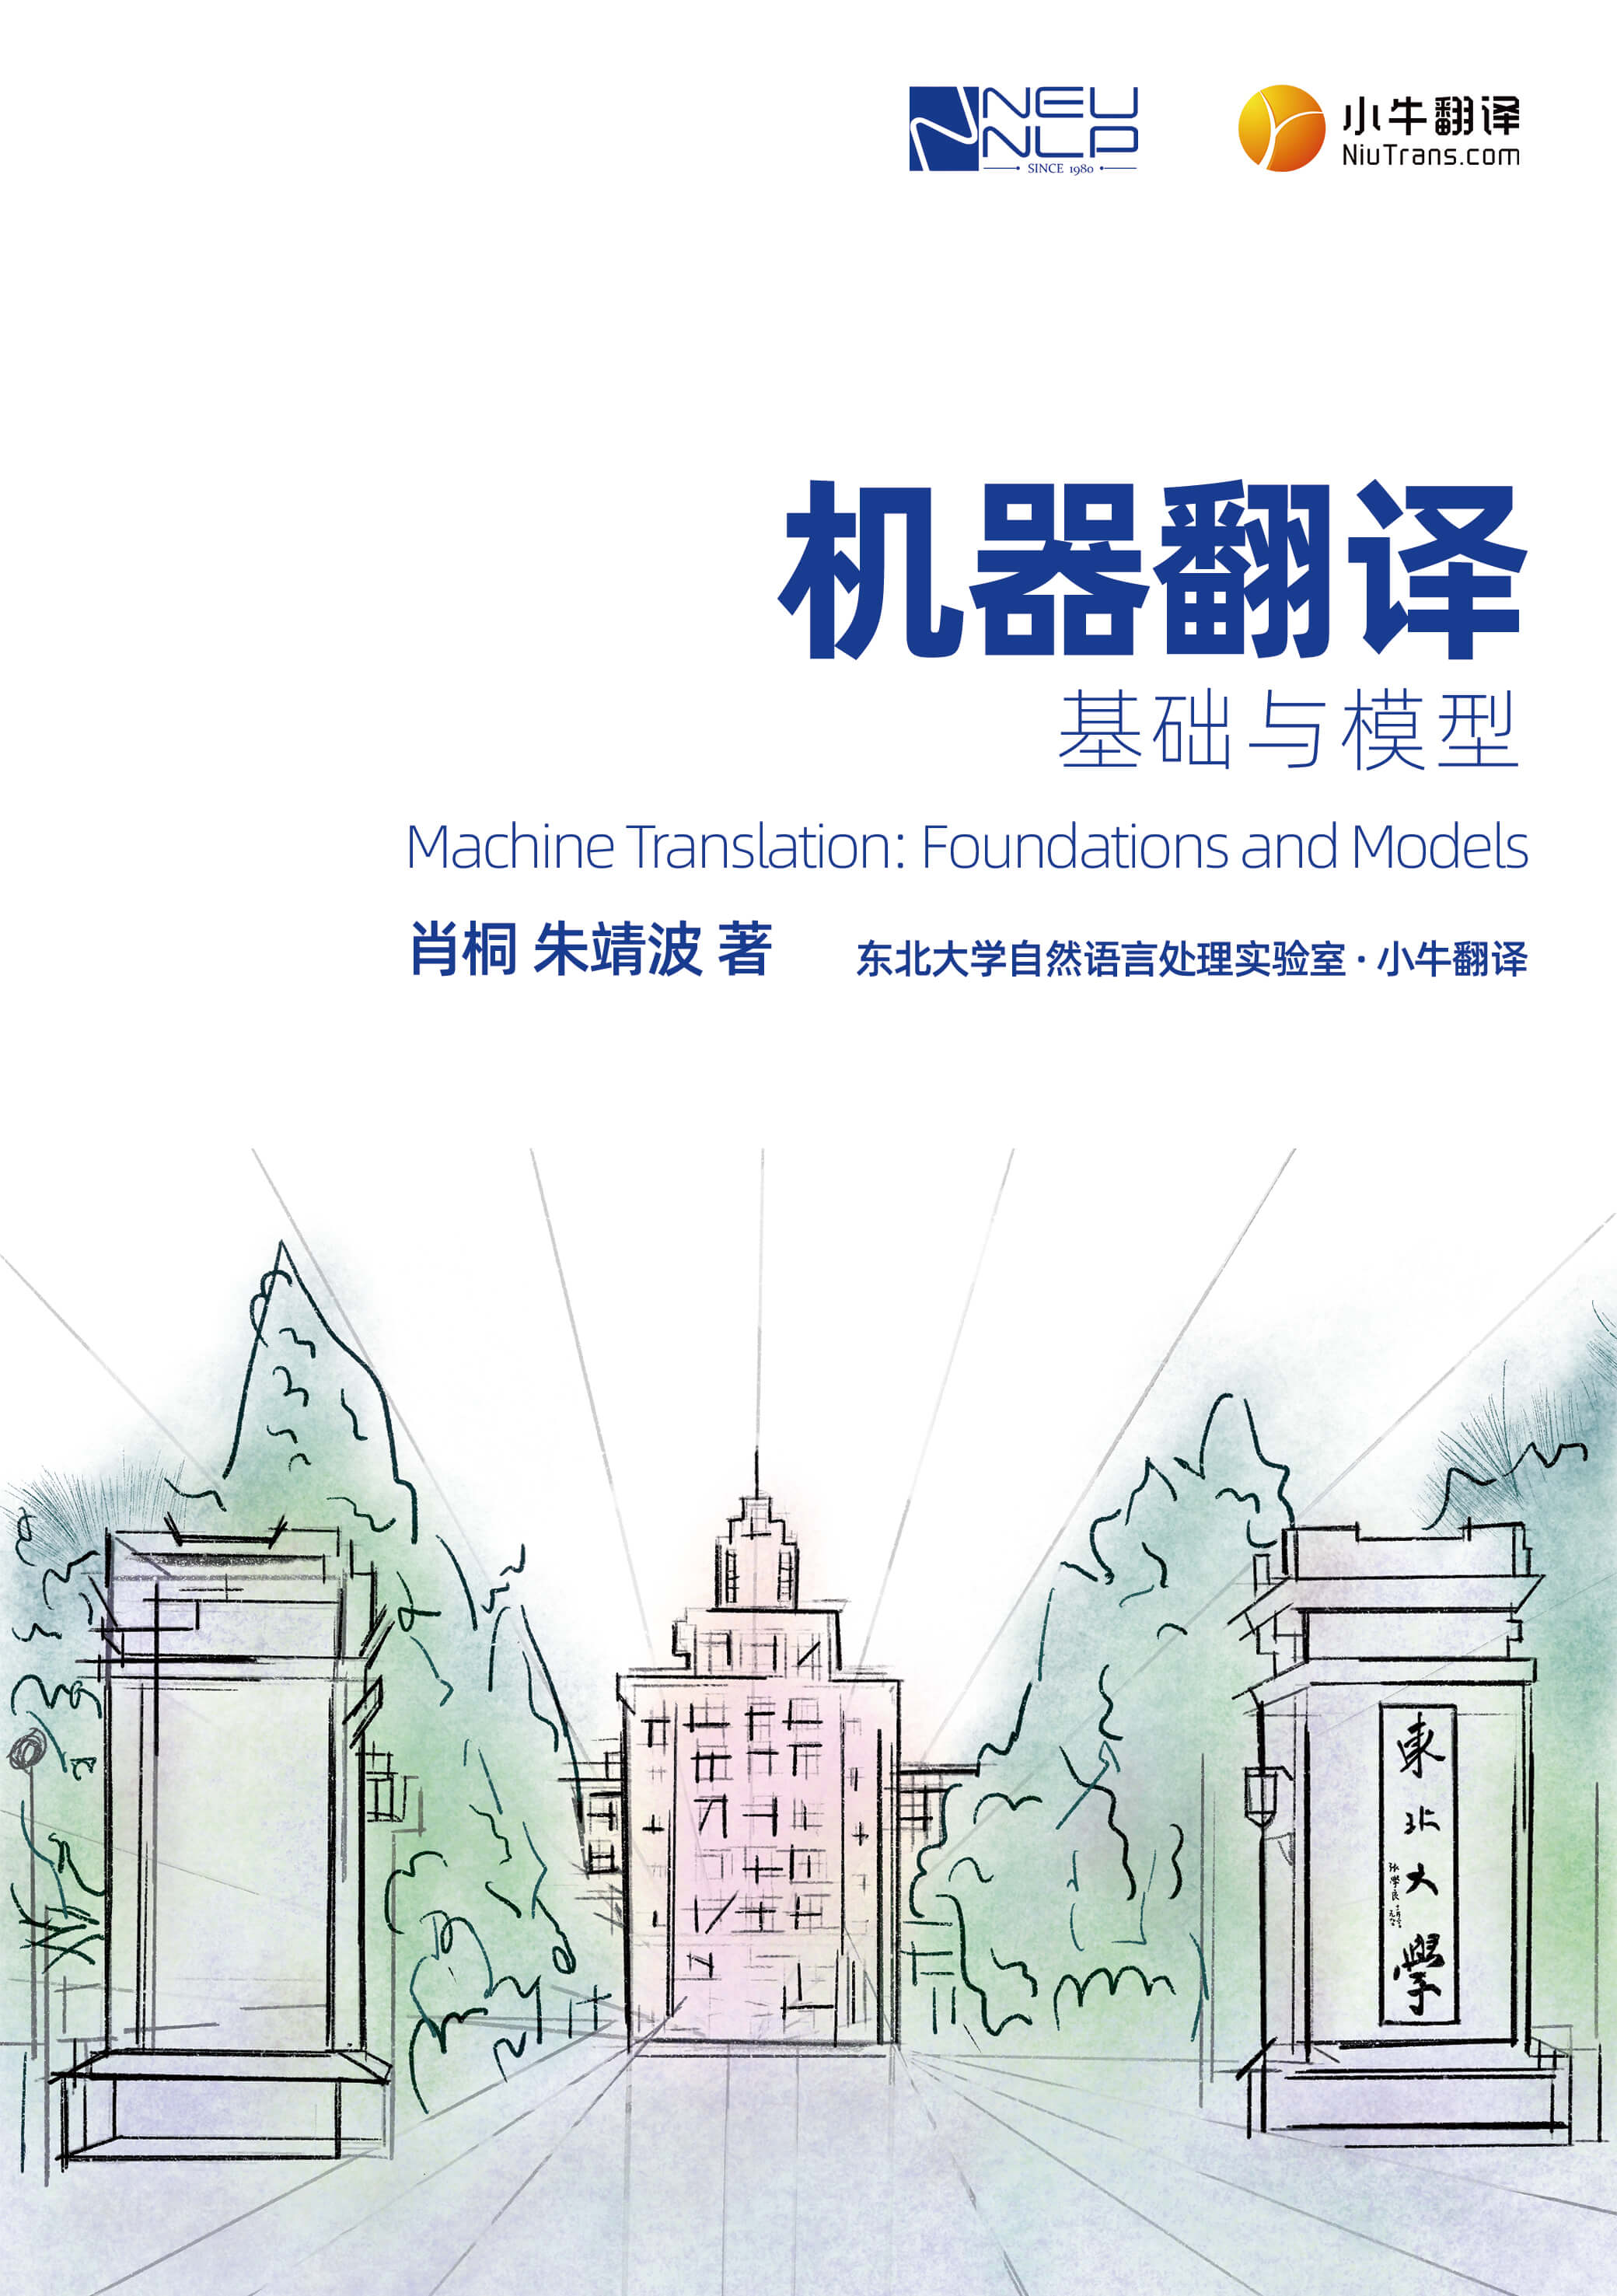
\includegraphics[width=\paperwidth,height=\paperheight]{fig-cover.jpg}};

\end{tikzpicture}
\vfill
\endgroup·

%----------------------------------------------------------------------------------------
%	COPYRIGHT PAGE
%----------------------------------------------------------------------------------------

\newpage
~\vfill
\thispagestyle{empty}

\noindent Copyright \copyright\ 2020 肖桐\ \ 朱靖波\\

\noindent \textsc{东北大学自然语言处理实验室\ $\cdot$\ 小牛翻译}\\

\noindent 顾问:姚天顺\ \ 王宝库\\

\noindent \textsc{\url{https://opensource.niutrans.com/mtbook/homepage.html}}\\
\noindent \textsc{\url{https://github.com/NiuTrans/MTBook}}\\

\noindent {\red{Licensed under the Creative Commons Attribution-NonCommercial 4.0 Unported License (the ``License''). You may not use this file except in compliance with the License. You may obtain a copy of the License at \url{http://creativecommons.org/licenses/by-nc/4.0}. Unless required by applicable law or agreed to in writing, software distributed under the License is distributed on an \textsc{``as is'' basis, without warranties or conditions of any kind}, either express or implied. See the License for the specific language governing permissions and limitations under the License.}}\\

\noindent \textit{\today}

%----------------------------------------------------------------------------------------
%	ACKNOWLEDGE PAGE
%----------------------------------------------------------------------------------------

\newpage
~\vfill
\thispagestyle{empty}

{\large
\noindent {\color{red} 在此感谢为本书做出贡献的人} \\

\noindent 曹润柘、曾信、孟霞、单韦乔、周涛、周书含、许诺、李北、许晨、林野、李垠桥、王子扬、刘辉、张裕浩、冯凯、罗应峰、魏冰浩、王屹超、李炎洋、胡驰、姜雨帆、田丰宁、刘继强、张哲旸、陈贺轩、牛蕊、杜权、张春良、王会珍、张俐、马安香、胡明涵 \\

}

%----------------------------------------------------------------------------------------
%	PREFACE PAGES
%----------------------------------------------------------------------------------------
\newpage
% !Mode:: "TeX:UTF-8"
% !TEX encoding = UTF-8 Unicode

%----------------------------------------------------------------------------------------
% 机器翻译:统计建模与深度学习方法
% Machine Translation: Statistical Modeling and Deep Learning Methods
%
% Copyright 2020
% 肖桐(xiaotong@mail.neu.edu.cn) 朱靖波 (zhujingbo@mail.neu.edu.cn)
%----------------------------------------------------------------------------------------

\renewcommand\figurename{图}

%----------------------------------------------------------------------------------------
%	PREFACE
%----------------------------------------------------------------------------------------

{\color{white} 空}
\vspace{0.5em}
\begin{center}
{\Huge \bfnew{导\ \ \ \ 读}}
\end{center}
\vspace{2em}

\begin{spacing}{1.18}

让计算机进行自然语言的翻译是人类长期的梦想,也是人工智能的终极目标之一。自上世纪九十年代起,机器翻译迈入了基于统计建模的时代,发展到今天,深度学习等机器学习方法已经在机器翻译中得到了大量的应用,取得了令人瞩目的进步。

在这个时代背景下,对机器翻译的模型、方法和实现技术进行深入了解是自然语言处理领域研究者和实践者所渴望的。本书全面回顾了近三十年内机器翻译的技术发展历程,并围绕统计建模和深度学习两个主题对机器翻译的技术方法进行了全面介绍。在写作中,笔者力求用朴实的语言和简洁的实例阐述机器翻译的基本模型和方法,同时对相关的技术前沿进行讨论。本书可以供计算机相关专业高年级本科生及研究生学习之用,也可以作为自然语言处理,特别是机器翻译领域相关研究人员的参考资料。

本书共分为七个章节,章节的顺序参考了机器翻译技术发展的时间脉络,同时兼顾了机器翻译知识体系的内在逻辑。各章节的主要内容包括:

\begin{itemize}
\vspace{0.5em}
\item 第一章:机器翻译简介
\vspace{0.5em}
\item 第二章:词法、语法及统计建模基础
\vspace{0.5em}
\item 第三章:基于词的机器翻译模型
\vspace{0.5em}
\item 第四章:基于短语和句法的机器翻译模型
\vspace{0.5em}
\item 第五章:人工神经网络和神经语言建模
\vspace{0.5em}
\item 第六章:神经机器翻译模型
\vspace{0.5em}
\item 第七章:神经机器翻译实战 \ \dash \ 参加一次比赛
\vspace{0.5em}
\end{itemize}

其中,第一章是对机器翻译的整体介绍。第二章和第五章是对统计建模和深度学习方法的介绍,分别建立了两个机器翻译范式的基础知识体系 \ \dash \ 统计机器翻译和神经机器翻译。统计机器翻译部分(第三、四章)涉及早期的基于单词的翻译模型,以及本世纪初流行的基于短语和句法的翻译模型。神经机器翻译(第六、七章)代表了当今机器翻译的前沿,内容主要涉及了基于端到端表示学习的机器翻译建模方法。特别地,第七章对一些最新的神经机器翻译方法进行了讨论,为相关科学问题的研究和实用系统的开发提供了可落地的思路。下图展示了本书各个章节及核心概念之间的关系。

{\red 用最简单的方式阐述机器翻译的基本思想}是笔者所期望达到的目标。但是,书中不可避免会使用一些形式化定义和算法的抽象描述,因此,笔者尽所能通过图例进行解释(本书共320张插图)。不过,本书所包含的内容较为广泛,难免会有疏漏,望读者海涵,并指出不当之处。

%-------------------------------------------
\begin{figure}[htp]
\centering
\centering
% !Mode:: "TeX:UTF-8"
% !TEX encoding = UTF-8 Unicode

\begin{tikzpicture}

\tikzstyle{partnode} =[font=\scriptsize,minimum height=2.0em,minimum width=15em,draw,thick,fill=white,drop shadow]
\tikzstyle{secnode} =[font=\footnotesize,minimum height=1.6em,minimum width=14em,align=flush left]

\begin{scope}

% part 1
\node [partnode,anchor=south,blue,minimum height=9.0em,minimum width=22.7em,fill=white] (part1) at ([yshift=-0.5em]0,0) {};
\node [anchor=north] (part1label) at ([yshift=-0.3em]part1.north) {\sffamily\bfseries{机器翻译基础}};
\node [anchor=north west,draw=blue,thick,fill=white,rounded corners] (part1title) at ([xshift=-0.3em,yshift=0.3em]part1.north west) {{\color{blue} {\sffamily\bfseries 第一部分}}};
\node [secnode,anchor=south,fill=ugreen!20,minimum width=21.6em,align=center] (sec01) at (0,0) {第一章\hspace{1em} 机器翻译简介};
\node [secnode,anchor=south west,fill=blue!20] (sec02) at ([yshift=0.8em]sec01.north west) {第二章\hspace{1em} 统计语言建模基础\hspace{3em}};
\node [secnode,anchor=south west,fill=blue!20] (sec03) at ([yshift=0.8em]sec02.north west) {第三章\hspace{1em} 词法分析和语法分析基础};
\node [secnode,anchor=north west,fill=blue!20,minimum width=7em,minimum height=4.1em,align=center] (sec04) at ([xshift=0.6em]sec03.north east) {第四章\\ 翻译质量评价};
\draw [->,very thick] ([yshift=-0.7em]sec02.south) -- ([yshift=-0.1em]sec02.south);
\draw [->,very thick] ([yshift=-0.7em]sec03.south) -- ([yshift=-0.1em]sec03.south);
\draw [->,very thick] ([yshift=-0.7em]sec04.south) -- ([yshift=-0.1em]sec04.south);

% part 2
\node [partnode,anchor=south,orange,minimum height=11.5em,minimum width=18.1em,fill=white] (part2) at ([yshift=3em]part1.north west) {};
\node [anchor=north] (part2label) at ([yshift=-0.3em]part2.north) {\sffamily\bfseries{统计机器翻译}};
\node [anchor=north west,draw=orange,thick,fill=white,rounded corners] (part2title) at ([xshift=-0.3em,yshift=0.3em]part2.north west) {{\color{orange} {\sffamily\bfseries 第二部分}}};
\node [secnode,anchor=south,fill=orange!20,minimum width=17em,align=left] (sec04) at ([yshift=0.5em]part2.south) {第五章\hspace{1em} 基于词的机器翻译建模 \hspace{2.35em}};
\node [secnode,anchor=south,fill=orange!20,minimum width=17em,align=center] (sec05) at ([yshift=0.8em]sec04.north) {\hspace{1.0em}第六章\hspace{1em} 基于扭曲度和繁衍率的模型\hspace{1.6em}};
\node [secnode,anchor=south,fill=orange!20,minimum width=17em,align=center] (sec06) at ([yshift=0.8em]sec05.north) {第七章\hspace{1em} 基于短语的模型 \hspace{5.35em}};
\node [secnode,anchor=south,fill=orange!20,minimum width=17em,align=center] (sec07) at ([yshift=0.8em]sec06.north) {第八章\hspace{1em} 基于句法的模型 \hspace{5.35em}};
\draw [->,very thick] ([yshift=-0.7em]sec05.south) -- ([yshift=-0.1em]sec05.south);
\draw [->,very thick] ([yshift=-0.7em]sec06.south) -- ([yshift=-0.1em]sec06.south);
\draw [->,very thick] ([yshift=-0.7em]sec07.south) -- ([yshift=-0.1em]sec07.south);

% part 3
\node [partnode,anchor=south,red,minimum height=9.5em,minimum width=22.7em,fill=white] (part3) at ([yshift=3em,xshift=2.5em]part2.north east) {};
\node [anchor=north] (part3label) at ([yshift=-0.3em]part3.north) {\sffamily\bfseries{神经机器翻译}};
\node [anchor=north west,draw=red,thick,fill=white,rounded corners] (part3title) at ([xshift=-0.3em,yshift=0.3em]part3.north west) {{\color{red} {\sffamily\bfseries 第三部分}}};
\node [secnode,anchor=south,fill=magenta!20,minimum width=21.6em,align=center] (sec09) at ([yshift=0.5em]part3.south) {第九章\hspace{1em} 人工神经网络和神经语言建模};
\node [secnode,anchor=south west,fill=red!20,minimum width=6.6em,minimum height=4.5em,align=center] (sec10) at ([yshift=0.8em]sec09.north west) {第十章\\ 基于循环神经 \\ 网络的模型};
\node [secnode,anchor=south west,fill=red!20,minimum width=6.6em,minimum height=4.5em,align=center] (sec11) at ([xshift=0.8em]sec10.south east) {第十一章\\ 基于卷积神经 \\ 网络的模型};
\node [secnode,anchor=south west,fill=red!20,minimum width=6.6em,minimum height=4.5em,align=center] (sec12) at ([xshift=0.8em]sec11.south east) {第十二章\\ 基于自注意力 \\ 的模型};
\draw [->,very thick] ([yshift=-0.7em]sec10.south) -- ([yshift=-0.1em]sec10.south);
\draw [->,very thick] ([yshift=-0.7em]sec11.south) -- ([yshift=-0.1em]sec11.south);
\draw [->,very thick] ([yshift=-0.7em]sec12.south) -- ([yshift=-0.1em]sec12.south);


% part 4
\node [partnode,anchor=south,ugreen,minimum height=12.0em,minimum width=29.7em,fill=white] (part4) at ([yshift=3em,xshift=6em]part3.north west) {};
\node [anchor=north] (part4label) at ([yshift=-0.3em]part4.north) {\sffamily\bfseries{机器翻译前沿}};
\node [anchor=north west,draw=ugreen,thick,fill=white,rounded corners] (part4title) at ([xshift=-0.3em,yshift=0.3em]part4.north west) {{\color{ugreen} {\sffamily\bfseries 第四部分}}};
\node [secnode,anchor=south west,fill=cyan!20,minimum width=14.0em,align=center] (sec13) at ([yshift=0.5em,xshift=0.5em]part4.south west) {第十三章\hspace{1em} 神经机器翻译模型训练};
\node [secnode,anchor=west,fill=cyan!20,minimum width=14.0em,align=center] (sec14) at ([xshift=0.6em]sec13.east) {第十四章\hspace{1em} 神经机器翻译模型推断};
\node [secnode,anchor=south west,fill=green!30,minimum width=9em,minimum height=4.5em,align=center] (sec15) at ([yshift=0.8em]sec13.north west) {第十五章\\ 神经机器翻译 \\ 结构优化};
\node [secnode,anchor=south west,fill=green!30,minimum width=9em,minimum height=4.5em,align=center] (sec16) at ([xshift=0.8em]sec15.south east) {第十六章\\ 低资源 \\ 神经机器翻译};
\node [secnode,anchor=south west,fill=green!30,minimum width=9em,minimum height=4.5em,align=center] (sec17) at ([xshift=0.8em]sec16.south east) {第十七章\\ 多模态、多层次 \\ 机器翻译};
\node [secnode,anchor=south west,fill=amber!25,minimum width=28.7em,align=center] (sec18) at ([yshift=0.8em]sec15.north west) {第十八章\hspace{1em} 机器翻译应用技术};
\node [rectangle,draw,dotted,thick,inner sep=0.1em,fill opacity=1] [fit = (sec13) (sec14)] (nmtbasebox) {};
\draw [->,very thick] ([yshift=-0.7em]sec15.south) -- ([yshift=-0.1em]sec15.south);
\draw [->,very thick] ([yshift=-0.7em]sec16.south) -- ([yshift=-0.1em]sec16.south);
\draw [->,very thick] ([yshift=-0.7em]sec17.south) -- ([yshift=-0.1em]sec17.south);
\draw [<-,very thick] ([yshift=0.7em]sec15.north) -- ([yshift=0.1em]sec15.north);
\draw [<-,very thick] ([yshift=0.7em]sec16.north) -- ([yshift=0.1em]sec16.north);
\draw [<-,very thick] ([yshift=0.7em]sec17.north) -- ([yshift=0.1em]sec17.north);
\draw [->,very thick,dotted] ([yshift=-0.7em,xshift=0.4em]sec15.south east) -- ([yshift=0.7em,xshift=0.4em]sec15.north east);
\draw [->,very thick,dotted] ([yshift=-0.7em,xshift=0.4em]sec16.south east) -- ([yshift=0.7em,xshift=0.4em]sec16.north east);

% lines and arrows
\draw [->,line width=0.2em] ([xshift=-0.1em]part1.west) .. controls +(west:5em) and +(south:3em) .. ([yshift=-0.1em,xshift=-5em]part2.south);
\draw [->,line width=0.2em] ([xshift=-2em,yshift=0.1em]part1.north east) -- ([xshift=-2em,yshift=17.3em]part1.north east);
\draw [->,line width=0.2em] ([xshift=0.3em,yshift=-2em]part2.east) .. controls +(east:6em) and +(south:4em) .. ([yshift=-0.3em,xshift=4em]part3.south);
\draw [->,line width=0.2em] ([xshift=-5em,yshift=0.5em]part2.north) -- ([xshift=-5em,yshift=15.3em]part2.north);
\draw [->,line width=0.2em] ([xshift=4em,yshift=0.1em]part3.north) -- ([xshift=4em,yshift=2.7em]part3.north);

\end{scope}

\end{tikzpicture}

\end{figure}
%-------------------------------------------

\end{spacing}










%----------------------------------------------------------------------------------------
%	TABLE OF CONTENTS
%----------------------------------------------------------------------------------------
%\usechapterimagefalse % If you don't want to include a chapter image, use this to toggle images off - it can be enabled later with \usechapterimagetrue
\chapterimage{fig-NEU-1.jpg} % Image of the content page
\pagestyle{empty} % Disable headers and footers for the following pages
\tableofcontents % Show contents
\cleardoublepage % Place the first page of each chapter on odd pages
\pagestyle{fancy} % Enable headers and footers


%----------------------------------------------------------------------------------------
%	CHAPTERS
%----------------------------------------------------------------------------------------

%% !Mode:: "TeX:UTF-8"
% !TEX encoding = UTF-8 Unicode

%----------------------------------------------------------------------------------------
% 机器翻译:统计建模与深度学习方法
% Machine Translation: Statistical Modeling and Deep Learning Methods
%
% Copyright 2020
% 肖桐(xiaotong@mail.neu.edu.cn) 朱靖波 (zhujingbo@mail.neu.edu.cn)
%----------------------------------------------------------------------------------------

%----------------------------------------------------------------------------------------
%    CONFIGURATIONS
%----------------------------------------------------------------------------------------

\part{机器翻译基础}
\renewcommand\figurename{图}%将figure改为图
\renewcommand\tablename{表}%将figure改为图
\chapterimage{fig-NEU-2.jpg} % Chapter heading image

%----------------------------------------------------------------------------------------
%	CHAPTER 1
%----------------------------------------------------------------------------------------

\chapter{机器翻译简介}

%----------------------------------------------------------------------------------------
%    NEW SECTION
%----------------------------------------------------------------------------------------

\section{机器翻译的概念}

\parinterval 从广义上来讲,“翻译”是指把一个事物转化为另一个事物的过程。这个概念多使用在对序列的转化上,比如,计算机程序的编译、自然语言文字的翻译、生物蛋白质的合成等。在程序编译中,高级语言编写的程序经过一系列的处理后转化为可执行的目标程序,这是一种从高级程序语言到低级程序语言的“翻译”。在人类语言的翻译中,一种语言文字通过人脑转化为另一种语言表达,这是一种自然语言的“翻译”。在蛋白质合成的第一步,RNA分子序列转化为特定的氨基酸序列,这是一种生物学遗传信息的“翻译”。甚至说给上联对出下联、给一幅图片写出图片的主题等都可以被看作是“翻译”的过程。
\vspace{0.5em}

\parinterval 这里更加关注人类语言之间的翻译问题,即自然语言的翻译。如图\ref{fig:1-1}所示,通过计算机可以将一段汉语文字自动转化为英语文字,汉语被称为{\small\bfnew{源语言}}\index{源语言}(Source Language)\index{Source Language},英语被称为{\small\bfnew{目标语言}}\index{目标语言}(Target Language)\index{Target Language}。

%----------------------------------------------
\begin{figure}[htp]
    \centering
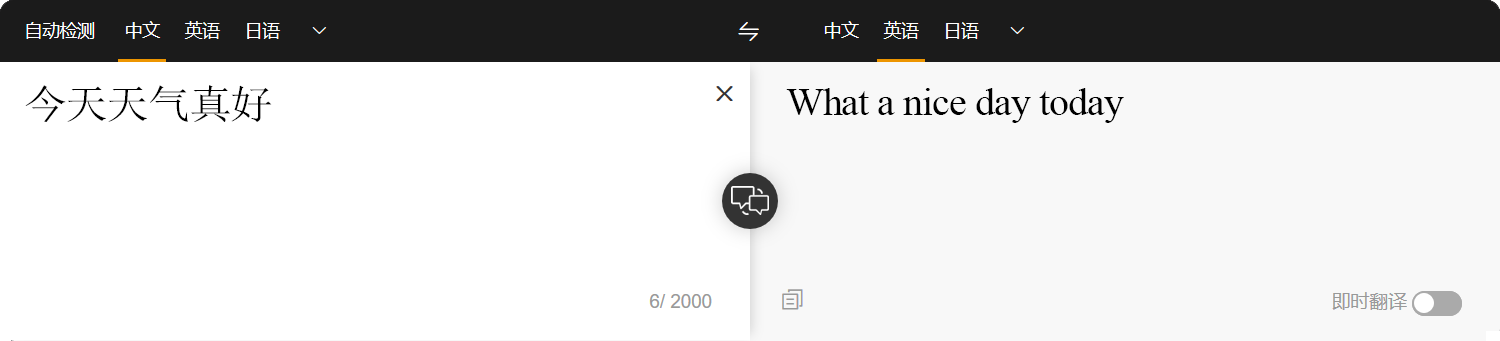
\includegraphics[scale=0.2]{./Chapter1/Figures/figure-zh_en-example.png}
    \caption{通过计算机将汉语翻译为英语}
    \label{fig:1-1}
\end{figure}
%----------------------------------------------

\parinterval 一直以来,文字的翻译往往是由人完成。让计算机像人一样进行翻译似乎还是电影中的桥段,因为很难想象语言的多样性和复杂性可以用计算机语言进行描述。但是时至今日,人工智能技术的发展已经大大超越了人类传统的认知,用计算机进行自动翻译也不再是一种梦想,它已经深入到人们生活的很多方面,并发挥着重要作用。而这种由计算机进行自动翻译的过程也被称作{\small\bfnew{机器翻译}}\index{机器翻译}(Machine Translation)\index{Machine Translation}。类似地,自动翻译、智能翻译、多语言自动转换等概念也是指同样的事情。如果将今天的机器翻译和人工翻译进行对比,可以发现机器翻译系统所生成的译文还不够完美,甚至有时翻译质量非常差,但是它的生成速度快且成本低廉,更为重要的是机器翻译系统可以从大量数据中不断学习和进化。

\parinterval 人工翻译尽管精度很高,但是费时费力。当需要翻译大量的文本且精度要求不那么高时,比如海量数据的浏览型任务,机器翻译的优势就体现出来了。对于人工作业无法完成的事情,使用机器翻译可能只需花费几个小时甚至几分钟就能完成。这就类似于拿着锄头耕地种庄稼和使用现代化机器作业之间的区别。

\parinterval 实现机器翻译往往需要多个学科知识的融合,如数学、语言学、计算机科学、心理学等等。而最终呈现给使用者的是一套软件系统\ \dash\ 机器翻译系统。通俗来讲,机器翻译系统就是一个可以在计算机上运行的软件工具,与人们使用的其他软件一样,只不过机器翻译系统是由“不可见的程序”组成。虽然这个系统非常复杂,但是呈现出来的形式却很简单,比如输入是待翻译的句子或文本,输出是译文句子或文本。

\parinterval 用机器进行翻译的想法可以追溯到电子计算机产生之前,发展过程中也经历了多个范式的变迁,现代机器翻译系统大多是基于数据驱动的方法\ \dash\ 从数据中自动学习翻译知识,并运用这些知识对新的文本进行翻译。

\parinterval 从机器翻译系统的组成上来看,通常可以抽象为两个部分,如图\ref{fig:1-2}所示:

\begin{itemize}
\vspace{0.5em}
\item {\small\bfnew{资源}}:如果把机器翻译系统比作一辆汽车,资源就好比是可以使汽车运行的“汽油”,它包括很多内容,如翻译规则、双(单)语数据、知识库等翻译知识,且这些“知识”都是计算机可读的。值得一提的是,如果没有翻译资源的支持,任何机器翻译系统都无法运行起来。
\vspace{0.5em}
\item {\small\bfnew{系统}}:机器翻译算法的程序实现被称作系统,也就是机器翻译研究人员开发的软件。无论是翻译规则、翻译模板还是统计模型中的参数都需要通过机器翻译系统进行读取和使用。
\vspace{0.5em}
\end{itemize}

%----------------------------------------------
\begin{figure}[htp]
    \centering
\definecolor{ublue}{rgb}{0.152,0.250,0.545}
\definecolor{ugreen}{rgb}{0,0.5,0}
\begin{tikzpicture}
\node [thick,rounded corners=3mm,draw=blue!50!black!50,top color=white,bottom color=blue!50!black!20] (s) at (0,0) {输入文字};
\node [thick,minimum width=6em,minimum height=3em,draw=red!50!black!50,anchor=west] (mt) at ([xshift=0.5in]s.east) {};
\node [thick,minimum width=6em,minimum height=1.5em,draw=red!50!black!50,top color=white,bottom color=red!50!black!20,anchor=north] (mt1) at (mt.north) {机器翻译};
\node [thick,rounded corners=3mm,draw=blue!50!black!50,top color=white,bottom color=blue!50!black!20,anchor=west] (t) at ([xshift=0.5in]mt.east) {输出译文};
{
\node [draw=ugreen,fill=ugreen,minimum width=3.1em,minimum height=1.5em,anchor=south west] (part1) at (mt.south west) {{\color{white} 1}};
\node [draw=ublue,fill=ublue,minimum width=3.1em,minimum height=1.5em,anchor=south east] (part2) at (mt.south east) {{\color{white} 2}};
}
\draw[-latex,thick] (s.east)--(mt.west);
\draw[-latex,thick] (mt.east)--(t.west);

{
\begin{scope}[yshift=-1.0in]
\node [] (part1label) at (0,0) {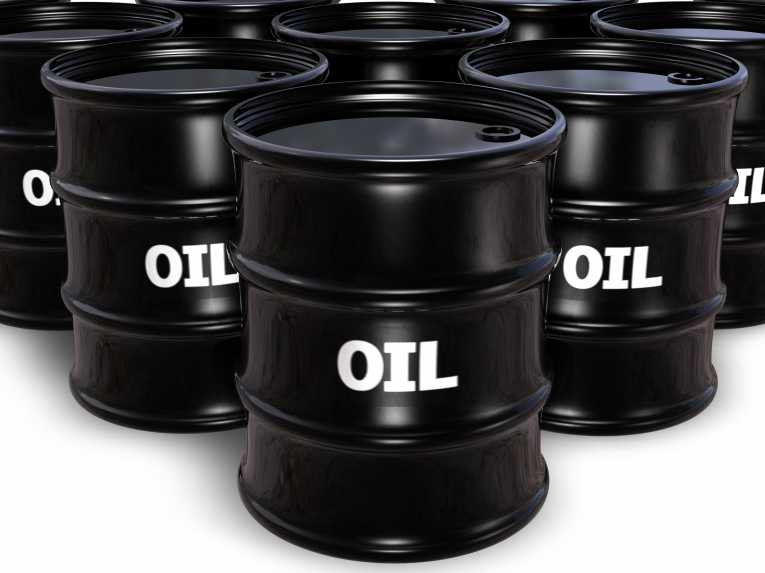
\includegraphics[scale=0.10]{./Chapter1/Figures/figure-oil.jpg}};
\node [anchor=north west] (part1text) at ([xshift=-1em,yshift=0.0em]part1label.south west) {\begin{tabular}{l}{\color{red}{资源}}:可以使机器翻译\\系统运行的``汽油''\end{tabular}};
\end{scope}
}

{
\begin{scope}[yshift=-1.0in,xshift=2.8in]
\node [] (part2label) at (0,0) {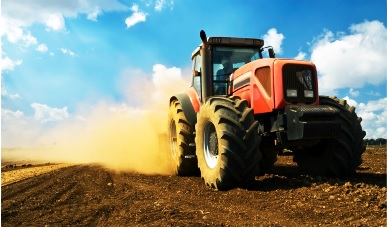
\includegraphics[scale=0.33]{./Chapter1/Figures/figure-truck.jpg}};
\node [anchor=north west] (part2text) at ([xshift=-1em,yshift=0em]part2label.south west) {\begin{tabular}{l}{\color{red}{系统}}:利用资源完成\\自动翻译的程序\end{tabular}};
\end{scope}
}

{
\draw[<-,thick] (part1label.north)..controls +(north:0.6) and +(south:0.6)..([yshift=0.2em]part1.south);
}

{
\draw[<-,thick] ([yshift=0.0em]part2label.north)..controls +(north:0.6) and +(south:0.6)..([yshift=0.2em]part2.south);
}

\end{tikzpicture}



    \caption{机器翻译系统的组成}
    \label{fig:1-2}
\end{figure}
%-------------------------------------------

\parinterval 构建一个强大的机器翻译系统需要“资源”和“系统”两方面共同作用。在资源方面,随着语料库语言学的发展,已经有大量的高质量的双语和单语数据(称为语料)被整理并且被电子化存储,因此可以说具备了研发机器翻译系统所需要的语料基础。特别是像英语、汉语等世界主流语种,相关语料资源已经非常丰富,这也大大加速了相关研究的进展。当然,对于一些稀缺资源语种或者特殊的领域,语料库中的语料仍然匮乏,但是这些并不影响机器翻译领域整体的发展速度。因此在现有语料库的基础上,很多研究者把精力集中在“系统”研发上。

%----------------------------------------------------------------------------------------
%    NEW SECTION
%----------------------------------------------------------------------------------------

\sectionnewpage
\section{机器翻译简史}

\parinterval 虽然翻译这个概念在人类历史中已经存在了上千年,但机器翻译发展至今只有七十余年的历史。纵观机器翻译的发展,历程曲折又耐人寻味,可以说,回顾机器翻译的历史对深入理解相关技术方法会有很好的启发,甚至对了解整个自然语言处理领域的发展也有启示作用。

%----------------------------------------------------------------------------------------
%    NEW SUB-SECTION
%----------------------------------------------------------------------------------------

\subsection{人工翻译}

\parinterval 人类形成语言文字的过程中逐渐形成了翻译的概念。一个著名的标志性证据是罗塞塔石碑(Rosetta Stone),如图\ref{fig:1-3}所示。这个石碑制作于公元前196年,据说是可供考证的最久远的记载平行文字的历史遗迹。石碑由上至下刻有同一段埃及国王诏书的三种语言版本,最上面是古埃及象形文,中间是埃及草书,最下面是古希腊文。可以明显看出石碑上中下雕刻的文字的纹理是不同的。尽管用不同的语言文字描述同一件事在今天看来很常见,但是这在生产力低下的两千年前是很罕见的。很多人认为罗塞塔石碑是标志翻译或人工翻译的一个起点。目前罗塞塔石碑保存于大英博物馆,并成为该馆最具代表性的镇馆之宝之一。

%----------------------------------------------
\begin{figure}[htp]
    \centering
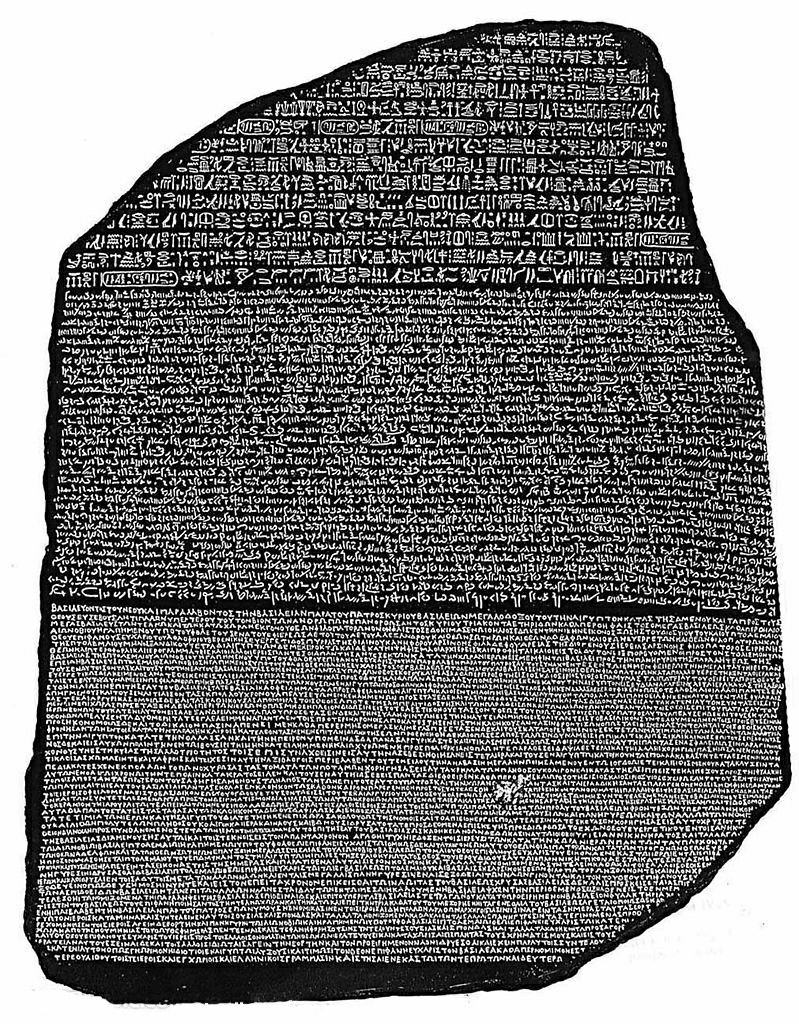
\includegraphics[scale=0.20]{./Chapter1/Figures/figure-rosetta-stone.jpg}
    \caption{罗塞塔石碑}
    \label{fig:1-3}
\end{figure}
%------------------------------------------

\parinterval 在此之后,更多的翻译工作在文化和知识传播中开展。其中一个典型代表是宗教文献的翻译。宗教是人类意识形态的一个重要载体,为了宣传教义,人们编写了大量的宗教文献。在西方,一项最早被记录的翻译活动是将旧约圣经(希伯来文及埃兰文)翻译为希腊文版本。迄今为止人类历史上翻译版本最多的书就是圣经。在中国唐代,有一位世界性的文化人物\ \dash \ 玄奘,他不仅是佛学家、旅行家,还是翻译家。玄奘西行求法归来后把全部的心血和智慧奉献给了译经事业,在助手们的帮助下,共翻译佛教经论74部,1335卷,每卷万字左右,合计1335万字,占去整个唐代译经总数的一半以上\upcite{慧立2000大慈恩寺三藏法師傳},树立了我国古代翻译思想的光辉典范。

\parinterval 翻译在人类历史长河中起到了重要的作用。一方面,由于语言文字、文化和地理位置的差异性,使得翻译成为一个重要的需求;另一方面,翻译也加速了不同文明的融会贯通,促进了世界的发展。今天,翻译已经成为重要的行业之一,包括各个高校也都设立了翻译及相关专业,相关人才不断涌现。据《2019年中国语言服务行业发展报告》\upcite{2019cns}统计:全球语言服务产值预计将首次接近500亿美元;中国涉及语言服务的在营企业360,000余家,语言服务为主营业务的在营企业近万家,总产值超过300亿元,年增长3\%以上;全国开设外语类专业的高校数量多达上千所,其中设立有翻译硕士(MTI)和翻译本科(BTI)专业的院校分别有250余所和280余所,其中仅MTI的累计招生数就高达6万余人\upcite{赵军峰2019深化改革}。当然,面对着巨大的需求,如何使用机器辅助翻译等技术手段提高人工翻译效率,也是人工翻译和机器翻译领域需要共同探索的方向。

%----------------------------------------------------------------------------------------
%    NEW SUB-SECTION
%----------------------------------------------------------------------------------------

\subsection{机器翻译的萌芽}

\parinterval 人工翻译已经存在了上千年,而机器翻译又起源于什么时候呢?机器翻译跌宕起伏的发展史可以分为萌芽期、受挫期、快速成长期和爆发期四个阶段。

\parinterval 早在17世纪,如Descartes、Leibniz、Cave\ Beck、Athanasius\ Kircher和Johann\ Joachim\ Becher等很多学者就提出采用机器词典(电子词典)来克服语言障碍的想法\upcite{knowlson1975universal},这种想法在当时是很超前的。随着语言学、计算机科学等学科的发展,在19世纪30年代使用计算模型进行自动翻译的思想开始萌芽,如当时法国科学家Georges Artsrouni就提出用机器来进行翻译的想法。只是那时依然没有合适的实现手段,所以这种想法的合理性无法被证实。

\parinterval 随着第二次世界大战爆发, 对文字进行加密和解密成为重要的军事需求,这也使得数学和密码学变得相当发达。在战争结束一年后,世界上第一台通用电子数字计算机于1946年研制成功,至此使用机器进行翻译有了真正实现的可能。

\parinterval 基于战时密码学领域与通讯领域的研究,Claude Elwood Shannon在1948年提出使用“噪声信道”描述语言的传输过程,并借用热力学中的“{\small\bfnew{熵}}\index{熵}”(Entropy)\index{Entropy}来刻画消息中的信息量\upcite{DBLP:journals/bstj/Shannon48}。次年,Shannon与Warren Weaver更是合著了著名的\emph{The Mathematical Theory of Communication}\upcite{shannon1949the},这些工作都为后期的统计机器翻译打下了理论基础。

\parinterval 1949年,Weaver撰写了一篇名为\emph{TRANSLATION}的备忘录\upcite{weaver1955translation},在这个备忘录中Weaver提出用密码学的方法解决人类语言翻译任务的想法,比如把汉语看成英语的一个加密文本,那么将汉语翻译成英语就类似于解密的过程。并且在这篇备忘录中第一次提出了机器翻译,正式开创了机器翻译的概念,这个概念一直沿用至今。虽然,在那个年代进行机器翻译的研究条件并不成熟,包括使用加密解密技术进行自动翻译的很多尝试很快也被验证是不可行的,但是这些早期的探索为后来机器翻译的发展提供了思想的火种。

%----------------------------------------------------------------------------------------
%    NEW SUB-SECTION
%----------------------------------------------------------------------------------------

\subsection{机器翻译的受挫}

\parinterval 随着电子计算机的发展,研究者开始尝试使用计算机来进行自动翻译。1954年,美国乔治敦大学在IBM公司支持下,启动了第一次真正的机器翻译实验。翻译的目标是将几个简单的俄语句子翻译成为英语,翻译系统包含6条翻译规则和250词汇。这次翻译实验中测试了50个化学文本句子,取得了初步成功。在某种意义上来说,这个实验显示了采用基于词典和翻译规则的方法可以实现机器翻译过程。虽然只是取得了初步成功,但却引起了苏联、英国和日本研究机构的机器翻译研究热,大大推动了早期机器翻译的研究进展。

\parinterval 1957年,Noam Chomsky在\emph{Syntactic Structures}中描述了转换生成语法\upcite{chomsky1957syntactic},并使用数学方法来研究自然语言,建立了包括上下文有关语法、上下文无关语法等4种类型的语法。这些工作最终为今天计算机中广泛使用的“形式语言”奠定了基础。而他的思想也深深地影响了同时期的语言学和自然语言处理领域的学者。特别的是,早期基于规则的机器翻译中也大量使用了这些思想。

\parinterval 虽然在这段时间,使用机器进行翻译的议题越加火热,但是事情并不总是一帆风顺,怀疑论者对机器翻译一直存有质疑,并很容易找出一些机器翻译无法解决的问题。自然地,人们也期望能够客观地评估一下机器翻译的可行性。当时美国基金资助组织委任自动语言处理咨询会承担了这项任务。经过近两年的调查与分析,该委员会于1966年11月公布了一个题为\emph{LANGUAGE AND MACHINES}的报告(图\ref{fig:1-5}),即ALPAC报告。该报告全面否定了机器翻译的可行性,为机器翻译的研究泼了一盆冷水。

%----------------------------------------------
\begin{figure}[htp]
    \centering
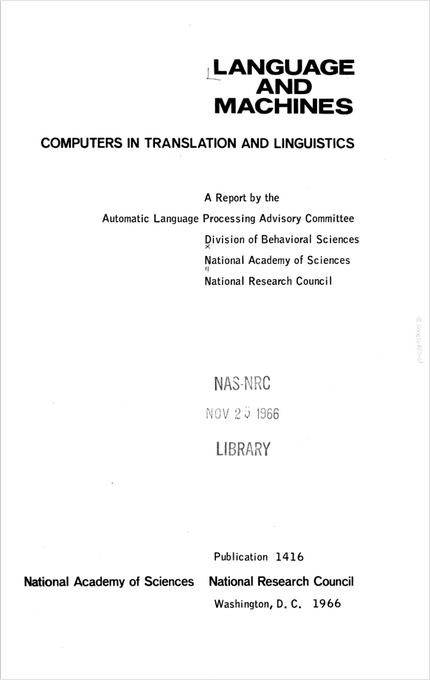
\includegraphics[scale=0.65]{./Chapter1/Figures/figure-report.jpg}
    \caption{ALPAC报告}
    \label{fig:1-4}
\end{figure}
%-------------------------------------------

\parinterval 随后美国政府终止了对机器翻译研究的支持,这导致整个产业界和学术界都开始回避机器翻译。没有了政府的支持,企业也无法进行大规模投入,机器翻译的研究就此受挫。

\parinterval 从历史上看,包括机器翻译在内,很多人工智能领域在那个年代并不受“待见”,其主要原因在于当时的技术水平还比较低,而大家又对机器翻译等技术的期望过高。最后发现,当时的机器翻译水平无法满足实际需要,因此转而排斥它。但是,也正是这一盆冷水,让研究人员可以更加冷静地思考机器翻译的发展方向,为后来的爆发蓄力。

%----------------------------------------------------------------------------------------
%    NEW SUB-SECTION
%----------------------------------------------------------------------------------------

\subsection{机器翻译的快速成长}

\parinterval 事物的发展都是螺旋式上升的,机器翻译也是一样。早期基于规则的机器翻译方法需要人来书写规则,虽然对少部分句子具有较高的翻译精度,可是对翻译现象的覆盖度有限,而且对规则或者模板中的噪声非常敏感,系统健壮性差。

\parinterval 上世纪70年代中后期,特别是80年代到90年代初,国家之间往来日益密切,而不同语言之间形成的交流障碍愈发严重,传统的人工作业方式已经远远不能满足需求。与此同时,语料库语言学的发展也为机器翻译提供了新的思路。一方面,随着传统纸质文字资料不断电子化,计算机可读的语料越来越多,这使得人们可以用计算机对语言规律进行统计分析。另一方面,随着可用数据越来越多,用数学模型描述这些数据中的规律并进行推理逐渐成为可能。这也衍生出一类数学建模方法\ \dash\ {\small\bfnew{数据驱动}}\index{数据驱动}(Data-driven)\index{Data-driven}的方法。同时这类方法也成为了随后出现的统计机器翻译的基础,比如,IBM研究人员提出的基于噪声信道模型的5种统计翻译模型\upcite{brown1990statistical,DBLP:journals/coling/BrownPPM94}。

\parinterval 基于数据驱动的方法不依赖于人书写的规则,机器翻译的建模、训练和推断都可以自动地从数据中学习。这使得整个机器翻译的范式发生了翻天覆地的变化,比如,日本学者长尾真提出的基于实例的方法\upcite{nagao1984framework,DBLP:conf/coling/SatoN90}和统计机器翻译\upcite{brown1990statistical,DBLP:journals/coling/BrownPPM94}就是在此期间兴起的。此外,这样的方法使得机器翻译系统的开发代价大大降低。

\parinterval 从上世纪90年代到本世纪初,随着语料库的完善与高性能计算机的发展,统计机器翻译很快成为了当时机器翻译研究与应用的代表性方法。一个标志性的事件是谷歌公司推出了一个在线的免费自动翻译服务,也就是大家熟知的谷歌翻译。这使得机器翻译这种“高大上”的技术快速进入人们的生活,而不再是束之高阁的科研想法。随着机器翻译不断走向实用,机器翻译的应用也越来越多,这反过来促进了机器翻译的研究进程。比如,在2005-2015年间,统计机器翻译这个主题几乎统治了ACL等自然语言处理相关方向顶级会议的论文,可见其在当时的影响力。

%----------------------------------------------------------------------------------------
%    NEW SUB-SECTION
%----------------------------------------------------------------------------------------

\subsection{机器翻译的爆发}

\parinterval 进入二十一世纪,统计机器翻译拉开了黄金发展期的序幕。在这一时期,各种基于统计机器翻译模型层出不穷,经典的基于短语的模型和基于句法的模型也先后被提出。在2013年以后,机器学习的进步带来了机器翻译技术的进一步提升。特别是基于神经网络的深度学习方法在机器视觉、语音识别中被成功应用,带来性能的飞跃式提升。很快,深度学习方法也被用于机器翻译。

\parinterval 实际上,对于机器翻译任务来说,深度学习方法被广泛使用也是一种必然,原因如下:

\begin{itemize}
\vspace{0.5em}
\item 第一,端到端学习不依赖于过多的先验假设。在统计机器翻译时代,模型设计或多或少会对翻译的过程进行假设,称为隐藏结构假设。比如基于短语的模型假设:源语言和目标语言都会被切分成短语序列,这些短语之间存在某种对齐关系。这种假设既有优点也有缺点:一方面,该假设有助于模型融入人类的先验知识,比如,统计机器翻译中一些规则的设计就借鉴了语言学的相关概念;另一方面,假设越多模型受到的限制也越多。如果假设是正确的,模型可以很好地描述问题。但如果假设错误,那么模型就可能产生偏差。深度学习不依赖于先验知识,也不需要手工设计特征,模型直接从输入和输出的映射上进行学习(端到端学习),这样也在一定程度上避免了隐藏结构假设造成的偏差。
\vspace{0.5em}
\item 第二,神经网络的连续空间模型有更强的表示能力。机器翻译中的一个基本问题是:如何表示一个句子?统计机器翻译把句子的生成过程看作是短语或者规则的推导,这本质上是一个离散空间上的符号系统。深度学习把传统的基于离散化的表示变成了连续空间的表示。比如,用实数空间的分布式表示代替了离散化的词语表示,而整个句子可以被描述为一个实数向量。这使得翻译问题可以在连续空间上描述,进而大大缓解了传统离散空间模型维度灾难等问题。更重要的是,连续空间模型可以用梯度下降等方法进行优化,具有很好的数学性质并且易于实现。
\vspace{0.5em}
\item 第三,深度网络学习算法的发展和GPU\index{GPU}(Graphics Processing Unit)\index{Graphics Processing Unit}等并行计算设备为训练神经网络提供了可能。早期的基于神经网络的方法一直没有在机器翻译甚至自然语言处理领域得到大规模应用,其中一个重要的原因是这类方法需要大量的浮点运算,但是以前计算机的计算能力无法达到这个要求。随着GPU等并行计算设备的进步,训练大规模神经网络也变为了可能。现在已经可以在几亿、几十亿,甚至上百亿句对上训练机器翻译系统,系统研发的周期越来越短,进展日新月异。
\vspace{0.5em}
\end{itemize}

\parinterval 今天,神经机器翻译已经成为新的范式,与统计机器翻译一同推动了机器翻译技术与应用产品的发展。比如,从世界上著名的机器翻译比赛WMT和CCMT中就可以看出这个趋势。如图\ref{fig:1-5}所示,其中左图是WMT\ 19国际机器翻译比赛的参赛队伍的截图,这些参赛队伍基本上都在使用深度学习完成机器翻译的建模。而在WMT\ 19各个项目夺冠系统中(\ref{fig:1-5}右图),神经机器翻译也占据了主导地位。

%----------------------------------------------
\begin{figure}[htp]
    \centering
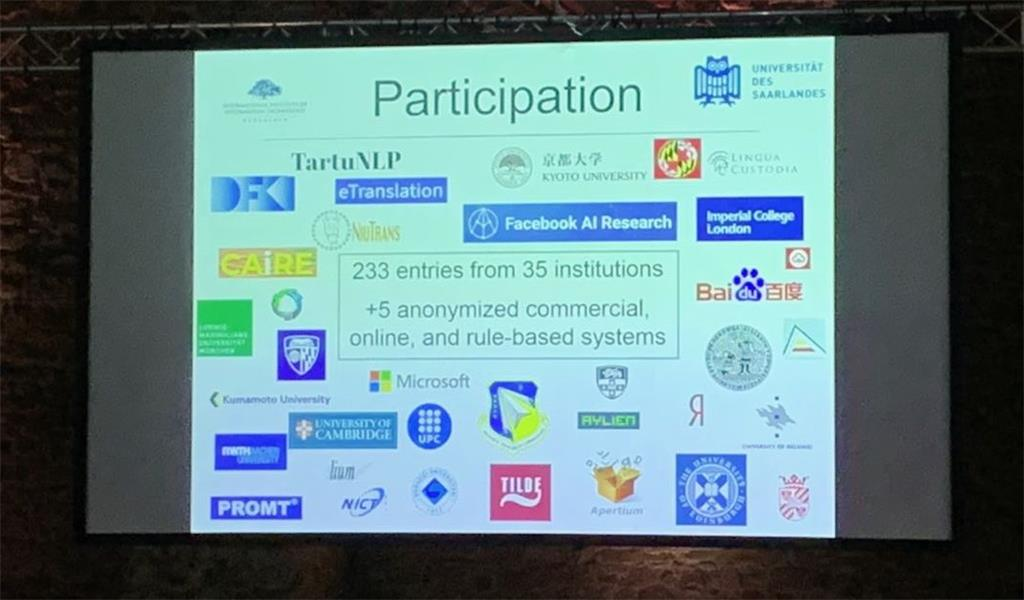
\includegraphics[scale=0.3]{./Chapter1/Figures/figure-wmt-participation.jpg}
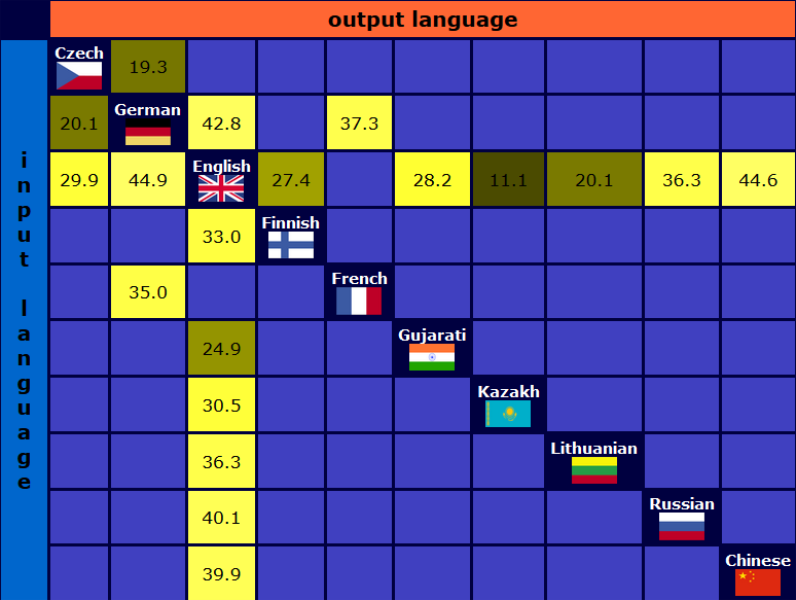
\includegraphics[scale=0.3]{./Chapter1/Figures/figure-wmt-bestresults.jpg}
\setlength{\belowcaptionskip}{-1.5em}
    \caption{WMT\ 19国际机器翻译大赛(左:WMT\ 19参赛队伍;右:WMT\ 19各项目的最好分数)}
    \label{fig:1-5}
\end{figure}
%-------------------------------------------

\parinterval 值得一提的是,近些年神经机器翻译的快速发展也得益于产业界的关注。各大互联网企业和机器翻译技术研发机构都对神经机器翻译的模型和实践方法给予了很大贡献。很多企业凭借自身人才和基础设施方面的优势,先后推出了以神经机器翻译为内核的产品及服务,相关技术方法已经在大规模应用中得到验证,大大推动了机器翻译的产业化进程,而且这种趋势在不断加强,机器翻译的前景也更加宽广。

%----------------------------------------------------------------------------------------
%    NEW SECTION
%----------------------------------------------------------------------------------------

\sectionnewpage
\section{机器翻译现状及挑战}
%%%%%%%%%%%%%%%%%%%%%%%%%%%%%%%%%%%%%%%%%%%%%%%%%%%%%%%%%%%%%%%%%%%%%%%%%%%%
\parinterval 机器翻译技术发展到今天已经过无数次迭代,技术范式也经过若干次更替,近些年机器翻译的应用也如雨后春笋相继浮现。今天的机器翻译的质量究竟如何呢?乐观地说,在很多特定的条件下,机器翻译的译文结果是非常不错的,甚至可以接近人工翻译的结果。然而,在开放式翻译任务中,机器翻译的结果还并不完美。更严格来说,机器翻译的质量远没有达到人们所期望的程度。对于有些人提到的“机器翻译将代替人工翻译”也并不是事实。比如,在高精度同声传译任务中,机器翻译仍需要更多打磨;再比如,针对于小说的翻译,机器翻译还无法做到与人工翻译媲美;甚至有人尝试用机器翻译系统翻译中国古代诗词,这里更多的是娱乐的味道。但是毫无疑问的是,机器翻译可以帮助人类,甚至有朝一日可以代替一些低端的人工翻译工作。

\parinterval 图\ref{fig:1-6}展示了机器翻译和人工翻译质量的一个对比结果。在汉语到英语的新闻翻译任务中,如果对译文进行人工评价(五分制),那么机器翻译的译文得分为3.9分,人工译文得分为4.7分(人的翻译也不是完美的)。可见,在这个任务中机器翻译表现不错,但是与人还有一定差距。如果换一种方式评价,把人的译文作为参考答案,用机器翻译的译文与其进行比对(百分制),会发现机器翻译的得分只有47分。当然,这个结果并不是说机器翻译的译文质量很差,它更多的是表明机器翻译系统可以生成一些与人工翻译不同的译文,机器翻译也具有一定的创造性。这也类似于,很多围棋选手都想向AlphaGo学习,因为智能围棋系统也可以走出一些人类从未走过的妙招。

%----------------------------------------------
\begin{figure}[htp]
   \centering

\definecolor{ublue}{rgb}{0.152,0.250,0.545}
\definecolor{ugreen}{rgb}{0,0.5,0}


%%% outline
%-------------------------------------------------------------------------

{
\begin{tikzpicture}
\node [anchor=south west, fill=blue!50, minimum width=1.1cm, minimum height=2.3cm] (mt) at (1,0) {{\color{white} {\small\sffamily\bfseries{机器}}}};
\node [anchor=south west, fill=red!50, minimum width=1.1cm, minimum height=2.7cm] (human) at ([xshift=0.5cm]mt.south east) {{\color{white} {\small\sffamily\bfseries{人}}}};
\node [anchor=south] (mtscore) at (mt.north) {3.9};
\node [anchor=south] (humanscore) at (human.north) {4.7};
\draw [->,thick] ([xshift=-0.5cm]mt.south west) -- ([xshift=0.5cm]human.south east);
\draw [->,thick] ([xshift=-0.5cm]mt.south west) -- ([xshift=-0.5cm,yshift=3.2cm]mt.south west);

\node [anchor=south west, fill=blue!50, minimum width=1.1cm, minimum height=1.5cm] (mt1) at ([xshift=13.0em,yshift=-3.0em]mt.east) {{\color{white} {\small\sffamily\bfseries{机器}}}};
\node [anchor=south west, fill=red!50, minimum width=1.1cm, minimum height=2.7cm] (human1) at ([xshift=0.5cm]mt1.south east) {{\color{white} {\small\sffamily\bfseries{人}}}};
\node [anchor=south] (mtscore1) at (mt1.north) {47};
\node [anchor=south] (humanscore1) at (human1.north) {100};
\draw [->,thick] ([xshift=-0.5cm]mt1.south west) -- ([xshift=0.5cm]human1.south east);
\draw [->,thick] ([xshift=-0.5cm]mt1.south west) -- ([xshift=-0.5cm,yshift=3.2cm]mt1.south west);

\node[anchor=south](footname1) at ([xshift=2.1em,yshift=-2.0em]mt.south){\footnotesize{人工评价(五分制)}};
\node[anchor=south](footname2) at ([xshift=2.1em,yshift=-2.0em]mt1.south){\footnotesize{自动评价(百分制)}};
\end{tikzpicture}

}






%---------------------------------------------------------------------




\setlength{\belowcaptionskip}{-0.5em}
    \caption{机器翻译与人工翻译性能对比(汉英新闻领域翻译)}
    \label{fig:1-6}
\end{figure}
%-------------------------------------------

\parinterval 图\ref{fig:1-7}展示了一个真实的汉语到英语翻译实例。对比发现,机器翻译与人工翻译还是存在差距的,特别是在翻译一些具有感情色彩的词语时,机器翻译的译文缺一些味道。那么,机器翻译一点用都没有吗?显然不是。实际上,如果考虑翻译速度与翻译代价,机器翻译的价值是无可比拟的。还是同一个例子,翻译一篇短文如果人工翻译需要30分钟甚至更长时间,那么机器翻译仅仅需要两秒,换种情况思考,如果有100万篇这样的文档,其人工翻译的成本根本无法想象,消耗的时间更是难以计算,而计算机集群仅仅需要一天,而且只有电力的消耗。

%----------------------------------------------
\begin{figure}[htp]
    \centering
\definecolor{ublue}{rgb}{0.152,0.250,0.545}
\definecolor{ugreen}{rgb}{0,0.5,0}

%%% outline
%-------------------------------------------------------------------------
\begin{tikzpicture}
%第一段----------------------------------------------
%原文-------------
\node [pos=0.4,left,xshift=-0.4em,yshift=2.0em] (original1) {\scriptsize{源\ \ 语\ \ 言:从前有一个小岛,上面住着快乐、悲哀、知识和爱,还有其他各种情感。一天,情感们得知}};
\node [anchor=north west] (original1-1) at ([xshift=3.5em,yshift=0.3em]original1.south west)  {\scriptsize{小岛快要下沉了。于是,大家都准备船只,离开小岛,只有爱决定留下来,她想坚持到最后}};
\node [anchor=north west] (original1-2) at ([yshift=0.3em]original1-1.south west)  {\scriptsize{一刻。过了几天,小岛真的要下沉了,爱想请人帮忙。}};
%机器翻译--------------
\node [anchor=north west] (mt1) at ([xshift=-3.5em,yshift=0.3em]original1-2.south west) {\scriptsize{机器翻译:Once upon a time there was an island {\color{red}\underline{on which}} lived happiness,sorrow,knowledge,love and other}};

\node [anchor=north west] (mt1-1) at ([xshift=3.5em,yshift=0.4em]mt1.south west) {\scriptsize{emotions. One day, {\color{red}\underline{the}} emotions learned that the island was going to sink.As a result,everyone pre}};

\node [anchor=north west] (mt1-2) at ([yshift=0.4em]mt1-1.south west) {\scriptsize{-pared the boat and {\color{red}\underline{left the island.}} Only Love decided to stay.She {\color{red}\underline{ wanted to stick}} to it until the last}};

\node [anchor=north west] (mt1-3) at ([yshift=0.4em]mt1-2.south west) {\scriptsize{moment. After a few days, the island was really going to sink and love {\color{red}\underline{ wanted help.}}}};
%人工翻译---------------
\node [anchor=north west] (ht1) at ([xshift=-3.5em,yshift=0.4em]mt1-3.south west) {\scriptsize{人工翻译:Once upon a time, there was a small island {\color{red}\underline{where}} lived all kinds of emotions like JOY,SADNESS,}};

\node [anchor=north west] (ht1-1) at ([xshift=3.5em,yshift=0.4em]ht1.south west) {\scriptsize{KNOWLEDGE, and LOVE.One day, {\color{red}\underline{these}} emotions found that the island was sinking, so one by}};

\node [anchor=north west] (ht1-2) at ([yshift=0.4em]ht1-1.south west) {\scriptsize{one they prepared the boat and {\color{red}\underline{planned to leave.}} None but LOVE chose to stay there. She {\color{red}\underline{was deter}}}};

\node [anchor=north west] (ht1-3) at ([yshift=0.4em]ht1-2.south west) {\scriptsize{{\color{red}\underline{-mined to}} persist till the last moment.A few days later, almost the whole island sunk into the sea,}};

\node [anchor=north west] (ht1-4) at ([yshift=0.4em]ht1-3.south west) {\scriptsize{and LOVE had to {\color{red}\underline{seek for help.}}}};

\begin{pgfonlayer}{background}
{
\node[rectangle,draw=ublue, inner sep=0mm] [fit =(original1)(ht1)(mt1)(ht1-4)] {};
}
\end{pgfonlayer}


\end{tikzpicture}





    \caption{机器翻译与人工翻译结果对比实例}
    \label{fig:1-7}
\end{figure}
%-------------------------------------------

\parinterval 虽然机器翻译有上述优点,但仍然面临一些挑战:

\begin{itemize}
\vspace{0.5em}
\item {\small\bfnew{自然语言翻译问题的复杂性极高}}。语言是人类进化的最高成就之一,自然语言具有高度的概括性、灵活性、多样性,这些都很难用几个简单的模型和算法进行描述。因此,翻译问题的数学建模和计算机程序实现难度很大。虽然近几年AlphaGo等人工智能系统在围棋等领域取得了令人瞩目的成绩,但是,相比翻译来说,围棋等棋类任务仍然“简单”。正如不同人对同一句话的理解不尽相同,一个句子往往不存在绝对的标准译文,其潜在的译文几乎是不可穷尽的。甚至人类译员在翻译一个句子、一个单词的时候,都要考虑整个篇章的上下文语境。这些难点都不是传统棋类任务所具有的。
\vspace{0.5em}
\item {\small\bfnew{计算机的“理解”与人类的“理解”存在鸿沟}}。人类一直希望把自己翻译时所使用的知识描述出来,并用计算机程序进行实现,例如早期基于规则的机器翻译方法就源自这个思想。但是,经过实践发现,人和计算机在“理解”自然语言上存在着明显差异。首先,人类的语言能力是经过长时间在多种外部环境因素共同作用下形成的,这种能力很难用计算机准确地刻画。况且人类的语言知识本身就很难描述,更不用说让计算机来理解;其次,人和机器翻译系统理解语言的目的不一样。人理解和使用语言是为了进行生活和工作,而机器翻译系统更多的是为了对某些数学上定义的目标函数进行优化。也就是说,机器翻译系统关注的是翻译这个单一目标,而并不是像人一样进行复杂的活动;此外,人和计算机的运行方式有着本质区别。人类语言能力的生物学机理与机器翻译系统所使用的计算模型本质上是不同的,机器翻译系统使用的是其自身能够理解的“知识”,比如,统计学上的词语表示。这种“知识”并不需要人来理解,当然从系统开发的角度,计算机也并不需要理解人是如何思考的。
\vspace{0.5em}
\item {\small\bfnew{单一的方法无法解决多样的翻译问题}}。首先,语种的多样性会导致任意两种语言之间的翻译实际上都是不同的翻译任务。比如,世界上存在的语言多达几千种,如果选择任意两种语言进行互译就会产生上百万种翻译方向。虽然已经有研究者尝试用同一个框架甚至同一个翻译系统进行全语种的翻译,但是这类系统离真正可用还有很远的距离;其次,不同的领域,不同的应用场景对翻译也有不同的需求。比如,文学作品的翻译和新闻的翻译就有不同、口译和笔译也有不同,类似的情况不胜枚举。以上这些都增加了计算机对翻译进行建模的难度;再次,对于机器翻译来说,充足的高质量数据是必要的,但是不同语种、不同领域、不同应用场景所拥有的数据量有明显差异,很多语种甚至几乎没有可用的数据,这时开发机器翻译系统的难度可想而知。值得注意的是,现在的机器翻译还无法像人类一样在学习少量样例的情况下进行举一反三,因此数据稀缺情况下的机器翻译也给研究者带来了很大的挑战。
\vspace{0.5em}
\end{itemize}

\parinterval 显然,实现机器翻译并不简单,甚至有人把机器翻译看作是实现人工智能的终极目标。幸运的是,今天的机器翻译无论从技术方法上还是从应用上都有了巨大的飞跃,很多问题在不断被求解。如果读者看到过十年前机器翻译的结果,再对比今天的结果,一定会感叹翻译质量的今非昔比,很多译文已经非常准确且流畅。从当今机器翻译的前沿技术看,近三十年机器翻译的进步更多得益于基于数据驱动方法和统计建模方法的使用。特别是近些年深度学习等基于表示学习的端到端方法使得机器翻译的水平达到了新高度。因此,本书将会对基于统计建模和深度学习方法的机器翻译模型、方法和系统实现进行全面介绍和分析,希望这些论述可以对相关内容的学习和科研工作提供参考。

%----------------------------------------------------------------------------------------
%    NEW SECTION
%----------------------------------------------------------------------------------------

\sectionnewpage
\section{基于规则的方法}\label{section-1.4}
%%%%%%%%%%%%%%%%%%%%%%%%%%%%%%%%%%%%%%%%%%%%%%%%%%%%%%%%%%%%%%%%%%%%%%%%%%%%
\parinterval 机器翻译技术大体上可以分为三种方法,分别为基于规则的机器翻译、统计机器翻译以及神经机器翻译。第一代机器翻译技术是主要使用基于规则的机器翻译方法,其主要思想是通过形式文法定义的规则引入源语言和目标语中的语言学知识。此类方法在机器翻译技术诞生之初就被人所关注,特别是在上世纪70年代,以基于规则方法为代表的专家系统是人工智能中最具代表性的研究领域。甚至到了统计机器翻译时代,很多系统中也大量地使用了基于规则的翻译知识表达形式。

\parinterval 早期,基于规则的机器翻译大多依赖人工定义及书写的规则。主要有两类方法\upcite{nirenburg1989knowledge,hutchins1986machine,zarechnak1979history}:一类是基于转换规则的机器翻译方法,简称转换法。另一类是基于中间语言的方法。它们都以词典和人工书写的规则库作为翻译知识,用一系列规则的组合完成翻译。

%----------------------------------------------------------------------------------------
%    NEW SUB-SECTION
%----------------------------------------------------------------------------------------

\subsection{规则的定义}

\parinterval 规则就像语言中的“If-then”语句,如果满足条件,则执行相应的语义动作。比如,可以将待翻译句子中的某个词,使用目标语言单词进行替换,但是这种替换并非随意的,而是在语言学知识的指导下进行的。

\parinterval 图\ref{fig:1-8}展示了一个使用转换法进行翻译的实例。这里,利用一个简单的汉译英规则库完成对句子“我对你感到满意”的翻译。当翻译“我”时,从规则库中找到规则1,该规则表示遇到单词“我”就翻译为“I”;类似地,也可以从规则库中找到规则4,该规则表示翻译调序,即将单词“you”放到“be satisfied with”后面。这种通过规则表示单词之间的对应关系也为统计机器翻译方法提供了思路。如统计机器翻译中,基于短语的翻译模型使用短语对对原文进行替换,详细描述可以参考{\chapterseven}。

%----------------------------------------------
\begin{figure}[htp]
    \centering
\definecolor{ublue}{rgb}{0.152,0.250,0.545}
\definecolor{ugreen}{rgb}{0,0.5,0}


%%% outline
%-------------------------------------------------------------------------

\begin{tikzpicture}
\begin{scope}
{
{\footnotesize
\node [anchor=north west] (rule1) at (0,0) {\textbf{1: If} 源=我, \textbf{then} 译=\ I};
\node [anchor=north west] (rule2) at ([yshift=0.1em]rule1.south west) {\textbf{2: If} 源=你, \textbf{then} 译=\ you};
\node [anchor=north west] (rule3) at ([yshift=0.1em]rule2.south west) {\textbf{3: If} 源=感到\ 满意,};
\node [anchor=north west] (rule3part2) at ([yshift=0.5em]rule3.south west) {\textbf{\hspace{0.95em} then} 译=\ be satisfied with};
\node [anchor=north west] (rule4) at ([yshift=0.1em]rule3part2.south west) {\textbf{4: If} 源=对 ... 动词[表态度]};
\node [anchor=north west] (rule4part2) at ([yshift=0.5em]rule4.south west) {\textbf{\hspace{0.95em} then} 调序[动词 + 对象]};
\node [anchor=north west] (rule5) at ([yshift=0.1em]rule4part2.south west) {\textbf{5: If} 译文主语是\ I};
\node [anchor=north west] (rule5part2) at ([yshift=0.5em]rule5.south west) {\textbf{\hspace{0.95em} then} be动词为\ am/was};
\node [anchor=north west] (rule6) at ([yshift=0.1em]rule5part2.south west) {\textbf{6: If} 源语是主谓结构};
\node [anchor=north west] (rule6part2) at ([yshift=0.5em]rule6.south west) {\textbf{\hspace{0.95em} then} 译文为主谓结构};
\node [anchor=south west] (rulebaselabel) at (rule1.north west) {{\color{ublue} 资源:规则库}};
}

\begin{pgfonlayer}{background}
{
  \node[rectangle,draw=ublue, thick,inner sep=0mm] [fit = (rule1) (rule2) (rule3) (rule3part2) (rule4) (rule4part2) (rule5) (rule5part2) (rule6) (rule6part2) (rulebaselabel)] {};
}
\end{pgfonlayer}
}

\end{scope}

\begin{scope}[xshift=2.3in]
{\footnotesize
\node [anchor=north west,inner sep=1mm] (w1) at (0,0em) {我};
\node [anchor=north west,inner sep=1mm] (w2) at ([xshift=0.3em]w1.north east) {对};
\node [anchor=north west,inner sep=1mm] (w3) at ([xshift=0.3em]w2.north east) {你};
\node [anchor=north west,inner sep=1mm] (w4) at ([xshift=0.3em]w3.north east) {感到};
\node [anchor=north west,inner sep=1mm] (w5) at ([xshift=0.3em]w4.north east) {满意};
}
\end{scope}

{\footnotesize
\node [anchor=north,inner sep=1mm] (t1) at ([yshift=-0.6em]w1.south) {I};
\draw[->,thick,ublue] (w1.south)--(t1.north);
}

{\footnotesize
\node [anchor=north,inner sep=1mm] (t3) at ([yshift=-0.6em]w3.south) {you};
\draw[->,thick,ublue] (w3.south)--(t3.north);
}

{\footnotesize
\draw[-] ([yshift=0.2em]w4.south west)--([yshift=0.2em]w5.south east);
\node [anchor=north,inner sep=1mm] (t45) at ([yshift=-2em]w5.south) {be satisfied with};
\draw[->,thick,ublue] ([yshift=0.1em]w4.south east)..controls +(south:0.6) and +(north:0.6)..(t45.north);
}

{\footnotesize
\node [anchor=north west,inner sep=1mm] (t35) at ([yshift=-3.0em,xshift=-1em]t3.south) {be satisfied with you};
\draw[->,thick,ublue] (t3.south)..controls +(south:1.3) and +(north:0.9)..([xshift=-1em,yshift=-0.2em]t35.north east);
\draw[->,thick,ublue] (t45.south)..controls +(south:0.7) and +(north:0.5)..([xshift=3em,yshift=-0.2em]t35.north west);
}

{\footnotesize
\node [anchor=north west,inner sep=1mm] (t15) at ([yshift=-1.5em,xshift=-2em]t35.south west) {I be satisfied with you};
\draw[->,thick,ublue] (t35.south)..controls +(south:0.5) and +(north:0.5)..([xshift=-5em]t15.north east);
\draw[->,thick,ublue] (t1.south)..controls +(south:1.5) and +(north:1.5)..([xshift=0.5em]t15.north west);
}


{\footnotesize
\node [anchor=north west,inner sep=1mm] (t15final) at ([yshift=-1.5em]t15.south west) {I am satisfied with you};
\node [draw,circle,thick,dotted,ublue,minimum width=1.3em] (be1) at ([xshift=1.35em,yshift=0.1em]t15.west) {};
\draw[->,thick,ublue] ([xshift=-0em]be1.south)..controls +(south:0.3) and +(north:0.4)..([xshift=1.6em,yshift=-0.2em]t15final.north west);
}
{
\draw[->,dotted,thick,red] ([xshift=-0.2em]rule5part2.east)..controls +(east:1.5) and +( west:1.5)..(t15final.west) node[pos=0.9,below,xshift=0.3em,yshift=0.0em] (applyr6) {\color{red}{\tiny\sffamily\bfseries{规则5}}};
}

\end{tikzpicture}
%---------------------------------------------------------------------



    \caption{基于规则的机器翻译的示例图(左:规则库;右:规则匹配结果)}
    \label{fig:1-8}
\end{figure}
%-------------------------------------------

\parinterval 在上述例子中可以发现,规则不仅仅可以翻译句子之间单词的对应,如规则1,还可以表示句法甚至语法之间的对应,如规则6。因此基于规则的方法可以分成多个层次,如图\ref{fig:1-9}所示。图中不同的层次表示采用不同的知识来书写规则,进而完成机器翻译过程。对于翻译问题,可以构建不同层次的基于规则的机器翻译系统。这里包括四个层次,分别为:词汇转换、句法转换、语义转换和中间语言层。其中,上层可以继承下层的翻译知识,比如说句法转换层会利用词汇转换层知识。早期基于规则的方法属于词汇转换层。

%----------------------------------------------
\begin{figure}[htp]
    \centering
%%%------------------------------------------------------------------------------------------------------------
%%%  短语系统的架构
\begin{center}
\begin{tikzpicture}
\begin{scope}

\tikzstyle{node1} = [minimum width=7em,minimum height=1.7em,fill=red!20,rounded corners=0.3em];
\tikzstyle{node2} = [minimum width=7em,minimum height=2.5em,fill=blue!20,rounded corners=0.3em];
\tikzstyle{node3} = [minimum width=7em,minimum height=2.5em,fill=green!20,rounded corners=0.3em];
\tikzstyle{node4} = [minimum width=7em,minimum height=1.7em,fill=orange!20,rounded corners=0.3em];
\tikzstyle{node5} = [minimum width=4.5em,minimum height=1.7em,dashed];

\node [node1,anchor=south west] (s1) at (0,0) {{ \small{源语言词串}}};
\node [node2,anchor=south] (s2) at ([xshift=2.5em,yshift=2em]s1.north) {};
\node [anchor=north,minimum height=1.2em] (s21) at (s2.north) {{ \small{源语言}}};
\node [anchor=south,minimum height=1.2em] (s22) at (s2.south) {{ \small{句法结构}}};
\node [node3,anchor=south] (s3) at ([xshift=2.5em,yshift=2em]s2.north) {};
\node [anchor=north,minimum height=1.2em] (s31) at (s3.north) {{ \small{源语言}}};
\node [anchor=south,minimum height=1.2em] (s32) at (s3.south) {{ \small{语义结构}}};
\node [node4,anchor=south] (s4) at ([xshift=6em,yshift=2em]s3.north) {{ \small{中间语言(知识表示)}}};

\node [node3,anchor=north] (t1) at ([xshift=6em,yshift=-2em]s4.south) {};
\node [anchor=north,minimum height=1.2em] (t11) at (t1.north) {{ \small{目标语言}}};
\node [anchor=south,minimum height=1.2em] (t12) at (t1.south) {{ \small{语义结构}}};
\node [node2,anchor=north] (t2) at ([xshift=2.5em,yshift=-2em]t1.south) {};
\node [anchor=north,minimum height=1.2em] (t21) at (t2.north) {{ \small{目标语言}}};
\node [anchor=south,minimum height=1.2em] (t22) at (t2.south) {{ \small{句法结构}}};
\node [node1,anchor=north] (t3) at ([xshift=2.5em,yshift=-2em]t2.south) {{ \small{目标语言词串}}};

\node [anchor=north] (l1) at ([yshift=-2em]s4.south) {{ \small{语义\ 转换}}};
\node [anchor=north] (l2) at ([yshift=-3em]l1.south) {{ \small{句法\ 转换}}};
\node [anchor=north] (l3) at ([yshift=-2.5em]l2.south) {{ \small{词汇\ 转换}}};

\node [node5,anchor=north,draw] (st1) at ([xshift=-3em,yshift=-0.5em]l3.south) {{ \small{分析部分}}};
\node [node5,anchor=north,draw] (st2) at ([xshift=3em,yshift=-0.5em]l3.south) {{ \small{生成部分}}};

\draw [->,thick] (s1.north) -- ([xshift=-0.6em]s2.south);
\draw [->,thick] ([xshift=0.6em]s2.north) -- (s3.south);
\draw [->,thick] ([xshift=1.2em]s3.north) -- ([xshift=-2.7em]s4.south);
\draw [->,thick] ([xshift=2.7em]s4.south) -- ([xshift=-1.2em]t1.north);
\draw [->,thick] (t1.south) -- ([xshift=-0.6em]t2.north);
\draw [->,thick] ([xshift=0.6em]t2.south) -- (t3.north);
\draw [->,thick] (s3.east) -- (t1.west);
\draw [->,thick] (s2.east) -- (t2.west);
\draw [->,thick] (s1.east) -- (t3.west);

\draw [-] ([xshift=0.1em]s4.south) -- ([xshift=0.1em,yshift=-14em]s4.south);


\end{scope}
\end{tikzpicture}
\end{center}
    \caption{基于规则的机器翻译方法的四个层次\upcite{冯志伟2004机器翻译研究}}
\setlength{\belowcaptionskip}{-1.5em}
    \label{fig:1-9}
\end{figure}
%-------------------------------------------

%----------------------------------------------------------------------------------------
%    NEW SUB-SECTION
%----------------------------------------------------------------------------------------

\subsection{转换法}

\parinterval 通常一个典型的{\small\bfnew{基于转换规则的机器翻译}}\index{基于转换规则的机器翻译}(Transfer-based Translation)\index{Transfer-based Translation}的过程可以被视为“独立分析-相关转换-独立生成”的过程\upcite{parsing2009speech}。如图\ref{fig:1-10}所示,这些过程可以分成六个步骤,其中每一个步骤都是通过相应的翻译规则来完成。比如,第一个步骤中需要构建源语词法分析规则,第二个步骤中需要构建源语句法分析规则,第三个和第四个步骤中需要构建转换规则,其中包括源语言-目标语言词汇和结构转换规则等等。

%----------------------------------------------
\begin{figure}[htp]
    \centering
%%%------------------------------------------------------------------------------------------------------------
%%%  短语系统的架构
\begin{center}
\begin{tikzpicture}
\begin{scope}

\tikzstyle{datanode} = [minimum width=7em,minimum height=1.7em,fill=red!20,rounded corners=0.3em];
\tikzstyle{modelnode} = [minimum width=7em,minimum height=1.7em,fill=blue!20,rounded corners=0.3em];
\tikzstyle{decodingnode} = [minimum width=7em,minimum height=1.7em,fill=green!20,rounded corners=0.3em];

\node [datanode,anchor=north west,minimum height=1.7em,minimum width=8em] (s1) at (0,0) {{ \small{源文句子}}};
\node [modelnode,anchor=north,minimum height=1.7em,minimum width=8em] (s2) at ([yshift=-1.5em]s1.south) {{ \small{源语词法分析}}};
\node [datanode,anchor=north,minimum height=1.7em,minimum width=8em] (s3) at ([yshift=-1.5em]s2.south) {{ \small{源文词串}}};
\node [modelnode,anchor=north,minimum height=1.7em,minimum width=8em] (s4) at ([yshift=-1.5em]s3.south) {{ \small{源语句法分析}}};
\node [datanode,anchor=north,minimum height=1.7em,minimum width=8em] (s5) at ([yshift=-1.5em]s4.south) {{ \small{源文结构}}};

\node [datanode,anchor=west,minimum height=1.7em,minimum width=8em] (t1) at ([xshift=14em]s1.east) {{ \small{译文句子}}};
\node [modelnode,anchor=north,minimum height=1.7em,minimum width=8em] (t2) at ([yshift=-1.5em]t1.south) {{ \small{目标语词法生成}}};
\node [datanode,anchor=north,minimum height=1.7em,minimum width=8em] (t3) at ([yshift=-1.5em]t2.south) {{ \small{译文词串}}};
\node [modelnode,anchor=north,minimum height=1.7em,minimum width=8em] (t4) at ([yshift=-1.5em]t3.south) {{ \small{目标语句法生成}}};
\node [datanode,anchor=north,minimum height=1.7em,minimum width=8em] (t5) at ([yshift=-1.5em]t4.south) {{ \small{译文结构}}};

\node [decodingnode,anchor=west,minimum height=1.7em,minimum width=8em] (st1) at ([xshift=2.5em,yshift=0.85em]s5.east) {{ \small{源语-目标语词汇转换}}};
\node [decodingnode,anchor=north,minimum height=1.7em,minimum width=8em] (st2) at ([yshift=0.05em]st1.south) {{ \small{源语-目标语结构转换}}};

\draw [->,very thick] (s1.south) -- (s2.north);
\draw [->,very thick] (s2.south) -- (s3.north);
\draw [->,very thick] (s3.south) -- (s4.north);
\draw [->,very thick] (s4.south) -- (s5.north);
\draw [->,very thick] (s5.east) -- (st1.south west);
\draw [->,very thick] (st1.south east) -- (t5.west);
\draw [->,very thick] (t5.north) -- (t4.south);
\draw [->,very thick] (t4.north) -- (t3.south);
\draw [->,very thick] (t3.north) -- (t2.south);
\draw [->,very thick] (t2.north) -- (t1.south);

\end{scope}
\end{tikzpicture}
\end{center}
    \caption{基于转换规则的机器翻译过程}
    \label{fig:1-10}
\end{figure}
%-------------------------------------------

\parinterval 转换法的目标就是使用规则定义的词法和句法,将源语言句子分解成为一个蕴含语言学标志的结构。如一个汉语句子“她把一束花放在桌上。”,经过词法和句法分析之后可以被表示成如图\ref{fig:1-11} 所示的结构,这个结构就是图\ref{fig:1-10}中的源语言句子结构。这种使用语言学提取句子结构化表示,并使用某种规则匹配源语言结构和目标语言结构的方式也为{\chaptereight}将要介绍的基于语言学句法的模型提供了思路。

%----------------------------------------------
\begin{figure}[htp]
    \centering
%------------------------------------------------------------------------------------------------------------
%%%  句法树(层次短语)
\begin{tikzpicture}
{\small
\begin{scope}[sibling distance=25pt, level distance = 20pt]
{\scriptsize
\Tree[.\node(r){IP};
        [.\node(n11){NP}; [.\node(n21){PN};  [.\node(l1){她};]]]
        [.\node(n12){VP}; 
            [.\node(n22){BA}; \node(l2){把}; ]
            [.\node(n23){IP};
                [. \node(n31){NP}; 
                    [. \node(n41){QP}; 
                        [. \node(n51){CD};  \node(l3){一};]
                        [. \node(n52){CLP};  [.\node(n61){M};  [.\node(l4){束};]]]
                    ]
                    [. \node(n42){NP};  [.\node(n53){NN};  [.\node(l5){花};]]]
                ]
                [. \node(n32){VP}; 
                    [. \node(n43){VV};  \node(l6){放在};]
                    [. \node(n44){LCP};
                        [. \node(n54){NP};  [.\node(n62){NN};  [.\node(l7){桌};]]] 
                        [. \node(n55){LC};  \node(l8){上};]
                    ]
                ]
            ]
        ]
        [.\node(n13){PU};  \node(l9){。};]
     ]
}
\end{scope}
}
\end{tikzpicture}

    \caption{一个汉语句子的结构表示(句法树)}
    \label{fig:1-11}
\end{figure}
%-------------------------------------------

\parinterval 在转换法中,翻译规则通常会分成两类:通用规则和个性规则。所谓通用的规则主要用于句法分析、语义分析、结构转换和句法生成等,是不具体依赖于某个源语言或者目标语言词汇而设计的翻译规则;个性规则通常以具体源语言词汇来做索引,比如图\ref{fig:1-8}中规则5就是针对主语是“I”的个性规则,它直接针对某个具体词汇进行分析和翻译。

%----------------------------------------------------------------------------------------
%    NEW SUB-SECTION
%----------------------------------------------------------------------------------------

\subsection{基于中间语言的方法}

\parinterval 基于转换的方法可以通过词汇层、句法层和语义层完成从源语到目标语的转换过程,虽然采用了独立分析和独立生成两个子过程,但中间包含一个从源语到目标语的相关转换过程。这就会导致一个实际问题,假设需要实现$N$个语言之间互译的机器翻译系统,采用基于转换的方法,需要构建$N(N-1)$个不同的机器翻译系统,这个构建代价是非常高的。为了解决这个问题,一种有效的解决方案是使用{\small\bfnew{基于中间语言的机器翻译}}\index{基于中间语言的机器翻译}(Interlingua-based Translation)\index{Interlingua-based Translation}方法。

\parinterval 如图\ref{fig:1-12}所示,基于中间语言方法的最大特点就是采用了一个称之为“中间语言”的知识表示结构,将“中间语言”作为独立源语言分析和独立目标语生成的桥梁,真正实现独立分析和独立生成。并且在基于中间语言的方法中不涉及“相关转换”这个过程,这一点与基于转换的方法有很大区别。

%----------------------------------------------
\begin{figure}[htp]
    \centering
%%%------------------------------------------------------------------------------------------------------------
%%%  短语系统的架构
\begin{center}
\begin{tikzpicture}
\begin{scope}

\tikzstyle{datanode} = [minimum width=5em,minimum height=1.7em,fill=red!20,rounded corners=0.3em];
\tikzstyle{modelnode} = [minimum width=5em,minimum height=1.7em,fill=blue!20,rounded corners=0.3em];
\tikzstyle{decodingnode} = [minimum width=5em,minimum height=1.7em,fill=green!20,rounded corners=0.3em];

\node [datanode,anchor=north west] (s1) at (0,0) {{ \small{语言1}}};
\node [datanode,anchor=north] (s2) at ([yshift=-4.5em]s1.south) {{ \small{语言3}}};
\node [datanode,anchor=west] (s3) at ([xshift=4.5em]s1.east) {{ \small{语言2}}};
\node [datanode,anchor=north] (s4) at ([yshift=-4.5em]s3.south) {{ \small{语言4}}};
\node [circle,anchor=north west,inner sep=2pt,fill=blue!20] (m1) at ([xshift=0.8em,yshift=-0.5em]s1.south east) {{ \small{中间语言}}};

\draw [<->,very thick] (s1.south) -- (m1.170);
\draw [<->,very thick] (s2.north) -- (m1.190);
\draw [<->,very thick] (s3.south) -- (m1.10);
\draw [<->,very thick] (s4.north) -- (m1.-10);

\node [anchor=north] (l) at ([xshift=5em,yshift=-1em]s2.south) {\footnotesize{(a) 基于中间语言的方法}};


\end{scope}

\begin{scope}[xshift=16em]

\tikzstyle{datanode} = [minimum width=5em,minimum height=1.7em,fill=red!20,rounded corners=0.3em];
\tikzstyle{modelnode} = [minimum width=5em,minimum height=1.7em,fill=blue!20,rounded corners=0.3em];
\tikzstyle{decodingnode} = [minimum width=5em,minimum height=1.7em,fill=green!20,rounded corners=0.3em];

\node [datanode,anchor=north west] (s1) at (0,0) {{ \small{语言1}}};
\node [datanode,anchor=north] (s2) at ([yshift=-4.5em]s1.south) {{ \small{语言3}}};
\node [datanode,anchor=west] (s3) at ([xshift=4.5em]s1.east) {{ \small{语言2}}};
\node [datanode,anchor=north] (s4) at ([yshift=-4.5em]s3.south) {{ \small{语言4}}};

\draw [<->,very thick] (s1.south) -- (s2.north);
\draw [<->,very thick] (s1.east) -- (s3.west);
\draw [<->,very thick] (s3.south) -- (s4.north);
\draw [<->,very thick] (s2.east) -- (s4.west);
\draw [<->,very thick] (s1.south east) -- (s4.north west);
\draw [<->,very thick] (s2.north east) -- (s3.south west);

\node [anchor=north] (l) at ([xshift=5em,yshift=-1em]s2.south) {\footnotesize{(b) 基于转换的方法}};

\end{scope}

\end{tikzpicture}
\end{center}
    \caption{基于中间语言的方法(a)与基于转换的方法(b)}
    \label{fig:1-12}
\end{figure}
%-------------------------------------------

\parinterval 从图\ref{fig:1-9}可以发现,中间语言(知识表示)处于最顶端,本质上是独立于源语言和目标语言的,这也是基于中间语言的方法可以将分析过程和生成过程分开的原因。

\parinterval 虽然基于中间语言的方法有上述优点,但如何定义中间语言是一个关键问题。严格上说,所谓中间语言本身是一种知识表示结构,承载着源语言句子的分析结果,应该包含和体现尽可能多的源语言知识。如果中间语言的表示能力不强,会导致源语言句子信息丢失,这自然会影响目标语生成结果。

\parinterval 在基于规则的机器翻译方法中,构建中间语言结构的知识表示方式有很多,比较常见的是语法树、语义网、逻辑结构表示或者多种结构的融合等。但不管哪种方法,实际上都无法充分地表达源语言句子所携带的信息。因此,在早期的基于规则的机器翻译研究中,基于中间语言的方法明显弱于基于转换的机器翻译方法。不过,近些年随着神经机器翻译等方法的兴起,使用统一的中间表示来刻画句子又受到了广泛关注。但是,神经机器翻译中的“中间表示”并不是规则系统中的中间语言,二者有着本质区别,这部分内容将会在第十章进行介绍。

%----------------------------------------------------------------------------------------
%    NEW SUB-SECTION
%----------------------------------------------------------------------------------------

\subsection{规则方法的优缺点}

\parinterval 在基于规则的机器翻译时代,机器翻译技术研究有一个特点就是{\small\bfnew{语法}}\index{语法}(Grammer)\index{Grammer}和{\small\bfnew{算法}}\index{算法}(Algorithm)\index{Algorithm}分开,相当于是把语言分析和程序设计分开。传统方式使用程序代码来实现翻译规则,并把所谓的翻译规则隐含在程序代码实现中。其中最大问题是一旦翻译规则发生修改,程序代码也需要进行相应修改,导致维护代价非常高。此外书写翻译规则的语言学家与编代码的程序员沟通代价也非常高,有时候会出现鸡同鸭讲的感觉。把语法和算法分开对于基于规则的机器翻译技术来说最大好处就是可以将语言学家和程序员的工作分开,各自发挥自己的优势。

\parinterval 这种语言分析和程序设计分开的实现方式也使得基于人工书写翻译规则的机器翻译方法非常直观,语言学家可以很容易地将翻译知识利用规则的方法表达出来,并且不需要修改系统代码。例如:1991年,东北大学自然语言处理实验室王宝库教授提出的规则描述语言(CTRDL)\upcite{王宝库1991机器翻译系统中一种规则描述语言}。以及1995年,同为东北大学自然语言处理实验室的姚天顺教授提出的词汇语义驱动算法\upcite{唐泓英1995基于搭配词典的词汇语义驱动算法},都是在这种思想上对机器翻译方法的一种改进。此外,使用规则本身就具有一定的优势:

\begin{itemize}
\vspace{0.5em}
\item 翻译规则的书写颗粒度具有很大的可伸缩性。
\vspace{0.5em}
\item 较大颗粒度的翻译规则有很强的概括能力,较小颗粒度的翻译规则具有精细的描述能力。
\vspace{0.5em}
\item 翻译规则便于处理复杂的句法结构和进行深层次的语义理解,比如解决翻译过程中的长距离依赖问题。
\vspace{0.5em}
\end{itemize}

\parinterval 通过图\ref{fig:1-8}中规则的翻译实例中可以看出,规则的使用和人类进行翻译时所使用的思想非常类似,可以说基于规则的方法实际上在试图描述人类进行翻译的思维过程。虽然直接模仿人类的翻译方式对翻译问题建模是合理的,但是这一定程度上也暴露了基于规则的方法的弱点。基于规则的机器翻译方法中,人工书写翻译规则的主观因素重,有时与客观事实有一定差距。并且人工书写翻译规则的难度大,代价非常高,这也成为了后来基于数据驱动的机器翻译方法主要改进的方向。

%----------------------------------------------------------------------------------------
%    NEW SECTION
%----------------------------------------------------------------------------------------

\sectionnewpage
\section{数据驱动的方法}
%%%%%%%%%%%%%%%%%%%%%%%%%%%%%%%%%%%%%%%%%%%%%%%%%%%%%%%%%%%%%%%%%%%%%%%%%%%%
\parinterval 虽然基于规则的方法有种种优势,但是该方法人工代价过高。所以研究者们开始尝试,是否可以更好地利用数据,从数据中学习到某些规律,而不是完全依靠人类来制定规则。在这样的思想下,基于数据驱动的方法诞生了。

%----------------------------------------------------------------------------------------
%    NEW SUB-SECTION
%----------------------------------------------------------------------------------------

\subsection{基于实例的机器翻译}

\parinterval 在实际使用上,\ref{section-1.4}章提到的基于规则的方法更多地被使用在受限翻译场景中,比如受限词汇集的翻译。针对基于规则的方法存在的问题,基于实例的机器翻译于上世纪80年代中期被提出\upcite{nagao1984framework}。该方法的基本思想是在双语句库中找到与待翻译句子相似的实例,之后对实例的译文进行修改,如对译文进行替换、增加、删除等一系列操作,从而得到最终译文。这个过程可以类比人类学习并运用语言的过程:人会先学习一些翻译实例或者模板,当遇到新的句子时,会用以前的实例和模板作对比,之后得到新的句子的翻译结果。这也是一种举一反三的思想。

\parinterval 图\ref{fig:1-13}展示了一个基于实例的机器翻译过程。它利用简单的翻译实例库与翻译词典完成对句子“我对你感到满意”的翻译。首先,使用待翻译句子的源语言端在翻译实例库中进行比较,根据相似度大小找到相似的实例“我对他感到高兴”。然后,标记实例中不匹配的部分,即“你”和“他”,“满意”和“高兴”。再查询翻译词典得到词“你”和“满意”所对应的翻译结果“you”和“satisfied”,用这两个词分别替换实例中的“him”和“happy”,从而得到最终译文。

%----------------------------------------------
\begin{figure}[htp]
    \centering

\definecolor{ublue}{rgb}{0.152,0.250,0.545}
\definecolor{ugreen}{rgb}{0,0.5,0}


%%% outline
%-------------------------------------------------------------------------

\begin{tikzpicture}
\begin{scope}
{
{\footnotesize
\node [anchor=north west] (example1) at (0,0) {\textbf{1:} 源=什么\ 时候\ 开始};
\node [anchor=north west] (example1part2) at ([yshift=0.5em]example1.south west) {\hspace{1em} 译=\ When will it start};
\node [anchor=north west] (example2) at ([yshift=0.1em]example1part2.south west) {\textbf{2:} 源=我\ 对\ 他\ 感到\ 高兴};
\node [anchor=north west] (example2part2) at ([yshift=0.5em]example2.south west) {\hspace{1em} 译=\ I am happy with him};
\node [anchor=north west] (example3) at ([yshift=0.1em]example2part2.south west) {\hspace{1em} ...};
\node [anchor=south west] (examplebaselabel) at (example1.north west) {{\color{ublue} 资源1:翻译实例库}};
}
}

\begin{pgfonlayer}{background}
{
\node[rectangle,draw=ublue, inner sep=0mm] [fit = (example1) (example1part2) (example2) (example2part2) (example3) (examplebaselabel)] {};
}
\end{pgfonlayer}

\end{scope}

\begin{scope} [yshift=-1.3in]
{\footnotesize
{
\node [anchor=north west] (entry1) at (0,0) {\textbf{1:} 我 $\to$ I $\mid$ me};
\node [anchor=north west] (entry2) at ([yshift=0.1em]entry1.south west) {\textbf{2:} 你 $\to$ you};
\node [anchor=north west] (entry3) at ([yshift=0.1em]entry2.south west) {\textbf{3:} 满意 \hspace{-0.4em} $\to$ \hspace{-0.4em} satisfy \hspace{-0.12em}$\mid$\hspace{-0.12em} satisfied ... };
\node [anchor=north west] (entry4) at ([yshift=0.1em]entry3.south west) {\hspace{1em} ...};
\node [anchor=south west] (dictionarylabel) at (entry1.north west) {{\color{ublue} 资源2:翻译词典}};
}
}

\begin{pgfonlayer}{background}
{
\node[rectangle,draw=ublue, inner sep=0mm] [fit = (entry1) (entry2) (entry3) (entry4) (dictionarylabel)] {};
}
\end{pgfonlayer}

\end{scope}

\begin{scope}[xshift=2.3in]
{\footnotesize
\node [anchor=north west,inner sep=1mm] (w1) at (0,1.7em) {我};
\node [anchor=north west,inner sep=1mm] (w2) at ([xshift=0.3em]w1.north east) {对};
\node [anchor=north west,inner sep=1mm] (w3) at ([xshift=0.3em]w2.north east) {你};
\node [anchor=north west,inner sep=1mm] (w4) at ([xshift=0.3em]w3.north east) {感到};
\node [anchor=north west,inner sep=1mm] (w5) at ([xshift=0.3em]w4.north east) {满意};
}
\end{scope}

\begin{scope}[xshift=2.3in,yshift=-0.2in]
{\footnotesize
\node [anchor=north west,inner sep=1mm] (c1) at (0,0) {我};
\node [anchor=north west,inner sep=1mm] (c2) at ([xshift=0.3em]c1.north east) {对};
\node [anchor=north west,inner sep=1mm] (c3) at ([xshift=0.3em]c2.north east) {他};
\node [anchor=north west,inner sep=1mm] (c4) at ([xshift=0.3em]c3.north east) {感到};
\node [anchor=north west,inner sep=1mm] (c5) at ([xshift=0.3em]c4.north east) {高兴};
}
\end{scope}

\begin{scope}[xshift=2.3in,yshift=-0.6in]
{\footnotesize
\node [anchor=west,inner sep=1mm] (e1) at (0,0) {I};
\node [anchor=west,inner sep=1mm] (e2) at ([xshift=0.3em]e1.east) {am};
\node [anchor=west,inner sep=1mm] (e3) at ([xshift=0.3em]e2.east) {happy};
\node [anchor=west,inner sep=1mm] (e4) at ([xshift=0.3em]e3.east) {with};
\node [anchor=west,inner sep=1mm] (e5) at ([xshift=0.3em]e4.east) {him};
}
\end{scope}

{
\draw[<->,dotted,thick,red] (example2.east)..controls +(east:0.6) and +(west:0.6)..(c1.west) node[pos=0.9,left,xshift=0.6em,yshift=0.4em] (simexample) {\color{red}{\tiny{相似实例}}};
\draw[<->,dotted,thick,red] ([xshift=-0.2em]example2part2.east)..controls +(east:0.5) and +(west:0.5)..(e1.west);
}

{
\draw[<->,dotted,thick,ublue] (w3.south)--(c3.north) node[pos=0.5,right] (mismatch1) {\color{red}{\tiny{不匹配}}};
\draw[dotted,thick,ublue] ([xshift=-0.6em,yshift=0.0em]c3.south east)--([xshift=0.8em,yshift=0.0em]e5.north west);
}

{
\draw[<->,dotted,thick,ublue] (w5.south)--(c5.north) node[pos=0.5,right] (mismatch1) {\color{red}{\tiny{不匹配}}};
\draw[dotted,thick,ublue] ([xshift=0.8em,yshift=0.0em]c5.south west)--([xshift=0.0em,yshift=-0.2em]e3.north);
}

{
\draw[double,->,thick,ublue] (e3.south)--([yshift=-1.2em]e3.south) node[pos=0.5,right,xshift=0.2em,yshift=0.2em] (step1) {\color{red}{\tiny{用“你”替换“他”}}};

\draw[->,dotted,thick,red] ([xshift=-0.1em]entry2.east)..controls +(east:4) and +(west:4)..([yshift=-0.6em,xshift=-0.5em]e3.south) ;
}

\begin{scope}[xshift=2.3in,yshift=-0.9in]
{\footnotesize
\node [anchor=north west,inner sep=1mm] (c1) at (0,0) {我};
\node [anchor=north west,inner sep=1mm] (c2) at ([xshift=0.3em]c1.north east) {对};
\node [anchor=north west,inner sep=1mm] (c3) at ([xshift=0.3em]c2.north east) {\footnotesize{{\color{ublue} 你}}};
\node [anchor=north west,inner sep=1mm] (c4) at ([xshift=0.3em]c3.north east) {感到};
\node [anchor=north west,inner sep=1mm] (c5) at ([xshift=0.3em]c4.north east) {高兴};
}
\end{scope}

\begin{scope}[xshift=2.3in,yshift=-1.3in]
{\footnotesize
\node [anchor=west,inner sep=1mm] (e1) at (0,0) {I};
\node [anchor=west,inner sep=1mm] (e2) at ([xshift=0.3em]e1.east) {am};
\node [anchor=west,inner sep=1mm] (e3) at ([xshift=0.3em]e2.east) {happy};
\node [anchor=west,inner sep=1mm] (e4) at ([xshift=0.3em]e3.east) {with};
\node [anchor=west,inner sep=1mm] (e5) at ([xshift=0.3em,yshift=-0.2em]e4.east) {\textbf{{\color{ublue} you}}};
}
\end{scope}

{
\draw[dotted,thick,ublue] ([xshift=-0.6em,yshift=0.0em]c3.south east)--([xshift=0.8em,yshift=0.0em]e5.north west);
}

{
\draw[double,->,thick,ublue] (e3.south)--([yshift=-1.2em]e3.south) node[pos=0.5,right,xshift=0.2em,yshift=0.2em] (step1) {\color{red}{\tiny{用“满意”替换“高兴”}}};

\draw[->,dotted,thick,red] ([xshift=-1.2em,yshift=-0.6em]entry3.north east)..controls +(east:2) and +(west:3)..([yshift=-0.6em,xshift=-0.5em]e3.south) ;
}

\begin{scope}[xshift=2.3in,yshift=-1.6in]
{\footnotesize
\node [anchor=north west,inner sep=1mm] (c1) at (0,0) {我};
\node [anchor=north west,inner sep=1mm] (c2) at ([xshift=0.3em]c1.north east) {对};
\node [anchor=north west,inner sep=1mm] (c3) at ([xshift=0.3em]c2.north east) {你};
\node [anchor=north west,inner sep=1mm] (c4) at ([xshift=0.3em]c3.north east) {感到};
\node [anchor=north west,inner sep=1mm] (c5) at ([xshift=0.3em]c4.north east) {\footnotesize{{\color{ublue} 满意}}};
}
\end{scope}

\begin{scope}[xshift=2.3in,yshift=-2.0in]
{\footnotesize
\node [anchor=west,inner sep=1mm] (e1) at (0,0) {I};
\node [anchor=west,inner sep=1mm] (e2) at ([xshift=0.3em]e1.east) {am};
\node [anchor=west,inner sep=1mm] (e3) at ([xshift=0.3em]e2.east) {\textbf{{\color{ublue} satisfied}}};
\node [anchor=west,inner sep=1mm] (e4) at ([xshift=0.3em]e3.east) {with};
\node [anchor=west,inner sep=1mm] (e5) at ([xshift=0.3em,yshift=-0.2em]e4.east) {you};
}
\end{scope}

{
\draw[dotted,thick,ublue] ([xshift=1.0em,yshift=0.0em]c5.south west)--([xshift=0.0em,yshift=-0.2em]e3.north);
}

\begin{pgfonlayer}{background}
{\footnotesize
\node[rectangle,draw=red,thick,inner sep=0mm] [fit = (e1) (e2) (e3) (e4) (e5)] {};
\node[anchor=north] (outputlabel) at (e3.south) {\footnotesize{\color{red}{输出翻译结果}}};
}
\end{pgfonlayer}

\end{tikzpicture}

%---------------------------------------------------------------------




    \caption{基于实例的机器翻译的示例图(左:实例库;右:翻译结果)}
    \label{fig:1-13}
\end{figure}
%-------------------------------------------

\parinterval 当然,基于实例的机器翻译也并不完美:

\begin{itemize}
\vspace{0.5em}
\item 这种方法对翻译实例的精确度要求非常高,一个实例的错误可能会导致一个句型都无法翻译正确。
\vspace{0.5em}
\item 实例维护较为困难,实例库的构建通常需要单词级对齐的标注,而保证词对齐的质量是非常困难的工作,这也大大增加了实例库维护的难度。
\vspace{0.5em}
\item 尽管可以通过实例或者模板进行翻译,但是其覆盖度仍然有限。在实际应用中,很多句子无法找到可以匹配的实例或者模板。
\vspace{0.5em}
\end{itemize}

%----------------------------------------------------------------------------------------
%    NEW SUB-SECTION
%----------------------------------------------------------------------------------------

\subsection{统计机器翻译}

\parinterval 统计机器翻译兴起于上世纪90年代\upcite{brown1990statistical,gale1993a},它利用统计模型从单/双语语料中自动学习翻译知识。具体来说,可以使用单语语料学习语言模型,使用双语平行语料学习翻译模型,并使用这些统计模型完成对翻译过程的建模。整个过程不需要人工编写规则,也不需要从实例中构建翻译模板。无论是词还是短语,甚至是句法结构,统计机器翻译系统都可以自动学习。人更多的是定义翻译所需的特征和基本翻译单元的形式,而翻译知识都保存在模型的参数中。

\parinterval 图\ref{fig:1-14}展示了一个统计机器翻译系统运行的简单实例。整个系统需要两个模型:翻译模型和语言模型。其中,翻译模型从双语平行语料中学习翻译知识,得到短语表,短语表包含了各种词汇的翻译及其概率,这样可以度量源语言和目标语言片段之间互为翻译的可能性大小;语言模型从单语语料中学习目标语的词序列生成规律,来衡量目标语言译文的流畅性。最后,将这两种模型联合使用,通过翻译引擎来搜索尽可能多的翻译结果,并计算不同翻译结果的可能性大小,最后将概率最大的译文作为最终结果输出。这个过程并没有显性地使用人工翻译规则和模板,译文的生成仅仅依赖翻译模型和语言模型中的统计参数。

%----------------------------------------------
\begin{figure}[htp]
    \centering
\definecolor{ublue}{rgb}{0.152,0.250,0.545}
\definecolor{ugreen}{rgb}{0,0.5,0}

%%% outline
%-------------------------------------------------------------------------

\begin{tikzpicture}

{
\begin{scope}
{\scriptsize
\node [anchor=north west] (example1) at (0,0) {\textbf{1:} 源=他\ 在\ 哪};
\node [anchor=north west] (example1part2) at ([yshift=0.2em]example1.south west) {\hspace{1em} 译=\ Where is he};
\node [anchor=north west] (example2) at ([yshift=0.1em]example1part2.south west) {\textbf{2:} 源=我\ 真高兴};
\node [anchor=north west] (example2part2) at ([yshift=0.2em]example2.south west) {\hspace{1em} 译=\ I'm so happy};
\node [anchor=north west] (example3) at ([yshift=0.1em]example2part2.south west) {\textbf{3:} 源=出发};
\node [anchor=north west] (example3part2) at ([yshift=0.2em]example3.south west) {\hspace{1em} 译=\ Let's go};
\node [anchor=north west] (example4) at ([yshift=0.1em]example3part2.south west) {\hspace{1em} ...};
\node [anchor=north west] (example5) at ([yshift=0.1em]example4.south west) {\hspace{1em}\quad};
\node [anchor=north west] (example6) at ([yshift=0.1em]example5.south west) {\hspace{1em}\quad};
\node [anchor=south west] (bidatalabel) at (example1.north west) {{\color{ublue}\small{资源1:双语平行语料}}};
}

\begin{pgfonlayer}{background}
{
\node[rectangle,draw=ublue, inner sep=0mm] [fit = (example1) (example1part2) (example2) (example2part2) (example3) (example3part2) (example4) (bidatalabel)(example6)] (bidata) {};
}
\end{pgfonlayer}

\end{scope}
}

{
\begin{scope} [yshift=-1.55in]
{\scriptsize
\node [anchor=north west] (entry1) at (0,0) {\textbf{1:} What is NiuTrans\qquad \qquad };
\node [anchor=north west] (entry2) at ([yshift=0.0em]entry1.south west) {\textbf{2:} Are you fulfilled};
\node [anchor=north west] (entry3) at ([yshift=0.0em]entry2.south west) {\textbf{3:} You are right};
\node [anchor=north west] (entry4) at ([yshift=0.0em]entry3.south west) {\hspace{1em} ...};
\node [anchor=north west] (entry5) at ([yshift=0.1em]entry4.south west) {\hspace{1em}{\quad}};
\node [anchor=north west] (entry6) at ([xshift=11.6em,yshift=0.65em]entry5.south west) {};
\node [anchor=south west] (monodatalabel) at (entry1.north west) {{\color{ublue}\small{资源2:单语语料}}};
}

\begin{pgfonlayer}{background}
{
\node[rectangle,draw=ublue, inner sep=0mm] [fit = (entry1) (entry2) (entry3) (entry4) (entry5)(entry6)(monodatalabel)] (monodata) {};
}
\end{pgfonlayer}

\end{scope}
}

{
\begin{scope}[xshift=1.7in]
{\scriptsize
\node [anchor=north west] (phrase1) at (0,0) {$\textrm{Pr}(\textrm{我} \to \textrm{I}) = 0.7$};
\node [anchor=north west] (phrase2) at ([yshift=0.1em]phrase1.south west) {$\textrm{Pr}(\textrm{我} \to \textrm{me}) = 0.3$};
\node [anchor=north west] (phrase3) at ([yshift=0.1em]phrase2.south west) {$\textrm{Pr}(\textrm{你} \to \textrm{you}) = 0.9$};
\node [anchor=north west] (phrase4) at ([yshift=0.1em]phrase3.south west) {$\textrm{Pr}(\textrm{开心} \to \textrm{happy})$};
\node [anchor=north west] (phrase4part2) at ([yshift=0.5em]phrase4.south west) {$ = 0.5$};
\node [anchor=north west] (phrase5) at ([yshift=0.1em]phrase4part2.south west) {$\textrm{Pr}(\textrm{满意} \to \textrm{satisfied})$};
\node [anchor=north west] (phrase5part2) at ([yshift=0.5em]phrase5.south west) {$ = 0.4$};
\node [anchor=north west] (phrase6) at ([yshift=0.0em]phrase5part2.south west) {...\vspace{2em}};
\node [anchor=north west] (phrase7) at ([yshift=0.6em]phrase6.south west) {};
\node [anchor=south west] (phrasetablelabel) at (phrase1.north west) {{\color{ublue} \small{翻译模型}}};
}

\begin{pgfonlayer}{background}
{
\node[rectangle,draw=ublue, inner sep=0mm] [fit = (phrase1) (phrase2) (phrase3) (phrase4) (phrase4part2) (phrase5) (phrase5part2) (phrase6)(phrase7) (phrasetablelabel)] (phrasetable) {};
}
\end{pgfonlayer}

\end{scope}
}

{
\begin{scope}[xshift=1.7in,yshift=-1.55in]
{\scriptsize
\node [anchor=north west] (ngram1) at (0,0) {$\textrm{Pr}(\textrm{I}) = 0.0001$};
\node [anchor=north west] (ngram2) at ([yshift=0.0em]ngram1.south west) {$\textrm{Pr}(\textrm{I}\ \textrm{am}) = 0.623$};
\node [anchor=north west] (ngram3) at ([yshift=0.0em]ngram2.south west) {$\textrm{Pr}(\textrm{I}\ \textrm{was}) = 0.21$};
\node [anchor=north west] (ngram4) at ([yshift=-0.2em]ngram3.south west) {...};
\node [anchor=north east] (ngrame) at ([yshift=-1in]phrase5.south east) {};
\node [anchor=south west] (lmlabel) at (ngram1.north west) {{\color{ublue} \small{语言模型}}};
}

\begin{pgfonlayer}{background}
{
\node[rectangle,draw=ublue, inner sep=0mm] [fit = (ngram1) (ngram2) (ngram3) (ngram4) (lmlabel) (ngrame)] (langaugemodel) {};
}
\end{pgfonlayer}

\end{scope}
}

{
\draw[->,thick,ublue] (bidata.east)--([xshift=2.2em]bidata.east) node[pos=0.5,above] (simexample) {\color{red}{\scriptsize{\scriptsize{学习}}}};
}

{
\draw[->,thick,ublue] (monodata.east)--([xshift=2.2em]monodata.east) node[pos=0.5,above] (simexample) {\color{red}{\scriptsize{\scriptsize{学习}}}};
}

\begin{scope}[xshift=3.6in]
{\footnotesize
{
\node[anchor=center] (srcsentence) at (0,0) {我 对 你 感到 满意};
}

{
\node[anchor=north west] (translations) at ([xshift=-1em,yshift=-1em]srcsentence.south west) {
{\scriptsize
\begin{tabular}{l | l}
翻译假设 & {概率} \\
\hline
I to you happy & {0.01}\\
You satisfied & {0.02}\\
I satisfied with you & {0.10}\\
I'm satisfied with you & {0.46}\\
I satisfied you, what & {0.23}\\
You can have it & {0.01}\\
You and me & {0.02}\\
\end{tabular}
}
};
}

{
\node[anchor=west,double,draw=ublue,thick] (decoder) at ([xshift=1em,yshift=-13em]srcsentence.south west) {翻译引擎};

\draw[->,thick,ublue] ([yshift=1em]phrasetable.south east) .. controls +(east:1.0em) and +(west:2.5em) .. (decoder.west);
\draw[->,thick,ublue] ([yshift=-2em]langaugemodel.east) .. controls +(east:1.0em) and +(west:1.5em) .. (decoder.west);
}

{
\draw[->,thick,double,ublue] (decoder.north) -- ([yshift=2.2em]decoder.north) node[pos=0.5,right] (decodinglabel) {\color{red}{\tiny{枚举所有可能}}};
}

{
\draw[->,thick,double,ublue] (decoder.east) .. controls +(east:3.5em) .. ([xshift=3.5em,yshift=3.0em]decoder.east) node[xshift=0.5em,pos=0.3,below] (decodinglabel) {\color{red}{\tiny{计算翻译可能性}}};
}

{
\node[anchor=west,draw,thick,red,minimum width=11.5em,minimum height=1em] (outputlabel) at ([xshift=-0.3em,yshift=-6.1em]srcsentence.south west){};
\node[anchor=west] (outputlabel2) at ([xshift=-0.3em]outputlabel.east) {\color{red}{\tiny{输出}}};
}

}
\end{scope}

\end{tikzpicture}

%---------------------------------------------------------------------



    \caption{统计机器翻译的示例图(左:语料资源;中:翻译模型与语言模型;右:翻译假设与翻译引擎)}
    \label{fig:1-14}
\end{figure}
%-------------------------------------------

\parinterval 由于没有对翻译过程进行过多的限制,统计机器翻译有很灵活的译文生成方式,因此系统可以处理更加多样的句子。但是这种方法也带来了一些问题:首先,虽然并不需要人工定义翻译规则或模板,但统计机器翻译系统仍然需要人工定义翻译特征。提升翻译品质往往需要大量的特征工程,这导致人工特征设计的好坏会对系统产生决定性影响;其次,统计机器翻译的模块较多,系统研发比较复杂;再次,随着训练数据增多,统计机器翻译的模型(比如短语翻译表)会明显增大,对系统存储资源消耗较大。

%----------------------------------------------------------------------------------------
%    NEW SUB-SECTION
%----------------------------------------------------------------------------------------

\subsection{神经机器翻译}

\parinterval 随着机器学习技术的发展,基于深度学习的神经机器翻译逐渐兴起。自2014年开始,它在短短几年内已经在大部分任务上取得了明显的优势\upcite{NIPS2014_5346,bahdanau2014neural,vaswani2017attention,DBLP:journals/corr/GehringAGYD17,DBLP:journals/corr/LuongPM15}。在神经机器翻译中,词串被表示成实数向量,即分布式向量表示。这样,翻译过程并不是在离散化的单词和短语上进行,而是在实数向量空间上计算。因此与之前的技术相比,它在词序列表示的方式上有着本质的改变。通常,机器翻译可以被看作一个序列到另一个序列的转化。在神经机器翻译中,序列到序列的转化过程可以由{\small\bfnew{编码器-解码器}}\index{编码器-解码器}(Encoder-Decoder)\index{Encoder-Decoder}框架实现。其中,编码器把源语言序列进行编码,并提取源语言中的信息进行分布式表示,之后解码器再把这种信息转换为另一种语言的表达。

\parinterval 图\ref{fig:1-15}展示了一个神经机器翻译的实例。首先,通过编码器,源语言序列“我对你感到满意”经过多层神经网络编码生成一个向量表示,即图中的向量(0.2,-1,6,5,0.7,-2)。再将该向量作为输入送到解码器中,解码器把这个向量解码成目标语言序列。注意,目标语言序列的生成是逐词进行的(虽然图中展示的是解码器一次生成了整个序列,但是在具体实现时是由左至右逐个单词地生成目标语译文),产生某个词的时候依赖之前生成的目标语言的历史信息,直到产生句子结束符为止。

%----------------------------------------------
\begin{figure}[htp]
    \centering
\definecolor{ublue}{rgb}{0.152,0.250,0.545}
\definecolor{ugreen}{rgb}{0,0.5,0}


%%% outline
%-------------------------------------------------------------------------

\begin{tikzpicture}

\begin{scope}
{
{\footnotesize
\node [anchor=south west,minimum width=15em] (source) at (0,0.57) {\textbf{源语言}: 我\ \ \ \ 对\ \ \ \ 你\ \ \ \ 感到\ \ \ \ 满意};
}
{\footnotesize
\node [anchor=south west,minimum width=15em] (target) at ([xshift=-0.4em,yshift=11em]source.north west) {\textbf{目标语言}: I\ \ am\ \ \ satisfied\ \ \ with\ \ \ you};
}
{
\node [anchor=center,minimum width=9.6em,minimum height=1.8em,draw,rounded corners=0.3em] (hidden) at ([yshift=5em]source.north) {};
\node [anchor=west,minimum width=1.5em,minimum size=1.5em,fill=ugreen!20] (cell01) at ([xshift=0.2em]hidden.west) {\footnotesize{.2}};
\node [anchor=west,minimum width=1.5em,minimum size=1.5em,fill=ugreen!10] (cell02) at (cell01.east) {\footnotesize{-1}};
\node [anchor=west,minimum width=1.5em,minimum size=1.5em,fill=ugreen!70] (cell03) at (cell02.east) {\footnotesize{6}};
\node [anchor=west,minimum width=1.5em,minimum size=1.5em,fill=ugreen!50] (cell04) at (cell03.east) {\footnotesize{5}};
\node [anchor=west,minimum width=1.5em,minimum size=1.5em,fill=ugreen!30] (cell05) at (cell04.east) {\footnotesize{.7}};
\node [anchor=west,minimum width=1.5em,minimum size=1.5em,fill=ugreen!10] (cell06) at (cell05.east) {\footnotesize{-2}};
}

{
\filldraw [fill=red!20,draw=white] (source.north west) -- (source.north east) -- ([xshift=-0.2em,yshift=-0.1em]hidden.south east) -- ([xshift=0.2em,yshift=-0.1em]hidden.south west);
}
{
\filldraw [fill=blue!20,draw=white] (target.south west) -- (target.south east) -- ([xshift=-0.2em,yshift=0.1em]hidden.north east) -- ([xshift=0.2em,yshift=0.1em]hidden.north west);
}
{
\draw [->,thick] (source.north west) -- ([xshift=0.2em,yshift=-0.1em]hidden.south west);
\draw [->,thick] (source.north east) -- ([xshift=-0.2em,yshift=-0.1em]hidden.south east);
}
{
\draw [->,thick] ([xshift=0.2em,yshift=0.1em]hidden.north west) -- (target.south west);
\draw [->,thick] ([xshift=-0.2em,yshift=0.1em]hidden.north east) -- (target.south east);
}
}

{
\node [anchor=south] (enclabel) at ([xshift=-0.1em,yshift=1.4em]source.north) {编码器(Encoder)};
\node [anchor=north] (declabel) at ([xshift=-0.1em,yshift=-1em]target.south) {解码器(Decoder)};
\node [anchor=east,align=left] (hiddenlabel) at (hidden.west) {\scriptsize{分布式}\\\scriptsize{表示}};
}

\end{scope}

\begin{scope}[xshift=18.8em,yshift=6em]

{
\tikzstyle{numbernode} = [fill=blue!30,minimum height=0.8em,minimum width=0.8em,circle,draw,inner sep=1pt]
\tikzstyle{numbernode2} = [fill=ugreen!30,minimum height=0.8em,minimum width=0.8em,circle,draw,inner sep=1pt]

\node[anchor=west,numbernode] (neuron01) at (0,0) {};
\node[anchor=west,numbernode] (neuron02) at ([xshift=0.3em]neuron01.east) {};
\node[anchor=west,numbernode] (neuron03) at ([xshift=0.3em]neuron02.east) {};
\node[anchor=west,numbernode] (neuron04) at ([xshift=0.3em]neuron03.east) {};

\node[anchor=west,numbernode] (neuron11) at ([xshift=2em]neuron04.east) {};
\node[anchor=west,numbernode] (neuron12) at ([xshift=0.3em]neuron11.east) {};
\node[anchor=west,numbernode] (neuron13) at ([xshift=0.3em]neuron12.east) {};
\node[anchor=west,numbernode] (neuron14) at ([xshift=0.3em]neuron13.east) {};

\node[anchor=west,numbernode2] (neuron21) at ([xshift=1.5em,yshift=3em]neuron02.north) {};
\node[anchor=west,numbernode2] (neuron22) at ([xshift=0.3em]neuron21.east) {};
\node[anchor=west,numbernode2] (neuron23) at ([xshift=0.3em]neuron22.east) {};
\node[anchor=west,numbernode2] (neuron24) at ([xshift=0.3em]neuron23.east) {};
\node[anchor=west,numbernode2] (neuron25) at ([xshift=0.3em]neuron24.east) {};

\begin{pgfonlayer}{background}
{
\node[rectangle,draw,thin,inner sep=3pt,rounded corners=1pt] [fit = (neuron01) (neuron02) (neuron03) (neuron04)] (layer1) {};
\node[rectangle,draw,thin,inner sep=3pt,rounded corners=1pt] [fit = (neuron11) (neuron12) (neuron13) (neuron14)] (layer2) {};
\node[rectangle,draw,thin,inner sep=3pt,rounded corners=1pt] [fit = (neuron21) (neuron22) (neuron23) (neuron24) (neuron25)] (layer3) {};
}
\end{pgfonlayer}

% input and output labels
\draw[->,thick,align=center] ([yshift=-0.8em]layer1.south)--([yshift=-0.1em]layer1.south) node [pos=0,anchor=north,inner sep=3pt] (word01) {\footnotesize{输入} \footnotesize{(Word)}};
\draw[->,thick,align=center] ([yshift=-0.8em]layer2.south)--([yshift=-0.1em]layer2.south) node [pos=0,anchor=north,inner sep=3pt] (word02) {\footnotesize{输入} \footnotesize{(Word)}};
\draw[<-,thick,align=center] ([yshift=0.8em]layer3.north)--([yshift=0.1em]layer3.north) node [pos=0,anchor=south,inner sep=0] (outputnode) {\footnotesize{表示结果} \footnotesize{(Representation)}};

% layer and neuron labels
%\node[anchor=west] (layerlabel3) at (layer3.east) {\footnotesize{layer}};

% connections
\draw[-] (neuron01)--(neuron21); \draw[-] (neuron02)--(neuron21); \draw[-] (neuron03)--(neuron21); \draw[-] (neuron04)--(neuron21);
\node[anchor=north] (connections) at ([yshift=-0.7em,xshift=0.5em]layer3.south) {\textbf{...}};
\node[anchor=west] (conntections2) at ([xshift=0.5em]connections.east) {\textbf{...}};

\begin{pgfonlayer}{background}
{
\node[draw,minimum width=11em,align=left,rounded corners=1pt,fill=red!5,drop shadow] [fit = (outputnode) (word01) (word02) ] (netbox) {};
\node[rectangle,draw,thin,inner sep=3pt,rounded corners=1pt] [fit = (neuron01) (neuron02) (neuron03) (neuron04)] (layer1) {};
\node[rectangle,draw,thin,inner sep=3pt,rounded corners=1pt] [fit = (neuron11) (neuron12) (neuron13) (neuron14)] (layer2) {};
\node[rectangle,draw,thin,inner sep=3pt,rounded corners=1pt] [fit = (neuron21) (neuron22) (neuron23) (neuron24) (neuron25)] (layer3) {};
}
\end{pgfonlayer}

\draw [->,very thick,dotted] (enclabel.east) ..controls + (east:4em) and +(west:4em).. ([yshift=1em]netbox.west);

\node [anchor=north] (netlabel) at (netbox.south) {\footnotesize{编码器网络示例}};
}

\end{scope}

\end{tikzpicture}

%---------------------------------------------------------------------




    \caption{神经机器翻译的示例图(左:编码器-解码器网络;右:编码器示例网络)}
    \label{fig:1-15}
\end{figure}
%-------------------------------------------

\parinterval 与统计机器翻译相比,神经机器翻译的优势体现在其不需要特征工程,所有信息由神经网络自动从原始输入中提取。而且,相比于统计机器翻译中所使用的离散化的表示。神经机器翻译中词和句子的分布式连续空间表示可以为建模提供更为丰富的信息,同时可以使用相对成熟的基于梯度的方法优化模型。此外,神经网络的存储需求较小,天然适合小设备上的应用。当然,神经机器翻译也存在问题:
\begin{itemize}
\vspace{0.5em}
\item 虽然脱离了特征工程,但神经网络的结构需要人工设计,即使设计好结构,系统的调优、超参数的设置等仍然依赖大量的实验。
\vspace{0.5em}
\item 神经机器翻译现在缺乏可解释性,其过程和人的认知差异很大,通过人的先验知识干预的程度差。
\vspace{0.5em}
\item 神经机器翻译对数据的依赖很大,数据规模、质量对性能都有很大影响,特别是在数据稀缺的情况下,充分训练神经网络很有挑战性。
\vspace{0.5em}
\end{itemize}

%----------------------------------------------------------------------------------------
%    NEW SUB-SECTION
%----------------------------------------------------------------------------------------

\subsection{对比分析}

\parinterval 不同机器翻译方法有不同的特点。表\ref{tab:comparison-of-different-MT}对比了这些方法,不难看出:

\begin{itemize}
\vspace{0.5em}
\item 规则系统需要人工书写规则并维护,人工代价较高。统计和神经网络方法仅需要设计特征或者神经网络结构,对人工依赖较少(语言相关的)。
\vspace{0.5em}
\item 基于实例、统计和神经网络的方法都需要依赖语料库(数据),其中统计和神经网络方法具有一定的抗噪能力,因此也更适合大规模数据情况下的机器翻译系统研发。
\vspace{0.5em}
\item 基于规则和基于实例的方法在受限场景下有较好的精度,但是在开放领域的翻译上统计和神经网络方法更具优势。
\vspace{0.5em}
\end{itemize}

%----------------------------------------------
\begin{table}[htp]{
\begin{center}
\caption{不同机器翻译方法的对比}
\label{tab:comparison-of-different-MT}
\begin{tabular}{l | l l l l}
& \parbox{3.8em}{规则} & \parbox{3.8em}{实例} & \parbox{3.8em}{统计} & \parbox{3.8em}
{神经} \\
\hline

人工写规则 & 是 & 否 & 否 & 否\\
人工代价 & 高 & 一般 & 几乎没有 & 几乎没有 \\
数据驱动 & 否 & 是 & 是 & 是\\
依赖数据质量 & N/A & 高 & 低 & 较低\\
抗噪声能力 & 低 & 低 & 高 & 较高 \\
使用范围 & 受限领域 & 受限领域 & 通用领域 & 通用领域 \\
翻译精度 & 高 & 较高 & 不确定 & 不确定 \\
\end{tabular}
\end{center}
\label{tab:1-1}
}\end{table}
%-------------------------------------------

\parinterval 从现在机器翻译的研究和应用情况来看,基于统计建模的方法(统计机器翻译和神经机器翻译)是主流。这主要是由于它们的系统研发周期短,通过搜集一定量的数据即可实现快速原型。但是随着互联网等信息的不断开放,低成本的数据获取让神经机器翻译系统更快得以实现。因此最近神经机器翻译凭借其高质量的译文,受到越来越多研究人员和开发者的青睐。当然,对不同方法进行融合也是有价值的研究方向,也有很多有趣的探索,比如无指导机器翻译中会同时使用统计机器翻译和神经机器翻译方法,这也是一种典型的融合多种方法的思路。

%----------------------------------------------------------------------------------------
%    NEW SECTION
%----------------------------------------------------------------------------------------

\sectionnewpage
\section{推荐学习资源}

%----------------------------------------------------------------------------------------
%    NEW SUBSECTION
%----------------------------------------------------------------------------------------
\subsection{经典书籍}

\parinterval 首先,推荐一本书\emph{Statistical Machine Translation}\upcite{koehn2009statistical},其作者是机器翻译领域著名学者Philipp Koehn教授。该书是机器翻译领域内的经典之作,介绍了统计机器翻译技术的进展。该书从语言学和概率学两个方面介绍了统计机器翻译的构成要素,然后介绍了统计机器翻译的主要模型:基于词、基于短语和基于树的模型,以及机器翻译评价、语言建模、判别式训练等方法。此外,作者在该书的最新版本中增加了神经机器翻译的章节,方便研究人员全面了解机器翻译的最新发展趋势\upcite{DBLP:journals/corr/abs-1709-07809}。

\parinterval \emph{Foundations of Statistical Natural Language Processing}\upcite{manning1999foundations}中文译名《统计自然语言处理基础》,作者是自然语言处理领域的权威Chris Manning教授和Hinrich Sch$\ddot{\textrm{u}}$tze教授。该书对统计自然语言处理方法进行了全面介绍。书中讲解了统计自然语言处理所需的语言学和概率论基础知识,介绍了机器翻译评价、语言建模、判别式训练以及整合语言学信息等基础方法。其中也包含了构建自然语言处理工具所需的基本理论和算法,并且涵盖了数学和语言学基础内容以及相关的统计方法。

\parinterval 《统计自然语言处理(第2版)》\upcite{宗成庆2013统计自然语言处理}由中国科学院自动化所宗成庆教授所著。该书中系统介绍了统计自然语言处理的基本概念、理论方法和最新研究进展,既有对基础知识和理论模型的介绍,也有对相关问题的研究背景、实现方法和技术现状的详细阐述。可供从事自然语言处理、机器翻译等研究的相关人员参考。

\parinterval  由Ian Goodfellow、Yoshua Bengio、Aaron Courville三位机器学习领域的学者所写的\emph{Deep Learning}\upcite{Goodfellow-et-al-2016}也是值得一读的参考书。其讲解了有关深度学习常用的方法,其中很多都会在深度学习模型设计和使用中用到。同时在该书的应用一章中也简单讲解了神经机器翻译的任务定义和发展过程。

\parinterval \emph{Neural Network Methods for Natural Language Processing}\upcite{goldberg2017neural}是Yoav Goldberg编写的面向自然语言处理的深度学习参考书。相比\emph{Deep Learning},该书聚焦在自然语言处理中的深度学习方法,内容更加易读,非常适合刚入门自然语言处理及深度学习应用的人员参考。

\parinterval 《机器学习》\upcite{周志华2016机器学习}由南京大学周志华教授所著,作为机器学习领域入门教材,该书尽可能地涵盖了机器学习基础知识的各个方面,试图尽可能少地使用数学知识介绍机器学习方法与思想。

\parinterval 《统计学习方法(第2版)》\upcite{李航2019统计学习方法}由李航博士所著,该书对机器学习的有监督和无监督等方法进行了全面而系统的介绍。可以作为梳理机器学习的知识体系,同时了解相关基础概念的参考读物。

\parinterval 《神经网络与深度学习》\upcite{邱锡鹏2020神经网络与深度学习}由复旦大学邱锡鹏教授所著,全面地介绍了神经网络和深度学习的基本概念和常用技术,同时涉及了许多深度学习的前沿方法。该书适合初学者阅读,同时又不失为一本面向专业人士的参考书。

%----------------------------------------------------------------------------------------
%    NEW SUBSECTION
%----------------------------------------------------------------------------------------
\subsection{相关学术会议}

\parinterval 许多自然语言处理的相关学术组织会定期举办学术会议。以{\small\bfnew{计算语言学}}\index{计算语言学}(Computational Linguistics\index{Computational Linguistics})和{\small\bfnew{自然语言处理}}\index{自然语言处理}(Natural Language Processing\index{Natural Language Processing})方面的会议为主。与机器翻译相关的部分会议有:

\begin{itemize}
\vspace{0.5em}
\item AACL,全称Conference of the Asia-Pacific Chapter of the Association for Computational Linguistics,为国际权威组织计算语言学会(Association for Computational Linguistics,ACL)亚太地区分会。2020 年会议首次召开,是亚洲地区自然语言处理领域最具影响力的会议之一。
\vspace{0.5em}
\item AAMT,全称Asia-Pacific Association for Machine Translation Annual Conference,为亚洲-太平洋地区机器翻译协会举办的年会,旨在推进亚洲及泛太平洋地区机器翻译的研究和产业化。特别是对亚洲国家语言的机器翻译研究有很好的促进,因此也成为了该地区十分受关注的会议之一。
\vspace{0.5em}
\item ACL,全称Annual Conference of the Association for Computational Linguistics,是自然语言处理领域最高级别的会议。由计算语言学会组织,每年举办一次,主题涵盖计算语言学的所有方向。
\vspace{0.5em}
\item AMTA,全称Biennial Conference of the Association for Machine Translation in the Americas,美国机器翻译协会组织的会议,每两年举办一次。AMTA会议汇聚了学术界、产业界和政府的研究人员、开发人员和用户,让工业界和学术界进行交流。
\vspace{0.5em}
\item CCL,全称China National Conference on Computational Linguistics,中文为中国计算语言学大会。中国计算语言学大会创办于1991年,由中国中文信息学会计算语言学专业委员会负责组织。经过20余年的发展,中国计算语言学大会已成为国内自然语言处理领域权威性最高、规模和影响最大的学术会议。作为中国中文信息学会(国内一级学会)的旗舰会议,CCL聚焦于中国境内各类语言的智能计算和信息处理,为研讨和传播计算语言学最新学术和技术成果提供了最广泛的高层次交流平台。
\vspace{0.5em}
\item CCMT,全称China Conference on Machine Translation,中国机器翻译研讨会,由中国中文信息学会主办,旨在为国内外机器翻译界同行提供一个平台,促进中国机器翻译事业。CCMT不仅是国内机器翻译领域最具影响力、最权威的学术和评测活动,而且也代表着汉语与民族语言翻译技术的最高水准,对民族语言技术发展具有重要意义。
\vspace{0.5em}
\item COLING,全称International Conference on Computational Linguistics,自然语言处理老牌顶级会议之一。该会议始于1965年,是由ICCL国际计算语言学委员会主办。会议简称为COLING,是谐音瑞典著名作家 Albert Engstr$\ddot{\textrm{o}}$m小说中的虚构人物Kolingen。COLING每两年举办一次。
\vspace{0.5em}
\item EACL,全称Conference of the European Chapter of the Association for Computational Linguistics,为ACL欧洲分会,虽然在欧洲召开,会议也吸引了全世界的大量学者投稿并参会。
\vspace{0.5em}
\item EAMT,全称Annual Conference of the European Association for Machine Translation,欧洲机器翻译协会的年会。该会议汇聚了欧洲机器翻译研究、产业化等方面的成果,同时也吸引了世界范围的关注。
\vspace{0.5em}
\item EMNLP,全称Conference on Empirical Methods in Natural Language Processing,自然语言处理另一个顶级会议之一,由ACL当中对语言数据和经验方法有特殊兴趣的团体主办,始于1996年。会议比较偏重于方法和经验性结果。
\vspace{0.5em}
\item MT Summit,全称Machine Translation Summit,是机器翻译领域的重要峰会。该会议的特色是与产业结合,在探讨机器翻译技术问题的同时,更多的关注机器翻译的应用落地工作,因此备受产业界关注。该会议每两年举办一次,通常由欧洲机器翻译协会(The European Association for Machine Translation,EAMT)、美国机器翻译协会(The Association for Machine Translation in the Americas,AMTA)、亚洲-太平洋地区机器翻译协会(Asia-Pacific Association for Machine Translation,AAMT)举办。
\vspace{0.5em}
\item NAACL,全称Annual Conference of the North American Chapter of the Association for Computational Linguistics,为ACL北美分会,在自然语言处理领域也属于顶级会议,每年会选择一个北美城市召开会议。
\vspace{0.5em}
\item NLPCC,全称CCF International Conference on Natural Language Processing and Chinese Computing。NLPCC 是由中国计算机学会(CCF)主办的 CCF 中文信息技术专业委员会年度学术会议,专注于自然语言处理及中文处理领域的研究和应用创新。会议自 2012 年开始举办,主要活动有主题演讲、论文报告、技术测评等多种形式。
\vspace{0.5em}
\item WMT,全称Conference on Machine Translation,前身为Workshop on Statistical Machine Translation。机器翻译领域一年一度的国际会议。其举办的机器翻译评测是国际公认的顶级机器翻译赛事之一。
\vspace{0.5em}
\end{itemize}

除了会议之外,《中文信息学报》、\emph{Computational Linguistics}、\emph{Machine Translation}、\emph{Transactions of the Association for Computational Linguistics}、\emph{IEEE/ACM Transactions on Audio, Speech, and Language Processing}、\emph{ACM Transactions on Asian and Low Resource Language Information Processing}、\emph{Natural Language Engineering}等期刊也发表了许多与机器翻译相关的重要论文。











%% !Mode:: "TeX:UTF-8"
% !TEX encoding = UTF-8 Unicode

%----------------------------------------------------------------------------------------
% 机器翻译:统计建模与深度学习方法
% Machine Translation: Statistical Modeling and Deep Learning Methods
%
% Copyright 2020
% 肖桐(xiaotong@mail.neu.edu.cn) 朱靖波 (zhujingbo@mail.neu.edu.cn)
%----------------------------------------------------------------------------------------

%----------------------------------------------------------------------------------------
%    CONFIGURATIONS
%----------------------------------------------------------------------------------------

\renewcommand\figurename{图}%将figure改为图
\renewcommand\tablename{表}%将figure改为图
\chapterimage{../Figures/fig-NEU-3.jpg} % Chapter heading image

%----------------------------------------------------------------------------------------
%	CHAPTER 2
%----------------------------------------------------------------------------------------

\chapter{统计语言建模基础}

\parinterval 世间万物的运行都是不确定的,大到宇宙的运转,小到分子的运动,都是如此。自然语言也同样充满着不确定性和灵活性。建立统计模型正是描述这种不确定性的一种手段,包括机器翻译在内对众多自然语言处理问题的求解都大量依赖于这些统计模型。

\parinterval 本章将会对统计建模的基础数学工具进行介绍,并在此基础上对语言建模问题展开讨论。而统计建模与语言建模任务的结合也产生了自然语言处理的一个重要方向\ \dash\ {\small\bfnew{统计语言建模}}\index{统计语言建模}(Statistical Language Modeling\index{Statistical Language Modeling})。它与机器翻译有很多相似之处,比如,二者都在描述单词串生成的过程,因此在解决问题的思想上是相通的。此外,统计语言模型也常常被作为机器翻译系统的组件,对于机器翻译系统研发有着重要意义。本章所讨论的内容对本书后续章节有很好的铺垫作用。本书也会大量运用统计模型的手段对自然语言处理问题进行描述。

%----------------------------------------------------------------------------------------
%    NEW SECTION
%----------------------------------------------------------------------------------------

\section{概率论基础}
\parinterval 为了便于后续内容的介绍,首先对本书中使用的概率和统计学概念进行简要说明。

%----------------------------------------------------------------------------------------
%    NEW SUB-SECTION
%----------------------------------------------------------------------------------------

\subsection{随机变量和概率}
\parinterval 在自然界中,很多{\small\bfnew{事件}}\index{事件}(Event)\index{Event}是否会发生是不确定的。例如,明天会下雨、掷一枚硬币是正面朝上、扔一个骰子的点数是1等。这些事件可能会发生也可能不会发生。通过大量的重复试验,能发现具有某种规律性的事件叫做{\small\sffamily\bfseries{随机事件}}\index{随机事件}。

\parinterval {\small\sffamily\bfseries{随机变量}}\index{随机变量}(Random Variable)\index{Random Variable}是对随机事件发生可能状态的描述,是随机事件的数量表征。设$\varOmega = \{ \omega \}$为一个随机试验的样本空间,$X=X(\omega)$就是定义在样本空间$\varOmega$上的单值实数函数,即$X=X(\omega)$为随机变量,记为$X$。随机变量是一种能随机选取数值的变量,常用大写的英语字母或希腊字母表示,其取值通常用小写字母来表示。例如,用$A$ 表示一个随机变量,用$a$表示变量$A$的一个取值。根据随机变量可以选取的值的某些性质,可以将其划分为离散变量和连续变量。

\parinterval 离散变量是在其取值区间内可以被一一列举、总数有限并且可计算的数值变量。例如,用随机变量$X$代表某次投骰子出现的点数,点数只可能取1$\sim$6这6个整数,$X$就是一个离散变量。

\parinterval 连续变量是在其取值区间内连续取值无法被一一列举、具有无限个取值的变量。例如,图书馆的开馆时间是8:30-22:00,用$X$代表某人进入图书馆的时间,时间的取值范围是[8:30, 22:00]这个时间区间,$X$就是一个连续变量。

\parinterval {\small\bfnew{概率}}\index{概率}(Probability)\index{Probability}是度量随机事件呈现其每个可能状态的可能性的数值,本质上它是一个测度函数\upcite{mao-prob-book-2011,kolmogorov2018foundations}。概率的大小表征了随机事件在一次试验中发生的可能性大小。用$\funp{P}(\cdot )$表示一个随机事件的可能性,即事件发生的概率。比如$\funp{P}(\textrm{太阳从东方升起})$表示“太阳从东方升起”的可能性,同理,$\funp{P}(A=B)$ 表示的就是“$A=B$”这件事的可能性。

\parinterval 在实际问题中,往往需要得到随机变量的概率值。但是,真实的概率值可能是无法准确知道的,这时就需要对概率进行{\small\sffamily\bfseries{估计}}\index{估计}(Estimation\index{Estimation}),得到的结果是概率的{\small\sffamily\bfseries{估计值}}\index{估计值}(Estimate)\index{Estimate}。概率值的估计是概率论和统计学中的经典问题,有十分多样的方法可以选择。比如,一个很简单的方法是利用相对频次作为概率的估计值。如果$\{x_1,x_2,\dots,x_n \}$ 是一个试验的样本空间,在相同情况下重复试验$N$次,观察到样本$x_i (1\leq{i}\leq{n})$的次数为$n (x_i )$,那么$x_i$在这$N$次试验中的相对频率是$\frac{n(x_i )}{N}$。 当$N$越来越大时,相对概率也就越来越接近真实概率$\funp{P}(x_i)$,即$\lim_{N \to \infty}\frac{n(x_i )}{N}=\funp{P}(x_i)$。 实际上,很多概率模型都等同于相对频次估计。比如,对于一个服从多项式分布的变量,它的极大似然估计就可以用相对频次估计实现。

\parinterval 概率函数是用函数形式给出离散变量每个取值发生的概率,其实就是将变量的概率分布转化为数学表达形式。如果把$A$看做一个离散变量,$a$看做变量$A$的一个取值,那么$\funp{P}(A)$被称作变量$A$的概率函数,$\funp{P}(A=a)$被称作$A = a$的概率值,简记为$\funp{P}(a)$。例如,在相同条件下掷一个骰子50次,用$A$表示投骰子出现的点数这个离散变量,$a_i$表示点数的取值,$\funp{P}_i$表示$A=a_i$的概率值。表\ref{tab:2-1}为$A$的概率分布,给出了$A$的所有取值及其概率。

%--------------------------------------------------------------------
\begin{table}[htp]
\centering
\caption{离散变量$A$的概率分布}
\begin{tabular}{c|c c c c c c}
\rule{0pt}{15pt}     $A$ & $a_1=1$ & $a_2=2$ & $a_3=3$ & $a_4=4$ & $a_5=5$ & $a_6=6$\\
               \hline
\rule{0pt}{15pt}     $\funp{P}_i$ & $\funp{P}_1=\frac{4}{25}$  &  $\funp{P}_2=\frac{3}{25}$ &  $\funp{P}_3=\frac{4}{25}$ & $\funp{P}_4=\frac{6}{25}$ & $\funp{P}_5=\frac{3}{25}$ & $\funp{P}_6=\frac{5}{25}$  \\
             \end{tabular}
             \label{tab:2-1}
\end{table}
%--------------------------------------------------------------------

\parinterval 除此之外,概率函数$\funp{P}(\cdot)$还具有非负性、归一性等特点。非负性是指,所有的概率函数$\funp{P}(\cdot)$的数值都必须大于等于0,概率函数中不可能出现负数,即$\forall{x},\funp{P}{(x)}\geq{0}$。归一性,又称规范性,简单来说就是所有可能发生的事件的概率总和为1,即$\sum_{x}\funp{P}{(x)}={1}$。

\parinterval 对于离散变量$A$,$\funp{P}(A=a)$是个确定的值,可以表示事件$A=a$的可能性大小;而对于连续变量,求在某个定点处的概率是无意义的,只能求其落在某个取值区间内的概率。因此,用{\small\sffamily\bfseries{概率分布函数}}\index{概率分布函数}$F(x)$和{\small\sffamily\bfseries{概率密度函数}}\index{概率密度函数}$f(x)$来统一描述随机变量取值的分布情况(如图\ref{fig:2-1})。概率分布函数$F(x)$表示取值小于等于某个值的概率,是概率的累加(或积分)形式。假设$A$是一个随机变量,$a$是任意实数,将函数$F(a)=\funp{P}\{A\leq a\}$定义为$A$的分布函数。通过分布函数,可以清晰地表示任何随机变量的概率分布情况。

%----------------------------------------------
\begin{figure}[htp]
\centering
 
%%% outline
%-------------------------------------------------------------------------
\begin{tikzpicture}


\begin{scope}[scale=0.5]

\draw [-,very thick] (-2,-1) cos(0,1.5) sin (2,4) cos(4,1.5) sin(6,-1) ;
\draw [-latex,thick] (-2.0,-1.2) -- (10,-1.2);%横轴
\draw [-latex,thick] (-0.5,-2.0) -- (-0.5,6);%纵轴
\draw [-,dashed] (2,4) -- (2,-1.2);  %%图中纵轴虚线
\draw [-,dashed] (-0.5,4) -- (2,4);  %%图中横轴虚线
\node [anchor=north] at (-0.8,-1.2) {0};
\node [anchor=north] at (2,-1.2) {$\mu$};
\node [anchor=north] at (-1.4,4.75) {$\frac{1}{\sqrt{2\pi}\sigma}$};
\node [anchor=north] at (-1.2,6.2) {\scriptsize{$f(x)$}};
\node [anchor=north] at (9.6,-1.2) {\footnotesize{$x$}};


\end{scope}

\begin{scope}[scale=0.5,xshift=35.0em]

\draw [-,very thick] (-2,-1) cos(3,1.5) sin(8,4) ;
\draw [-latex,thick] (-2.0,-1.2) -- (10,-1.2);%横轴
\draw [-latex,thick] (-0.5,-2.0) -- (-0.5,6.0);%纵轴
\draw [-,dashed] (3,1.5) -- (3,-1.2);  %%图中纵轴虚线
\draw [-,dashed] (-0.5,1.5) -- (3,1.5);  %%图中横轴虚线
\draw [-,dashed] (-0.5,4.2) -- (8.5,4.2);  %%图中横轴虚线
\node [anchor=north] at (-0.8,-1.2) {0};
\node [anchor=north] at (3,-1.2) {$\mu$};
\node [anchor=north] at (-1.1,2.0) {0.5};
\node [anchor=north] at (-0.8,4.7) {1};
\node [anchor=north] at (-1.2,6.2) {\scriptsize{$F(x)$}};
\node [anchor=north] at (9.6,-1.2) {\footnotesize{$x$}};

\end{scope}


\end{tikzpicture}
%---------------------------------------------------------------------




\caption{一个概率密度函数(左)与其对应的分布函数(右)}
\label{fig:2-1}
\end{figure}
%-------------------------------------------

\parinterval 概率密度函数反映了变量在某个区间内的概率变化快慢,概率密度函数的值是概率的变化率,该连续变量的概率分布函数也就是对概率密度函数求积分得到的结果。设$f(x) \geq 0$是连续变量$X$的概率密度函数,$X$的分布函数就可以用如下公式定义:
\begin{eqnarray}
F(x)=\int_{-\infty}^x f(x)\textrm{d}x
\label{eq:2-1}
\end{eqnarray}

%----------------------------------------------------------------------------------------
%    NEW SUB-SECTION
%----------------------------------------------------------------------------------------

\subsection{联合概率、条件概率和边缘概率}
\parinterval {\small\sffamily\bfseries{联合概率}}\index{联合概率}(Joint Probability)\index{Joint Probability}是指多个事件共同发生,每个随机变量满足各自条件的概率。如事件$A$和事件$B$的联合概率可以表示为$\funp{P}(AB)$或$\funp{P}(A\cap{B})$。{\small\sffamily\bfseries{条件概率}}\index{条件概率}(Conditional Probability)\index{Conditional Probability}是指$A$、$B$为任意的两个事件,在事件$A$已出现的前提下,事件$B$出现的概率,使用$\funp{P}(B \mid A)$表示。

\parinterval 贝叶斯法则(见\ref{sec:2.2.3}小节)是条件概率计算时的重要依据,条件概率可以表示为:
\begin{eqnarray}
\funp{P}{(B|A)} & = & \frac{\funp{P}(A\cap{B})}{\funp{P}(A)}  \nonumber \\
                           & = & \frac{\funp{P}(A)\funp{P}(B|A)}{\funp{P}(A)}  \nonumber \\
                           & = & \frac{\funp{P}(B)\funp{P}(A|B)}{\funp{P}(A)}
\label{eq:2-2}
\end{eqnarray}

\parinterval {\small\sffamily\bfseries{边缘概率}}\index{边缘概率}(Marginal Probability)\index{Marginal Probability}是和联合概率对应的,它指的是$\funp{P}(X=a)$或$\funp{P}(Y=b)$,即仅与单个随机变量有关的概率。对于离散随机变量$X$和$Y$,如果知道$\funp{P}(X,Y)$,则边缘概率$\funp{P}(X)$可以通过求和的方式得到。对于$\forall x \in X $,有:
\begin{eqnarray}
\funp{P}(X=x)=\sum_{y}  \funp{P}(X=x,Y=y)
\label{eq:2-3}
\end{eqnarray}

\parinterval 对于连续变量,边缘概率$\funp{P}(X)$需要通过积分得到,如下式所示:
\begin{eqnarray}
\funp{P}(X=x)=\int \funp{P}(x,y)\textrm{d}y
\label{eq:2-4}
\end{eqnarray}

\parinterval 为了更好地区分条件概率、边缘概率和联合概率,这里用一个图形面积的计算来举例说明。如图\ref{fig:2-2}所示,矩形$A$代表事件$X$发生所对应的所有可能状态,矩形$B$代表事件$Y$发生所对应的所有可能状态,矩形$C$代表$A$和$B$的交集,则:

\begin{itemize}
\vspace{0.5em}
\item 边缘概率:矩形$A$或者矩形$B$的面积。
\vspace{0.5em}
\item 联合概率:矩形$C$的面积。
\vspace{0.5em}
\item 条件概率:联合概率/对应的边缘概率,如:$\funp{P}(A \mid B)$=矩形$C$的面积/矩形B的面积。
\vspace{0.5em}
\end{itemize}

%----------------------------------------------
\begin{figure}[htp]
\centering

%%% outline
%-------------------------------------------------------------------------
\begin{tikzpicture}



\begin{scope}[scale=1.0]
{

\node [anchor=north west,minimum width=7em, minimum height=2.5em,fill=blue!30](num1)  at (0,0) {$A$\quad \quad \quad \quad  };
\node [anchor=west,minimum width=7em, minimum height=5em,fill=ugreen!30](num2)  at ([xshift=-3em]num1.east) {\quad \quad $B$};
\node [anchor=west,minimum width=3em, minimum height=2.5em,fill=yellow!30](part1)  at (num2.west) {$C$};

\draw [-,thick] (num1.north west) -- (num1.north east) -- (num1.south east) -- (num1.south west) -- (num1.north west);
\draw [-,very thick,dotted] (num2.north west) -- (num2.north east) -- (num2.south east) -- (num2.south west) -- (num2.north west);

}
\end{scope}
\end{tikzpicture}
%---------------------------------------------------------------------


\caption{$A$、$B$、$C$事件所对应概率的图形化表示}
\label{fig:2-2}
\end{figure}
%-------------------------------------------

%----------------------------------------------------------------------------------------
%    NEW SUB-SECTION
%----------------------------------------------------------------------------------------

\subsection{链式法则} \label{sec:chain-rule}

\parinterval 条件概率公式$\funp{P}(A \mid B)=\funp{P}(AB)/\funp{P}(B)$反映了事件$B$发生的条件下事件$A$发生的概率。如果将其推广到三个事件$A$、$B$、$C$,为了计算$\funp{P}(A,B,C)$,可以运用两次$\funp{P}(A \mid B)=\funp{P}(AB)/\funp{P}(B)$,计算过程如下:
\begin{eqnarray}
\funp{P}(A,B,C) & = & \funp{P}(A \mid B ,C)\funp{P}(B,C) \nonumber \\
                           & = & \funp{P}(A \mid B,C)\funp{P}(B \mid C)\funp{P}(C)
\label{eq:2-5}
\end{eqnarray}

\parinterval 推广到$n$个事件,可以得到{\small\bfnew{链式法则}}\index{链式法则}(Chain Rule\index{Chain Rule})的公式:
\begin{eqnarray}
\funp{P}(x_1,x_2, \ldots ,x_n)=\prod_{i=1}^n \funp{P}(x_i \mid x_1, \ldots ,x_{i-1})
\label{eq:2-6}
\end{eqnarray}

\parinterval 链式法则经常被用于对事件序列的建模。比如,在事件$A$与事件$C$相互独立时,事件$A$、$B$、$C$的联合概率可以被表示为:
\begin{eqnarray}
\funp{P}(A,B,C) & = & \funp{P}(A)\funp{P}(B \mid A)\funp{P}(C \mid A,B) \nonumber \\
                & = & \funp{P}(A)\funp{P}(B \mid A)\funp{P}(C \mid B)
\label{eq:chain-rule-example}
\end{eqnarray}

%----------------------------------------------------------------------------------------
%    NEW SUB-SECTION
%----------------------------------------------------------------------------------------

\subsection{贝叶斯法则}\label{sec:2.2.3}

\parinterval 首先介绍一下全概率公式:{\small\bfnew{全概率公式}}\index{全概率公式}(Law of Total Probability)\index{Law of Total Probability}是概率论中重要的公式,它可以将一个复杂事件发生的概率分解成不同情况的小事件发生概率的和。这里先介绍一个概念——划分。集合$\Sigma$的一个划分事件为$\{B_1, \ldots ,B_n\}$是指它们满足$\bigcup_{i=1}^n B_i=S \textrm{且}B_iB_j=\varnothing , i,j=1, \ldots ,n,i\neq j$。此时事件$A$的全概率公式可以被描述为:
\begin{eqnarray}
\funp{P}(A)=\sum_{k=1}^n \funp{P}(A \mid B_k)\funp{P}(B_k)
\label{eq:2-9}
\end{eqnarray}

\parinterval 举个例子,小张从家到公司有三条路分别为$a$,$b$,$c$,选择每条路的概率分别为0.5,0.3,0.2。令:

\begin{itemize}
\vspace{0.5em}
\item $S_a$:小张选择$a$路去上班
\vspace{0.5em}
\item $S_b$:小张选择$b$路去上班
\vspace{0.5em}
\item $S_c$:小张选择$c$路去上班
\vspace{0.5em}
\item $S$:小张去上班
\vspace{0.5em}
\end{itemize}

\parinterval 显然,$S_a$,$S_b$,$S_c$是$S$的划分。如果三条路不拥堵的概率分别为$\funp{P}({S_{a}^{'}})$=0.2, $\funp{P}({S_{b}^{'}})$=0.4,$\funp{P}({S_{c}^{'}})$=0.7,那么事件$L$:小张上班没有遇到拥堵情况的概率就是:
\begin{eqnarray}
{\funp{P}(L)} &=& {\funp{P}( L| S_a )\funp{P}(S_a )+\funp{P}( L| S_b )\funp{P}(S_b )+\funp{P}( L| S_c )\funp{P}(S_c )}\nonumber \\
& = &{\funp{P}({S_{a}^{'}})\funp{P}(S_a)+\funp{P}({S_{b}^{'}})\funp{P}(S_b)+\funp{P}({S_{c}^{'}})\funp{P}(S_c) }\nonumber \\
& = &{0.36}
\label{eq:2-10}
\end{eqnarray}

\parinterval {\small\sffamily\bfseries{贝叶斯法则}}\index{贝叶斯法则}(Bayes' Rule)\index{Bayes' Rule}是概率论中的一个经典公式,通常用于已知$\funp{P}(A \mid B)$求$\funp{P}(B \mid A)$。可以表述为:设$\{B_1, \ldots ,B_n\}$是某个集合$\Sigma$的一个划分,$A$为事件,则对于$i=1, \ldots ,n$,有如下公式:
\begin{eqnarray}
\funp{P}(B_i \mid A) & = & \frac {\funp{P}(A  B_i)} { \funp{P}(A) } \nonumber \\
                                   & = & \frac {\funp{P}(A \mid B_i)\funp{P}(B_i) } { \sum_{k=1}^n\funp{P}(A \mid B_k)\funp{P}(B_k) }
\label{eq:2-11}
\end{eqnarray}

\noindent 其中,等式右端的分母部分使用了全概率公式。进一步,令$\bar{B}$表示事件$B$不发生的情况,由上式,也可以得到贝叶斯公式的另外一种写法:
\begin{eqnarray}
\funp{P}(B \mid A) & = & \frac { \funp{P}(A \mid B)\funp{P}(B) }  {\funp{P}(A)} \nonumber \\
                     & = & \frac { \funp{P}(A \mid B)\funp{P}(B) }  {\funp{P}(A \mid B)\funp{P}(B)+\funp{P}(A \mid \bar{B}) \funp{P}(\bar{B})}
\label{eq:2-12}
\end{eqnarray}

\parinterval 贝叶斯公式常用于根据已知的结果来推断使之发生的各因素的可能性。

%----------------------------------------------------------------------------------------
%    NEW SUB-SECTION
%----------------------------------------------------------------------------------------

\subsection{KL距离和熵}

%----------------------------------------------------------------------------------------
%    NEW SUBSUB-SECTION
%----------------------------------------------------------------------------------------

\subsubsection{1. 信息熵}

\parinterval 熵是热力学中的一个概念,同时也是对系统无序性的一种度量标准。在自然语言处理领域也会使用到信息熵这一概念,比如描述文字的信息量大小。一条信息的信息量可以被看作是这条信息的不确定性。如果需要确认一件非常不确定甚至于一无所知的事情,那么需要理解大量的相关信息才能进行确认;同样的,如果对某件事已经非常确定,那么就不需要太多的信息就可以把它搞清楚。如下就是两个例子,

\begin{example}
确定性和不确定性的事件

\qquad\qquad\quad“太阳从东方升起”

\qquad\qquad\quad“明天天气多云”
\label{eg:2-1}
\end{example}

\parinterval 在这两句话中,“太阳从东方升起”是一件确定性事件(在地球上),几乎不需要查阅更多信息就可以确认,因此这件事的信息熵相对较低;而“明天天气多云”这件事,需要关注天气预报,才能大概率确定这件事,它的不确定性很高,因而它的信息熵也就相对较高。因此,信息熵也是对事件不确定性的度量。进一步,一个事件$X$的{\small\bfnew{自信息}}\index{自信息}(Self-information)\index{Self-information}的表达式为:
\begin{eqnarray}
\funp{I}(x)=-\log \funp{P}(x)
\label{eq:2-13}
\end{eqnarray}

\noindent 其中,$x$是$X$的一个取值,$\funp{P}(x)$表示$x$发生的概率。自信息用来衡量单一事件发生时所包含的信息多少,当底数为e时,单位为nats,其中1nats是通过观察概率为$1/\textrm{e}$的事件而获得的信息量;当底数为2时,单位为bits或shannons。$\funp{I}(x)$和$\funp{P}(x)$的函数关系如图\ref{fig:2-4} 所示。

%----------------------------------------------
\begin{figure}[htp]
\centering
\definecolor{ublue}{rgb}{0.152,0.250,0.545}
\begin{tikzpicture}
\begin{axis}[
  width=12cm,
  height=4cm,
  xlabel={{$\funp{P}(x)$}},
  ylabel={{$\funp{I}(x)$}},
  ylabel style={yshift=-1.5em,font=\footnotesize},
  xlabel style={yshift=0.3em,font=\footnotesize},
  xtick={0,0.2,...,1.0},
  ytick={0,8},
  y tick style={opacity=0},
  x tick style={opacity=0},
  domain=0.01:1,
  enlarge x limits=true,
  enlarge y limits={upper},
  legend style={draw=none,thick},
  xmin=0,
  xmax=1,
  ymin=0,
  ymax=8,
xticklabel style={font=\small}, %坐标轴字体大小
yticklabel style={font=\small}
]
\addplot[draw=ublue,samples=100,thick] {-log2(x)};
\legend{\footnotesize{$\funp{I}(x) = -\log \funp{P}(x)$}}
\end{axis}
\end{tikzpicture}

%---------------------------------------------------------------------
\caption{自信息函数$\funp{I}(x)$关于$\funp{P}(x)$的曲线}
\label{fig:2-4}
\end{figure}
%-------------------------------------------

\parinterval 自信息处理的是变量单一取值的情况。若量化整个概率分布中的不确定性或信息量,可以用信息熵,记为$\funp{H}(x)$。其公式如下:
\begin{eqnarray}
\funp{H}(x) & = & \sum_{x \in X}[ \funp{P}(x) \funp{I}(x)] \nonumber \\
              & = & - \sum_{x \in X } [\funp{P}(x)\log(\funp{P}(x)) ]
\label{eq:2-14}
\end{eqnarray}

\parinterval 一个分布的信息熵也就是从该分布中得到的一个事件的期望信息量。比如,$a$、$b$、$c$、$d$四支球队,四支队伍夺冠的概率分别是$\funp{P}_1$、$\funp{P}_2$、$\funp{P}_3$、$\funp{P}_4$,某个人对比赛不感兴趣但是又想知道哪只球队夺冠,使用2次二分法就能确定哪支球队夺冠了。但假设这四只球队中$c$的实力可以碾压其他球队,那么猜1次就可以确定。所以对于前面这种情况,哪只球队夺冠的信息量较高,信息熵也相对较高;对于后面这种情况,因为结果是容易猜到的,信息量和信息熵也就相对较低。因此可以得知:分布越尖锐熵越低,分布越均匀熵越高。

%----------------------------------------------------------------------------------------
%    NEW SUBSUB-SECTION
%----------------------------------------------------------------------------------------

\subsubsection{2. KL距离}

\parinterval 如果同一个随机变量$X$上有两个概率分布$\funp{P}(x)$和$\funp{Q}(x)$,那么可以使用{\small\bfnew{Kullback-Leibler距离}}\index{Kullback-Leibler距离}或{\small\bfnew{KL距离}}\index{KL距离}(KL Distance\index{KL Distance})来衡量这两个分布的不同(也称作KL 散度)。这种度量就是{\small\bfnew{相对熵}}\index{相对熵}(Relative Entropy)\index{Relative Entropy},其公式如下:
\begin{eqnarray}
\funp{D}_{\textrm{KL}}(\funp{P}\parallel \funp{Q}) & = & \sum_{x \in X} [ \funp{P}(x)\log \frac{\funp{P}(x) }{ \funp{Q}(x) } ]  \nonumber \\
                                                                                       & = & \sum_{x \in X }[ \funp{P}(x)(\log \funp{P}(x)-\log \funp{Q}(x))]
\label{eq:2-15}
\end{eqnarray}

\parinterval 相对熵的意义在于:在一个事件空间里,概率分布$\funp{P}(x)$对应的每个事件的可能性。若用概率分布$\funp{Q}(x)$编码$\funp{P}(x)$,平均每个事件的信息量增加了多少。它衡量的是同一个事件空间里两个概率分布的差异。KL距离有两条重要的性质:

\begin{itemize}
\vspace{0.5em}
\item 非负性,即$\funp{D}_{\textrm{KL}} (\funp{P} \parallel \funp{Q}) \ge 0$,等号成立条件是$\funp{P}$和$\funp{Q}$相等。
\vspace{0.5em}
\item 不对称性,即$\funp{D}_{\textrm{KL}} (\funp{P} \parallel \funp{Q}) \neq \funp{D}_{\textrm{KL}} (\funp{Q}  \parallel \funp{P})$,所以$\textrm{KL}$距离并不是常用的欧式空间中的距离。为了消除这种不确定性,有时也会使用$\funp{D}_{\textrm{KL}} (\funp{P}  \parallel \funp{Q})+\funp{D}_{\textrm{KL}} (\funp{Q}  \parallel \funp{P})$作为度量两个分布差异性的函数。
\vspace{0.5em}
\end{itemize}

%----------------------------------------------------------------------------------------
%    NEW SUBSUB-SECTION
%----------------------------------------------------------------------------------------

\subsubsection{3. 交叉熵}

\parinterval {\small\bfnew{交叉熵}}\index{交叉熵}(Cross-entropy)\index{Cross-entropy}是一个与KL距离密切相关的概念,它的公式是:
\begin{eqnarray}
\funp{H}(\funp{P},\funp{Q})=-\sum_{x \in X} [\funp{P}(x) \log \funp{Q}(x) ]
\label{eq:2-16}
\end{eqnarray}

\parinterval 结合相对熵公式可知,交叉熵是KL距离公式中的右半部分。因此,当概率分布$\funp{P}(x)$固定时,求关于$\funp{Q}$的交叉熵的最小值等价于求KL距离的最小值。从实践的角度来说,交叉熵与KL距离的目的相同:都是用来描述两个分布的差异。由于交叉熵计算上更加直观方便,因此在机器翻译中被广泛应用。

%----------------------------------------------------------------------------------------
%    NEW SECTION
%----------------------------------------------------------------------------------------

\sectionnewpage
\section{掷骰子游戏}

\parinterval 在阐述统计建模方法前,先看一个有趣的实例(图\ref{fig:2-5})。掷骰子,一个生活中比较常见的游戏,掷一个骰子,玩家猜一个数字,猜中就算赢。按照常识来说,随便选一个数字,获胜的概率是一样的,即所有选择的获胜概率都是$1/6$。因此这个游戏玩家很难获胜,除非运气很好。假设进行一次游戏,玩家随意选了一个数字,比如是1。当投掷30次骰子(如图\ref{fig:2-5}),发现运气不错,命中7次,好于预期($7/30 > 1/6$)。
\vspace{-0.5em}

%----------------------------------------------
\begin{figure}[htp]
\centering

\definecolor{ublue}{rgb}{0.152,0.250,0.545}
\definecolor{ugreen}{rgb}{0,0.5,0}



%%% outline
%-------------------------------------------------------------------------


    \begin{tikzpicture}

    {
    \begin{scope}
    \node[anchor=west,draw,very thick,minimum size=20pt] (s1) at (0,0) {\Large{\textbf{2}}};
    \node[anchor=west,draw,very thick,minimum size=20pt] (s2) at ([xshift=0.2cm]s1.east) {\Large{\textbf{3}}};
    \node[anchor=west,draw,very thick,minimum size=20pt] (s3) at ([xshift=0.2cm]s2.east) {\Large{{\color{red}{1}}}};
    \node[anchor=west,draw,very thick,minimum size=20pt] (s4) at ([xshift=0.2cm]s3.east) {\Large{\textbf{4}}};
    \node[anchor=west,draw,very thick,minimum size=20pt] (s5) at ([xshift=0.2cm]s4.east) {\Large{\textbf{4}}};
    \node[anchor=west,draw,very thick,minimum size=20pt] (s6) at ([xshift=0.2cm]s5.east) {\Large{{\color{red}{1}}}};
    \node[anchor=west,draw,very thick,minimum size=20pt] (s7) at ([xshift=0.2cm]s6.east) {\Large{\textbf{5}}};
    \node[anchor=west,draw,very thick,minimum size=20pt] (s8) at ([xshift=0.2cm]s7.east) {\Large{{\color{red}{1}}}};
    \node[anchor=west,draw,very thick,minimum size=20pt] (s9) at ([xshift=0.2cm]s8.east) {\Large{\textbf{4}}};
    \node[anchor=west,draw,very thick,minimum size=20pt] (s10) at ([xshift=0.2cm]s9.east) {\Large{\textbf{4}}};
    \end{scope}

    \begin{scope}[yshift=-1cm]
    \node[anchor=west,draw,very thick,minimum size=20pt] (s1) at (0,0) {\Large{\textbf{5}}};
    \node[anchor=west,draw,very thick,minimum size=20pt] (s2) at ([xshift=0.2cm]s1.east) {\Large{\textbf{6}}};
    \node[anchor=west,draw,very thick,minimum size=20pt] (s3) at ([xshift=0.2cm]s2.east) {\Large{\textbf{4}}};
    \node[anchor=west,draw,very thick,minimum size=20pt] (s4) at ([xshift=0.2cm]s3.east) {\Large{\textbf{4}}};
    \node[anchor=west,draw,very thick,minimum size=20pt] (s5) at ([xshift=0.2cm]s4.east) {\Large{\textbf{3}}};
    \node[anchor=west,draw,very thick,minimum size=20pt] (s6) at ([xshift=0.2cm]s5.east) {\Large{\textbf{2}}};
    \node[anchor=west,draw,very thick,minimum size=20pt] (s7) at ([xshift=0.2cm]s6.east) {\Large{{\color{red}{1}}}};
    \node[anchor=west,draw,very thick,minimum size=20pt] (s8) at ([xshift=0.2cm]s7.east) {\Large{\textbf{4}}};
    \node[anchor=west,draw,very thick,minimum size=20pt] (s9) at ([xshift=0.2cm]s8.east) {\Large{\textbf{5}}};
    \node[anchor=west,draw,very thick,minimum size=20pt] (s10) at ([xshift=0.2cm]s9.east) {\Large{{\color{red}{1}}}};
    \end{scope}

    \begin{scope}[yshift=-2cm]
    \node[anchor=west,draw,very thick,minimum size=20pt] (s1) at (0,0) {\Large{\textbf{4}}};
    \node[anchor=west,draw,very thick,minimum size=20pt] (s2) at ([xshift=0.2cm]s1.east) {\Large{\textbf{2}}};
    \node[anchor=west,draw,very thick,minimum size=20pt] (s3) at ([xshift=0.2cm]s2.east) {\Large{\textbf{2}}};
    \node[anchor=west,draw,very thick,minimum size=20pt] (s4) at ([xshift=0.2cm]s3.east) {\Large{\textbf{3}}};
    \node[anchor=west,draw,very thick,minimum size=20pt] (s5) at ([xshift=0.2cm]s4.east) {\Large{\textbf{4}}};
    \node[anchor=west,draw,very thick,minimum size=20pt] (s6) at ([xshift=0.2cm]s5.east) {\Large{{\color{red}{1}}}};
    \node[anchor=west,draw,very thick,minimum size=20pt] (s7) at ([xshift=0.2cm]s6.east) {\Large{\textbf{5}}};
    \node[anchor=west,draw,very thick,minimum size=20pt] (s8) at ([xshift=0.2cm]s7.east) {\Large{{\color{red}{1}}}};
    \node[anchor=west,draw,very thick,minimum size=20pt] (s9) at ([xshift=0.2cm]s8.east) {\Large{\textbf{3}}};
    \node[anchor=west,draw,very thick,minimum size=20pt] (s10) at ([xshift=0.2cm]s9.east) {\Large{\textbf{4}}};
    \end{scope}
    }
    \end{tikzpicture}



%\setlength{\belowcaptionskip}{-0.5cm}
\caption{骰子结果}
\label{fig:2-5}
\end{figure}
%-------------------------------------------

\parinterval 此时玩家的胜利似乎只能来源于运气。不过,这里的假设“随便选一个数字,获胜的概率是一样的”本身就是一个概率模型,它对骰子六个面的出现做了均匀分布假设:
\begin{eqnarray}
\funp{P}(\text{1})=\funp{P}(\text{2})= \ldots =\funp{P}(\text{5})=\funp{P}(\text{6})=1/6
\label{eq:2-17}
\end{eqnarray}

\vspace{-0.5em}
\parinterval 但是在这个游戏中没有人规定骰子是均匀的。如果骰子的六个面不均匀呢?这里可以用一种更加“聪明”的方式定义一种新的模型,即定义骰子的每一个面都以一定的概率出现,而不是相同的概率。描述如下:
\begin{eqnarray}
\funp{P}(\text{1}) &=&\theta_1 \nonumber \\
\funp{P}(\text{2}) &=&\theta_2 \nonumber \\
\funp{P}(\text{3}) &=&\theta_3 \nonumber \\
\funp{P}(\text{4}) &=&\theta_4 \nonumber \\
\funp{P}(\text{5}) &=&\theta_5 \nonumber \\
\funp{P}(\text{6}) &=&1-\sum_{1 \leq i \leq 5}\theta_i \qquad \lhd \textrm {归一性}
\label{eq:2-18}
\end{eqnarray}

\noindent 这里,$\theta_1 \sim \theta_5$可以被看作是模型的参数,因此这个模型的自由度是5。对于这样的模型,参数确定了,模型也就确定了。但是一个新的问题出现了,在定义骰子每个面的概率后,如何求出具体的概率值呢?一种常用的方法是,从大量实例中学习模型参数,这个方法也是常说的{\small\bfnew{参数估计}}\index{参数估计}(Parameter Estimation)\index{Parameter Estimation}。可以将这个不均匀的骰子先实验性地掷很多次,这可以被看作是独立同分布的若干次采样。比如投掷骰子$X$次,发现1出现$X_1$ 次,2出现$X_2$ 次,以此类推,可以得到各个面出现的次数。假设掷骰子中每个面出现的概率符合多项式分布,那么通过简单的概率论知识可以知道每个面出现概率的极大似然估计为:
\begin{eqnarray}
\funp{P}(i)=\frac {X_i}{X}
\label{eq:2-19}
\end{eqnarray}

\parinterval 当$X$足够大时,$X_i/X$可以无限逼近$\funp{P}(i)$的真实值,因此可以通过大量的实验推算出掷骰子各个面的概率的准确估计值。

\parinterval 回归到原始的问题,如果在正式开始游戏前,预先掷骰子30次,得到如图\ref{fig:2-6}的结果。

%----------------------------------------------
\begin{figure}[htp]
\centering

\definecolor{ublue}{rgb}{0.152,0.250,0.545}
\definecolor{ugreen}{rgb}{0,0.5,0}


%%% outline
%-------------------------------------------------------------------------

    \vspace{0.3em}

    \begin{tikzpicture}

    \begin{scope}
    \node[anchor=west,draw,very thick,minimum size=20pt] (s1) at (0,0) {\Large{\textbf{{\color{ublue} 3}}}};
    \node[anchor=west,draw,very thick,minimum size=20pt] (s2) at ([xshift=0.2cm]s1.east) {\Large{\textbf{{\color{ugreen} 4}}}};
    \node[anchor=west,draw,very thick,minimum size=20pt] (s3) at ([xshift=0.2cm]s2.east) {\Large{\textbf{{\color{red} 2}}}};
    \node[anchor=west,draw,very thick,minimum size=20pt] (s4) at ([xshift=0.2cm]s3.east) {\Large{\textbf{{\color{ublue} 3}}}};
    \node[anchor=west,draw,very thick,minimum size=20pt] (s5) at ([xshift=0.2cm]s4.east) {\Large{\textbf{{\color{ugreen} 4}}}};
    \node[anchor=west,draw,very thick,minimum size=20pt] (s6) at ([xshift=0.2cm]s5.east) {\Large{\textbf{{\color{purple} 5}}}};
    \node[anchor=west,draw,very thick,minimum size=20pt] (s7) at ([xshift=0.2cm]s6.east) {\Large{\textbf{1}}};
    \node[anchor=west,draw,very thick,minimum size=20pt] (s8) at ([xshift=0.2cm]s7.east) {\Large{\textbf{{\color{ugreen} 4}}}};
    \node[anchor=west,draw,very thick,minimum size=20pt] (s9) at ([xshift=0.2cm]s8.east) {\Large{\textbf{{\color{ugreen} 4}}}};
    \node[anchor=west,draw,very thick,minimum size=20pt] (s10) at ([xshift=0.2cm]s9.east) {\Large{\textbf{{\color{ublue} 3}}}};
    \end{scope}

    \begin{scope}[yshift=-1cm]
    \node[anchor=west,draw,very thick,minimum size=20pt] (s1) at (0,0) {\Large{\textbf{{\color{red} 2}}}};
    \node[anchor=west,draw,very thick,minimum size=20pt] (s2) at ([xshift=0.2cm]s1.east) {\Large{\textbf{1}}};
    \node[anchor=west,draw,very thick,minimum size=20pt] (s3) at ([xshift=0.2cm]s2.east) {\Large{\textbf{{\color{ugreen} 4}}}};
    \node[anchor=west,draw,very thick,minimum size=20pt] (s4) at ([xshift=0.2cm]s3.east) {\Large{\textbf{{\color{purple} 5}}}};
    \node[anchor=west,draw,very thick,minimum size=20pt] (s5) at ([xshift=0.2cm]s4.east) {\Large{\textbf{{\color{ugreen} 4}}}};
    \node[anchor=west,draw,very thick,minimum size=20pt] (s6) at ([xshift=0.2cm]s5.east) {\Large{\textbf{{\color{ugreen} 4}}}};
    \node[anchor=west,draw,very thick,minimum size=20pt] (s7) at ([xshift=0.2cm]s6.east) {\Large{\textbf{{\color{ugreen} 4}}}};
    \node[anchor=west,draw,very thick,minimum size=20pt] (s8) at ([xshift=0.2cm]s7.east) {\Large{\textbf{{\color{ublue} 3}}}};
    \node[anchor=west,draw,very thick,minimum size=20pt] (s9) at ([xshift=0.2cm]s8.east) {\Large{\textbf{1}}};
    \node[anchor=west,draw,very thick,minimum size=20pt] (s10) at ([xshift=0.2cm]s9.east) {\Large{\textbf{{\color{ugreen} 4}}}};
    \end{scope}

    \begin{scope}[yshift=-2cm]
    \node[anchor=west,draw,very thick,minimum size=20pt] (s1) at (0,0) {\Large{\textbf{{\color{ugreen} 4}}}};
    \node[anchor=west,draw,very thick,minimum size=20pt] (s2) at ([xshift=0.2cm]s1.east) {\Large{\textbf{{\color{ublue} 3}}}};
    \node[anchor=west,draw,very thick,minimum size=20pt] (s3) at ([xshift=0.2cm]s2.east) {\Large{\textbf{{\color{red} 2}}}};
    \node[anchor=west,draw,very thick,minimum size=20pt] (s4) at ([xshift=0.2cm]s3.east) {\Large{\textbf{{\color{orange} 6}}}};
    \node[anchor=west,draw,very thick,minimum size=20pt] (s5) at ([xshift=0.2cm]s4.east) {\Large{\textbf{1}}};
    \node[anchor=west,draw,very thick,minimum size=20pt] (s6) at ([xshift=0.2cm]s5.east) {\Large{\textbf{{\color{red} 2}}}};
    \node[anchor=west,draw,very thick,minimum size=20pt] (s7) at ([xshift=0.2cm]s6.east) {\Large{\textbf{{\color{ublue} 3}}}};
    \node[anchor=west,draw,very thick,minimum size=20pt] (s8) at ([xshift=0.2cm]s7.east) {\Large{\textbf{{\color{ugreen} 4}}}};
    \node[anchor=west,draw,very thick,minimum size=20pt] (s9) at ([xshift=0.2cm]s8.east) {\Large{\textbf{{\color{ugreen} 4}}}};
    \node[anchor=west,draw,very thick,minimum size=20pt] (s10) at ([xshift=0.2cm]s9.east) {\Large{\textbf{1}}};
    \end{scope}

    \end{tikzpicture}

%---------------------------------------------------------------------



\caption{实验性投掷骰子的结果}
\label{fig:2-6}
\end{figure}
%-------------------------------------------

\parinterval 此时,可以注意到,这是一个有倾向性的模型(图 \ref{fig:2-7}):在这样的预先实验基础上,可以知道这个骰子是不均匀的,如果用这个骰子玩掷骰子游戏,选择数字4获胜的可能性是最大的。

%----------------------------------------------
\begin{figure}[htp]
\centering

\definecolor{ublue}{rgb}{0.152,0.250,0.545}
\definecolor{ugreen}{rgb}{0,0.5,0}


%%% outline
%-------------------------------------------------------------------------

\begin{tikzpicture}[scale=0.6]
\begin{scope}
{\small
\foreach \i in {1,...,5}{
    \node [draw,thick,minimum size=10pt] at (1.2*\i,0) {1};
}
}
\node [anchor=west] at (43em,0) {$\funp{P}(\text{1}) = 5/30$};
\end{scope}

\begin{scope}[yshift=-2.5em]
{\small
\foreach \i in {1,...,4}{
    \node [draw,thick,minimum size=10pt] at (1.2*\i,0) {{\color{red} 2}};
}
}
\node [anchor=west] at (43em,0) {$\funp{P}(\text{2}) = 4/30$};
\end{scope}

\begin{scope}[yshift=-5.0em]
{\small
\foreach \i in {1,...,6}{
    \node [draw,thick,minimum size=10pt] at (1.2*\i,0) {{\color{ublue} 3}};
}
}
\node [anchor=west] at (43em,0) {$\funp{P}(\text{3}) = 6/30$};
\end{scope}

\begin{scope}[yshift=-7.5em]
{\small
\foreach \i in {1,...,12}{
    \node [draw,thick,minimum size=10pt] at (1.2*\i,0) {{\color{ugreen} 4}};
}
}
\node [anchor=west] at (43em,0) {$\funp{P}(\text{4}) = 12/30$};
\end{scope}

\begin{scope}[yshift=-10.0em]
{\small
\foreach \i in {1,...,2}{
    \node [draw,thick,minimum size=10pt] at (1.2*\i,0) {{\color{purple} 5}};
}
}
\node [anchor=west] at (43em,0) {$\funp{P}(\text{5}) = 2/30$};
\end{scope}

\begin{scope}[yshift=-12.5em]
{\small
\foreach \i in {1,...,1}{
    \node [draw,thick,minimum size=10pt] at (1.2*\i,0) {{\color{orange} 6}};
}
}
\node [anchor=west] at (43em,0) {$\funp{P}(\text{6}) = 1/30$};
\end{scope}

\end{tikzpicture}





\caption{投骰子模型}
\label{fig:2-7}
\end{figure}
%-------------------------------------------

\parinterval 与上面这个掷骰子游戏类似,世界上的事物并不是平等出现的。在“公平”的世界中,没有任何一个模型可以学到有价值的事情。从机器学习的角度来看,所谓的“不公平”实际上是客观事物中蕴含的一种{\small\sffamily\bfseries{偏置}}\index{偏置}(Bias)\index{Bias},也就是很多事情天然地就有对某些情况有倾向。而图像处理、自然语言处理等问题中绝大多数都存在着偏置。比如,当翻译一个英语单词的时候,它最可能的翻译结果往往就是那几个词。设计统计模型的目的正是要学习这种偏置,之后利用这种偏置对新的问题做出足够好的决策。

\parinterval 在处理自然语言问题时,为了评价哪些词更容易在一个句子中出现,或者哪些句子在某些语境下更合理,常常也会使用统计方法对词或句子出现的可能性建模。与掷骰子游戏类似,词出现的概率可以这样理解:每个单词的出现就好比掷一个巨大的骰子,与前面的例子中有所不同的是:

\begin{itemize}
\vspace{0.5em}
\item 骰子有很多个面,每个面代表一个单词。
\vspace{0.5em}
\item 骰子是不均匀的,代表常用单词的那些面的出现次数会远远多于罕见单词。
\vspace{0.5em}
\end{itemize}

\parinterval 如果投掷这个新的骰子,可能会得到图\ref{fig:2-8}这样的结果。如果把这些数字换成汉语中的词,比如:
\vspace{0.5em}

\parinterval 88\; = \; 这

\parinterval 87\; = \; 是

\parinterval 45\; = \; 一

\parinterval  \ldots
\vspace{0.5em}

\parinterval 就可以得到图\ref{fig:2-9}所示的结果。于是,可以假设有一个不均匀的多面骰子,每个面都对应一个单词。在获取一些文本数据后,可以统计每个单词出现的次数,进而利用极大似然估计推算出每个单词在语料库中出现的概率的估计值。图\ref{fig:2-10}给出了一个实例

%----------------------------------------------
\begin{figure}[htp]
\centering

\definecolor{ublue}{rgb}{0.152,0.250,0.545}
\definecolor{ugreen}{rgb}{0,0.5,0}



%%% outline
%-------------------------------------------------------------------------


\begin{tikzpicture}

{
\begin{scope}
\node[anchor=west,draw,very thick,minimum size=25pt] (s1) at (0,0) {{88}};
\node[anchor=west,draw,very thick,minimum size=25pt] (s2) at ([xshift=0.2cm]s1.east) {{87}};
\node[anchor=west,draw,very thick,minimum size=25pt] (s3) at ([xshift=0.2cm]s2.east) {{45}};
\node[anchor=west,draw,very thick,minimum size=25pt] (s4) at ([xshift=0.2cm]s3.east) {{47}};
\node[anchor=west,draw,very thick,minimum size=25pt, inner sep=0] (s5) at ([xshift=0.2cm]s4.east) {{100}};
\node[anchor=west,draw,very thick,minimum size=25pt] (s6) at ([xshift=0.2cm]s5.east) {{15}};
\end{scope}

\begin{scope}[yshift=-1cm]
\node[anchor=west,draw,very thick,minimum size=25pt, inner sep=0] (s1) at (0,0) {{5}};
\node[anchor=west,draw,very thick,minimum size=25pt, inner sep=0] (s2) at ([xshift=0.2cm]s1.east) {{230}};
\node[anchor=west,draw,very thick,minimum size=25pt] (s3) at ([xshift=0.2cm]s2.east) {{7}};
\node[anchor=west,draw,very thick,minimum size=25pt, inner sep=0] (s4) at ([xshift=0.2cm]s3.east) {{234}};
\node[anchor=west,draw,very thick,minimum size=25pt, inner sep=0] (s5) at ([xshift=0.2cm]s4.east) {{500}};
\node[anchor=west,draw,very thick,minimum size=25pt] (s6) at ([xshift=0.2cm]s5.east) {{39}};
\node[anchor=west,draw,very thick,minimum size=25pt, inner sep=0] (s7) at ([xshift=0.2cm]s6.east) {{100}};
\node[anchor=west,draw,very thick,minimum size=25pt] (s8) at ([xshift=0.2cm]s7.east) {{15}};

\end{scope}

\begin{scope}[yshift=-2cm]
\node[anchor=west,draw,very thick,minimum size=25pt, inner sep=0] (s1) at (0,0) {{975}};
\node[anchor=west,draw,very thick,minimum size=25pt] (s2) at ([xshift=0.2cm]s1.east) {{7}};
\node[anchor=west,draw,very thick,minimum size=25pt, inner sep=0] (s3) at ([xshift=0.2cm]s2.east) {{234}};
\node[anchor=west,draw,very thick,minimum size=25pt, inner sep=0] (s4) at ([xshift=0.2cm]s3.east) {{294}};
\node[anchor=west,draw,very thick,minimum size=25pt, inner sep=0] (s5) at ([xshift=0.2cm]s4.east) {{69}};
\node[anchor=west,draw,very thick,minimum size=25pt] (s6) at ([xshift=0.2cm]s5.east) {{15}};

\end{scope}

}


\end{tikzpicture}





\caption{投掷一个很多面骰子的结果}
\label{fig:2-8}
\end{figure}
%-------------------------------------------

%----------------------------------------------
\begin{figure}[htp]
\centering

\definecolor{ublue}{rgb}{0.152,0.250,0.545}
\definecolor{ugreen}{rgb}{0,0.5,0}



%%% outline
%-------------------------------------------------------------------------
\begin{tikzpicture}
\begin{scope}
\node[anchor=west,draw,very thick,minimum size=25pt] (s1) at (0,0) {这};
\node[anchor=west,draw,very thick,minimum size=25pt] (s2) at ([xshift=0.55cm]s1.east) {是};
\node[anchor=west,draw,very thick,minimum size=25pt] (s3) at ([xshift=0.55cm]s2.east) {一};
\node[anchor=west,draw,very thick,minimum size=25pt] (s4) at ([xshift=0.55cm]s3.east) {种};
\node[anchor=west,draw,very thick,minimum size=25pt, inner sep=0] (s5) at ([xshift=0.55cm]s4.east) {\small{数据}};
\node[anchor=west,draw,very thick,minimum size=25pt] (s6) at ([xshift=0.55cm]s5.east) {。};
\node[anchor=west] (s7) at ([xshift=0.55cm]s6.east) {...};
\end{scope}

\begin{scope}[yshift=-1.2cm]
\node[anchor=west,draw,very thick,minimum size=25pt, inner sep=0] (s1) at (0,0) {现在};
\node[anchor=west,draw,very thick,minimum size=25pt, inner sep=0] (s2) at ([xshift=0.55cm]s1.east) {已经};
\node[anchor=west,draw,very thick,minimum size=25pt] (s3) at ([xshift=0.55cm]s2.east) {有};
\node[anchor=west,draw,very thick,minimum size=25pt, inner sep=0] (s4) at ([xshift=0.55cm]s3.east) {不少};
\node[anchor=west,draw,very thick,minimum size=25pt, inner sep=0] (s5) at ([xshift=0.55cm]s4.east) {\small{可}};
\node[anchor=west,draw,very thick,minimum size=25pt] (s6) at ([xshift=0.55cm]s5.east) {用};
\node[anchor=west,draw,very thick,minimum size=25pt, inner sep=0] (s7) at ([xshift=0.55cm]s6.east) {数据};
\node[anchor=west,draw,very thick,minimum size=25pt] (s8) at ([xshift=0.55cm]s7.east) {。};
\node[anchor=west] (s9) at ([xshift=0.55cm]s8.east) {...};
\end{scope}

\begin{scope}[yshift=-2.4cm]
\node[anchor=west,draw,very thick,minimum size=25pt, inner sep=0] (s1) at (0,0) {确实};
\node[anchor=west,draw,very thick,minimum size=25pt] (s2) at ([xshift=0.55cm]s1.east) {有};
\node[anchor=west,draw,very thick,minimum size=25pt, inner sep=0] (s3) at ([xshift=0.55cm]s2.east) {很};
\node[anchor=west,draw,very thick,minimum size=25pt, inner sep=0] (s4) at ([xshift=0.55cm]s3.east) {多};
\node[anchor=west,draw,very thick,minimum size=25pt, inner sep=0] (s5) at ([xshift=0.55cm]s4.east) {疑问};
\node[anchor=west,draw,very thick,minimum size=25pt] (s6) at ([xshift=0.55cm]s5.east) {。};
\node[anchor=west] (s7) at ([xshift=0.55cm]s6.east) {...};
\end{scope}

\end{tikzpicture}
	

%---------------------------------------------------------------------




\setlength{\belowcaptionskip}{-0.2cm}
\caption{掷骰子游戏中把数字换成汉字后的结果}
\label{fig:2-9}
\end{figure}
%-------------------------------------------

%----------------------------------------------
\begin{figure}[htp]
\centering


\definecolor{ublue}{rgb}{0.152,0.250,0.545}
\definecolor{ugreen}{rgb}{0,0.5,0}




%%% outline
%-------------------------------------------------------------------------
\begin{tikzpicture}

\node [anchor=west] (label1) at (0,0) {总词数:$6 + 8 + 5 = 20$};
\node [anchor=north west] (p1) at (label1.south west) {$\funp{P}(\textrm{很})=1/20=0.05$};
\node [anchor=north west] (p2) at (p1.south west) {$\funp{P}(\textrm{。})=3/20=0.15$};
\node [anchor=north west] (p3) at (p2.south west) {$\funp{P}(\textrm{确实})=1/20=0.05$};



\node [anchor=north west] (label11) at ([xshift=18.0em,yshift=1.63em]label1.south west) {更多数据-总词数:1百万个词};
\node [anchor=north west] (p12) at (label11.south west) {$\funp{P}(\textrm{很})=0.000010$};
\node [anchor=north west] (p22) at (p12.south west) {$\funp{P}(\textrm{。})=0.001812$};
\node [anchor=north west] (p32) at (p22.south west) {$\funp{P}(\textrm{确实})=0.000001$};



\begin{pgfonlayer}{background}
{
\node[rectangle,draw=ublue, inner sep=0mm] [fit =(label1)(label11)(p3)(p32)] {};
}
\end{pgfonlayer}

\end{tikzpicture}
%---------------------------------------------------------------------




\caption{单词概率的估计结果}
\label{fig:2-10}
\end{figure}
%-------------------------------------------

\parinterval 通过这个学习过程,就可以得到每个词出现的概率,成功使用统计方法对“单词的频率”这个问题进行建模。那么该如何计算一个句子的概率呢?在自然语言处理领域中,句子可以被看作是由单词组成的序列,因而句子的概率可以被建模为若干单词的联合概率,即$\funp{P}(w_1 w_2 \ldots w_m)$。其中,$w_i$表示句子中的一个单词。

\parinterval 为了求$\funp{P}(w_1 w_2 \ldots w_m)$,最直接的方式是统计所有可能出现的词串$w_1 w_2 \ldots w_m$在数据中出现的次数$c(w_1 w_2 \ldots w_m)$,之后利用极大似然估计计算$\funp{P}(w_1 w_2 \ldots w_m)$:
\begin{eqnarray}
\funp{P}(w_1 w_2 \ldots w_m) & = & \frac{c(w_1 w_2 \ldots w_m)}{\sum_{w^{'}_1, w^{'}_2,...,w^{'}_m \in V} c(w^{'}_1 w^{'}_2 \ldots w^{'}_m)} \label{eq:seq-mle}
\label{eq:2-20}
\end{eqnarray}

\noindent 其中,$V$为词汇表。本质上,这个方法和计算单词出现概率$\funp{P}(w_i)$的方法是一样的。但是这里的问题是:当$m$较大时,词串$w_1 w_2 \ldots w_m$可能非常低频,甚至在数据中没有出现过。这时,由于$c(w_1 w_2 \ldots w_m) \approx 0$,公式\eqref{eq:seq-mle}的结果会不准确,甚至产生0概率的情况。这是观测低频事件时经常出现的问题。对于这个问题,另一种思路是对多个联合出现的事件进行独立性假设,这里可以假设$w_1$、$w_2\ldots w_m$的出现是相互独立的,于是:
\begin{eqnarray}
\funp{P}(w_1 w_2 \ldots w_m) & = & \funp{P}(w_1) \funp{P}(w_2) \ldots \funp{P}(w_m) \label{eq:seq-independ}
\label{eq:2-21}
\end{eqnarray}

\noindent 这样,单词序列的出现的概率被转化为每个单词概率的乘积。由于单词的概率估计是相对准确的,因此整个序列的概率会比较合理。但是,这种独立性假设也破坏了句子中单词之间的依赖关系,造成概率估计结果的偏差。那如何更加合理的计算一个单词序列的概率呢?下面介绍的$n$-gram语言建模方法可以很好地回答这个问题。

%----------------------------------------------------------------------------------------
%    NEW SECTION
%----------------------------------------------------------------------------------------

\sectionnewpage
\section{$n$-gram语言模型}

\parinterval 在骰子游戏中,可以通过一种统计的方式,估计出在文本中词和句子出现的概率。但是在计算句子概率时往往会因为句子的样本过少而无法正确估计出句子出现的概率。为了解决这个问题,这里引入了计算整个单词序列概率$\funp{P}(w_1 w_2 \ldots w_m)$的方法\ \dash \ 统计语言模型。下面将重点介绍$n$-gram语言模型。它是一种经典的统计语言模型,而且在机器翻译及其他自然语言处理任务中有非常广泛的应用。

%----------------------------------------------------------------------------------------
%    NEW SUB-SECTION
%----------------------------------------------------------------------------------------

\subsection{建模}

\parinterval {\small\sffamily\bfseries{语言模型}}\index{语言模型}(Language Model)\index{Language Model}的目的是描述文字序列出现的规律,其对问题建模的过程被称作{\small\sffamily\bfseries{语言建模}}\index{语言建模}(Language Modeling)\index{Language Modeling}。如果使用统计建模的方式,语言模型可以被定义为计算$\funp{P}(w_1 w_2 \ldots w_m)$的问题,也就是计算整个词序列$w_1 w_2 \ldots w_m$出现的可能性大小。具体定义如下,

%----------------------------------------------
% 定义3.1
\vspace{0.5em}
\begin{definition}[]
词汇表V上的语言模型是一个函数$\funp{P}(w_1 w_2 \ldots w_m)$,它表示$V^+$上的一个概率分布。其中,对于任何词串$w_1 w_2 \ldots w_m\in{V^+}$,有$\funp{P}(w_1 w_2 \ldots w_m)\geq{0}$。而且对于所有的词串,函数满足归一化条件$\sum{_{w_1 w_2 \ldots w_m\in{V^+}}\funp{P}(w_1 w_2 \ldots w_m)}=1$。
\end{definition}
%-------------------------------------------

\parinterval 直接求$\funp{P}(w_1 w_2 \ldots w_m)$并不简单,因为如果把整个词串$w_1 w_2 \ldots w_m$作为一个变量,模型的参数量会非常大。$w_1 w_2 \ldots w_m$有$|V|^m$种可能性,这里$|V|$表示词汇表大小。显然,当$m$ 增大时,模型的复杂度会急剧增加,甚至都无法进行存储和计算。既然把$w_1 w_2 \ldots w_m$作为一个变量不好处理,就可以考虑对这个序列的生成过程进行分解。使用链式法则(见\ref{sec:chain-rule} 节),很容易得到:
\begin{eqnarray}
\funp{P}(w_1 w_2 \ldots w_m)=\funp{P}(w_1)\funp{P}(w_2|w_1)\funp{P}(w_3|w_1 w_2) \ldots \funp{P}(w_m|w_1 w_2 \ldots w_{m-1})
\label{eq:2-22}
\end{eqnarray}

\parinterval 这样,$w_1 w_2 \ldots w_m$的生成可以被看作是逐个生成每个单词的过程,即首先生成$w_1$,然后根据$w_1$再生成$w_2$,然后根据$w_1 w_2$再生成$w_3$,以此类推,直到根据所有前$m-1$个词生成序列的最后一个单词$w_m$。这个模型把联合概率$\funp{P}(w_1 w_2 \ldots w_m)$分解为多个条件概率的乘积,虽然对生成序列的过程进行了分解,但是模型的复杂度和以前是一样的,比如,$\funp{P}(w_m|w_1 w_2 \ldots w_{m-1})$ 仍然不好计算。

\parinterval 换一个角度看,$\funp{P}(w_m|w_1 w_2 \ldots w_{m-1})$体现了一种基于“历史”的单词生成模型,也就是把前面生成的所有单词作为“历史”,并参考这个“历史”生成当前单词。但是这个“历史”的长度和整个序列长度是相关的,也是一种长度变化的历史序列。为了化简问题,一种简单的想法是使用定长历史,比如,每次只考虑前面$n-1$个历史单词来生成当前单词。这就是$n$-gram语言模型,其中$n$-gram 表示$n$个连续单词构成的单元,也被称作{\small\bfnew{$n$元语法单元}}\index{$n$元语法单元}。这个模型的数学描述如下:
\begin{eqnarray}
\funp{P}(w_m|w_1 w_2 \ldots w_{m-1}) = \funp{P}(w_m|w_{m-n+1} \ldots w_{m-1})
\label{eq:2-23}
\end{eqnarray}

\parinterval 这样,整个序列$w_1 w_2 \ldots w_m$的生成概率可以被重新定义为:

%------------------------------------------------------
\begin{center}
{\footnotesize
\begin{tabular}{l|l|l |l|l}
链式法则 & 1-gram & 2-gram & $ \ldots $ & $n$-gram\\
 \hline
\rule{0pt}{10pt} $\funp{P}(w_1 w_2 \ldots w_m)$ = & $\funp{P}(w_1 w_2 \ldots w_m)$ = & $\funp{P}(w_1 w_2 \ldots w_m)$ = & $ \ldots $ & $\funp{P}(w_1 w_2 \ldots w_m)$ = \\
\rule{0pt}{10pt} $\funp{P}(w_1)\times$ & $\funp{P}(w_1)\times$ & $\funp{P}(w_1)\times$  & $ \ldots $ & $\funp{P}(w_1)\times$ \\
\rule{0pt}{10pt} $\funp{P}(w_2|w_1)\times$ & $\funp{P}(w_2)\times$ & $\funp{P}(w_2|w_1)\times$ & $ \ldots $ & $\funp{P}(w_2|w_1)\times$\\
\rule{0pt}{10pt} $\funp{P}(w_3|w_1 w_2)\times$ & $\funp{P}(w_3)\times$ & $\funp{P}(w_3|w_2)\times$ & $ \ldots $ & $\funp{P}(w_3|w_1 w_2)\times$ \\
\rule{0pt}{10pt} $\funp{P}(w_4|w_1 w_2 w_3)\times$ & $\funp{P}(w_4)\times$ & $\funp{P}(w_4|w_3)\times$ & $ \ldots $ & $\funp{P}(w_4|w_1 w_2 w_3)\times$ \\
\rule{0pt}{10pt} $ \ldots $ & $ \ldots $ & $ \ldots $ & $ \ldots $ & $ \ldots $ \\
\rule{0pt}{10pt} $\funp{P}(w_m|w_1  \ldots  w_{m-1})$ & $\funp{P}(w_m)$ & $\funp{P}(w_m|w_{m-1})$ & $ \ldots $ & $\funp{P}(w_m|w_{m-n+1}  \ldots  w_{m-1})$
\end{tabular}
}
\end{center}
%------------------------------------------------------

\parinterval 可以看到,1-gram语言模型只是$n$-gram语言模型的一种特殊形式。基于独立性假设,1-gram假定当前单词出现与否与任何历史都无关,这种方法大大化简了求解句子概率的复杂度。比如,上一节中公式\eqref{eq:seq-independ}就是一个1-gram语言模型。但是,句子中的单词并非完全相互独立的,这种独立性假设并不能完美地描述客观世界的问题。如果需要更精确地获取句子的概率,就需要使用更长的“历史”信息,比如,2-gram、3-gram、甚至更高阶的语言模型。

\parinterval $n$-gram的优点在于,它所使用的历史信息是有限的,即$n-1$个单词。这种性质也反映了经典的马尔可夫链的思想\upcite{liuke-markov-2004,resnick1992adventures},有时也被称作马尔可夫假设或者马尔可夫属性。因此$n$-gram也可以被看作是变长序列上的一种马尔可夫模型,比如,2-gram语言模型对应着1阶马尔可夫模型,3-gram语言模型对应着2阶马尔可夫模型,以此类推。

\parinterval 那么,如何计算$\funp{P}(w_m|w_{m-n+1}  \ldots  w_{m-1})$呢?有很多种选择,比如:

\begin{itemize}
\vspace{0.5em}
\item {\small\bfnew{基于频次的方法}}\index{基于频次的方法}。直接利用词序列在训练数据中出现的频次计算出$\funp{P}(w_m|w_{m-n+1}$\\$ \ldots  w_{m-1})$:
\begin{eqnarray}
\funp{P}(w_m|w_{m-n+1} \ldots w_{m-1})=\frac{c(w_{m-n+1} \ldots w_m)}{c(w_{m-n+1} \ldots w_{m-1})}
\label{eq:2-24}
\vspace{0.5em}
\end{eqnarray}

\noindent 其中,$c(\cdot)$是在训练数据中统计频次的函数。

\vspace{0.5em}
\item {\small\bfnew{人工神经网络方法}}\index{人工神经网络方法}。构建一个人工神经网络估计$\funp{P}(w_m|w_{m-n+1}  \ldots  w_{m-1})$的值,比如,可以构建一个前馈神经网络来对$n$-gram进行建模。
\end{itemize}
\vspace{0.5em}

\parinterval 极大似然估计方法(基于频次的方法)和掷骰子游戏中介绍的统计词汇概率的方法是一致的,它的核心是使用$n$-gram出现的频次进行参数估计。基于人工神经网络的方法在近些年也非常受关注,它直接利用多层神经网络对问题的输入$w_{m-n+1} \ldots w_{m-1}$和输出$\funp{P}(w_m|w_{m-n+1}  \ldots  w_{m-1})$进行建模,而模型的参数通过网络中神经元之间连接的权重进行体现。严格来说,基于人工神经网络的方法并不算基于$n$-gram的方法,或者说它并没有显性记录$n$-gram的生成概率,也不依赖$n$-gram的频次进行参数估计。为了保证内容的连贯性,接下来仍以传统$n$-gram语言模型为基础进行讨论,基于人工神经网络的方法将会在{\chapternine}进行详细介绍。

\parinterval $n$-gram语言模型的使用非常简单。可以直接用它来对词序列出现的概率进行计算。比如,可以使用一个2-gram语言模型计算一个句子出现的概率,其中单词之间用斜杠分隔,如下:
\begin{eqnarray}
 & &\funp{P}_{2\textrm{-gram}}{(\textrm{确实/现在/数据/很/多})} \nonumber \\
&= & \funp{P}(\textrm{确实}) \times \funp{P}(\textrm{现在}|\textrm{确实})\times \funp{P}(\textrm{数据}|\textrm{现在}) \times \nonumber \\
&  & \funp{P}(\textrm{很}|\textrm{数据})\times \funp{P}(\textrm{多}|\textrm{很})
\label{eq:2-25}
\end{eqnarray}

\parinterval 以$n$-gram语言模型为代表的统计语言模型的应用非常广泛。除了将要在第三章中介绍的全概率分词方法,在文本生成、信息检索、摘要等自然语言处理任务中,语言模型都有举足轻重的地位。包括近些年非常受关注的预训练模型,本质上也是统计语言模型。这些技术都会在后续章节进行介绍。值得注意的是,统计语言模型为解决自然语言处理问题提供了一个非常好的建模思路,即:把整个序列生成的问题转化为逐个生成单词的问题。实际上,这种建模方式会被广泛地用于机器翻译建模,在统计机器翻译和神经机器翻译中都会有具体的体现。

%----------------------------------------------------------------------------------------
%    NEW SUB-SECTION
%----------------------------------------------------------------------------------------

\subsection{参数估计和平滑算法}

\parinterval 对于$n$-gram语言模型,每个$\funp{P}(w_m|w_{m-n+1} \ldots w_{m-1})$都可以被看作是模型的{\small\bfnew{参数}}\index{参数}(Parameter\index{Parameter})。而$n$-gram语言模型的一个核心任务是估计这些参数的值,即参数估计。通常,参数估计可以通过在数据上的统计得到。一种简单的方法是:给定一定数量的句子,统计每个$n$-gram 出现的频次,并利用公式\eqref{eq:2-24}得到每个参数$\funp{P}(w_m|w_{m-n+1} \ldots w_{m-1})$的值。这个过程也被称作模型的{\small\bfnew{训练}}\index{训练}(Training\index{Training})。对于自然语言处理任务来说,统计模型的训练是至关重要的。在本书后面的内容中也会看到,不同的问题可能需要不同的模型以及不同的模型训练方法,并且很多研究工作也都集中在优化模型训练的效果上。

\parinterval 回到$n$-gram语言模型上。前面所使用的参数估计方法并不完美,因为它无法很好地处理低频或者未见现象。比如,在式\eqref{eq:2-25}所示的例子中,如果语料中从没有“确实”和“现在”两个词连续出现的情况,即$c(\textrm{确实}/\textrm{现在})=0$。 那么使用2-gram 计算句子“确实/现在/数据/很/多”的概率时,会出现如下情况:
\begin{eqnarray}
\funp{P}(\textrm{现在}|\textrm{确实}) & =  & \frac{c(\textrm{确实}/\textrm{现在})}{c(\textrm{确实})} \nonumber \\
                                                                     & =  & \frac{0}{c(\textrm{确实})} \nonumber \\
                                                                     & =  & 0
\label{eq:2-26}
\end{eqnarray}

\parinterval 显然,这个结果是不合理的。因为即使语料中没有 “确实”和“现在”两个词连续出现,这种搭配也是客观存在的。这时简单地用极大似然估计得到概率却是0,导致整个句子出现的概率为0。 更常见的问题是那些根本没有出现在词表中的词,称为{\small\sffamily\bfseries{未登录词}}\index{未登录词}(Out-of-vocabulary Word,OOV Word)\index{Out-of-vocabulary Word},比如一些生僻词,可能模型训练阶段从来没有看到过,这时模型仍然会给出0概率。图\ref{fig:2-11}展示了一个真实语料库中词语出现频次的分布,可以看到绝大多数词都是低频词。

%----------------------------------------------
\begin{figure}[htp]
    \centering
\definecolor{ublue}{rgb}{0.152,0.250,0.545}
\begin{tikzpicture}
\begin{axis}[
  width=11cm,
  height=5.5cm,
  xlabel={某语料库中的词汇},
  ylabel={词汇出现总次数},
  xlabel style={xshift=6.2cm,yshift=0.8cm,font=\footnotesize},
  ylabel style={rotate=-90,yshift=2.8cm,xshift=1.2cm,font=\footnotesize},
  xticklabel style={opacity=0},
  ytick={0,10000000,20000000,30000000,40000000,50000000,60000000},
  tick align=inside,
y tick style={opacity=0},
x tick style={opacity=0},
  y axis line style={opacity=0},
  ymajorgrids,
  major grid style={dotted,draw=ublue},
  ybar,
  bar width=0.5,
axis x line*=bottom,
  xmin=0,
  xmax=105,
  ymin=0,
  ymax=60000000 
]
\addplot[fill=blue!40,draw=blue!40] coordinates{(1,56000000)
(2,34000000)
(3,30000000)
(4,27000000)
(5,18000000)
(6,12000000)
(7,11000000)
(8,10000000)
(9,9000000)
(10,8600000)
(11,8200000)
(12,7800000)
(13,7400000)
(14,7000000)
(15,6600000)
(16,6200000)
(17,5800000)
(18,5400000)
(19,5000000)
(20,4800000)
(21,4600000)
(22,4400000)
(23,4200000)
(24,4000000)
(25,3800000)
(26,3600000)
(27,3400000)
(28,3200000)
(29,3000000)
(30,2950000)
(31,2900000)
(32,2850000)
(33,2800000)
(34,2750000)
(35,2700000)
(36,2650000)
(37,2600000)
(38,2550000)
(39,2500000)
(40,2450000)
(41,2400000)
(42,2350000)
(43,2300000)
(44,2250000)
(45,2200000)
(46,2150000)
(47,2100000)
(48,2050000)
(49,2000000)
(50,1970000)
(51,1940000)
(52,1910000)
(53,1880000)
(54,1850000)
(55,1820000)
(56,1790000)
(57,1760000)
(58,1730000)
(59,1700000)
(60,1670000)
(61,1640000)
(62,1610000)
(63,1580000)
(64,1550000)
(65,1520000)
(66,1490000)
(67,1460000)
(68,1430000)
(69,1400000)
(70,1370000)
(71,1340000)
(72,1310000)
(73,1280000)
(74,1250000)
(75,1220000)
(76,1190000)
(77,1160000)
(78,1130000)
(79,1100000)
(80,1070000)
(81,1040000)
(82,1010000)
(83,980000)
(84,950000)
(85,920000)
(86,890000)
(87,860000)
(88,830000)
(89,800000)
(90,770000)
(91,740000)
(92,710000)
(93,680000)
(94,650000)
(95,620000)
(96,590000)
(97,560000)
(98,530000)
(99,500000)
(100,470000)
(101,440000)
(102,410000)
(103,380000)
(104,350000)};
\end{axis}
\end{tikzpicture}

%---------------------------------------------------------------------






































	 \caption{词汇出现频次的分布}
    \label{fig:2-11}
\end{figure}
%---------------------------

\parinterval 为了解决未登录词引起的零概率问题,常用的做法是对模型进行{\small\bfnew{平滑}}\index{平滑}(Smoothing\index{Smoothing}),也就是给可能出现零概率的情况一个非零的概率,使得模型不会对整个序列给出零概率。平滑可以用“劫富济贫”这一思想理解,在保证所有情况的概率和为1的前提下,使极低概率的部分可以从高概率的部分分配到一部分概率,从而达到平滑的目的。

\parinterval 语言模型使用的平滑算法有很多。在本节中,主要介绍三种平滑方法:加法平滑法、古德-图灵估计法和Kneser-Ney平滑。这些方法也可以被应用到其他任务的概率平滑操作中。

%----------------------------------------------------------------------------------------
%    NEW SUBSUB-SECTION
%----------------------------------------------------------------------------------------

\subsubsection{1. 加法平滑方法}

\parinterval {\small\bfnew{加法平滑}}\index{加法平滑}(Additive Smoothing)\index{Additive Smoothing}是一种简单的平滑技术。本小节首先介绍这一方法,希望通过它了解平滑算法的思想。通常情况下,系统研发者会利用采集到的语料库来模拟真实的全部语料库。当然,没有一个语料库能覆盖所有的语言现象。假设有一个语料库$C$,其中从未出现“确实\ 现在”这样的2-gram,现在要计算一个句子$S$ =“确实/现在/物价/很/高”的概率。当计算“确实/现在”的概率时,$\funp{P}(S) = 0$,导致整个句子的概率为0。

\parinterval 加法平滑方法假设每个$n$-gram出现的次数比实际统计次数多$\theta$次,$0 < \theta\le 1$。这样,计算概率的时候分子部分不会为0。重新计算$\funp{P}(\textrm{现在}|\textrm{确实})$,可以得到:
\begin{eqnarray}
\funp{P}(\textrm{现在}|\textrm{确实}) & =  & \frac{\theta + c(\textrm{确实/现在})}{\sum_{w}^{|V|}(\theta + c(\textrm{确实/}w))} \nonumber \\
                                                             & =  & \frac{\theta + c(\textrm{确实/现在})}{\theta{|V|} + c(\textrm{确实})}
\label{eq:2-27}
\end{eqnarray}

\noindent 其中,$V$表示词表,$|V|$为词表中单词的个数,$w$为词表中的一个词,c表示统计单词或短语出现的次数。有时候,加法平滑方法会将$\theta$取1,这时称之为加一平滑或是拉普拉斯平滑。这种方法比较容易理解,也比较简单,因此也往往被用于对系统的快速原型中。

\parinterval 举一个例子。假设在一个英语文档中随机采样一些单词(词表大小$|V|=20$),各个单词出现的次数为:“look”出现4次,“people”出现3次,“am”出现2次,“what”出现1次,“want”出现1次,“do”出现1次。图\ref{fig:2-12} 给出了在平滑之前和平滑之后的概率分布。

%----------------------------------------------
\begin{figure}[htp]
    \centering
 	\definecolor{ublue}{rgb}{0.152,0.250,0.545}
\begin{tikzpicture}
\begin{axis}[  
  width=12cm, height=4.5cm, 
  symbolic x coords={未抽取词,do,want,what,am,people,look},
  xtick=data,
  ytick={0,0.05,0.1,0.15,0.2,0.25},
  xlabel={低概率词汇},
  ylabel={词汇概率},
  legend pos=outer north east,
  xlabel style={align=right,xshift=6.5cm,yshift=0.8cm,font=\footnotesize},
  ylabel style={rotate=-90,yshift=2cm,xshift=1cm,font=\footnotesize},
  y tick style={opacity=0},
  x tick style={opacity=0},
  x tick label style={anchor=base,font=\footnotesize,yshift=-0.5cm},
  y tick label style={font=\footnotesize,/pgf/number format/.cd,fixed,precision=2},
  y axis line style={opacity=0},
  tick align=inside,
  ymajorgrids,
  axis x line*=bottom,
  major grid style={dotted,draw=ublue},
  axis on top,
  legend style={anchor=north west,font=\footnotesize},
  ymin=0,
  ymax=0.25]
  \addplot [ybar,bar shift=-2mm,bar width=4mm,fill=blue!40,draw=blue!40,area legend] coordinates{(未抽取词,0) (do,0.05) (want,0.05) (what,0.05) (am,0.1) (people,0.15) (look,0.2)};
  \addplot [ybar,bar shift=2.15mm,bar width=4mm,fill=red!40,draw=red!40,area legend] coordinates{(未抽取词,0.03) (do,0.062) (want,0.062) (what,0.062) (am,0.09) (people,0.122) (look,0.138)};
  \legend{未平滑,平滑后}
\end{axis}
\end{tikzpicture}

%---------------------------------------------------------------------


































	\caption{无平滑和有平滑的概率分布}
    \label{fig:2-12}
\end{figure}
%-------------------------------------------

%----------------------------------------------------------------------------------------
%    NEW SUBSUB-SECTION
%----------------------------------------------------------------------------------------

\subsubsection{2. 古德-图灵估计方法}

\vspace{-0.5em}
\parinterval {\small\bfnew{古德-图灵估计}}\index{古德-图灵估计}(Good-Turing Estimate)\index{Good-Turing Estimate}是Alan Turing和他的助手Irving John Good开发的,作为他们在二战期间破解德国密码机Enigma所使用方法的一部分,在1953 年Irving John Good将其发表。这一方法也是很多平滑算法的核心,其基本思路是:把非零的$n$元语法单元的概率降低,匀给一些低概率$n$元语法单元,以减小最大似然估计与真实概率之间的偏离\upcite{good1953population,gale1995good}。

\parinterval 假定在语料库中出现$r$次的$n$-gram有$n_r$个,特别的,出现0次的$n$-gram(即未登录词及词串)有$n_0$个。语料库中全部单词的总个数为$N$,显然:
\begin{eqnarray}
N = \sum_{r=1}^{\infty}{r\,n_r}
\label{eq:2-28}
\end{eqnarray}

\parinterval 这时,出现$r$次的$n$-gram的相对频率为$r/N$,也就是不做平滑处理时的概率估计。为了解决零概率问题,对于任何一个出现$r$次的$n$-gram,古德-图灵估计法利用出现$r+1$次的$n$-gram统计量重新假设它出现$r^*$次:
\begin{eqnarray}
r^* = (r + 1)\frac{n_{r + 1}}{n_r}
\label{eq:2-29}
\end{eqnarray}

\parinterval 基于这个公式,就可以估计所有0次$n$-gram的频次$n_0 r^*=(r+1)n_1=n_1$。要把这个重新估计的统计数转化为概率,需要进行归一化处理。对于每个统计数为$r$的事件,其概率为:
\begin{eqnarray}
\funp{P}_r=\frac{r^*}{N}
\label{eq:2-30}
\end{eqnarray}

\noindent 其中:
\begin{eqnarray}
N & = & \sum_{r=0}^{\infty}{r^{*}n_r} \nonumber \\
  & = & \sum_{r=0}^{\infty}{(r + 1)n_{r + 1}} \nonumber \\
  & = & \sum_{r=1}^{\infty}{r\,n_r}
\label{eq:2-31}
\end{eqnarray}

\parinterval 也就是说,公式\eqref{eq:2-31}中使用的$N$仍然为这个整个样本分布最初的计数。所有出现事件(即$r > 0$)的概率之和为:
\begin{eqnarray}
\funp{P}(r>0) & = & \sum_{r>0}{\funp{P}_r} \nonumber \\
                & = & 1 - \frac{n_1}{N} \nonumber \\
                & < & 1
\label{eq:2-32}
\end{eqnarray}

\noindent 其中$n_1/N$就是分配给所有出现为0次事件的概率。古德-图灵方法最终通过出现1次的$n$-gram估计了出现为0次的事件概率,达到了平滑的效果。

\parinterval 下面通过一个例子来说明这个方法是如何对事件出现的可能性进行平滑的。仍然考虑在加法平滑法中统计单词的例子,根据古德-图灵方法进行修正如表\ref{tab:2-2}所示。

%------------------------------------------------------
\begin{table}[htp]{
\begin{center}
\caption{单词出现频次及古德-图灵平滑结果}
{
\begin{tabular}{l|lll}
\rule{0pt}{10pt} $r$ & $n_r$ & $r^*$ & $\funp{P}_r$\\ \hline
\rule{0pt}{10pt} 0 & 14 & 0.21 & 0.018 \\
\rule{0pt}{10pt} 1 & 3 & 0.67 & 0.056 \\
\rule{0pt}{10pt} 2 & 1 & 3 & 0.25 \\
\rule{0pt}{10pt} 3 & 1 & 4 & 0.333 \\
\rule{0pt}{10pt} 4 & 1 & - & - \\
\end{tabular}
\label{tab:2-2}
}
\end{center}
}\end{table}
%------------------------------------------------------

%\vspace{-1.5em}
\parinterval 但是在$r$很大的时候经常会出现$n_{r+1}=0$的情况。通常,古德-图灵方法可能无法很好的处理这种复杂的情况,不过该方法仍然是其他一些平滑方法的基础。

%----------------------------------------------------------------------------------------
%    NEW SUBSUB-SECTION
%----------------------------------------------------------------------------------------

\subsubsection{3. Kneser-Ney平滑方法}

\parinterval Kneser-Ney平滑方法是由Reinhard Kneser和Hermann Ney于1995年提出的用于计算$n$元语法概率分布的方法\upcite{kneser1995improved,chen1999empirical},并被广泛认为是最有效的平滑方法之一。这种平滑方法改进了Absolute Discounting\upcite{ney1991smoothing,ney1994structuring}中与高阶分布相结合的低阶分布的计算方法,使不同阶分布得到充分的利用。这种算法也综合利用了其他多种平滑算法的思想。

\parinterval 首先介绍一下Absolute Discounting平滑算法,公式如下所示:
\begin{eqnarray}
\funp{P}_{\textrm{AbsDiscount}}(w_i | w_{i-1}) = \frac{c(w_{i-1} w_i )-d}{c(w_{i-1})} + \lambda(w_{i-1})\funp{P}(w_{i})
\label{eq:2-33}
\end{eqnarray}

\noindent 其中$d$表示被裁剪的值,$\lambda$是一个正则化常数。可以看到第一项是经过减值调整后的2-gram的概率值,第二项则相当于一个带权重$\lambda$的1-gram的插值项。然而这种插值模型极易受到原始1-gram 模型$\funp{P}(w_{i})$的干扰。

\parinterval 假设这里使用2-gram和1-gram的插值模型预测下面句子中下划线处的词

\vspace{0.0em}
\begin{center}
I cannot see without my reading \underline{\ \ \ \ \ \ \ \ }
\end{center}
\vspace{0.0em}

\noindent 直觉上应该会猜测这个地方的词应该是“glasses”,但是在训练语料库中“Francisco”出现的频率非常高。如果在预测时仍然使用的是标准的1-gram模型,那么系统会高概率选择“Francisco”填入下划线处,这个结果显然是不合理的。当使用混合的插值模型时,如果“reading Francisco”这种二元语法并没有出现在语料中,就会导致1-gram对结果的影响变大,仍然会做出与标准1-gram模型相同的结果,犯下相同的错误。

\parinterval 观察语料中的2-gram发现,“Francisco”的前一个词仅可能是“San”,不会出现“reading”。这个分析证实了,考虑前一个词的影响是有帮助的,比如仅在前一个词是“San”时,才给“Francisco”赋予一个较高的概率值。基于这种想法,改进原有的1-gram模型,创造一个新的1-gram模型$\funp{P}_{\textrm{continuation}}$,简写为$\funp{P}_{\textrm{cont}}$。这个模型可以通过考虑前一个词的影响评估当前词作为第二个词出现的可能性。

\parinterval 为了评估$\funp{P}_{\textrm{cont}}$,统计使用当前词作为第二个词所出现2-gram的种类,2-gram种类越多,这个词作为第二个词出现的可能性越高,呈正比:
\begin{eqnarray}
\funp{P}_{\textrm{cont}}(w_i) \varpropto |\{w_{i-1}: c(w_{i-1} w_i )>0\}|
\label{eq:2-34}
\end{eqnarray}

其中,公式\eqref{eq:2-34}右端表示求出在$w_i$之前出现过的$w_{i-1}$的数量。接下来通过对全部的二元语法单元的种类做归一化可得到评估公式:
\begin{eqnarray}
\funp{P}_{\textrm{cont}}(w_i) = \frac{|\{ w_{i-1}:c(w_{i-1} w_i )>0 \}|}{|\{ (w_{j-1},w_j):c(w_{j-1} w_j )>0 \}|}
\label{eq:2-35}
\end{eqnarray}

\parinterval 分母中对二元语法单元种类的统计还可以写为另一种形式:
\begin{eqnarray}
\funp{P}_{\textrm{cont}}(w_i) = \frac{|\{ w_{i-1}:c(w_{i-1} w_i )>0 \}|}{\sum_{w^{\prime}_{i}}|\{ w_{i-1}^{\prime}:c(w_{i-1}^{\prime} w_i^{\prime} )>0 \}|}
\label{eq:2-36}
\end{eqnarray}

\parinterval 结合基础的Absolute discounting计算公式,可以得到Kneser-Ney平滑方法的公式:
\begin{eqnarray}
\funp{P}_{\textrm{KN}}(w_i|w_{i-1}) = \frac{\max(c(w_{i-1} w_i )-d,0)}{c(w_{i-1})}+ \lambda(w_{i-1})\funp{P}_{\textrm{cont}}(w_i)
\label{eq:2-37}
\end{eqnarray}

\noindent 其中:
\begin{eqnarray}
\lambda(w_{i-1}) = \frac{d}{c(w_{i-1})}|\{w_i:c(w_{i-1} w_i)>0\}|
\label{eq:2-38}
\end{eqnarray}

\noindent 这里$\max(\cdot)$保证了分子部分为不小0的数,原始1-gram更新成$\funp{P}_{\textrm{cont}}$概率分布,$\lambda$是正则化项。

\parinterval 为了更具普适性,不局限于2-gram和1-gram的插值模型,利用递归的方式可以得到更通用的Kneser-Ney平滑公式:
\begin{eqnarray}
\funp{P}_{\textrm{KN}}(w_i|w_{i-n+1}  \ldots w_{i-1}) & = & \frac{\max(c_{\textrm{KN}}(w_{i-n+1} \ldots w_{i})-d,0)}{c_{\textrm{KN}}(w_{i-n+1} \ldots w_{i-1})} + \nonumber \\
                                                   &   &  \lambda(w_{i-n+1} \ldots w_{i-1})\funp{P}_{\textrm{KN}}(w_i|w_{i-n+2} \ldots w_{i-1})
\label{eq:2-39}
\end{eqnarray}
\begin{eqnarray}
\lambda(w_{i-n+1} \ldots w_{i-1}) =  \frac{d}{c_{\textrm{KN}}(w_{i-n+1}^{i-1})}|\{w_i:c_{\textrm{KN}}(w_{i-n+1} \ldots w_{i-1} w_i)>0\}|
\label{eq:2-40}
\end{eqnarray}
\begin{eqnarray}
c_{\textrm{KN}}(\cdot) = \left\{\begin{array}{ll}
c(\cdot) & \textrm{当计算最高阶模型时}  \\
\textrm{catcount}(\cdot) & \textrm{当计算低阶模型时}
\end{array}\right.
\label{eq:2-41}
\end{eqnarray}
\noindent 其中catcount$(\cdot)$表示的是单词$w_i$作为$n$-gram中第$n$个词时$w_{i-n+1} \ldots w_i$的种类数目。

\parinterval Kneser-Ney平滑是很多语言模型工具的基础\upcite{heafield2011kenlm,stolcke2002srilm}。还有很多以此为基础衍生出来的算法,感兴趣的读者可以通过参考文献自行了解\upcite{parsing2009speech,ney1994structuring,chen1999empirical}。

%----------------------------------------------------------------------------------------
%    NEW SSUB-SECTION
%----------------------------------------------------------------------------------------

\subsection{语言模型的评价}

\parinterval  在使用语言模型时,往往需要知道模型的质量。{\small\sffamily\bfseries{困惑度}}\index{困惑度}(Perplexity\index{Perplexity},PPL)是一种衡量语言模型的好坏的指标。对于一个真实的词序列$ w_1\dots w_m $,困惑度被定义为:
\begin{eqnarray}
{\rm{PPL}}&=&\funp{P}{(w_1\dots w_m)}^{- \frac{1}{m}}
\label{eq:5-65}
\end{eqnarray}

\parinterval  本质上,PPL反映了语言模型对序列可能性预测能力的一种评估。如果$ w_1\dots w_m $\\是真实的自然语言,``完美''的模型会得到$ \funp{P}(w_1\dots w_m)=1 $,它对应了最低的困惑度PPL=1,这说明模型可以完美地对词序列出现的可能性进行预测。当然,真实的语言模型是无法达到PPL=1的,比如,在著名的Penn Treebank(PTB)数据上最好的语言模型的PPL值也只能到达35左右。可见自然语言处理任务的困难程度。

%----------------------------------------------------------------------------------------
%    NEW SECTION
%----------------------------------------------------------------------------------------

\sectionnewpage
\section{预测与搜索}

\parinterval 给定模型结构,统计语言模型的使用可以分为两个阶段:

\begin{itemize}
\vspace{0.5em}
\item {\small\bfnew{训练}}(Training):从训练数据上估计出语言模型的参数。
\vspace{0.5em}
\item {\small\bfnew{预测}}\index{预测}(Prediction\index{Prediction}):用训练好的语言模型对新输入的句子进行概率评估,或者生成新的句子。
\vspace{0.5em}
\end{itemize}

\parinterval 模型训练的内容已经在前文进行了介绍,这里重点讨论语言模型的预测。实际上,预测是统计自然语言处理中的常用概念。比如,深度学习中的{\small\bfnew{推断}}\index{推断}(Inference\index{Inference})、统计机器翻译中的{\small\bfnew{解码}}\index{解码}(Decoding\index{Decoding})本质上都是预测。具体到语言建模的问题上,预测通常对应两类问题:

\begin{itemize}
\vspace{0.5em}
\item 预测输入句子的可能性。比如,有如下两个句子:

\vspace{0.8em}
\hspace{10em} The boy caught the cat.

\vspace{0.8em}
\hspace{10em} The caught boy the cat.

\vspace{0.8em}

\noindent 可以利用语言模型对其进行打分,即计算句子的生成概率,之后把语言模型的得分作为判断句子合理性的依据。显然,在这个例子中,第一句的语言模型得分更高,因此句子也更加合理。

\vspace{0.5em}
\item 预测可能生成的单词或者单词序列。比如,对于如下的例子

\vspace{0.8em}
\hspace{10em} The boy caught \ \ \underline{\ \ \ \ \ \ \ \ \ \ \ \ \ \ \ }
\vspace{0.8em}

\noindent 下划线的部分是缺失的内容,现在要将缺失的部分生成出来。理论上,所有可能的单词串都可以构成缺失部分的内容。这时可以使用语言模型得到所有可能词串构成句子的概率,之后找到概率最高的词串填入下划线处。

\vspace{0.5em}
\end{itemize}

\parinterval 从词序列建模的角度看,这两类预测问题本质上是一样的。因为,它们都在使用语言模型对词序列进行概率评估。但是,从实现上看,词序列的生成问题更难。因为,它不仅要对所有可能的词序列进行打分,同时要“找到”最好的词序列。由于潜在的词序列不计其数,因此这个“找”最优词序列的过程并不简单。

\parinterval 实际上,生成最优词序列的问题也是自然语言处理中的一大类问题\ \dash\ {\small\bfnew{序列生成}}\index{序列生成}(Sequence Generation)\index{Sequence Generation}。机器翻译就是一个非常典型的序列生成问题:在机器翻译任务中,需要根据源语言词序列生成与之相对应的目标语言词序列。但是语言模型本身并不能“制造”单词序列的。因此,严格地说,序列生成问题的本质并非让语言模型凭空“生成”序列,而是使用语言模型在所有候选的单词序列中“找出”最佳序列。这个过程对应着经典的{\small\bfnew{搜索问题}}\index{搜索问题}(Search Problem)\index{Search Problem}。下面将着重介绍序列生成背后的建模方法,以及在序列生成里常用的搜索技术。

%----------------------------------------------------------------------------------------
%    NEW SUB-SECTION
%----------------------------------------------------------------------------------------

\subsection{搜索问题的建模}

\parinterval 基于语言模型的序列生成问题可以被定义为:在无数任意排列的单词序列中找到概率最高的序列。这里单词序列$w = w_1 w_2 \ldots w_m$的语言模型得分$\funp{P}(w)$度量了这个序列的合理性和流畅性。在序列生成任务中,基于语言模型的搜索问题可以被描述为:
\begin{eqnarray}
\hat{w} = \argmax_{w \in \chi}\funp{P}(w)
\label{eq:2-42}
\end{eqnarray}

\noindent 这里$\arg$即argument(参数),$\argmax_x f(x)$表示返回使$f(x)$达到最大的$x$。$\argmax_{w \in \chi}$\\$\funp{P}(w)$表示找到使语言模型得分$\funp{P}(w)$达到最大的单词序列$w$。$\chi$ 是搜索问题的解空间,它是所有可能的单词序列$w$的集合。$\hat{w}$可以被看做该搜索问题中的“最优解”,即概率最大的单词序列。

\parinterval 在序列生成任务中,最简单的策略就是对词表中的词汇进行任意组合,通过这种枚举的方式得到全部可能的序列。但是,很多时候并生成序列的长度是无法预先知道的。比如,机器翻译中目标语序列的长度是任意的。那么怎样判断一个序列何时完成了生成过程呢?这里借用现代人类书写中文和英文的过程:句子的生成首先从一片空白开始,然后从左到右逐词生成,除了第一个单词,所有单词的生成都依赖于前面已经生成的单词。为了方便计算机实现,通常定义单词序列从一个特殊的符号<sos>后开始生成。同样地,一个单词序列的结束也用一个特殊的符号<eos>来表示。

\parinterval 对于一个序列$<$sos$>$\ I\ agree\ $<$eos$>$,图\ref{fig:2-13}展示语言模型视角下该序列的生成过程。该过程通过在序列的末尾不断附加词表中的单词来逐渐扩展序列,直到这段序列结束。这种生成单词序列的过程被称作{\small\bfnew{自左向右生成}}\index{自左向右生成}(Left-to-Right Generation)\index{Left-to-Right Generation}。注意,这种序列生成策略与$n$-gram的思想天然契合,因为$n$-gram语言模型中,每个词的生成概率依赖前面(左侧)若干词,因此$n$-gram语言模型也是一种自左向右的计算模型。

%----------------------------------------------
\begin{figure}[htp]
    \centering
 	\begin{tikzpicture}	
	\tikzstyle{unit} = [inner sep=1pt,align=center,minimum width=3.5em,minimum height=2em]
	\tikzstyle{word} = [inner sep=1pt,align=center,minimum width=3.5em,minimum height=2em]
				%,text=red,orange!20
	\node[anchor=west,unit] (w1) at (0,0){{$w_1$}};
	\node[anchor=north,unit,fill=orange!20] (n11) at ([yshift=-0.8em]w1.south){$<$sos$>$};
	\node[anchor=north,unit,fill=orange!20] (n12) at ([yshift=-1.5em]n11.south){$<$sos$>$};
	\node[anchor=north,unit,fill=orange!20] (n13) at ([yshift=-1.5em]n12.south){$<$sos$>$};
	\node[anchor=north,unit,fill=orange!20] (n14) at ([yshift=-1.5em]n13.south){$<$sos$>$};

	\node[anchor=east,unit] (step1) at ([xshift=-1em]n11.west){Step1:};
	\node[anchor=east,unit] (step2) at ([xshift=-1em]n12.west){Step2:};
	\node[anchor=east,unit] (step3) at ([xshift=-1em]n13.west){Step3:};
	\node[anchor=east,unit] (step4) at ([xshift=-1em]n14.west){Step4:};
		
	\node[anchor=west,unit] (w2) at ([xshift=1.5em]w1.east){$w_2$};
	\node[anchor=north,unit] (n21) at ([yshift=-0.8em]w2.south){};
	\node[anchor=north,word,fill=orange!20] (n22) at ([yshift=-1.5em]n21.south){I};
	\node[anchor=north,word,fill=orange!20] (n23) at ([yshift=-1.5em]n22.south){I};
	\node[anchor=north,word,fill=orange!20] (n24) at ([yshift=-1.5em]n23.south){I};
		
	\node[anchor=west,unit] (w3) at ([xshift=1.5em]w2.east){$w_3$};
	\node[anchor=north,unit] (n31) at ([yshift=-0.8em]w3.south){};
	\node[anchor=north,unit] (n32) at ([yshift=-1.5em]n31.south){};
	\node[anchor=north,word,fill=orange!20] (n33) at ([yshift=-1.5em]n32.south){agree};
	\node[anchor=north,word,fill=orange!20] (n34) at ([yshift=-1.5em]n33.south){agree};
		
	\node[anchor=west,unit] (w4) at ([xshift=1.5em]w3.east){$w_4$};
	\node[anchor=north,unit] (n41) at ([yshift=-0.8em]w4.south){};
	\node[anchor=north,unit] (n42) at ([yshift=-1.5em]n41.south){};
	\node[anchor=north,unit] (n43) at ([yshift=-1.5em]n42.south){};
	\node[anchor=north,unit,fill=orange!20] (n44) at ([yshift=-1.5em]n43.south){$<$eos$>$};
		
	\begin{pgfonlayer}{background}
       	\node [draw=red,very thick,rectangle,inner sep=2.5pt,rounded corners=2pt,dashed] [fit = (n12)] (box1) {};
       	\node [draw=red,very thick,rectangle,inner sep=2.5pt,rounded corners=2pt,dashed] [fit = (n13)(n23)] (box2) {};
       	\node [draw=red,very thick,rectangle,inner sep=2.5pt,rounded corners=2pt,dashed] [fit = (n14)(n24)(n34)] (box3) {};
   	\end{pgfonlayer}
   	 \draw[-latex,red,thick] (box1.south).. controls +(300:0.45) and +(240:0.45) .. (n22.south);
   	 \draw[-latex,red,thick] (box2.south).. controls +(290:0.45) and +(250:0.45) .. (n33.south);
   	 \draw[-latex,red,thick] (box3.south).. controls +(280:0.5) and +(260:0.5) .. (n44.south);
\end{tikzpicture}
	\caption{序列生成过程}
    \label{fig:2-13}
\end{figure}
%-------------------------------------------

\parinterval 在这种序列生成方式的基础上,实现搜索通常有两种方法\ \dash\ 深度优先遍历和宽度优先遍历\upcite{DBLP:books/mg/CormenLR89}。在深度优先遍历中,每次从词表中可重复地选择一个单词,然后从左至右地生成序列,直到<eos>被选择,此时一个完整的单词序列被生成出来。然后从<eos>回退到上一个单词,选择之前词表中未被选择到的候选单词代替<eos>,并继续挑选下一个单词直到<eos>被选到,如果上一个单词的所有可能都被枚举过,那么回退到上上一个单词继续枚举,直到回退到<sos>,这时候枚举结束。在宽度优先遍历中,每次不是只选择一个单词,而是枚举所有单词。

\parinterval 有一个简单的例子。假设词表只含两个单词$\{a, b\}$,从<sos>开始枚举所有候选,有三种可能:
\begin{eqnarray}
\{\text{<sos>}\ a, \text{<sos>}\ b, \text{<sos>}\ \text{<eos>}\} \nonumber
\end{eqnarray}

\noindent 其中可以划分成长度为0的完整的单词序列集合$\{\text{<sos>}\ \text{<eos>}\}$和长度为1的未结束的单词序列片段集合$\{\text{<sos>}\ a, \text{<sos>}\ b\}$,然后下一步对未结束的单词序列枚举词表中的所有单词,可以生成:
\begin{eqnarray}
\{\text{<sos>}\ a\ a, \text{<sos>}\ a\ b, \text{<sos>}\ a\ \text{<eos>}, \text{<sos>}\ b\ a, \text{<sos>}\ b\ b, \text{<sos>}\ b\ \text{<eos>}\} \nonumber
\end{eqnarray}

\parinterval 此时可以划分出长度为1的完整单词序列集合$\{\text{<sos>}\ a\ \text{<eos>}, \text{<sos>}\ b\ \text{<sos>}\}$,以及长度为2的未结束单词序列片段集合$\{\text{<sos>}\ a\ a, \text{<sos>}\ a\ b, \text{<sos>}\ b\ a, \text{<sos>}\ b\ b\}$。以此类推,继续生成未结束序列,直到单词序列的长度达到所允许的最大长度。

\parinterval 对于这两种搜索算法,通常可以从以下四个方面评价:

\begin{itemize}
\vspace{0.5em}
\item 完备性:当问题有解时,使用该策略能否找到问题的解。
\vspace{0.5em}
\item 最优性:搜索策略能否找到最优解。
\vspace{0.5em}
\item 时间复杂度:找到最优解需要多长时间。
\vspace{0.5em}
\item 空间复杂度:执行策略需要多少内存。
\vspace{0.5em}
\end{itemize}

\parinterval 当任务对单词序列长度没有限制时,上述两种方法枚举出的单词序列也是无穷无尽的。因此这两种枚举策略并不具备完备性而且会导致枚举过程无法停止。由于日常生活中通常不会见到特别长的句子,因此可以通过限制单词序列的最大长度来避免这个问题。一旦单词序列的最大长度被确定,以上两种枚举策略就可以在一定时间内枚举出所有可能的单词序列,因而一定可以找到最优的单词序列,即具备最优性。

\parinterval 此时上述生成策略虽然可以满足完备性和最优性,但其仍然算不上是优秀的生成策略,因为这两种算法在时间复杂度和空间复杂度上的表现很差,如表\ref{tab:2-3}所示。其中$|V|$为词表大小,$m$ 为序列长度。值得注意的是,在之前的遍历过程中,除了在序列开头一定会挑选<sos>之外,其他位置每次可挑选的单词并不只有词表中的单词,还有结束符号<eos>,因此实际上生成过程中每个位置的单词候选数量为$|V|+1$。

\vspace{0.5em}
%------------------------------------------------------
\begin{table}[htp]{
\begin{center}
\caption{枚举的两种实现方式比较}
{
\begin{tabular}{c|c|c}
\rule{0pt}{10pt} & 时间复杂度 & 空间复杂度\\ \hline
\rule{0pt}{10pt} 深度优先 & $O({(|V|+1)}^{m-1})$ & $O(m)$ \\
\rule{0pt}{10pt} 宽度优先 & $O({(|V|+1)}^{m-1}$) & $O({(|V|+1)}^{m})$ \\
\end{tabular}
\label{tab:2-3}
}
\end{center}
}\end{table}
%------------------------------------------------------

\parinterval 那么是否有比枚举策略更高效的方法呢?答案是肯定的。一种直观的方法是将搜索的过程表示成树型结构,称为解空间树。它包含了搜索过程中可生成的全部序列。该树的根节点恒为<sos>,代表序列均从<sos> 开始。该树结构中非叶子节点的兄弟节点有$|V|+1$个,由词表和结束符号<eos>构成。从图\ref{fig:2-14}可以看到,对于一个最大长度为4的序列的搜索过程,生成某个单词序列的过程实际上就是访问解空间树中从根节点<sos> 开始一直到叶子节点<eos>结束的某条路径,而这条的路径上节点按顺序组成了一段独特的单词序列。此时对所有可能单词序列的枚举就变成了对解空间树的遍历。并且枚举的过程与语言模型打分的过程也是一致的,每枚举一个词$i$也就是在上图选择$w_i$一列的一个节点,语言模型就可以为当前的树节点$w_i$给出一个分值,即$\funp{P}(w_i | w_1 w_2 \ldots w_{i-1})$。对于$n$-gram语言模型,这个分值可以表示为$\funp{P}(w_i | w_1 w_2 \ldots w_{i-1})=\funp{P}(w_i | w_{i-n+1} \ldots w_{i-1})$

%----------------------------------------------
\begin{figure}[htp]
    \centering
 	\begin{tikzpicture}
	\tikzstyle{unit} = [inner sep=1pt,align=center,minimum width=4em,minimum height=2em,font=\large]
		
	\node[fill=red!40,inner sep=2pt,minimum width=5em](vocab)at(0,0){\color{white}{\small\bfnew{词表}}};
	\node[fill=red!20,anchor=north,align=left,inner sep=3pt,minimum width=5em](words)at(vocab.south){I\\[-0.5ex]agree};
	\node[fill=blue!40,anchor=north,align=left,inner sep=2pt,minimum width=5em](spe)at(words.south){\color{white}{\small\bfnew{特殊符号}}};
	\node[fill=blue!10,anchor=north,align=left,inner sep=3pt,minimum width=5em](eos)at(spe.south){$<$sos$>$\\[-0.5ex]$<$eos$>$};
		
	\node[anchor=north,unit] (w1) at ([xshift=2.5em,yshift=-1em]eos.south){$w_1$};
	\node[anchor=north,unit,fill=blue!10] (n11) at ([yshift=-0.5em]w1.south){{{$<$sos$>$}}};
		
	\node[anchor=west,unit,fill=red!20] (n22) at ([xshift=3em]n11.east){{{agree}}};
	\node[anchor=south,unit,fill=red!20] (n21) at ([yshift=5.5em]n22.north){{{I}}};
	\node[anchor=north,unit,fill=blue!10] (n23) at ([yshift=-3em]n22.south){{{$<$eos$>$}}};
	\node[anchor=south,unit] (w2) at ([yshift=0.5em]n21.north){$w_2$};
	
	\node[anchor=west,unit,fill=red!20] (n32) at ([xshift=3em]n21.east){{{agree}}};
	\node[anchor=south,unit,fill=red!20] (n31) at ([yshift=0.3em]n32.north){{{I}}};
	\node[anchor=north,unit,fill=blue!10] (n33) at ([yshift=-0.3em]n32.south){{{$<$eos$>$}}};
	\node[anchor=west,unit,fill=red!20] (n35) at ([xshift=3em]n22.east){{{agree}}};
	\node[anchor=south,unit,fill=red!20] (n34) at ([yshift=0.3em]n35.north){{{I}}};
	\node[anchor=north,unit,fill=blue!10] (n36) at ([yshift=-0.3em]n35.south){{{$<$eos$>$}}};
	\node[anchor=south,unit] (w3) at ([yshift=0.5em]n31.north){$w_3$};
		
	\node[anchor=west,unit,fill=blue!10] (n41) at ([xshift=3em]n31.east){{{$<$eos$>$}}};
	\node[anchor=west,unit,fill=blue!10] (n42) at ([xshift=3em]n32.east){{{$<$eos$>$}}};
	\node[anchor=west,unit,fill=blue!10] (n43) at ([xshift=3em]n34.east){{{$<$eos$>$}}};
	\node[anchor=west,unit,fill=blue!10] (n44) at ([xshift=3em]n35.east){{{$<$eos$>$}}};
	\node[anchor=south,unit] (w4) at ([yshift=0.5em]n41.north){$w_4$};
		
	\draw[->,ublue,very thick] (n11.east) -- (n21.west);
	\draw[->,ublue,very thick] (n11.east) -- (n22.west);
	\draw[->,ublue,very thick] (n11.east) -- (n23.west);
		
	\draw[->,ublue,very thick] (n21.east) -- (n31.west);
	\draw[->,ublue,very thick] (n21.east) -- (n32.west);
	\draw[->,ublue,very thick] (n21.east) -- (n33.west);
	\draw[->,ublue,very thick] (n22.east) -- (n34.west);
	\draw[->,ublue,very thick] (n22.east) -- (n35.west);
	\draw[->,ublue,very thick] (n22.east) -- (n36.west);
	
	\draw[->,ublue,very thick] (n31.east) -- (n41.west);
	\draw[->,ublue,very thick] (n32.east) -- (n42.west);
	\draw[->,ublue,very thick] (n34.east) -- (n43.west);
	\draw[->,ublue,very thick] (n35.east) -- (n44.west);
\end{tikzpicture}

	\caption{对有限长序列进行枚举搜索时的解空间树}
    \label{fig:2-14}
\end{figure}
%-------------------------------------------

\parinterval 从这个角度来看,在树的遍历中,可以很自然地引入语言模型打分:在解空间树中引入节点的权重\ \ \dash\ \ 将当前节点$i$的得分重设为语言模型打分$\log \funp{P}(w_i | w_1 w_2 \ldots $\\$ w_{i-1})$,其中$w_1 w_2 \ldots w_{i-1}$是该节点的全部祖先。与先前不同的是,由于在使用语言模型打分时,词的概率通常小于1,因此句子很长时概率会非常小,容易造成浮点误差,所以这里使用概率的对数形式$\log \funp{P}(w_i | w_1 w_2 \ldots w_{i-1})$代替$\funp{P}(w_i | w_1 w_2 \ldots w_{i-1})$。此时对于图中一条包含<eos>的完整序列来说,它的最终得分$\textrm{score}(\cdot)$可以被定义为:
\begin{eqnarray}
\textrm{score}(w_1 w_2 \ldots w_m) & = & \log \funp{P}(w_1 w_2 \ldots w_m) \nonumber \\
                                   & = & \sum_{i=1}^{m}\log \funp{P}(w_i | w_1 w_2 \ldots w_{i-1})
\label{eq:2-43}
\end{eqnarray}

\parinterval 通常,$\textrm{score}(\cdot)$也被称作{\small\bfnew{模型得分}}\index{模型得分}(Model Score\index{Model Score})。如图\ref{fig:2-15}所示,可知红线所示单词序列“<sos>\ I\ agree\ <eos>”的模型得分为:
\begin{eqnarray}
&&\textrm{score(<sos>\ I\ agree\ <eos>)}   \nonumber \\
& = & \log \funp{P}(\textrm{<sos>}) + \log \funp{P}(\textrm{I} | \textrm{<sos>}) + \log \funp{P}(\textrm{agree} | \textrm{<sos>\ I}) + \log \funp{P}(\textrm{<sos>}| \textrm{<sos>\ I\ agree})   \nonumber \\
& = & 0-0.5-0.2-0.8   \nonumber \\
& = & -1.5
\label{eq:2-44}
\end{eqnarray}

%----------------------------------------------
\begin{figure}[htp]
    \centering
 	\begin{tikzpicture}	
	\tikzstyle{unit} = [inner sep=1pt,align=center,minimum width=3.5em,minimum height=2em,font=\large]
		
	\node[fill=red!40,inner sep=2pt,minimum width=5em](vocab)at(0,0){\color{white}{\small\bfnew{词表}}};
	\node[fill=red!20,anchor=north,align=left,inner sep=3pt,minimum width=5em](words)at(vocab.south){I\\[-0.5ex]agree};
	\node[fill=blue!40,anchor=north,align=left,inner sep=2pt,minimum width=5em](spe)at(words.south){\color{white}{\small\bfnew{特殊符号}}};
	\node[fill=blue!10,anchor=north,align=left,inner sep=3pt,minimum width=5em](eos)at(spe.south){$<$sos$>$\\[-0.5ex]$<$eos$>$};
		
	\node[anchor=north,unit] (w1) at ([xshift=2.5em,yshift=-1em]eos.south){$w_1$};
	\node[anchor=north,unit,fill=blue!10] (n11) at ([yshift=-0.5em]w1.south){$<$sos$>$};

\node [anchor=north west,unit] (wtranslabel) at ([xshift=-5em,yshift=-3em]n11.south) {\small{生成顺序:}};
\draw [->,ultra thick,red,line width=1.5pt,opacity=0.7] (wtranslabel.east) -- ([xshift=1.5em]wtranslabel.east);
		
	\node[anchor=west,unit,fill=red!20] (n22) at ([xshift=3em]n11.east){agree};
\node [anchor=north,rotate=90,inner sep=1pt,minimum width=2em,fill=black] (pt22) at (n22.east) {\small{{\color{white} \textbf{-0.4}}}};
	\node[anchor=south,unit,fill=red!20] (n21) at ([yshift=5.5em]n22.north){I};
\node [anchor=north,rotate=90,inner sep=1pt,minimum width=2em,fill=black] (pt21) at (n21.east) {\small{{\color{white} \textbf{-0.5}}}};
	\node[anchor=north,unit,fill=blue!10] (n23) at ([yshift=-3em]n22.south){$<$eos$>$};
\node [anchor=north,rotate=90,inner sep=1pt,minimum width=2em,fill=black] (pt23) at (n23.east) {\small{{\color{white} \textbf{-2.2}}}};
	\node[anchor=south,unit] (w2) at ([yshift=0.5em]n21.north){$w_2$};
		
	\node[anchor=west,unit,fill=red!20] (n32) at ([xshift=4em]n21.east){agree};
\node [anchor=north,rotate=90,inner sep=1pt,minimum width=2em,fill=black] (pt32) at (n32.east) {\small{{\color{white} \textbf{-0.2}}}};
	\node[anchor=south,unit,fill=red!20] (n31) at ([yshift=0.3em]n32.north){I};
\node [anchor=north,rotate=90,inner sep=1pt,minimum width=2em,fill=black] (pt31) at (n31.east) {\small{{\color{white} \textbf{-1.8}}}};
	\node[anchor=north,unit,fill=blue!10] (n33) at ([yshift=-0.3em]n32.south){$<$eos$>$};
\node [anchor=north,rotate=90,inner sep=1pt,minimum width=2em,fill=black] (pt33) at (n33.east) {\small{{\color{white} \textbf{-1.3}}}};
	\node[anchor=west,unit,fill=red!20] (n35) at ([xshift=4em]n22.east){agree};
\node [anchor=north,rotate=90,inner sep=1pt,minimum width=2em,fill=black] (pt35) at (n35.east) {\small{{\color{white} \textbf{-1.5}}}};
	\node[anchor=south,unit,fill=red!20] (n34) at ([yshift=0.3em]n35.north){I};
\node [anchor=north,rotate=90,inner sep=1pt,minimum width=2em,fill=black] (pt34) at (n34.east) {\small{{\color{white} \textbf{-2.0}}}};
	\node[anchor=north,unit,fill=blue!10] (n36) at ([yshift=-0.3em]n35.south){$<$eos$>$};
\node [anchor=north,rotate=90,inner sep=1pt,minimum width=2em,fill=black] (pt36) at (n36.east) {\small{{\color{white} \textbf{-1.3}}}};
	\node[anchor=south,unit] (w3) at ([yshift=0.5em]n31.north){$w_3$};
		
	\node[anchor=west,unit,fill=blue!10] (n41) at ([xshift=4em]n31.east){$<$eos$>$};
\node [anchor=north,rotate=90,inner sep=1pt,minimum width=2em,fill=black] (pt41) at (n41.east) {\small{{\color{white} \textbf{-0.9}}}};
	\node[anchor=west,unit,fill=blue!10] (n42) at ([xshift=4em]n32.east){$<$eos$>$};
\node [anchor=north,rotate=90,inner sep=1pt,minimum width=2em,fill=black] (pt42) at (n42.east) {\small{{\color{white} \textbf{-0.8}}}};
	\node[anchor=west,unit,fill=blue!10] (n43) at ([xshift=4em]n34.east){$<$eos$>$};
\node [anchor=north,rotate=90,inner sep=1pt,minimum width=2em,fill=black] (pt43) at (n43.east) {\small{{\color{white} \textbf{-1.4}}}};
	\node[anchor=west,unit,fill=blue!10] (n44) at ([xshift=4em]n35.east){$<$eos$>$};
\node [anchor=north,rotate=90,inner sep=1pt,minimum width=2em,fill=black] (pt44) at (n44.east) {\small{{\color{white} \textbf{-0.1}}}};
	\node[anchor=south,unit] (w4) at ([yshift=0.5em]n41.north){$w_4$};
		
%	\draw[->,ublue,very thick] (n11.east) -- (n21.west);
	\draw[->,ublue,very thick,dotted] (n11.east) -- (n22.west);
	\draw[->,ublue,very thick,dotted] (n11.east) -- (n23.west);
		
	\draw[->,ublue,very thick,dotted] (pt21.south) -- (n31.west);
%	\draw[->,ublue,very thick] (pt21.south) -- (n32.west);
	\draw[->,ublue,very thick,dotted] (pt21.south) -- (n33.west);
	\draw[->,ublue,very thick,dotted] (pt22.south) -- (n34.west);
	\draw[->,ublue,very thick,dotted] (pt22.south) -- (n35.west);
	\draw[->,ublue,very thick,dotted] (pt22.south) -- (n36.west);
		
	\draw[->,ublue,very thick,dotted] (pt31.south) -- (n41.west);
%	\draw[->,ublue,very thick] (pt32.south) -- (n42.west);
	\draw[->,ublue,very thick,dotted] (pt34.south) -- (n43.west);
	\draw[->,ublue,very thick,dotted] (pt35.south) -- (n44.west);

%	\draw[->,red,ultra thick,opacity=0.7,line width=2pt]([xshift=-1em]n11.west) -- (n11.west) -- ([xshift=0.5em,yshift=-0.5em]n11.west) -- ([xshift=-0.5em,yshift=-0.5em]n11.east) -- (n11.east) -- (n21.west) -- ([xshift=0.5em,yshift=-0.5em]n21.west) -- ([xshift=-0.5em,yshift=-0.5em]n21.east) -- (n21.east) -- (n32.west) -- ([xshift=0.5em,yshift=-0.5em]n32.west) -- ([xshift=0.5em,yshift=-0.5em]n32.east) -- (n32.east) -- (n42.west) -- ([xshift=0.5em,yshift=-0.5em]n42.west) -- ([xshift=-0.5em,yshift=-0.5em]n42.east) -- (n42.east) -- ([xshift=1em]pt42.south);
%	\draw[->,red,ultra thick,opacity=0.7,line width=2pt]([xshift=-1em,yshift=-0.5em]n11.west) -- ([yshift=-0.5em]n11.east) -- (n11.east) -- ([xshift=-0.3em,yshift=-0.5em]n21.west) -- ([xshift=0.5em,yshift=-0.5em]n21.west) -- ([xshift=-0.5em,yshift=-0.5em]n21.east) -- (n21.east) -- (n32.west) -- ([xshift=0.5em,yshift=-0.5em]n32.west) -- ([xshift=-0.5em,yshift=-0.5em]n32.east) -- (n32.east) -- (n42.west) -- ([xshift=0.5em,yshift=-0.5em]n42.west) -- ([xshift=-0.5em,yshift=-0.5em]n42.east) -- (n42.east) -- ([xshift=1em]pt42.south);
	\draw[->,red,ultra thick,opacity=0.7,line width=2pt]([xshift=-1em]n11.west) -- (n11.west);
	\draw[->,red,ultra thick,opacity=0.7,line width=2pt](n11.east) -- (n21.west);
	\draw[->,red,ultra thick,opacity=0.7,line width=2pt](pt21.south) -- (n32.west);
	\draw[->,red,ultra thick,opacity=0.7,line width=2pt](pt32.south) -- (n42.west);
	\draw[->,red,ultra thick,opacity=0.7,line width=2pt](pt42.south) -- ([xshift=1em]pt42.south);

\end{tikzpicture}
	\caption{通过语言模型对解空间树打分}
    \label{fig:2-15}
\end{figure}
%-------------------------------------------

\parinterval 这样,语言模型的打分与解空间树的遍历就融合在一起了。于是,序列生成的问题可以被重新描述为:寻找所有单词序列组成的解空间树中权重总和最大的一条路径。在这个定义下,前面提到的两种枚举词序列的方法就是经典的{\small\bfnew{深度优先搜索}}\index{深度优先搜索}(Depth-first Search)\index{Depth-first Search}和{\small\bfnew{宽度优先搜索}}\index{宽度优先搜索}(Breadth-first Search)\index{Breadth-first Search}的雏形\upcite{even2011graph,tarjan1972depth}。在后面的内容中,从遍历解空间树的角度出发,可以对原始这些搜索策略的效率进行优化。

%----------------------------------------------------------------------------------------
%    NEW SUB-SECTION
%----------------------------------------------------------------------------------------

\subsection{经典搜索}

\parinterval 人工智能领域有很多经典的搜索策略,这里将对无信息搜索和启发性搜索进行简要介绍。

%----------------------------------------------------------------------------------------
%    NEW SUBSUB-SECTION
%----------------------------------------------------------------------------------------

\subsubsection{1. 无信息搜索}

\parinterval 在解空间树中,在每次对一个节点进行扩展的时候,可以借助语言模型计算当前节点的权重。因此很自然的一个想法是:使用权重信息可以帮助系统更快地找到合适的解。

\parinterval 在深度优先搜索中,每次总是先挑选一个单词,等枚举完当前单词全部子节点构成的序列后,才会选择下一个兄弟节点继续进行搜索。但是在挑选过程中先枚举词表中的哪个词是未定义的,也就是先选择哪个兄弟节点进行搜索是随机的。既然最终目标是寻找权重之和最大的路径,那么可以优先挑选分数较高的单词进行枚举。如图\ref{fig:2-16}所示,红色线表示了第一次搜索的路径。在路径长度有限的情况下,权重和最大的路径上每个节点的权重也会比较大,先尝试分数较大的单词可以让系统更快地找到最优解,这是对深度优先搜索的一个自然的扩展。

%----------------------------------------------
\begin{figure}[htp]
    \centering
 	\begin{tikzpicture}	
	\tikzstyle{unit} = [inner sep=1pt,align=center,minimum width=3.5em,minimum height=2em,font=\large]
		
	\node[fill=red!40,inner sep=2pt,minimum width=5em](vocab)at(0,0){\color{white}{\small\bfnew{词表}}};
	\node[fill=red!20,anchor=north,align=left,inner sep=3pt,minimum width=5em](words)at(vocab.south){I\\[-0.5ex]agree};
	\node[fill=blue!40,anchor=north,align=left,inner sep=2pt,minimum width=5em](spe)at(words.south){\color{white}{\small\bfnew{特殊符号}}};
	\node[fill=blue!10,anchor=north,align=left,inner sep=3pt,minimum width=5em](eos)at(spe.south){$<$sos$>$\\[-0.5ex]$<$eos$>$};
		
	\node[anchor=north,unit] (w1) at ([xshift=2.5em,yshift=-1em]eos.south){$w_1$};
	\node[anchor=north,unit,fill=red!10] (n11) at ([yshift=-0.5em]w1.south){$<$sos$>$};
		
\node [anchor=north west] (wtranslabel) at ([xshift=-5em,yshift=-3em]n11.south) {\small{生成顺序:}};
\draw [->,ultra thick,red,line width=1.5pt,opacity=0.7] (wtranslabel.east) -- ([xshift=1.5em]wtranslabel.east);

	\node[anchor=west,unit,fill=red!20] (n22) at ([xshift=3em]n11.east){agree};
\node [anchor=north,rotate=90,inner sep=1pt,minimum width=2em,fill=black] (pt22) at (n22.east) {\small{{\color{white} \textbf{-0.4}}}};
	\node[anchor=south,unit,fill=red!20] (n21) at ([yshift=5.5em]n22.north){I};
\node [anchor=north,rotate=90,inner sep=1pt,minimum width=2em,fill=black] (pt21) at (n21.east) {\small{{\color{white} \textbf{-0.5}}}};
	\node[anchor=north,unit,fill=blue!10] (n23) at ([yshift=-3em]n22.south){$<$eos$>$};
\node [anchor=north,rotate=90,inner sep=1pt,minimum width=2em,fill=black] (pt23) at (n23.east) {\small{{\color{white} \textbf{-2.2}}}};
	\node[anchor=south,unit] (w2) at ([yshift=0.5em]n21.north){$w_2$};
		
	\node[anchor=west,unit,fill=red!20] (n32) at ([xshift=4em]n21.east){agree};
\node [anchor=north,rotate=90,inner sep=1pt,minimum width=2em,fill=black] (pt32) at (n32.east) {\small{{\color{white} \textbf{-0.2}}}};
	\node[anchor=south,unit,fill=red!20] (n31) at ([yshift=0.3em]n32.north){I};
\node [anchor=north,rotate=90,inner sep=1pt,minimum width=2em,fill=black] (pt31) at (n31.east) {\small{{\color{white} \textbf{-1.8}}}};
	\node[anchor=north,unit,fill=blue!10] (n33) at ([yshift=-0.3em]n32.south){$<$eos$>$};
\node [anchor=north,rotate=90,inner sep=1pt,minimum width=2em,fill=black] (pt33) at (n33.east) {\small{{\color{white} \textbf{-1.3}}}};
	\node[anchor=west,unit,fill=red!20] (n35) at ([xshift=4em]n22.east){agree};
\node [anchor=north,rotate=90,inner sep=1pt,minimum width=2em,fill=black] (pt35) at (n35.east) {\small{{\color{white} \textbf{-1.5}}}};
	\node[anchor=south,unit,fill=red!20] (n34) at ([yshift=0.3em]n35.north){I};
\node [anchor=north,rotate=90,inner sep=1pt,minimum width=2em,fill=black] (pt34) at (n34.east) {\small{{\color{white} \textbf{-2.0}}}};
	\node[anchor=north,unit,fill=blue!10] (n36) at ([yshift=-0.3em]n35.south){$<$eos$>$};
\node [anchor=north,rotate=90,inner sep=1pt,minimum width=2em,fill=black] (pt36) at (n36.east) {\small{{\color{white} \textbf{-1.3}}}};
	\node[anchor=south,unit] (w3) at ([yshift=0.5em]n31.north){$w_3$};
		
	\node[anchor=west,unit,fill=blue!10] (n41) at ([xshift=4em]n31.east){$<$eos$>$};
\node [anchor=north,rotate=90,inner sep=1pt,minimum width=2em,fill=black] (pt41) at (n41.east) {\small{{\color{white} \textbf{-0.9}}}};
	\node[anchor=west,unit,fill=blue!10] (n42) at ([xshift=4em]n32.east){$<$eos$>$};
\node [anchor=north,rotate=90,inner sep=1pt,minimum width=2em,fill=black] (pt42) at (n42.east) {\small{{\color{white} \textbf{-0.8}}}};
	\node[anchor=west,unit,fill=blue!10] (n43) at ([xshift=4em]n34.east){$<$eos$>$};
\node [anchor=north,rotate=90,inner sep=1pt,minimum width=2em,fill=black] (pt43) at (n43.east) {\small{{\color{white} \textbf{-1.4}}}};
	\node[anchor=west,unit,fill=blue!10] (n44) at ([xshift=4em]n35.east){$<$eos$>$};
\node [anchor=north,rotate=90,inner sep=1pt,minimum width=2em,fill=black] (pt44) at (n44.east) {\small{{\color{white} \textbf{-0.1}}}};
	\node[anchor=south,unit] (w4) at ([yshift=0.5em]n41.north){$w_4$};
		
	\draw[->,ublue,very thick,dotted] (n11.east) -- (n21.west);
%	\draw[->,ublue,very thick] (n11.east) -- (n22.west);
	\draw[->,ublue,very thick,dotted] (n11.east) -- (n23.west);
		
	\draw[->,ublue,very thick,dotted] (pt21.south) -- (n31.west);
	\draw[->,ublue,very thick,dotted] (pt21.south) -- (n32.west);
	\draw[->,ublue,very thick,dotted] (pt21.south) -- (n33.west);
	\draw[->,ublue,very thick,dotted] (pt22.south) -- (n34.west);
	\draw[->,ublue,very thick,dotted] (pt22.south) -- (n35.west);
%	\draw[->,ublue,very thick] (pt22.south) -- (n36.west);
		
	\draw[->,ublue,very thick,dotted] (pt31.south) -- (n41.west);
	\draw[->,ublue,very thick,dotted] (pt32.south) -- (n42.west);
	\draw[->,ublue,very thick,dotted] (pt34.south) -- (n43.west);
	\draw[->,ublue,very thick,dotted] (pt35.south) -- (n44.west);

%	\draw[->,red,ultra thick,opacity=0.7,line width=2pt]([xshift=-1em]n11.west) -- (n11.east) -- (n22.west) -- (pt22.south) -- (n36.west) -- ([xshift=1em]pt36.south);
	\draw[->,red,ultra thick,opacity=0.7,line width=2pt]([xshift=-1em]n11.west) -- (n11.west);
	\draw[->,red,ultra thick,opacity=0.7,line width=2pt](n11.east) -- (n22.west);	
	\draw[->,red,ultra thick,opacity=0.7,line width=2pt](pt22.south) -- (n36.west);
	\draw[->,red,ultra thick,opacity=0.7,line width=2pt](pt36.south) -- ([xshift=1em]pt36.south);


\end{tikzpicture}
	\caption{深度优先搜索扩展方法实例}
    \label{fig:2-16}
\end{figure}
%-------------------------------------------

\parinterval 类似的思想也可以应用于宽度优先搜索,由于宽度优先搜索每次都选择了所有的单词,因此简单使用节点的权重来选择单词是不可行的。重新回顾宽度优先搜索的过程:它维护了一个未结束单词序列的集合,每次扩展单词序列后根据长度往集合里面加入单词序列。而搜索问题关心的是单词序列的得分而非其长度。因此可以在搜索过程中维护未结束的单词序列集合里每个单词序列的得分,然后优先扩展该集合中得分最高的单词序列,使得扩展过程中未结束的单词序列集合包含的单词序列分数逐渐变高。如图\ref{fig:2-17}所示,由于“<sos>\ I”在图右侧的5条路径中分数最高,因此下一步将要扩展$w_2$一列“I”节点后的全部后继。图中绿色节点表示下一步将要扩展的节点。普通宽度优先搜索中,扩展后生成的单词序列长度相同,但是分数却参差不齐。而改造后的宽度优先搜索则不同,它会优先生成得分较高的单词序列,这种宽度优先搜索也叫做{\small\bfnew{一致代价搜索}}\index{一致代价搜索}(Uniform-cost Search)\index{Uniform-cost Search}\upcite{DBLP:journals/ai/SabharwalS11}。

%----------------------------------------------
\begin{figure}[htp]
    \centering
 	\begin{tikzpicture}	
	\tikzstyle{unit} = [inner sep=1pt,align=center,minimum width=3.5em,minimum height=2em,font=\large]
		
	\node[fill=red!40,inner sep=2pt,minimum width=5em](vocab)at(0,0){\color{white}{\small\bfnew{词表}}};
	\node[fill=red!20,anchor=north,align=left,inner sep=3pt,minimum width=5em](words)at(vocab.south){I\\[-0.5ex]agree};
	\node[fill=blue!40,anchor=north,align=left,inner sep=2pt,minimum width=5em](spe)at(words.south){\color{white}{\small\bfnew{特殊符号}}};
	\node[fill=blue!10,anchor=north,align=left,inner sep=3pt,minimum width=5em](eos)at(spe.south){$<$sos$>$\\[-0.5ex]$<$eos$>$};
		
	\node[anchor=north,unit] (w1) at ([yshift=-1.5em]eos.south){$w_1$};
	\node[anchor=north,unit,fill=blue!10] (n11) at ([yshift=-0.5em]w1.south){$<$sos$>$};
		
	\node[anchor=west,unit,fill=red!20] (n22) at ([xshift=2.5em]n11.east){agree};
\node [anchor=north,rotate=90,inner sep=1pt,minimum width=2em,fill=black] (pt22) at (n22.east) {\small{{\color{white} \textbf{-0.4}}}};
	\node[anchor=south,unit,fill=red!20] (n21) at ([yshift=5.5em]n22.north){I};
\node [anchor=north,rotate=90,inner sep=1pt,minimum width=2em,fill=black] (pt21) at (n21.east) {\small{{\color{white} \textbf{-0.5}}}};
	\node[anchor=north,unit,fill=blue!10] (n23) at ([yshift=-3em]n22.south){$<$eos$>$};
\node [anchor=north,rotate=90,inner sep=1pt,minimum width=2em,fill=black] (pt23) at (n23.east) {\small{{\color{white} \textbf{-2.2}}}};
	\node[anchor=south,unit] (w2) at ([yshift=0.5em]n21.north){$w_2$};
		
	\node[anchor=west,unit,fill=ugreen!20,minimum width=4.3em] (n32) at ([xshift=3em]n21.east){agree};
	\node[anchor=south,unit,fill=ugreen!20,minimum width=4.3em] (n31) at ([yshift=0.3em]n32.north){I};
	\node[anchor=north,unit,fill=ugreen!20,minimum width=4.3em] (n33) at ([yshift=-0.3em]n32.south){$<$eos$>$};

	\node[anchor=west,unit,fill=red!20] (n35) at ([xshift=3em]n22.east){agree};
\node [anchor=north,rotate=90,inner sep=1pt,minimum width=2em,fill=black] (pt35) at (n35.east) {\small{{\color{white} \textbf{-1.5}}}};
	\node[anchor=south,unit,fill=red!20] (n34) at ([yshift=0.3em]n35.north){I};
\node [anchor=north,rotate=90,inner sep=1pt,minimum width=2em,fill=black] (pt34) at (n34.east) {\small{{\color{white} \textbf{-2.0}}}};
	\node[anchor=north,unit,fill=blue!10] (n36) at ([yshift=-0.3em]n35.south){$<$eos$>$};
\node [anchor=north,rotate=90,inner sep=1pt,minimum width=2em,fill=black] (pt36) at (n36.east) {\small{{\color{white} \textbf{-1.3}}}};
	\node[anchor=south,unit] (w3) at ([yshift=0.5em]n31.north){$w_3$};

	\node[anchor=west,unit] (s1) at ([xshift=1em]n32.east){score($<$sos$>$\ I)\ =\ {\red {-0.5}}};
	\node[anchor=north west,unit] (s2) at ([yshift=-3em]s1.south west){score($<$sos$>$\ agree\ I)\ =\ -2.4};
	\node[anchor=north west,unit] (s3) at ([yshift=-0.3em]s2.south west){score($<$sos$>$\ agree\ agree)\ =\ -1.9};
	\node[anchor=north west,unit] (s4) at ([yshift=-0.3em]s3.south west){score($<$sos$>$\ agree\ $<$eos$>$)\ =\ -1.7};
	\node[anchor=north west,unit] (s5) at ([yshift=-1em]s4.south west){score($<$sos$>$\ $<$eos$>$)\ =\ -2.2};	
		
	\draw[->,ublue,very thick] (n11.east) -- (n21.west);
	\draw[->,ublue,very thick] (n11.east) -- (n22.west);
	\draw[->,ublue,very thick] (n11.east) -- (n23.west);
		
	\draw[->,ublue,very thick,dashed] (pt21.south) -- (n31.west);
	\draw[->,ublue,very thick,dashed] (pt21.south) -- (n32.west);
	\draw[->,ublue,very thick,dashed] (pt21.south) -- (n33.west);
	\draw[->,ublue,very thick] (pt22.south) -- (n34.west);
	\draw[->,ublue,very thick] (pt22.south) -- (n35.west);
	\draw[->,ublue,very thick] (pt22.south) -- (n36.west);
\end{tikzpicture}
	\caption{一致代价搜索实例}
    \label{fig:2-17}
\end{figure}
%-------------------------------------------

\parinterval 上面描述的两个改进后的搜索方法属于{\small\bfnew{无信息搜索}}\index{无信息搜索}(Uninformed Search\index{Uninformed Search})\upcite{sahni1978fundamentals},因为它们依赖的信息仍然来源于问题本身而不是问题以外。改进后的方法虽然有机会更早地找到分数最高的单词序列(也就是最优解)。但是由于没有一个通用的办法来判断当前找到的解是否为最优解,这种策略不会在找到最优解后自动停止,因此最终仍然需要枚举所有可能的单词序列,寻找最优解需要的时间复杂度没有产生任何改变。尽管如此,如果只是需要一个相对好的解而不是最优解,改进后的搜索策略仍然是比原始的枚举策略更优秀的算法。

\parinterval 此外,由于搜索过程中将语言模型的打分作为搜索树的节点权重,另一种改进思路是:能否借助语言模型的特殊性质来对搜索树进行{\small\bfnew{剪枝}}\index{剪枝}(Pruning)\index{Pruning},从而避免在搜索空间中访问一些不可能产生比当前解更好的结果的区域,提高搜索策略在实际运用当中的效率。简单来说,剪枝是一种可以缩小搜索空间的手段,比如,在搜索的过程中,动态的“丢弃”一些搜索路径,从而减少搜索的总代价。剪枝的程度在一定范围内影响了搜索系统的效率,剪枝越多搜索效率越高,一般找到最优解的可能性也越低;反之,搜索效率越低,但是找到最优解的可能性越大。在本章后面即将介绍的贪婪搜索和束搜索都可以被看作是剪枝方法的一种特例。

%----------------------------------------------------------------------------------------
%    NEW SUBSUB-SECTION
%----------------------------------------------------------------------------------------

\subsubsection{2. 启发式搜索}

\parinterval 在搜索问题中,一个单词序列的生成可以分为两部分:已生成部分和未生成部分。既然最终目标是使得一个完整的单词序列得分最高,那么关注未生成部分的得分也许能为搜索策略的改进提供思路。

\parinterval 但是,问题在于未生成部分来自搜索树中未被搜索过的区域,因此也无法直接计算其得分。既然仅依赖于问题本身的信息无法得到未生成部分的得分,那么是否可以通过一些外部信息来估计未生成部分的得分呢?在前面所提到的剪枝技术中,借助语言模型的特性可以使得搜索变得高效。与其类似,利用语言模型的其他特性也可以实现对未生成部分得分的估计。这个对未生成部分得分的估计通常被称为{\small\bfnew{启发式函数}}\index{启发式函数}(Heuristic Function)\index{Heuristic Function}。在扩展假设过程中,可以优先挑选当前得分$\log \funp{P}(w_1 w_2 \ldots w_m)$和启发式函数值$h(w_1 w_2 \ldots w_m)$最大的候选进行扩展,从而大大提高搜索的效率。这时,模型得分可以被定义为:
\begin{eqnarray}
\textrm{score}(w_1 w_2 \ldots w_m) = \log \funp{P}(w_1 w_2 \ldots w_m) + h(w_1 w_2 \ldots w_m)
\label{eq:2-45}
\end{eqnarray}

\parinterval 这种基于启发式函数的一致代价搜索通常也被称为$\textrm{A}^{\ast}$搜索或{\small\bfnew{启发式搜索}}\index{启发式搜索}(Heuristic Search)\index{Heuristic Search}\upcite{hart1968a}。通常可以把启发式函数看成是计算当前状态跟最优解的距离的一种方法,并把关于最优解的一些性质的猜测放到启发式函数里。比如,在序列生成中,一般认为最优序列应该在某个特定的长度附近,那么就可以把启发式函数定义成该长度与当前单词序列长度的差值。这样,在搜索过程中,启发式函数会引导搜索优先生成当前得分高且序列长度接近预设长度的单词序列。

%----------------------------------------------------------------------------------------
%    NEW SUB-SECTION
%----------------------------------------------------------------------------------------

\subsection{局部搜索}

\parinterval 由于全局搜索策略要遍历整个解空间,所以它的时间、空间复杂度一般都比较高。在对于完备性与最优性要求不那么严格的搜索问题上,可以使用非经典搜索策略。非经典搜索涵盖的内容非常广泛,其中包括局部搜索\upcite{lowerre1976the}、连续空间搜索\upcite{bishop1995neural}、信念状态搜索\upcite{åström1965optimal}和实时搜索\upcite{korf1990real}等等。局部搜索是非经典搜索里的一个重要方面,局部搜索策略不必遍历完整的解空间,因此降低了时间、空间复杂度,但是这也导致可能会丢失最优解甚至找不到解,所以局部搜索都是不完备的而且非最优的。但是,在自然语言处理中,很多问题由于搜索空间过大无法使用全局搜索,因此使用局部搜索是非常普遍的。

%----------------------------------------------------------------------------------------
%    NEW SUBSUB-SECTION
%----------------------------------------------------------------------------------------

\subsubsection{1. 贪婪搜索}

\parinterval {\small\bfnew{贪婪搜索}}\index{贪婪搜索}(Greedy Search)\index{Greedy Search}基于一种思想:当一个问题可以拆分为多个子问题时,如果一直选择子问题的最优解就能得到原问题的最优解,那么就可以不必遍历原始的解空间,而是使用这种“贪婪”的策略进行搜索。基于这种思想,它每次都优先挑选得分最高的词进行扩展,这一点与改进过的深度优先搜索类似。但是它们的区别在于,贪婪搜索在搜索到一个完整的序列,也就是搜索到<eos>即停止,而改进的深度优先搜索会遍历整个解空间。因此贪婪搜索非常高效,其时间和空间复杂度仅为$O(m)$,这里$m$为单词序列的长度。

\parinterval 由于贪婪搜索并没有遍历整个解空间,所以该方法不保证一定能找到最优解。比如对于如图\ref{fig:2-18}所示的一个搜索结构,贪婪搜索将选择红线所示的序列,该序列的最终得分是-1.7。但是,对比图\ref{fig:2-16}可以发现,在另一条路径上有得分更高的序列“<sos>\ I\ agree\ <eos>”,它的得分为-1.5。此时贪婪搜索并没有找到最优解,由于贪婪搜索选择的单词是当前步骤得分最高的,但是最后生成的单词序列的得分取决于它未生成部分的得分。因此当得分最高的单词的子树中未生成部分的得分远远小于其他子树时,贪婪搜索提供的解的质量会非常差。同样的问题可以出现在使用贪婪搜索的任意时刻。但是,即使是这样,凭借其简单的思想以及在真实问题上的效果,贪婪搜索在很多场景中仍然得到了深入应用。

%----------------------------------------------
\begin{figure}[htp]
    \centering
 	\begin{tikzpicture}	
	\tikzstyle{unit} = [inner sep=1pt,align=center,minimum width=3.5em,minimum height=2em,font=\large]
		
	\node[fill=red!40,inner sep=2pt,minimum width=5em](vocab)at(0,0){\color{white}{\small\bfnew{词表}}};
	\node[fill=red!20,anchor=north,align=left,inner sep=3pt,minimum width=5em](words)at(vocab.south){I\\[-0.5ex]agree};
	\node[fill=blue!40,anchor=north,align=left,inner sep=2pt,minimum width=5em](spe)at(words.south){\color{white}{\small\bfnew{特殊符号}}};
	\node[fill=blue!10,anchor=north,align=left,inner sep=3pt,minimum width=5em](eos)at(spe.south){$<$sos$>$\\[-0.5ex]$<$eos$>$};
		
	\node[anchor=north,unit] (w1) at ([xshift=2.5em,yshift=-1em]eos.south){$w_1$};
	\node[anchor=north,unit,fill=blue!10] (n11) at ([yshift=-0.5em]w1.south){$<$sos$>$};
		
\node [anchor=north] (wtranslabel) at ([xshift=-2.5em,yshift=-3em]n11.south) {\small{生成顺序:}};
\draw [->,ultra thick,red,line width=1.5pt,opacity=0.7] (wtranslabel.east) -- ([xshift=1.5em]wtranslabel.east);

	\node[anchor=west,unit,fill=red!20] (n22) at ([xshift=5em]n11.east){agree};
\node [anchor=north,rotate=90,inner sep=1pt,minimum width=2em,fill=black] (pt22) at (n22.east) {\small{{\color{white} \textbf{-0.4}}}};
	\node[anchor=south,unit,fill=red!20] (n21) at ([yshift=5.5em]n22.north){I};
\node [anchor=north,rotate=90,inner sep=1pt,minimum width=2em,fill=black] (pt21) at (n21.east) {\small{{\color{white} \textbf{-0.5}}}};
	\node[anchor=north,unit,fill=blue!10] (n23) at ([yshift=-3em]n22.south){$<$eos$>$};
\node [anchor=north,rotate=90,inner sep=1pt,minimum width=2em,fill=black] (pt23) at (n23.east) {\small{{\color{white} \textbf{-2.2}}}};
	\node[anchor=south,unit] (w2) at ([yshift=0.5em]n21.north){$w_2$};
		
	\node[anchor=west,unit,fill=red!20] (n35) at ([xshift=6em]n22.east){agree};
\node [anchor=north,rotate=90,inner sep=1pt,minimum width=2em,fill=black] (pt35) at (n35.east) {\small{{\color{white} \textbf{-1.5}}}};
	\node[anchor=south,unit,fill=red!20] (n34) at ([yshift=0.3em]n35.north){I};
\node [anchor=north,rotate=90,inner sep=1pt,minimum width=2em,fill=black] (pt34) at (n34.east) {\small{{\color{white} \textbf{-2.0}}}};
	\node[anchor=north,unit,fill=blue!10] (n36) at ([yshift=-0.3em]n35.south){$<$eos$>$};
\node [anchor=north,rotate=90,inner sep=1pt,minimum width=2em,fill=black] (pt36) at (n36.east) {\small{{\color{white} \textbf{-1.3}}}};
	\node[anchor=south,unit] (w3) at ([yshift=0.5em]n34.north){$w_3$};
		
	\draw[->,ublue,very thick,dotted] (n11.east) -- (n21.west);
%	\draw[->,ublue,very thick,dashed] (n11.east) -- (n22.west);
	\draw[->,ublue,very thick,dotted] (n11.east) -- (n23.west);
		
	\draw[->,ublue,very thick,dotted] (pt22.south) -- (n34.west);
	\draw[->,ublue,very thick,dotted] (pt22.south) -- (n35.west);
%	\draw[->,ublue,very thick,dashed] (pt22.south) -- (n36.west);
		
%	\draw[->,red,ultra thick,opacity=0.7,line width=2pt]([xshift=-1em]n11.west) -- (n11.east) -- (n22.west) -- (pt22.south) -- (n36.west) -- ([xshift=1em]pt36.south);
	\draw[->,red,ultra thick,opacity=0.7,line width=2pt]([xshift=-1em]n11.west) -- (n11.west);
	\draw[->,red,ultra thick,opacity=0.7,line width=2pt](n11.east) -- (n22.west);
	\draw[->,red,ultra thick,opacity=0.7,line width=2pt](pt22.south) -- (n36.west);
	\draw[->,red,ultra thick,opacity=0.7,line width=2pt](pt36.south) -- ([xshift=1em]pt36.south);

%\begin{pgfonlayer}{background}
%	\node [rectangle,inner sep=0.2em,rounded corners=3pt,very thick,dashed,fill=red!40] [fit = (n11)] (box1) {};		
%	\node [rectangle,inner sep=0.2em,rounded corners=3pt,dotted,fill=red!40] [fit = (n22) (pt22)] (box2) {};	
%	\node [rectangle,inner sep=0.2em,rounded corners=3pt,very thick,dotted,fill=red!40] [fit = (n36) (pt36)] (box3) {};	
%\end{pgfonlayer}

\end{tikzpicture}
	\caption{贪婪搜索实例}
    \label{fig:2-18}
\end{figure}
%-------------------------------------------

%----------------------------------------------------------------------------------------
%    NEW SUBSUB-SECTION
%----------------------------------------------------------------------------------------

\subsubsection{2. 束搜索}

\parinterval 贪婪搜索会产生质量比较差的解是由于当前单词的错误选择造成的。既然每次只挑选一个单词可能会产生错误,那么可以通过同时考虑更多候选单词来缓解这个问题,也就是对于一个位置,可以同时将其扩展到若干个节点。这样就扩大了搜索的范围,进而使得优质解被找到的概率增大。

\parinterval 常见的做法是每一次生成新单词的时候都挑选得分最高的前$B$个单词,然后扩展这$B$个单词的$T$个孩子节点,得到$BT$条新路径,最后保留其中得分最高的$B$条路径。从另外一个角度理解,它相当于比贪婪搜索看到了更多的路径,因而它更有可能找到好的解。这个方法通常被称为{\small\bfnew{束搜索}}\index{束搜索}(Beam Search)\index{Beam Search}。图\ref{fig:2-19}展示了一个束大小为3的例子,其中束大小代表每次选择单词时保留的词数。比起贪婪搜索,束搜索在实际表现中非常优秀,它的时间、空间复杂度仅为贪婪搜索的常数倍,也就是$O(Bm)$。

%----------------------------------------------
\begin{figure}[htp]
    \centering
 	\begin{tikzpicture}	
	\tikzstyle{unit} = [inner sep=1pt,align=center,minimum width=3.5em,minimum height=2em,font=\large]
		
	\node[fill=red!40,inner sep=2pt,minimum width=5em](vocab)at(0,0){\color{white}{\small\bfnew{词表}}};
	\node[fill=red!20,anchor=north,align=left,inner sep=3pt,minimum width=5em](words)at(vocab.south){There\\[-0.5ex]Here\\[-0.5ex]is\\[-0.5ex]one\\[-0.5ex]an\\[-0.5ex]appple};
	\node[fill=blue!40,anchor=north,align=left,inner sep=2pt,minimum width=5em](spe)at(words.south){\color{white}{\small\bfnew{特殊符号}}};
	\node[fill=blue!10,anchor=north,align=left,inner sep=3pt,minimum width=5em](eos)at(spe.south){$<$sos$>$\\[-0.5ex]$<$eos$>$};

%	\node[anchor=north,minimum width=1.8em,minimum height=1em,fill=blue!10] (l1) at ([yshift=-1em]eos.south){};
%	\node[anchor=north,minimum width=1.8em,minimum height=1em,fill=red!10] (l2) at ([yshift=-0.5em]l1.south){};
		
	\node[anchor=north,unit] (w1) at ([xshift=0em,yshift=-1.8em]eos.south){$w_1$};
	\node[anchor=north,unit,fill=blue!10] (n11) at ([yshift=-0.5em]w1.south){$<$sos$>$};
		
	\node[anchor=west,unit,fill=red!20,opacity=0.3] (n24) at ([xshift=6.5em,yshift=4.3em]n11.east){an};
\node [anchor=north,rotate=90,inner sep=1pt,minimum width=2em,fill=black,opacity=0.3] (pt24) at (n24.east) {\small{{\color{white} \textbf{-1.4}}}};
	\node[anchor=south,unit,fill=red!20] (n23) at ([yshift=0.1em]n24.north){one};
\node [anchor=north,rotate=90,inner sep=1pt,minimum width=2em,fill=black] (pt23) at (n23.east) {\small{{\color{white} \textbf{-0.6}}}};
	\node[anchor=south,unit,fill=red!20] (n22) at ([yshift=0.1em]n23.north){Here};
\node [anchor=north,rotate=90,inner sep=1pt,minimum width=2em,fill=black] (pt22) at (n22.east) {\small{{\color{white} \textbf{-0.3}}}};
	\node[anchor=south,unit,fill=red!20] (n21) at ([yshift=0.1em]n22.north){There};
\node [anchor=north,rotate=90,inner sep=1pt,minimum width=2em,fill=black] (pt21) at (n21.east) {\small{{\color{white} \textbf{-0.2}}}};
		
		
	\node[anchor=north,unit,fill=red!20,opacity=0.3] (n25) at ([yshift=-0.1em]n24.south){is};
\node [anchor=north,rotate=90,inner sep=1pt,minimum width=2em,fill=black,opacity=0.3] (pt25) at (n25.east) {\small{{\color{white} \textbf{-2.2}}}};
	\node[anchor=north,unit,fill=red!20,opacity=0.3] (n26) at ([yshift=-0.1em]n25.south){apple};
\node [anchor=north,rotate=90,inner sep=1pt,minimum width=2em,fill=black,opacity=0.3] (pt26) at (n26.east) {\small{{\color{white} \textbf{-2.6}}}};
	\node[anchor=north,unit,fill=blue!10,opacity=0.3] (n27) at ([yshift=-0.1em]n26.south){$<$eos$>$};
\node [anchor=north,rotate=90,inner sep=1pt,minimum width=2em,fill=black,opacity=0.3] (pt27) at (n27.east) {\small{{\color{white} \textbf{-7.2}}}};
	\node[anchor=south,unit] (w2) at ([yshift=0.5em]n21.north){$w_2$};
		
	\node[anchor=west,unit,fill=red!20] (n31) at ([yshift=4.7em,xshift=8em]n21.east){is};
\node [anchor=north,rotate=90,inner sep=1pt,minimum width=2em,fill=black] (pt31) at (n31.east) {\small{{\color{white} \textbf{-0.1}}}};
	\node[anchor=north,unit,fill=blue!10] (n32) at ([yshift=-0.1em]n31.south){$<$eos$>$};
\node [anchor=north,rotate=90,inner sep=1pt,minimum width=2em,fill=black] (pt32) at (n32.east) {\small{{\color{white} \textbf{-0.6}}}};
	\node[anchor=north,unit,fill=red!20,opacity=0.3] (n33) at ([yshift=-0.1em]n32.south){an};
\node [anchor=north,rotate=90,inner sep=1pt,minimum width=2em,fill=black,opacity=0.3] (pt33) at (n33.east) {\small{{\color{white} \textbf{-2.4}}}};
	\node[anchor=north,unit,fill=red!20,opacity=0.3] (n34) at ([yshift=-0.1em]n33.south){one};
\node [anchor=north,rotate=90,inner sep=1pt,minimum width=2em,fill=black,opacity=0.3] (pt34) at (n34.east) {\small{{\color{white} \textbf{-2.6}}}};
	\node[anchor=north,unit,fill=red!20,opacity=0.3] (n35) at ([yshift=-0.1em]n34.south){Here};
\node [anchor=north,rotate=90,inner sep=1pt,minimum width=2em,fill=black,opacity=0.3] (pt35) at (n35.east) {\small{{\color{white} \textbf{-2.9}}}};
	\node[anchor=north,unit,fill=red!20,opacity=0.3] (n36) at ([yshift=-0.1em]n35.south){apple};
\node [anchor=north,rotate=90,inner sep=1pt,minimum width=2em,fill=black,opacity=0.3] (pt36) at (n36.east) {\small{{\color{white} \textbf{-3.2}}}};
	\node[anchor=north,unit,fill=red!20,opacity=0.3] (n37) at ([yshift=-0.1em]n36.south){There};
\node [anchor=north,rotate=90,inner sep=1pt,minimum width=2em,fill=black,opacity=0.3] (pt37) at (n37.east) {\small{{\color{white} \textbf{-4.1}}}};
		
	\node[anchor=north,unit,fill=red!20] (n41) at ([yshift=-0.1em]n37.south){is};
\node [anchor=north,rotate=90,inner sep=1pt,minimum width=2em,fill=black] (pt41) at (n41.east) {\small{{\color{white} \textbf{-0.1}}}};
	\node[anchor=north,unit,fill=red!20,opacity=0.3,minimum width=3.5em,minimum height=2.5em] (n51) at ([yshift=-0.1em]n41.south){…};
\node [anchor=north,rotate=90,inner sep=1pt,minimum width=2.5em,fill=black,opacity=0.3] (pt51) at (n51.east) {\small{{\color{white} \textbf{$<$-0.7}}}};
	\node[anchor=south,unit] (w3) at ([yshift=0.5em]n31.north){$w_3$};
		
	\draw[->,ublue,very thick] (n11.east) -- (n21.west);
	\draw[->,ublue,very thick] (n11.east) -- (n22.west);
	\draw[->,ublue,very thick] (n11.east) -- (n23.west);
	\draw[->,ublue!20,very thick] (n11.east) -- (n24.west);
	\draw[->,ublue!20,very thick] (n11.east) -- (n25.west);
	\draw[->,ublue!20,very thick] (n11.east) -- (n26.west);
	\draw[->,ublue!20,very thick] (n11.east) -- (n27.west);
	
	\draw[->,ublue!20,very thick] (pt21.south) -- (n33.west);
	\draw[->,ublue!20,very thick] (pt21.south) -- (n34.west);
	\draw[->,ublue!20,very thick] (pt21.south) -- (n35.west);
	\draw[->,ublue!20,very thick] (pt21.south) -- (n36.west);
	\draw[->,ublue!20,very thick] (pt21.south) -- (n37.west);
	\draw[->,ublue,very thick] (pt21.south) -- (n31.west);
	\draw[->,ublue,very thick] (pt21.south) -- (n32.west);
		
	\draw[->,ublue!20,very thick] (pt22.south) -- (n51.west);
	\draw[->,ublue,very thick] (pt22.south) -- (n41.west);
	\draw[->,ublue!20,very thick] (pt23.south) -- (n51.west);
		
	\draw[decorate,decoration={brace},red,very thick] (pt24.south east) -- (pt27.south west);
	\node[inner sep=0pt] at ([yshift=-2em,xshift=2em]pt25.east){剪枝};
	\draw[decorate,decoration={brace},red,very thick] (pt33.south east) -- (pt37.south west);
	\node[inner sep=0pt] at ([xshift=2em,yshift=-1em]pt35.east){剪枝};
	\node[inner sep=0pt] at ([yshift=-1.5em,xshift=2em]pt51.east){剪枝};
		
	\draw[->,ublue,very thick] (pt31.south) -- ([yshift=0.6em,xshift=0.6em]pt31.south);
	\draw[->,ublue,very thick] (pt31.south) -- ([xshift=0.7em]pt31.south);
	\draw[->,ublue,very thick] (pt31.south) -- ([yshift=-0.6em,xshift=0.6em]pt31.south);

	\draw[->,ublue,very thick] (pt41.south) -- ([yshift=0.6em,xshift=0.6em]pt41.south);
	\draw[->,ublue,very thick] (pt41.south) -- ([xshift=0.7em]pt41.south);
	\draw[->,ublue,very thick] (pt41.south) -- ([yshift=-0.6em,xshift=0.6em]pt41.south);
\end{tikzpicture}
	\caption{束搜索实例}
    \label{fig:2-19}
\end{figure}
%-------------------------------------------

\parinterval 束搜索也有很多的改进版本。回忆一下,在无信息搜索策略中可以使用剪枝技术来提升搜索的效率。而实际上,束搜索本身也是一种剪枝方法。因此有时也把束搜索称作{\small\bfnew{束剪枝}}\index{束剪枝}(Beam Pruning)\index{Beam Pruning}。在这里有很多其它的剪枝策略可供选择,例如可以只保留与当前最佳路径得分相差在$\theta$之内的路径,也就是进行搜索时只保留得分差距在一定范围内的路径,这种方法也被称作{\small\bfnew{直方图剪枝}}\index{直方图剪枝}(Histogram Pruning)\index{Histogram Pruning}。

\parinterval 对于语言模型来说,当多个路径中最高得分比当前搜索到的最好的解的得分低时,可以立刻停止搜索。因为此时序列越长语言模型得分$\log \funp{P}(w_1 w_2 \ldots w_m)$会越低,继续扩展这些路径不会产生更好的结果。这个技术通常也被称为{\small\bfnew{最佳停止条件}}\index{最佳停止条件}(Optimal Stopping Criteria)\index{Optimal Stopping Criteria}。类似的思想也被用于机器翻译等任务\upcite{DBLP:conf/emnlp/HuangZM17,DBLP:conf/emnlp/Yang0M18}。

\parinterval 总的来说,虽然局部搜索没有遍历完整的解空间,使得这类方法无法保证找到最优解。但是,局部搜索算法大大降低了搜索过程的时间、空间复杂度。因此在语言模型生成和机器翻译的解码过程中常常使用局部搜索算法。在{\chapterseven}、{\chapterten}中还将介绍这些算法的具体应用。

%----------------------------------------------------------------------------------------
%    NEW SECTION
%----------------------------------------------------------------------------------------

\sectionnewpage
\section{小结及拓展阅读} \label{sec2:summary}

\parinterval 本章重点介绍了如何对自然语言处理问题进行统计建模,并从数据中自动学习统计模型的参数,最终使用学习到的模型对新的问题进行处理。之后,将这种思想应用到语言建模任务中,该任务与机器翻译有着紧密的联系。通过系统化的建模,可以发现:经过适当的假设和化简,统计模型可以很好地描述复杂的自然语言处理问题。进一步,本章对面向语言模型预测的搜索方法进行了介绍。相关概念和方法也会在后续章节的内容中被广泛使用。

\parinterval 此外,有几方面内容,读者可以继续深入了解:

\begin{adjustwidth}{1em}{}
\begin{itemize}
\vspace{0.5em}
\item 在$n$-gram语言模型中,由于语料中往往存在大量的低频词以及未登录词,模型会产生不合理的概率预测结果。因此本章介绍了三种平滑方法,以解决上述问题。实际上,平滑方法是语言建模中的重要研究方向。除了上述三种方法之外,还有Jelinek–Mercer平滑\upcite{jelinek1980interpolated}、Katz 平滑\upcite{katz1987estimation}以及Witten–Bell平滑等等\upcite{bell1990text,witten1991the}。相关工作也对这些平滑方法进行了详细对比\upcite{chen1999empirical,goodman2001a}。
\vspace{0.5em}
\item 除了平滑方法,也有很多工作对$n$-gram语言模型进行改进。比如,对于形态学丰富的语言,可以考虑对单词的形态学变化进行建模。这类语言模型在一些机器翻译系统中也体现出了很好的潜力\upcite{kirchhoff2005improved,sarikaya2007joint,koehn2007factored}。此外,如何使用超大规模数据进行语言模型训练也是备受关注的研究方向。比如,有研究者探索了对超大语言模型进行压缩和存储的方法\upcite{federico2007efficient,federico2006how,heafield2011kenlm}。另一个有趣的方向是,利用随机存储算法对大规模语言模型进行有效存储\upcite{talbot2007smoothed,talbot2007randomised},比如,在语言模型中使用Bloom\ Filter等随机存储的数据结构。
\vspace{0.5em}
\item 本章更多地关注了语言模型的基本问题和求解思路,但是基于$n$-gram的方法并不是语言建模的唯一方法。从现在自然语言处理的前沿看,端到端的深度学习方法在很多任务中都取得了领先的性能。语言模型同样可以使用这些方法\upcite{jing2019a},而且在近些年取得了巨大成功。例如,最早提出的前馈神经语言模型\upcite{bengio2003a}和后来的基于循环单元的语言模型\upcite{mikolov2010recurrent}、基于长短期记忆单元的语言模型\upcite{sundermeyer2012lstm}以及现在非常流行的Transformer\upcite{vaswani2017attention}。 关于神经语言模型的内容,会在{\chapternine}进行进一步介绍。
\vspace{0.5em}
\item 最后,本章结合语言模型的序列生成任务对搜索技术进行了介绍。类似地,机器翻译任务也需要从大量的翻译候选中快速寻找最优译文。因此在机器翻译任务中也使用了搜索方法,这个过程通常被称作解码。例如,有研究者在基于词的翻译模型中尝试使用启发式搜索\upcite{DBLP:conf/acl/OchUN01,DBLP:conf/acl/WangW97,tillmann1997a}以及贪婪搜索方法\upcite{germann2001fast}\upcite{germann2003greedy},也有研究者探索基于短语的栈解码方法\upcite{Koehn2007Moses,DBLP:conf/amta/Koehn04}。此外,解码方法还包括有限状态机解码\upcite{bangalore2001a}\upcite{DBLP:journals/mt/BangaloreR02}以及基于语言学约束的解码\upcite{venugopal2007an,zollmann2007the,liu2006tree,galley2006scalable,chiang2005a}。相关内容将在{\chaptereight}和{\chapterfourteen}进行介绍。
\vspace{0.5em}
\end{itemize}
\end{adjustwidth}

%% !Mode:: "TeX:UTF-8"
% !TEX encoding = UTF-8 Unicode

%----------------------------------------------------------------------------------------
% 机器翻译:统计建模与深度学习方法
% Machine Translation: Statistical Modeling and Deep Learning Methods
%
% Copyright 2020
% 肖桐(xiaotong@mail.neu.edu.cn) 朱靖波 (zhujingbo@mail.neu.edu.cn)
%----------------------------------------------------------------------------------------

%----------------------------------------------------------------------------------------
%    CONFIGURATIONS
%----------------------------------------------------------------------------------------

\renewcommand\figurename{图} % Figure => 图
\renewcommand\tablename{表}% Table => 表
\definecolor{ublue}{rgb}{0.152,0.250,0.545} % Color of deep blue
\definecolor{ugreen}{rgb}{0,0.5,0} % Color of deep green
\chapterimage{../Figures/fig-NEU-4.jpg} % Chapter heading image

%----------------------------------------------------------------------------------------
%	PART 2
%----------------------------------------------------------------------------------------

\part{统计机器翻译}

%----------------------------------------------------------------------------------------
%	CHAPTER 3
%----------------------------------------------------------------------------------------

\chapter{基于词的机器翻译模型}

\parinterval 使用概率化的方法对翻译问题进行建模是机器翻译发展中的重要里程碑。这种思想也影响了当今的统计机器翻译和神经机器翻译方法。虽然技术不断发展,传统的统计模型已经不再``新鲜'',但它对于今天机器翻译的研究仍然有着重要的启示作用。在了解前沿、展望未来的同时,我们更要冷静的思考前人给我们带来了什么。基于此,本章将介绍统计机器翻译的开山之作\ \dash \ IBM模型,它提出了使用统计模型进行翻译的思想,并在建模中引入了单词对齐这一重要概念。IBM模型由Peter F. Brown等人于上世纪九十年代初提出\cite{Peter1993The}。客观的说,这项工作的视野和对问题的理解,已经超过当时很多人所能看到的东西,其衍生出来的一系列方法和新的问题还被后人花费将近10年的时间来进行研究与讨论。时至今日,IBM模型中的一些思想仍然影响着很多研究工作。

%----------------------------------------------------------------------------------------
%    NEW SECTION
%----------------------------------------------------------------------------------------

\section{词在翻译中的作用}

\parinterval 在机器翻译中,我们希望得到一个源语言到目标语言的翻译。对于人类来说这个问题很简单,但是让计算机做这样的工作却很困难,因为我们需要把翻译``描述''成计算机可以计算的形式。这里面临的第一个问题是:如何对翻译进行建模?从计算机的角度来看,这就需要把自然语言的翻译问题转换为计算机可计算的问题。

\parinterval 那么,基于单词的统计机器翻译模型又是如何描述翻译问题的呢?Peter F. Brown等人提出了一个观点\cite{Peter1993The}:在翻译一个句子时,可以把其中的每个单词翻译成对应的目标语言单词,然后调整这些目标语言单词的顺序,最后得到整个句子的翻译结果,而这个过程可以用统计模型来描述。尽管在人看来使用两个语言单词之间的对应进行翻译是很自然的事,但是对于计算机来说可是向前迈出了一大步。

\parinterval 先来看一个例子。图 \ref{fig:3-1}展示了一个汉语翻译到英语的例子。首先,可以把源语句的单词``我''、``对''、``你''、``感到''和``满意''分别翻译为``I''、``with''、``you''、``am''\ 和``satisfied'',然后调整单词的顺序,比如,``am''放在译文的第2个位置,``you''应该放在最后的位置等等,最后得到译文``I am satisfied with you''。

%----------------------------------------------
\begin{figure}[htp]
    \centering

%%% outline
%-------------------------------------------------------------------------
{
\definecolor{ublue}{rgb}{0.152,0.250,0.545}
		\begin{tikzpicture}

		\begin{scope}
		\node [anchor=west] (s1) at (0,0) {我};
		\node [anchor=west] (s2) at ([xshift=0.8em]s1.east) {对};
		\node [anchor=west] (s3) at ([xshift=0.8em]s2.east) {你};
		\node [anchor=west] (s4) at ([xshift=0.9em]s3.east) {感到};
		\node [anchor=west] (s5) at ([xshift=1.2em]s4.east) {满意};
		\end{scope}

		\begin{scope}[yshift=-3em]
		\node [anchor=west] (t1) at (0.35em,0) {I};
		\node [anchor=west] (t2) at ([xshift=0.5em,yshift=-0.1em]t1.east) {am};
		\node [anchor=west] (t3) at ([xshift=0.5em,yshift=0.1em]t2.east) {satisfied};
		\node [anchor=west] (t4) at ([xshift=0.5em]t3.east) {with};
		\node [anchor=west] (t5) at ([xshift=0.5em,yshift=-0.2em]t4.east) {you};
		\end{scope}

		{
		\draw [-,thick,ublue,dashed] (s1.south) -- (t1.north);
		\draw [-,thick,ublue,dashed] (s4.south) -- ([yshift=0.3em]t2.north);
		\draw [-,thick,ublue,dashed] (s2.south) ..controls +(south:1em) and +(north:1em).. (t4.north);
		\draw [-,thick,ublue,dashed] (s3.south) ..controls +(south:0.5em) and +(north:1.5em).. (t5.north);
		\draw [-,thick,ublue,dashed] (s5.south) -- (t3.north);
		}
		\end{tikzpicture}
}
%---------------------------------------------------------------------

    \caption{汉语到英语翻译实例及两种语言单词之间的对应关系}
    \label{fig:3-1}
\end{figure}
%----------------------------------------------

\parinterval 上面的例子反映了人在做翻译时所使用的一些知识:首先,两种语言单词的顺序可能不一致,而且译文需要符合目标语的习惯,这也就是常说的翻译的{\small\sffamily\bfseries{流畅度}}\index{流畅度}问题(Fluency)\index{Fluency};其次,源语言单词需要准确的被翻译出来\footnote{当然,对于一些意译的情况或者虚词并不需要翻译。},也就是常说的翻译的{\small\sffamily\bfseries{准确性}}问题\index{准确性}(Accuracy)\index{Accuracy}和{\small\sffamily\bfseries{充分性}}\index{充分性}问题(Adequacy)\index{Adequacy}。为了达到以上目的,传统观点认为翻译过程需要包含三个步骤(图 \ref{fig:3-2})

\begin{itemize}
\vspace{0.5em}
\item {\small\sffamily\bfseries{分析:}}将源语言句子切分或者表示为能够处理的最小单元。在基于词的翻译模型中,最小的处理单元就是单词,因此在这里也可以简单地将分析理解为分词\footnote{在后续章节中会看到,分析也包括对句子深层次结构的生成,但是这里为了突出基于单词的概念,因此把问题简化为最简单的情况。}。
\vspace{0.5em}
\item {\small\sffamily\bfseries{转换:}}把源语言句子中的每个单词翻译成目标语言单词。
\vspace{0.5em}
\item {\small\sffamily\bfseries{生成:}}基于转换的结果,将目标语译文变成通顺且合乎语法的句子。
\vspace{0.5em}
\end{itemize}

%----------------------------------------------
\begin{figure}[htp]
 \centering
%%% outline
%-------------------------------------------------------------------------
\begin{tikzpicture}
\definecolor{ugreen}{rgb}{0,0.5,0}
\definecolor{ublue}{rgb}{0.152,0.250,0.545}

\node [anchor=west] (sent) at (0,0) {\small{源文:我对你感到满意}};
\node [anchor=west,draw,thick,minimum width=11.7em,minimum height=1.5em] (sent-1) at (0,0) {};

\node [anchor=west,draw,thick,circle,minimum size=0.5em,red] (s1) at ([xshift=0.15em,yshift=-3.0em]sent.south west) {};
\node [anchor=west,draw,thick,circle,minimum size=0.5em,ugreen] (s2) at ([xshift=1.5em]s1.east) {};
\node [anchor=west,draw,thick,circle,minimum size=0.5em,orange] (s3) at ([xshift=1.5em]s2.east) {};
\node [anchor=west,draw,thick,circle,minimum size=0.5em,ublue] (s4) at ([xshift=1.5em]s3.east) {};
\node [anchor=west,draw,thick,circle,minimum size=0.5em,purple] (s5) at ([xshift=1.5em]s4.east) {};

{
\node [anchor=west,draw,thick,circle,minimum size=0.5em,red,fill=red] (t1) at ([yshift=-2.5em]s1.west) {};
\node [anchor=west,draw,thick,circle,minimum size=0.5em,ugreen,fill=ugreen] (t2) at ([xshift=1.5em]t1.east) {};
\node [anchor=west,draw,thick,circle,minimum size=0.5em,orange,fill=orange] (t3) at ([xshift=1.5em]t2.east) {};
\node [anchor=west,draw,thick,circle,minimum size=0.5em,ublue,fill=ublue] (t4) at ([xshift=1.5em]t3.east) {};
\node [anchor=west,draw,thick,circle,minimum size=0.5em,purple,fill=purple] (t5) at ([xshift=1.5em]t4.east) {};
}

{
\node [anchor=west,draw,thick,circle,minimum size=0.5em,red,fill=red] (ft1) at ([yshift=-2.5em]t1.west) {};
\node [anchor=west,draw,thick,circle,minimum size=0.5em,ublue,fill=ublue] (ft2) at ([xshift=1.5em]ft1.east) {};
\node [anchor=west,draw,thick,circle,minimum size=0.5em,purple,fill=purple] (ft3) at ([xshift=1.5em]ft2.east) {};
\node [anchor=west,draw,thick,circle,minimum size=0.5em,ugreen,fill=ugreen] (ft4) at ([xshift=1.5em]ft3.east) {};
\node [anchor=west,draw,thick,circle,minimum size=0.5em,orange,fill=orange] (ft5) at ([xshift=1.5em]ft4.east) {};
}

\draw [->,thick,double] ([yshift=-0.2em]sent-1.south) -- ([yshift=-1.1em]sent-1.south);

{
\draw [->,thick] ([yshift=-0.1em]s1.south) -- ([yshift=0.1em]t1.north);
\draw [->,thick] ([yshift=-0.1em]s2.south) -- ([yshift=0.1em]t2.north);
\draw [->,thick] ([yshift=-0.1em]s3.south) -- ([yshift=0.1em]t3.north);
\draw [->,thick] ([yshift=-0.1em]s4.south) -- ([yshift=0.1em]t4.north);
\draw [->,thick] ([yshift=-0.1em]s5.south) -- ([yshift=0.1em]t5.north);
}
{
\draw [->,thick] ([yshift=-0.1em]t1.south) -- ([yshift=0.1em]ft1.north);
\draw [->,thick] ([yshift=-0.1em]t2.south) -- ([yshift=0.1em]ft4.north);
\draw [->,thick] ([yshift=-0.1em]t3.south) -- ([yshift=0.1em]ft5.north);
\draw [->,thick] ([yshift=-0.1em]t4.south) -- ([yshift=0.1em]ft2.north);
\draw [->,thick] ([yshift=-0.1em]t5.south) -- ([yshift=0.1em]ft3.north);
}
{
\node [anchor=north west] (label1) at ([xshift=1em,yshift=-0.5em]sent-1.south east) {{分析}};
\node [anchor=north west] (label2) at ([yshift=-1.3em]label1.south west) {{转换}};
\node [anchor=north west] (label3) at ([yshift=-1.0em]label2.south west) {{生成}};
}
{\small
		\begin{scope}
		\node [anchor=west] (ss1) at ([xshift=-1.6em,yshift=1.2em]s1.east) {我};
		\node [anchor=west] (ss2) at ([xshift=1.2em]ss1.east) {对};
		\node [anchor=west] (ss3) at ([xshift=1.1em]ss2.east) {你};
		\node [anchor=west] (ss4) at ([xshift=0.5em]ss3.east) {感到};
		\node [anchor=west] (ss5) at ([xshift=0.2em]ss4.east) {满意};
		\end{scope}

		\begin{scope}[yshift=-3em]
		\node [anchor=west] (tt1) at ([xshift=-1.2em,yshift=-1.5em]ft1.east) {I};
		\node [anchor=west] (tt2) at ([xshift=1.4em,yshift=-0.1em]tt1.east) {am};
		\node [anchor=west] (tt3) at ([xshift=-0.1em,yshift=0.1em]tt2.east) {satisfied};
		\node [anchor=west] (tt4) at ([xshift=-0.5em]tt3.east) {with};
		\node [anchor=west] (tt5) at ([xshift=0.3em,yshift=-0.2em]tt4.east) {you};
		\end{scope}
}

\node [anchor=west] (sent2) at ([xshift=-3.2em,yshift=-2.0em]tt2.south) {\small{译文:I am satisfied with you  }};
\node [anchor=west,draw,thick,minimum width=11.7em,minimum height=1.5em] (sent-2) at ([xshift=-3.2em,yshift=-2.0em]tt2.south) {};

\draw [->,thick,double] ([yshift=1.1em]sent-2.north) -- ([yshift=0.2em]sent-2.north);



\end{tikzpicture}
%---------------------------------------------------------------------






























    \caption{翻译过程中的分析、转换和生成}
    \label{fig:3-2}
\end{figure}
%----------------------------------------------

\parinterval 对于今天的自然语言处理研究,``分析、转换和生成''依然是一个非常深刻的观点。包括机器翻译在内的很多自然语言处理问题都可以用这个过程来解释。比如,对于现在比较前沿的神经机器翻译方法,从大的框架来说,依然在做分析(编码器)、转换(编码-解码注意力)和生成(解码器),只不过这些过程隐含在神经网络的设计中。当然,这里并不会对``分析、转换和生成''的架构展开过多的讨论,随着后面技术内容讨论的深入,这个观念会有进一步体现。

%----------------------------------------------------------------------------------------
%    NEW SECTION
%----------------------------------------------------------------------------------------

\sectionnewpage
\section{一个简单的翻译系统}
\label{sec:simple-mt-example}

\parinterval 本节首先对比人工翻译和机器翻译过程的异同点,从中归纳出构建机器翻译系统的两个主要步骤:训练和解码。之后,会从学习翻译知识和运用翻译知识两个方面描述如何构建一个简单的机器翻译系统。

%----------------------------------------------------------------------------------------
%    NEW SUB-SECTION
%----------------------------------------------------------------------------------------

\subsection{如何进行翻译?}

%----------------------------------------------------------------------------------------
%    NEW SUBSUB-SECTION
%----------------------------------------------------------------------------------------

\subsubsection*{人工翻译流程}

\parinterval 当人翻译一个句子时,首先会快速地分析出句子的(单词)构成,然后根据以往的知识,得到每个词可能的翻译,最后利用对目标语的理解拼出来一个译文。尽管这个过程并不是严格来自心理学或者脑科学的相关结论,但至少可以帮助我们理解人在翻译时的思考方式。

%----------------------------------------------
\begin{figure}[htp]
    \centering

%%% outline
%-------------------------------------------------------------------------
\definecolor{ublue}{rgb}{0.152,0.250,0.545}
\begin{tikzpicture}

\begin{scope}
\node [anchor=west] (s1) at (0,0) {{我}};
\node [anchor=west] (s2) at ([xshift=2em]s1.east) {{对}};
\node [anchor=west] (s3) at ([xshift=2em]s2.east) {{你}};
\node [anchor=west] (s4) at ([xshift=2em]s3.east) {{表示}};
\node [anchor=west] (s5) at ([xshift=2em]s4.east) {{满意}};
\node [anchor=south west] (sentlabel) at ([yshift=-0.5em]s1.north west) {\scriptsize{\sffamily\bfseries{\color{red}{待翻译句子(已经分词):}}}};

{
\draw [->,very thick,ublue] (s1.south) -- ([yshift=-0.7em]s1.south);
\draw [->,very thick,ublue] (s2.south) -- ([yshift=-0.7em]s2.south);
\draw [->,very thick,ublue] (s3.south) -- ([yshift=-0.7em]s3.south);
\draw [->,very thick,ublue] (s4.south) -- ([yshift=-0.7em]s4.south);
\draw [->,very thick,ublue] (s5.south) -- ([yshift=-0.7em]s5.south);

{\small
\node [anchor=north,inner sep=2pt,fill=red!20,minimum height=1.5em,minimum width=2.5em] (t11) at ([yshift=-1em]s1.south) {I};
\node [anchor=north,inner sep=2pt,fill=red!20,minimum height=1.5em,minimum width=2.5em] (t12) at ([yshift=-0.2em]t11.south) {me};
\node [anchor=north,inner sep=2pt,fill=red!20,minimum height=1.5em,minimum width=2.5em] (t13) at ([yshift=-0.2em]t12.south) {I'm};
\node [anchor=north west,inner sep=1pt,fill=black] (tl11) at (t11.north west) {\tiny{{\color{white} \textbf{1}}}};
\node [anchor=north west,inner sep=1pt,fill=black] (tl12) at (t12.north west) {\tiny{{\color{white} \textbf{1}}}};
\node [anchor=north west,inner sep=1pt,fill=black] (tl13) at (t13.north west) {\tiny{{\color{white} \textbf{1}}}};

\node [anchor=north,inner sep=2pt,fill=green!20,minimum height=1.5em,minimum width=2.5em] (t21) at ([yshift=-1em]s2.south) {to};
\node [anchor=north,inner sep=2pt,fill=green!20,minimum height=1.5em,minimum width=2.5em] (t22) at ([yshift=-0.2em]t21.south) {with};
\node [anchor=north,inner sep=2pt,fill=green!20,minimum height=1.5em,minimum width=2.5em] (t23) at ([yshift=-0.2em]t22.south) {for};
\node [anchor=north west,inner sep=1pt,fill=black] (tl21) at (t21.north west) {\tiny{{\color{white} \textbf{2}}}};
\node [anchor=north west,inner sep=1pt,fill=black] (tl22) at (t22.north west) {\tiny{{\color{white} \textbf{2}}}};
\node [anchor=north west,inner sep=1pt,fill=black] (tl23) at (t23.north west) {\tiny{{\color{white} \textbf{2}}}};

\node [anchor=north,inner sep=2pt,fill=blue!20,minimum height=1.5em,minimum width=2.5em] (t31) at ([yshift=-1em]s3.south) {you};
\node [anchor=north west,inner sep=1pt,fill=black] (tl31) at (t31.north west) {\tiny{{\color{white} \textbf{3}}}};

\node [anchor=north,inner sep=2pt,fill=orange!20,minimum height=1.5em,minimum width=3em] (t41) at ([yshift=-1em]s4.south) {$\phi$};
\node [anchor=north,inner sep=2pt,fill=orange!20,minimum height=1.5em,minimum width=3em] (t42) at ([yshift=-0.2em]t41.south) {show};
\node [anchor=north west,inner sep=1pt,fill=black] (tl41) at (t41.north west) {\tiny{{\color{white} \textbf{4}}}};
\node [anchor=north west,inner sep=1pt,fill=black] (tl42) at (t42.north west) {\tiny{{\color{white} \textbf{4}}}};

\node [anchor=north,inner sep=2pt,fill=purple!20,minimum height=1.5em,minimum width=4.5em] (t51) at ([yshift=-1em]s5.south) {satisfy};
\node [anchor=north,inner sep=2pt,fill=purple!20,minimum height=1.5em,minimum width=4.5em] (t52) at ([yshift=-0.2em]t51.south) {satisfied};
\node [anchor=north,inner sep=2pt,fill=purple!20,minimum height=1.5em,minimum width=4.5em] (t53) at ([yshift=-0.2em]t52.south) {satisfies};
\node [anchor=north west,inner sep=1pt,fill=black] (tl51) at (t51.north west) {\tiny{{\color{white} \textbf{5}}}};
\node [anchor=north west,inner sep=1pt,fill=black] (tl52) at (t52.north west) {\tiny{{\color{white} \textbf{5}}}};
\node [anchor=north west,inner sep=1pt,fill=black] (tl53) at (t53.north west) {\tiny{{\color{white} \textbf{5}}}};
}
}
\end{scope}

\begin{scope}
{\small

{
\node [anchor=west,inner sep=2pt,fill=red!20,minimum height=1.5em,minimum width=2.5em] (ft11) at ([yshift=-1.2in]t11.west) {I'm};
\node [anchor=center,inner sep=2pt,fill=purple!20,minimum height=1.5em,minimum width=5em] (ft12) at ([xshift=5.0em]ft11.center) {satisfied};
\node [anchor=center,inner sep=2pt,fill=green!20,minimum height=1.5em,minimum width=2.5em] (ft13) at ([xshift=5.0em]ft12.center) {with};
\node [anchor=center,inner sep=2pt,fill=blue!20,minimum height=1.5em,minimum width=2.5em] (ft14) at ([xshift=4.0em]ft13.center) {you};
}

{
\node [anchor=north west,inner sep=1pt,fill=black] (ftl11) at (ft11.north west) {\tiny{{\color{white} \textbf{1}}}};
\node [anchor=north west,inner sep=1pt,fill=black] (ftl12) at (ft12.north west) {\tiny{{\color{white} \textbf{5}}}};
\node [anchor=north west,inner sep=1pt,fill=black] (ftl13) at (ft13.north west) {\tiny{{\color{white} \textbf{2}}}};
\node [anchor=north west,inner sep=1pt,fill=black] (ftl14) at (ft14.north west) {\tiny{{\color{white} \textbf{3}}}};
}

{
\draw [->,thick] ([yshift=-0.1em]t13.south) -- ([yshift=0.1em]ft11.north);
\draw [->,thick] ([yshift=0.1em]t22.south east) ..controls +(280:3em) and +(north:3em).. ([yshift=0.1em]ft13.north);
\draw [->,thick] ([yshift=-0.1em,xshift=0.2em]t31.south west) ..controls +(south:3em) and +(north:3em).. ([yshift=0.1em,xshift=0.2em]ft14.north west);
\draw [->,thick] ([yshift=0.1em]t52.south west) ..controls +(250:4em) and +(north:4em).. ([yshift=0.1em]ft12.north);

\node [anchor=east,inner sep=1pt] (nulltranslabel) at (t42.south west) {\scriptsize{{翻空}}};
\draw [->,thick] ([yshift=0.1em]t41.south west) ..controls +(250:1em) and +(north:1em).. (nulltranslabel.north);
}
}
\end{scope}

\begin{scope}
{
\node [anchor=north west] (label1) at (ft11.south west) {\small{选择最佳单词翻译,调整词序,得到完美的结果}};
}
{
\draw[decorate,thick,decoration={brace,amplitude=5pt,mirror}] ([yshift=8em,xshift=-0.7em]t13.south west) -- ([xshift=-0.7em]t13.south west) node [pos=0.5,left,xshift=-0.5em,yshift=0.5em] (label2) {\footnotesize{{学习到的}}};
\node [anchor=north west] (label2part2) at ([yshift=0.3em]label2.south west) {\footnotesize{{单词翻译}}};
}
{
\draw[decorate,thick,decoration={brace,amplitude=5pt,mirror}] ([yshift=-0.2em,xshift=-0.7em]t13.south west) -- ([yshift=-5em,xshift=-0.7em]t13.south west) node [pos=0.5,left,xshift=-0.5em,yshift=0.5em] (label3) {\footnotesize{{运用知识}}};
\node [anchor=north west] (label3part2) at ([yshift=0.3em]label3.south west) {\footnotesize{{生成译文}}};
}
\end{scope}

\end{tikzpicture}
%---------------------------------------------------------------------




    \caption{人工翻译的过程}
    \label{fig:3-3}
\end{figure}
%----------------------------------------------
\vspace{-0.2em}

\parinterval 图\ref{fig:3-3}展示了人在翻译``我 对 你表示 满意''时可能会思考的内容。具体来说,有如下两方面内容。

\begin{itemize}
\vspace{0.5em}
\item {\small\bfnew{翻译知识的学习}}:对于输入的源语言句子,首先需要知道每个单词可能的翻译有什么,这些翻译被称为{\small\sffamily\bfseries{翻译候选}}\index{翻译候选}(Translation Candidate)\index{Translation Candidate}。比如,汉语单词``对''可能的译文有``to''、``with''和``for''等。对于人来说,可以通过阅读、背诵、做题或者老师教等途径获得翻译知识,这些知识就包含了源语言与目标语言单词之间的对应关系。通常,也把这个过程称之为学习过程。
\vspace{0.5em}
\item {\small\bfnew{运用知识生成译文}}:当翻译一个从未见过的句子时,可以运用学习到的翻译知识,得到新的句子中每个单词的译文,并处理常见的单词搭配、主谓一致等问题,比如,我们知道``satisfied''后面常常使用介词``with''构成搭配,基于这些知识可以快速生成译文。
\vspace{0.5em}
\end{itemize}

当然,每个人进行翻译时所使用的方法和技巧都不相同,所谓人工翻译也没有固定的流程。但是,可以确定的是,人在进行翻译时也需要``学习''和``运用''翻译知识。对翻译知识``学习''和``运用''的好与坏,直接决定了人工翻译结果的质量。

%----------------------------------------------------------------------------------------
%    NEW SUBSUB-SECTION
%----------------------------------------------------------------------------------------

\subsubsection{机器翻译流程}

\parinterval 人进行翻译的过程比较容易理解,那计算机是如何完成翻译的呢?虽然人工智能这个概念显得很神奇,但是计算机远没有人那么智能,有时甚至还很``笨''。一方面,它没有能力像人一样,在教室里和老师一起学习语言知识;另一方面,即使能列举出每个单词的候选译文,但是还是不知道这些译文怎么拼装成句的,甚至不知道哪些译文是对的。为了更加直观地理解机器在翻译时要解决的挑战,可以将问题归纳如下:

\begin{itemize}
\vspace{0.5em}
\item 如何让计算机获得每个单词的译文,然后将这些单词的译文拼装成句?
\vspace{0.5em}
\item 如果可以形成整句的译文,如何让计算机知道不同译文的好坏?
\vspace{0.5em}
\end{itemize}

\parinterval 对于第一个问题,可以给计算机一个翻译词典,这样计算机可以发挥计算方面的优势,尽可能多的把翻译结果拼装出来。比如,可以把每个翻译结果看作是对单词翻译的拼装,这可以被形象的比做贯穿多个单词的一条路径,计算机所做的就是尽可能多的生成这样的路径。图\ref{fig:3-4}中蓝色和红色的折线就分别表示了两条不同的译文选择路径,区别在于``满意''和``对''的翻译候选是不一样的,蓝色折线选择的是``satisfy''和``to'',而红色折线是``satisfied''和``with''。换句话说,不同的译文对应不同的路径(即使词序不同也会对应不同的路径)。

\parinterval 对于第二个问题,尽管机器能够找到很多译文选择路径,但它并不知道哪些路径是好的。说的再直白一些,简单的枚举路径实际上就是一个体力活,没有什么智能。因此计算机还需要再聪明一些,运用它的能够``掌握''的知识判断翻译结果的好与坏。这一步是最具挑战的,当然也有很多思路。在统计机器翻译中,这个问题被定义为:设计一种统计模型,它可以给每个译文一个可能性,而这个可能性越高表明译文越接近人工翻译。如图\ref{fig:3-4}所示,每个单词翻译候选的右侧黑色框里的数字就是单词的翻译概率,使用这些单词的翻译概率,可以得到整句译文的概率(用符号P表示)。这样,就用概率化的模型描述了每个翻译候选的可能性。基于这些翻译候选的可能性,机器翻译系统可以对所有的翻译路径进行打分,比如,图\ref{fig:3-4}中第一条路径的分数为0.042,第二条是0.006,以此类推。最后,系统可以选择分数最高的路径作为源语言句子的最终译文。

%----------------------------------------------
\begin{figure}[htp]
    \centering
\begin{tikzpicture}

\begin{scope}

\node [anchor=west] (s1) at (0,0) {{我}};
\node [anchor=west] (s2) at ([xshift=2em]s1.east) {{对}};
\node [anchor=west] (s3) at ([xshift=2em]s2.east) {{你}};
\node [anchor=west] (s4) at ([xshift=2em]s3.east) {{表示}};
\node [anchor=west] (s5) at ([xshift=2em]s4.east) {{满意}};

\node [anchor=south west] (sentlabel) at ([yshift=-0.5em]s1.north west) {\scriptsize{{\color{red}{待翻译句子(已经分词):}}}};

\draw [->,very thick,ublue] (s1.south) -- ([yshift=-0.7em]s1.south);
\draw [->,very thick,ublue] (s2.south) -- ([yshift=-0.7em]s2.south);
\draw [->,very thick,ublue] (s3.south) -- ([yshift=-0.7em]s3.south);
\draw [->,very thick,ublue] (s4.south) -- ([yshift=-0.7em]s4.south);
\draw [->,very thick,ublue] (s5.south) -- ([yshift=-0.7em]s5.south);

{\small
\node [anchor=north,inner sep=2pt,fill=red!20,minimum height=1.5em,minimum width=2.5em] (t11) at ([yshift=-1em]s1.south) {I};
\node [anchor=north,inner sep=2pt,fill=red!20,minimum height=1.5em,minimum width=2.5em] (t12) at ([yshift=-0.2em]t11.south) {me};
\node [anchor=north,inner sep=2pt,fill=red!20,minimum height=1.5em,minimum width=2.5em] (t13) at ([yshift=-0.2em]t12.south) {I'm};
\node [anchor=north west,inner sep=1pt,fill=black] (tl11) at (t11.north west) {\tiny{{\color{white} \textbf{1}}}};
\node [anchor=north west,inner sep=1pt,fill=black] (tl12) at (t12.north west) {\tiny{{\color{white} \textbf{1}}}};
\node [anchor=north west,inner sep=1pt,fill=black] (tl13) at (t13.north west) {\tiny{{\color{white} \textbf{1}}}};

\node [anchor=north,inner sep=2pt,fill=green!20,minimum height=1.5em,minimum width=2.5em] (t21) at ([yshift=-1em]s2.south) {to};
\node [anchor=north,inner sep=2pt,fill=green!20,minimum height=1.5em,minimum width=2.5em] (t22) at ([yshift=-0.2em]t21.south) {with};
\node [anchor=north,inner sep=2pt,fill=green!20,minimum height=1.5em,minimum width=2.5em] (t23) at ([yshift=-0.2em]t22.south) {for};
\node [anchor=north west,inner sep=1pt,fill=black] (tl21) at (t21.north west) {\tiny{{\color{white} \textbf{2}}}};
\node [anchor=north west,inner sep=1pt,fill=black] (tl22) at (t22.north west) {\tiny{{\color{white} \textbf{2}}}};
\node [anchor=north west,inner sep=1pt,fill=black] (tl23) at (t23.north west) {\tiny{{\color{white} \textbf{2}}}};

\node [anchor=north,inner sep=2pt,fill=blue!20,minimum height=1.5em,minimum width=2.5em] (t31) at ([yshift=-1em]s3.south) {you};
\node [anchor=north west,inner sep=1pt,fill=black] (tl31) at (t31.north west) {\tiny{{\color{white} \textbf{3}}}};

\node [anchor=north,inner sep=2pt,fill=orange!20,minimum height=1.5em,minimum width=3em] (t41) at ([yshift=-1em]s4.south) {$\phi$};
\node [anchor=north,inner sep=2pt,fill=orange!20,minimum height=1.5em,minimum width=3em] (t42) at ([yshift=-0.2em]t41.south) {show};
\node [anchor=north west,inner sep=1pt,fill=black] (tl41) at (t41.north west) {\tiny{{\color{white} \textbf{4}}}};
\node [anchor=north west,inner sep=1pt,fill=black] (tl42) at (t42.north west) {\tiny{{\color{white} \textbf{4}}}};

\node [anchor=north,inner sep=2pt,fill=purple!20,minimum height=1.5em,minimum width=4.5em] (t51) at ([yshift=-1em]s5.south) {satisfy};
\node [anchor=north,inner sep=2pt,fill=purple!20,minimum height=1.5em,minimum width=4.5em] (t52) at ([yshift=-0.2em]t51.south) {satisfied};
\node [anchor=north,inner sep=2pt,fill=purple!20,minimum height=1.5em,minimum width=4.5em] (t53) at ([yshift=-0.2em]t52.south) {satisfies};
\node [anchor=north west,inner sep=1pt,fill=black] (tl51) at (t51.north west) {\tiny{{\color{white} \textbf{5}}}};
\node [anchor=north west,inner sep=1pt,fill=black] (tl52) at (t52.north west) {\tiny{{\color{white} \textbf{5}}}};
\node [anchor=north west,inner sep=1pt,fill=black] (tl53) at (t53.north west) {\tiny{{\color{white} \textbf{5}}}};

}

{\tiny

{
\node [anchor=north,rotate=90,inner sep=1pt,minimum width=2.55em,fill=black] (pt11) at (t11.east) {{\color{white} \textbf{P=.4}}};
\node [anchor=north,rotate=90,inner sep=1pt,minimum width=2.55em,fill=black] (pt12) at (t12.east) {{\color{white} \textbf{P=.2}}};
\node [anchor=north,rotate=90,inner sep=1pt,minimum width=2.55em,fill=black] (pt13) at (t13.east) {{\color{white} \textbf{P=.4}}};

\node [anchor=north,rotate=90,inner sep=1pt,minimum width=2.55em,fill=black] (pt21) at (t21.east) {{\color{white} \textbf{P=.4}}};
\node [anchor=north,rotate=90,inner sep=1pt,minimum width=2.55em,fill=black] (pt22) at (t22.east) {{\color{white} \textbf{P=.3}}};
\node [anchor=north,rotate=90,inner sep=1pt,minimum width=2.55em,fill=black] (pt23) at (t23.east) {{\color{white} \textbf{P=.3}}};

\node [anchor=north,rotate=90,inner sep=1pt,minimum width=2.55em,fill=black] (pt31) at (t31.east) {{\color{white} \textbf{P=1}}};

\node [anchor=north,rotate=90,inner sep=1pt,minimum width=2.55em,fill=black] (pt41) at (t41.east) {{\color{white} \textbf{P=.5}}};
\node [anchor=north,rotate=90,inner sep=1pt,minimum width=2.55em,fill=black] (pt42) at (t42.east) {{\color{white} \textbf{P=.5}}};

\node [anchor=north,rotate=90,inner sep=1pt,minimum width=2.55em,fill=black] (pt51) at (t51.east) {{\color{white} \textbf{P=.5}}};
\node [anchor=north,rotate=90,inner sep=1pt,minimum width=2.55em,fill=black] (pt52) at (t52.east) {{\color{white} \textbf{P=.4}}};
\node [anchor=north,rotate=90,inner sep=1pt,minimum width=2.55em,fill=black] (pt53) at (t53.east) {{\color{white} \textbf{P=.1}}};
}

}

\end{scope}

\begin{scope}
{\small

\node [anchor=west,inner sep=2pt,fill=red!20,minimum height=1.5em,minimum width=2.5em] (ft11) at ([yshift=-1.2in]t11.west) {I'm};
\node [anchor=center,inner sep=2pt,fill=purple!20,minimum height=1.5em,minimum width=5em] (ft12) at ([xshift=5.0em]ft11.center) {satisfied};
\node [anchor=center,inner sep=2pt,fill=green!20,minimum height=1.5em,minimum width=2.5em] (ft13) at ([xshift=5.0em]ft12.center) {with};
\node [anchor=center,inner sep=2pt,fill=blue!20,minimum height=1.5em,minimum width=2.5em] (ft14) at ([xshift=4.0em]ft13.center) {you};

{
\node [anchor=west,inner sep=2pt,fill=red!20,minimum height=1.5em,minimum width=2.5em] (ft21) at ([yshift=-2em]ft11.west) {I'm};
\node [anchor=center,inner sep=2pt,fill=purple!20,minimum height=1.5em,minimum width=5em] (ft22) at ([xshift=5.0em]ft21.center) {satisfy};
\node [anchor=center,inner sep=2pt,fill=green!20,minimum height=1.5em,minimum width=2.5em] (ft23) at ([xshift=5.0em]ft22.center) {to};
\node [anchor=center,inner sep=2pt,fill=blue!20,minimum height=1.5em,minimum width=2.5em] (ft24) at ([xshift=4.0em]ft23.center) {you};
}

{
\node [anchor=west,inner sep=2pt,fill=red!20,minimum height=1.5em,minimum width=2.5em] (ft31) at ([yshift=-2em]ft21.west) {I'm};
\node [anchor=center,inner sep=2pt,fill=purple!20,minimum height=1.5em,minimum width=5em] (ft32) at ([xshift=5.0em]ft31.center) {satisfy};
\node [anchor=center,inner sep=2pt,fill=blue!20,minimum height=1.5em,minimum width=2.5em] (ft33) at ([xshift=5.0em]ft32.center) {you};
\node [anchor=center,inner sep=2pt,fill=green!20,minimum height=1.5em,minimum width=2.5em] (ft34) at ([xshift=4.0em]ft33.center) {to};
}

\node [anchor=north west,inner sep=1pt,fill=black] (ftl11) at (ft11.north west) {\tiny{{\color{white} \textbf{1}}}};
\node [anchor=north west,inner sep=1pt,fill=black] (ftl12) at (ft12.north west) {\tiny{{\color{white} \textbf{5}}}};
\node [anchor=north west,inner sep=1pt,fill=black] (ftl13) at (ft13.north west) {\tiny{{\color{white} \textbf{2}}}};
\node [anchor=north west,inner sep=1pt,fill=black] (ftl14) at (ft14.north west) {\tiny{{\color{white} \textbf{3}}}};

{
\node [anchor=north west,inner sep=1pt,fill=black] (ftl21) at (ft21.north west) {\tiny{{\color{white} \textbf{1}}}};
\node [anchor=north west,inner sep=1pt,fill=black] (ftl22) at (ft22.north west) {\tiny{{\color{white} \textbf{5}}}};
\node [anchor=north west,inner sep=1pt,fill=black] (ftl23) at (ft23.north west) {\tiny{{\color{white} \textbf{2}}}};
\node [anchor=north west,inner sep=1pt,fill=black] (ftl24) at (ft24.north west) {\tiny{{\color{white} \textbf{3}}}};
}

{
\node [anchor=north west,inner sep=1pt,fill=black] (ftl31) at (ft31.north west) {\tiny{{\color{white} \textbf{1}}}};
\node [anchor=north west,inner sep=1pt,fill=black] (ftl32) at (ft32.north west) {\tiny{{\color{white} \textbf{5}}}};
\node [anchor=north west,inner sep=1pt,fill=black] (ftl33) at (ft33.north west) {\tiny{{\color{white} \textbf{3}}}};
\node [anchor=north west,inner sep=1pt,fill=black] (ftl34) at (ft34.north west) {\tiny{{\color{white} \textbf{2}}}};
}

{\tiny

{
\node [anchor=north,rotate=90,inner sep=1pt,minimum width=2.5em,fill=black] (pft11) at (ft11.east) {{\color{white} \textbf{P=.4}}};
\node [anchor=north,rotate=90,inner sep=1pt,minimum width=2.5em,fill=black] (pft12) at (ft12.east) {{\color{white} \textbf{P=.4}}};
\node [anchor=north,rotate=90,inner sep=1pt,minimum width=2.5em,fill=black] (pft13) at (ft13.east) {{\color{white} \textbf{P=.3}}};
\node [anchor=north,rotate=90,inner sep=1pt,minimum width=2.5em,fill=black] (pft14) at (ft14.east) {{\color{white} \textbf{P=1}}};

\node [anchor=north,rotate=90,inner sep=1pt,minimum width=2.5em,fill=black] (pft21) at (ft21.east) {{\color{white} \textbf{P=.4}}};
\node [anchor=north,rotate=90,inner sep=1pt,minimum width=2.5em,fill=black] (pft22) at (ft22.east) {{\color{white} \textbf{P=.1}}};
\node [anchor=north,rotate=90,inner sep=1pt,minimum width=2.5em,fill=black] (pft23) at (ft23.east) {{\color{white} \textbf{P=.4}}};
\node [anchor=north,rotate=90,inner sep=1pt,minimum width=2.5em,fill=black] (pft24) at (ft24.east) {{\color{white} \textbf{P=1}}};

\node [anchor=north,rotate=90,inner sep=1pt,minimum width=2.5em,fill=black] (pft31) at (ft31.east) {{\color{white} \textbf{P=.4}}};
\node [anchor=north,rotate=90,inner sep=1pt,minimum width=2.5em,fill=black] (pft32) at (ft32.east) {{\color{white} \textbf{P=.1}}};
\node [anchor=north,rotate=90,inner sep=1pt,minimum width=2.5em,fill=black] (pft33) at (ft33.east) {{\color{white} \textbf{P=1}}};
\node [anchor=north,rotate=90,inner sep=1pt,minimum width=2.5em,fill=black] (pft34) at (ft34.east) {{\color{white} \textbf{P=.4}}};
}

}

\begin{pgfonlayer}{background}
\node[rectangle,draw=ublue,red,inner sep=0.1em,fill=white] [fit = (ft11) (pft14)] (trans1) {};
{
\node[rectangle,draw=ublue,ublue,inner sep=0.1em,fill=white] [fit = (ft21) (pft24)] (trans1) {};
}
{
\node[rectangle,draw=ublue,ublue,inner sep=0.1em,fill=white] [fit = (ft31) (pft34)] (trans1) {};
}
\end{pgfonlayer}

{
\node [anchor=west,inner sep=2pt,minimum height=1.5em,minimum width=2.5em] (ft41) at ([yshift=-2em]ft31.west) {...};
}

{
\node [anchor=west,inner sep=2pt,minimum height=1.5em,minimum width=2.5em] (ft42) at ([yshift=-2em]ft32.west) {\scriptsize{{所有翻译单元都是概率化的}}};
\node [anchor=west,inner sep=1pt,fill=black] (ft43) at (ft42.east) {{\color{white} \tiny{{P=概率}}}};
}
}
\end{scope}

\begin{scope}
{\footnotesize
\node [anchor=east] (label4) at ([yshift=0.4em]ft11.west) {翻译就是一条};
\node [anchor=north west] (label4part2) at ([yshift=0.7em]label4.south west) {译文选择路径};
}

{\footnotesize
\node [anchor=east] (label5) at ([yshift=0.4em]ft21.west) {不同的译文对};
\node [anchor=north west] (label5part2) at ([yshift=0.7em]label5.south west) {应不同的路径};
}

{\footnotesize
\node [anchor=east] (label6) at ([yshift=0.4em]ft31.west) {单词翻译的词};
\node [anchor=north west] (label6part2) at ([yshift=0.7em]label6.south west) {序也可能不同};
}

{\footnotesize
\node [anchor=east] (label7) at ([yshift=0.4em]ft41.west) {可能的翻译路};
\node [anchor=north west] (label7part2) at ([yshift=0.7em]label7.south west) {径非常多};
}

\end{scope}
%%%%%%%%%%%%%%%%%%%%%%%%%%%%%%%%%%%%
\begin{scope}
{
\draw[decorate,thick,decoration={brace,amplitude=5pt}] ([yshift=8em,xshift=2.0em]t53.south east) -- ([xshift=2.0em]t53.south east) node [pos=0.5,right,xshift=0.5em,yshift=2.0em] (label2) {\footnotesize{{从双语数}}};
\node [anchor=north west] (label2part2) at ([yshift=0.3em]label2.south west) {\footnotesize{{据中自动}}};
\node [anchor=north west] (label2part3) at ([yshift=0.3em]label2part2.south west) {\footnotesize{{学习词典}}};
\node [anchor=north west] (label2part4) at ([yshift=0.3em]label2part3.south west) {\footnotesize{{(训练)}}};
}

{
\draw[decorate,thick,decoration={brace,amplitude=5pt}] ([yshift=-1.0em,xshift=6.2em]t53.south west) -- ([yshift=-10.5em,xshift=6.2em]t53.south west) node [pos=0.5,right,xshift=0.5em,yshift=2.0em] (label3) {\footnotesize{{利用概率}}};
\node [anchor=north west] (label3part2) at ([yshift=0.3em]label3.south west) {\footnotesize{{化的词典}}};
\node [anchor=north west] (label3part3) at ([yshift=0.3em]label3part2.south west) {\footnotesize{{进行翻译}}};
\node [anchor=north west] (label3part4) at ([yshift=0.3em]label3part3.south west) {\footnotesize{{(解码)}}};
}
\end{scope}


\begin{scope}

{
\node [anchor=west] (score1) at ([xshift=1.5em]ft14.east) {\footnotesize{P=0.042}};
\node [anchor=west] (score2) at ([xshift=1.5em]ft24.east) {\footnotesize{P=0.006}};
\node [anchor=west] (score3) at ([xshift=1.5em]ft34.east) {\footnotesize{P=0.003}};
\node [anchor=south] (scorelabel) at (score1.north) {\scriptsize{{\color{red}{都赋予一个模型得分}}}};
\node [anchor=south] (scorelabel2) at ([yshift=-0.5em]scorelabel.north) {\scriptsize{{\color{red}{系统给每个译文}}}};
}
{
\node [anchor=north] (scorelabel2) at (score3.south) {\scriptsize{{选择得分}}};
\node [anchor=north west] (scorelabel2part2) at ([xshift=-0.5em,yshift=0.5em]scorelabel2.south west) {\scriptsize{{最高的译文}}};
\node [anchor=center,draw=ublue,circle,thick,fill=white,inner sep=1pt,circular drop shadow={shadow xshift=0.05em,shadow yshift=-0.05em}] (head1) at ([xshift=0.3em]score1.east) {\scriptsize{{\color{ugreen} {ok}}}};
}

\end{scope}

\begin{scope}

{
\draw [->,ultra thick,ublue,line width=2pt,opacity=0.7] ([xshift=-0.5em,yshift=-0.3em]t13.west) -- ([xshift=0.8em,yshift=-0.3em]t13.east) -- ([xshift=-0.2em,yshift=-0.3em]t21.west) -- ([xshift=0.8em,yshift=-0.3em]t21.east) -- ([xshift=-0.2em,yshift=-0.3em]t31.west) -- ([xshift=0.8em,yshift=-0.3em]t31.east) -- ([xshift=-0.2em,yshift=-0.3em]t41.west) -- ([xshift=0.8em,yshift=-0.3em]t41.east) -- ([xshift=-0.2em,yshift=-0.3em]t51.west) -- ([xshift=1.2em,yshift=-0.3em]t51.east);
}

\draw [->,ultra thick,red,line width=2pt,opacity=0.7] ([xshift=-0.5em,yshift=-0.5em]t13.west) -- ([xshift=0.8em,yshift=-0.5em]t13.east) -- ([xshift=-0.2em,yshift=-0.5em]t22.west) -- ([xshift=0.8em,yshift=-0.5em]t22.east) -- ([xshift=-0.2em,yshift=-0.5em]t31.west) -- ([xshift=0.8em,yshift=-0.5em]t31.east) -- ([xshift=-0.2em,yshift=-0.5em]t41.west) -- ([xshift=0.8em,yshift=-0.5em]t41.east) -- ([xshift=-0.2em,yshift=-0.5em]t52.west) -- ([xshift=1.2em,yshift=-0.5em]t52.east);

\end{scope}

\end{tikzpicture}
    \caption{机器翻译的过程\ \dash \ 把单词的译文进行拼装,并找到最优的拼装路径}
    \label{fig:3-4}
\end{figure}
%----------------------------------------------

%----------------------------------------------------------------------------------------
%    NEW SUBSUB-SECTION
%----------------------------------------------------------------------------------------

\subsubsection{人工翻译 vs. 机器翻译}
\parinterval 人在翻译时的决策是非常确定并且快速的,但计算机处理这个问题时却充满了概率化的思想。当然它们也有类似的地方。首先,计算机使用统计模型的目的是把翻译知识变得可计算,并把这些``知识''储存在模型参数中,这个模型和人类大脑的作用是类似的\footnote{这里并不是要把统计模型等同于生物学或者认知科学上的人脑,这里是指它们处理翻译问题时发挥的作用类似。};其次,计算机对统计模型进行训练相当于人类对知识的学习,二者都可以被看作是理解、加工知识的过程;再有,计算机使用学习到的模型对新句子进行翻译的过程相当于人运用知识的过程。在统计机器翻译中,模型学习的过程被称为{\small\sffamily\bfseries{训练}}\index{训练}(Training)\index{Training},目的是从双语平行数据中自动学习翻译``知识'';而使用模型处理新句子的过程被称为{\small\sffamily\bfseries{解码}}\index{解码}(Decoding)\index{Decoding}或{\small\sffamily\bfseries{推断}}\index{推断}(Inference)\index{Inference}。图\ref{fig:3-4}的右侧标注在翻译过程中训练和解码的作用。最终,统计机器翻译的核心由三部分构成\ \dash \ 建模、训练和解码。本章后续内容会围绕这三个问题展开讨论。

%----------------------------------------------------------------------------------------
%    NEW SUB-SECTION
%----------------------------------------------------------------------------------------

\subsection{基本框架}

\parinterval 为了对统计机器翻译有一个直观的认识,下面将介绍如何构建一个非常简单的基于单词的统计机器翻译系统,其中涉及到的很多思想来自IBM模型。这里,仍然使用数据驱动的统计建模方法。图\ref{fig:3-5}展示了系统的主要流程,包括两个步骤:

\begin{itemize}
\vspace{0.5em}
\item {\small\sffamily\bfseries{训练}}:从双语平行数据中学习翻译模型,记为$\textrm{P}(\mathbf{t}|\mathbf{s})$,其中$\mathbf{s}$表示源语言句子,$\mathbf{t}$表示目标语句子。$\textrm{P}(\mathbf{t}|\mathbf{s})$表示把$\mathbf{s}$翻译为$\mathbf{t}$的概率。简言之,这一步需要从大量的双语平行数据中学习到$\textrm{P}(\mathbf{t}|\mathbf{s})$的准确表达。
\vspace{0.5em}
\item {\small\sffamily\bfseries{解码}}:当面对一个新的句子时,需要使用学习到的模型进行推断。推断可以被视为一个搜索和计算的过程,也就是,尽可能搜索更多的翻译结果,然后用训练好的模型对每个翻译结果进行打分,最后选择得分最高的翻译结果作为输出。
\vspace{0.5em}
\end{itemize}

%----------------------------------------------
\begin{figure}[htp]
    \centering
%%% outline
%-------------------------------------------------------------------------

\begin{tikzpicture}

{\scriptsize
\node [anchor=north west,inner sep=1pt] (entry1) at (0,0) {\tiny{\textbf{1:} 这 是 数据 $\leftrightarrow$ This is data \; \;}};
\node [anchor=north west,inner sep=1pt] (entry2) at ([yshift=0.1em]entry1.south west) {\tiny{\textbf{2:} 小心 !$\leftrightarrow$ Look out !}};
\node [anchor=north west,inner sep=1pt] (entry3) at ([yshift=0.1em]entry2.south west) {\tiny{\textbf{3:} 你 是 谁 $\leftrightarrow$ Who are you}};
\node [anchor=north west,inner sep=2pt] (entry4) at ([yshift=0.1em]entry3.south west) {...};
\node [anchor=south west] (corpuslabel) at (entry1.north west) {{\color{ublue} \sffamily\bfseries{双语平行数据}}};

\begin{pgfonlayer}{background}
\node[rectangle,draw=ublue,thick,inner sep=0.2em,fill=white,drop shadow,minimum height=1.6cm] [fit = (entry1) (entry2) (entry3) (entry4) (corpuslabel)] (corpus) {};
\end{pgfonlayer}
}

\node [anchor=west,ugreen] (P) at ([xshift=5em,yshift=-0.7em]corpus.east){$\funp{P}(\seq{t}|\seq{s})$};
\node [anchor=south] (modellabel) at (P.north) {{\color{ublue} {\scriptsize \sffamily\bfseries{翻译模型}}}};

\begin{pgfonlayer}{background}
\node[rectangle,draw=ublue,thick,inner sep=0.2em,fill=white,drop shadow,minimum height=1.6cm] [fit = (P) (modellabel)] (model) {};
\end{pgfonlayer}

\draw [->,very thick,ublue] ([xshift=0.2em]corpus.east) -- ([xshift=4.2em]corpus.east)  node [pos=0.5, above] {\color{black}{\scriptsize{训练}}};

{
\draw [->,very thick,ublue] ([xshift=0.4em]model.east) -- ([xshift=4.4em]model.east)  node [inner sep=0pt,pos=0.5, above,yshift=0.3em] (decodingarrow) {\color{black}{\scriptsize{解码}}};

{\scriptsize
\node [anchor=north west,inner sep=2pt] (sentlabel) at ([xshift=6.5em,yshift=-0.9em]model.north east) {{\color{ublue} \sffamily\bfseries{机器翻译引擎}}};
\node [anchor=north west] (sent) at ([yshift=-0.5em]sentlabel.south west) {{对任意句子进行翻译}};
\node [anchor=north west] (sentpart2) at ([yshift=0.3em]sent.south west) {\textbf{\quad}};
}
}

\begin{pgfonlayer}{background}
{
\node[rectangle,draw=ublue,thick,inner sep=0.2em,fill=white,drop shadow,minimum height=1.6cm] [fit = (sentlabel) (sent) (sentpart2)] (segsystem) {};
}
\end{pgfonlayer}
\end{tikzpicture}

%---------------------------------------------------------------------




















    \caption{简单的统计机器翻译流程}
    \label{fig:3-5}
\end{figure}
%----------------------------------------------
\vspace{-0.5em}

\parinterval 接下来,本节将介绍统计机器翻译模型训练和解码的方法。在模型学习中,会分两小节进行描述\ \dash \ 单词级翻译和句子级翻译。实现单词级翻译是实现句子级翻译的基础。换言之,句子级翻译的统计模型是建立在单词翻译之上的。在解码中,本节将介绍一个高效的搜索算法,其中也使用到了剪枝和启发式搜索的思想。

%----------------------------------------------------------------------------------------
%    NEW SUB-SECTION
%----------------------------------------------------------------------------------------

\subsection{单词翻译概率}\label{chapter3.2.3}

%----------------------------------------------------------------------------------------
%    NEW SUBSUB-SECTION
%----------------------------------------------------------------------------------------

\subsubsection{什么是单词翻译概率?}

\parinterval 单词翻译概率描述的是一个源语言单词与目标语言译文构成正确翻译的可能性,这个概率越高表明单词翻译越可靠。使用单词翻译概率,可以帮助机器翻译系统解决翻译时的``择词''问题,即选择什么样的目标语译文是合适的。当人在翻译某个单词时,可以利用积累的知识,快速得到它的高质量候选译文。以汉译英为例,当翻译``我''这个单词时,可能直接会想到用``I''、``me''或``I'm''作为它的译文,而几乎不会选择``you''、``satisfied''等含义相差太远的译文。这是为什么呢?如果从统计学的角度来看,无论是何种语料,包括教材、新闻、小说等,绝大部分情况下``我''都翻译成了``I''、``me''等,几乎不会看到我被翻译成``you''或``satisfied''的情况。可以说``我''翻译成``I''、``me''等属于高频事件,而翻译成``you''、``satisfied''等属于低频或小概率事件。因此人在翻译时也是选择在统计意义上概率更大的译文,这也间接反映出统计模型可以在一定程度上描述人的翻译习惯和模式。

\parinterval 表\ref{tab:3-1}展示了汉语到英语的单词翻译实例及相应的翻译概率。可以看到,``我''翻译成``I''的概率最高,为0.5。这是符合人类对翻译的认知的。此外,这种概率化的模型避免了非0即1的判断,所有的译文都是可能的,只是概率不同。这也使得统计模型可以覆盖更多的翻译现象,甚至捕捉到一些人所忽略的情况。\\ \\ \\

%----------------------------------------------
\begin{table}[htp]
    \centering
    \begin{tabular}{c | c  c}
    源语言 & 目标语言 & 翻译概率 \\ \hline
                & I              & 0.50 \\
                & me          & 0.20 \\
    我        & I'm          & 0.10 \\
                & we          & 0.05 \\
                & am         & 0.10 \\
    ...         & ...           & ... \\
    \end{tabular}
    \caption{汉译英单词翻译概率}
    \label{tab:3-1}
\end{table}
%----------------------------------------------

%\vspace{-0.5em}

%----------------------------------------------------------------------------------------
%    NEW SUBSUB-SECTION
%----------------------------------------------------------------------------------------

\subsubsection{如何从一个双语平行数据中学习?}

\parinterval 假设有一定数量的双语对照的平行数据,是否可以从中自动获得两种语言单词之间的翻译概率呢?回忆一下第二章中的掷骰子游戏,其中使用了相对频度估计方法来自动获得骰子不同面出现概率的估计值。其中,重复投掷骰子很多次,然后统计``1''到``6''各面出现的次数,再除以投掷的总次数,最后得到它们出现的概率的极大似然估计。这里,可以使用类似的方式计算单词翻译概率。但是,现在有的是句子一级对齐的数据,并不知道两种语言之间单词的对应关系。也就是,要从句子级对齐的平行数据中学习单词之间对齐的概率。这里,需要使用稍微``复杂''一些的模型来描述这个问题。

令$X$和$Y$分别表示源语言和目标语言的词汇表。对于任意源语言单词$x \in X$,所有的目标语单词$y \in Y$都可能是它的译文。给定一个互译的句对$(\mathbf{s},\mathbf{t})$,可以把$\textrm{P}(x \leftrightarrow y; \mathbf{s}, \mathbf{t})$定义为:在观测到$(\mathbf{s},\mathbf{t})$的前提下$x$和$y$互译的概率。其中$x$是属于句子$\mathbf{s}$中的词,而$y$是属于句子$\mathbf{t}$ 中的词。$\textrm{P}(x \leftrightarrow y; \mathbf{s},\mathbf{t})$的计算公式描述如下:
\vspace{-0.5em}
\begin{eqnarray}
\textrm{P}(x \leftrightarrow y; \mathbf{s},\mathbf{t}) & \equiv & \textrm{P}(x,y;\mathbf{s},\mathbf{t})   \nonumber \\
                                                                             & =        & \frac{c(x,y;\mathbf{s},\mathbf{t})}{\sum_{x',y'} c(x',y';\mathbf{s},\mathbf{t})}
\label{eq:3-1}
\end{eqnarray}

\noindent 其中,$\equiv$表示定义式。分子$c(x,y;\mathbf{s},\mathbf{t})$表示$x$和$y$在句对$(\mathbf{s},\mathbf{t})$中共现的总次数,分母 $\sum_{x',y'} c(x',y';$ $\mathbf{s},\mathbf{t})$表示任意的源语言单词$x'$和任意的目标语言单词$y'$在$(\mathbf{s},\mathbf{t})$共同出现的总次数。

\begin{example}
一个汉英互译的句对

\qquad\qquad\quad $\mathbf{s}$ = 机器\quad {\color{red}翻译}\; 就\; 是\; 用\; 计算机\; 来\; 进行\; {\color{red}翻译}

\qquad\qquad\quad $\mathbf{t}$ = machine\; {\color{red}translation}\; is\; just\; {\color{red}translation}\; by\; computer
\label{eg:3-1}
\end{example}

\parinterval 看一个具体的例子,如例\ref{eg:3-1}所示,有一个汉英互译的句对$(\mathbf{s},\mathbf{t})$。假设,$x=\textrm{``翻译''}$,$y=\textrm{``translation''}$,现在要计算$x$和$y$共现的总次数。``翻译''和``translation''分别在$\mathbf{s}$和$\mathbf{t}$中出现了2次,因此$c(\textrm{``翻译''},\textrm{``translation''};\mathbf{s},\mathbf{t})$ 等于4。而对于$\sum_{x',y'} c(x',y';\mathbf{s},$ $\mathbf{t})$,因为$x'$和$y'$分别表示的是$\mathbf{s}$和$\mathbf{t}$中的任意词,所以$\sum_{x',y'} c(x',y';\mathbf{s},\mathbf{t})$表示所有单词对的数量\ \dash \ 即$\mathbf{s}$的词数乘以$\mathbf{t}$的词数。最后,``翻译''和``translation''的单词翻译概率为:
\begin{eqnarray}
\textrm{P}(\text{``翻译''},\text{``translation''}; \mathbf{s},\mathbf{t})  & = & \frac{c(\textrm{``翻译''},\textrm{``translation''};\mathbf{s},\mathbf{t})}{\sum_{x',y'} c(x',y';\mathbf{s},\mathbf{t})} \nonumber \\
                                                                                                         & =  & \frac{4}{|\mathbf{s}|\times |\mathbf{t}|} \nonumber \\
                                                                                                         & = & \frac{4}{63}
\label{eq:3-2}
\end{eqnarray}

\noindent 这里运算$|\cdot|$表示句子长度。类似的,可以得到``机器''和``translation''、``机器''和``look''的单词翻译概率:
\begin{eqnarray}
\textrm{P}(\text{``机器''},\text{``translation''}; \mathbf{s},\mathbf{t})  & = & \frac{2}{63} \\
\textrm{P}(\text{``机器''},\text{``look''}; \mathbf{s},\mathbf{t})  & =  & \frac{0}{63}
\label{eq:3-3}
\end{eqnarray}

\noindent 注意,由于``look''没有出现在数据中,因此$\textrm{P}(\text{``机器''},\text{``look''}; \mathbf{s},\mathbf{t})=0$。这时,可以使用第二章介绍的平滑算法赋予它一个非零的值,以保证在后续的步骤中整个翻译模型不会出现零概率的情况。

%----------------------------------------------------------------------------------------
%    NEW SUBSUB-SECTION
%----------------------------------------------------------------------------------------

\subsubsection{如何从大量的双语平行数据中学习?}

\parinterval 如果有更多的句子,上面的方法同样适用。假设,有$N$个互译句对$(\mathbf{s}^{[1]},\mathbf{t}^{[1]})$,...,\\$(\mathbf{s}^{[N]},\mathbf{t}^{[N]})$。仍然可以使用基于相对频度的方法估计翻译概率$\textrm{P}(x,y)$,具体方法如下:
\begin{eqnarray}
\textrm{P}(x,y)  =  \frac{{\sum_{i=1}^{N} c(x,y;\mathbf{s}^{[i]},\mathbf{t}^{[i]})}}{\sum_{i=1}^{N}{{\sum_{x',y'} c(x',y';\mathbf{s}^{[i]},\mathbf{t}^{[i]})}}}
\label{eq:3-4}
\end{eqnarray}

\noindent 与公式\ref{eq:3-1}相比,分子分母都多了一项累加符号$\sum_{i=1}^{N} \cdot$,它表示遍历语料库中所有的句对。换句话说,当计算词的共现次数时,需要对每个句对上的计数结果进行累加。从统计学习的角度,使用更大规模的数据进行参数估计可以提高估计结果的可靠性。在自然语言处理任务中,使用更大规模的数据往往是提高系统性能的捷径。计算单词的翻译概率也是一样,在小规模的数据上看,很多翻译现象的特征并不突出,但是当使用的数据量增加到一定程度,翻译的规律会很明显的体现出来。

\begin{example}
两个汉英互译的句对

\qquad\qquad \; $\mathbf{s}^1$ = 机器\quad {\color{red}翻译}\; 就\; 是\; 用\; 计算机\; 来\; 进行\; {\color{red}翻译}

\qquad\qquad\; $\mathbf{s}^1$ = Machine\; {\color{red}translation}\; is\; just\; {\color{red}translation}\; by\; computer

\qquad\qquad\; $\mathbf{s}^2$ = 那\quad 人工\quad {\color{red}翻译}\quad 呢\quad ?

\qquad\qquad\; $\mathbf{t}^2$ = So\; ,\; what\; is\; human\; {\color{red}translation}\; ?
\label{eg:3-2}
\end{example}

\parinterval 举个例子来说明在多个句子上计算单词翻译概率的方法。例\ref{eg:3-2}展示了一个由两个句对构成的平行语料库。其中,$\mathbf{s}^{[1]}$和$\mathbf{s}^{[2]}$分别表示第一个句对和第二个句对的源语言句子,$\mathbf{t}^{[1]}$和$\mathbf{t}^{[2]}$表示对应的目标语言句子。于是,``翻译''和``translation''的翻译概率为
{\small
\begin{eqnarray}
{\textrm{P}(\textrm{``翻译''},\textrm{``translation''})} & = & {\frac{c(\textrm{``翻译''},\textrm{``translation''};\mathbf{s}^{[1]},\mathbf{t}^{[1]})+c(\textrm{``翻译''},\textrm{``translation''};\mathbf{s}^{[2]},\mathbf{t}^{[2]})}{\sum_{x',y'} c(x',y';\mathbf{s}^{[1]},\mathbf{t}^{[1]}) + \sum_{x',y'} c(x',y';\mathbf{s}^{[2]},\mathbf{t}^{[2]})}} \nonumber \\
                                                                            & = & \frac{4 + 1}{|\mathbf{s}^{[1]}| \times |\mathbf{t}^{[1]}| + |\mathbf{s}^{[2]}| \times |\mathbf{t}^{[2]}|} \nonumber \\
                                                                            & = & \frac{4 + 1}{9 \times 7 + 5 \times 7} \nonumber \\
                                                                            & = & \frac{5}{98}
\label{eq:3-5}
\end{eqnarray}
}
\parinterval 公式\ref{eq:3-5}所展示的计算过程很简单,分子是两个句对中``翻译''和``translation''共现次数的累计,分母是两个句对的源语言单词和目标语言单词的组合数的累加。显然,这个方法也很容易推广到处理更多句子的情况。

%----------------------------------------------------------------------------------------
%    NEW SUB-SECTION
%----------------------------------------------------------------------------------------

\subsection{句子级翻译模型}
\label{sec:sentence-level-translation}

\parinterval 下面继续回答如何获取句子级翻译概率的问题。如图\ref{fig:3-6}所示,条件概率$\textrm{P}(\mathbf{t}|\mathbf{s})$表示给出源语言句子$\mathbf{s}$的情况下译文为$\mathbf{t}$的概率。这也是整个句子级翻译模型的核心,一方面需要从数据中学习这个模型的参数,另一方面,对于新输入的句子,需要使用这个模型得到最佳的译文。下面介绍句子级翻译的建模方法。

%----------------------------------------------
\begin{figure}[htp]
    \centering

%%% outline
%-------------------------------------------------------------------------
\begin{tikzpicture}

{\scriptsize
\node [anchor=north west,inner sep=1pt] (entry1) at (0,0) {\tiny{\textbf{1:} 这 是 数据 $\leftrightarrow$ This is data \; \;}};
\node [anchor=north west,inner sep=1pt] (entry2) at ([yshift=0.1em]entry1.south west) {\tiny{\textbf{2:} 小心 !$\leftrightarrow$ Look out !}};
\node [anchor=north west,inner sep=1pt] (entry3) at ([yshift=0.1em]entry2.south west) {\tiny{\textbf{3:} 你 是 谁 $\leftrightarrow$ Who are you}};
\node [anchor=north west,inner sep=2pt] (entry4) at ([yshift=0.1em]entry3.south west) {...};
\node [anchor=south west] (corpuslabel) at (entry1.north west) {{\color{ublue} \sffamily\bfseries{双语平行数据}}};

\begin{pgfonlayer}{background}
\node[rectangle,draw=ublue,thick,inner sep=0.2em,fill=white,drop shadow,minimum height=1.6cm] [fit = (entry1) (entry2) (entry3) (entry4) (corpuslabel)] (corpus) {};
\end{pgfonlayer}
}

\node [anchor=west,ugreen] (P) at ([xshift=4em,yshift=-0.7em]corpus.east){P($\mathbf{t}|\mathbf{s}$)};
\node [anchor=south] (modellabel) at (P.north) {{\color{ublue} {\scriptsize \sffamily\bfseries{翻译模型}}}};

\begin{pgfonlayer}{background}
\node[rectangle,draw=ublue,thick,inner sep=0.2em,fill=white,drop shadow,minimum height=1.6cm] [fit = (P) (modellabel)] (model) {};
\end{pgfonlayer}

\draw [->,very thick,ublue] ([xshift=0.2em]corpus.east) -- ([xshift=3.0em]corpus.east)  node [inner sep=0pt,pos=0.5,above,yshift=0.3em] (trainingarrow) {\color{red}{\scriptsize{模型学习}}};

\draw [->,very thick,ublue] ([xshift=0.4em]model.east) -- ([xshift=3.4em]model.east)  node [inner sep=0pt,pos=0.5,above,yshift=0.3em] (decodingarrow) {\color{red}{\scriptsize{穷举\&计算}}};

{\scriptsize
\node [anchor=north west,inner sep=2pt] (sentlabel) at ([xshift=5.5em,yshift=-0.9em]model.north east) {{\color{ublue} \sffamily\bfseries{机器翻译引擎}}};
\node [anchor=north west] (sent) at ([yshift=-0.5em]sentlabel.south west) {{对任意句子进行翻译}};
\node [anchor=north west] (sentpart2) at ([yshift=0.3em]sent.south west) {\textbf{\quad}};
}

\begin{pgfonlayer}{background}
\node[rectangle,draw=ublue,thick,inner sep=0.2em,fill=white,drop shadow,minimum height=1.6cm] [fit = (sentlabel) (sent) (sentpart2)] (segsystem) {};
\end{pgfonlayer}

\node[rectangle,fill=white,fill opacity=0.85,inner sep=0pt] [fit = (segsystem) (decodingarrow)] (segsystem2) {};
\node[rectangle,fill=white,fill opacity=0.85,inner sep=0pt] [fit = (corpus) (trainingarrow)] (corpus2) {};

\end{tikzpicture}


%---------------------------------------------------------------------



    \caption{$\textrm{P}(\mathbf{t}|\mathbf{s})$在句子级翻译中的作用}
    \label{fig:3-6}
\end{figure}
%----------------------------------------------

%----------------------------------------------------------------------------------------
%    NEW SUBSUB-SECTION
%----------------------------------------------------------------------------------------

\subsubsection{基础模型}

\parinterval 计算句子级翻译概率并不简单。因为自然语言非常灵活,任何数据无法覆盖足够多的句子,因此,无法像公式\ref{eq:3-4}一样直接用简单计数的方式对句子的翻译概率进行估计。这里,采用一个退而求其次的方法:找到一个函数$g(\mathbf{s},\mathbf{t})\ge 0$来模拟翻译概率对译文可能性进行估计。可以定义一个新的函数$g(\mathbf{s},\mathbf{t})$,令其满足:给定$\mathbf{s}$,翻译结果$\mathbf{t}$出现的可能性越大,$g(\mathbf{s},\mathbf{t})$的值越大;$\mathbf{t}$出现的可能性越小,$g(\mathbf{s},\mathbf{t})$的值越小。换句话说,$g(\mathbf{s},\mathbf{t})$的单调性和翻译概率$\textrm{P}(\mathbf{t}|\mathbf{s})$呈正相关。如果存在这样的函数$g(\mathbf{s},\mathbf{t}
)$,可以利用$g(\mathbf{s},\mathbf{t})$近似表示$\textrm{P}(\mathbf{t}|\mathbf{s})$,如下:
\begin{eqnarray}
\textrm{P}(\mathbf{t}|\mathbf{s})  \equiv  \frac{g(\mathbf{s},\mathbf{t})}{\sum_{\mathbf{t}'}g(\mathbf{s},\mathbf{t}')}
\label{eq:3-6}
\end{eqnarray}

\parinterval 公式\ref{eq:3-6}相当于在函数$g(\cdot)$上做了归一化,这样等式右端的结果具有一些概率的属性,比如,$0 \le \frac{g(\mathbf{s},\mathbf{t})}{\sum_{\mathbf{t'}}g(\mathbf{s},\mathbf{t'})} \le 1$。具体来说,对于源语言句子$\mathbf{s}$,枚举其所有的翻译结果,并把所对应的函数$g(\cdot)$相加作为分母,而分子是某个翻译结果$\mathbf{t}$所对应的$g(\cdot)$的值。

\parinterval 上述过程初步建立了句子级翻译模型,并没有直接求$\textrm{P}(\mathbf{t}|\mathbf{s})$,而是把问题转化为对$g(\cdot)$的设计和计算上。但是,面临着两个新的问题:

\begin{itemize}
\vspace{0.5em}
\item 如何定义函数$g(\mathbf{s},\mathbf{t})$?即,在知道单词翻译概率的前提下,如何计算$g(\mathbf{s},\mathbf{t})$;
\vspace{0.5em}
\item 公式\ref{eq:3-6}中分母$\sum_{\mathbf{t'}}g(\mathbf{s},{\mathbf{t}'})$需要累加所有翻译结果的$g(\mathbf{s},{\mathbf{t}'})$,但枚举所有${\mathbf{t}'}$是不现实的。
\vspace{0.5em}
\end{itemize}

\parinterval  当然,这里最核心的问题还是函数$g(\mathbf{s},\mathbf{t})$的定义。而第二个问题其实不需要解决,因为机器翻译只关注于可能性最大的翻译结果,即$g(\mathbf{s},\mathbf{t})$的计算结果最大时对应的译文。这个问题会在后面进行讨论。

\parinterval 回到设计$g(\mathbf{s},\mathbf{t})$的问题上。这里,采用``大题小作''的方法,这个技巧在第二章已经进行了充分的介绍。具体来说,直接建模句子之间的对应比较困难,但可以利用单词之间的对应来描述句子之间的对应关系。这就用到了上一小节所介绍的单词翻译概率。

\parinterval 首先引入一个非常重要的概念\ \dash \ {\small\sffamily\bfseries{词对齐}}\index{词对齐}(Word Alignment)\index{Word Alignment},它是统计机器翻译中最核心的概念之一。词对齐描述了平行句对中单词之间的对应关系,它体现了一种观点:本质上句子之间的对应是由单词之间的对应表示的。当然,这个观点在神经机器翻译或者其他模型中可能会有不同的理解,但是翻译句子的过程中考虑词级的对应关系是符合我们对语言的认知的。图\ref{fig:3-7} 展示了一个句对$\mathbf{s}$和$\mathbf{t}$,单词的右下标数字表示了该词在句中的位置,而虚线表示的是句子$\mathbf{s}$和$\mathbf{t}$中的词对齐关系。比如,``满意''的右下标数字5表示在句子$\mathbf{s}$中处于第5个位置,``satisfied''的右下标数字3表示在句子$\mathbf{t}$中处于第3个位置,``满意''和``satisfied''之间的虚线表示两个单词之间是对齐的。为方便描述,用二元组$(j,i)$ 来描述词对齐,它表示源语言句子的第$j$个单词对应目标语言句子的第$i$个单词,即单词$s_j$和$t_i$对应。通常,也会把$(j,i)$称作一条{\small\sffamily\bfseries{词对齐连接}}\index{词对齐连接}。图\ref{fig:3-7} 中共有5 条虚线,表示有5组单词之间的词对齐连接。可以把这些词对齐连接构成的集合作为词对齐的一种表示,记为$A$,即$A={\{(1,1),(2,4),(3,5),(4,2)(5,3)}\}$。

%----------------------------------------------
\begin{figure}[htp]
    \centering

%%% outline
%-------------------------------------------------------------------------


\begin{tikzpicture}

\begin{scope}
\node [anchor=west] (s1) at (0,0) {我\footnotesize{$_1$}};
\node [anchor=west] (s2) at ([xshift=0.5em]s1.east) {对\footnotesize{$_2$}};
\node [anchor=west] (s3) at ([xshift=0.5em]s2.east) {你\footnotesize{$_3$}};
\node [anchor=west] (s4) at ([xshift=0.5em]s3.east) {感到\footnotesize{$_4$}};
\node [anchor=west] (s5) at ([xshift=0.5em]s4.east) {满意\footnotesize{$_5$}};
\node [anchor=east] (s) at (s1.west) {$\seq{s}=$};
\end{scope}

\begin{scope}[yshift=-3.0em]
\node [anchor=west] (t1) at (0.35em,0) {I\footnotesize{$_1$}};
\node [anchor=west] (t2) at ([xshift=0.3em,yshift=-0.1em]t1.east) {am\footnotesize{$_2$}};
\node [anchor=west] (t3) at ([xshift=0.3em,yshift=0.1em]t2.east) {satisfied\footnotesize{$_3$}};
\node [anchor=west] (t4) at ([xshift=0.3em]t3.east) {with\footnotesize{$_4$}};
\node [anchor=west] (t5) at ([xshift=0.3em,yshift=-0.2em]t4.east) {you\footnotesize{$_5$}};
\node [anchor=east] (t) at ([xshift=-0.3em]t1.west) {$\seq{t}=$};
\end{scope}


\draw [-,thick,ublue,dashed] (s1.south) -- (t1.north);
\draw [-,thick,ublue,dashed] (s4.south) -- ([yshift=0.3em]t2.north);
\draw [-,thick,ublue,dashed] (s2.south) ..controls +(south:1em) and +(north:1em).. (t4.north);
\draw [-,thick,ublue,dashed] (s3.south) ..controls +(south:0.5em) and +(north:1.5em).. (t5.north);
\draw [-,thick,ublue,dashed] (s5.south) -- (t3.north);

\end{tikzpicture}


%---------------------------------------------------------------------




    \caption{汉英互译句对及词对齐连接(蓝色虚线)}
    \label{fig:3-7}
\end{figure}
%----------------------------------------------
\vspace{-0.5em}

\parinterval 对于句对$(\mathbf{s},\mathbf{t})$,假设可以得到最优词对齐$\widehat{A}$,于是可以使用单词翻译概率计算$g(\mathbf{s},\mathbf{t})$,如下
\begin{eqnarray}
g(\mathbf{s},\mathbf{t}) = \prod_{(j,i)\in \widehat{A}}\textrm{P}(s_j,t_i)
\label{eq:3-7}
\end{eqnarray}

\noindent 其中$g(\mathbf{s},\mathbf{t})$被定义为句子$\mathbf{s}$中的单词和句子$\mathbf{t}$中的单词的翻译概率的乘积,并且这两个单词之间必须有对齐连接。$\textrm{P}(s_j,t_i)$表示具有对齐链接的源语言单词$s_j$和目标语言单词$t_i$的单词翻译概率。以图\ref{fig:3-7}中的句对为例,其中``我''与``I''、``对''与``with''、``你'' 与``you''等相互对应,可以把它们的翻译概率相乘得到$g(\mathbf{s},\mathbf{t})$的计算结果,如下:
\begin{eqnarray}
{g(\mathbf{s},\mathbf{t})}&= &  \textrm{P}(\textrm{``我'',``I''}) \times \textrm{P}(\textrm{``对'',``with''}) \times \textrm{P}(\textrm{``你'',``you''}) \times \nonumber \\
          &    & \textrm{P}(\textrm{``感到'', ``am''}) \times \textrm{P}(\textrm{``满意'',``satisfied''})
\label{eq:3-8}
\end{eqnarray}

\parinterval  显然,如果每个词对齐连接所对应的翻译概率变大,那么整个句子翻译的得分也会提高。也就是说,词对齐越准确,翻译模型的打分越高,$\mathbf{s}$和$\mathbf{t}$之间存在翻译关系的可能性越大。

%----------------------------------------------------------------------------------------
%    NEW SUBSUB-SECTION
%----------------------------------------------------------------------------------------

\subsubsection{生成流畅的译文}

\parinterval 公式\ref{eq:3-7}定义的$g(\mathbf{s},\mathbf{t})$存在的问题是没有考虑词序信息。这里用一个简单的例子说明这个问题。如图\ref{fig:3-8}所示,源语言句子``我 对 你 感到 满意''有两个翻译结果,第一个翻译结果是``I am satisfied with you'',第二个是``I with you am satisfied''。虽然这两个译文包含的目标语单词是一样的,但词序存在很大差异。比如,它们都选择了``satisfied''作为源语单词``满意''的译文,但是在第一个翻译结果中``satisfied''处于第3个位置,而第二个结果中处于最后的位置。显然第一个翻译结果更符合英文的表达习惯,翻译的质量更高。遗憾的是,对于有明显差异的两个译文,公式\ref{eq:3-7}计算得到的函数$g(\cdot)$的值却是一样的。

%----------------------------------------------
\begin{figure}[htp]
    \centering

%%% outline
%-------------------------------------------------------------------------



\begin{tabular}{| c | c |}
\hline
\rule{0pt}{15pt} 源语言句子“我对你感到满意”的不同翻译结果& {\footnotesize{$\prod\limits_{(j,i) \in \hat{A}} \funp{P}(s_j,t_i)$} } \\ \hline

\begin{tikzpicture}

\begin{scope}

{\footnotesize
\begin{scope}
\node [anchor=west] (s1) at (0,0) {我$_1$};
\node [anchor=west] (s2) at ([xshift=2.2em]s1.east) {对$_2$};
\node [anchor=west] (s3) at ([xshift=3.2em]s2.east) {你$_3$};
\node [anchor=west] (s4) at ([xshift=3.6em]s3.east) {感到$_4$};
\node [anchor=west] (s5) at ([xshift=1.9em]s4.east) {满意$_5$};
\node [anchor=east] (s) at (s1.west) {$\seq{s}=$};
\end{scope}

\begin{scope}[yshift=-3.6em]
\node [anchor=west] (t1) at (0.35em,0) {I$_1$};
\node [anchor=west] (t2) at ([xshift=2.3em,yshift=-0.1em]t1.east) {am$_2$};
\node [anchor=west] (t3) at ([xshift=2.3em,yshift=0.1em]t2.east) {satisfied$_3$};
\node [anchor=west] (t4) at ([xshift=2.3em]t3.east) {with$_4$};
\node [anchor=west] (t5) at ([xshift=2.3em,yshift=-0.2em]t4.east) {you$_5$};
\node [anchor=east] (t) at ([xshift=-0.35em]t1.west) {$\seq{t}'=$};
\end{scope}


\draw [-,thick,ublue,dashed] (s1.south) -- (t1.north);
\draw [-,thick,ublue,dashed] (s4.south) -- ([yshift=0.3em]t2.north);
\draw [-,thick,ublue,dashed] (s2.south) ..controls +(south:1em) and +(north:1em).. (t4.north);
\draw [-,thick,ublue,dashed] (s3.south) ..controls +(south:0.5em) and +(north:1.5em).. (t5.north);
\draw [-,thick,ublue,dashed] (s5.south) -- (t3.north);
}

\end{scope}

\end{tikzpicture}

& {\tikz{\node[minimum height=3.2em]{\small{0.0023}};}} \\

\begin{tikzpicture}

\begin{scope}

{\footnotesize
\begin{scope}
\node [anchor=west] (s1) at (0,0) {我$_1$};
\node [anchor=west] (s2) at ([xshift=2.5em]s1.east) {对$_2$};
\node [anchor=west] (s3) at ([xshift=2.5em]s2.east) {你$_3$};
\node [anchor=west] (s4) at ([xshift=2.5em]s3.east) {感到$_4$};
\node [anchor=west] (s5) at ([xshift=2.5em]s4.east) {满意$_5$};
\node [anchor=east] (s) at (s1.west) {$\seq{s}=$};
\end{scope}

\begin{scope}[yshift=-3.6em]
\node [anchor=center] (t1) at ([yshift=-1.6em]s1.south) {I$_1$};
\node [anchor=center] (t2) at ([yshift=-1.6em]s2.south) {with$_2$};
\node [anchor=center] (t3) at ([yshift=-1.7em]s3.south) {you$_3$};
\node [anchor=center] (t4) at ([yshift=-1.7em]s4.south) {am$_4$};
\node [anchor=center] (t5) at ([yshift=-1.6em]s5.south) {satisfied$_5$};
\node [anchor=center] (t) at ([xshift=-1.3em]t1.west) {$\seq{t}''=$};
\end{scope}


\draw [-,thick,ublue,dashed] (s1.south) -- (t1.north);
\draw [-,thick,ublue,dashed] (s2.south) -- (t2.north);
\draw [-,thick,ublue,dashed] (s3.south) -- (t3.north);
\draw [-,thick,ublue,dashed] (s4.south) -- (t4.north);
\draw [-,thick,ublue,dashed] (s5.south) -- (t5.north);
}

\end{scope}

\end{tikzpicture}

&{\tikz{\node[minimum height=3.2em]{\small{0.0023}};}}\\
\hline
\end{tabular}


%---------------------------------------------------------------------




    \caption{同一个源语言句子的不同译文所对应的$g(\cdot)$得分}
    \label{fig:3-8}
\end{figure}
%----------------------------------------------

\parinterval 如何在$g(\mathbf{s},\mathbf{t})$引入词序信息呢?我们希望函数$g(\mathbf{s},\mathbf{t})$对符合自然语言表达习惯的翻译结果给出更高的分数,对于不符合的或不通顺的句子给出更低的分数。这里很自然想到使用语言模型,因为语言模型可以度量一个句子出现的可能性。流畅的句子语言模型得分越高,反之越低。

\parinterval 这里可以使用第二章介绍的$n$-gram语言模型,它也是统计机器翻译中确保流畅翻译结果的重要手段之一。$n$-gram语言模型用概率化方法描述了句子的生成过程。以2-gram语言模型为例,可以使用如下公式计算一个词串的概率:
\begin{eqnarray}
\textrm{P}_{\textrm{lm}}(\mathbf{t}) & = & \textrm{P}_{\textrm{lm}}(t_1...t_l) \nonumber \\
                                           & =  & \textrm{P}(t_1)\times \textrm{P}(t_2|t_1)\times \textrm{P}(t_3|t_2)\times ... \times \textrm{P}(t_l|t_{l-1})
\label{eq:3-9}
\end{eqnarray}

\noindent  其中,$\mathbf{t}=t_1...t_l$表示由$l$个单词组成的句子,$\textrm{P}_{\textrm{lm}}(\mathbf{t})$表示语言模型给句子$\mathbf{t}$的打分。具体而言,$\textrm{P}_{\textrm{lm}}(\mathbf{t})$被定义为$\textrm{P}(t_i|t_{i-1})(i=1,2,...,l)$的连乘\footnote{为了确保数学表达的准确性,这书中定义$\textrm{P}(t_1|t_0) \equiv \textrm{P}(t_1)$},其中$\textrm{P}(t_i|t_{i-1})(i=1,2,...,l)$表示前面一个单词为$t_{i-1}$时,当前单词为$t_i$的概率。语言模型的训练方法可以参看第二章相关内容。

\parinterval 回到建模问题上来。既然语言模型可以帮助系统度量每个译文的流畅度,那么可以使用它对翻译进行打分。一种简单的方法是把语言模型$\textrm{P}_{\textrm{lm}}{(\mathbf{t})}$ 和公式\ref{eq:3-7}中的$g(\mathbf{s},\mathbf{t})$相乘,这样就得到了一个新的$g(\mathbf{s},\mathbf{t})$,它同时考虑了翻译准确性($\prod_{j,i \in \widehat{A}}{\textrm{P}(s_j,t_i)}$)和流畅度($\textrm{P}_{\textrm{lm}}(\mathbf{t})$):
\begin{eqnarray}
g(\mathbf{s},\mathbf{t}) \equiv \prod_{j,i \in \widehat{A}}{\textrm{P}(s_j,t_i)} \times  \textrm{P}_{\textrm{lm}}(\mathbf{t})
\label{eq:3-10}
\end{eqnarray}

\parinterval 如图\ref{fig:3-9}所示,语言模型$\textrm{P}_{\textrm{lm}}(\mathbf{t})$分别给$\mathbf{t}^{'}$和$\mathbf{t}^{''}$赋予0.0107和0.0009的概率,这表明句子$\mathbf{t}^{'}$更符合英文的表达,这与我们的期望是相吻合的。它们再分别乘以$\prod_{j,i \in \widehat{A}}{\textrm{P}(s_j},t_i)$的值,就得到公式\ref{eq:3-10}定义的函数$g(\cdot)$的值。显然句子$\mathbf{t}^{'}$的分数更高,同时它也是我们希望得到的翻译结果。至此,我们完成了对函数$g(\mathbf{s},\mathbf{t})$的一个简单定义,把它带入公式\ref{eq:3-6}就得到了同时考虑准确性和流畅性的句子级统计翻译模型。

%----------------------------------------------
\begin{figure}[htp]
    \centering
%%% outline
%-------------------------------------------------------------------------
\begin{tabular}{| l | l |}
\hline
& {\footnotesize{$\prod\limits_{(j,i) \in \hat{A}} \funp{P}(s_j,t_i)$} \color{red}{{\footnotesize{$\times\funp{P}_{\textrm{lm}}(\mathbf{t})$}}}} \\ \hline

\begin{tikzpicture}

\begin{scope}

{\footnotesize
\begin{scope}
\node [anchor=west] (s1) at (0,0) {我$_1$};
\node [anchor=west] (s2) at ([xshift=2.2em]s1.east) {对$_2$};
\node [anchor=west] (s3) at ([xshift=3.2em]s2.east) {你$_3$};
\node [anchor=west] (s4) at ([xshift=3.6em]s3.east) {感到$_4$};
\node [anchor=west] (s5) at ([xshift=1.9em]s4.east) {满意$_5$};
\node [anchor=east] (s) at (s1.west) {$\seq{s}=$};
\end{scope}

\begin{scope}[yshift=-3.6em]
\node [anchor=west] (t1) at (0.35em,0) {I$_1$};
\node [anchor=west] (t2) at ([xshift=2.3em,yshift=-0.1em]t1.east) {am$_2$};
\node [anchor=west] (t3) at ([xshift=2.3em,yshift=0.1em]t2.east) {satisfied$_3$};
\node [anchor=west] (t4) at ([xshift=2.3em]t3.east) {with$_4$};
\node [anchor=west] (t5) at ([xshift=2.3em,yshift=-0.2em]t4.east) {you$_5$};
\node [anchor=east] (t) at (t1.west) {$\seq{t}'=$};
\end{scope}


\draw [-,thick,ublue,dashed] (s1.south) -- (t1.north);
\draw [-,thick,ublue,dashed] (s4.south) -- ([yshift=0.3em]t2.north);
\draw [-,thick,ublue,dashed] (s2.south) ..controls +(south:1em) and +(north:1em).. (t4.north);
\draw [-,thick,ublue,dashed] (s3.south) ..controls +(south:0.5em) and +(north:1.5em).. (t5.north);
\draw [-,thick,ublue,dashed] (s5.south) -- (t3.north);
}

\end{scope}

\end{tikzpicture}

& {\tikz{\node[minimum height=3.2em]{\small{\ 0.0023}{\color{red}\small{$\times$0.0107}}};}} \\

\begin{tikzpicture}

\begin{scope}

{\footnotesize
\begin{scope}
\node [anchor=west] (s1) at (0,0) {我$_1$};
\node [anchor=west] (s2) at ([xshift=2.5em]s1.east) {对$_2$};
\node [anchor=west] (s3) at ([xshift=2.5em]s2.east) {你$_3$};
\node [anchor=west] (s4) at ([xshift=2.5em]s3.east) {感到$_4$};
\node [anchor=west] (s5) at ([xshift=2.5em]s4.east) {满意$_5$};
\node [anchor=east] (s) at (s1.west) {$\seq{s}=$};
\end{scope}

\begin{scope}[yshift=-3.6em]
\node [anchor=center] (t1) at ([yshift=-1.6em]s1.south) {I$_1$};
\node [anchor=center] (t2) at ([yshift=-1.6em]s2.south) {with$_2$};
\node [anchor=center] (t3) at ([yshift=-1.7em]s3.south) {you$_3$};
\node [anchor=center] (t4) at ([yshift=-1.7em]s4.south) {am$_4$};
\node [anchor=center] (t5) at ([yshift=-1.6em]s5.south) {satisfied$_5$};
\node [anchor=center] (t) at ([xshift=-1.3em]t1.west) {$\seq{t}''=$};
\end{scope}


\draw [-,thick,ublue,dashed] (s1.south) -- (t1.north);
\draw [-,thick,ublue,dashed] (s2.south) -- (t2.north);
\draw [-,thick,ublue,dashed] (s3.south) -- (t3.north);
\draw [-,thick,ublue,dashed] (s4.south) -- (t4.north);
\draw [-,thick,ublue,dashed] (s5.south) -- (t5.north);
}

\end{scope}

\end{tikzpicture}

&{ \tikz{\node[minimum height=3.2em]{\small{0.0023}{\color{red}\small{$\times$0.0009}}};}}\\
\hline
\end{tabular}


%---------------------------------------------------------------------




    \caption{同一个源语言句子的不同译文所对应的语言模型得分和翻译模型得分}
    \label{fig:3-9}
\end{figure}
%----------------------------------------------


%----------------------------------------------------------------------------------------
%    NEW SUB-SECTION
%----------------------------------------------------------------------------------------

\subsection{解码}
\label{sec:simple-decoding}

\parinterval {\small\sffamily\bfseries{解码}}\index{解码}(Decoding)\index{Decoding}是指在得到翻译模型后,对于新输入的句子生成最佳译文的过程。具体来说,当给定任意的源语言句子$\mathbf{s}$,解码系统要找到翻译概率最大的目标语译文$\hat{\mathbf{t}}$。这个过程可以被形式化描述为:
\begin{eqnarray}
\widehat{\mathbf{t}}=\argmax_{\mathbf{t}} \textrm{P}(\mathbf{t}|\mathbf{s})
\label{eq:3-11}
\end{eqnarray}

\noindent  其中$\argmax_{\mathbf{t}} \textrm{P}(\mathbf{t}|\mathbf{s})$表示找到使$\textrm{P}(\mathbf{t}|\mathbf{s})$达到最大时的译文$\mathbf{t}$。结合上一小节中关于$\textrm{P}(\mathbf{t}|\mathbf{s})$的定义,把公式\ref{eq:3-6}带入公式\ref{eq:3-11}得到:
\begin{eqnarray}
\widehat{\mathbf{t}}=\argmax_{\mathbf{t}}\frac{g(\mathbf{s},\mathbf{t})}{\sum_{\mathbf{t}^{'}g(\mathbf{s},\mathbf{t}^{'})}}
\label{eq:3-12}
\end{eqnarray}

\parinterval 在公式\ref{eq:3-12}中,可以发现${\sum_{\mathbf{t}^{'}g(\mathbf{s},\mathbf{t}^{'})}}$是一个关于$\mathbf{s}$的函数,当给定源语句$\mathbf{s}$时,它是一个常数,而且$g(\cdot) \ge 0$,因此${\sum_{\mathbf{t}^{'}g(\mathbf{s},\mathbf{t}^{'})}}$不影响对$\widehat{\mathbf{t}}$的求解,也不需要计算。基于此,公式\ref{eq:3-12}可以被化简为:
\begin{eqnarray}
\widehat{\mathbf{t}}=\argmax_{\mathbf{t}}g(\mathbf{s},\mathbf{t})
\label{eq:3-13}
\end{eqnarray}

\parinterval 公式\ref{eq:3-13}定义了解码的目标,剩下的问题是实现$\argmax$,以快速准确的找到最佳译文$\widehat{\mathbf{t}}$。但是,简单遍历所有可能的译文并计算$g(\mathbf{s},\mathbf{t})$ 的值是不可行的,因为所有潜在译文构成的搜索空间是十分巨大的。为了理解机器翻译的搜索空间的规模,假设源语言句子$\mathbf{s}$有$m$个词,每个词有$n$个可能的翻译候选。如果从左到右一步步翻译每个源语言单词,那么简单的顺序翻译会有$n^m$种组合。如果进一步考虑目标语单词的任意调序,每一种对翻译候选进行选择的结果又会对应$m!$种不同的排序。因此,源语句子$\mathbf{s}$至少有$n^m \cdot m!$ 个不同的译文。

\parinterval $n^{m}\cdot m!$是什么样的概念呢?如表\ref{tab:3-2}所示,当$m$和$n$分别为2和10时,译文只有200个,不算多。但是当$m$和$n$分别为20和10时,即源语言句子的长度20,每个词有10个候选译文,系统会面对$2.4329 \times 10^{38}$个不同的译文,这几乎是不可计算的。

%----------------------------------------------
\begin{table}[htp]{
\begin{center}
\caption{机器翻译搜索空间大小的示例}
\label{tab:3-2}
\begin{tabular}{l | l | l}
句子长度$m$ & 单词翻译候选数量$n$ & 译文数量$n^m \cdot m!$ \\ \hline
1 & 1 & 1 \\
1 & 10 & 10 \\
2 & 10 & 200 \\
10 & 10 & 36288000000000000 \\
20 & 10 & 2.43290200817664 $\times 10^{38}$ \\
20 & 30 & 8.48300477127188 $\times 10^{47}$
\end{tabular}
\end{center}
}\end{table}
%----------------------------------------------

\parinterval 已经有工作证明机器翻译问题是NP难的\cite{knight1999decoding}。对于如此巨大的搜索空间,需要一种十分高效的搜索算法才能实现机器翻译的解码。这里介绍一种贪婪的解码算法,它把解码分成若干步骤,每步只翻译一个单词,并保留当前`` 最好''的结果,直至所有源语言单词都被翻译完毕。
\vspace{0.3em}
%----------------------------------------------
\begin{figure}[htp]
    \centering
\begin{tikzpicture}

{\scriptsize

\node [anchor=north west,inner sep=2pt,align=left] (line1) at (0,0) {\textrm{\textbf{Function} \textsc{WordDecoding}($s$)}};
\node [anchor=north west,inner sep=2pt,align=left] (line2) at ([yshift=-1pt]line1.south west) {\textrm{1: $\pi = $\textsc{GetTransOptions}($s$)}};
\node [anchor=north west,inner sep=2pt,align=left] (line3) at ([yshift=-1pt]line2.south west) {\textrm{2: $best = \phi$}};
\node [anchor=north west,inner sep=2pt,align=left] (line4) at ([yshift=-1pt]line3.south west) {\textrm{3: \textbf{for} $i$ in $[1,m]$ \textbf{do}}};
\node [anchor=north west,inner sep=2pt,align=left] (line5) at ([yshift=-1pt]line4.south west) {\textrm{4: \hspace{1em} $h = \phi$}};
\node [anchor=north west,inner sep=2pt,align=left] (line6) at ([yshift=-1pt]line5.south west) {\textrm{5: \hspace{1em} \textbf{foreach} $j$ in $[1,m]$ \textbf{do}}};
\node [anchor=north west,inner sep=2pt,align=left] (line7) at ([yshift=-1pt]line6.south west) {\textrm{6: \hspace{2em} \textbf{if} $used[j]=$ \textbf{true} \textbf{then}}};
\node [anchor=north west,inner sep=2pt,align=left] (line8) at ([yshift=-1pt]line7.south west) {\textrm{7: \hspace{3em} $h = h \cup \textrm{\textsc{Join}}(best,\pi[j])$}};
\node [anchor=north west,inner sep=2pt,align=left] (line9) at ([yshift=-1pt]line8.south west) {\textrm{8: \hspace{1em} $best = \textrm{\textsc{PruneForTop1}}(h)$}};
\node [anchor=north west,inner sep=2pt,align=left] (line10) at ([yshift=-1pt]line9.south west) {\textrm{9: \hspace{1em} $used[best.j] = \textrm{\textsc{\textbf{true}}}$}};
\node [anchor=north west,inner sep=2pt,align=left] (line11) at ([yshift=-1pt]line10.south west) {\textrm{10: \textbf{return} $best.translatoin$}};

\node [anchor=south west,inner sep=2pt,align=left] (head1) at ([yshift=1pt]line1.north west) {输出: 找的最佳译文};
\node [anchor=south west,inner sep=2pt,align=left] (head2) at ([yshift=1pt]head1.north west) {输入: 源语句子$\mathbf{s}=s_1...s_m$};

}

\begin{pgfonlayer}{background}
\node[rectangle,draw=ublue,thick,inner sep=0.2em,fill=white,drop shadow,minimum height=1.6cm] [fit = (head2) (line8) (line11)] (algorithm) {};

%% highlights
%\begin{pgfonlayer}{background}
{
\node[anchor=west,fill=blue!20,minimum height=0.16in,minimum width=1.71in] (line2highlight) at (line2.west) {};
}
{
\node[anchor=west,fill=blue!20,minimum height=0.16in,minimum width=1.71in] (line3highlight) at (line3.west) {};
\node[anchor=west,fill=blue!20,minimum height=0.16in,minimum width=1.71in] (line5highlight) at (line5.west) {};
}
{
\node[anchor=west,fill=blue!20,minimum height=0.16in,minimum width=1.71in] (line8highlight) at (line8.west) {};
}
{
\node[anchor=west,fill=blue!20,minimum height=0.16in,minimum width=1.71in] (line9highlight) at (line9.west) {};
}
{
\node[anchor=west,fill=blue!20,minimum height=0.16in,minimum width=1.71in] (line10highlight) at (line10.west) {};
}
%\end{pgfonlayer}

\end{pgfonlayer}

{\footnotesize

%% remark 1
\begin{scope}
{
\node [anchor=north west,align=left] (remark1) at ([xshift=0.4in]algorithm.north east) {获取每个单词\\的翻译候选};

\node [anchor=west,draw,thick,circle,minimum size=0.3em,inner sep=2.1pt,red] (s1) at ([yshift=-1.0em,xshift=0.5em]remark1.north east){\tiny{1}};
\node [anchor=west,draw,thick,circle,minimum size=0.3em,inner sep=2.1pt,ugreen] (s2) at ([xshift=0.4em]s1.east) {\tiny{2}};
\node [anchor=west,draw,thick,circle,minimum size=0.3em,inner sep=2.1pt,orange] (s3) at ([xshift=0.4em]s2.east) {\tiny{3}};
\node [anchor=west,draw,thick,circle,minimum size=0.3em,inner sep=3.0pt,ublue] (s4) at ([xshift=0.4em]s3.east) {.};
\node [anchor=west,draw,thick,circle,minimum size=0.3em,inner sep=1.5pt,purple] (s5) at ([xshift=0.4em]s4.east) {\tiny{$m$}};

\node [anchor=center,draw,thick,circle,minimum size=0.3em,inner sep=2pt,red,fill=red] (t1) at ([yshift=-1.7em]s1.center) {{\color{white} \tiny{$n$}}};
\node [anchor=center,draw,thick,circle,minimum size=0.3em,inner sep=2pt,ugreen,fill=ugreen] (t2) at ([yshift=-1.7em]s2.center) {{\color{white} \tiny{$n$}}};
\node [anchor=center,draw,thick,circle,minimum size=0.3em,inner sep=2pt,orange,fill=orange] (t3) at ([yshift=-1.7em]s3.center) {{\color{white} \tiny{$n$}}};
\node [anchor=center,draw,thick,circle,minimum size=0.3em,inner sep=2pt,ublue,fill=ublue] (t4) at ([yshift=-1.7em]s4.center) {{\color{white} \tiny{$n$}}};
\node [anchor=center,draw,thick,circle,minimum size=0.3em,inner sep=2pt,purple,fill=purple] (t5) at ([yshift=-1.7em]s5.center) {{\color{white} \tiny{$n$}}};

\draw [->,thick] ([yshift=-0.1em]s1.south) -- ([yshift=0.1em]t1.north);
\draw [->,thick] ([yshift=-0.1em]s2.south) -- ([yshift=0.1em]t2.north);
\draw [->,thick] ([yshift=-0.1em]s3.south) -- ([yshift=0.1em]t3.north);
\draw [->,thick] ([yshift=-0.1em]s4.south) -- ([yshift=0.1em]t4.north);
\draw [->,thick] ([yshift=-0.1em]s5.south) -- ([yshift=0.1em]t5.north);

\begin{pgfonlayer}{background}
{
\node[rectangle,draw,inner sep=0.2em,fill=blue!10,minimum width=2.2in] [fit = (remark1) (t5)] (remark1label) {};
}
\end{pgfonlayer}
}
\end{scope}
%% end of remark 1

%% remark 2
\begin{scope}
{
\node [anchor=north west,draw,inner sep=2pt,fill=blue!10,minimum width=2.2in] (remark2) at ([yshift=-0.5em]remark1label.south west) {$best$用于保存当前最好的翻译结果 };
}
\end{scope}
%% end of remark 2

%% remark 3
\begin{scope}
{
\node [anchor=north west,draw,inner sep=2pt,fill=blue!10,minimum width=2.2in] (remark3) at ([yshift=-0.5em]remark2.south west) {$h$用于保存每步生成的所有译文候选 };
}
\end{scope}
%% end of remark 3

%% remark 4
\begin{scope}
{
\node [anchor=north west,inner sep=2pt,align=left] (remark4) at ([xshift=0.31em,yshift=-0.8em]remark3.south west) {\textsc{Join}($a,b$) 返回\\$a$ 和$b$ 的所有组合 };

{\scriptsize
\node [anchor=north west,inner sep=1pt,align=center,draw,minimum height=2.3em] (a1) at ([yshift=-0.5em]remark4.north east) {$a_1$\\$a_2$};
\node [anchor=west] (join) at (a1.east) {$\times$};
\node [anchor=north west,inner sep=1pt,align=center,draw,minimum height=2.3em] (b1) at ([xshift=1.5em]a1.north east) {$b_1$\\$b_2$};
\node [anchor=west] (join) at (b1.east) {$=$};
\node [anchor=north west,inner sep=1pt,align=center,draw] (result) at ([xshift=1.5em]b1.north east) {$a_1b_1$ $a_1b_2$\\$a_2b_1$ $a_2b_2$};
}

\begin{pgfonlayer}{background}
{
\node[rectangle,draw,inner sep=2pt,fill=blue!10,minimum width=2.2in] [fit = (remark4) (result)] (remark4label) {};
}
\end{pgfonlayer}
}
\end{scope}
%% end of remark 4

%% remark 5
\begin{scope}
{
\node [anchor=north west,align=left] (remark5) at ([xshift=0.72em,yshift=-1.6em]remark4.south west) {\textsc{PruneForTop1}\\保留得分最高的结果};
\node [anchor=west,draw,inner sep=1pt] (s1) at ([yshift=-0.5em,xshift=1.2em]remark5.north east){\tiny{0.234}};
\node [anchor=north west,draw,inner sep=1pt] (s2) at ([yshift=-0.2em]s1.south west){\tiny{0.197}};
\node [anchor=north west,draw,inner sep=1pt] (s3) at ([yshift=-0.2em]s2.south west){\tiny{0.083}};

\draw [-] ([yshift=-0.1em,xshift=-0.2em]s1.south west) -- ([yshift=-0.1em,xshift=3em]s1.south east);
\node [anchor=west] (top1) at ([xshift=0.1em]s1.east) {\tiny{\color{red}{$\gets$ top1}}};

\begin{pgfonlayer}{background}
{
\node[rectangle,draw,inner sep=0.2em,fill=blue!10,minimum width=2.2in] [fit = (remark5) (top1)] (remark5label) {};
}
\end{pgfonlayer}
}
\end{scope}
\%% end of remark 5

%% remark 6
\begin{scope}
{
\node [anchor=north west,align=left] (remark6) at ([xshift=-0.34em,yshift=-1.3em]remark5.south west) {记录已经翻译过\\的源语单词};

\node [anchor=west,draw,thick,circle,minimum size=0.3em,inner sep=2.1pt,red] (s1) at ([yshift=-1.0em,xshift=0.5em]remark6.north east){\tiny{1}};
\node [anchor=west,draw,thick,circle,minimum size=0.3em,inner sep=2.1pt,ugreen] (s2) at ([xshift=0.4em]s1.east) {\tiny{2}};
\node [anchor=west,draw,thick,circle,minimum size=0.3em,inner sep=2.1pt,orange] (s3) at ([xshift=0.4em]s2.east) {\tiny{3}};
\node [anchor=west,draw,thick,circle,minimum size=0.3em,inner sep=3.0pt,ublue] (s4) at ([xshift=0.4em]s3.east) {.};
\node [anchor=west,draw,thick,circle,minimum size=0.3em,inner sep=1.5pt,purple] (s5) at ([xshift=0.4em]s4.east) {\tiny{$m$}};

\draw [-,thick,red] (s1.north east) -- (s1.south west);
\draw [-,thick,orange] (s3.north east) -- (s3.south west);

\begin{pgfonlayer}{background}
{
\node[rectangle,draw,inner sep=0.2em,fill=blue!10,minimum width=2.2in] [fit = (remark6) (s5)] (remark6label) {};
}
\end{pgfonlayer}
}
\end{scope}
\%% end of remark 6

{
\draw [->,thick] (line2highlight.east) ..controls +(east:1em) and +(west:1em).. (remark1label.west);
}
{
\draw [->,thick] (line3highlight.east) ..controls +(east:1em) and +(west:1em).. ([yshift=0.3em]remark2.south west);
\draw [->,thick] (line5highlight.east) ..controls +(east:1em) and +(west:1em).. ([yshift=0.3em]remark3.south west);
}
{
\draw [->,thick] (line8highlight.east) ..controls +(east:1em) and +(west:1em).. ([yshift=0.5em]remark4label.west);
}
{
\draw [->,thick] (line9highlight.east) ..controls +(east:1em) and +(west:1em).. ([yshift=0.5em]remark5label.west);
}
{
\draw [->,thick] (line10highlight.east) ..controls +(east:1em) and +(west:1em).. ([yshift=0.5em]remark6label.south west);
}
}

\end{tikzpicture}






























    \caption{贪婪的机器翻译解码算法的伪代码}
    \label{fig:3-10}
\end{figure}
%----------------------------------------------
\vspace{-0.0em}

\parinterval 图\ref{fig:3-10}给出了贪婪解码算法的伪代码。其中$\pi$保存所有源语单词的候选译文,$\pi[j]$表示第$j$个源语单词的翻译候选的集合,$best$保存当前最好的翻译结果,$h$保存当前步生成的所有译文候选。算法的主体有两层循环,在内层循环中如果第$j$个源语单词没有被翻译过,则用$best$和它的候选译文$\pi[j]$生成新的翻译,再存于$h$中,即操作$h=h\cup{\textrm{Join}(best,\pi[j])}$。外层循环再从$h$中选择得分最高的结果存于$best$中,即操作$best=\textrm{PruneForTop1}(h)$;同时标识相应的源语单词已翻译,即$used[best.j]=true$。

\vspace{0.3em}
%----------------------------------------------
\begin{figure}[htp]
    \centering
\subfigure{%%% outline
%-------------------------------------------------------------------------


%%% 简易机器翻译系统 - step 3 decoding - example


\begin{tikzpicture}


\begin{scope}[scale=0.6]

{\scriptsize

%% input words
\node [anchor=west] (s1) at (0,0) {{我}};
\node [anchor=west] (s2) at ([xshift=3em]s1.east) {{对}};
\node [anchor=west] (s3) at ([xshift=3em]s2.east) {{你}};
\node [anchor=west] (s4) at ([xshift=2.5em]s3.east) {{感到}};
\node [anchor=west] (s5) at ([xshift=2.5em]s4.east) {{满意}};

\node [anchor=south west,inner sep=1pt] (sentlabel) at ([yshift=0.3em]s1.north west) {\scriptsize{{输入: 待翻译句子(已经分词)}}};
{
\draw [->,very thick,ublue] ([yshift=0.2em]s1.south) -- ([yshift=-0.8em]s1.south) node [pos=0.5,right] (pi1) {\tiny{$\pi$(1)}};
\draw [->,very thick,ublue] ([yshift=0.2em]s2.south) -- ([yshift=-0.8em]s2.south) node [pos=0.5,right] (pi2) {\tiny{$\pi$(2)}};
\draw [->,very thick,ublue] ([yshift=0.2em]s3.south) -- ([yshift=-0.8em]s3.south) node [pos=0.5,right] (pi3) {\tiny{$\pi$(3)}};
\draw [->,very thick,ublue] ([yshift=0.2em]s4.south) -- ([yshift=-0.8em]s4.south) node [pos=0.5,right] (pi4) {\tiny{$\pi$(4)}};
\draw [->,very thick,ublue] ([yshift=0.2em]s5.south) -- ([yshift=-0.8em]s5.south) node [pos=0.5,right] (pi5) {\tiny{$\pi$(5)}};
}

}

{\tiny
%% translation options
{
\node [anchor=north,inner sep=2pt,fill=red!20,minimum height=1.5em,minimum width=2.5em] (t11) at ([yshift=-1.3em]s1.south) {I'm};
\node [anchor=north,inner sep=2pt,fill=red!20,minimum height=1.5em,minimum width=2.5em] (t12) at ([yshift=-0.2em]t11.south) {I};
\node [anchor=north,inner sep=2pt,fill=red!20,minimum height=1.5em,minimum width=2.5em] (t13) at ([yshift=-0.2em]t12.south) {me};
}


{
\node [anchor=north,inner sep=2pt,fill=green!20,minimum height=1.5em,minimum width=2.5em] (t21) at ([yshift=-1.3em]s2.south) {to};
\node [anchor=north,inner sep=2pt,fill=green!20,minimum height=1.5em,minimum width=2.5em] (t22) at ([yshift=-0.2em]t21.south) {with};
\node [anchor=north,inner sep=2pt,fill=green!20,minimum height=1.5em,minimum width=2.5em] (t23) at ([yshift=-0.2em]t22.south) {for};
}


{
\node [anchor=north,inner sep=2pt,fill=blue!20,minimum height=1.5em,minimum width=2.5em] (t31) at ([yshift=-1.3em]s3.south) {you};
\node [anchor=north,inner sep=2pt,fill=blue!20,minimum height=1.5em,minimum width=2.5em] (t32) at ([yshift=-0.2em]t31.south) {your};
}

{
\node [anchor=north,inner sep=2pt,fill=orange!20,minimum height=1.5em,minimum width=3.5em] (t41) at ([yshift=-1.3em]s4.south) {$\phi$};
\node [anchor=north,inner sep=2pt,fill=orange!20,minimum height=1.5em,minimum width=3.5em] (t42) at ([yshift=-0.2em]t41.south) {feel};
\node [anchor=north,inner sep=2pt,fill=orange!20,minimum height=1.5em,minimum width=3.5em] (t43) at ([yshift=-0.2em]t42.south) {feels};
}

{
\node [anchor=north,inner sep=2pt,fill=purple!20,minimum height=1.5em,minimum width=4.5em] (t51) at ([yshift=-1.3em]s5.south) {satisfy};
\node [anchor=north,inner sep=2pt,fill=purple!20,minimum height=1.5em,minimum width=4.5em] (t52) at ([yshift=-0.2em]t51.south) {satisfied};
\node [anchor=north,inner sep=2pt,fill=purple!20,minimum height=1.5em,minimum width=4.5em] (t53) at ([yshift=-0.2em]t52.south) {satisfies};
}
{
\node [anchor=north,rotate=90,inner sep=1pt,minimum width=1.5em,fill=black] (pt11) at (t11.east) {{\color{white} .4}};
\node [anchor=north,rotate=90,inner sep=1pt,minimum width=1.5em,fill=black] (pt12) at (t12.east) {{\color{white} .3}};
\node [anchor=north,rotate=90,inner sep=1pt,minimum width=1.5em,fill=black] (pt13) at (t13.east) {{\color{white} .1}};
}

{
\node [anchor=north,rotate=90,inner sep=1pt,minimum width=1.5em,fill=black] (pt21) at (t21.east) {{\color{white} .3}};
\node [anchor=north,rotate=90,inner sep=1pt,minimum width=1.5em,fill=black] (pt22) at (t22.east) {{\color{white} .3}};
\node [anchor=north,rotate=90,inner sep=1pt,minimum width=1.5em,fill=black] (pt23) at (t23.east) {{\color{white} .2}};
}
{
\node [anchor=north,rotate=90,inner sep=1pt,minimum width=1.5em,fill=black] (pt31) at (t31.east) {{\color{white} .7}};
\node [anchor=north,rotate=90,inner sep=1pt,minimum width=1.5em,fill=black] (pt32) at (t32.east) {{\color{white} .3}};
}
{
\node [anchor=north,rotate=90,inner sep=1pt,minimum width=1.5em,fill=black] (pt41) at (t41.east) {{\color{white} .4}};
\node [anchor=north,rotate=90,inner sep=1pt,minimum width=1.5em,fill=black] (pt42) at (t42.east) {{\color{white} .2}};
\node [anchor=north,rotate=90,inner sep=1pt,minimum width=1.5em,fill=black] (pt43) at (t43.east) {{\color{white} .1}};
}
{
\node [anchor=north,rotate=90,inner sep=1pt,minimum width=1.5em,fill=black] (pt51) at (t51.east) {{\color{white} .3}};
\node [anchor=north,rotate=90,inner sep=1pt,minimum width=1.5em,fill=black] (pt52) at (t52.east) {{\color{white} .2}};
\node [anchor=north,rotate=90,inner sep=1pt,minimum width=1.5em,fill=black] (pt53) at (t53.east) {{\color{white} .2}};
}
}
{\scriptsize
\node [anchor=west] (translation) at ([yshift=-2em]t13.south west) {$best.translation = $};
}
{\scriptsize
\node [anchor=west,inner sep=2pt,minimum height=1.5em,minimum width=2em] (transword0) at (translation.east) {$\phi$};
}
{\scriptsize
\node [anchor=north west] (jlabel) at (translation.south west) {$best.j = -1$};
}

{\scriptsize
\node [anchor=west] (hlabel) at ([yshift=-2.5em]jlabel.west) {\scriptsize{$i = 1, j = 1$}};
}
{\tiny
\node [anchor=north west] (glabel) at (hlabel.south west) {$g(\mathbf{s},\mathbf{t})$};
\node [anchor=west] (translabel) at (glabel.east) {翻译结果};
\draw [-] (glabel.north east) -- ([yshift=-2.0in]glabel.north east);
\draw [-] (glabel.south west) -- ([xshift=3.5in]glabel.south west);

\node [anchor=center,rotate=90] (hlabel2) at ([xshift=-1.3em,yshift=-8.5em]glabel.west) {\tiny{$h$存放临时翻译结果}};
\node [anchor=north west] (foot1) at ([xshift=0.0em,yshift=-23.0em]translabel.south west) {\scriptsize{(a)\; 4:$h = \phi$}};
}
\end{scope}

%%%%%%%%%%%%%%%%%%%%%%%%%%%%%%%%%%%%%%%%%%%%%%%%%%%%%%%%%%%%%%%%%%%%%%%%%%%%%%%%%%%%%%%%%%%%%%
\begin{scope}[scale=0.6,xshift=30.0em]

{\scriptsize

%% input words
\node [anchor=west] (s1) at (0,0) {{我}};
\node [anchor=west] (s2) at ([xshift=3em]s1.east) {{对}};
\node [anchor=west] (s3) at ([xshift=3em]s2.east) {{你}};
\node [anchor=west] (s4) at ([xshift=2.5em]s3.east) {{感到}};
\node [anchor=west] (s5) at ([xshift=2.5em]s4.east) {{满意}};

\node [anchor=south west,inner sep=1pt] (sentlabel) at ([yshift=0.3em]s1.north west) {\scriptsize{{输入: 待翻译句子(已经分词)}}};

{
\draw [->,very thick,ublue] ([yshift=0.2em]s1.south) -- ([yshift=-0.8em]s1.south) node [pos=0.5,right] (pi1) {\tiny{$\pi$(1)}};
\draw [->,very thick,ublue] ([yshift=0.2em]s2.south) -- ([yshift=-0.8em]s2.south) node [pos=0.5,right] (pi2) {\tiny{$\pi$(2)}};
\draw [->,very thick,ublue] ([yshift=0.2em]s3.south) -- ([yshift=-0.8em]s3.south) node [pos=0.5,right] (pi3) {\tiny{$\pi$(3)}};
\draw [->,very thick,ublue] ([yshift=0.2em]s4.south) -- ([yshift=-0.8em]s4.south) node [pos=0.5,right] (pi4) {\tiny{$\pi$(4)}};
\draw [->,very thick,ublue] ([yshift=0.2em]s5.south) -- ([yshift=-0.8em]s5.south) node [pos=0.5,right] (pi5) {\tiny{$\pi$(5)}};
}

}

{\tiny

%% translation options
{
\node [anchor=north,inner sep=2pt,fill=red!20,minimum height=1.5em,minimum width=2.5em] (t11) at ([yshift=-1.3em]s1.south) {I'm};
\node [anchor=north,inner sep=2pt,fill=red!20,minimum height=1.5em,minimum width=2.5em] (t12) at ([yshift=-0.2em]t11.south) {I};
\node [anchor=north,inner sep=2pt,fill=red!20,minimum height=1.5em,minimum width=2.5em] (t13) at ([yshift=-0.2em]t12.south) {me};
}


{
\node [anchor=north,inner sep=2pt,fill=green!20,minimum height=1.5em,minimum width=2.5em] (t21) at ([yshift=-1.3em]s2.south) {to};
\node [anchor=north,inner sep=2pt,fill=green!20,minimum height=1.5em,minimum width=2.5em] (t22) at ([yshift=-0.2em]t21.south) {with};
\node [anchor=north,inner sep=2pt,fill=green!20,minimum height=1.5em,minimum width=2.5em] (t23) at ([yshift=-0.2em]t22.south) {for};
}


{
\node [anchor=north,inner sep=2pt,fill=blue!20,minimum height=1.5em,minimum width=2.5em] (t31) at ([yshift=-1.3em]s3.south) {you};
\node [anchor=north,inner sep=2pt,fill=blue!20,minimum height=1.5em,minimum width=2.5em] (t32) at ([yshift=-0.2em]t31.south) {your};
}

{
\node [anchor=north,inner sep=2pt,fill=orange!20,minimum height=1.5em,minimum width=3.5em] (t41) at ([yshift=-1.3em]s4.south) {$\phi$};
\node [anchor=north,inner sep=2pt,fill=orange!20,minimum height=1.5em,minimum width=3.5em] (t42) at ([yshift=-0.2em]t41.south) {feel};
\node [anchor=north,inner sep=2pt,fill=orange!20,minimum height=1.5em,minimum width=3.5em] (t43) at ([yshift=-0.2em]t42.south) {feels};
}


{
\node [anchor=north,inner sep=2pt,fill=purple!20,minimum height=1.5em,minimum width=4.5em] (t51) at ([yshift=-1.3em]s5.south) {satisfy};
\node [anchor=north,inner sep=2pt,fill=purple!20,minimum height=1.5em,minimum width=4.5em] (t52) at ([yshift=-0.2em]t51.south) {satisfied};
\node [anchor=north,inner sep=2pt,fill=purple!20,minimum height=1.5em,minimum width=4.5em] (t53) at ([yshift=-0.2em]t52.south) {satisfies};
}


{
\node [anchor=north,rotate=90,inner sep=1pt,minimum width=1.5em,fill=black] (pt11) at (t11.east) {{\color{white} .4}};
\node [anchor=north,rotate=90,inner sep=1pt,minimum width=1.5em,fill=black] (pt12) at (t12.east) {{\color{white} .3}};
\node [anchor=north,rotate=90,inner sep=1pt,minimum width=1.5em,fill=black] (pt13) at (t13.east) {{\color{white} .1}};
}

{
\node [anchor=north,rotate=90,inner sep=1pt,minimum width=1.5em,fill=black] (pt21) at (t21.east) {{\color{white} .3}};
\node [anchor=north,rotate=90,inner sep=1pt,minimum width=1.5em,fill=black] (pt22) at (t22.east) {{\color{white} .3}};
\node [anchor=north,rotate=90,inner sep=1pt,minimum width=1.5em,fill=black] (pt23) at (t23.east) {{\color{white} .2}};
}


{
\node [anchor=north,rotate=90,inner sep=1pt,minimum width=1.5em,fill=black] (pt31) at (t31.east) {{\color{white} .7}};
\node [anchor=north,rotate=90,inner sep=1pt,minimum width=1.5em,fill=black] (pt32) at (t32.east) {{\color{white} .3}};
}

{
\node [anchor=north,rotate=90,inner sep=1pt,minimum width=1.5em,fill=black] (pt41) at (t41.east) {{\color{white} .4}};
\node [anchor=north,rotate=90,inner sep=1pt,minimum width=1.5em,fill=black] (pt42) at (t42.east) {{\color{white} .2}};
\node [anchor=north,rotate=90,inner sep=1pt,minimum width=1.5em,fill=black] (pt43) at (t43.east) {{\color{white} .1}};
}


{
\node [anchor=north,rotate=90,inner sep=1pt,minimum width=1.5em,fill=black] (pt51) at (t51.east) {{\color{white} .3}};
\node [anchor=north,rotate=90,inner sep=1pt,minimum width=1.5em,fill=black] (pt52) at (t52.east) {{\color{white} .2}};
\node [anchor=north,rotate=90,inner sep=1pt,minimum width=1.5em,fill=black] (pt53) at (t53.east) {{\color{white} .2}};
}

}
%中间的三句话
{\scriptsize
\node [anchor=west] (translation) at ([yshift=-2em]t13.south west) {$best.translation = $};
}
{\scriptsize
\node [anchor=west,inner sep=2pt,minimum height=1.5em,minimum width=2em] (transword0) at (translation.east) {$\phi$};
}
{\scriptsize
\node [anchor=north west] (jlabel) at (translation.south west) {$best.j = -1$};
}

{\scriptsize
\node [anchor=west] (hlabel) at ([yshift=-2.5em]jlabel.west) {\scriptsize{$i = 1, j = 1$}};
}
%%%%%%%%%%%%%%%%%%%%%%%%%%%%%%%%%%
{%第一个矩形框
\node[anchor=west,draw,minimum height=2.9em,minimum width=2.2em] (list1) at ([xshift=-0.2em]t12.west) {};
}
{
\node [anchor=west,draw,inner sep=0pt,minimum height=1.0em,minimum width=1.5em] (hypotrans1) at ([xshift=-0.1em]transword0.west) {};
}

{\tiny%下面的表格
\node [anchor=north west] (glabel) at (hlabel.south west) {$g(\mathbf{s},\mathbf{t})$};
\node [anchor=west] (translabel) at (glabel.east) {翻译结果};
\draw [-] (glabel.north east) -- ([yshift=-2.0in]glabel.north east);
\draw [-] (glabel.south west) -- ([xshift=3.5in]glabel.south west);

\node [anchor=center,rotate=90] (hlabel2) at ([xshift=-1.3em,yshift=-8.5em]glabel.west) {\tiny{$h$存放临时翻译结果}};
\node [anchor=north west] (foot2) at ([xshift=0.0em,yshift=-23.0em]translabel.south west) {\scriptsize{(b)\; 6: \textbf{if} $used[j]=$ \textbf{true} \textbf{then}}};
}
{%大大的join
\node [anchor=center,draw=ublue,circle,thick,fill=white,inner sep=2.5pt,circular drop shadow={shadow xshift=0.1em,shadow yshift=-0.1em}] (join) at ([xshift=4em,yshift=-1em]hlabel.north east) {\tiny{\textsc{Join}}};
}
{\tiny
\node [anchor=north west] (g1) at ([yshift=-3pt]glabel.south west) {.1744};
\node [anchor=north west] (g2) at ([yshift=-1pt]g1.south west) {.1674};
\node [anchor=north west] (g3) at ([yshift=-1pt]g2.south west) {.1041};
}
{\tiny
\node [anchor=west,inner sep=2pt,minimum height=1.3em,fill=red!20] (hword11) at ([xshift=2.0em]g1.east) {I'm};
\node [anchor=west,inner sep=2pt,minimum height=1.3em,fill=red!20] (hword21) at ([xshift=2.0em]g2.east) {I};
\node [anchor=west,inner sep=2pt,minimum height=1.3em,fill=red!20] (hword31) at ([xshift=2.0em]g3.east) {me};

}
{
\draw [->,thick] (hypotrans1.south) ..controls +(south:0.5) and +(north:0.5).. (join.north);
}
{
\draw [->,thick] (list1.south) ..controls +(319:3) and +(north west:2.2).. (join.north west);
\draw [->,thick] (join.south) ..controls +(south:1) and +(east:1).. ([xshift=4em]g2.east);
}

\end{scope}






\end{tikzpicture}





}
%\subfigure{
%%% outline
%-------------------------------------------------------------------------

\begin{tikzpicture}
\begin{scope}[scale=0.6]

{\scriptsize

%% input words
\node [anchor=west] (s1) at (0,0) {{我}};
\node [anchor=west] (s2) at ([xshift=3em]s1.east) {{对}};
\node [anchor=west] (s3) at ([xshift=3em]s2.east) {{你}};
\node [anchor=west] (s4) at ([xshift=2.5em]s3.east) {{感到}};
\node [anchor=west] (s5) at ([xshift=2.5em]s4.east) {{满意}};

\node [anchor=south west,inner sep=1pt] (sentlabel) at ([yshift=0.3em]s1.north west) {\scriptsize{{输入: 待翻译句子(已经分词)}}};

{
\draw [->,very thick,ublue] ([yshift=0.2em]s1.south) -- ([yshift=-0.8em]s1.south) node [pos=0.5,right] (pi1) {\tiny{$\pi$(1)}};
\draw [->,very thick,ublue] ([yshift=0.2em]s2.south) -- ([yshift=-0.8em]s2.south) node [pos=0.5,right] (pi2) {\tiny{$\pi$(2)}};
\draw [->,very thick,ublue] ([yshift=0.2em]s3.south) -- ([yshift=-0.8em]s3.south) node [pos=0.5,right] (pi3) {\tiny{$\pi$(3)}};
\draw [->,very thick,ublue] ([yshift=0.2em]s4.south) -- ([yshift=-0.8em]s4.south) node [pos=0.5,right] (pi4) {\tiny{$\pi$(4)}};
\draw [->,very thick,ublue] ([yshift=0.2em]s5.south) -- ([yshift=-0.8em]s5.south) node [pos=0.5,right] (pi5) {\tiny{$\pi$(5)}};
}

}

{\tiny

%% translation options
{
\node [anchor=north,inner sep=2pt,fill=red!20,minimum height=1.5em,minimum width=2.5em] (t11) at ([yshift=-1.3em]s1.south) {I'm};
\node [anchor=north,inner sep=2pt,fill=red!20,minimum height=1.5em,minimum width=2.5em] (t12) at ([yshift=-0.2em]t11.south) {I};
\node [anchor=north,inner sep=2pt,fill=red!20,minimum height=1.5em,minimum width=2.5em] (t13) at ([yshift=-0.2em]t12.south) {me};
}


{
\node [anchor=north,inner sep=2pt,fill=green!20,minimum height=1.5em,minimum width=2.5em] (t21) at ([yshift=-1.3em]s2.south) {to};
\node [anchor=north,inner sep=2pt,fill=green!20,minimum height=1.5em,minimum width=2.5em] (t22) at ([yshift=-0.2em]t21.south) {with};
\node [anchor=north,inner sep=2pt,fill=green!20,minimum height=1.5em,minimum width=2.5em] (t23) at ([yshift=-0.2em]t22.south) {for};
}


{
\node [anchor=north,inner sep=2pt,fill=blue!20,minimum height=1.5em,minimum width=2.5em] (t31) at ([yshift=-1.3em]s3.south) {you};
\node [anchor=north,inner sep=2pt,fill=blue!20,minimum height=1.5em,minimum width=2.5em] (t32) at ([yshift=-0.2em]t31.south) {your};
}

{
\node [anchor=north,inner sep=2pt,fill=orange!20,minimum height=1.5em,minimum width=3.5em] (t41) at ([yshift=-1.3em]s4.south) {$\phi$};
\node [anchor=north,inner sep=2pt,fill=orange!20,minimum height=1.5em,minimum width=3.5em] (t42) at ([yshift=-0.2em]t41.south) {feel};
\node [anchor=north,inner sep=2pt,fill=orange!20,minimum height=1.5em,minimum width=3.5em] (t43) at ([yshift=-0.2em]t42.south) {feels};
}


{
\node [anchor=north,inner sep=2pt,fill=purple!20,minimum height=1.5em,minimum width=4.5em] (t51) at ([yshift=-1.3em]s5.south) {satisfy};
\node [anchor=north,inner sep=2pt,fill=purple!20,minimum height=1.5em,minimum width=4.5em] (t52) at ([yshift=-0.2em]t51.south) {satisfied};
\node [anchor=north,inner sep=2pt,fill=purple!20,minimum height=1.5em,minimum width=4.5em] (t53) at ([yshift=-0.2em]t52.south) {satisfies};
}


{
\node [anchor=north,rotate=90,inner sep=1pt,minimum width=1.5em,fill=black] (pt11) at (t11.east) {{\color{white} .4}};
\node [anchor=north,rotate=90,inner sep=1pt,minimum width=1.5em,fill=black] (pt12) at (t12.east) {{\color{white} .3}};
\node [anchor=north,rotate=90,inner sep=1pt,minimum width=1.5em,fill=black] (pt13) at (t13.east) {{\color{white} .1}};
}

{
\node [anchor=north,rotate=90,inner sep=1pt,minimum width=1.5em,fill=black] (pt21) at (t21.east) {{\color{white} .3}};
\node [anchor=north,rotate=90,inner sep=1pt,minimum width=1.5em,fill=black] (pt22) at (t22.east) {{\color{white} .3}};
\node [anchor=north,rotate=90,inner sep=1pt,minimum width=1.5em,fill=black] (pt23) at (t23.east) {{\color{white} .2}};
}


{
\node [anchor=north,rotate=90,inner sep=1pt,minimum width=1.5em,fill=black] (pt31) at (t31.east) {{\color{white} .7}};
\node [anchor=north,rotate=90,inner sep=1pt,minimum width=1.5em,fill=black] (pt32) at (t32.east) {{\color{white} .3}};
}

{
\node [anchor=north,rotate=90,inner sep=1pt,minimum width=1.5em,fill=black] (pt41) at (t41.east) {{\color{white} .4}};
\node [anchor=north,rotate=90,inner sep=1pt,minimum width=1.5em,fill=black] (pt42) at (t42.east) {{\color{white} .2}};
\node [anchor=north,rotate=90,inner sep=1pt,minimum width=1.5em,fill=black] (pt43) at (t43.east) {{\color{white} .1}};
}


{
\node [anchor=north,rotate=90,inner sep=1pt,minimum width=1.5em,fill=black] (pt51) at (t51.east) {{\color{white} .3}};
\node [anchor=north,rotate=90,inner sep=1pt,minimum width=1.5em,fill=black] (pt52) at (t52.east) {{\color{white} .2}};
\node [anchor=north,rotate=90,inner sep=1pt,minimum width=1.5em,fill=black] (pt53) at (t53.east) {{\color{white} .2}};
}

}
%中间的三句话
{\scriptsize
\node [anchor=west] (translation) at ([yshift=-2em]t13.south west) {$best.translation = $};
}
{\scriptsize
\node [anchor=west,inner sep=2pt,minimum height=1.5em,minimum width=2em] (transword0) at (translation.east) {$\phi$};
}
{\scriptsize
\node [anchor=north west] (jlabel) at (translation.south west) {$best.j = -1$};
}

{\scriptsize
\node [anchor=west] (hlabel) at ([yshift=-2.5em]jlabel.west) {\scriptsize{$i = 1, j = 2$}};
}
%%%%%%%%%%%%%%%%%%%%%%%%%%%%%%%%%%


{%第一个矩形框
\node[anchor=west,draw,minimum height=2.9em,minimum width=2.2em] (list2) at ([xshift=-0.2em]t22.west) {};
}
{
\node [anchor=west,draw,inner sep=0pt,minimum height=1.0em,minimum width=1.5em] (hypotrans1) at ([xshift=-0.1em]transword0.west) {};
}

{\tiny%下面的表格
\node [anchor=north west] (glabel) at (hlabel.south west) {$g(\mathbf{s},\mathbf{t})$};
\node [anchor=west] (translabel) at (glabel.east) {翻译结果};
\draw [-] (glabel.north east) -- ([yshift=-2.0in]glabel.north east);
\draw [-] (glabel.south west) -- ([xshift=3.5in]glabel.south west);

\node [anchor=center,rotate=90] (hlabel2) at ([xshift=-0.7em,yshift=-7.5em]glabel.west) {\tiny{$h$存放临时翻译结果}};
}
\node [anchor=north west] (foot1) at ([xshift=0.0em,yshift=-12.3em]translabel.south west) {\scriptsize{(c)\; 7:  $h = h \cup \textrm{\textsc{Join}}(best,\pi[j])$}};
{%大大的join
\node [anchor=center,draw=ublue,circle,thick,fill=white,inner sep=2.5pt,circular drop shadow={shadow xshift=0.1em,shadow yshift=-0.1em}] (join) at ([xshift=4em,yshift=-1em]hlabel.north east) {\tiny{\textsc{Join}}};
}




{\tiny
\node [anchor=north west] (g1) at ([yshift=-3pt]glabel.south west) {.1744};
\node [anchor=north west] (g2) at ([yshift=-1pt]g1.south west) {.1674};
\node [anchor=north west] (g3) at ([yshift=-1pt]g2.south west) {.1041};
}
{\tiny
\node [anchor=north west] (g4) at ([yshift=-1pt]g3.south west) {.0561};
\node [anchor=north west] (g5) at ([yshift=-1pt]g4.south west) {.0013};
\node [anchor=north west] (g6) at ([yshift=-1pt]g5.south west) {.0013};
}
{\tiny
\node [anchor=west,inner sep=2pt,minimum height=1.3em,fill=red!20] (hword11) at ([xshift=2.0em]g1.east) {I'm};
\node [anchor=west,inner sep=2pt,minimum height=1.3em,fill=red!20] (hword21) at ([xshift=2.0em]g2.east) {I};
\node [anchor=west,inner sep=2pt,minimum height=1.3em,fill=red!20] (hword31) at ([xshift=2.0em]g3.east) {me};
}
{\tiny
\node [anchor=west,inner sep=2pt,minimum height=1.3em,fill=green!20] (hword41) at ([xshift=2.0em]g4.east) {to};
\node [anchor=west,inner sep=2pt,minimum height=1.3em,fill=green!20] (hword51) at ([xshift=2.0em]g5.east) {with};
\node [anchor=west,inner sep=2pt,minimum height=1.3em,fill=green!20] (hword61) at ([xshift=2.0em]g6.east) {for};
}

{
\draw [->,thick] (hypotrans1.south) ..controls +(south:0.5) and +(north:0.5).. (join.north);
}

{
\draw [->,thick] (list2.south) ..controls +(south:1.5) and +(north:1.1).. (join.120);
\draw [->,thick] (join.south) ..controls +(south:3) and +(east:1).. ([xshift=4em]g5.east);
}


\end{scope}
%%%%%%%%%%%%%%%%%%%%%%%%%%%%%%%%%%%%%%%%%%%%%%%%%%%%%%%%%%%%%%%%%%%%%%%%%%%%%%%%%%%%%%%%%

\begin{scope}[scale=0.6,xshift=30.0em]

{\scriptsize

%% input words
\node [anchor=west] (s1) at (0,0) {{我}};
\node [anchor=west] (s2) at ([xshift=3em]s1.east) {{对}};
\node [anchor=west] (s3) at ([xshift=3em]s2.east) {{你}};
\node [anchor=west] (s4) at ([xshift=2.5em]s3.east) {{感到}};
\node [anchor=west] (s5) at ([xshift=2.5em]s4.east) {{满意}};

\node [anchor=south west,inner sep=1pt] (sentlabel) at ([yshift=0.3em]s1.north west) {\scriptsize{{输入: 待翻译句子(已经分词)}}};

{
\draw [->,very thick,ublue] ([yshift=0.2em]s1.south) -- ([yshift=-0.8em]s1.south) node [pos=0.5,right] (pi1) {\tiny{$\pi$(1)}};
\draw [->,very thick,ublue] ([yshift=0.2em]s2.south) -- ([yshift=-0.8em]s2.south) node [pos=0.5,right] (pi2) {\tiny{$\pi$(2)}};
\draw [->,very thick,ublue] ([yshift=0.2em]s3.south) -- ([yshift=-0.8em]s3.south) node [pos=0.5,right] (pi3) {\tiny{$\pi$(3)}};
\draw [->,very thick,ublue] ([yshift=0.2em]s4.south) -- ([yshift=-0.8em]s4.south) node [pos=0.5,right] (pi4) {\tiny{$\pi$(4)}};
\draw [->,very thick,ublue] ([yshift=0.2em]s5.south) -- ([yshift=-0.8em]s5.south) node [pos=0.5,right] (pi5) {\tiny{$\pi$(5)}};
}

}

{\tiny

%% translation options
{
\node [anchor=north,inner sep=2pt,fill=red!20,minimum height=1.5em,minimum width=2.5em] (t11) at ([yshift=-1.3em]s1.south) {I'm};
\node [anchor=north,inner sep=2pt,fill=red!20,minimum height=1.5em,minimum width=2.5em] (t12) at ([yshift=-0.2em]t11.south) {I};
\node [anchor=north,inner sep=2pt,fill=red!20,minimum height=1.5em,minimum width=2.5em] (t13) at ([yshift=-0.2em]t12.south) {me};
}


{
\node [anchor=north,inner sep=2pt,fill=green!20,minimum height=1.5em,minimum width=2.5em] (t21) at ([yshift=-1.3em]s2.south) {to};
\node [anchor=north,inner sep=2pt,fill=green!20,minimum height=1.5em,minimum width=2.5em] (t22) at ([yshift=-0.2em]t21.south) {with};
\node [anchor=north,inner sep=2pt,fill=green!20,minimum height=1.5em,minimum width=2.5em] (t23) at ([yshift=-0.2em]t22.south) {for};
}


{
\node [anchor=north,inner sep=2pt,fill=blue!20,minimum height=1.5em,minimum width=2.5em] (t31) at ([yshift=-1.3em]s3.south) {you};
\node [anchor=north,inner sep=2pt,fill=blue!20,minimum height=1.5em,minimum width=2.5em] (t32) at ([yshift=-0.2em]t31.south) {your};
}

{
\node [anchor=north,inner sep=2pt,fill=orange!20,minimum height=1.5em,minimum width=3.5em] (t41) at ([yshift=-1.3em]s4.south) {$\phi$};
\node [anchor=north,inner sep=2pt,fill=orange!20,minimum height=1.5em,minimum width=3.5em] (t42) at ([yshift=-0.2em]t41.south) {feel};
\node [anchor=north,inner sep=2pt,fill=orange!20,minimum height=1.5em,minimum width=3.5em] (t43) at ([yshift=-0.2em]t42.south) {feels};
}


{
\node [anchor=north,inner sep=2pt,fill=purple!20,minimum height=1.5em,minimum width=4.5em] (t51) at ([yshift=-1.3em]s5.south) {satisfy};
\node [anchor=north,inner sep=2pt,fill=purple!20,minimum height=1.5em,minimum width=4.5em] (t52) at ([yshift=-0.2em]t51.south) {satisfied};
\node [anchor=north,inner sep=2pt,fill=purple!20,minimum height=1.5em,minimum width=4.5em] (t53) at ([yshift=-0.2em]t52.south) {satisfies};
}


{
\node [anchor=north,rotate=90,inner sep=1pt,minimum width=1.5em,fill=black] (pt11) at (t11.east) {{\color{white} .4}};
\node [anchor=north,rotate=90,inner sep=1pt,minimum width=1.5em,fill=black] (pt12) at (t12.east) {{\color{white} .3}};
\node [anchor=north,rotate=90,inner sep=1pt,minimum width=1.5em,fill=black] (pt13) at (t13.east) {{\color{white} .1}};
}

{
\node [anchor=north,rotate=90,inner sep=1pt,minimum width=1.5em,fill=black] (pt21) at (t21.east) {{\color{white} .3}};
\node [anchor=north,rotate=90,inner sep=1pt,minimum width=1.5em,fill=black] (pt22) at (t22.east) {{\color{white} .3}};
\node [anchor=north,rotate=90,inner sep=1pt,minimum width=1.5em,fill=black] (pt23) at (t23.east) {{\color{white} .2}};
}


{
\node [anchor=north,rotate=90,inner sep=1pt,minimum width=1.5em,fill=black] (pt31) at (t31.east) {{\color{white} .7}};
\node [anchor=north,rotate=90,inner sep=1pt,minimum width=1.5em,fill=black] (pt32) at (t32.east) {{\color{white} .3}};
}

{
\node [anchor=north,rotate=90,inner sep=1pt,minimum width=1.5em,fill=black] (pt41) at (t41.east) {{\color{white} .4}};
\node [anchor=north,rotate=90,inner sep=1pt,minimum width=1.5em,fill=black] (pt42) at (t42.east) {{\color{white} .2}};
\node [anchor=north,rotate=90,inner sep=1pt,minimum width=1.5em,fill=black] (pt43) at (t43.east) {{\color{white} .1}};
}


{
\node [anchor=north,rotate=90,inner sep=1pt,minimum width=1.5em,fill=black] (pt51) at (t51.east) {{\color{white} .3}};
\node [anchor=north,rotate=90,inner sep=1pt,minimum width=1.5em,fill=black] (pt52) at (t52.east) {{\color{white} .2}};
\node [anchor=north,rotate=90,inner sep=1pt,minimum width=1.5em,fill=black] (pt53) at (t53.east) {{\color{white} .2}};
}

}
%中间的三句话
{\scriptsize
\node [anchor=west] (translation) at ([yshift=-2em]t13.south west) {$best.translation = $};
}
{\scriptsize
\node [anchor=west,inner sep=2pt,minimum height=1.5em,minimum width=2em,fill=red!20] (transword0) at (translation.east) {I'm};

}
{\scriptsize
\node [anchor=north west] (jlabel) at (translation.south west) {$best.j = 1$};
}

{\scriptsize
\node [anchor=west] (hlabel) at ([yshift=-2.5em]jlabel.west) {\scriptsize{$i = 1, j = 5$}};
}
%%%%%%%%%%%%%%%%%%%%%%%%%%%%%%%%%%

{\tiny%下面的表格
\node [anchor=north west] (glabel) at (hlabel.south west) {$g(\mathbf{s},\mathbf{t})$};
\node [anchor=west] (translabel) at (glabel.east) {翻译结果};
\draw [-] (glabel.north east) -- ([yshift=-2.0in]glabel.north east);
\draw [-] (glabel.south west) -- ([xshift=3.5in]glabel.south west);

\node [anchor=center,rotate=90] (hlabel2) at ([xshift=-0.7em,yshift=-7.5em]glabel.west) {\tiny{$h$存放临时翻译结果}};
\node [anchor=north west] (foot2) at ([xshift=0.0em,yshift=-23.0em]translabel.south west) {\scriptsize{(d)\; 8: $best = \textrm{\textsc{PruneForTop1}}(h)$}};
}


{\tiny
\node [anchor=north west] (g1) at ([yshift=-3pt]glabel.south west) {.1744};
\node [anchor=north west] (g2) at ([yshift=-1pt]g1.south west) {.1674};
\node [anchor=north west] (g3) at ([yshift=-1pt]g2.south west) {.1041};
}
{\tiny
\node [anchor=north west] (g4) at ([yshift=-1pt]g3.south west) {.0561};
\node [anchor=north west] (g5) at ([yshift=-1pt]g4.south west) {.0013};
\node [anchor=north west] (g6) at ([yshift=-1pt]g5.south west) {.0013};
}
{\tiny
\node [anchor=north west] (g7) at ([yshift=-1pt]g6.south west) {...};
\node [anchor=north west] (g8) at ([yshift=-1pt]g7.south west) {.1452};
}

{\tiny
\node [anchor=west,inner sep=2pt,minimum height=1.3em,fill=red!20] (hword11) at ([xshift=2.0em]g1.east) {I'm};
\node [anchor=west,inner sep=2pt,minimum height=1.3em,fill=red!20] (hword21) at ([xshift=2.0em]g2.east) {I};
\node [anchor=west,inner sep=2pt,minimum height=1.3em,fill=red!20] (hword31) at ([xshift=2.0em]g3.east) {me};
}
{\tiny
\node [anchor=west,inner sep=2pt,minimum height=1.3em,fill=green!20] (hword41) at ([xshift=2.0em]g4.east) {to};
\node [anchor=west,inner sep=2pt,minimum height=1.3em,fill=green!20] (hword51) at ([xshift=2.0em]g5.east) {with};
\node [anchor=west,inner sep=2pt,minimum height=1.3em,fill=green!20] (hword61) at ([xshift=2.0em]g6.east) {for};
}
{\tiny
\node [anchor=west,inner sep=2pt,minimum height=1.3em] (hword71) at ([xshift=4.0em]g7.east) {...};
\node [anchor=west,inner sep=2pt,minimum height=1.3em,fill=purple!20] (hword81) at ([xshift=2.0em]g8.east) {satisfies};
}
{\tiny
\node [anchor=west] (top1) at (hword11.east) {\color{red}{$\gets$ top1}};
}

\end{scope}


\end{tikzpicture}





}
%\setlength{\belowcaptionskip}{14.0em}
    %\caption{贪婪的机器翻译解码过程实例}
    %\label{fig:3-11}
\end{figure}
%----------------------------------------------

%----------------------------------------------
\begin{figure}[htp]
    \centering
%\subfigure{%%% outline
%-------------------------------------------------------------------------


%%% 简易机器翻译系统 - step 3 decoding - example


\begin{tikzpicture}


\begin{scope}[scale=0.6]

{\scriptsize

%% input words
\node [anchor=west] (s1) at (0,0) {{我}};
\node [anchor=west] (s2) at ([xshift=3em]s1.east) {{对}};
\node [anchor=west] (s3) at ([xshift=3em]s2.east) {{你}};
\node [anchor=west] (s4) at ([xshift=2.5em]s3.east) {{感到}};
\node [anchor=west] (s5) at ([xshift=2.5em]s4.east) {{满意}};

\node [anchor=south west,inner sep=1pt] (sentlabel) at ([yshift=0.3em]s1.north west) {\scriptsize{{输入: 待翻译句子(已经分词)}}};
{
\draw [->,very thick,ublue] ([yshift=0.2em]s1.south) -- ([yshift=-0.8em]s1.south) node [pos=0.5,right] (pi1) {\tiny{$\pi$(1)}};
\draw [->,very thick,ublue] ([yshift=0.2em]s2.south) -- ([yshift=-0.8em]s2.south) node [pos=0.5,right] (pi2) {\tiny{$\pi$(2)}};
\draw [->,very thick,ublue] ([yshift=0.2em]s3.south) -- ([yshift=-0.8em]s3.south) node [pos=0.5,right] (pi3) {\tiny{$\pi$(3)}};
\draw [->,very thick,ublue] ([yshift=0.2em]s4.south) -- ([yshift=-0.8em]s4.south) node [pos=0.5,right] (pi4) {\tiny{$\pi$(4)}};
\draw [->,very thick,ublue] ([yshift=0.2em]s5.south) -- ([yshift=-0.8em]s5.south) node [pos=0.5,right] (pi5) {\tiny{$\pi$(5)}};
}

}

{\tiny
%% translation options
{
\node [anchor=north,inner sep=2pt,fill=red!20,minimum height=1.5em,minimum width=2.5em] (t11) at ([yshift=-1.3em]s1.south) {I'm};
\node [anchor=north,inner sep=2pt,fill=red!20,minimum height=1.5em,minimum width=2.5em] (t12) at ([yshift=-0.2em]t11.south) {I};
\node [anchor=north,inner sep=2pt,fill=red!20,minimum height=1.5em,minimum width=2.5em] (t13) at ([yshift=-0.2em]t12.south) {me};
}


{
\node [anchor=north,inner sep=2pt,fill=green!20,minimum height=1.5em,minimum width=2.5em] (t21) at ([yshift=-1.3em]s2.south) {to};
\node [anchor=north,inner sep=2pt,fill=green!20,minimum height=1.5em,minimum width=2.5em] (t22) at ([yshift=-0.2em]t21.south) {with};
\node [anchor=north,inner sep=2pt,fill=green!20,minimum height=1.5em,minimum width=2.5em] (t23) at ([yshift=-0.2em]t22.south) {for};
}


{
\node [anchor=north,inner sep=2pt,fill=blue!20,minimum height=1.5em,minimum width=2.5em] (t31) at ([yshift=-1.3em]s3.south) {you};
\node [anchor=north,inner sep=2pt,fill=blue!20,minimum height=1.5em,minimum width=2.5em] (t32) at ([yshift=-0.2em]t31.south) {your};
}

{
\node [anchor=north,inner sep=2pt,fill=orange!20,minimum height=1.5em,minimum width=3.5em] (t41) at ([yshift=-1.3em]s4.south) {$\phi$};
\node [anchor=north,inner sep=2pt,fill=orange!20,minimum height=1.5em,minimum width=3.5em] (t42) at ([yshift=-0.2em]t41.south) {feel};
\node [anchor=north,inner sep=2pt,fill=orange!20,minimum height=1.5em,minimum width=3.5em] (t43) at ([yshift=-0.2em]t42.south) {feels};
}

{
\node [anchor=north,inner sep=2pt,fill=purple!20,minimum height=1.5em,minimum width=4.5em] (t51) at ([yshift=-1.3em]s5.south) {satisfy};
\node [anchor=north,inner sep=2pt,fill=purple!20,minimum height=1.5em,minimum width=4.5em] (t52) at ([yshift=-0.2em]t51.south) {satisfied};
\node [anchor=north,inner sep=2pt,fill=purple!20,minimum height=1.5em,minimum width=4.5em] (t53) at ([yshift=-0.2em]t52.south) {satisfies};
}
{
\node [anchor=north,rotate=90,inner sep=1pt,minimum width=1.5em,fill=black] (pt11) at (t11.east) {{\color{white} .4}};
\node [anchor=north,rotate=90,inner sep=1pt,minimum width=1.5em,fill=black] (pt12) at (t12.east) {{\color{white} .3}};
\node [anchor=north,rotate=90,inner sep=1pt,minimum width=1.5em,fill=black] (pt13) at (t13.east) {{\color{white} .1}};
}

{
\node [anchor=north,rotate=90,inner sep=1pt,minimum width=1.5em,fill=black] (pt21) at (t21.east) {{\color{white} .3}};
\node [anchor=north,rotate=90,inner sep=1pt,minimum width=1.5em,fill=black] (pt22) at (t22.east) {{\color{white} .3}};
\node [anchor=north,rotate=90,inner sep=1pt,minimum width=1.5em,fill=black] (pt23) at (t23.east) {{\color{white} .2}};
}
{
\node [anchor=north,rotate=90,inner sep=1pt,minimum width=1.5em,fill=black] (pt31) at (t31.east) {{\color{white} .7}};
\node [anchor=north,rotate=90,inner sep=1pt,minimum width=1.5em,fill=black] (pt32) at (t32.east) {{\color{white} .3}};
}
{
\node [anchor=north,rotate=90,inner sep=1pt,minimum width=1.5em,fill=black] (pt41) at (t41.east) {{\color{white} .4}};
\node [anchor=north,rotate=90,inner sep=1pt,minimum width=1.5em,fill=black] (pt42) at (t42.east) {{\color{white} .2}};
\node [anchor=north,rotate=90,inner sep=1pt,minimum width=1.5em,fill=black] (pt43) at (t43.east) {{\color{white} .1}};
}
{
\node [anchor=north,rotate=90,inner sep=1pt,minimum width=1.5em,fill=black] (pt51) at (t51.east) {{\color{white} .3}};
\node [anchor=north,rotate=90,inner sep=1pt,minimum width=1.5em,fill=black] (pt52) at (t52.east) {{\color{white} .2}};
\node [anchor=north,rotate=90,inner sep=1pt,minimum width=1.5em,fill=black] (pt53) at (t53.east) {{\color{white} .2}};
}
}
{\scriptsize
\node [anchor=west] (translation) at ([yshift=-2em]t13.south west) {$best.translation = $};
}
{\scriptsize
\node [anchor=west,inner sep=2pt,minimum height=1.5em,minimum width=2em] (transword0) at (translation.east) {$\phi$};
}
{\scriptsize
\node [anchor=north west] (jlabel) at (translation.south west) {$best.j = -1$};
}

{\scriptsize
\node [anchor=west] (hlabel) at ([yshift=-2.5em]jlabel.west) {\scriptsize{$i = 1, j = 1$}};
}
{\tiny
\node [anchor=north west] (glabel) at (hlabel.south west) {$g(\mathbf{s},\mathbf{t})$};
\node [anchor=west] (translabel) at (glabel.east) {翻译结果};
\draw [-] (glabel.north east) -- ([yshift=-2.0in]glabel.north east);
\draw [-] (glabel.south west) -- ([xshift=3.5in]glabel.south west);

\node [anchor=center,rotate=90] (hlabel2) at ([xshift=-1.3em,yshift=-8.5em]glabel.west) {\tiny{$h$存放临时翻译结果}};
\node [anchor=north west] (foot1) at ([xshift=0.0em,yshift=-23.0em]translabel.south west) {\scriptsize{(a)\; 4:$h = \phi$}};
}
\end{scope}

%%%%%%%%%%%%%%%%%%%%%%%%%%%%%%%%%%%%%%%%%%%%%%%%%%%%%%%%%%%%%%%%%%%%%%%%%%%%%%%%%%%%%%%%%%%%%%
\begin{scope}[scale=0.6,xshift=30.0em]

{\scriptsize

%% input words
\node [anchor=west] (s1) at (0,0) {{我}};
\node [anchor=west] (s2) at ([xshift=3em]s1.east) {{对}};
\node [anchor=west] (s3) at ([xshift=3em]s2.east) {{你}};
\node [anchor=west] (s4) at ([xshift=2.5em]s3.east) {{感到}};
\node [anchor=west] (s5) at ([xshift=2.5em]s4.east) {{满意}};

\node [anchor=south west,inner sep=1pt] (sentlabel) at ([yshift=0.3em]s1.north west) {\scriptsize{{输入: 待翻译句子(已经分词)}}};

{
\draw [->,very thick,ublue] ([yshift=0.2em]s1.south) -- ([yshift=-0.8em]s1.south) node [pos=0.5,right] (pi1) {\tiny{$\pi$(1)}};
\draw [->,very thick,ublue] ([yshift=0.2em]s2.south) -- ([yshift=-0.8em]s2.south) node [pos=0.5,right] (pi2) {\tiny{$\pi$(2)}};
\draw [->,very thick,ublue] ([yshift=0.2em]s3.south) -- ([yshift=-0.8em]s3.south) node [pos=0.5,right] (pi3) {\tiny{$\pi$(3)}};
\draw [->,very thick,ublue] ([yshift=0.2em]s4.south) -- ([yshift=-0.8em]s4.south) node [pos=0.5,right] (pi4) {\tiny{$\pi$(4)}};
\draw [->,very thick,ublue] ([yshift=0.2em]s5.south) -- ([yshift=-0.8em]s5.south) node [pos=0.5,right] (pi5) {\tiny{$\pi$(5)}};
}

}

{\tiny

%% translation options
{
\node [anchor=north,inner sep=2pt,fill=red!20,minimum height=1.5em,minimum width=2.5em] (t11) at ([yshift=-1.3em]s1.south) {I'm};
\node [anchor=north,inner sep=2pt,fill=red!20,minimum height=1.5em,minimum width=2.5em] (t12) at ([yshift=-0.2em]t11.south) {I};
\node [anchor=north,inner sep=2pt,fill=red!20,minimum height=1.5em,minimum width=2.5em] (t13) at ([yshift=-0.2em]t12.south) {me};
}


{
\node [anchor=north,inner sep=2pt,fill=green!20,minimum height=1.5em,minimum width=2.5em] (t21) at ([yshift=-1.3em]s2.south) {to};
\node [anchor=north,inner sep=2pt,fill=green!20,minimum height=1.5em,minimum width=2.5em] (t22) at ([yshift=-0.2em]t21.south) {with};
\node [anchor=north,inner sep=2pt,fill=green!20,minimum height=1.5em,minimum width=2.5em] (t23) at ([yshift=-0.2em]t22.south) {for};
}


{
\node [anchor=north,inner sep=2pt,fill=blue!20,minimum height=1.5em,minimum width=2.5em] (t31) at ([yshift=-1.3em]s3.south) {you};
\node [anchor=north,inner sep=2pt,fill=blue!20,minimum height=1.5em,minimum width=2.5em] (t32) at ([yshift=-0.2em]t31.south) {your};
}

{
\node [anchor=north,inner sep=2pt,fill=orange!20,minimum height=1.5em,minimum width=3.5em] (t41) at ([yshift=-1.3em]s4.south) {$\phi$};
\node [anchor=north,inner sep=2pt,fill=orange!20,minimum height=1.5em,minimum width=3.5em] (t42) at ([yshift=-0.2em]t41.south) {feel};
\node [anchor=north,inner sep=2pt,fill=orange!20,minimum height=1.5em,minimum width=3.5em] (t43) at ([yshift=-0.2em]t42.south) {feels};
}


{
\node [anchor=north,inner sep=2pt,fill=purple!20,minimum height=1.5em,minimum width=4.5em] (t51) at ([yshift=-1.3em]s5.south) {satisfy};
\node [anchor=north,inner sep=2pt,fill=purple!20,minimum height=1.5em,minimum width=4.5em] (t52) at ([yshift=-0.2em]t51.south) {satisfied};
\node [anchor=north,inner sep=2pt,fill=purple!20,minimum height=1.5em,minimum width=4.5em] (t53) at ([yshift=-0.2em]t52.south) {satisfies};
}


{
\node [anchor=north,rotate=90,inner sep=1pt,minimum width=1.5em,fill=black] (pt11) at (t11.east) {{\color{white} .4}};
\node [anchor=north,rotate=90,inner sep=1pt,minimum width=1.5em,fill=black] (pt12) at (t12.east) {{\color{white} .3}};
\node [anchor=north,rotate=90,inner sep=1pt,minimum width=1.5em,fill=black] (pt13) at (t13.east) {{\color{white} .1}};
}

{
\node [anchor=north,rotate=90,inner sep=1pt,minimum width=1.5em,fill=black] (pt21) at (t21.east) {{\color{white} .3}};
\node [anchor=north,rotate=90,inner sep=1pt,minimum width=1.5em,fill=black] (pt22) at (t22.east) {{\color{white} .3}};
\node [anchor=north,rotate=90,inner sep=1pt,minimum width=1.5em,fill=black] (pt23) at (t23.east) {{\color{white} .2}};
}


{
\node [anchor=north,rotate=90,inner sep=1pt,minimum width=1.5em,fill=black] (pt31) at (t31.east) {{\color{white} .7}};
\node [anchor=north,rotate=90,inner sep=1pt,minimum width=1.5em,fill=black] (pt32) at (t32.east) {{\color{white} .3}};
}

{
\node [anchor=north,rotate=90,inner sep=1pt,minimum width=1.5em,fill=black] (pt41) at (t41.east) {{\color{white} .4}};
\node [anchor=north,rotate=90,inner sep=1pt,minimum width=1.5em,fill=black] (pt42) at (t42.east) {{\color{white} .2}};
\node [anchor=north,rotate=90,inner sep=1pt,minimum width=1.5em,fill=black] (pt43) at (t43.east) {{\color{white} .1}};
}


{
\node [anchor=north,rotate=90,inner sep=1pt,minimum width=1.5em,fill=black] (pt51) at (t51.east) {{\color{white} .3}};
\node [anchor=north,rotate=90,inner sep=1pt,minimum width=1.5em,fill=black] (pt52) at (t52.east) {{\color{white} .2}};
\node [anchor=north,rotate=90,inner sep=1pt,minimum width=1.5em,fill=black] (pt53) at (t53.east) {{\color{white} .2}};
}

}
%中间的三句话
{\scriptsize
\node [anchor=west] (translation) at ([yshift=-2em]t13.south west) {$best.translation = $};
}
{\scriptsize
\node [anchor=west,inner sep=2pt,minimum height=1.5em,minimum width=2em] (transword0) at (translation.east) {$\phi$};
}
{\scriptsize
\node [anchor=north west] (jlabel) at (translation.south west) {$best.j = -1$};
}

{\scriptsize
\node [anchor=west] (hlabel) at ([yshift=-2.5em]jlabel.west) {\scriptsize{$i = 1, j = 1$}};
}
%%%%%%%%%%%%%%%%%%%%%%%%%%%%%%%%%%
{%第一个矩形框
\node[anchor=west,draw,minimum height=2.9em,minimum width=2.2em] (list1) at ([xshift=-0.2em]t12.west) {};
}
{
\node [anchor=west,draw,inner sep=0pt,minimum height=1.0em,minimum width=1.5em] (hypotrans1) at ([xshift=-0.1em]transword0.west) {};
}

{\tiny%下面的表格
\node [anchor=north west] (glabel) at (hlabel.south west) {$g(\mathbf{s},\mathbf{t})$};
\node [anchor=west] (translabel) at (glabel.east) {翻译结果};
\draw [-] (glabel.north east) -- ([yshift=-2.0in]glabel.north east);
\draw [-] (glabel.south west) -- ([xshift=3.5in]glabel.south west);

\node [anchor=center,rotate=90] (hlabel2) at ([xshift=-1.3em,yshift=-8.5em]glabel.west) {\tiny{$h$存放临时翻译结果}};
\node [anchor=north west] (foot2) at ([xshift=0.0em,yshift=-23.0em]translabel.south west) {\scriptsize{(b)\; 6: \textbf{if} $used[j]=$ \textbf{true} \textbf{then}}};
}
{%大大的join
\node [anchor=center,draw=ublue,circle,thick,fill=white,inner sep=2.5pt,circular drop shadow={shadow xshift=0.1em,shadow yshift=-0.1em}] (join) at ([xshift=4em,yshift=-1em]hlabel.north east) {\tiny{\textsc{Join}}};
}
{\tiny
\node [anchor=north west] (g1) at ([yshift=-3pt]glabel.south west) {.1744};
\node [anchor=north west] (g2) at ([yshift=-1pt]g1.south west) {.1674};
\node [anchor=north west] (g3) at ([yshift=-1pt]g2.south west) {.1041};
}
{\tiny
\node [anchor=west,inner sep=2pt,minimum height=1.3em,fill=red!20] (hword11) at ([xshift=2.0em]g1.east) {I'm};
\node [anchor=west,inner sep=2pt,minimum height=1.3em,fill=red!20] (hword21) at ([xshift=2.0em]g2.east) {I};
\node [anchor=west,inner sep=2pt,minimum height=1.3em,fill=red!20] (hword31) at ([xshift=2.0em]g3.east) {me};

}
{
\draw [->,thick] (hypotrans1.south) ..controls +(south:0.5) and +(north:0.5).. (join.north);
}
{
\draw [->,thick] (list1.south) ..controls +(319:3) and +(north west:2.2).. (join.north west);
\draw [->,thick] (join.south) ..controls +(south:1) and +(east:1).. ([xshift=4em]g2.east);
}

\end{scope}






\end{tikzpicture}





}
\subfigure{
%%% outline
%-------------------------------------------------------------------------

\begin{tikzpicture}
\begin{scope}[scale=0.6]

{\scriptsize

%% input words
\node [anchor=west] (s1) at (0,0) {{我}};
\node [anchor=west] (s2) at ([xshift=3em]s1.east) {{对}};
\node [anchor=west] (s3) at ([xshift=3em]s2.east) {{你}};
\node [anchor=west] (s4) at ([xshift=2.5em]s3.east) {{感到}};
\node [anchor=west] (s5) at ([xshift=2.5em]s4.east) {{满意}};

\node [anchor=south west,inner sep=1pt] (sentlabel) at ([yshift=0.3em]s1.north west) {\scriptsize{{输入: 待翻译句子(已经分词)}}};

{
\draw [->,very thick,ublue] ([yshift=0.2em]s1.south) -- ([yshift=-0.8em]s1.south) node [pos=0.5,right] (pi1) {\tiny{$\pi$(1)}};
\draw [->,very thick,ublue] ([yshift=0.2em]s2.south) -- ([yshift=-0.8em]s2.south) node [pos=0.5,right] (pi2) {\tiny{$\pi$(2)}};
\draw [->,very thick,ublue] ([yshift=0.2em]s3.south) -- ([yshift=-0.8em]s3.south) node [pos=0.5,right] (pi3) {\tiny{$\pi$(3)}};
\draw [->,very thick,ublue] ([yshift=0.2em]s4.south) -- ([yshift=-0.8em]s4.south) node [pos=0.5,right] (pi4) {\tiny{$\pi$(4)}};
\draw [->,very thick,ublue] ([yshift=0.2em]s5.south) -- ([yshift=-0.8em]s5.south) node [pos=0.5,right] (pi5) {\tiny{$\pi$(5)}};
}

}

{\tiny

%% translation options
{
\node [anchor=north,inner sep=2pt,fill=red!20,minimum height=1.5em,minimum width=2.5em] (t11) at ([yshift=-1.3em]s1.south) {I'm};
\node [anchor=north,inner sep=2pt,fill=red!20,minimum height=1.5em,minimum width=2.5em] (t12) at ([yshift=-0.2em]t11.south) {I};
\node [anchor=north,inner sep=2pt,fill=red!20,minimum height=1.5em,minimum width=2.5em] (t13) at ([yshift=-0.2em]t12.south) {me};
}


{
\node [anchor=north,inner sep=2pt,fill=green!20,minimum height=1.5em,minimum width=2.5em] (t21) at ([yshift=-1.3em]s2.south) {to};
\node [anchor=north,inner sep=2pt,fill=green!20,minimum height=1.5em,minimum width=2.5em] (t22) at ([yshift=-0.2em]t21.south) {with};
\node [anchor=north,inner sep=2pt,fill=green!20,minimum height=1.5em,minimum width=2.5em] (t23) at ([yshift=-0.2em]t22.south) {for};
}


{
\node [anchor=north,inner sep=2pt,fill=blue!20,minimum height=1.5em,minimum width=2.5em] (t31) at ([yshift=-1.3em]s3.south) {you};
\node [anchor=north,inner sep=2pt,fill=blue!20,minimum height=1.5em,minimum width=2.5em] (t32) at ([yshift=-0.2em]t31.south) {your};
}

{
\node [anchor=north,inner sep=2pt,fill=orange!20,minimum height=1.5em,minimum width=3.5em] (t41) at ([yshift=-1.3em]s4.south) {$\phi$};
\node [anchor=north,inner sep=2pt,fill=orange!20,minimum height=1.5em,minimum width=3.5em] (t42) at ([yshift=-0.2em]t41.south) {feel};
\node [anchor=north,inner sep=2pt,fill=orange!20,minimum height=1.5em,minimum width=3.5em] (t43) at ([yshift=-0.2em]t42.south) {feels};
}


{
\node [anchor=north,inner sep=2pt,fill=purple!20,minimum height=1.5em,minimum width=4.5em] (t51) at ([yshift=-1.3em]s5.south) {satisfy};
\node [anchor=north,inner sep=2pt,fill=purple!20,minimum height=1.5em,minimum width=4.5em] (t52) at ([yshift=-0.2em]t51.south) {satisfied};
\node [anchor=north,inner sep=2pt,fill=purple!20,minimum height=1.5em,minimum width=4.5em] (t53) at ([yshift=-0.2em]t52.south) {satisfies};
}


{
\node [anchor=north,rotate=90,inner sep=1pt,minimum width=1.5em,fill=black] (pt11) at (t11.east) {{\color{white} .4}};
\node [anchor=north,rotate=90,inner sep=1pt,minimum width=1.5em,fill=black] (pt12) at (t12.east) {{\color{white} .3}};
\node [anchor=north,rotate=90,inner sep=1pt,minimum width=1.5em,fill=black] (pt13) at (t13.east) {{\color{white} .1}};
}

{
\node [anchor=north,rotate=90,inner sep=1pt,minimum width=1.5em,fill=black] (pt21) at (t21.east) {{\color{white} .3}};
\node [anchor=north,rotate=90,inner sep=1pt,minimum width=1.5em,fill=black] (pt22) at (t22.east) {{\color{white} .3}};
\node [anchor=north,rotate=90,inner sep=1pt,minimum width=1.5em,fill=black] (pt23) at (t23.east) {{\color{white} .2}};
}


{
\node [anchor=north,rotate=90,inner sep=1pt,minimum width=1.5em,fill=black] (pt31) at (t31.east) {{\color{white} .7}};
\node [anchor=north,rotate=90,inner sep=1pt,minimum width=1.5em,fill=black] (pt32) at (t32.east) {{\color{white} .3}};
}

{
\node [anchor=north,rotate=90,inner sep=1pt,minimum width=1.5em,fill=black] (pt41) at (t41.east) {{\color{white} .4}};
\node [anchor=north,rotate=90,inner sep=1pt,minimum width=1.5em,fill=black] (pt42) at (t42.east) {{\color{white} .2}};
\node [anchor=north,rotate=90,inner sep=1pt,minimum width=1.5em,fill=black] (pt43) at (t43.east) {{\color{white} .1}};
}


{
\node [anchor=north,rotate=90,inner sep=1pt,minimum width=1.5em,fill=black] (pt51) at (t51.east) {{\color{white} .3}};
\node [anchor=north,rotate=90,inner sep=1pt,minimum width=1.5em,fill=black] (pt52) at (t52.east) {{\color{white} .2}};
\node [anchor=north,rotate=90,inner sep=1pt,minimum width=1.5em,fill=black] (pt53) at (t53.east) {{\color{white} .2}};
}

}
%中间的三句话
{\scriptsize
\node [anchor=west] (translation) at ([yshift=-2em]t13.south west) {$best.translation = $};
}
{\scriptsize
\node [anchor=west,inner sep=2pt,minimum height=1.5em,minimum width=2em] (transword0) at (translation.east) {$\phi$};
}
{\scriptsize
\node [anchor=north west] (jlabel) at (translation.south west) {$best.j = -1$};
}

{\scriptsize
\node [anchor=west] (hlabel) at ([yshift=-2.5em]jlabel.west) {\scriptsize{$i = 1, j = 2$}};
}
%%%%%%%%%%%%%%%%%%%%%%%%%%%%%%%%%%


{%第一个矩形框
\node[anchor=west,draw,minimum height=2.9em,minimum width=2.2em] (list2) at ([xshift=-0.2em]t22.west) {};
}
{
\node [anchor=west,draw,inner sep=0pt,minimum height=1.0em,minimum width=1.5em] (hypotrans1) at ([xshift=-0.1em]transword0.west) {};
}

{\tiny%下面的表格
\node [anchor=north west] (glabel) at (hlabel.south west) {$g(\mathbf{s},\mathbf{t})$};
\node [anchor=west] (translabel) at (glabel.east) {翻译结果};
\draw [-] (glabel.north east) -- ([yshift=-2.0in]glabel.north east);
\draw [-] (glabel.south west) -- ([xshift=3.5in]glabel.south west);

\node [anchor=center,rotate=90] (hlabel2) at ([xshift=-0.7em,yshift=-7.5em]glabel.west) {\tiny{$h$存放临时翻译结果}};
}
\node [anchor=north west] (foot1) at ([xshift=0.0em,yshift=-12.3em]translabel.south west) {\scriptsize{(c)\; 7:  $h = h \cup \textrm{\textsc{Join}}(best,\pi[j])$}};
{%大大的join
\node [anchor=center,draw=ublue,circle,thick,fill=white,inner sep=2.5pt,circular drop shadow={shadow xshift=0.1em,shadow yshift=-0.1em}] (join) at ([xshift=4em,yshift=-1em]hlabel.north east) {\tiny{\textsc{Join}}};
}




{\tiny
\node [anchor=north west] (g1) at ([yshift=-3pt]glabel.south west) {.1744};
\node [anchor=north west] (g2) at ([yshift=-1pt]g1.south west) {.1674};
\node [anchor=north west] (g3) at ([yshift=-1pt]g2.south west) {.1041};
}
{\tiny
\node [anchor=north west] (g4) at ([yshift=-1pt]g3.south west) {.0561};
\node [anchor=north west] (g5) at ([yshift=-1pt]g4.south west) {.0013};
\node [anchor=north west] (g6) at ([yshift=-1pt]g5.south west) {.0013};
}
{\tiny
\node [anchor=west,inner sep=2pt,minimum height=1.3em,fill=red!20] (hword11) at ([xshift=2.0em]g1.east) {I'm};
\node [anchor=west,inner sep=2pt,minimum height=1.3em,fill=red!20] (hword21) at ([xshift=2.0em]g2.east) {I};
\node [anchor=west,inner sep=2pt,minimum height=1.3em,fill=red!20] (hword31) at ([xshift=2.0em]g3.east) {me};
}
{\tiny
\node [anchor=west,inner sep=2pt,minimum height=1.3em,fill=green!20] (hword41) at ([xshift=2.0em]g4.east) {to};
\node [anchor=west,inner sep=2pt,minimum height=1.3em,fill=green!20] (hword51) at ([xshift=2.0em]g5.east) {with};
\node [anchor=west,inner sep=2pt,minimum height=1.3em,fill=green!20] (hword61) at ([xshift=2.0em]g6.east) {for};
}

{
\draw [->,thick] (hypotrans1.south) ..controls +(south:0.5) and +(north:0.5).. (join.north);
}

{
\draw [->,thick] (list2.south) ..controls +(south:1.5) and +(north:1.1).. (join.120);
\draw [->,thick] (join.south) ..controls +(south:3) and +(east:1).. ([xshift=4em]g5.east);
}


\end{scope}
%%%%%%%%%%%%%%%%%%%%%%%%%%%%%%%%%%%%%%%%%%%%%%%%%%%%%%%%%%%%%%%%%%%%%%%%%%%%%%%%%%%%%%%%%

\begin{scope}[scale=0.6,xshift=30.0em]

{\scriptsize

%% input words
\node [anchor=west] (s1) at (0,0) {{我}};
\node [anchor=west] (s2) at ([xshift=3em]s1.east) {{对}};
\node [anchor=west] (s3) at ([xshift=3em]s2.east) {{你}};
\node [anchor=west] (s4) at ([xshift=2.5em]s3.east) {{感到}};
\node [anchor=west] (s5) at ([xshift=2.5em]s4.east) {{满意}};

\node [anchor=south west,inner sep=1pt] (sentlabel) at ([yshift=0.3em]s1.north west) {\scriptsize{{输入: 待翻译句子(已经分词)}}};

{
\draw [->,very thick,ublue] ([yshift=0.2em]s1.south) -- ([yshift=-0.8em]s1.south) node [pos=0.5,right] (pi1) {\tiny{$\pi$(1)}};
\draw [->,very thick,ublue] ([yshift=0.2em]s2.south) -- ([yshift=-0.8em]s2.south) node [pos=0.5,right] (pi2) {\tiny{$\pi$(2)}};
\draw [->,very thick,ublue] ([yshift=0.2em]s3.south) -- ([yshift=-0.8em]s3.south) node [pos=0.5,right] (pi3) {\tiny{$\pi$(3)}};
\draw [->,very thick,ublue] ([yshift=0.2em]s4.south) -- ([yshift=-0.8em]s4.south) node [pos=0.5,right] (pi4) {\tiny{$\pi$(4)}};
\draw [->,very thick,ublue] ([yshift=0.2em]s5.south) -- ([yshift=-0.8em]s5.south) node [pos=0.5,right] (pi5) {\tiny{$\pi$(5)}};
}

}

{\tiny

%% translation options
{
\node [anchor=north,inner sep=2pt,fill=red!20,minimum height=1.5em,minimum width=2.5em] (t11) at ([yshift=-1.3em]s1.south) {I'm};
\node [anchor=north,inner sep=2pt,fill=red!20,minimum height=1.5em,minimum width=2.5em] (t12) at ([yshift=-0.2em]t11.south) {I};
\node [anchor=north,inner sep=2pt,fill=red!20,minimum height=1.5em,minimum width=2.5em] (t13) at ([yshift=-0.2em]t12.south) {me};
}


{
\node [anchor=north,inner sep=2pt,fill=green!20,minimum height=1.5em,minimum width=2.5em] (t21) at ([yshift=-1.3em]s2.south) {to};
\node [anchor=north,inner sep=2pt,fill=green!20,minimum height=1.5em,minimum width=2.5em] (t22) at ([yshift=-0.2em]t21.south) {with};
\node [anchor=north,inner sep=2pt,fill=green!20,minimum height=1.5em,minimum width=2.5em] (t23) at ([yshift=-0.2em]t22.south) {for};
}


{
\node [anchor=north,inner sep=2pt,fill=blue!20,minimum height=1.5em,minimum width=2.5em] (t31) at ([yshift=-1.3em]s3.south) {you};
\node [anchor=north,inner sep=2pt,fill=blue!20,minimum height=1.5em,minimum width=2.5em] (t32) at ([yshift=-0.2em]t31.south) {your};
}

{
\node [anchor=north,inner sep=2pt,fill=orange!20,minimum height=1.5em,minimum width=3.5em] (t41) at ([yshift=-1.3em]s4.south) {$\phi$};
\node [anchor=north,inner sep=2pt,fill=orange!20,minimum height=1.5em,minimum width=3.5em] (t42) at ([yshift=-0.2em]t41.south) {feel};
\node [anchor=north,inner sep=2pt,fill=orange!20,minimum height=1.5em,minimum width=3.5em] (t43) at ([yshift=-0.2em]t42.south) {feels};
}


{
\node [anchor=north,inner sep=2pt,fill=purple!20,minimum height=1.5em,minimum width=4.5em] (t51) at ([yshift=-1.3em]s5.south) {satisfy};
\node [anchor=north,inner sep=2pt,fill=purple!20,minimum height=1.5em,minimum width=4.5em] (t52) at ([yshift=-0.2em]t51.south) {satisfied};
\node [anchor=north,inner sep=2pt,fill=purple!20,minimum height=1.5em,minimum width=4.5em] (t53) at ([yshift=-0.2em]t52.south) {satisfies};
}


{
\node [anchor=north,rotate=90,inner sep=1pt,minimum width=1.5em,fill=black] (pt11) at (t11.east) {{\color{white} .4}};
\node [anchor=north,rotate=90,inner sep=1pt,minimum width=1.5em,fill=black] (pt12) at (t12.east) {{\color{white} .3}};
\node [anchor=north,rotate=90,inner sep=1pt,minimum width=1.5em,fill=black] (pt13) at (t13.east) {{\color{white} .1}};
}

{
\node [anchor=north,rotate=90,inner sep=1pt,minimum width=1.5em,fill=black] (pt21) at (t21.east) {{\color{white} .3}};
\node [anchor=north,rotate=90,inner sep=1pt,minimum width=1.5em,fill=black] (pt22) at (t22.east) {{\color{white} .3}};
\node [anchor=north,rotate=90,inner sep=1pt,minimum width=1.5em,fill=black] (pt23) at (t23.east) {{\color{white} .2}};
}


{
\node [anchor=north,rotate=90,inner sep=1pt,minimum width=1.5em,fill=black] (pt31) at (t31.east) {{\color{white} .7}};
\node [anchor=north,rotate=90,inner sep=1pt,minimum width=1.5em,fill=black] (pt32) at (t32.east) {{\color{white} .3}};
}

{
\node [anchor=north,rotate=90,inner sep=1pt,minimum width=1.5em,fill=black] (pt41) at (t41.east) {{\color{white} .4}};
\node [anchor=north,rotate=90,inner sep=1pt,minimum width=1.5em,fill=black] (pt42) at (t42.east) {{\color{white} .2}};
\node [anchor=north,rotate=90,inner sep=1pt,minimum width=1.5em,fill=black] (pt43) at (t43.east) {{\color{white} .1}};
}


{
\node [anchor=north,rotate=90,inner sep=1pt,minimum width=1.5em,fill=black] (pt51) at (t51.east) {{\color{white} .3}};
\node [anchor=north,rotate=90,inner sep=1pt,minimum width=1.5em,fill=black] (pt52) at (t52.east) {{\color{white} .2}};
\node [anchor=north,rotate=90,inner sep=1pt,minimum width=1.5em,fill=black] (pt53) at (t53.east) {{\color{white} .2}};
}

}
%中间的三句话
{\scriptsize
\node [anchor=west] (translation) at ([yshift=-2em]t13.south west) {$best.translation = $};
}
{\scriptsize
\node [anchor=west,inner sep=2pt,minimum height=1.5em,minimum width=2em,fill=red!20] (transword0) at (translation.east) {I'm};

}
{\scriptsize
\node [anchor=north west] (jlabel) at (translation.south west) {$best.j = 1$};
}

{\scriptsize
\node [anchor=west] (hlabel) at ([yshift=-2.5em]jlabel.west) {\scriptsize{$i = 1, j = 5$}};
}
%%%%%%%%%%%%%%%%%%%%%%%%%%%%%%%%%%

{\tiny%下面的表格
\node [anchor=north west] (glabel) at (hlabel.south west) {$g(\mathbf{s},\mathbf{t})$};
\node [anchor=west] (translabel) at (glabel.east) {翻译结果};
\draw [-] (glabel.north east) -- ([yshift=-2.0in]glabel.north east);
\draw [-] (glabel.south west) -- ([xshift=3.5in]glabel.south west);

\node [anchor=center,rotate=90] (hlabel2) at ([xshift=-0.7em,yshift=-7.5em]glabel.west) {\tiny{$h$存放临时翻译结果}};
\node [anchor=north west] (foot2) at ([xshift=0.0em,yshift=-23.0em]translabel.south west) {\scriptsize{(d)\; 8: $best = \textrm{\textsc{PruneForTop1}}(h)$}};
}


{\tiny
\node [anchor=north west] (g1) at ([yshift=-3pt]glabel.south west) {.1744};
\node [anchor=north west] (g2) at ([yshift=-1pt]g1.south west) {.1674};
\node [anchor=north west] (g3) at ([yshift=-1pt]g2.south west) {.1041};
}
{\tiny
\node [anchor=north west] (g4) at ([yshift=-1pt]g3.south west) {.0561};
\node [anchor=north west] (g5) at ([yshift=-1pt]g4.south west) {.0013};
\node [anchor=north west] (g6) at ([yshift=-1pt]g5.south west) {.0013};
}
{\tiny
\node [anchor=north west] (g7) at ([yshift=-1pt]g6.south west) {...};
\node [anchor=north west] (g8) at ([yshift=-1pt]g7.south west) {.1452};
}

{\tiny
\node [anchor=west,inner sep=2pt,minimum height=1.3em,fill=red!20] (hword11) at ([xshift=2.0em]g1.east) {I'm};
\node [anchor=west,inner sep=2pt,minimum height=1.3em,fill=red!20] (hword21) at ([xshift=2.0em]g2.east) {I};
\node [anchor=west,inner sep=2pt,minimum height=1.3em,fill=red!20] (hword31) at ([xshift=2.0em]g3.east) {me};
}
{\tiny
\node [anchor=west,inner sep=2pt,minimum height=1.3em,fill=green!20] (hword41) at ([xshift=2.0em]g4.east) {to};
\node [anchor=west,inner sep=2pt,minimum height=1.3em,fill=green!20] (hword51) at ([xshift=2.0em]g5.east) {with};
\node [anchor=west,inner sep=2pt,minimum height=1.3em,fill=green!20] (hword61) at ([xshift=2.0em]g6.east) {for};
}
{\tiny
\node [anchor=west,inner sep=2pt,minimum height=1.3em] (hword71) at ([xshift=4.0em]g7.east) {...};
\node [anchor=west,inner sep=2pt,minimum height=1.3em,fill=purple!20] (hword81) at ([xshift=2.0em]g8.east) {satisfies};
}
{\tiny
\node [anchor=west] (top1) at (hword11.east) {\color{red}{$\gets$ top1}};
}

\end{scope}


\end{tikzpicture}





}
\setlength{\belowcaptionskip}{2.0em}
    \caption{贪婪的机器翻译解码过程实例}
    \label{fig:3-11}
\end{figure}
%----------------------------------------------

\vspace{-1.8em}
该算法的核心在于,系统一直维护一个当前最好的结果,之后每一步考虑扩展这个结果的所有可能,并计算模型得分,然后再保留扩展后的最好结果。注意,在每一步中,只有排名第一的结果才会被保留,其他结果都会被丢弃。这也体现了贪婪的思想。显然这个方法不能保证搜索到全局最优的结果,但是由于每次扩展只考虑一个最好的结果,因此该方法速度很快。图\ref{fig:3-11}给出了算法执行过程的简单示例。当然,机器翻译的解码方法有很多,这里仅仅使用简单的贪婪搜索方法来解决机器翻译的解码问题,在后续章节会对更加优秀的解码方法进行介绍。

%----------------------------------------------------------------------------------------
%    NEW SECTION
%----------------------------------------------------------------------------------------

%\vspace{3em}%调整布局用
\sectionnewpage
\section{基于词的翻译建模}

\parinterval 在\ref{sec:simple-mt-example}节中,我们实现了一个简单的基于词的统计机器翻译模型,内容涉及建模、训练和解码。但是,还有很多问题还没有进行深入讨论,比如,如何处理空翻译?如何对调序问题进行建模?如何用更严密的数学模型描述翻译过程?如何对更加复杂的统计模型进行训练?等等。针对以上问题,本节将系统的介绍IBM统计机器翻译模型。作为经典的机器翻译模型,对IBM模型的学习将帮助我们建立对自然语言处理问题的系统化建模思想,特别是对问题的数学描述方法将会成为理解本书后续内容的基础工具。

%----------------------------------------------------------------------------------------
%    NEW SUB-SECTION
%----------------------------------------------------------------------------------------

\subsection{噪声信道模型}

\vspace{0.5em}
\parinterval 首先,重新思考一下人类进行翻译的过程。对于给定的源语句$\mathbf{s}$,人不会像计算机一样尝试很多的可能,而是快速准确的翻译出一个或者少数几个正确的译文。在人看来,除了正确的译文外,其他的翻译都是不正确的,或者说除了少数的译文人甚至都不会考虑太多其他的可能性。但是,在统计机器翻译的世界里,没有译文是不可能的。换句话说,对于源语言句子$\mathbf{s}$,所有目标语词串$\mathbf{t}$都是可能的译文,只是可能性大小不同。即每对$(\mathbf{s},\mathbf{t})$都有一个概率值$\textrm{P}(\mathbf{t}|\mathbf{s})$来描述$\mathbf{s}$翻译为$\mathbf{t}$的好与坏(图\ref{fig:3-12})。

%----------------------------------------------
\begin{figure}[htp]
    \centering


%%% outline
%-------------------------------------------------------------------------



\begin{tikzpicture}

\node [draw,red,fill=red!10,thick,anchor=center,circle,inner sep=3.5pt] (s1) at (0,0) {\black{$\seq{s}$}};
\node [draw,ublue,fill=blue!10,thick,anchor=center,circle,inner sep=2pt] (t) at ([xshift=1in]s1.east) {\black{$\widehat{\seq{t}}$}};

\draw [->,thick,] (s1.north east) .. controls +(north east:1em) and +(north west:1em).. (t.north west) node[pos=0.5,below] {\tiny{正确翻译}};


\node [draw,red,fill=red!10,thick,anchor=center,circle,inner sep=3.5pt] (s) at ([xshift=13em,yshift=0em]s1.east) {\black{$\seq{s}$}};
\node [draw,ublue,fill=blue!10,thick,anchor=center,circle,inner sep=2pt] (t1) at ([xshift=1in]s.east) {\black{$\seq{t}_1$}};
\node [draw,ublue,fill=blue!10,thick,anchor=center,circle,inner sep=2pt] (t2) at ([xshift=3em,yshift=2em]t1.north east) {\black{$\seq{t}_2$}};
\node [draw,ublue,fill=blue!10,thick,anchor=center,circle,inner sep=2pt] (t3) at ([xshift=1em,yshift=4em]t1.north east) {\black{$\seq{t}_3$}};
\node [draw,ublue,fill=blue!10,thick,anchor=center,circle,inner sep=2pt] (t4) at ([xshift=3em,yshift=-1.5em]t1.north east) {\black{$\seq{t}_4$}};

\node [draw,dashed,ublue,fill=blue!10,thick,anchor=center,circle,minimum size=18pt] (t5) at ([xshift=3em]t3.east) {};
\node [draw,dashed,ublue,fill=blue!10,thick,anchor=center,circle,minimum size=18pt] (t6) at ([xshift=3em]t2.east) {};
\node [draw,dashed,ublue,fill=blue!10,thick,anchor=center,circle,minimum size=18pt] (t7) at ([xshift=3em]t4.east) {};

\draw [->,thick] (s.north east) .. controls +(north east:1em) and +(north west:1em).. (t1.north west) node[pos=0.5,below] {\tiny{$\funp{P} (\seq{t}_1|\seq{s})=0.1$}};
\draw [->,thick] (s.60) .. controls +(50:4em) and +(west:1em).. (t2.west) node[pos=0.5,below] {\tiny{$\funp{P}(\seq{t}_2|\seq{s})=0.2$}};
\draw [->,thick] (s.north) .. controls +(70:4em) and +(west:1em).. (t3.west) node[pos=0.5,above,xshift=-1em] {\tiny{$\funp{P}(\seq{t}_3|\seq{s})=0.3$}};
\draw [->,thick] (s.south east) .. controls +(300:3em) and +(south west:1em).. (t4.south west) node[pos=0.5,below] {\tiny{$\funp{P}(\seq{t}_4|\seq{s})=0.1$}};

\node [anchor=center] (foot1) at ([xshift=3.8em,yshift=-3.5em]s1.south) {\small{(a) 人的翻译候选空间}};
\node [anchor=center] (foot2) at ([xshift=7em,yshift=-3.5em]s.south) {\small{(b) 机器的翻译候选空间}};


\end{tikzpicture}



%---------------------------------------------------------------------



\caption{不同翻译候选空间的对比:人(左)vs 机器翻译 (右)}
    \label{fig:3-12}
\end{figure}
%----------------------------------------------

\vspace{-0.5em}
\parinterval IBM模型也是建立在如上统计模型之上。具体来说,IBM模型的基础是{\small\sffamily\bfseries{噪声信道模型}}\index{噪声信道模型}(Noise Channel Model)\index{Noise Channel Model},它是由Shannon在上世纪40年代末提出来的\cite{shannon1949communication},并于上世纪80年代应用在语言识别领域,后来又被Brown等人用于统计机器翻译中\cite{brown1990statistical}。

\parinterval 在噪声信道模型中,源语言句子$\mathbf{s}$(信宿)被看作是由目标语言句子$\mathbf{t}$(信源)经过一个有噪声的信道得到的。如果知道了$\mathbf{s}$和信道的性质,可以通过$\textrm{P}(\mathbf{t}|\mathbf{s})$得到信源的信息,这个过程如图\ref{fig:3-13}所示。

%----------------------------------------------
\begin{figure}[htp]
    \centering


%%% outline
%-------------------------------------------------------------------------


\begin{tikzpicture}

\node [draw,red,fill=red!10,thick,anchor=center,circle,inner sep=3.5pt] (s) at (0,0) {\black{$\seq{s}$}};
\node [draw,ublue,fill=blue!10,thick,anchor=center,circle,inner sep=3.3pt] (t) at ([xshift=1.5in]s.east) {\black{$\seq{t}$}};

\draw [->,thick,] (s.east) -- (t.west) node [pos=0.5,draw,fill=white] {噪声信道};
\draw[->,thick](s.east) -- ([xshift=2.2em]s.east);
\node [anchor=east] at (s.west) {\scriptsize{信宿}};
\node [anchor=west] at (t.east) {\scriptsize{信源}};

\end{tikzpicture}




%---------------------------------------------------------------------




    \caption{噪声信道模型,其中$\mathbf{s}$表示信宿,$\mathbf{t}$表示信源}
    \label{fig:3-13}
\end{figure}
%----------------------------------------------

\parinterval 举个例子。对于汉译英的翻译任务,汉语句子$\mathbf{s}$可以被看作是英语句子$\mathbf{t}$加入噪声通过信道后得到的结果。换句话说,英语句子经过噪声-信道传输时发生了变化,在信道的输出端呈现为汉语句子。于是需要根据观察到的汉语特征,通过概率$\textrm{P}(\mathbf{t}|\mathbf{s})$猜测最为可能的英语句子。这个找到最可能的目标语句(信源)的过程也被称为
{\small\sffamily\bfseries{解码}}(Decoding)。直到今天,解码这个概念也被广泛的使用在机器翻译及相关任务中。这个过程也可以表述为:给定输入$\mathbf{s}$,找到最可能的输出$\mathbf{t}$,使得$\textrm{P}(\mathbf{t}|\mathbf{s})$达到最大:
\begin{eqnarray}
\widehat{\mathbf{t}}=\argmax_{\mathbf{t}}\textrm{P}(\mathbf{t}|\mathbf{s})
\label{eq:3-14}
\end{eqnarray}

\parinterval 公式\ref{eq:3-14}的核心内容之一是定义$\textrm{P}(\mathbf{t}|\mathbf{s})$。在IBM模型中,可以使用贝叶斯准则对$\textrm{P}(\mathbf{t}|\mathbf{s})$进行如下变换:
\begin{eqnarray}
\textrm{P}(\mathbf{t}|\mathbf{s}) & = &\frac{\textrm{P}(\mathbf{s},\mathbf{t})}{\textrm{P}(\mathbf{s})} \nonumber \\
                       & = & \frac{\textrm{P}(\mathbf{s}|\mathbf{t})\textrm{P}(\mathbf{t})}{\textrm{P}(\mathbf{s})}
\label{eq:3-15}
\end{eqnarray}

\parinterval 公式\ref{eq:3-15}把$\mathbf{s}$到$\mathbf{t}$的翻译概率转化为$\frac{\textrm{P}(\mathbf{s}|\mathbf{t})\textrm{P(t)}}{\textrm{P}(\mathbf{s})}$,它包括三个部分:

\begin{itemize}
\vspace{0.5em}
\item 第一部分是由译文$\mathbf{t}$到源语言句子$\mathbf{s}$的翻译概率$\textrm{P}(\mathbf{s}|\mathbf{t})$,也被称为翻译模型。它表示给定目标语句$\mathbf{t}$生成源语句$\mathbf{s}$的概率,需要注意是翻译的方向已经从$\textrm{P}(\mathbf{t}|\mathbf{s})$转向了$\textrm{P}(\mathbf{s}|\mathbf{t})$,但无须刻意的区分,可以简单地理解为翻译模型刻画了$\mathbf{s}$和$\mathbf{t}$的翻译对应程度;
\vspace{0.5em}
\item 第二部分是$\textrm{P}(\mathbf{t})$,也被称为语言模型。它表示的是目标语言句子$\mathbf{t}$出现的可能性;
\vspace{0.5em}
\item 第三部分是$\textrm{P}(\mathbf{s})$,表示源语言句子$\mathbf{s}$出现的可能性。因为$\mathbf{s}$是输入的不变量,而且$\textrm{P}(\mathbf{s}) \ge 0$,所以省略分母部分$\textrm{P}(\mathbf{s})$ 不会影响$\frac{\textrm{P}(\mathbf{s}|\mathbf{t})\textrm{P}(\mathbf{t})}{\textrm{P}(\mathbf{s})}$最大值的求解。
\vspace{0.5em}
\end{itemize}

于是,机器翻译的目标可以被重新定义为:给定源语言句子$\mathbf{s}$,寻找这样的目标语言译文$\mathbf{t}$,它使得翻译模型$\textrm{P}(\mathbf{s}|\mathbf{t})$和语言模型$\textrm{P}(\mathbf{t})$乘积最大:
\begin{eqnarray}
\widehat{\mathbf{t}} & = & \argmax_{\mathbf{t}} \textrm{P}(\mathbf{t}|\mathbf{s}) \nonumber \\
          & = & \argmax_{\mathbf{t}} \frac{\textrm{P}(\mathbf{s}|\mathbf{t})\textrm{P}(\mathbf{t})}{\textrm{P}(\mathbf{s})} \nonumber \\
          & = & \argmax_{\mathbf{t}} \textrm{P}(\mathbf{s}|\mathbf{t})\textrm{P}(\mathbf{t})
\label{eq:3-16}
\end{eqnarray}

\parinterval 公式\ref{eq:3-16}展示了IBM模型最基础的建模方式,它把模型分解为两项:(反向)翻译模型$\textrm{P}(\mathbf{s}|\mathbf{t})$和语言模型$\textrm{P}(\mathbf{t})$。一个很自然的问题是:直接用$\textrm{P}(\mathbf{t}|\mathbf{s})$定义翻译问题不就可以了吗,干嘛用$\textrm{P}(\mathbf{s}|\mathbf{t})$和$\textrm{P}(\mathbf{t})$的联合模型?从理论上来说,正向翻译模型$\textrm{P}(\mathbf{t}|\mathbf{s})$和反向翻译模型$\textrm{P}(\mathbf{s}|\mathbf{t})$的数学建模可以是一样的,因为我们只需要在建模的过程中把两个语言调换即可。使用$\textrm{P}(\mathbf{s}|\mathbf{t})$和$\textrm{P}(\mathbf{t})$的联合模型的意义在于引入了语言模型,它可以很好的对译文的流畅度进行评价,确保结果是通顺的目标语言句子。可以回忆一下\ref{sec:sentence-level-translation}节中讨论的问题,如果只使用翻译模型可能会造成一个局面:译文的单词都和源语言单词对应的很好,但是由于语序的问题,读起来却不像人说的话。从这个角度说,引入语言模型是十分必要的。这个问题在Brown等人的论文中也有讨论\cite{brown1990statistical},他们提到单纯使用$\textrm{P}(\mathbf{s}|\mathbf{t})$会把概率分配给一些翻译对应比较好但是不合法的目标语句子,而且这部分概率可能会很大,影响模型的决策。这也正体现了IBM模型的创新之处,作者用数学技巧把$\textrm{P}(\mathbf{t})$引入进来,保证了系统的输出是通顺的译文。语言模型也被广泛使用在语音识别等领域以保证结果的流畅性,甚至应用的历史比机器翻译要长得多,这里的方法也有借鉴相关工作的味道。

实际上,在机器翻译中引入语言模型是一个很深刻的概念。在IBM模型之后相当长的时间里,语言模型一直是机器翻译各个部件中最重要的部分。即使现在机器翻译模型已经更新换代,对译文连贯性的建模也是所有系统中需要包含的内容(即使隐形体现)。

%----------------------------------------------------------------------------------------
%    NEW SUB-SECTION
%----------------------------------------------------------------------------------------

\subsection{统计机器翻译的三个基本问题}

\parinterval 公式\ref{eq:3-16}给出了统计机器翻译的数学描述。为了实现这个过程,面临着三个基本问题:

\begin{itemize}
\vspace{0.5em}
\item {\small\sffamily\bfseries{建模}}(Modeling):如何建立$\textrm{P}(\mathbf{s}|\mathbf{t})$和$\textrm{P}(\mathbf{t})$的数学模型。换句话说,需要用可计算的方式对翻译问题和语言建模问题进行描述,这也是最核心的问题。
\vspace{0.5em}
\item {\small\sffamily\bfseries{训练}}(Training):如何获得$\textrm{P}(\mathbf{s}|\mathbf{t})$和$\textrm{P}(\mathbf{t})$所需的参数。即从数据中得到模型的最优参数。
\vspace{0.5em}
\item {\small\sffamily\bfseries{解码}}(Decoding):如何完成搜索最优解的过程。即完成$\argmax$。
\vspace{0.5em}
\end{itemize}

\parinterval 为了理解以上的问题,可以先回忆一下\ref{chapter3.2.3}小节中的公式\ref{eq:3-10},即$g(\mathbf{s},\mathbf{t})$函数的定义,它用于评估一个译文的好与坏。如图\ref{fig:3-14}所示,$g(\mathbf{s},\mathbf{t})$函数与公式\ref{eq:3-16}的建模方式非常一致,即$g(\mathbf{s},\mathbf{t})$函数中红色部分描述译文$\mathbf{t}$的可能性大小,对应翻译模型$\textrm{P}(\mathbf{s}|\mathbf{t})$;蓝色部分描述译文的平滑或流畅程度,对应语言模型$\textrm{P}(\mathbf{t})$。尽管这种对应并不十分严格的,但也可以看出在处理机器翻译问题上,很多想法的本质是一样的。

%----------------------------------------------
\begin{figure}[htp]
    \centering

%%% outline
%-------------------------------------------------------------------------

    \begin{tikzpicture}
    \node [anchor=west] (e1) at (0,0) {$g(\seq{s},\seq{t})$};
    \node [anchor=west] (e2) at (e1.east) {$=$};
    \node [anchor=west,inner sep=2pt,fill=red!20] (e3) at (e2.east) {$\prod\nolimits_{(j,i) \in \hat{A}} \funp{P}(s_j,t_i)$};
    \node [anchor=west,inner sep=1pt] (e4) at (e3.east) {$\times$};
    \node [anchor=west,inner sep=3pt,fill=blue!20] (e5) at (e4.east) {$\funp{P}_{\textrm{lm}}(\seq{t})$};
    \node [anchor=north west,inner sep=1pt] (n1) at ([xshift=7.0em,yshift=-0.5em]e1.south west) {$\funp{P}(\seq{s}|\seq{t})$};
    \node [anchor=north] (n1part2) at ([yshift=0.3em]n1.south) {\scriptsize{{翻译模型}}};
    \node [anchor=west,inner sep=1pt] (n2) at ([xshift=4.0em]n1.east) {$\funp{P}(\seq{t})$};
    \node [anchor=north] (n2part2) at ([yshift=0.3em]n2.south) {\scriptsize{{语言模型}}};

    \end{tikzpicture}




%---------------------------------------------------------------------




    \caption{IBM模型与公式\ref{eq:3-10}的对应关系}
    \label{fig:3-14}
\end{figure}
%----------------------------------------------

\parinterval 但$g(\mathbf{s},\mathbf{t})$函数的建模很粗糙,因此下面将介绍IBM模型对问题更严谨的定义与建模。对于语言模型$\textrm{P}(\mathbf{t})$和解码过程在前面的内容中都有介绍,所以本章的后半部分会重点介绍如何定义翻译模型$\textrm{P}(\mathbf{s}|\mathbf{t})$以及如何训练模型参数。

%----------------------------------------------------------------------------------------
%    NEW SUBSUB-SECTION
%----------------------------------------------------------------------------------------

\subsubsection{词对齐}

\parinterval IBM模型的一个基本的假设是词对齐假设。{\small\sffamily\bfseries{词对齐}}\index{词对齐}(Word Alignment)\index{Word Alignment}描述了源语言句子和目标语句子之间单词级别的对应。具体来说,给定源语句子$\mathbf{s}=s_1...s_m$和目标语译文$\mathbf{t}=t_1...t_l$,IBM模型假设词对齐具有如下两个性质。

\begin{itemize}
\vspace{0.5em}
\item 一个源语言单词只能对应一个目标语单词。在图\ref{fig:3-15}表示的例子中,(a)和(c)都满足该条件,尽管(c)中的``谢谢''和``你''都对应``thanks'',但并不违背这个约束。而(b)不满足约束,因为``谢谢''同时对应到了两个目标语单词上。这个约束条件也导致这里的词对齐变成一种{\small\sffamily\bfseries{非对称的词对齐}}\index{非对称的词对齐}(Asymmetric Word Alignment)\index{Asymmetric Word Alignment},因为它只对源语言做了约束,但是目标语言没有。使用这样的约束的目的是为了减少建模的复杂度。在IBM模型之后的方法中也提出了双向词对齐,用于建模一个源语言单词对应到多个目标语单词的情况。

%----------------------------------------------
\begin{figure}[htp]
    \centering


%%% outline
%-------------------------------------------------------------------------
  \begin{tikzpicture}
    \begin{scope}[xshift=0.5in]
    {\small
    \node [anchor=west,inner sep=2pt] (s1) at (0,0) {谢谢};
    \node [anchor=west,inner sep=2pt] (s2) at ([xshift=2em]s1.east) {你};
    \node [anchor=north,inner sep=2pt] (t1) at ([yshift=-2.2em]s1.center) {thanks};
    \node [anchor=north,inner sep=2pt] (t2) at ([yshift=-2.45em]s2.center) {you};
    \draw [-] (s1.south) -- ([yshift=-0.2em]t1.north);
    \draw [-] (s2.south) -- (t2.north);
    \node [anchor=center,draw=ublue,circle,thick,fill=white,inner sep=1pt,circular drop shadow={shadow xshift=0.1em,shadow yshift=-0.1em}] (mark) at ([xshift=0.8em,yshift=-0.7em]s2.south east) {{\color{ugreen} \tiny{\textbf{Yes}}}};
    }
    \node [anchor=center] (labela) at ([xshift=2em,yshift=-1.0em]t1.south) {\scriptsize{(a)}};
    \end{scope}
    \begin{scope}[xshift=2.3in]
    {\small
    \node [anchor=west,inner sep=2pt] (s1) at (0,0) {谢谢};
    \node [anchor=west,inner sep=2pt] (s2) at ([xshift=2em]s1.east) {你};
    \node [anchor=north,inner sep=2pt] (t1) at ([yshift=-2.2em]s1.center) {thanks};
    \node [anchor=north,inner sep=2pt] (t2) at ([yshift=-2.45em]s2.center) {you};
    \draw [-] (s1.south) -- ([yshift=-0.2em]t1.north);
    \draw [-] (s1.south) -- (t2.north);
    \node [anchor=center,draw=ublue,circle,thick,fill=white,inner sep=1.5pt,circular drop shadow={shadow xshift=0.1em,shadow yshift=-0.1em}] (mark) at ([xshift=0.8em,yshift=-0.7em]s2.south east) {{\color{red} \tiny{\textbf{No}}}};
    }
        \node [anchor=center] (labelb) at ([xshift=2em,yshift=-1.0em]t1.south) {\scriptsize{(b)}};
    \end{scope}
    \begin{scope}[xshift=4.1in]
    {\small
    \node [anchor=west,inner sep=2pt] (s1) at (0,0) {谢谢};
    \node [anchor=west,inner sep=2pt] (s2) at ([xshift=2em]s1.east) {你};
    \node [anchor=north,inner sep=2pt] (t1) at ([yshift=-2.2em]s1.center) {thanks};
    \node [anchor=north,inner sep=2pt] (t2) at ([yshift=-2.45em]s2.center) {you};
    \draw [-] (s1.south) -- ([yshift=-0.2em]t1.north);
    \draw [-] (s2.south) -- ([yshift=-0.2em]t1.north);
    \node [anchor=center,draw=ublue,circle,thick,fill=white,inner sep=1pt,circular drop shadow={shadow xshift=0.1em,shadow yshift=-0.1em}] (mark) at ([xshift=0.8em,yshift=-0.7em]s2.south east) {{\color{ugreen} \tiny{\textbf{Yes}}}};
    }
    \node [anchor=center] (labelc) at ([xshift=2em,yshift=-1.0em]t1.south) {\scriptsize{(c)}};
    \end{scope}
    \end{tikzpicture}
   
%---------------------------------------------------------------------




\setlength{\belowcaptionskip}{-0.5em}
    \caption{不同词对齐对比}
    \label{fig:3-15}
\end{figure}
%----------------------------------------------

\item 源语言单词可以翻译为空,这时它对应到一个虚拟或伪造的目标语单词$t_0$。在图\ref{fig:3-16}所示的例子中,``在''没有对应到``on the table''中的任意一个词,而是把它对应到$t_0$上。这样,所有的源语言单词都能找到一个目标语单词对应。这种设计也很好地引入了{\small\sffamily\bfseries{空对齐}}\index{空对齐}的思想,即源语言单词不对应任何真实存在的单词的情况。而这种空对齐的情况在翻译中是频繁出现的,比如虚词的翻译。

%----------------------------------------------
\begin{figure}[htp]
    \centering

%%% outline
%-------------------------------------------------------------------------
\begin{tikzpicture}
    {\small
    \node [anchor=west,inner sep=2pt] (s1) at (0,0) {$s_1$:在};
    \node [anchor=west,inner sep=2pt] (s2) at ([xshift=1em]s1.east) {$s_2$:桌子};
    \node [anchor=west,inner sep=2pt] (s3) at ([xshift=1em]s2.east) {$s_3$:上};
    \node [anchor=north,inner sep=2pt] (t1) at ([yshift=-1.7em]s1.center) {$t_1$:on};
    \node [anchor=north,inner sep=2pt] (t2) at ([yshift=-1.6em]s2.center) {$t_2$:the};
    \node [anchor=north,inner sep=2pt] (t3) at ([yshift=-1.6em]s3.center) {$t_3$:table};
    \node [anchor=east,inner sep=2pt] (t0) at ([xshift=-1.5em]t1.west) {$t_0$};
    \draw [-] (s1.south) -- (t0.north);
    \draw [-] (s2.south) -- (t3.north);
    \draw [-] (s3.south) -- (t1.north);
    }
    \end{tikzpicture}

%---------------------------------------------------------------------



\setlength{\belowcaptionskip}{-0.5em}
    \caption{词对齐实例(``在''对应到$t_0$)}
    \label{fig:3-16}
\end{figure}
%----------------------------------------------
\end{itemize}

\parinterval 通常,把词对齐记为$\mathbf{a}$,它由$a_1$到$a_m$共$m$个词对齐连接组成,即$\mathbf{a}=a_1...a_m$。$a_j$表示第$j$个源语单词$s_j$对应的目标语单词的位置。在图\ref{fig:3-16}的例子中,词对齐关系可以记为$a_1=0, a_2=3, a_3=1$,即第1个源语单词``在''对应到目标语译文的第0个位置,第2个源语单词``桌子''对应到目标语译文的第3个位置,第3个源语单词``上''对应到目标语译文的第1个位置。

%----------------------------------------------------------------------------------------
%    NEW SUBSUB-SECTION
%----------------------------------------------------------------------------------------

\subsubsection{基于词对齐的翻译模型}

\parinterval 直接准确估计$\textrm{P}(\mathbf{s}|\mathbf{t})$很难,训练数据只能覆盖整个样本空间非常小的一部分,绝大多数句子在训练数据中一次也没出现过。为了解决这个问题,IBM模型假设:句子之间的对应可以由单词之间的对应进行表示。于是,句子翻译的概率可以被转化为词对齐生成的概率:
\begin{eqnarray}
\textrm{P}(\mathbf{s}|\mathbf{t})= \sum_{\mathbf{a}}\textrm{P}(\mathbf{s},\mathbf{a}|\mathbf{t})
\label{eq:3-17}
\end{eqnarray}

\parinterval 公式\ref{eq:3-17}使用了简单的全概率公式把$\textrm{P}(\mathbf{s}|\mathbf{t})$进行展开。通过访问$\mathbf{s}$和$\mathbf{t}$之间所有可能的词对齐$\mathbf{a}$,并把对应的对齐概率进行求和,得到了$\mathbf{t}$到$\mathbf{s}$的翻译概率。这里,可以把词对齐看作翻译的隐含变量,这样从$\mathbf{t}$到$\mathbf{s}$的生成就变为从$\mathbf{t}$同时生成$\mathbf{s}$和隐含变量$\mathbf{a}$的问题。引入隐含变量是生成式模型常用的手段,通过使用隐含变量,可以把较为困难的端到端学习问题转化为分步学习问题。

\parinterval 举个例子说明公式\ref{eq:3-17}的实际意义。如图\ref{fig:3-17}所示,可以把从``谢谢\ 你''到``thank you''的翻译分解为9种可能的词对齐。因为源语言句子$\mathbf{s}$有2个词,目标语言句子$\mathbf{t}$加上空标记$t_0$共3个词,因此每个源语言单词有3个可能对齐的位置,整个句子共有$3\times3=9$种可能的词对齐。

%----------------------------------------------
\begin{figure}[htp]
    \centering


%%% outline
%-------------------------------------------------------------------------
\begin{tikzpicture}
    \begin{scope}
    {
    \node [anchor=west,inner sep=2pt] (s1) at (0,0) {谢谢};
    \node [anchor=west,inner sep=2pt] (s2) at ([xshift=0.4em]s1.east) {你};
    \node [anchor=north,inner sep=2pt] (t1) at ([yshift=-1.4em]s1.center) {thank};
    \node [anchor=north,inner sep=2pt] (t2) at ([yshift=-1.6em]s2.center) {you};
    \node [anchor=east,inner sep=2pt] (t0) at ([xshift=-0.2em,yshift=-0.05em]t1.west) {$t_0$};
    \draw [-] (s1.south) -- (t0.north);
    \draw [-] (s2.south) -- (t0.north);
   {
    \node [anchor=south east,inner sep=0pt] (p) at (t0.north west) {\small{{\color{ugreen} P(}}};
    \node [anchor=south west,inner sep=0pt] (p2) at ([yshift=0.2em]t2.north east) {\small{{\color{ugreen} )}}};
    \node [anchor=west] (eq) at ([xshift=0.7em]p2.east) {\small{+}};
    }
    }
    \end{scope}
    \begin{scope}[xshift=1.5in]
    {
    \node [anchor=west,inner sep=2pt] (s1) at (0,0) {谢谢};
    \node [anchor=west,inner sep=2pt] (s2) at ([xshift=0.4em]s1.east) {你};
    \node [anchor=north,inner sep=2pt] (t1) at ([yshift=-1.4em]s1.center) {thank};
    \node [anchor=north,inner sep=2pt] (t2) at ([yshift=-1.6em]s2.center) {you};
    \node [anchor=east,inner sep=2pt] (t0) at ([xshift=-0.2em,yshift=-0.05em]t1.west) {$t_0$};
    \draw [-] (s1.south) -- (t0.north);
    \draw [-] (s2.south) -- (t1.north);
    {
    \node [anchor=south east,inner sep=0pt] (p) at (t0.north west) {\small{{\color{ugreen} P(}}};
    \node [anchor=south west,inner sep=0pt] (p2) at ([yshift=0.2em]t2.north east) {\small{{\color{ugreen} )}}};
    \node [anchor=west] (eq) at ([xshift=0.7em]p2.east) {\small{+}};
    }
    }
    \end{scope}
    \begin{scope}[xshift=3in]
    {
    \node [anchor=west,inner sep=2pt] (s1) at (0,0) {谢谢};
    \node [anchor=west,inner sep=2pt] (s2) at ([xshift=0.4em]s1.east) {你};
    \node [anchor=north,inner sep=2pt] (t1) at ([yshift=-1.4em]s1.center) {thank};
    \node [anchor=north,inner sep=2pt] (t2) at ([yshift=-1.6em]s2.center) {you};
    \node [anchor=east,inner sep=2pt] (t0) at ([xshift=-0.2em,yshift=-0.05em]t1.west) {$t_0$};
    \draw [-] (s1.south) -- (t0.north);
    \draw [-] (s2.south) -- (t2.north);
    {
    \node [anchor=south east,inner sep=0pt] (p) at (t0.north west) {\small{{\color{ugreen} P(}}};
    \node [anchor=south west,inner sep=0pt] (p2) at ([yshift=0.2em]t2.north east) {\small{{\color{ugreen} )}}};
    \node [anchor=west] (eq) at ([xshift=0.7em]p2.east) {\small{+}};
    }
    }
    \end{scope}
    \begin{scope}[yshift=-0.6in]
    {
    \node [anchor=west,inner sep=2pt] (s1) at (0,0) {谢谢};
    \node [anchor=west,inner sep=2pt] (s2) at ([xshift=0.4em]s1.east) {你};
    \node [anchor=north,inner sep=2pt] (t1) at ([yshift=-1.4em]s1.center) {thank};
    \node [anchor=north,inner sep=2pt] (t2) at ([yshift=-1.6em]s2.center) {you};
    \node [anchor=east,inner sep=2pt] (t0) at ([xshift=-0.2em,yshift=-0.05em]t1.west) {$t_0$};
    \draw [-] (s1.south) -- ([yshift=-0.2em]t1.north);
    \draw [-] (s2.south) -- (t0.north);
    {
    \node [anchor=south east,inner sep=0pt] (p) at (t0.north west) {\small{{\color{ugreen} P(}}};
    \node [anchor=south west,inner sep=0pt] (p2) at ([yshift=0.2em]t2.north east) {\small{{\color{ugreen} )}}};
    \node [anchor=west] (eq) at ([xshift=0.7em]p2.east) {\small{+}};
    }
    }
    \end{scope}
    \begin{scope}[xshift=1.5in,yshift=-0.6in]
    {
    \node [anchor=west,inner sep=2pt] (s1) at (0,0) {谢谢};
    \node [anchor=west,inner sep=2pt] (s2) at ([xshift=0.4em]s1.east) {你};
    \node [anchor=north,inner sep=2pt] (t1) at ([yshift=-1.4em]s1.center) {thank};
    \node [anchor=north,inner sep=2pt] (t2) at ([yshift=-1.6em]s2.center) {you};
    \node [anchor=east,inner sep=2pt] (t0) at ([xshift=-0.2em,yshift=-0.05em]t1.west) {$t_0$};
    \draw [-] (s1.south) -- ([yshift=-0.2em]t1.north);
    \draw [-] (s2.south) -- ([yshift=-0.2em]t1.north);
    {
    \node [anchor=south east,inner sep=0pt] (p) at (t0.north west) {\small{{\color{ugreen} P(}}};
    \node [anchor=south west,inner sep=0pt] (p2) at ([yshift=0.2em]t2.north east) {\small{{\color{ugreen} )}}};
    \node [anchor=west] (eq) at ([xshift=0.7em]p2.east) {\small{+}};
    }
    }
    \end{scope}
    \begin{scope}[xshift=3in,yshift=-0.6in]
    {
    \node [anchor=west,inner sep=2pt] (s1) at (0,0) {谢谢};
    \node [anchor=west,inner sep=2pt] (s2) at ([xshift=0.4em]s1.east) {你};
    \node [anchor=north,inner sep=2pt] (t1) at ([yshift=-1.4em]s1.center) {thank};
    \node [anchor=north,inner sep=2pt] (t2) at ([yshift=-1.6em]s2.center) {you};
    \node [anchor=east,inner sep=2pt] (t0) at ([xshift=-0.2em,yshift=-0.05em]t1.west) {$t_0$};
    \draw [-] (s1.south) -- ([yshift=-0.2em]t1.north);
    \draw [-] (s2.south) -- (t2.north);
    {
    \node [anchor=south east,inner sep=0pt] (p) at (t0.north west) {\small{{\color{ugreen} P(}}};
    \node [anchor=south west,inner sep=0pt] (p2) at ([yshift=0.2em]t2.north east) {\small{{\color{ugreen} )}}};
    \node [anchor=west] (eq) at ([xshift=0.7em]p2.east) {\small{+}};
    }
    }
    \end{scope}
    \begin{scope}[yshift=-1.2in]
    {
    \node [anchor=west,inner sep=2pt] (s1) at (0,0) {谢谢};
    \node [anchor=west,inner sep=2pt] (s2) at ([xshift=0.4em]s1.east) {你};
    \node [anchor=north,inner sep=2pt] (t1) at ([yshift=-1.4em]s1.center) {thank};
    \node [anchor=north,inner sep=2pt] (t2) at ([yshift=-1.6em]s2.center) {you};
    \node [anchor=east,inner sep=2pt] (t0) at ([xshift=-0.2em,yshift=-0.05em]t1.west) {$t_0$};
    \draw [-] (s1.south) -- (t2.north);
    \draw [-] (s2.south) -- (t0.north);
    {
    \node [anchor=south east,inner sep=0pt] (p) at (t0.north west) {\small{{\color{ugreen} P(}}};
    \node [anchor=south west,inner sep=0pt] (p2) at ([yshift=0.2em]t2.north east) {\small{{\color{ugreen} )}}};
    \node [anchor=west] (eq) at ([xshift=0.7em]p2.east) {\small{+}};
    }
    }
    \end{scope}
    \begin{scope}[xshift=1.5in,yshift=-1.2in]
    {
    \node [anchor=west,inner sep=2pt] (s1) at (0,0) {谢谢};
    \node [anchor=west,inner sep=2pt] (s2) at ([xshift=0.4em]s1.east) {你};
    \node [anchor=north,inner sep=2pt] (t1) at ([yshift=-1.4em]s1.center) {thank};
    \node [anchor=north,inner sep=2pt] (t2) at ([yshift=-1.6em]s2.center) {you};
    \node [anchor=east,inner sep=2pt] (t0) at ([xshift=-0.2em,yshift=-0.05em]t1.west) {$t_0$};
    \draw [-] (s1.south) -- (t2.north);
    \draw [-] (s2.south) -- (t1.north);
   {
    \node [anchor=south east,inner sep=0pt] (p) at (t0.north west) {\small{{\color{ugreen} P(}}};
    \node [anchor=south west,inner sep=0pt] (p2) at ([yshift=0.2em]t2.north east) {\small{{\color{ugreen} )}}};
    \node [anchor=west] (eq) at ([xshift=0.7em]p2.east) {\small{+}};
    }
    }
    \end{scope}
    \begin{scope}[xshift=3in,yshift=-1.2in]
    {
    \node [anchor=west,inner sep=2pt] (s1) at (0,0) {谢谢};
    \node [anchor=west,inner sep=2pt] (s2) at ([xshift=0.4em]s1.east) {你};
    \node [anchor=north,inner sep=2pt] (t1) at ([yshift=-1.4em]s1.center) {thank};
    \node [anchor=north,inner sep=2pt] (t2) at ([yshift=-1.6em]s2.center) {you};
    \node [anchor=east,inner sep=2pt] (t0) at ([xshift=-0.2em,yshift=-0.05em]t1.west) {$t_0$};
    \draw [-] (s1.south) -- (t2.north);
    \draw [-] (s2.south) -- (t2.north);
    {
    \node [anchor=south east,inner sep=0pt] (p) at (t0.north west) {\small{{\color{ugreen} P(}}};
    \node [anchor=south west,inner sep=0pt] (p2) at ([yshift=0.2em]t2.north east) {\small{{\color{ugreen} )}}};
    \node [anchor=west] (eq) at ([xshift=0.7em]p2.east) {\normalsize{= \ P($\mathbf{s}|\mathbf{t}$)}};
    }
    }
    \end{scope}
    \end{tikzpicture}

%---------------------------------------------------------------------


    \caption{一个汉译英句对的所有词对齐可能}
    \label{fig:3-17}
\end{figure}
%----------------------------------------------

\parinterval 接下来的问题是如何定义$\textrm{P}(\mathbf{s},\mathbf{a}|\mathbf{t})$\ \dash \ 即定义词对齐的生成概率。但是,隐含变量$\mathbf{a}$仍然很复杂,因此直接定义$\textrm{P}(\mathbf{s},\mathbf{a}|\mathbf{t})$也很困难,在IBM模型中,为了化简问题,$\textrm{P}(\mathbf{s},\mathbf{a}|\mathbf{t})$被进一步分解。使用链式法则,可以得到:
\begin{eqnarray}
\textrm{P}(\mathbf{s},\mathbf{a}|\mathbf{t})=\textrm{P}(m|\mathbf{t})\prod_{j=1}^{m}{\textrm{P}(a_j|a_1^{j-1},s_1^{j-1},m,\mathbf{t})\textrm{P}(s_j|a_1^{j},s_1^{j-1},m,\mathbf{t})}
\label{eq:3-18}
\end{eqnarray}

\noindent  其中$s_j$和$a_j$分别表示第$j$个源语言单词及第$j$个源语言单词对应到目标位置,$s_1^{j-1}$表示前$j-1$个源语言单词(即$s_1^{j-1}=s_1...s_{j-1}$),$a_1^{j-1}$表示前$j-1$个源语言的词对齐(即$a_1^{j-1}=a_1...a_{j-1}$),$m$表示源语句子的长度。公式\ref{eq:3-18}可以进一步被分解为四个部分,具体含义如下:

\begin{itemize}
\vspace{0.5em}
\item 根据译文$\mathbf{t}$选择源文$\mathbf{s}$的长度$m$,用$\textrm{P}(m|\mathbf{t})$表示;
\vspace{0.5em}
\item 当确定源语言句子的长度$m$后,循环每个位置$j$逐次生成每个源语言单词$s_j$,也就是$\prod_{j=1}^m \cdot$计算的内容;
\vspace{0.5em}
\item 对于每个位置$j$,根据译文$\mathbf{t}$、源文长度$m$、已经生成的源语言单词$s_1^{j-1}$和对齐$a_1^{j-1}$,生成第$j$个位置的对齐结果$a_j$,用$\textrm{P}(a_j|a_1^{j-1},s_1^{j-1},m,\mathbf{t})$表示;
\vspace{0.5em}
\item 对于每个位置$j$,根据译文$\mathbf{t}$、源文长度$m$、已经生成的源语言单词$s_1^{j-1}$和对齐$a_1^j$,生成第$j$个位置的源语言单词$s_j$,用$\textrm{P}(s_j|a_1^{j},s_1^{j-1},m,\mathbf{t})$表示。
\vspace{0.5em}
\end{itemize}
\parinterval 换句话说,当求$\textrm{P}(\mathbf{s},\mathbf{a}|\mathbf{t})$时,首先根据译文$\mathbf{t}$确定源语言句子$\mathbf{s}$的长度$m$;当知道源语言句子有多少个单词后,循环$m$次,依次生成第1个到第$m$个源语言单词;当生成第$j$个源语言单词时,要先确定它是由哪个目标语译文单词生成的,即确定生成的源语言单词对应的译文单词的位置;当知道了目标语译文单词的位置,就能确定第$j$个位置的源语言单词。

\parinterval 需要注意的是公式\ref{eq:3-18}定义的模型并没有做任何化简和假设,也就是说公式的左右两端是严格相等的。在后面的内容中会看到,这种将一个整体进行拆分的方法可以有助于分步骤化简并处理问题。

%----------------------------------------------------------------------------------------
%    NEW SUBSUB-SECTION
%----------------------------------------------------------------------------------------

\subsubsection{基于词对齐的翻译实例}

\parinterval 用前面图\ref{fig:3-16}中例子来对公式\ref{eq:3-18}进行说明。例子中,源语言句子``在\ \ 桌子\ \ 上''目标语译文``on the table''之间的词对齐为$\mathbf{a}=\{\textrm{1-0, 2-3, 3-1}\}$。公式\ref{eq:3-18}的计算过程如下:

\begin{itemize}
\vspace{0.5em}
\item 首先根据译文确定源文$\mathbf{s}$的单词数量($m=3$),即$\textrm{P}(m=3|\textrm{``}t_0\;\textrm{on\;the\;table''})$;
\vspace{0.5em}
\item 再确定源语言单词$s_1$由谁生成的且生成的是什么。可以看到$s_1$由第0个目标语单词生成的,也就是$t_0$,表示为$\textrm{P}(a_1\;= 0\;\; |\phi,\phi,3,\textrm{``}t_0\;\textrm{on\;the\;table''})$,其中$\phi$表示空。当知道了$s_1$是由$t_0$生成的,就可以通过$t_0$生成源语言第一个单词``在'',即$\textrm{P}(s_1\;= \textrm{`` 在''}\;|\{1-0\},\phi,3,\textrm{``$t_0$\;on\;the\;table''}) $;
\vspace{0.5em}
\item 类似于生成$s_1$,依次确定源语言单词$s_2$和$s_3$由谁生成且生成的是什么;
\vspace{0.5em}
\end{itemize}

\parinterval 最后得到基于词对齐$\mathbf{a}$的翻译概率为:
\begin{eqnarray}
\textrm{P}(\mathbf{s},\mathbf{a}|\mathbf{t})\; &= & \textrm{P}(m|\mathbf{t}) \prod\limits_{j=1}^{m} \textrm{P}(a_j|a_{1}^{j-1},s_{1}^{j-1},m,\mathbf{t}) \textrm{P}(s_j|a_{1}^{j},s_{1}^{j-1},m,\mathbf{t}) \nonumber \\
&=&\textrm{P}(m=3 \mid \textrm{``$t_0$ on the table''}){\times} \nonumber \\
&&{\textrm{P}(a_1=0 \mid \phi,\phi,3,\textrm{``$t_0$ on the table''}){\times} } \nonumber \\
&&{\textrm{P}(f_1=\textrm{``在''} \mid \textrm{\{1-0\}},\phi,3,\textrm{``$t_0$ on the table''}){\times} } \nonumber \\
&&{\textrm{P}(a_2=3 \mid \textrm{\{1-0\}},\textrm{``在''},3,\textrm{``$t_0$ on the table''}) {\times}} \nonumber \\
&&{\textrm{P}(f_2=\textrm{``桌子''} \mid \textrm{\{1-0, 2-3\}},\textrm{``在''},3,\textrm{``$t_0$ on the table''}) {\times}} \nonumber \\
&&{\textrm{P}(a_3=1 \mid \textrm{\{1-0, 2-3\}},\textrm{``在\ \ 桌子''},3,\textrm{``$t_0$ on the table''}) {\times}} \nonumber \\
&&{\textrm{P}(f_3=\textrm{``上''} \mid \textrm{\{1-0, 2-3, 3-1\}},\textrm{``在\ \ 桌子''},3,\textrm{``$t_0$ on the table''})  }
\label{eq:3-19}
\end{eqnarray}

%----------------------------------------------------------------------------------------
%    NEW SECTION
%----------------------------------------------------------------------------------------

\sectionnewpage
\vspace{-2em}
\section{IBM模型1-2}
\parinterval 公式\ref{eq:3-17}和公式\ref{eq:3-18}把翻译问题定义为对译文和词对齐同时进行生成的问题。其中有两个问题:首先,公式\ref{eq:3-17}的右端($ \sum_{\mathbf{a}}\textrm{P}(\mathbf{s},\mathbf{a}|\mathbf{t})$)要求对所有的词对齐概率进行求和,但是词对齐的数量随着句子长度是呈指数增长,如何遍历所有的对齐$\mathbf{a}$?其次,公式\ref{eq:3-18}虽然对词对齐的问题进行了描述,但是模型中的很多参数仍然很复杂,如何计算$\textrm{P}(m|\mathbf{t})$、$\textrm{P}(a_j|a_1^{j-1},s_1^{j-1},m,\mathbf{t})$和$\textrm{P}(s_j|a_1^{j},s_1^{j-1},m,\mathbf{t})$?针对这些问题,Brown等人总共提出了5种解决方案,这也就是被后人所熟知的5个IBM翻译模型。第一个问题可以通过一定的数学或者工程技巧进行求解;第二个问题可以通过一些假设进行化简,依据化简的层次和复杂度不同,可以分为IBM模型1、IBM模型2、IBM模型3、IBM模型4以及IBM模型5。本节首先介绍较为简单的IBM模型1-2。

%----------------------------------------------------------------------------------------
%    NEW SUB-SECTION
%----------------------------------------------------------------------------------------
\vspace{-0.5em}
\subsection{IBM模型1}
\parinterval IBM模型1对公式\ref{eq:3-18}中的三项进行了简化。具体方法如下:

\begin{itemize}
\item 假设$\textrm{P}(m|\mathbf{t})$为常数$\varepsilon$,即源语言的长度的生成概率服从均匀分布,如下:
\begin{eqnarray}
\textrm{P}(m|\mathbf{t})\; \equiv \; \varepsilon
\label{eq:3-20}
\end{eqnarray}
\item 对齐概率$\textrm{P}(a_j|a_1^{j-1},s_1^{j-1},m,\mathbf{t})$仅依赖于译文长度$l$,即每个词对齐连接的概率也服从均匀分布。换句话说,对于任何源语言位置$j$对齐到目标语言任何位置都是等概率的。比如译文为``on the table'',再加上$t_0$共4个位置,相应的,任意源语单词对齐到这4个位置的概率是一样的。具体描述如下:
\begin{eqnarray}
\textrm{P}(a_j|a_1^{j-1},s_1^{j-1},m,\mathbf{t}) \equiv \frac{1}{l+1}
\label{eq:3-21}
\end{eqnarray}

\item 源语单词$s_j$的生成概率$\textrm{P}(s_j|a_1^{j},s_1^{j-1},m,\mathbf{t})$仅依赖与其对齐的译文单词$t_{a_j}$,即词汇翻译概率$f(s_j|t_{a_j})$。此时词汇翻译概率满足$\sum_{s_j}{f(s_j|t_{a_j})}=1$。比如在图\ref{fig:3-18}表示的例子中,源语单词``上''出现的概率只和与它对齐的单词``on''有关系,与其他单词没有关系。
\begin{eqnarray}
\textrm{P}(s_j|a_1^{j},s_1^{j-1},m,\mathbf{t}) \equiv f(s_j|t_{a_j})
\label{eq:3-22}
\end{eqnarray}

用一个简单的例子对公式\ref{eq:3-22}进行说明。比如,在图\ref{fig:3-18}中,``桌子''对齐到``table'',可被描述为$f(s_2 |t_{a_2})=f(\textrm{``桌子''}|\textrm{``table''})$,表示给定``table''翻译为``桌子''的概率。通常,$f(s_2 |t_{a_2})$被认为是一种概率词典,它反应了两种语言词汇一级的对应关系。
\end{itemize}

\parinterval 将上述三个假设和公式\ref{eq:3-18}代入公式\ref{eq:3-17}中,得到$\textrm{P}(\mathbf{s}|\mathbf{t})$的表达式:
\begin{eqnarray}
\textrm{P}(\mathbf{s}|\mathbf{t}) & = &  \sum_{\mathbf{a}}{\textrm{P}(\mathbf{s},\mathbf{a}|\mathbf{t})} \nonumber \\
                        & = &  \sum_{\mathbf{a}}{\textrm{P}(m|\mathbf{t})}\prod_{j=1}^{m}{\textrm{P}(a_j|a_1^{j-1},s_1^{j-1},m,\mathbf{t})\textrm{P}(s_j |a_1^j,s_1^{j-1},m,\mathbf{t})} \nonumber \\
                        & = &  \sum_{\mathbf{a}}{\varepsilon}\prod_{j=1}^{m}{\frac{1}{l+1}f(s_j|t_{a_j})} \nonumber \\
                        & = & \sum_{\mathbf{a}}{\frac{\varepsilon}{(l+1)^m}}\prod_{j=1}^{m}f(s_j|t_{a_j})
\label{eq:3-23}
\end{eqnarray}

%----------------------------------------------
\begin{figure}[htp]
    \centering

%%% outline
%-------------------------------------------------------------------------
\begin{tikzpicture}
{
    \node [anchor=west,inner sep=2pt] (s1) at (0,0) {$s_1$:在};
    \node [anchor=west,inner sep=2pt] (s2) at ([xshift=2em]s1.east) {$s_2$:桌子};
    \node [anchor=west,inner sep=2pt] (s3) at ([xshift=2em]s2.east) {$s_3$:上};

    \node [anchor=north,inner sep=2pt] (t1) at ([yshift=-2.4em]s1.center) {$t_1$:on};
    \node [anchor=north,inner sep=2pt] (t2) at ([yshift=-2.4em]s2.center) {$t_2$:the};
    \node [anchor=north,inner sep=2pt] (t3) at ([yshift=-2.4em]s3.center) {$t_3$:table};
    \node [anchor=east,inner sep=2pt] (t0) at ([xshift=-2.2em]t1.west) {$t_0$};

    \draw [-,dashed,thick] (s1.south) -- (t0.north);
    \draw [-,dashed,thick] (s2.south) -- (t3.north);
    \draw [-,dashed,thick] (s3.south) -- (t1.north);
    }
 \begin{pgfonlayer}{background}
    {
    \path [fill=red!20] (s2.north west) -- (s2.south west) -- (t3.north west) -- (t3.south west) -- (t3.south east) -- (t3.north east) -- (s2.south east) -- (s2.north east) -- (s2.north west);
    }
    \end{pgfonlayer}
    \end{tikzpicture}

%---------------------------------------------------------------------




    \caption{汉译英双语句对及词对齐}
    \label{fig:3-18}
\end{figure}
%----------------------------------------------

\parinterval 在公式\ref{eq:3-23}中,需要遍历所有的词对齐,即$ \sum_{\mathbf{a}}{\cdot}$。但这种表示不够直观,因此可以把这个过程重新表示为如下形式:
\begin{eqnarray}
\textrm{P}(\mathbf{s}|\mathbf{t})={\sum_{a_1=0}^{l}\cdots}{\sum_{a_m=0}^{l}\frac{\varepsilon}{(l+1)^m}}{\prod_{j=1}^{m}f(s_j|t_{a_j})}
\label{eq:3-24}
\end{eqnarray}

\parinterval 公式\ref{eq:3-24}分为两个主要部分。第一部分:遍历所有的对齐$\mathbf{a}$。其中$\mathbf{a}$由$\{a_1,...,a_m\}$\\ 组成,每个$a_j\in \{a_1,...,a_m\}$从译文的开始位置$(0)$循环到截止位置$(l)$。如图\ref{fig:3-19}表示的例子,描述的是源语单词$s_3$从译文的开始$t_0$遍历到结尾$t_3$,即$a_3$的取值范围。第二部分: 对于每个$\mathbf{a}$累加对齐概率$\textrm{P}(\mathbf{s},a| \mathbf{t})=\frac{\varepsilon}{(l+1)^m}{\prod_{j=1}^{m}f(s_j|t_{a_j})}$。

%----------------------------------------------
\begin{figure}[htp]
    \centering


%%% outline
%-------------------------------------------------------------------------
\begin{tikzpicture}

    {
    \node [anchor=west,inner sep=2pt] (s1) at (0,0) {$s_1$:在};
    \node [anchor=west,inner sep=2pt] (s2) at ([xshift=2em]s1.east) {$s_2$:桌子};
    \node [anchor=west,inner sep=2pt] (s3) at ([xshift=2em]s2.east) {$s_3$:上};

    \node [anchor=north,inner sep=2pt] (t1) at ([yshift=-2.4em]s1.center) {$t_1$:on};
    \node [anchor=north,inner sep=2pt] (t2) at ([yshift=-2.4em]s2.center) {$t_2$:the};
    \node [anchor=north,inner sep=2pt] (t3) at ([yshift=-2.4em]s3.center) {$t_3$:table};
    \node [anchor=east,inner sep=2pt] (t0) at ([xshift=-2.2em]t1.west) {$t_0$};
    }

    {
    \draw [-,dashed,thick] (s3.south) -- (t0);
    \draw [-,dashed,thick] (s3.south) -- (t1);
    \draw [-,dashed,thick] (s3.south) -- (t2);
    \draw [-,dashed,thick] (s3.south) -- (t3);
    }

    \end{tikzpicture}

%---------------------------------------------------------------------



    \caption{公式{\ref{eq:3-24}}第一部分实例}
    \label{fig:3-19}
\end{figure}
%----------------------------------------------

\parinterval 这样就得到了IBM模型1中句子翻译概率的计算式。可以看出IBM模型1的假设把翻译模型化简成了非常简单的形式。对于给定的$\mathbf{s}$,$\mathbf{a}$和$\mathbf{t}$,只要知道$\varepsilon$和$f(s_j |t_{a_j })$ 就可以计算出$\textrm{P}(\mathbf{s}| \mathbf{t})$,进而求出$\textrm{P}(\mathbf{t}| \mathbf{s})$。\\ \\ \\

%----------------------------------------------------------------------------------------
%    NEW SUB-SECTION
%----------------------------------------------------------------------------------------
\vspace{-4em}
\subsection{IBM模型2}

\parinterval IBM模型1很好地化简了问题,但是由于使用了很强的假设,导致模型和实际情况有较大差异。其中一个比较严重的问题是假设词对齐的生成概率服从均匀分布。图\ref{fig:3-20}展示了一个简单的实例。尽管译文$\mathbf{t}$比$\mathbf{t}'$的质量更好,但对于IBM模型1来说它们对应的翻译概率相同。这是因为当词对齐服从均匀分布时,模型会忽略目标语言单词的位置信息。因此当单词翻译相同但顺序不同时,翻译概率一样。同时,由于源语言单词是由错误位置的目标语单词生成的,不合理的对齐也会导致不合理的词汇翻译概率。

%----------------------------------------------
\begin{figure}[htp]
    \centering
%%% outline
%-------------------------------------------------------------------------



\begin{tikzpicture}

\begin{scope}

\node [anchor=west] (s1) at (0,0) {$\mathbf{s}$ = 在\ \ 桌子\ \ 上};
\node [anchor=west] (t1) at ([yshift=-2em]s1.west) {$\mathbf{t}$ = on\ \ the\ \ table};
\draw [->,double,thick,ublue] ([yshift=0.2em]s1.south) -- ([yshift=-0.8em]s1.south);

\end{scope}

\begin{scope}[xshift=1.5in]

\node [anchor=west] (s2) at (0,0) {$\mathbf{s}$ = 在\ \ 桌子\ \ 上};
\node [anchor=west] (t2) at ([yshift=-2em]s2.west) {$\mathbf{t}'$ = table \ on\ \ the};
\draw [->,double,thick,ublue] ([yshift=0.2em]s2.south) -- ([yshift=-0.8em]s2.south);

\end{scope}

\node [anchor=north] (score11) at ([yshift=-2.0em]s1.south) {$\textrm{P}(\mathbf{s}|\mathbf{t})$};
\node [anchor=north] (score12) at ([yshift=-2.0em]s2.south) {$\textrm{P}(\mathbf{s}|\mathbf{t}')$};
\node [anchor=west] (comp1) at ([xshift=2.3em]score11.east) {\large{$\mathbf{=}$}};
\node [anchor=east] (label1) at ([xshift=-1em,yshift=0.1em]score11.west) {{IBM模型1:}};

{
\node [anchor=north] (score21) at ([yshift=0.2em]score11.south) {$\textrm{P}(\mathbf{s}|\mathbf{t})$};
\node [anchor=north] (score22) at ([yshift=0.2em]score12.south) {$\textrm{P}(\mathbf{s}|\mathbf{t}')$};
\node [anchor=west] (comp2) at ([xshift=2.3em]score21.east) {\large{$\mathbf{>}$}};
\node [anchor=east] (label2) at ([xshift=-1em,yshift=0.1em]score21.west) {{理想:}};
}

\end{tikzpicture}

%---------------------------------------------------------------------




    \caption{不同的译文导致不同IBM模型1得分的情况}
    \label{fig:3-20}
\end{figure}
%----------------------------------------------

\parinterval 因此,IBM模型2抛弃了对$\textrm{P}(a_j|a_1^{j-1},s_1^{j-1},m,\mathbf{t})$服从均匀分布的假设。IBM模型2认为词对齐是有倾向性的,它要与源语单词的位置和目标语单词的位置有关。具体来说,对齐位置$a_j$的生成概率与位置$j$、源语句子长度$m$和译文长度$l$有关,形式化表述为:
\begin{eqnarray}
\textrm{P}(a_j|a_1^{j-1},s_1^{j-1},m,\mathbf{t}) \equiv a(a_j|j,m,l)
\label{eq:3-25}
\end{eqnarray}

\parinterval 这里还用图\ref{fig:3-18}中的例子来进行说明。在模型1中,``桌子''对齐到译文四个位置上的单词的概率是一样的。但在模型2中,``桌子''对齐到``table''被形式化为$a(a_j |j,m,l)=a(3|2,3,3)$,意思是对于源文位置2($j=2$)的词,如果它的源语言和译文都是3个词($l=3,m=3$),对齐到目标语译文位置3($a_j=3$)的概率是多少?因为$a(a_j|j,m,l)$也是模型需要学习的参数,因此``桌子''对齐到不同目标语单词的概率也是不一样的。理想的情况下,通过$a(a_j|j,m,l)$,``桌子''对齐到``table''应该得到更高的概率。

\parinterval IBM模型2的其他假设均与模型1相同。把公式\ref{eq:3-20}、\ref{eq:3-22}和\ref{eq:3-25}重新带入公式\ref{eq:3-18}和\ref{eq:3-17},可以得到IBM模型2的数学描述:
\begin{eqnarray}
\textrm{P}(\mathbf{s}| \mathbf{t}) & = &  \sum_{\mathbf{a}}{\textrm{P}(\mathbf{s},\mathbf{a}| \mathbf{t})} \nonumber \\
                       & = & \sum_{a_1=0}^{l}{\cdots}\sum _{a_m=0}^{l}{\varepsilon}\prod_{j=1}^{m}{a(a_j|j,m,l)f(s_j|t_{a_j})}
\label{eq:3-26}
\end{eqnarray}

\parinterval 类似于模型1,模型2的表达式\ref{eq:3-26}也能被拆分为两部分进行理解。第一部分:遍历所有的$\mathbf{a}$;第二部分:对于每个$\mathbf{a}$累加对齐概率$\textrm{P}(\mathbf{s},\mathbf{a}| \mathbf{t})$,即计算对齐概率$a(a_j|j,m,l)$和词汇翻译概率$f(s_j|t_{a_j})$对于所有源语言位置的乘积。

%----------------------------------------------------------------------------------------
%    NEW SUB-SECTION
%----------------------------------------------------------------------------------------

\subsection{解码及计算优化}

\parinterval 如果模型参数给定,可以使用IBM模型1-2对新的句子进行翻译。比如,可以使用\ref{sec:simple-decoding}节描述的解码方法搜索最优译文。在搜索过程中,只需要通过公式\ref{eq:3-24} 和\ref{eq:3-26}计算每个译文候选的IBM模型翻译概率。但是,公式\ref{eq:3-24}和\ref{eq:3-26}的高计算复杂度导致这些模型很难直接使用。以IBM模型1为例,这里把公式\ref{eq:3-24}重写为:
\begin{eqnarray}
\textrm{P}(\mathbf{s}| \mathbf{t}) = \frac{\varepsilon}{(l+1)^{m}} \underbrace{\sum\limits_{a_1=0}^{l} ... \sum\limits_{a_m=0}^{l}}_{(l+1)^m\textrm{次循环}} \underbrace{\prod\limits_{j=1}^{m} f(s_j|t_{a_j})}_{m\textrm{次循环}}
\label{eq:3-27}
\end{eqnarray}

\noindent 可以看到,遍历所有的词对齐需要$(l+1)^m$次循环,遍历所有源语言位置累计$f(s_j|t_{a_j})$需要$m$次循环,因此这个模型的计算复杂度为$O((l+1)^m m)$。当$m$较大时,计算这样的模型几乎是不可能的。不过,经过仔细观察,可以发现公式右端的部分有另外一种计算方法,如下:
\begin{eqnarray}
\sum\limits_{a_1=0}^{l} ... \sum\limits_{a_m=0}^{l} \prod\limits_{j=1}^{m} f(s_j|t_{a_j}) = \prod\limits_{j=1}^{m} \sum\limits_{i=0}^{l} f(s_j|t_i)
\label{eq:3-28}
\end{eqnarray}

\noindent  公式\ref{eq:3-28}的技巧在于把若干个乘积的加法(等式左手端)转化为若干加法结果的乘积(等式右手端),这样省去了多次循环,把$O((l+1)^m m)$的计算复杂度降为$O((l+1)m)$。\footnote{公式\ref{eq:3-28}相比公式\ref{eq:3-27}的另一个优点在于,公式\ref{eq:3-28}中乘法的数量更少,因为现代计算机中乘法运算的强度要高于加法,因此公式\ref{eq:3-28}的计算机实现效率更高。} 图\ref{fig:3-21}对这个过程进行了进一步解释。

%----------------------------------------------
\begin{figure}[htp]
    \centering

\definecolor{ublue}{rgb}{0.152,0.250,0.545}
\definecolor{ugreen}{rgb}{0,0.5,0}

%%% outline
%-------------------------------------------------------------------------


\begin{tikzpicture}

{\footnotesize
\node [anchor=west] (mid) at (0,0) {$\alpha(1,0)\alpha(2,0) + \alpha(1,0)\alpha(2,1) + \alpha(1,0)\alpha(2,2) +$};
\node [anchor=west] (mid2) at ([yshift=-2em]mid.west) {$\alpha(1,1)\alpha(2,0) + \alpha(1,1)\alpha(2,1) + \alpha(1,1)\alpha(2,2)+$};
\node [anchor=west] (mid3) at ([yshift=-2em]mid2.west) {$\alpha(1,2)\alpha(2,0) + \alpha(1,2)\alpha(2,1) + \alpha(1,2)\alpha(2,2)$};
}

\begin{pgfonlayer}{background}
\node[rectangle,draw=ublue,red,inner sep=0.1em,fill=white] [fit = (mid) (mid2) (mid3)] (exampleeq) {};
\end{pgfonlayer}

{\footnotesize
{
\node [anchor=north] (eq1) at ([xshift=2em,yshift=-2em]exampleeq.south west) {$\sum\limits_{y_1=0}^{2} \sum\limits_{y_2=0}^{2} \alpha(1,y_1)\alpha(2,y_2)$};
\node [anchor=west] (eq1part2) at ([xshift=-1em,yshift=-3em]eq1.west) {$=$};
\node [anchor=west] (eq1part3) at ([xshift=-0.5em]eq1part2.east) {$\sum\limits_{y_1=0}^{2} \sum\limits_{y_2=0}^{2} \prod\limits_{x=1}^{2} $};
\node [anchor=west,inner sep=2pt] (eq1part4) at ([xshift=-0.3em]eq1part3.east) {$\alpha(x,y_x)$};
}

{
\node [anchor=north] (eq2) at ([xshift=-2em,yshift=-2em]exampleeq.south east) {$(\alpha(1,0)+\alpha(1,1)+\alpha(1,2))\cdot$};
\node [anchor=west] (eq2part2) at ([yshift=-1.5em]eq2.west) {$(\alpha(2,0)+\alpha(2,1)+\alpha(2,2))$};
\node [anchor=west] (eq2part3) at ([xshift=2.1in]eq1part2.east){$=$};
\node [anchor=west] (eq2part4) at ([xshift=-0.5em]eq2part3.east){$\prod\limits_{x=1}^{2} \sum\limits_{y=0}^{2}$};
\node [anchor=west,inner sep=2pt] (eq2part5) at ([xshift=-0.3em]eq2part4.east){$\alpha(x,y)$};
}
}

\begin{pgfonlayer}{background}
{
\node[rectangle,draw=ublue,red,inner sep=0.1em,fill=white] [fit = (eq1) (eq1part2) (eq1part3)] (eq1full) {};
}
{
\node[rectangle,draw=ublue,red,inner sep=0.1em,fill=white] [fit = (eq2) (eq2part2) (eq2part3) (eq2part4)] (eq2full) {};
}
\end{pgfonlayer}

{
\draw [->,thick] ([xshift=-3em]exampleeq.south) .. controls +(south:1.5em) and +(north:1.5em) .. (eq1full.north);
}
{
\draw [->,thick] ([xshift=3em]exampleeq.south) .. controls +(south:1.5em) and +(north:1.5em) .. (eq2full.north);
}

{
\node [anchor=west] at ([xshift=0.7em]eq1full.east) {\LARGE{\textbf{=}}};
}

{
{\large
\node [anchor=west] (feq) at ([xshift=3em,yshift=-3em]eq1full.south west) {$\sum\limits_{a_1=0}^{l} ... \sum\limits_{a_m=0}^{l} \prod\limits_{j=1}^{m}$};
\node [anchor=west,inner sep=2pt,fill=blue!20] (feqpart2) at ([xshift=-0.3em]feq.east) {$f(s_j|t_{a_j})$};
\node [anchor=west,inner sep=1pt] (feqpart3) at (feqpart2.east) {=};
\node [anchor=west] (feqpart4) at (feqpart3.east) {$\prod\limits_{j=1}^{m} \sum\limits_{i=0}^{l}$};
\node [anchor=west,inner sep=2pt,fill=blue!20] (feqpart5) at ([xshift=-0.3em]feqpart4.east) {$f(s_j|t_i)$};
}

\draw [->,thick] (eq1part4.south) .. controls +(south:2.5em) and +(north:2.5em) .. (feqpart2.north);
\draw [->,thick] (eq2part5.south) .. controls +(south:1.5em) and +(north:1.5em) .. (feqpart5.north);

\node [anchor=west,inner sep=2pt,fill=blue!20] (eq1part4) at ([xshift=-0.3em]eq1part3.east) {\footnotesize{$\alpha(x,y_x)$}};
\node [anchor=west,inner sep=2pt,fill=blue!20] (eq2part5) at ([xshift=-0.3em]eq2part4.east){\footnotesize{$\alpha(x,y)$}};

}

\end{tikzpicture}



   \caption{$\sum\limits_{a_1=0}^{l} ... \sum\limits_{a_m=0}^{l} \prod\limits_{j=1}^{m} f(s_j|t_{a_j}) = \prod\limits_{j=1}^{m} \sum\limits_{i=0}^{l} f(s_j|t_i)$的实例}
   \label{fig:3-21}
\end{figure}
%----------------------------------------------

\parinterval 接着,利用公式\ref{eq:3-28}的方式,可以把公式\ref{eq:3-24}和\ref{eq:3-26}重写表示为:
\begin{eqnarray}
\textrm{IBM模型1:\ \ \ \ } \textrm{P}(\mathbf{s}| \mathbf{t}) & = & \frac{\varepsilon}{(l+1)^{m}} \prod\limits_{j=1}^{m} \sum\limits_{i=0}^{l} f(s_j|t_i) \label{eq:3-64} \\
\textrm{IBM模型2:\ \ \ \ }\textrm{P}(\mathbf{s}| \mathbf{t}) & = & \varepsilon \prod\limits_{j=1}^{m} \sum\limits_{i=0}^{l} a(i|j,m,l) f(s_j|t_i) \label{eq:3-65}
\label{eq:3-29}
\end{eqnarray}

公式\ref{eq:3-64}和\ref{eq:3-65}是IBM模型1-2的最终表达式,在解码和训练中可以被直接使用。

%----------------------------------------------------------------------------------------
%    NEW SUB-SECTION
%----------------------------------------------------------------------------------------

\subsection{训练}

\parinterval 在完成了建模和解码的基础上,剩下的问题是如何得到模型的参数。这也是整个统计机器翻译里最重要的内容。下面将会对IBM模型1-2的参数估计方法进行介绍。

%----------------------------------------------------------------------------------------
%    NEW SUBSUB-SECTION
%----------------------------------------------------------------------------------------

\subsubsection{目标函数}

\parinterval 统计机器翻译模型的训练是一个典型的优化问题。简单来说,训练是指在给定数据集(训练集)上调整参数使得目标函数的值达到最大(或最小),此时得到的参数被称为是该模型在该目标函数下的最优解(图\ref{fig:3-22})。

%----------------------------------------------
\begin{figure}[htp]
    \centering
\begin{tikzpicture}

\begin{scope}[scale=0.8]

\draw [-,very thick] (0,0) sin (1,1) cos (2,0) sin (3,-1) cos (4,0) sin (7,-1);
\draw [-latex,thick] (-0.5,-1.2) -- (8,-1.2);
\draw [-latex,thick] (-0.5,-1.2) -- (-0.5,1.3);
\draw [-,dashed] (1,1) -- (1,-1.2);

\node [anchor=north] at (1,-1.2) {\scriptsize{参数$x$的最优解}};
\node [anchor=center] at (1,-1.2) {$\bullet$};
\node [anchor=center] at (1,1) {$\bullet$};
\node [anchor=west] at (1.3,1) {\scriptsize{目标函数$f(x)$的最大值}};
\draw [<-] (6.5,-0.8) -- (7.0,-0.3);
\node [anchor=south west,inner sep=1pt] at (7.0,-0.3) {\scriptsize{$f(x)$}};

\end{scope}

\end{tikzpicture}




   \caption{一个目标函数的最优解}
   \label{fig:3-22}
\end{figure}
%----------------------------------------------

\parinterval 在IBM模型中,优化的目标函数被定义为$\textrm{P}(\mathbf{s}| \mathbf{t})$。也就是,对于给定的句对$(\mathbf{s},\mathbf{t})$,最大化翻译概率$\textrm{P}(\mathbf{s}| \mathbf{t})$。 这里用符号$\textrm{P}_{\theta}(\mathbf{s}|\mathbf{t})$表示模型由参数$\theta$决定,模型训练可以被描述为对目标函数$\textrm{P}_{\theta}(\mathbf{s}|\mathbf{t})$的优化过程:
\begin{eqnarray}
\widehat{\theta}=\argmax_{\theta}\textrm{P}_{\theta}(\mathbf{s}|\mathbf{t})
\label{eq:3-30}
\end{eqnarray}

\noindent 其中,$\argmax_{\theta}$表示求最优参数的过程(或优化过程)。

\parinterval 公式\ref{eq:3-30}实际上也是一种基于极大似然的模型训练方法。这里,可以把$\textrm{P}_{\theta}(\mathbf{s}|\mathbf{t})$看作是模型对数据描述的一个似然函数,记做$L(\mathbf{s},\mathbf{t};\theta)$。也就是,优化目标是对似然函数的优化:$\{\widehat{\theta}\}=\{\argmax_{\theta \in \Theta}L(\mathbf{s},\mathbf{t};\theta)\}$,其中\{$\widehat{\theta}$\} 表示可能有多个结果,$\Theta$表示参数空间。

\parinterval 回到IBM模型的优化问题上。以IBM模型1为例,优化的目标是最大化翻译概率$\textrm{P}(\mathbf{s}| \mathbf{t})$。使用公式\ref{eq:3-64} ,可以把这个目标表述为:
\begin{eqnarray}
&                    & \textrm{max}\Big(\frac{\varepsilon}{(l+1)^m}\prod_{j=1}^{m}\sum_{i=0}^{l}{f({s_j|t_i})}\Big) \nonumber \\
& \textrm{s.t.} & \textrm{任意单词} t_{y}:\;\sum_{s_x}{f(s_x|t_y)}=1 \nonumber
\label{eq:3-31}
\end{eqnarray}
\noindent 其中,$\textrm{max}(\cdot)$表示最大化,$\frac{\varepsilon}{(l+1)^m}\prod_{j=1}^{m}\sum_{i=0}^{l}{f({s_j|t_i})}$是目标函数,$f({s_j|t_i})$是模型的参数,$\sum_{s_x}{f(s_x|t_y)}=1$是优化的约束条件,以保证翻译概率满足归一化的要求。需要注意的是$\{f(s_x |t_y)\}$对应了很多参数,每个源语言单词和每个目标语单词的组合都对应一个参数$f(s_x |t_y)$。

%----------------------------------------------------------------------------------------
%    NEW SUBSUB-SECTION
%----------------------------------------------------------------------------------------

\subsubsection {优化}

\parinterval 我们已经把IBM模型的参数训练问题定义为带约束的目标函数优化问题。由于目标函数是可微分函数,解决这类问题的一种常用手法是把带约束的优化问题转化为不带约束的优化问题。这里用到了{\small\sffamily\bfseries{拉格朗日乘数法}}\index{拉格朗日乘数法}(The Lagrange Multiplier Method)\index{The Lagrange Multiplier Method},它的基本思想是把含有$n$个变量和$m$个约束条件的优化问题转化为含有$n+m$个变量的无约束优化问题。

\parinterval 这里的目标是$\max(\textrm{P}_{\theta}(\mathbf{s}|\mathbf{t}))$,约束条件是对于任意的目标语单词$t_y$有\\$\sum_{s_x}{\textrm{P}(s_x|t_y)}=1$。根据拉格朗日乘数法,可以把上述优化问题重新定义最大化如下拉格朗日函数:
\vspace{-0.5em}
\begin{eqnarray}
L(f,\lambda)=\frac{\varepsilon}{(l+1)^m}\prod_{j=1}^{m}\sum_{i=0}^{l}{f(s_j|t_i)}-\sum_{t_y}{\lambda_{t_y}(\sum_{s_x}{f(s_x|t_y)}-1)}
\label{eq:3-32}
\end{eqnarray}

\vspace{-0.3em}
\parinterval $L(f,\lambda)$包含两部分,$\frac{\varepsilon}{(l+1)^m}\prod_{j=1}^{m}\sum_{i=0}^{l}{f(s_j|t_i)}$是原始的目标函数,\\$\sum_{t_y}{\lambda_{t_y}(\sum_{s_x}{f(s_x|t_y)}-1)}$是原始的约束条件乘以拉格朗日乘数$\lambda_{t_y}$,拉格朗日乘数的数量和约束条件的数量相同。图\ref{fig:3-23}通过图例说明了$L(f,\lambda)$各部分的意义。

%----------------------------------------------
\begin{figure}[htp]
    \centering

\begin{tikzpicture}

\node [anchor=west,inner sep=2pt,fill=green!20] (eq1) at (0,0) {$L(f,\lambda)$};
\node [anchor=west,inner sep=2pt] (eq2) at (eq1.east) {$=$};
\node [anchor=west,inner sep=2pt] (eq3) at (eq2.east) {$\frac{\epsilon}{(l+1)^{m}} \prod\limits_{j=1}^{m} \sum\limits_{i=0}^{l}$};
\node [anchor=west,inner sep=2pt] (eq4) at (eq3.east) {\black{$f(s_j|t_{i})$}};
\node [anchor=west,inner sep=2pt] (eq5) at (eq4.east) {$-$};
\node [anchor=north west,inner sep=2pt] (eq6) at ([yshift=-6pt]eq3.south west) {$\sum_{t_y}$};
\node [anchor=west,inner sep=1pt,minimum height=1.85em] (eq7) at (eq6.east) {$\lambda_{t_y}$};
\node [anchor=west,inner sep=1pt,minimum height=1.5em] (eq8) at ([xshift=3pt]eq7.east) {$(\sum_{s_x}$};
\node [anchor=west,inner sep=1pt,minimum height=1.5em] (eq9) at (eq8.east) {\black{$f(s_x|t_y)$}};
\node [anchor=west,inner sep=1pt,minimum height=1.5em] (eq10) at (eq9.east) {$-1)$};

{
\node [anchor=west,inner sep=2pt,fill=green!20] (eq1) at (0,0) {$L(f,\lambda)$};
\node [anchor=west,inner sep=2pt] (eq2) at (eq1.east) {$=$};
\node [anchor=west,inner sep=2pt] (eq3) at (eq2.east) {$\frac{\epsilon}{(l+1)^{m}} \prod\limits_{j=1}^{m} \sum\limits_{i=0}^{l}$};
\node [anchor=west,inner sep=2pt,draw,ublue,fill=blue!20] (eq4) at (eq3.east) {\black{$f(s_j|t_{i})$}};
\node [anchor=west,inner sep=2pt] (eq5) at (eq4.east) {$-$};
\node [anchor=north west,inner sep=2pt] (eq6) at ([yshift=-6pt]eq3.south west) {$\sum_{t_y}$};
\node [anchor=west,inner sep=1pt,fill=purple!20,minimum height=1.85em] (eq7) at (eq6.east) {$\lambda_{t_y}$};
\node [anchor=west,inner sep=1pt,minimum height=1.5em] (eq8) at ([xshift=3pt]eq7.east) {$(\sum_{s_x}$};
\node [anchor=west,inner sep=1pt,draw,ublue,fill=blue!20,minimum height=1.5em] (eq9) at (eq8.east) {\black{$f(s_x|t_y)$}};
\node [anchor=west,inner sep=1pt,minimum height=1.5em] (eq10) at (eq9.east) {$-1)$};
}

\begin{pgfonlayer}{background}
\node[rectangle,red,inner sep=2pt,fill=red!20] [fit = (eq3) (eq4)] (oldobj) {};
{
\node[rectangle,red,inner sep=2pt,fill=orange!20] [fit = (eq8) (eq9) (eq10)] (constraint) {};
}
\end{pgfonlayer}

\node [anchor=west,draw,fill=green!20] (label1) at ([xshift=-2em,yshift=3em]eq1.north west) {新目标函数};
\node [anchor=west,draw,fill=red!20] (label2) at ([xshift=2em]label1.east) {旧目标函数};

{
\node [anchor=west,draw,fill=blue!20] (label3) at ([xshift=2em]label2.east) {参数:词翻译概率};
\node [anchor=west,draw,fill=purple!20] (label4) at ([xshift=-4em,yshift=-2.5em]eq6.south west) {参数:拉格朗日乘数};
\node [anchor=west,draw,fill=orange!20] (label5) at ([xshift=3em]label4.east) {参数约束条件};
}

\draw [<-,thick] ([xshift=-1em]label1.south) .. controls +(south:2em) and +(north:2em) .. (eq1.north);
\draw [<-,thick] ([xshift=-1em]label2.south) .. controls +(south:1.0em) and +(north:1.0em) .. (oldobj.north);

{
\draw [<-,thick] ([xshift=0em]label3.south) .. controls +(south:6.5em) and +(north:1.5em) .. (eq9.north);
\draw [<-,thick] ([xshift=0em]label3.south) .. controls +(south:1.5em) and +(north:1.5em) .. (eq4.north);
\draw [<-,thick] ([xshift=-2em]label4.north) .. controls +(north:1.5em) and +(south:1.5em) .. (eq7.south);
\draw [<-,thick] ([xshift=0em]label5.north) .. controls +(north:1.5em) and +(south:1.5em) .. (constraint.south);
}

\end{tikzpicture}




   \caption{拉格朗日乘数法(IBM模型1)}
   \label{fig:3-23}
\end{figure}
%----------------------------------------------

\noindent 因为$L(f,\lambda)$是可微分函数,因此可以通过计算$L(f,\lambda)$导数为零的点得到极值点。因为这个模型里仅有$f(s_x|t_y)$一种类型的参数,只需要对如下导数进行计算。
\begin{eqnarray}
\frac{\partial L(f,\lambda)}{\partial f(s_u|t_v)}& = & \frac{\partial \big[ \frac{\varepsilon}{(l+1)^{m}} \prod\limits_{j=1}^{m} \sum\limits_{i=0}^{l} f(s_j|t_i) \big]}{\partial f(s_u|t_v)} - \nonumber \\
                                                                     &     & \frac{\partial \big[ \sum_{t_y} \lambda_{t_y} (\sum_{s_x} f(s_x|t_y) -1) \big]}{\partial f(s_u|t_v)} \nonumber \\
                                                                     & =  & \frac{\varepsilon}{(l+1)^{m}} \cdot \frac{\partial \big[ \prod\limits_{j=1}^{m} \sum\limits_{i=0}^{l} f(s_j|t_i) \big]}{\partial f(s_u|t_v)} - \lambda_{t_v}
\label{eq:3-33}
\end{eqnarray}

\parinterval 为了求$\frac{\partial \big[ \prod\limits_{j=1}^{m} \sum\limits_{i=0}^{l} f(s_j|t_i) \big]}{\partial f(s_u|t_v)}$,这里引入一个辅助函数。令$g(z)=\alpha z^{\beta}$为变量$z$的函数,显然,
$\frac{\partial g(z)}{\partial z} = \alpha \beta z^{\beta-1} = \frac{\beta}{z}\alpha z^{\beta} = \frac{\beta}{z} g(z)$。这里可以把$\prod_{j=1}^{m} \sum_{i=0}^{l} f(s_j|t_i)$看做$g(z)=\alpha z^{\beta}$的实例。首先,令$z=\sum_{i=0}^{l}f(s_u|t_i)$,注意$s_u$为给定的源语单词。然后,把$\beta$定义为$\sum_{i=0}^{l}f(s_u|t_i)$在$\prod_{j=1}^{m} \sum_{i=0}^{l} f(s_j|t_i)$ 中出现的次数,即源语句子中与$s_u$相同的单词的个数。
\begin{eqnarray}
\beta=\sum_{j=1}^{m} \delta(s_j,s_u)
\label{eq:3-34}
\end{eqnarray}

\noindent 其中,当$x=y$时,$\delta(x,y)=1$,否则为0。

\parinterval 根据$\frac{\partial g(z)}{\partial z} = \frac{\beta}{z} g(z)$,可以得到
\begin{eqnarray}
\frac{\partial g(z)}{\partial z} = \frac{\partial \big[ \prod\limits_{j=1}^{m} \sum\limits_{i=0}^{l} f(s_j|t_i) \big]}{\partial \big[ \sum\limits_{i=0}^{l}f(s_u|t_i) \big]} = \frac{\sum\limits_{j=1}^{m} \delta(s_j,s_u)}{\sum\limits_{i=0}^{l}f(s_u|t_i)} \prod\limits_{j=1}^{m} \sum\limits_{i=0}^{l} f(s_j|t_i)
\label{eq:3-35}
\end{eqnarray}

\parinterval 根据$\frac{\partial g(z)}{\partial z}$和$\frac{\partial z}{\partial f}$计算的结果,可以得到
\begin{eqnarray}
{\frac{\partial \big[ \prod_{j=1}^{m} \sum_{i=0}^{l} f(s_j|t_i) \big]}{\partial f(s_u|t_v)}}& =& {{\frac{\partial \big[ \prod\limits_{j=1}^{m} \sum\limits_{i=0}^{l} f(s_j|t_i) \big]}{\partial \big[ \sum\limits_{i=0}^{l}f(s_u|t_i) \big]}} \cdot{\frac{\partial \big[ \sum\limits_{i=0}^{l}f(s_u|t_i) \big]}{\partial f(s_u|t_v)}}} \nonumber \\
& = &{\frac{\sum\limits_{j=1}^{m} \delta(s_j,s_u)}{\sum\limits_{i=0}^{l}f(s_u|t_i)} \prod\limits_{j=1}^{m} \sum\limits_{i=0}^{l} f(s_j|t_i) \cdot \sum\limits_{i=0}^{l} \delta(t_i,t_v)}
\label{eq:3-36}
\end{eqnarray}

\parinterval 将$\frac{\partial \big[ \prod_{j=1}^{m} \sum_{i=0}^{l} f(s_j|t_i) \big]}{\partial f(s_u|t_v)}$进一步代入$\frac{\partial L(f,\lambda)}{\partial f(s_u|t_v)}$,得到$L(f,\lambda)$的导数
\begin{eqnarray}
& &{\frac{\partial L(f,\lambda)}{\partial f(s_u|t_v)}}\nonumber \\
&=&{\frac{\varepsilon}{(l+1)^{m}} \cdot \frac{\partial \big[ \prod\limits_{j=1}^{m} \sum\limits_{i=0}^{l} f(s_j|t_{a_j}) \big]}{\partial f(s_u|t_v)} - \lambda_{t_v}}\nonumber \\
&=&{\frac{\varepsilon}{(l+1)^{m}} \frac{\sum_{j=1}^{m} \delta(s_j,s_u) \cdot \sum_{i=0}^{l} \delta(t_i,t_v)}{\sum_{i=0}^{l}f(s_u|t_i)} \prod\limits_{j=1}^{m} \sum\limits_{i=0}^{l} f(s_j|t_i) - \lambda_{t_v}}
\label{eq:3-37}
\end{eqnarray}

\parinterval 令$\frac{\partial L(f,\lambda)}{\partial f(s_u|t_v)}=0$,有
\begin{eqnarray}
f(s_u|t_v) = \frac{\lambda_{t_v}^{-1} \varepsilon}{(l+1)^{m}} \cdot \frac{\sum\limits_{j=1}^{m} \delta(s_j,s_u) \cdot \sum\limits_{i=0}^{l} \delta(t_i,t_v)}{\sum\limits_{i=0}^{l}f(s_u|t_i)} \prod\limits_{j=1}^{m} \sum\limits_{i=0}^{l} f(s_j|t_i) \cdot f(s_u|t_v)
\label{eq:3-38}
\end{eqnarray}

\noindent \hspace{2em} 将上式稍作调整得到下式:
\begin{eqnarray}
f(s_u|t_v) = \lambda_{t_v}^{-1} \frac{\varepsilon}{(l+1)^{m}} \prod\limits_{j=1}^{m} \sum\limits_{i=0}^{l} f(s_j|t_i) \sum\limits_{j=1}^{m} \delta(s_j,s_u) \sum\limits_{i=0}^{l} \delta(t_i,t_v) \frac{f(s_u|t_v) }{\sum\limits_{i=0}^{l}f(s_u|t_i)}
\label{eq:3-39}
\end{eqnarray}

\noindent \hspace{2em}  可以看出,这不是一个计算$f(s_u|t_v)$的解析式,因为等式右端仍含有$f(s_u|t_v)$。不过它蕴含着一种非常经典的方法\ $\dash$\ {\small\sffamily\bfseries{期望最大化}}\index{期望最大化}(Expectation Maximization)\index{Expectation Maximization}方法,简称EM方法(或算法)。使用EM方法可以利用上式迭代地计算$f(s_u|t_v)$,使其最终收敛到最优值。EM方法的思想是:用当前的参数,求似然函数的期望,之后最大化这个期望同时得到新的一组参数的值。对于IBM模型来说,其迭代过程就是反复使用公式\ref{eq:3-39},具体如图\ref{fig:3-24}所示。

%----------------------------------------------
\begin{figure}[htp]
    \centering
%%% outline
%-------------------------------------------------------------------------


\begin{tikzpicture}

\node [anchor=west,inner sep=2pt,fill=red!20,minimum height=3em] (eq1) at (0,0) {$f(s_u|t_v)$};
\node [anchor=west,inner sep=2pt] (eq2) at ([xshift=-1pt]eq1.east) {$=$};
\node [anchor=west,inner sep=2pt] (eq3) at ([xshift=-1pt]eq2.east) {$\lambda_{t_v}^{-1}$};
\node [anchor=west,inner sep=2pt] (eq4) at ([xshift=-2pt]eq3.east) {$\frac{\varepsilon}{(l+1)^{m}}$};
\node [anchor=west,inner sep=2pt,fill=red!20,minimum height=3em] (eq5) at ([xshift=-2pt]eq4.east) {\footnotesize{$\prod\limits_{j=1}^{m} \sum\limits_{i=0}^{l} f(s_j|t_i)$}};
\node [anchor=west,inner sep=2pt] (eq6) at ([xshift=-2pt]eq5.east) {\footnotesize{$\sum\limits_{j=1}^{m} \delta(s_j,s_u) \sum\limits_{i=0}^{l} \delta(t_i,t_v)$}};
\node [anchor=west,inner sep=2pt,fill=red!20,minimum height=3em] (eq7) at ([xshift=-2pt,yshift=-0pt]eq6.east) {$\frac{f(s_u|t_v)}{\sum_{i=0}^{l}f(s_u|t_i)}$};

\node [anchor=south west,inner sep=2pt] (label1) at ([yshift=1em]eq1.north west) {\footnotesize{{新的参数值}}};
\node [anchor=south east,inner sep=2pt] (label2) at ([yshift=1em,xshift=-5em]eq7.north east) {\footnotesize{{旧的参数值}}};


\draw [<-,thick] (label1.south) .. controls +(south:1em) and +(north:1em) .. ([xshift=-1em]eq1.north);
\draw [<-,thick] (label2.south) .. controls +(300:1em) and +(north:1em) .. ([xshift=1em]eq7.north);
\draw [<-,thick] ([xshift=-0.5em]label2.south) .. controls +(240:1em) and +(north:1em) .. ([xshift=1em]eq5.north);



\end{tikzpicture}




%---------------------------------------------------------------------



   \caption{IBM模型迭代过程示意图}
   \label{fig:3-24}
\end{figure}
%----------------------------------------------

\noindent \hspace{2em} 为了化简$f(s_u|t_v)$的计算,在此对公式\ref{eq:3-39}进行了重新组织,见图\ref{fig:3-25}。其中,红色部分表示翻译概率P$(\mathbf{s}|\mathbf{t})$;蓝色部分表示$(s_u,t_v)$在句对$(\mathbf{s},\mathbf{t})$中配对的总次数,即``$t_v$翻译为$s_u$''在所有对齐中出现的次数;绿色部分表示$f(s_u|t_v)$对于所有的$t_i$的相对值,即``$t_v$翻译为$s_u$''在所有对齐中出现的相对概率;蓝色与绿色部分相乘表示``$t_v$翻译为$s_u$''这个事件出现次数的期望的估计,称之为{\small\sffamily\bfseries{期望频次}}\index{期望频次}(Expected Count)\index{Expected Count}。
\vspace{-0.3em}
%----------------------------------------------
\begin{figure}[htp]
    \centering


%%% outline
%-------------------------------------------------------------------------




\begin{tikzpicture}

\node [anchor=west,inner sep=2pt,minimum height=2em] (eq1) at (0,0) {$f(s_u|t_v)$};
\node [anchor=west,inner sep=2pt] (eq2) at ([xshift=-2pt]eq1.east) {$=$};
\node [anchor=west,inner sep=2pt,minimum height=2em] (eq3) at ([xshift=-2pt]eq2.east) {$\lambda_{t_v}^{-1}$};
\node [anchor=west,inner sep=2pt,minimum height=3.0em] (eq4) at ([xshift=-3pt]eq3.east) {\footnotesize{$\frac{\varepsilon}{(l+1)^{m}} \prod\limits_{j=1}^{m} \sum\limits_{i=0}^{l} f(s_j|t_i)$}};
\node [anchor=west,inner sep=2pt,minimum height=3.0em] (eq5) at ([xshift=1pt]eq4.east) {\footnotesize{$\sum\limits_{j=1}^{m} \delta(s_j,s_u) \sum\limits_{i=0}^{l} \delta(t_i,t_v)$}};
\node [anchor=west,inner sep=2pt,minimum height=3.0em] (eq6) at ([xshift=1pt]eq5.east) {$\frac{f(s_u|t_v)}{\sum_{i=0}^{l}f(s_u|t_i)}$};


{
\node [anchor=west,inner sep=2pt,fill=red!20,minimum height=3.0em] (eq4) at ([xshift=-3pt]eq3.east) {\footnotesize{$\frac{\epsilon}{(l+1)^{m}} \prod\limits_{j=1}^{m} \sum\limits_{i=0}^{l} f(s_j|t_i)$}};
}
{
\node [anchor=west,inner sep=2pt,fill=blue!20,minimum height=3.0em] (eq5) at ([xshift=1pt]eq4.east) {\footnotesize{$\sum\limits_{j=1}^{m} \delta(s_j,s_u) \sum\limits_{i=0}^{l} \delta(t_i,t_v)$}};
}
{
\node [anchor=west,inner sep=2pt,fill=green!20,minimum height=3.0em] (eq6) at ([xshift=1pt]eq5.east) {$\frac{f(s_u|t_v)}{\sum_{i=0}^{l}f(s_u|t_i)}$};
}

{
\node [anchor=south west,inner sep=2pt] (label1) at (eq4.north west) {{\scriptsize{翻译概率$\textrm{P}(\mathbf{s}|\mathbf{t})$}}};
}
{
\node [anchor=south west,inner sep=2pt] (label2) at (eq5.north west) {{\scriptsize{配对的总次数}}};
\node [anchor=south west,inner sep=2pt] (label2part2) at ([yshift=-3pt]label2.north west) {{\scriptsize{$(s_u,t_v)$在句对$(\mathbf{s},\mathbf{t})$中}}};
}
{
\node [anchor=south west,inner sep=2pt] (label3) at (eq6.north west) {{\scriptsize{有的$t_i$的相对值}}};
\node [anchor=south west,inner sep=2pt] (label4) at ([yshift=-3pt]label3.north west) {{\scriptsize{$f(s_u|t_v)$对于所}}};
}

{
\node [anchor=east,rotate=90] (neweq1) at ([yshift=-0em]eq4.south) {=};
\node [anchor=north,inner sep=1pt] (neweq1full) at (neweq1.west) {\large{$\textrm{P}(\mathbf{s}|\mathbf{t})$}};
}

{
\draw[decorate,thick,decoration={brace,amplitude=5pt,mirror}] ([yshift=-0.2em]eq5.south west) -- ([yshift=-0.2em]eq6.south east) node [pos=0.4,below,xshift=-0.0em,yshift=-0.3em] (expcount1) {\footnotesize{{``$t_v$翻译为$s_u$''这个事件}}};
\node [anchor=north west] (expcount2) at ([yshift=0.5em]expcount1.south west) {\footnotesize{{出现次数的期望的估计}}};
\node [anchor=north west] (expcount3) at ([yshift=0.5em]expcount2.south west) {\footnotesize{{称之为期望频次}}(Expected Count)};
}

\end{tikzpicture}





   \caption{公式\ref{eq:3-39}的解释}
   \label{fig:3-25}
\end{figure}
%----------------------------------------------

\noindent \hspace{2em} 期望频次是事件在其分布下出现次数的期望。另$c_{\mathbb{E}}(X)$为事件$X$的期望频次,其计算公式为:

\begin{equation}
c_{\mathbb{E}}(X)=\sum_i c(x_i) \cdot \textrm{P}(x_i)
\end{equation}

\noindent 其中$c(x_i)$表示$X$取$x_i$时出现的次数,P$(x_i)$表示$X=x_i$出现的概率。图\ref{fig:3-26}展示了事件$X$的期望频次的详细计算过程。其中$x_1$、$x_2$和$x_3$分别表示事件$X$出现2次、1次和5次的情况。

%----------------------------------------------
\begin{figure}[htp]
    \centering
\subfigure{\begin{tabular}{c|c}
	\multicolumn{1}{c|}{$x_i$} & c($x_i$) \\ \hline
	\multicolumn{1}{c|}{$x_1$} & 2        \\
	\multicolumn{1}{c|}{$x_2$} & 1        \\
	\multicolumn{1}{c|}{$x_3$} & 5        \\ \hline
	\multicolumn{2}{c}{总频次$=8$}         
\end{tabular}
}
\subfigure{\qquad
 \begin{tabular}{cccc}
\multicolumn{1}{c|}{$x_i$} & c($x_i$) & P($x_i$) & $c(x_i)\cdot$P($x_i$) \\ \hline
\multicolumn{1}{c|}{$x_1$} & 2        & 0.1      & 0.2                   \\
\multicolumn{1}{c|}{$x_2$} & 1        & 0.3      & 0.3                   \\
\multicolumn{1}{c|}{$x_3$} & 5        & 0.2      & 1.0                   \\ \hline
\multicolumn{4}{c}{$c_{\mathbb{E}}(X)=0.2+0.3+1.0=1.5$}                                
\end{tabular}
}
   \caption{频次(左)和期望频次(右)的计算过程}
   \label{fig:3-26}
\end{figure}
%----------------------------------------------

\noindent \hspace{2em} 因为在$\textrm{P}(\mathbf{s}|\mathbf{t})$中,$t_v$翻译(连接)到$s_u$的期望频次为:
\begin{eqnarray}
c_{\mathbb{E}}(s_u|t_v;\mathbf{s},\mathbf{t}) \equiv \sum\limits_{j=1}^{m} \delta(s_j,s_u) \sum\limits_{i=0}^{l} \delta(t_i,t_v) \cdot \frac {f(s_u|t_v)}{\sum\limits_{i=0}^{l}f(s_u|t_i)}
\label{eq:3-40}
\end{eqnarray}

\noindent \hspace{2em} 所以公式\ref {eq:3-39}可重写为:
\begin{eqnarray}
f(s_u|t_v)=\lambda_{t_v}^{-1} \cdot \textrm{P}(\mathbf{s}| \mathbf{t}) \cdot c_{\mathbb{E}}(s_u|t_v;\mathbf{s},\mathbf{t})
\label{eq:3-41}
\end{eqnarray}

\noindent \hspace{2em} 在此如果令$\lambda_{t_v}^{'}=\frac{\lambda_{t_v}}{\textrm{P}(\mathbf{s}| \mathbf{t})}$,可得:
\begin{eqnarray}
f(s_u|t_v) &= &\lambda_{t_v}^{-1} \cdot \textrm{P}(\mathbf{s}| \mathbf{t}) \cdot c_{\mathbb{E}}(s_u|t_v;\mathbf{s},\mathbf{t}) \nonumber \\
 &=&{(\lambda_{t_v}^{'})}^{-1} \cdot c_{\mathbb{E}}(s_u|t_v;\mathbf{s},\mathbf{t})
\label{eq:3-42}
\end{eqnarray}

\noindent \hspace{2em} 又因为IBM模型对$f(\cdot|\cdot)$的约束如下:
\begin{eqnarray}
\forall t_y : \sum\limits_{s_x} f(s_x|t_y) =1
\label{eq:3-43}
\end{eqnarray}

\noindent \hspace{2em} 为了满足$f(\cdot|\cdot)$的概率归一化约束,易知$\lambda_{t_v}^{'}$为:
\begin{eqnarray}
\lambda_{t_v}^{'}=\sum\limits_{s_u} c_{\mathbb{E}}(s_u|t_v;\mathbf{s},\mathbf{t})
\label{eq:3-44}
\end{eqnarray}

\noindent \hspace{2em} 因此,$f(s_u|t_v)$的计算式可再一步变换成下式:
\begin{eqnarray}
f(s_u|t_v)=\frac{c_{\mathbb{E}}(s_u|t_v;\mathbf{s},\mathbf{t})}  { \sum\limits_{s_u} c_{\mathbb{E}}(s_u|t_v;\mathbf{s},\mathbf{t}) }
\label{eq:3-45}
\end{eqnarray}

\vspace{-0.5em}
%----------------------------------------------
\begin{figure}[htp]
    \centering

%%% outline
%-------------------------------------------------------------------------





    \begin{tikzpicture}
    \node [anchor=west,inner sep=2pt] (eq1) at (0,0) {$f(s_u|t_v)$};
    \node [anchor=west] (eq2) at (eq1.east) {$=$\ };
    \draw [-] ([xshift=0.3em]eq2.east) -- ([xshift=11.6em]eq2.east);
    \node [anchor=south west] (eq3) at ([xshift=1em]eq2.east) {$\sum_{k=1}^{K} c_{\mathbb{E}}(s_u|t_v;s^{[k]},t^{[k]})$};
    \node [anchor=north west] (eq4) at (eq2.east) {$\sum_{s'_u} \sum_{k=1}^{K} c_{\mathbb{E}}(s'_u|t_v;s^{[k]},t^{[k]})$};

   {
    \node [anchor=south] (label1) at ([yshift=-6em,xshift=3em]eq1.north west) {利用这个公式计算};
    \node [anchor=north west] (label1part2) at ([yshift=0.3em]label1.south west) {新的$f(s_u|t_v)$值};
    }
    {
    \node [anchor=west] (label2) at ([xshift=5em]label1.east) {用当前的$f(s_u|t_v)$};
    \node [anchor=north west] (label2part2) at ([yshift=0.3em]label2.south west) {计算期望频次$c_{\mathbb{E}}(\cdot)$};
    }

    {
    \node [anchor=west,fill=red!20,inner sep=2pt] (eq1) at (0,0) {$f(s_u|t_v)$};
    }

    \begin{pgfonlayer}{background}
    {
    \node[rectangle,fill=blue!20,inner sep=0] [fit = (eq3) (eq4)] (c) {};
    }
   {
    \node[rectangle,draw,red,inner sep=0] [fit = (label1) (label1part2)] (flabel) {};
    }
    {
    \node[rectangle,draw,ublue,inner sep=0] [fit = (label2) (label2part2)] (clabel) {};
    }
    \end{pgfonlayer}

    {
    \draw [->,thick] (eq1.south) ..controls +(south:1.5em) and +(north:1.5em).. (flabel.north);
    }
    {
    \draw [->,thick] (c.south) ..controls +(south:1.0em) and +(north:1.0em).. (clabel.north);
    }

    {
    \draw [->,thick] ([yshift=1em]flabel.east) -- ([yshift=1em]clabel.west);
    \draw [<-,thick] ([yshift=-1em]flabel.east) -- ([yshift=-1em]clabel.west) node [pos=0.5,above,yshift=0.3em] {\footnotesize{{反复执行}}};
    }
    \end{tikzpicture}





   \caption{$f(s_u|t_v)$的计算公式和迭代过程}
   \label{fig:3-27}
\end{figure}
%----------------------------------------------
\vspace{-1em}
%----------------------------------------------
\begin{figure}[htp]
    \centering
    \definecolor{ublue}{rgb}{0.152,0.250,0.545}
\definecolor{ugreen}{rgb}{0,0.5,0}


%%% outline
%-------------------------------------------------------------------------
\begin{tikzpicture}
\node [anchor=north west] (line1) at (0,0) {\small\sffamily\bfseries{IBM模型1的训练(EM算法)}};
\node [anchor=north west] (line2) at ([yshift=-0.3em]line1.south west) {输入: 平行语料${(\seq{s}^{[1]},\seq{t}^{[1]}),...,(\seq{s}^{[K]},\seq{t}^{[K]})}$};
\node [anchor=north west] (line3) at ([yshift=-0.1em]line2.south west) {输出: 参数$f(\cdot|\cdot)$的最优值};
\node [anchor=north west] (line4) at ([yshift=-0.1em]line3.south west) {1: \textbf{Function} \textsc{EM}($\{(\seq{s}^{[1]},\seq{t}^{[1]}),...,(\seq{s}^{[K]},\seq{t}^{[K]})\}$) };
\node [anchor=north west] (line5) at ([yshift=-0.1em]line4.south west) {2: \quad Initialize $f(\cdot|\cdot)$ \hspace{3em} $\rhd$ 比如给$f(\cdot|\cdot)$一个均匀分布};
\node [anchor=north west] (line6) at ([yshift=-0.1em]line5.south west) {3: \quad Loop until $f(\cdot|\cdot)$ converges};
\node [anchor=north west] (line7) at ([yshift=-0.1em]line6.south west) {4: \quad \quad  \textbf{foreach} $k = 1$ to $K$ \textbf{do}};
\node [anchor=north west] (line8) at ([yshift=-0.1em]line7.south west) {5: \quad \quad \quad \footnotesize{$c_{\mathbb{E}}(\seq{s}_u|\seq{t}_v;\seq{s}^{[k]},\seq{t}^{[k]}) = \sum\limits_{j=1}^{|\seq{s}^{[k]}|} \delta(s_j,s_u) \sum\limits_{i=0}^{|\seq{t}^{[k]}|} \delta(t_i,t_v) \cdot \frac{f(s_u|t_v)}{\sum_{i=0}^{l}f(s_u|t_i)}$}\normalsize{}};
\node [anchor=north west] (line9) at ([yshift=-0.1em]line8.south west) {6: \quad \quad \textbf{foreach} $t_v$ appears at least one of $\{\seq{t}^{[1]},...,\seq{t}^{[K]}\}$ \textbf{do}};
\node [anchor=north west] (line10) at ([yshift=-0.1em]line9.south west) {7: \quad \quad \quad $\lambda_{t_v}^{'} = \sum_{s_u} \sum_{k=1}^{K} c_{\mathbb{E}}(s_u|t_v;\seq{s}^{[k]},\seq{t}^{[k]})$};
\node [anchor=north west] (line11) at ([yshift=-0.1em]line10.south west) {8: \quad \quad \quad \textbf{foreach} $s_u$ appears at least one of $\{\seq{s}^{[1]},...,\seq{s}^{[K]}\}$ \textbf{do}};
\node [anchor=north west] (line12) at ([yshift=-0.1em]line11.south west) {9: \quad \quad \quad \quad $f(s_u|t_v) = \sum_{k=1}^{K} c_{\mathbb{E}}(s_u|t_v;\seq{s}^{[k]},\seq{t}^{[k]}) \cdot (\lambda_{t_v}^{'})^{-1}$};
\node [anchor=north west] (line13) at ([yshift=-0.1em]line12.south west) {10: \textbf{return} $f(\cdot|\cdot)$};

\begin{pgfonlayer}{background}
{
\node[rectangle,draw=ublue,thick,inner sep=0.2em,fill=white,drop shadow] [fit =(line1)(line2)(line3)(line4)(line5)(line6)(line7)(line11)(line8)(line9)(line13)]  (remark1label) {};

}
\end{pgfonlayer}

\end{tikzpicture}



































  %\setlength{\belowcaptionskip}{-0.5em}
   \caption{EM算法流程图(IBM模型1)}
   \label{fig:3-28}
\end{figure}
%----------------------------------------------

\noindent \hspace{2em} 进一步,假设有$N$个互译的句对(称作平行语料):
$\{(\mathbf{s}^{[1]},\mathbf{t}^{[1]}),...,(\mathbf{s}^{[N]},\mathbf{t}^{[N]})\}$,$f(s_u|t_v)$的期望频次为:
\begin{eqnarray}
c_{\mathbb{E}}(s_u|t_v)=\sum\limits_{i=1}^{N}  c_{\mathbb{E}}(s_u|t_v;s^{[i]},t^{[i]})
\label{eq:3-46}
\end{eqnarray}

\noindent \hspace{2em}  于是有$f(s_u|t_v)$的计算公式和迭代过程图\ref{fig:3-27}所示。完整的EM算法如图\ref{fig:3-28}所示。其中E-Step对应4-5行,目的是计算$c_{\mathbb{E}}(\cdot)$;M-Step对应6-9行,目的是计算$f(\cdot)$。
\vspace{-1.5em}

%\vspace{-1em}
\noindent \hspace{2em}  同样的,EM算法可以直接用于训练IBM模型2。对于句对$(\mathbf{s},\mathbf{t})$,$m=|\mathbf{s}|$,$l=|\mathbf{t}|$,E-Step的计算公式如下,其中参数$f(s_j|t_i)$与IBM模型1一样:
\begin{eqnarray}
c_{\mathbb{E}}(s_u|t_v;\mathbf{s},\mathbf{t}) &=&\sum\limits_{j=1}^{m} \sum\limits_{i=0}^{l} \frac{f(s_u|t_v)a(i|j,m,l) \delta(s_j,s_u)\delta (t_i,t_v) }   {\sum_{k=0}^{l} f(s_u|t_k)a(k|j,m,l)} \\
c_{\mathbb{E}}(i|j,m,l;\mathbf{s},\mathbf{t}) &=&\frac{f(s_j|t_i)a(i|j,m,l)}   {\sum_{k=0}^{l} f(s_j|t_k)a(k,j,m,l)}
\label{eq:3-47}
\end{eqnarray}
\noindent \hspace{2em}  M-Step的计算公式如下,其中参数$a(i|j,m,l)$表示调序概率:
\begin{eqnarray}
f(s_u|t_v) &=\frac{\sum_{k=0}^{K}c_{\mathbb{E}}(s_u|t_v;\mathbf{s}^{[k]},\mathbf{t}^{[k]}) }    {\sum_{s_u} \sum_{k=0}^{K} c_{\mathbb{E}}(s_u|t_v;\mathbf{s}^{[k]},\mathbf{t}^{[k]})} \\
a(i|j,m,l) &=\frac{\sum_{k=0}^{K}c_{\mathbb{E}}(i|j;\mathbf{s}^{[k]},\mathbf{t}^{[k]})}  {\sum_{i}\sum_{k=0}^{K}c_{\mathbb{E}}(i|j;\mathbf{s}^{[k]},\mathbf{t}^{[k]})}
\label{eq:3-48}
\end{eqnarray}

%----------------------------------------------------------------------------------------
%    NEW SECTION
%----------------------------------------------------------------------------------------

\sectionnewpage
\section{IBM模型3-5及隐马尔可夫模型}

\parinterval 本节在IBM模型1-2的基础上继续介绍IBM模型3-5,这些模型采用了更细致的建模方式来描述翻译问题,包括引入产出率、单词的抽象等重要方法。此外,本节也会介绍隐马尔可夫模型,它和IBM模型有一定联系,但是从另一个视角看待翻译问题。

%----------------------------------------------------------------------------------------
%    NEW SUB-SECTION
%----------------------------------------------------------------------------------------

\subsection{基于产出率的翻译模型}

\parinterval 从前面的介绍可知,IBM模型1和模型2把不同的源语言单词看作相互独立的单元来进行词对齐和翻译。换句话说,即使某个源语言短语中的两个单词都对齐到同一个目标语单词,它们之间也是相互独立的。这样模型1和模型2对于多个源语言单词对齐到同一个目标语单词的情况并不能很好地进行描述。

\parinterval 这里将会给出另一个翻译模型,能在一定程度上解决上面提到的问题。该模型把译文生成源文的过程分解为如下几个步骤:首先,确定每个目标语言单词生成源语言单词的个数,这里把它称为{\small\sffamily\bfseries{产出率}}\index{产出率}或{\small\sffamily\bfseries{繁衍率}}\index{繁衍率}(Fertility)\index{Fertility};其次,决定译文中每个单词生成的源语言单词都是什么,即决定生成的第一个源语言单词是什么,生成的第二个源语言单词是什么,以此类推。这样每个目标语单词就对应了一个源语言单词列表;最后把各组源语言单词列表中的每个单词都放置到合适的位置上,完成目标语言译文到源语言句子的生成。

\parinterval 对于句对$(\mathbf{s},\mathbf{t})$,令$\varphi$表示产出率,同时令${\tau}$表示每个目标语单词对应的源语言单词列表。图{\ref{fig:3-29}}描述了一个英文句子生成中文句子的过程。首先,对于每个英语单词$t_i$决定它的产出率$\varphi_{i}$。比如``Scientists''的产出率是2,可表示为${\varphi}_{1}=2$。这表明它会生成2个中文单词;其次,确定英文句子中每个单词生成的中文单词列表。比如``Scientists''生成``科学家''和``们''两个中文单词,可表示为${\tau}_1=\{{\tau}_{11}=\textrm{``科学家''},{\tau}_{12}=\textrm{``们''}$。这里用特殊的空标记NULL表示翻译对空的情况;最后,把生成的所有中文单词放在合适的位置。比如``科学家''和``们''分别放在$\mathbf{s}$的位置1和位置2。可以用符号$\pi$记录生成的单词在源语言句子$\mathbf{s}$中的位置。比如``Scientists''生成的中文单词在$\mathbf{s}$ 中的位置表示为${\pi}_{1}=\{{\pi}_{11}=1,{\pi}_{12}=2\}$。

%----------------------------------------------
\begin{figure}[htp]
    \centering
%%% outline
%-------------------------------------------------------------------------
\begin{tikzpicture}

{
{
\node [anchor=north west] (st) at (0,0) {$\mathbf{s}$};
\node [anchor=north] (taut) at ([yshift=-3em]st.south) {\sffamily\bfseries{$\tau$}};
\node [anchor=north] (phit) at ([yshift=-3em]taut.south) {\sffamily\bfseries{$\phi$}};
\node [anchor=north] (tt) at ([yshift=-3em]phit.south) {$\mathbf{t}$};
}
{\scriptsize
\node [anchor=west,minimum height=2.5em,minimum width=5.0em] (sf1) at ([xshift=1em]st.east) {};
\node [rectangle,draw,anchor=west,line width=1pt,minimum height=2.5em,minimum width=5.0em,fill=green!30,drop shadow] (s1) at ([xshift=2.48em]sf1.east) {科学家};
\node [rectangle,draw,anchor=west,line width=1pt,minimum height=2.5em,minimum width=5.0em,fill=green!30,drop shadow] (s2) at ([xshift=2.19em]s1.east) {们};
\node [rectangle,draw,anchor=west,line width=1pt,minimum height=2.5em,minimum width=5.0em,fill=green!30,drop shadow] (s3) at ([xshift=2.185em]s2.east) {并不};
\node [rectangle,draw,anchor=west,line width=1pt,minimum height=2.5em,minimum width=5.0em,fill=green!30,drop shadow] (s4) at ([xshift=2.183em]s3.east) {知道};
}


{\scriptsize
\node [anchor=west] (tau11) at ([xshift=1.5em]taut.east) {$\tau_0$\tiny{1.NULL}};
\begin{pgfonlayer}{background}
\node [rounded rectangle,draw,line width=1pt,minimum height=3.0em,minimum width=6.8em,fill=red!30,drop shadow] (tau1) [fit = (tau11)] {};
\end{pgfonlayer}

\node [anchor=west] (tau21) at ([xshift=1.80em]tau1.east) {$\tau_1$};
\node [anchor=west] (tau22) at ([yshift=-0.2em,xshift=-0.5em]tau21.north east) {\tiny{1.科学家}};
\node [anchor=west] (tau23) at ([yshift=0.2em,xshift=-0.5em]tau21.south east) {\tiny{2.们}};
\begin{pgfonlayer}{background}
\node [rounded rectangle,draw,line width=1pt,minimum height=3.0em,minimum width=6.8em,fill=red!30,drop shadow] (tau2)[fit = (tau21) (tau22) (tau23)] {};
\end{pgfonlayer}

\node [anchor=west] (tau31) at ([xshift=2.05em]tau2.east) {$\tau_2$\tiny{1.NULL}};
\begin{pgfonlayer}{background}
\node [rounded rectangle,draw,line width=1pt,minimum height=3.0em,minimum width=6.8em,fill=red!30,drop shadow] (tau3) [fit = (tau31)] {};
\end{pgfonlayer}

\node [anchor=west] (tau41) at ([xshift=2.2em]tau3.east) {$\tau_3$\tiny{1.并不}};
\begin{pgfonlayer}{background}
\node [rounded rectangle,draw,line width=1pt,minimum height=3.0em,minimum width=6.8em,fill=red!30,drop shadow] (tau4) [fit = (tau41)] {};
\end{pgfonlayer}

\node [anchor=west] (tau51) at ([xshift=2.2em]tau4.east) {$\tau_4$\tiny{1.知道}};
\begin{pgfonlayer}{background}
\node [rounded rectangle,draw,line width=1pt,minimum height=3.0em,minimum width=6.8em,fill=red!30,drop shadow] (tau5) [fit = (tau51)] {};
\end{pgfonlayer}
}


{\scriptsize
\node [anchor=west] (phi11) at ([xshift=2.3em]phit.east) {$\phi_0$\ 0};
\begin{pgfonlayer}{background}
\node [rounded rectangle,draw,line width=1pt,minimum height=3.0em,minimum width=6.8em,fill=blue!30,drop shadow] (phi1) [fit = (phi11)] {};
\end{pgfonlayer}

\node [anchor=west] (phi21) at ([xshift=2.947em]phi1.east) {$\phi_1$\ 2};
\begin{pgfonlayer}{background}
\node [rounded rectangle,draw,line width=1pt,minimum height=3.0em,minimum width=6.8em,fill=blue!30,drop shadow] (phi2) [fit = (phi21)] {};
\end{pgfonlayer}

\node [anchor=west] (phi31) at ([xshift=2.876em]phi2.east) {$\phi_2$\ 0};
\begin{pgfonlayer}{background}
\node [rounded rectangle,draw,line width=1pt,minimum height=3.0em,minimum width=6.8em,fill=blue!30,drop shadow] (phi3) [fit = (phi31)] {};
\end{pgfonlayer}

\node [anchor=west] (phi41) at ([xshift=2.8715em]phi3.east) {$\phi_3$\ 1};
\begin{pgfonlayer}{background}
\node [rounded rectangle,draw,line width=1pt,minimum height=3.0em,minimum width=6.8em,fill=blue!30,drop shadow] (phi4) [fit = (phi41)] {};
\end{pgfonlayer}

\node [anchor=west] (phi51) at ([xshift=2.86925em]phi4.east) {$\phi_4$\ 1};
\begin{pgfonlayer}{background}
\node [rounded rectangle,draw,line width=1pt,minimum height=3.0em,minimum width=6.8em,fill=blue!30,drop shadow] (phi5) [fit = (phi51)] {};
\end{pgfonlayer}

}

\draw [->,thick,dashed] ([yshift=-1.4em]st.south west) -- ([xshift=0.8em,yshift=-1em]s4.south east);
\draw [->,thick,dashed] ([yshift=-5.8em]st.south west) -- ([xshift=0.8em,yshift=-5.4em]s4.south east);
\draw [->,thick,dashed] ([yshift=-10.3em]st.south west) -- ([xshift=0.8em,yshift=-9.9em]s4.south east);

{\scriptsize
\node [rectangle,draw,anchor=north,line width=1pt,minimum height=2.5em,minimum width=5.0em,fill=yellow!30,drop shadow] (t1) at ([xshift=0.182em,yshift=-15em]sf1.south) {$t_0$};
\node [rectangle,draw,anchor=north,line width=1pt,minimum height=2.5em,minimum width=5.0em,fill=yellow!30,drop shadow] (t2) at ([yshift=-15em]s1.south) {Scientists};
\node [rectangle,draw,anchor=north,line width=1pt,minimum height=2.5em,minimum width=5.0em,fill=yellow!30,drop shadow] (t3) at ([yshift=-15em]s2.south) {do};
\node [rectangle,draw,anchor=north,line width=1pt,minimum height=2.5em,minimum width=5.0em,fill=yellow!30,drop shadow] (t4) at ([yshift=-15em]s3.south) {not};
\node [rectangle,draw,anchor=north,line width=1pt,minimum height=2.5em,minimum width=5.0em,fill=yellow!30,drop shadow] (t5) at ([yshift=-15em]s4.south) {konw};
}
%第一层连线
\draw [->,thick] (tau2.north) -- (s1.south);
\draw [->,thick] (tau4.north) -- (s3.south);
\draw [->,thick] (tau5.north) -- (s4.south);
\draw [->,thick] (tau23.east) -- (s2.south);
%第二层连线
\draw [->,thick] (phi1.north) -- (tau1.south);
\draw [->,thick] (phi2.north) -- (tau2.south);
\draw [->,thick] (phi3.north) -- (tau3.south);
\draw [->,thick] (phi4.north) -- (tau4.south);
\draw [->,thick] (phi5.north) -- (tau5.south);
%第三层连线
\draw [->,thick] (t1.north) -- (phi1.south);
\draw [->,thick] (t2.north) -- (phi2.south);
\draw [->,thick] (t3.north) -- (phi3.south);
\draw [->,thick] (t4.north) -- (phi4.south);
\draw [->,thick] (t5.north) -- (phi5.south);


{\scriptsize
\node [anchor=west] (sent11) at ([xshift=1em,yshift=-0.3em]s4.south east) {把这些元语};
\node [anchor=west] (sent12) at ([yshift=-1em]sent11.west) {言单词放在};
\node [anchor=west] (sent13) at ([yshift=-1em]sent12.west) {合适的位置};
\node [anchor=west] (sent21) at ([yshift=-4.6em]sent13.west) {确定生成元};
\node [anchor=west] (sent22) at ([yshift=-1em]sent21.west) {语言单词};
\node [anchor=west] (sent31) at ([yshift=-4.6em]sent22.west) {确定生成元};
\node [anchor=west] (sent32) at ([yshift=-1em]sent31.west) {语言单词的};
\node [anchor=west] (sent33) at ([yshift=-1em]sent32.west) {个数};
}

{\scriptsize
\node [anchor=west] (f1) at ([yshift=-2em]t1.south west) {$\phi_{0}=0,\phi_{1}=2,\phi_{3}=0,\phi_{4}=1$};
\node [anchor=west] (f2) at ([yshift=-2em]f1.west) {$\tau_{0}=\{ \},\tau_{1}=\{ \tau_{11}=' \textrm{科学家}',\tau_{12}=' \textrm{们}' \},\phi_{3}=\{ \tau_{31}=' \textrm{并不}' \},\phi_{4}=\{ \tau_{41}=' \textrm{知道}' \}$};
\node [anchor=west] (f3) at ([yshift=-2em]f2.west) {$\pi_{0}=\{ \},\pi_{1}=\{\pi_{11}=1,\pi_{12}=2\},\pi_{2}=\{ \},\pi_{3}=\{\pi_{31}=3\},\pi_{4}=\{\pi_{41}=4\}$};
}

}
\end{tikzpicture}
%---------------------------------------------------------------------

   \caption{基于产出率的翻译模型执行过程}
   \label{fig:3-29}
\end{figure}
%----------------------------------------------

\parinterval 为了表述清晰,我们重新说明每个符号的含义。$\mathbf{s}$、$\mathbf{t}$、$m$和$l$分别表示源语言句子、目标语译文、源语言单词数量以及译文单词数量。$\mathbf{\varphi}$、$\mathbf{\tau}$和$\mathbf{\pi}$分别记录产出率、生成的源语言单词以及它们在源文中的位置。${\varphi}_{i}$表示第$i$个译文单词$t_i$的产出率。${\tau}_{i}$和${\pi}_i$分别表示$t_i$生成的源语言单词列表及其在源语言句子$\mathbf{s}$中的位置列表。

\parinterval 可以看出,一组$\tau$和$\pi$(记为$<\tau,\pi>$)可以决定一个对齐$\mathbf{a}$和一个源语句子$\mathbf{s}$。

\noindent 相反的,一个对齐$\mathbf{a}$和一个源语句子$\mathbf{s}$可以对应多组$<\tau,\pi>$。如图\ref{fig:3-30}所示,不同的$<\tau,\pi>$对应同一个源语言句子和词对齐。它们的区别在于目标语单词``Scientists''生成的源语言单词``科学家''和``们''的顺序不同。这里把不同的$<\tau,\pi>$对应到的相同的源语句子$\mathbf{s}$和对齐$\mathbf{a}$记为$<\mathbf{s},\mathbf{a}>$。因此计算$\textrm{P}(\mathbf{s},\mathbf{a}| \mathbf{t})$时需要把每个可能结果的概率加起来,如下:
\begin{equation}
\textrm{P}(\mathbf{s},\mathbf{a}| \mathbf{t})=\sum_{{<\tau,\pi>}\in{<\mathbf{s},\mathbf{a}>}}{\textrm{P}(\tau,\pi|\mathbf{t}) }
\label{eq:3-66}
\end{equation}

\parinterval 不过$<\mathbf{s},\mathbf{a}>$中有多少个元素呢?通过图\ref{fig:3-29}中的例子,可以推出$<\mathbf{s},\mathbf{a}>$应该包含$\prod_{i=0}^{l}{\varphi_i !}$个不同的二元组$<\tau,\pi>$。 这是因为在给定源语言句子和词对齐时,对于每一个$\tau_i$都有$\varphi_{i}!$种排列。

%----------------------------------------------
\begin{figure}[htp]
    \centering
%%% outline
%-------------------------------------------------------------------------
\begin{tikzpicture}
\begin{scope}
{
\node [anchor=north west] (st) at (0,0) {\color{white}$\mathbf{s}$};
\node [anchor=north] (taut) at ([yshift=-3em]st.south) {\color{white}\sffamily\bfseries{$\tau$}};
\node [anchor=north] (phit) at ([yshift=-3em]taut.south) {\color{white}\sffamily\bfseries{$\phi$}};
\node [anchor=north] (tt) at ([yshift=-3em]phit.south) {\color{white}$\mathbf{t}$};
}
{\scriptsize
\node [anchor=west,minimum height=2.5em,minimum width=5.0em] (sf1) at ([xshift=1em]st.east) {};
\node [rectangle,draw,anchor=west,line width=1pt,minimum height=2.5em,minimum width=5.0em,fill=green!30,drop shadow] (s1) at ([xshift=2.5em]sf1.east) {科学家};
\node [rectangle,draw,anchor=west,line width=1pt,minimum height=2.5em,minimum width=5.0em,fill=green!30,drop shadow] (s2) at ([xshift=2.5em]s1.east) {们};
\node [rectangle,draw,anchor=west,line width=1pt,minimum height=2.5em,minimum width=5.0em,fill=green!30,drop shadow] (s3) at ([xshift=2.5em]s2.east) {并不};
\node [rectangle,draw,anchor=west,line width=1pt,minimum height=2.5em,minimum width=5.0em,fill=green!30,drop shadow] (s4) at ([xshift=2.5em]s3.east) {知道};
}


{\scriptsize
\node [anchor=west] (tau11) at ([xshift=1.24em]taut.east) {$\tau_0$\; \tiny{1.NULL}};
\begin{pgfonlayer}{background}
\node [rounded rectangle,draw,line width=1pt,minimum height=3.0em,minimum width=7.0em,fill=red!30,drop shadow] (tau1) [fit = (tau11)] {};
\end{pgfonlayer}

\node [anchor=west] (tau21) at ([xshift=1.575em]tau1.east) {$\tau_1$\;};
\node [anchor=west] (tau22) at ([yshift=-0.2em,xshift=-0.5em]tau21.north east) {\tiny{1.科学家}};
\node [anchor=west] (tau23) at ([yshift=0.2em,xshift=-0.5em]tau21.south east) {\tiny{2.们}};
\begin{pgfonlayer}{background}
\node [rounded rectangle,draw,line width=1pt,minimum height=3.0em,minimum width=7.0em,fill=red!30,drop shadow] (tau2)[fit = (tau21) (tau22) (tau23)] {};
\end{pgfonlayer}

\node [anchor=west] (tau31) at ([xshift=1.997em]tau2.east) {$\tau_2$\; \tiny{1.NULL}};
\begin{pgfonlayer}{background}
\node [rounded rectangle,draw,line width=1pt,minimum height=3.0em,minimum width=7.0em,fill=red!30,drop shadow] (tau3) [fit = (tau31)] {};
\end{pgfonlayer}

\node [anchor=west] (tau41) at ([xshift=2.153em]tau3.east) {$\tau_3$\; \tiny{1.并不}};
\begin{pgfonlayer}{background}
\node [rounded rectangle,draw,line width=1pt,minimum height=3.0em,minimum width=7.0em,fill=red!30,drop shadow] (tau4) [fit = (tau41)] {};
\end{pgfonlayer}

\node [anchor=west] (tau51) at ([xshift=2.1525em]tau4.east) {$\tau_4$\; \tiny{1.知道}};
\begin{pgfonlayer}{background}
\node [rounded rectangle,draw,line width=1pt,minimum height=3.0em,minimum width=7.0em,fill=red!30,drop shadow] (tau5) [fit = (tau51)] {};
\end{pgfonlayer}
}

{
\node [anchor=north] (d1) at ([yshift=-6.02em]sf1.south) {$...$};
\node [anchor=north] (d2) at ([yshift=-6em]s1.south) {$...$};
\node [anchor=north] (d31) at ([yshift=-6em]s2.south) {$...$};
\node [anchor=north] (d32) at ([xshift=0.2em]d31.south) {\footnotesize{${<{\tau,\pi}>}_1$}};
\node [anchor=north] (d4) at ([yshift=-6em]s3.south) {$...$};
\node [anchor=north] (d5) at ([yshift=-6em]s4.south) {$...$};
}

\draw [->,thick,dashed] ([yshift=1em]tau1.north west) -- ([yshift=1em]tau5.north east);
\draw [->,thick,dashed] ([yshift=-1em]tau1.south west) -- ([yshift=-1em]tau5.south east);
%第一层连线
\draw [->,thick] (tau2.north) -- (s1.south);
\draw [->,thick] (tau4.north) -- (s3.south);
\draw [->,thick] (tau5.north) -- (s4.south);
\draw [->,thick] (tau23.east) -- (s2.south);
%第二层连线
\draw [->,thick] (d1.north) -- ([yshift=-4.48em]sf1.south);
\draw [->,thick] (d2.north) -- ([yshift=-4.45em]s1.south);
\draw [->,thick] (d31.north) -- ([yshift=-4.45em]s2.south);
\draw [->,thick] (d4.north) -- ([yshift=-4.45em]s3.south);
\draw [->,thick] (d5.north) -- ([yshift=-4.45em]s4.south);

\end{scope}

{\scriptsize
\node [anchor=west,minimum height=2.5em,minimum width=5.0em] (sf12) at ([yshift=-15.0em,xshift=1em]st.east) {};
\node [rectangle,draw,anchor=west,line width=1pt,minimum height=2.5em,minimum width=5.0em,fill=green!30,drop shadow] (s12) at ([xshift=2.5em]sf12.east) {科学家};
\node [rectangle,draw,anchor=west,line width=1pt,minimum height=2.5em,minimum width=5.0em,fill=green!30,drop shadow] (s22) at ([xshift=2.5em]s12.east) {们};
\node [rectangle,draw,anchor=west,line width=1pt,minimum height=2.5em,minimum width=5.0em,fill=green!30,drop shadow] (s32) at ([xshift=2.5em]s22.east) {并不};
\node [rectangle,draw,anchor=west,line width=1pt,minimum height=2.5em,minimum width=5.0em,fill=green!30,drop shadow] (s42) at ([xshift=2.5em]s32.east) {知道};
}


{\scriptsize
\node [anchor=west] (tau112) at ([yshift=-15.0em,xshift=1.24em]taut.east) {$\tau_0$\; \tiny{1.NULL}};
\begin{pgfonlayer}{background}
\node [rounded rectangle,draw,line width=1pt,minimum height=3.0em,minimum width=6.8em,fill=red!30,drop shadow] (tau12) [fit = (tau112)] {};
\end{pgfonlayer}

\node [anchor=west] (tau212) at ([xshift=1.6762em]tau12.east) {$\tau_1$\;};
\node [anchor=west] (tau222) at ([yshift=-0.2em,xshift=-0.5em]tau212.north east) {\tiny{1.们}};
\node [anchor=west] (tau232) at ([yshift=0.2em,xshift=-0.5em]tau212.south east) {\tiny{2.科学家}};
\begin{pgfonlayer}{background}
\node [rounded rectangle,draw,line width=1pt,minimum height=3.0em,minimum width=6.8em,fill=yellow!30,drop shadow] (tau22)[fit = (tau212) (tau222) (tau232)] {};
\end{pgfonlayer}

\node [anchor=west] (tau312) at ([xshift=1.997em]tau22.east) {$\tau_2$\; \tiny{1.NULL}};
\begin{pgfonlayer}{background}
\node [rounded rectangle,draw,line width=1pt,minimum height=3.0em,minimum width=6.8em,fill=red!30,drop shadow] (tau32) [fit = (tau312)] {};
\end{pgfonlayer}

\node [anchor=west] (tau412) at ([xshift=1.9555em]tau32.east) {$\tau_3$\; \tiny{1.并不}};
\begin{pgfonlayer}{background}
\node [rounded rectangle,draw,line width=1pt,minimum height=3.0em,minimum width=6.8em,fill=red!30,drop shadow] (tau42) [fit = (tau412)] {};
\end{pgfonlayer}

\node [anchor=west] (tau512) at ([xshift=2.2525em]tau42.east) {$\tau_4$\; \tiny{1.知道}};
\begin{pgfonlayer}{background}
\node [rounded rectangle,draw,line width=1pt,minimum height=3.0em,minimum width=6.8em,fill=red!30,drop shadow] (tau52) [fit = (tau512)] {};
\end{pgfonlayer}
}
{
\node [anchor=north] (d12) at ([yshift=-6.02em]sf12.south) {$...$};
\node [anchor=north] (d22) at ([yshift=-6em]s12.south) {$...$};
\node [anchor=north] (d312) at ([yshift=-6em]s22.south) {$...$};
\node [anchor=north] (d322) at ([xshift=0.2em]d312.south) {\footnotesize{${<{\tau,\pi}>}_2$}};
\node [anchor=north] (d42) at ([yshift=-6em]s32.south) {$...$};
\node [anchor=north] (d52) at ([yshift=-6em]s42.south) {$...$};
}

\draw [->,thick,dashed] ([yshift=1em]tau12.north west) -- ([yshift=1em]tau52.north east);
\draw [->,thick,dashed] ([yshift=-1em]tau12.south west) -- ([yshift=-1em]tau52.south east);
%第一层连线
\draw [->,thick] (tau22.north) -- (s12.south);
\draw [->,thick] (tau42.north) -- (s32.south);
\draw [->,thick] (tau52.north) -- (s42.south);
\draw [->,thick] (tau232.east) -- (s22.south);
%第二层连线
\draw [->,thick] (d12.north) -- ([yshift=-4.48em]sf12.south);
\draw [->,thick] (d22.north) -- ([yshift=-4.45em]s12.south);
\draw [->,thick] (d312.north) -- ([yshift=-4.45em]s22.south);
\draw [->,thick] (d42.north) -- ([yshift=-4.45em]s32.south);
\draw [->,thick] (d52.north) -- ([yshift=-4.45em]s42.south);


%\end{scope}

\end{tikzpicture}
%---------------------------------------------------------------------

   \caption{不同$\tau$和$\pi$对应相同的源语言句子和词对齐的情况}
   \label{fig:3-30}
\end{figure}
%----------------------------------------------

\parinterval 进一步,$\textrm{P}(\tau,\pi|\mathbf{t})$可以被表示如图\ref{fig:3-31}的形式。其中$\tau_{i1}^{k-1}$表示$\tau_{i1}\tau_{i2}\cdots \tau_{i(k-1)}$,$\pi_{i1}^{ k-1}$表示$\pi_{i1}\pi_{i2}\cdots \pi_{i(k-1)}$。可以把图\ref{fig:3-31}中的公式分为5个部分,并用不同的序号和颜色进行标注。每部分的具体含义是:

\begin{itemize}
\vspace{0.5em}
\item 对每个$i\in[1,l]$的目标语单词的产出率建模({\color{red!70} 红色}),即$\varphi_i$的概率。它依赖于$\mathbf{t}$和区间$[1,i-1]$的目标语单词的产出率$\varphi_1^{i-1}$。\footnote{这里约定,当$i=1$ 时,$\varphi_1^0$ 表示空。}
\vspace{0.5em}
\item $i=0$时的产出率建模({\color{blue!70} 蓝色}),即空标记$t_0$的产出率的概率。它依赖于$\mathbf{t}$和区间$[1,i-1]$的目标语单词的产出率$\varphi_1^l$。
\vspace{0.5em}
\item 词汇翻译建模({\color{green!70} 绿色}),目标语言单词$t_i$生成第$k$个源语言单词$\tau_{ik}$时的概率,依赖于$\mathbf{t}$、所有目标语言单词的产出率$\varphi_0^l$、区间$i\in[1,l]$的目标语言单词生成的源语言单词$\tau_1^{i-1}$和目标语单词$t_i$生成的前$k$个源语言单词$\tau_{i1}^{k-1}$。
\vspace{0.5em}
\item 对于每个$i\in[1,l]$的目标语言单词生成的源语言单词的{\small\bfnew{扭曲度}}\index{扭曲度}(Distortion)\index{Distortion}建模({\color{yellow!70!black} 黄色}),即第$i$个译文单词生成的第$k$个源语言单词在源文中的位置$\pi_{ik}$ 的概率。其中$\pi_1^{i-1}$ 和$\pi_{i1}^{k-1}$分别表示区间$[1,i-1]$的目标语言单词生成的源语言单词的扭曲度和第$i$译文单词生成的前$k$个源语言单词的扭曲度。
\vspace{0.5em}
\item $i=0$时的扭曲度建模({\color{gray!70} 灰色}),即空标记$t_0$生成的源语言单词在源语言句子中位置的概率。
\end{itemize}

%----------------------------------------------------------------------------------------
%    NEW SUB-SECTION
%----------------------------------------------------------------------------------------

\subsection{IBM 模型3}

\parinterval IBM模型3通过一些假设对图\ref{fig:3-31}所表示的基本模型进行了化简。具体来说,对于每个$i\in[1,l]$,假设$\textrm{P}(\varphi_i |\varphi_1^{i-1},\mathbf{t})$仅依赖于$\varphi_i$和$t_i$,$\textrm{P}(\pi_{ik}|\pi_{i1}^{k-1},\pi_1^{i-1},\tau_0^l,\varphi_0^l,\mathbf{t})$仅依赖于$\pi_{ik}$、$i$、$m$和$l$。而对于所有的$i\in[0,l]$,假设$\textrm{P}(\tau_{ik}|\tau_{i1}^{k-1},\tau_1^{i-1},\phi_0^l,\mathbf{t})$仅依赖于$\tau_{ik}$和$t_i$。形式化这些假设,可以得到:

%----------------------------------------------
\begin{figure}[htp]
    \centering



%%% outline
%-------------------------------------------------------------------------


%%% 简易机器翻译系统 - step 3 decoding - example


\begin{tikzpicture}



\node [anchor=west,inner sep=2pt,minimum height=2.5em] (eq1) at (0,0) {${\textrm{P}(\tau,\pi|\mathbf{t}) =  \prod_{i=1}^{l}{\textrm{P}(\varphi_i|\varphi_{1}^{i-1},\mathbf{t})} \ \ \times \ \ {\textrm{P}(\varphi_0|\varphi_{1}^{l},\mathbf{t})}\ \ \times}$};
\node [anchor=north west,inner sep=2pt,minimum height=2.5em] (eq2) at ([xshift=-16.06em,yshift=0.0em]eq1.south east) {${\prod_{i=0}^l{\prod_{k=1}^{\varphi_i}{\textrm{P}(\tau_{ik}|\tau_{i1}^{k-1},\tau_{1}^{i-1},\varphi_{0}^{l},\mathbf{t} )}} \ \ \times}$};
\node [anchor=north west,inner sep=2pt,minimum height=2.5em] (eq3) at ([xshift=-15.9em,yshift=0.0em]eq2.south east) {${\prod_{i=1}^l{\prod_{k=1}^{\varphi_i}{\textrm{P}(\pi_{ik}|\pi_{i1}^{k-1},\pi_{1}^{i-1},\tau_{0}^{l},\varphi_{0}^{l},\mathbf{t} )}} \ \ \times}$};
\node [anchor=north west,inner sep=2pt,minimum height=2.5em] (eq4) at ([xshift=-17.40em,yshift=0.0em]eq3.south east) {{${\prod_{k=1}^{\varphi_0}{\textrm{P}(\pi_{0k}|\pi_{01}^{k-1},\pi_{1}^{l},\tau_{0}^{l},\varphi_{0}^{l},\mathbf{t} )}}$}};

\node [anchor=west,inner sep=2pt,minimum height=2.0em,fill=red!30] (part1) at ([xshift=-13.8em,yshift=0.0em]eq1.east) {{${\textrm{P}(\varphi_i|\varphi_{1}^{i-1},\mathbf{t})}$}};
\node [anchor=west,inner sep=2pt,minimum height=2.0em,fill=blue!30] (part2) at ([xshift=-6.3em,yshift=0.0em]eq1.east) {{${\textrm{P}(\varphi_0|\varphi_{1}^{l},\mathbf{t})}$}};
\node [anchor=west,inner sep=2pt,minimum height=2.0em,fill=green!30] (part3) at ([xshift=-11em,yshift=0.0em]eq2.east) {{${\textrm{P}(\tau_{ik}|\tau_{i1}^{k-1},\tau_{1}^{i-1},\varphi_{0}^{l},\mathbf{t} )}$}};
\node [anchor=west,inner sep=2pt,minimum height=2.0em,fill=yellow!30] (part4) at ([xshift=-12.53em,yshift=0.0em]eq3.east) {{${\textrm{P}(\pi_{ik}|\pi_{i1}^{k-1},\pi_{1}^{i-1},\tau_{0}^{l},\varphi_{0}^{l},\mathbf{t} )}$}};
\node [anchor=west,inner sep=2pt,minimum height=2.0em,fill=gray!30] (part5) at ([xshift=-10.4em,yshift=0.0em]eq4.east) {{${\textrm{P}(\pi_{0k}|\pi_{01}^{k-1},\pi_{1}^{l},\tau_{0}^{l},\varphi_{0}^{l},\mathbf{t} )}$}};


\end{tikzpicture}





   \caption{{$\textrm{P}(\tau,\pi|t)$}的详细表达式}
\setlength{\belowcaptionskip}{-0.5em}
   \label{fig:3-31}
\end{figure}
%----------------------------------------------

\vspace{-3.0em}
\begin{eqnarray}
\textrm{P}(\varphi_i|\varphi_1^{i-1},\mathbf{t})                                                              & = &{\textrm{P}(\varphi_i|t_i)} \label{eq:3-67} \\
\textrm{P}(\tau_{ik} = s_j |\tau_{i1}^{k-1},\tau_{1}^{i-1},\varphi_0^t,\mathbf{t})             & = & t(s_j|t_i) \label{eq:3-68} \\
\textrm{P}(\pi_{ik} = j |\pi_{i1}^{k-1},\pi_{1}^{i-1},\tau_{0}^{l},\varphi_{0}^{l},\mathbf{t}) & = & d(j|i,m,l) \label{eq:3-69}
\label{eq:3-49}
\end{eqnarray}

\parinterval 通常把$d(j|i,m,l)$称为扭曲度函数。这里$\textrm{P}(\varphi_i|\varphi_1^{i-1},\mathbf{t})={\textrm{P}(\varphi_i|t_i)}$和${\textrm{P}(\pi_{ik}=j|\pi_{i1}^{k-1},}$ $\pi_{1}^{i-1},\tau_0^l,\varphi_0^l,\mathbf{t})=d(j|i,m,l)$仅对$1 \le i \le l$成立。这样就完成了图\ref{fig:3-31}中第1、 3和4部分的建模。

\parinterval 对于$i=0$的情况需要单独进行考虑。实际上,$t_0$只是一个虚拟的单词。它要对应$\mathbf{s}$中原本为空对齐的单词。这里假设要等其他非空对应单词都被生成(放置)后,才考虑这些空对齐单词的生成(放置)。即非空对单词都被生成后,在那些还有空的位置上放置这些空对的源语单词。此外,在任何的空位置上放置空对的源语单词都是等概率的,即放置空对齐源语言单词服从均匀分布。这样在已经放置了$k$个空对齐源语言单词的时候,应该还有$\varphi_0-k$个空位置。如果第$i$个位置为空,那么$\textrm{P}(\pi_{0k}=i|\pi_{01}^{k-1},\pi_1^l,\tau_0^l,\varphi_0^l,\mathbf{t})=\frac{1}{\varphi_0-k}$,否则$\textrm{P}(\pi_{0k}=i|\pi_{01}^{k-1},\pi_1^l,\tau_0^l,\varphi_0^l,\mathbf{t})=0$。这样对于$t_0$所对应的$\tau_0$,就有
{
\begin{eqnarray}
\prod_{k=1}^{\varphi_0}{\textrm{P}(\pi_{0k}|\pi_{01}^{k-1},\pi_{1}^{l},\tau_{0}^{l},\varphi_{0}^{l},\mathbf{t})         }=\frac{1}{\varphi_{0}!}
\label{eq:3-50}
\end{eqnarray}
}
\parinterval 而上面提到的$t_0$所对应的这些空位置是如何生成的呢?即如何确定哪些位置是要放置空对齐的源语言单词。在IBM模型3中,假设在所有的非空对齐源语言单词都被生成出来后(共$\varphi_1+\varphi_2+\cdots {\varphi}_l$个非空对源语单词),这些单词后面都以$p_1$概率随机地产生一个``槽''用来放置空对齐单词。这样,${\varphi}_0$就服从了一个二项分布。于是得到
{
\begin{eqnarray}
\textrm{P}(\varphi_0|\mathbf{t})=\big(\begin{array}{c}
\varphi_1+\varphi_2+\cdots \varphi_l\\
\varphi_0\\
\end{array}\big)p_0^{\varphi_1+\varphi_2+\cdots \varphi_l-\varphi_0}p_1^{\varphi_0}
\label{eq:3-51}
\end{eqnarray}
}
\noindent 其中,$p_0+p_1=1$。到此为止,我们完成了图\ref{fig:3-31}中第2和5部分的建模。最终根据这些假设可以得到$\textrm{P}(\mathbf{s}| \mathbf{t})$的形式:
{
\begin{eqnarray}
{\textrm{P}(\mathbf{s}| \mathbf{t})}&= &{\sum_{a_1=0}^{l}{\cdots}\sum_{a_m=0}^{l}{\Big[\big(\begin{array}{c}
m-\varphi_0\\
\varphi_0\\
\end{array}\big)}p_0^{m-2\varphi_0}p_1^{\varphi_0}\prod_{i=1}^{l}{{\varphi_i}!n(\varphi_i|t_i)    }} \nonumber \\
& & \times{\prod_{j=1}^{m}{t(s_j|t_{a_j})} \times \prod_{j=1,a_j\neq 0}^{m}{d(j|a_j,m,l)}} \Big]
\label{eq:3-52}
\end{eqnarray}
}
\noindent 其中,$n(\varphi_i |t_i)={\textrm{P}(\varphi_i|t_i)}$表示产出率的分布。这里的约束条件为,
{
\begin{eqnarray}
\sum_{s}t(s|t)                     & = &1 \label{eq:3-53} \\
\sum_{j}d(j|i,m,l)                & = & 1 \label{eq:3-54} \\
\sum_{\varphi} n(\varphi|t) & = &1 \label{eq:3-55} \\
p_0+p_1                            & = & 1 \label{eq:3-56}
\end{eqnarray}
}

%----------------------------------------------------------------------------------------
%    NEW SUB-SECTION
%----------------------------------------------------------------------------------------

\subsection{IBM 模型4}

\parinterval IBM模型3仍然存在问题,比如,它不能很好地处理一个目标语言单词生成多个源语言单词的情况。这个问题在模型1和模型2中也存在。如果一个目标语言单词对应多个源语言单词,往往这些源语言单词构成短语或搭配。但是模型1-3把这些源语言单词看成独立的单元,而实际上它们是一个整体。这就造成了在模型1-3中这些源语言单词可能会``分散''开。为了解决这个问题,模型4对模型3进行了进一步修正。

%----------------------------------------------
\begin{figure}[htp]
    \centering
%%% outline
%-------------------------------------------------------------------------
\begin{tikzpicture}

{
{\footnotesize
\node [anchor=north west,minimum height=2em,minimum width=4em] (s11) at (0,0) {};
\node [rectangle,draw,anchor=west,line width=1pt,minimum height=2em,minimum width=4em,fill=green!30,drop shadow] (s1) at ([xshift=2em]s11.east) {我};
\node [rectangle,draw,anchor=west,line width=1pt,minimum height=2em,minimum width=4em,fill=green!30,drop shadow] (s2) at ([xshift=2em]s1.east) {改变};
\node [rectangle,draw,anchor=west,line width=1pt,minimum height=2em,minimum width=4em,fill=green!30,drop shadow] (s3) at ([xshift=2em]s2.east) {主意};
\node [rectangle,draw,anchor=west,line width=1pt,minimum height=2em,minimum width=4em,fill=green!30,drop shadow] (s4) at ([xshift=2em]s3.east) {了};
\node [rectangle,draw,anchor=west,line width=1pt,minimum height=2em,minimum width=4em,fill=green!30,drop shadow] (s5) at ([xshift=2em]s4.east) {。};

\node [anchor=south] (nu1) at (s1.north) {1};
\node [anchor=south] (nu2) at (s2.north) {2};
\node [anchor=south] (nu3) at (s3.north) {3};
\node [anchor=south] (nu4) at (s4.north) {4};
\node [anchor=south] (nu5) at (s5.north) {5};
}

{
{\footnotesize
\node [anchor=north,rectangle,draw,line width=1pt,minimum height=2em,minimum width=4em,fill=red!30,drop shadow] (t1) at ([yshift=-3.5em]s11.south) {$t_0$};
\node [rectangle,draw,anchor=north,line width=1pt,minimum height=2em,minimum width=4em,fill=red!30,drop shadow] (t2) at ([yshift=-3.5em]s1.south) {I};
\node [rectangle,draw,anchor=north,line width=1pt,minimum height=2em,minimum width=4em,fill=red!30,drop shadow] (t3) at ([yshift=-3.5em]s2.south) {changed};
\node [rectangle,draw,anchor=north,line width=1pt,minimum height=2em,minimum width=4em,fill=red!30,drop shadow] (t4) at ([yshift=-3.5em]s3.south) {my};
\node [rectangle,draw,anchor=north,line width=1pt,minimum height=2em,minimum width=4em,fill=red!30,drop shadow] (t5) at ([yshift=-3.5em]s4.south) {mind};
\node [rectangle,draw,anchor=north,line width=1pt,minimum height=2em,minimum width=4em,fill=red!30,drop shadow] (t6) at ([yshift=-3.5em]s5.south) {.};

\node [anchor=north] (nd1) at (t2.south) {[1]};
\node [anchor=north] (nd2) at (t3.south) {[2]};
\node [anchor=north] (nd3) at (t5.south) {[3]};
\node [anchor=north] (nd4) at (t6.south) {[4]};
}
\draw [->,thick] (s1.south) -- (t2.north);
\draw [->,thick] (s2.south) -- (t3.north);
\draw [->,thick] (s3.south) -- (t5.north);
\draw [->,thick] (s4.south) -- (t1.north);
\draw [->,thick] (s5.south) -- (t6.north);
}

\node [anchor=east] (ss) at ([xshift=-0.5em]s1.west) {$\seq{s}$};
\node [anchor=east] (tt) at ([xshift=-0.5em]t1.west) {$\seq{t}$};

}
\end{tikzpicture}
%---------------------------------------------------------------------
   \caption{词对齐的汉译英句对及独立单词cept.的位置}
   \label{fig:3-32}
\end{figure}
%----------------------------------------------

\parinterval 为了更清楚的阐述,这里引入新的术语\ \dash \ {\small\bfnew{概念单元}}\index{概念单元}或{\small\bfnew{概念}}\index{概念}(Concept)\index{Concept}。词对齐可以被看作概念之间的对应。这里的概念是指具有独立语法或语义功能的一组单词。依照Brown等人的表示方法\cite{Peter1993The},可以把概念记为cept.。每个句子都可以被表示成一系列的cept.。这里要注意的是,源语言句子中的cept.数量不一定等于目标句子中的cept.数量。因为有些cept. 可以为空,因此可以把那些空对的单词看作空cept.。比如,在图\ref{fig:3-32}的实例中,``了''就对应一个空cept.。

\parinterval 在IBM模型的词对齐框架下,目标语的cept.只能是那些非空对齐的目标语单词,而且每个cept.只能由一个目标语单词组成(通常把这类由一个单词组成的cept.称为独立单词cept.)。这里用$[i]$表示第$i$ 个独立单词cept.在目标语言句子中的位置。换句话说,$[i]$表示第$i$个非空对的目标语单词的位置。比如在本例中``mind''在$\mathbf{t}$中的位置表示为$[3]$。

\parinterval 另外,可以用$\odot_{i}$表示位置为$[i]$的目标语言单词对应的那些源语言单词位置的平均值,如果这个平均值不是整数则对它向上取整。比如在本例中,目标语句中第4个cept. (``.'')对应在源语言句子中的第5个输出值。可表示为${\odot}_{4}=5$。

\parinterval 利用这些新引进的概念,模型4对模型3的扭曲度进行了修改。主要是把扭曲度分解为两类参数。对于$[i]$对应的源语言单词列表($\tau_{[i]}$)中的第一个单词($\tau_{[i]1}$),它的扭曲度用如下公式计算:
\begin{equation}
\textrm{P}(\pi_{[i]1}=j|{\pi}_1^{[i]-1},{\tau}_0^l,{\varphi}_0^l,\mathbf{t})=d_{1}(j-{\odot}_{i-1}|A(t_{[i-1]}),B(s_j))
\label{eq:3-70}
\end{equation}

\noindent 其中,译文的第$i$个单词生成的第$k$个源语单词在源语言句子中的位置用变量$\pi_{ik}$表示。而对于列表($\tau_{[i]}$)中的其他的单词($\tau_{[i]k},1 < k \le \varphi[i]$)的扭曲度计算,进行如下计算
\begin{equation}
\textrm{P}(\pi_{[i]k}=j|{\pi}_{[i]1}^{k-1},\pi_1^{[i]-1},\tau_0^l,\varphi_0^l,\mathbf{t})=d_{>1}(j-\pi_{[i]k-1}|B(s_j))
\label{eq:3-71}
\end{equation}

\parinterval 这里的函数$A(\cdot)$和函数$B(\cdot)$分别把目标语言和源语言的单词影射到单词的词类。这么做的目的一方面要减小参数空间的大小,另一方面是要减小数据的稀疏程度。词类信息通常可以通过外部工具得到,比如Brown聚类等。另一种简单的方法是把单词直接映射为它的词性。这样可以直接用现在已经非常成熟的词性标注工具解决问题。

\parinterval 从上面改进的扭曲度模型可以看出,对于$t_{[i]}$生成的第一个源语言单词,要考虑中心$\odot_{[i]}$和这个源语言单词之间的绝对距离。实际上也就要把$t_{[i]}$生成的所有源语言单词看成一个整体并把它放置在合适的位置。这个过程要依据第一个源语言单词的词类和对应源语中心位置,和前一个非空对目标语言单词$t_{[i-1]}$的词类。而对于$t[i]$生成的其他源语言单词,只需要考虑它与前一个刚放置完的源语言单词的相对位置和这个源语言单词的词类。

\parinterval 实际上,上述过程就要先用$t_{[i]}$生成的第一个源语言单词代表整个$t_{[i]}$生成的单词列表,并把第一个源语言单词放置在合适的位置。然后,相对于前一个刚生成的源语言单词,把列表中的其他单词放置在合适的地方。这样就可以在一定程度上保证由同一个目标语言单词生成的源语言单词之间可以相互影响,达到了改进的目的。

%----------------------------------------------------------------------------------------
%    NEW SUB-SECTION
%----------------------------------------------------------------------------------------

\subsection{ IBM 模型5}

\parinterval 模型3和模型4并不是``准确''的模型。这两个模型会把一部分概率分配给一些根本就不存在的句子。这个问题被称作IBM模型3和模型4的{\small\bfnew{缺陷}}\index{缺陷}(Deficiency)\index{Deficiency}。说的具体一些,模型3和模型4 中并没有这样的约束:如果已经放置了某个源语言单词的位置不能再放置其他单词,也就是说句子的任何位置只能放置一个词,不能多也不能少。由于缺乏这个约束,模型3和模型4中在所有合法的词对齐上概率和不等于1。 这部分缺失的概率被分配到其他不合法的词对齐上。举例来说,如图\ref{fig:3-33}所示,``吃 早饭''和``have breakfast''之间的合法词对齐用直线表示 。但是在模型3和模型4中, 在它们上的概率和为$0.9<1$。 损失掉的概率被分配到像5和6这样的对齐上了(红色)。虽然IBM模型并不支持一对多的对齐,但是模型3和模型4把概率分配给这些``不合法''的词对齐上,因此也就产生所谓的Deficiency问题。

%----------------------------------------------
\begin{figure}[htp]
    \centering

%%% outline
%-------------------------------------------------------------------------


%%% 简易机器翻译系统 - step 3 decoding - example


\begin{tikzpicture}


\begin{scope}[scale=0.6]
\node [anchor=west] (eq1) at (0,0) {吃};
\node [anchor=west] (eq2) at ([xshift=3.0em,yshift=0.0em]eq1.east) {早饭};
\node [anchor=north] (eq3) at ([xshift=0.0em,yshift=-2.0em]eq1.south) {have};
\node [anchor=north] (eq4) at ([xshift=0.0em,yshift=-2.0em]eq2.south) {breakfast};
\node [anchor=east] (eq5) at ([xshift=-1.0em,yshift=-1.8em]eq1.west) {$\seq{a}_{1}$};
\node [anchor=west] (eq6) at ([xshift=1.0em,yshift=-1.8em]eq2.east) {$\funp{P}(\seq{s},\seq{a}_{1}|\seq{t})=0.5$};
\draw [-,very thick](eq1.south) -- (eq3.north);
\draw [-,very thick](eq2.south) -- (eq4.north);
\node [anchor=west] (eq7) at ([xshift=13.1em,yshift=1.4em]eq2.east) {};
\node [anchor=west] (eq8) at ([xshift=13.1em,yshift=-25.6em]eq2.east) {};
\node [anchor=south] (eq9) at ([xshift=0.0em,yshift=0.0em]eq7.north) {吃早饭 $\Leftrightarrow $ have breakfast};


\draw [-,very thick,dotted](eq7.south) -- (eq8.north);


\end{scope}

\begin{scope}[scale=0.6,xshift=0.0,yshift=-10.0em]
\node [anchor=west] (eq1) at (0,0) {吃};
\node [anchor=west] (eq2) at ([xshift=3.0em,yshift=0.0em]eq1.east) {早饭};
\node [anchor=north] (eq3) at ([xshift=0.0em,yshift=-2.0em]eq1.south) {have};
\node [anchor=north] (eq4) at ([xshift=0.0em,yshift=-2.0em]eq2.south) {breakfast};
\node [anchor=east] (eq5) at ([xshift=-1.0em,yshift=-1.8em]eq1.west) {$\seq{a}_{2}$};
\node [anchor=west] (eq6) at ([xshift=1.0em,yshift=-1.8em]eq2.east) {$\funp{P}(\seq{s},\seq{a}_{2}|\seq{t})=0.1$};
\draw [-,very thick](eq1.south) -- (eq4.north);
\draw [-,very thick](eq2.south) -- (eq3.north);
\end{scope}

\begin{scope}[scale=0.6,xshift=0.0,yshift=-20.0em]
\node [anchor=west] (eq1) at (0,0) {吃};
\node [anchor=west] (eq2) at ([xshift=3.0em,yshift=0.0em]eq1.east) {早饭};
\node [anchor=north] (eq3) at ([xshift=0.0em,yshift=-2.0em]eq1.south) {have};
\node [anchor=north] (eq4) at ([xshift=0.0em,yshift=-2.0em]eq2.south) {breakfast};
\node [anchor=east] (eq5) at ([xshift=-1.0em,yshift=-1.8em]eq1.west) {$\seq{a}_{3}$};
\node [anchor=west] (eq6) at ([xshift=1.0em,yshift=-1.8em]eq2.east) {$\funp{P}(\seq{s},\seq{a}_{3}|\seq{t})=0.1$};
\draw [-,very thick](eq1.south) -- (eq3.north);
\draw [-,very thick](eq2.south) -- (eq3.north);
\end{scope}

\begin{scope}[scale=0.6,xshift=29.0em,yshift=0.0em]
\node [anchor=west] (eq1) at (0,0) {吃};
\node [anchor=west] (eq2) at ([xshift=3.0em,yshift=0.0em]eq1.east) {早饭};
\node [anchor=north] (eq3) at ([xshift=0.0em,yshift=-2.0em]eq1.south) {have};
\node [anchor=north] (eq4) at ([xshift=0.0em,yshift=-2.0em]eq2.south) {breakfast};
\node [anchor=east] (eq5) at ([xshift=-1.0em,yshift=-1.8em]eq1.west) {$\seq{a}_{4}$};
\node [anchor=west] (eq6) at ([xshift=1.0em,yshift=-1.8em]eq2.east) {$\funp{P}(\seq{s},\seq{a}_{4}|\seq{t})=0.1$};
\draw [-,very thick](eq1.south) -- (eq4.north);
\draw [-,very thick](eq2.south) -- (eq4.north);
\end{scope}

\begin{scope}[scale=0.6,xshift=29.0em,yshift=-10.0em]
\node [anchor=west] (eq1) at (0,0) {吃};
\node [anchor=west] (eq2) at ([xshift=3.0em,yshift=0.0em]eq1.east) {早饭};
\node [anchor=north] (eq3) at ([xshift=0.0em,yshift=-2.0em]eq1.south) {have};
\node [anchor=north] (eq4) at ([xshift=0.0em,yshift=-2.0em]eq2.south) {breakfast};
\node [anchor=east] (eq5) at ([xshift=-1.0em,yshift=-1.8em]eq1.west) {$\seq{a}_{5}$};
\node [anchor=west] (eq6) at ([xshift=1.0em,yshift=-1.8em]eq2.east) {$\funp{P}(\seq{s},\seq{a}_{5}|\seq{t})=0.05$};
\draw [-,very thick](eq1.south) -- (eq3.north);
\draw [-,very thick](eq1.south) -- (eq4.north);
\draw [-,very thick](eq2.south) -- (eq3.north);
\node [anchor=west,very thick,draw=red,minimum width=1.5em,minimum height=1.5em] (w1) at (eq5.west){};
\node [anchor=west,very thick,draw=red,minimum width=7.7em,minimum height=1.5em] (w2) at (eq6.west){};

\end{scope}

\begin{scope}[scale=0.6,xshift=29.0em,yshift=-20.0em]
\node [anchor=west] (eq1) at (0,0) {吃};
\node [anchor=west] (eq2) at ([xshift=3.0em,yshift=0.0em]eq1.east) {早饭};
\node [anchor=north] (eq3) at ([xshift=0.0em,yshift=-2.0em]eq1.south) {have};
\node [anchor=north] (eq4) at ([xshift=0.0em,yshift=-2.0em]eq2.south) {breakfast};
\node [anchor=east] (eq5) at ([xshift=-1.0em,yshift=-1.8em]eq1.west) {$\seq{a}_{6}$};
\node [anchor=west] (eq6) at ([xshift=1.0em,yshift=-1.8em]eq2.east) {$\funp{P}(\seq{s},\seq{a}_{6}|\seq{t})=0.05$};
\draw [-,very thick](eq1.south) -- (eq3.north);
\draw [-,very thick](eq2.south) -- (eq4.north);
\draw [-,very thick](eq2.south) -- (eq3.north);
\node [anchor=west,very thick,draw=red,minimum width=1.5em,minimum height=1.5em] (w1) at (eq5.west){};
\node [anchor=west,very thick,draw=red,minimum width=7.7em,minimum height=1.5em] (w2) at (eq6.west){};
\end{scope}




\end{tikzpicture}





    \caption{IBM模型3的词对齐及概率分配}
    \label{fig:3-33}
\end{figure}
%----------------------------------------------

\parinterval 为了解决这个问题,模型5在模型中增加了额外的约束。基本想法是,在放置一个源语言单词的时候检查这个位置是否已经放置了单词,如果可以则把这个放置过程赋予一定的概率,否则把它作为不可能事件。依据这个想法,就需要在逐个放置源语言单词的时候判断源语言句子的哪些位置为空。这里引入一个变量$v(j, {\tau_1}^{[i]-1}, \tau_{[i]1}^{k-1})$,它表示在放置$\tau_{[i]k}$之前($\tau_1^{[i]-1}$和$\tau_{[i]1}^{k-1}$已经被放置完了),从源语言句子的第一个位置到位置$j$(包含$j$)为止还有多少个空位置。这里,把这个变量简写为$v_j$。于是,对于$[i]$所对应的源语言单词列表($\tau_{[i]}$)中的第一个单词($\tau_{[i]1}$),有:
\begin{eqnarray}
\textrm{P}(\pi_{[i]1} = j | \pi_1^{[i]-1}, \tau_0^l, \varphi_0^l, \mathbf{t}) & = & d_1(v_j|B(s_j), v_{\odot_{i-1}}, v_m-(\varphi_{[i]}-1)) \cdot \nonumber \\
                                                                                                   &     & (1-\delta(v_j,v_{j-1}))
\label{eq:3-57}
\end{eqnarray}

\parinterval 对于其他单词($\tau_{[i]k}$, $1 < k\le\varphi_{[i]}$),有:
\begin{eqnarray}
&   & \textrm{P}(\pi_{[i]k}=j|\pi_{[i]1}^{k-1}, \pi_1^{[i]-1}, \tau_0^l, \varphi_0^l,\mathbf{t}) \nonumber \\
&= & d_{>1}(v_j-v_{\pi_{[i]k-1}}|B(s_j), v_m-v_{\pi_{[i]k-1}}-\varphi_{[i]}+k) \cdot (1-\delta(v_j,v_{j-1}))
\label{eq:3-58}
\end{eqnarray}

\noindent 这里,因子$1-\delta(v_i, v_{i-1})$是用来判断第$i$个位置是不是为空。如果第$i$个位置为空则$v_i = v_{i-1}$,这样$\textrm{P}(\pi_{[i]1}=i|\pi_1^{[i]-1}, \tau_0^l, \varphi_0^l, \mathbf{t}) = 0$。这样就从模型上避免了模型3和模型4中生成不存在的字符串的问题。这里还要注意的是,对于放置第一个单词的情况,影响放置的因素有$v_i$,$B(s_i)$和$v_{i-1}$。此外还要考虑在$i$位置放置了第一个单词以后它的右边是不是还有足够的位置留给剩下的$k-1$个单词。参数$v_m-(\varphi_{[i]}-1)$正是为了考虑这个因素,这里$v_m$表示整个源语言句子中还有多少空位置,$\varphi_{[i]}-1$表示$i$位置右边至少还要留出的空格数。对于放置非第一个单词的情况,主要是要考虑它和前一个放置位置的相对位置。这主要体现在参数$v_i-v_{\varphi_{[i]}k-1}$上。式\ref{eq:3-58}的其他部分都可以用上面的理论解释,这里不再赘述。

\parinterval 实际上,模型5和模型4的思想基本一致,即,先确定$\tau_{[i]1}$的绝对位置,然后再确定$\tau_{[i]}$中剩余单词的相对位置。模型5消除了产生不存在的句子的可能性,不过模型5的复杂性也大大增加了。

%----------------------------------------------------------------------------------------
%    NEW SUB-SECTION
%----------------------------------------------------------------------------------------

\subsection{隐马尔可夫模型}

\parinterval IBM模型可以得到双语句子间的词对齐,因此也有很多工作在这个模型的基础上对词对齐方法进行改进。其中一个比较有代表性的工作是基于隐马尔可夫模型的方法\cite{vogel1996hmm},它可以被看作是IBM 模型2的升级版本。

%----------------------------------------------------------------------------------------
%    NEW SUBSUB-SECTION
%----------------------------------------------------------------------------------------

\subsubsection{隐马尔可夫模型}

\parinterval {\small\sffamily\bfseries{隐马尔可夫模型}}(Hidden Markov Model,HMM)是经典的机器学习模型,它在语音识别、自然语言处理等领域得到了非常广泛的应用。其本质是一个概率模型,用来描述一个含有隐含参数的马尔可夫过程,简单来说,是用来描述一个系统,它隐含状态的转移和可见状态的概率\footnote{https://zh.wikipedia.org/zh-hans/隐马尔可夫模型}。

\parinterval 我们用一个简单的例子来对这些概念进行说明。假设有三枚质地不同的硬币A、B、C,这三个硬币抛出正面的概率分别为0.3、0.5、0.7。之后开始抛硬币,随机从三个硬币里挑一个,挑到每一个硬币的概率都是$1/3$。不停的重复上述过程,会得到一串硬币的正反序列,如:抛硬币6次,得到:正 正 反 反 正 反。

\parinterval 这个正反序列叫做可见状态链,由每个回合的可见状态构成。此外,HMM模型还有一串隐含状态链,在这里,隐含状态链就是所用硬币的序列,比如可能是:C B A B C A。同样的,HMM模型还会描述系统隐藏状态的转移概率,在本例子中,A的下一个状态是A、B、C的概率都是$1/3$。B、C的下一个状态是A、B、C的转移概率也同样是$1/3$。同样的,尽管可见状态链之间没有转移概率,但是隐含状态和可见状态之间存在着输出概率,即A、B、C抛出正面的输出概率为0.3、0.5、0.7。图\ref{fig:3-34}描述了这个例子所对应的的隐马尔可夫模型示意图。

%----------------------------------------------
\begin{figure}[htp]
    \centering
\definecolor{ublue}{rgb}{0.152,0.250,0.545}
\definecolor{ugreen}{rgb}{0,0.5,0}



%%% outline
%-------------------------------------------------------------------------


%%% 简易机器翻译系统 - step 3 decoding - example


\begin{tikzpicture}


\begin{scope}[scale=0.4]
{\footnotesize
\node [anchor=west,draw,thick,minimum width=2.8em, minimum height=2.0em,fill=green!30,drop shadow](num1) at (0,0) {C};
\node [anchor=north,circle,draw,thick,minimum width=2.0em,fill=red!30,drop shadow](num1-1) at ([yshift=-5.0em]num1.south) {正};
\draw [->,very thick,ublue]([yshift=-0.2em]num1.south) -- ([yshift=0.2em]num1-1.north);

%%%%%%%%%%%%%%%%%%%%%%%%%%
\node [anchor=west,draw,thick,minimum width=2.8em, minimum height=2.0em,fill=green!30,drop shadow](num2) at ([xshift=5.2em]num1.east)  {B};
\node [anchor=north,circle,draw,thick,minimum width=2.0em,fill=red!30,drop shadow](num2-1) at ([yshift=-5.0em]num2.south) {正};
\draw [->,very thick]([xshift=0.2em]num1.east) -- ([xshift=-0.2em]num2.west);
\draw [->,very thick,ublue]([yshift=-0.2em]num2.south) -- ([yshift=0.2em]num2-1.north);

%%%%%%%%%%%%%%%%%%%%%%%%%%
\node [anchor=west,draw,thick,minimum width=2.8em, minimum height=2.0em,fill=green!30,drop shadow](num3) at ([xshift=5.2em]num2.east)  {A};
\node [anchor=north,circle,draw,thick,minimum width=2.0em,fill=red!30,drop shadow](num3-1) at ([yshift=-5.0em]num3.south) {反};
\draw [->,very thick]([xshift=0.2em]num2.east) -- ([xshift=-0.2em]num3.west);
\draw [->,very thick,ublue]([yshift=-0.2em]num3.south) -- ([yshift=0.2em]num3-1.north);

%%%%%%%%%%%%%%%%%%%%%%%%%%
\node [anchor=west,draw,thick,minimum width=2.8em, minimum height=2.0em,fill=green!30,drop shadow](num4) at ([xshift=5.2em]num3.east)  {B};
\node [anchor=north,circle,draw,thick,minimum width=2.0em,fill=red!30,drop shadow](num4-1) at ([yshift=-5.0em]num4.south) {反};
\draw [->,very thick]([xshift=0.2em]num3.east) -- ([xshift=-0.2em]num4.west);
\draw [->,very thick,ublue]([yshift=-0.2em]num4.south) -- ([yshift=0.2em]num4-1.north);

%%%%%%%%%%%%%%%%%%%%%%%%%%
\node [anchor=west,draw,thick,minimum width=2.8em, minimum height=2.0em,fill=green!30,drop shadow](num5) at ([xshift=5.2em]num4.east)  {C};
\node [anchor=north,circle,draw,thick,minimum width=2.0em,fill=red!30,drop shadow](num5-1) at ([yshift=-5.0em]num5.south) {正};
\draw [->,very thick]([xshift=0.2em]num4.east) -- ([xshift=-0.2em]num5.west);
\draw [->,very thick,ublue]([yshift=-0.2em]num5.south) -- ([yshift=0.2em]num5-1.north);

%%%%%%%%%%%%%%%%%%%%%%%%%%
\node [anchor=west,draw,thick,minimum width=2.8em, minimum height=2.0em,fill=green!30,drop shadow](num6) at ([xshift=5.2em]num5.east)  {A};
\node [anchor=north,circle,draw,thick,minimum width=2.0em,fill=red!30,drop shadow](num6-1) at ([yshift=-5.0em]num6.south) {反};
\draw [->,very thick]([xshift=0.2em]num5.east) -- ([xshift=-0.2em]num6.west);
\draw [->,very thick,ublue]([yshift=-0.2em]num6.south) -- ([yshift=0.2em]num6-1.north);

\node [anchor=north](word1) at ([xshift=2.5em,yshift=-3.0em]num1-1.south)  {图示说明:};
\node [anchor=north,draw,thick,minimum width=2.8em, minimum height=2.0em,fill=green!30,drop shadow](word2) at ([xshift=-2.5em,yshift=-3.0em]word1.south)  {C};
\node [anchor=west](word2-2) at ([xshift=1.5em]word2.east)  {一个隐含状态};
\node [anchor=north,circle,draw,thick,minimum width=2.0em,fill=red!30,drop shadow](word3) at ([xshift=-2.5em,yshift=-12.2em]word1.south) {正};
\node [anchor=west](word3-2) at ([xshift=2.1em]word3.east)  {一个可见状态};

\draw [->,very thick]([xshift=6.4em]word2-2.east) -- ([xshift=11.6em]word2-2.east);
\node [anchor=west](word4) at ([xshift=13.1em]word2-2.east)  {从一个隐含状态到下一个};
\node [anchor=west](word4-1) at ([xshift=13.1em,yshift=-4.0em]word2-2.east)  {隐含状态的转换};

\draw [->,very thick,ublue]([xshift=30.7em,yshift=-0.2em]word3.north) -- ([xshift=30.7em,yshift=0.2em]word3.south);

\node [anchor=west](word5) at ([xshift=13.1em,yshift=-9.5em]word2-2.east)  {从一个隐含状态到可见状};
\node [anchor=west](word5-1) at ([xshift=13.1em,yshift=-13.5em]word2-2.east)  {态的输出};
}
\end{scope}

\end{tikzpicture}

























    \caption{抛硬币的隐马尔可夫模型实例}
    \label{fig:3-34}
\end{figure}
%----------------------------------------------

\parinterval 一般来说,HMM包含下面三个问题\cite{manning1999foundations}:

\begin{itemize}
\vspace{0.5em}
\item 估计:即给定模型(硬币种类和转移概率),根据可见状态链(抛硬币的结果),计算在该模型下得到这个结果的概率,这个问题的解决需要用到前后向算法。
\vspace{0.5em}
\item 参数学习:即给定硬币种类(隐含状态数量),根据多个可见状态链(抛硬币的结果),估计模型的参数(转移概率),同IBM模型的参数训练一样,这个问题的求解需要用到EM算法。
\vspace{0.5em}
\item 解码问题:即给定模型(硬币种类和转移概率)和可见状态链(抛硬币的结果),计算在可见状态链的情况下,最可能出现的对应的状态序列,这个问题的求解需要用到基于动态规划方法,在HMM中被称作维特比算法(Viterbi Algorithm)。
\vspace{0.5em}
\end{itemize}

%----------------------------------------------------------------------------------------
%    NEW SUBSUB-SECTION
%----------------------------------------------------------------------------------------
\vspace{-2em}
\subsubsection{词对齐模型}

\parinterval IBM模型把翻译问题定义为对译文和词对齐同时进行生成的问题,模型翻译质量的好坏与词对齐有着非常紧密的联系。IBM模型1假设对齐概率仅依赖于译文长度,即对齐概率服从均匀分布;IBM模型2假设对齐概率与源语言、目标语言的句子长度以及源语言位置和目标语言位置相关。IBM模型2已经覆盖到了大部分的词对齐问题,但是该模型只考虑到了词语的绝对位置,并未考虑到相邻词语间的关系。图\ref{fig:3-35}展示了一个简单的实例,可以看到的是,汉语的每个词都被分配给了英语句子中的每一个单词,但是词语并不是任意分布在各个位置上的,而是倾向于生成簇。也就是说,如果源语言的两个词位置越近,它们的目标词在目标语言句子的位置也越近。

%----------------------------------------------
\begin{figure}[htp]
    \centering

%%% outline
%-------------------------------------------------------------------------


\begin{tikzpicture}

\begin{scope}
\node [anchor=west] (s1) at (0,0) {\small{$s_1$}:我};
\node [anchor=west] (s2) at ([xshift=0.5em]s1.east) {\small{$s_2$}:对};
\node [anchor=west] (s3) at ([xshift=0.5em]s2.east) {\small{$s_3$}:你};
\node [anchor=west] (s4) at ([xshift=0.5em]s3.east) {\small{$s_4$}:感到};
\node [anchor=west] (s5) at ([xshift=0.5em]s4.east) {\small{$s_5$}:满意};
\end{scope}

\begin{scope}[yshift=-3.5em]
\node [anchor=west] (t1) at (0.45em,0) {\small{$t_1$}:I};
\node [anchor=west] (t2) at ([xshift=1.0em,yshift=0.0em]t1.east) {\small{$t_2$}:am};
\node [anchor=west] (t3) at ([xshift=0.3em,yshift=0.0em]t2.east) {\small{$t_3$}:satisfied};
\node [anchor=west] (t4) at ([xshift=0.3em]t3.east) {\small{$t_4$}:with};
\node [anchor=west] (t5) at ([xshift=0.3em,yshift=-0.0em]t4.east) {\small{$t_5$}:you};
\end{scope}


\draw [-,thick,dashed] (s1.south) -- (t1.north);
\draw [-,thick,dashed] (s4.south) -- ([yshift=0.3em]t2.north);
\draw [-,thick,dashed] (s2.south) ..controls +(south:1em) and +(north:1em).. (t4.north);
\draw [-,thick,dashed] (s3.south) ..controls +(south:0.5em) and +(north:1.5em).. (t5.north);
\draw [-,thick,dashed] (s5.south) -- (t3.north);

\end{tikzpicture}


%---------------------------------------------------------------------




    \caption{汉译英句对及对齐}
    \label{fig:3-35}
\end{figure}
%----------------------------------------------

\parinterval 因此,基于HMM的词对齐模型抛弃了IBM模型1-2的绝对位置假设,将一阶隐马尔可夫模型用于单词对齐问题。HMM词对齐模型认为,词语与词语之间并不是毫无联系的,对齐概率应该取决于对齐位置的差异而不是本身词语所在的位置。具体来说,位置$j$的对齐概率$a_j$与前一个位置$j-1$的对齐位置$a_{j-1}$和译文长度$l$有关,形式化的表述为:
\begin{eqnarray}
\textrm{P}(a_{j}|a_{1}^{j-1},s_{1}^{j-1},m,\mathbf{t})=\textrm{P}(a_{j}|a_{j-1},l)
\label{eq:3-59}
\end{eqnarray}

\parinterval 这里用图\ref{fig:3-34}的例子对公式进行说明。在IBM模型1-2中,词语的对齐都是与单词所在的绝对位置有关。但在HMM词对齐模型中,``你''对齐到``you''被形式化为$\textrm{P}(a_{j}|a_{j-1},l)= P(5|4,5)$,意思是对于源文位置$3(j=3)$的词,如果它的目标译文是5个词,上一个对齐位置是$4(a_{2}=4)$,对齐到目标语译文位置$5(a_{j}=5)$的概率是多少?理想的情况下,通过$\textrm{P}(a_{j}|a_{j-1},l)$,``你''对齐到``you''应该得到更高的概率,并且由于源语词``对''和``你''距离很近,因此其对应的对齐位置``with''和``you''的距离也应该很近。

\parinterval 因此,把公式\ref{eq:3-22}和\ref{eq:3-59}重新带入公式1.19和1.18,可得HMM词对齐模型的数学描述:
\begin{eqnarray}
\textrm{P}(\mathbf{s}| \mathbf{t})=\sum_{\mathbf{a}}{\textrm{P}(m|\mathbf{t})}\prod_{j=1}^{m}{\textrm{P}(a_{j}|a_{j-1},l)f(s_{j}|t_{a_j})}
\label{eq:3-60}
\end{eqnarray}

\parinterval 此外,为了使得HMM的对齐概率$\textrm{P}(a_{j}|a_{j-1},l)$满足归一化的条件,这里还假设其对齐概率只取决于$a_{j}-a_{j-1}$,即:
\begin{eqnarray}
\textrm{P}(a_{j}|a_{j-1},l)=\frac{\mu(a_{j}-a_{j-1})}{\sum_{i=1}^{l}{\mu(i-a_{j-1})}}
\label{eq:3-61}
\end{eqnarray}

\noindent 其中,$\mu( \cdot )$是隐马尔可夫模型的参数,可以通过训练得到。

%----------------------------------------------------------------------------------------
%    NEW SUB-SECTION
%----------------------------------------------------------------------------------------

\subsection{解码和训练}

\parinterval 和IBM模型1-2一样,IBM模型3-5和隐马尔可夫模型的解码可以直接使用\ref{sec:sentence-level-translation}\\节所描述的方法。基本思路是对译文自左向右生成,每次扩展一个源语言单词的翻译,即把源语言单词的译文放到已经生成的译文的右侧。每次扩展可以选择不同的源语言单词或者同一个源语言单词的不同翻译候选,这样就可以得到多个不同的扩展译文。在这个过程中,同时计算翻译模型和语言模型的得分,对每个得到译文候选打分。最终,保留一个或者多个译文。这个过程重复执行直至所有源语言单词被翻译完。

\parinterval 类似的,IBM模型3-5和隐马尔可夫模型也都可以使用期望最大化(EM)方法进行模型训练。相关数学推导可参考附录\ref{appendix-B}的内容。通常,可以使用这些模型获得双语句子间的词对齐结果,比如著名的GIZA++工具。这时,往往会使用多个模型,把简单的模型训练后的参数作为初始值送给后面更加复杂的模型。比如,先用IBM模型1训练,之后把参数送给IBM模型2,再训练,之后把参数送给隐马尔可夫模型等。值得注意的是,并不是所有的模型使用EM算法都能找到全局最优解。特别是IBM模型3-5的训练中使用一些剪枝和近似的方法,优化的真实目标函数会更加复杂。不过,IBM模型1是一个{\small\bfnew{凸函数}}\index{凸函数}(Convex Function)\index{Convex function},因此理论上使用EM方法是能找到全局最优解的。更实际的好处是,IBM模型1训练的最终结果与参数的初始化过程无关。这也是为什么在使用IBM系列模型时,往往会使用IBM模型1作为起始模型的原因。

%----------------------------------------------------------------------------------------
%    NEW SECTION
%----------------------------------------------------------------------------------------

\sectionnewpage
\section{问题分析}

\parinterval IBM模型是一个时代的经典,但也留下了一些值得思考的问题。这一方面体现了科学技术发展需要一步步前行,而非简单的一蹴而就。另一方面也体现了机器翻译问题的困难程度。下面对IBM存在的问题进行分析,同时给出一些解决问题的思路,希望通过这些讨论可以使我们对机器翻译问题有更深层次的理解。

%----------------------------------------------------------------------------------------
%    NEW SUB-SECTION
%----------------------------------------------------------------------------------------

\subsection{词对齐及对称化}

\parinterval IBM的五个模型都是基于一个词对齐的假设\ \dash \ 一个源语言单词最多只能对齐到一个目标语言单词。这个约束大大化简了IBM模型的建模。最初,Brown等人提出这个假设可能是因为在法英翻译中一对多的对齐情况并不多见,这个假设带来的问题也不是那么严重。但是,在像汉英翻译这样的任务中,一个汉语单词对应多个英语单词的翻译很常见,这时IBM模型的词对齐假设就表现出了明显的问题。比如在翻译``我\ \ 会\ \ 试一试 。''\ $\to$ \ ``I will have a try .''时,IBM模型根本不能把单词``试一试''对齐到三个单词``have a try'',因而可能无法得到正确的翻译结果。

\parinterval 本质上说,IBM模型词对齐的``不完整''问题是IBM模型本身的缺陷。解决这个问题有很多思路,第一种方法就是,反向训练后,合并源语言单词,然后再正向训练。这里用汉英翻译为例来解释这个方法。首先反向训练,就是把英语当作待翻译语言,而把汉语当作目标语言进行训练(参数估计)。这样可以得到一个词对齐结果(参数估计的中间结果)。在这个词对齐结果里面,一个汉语单词可对应多个英语单词。之后,扫描每个英语句子,如果有多个英语单词对应同一个汉语单词,就把这些英语单词合并成一个英语单词。处理完之后,再把汉语当作源语言而把英语当作目标语言进行训练。这样就可以把一个汉语单词对应到合并的英语单词上。虽然从模型上看,还是一个汉语单词对应一个英语``单词'',但实质上已经把这个汉语单词对应到多个英语单词上了。训练完之后,再利用这些参数进行翻译(解码)时,就能把一个中文单词翻译成多个英文单词了。但是反向训练后再训练也存在一些问题。首先,合并英语单词会使数据变得更稀疏,训练不充分。其次,由于IBM模型的词对齐结果并不是高精度的,利用它的词对齐结果来合并一些英文单词可能造成严重的错误,比如:把本来很独立的几个单词合在了一起。因此,此方法也并不完美。具体使用时还要考虑实际需要和问题的严重程度来决定是否使用这个方法。

\parinterval 另一种方法是双向对齐之后进行词对齐{\small\sffamily\bfseries{对称化}}\index{对称化}(Symmetrization)\index{Symmetrization}。这个方法可以在IBM词对齐的基础上获得对称的词对齐结果。思路很简单,用正向(汉语为源语言,英语为目标语言)和反向(汉语为目标语言,英语为源语言)同时训练。这样可以得到两个词对齐结果。然后利用一些启发性方法用这两个词对齐生成对称的结果(比如,取``并集''、``交集''等),这样就可以得到包含一对多和多对多的词对齐结果。比如,在基于短语的统计机器翻译中已经很成功地使用了这种词对齐信息进行短语的获取。直到今天,对称化仍然是很多自然语言处理系统中的一个关键步骤。

%----------------------------------------------------------------------------------------
%    NEW SUB-SECTION
%----------------------------------------------------------------------------------------

\subsection{Deficiency}

\parinterval Deficiency问题是指翻译模型会把一部分概率分配给一些根本不存在的源语言字符串。如果用$\textrm{P}(\textrm{well}|\mathbf{t})$表示$\textrm{P}(\mathbf{s}| \mathbf{t})$在所有的正确的(可以理解为语法上正确的)$\mathbf{s}$上的和,即
\begin{eqnarray}
\textrm{P}(\textrm{well}|\mathbf{t})=\sum_{\mathbf{s}\textrm{\;is\;well\;formed}}{\textrm{P}(\mathbf{s}| \mathbf{t})}
\label{eq:3-62}
\end{eqnarray}

\parinterval 类似地,用$\textrm{P}(\textrm{ill}|\mathbf{t})$表示$\textrm{P}(\mathbf{s}| \mathbf{t})$在所有的错误的(可以理解为语法上错误的)$\mathbf{s}$上的和。如果$\textrm{P}(\textrm{well}|\mathbf{t})+ \textrm{P}(\textrm{ill}|\mathbf{t})<1$,就把剩余的部分定义为$\textrm{P}(\textrm{failure}|\mathbf{t})$。它的形式化定义为,
\begin{eqnarray}
\textrm{P}({\textrm{failure}|\mathbf{t}})  = 1 - \textrm{P}({\textrm{well}|\mathbf{t}}) - \textrm{P}({\textrm{ill}|\mathbf{t}})
\label{eq:3-63}
\end{eqnarray}

\parinterval 本质上,模型3和模型4就是对应$\textrm{P}({\textrm{failure}|\mathbf{t}})>0$的情况。这部分概率是模型损失掉的。有时候也把这类Deficiency问题称为Technical Deficiency。还有一种Deficiency问题被称作Spiritually Deficiency,它是指$\textrm{P}({\textrm{well}|\mathbf{t}}) + \textrm{P}({\textrm{ill}|\mathbf{t}}) = 1$且$\textrm{P}({\textrm{ill}|\mathbf{t}}) > 0$的情况。模型1和模型2就有Spiritually Deficiency的问题。可以注意到,Technical Deficiency只存在于模型3和模型4中,模型1和模型2并没有Technical Deficiency问题。根本原因是模型1和模型2的词对齐是从源语言出发对应到目标语言,$\mathbf{t}$到$\mathbf{s}$的翻译过程实际上是从单词$s_1$开始到单词$s_m$结束,依次把每个源语言单词$s_j$对应到唯一一个目标语言位置。显然,这个过程能够保证每个源语言单词仅对应一个目标语言单词。但是,模型3和模型4中对齐是从目标语言出发对应到源语言,$\mathbf{t}$到$\mathbf{s}$的翻译过程从$t_1$开始$t_l$结束,依次把目标语言单词$t_i$生成的单词对应到某个源语言位置上。但是这个过程不能保证$t_i$中生成的单词所对应的位置没有被其他已经完成对齐的目标语单词所生成的某个源语言单词对应过,因此也就产生了Deficency问题。

\parinterval 这里还要强调的是,Technical Deficiency是模型3和模型4是模型本身的缺陷造成的,如果有一个``更好''的模型就可以完全避免这个问题。而Spiritually Deficiency几乎是不能从模型上根本解决的,因为对于任意一种语言都不能枚举所有的句子($\textrm{P}({\textrm{ill}|\mathbf{t}})$实际上是得不到的)。

\parinterval IBM的模型5已经解决了Technical Deficiency问题。不过模型5过于复杂。实际上Technical Deficiency问题是不是需要解决,这一点在本节随后的内容中还要进行讨论。Spiritually Deficiency的解决很困难,因为即使对于人来说也很难判断一个句子是不是``良好''的句子。当然可以考虑用语言模型来缓解这个问题,不过由于在翻译的时候源语言句子都是定义``良好''的句子,$\textrm{P}({\textrm{ill}|\mathbf{t}})$对$\textrm{P}(\mathbf{s}| \mathbf{t})$的影响并不大。但用输入的源语言句子$\mathbf{s}$的``良好性''并不能解决Technical Deficiency,因为Technical Deficiency是模型的问题或者模型参数估计方法的问题。无论输入什么样的$\mathbf{s}$,模型3和模型4的Technical Deficiency问题都存在。

%----------------------------------------------------------------------------------------
%    NEW SUB-SECTION
%----------------------------------------------------------------------------------------

\subsection{句子长度}


\parinterval 在IBM模型中,$\textrm{P}(\mathbf{t})\textrm{P}(\mathbf{s}| \mathbf{t})$会随着目标语言句子长度的增加而减少,因为这种生成模型有多个概率化的因素组成,一般乘积项越多结果的值越小。这也就是说,IBM模型会更倾向选择长度短一些的目标语言句子。显然这种对短句子的偏向性并不是我们所期望的。

\parinterval 这个问题在很多统计机器翻译系统中都存在,实际上也是一种{\small\bfnew{系统偏置}}\index{系统偏置}(System Bias)\index{System Bias}的体现。为了消除这种偏置,可以通过在模型中增加一个短句子惩罚引子来抵消掉模型对短句子的倾向性。比如,可以定义一个惩罚引子,它的值随着长度的减少而增加。不过,简单引入这样的惩罚因子会导致模型并不符合一个严格的噪声信道模型。它对应一个判别式框架的翻译模型,这部分内容会在下一章进行介绍。

%----------------------------------------------------------------------------------------
%    NEW SUB-SECTION
%----------------------------------------------------------------------------------------

\subsection{其他问题}

\parinterval 模型5的意义是什么?模型5的提出是为了消除模型3和模型4的Deficiency问题。Deficiency问题的本质是,$\textrm{P}(\mathbf{s},\mathbf{a}| \mathbf{t})$在所有合理的对齐上概率和不为1。 但是,在统计机器翻译中更关心是哪个对齐$\mathbf{a}$使$\textrm{P}(\mathbf{s},\mathbf{a}| \mathbf{t})$达到最大,即使$\textrm{P}(\mathbf{s},\mathbf{a}|\mathbf{t})$不符合概率分布的定义,也并不影响我们寻找理想的对齐$\mathbf{a}$。从工程的角度说,$\textrm{P}(\mathbf{s},\mathbf{a}| \mathbf{t})$不归一并不是一个十分严重的问题。遗憾的是,实际上到现在为止有太多对IBM模型3和模型4中的Deficiency 问题进行过系统的实验和分析,但对于这个问题到底有多严重并没有定论。当然用模型5是可以解决这个问题。但是如果用一个非常复杂的模型去解决了一个并不产生严重后果的问题,那这个模型也就没有太大意义了(从实践的角度)。

\parinterval 概念(cept.)的意义是什么?经过前面的分析可知,IBM模型的词对齐模型使用了cept.这个概念。但是,在IBM模型中使用的cept.最多只能对应一个目标语言单词(模型并没有用到源语言cept. 的概念)。因此可以直接用单词代替cept.。这样,即使不引入cept.的概念,也并不影响IBM模型的建模。实际上,cept.的引入确实可以帮助我们从语法和语义的角度解释词对齐过程。不过,这个方法在IBM 模型中的效果究竟如何还没有定论。

%----------------------------------------------------------------------------------------
%    NEW SECTION
%----------------------------------------------------------------------------------------

\sectionnewpage
\section{小结及深入阅读}

\parinterval 本章对IBM系列模型进行了全面的介绍和讨论,从一个简单的基于单词的翻译模型开始,本章以建模、解码、训练多个维度对统计机器翻译进行了描述,期间也涉及了词对齐、优化等多个重要概念。IBM 模型共分为5个模型,对翻译问题的建模依次由浅入深,同时模型复杂度也依次增加。IBM模型作为入门统计机器翻译的``必经之路'',其思想对今天的机器翻译仍然产生着影响。虽然单独使用IBM模型进行机器翻译现在已经不多见,甚至很多从事神经机器翻译等前沿研究的人对IBM模型已经逐渐淡忘,但是不能否认IBM模型标志着一个时代的开始。从某种意义上,当使用公式$\hat{\mathbf{t}} = \argmax_{\mathbf{t}} \textrm{P}(\mathbf{t}|\mathbf{s})$描述机器翻译问题的时候,或多或少都在与IBM模型使用相似的思想。

\parinterval 当然,本书也无法涵盖IBM模型的所有内涵,很多内容需要感兴趣的读者继续研究和挖掘,有两个方向可以考虑:

\begin{itemize}
\vspace{0.5em}
\item IBM模型在提出后的十余年中,一直受到了学术界的关注。一个比较有代表性的成果是GIZA++(\url{https://github.com/moses-smt/giza-pp}),它集成了IBM模型和隐马尔可夫模型,并实现了这些模型的训练。在随后相当长的一段时间里,GIZA++也是机器翻译研究的标配,用于获得双语平行数据上单词一级的对齐结果。此外,研究者也对IBM模型进行了大量的分析,为后人研究统计机器翻译提供了大量依据\cite{och2004alignment}。虽然IBM模型很少被独立使用,甚至直接用基于IBM模型的解码器也不多见,但是它通常会作为其他模型的一部分参与到对翻译的建模中。这部分工作会在下一章基于短语和句法的模型中进行讨论\cite{koehn2003statistical}。此外,IBM模型也给机器翻译提供了一种非常简便的计算双语词串对应好坏的方式,因此也被广泛用于度量双语词串对应的强度,是自然语言处理中的一种常用特征。
\vspace{0.5em}
\item 除了在机器翻译建模上的开创性工作,IBM模型的另一项重要贡献是建立了统计词对齐的基础模型。在训练IBM模型的过程中,除了学习到模型参数,还可以得到双语数据上的词对齐结果。也就是说词对齐标注是IBM模型训练的间接产物。这也使得IBM模型成为了自动词对齐的重要方法。包括GIZA++在内的很多工作,实际上更多的是被用于自动词对齐任务,而非简单的训练IBM模型参数。随着词对齐概念的不断深入,这个任务逐渐成为了自然语言处理中的重要分支,比如,对IBM模型的结果进行对称化\cite{och2003systematic},也可以直接使用判别式模型利用分类模型解决词对齐问题\cite{ittycheriah2005maximum},甚至可以把对齐的思想用于短语和句法结构的双语对应\cite{xiao2013unsupervised}。除了GIZA++,研究人员也开发了很多优秀的自动词对齐工具,比如,FastAlign (\url{https://github.com/clab/fast_align})、Berkeley Aligner(\url{https://github.com/mhajiloo/berkeleyaligner})等,这些工具现在也有很广泛的应用。
\vspace{0.5em}
\end{itemize}










%% !Mode:: "TeX:UTF-8"
% !TEX encoding = UTF-8 Unicode

%----------------------------------------------------------------------------------------
% 机器翻译:统计建模与深度学习方法
% Machine Translation: Statistical Modeling and Deep Learning Methods
%
% Copyright 2020
% 肖桐(xiaotong@mail.neu.edu.cn) 朱靖波 (zhujingbo@mail.neu.edu.cn)
%----------------------------------------------------------------------------------------

%----------------------------------------------------------------------------------------
%    CONFIGURATIONS configurations
%----------------------------------------------------------------------------------------
\renewcommand\figurename{图}%将figure改为图
\renewcommand\tablename{表}%将figure改为图
\chapterimage{fig-NEU-5.jpg} % Chapter heading image

%----------------------------------------------------------------------------------------
%	CHAPTER 4
%----------------------------------------------------------------------------------------

\chapter{基于短语和句法的机器翻译模型}

\parinterval 机器翻译的一个问题是要定义翻译的基本单元是什么。比如,可以像第三章介绍的那样,以单词为单位进行翻译,即把句子的翻译看作是单词之间对应关系的一种组合。基于单词的模型是符合人类对翻译问题的认知的,因为单词本身就是人类加工语言的一种基本单元。另一方面,在进行翻译时也可以使用一些更``复杂''的知识。比如,很多词语间的搭配需要根据语境的变化进行调整,而且对于句子结构的翻译往往需要更上层的知识,如句法知识。因此,在对单词翻译进行建模的基础上,需要探索其他类型的翻译知识,使得搭配和结构翻译等问题可以更好地被建模。

\parinterval 本章会介绍基于短语和基于句法的翻译模型。在过去二十年中,它们一直是机器翻译的主流方法。相比于基于单词的翻译模型,基于短语和基于句法的模型可以更好地对单词之间的依赖关系进行描述,同时可以对句子的上层结构进行有效的表示。这些方法也在相当长的一段时期内占据着机器翻译的统治地位。虽然近些年随着神经机器翻译的崛起,基于短语和基于句法的统计翻译模型有些``降温'',但是它仍然是机器翻译的主要框架之一,其中的思想和很多技术手段对今天的机器翻译研究仍然有很好的借鉴意义。

%----------------------------------------------------------------------------------------
%    NEW SECTION
%----------------------------------------------------------------------------------------

\section{翻译中的结构信息}

\parinterval 首先,回顾一下基于单词的统计翻译模型是如何完成翻译的。图\ref{fig:4-1}展示了一个实例。其中,左侧是一个单词的``翻译表'',它记录了源语言(中文)单词和目标语言(英文)单词之间的对应关系,以及这种对应的可能性大小(用P表示)。在翻译时,会使用这些单词一级的对应,生成目标语言译文。比如,图\ref{fig:4-1}右侧就展示了一个基于词的模型生成的翻译结果,其中$\mathbf{s}$和$\mathbf{t}$分别表示源语言和目标语言句子,单词之间的连线表示两个句子中单词一级的对应。

%----------------------------------------------
\begin{figure}[htp]
\centering
\begin{tabular}{l r}
\subfigure{%%%------------------------------------------------------------------------------------------------------------
%%% 基于单词的模型的问题


{\small
\begin{tabular}{l | l}
单词翻译表 & P \\ \hline
我 $\to$ I & 0.6 \\
喜欢 $\to$ like & 0.3 \\
绿 $\to$ green & 0.9 \\
茶 $\to$ tea & 0.8 \\
\end{tabular}
}

} & \subfigure{\begin{minipage}[c]{0.35\linewidth}
\begin{tikzpicture}

\begin{scope}
{\small
\node [anchor=west] (s1) at (0,0) {我};
\node [anchor=west] (s2) at ([xshift=1.0em]s1.east) {喜欢};
\node [anchor=west] (s3) at ([xshift=1.0em]s2.east) {{\color{ugreen} 绿}};
\node [anchor=west] (s4) at ([xshift=1.07em]s3.east) {茶};
\node [anchor=east] (s) at (s1.west) {$\textbf{s}=$};
}
\end{scope}

{
\begin{scope}[yshift=-2.0em]
{\small
\node [anchor=west] (t1) at (0.35em,0) {I};
\node [anchor=west] (t2) at ([xshift=0.8em,yshift=-0.0em]t1.east) {like};
\node [anchor=west] (t3) at ([xshift=1.0em,yshift=-0.2em]t2.east) {green};
\node [anchor=west] (t4) at ([xshift=0.78em,yshift=0.1em]t3.east) {tea};
\node [anchor=east] (t) at ([xshift=-0.3em]t1.west) {$\textbf{t}=$};
}
\end{scope}

\draw [-] (s1.south) -- (t1.north);
\draw [-] (s2.south) ..controls +(south:0.5em) and +(north:0.5em).. (t2.north);
\draw [-] (s3.south) ..controls +(south:0.5em) and +(north:0.5em).. (t3.north);
\draw [-] (s4.south) -- (t4.north);
}%visible<2->

\end{tikzpicture}
\end{minipage}} \\
\end{tabular}
\caption{基于单词的翻译实例}
\label{fig:4-1}
\end{figure}
%-------------------------------------------

\parinterval 图\ref{fig:4-1}体现的是一个典型的基于单词对应关系的翻译方法。它非常适合{\small\bfnew{组合性翻译}}\index{组合性翻译}(Compositional Translation)\index{Compositional Translation}的情况,也就是通常说的直译。不过,自然语言作为人类创造的高级智能的载体,远比想象的复杂。比如,即使是同一个单词,词义也会根据不同的语境产生变化。

%----------------------------------------------
\begin{figure}[htp]
\centering
\begin{tabular}{l r}
\subfigure{%%%------------------------------------------------------------------------------------------------------------
%%% 基于单词的模型的问题
{\small
\begin{tabular}{l | l}
单词翻译表 & P \\ \hline
我 $\to$ I & 0.6 \\
喜欢 $\to$ like & 0.3 \\
红 $\to$ red & 0.8 \\
红 $\to$ black & 0.1 \\
茶 $\to$ tea & 0.8\\
\end{tabular}
}

} & \subfigure{%%%------------------------------------------------------------------------------------------------------------
%%% 基于单词的模型的问题
\begin{minipage}[c]{0.35\linewidth}
\vspace{1em}
\begin{tikzpicture}

\begin{scope}
{\small
\node [anchor=west] (s1) at (0,0) {我};
\node [anchor=west] (s2) at ([xshift=1.0em]s1.east) {喜欢};
\node [anchor=west] (s3) at ([xshift=1.0em]s2.east) {\red{红}};
\node [anchor=west] (s4) at ([xshift=1.0em]s3.east) {茶};
\node [anchor=east] (s) at (s1.west) {$\textbf{s}=$};
}
\end{scope}

{
\begin{scope}[yshift=-2.0em]
{\small
\node [anchor=west] (t1) at (0.35em,0) {I};
\node [anchor=west] (t2) at ([xshift=0.8em,yshift=-0.0em]t1.east) {like};
\node [anchor=west] (t3) at ([xshift=1.0em,yshift=-0.0em]t2.east) {red};
\node [anchor=west] (t4) at ([xshift=1.0em,yshift=-0.1em]t3.east) {tea};
\node [anchor=east] (t) at ([xshift=-0.3em]t1.west) {$\textbf{t}=$};
}
\end{scope}

\draw [-] (s1.south) -- (t1.north);
\draw [-] (s2.south) ..controls +(south:0.5em) and +(north:0.5em).. (t2.north);
\draw [-] (s3.south) ..controls +(south:0.5em) and +(north:0.5em).. (t3.north);
\draw [-] (s4.south) ..controls +(south:0.5em) and +(north:0.5em).. (t4.north);
}%visible<4->

\begin{pgfonlayer}{background}
{
\node [rectangle,draw,thick,inner sep=0.2em,fill=white,drop shadow] [fit = (t3) (t4)] (problemphrase) {};
\node [anchor=north,text width=8em,align=left] (problemlabel) at (problemphrase.south) {\begin{spacing}{0.8}\scriptsize{``红 茶''为一种搭配,应该翻译为``black tea''}\end{spacing}};
}
\end{pgfonlayer}

\end{tikzpicture}
\end{minipage}
}
\end{tabular}
\caption{基于单词的模型对搭配``红\ 茶''进行翻译}
\label{fig:4-2}
\end{figure}
%-------------------------------------------


\parinterval 图\ref{fig:4-2}给出了一个新的例子。如果同样使用概率化的单词翻译对问题进行建模,对于输入的句子``我\ 喜欢\ 红\ 茶'',翻译概率最大的译文是``I like red tea''。显然,``red tea''并不是英文中``红\ 茶''的说法,正确的译文应该是``black tea''。

\parinterval 这里的问题在于,``black tea''不能通过``红''和``茶''这两个单词直译的结果组合而成,也就是,把``红''翻译为``red''并不符合``红\ 茶''这种特殊的搭配的翻译。即使在训练数据中``红''有很高的概率被翻译为``red'',在这个例子中,应该选择概率更低的译文``black''。那如何做到这一点呢?如果让人来做,这个事不难,因为所有人学习英语的时候都知道``红''和``茶''放在一起构成了一个短语,或者说一种搭配,这种搭配的译文是固定的,记住就好。同理,如果机器翻译系统也能学习并记住这样的搭配,显然可以做得更好。这也就形成了基于短语和句法的机器翻译建模的基本思路。

%----------------------------------------------------------------------------------------
%    NEW SUB-SECTION
%----------------------------------------------------------------------------------------

\subsection{更大粒度的翻译单元}

\parinterval 既然仅仅使用单词的直译不能覆盖所有的翻译现象,那就可以考虑在翻译中使用更大颗粒度的单元,这样能够对更大范围的搭配和依赖关系进行建模。一种非常简单的方法是把单词扩展为$n$-gram(这里视为{\small\bfnew{短语}}\index{短语})。也就是,翻译的基本单元是一个个连续的词串,而非一个个相互独立的单词。

%----------------------------------------------
\begin{figure}[htp]
\centering
\begin{tabular}{l r}
\subfigure{%%%------------------------------------------------------------------------------------------------------------
%%% 引入短语翻译
{\small
\begin{tabular}{l | l}
{\red{词串}}翻译表 & P \\ \hline
我 $\to$ I & 0.6 \\
喜欢 $\to$ like & 0.3 \\
红 $\to$ red & 0.8 \\
红 $\to$ black & 0.1 \\
茶 $\to$ tea & 0.8\\
我 喜欢 $\to$ I like & 0.3\\
我 喜欢 $\to$ I liked & 0.2\\
绿 茶 $\to$ green tea & 0.5\\
绿 茶 $\to$ the green tea & 0.1\\
红 茶 $\to$ black tea & 0.6\\
... & 
\end{tabular}
}
} & \subfigure{%%%------------------------------------------------------------------------------------------------------------
%%% 引入短语翻译
\begin{minipage}[c]{0.48\linewidth}
\vspace{1em}
\begin{center}
\begin{tikzpicture}

\begin{scope}
\begin{scope}
{\footnotesize
\node [anchor=west] (s1) at (0,0) {我};
\node [anchor=west] (s2) at ([xshift=1.0em]s1.east) {喜欢};
\node [anchor=west] (s3) at ([xshift=1.0em]s2.east) {\red{红}};
\node [anchor=west] (s4) at ([xshift=1.0em]s3.east) {茶};
\node [anchor=east] (s) at (s1.west) {$\textbf{s}=$};
}
\end{scope}

\begin{scope}[yshift=-3.0em]
{\small
\node [anchor=west] (t1) at (0.25em,0) {I};
\node [anchor=west] (t2) at ([xshift=0.8em,yshift=-0.0em]t1.east) {like};
\node [anchor=west] (t3) at ([xshift=0.6em,yshift=-0.0em]t2.east) {red};
\node [anchor=west] (t4) at ([xshift=1.15em,yshift=-0.1em]t3.east) {tea};
\node [anchor=east] (t) at ([xshift=-0.2em]t1.west) {$\textbf{t}=$};
}
\end{scope}


\draw [-] (s1.south) -- (t1.north);
\draw [-] (s2.south) ..controls +(south:1.0em) and +(north:1.0em).. (t2.north);
\draw [-] (s3.south) ..controls +(south:1.0em) and +(north:1.0em).. (t3.north);
\draw [-] (s4.south) -- (t4.north);

\node [anchor=center,draw=ublue,circle,thick,fill=white,inner sep=2pt,circular drop shadow={shadow xshift=0.1em,shadow yshift=-0.1em}] (head1) at ([xshift=2.5em,yshift=-0.5em]s4.south east) {{\color{red} \small{\textbf{No}}}};

\end{scope}

{
\begin{scope}[yshift=-5.0em]
\begin{scope}
{\footnotesize
\node [anchor=west] (s1) at (0,0) {我};
\node [anchor=west] (s2) at ([xshift=1.0em]s1.east) {喜欢};
\node [anchor=west] (s3) at ([xshift=1.0em]s2.east) {\red{红}};
\node [anchor=west] (s4) at ([xshift=1.0em]s3.east) {茶};
\node [anchor=east] (s) at (s1.west) {$\textbf{s}=$};
}
\end{scope}

\begin{scope}[yshift=-3.0em]
{\small
\node [anchor=west] (t1) at (0.25em,0) {I};
\node [anchor=west] (t2) at ([xshift=0.8em,yshift=-0.0em]t1.east) {like};
\node [anchor=west] (t3) at ([xshift=0.6em,yshift=-0.0em]t2.east) {black};
\node [anchor=west] (t4) at ([xshift=1.0em,yshift=-0.1em]t3.east) {tea};
\node [anchor=east] (t) at ([xshift=-0.2em]t1.west) {$\textbf{t}=$};
}
\end{scope}

\begin{pgfonlayer}{background}
{
\node [rectangle,draw=black,thick,inner sep=0.0em,fill=white] [fit = (s3) (s4)] (sphrase1) {};
\node [rectangle,draw=black,thick,inner sep=0.0em,fill=white] [fit = (t3) (t4)] (tphrase1) {};
}
\end{pgfonlayer}

\draw [-] (s1.south) -- (t1.north);
\draw [-] (s2.south) ..controls +(south:1.0em) and +(north:1.0em).. (t2.north);
\draw [-] (sphrase1.south) ..controls +(south:1.0em) and +(north:1.0em).. ([xshift=-1em]tphrase1.north);

\node [anchor=center,draw=ublue,circle,thick,fill=white,inner sep=1pt,circular drop shadow={shadow xshift=0.1em,shadow yshift=-0.1em}] (head1) at ([xshift=2.5em,yshift=-0.5em]s4.south east) {{\color{ugreen} \small{\textbf{Yes}}}};

\end{scope}
}

\end{tikzpicture}
\end{center}
\end{minipage}
} \\
\end{tabular}
\caption{基于短语($n$-gram)的翻译的实例}
\label{fig:4-3}
\end{figure}
%-------------------------------------------

\parinterval 图\ref{fig:4-3}展示了一个引入短语之后的翻译结果。其中的翻译表不仅包含源语言和目标语言单词之间的对应,同时也包括短语($n$-gram)的翻译。这样,``红\ 茶''可以作为一个短语包含在翻译表中,它所对应译文是``black tea''。对于待翻译句子,可以使用单词翻译的组合得到``红\ 茶''的译文``red tea'',也可以直接使用短语翻译得到``black tea''。由于短语翻译``红\ 茶 $\to$ black tea''的概率更高,因此最终会输出正确的译文``black tea''。

\parinterval 一般来说,统计机器翻译的建模对应着一个两阶段的过程:首先,得到每个翻译单元所有可能的译文;然后,通过对这些译文的组合得到可能的句子翻译结果,并选择最佳的目标语言句子输出。如果基本的翻译单元被定义下来,机器翻译系统可以学习这些单元翻译所对应的翻译知识(对应训练过程),之后运用这些知识对新的句子进行翻译(对应解码过程)。

%----------------------------------------------
\begin{figure}[htp]
\centering
%%%------------------------------------------------------------------------------------------------------------
%%% 回顾基于词的翻译模型
\begin{tikzpicture}

\begin{scope}

\node [anchor=west] (s1) at (0,0) {\textbf{我}};
\node [anchor=west] (s2) at ([xshift=2em]s1.east) {\textbf{对}};
\node [anchor=west] (s3) at ([xshift=2em]s2.east) {\textbf{你}};
\node [anchor=west] (s4) at ([xshift=2em]s3.east) {\textbf{表示}};
\node [anchor=west] (s5) at ([xshift=2em]s4.east) {\textbf{满意}};

\node [anchor=south west] (sentlabel) at ([yshift=-0.5em]s1.north west) {\scriptsize{\textbf{待翻译句子(已经分词):}}};

\draw [->,very thick,ublue] (s1.south) -- ([yshift=-0.7em]s1.south);
\draw [->,very thick,ublue] (s2.south) -- ([yshift=-0.7em]s2.south);
\draw [->,very thick,ublue] (s3.south) -- ([yshift=-0.7em]s3.south);
\draw [->,very thick,ublue] (s4.south) -- ([yshift=-0.7em]s4.south);
\draw [->,very thick,ublue] (s5.south) -- ([yshift=-0.7em]s5.south);

{\small
\node [anchor=north,inner sep=2pt,fill=red!20,minimum height=1.5em,minimum width=2.5em] (t11) at ([yshift=-1em]s1.south) {I};
\node [anchor=north,inner sep=2pt,fill=red!20,minimum height=1.5em,minimum width=2.5em] (t12) at ([yshift=-0.2em]t11.south) {me};
\node [anchor=north,inner sep=2pt,fill=red!20,minimum height=1.5em,minimum width=2.5em] (t13) at ([yshift=-0.2em]t12.south) {I'm};
\node [anchor=north west,inner sep=1pt,fill=black] (tl11) at (t11.north west) {\tiny{{\color{white} \textbf{1}}}};
\node [anchor=north west,inner sep=1pt,fill=black] (tl12) at (t12.north west) {\tiny{{\color{white} \textbf{1}}}};
\node [anchor=north west,inner sep=1pt,fill=black] (tl13) at (t13.north west) {\tiny{{\color{white} \textbf{1}}}};

\node [anchor=north,inner sep=2pt,fill=green!20,minimum height=1.5em,minimum width=2.5em] (t21) at ([yshift=-1em]s2.south) {to};
\node [anchor=north,inner sep=2pt,fill=green!20,minimum height=1.5em,minimum width=2.5em] (t22) at ([yshift=-0.2em]t21.south) {with};
\node [anchor=north,inner sep=2pt,fill=green!20,minimum height=1.5em,minimum width=2.5em] (t23) at ([yshift=-0.2em]t22.south) {for};
\node [anchor=north west,inner sep=1pt,fill=black] (tl21) at (t21.north west) {\tiny{{\color{white} \textbf{2}}}};
\node [anchor=north west,inner sep=1pt,fill=black] (tl22) at (t22.north west) {\tiny{{\color{white} \textbf{2}}}};
\node [anchor=north west,inner sep=1pt,fill=black] (tl23) at (t23.north west) {\tiny{{\color{white} \textbf{2}}}};

\node [anchor=north,inner sep=2pt,fill=blue!20,minimum height=1.5em,minimum width=2.5em] (t31) at ([yshift=-1em]s3.south) {you};
\node [anchor=north west,inner sep=1pt,fill=black] (tl31) at (t31.north west) {\tiny{{\color{white} \textbf{3}}}};

\node [anchor=north,inner sep=2pt,fill=orange!20,minimum height=1.5em,minimum width=3em] (t41) at ([yshift=-1em]s4.south) {$\phi$};
\node [anchor=north,inner sep=2pt,fill=orange!20,minimum height=1.5em,minimum width=3em] (t42) at ([yshift=-0.2em]t41.south) {show};
\node [anchor=north west,inner sep=1pt,fill=black] (tl41) at (t41.north west) {\tiny{{\color{white} \textbf{4}}}};
\node [anchor=north west,inner sep=1pt,fill=black] (tl42) at (t42.north west) {\tiny{{\color{white} \textbf{4}}}};

\node [anchor=north,inner sep=2pt,fill=purple!20,minimum height=1.5em,minimum width=4.5em] (t51) at ([yshift=-1em]s5.south) {satisfy};
\node [anchor=north,inner sep=2pt,fill=purple!20,minimum height=1.5em,minimum width=4.5em] (t52) at ([yshift=-0.2em]t51.south) {satisfied};
\node [anchor=north,inner sep=2pt,fill=purple!20,minimum height=1.5em,minimum width=4.5em] (t53) at ([yshift=-0.2em]t52.south) {satisfies};
\node [anchor=north west,inner sep=1pt,fill=black] (tl51) at (t51.north west) {\tiny{{\color{white} \textbf{5}}}};
\node [anchor=north west,inner sep=1pt,fill=black] (tl52) at (t52.north west) {\tiny{{\color{white} \textbf{5}}}};
\node [anchor=north west,inner sep=1pt,fill=black] (tl53) at (t53.north west) {\tiny{{\color{white} \textbf{5}}}};

}

{\tiny

\node [anchor=north,rotate=90,inner sep=1pt,minimum width=2.55em,fill=black] (pt11) at (t11.east) {{\color{white} \textbf{P=.4}}};
\node [anchor=north,rotate=90,inner sep=1pt,minimum width=2.55em,fill=black] (pt12) at (t12.east) {{\color{white} \textbf{P=.2}}};
\node [anchor=north,rotate=90,inner sep=1pt,minimum width=2.55em,fill=black] (pt13) at (t13.east) {{\color{white} \textbf{P=.4}}};

\node [anchor=north,rotate=90,inner sep=1pt,minimum width=2.55em,fill=black] (pt21) at (t21.east) {{\color{white} \textbf{P=.4}}};
\node [anchor=north,rotate=90,inner sep=1pt,minimum width=2.55em,fill=black] (pt22) at (t22.east) {{\color{white} \textbf{P=.3}}};
\node [anchor=north,rotate=90,inner sep=1pt,minimum width=2.55em,fill=black] (pt23) at (t23.east) {{\color{white} \textbf{P=.3}}};

\node [anchor=north,rotate=90,inner sep=1pt,minimum width=2.55em,fill=black] (pt31) at (t31.east) {{\color{white} \textbf{P=1}}};

\node [anchor=north,rotate=90,inner sep=1pt,minimum width=2.55em,fill=black] (pt41) at (t41.east) {{\color{white} \textbf{P=.5}}};
\node [anchor=north,rotate=90,inner sep=1pt,minimum width=2.55em,fill=black] (pt42) at (t42.east) {{\color{white} \textbf{P=.5}}};

\node [anchor=north,rotate=90,inner sep=1pt,minimum width=2.55em,fill=black] (pt51) at (t51.east) {{\color{white} \textbf{P=.5}}};
\node [anchor=north,rotate=90,inner sep=1pt,minimum width=2.55em,fill=black] (pt52) at (t52.east) {{\color{white} \textbf{P=.4}}};
\node [anchor=north,rotate=90,inner sep=1pt,minimum width=2.55em,fill=black] (pt53) at (t53.east) {{\color{white} \textbf{P=.1}}};

}

\draw[decorate,thick,decoration={brace,amplitude=5pt,mirror}] ([yshift=0em,xshift=-0.5em]t11.north west) -- ([xshift=-0.5em]t13.south west) node [pos=0.5,left,xshift=1.0em,yshift=0.0em,text width=5em,align=left] (label2) {\footnotesize{\textbf{单词翻译}}};

\end{scope}

\begin{scope}
{\small

}
\end{scope}

\begin{scope}

{
\draw [->,ultra thick,red,line width=2pt,opacity=0.7] ([xshift=-0.5em]t13.west) -- ([xshift=0.8em]t13.east) -- ([xshift=-0.2em]t22.west) -- ([xshift=0.8em]t22.east) -- ([xshift=-0.2em]t31.west) -- ([xshift=0.8em]t31.east) -- ([xshift=-0.2em]t41.west) -- ([xshift=0.8em]t41.east) -- ([xshift=-0.2em]t52.west) -- ([xshift=1.2em]t52.east);
}

\end{scope}

\end{tikzpicture}
\caption{基于单词的翻译被看作是一条``路径''}
\label{fig:4-4}
\end{figure}
%-------------------------------------------

\parinterval 图\ref{fig:4-4}给出了基于单词的机器翻译过程的一个示例。首先,每个单词的候选译文都被列举出来,而机器翻译系统就是要找到覆盖所有源语言单词的一条路径,它所对应的译文概率是最高的。比如,图中的红色折线就代表了一条翻译路径,也就是一个单词译文的序列\footnote[1]{为了简化问题,这里没有描述单词译文的调序。对于调序的建模,可以把它当作是对目标语单词串的排列,这个排列的好坏需要用额外的调序模型进行描述。详细内容见\ref{subsection-4.2.4}节。}。

\parinterval 在引入短语翻译之后,并不需要对上述过程进行太大的修改。仍然可以把翻译当作是一条贯穿源语言所有单词译文的路径,只是这条路径中会包含短语,而非一个个单词。图\ref{fig:4-5}给出了一个实例,其中的蓝色折线表示包含短语的翻译路径。

%----------------------------------------------
\begin{figure}[htp]
\centering
%%%------------------------------------------------------------------------------------------------------------
%%% 回顾基于词的翻译模型
\begin{tikzpicture}

\begin{scope}

\node [anchor=west] (s1) at (0,0) {\textbf{我}};
\node [anchor=west] (s2) at ([xshift=2em]s1.east) {\textbf{对}};
\node [anchor=west] (s3) at ([xshift=2em]s2.east) {\textbf{你}};
\node [anchor=west] (s4) at ([xshift=2em]s3.east) {\textbf{表示}};
\node [anchor=west] (s5) at ([xshift=2em]s4.east) {\textbf{满意}};

\node [anchor=south west] (sentlabel) at ([yshift=-0.5em]s1.north west) {\scriptsize{\textbf{待翻译句子(已经分词):}}};

\draw [->,very thick,ublue] (s1.south) -- ([yshift=-0.7em]s1.south);
\draw [->,very thick,ublue] (s2.south) -- ([yshift=-0.7em]s2.south);
\draw [->,very thick,ublue] (s3.south) -- ([yshift=-0.7em]s3.south);
\draw [->,very thick,ublue] (s4.south) -- ([yshift=-0.7em]s4.south);
\draw [->,very thick,ublue] (s5.south) -- ([yshift=-0.7em]s5.south);

{\small
\node [anchor=north,inner sep=2pt,fill=red!20,minimum height=1.5em,minimum width=2.5em] (t11) at ([yshift=-1em]s1.south) {I};
\node [anchor=north,inner sep=2pt,fill=red!20,minimum height=1.5em,minimum width=2.5em] (t12) at ([yshift=-0.2em]t11.south) {me};
\node [anchor=north,inner sep=2pt,fill=red!20,minimum height=1.5em,minimum width=2.5em] (t13) at ([yshift=-0.2em]t12.south) {I'm};
\node [anchor=north west,inner sep=1pt,fill=black] (tl11) at (t11.north west) {\tiny{{\color{white} \textbf{1}}}};
\node [anchor=north west,inner sep=1pt,fill=black] (tl12) at (t12.north west) {\tiny{{\color{white} \textbf{1}}}};
\node [anchor=north west,inner sep=1pt,fill=black] (tl13) at (t13.north west) {\tiny{{\color{white} \textbf{1}}}};

{
\node [anchor=north west,inner sep=2pt,fill=red!20,minimum height=1.5em,minimum width=6.55em] (t14) at ([yshift=-0.2em]t13.south west) {I'm};
\node [anchor=north west,inner sep=2pt,fill=red!20,minimum height=1.5em,minimum width=6.55em] (t15) at ([yshift=-0.2em]t14.south west) {I};
\node [anchor=north west,inner sep=1pt,fill=black] (tl14) at (t14.north west) {\tiny{{\color{white} \textbf{1-2}}}};
\node [anchor=north west,inner sep=1pt,fill=black] (tl15) at (t15.north west) {\tiny{{\color{white} \textbf{1-2}}}};
}

\node [anchor=north,inner sep=2pt,fill=green!20,minimum height=1.5em,minimum width=2.5em] (t21) at ([yshift=-1em]s2.south) {to};
\node [anchor=north,inner sep=2pt,fill=green!20,minimum height=1.5em,minimum width=2.5em] (t22) at ([yshift=-0.2em]t21.south) {with};
\node [anchor=north,inner sep=2pt,fill=green!20,minimum height=1.5em,minimum width=2.5em] (t23) at ([yshift=-0.2em]t22.south) {for};
\node [anchor=north west,inner sep=1pt,fill=black] (tl21) at (t21.north west) {\tiny{{\color{white} \textbf{2}}}};
\node [anchor=north west,inner sep=1pt,fill=black] (tl22) at (t22.north west) {\tiny{{\color{white} \textbf{2}}}};
\node [anchor=north west,inner sep=1pt,fill=black] (tl23) at (t23.north west) {\tiny{{\color{white} \textbf{2}}}};

{
\node [anchor=north west,inner sep=2pt,fill=green!20,minimum height=1.5em,minimum width=6.55em] (t24) at ([yshift=-0.2em,xshift=-2.6em]t15.south east) {for you};
\node [anchor=north west,inner sep=2pt,fill=green!20,minimum height=1.5em,minimum width=6.55em] (t25) at ([yshift=-0.2em]t24.south west) {with you};
\node [anchor=north west,inner sep=1pt,fill=black] (tl24) at (t24.north west) {\tiny{{\color{white} \textbf{2-3}}}};
\node [anchor=north west,inner sep=1pt,fill=black] (tl25) at (t25.north west) {\tiny{{\color{white} \textbf{2-3}}}};
}

\node [anchor=north,inner sep=2pt,fill=blue!20,minimum height=1.5em,minimum width=2.5em] (t31) at ([yshift=-1em]s3.south) {you};
\node [anchor=north west,inner sep=1pt,fill=black] (tl31) at (t31.north west) {\tiny{{\color{white} \textbf{3}}}};

{
\node [anchor=west,inner sep=2pt,fill=blue!20,minimum height=1.5em,minimum width=13.35em] (t32) at ([xshift=1.4em]t14.east) {you are satisfied};
\node [anchor=north west,inner sep=2pt,fill=blue!20,minimum height=1.5em,minimum width=7.45em] (t33) at ([yshift=-0.2em]t32.south west) {$\phi$};
\node [anchor=north west,inner sep=1pt,fill=black] (tl32) at (t32.north west) {\tiny{{\color{white} \textbf{3-5}}}};
\node [anchor=north west,inner sep=1pt,fill=black] (tl33) at (t33.north west) {\tiny{{\color{white} \textbf{3-4}}}};
}

\node [anchor=north,inner sep=2pt,fill=orange!20,minimum height=1.5em,minimum width=3em] (t41) at ([yshift=-1em]s4.south) {$\phi$};
\node [anchor=north,inner sep=2pt,fill=orange!20,minimum height=1.5em,minimum width=3em] (t42) at ([yshift=-0.2em]t41.south) {show};
\node [anchor=north west,inner sep=1pt,fill=black] (tl41) at (t41.north west) {\tiny{{\color{white} \textbf{4}}}};
\node [anchor=north west,inner sep=1pt,fill=black] (tl42) at (t42.north west) {\tiny{{\color{white} \textbf{4}}}};

{
\node [anchor=west,inner sep=2pt,fill=red!20,minimum height=1.5em,minimum width=9.00em] (t43) at ([xshift=1.75em]t24.east) {satisfied};
\node [anchor=north west,inner sep=2pt,fill=red!20,minimum height=1.5em,minimum width=9.00em] (t44) at ([yshift=-0.2em]t43.south west) {satisfactory};
\node [anchor=north west,inner sep=1pt,fill=black] (tl43) at (t43.north west) {\tiny{{\color{white} \textbf{4-5}}}};
\node [anchor=north west,inner sep=1pt,fill=black] (tl44) at (t44.north west) {\tiny{{\color{white} \textbf{4-5}}}};
}

\node [anchor=north,inner sep=2pt,fill=purple!20,minimum height=1.5em,minimum width=4.5em] (t51) at ([yshift=-1em]s5.south) {satisfy};
\node [anchor=north,inner sep=2pt,fill=purple!20,minimum height=1.5em,minimum width=4.5em] (t52) at ([yshift=-0.2em]t51.south) {satisfied};
\node [anchor=north,inner sep=2pt,fill=purple!20,minimum height=1.5em,minimum width=4.5em] (t53) at ([yshift=-0.2em]t52.south) {satisfies};
\node [anchor=north west,inner sep=1pt,fill=black] (tl51) at (t51.north west) {\tiny{{\color{white} \textbf{5}}}};
\node [anchor=north west,inner sep=1pt,fill=black] (tl52) at (t52.north west) {\tiny{{\color{white} \textbf{5}}}};
\node [anchor=north west,inner sep=1pt,fill=black] (tl53) at (t53.north west) {\tiny{{\color{white} \textbf{5}}}};

}

{\tiny

\node [anchor=north,rotate=90,inner sep=1pt,minimum width=2.55em,fill=black] (pt11) at (t11.east) {{\color{white} \textbf{P=.4}}};
\node [anchor=north,rotate=90,inner sep=1pt,minimum width=2.55em,fill=black] (pt12) at (t12.east) {{\color{white} \textbf{P=.2}}};
\node [anchor=north,rotate=90,inner sep=1pt,minimum width=2.55em,fill=black] (pt13) at (t13.east) {{\color{white} \textbf{P=.4}}};
{
\node [anchor=north,rotate=90,inner sep=1pt,minimum width=2.55em,fill=black] (pt14) at (t14.east) {{\color{white} \textbf{P=.1}}};
\node [anchor=north,rotate=90,inner sep=1pt,minimum width=2.55em,fill=black] (pt15) at (t15.east) {{\color{white} \textbf{P=.2}}};
}

\node [anchor=north,rotate=90,inner sep=1pt,minimum width=2.55em,fill=black] (pt21) at (t21.east) {{\color{white} \textbf{P=.4}}};
\node [anchor=north,rotate=90,inner sep=1pt,minimum width=2.55em,fill=black] (pt22) at (t22.east) {{\color{white} \textbf{P=.3}}};
\node [anchor=north,rotate=90,inner sep=1pt,minimum width=2.55em,fill=black] (pt23) at (t23.east) {{\color{white} \textbf{P=.3}}};
{
\node [anchor=north,rotate=90,inner sep=1pt,minimum width=2.55em,fill=black] (pt24) at (t24.east) {{\color{white} \textbf{P=.2}}};
\node [anchor=north,rotate=90,inner sep=1pt,minimum width=2.55em,fill=black] (pt25) at (t25.east) {{\color{white} \textbf{P=.1}}};
}

\node [anchor=north,rotate=90,inner sep=1pt,minimum width=2.55em,fill=black] (pt31) at (t31.east) {{\color{white} \textbf{P=1}}};
{
\node [anchor=north,rotate=90,inner sep=1pt,minimum width=2.55em,fill=black] (pt33) at (t32.east) {{\color{white} \textbf{P=.4}}};
\node [anchor=north,rotate=90,inner sep=1pt,minimum width=2.55em,fill=black] (pt33) at (t33.east) {{\color{white} \textbf{P=.3}}};
}

\node [anchor=north,rotate=90,inner sep=1pt,minimum width=2.55em,fill=black] (pt41) at (t41.east) {{\color{white} \textbf{P=.5}}};
\node [anchor=north,rotate=90,inner sep=1pt,minimum width=2.55em,fill=black] (pt42) at (t42.east) {{\color{white} \textbf{P=.5}}};
{
\node [anchor=north,rotate=90,inner sep=1pt,minimum width=2.55em,fill=black] (pt43) at (t43.east) {{\color{white} \textbf{P=.3}}};
\node [anchor=north,rotate=90,inner sep=1pt,minimum width=2.55em,fill=black] (pt44) at (t44.east) {{\color{white} \textbf{P=.2}}};
}

\node [anchor=north,rotate=90,inner sep=1pt,minimum width=2.55em,fill=black] (pt51) at (t51.east) {{\color{white} \textbf{P=.5}}};
\node [anchor=north,rotate=90,inner sep=1pt,minimum width=2.55em,fill=black] (pt52) at (t52.east) {{\color{white} \textbf{P=.4}}};
\node [anchor=north,rotate=90,inner sep=1pt,minimum width=2.55em,fill=black] (pt53) at (t53.east) {{\color{white} \textbf{P=.1}}};

}

\end{scope}

\begin{scope}
{\small

}
\end{scope}

\begin{scope}


\draw[decorate,thick,decoration={brace,amplitude=5pt,mirror}] ([yshift=0em,xshift=-0.5em]t11.north west) -- ([xshift=-0.5em]t13.south west) node [pos=0.5,left,xshift=1.0em,yshift=0.0em,text width=5em,align=left] (label2) {\footnotesize{\textbf{单词翻译}}};

{
\draw [->,ultra thick,red,line width=2pt,opacity=0.7] ([xshift=-0.5em]t13.west) -- ([xshift=0.8em]t13.east) -- ([xshift=-0.2em]t22.west) -- ([xshift=0.8em]t22.east) -- ([xshift=-0.2em]t31.west) -- ([xshift=0.8em]t31.east) -- ([xshift=-0.2em]t41.west) -- ([xshift=0.8em]t41.east) -- ([xshift=-0.2em]t52.west) -- ([xshift=1.2em]t52.east);
}

{
\draw [->,ultra thick,ublue,line width=2pt,opacity=0.7] ([xshift=-0.5em]t15.west) -- ([xshift=0.8em]t15.east) -- ([xshift=-0.2em]t32.west) -- ([xshift=1.2em]t32.east);

\draw [->,ultra thick,ublue,line width=2pt,opacity=0.7] ([xshift=-0.5em,yshift=0.1em]t13.west) -- ([xshift=0.8em,yshift=0.1em]t13.east) -- ([xshift=-0.2em]t25.west) -- ([xshift=0.8em]t25.east) -- ([xshift=-0.2em,yshift=0.1em]t41.west) -- ([xshift=0.8em,yshift=0.1em]t41.east) -- ([xshift=-0.2em,yshift=0.1em]t52.west) -- ([xshift=1.2em,yshift=0.1em]t52.east);
}

{
\draw[decorate,thick,decoration={brace,amplitude=5pt,mirror}] ([yshift=-0.2em,xshift=-0.5em]t13.south west) -- ([yshift=-6.3em,xshift=-0.5em]t13.south west) node [pos=0.5,left,xshift=1.0em,yshift=0.0em,text width=5em,align=left] (label3) {\footnotesize{\textbf{短语翻译}}};
}

{
\node [anchor=north west] (wtranslabel) at ([yshift=-4em]t15.south west) {\scriptsize{翻译路径(仅含有单词):}};
\draw [->,ultra thick,red,line width=1.5pt,opacity=0.7] (wtranslabel.east) -- ([xshift=1em]wtranslabel.east);
}

{
\node [anchor=north west] (ptranslabel) at ([yshift=-5.5em]t15.south west) {\scriptsize{翻译路径(含有短语):}};
\draw [->,ultra thick,ublue,line width=1.5pt,opacity=0.7] ([xshift=0.65em]ptranslabel.east) -- ([xshift=1.65em]ptranslabel.east);
}

\end{scope}

\end{tikzpicture}
\caption{翻译被看作是由单词和短语组成的``路径''}
\label{fig:4-5}
\end{figure}
%-------------------------------------------

\parinterval 实际上,单词本身也是一种短语。从这个角度说,基于单词的翻译模型是包含在基于短语的翻译模型中的。而这里的所说的短语包括多个连续的单词,可以直接捕捉翻译中的一些局部依赖。而且,由于引入了更多样翻译单元,可选择的翻译路径数量也大大增加。本质上,引入更大颗粒度的翻译单元给建模增加了灵活性,同时增大了翻译假设空间。如果建模合理,更多的翻译路径会增加找到高质量译文的机会。在\ref{section-4.2}节还将看到,基于短语的模型会从多个角度对翻译问题进行描述,包括基础数学建模、调序等等。

%----------------------------------------------------------------------------------------
%    NEW SUB-SECTION
%----------------------------------------------------------------------------------------

\subsection{句子的结构信息}

\parinterval 使用短语的优点在于可以捕捉具有完整意思的连续词串,因此能够对局部上下文信息进行建模。当单词之间的搭配和依赖关系出现在连续词串中时,短语可以很好地对其进行描述。但是,当单词之间距离很远时,使用短语的``效率''很低。同$n$-gram语言模型一样,当短语长度变长时,数据会变得非常稀疏。比如,很多实验已经证明,测试数据中超过5个的连续单词在训练数据中往往是很低频的现象,更长的短语甚至都很难在训练数据中找到。

%----------------------------------------------
\begin{figure}[htp]
\centering
%%%------------------------------------------------------------------------------------------------------------
%%% 短语 -> 句法
\begin{tikzpicture}

\node[anchor=west, fill=blue!30, inner sep=0.05cm] (sp1) at (0, 0) {进口\ \ };
\node[anchor=west] (sp2) at (2.5em, 0) {在\ 过去\ 的\ 五\ 到\ 十\ 年\ 间};
\node[anchor=west, fill=red!30, inner sep=0.05cm] (sp3) at (14em, 0) {有了\ 大幅度\ 下降};
\draw[->] (sp1) edge [out=15, in=170] (sp3);

\node[anchor=west, fill=blue!30, inner sep=0.05cm] (tp1) at (0, -1.2) {The imports};
\node[anchor=west, fill=red!30, inner sep=0.05cm] (tp2) at (5.3em, -1.2) {drastically fell};
\node[anchor=west] (tp3) at (11.3em, -1.2) {in the past five to ten years};
\path[->] (tp1) edge [out=30, in=150] (tp2);

\end{tikzpicture}
\caption{汉英翻译中的长距离依赖}
\label{fig:4-6}
\end{figure}
%-------------------------------------------

\parinterval 当然,可以使用平滑算法对长短语的概率进行估计,但是使用过长的短语在实际系统研发中仍然不现实。图\ref{fig:4-6}展示了一个汉语到英语的翻译实例。源语言的两个短语(蓝色和红色高亮)在译文中产生了调序。但是,这两个短语在源语言句子中横跨11个单词。如果直接使用这个11个单词构成的短语进行翻译,显然会有非常严重的数据稀疏问题,因为很难期望在训练数据中见到一模一样的短语。

\parinterval 如果仅仅使用连续词串不能处理所有的翻译问题,根本的原因在于句子的表层串很难描述片段之间大范围的依赖。一个新的思路是使用句子的结构信息进行建模。第二章已经介绍了句子的句法表示形式。对于每个句子,都可以用句法树描述它的结构。

%----------------------------------------------
\begin{figure}[htp]
\centering
%%%------------------------------------------------------------------------------------------------------------
%%% 短语 -> 句法
\begin{center}
\begin{tikzpicture}

\begin{scope}[scale=1.0, sibling distance=5pt, level distance=30pt, yshift=-1.4in]
\Tree[. S
        [.NP
            [.NP
                [.DT the ]
                [.NN import ]
            ]
            [.IN in ]
            [.NP \edge[roof]; {North Korea} ]
        ]
        [.VP
            [.VBZ have ]
            [.ADVP
                [.RB drastically ]
                [.VBN fallen ]
            ]
        ]
     ]
\end{scope}

\end{tikzpicture}
\end{center}
\caption{一个英文句法树(短语结构树)}
\label{fig:4-7}
\end{figure}
%-------------------------------------------

\parinterval 图\ref{fig:4-7}就展示了一棵英文句法树(短语结构树)。句法树描述了一种递归的结构,每个句法结构都可以用一个子树来描述,子树之间的组合可以构成更大的子树,最终完成整个句子的表示。相比线性的序列模型,树结构更容易处理大片段之间的关系。比如,两个在序列中距离``很远''的单词,在树结构中可能会``很近''。

%----------------------------------------------
\begin{figure}[htp]
\centering
%%%------------------------------------------------------------------------------------------------------------
%%% 基于句法的模型
\begin{center}
\begin{tikzpicture}

%% example
\begin{scope}[xshift=-0.1in,yshift=-1.5in]

{\scriptsize

\node[anchor=west] (ref) at (0,0) {{\sffamily\bfseries{人工翻译:}} {\red{After}} North Korea demanded concessions from U.S. again before the start of a new round of six-nation talks ...};

\node[anchor=north west] (hifst) at ([yshift=-0.3em]ref.south west) {{\sffamily\bfseries{机器翻译:}} \blue{In}\black{} the new round of six-nation talks on North Korea again demanded that U.S. in the former promise ...};

{
\node[anchor=north west] (synhifst) at ([yshift=-0.3em]hifst.south west) {\sffamily\bfseries{更好?:}};

\node[anchor=west, fill=red!20!white, inner sep=0.3em] (synhifstpart1) at ([xshift=-0.5em]synhifst.east) {After};

\node[anchor=west, fill=blue!20!white, inner sep=0.25em] (synhifstpart2) at ([xshift=0.1em,yshift=-0.05em]synhifstpart1.east) {North Korea again demanded that U.S. promised concessions before the new round of six-nation talks};

\node[anchor=west] (synhifstpart3) at ([xshift=-0.2em]synhifstpart2.east) {...};
}

\node [anchor=west] (inputlabel) at ([yshift=-0.4in]synhifst.west) {\sffamily\bfseries{输入:}};

\node [anchor=west,minimum height=12pt] (inputseg1) at (inputlabel.east) {在$_1$ };
\node [anchor=west,minimum height=12pt] (inputseg2) at ([xshift=0.2em]inputseg1.east) {北韩$_2$ 再度$_3$ 要求$_4$ 美国$_5$ 于$_6$ 新$_7$ 回合$_8$ 六$_9$ 国$_{10}$ 会谈$_{11}$ 前$_{12}$ 承诺$_{13}$ 让步$_{14}$};
\node [anchor=west,minimum height=12pt] (inputseg3) at ([xshift=0.2em]inputseg2.east) {后$_{15}$};
\node [anchor=west,minimum height=12pt] (inputseg4) at ([xshift=0.2em]inputseg3.east) {,$_{16}$};
\node [anchor=west,minimum height=12pt] (inputseg5) at ([xshift=0.2em]inputseg4.east) {...};

{
\node [anchor=north,inner sep=2pt] (synlabel1) at ([yshift=-0.34in]inputseg2.south) {\scriptsize{PP}};
\node [anchor=north,inner sep=2pt] (synlabel2) at ([yshift=-0.34in]inputseg4.south) {\scriptsize{PU}};
\node [anchor=north,inner sep=2pt] (synlabel3) at ([yshift=-0.34in]inputseg5.south) {\scriptsize{VP}};
\node [anchor=north,inner sep=2pt] (synlabel4) at ([xshift=1.6in,yshift=-0.35in]synlabel1.south) {\scriptsize{VP}};

\draw [-] (inputseg1.south west) -- (inputseg3.south east) -- (synlabel1.north) -- cycle;
\draw [-] (inputseg4.south) -- (synlabel2.north);
\draw [-] (inputseg5.south) -- (synlabel3.north);
\draw [-] (synlabel1.south) -- (synlabel4.north);
\draw [-] (synlabel2.south) -- (synlabel4.north);
\draw [-] (synlabel3.south) -- (synlabel4.north);
}

{
\node [anchor=north east,align=left] (nolimitlabel) at (synlabel1.south west) {\tiny{短语结构树很容易捕捉}\\\tiny{这种介词短语结构}};
}

{
\node [anchor=west,minimum height=12pt,fill=red!20] (inputseg1) at (inputlabel.east) {在$_1$ };
\node [anchor=west,minimum height=12pt,fill=blue!20] (inputseg2) at ([xshift=0.2em]inputseg1.east) {北韩$_2$ 再度$_3$ 要求$_4$ 美国$_5$ 于$_6$ 新$_7$ 回合$_8$ 六$_9$ 国$_{10}$ 会谈$_{11}$ 前$_{12}$ 承诺$_{13}$ 让步$_{14}$};
\node [anchor=west,minimum height=12pt,fill=red!20] (inputseg3) at ([xshift=0.2em]inputseg2.east) {后$_{15}$};

\path [draw,->,dashed] (inputseg1.north) .. controls +(north:0.2) and +(south:0.3) ..  ([xshift=1em]synhifstpart1.south);
\path [draw,->,dashed] (inputseg3.north) .. controls +(north:0.2) and +(south:0.6) ..  ([xshift=1em]synhifstpart1.south);
\path [draw,->,dashed] ([xshift=-0.5in]inputseg2.north) --  ([xshift=-0.6in]synhifstpart2.south);
}

}

\end{scope}
%% end of example

\end{tikzpicture}
\end{center}
\caption{使用句法结构进行机器翻译的实例}
\label{fig:4-8}
\end{figure}
%-------------------------------------------

\parinterval 句法树结构可以赋予机器翻译一种对语言进一步抽象的能力,这样,并不需要使用连续词串,而是通过句法结构来对大范围的译文生成和调序进行建模。图\ref{fig:4-8}是一个在翻译中融入源语言(中文)句法信息的实例。这个例子中,介词短语包含15个单词,因此,使用短语很难涵盖``在 $...$ 后''这样的片段。这时,系统会把``在 $...$ 后''错误的翻译为``In $...$''。通过句法树,可以知道``在 $...$ 后''对应着一个完整的子树结构PP(介词短语)。因此也很容易知道介词短语中``在 $...$ 后''是一个模板(红色),而``在''和``后''之间的部分构成从句部分(蓝色)。最终得到正确的译文``After $...$''。

\parinterval 使用句法信息在机器翻译中不新鲜。在基于规则和模板的翻译模型中,就大量地使用了句法等结构信息。只是由于早期句法分析技术不成熟,系统的整体效果并不突出。在统计机器翻译时代,句法可以很好地融合在统计建模中。通过概率化的文法设计,可以对翻译过程进行很好的描述。在本章的\ref{section-4.3}节和\ref{section-4.4}节中将会详细讨论句法信息在统计机器翻译中的应用。

%----------------------------------------------------------------------------------------
%    NEW SECTION
%----------------------------------------------------------------------------------------

\sectionnewpage
\section{基于短语的翻译模型}\label{section-4.2}

\parinterval 基于短语的翻译模型是统计机器翻译最具代表性的模型之一\cite{koehn2003statistical,chiang2007hierarchical}。这类模型易于实现,而且性能突出。统计机器翻译中很多经典的方法都出自基于短语的模型,比如:统计调序模型、最小错误率训练等等。下面就来了解一下基于短语的机器翻译是如何工作的。

%----------------------------------------------------------------------------------------
%    NEW SUB-SECTION
%----------------------------------------------------------------------------------------

\subsection{机器翻译中的短语}

\parinterval 基于短语的机器翻译的基本假设是:双语句子的生成可以用短语之间的对应关系进行表示。图\ref{fig:4-9}展示了一个基于短语的翻译实例。可以看到,这里的翻译单元是连续的词串。比如,``进口''的译文``The imports have''就包含了三个单词,而``下降\ 了''也是一个包含两个单词的源语言片段。

%----------------------------------------------
\begin{figure}[htp]
\centering
%%%------------------------------------------------------------------------------------------------------------
%%% 什么是短语
\begin{center}
\begin{tikzpicture}

\begin{scope}[minimum height = 18pt]
{\small

\node[anchor=north,fill=green!20] (s1) at (0,0) {进口};
\node [anchor=north,fill=red!20] (s2) at ([xshift=4em,yshift=0em]s1.north) {大幅度};
\node[anchor=north,fill=blue!20] (s3) at ([xshift=4.5em,yshift=0em]s2.north) {下降 了};

\node[anchor=west,fill=green!20] (t1) at ([xshift=0em,yshift=-4em]s1.west) {The imports have};
\node[anchor=north,fill=red!20] (t2) at ([xshift=8em,yshift=0em]t1.north) {drastically};
\node[anchor=north,fill=blue!20] (t3) at ([xshift=5.7em,yshift=0em]t2.north) {fallen};

\path[<->, thick] (s1.south) edge (t1.north);
\path[<->, thick] (s2.south) edge (t2.north);
\path[<->, thick] (s3.south) edge (t3.north);
}

\node[anchor=south] (s0) at ([xshift=-3em,yshift=0em]s1.south) {源语言:};
\node[anchor=east] (t0) at ([xshift=0em,yshift=-3.5em]s0.east) {目标语言:};
\end{scope}

\end{tikzpicture}
\end{center}
\caption{基于短语的汉英翻译实例}
\label{fig:4-9}
\end{figure}
%-------------------------------------------

\parinterval 不过,这里所说的短语并不是语言学上的短语,本身也没有任何语言学句法的结构约束。在基于短语的模型中,可以把短语简单地理解为一个词串。具体来说,有如下定义。

%-------------------------------------------
\begin{definition} 短语

{\small
对于一个句子$\mathbf{w} = w_1...w_n$,任意子串$w_i...w_j$($i\leq j$且$0\leq i,j\leq n$)都是句子$\mathbf{w}$的一个{\small\bfnew{短语}}。
}
\end{definition}
%-------------------------------------------

\parinterval 根据这个定义,对于一个由$n$个单词构成的句子,可以包含$\frac{n(n-1)}{2}$个短语(子串)。进一步,可以把每个句子看作是由一系列短语构成的序列。组成这个句子的短语序列也可以被看作是句子的一个{\small\bfnew{短语切分}}\index{短语切分}(Phrasal Segmentation)\index{Phrasal Segmentation}。

%-------------------------------------------
\vspace{0.5em}
\begin{definition} 句子的短语切分

{\small
如果一个句子$\mathbf{w} = w_1...w_n$可以被切分为$m$个子串,则称$\mathbf{w}$由$m$个短语组成,记为$\mathbf{w} = p_1...p_m$,其中$p_i$是$\mathbf{w}$的一个短语,$p_1...p_m$也被称作句子$\mathbf{w}$的一个{\small\bfnew{短语切分}}。
}
\end{definition}
%-------------------------------------------

\parinterval 比如,对于一个句子,``$\text{机器}\ \text{翻译}\ \text{是}\ \text{一}\ \text{项}\ \text{很}\ \text{有}\ \text{挑战}\ \text{的}\ \text{问题}$'',一种可能的短语切分为:
\begin{eqnarray}
p_1 &=& \text{机器}\ \text{翻译} \nonumber \\
p_2 &=& \text{是}\ \text{一}\ \text{项} \nonumber \\
p_3 &=& \text{很有}\ \text{挑战}\ \text{的} \nonumber \\
p_4 &=& \text{问题}\nonumber
\end{eqnarray}

\parinterval 进一步,把单语短语的概念推广到双语的情况:

%-------------------------------------------
\vspace{0.5em}
\begin{definition} 双语短语(或短语对)

{\small
对于源语和目标语句对($\mathbf{s}$,$\mathbf{t}$),$\mathbf{s}$中的一个短语$\bar{s}_i$和$\mathbf{t}$中的一个短语$\bar{t}_j$可以构成一个双语短语对($\bar{s}_i,\bar{t}_j$),简称{\small\bfnew{短语对}}\index{短语对}($\bar{s}_i,\bar{t}_j$)。
}
\end{definition}
%-------------------------------------------

\parinterval 也就是说,源语言句子中任意的短语和目标语言句子中任意的短语都构成一个双语短语。这里用$\leftrightarrow$表示互译关系。对于一个双语句对``进口\ 大幅度\ 下降\ 了 $\leftrightarrow$ the imports have drastically fallen'',可以得到很多双语短语,比如:
\begin{eqnarray}
&&\text{大幅度}\ \leftrightarrow\ \textrm{drastically} \nonumber \\
&&\text{大幅度}\ \ \text{下降}\ \leftrightarrow\ \textrm{have}\ \textrm{drastically}\ \textrm{fallen} \nonumber \\
&&\text{进口}\ \ \text{大幅度}\ \leftrightarrow\ \textrm{imports}\ \textrm{have}\ \textrm{drastically} \nonumber \\
&&\text{大幅度}\ \ \text{下降}\ \ \text{了}\ \leftrightarrow\ \textrm{drastically}\ \textrm{fallen} \nonumber \\
&&\text{了}\ \leftrightarrow\ \textrm{have}\ \textrm{drastically} \nonumber \\
&&... \nonumber
\end{eqnarray}

\parinterval 接下来的问题是,如何使用双语短语描述双语句子的生成,即句子翻译的建模问题。在基于词的翻译模型里,可以用词对齐来描述双语句子的对应关系。类似的,也可以使用双语短语描述句子的翻译。这里,借用形式文法中{\small\bfnew{推导}}\index{推导}(Derivation)\index{Derivation}的概念。把生成双语句对的过程定义为一个基于短语的翻译推导:

%-------------------------------------------
\vspace{0.5em}
\begin{definition} 基于短语的翻译推导

{\small
对于源语言和目标语言句对($\mathbf{s}, \mathbf{t}$),分别有短语切分$\{\bar{s}_i\}$和$\{\bar{t}_j\}$,且$\{\bar{s}_i\}$和$\{\bar{t}_j\}$之间存在一一对应的关系。令$\{\bar{a}_j\}$表示$\{\bar{t}_j\}$ 中每个短语对应到源语言短语的编号,则称短语对$\{(\bar{s}_{\bar{a}_j},\bar{t}_j)\}$构成了$\mathbf{s}$到$\mathbf{t}$的{\small\bfnew{基于短语的翻译推导}}(简称推导),记为$d(\{(\bar{s}_{\bar{a}_j},\bar{t}_j)\},\mathbf{s},\mathbf{t})$(简记为$d(\{(\bar{s}_{\bar{a}_j},\bar{t}_j)\})$或$d$)。
}
\end{definition}
%-------------------------------------------

\parinterval 基于短语的翻译推导定义了一种从源语言短语序列到目标语言短语序列的对应,其中源语言短语序列是源语言句子的一种切分,同样的,目标语言短语序列是目标语言句子的一种切分。翻译推导提供了一种描述翻译过程的手段:对于一个源语言句子,可以找到从它出发的翻译推导,推导中短语的目标语部分就构成了译文。也就是,每个源语言句子$\mathbf{s}$上的一个推导$d$都蕴含着一个目标语句子$\mathbf{t}$。

%----------------------------------------------
\begin{figure}[htp]
\centering
%%%------------------------------------------------------------------------------------------------------------
%%% 融合用双语短语描述翻译
\begin{center}
\begin{tikzpicture}

\begin{scope}[minimum height = 18pt]
{\small

\node[anchor=north,fill=green!20] (s1) at (0,0) {进口};
\node [anchor=north,fill=red!20] (s2) at ([xshift=4em,yshift=0em]s1.north) {大幅度};
\node[anchor=north,fill=blue!20] (s3) at ([xshift=4.5em,yshift=0em]s2.north) {下降 了};

\node[anchor=west,fill=green!20] (t1) at ([xshift=0em,yshift=-4em]s1.west) {The imports have};
\node[anchor=north,fill=red!20] (t2) at ([xshift=8em,yshift=0em]t1.north) {drastically};
\node[anchor=north,fill=blue!20] (t3) at ([xshift=5.7em,yshift=0em]t2.north) {fallen};

\path[<->, thick] (s1.south) edge (t1.north);
\path[<->, thick] (s2.south) edge (t2.north);
\path[<->, thick] (s3.south) edge (t3.north);
}

\node[anchor=south] (s0) at ([xshift=-2em,yshift=0em]s1.south) {\textbf{s:}};
\node[anchor=east] (t0) at ([xshift=0em,yshift=-3.5em]s0.east) {\textbf{t:}};

\node[anchor=south,inner sep=0pt,yshift=-0.3em] (sp1) at (s1.north) {\footnotesize{$\bar{s}_{a_1 = 1}$}};
\node[anchor=south,inner sep=0pt,yshift=-0.3em] (sp2) at (s2.north) {\footnotesize{$\bar{s}_{a_2 = 2}$}};
\node[anchor=south,inner sep=0pt,yshift=-0.3em] (sp3) at (s3.north) {\footnotesize{$\bar{s}_{a_3 = 3}$}};
\node[anchor=north,inner sep=0pt,yshift=0.3em] (tp1) at (t1.south) {\footnotesize{$\bar{t}_1$}};
\node[anchor=north,inner sep=0pt,yshift=0.3em] (tp2) at (t2.south) {\footnotesize{$\bar{t}_2$}};
\node[anchor=north,inner sep=0pt,yshift=0.3em] (tp3) at (t3.south) {\footnotesize{$\bar{t}_3$}};

\end{scope}
\end{tikzpicture}
\end{center}
\caption{三个双语短语$\{(\bar{s}_{\bar{a}_1},\bar{t}_1),(\bar{s}_{\bar{a}_2},\bar{t}_2),(\bar{s}_{\bar{a}_3},\bar{t}_3)\}$构成的翻译推导}
\label{fig:4-10}
\end{figure}
%-------------------------------------------

\parinterval 图\ref{fig:4-10}给出了一个由三个双语短语$\{(\bar{s}_{\bar{a}_1},\bar{t}_1),(\bar{s}_{\bar{a}_2},\bar{t}_2),(\bar{s}_{\bar{a}_3},\bar{t}_3)\}$ 构成的汉英互译句对,其中短语对齐信息为$\bar{a}_1 = 1$,$\bar{a}_2 = 2$,$\bar{a}_3 = 3$。这里,可以把这三个短语对的组合看作是翻译推导,形式化表示为如下公式。其中,${} \circ $表示短语的组合\footnote[2]{短语的组合是指将两个短语a和b进行拼接,形成新的短语ab。在机器翻译中,可以把双语短语的组合看作是对目标语短语的组合。比如,对于两个双语短语$(\bar{s}_{\bar{a}_1},\bar{t}_1),(\bar{s}_{\bar{a}_2},\bar{t}_2)$,短语的组合表示将$\bar{t}_1$和$\bar{t}_2$进行组合,而源语言端作为输入已经给定,因此直接匹配源语言句子中相应的部分即可。根据两个短语在源语言中位置的不同,通常又分为顺序翻译、反序翻译、不连续翻译。关于这部分内容将会在后面\ref{subsection-4.2.4}节调序模型的部分进行介绍。}。
\begin{eqnarray}
d = {(\bar{s}_{\bar{a}_1},\bar{t}_1)} \circ {(\bar{s}_{\bar{a}_2},\bar{t}_2)} \circ {(\bar{s}_{\bar{a}_3},\bar{t}_3)}
\label{eq:4-1}
\end{eqnarray}

\parinterval 到此为止,就得到了一个基于短语的翻译模型。对于每个双语句对($\mathbf{s}, \mathbf{t}$),每个翻译推导$d$都对应了一个基于短语的翻译过程。而基于短语的机器翻译的目标就是对$d$进行描述。有四个基本问题:

\begin{itemize}
\vspace{0.5em}
\item 如何用统计模型描述每个翻译推导的好坏\ \dash \ 即翻译的统计建模问题;
\vspace{0.5em}
\item 如何获得可使用的双语短语对\ \dash \ 即短语翻译获取问题;
\vspace{0.5em}
\item 如何对翻译中的调序问题进行建模\ \dash \ 即调序问题;
\vspace{0.5em}
\item 如何找到输入句子$\mathbf{s}$的最佳译文\ \dash \ 即解码问题。
\vspace{0.5em}
\end{itemize}

\parinterval 这四个问题也构成了基于短语的翻译模型的核心,下面对其逐一展开讨论。

%----------------------------------------------------------------------------------------
%    NEW SUB-SECTION
%----------------------------------------------------------------------------------------

\subsection{数学建模及判别式模型}\label{subsection-4.2.2}

\parinterval 对于统计机器翻译,其目的是找到输入句子的可能性最大的译文:
\begin{eqnarray}
\hat{\mathbf{t}} = \argmax_{\mathbf{t}} \textrm{P}(\mathbf{t}|\mathbf{s})
\label{eq:4-2}
\end{eqnarray}

\parinterval 公式\ref{eq:4-2}中,$\mathbf{s}$是输入的源语言句子,$\mathbf{t}$是一个目标语译文。$\textrm{P}(\mathbf{t}|\mathbf{s})$被称为翻译模型,它描述了把$\mathbf{s}$翻译为$\mathbf{t}$的可能性。通过$\argmax \textrm{P}(\mathbf{t}|\mathbf{s})$可以找到使$\textrm{P}(\mathbf{t}|\mathbf{s})$达到最大的$\mathbf{t}$。

\parinterval 这里的第一个问题是如何定义$\textrm{P}(\mathbf{t}|\mathbf{s})$。直接描述$\textrm{P}(\mathbf{t}|\mathbf{s})$是非常困难的,因为$\mathbf{s}$和$\mathbf{t}$分别对应了巨大的样本空间,而在训练数据中能观测到的只是空间中的一小部分样本。直接用有限的训练数据描述这两个空间中样本的对应关系会面临着严重的数据稀疏问题。对于这个问题,常用的解决办法是把复杂的问题转化为容易计算的简单问题。

%----------------------------------------------------------------------------------------
%    NEW SUBSUB-SECTION
%----------------------------------------------------------------------------------------

\subsubsection{基于翻译推导的建模}

\parinterval 基于短语的翻译模型假设$\mathbf{s}$到$\mathbf{t}$的翻译可以用翻译推导进行描述,这些翻译推导都是由双语短语组成。于是,两个句子之间的映射就可以被看作是一个个短语的映射。显然短语翻译的建模要比整个句子翻译的建模简单得多。从模型上看,可以把翻译推导$d$当作是从$\mathbf{s}$到$\mathbf{t}$翻译的一种隐含结构。这种结构定义了对问题的一种描述,即翻译由一系列短语组成。根据这个假设,可以把句子的翻译概率定义为:
\begin{eqnarray}
\textrm{P}(\mathbf{t}|\mathbf{s}) = \sum_{d} \textrm{P}(d,\mathbf{t}|\mathbf{s})
\label{eq:4-3}
\end{eqnarray}


\parinterval 公式\ref{eq:4-3}中,$\textrm{P}(d,\mathbf{t}|\mathbf{s})$表示翻译推导的概率。公式\ref{eq:4-3}把翻译问题转化为翻译推导的生成问题。但是,由于翻译推导的数量十分巨大\footnote[3]{如果把推导看作是一种树结构,推导的数量与词串的长度成指数关系。},公式\ref{eq:4-3}的右端需要对所有可能的推导进行枚举并求和,这几乎是无法计算的。

\parinterval 对于这个问题,常用的解决办法是利用一个化简的模型来近似完整的模型。如果把翻译推导的全体看作一个空间$D$,可以从$D$中选取一部分样本参与计算,而不是对整个$D$进行计算。比如,可以用最好的$n$个翻译推导来代表整个空间$D$。令$D_{n\textrm{-best}}$表示最好的$n$个翻译推导所构成的空间,于是可以定义:
\begin{eqnarray}
\textrm{P}(\mathbf{t}|\mathbf{s}) \approx \sum_{d \in D_{n\textrm{-best}}} \textrm{P}(d,\mathbf{t}|\mathbf{s})
\label{eq:4-4}
\end{eqnarray}

\parinterval 进一步,把公式\ref{eq:4-4}带入公式\ref{eq:4-2},可以得到翻译的目标为:
\begin{eqnarray}
\hat{\mathbf{t}} = \arg\max_{\mathbf{t}} \sum_{d \in D_{n\textrm{-best}}} \textrm{P}(d,\mathbf{t}|\mathbf{s})
\label{eq:4-5}
\end{eqnarray}

\parinterval 另一种常用的方法是直接用$\textrm{P}(d,\mathbf{t}|\mathbf{s})$的最大值代表整个翻译推导的概率和。这种方法假设翻译概率是非常尖锐的,``最好''的推导会占有概率的主要部分。它被形式化为:
\begin{eqnarray}
\textrm{P}(\mathbf{t}|\mathbf{s}) \approx \max \textrm{P}(d,\mathbf{t}|\mathbf{s})
\label{eq:4-6}
\end{eqnarray}

\parinterval 于是,翻译的目标可以被重新定义:
\begin{eqnarray}
\hat{\mathbf{t}} = \arg\max_{\mathbf{t}} (\max \textrm{P}(d,\mathbf{t}|\mathbf{s}))
\label{eq:4-7}
\end{eqnarray}

\parinterval 值得注意的是,翻译推导中蕴含着译文的信息,因此每个翻译推导都与一个译文对应。因此可以把公式\ref{eq:4-7}所描述的问题重新定义为:
\begin{eqnarray}
\hat{d} = \arg\max_{d} \textrm{P}(d,\mathbf{t}|\mathbf{s})
\label{eq:4-8}
\end{eqnarray}

\parinterval 也就是,给定一个输入句子$\mathbf{s}$,找到从它出发的最优翻译推导$\hat{d}$,把这个翻译推导所对应的目标语词串看作最优的译文。假设函数$t(\cdot)$可以返回一个推导的目标语词串,则最优译文也可以被看作是:
\begin{eqnarray}
\hat{\mathbf{t}} = t(\hat{d})
\label{eq:4-9}
\end{eqnarray}

\parinterval 注意,公式\ref{eq:4-8}-\ref{eq:4-9}和公式\ref{eq:4-7}本质上是一样的。它们也构成了统计机器翻译中最常用的方法\ \dash \ Viterbi方法\cite{DBLP:journals/tit/Viterbi67}。在后面机器翻译的解码中还会看到它们的应用。而公式\ref{eq:4-5}也被称作$n$-best方法,常常作为Viterbi方法的一种改进。

%----------------------------------------------------------------------------------------
%    NEW SUBSUB-SECTION
%----------------------------------------------------------------------------------------

\subsubsection{对数线性模型}

\parinterval 对于如何定义$\textrm{P}(d,\mathbf{t}|\mathbf{s})$有很多种思路,比如,可以把$d$拆解为若干步骤,然后对这些步骤分别建模,最后形成描述$d$的{\small\bfnew{生成式模型}}\index{生成式模型}(Generative Model)\index{Generative Model}。这种方法在第三章的IBM模型中也大量使用。但是,生成式模型的每一步推导需要有严格的概率解释,这也限制了研究人员从更多的角度对$d$进行描述。这里,可以使用另外一种方法\ \dash \ {\small\bfnew{判别式模型}}\index{判别式模型}(Discriminative Model)\index{Discriminative Model}来对$\textrm{P}(d,\mathbf{t}|\mathbf{s})$进行描述\cite{DBLP:conf/acl/OchN02}。其模型形式如下:
\begin{eqnarray}
\textrm{P}(d,\mathbf{t}|\mathbf{s}) &=& \frac{\textrm{exp}(\textrm{score}(d,\mathbf{t},\mathbf{s}))}{\sum_{d',\mathbf{t}'} \textrm{exp}(\textrm{score}(d',\mathbf{t}',\mathbf{s}))} \label{eqa4.10} \\
\textrm{score}(d,\mathbf{t},\mathbf{s}) &=& \sum_{i=1}^{M} \lambda_i \cdot h_i (d,\mathbf{t},\mathbf{s})
\label{eq:4-11}
\end{eqnarray}

\parinterval 公式\ref{eq:4-11}是一种典型的{\small\bfnew{对数线性模型}}\index{对数线性模型}(Log-linear Model)\index{Log-linear Model}。所谓``对数线性''体现在对多个量求和后进行指数运算($\textrm{exp}(\cdot)$),这相当于对多个因素进行乘法。公式\ref{eqa4.10}的右端是一种归一化操作。分子部分可以被看作是一种对翻译推导$d$的对数线性建模。具体来说,对于每个$d$,用$M$个特征对其进行描述,每个特征用函数$h_i (d,\mathbf{t},\mathbf{s})$表示。每个特征都对应一个权重$\lambda_i$,表示特征$i$的重要性。$\sum_{i=1}^{M} \lambda_i \cdot h_i (d,\mathbf{t},\mathbf{s})$表示了对这些特征的线性加权和,值越大表示模型得分越高,相应的$d$和$\mathbf{t}$的质量越高。公式\ref{eqa4.10}的分母部分实际上不需要计算,因为其值与求解最佳推导的过程无关。把公式\ref{eqa4.10}带入公式\ref{eq:4-8}得到:
\begin{eqnarray}
\hat{d} &=& \arg\max_{d} \frac{\textrm{exp}(\textrm{score}(d,\mathbf{t},\mathbf{s}))}{\sum_{d',\mathbf{t}'} \textrm{exp}(\textrm{score}(d',\mathbf{t}',\mathbf{s}))} \nonumber \\
&=& \arg\max_{d}\ \textrm{exp}(\textrm{score}(d,\mathbf{t},\mathbf{s}))
\label{eq:4-12}
\end{eqnarray}

\parinterval 公式\ref{eq:4-12}中,$\ \textrm{exp}(\textrm{score}(d,\mathbf{t},\mathbf{s}))$表示指数化的模型得分,记为$\textrm{mscore}(d,\mathbf{t},\mathbf{s}) = \textrm{exp}(\textrm{score}(d,\mathbf{t},\mathbf{s}))$。于是,翻译问题就可以被描述为找到使函数$\textrm{mscore}(d,\mathbf{t},\mathbf{s})$达到最大的$d$。由于,$\textrm{exp}(\textrm{score}(d,\mathbf{t},\mathbf{s}))$和$\textrm{score}(d,\mathbf{t},\mathbf{s})$是单调一致的,因此有时也直接把$\textrm{score}(d,\mathbf{t},\mathbf{s})$当做模型得分。

\parinterval 判别式模型最大的好处在于它可以更灵活地引入特征。系统开发者可以设计任意的特征来描述翻译,特征的设计甚至都不需要统计上的解释,比如0-1特征、计数特征等。此外,判别式模型并不需要像生成式模型那样对问题进行具有统计学意义的``分解'',更不需要对每个步骤进行严格的数学推导。相反,它直接对问题的后验概率进行建模。由于不像生成式模型那样需要引入假设来对每个生成步骤进行化简,判别式模型对问题的刻画更加直接,因此也受到自然语言处理研究者的青睐。

%----------------------------------------------------------------------------------------
%    NEW SUBSUB-SECTION
%----------------------------------------------------------------------------------------

\subsubsection{搭建模型的基本流程}

\parinterval 对于翻译的判别式建模,需要回答两个问题:

\begin{itemize}
\vspace{0.5em}
\item 如何设计特征函数$\{h_i(d,\mathbf{t}|\mathbf{s})\}$?
\vspace{0.5em}
\item 如何获得最好的特征权重$\{\lambda_i\}$?
\vspace{0.5em}
\end{itemize}

在基于短语的翻译模型中,通常包含三类特征:短语翻译特征、调序特征、语言模型相关的特征。这些特征都需要从训练数据中学习。

%----------------------------------------------
\begin{figure}[htp]
\centering
%%%------------------------------------------------------------------------------------------------------------
%%%  短语系统的架构
\begin{center}
\begin{tikzpicture}
\begin{scope}

\tikzstyle{datanode} = [minimum width=7em,minimum height=1.7em,fill=red!20,rounded corners=0.3em];
\tikzstyle{modelnode} = [minimum width=7em,minimum height=1.7em,fill=blue!20,rounded corners=0.3em];
\tikzstyle{decodingnode} = [minimum width=7em,minimum height=1.7em,fill=green!20,rounded corners=0.3em];

\node [datanode,anchor=north west,minimum height=1.7em,minimum width=8em] (bitext) at (0,0) {{ \small{训练用双语数据}}};
\node [modelnode,anchor=north,minimum height=1.7em,minimum width=8em] (phrase) at ([yshift=-1.5em]bitext.south) {{ \small{短语抽取及打分}}};
\node [modelnode,anchor=west,minimum height=1.7em,minimum width=8em] (reorder) at ([xshift=1.5em]phrase.east) {{ \small{调序建模}}};
\node [modelnode,anchor=west,minimum height=1.7em,minimum width=8em] (lm) at ([xshift=1.5em]reorder.east) {{ \small{语言建模}}};
\node [datanode,anchor=south,minimum height=1.7em,minimum width=8em] (monotext) at ([yshift=1.5em]lm.north) {{ \small{目标语单语数据}}};

\node [datanode,anchor=north,minimum height=1.7em,minimum width=8em] (phrasetable) at ([yshift=-1.5em]phrase.south) {{ \small{短语表}}};
\node [datanode,anchor=north,minimum height=1.7em,minimum width=8em] (reordertable) at ([yshift=-1.5em]reorder.south) {{ \small{调序模型}}};
\node [datanode,anchor=north,minimum height=1.7em,minimum width=8em] (lmtable) at ([yshift=-1.5em]lm.south) {{ \small{语言模型}}};

\node [decodingnode,anchor=north,minimum height=1.7em,minimum width=8em] (decoding) at ([yshift=-2em]reordertable.south) {{ \small{解码器}}};

\draw [->,very thick] ([yshift=-0.1em]bitext.south) -- ([yshift=0.1em]phrase.north);
\draw [->,very thick] (bitext.south east) -- ([yshift=0.1em]reorder.north west);
\draw [->,very thick] ([yshift=-0.1em]monotext.south) -- ([yshift=0.1em]lm.north);
\draw [->,very thick] ([yshift=-0.1em]phrase.south) -- ([yshift=0.1em]phrasetable.north);
\draw [->,very thick] ([yshift=-0.1em]reorder.south) -- ([yshift=0.1em]reordertable.north);
\draw [->,very thick] ([yshift=-0.1em]lm.south) -- ([yshift=0.1em]lmtable.north);

\draw [->,very thick] ([yshift=-0.1em]phrasetable.south east) -- ([yshift=0.1em,xshift=-3em]decoding.north);
\draw [->,very thick] ([yshift=-0.1em]reordertable.south) -- ([yshift=0.1em,xshift=0em]decoding.north);
\draw [->,very thick] ([yshift=-0.1em]lmtable.south west) -- ([yshift=0.1em,xshift=3em]decoding.north);

\end{scope}
\end{tikzpicture}
\end{center}
\caption{基于短语的机器翻译的系统流程}
\label{fig:4-11}
\end{figure}
%-------------------------------------------

\parinterval 图\ref{fig:4-11}展示了一个基于短语的机器翻译模型的搭建流程。其中的训练数据包括双语平行语料和目标语言单语语料。首先,需要从双语平行数据中学习短语的翻译,并形成一个短语翻译表;然后,再从双语平行数据中学习调序模型;最后,从目标语单语数据中学习语言模型。短语翻译表、调序模型、语言模型都会作为特征被送入判别式模型,由解码器完成对新句子的翻译。而这些特征的权重可以在额外的开发集上进行调优。关于短语翻译、调序模型和特征权重的学习,会在本章的\ref{subsection-4.2.3}-\ref{subsection-4.2.6}节进行介绍。

%----------------------------------------------------------------------------------------
%    NEW SUB-SECTION
%----------------------------------------------------------------------------------------

\subsection{短语抽取}\label{subsection-4.2.3}

\parinterval 在基于短语的模型中,学习短语翻译是重要的步骤之一。获得短语翻译的方法有很多种,最常用的方法是从双语平行语料中进行{\small\bfnew{短语抽取}}\index{短语抽取}(Phrase Extraction)\index{Phrase Extraction}。前面已经介绍过短语的概念,句子中任意的连续子串都被称为短语。例如在图\ref{fig:4-12}中,用点阵的形式来表示双语之间的对应关系,那么图中任意一个矩形框都可以构成一个双语短语(或短语对),例如``什么\ 都\ 没''对应``learned nothing ?''。

%----------------------------------------------
\begin{figure}[htp]
\centering
%%%------------------------------------------------------------------------------------------------------------
%%% 短语获取
\begin{center}
\begin{tikzpicture}

\tikzstyle{elementnode} = [rectangle,text=white,anchor=center]
\tikzstyle{srcnode} = [rotate=45,font=\small,anchor=south west]
\tikzstyle{tgtnode} = [left,font=\small,anchor=north east]
\tikzstyle{alignmentnode} = [rectangle,draw,minimum height=3.6*1.0cm,minimum width=0.36*1.0cm]
\tikzstyle{probnode} = [fill=blue!30,minimum width=0.4*1.0cm]
\tikzstyle{labelnode} = [above]

% alignment matrix
\begin{scope}[scale=0.85,yshift=0.12in]
\foreach \i / \j / \c in
    {0/7/0.15, 1/7/0.15, 2/7/0.15, 3/7/0.15, 4/7/0.15, 5/7/0.15,
    0/6/0.15, 1/6/0.15, 2/6/0.15, 3/6/0.15, 4/6/0.15, 5/6/0.15,
    0/5/0.15, 1/5/0.15, 2/5/0.15, 3/5/0.15, 4/5/0.15, 5/5/0.15,
    0/4/0.15, 1/4/0.15, 2/4/0.15, 3/4/0.15, 4/4/0.15, 5/4/0.15,
    0/3/0.15, 1/3/0.15, 2/3/0.15, 3/3/0.15, 4/3/0.15, 5/3/0.15,
    0/2/0.15, 1/2/0.15, 2/2/0.15, 3/2/0.15, 4/2/0.15, 5/2/0.15,
    0/1/0.15, 1/1/0.15, 2/1/0.15, 3/1/0.15, 4/1/0.15, 5/1/0.15,
    0/0/0.15, 1/0/0.15, 2/0/0.15, 3/0/0.15, 4/0/0.15, 5/0/0.15}
    \node[elementnode,minimum size=0.6*1.0cm*\c,inner sep=0.1pt,fill=blue] (a\i\j) at (0.5*1.0cm*\i-5.4*0.5*1.0cm,0.5*1.0cm*\j-1.05*1.0cm) {};

% source
\node[srcnode] (src1) at (-5.4*0.5*1.0cm,-1.05*1.0cm+7.5*0.5*1.0cm) {\scriptsize{Have}};
\node[srcnode] (src2) at ([xshift=0.5*1.0cm]src1.south west) {\scriptsize{you}};
\node[srcnode] (src3) at ([xshift=0.5*1.0cm]src2.south west) {\scriptsize{learned}};
\node[srcnode] (src4) at ([xshift=0.5*1.0cm]src3.south west) {\scriptsize{nothing}};
\node[srcnode] (src5) at ([xshift=0.5*1.0cm]src4.south west) {\scriptsize{?}};
\node[srcnode] (src6) at ([xshift=0.5*1.0cm]src5.south west) {\scriptsize{EOS}};

% target
\node[tgtnode] (tgt1) at (-6.0*0.5*1.0cm,-1.05*1.0cm+7.5*0.5*1.0cm) {\scriptsize{你}};
\node[tgtnode] (tgt2) at ([yshift=-0.5*1.0cm]tgt1.north east) {\scriptsize{什么}};
\node[tgtnode] (tgt3) at ([yshift=-0.5*1.0cm]tgt2.north east) {\scriptsize{都}};
\node[tgtnode] (tgt4) at ([yshift=-0.5*1.0cm]tgt3.north east) {\scriptsize{没}};
\node[tgtnode] (tgt5) at ([yshift=-0.5*1.0cm]tgt4.north east) {\scriptsize{学}};
\node[tgtnode] (tgt6) at ([yshift=-0.5*1.0cm]tgt5.north east) {\scriptsize{到}};
\node[tgtnode] (tgt7) at ([yshift=-0.5*1.0cm]tgt6.north east) {\scriptsize{?}};
\node[tgtnode] (tgt8) at ([yshift=-0.5*1.0cm]tgt7.north east) {\scriptsize{EOS}};

\node [anchor=west] (p1line1) at ([xshift=4em,yshift=1em]a57.east) {\footnotesize{$\bar{s}_i$: 什么\ \ \ 都\ \ \ 没}};
\node [anchor=north west] (p1line2) at ([xshift=0]p1line1.south west) {\footnotesize{$\bar{t}_i$: learned\ \ \ nothing\ \ \ ? \ \ \ \ \ \ \ \ \ \ \ \ }};

\node [anchor=west] (p2line1) at ([xshift=4em]a53.east) {\footnotesize{$\bar{s}_j$: 到\ \ \ ?}};
\node [anchor=north west] (p2line2) at ([xshift=0]p2line1.south west) {\footnotesize{$\bar{t}_j$: Have\ \ \ you\ \ \ learned\ \ \ nothing}};

\node [anchor=east] (p1line3) at ([xshift=0em,yshift=2.9cm]p2line2.east) {};
\begin{pgfonlayer}{background}
\node [rectangle,draw=red,thick,inner sep=0.2em,fill=white,drop shadow] [fit = (a26) (a44)] (phrase1) {};
\node [rectangle,draw=ugreen,thick,inner sep=0.2em,fill=white,drop shadow] [fit = (a01) (a32)] (phrase2) {};
\node [rectangle,inner sep=0.2em,fill=red!10] [fit = (p1line1) (p1line2) (p1line3)] (box1) {};
\node [rectangle,inner sep=0.2em,fill=green!10] [fit = (p2line1) (p2line2)] (box2) {};
\end{pgfonlayer}

\draw [->,thick,dotted] ([yshift=-0.8em]phrase1.east) .. controls +(east:1.5) and +(west:1) ..  (box1.west);
\draw [->,thick,dotted] ([yshift=-0.0em]phrase2.east) .. controls +(east:2.0) and +(west:1) ..  ([yshift=1em]box2.west);

\end{scope}

\end{tikzpicture}
\end{center}
\caption{无限制的短语抽取}
\label{fig:4-12}
\end{figure}
%-------------------------------------------

\parinterval 按照上述抽取短语的方式可以找到所有可能的双语短语,但是这种不加限制的抽取是非常十分低效的。一是可抽取的短语数量爆炸,二是抽取得到的大部分短语是没有意义的,如上面的例子中抽取到``到\ ?''对应``Have you learned nothing?''这样的短语对在翻译中并没有什么意义。对于这个问题,一种解决方法是基于词对齐进行短语抽取,或者是抽取与词对齐相一致的短语。

%----------------------------------------------------------------------------------------
%    NEW SUBSUB-SECTION
%----------------------------------------------------------------------------------------

\subsubsection{与词对齐一致的短语}

%----------------------------------------------
\begin{figure}[htp]
\centering
%%------------------------------------------------------------------------------------------------------------
%% 与词对齐的兼容性
\begin{center}
\begin{tikzpicture}

\tikzstyle{elementnode} = [rectangle,text=white,anchor=center]
\tikzstyle{srcnode} = [rotate=45,font=\small,anchor=south west]
\tikzstyle{tgtnode} = [left,font=\small,anchor=north east]
\tikzstyle{alignmentnode} = [rectangle,draw,minimum height=3.6*1.1cm,minimum width=0.36*1.1cm]
\tikzstyle{probnode} = [fill=blue!30,minimum width=0.4*1.1cm]
\tikzstyle{labelnode} = [above]

 alignment matrix
\begin{scope}[scale=0.85,yshift=0.12in]
\foreach \i / \j / \c in
    {0/5/0.15, 1/5/0.15, 2/5/0.15, 3/5/0.15, 4/5/0.15, 5/5/0.15, 6/5/0.15, 7/5/0.15,
    0/4/0.15, 1/4/0.15, 2/4/0.15, 3/4/0.15, 4/4/0.15, 5/4/0.15, 6/4/0.15, 7/4/0.15,
    0/3/0.15, 1/3/0.15, 2/3/0.15, 3/3/0.15, 4/3/0.15, 5/3/0.15, 6/3/0.15, 7/3/0.15,
    0/2/0.15, 1/2/0.15, 2/2/0.15, 3/2/0.15, 4/2/0.15, 5/2/0.15, 6/2/0.15, 7/2/0.15,
    0/1/0.15, 1/1/0.15, 2/1/0.15, 3/1/0.15, 4/1/0.15, 5/1/0.15, 6/1/0.15, 7/1/0.15,
    0/0/0.15, 1/0/0.15, 2/0/0.15, 3/0/0.15, 4/0/0.15, 5/0/0.15, 6/0/0.15, 7/0/0.15}
    \node[elementnode,minimum size=0.6*1.1cm*\c,inner sep=0.1pt,fill=blue] (a\i\j) at (0.5*1.1cm*\i-5.4*0.5*1.1cm,0.5*1.1cm*\j-0.05*1.1cm) {};

 source
\node[srcnode] (src1) at (-5.4*0.5*1.1cm,-1.05*1.1cm+7.5*0.5*1.1cm) {\scriptsize{The}};
\node[srcnode] (src2) at ([xshift=0.5*1.1cm]src1.south west) {\scriptsize{weather}};
\node[srcnode] (src3) at ([xshift=0.5*1.1cm]src2.south west) {\scriptsize{is}};
\node[srcnode] (src4) at ([xshift=0.5*1.1cm]src3.south west) {\scriptsize{very}};
\node[srcnode] (src5) at ([xshift=0.5*1.1cm]src4.south west) {\scriptsize{good}};
\node[srcnode] (src6) at ([xshift=0.5*1.1cm]src5.south west) {\scriptsize{today}};
\node[srcnode] (src7) at ([xshift=0.5*1.1cm]src6.south west) {\scriptsize{.}};
\node[srcnode] (src8) at ([xshift=0.5*1.1cm]src7.south west) {\scriptsize{EOS}};

 target
\node[tgtnode] (tgt1) at (-6.0*0.5*1.1cm,-1.05*1.1cm+7.5*0.5*1.1cm) {\scriptsize{今天}};
\node[tgtnode] (tgt2) at ([yshift=-0.5*1.1cm]tgt1.north east) {\scriptsize{天气}};
\node[tgtnode] (tgt3) at ([yshift=-0.5*1.1cm]tgt2.north east) {\scriptsize{真}};
\node[tgtnode] (tgt4) at ([yshift=-0.5*1.1cm]tgt3.north east) {\scriptsize{好}};
\node[tgtnode] (tgt5) at ([yshift=-0.5*1.1cm]tgt4.north east) {\scriptsize{。}};
\node[tgtnode] (tgt6) at ([yshift=-0.5*1.1cm]tgt5.north east) {\scriptsize{EOS}};

 word alignment
\node[align=center,elementnode,minimum size=0.3cm,inner sep=0.1pt,fill=blue!50] (l04) at (a04) {};
\node[align=center,elementnode,minimum size=0.3cm,inner sep=0.1pt,fill=blue!50] (l14) at (a14) {};
\node[align=center,elementnode,minimum size=0.3cm,inner sep=0.1pt,fill=blue!50] (l55) at (a55) {};
\node[align=center,elementnode,minimum size=0.3cm,inner sep=0.1pt,fill=blue!50] (l33) at (a33) {};
\node[align=center,elementnode,minimum size=0.3cm,inner sep=0.1pt,fill=blue!50] (l42) at (a42) {};
\node[align=center,elementnode,minimum size=0.3cm,inner sep=0.1pt,fill=blue!50] (l61) at (a61) {};
\node[align=center,elementnode,minimum size=0.3cm,inner sep=0.1pt,fill=blue!50] (l70) at (a70) {};


{
\node [anchor=west] (p1line1) at ([xshift=4em,yshift=1em]a75.east) {\footnotesize{$\bar{s}_i$: 天气\ \ \ \ \ \ }};
\node [anchor=north west] (p1line2) at ([xshift=0]p1line1.south west) {\footnotesize{$\bar{t}_i$: The\ \ \ weather\ \ \ \ \ }};

\node [anchor=west] (p2line1) at ([xshift=4em]a72.east) {\footnotesize{$\bar{s}_j$: 真\ \ \ 好 \ \ }};
\node [anchor=north west] (p2line2) at ([xshift=0]p2line1.south west) {\footnotesize{$\bar{t}_j$: very\ \ \ good\ \ \ \ \ \ \ \ }};

\node [anchor=east] (p2line3) at ([xshift=0em,yshift=-4em]p1line2.east) {};
\begin{pgfonlayer}{background}
{
\node [rectangle,draw=red,thick,inner sep=0.4em,fill=white,drop shadow] [fit = (a04) (a14)] (phrase1) {};
\node [rectangle,draw=ugreen,thick,inner sep=0.4em,fill=white,drop shadow] [fit = (a33) (a42)] (phrase2) {};
\node [rectangle,inner sep=0.2em,fill=red!10] [fit = (p1line1) (p1line2)] (box1) {};
\node [rectangle,inner sep=0.2em,fill=green!10] [fit = (p2line1) (p2line2) (p2line3)] (box2) {};
}
\end{pgfonlayer}

\draw [->,thick,dotted] ([yshift=0.3em]phrase1.east) .. controls +(east:3.5) and +(west:1) ..  (box1.west);
\draw [->,thick,dotted] ([yshift=-0.0em]phrase2.east) .. controls +(east:2.0) and +(west:1) ..  ([yshift=1em]box2.west);
}
\end{scope}

\end{tikzpicture}
\end{center}
\caption{与词对齐一致的短语抽取}
\label{fig:4-13}
\end{figure}
%-------------------------------------------

\parinterval 图\ref{fig:4-13}中大蓝色方块代表词对齐。通过词对齐信息,可以很容易地获得双语短语``天气 $\leftrightarrow$ The weather''。这里称其为与词对齐一致(兼容)的双语短语。具体定义如下:

%-------------------------------------------
\vspace{0.5em}
\begin{definition} 与词对齐一致(兼容)的双语短语

{\small
对于源语言句子$\mathbf{s}$和目标语句子$\mathbf{t}$,存在$\mathbf{s}$和$\mathbf{t}$之间的词对齐。如果有$(\mathbf{s},\mathbf{t})$中的双语短语$(\bar{s},\bar{t})$,且$\bar{s}$中所有单词仅对齐到$\bar{t}$中的单词,同时$\bar{t}$中所有单词仅对齐到$\bar{s}$中的单词,那么称$(\bar{s},\bar{t})$与是与词对齐一致的(兼容的)双语短语。
}
\end{definition}
%-------------------------------------------

%----------------------------------------------
\begin{figure}[htp]
\centering
%%------------------------------------------------------------------------------------------------------------
%% 短语抽取方法
\begin{center}
\begin{tikzpicture}

\tikzstyle{elementnode} = [rectangle,text=white,anchor=center]
\tikzstyle{srcnode} = [font=\small,anchor=south west]
\tikzstyle{tgtnode} = [left,font=\small,anchor=north east]
\tikzstyle{alignmentnode} = [rectangle,draw,minimum height=3.6*1.1cm,minimum width=0.36*1.1cm]
\tikzstyle{probnode} = [fill=blue!30,minimum width=0.4*1.1cm]
\tikzstyle{labelnode} = [above]

 alignment matrix1
\begin{scope}[scale=1,yshift=0.12in]
\foreach \i / \j / \c in
    {0/3/0.15, 1/3/0.15, 2/3/0.15, 3/3/0.15,
    0/2/0.15, 1/2/0.15, 2/2/0.15, 3/2/0.15,
    0/1/0.15, 1/1/0.15, 2/1/0.15, 3/1/0.15,
    0/0/0.15, 1/0/0.15, 2/0/0.15, 3/0/0.15}
    \node[elementnode,minimum size=0.6*1.1cm*\c,inner sep=0.1pt,fill=blue] (a\i\j) at (0.5*1.1cm*\i-5.4*0.5*1.1cm,0.5*1.1cm*\j-1.05*1.1cm) {};



 source
\node[srcnode] (src01) at (-5.9*0.5*1.1cm,-1.05*1.1cm+3.4*0.5*1.1cm) {\scriptsize{$t_1$}};
\node[srcnode] (src02) at ([xshift=0.5*1.1cm]src01.south west) {\scriptsize{$t_2$}};
\node[srcnode] (src03) at ([xshift=0.5*1.1cm]src02.south west) {\scriptsize{$t_3$}};
\node[srcnode] (src04) at ([xshift=0.5*1.1cm]src03.south west) {\scriptsize{$t_4$}};

 target
\node[tgtnode] (tgt01) at (-6.0*0.5*1.1cm,-1.05*1.1cm+3.3*0.5*1.1cm) {\scriptsize{$s_1$}};
\node[tgtnode] (tgt02) at ([yshift=-0.5*1.1cm]tgt01.north east) {\scriptsize{$s_2$}};
\node[tgtnode] (tgt03) at ([yshift=-0.5*1.1cm]tgt02.north east) {\scriptsize{$s_3$}};
\node[tgtnode] (tgt04) at ([yshift=-0.5*1.1cm]tgt03.north east) {\scriptsize{$s_4$}};

 alignment matrix2
\foreach \i / \j / \c in
    {0/3/0.15, 1/3/0.15, 2/3/0.15, 3/3/0.15,
    0/2/0.15, 1/2/0.15, 2/2/0.15, 3/2/0.15,
    0/1/0.15, 1/1/0.15, 2/1/0.15, 3/1/0.15,
    0/0/0.15, 1/0/0.15, 2/0/0.15, 3/0/0.15}
    \node[elementnode,minimum size=0.6*1.1cm*\c,inner sep=0.1pt,fill=blue] (b\i\j) at (0.5*1.1cm*\i+0.6*0.5*1.1cm,0.5*1.1cm*\j-1.05*1.1cm) {};

 source
\node[srcnode] (src11) at (0.1*0.5*1.1cm,-1.05*1.1cm+3.4*0.5*1.1cm) {\scriptsize{$t_1$}};
\node[srcnode] (src12) at ([xshift=0.5*1.1cm]src11.south west) {\scriptsize{$t_2$}};
\node[srcnode] (src13) at ([xshift=0.5*1.1cm]src12.south west) {\scriptsize{$t_3$}};
\node[srcnode] (src14) at ([xshift=0.5*1.1cm]src13.south west) {\scriptsize{$t_4$}};

 target
\node[tgtnode] (tgt11) at (0.2*0.5*1.1cm,-1.05*1.1cm+3.3*0.5*1.1cm) {\scriptsize{$s_1$}};
\node[tgtnode] (tgt12) at ([yshift=-0.5*1.1cm]tgt11.north east) {\scriptsize{$s_2$}};
\node[tgtnode] (tgt13) at ([yshift=-0.5*1.1cm]tgt12.north east) {\scriptsize{$s_3$}};
\node[tgtnode] (tgt14) at ([yshift=-0.5*1.1cm]tgt13.north east) {\scriptsize{$s_4$}};

 alignment matrix3
\foreach \i / \j / \c in
    {0/3/0.15, 1/3/0.15, 2/3/0.15, 3/3/0.15,
    0/2/0.15, 1/2/0.15, 2/2/0.15, 3/2/0.15,
    0/1/0.15, 1/1/0.15, 2/1/0.15, 3/1/0.15,
    0/0/0.15, 1/0/0.15, 2/0/0.15, 3/0/0.15}
    \node[elementnode,minimum size=0.6*1.1cm*\c,inner sep=0.1pt,fill=blue] (c\i\j) at (0.5*1.1cm*\i+6.6*0.5*1.1cm,0.5*1.1cm*\j-1.05*1.1cm) {};

 source
\node[srcnode] (src21) at (6.1*0.5*1.1cm,-1.05*1.1cm+3.4*0.5*1.1cm) {\scriptsize{$t_1$}};
\node[srcnode] (src22) at ([xshift=0.5*1.1cm]src21.south west) {\scriptsize{$t_2$}};
\node[srcnode] (src23) at ([xshift=0.5*1.1cm]src22.south west) {\scriptsize{$t_3$}};
\node[srcnode] (src24) at ([xshift=0.5*1.1cm]src23.south west) {\scriptsize{$t_4$}};

 target
\node[tgtnode] (tgt21) at (6.2*0.5*1.1cm,-1.05*1.1cm+3.3*0.5*1.1cm) {\scriptsize{$s_1$}};
\node[tgtnode] (tgt22) at ([yshift=-0.5*1.1cm]tgt21.north east) {\scriptsize{$s_2$}};
\node[tgtnode] (tgt23) at ([yshift=-0.5*1.1cm]tgt22.north east) {\scriptsize{$s_3$}};
\node[tgtnode] (tgt24) at ([yshift=-0.5*1.1cm]tgt23.north east) {\scriptsize{$s_4$}};

 word alignment
\node[align=center,elementnode,minimum size=0.3cm,inner sep=0.1pt,fill=blue!50] (la1) at (a03) {};
\node[align=center,elementnode,minimum size=0.3cm,inner sep=0.1pt,fill=blue!50] (la2) at (a12) {};
\node[align=center,elementnode,minimum size=0.3cm,inner sep=0.1pt,fill=blue!50] (la3) at (a11) {};

\node[align=center,elementnode,minimum size=0.3cm,inner sep=0.1pt,fill=blue!50] (lb1) at (b03) {};
\node[align=center,elementnode,minimum size=0.3cm,inner sep=0.1pt,fill=blue!50] (lb2) at (b12) {};
\node[align=center,elementnode,minimum size=0.3cm,inner sep=0.1pt,fill=red!50] (lb3) at (b11) {};

\node[align=center,elementnode,minimum size=0.3cm,inner sep=0.1pt,fill=blue!50] (lc1) at (c03) {};
\node[align=center,elementnode,minimum size=0.3cm,inner sep=0.1pt,fill=blue!50] (lc2) at (c12) {};
\node[align=center,elementnode,minimum size=0.3cm,inner sep=0.1pt,fill=blue!50] (lc3) at (c11) {};

\begin{pgfonlayer}{background}
\node [rectangle,draw=ugreen,thick,inner sep=0.4em,fill=white,drop shadow] [fit = (a03) (a11)] (phrase1) {};
\node [rectangle,draw=red,thick,inner sep=0.4em,fill=white,drop shadow] [fit = (b03) (b12)] (phrase2) {};
\node [rectangle,draw=ugreen,thick,inner sep=0.4em,fill=white,drop shadow] [fit = (c03) (c21)] (phrase3) {};
\end{pgfonlayer}
\end{scope}

\end{tikzpicture}
\end{center}
\caption{词对齐一致性}
\label{fig:4-14}
\end{figure}
%-------------------------------------------

\parinterval 如图\ref{fig:4-14}所示,左边的例子中的$t_1$和$t_2$严格地对应到$s_1$、$s_2$、$s_3$,所以短语是与词对齐相一致的;中间的例子中的$t_2$对应到短语$s_1$和$s_2$的外面,所以短语是与词对齐不一致的;类似的,右边的例子也是与词对齐相一致的短语。

\parinterval 图\ref{fig:4-15}展示了与词对齐一致的短语抽取过程,首先判断抽取得到的双语短语是否与词对齐保持一致,若一致,则抽取出来。在实际抽取过程中,通常需要对短语的最大长度进行限制,以免抽取过多的无用短语。比如,在实际系统中,最大短语长度一般是5-7个词。

%----------------------------------------------
\begin{figure}[htp]
\centering
%%%------------------------------------------------------------------------------------------------------------
%%% 短语抽取方法
\begin{center}
\begin{tikzpicture}

\tikzstyle{elementnode} = [rectangle,text=white,anchor=center]
\tikzstyle{srcnode} = [rotate=45,font=\small,anchor=south west]
\tikzstyle{tgtnode} = [left,font=\small,anchor=north east]
\tikzstyle{alignmentnode} = [rectangle,draw,minimum height=3.6*1.1cm,minimum width=0.36*1.1cm]
\tikzstyle{probnode} = [fill=blue!30,minimum width=0.4*1.1cm]
\tikzstyle{labelnode} = [above]

% alignment matrix
\begin{scope}[scale=0.85,yshift=0.12in]
\foreach \i / \j / \c in
    {0/5/0.15, 1/5/0.15, 2/5/0.15, 3/5/0.15, 4/5/0.15, 5/5/0.15, 6/5/0.15, 7/5/0.15,
    0/4/0.15, 1/4/0.15, 2/4/0.15, 3/4/0.15, 4/4/0.15, 5/4/0.15, 6/4/0.15, 7/4/0.15,
    0/3/0.15, 1/3/0.15, 2/3/0.15, 3/3/0.15, 4/3/0.15, 5/3/0.15, 6/3/0.15, 7/3/0.15,
    0/2/0.15, 1/2/0.15, 2/2/0.15, 3/2/0.15, 4/2/0.15, 5/2/0.15, 6/2/0.15, 7/2/0.15,
    0/1/0.15, 1/1/0.15, 2/1/0.15, 3/1/0.15, 4/1/0.15, 5/1/0.15, 6/1/0.15, 7/1/0.15,
    0/0/0.15, 1/0/0.15, 2/0/0.15, 3/0/0.15, 4/0/0.15, 5/0/0.15, 6/0/0.15, 7/0/0.15}
    \node[elementnode,minimum size=0.6*1.1cm*\c,inner sep=0.1pt,fill=blue] (a\i\j) at (0.5*1.1cm*\i-5.4*0.5*1.1cm,0.5*1.1cm*\j-0.05*1.1cm) {};

% source
\node[srcnode] (src1) at (-5.4*0.5*1.1cm,-1.05*1.1cm+7.5*0.5*1.1cm) {\scriptsize{The}};
\node[srcnode] (src2) at ([xshift=0.5*1.1cm]src1.south west) {\scriptsize{weather}};
\node[srcnode] (src3) at ([xshift=0.5*1.1cm]src2.south west) {\scriptsize{is}};
\node[srcnode] (src4) at ([xshift=0.5*1.1cm]src3.south west) {\scriptsize{very}};
\node[srcnode] (src5) at ([xshift=0.5*1.1cm]src4.south west) {\scriptsize{good}};
\node[srcnode] (src6) at ([xshift=0.5*1.1cm]src5.south west) {\scriptsize{today}};
\node[srcnode] (src7) at ([xshift=0.5*1.1cm]src6.south west) {\scriptsize{.}};
\node[srcnode] (src8) at ([xshift=0.5*1.1cm]src7.south west) {\scriptsize{EOS}};

% target
\node[tgtnode] (tgt1) at (-6.0*0.5*1.1cm,-1.05*1.1cm+7.5*0.5*1.1cm) {\scriptsize{今天}};
\node[tgtnode] (tgt2) at ([yshift=-0.5*1.1cm]tgt1.north east) {\scriptsize{天气}};
\node[tgtnode] (tgt3) at ([yshift=-0.5*1.1cm]tgt2.north east) {\scriptsize{真}};
\node[tgtnode] (tgt4) at ([yshift=-0.5*1.1cm]tgt3.north east) {\scriptsize{好}};
\node[tgtnode] (tgt5) at ([yshift=-0.5*1.1cm]tgt4.north east) {\scriptsize{。}};
\node[tgtnode] (tgt6) at ([yshift=-0.5*1.1cm]tgt5.north east) {\scriptsize{EOS}};

% word alignment
\node[align=center,elementnode,minimum size=0.3cm,inner sep=0.1pt,fill=blue!50] (l14) at (a14) {};
\node[align=center,elementnode,minimum size=0.3cm,inner sep=0.1pt,fill=blue!50] (l55) at (a55) {};
\node[align=center,elementnode,minimum size=0.3cm,inner sep=0.1pt,fill=blue!50] (l33) at (a33) {};
\node[align=center,elementnode,minimum size=0.3cm,inner sep=0.1pt,fill=blue!50] (l42) at (a42) {};
\node[align=center,elementnode,minimum size=0.3cm,inner sep=0.1pt,fill=blue!50] (l61) at (a61) {};
\node[align=center,elementnode,minimum size=0.3cm,inner sep=0.1pt,fill=blue!50] (l70) at (a70) {};

\node [anchor=north west,fill=blue!30,minimum width=1.3in,minimum height=1.5em] (alig) at ([xshift=3em,yshift=-1.5em]tgt6.south west) {\footnotesize{与词对齐保持一致?}};

{
\begin{pgfonlayer}{background}
{
\node [rectangle,draw=red,thick,inner sep=0.4em,fill=white,drop shadow] [fit = (a04) (a14) (a24) (a33) (a42)] (phrase4) {};
}
\end{pgfonlayer}
\draw [->,thick,dotted] ([xshift=0.5em,yshift=-0.1em]phrase4.south) .. controls +(south:2.0) and +(north:1.2) ..  ([yshift=0.1em]alig.north);
}

\end{scope}

\begin{scope}[xshift = 1.5in, yshift = 1.3in]
{\scriptsize
\node (rules) {\textbf{抽取得到的短语:}};
\draw[-] (rules.south west)--([xshift=2.0in]rules.south west);

{
\node[anchor=north west] (r1) at ([yshift=-0.3em]rules.south west) {天气\ $\leftrightarrow$\ The weather};
}

{
\node[anchor=north west] (r2) at ([yshift=-0.4em]r1.south west) {天气\ $\leftrightarrow$\ The weather is};
}

{
\node[anchor=north west] (r3) at ([yshift=-0.4em]r2.south west) {天气\ 真\ $\leftrightarrow$\ The weather is very};
}

{
\node[anchor=north west] (r4) at ([yshift=-0.4em]r3.south west) {天气\ 真\ 好\ $\leftrightarrow$\ The weather is very good};
}

{
\begin{pgfonlayer}{background}
{
\node [rectangle,thick,inner sep=0.1em,fill=green!20] [fit = (r4)] (p4) {};
}
\end{pgfonlayer}
\draw [->,thick,dotted] ([xshift=0.1em]alig.east) .. controls +(east:2) and +(west:1.5) ..  ([xshift=-0.1em]p4.west);
}

}
\end{scope}

\end{tikzpicture}
\end{center}
\caption{与词对齐一致的短语抽取}
\label{fig:4-15}
\end{figure}
%-------------------------------------------

%----------------------------------------------------------------------------------------
%    NEW SUBSUB-SECTION
%----------------------------------------------------------------------------------------

\subsubsection{获取词对齐}

\parinterval 如何获得词对齐呢?上一章介绍的IBM模型本身就是一个词对齐模型,因此一种常用的方法是直接使用IBM模型生成词对齐。IBM模型约定每个源语言单词必须对应、也只能对应到一个目标语单词。因此,IBM 模型得到的词对齐结果是不对称的。正常情况下词对齐可以是一个源语言单词对应多个目标语言单词,或者多对一,甚至多对多的情况。为了获得对称的词对齐,一种简单的方法是,分别进行正向翻译和反向翻译的词对齐,然后利用启发性方法生成对称的词对齐,例如,双向词对齐取交集、并集等。

%----------------------------------------------
\begin{figure}[htp]
\centering
%%%------------------------------------------------------------------------------------------------------------
%%% 词对齐系统
\begin{center}
\begin{tikzpicture}

\tikzstyle{elementnode} = [rectangle,text=white,anchor=center]
\tikzstyle{srcnode} = [font=\small,anchor=south west]
\tikzstyle{tgtnode} = [left,font=\small,anchor=north east]
\tikzstyle{alignmentnode} = [rectangle,draw,minimum height=3.6*1.1cm,minimum width=0.36*1.1cm]
\tikzstyle{probnode} = [fill=blue!30,minimum width=0.4*1.1cm]
\tikzstyle{labelnode} = [above]

% alignment matrix1
\begin{scope}[scale=0.9,yshift=0.12in]
\foreach \i / \j / \c in
    {0/3/0.15, 1/3/0.15, 2/3/0.15, 3/3/0.15,
    0/2/0.15, 1/2/0.15, 2/2/0.15, 3/2/0.15,
    0/1/0.15, 1/1/0.15, 2/1/0.15, 3/1/0.15,
    0/0/0.15, 1/0/0.15, 2/0/0.15, 3/0/0.15}
    \node[elementnode,minimum size=0.6*1.1cm*\c,inner sep=0.1pt,fill=blue] (a\i\j) at (0.5*1.1cm*\i-5.4*0.5*1.1cm,0.5*1.1cm*\j-1.05*1.1cm) {};

% source
\node[srcnode] (src01) at (-5.9*0.5*1.1cm,-1.05*1.1cm+3.4*0.5*1.1cm) {\scriptsize{$t_1$}};
\node[srcnode] (src02) at ([xshift=0.5*1.1cm]src01.south west) {\scriptsize{$t_2$}};
\node[srcnode] (src03) at ([xshift=0.5*1.1cm]src02.south west) {\scriptsize{$t_3$}};
\node[srcnode] (src04) at ([xshift=0.5*1.1cm]src03.south west) {\scriptsize{$t_4$}};

% target
\node[tgtnode] (tgt01) at (-6.0*0.5*1.1cm,-1.05*1.1cm+3.3*0.5*1.1cm) {\scriptsize{$s_1$}};
\node[tgtnode] (tgt02) at ([yshift=-0.5*1.1cm]tgt01.north east) {\scriptsize{$s_2$}};
\node[tgtnode] (tgt03) at ([yshift=-0.5*1.1cm]tgt02.north east) {\scriptsize{$s_3$}};
\node[tgtnode] (tgt04) at ([yshift=-0.5*1.1cm]tgt03.north east) {\scriptsize{$s_4$}};

% alignment matrix2
\foreach \i / \j / \c in
    {0/3/0.15, 1/3/0.15, 2/3/0.15, 3/3/0.15,
    0/2/0.15, 1/2/0.15, 2/2/0.15, 3/2/0.15,
    0/1/0.15, 1/1/0.15, 2/1/0.15, 3/1/0.15,
    0/0/0.15, 1/0/0.15, 2/0/0.15, 3/0/0.15}
    \node[elementnode,minimum size=0.6*1.1cm*\c,inner sep=0.1pt,fill=blue] (b\i\j) at (0.5*1.1cm*\i+0.6*0.5*1.1cm,0.5*1.1cm*\j-1.05*1.1cm) {};

% source
\node[srcnode] (src11) at (0.1*0.5*1.1cm,-1.05*1.1cm+3.4*0.5*1.1cm) {\scriptsize{$t_1$}};
\node[srcnode] (src12) at ([xshift=0.5*1.1cm]src11.south west) {\scriptsize{$t_2$}};
\node[srcnode] (src13) at ([xshift=0.5*1.1cm]src12.south west) {\scriptsize{$t_3$}};
\node[srcnode] (src14) at ([xshift=0.5*1.1cm]src13.south west) {\scriptsize{$t_4$}};

% target
\node[tgtnode] (tgt11) at (0.2*0.5*1.1cm,-1.05*1.1cm+3.3*0.5*1.1cm) {\scriptsize{$s_1$}};
\node[tgtnode] (tgt12) at ([yshift=-0.5*1.1cm]tgt11.north east) {\scriptsize{$s_2$}};
\node[tgtnode] (tgt13) at ([yshift=-0.5*1.1cm]tgt12.north east) {\scriptsize{$s_3$}};
\node[tgtnode] (tgt14) at ([yshift=-0.5*1.1cm]tgt13.north east) {\scriptsize{$s_4$}};

% alignment matrix3
\foreach \i / \j / \c in
    {0/3/0.15, 1/3/0.15, 2/3/0.15, 3/3/0.15,
    0/2/0.15, 1/2/0.15, 2/2/0.15, 3/2/0.15,
    0/1/0.15, 1/1/0.15, 2/1/0.15, 3/1/0.15,
    0/0/0.15, 1/0/0.15, 2/0/0.15, 3/0/0.15}
    \node[elementnode,minimum size=0.6*1.1cm*\c,inner sep=0.1pt,fill=blue] (c\i\j) at (0.5*1.1cm*\i+6.6*0.5*1.1cm,0.5*1.1cm*\j-1.05*1.1cm) {};

% source
\node[srcnode] (src21) at (6.1*0.5*1.1cm,-1.05*1.1cm+3.4*0.5*1.1cm) {\scriptsize{$t_1$}};
\node[srcnode] (src22) at ([xshift=0.5*1.1cm]src21.south west) {\scriptsize{$t_2$}};
\node[srcnode] (src23) at ([xshift=0.5*1.1cm]src22.south west) {\scriptsize{$t_3$}};
\node[srcnode] (src24) at ([xshift=0.5*1.1cm]src23.south west) {\scriptsize{$t_4$}};

% target
\node[tgtnode] (tgt21) at (6.2*0.5*1.1cm,-1.05*1.1cm+3.3*0.5*1.1cm) {\scriptsize{$s_1$}};
\node[tgtnode] (tgt22) at ([yshift=-0.5*1.1cm]tgt21.north east) {\scriptsize{$s_2$}};
\node[tgtnode] (tgt23) at ([yshift=-0.5*1.1cm]tgt22.north east) {\scriptsize{$s_3$}};
\node[tgtnode] (tgt24) at ([yshift=-0.5*1.1cm]tgt23.north east) {\scriptsize{$s_4$}};

% word alignment
\node[align=center,elementnode,minimum size=0.3cm,inner sep=0.1pt,fill=blue!50] (la1) at (a03) {};
\node[align=center,elementnode,minimum size=0.3cm,inner sep=0.1pt,fill=blue!50] (la2) at (a12) {};
\node[align=center,elementnode,minimum size=0.3cm,inner sep=0.1pt,fill=blue!50] (la3) at (a22) {};
\node[align=center,elementnode,minimum size=0.3cm,inner sep=0.1pt,fill=blue!50] (la4) at (a30) {};

\node[align=center,elementnode,minimum size=0.3cm,inner sep=0.1pt,fill=blue!50] (lb1) at (b03) {};
\node[align=center,elementnode,minimum size=0.3cm,inner sep=0.1pt,fill=blue!50] (lb2) at (b12) {};
\node[align=center,elementnode,minimum size=0.3cm,inner sep=0.1pt,fill=blue!50] (lb3) at (b11) {};
\node[align=center,elementnode,minimum size=0.3cm,inner sep=0.1pt,fill=blue!50] (lb4) at (b30) {};

\node[align=center,elementnode,minimum size=0.3cm,inner sep=0.1pt,fill=blue!50] (lc1) at (c03) {};
\node[align=center,elementnode,minimum size=0.3cm,inner sep=0.1pt,fill=blue!50] (lc2) at (c12) {};
\node[align=center,elementnode,minimum size=0.3cm,inner sep=0.1pt,fill=red!50] (lc3) at (c11) {};
\node[align=center,elementnode,minimum size=0.3cm,inner sep=0.1pt,fill=red!50] (lc4) at (c22) {};
\node[align=center,elementnode,minimum size=0.3cm,inner sep=0.1pt,fill=blue!50] (lc5) at (c30) {};

\node[anchor=north] (l1) at ([xshift=0.5em,yshift=-0.5em]a10.south) {\footnotesize{S - T}};
\node[anchor=north] (l2) at ([xshift=0.5em,yshift=-0.5em]b10.south) {\footnotesize{T - S}};
\node[anchor=north] (l3) at ([xshift=0.5em,yshift=-0.5em]c10.south) {\footnotesize{交集/并集}};

\end{scope}

\end{tikzpicture}
\end{center}
\caption{词对齐的获取}
\label{fig:4-16}
\end{figure}
%-------------------------------------------

\parinterval 如图\ref{fig:4-16}中,左边两个图就是正向和反向两种词对齐的结果。右边的图是融合双向词对齐的结果,取交集是蓝色的方框,取并集是红色的方框。当然,还可以设计更多的启发性规则生成词对齐\cite{koehn2000estimating,koehn2007factored}。

\parinterval 除此之外,一些外部工具也可以用来获取词对齐,如Fastalign\cite{dyer2013a}、Berkeley Word Aligner\cite{taskar2005a}等。词对齐的质量通常使用词对齐错误率(AER)来评价\cite{DBLP:conf/coling/OchN00}。但是词对齐并不是一个独立的系统,它一般会服务于其他任务。因此,也可以使用下游任务来评价词对齐的好坏。比如,改进词对齐后观察机器翻译系统性能的变化。

%----------------------------------------------------------------------------------------
%    NEW SUBSUB-SECTION
%----------------------------------------------------------------------------------------

\subsubsection{度量双语短语质量}

\parinterval 抽取双语短语之后,需要对每个双语短语的质量进行评价。这样,在使用这些双语短语时,可以更有效地估计整个句子翻译的好坏。在统计机器翻译中,一般用双语短语出现的可能性大小来度量双语短语的好坏。这里,使用相对频度估计对短语的翻译条件概率进行计算,公式如下:
\begin{eqnarray}
\textrm{P}(\bar{t}|\bar{s}) = \frac{\textrm{count}(\bar{s},\bar{t})}{\textrm{count}(\bar{s})}
\label{eq:4-13}
\end{eqnarray}

\parinterval 给定一个双语句对$(\mathbf{s},\mathbf{t})$,$\textrm{count}(\bar{s})$表示短语$\bar{s}$在$\mathbf{s}$中出现的次数,$\textrm{count}(\bar{s},\bar{t})$表示双语短语$(\bar{s},\bar{t})$在$(\mathbf{s},\mathbf{t})$中被抽取出来的次数。对于一个包含多个句子的语料库,$\textrm{count}(\bar{s})$和$\textrm{count}(\bar{s},\bar{t})$可以按句子进行累加。类似的,也可以用同样的方法,计算$\bar{t}$到$\bar{s}$的翻译概率,即$\textrm{P}(\bar{s}|\bar{t})$。一般会同时使用$\textrm{P}(\bar{t}|\bar{s})$和$\textrm{P}(\bar{s}|\bar{t})$度量一个双语短语的好与坏。

\parinterval 当遇到低频短语时,短语翻译概率的估计可能会不准确。例如,短语$\bar{s}$和$\bar{t}$在语料中只出现了一次,且在一个句子中共现,那么$\bar{s}$到$\bar{t}$的翻译概率为$\textrm{P}(\bar{t}|\bar{s})=1$,这显然是不合理的,因为$\bar{s}$和$\bar{t}$的出现完全可能是偶然事件。既然直接度量双语短语的好坏会面临数据稀疏问题,一个自然的想法就是把短语拆解成单词,利用双语短语中单词翻译的好坏间接度量双语短语的好坏。为了达到这个目的,可以使用{\small\bfnew{词汇化翻译概率}}\index{词汇化翻译概率}(Lexical Translation Probability)\index{Lexical Translation Probability}。前面借助词对齐信息完成了双语短语的抽取,因此,词对齐信息本身就包含了短语内部单词之间的对应关系。因此同样可以借助词对齐来计算词汇翻译概率,公式如下:
\begin{eqnarray}
\textrm{$\textrm{P}_{\textrm{lex}}$}(\bar{t}|\bar{s}) = \prod_{j=1}^{|\bar{s}|} \frac{1}{|\{j|a(j,i) = 1\}|} \sum_{\forall(j,i):a(j,i) = 1} w(t_i|s_j)
\label{eq:4-14}
\end{eqnarray}

\parinterval 它表达的意思是短语$\bar{s}$和$\bar{t}$存在词汇级的对应关系,其中$w$表示词汇翻译概率用来度量两个单词之间翻译的可能性大小(见第三章),作为两个词之间对应的强度。

%----------------------------------------------
\begin{figure}[htp]
\centering
%%%------------------------------------------------------------------------------------------------------------
%%% 如何度量短语的好坏
\begin{center}
\begin{tikzpicture}

\tikzstyle{elementnode} = [rectangle,text=white,anchor=center]
\tikzstyle{srcnode} = [font=\small,anchor=south west]
\tikzstyle{tgtnode} = [left,font=\small,anchor=north east]
\tikzstyle{alignmentnode} = [rectangle,draw,minimum height=3.6*1.1cm,minimum width=0.36*1.1cm]
\tikzstyle{probnode} = [fill=blue!30,minimum width=0.4*1.1cm]
\tikzstyle{labelnode} = [above]

% alignment matrix1
\begin{scope}[scale=0.9,yshift=0.12in]
\foreach \i / \j / \c in
    {0/3/0.15, 1/3/0.15, 2/3/0.15, 3/3/0.15, 4/3/0.15,
    0/2/0.15, 1/2/0.15, 2/2/0.15, 3/2/0.15, 4/2/0.15,
    0/1/0.15, 1/1/0.15, 2/1/0.15, 3/1/0.15, 4/1/0.15,
    0/0/0.15, 1/0/0.15, 2/0/0.15, 3/0/0.15, 4/0/0.15}
    \node[elementnode,minimum size=0.6*1.1cm*\c,inner sep=0.1pt,fill=blue] (a\i\j) at (0.5*1.1cm*\i-5.4*0.5*1.1cm,0.5*1.1cm*\j-1.05*1.1cm) {};

% source
\node[srcnode] (tgt01) at (-5.9*0.5*1.1cm,-1.05*1.1cm+3.4*0.5*1.1cm) {\scriptsize{$t_1$}};
\node[srcnode] (tgt02) at ([xshift=0.5*1.1cm]tgt01.south west) {\scriptsize{$t_2$}};
\node[srcnode] (tgt03) at ([xshift=0.5*1.1cm]tgt02.south west) {\scriptsize{$t_3$}};
\node[srcnode] (tgt04) at ([xshift=0.5*1.1cm]tgt03.south west) {\scriptsize{$t_4$}};
\node[srcnode] (tgt05) at ([xshift=0.5*1.1cm]tgt04.south west) {\scriptsize{$N$}};

% target
\node[tgtnode] (src01) at (-6.0*0.5*1.1cm,-1.05*1.1cm+3.3*0.5*1.1cm) {\scriptsize{$s_1$}};
\node[tgtnode] (src02) at ([yshift=-0.5*1.1cm]src01.north east) {\scriptsize{$s_2$}};
\node[tgtnode] (src03) at ([yshift=-0.5*1.1cm]src02.north east) {\scriptsize{$s_3$}};
\node[tgtnode] (src04) at ([yshift=-0.5*1.1cm]src03.north east) {\scriptsize{$s_4$}};

% word alignment
\node[align=center,elementnode,minimum size=0.3cm,inner sep=0.1pt,fill=blue!50] (la1) at (a03) {};
\node[align=center,elementnode,minimum size=0.3cm,inner sep=0.1pt,fill=blue!50] (la2) at (a12) {};
\node[align=center,elementnode,minimum size=0.3cm,inner sep=0.1pt,fill=blue!50] (la3) at (a22) {};
\node[align=center,elementnode,minimum size=0.3cm,inner sep=0.1pt,fill=blue!50] (la4) at (a41) {};
\node[align=center,elementnode,minimum size=0.3cm,inner sep=0.1pt,fill=blue!50] (la5) at (a30) {};

\node[anchor=west] (f1) at ([xshift=3em,yshift=0.8em]a43.east) {\small{$\textrm{P}_{\textrm{lex}}(\bar{t}|\bar{s})=w(t_1|s_1)\times$}};
\node[anchor=north] (f2) at ([xshift=5.2em]f1.south) {\small{$\frac{1}{2}(w(t_2|s_2)+w(t_4|s_2))\times$}};
\node[anchor=north west] (f3) at (f2.south west) {\small{$w(N|s_3)\times$}};
\node[anchor=north west] (f4) at (f3.south west) {\small{$w(t_4|s_4)\times$}};

\end{scope}

\end{tikzpicture}
\end{center}
\caption{词汇翻译概率实例}
\label{fig:4-17}
\end{figure}
%-------------------------------------------

\parinterval 下面来看一个具体的例子,如图\ref{fig:4-17}所示。对于一个双语短语,将它们的词对齐关系代入到上面的公式就会得到短语的词汇翻译概率。对于词汇翻译概率,可以使用IBM 模型中的单词翻译表,也可以通过统计获得\cite{koehn2002learning}。如果一个单词的词对齐为空,则用$N$表示它翻译为空的概率。和短语翻译概率一样,可以使用双向的词汇化翻译概率来评价双语短语的好坏。

%----------------------------------------------
\begin{figure}[htp]
\centering
%%%------------------------------------------------------------------------------------------------------------
%%% 展示短语表的内容
\begin{center}
\begin{tikzpicture}
\node [anchor=west] (s1) at (0,0) {\small{报告 认为 $\vert\vert\vert$ report holds that $\vert\vert\vert$ -2.62 -5.81 -0.91 -2.85 1 0 $\vert\vert\vert$ 4 $\vert\vert\vert$ 0-0 1-1 1-2}};
\node [anchor=west] (s2) at ([yshift=-1.2em]s1.west) {\small{,悲伤 $\vert\vert\vert$ , sadness $\vert\vert\vert$ -1.946 -3.659 0 -3.709 1 0 $\vert\vert\vert$ 1 $\vert\vert\vert$ 0-0 1-1}};
\node [anchor=west] (s3) at ([yshift=-1.2em]s2.west) {\small{,北京 等 $\vert\vert\vert$ , beijing , and other $\vert\vert\vert$ 0 -7.98 0 -3.84 1 0 $\vert\vert\vert$ 2 $\vert\vert\vert$ 0-0 1-1 2-2 2-3 2-4}};
\node [anchor=west] (s4) at ([yshift=-1.2em]s3.west) {\small{,北京 及 $\vert\vert\vert$ , beijing , and $\vert\vert\vert$ -0.69 -1.45 -0.92 -4.80 1 0  $\vert\vert\vert$ 2 $\vert\vert\vert$ 0-0 1-1 2-2}};
\node [anchor=west] (s5) at ([yshift=-1.2em]s4.west) {\small{一个 中国 $\vert\vert\vert$ one china $\vert\vert\vert$ 0 -1.725 0 -1.636 1 0 $\vert\vert\vert$ 2 $\vert\vert\vert$ 1-1 2-2}};
\node [anchor=west] (s7) at ([yshift=-1.1em]s5.west) {\small{...}};
\node [anchor=west] (s6) at ([yshift=1.0em]s1.west) {\small{...}};
\begin{pgfonlayer}{background}
\node [rectangle,inner sep=0.3em,fill=red!10] [fit = (s1) (s3) (s4) (s6) (s7)] (box1) {};
\end{pgfonlayer}
\end{tikzpicture}
\end{center}
\caption{短语表实例}
\label{fig:4-18}
\end{figure}
%-------------------------------------------

\parinterval 经过上面的介绍,可以从双语平行语料中把双语短语抽取出来,同时得到相应的翻译概率(即特征),组成{\small\bfnew{短语表}}\index{短语表}(Phrase Table)\index{Phrase Table}。图\ref{fig:4-18}展示了一个真实短语表的片段。其中包括源语言短语和目标语言短语,用|||进行分割。每个双语对应的得分,包括正向和反向的词汇翻译概率以及短语翻译概率,还包括词对齐信息(0-0、1-1)等其他信息。

%----------------------------------------------------------------------------------------
%    NEW SUB-SECTION
%----------------------------------------------------------------------------------------

\subsection{调序}\label{subsection-4.2.4}

\parinterval 尽管已经知道了如何将一个源语言短语翻译成目标语言短语,但是想要获得一个高质量的译文,仅有互译的双语短语是远远不够的。

%----------------------------------------------
\begin{figure}[htp]
\centering
%%%------------------------------------------------------------------------------------------------------------
%%% 调序模型1:基于距离的调序
\begin{center}
\begin{tikzpicture}

\begin{scope}[minimum height = 20pt]

\node[anchor=east] (s0) at (-0.5em, 0) {$\textbf{s}$:};
\node[anchor=west,fill=green!20] (s1) at (0, 0) {\footnotesize{在 桌子 上 的}};
\node[anchor=west,fill=red!20] (s2) at ([xshift=1em]s1.east) {\footnotesize{苹果}};

\node[anchor=east] (t0) at (-0.5em, -1.5) {$\textbf{t}$:};
\node[anchor=west,fill=red!20] (t1) at (0, -1.5) {\footnotesize{the apple}};
\node[anchor=west,fill=green!20] (t2) at ([xshift=1em]t1.east) {\footnotesize{on the table}};

\path[<->, thick] (s1.south) edge (t2.north);
\path[<->, thick] (s2.south) edge (t1.north);

\end{scope}
\end{tikzpicture}
\end{center}
\caption{基于短语翻译的调序}
\label{fig:4-19}
\end{figure}
%-------------------------------------------

\parinterval 如图\ref{fig:4-19}所示,按照从左到右的顺序对一个句子``在\ \ 桌子\ \ 上\ \ 的\ \ 苹果''进行翻译,得到的译文``on the table the apple''的语序是不对的。虽然可以使用$n$-gram语言模型对语序进行建模,但是此处仍然需要用更加准确的方式描述目标语短语间的次序。一般,把这个问题称为短语调序,或者简称{\small\bfnew{调序}}\index{调序}(Reordering)\index{Reordering}。通常,基于短语的调序模型会作为判别式模型的特征参与到翻译过程中来。接下来,会介绍3 种不同的调序方法,分别是基于距离的调序、基于方向的调序(MSD模型)以及基于分类的调序。

%----------------------------------------------------------------------------------------
%    NEW SUBSUB-SECTION
%----------------------------------------------------------------------------------------

\subsubsection{基于距离的调序}

\parinterval 基于距离的调序是最简单的一种调序模型。很多时候,语言的翻译基本上都是顺序的,也就是,译文单词出现的顺序和源语言单词的顺序基本上是一致的。反过来说,如果译文和源语言单词(或短语)的顺序差别很大,就认为出现了调序。

\parinterval 基于距离的调序方法的核心思想就是度量当前翻译结果与顺序翻译之间的差距。对于译文中的第$i$个短语,令$start_i$表示它所对应的源语言短语中第一个词所在的位置,$end_i$是这个短语中最后一个词所在的位置。于是,这个短语(相对于前一个短语)的调序距离为:
\begin{eqnarray}
dr = start_i-end_{i-1}-1
\label{eq:4-15}
\end{eqnarray}

\parinterval 在图\ref{fig:4-20}的例子中,``the apple''所对应的调序距离为4,``在桌子上的''所对应的调序距离为-5。显然,如果两个源语短语按顺序翻译,则$start_i = end_{i-1} + 1$,这时调序距离为0。

%----------------------------------------------
\begin{figure}[htp]
\centering
%%%------------------------------------------------------------------------------------------------------------
%%% 调序模型1:基于距离的调序
\begin{center}
\begin{tikzpicture}

\begin{scope}[minimum height = 20pt]

\node[anchor=east] (s0) at (-0.5em, 0) {$\textbf{s}$:};
\node[anchor=west,fill=green!20] (s1) at (0, 0) {\small{在\ \ 桌子\ \ 上\ \ \;的}};
\node[anchor=south] (n1) at ([xshift=-2.5em,yshift=-0.5em]s1.north) {\small{1}};
\node[anchor=south] (n2) at ([xshift=-0.7em,yshift=-0.5em]s1.north) {\small{2}};
\node[anchor=south] (n3) at ([xshift=1.2em,yshift=-0.5em]s1.north) {\small{3}};
\node[anchor=south] (n4) at ([xshift=2.7em,yshift=-0.5em]s1.north) {\small{4}};
\node[anchor=west,fill=red!20] (s2) at ([xshift=1em]s1.east) {\small{苹果}};
\node[anchor=south] (n5) at ([yshift=-0.5em]s2.north) {\small{5}};

\node[anchor=east] (t0) at (-0.5em, -1.5) {$\textbf{t}$:};
\node[anchor=west,fill=red!20] (t1) at (0, -1.5) {\small{the apple}};
\node[anchor=west,fill=green!20] (t2) at ([xshift=1.3em]t1.east) {\small{on the table}};

\path[<->, thick] (s1.south) edge (t2.north);
\path[<->, thick] (s2.south) edge (t1.north);

\node[anchor=west] (target) at ([xshift=2em,yshift=2.3em]n5.east) {\small{目标短语位置}};
\node[anchor=west] (source) at ([xshift=0.3em]target.east) {\small{源短语位置}};
\node[anchor=west] (distance) at ([xshift=1.5em]source.east) {\small{距离}};

\node[anchor=north] (t1) at ([xshift=0em,yshift=-0.1em]target.south) {1};
\node[anchor=north] (t2) at ([yshift=-1.8em]t1.south) {2};

\node[anchor=north] (so1) at ([yshift=-0.1em]source.south) {5};
\node[anchor=north] (so2) at ([yshift=-1.8em]so1.south) {1-4};

\node[anchor=north] (d1) at ([xshift=-0.1em,yshift=-0.1em]distance.south) {+4};
\node[anchor=north] (d2) at ([yshift=-1.8em]d1.south) {-5};

\node[anchor=north west,fill=blue!20] (m1) at ([xshift=-1em,yshift=-0.0em]t1.south west) {\small{$start_1\ \ -\ \ end_{0}\ \ -\ \ 1$\quad =\quad 5\ -\ 0\ -\ 1}};
\node[anchor=north west,fill=blue!20] (m2) at ([xshift=-1em,yshift=-0.0em]t2.south west) {\small{$start_2\ \ -\ \  end_{1}\ \ -\ \ 1$\quad =\quad 1\ -\ 5\ -\ 1}};

\draw[-] ([xshift=0.08in]target.south west)--([xshift=2.4in]target.south west);

\draw[-,thick] (s1.north west)--([yshift=0.3in]s1.north west);
\draw[->,densely dotted,thick] ([yshift=0.3in]s1.north west)--([xshift=0.3in,yshift=0.3in]s1.north west);

\draw[-,thick] (s2.north west)--([yshift=0.3in]s2.north west);
\draw[->,densely dotted,thick] ([yshift=0.3in]s2.north west)--([xshift=-0.3in,yshift=0.3in]s2.north west);

\node[anchor=south] (ld1) at ([xshift=-0.5em,yshift=0.4em]n1.north) {\small{$dr= -5$}};
\node[anchor=south] (ld2) at ([xshift=6.5em,yshift=0.4em]n1.north) {\small{$dr= +4$}};


\end{scope}
\end{tikzpicture}
\end{center}
\caption{基于距离的调序}
\label{fig:4-20}
\end{figure}
%-------------------------------------------

\parinterval 如果把调序距离作为特征,一般会使用指数函数$f(dr) = a^{|dr|}$作为特征函数(或者调序代价的函数),其中$a$是一个参数,控制调序距离对整个特征值的影响。调序距离$dr$的绝对值越大,调序代价越高。基于距离的调序模型比较适用于像法–英翻译这样的任务,因为两种语言的语序基本上是一致的。但是,对于汉–日翻译,由于句子结构存在很大差异(日语是谓词后置,而汉语中谓词放在宾语前),使用基于距离的调序会带来一些问题。因此,具体应用时应该根据语言之间的差异性有选择的使用该模型。

%----------------------------------------------------------------------------------------
%    NEW SUBSUB-SECTION
%----------------------------------------------------------------------------------------

\subsubsection{基于方向的调序}

\parinterval 基于方向的调序模型是另一种常用的调序模型。该模型是一种典型的词汇化调序模型,因此调序的结果会根据不同短语有所不同。简单来说,在目标语言端连续的情况下,该模型会判断两个双语短语在源语言端的调序情况,包含三种调序类型:顺序的单调翻译(M)、与前一个短语交换位置(S)、非连续翻译(D)。因此,这个模型也被称作MSD调序模型\cite{Gros2008MSD}。

%----------------------------------------------
\begin{figure}[htp]
\centering
%%%------------------------------------------------------------------------------------------------------------
%%% 调序模型2:MSD模型
\begin{center}
\begin{tikzpicture}

\tikzstyle{elementnode} = [rectangle,text=white,anchor=center]
\tikzstyle{srcnode} = [left,font=\small,anchor=south west]
\tikzstyle{tgtnode} = [left,font=\small,anchor=north east]
\tikzstyle{alignmentnode} = [rectangle,draw,minimum height=3.6*1.1cm,minimum width=0.36*1.1cm]
\tikzstyle{probnode} = [fill=blue!30,minimum width=0.4*1.1cm]
\tikzstyle{labelnode} = [above]

 alignment matrix
\begin{scope}[scale=0.92,yshift=0.12in]
\foreach \i / \j / \c in
    {0/5/0.15, 1/5/0.15, 2/5/0.15, 3/5/0.15, 4/5/0.15, 5/5/0.15, 6/5/0.15, 7/5/0.15,
    0/4/0.15, 1/4/0.15, 2/4/0.15, 3/4/0.15, 4/4/0.15, 5/4/0.15, 6/4/0.15, 7/4/0.15,
    0/3/0.15, 1/3/0.15, 2/3/0.15, 3/3/0.15, 4/3/0.15, 5/3/0.15, 6/3/0.15, 7/3/0.15,
    0/2/0.15, 1/2/0.15, 2/2/0.15, 3/2/0.15, 4/2/0.15, 5/2/0.15, 6/2/0.15, 7/2/0.15,
    0/1/0.15, 1/1/0.15, 2/1/0.15, 3/1/0.15, 4/1/0.15, 5/1/0.15, 6/1/0.15, 7/1/0.15,
    0/0/0.15, 1/0/0.15, 2/0/0.15, 3/0/0.15, 4/0/0.15, 5/0/0.15, 6/0/0.15, 7/0/0.15}
    \node[elementnode,minimum size=0.6*1.1cm*\c,inner sep=0.1pt,fill=blue] (a\i\j) at (0.5*1.1cm*\i-5.4*0.5*1.1cm,0.5*1.1cm*\j-0.05*1.1cm) {};

 source
\node[srcnode] (src1) at (-5.9*0.5*1.1cm,-1.05*1.1cm+7.5*0.5*1.1cm) {\scriptsize{$t_1$}};
\node[srcnode] (src2) at ([xshift=0.5*1.1cm]src1.south west) {\scriptsize{$t_2$}};
\node[srcnode] (src3) at ([xshift=0.5*1.1cm]src2.south west) {\scriptsize{$t_3$}};
\node[srcnode] (src4) at ([xshift=0.5*1.1cm]src3.south west) {\scriptsize{$t_4$}};
\node[srcnode] (src5) at ([xshift=0.5*1.1cm]src4.south west) {\scriptsize{$t_5$}};
\node[srcnode] (src6) at ([xshift=0.5*1.1cm]src5.south west) {\scriptsize{$t_6$}};
\node[srcnode] (src7) at ([xshift=0.5*1.1cm]src6.south west) {\scriptsize{$t_7$}};
\node[srcnode] (src8) at ([xshift=0.5*1.1cm]src7.south west) {\scriptsize{$t_8$}};

 target
\node[tgtnode] (tgt1) at (-6.0*0.5*1.1cm,-1.05*1.1cm+7.5*0.5*1.1cm) {\scriptsize{$s_1$}};
\node[tgtnode] (tgt2) at ([yshift=-0.5*1.1cm]tgt1.north east) {\scriptsize{$s_2$}};
\node[tgtnode] (tgt3) at ([yshift=-0.5*1.1cm]tgt2.north east) {\scriptsize{$s_3$}};
\node[tgtnode] (tgt4) at ([yshift=-0.5*1.1cm]tgt3.north east) {\scriptsize{$s_4$}};
\node[tgtnode] (tgt5) at ([yshift=-0.5*1.1cm]tgt4.north east) {\scriptsize{$s_5$}};
\node[tgtnode] (tgt6) at ([yshift=-0.5*1.1cm]tgt5.north east) {\scriptsize{$s_6$}};

 word alignment
\node[align=center,elementnode,minimum size=0.3cm,inner sep=0.1pt,fill=blue!50] (l05) at (a05) {};
\node[align=center,elementnode,minimum size=0.3cm,inner sep=0.1pt,fill=blue!50] (l14) at (a14) {};
\node[align=center,elementnode,minimum size=0.3cm,inner sep=0.1pt,fill=blue!50] (l24) at (a24) {};
\node[align=center,elementnode,minimum size=0.3cm,inner sep=0.1pt,fill=blue!50] (l31) at (a31) {};
\node[align=center,elementnode,minimum size=0.3cm,inner sep=0.1pt,fill=blue!50] (l32) at (a32) {};
\node[align=center,elementnode,minimum size=0.3cm,inner sep=0.1pt,fill=blue!50] (l43) at (a43) {};
\node[align=center,elementnode,minimum size=0.3cm,inner sep=0.1pt,fill=blue!50] (l53) at (a53) {};
\node[align=center,elementnode,minimum size=0.3cm,inner sep=0.1pt,fill=blue!50] (l63) at (a63) {};
\node[align=center,elementnode,minimum size=0.3cm,inner sep=0.1pt,fill=blue!50] (l70) at (a70) {};


{
\node [anchor=west] (p1line1) at ([xshift=3.5em,yshift=0.5em]a75.east) {\footnotesize{M(monotone):单调调序}};
\node [anchor=north west] (p1line2) at ([xshift=0,yshift=-1em]p1line1.south west) {\footnotesize{S(swap): 与前面一个短语}};
\node [anchor=north west] (p1line3) at ([xshift=3.5em]p1line2.south west) {\footnotesize{位置进行交换}};
\node [anchor=north west] (p1line4) at ([xshift=-3.5em,yshift=-1em]p1line3.south west) {\footnotesize{D(discontinuous):非连续调序}};

\node [anchor=east] (p1line5) at ([xshift=0em,yshift=3em]p1line4.east) {};
\node [anchor=east] (p1line6) at ([xshift=0em,yshift=7em]p1line4.east) {};

%\node [anchor=west] (p2line1) at ([xshift=4em]a73.east) {\footnotesize{$\bar{s}_j$: 真\ \ \ 好 \ \ }};
%\node [anchor=north west] (p2line2) at ([xshift=0]p2line1.south west) {\footnotesize{$\bar{t}_j$: very\ \ \ good\ \ \ \ \ \ \ \ }};

\begin{pgfonlayer}{background}
{
\node [rectangle,thick,inner sep=0.3em,fill=blue!40,drop shadow,fill opacity=0.85] [fit = (a05)] (phrase1) {};
\node [rectangle,thick,inner sep=0.3em,fill=blue!40,drop shadow,fill opacity=0.85] [fit = (a14) (a24)] (phrase2) {};
\node [rectangle,thick,inner sep=0.3em,fill=blue!40,drop shadow,fill opacity=0.85] [fit = (a31) (a32)] (phrase3) {};
\node [rectangle,thick,inner sep=0.3em,fill=blue!40,drop shadow,fill opacity=0.85] [fit = (a43) (a63)] (phrase4) {};
\node [rectangle,thick,inner sep=0.3em,fill=blue!40,drop shadow,fill opacity=0.85] [fit = (a70)] (phrase5) {};
\node [rectangle,inner sep=0.2em,fill=red!10] [fit = (p1line1) (p1line6)] (box1) {};
\node [rectangle,inner sep=0.2em,fill=ugreen!10] [fit = (p1line2) (p1line3) (p1line5)] (box2) {};
\node [rectangle,inner sep=0.2em,fill=orange!10] [fit = (p1line4)] (box3) {};
}
\end{pgfonlayer}

\node [circle,draw,anchor=south,inner sep=1pt,fill=red!20] (c1) at ([xshift=-0.5em]a05.north) {\scriptsize{m}};
\node [circle,draw,anchor=south,inner sep=1pt,fill=red!20] (c2) at ([xshift=-0.5em]a14.north) {\scriptsize{m}};
\node [circle,draw,anchor=north,inner sep=1pt,fill=orange!20] (c3) at ([xshift=0.1em]a24.south) {\scriptsize{d}};
\node [circle,draw,anchor=south,inner sep=2pt,fill=ugreen!20] (c4) at ([xshift=0.5em]a32.north) {\scriptsize{s}};
\node [circle,draw,anchor=north,inner sep=1pt,fill=orange!20] (c5) at ([xshift=0.5em]a63.south) {\scriptsize{d}};


\draw [->,thick] (a05.south east) -- (c1.315);
\draw [->,thick] ([xshift=-0.5em]a24.west) -- (c2.315);
\draw [->,thick] ([yshift=-0.7em]a32.south) .. controls +(west:1.3) and +(east:1.3) .. (c3.340);
\draw [->,thick] (a53.center) -- (c4.15);
\draw [->,thick] (a70.center) .. controls +(west:1.3) and +(east:1.3) .. (c5.340);
}
\end{scope}

\end{tikzpicture}
\end{center}
\caption{词汇化调序模型的三种调序类型}
\label{fig:4-21}
\end{figure}
%-------------------------------------------

\parinterval 图\ref{fig:4-21}展示了这三种调序类型,当两个短语对在源语言和目标语言中都是按顺序排列时,它们就是单调的(如:从左边数前两个短语);如果对应的短语顺序在目标语中是反过来的,属于交换调序(如:从左边数第三和第四个短语);如果两个短语之间还有其他的短语,就是非连续翻译(如:从右边数的前两个短语)。

\parinterval 对于每种调序类型,都可以定义一个调序概率,如下:
\begin{eqnarray}
\textrm{P}(\mathbf{o}|\mathbf{s},\mathbf{t},\mathbf{a}) = \prod_{i=1}^{K} \textrm{P}(o_i| \bar{s}_{a_i}, \bar{t}_i, a_{i-1}, a_i)
\label{eq:4-16}
\end{eqnarray}

\noindent 其中,$o_i$表示(目标语言)第$i$个短语的调序方向,$\mathbf{o}=\{o_i\}$表示短语序列的调序方向,$K$表示短语的数量。短语之间的调序概率是由双语短语以及短语对齐决定的,$o$表示调序的种类,可以取M、S、D 中的任意一种。而整个句子调序的好坏就是把相邻的短语之间的调序概率相乘(对应取log后的加法)。这样,公式\ref{eq:4-16}把调序的好坏定义为新的特征,对于M、S、D总共就有三个特征。除了当前短语和前一个短语的调序特征,还可以定义当前短语和后一个短语的调序特征,即将上述公式中的$a_{i-1}$换成$a_{i+1}$。 于是,又可以得到三个特征。因此在MSD调序中总共可以有6个特征。

%----------------------------------------------
\begin{figure}[htp]
\centering
%------------------------------------------------------------------------------------------------------------
%%% 调序模型2:MSD模型
\begin{center}
\begin{tikzpicture}
\tikzstyle{elementnode} = [rectangle,anchor=center]
\tikzstyle{srcnode} = [font=\small,anchor=south west]
\tikzstyle{tgtnode} = [left,font=\small,anchor=north east]
\tikzstyle{alignmentnode} = [rectangle,draw,minimum height=3.6*1.1cm,minimum width=0.36*1.1cm]
\tikzstyle{probnode} = [fill=blue!30,minimum width=0.4*1.1cm]
\tikzstyle{labelnode} = [above]

% alignment matrix1
\begin{scope}[scale=0.9,yshift=0.12in]
\foreach \i / \j / \c in
    {0/5/0.15, 1/5/0.15, 2/5/0.15, 3/5/0.15, 4/5/0.15, 5/5/0.15,
    0/4/0.15, 1/4/0.15, 2/4/0.15, 3/4/0.15, 4/4/0.15, 5/4/0.15,
    0/3/0.15, 1/3/0.15, 2/3/0.15, 3/3/0.15, 4/3/0.15, 5/3/0.15,
    0/2/0.15, 1/2/0.15, 2/2/0.15, 3/2/0.15, 4/2/0.15, 5/2/0.15,
    0/1/0.15, 1/1/0.15, 2/1/0.15, 3/1/0.15, 4/1/0.15, 5/1/0.15,
    0/0/0.15, 1/0/0.15, 2/0/0.15, 3/0/0.15, 4/0/0.15, 5/0/0.15}
    \node[elementnode,minimum size=0.6*1.1cm*\c,inner sep=0.1pt,fill=blue] (a\i\j) at (0.5*1.1cm*\i-5.4*0.5*1.1cm,0.5*1.1cm*\j-1.05*1.1cm) {};

% source
\node[srcnode] (src01) at (-5.9*0.5*1.1cm,-1.05*1.1cm+5.4*0.5*1.1cm) {\scriptsize{$t_1$}};
\node[srcnode] (src02) at ([xshift=0.5*1.1cm]src01.south west) {\scriptsize{$t_2$}};
\node[srcnode] (src03) at ([xshift=0.5*1.1cm]src02.south west) {\scriptsize{$t_3$}};
\node[srcnode] (src04) at ([xshift=0.5*1.1cm]src03.south west) {\scriptsize{$t_4$}};
\node[srcnode] (src05) at ([xshift=0.5*1.1cm]src04.south west) {\scriptsize{$t_5$}};
\node[srcnode] (src06) at ([xshift=0.5*1.1cm]src05.south west) {\scriptsize{$t_6$}};

% target
\node[tgtnode] (tgt01) at (-6.0*0.5*1.1cm,-1.05*1.1cm+5.4*0.5*1.1cm) {\scriptsize{$s_1$}};
\node[tgtnode] (tgt02) at ([yshift=-0.5*1.1cm]tgt01.north east) {\scriptsize{$s_2$}};
\node[tgtnode] (tgt03) at ([yshift=-0.5*1.1cm]tgt02.north east) {\scriptsize{$s_3$}};
\node[tgtnode] (tgt04) at ([yshift=-0.5*1.1cm]tgt03.north east) {\scriptsize{$s_4$}};
\node[tgtnode] (tgt05) at ([yshift=-0.5*1.1cm]tgt04.north east) {\scriptsize{$s_5$}};
\node[tgtnode] (tgt06) at ([yshift=-0.5*1.1cm]tgt05.north east) {\scriptsize{$s_6$}};

%% alignment matrix2
\foreach \i / \j / \c in
    {0/5/0.15, 1/5/0.15, 2/5/0.15, 3/5/0.15, 4/5/0.15, 5/5/0.15,
    0/4/0.15, 1/4/0.15, 2/4/0.15, 3/4/0.15, 4/4/0.15, 5/4/0.15,
    0/3/0.15, 1/3/0.15, 2/3/0.15, 3/3/0.15, 4/3/0.15, 5/3/0.15,
    0/2/0.15, 1/2/0.15, 2/2/0.15, 3/2/0.15, 4/2/0.15, 5/2/0.15,
    0/1/0.15, 1/1/0.15, 2/1/0.15, 3/1/0.15, 4/1/0.15, 5/1/0.15,
    0/0/0.15, 1/0/0.15, 2/0/0.15, 3/0/0.15, 4/0/0.15, 5/0/0.15}
    \node[elementnode,minimum size=0.6*1.1cm*\c,inner sep=0.1pt,fill=blue] (b\i\j) at (0.5*1.1cm*\i+4*0.5*1.1cm,0.5*1.1cm*\j-1.05*1.1cm) {};

% source
\node[srcnode] (src11) at (3.5*0.5*1.1cm,-1.05*1.1cm+5.4*0.5*1.1cm) {\scriptsize{$t_1$}};
\node[srcnode] (src12) at ([xshift=0.5*1.1cm]src11.south west) {\scriptsize{$t_2$}};
\node[srcnode] (src13) at ([xshift=0.5*1.1cm]src12.south west) {\scriptsize{$t_3$}};
\node[srcnode] (src14) at ([xshift=0.5*1.1cm]src13.south west) {\scriptsize{$t_4$}};
\node[srcnode] (src15) at ([xshift=0.5*1.1cm]src14.south west) {\scriptsize{$t_5$}};
\node[srcnode] (src16) at ([xshift=0.5*1.1cm]src15.south west) {\scriptsize{$t_6$}};

% target
\node[tgtnode] (tgt11) at (3.4*0.5*1.1cm,-1.05*1.1cm+5.4*0.5*1.1cm) {\scriptsize{$s_1$}};
\node[tgtnode] (tgt12) at ([yshift=-0.5*1.1cm]tgt11.north east) {\scriptsize{$s_2$}};
\node[tgtnode] (tgt13) at ([yshift=-0.5*1.1cm]tgt12.north east) {\scriptsize{$s_3$}};
\node[tgtnode] (tgt14) at ([yshift=-0.5*1.1cm]tgt13.north east) {\scriptsize{$s_4$}};
\node[tgtnode] (tgt15) at ([yshift=-0.5*1.1cm]tgt14.north east) {\scriptsize{$s_5$}};
\node[tgtnode] (tgt16) at ([yshift=-0.5*1.1cm]tgt15.north east) {\scriptsize{$s_6$}};


% word alignment
\node[align=center,elementnode,minimum size=0.3cm,inner sep=0.1pt,fill=blue!50] (la1) at (a23) {};
\node[align=center,elementnode,minimum size=0.3cm,inner sep=0.1pt,fill=blue!50] (la2) at (a22) {};
\node[align=center,elementnode,minimum size=0.3cm,inner sep=0.1pt,fill=blue!50] (la3) at (a31) {};
{
\node[align=center,elementnode,minimum size=0.5cm,inner sep=0.1pt,fill=red!50] (la4) at (a14) {M};
}

{
\node[align=center,elementnode,minimum size=0.5cm,inner sep=0.1pt,fill=ugreen!50] (la5) at (a44) {S};
}

\node[align=center,elementnode,minimum size=0.3cm,inner sep=0.1pt,fill=blue!50] (lb1) at (b23) {};
\node[align=center,elementnode,minimum size=0.3cm,inner sep=0.1pt,fill=blue!50] (lb2) at (b22) {};
\node[align=center,elementnode,minimum size=0.3cm,inner sep=0.1pt,fill=blue!50] (lb3) at (b31) {};
{
\node[align=center,elementnode,minimum size=0.3cm,inner sep=0.1pt,fill=red!50] (lb4) at (b05) {};
\node[align=center,elementnode,minimum size=0.3cm,inner sep=0.1pt,fill=red!50] (lb5) at (b14) {};
}
{
\node[align=center,elementnode,minimum size=0.3cm,inner sep=0.1pt,fill=ugreen!50] (lb6) at (b45) {};
\node[align=center,elementnode,minimum size=0.3cm,inner sep=0.1pt,fill=ugreen!50] (lb7) at (b54) {};
}

\begin{pgfonlayer}{background}
\node [rectangle,thick,inner sep=0.4em,fill=blue!40,drop shadow,fill opacity=0.85] [fit = (a23) (a31)] (phrase1) {};
\node [rectangle,thick,inner sep=0.4em,fill=blue!40,drop shadow,fill opacity=0.85] [fit = (b23) (b31)] (phrase2) {};
{
\node [rectangle,thick,inner sep=0.4em,fill=red!40,drop shadow,fill opacity=0.85] [fit = (b05) (b14)] (phrase3) {};
}
{
\node [rectangle,thick,inner sep=0.4em,fill=ugreen!40,drop shadow,fill opacity=0.85] [fit = (b45) (b54)] (phrase4) {};
}
\end{pgfonlayer}

{
\node[anchor=north] (s1) at ([xshift=0.6em,yshift=0.1em]b45.east) {S};
}
{
\node[anchor=north] (m1) at ([xshift=0.6em,yshift=0.1em]b05.east) {M};
}

\node[anchor=north] (l1) at ([xshift=1.8em,yshift=-0.5em]a10.south) {\scriptsize{基于词}};
\node[anchor=north] (l2) at ([xshift=2.2em,yshift=-0.5em]b10.south) {\scriptsize{基于短语}};

\end{scope}

\end{tikzpicture}
\end{center}
\caption{调序类型的判断}
\label{fig:4-22}
\end{figure}
%-------------------------------------------

\parinterval 具体实现时,通常使用词对齐对两个短语间的调序关系进行判断。图\ref{fig:4-22}展示了这个过程。先判断短语的左上角和右上角是否存在词对齐,再根据其位置对调序类型进行划分。每个短语对应的调序概率都可以用相对频率估计进行计算。而MSD调序模型也相当于在短语表中的每个双语短语后添加6个特征。不过,调序模型一般并不会和短语表一起存储,因此在系统中通常会看到两个独立的模型文件,分别保存短语表和调序模型。

%----------------------------------------------------------------------------------------
%    NEW SUBSUB-SECTION
%----------------------------------------------------------------------------------------

\subsubsection{基于分类的调序}

\parinterval 在MSD调序中,双语短语所对应的调序概率$\textrm{P}(o_i| \bar{s}_{a_i}, \bar{t}_i, a_{i-1}, a_i)$是用极大似然估计方法进行计算的。但是,这种方法也会面临数据稀疏问题,同时对调序产生影响的细致特征也没有考虑进来。另一种有效的方法是直接用统计分类模型对调序进行建模,比如,可以使用最大熵、SVM等分类器输出调序概率或者得分\cite{xiong2006maximum,DBLP:journals/coling/OchN04,DBLP:conf/naacl/KumarB05}。对于基于分类的调序模型,有两方面问题需要考虑:

\begin{itemize}
\vspace{0.5em}
\item 训练样本的生成。可以把M、S、D看作是类别标签,把所对应的短语及短语对齐信息看作是输入。这样就得到了大量分类器训练所需的样本;
\vspace{0.5em}
\item 分类特征设计。这部分是传统统计机器学习中的重要组成部分,好的特征会对分类结果产生很大影响。在调序模型中,一般直接使用单词作为特征,比如用短语的第一个单词和最后一个单词作为特征就可以达到很好的效果。
\vspace{0.5em}
\end{itemize}

\parinterval 随着神经网络方法的兴起,也可以考虑使用多层神经网络构建调序模型\cite{li-etal-2014-neural}。这时,可以把短语直接送入一个神经网络,之后由神经网络完成对特征的抽取和表示,并输出最终的调序模型得分。

%----------------------------------------------------------------------------------------
%    NEW SUB-SECTION
%----------------------------------------------------------------------------------------

\subsection{特征}

\parinterval 基于短语的模型使用判别式模型对翻译推导进行建模,给定双语句对$(\mathbf{s},\mathbf{t})$,每个翻译推导$d$都有一个模型得分,由$M$个特征线性加权得到,记为$\textrm{score}(d,\mathbf{t},\mathbf{s}) = \sum_{i=1}^{M} \lambda_i \cdot h_i (d,\mathbf{t},\mathbf{s})$,其中$\lambda_i$表示特征权重,$h_i (d,\mathbf{t},\mathbf{s})$表示特征函数(简记为$h_i (d)$)。这些特征包含刚刚介绍过的短语翻译概率、调序模型得分等,除此之外,还包含语言模型等其他特征,它们共同组成了特征集合。这里列出了基于短语的模型中常用的特征:

\begin{itemize}
\vspace{0.5em}
\item 短语翻译概率(取对数),包含正向翻译概率$\textrm{log}(\textrm{P}(\bar{t}|\bar{s}))$和反向翻译概率$\textrm{log}(\textrm{P}(\bar{s}$\\$|\bar{t}))$,它们是基于短语的模型中最主要的特征;
\vspace{0.5em}
\item 词汇化翻译概率(取对数),同样包含正向词汇化翻译概率$\textrm{log(P}_{\textrm{lex}}(\bar{t}|\bar{s}\textrm{))}$和反向词汇化翻译概率$\textrm{log(P}_{\textrm{lex}}(\bar{s}|\bar{t}\textrm{))}$,它们用来描述双语短语中单词间对应的好坏;
\vspace{0.5em}
\item $n$-gram语言模型,用来度量译文的流畅程度,可以通过大规模目标端单语数据得到;
\vspace{0.5em}
\item 译文长度,避免模型倾向于短译文,同时让系统自动学习对译文长度的偏好;
\vspace{0.5em}
\item 翻译规则数量,为了避免模型仅使用少量特征构成翻译推导(规则数量少,短语翻译概率相乘的因子也会少,得分一般会大一些),同时让系统自动学习对规则数量的偏好;
\vspace{0.5em}
\item 被翻译为空的源语言单词数量。注意,空翻译规则有时也被称作evil feature,这类特征在一些数据上对BLEU有很好的提升作用,但会造成人工评价结果的下降,需要谨慎使用;
\vspace{0.5em}
\item 基于MSD的调序模型,包括与前一个短语的调序模型$f_{\textrm{M-pre}}(d)$\ 、$f_{\textrm{S-pre}}(d)$\ 、$f_{\textrm{D-pre}}(d)$和与后一个短语的调序模型$f_{\textrm{M-fol}}(d)$\ 、$f_{\textrm{S-fol}}(d)$\ 、$f_{\textrm{D-fol}}(d)$,共6个特征。
\vspace{0.5em}
\end{itemize}

%----------------------------------------------------------------------------------------
%    NEW SUB-SECTION
%----------------------------------------------------------------------------------------

\subsection{最小错误率训练}\label{subsection-4.2.6}

\parinterval 除了特征设计,统计机器翻译也需要找到每个特征所对应的最优权重$\lambda_i$。这也就是机器学习中所说的模型训练问题。不过,需要指出的是,统计机器翻译关于模型训练的定义与传统机器学习稍有不同。在统计机器翻译中,短语抽取和翻译概率的估计被看作是{\small\bfnew{模型训练}}\index{模型训练}(Model Training)\index{Model Training},也就是说这里的模型训练是指特征函数的学习;而特征权重的训练,一般被称作{\small\bfnew{权重调优}}\index{权重调优}(Weight Tuning)\index{Weight Tuning},而这个过程才真正对应了传统机器学习(如分类任务)中的模型训练过程。在本章中,如果没有特殊说明,权重调优就是指特征权重的学习,模型训练是指短语抽取和特征函数的学习。

\parinterval 想要得到最优的特征权重,最简单的方法是枚举所有的特征权重可能的取值,然后评价每组权重所对应的翻译性能,最后选择最优的特征权重作为调优的结果。但是特征权重是一个实数值,因此可以考虑把实数权重进行量化,即把权重看作是在固定间隔上的取值,比如,每隔0.01取值。即使是这样,同时枚举多个特征的权重也是非常耗时的工作,当特征数量增多时这种方法的效率仍然很低。

\parinterval 这里介绍一种更加高效的特征权重调优方法$\ \dash \ ${\small\bfnew{最小错误率训练}}\index{最小错误率训练}(Minimum Error Rate Training\index{Minimum Error Rate Training},MERT)。最小错误率训练是统计机器翻译发展中代表性工作,也是从机器翻译中原创的重要技术方法之一\cite{och2003minimum}。最小错误率训练假设:翻译结果相对于标准答案的错误是可度量的,进而可以通过降低错误数量的方式来找到最优的特征权重。假设有样本集合$S = \{(s_1,\mathbf{r}_1),...,(s_N,\mathbf{r}_N)\}$,$s_i$为样本中第$i$个源语言句子,$\mathbf{r}_i$为相应的参考译文。注意,$\mathbf{r}_i$可以包含多个参考译文。$S$通常被称为{\small\bfnew{调优集合}}\index{调优集合}(Tuning Set)\index{Tuning Set}。对于$S$中的每个源语句子$s_i$,机器翻译模型会解码出$n$-best推导$d_{i}^{\ast} = \{\mathbf{d}_{ij}^{\ast}\}$,其中$d_{ij}^{\ast}$表示翻译源语言句子$s_i$时得到的第$j$个最好的推导。$\{d_{ij}^{\ast}\}$可以被定义如下:
\begin{eqnarray}
\{d_{ij}^{\ast}\} = \arg\max_{\{d_{ij}\}} \sum_{i=1}^{M} \lambda_i \cdot h_i (d,\mathbf{t},\mathbf{s})
\label{eq:4-17}
\end{eqnarray}

\parinterval 对于每个样本都可以得到$n$-best推导集合,整个数据集上的推导集合被记为$\mathbf{D}^{\ast} = \{\mathbf{d}_{1}^{\ast},...,\mathbf{d}_{s}^{\ast}\}$。进一步,令所有样本的参考译文集合为$\mathbf{R} = \{\mathbf{r}_1,...,\mathbf{r}_N\}$。最小错误率训练的目标就是降低$\mathbf{D}^{\ast}$相对于$\mathbf{R}$的错误。也就是,通过调整不同特征的权重$\lambda = \{ \lambda_i \}$,让错误率最小,形式化描述为:
\begin{eqnarray}
\lambda^{\ast} = \arg\min_{\lambda} \textrm{Error}(\mathbf{D}^{\ast},\mathbf{R})
\label{eq:4-18}
\end{eqnarray}
%公式--------------------------------------------------------------------

\noindent 其中\textrm{Error}$(\cdot)$是错误率函数。\textrm{Error}$(\cdot)$的定义方式有很多,一般来说\textrm{Error}$(\cdot)$会与机器翻译的评价指标相关,例如,词错误率(WER)、位置错误率(PER)、BLEU 值、NIST值等都可以用于\textrm{Error}$(\cdot)$的定义。这里使用1-BLEU作为错误率函数,即$\textrm{Error}(\mathbf{D}^{\ast},\mathbf{R}) = 1 - \textrm{BLEU}(\mathbf{D}^{\ast},\mathbf{R})$。则公式\ref{eq:4-18}可改写为:
%公式--------------------------------------------------------------------
\begin{eqnarray}
\lambda^{\ast} &=& \arg\min_{\lambda}\ 1 - \textrm{BLEU}(\mathbf{D}^{\ast},\mathbf{R})   \nonumber \\
&=& \arg\max_{\lambda} \textrm{BLEU}(\mathbf{D}^{\ast},\mathbf{R})
\label{eq:4-19}
\end{eqnarray}
%公式--------------------------------------------------------------------

\parinterval 需要注意的是, BLEU本身是一个不可微分函数。因此,无法使用梯度下降等方法对式\ref{eq:4-19}进行求解。那么如何能快速得到最优解?这里会使用一种特殊的优化方法,称作{\small\bfnew{线搜索}}\index{线搜索}(Line Search)\index{Line Search},它是Powell搜索的一种形式\cite{powell1964an}。这种方法也构成了最小错误率训练的核心。

\parinterval 首先,重新看一下特征权重的搜索空间。按照前面的介绍,如果要进行暴力搜索,需要把特征权重的取值按小的间隔进行划分。这样,所有特征权重的取值可以用图\ref{fig:4-23}的网格来表示。

%----------------------------------------------
\begin{figure}[htp]
\centering
\begin{tabular}{l l l}
& \subfigure{\begin{tikzpicture}
\begin{scope}[scale=0.55] 
{\tiny
\draw[step=1,help lines,color=black] grid (4,4); 

\node[anchor=north] (y2) at ([xshift=-3.3em,yshift=0em]n1.north) {0.01};
\node[anchor=north] (y1) at ([xshift=0em,yshift=-3.3em]y2.south) {0.00};
\node[anchor=north] (y3) at ([xshift=0em,yshift=4.5em]y2.north) {0.02};
\node[anchor=north] (y4) at ([xshift=0em,yshift=6.6em]y3.north) {$\vdots$};
\node[anchor=north] (y5) at ([xshift=0em,yshift=2em]y4.north) {1.00};

\node[anchor=north] (x1) at ([xshift=2em,yshift=-3em]n1.south) {$\lambda_1$};
\node[anchor=north] (x2) at ([xshift=4.5em,yshift=0em]x1.north) {$\lambda_2$};
\node[anchor=north] (x3) at ([xshift=4em,yshift=-1em]x2.north) {$...$};
\node[anchor=north] (x4) at ([xshift=5em,yshift=1em]x3.north) {$\lambda_{M-1}$};
\node[anchor=north] (x5) at ([xshift=5em,yshift=0em]x4.north) {$\lambda_M$};

\draw [-](n1) (0,4) -- (0,4.4);
\draw [-](n2) (1,4) -- (1,4.4);
\draw [-](n3) (2,4) -- (2,4.4);
\draw [-](n4) (3,4) -- (3,4.4);
\draw [-](n5) (4,4) -- (4,4.4);

\draw[decorate,decoration={brace}](0,4.7) --(4,4.7) node [xshift=-4em,yshift=1.5em,align=center](label1) {M dimensions};	

\draw[decorate,decoration={brace}](4.5,4.3) --(4.5,0) node [xshift=2.3em,yshift=5.8em,align=center](label2) {Values};	
}
\end{scope}
\end{tikzpicture}} \subfigure{\begin{tikzpicture}
\begin{scope}[scale=0.55] 
{\tiny
\draw[step=1,help lines,color=black] grid (4,4); 

\node[anchor=north] (y2) at ([xshift=-3.3em,yshift=0em]n1.north) {0.01};
\node[anchor=north] (y1) at ([xshift=0em,yshift=-3.3em]y2.south) {0.00};
\node[anchor=north] (y3) at ([xshift=0em,yshift=4.5em]y2.north) {0.02};
\node[anchor=north] (y4) at ([xshift=0em,yshift=6.6em]y3.north) {$\vdots$};
\node[anchor=north] (y5) at ([xshift=0em,yshift=2em]y4.north) {1.00};

\node[anchor=north] (x1) at ([xshift=2em,yshift=-3em]n1.south) {$\lambda_1$};
\node[anchor=north] (x2) at ([xshift=4.5em,yshift=0em]x1.north) {$\lambda_2$};
\node[anchor=north] (x3) at ([xshift=4em,yshift=-1em]x2.north) {$...$};
\node[anchor=north] (x4) at ([xshift=5em,yshift=1em]x3.north) {$\lambda_{M-1}$};
\node[anchor=north] (x5) at ([xshift=5em,yshift=0em]x4.north) {$\lambda_M$};

\draw [-](n1) (0,4) -- (0,4.4);
\draw [-](n2) (1,4) -- (1,4.4);
\draw [-](n3) (2,4) -- (2,4.4);
\draw [-](n4) (3,4) -- (3,4.4);
\draw [-](n5) (4,4) -- (4,4.4);

\node [anchor=center,draw,circle,inner sep=1.5pt,blue!30,fill=blue!30] (r11) at (0,1) {};
\node [anchor=center,draw,circle,inner sep=1.5pt,blue!30,fill=blue!30] (r12) at (1,2) {};
\node [anchor=center,draw,circle,inner sep=1.5pt,blue!30,fill=blue!30] (r13) at (2,1) {};
\node [anchor=center,draw,circle,inner sep=1.5pt,blue!30,fill=blue!30] (r14) at (3,2) {};
\node [anchor=center,draw,circle,inner sep=1.5pt,blue!30,fill=blue!30] (r15) at (4,4) {};

\draw [-,very thick,blue!50] (0,1) -- (1,2) -- (2,1) -- (3,2) -- (4,4);

\node[anchor=north] (p1) at ([xshift=5em,yshift=13em]n5.north) {\scriptsize{$\leftarrow$ \textbf{path}:}};

\node[anchor=north] (e1) at ([xshift=0,yshift=-0.4em]p1.south) {$w_1 = 0.01$};
\node[anchor=north] (e2) at ([xshift=0,yshift=-0.8em]e1.south) {$w_2 = 0.02$};
\node[anchor=north] (e3) at ([xshift=0,yshift=0.4em]e2.south) {$\vdots$};
\node[anchor=north] (e4) at ([xshift=0,yshift=-0.2em]e3.south) {$w_M = 1.00$};
}
\end{scope}
\end{tikzpicture}} \subfigure{\begin{tikzpicture}
\begin{scope}[scale=0.55] 
{\tiny
\draw[step=1,help lines,color=black] grid (4,4); 

\node[anchor=north] (y2) at ([xshift=-3.3em,yshift=0em]n1.north) {0.01};
\node[anchor=north] (y1) at ([xshift=0em,yshift=-3.3em]y2.south) {0.00};
\node[anchor=north] (y3) at ([xshift=0em,yshift=4.5em]y2.north) {0.02};
\node[anchor=north] (y4) at ([xshift=0em,yshift=6.6em]y3.north) {$\vdots$};
\node[anchor=north] (y5) at ([xshift=0em,yshift=2em]y4.north) {1.00};

\node[anchor=north] (x1) at ([xshift=2em,yshift=-3em]n1.south) {$\lambda_1$};
\node[anchor=north] (x2) at ([xshift=4.5em,yshift=0em]x1.north) {$\lambda_2$};
\node[anchor=north] (x3) at ([xshift=4em,yshift=-1em]x2.north) {$...$};
\node[anchor=north] (x4) at ([xshift=5em,yshift=1em]x3.north) {$\lambda_{M-1}$};
\node[anchor=north] (x5) at ([xshift=5em,yshift=0em]x4.north) {$\lambda_M$};

\draw [-](n1) (0,4) -- (0,4.4);
\draw [-](n2) (1,4) -- (1,4.4);
\draw [-](n3) (2,4) -- (2,4.4);
\draw [-](n4) (3,4) -- (3,4.4);
\draw [-](n5) (4,4) -- (4,4.4);

\node [anchor=center,draw,circle,inner sep=1.5pt,blue!30,fill=blue!30] (r11) at (0,1) {};
\node [anchor=center,draw,circle,inner sep=1.5pt,blue!30,fill=blue!30] (r12) at (1,2) {};
\node [anchor=center,draw,circle,inner sep=1.5pt,blue!30,fill=blue!30] (r13) at (2,1) {};
\node [anchor=center,draw,circle,inner sep=1.5pt,blue!30,fill=blue!30] (r14) at (3,2) {};
\node [anchor=center,draw,circle,inner sep=1.5pt,blue!30,fill=blue!30] (r15) at (4,4) {};

\node [anchor=center,draw,circle,inner sep=1.5pt,ugreen!30,fill=ugreen!30] (r21) at (0,2) {};
\node [anchor=center,draw,circle,inner sep=1.5pt,ugreen!30,fill=ugreen!30] (r22) at (1,3) {};
\node [anchor=center,draw,circle,inner sep=1.5pt,ugreen!30,fill=ugreen!30] (r23) at (2,4) {};
\node [anchor=center,draw,circle,inner sep=1.5pt,ugreen!30,fill=ugreen!30] (r24) at (3,0) {};
\node [anchor=center,draw,circle,inner sep=1.5pt,ugreen!30,fill=ugreen!30] (r25) at (4,2) {};

\node [anchor=center,draw,circle,inner sep=1.5pt,red!30,fill=red!30] (r31) at (0,4) {};
\node [anchor=center,draw,circle,inner sep=1.5pt,red!30,fill=red!30] (r32) at (1,3) {};
\node [anchor=center,draw,circle,inner sep=1.5pt,red!30,fill=red!30] (r33) at (2,2) {};
\node [anchor=center,draw,circle,inner sep=1.5pt,red!30,fill=red!30] (r34) at (3,3) {};
\node [anchor=center,draw,circle,inner sep=1.5pt,red!30,fill=red!30] (r35) at (4,1) {};

\draw [-,very thick,blue!50] (0,1) -- (1,2) -- (2,1) -- (3,2) -- (4,4);
\draw [-,very thick,ugreen!50] (0,2) -- (1,3) -- (2,4) -- (3,0) -- (4,2);
\draw [-,very thick,red!50] (0,4) -- (1,3) -- (2,2) -- (3,3) -- (4,1);

\draw[decorate,decoration={brace}](4.5,4.3) --(4.5,0) node [xshift=2.3em,yshift=7.5em,align=center](label1) {$M^V$};	
\node[anchor=north] (label2) at ([xshift=0em,yshift=-2.5em]label1.north) {pathes};
}
\end{scope}
\end{tikzpicture}} &  \\
\end{tabular}
\caption{特征权重的搜索空间表示}
\label{fig:4-23}
\end{figure}
%-------------------------------------------

\parinterval 其中横坐标为所有的$M$个特征函数,纵坐标为权重可能的取值。假设每个特征都有$V$种取值,那么遍历所有特征权重取值的组合有$M^V$种。每组$\lambda = \{\lambda_i\}$的取值实际上就是一个贯穿所有特征权重的折线,如图\ref{fig:4-23}中间红线所展示的路径。当然,可以通过枚举得到很多这样的折线(图\ref{fig:4-23}右)。假设计算BLEU的时间开销为$B$,那么遍历所有的路径的时间复杂度为$\textrm{O}(M^V \cdot B)$,由于$V$可能很大,而且$B$往往也无法忽略,因此这种计算方式的时间成本是极高的。

\parinterval 对全搜索的一种改进是使用局部搜索。循环处理每个特征,每一次只调整一个特征权重的值,找到使BLEU达到最大的权重。反复执行该过程,直到模型达到稳定状态(例如BLEU不再降低)。

%----------------------------------------------
\begin{figure}[htp]
\centering
\begin{tabular}{l l}
\subfigure{\begin{tikzpicture}
\begin{scope}[scale=0.62] 
{\tiny
\draw[step=1,help lines,color=black] (0,0) grid (4,4); 

\node[anchor=north] (y2) at ([xshift=-3.3em,yshift=0em]n1.north) {0.01};
\node[anchor=north] (y1) at ([xshift=0em,yshift=-3.3em]y2.south) {0.00};
\node[anchor=north] (y3) at ([xshift=0em,yshift=4.5em]y2.north) {0.02};
\node[anchor=north] (y4) at ([xshift=0em,yshift=6.6em]y3.north) {$\vdots$};
\node[anchor=north] (y5) at ([xshift=0em,yshift=2em]y4.north) {1.00};

\node[anchor=north] (x1) at ([xshift=2em,yshift=-3em]n1.south) {$\lambda_1$};
\node[anchor=north] (x2) at ([xshift=4.5em,yshift=0em]x1.north) {$\lambda_2$};
\node[anchor=north] (x3) at ([xshift=4em,yshift=-1em]x2.north) {$...$};
\node[anchor=north] (x4) at ([xshift=5em,yshift=1em]x3.north) {$\lambda_{M-1}$};
\node[anchor=north] (x5) at ([xshift=5em,yshift=0em]x4.north) {$\lambda_M$};

\draw [-](n1) (0,4) -- (0,4.4);
\draw [-](n2) (1,4) -- (1,4.4);
\draw [-](n3) (2,4) -- (2,4.4);
\draw [-](n4) (3,4) -- (3,4.4);
\draw [-](n5) (4,4) -- (4,4.4);

\node [anchor=center,draw,circle,inner sep=1.5pt,red!30,fill=red!30] (r31) at (2,4) {};
\node [anchor=center,draw,circle,inner sep=1.5pt,red!30,fill=red!30] (r32) at (2,0) {};
\node [anchor=center,draw,circle,inner sep=1.5pt,red!30,fill=red!30] (r33) at (2,2) {};
\node [anchor=center,draw,circle,inner sep=1.5pt,red!30,fill=red!30] (r34) at (2,3) {};
\node [anchor=center,draw,circle,inner sep=1.5pt,red!30,fill=red!30] (r35) at (2,1) {};

\node [anchor=center,draw,circle,inner sep=1.5pt,blue!30,fill=blue!30] (f11) at ([xshift=0em,yshift=23em]y2.north) {};
\node[anchor=south] (f12) at ([xshift=5em,yshift=-0.5em]f11.south) {\scriptsize{fixed}};
\node [anchor=center,draw,circle,inner sep=1.5pt,ugreen!50,fill=ugreen!50] (f21) at ([xshift=0em,yshift=-4em]f11.north) {};
\node[anchor=south] (f22) at ([xshift=8.5em,yshift=-0.5em]f21.south) {\scriptsize{valid choices}};
\node [anchor=center,draw,circle,inner sep=1.5pt,red!30,fill=red!30] (f31) at ([xshift=0em,yshift=-4em]f21.north) {};
\node[anchor=south] (f32) at ([xshift=9.5em,yshift=-0.5em]f31.south) {\scriptsize{invalid choices}};

\draw [-,very thick,red!50, dashed] (1,2) -- (2,4) -- (3,2) -- (2,3) -- (1,2) -- (3,2) -- (2,1) -- (1,2) -- (2,0) -- (3,2);
\draw [-,very thick,blue!50] (0,1) -- (1,2);
\draw [-,very thick,blue!50] (3,2) -- (4,4);

\node [anchor=center,draw,circle,inner sep=1.5pt,blue!30,fill=blue!30] (r11) at (0,1) {};
\node [anchor=center,draw,circle,inner sep=1.5pt,blue!30,fill=blue!30] (r12) at (1,2) {};
\node [anchor=center,draw,circle,inner sep=1.5pt,blue!30,fill=blue!30] (r14) at (3,2) {};
\node [anchor=center,draw,circle,inner sep=1.5pt,blue!30,fill=blue!30] (r15) at (4,4) {};
}
\end{scope}
\end{tikzpicture}} &  \subfigure{\begin{tikzpicture}
\begin{scope}[scale=0.62] 
{\tiny
\draw[step=1,help lines,color=black] (0,0) grid (4,4); 

\node[anchor=north] (y2) at ([xshift=-3.3em,yshift=0em]n1.north) {0.01};
\node[anchor=north] (y1) at ([xshift=0em,yshift=-3.3em]y2.south) {0.00};
\node[anchor=north] (y3) at ([xshift=0em,yshift=4.5em]y2.north) {0.02};
\node[anchor=north] (y4) at ([xshift=0em,yshift=6.6em]y3.north) {$\vdots$};
\node[anchor=north] (y5) at ([xshift=0em,yshift=2em]y4.north) {1.00};

\node[anchor=north] (x1) at ([xshift=2em,yshift=-3em]n1.south) {$\lambda_1$};
\node[anchor=north] (x2) at ([xshift=4.5em,yshift=0em]x1.north) {$\lambda_2$};
\node[anchor=north] (x3) at ([xshift=4em,yshift=-1em]x2.north) {$...$};
\node[anchor=north] (x4) at ([xshift=5em,yshift=1em]x3.north) {$\lambda_{M-1}$};
\node[anchor=north] (x5) at ([xshift=5em,yshift=0em]x4.north) {$\lambda_M$};

\draw [-](n1) (0,4) -- (0,4.4);
\draw [-](n2) (1,4) -- (1,4.4);
\draw [-](n3) (2,4) -- (2,4.4);
\draw [-](n4) (3,4) -- (3,4.4);
\draw [-](n5) (4,4) -- (4,4.4);

\node [anchor=center,draw,circle,inner sep=1.5pt,red!30,fill=red!30] (r31) at (2,4) {};
\node [anchor=center,draw,circle,inner sep=1.5pt,red!30,fill=red!30] (r32) at (2,0) {};
\node [anchor=center,draw,circle,inner sep=1.5pt,red!30,fill=red!30] (r33) at (2,2) {};
\node [anchor=center,draw,circle,inner sep=1.5pt,red!30,fill=red!30] (r35) at (2,1) {};

\node [anchor=center,draw,circle,inner sep=1.5pt,ugreen!50,fill=ugreen!50] (r34) at (2,3) {};

\draw [-,very thick,red!50, dashed] (1,2) -- (2,4) -- (3,2) -- (2,3) -- (1,2) -- (3,2) -- (2,1) -- (1,2) -- (2,0) -- (3,2);
\draw [-,very thick,blue!50] (0,1) -- (1,2);
\draw [-,very thick,blue!50] (3,2) -- (4,4);
\draw [-,very thick,ugreen!50, dashed] (1,2) -- (2,3) -- (3,2);

\node [anchor=center,draw,circle,inner sep=1.5pt,blue!30,fill=blue!30] (r11) at (0,1) {};
\node [anchor=center,draw,circle,inner sep=1.5pt,blue!30,fill=blue!30] (r12) at (1,2) {};
\node [anchor=center,draw,circle,inner sep=1.5pt,blue!30,fill=blue!30] (r14) at (3,2) {};
\node [anchor=center,draw,circle,inner sep=1.5pt,blue!30,fill=blue!30] (r15) at (4,4) {};
}
\end{scope}
\end{tikzpicture}} \\
\end{tabular}
\caption{格搜索(左侧:所有点都访问(蓝色);右侧:避开无效点(绿色))}
\label{fig:4-24}
\end{figure}
%-------------------------------------------

\parinterval 图\ref{fig:4-24}左侧展示了这种方法。其中红色部分为固定住的权重,相应的虚线部分为当前权重所有可能的取值,这样搜索一个特征权重的时间复杂度为$\textrm{O}(V \cdot B)$。而整个算法的时间复杂度为$\textrm{O}(L \cdot V \cdot B)$,其中$L$为循环访问特征的总次数。这种方法也被称作{\small\bfnew{格搜索}}\index{格搜索}(Grid Search)\index{Grid Search}。

\parinterval 格搜索的问题在于,每个特征都要访问$V$个点,且不说$V$个点无法对连续的特征权重进行表示,里面也会存在大量的无用访问。也就是说,这$V$个点中绝大多数点根本``不可能''成为最优的权重。可以把这样的点称为无效取值点。

\parinterval 能否避开这些无效的权重取值点呢?再重新看一下优化的目标BLEU。实际上,当一个特征权重发生变化时,BLEU的变化只会产生在系统1-best译文发生变化的时候。那么,可以只关注使1-best译文发生变化的取值点,而其他的取值点都不会对优化的目标函数产生变化。这也就构成了线搜索的思想。

\parinterval 假设对于每个输入的句子,翻译模型生成了两个推导$\mathbf{d} = \{d_1,d_2\}$,每个推导$d$的得分score($d$)可以表示成关于第$i$个特征的权重$\lambda_i$的线性函数:
\begin{eqnarray}
\textrm{score}(d) &=& \sum_{k=1} \lambda_k \cdot h_k (d) \nonumber \\
&=& h_i (d) \cdot \lambda_i + \sum_{k \neq i} \lambda_k \cdot h_k (d) \nonumber \\
&=& a \cdot \lambda_i + b
\label{eq:4-20}
\end{eqnarray}

\parinterval 这里,$a = h_i(d)$是直线的斜率,$b = \sum_{k \neq i}^{M} \lambda_k \cdot h_k (d)$是截距。有了关于权重$\lambda_i$的直线表示,可以将$d_1$和$d_2$分别画成两条直线,如图\ref{fig:4-25}所示。在两条直线交叉点的左侧,$d_2$是最优的翻译结果;在交叉点右侧,$d_1$是最优的翻译结果。也就是说,只需知道交叉点左侧和右侧谁的BLEU 值高,$\lambda_i$的最优值就应该落在相应的范围,比如,这个例子中交叉点右侧(即$d_2$)所对应的BLEU值更高,因此最优特征权重应该在交叉点右侧($\lambda_x \sim \lambda_i$任意取值都可以)。

%----------------------------------------------
\begin{figure}[htp]
\centering
\begin{tabular}{l l}
\subfigure{%%%------------------------------------------------------------------------------------------------------------
%%% 特征权重调优
\begin{tikzpicture}
\begin{scope}
\node[anchor=west] (x0) at (0, 0) {};

\draw[->,thick] (x0.center) -- ([xshift=8.2em]x0.east);
\draw[->,thick] (x0.center) -- ([yshift=5.6em]x0.center);

{
\draw[thick] ([yshift=1em]x0.center) -- ([xshift=8em,yshift=5em]x0.center);
\draw[thick] ([yshift=2em]x0.center) -- ([xshift=8em,yshift=4em]x0.center);
\node[anchor=north] (e1) at ([xshift=6em,yshift=6em]x0.south) {\small{$d_1$}};
\node[anchor=north] (e2) at ([xshift=7em,yshift=4em]x0.south) {\small{$d_2$}};
\node[anchor=north,rotate=90] (e2) at ([xshift=-1.3em,yshift=3.6em]x0.south) {\small{model score}};
}

{
\node [anchor=center,draw=red,circle,inner sep=2pt,thick] (x1) at ([xshift=4em,yshift=3em]x0.center) {};
\draw[thick,dotted] ([xshift=4em]x0.center) -- ([xshift=4em,yshift=3em]x0.center);
}
\node[anchor=north] (zero) at ([yshift=0.1em]x0.south) {\small{0}};
\node[anchor=north] (wx) at ([xshift=4em,yshift=0.1em]x0.south) {\small{$w_x$}};
\node[anchor=north] (wi) at ([xshift=8em,yshift=0.1em]x0.south) {\small{$w_i$}};


\end{scope}
\end{tikzpicture}
} &  \subfigure{%%%------------------------------------------------------------------------------------------------------------
%%% 特征权重调优
\begin{tikzpicture}
\begin{scope}
\node[anchor=west] (x0) at (0, 0) {};

\draw[->,thick] (x0.center) -- ([xshift=8.2em]x0.east);
\draw[->,thick] (x0.center) -- ([yshift=5.6em]x0.center);

\node[anchor=north] (zero) at ([yshift=0.1em]x0.south) {\small{0}};
\node[anchor=north] (wx) at ([xshift=4em,yshift=0.1em]x0.south) {\small{$w_x$}};
\node[anchor=north] (wi) at ([xshift=8em,yshift=0.1em]x0.south) {\small{$w_i$}};

{
\draw[thick] ([yshift=2em]x0.center) -- ([xshift=4em,yshift=2em]x0.center);
\draw[thick] ([xshift=4em,yshift=4em]x0.center) -- ([xshift=8em,yshift=4em]x0.center);

\draw[thick,dotted] ([xshift=4em]x0.center) -- ([xshift=4em,yshift=5.5em]x0.center);

\node[anchor=north] (e1) at ([xshift=2em,yshift=3em]x0.north) {\small{$d^*=d_1$}};
\node[anchor=north] (e2) at ([xshift=6.2em,yshift=5em]x0.north) {\small{$d^*=d_2$}};

\node[anchor=north,rotate=90] (e2) at ([xshift=-1.3em,yshift=3.6em]x0.south) {\small{BLEU}};
\draw[decorate,decoration={brace,amplitude=0.4em},red,thick] ([xshift=4em,yshift=0.5em]x0.south) -- ([xshift=8.2em,yshift=0.5em]x0.south);
\node[anchor=north] (wi) at ([xshift=6.1em,yshift=2.1em]x0.south) {\footnotesize{\red{挑选$w_i$}}};
}
\end{scope}
\end{tikzpicture}
} \\
\end{tabular}
\caption{推导得分关于权重的函数以及对应的BLEU值变化}
\label{fig:4-25}
\end{figure}
%-------------------------------------------

\parinterval 这样,最优权重搜索的问题就被转化为找到最优推导BLEU值发生变化的点的问题。理论上,对于$n$-best翻译,交叉点计算最多需要$\frac{n(n-1)}{2}$次。由于$n$一般不会过大,这个时间成本完全是可以接受的。此外,在实现时还有一些技巧,比如,并不需要在每个交叉点处对整个数据集进行BLEU计算,可以只对BLEU产生变化的部分(比如$n$-gram匹配的数量)进行调整,因此搜索的整体效率会进一步得到提高。相比于格搜索,线搜索可以确保在单个特征维度上的最优值,同时保证搜索的效率。

\parinterval 还有一些经验性的技巧用来完善基于线搜索的MERT。例如:

\begin{itemize}
\vspace{0.5em}
\item 随机生成特征权重的起始点;
\vspace{0.5em}
\item 搜索中,给权重加入一些微小的扰动,避免陷入局部最优;
\vspace{0.5em}
\item 随机选择特征优化的顺序;
\vspace{0.5em}
\item 使用先验知识来指导MERT(对权重的取值范围进行约束);
\vspace{0.5em}
\item 使用多轮迭代训练,最终对权重进行平均。
\vspace{0.5em}
\end{itemize}

\parinterval MERT最大的优点在于可以用于目标函数不可微、甚至不连续的情况。对于优化线性模型, MERT是一种很好的选择。但是,也有研究发现,简单使用MERT无法处理特征数量过多的情况。比如,用MERT优化10000个稀疏特征的权重时,优化效果可能会不理想,而且收敛速度慢。这时也可以考虑使用在线学习等技术对大量特征的权重进行调优,比较有代表性的方法包括MIRA\cite{DBLP:conf/emnlp/ChiangMR08}和PRO\cite{Hopkins2011Tuning}。由于篇幅所限,这里不对这些方法做深入讨论,感兴趣的读者可以参考\ref{section-4.5}节的内容,对相关文献进行查阅。

%----------------------------------------------------------------------------------------
%    NEW SUB-SECTION
%----------------------------------------------------------------------------------------

\subsection{栈解码}

\parinterval 解码的目的是根据模型以及输入,找到模型得分最高的推导,即:
\begin{eqnarray}
\hat{d} = \arg\max_{d} \textrm{score}(d,\mathbf{t},\mathbf{s})
\label{eq:4-21}
\end{eqnarray}

\parinterval 然而想要找到得分最高的翻译推导并不是一件简单的事情。对于每一句源语言句子,可能的翻译结果是指数级的。而机器翻译解码也已经被证明是一个NP难问题\cite{knight1999decoding}。简单的暴力搜索显然不现实。因此,在机器翻译中会使用特殊的解码策略来确保搜索的效率。本节将介绍基于栈的自左向右解码方法。它是基于短语的模型中的经典解码方法,非常适于处理语言生成的各种任务。

%----------------------------------------------
\begin{figure}[htp]
\centering
%%%------------------------------------------------------------------------------------------------------------
%%% 什么是解码
\begin{tikzpicture}

\begin{scope}[minimum height = 18pt]

\node[anchor=east] (s0) at (-0.5em, 0) {$\textbf{s}$:};
\node[anchor=west,fill=gray!20] (s1) at (0, 0) {\footnotesize{桌子 上}};
\node[anchor=west,fill=gray!20] (s2) at ([xshift=1em]s1.east) {\footnotesize{有}};
\node[anchor=west,fill=gray!20] (s3) at ([xshift=1em]s2.east) {\footnotesize{一个 苹果}};

\node[anchor=east] (t0) at (-0.5em, -1.5) {$\textbf{t}$:};

\node[anchor=north] (l) at ([xshift=7em,yshift=-0.5em]t0.south) {\footnotesize{(a)\ }};
\end{scope}



\begin{scope}[xshift=15em,minimum height = 18pt]

\node[anchor=east] (s0) at (-0.5em, 0) {$\textbf{s}$:};
\node[anchor=west,fill=gray!20] (s1) at (0, 0) {\footnotesize{桌子 上}};
\node[anchor=west,fill=red!20] (s2) at ([xshift=1em]s1.east) {\footnotesize{有}};
\node[anchor=west,fill=gray!20] (s3) at ([xshift=1em]s2.east) {\footnotesize{一个 苹果}};

\node[anchor=east] (t0) at (-0.5em, -1.5) {$\textbf{t}$:};
{
\node[anchor=west,fill=red!20] (t1) at (0, -1.5) {\footnotesize{There is}};
\path[<->, thick] (s2.south) edge (t1.north);
}

\node[anchor=north] (l) at ([xshift=7em,yshift=-0.5em]t0.south) {\footnotesize{(b)\ }};
\end{scope}



\begin{scope}[yshift=-9.5em,minimum height = 18pt]

\node[anchor=east] (s0) at (-0.5em, 0) {$\textbf{s}$:};
\node[anchor=west,fill=gray!20] (s1) at (0, 0) {\footnotesize{桌子 上}};
\node[anchor=west,fill=gray!20] (s2) at ([xshift=1em]s1.east) {\footnotesize{有}};
\node[anchor=west,fill=red!20] (s3) at ([xshift=1em]s2.east) {\footnotesize{一个 苹果}};

\node[anchor=east] (t0) at (-0.5em, -1.5) {$\textbf{t}$:};
{
\node[anchor=west,fill=gray!20] (t1) at (0, -1.5) {\footnotesize{There is}};
\path[<->, thick] (s2.south) edge (t1.north);
}
{
\node[anchor=west,fill=red!20] (t2) at ([xshift=1em]t1.east) {\footnotesize{an apple}};
\path[<->, thick] (s3.south) edge (t2.north);
}
\node[anchor=north] (l) at ([xshift=7em,yshift=-0.5em]t0.south) {\footnotesize{(c)\ }};
\end{scope}




\begin{scope}[xshift=15em,yshift=-9.5em,minimum height = 18pt]%[scale=0.5]

\node[anchor=east] (s0) at (-0.5em, 0) {$\textbf{s}$:};
\node[anchor=west,fill=red!20] (s1) at (0, 0) {\footnotesize{桌子 上}};
\node[anchor=west,fill=gray!20] (s2) at ([xshift=1em]s1.east) {\footnotesize{有}};
\node[anchor=west,fill=gray!20] (s3) at ([xshift=1em]s2.east) {\footnotesize{一个 苹果}};

\node[anchor=east] (t0) at (-0.5em, -1.5) {$\textbf{t}$:};
{
\node[anchor=west,fill=gray!20] (t1) at (0, -1.5) {\footnotesize{There is}};
\path[<->, thick] (s2.south) edge (t1.north);
}
{
\node[anchor=west,fill=gray!20] (t2) at ([xshift=1em]t1.east) {\footnotesize{an apple}};
\path[<->, thick] (s3.south) edge (t2.north);
}
{
\node[anchor=west,fill=red!20] (t3) at ([xshift=1em]t2.east) {\footnotesize{on the table}};
\path[<->, thick] (s1.south) edge (t3.north);
}
\node[anchor=north] (l) at ([xshift=7em,yshift=-0.5em]t0.south) {\footnotesize{(d)\ }};
\end{scope}
\end{tikzpicture}
\caption{翻译的基本流程}
\label{fig:4-26}
\end{figure}
%-------------------------------------------

\parinterval 首先,看一下翻译一个句子的基本流程。如图\ref{fig:4-26}所示,首先需要得到译文句子的第一个单词。在基于短语的模型中,可以从源语言端找出生成句首译文的短语,之后把译文放到目标语言端,例如,源语言的``有''对应的译文是``There is''。这个过程可以重复执行,直到生成完整句子的译文。但是,有两点需要注意:

\begin{itemize}
\vspace{0.5em}
\item 源语言的每个单词(短语)只能被翻译一次;
\vspace{0.5em}
\item 译文的生成需自左向右连续进行。
\vspace{0.5em}
\end{itemize}

\parinterval 前者对应了一种{\small\bfnew{覆盖度模型}}\index{覆盖度模型}(Coverage Model)\index{Coverage Model};后者定义了解码的方向,这样可以确保$n$-gram语言模型的计算是准确的。这样,就得到了一个简单的基于短语的机器翻译解码框架。每次从源语言句子中找到一个短语,作为译文最右侧的部分,重复执行直到整个译文被生成出来。

%----------------------------------------------------------------------------------------
%    NEW SUBSUB-SECTION
%----------------------------------------------------------------------------------------

\subsubsection{翻译候选匹配}

\parinterval 在解码时,首先要知道每个源语言短语可能的译文都是什么。对于一个源语言短语,每个可能的译文也被称作{\small\bfnew{翻译候选}}\index{翻译候选}(Translation Candidate)\index{Translation Candidate}。实现翻译候选的匹配很简单。只需要遍历输入的源语言句子中所有可能的短语,之后在短语表中找到相应的翻译即可。比如,图\ref{fig:4-27}展示了句子``桌子\ 上\ 有\ 一个\ 苹果''的翻译候选匹配结果。可以看到,不同的短语会对应若干翻译候选。这些翻译候选会保存在所对应的跨度中。比如,``upon the table''是短语``桌子 上 有''的翻译候选,即对应源语言跨度[0,3]。

%----------------------------------------------
\begin{figure}[t]
\centering
%%%------------------------------------------------------------------------------------------------------------
%%% 什么是解码
\begin{center}
\begin{tikzpicture}
\begin{scope}[minimum height = 16pt]

\node[anchor=east] (s0) at (-0.8em, 0) {$\textbf{s}$:};
\node[anchor=west] (s1) at (0, 0) {桌子};
\node[anchor=west] (s2) at ([xshift=2em]s1.east) {上};
\node[anchor=west] (s3) at ([xshift=2.3em]s2.east) {有};
\node[anchor=west] (s4) at ([xshift=2em]s3.east) {一个};
\node[anchor=west] (s5) at ([xshift=1.6em]s4.east) {苹果};

\node [anchor=north,inner sep=2pt,fill=red!20,minimum height=1.5em,minimum width=3em] (t11) at ([yshift=-0.5em]s1.south) {table};
\node [anchor=north,inner sep=2pt,fill=red!20,minimum height=1.5em,minimum width=3em] (t12) at ([yshift=-0.2em]t11.south) {desk};

\node [anchor=north,inner sep=2pt,fill=green!20,minimum height=1.5em,minimum width=3em] (t21) at ([yshift=-0.5em]s2.south) {on};
\node [anchor=north,inner sep=2pt,fill=green!20,minimum height=1.5em,minimum width=3em] (t22) at ([yshift=-0.2em]t21.south) {up};

\node [anchor=north,inner sep=2pt,fill=blue!20,minimum height=1.5em,minimum width=3.4em] (t31) at ([yshift=-0.5em]s3.south) {have};
\node [anchor=north,inner sep=2pt,fill=blue!20,minimum height=1.5em,minimum width=3.4em] (t32) at ([yshift=-0.2em]t31.south) {there is};

\node [anchor=north,inner sep=2pt,fill=orange!20,minimum height=1.5em,minimum width=3em] (t41) at ([yshift=-0.5em]s4.south) {one};
\node [anchor=north,inner sep=2pt,fill=orange!20,minimum height=1.5em,minimum width=3em] (t42) at ([yshift=-0.2em]t41.south) {an};

\node [anchor=north,inner sep=2pt,fill=purple!20,minimum height=1.5em,minimum width=3em] (t51) at ([yshift=-0.5em]s5.south) {apple};
\node [anchor=north,inner sep=2pt,fill=purple!20,minimum height=1.5em,minimum width=3em] (t52) at ([yshift=-0.2em]t51.south) {apples};

\node [anchor=north west,inner sep=2pt,fill=red!20,minimum height=1.5em,minimum width=7.2em] (t13) at ([yshift=-3.7em]t12.south west) {on table};
\node [anchor=north west,inner sep=2pt,fill=red!20,minimum height=1.5em,minimum width=7.2em] (t14) at ([yshift=-0.2em]t13.south west) {on the table};

\node [anchor=north west,inner sep=2pt,fill=orange!20,minimum height=1.5em,minimum width=7.35em] (t43) at ([yshift=-0.2em]t42.south west) {one apple};
\node [anchor=north west,inner sep=2pt,fill=orange!20,minimum height=1.5em,minimum width=7.35em] (t44) at ([yshift=-0.2em]t43.south west) {an apple};

\node [anchor=north west,inner sep=2pt,fill=green!20,minimum height=1.5em,minimum width=7.25em] (t23) at ([yshift=-0.2em]t22.south west) {upon there};

\node [anchor=north west,inner sep=2pt,fill=red!20,minimum height=1.5em,minimum width=11.5em] (t15) at ([yshift=-1.95em]t12.south west) {upon the table};

\node [anchor=north west,inner sep=2pt,fill=blue!20,minimum height=1.5em,minimum width=11.8em] (t33) at ([yshift=-3.7em]t32.south west) {there is an apple};
\node [anchor=north west,inner sep=2pt,fill=blue!20,minimum height=1.5em,minimum width=11.8em] (t34) at ([yshift=-0.2em]t33.south west) {have an apple...};

\end{scope}
\end{tikzpicture}
\end{center}
\caption{一个句子匹配的短语翻译候选}
\label{fig:4-27}
\end{figure}
%-------------------------------------------

%----------------------------------------------------------------------------------------
%    NEW SUBSUB-SECTION
%----------------------------------------------------------------------------------------

\subsubsection{翻译假设扩展}

\parinterval 下一步,需要使用这些翻译候选生成完整的译文。在机器翻译中,一个很重要的概念是{\small\bfnew{翻译假设}}\index{翻译假设}(Translation Hypothesis)\index{Translation Hypothesis}。 它可以被当作是一个局部译文所对应的短语翻译推导。在解码开始时,只有一个空假设,也就是任何译文单词都没有被生成出来。接着,可以挑选翻译选项来扩展当前的翻译假设。

%----------------------------------------------
\begin{figure}[htp]
\centering
%%%------------------------------------------------------------------------------------------------------------
%%% 什么是解码
\begin{center}
\begin{tikzpicture}
\begin{scope}
{
\node [anchor=north,inner sep=2pt,fill=red!20,minimum height=2em,minimum width=3.5em] (h0) at (0,0) {\small{null}};
\node [anchor=north west,inner sep=1.5pt,fill=black] (hl0) at (h0.north west) {\scriptsize{{\color{white} \textbf{0}}}};
\node [anchor=north,rotate=90,inner sep=1pt,minimum width=2em,fill=black] (pt0) at (h0.east) {\footnotesize{{\color{white} \textbf{P=1}}}};
}

{
\node [anchor=west,inner sep=2pt,fill=red!20,minimum height=2em,minimum width=3.5em] (h1) at ([xshift=3em]h0.east) {\small{on}};
\node [anchor=west,inner sep=2pt,fill=red!20,minimum height=2em,minimum width=3.5em] (h2) at ([xshift=3em,yshift=3em]h0.east) {\small{table}};
\node [anchor=west,inner sep=2pt,fill=red!20,minimum height=2em,minimum width=3.5em] (h3) at ([xshift=3em,yshift=-3em]h0.east) {\small{there is}};
\node [anchor=north west,inner sep=1.5pt,fill=black] (hl1) at (h1.north west) {\scriptsize{{\color{white} \textbf{2}}}};
\node [anchor=north west,inner sep=1.5pt,fill=black] (hl2) at (h2.north west) {\scriptsize{{\color{white} \textbf{1}}}};
\node [anchor=north west,inner sep=1.5pt,fill=black] (hl3) at (h3.north west) {\scriptsize{{\color{white} \textbf{3}}}};
\node [anchor=north,rotate=90,inner sep=1pt,minimum width=2em,fill=black] (pt1) at (h1.east) {\footnotesize{{\color{white} \textbf{P=.2}}}};
\node [anchor=north,rotate=90,inner sep=1pt,minimum width=2em,fill=black] (pt2) at (h2.east) {\footnotesize{{\color{white} \textbf{P=.3}}}};
\node [anchor=north,rotate=90,inner sep=1pt,minimum width=2em,fill=black] (pt3) at (h3.east) {\footnotesize{{\color{white} \textbf{P=.5}}}};

\draw [->,very thick,ublue] ([xshift=0.1em]pt0.south) -- ([xshift=-0.1em]h1.west);
\draw [->,very thick,ublue] ([xshift=0.1em]pt0.south) -- ([xshift=-0.1em]h2.west);
\draw [->,very thick,ublue] ([xshift=0.1em]pt0.south) -- ([xshift=-0.1em]h3.west);
}

{
\node [anchor=west,inner sep=2pt,fill=red!20,minimum height=2em,minimum width=3.5em] (h4) at ([xshift=3em,yshift=-1.8em]h3.east) {\small{one}};
\node [anchor=west,inner sep=2pt,fill=red!20,minimum height=2em,minimum width=3.5em] (h5) at ([xshift=3em,yshift=1.2em]h3.east) {\small{an apple}};
\node [anchor=west,inner sep=2pt,fill=red!20,minimum height=2em,minimum width=3.5em] (h6) at ([xshift=3em,yshift=1.2em]h1.east) {\small{table}};
\node [anchor=west,inner sep=2pt,fill=red!20,minimum height=2em,minimum width=4em] (h7) at ([xshift=3em,yshift=1.2em]h5.east) {\small{on the table}};
\node [anchor=west,inner sep=2pt,fill=red!20,minimum height=2em,minimum width=4.6em] (h8) at ([xshift=3em,yshift=-2em]h5.east) {\small{\ \;apple}};

\node [anchor=north west,inner sep=1.5pt,fill=black] (hl4) at (h4.north west) {\scriptsize{{\color{white} \textbf{4}}}};
\node [anchor=north west,inner sep=1.5pt,fill=black] (hl5) at (h5.north west) {\scriptsize{{\color{white} \textbf{4-5}}}};
\node [anchor=north west,inner sep=1.5pt,fill=black] (hl6) at (h6.north west) {\scriptsize{{\color{white} \textbf{1}}}};
\node [anchor=north west,inner sep=1.5pt,fill=black] (hl7) at (h7.north west) {\scriptsize{{\color{white} \textbf{1-2}}}};
\node [anchor=north west,inner sep=1.5pt,fill=black] (hl8) at (h8.north west) {\scriptsize{{\color{white} \textbf{5}}}};

\node [anchor=north,rotate=90,inner sep=1pt,minimum width=2em,fill=black] (pt4) at (h4.east) {\footnotesize{{\color{white} \textbf{P=.1}}}};
\node [anchor=north,rotate=90,inner sep=1pt,minimum width=2em,fill=black] (pt5) at (h5.east) {\footnotesize{{\color{white} \textbf{P=.4}}}};
\node [anchor=north,rotate=90,inner sep=1pt,minimum width=2em,fill=black] (pt6) at (h6.east) {\footnotesize{{\color{white} \textbf{P=.3}}}};
\node [anchor=north,rotate=90,inner sep=1pt,minimum width=2em,fill=black] (pt7) at (h7.east) {\footnotesize{{\color{white} \textbf{P=.4}}}};
\node [anchor=north,rotate=90,inner sep=1pt,minimum width=2em,fill=black] (pt8) at (h8.east) {\footnotesize{{\color{white} \textbf{P=.2}}}};

\draw [->,very thick,ublue] ([xshift=0.1em]pt1.south) -- ([xshift=1em,yshift=0.7em]pt1.south);

\draw [->,very thick,ublue] ([xshift=0.1em]pt2.south) -- ([xshift=1em,yshift=-0.7em]pt2.south);
\draw [->,very thick,ublue] ([xshift=0.1em]pt2.south) -- ([xshift=1em,yshift=0.7em]pt2.south);

\draw [->,very thick,ublue] ([xshift=0.1em]pt6.south) -- ([xshift=1em,yshift=-0.7em]pt6.south);
\draw [->,very thick,ublue] ([xshift=0.1em]pt6.south) -- ([xshift=1em,yshift=0.7em]pt6.south);

\draw [->,very thick,ublue] ([xshift=0.1em]pt3.south) -- ([xshift=-0.1em]h4.west);
\draw [->,very thick,ublue] ([xshift=0.1em]pt3.south) -- ([xshift=-0.1em]h5.west);
\draw [->,very thick,ublue] ([xshift=0.1em]pt3.south) -- ([xshift=-0.1em]h6.west);

\draw [->,very thick,ublue] ([xshift=0.1em]pt5.south) -- ([xshift=-0.1em]h7.west);
\draw [->,very thick,ublue] ([xshift=0.1em]pt5.south) -- ([xshift=1em,yshift=-0.7em]pt5.south);

\draw [->,very thick,ublue] ([xshift=0.1em]pt4.south) -- ([xshift=-0.1em]h8.west);
\draw [->,very thick,ublue] ([xshift=0.1em]pt4.south) -- ([xshift=1em,yshift=-0.7em]pt4.south);
}

{
\draw [->,ultra thick,red,line width=2pt,opacity=0.7] ([xshift=-0.5em]h0.west) -- ([xshift=0.7em]h0.east) -- ([xshift=-0.2em]h3.west) -- ([xshift=0.8em]h3.east) -- ([xshift=-0.2em]h5.west) -- ([xshift=0.8em]h5.east) -- ([xshift=-0.2em]h7.west) -- ([xshift=1.5em]h7.east);
\node [anchor=north west] (wtranslabel) at ([yshift=-3em]h0.south west) {\small{翻译路径:}};
\draw [->,ultra thick,red,line width=1.5pt,opacity=0.7] (wtranslabel.east) -- ([xshift=1.5em]wtranslabel.east);
}
\end{scope}
\end{tikzpicture}
\end{center}
\caption{翻译假设扩展}
\label{fig:4-28}
\end{figure}
%-------------------------------------------

\parinterval 图\ref{fig:4-28}展示了翻译假设扩展的过程。在翻译假设扩展时,需要保证新加入的翻译候选放置在旧翻译假设译文的右侧,也就是要确保翻译自左向右的连续性。而且,同一个翻译假设可以使用不同的翻译候选进行扩展。例如,扩展第一个翻译假设时,可以选择``桌子''的翻译候选``table'';也可以选择``有''的翻译候选``There is''。扩展完之后需要记录输入句子中已翻译的短语,同时计算当前所有翻译假设的模型得分。这个过程相当于生成了一个图的结构,每个节点代表了一个翻译假设。当翻译假设覆盖了输入句子所有的短语,不能被继续扩展时,就生成了一个完整的翻译假设(译文)。最后需要找到得分最高的完整翻译假设,它对应了搜索图中的最优路径。

%----------------------------------------------------------------------------------------
%    NEW SUBSUB-SECTION
%----------------------------------------------------------------------------------------

\subsubsection{剪枝}

\parinterval 假设扩展建立了解码算法的基本框架。但是,当句子变长时,这种方法还是面临着搜索空间爆炸的问题。对于这个问题,常用的解决办法是{\small\bfnew{剪枝}}\index{剪枝}(Pruning)\index{Pruning},也就是在搜索图中排除掉一些节点。比如,可以使用{\small\bfnew{束剪枝}}\index{束剪枝}(Beam Pruning)\index{Beam Pruning},确保每次翻译扩展时,最多生成$k$个新的翻译假设。这里$k$可以被看做是束的宽度。通过控制$k$的大小,可以在解码精度和速度之间进行平衡。这种基于束宽度进行剪枝的方法也被称作{\small\bfnew{直方图剪枝}}\index{直方图剪枝}(Histogram Pruning)\index{Histogram Pruning}。另一种思路是,每次扩展时只保留与最优翻译假设得分相差在$\delta$之内的翻译假设。$\delta$可以被看作是一种与最优翻译假设之间距离的阈值,超过这个阈值就被剪枝。这种方法也被称作{\small\bfnew{阈值剪枝}}\index{阈值剪枝}(Threshold Pruning)\index{Threshold Pruning}。

\parinterval 不过,即使引入束剪枝,解码过程中仍然会有很多冗余的翻译假设。有两种方法可以进一步加速解码:

\begin{itemize}
\vspace{0.5em}
\item 对相同译文的翻译假设进行重新组合;
\vspace{0.5em}
\item 对低质量的翻译假设进行裁剪。
\vspace{0.5em}
\end{itemize}

\parinterval 对翻译假设进行重新组合又被称作{\small\bfnew{假设重组}}\index{假设重组}(Hypothesis Recombination)\index{Hypothesis Recombination}。其核心思想是,把代表同一个译文的不同翻译假设融合为一个翻译假设。如图29所示,对于给定的输入短语``一个\ \ 苹果'',系统可能将两个单词``一个''、``苹果''分别翻译成``an''和``apple'',也可能将这两个单词作为一个短语直接翻译成``an apple''。虽然这两个翻译假设得到的译文相同,并且覆盖了相同的源语言短语,但是却是两个不同的翻译假设,模型给它们的打分也是不一样的。这时,可以舍弃两个翻译假设中分数较低的那个,因为分数较低的翻译假设永远不可能成为最优路径的一部分。这也就相当于把两个翻译假设重组为一个假设。

%----------------------------------------------
\begin{figure}[htp]
\centering
%%%------------------------------------------------------------------------------------------------------------
%%% 假设重组
\begin{tikzpicture}
\begin{scope}
{
\node [anchor=north,inner sep=2pt,fill=red!20,minimum height=2em,minimum width=3em] (h0) at (0,0) {\small{null}};
\node [anchor=north west,inner sep=1.0pt,fill=black] (hl0) at (h0.north west) {\scriptsize{{\color{white} \textbf{0}}}};
\node [anchor=north,rotate=90,inner sep=1pt,minimum width=2em,fill=black] (pt0) at (h0.east) {\footnotesize{{\color{white} \textbf{P=1}}}};

\node [anchor=west,inner sep=2pt,fill=red!20,minimum height=2em,minimum width=3em] (h2) at ([xshift=2.2em,yshift=3.5em]h0.east) {\small{an}};
\node [anchor=west,inner sep=2pt,fill=red!20,minimum height=2em,minimum width=3em] (h3) at ([xshift=2.2em]h2.east) {\small{apple}};

\node [anchor=north west,inner sep=1.0pt,fill=black] (hl2) at (h2.north west) {\scriptsize{{\color{white} \textbf{1}}}};
\node [anchor=north west,inner sep=1.0pt,fill=black] (hl3) at (h3.north west) {\scriptsize{{\color{white} \textbf{2}}}};

\node [anchor=north,rotate=90,inner sep=1pt,minimum width=2em,fill=black] (pt2) at (h2.east) {\footnotesize{{\color{white} \textbf{P=.3}}}};
\node [anchor=north,rotate=90,inner sep=1pt,minimum width=2em,fill=black] (pt3) at (h3.east) {\footnotesize{{\color{white} \textbf{P=.5}}}};

\draw [->,very thick,ublue] ([xshift=0.1em]pt0.south) -- ([xshift=-0.1em]h2.west);
\draw [->,very thick,ublue] ([xshift=0.1em]pt2.south) -- ([xshift=-0.1em]h3.west);

{
\node [anchor=west,inner sep=2pt,fill=red!20,minimum height=2em,minimum width=3em] (h1) at ([xshift=7em]h0.east) {\small{an apple}};
\node [anchor=north west,inner sep=1.0pt,fill=black] (hl1) at (h1.north west) {\scriptsize{{\color{white} \textbf{1-2}}}};
\node [anchor=north,rotate=90,inner sep=1pt,minimum width=2em,fill=black] (pt1) at (h1.east) {\footnotesize{{\color{white} \textbf{P=.5}}}};
\draw [->,very thick,ublue] ([xshift=0.1em]pt0.south) -- ([xshift=-0.1em]h1.west);
}
}
{
\node [anchor=north west,inner sep=2pt,fill=red!20,minimum height=2em,minimum width=3em] (h4) at ([yshift=-7em]h0.south west) {\small{null}};
\node [anchor=west,inner sep=2pt,fill=red!20,minimum height=2em,minimum width=3em] (h5) at ([xshift=2.2em]h4.east) {\small{he}};
\node [anchor=west,inner sep=2pt,fill=red!20,minimum height=2em,minimum width=3em] (h6) at ([xshift=2.2em,yshift=3.5em]h4.east) {\small{it}};
\node [anchor=west,inner sep=2pt,fill=red!20,minimum height=2em,minimum width=3em] (h8) at ([xshift=2.2em]h6.east) {\small{is not}};

\node [anchor=north west,inner sep=1.0pt,fill=black] (hl4) at (h4.north west) {\scriptsize{{\color{white} \textbf{0}}}};
\node [anchor=north west,inner sep=1.0pt,fill=black] (hl5) at (h5.north west) {\scriptsize{{\color{white} \textbf{1}}}};
\node [anchor=north west,inner sep=1.0pt,fill=black] (hl5) at (h6.north west) {\scriptsize{{\color{white} \textbf{1}}}};

\node [anchor=north west,inner sep=1.0pt,fill=black] (hl5) at (h8.north west) {\scriptsize{{\color{white} \textbf{2}}}};
\node [anchor=north,rotate=90,inner sep=1pt,minimum width=2em,fill=black] (pt4) at (h4.east) {\footnotesize{{\color{white} \textbf{P=1}}}};
\node [anchor=north,rotate=90,inner sep=1pt,minimum width=2em,fill=black] (pt5) at (h5.east) {\footnotesize{{\color{white} \textbf{P=.3}}}};
\node [anchor=north,rotate=90,inner sep=1pt,minimum width=2em,fill=black] (pt6) at (h6.east) {\footnotesize{{\color{white} \textbf{P=.4}}}};
\node [anchor=north,rotate=90,inner sep=1pt,minimum width=2em,fill=black] (pt8) at (h8.east) {\footnotesize{{\color{white} \textbf{P=.2}}}};

\draw [->,very thick,ublue] ([xshift=0.1em]pt4.south) -- ([xshift=-0.1em]h5.west);
\draw [->,very thick,ublue] ([xshift=0.1em]pt4.south) -- ([xshift=-0.1em]h6.west);
\draw [->,very thick,ublue] ([xshift=0.1em]pt6.south) -- ([xshift=-0.1em]h8.west);

{
\node [anchor=west,inner sep=2pt,fill=red!20,minimum height=2em,minimum width=3em] (h7) at ([xshift=2.2em]h5.east) {\small{is not}};
\node [anchor=north,rotate=90,inner sep=1pt,minimum width=2em,fill=black] (pt7) at (h7.east) {\footnotesize{{\color{white} \textbf{P=.2}}}};
\node [anchor=north west,inner sep=1.0pt,fill=black] (hl5) at (h7.north west) {\scriptsize{{\color{white} \textbf{2}}}};
\draw [->,very thick,ublue] ([xshift=0.1em]pt5.south) -- ([xshift=-0.1em]h7.west);
}
}

\node[anchor=north] (l1) at ([xshift=6em,yshift=-1em]h0.south) {\scriptsize{(a)\ 原假设(译文相同时)}};
\node[anchor=north] (l2) at ([xshift=6em,yshift=-1em]h4.south) {\scriptsize{(c)\ 原假设(译文不同时)}};
%\node [anchor=west,inner sep=2pt,fill=red!20,minimum height=2em,minimum width=3em,opacity=0.7] (h1) at ([xshift=-1em,yshift=2em]h2.north) {原假设};

\end{scope}





\begin{scope}[xshift = 16em, yshift = 0em]
{
\node [anchor=north,inner sep=2pt,fill=red!20,minimum height=2em,minimum width=3em] (h0) at (0,0) {\small{null}};
\node [anchor=north west,inner sep=1.0pt,fill=black] (hl0) at (h0.north west) {\scriptsize{{\color{white} \textbf{0}}}};
\node [anchor=north,rotate=90,inner sep=1pt,minimum width=2em,fill=black] (pt0) at (h0.east) {\footnotesize{{\color{white} \textbf{P=1}}}};

\node [anchor=west,inner sep=2pt,fill=red!20,minimum height=2em,minimum width=3em] (h2) at ([xshift=2.2em,yshift=3.5em]h0.east) {\small{an}};
\node [anchor=west,inner sep=2pt,fill=red!20,minimum height=2em,minimum width=3em] (h3) at ([xshift=2.2em]h2.east) {\small{apple}};

\node [anchor=north west,inner sep=1.0pt,fill=black] (hl2) at (h2.north west) {\scriptsize{{\color{white} \textbf{1}}}};
\node [anchor=north west,inner sep=1.0pt,fill=black] (hl3) at (h3.north west) {\scriptsize{{\color{white} \textbf{2}}}};

\node [anchor=north,rotate=90,inner sep=1pt,minimum width=2em,fill=black] (pt2) at (h2.east) {\footnotesize{{\color{white} \textbf{P=.3}}}};
\node [anchor=north,rotate=90,inner sep=1pt,minimum width=2em,fill=black] (pt3) at (h3.east) {\footnotesize{{\color{white} \textbf{P=.5}}}};

\draw [->,very thick,ublue] ([xshift=0.1em]pt0.south) -- ([xshift=-0.1em]h2.west);
\draw [->,very thick,ublue] ([xshift=0.1em]pt2.south) -- ([xshift=-0.1em]h3.west);

{
\draw [->,ultra thick,red,line width=2pt,opacity=0.7] ([xshift=0.1em]pt0.south) -- ([xshift=-1em,yshift=-0.1em]h3.south);
}
}
{
\node [anchor=north west,inner sep=2pt,fill=red!20,minimum height=2em,minimum width=3em] (h4) at ([yshift=-7em]h0.south west) {\small{null}};
\node [anchor=west,inner sep=2pt,fill=red!20,minimum height=2em,minimum width=3em] (h5) at ([xshift=2.2em]h4.east) {\small{he}};
\node [anchor=west,inner sep=2pt,fill=red!20,minimum height=2em,minimum width=3em] (h6) at ([xshift=2.2em,yshift=3.5em]h4.east) {\small{it}};
\node [anchor=west,inner sep=2pt,fill=red!20,minimum height=2em,minimum width=3em] (h8) at ([xshift=2.2em]h6.east) {\small{is not}};

\node [anchor=north west,inner sep=1.0pt,fill=black] (hl4) at (h4.north west) {\scriptsize{{\color{white} \textbf{0}}}};
\node [anchor=north west,inner sep=1.0pt,fill=black] (hl5) at (h5.north west) {\scriptsize{{\color{white} \textbf{1}}}};
\node [anchor=north west,inner sep=1.0pt,fill=black] (hl5) at (h6.north west) {\scriptsize{{\color{white} \textbf{1}}}};

\node [anchor=north west,inner sep=1.0pt,fill=black] (hl5) at (h8.north west) {\scriptsize{{\color{white} \textbf{2}}}};
\node [anchor=north,rotate=90,inner sep=1pt,minimum width=2em,fill=black] (pt4) at (h4.east) {\footnotesize{{\color{white} \textbf{P=1}}}};
\node [anchor=north,rotate=90,inner sep=1pt,minimum width=2em,fill=black] (pt5) at (h5.east) {\footnotesize{{\color{white} \textbf{P=.3}}}};
\node [anchor=north,rotate=90,inner sep=1pt,minimum width=2em,fill=black] (pt6) at (h6.east) {\footnotesize{{\color{white} \textbf{P=.4}}}};
\node [anchor=north,rotate=90,inner sep=1pt,minimum width=2em,fill=black] (pt8) at (h8.east) {\footnotesize{{\color{white} \textbf{P=.2}}}};

\draw [->,very thick,ublue] ([xshift=0.1em]pt4.south) -- ([xshift=-0.1em]h5.west);
\draw [->,very thick,ublue] ([xshift=0.1em]pt4.south) -- ([xshift=-0.1em]h6.west);
\draw [->,very thick,ublue] ([xshift=0.1em]pt6.south) -- ([xshift=-0.1em]h8.west);

{
\draw [->,ultra thick,red,line width=2pt,opacity=0.7] ([xshift=0.1em]pt5.south) -- ([xshift=-1em,yshift=-0.1em]h8.south);
}
}



{
{
\node [anchor=west,inner sep=2pt,fill=red!20,minimum height=2em,minimum width=3em,opacity=0.3] (h1) at ([xshift=7em]h0.east) {\small{an apple}};
\node [anchor=north west,inner sep=1.0pt,fill=black,opacity=0.3] (hl1) at (h1.north west) {\scriptsize{{\color{white} \textbf{1-2}}}};
\node [anchor=north,rotate=90,inner sep=1pt,minimum width=2em,fill=black,opacity=0.3] (pt1) at (h1.east) {\footnotesize{{\color{white} \textbf{P=.5}}}};
}
{
\node [anchor=west,inner sep=2pt,fill=red!20,minimum height=2em,minimum width=3em,opacity=0.3] (h7) at ([xshift=2.2em]h5.east) {\small{is not}};
\node [anchor=north,rotate=90,inner sep=1pt,minimum width=2em,fill=black,opacity=0.3] (pt7) at (h7.east) {\footnotesize{{\color{white} \textbf{P=.2}}}};
\node [anchor=north west,inner sep=1.0pt,fill=black,opacity=0.3] (hl5) at (h7.north west) {\scriptsize{{\color{white} \textbf{2}}}};
}
}

\node [anchor=west] (l1) at ([xshift=1em, yshift=0.5em]h1.east) {\footnotesize{舍弃概率}};
\node [anchor=west] (l11) at ([xshift=0em, yshift=-1em]l1.west) {\footnotesize{较低假设}};
\node [anchor=west] (l2) at ([xshift=1em, yshift=0.5em]h7.east) {\footnotesize{舍弃概率}};
\node [anchor=west] (l21) at ([xshift=0em, yshift=-1em]l2.west) {\footnotesize{较低假设}};

%\node [anchor=west,inner sep=2pt,fill=red!20,minimum height=2em,minimum width=3em,opacity=0.7] (h1) at ([xshift=-1em,yshift=2em]h2.north) {重组假设};
\node[anchor=north] (l1) at ([xshift=6em,yshift=-1em]h0.south) {\scriptsize{(c)\ 重组假设(译文相同时)}};
\node[anchor=north] (l2) at ([xshift=6em,yshift=-1em]h4.south) {\scriptsize{(d)\ 重组假设(译文不同时)}};

\end{scope}




\end{tikzpicture}
\caption{假设重组示例}
\label{fig:4-29}
\end{figure}
%-------------------------------------------

\parinterval 即使翻译假设对应的译文不同也可以进行假设重组。图\ref{fig:4-29}的下半部分给出了一个这样的实例。在两个翻译假设中,第一个单词分别被翻译成了``it''和``he'',紧接着它们后面的部分都被翻译成了``is not''。这两个翻译假设是非常相似的,因为它们译文的最后两个单词是相同的,而且翻译假设都覆盖了相同的源语言部分。这时,也可以对这两个翻译假设进行假设重组:如果得分较低的翻译假设和得分较高的翻译假设都使用相同的翻译候选进行扩展,且两个翻译假设都覆盖相同的源语言单词,分数低的翻译假设可以被剪枝掉。此外,还有两点需要注意:

\begin{itemize}
\vspace{0.5em}
\item $n$-gram语言模型将前$n-1$单词作为历史信息,所以当两个假设最后$n-1$个单词不相同时,不能进行假设重组,因为后续的扩展可能会得到不同的语言模型得分,并影响最终的模型得分;
\vspace{0.5em}
\item 调序模型通常是用来判断当前输入的短语与前一个输入短语之间的调序代价。因此当两个翻译假设对应短语在源语言中的顺序不同时,也不能被重新组合。
\vspace{0.5em}
\end{itemize}

\parinterval 然而在实际处理中,并不需要``删掉''分数低的翻译假设,而是将它们与分数高的翻译假设连在了一起。对于搜索最优翻译,这些连接可能并没有什么作用,但是如果需要分数最高的前两个或前三个翻译,就可能需要用到这些连接。

\parinterval 翻译假设的重组有效地减少了解码过程中相同或者相似翻译假设带来的冗余。因此这些方法在机器翻译中被广泛使用。包括本章后面将要介绍的基于句法的翻译模型解码中,也可以使用假设重组进行系统加速。

%----------------------------------------------------------------------------------------
%    NEW SUBSUB-SECTION
%----------------------------------------------------------------------------------------

\subsubsection{解码中的栈结构}

\parinterval 当质量较差的翻译假设在扩展早期出现时,这些翻译假设需要被剪枝掉,这样可以忽略所有从它扩展出来的翻译假设,进而有效地减小搜索空间。但是这样做也存在着一定的问题,首先,删除的翻译假设可能会在后续的扩展过程中被重新搜索出来。其次,过早地删除某些翻译假设可能会导致无法搜索到最优的翻译假设。所以最好的情况是尽早删除质量差的翻译假设,同时又不会对整个搜索结果产生过大影响。但是这个``质量''从哪个方面来衡量,也是一个需要思考的问题。理想的情况就是从早期的翻译假设中,挑选一些可比的翻译假设进行筛选。

\parinterval 目前比较通用的做法是将翻译假设进行整理,放进一种栈结构中。这里所说的``栈''是为了描述方便的一种说法。它实际上就是保存多个翻译假设的一种数据结构\footnote[4]{虽然被称作栈,实际上使用一个堆进行实现。这样可以根据模型得分对翻译假设进行排序。}。当放入栈的翻译假设超过一定阈值时(比如200),可以删除掉模型得分低的翻译假设。一般,会使用多个栈来保存翻译假设,每个栈代表覆盖源语言单词数量相同的翻译假设。

\parinterval 比如,第一个堆栈包含了覆盖一个源语言单词的翻译假设,第二个堆栈包含了覆盖两个源语言单词的翻译假设,以此类推。利用覆盖源语言单词数进行栈的划分的原因在于:翻译相同数量的单词所对应的翻译假设一般是``可比的'',因此在同一个栈里对它们进行剪枝带来的风险较小。

\parinterval 在基于栈的解码中,每次都会从所有的栈中弹出一个翻译假设,并选择一个或者若干个翻译假设进行扩展,之后把新得到的翻译假设重新压入解码栈中。这个过程不断执行,并可以配合束剪枝、假设重组等技术。最后在覆盖所有源语言单词的栈中得到整个句子的译文。图\ref{fig:4-30}展示了一个简单的栈解码过程。第一个栈(0号栈)用来存放空翻译假设。之后通过假设扩展,不断将翻译假设填入对应的栈中。

%----------------------------------------------
\begin{figure}[htp]
\centering
%%%------------------------------------------------------------------------------------------------------------
%%% 栈解码
\begin{center}
\begin{tikzpicture}
\begin{scope}
{
\node [anchor=north,inner sep=2pt,fill=red!20,minimum height=2em,minimum width=3em] (h0) at (0,0) {\scriptsize{null}};
\node [anchor=north west,inner sep=1.5pt,fill=black] (hl0) at (h0.north west) {\scriptsize{{\color{white} \textbf{0}}}};
\node [anchor=north,rotate=90,inner sep=1pt,minimum width=2em,fill=black] (pt0) at (h0.east) {\scriptsize{{\color{white} \textbf{P=1}}}};
}
{
\node [anchor=west,inner sep=2pt,fill=red!20,minimum height=2em,minimum width=3em] (h13) at ([xshift=2.1em,yshift=6em]h0.east) {\scriptsize{there is}};
\node [anchor=west,inner sep=2pt,minimum height=2em,minimum width=3em] (h12) at ([xshift=2.1em,yshift=3.5em]h0.east) {\small{\textbf{...}}};
\node [anchor=west,inner sep=2pt,fill=red!20,minimum height=2em,minimum width=3em] (h1) at ([xshift=2.1em]h0.east) {\scriptsize{tabel}};

\node [anchor=north west,inner sep=1.0pt,fill=black] (hl1) at (h1.north west) {\scriptsize{{\color{white} \textbf{1}}}};
\node [anchor=north west,inner sep=1.0pt,fill=black] (hl3) at (h13.north west) {\scriptsize{{\color{white} \textbf{3}}}};


\node [anchor=north,rotate=90,inner sep=1pt,minimum width=2em,fill=black] (pt1) at (h1.east) {\scriptsize{{\color{white} \textbf{P=.2}}}};
\node [anchor=north,rotate=90,inner sep=1pt,minimum width=2em,fill=black] (pt3) at (h13.east) {\scriptsize{{\color{white} \textbf{P=.5}}}};

\node [anchor=west,inner sep=2pt,fill=red!20,minimum height=2em,minimum width=3em] (h2) at ([xshift=2.1em]h1.east) {\scriptsize{have}};
\node [anchor=west,inner sep=2pt,minimum height=2em,minimum width=3em] (h22) at ([xshift=2.1em]h12.east) {\small{\textbf{...}}};
\node [anchor=west,inner sep=2pt,fill=red!20,minimum height=2em,minimum width=3em] (h23) at ([xshift=2.1em]h13.east) {\scriptsize{an}};
\node [anchor=west,inner sep=2pt,fill=red!20,minimum height=2em,minimum width=3em] (h3) at ([xshift=2.1em]h2.east) {\scriptsize{there is}};
\node [anchor=west,inner sep=2pt,minimum height=2em,minimum width=3em] (h32) at ([xshift=2.1em]h22.east) {\small{\textbf{...}}};
\node [anchor=west,inner sep=2pt,fill=red!20,minimum height=2em,minimum width=3em] (h33) at ([xshift=2.1em]h23.east) {\scriptsize{an apple}};

\node [anchor=north west,inner sep=1.0pt,fill=black] (hl2) at (h2.north west) {\scriptsize{{\color{white} \textbf{3}}}};
\node [anchor=north west,inner sep=1.0pt,fill=black] (hl23) at (h23.north west) {\scriptsize{{\color{white} \textbf{4}}}};
\node [anchor=north west,inner sep=1.0pt,fill=black] (hl3) at (h3.north west) {\scriptsize{{\color{white} \textbf{2}}}};
\node [anchor=north west,inner sep=1.0pt,fill=black] (hl33) at (h33.north west) {\scriptsize{{\color{white} \textbf{4-5}}}};

\node [anchor=north,rotate=90,inner sep=1pt,minimum width=2em,fill=black] (pt2) at (h2.east) {\scriptsize{{\color{white} \textbf{P=.5}}}};
\node [anchor=north,rotate=90,inner sep=1pt,minimum width=2em,fill=black] (pt23) at (h23.east) {\scriptsize{{\color{white} \textbf{P=.5}}}};
\node [anchor=north,rotate=90,inner sep=1pt,minimum width=2em,fill=black] (pt3) at (h3.east) {\scriptsize{{\color{white} \textbf{P=.5}}}};
\node [anchor=north,rotate=90,inner sep=1pt,minimum width=2em,fill=black] (pt33) at (h33.east) {\scriptsize{{\color{white} \textbf{P=.5}}}};
}
\node [anchor=north] (l0) at ([xshift=0.2em,yshift=-0.7em]h0.south) {\small{\textbf{未译词}}};
\node [anchor=north] (l1) at ([xshift=0.3em,yshift=-0.7em]h1.south) {\small{\textbf{已译1词}}};
\node [anchor=north] (l2) at ([xshift=0.3em,yshift=-0.7em]h2.south) {\small{\textbf{已译2词}}};
\node [anchor=north] (l3) at ([xshift=0.3em,yshift=-0.7em]h3.south) {\small{\textbf{已译3词}}};

\begin{pgfonlayer}{background}
\node [rectangle,inner sep=0.3em,fill=blue!10] [fit = (h0) (pt0)] (box0) {};
\node [rectangle,inner sep=0.3em,fill=blue!10] [fit = (h1) (pt1) (h13)] (box1) {};
\node [rectangle,inner sep=0.3em,fill=blue!10] [fit = (h2) (pt2) (h23)] (box2) {};
\node [rectangle,inner sep=0.3em,fill=blue!10] [fit = (h3) (pt3) (h33)] (box3) {};
\end{pgfonlayer}

{
\draw [->,thick,red] (h13.north).. controls +(60:0.5) and +(120:0.5) .. (h23.north);
\draw [->,thick,red] (h13.north).. controls +(58:0.8) and +(122:0.8) .. (h33.north);
\draw [->,thick,red] (h1.north).. controls +(60:0.5) and +(120:0.5) .. (h2.north);
\draw [->,thick,red] (h2.north).. controls +(60:0.5) and +(120:0.5) .. (h3.north);
}
\node [anchor=south east] (wtranslabel) at ([xshift=-1.5em,yshift=-2.2em]h0.south west) {\small{\textbf{:假设堆栈}}};
\node [anchor=east,inner sep=2pt,fill=blue!10,minimum height=1em,minimum width=2em] (stacklabel) at ([xshift=-0.1em]wtranslabel.west) {};
{
\node [anchor=east] (line1) at ([xshift=-1.0em,yshift=0.4em]h0.west) {\small{0号栈包含空假设}};
}
{
\node [anchor=east] (line2) at ([xshift=-2.3em,yshift=0.5em]h13.west) {\small{通过假设扩展产生新的假设}};
\node [anchor=north west] (line3) at ([yshift=0.1em]line2.south west) {\small{并不断的被存入假设堆栈中}};
}
\begin{pgfonlayer}{background}
{
\node [rectangle,inner sep=0.1em,fill=ugreen!10] [fit = (line1)] (box1) {};
}
{
\node [rectangle,inner sep=0.1em,fill=red!10] [fit = (line2) (line3)] (box2) {};
}
\end{pgfonlayer}

\end{scope}
\end{tikzpicture}
\end{center}
\caption{栈解码示例}
\label{fig:4-30}
\end{figure}
%-------------------------------------------

%----------------------------------------------------------------------------------------
%    NEW SECTION
%----------------------------------------------------------------------------------------

\sectionnewpage
\section{基于层次短语的模型}\label{section-4.3}

\parinterval 在机器翻译中,如果翻译需要局部上下文的信息,把短语作为翻译单元是一种理想的方案。但是,单词之间的关系并不总是``局部''的,很多时候需要距离更远一些的搭配。比较典型的例子是含有从句的情况。比如:
\begin{eqnarray}
\qquad \textrm{{\small\bfnew{我}}\ \ 在\ \ 今天\ \ 早上\ \ 没有\ \ 吃\ \ 早\ \ 饭\ \ 的\ \ 情况\ \ 下\ \ 还是\ \ 正常\ \ {\small\bfnew{去}}\ \ {\small\bfnew{上班}}\ \ 了。} \nonumber
\end{eqnarray}

\parinterval 这句话的主语``我''和谓语``去\ 上班''构成了主谓搭配,而二者之间的部分是状语。显然,用短语去捕捉这个搭配需要覆盖很长的词串,也就是整个``我 $...$ 去 上班''的部分。如果把这样的短语考虑到建模中,会面临非常严重的数据稀疏问题,因为无法保证这么长的词串在训练数据中能够出现。

%----------------------------------------------
\begin{table}[htp]{
\begin{center}
\caption{不同短语在训练数据中出现的频次}
\label{tab:4-1}
\begin{tabular}{p{12em} | r}
短语(中文) & 训练数据中出现的频次 \\
\hline

包含 & 3341\\
包含\ 多个 & 213\\
包含\ 多个\ 词 & 12\\
包含\ 多个\ 词\ 的 & 8\\
包含\ 多个\ 词\ 的\ 短语 & 0\\
包含\ 多个\ 词\ 的\ 短语\ 太多 & 0\\
\end{tabular}
\end{center}
}\end{table}
%-------------------------------------------

\parinterval 实际上,随着短语长度变长,短语在数据中会变得越来越低频,相关的统计特征也会越来越不可靠。表\ref{tab:4-1}就展示了不同长度的短语在训练数据中出现的频次。可以看到,长度超过3的短语已经非常低频了,更长的短语甚至在训练数据中一次也没有出现过。

\parinterval 显然,利用过长的短语来处理长距离的依赖并不是一种十分有效的方法。过于低频的长短语无法提供可靠的信息,而且使用长短语会导致模型体积急剧增加。

\parinterval 再来看一个翻译实例\cite{Chiang2012Hope},图\ref{fig:4-31}是一个基于短语的机器翻译系统的翻译结果。这个例子中的调序有一些复杂,比如,``少数\ 国家\ 之一''和``与\ 北韩\ 有\ 邦交''的英文翻译都需要进行调序,分别是``one of the few countries''和``have diplomatic relations with North Korea''。基于短语的系统可以很好地处理这些调序问题,因为它们仅仅使用了局部的信息。但是,系统却无法在这两个短语(1和2)之间进行正确的调序。

%----------------------------------------------
\begin{figure}[htp]
\centering
%%%------------------------------------------------------------------------------------------------------------
%%%  短语系统的问题 - 一个实例
\begin{center}
\begin{tikzpicture}
\begin{scope}
\node [anchor=east] (shead) at (0,0) {源语:};
\node [anchor=west] (swords) at (shead.east) {澳洲\ \ 是\ \ 与\ \ 北韩\ \ 有\ \ 邦交\ \ 的\ \ 少数\ \ 国家\ \ 之一};
\node [anchor=north east] (thead) at ([yshift=-0.8em]shead.south east) {短语系统:};
\node [anchor=west] (twords) at (thead.east) {Australia is diplomatic relations with North Korea};
\node [anchor=north west] (twords2) at ([yshift=-0.2em]twords.south west) {is one of the few countries};
\node [anchor=north east] (rhead) at ([yshift=-2.2em]thead.south east) {参考译文:};
\node [anchor=west] (rwords) at (rhead.east) {Australia is one of the few countries that have};
\node [anchor=north west] (rwords2) at ([yshift=-0.2em]rwords.south west) {diplomatic relations with North Korea};

\begin{pgfonlayer}{background}
{
\draw[fill=red!20,draw=white] ([xshift=-5.4em]twords.north) rectangle ([xshift=10.8em]twords.south);
\draw[fill=blue!20,draw=white] ([xshift=-4.6em]twords2.north) rectangle ([xshift=6.1em]twords2.south);
\node [anchor=south east,inner sep=1pt,fill=black] (l1) at ([xshift=10.8em]twords.south) {\tiny{{\color{white} 1}}};
\node [anchor=south east,inner sep=1pt,fill=black] (l2) at ([xshift=6.1em]twords2.south) {\tiny{{\color{white} 2}}};
}
\end{pgfonlayer}

\end{scope}
\end{tikzpicture}
\end{center}



\caption{基于短语的机器翻译实例\cite{Chiang2012Hope}}
\label{fig:4-31}
\end{figure}
%-------------------------------------------

\parinterval 这个例子也在一定程度上说明了长距离的调序需要额外的机制才能得到更好地被处理。实际上,两个短语(1和2)之间的调序现象本身对应了一种结构,或者说模板。也就是汉语中的:
\begin{eqnarray}
\text{与}\ \ \text{[什么东西]}\ \ \text{有}\ \ \text{[什么事]} \quad \nonumber
\end{eqnarray}

\parinterval 可以翻译成:
\begin{eqnarray}
\textrm{have}\ \ \text{[什么事]}\ \ \textrm{with}\ \ \text{[什么东西]} \nonumber
\end{eqnarray}

\parinterval 这里[什么东西]和[什么事]表示模板中的变量,可以被其他词序列替换。通常,可以把这个模板形式化描述为:
\begin{eqnarray}
\langle \ \text{与}\ \textrm{X}_1\ \text{有}\ \textrm{X}_2,\quad \textrm{have}\ \textrm{X}_2\ \textrm{with}\ \textrm{X}_1\ \rangle \nonumber
\end{eqnarray}

\noindent 其中,逗号分隔了源语言和目标语言部分,$\textrm{X}_1$和$\textrm{X}_2$表示模板中需要替换的内容,或者说变量。源语言中的变量和目标语言中的变量是一一对应的,比如,源语言中的$\textrm{X}_1$ 和目标语言中的$\textrm{X}_1$代表这两个变量可以``同时''被替换。假设给定短语对:
\begin{eqnarray}
\langle \ \text{北韩},\quad \textrm{North Korea} \ \rangle \qquad\ \quad\quad\ \  \nonumber \\
\langle \ \text{邦交},\quad \textrm{diplomatic relations} \ \rangle\quad\ \ \ \nonumber
\end{eqnarray}

\parinterval 可以使用第一个短语替换模板中的变量$\textrm{X}_1$,得到:
\begin{eqnarray}
\langle \ \text{与}\ \text{[北韩]}\ \text{有}\ \textrm{X}_2,\quad \textrm{have}\ \textrm{X}_2\ \textrm{with}\ \textrm{[North Korea]} \ \rangle \nonumber
\end{eqnarray}

\noindent 其中,$[\cdot]$表示被替换的部分。可以看到,在源语言和目标语言中,$\textrm{X}_1$被同时替换为相应的短语。进一步,可以用第二个短语替换$\textrm{X}_2$,得到:
\begin{eqnarray}
\quad\langle \ \text{与}\ \text{北韩}\ \text{有}\ \text{[邦交]},\quad \textrm{have}\ \textrm{[diplomatic relations]}\ \textrm{with}\ \textrm{North Korea} \ \rangle \nonumber
\end{eqnarray}

\parinterval 至此,就得到了一个完整词串的译文。类似的,还可以写出其他的翻译模板,如下:
\begin{eqnarray}
\langle \ \textrm{X}_1\ \text{是}\ \textrm{X}_2,\quad \textrm{X}_1\ \textrm{is}\ \textrm{X}_2 \ \rangle \qquad\qquad\ \nonumber \\
\langle \ \textrm{X}_1\ \text{之一},\quad \textrm{one}\ \textrm{of}\ \textrm{X}_1 \ \rangle \qquad\qquad\ \nonumber \\
\langle \ \textrm{X}_1\ \text{的}\ \textrm{X}_2,\quad \textrm{X}_2\ \textrm{that}\ \textrm{have}\ \textrm{X}_1\ \rangle\quad\ \nonumber
\end{eqnarray}

\parinterval 使用上面这种变量替换的方式,就可以得到一个完整句子的翻译。

%----------------------------------------------
\begin{figure}[htp]
\centering
%------------------------------------------------------------------------------------------------------------
%%%  使用翻译规则
\begin{center}
\begin{tikzpicture}
\begin{scope}

{
% rule 1 (source)
\node [anchor=west] (rule1s1) at (0,0) {与};
\node [anchor=west,inner sep=2pt,fill=black] (rule1s2) at ([xshift=0.5em]rule1s1.east) {\scriptsize{{\color{white} $\textrm{X}_1$}}};
\node [anchor=west] (rule1s3) at ([xshift=0.5em]rule1s2.east) {有};
\node [anchor=west,inner sep=2pt,fill=black] (rule1s4) at ([xshift=0.5em]rule1s3.east) {\scriptsize{{\color{white} $\textrm{X}_2$}}};

% rule 1 (target)
\node [anchor=west] (rule1t1) at ([xshift=0.8in]rule1s4.east) {have};
\node [anchor=west,inner sep=2pt,fill=black] (rule1t2) at ([xshift=0.5em]rule1t1.east) {\scriptsize{{\color{white} $\textrm{X}_2$}}};
\node [anchor=west] (rule1t3) at ([xshift=0.5em]rule1t2.east) {with};
\node [anchor=west,inner sep=2pt,fill=black] (rule1t4) at ([xshift=0.5em]rule1t3.east) {\scriptsize{{\color{white} $\textrm{X}_1$}}};
}

{
% phrase 1 (source and target)
\node [anchor=north] (phrase1s1) at ([yshift=-1em]rule1s2.south) {\footnotesize{北韩}};
\node [anchor=north] (phrase1t1) at ([yshift=-1em]rule1t4.south) {\footnotesize{North Korea}};
}

{
% phrase 2 (source and target)
\node [anchor=north] (phrase2s1) at ([yshift=-3em]rule1s4.south) {\footnotesize{邦交}};
\node [anchor=north] (phrase2t1) at ([yshift=-3em]rule1t2.south) {\footnotesize{diplomatic relations}};
}

\begin{pgfonlayer}{background}
{
\node [rectangle,draw=red,inner sep=1pt,thick,fill=white,drop shadow] [fit = (rule1s1) (rule1s4)] (rule1s) {};
\node [rectangle,draw=red,inner sep=2pt,thick,fill=white,drop shadow] [fit = (rule1t1) (rule1t4)] (rule1t) {};
\draw [<->,dotted,thick,red] ([xshift=0.1em]rule1s.east) -- ([xshift=-0.1em]rule1t.west);
}
\end{pgfonlayer}

{
% edges (phrases 1-2 to rule1)
\draw [->] (phrase1s1.north) -- ([yshift=-0.1em]rule1s2.south);
\draw [->] (phrase1t1.north) -- ([yshift=-0.1em]rule1t4.south);
\draw [->] (phrase2s1.north) -- ([yshift=-0.1em]rule1s4.south);
\draw [->] (phrase2t1.north) -- ([yshift=-0.1em]rule1t2.south);
}

{
% rule 2 (source)
\node [anchor=west,inner sep=2pt,fill=black] (rule2s1) at ([yshift=3.5em,xshift=-0.5em]rule1s1.north west) {\scriptsize{{\color{white} $\textrm{X}_1$}}};
\node [anchor=west] (rule2s2) at ([xshift=0.5em]rule2s1.east) {的};
\node [anchor=west,inner sep=2pt,fill=black] (rule2s3) at ([xshift=0.5em]rule2s2.east) {\scriptsize{{\color{white} $\textrm{X}_2$}}};

% rule 2 (target)
\node [anchor=west,inner sep=2pt,fill=black] (rule2t1) at ([xshift=1.8in]rule2s3.east) {\scriptsize{{\color{white} $\textrm{X}_2$}}};
\node [anchor=west] (rule2t2) at ([xshift=0.5em]rule2t1.east) {that};
\node [anchor=west,inner sep=2pt,fill=black] (rule2t3) at ([xshift=0.5em]rule2t2.east) {\scriptsize{{\color{white} $\textrm{X}_1$}}};

% phrase 3 (source and target)
\node [anchor=north] (phrase3s1) at ([yshift=-0.8em]rule2s3.south) {\footnotesize{少数 国家}};
\node [anchor=north] (phrase3t1) at ([yshift=-0.8em]rule2t1.south) {\footnotesize{the few countries}};

% edges (phrase 3 to rule 2 and rule1 to rule2)
\draw [->] (phrase3s1.north) -- ([yshift=-0.1em]rule2s3.south);
\draw [->] (phrase3t1.north) -- ([yshift=-0.1em]rule2t1.south);
\draw [->] ([xshift=2em]rule1s.north west) ..controls +(north:1.5em) and +(south:1.5em).. ([yshift=-0.1em]rule2s1.south);
\draw [->] ([xshift=-2em]rule1t.north east) ..controls +(north:1.5em) and +(south:1.5em).. ([yshift=-0.1em]rule2t3.south);
}

\begin{pgfonlayer}{background}
{
\node [rectangle,draw=blue,inner sep=4pt,thick,fill=white,drop shadow] [fit = (rule2s1) (rule2s3)] (rule2s) {};
\node [rectangle,draw=blue,inner sep=4pt,thick,fill=white,drop shadow] [fit = (rule2t1) (rule2t3)] (rule2t) {};
\draw [<->,dotted,thick,blue] ([xshift=0.1em]rule2s.east) -- ([xshift=-0.1em]rule2t.west);
}
\end{pgfonlayer}

{
% rule 3 (source)
\node [anchor=west,inner sep=2pt,fill=black] (rule3s1) at ([yshift=2.5em,xshift=4em]rule2s1.north west) {\scriptsize{{\color{white} $\textrm{X}_1$}}};
\node [anchor=west] (rule3s2) at ([xshift=0.5em]rule3s1.east) {之一};

% rule 3 (target)
\node [anchor=west] (rule3t1) at ([xshift=1.0in]rule3s2.east) {one of};
\node [anchor=west,inner sep=2pt,fill=black] (rule3t2) at ([xshift=0.5em]rule3t1.east) {\scriptsize{{\color{white} $\textrm{X}_1$}}};

% edges: rule 2 to rule 3
\draw [->] ([xshift=-1em]rule2s.north) ..controls +(north:1.2em) and +(south:1.2em).. ([yshift=-0.1em]rule3s1.south);
\draw [->] ([xshift=1em]rule2t.north) ..controls +(north:1.2em) and +(south:1.2em).. ([yshift=-0.1em]rule3t2.south);
}

\begin{pgfonlayer}{background}
{
\node [rectangle,draw=ugreen,inner sep=1pt,thick,fill=white,drop shadow] [fit = (rule3s1) (rule3s2)] (rule3s) {};
\node [rectangle,draw=ugreen,inner sep=2pt,thick,fill=white,drop shadow] [fit = (rule3t1) (rule3t2)] (rule3t) {};
\draw [<->,dotted,thick,ugreen] ([xshift=0.1em]rule3s.east) -- ([xshift=-0.1em]rule3t.west);
}
\end{pgfonlayer}

{
% rule 4 (source)
\node [anchor=west,inner sep=2pt,fill=black] (rule4s1) at ([yshift=3.5em,xshift=-3.5em]rule3s1.north west) {\scriptsize{{\color{white} $\textrm{X}_1$}}};
\node [anchor=west] (rule4s2) at ([xshift=0.5em]rule4s1.east) {是};
\node [anchor=west,inner sep=2pt,fill=black] (rule4s3) at ([xshift=0.5em]rule4s2.east) {\scriptsize{{\color{white} $\textrm{X}_2$}}};

% rule 2 (target)
\node [anchor=west,inner sep=2pt,fill=black] (rule4t1) at ([xshift=2.0in]rule4s2.east) {\scriptsize{{\color{white} $\textrm{X}_1$}}};
\node [anchor=west] (rule4t2) at ([xshift=0.5em]rule4t1.east) {is};
\node [anchor=west,inner sep=2pt,fill=black] (rule4t3) at ([xshift=0.5em]rule4t2.east) {\scriptsize{{\color{white} $\textrm{X}_2$}}};

% phrase 4 (source and target)
\node [anchor=north] (phrase4s1) at ([yshift=-0.8em]rule4s1.south) {\footnotesize{澳洲}};
\node [anchor=north] (phrase4t1) at ([yshift=-0.8em]rule4t1.south) {\footnotesize{Australia}};

% edges (phrase 4 to rule 4 and rule3 to rule4)
\draw [->] (phrase4s1.north) -- ([yshift=-0.1em]rule4s1.south);
\draw [->] (phrase4t1.north) -- ([yshift=-0.1em]rule4t1.south);
\draw [->] ([xshift=1em]rule3s.north) ..controls +(north:1.5em) and +(south:1.5em).. ([yshift=-0.1em]rule4s3.south);
\draw [->] ([xshift=-1em]rule3t.north east) ..controls +(north:1.5em) and +(south:1.5em).. ([yshift=-0.1em]rule4t3.south);
}

\begin{pgfonlayer}{background}
{
\node [rectangle,draw=orange,inner sep=4pt,thick,fill=white,drop shadow] [fit = (rule4s1) (rule4s3)] (rule4s) {};
\node [rectangle,draw=orange,inner sep=4pt,thick,fill=white,drop shadow] [fit = (rule4t1) (rule4t3)] (rule4t) {};
\draw [<->,dotted,thick,orange] ([xshift=0.1em]rule4s.east) -- ([xshift=-0.1em]rule4t.west);
}
\end{pgfonlayer}

\end{scope}
\end{tikzpicture}
\end{center}
\caption{使用短语和翻译模板进行双语句子的同步生成}
\label{fig:4-32}
\end{figure}
%-------------------------------------------

\parinterval 这个过程如图\ref{fig:4-32}所示。其中,左右相连接的方框表示翻译模版的源语言和目标语言部分。可以看到,模版中两种语言中的变量会被同步替换,替换的内容可以是其他模版生成的结果。这也就对应了一种层次结构,或者说互译的句对可以被双语的层次结构同步生成出来。

\parinterval 实际上,在翻译中使用这样的模版就构成了层次短语模型的基本思想。下面就一起看看如何对翻译模版进行建模,以及如何自动学习并使用这些模版。

%----------------------------------------------------------------------------------------
%    NEW SUB-SECTION
%----------------------------------------------------------------------------------------

\subsection{同步上下文无关文法}

\parinterval {\small\bfnew{基于层次短语的模型}}\index{基于层次短语的模型}(Hierarchical Phrase-based Model)\index{Hierarchical Phrase-based Model}是David Chiang于2005提出的统计机器翻译模型\cite{chiang2005a,chiang2007hierarchical}。这个模型可以很好地解决短语系统对翻译中长距离调序建模不足的问题。基于层次短语的系统也在多项机器翻译比赛中取得了很好的成绩。这项工作也获得了自然处理领域顶级会议ACL2015的最佳论文奖。

\parinterval 层次短语模型的核心是把翻译问题归结为两种语言词串的同步生成问题。实际上,词串的生成问题是自然语言处理中的经典问题,早期的研究更多的是关注单语句子的生成,比如,如何使用句法树描述一个句子的生成过程。层次短语模型的创新之处是把传统单语词串的生成推广到双语词串的同步生成上。这使得机器翻译可以使用类似句法分析的方法进行求解。

%----------------------------------------------------------------------------------------
%    NEW SUBSUB-SECTION
%----------------------------------------------------------------------------------------

\subsubsection{文法定义}

\parinterval 层次短语模型中一个重要的概念是{\small\bfnew{同步上下文无关文法}}\index{同步上下文无关文法}(Synchronous Context-free Grammar\index{Synchronous Context-free Grammar},简称SCFG)。SCFG可以被看作是对源语言和目标语言上下文无关文法的融合,它要求源语言和目标语言的产生式及产生式中的变量具有对应关系。具体定义如下:

%-------------------------------------------
\vspace{0.5em}
\begin{definition} 同步上下文无关文法

{\small
一个同步上下文无关文法由五部分构成$(N, T_s, T_t, I, R)$,其中:
\begin{enumerate}
\item $N$是非终结符集合。
\item $T_s$和$T_t$分别是源语言和目标语言的终结符集合。
\item $I \subseteq N$起始非终结符集合。
\item $R$是规则集合,每条规则$r \in R$有如下形式:
\end{enumerate}
\begin{displaymath}
\textrm{LHS} \to <\alpha, \beta, \sim>
\end{displaymath}
其中,$\textrm{LHS} \in N$表示规则的左部,它是一个非终结符;规则的右部由三部分组成,$\alpha \in (N \bigcup T_s)^{*}$表示由源语言终结符和非终结符组成的串;$\beta \in (N \bigcup T_t)^{*}$ 表示由目标语言终结符和非终结符组成的串;$\sim$表示$\alpha$和$\beta$中非终结符的1-1对应关系。
}
\end{definition}
%-------------------------------------------

\parinterval 根据这个定义,源语言和目标语言有不同的终结符集合(单词),但是它们会共享同一个非终结符集合(变量)。每个产生式包括源语言和目标语言两个部分,分别表示由规则左部生成的源语言和目标语言符号串。由于产生式会同时生成两种语言的符号串,因此这是一种``同步''生成,可以很好地描述翻译中两个词串之间的对应。\\

\parinterval 下面是一个简单的SCFG实例:
\begin{eqnarray}
\textrm{S}\ &\to\ &\langle \ \textrm{NP}_1\ \text{希望}\ \textrm{VP}_2,\quad \textrm{NP}_1\ \textrm{wish}\ \textrm{to}\ \textrm{VP}_2\ \rangle \nonumber \\
\textrm{VP}\ &\to\ &\langle \ \text{对}\ \textrm{NP}_1\ \text{感到}\ \textrm{VP}_2,\quad \textrm{be}\ \textrm{VP}_2\ \textrm{wish}\ \textrm{NP}_1\ \rangle \nonumber \\
\textrm{NN}\ &\to\ &\langle \ \text{强大},\quad \textrm{strong}\ \rangle \nonumber
\end{eqnarray}

\parinterval 这里的S、NP、VP等符号可以被看作是具有句法功能的标记,因此这个文法和传统句法分析中的CFG很像,只是CFG是单语文法,而SCFG是双语同步文法。当然,复杂的句法功能标记并不是必须的。比如,也可以使用更简单的文法形式:
\begin{eqnarray}
\textrm{X}\ &\to\ &\langle \ \textrm{X}_1\ \text{希望}\ \textrm{X}_2,\quad \textrm{X}_1\ \textrm{wish}\ \textrm{to}\ \textrm{X}_2\ \rangle \nonumber \\
\textrm{X}\ &\to\ &\langle \ \text{对}\ \textrm{X}_1\ \text{感到}\ \textrm{X}_2,\quad \textrm{be}\ \textrm{X}_2\ \textrm{wish}\ \textrm{X}_1\ \rangle \nonumber \\
\textrm{X}\ &\to\ &\langle \ \text{强大},\quad \textrm{strong}\ \rangle \nonumber
\end{eqnarray}

\parinterval 这个文法只有一种非终结符X,因此所有的变量都可以使用任意的产生式进行推导。这就给翻译提供了更大的自由度,也就是说,规则可以被任意使用,进行自由组合。这也符合基于短语的模型中对短语进行灵活拼接的思想。基于此,层次短语系统中也使用这种并不依赖语言学句法标记的文法。在本章的内容中,如果没有特殊说明,本章中把这种没有语言学句法标记的文法称作{\small\bfnew{基于层次短语的文法}}\index{基于层次短语的文法}(Hierarchical Phrase-based Grammar)\index{Hierarchical Phrase-based Grammar},或简称层次短语文法。

%----------------------------------------------------------------------------------------
%    NEW SUBSUB-SECTION
%----------------------------------------------------------------------------------------

\subsubsection{推导}

\parinterval 下面是一个完整的层次短语文法:
\begin{eqnarray}
r_1:\quad \textrm{X}\ &\to\ &\langle \ \text{进口}\ \textrm{X}_1,\quad \textrm{The}\ \textrm{imports}\ \textrm{X}_1\ \rangle \nonumber \\
r_2:\quad \textrm{X}\ &\to\ &\langle \ \textrm{X}_1\ \text{下降}\ \textrm{X}_2,\quad \textrm{X}_2\ \textrm{X}_1\ \textrm{fallen}\ \rangle \nonumber \\
r_3:\quad \textrm{X}\ &\to\ &\langle \ \text{大幅度},\quad \textrm{drastically}\ \rangle \nonumber \\
r_4:\quad \textrm{X}\ &\to\ &\langle \ \text{了},\quad \textrm{have}\ \rangle \nonumber
\end{eqnarray}

\noindent 其中,规则$r_1$和$r_2$是含有变量的规则,这些变量可以被其他规则的右部替换;规则$r_2$是调序规则;规则$r_3$和$r_4$是纯词汇化规则,表示单词或者短语的翻译。

\parinterval 对于一个双语句对:
\begin{eqnarray}
&\text{{\small\bfnew{源语}}:}\ \ \ &\text{进口}\ \text{大幅度}\ \text{下降}\ \text{了} \nonumber \\
&\text{{\small\bfnew{目标语}}:}&\textrm{The}\ \textrm{imports}\ \textrm{have}\ \textrm{drastically}\ \textrm{fallen} \nonumber
\end{eqnarray}

\parinterval 可以进行如下的推导(假设起始符号是X):
\begin{eqnarray}
& & \langle\ \textrm{X}_1, \textrm{X}_1\ \rangle \nonumber \\
& \xrightarrow[]{r_1} & \langle\ {\red{\textrm{进口}\ \textrm{X}_2}},\ {\red{\textrm{The imports}\ \textrm{X}_2}}\ \rangle \nonumber \\
& \xrightarrow[]{r_2} & \langle\ \textrm{进口}\ {\red{\textrm{X}_3\ \textrm{下降}\ \textrm{X}_4}},\ \textrm{The imports}\ {\red{\textrm{X}_4\ \textrm{X}_3\ \textrm{fallen}}}\ \rangle \nonumber \\
& \xrightarrow[]{r_3} & \langle\ \textrm{进口}\ {\red{\textrm{大幅度}}}\ \textrm{下降}\ \textrm{X}_4, \nonumber \\
& & \ \textrm{The imports}\ \textrm{X}_4\ {\red{\textrm{drastically}}}\ \textrm{fallen}\ \rangle \nonumber \\
& \xrightarrow[]{r_4} & \langle\ \textrm{进口}\ \textrm{大幅度}\ \textrm{下降}\ {\red{\textrm{了}}}, \nonumber \\
& & \ \textrm{The imports}\ {\red{\textrm{have}}}\ \textrm{drastically}\ \textrm{fallen}\ \rangle \nonumber
\end{eqnarray}

\noindent 其中,每使用一次规则就会同步替换源语言和目标语言符号串中的一个非终结符。通常,可以把上面这个过程称作翻译{\small\bfnew{推导}}\index{推导}(Derivation)\index{Derivation},记为:
\begin{eqnarray}
d = {r_1} \circ {r_2} \circ {r_3} \circ {r_4}
\label{eq:4-22}
\end{eqnarray}

\parinterval 在层次短语模型中,每个翻译推导都唯一的对应一个目标语译文。因此,可以用推导的概率$\textrm{P}(d)$描述翻译的好坏。同基于短语的模型是一样的(见\ref{subsection-4.2.2}节),层次短语翻译的目标是:求概率最高的翻译推导$\hat{d}=\arg\max\textrm{P}(d)$。值得注意的是,基于推导的方法在句法分析中也十分常用。层次短语翻译实质上也是通过生成翻译规则的推导来对问题的表示空间进行建模。在\ref{section-4.4} 节还将看到,这种方法可以被扩展到语言学上基于句法的翻译模型中。而且这些模型都可以用一种被称作超图的结构来进行建模。从某种意义上讲,基于规则推导的方法将句法分析和机器翻译进行了形式上的统一。因此机器翻译也借用了很多句法分析的思想。

%----------------------------------------------------------------------------------------
%    NEW SUBSUB-SECTION
%----------------------------------------------------------------------------------------

\subsubsection{胶水规则}

\parinterval 由于翻译现象非常复杂,在实际系统中往往需要把两个局部翻译线性拼接到一起。在层次短语模型中,这个问题通过引入{\small\bfnew{胶水规则}}\index{胶水规则}(Glue Rule)\index{Glue Rule}来处理,形式如下:
\begin{eqnarray}
\textrm{S} & \to & \langle\ \textrm{S}_1\ \textrm{X}_2,\ \textrm{S}_1\ \textrm{X}_2\ \rangle \nonumber \\
\textrm{S} & \to & \langle\ \textrm{X}_1,\ \textrm{X}_1\ \rangle \nonumber
\end{eqnarray}

\parinterval 胶水规则引入了一个新的非终结符S,S只能和X进行顺序拼接,或者S由X生成。如果把S看作文法的起始符,使用胶水规则后,相当于把句子划分为若干个部分,每个部分都被归纳为X。之后,顺序地把这些X拼接到一起,得到最终的译文。比如,最极端的情况,整个句子会生成一个X,之后再归纳为S,这时并不需要进行胶水规则的顺序拼接;另一种极端的情况,每个单词都是独立的被翻译,被归纳为X,之后先把最左边的X归纳为S,再依次把剩下的X依次拼到一起。这样的推导形式如下:
\begin{eqnarray}
\textrm{S} & \to & \langle\ \textrm{S}_1\ \textrm{X}_2,\ \textrm{S}_1\ \textrm{X}_2\ \rangle \nonumber \\
                & \to & \langle\ \textrm{S}_3\ \textrm{X}_4\ \textrm{X}_2,\ \textrm{S}_3\ \textrm{X}_4\ \textrm{X}_2\ \rangle \nonumber \\
                & \to & ... \nonumber \\
                & \to & \langle\ \textrm{X}_n\ ...\ \textrm{X}_4\ \textrm{X}_2,\ \textrm{X}_n\ ...\ \textrm{X}_4\ \textrm{X}_2\ \rangle \nonumber
\end{eqnarray}

\parinterval 实际上,胶水规则在很大程度上模拟了基于短语的系统中对字符串顺序翻译的操作,而且在实践中发现,这个步骤是十分必要的。特别是对法-英翻译这样的任务,由于语言的结构基本上是顺序翻译的,因此引入顺序拼接的操作符合翻译的整体规律。同时,这种拼接给翻译增加了灵活性,系统会更加健壮。

\parinterval 需要说明的是,使用同步文法进行翻译时由于单词的顺序是内嵌在翻译规则内的,因此这种模型并不依赖额外的调序模型。一旦文法确定下来,系统就可以进行翻译。

%----------------------------------------------------------------------------------------
%    NEW SUBSUB-SECTION
%----------------------------------------------------------------------------------------

\subsubsection{处理流程}

\parinterval 层次短语系统的流程如图\ref{fig:4-33}所示。其核心是从双语数据中学习同步翻译文法,并进行翻译特征的学习,形成翻译模型(即规则+特征)。同时,要从目标语言数据中学习语言模型。最终,把翻译模型和语言模型一起送入解码器,在特征权重调优后,完成对新输入句子的翻译。

%----------------------------------------------
\begin{figure}[htp]
\centering
%------------------------------------------------------------------------------------------------------------
%%%  文法驱动的统计机器翻译流程
\begin{center}
\begin{tikzpicture}
\begin{scope}

\tikzstyle{datanode} = [minimum width=7em,minimum height=1.7em,fill=blue!20,rounded corners=0.3em];
\tikzstyle{modelnode} = [minimum width=7em,minimum height=1.7em,fill=red!20,rounded corners=0.3em];
\tikzstyle{decodingnode} = [minimum width=7em,minimum height=1.7em,fill=green!20,rounded corners=0.3em];

\node [datanode,anchor=north west,minimum height=1.7em,minimum width=8em] (bitext) at (0,0) {{ \small{训练用双语数据}}};
\node [modelnode, anchor=north west,minimum height=1.7em,minimum width=8em] (gi) at ([xshift=2em,yshift=-0.2em]bitext.south east) {{ \small{文法(规则)抽取}}};
\node [datanode,anchor=north east,minimum height=1.7em,minimum width=8em] (birules) at ([xshift=-2em,yshift=-0.2em]gi.south west) {{ \small{同步翻译文法}}};
\node [modelnode, anchor=north west,minimum height=1.7em,minimum width=8em] (training) at ([xshift=2em,yshift=-0.2em]birules.south east) {{ \small{特征值学习}}};
\node [datanode,anchor=north east,minimum height=1.7em,minimum width=8em] (model) at ([xshift=-2em,yshift=-0.2em]training.south west) {{ \small{翻译模型}}};
\node [decodingnode, anchor=north west,minimum height=1.7em,minimum width=8em] (tuning) at ([xshift=2em,yshift=-0.2em]model.south east) {{ \small{特征权重调优}}};
\node [datanode,anchor=north east,minimum height=1.7em,minimum width=8em] (tuningdata) at ([xshift=-2em,yshift=-0.2em]tuning.south west) {{ \small{调优用双语数据}}};
\node [decodingnode, anchor=north west,minimum height=1.7em,minimum width=8em] (decoding) at ([xshift=2em,yshift=-0.2em]tuningdata.south east) {{ \small{解码新句子}}};

\node [datanode,anchor=south west,minimum height=1.7em,minimum width=8em] (monotext) at ([xshift=2em,yshift=0.2em]training.north east) {{ \small{目标语数据}}};
\node [modelnode,anchor=south west,minimum height=1.7em,minimum width=8em] (lm) at ([xshift=2em,yshift=0.2em]tuning.north east) {{ \small{$n$-gram语言建模}}};
\node [datanode,anchor=south west,minimum height=1.7em,minimum width=8em] (lmmodel) at ([xshift=2em,yshift=0.2em]decoding.north east) {{ \small{语言模型}}};

\draw [->,very thick] ([yshift=-0.3em,xshift=0.1em]bitext.east) -- ([yshift=0.1em]gi.north west);
\draw [->,very thick] ([yshift=-0.1em]gi.south west) -- ([yshift=0.3em,xshift=0.1em]birules.east);
\draw [->,very thick] ([yshift=-0.3em,xshift=0.1em]birules.east) -- ([yshift=0.1em]training.north west);
\draw [->,very thick] ([yshift=-0.1em]training.south west) -- ([yshift=0.3em,xshift=0.1em]model.east);
\draw [->,very thick] ([yshift=-0.3em,xshift=0.1em]model.east) -- ([yshift=0.1em]tuning.north west);
\draw [->,very thick] ([yshift=-0.1em]tuning.south) -- ([yshift=0.1em]decoding.north);
\draw [->,very thick] ([yshift=0.3em,xshift=0.1em]tuningdata.east) -- ([yshift=-0.1em]tuning.south west);

\draw [->,very thick] ([yshift=-0.1em]monotext.south) -- ([yshift=0.1em]lm.north);
\draw [->,very thick] ([yshift=-0.1em]lm.south) -- ([yshift=0.1em]lmmodel.north);
\draw [->,very thick] ([yshift=0.3em,xshift=-0.1em]lmmodel.west) -- ([yshift=-0.1em]tuning.south east);
\draw [->,very thick] ([yshift=-0.3em,xshift=-0.1em]lmmodel.west) -- ([yshift=0.1em]decoding.north east);
\end{scope}
\end{tikzpicture}
\end{center}

\caption{层次短语系统的处理流程}
\label{fig:4-33}
\end{figure}
%-------------------------------------------

%----------------------------------------------------------------------------------------
%    NEW SUB-SECTION
%----------------------------------------------------------------------------------------

\subsection{层次短语规则抽取}

\parinterval 层次短语系统所使用的文法包括两部分:1)不含变量的层次短语规则(短语翻译);2)含有变量的层次短语规则。短语翻译的抽取直接复用基于短语的系统即可。此处重点讨论如何抽取含有变量的层次短语规则。

\parinterval 在\ref{subsection-4.2.3}节已经介绍了短语与词对齐相兼容的概念。这里,所有层次短语规则也是与词对齐相兼容(一致)的。

%-------------------------------------------
\vspace{0.5em}
\begin{definition} 与词对齐相兼容的层次短语规则

{\small
对于句对$(\mathbf{s},\mathbf{t})$和它们之间的词对齐$\mathbf{a}$,令$N$表示在句对$(\mathbf{s},\mathbf{t})$上与$\mathbf{a}$相兼容的双语短语集合。则:
\begin{enumerate}
\item 	如果$(x,y)\in N$,则$\textrm{X} \to \langle x,y,\phi \rangle$是与词对齐相兼容的层次短语规则。
\item 	对于$(x,y)\in N$,存在$m$个双语短语$(x_i,y_j)\in N$,同时存在(1,$...$,$m$)上面的一个排序$\sim = {\pi_1 , ... ,\pi_m}$,且:
\end{enumerate}
\vspace{-1.5em}
\begin{eqnarray}
x&=&\alpha_0 x_1 \alpha_1 x_2 ... \alpha_{m-1} x_m \alpha_m \label{eqa4.23}\\
y&=&\beta_0 y_{\pi_1} \beta_1 y_{\pi_2} ... \beta_{m-1} y_{\pi_m} \beta_m
\label{eq:4-24}
\end{eqnarray}
其中,${\alpha_0, ... ,\alpha_m}$和${\beta_0, ... ,\beta_m}$表示源语言和目标语言的若干个词串(包含空串)。则$\textrm{X} \to \langle x,y,\sim \rangle$是与词对齐相兼容的层次短语规则。这条规则包含$m$个变量,变量的对齐信息是$\sim$。
}
\end{definition}
%-------------------------------------------

\parinterval 这个定义中,所有规则都是由双语短语生成。如果规则中含有变量,则变量部分也需要满足与词对齐相兼容的定义。按上述定义实现层次短语规则抽取也很简单。只需要对短语抽取系统进行改造:对于一个短语,可以通过挖``槽''的方式生成含有变量的规则。每个``槽''就代表一个变量。

%----------------------------------------------
\begin{figure}[htp]
\centering
%------------------------------------------------------------------------------------------------------------
%%%  翻译规则抽取
% 还是David Chiang的论文
\begin{center}
\begin{tikzpicture}
\tikzstyle{elementnode} = [rectangle,text=white,anchor=center]
\tikzstyle{srcnode} = [rotate=45,font=\small,anchor=south west]
\tikzstyle{tgtnode} = [left,font=\small,anchor=north east]
\tikzstyle{alignmentnode} = [rectangle,draw,minimum height=3.6*1.1cm,minimum width=0.36*1.1cm]
\tikzstyle{probnode} = [fill=blue!30,minimum width=0.4*1.1cm]
\tikzstyle{labelnode} = [above]

% alignment matrix
\begin{scope}[scale=1.0,yshift=0.12in]
\foreach \i / \j / \c in
    {0/5/0.15, 1/5/0.15, 2/5/0.15, 3/5/0.15, 4/5/0.15, 5/5/0.15, 6/5/0.15, 7/5/0.15,
    0/4/0.15, 1/4/0.15, 2/4/0.15, 3/4/0.15, 4/4/0.15, 5/4/0.15, 6/4/0.15, 7/4/0.15,
    0/3/0.15, 1/3/0.15, 2/3/0.15, 3/3/0.15, 4/3/0.15, 5/3/0.15, 6/3/0.15, 7/3/0.15,
    0/2/0.15, 1/2/0.15, 2/2/0.15, 3/2/0.15, 4/2/0.15, 5/2/0.15, 6/2/0.15, 7/2/0.15,
    0/1/0.15, 1/1/0.15, 2/1/0.15, 3/1/0.15, 4/1/0.15, 5/1/0.15, 6/1/0.15, 7/1/0.15,
    0/0/0.15, 1/0/0.15, 2/0/0.15, 3/0/0.15, 4/0/0.15, 5/0/0.15, 6/0/0.15, 7/0/0.15}
    \node[elementnode,minimum size=0.6*1.1cm*\c,inner sep=0.1pt,fill=blue] (a\i\j) at (0.5*1.1cm*\i-5.4*0.5*1.1cm,0.5*1.1cm*\j-0.05*1.1cm) {};

% source
\node[srcnode] (src1) at (-5.4*0.5*1.1cm,-1.05*1.1cm+7.5*0.5*1.1cm) {\scriptsize{The}};
\node[srcnode] (src2) at ([xshift=0.5*1.1cm]src1.south west) {\scriptsize{weather}};
\node[srcnode] (src3) at ([xshift=0.5*1.1cm]src2.south west) {\scriptsize{is}};
\node[srcnode] (src4) at ([xshift=0.5*1.1cm]src3.south west) {\scriptsize{very}};
\node[srcnode] (src5) at ([xshift=0.5*1.1cm]src4.south west) {\scriptsize{good}};
\node[srcnode] (src6) at ([xshift=0.5*1.1cm]src5.south west) {\scriptsize{today}};
\node[srcnode] (src7) at ([xshift=0.5*1.1cm]src6.south west) {\scriptsize{.}};
\node[srcnode] (src8) at ([xshift=0.5*1.1cm]src7.south west) {\scriptsize{EOS}};

% target
\node[tgtnode] (tgt1) at (-6.0*0.5*1.1cm,-1.05*1.1cm+7.5*0.5*1.1cm) {\scriptsize{今天}};
\node[tgtnode] (tgt2) at ([yshift=-0.5*1.1cm]tgt1.north east) {\scriptsize{天气}};
\node[tgtnode] (tgt3) at ([yshift=-0.5*1.1cm]tgt2.north east) {\scriptsize{真}};
\node[tgtnode] (tgt4) at ([yshift=-0.5*1.1cm]tgt3.north east) {\scriptsize{好}};
\node[tgtnode] (tgt5) at ([yshift=-0.5*1.1cm]tgt4.north east) {\scriptsize{。}};
\node[tgtnode] (tgt6) at ([yshift=-0.5*1.1cm]tgt5.north east) {\scriptsize{EOS}};

% word alignment
\node[align=center,elementnode,minimum size=0.3cm,inner sep=0.1pt,fill=blue!50] (l04) at (a04) {};
\node[align=center,elementnode,minimum size=0.3cm,inner sep=0.1pt,fill=blue!50] (l14) at (a14) {};
\node[align=center,elementnode,minimum size=0.3cm,inner sep=0.1pt,fill=blue!50] (l55) at (a55) {};
\node[align=center,elementnode,minimum size=0.3cm,inner sep=0.1pt,fill=blue!50] (l33) at (a33) {};
\node[align=center,elementnode,minimum size=0.3cm,inner sep=0.1pt,fill=blue!50] (l42) at (a42) {};
\node[align=center,elementnode,minimum size=0.3cm,inner sep=0.1pt,fill=blue!50] (l61) at (a61) {};
\node[align=center,elementnode,minimum size=0.3cm,inner sep=0.1pt,fill=blue!50] (l70) at (a70) {};

\begin{pgfonlayer}{background}
{
\node [rectangle,draw=red,thick,inner sep=0.6em,fill=white,drop shadow] [fit = (a04) (a14) (a24) (a33) (a42)] (phrase1) {};
}
{
\node [rectangle,draw=ugreen,thick,inner sep=0.4em,fill=white,drop shadow] [fit = (a04) (a14)] (phrase2) {};
}
\end{pgfonlayer}

\end{scope}

\begin{scope}[xshift = 1.3in, yshift = 1.8in]
{\scriptsize
\node (phrase) {\textbf{抽取得到的短语:}};
\draw[-] (phrase.south west)--([xshift=1.9in]phrase.south west);
\node[anchor=north west] (rules) at ([yshift=-7.5em]phrase.south west) {\textbf{抽取得到的规则:}};
\draw[-] (rules.south west)--([xshift=1.9in]rules.south west);

{
\node[anchor=north west] (p1) at ([yshift=-0.3em]phrase.south west) {天气\ \ 真好 -- The weather is very good};
}

{
\node[anchor=north west] (r1) at ([yshift=-0.3em]rules.south west) {$\mathrm{X_1}$\ \ 真好 -- $\mathrm{X_1}$ is very good};

\node[anchor=east] (r2) at ([yshift=-2.65cm]p1.east) {};
}

\begin{pgfonlayer}{background}
{
\node [rectangle,thick,inner sep=0.1em,fill=red!20] [fit = (p1)] (pb1) {};
}

{
\node [rectangle,thick,inner sep=0.1em,fill=ugreen!20] [fit = (r1)] (rb1) {};
\draw [->,thick,dotted] ([xshift=0.1em]phrase1.east) .. controls +(east:2) and +(west:1.5) ..  ([xshift=-0.1em]r1.west);
}

{
\node [rectangle,thick,inner sep=0.1em,fill=red!20] [fit = (p1)] (pb2) {};
\node [rectangle,thick,inner sep=0.1em,fill=ugreen!20] [fit = (r1) (r2)] (rb2) {};
}
\end{pgfonlayer}

}
\end{scope}
\end{tikzpicture}
\end{center}
\caption{通过双语短语抽取层次短语规则}
\label{fig:4-34}
\end{figure}
%-------------------------------------------

\parinterval 图\ref{fig:4-34}展示了一个层次短语抽取的示意图。可以看到,在获取一个`` 大''短语的基础上(红色),直接在其内部挖掉另一个``小''短语(绿色),这样就生成了一个层次短语规则。

\parinterval 这种方式可以抽取出大量的层次短语规则。但是,不加限制的抽取,会带来规则集合的过度膨胀,对解码系统造成很大负担。比如,如果考虑任意长度的短语会使得层次短语规则过大,一方面这些规则很难在测试数据上被匹配,另一方面抽取这样的``长''规则会使得抽取算法变慢,而且规则数量猛增之后难以存储。还有,如果一个层次短语规则中含有过多的变量,也会导致解码算法变得更加复杂,不利于系统实现和调试。针对这些问题,在标准的层次短语系统中会考虑一些限制,包括:

\begin{itemize}
\vspace{0.5em}
\item 抽取的规则最多可以跨越10个词;
\vspace{0.5em}
\item 规则的(源语言端)变量个数不能超过2;
\vspace{0.5em}
\item 规则的(源语言端)变量不能连续出现。
\vspace{0.5em}
\end{itemize}
\parinterval 在具体实现时还会考虑其他的限制,比如,限定规则的源语言端终结符数量的上限等。

%----------------------------------------------------------------------------------------
%    NEW SUB-SECTION
%----------------------------------------------------------------------------------------

\subsection{翻译模型及特征}

\parinterval 在层次短语模型中,每个翻译推导都有一个模型得分$\textrm{score}(d,\mathbf{s},\mathbf{t})$。$\textrm{score}(d,\mathbf{s},\mathbf{t})$是若干特征的线性加权之和:$\textrm{score}(d,\mathbf{t},\mathbf{s})=\sum_{i=1}^M\lambda_i\cdot h_i (d,\mathbf{t},\mathbf{s})$,其中$\lambda_i$是特征权重,$h_i (d,\mathbf{t},\mathbf{s})$是特征函数。层次短语模型的特征包括与规则相关的特征和语言模型特征,如下:

\parinterval 对于每一条翻译规则LHS$\to \langle \alpha, \beta ,\sim \rangle$,有:

\begin{itemize}
\vspace{0.5em}
\item 	(h1-2)短语翻译概率(取对数),即$\textrm{log}(\textrm{P}(\alpha \mid \beta))$和$\textrm{log}(\textrm{P}(\beta \mid \alpha))$,特征的计算与基于短语的模型完全一样;
\vspace{0.5em}
\item 	(h3-4)词汇化翻译概率(取对数),即$\textrm{log}(\textrm{P}_{\textrm{lex}}(\alpha \mid \beta))$和$\textrm{log}(\textrm{P}(\beta \mid \alpha))$,特征的计算与基于短语的模型完全一样;
\vspace{0.5em}
\item (h5)翻译规则数量,让模型自动学习对规则数量的偏好,同时避免使用过少规则造成分数偏高的现象;
\vspace{0.5em}
\item (h6)胶水规则数量,让模型自动学习使用胶水规则的偏好;
\vspace{0.5em}
\item (h7)短语规则数量,让模型自动学习使用纯短语规则的偏好。
\vspace{0.5em}
\end{itemize}

\parinterval 这些特征可以被具体描述为:
\begin{eqnarray}
h_i (d,\mathbf{t},\mathbf{s})=\sum_{r \in d}h_i (r)
\label{eq:4-25}
\end{eqnarray}

\parinterval 公式\ref{eq:4-25}中,$r$表示推导$d$中的一条规则,$h_i (r)$表示规则$r$上的第$i$个特征。可以看出,推导$d$的特征值就是所有包含在$d$中规则的特征值的和。进一步,可以定义
\begin{eqnarray}
\textrm{rscore}(d,\mathbf{t},\mathbf{s})=\sum_{i=1}^7 \lambda_i \cdot h_i (d,\mathbf{t},\mathbf{s})
\label{eq:4-26}
\end{eqnarray}

\parinterval 最终,模型得分被定义为:
\begin{eqnarray}
\textrm{score}(d,\mathbf{t},\mathbf{s})=\textrm{rscore}(d,\mathbf{t},\mathbf{s})+ \lambda_8 \textrm{log}⁡(\textrm{P}_{\textrm{lm}}(\mathbf{t}))+\lambda_9 \mid \mathbf{t} \mid
\label{eq:4-27}
\end{eqnarray}

\noindent 其中:

\begin{itemize}
\vspace{0.5em}
\item $\textrm{log}⁡(\textrm{P}_{\textrm{lm}}(\textrm{t}))$表示语言模型得分;
\vspace{0.5em}
\item $\mid \textrm{t} \mid$表示译文的长度。
\vspace{0.5em}
\end{itemize}

\parinterval 在定义特征函数之后,特征权重$\{ \lambda_i \}$可以通过最小错误率训练在开发集上进行调优。关于最小错误率训练可以参考\ref{subsection-4.2.6}节的内容。

%----------------------------------------------------------------------------------------
%    NEW SUB-SECTION
%----------------------------------------------------------------------------------------

\subsection{CKY解码}\label{subsection-4.3.4}

\parinterval 层次短语模型解码的目标是找到模型得分最高的推导,即:
\begin{eqnarray}
\hat{d} = \arg\max_{d} \textrm{score}(d,\mathbf{s},\mathbf{t})
\label{eq:4-28}
\end{eqnarray}

\parinterval $\hat{d}$的目标语部分即最佳译文$\hat{\mathbf{t}}$。令函数$t(\cdot)$返回翻译推导的目标语词串,于是有:
\begin{eqnarray}
\hat{\mathbf{t}}=t(\hat{d})
\label{eq:4-29}
\end{eqnarray}

\parinterval 由于层次短语规则本质上就是CFG规则,因此公式\ref{eq:4-28}代表了一个典型的句法分析过程。需要做的是,用模型源语言端的CFG对输入句子进行分析,同时用模型目标语言端的CFG生成译文。基于CFG的句法分析是自然语言处理中的经典问题。一种广泛使用的方法是:首先把CFG转化为$\varepsilon$-free的{\small\bfnew{乔姆斯基范式}}\index{乔姆斯基范式}(Chomsky Normal Form)\index{Chomsky Normal Form}\footnote[5]{能够证明任意的CFG都可以被转换为乔姆斯基范式,即文法只包含形如A$\to$BC或A$\to$a的规则。这里,假设文法中不包含空串产生式A$\to\varepsilon$,其中$\varepsilon$表示空字符串。},之后采用CKY方法进行分析。

\parinterval CKY是形式语言中一种常用的句法分析方法\cite{cocke1969programming,younger1967recognition,kasami1966efficient}。它主要用于分析符合乔姆斯基范式的句子。由于乔姆斯基范式中每个规则最多包含两叉(或者说两个变量),因此CKY方法也可以被看作是基于二叉规则的一种分析方法。对于一个待分析的字符串,CKY方法从小的``范围''开始,不断扩大分析的``范围'',最终完成对整个字符串的分析。在CKY方法中,一个重要的概念是{\small\bfnew{跨度}}\index{跨度}(Span)\index{Span},所谓跨度表示了一个符号串的范围。这里可以把跨度简单的理解为从一个起始位置到一个结束位置中间的部分。

%----------------------------------------------
\begin{figure}[htp]
\centering
%------------------------------------------------------------------------------------------------------------
%%%  基于树的解码方法 - chart-based decoding
\begin{center}
\begin{tikzpicture}
\begin{scope}
\node [anchor=north west] (w1) at (0, 0) {猫};
\node [anchor=west] (w2) at ([xshift=0.3em]w1.east) {喜欢};
\node [anchor=west] (w3) at ([xshift=0.3em]w2.east) {吃};
\node [anchor=west] (w4) at ([xshift=0.3em]w3.east) {鱼};
\node [anchor=north east] (p0) at ([xshift=0.3em]w1.south west) {\blue{0}};
\node [anchor=north east] (p1) at ([xshift=0.3em]w2.south west) {\blue{1}};
\node [anchor=north east] (p2) at ([xshift=0.3em]w3.south west) {\blue{2}};
\node [anchor=north east] (p3) at ([xshift=0.3em]w4.south west) {\blue{3}};
\node [anchor=north west] (p4) at ([xshift=-0.4em]w4.south east) {\blue{4}};
\end{scope}
\end{tikzpicture}
\end{center}

\caption{一个单词串及位置索引}
\label{fig:4-35}
\end{figure}
%-------------------------------------------

比如,如图\ref{fig:4-35} 所示,每个单词左右都有一个数字来表示序号。可以用序号的范围来表示跨度,例如:
\begin{eqnarray}
span\textrm{[0,1]}&=&\textrm{``猫''} \nonumber \\
span\textrm{[2,4]}&=&\textrm{``吃} \quad \textrm{鱼''} \nonumber \\
span\textrm{[0,4]}&=&\textrm{``猫} \quad \textrm{喜欢} \quad \textrm{吃} \quad \textrm{鱼''} \nonumber
\end{eqnarray}

\parinterval CKY方法是按跨度由小到大的次序执行的,这也对应了一种{\small\bfnew{自下而上的分析}}\index{自下而上的分析}(Top-down Parsing)\index{Top-down Parsing}过程。对于每个跨度,检查:

\begin{itemize}
\vspace{0.5em}
\item 	是否有形如A$\to$a的规则可以匹配;
\vspace{0.5em}
\item 	是否有形如A$\to$BC的规则可以匹配。
\vspace{0.5em}
\end{itemize}

\parinterval 对于第一种情况,简单匹配字符串即可;对于第二种情况,需要把当前的跨度进一步分割为两部分,并检查左半部分是否已经被归纳为B,右半部分是否已经被归纳为C。如果可以匹配,会在这个跨度上保存匹配结果。后面,可以访问这个结果(也就是A)来生成更大跨度上的分析结果。

%----------------------------------------------
\begin{figure}[htp]
\centering
%------------------------------------------------------------------------------------------------------------
%%%  CKY解码
% 看NiuTrans Manual
\begin{center}
\begin{tikzpicture}
\tikzstyle{alignmentnode} = [rectangle,fill=blue!30,minimum size=0.45em,text=white,inner sep=0.1pt]
\tikzstyle{selectnode} = [rectangle,fill=green!20,minimum height=1.5em,minimum width=1.5em,inner sep=1.2pt]
\tikzstyle{srcnode} = [anchor=south west]
\begin{scope}[scale=0.85]

\node[srcnode] (c1) at (0,0) {\normalsize{\textbf{Function} CKY-Algorithm($\textbf{s},G$)}};
\node[srcnode,anchor=north west] (c21) at ([xshift=1.5em,yshift=0.4em]c1.south west) {\normalsize{\textbf{for} $j=0$ to $ J - 1$}};
\node[srcnode,anchor=north west] (c22) at ([xshift=1.5em,yshift=0.4em]c21.south west) {\normalsize{$span[j,j+1 ]$.Add($A \to a \in G$)}};
\node[srcnode,anchor=north west] (c3) at ([xshift=-1.5em,yshift=0.4em]c22.south west) {\normalsize{\textbf{for} $l$ = 1 to $J$}};
\node[srcnode,anchor=west] (c31) at ([xshift=6em]c3.east) {\normalsize{// length of span}};
\node[srcnode,anchor=north west] (c4) at ([xshift=1.5em,yshift=0.4em]c3.south west) {\normalsize{\textbf{for} $j$ = 0 to $J-l$}};
\node[srcnode,anchor=north west] (c41) at ([yshift=0.4em]c31.south west) {\normalsize{// beginning of span}};
\node[srcnode,anchor=north west] (c5) at ([xshift=1.5em,yshift=0.4em]c4.south west) {\normalsize{\textbf{for} $k$ = $j$ to $j+l$}};
\node[srcnode,anchor=north west] (c51) at ([yshift=0.4em]c41.south west) {\normalsize{// partition of span}};
\node[srcnode,anchor=north west] (c6) at ([xshift=1.5em,yshift=0.4em]c5.south west) {\normalsize{$hypos$ = Compose($span[j, k], span[k, j+l]$)}};
\node[srcnode,anchor=north west] (c7) at ([yshift=0.4em]c6.south west) {\normalsize{$span[j, j+l]$.Update($hypos$)}};
\node[srcnode,anchor=north west] (c8) at ([xshift=-4.5em,yshift=0.4em]c7.south west) {\normalsize{\textbf{return} $span[0, J]$}};

\node[anchor=west] (c9) at ([xshift=-3.2em,yshift=1.7em]c1.west) {\small{\textrm{参数:}\textbf{s}为输入字符串。$G$为输入CFG。$J$为待分析字符串长度。}};
\node[anchor=west] (c10) at ([xshift=0em,yshift=1.3em]c9.west) {\small{\textrm{输出:字符串全部可能的语法分析结果}}};
\node[anchor=west] (c11) at ([xshift=0em,yshift=1.3em]c10.west) {\small{\textrm{输入:符合乔姆斯基范式的待分析字符串和一个上下文无关文法(CFG)}}};



\begin{pgfonlayer}{background}
\node [rectangle,inner sep=0.2em,rounded corners=1pt,fill=blue!10!white] [fit = (c1) (c21) (c3) (c6) (c7) (c8) (c11)] (gl1) {};
\end{pgfonlayer}

\end{scope}

\end{tikzpicture}
\end{center}


\caption{CKY算法}
\label{fig:4-36}
\end{figure}
%-------------------------------------------

\parinterval CKY算法的伪代码如图\ref{fig:4-36}所示。整个算法的执行顺序是按跨度的长度($l$)组织的。对于每个$span[j,j + l]$,会在位置$k$进行切割。之后,判断$span[j,k]$和$span[k,j +l]$是否可以形成一个规则的右部。也就是判断$span[j,k]$是否生成了B,同时判断$span[k,j + l]$是否生成了C,如果文法中有规则A$\to$BC,则把这个规则放入$span[j,j+l]$。这个过程由Compose函数完成。如果$span[j,j + l]$可以匹配多条规则,所有生成的推导都会被记录在$span[j,j + l]$所对应的一个列表里\footnote[6]{通常,这个列表会用优先队列实现。这样可以对推导按模型得分进行排序,方便后续的剪枝操作。}。

%----------------------------------------------
\begin{figure}[t]
\centering
%------------------------------------------------------------------------------------------------------------
%%%  基于树的解码方法 - chart-based decoding
\begin{center}
\begin{tikzpicture}\footnotesize
\begin{scope}[scale=0.2]
\node[anchor=south east] (g1) at (0,0) {\small{$\textrm{S} \to \textrm{AB}\ \ \ \textrm{A} \to \textrm{CD}\  \vert \  \textrm{CF}\ \ \ \textrm{B} \to \textrm{c}\  \vert \  \textrm{BE}$}};
\node[anchor=north west] (g2) at ([yshift=0.3em]g1.south west) {\small{$\textrm{C} \to \textrm{a}\ \ \ \  \textrm{D} \to \textrm{b}\ \ \ \ \textrm{E} \to \textrm{c}\ \ \ \ \textrm{F} \to \textrm{AD}$}};

\begin{pgfonlayer}{background}
\node [rectangle,inner sep=0.1em,rounded corners=1pt,fill=green!10,drop shadow,draw=ugreen] [fit = (g1) (g2)] (gl1) {};
\end{pgfonlayer}
\end{scope}
\end{tikzpicture}
\end{center}

%------------------------------------------------------------------------------------------------------------
%%%  CYK解码
\begin{tikzpicture}\scriptsize
\tikzstyle{alignmentnode} = [rectangle,fill=blue!20,minimum size=0.5em,text=white,inner sep=0.1pt]
\tikzstyle{selectnode} = [rectangle,fill=green!20,minimum height=1.5em,minimum width=1.5em,inner sep=1.2pt]
\tikzstyle{srcnode} = [anchor=south west]
\tikzstyle{chartnode}=[rectangle,minimum size=1.3em,draw]
%图1
\begin{scope}[scale=0.5]

\node [anchor=east] (s1) at (0,0) {a};
\node [anchor=north west] (s2) at ([yshift=-2.5em]s1.south west) {a};
\node [anchor=north west] (s3) at ([yshift=-2.4em]s2.south west) {b};
\node [anchor=north west] (s4) at ([yshift=-2.3em]s3.south west) {b};
\node [anchor=north west] (s5) at ([yshift=-2.2em]s4.south west) {c};

\node [alignmentnode,anchor=west] (cell11) at ([xshift=1.9em]s1.east) {};
\node [alignmentnode,anchor=west] (cell21) at ([xshift=1.9em]s2.east) {};
\node [alignmentnode,anchor=west] (cell22) at ([xshift=3.5em]cell21.east) {};
\node [alignmentnode,anchor=west] (cell31) at ([xshift=2em]s3.east) {};
\node [alignmentnode,anchor=west] (cell32) at ([xshift=3.5em]cell31.east) {};
\node [alignmentnode,anchor=west] (cell33) at ([xshift=3.5em]cell32.east) {};
\node [alignmentnode,anchor=west] (cell41) at ([xshift=1.9em]s4.east) {};
\node [alignmentnode,anchor=west] (cell42) at ([xshift=3.5em]cell41.east) {};
\node [alignmentnode,anchor=west] (cell43) at ([xshift=3.5em]cell42.east) {};
\node [alignmentnode,anchor=west] (cell44) at ([xshift=3.5em]cell43.east) {};
\node [alignmentnode,anchor=west] (cell51) at ([xshift=1.9em]s5.east) {};
\node [alignmentnode,anchor=west] (cell52) at ([xshift=3.5em]cell51.east) {};
\node [alignmentnode,anchor=west] (cell53) at ([xshift=3.5em]cell52.east) {};
\node [alignmentnode,anchor=west] (cell54) at ([xshift=3.5em]cell53.east) {};
\node [alignmentnode,anchor=west] (cell55) at ([xshift=3.5em]cell54.east) {};

\node [anchor=north] (l1) at ([yshift=-1em]cell51.south) {\tiny{$l$=1}};
\node [anchor=north] (l2) at ([yshift=-1em]cell52.south) {\tiny{$l$=2}};
\node [anchor=north] (l3) at ([yshift=-1em]cell53.south) {\tiny{$l$=3}};
\node [anchor=north] (l4) at ([yshift=-1em]cell54.south) {\tiny{$l$=4}};
\node [anchor=north] (l5) at ([yshift=-1em]cell55.south) {\tiny{$l$=5}};
\node [anchor=north] (caption1) at ([xshift=0.0em,yshift=0.0em]l5.south) {(a)};

\node [anchor=center] (y1) at ([xshift=-2.1em,yshift=2em]cell11.center) {\tiny{\blue 0}};
\node [anchor=center] (y2) at ([xshift=-2.1em,yshift=2em]cell21.center) {\tiny{\blue 1}};
\node [anchor=center] (y3) at ([xshift=-2.1em,yshift=2em]cell31.center) {\tiny{\blue 2}};
\node [anchor=center] (y4) at ([xshift=-2.1em,yshift=2em]cell41.center) {\tiny{\blue 3}};
\node [anchor=center] (y5) at ([xshift=-2.1em,yshift=2em]cell51.center) {\tiny{\blue 4}};
\node [anchor=center] (y6) at ([xshift=-2.1em,yshift=-2em]cell51.center) {\tiny{\blue 5}};

\node [anchor=west] (num) at ([xshift=22.3em,yshift=2em]s1.east) {\scriptsize{序号}};
\node [anchor=west] (kua) at ([xshift=0em]num.east) {\scriptsize{跨度}};
\node [anchor=west] (tui) at ([xshift=0.4em]kua.east) {\scriptsize{推导}};

\draw[-] ([yshift=-0.1em]num.south west)--([xshift=17em,yshift=-0.1em]num.south west);

{
\node [anchor=west] (n1) at ([xshift=1.4em,yshift=-1.5em]num.south west) {\scriptsize{1}};
\node [anchor=west] (k1) at ([yshift=-1.8em]kua.south west) {\scriptsize{[{\blue 0},{\blue 1}]}};
\node [anchor=west] (t1) at ([xshift=-0.8em,yshift=-1.5em]tui.south west) {\scriptsize{C $\to$ a}};
\node [anchor=center,selectnode,fill=red!20] (alig11) at (cell11.center) {\tiny{C}};
}
\end{scope}

%图2
\begin{scope}[xshift=22.5em,scale=0.5]

\node [anchor=east] (s1) at (0,0) {a};
\node [anchor=north west] (s2) at ([yshift=-2.5em]s1.south west) {a};
\node [anchor=north west] (s3) at ([yshift=-2.4em]s2.south west) {b};
\node [anchor=north west] (s4) at ([yshift=-2.3em]s3.south west) {b};
\node [anchor=north west] (s5) at ([yshift=-2.2em]s4.south west) {c};

\node [alignmentnode,anchor=west] (cell11) at ([xshift=1.9em]s1.east) {};
\node [alignmentnode,anchor=west] (cell21) at ([xshift=1.9em]s2.east) {};
\node [alignmentnode,anchor=west] (cell22) at ([xshift=3.5em]cell21.east) {};
\node [alignmentnode,anchor=west] (cell31) at ([xshift=2em]s3.east) {};
\node [alignmentnode,anchor=west] (cell32) at ([xshift=3.5em]cell31.east) {};
\node [alignmentnode,anchor=west] (cell33) at ([xshift=3.5em]cell32.east) {};
\node [alignmentnode,anchor=west] (cell41) at ([xshift=1.9em]s4.east) {};
\node [alignmentnode,anchor=west] (cell42) at ([xshift=3.5em]cell41.east) {};
\node [alignmentnode,anchor=west] (cell43) at ([xshift=3.5em]cell42.east) {};
\node [alignmentnode,anchor=west] (cell44) at ([xshift=3.5em]cell43.east) {};
\node [alignmentnode,anchor=west] (cell51) at ([xshift=1.9em]s5.east) {};
\node [alignmentnode,anchor=west] (cell52) at ([xshift=3.5em]cell51.east) {};
\node [alignmentnode,anchor=west] (cell53) at ([xshift=3.5em]cell52.east) {};
\node [alignmentnode,anchor=west] (cell54) at ([xshift=3.5em]cell53.east) {};
\node [alignmentnode,anchor=west] (cell55) at ([xshift=3.5em]cell54.east) {};

\node [anchor=north] (l1) at ([yshift=-1em]cell51.south) {\tiny{$l$=1}};
\node [anchor=north] (l2) at ([yshift=-1em]cell52.south) {\tiny{$l$=2}};
\node [anchor=north] (l3) at ([yshift=-1em]cell53.south) {\tiny{$l$=3}};
\node [anchor=north] (l4) at ([yshift=-1em]cell54.south) {\tiny{$l$=4}};
\node [anchor=north] (l5) at ([yshift=-1em]cell55.south) {\tiny{$l$=5}};
\node [anchor=north] (caption2) at ([xshift=0.0em,yshift=0.0em]l5.south) {(b)};

\node [anchor=center] (y1) at ([xshift=-2.1em,yshift=2em]cell11.center) {\tiny{\blue 0}};
\node [anchor=center] (y2) at ([xshift=-2.1em,yshift=2em]cell21.center) {\tiny{\blue 1}};
\node [anchor=center] (y3) at ([xshift=-2.1em,yshift=2em]cell31.center) {\tiny{\blue 2}};
\node [anchor=center] (y4) at ([xshift=-2.1em,yshift=2em]cell41.center) {\tiny{\blue 3}};
\node [anchor=center] (y5) at ([xshift=-2.1em,yshift=2em]cell51.center) {\tiny{\blue 4}};
\node [anchor=center] (y6) at ([xshift=-2.1em,yshift=-2em]cell51.center) {\tiny{\blue 5}};

\node [anchor=west] (num) at ([xshift=22.3em,yshift=2em]s1.east) {\scriptsize{序号}};
\node [anchor=west] (kua) at ([xshift=0em]num.east) {\scriptsize{跨度}};
\node [anchor=west] (tui) at ([xshift=0.4em]kua.east) {\scriptsize{推导}};

\draw[-] ([yshift=-0.1em]num.south west)--([xshift=17em,yshift=-0.1em]num.south west);

{
\node [anchor=west] (n1) at ([xshift=1.4em,yshift=-1.5em]num.south west) {\scriptsize{1}};
\node [anchor=west] (k1) at ([yshift=-1.8em]kua.south west) {\scriptsize{[{\blue 0},{\blue 1}]}};
\node [anchor=west] (t1) at ([xshift=-0.8em,yshift=-1.5em]tui.south west) {\scriptsize{C $\to$ a}};
\node [anchor=center,selectnode,fill=red!20] (alig11) at (cell11.center) {\tiny{C}};
}

{
\node [anchor=center] (n2) at ([yshift=-2.2em]n1.center) {\scriptsize{2}};
\node [anchor=center] (k2) at ([yshift=-2.2em]k1.center) {\scriptsize{[{\blue 1},{\blue 2}]}};
\node [anchor=west] (t2) at ([yshift=-2.2em]t1.west) {\scriptsize{C $\to$ a}};
\node [anchor=center,selectnode,fill=red!20] (alig21) at (cell21.center) {\tiny{C}};
}

{
\node [anchor=center] (n3) at ([yshift=-2.2em]n2.center) {\scriptsize{3}};
\node [anchor=center] (k3) at ([yshift=-2.2em]k2.center) {\scriptsize{[{\blue 2},{\blue 3}]}};
\node [anchor=west] (t3) at ([yshift=-2.2em]t2.west) {\scriptsize{D $\to$ b}};
\node [anchor=center,selectnode,fill=red!20] (alig31) at (cell31.center) {\tiny{D}};
}

{
\node [anchor=center] (n4) at ([yshift=-2.2em]n3.center) {\scriptsize{4}};
\node [anchor=center] (k4) at ([yshift=-2.2em]k3.center) {\scriptsize{[{\blue 3},{\blue 4}]}};
\node [anchor=west] (t4) at ([yshift=-2.2em]t3.west) {\scriptsize{D $\to$ b}};
\node [anchor=center,selectnode,fill=red!20] (alig41) at (cell41.center) {\tiny{D}};
}

{
\node [anchor=center] (n5) at ([yshift=-2.2em]n4.center) {\scriptsize{5}};
\node [anchor=center] (k5) at ([yshift=-2.2em]k4.center) {\scriptsize{[{\blue 4},{\blue 5}]}};
\node [anchor=west] (t5) at ([yshift=-2.2em]t4.west) {\scriptsize{B $\to$ c , }};
\node [anchor=east] (t52) at ([xshift=-1em,yshift=-2em]t5.east) {\scriptsize{E $\to$ c}};
\node [anchor=center,selectnode,fill=red!20] (alig51) at (cell51.center) {\tiny{B,E}};
}
\end{scope}

%图3
\begin{scope}[yshift=-16.0em,scale=0.5]

\node [anchor=east] (s1) at (0,0) {a};
\node [anchor=north west] (s2) at ([yshift=-2.5em]s1.south west) {a};
\node [anchor=north west] (s3) at ([yshift=-2.4em]s2.south west) {b};
\node [anchor=north west] (s4) at ([yshift=-2.3em]s3.south west) {b};
\node [anchor=north west] (s5) at ([yshift=-2.2em]s4.south west) {c};

\node [alignmentnode,anchor=west] (cell11) at ([xshift=1.9em]s1.east) {};
\node [alignmentnode,anchor=west] (cell21) at ([xshift=1.9em]s2.east) {};
\node [alignmentnode,anchor=west] (cell22) at ([xshift=3.5em]cell21.east) {};
\node [alignmentnode,anchor=west] (cell31) at ([xshift=2em]s3.east) {};
\node [alignmentnode,anchor=west] (cell32) at ([xshift=3.5em]cell31.east) {};
\node [alignmentnode,anchor=west] (cell33) at ([xshift=3.5em]cell32.east) {};
\node [alignmentnode,anchor=west] (cell41) at ([xshift=1.9em]s4.east) {};
\node [alignmentnode,anchor=west] (cell42) at ([xshift=3.5em]cell41.east) {};
\node [alignmentnode,anchor=west] (cell43) at ([xshift=3.5em]cell42.east) {};
\node [alignmentnode,anchor=west] (cell44) at ([xshift=3.5em]cell43.east) {};
\node [alignmentnode,anchor=west] (cell51) at ([xshift=1.9em]s5.east) {};
\node [alignmentnode,anchor=west] (cell52) at ([xshift=3.5em]cell51.east) {};
\node [alignmentnode,anchor=west] (cell53) at ([xshift=3.5em]cell52.east) {};
\node [alignmentnode,anchor=west] (cell54) at ([xshift=3.5em]cell53.east) {};
\node [alignmentnode,anchor=west] (cell55) at ([xshift=3.5em]cell54.east) {};

\node [anchor=north] (l1) at ([yshift=-1em]cell51.south) {\tiny{$l$=1}};
\node [anchor=north] (l2) at ([yshift=-1em]cell52.south) {\tiny{$l$=2}};
\node [anchor=north] (l3) at ([yshift=-1em]cell53.south) {\tiny{$l$=3}};
\node [anchor=north] (l4) at ([yshift=-1em]cell54.south) {\tiny{$l$=4}};
\node [anchor=north] (l5) at ([yshift=-1em]cell55.south) {\tiny{$l$=5}};
\node [anchor=north] (caption3) at ([xshift=0.0em,yshift=0.0em]l5.south) {(c)};

\node [anchor=center] (y1) at ([xshift=-2.1em,yshift=2em]cell11.center) {\tiny{\blue 0}};
\node [anchor=center] (y2) at ([xshift=-2.1em,yshift=2em]cell21.center) {\tiny{\blue 1}};
\node [anchor=center] (y3) at ([xshift=-2.1em,yshift=2em]cell31.center) {\tiny{\blue 2}};
\node [anchor=center] (y4) at ([xshift=-2.1em,yshift=2em]cell41.center) {\tiny{\blue 3}};
\node [anchor=center] (y5) at ([xshift=-2.1em,yshift=2em]cell51.center) {\tiny{\blue 4}};
\node [anchor=center] (y6) at ([xshift=-2.1em,yshift=-2em]cell51.center) {\tiny{\blue 5}};

\node [anchor=west] (num) at ([xshift=22.3em,yshift=2em]s1.east) {\scriptsize{序号}};
\node [anchor=west] (kua) at ([xshift=0em]num.east) {\scriptsize{跨度}};
\node [anchor=west] (tui) at ([xshift=0.4em]kua.east) {\scriptsize{推导}};

\draw[-] ([yshift=-0.1em]num.south west)--([xshift=17em,yshift=-0.1em]num.south west);

{
\node [anchor=west] (n1) at ([xshift=1.4em,yshift=-1.5em]num.south west) {\scriptsize{1}};
\node [anchor=west] (k1) at ([yshift=-1.8em]kua.south west) {\scriptsize{[{\blue 0},{\blue 1}]}};
\node [anchor=west] (t1) at ([xshift=-0.8em,yshift=-1.5em]tui.south west) {\scriptsize{C $\to$ a}};
\node [anchor=center,selectnode,fill=red!20] (alig11) at (cell11.center) {\tiny{C}};
}

{
\node [anchor=center] (n2) at ([yshift=-2.2em]n1.center) {\scriptsize{2}};
\node [anchor=center] (k2) at ([yshift=-2.2em]k1.center) {\scriptsize{[{\blue 1},{\blue 2}]}};
\node [anchor=west] (t2) at ([yshift=-2.2em]t1.west) {\scriptsize{C $\to$ a}};
\node [anchor=center,selectnode,fill=red!20] (alig21) at (cell21.center) {\tiny{C}};
}

{
\node [anchor=center] (n3) at ([yshift=-2.2em]n2.center) {\scriptsize{3}};
\node [anchor=center] (k3) at ([yshift=-2.2em]k2.center) {\scriptsize{[{\blue 2},{\blue 3}]}};
\node [anchor=west] (t3) at ([yshift=-2.2em]t2.west) {\scriptsize{D $\to$ b}};
\node [anchor=center,selectnode,fill=red!20] (alig31) at (cell31.center) {\tiny{D}};
}

{
\node [anchor=center] (n4) at ([yshift=-2.2em]n3.center) {\scriptsize{4}};
\node [anchor=center] (k4) at ([yshift=-2.2em]k3.center) {\scriptsize{[{\blue 3},{\blue 4}]}};
\node [anchor=west] (t4) at ([yshift=-2.2em]t3.west) {\scriptsize{D $\to$ b}};
\node [anchor=center,selectnode,fill=red!20] (alig41) at (cell41.center) {\tiny{D}};
}

{
\node [anchor=center] (n5) at ([yshift=-2.2em]n4.center) {\scriptsize{5}};
\node [anchor=center] (k5) at ([yshift=-2.2em]k4.center) {\scriptsize{[{\blue 4},{\blue 5}]}};
\node [anchor=west] (t5) at ([yshift=-2.2em]t4.west) {\scriptsize{B $\to$ c , }};
\node [anchor=east] (t52) at ([xshift=-1em,yshift=-2em]t5.east) {\scriptsize{E $\to$ c}};
\node [anchor=center,selectnode,fill=red!20] (alig51) at (cell51.center) {\tiny{B,E}};
}

{
\node [anchor=center] (n6) at ([yshift=-4em]n5.center) {\scriptsize{6}};
\node [anchor=center] (k6) at ([yshift=-4em]k5.center) {\scriptsize{[{\blue 0},{\blue 2}]}};
\node [anchor=west] (t6) at ([xshift=0.2em,yshift=-4em]t5.west) {\scriptsize{none}};
\node [anchor=center,selectnode,fill=red!20] (alig22) at (cell22.center) {\tiny{}};
}

{
\node [anchor=center] (n7) at ([yshift=-2.2em]n6.center) {\scriptsize{7}};
\node [anchor=center] (k7) at ([yshift=-2.2em]k6.center) {\scriptsize{[{\blue 1},{\blue 3}]}};
\node [anchor=west] (t7) at ([yshift=-2.2em]t6.west) {\scriptsize{A $\to$ CD}};
\node [anchor=center,selectnode,fill=red!20] (alig32) at (cell32.center) {\tiny{A}};
}
\end{scope}


%图4
\begin{scope}[xshift=22.5em,yshift=-16.0em,scale=0.5]

\node [anchor=east] (s1) at (0,0) {a};
\node [anchor=north west] (s2) at ([yshift=-2.5em]s1.south west) {a};
\node [anchor=north west] (s3) at ([yshift=-2.4em]s2.south west) {b};
\node [anchor=north west] (s4) at ([yshift=-2.3em]s3.south west) {b};
\node [anchor=north west] (s5) at ([yshift=-2.2em]s4.south west) {c};

\node [alignmentnode,anchor=west] (cell11) at ([xshift=1.9em]s1.east) {};
\node [alignmentnode,anchor=west] (cell21) at ([xshift=1.9em]s2.east) {};
\node [alignmentnode,anchor=west] (cell22) at ([xshift=3.5em]cell21.east) {};
\node [alignmentnode,anchor=west] (cell31) at ([xshift=2em]s3.east) {};
\node [alignmentnode,anchor=west] (cell32) at ([xshift=3.5em]cell31.east) {};
\node [alignmentnode,anchor=west] (cell33) at ([xshift=3.5em]cell32.east) {};
\node [alignmentnode,anchor=west] (cell41) at ([xshift=1.9em]s4.east) {};
\node [alignmentnode,anchor=west] (cell42) at ([xshift=3.5em]cell41.east) {};
\node [alignmentnode,anchor=west] (cell43) at ([xshift=3.5em]cell42.east) {};
\node [alignmentnode,anchor=west] (cell44) at ([xshift=3.5em]cell43.east) {};
\node [alignmentnode,anchor=west] (cell51) at ([xshift=1.9em]s5.east) {};
\node [alignmentnode,anchor=west] (cell52) at ([xshift=3.5em]cell51.east) {};
\node [alignmentnode,anchor=west] (cell53) at ([xshift=3.5em]cell52.east) {};
\node [alignmentnode,anchor=west] (cell54) at ([xshift=3.5em]cell53.east) {};
\node [alignmentnode,anchor=west] (cell55) at ([xshift=3.5em]cell54.east) {};

\node [anchor=north] (l1) at ([yshift=-1em]cell51.south) {\tiny{$l$=1}};
\node [anchor=north] (l2) at ([yshift=-1em]cell52.south) {\tiny{$l$=2}};
\node [anchor=north] (l3) at ([yshift=-1em]cell53.south) {\tiny{$l$=3}};
\node [anchor=north] (l4) at ([yshift=-1em]cell54.south) {\tiny{$l$=4}};
\node [anchor=north] (l5) at ([yshift=-1em]cell55.south) {\tiny{$l$=5}};
\node [anchor=north] (caption4) at ([xshift=0.0em,yshift=0.0em]l5.south) {(d)};

\node [anchor=center] (y1) at ([xshift=-2.1em,yshift=2em]cell11.center) {\tiny{\blue 0}};
\node [anchor=center] (y2) at ([xshift=-2.1em,yshift=2em]cell21.center) {\tiny{\blue 1}};
\node [anchor=center] (y3) at ([xshift=-2.1em,yshift=2em]cell31.center) {\tiny{\blue 2}};
\node [anchor=center] (y4) at ([xshift=-2.1em,yshift=2em]cell41.center) {\tiny{\blue 3}};
\node [anchor=center] (y5) at ([xshift=-2.1em,yshift=2em]cell51.center) {\tiny{\blue 4}};
\node [anchor=center] (y6) at ([xshift=-2.1em,yshift=-2em]cell51.center) {\tiny{\blue 5}};

\node [anchor=west] (num) at ([xshift=22.3em,yshift=2em]s1.east) {\scriptsize{序号}};
\node [anchor=west] (kua) at ([xshift=0em]num.east) {\scriptsize{跨度}};
\node [anchor=west] (tui) at ([xshift=0.4em]kua.east) {\scriptsize{推导}};

\draw[-] ([yshift=-0.1em]num.south west)--([xshift=17em,yshift=-0.1em]num.south west);

{
\node [anchor=west] (n1) at ([xshift=1.4em,yshift=-1.5em]num.south west) {\scriptsize{1}};
\node [anchor=west] (k1) at ([yshift=-1.8em]kua.south west) {\scriptsize{[{\blue 0},{\blue 1}]}};
\node [anchor=west] (t1) at ([xshift=-0.8em,yshift=-1.5em]tui.south west) {\scriptsize{C $\to$ a}};
\node [anchor=center,selectnode,fill=red!20] (alig11) at (cell11.center) {\tiny{C}};
}

{
\node [anchor=center] (n2) at ([yshift=-2.2em]n1.center) {\scriptsize{2}};
\node [anchor=center] (k2) at ([yshift=-2.2em]k1.center) {\scriptsize{[{\blue 1},{\blue 2}]}};
\node [anchor=west] (t2) at ([yshift=-2.2em]t1.west) {\scriptsize{C $\to$ a}};
\node [anchor=center,selectnode,fill=red!20] (alig21) at (cell21.center) {\tiny{C}};
}

{
\node [anchor=center] (n3) at ([yshift=-2.2em]n2.center) {\scriptsize{3}};
\node [anchor=center] (k3) at ([yshift=-2.2em]k2.center) {\scriptsize{[{\blue 2},{\blue 3}]}};
\node [anchor=west] (t3) at ([yshift=-2.2em]t2.west) {\scriptsize{D $\to$ b}};
\node [anchor=center,selectnode,fill=red!20] (alig31) at (cell31.center) {\tiny{D}};
}

{
\node [anchor=center] (n4) at ([yshift=-2.2em]n3.center) {\scriptsize{4}};
\node [anchor=center] (k4) at ([yshift=-2.2em]k3.center) {\scriptsize{[{\blue 3},{\blue 4}]}};
\node [anchor=west] (t4) at ([yshift=-2.2em]t3.west) {\scriptsize{D $\to$ b}};
\node [anchor=center,selectnode,fill=red!20] (alig41) at (cell41.center) {\tiny{D}};
}

{
\node [anchor=center] (n5) at ([yshift=-2.2em]n4.center) {\scriptsize{5}};
\node [anchor=center] (k5) at ([yshift=-2.2em]k4.center) {\scriptsize{[{\blue 4},{\blue 5}]}};
\node [anchor=west] (t5) at ([yshift=-2.2em]t4.west) {\scriptsize{B $\to$ c , }};
\node [anchor=east] (t52) at ([xshift=-1em,yshift=-2em]t5.east) {\scriptsize{E $\to$ c}};
\node [anchor=center,selectnode,fill=red!20] (alig51) at (cell51.center) {\tiny{B,E}};
}

{
\node [anchor=center] (n6) at ([yshift=-4em]n5.center) {\scriptsize{6}};
\node [anchor=center] (k6) at ([yshift=-4em]k5.center) {\scriptsize{[{\blue 0},{\blue 2}]}};
\node [anchor=west] (t6) at ([xshift=0.2em,yshift=-4.2em]t5.west) {\scriptsize{none}};
\node [anchor=center,selectnode,fill=red!20] (alig22) at (cell22.center) {\tiny{}};
}

{
\node [anchor=center] (n7) at ([yshift=-2.2em]n6.center) {\scriptsize{7}};
\node [anchor=center] (k7) at ([yshift=-2.2em]k6.center) {\scriptsize{[{\blue 1},{\blue 3}]}};
\node [anchor=west] (t7) at ([yshift=-2.2em]t6.west) {\scriptsize{A $\to$ CD}};
\node [anchor=center,selectnode,fill=red!20] (alig32) at (cell32.center) {\tiny{A}};
}


{
\node [anchor=center] (sep1) at ([yshift=-1.7em]n7.center) {\scriptsize{...}};
\node [anchor=center] (n8) at ([yshift=-3.4em]n7.center) {\scriptsize{15}};
\node [anchor=center] (k8) at ([yshift=-3.4em]k7.center) {\scriptsize{[{\blue 0},{\blue 5}]}};
\node [anchor=west] (t8) at ([yshift=-3.4em]t7.west) {\tiny{S $\to$ AB}};

\node [anchor=center,selectnode,fill=red!20] (alig33) at (cell33.center) {\tiny{}};
\node [anchor=center,selectnode,fill=red!20] (alig42) at (cell42.center) {\tiny{}};
\node [anchor=center,selectnode,fill=red!20] (alig43) at (cell43.center) {\tiny{F}};
\node [anchor=center,selectnode,fill=red!20] (alig44) at (cell44.center) {\tiny{A}};
\node [anchor=center,selectnode,fill=red!20] (alig52) at (cell52.center) {\tiny{}};
\node [anchor=center,selectnode,fill=red!20] (alig53) at (cell53.center) {\tiny{}};
\node [anchor=center,selectnode,fill=red!20] (alig54) at (cell54.center) {\tiny{}};
\node [anchor=center,selectnode,fill=red!20] (alig55) at (cell55.center) {\tiny{S}};
}
\end{scope}





\end{tikzpicture}



\caption{CKY算法执行实例}
\label{fig:4-37}
\end{figure}
%----------------------------------------------

\parinterval 图\ref{fig:4-37}展示了CKY方法的一个运行实例(输入词串是aabbc)。算法在处理完最后一个跨度后会得到覆盖整个词串的分析结果,即句法树的根结点S。

\parinterval 不过,CKY方法并不能直接用于层次短语模型。有两个问题:

\begin{itemize}
\vspace{0.5em}
\item 层次短语模型的文法不符合乔姆斯基范式;
\vspace{0.5em}
\item 机器翻译中需要语言模型。由于当前词的语言模型得分需要前面的词做条件,因此机器翻译的解码过程并不是上下文无关的。
\vspace{0.5em}
\end{itemize}

\parinterval 解决第一个问题有两个思路:

\begin{itemize}
\vspace{0.5em}
\item 把层次短语文法转化为乔姆斯基范式,这样可以直接使用原始的CKY方法进行分析;
\vspace{0.5em}
\item 对CKY方法进行改造。解码的核心任务要知道每个跨度是否能匹配规则的源语言部分。实际上,层次短语模型的文法是一种特殊的文法。这种文法规则的源语言部分最多包含两个变量,而且变量不能连续。这样的规则会对应一种特定类型的模版,比如,对于包含两个变量的规则,它的源语言部分形如$\alpha_0 \textrm{X}_1 \alpha_1 \textrm{X}_2 \alpha_2$。其中,$\alpha_0$、$\alpha_1$和$\alpha_2$表示终结符串,$\textrm{X}_1$和$\textrm{X}_2$是变量。显然,如果$\alpha_0$、$\alpha_1$和$\alpha_2$确定下来那么$\textrm{X}_1$和$\textrm{X}_2$的位置也就确定了下来。因此,对于每一个词串,都可以很容易的生成这种模版,进而完成匹配。而$\textrm{X}_1$和$\textrm{X}_2$和原始CKY中匹配二叉规则本质上是一样的。由于这种方法并不需要对CKY方法进行过多调整,因此层次短语系统中广泛使用这种改造的CKY方法进行解码。
\vspace{0.5em}
\end{itemize}

\parinterval 对于语言模型在解码中的集成问题,一种简单的办法是:在CKY分析的过程中,用语言模型对每个局部的翻译结果进行评价,并计算局部翻译(推导)的模型得分。注意,局部的语言模型得分可能是不准确的,比如,局部翻译片段最左边单词的概率计算需要依赖前面的单词。但是由于每个跨度下生成的翻译是局部的,当前跨度下看不到前面的译文。这时会用1-gram语言模型的得分代替真实的高阶语言模型得分。等这个局部翻译片段和其他片段组合之后,可以知道前文的内容,这时才会得出最终的语言模型得分。

\parinterval 另一种解决问题的思路是,先不加入语言模型,这样可以直接使用CKY方法进行分析。在得到最终的结果后,对最好的多个推导用含有语言模型的完整模型进行打分,选出最终的最优推导。

\parinterval 不过,在实践中发现,由于语言模型在机器翻译中起到至关重要的作用,因此对最终结果进行重排序会带来一定的性能损失。不过这种方法的优势在于速度快,而且容易实现。另外,在实践时,还需要考虑两方面问题:

\begin{itemize}
\vspace{0.5em}
\item 剪枝:在CKY中,每个跨度都可以生成非常多的推导(局部翻译假设)。理论上,这些推导的数量会和跨度大小成指数关系。显然不可能保存如此大量的翻译推导。对于这个问题,常用的办法是只保留top-$k$个推导。也就是每个局部结果只保留最好的$k$个。这种方法也被称作{\small\bfnew{束剪枝}}\index{束剪枝}(Beam Pruning)\index{Beam Pruning}。在极端情况下,当$k$=1时,这个方法就变成了贪婪的方法;
\vspace{0.5em}
\item $n$-best结果的生成:$n$-best推导(译文)的生成是统计机器翻译必要的功能。比如,最小错误率训练中就需要最好的$n$个结果用于特征权重调优。在基于CKY的方法中,整个句子的翻译结果会被保存在最大跨度所对应的结构中。因此一种简单的$n$-best生成方法是从这个结构中取出排名最靠前的$n$个结果。另外,也可以考虑自上而下遍历CKY生成的推导空间,得到更好的$n$-best结果\cite{huang2005better}。
\end{itemize}

%----------------------------------------------------------------------------------------
%    NEW SUB-SECTION
%----------------------------------------------------------------------------------------

\subsection{立方剪枝}

\parinterval 相比于基于短语的模型,基于层次短语的模型引入了``变量''的概念。这样,可以根据变量周围的上下文信息对变量进行调序。变量的内容由其所对应的跨度上的翻译假设进行填充。图\ref{fig:4-38}展示了一个层次短语规则匹配词串的实例。可以看到,规则匹配词串之后,变量X的位置对应了一个跨度。这个跨度上所有标记为X的局部推导都可以作为变量的内容。

%----------------------------------------------
\begin{figure}[htp]
\centering
%------------------------------------------------------------------------------------------------------------
%%%  基于树的解码方法 - chart-based decoding
\begin{center}
\begin{tikzpicture}
\begin{scope}%[scale=0.2]

\node[anchor=north] (q1) at (0,0) {\scriptsize\sffamily\bfseries{输入字符串:}};
\node[anchor=west] (q2) at ([xshift=0em,yshift=-2em]q1.west) {\footnotesize{进口$\quad$和$\quad$出口$\quad$大幅度$\quad$下降$\quad$了}};

\node[anchor=north,fill=blue!20,minimum height=1em,minimum width=1em] (f1) at ([xshift=-4.1em,yshift=-0.8em]q2.south) {};

\node[anchor=east] (n1) at ([xshift=1em,yshift=-2em]q2.west) {\scriptsize\sffamily\bfseries{匹配规则:}};

\node[anchor=west] (n2) at ([xshift=0em,yshift=0em]n1.east) {\scriptsize{$\textrm{X} \to  \langle\ \textrm{X}_1\ \text{大幅度}\ \text{下降}\ \text{了},\ \textrm{X}_1\ \textrm{have}\ \textrm{drastically}\ \textrm{fallen}\ \rangle$}};

\draw[decorate,decoration={mirror,brace}]([xshift=0.5em,yshift=-1em]q2.west) --([xshift=7em,yshift=-1em]q2.west) node [xshift=0em,yshift=-1em,align=center](label1) {};	

{\scriptsize
\node[anchor=west] (h1) at ([xshift=1em,yshift=-7em]q2.west) {{Span[0,3]下的翻译假设:}};
\node[anchor=west] (h2) at ([xshift=0em,yshift=-1.3em]h1.west) {{X: the imports and exports}};
\node[anchor=west] (h3) at ([xshift=0em,yshift=-1.3em]h2.west) {{X: imports and exports}};
\node[anchor=west] (h4) at ([xshift=0em,yshift=-1.3em]h3.west) {{X: exports and imports}};
\node[anchor=west] (h5) at ([xshift=0em,yshift=-1.3em]h4.west) {{X: the imports and the exports}};
\node[anchor=west] (h6) at ([xshift=0em,yshift=-1.3em]h5.west) {{S: the import and export}};
}

{\scriptsize
\node[anchor=west] (h21) at ([xshift=9em,yshift=0em]h1.east) {{替换$\textrm{X}_1$后生成的翻译假设:}};
\node[anchor=west] (h22) at ([xshift=0em,yshift=-1.3em]h21.west) {{X: the imports and exports have drastically fallen}};
\node[anchor=west] (h23) at ([xshift=0em,yshift=-1.3em]h22.west) {{X: imports and exports have drastically fallen}};
\node[anchor=west] (h24) at ([xshift=0em,yshift=-1.3em]h23.west) {{X: exports and imports have drastically fallen}};
\node[anchor=west] (h25) at ([xshift=0em,yshift=-1.3em]h24.west) {{X: the imports and the exports have drastically fallen}};
}

\node [rectangle,inner sep=0.1em,rounded corners=1pt,draw] [fit = (h1) (h5) (h6)] (gl1) {};
\node [rectangle,inner sep=0.1em,rounded corners=1pt,draw] [fit = (h21) (h25)] (gl2) {};

\draw [->,ublue,thick] ([xshift=0.6em,yshift=0.2em]n2.south) .. controls +(south:2em) and +(east:0em) ..   ([xshift=-0em,yshift=2em]gl2.west);
\draw [->,ublue,thick] ([xshift=0em,yshift=1em]gl1.east) .. controls +(north:2.2em) and +(east:0em) ..   ([xshift=-0em,yshift=2em]gl2.west);

\end{scope}
\end{tikzpicture}
\end{center}

\caption{层次短语规则匹配及译文生成}
\label{fig:4-38}
\end{figure}
%-------------------------------------------

\parinterval 真实的情况会更加复杂。对于一个规则的源语言端,可能会有多个不同的目标语言端与之对应。比如,如下规则的源语言端完全相同,但是译文不同:
\begin{eqnarray}
\textrm{X} & \to & \langle\ \textrm{X}_1\ \text{大幅度}\ \text{下降}\ \text{了},\ \textrm{X}_1\ \textrm{have}\ \textrm{drastically}\ \textrm{fallen}\ \rangle \nonumber \\
\textrm{X} & \to & \langle\ \textrm{X}_1\ \text{大幅度}\ \text{下降}\ \text{了},\ \textrm{X}_1\ \textrm{have}\ \textrm{fallen}\ \textrm{drastically}\ \rangle \nonumber \\
\textrm{X} & \to & \langle\ \textrm{X}_1\ \text{大幅度}\ \text{下降}\ \text{了},\ \textrm{X}_1\ \textrm{has}\ \textrm{drastically}\ \textrm{fallen}\ \rangle \nonumber
\end{eqnarray}

\parinterval 这也就是说,当匹配规则的源语言部分``$\textrm{X}_1$ 大幅度 下降 了''时会有三个译文可以选择。而变量$\textrm{X}_1$部分又有很多不同的局部翻译结果。不同的规则译文和不同的变量译文都可以组合出一个局部翻译结果。图\ref{fig:4-39}展示了这种情况的实例。

%----------------------------------------------
\begin{figure}[htp]
\centering
%------------------------------------------------------------------------------------------------------------
%%%  基于树的解码方法 - chart-based decoding
\begin{center}
\begin{tikzpicture}
\begin{scope}%[scale=0.2]

\node[anchor=north] (q1) at (0,0) {\scriptsize\sffamily\bfseries{输入字符串:}};
\node[anchor=west] (q2) at ([xshift=0em,yshift=-2em]q1.west) {\footnotesize{进口$\quad$和$\quad$出口$\quad$大幅度$\quad$下降$\quad$了}};

%\node[anchor=north,fill=blue!20,minimum height=1em,minimum width=1em] (f1) at ([xshift=-4.1em,yshift=-0.8em]q2.south) {};

\node[anchor=north,fill=blue!20,minimum height=4em,minimum width=1em] (f1) at ([xshift=2.2em,yshift=-0.7em]q2.south) {};

\node[anchor=east] (n1) at ([xshift=1em,yshift=-2em]q2.west) {\scriptsize\sffamily\bfseries{匹配规则:}};

\node[anchor=west] (n2) at ([xshift=0em,yshift=0em]n1.east) {\scriptsize{$\textrm{X} \to  \langle\ \textrm{X}_1\ \text{大幅度}\ \text{下降}\ \text{了},\ \textrm{X}_1\ \textrm{have}\ \textrm{drastically}\ \textrm{fallen}\ \rangle$}};

\node[anchor=west] (n3) at ([xshift=0em,yshift=-1.5em]n2.west) {\scriptsize{$\textrm{X} \to  \langle\ \textrm{X}_1\ \text{大幅度}\ \text{下降}\ \text{了},\ \textrm{X}_1\ \textrm{have}\ \textrm{fallen}\ \textrm{drastically}\ \rangle$}};

\node[anchor=west] (n4) at ([xshift=0em,yshift=-1.5em]n3.west) {\scriptsize{$\textrm{X} \to  \langle\ \textrm{X}_1\ \text{大幅度}\ \text{下降}\ \text{了},\ \textrm{X}_1\ \textrm{has}\ \textrm{drastically}\ \textrm{fallen}\ \rangle$}};

\draw[decorate,decoration={mirror,brace}]([xshift=0.5em,yshift=-1em]q2.west) --([xshift=7em,yshift=-1em]q2.west) node [xshift=0em,yshift=-1em,align=center](label1) {};	

{\scriptsize
\node[anchor=west] (h1) at ([xshift=1em,yshift=-12em]q2.west) {{Span[0,3]下的翻译假设:}};
\node[anchor=west] (h2) at ([xshift=0em,yshift=-1.3em]h1.west) {{X: imports and exports}};
\node[anchor=west] (h6) at ([xshift=0em,yshift=-1.3em]h2.west) {{S: the import and export}};
}

{\scriptsize
\node[anchor=west] (h21) at ([xshift=9em,yshift=2em]h1.east) {{替换$\textrm{X}_1$后生成的翻译假设:}};
\node[anchor=west] (h22) at ([xshift=0em,yshift=-1.3em]h21.west) {{X: imports and exports have drastically fallen}};
\node[anchor=west] (h23) at ([xshift=0em,yshift=-1.3em]h22.west) {{X: the import and export have drastically fallen}};
\node[anchor=west] (h24) at ([xshift=0em,yshift=-1.3em]h23.west) {{X: imports and exports have drastically fallen}};
\node[anchor=west] (h25) at ([xshift=0em,yshift=-1.3em]h24.west) {{X: the import and export have drastically fallen}};
\node[anchor=west] (h26) at ([xshift=0em,yshift=-1.3em]h25.west) {{X: imports and exports has drastically fallen}};
\node[anchor=west] (h27) at ([xshift=0em,yshift=-1.3em]h26.west) {{X: the import and export has drastically fallen}};
}

\node [rectangle,inner sep=0.1em,rounded corners=1pt,draw] [fit = (h1) (h5) (h6)] (gl1) {};
\node [rectangle,inner sep=0.1em,rounded corners=1pt,draw] [fit = (h21) (h25) (h27)] (gl2) {};

\draw [->,ublue,thick] ([xshift=0.6em,yshift=0.2em]n4.south) .. controls +(south:2em) and +(east:0em) ..   ([xshift=-0em,yshift=2em]gl2.west);
\draw [->,ublue,thick] ([xshift=0em,yshift=0em]gl1.east) .. controls +(north:2.2em) and +(east:0em) ..   ([xshift=-0em,yshift=2em]gl2.west);

\end{scope}
\end{tikzpicture}
\end{center}

\caption{不同规则目标语端及变量译文的组合}
\label{fig:4-39}
\end{figure}
%-------------------------------------------

\parinterval 假设有$n$个规则源语言端相同,规则中每个变量可以被替换为$m$个结果,对于只含有一个变量的规则,一共有$nm$种不同的组合。如果规则含有两个变量,这种组合的数量是$n{m}^2$。由于翻译中会进行大量的规则匹配,如果每个匹配的源语言端都考虑所有$n{m}^2$种译文的组合,解码速度会很慢。

\parinterval 在层次短语系统中,会进一步对搜索空间剪枝。简言之,此时并不需要对所有$n{m}^2$种组合进行遍历,而是只考虑其中的一部分组合。这种方法也被称作{\small\bfnew{立方剪枝}}\index{立方剪枝}(Cube Pruning)\index{Cube Pruning}。所谓`` 立方''是指组合译文时的三个维度:规则的目标语端、第一个变量所对应的翻译候选、第二个变量所对应的翻译候选。立方剪枝假设所有的译文候选都经过排序,比如,按照短语翻译概率排序。这样,每个译文都对应一个坐标,比如,$(i,j,k)$就表示第$i$个规则目标语端、第二个变量的第$j$个翻译候选、第三个变量的第$k$个翻译候选的组合。于是,可以把每种组合看作是一个三维空间中的一个点。在立方剪枝中,开始的时候会看到$(0,0,0)$这个翻译假设,并把这个翻译假设放入一个优先队列中。之后每次从这个优先队里中弹出最好的结果,之后沿着三个维度分别将坐标加1,比如,如果优先队列弹出$(i,j,k)$,则会生成$(i+1,j,k)$、$(i,j+1,k)$和$(i,j,k+1)$这三个新的翻译假设。之后,计算出它们的模型得分,并压入优先队列。这个过程不断被执行,直到达到终止条件,比如,扩展次数达到一个上限。

%----------------------------------------------
\begin{figure}[htp]
\centering
\begin{tikzpicture}
\tikzstyle{alignmentnode} = [rectangle,fill=blue!30,minimum size=0.4em,text=white,inner sep=0.1pt]
\tikzstyle{selectnode} = [rectangle,fill=green!20,minimum height=1.5em,minimum width=1.5em,inner sep=1.2pt]
\tikzstyle{srcnode} = [rotate=45,anchor=south west]
\begin{scope}[scale=0.85]
\node [anchor=west] (s1) at (0,0) {\scriptsize{$\textrm{X} \to <\textrm{从}\ \textrm{X}_1,\ \textrm{from}\ \textrm{X}_1>$}};
\node [anchor=east] (s2) at ([yshift=-2em]s1.east) {\scriptsize{$\textrm{X} \to <\textrm{从}\ \textrm{X}_1,\ \textrm{since}\ \textrm{X}_1>$}};
\node [anchor=east] (s3) at ([yshift=-2em]s2.east) {\scriptsize{$\textrm{X} \to <\textrm{从}\ \textrm{X}_1,\ \textrm{from the}\ \textrm{X}_1>$}};
\node [anchor=east] (s4) at ([yshift=-2em]s3.east) {\scriptsize{$\textrm{X} \to <\textrm{从}\ \textrm{X}_1,\ \textrm{through}\ \textrm{X}_1>$}};

\node [anchor=center,alignmentnode] (alig1) at ([xshift=12.0em,yshift=0em]s1.west) {};
\node [anchor=center,alignmentnode] (alig11) at ([xshift=2.2em]alig1.center) {};
\node [anchor=center,alignmentnode] (alig12) at ([xshift=2.2em]alig11.center) {};
\node [anchor=center,alignmentnode] (alig13) at ([xshift=2.2em]alig12.center) {};

\node [anchor=center,alignmentnode] (alig2) at ([yshift=-2.0em]alig1.center) {};
\node [anchor=center,alignmentnode] (alig21) at ([xshift=2.2em]alig2.center) {};
\node [anchor=center,alignmentnode] (alig22) at ([xshift=2.2em]alig21.center) {};
\node [anchor=center,alignmentnode] (alig23) at ([xshift=2.2em]alig22.center) {};

\node [anchor=center,alignmentnode] (alig3) at ([yshift=-2.0em]alig2.center) {};
\node [anchor=center,alignmentnode] (alig31) at ([xshift=2.2em]alig3.center) {};
\node [anchor=center,alignmentnode] (alig32) at ([xshift=2.2em]alig31.center) {};
\node [anchor=center,alignmentnode] (alig33) at ([xshift=2.2em]alig32.center) {};

\node [anchor=center,alignmentnode] (alig4) at ([yshift=-2.0em]alig3.center) {};
\node [anchor=center,alignmentnode] (alig41) at ([xshift=2.2em]alig4.center) {};
\node [anchor=center,alignmentnode] (alig42) at ([xshift=2.2em]alig41.center) {};
\node [anchor=center,alignmentnode] (alig43) at ([xshift=2.2em]alig42.center) {};

\node[srcnode] (c1) at ([yshift=1em]alig1.north) {\footnotesize{plan}};
\node[srcnode] (c2) at ([yshift=1em]alig11.north) {\footnotesize{scheme}};
\node[srcnode] (c3) at ([yshift=1em]alig12.north) {\footnotesize{project}};
\node[srcnode] (c4) at ([yshift=1em]alig13.north) {\footnotesize{times}};

{
\node [anchor=center,selectnode] (c1) at (alig1.center) {\footnotesize{2.1}};
}

\draw [->,thick] ([xshift=-1.0em,yshift=1.0em]alig1.north west)--([xshift=-1.0em,yshift=-0.7em]alig4.south west);
\draw [->,thick] ([xshift=-1.0em,yshift=1.0em]alig1.north west)--([xshift=0.8em,yshift=1.0em]alig13.north east);

\node[anchor=north] (l) at ([xshift=0em,yshift=-1.5em]alig4.south) {\scriptsize{(a)}};
\end{scope}

%图2
\begin{scope}[xshift=18.0em,scale=0.85]
\node [anchor=west] (s1) at (0,0) {\scriptsize{$\textrm{X} \to <\textrm{从}\ \textrm{X}_1,\ \textrm{from}\ \textrm{X}_1>$}};
\node [anchor=east] (s2) at ([yshift=-2em]s1.east) {\scriptsize{$\textrm{X} \to <\textrm{从}\ \textrm{X}_1,\ \textrm{since}\ \textrm{X}_1>$}};
\node [anchor=east] (s3) at ([yshift=-2em]s2.east) {\scriptsize{$\textrm{X} \to <\textrm{从}\ \textrm{X}_1,\ \textrm{from the}\ \textrm{X}_1>$}};
\node [anchor=east] (s4) at ([yshift=-2em]s3.east) {\scriptsize{$\textrm{X} \to <\textrm{从}\ \textrm{X}_1,\ \textrm{through}\ \textrm{X}_1>$}};

\node [anchor=center,alignmentnode] (alig1) at ([xshift=12.0em,yshift=0em]s1.west) {};
\node [anchor=center,alignmentnode] (alig11) at ([xshift=2.2em]alig1.center) {};
\node [anchor=center,alignmentnode] (alig12) at ([xshift=2.2em]alig11.center) {};
\node [anchor=center,alignmentnode] (alig13) at ([xshift=2.2em]alig12.center) {};

\node [anchor=center,alignmentnode] (alig2) at ([yshift=-2.0em]alig1.center) {};
\node [anchor=center,alignmentnode] (alig21) at ([xshift=2.2em]alig2.center) {};
\node [anchor=center,alignmentnode] (alig22) at ([xshift=2.2em]alig21.center) {};
\node [anchor=center,alignmentnode] (alig23) at ([xshift=2.2em]alig22.center) {};

\node [anchor=center,alignmentnode] (alig3) at ([yshift=-2.0em]alig2.center) {};
\node [anchor=center,alignmentnode] (alig31) at ([xshift=2.2em]alig3.center) {};
\node [anchor=center,alignmentnode] (alig32) at ([xshift=2.2em]alig31.center) {};
\node [anchor=center,alignmentnode] (alig33) at ([xshift=2.2em]alig32.center) {};

\node [anchor=center,alignmentnode] (alig4) at ([yshift=-2.0em]alig3.center) {};
\node [anchor=center,alignmentnode] (alig41) at ([xshift=2.2em]alig4.center) {};
\node [anchor=center,alignmentnode] (alig42) at ([xshift=2.2em]alig41.center) {};
\node [anchor=center,alignmentnode] (alig43) at ([xshift=2.2em]alig42.center) {};

\node[srcnode] (c1) at ([yshift=1em]alig1.north) {\footnotesize{plan}};
\node[srcnode] (c2) at ([yshift=1em]alig11.north) {\footnotesize{scheme}};
\node[srcnode] (c3) at ([yshift=1em]alig12.north) {\footnotesize{project}};
\node[srcnode] (c4) at ([yshift=1em]alig13.north) {\footnotesize{times}};

{
\node [anchor=center,selectnode] (c1) at (alig1.center) {\footnotesize{2.1}};
}

{
\node [anchor=center,selectnode,fill=red!20] (c2) at (alig11.center) {\footnotesize{5.1}};
\node [anchor=center,selectnode,fill=red!20] (c3) at (alig2.center) {\footnotesize{5.5}};
}

\draw [->,thick] ([xshift=-1.0em,yshift=1.0em]alig1.north west)--([xshift=-1.0em,yshift=-0.7em]alig4.south west);
\draw [->,thick] ([xshift=-1.0em,yshift=1.0em]alig1.north west)--([xshift=0.8em,yshift=1.0em]alig13.north east);

\node[anchor=north] (l) at ([xshift=0em,yshift=-1.5em]alig4.south) {\scriptsize{(b)}};
\end{scope}

%图3
\begin{scope}[yshift=-13.0em,scale=0.85]
\node [anchor=west] (s1) at (0,0) {\scriptsize{$\textrm{X} \to <\textrm{从}\ \textrm{X}_1,\ \textrm{from}\ \textrm{X}_1>$}};
\node [anchor=east] (s2) at ([yshift=-2em]s1.east) {\scriptsize{$\textrm{X} \to <\textrm{从}\ \textrm{X}_1,\ \textrm{since}\ \textrm{X}_1>$}};
\node [anchor=east] (s3) at ([yshift=-2em]s2.east) {\scriptsize{$\textrm{X} \to <\textrm{从}\ \textrm{X}_1,\ \textrm{from the}\ \textrm{X}_1>$}};
\node [anchor=east] (s4) at ([yshift=-2em]s3.east) {\scriptsize{$\textrm{X} \to <\textrm{从}\ \textrm{X}_1,\ \textrm{through}\ \textrm{X}_1>$}};

\node [anchor=center,alignmentnode] (alig1) at ([xshift=12.0em,yshift=0em]s1.west) {};
\node [anchor=center,alignmentnode] (alig11) at ([xshift=2.2em]alig1.center) {};
\node [anchor=center,alignmentnode] (alig12) at ([xshift=2.2em]alig11.center) {};
\node [anchor=center,alignmentnode] (alig13) at ([xshift=2.2em]alig12.center) {};

\node [anchor=center,alignmentnode] (alig2) at ([yshift=-2.0em]alig1.center) {};
\node [anchor=center,alignmentnode] (alig21) at ([xshift=2.2em]alig2.center) {};
\node [anchor=center,alignmentnode] (alig22) at ([xshift=2.2em]alig21.center) {};
\node [anchor=center,alignmentnode] (alig23) at ([xshift=2.2em]alig22.center) {};

\node [anchor=center,alignmentnode] (alig3) at ([yshift=-2.0em]alig2.center) {};
\node [anchor=center,alignmentnode] (alig31) at ([xshift=2.2em]alig3.center) {};
\node [anchor=center,alignmentnode] (alig32) at ([xshift=2.2em]alig31.center) {};
\node [anchor=center,alignmentnode] (alig33) at ([xshift=2.2em]alig32.center) {};

\node [anchor=center,alignmentnode] (alig4) at ([yshift=-2.0em]alig3.center) {};
\node [anchor=center,alignmentnode] (alig41) at ([xshift=2.2em]alig4.center) {};
\node [anchor=center,alignmentnode] (alig42) at ([xshift=2.2em]alig41.center) {};
\node [anchor=center,alignmentnode] (alig43) at ([xshift=2.2em]alig42.center) {};

\node[srcnode] (c1) at ([yshift=1em]alig1.north) {\footnotesize{plan}};
\node[srcnode] (c2) at ([yshift=1em]alig11.north) {\footnotesize{scheme}};
\node[srcnode] (c3) at ([yshift=1em]alig12.north) {\footnotesize{project}};
\node[srcnode] (c4) at ([yshift=1em]alig13.north) {\footnotesize{times}};

{
\node [anchor=center,selectnode] (c1) at (alig1.center) {\footnotesize{2.1}};
}

{
\node [anchor=center,selectnode] (c2) at (alig11.center) {\footnotesize{5.1}};
\node [anchor=center,selectnode] (c3) at (alig2.center) {\footnotesize{5.5}};
\node [anchor=center,selectnode,fill=red!20] (c5) at (alig21.center) {\footnotesize{8.5}};
\node [anchor=center,selectnode,fill=red!20] (c6) at (alig3.center) {\footnotesize{7.7}};
}


\draw [->,thick] ([xshift=-1.0em,yshift=1.0em]alig1.north west)--([xshift=-1.0em,yshift=-0.7em]alig4.south west);
\draw [->,thick] ([xshift=-1.0em,yshift=1.0em]alig1.north west)--([xshift=0.8em,yshift=1.0em]alig13.north east);

\node[anchor=north] (l) at ([xshift=0em,yshift=-1.5em]alig4.south) {\scriptsize{(c)}};
\end{scope}


%图4
\begin{scope}[xshift=18.0em,yshift=-13.0em,scale=0.85]
\node [anchor=west] (s1) at (0,0) {\scriptsize{$\textrm{X} \to <\textrm{从}\ \textrm{X}_1,\ \textrm{from}\ \textrm{X}_1>$}};
\node [anchor=east] (s2) at ([yshift=-2em]s1.east) {\scriptsize{$\textrm{X} \to <\textrm{从}\ \textrm{X}_1,\ \textrm{since}\ \textrm{X}_1>$}};
\node [anchor=east] (s3) at ([yshift=-2em]s2.east) {\scriptsize{$\textrm{X} \to <\textrm{从}\ \textrm{X}_1,\ \textrm{from the}\ \textrm{X}_1>$}};
\node [anchor=east] (s4) at ([yshift=-2em]s3.east) {\scriptsize{$\textrm{X} \to <\textrm{从}\ \textrm{X}_1,\ \textrm{through}\ \textrm{X}_1>$}};

\node [anchor=center,alignmentnode] (alig1) at ([xshift=12.0em,yshift=0em]s1.west) {};
\node [anchor=center,alignmentnode] (alig11) at ([xshift=2.2em]alig1.center) {};
\node [anchor=center,alignmentnode] (alig12) at ([xshift=2.2em]alig11.center) {};
\node [anchor=center,alignmentnode] (alig13) at ([xshift=2.2em]alig12.center) {};

\node [anchor=center,alignmentnode] (alig2) at ([yshift=-2.0em]alig1.center) {};
\node [anchor=center,alignmentnode] (alig21) at ([xshift=2.2em]alig2.center) {};
\node [anchor=center,alignmentnode] (alig22) at ([xshift=2.2em]alig21.center) {};
\node [anchor=center,alignmentnode] (alig23) at ([xshift=2.2em]alig22.center) {};

\node [anchor=center,alignmentnode] (alig3) at ([yshift=-2.0em]alig2.center) {};
\node [anchor=center,alignmentnode] (alig31) at ([xshift=2.2em]alig3.center) {};
\node [anchor=center,alignmentnode] (alig32) at ([xshift=2.2em]alig31.center) {};
\node [anchor=center,alignmentnode] (alig33) at ([xshift=2.2em]alig32.center) {};

\node [anchor=center,alignmentnode] (alig4) at ([yshift=-2.0em]alig3.center) {};
\node [anchor=center,alignmentnode] (alig41) at ([xshift=2.2em]alig4.center) {};
\node [anchor=center,alignmentnode] (alig42) at ([xshift=2.2em]alig41.center) {};
\node [anchor=center,alignmentnode] (alig43) at ([xshift=2.2em]alig42.center) {};

\node[srcnode] (c1) at ([yshift=1em]alig1.north) {\footnotesize{plan}};
\node[srcnode] (c2) at ([yshift=1em]alig11.north) {\footnotesize{scheme}};
\node[srcnode] (c3) at ([yshift=1em]alig12.north) {\footnotesize{project}};
\node[srcnode] (c4) at ([yshift=1em]alig13.north) {\footnotesize{times}};

{
\node [anchor=center,selectnode] (c1) at (alig1.center) {\footnotesize{2.1}};
}

{
\node [anchor=center,selectnode] (c2) at (alig11.center) {\footnotesize{5.1}};
\node [anchor=center,selectnode] (c3) at (alig2.center) {\footnotesize{5.5}};
\node [anchor=center,selectnode,fill=red!20] (c5) at (alig21.center) {\footnotesize{8.5}};
\node [anchor=center,selectnode,fill=red!20] (c6) at (alig3.center) {\footnotesize{7.7}};
}

{
\node [anchor=center,selectnode] (c5) at (alig21.center) {\footnotesize{8.5}};
\node [anchor=center,selectnode] (c6) at (alig3.center) {\footnotesize{7.7}};
\node [anchor=center,selectnode,fill=red!20] (c7) at (alig22.center) {\footnotesize{4.2}};
\node [anchor=center,selectnode,fill=red!20] (c8) at (alig31.center) {\footnotesize{8.2}};
}

\draw [->,thick] ([xshift=-1.0em,yshift=1.0em]alig1.north west)--([xshift=-1.0em,yshift=-0.7em]alig4.south west);
\draw [->,thick] ([xshift=-1.0em,yshift=1.0em]alig1.north west)--([xshift=0.8em,yshift=1.0em]alig13.north east);

\node[anchor=north] (l) at ([xshift=0em,yshift=-1.5em]alig4.south) {\scriptsize{(d)}};
\end{scope}




\end{tikzpicture}

\caption{立方剪枝执行过程(行表示规则,列表示变量可替换的内容)}
\label{fig:4-40}
\end{figure}
%-------------------------------------------

\parinterval 图\ref{fig:4-40}展示了立方剪枝的过程(规则只含有一个变量的情况)。可以看到,每个步骤中,算法只会扩展当前最好结果周围的两个点(对应两个维度,横轴对应变量被替换的内容,纵轴对应规则的目标语端)。

\parinterval 理论上,立方剪枝最多访问$n{m}^2$个点。但是在实践中发现,如果终止条件设计的合理,搜索的代价基本上与$m$或者$n$呈线性关系。因此,立方剪枝可以大大提高解码速度。立方剪枝实际上是一种启发性的搜索方法。它把搜索空间表示为一个三维空间。它假设:如果空间中某个点的模型得分较高,那么它``周围''的点的得分也很可能较高。这也是对模型得分沿着空间中不同维度具有连续性的一种假设。这种方法也大量的使用在句法分析中,并取得了很好的效果。

%----------------------------------------------------------------------------------------
%    NEW SECTION
%----------------------------------------------------------------------------------------

\sectionnewpage
\section{基于语言学句法的模型}\label{section-4.4}

\parinterval 层次短语模型是一种典型的基于翻译文法的模型。它把翻译问题转化为语言分析问题。在翻译一个句子的时候,模型会生成一个树形结构,这样也就得到了句子结构的某种表示。图\ref{fig:4-41}展示了一个使用层次短语系统进行翻译时所生成的翻译推导$d$,以及这个推导所对应的树形结构(源语言)。这棵树体现了机器翻译的视角下的句子结构,尽管这个结构并不是人类语言学中的句法树。

%----------------------------------------------
\begin{figure}[htp]
\centering
%------------------------------------------------------------------------------------------------------------
%%%  句法树(层次短语)
\begin{tikzpicture}
{\scriptsize
\begin{scope}[sibling distance=0pt, level distance = 27pt]
{\scriptsize
\Tree[.\node(n1){\textbf{S}};
        [.\node(n2){\textbf{S}};
	        [.\node(n3){\textbf{S}};
		        [.\node(n4){\textbf{S}};
		            [.\node(n5){\textbf{X}}; \node(cw1){但}; ]
		        ]
		        [.\node(n6){\textbf{X}}; \node(cw2){美国}; ]
		    ]
	        [.\node(n7){\textbf{X}};
	            [. \node(cw3){并没有}; ]
	            [. \node(cw4){执行}; ]
	        ]
        ]
        [.\node(n8){\textbf{X}};
            [. \node(cw5){世贸}; ]
            [.\node(n9){\textbf{X}};
                [. \node(cw6){组织}; ]
                [. \node(cw7){的}; ]
            ]
            [. \node(cw8){裁决}; ]
        ]
     ]

\node[circle, inner sep = 0.5pt, fill=blue!90!white, anchor = west] (l1) at ([xshift=-0.3em]n1.north east) {{\color{white} \tiny{$r_2$}}};
\node[circle, inner sep = 0.5pt, fill=blue!90!white, anchor = east] (l2) at ([xshift=0.3em]n2.north west) {{\color{white} \tiny{$r_2$}}};
\node[circle, inner sep = 0.5pt, fill=blue!90!white, anchor = east] (l2) at ([xshift=0.3em]n3.north west) {{\color{white} \tiny{$r_2$}}};
\node[circle, inner sep = 0.5pt, fill=blue!90!white, anchor = east] (l2) at ([xshift=0.3em]n4.north west) {{\color{white} \tiny{$r_1$}}};{\node[circle, inner sep = 0.5pt, fill=blue!90!white, anchor = east] (l2) at ([xshift=0.3em]n5.north west) {{\color{white} \tiny{$r_3$}}};}
\node[circle, inner sep = 0.5pt, fill=blue!90!white, anchor = west] (l1) at ([xshift=-0.3em]n6.south east) {{\color{white} \tiny{$r_4$}}};
\node[circle, inner sep = 0.5pt, fill=blue!90!white, anchor = west] (l1) at ([xshift=-0.3em]n7.north east) {{\color{white} \tiny{$r_5$}}};
\node[circle, inner sep = 0.5pt, fill=blue!90!white, anchor = west] (l1) at ([xshift=-0.3em]n8.north east) {{\color{white} \tiny{$r_6$}}};
\node[circle, inner sep = 0.5pt, fill=blue!90!white, anchor = west] (l1) at ([xshift=-0.3em]n9.north east) {{\color{white} \tiny{$r_7$}}};

}
\end{scope}

\begin{scope}[xshift = 1.8in, yshift = 0.1in]
\node (rules) {\textbf{层次短语翻译规则:}};
\draw[-] (rules.south west)--([xshift=1.8in]rules.south west);

\node[anchor=north west] (r1) at ([yshift=-0.2em]rules.south west) {$r_1$};
\node[anchor=west] (rc1) at ([xshift=0.0em]r1.east) {$\textrm{S} \; \to \; \langle\ \textrm{X}_1, \; \; \textrm{X}_1\ \rangle$};

\node[anchor=north west] (r2) at ([yshift=-0.4em]r1.south west) {$r_2$};
\node[anchor=west] (rc2) at ([xshift=0em]r2.east) {$\textrm{S} \; \to \; \langle\  \textrm{S}_1 \; \textrm{X}_2, \; \; \textrm{S}_1 \; \textrm{X}_2\ \rangle$};

\node[anchor=north west] (r3) at ([yshift=-0.4em]r2.south west) {$r_3$};
\node[anchor=west] (rc3) at ([xshift=0em]r3.east) {$\textrm{X} \; \to \; \langle\  \text{但}, \; \; \text{but}\ \rangle$};

\node[anchor=north west] (r4) at ([yshift=-0.4em]r3.south west) {$r_4$};
\node[anchor=west] (rc4) at ([xshift=0em]r4.east) {$\textrm{X} \; \to \; \langle\  \text{美国}, \; \; \text{the U.S.}\ \rangle$};

\node[anchor=north west] (r5) at ([yshift=-0.4em]r4.south west) {$r_5$};
\node[anchor=west] (rc5) at ([xshift=0em]r5.east) {$\textrm{X} \; \to \; \langle\  \text{并没有} \; \text{执行}, \; \; \text{}$};

\node[anchor=north west] (r52) at ([yshift=-0.4em]r5.south west) {{\color{white} $r_5$}};
\node[anchor=west] (rc52) at ([xshift=2.9em]r52.east) {$\text{has not implemented}\ \rangle$};

\node[anchor=north west] (r6) at ([yshift=-0.4em]r52.south west) {$r_6$};
\node[anchor=west] (rc6) at ([xshift=0em]r6.east) {$\textrm{X} \; \to \; \langle\ \text{世贸} \; \textrm{X}_1 \; \text{裁决}, $};

\node[anchor=north west] (r61) at ([yshift=-0.4em]r6.south west) {{\color{white} $r_6$}};
\node[anchor=west] (rc61) at ([xshift=2.9em]r61.east) {$\text{the decision} \; \textrm{X}_1 \; \text{the WTO}\ \rangle$};

\node[anchor=north west] (r7) at ([yshift=-0.4em]r61.south west) {$r_7$};
\node[anchor=west] (rc7) at ([xshift=0em]r7.east) {$\textrm{X} \; \to \; \langle\ \text{组织 的}, \; \; \text{of}\ \rangle$};
\end{scope}

\node[anchor=south] (l1) at ([xshift=-9em,yshift=1em]rules.north) {\normalsize{${d = r_3}{\circ r_1}{ \circ r_4}{ \circ r_2}{ \circ r_5}{ \circ r_2}{ \circ r_7}{ \circ r_6}{ \circ r_2}$}};

}
\end{tikzpicture}

\setlength{\belowcaptionskip}{-0.5em}
\caption{层次短语模型所对应的翻译推导及树结构(源语言)}
\label{fig:4-41}
\end{figure}
%-------------------------------------------

\parinterval 在翻译中使用树结构的好处在于,模型可以更加有效地对句子的层次结构进行抽象。而且树结构可以作为对序列结构的一种补充,比如,在句子中距离较远的两个单词,在树结构中可以很近。不过,层次短语模型也存在一些不足:

\begin{itemize}
\vspace{0.5em}
\item 层次短语规则没有语言学句法标记,很多规则并不符合语言学认知,因此译文的生成和调序也不遵循语言学规律。比如,层次短语系统经常会把完整的句法结构打散,或者``破坏''句法成分进行组合;
\vspace{0.5em}
\item 层次短语系统中有大量的工程化约束条件。比如,规则的源语言部分不允许两个变量连续出现,而且变量个数也不能超过两个。这些约束在一定程度上限制了模型处理翻译问题的能力。
\vspace{0.5em}
\end{itemize}

\parinterval 实际上,基于层次短语的方法可以被看作是介于基于短语的方法和基于语言学句法的方法之间的一种折中。它的优点在于,具备短语模型简单、灵活的优点,同时,由于同步翻译文法可以对句子的层次结构进行表示,因此也能够处理一些较长距离的调序问题。但是,另一方面,层次短语模型并不是一种``精细''的句法模型,当翻译需要复杂的结构信息时,这种模型可能会无能为力。

%----------------------------------------------
\begin{figure}[htp]
\centering
%------------------------------------------------------------------------------------------------------------
%%% 在MT中使用句法带来的好处

\begin{tikzpicture}

\begin{scope}[yshift=-0in]

{\scriptsize

\node[anchor=west] (ref) at (0,0) {{\sffamily\bfseries{参考答案:}} The Chinese star performance troupe presented a wonderful Peking opera as well as singing and dancing };

\node[anchor=north west] (ref2) at (ref.south west) {{\color{white} \sffamily\bfseries{Reference:}} performance to Hong Kong audience .};

\node[anchor=north west] (hifst) at (ref2.south west) {{\sffamily\bfseries{层次短语系统:}} Star troupe of China, highlights of Peking opera and dance show to the audience of Hong Kong .};

\node[anchor=north west] (synhifst) at (hifst.south west) {{\sffamily\bfseries{句法系统:}} Chinese star troupe};

\node[anchor=west, fill=green!20!white, inner sep=0.25em] (synhifstpart2) at (synhifst.east) {presented};

\node[anchor=west, fill=blue!20!white, inner sep=0.25em] (synhifstpart3) at ([xshift=0.2em]synhifstpart2.east) {a wonderful Peking opera singing and dancing};

\node[anchor=west, fill=red!20!white, inner sep=0.40em] (synhifstpart4) at ([xshift=0.2em]synhifstpart3.east) {to};

\node[anchor=west, fill=purple!20!white, inner sep=0.25em] (synhifstpart5) at ([xshift=0.2em]synhifstpart4.east) {Hong Kong audience};

\node[anchor=west] (synhifstpart6) at (synhifstpart5.east) {.};

\node[anchor=north west] (input) at ([yshift=-6.5em]synhifst.south west) {\sffamily\bfseries{源语句法树:}};

\begin{scope}[scale = 0.9, grow'=up, sibling distance=5pt, level distance=30pt, xshift=3.49in, yshift=-3.1in]

\Tree[.\node(tn1){IP};
        [.\node(tn2){NP}; \edge[roof]; \node[](seg1){中国$_1$ 明星$_2$ 艺术团$_3$}; ]
        [.\node(tn3){VP};
            [.\node(tn4){BA}; \node[fill=red!20!white](seg2){将$_4$}; ]
            [.\node(tn5){NP}; \edge[roof]; \node[fill=blue!20!white](seg3){一$_5$ 台$_6$ 精彩$_7$ 的$_8$ 京剧$_9$ 歌舞$_{10}$}; ]
            [.\node(tn6){VP};
                [.\node(tn7){VV}; \node[fill=green!20!white](seg4){呈现$_{11}$}; ]
            ]
            [.\node(tn8){PP};
                [.\node(tn9){P}; \node[fill=red!20!white](seg5){给$_{12}$}; ]
                [.\node(tn10){NP}; \edge[roof]; \node[fill=purple!20!white](seg6){香港$_{13}$ 观众$_{14}$}; ]
            ]
        ]
        [.\node(tn11){.}; ]
     ]

\end{scope}

\path [draw,thick,->,dashed] (seg2.north) .. controls +(north:1.0) and +(south:1.5) ..  (synhifstpart4.south);
\path [draw,thick,->,dashed] (seg3.north) --  (synhifstpart3.south);
\path [draw,thick,->,dashed] (seg4.north) --  (synhifstpart2.south);
\path [draw,thick,->,dashed] (seg5.north) .. controls +(north:0.5) ..  (synhifstpart4.south);
\path [draw,thick,->,dashed] (seg6.north) --  (synhifstpart5.south);

}
\end{scope}
\end{tikzpicture}
\setlength{\belowcaptionskip}{-0.5em}
\caption{含有复杂调序的翻译实例(汉语翻译到英语)}
\label{fig:4-42}
\end{figure}
%-------------------------------------------

\parinterval 图\ref{fig:4-42}展示了一个翻译实例,对图中句子进行翻译需要通过复杂的调序才能生成正确译文。为了完成这样的翻译,需要对多个结构(超过两个)进行调序,但是这种情况在标准的层次短语系统中是不允许的。

\parinterval 从这个例子中可以发现,如果知道源语言的句法结构,翻译其实并不``难''。比如,语言学句法结构可以告诉模型句子的主要成分是什么,而调序实际上是在这些成分之间进行的。从这个角度说,语言学句法可以帮助模型进行更上层结构的表示和调序。

%----------------------------------------------
\begin{figure}[htp]
\centering
%------------------------------------------------------------------------------------------------------------
%%% 使用句法信息的一些思考
\begin{tikzpicture}
{\small
\begin{scope}[xshift = -0.3in, sibling distance=3pt, level distance = 18pt]
\Tree[.S
        [.NP
            [.NNP \node(w1){Messi}; ]
        ]
        [.VP
            [.VBD \node(w2){hit}; ]
            [.NP
                [.DT \node(w3){the}; ]
                [.NN \node(w4){ball}; ]
            ]
        ]
     ]
\node [anchor=north west] (cap1) at ([yshift=-2.0em,xshift=2.0em]w1.south west) {\small{(a) 短语结构树}};

\node [anchor=west] (t1) at ([xshift=4em,]w4.east) {Messi};
\node [anchor=west] (t2) at ([xshift=0.5em,]t1.east) {hit};
\node [anchor=west] (t3) at ([xshift=0.5em,]t2.east) {the};
\node [anchor=west] (t4) at ([xshift=0.5em,]t3.east) {ball};

\draw [->] ([xshift=0em]t3.north) .. controls +(north:1em) and +(north:1em) .. ([xshift=-0.2em]t4.north);
\draw [->] ([xshift=0.2em]t4.north) .. controls +(north:2.5em) and +(north:2.5em) .. ([xshift=0.2em]t2.north);
\draw [->] ([xshift=0.0em]t1.north) .. controls +(north:2.5em) and +(north:2.5em) .. ([xshift=-0.2em]t2.north);

\node [anchor=north west] (cap2) at ([yshift=-0.2em,xshift=-0.5em]t2.south west) {\small{(b) 依存树}};
\end{scope}
}
\end{tikzpicture}

\setlength{\belowcaptionskip}{-1.0em}
\caption{短语结构树 vs 依存树}
\label{fig:4-43}
\end{figure}
%-------------------------------------------

\parinterval 显然,使用语言学句法对机器翻译进行建模也是一种不错的选择。不过,语言学句法有很多种,因此首先需要确定使用何种形式的句法。比如,在自然语言处理中经常使用的是短语结构分析和依存分析(图\ref{fig:4-43})。二者的区别已经在第二章进行了讨论。

\parinterval 在机器翻译中,上述这两种句法信息都可以被使用。不过为了后续讨论的方便,这里仅介绍基于短语结构树的机器翻译建模。使用短语结构树的原因在于,它提供了较为丰富的句法信息,而且相关句法分析工具比较成熟。如果没有特殊说明,本章中所提到的句法树都是指短语结构树(或成分句法树),有时也会把句法树简称为树。此外,这里也假设所有句法树都可以由句法分析器自动生成\footnote[7]{对于汉语、英语等大语种,句法分析器的选择有很多。不过,对于一些小语种,句法标注数据有限,句法分析可能并不成熟,这时在机器翻译中使用语言学句法信息会面临较大的挑战。}。

%----------------------------------------------------------------------------------------
%    NEW SUB-SECTION
%----------------------------------------------------------------------------------------

\subsection{基于句法的翻译模型分类}

\parinterval 可以说基于句法的翻译模型贯穿了现代统计机器翻译的发展历程。从概念上讲,不管是层次短语模型,还是语言学句法模型都是基于句法的模型。基于句法的机器翻译模型种类繁多,这里先对相关概念进行简要介绍,以避免后续论述中产生歧义。表\ref{tab:4-2}给出了基于句法的机器翻译中涉及的一些概念。

%----------------------------------------------
\begin{table}[htp]{
\begin{center}
\caption{基于句法的机器翻译中常用概念}
\label{tab:4-2}
{
\begin{tabular}{p{6.5em} | l}
术语 & 说明 \\
\hline
\rule{0pt}{15pt}翻译规则 & 翻译的最小单元(或步骤) \\
\rule{0pt}{15pt}推导 & 由一系列规则组成的分析或翻译过程,推导可以被看作是规\\
&则的序列 \\
\rule{0pt}{15pt}规则表 & 翻译规则的存储表示形式,可以高效进行查询 \\
\rule{0pt}{15pt}层次短语模型 & 基于同步上下文无关文法的翻译模型,非终结符只有S和X\\
&两种,文法并不需要符合语言学句法约束 \\
\rule{0pt}{15pt}树到串模型 & 一类翻译模型,它使用源语语言学句法树,因此翻译可以被\\
&看作是从一颗句法树到词串的转换 \\
\rule{0pt}{15pt}串到树模型 & 一类翻译模型,它使用目标语语言学句法树,因此翻译可以\\
&被看作是从词串到句法树的转换 \\
\rule{0pt}{15pt}树到树模型 & 一类翻译模型,它同时使用源语和目标语语言学句法树,因\\
&此翻译可以被看作从句法树到句法树的转换 \\
\rule{0pt}{15pt}基于句法 & 使用语言学句法 \\
\rule{0pt}{15pt}基于树 &(源语言)使用树结构(大多指句法树) \\
\rule{0pt}{15pt}基于串 &(源语言)使用词串,比如串到树翻译系统的解码器一般\\
&都是基于串的解码方法 \\
\rule{0pt}{15pt}基于森林 &(源语言)使用句法森林,这里森林只是对多个句法树的一 \\
&种压缩表示 
\end{tabular}
}
\end{center}
}\end{table}
\begin{table}[htp]{
\begin{center}
{
\begin{tabular}{p{6.5em} | l}
术语 & 说明 \\
\hline
\rule{0pt}{15pt}词汇化规则 & 含有终结符的规则 \\
\rule{0pt}{15pt}非词汇规则 & 不含有终结符的规则 \\
\rule{0pt}{15pt}句法软约束 & 不强制规则推导匹配语言学句法树,通常把句法信息作为特\\
&征使用 \\
\rule{0pt}{15pt}句法硬约束 & 要求推导必须符合语言学句法树,不符合的推导会被过滤掉 \\
\end{tabular}
}
\end{center}
}\end{table}
%----------------------------------------------

\parinterval 基于句法的翻译模型可以被分为两类:基于形式化文法的模型和语言学上基于句法的模型(图\ref{fig:4-44})。基于形式化文法的模型的典型代表包括,吴德恺提出的基于反向转录文法的模型\cite{wu1997stochastic}和David Chiang提出的基于层次短语的模型\cite{chiang2007hierarchical}。而语言学上基于句法的模型包括,句法树到串的模型\cite{liu2006tree,huang2006statistical}、串到句法树的模型\cite{galley2006scalable,galley2004s}、句法树到句法树的模型\cite{eisner2003learning,zhang2008tree,liu2009improving,chiang2010learning}等。

%----------------------------------------------
\begin{figure}[htp]
\centering
%%%------------------------------------------------------------------------------------------------------------
%%% 句法模型的分类
\begin{center}
\begin{tikzpicture}

\begin{scope}
\tikzstyle{cnode} = [minimum width=7.0em,minimum height=2.5em,rounded corners=0.2em];
\tikzstyle{xnode} = [minimum width=4.5em,minimum height=2.5em,rounded corners=0.2em];

\node[xnode,anchor=west,fill=red!25,align=left] (itg) at (0,0) {\footnotesize{反向转录}\\\footnotesize{文法}};
\node[xnode,anchor=west,fill=red!25,align=left] (hiero) at ([xshift=0.5em]itg.east) {\footnotesize{层次短语}\\\footnotesize{模型}};
\node[xnode,anchor=west,fill=blue!25,align=left] (s2t) at ([xshift=0.5em]hiero.east) {\footnotesize{串到树}\\\footnotesize{模型}};
\node[xnode,anchor=west,fill=blue!25,align=left] (t2s) at ([xshift=0.5em]s2t.east) {\footnotesize{树到串}\\\footnotesize{模型}};
\node[xnode,anchor=west,fill=blue!25,align=left] (t2t) at ([xshift=0.5em]t2s.east) {\footnotesize{树到树}\\\footnotesize{模型}};

\node[cnode,anchor=south,fill=red!25,align=left] (cat1) at ([xshift=-0.2em,yshift=2em]hiero.north west) {\footnotesize{基于形式文法}\\\footnotesize{的模型}};
\node[cnode,anchor=south,fill=blue!25,align=left] (cat2) at ([xshift=-0.0em,yshift=2em]t2s.north) {\footnotesize{基于语言学}\\\footnotesize{句法的模型}};
\node[cnode,anchor=south,minimum width=10.0em,fill=green!25,align=center] (cat0) at ([xshift=-3em,yshift=2em]cat2.north west) {\footnotesize{(广义上)}\\\footnotesize{基于句法的模型}};

\draw [-,thick] ([yshift=0.1em,xshift=1em]cat1.north) -- ([xshift=-1.5em,yshift=-0.1em]cat0.south);
\draw [-,thick] ([yshift=0.1em,xshift=-1em]cat2.north) -- ([xshift=1.5em,yshift=-0.1em]cat0.south);
\draw [-,thick] ([yshift=0.1em]itg.north) -- ([xshift=-0.5em,yshift=-0.1em]cat1.south);
\draw [-,thick] ([yshift=0.1em]hiero.north) -- ([xshift=0.5em,yshift=-0.1em]cat1.south);
\draw [-,thick] ([yshift=0.1em]s2t.north) -- ([xshift=-0.8em,yshift=-0.1em]cat2.south);
\draw [-,thick] ([yshift=0.1em]t2s.north) -- ([xshift=-0.0em,yshift=-0.1em]cat2.south);
\draw [-,thick] ([yshift=0.1em]t2t.north) -- ([xshift=0.8em,yshift=-0.1em]cat2.south);

\node [anchor=north] (itglabel) at (itg.south) {\scriptsize{(Wu, 1995)}};
\node [anchor=north] (hierolabel) at (hiero.south) {\scriptsize{(Chiang, 2005)}};
\node [anchor=north,align=left] (s2tlabel) at (s2t.south) {\scriptsize{(Galley et al.,}\\\scriptsize{\ 2004; 2006)}};
\node [anchor=north,align=left] (t2slabel) at (t2s.south) {\scriptsize{(Liu et al.,}\\\scriptsize{\ 2006)}};
\node [anchor=north,align=left] (t2tlabel) at (t2t.south) {\scriptsize{(Eisner, 2003)}};

\end{scope}

\end{tikzpicture}
\end{center}
\caption{基于句法的机器翻译模型的分类}
\label{fig:4-44}
\end{figure}
%-------------------------------------------

\parinterval 通常来说,基于形式化文法的模型并不需要句法分析技术的支持。这类模型只是把翻译过程描述为一系列形式化文法规则的组合过程。而语言学上基于句法的模型则需要源语言和(或者)目标语言句法分析的支持,以获取更丰富的语言学信息来提高模型的翻译能力。这也是本节所关注的重点。当然,所谓分类也没有唯一的标准,比如,还可以把句法模型分为基于软约束的模型和基于硬约束的模型,或者分为基于树的模型和基于串的模型。

%----------------------------------------------
\begin{table}[htp]{
\begin{center}
\caption{基于句法的机器翻译模型对比}
\label{tab:4-3}
{
\begin{tabular}{l | l | l | l | l}
模型 & 形式句法 & \multicolumn{3}{c}{语言学句法} \\
\cline{3-5}
\rule{0pt}{15pt} & & \multicolumn{1}{c|}{树到串} & \multicolumn{1}{c}{串到树} & \multicolumn{1}{|c}{树到树} \\
\hline
源语句法 & No & Yes & No & Yes \\
目标语句法 & No & No & Yes & Yes \\
基于串的解码 & Yes & No & Yes & Yes \\
基于树的解码 & No & Yes & No & Yes \\
健壮性 & High & Mid & Mid & Low \\
\end{tabular}
}
\end{center}
}\end{table}
%-------------------------------------------

\parinterval 表\ref{tab:4-3}进一步对比了不同模型的区别。其中,树到串和树到树模型都使用了源语言句法信息,串到树和树到树模型使用了目标语言句法信息。不过,这些模型都依赖句法分析器的输出,因此会对句法分析的错误比较敏感。相比之下,基于形式文法的模型并不依赖句法分析器,因此会更健壮一些。

%----------------------------------------------------------------------------------------
%    NEW SUB-SECTION
%----------------------------------------------------------------------------------------

\subsection{基于树结构的文法}

\parinterval 基于句法的翻译模型的一个核心问题是要对树结构进行建模,进而完成树之间或者树和串之间的转换。在计算机领域中,所谓树就是由一些节点组成的层次关系的集合。计算机领域的树和自然世界中的树没有任何关系,只是借用了相似的概念,因为这种层次结构很像一个倒过来的树。在使用树时,经常会把树的层次结构转化为序列结构,称为树结构的{\small\bfnew{序列化}}\index{序列化}或者{\small\bfnew{线性化}}\index{线性化}(Linearization)\index{Linearization}。

%----------------------------------------------
\begin{figure}[htp]
\centering
%%%------------------------------------------------------------------------------------------------------------
%%%  树结构的表示
\begin{tikzpicture}
{\small
\begin{scope}[sibling distance=3pt, level distance = 22pt]
\Tree[.S [.NN ] [.VP [.AD ] [.VP [.VV ] [.AS ] ] ] ]
\end{scope}
	
\begin{scope}[xshift=1.25in,yshift=0.25in]
\node [anchor=north west,align=left] (string1) at (0,0) {[S \\\hspace{1em}NN\\\hspace{1em}VP[\\\hspace{2.5em}AD \\\hspace{2.5em}VP[\\\hspace{4em}VV \\\hspace{4em}AS]]]};
\end{scope}
	
\begin{scope}[xshift=2.78in,yshift=-0.80in]
\node [anchor=west,align=left] (string2) at (0,0) {(S NN VP(AD \\ VP(VV AS)))};
\end{scope}
	
\node [anchor=north west] (cap1) at (-1.5em,-1in) {{(a) 树状表示}};
\node [anchor=west] (cap2) at ([xshift=0.5in]cap1.east) {{(b) 序列表示(缩进)}};
\node [anchor=west] (cap3) at ([xshift=0.5in]cap2.east) {{(c) 序列表示}};
}
\end{tikzpicture}
\caption{树结构的不同表示形式}
\label{fig:4-45}
\end{figure}
%-------------------------------------------

\parinterval 比如,使用树的先序遍历就可以得到一个树的序列表示。图\ref{fig:4-45}就对比了同一棵树的不同表示方式。实际上,树的序列表示是非常适合计算机进行读取和处理的。因此,本章也会使用树的序列化结果来表示句法结构。

\parinterval 在基于语言学句法的机器翻译中,两个句子间的转化仍然需要使用文法规则进行描述。有两种类型的规则:

\begin{itemize}
\vspace{0.5em}
\item {\small\bfnew{树到串翻译规则}}\index{树到串翻译规则}(Tree-to-String Translation Rule)\index{Tree-to-String Translation Rule}:在树到串、串到树模型中使用;
\vspace{0.5em}
\item {\small\bfnew{树到树翻译规则}}\index{树到树翻译规则}(Tree-to-Tree Translation Rule)\index{Tree-to-Tree Translation Rule}:在树到树模型中使用。
\vspace{0.5em}
\end{itemize}

\parinterval 树到串规则描述了一端是树结构而另一端是串的情况,因此树到串模型和串到树模型都可以使用这种形式的规则。树到树模型需要在两种语言上同时使用句法树结构,需要树到树翻译规则。

%----------------------------------------------------------------------------------------
%    NEW SUBSUB-SECTION
%----------------------------------------------------------------------------------------

\subsubsection{树到树翻译规则}

\parinterval 虽然树到串翻译规则和树到树翻译规则蕴含了不同类型的翻译知识,但是它们都在描述一个结构(树/串)到另一个结构(树/串)的映射。这里采用了一种更加通用的文法\ \dash \ 基于树结构的文法\ \dash \ 将树到串翻译规则和树到树翻译规则进行统一。定义如下:

%-------------------------------------------
\vspace{0.5em}
\begin{definition} 基于树结构的文法

{\small
一个基于树结构的文法由七部分构成$(N_s, N_t, T_s, T_t, I_s, I_t, R)$,其中
\begin{enumerate}
\item $N_s$和$N_t$是源语言和目标语言非终结符集合;
\item $T_s$和$T_t$是源语言和目标语言终结符集合;
\item $I_s \subseteq N_s$和$I_t \subseteq N_t$是源语言和目标语言起始非终结符集合;
\item $R$是规则集合,每条规则$r \in R$有如下形式:
\vspace{-1em}
\begin{displaymath}
\langle\  \alpha_h, \beta_h\ \rangle \to \langle\ \alpha_r, \beta_r, \sim\ \rangle
\end{displaymath}

其中,规则左部由非终结符$\alpha_h \in N_s$和$\beta_h \in N_t$构成;规则右部由三部分组成,$\alpha_r$表示由源语言终结符和非终结符组成的树结构;$\beta_r$ 表示由目标语言终结符和非终结符组成的树结构;$\sim$表示$\alpha_r$和$\beta_r$中叶子非终结符的1-1对应关系。
\end{enumerate}
}
\end{definition}
%-------------------------------------------

\parinterval 基于树结构的规则非常适合于描述树结构到树结构的映射。比如,图\ref{fig:4-46}是一个汉语句法树结构到一个英语句法树结构的对应。其中的树结构可以被看作是完整句法树上的一个片段,称为{\small\bfnew{树片段}}\index{树片段}(Tree Fragment)\index{Tree Fragment}。

%----------------------------------------------
\begin{figure}[htp]
\centering
%%%------------------------------------------------------------------------------------------------------------
%%%  规则实例(树到树)
\begin{center}
\begin{tikzpicture}

{\small
\begin{scope}[sibling distance=5pt, level distance = 22pt]
\Tree[.\node(s1){VP}; [.\node(s2){PP}; ] [.\node(s3){VP}; [.\node(s4){VV}; \node[fill=white](w1){表示}; ] [.\node(s5){NN}; ] ] ]
\end{scope}

\begin{scope}[xshift=2in,sibling distance=5pt, level distance = 22pt]
\Tree[.\node(t1){VP}; [.\node(t2){VBZ}; \node(w2){was}; ] [.\node(t3){VP}; [.\node(t4){VBN}; ] [.\node(t5){PP}; ] ] ]
\end{scope}

\begin{pgfonlayer}{background}
\node [anchor=west] (arrow) at ([xshift=3em]s5.east) {\Large{\textbf{$\to$}}};{
\node [inner sep=0,fill=blue!20] [fit = (s2)] (snode1) {};
\node [inner sep=0,fill=red!20] [fit = (s5)] (snode2) {};
\node [inner sep=0,fill=red!20] [fit = (t4)] (tnode1) {};
\node [inner sep=0,fill=blue!20] [fit = (t5)] (tnode2) {};
\draw [<->,dotted,thick] (snode2.south) ..controls +(south:2.5em) and +(south:2.5em).. (tnode1.south);
\draw [<->,dotted,thick] (snode1.south) ..controls +(south:8em) and +(south:4.5em).. (tnode2.south);
}
\end{pgfonlayer}
}

\end{tikzpicture}
\end{center}
\vspace{-2em}
\caption{汉语句法树到英语句法树的结构对应}
\label{fig:4-46}
\end{figure}
%-------------------------------------------

\parinterval 树片段的叶子节点既可以是终结符(单词)也可以是非终结符。当叶子节点为非终结符时,表示这个非终结符会被进一步替换,因此它可以被看作是变量。而源语言树结构和目标语言树结构中的变量是一一对应的,对应关系用虚线表示。

\parinterval 这个双语映射关系可以被表示为一个基于树结构的文法规则,套用规则的定义$\langle\  \alpha_h, \beta_h\ \rangle \to \langle\ \alpha_r, \beta_r, \sim\ \rangle$形式,可以知道:
\begin{eqnarray}
\langle\ \alpha_h, \beta_h\ \rangle &=& \langle\ \textrm{VP}, \textrm{VP}\ \rangle \nonumber \\
\alpha_r &=& \textrm{VP}(\textrm{PP:}x\ \textrm{VP(VV(表示)}\ \textrm{NN:}x)) \nonumber \\
\beta_r &=& \textrm{VP}(\textrm{VBZ(was)}\ \textrm{VP(VBN:}x\ \textrm{PP:}x)) \nonumber \\
\sim &=& \{1-2,2-1\} \nonumber
\end{eqnarray}

\parinterval 这里,$\alpha_h$和$\beta_h$表示规则的左部,对应树片段的根节点;$\alpha_r$和$\beta_r$是两种语言的树结构(序列化表示),其中标记为$x$的非终结符是变量。$\sim = \{1-2,2-1\}$表示源语言的第一个变量对应目标语言的第二个变量,而源语言的第二个变量对应目标语言的第一个变量,这也反应出两种语言句法结构中的调序现象。有时候为了化简规则的形式,会把规则中变量的对应关系用下标进行表示。例如,上面的规则也可以被写为如下形式。
\begin{eqnarray}
\langle\ \textrm{VP}, \textrm{VP}\ \rangle\ \to\ \langle\ \textrm{PP}_{1} \ \textrm{VP(VV(表示)}\ \textrm{NN}_{2}))\ \textrm{VP}(\textrm{VBZ(was)}\ \textrm{VP(VBN}_{2} \ \textrm{PP}_{1})) \ \rangle \nonumber
\end{eqnarray}

\noindent 其中,两种语言中变量的对应关系为$\textrm{PP}_1 \leftrightarrow \textrm{PP}_1$,$\textrm{NN}_2 \leftrightarrow \textrm{VBN}_2$。

%----------------------------------------------------------------------------------------
%    NEW SUBSUB-SECTION
%----------------------------------------------------------------------------------------

\subsubsection{基于树结构的翻译推导}

\parinterval 规则中的变量预示着一种替换操作,即变量可以被其他树结构替换。实际上,上面的树到树翻译规则就是一种{\small\bfnew{同步树替换文法规则}}\index{同步树替换文法规则}(Synchronous Tree Substitution Grammar Rule)\index{Synchronous Tree Substitution Grammar Rule}。不论是源语言端还是目标语言端,都可以通过这种替换操作不断生成更大的树结构,也就是通过树片段的组合得到更大的树片段。图\ref{fig:4-47}就展示了树替换操作的一个实例。

%----------------------------------------------
\begin{figure}[htp]
\centering
%%%------------------------------------------------------------------------------------------------------------
%%%  规则实例(树到树)
\begin{center}
\begin{tikzpicture}

{
\begin{scope}[sibling distance=5pt, level distance = 22pt]
\Tree[.\node(s1){VP}; [.\node(s2){PP}; ] [.\node(s3){VP}; [.\node(s4){VV}; \node[fill=white](w1){表示}; ] [.\node(s5){NN}; ] ] ]
\end{scope}

\begin{scope}[xshift=1.2in, yshift=-0.2in, sibling distance=5pt, level distance = 22pt]
\Tree[.\node(ws1){NN}; \node(ws2){满意}; ]
\end{scope}

\node (anchor=west] (arrow) at ([xshift=0.4in]ws2.east) {\large{$\Rightarrow$}};

\begin{pgfonlayer}{background}
\node [inner sep=0,fill=red!20] [fit = (ws1)] (snode1) {};
\node [inner sep=0,fill=red!20] [fit = (s5)] (snode2) {};
\draw [<-,thick,dotted] ([xshift=0.1em]s5.east) ..controls +(east:3em) and +(west:3em).. ([xshift=-0.1em]ws1.west);
\end{pgfonlayer}

\begin{scope}[xshift=2.5in, sibling distance=5pt, level distance = 22pt]
\Tree[.\node(s1){VP}; [.\node(s2){PP}; ] [.\node(s3){VP}; [.\node(s4){VV}; \node[fill=white](w1){表示}; ] [.\node(s5){NN}; \node(w2){满意}; ] ] ]
\end{scope}
}

\end{tikzpicture}
\end{center}
\caption{树替换操作(将NN替换为一个树结构)}
\label{fig:4-47}
\end{figure}
%-------------------------------------------

\parinterval 这种方法也可以被扩展到双语的情况。图\ref{fig:4-48}给出了一个使用基于树结构的同步文法生成双语句对的实例。其中,每条规则都同时对应源语言和目标语言的一个树片段(用矩形表示)。变量部分可以被替换,这个过程不断执行。最后,四条规则组合在一起形成了源语言和目标语言的句法树。这个过程也被称作规则的推导。

%----------------------------------------------
\begin{figure}[htp]
\centering
%%%------------------------------------------------------------------------------------------------------------
%%%  规则的组装对应翻译过程

\begin{tikzpicture}

% target side
\begin{scope}[xshift=-1em, level distance=25pt]

\node[scale=0.8] at (1.5, 2.2) {目标语言};

\node[scale=0.6, inner sep=0.1cm, draw,xshift=1em] (tfrag1) at
   (0,0.05) {\Tree[.NP [.DT the ] [.NNS imports ]]};

{
\node[scale=0.6, inner sep=0.1cm, draw, sibling distance=100pt] (tfrag2) at
   (1.4,1.4) {\Tree[.S [.NP ] [.VP ]]};
}

{
\node[scale=0.6, inner sep=0.1cm, draw, sibling distance=30pt] (tfrag3) at
   (3,-0.2) {\Tree[.VP [.VBZ have ] [.ADVP [.RB ] [.VBN fallen ]]]};
}

{
\node[scale=0.6, inner sep=0.1cm, draw,xshift=-1.5em] (tfrag4) at
   (2.8,-1.8) {\Tree[.RB drastically ]};
}

{\draw[*-*] (0.15,0.7) -- (0.15,1.05);}
{\draw[*-*] (2.7,0.7) -- (2.7,1.05);}
{\draw[*-*] (2.4,-1.4) .. controls +(north:0.6) and +(south:0.6) .. (3.0,-0.6);}
\end{scope}

% source side
\begin{scope}[scale=0.8, level distance=25pt, xshift=-20em, yshift=1em]

\node[scale=0.8] at (2.1, 2.45) {源语言};

{
\node[scale=0.6, inner sep=0.1cm, draw] (sfrag1) at
   (0,0) {\Tree[.NN 进口 ]};
}

{
\node[scale=0.6, inner sep=0.1cm, draw, sibling distance=135pt] (sfrag2) at
   (2.0,1.4) {\Tree[.IP [.NN ] [.VP ]]};
}

{
\node[scale=0.6, inner sep=0.1cm, xshift=1em, draw] (sfrag3) at
   (4,-0.7) {\Tree[.VP [.AD ] [.ADVP [.VV 下降 ] [.AS 了 ]]]};
}

{
\node[scale=0.6, inner sep=0.1cm, draw] (sfrag4) at
   (1.3,-1.3) {\Tree[.AD 大幅度 ]};
}

{\draw[*-*] (0.05,0.5) -- (0.05,0.95);}
{\draw[*-*] (4.15,0.5) -- (4.15,0.95);}
{\draw[*-*] (1.55,-0.95) .. controls +(east:1.0) and +(south:0.4) .. (3.5,-0.6);}

\draw[*-*] (-0.2,-2.5)--(0.3,-2.5) ;
\node[scale=0.6] (sfrag5) at
   ([xshift=2em,yshift=-3.2em]sfrag4) {{表示对变量的替换操作}};

\end{scope}

% rule 1
\begin{scope}[scale=0.6, xshift=-22em, yshift=-11em, level distance=20pt]

\begin{scope}[anchor=north east, xshift=-6em] \Tree[.NN 进口 ] \end{scope}
\draw[->] (-1.7,0.1) -- (-0.9,0.1);
\begin{scope}[anchor=north west] \Tree[.NP [.DT the ] [.NNS imports ]] \end{scope}

\end{scope}

% rule 2
\begin{scope}[scale=0.6, xshift=-11em, yshift=-11em, level distance=20pt]

\begin{scope}[anchor=north east, xshift=-6em] \Tree[.AD 大幅度 ] \end{scope}
\draw[->] (-1.7,0.1) -- (-0.9,0.1);
\begin{scope}[anchor=north west] \Tree[.RB drastically ] \end{scope}

\end{scope}

% rule 3
\begin{scope}[scale=0.6, xshift=2em, yshift=-11em, level distance=20pt]

\begin{scope}[anchor=north east, xshift=-7em] \Tree[.VP [.AD ] [.ADVP [.VV 下降 ] [.AS 了 ]]] \end{scope}
\draw[->] (-1.7,0.1) -- (-0.9,0.1);
\begin{scope}[anchor=north west, xshift=1em] \Tree[.VP [.VBZ have ] [.ADVP [.RB ] [.VBN fallen ]]] \end{scope}

\end{scope}

% rule 4
\begin{scope}[scale=0.6, xshift=16em, yshift=-11em, level distance=20pt]

\begin{scope}[anchor=north east, xshift=-6em] \Tree[.IP [.NN ] [.VP ]] \end{scope}
\draw[->] (-1.7,0.1) -- (-0.9,0.1);
\begin{scope}[anchor=north west,xshift=-1em] \Tree[.S [.NP ] [.VP ]] \end{scope}

\end{scope}

% red rule 1
\begin{scope}[scale=0.6, xshift=-22em, yshift=-11em, level distance=20pt]

{
\begin{scope}[anchor=north east, xshift=-6em] \Tree[.NN 进口 ] \end{scope}
\draw[->] (-1.7,0.1) -- (-0.9,0.1);
\begin{scope}[anchor=north west] \Tree[.NP [.DT the ] [.NNS imports ]] \end{scope}
}

\end{scope}

{
% red rule 2
\begin{scope}[scale=0.6, xshift=-11em, yshift=-11em, level distance=20pt]

\begin{scope}[anchor=north east, xshift=-6em] \Tree[.AD 大幅度 ] \end{scope}
\draw[->] (-1.7,0.1) -- (-0.9,0.1);
\begin{scope}[anchor=north west] \Tree[.RB drastically ] \end{scope}

\end{scope}
}

{
% red rule 3
\begin{scope}[scale=0.6, xshift=2em, yshift=-11em, level distance=20pt]

\begin{scope}[anchor=north east, xshift=-7em] \Tree[.VP [.AD ] [.ADVP [.VV 下降 ] [.AS 了 ]]] \end{scope}
\draw[->] (-1.7,0.1) -- (-0.9,0.1);
\begin{scope}[anchor=north west, xshift=1em] \Tree[.VP [.VBZ have ] [.ADVP [.RB ] [.VBN fallen ]]] \end{scope}

\end{scope}
}

{
% red rule 4
\begin{scope}[scale=0.6, xshift=16em, yshift=-11em, level distance=20pt]

\begin{scope}[anchor=north east, xshift=-6em] \Tree[.IP [.NN ] [.VP ]] \end{scope}
\draw[->] (-1.7,0.1) -- (-0.9,0.1);
\begin{scope}[anchor=north west,xshift=-1em] \Tree[.S [.NP ] [.VP ]] \end{scope}

\end{scope}
}

\end{tikzpicture}
\caption{使用基于树结构的同步文法生成汉英句对}
\label{fig:4-48}
\end{figure}
%-------------------------------------------

\parinterval 规则的推导对应了一种源语言和目标语言树结构的同步生成的过程。比如,使用下面的规则集:
{
\begin{eqnarray}
r_3: \quad \textrm{AD(大幅度)} \rightarrow \textrm{RB(drastically)}\qquad\qquad\qquad\qquad\qquad\qquad\qquad\ \nonumber \\
r_4: \quad \textrm{VV(减少)} \rightarrow \textrm{VBN(fallen)}\qquad\qquad\qquad\qquad\qquad\qquad\qquad\qquad\ \,\nonumber \\
r_6: \quad \textrm{AS(了)} \rightarrow \textrm{VBP(have)}\qquad\qquad\qquad\qquad\qquad\qquad\qquad\qquad\qquad\, \nonumber \\
r_7: \quad \textrm{NN(进口)} \rightarrow \textrm{NP(DT(the)}\ \textrm{NNS(imports)} \nonumber\ \qquad\qquad\qquad\qquad\qquad\ \,\\
r_8: \quad \textrm{VP(}\textrm{AD}_1\ \textrm{VP(} \textrm{VV}_2\ \textrm{AS}_3)) \rightarrow \textrm{VP(}\textrm{VBP}_3\ \textrm{ADVP(} \textrm{RB}_1\ \textrm{VBN}_2))\ \nonumber \qquad\ \ \,\\
r_9: \quad \textrm{IP(}\textrm{NN}_1\ \textrm{VP}_2) \rightarrow \textrm{S(}\textrm{NP}_1\ \textrm{VP}_2) \qquad\qquad\qquad\qquad\qquad\qquad\qquad\nonumber\ \ \ \ \,
\end{eqnarray}
}

\noindent 可以得到一个翻译推导:
{\footnotesize
\begin{eqnarray}
&& \langle\ \textrm{IP}^{[1]},\ \textrm{S}^{[1]}\ \rangle \nonumber \\
& \xrightarrow[r_9]{\textrm{IP}^{[1]} \Leftrightarrow \textrm{S}^{[1]}} & \langle\ \textrm{IP(}\textrm{NN}^{[2]}\ \textrm{VP}^{[3]}),\ \textrm{S(}\textrm{NP}^{[2]}\ \textrm{VP}^{[3]})\ \rangle \nonumber \\
& \xrightarrow[r_7]{\textrm{NN}^{[2]} \Leftrightarrow \textrm{NP}^{[2]}} & \langle\ \textrm{IP(NN(进口)}\ \textrm{VP}^{[3]}),\ \textrm{S(NP(DT(the) NNS(imports))}\ \textrm{VP}^{[3]})\ \rangle \nonumber \\
& \xrightarrow[r_8]{\textrm{VP}^{[3]} \Leftrightarrow \textrm{VP}^{[3]}} & \langle\ \textrm{IP(NN(进口)}\ \textrm{VP(AD}^{[4]}\ \textrm{VP(VV}^{[5]}\ \textrm{AS}^{[6]}))), \nonumber \\
&                 & \ \ \textrm{S(NP(DT(the) NNS(imports))}\ \textrm{VP(VBP}^{[6]}\ \textrm{ADVP(RB}^{[4]}\ \textrm{VBN}^{[5]})))\ \rangle \hspace{4.5em} \nonumber \\
& \xrightarrow[r_3]{\textrm{AD}^{[4]} \Leftrightarrow \textrm{RB}^{[4]}} & \langle\ \textrm{IP(NN(进口)}\ \textrm{VP(AD(大幅度)}\ \textrm{VP(VV}^{[5]}\ \textrm{AS}^{[6]}))), \nonumber \\
&                 & \ \ \textrm{S(NP(DT(the) NNS(imports))}\ \textrm{VP(VBP}^{[6]}\ \textrm{ADVP(RB(drastically)}\  \textrm{VBN}^{[5]})))\ \rangle \nonumber \\
& \xrightarrow[r_4]{\textrm{VV}^{[5]} \Leftrightarrow \textrm{VBN}^{[5]}} & \langle\ \textrm{IP(NN(进口)}\ \textrm{VP(AD(大幅度)}\ \textrm{VP(VV(减少)}\ \textrm{AS}^{[6]}))), \hspace{10em} \nonumber \\
&                 & \ \ \textrm{S(NP(DT(the) NNS(imports))}\ \textrm{VP(VBP}^{[6]}\ \nonumber \\
&                 & \ \ \textrm{ADVP(RB(drastically)}\ \textrm{VBN(fallen)})))\ \rangle \nonumber 
\end{eqnarray}
\begin{eqnarray}
& \xrightarrow[r_6]{\textrm{AS}^{[6]} \Leftrightarrow \textrm{VBP}^{[6]}} & \langle\ \textrm{IP(NN(进口)}\ \textrm{VP(AD(大幅度)}\ \textrm{VP(VV(减少)}\ \textrm{AS(了)}))), \nonumber \\
&                 & \ \ \textrm{S(NP(DT(the) NNS(imports))}\ \textrm{VP(VBP(have)}\ \nonumber \\
&                 & \ \ \textrm{ADVP(RB(drastically)}\ \textrm{VBN(fallen)})))\ \rangle \hspace{15em} \nonumber
\end{eqnarray}
}

\noindent 其中,箭头$\rightarrow$表示推导之意。显然,可以把翻译看作是基于树结构的推导过程(记为$d$)。因此,与层次短语模型一样,基于语言学句法的机器翻译也是要找到最佳的推导$\hat{d} = \arg\max\textrm{P}(d)$。

%----------------------------------------------------------------------------------------
%    NEW SUBSUB-SECTION
%----------------------------------------------------------------------------------------

\subsubsection{树到串翻译规则}

\parinterval 基于树结构的文法可以很好的表示两个树片段之间的对应关系,即树到树翻译规则。那树到串翻译规则该如何表示呢?实际上,基于树结构的文法也同样适用于树到串模型。比如,图\ref{fig:4-49}是一个树片段到串的映射,它可以被看作是树到串规则的一种表示。

%----------------------------------------------
\begin{figure}[htp]
\centering
%%%------------------------------------------------------------------------------------------------------------
%%%  树到串规则
\begin{center}
\begin{tikzpicture}

\begin{scope}[scale=1]
\Tree[.\node(sn1){VP};
        [.\node(sn2){VV}; \node(scw1){提高}; ]
        [.\node(sn3){NN}; ]
     ]

\path [draw, ->, thick] ([xshift=1em]sn3.east) -- ([xshift=2.5em]sn3.east);

\node [anchor=west] (tw1) at ([xshift=3.5em]sn3.east) {increases};
\node [anchor=west,fill=red!20] (tw2) at ([xshift=0.3em]tw1.east) {NN};

\draw[dotted,thick,<->] ([yshift=-0.1em]sn3.south)..controls +(south:1.2) and +(south: 1.2)..([yshift=-0.1em]tw2.south);

\begin{pgfonlayer}{background}
\node [rectangle,inner sep=0em,fill=red!20] [fit = (sn3)] (nn1) {};
\end{pgfonlayer}

\end{scope}

\end{tikzpicture}
\end{center}

\caption{树片段到串的映射}
\label{fig:4-49}
\end{figure}
%-------------------------------------------

\noindent 其中,源语言树片段中的叶子结点NN表示变量,它与右手端的变量NN对应。这里仍然可以使用基于树结构的规则对上面这个树到串的映射进行表示。参照规则形式$\langle\  \alpha_h, \beta_h\ \rangle \to \langle\ \alpha_r, \beta_r, \sim\ \rangle$,有:
\begin{eqnarray}
\alpha_h & = & \textrm{VP} \nonumber \\
\beta_h & = & \textrm{VP}\ (=\alpha_h) \nonumber \\
\alpha_r & = & \textrm{VP(VV(提高) NN:}x) \nonumber \\
\beta_r & = & \textrm{VP(increases\ NN:}x) \nonumber \\
\sim & = & \{1-1\} \nonumber
\end{eqnarray}

\parinterval 这里,源语言部分是一个树片段,因此$\alpha_h$和$\alpha_r$很容易确定。对于目标语部分,可以把这个符号串当作是一个单层的树片段,根结点直接共享源语言树片段的根结点,叶子结点就是符号串本身。这样,也可以得到$\beta_h$和$\beta_r$。从某种意义上说,树到串翻译仍然体现了一种双语的树结构,只是目标语部分不是语言学句法驱动的,而是一种借用了源语言句法标记所形成的层次结构。

\parinterval 这里也可以把变量的对齐信息用下标表示,同时将左部两个相同的非终结符合并\footnote[8]{在树到串规则中,$\alpha_h$和$\beta_h$是一样的。},于是规则可以被写作:
\begin{eqnarray}
\textrm{VP} \rightarrow \langle\ \textrm{VP(VV(提高)}\ \textrm{NN}_1),\ \textrm{increases}\ \textrm{NN}_1\ \rangle \nonumber
\end{eqnarray}

\parinterval 另外,在机器翻译领域,大家习惯把规则看作源语言结构(树/串)到目标语言结构(树/串)的一种映射,因此常常会把上面的规则记为:
\begin{eqnarray}
\textrm{VP(VV(提高)}\ \textrm{NN}_1) \rightarrow \textrm{increases}\ \textrm{NN}_1 \nonumber
\end{eqnarray}

\parinterval 在后面的内容中也会使用这种形式来表示基于句法的翻译规则。

%----------------------------------------------------------------------------------------
%    NEW SUB-SECTION
%----------------------------------------------------------------------------------------

\subsection{树到串翻译规则抽取}

\parinterval 基于句法的机器翻译包括两个步骤:文法归纳和解码。其中,文法归纳是指从双语平行数据中自动学习翻译规则及规则所对应的特征;解码是指利用得到的文法对新的句子进行分析,并获取概率最高的翻译推导。

\parinterval 本节首先介绍树到串文法归纳的经典方法 —— GHKM方法\cite{galley2004s,galley2006scalable}。所谓GHKM是四位作者名字的首字母。GHKM方法的输入包括:

\begin{itemize}
\vspace{0.5em}
\item 源语言句子及其句法树;
\vspace{0.5em}
\item 目标语言句子;
\vspace{0.5em}
\item 源语言句子和目标语言句子之间的词对齐。
\vspace{0.5em}
\end{itemize}

\parinterval 它的输出是这个双语句对上的树到串翻译规则。GHKM不是一套单一的算法,它还包括很多技术手段用于增加规则的覆盖度和准确性。下面就具体看看GHKM是如何工作的。

%----------------------------------------------------------------------------------------
%    NEW SUBSUB-SECTION
%----------------------------------------------------------------------------------------

\subsubsection{树的切割与最小规则}

\parinterval 获取树到串规则就是要找到源语言树片段与目标语言词串之间的对应关系。一棵句法树会有很多个树片段,那么哪些树片段可以和目标语言词串产生对应关系呢?

\parinterval 在GHKM方法中,源语言树片段和目标语言词串的对应是由词对齐决定的。GHKM假设:一个合法的树到串翻译规则,不应该违反词对齐。这个假设和双语短语抽取中的词对齐一致性约束是一样的(见\ref{subsection-4.2.3}节)。简单来说,规则中两种语言互相对应的部分不应包含对齐到外部的词对齐连接。

%----------------------------------------------
\begin{figure}[htp]
\centering
%%%------------------------------------------------------------------------------------------------------------
%%%  翻译规则抽取本质上是要完成对树结构的切割
\begin{center}
\begin{tikzpicture}

{\small
\begin{scope}[sibling distance=25pt, level distance=20pt]

\Tree[.\node(n1){IP};
     	[.\node(n2){NP}; [.\node(n3){PN}; \node(cw1){他}; ]]
     	[.\node(n4){VP};
     		[.\node(n5){PP};
     			[.\node(n6){P}; \node(cw2){对}; ]
     			[.\node(n7){NP};
                    [.\node(n8){NN}; \node(cw3){回答}; ]
                ]
     		]
     		[.\node(n9){VP};
     			[.\node(n10){VV}; \node(cw4){表示}; ]
     			[.\node(n11){NN}; \node(cw5){满意}; ]
     		]
     	]
     ]

\node[anchor=north,minimum size=18pt] (tw1) at ([yshift=-6.0em]cw1.south){he};
\node[anchor=west,minimum size=18pt] (tw2) at ([yshift=-0.1em,xshift=1.1em]tw1.east){was};
\node[anchor=west,minimum size=18pt] (tw3) at ([yshift=0.1em,xshift=1.1em]tw2.east){satisfied};
\node[anchor=west,minimum size=18pt] (tw4) at ([xshift=1.1em]tw3.east){with};
\node[anchor=west,minimum size=18pt] (tw5) at ([xshift=1.1em]tw4.east){the};
\node[anchor=west,minimum size=18pt] (tw6) at ([yshift=-0.1em,xshift=1.1em]tw5.east){answer};

\node[anchor=north,minimum size=18pt] (empty) at ([xshift=-2.0em]cw1.south){};

\draw[dashed] (cw1.south) -- ([yshift=-0.4em]tw1.north);
\draw[dashed] (cw2.south) .. controls +(south:1.6) and +(north:0.6) .. ([yshift=-0.4em]tw4.north);
\draw[dashed] (cw3.south) -- ([yshift=-0.4em]tw5.north);
\draw[dashed] (cw3.south) -- ([yshift=-0.4em]tw6.north);
\draw[dashed] (cw4.south) .. controls +(south:2.0) and +(north:0.6) .. ([yshift=-0.4em]tw3.north);
\draw[dashed] (cw5.south) .. controls +(south:2.0) and +(north:0.6) .. ([yshift=-0.4em]tw3.north);


\begin{pgfonlayer}{background}
{
\node [rectangle,inner sep=0em,fill=red!20] [fit = (cw2) (cw3) (n5)] (rule1s) {};
\node [rectangle,inner sep=0em,fill=red!20] [fit = (tw4) (tw5) (tw6)] (rule1t) {};
}
{
\node [rectangle,inner sep=0em,fill=blue!20] [fit = (cw5) (n11)] (rule2s) {};
\node [rectangle,inner sep=0em,fill=blue!20] [fit = (tw3)] (rule2t) {};
}
\end{pgfonlayer}

{
\node [anchor=south] (rule1label) at ([xshift=1em]rule1s.north west) {{\footnotesize\red{正确的规则}}};
}
{
\node [anchor=north west,align=left] (rule2label) at (rule2s.north east) {\footnotesize{{\color{blue} 错误的规则}}\\\footnotesize{因为``satisfied''会}\\\footnotesize{对齐到规则外,}\\\footnotesize{也就是这条规则}\\\footnotesize{与词对齐不相容}};
}

\end{scope}
}

\end{tikzpicture}
\end{center}
\caption{树到串规则与词对齐兼容性示例}
\label{fig:4-50}
\end{figure}
%-------------------------------------------

\parinterval 为了说明这个问题,来看一个例子。图\ref{fig:4-50}包含了一棵句法树、一个词串和它们之间的词对齐结果。图中包含如下规则:
\begin{eqnarray}
\textrm{PP(P(对)}\ \textrm{NP(NN(回答)))} \rightarrow \textrm{with}\ \textrm{the}\ \textrm{answer} \nonumber
\end{eqnarray}

\parinterval 该规则是一条满足词对齐约束的规则(对应于图\ref{fig:4-50}中红色部分),因为不存在从规则的源语言或目标语言部分对齐到规则外部的情况。但是,如下的规则却是一条不合法的规则:
\begin{eqnarray}
\textrm{NN(满意)} \rightarrow \textrm{satisfied} \nonumber
\end{eqnarray}

\parinterval 这是因为,``satisfied''除了对齐到``满意'',还对齐到``表示''。也就是,这条规则会产生歧义,因为``satisfied''不应该只由``满意''生成。

\parinterval 为了能够获得与词对齐相兼容的规则,GHKM引入了几个概念。首先,GHKM方法中定义了Span和Complement Span:

%-------------------------------------------
\vspace{0.5em}
\begin{definition} Span

{\small
对于一个源语言句法树节点,它的Span是这个节点所对应到的目标语言第一个单词和最后一个单词所构成的索引范围。
}
\end{definition}
%-------------------------------------------

%-------------------------------------------
\vspace{0.5em}
\begin{definition} Complement Span

{\small
对于一个源语言句法树节点,它的Complement Span是除了它的祖先和子孙节点外的其他节点Span的并集。
}
\end{definition}
%-------------------------------------------

\parinterval Span定义了每个节点覆盖的源语言片段所对应的目标语言片段。实际上,它表示了目标语言句子上的一个跨度,这个跨度代表了这个源语言句法树节点所能达到的最大范围。因此Span实际上是一个目标语单词索引的范围。Complement Span是与Span相对应的一个概念,它定义了句法树中一个节点之外的部分对应到目标语的范围,但是这个范围并不必须是连续的。

\parinterval 有了Span和Complement Span的定义之后,可以进一步定义:

%-------------------------------------------
\vspace{0.5em}
\begin{definition} 可信节点(Admissible Node)

{\small
对于源语言树节点$node$,如果它的Span和Complement Span不相交,节点$node$就是一个可信节点,否则是一个不可信节点。
}
\end{definition}
%-------------------------------------------

\parinterval 可信节点表示这个树节点$node$和树中的其他部分(不包括$node$的祖先和孩子)没有任何词对齐上的歧义。也就是说,这个节点可以完整的对应到目标语言句子的一个连续范围,不会出现在这个范围中的词对应到其他节点的情况。如果节点不是可信节点,则表示它会引起词对齐的歧义,因此不能作为树到串规则中源语言树片段的根节点或者变量部分。图\ref{fig:4-51}给出了一个可信节点的实例。

%----------------------------------------------
\begin{figure}[htp]
\centering
%%%------------------------------------------------------------------------------------------------------------
%%%  Admissible Node的定义
\begin{center}
\begin{tikzpicture}

{\small
\begin{scope}[sibling distance=25pt, level distance=20pt]

\Tree[.\node(n1){IP};
     	[.\node(n2){NP}; [.\node(n3){PN}; \node(cw1){他}; ]]
     	[.\node(n4){VP};
     		[.\node(n5){PP};
     			[.\node(n6){P}; \node(cw2){对}; ]
     			[.\node(n7){NP};
                    [.\node(n8){NN}; \node(cw3){回答}; ]
                ]
     		]
     		[.\node(n9){VP};
     			[.\node(n10){VV}; \node(cw4){表示}; ]
     			[.\node(n11){NN}; \node(cw5){满意}; ]
     		]
     	]
     ]

\node[anchor=north,minimum size=18pt,align=center] (tw1) at ([yshift=-6.0em]cw1.south){he\\\footnotesize{1}};
\node[anchor=west,minimum size=18pt,align=center] (tw2) at ([yshift=-0.1em,xshift=1.1em]tw1.east){was\\\footnotesize{2}};
\node[anchor=west,minimum size=18pt,align=center] (tw3) at ([yshift=0.1em,xshift=1.1em]tw2.east){satisfied\\\footnotesize{3}};
\node[anchor=west,minimum size=18pt,align=center] (tw4) at ([xshift=1.1em]tw3.east){with\\\footnotesize{4}};
\node[anchor=west,minimum size=18pt,align=center] (tw5) at ([xshift=1.1em]tw4.east){the\\\footnotesize{5}};
\node[anchor=west,minimum size=18pt,align=center] (tw6) at ([yshift=-0.1em,xshift=1.1em]tw5.east){answer\\\footnotesize{6}};

\draw[dashed] (cw1.south) -- ([yshift=-0.4em]tw1.north);
\draw[dashed] (cw2.south) .. controls +(south:1.6) and +(north:0.6) .. ([yshift=-0.4em]tw4.north);
\draw[dashed] (cw3.south) -- ([yshift=-0.4em]tw5.north);
\draw[dashed] (cw3.south) -- ([yshift=-0.4em]tw6.north);
\draw[dashed] (cw4.south) .. controls +(south:2.0) and +(north:0.6) .. ([yshift=-0.4em]tw3.north);
\draw[dashed] (cw5.south) .. controls +(south:2.0) and +(north:0.6) .. ([yshift=-0.4em]tw3.north);

\node [anchor=south west,align=left,fill=red!20,drop shadow] (label1) at ([xshift=0.5em]n11.north east) {\footnotesize{span=\{3\}}\\\footnotesize{c-span=\{1,3-6\}}};
\node [anchor=south west,align=left,fill=blue!20,drop shadow] (label2) at ([xshift=0.5em,yshift=-0.5em]n4.north east) {\footnotesize{span=\{3-6\}}\\\footnotesize{c-span=\{1\}}};

\begin{pgfonlayer}{background}
\node [rectangle,fill=red!20,inner sep=0] [fit = (n11)] (n11box) {};
\node [rectangle,fill=blue!20,inner sep=0] [fit = (n4)] (n4box) {};

{
\node [rectangle,fill=blue!20,inner sep=0] [fit = (n1)] (n1box) {};
\node [rectangle,fill=blue!20,inner sep=0] [fit = (n2)] (n2box) {};
\node [rectangle,fill=blue!20,inner sep=0] [fit = (n3)] (n3box) {};
\node [rectangle,fill=blue!20,inner sep=0] [fit = (n5)] (n5box) {};
\node [rectangle,fill=blue!20,inner sep=0] [fit = (n6)] (n6box) {};
\node [rectangle,fill=blue!20,inner sep=0] [fit = (n7)] (n7box) {};
\node [rectangle,fill=blue!20,inner sep=0] [fit = (n8)] (n8box) {};
\node [rectangle,fill=blue!20,inner sep=0] [fit = (n9)] (n9box) {};
\node [rectangle,fill=red!20,inner sep=0] [fit = (n10)] (n10box) {};
}
\end{pgfonlayer}

{
\node [anchor=north] (n11boxlabel) at (label1.south) {\footnotesize{{\red{不可信}}}};
\node [anchor=north] (n4boxlabel) at (label2.south) {\footnotesize{{\red{可信}}}};
}

{
\node [anchor=north west, minimum size=1.2em, fill=blue!20] (land1) at ([xshift=1.5em,yshift=-1em]cw5.south east) {};
\node [anchor=west] (land1label) at (land1.east) {\footnotesize{可信}};
\node [anchor=north west, minimum size=1.2em, fill=red!20] (land2) at ([yshift=-0.3em]land1.south west) {};
\node [anchor=west] (land2label) at (land2.east) {\footnotesize{不可信}};
}

\end{scope}
}

\end{tikzpicture}
\end{center}
\caption{标注了可信节点信息的句法树}
\label{fig:4-51}
\end{figure}
%-------------------------------------------

\parinterval 进一步,可以定义树到串模型中合法的树片段:

%-------------------------------------------
\vspace{0.5em}
\begin{definition} 合法的树片段

{\small
如果一个树片段的根节点是可信节点,同时它的叶子节点中的非终结符系节点也是可信节点,那么这个树片段就是不产生词对齐歧义的树片段,也被称为合法的树片段。
}
\end{definition}
%-------------------------------------------

%----------------------------------------------
\begin{figure}[htp]
\centering
%%%------------------------------------------------------------------------------------------------------------
%%%  规则抽取
\begin{center}
\begin{tikzpicture}

{\small
\begin{scope}[sibling distance=25pt, level distance=20pt]

\Tree[.\node(n1){IP};
     	[.\node(n2){NP}; [.\node(n3){PN}; \node(cw1){他}; ]]
     	[.\node(n4){VP};
     		[.\node(n5){PP};
     			[.\node(n6){P}; \node(cw2){对}; ]
     			[.\node(n7){NP};
                    [.\node(n8){NN}; \node(cw3){回答}; ]
                ]
     		]
     		[.\node(n9){VP};
     			[.\node(n10){VV}; \node(cw4){表示}; ]
     			[.\node(n11){NN}; \node(cw5){满意}; ]
     		]
     	]
     ]

\node[anchor=north,minimum size=18pt,align=center] (tw1) at ([yshift=-6.0em]cw1.south){he\\\footnotesize{1}};
\node[anchor=west,minimum size=18pt,align=center] (tw2) at ([yshift=-0.1em,xshift=1.1em]tw1.east){was\\\footnotesize{2}};
\node[anchor=west,minimum size=18pt,align=center] (tw3) at ([yshift=0.1em,xshift=1.1em]tw2.east){satisfied\\\footnotesize{3}};
\node[anchor=west,minimum size=18pt,align=center] (tw4) at ([xshift=1.1em]tw3.east){with\\\footnotesize{4}};
\node[anchor=west,minimum size=18pt,align=center] (tw5) at ([xshift=1.1em]tw4.east){the\\\footnotesize{5}};
\node[anchor=west,minimum size=18pt,align=center] (tw6) at ([yshift=-0.1em,xshift=1.1em]tw5.east){answer\\\footnotesize{6}};

\node[anchor=north,minimum size=18pt,align=center] (empty) at ([xshift=-2.0em]cw1.south){};

\draw[dashed] (cw1.south) -- ([yshift=-0.4em]tw1.north);
\draw[dashed] (cw2.south) .. controls +(south:1.6) and +(north:0.6) .. ([yshift=-0.4em]tw4.north);
\draw[dashed] (cw3.south) -- ([yshift=-0.4em]tw5.north);
\draw[dashed] (cw3.south) -- ([yshift=-0.4em]tw6.north);
\draw[dashed] (cw4.south) .. controls +(south:2.0) and +(north:0.6) .. ([yshift=-0.4em]tw3.north);
\draw[dashed] (cw5.south) .. controls +(south:2.0) and +(north:0.6) .. ([yshift=-0.4em]tw3.north);

\begin{pgfonlayer}{background}
{
\node [fill=blue!30] [fit = (cw2) (cw3) (n7) (n8)] (rule1box1) {};
\node [fill=blue!30] [fit = (n4) (n9)] (rule1box2) {};
\node [fill=blue!30] [fit = (tw3) (tw4) (tw5) (tw6)] (rule1box3) {};
\path [fill=blue!30] ([xshift=0.05em]rule1box2.north west) -- ([xshift=-0.3em,yshift=0.3em]n5.north west) -- ([yshift=-0.05em]rule1box1.north west) -- ([xshift=0.05em,yshift=-0.05em]rule1box2.south west) -- ([xshift=0.05em]rule1box2.north west);
}

\node [rectangle,fill=orange!20,inner sep=0] [fit = (n11)] (n11box) {};
\node [rectangle,fill=green!20,inner sep=0] [fit = (n4)] (n4box) {};

\node [rectangle,fill=green!20,inner sep=0] [fit = (n1)] (n1box) {};
\node [rectangle,fill=green!20,inner sep=0] [fit = (n2)] (n2box) {};
\node [rectangle,fill=green!20,inner sep=0] [fit = (n3)] (n3box) {};
\node [rectangle,fill=green!20,inner sep=0] [fit = (n5)] (n5box) {};
\node [rectangle,fill=green!20,inner sep=0] [fit = (n6)] (n6box) {};
\node [rectangle,fill=green!20,inner sep=0] [fit = (n7)] (n7box) {};
\node [rectangle,fill=green!20,inner sep=0] [fit = (n8)] (n8box) {};
\node [rectangle,fill=green!20,inner sep=0] [fit = (n9)] (n9box) {};
\node [rectangle,fill=orange!20,inner sep=0] [fit = (n10)] (n10box) {};
\end{pgfonlayer}

\node [anchor=north west, minimum size=1.2em, fill=green!20] (land1) at ([xshift=1.5em,yshift=-1em]cw5.south east) {};
\node [anchor=west] (land1label) at (land1.east) {\footnotesize{可信}};
\node [anchor=north west, minimum size=1.2em, fill=orange!20] (land2) at ([yshift=-0.3em]land1.south west) {};
\node [anchor=west] (land2label) at (land2.east) {\footnotesize{不可信}};

{
\node [draw,thick,red,fill=red!20] [fit = (n9)] (var1) {{\color{black} VP}};
\node [draw,thick,red,fill=red!20] [fit = (tw3)] (var1v2) {{\color{black} \large{VP}}};
\node [anchor=west] (var1label) at ([yshift=0.5em]var1.east) {\footnotesize{\red{变量}}};
\node [anchor=south] (var1v2label) at ([xshift=-2em]var1v2.north) {\footnotesize{\red{变量}}};
}

\end{scope}
}

\end{tikzpicture}
\end{center}
\caption{根据可信结点得到的树到串翻译规则}
\label{fig:4-52}
\end{figure}
%-------------------------------------------

\parinterval 图\ref{fig:4-52}是一个基于可信节点得到的树到串规则:
\begin{eqnarray}
\textrm{VP(PP(P(对)}\ \textrm{NP(NN(回答)))}\ \textrm{VP}_1) \rightarrow \textrm{VP}_1\ \textrm{with}\ \textrm{the}\ \textrm{answer} \nonumber
\end{eqnarray}

\noindent 其中,蓝色部分表示可以抽取到的规则,显然它的根节点和叶子非终结符节点都是可信节点。由于源语言树片段中包含一个变量(VP),因此需要对VP节点的Span所表示的目标语言范围进行泛化(红色方框部分)。

\parinterval 至此,对于任何一个树片段都能够使用上述方法判断它是否合法。如果合法,就可以抽取相应的树到串规则。但是,枚举句子中的所有树片段并不是一个很高效的方法,因为对于任何一个节点,以它为根的树片段数量随着其深度和宽度的增加呈指数增长。在GHKM方法中,为了避免低效的枚举操作,可以使用另一种方法抽取规则。实际上,可信节点确定了哪些地方可以作为规则的边界(合法树片段的根节点或者叶子节点),可以把所有的可信节点看作是一个{\small\bfnew{边缘集合}}\index{边缘集合}(Frontier Set)\index{Frontier Set}。所谓边缘集合就是定义了哪些地方可以被``切割'',通过这种切割可以得到一个个合法的树片段,这些树片段无法再被切割为更小的合法树片段。图\ref{fig:4-53}给出了一个通过边缘集合定义的树切割。图右侧中的矩形框表示切割得到的树片段。

%----------------------------------------------
\begin{figure}[htp]
\centering
%%%------------------------------------------------------------------------------------------------------------
%%%  规则抽取
\begin{center}
\begin{tikzpicture}

{\scriptsize
\begin{scope}[scale = 0.9, sibling distance=20pt, level distance=30pt]

{\footnotesize
\Tree[.\node(n1){IP};
     	[.\node(n2){NP}; [.\node(n3){PN}; \node(cw1){他}; ]]
     	[.\node(n4){VP};
     		[.\node(n5){PP};
     			[.\node(n6){P}; \node(cw2){对}; ]
     			[.\node(n7){NP};
                    [.\node(n8){NN}; \node(cw3){回答}; ]
                ]
     		]
     		[.\node(n9){VP};
     			[.\node(n10){VV}; \node(cw4){表示}; ]
     			[.\node(n11){NN}; \node(cw5){满意}; ]
     		]
     	]
     ]
}

\begin{pgfonlayer}{background}

{
\node [rectangle,fill=blue!20,inner sep=0] [fit = (n11)] (n11box) {};
\node [rectangle,fill=red!20,inner sep=0] [fit = (n4)] (n4box) {};
\node [rectangle,fill=red!20,inner sep=0] [fit = (n1)] (n1box) {};
\node [rectangle,fill=red!20,inner sep=0] [fit = (n2)] (n2box) {};
\node [rectangle,fill=red!20,inner sep=0] [fit = (n3)] (n3box) {};
\node [rectangle,fill=red!20,inner sep=0] [fit = (n5)] (n5box) {};
\node [rectangle,fill=red!20,inner sep=0] [fit = (n6)] (n6box) {};
\node [rectangle,fill=red!20,inner sep=0] [fit = (n7)] (n7box) {};
\node [rectangle,fill=red!20,inner sep=0] [fit = (n8)] (n8box) {};
\node [rectangle,fill=red!20,inner sep=0] [fit = (n9)] (n9box) {};
\node [rectangle,fill=blue!20,inner sep=0] [fit = (n10)] (n10box) {};

\node [anchor=north west, minimum size=1.2em, fill=red!20] (land1) at ([xshift=7.0em,yshift=0em]n1.north east) {};
\node [anchor=west] (land1label) at (land1.east) {\scriptsize{可信}};
\node [anchor=north west, minimum size=1.2em, fill=blue!20] (land2) at ([yshift=-0.3em]land1.south west) {};
\node [anchor=west] (land2label) at (land2.east) {\scriptsize{不可信}};
}

\end{pgfonlayer}

\node[anchor=north,minimum size=18pt] (tw1) at ([yshift=-10.0em]cw1.south){he};
\node[anchor=west,minimum size=18pt] (tw2) at ([yshift=-0.1em,xshift=0.3em]tw1.east){was};
\node[anchor=west,minimum size=18pt] (tw3) at ([yshift=0.1em,xshift=0.3em]tw2.east){satisfied};
\node[anchor=west,minimum size=18pt] (tw4) at ([xshift=0.3em]tw3.east){with};
\node[anchor=west,minimum size=18pt] (tw5) at ([xshift=0.3em]tw4.east){the};
\node[anchor=west,minimum size=18pt] (tw6) at ([yshift=-0.1em,xshift=0.3em]tw5.east){answer};

\draw[dashed] (cw1.south) -- ([yshift=-0.4em]tw1.north);
\draw[dashed] (cw2.south) .. controls +(south:2.0) and +(north:0.6) .. ([yshift=-0.4em]tw4.north);
\draw[dashed] (cw3.south) -- ([yshift=-0.4em]tw5.north);
\draw[dashed] (cw3.south) -- ([yshift=-0.4em]tw6.north);
\draw[dashed] (cw4.south) .. controls +(south:2.5) and +(north:0.6) .. ([yshift=-0.4em]tw3.north);
\draw[dashed] (cw5.south) .. controls +(south:2.5) and +(north:0.6) .. ([yshift=-0.4em]tw3.north);

\end{scope}

\begin{scope} [yshift = -1.87in, xshift = 1.9in]
{
\begin{scope}[level distance=20pt]
\node[scale=0.8, inner sep=0.1cm,align=center,draw] (cfrag1) at
   (0,0.25) {\Tree[.\node(sn1){NP}; [.\node(sn2){PN}; 他 ]]};
\end{scope}

\begin{scope}[level distance=20pt]
\node[scale=0.8, inner sep=0.1cm,align=center,anchor=south west,draw] (cfrag2) at
   ([xshift=1.2em]cfrag1.south east) {\Tree[.\node(sn3){P}; 对 ]};
\end{scope}

\begin{scope}[level distance=20pt]
\node[scale=0.8, inner sep=0.1cm,align=center,anchor=south west,draw] (cfrag3) at
   ([xshift=1.2em]cfrag2.south east) {\Tree[.\node(sn4){NP}; [.NN 回答 ]]};
   \end{scope}

\begin{scope}[sibling distance=15pt,level distance=20pt]
\node[scale=0.8, inner sep=0.1cm,align=center,anchor=south west,draw] (cfrag4) at
   ([xshift=1.4em]cfrag3.south east) {\Tree[.\node(sn5){VP}; [.\node(sn6){VV}; 表示 ] [.\node(sn7){NN}; 满意 ]]};
\end{scope}

\begin{scope}[sibling distance=20pt,,level distance=25pt]
\node[scale=0.8, inner sep=0.1cm,align=center,anchor=south west,draw] (cfrag5) at
   ([xshift=0.3em,yshift=2.5em]cfrag2.north west) {\Tree[.\node(sn8){PP}; [.\node(sn9){P}; ] [.\node(sn10){NP}; ]]};
\end{scope}

\begin{scope}[sibling distance=60pt]
\node[scale=0.8, inner sep=0.1cm,align=center,anchor=south west,draw] (cfrag6) at
   ([xshift=1.6em,yshift=0.8em]cfrag5.north west) {\Tree[.\node(sn11){VP}; [.\node(sn12){PP}; ] [.\node(sn13){VP}; ]]};
\end{scope}

\begin{scope}[sibling distance=80pt,level distance=18pt]
\node[scale=0.8, inner sep=0.1cm,align=center,anchor=south east,draw] (cfrag7) at
   ([xshift=-3.6em,yshift=0.8em]cfrag6.north east) {\Tree[.\node(sn14){IP}; [.\node(sn15){NP}; ] [.\node(sn16){VP}; ]]};
\end{scope}

\node[scale=0.9,anchor=north,minimum size=18pt] (tw11) at ([xshift=-0.3em,yshift=-1.2em]cfrag1.south){he};
\node[scale=0.9,anchor=west,minimum size=18pt] (tw12) at ([yshift=-0.1em,xshift=0.5em]tw11.east){was};
\node[scale=0.9,anchor=west,minimum size=18pt] (tw13) at ([yshift=0.1em,xshift=0.5em]tw12.east){satisfied};
\node[scale=0.9,anchor=west,minimum size=18pt] (tw14) at ([xshift=0.5em]tw13.east){with};
\node[scale=0.9,anchor=west,minimum size=18pt] (tw15) at ([xshift=0.5em]tw14.east){the};
\node[scale=0.9,anchor=west,minimum size=18pt] (tw16) at ([yshift=-0.1em,xshift=0.5em]tw15.east){answer};

\draw[dashed] ([xshift=-0.3em]cfrag1.south) -- ([yshift=-0.3em]tw11.north);
\draw[dashed] (cfrag2.south) -- ([yshift=-0.4em]tw14.north);
\draw[dashed] (cfrag3.south) -- ([yshift=-0.4em]tw15.north);
\draw[dashed] (cfrag3.south) -- ([yshift=-0.4em]tw16.north);
\draw[dashed] (cfrag4.south) .. controls +(south:0.6) and +(north:0.6) .. ([yshift=-0.4em]tw13.north);

\draw[*-*] ([xshift=0.0em,yshift=-0.2em]cfrag1.north) -- ([xshift=0.0em,yshift=11.3em]cfrag1.north);
\draw[*-*] ([xshift=0.1em,yshift=-0.2em]cfrag2.north) -- ([xshift=0.1em,yshift=2.9em]cfrag2.north);
\draw[*-*] ([xshift=0.1em,yshift=-0.4em]cfrag3.north) -- ([xshift=0.1em,yshift=0.9em]cfrag3.north);
\draw[*-*] ([xshift=0.0em,yshift=-0.2em]cfrag4.north) -- ([xshift=0.0em,yshift=5.7em]cfrag4.north);
\draw[*-*] ([xshift=0.1em,yshift=-0.2em]cfrag5.north) -- ([xshift=0.1em,yshift=1em]cfrag5.north);
\draw[*-*] ([xshift=0.0em,yshift=-0.2em]cfrag6.north) -- ([xshift=0.0em,yshift=1em]cfrag6.north);
}
\end{scope}
}

\end{tikzpicture}
\end{center}
\caption{根据边缘节点定义的树切割}
\label{fig:4-53}
\end{figure}
%-------------------------------------------

\parinterval 需要注意的是,因为``NP$\rightarrow$PN$\rightarrow$他''对应着一个单目生成的过程,所以这里``NP(PN(他))''被看作是一个最小的树片段。当然,也可以把它当作两个树片段``NP( PN)''和``PN(他)'',不过这种单目产生式往往会导致解码时推导数量的膨胀。因此,这里约定把连续的单目生成看作是一个生成过程,它对应一个树片段,而不是多个。

\parinterval 将树进行切割之后,可以得到若干树片段,每个树片段都可以对应一个树到串规则。由于这些树片段不能被进一步切割,因此这样得到的规则也被称作{\small\bfnew{最小规则}}\index{最小规则}(Minimal Rules)\index{Minimal Rules}。它们就构成了树到串模型中最基本的翻译单元。图\ref{fig:4-54}展示了基于树切割得到的最小规则。其中左侧的每条规则都对应着右侧相同编号的树片段。

%----------------------------------------------
\begin{figure}[htp]
\centering
\begin{tabular}{l l}
\subfigure{%%%------------------------------------------------------------------------------------------------------------
%%%  最小规则
\begin{minipage}[b]{0.38\textwidth}
{\small
\renewcommand*{\arraystretch}{1.3}
\begin{tabular}{l l}
{$r_1$} & {NP(PN(他)) $\to$  he} \\
{$r_2$} & {P(对) $\to$  with} \\
{$r_3$} & {NP(NN(回答)) $\to$  the answer} \\
{$r_4$} & {VP(VV(表示) NN(满意) $\to$} \\
      & {satisfied} \\
{$r_5$} & {PP(P$_1$ NP$_2$) $\to$} \\
      & {P$_1$ NP$_2$} \\
{$r_6$} & {VP(PP$_1$ VP$_2$) $\to$} \\
      & {VP$_2$ PP$_1$} \\
{$r_7$} & {IP(NP$_1$ VP$_2$) $\to$} \\
      & {NP$_1$ VP$_2$} \\
      & \\
\end{tabular}
\renewcommand*{\arraystretch}{1.0}
}
\end{minipage}} &  \subfigure{%%%------------------------------------------------------------------------------------------------------------
%%%  最小规则
\begin{minipage}[t]{0.47\textwidth}
\begin{tikzpicture}

{\scriptsize
\begin{scope}

{
\begin{scope}[level distance=20pt]
\node[scale=0.8, inner sep=0.1cm,align=center,draw] (cfrag1) at
   (0,0.25) {\Tree[.\node(sn1){NP}; [.\node(sn2){PN}; 他 ]]};
\end{scope}

\begin{scope}[level distance=20pt]
\node[scale=0.8, inner sep=0.1cm,align=center,anchor=south west,draw] (cfrag2) at
   ([xshift=1.2em]cfrag1.south east) {\Tree[.\node(sn3){P}; 对 ]};
\end{scope}

\begin{scope}[level distance=20pt]
\node[scale=0.8, inner sep=0.1cm,align=center,anchor=south west,draw] (cfrag3) at
   ([xshift=1.2em]cfrag2.south east) {\Tree[.\node(sn4){NP}; [.NN 回答 ]]};
   \end{scope}

\begin{scope}[sibling distance=15pt,level distance=20pt]
\node[scale=0.8, inner sep=0.1cm,align=center,anchor=south west,draw] (cfrag4) at
   ([xshift=1.4em]cfrag3.south east) {\Tree[.\node(sn5){VP}; [.\node(sn6){VV}; 表示 ] [.\node(sn7){NN}; 满意 ]]};
\end{scope}

\begin{scope}[sibling distance=20pt,,level distance=25pt]
\node[scale=0.8, inner sep=0.1cm,align=center,anchor=south west,draw] (cfrag5) at
   ([xshift=0.3em,yshift=2.5em]cfrag2.north west) {\Tree[.\node(sn8){PP}; [.\node(sn9){P}; ] [.\node(sn10){NP}; ]]};
\end{scope}

\begin{scope}[sibling distance=60pt]
\node[scale=0.8, inner sep=0.1cm,align=center,anchor=south west,draw] (cfrag6) at
   ([xshift=1.6em,yshift=0.8em]cfrag5.north west) {\Tree[.\node(sn11){VP}; [.\node(sn12){PP}; ] [.\node(sn13){VP}; ]]};
\end{scope}

\begin{scope}[sibling distance=80pt,level distance=18pt]
\node[scale=0.8, inner sep=0.1cm,align=center,anchor=south east,draw] (cfrag7) at
   ([xshift=-3.6em,yshift=0.8em]cfrag6.north east) {\Tree[.\node(sn14){IP}; [.\node(sn15){NP}; ] [.\node(sn16){VP}; ]]};
\end{scope}

\node[scale=0.9,anchor=north,minimum size=18pt] (tw11) at ([xshift=-0.3em,yshift=-1.2em]cfrag1.south){he};
\node[scale=0.9,anchor=west,minimum size=18pt] (tw12) at ([yshift=-0.1em,xshift=0.5em]tw11.east){was};
\node[scale=0.9,anchor=west,minimum size=18pt] (tw13) at ([yshift=0.1em,xshift=0.5em]tw12.east){satisfied};
\node[scale=0.9,anchor=west,minimum size=18pt] (tw14) at ([xshift=0.5em]tw13.east){with};
\node[scale=0.9,anchor=west,minimum size=18pt] (tw15) at ([xshift=0.5em]tw14.east){the};
\node[scale=0.9,anchor=west,minimum size=18pt] (tw16) at ([yshift=-0.1em,xshift=0.5em]tw15.east){answer};

\draw[dashed] ([xshift=-0.3em]cfrag1.south) -- ([yshift=-0.3em]tw11.north);
\draw[dashed] (cfrag2.south) -- ([yshift=-0.4em]tw14.north);
\draw[dashed] (cfrag3.south) -- ([yshift=-0.4em]tw15.north);
\draw[dashed] (cfrag3.south) -- ([yshift=-0.4em]tw16.north);
\draw[dashed] (cfrag4.south) .. controls +(south:0.6) and +(north:0.6) .. ([yshift=-0.4em]tw13.north);

\draw[*-*] ([xshift=0.0em,yshift=-0.2em]cfrag1.north) -- ([xshift=0.0em,yshift=11.3em]cfrag1.north);
\draw[*-*] ([xshift=0.1em,yshift=-0.2em]cfrag2.north) -- ([xshift=0.1em,yshift=2.9em]cfrag2.north);
\draw[*-*] ([xshift=0.1em,yshift=-0.4em]cfrag3.north) -- ([xshift=0.1em,yshift=0.9em]cfrag3.north);
\draw[*-*] ([xshift=0.0em,yshift=-0.2em]cfrag4.north) -- ([xshift=0.0em,yshift=5.7em]cfrag4.north);
\draw[*-*] ([xshift=0.1em,yshift=-0.2em]cfrag5.north) -- ([xshift=0.1em,yshift=1em]cfrag5.north);
\draw[*-*] ([xshift=0.0em,yshift=-0.2em]cfrag6.north) -- ([xshift=0.0em,yshift=1em]cfrag6.north);

{
\node [fill=blue,circle,inner sep=2pt] (rlabel1) at (cfrag1.south east) {{\color{white} \tiny{1}}};
}
{
\node [fill=blue,circle,inner sep=2pt] (rlabel2) at (cfrag2.south east) {{\color{white} \tiny{2}}};
}
{
\node [fill=blue,circle,inner sep=2pt] (rlabel3) at (cfrag3.south east) {{\color{white} \tiny{3}}};
}
{
\node [fill=blue,circle,inner sep=2pt] (rlabel4) at (cfrag4.south east) {{\color{white} \tiny{4}}};
}
{
\node [fill=blue,circle,inner sep=2pt] (rlabel5) at (cfrag5.north west) {{\color{white} \tiny{5}}};
\node [fill=blue,circle,inner sep=2pt] (rlabel6) at (cfrag6.north east) {{\color{white} \tiny{6}}};
\node [fill=blue,circle,inner sep=2pt] (rlabel7) at (cfrag7.south west) {{\color{white} \tiny{7}}};
}

}
\end{scope}
}
\end{tikzpicture}
\end{minipage}}
\end{tabular}
\caption{基于树切割得到的最小规则实例}
\label{fig:4-54}
\end{figure}
%-------------------------------------------

%----------------------------------------------------------------------------------------
%    NEW SUBSUB-SECTION
%----------------------------------------------------------------------------------------

\subsubsection{空对齐处理}

\parinterval 空对齐是翻译中的常见现象。比如,一些虚词经常找不到在另一种语言中的对应,因此不会被翻译,这种情况也被称作空对齐。比如,在图\ref{fig:4-54}中目标语中的``was''就是一个空对齐单词。空对齐的使用可以大大增加翻译的灵活度。具体到树到串规则抽取任务,需要把空对齐考虑进来,这样能够覆盖更多的语言现象。

\parinterval 处理空对齐单词的手段非常简单。只需要把空对齐单词附着在它周围的规则上即可。也就是,检查每条最小规则,如果空对齐单词能够作为规则的一部分进行扩展,就可以生成一条新的规则。

%----------------------------------------------
\begin{figure}[htp]
\centering
\begin{tabular}{l l}
\subfigure{%%%------------------------------------------------------------------------------------------------------------
%%%  处理空对其单词
\begin{minipage}[b]{0.38\textwidth}
{\small
\renewcommand*{\arraystretch}{1.3}
\begin{tabular}{l l}
{$r_1$} & {NP(PN(他)) $\to$  he} \\
{$r_4$} & {VP(VV(表示) NN(满意) $\to$} \\
                    & {satisfied} \\
{$r_6$} & {VP(PP$_1$ VP$_2$) $\to$ VP$_2$ PP$_1$} \\
{$r_7$} & {IP(NP$_1$ VP$_2$) $\to$ NP$_1$ VP$_2$} \\
{$r_8$} & {NP(PN(他)) $\to$  he {\red{was}}} \\
{$r_9$} & {VP(VV(表示) NN(满意)) $\to$} \\
                    & {{\red{was}} satisfied} \\
{$r_{10}$} & {VP(PP$_1$ VP$_2$) $\to$} \\
                     & {{\red{was}} VP$_2$ PP$_1$} \\
{$r_{11}$} & {IP(NP$_1$ VP$_2$) $\to$} \\
                     & {NP$_1$ {\red{was}} VP$_2$} \\
\end{tabular}
\renewcommand*{\arraystretch}{1.0}
}
\end{minipage}
} &  \subfigure{%%%------------------------------------------------------------------------------------------------------------
%%%  处理空对其单词
\begin{minipage}[t]{0.47\textwidth}
\begin{tikzpicture}

{\scriptsize
\begin{scope}

{
\begin{scope}[level distance=20pt]
\node[scale=0.8, inner sep=0.1cm,align=center,draw] (cfrag1) at
   (0,0.25) {\Tree[.\node(sn1){NP}; [.\node(sn2){PN}; 他 ]]};
\end{scope}

\begin{scope}[level distance=20pt]
\node[scale=0.8, inner sep=0.1cm,align=center,anchor=south west,draw] (cfrag2) at
   ([xshift=1.2em]cfrag1.south east) {\Tree[.\node(sn3){P}; 对 ]};
\end{scope}

\begin{scope}[level distance=20pt]
\node[scale=0.8, inner sep=0.1cm,align=center,anchor=south west,draw] (cfrag3) at
   ([xshift=1.2em]cfrag2.south east) {\Tree[.\node(sn4){NP}; [.NN 回答 ]]};
   \end{scope}

\begin{scope}[sibling distance=15pt,level distance=20pt]
\node[scale=0.8, inner sep=0.1cm,align=center,anchor=south west,draw] (cfrag4) at
   ([xshift=1.4em]cfrag3.south east) {\Tree[.\node(sn5){VP}; [.\node(sn6){VV}; 表示 ] [.\node(sn7){NN}; 满意 ]]};
\end{scope}

\begin{scope}[sibling distance=20pt,,level distance=25pt]
\node[scale=0.8, inner sep=0.1cm,align=center,anchor=south west,draw] (cfrag5) at
   ([xshift=0.3em,yshift=2.5em]cfrag2.north west) {\Tree[.\node(sn8){PP}; [.\node(sn9){P}; ] [.\node(sn10){NP}; ]]};
\end{scope}

\begin{scope}[sibling distance=60pt]
\node[scale=0.8, inner sep=0.1cm,align=center,anchor=south west,draw] (cfrag6) at
   ([xshift=1.6em,yshift=0.8em]cfrag5.north west) {\Tree[.\node(sn11){VP}; [.\node(sn12){PP}; ] [.\node(sn13){VP}; ]]};
\end{scope}

\begin{scope}[sibling distance=80pt,level distance=18pt]
\node[scale=0.8, inner sep=0.1cm,align=center,anchor=south east,draw] (cfrag7) at
   ([xshift=-3.6em,yshift=0.8em]cfrag6.north east) {\Tree[.\node(sn14){IP}; [.\node(sn15){NP}; ] [.\node(sn16){VP}; ]]};
\end{scope}

\node[scale=0.9,anchor=north,minimum size=18pt] (tw11) at ([xshift=-0.3em,yshift=-1.2em]cfrag1.south){he};
\node[scale=0.9,anchor=west,minimum size=18pt] (tw12) at ([yshift=-0.1em,xshift=0.5em]tw11.east){was};
\node[scale=0.9,anchor=west,minimum size=18pt] (tw13) at ([yshift=0.1em,xshift=0.5em]tw12.east){satisfied};
\node[scale=0.9,anchor=west,minimum size=18pt] (tw14) at ([xshift=0.5em]tw13.east){with};
\node[scale=0.9,anchor=west,minimum size=18pt] (tw15) at ([xshift=0.5em]tw14.east){the};
\node[scale=0.9,anchor=west,minimum size=18pt] (tw16) at ([yshift=-0.1em,xshift=0.5em]tw15.east){answer};

\draw[dashed] ([xshift=-0.3em]cfrag1.south) -- ([yshift=-0.3em]tw11.north);
\draw[dashed] (cfrag2.south) -- ([yshift=-0.4em]tw14.north);
\draw[dashed] (cfrag3.south) -- ([yshift=-0.4em]tw15.north);
\draw[dashed] (cfrag3.south) -- ([yshift=-0.4em]tw16.north);
\draw[dashed] (cfrag4.south) .. controls +(south:0.6) and +(north:0.6) .. ([yshift=-0.4em]tw13.north);

\draw[*-*] ([xshift=0.0em,yshift=-0.2em]cfrag1.north) -- ([xshift=0.0em,yshift=11.3em]cfrag1.north);
\draw[*-*] ([xshift=0.1em,yshift=-0.2em]cfrag2.north) -- ([xshift=0.1em,yshift=2.9em]cfrag2.north);
\draw[*-*] ([xshift=0.1em,yshift=-0.4em]cfrag3.north) -- ([xshift=0.1em,yshift=0.9em]cfrag3.north);
\draw[*-*] ([xshift=0.0em,yshift=-0.2em]cfrag4.north) -- ([xshift=0.0em,yshift=5.7em]cfrag4.north);
\draw[*-*] ([xshift=0.1em,yshift=-0.2em]cfrag5.north) -- ([xshift=0.1em,yshift=1em]cfrag5.north);
\draw[*-*] ([xshift=0.0em,yshift=-0.2em]cfrag6.north) -- ([xshift=0.0em,yshift=1em]cfrag6.north);

{
\node [fill=blue,circle,inner sep=2pt] (rlabel1) at (cfrag1.south east) {{\color{white} \tiny{1}}};
}
%\node [fill=blue,circle,inner sep=2pt] (rlabel2) at (cfrag2.south east) {{\color{white} \tiny{2}}};
%\node [fill=blue,circle,inner sep=2pt] (rlabel3) at (cfrag3.south east) {{\color{white} \tiny{3}}};
{
\node [fill=blue,circle,inner sep=2pt] (rlabel4) at (cfrag4.south east) {{\color{white} \tiny{4}}};
}
%\node [fill=blue,circle,inner sep=2pt] (rlabel5) at (cfrag5.north west) {{\color{white} \tiny{5}}};
{
\node [fill=blue,circle,inner sep=2pt] (rlabel6) at (cfrag6.north east) {{\color{white} \tiny{6}}};
}
{
\node [fill=blue,circle,inner sep=2pt] (rlabel7) at (cfrag7.south west) {{\color{white} \tiny{7}}};
}
{
\node [fill=white,draw=red,thick] (tw12label) at (tw12) {\red{was}};
}

{
\draw [->,red] ([xshift=0.2em]tw12label.north west) .. controls +(north:0.4) and +(south:0.4) .. ([xshift=0em]cfrag1.south);
}
{
\draw [->,red] ([xshift=0.8em]tw12label.north west) -- ([xshift=0.8em,yshift=18.4em]tw12label.north west);
}
{
\draw [->,red] ([xshift=0.2em]tw12label.north) .. controls +(north:7em) and +(south:11em) .. ([xshift=0em,yshift=0em]cfrag6.south);
}
{
\draw [->,red] ([xshift=0.6em]tw12label.north) -- ([xshift=-2em]cfrag4.south);
}

\begin{pgfonlayer}{background}
{
\node [fill=green!20,inner sep=0pt] (cfrag1back) [fit = (cfrag1)] {};
}
{
\node [fill=green!20,inner sep=0pt] (cfrag1back) [fit = (cfrag4)] {};
}
{
\node [fill=green!20,inner sep=0pt] (cfrag1back) [fit = (cfrag6)] {};
}
{
\node [fill=green!20,inner sep=0pt] (cfrag1back) [fit = (cfrag7)] {};
}
\end{pgfonlayer}

}
\end{scope}
}
\end{tikzpicture}
\end{minipage}}
\end{tabular}
\caption{树到串规则抽取中空对齐单词的处理(绿色矩形)}
\label{fig:4-55}
\end{figure}
%-------------------------------------------

\parinterval 图\ref{fig:4-55}展示了前面例子中``was''被附着在周围的规则上的结果。其中,含有红色``was''的规则是通过附着空对齐单词得到的新规则。比如,对于规则:
\begin{eqnarray}
\textrm{NP(PN(他))} \rightarrow \textrm{he} \nonumber
\end{eqnarray}

\parinterval ``was''紧挨着这个规则目标端的单词``he'',因此可以把``was''包含在规则的目标端,形成新的规则:
\begin{eqnarray}
\textrm{NP(PN(他))} \rightarrow \textrm{he}\ \textrm{was} \nonumber
\end{eqnarray}

\parinterval 通常,在规则抽取中考虑空对齐可以大大增加规则的覆盖度。

%----------------------------------------------------------------------------------------
%    NEW SUBSUB-SECTION
%----------------------------------------------------------------------------------------

\subsubsection{组合规则}

\parinterval 最小规则是句法翻译模型中最小的翻译单元。但是,在翻译复杂句子的时候,往往需要更大范围的上下文信息,比如,本节开始图\ref{fig:4-42}中的例子,需要一条规则同时处理多个变量的调序,而这种规则很可能不是最小规则。为了得到``更大''的规则,一种方法是对最小规则进行组合。得到的规则称为composed-$m$规则,其中$m$表示这个规则是由$m$条最小规则组合而成。

%----------------------------------------------
\begin{figure}[htp]
\centering
\begin{tabular}{l l l}
& \subfigure{%%%------------------------------------------------------------------------------------------------------------
%%%  组合规则
\begin{minipage}[b]{0.42\textwidth}
{\small
\renewcommand*{\arraystretch}{1.3}
\begin{tabular}{l l}
{$r_1$} & {NP(PN(他)) $\to$  he} \\
{$r_5$} & {PP(P$_1$ NP$_2$) $\to$ P$_1$ NP$_2$} \\
{$r_6$} & {VP(PP$_1$ VP$_2$) $\to$ VP$_2$ PP$_1$} \\
{$r_7$} & {IP(NP$_1$ VP$_2$) $\to$ NP$_1$ VP$_2$} \\
{\red{$r_{1,7}$}} & {IP(NP(PN(他)) VP$_1$) $\to$} \\
                          & {he VP$_1$}\\
{\red{$r_{1,6,7}$}} & {IP(NP(PN(他)) VP(PP$_1$ VP$_2$))} \\
                           & {$\to$ he VP$_2$ PP$_1$}\\
{\red{$r_{1,5,6,7}$}} & {IP(NP(PN(他)) } \\
                           & {VP(P$_1$ NP$_2$ VP$_3$))}\\
                           & {$\to$ he VP$_3$ P$_1$ NP$_2$}\\
                           & \\
\end{tabular}
\renewcommand*{\arraystretch}{1.0}
}
\end{minipage}
} &  \subfigure{%%%------------------------------------------------------------------------------------------------------------
%%%  组合规则

\begin{minipage}[t]{0.47\textwidth}
\begin{tikzpicture}

{\scriptsize
\begin{scope}

{
\begin{scope}[level distance=20pt]
\node[scale=0.8, inner sep=0.1cm,align=center,draw] (cfrag1) at
   (0,0.25) {\Tree[.\node(sn1){NP}; [.\node(sn2){PN}; 他 ]]};
\end{scope}

\begin{scope}[level distance=20pt]
\node[scale=0.8, inner sep=0.1cm,align=center,anchor=south west,draw] (cfrag2) at
   ([xshift=1.2em]cfrag1.south east) {\Tree[.\node(sn3){P}; 对 ]};
\end{scope}

\begin{scope}[level distance=20pt]
\node[scale=0.8, inner sep=0.1cm,align=center,anchor=south west,draw] (cfrag3) at
   ([xshift=1.2em]cfrag2.south east) {\Tree[.\node(sn4){NP}; [.NN 回答 ]]};
   \end{scope}

\begin{scope}[sibling distance=15pt,level distance=20pt]
\node[scale=0.8, inner sep=0.1cm,align=center,anchor=south west,draw] (cfrag4) at
   ([xshift=1.4em]cfrag3.south east) {\Tree[.\node(sn5){VP}; [.\node(sn6){VV}; 表示 ] [.\node(sn7){NN}; 满意 ]]};
\end{scope}

\begin{scope}[sibling distance=20pt,,level distance=25pt]
\node[scale=0.8, inner sep=0.1cm,align=center,anchor=south west,draw] (cfrag5) at
   ([xshift=0.3em,yshift=2.5em]cfrag2.north west) {\Tree[.\node(sn8){PP}; [.\node(sn9){P}; ] [.\node(sn10){NP}; ]]};
\end{scope}

\begin{scope}[sibling distance=60pt]
\node[scale=0.8, inner sep=0.1cm,align=center,anchor=south west,draw] (cfrag6) at
   ([xshift=1.6em,yshift=0.8em]cfrag5.north west) {\Tree[.\node(sn11){VP}; [.\node(sn12){PP}; ] [.\node(sn13){VP}; ]]};
\end{scope}

\begin{scope}[sibling distance=80pt,level distance=18pt]
\node[scale=0.8, inner sep=0.1cm,align=center,anchor=south east,draw] (cfrag7) at
   ([xshift=-3.6em,yshift=0.8em]cfrag6.north east) {\Tree[.\node(sn14){IP}; [.\node(sn15){NP}; ] [.\node(sn16){VP}; ]]};
\end{scope}

\node[scale=0.9,anchor=north,minimum size=18pt] (tw11) at ([xshift=-0.3em,yshift=-1.2em]cfrag1.south){he};
\node[scale=0.9,anchor=west,minimum size=18pt] (tw12) at ([yshift=-0.1em,xshift=0.5em]tw11.east){was};
\node[scale=0.9,anchor=west,minimum size=18pt] (tw13) at ([yshift=0.1em,xshift=0.5em]tw12.east){satisfied};
\node[scale=0.9,anchor=west,minimum size=18pt] (tw14) at ([xshift=0.5em]tw13.east){with};
\node[scale=0.9,anchor=west,minimum size=18pt] (tw15) at ([xshift=0.5em]tw14.east){the};
\node[scale=0.9,anchor=west,minimum size=18pt] (tw16) at ([yshift=-0.1em,xshift=0.5em]tw15.east){answer};

\draw[dashed] ([xshift=-0.3em]cfrag1.south) -- ([yshift=-0.3em]tw11.north);
\draw[dashed] (cfrag2.south) -- ([yshift=-0.4em]tw14.north);
\draw[dashed] (cfrag3.south) -- ([yshift=-0.4em]tw15.north);
\draw[dashed] (cfrag3.south) -- ([yshift=-0.4em]tw16.north);
\draw[dashed] (cfrag4.south) .. controls +(south:0.6) and +(north:0.6) .. ([yshift=-0.4em]tw13.north);

\draw[*-*] ([xshift=0.0em,yshift=-0.2em]cfrag1.north) -- ([xshift=0.0em,yshift=11.3em]cfrag1.north);
\draw[*-*] ([xshift=0.1em,yshift=-0.2em]cfrag2.north) -- ([xshift=0.1em,yshift=2.9em]cfrag2.north);
\draw[*-*] ([xshift=0.1em,yshift=-0.4em]cfrag3.north) -- ([xshift=0.1em,yshift=0.9em]cfrag3.north);
\draw[*-*] ([xshift=0.0em,yshift=-0.2em]cfrag4.north) -- ([xshift=0.0em,yshift=5.7em]cfrag4.north);
\draw[*-*] ([xshift=0.1em,yshift=-0.2em]cfrag5.north) -- ([xshift=0.1em,yshift=1em]cfrag5.north);
\draw[*-*] ([xshift=0.0em,yshift=-0.2em]cfrag6.north) -- ([xshift=0.0em,yshift=1em]cfrag6.north);

{
\node [fill=blue,circle,inner sep=2pt] (rlabel1) at (cfrag1.south east) {{\color{white} \tiny{1}}};
\draw[*-*,red,thick] ([xshift=0.0em,yshift=-0.2em]cfrag1.north) -- ([xshift=0.0em,yshift=11.3em]cfrag1.north);

}
{
\node [fill=blue,circle,inner sep=2pt] (rlabel5) at (cfrag5.north west) {{\color{white} \tiny{5}}};
\draw[*-*,red] ([xshift=0.1em,yshift=-0.2em]cfrag5.north) -- ([xshift=0.1em,yshift=1em]cfrag5.north);
}
{
\node [fill=blue,circle,inner sep=2pt] (rlabel6) at (cfrag6.north east) {{\color{white} \tiny{6}}};
\draw[*-*,red] ([xshift=0.0em,yshift=-0.2em]cfrag6.north) -- ([xshift=0.0em,yshift=1em]cfrag6.north);
}
{
\node [fill=blue,circle,inner sep=2pt] (rlabel7) at (cfrag7.south west) {{\color{white} \tiny{7}}};
}

\begin{pgfonlayer}{background}
{
\node [fill=green!20,inner sep=0pt] (cfrag1back) [fit = (cfrag1)] {};
\node [fill=green!20,inner sep=0pt] (cfrag1back) [fit = (cfrag7)] {};
}
{
\node [fill=green!20,inner sep=0pt] (cfrag1back) [fit = (cfrag6)] {};
}
{
\node [fill=green!20,inner sep=0pt] (cfrag1back) [fit = (cfrag5)] {};
}
\end{pgfonlayer}

}
\end{scope}
}
\end{tikzpicture}
\end{minipage}}
\end{tabular}
\caption{对最小规则进行组合(绿色矩形)}
\label{fig:4-56}
\end{figure}
%-------------------------------------------

\parinterval 规则的组合非常简单。只需要在得到最小规则之后,对相邻的规则进行拼装。也就是说,如果某个树片段的根节点出现在另一个树片段的叶子节点处,就可以把它们组合成更大的树片段。图\ref{fig:4-56}给了规则组合的实例。其中,规则1、5、6、7可以组合成一条composed-4规则,这个规则可以进行非常复杂的调序。

\parinterval 在真实系统开发中,组合规则一般会带来明显的性能提升。不过随着组合规则数量的增加,规则集也会膨胀。因此往往需要在翻译性能和文法大小之间找到一种平衡。

%----------------------------------------------------------------------------------------
%    NEW SUBSUB-SECTION
%----------------------------------------------------------------------------------------

\subsubsection{SPMT规则}

\parinterval 组合规则固然有效,但并不是所有组合规则都非常好用。比如,在机器翻译中已经发现,如果一个规则含有连续词串(短语),这种规则往往会比较可靠。但是由于句法树结构复杂,获取这样的规则可能会需要很多次规则的组合,规则抽取的效率很低。

%----------------------------------------------
\begin{figure}[htp]
\centering
%%%------------------------------------------------------------------------------------------------------------
%%%  SPMT规则
\begin{tikzpicture}

{\small
\begin{scope}

{
\begin{scope}[level distance=20pt]
\node[scale=0.8, inner sep=0.1cm,align=center,draw] (cfrag1) at
   (0,0.25) {\Tree[.\node(sn1){NP}; [.\node(sn2){PN}; 他 ]]};
\end{scope}

\begin{scope}[level distance=20pt]
\node[scale=0.8, inner sep=0.1cm,align=center,anchor=south west,draw] (cfrag2) at
   ([xshift=1.2em]cfrag1.south east) {\Tree[.\node(sn3){P}; 对 ]};
\end{scope}

\begin{scope}[level distance=20pt]
\node[scale=0.8, inner sep=0.1cm,align=center,anchor=south west,draw] (cfrag3) at
   ([xshift=1.2em]cfrag2.south east) {\Tree[.\node(sn4){NP}; [.NN 形式 ]]};
   \end{scope}

\begin{scope}[sibling distance=15pt,level distance=20pt]
\node[scale=0.8, inner sep=0.1cm,align=center,anchor=south west,draw] (cfrag4) at
   ([xshift=1.4em]cfrag3.south east) {\Tree[.\node(sn5){VP}; [.\node(sn6){VV}; 表示 ] [.\node(sn7){NN}; 担心 ]]};
\end{scope}

\begin{scope}[sibling distance=40pt,level distance=20pt]
\node[scale=0.8, inner sep=0.1cm,align=center,anchor=south west,draw] (cfrag6) at
   ([xshift=0em,yshift=4em]cfrag2.north west) {\Tree[.\node(sn11){VP}; [.\node(sn9){P}; ] [.\node(sn10){NP}; ] [.\node(sn13){VP}; ]]};
\end{scope}

\begin{scope}[sibling distance=75pt,level distance=18pt]
\node[scale=0.8, inner sep=0.1cm,align=center,anchor=south east,draw] (cfrag7) at
   ([xshift=-4.6em,yshift=0.5em]cfrag6.north east) {\Tree[.\node(sn14){IP}; [.\node(sn15){NP}; ] [.\node(sn16){VP}; ]]};
\end{scope}

\node[scale=0.9,anchor=north,minimum size=18pt] (tw11) at ([xshift=-0.3em,yshift=-1.2em]cfrag1.south){he};
\node[scale=0.9,anchor=west,minimum size=18pt] (tw12) at ([yshift=-0.1em,xshift=0.5em]tw11.east){was};
\node[scale=0.9,anchor=west,minimum size=18pt] (tw13) at ([yshift=0.1em,xshift=0.5em]tw12.east){worried};
\node[scale=0.9,anchor=west,minimum size=18pt] (tw14) at ([xshift=0.5em]tw13.east){about};
\node[scale=0.9,anchor=west,minimum size=18pt] (tw15) at ([xshift=0.5em]tw14.east){the};
\node[scale=0.9,anchor=west,minimum size=18pt] (tw16) at ([yshift=-0.1em,xshift=0.5em]tw15.east){situation};

\draw[dashed] ([xshift=-0.3em]cfrag1.south) -- ([yshift=-0.3em]tw11.north);
\draw[dashed] (cfrag2.south) -- ([yshift=-0.4em]tw14.north);
\draw[dashed] (cfrag3.south) -- ([yshift=-0.4em]tw15.north);
\draw[dashed] (cfrag3.south) -- ([yshift=-0.4em]tw16.north);
\draw[dashed] (cfrag4.south) .. controls +(south:0.6) and +(north:0.6) .. ([yshift=-0.4em]tw13.north);

{
\draw[dashed,red] (cfrag2.south) -- ([yshift=-0.4em]tw14.north);
\draw[dashed,red] (cfrag3.south) -- ([yshift=-0.4em]tw15.north);
\draw[dashed,red] (cfrag3.south) -- ([yshift=-0.4em]tw16.north);
}

\draw[*-*] ([xshift=0.0em,yshift=-0.2em]cfrag1.north) -- ([xshift=0.0em,yshift=6.3em]cfrag1.north);
\draw[*-*] ([xshift=-0.1em,yshift=-0.2em]cfrag2.north) -- ([xshift=-0.1em,yshift=4.2em]cfrag2.north);
\draw[*-*] ([xshift=0.1em,yshift=-0.2em]cfrag3.north) .. controls +(north:2.4em) and +(south:2.4em) .. ([xshift=1.1em,yshift=2.6em]cfrag3.north);
\draw[*-*] ([xshift=0.0em,yshift=-0.2em]cfrag4.north) -- ([xshift=0.0em,yshift=2.6em]cfrag4.north);
\draw[*-*] ([xshift=0.0em,yshift=-0.2em]cfrag6.north) -- ([xshift=0em,yshift=0.8em]cfrag6.north);

{
\node [fill=blue,circle,inner sep=2pt] (rlabel2) at (cfrag2.north east) {{\color{white} \footnotesize{2}}};
\node [fill=blue,circle,inner sep=2pt] (rlabel3) at (cfrag3.north east) {{\color{white} \footnotesize{3}}};
\node [fill=blue,circle,inner sep=2pt] (rlabel6) at (cfrag6.north east) {{\color{white} \footnotesize{5}}};
}

\begin{pgfonlayer}{background}
{
\node [fill=green!20,inner sep=0pt] (cfrag2back) [fit = (cfrag2)] {};
\node [fill=green!20,inner sep=0pt] (cfrag3back) [fit = (cfrag3)] {};
\node [fill=green!20,inner sep=0pt] (cfrag6back) [fit = (cfrag6)] {};
}

{
\node [anchor=south west,draw=red,thick,fill=red!20,inner sep=0pt,minimum height = 2em, minimum width=5.4em] (ps) at ([xshift=0em,yshift=0em]cfrag2.south west) {};
\node [anchor=south west,draw=red,thick,fill=red!20,inner sep=0pt] (pt) [fit = (tw14) (tw15) (tw16)] {};
}
\end{pgfonlayer}

}
\end{scope}
}
\end{tikzpicture}
\caption{短语(红色)所对应的树片段(绿色)}
\label{fig:4-57}
\end{figure}
%-------------------------------------------

\parinterval 针对这个问题,一种解决办法是直接从词串出发进行规则抽取。这种方法被称为SPMT方法\cite{marcu2006spmt:}。它的思想是:对于任意一个与词对齐兼容的短语,可以找到包含它的``最小''翻译规则,即SPMT规则。如图\ref{fig:4-57}所示,可以得到短语翻译:
\begin{eqnarray}
\textrm{对}\ \textrm{形式} \rightarrow \textrm{about}\ \textrm{the}\ \textrm{situation} \nonumber
\end{eqnarray}

\parinterval 然后,从这个短语出发向上搜索,找到覆盖这个短语的最小树片段,之后生成规则即可。在这个例子中可以得到SPMT规则:
\begin{eqnarray}
\textrm{VP(P(对)}\ \textrm{NP(NN(局势))}\ \textrm{VP}_1) \rightarrow \textrm{VP}_1\ \textrm{about}\ \textrm{the}\ \textrm{situation} \nonumber
\end{eqnarray}

\parinterval 而这条规则需要组合三条最小规则才能得到,但是在SPMT中可以直接得到。相比规则组合的方法,SPMT方法可以更有效的抽取包含短语的规则。

%----------------------------------------------------------------------------------------
%    NEW SUBSUB-SECTION
%----------------------------------------------------------------------------------------

\subsubsection{句法树二叉化}

\parinterval 句法树是使用人类语言学知识归纳出来的一种解释句子结构的工具。比如, CTB\cite{xue2005building}、PTB\cite{DBLP:journals/coling/MarcusSM94}等语料就是常用的训练句法分析器的数据。

%----------------------------------------------
\begin{figure}[htp]
\centering
%%%------------------------------------------------------------------------------------------------------------
%%%  tree binarization
\begin{center}
\begin{tikzpicture}

{\small
\begin{scope}[scale = 0.9, sibling distance=25pt, level distance=30pt]

{\footnotesize
\Tree[.IP
     	[.NP ]
     	[.VP ]
        [., ]
        [.VP ]
        [., ]
        [.VP ]
        [., ]
        [.VP ]
        [.{.{\color{white} V}} ]
     ]
}
\end{scope}
}

\end{tikzpicture}
\end{center}
\caption{CTB中含有多个分句的句法树结构}
\label{fig:4-58}
\end{figure}
%-------------------------------------------

\parinterval 但是,这些数据的标注中会含有大量的扁平结构,如图\ref{fig:4-58}所示,多个分句可能会导致一个根节点下有很多个分支。这种扁平的结构会给规则抽取带来麻烦。

%----------------------------------------------
\begin{figure}[htp]
\centering
%%%------------------------------------------------------------------------------------------------------------
%%%  tree binarization
\begin{center}
\begin{tikzpicture}

{
{\small
\begin{scope}[sibling distance=4pt, level distance=25pt]

{\footnotesize
\Tree[.\node(n1){NP};
     	[.NNP \node(sw1){美国}; ]
     	[.NN \node(sw2){总统}; ]
        [.NN \node(sw3){唐纳德}; ]
        [.NN \node(sw4){特朗普}; ]
     ]
}

\node [anchor=north] (tw1) at ([yshift=-2em]sw1.south) {U.S.};
\node [anchor=north] (tw2) at ([yshift=-2em]sw2.south) {President};
\node [anchor=north] (tw3) at ([yshift=-2em]sw3.south) {Trump};

\draw [-,dashed] (sw1.south) -- (tw1.north);
\draw [-,dashed] (sw2.south) -- (tw2.north);
\draw [-,dashed] (sw3.south) -- (tw3.north);
\draw [-,dashed] (sw4.south) -- (tw3.north);

\node [anchor=west] (rulelabel1) at ([xshift=1in,yshift=0.3em]n1.east) {{抽取到的规则:}};
\node [anchor=north west] (rule1) at (rulelabel1.south west) {NP(NNP$_1$ NN$_2$ NN(唐纳德) NN(特朗普))};
\node [anchor=north west] (rule1t) at ([yshift=0.2em]rule1.south west) {$\to$ NNP$_1$ NN$_2$ Trump};
\node [anchor=north west] (rule2) at (rule1t.south west) {NP(NNP$_1$ NN(总统) NN(唐纳德) NN(特朗普))};
\node [anchor=north west] (rule2t) at ([yshift=0.2em]rule2.south west) {$\to$ NNP$_1$ President Trump};
\node [anchor=north west] (rulelabel2) at ([yshift=-0.3em]rule2t.south west) {{{\red{不能}}抽取到的规则:}};
\node [anchor=north west] (rule3) at (rulelabel2.south west) {NP(NN(唐纳德) NN(特朗普)) $\to$ Trump};

\end{scope}
}
}

\end{tikzpicture}
\end{center}
\caption{一个扁平的句法结构所对应的规则抽取结果}
\label{fig:4-59}
\end{figure}
%-------------------------------------------

\parinterval 图\ref{fig:4-59}给出了一个实例,其中的名词短语(NP),包含四个词,都在同一层树结构中。由于``唐纳德$\ $特朗普''并不是一个独立的句法结构,因此无法抽取类似于下面这样的规则:
\begin{eqnarray}
\textrm{NP(NN(唐纳德))}\ \textrm{NN(特朗普))} \rightarrow \textrm{Trump} \nonumber
\end{eqnarray}

\parinterval 对于这个问题,一种解决办法是把句法树变得更深,使局部的翻译片段更容易被抽取出来。常用的手段是树{\small\bfnew{二叉化}}\index{二叉化}(Binarization)\index{Binarization}。比如,图\ref{fig:4-60}就是一个树二叉化的实例。二叉化生成了一些新的节点(记为X-BAR),其中``唐纳德$\ $特朗普''被作为一个独立的结构体现出来。这样,就能够抽取到规则:
\begin{eqnarray}
&& \textrm{NP-BAR(NN(唐纳德))}\ \textrm{NN(特朗普))} \rightarrow \textrm{Trump} \nonumber \\
&& \textrm{NP-BAR(}\textrm{NN}_1\ \textrm{NP-}\textrm{BAR}_2) \rightarrow \textrm{NN}_1\ \textrm{NP-}\textrm{BAR}_2 \nonumber
\end{eqnarray}

\parinterval 由于树二叉化可以帮助规则抽取得到更细颗粒度的规则,提高规则抽取的召回率,因此成为了基于句法的机器翻译中的常用方法。二叉化方法也有很多不同的实现策略,比如:左二叉化\cite{DBLP:conf/naacl/ZhangHGK06}、右二叉化\cite{Tong2009Better}、基于中心词的二叉化\cite{DBLP:conf/acl/KleinM03,charniak2006multilevel}等。具体实现时可以根据实际情况进行选择。

%----------------------------------------------
\begin{figure}[htp]
\centering
%%%------------------------------------------------------------------------------------------------------------
%%%  tree binarization (cont.)
\begin{center}
\begin{tikzpicture}

{\footnotesize
\begin{scope}[sibling distance=4pt, level distance=25pt]

\Tree[.\node(n1){NP};
     	[.NNP \node(sw1){美国}; ]
     	[.NN \node(sw2){总统}; ]
        [.NN \node(sw3){唐纳德}; ]
        [.NN \node(sw4){特朗普}; ]
     ]

\node [anchor=north] (tw1) at ([yshift=-2em]sw1.south) {U.S.};
\node [anchor=north] (tw2) at ([yshift=-2em]sw2.south) {President};
\node [anchor=north] (tw3) at ([yshift=-2em]sw3.south) {Trump};

\draw [-,dashed] (sw1.south) -- (tw1.north);
\draw [-,dashed] (sw2.south) -- (tw2.north);
\draw [-,dashed] (sw3.south) -- (tw3.north);
\draw [-,dashed] (sw4.south) -- (tw3.north);

\draw [->,very thick] ([xshift=1em]sw4.east) -- ([xshift=5em]sw4.east) node [pos=0.5,above] {\scriptsize{二叉化}};

\end{scope}

\begin{scope}[xshift=2.2in,sibling distance=10pt, level distance=15pt]

\Tree[.\node(n1){NP};
     	[.NNP \node(sw1){美国}; ]
	[.NP-BAR
     	    [.NN \node(sw2){总统}; ]
	    [.NP-BAR
                [.NN \node(sw3){唐纳德}; ]
                [.NN \node(sw4){特朗普}; ]
             ]
         ]
     ]

\node [anchor=north] (tw1) at ([yshift=-4.5em]sw1.south) {U.S.};
\node [anchor=north] (tw2) at ([yshift=-2.75em]sw2.south) {President};
\node [anchor=north] (tw3) at ([yshift=-1em]sw3.south) {Trump};

\draw [-,dashed] (sw1.south) -- (tw1.north);
\draw [-,dashed] (sw2.south) -- (tw2.north);
\draw [-,dashed] (sw3.south) -- (tw3.north);
\draw [-,dashed] (sw4.south) -- (tw3.north);

\end{scope}

}

\end{tikzpicture}
\end{center}
\caption{句法树二叉化结果}
\label{fig:4-60}
\end{figure}
%-------------------------------------------

%----------------------------------------------------------------------------------------
%    NEW SUB-SECTION
%----------------------------------------------------------------------------------------

\subsection{树到树翻译规则抽取}

\parinterval 树到串/串到树模型只在一个语言端使用句法树,而树到树模型可以同时利用源语言和目标语言句法信息,因此可以更细致地刻画两种语言结构的对应关系,进而更好地完成句法结构的调序和生成。树到树翻译中,需要两端都有树结构的规则,比如:
\begin{eqnarray}
\langle\ \textrm{VP},\textrm{VP}\ \rangle \rightarrow \langle\ \textrm{VP(}\textrm{PP}_1\ \textrm{VP(VV(表示)}\ \textrm{NN}_2\textrm{))}, \nonumber \\
\textrm{VP(VBZ(was)}\ \textrm{VP(}\textrm{VBN}_2\ \textrm{PP}_1\textrm{))}\ \rangle \nonumber
\end{eqnarray}

\parinterval 也可以把它写为如下形式:
\begin{eqnarray}
\textrm{VP(}\textrm{PP}_1\ \textrm{VP(VV(表示)}\ \textrm{NN}_2\textrm{))} \rightarrow \textrm{VP(VBZ(was)}\ \textrm{VP(}\textrm{VBN}_2\ \textrm{PP}_1\textrm{))} \nonumber
\end{eqnarray}

\noindent 其中,规则的左部是源语言句法树结构,右部是目标语言句法树结构,变量的下标表示对应关系。为了获取这样的规则,需要进行树到树规则抽取。最直接的办法是把GHKM方法推广到树到树翻译的情况。比如,可以利用双语结构的约束和词对齐,定义树的切割点,之后找到两种语言树结构的映射关系\cite{liu2009improving}。

%----------------------------------------------------------------------------------------
%    NEW SUBSUB-SECTION
%----------------------------------------------------------------------------------------

\subsubsection{基于节点对齐的规则抽取}

\parinterval 不过,GHKM方法的问题在于过于依赖词对齐结果。在树到树翻译中,真正需要的是树结构(节点)之间的对应关系,而不是词对齐。特别是在两端都加入句法树结构约束的情况下,词对齐的错误可能会导致较为严重的规则抽取错误。图\ref{fig:4-61}就给出了一个实例,其中,中文的``了''被错误的对齐到了英文的``the'',导致很多高质量的规则无法被抽取出来。

%----------------------------------------------
\begin{figure}[htp]
\centering

\begin{tikzpicture}
\begin{scope}
\begin{scope}[scale=0.65, level distance=27pt]
\Tree[.S
        [.NP
            [.DT \node(ew1){the}; ]
            [.NNS \node(ew2){imports}; ]
        ]
        [.VP
            [.VBZ \node(ew3){have}; ]
            [.ADVP
                [.RB \node(ew4){drastically}; ]
                [.VBN \node(ew5){fallen}; ]
            ]
        ]
     ]
\end{scope}

\begin{scope}[scale=0.65, level distance=27pt, grow'=up, xshift=-13pt, yshift=-3.5in, sibling distance=22pt]
\Tree[.IP
        [.NN \node(cw1){进口}; ]
        [.VP
            [.AD \node(cw2){大幅度}; ]
            [.VP
                [.VV \node(cw3){下降}; ]
                [.AS \node(cw4){了}; ]
            ]
        ]
     ]
\end{scope}

{
\draw[-, dashed] (cw1) -- (ew2);
\draw[-, dashed] (cw2) -- (ew4);
\draw[-, dashed] (cw3) -- (ew5);
\draw[-, dashed] (cw4) .. controls +(north:1.0) and +(south:1.6) .. (ew1);
}

{
\draw[-, red, dashed,thick] (cw4) .. controls +(north:1.0) and +(south:1.6) .. (ew1);
}


\end{scope}

\node[anchor=north](t1) at (4.5,0.3){{\small{抽取得到的规则}}};
\node[anchor=north](t2) at ([xshift=5.5em,yshift=0.5em]t1.south){\underline{\qquad \qquad \qquad \quad  \qquad \qquad \qquad \qquad \qquad}};
\node[anchor=north](t3) at ([xshift=-7.7em,yshift=0.0em]t2.south){\small{$r_1$}};
\node[anchor=west](t3-1) at ([xshift=0.0em,yshift=0.0em]t3.east){\small{AS(了) $\rightarrow$ DT(the)}};
\node[anchor=north](t4) at ([xshift=0.0em,yshift=0.0em]t3.south){\small{$r_2$}};
\node[anchor=west](t4-1) at ([xshift=0.0em,yshift=0.0em]t4.east){\small{NN(进口) $\rightarrow$ NNS(imports)}};
\node[anchor=north](t5) at ([xshift=0.0em,yshift=0.0em]t4.south){\small{$r_3$}};
\node[anchor=west](t5-1) at ([xshift=0.0em,yshift=0.0em]t5.east){\small{AD(大幅度) $\rightarrow$ RB(drastically)}};
\node[anchor=north](t6) at ([xshift=0.0em,yshift=0.0em]t5.south){\small{$r_4$}};
\node[anchor=west](t6-1) at ([xshift=0.0em,yshift=0.0em]t6.east){\small{VV(下降) $\rightarrow$ VBN(fallen)}};
\node[anchor=north](t7) at ([xshift=0.0em,yshift=0.0em]t6.south){\small{$r_6$}};
\node[anchor=west](t7-1) at ([xshift=0.0em,yshift=0.0em]t7.east){\small{IP(NN$_1$ VP(AD$_2$ VP(VV$_3$ AS$_4$)) $\rightarrow$}};
\node[anchor=north](t8) at ([xshift=9.4em,yshift=0.0em]t7.south){\scriptsize{S(NP(DT$_4$ NNS$_1$) VP(VBZ(have) ADVP(RB$_2$ VBN$_3$))}};

\node[anchor=north](s1) at ([yshift=-8.0em]t1.south){{\small{无法得到的规则}}};
\node[anchor=north](s2) at ([xshift=5.5em,yshift=0.5em]s1.south){\underline{\qquad \qquad \qquad \quad  \qquad \qquad \qquad \qquad \qquad}};
\node[anchor=north](s3) at ([xshift=-7.7em,yshift=0.0em]s2.south){\small{$r_{?}$}};
\node[anchor=west](s3-1) at ([xshift=0.0em,yshift=0.0em]s3.east){\small{AS(了) $\rightarrow$ VBZ(have)}};
\node[anchor=north](s4) at ([xshift=0.0em,yshift=0.0em]s3.south){\small{$r_{?}$}};
\node[anchor=west](s4-1) at ([xshift=0.0em,yshift=0.0em]s4.east){\small{NN(进口) $\rightarrow$}\small{NP(DT(the) NNS(imports))}};
\node[anchor=north](s6) at ([xshift=0.0em,yshift=0.0em]s4.south){\small{$r_{?}$}};
\node[anchor=west](s6-1) at ([xshift=0.0em,yshift=0.0em]s6.east){\small{IP(NN$_1$ VP$_2$) $\rightarrow$ S(NP$_1$ VP$_2$)}};

\end{tikzpicture}



\caption{基于词对齐的树到树规则抽取}
\label{fig:4-61}
\end{figure}
%-------------------------------------------

\parinterval 换一个角度来看,词对齐实际上只是帮助模型找到两种语言句法树中节点的对应关系。如果能够直接得到句法树节点的对应,就可以避免掉词对齐的错误。也就是,可以直接使用节点对齐来进行树到树规则的抽取。首先,利用外部的节点对齐工具获得两棵句法树节点之间的对齐关系。之后,将每个对齐的节点看作是树片段的根节点,再进行规则抽取。图\ref{fig:4-62}展示了基于节点对齐的规则抽取结果。

%----------------------------------------------
\begin{figure}[htb]
\centering
%%%------------------------------------------------------------------------------------------------------------
%%%  方法2:直接进行节点对齐然后归纳句法映射
\begin{tikzpicture}


\begin{scope}

{
\begin{scope}[scale=0.65, level distance=27pt]
\Tree[.\node[draw](en1){S};
        [.\node[draw](en2){NP};
            [.DT the ]
            [.NNS imports ]
        ]
        [.\node[draw](en3){VP};
            [.\node[draw](en4){VBZ}; have ]
            [.ADVP
                [.\node[draw](en5){RB}; drastically ]
                [.\node[draw](en6){VBN}; fallen ]
            ]
        ]
     ]
\end{scope}

\begin{scope}[scale=0.65, level distance=27pt, grow'=up, xshift=-13pt, yshift=-3.5in, sibling distance=22pt]
\Tree[.\node[draw](cn1){\ \ IP\ \ };
        [.\node[draw](cn2){NN}; 进口 ]
        [.\node[draw](cn3){VP};
            [.\node[draw](cn4){AD}; 大幅度 ]
            [.VP
                [.\node[draw](cn5){VV}; 下降 ]
                [.\node[draw](cn6){AS}; 了 ]
            ]
        ]
     ]
\end{scope}
}

{
\draw[latex-latex, dotted, thick, red] (cn4.east) .. controls +(east:0.5) and +(west:0.5) .. (en5.west);
\draw[latex-latex, dotted, thick, red] (cn5.east) .. controls +(east:0.5) and +(south:0.5) .. (en6.south west);
\draw[latex-latex, dotted, thick, red] (cn6.north west) .. controls +(north:1.5) and +(south:2.5) .. (en4.south west);
\draw[latex-latex, dotted, thick, red] (cn3.north west) -- (en3.south west);
\draw[latex-latex, dotted, thick, red] (cn2.west) .. controls +(west:0.6) and +(west:0.6) .. (en2.west);
\draw[latex-latex, dotted, thick, red] (cn1.north west) .. controls +(north:4) and +(south:5.5) .. (en1.south west);
}

\end{scope}


\node[anchor=north](t1) at (5.8,0.3){{\small{抽取得到的规则(子树对齐)}}};
\node[anchor=north](t2) at ([xshift=2.9em,yshift=0.5em]t1.south){\underline{\qquad \qquad \qquad \quad  \qquad \qquad \qquad \qquad \qquad}};
\node[anchor=north](t3) at ([xshift=-7.7em,yshift=0.0em]t2.south){\color{gray!70}\small{$r_1$}};
\node[anchor=west](t3-1) at ([xshift=0.0em,yshift=0.0em]t3.east){\color{gray!70}\small{AS(了) $\rightarrow$ DT(the)}};
\node[anchor=north](t4) at ([xshift=0.0em,yshift=0.0em]t3.south){\color{gray!70}\small{$r_2$}};
\node[anchor=west](t4-1) at ([xshift=0.0em,yshift=0.0em]t4.east){\color{gray!70}\small{NN(进口) $\rightarrow$ NNS(imports)}};
\node[anchor=north](t5) at ([xshift=0.0em,yshift=0.0em]t4.south){\small{$r_3$}};
\node[anchor=west](t5-1) at ([xshift=0.0em,yshift=0.0em]t5.east){\small{AD(大幅度) $\rightarrow$ RB(drastically)}};
\node[anchor=north](t6) at ([xshift=0.0em,yshift=0.0em]t5.south){\small{$r_4$}};
\node[anchor=west](t6-1) at ([xshift=0.0em,yshift=0.0em]t6.east){\small{VV(下降) $\rightarrow$ VBN(fallen)}};
\node[anchor=north](t7) at ([xshift=0.0em,yshift=0.0em]t6.south){\color{gray!70}\small{$r_5$}};
\node[anchor=west](t7-1) at ([xshift=0.0em,yshift=0.0em]t7.east){\color{gray!70}\small{IP(NN$_1$ VP(AD$_2$ VP(VV$_3$ AS$_4$)) $\rightarrow$}};
\node[anchor=north](t8) at ([xshift=9.4em,yshift=0.0em]t7.south){\color{gray!70}\scriptsize{S(NP(DT$_4$ NNS$_1$) VP(VBZ(have) ADVP(RB$_2$ VBN$_3$))}};

\node[anchor=north](s3) at ([xshift=0.0em,yshift=-1.3em]t7.south){\red{\small{$r_{6}$}}};
\node[anchor=west](s3-1) at ([xshift=0.0em,yshift=0.0em]s3.east){\red{\small{AS(了) $\rightarrow$ VBZ(have)}}};
\node[anchor=north](s4) at ([xshift=0.0em,yshift=0.0em]s3.south){\red{\small{$r_{7}$}}};
\node[anchor=west](s4-1) at ([xshift=0.0em,yshift=0.0em]s4.east){\red{\small{NN(进口) $\rightarrow$}}};
\node[anchor=north](s5) at ([xshift=0.0em,yshift=0.0em]s4.south){\small{\color{white}{$r_{?}$}}};
\node[anchor=west](s5-1) at ([xshift=0.0em,yshift=0.0em]s5.east){\red{\small{NP(DT(the) NNS(imports))}}};
\node[anchor=north](s6) at ([xshift=0.0em,yshift=0.0em]s5.south){\red{\small{$r_{8}$}}};
\node[anchor=west](s6-1) at ([xshift=0.0em,yshift=0.0em]s6.east){\red{\small{VP(AD$_1$ VP(VV$_2$ AS$_3$)) $\rightarrow$}}};
\node[anchor=north](s7) at ([xshift=0.0em,yshift=0.0em]s6.south){\red{\small{\color{white}{$r_{?}$}}}};
\node[anchor=west](s7-1) at ([xshift=0.0em,yshift=0.0em]s7.east){\red{\small{VP(VBZ$_3$ ADVP(RB$_1$ VBN$_2$)}}};
\node[anchor=north](s8) at ([xshift=0.0em,yshift=0.0em]s7.south){\red{\small{$r_{9}$}}};
\node[anchor=west](s8-1) at ([xshift=0.0em,yshift=0.0em]s8.east){\red{\small{IP(NN$_1$ VP$_2$) $\rightarrow$ S(NP$_1$ VP$_2$)}}};

\end{tikzpicture}

\caption{基于节点对齐的树到树规则抽取}
\label{fig:4-62}
\end{figure}
%-------------------------------------------

\parinterval 可以看到,节点对齐可以避免词对齐错误造成的影响。不过,节点对齐需要开发额外的工具。有很多方法可以参考,比如可以基于启发性规则\cite{DBLP:conf/coling/GrovesHW04}、基于分类模型\cite{DBLP:conf/coling/SunZT10}、基于无指导的方法\cite{xiao2013unsupervised}等。

%----------------------------------------------------------------------------------------
%    NEW SUBSUB-SECTION
%----------------------------------------------------------------------------------------

\subsubsection{基于对齐矩阵的规则抽取}

\parinterval 同词对齐一样,节点对齐也会存在错误,这样就不可避免的造成规则抽取的错误。既然单一的对齐中含有错误,那能否让系统看到更多样的对齐结果,进而提高正确规则被抽取到的几率呢?答案是肯定的。实际上,在基于短语的模型中就有基于多个词对齐(如$n$-best词对齐)进行规则抽取的方法,这种方法可以在一定程度上提高短语的召回率。在树到树规则抽取中也可以使用多个节点对齐结果进行规则抽取。但是,简单使用多个对齐结果会使系统运行代价线性增长,而且即使是$n$-best对齐,也无法保证涵盖到正确的对齐结果。对于这个问题,另一种思路是使用对齐矩阵进行规则的``软''抽取。

%----------------------------------------------
\begin{figure}[htp]
\centering
\newcommand{\PreserveBackslash}[1]{\let\temp=\\#1\let\\=\temp}
\newcolumntype{C}[1]{>{\PreserveBackslash\centering}p{#1}}
\newcolumntype{R}[1]{>{\PreserveBackslash\raggedleft}p{#1}}
\newcolumntype{L}[1]{>{\PreserveBackslash\raggedright}p{#1}}

\begin{flushright}
\begin{tikzpicture}

\begin{scope}[scale=0.47]

{\Large
\begin{scope}[sibling distance=17pt, level distance = 35pt]
\Tree[.\node(en1){VP$^{[1]}$};
        [.\node(en2){VBZ$^{[2]}$}; have ]
        [.\node(en3){ADVP$^{[3]}$};
            [.\node(en4){RB$^{[4]}$}; drastically ]
            [.\node(en5){VBN$^{[5]}$}; fallen ]
        ]
     ]
\end{scope}

\begin{scope}[grow'=up, yshift=-3.3in, sibling distance=32pt, level distance = 35pt]
\Tree[.\node(cn1){VP$^{[1]}$};
        [.\node(cn2){AD$^{[2]}$}; 大幅度 ]
        [.\node(cn3){VP$^{[3]}$};
            [.\node(cn4){VV$^{[4]}$}; 减少 ]
            [.\node(cn5){AS$^{[5]}$}; 了 ]
        ]
     ]
\end{scope}
}

\begin{scope}[xshift=2.3in, yshift=-0.3in]
\node[anchor=west, rotate=60] at (0.8,-0.6) {VP$^{[1]}$};
\node[anchor=west, rotate=60] at (1.8,-0.6) {VBZ$^{[2]}$};
\node[anchor=west, rotate=60] at (2.8,-0.6) {ADVP$^{[3]}$};
\node[anchor=west, rotate=60] at (3.8,-0.6) {RB$^{[4]}$};
\node[anchor=west, rotate=60] at (4.8,-0.6) {VBN$^{[5]}$};

\node[] at (6.5,-1) {VP$^{[1]}$};
\node[] at (6.5,-2) {AD$^{[2]}$};
\node[] at (6.5,-3) {VP$^{[3]}$};
\node[] at (6.5,-4) {VV$^{[4]}$};
\node[] at (6.5,-5) {AS$^{[5]}$};

\foreach \i in {1,...,5}{
    \foreach \j in {-5,...,-1}{
        \node[fill=blue!40,scale=0.2] at (\i,\j) {};
    }
}

\node[fill=blue!40, scale=1.1, inner sep=1pt, minimum size=12pt] at (1,-1) {{\color{white} 1}};
\node[fill=blue!40, scale=1.1, inner sep=1pt, minimum size=12pt] at (2,-5) {{\color{white} 1}};
\node[fill=blue!40, scale=1.1, inner sep=1pt, minimum size=12pt] at (4,-2) {{\color{white} 1}};
\node[fill=blue!40, scale=1.1, inner sep=1pt, minimum size=12pt] at (5,-4) {{\color{white} 1}};

\node[] at (4,-6.3) {{\color{blue!40} $\blacksquare$} = fixed alignment};
\node[] at (4,-7.2) {Matrix 1: 1-best alignment};

\end{scope}

\begin{scope}[xshift=6.1in, yshift=-0.3in]
\node[anchor=west, rotate=60] at (0.8,-0.6) {VP$^{[1]}$};
\node[anchor=west, rotate=60] at (1.8,-0.6) {VBZ$^{[2]}$};
\node[anchor=west, rotate=60] at (2.8,-0.6) {ADVP$^{[3]}$};
\node[anchor=west, rotate=60] at (3.8,-0.6) {RB$^{[4]}$};
\node[anchor=west, rotate=60] at (4.8,-0.6) {VBN$^{[5]}$};

\node[] at (6.5,-1) {VP$^{[1]}$};
\node[] at (6.5,-2) {AD$^{[2]}$};
\node[] at (6.5,-3) {VP$^{[3]}$};
\node[] at (6.5,-4) {VV$^{[4]}$};
\node[] at (6.5,-5) {AS$^{[5]}$};

\foreach \i in {1,...,5}{
    \foreach \j in {-5,...,-1}{
        \node[fill=blue!40,scale=0.2] at (\i,\j) {};
    }
}

\node[fill=blue!40, scale=1.1, inner sep=1pt, minimum size=12pt] at (1,-1) {{\color{white} \small{.9}}};
\node[fill=blue!40, scale=0.5, inner sep=1pt, minimum size=12pt] at (1,-3) {{\color{white} \small{.1}}};
\node[fill=blue!40, scale=0.5, inner sep=1pt, minimum size=12pt] at (2,-2) {{\color{white} \small{.1}}};
\node[fill=blue!40, scale=0.8, inner sep=1pt, minimum size=12pt] at (2,-3) {{\color{white} \small{.6}}};
\node[fill=blue!40, scale=0.8, inner sep=1pt, minimum size=12pt] at (2,-5) {{\color{white} \small{.6}}};
\node[fill=blue!40, scale=0.5, inner sep=1pt, minimum size=12pt] at (3,-1) {{\color{white} \small{.1}}};
\node[fill=blue!40, scale=0.5, inner sep=1pt, minimum size=12pt] at (3,-2) {{\color{white} \small{.1}}};
\node[fill=blue!40, scale=0.5, inner sep=1pt, minimum size=12pt] at (3,-3) {{\color{white} \small{.1}}};
\node[fill=blue!40, scale=1.0, inner sep=1pt, minimum size=12pt] at (4,-2) {{\color{white} \small{.8}}};
\node[fill=blue!40, scale=0.6, inner sep=1pt, minimum size=12pt] at (5,-3) {{\color{white} \small{.2}}};
\node[fill=blue!40, scale=0.7, inner sep=1pt, minimum size=12pt] at (5,-5) {{\color{white} \small{.4}}};
\node[fill=blue!40, scale=0.65, inner sep=1pt, minimum size=12pt] at (3,-4) {{\color{white} \small{.3}}};
\node[fill=blue!40, scale=0.9, inner sep=1pt, minimum size=12pt] at (5,-4) {{\color{white} \small{.7}}};

\node[] at (4,-6.3) {{\color{blue!40} $\blacksquare$} = possible alignment};
\node[] at (4,-7.2) {Matrix 2: posterior};

\node[] at (9,-7.2) {};%占位符
\end{scope}

\end{scope}

\end{tikzpicture}
\\[0.8em]
\end{flushright}
\begin{center}
\vspace{-1em}
\footnotesize{(a)节点对齐矩阵(1-best vs. Matrix)}
\end{center}

\begin{center}
\begin{tabular}[t]{C{0.48\linewidth} C{0.48\linewidth} }

\begin{tabular}{l L{150pt}}
\multicolumn{2}{l}{\textbf{\footnotesize{Minimal Rules}}} \\
\multicolumn{2}{l}{\textbf{\footnotesize{Extracted from Matrix 1 (1-best)}}} \\
\hline
\footnotesize{$r_3$} & \footnotesize{AD(大幅度) $\rightarrow$ RB(drastically)} \\
\footnotesize{$r_4$} & \footnotesize{VV(减少) $\rightarrow$ VBN(fallen)} \\
\footnotesize{$r_6$} & \footnotesize{AS(了) $\rightarrow$ VBZ(have)} \\
\footnotesize{$r_8$} & \footnotesize{VP(AD$_1$ VP(VV$_2$ AS$_3$)) $\rightarrow$} \\
                     & \footnotesize{VP(VBZ$_3$ ADVP(RB$_1$ VBN$_2$)} \\
\rule{0pt}{11pt} \\
\\
\\
\end{tabular}

&

\begin{tabular}{l L{150pt}}
\multicolumn{2}{l}{\textbf{\small{Minimal Rules}}} \\
\multicolumn{2}{l}{\textbf{\small{Extracted from Matrix 2 (posterior)}}} \\
\hline
\footnotesize{$r_3$} & \footnotesize{AD(大幅度) $\rightarrow$ RB(drastically)} \\
\footnotesize{$r_4$} & \footnotesize{VV(减少) $\rightarrow$ VBN(fallen)} \\
\footnotesize{$r_6$} & \footnotesize{AS(了) $\rightarrow$ VBZ(have)} \\
\footnotesize{$r_8$} & \footnotesize{VP(AD$_1$ VP(VV$_2$ AS$_3$)) $\rightarrow$} \\
                     & \footnotesize{VP(VBZ$_3$ ADVP(RB$_1$ VBN$_2$)} \\
\footnotesize{$r_{10}$} & \footnotesize{VP(VV(减少) AS(了)) $\rightarrow$ VBN(fallen)} \\
\footnotesize{$r_{11}$} & \footnotesize{VP(AD$_1$ VP$_2$) $\rightarrow$ VP(VBZ$_1$ ADVP$_2$)} \\
\footnotesize{...}\\
\end{tabular}

\\

\end{tabular}

\begin{center}
\vspace{-2em}
\footnotesize{(b) 抽取得到的树到树翻译规则}
\end{center}

\end{center}

\caption{使用1-best节点对齐和概率化节点对齐矩阵的树到树规则抽取\cite{xiao2013unsupervised}}
\label{fig:4-63}
\end{figure}
%-------------------------------------------

\parinterval 所谓对齐矩阵,是描述两个句法树节点之间对应强度的数据结构。矩阵的每个单元中都是一个0到1之间的数字。规则抽取时,可以认为所有节点之间都存在对齐,这样可以抽取出很多$n$-best对齐中无法覆盖的规则。图\ref{fig:4-63}展示了一个用对齐矩阵的进行规则抽取的实例。其中矩阵1(Matrix 1)表示的标准的1-best节点对齐,矩阵2(Matrix 2)表示的是一种概率化的对齐矩阵。可以看到使用矩阵2可以抽取到更多样的规则。另外,值得注意的是,基于对齐矩阵的方法也同样适用于短语和层次短语规则的抽取。关于对齐矩阵的生成可以参考相关论文的内容\cite{xiao2013unsupervised,liu2009weighted,sun2010exploring,sun2010discriminative}。

\parinterval 此外,在基于句法的规则抽取中,一般会对规则进行一些限制,以避免规则数量过大,系统无法处理。比如,可以限制树片段的深度、变量个数、规则组合的次数等等。这些限制往往需要根据具体任务进行设计和调整。

%----------------------------------------------------------------------------------------
%    NEW SUB-SECTION
%----------------------------------------------------------------------------------------

\subsection{句法翻译模型的特征}

\parinterval 基于语言学句法的翻译模型使用判别式模型对翻译推导进行建模(\ref{subsection-4.2.2}节)。给定双语句对($\mathbf{s}$,$\mathbf{t}$),由$M$个特征经过线性加权,得到每个翻译推导$d$的得分,记为$\textrm{score(}d,\mathbf{t},\mathbf{s})=\sum_{i=1}^{M} \lambda_i \cdot h_{i}(d,\mathbf{t},\mathbf{s})$,其中$\lambda_i$表示特征权重,$h_{i}(d,\mathbf{t},\mathbf{s})$表示特征函数。翻译的目标就是要找到使$\textrm{score(}d,\mathbf{t},\mathbf{s})$达到最高的推导$d$。

\parinterval 这里,可以使用最小错误率训练对特征权重进行调优(\ref{subsection-4.2.6}节)。而特征函数可参考如下定义:

\vspace{0.5em}
\parinterval {\small\bfnew{基于短语的特征}}\index{基于短语的特征}(对应于每条规则$r : \langle\  \alpha_h, \beta_h\ \rangle \to \langle\ \alpha_r, \beta_r, \sim\ \rangle$ )

\begin{itemize}
\vspace{0.5em}
\item (h1-2)短语翻译概率,即规则源语言和目标语言树覆盖的序列翻译概率。令函数$\tau(\cdot)$返回一个树片段的叶子节点序列。对于规则:
\begin{displaymath}
\textrm{VP(}\textrm{PP}_1\ \textrm{VP(VV(表示)}\ \textrm{NN}_2\textrm{))} \rightarrow \textrm{VP(VBZ(was)}\ \textrm{VP(}\textrm{VBN}_2\ \textrm{PP}_1\textrm{))}
\end{displaymath}
\noindent 可以得到:
\begin{eqnarray}
\tau( \alpha_r ) & = & \textrm{PP}\ \textrm{表示}\ \textrm{NN} \nonumber \\
\tau( \beta_r ) & = & \textrm{was}\ \textrm{VBN}\ \textrm{PP} \nonumber
\end{eqnarray}
\noindent 于是,可以定义短语翻译概率为$\textrm{P(}\tau( \alpha_r )|\tau( \beta_r ))$和$\textrm{P(}\tau( \beta_r )|\tau( \alpha_r ))$。它们的计算方法与基于短语的系统是完全一样的\footnote[9]{对于树到串规则,$\tau( \beta_r )$就是规则目标语言端的符号串。};
\vspace{0.5em}
\item (h3-4) 词汇化翻译概率,即$\textrm{P}_{\textrm{lex}}(\tau( \alpha_r )|\tau( \beta_r ))$和$\textrm{P}_{\textrm{lex}}(\tau( \beta_r )|\tau( \alpha_r ))$。这两个特征的计算方法与基于短语的系统也是一样的。
\vspace{0.5em}
\end{itemize}

\vspace{0.5em}
\parinterval {\small\bfnew{基于句法的特征}}\index{基于句法的特征}(对应于每条规则$r : \langle\  \alpha_h, \beta_h\ \rangle \to \langle\ \alpha_r, \beta_r, \sim\ \rangle$ )

\begin{itemize}
\vspace{0.5em}
\item (h5)基于根节点句法标签的规则生成概率,即$\textrm{P(}r|\textrm{root(}r\textrm{))}$。这里,$\textrm{root(}r)$是规则所对应的双语根节点$(\alpha_h,\beta_h)$;
\vspace{0.5em}
\item (h6)基于源语言端的规则生成概率,即$\textrm{P(}r|\alpha_r))$,给定源语言端生成整个规则的概率;
\vspace{0.5em}
\item (h7)基于目标语言端的规则生成概率,即$\textrm{P(}r|\beta_r))$,给定目标语言端生成整个规则的概率。
\end{itemize}

\vspace{0.5em}
\parinterval {\small\bfnew{其他特征}}(对应于整个推导$d$)

\begin{itemize}
\vspace{0.5em}
\item (h8)语言模型,即$\textrm{P}_{\textrm{lm}}(\mathbf{t})$,用于度量译文的流畅度;
\vspace{0.5em}
\item (h9)译文长度,即$|\mathbf{t}|$,用于避免模型过于倾向生成短译文(因为短译文语言模型分数高);
\vspace{0.5em}
\item (h10)翻译规则数量,学习对使用规则数量的偏好。比如,如果这个特征的权重较高,则表明系统更喜欢使用数量多的规则;
\vspace{0.5em}
\item (h11)组合规则的数量,学习对组合规则的偏好;
\vspace{0.5em}
\item (h12)词汇化规则的数量,学习对含有终结符规则的偏好;
\vspace{0.5em}
\item (h13)低频规则的数量,学习对训练数据中出现频次低于3的规则的偏好。低频规则大多不可靠,设计这个特征的目的也是为了区分不同质量的规则。
\end{itemize}

\vspace{0.5em}

%----------------------------------------------------------------------------------------
%    NEW SUB-SECTION
%----------------------------------------------------------------------------------------

\subsection{基于超图的推导空间表示}

\parinterval 在完成建模后,剩下的问题是:如何组织这些翻译推导,完成高效的计算?本质上,基于句法的机器翻译与句法分析是一样的,因此关于翻译推导的组织可以借用句法分析中的一些概念。

\parinterval 在句法分析中,上下文无关文法(CFG)的分析过程可以被组织成一个叫{\small\bfnew{有向超图}}\index{有向超图}(Directed Hyper-graph)\index{Directed Hyper-graph}的结构,或者简称为{\small\bfnew{超图}}\cite{ilprints729}:

%-------------------------------------------
\vspace{0.5em}
\begin{definition} 有向超图

{\small
一个有向超图$G$包含一个节点集合$N$和一个有向{\small\bfnew{超边}}\index{超边}(Hyper-edge)\index{Hyper-edge}集合$E$。每个有向超边包含一个头(Head)和一个尾(Tail),头指向$N$中的一个节点,尾是若干个$N$中的节点所构成的集合。
}
\end{definition}
%-------------------------------------------

\parinterval 与传统的有向图不同,超图中的每一个边(超边)的尾可以包含多个节点。也就是说,每个超边从若干个节点出发最后指向同一个节点。这种定义完美契合了CFG的要求。比如,如果把节点看作是一个推导所对应树结构的根节点(含有句法标记),那么每个超边就可以表示一条CFG规则。

%----------------------------------------------
\begin{figure}[htp]
\centering
%------------------------------------------------------------------------------------------------------------
%%%  基于树的解码方法 - chart-based decoding
\begin{center}
\begin{tikzpicture}\footnotesize
\begin{scope}[scale=0.7]
\node [anchor=center,draw,thick,circle,inner sep=13pt,ublue] (s1) at (0,0) {};
\node [anchor=north] (t11) at ([yshift=-0.8em]s1.north) {VP};
\node [anchor=north] (t12) at ([yshift=-0.3em]t11.south) {[0,2]};

\node [anchor=center,draw,thick,circle,inner sep=13pt,ublue] (s2) at ([xshift=12em,yshift=-5em]s1.north) {};
\node [anchor=north] (t21) at ([yshift=-0.8em]s2.north) {NP};
\node [anchor=north] (t22) at ([yshift=-0.3em]t21.south) {[0,2]};

\node [anchor=center,draw,thick,circle,inner sep=13pt,ublue] (s3) at ([xshift=-6em,yshift=-13em]s1.south) {};
\node [anchor=north] (t31) at ([yshift=-0.8em]s3.north) {VV};
\node [anchor=north] (t32) at ([yshift=-0.3em]t31.south) {[0,1]};

\node [anchor=center,draw,thick,circle,inner sep=13pt,ublue] (s4) at ([xshift=13em,yshift=2.9em]s3.south) {};
\node [anchor=north] (t41) at ([yshift=-0.8em]s4.north) {NN};
\node [anchor=north] (t42) at ([yshift=-0.3em]t41.south) {[1,2]};

\node [anchor=center,draw,thick,circle,inner sep=13pt,ublue] (s5) at ([xshift=13em,yshift=2.9em]s4.south) {};
\node [anchor=north] (t51) at ([yshift=-0.8em]s5.north) {NP};
\node [anchor=north] (t52) at ([yshift=-0.3em]t51.south) {[1,2]};

{
\draw [->,red!50,very thick] ([xshift=-1em,yshift=-0.3em]s3.north) .. controls +(north:10em) and +(south:10em) .. ([xshift=0em,yshift=0em]s1.south);
\draw [->,red!50,very thick] ([xshift=-1em,yshift=-0.3em]s5.north) .. controls +(north:8em) and +(south:14em) .. ([xshift=0em,yshift=0em]s1.south);
}

{
\draw [->,blue!50,very thick] ([xshift=-1em,yshift=-0.3em]s4.north) .. controls +(north:8em) and +(south:8em) .. ([xshift=0em,yshift=0em]s2.south);
\draw [->,blue!50,very thick] ([xshift=1em,yshift=-0.3em]s5.north) .. controls +(north:9em) and +(south:7em) .. ([xshift=0em,yshift=0em]s2.south);
}

\node [anchor=north] (t51) at ([yshift=7em]s3.north) {edge1};
\node [anchor=north] (t52) at ([xshift=-2em,yshift=7.5em]s5.north) {edge2};
\end{scope}
\end{tikzpicture}
\end{center}

\caption{超图实例}
\label{fig:4-64}
\end{figure}
%-------------------------------------------

\parinterval 图\ref{fig:4-64}就展示了一个简单的超图。其中每个节点都有一个句法标记,句法标记下面记录了这个节点的跨度。超边edge1和edge2分别对应了两条CFG规则:
\begin{eqnarray}
\textrm{VP} \rightarrow \textrm{VV}\ \textrm{NP} \nonumber \\
\textrm{NP} \rightarrow \textrm{NN}\ \textrm{NP} \nonumber
\end{eqnarray}

\parinterval 对于规则``$\textrm{VP} \rightarrow \textrm{VV}\ \textrm{NP}$'',超边的头指向VP,超边的尾表示规则右部的两个变量VV和NP。规则``$\textrm{NP} \rightarrow \textrm{NN}\ \textrm{NP}$''也可以进行类似的解释。

\parinterval 不难发现,超图提供了一种非常紧凑的数据结构来表示多个推导,因为不同推导之间可以共享节点。如果把图\ref{fig:4-64}中的蓝色和红色部分看作是两个推导,那么它们就共享了同一个节点NN[1,2]。能够想象,简单枚举一个句子所有的推导几乎是不可能的,但是用超图的方式却可以很有效地对指数级数量的推导进行表示。另一方面,超图上的运算常常被看作是一种基于半环的代数系统,而且人们发现许多句法分析和机器翻译问题本质上都是{\small\bfnew{半环分析}}\index{半环分析}(Semi-ring Parsing)\index{Semi-ring Parsing}。不过,由于篇幅有限,这里不会对半环等结构展开讨论。感兴趣的读者可以查阅相关文献\cite{goodman1999semiring,eisner2002parameter}。

\parinterval 从句法分析的角度看,超图最大程度地复用了局部的分析结果,使得分析可以``结构化''。比如,有两个推导:
\begin{eqnarray}
d_1 = {r_1} \circ {r_2} \circ {r_3} \circ {r_4} \label{eqa4.30}\\
d_2 = {r_1} \circ {r_2} \circ {r_3} \circ {r_5}
\label{eq:4-31}
\end{eqnarray}

\noindent 其中,$r_1$-$r_5$分别表示不同的规则。${r_1} \circ {r_2} \circ {r_3}$是两个推导的公共部分。在超图表示中,${r_1} \circ {r_2} \circ {r_3}$可以对应一个子图,显然这个子图也是一个推导,记为${d'}= {r_1} \circ {r_2} \circ {r_3}$。这样,$d_1$和$d_2$不需要重复记录${r_1} \circ {r_2} \circ {r_3}$,重新写作:
\begin{eqnarray}
d_1 = {d'} \circ {r_4} \label{eqa4.32}\\
d_1 = {d'} \circ {r_5}
\label{eq:4-33}
\end{eqnarray}

\parinterval 引入$d'$的意义在于,整个分析过程具有了递归性。从超图上看,$d'$可以对应以一个(或几个)节点为``根''的子图,因此只需要在这个(或这些)子图上增加新的超边就可以得到更大的推导。这个过程不断执行,最终完成对整个句子的分析。

\parinterval 在句法分析中,超图的结构往往被组织为一种Chart结构。所谓Chart,就是一个表格,每个格代表了一个跨度,因此可以把所有覆盖这个跨度的推导都放入相应的表格单元(Chart Cell)。对于上下文无关文法,表格里的每一项还会增加一个句法标记,用来区分不同句法功能的推导。

%----------------------------------------------
\begin{figure}[htp]
\centering
%------------------------------------------------------------------------------------------------------------
%%%  基于树的解码方法 - chart-based decoding
\begin{center}
\begin{tikzpicture}
\begin{scope}%[scale=0.2]
\node [anchor=north] (ch) at (0,0) {\large{\textbf{Chart}}};

\draw [->,ublue] ([xshift=-1em,yshift=-1em]ch.south) -- ([xshift=-1em,yshift=-9em]ch.south);
\draw [->,ublue] ([xshift=-1em,yshift=-1em]ch.south) -- ([xshift=10em,yshift=-1em]ch.south);

{\small
\node [anchor=north] (l11) at ([xshift=-1.7em,yshift=-2.5em]ch.south) {{起}};
\node [anchor=north] (l12) at ([xshift=0em,yshift=0.5em]l11.south) {{始}};
\node [anchor=north] (l13) at ([xshift=0em,yshift=0.5em]l12.south) {{位}};
\node [anchor=north] (l14) at ([xshift=0em,yshift=0.5em]l13.south) {{置}};
\node [anchor=north] (l2) at ([xshift=4.5em,yshift=0.4em]ch.south) {{跨度大小}};
}

\draw [-,ublue] ([xshift=1em,yshift=-2em]ch.south) -- ([xshift=1em,yshift=-8em]ch.south);
\draw [-,ublue] ([xshift=5em,yshift=-2em]ch.south) -- ([xshift=5em,yshift=-8em]ch.south);
\draw [-,ublue] ([xshift=9em,yshift=-2em]ch.south) -- ([xshift=9em,yshift=-8em]ch.south);
\draw [-,ublue] ([xshift=1em,yshift=-2em]ch.south) -- ([xshift=9em,yshift=-2em]ch.south);
\draw [-,ublue] ([xshift=1em,yshift=-5em]ch.south) -- ([xshift=9em,yshift=-5em]ch.south);
\draw [-,ublue] ([xshift=1em,yshift=-8em]ch.south) -- ([xshift=9em,yshift=-8em]ch.south);

\node [anchor=north,rectangle,draw=red!40, inner sep=0mm,minimum height=4em,minimum width=9em,rounded corners=2pt,very thick] (n1) at ([xshift=18em,yshift=2em]ch.south) {};
\node [anchor=north,rectangle,draw=red!40, inner sep=0mm,minimum height=4em,minimum width=9em,rounded corners=2pt,very thick] (n2) at ([xshift=0em,yshift=-0.5em]n1.south) {};
\node [anchor=north,rectangle,draw=red!40, inner sep=0mm,minimum height=4em,minimum width=9em,rounded corners=2pt,very thick] (n3) at ([xshift=0em,yshift=-0.5em]n2.south) {};

\node [anchor=north] (n11) at ([xshift=0em,yshift=-0.5em]n1.north) {Cell[0,1]:};
\node [anchor=north] (n12) at ([xshift=1em,yshift=-1.2em]n11.north) {VV[0,1]};

\node [anchor=north] (n21) at ([xshift=0em,yshift=-0.1em]n2.north) {Cell[1,2]:};
\node [anchor=north] (n22) at ([xshift=1em,yshift=-1.2em]n21.north) {NN[1,2]};
\node [anchor=north] (n23) at ([xshift=0em,yshift=-1.3em]n22.north) {NP[1,2]};

\node [anchor=north] (n31) at ([xshift=0em,yshift=-0.1em]n3.north) {Cell[0,2]:};
\node [anchor=north] (n32) at ([xshift=1em,yshift=-1.2em]n31.north) {VP[0,2]};
\node [anchor=north] (n33) at ([xshift=0em,yshift=-1.3em]n32.north) {NP[0,2]};

\draw [->,blue!40,very thick] ([xshift=0em,yshift=-0.5em]n1.west) .. controls +(west:6em) and +(north:3em) .. ([xshift=-15em,yshift=-2em]n1.south);
\draw [->,blue!40,very thick] ([xshift=0em,yshift=1em]n2.west) .. controls +(west:2em) and +(north:2em) .. ([xshift=-14.5em,yshift=0em]n2.south);
\draw [->,blue!40,very thick] ([xshift=0em,yshift=-0.5em]n3.west) .. controls +(west:5em) and +(south:0.5em) .. ([xshift=-12em,yshift=5em]n3.south);
\end{scope}
\end{tikzpicture}
\end{center}

\caption{Chart结构}
\label{fig:4-65}
\end{figure}
%-------------------------------------------

\parinterval 如图\ref{fig:4-65}所示,覆盖相同跨度的节点会被放入同一个Chart Cell,但是不同句法标记的节点会被看作是不同的项(Item)。这种组织方式建立了一个索引,通过索引可以很容易的访问同一个跨度下的所有推导。比如,如果采用自下而上的分析,可以从小跨度的Chart Cell开始,构建推导,并填写Chart Cell。这个过程中,可以访问之前的Chart Cell来获得所需的局部推导(类似于前面提到的$d'$)。该过程重复执行,直到处理完最大跨度的Chart Cell。而最后一个Chart Cell就保存了完整推导的根节点。通过回溯的方式,能够把所有推导都生成出来。

%----------------------------------------------
\begin{figure}[htp]
\centering
%%%------------------------------------------------------------------------------------------------------------
%%%  机器翻译推导的超图表示
\begin{center}
\begin{tikzpicture}

{\footnotesize

{
\node [anchor=north,inner sep=0.2em,draw,minimum height=1.4em,minimum width=13.5em] (n1) at (0,0) {X | 0,4 | the  answer | a  question };
\node [anchor=west,inner sep=0.2em,draw,minimum height=1.4em,minimum width=13.5em] (n2) at ([xshift=5em,yshift=0em]n1.east) {X | 0,4 | a  question | the  answer };
\node [anchor=north,inner sep=0.2em,draw,minimum height=1.4em,minimum width=10.5em] (n3) at ([xshift=-3em,yshift=-12em]n1.south) {X | 0,2 | the  answer | NA };
\node [anchor=west,inner sep=0.2em,draw,minimum height=1.4em,minimum width=10.5em] (n4) at ([xshift=14em,yshift=0em]n3.east) {X | 3,4 | a  question | NA};

\node [anchor=south,inner sep=0.2em,draw,minimum height=1.4em,minimum width=4.3em] (s1) at ([xshift=9.3em,yshift=4em]n1.north) {goal item};

\node [anchor=north] (n5) at ([xshift=0em,yshift=-3em]n3.south) {$\textrm{对}_0 \textrm{回答}_1$};
\node [anchor=north] (n51) at ([xshift=0em,yshift=0em]n5.south) {with the answer};
\node [anchor=west] (n6) at ([xshift=9em,yshift=0em]n5.east) {$\textrm{有}_2$};
\node [anchor=north] (n61) at ([xshift=0em,yshift=0em]n6.south) {have};
\node [anchor=north] (n7) at ([xshift=0em,yshift=-3em]n4.south) {$\textrm{疑问}_3$};
\node [anchor=north] (n71) at ([xshift=0em,yshift=0em]n7.south) {a question};

\draw[->,thick] ([xshift=-3em,yshift=0em]n1.north) .. controls +(north:3em) and +(south:1em)  .. ([xshift=-1em,yshift=0em]s1.south);
\draw[->, dotted, thick] ([xshift=4em,yshift=0em]n2.north) .. controls +(north:3em) and +(south:1em)  .. ([xshift=1em,yshift=0em]s1.south);
}

{\tiny
\node [anchor=south] (s1) at ([xshift=0em,yshift=1.5em]n5.north) {$\textrm{NP} \to \langle\ \textrm{NP}(\textrm{NN}(\textrm{回答})), \textrm{回答} \rangle$};
\node [anchor=south] (s2) at ([xshift=0em,yshift=1.5em]n7.north) {$\textrm{NP} \to \langle\ \textrm{NP}(\textrm{疑问}), \textrm{疑问} \rangle$};
\node [anchor=south] (s3) at ([xshift=-2em,yshift=6em]n3.north) {$\textrm{NP} \to \langle\ \textrm{VP}(\textrm{NP}_1\ \textrm{VP}(\textrm{VV}(\textrm{有})\ \textrm{NN}_2)), $};
\node [anchor=west] (s31) at ([xshift=0em,yshift=-1.5em]s3.west) {$\textrm{have}\ \textrm{NP}_1\ \textrm{NN}_2 \rangle$};
\node [anchor=south] (s4) at ([xshift=14em,yshift=1em]s3.north) {$\textrm{NP} \to \langle\ \textrm{VP}(\textrm{NP}_1\ \textrm{VP}(\textrm{VV}(\textrm{有})\ \textrm{NN}_2)), $};
\node [anchor=west] (s41) at ([xshift=8.8em,yshift=-1.3em]s4.west) {$\textrm{NP}_1\ \textrm{possess}\ \textrm{NN}_2 \rangle$};
\node [anchor=south] (s5) at ([xshift=14em,yshift=1em]s4.north) {$\textrm{NP} \to \langle\ \textrm{VP}(\textrm{NP}_1\ \textrm{VP}(\textrm{VV}(\textrm{有})\ \textrm{NN}_2)), $};
\node [anchor=west] (s51) at ([xshift=8.8em,yshift=-1.2em]s5.west) {$\textrm{NP}_1\ \textrm{exist}\ \textrm{NN}_2 \rangle$};
\node [anchor=south] (s6) at ([xshift=14em,yshift=-6em]s5.north) {$\textrm{NP} \to \langle\ \textrm{VP}(\textrm{NP}_1\ \textrm{VP}(\textrm{VV}(\textrm{有})\ \textrm{NN}_2)), $};
\node [anchor=west] (s61) at ([xshift=8.8em,yshift=-1.4em]s6.west) {$\textrm{there is}\ \textrm{NP}_1\ \textrm{NN}_2 \rangle$};

\node [anchor=south] (s7) at ([xshift=4em,yshift=1em]n1.north) {$\textrm{S} \to \langle\ \textrm{NP}_1,\textrm{NP}_1 \rangle$};
\node [anchor=south] (s8) at ([xshift=-4em,yshift=1em]n2.north) {$\textrm{S} \to \langle\ \textrm{NN}_2,\textrm{NN}_2 \rangle$};
}


{
\draw[->, dash dot dot, thick] ([xshift=-1.5em,yshift=0em]n3.north) .. controls +(north:1.4em) and +(south:3em)  .. ([xshift=2em,yshift=-0em]s3.south);
\draw[->, dash dot dot, thick] ([xshift=0em,yshift=0em]n6.north west) .. controls +(north:8em) and +(south:2.5em)  .. ([xshift=2em,yshift=-0em]s3.south);
\draw[->, dash dot dot, thick] ([xshift=0em,yshift=0em]n4.west) .. controls +(north:3em) and +(south:1em)  .. ([xshift=2em,yshift=-0em]s3.south);

\draw[->, thick] ([xshift=2em,yshift=0em]n3.north) .. controls +(north:3em) and +(south:3em)  .. (s41.south);
\draw[->, thick] ([xshift=-0.5em,yshift=0em]n6.north) .. controls +(north:8em) and +(south:2em)  .. (s41.south);
\draw[->, thick] ([xshift=1em,yshift=0em]n4.north west) .. controls +(north:4em) and +(south:3em)  .. (s41.south);

\draw[->, dashed, thick] ([xshift=-1em,yshift=0em]n3.north east) .. controls +(north:4em) and +(south:4em)  .. ([xshift=-3em,yshift=0em]s51.south);
\draw[->, dashed, thick] ([xshift=0em,yshift=0em]n6.north) .. controls +(north:10em) and +(south:4em)  .. ([xshift=-3em,yshift=0em]s51.south);
\draw[->, dashed, thick] ([xshift=-2em,yshift=0em]n4.north) .. controls +(north:4em) and +(south:3em)  .. ([xshift=-3em,yshift=0em]s51.south);

\draw[->, dotted, thick] ([xshift=0em,yshift=0em]n3.east) .. controls +(north:3em) and +(south:2em)  .. ([xshift=-3em,yshift=0em]s6.south);
\draw[->, dotted, thick] ([xshift=0.5em,yshift=0em]n6.north) .. controls +(north:7.5em) and +(south:2.5em)  .. ([xshift=-3em,yshift=0em]s6.south);
\draw[->, dotted, thick] ([xshift=1.5em,yshift=0em]n4.north) .. controls +(north:1.4em) and +(south:3em)  .. ([xshift=-3em,yshift=0em]s6.south);

\draw[->, dash dot dot, thick] ([xshift=2em,yshift=0em]s3.north) .. controls +(north:2.5em) and +(south:3em)  .. ([xshift=0em,yshift=0em]n1.south);
\draw[->, thick] ([xshift=2em,yshift=0em]s4.north) .. controls +(north:1em) and +(south:2em)  .. ([xshift=2em,yshift=0em]n1.south);
\draw[->, dashed, thick] ([xshift=0em,yshift=0em]s5.north) .. controls +(north:0.5em) and +(south:1em)  .. ([xshift=-2em,yshift=0em]n2.south);
\draw[->, dotted, thick] ([xshift=-2.8em,yshift=0em]s6.north) .. controls +(north:2.5em) and +(south:3em)  .. ([xshift=0em,yshift=0em]n2.south);
}

\draw [->] ([xshift=0em,yshift=0em]n5.north) -- ([xshift=0em,yshift=0em]s1.south);
\draw [->] ([xshift=0em,yshift=0em]s1.north) -- ([xshift=0em,yshift=0em]n3.south);
\draw [->,dashed] ([xshift=0em,yshift=0em]n7.north) -- ([xshift=0em,yshift=0em]s2.south);
\draw [->,dashed] ([xshift=0em,yshift=0em]s2.north) -- ([xshift=0em,yshift=0em]n4.south);

}


\end{tikzpicture}
\end{center}
\caption{机器翻译推导的超图表示}
\label{fig:4-66}
\end{figure}
%-------------------------------------------

\parinterval 基于句法的机器翻译仍然可以使用超图进行翻译推导的表示。和句法分析一样,超图的每条边可以对应一个基于树结构的文法,超边的头代表文法的左部,超边的尾代表规则中变量所对应的超图中的节点\footnote[10]{ 也可以把每个终结符看作是一个节点,这样一个超边的尾就对应规则的树片段中所有的叶子。}。图\ref{fig:4-66} 给出了一个使用超图来表示机器翻译推导的实例。可以看到,超图的结构是按源语言组织的,但是每个规则(超边)会包含目标语言的信息。由于同步翻译文法可以确保规则的源语言端和目标语言端都覆盖连续的词串,因此超图中的每个节点都对应一个源语言跨度,同时对应一个目标语的连续译文。这样,每个节点实际上代表了一个局部的翻译结果。

\parinterval 不过,机器翻译与句法分析也有不同之处。最主要的区别在于机器翻译使用了语言模型作为一个特征,比如$n$-gram语言模型。因为语言模型并不是上下文无关的,因此机器翻译中计算最优推导的方法和句法分析会有不同。常用的方法是,直接在每个Chart Cell中融合语言模型的分数,保留前$k$个结果;或者,在构建超图时不计算语言模型得分,等到构建完整个超图之后对最好的若干个推导用语言模型重新排序;再或者,将译文和语言模型都转化为加权有限状态自动机,之后直接对两个自动机做{\small\bfnew{组合}}\index{组合}(Composition)\index{Composition}得到新的自动机,最后得到融合语言模型得分的译文表示。

\parinterval 基于超图的推导表示方法有着很广泛的应用。比如,\ref{section-4.3}节介绍的层次短语系统也可以使用超图进行建模,因为它也使用了同步文法。从这个角度说,基于层次短语的模型和基于语言学句法的模型本质上是一样的。它们的主要区别在于规则中的句法标记和抽取规则的方法不同。

%----------------------------------------------------------------------------------------
%    NEW SUB-SECTION
%----------------------------------------------------------------------------------------

\subsection{基于树的解码 vs 基于串的解码}

\parinterval 解码的目标是找到得分score($d$)最大的推导$d$。这个过程通常被描述为:
\begin{eqnarray}
\hat{d} = \arg\max_d \textrm{score} (d,\mathbf{s},\mathbf{t})
\label{eq:4-34}
\end{eqnarray}

\parinterval 这也是一种标准的{\small\bfnew{基于串的解码}}\index{基于串的解码}(String-based Decoding)\index{String-based Decoding},即通过句法模型对输入的源语言句子进行翻译得到译文串。不过,搜索所有的推导会导致巨大的解码空间。对于树到串和树到树翻译来说,源语言句法树是可见的,因此可以使用另一种解码方法\ \dash \ {\small\bfnew{基于树的解码}}\index{基于树的解码}(Tree-based Decoding)\index{Tree-based Decoding},即把输入的源语句法树翻译为目标语串。

%----------------------------------------------
\begin{table}[htp]{
\begin{center}
\caption{基于串的解码 vs 基于树的解码}
\label{tab:4-4}
{
\begin{tabular}{l | p{16.5em} p{12em}}
对比 & 基于树的解码 & 基于串的解码 \\
\hline
\rule{0pt}{15pt}解码方法 & $\hat{d} = \arg\max_{d \in D_{\textrm{tree}}} \textrm{score} (d)$ & $\hat{d} = \arg\max_{d \in D} \textrm{score} (d)$ \\
\rule{0pt}{15pt}搜索空间 & 与输入的源语句法树兼容的推导$D_{\textrm{tree}}$ & 所有的推导$D$ 
\end{tabular}
}
\end{center}
}\end{table}
\begin{table}[htp]{
\begin{center}
{
\begin{tabular}{l | p{16.5em} p{12em}}
对比 & 基于树的解码 & 基于串的解码 \\
\hline
\rule{0pt}{15pt}适用模型 & 树到串、树到树 & 所有的句法模型 \\
\rule{0pt}{15pt}解码算法 & Chart解码 & CKY + 规则二叉化 \\
\rule{0pt}{15pt}速度 & 快 & 一般较慢
\end{tabular}
}
\end{center}
}\end{table}
%-------------------------------------------

\parinterval 表\ref{tab:4-4}对比了基于串和基于树的解码方法。可以看到,基于树的解码只考虑了与源语言句法树兼容的推导,因此搜索空间更小,解码速度会更快。

\parinterval 这里需要注意的是,不论是基于串的解码还是基于树的解码都是使用句法模型的方法,在翻译过程中都会生成翻译推导和树结构。二者的本质区别在于,基于树的解码把句法树作为显性的输入,而基于串的解码把句法树看作是翻译过程中的隐含变量。图\ref{fig:4-67}进一步解释了这个观点。

%----------------------------------------------
\begin{figure}[htp]
\centering
%%%------------------------------------------------------------------------------------------------------------
%%%  基于串的解码方法
\begin{center}
\begin{tikzpicture}

\begin{scope}[scale=0.9,level distance=30pt,sibling distance=7pt]

{\small
\Tree[.\node(bsn0){IP};
          [.\node(bsn1){NP};
               [.\node(bsn2){NN}; \node(bsw1){猫}; ]
          ]
          [.\node(bsn3){VP};
               [.\node(bsn4){VV}; \node(bsw2){喜欢}; ]
               [.\node(bsn5){VP}; \edge[roof]; \node(bsw3){吃 \ 鱼}; ]
          ]
     ]

\node [anchor=west] (target) at ([xshift=1em]bsw3.east) {Cats like eating fish};
\node [anchor=north,inner sep=3pt] (cap1) at ([yshift=-1em]target.south west) {(a) 基于树的解码};
\draw [->,thick] (bsw3.east) -- (target.west);
\node [anchor=west] (sourcelabel) at ([xshift=6em,yshift=-1em]bsn0.east) {显式输入的结构};

\node [anchor=west] (source2) at ([xshift=3.3em]target.east) {猫$\ \ \;$喜欢$\ \;$吃\ 鱼};
\node [anchor=west] (target2) at ([xshift=1em]source2.east) {Cats like eating fish};
\node [anchor=north,inner sep=3pt] (cap2) at ([xshift=1.1em,yshift=-1em]target2.south west) {(b) 基于串的解码};
\draw [->,thick] (source2.east) -- (target2.west);

\begin{pgfonlayer}{background}
{
\path [draw,dashed,rectangle,inner sep=1em,thick,blue,rounded corners=5pt] ([xshift=-3em,yshift=0.5em]bsn0.north west) -- ([xshift=5.3em,yshift=0.5em]bsn0.north east) -- ([xshift=5.3em,yshift=-10.5em]bsn0.north east) -- ([xshift=-3em,yshift=-10.5em]bsn0.north west) -- ([xshift=-3em,yshift=0.5em]bsn0.north west);
}
\end{pgfonlayer}

\begin{scope}[xshift=3.18in,yshift=-0em,sibling distance=10pt]
\Tree[.\node(bsn0){IP};
          [.\node(bsn1){NP};
               [.\node(bsn2){NN}; ]
          ]
          [.\node(bsn3){VP};
               [.\node(bsn4){VV}; ]
               [.\node(bsn5){VP}; ]
          ]
     ]

\begin{pgfonlayer}{background}
\node [draw,dashed,rectangle,inner sep=1em,thick,red,rounded corners=5pt] (box) [fit = (bsn0) (bsn1) (bsn2) (bsn3) (bsn4) (bsn5)] {};
\node [anchor=north west] (boxlabel) at ([xshift=2em,yshift=-2em]box.north east) {隐含结构};
\end{pgfonlayer}

\end{scope}

}

\end{scope}

\end{tikzpicture}
\end{center}
\caption{句法树在不同解码方法中的角色}
\label{fig:4-67}
\end{figure}
%-------------------------------------------

%----------------------------------------------------------------------------------------
%    NEW SUBSUB-SECTION
%----------------------------------------------------------------------------------------

\subsubsection{基于树的解码}

\parinterval 基于树和基于串的解码都可以使用前面的超图结构进行推导的表示。基于树的解码方法相对简单。直接使用Chart结构组织解码空间即可。这里采用自底向上的策略,具体步骤如下:
\begin{itemize}
\vspace{0.5em}
\item 从源语言句法树的叶子节点开始,自下而上访问输入句法树的节点;
\vspace{0.5em}
\item 对于每个树节点,匹配相应的规则;
\vspace{0.5em}
\item 从树的根节点可以得到翻译推导,最终生成最优推导所对应的译文。
\vspace{0.5em}
\end{itemize}

\parinterval 这个过程如图\ref{fig:4-68}所示,可以看到,不同的Chart Cell对应不同跨度,每个Chart Cell会保存相应的句法标记(还有译文的信息)。

%----------------------------------------------
\begin{figure}[htp]
\centering
%%%------------------------------------------------------------------------------------------------------------
%%%  基于树的解码方法 - chart-based decoding
{
\begin{center}
\begin{tikzpicture}

\begin{scope}

\tikzstyle{chartnode2}=[rectangle,minimum size=1.3em,fill=orange!20,draw]
\node [chartnode2,anchor=north west] (cell11) at (0,0) {};
\node [chartnode2,anchor=north west] (cell21) at ([yshift=0.04em]cell11.south west) {};
\node [chartnode2,anchor=west] (cell22) at ([xshift=-0.04em]cell21.east) {};
\node [chartnode2,anchor=north west] (cell31) at ([yshift=0.04em]cell21.south west) {};
\node [chartnode2,anchor=west] (cell32) at ([xshift=-0.04em]cell31.east) {};
\node [chartnode2,anchor=west] (cell33) at ([xshift=-0.04em]cell32.east) {};
\node [chartnode2,anchor=north west] (cell41) at ([yshift=0.04em]cell31.south west) {};
\node [chartnode2,anchor=west] (cell42) at ([xshift=-0.04em]cell41.east) {};
\node [chartnode2,anchor=west] (cell43) at ([xshift=-0.04em]cell42.east) {};
\node [chartnode2,anchor=west] (cell44) at ([xshift=-0.02em]cell43.east) {};

\node [anchor=east] (s1) at (cell11.west) {\scriptsize{猫}};
\node [anchor=east] (s2) at (cell21.west) {\scriptsize{喜欢}};
\node [anchor=east] (s3) at (cell31.west) {\scriptsize{吃}};
\node [anchor=east] (s4) at (cell41.west) {\scriptsize{鱼}};
\node [anchor=north] (t5) at (cell41.south) {\tiny{$l$=1}};
\node [anchor=north] (t5) at (cell42.south) {\tiny{$l$=2}};
\node [anchor=north] (t5) at (cell43.south) {\tiny{$l$=3}};
\node [anchor=north] (t5) at (cell44.south) {\tiny{$l$=4}};

\node [anchor=north] (chartlabel) at ([yshift=-1em]cell42.south east) {\footnotesize{\textbf{chart}}};

{\footnotesize
\node [anchor=north west] (w1) at ([yshift=-2.5em,xshift=-1.0em]cell41.south west) {猫};
\node [anchor=west] (w2) at ([xshift=0.3em]w1.east) {喜欢};
\node [anchor=west] (w3) at ([xshift=0.3em]w2.east) {吃};
\node [anchor=west] (w4) at ([xshift=0.3em]w3.east) {鱼};
\node [anchor=north east] (p0) at ([xshift=0.3em]w1.south west) {\blue{0}};
\node [anchor=north east] (p1) at ([xshift=0.3em]w2.south west) {\blue{1}};
\node [anchor=north east] (p2) at ([xshift=0.3em]w3.south west) {\blue{2}};
\node [anchor=north east] (p3) at ([xshift=0.3em]w4.south west) {\blue{3}};
\node [anchor=north west] (p4) at ([xshift=-0.4em]w4.south east) {\blue{4}};
\node [anchor=north] (slabel) at ([yshift=-0.6em]p2.south) {\scriptsize{\textbf{源语言句子}}};
}

\end{scope}
{\normalsize
\node[anchor=north](t1) at (4.5,0.3){{\scriptsize{序号}}};
\node[anchor=south](k1) at ([xshift=3em,yshift=0em]t1.south){{\scriptsize{跨度}}};
\node[anchor=south](b1) at ([xshift=3em,yshift=0em]k1.south){{\scriptsize{标记}}};
\node[anchor=south](y1) at ([xshift=5em,yshift=0em]b1.south){{\scriptsize{源语句子片段}}};
}
\draw [-] ([xshift=-0em,yshift=0em]t1.south west) -- ([xshift=13em,yshift=0em]t1.south);
{\scriptsize
\node[anchor=west](t2) at ([xshift=0.2em,yshift=-1.7em]t1.west){{1}};
\node[anchor=west](t3) at ([xshift=0em,yshift=-1.5em]t2.west){{2}};
\node[anchor=west](t4) at ([xshift=0em,yshift=-1.5em]t3.west){{3}};
\node[anchor=west](t5) at ([xshift=0em,yshift=-1.5em]t4.west){{4}};
\node[anchor=west](t6) at ([xshift=0em,yshift=-1.5em]t5.west){{5}};
\node[anchor=west](t7) at ([xshift=0em,yshift=-1.5em]t6.west){{6}};
\node[anchor=west](t8) at ([xshift=0em,yshift=-1.5em]t7.west){{7}};
\node[anchor=west](t9) at ([xshift=0em,yshift=-1.5em]t8.west){{8}};
\node[anchor=west](t10) at ([xshift=0em,yshift=-1.5em]t9.west){{9}};
\node[anchor=west](t11) at ([xshift=0em,yshift=-1.5em]t10.west){{10}};

\node[anchor=west](k2) at ([xshift=0.2em,yshift=-1.7em]k1.west){{[0,1]}};
\node[anchor=west](k3) at ([xshift=0em,yshift=-1.5em]k2.west){{[1,2]}};
\node[anchor=west](k4) at ([xshift=0em,yshift=-1.5em]k3.west){{[2,5]}};
\node[anchor=west](k5) at ([xshift=0em,yshift=-1.5em]k4.west){{[3,6]}};
\node[anchor=west](k6) at ([xshift=0em,yshift=-1.5em]k5.west){{[0,2]}};
\node[anchor=west](k7) at ([xshift=0em,yshift=-1.5em]k6.west){{[1,3]}};
\node[anchor=west](k8) at ([xshift=0em,yshift=-1.5em]k7.west){{[2,4]}};
\node[anchor=west](k9) at ([xshift=0em,yshift=-1.5em]k8.west){{[0,3]}};
\node[anchor=west](k10) at ([xshift=0em,yshift=-1.5em]k9.west){{[1,4]}};
\node[anchor=west](k11) at ([xshift=0em,yshift=-1.5em]k10.west){{[0,4]}};

\node[anchor=west](b2) at ([xshift=0.2em,yshift=-1.7em]b1.west){{NN \& NP}};
\node[anchor=west](b3) at ([xshift=0em,yshift=-1.5em]b2.west){{VV}};
\node[anchor=west](b4) at ([xshift=0em,yshift=-1.5em]b3.west){{VV}};
\node[anchor=west](b5) at ([xshift=0em,yshift=-1.5em]b4.west){{NN \& NP}};
\node[anchor=west](b6) at ([xshift=0em,yshift=-1.5em]b5.west){{N/A}};
\node[anchor=west](b7) at ([xshift=0em,yshift=-1.5em]b6.west){{N/A}};
\node[anchor=west](b8) at ([xshift=0em,yshift=-1.5em]b7.west){{VP}};
\node[anchor=west](b9) at ([xshift=0em,yshift=-1.5em]b8.west){{N/A}};
\node[anchor=west](b10) at ([xshift=0em,yshift=-1.5em]b9.west){{VP}};
\node[anchor=west](b11) at ([xshift=0em,yshift=-1.5em]b10.west){{IP ({\red root})}};

\node[anchor=west](y2) at ([xshift=0.2em,yshift=-1.7em]y1.west){{猫}};
\node[anchor=west](y3) at ([xshift=0em,yshift=-1.5em]y2.west){{喜欢}};
\node[anchor=west](y4) at ([xshift=0em,yshift=-1.5em]y3.west){{吃}};
\node[anchor=west](y5) at ([xshift=0em,yshift=-1.5em]y4.west){{鱼}};
\node[anchor=west](y6) at ([xshift=0em,yshift=-1.5em]y5.west){{猫喜欢}};
\node[anchor=west](y7) at ([xshift=0em,yshift=-1.5em]y6.west){{喜欢吃}};
\node[anchor=west](y8) at ([xshift=0em,yshift=-1.5em]y7.west){{吃鱼}};
\node[anchor=west](y9) at ([xshift=0em,yshift=-1.5em]y8.west){{猫喜欢吃}};
\node[anchor=west](y10) at ([xshift=0em,yshift=-1.5em]y9.west){{喜欢吃鱼}};
\node[anchor=west](y11) at ([xshift=0em,yshift=-1.5em]y10.west){{猫喜欢吃鱼}};
}

\draw[-] ([xshift=-0.3em,yshift=-0.3em]k1.north west) -- ([xshift=-0.3em,yshift=-10.7em]k1.south west);
%\draw[-] ([xshift=-0.3em,yshift=-0.3em]b1.north west) -- ([xshift=-0.3em,yshift=-10.7em]b1.south west);
%\draw[-] ([xshift=-0em,yshift=-0.3em]y1.north west) -- ([xshift=-0em,yshift=-10.7em]y1.south west);

\end{tikzpicture}
\end{center}

}
\caption{基于树的解码中Chart的内容}
\label{fig:4-68}
\end{figure}
%-------------------------------------------

\parinterval 这里的问题在于规则匹配。对于每个树节点,需要知道以它为根可以匹配的规则有哪些。比较直接的解决方法是遍历这个节点下一定深度的句法树片段,用每个树片段在文法中找出相应的匹配规则,如图\ref{fig:4-69}所示。不过这种匹配是一种严格匹配,因为它要求句法树片段内的所有内容都要与规则的源语言部分严格对应。有时,句法结构中的细微差别都会导致规则匹配不成功。因此,也可以考虑采用模糊匹配的方式提高规则的命中率,进而增加可以生成推导的数量\cite{zhu2011improving}。

%----------------------------------------------
\begin{figure}[htp]
\centering
%%%%%%%%%%%%%%%%%%%%%%%%%%%%%%%%%%%%%%%%%%%%%%%%%%%%%%%%%%%%%%%%%%%%%%%
%%% 规则使用 - 基于树的匹配
\begin{center}
\begin{tikzpicture}

\begin{scope}[scale=0.97]
{\small

\begin{scope}[sibling distance=2pt,level distance=20pt,grow'=up]
\Tree[.\node(treeroot){IP};
     [.NP [.NR 阿都拉$_1$ ]]
        [.\node(tn1){VP};
            [.\node(tn2){PP};
                [.\node(tn3){P}; \node(cw1){对$_2$}; ]
                [.\node(tn4){NP}; \edge[roof]; {自己$_3$ 四$_4$\ 个$_5$\ 多$_6$\ 月$_7$\ 以来$_8$\ 的$_9$\ 施政$_{10}$\ 表现$_{11}$} ]
            ]
            [.\node(tn5){VP};
                [.VV 感到$_{12}$ ]
                [.NN 满意$_{13}$ ]
            ]
        ]
     ]
\end{scope}

{
\node [anchor=west,fill=blue!20!white] (rulepart1) at ([yshift=2.0in,xshift=-1.3in]treeroot.east) {VP(PP(P(对) NP$_1$) VP$_2$)};
\node [anchor=north west] (rulepart2) at (rulepart1.south west) {$\to$ VP$_2$ with NP$_1$};
}

\begin{pgfonlayer}{background}
{
\node[rectangle,draw,inner sep=2pt] [fit = (rulepart1) (rulepart2)] (rulemark) {};
}
\end{pgfonlayer}

{
\node [anchor=south west] at (rulemark.north west) {\small{{树到串翻译规则}}};
}

}

\begin{scope}[xshift=1.5in,yshift=1.6in]
{
\node[anchor=center, minimum size=10pt,draw] (cell1and1) at (0,0) {};
\node[anchor=west, minimum size=10pt,draw] (cell2and1) at ([xshift=-0.02em]cell1and1.east) {};
\node[anchor=west, minimum size=10pt,draw] (cell3and1) at ([xshift=-0.02em]cell2and1.east) {};
\node[anchor=west, minimum size=10pt] (cell4and1) at ([xshift=0]cell3and1.east) {\scriptsize{$\dots$}};
\node[anchor=west, minimum size=10pt,draw] (cellnand1) at ([xshift=0]cell4and1.east) {};

\node[anchor=south, minimum size=10pt,draw] (cell1and2) at ([yshift=-0.04em]cell1and1.north) {};
\node[anchor=west, minimum size=10pt,draw] (cell2and2) at ([xshift=-0.02em]cell1and2.east) {};

\node[anchor=south, minimum size=10pt,draw] (cell1and3) at ([yshift=-0.04em]cell1and2.north) {};
\node[anchor=south, minimum size=10pt] (cell1and4) at ([yshift=0]cell1and3.north) {\scriptsize{$\vdots$}};

\node[anchor=south, minimum size=10pt] (cell2and3) at ([yshift=0pt]cell2and2.north) {\scriptsize{$\vdots$}};
\node[anchor=south, minimum size=10pt] (cell3and2) at ([yshift=1pt]cell3and1.north) {\scriptsize{$\vdots$}};
\node[anchor=south, minimum size=10pt,draw] (cell4andn) at ([yshift=11pt,xshift=10pt]cell3and1.north) {};

\node[anchor=south, minimum size=10pt,draw] (cell1andn) at ([yshift=-3pt]cell1and4.north) {};
\node[anchor=south, minimum size=10pt,draw] (cell2andn) at ([xshift=0pt,yshift=-3pt]cell2and3.north) {};
%\node[anchor=center, minimum size=10pt,draw] (cell3andn) at ([xshift=10pt,yshift=-10pt]cell2andn.center) {};

\node[anchor=west] (chartlabel) at ([xshift=-0em,yshift=-0.8em]cell1and1.south east) {\small{Chart}};
}
\end{scope}

{
\path [draw,thick,ublue,->,dashed] (rulemark.north east) .. controls +(60:2.0) and +(north east:1.5)  ..  ([yshift=0.05em,xshift=0.05em]cell4andn.north east) node[pos=0.25, below,yshift=-0.2em] (spanlabel) {};
}


\begin{pgfonlayer}{background}
{
\path [fill=red!20] (tn1.south west) -- ([yshift=0.2em]tn2.south west) -- ([yshift=0.2em,xshift=-0.30em]tn3.south west) -- (cw1.north west) -- (cw1.north east) -- ([xshift=0.30em]tn3.north east) -- (tn4.north east) -- (tn4.south east) -- ([xshift=0.5em]tn2.north east) -- (tn5.north east)-- ([yshift=0.2em]tn5.south east) -- (tn1.south east) -- (tn1.south west);
}
\end{pgfonlayer}

{
\path [draw,thick,ublue,<->] ([xshift=-2em]rulepart1.south east) .. controls +(south:1.7) and +(north:1.3) ..  ([xshift=0em,yshift=0.10em]cw1.north) node[pos=0.5, below,xshift=0.3in] {\small{树片段的匹配}};
}

\end{scope}

\end{tikzpicture}
\end{center}
\caption{基于树的规则匹配}
\label{fig:4-69}
\end{figure}
%-------------------------------------------

%----------------------------------------------------------------------------------------
%    NEW SUBSUB-SECTION
%----------------------------------------------------------------------------------------

\subsubsection{基于串的解码}

\parinterval 基于串的解码过程和句法分析几乎一样。对于输入的源语言句子,基于串的解码需要找到这个句子上的最优推导。唯一不同的地方在于,机器翻译需要考虑译文的生成(语言模型的引入会使问题稍微复杂一些),但是源语言部分的处理和句法分析是一样的。因为不要求用户输入句法树,所以这种方法同时适用于树到串、串到树、树到树等多种模型。本质上,基于串的解码可以探索更多潜在的树结构,并增大搜索空间(相比基于树的解码),因此该方法更有可能找到高质量翻译结果。

\parinterval 基于串的解码仍然可以用Chart来组织翻译推导。不过,一个比较有挑战的问题是如何找到每个规则能够匹配的源语言跨度。也就是,对于每个Chart Cell,需要知道哪些规则可以被填入其中。因为,没有用户输入的句法树做指导,理论上输入句子的所有子串要与所有规则进行匹配。匹配时,需要考虑规则中源语言端的符号串(或者树结构的叶子序列)与输入词串匹配的全部可能性。

%----------------------------------------------
\begin{figure}[htp]
\centering
%%%------------------------------------------------------------------------------------------------------------
%%%  基于串的解码 - 连续变量的匹配,复杂度增加
\begin{center}
\begin{tikzpicture}

\begin{scope}
{\small

\node [anchor=west] (sw11) at (0,0) {阿都拉$_1$};
\node [anchor=west] (sw12) at ([xshift=0.1em]sw11.east) {对$_2$};
\node [anchor=west,fill=red!20] (sw13) at ([xshift=0.1em]sw12.east) {自己$_3$ 四$_4$\ 个$_5$\ 多$_6$\ 月$_7$\ 以来$_8$\ 的$_9$\ 施政$_{10}$\ 表现$_{11}$ 感到$_{12}$ };
\node [anchor=west,fill=blue!20] (sw14) at ([xshift=0.2em]sw13.east) {满意$_{13}$};

\node [anchor=north west] (sw21) at ([yshift=-0.3em]sw11.south west) {阿都拉$_1$};
\node [anchor=west] (sw22) at ([xshift=0.1em]sw21.east) {对$_2$};
\node [anchor=west,fill=red!20] (sw23) at ([xshift=0.1em]sw22.east) {自己$_3$ 四$_4$\ 个$_5$\ 多$_6$\ 月$_7$\ 以来$_8$\ 的$_9$\ 施政$_{10}$\ 表现$_{11}$};
\node [anchor=west,fill=blue!20] (sw24) at ([xshift=0.2em]sw23.east) {感到$_{12}$ 满意$_{13}$};

\node [anchor=north west] (sw31) at ([yshift=-0.3em]sw21.south west) {阿都拉$_1$};
\node [anchor=west] (sw32) at ([xshift=0.1em]sw31.east) {对$_2$};
\node [anchor=west,fill=red!20] (sw33) at ([xshift=0.1em]sw32.east) {自己$_3$ 四$_4$\ 个$_5$\ 多$_6$\ 月$_7$\ 以来$_8$\ 的$_9$\ 施政$_{10}$};
\node [anchor=west,fill=blue!20] (sw34) at ([xshift=0.2em]sw33.east) {表现$_{11}$ 感到$_{12}$ 满意$_{13}$};

\node [anchor=north] (dots) at ([yshift=-0.5em]sw33.south) {...};

\node [anchor=north west] (sw41) at ([yshift=-1.8em]sw31.south west) {阿都拉$_1$};
\node [anchor=west] (sw42) at ([xshift=0.1em]sw41.east) {对$_2$};
\node [anchor=west,fill=red!20] (sw43) at ([xshift=0.1em]sw42.east) {自己$_3$ };
\node [anchor=west,fill=blue!20] (sw44) at ([xshift=0.2em]sw43.east) {四$_4$\ 个$_5$\ 多$_6$\ 月$_7$\ 以来$_8$\ 的$_9$ 施政$_{10}$ 表现$_{11}$ 感到$_{12}$ 满意$_{13}$};

\node [anchor=south] (label) at ([yshift=0.3em]sw13.north) {\footnotesize{在跨度[{\blue 0},{\blue 13}]上匹配``NP 对 NP VP''}};

\node [anchor=north west,minimum size=1.2em,fill=red!20] (np) at ([yshift=-1.0em,xshift=0.3em]sw41.south west) {};
\node [anchor=west] (nplabel) at (np.east) {NP(第二个)};
\node [anchor=west,minimum size=1.2em,fill=blue!20] (vp) at ([xshift=1.0em]nplabel.east) {};
\node [anchor=west] (vplabel) at (vp.east) {VP};

}
\end{scope}

\end{tikzpicture}
\end{center}
\caption{在一个词串上匹配``NP 对 NP VP''。连续变量的匹配对应了对词串不同位置的切割。}
\label{fig:4-70}
\end{figure}
%-------------------------------------------

\parinterval 图\ref{fig:4-70}展示了规则匹配输入句子(包含13个词)的所有可能。可以看到,规则源语言端的连续变量会使得匹配情况变得复杂。对于长度为$n$的词串,匹配含有$m$个连续变量的规则的时间复杂度是O($n^{m-1}$)。显然当变量个数增加时规则匹配是相当耗时的操作,甚至当变量个数过多时解码无法在可接受的时间内完成。

\parinterval 对于这个问题,有两种常用的解决办法:
\begin{itemize}
\vspace{0.5em}
\item 对文法进行限制。比如,可以限制规则中变量的数量;或者不允许连续的变量,这样的规则也被称作满足{\small\bfnew{Lexicalized Norm Form}}\index{Lexicalized Norm Form}(LNF)的规则。比如,层次短语规则就是LNF规则。由于LNF 中单词(终结符)可以作为锚点,因此规则匹配时所有变量的匹配范围是固定的;
\vspace{0.5em}
\item 对规则进行二叉化,使用CKY方法进行分析。这个方法也是句法分析中常用的策略。所谓规则二叉化是把规则转化为最多只含两个变量或连续词串的规则(串到树规则)。比如,对于如下的规则:
\begin{eqnarray}
\textrm{喜欢}\ \textrm{VP}_1\ \textrm{NP}_2 \rightarrow \textrm{VP(VBZ(likes)}\ \textrm{VP}_1\ \textrm{NP}_2 ) \nonumber
\end{eqnarray}

\noindent 二叉化的结果为:
\begin{eqnarray}
\textrm{喜欢}\ \textrm{V103} &\rightarrow& \textrm{VP}(\textrm{VBZ}(\textrm{likes})\ \textrm{V103} ) \nonumber \\
\textrm{VP}_1\ \textrm{NP}_2 &\rightarrow& \textrm{V103(}\ \textrm{VP}_1\ \textrm{NP}_2 ) \nonumber
\end{eqnarray}
\noindent 可以看到,这两条新的规则源语言端只有两个部分,代表两个分叉。V103是一个新的标签,它没有任何句法含义。不过,为了保证二叉化后规则目标语部分的连续性,需要考虑源语言和目标语二叉化的同步性\cite{zhang2006synchronous,Tong2009Better}。这样的规则与CKY方法一起使用完成解码,具体内容可以参考\ref{subsection-4.3.4}节的内容。
\vspace{0.5em}
\end{itemize}

\parinterval 总的来说,基于句法的解码器较为复杂。无论是算法的设计还是工程技巧的运用,对开发者的能力都有一定要求。因此开发一个优秀的基于句法的机器翻译系统是一项有挑战的工作。

%----------------------------------------------------------------------------------------
%    NEW SECTION
%----------------------------------------------------------------------------------------

\sectionnewpage
\section{小结及深入阅读}\label{section-4.5}

\parinterval 统计机器翻译模型是近三十年内自然语言处理的重要里程碑之一。其统计建模的思想长期影响着自然语言处理的研究。无论是基于短语的模型,还是基于层次短语的模型,还是基于语言学句法的模型都在尝试回答:究竟应该用什么样的知识对机器翻译进行统计建模?不过,这个问题至今还没有确定的答案。但是,显而易见,统计机器翻译为机器翻译的研究提供了一种范式,即让计算机用概率化的``知识''描述翻译问题。这些`` 知识''就是统计模型的参数,模型可以从大量的双语和单语数据中自动学习参数。这种建模思想在今天的机器翻译研究中仍然随处可见。

\parinterval 本章对统计机器翻译的经典模型进行了介绍。从早期的基于短语的模型,再到层次短语模型,以及更为复杂的基于语言学句法的模型,本章尝试对不同的建模思想进行阐释。只是,统计机器翻译的内容非常丰富,很难通过一章的内容进行面面俱到的介绍。还有很多方向值得读者进一步了解:

\begin{itemize}
\vspace{0.5em}
\item 统计机器翻译的成功很大程度上来自判别式模型引入任意特征的能力。因此,在统计机器翻译时代,很多工作都集中在新特征的设计上。比如,可以基于不同的统计特征和先验知识设计翻译特征\cite{och2004smorgasbord,Chiang200911,gildea2003loosely},也可以模仿分类任务设计大规模的稀疏特征\cite{chiang2008online}。另一方面,模型训练和特征权重调优也是统计机器翻译中的重要问题,除了最小错误率训练,还有很多方法,比如,最大似然估计\cite{koehn2003statistical,Peter1993The}、判别式方法\cite{Blunsom2008A}、贝叶斯方法\cite{Blunsom2009A,Cohn2009A}、最小风险训练\cite{smith2006minimum,li2009first-}、基于Margin的方法\cite{watanabe2007online,Chiang200911}以及基于排序模型的方法(PRO)\cite{Hopkins2011Tuning,dreyer2015apro}。实际上,统计机器翻译的训练和解码也存在不一致的问题,比如,特征值由双语数据上的极大似然估计得到(没有剪枝),而解码时却使用束剪枝,而且模型的目标是最大化机器翻译评价指标。对于这个问题也可以通过调整训练的目标函数进行缓解\cite{XiaoA,marcu2006practical}。
\vspace{0.5em}
\item 统计机器翻译的另一个基础问题是如何表示并获取翻译单元(如短语)。传统方法中,研究者大多使用词对齐或者句法树等结构化信息,通过启发性方法进行短语和翻译规则的获取。不过这类方法最大的问题是上游系统(比如,词对齐、句法分析等)中的错误会影响到下游系统。因此,很多研究者尝试使用更多样的对齐或者句法分析来指导翻译单元的获取。比如,可以绕过词对齐,直接进行短语对齐\cite{denero2010phrase};也可以使用多个句法树或者句法森林来覆盖更多的句法现象,进而增加规则抽取的召回率\cite{mi2008forest,xiao2010empirical}。另一个有趣的方向是用更紧凑的方式表示更多样的翻译假设,比如,直接将翻译结果用有限状态自动机表示,进行更大搜索空间上的解码\cite{de2010hierarchical,Casacuberta2004Machine}。
\vspace{0.5em}
\item 系统融合是具有统计机器翻译时代特色的研究方向。某种意义上说,系统融合的兴起源于本世纪初各种机器翻译比赛。因为当时提升翻译性能的主要方法之一就是将多个翻译引擎进行融合。系统融合的出发点是:多样的翻译候选有助于生成更好的译文。系统融合有很多思路,比较简单的方法是假设选择,即从多个翻译系统的输出中直接选择一个译文\cite{bangalore2001computing,rosti2007combining,xiao2013bagging};另一种方法是用多个系统的输出构建解码格或者混淆网络,这样可以生成新的翻译结果\cite{Yang2009Lattice,He2008Indirect,Li2009Incremental};此外,还可以在解码过程中动态融合不同模型\cite{Yang2009Joint,Mu2009Collaborative}。另一方面,也有研究者探讨如何在一个翻译系统中让不同的模型进行互补,而不是简单的融合。比如,可以控制句法在机器翻译中使用的程度,让句法模型和层次短语模型处理各自擅长的问题\cite{Tong2016Syntactic}。
\vspace{0.5em}
\item 语言模型是统计机器翻译系统所使用的重要特征。但是,即使引入$n$-gram语言模型,机器翻译系统仍然会产生语法上不正确的译文,甚至会生成结构完全错误的译文。对于这个问题,研究者尝试使用基于句法的语言模型。早期的探索有Charniak等人\cite{charniak2001immediate}和Och等人\cite{och2004smorgasbord}的工作,不过当时的结果并没有显示出基于句法的语言模型可以显著提升机器翻译的品质。后来,BBN的研究团队提出了基于依存树的语言模型\cite{shen2008a},这个模型可以显著提升层次短语模型的性能。正是凭借着这项技术,BBN的系统也在多个机器翻译评测比赛中名列前茅,引起了广泛关注。除此之外,也有研究工作探索基于树替换文法等结构的语言模型\cite{xiao2011language}。实际上,树到树、串到树模型也可以被看作是一种对目标语言句法合理性的度量,只不过目标语言的句法信息被隐含在翻译规则中。这时,可以在翻译规则上设计相应的特征,以达到引入目标语句法语言模型的目的。
\vspace{0.5em}
\end{itemize}

%% !Mode:: "TeX:UTF-8"
% !TEX encoding = UTF-8 Unicode

%----------------------------------------------------------------------------------------
% 机器翻译:基础与模型
% Machine Translation: Foundations and Models
%
% Copyright 2020
% 肖桐(xiaotong@mail.neu.edu.cn) 朱靖波 (zhujingbo@mail.neu.edu.cn)
%----------------------------------------------------------------------------------------

%----------------------------------------------------------------------------------------
%    CONFIGURATIONS
%----------------------------------------------------------------------------------------

\part{统计机器翻译}
\renewcommand\figurename{图}%将figure改为图
\renewcommand\tablename{表}%将figure改为图
\chapterimage{fig-NEU-5.jpg} % Chapter heading image

%----------------------------------------------------------------------------------------
%	CHAPTER 5
%----------------------------------------------------------------------------------------

\chapter{基于词的机器翻译建模}

\parinterval 使用统计方法对翻译问题进行建模是机器翻译发展中的重要里程碑。这种思想也影响了当今的统计机器翻译和神经机器翻译范式。虽然技术不断发展,传统的统计模型已经不再“新鲜”,但它对于今天机器翻译的研究仍然有着重要的启示作用。在了解前沿、展望未来的同时,更要冷静地思考前人给我们带来了什么。基于此,这里将介绍统计机器翻译的开山之作\ \dash \ IBM 模型,它提出了使用统计模型进行翻译的思想,并在建模中引入了单词对齐这一重要概念。

IBM模型由Peter F. Brown等人于上世纪九十年代初提出\upcite{DBLP:journals/coling/BrownPPM94}。客观地说,这项工作的视野和对问题的理解,已经超过当时很多人所能看到的东西,其衍生出来的一系列方法和新的问题还被后人花费将近10年的时间来进行研究与讨论。时至今日,IBM模型中的一些思想仍然影响着很多研究工作。本章将重点介绍一种简单的基于单词的统计翻译模型(IBM模型1),以及在这种建模方式下的模型训练方法。这些内容可以作为后续章节中统计机器翻译和神经机器翻译建模方法的基础。


%----------------------------------------------------------------------------------------
%    NEW SECTION
%----------------------------------------------------------------------------------------

\section{词在翻译中的作用}

\parinterval 在翻译任务中,我们希望得到一个源语言到目标语言的翻译。对于人类来说这个问题很简单,但是让计算机做这样的工作却很困难。这里面临的第一个问题是:如何对翻译进行建模?从计算机的角度来看,这就需要把自然语言的翻译问题转换为计算机可计算的问题。

\parinterval 那么,基于单词的统计机器翻译模型又是如何描述翻译问题的呢?Peter F. Brown等人提出了一个观点\upcite{DBLP:journals/coling/BrownPPM94}:在翻译一个句子时,可以把其中的每个单词翻译成对应的目标语言单词,然后调整这些目标语言单词的顺序,最后得到整个句子的翻译结果,而这个过程可以用统计模型来描述。尽管在人看来使用两个语言之间对应的单词进行翻译是很自然的事,但是对于计算机来说可是向前迈出了一大步。

\parinterval 先来看一个例子。图 \ref{fig:5-1}展示了一个汉语翻译到英语的例子。首先,可以把源语言句子中的单词“我”、“对”、“你”、“感到”和“满意”分别翻译为“I”、“with”、“you”、“am”\ 和“satisfied”,然后调整单词的顺序,比如,“am”放在译文的第2个位置,“you”应该放在最后的位置等等,最后得到译文“I am satisfied with you”。

%----------------------------------------------
\begin{figure}[htp]
    \centering

%%% outline
%-------------------------------------------------------------------------
{
\definecolor{ublue}{rgb}{0.152,0.250,0.545}
		\begin{tikzpicture}

		\begin{scope}
		\node [anchor=west] (s1) at (0,0) {我};
		\node [anchor=west] (s2) at ([xshift=0.8em]s1.east) {对};
		\node [anchor=west] (s3) at ([xshift=0.8em]s2.east) {你};
		\node [anchor=west] (s4) at ([xshift=0.9em]s3.east) {感到};
		\node [anchor=west] (s5) at ([xshift=1.2em]s4.east) {满意};
		\end{scope}

		\begin{scope}[yshift=-3em]
		\node [anchor=west] (t1) at (0.35em,0) {I};
		\node [anchor=west] (t2) at ([xshift=0.5em,yshift=-0.1em]t1.east) {am};
		\node [anchor=west] (t3) at ([xshift=0.5em,yshift=0.1em]t2.east) {satisfied};
		\node [anchor=west] (t4) at ([xshift=0.5em]t3.east) {with};
		\node [anchor=west] (t5) at ([xshift=0.5em,yshift=-0.2em]t4.east) {you};
		\end{scope}

		{
		\draw [-,thick,ublue,dashed] (s1.south) -- (t1.north);
		\draw [-,thick,ublue,dashed] (s4.south) -- ([yshift=0.3em]t2.north);
		\draw [-,thick,ublue,dashed] (s2.south) ..controls +(south:1em) and +(north:1em).. (t4.north);
		\draw [-,thick,ublue,dashed] (s3.south) ..controls +(south:0.5em) and +(north:1.5em).. (t5.north);
		\draw [-,thick,ublue,dashed] (s5.south) -- (t3.north);
		}
		\end{tikzpicture}
}
%---------------------------------------------------------------------

    \caption{汉语到英语的翻译实例及两种语言单词之间的对应关系}
    \label{fig:5-1}
\end{figure}
%----------------------------------------------

\parinterval 上面的例子反映了人在做翻译时所使用的一些知识:首先,两种语言单词的顺序可能不一致,而且译文需要符合目标语的习惯,这也就是常说的翻译的流畅度;其次,源语言单词需要准确地被翻译出来,也就是常说的翻译的准确性问题和充分性问题。为了达到以上目的,传统观点认为翻译过程需要包含三个步骤\upcite{parsing2009speech}:

\begin{itemize}
\vspace{0.5em}
\item {\small\sffamily\bfseries{分析:}}将源语言句子表示为适合机器翻译的结构。在基于词的翻译模型中,处理单元是单词,因此在这里也可以简单地将分析理解为分词\footnote{在后续章节中会看到,分析也包括对句子深层次结构的生成,但是这里为了突出基于单词的概念,因此把问题简化为最简单的情况。}。
\vspace{0.5em}
\item {\small\sffamily\bfseries{转换:}}把源语言句子中的每个单词翻译成目标语言单词。
\vspace{0.5em}
\item {\small\sffamily\bfseries{生成:}}基于转换的结果,将目标语译文变成通顺且合乎语法的句子。
\vspace{0.5em}
\end{itemize}

%----------------------------------------------
\begin{figure}[htp]
 \centering
%%% outline
%-------------------------------------------------------------------------
\begin{tikzpicture}
\definecolor{ugreen}{rgb}{0,0.5,0}
\definecolor{ublue}{rgb}{0.152,0.250,0.545}

\node [anchor=west] (sent) at (0,0) {\small{源文:我对你感到满意}};
\node [anchor=west,draw,thick,minimum width=11.7em,minimum height=1.5em] (sent-1) at (0,0) {};

\node [anchor=west,draw,thick,circle,minimum size=0.5em,red] (s1) at ([xshift=0.15em,yshift=-3.0em]sent.south west) {};
\node [anchor=west,draw,thick,circle,minimum size=0.5em,ugreen] (s2) at ([xshift=1.5em]s1.east) {};
\node [anchor=west,draw,thick,circle,minimum size=0.5em,orange] (s3) at ([xshift=1.5em]s2.east) {};
\node [anchor=west,draw,thick,circle,minimum size=0.5em,ublue] (s4) at ([xshift=1.5em]s3.east) {};
\node [anchor=west,draw,thick,circle,minimum size=0.5em,purple] (s5) at ([xshift=1.5em]s4.east) {};

{
\node [anchor=west,draw,thick,circle,minimum size=0.5em,red,fill=red] (t1) at ([yshift=-2.5em]s1.west) {};
\node [anchor=west,draw,thick,circle,minimum size=0.5em,ugreen,fill=ugreen] (t2) at ([xshift=1.5em]t1.east) {};
\node [anchor=west,draw,thick,circle,minimum size=0.5em,orange,fill=orange] (t3) at ([xshift=1.5em]t2.east) {};
\node [anchor=west,draw,thick,circle,minimum size=0.5em,ublue,fill=ublue] (t4) at ([xshift=1.5em]t3.east) {};
\node [anchor=west,draw,thick,circle,minimum size=0.5em,purple,fill=purple] (t5) at ([xshift=1.5em]t4.east) {};
}

{
\node [anchor=west,draw,thick,circle,minimum size=0.5em,red,fill=red] (ft1) at ([yshift=-2.5em]t1.west) {};
\node [anchor=west,draw,thick,circle,minimum size=0.5em,ublue,fill=ublue] (ft2) at ([xshift=1.5em]ft1.east) {};
\node [anchor=west,draw,thick,circle,minimum size=0.5em,purple,fill=purple] (ft3) at ([xshift=1.5em]ft2.east) {};
\node [anchor=west,draw,thick,circle,minimum size=0.5em,ugreen,fill=ugreen] (ft4) at ([xshift=1.5em]ft3.east) {};
\node [anchor=west,draw,thick,circle,minimum size=0.5em,orange,fill=orange] (ft5) at ([xshift=1.5em]ft4.east) {};
}

\draw [->,thick,double] ([yshift=-0.2em]sent-1.south) -- ([yshift=-1.1em]sent-1.south);

{
\draw [->,thick] ([yshift=-0.1em]s1.south) -- ([yshift=0.1em]t1.north);
\draw [->,thick] ([yshift=-0.1em]s2.south) -- ([yshift=0.1em]t2.north);
\draw [->,thick] ([yshift=-0.1em]s3.south) -- ([yshift=0.1em]t3.north);
\draw [->,thick] ([yshift=-0.1em]s4.south) -- ([yshift=0.1em]t4.north);
\draw [->,thick] ([yshift=-0.1em]s5.south) -- ([yshift=0.1em]t5.north);
}
{
\draw [->,thick] ([yshift=-0.1em]t1.south) -- ([yshift=0.1em]ft1.north);
\draw [->,thick] ([yshift=-0.1em]t2.south) -- ([yshift=0.1em]ft4.north);
\draw [->,thick] ([yshift=-0.1em]t3.south) -- ([yshift=0.1em]ft5.north);
\draw [->,thick] ([yshift=-0.1em]t4.south) -- ([yshift=0.1em]ft2.north);
\draw [->,thick] ([yshift=-0.1em]t5.south) -- ([yshift=0.1em]ft3.north);
}
{
\node [anchor=north west] (label1) at ([xshift=1em,yshift=-0.5em]sent-1.south east) {{分析}};
\node [anchor=north west] (label2) at ([yshift=-1.3em]label1.south west) {{转换}};
\node [anchor=north west] (label3) at ([yshift=-1.0em]label2.south west) {{生成}};
}
{\small
		\begin{scope}
		\node [anchor=west] (ss1) at ([xshift=-1.6em,yshift=1.2em]s1.east) {我};
		\node [anchor=west] (ss2) at ([xshift=1.2em]ss1.east) {对};
		\node [anchor=west] (ss3) at ([xshift=1.1em]ss2.east) {你};
		\node [anchor=west] (ss4) at ([xshift=0.5em]ss3.east) {感到};
		\node [anchor=west] (ss5) at ([xshift=0.2em]ss4.east) {满意};
		\end{scope}

		\begin{scope}[yshift=-3em]
		\node [anchor=west] (tt1) at ([xshift=-1.2em,yshift=-1.5em]ft1.east) {I};
		\node [anchor=west] (tt2) at ([xshift=1.4em,yshift=-0.1em]tt1.east) {am};
		\node [anchor=west] (tt3) at ([xshift=-0.1em,yshift=0.1em]tt2.east) {satisfied};
		\node [anchor=west] (tt4) at ([xshift=-0.5em]tt3.east) {with};
		\node [anchor=west] (tt5) at ([xshift=0.3em,yshift=-0.2em]tt4.east) {you};
		\end{scope}
}

\node [anchor=west] (sent2) at ([xshift=-3.2em,yshift=-2.0em]tt2.south) {\small{译文:I am satisfied with you  }};
\node [anchor=west,draw,thick,minimum width=11.7em,minimum height=1.5em] (sent-2) at ([xshift=-3.2em,yshift=-2.0em]tt2.south) {};

\draw [->,thick,double] ([yshift=1.1em]sent-2.north) -- ([yshift=0.2em]sent-2.north);



\end{tikzpicture}
%---------------------------------------------------------------------






























    \caption{翻译过程中的分析、转换和生成}
    \label{fig:5-2}
\end{figure}
%----------------------------------------------

\parinterval 图\ref{fig:5-2}给出了上述过程的一个示例。对于今天的自然语言处理研究,“分析、转换和生成”依然是一个非常深刻的观点。包括机器翻译在内的很多自然语言处理问题都可以用这个过程来解释。比如,对于现在比较前沿的神经机器翻译方法,从大的框架来说,依然在做分析(编码器)、转换(编码-解码注意力)和生成(解码器),只不过这些过程隐含在神经网络的设计中。当然,这里并不会对“分析、转换和生成”的架构展开过多的讨论,随着后面技术内容讨论的深入,这个观念会进一步体现。
%----------------------------------------------------------------------------------------
%    NEW SECTION
%----------------------------------------------------------------------------------------

\sectionnewpage
\section{一个简单实例}
\label{sec:simple-mt-example}

\parinterval 本节首先对比人工翻译和机器翻译流程的异同点,从中归纳出实现机器翻译过程的两个主要步骤:训练和解码。之后,会从学习翻译知识和运用翻译知识两个方面描述如何构建一个简单的机器翻译系统。

%----------------------------------------------------------------------------------------
%    NEW SUB-SECTION
%----------------------------------------------------------------------------------------

\subsection{翻译的流程}

%----------------------------------------------------------------------------------------
%    NEW SUBSUB-SECTION
%----------------------------------------------------------------------------------------

\subsubsection*{1. 人工翻译流程}

\parinterval 当人翻译一个句子时,首先会快速地分析出句子的(单词)构成,然后根据以往的知识,得到每个词可能的翻译,最后利用对目标语的理解拼出来一个译文。尽管这个过程并不是严格来自心理学或者脑科学的相关结论,但至少可以帮助我们理解人在翻译时的思考方式。

%----------------------------------------------
\begin{figure}[htp]
    \centering

%%% outline
%-------------------------------------------------------------------------
\definecolor{ublue}{rgb}{0.152,0.250,0.545}
\begin{tikzpicture}

\begin{scope}
\node [anchor=west] (s1) at (0,0) {{我}};
\node [anchor=west] (s2) at ([xshift=2em]s1.east) {{对}};
\node [anchor=west] (s3) at ([xshift=2em]s2.east) {{你}};
\node [anchor=west] (s4) at ([xshift=2em]s3.east) {{表示}};
\node [anchor=west] (s5) at ([xshift=2em]s4.east) {{满意}};
\node [anchor=south west] (sentlabel) at ([yshift=-0.5em]s1.north west) {\scriptsize{\sffamily\bfseries{\color{red}{待翻译句子(已经分词):}}}};

{
\draw [->,very thick,ublue] (s1.south) -- ([yshift=-0.7em]s1.south);
\draw [->,very thick,ublue] (s2.south) -- ([yshift=-0.7em]s2.south);
\draw [->,very thick,ublue] (s3.south) -- ([yshift=-0.7em]s3.south);
\draw [->,very thick,ublue] (s4.south) -- ([yshift=-0.7em]s4.south);
\draw [->,very thick,ublue] (s5.south) -- ([yshift=-0.7em]s5.south);

{\small
\node [anchor=north,inner sep=2pt,fill=red!20,minimum height=1.5em,minimum width=2.5em] (t11) at ([yshift=-1em]s1.south) {I};
\node [anchor=north,inner sep=2pt,fill=red!20,minimum height=1.5em,minimum width=2.5em] (t12) at ([yshift=-0.2em]t11.south) {me};
\node [anchor=north,inner sep=2pt,fill=red!20,minimum height=1.5em,minimum width=2.5em] (t13) at ([yshift=-0.2em]t12.south) {I'm};
\node [anchor=north west,inner sep=1pt,fill=black] (tl11) at (t11.north west) {\tiny{{\color{white} \textbf{1}}}};
\node [anchor=north west,inner sep=1pt,fill=black] (tl12) at (t12.north west) {\tiny{{\color{white} \textbf{1}}}};
\node [anchor=north west,inner sep=1pt,fill=black] (tl13) at (t13.north west) {\tiny{{\color{white} \textbf{1}}}};

\node [anchor=north,inner sep=2pt,fill=green!20,minimum height=1.5em,minimum width=2.5em] (t21) at ([yshift=-1em]s2.south) {to};
\node [anchor=north,inner sep=2pt,fill=green!20,minimum height=1.5em,minimum width=2.5em] (t22) at ([yshift=-0.2em]t21.south) {with};
\node [anchor=north,inner sep=2pt,fill=green!20,minimum height=1.5em,minimum width=2.5em] (t23) at ([yshift=-0.2em]t22.south) {for};
\node [anchor=north west,inner sep=1pt,fill=black] (tl21) at (t21.north west) {\tiny{{\color{white} \textbf{2}}}};
\node [anchor=north west,inner sep=1pt,fill=black] (tl22) at (t22.north west) {\tiny{{\color{white} \textbf{2}}}};
\node [anchor=north west,inner sep=1pt,fill=black] (tl23) at (t23.north west) {\tiny{{\color{white} \textbf{2}}}};

\node [anchor=north,inner sep=2pt,fill=blue!20,minimum height=1.5em,minimum width=2.5em] (t31) at ([yshift=-1em]s3.south) {you};
\node [anchor=north west,inner sep=1pt,fill=black] (tl31) at (t31.north west) {\tiny{{\color{white} \textbf{3}}}};

\node [anchor=north,inner sep=2pt,fill=orange!20,minimum height=1.5em,minimum width=3em] (t41) at ([yshift=-1em]s4.south) {$\phi$};
\node [anchor=north,inner sep=2pt,fill=orange!20,minimum height=1.5em,minimum width=3em] (t42) at ([yshift=-0.2em]t41.south) {show};
\node [anchor=north west,inner sep=1pt,fill=black] (tl41) at (t41.north west) {\tiny{{\color{white} \textbf{4}}}};
\node [anchor=north west,inner sep=1pt,fill=black] (tl42) at (t42.north west) {\tiny{{\color{white} \textbf{4}}}};

\node [anchor=north,inner sep=2pt,fill=purple!20,minimum height=1.5em,minimum width=4.5em] (t51) at ([yshift=-1em]s5.south) {satisfy};
\node [anchor=north,inner sep=2pt,fill=purple!20,minimum height=1.5em,minimum width=4.5em] (t52) at ([yshift=-0.2em]t51.south) {satisfied};
\node [anchor=north,inner sep=2pt,fill=purple!20,minimum height=1.5em,minimum width=4.5em] (t53) at ([yshift=-0.2em]t52.south) {satisfies};
\node [anchor=north west,inner sep=1pt,fill=black] (tl51) at (t51.north west) {\tiny{{\color{white} \textbf{5}}}};
\node [anchor=north west,inner sep=1pt,fill=black] (tl52) at (t52.north west) {\tiny{{\color{white} \textbf{5}}}};
\node [anchor=north west,inner sep=1pt,fill=black] (tl53) at (t53.north west) {\tiny{{\color{white} \textbf{5}}}};
}
}
\end{scope}

\begin{scope}
{\small

{
\node [anchor=west,inner sep=2pt,fill=red!20,minimum height=1.5em,minimum width=2.5em] (ft11) at ([yshift=-1.2in]t11.west) {I'm};
\node [anchor=center,inner sep=2pt,fill=purple!20,minimum height=1.5em,minimum width=5em] (ft12) at ([xshift=5.0em]ft11.center) {satisfied};
\node [anchor=center,inner sep=2pt,fill=green!20,minimum height=1.5em,minimum width=2.5em] (ft13) at ([xshift=5.0em]ft12.center) {with};
\node [anchor=center,inner sep=2pt,fill=blue!20,minimum height=1.5em,minimum width=2.5em] (ft14) at ([xshift=4.0em]ft13.center) {you};
}

{
\node [anchor=north west,inner sep=1pt,fill=black] (ftl11) at (ft11.north west) {\tiny{{\color{white} \textbf{1}}}};
\node [anchor=north west,inner sep=1pt,fill=black] (ftl12) at (ft12.north west) {\tiny{{\color{white} \textbf{5}}}};
\node [anchor=north west,inner sep=1pt,fill=black] (ftl13) at (ft13.north west) {\tiny{{\color{white} \textbf{2}}}};
\node [anchor=north west,inner sep=1pt,fill=black] (ftl14) at (ft14.north west) {\tiny{{\color{white} \textbf{3}}}};
}

{
\draw [->,thick] ([yshift=-0.1em]t13.south) -- ([yshift=0.1em]ft11.north);
\draw [->,thick] ([yshift=0.1em]t22.south east) ..controls +(280:3em) and +(north:3em).. ([yshift=0.1em]ft13.north);
\draw [->,thick] ([yshift=-0.1em,xshift=0.2em]t31.south west) ..controls +(south:3em) and +(north:3em).. ([yshift=0.1em,xshift=0.2em]ft14.north west);
\draw [->,thick] ([yshift=0.1em]t52.south west) ..controls +(250:4em) and +(north:4em).. ([yshift=0.1em]ft12.north);

\node [anchor=east,inner sep=1pt] (nulltranslabel) at (t42.south west) {\scriptsize{{翻空}}};
\draw [->,thick] ([yshift=0.1em]t41.south west) ..controls +(250:1em) and +(north:1em).. (nulltranslabel.north);
}
}
\end{scope}

\begin{scope}
{
\node [anchor=north west] (label1) at (ft11.south west) {\small{选择最佳单词翻译,调整词序,得到完美的结果}};
}
{
\draw[decorate,thick,decoration={brace,amplitude=5pt,mirror}] ([yshift=8em,xshift=-0.7em]t13.south west) -- ([xshift=-0.7em]t13.south west) node [pos=0.5,left,xshift=-0.5em,yshift=0.5em] (label2) {\footnotesize{{学习到的}}};
\node [anchor=north west] (label2part2) at ([yshift=0.3em]label2.south west) {\footnotesize{{单词翻译}}};
}
{
\draw[decorate,thick,decoration={brace,amplitude=5pt,mirror}] ([yshift=-0.2em,xshift=-0.7em]t13.south west) -- ([yshift=-5em,xshift=-0.7em]t13.south west) node [pos=0.5,left,xshift=-0.5em,yshift=0.5em] (label3) {\footnotesize{{运用知识}}};
\node [anchor=north west] (label3part2) at ([yshift=0.3em]label3.south west) {\footnotesize{{生成译文}}};
}
\end{scope}

\end{tikzpicture}
%---------------------------------------------------------------------




    \caption{人工翻译的过程}
    \label{fig:5-3}
\end{figure}
%----------------------------------------------
\vspace{-0.2em}

\parinterval 图\ref{fig:5-3}展示了人在翻译“我/对/你/感到/满意”时可能会思考的内容\footnote{这里用斜杠表示单词之间的分隔。}。具体来说,有如下两方面内容:

\begin{itemize}
\vspace{0.5em}
\item {\small\bfnew{翻译知识的学习}}:对于输入的源语言句子,首先需要知道每个单词可能的翻译有什么,这些翻译被称为{\small\sffamily\bfseries{翻译候选}}\index{翻译候选}(Translation Candidate)\index{Translation Candidate}。比如,汉语单词“对”可能的译文有“to”、“with”和“for”等。对于人来说,可以通过阅读、背诵、做题或者老师教等途径获得翻译知识,这些知识就包含了源语言与目标语言单词之间的对应关系。通常,也把这个过程称之为学习过程。
\vspace{0.5em}
\item {\small\bfnew{运用知识生成译文}}:当翻译一个从未见过的句子时,可以运用学习到的翻译知识,得到新的句子中每个单词的译文,并处理常见的单词搭配、主谓一致等问题,比如,英语中“satisfied” 后面常常使用介词“with”构成搭配。基于这些知识可以快速生成译文。
\vspace{0.5em}
\end{itemize}

当然,每个人进行翻译时所使用的方法和技巧都不相同,所谓人工翻译也没有固定的流程。但是,可以确定的是,人在进行翻译时也需要“学习”和“运用”翻译知识。对翻译知识“学习”和“运用”的好与坏,直接决定了人工翻译结果的质量。

%----------------------------------------------------------------------------------------
%    NEW SUBSUB-SECTION
%----------------------------------------------------------------------------------------

\subsubsection{2. 机器翻译流程}

\parinterval 人进行翻译的过程比较容易理解,那计算机是如何完成翻译的呢?虽然人工智能这个概念显得很神奇,但是计算机远没有人那么智能,有时甚至还很“笨”。一方面,它没有能力像人一样,在教室里和老师一起学习语言知识;另一方面,即使能列举出每个单词的候选译文,但是还是不知道这些译文是怎么拼装成句的,甚至不知道哪些译文是对的。为了更加直观地理解机器在翻译时要解决的挑战,可以将问题归纳如下:

\begin{itemize}
\vspace{0.5em}
\item 如何让计算机获得每个单词的译文,然后将这些单词的译文拼装成句?
\vspace{0.5em}
\item 如果可以形成整句的译文,如何让计算机知道不同译文的好坏?
\vspace{0.5em}
\end{itemize}

\parinterval 对于第一个问题,可以给计算机一个翻译词典,这样计算机可以发挥计算方面的优势,尽可能多地把翻译结果拼装出来。比如,可以把每个翻译结果看作是对单词翻译的拼装,这可以被形象地比作贯穿多个单词的一条路径,计算机所做的就是尽可能多地生成这样的路径。图\ref{fig:5-4}中蓝色和红色的折线就分别表示了两条不同的译文选择路径,区别在于“满意”和“对”的翻译候选是不一样的,蓝色折线选择的是“satisfy”和“to”,而红色折线是“satisfied”和“with”。换句话说,不同的译文对应不同的路径(即使词序不同也会对应不同的路径)。

\parinterval 对于第二个问题,尽管机器能够找到很多译文选择路径,但它并不知道哪些路径是好的。说地再直白一些,简单地枚举路径实际上就是一个体力活,没有太多的智能。因此计算机还需要再聪明一些,运用它的能够“掌握”的知识判断翻译结果的好与坏。这一步是最具挑战的,当然也有很多思路来解决这个问题。在统计机器翻译中,这个问题被定义为:设计一种统计模型,它可以给每个译文一个可能性,而这个可能性越高表明译文越接近人工翻译。

\parinterval 如图\ref{fig:5-4}所示,每个单词翻译候选的右侧黑色框里的数字就是单词的翻译概率,使用这些单词的翻译概率,可以得到整句译文的概率(用符号$\funp{P}$表示)。这样,就用概率化的模型描述了每个翻译候选的可能性。基于这些翻译候选的可能性,机器翻译系统可以对所有的翻译路径进行打分,比如,图\ref{fig:5-4}中第一条路径的分数为0.042,第二条是0.006,以此类推。最后,系统可以选择分数最高的路径作为源语言句子的最终译文。

%----------------------------------------------
\begin{figure}[htp]
    \centering
\begin{tikzpicture}

\begin{scope}

\node [anchor=west] (s1) at (0,0) {{我}};
\node [anchor=west] (s2) at ([xshift=2em]s1.east) {{对}};
\node [anchor=west] (s3) at ([xshift=2em]s2.east) {{你}};
\node [anchor=west] (s4) at ([xshift=2em]s3.east) {{表示}};
\node [anchor=west] (s5) at ([xshift=2em]s4.east) {{满意}};

\node [anchor=south west] (sentlabel) at ([yshift=-0.5em]s1.north west) {\scriptsize{{\color{red}{待翻译句子(已经分词):}}}};

\draw [->,very thick,ublue] (s1.south) -- ([yshift=-0.7em]s1.south);
\draw [->,very thick,ublue] (s2.south) -- ([yshift=-0.7em]s2.south);
\draw [->,very thick,ublue] (s3.south) -- ([yshift=-0.7em]s3.south);
\draw [->,very thick,ublue] (s4.south) -- ([yshift=-0.7em]s4.south);
\draw [->,very thick,ublue] (s5.south) -- ([yshift=-0.7em]s5.south);

{\small
\node [anchor=north,inner sep=2pt,fill=red!20,minimum height=1.5em,minimum width=2.5em] (t11) at ([yshift=-1em]s1.south) {I};
\node [anchor=north,inner sep=2pt,fill=red!20,minimum height=1.5em,minimum width=2.5em] (t12) at ([yshift=-0.2em]t11.south) {me};
\node [anchor=north,inner sep=2pt,fill=red!20,minimum height=1.5em,minimum width=2.5em] (t13) at ([yshift=-0.2em]t12.south) {I'm};
\node [anchor=north west,inner sep=1pt,fill=black] (tl11) at (t11.north west) {\tiny{{\color{white} \textbf{1}}}};
\node [anchor=north west,inner sep=1pt,fill=black] (tl12) at (t12.north west) {\tiny{{\color{white} \textbf{1}}}};
\node [anchor=north west,inner sep=1pt,fill=black] (tl13) at (t13.north west) {\tiny{{\color{white} \textbf{1}}}};

\node [anchor=north,inner sep=2pt,fill=green!20,minimum height=1.5em,minimum width=2.5em] (t21) at ([yshift=-1em]s2.south) {to};
\node [anchor=north,inner sep=2pt,fill=green!20,minimum height=1.5em,minimum width=2.5em] (t22) at ([yshift=-0.2em]t21.south) {with};
\node [anchor=north,inner sep=2pt,fill=green!20,minimum height=1.5em,minimum width=2.5em] (t23) at ([yshift=-0.2em]t22.south) {for};
\node [anchor=north west,inner sep=1pt,fill=black] (tl21) at (t21.north west) {\tiny{{\color{white} \textbf{2}}}};
\node [anchor=north west,inner sep=1pt,fill=black] (tl22) at (t22.north west) {\tiny{{\color{white} \textbf{2}}}};
\node [anchor=north west,inner sep=1pt,fill=black] (tl23) at (t23.north west) {\tiny{{\color{white} \textbf{2}}}};

\node [anchor=north,inner sep=2pt,fill=blue!20,minimum height=1.5em,minimum width=2.5em] (t31) at ([yshift=-1em]s3.south) {you};
\node [anchor=north west,inner sep=1pt,fill=black] (tl31) at (t31.north west) {\tiny{{\color{white} \textbf{3}}}};

\node [anchor=north,inner sep=2pt,fill=orange!20,minimum height=1.5em,minimum width=3em] (t41) at ([yshift=-1em]s4.south) {$\phi$};
\node [anchor=north,inner sep=2pt,fill=orange!20,minimum height=1.5em,minimum width=3em] (t42) at ([yshift=-0.2em]t41.south) {show};
\node [anchor=north west,inner sep=1pt,fill=black] (tl41) at (t41.north west) {\tiny{{\color{white} \textbf{4}}}};
\node [anchor=north west,inner sep=1pt,fill=black] (tl42) at (t42.north west) {\tiny{{\color{white} \textbf{4}}}};

\node [anchor=north,inner sep=2pt,fill=purple!20,minimum height=1.5em,minimum width=4.5em] (t51) at ([yshift=-1em]s5.south) {satisfy};
\node [anchor=north,inner sep=2pt,fill=purple!20,minimum height=1.5em,minimum width=4.5em] (t52) at ([yshift=-0.2em]t51.south) {satisfied};
\node [anchor=north,inner sep=2pt,fill=purple!20,minimum height=1.5em,minimum width=4.5em] (t53) at ([yshift=-0.2em]t52.south) {satisfies};
\node [anchor=north west,inner sep=1pt,fill=black] (tl51) at (t51.north west) {\tiny{{\color{white} \textbf{5}}}};
\node [anchor=north west,inner sep=1pt,fill=black] (tl52) at (t52.north west) {\tiny{{\color{white} \textbf{5}}}};
\node [anchor=north west,inner sep=1pt,fill=black] (tl53) at (t53.north west) {\tiny{{\color{white} \textbf{5}}}};

}

{\tiny

{
\node [anchor=north,rotate=90,inner sep=1pt,minimum width=2.55em,fill=black] (pt11) at (t11.east) {{\color{white} \textbf{P=.4}}};
\node [anchor=north,rotate=90,inner sep=1pt,minimum width=2.55em,fill=black] (pt12) at (t12.east) {{\color{white} \textbf{P=.2}}};
\node [anchor=north,rotate=90,inner sep=1pt,minimum width=2.55em,fill=black] (pt13) at (t13.east) {{\color{white} \textbf{P=.4}}};

\node [anchor=north,rotate=90,inner sep=1pt,minimum width=2.55em,fill=black] (pt21) at (t21.east) {{\color{white} \textbf{P=.4}}};
\node [anchor=north,rotate=90,inner sep=1pt,minimum width=2.55em,fill=black] (pt22) at (t22.east) {{\color{white} \textbf{P=.3}}};
\node [anchor=north,rotate=90,inner sep=1pt,minimum width=2.55em,fill=black] (pt23) at (t23.east) {{\color{white} \textbf{P=.3}}};

\node [anchor=north,rotate=90,inner sep=1pt,minimum width=2.55em,fill=black] (pt31) at (t31.east) {{\color{white} \textbf{P=1}}};

\node [anchor=north,rotate=90,inner sep=1pt,minimum width=2.55em,fill=black] (pt41) at (t41.east) {{\color{white} \textbf{P=.5}}};
\node [anchor=north,rotate=90,inner sep=1pt,minimum width=2.55em,fill=black] (pt42) at (t42.east) {{\color{white} \textbf{P=.5}}};

\node [anchor=north,rotate=90,inner sep=1pt,minimum width=2.55em,fill=black] (pt51) at (t51.east) {{\color{white} \textbf{P=.5}}};
\node [anchor=north,rotate=90,inner sep=1pt,minimum width=2.55em,fill=black] (pt52) at (t52.east) {{\color{white} \textbf{P=.4}}};
\node [anchor=north,rotate=90,inner sep=1pt,minimum width=2.55em,fill=black] (pt53) at (t53.east) {{\color{white} \textbf{P=.1}}};
}

}

\end{scope}

\begin{scope}
{\small

\node [anchor=west,inner sep=2pt,fill=red!20,minimum height=1.5em,minimum width=2.5em] (ft11) at ([yshift=-1.2in]t11.west) {I'm};
\node [anchor=center,inner sep=2pt,fill=purple!20,minimum height=1.5em,minimum width=5em] (ft12) at ([xshift=5.0em]ft11.center) {satisfied};
\node [anchor=center,inner sep=2pt,fill=green!20,minimum height=1.5em,minimum width=2.5em] (ft13) at ([xshift=5.0em]ft12.center) {with};
\node [anchor=center,inner sep=2pt,fill=blue!20,minimum height=1.5em,minimum width=2.5em] (ft14) at ([xshift=4.0em]ft13.center) {you};

{
\node [anchor=west,inner sep=2pt,fill=red!20,minimum height=1.5em,minimum width=2.5em] (ft21) at ([yshift=-2em]ft11.west) {I'm};
\node [anchor=center,inner sep=2pt,fill=purple!20,minimum height=1.5em,minimum width=5em] (ft22) at ([xshift=5.0em]ft21.center) {satisfy};
\node [anchor=center,inner sep=2pt,fill=green!20,minimum height=1.5em,minimum width=2.5em] (ft23) at ([xshift=5.0em]ft22.center) {to};
\node [anchor=center,inner sep=2pt,fill=blue!20,minimum height=1.5em,minimum width=2.5em] (ft24) at ([xshift=4.0em]ft23.center) {you};
}

{
\node [anchor=west,inner sep=2pt,fill=red!20,minimum height=1.5em,minimum width=2.5em] (ft31) at ([yshift=-2em]ft21.west) {I'm};
\node [anchor=center,inner sep=2pt,fill=purple!20,minimum height=1.5em,minimum width=5em] (ft32) at ([xshift=5.0em]ft31.center) {satisfy};
\node [anchor=center,inner sep=2pt,fill=blue!20,minimum height=1.5em,minimum width=2.5em] (ft33) at ([xshift=5.0em]ft32.center) {you};
\node [anchor=center,inner sep=2pt,fill=green!20,minimum height=1.5em,minimum width=2.5em] (ft34) at ([xshift=4.0em]ft33.center) {to};
}

\node [anchor=north west,inner sep=1pt,fill=black] (ftl11) at (ft11.north west) {\tiny{{\color{white} \textbf{1}}}};
\node [anchor=north west,inner sep=1pt,fill=black] (ftl12) at (ft12.north west) {\tiny{{\color{white} \textbf{5}}}};
\node [anchor=north west,inner sep=1pt,fill=black] (ftl13) at (ft13.north west) {\tiny{{\color{white} \textbf{2}}}};
\node [anchor=north west,inner sep=1pt,fill=black] (ftl14) at (ft14.north west) {\tiny{{\color{white} \textbf{3}}}};

{
\node [anchor=north west,inner sep=1pt,fill=black] (ftl21) at (ft21.north west) {\tiny{{\color{white} \textbf{1}}}};
\node [anchor=north west,inner sep=1pt,fill=black] (ftl22) at (ft22.north west) {\tiny{{\color{white} \textbf{5}}}};
\node [anchor=north west,inner sep=1pt,fill=black] (ftl23) at (ft23.north west) {\tiny{{\color{white} \textbf{2}}}};
\node [anchor=north west,inner sep=1pt,fill=black] (ftl24) at (ft24.north west) {\tiny{{\color{white} \textbf{3}}}};
}

{
\node [anchor=north west,inner sep=1pt,fill=black] (ftl31) at (ft31.north west) {\tiny{{\color{white} \textbf{1}}}};
\node [anchor=north west,inner sep=1pt,fill=black] (ftl32) at (ft32.north west) {\tiny{{\color{white} \textbf{5}}}};
\node [anchor=north west,inner sep=1pt,fill=black] (ftl33) at (ft33.north west) {\tiny{{\color{white} \textbf{3}}}};
\node [anchor=north west,inner sep=1pt,fill=black] (ftl34) at (ft34.north west) {\tiny{{\color{white} \textbf{2}}}};
}

{\tiny

{
\node [anchor=north,rotate=90,inner sep=1pt,minimum width=2.5em,fill=black] (pft11) at (ft11.east) {{\color{white} \textbf{P=.4}}};
\node [anchor=north,rotate=90,inner sep=1pt,minimum width=2.5em,fill=black] (pft12) at (ft12.east) {{\color{white} \textbf{P=.4}}};
\node [anchor=north,rotate=90,inner sep=1pt,minimum width=2.5em,fill=black] (pft13) at (ft13.east) {{\color{white} \textbf{P=.3}}};
\node [anchor=north,rotate=90,inner sep=1pt,minimum width=2.5em,fill=black] (pft14) at (ft14.east) {{\color{white} \textbf{P=1}}};

\node [anchor=north,rotate=90,inner sep=1pt,minimum width=2.5em,fill=black] (pft21) at (ft21.east) {{\color{white} \textbf{P=.4}}};
\node [anchor=north,rotate=90,inner sep=1pt,minimum width=2.5em,fill=black] (pft22) at (ft22.east) {{\color{white} \textbf{P=.1}}};
\node [anchor=north,rotate=90,inner sep=1pt,minimum width=2.5em,fill=black] (pft23) at (ft23.east) {{\color{white} \textbf{P=.4}}};
\node [anchor=north,rotate=90,inner sep=1pt,minimum width=2.5em,fill=black] (pft24) at (ft24.east) {{\color{white} \textbf{P=1}}};

\node [anchor=north,rotate=90,inner sep=1pt,minimum width=2.5em,fill=black] (pft31) at (ft31.east) {{\color{white} \textbf{P=.4}}};
\node [anchor=north,rotate=90,inner sep=1pt,minimum width=2.5em,fill=black] (pft32) at (ft32.east) {{\color{white} \textbf{P=.1}}};
\node [anchor=north,rotate=90,inner sep=1pt,minimum width=2.5em,fill=black] (pft33) at (ft33.east) {{\color{white} \textbf{P=1}}};
\node [anchor=north,rotate=90,inner sep=1pt,minimum width=2.5em,fill=black] (pft34) at (ft34.east) {{\color{white} \textbf{P=.4}}};
}

}

\begin{pgfonlayer}{background}
\node[rectangle,draw=ublue,red,inner sep=0.1em,fill=white] [fit = (ft11) (pft14)] (trans1) {};
{
\node[rectangle,draw=ublue,ublue,inner sep=0.1em,fill=white] [fit = (ft21) (pft24)] (trans1) {};
}
{
\node[rectangle,draw=ublue,ublue,inner sep=0.1em,fill=white] [fit = (ft31) (pft34)] (trans1) {};
}
\end{pgfonlayer}

{
\node [anchor=west,inner sep=2pt,minimum height=1.5em,minimum width=2.5em] (ft41) at ([yshift=-2em]ft31.west) {...};
}

{
\node [anchor=west,inner sep=2pt,minimum height=1.5em,minimum width=2.5em] (ft42) at ([yshift=-2em]ft32.west) {\scriptsize{{所有翻译单元都是概率化的}}};
\node [anchor=west,inner sep=1pt,fill=black] (ft43) at (ft42.east) {{\color{white} \tiny{{P=概率}}}};
}
}
\end{scope}

\begin{scope}
{\footnotesize
\node [anchor=east] (label4) at ([yshift=0.4em]ft11.west) {翻译就是一条};
\node [anchor=north west] (label4part2) at ([yshift=0.7em]label4.south west) {译文选择路径};
}

{\footnotesize
\node [anchor=east] (label5) at ([yshift=0.4em]ft21.west) {不同的译文对};
\node [anchor=north west] (label5part2) at ([yshift=0.7em]label5.south west) {应不同的路径};
}

{\footnotesize
\node [anchor=east] (label6) at ([yshift=0.4em]ft31.west) {单词翻译的词};
\node [anchor=north west] (label6part2) at ([yshift=0.7em]label6.south west) {序也可能不同};
}

{\footnotesize
\node [anchor=east] (label7) at ([yshift=0.4em]ft41.west) {可能的翻译路};
\node [anchor=north west] (label7part2) at ([yshift=0.7em]label7.south west) {径非常多};
}

\end{scope}
%%%%%%%%%%%%%%%%%%%%%%%%%%%%%%%%%%%%
\begin{scope}
{
\draw[decorate,thick,decoration={brace,amplitude=5pt}] ([yshift=8em,xshift=2.0em]t53.south east) -- ([xshift=2.0em]t53.south east) node [pos=0.5,right,xshift=0.5em,yshift=2.0em] (label2) {\footnotesize{{从双语数}}};
\node [anchor=north west] (label2part2) at ([yshift=0.3em]label2.south west) {\footnotesize{{据中自动}}};
\node [anchor=north west] (label2part3) at ([yshift=0.3em]label2part2.south west) {\footnotesize{{学习词典}}};
\node [anchor=north west] (label2part4) at ([yshift=0.3em]label2part3.south west) {\footnotesize{{(训练)}}};
}

{
\draw[decorate,thick,decoration={brace,amplitude=5pt}] ([yshift=-1.0em,xshift=6.2em]t53.south west) -- ([yshift=-10.5em,xshift=6.2em]t53.south west) node [pos=0.5,right,xshift=0.5em,yshift=2.0em] (label3) {\footnotesize{{利用概率}}};
\node [anchor=north west] (label3part2) at ([yshift=0.3em]label3.south west) {\footnotesize{{化的词典}}};
\node [anchor=north west] (label3part3) at ([yshift=0.3em]label3part2.south west) {\footnotesize{{进行翻译}}};
\node [anchor=north west] (label3part4) at ([yshift=0.3em]label3part3.south west) {\footnotesize{{(解码)}}};
}
\end{scope}


\begin{scope}

{
\node [anchor=west] (score1) at ([xshift=1.5em]ft14.east) {\footnotesize{P=0.042}};
\node [anchor=west] (score2) at ([xshift=1.5em]ft24.east) {\footnotesize{P=0.006}};
\node [anchor=west] (score3) at ([xshift=1.5em]ft34.east) {\footnotesize{P=0.003}};
\node [anchor=south] (scorelabel) at (score1.north) {\scriptsize{{\color{red}{都赋予一个模型得分}}}};
\node [anchor=south] (scorelabel2) at ([yshift=-0.5em]scorelabel.north) {\scriptsize{{\color{red}{系统给每个译文}}}};
}
{
\node [anchor=north] (scorelabel2) at (score3.south) {\scriptsize{{选择得分}}};
\node [anchor=north west] (scorelabel2part2) at ([xshift=-0.5em,yshift=0.5em]scorelabel2.south west) {\scriptsize{{最高的译文}}};
\node [anchor=center,draw=ublue,circle,thick,fill=white,inner sep=1pt,circular drop shadow={shadow xshift=0.05em,shadow yshift=-0.05em}] (head1) at ([xshift=0.3em]score1.east) {\scriptsize{{\color{ugreen} {ok}}}};
}

\end{scope}

\begin{scope}

{
\draw [->,ultra thick,ublue,line width=2pt,opacity=0.7] ([xshift=-0.5em,yshift=-0.3em]t13.west) -- ([xshift=0.8em,yshift=-0.3em]t13.east) -- ([xshift=-0.2em,yshift=-0.3em]t21.west) -- ([xshift=0.8em,yshift=-0.3em]t21.east) -- ([xshift=-0.2em,yshift=-0.3em]t31.west) -- ([xshift=0.8em,yshift=-0.3em]t31.east) -- ([xshift=-0.2em,yshift=-0.3em]t41.west) -- ([xshift=0.8em,yshift=-0.3em]t41.east) -- ([xshift=-0.2em,yshift=-0.3em]t51.west) -- ([xshift=1.2em,yshift=-0.3em]t51.east);
}

\draw [->,ultra thick,red,line width=2pt,opacity=0.7] ([xshift=-0.5em,yshift=-0.5em]t13.west) -- ([xshift=0.8em,yshift=-0.5em]t13.east) -- ([xshift=-0.2em,yshift=-0.5em]t22.west) -- ([xshift=0.8em,yshift=-0.5em]t22.east) -- ([xshift=-0.2em,yshift=-0.5em]t31.west) -- ([xshift=0.8em,yshift=-0.5em]t31.east) -- ([xshift=-0.2em,yshift=-0.5em]t41.west) -- ([xshift=0.8em,yshift=-0.5em]t41.east) -- ([xshift=-0.2em,yshift=-0.5em]t52.west) -- ([xshift=1.2em,yshift=-0.5em]t52.east);

\end{scope}

\end{tikzpicture}
    \caption{机器翻译的过程\ \dash \ 把单词的译文进行拼装,并找到最优的拼装路径}
    \label{fig:5-4}
\end{figure}
%----------------------------------------------

%----------------------------------------------------------------------------------------
%    NEW SUBSUB-SECTION
%----------------------------------------------------------------------------------------

\subsubsection{3. 人工翻译 vs 机器翻译}
\parinterval 人在翻译时的决策是非常确定并且快速的,但计算机处理这个问题时却充满了概率化的思想。当然它们也有类似的地方。首先,计算机使用统计模型的目的是把翻译知识变得可计算,并把这些“知识”储存在模型参数中,这个模型和人类大脑的作用是类似的\footnote{这里并不是要把统计模型等同于生物学或者认知科学上的人脑,这里是指它们处理翻译问题时发挥的作用类似。};其次,计算机对统计模型进行训练相当于人类对知识的学习,二者都可以被看作是理解、加工知识的过程;再有,计算机使用学习到的模型对新句子进行翻译的过程相当于人运用知识的过程。在统计机器翻译中,模型学习的过程被称为训练,目的是从双语平行数据中自动学习翻译“知识”;而使用模型处理新句子的过程是一个典型的预测过程,也被称为解码或推断。图\ref{fig:5-4}的右侧标注在翻译过程中训练和解码的作用。最终,统计机器翻译的核心由三部分构成\ \dash \ 建模、训练和解码。本章后续内容会围绕这三个问题展开讨论。

%----------------------------------------------------------------------------------------
%    NEW SUB-SECTION
%----------------------------------------------------------------------------------------

\subsection{统计机器翻译的基本框架}

\parinterval 为了对统计机器翻译有一个直观的认识,下面将介绍如何构建一个非常简单的统计机器翻译系统,其中涉及到的很多思想来自IBM模型。这里,仍然使用数据驱动的统计建模方法。图\ref{fig:5-5}展示了统计机器翻译的主要流程,包括两个步骤:

\begin{itemize}
\vspace{0.5em}
\item {\small\sffamily\bfseries{训练}}:从双语平行数据中学习翻译模型,记为$\funp{P}(\seq{t}|\seq{s})$,其中$\seq{s}$表示源语言句子,$\seq{t}$表示目标语句子。$\funp{P}(\seq{t}|\seq{s})$表示把$\seq{s}$翻译为$\seq{t}$的概率。简言之,这一步需要从大量的双语平行数据中学习到$\funp{P}(\seq{t}|\seq{s})$的准确表达。
\vspace{0.5em}
\item {\small\sffamily\bfseries{解码}}:当面对一个新的句子时,需要使用学习到的模型进行预测。预测可以被视为一个搜索和计算的过程,也就是,尽可能搜索更多的翻译结果,然后用训练好的模型对每个翻译结果进行打分,最后选择得分最高的翻译结果作为输出。
\vspace{0.5em}
\end{itemize}

%----------------------------------------------
\begin{figure}[htp]
    \centering
%%% outline
%-------------------------------------------------------------------------

\begin{tikzpicture}

{\scriptsize
\node [anchor=north west,inner sep=1pt] (entry1) at (0,0) {\tiny{\textbf{1:} 这 是 数据 $\leftrightarrow$ This is data \; \;}};
\node [anchor=north west,inner sep=1pt] (entry2) at ([yshift=0.1em]entry1.south west) {\tiny{\textbf{2:} 小心 !$\leftrightarrow$ Look out !}};
\node [anchor=north west,inner sep=1pt] (entry3) at ([yshift=0.1em]entry2.south west) {\tiny{\textbf{3:} 你 是 谁 $\leftrightarrow$ Who are you}};
\node [anchor=north west,inner sep=2pt] (entry4) at ([yshift=0.1em]entry3.south west) {...};
\node [anchor=south west] (corpuslabel) at (entry1.north west) {{\color{ublue} \sffamily\bfseries{双语平行数据}}};

\begin{pgfonlayer}{background}
\node[rectangle,draw=ublue,thick,inner sep=0.2em,fill=white,drop shadow,minimum height=1.6cm] [fit = (entry1) (entry2) (entry3) (entry4) (corpuslabel)] (corpus) {};
\end{pgfonlayer}
}

\node [anchor=west,ugreen] (P) at ([xshift=5em,yshift=-0.7em]corpus.east){$\funp{P}(\seq{t}|\seq{s})$};
\node [anchor=south] (modellabel) at (P.north) {{\color{ublue} {\scriptsize \sffamily\bfseries{翻译模型}}}};

\begin{pgfonlayer}{background}
\node[rectangle,draw=ublue,thick,inner sep=0.2em,fill=white,drop shadow,minimum height=1.6cm] [fit = (P) (modellabel)] (model) {};
\end{pgfonlayer}

\draw [->,very thick,ublue] ([xshift=0.2em]corpus.east) -- ([xshift=4.2em]corpus.east)  node [pos=0.5, above] {\color{black}{\scriptsize{训练}}};

{
\draw [->,very thick,ublue] ([xshift=0.4em]model.east) -- ([xshift=4.4em]model.east)  node [inner sep=0pt,pos=0.5, above,yshift=0.3em] (decodingarrow) {\color{black}{\scriptsize{解码}}};

{\scriptsize
\node [anchor=north west,inner sep=2pt] (sentlabel) at ([xshift=6.5em,yshift=-0.9em]model.north east) {{\color{ublue} \sffamily\bfseries{机器翻译引擎}}};
\node [anchor=north west] (sent) at ([yshift=-0.5em]sentlabel.south west) {{对任意句子进行翻译}};
\node [anchor=north west] (sentpart2) at ([yshift=0.3em]sent.south west) {\textbf{\quad}};
}
}

\begin{pgfonlayer}{background}
{
\node[rectangle,draw=ublue,thick,inner sep=0.2em,fill=white,drop shadow,minimum height=1.6cm] [fit = (sentlabel) (sent) (sentpart2)] (segsystem) {};
}
\end{pgfonlayer}
\end{tikzpicture}

%---------------------------------------------------------------------




















    \caption{简单的统计机器翻译流程}
    \label{fig:5-5}
\end{figure}
%----------------------------------------------
\vspace{-0.5em}

\parinterval 接下来,本节将介绍统计机器翻译模型训练和解码的方法。在模型学习中,会分两小节进行描述\ \dash \ 单词级翻译和句子级翻译。实现单词级翻译是实现句子级翻译的基础。换言之,句子级翻译的统计模型是建立在单词翻译之上的。在\ref{sec:simple-decoding}小节将介绍一个高效的搜索算法,其中也使用到了剪枝和启发式搜索的思想。

%----------------------------------------------------------------------------------------
%    NEW SUB-SECTION
%----------------------------------------------------------------------------------------

\subsection{单词级翻译模型}\label{chapter5.2.3}

%----------------------------------------------------------------------------------------
%    NEW SUBSUB-SECTION
%----------------------------------------------------------------------------------------

\subsubsection{1. 什么是单词翻译概率?}

\parinterval 单词翻译概率描述的是一个源语言单词与目标语言译文构成正确翻译的可能性,这个概率越高表明单词翻译越可靠。使用单词翻译概率,可以帮助机器翻译系统解决翻译时的“择词”问题,即选择什么样的目标语译文是合适的。当人在翻译某个单词时,可以利用积累的知识,快速得到它的高质量候选译文。

\parinterval 以汉译英为例,当翻译“我”这个单词时,可能直接会想到用“I”、“me”或“I'm”作为它的译文,而几乎不会选择“you”、“satisfied”等含义相差太远的译文。这是为什么呢?如果从统计学的角度来看,无论是何种语料,包括教材、新闻、小说等,绝大部分情况下“我”都翻译成了“I”、“me”等,几乎不会看到我被翻译成“you”或“satisfied”的情况。可以说“我”翻译成“I”、“me”等属于高频事件,而翻译成“you”、“satisfied”等属于低频或小概率事件。因此人在翻译时也是选择在统计意义上概率更大的译文,这也间接反映出统计模型可以在一定程度上描述人的翻译习惯和模式。

\parinterval 表\ref{tab:5-1}展示了汉语到英语的单词翻译实例及相应的翻译概率。可以看到,“我”翻译成“I”的概率最高,为0.5。这是符合人类对翻译的认知的。此外,这种概率化的模型避免了非0即1的判断,所有的译文都是可能的,只是概率不同。这也使得统计模型可以覆盖更多的翻译现象,甚至捕捉到一些人所忽略的情况。

%----------------------------------------------
\begin{table}[htp]
    \centering
    \caption{汉译英单词翻译概率}
    \begin{tabular}{c | c  c}
    源语言 & 目标语言 & 翻译概率 \\ \hline
                & I              & 0.50 \\
                & me          & 0.20 \\
    我        & I'm          & 0.10 \\
                & we          & 0.05 \\
                & am         & 0.10 \\
    ...         & ...           & ... \\
    \end{tabular}
    \label{tab:5-1}
\end{table}
%----------------------------------------------

%\vspace{-0.5em}

%----------------------------------------------------------------------------------------
%    NEW SUBSUB-SECTION
%----------------------------------------------------------------------------------------

\subsubsection{2. 如何从双语平行数据中进行学习?}

\parinterval 假设有一定数量的双语对照的平行数据,是否可以从中自动获得两种语言单词之间的翻译概率呢?回忆一下{\chaptertwo}中的掷骰子游戏,其中使用了相对频次估计方法来自动获得骰子不同面出现概率的估计值。其中,重复投掷骰子很多次,然后统计“1”到“6”各面出现的次数,再除以投掷的总次数,最后得到它们出现的概率的极大似然估计。这里,可以使用类似的方式计算单词翻译概率。但是,现在有的是句子一级对齐的数据,并不知道两种语言之间单词的对应关系。也就是,要从句子级对齐的平行数据中学习单词之间对齐的概率。这里,需要使用稍微“复杂”一些的模型来描述这个问题。

令$X$和$Y$分别表示源语言和目标语言的词汇表。对于任意源语言单词$x \in X$,所有的目标语单词$y \in Y$都可能是它的译文。给定一个互译的句对$(\seq{s},\seq{t})$,可以把$\funp{P}(x \leftrightarrow y; \seq{s}, \seq{t})$定义为:在观测到$(\seq{s},\seq{t})$的前提下$x$和$y$互译的概率。其中$x$是属于句子$\seq{s}$中的词,而$y$是属于句子$\seq{t}$ 中的词。$\funp{P}(x \leftrightarrow y; \seq{s},\seq{t})$的计算公式描述如下:
\vspace{-0.5em}
\begin{eqnarray}
\funp{P}(x \leftrightarrow y; \seq{s},\seq{t}) & \equiv & \funp{P}(x,y;\seq{s},\seq{t})   \nonumber \\
                                                                             & =        & \frac{c(x,y;\seq{s},\seq{t})}{\sum_{x',y'} c(x',y';\seq{s},\seq{t})}
\label{eq:5-1}
\end{eqnarray}

\noindent 其中,$\equiv$表示定义式。分子$c(x,y;\seq{s},\seq{t})$表示$x$和$y$在句对$(\seq{s},\seq{t})$中共现的总次数,分母 $\sum_{x',y'} c(x',y';$ $\seq{s},\seq{t})$表示任意的源语言单词$x'$和任意的目标语言单词$y'$在$(\seq{s},\seq{t})$共同出现的总次数。

\parinterval 看一个具体的例子,如例\ref{eg:5-1}所示,有一个汉英互译的句对$(\seq{s},\seq{t})$。

\begin{example}
一个汉英互译的句对

$\seq{s}$ = 机器\quad \underline{翻译}\; 就\; 是\; 用\; 计算机\; 来\; 生成\; \underline{翻译}\; 的\; 过程

$\seq{t}$ = machine\; \underline{translation}\; is\; a\; process\; of\; generating\; a\;  \underline{translation}\; by\; computer
\label{eg:5-1}
\end{example}

\parinterval 假设,$x=\textrm{“翻译”}$,$y=\textrm{“translation”}$,现在要计算$x$和$y$共现的总次数。“翻译”和“translation”分别在$\seq{s}$和$\seq{t}$中出现了2次,因此$c(\textrm{“翻译”},\textrm{“translation”};\seq{s},\seq{t})$ 等于4。而对于$\sum_{x',y'} c(x',y';\seq{s},$ $\seq{t})$,因为$x'$和$y'$分别表示的是$\seq{s}$和$\seq{t}$中的任意词,所以$\sum_{x',y'} c(x',y';\seq{s},\seq{t})$表示所有单词对的数量\ \dash \ 即$\seq{s}$的词数乘以$\seq{t}$的词数。最后,“翻译”和“translation”的单词翻译概率为:
\begin{eqnarray}
\funp{P}(\text{翻译},\text{translation}; \seq{s},\seq{t})  & = & \frac{c(\textrm{翻译},\textrm{translation};\seq{s},\seq{t})}{\sum_{x',y'} c(x',y';\seq{s},\seq{t})} \nonumber \\
                                                                                                         & =  & \frac{4}{|\seq{s}|\times |\seq{t}|} \nonumber \\
                                                                                                         & = & \frac{4}{121}
\label{eq:5-2}
\end{eqnarray}

\noindent 这里运算$|\cdot|$表示句子长度。类似的,可以得到“机器”和“translation”、“机器”和“look”的单词翻译概率:
\begin{eqnarray}
\funp{P}(\text{机器},\text{translation}; \seq{s},\seq{t})  & = & \frac{2}{121} \\
\funp{P}(\text{机器},\text{look}; \seq{s},\seq{t})  & =  & \frac{0}{121}
\label{eq:5-4}
\end{eqnarray}

\noindent 注意,由于“look”没有出现在数据中,因此$\funp{P}(\text{机器},\text{look}; \seq{s},\seq{t})=0$。这时,可以使用{\chaptertwo}介绍的平滑算法赋予它一个非零的值,以保证在后续的步骤中整个翻译模型不会出现零概率的情况。

%----------------------------------------------------------------------------------------
%    NEW SUBSUB-SECTION
%----------------------------------------------------------------------------------------

\subsubsection{3. 如何从大量的双语平行数据中进行学习?}

\parinterval 如果有更多的句子,上面的方法同样适用。假设,有$K$个互译句对$\{(\seq{s}^{[1]},\seq{t}^{[1]})$,...,\\$(\seq{s}^{[K]},\seq{t}^{[K]})\}$。仍然可以使用基于相对频次的方法估计翻译概率$\funp{P}(x,y)$,具体方法如下:
\begin{eqnarray}
\funp{P}(x,y)  &=&  \frac{{\sum_{k=1}^{K} c(x,y;\seq{s}^{[k]},\seq{t}^{[k]})}}{\sum_{k=1}^{K}{{\sum_{x',y'} c(x',y';\seq{s}^{[k]},\seq{t}^{[k]})}}}
\label{eq:5-5}
\end{eqnarray}

\parinterval 与公式\eqref{eq:5-1}相比,公式\eqref{eq:5-5}的分子、分母都多了一项累加符号$\sum_{k=1}^{K} \cdot$,它表示遍历语料库中所有的句对。换句话说,当计算词的共现次数时,需要对每个句对上的计数结果进行累加。从统计学习的角度,使用更大规模的数据进行参数估计可以提高结果的可靠性。计算单词的翻译概率也是一样,在小规模的数据上看,很多翻译现象的特征并不突出,但是当使用的数据量增加到一定程度,翻译的规律会很明显的体现出来。

\parinterval 举个例子,实例\ref{eg:5-2}展示了一个由两个句对构成的平行语料库。

\begin{example}
两个汉英互译的句对

$\seq{s}^{[1]}$ = 机器\quad \underline{翻译}\; 就\; 是\; 用\; 计算机\; 来\; 生成\; \underline{翻译}\; 的\; 过程

$\seq{t}^{[1]}$ = machine\; \underline{translation}\; is\; a\; process\; of\; generating\; a\;  \underline{translation}\; by\; computer

$\seq{s}^{[2]}$ = 那\quad 人工\quad \underline{翻译}\quad 呢\quad ?

$\seq{t}^{[2]}$ = So\; ,\; what\; is\; human\; \underline{translation}\; ?
\label{eg:5-2}
\end{example}

\noindent 其中,$\seq{s}^{[1]}$和$\seq{s}^{[2]}$分别表示第一个句对和第二个句对的源语言句子,$\seq{t}^{[1]}$和$\seq{t}^{[2]}$表示对应的目标语言句子。于是,“翻译”和“translation” 的翻译概率为
{\small
\begin{eqnarray}
{\funp{P}(\textrm{翻译},\textrm{translation})} & = & {\frac{c(\textrm{翻译},\textrm{translation};\seq{s}^{[1]},\seq{t}^{[1]})+c(\textrm{翻译},\textrm{translation};\seq{s}^{[2]},\seq{t}^{[2]})}{\sum_{x',y'} c(x',y';\seq{s}^{[1]},\seq{t}^{[1]}) + \sum_{x',y'} c(x',y';\seq{s}^{[2]},\seq{t}^{[2]})}} \nonumber \\
                                                                            & = & \frac{4 + 1}{|\seq{s}^{[1]}| \times |\seq{t}^{[1]}| + |\seq{s}^{[2]}| \times |\seq{t}^{[2]}|} \nonumber \\
                                                                            & = & \frac{4 + 1}{11 \times 11 + 5 \times 7} \nonumber \\
                                                                            & = & \frac{5}{156}
\label{eq:5-6}
\end{eqnarray}
}
\parinterval 公式\eqref{eq:5-6}所展示的计算过程很简单,分子是两个句对中“翻译”和“translation”共现次数的累计,分母是两个句对的源语言单词和目标语言单词的组合数的累加。显然,这个方法也很容易推广到处理更多句子的情况。

%----------------------------------------------------------------------------------------
%    NEW SUB-SECTION
%----------------------------------------------------------------------------------------

\subsection{句子级翻译模型}
\label{sec:sentence-level-translation}

\parinterval 下面继续回答如何获取句子级翻译概率的问题,即:对于源语言句子$\seq{s}$和目标语言句子$\seq{t}$,计算$\funp{P}(\seq{t}|\seq{s})$。这也是整个句子级翻译模型的核心,一方面需要从数据中学习这个模型的参数,另一方面,对于新输入的句子,需要使用这个模型得到最佳的译文。下面介绍句子级翻译的建模方法。

%----------------------------------------------------------------------------------------
%    NEW SUBSUB-SECTION
%----------------------------------------------------------------------------------------

\subsubsection{1. 基础模型}

\parinterval 计算句子级翻译概率并不简单。因为自然语言非常灵活,任何数据无法覆盖足够多的句子,因此,无法像公式\eqref{eq:5-5}一样直接用简单计数的方式对句子的翻译概率进行估计。这里,采用一个退而求其次的方法:找到一个函数$g(\seq{s},\seq{t})\ge 0$来模拟翻译概率对译文的可能性进行估计。可以定义一个新的函数$g(\seq{s},\seq{t})$,令其满足:给定$\seq{s}$,翻译结果$\seq{t}$出现的可能性越大,$g(\seq{s},\seq{t})$的值越大;$\seq{t}$出现的可能性越小,$g(\seq{s},\seq{t})$的值越小。换句话说,$g(\seq{s},\seq{t})$和翻译概率$\funp{P}(\seq{t}|\seq{s})$呈正相关。如果存在这样的函数$g(\seq{s},\seq{t}
)$,可以利用$g(\seq{s},\seq{t})$近似表示$\funp{P}(\seq{t}|\seq{s})$,如下:
\begin{eqnarray}
\funp{P}(\seq{t}|\seq{s}) & \equiv & \frac{g(\seq{s},\seq{t})}{\sum_{\seq{t}'}g(\seq{s},\seq{t}')}
\label{eq:5-7}
\end{eqnarray}

\parinterval 公式\eqref{eq:5-7}相当于在函数$g(\cdot)$上做了归一化,这样等式右端的结果具有一些概率的属性,比如,$0 \le \frac{g(\seq{s},\seq{t})}{\sum_{\seq{t'}}g(\seq{s},\seq{t'})} \le 1$。 具体来说,对于源语言句子$\seq{s}$,枚举其所有的翻译结果,并把所对应的函数$g(\cdot)$相加作为分母,而分子是某个翻译结果$\seq{t}$所对应的$g(\cdot)$的值。

\parinterval 上述过程初步建立了句子级翻译模型,并没有直接求$\funp{P}(\seq{t}|\seq{s})$,而是把问题转化到对$g(\cdot)$的设计和计算上。但是,面临着两个新的问题:

\begin{itemize}
\vspace{0.5em}
\item 如何定义函数$g(\seq{s},\seq{t})$?即,在知道单词翻译概率的前提下,如何计算$g(\seq{s},\seq{t})$;
\vspace{0.5em}
\item 公式\eqref{eq:5-7}中分母$\sum_{seq{t'}}g(\seq{s},{\seq{t}'})$需要累加所有翻译结果的$g(\seq{s},{\seq{t}'})$,但枚举所有${\seq{t}'}$是不现实的。
\vspace{0.5em}
\end{itemize}

\parinterval  当然,这里最核心的问题还是函数$g(\seq{s},\seq{t})$的定义。而第二个问题其实不需要解决,因为机器翻译只关注于可能性最大的翻译结果,即$g(\seq{s},\seq{t})$的计算结果最大时对应的译文。这个问题会在后面进行讨论。

\parinterval 回到设计$g(\seq{s},\seq{t})$的问题上。这里,采用“大题小作”的方法,这个方法在{\chaptertwo}已经进行了充分的介绍。具体来说,直接建模句子之间的对应比较困难,但可以利用单词之间的对应来描述句子之间的对应关系。这就用到了\ref{chapter5.2.3}小节所介绍的单词翻译概率。

\parinterval 首先引入一个非常重要的概念\ \dash \ {\small\sffamily\bfseries{词对齐}}\index{词对齐}(Word Alignment)\index{Word Alignment},它是统计机器翻译中最核心的概念之一。词对齐描述了平行句对中单词之间的对应关系,它体现了一种观点:本质上句子之间的对应是由单词之间的对应表示的。当然,这个观点在神经机器翻译或者其他模型中可能会有不同的理解,但是翻译句子的过程中考虑词级的对应关系是符合人类对语言的认知的。

\parinterval 图\ref{fig:5-7} 展示了一个汉英互译句对$\seq{s}$和$\seq{t}$及其词对齐关系,单词的右下标数字表示了该词在句中的位置,而虚线表示的是句子$\seq{s}$和$\seq{t}$中的词对齐关系。比如,“满意”的右下标数字5表示在句子$\seq{s}$中处于第5个位置,“satisfied”的右下标数字3表示在句子$\seq{t}$中处于第3个位置,“满意”和“satisfied”之间的虚线表示两个单词之间是对齐的。为方便描述,用二元组$(j,i)$ 来描述词对齐,它表示源语言句子的第$j$个单词对应目标语言句子的第$i$个单词,即单词$s_j$和$t_i$对应。通常,也会把$(j,i)$称作一条{\small\sffamily\bfseries{词对齐连接}}\index{词对齐连接}(Word Alignment Link\index{Word Alignment Link})。图\ref{fig:5-7} 中共有5 条虚线,表示有5组单词之间的词对齐连接。可以把这些词对齐连接构成的集合作为词对齐的一种表示,记为$A$,即$A={\{(1,1),(2,4),(3,5),(4,2)(5,3)}\}$。

%----------------------------------------------
\begin{figure}[htp]
    \centering

%%% outline
%-------------------------------------------------------------------------


\begin{tikzpicture}

\begin{scope}
\node [anchor=west] (s1) at (0,0) {我\footnotesize{$_1$}};
\node [anchor=west] (s2) at ([xshift=0.5em]s1.east) {对\footnotesize{$_2$}};
\node [anchor=west] (s3) at ([xshift=0.5em]s2.east) {你\footnotesize{$_3$}};
\node [anchor=west] (s4) at ([xshift=0.5em]s3.east) {感到\footnotesize{$_4$}};
\node [anchor=west] (s5) at ([xshift=0.5em]s4.east) {满意\footnotesize{$_5$}};
\node [anchor=east] (s) at (s1.west) {$\seq{s}=$};
\end{scope}

\begin{scope}[yshift=-3.0em]
\node [anchor=west] (t1) at (0.35em,0) {I\footnotesize{$_1$}};
\node [anchor=west] (t2) at ([xshift=0.3em,yshift=-0.1em]t1.east) {am\footnotesize{$_2$}};
\node [anchor=west] (t3) at ([xshift=0.3em,yshift=0.1em]t2.east) {satisfied\footnotesize{$_3$}};
\node [anchor=west] (t4) at ([xshift=0.3em]t3.east) {with\footnotesize{$_4$}};
\node [anchor=west] (t5) at ([xshift=0.3em,yshift=-0.2em]t4.east) {you\footnotesize{$_5$}};
\node [anchor=east] (t) at ([xshift=-0.3em]t1.west) {$\seq{t}=$};
\end{scope}


\draw [-,thick,ublue,dashed] (s1.south) -- (t1.north);
\draw [-,thick,ublue,dashed] (s4.south) -- ([yshift=0.3em]t2.north);
\draw [-,thick,ublue,dashed] (s2.south) ..controls +(south:1em) and +(north:1em).. (t4.north);
\draw [-,thick,ublue,dashed] (s3.south) ..controls +(south:0.5em) and +(north:1.5em).. (t5.north);
\draw [-,thick,ublue,dashed] (s5.south) -- (t3.north);

\end{tikzpicture}


%---------------------------------------------------------------------




    \caption{汉英互译句对及词对齐连接(蓝色虚线)}
    \label{fig:5-7}
\end{figure}
%----------------------------------------------
\vspace{-0.5em}

\parinterval 对于句对$(\seq{s},\seq{t})$,假设可以得到最优词对齐$\widehat{A}$,于是可以使用单词翻译概率计算$g(\seq{s},\seq{t})$,如下
\begin{eqnarray}
g(\seq{s},\seq{t}) &= &\prod_{(j,i)\in \widehat{A}}\funp{P}(s_j,t_i)
\label{eq:5-8}
\end{eqnarray}

\noindent 其中$g(\seq{s},\seq{t})$被定义为句子$\seq{s}$中的单词和句子$\seq{t}$中的单词的翻译概率的乘积,并且这两个单词之间必须有词对齐连接。$\funp{P}(s_j,t_i)$表示具有词对齐连接的源语言单词$s_j$和目标语言单词$t_i$的单词翻译概率。以图\ref{fig:5-7}中的句对为例,其中“我”与“I”、“对”与“with”、“你” 与“you”等相互对应,可以把它们的翻译概率相乘得到$g(\seq{s},\seq{t})$的计算结果,如下:
\begin{eqnarray}
{g(\seq{s},\seq{t})}&= &  \funp{P}(\textrm{我,I}) \times \funp{P}(\textrm{对,with}) \times \funp{P}(\textrm{你,you}) \times \nonumber \\
          &    & \funp{P}(\textrm{感到, am}) \times \funp{P}(\textrm{满意,satisfied})
\label{eq:5-9}
\end{eqnarray}

\parinterval  显然,如果每个词对齐连接所对应的翻译概率变大,那么整个句子翻译的得分也会提高。也就是说,词对齐越准确,翻译模型的打分越高,$\seq{s}$和$\seq{t}$之间存在翻译关系的可能性越大。

%----------------------------------------------------------------------------------------
%    NEW SUBSUB-SECTION
%----------------------------------------------------------------------------------------

\subsubsection{2. 生成流畅的译文}

\parinterval 公式\eqref{eq:5-8}定义的$g(\seq{s},\seq{t})$存在的问题是没有考虑词序信息。这里用一个简单的例子说明这个问题。如图\ref{fig:5-8}所示,源语言句子“我 对 你 感到 满意”有两个翻译结果,第一个翻译结果是“I am satisfied with you”,第二个是“I with you am satisfied”。虽然这两个译文包含的目标语单词是一样的,但词序存在很大差异。比如,它们都选择了“satisfied”作为源语单词“满意”的译文,但是在第一个翻译结果中“satisfied”处于第3个位置,而第二个结果中处于最后的位置。显然第一个翻译结果更符合英语的表达习惯,翻译的质量更高。遗憾的是,对于有明显差异的两个译文,公式\eqref{eq:5-8}计算得到的函数$g(\cdot)$的得分却是一样的。

%----------------------------------------------
\begin{figure}[htp]
    \centering

%%% outline
%-------------------------------------------------------------------------



\begin{tabular}{| c | c |}
\hline
\rule{0pt}{15pt} 源语言句子“我对你感到满意”的不同翻译结果& {\footnotesize{$\prod\limits_{(j,i) \in \hat{A}} \funp{P}(s_j,t_i)$} } \\ \hline

\begin{tikzpicture}

\begin{scope}

{\footnotesize
\begin{scope}
\node [anchor=west] (s1) at (0,0) {我$_1$};
\node [anchor=west] (s2) at ([xshift=2.2em]s1.east) {对$_2$};
\node [anchor=west] (s3) at ([xshift=3.2em]s2.east) {你$_3$};
\node [anchor=west] (s4) at ([xshift=3.6em]s3.east) {感到$_4$};
\node [anchor=west] (s5) at ([xshift=1.9em]s4.east) {满意$_5$};
\node [anchor=east] (s) at (s1.west) {$\seq{s}=$};
\end{scope}

\begin{scope}[yshift=-3.6em]
\node [anchor=west] (t1) at (0.35em,0) {I$_1$};
\node [anchor=west] (t2) at ([xshift=2.3em,yshift=-0.1em]t1.east) {am$_2$};
\node [anchor=west] (t3) at ([xshift=2.3em,yshift=0.1em]t2.east) {satisfied$_3$};
\node [anchor=west] (t4) at ([xshift=2.3em]t3.east) {with$_4$};
\node [anchor=west] (t5) at ([xshift=2.3em,yshift=-0.2em]t4.east) {you$_5$};
\node [anchor=east] (t) at ([xshift=-0.35em]t1.west) {$\seq{t}'=$};
\end{scope}


\draw [-,thick,ublue,dashed] (s1.south) -- (t1.north);
\draw [-,thick,ublue,dashed] (s4.south) -- ([yshift=0.3em]t2.north);
\draw [-,thick,ublue,dashed] (s2.south) ..controls +(south:1em) and +(north:1em).. (t4.north);
\draw [-,thick,ublue,dashed] (s3.south) ..controls +(south:0.5em) and +(north:1.5em).. (t5.north);
\draw [-,thick,ublue,dashed] (s5.south) -- (t3.north);
}

\end{scope}

\end{tikzpicture}

& {\tikz{\node[minimum height=3.2em]{\small{0.0023}};}} \\

\begin{tikzpicture}

\begin{scope}

{\footnotesize
\begin{scope}
\node [anchor=west] (s1) at (0,0) {我$_1$};
\node [anchor=west] (s2) at ([xshift=2.5em]s1.east) {对$_2$};
\node [anchor=west] (s3) at ([xshift=2.5em]s2.east) {你$_3$};
\node [anchor=west] (s4) at ([xshift=2.5em]s3.east) {感到$_4$};
\node [anchor=west] (s5) at ([xshift=2.5em]s4.east) {满意$_5$};
\node [anchor=east] (s) at (s1.west) {$\seq{s}=$};
\end{scope}

\begin{scope}[yshift=-3.6em]
\node [anchor=center] (t1) at ([yshift=-1.6em]s1.south) {I$_1$};
\node [anchor=center] (t2) at ([yshift=-1.6em]s2.south) {with$_2$};
\node [anchor=center] (t3) at ([yshift=-1.7em]s3.south) {you$_3$};
\node [anchor=center] (t4) at ([yshift=-1.7em]s4.south) {am$_4$};
\node [anchor=center] (t5) at ([yshift=-1.6em]s5.south) {satisfied$_5$};
\node [anchor=center] (t) at ([xshift=-1.3em]t1.west) {$\seq{t}''=$};
\end{scope}


\draw [-,thick,ublue,dashed] (s1.south) -- (t1.north);
\draw [-,thick,ublue,dashed] (s2.south) -- (t2.north);
\draw [-,thick,ublue,dashed] (s3.south) -- (t3.north);
\draw [-,thick,ublue,dashed] (s4.south) -- (t4.north);
\draw [-,thick,ublue,dashed] (s5.south) -- (t5.north);
}

\end{scope}

\end{tikzpicture}

&{\tikz{\node[minimum height=3.2em]{\small{0.0023}};}}\\
\hline
\end{tabular}


%---------------------------------------------------------------------




    \caption{同一个源语言句子的不同译文所对应的$g(\cdot)$得分}
    \label{fig:5-8}
\end{figure}
%----------------------------------------------

\parinterval 如何在$g(\seq{s},\seq{t})$引入词序信息呢?理想情况下,函数$g(\seq{s},\seq{t})$对符合自然语言表达习惯的翻译结果给出更高的分数,对于不符合的或不通顺的句子给出更低的分数。这里很自然想到使用语言模型,因为语言模型可以度量一个句子出现的可能性。流畅的句子语言模型得分越高,反之越低。

\parinterval 这里可以使用{\chaptertwo}介绍的$n$-gram语言模型,它也是统计机器翻译中确保流畅翻译结果的重要手段之一。$n$-gram语言模型用概率化方法描述了句子的生成过程。以2-gram语言模型为例,可以使用如下公式计算一个词串的概率:
\begin{eqnarray}
\funp{P}_{\textrm{lm}}(\seq{t}) & = & \funp{P}_{\textrm{lm}}(t_1...t_l) \nonumber \\
                                           & =  & \funp{P}(t_1)\times \funp{P}(t_2|t_1)\times \funp{P}(t_3|t_2)\times ... \times \funp{P}(t_l|t_{l-1})
\label{eq:5-10}
\end{eqnarray}

\noindent  其中,$\seq{t}=\{ t_1...t_l \}$表示由$l$个单词组成的句子,$\funp{P}_{\textrm{lm}}(\seq{t})$表示语言模型给句子$\seq{t}$的打分。具体而言,$\funp{P}_{\textrm{lm}}(\seq{t})$被定义为$\funp{P}(t_i|t_{i-1})(i=1,2,...,l)$的连乘\footnote{为了确保数学表达的准确性,本书中定义$\funp{P}(t_1|t_0) \equiv \funp{P}(t_1)$},其中$\funp{P}(t_i|t_{i-1})(i=1,2,...,l)$表示前面一个单词为$t_{i-1}$时,当前单词为$t_i$的概率。语言模型的训练方法可以参看{\chaptertwo}相关内容。

\parinterval 回到建模问题上来。既然语言模型可以帮助系统度量每个译文的流畅度,那么可以使用它对翻译进行打分。一种简单的方法是把语言模型$\funp{P}_{\textrm{lm}}{(\seq{t})}$ 和公式\eqref{eq:5-8}中的$g(\seq{s},\seq{t})$相乘,这样就得到了一个新的$g(\seq{s},\seq{t})$,它同时考虑了翻译准确性($\prod_{j,i \in \widehat{A}}{\funp{P}(s_j,t_i)}$)和流畅度($\funp{P}_{\textrm{lm}}(\seq{t})$):
\begin{eqnarray}
g(\seq{s},\seq{t}) & \equiv & \prod_{j,i \in \widehat{A}}{\funp{P}(s_j,t_i)} \times  \funp{P}_{\textrm{lm}}(\seq{t})
\label{eq:5-11}
\end{eqnarray}

\parinterval 如图\ref{fig:5-9}所示,语言模型$\funp{P}_{\textrm{lm}}(\seq{t})$分别给$\seq{t}^{'}$和$\seq{t}^{”}$赋予0.0107和0.0009的概率,这表明句子$\seq{t}^{'}$更符合英文的表达,这与期望是相吻合的。它们再分别乘以$\prod_{j,i \in \widehat{A}}{\funp{P}(s_j},t_i)$的值,就得到公式\eqref{eq:5-11}定义的函数$g(\cdot)$的得分。显然句子$\seq{t}^{'}$的分数更高。至此,完成了对函数$g(\seq{s},\seq{t})$的一个简单定义,把它带入公式\eqref{eq:5-7}就得到了同时考虑准确性和流畅性的句子级统计翻译模型。

%----------------------------------------------
\begin{figure}[htp]
    \centering
%%% outline
%-------------------------------------------------------------------------
\begin{tabular}{| l | l |}
\hline
& {\footnotesize{$\prod\limits_{(j,i) \in \hat{A}} \funp{P}(s_j,t_i)$} \color{red}{{\footnotesize{$\times\funp{P}_{\textrm{lm}}(\mathbf{t})$}}}} \\ \hline

\begin{tikzpicture}

\begin{scope}

{\footnotesize
\begin{scope}
\node [anchor=west] (s1) at (0,0) {我$_1$};
\node [anchor=west] (s2) at ([xshift=2.2em]s1.east) {对$_2$};
\node [anchor=west] (s3) at ([xshift=3.2em]s2.east) {你$_3$};
\node [anchor=west] (s4) at ([xshift=3.6em]s3.east) {感到$_4$};
\node [anchor=west] (s5) at ([xshift=1.9em]s4.east) {满意$_5$};
\node [anchor=east] (s) at (s1.west) {$\seq{s}=$};
\end{scope}

\begin{scope}[yshift=-3.6em]
\node [anchor=west] (t1) at (0.35em,0) {I$_1$};
\node [anchor=west] (t2) at ([xshift=2.3em,yshift=-0.1em]t1.east) {am$_2$};
\node [anchor=west] (t3) at ([xshift=2.3em,yshift=0.1em]t2.east) {satisfied$_3$};
\node [anchor=west] (t4) at ([xshift=2.3em]t3.east) {with$_4$};
\node [anchor=west] (t5) at ([xshift=2.3em,yshift=-0.2em]t4.east) {you$_5$};
\node [anchor=east] (t) at (t1.west) {$\seq{t}'=$};
\end{scope}


\draw [-,thick,ublue,dashed] (s1.south) -- (t1.north);
\draw [-,thick,ublue,dashed] (s4.south) -- ([yshift=0.3em]t2.north);
\draw [-,thick,ublue,dashed] (s2.south) ..controls +(south:1em) and +(north:1em).. (t4.north);
\draw [-,thick,ublue,dashed] (s3.south) ..controls +(south:0.5em) and +(north:1.5em).. (t5.north);
\draw [-,thick,ublue,dashed] (s5.south) -- (t3.north);
}

\end{scope}

\end{tikzpicture}

& {\tikz{\node[minimum height=3.2em]{\small{\ 0.0023}{\color{red}\small{$\times$0.0107}}};}} \\

\begin{tikzpicture}

\begin{scope}

{\footnotesize
\begin{scope}
\node [anchor=west] (s1) at (0,0) {我$_1$};
\node [anchor=west] (s2) at ([xshift=2.5em]s1.east) {对$_2$};
\node [anchor=west] (s3) at ([xshift=2.5em]s2.east) {你$_3$};
\node [anchor=west] (s4) at ([xshift=2.5em]s3.east) {感到$_4$};
\node [anchor=west] (s5) at ([xshift=2.5em]s4.east) {满意$_5$};
\node [anchor=east] (s) at (s1.west) {$\seq{s}=$};
\end{scope}

\begin{scope}[yshift=-3.6em]
\node [anchor=center] (t1) at ([yshift=-1.6em]s1.south) {I$_1$};
\node [anchor=center] (t2) at ([yshift=-1.6em]s2.south) {with$_2$};
\node [anchor=center] (t3) at ([yshift=-1.7em]s3.south) {you$_3$};
\node [anchor=center] (t4) at ([yshift=-1.7em]s4.south) {am$_4$};
\node [anchor=center] (t5) at ([yshift=-1.6em]s5.south) {satisfied$_5$};
\node [anchor=center] (t) at ([xshift=-1.3em]t1.west) {$\seq{t}''=$};
\end{scope}


\draw [-,thick,ublue,dashed] (s1.south) -- (t1.north);
\draw [-,thick,ublue,dashed] (s2.south) -- (t2.north);
\draw [-,thick,ublue,dashed] (s3.south) -- (t3.north);
\draw [-,thick,ublue,dashed] (s4.south) -- (t4.north);
\draw [-,thick,ublue,dashed] (s5.south) -- (t5.north);
}

\end{scope}

\end{tikzpicture}

&{ \tikz{\node[minimum height=3.2em]{\small{0.0023}{\color{red}\small{$\times$0.0009}}};}}\\
\hline
\end{tabular}


%---------------------------------------------------------------------




    \caption{同一个源语言句子的不同译文所对应的语言模型得分和翻译模型得分}
    \label{fig:5-9}
\end{figure}
%----------------------------------------------


%----------------------------------------------------------------------------------------
%    NEW SUB-SECTION
%----------------------------------------------------------------------------------------

\subsection{解码}
\label{sec:simple-decoding}

\parinterval 解码是指在得到翻译模型后,对于新输入的句子生成最佳译文的过程。具体来说,当给定任意的源语言句子$\seq{s}$,解码系统要找到翻译概率最大的目标语译文$\hat{\seq{t}}$。这个过程可以被形式化描述为:
\begin{eqnarray}
\widehat{\seq{t}}&=&\argmax_{\seq{t}} \funp{P}(\seq{t}|\seq{s})
\label{eq:5-12}
\end{eqnarray}

\noindent  其中$\argmax_{\seq{t}} \funp{P}(\seq{t}|\seq{s})$表示找到使$\funp{P}(\seq{t}|\seq{s})$达到最大时的译文$\seq{t}$。结合\ref{sec:sentence-level-translation}小节中关于$\funp{P}(\seq{t}|\seq{s})$的定义,把公式\eqref{eq:5-7}带入公式\eqref{eq:5-12}得到:
\begin{eqnarray}
\widehat{\seq{t}}&=&\argmax_{\seq{t}}\frac{g(\seq{s},\seq{t})}{\sum_{\seq{t}^{'}g(\seq{s},\seq{t}^{'})}}
\label{eq:5-13}
\end{eqnarray}

\parinterval 在公式\eqref{eq:5-13}中,可以发现${\sum_{\seq{t}^{'}g(\seq{s},\seq{t}^{'})}}$是一个关于$\seq{s}$的函数,当给定源语句$\seq{s}$时,它是一个常数,而且$g(\cdot) \ge 0$,因此${\sum_{\seq{t}^{'}g(\seq{s},\seq{t}^{'})}}$不影响对$\widehat{\seq{t}}$的求解,也不需要计算。基于此,公式\eqref{eq:5-13}可以被化简为:
\begin{eqnarray}
\widehat{\seq{t}}&=&\argmax_{\seq{t}}g(\seq{s},\seq{t})
\label{eq:5-14}
\end{eqnarray}

\parinterval 公式\eqref{eq:5-14}定义了解码的目标,剩下的问题是实现$\argmax$,以快速准确地找到最佳译文$\widehat{\seq{t}}$。但是,简单遍历所有可能的译文并计算$g(\seq{s},\seq{t})$ 的值是不可行的,因为所有潜在译文构成的搜索空间是十分巨大的。为了理解机器翻译的搜索空间的规模,假设源语言句子$\seq{s}$有$m$个词,每个词有$n$个可能的翻译候选。如果从左到右一步步翻译每个源语言单词,那么简单的顺序翻译会有$n^m$种组合。如果进一步考虑目标语单词的任意调序,每一种对翻译候选进行选择的结果又会对应$m!$种不同的排序。因此,源语句子$\seq{s}$至少有$n^m \cdot m!$ 个不同的译文。

\parinterval $n^{m}\cdot m!$是什么样的概念呢?如表\ref{tab:5-2}所示,当$m$和$n$分别为2和10时,译文只有200个,不算多。但是当$m$和$n$分别为20和10时,即源语言句子的长度20,每个词有10个候选译文,系统会面对$2.4329 \times 10^{38}$个不同的译文,这几乎是不可计算的。

%----------------------------------------------
\begin{table}[htp]{
\begin{center}
\caption{机器翻译搜索空间大小的示例}
\label{tab:5-2}
\begin{tabular}{l | l | l}
句子长度$m$ & 单词翻译候选数量$n$ & 译文数量$n^m \cdot m!$ \\ \hline
1 & 1 & 1 \\
1 & 10 & 10 \\
2 & 10 & 200 \\
10 & 10 & 36288000000000000 \\
20 & 10 & 2.43290200817664 $\times 10^{38}$ \\
20 & 30 & 8.48300477127188 $\times 10^{47}$
\end{tabular}
\end{center}
}\end{table}
%----------------------------------------------

\parinterval 已经有工作证明机器翻译问题是NP难的\upcite{knight1999decoding}。对于如此巨大的搜索空间,需要一种十分高效的搜索算法才能实现机器翻译的解码。在{\chaptertwo}已经介绍一些常用的搜索方法。这里使用一种贪婪的搜索方法实现机器翻译的解码。它把解码分成若干步骤,每步只翻译一个单词,并保留当前“ 最好”的结果,直至所有源语言单词都被翻译完毕。

%----------------------------------------------
\begin{figure}[htp]
    \centering
\subfigure{%%% outline
%-------------------------------------------------------------------------


%%% 简易机器翻译系统 - step 3 decoding - example


\begin{tikzpicture}


\begin{scope}[scale=0.6]

{\scriptsize

%% input words
\node [anchor=west] (s1) at (0,0) {{我}};
\node [anchor=west] (s2) at ([xshift=3em]s1.east) {{对}};
\node [anchor=west] (s3) at ([xshift=3em]s2.east) {{你}};
\node [anchor=west] (s4) at ([xshift=2.5em]s3.east) {{感到}};
\node [anchor=west] (s5) at ([xshift=2.5em]s4.east) {{满意}};

\node [anchor=south west,inner sep=1pt] (sentlabel) at ([yshift=0.3em]s1.north west) {\scriptsize{{输入: 待翻译句子(已经分词)}}};
{
\draw [->,very thick,ublue] ([yshift=0.2em]s1.south) -- ([yshift=-0.8em]s1.south) node [pos=0.5,right] (pi1) {\tiny{$\pi$(1)}};
\draw [->,very thick,ublue] ([yshift=0.2em]s2.south) -- ([yshift=-0.8em]s2.south) node [pos=0.5,right] (pi2) {\tiny{$\pi$(2)}};
\draw [->,very thick,ublue] ([yshift=0.2em]s3.south) -- ([yshift=-0.8em]s3.south) node [pos=0.5,right] (pi3) {\tiny{$\pi$(3)}};
\draw [->,very thick,ublue] ([yshift=0.2em]s4.south) -- ([yshift=-0.8em]s4.south) node [pos=0.5,right] (pi4) {\tiny{$\pi$(4)}};
\draw [->,very thick,ublue] ([yshift=0.2em]s5.south) -- ([yshift=-0.8em]s5.south) node [pos=0.5,right] (pi5) {\tiny{$\pi$(5)}};
}

}

{\tiny
%% translation options
{
\node [anchor=north,inner sep=2pt,fill=red!20,minimum height=1.5em,minimum width=2.5em] (t11) at ([yshift=-1.3em]s1.south) {I'm};
\node [anchor=north,inner sep=2pt,fill=red!20,minimum height=1.5em,minimum width=2.5em] (t12) at ([yshift=-0.2em]t11.south) {I};
\node [anchor=north,inner sep=2pt,fill=red!20,minimum height=1.5em,minimum width=2.5em] (t13) at ([yshift=-0.2em]t12.south) {me};
}


{
\node [anchor=north,inner sep=2pt,fill=green!20,minimum height=1.5em,minimum width=2.5em] (t21) at ([yshift=-1.3em]s2.south) {to};
\node [anchor=north,inner sep=2pt,fill=green!20,minimum height=1.5em,minimum width=2.5em] (t22) at ([yshift=-0.2em]t21.south) {with};
\node [anchor=north,inner sep=2pt,fill=green!20,minimum height=1.5em,minimum width=2.5em] (t23) at ([yshift=-0.2em]t22.south) {for};
}


{
\node [anchor=north,inner sep=2pt,fill=blue!20,minimum height=1.5em,minimum width=2.5em] (t31) at ([yshift=-1.3em]s3.south) {you};
\node [anchor=north,inner sep=2pt,fill=blue!20,minimum height=1.5em,minimum width=2.5em] (t32) at ([yshift=-0.2em]t31.south) {your};
}

{
\node [anchor=north,inner sep=2pt,fill=orange!20,minimum height=1.5em,minimum width=3.5em] (t41) at ([yshift=-1.3em]s4.south) {$\phi$};
\node [anchor=north,inner sep=2pt,fill=orange!20,minimum height=1.5em,minimum width=3.5em] (t42) at ([yshift=-0.2em]t41.south) {feel};
\node [anchor=north,inner sep=2pt,fill=orange!20,minimum height=1.5em,minimum width=3.5em] (t43) at ([yshift=-0.2em]t42.south) {feels};
}

{
\node [anchor=north,inner sep=2pt,fill=purple!20,minimum height=1.5em,minimum width=4.5em] (t51) at ([yshift=-1.3em]s5.south) {satisfy};
\node [anchor=north,inner sep=2pt,fill=purple!20,minimum height=1.5em,minimum width=4.5em] (t52) at ([yshift=-0.2em]t51.south) {satisfied};
\node [anchor=north,inner sep=2pt,fill=purple!20,minimum height=1.5em,minimum width=4.5em] (t53) at ([yshift=-0.2em]t52.south) {satisfies};
}
{
\node [anchor=north,rotate=90,inner sep=1pt,minimum width=1.5em,fill=black] (pt11) at (t11.east) {{\color{white} .4}};
\node [anchor=north,rotate=90,inner sep=1pt,minimum width=1.5em,fill=black] (pt12) at (t12.east) {{\color{white} .3}};
\node [anchor=north,rotate=90,inner sep=1pt,minimum width=1.5em,fill=black] (pt13) at (t13.east) {{\color{white} .1}};
}

{
\node [anchor=north,rotate=90,inner sep=1pt,minimum width=1.5em,fill=black] (pt21) at (t21.east) {{\color{white} .3}};
\node [anchor=north,rotate=90,inner sep=1pt,minimum width=1.5em,fill=black] (pt22) at (t22.east) {{\color{white} .3}};
\node [anchor=north,rotate=90,inner sep=1pt,minimum width=1.5em,fill=black] (pt23) at (t23.east) {{\color{white} .2}};
}
{
\node [anchor=north,rotate=90,inner sep=1pt,minimum width=1.5em,fill=black] (pt31) at (t31.east) {{\color{white} .7}};
\node [anchor=north,rotate=90,inner sep=1pt,minimum width=1.5em,fill=black] (pt32) at (t32.east) {{\color{white} .3}};
}
{
\node [anchor=north,rotate=90,inner sep=1pt,minimum width=1.5em,fill=black] (pt41) at (t41.east) {{\color{white} .4}};
\node [anchor=north,rotate=90,inner sep=1pt,minimum width=1.5em,fill=black] (pt42) at (t42.east) {{\color{white} .2}};
\node [anchor=north,rotate=90,inner sep=1pt,minimum width=1.5em,fill=black] (pt43) at (t43.east) {{\color{white} .1}};
}
{
\node [anchor=north,rotate=90,inner sep=1pt,minimum width=1.5em,fill=black] (pt51) at (t51.east) {{\color{white} .3}};
\node [anchor=north,rotate=90,inner sep=1pt,minimum width=1.5em,fill=black] (pt52) at (t52.east) {{\color{white} .2}};
\node [anchor=north,rotate=90,inner sep=1pt,minimum width=1.5em,fill=black] (pt53) at (t53.east) {{\color{white} .2}};
}
}
{\scriptsize
\node [anchor=west] (translation) at ([yshift=-2em]t13.south west) {$best.translation = $};
}
{\scriptsize
\node [anchor=west,inner sep=2pt,minimum height=1.5em,minimum width=2em] (transword0) at (translation.east) {$\phi$};
}
{\scriptsize
\node [anchor=north west] (jlabel) at (translation.south west) {$best.j = -1$};
}

{\scriptsize
\node [anchor=west] (hlabel) at ([yshift=-2.5em]jlabel.west) {\scriptsize{$i = 1, j = 1$}};
}
{\tiny
\node [anchor=north west] (glabel) at (hlabel.south west) {$g(\seq{s},\seq{t})$};
\node [anchor=west] (translabel) at (glabel.east) {翻译结果};
\draw [-] (glabel.north east) -- ([yshift=-1.5in]glabel.north east);
\draw [-] (glabel.south west) -- ([xshift=3.5in]glabel.south west);

\node [anchor=center,rotate=90] (hlabel2) at ([xshift=-1.3em,yshift=-8.5em]glabel.west) {\tiny{$h$存放临时翻译结果}};
\node [anchor=north west] (foot1) at ([xshift=0.0em,yshift=-18.0em]translabel.south west) {\scriptsize{(a)\; 4:$h = \phi$}};
}
\end{scope}

%%%%%%%%%%%%%%%%%%%%%%%%%%%%%%%%%%%%%%%%%%%%%%%%%%%%%%%%%%%%%%%%%%%%%%%%%%%%%%%%%%%%%%%%%%%%%%
\begin{scope}[scale=0.6,xshift=30.0em]

{\scriptsize

%% input words
\node [anchor=west] (s1) at (0,0) {{我}};
\node [anchor=west] (s2) at ([xshift=3em]s1.east) {{对}};
\node [anchor=west] (s3) at ([xshift=3em]s2.east) {{你}};
\node [anchor=west] (s4) at ([xshift=2.5em]s3.east) {{感到}};
\node [anchor=west] (s5) at ([xshift=2.5em]s4.east) {{满意}};

\node [anchor=south west,inner sep=1pt] (sentlabel) at ([yshift=0.3em]s1.north west) {\scriptsize{{输入: 待翻译句子(已经分词)}}};

{
\draw [->,very thick,ublue] ([yshift=0.2em]s1.south) -- ([yshift=-0.8em]s1.south) node [pos=0.5,right] (pi1) {\tiny{$\pi$(1)}};
\draw [->,very thick,ublue] ([yshift=0.2em]s2.south) -- ([yshift=-0.8em]s2.south) node [pos=0.5,right] (pi2) {\tiny{$\pi$(2)}};
\draw [->,very thick,ublue] ([yshift=0.2em]s3.south) -- ([yshift=-0.8em]s3.south) node [pos=0.5,right] (pi3) {\tiny{$\pi$(3)}};
\draw [->,very thick,ublue] ([yshift=0.2em]s4.south) -- ([yshift=-0.8em]s4.south) node [pos=0.5,right] (pi4) {\tiny{$\pi$(4)}};
\draw [->,very thick,ublue] ([yshift=0.2em]s5.south) -- ([yshift=-0.8em]s5.south) node [pos=0.5,right] (pi5) {\tiny{$\pi$(5)}};
}

}

{\tiny

%% translation options
{
\node [anchor=north,inner sep=2pt,fill=red!20,minimum height=1.5em,minimum width=2.5em] (t11) at ([yshift=-1.3em]s1.south) {I'm};
\node [anchor=north,inner sep=2pt,fill=red!20,minimum height=1.5em,minimum width=2.5em] (t12) at ([yshift=-0.2em]t11.south) {I};
\node [anchor=north,inner sep=2pt,fill=red!20,minimum height=1.5em,minimum width=2.5em] (t13) at ([yshift=-0.2em]t12.south) {me};
}


{
\node [anchor=north,inner sep=2pt,fill=green!20,minimum height=1.5em,minimum width=2.5em] (t21) at ([yshift=-1.3em]s2.south) {to};
\node [anchor=north,inner sep=2pt,fill=green!20,minimum height=1.5em,minimum width=2.5em] (t22) at ([yshift=-0.2em]t21.south) {with};
\node [anchor=north,inner sep=2pt,fill=green!20,minimum height=1.5em,minimum width=2.5em] (t23) at ([yshift=-0.2em]t22.south) {for};
}


{
\node [anchor=north,inner sep=2pt,fill=blue!20,minimum height=1.5em,minimum width=2.5em] (t31) at ([yshift=-1.3em]s3.south) {you};
\node [anchor=north,inner sep=2pt,fill=blue!20,minimum height=1.5em,minimum width=2.5em] (t32) at ([yshift=-0.2em]t31.south) {your};
}

{
\node [anchor=north,inner sep=2pt,fill=orange!20,minimum height=1.5em,minimum width=3.5em] (t41) at ([yshift=-1.3em]s4.south) {$\phi$};
\node [anchor=north,inner sep=2pt,fill=orange!20,minimum height=1.5em,minimum width=3.5em] (t42) at ([yshift=-0.2em]t41.south) {feel};
\node [anchor=north,inner sep=2pt,fill=orange!20,minimum height=1.5em,minimum width=3.5em] (t43) at ([yshift=-0.2em]t42.south) {feels};
}


{
\node [anchor=north,inner sep=2pt,fill=purple!20,minimum height=1.5em,minimum width=4.5em] (t51) at ([yshift=-1.3em]s5.south) {satisfy};
\node [anchor=north,inner sep=2pt,fill=purple!20,minimum height=1.5em,minimum width=4.5em] (t52) at ([yshift=-0.2em]t51.south) {satisfied};
\node [anchor=north,inner sep=2pt,fill=purple!20,minimum height=1.5em,minimum width=4.5em] (t53) at ([yshift=-0.2em]t52.south) {satisfies};
}


{
\node [anchor=north,rotate=90,inner sep=1pt,minimum width=1.5em,fill=black] (pt11) at (t11.east) {{\color{white} .4}};
\node [anchor=north,rotate=90,inner sep=1pt,minimum width=1.5em,fill=black] (pt12) at (t12.east) {{\color{white} .3}};
\node [anchor=north,rotate=90,inner sep=1pt,minimum width=1.5em,fill=black] (pt13) at (t13.east) {{\color{white} .1}};
}

{
\node [anchor=north,rotate=90,inner sep=1pt,minimum width=1.5em,fill=black] (pt21) at (t21.east) {{\color{white} .3}};
\node [anchor=north,rotate=90,inner sep=1pt,minimum width=1.5em,fill=black] (pt22) at (t22.east) {{\color{white} .3}};
\node [anchor=north,rotate=90,inner sep=1pt,minimum width=1.5em,fill=black] (pt23) at (t23.east) {{\color{white} .2}};
}


{
\node [anchor=north,rotate=90,inner sep=1pt,minimum width=1.5em,fill=black] (pt31) at (t31.east) {{\color{white} .7}};
\node [anchor=north,rotate=90,inner sep=1pt,minimum width=1.5em,fill=black] (pt32) at (t32.east) {{\color{white} .3}};
}

{
\node [anchor=north,rotate=90,inner sep=1pt,minimum width=1.5em,fill=black] (pt41) at (t41.east) {{\color{white} .4}};
\node [anchor=north,rotate=90,inner sep=1pt,minimum width=1.5em,fill=black] (pt42) at (t42.east) {{\color{white} .2}};
\node [anchor=north,rotate=90,inner sep=1pt,minimum width=1.5em,fill=black] (pt43) at (t43.east) {{\color{white} .1}};
}


{
\node [anchor=north,rotate=90,inner sep=1pt,minimum width=1.5em,fill=black] (pt51) at (t51.east) {{\color{white} .3}};
\node [anchor=north,rotate=90,inner sep=1pt,minimum width=1.5em,fill=black] (pt52) at (t52.east) {{\color{white} .2}};
\node [anchor=north,rotate=90,inner sep=1pt,minimum width=1.5em,fill=black] (pt53) at (t53.east) {{\color{white} .2}};
}

}
%中间的三句话
{\scriptsize
\node [anchor=west] (translation) at ([yshift=-2em]t13.south west) {$best.translation = $};
}
{\scriptsize
\node [anchor=west,inner sep=2pt,minimum height=1.5em,minimum width=2em] (transword0) at (translation.east) {$\phi$};
}
{\scriptsize
\node [anchor=north west] (jlabel) at (translation.south west) {$best.j = -1$};
}

{\scriptsize
\node [anchor=west] (hlabel) at ([yshift=-2.5em]jlabel.west) {\scriptsize{$i = 1, j = 1$}};
}
%%%%%%%%%%%%%%%%%%%%%%%%%%%%%%%%%%
{%第一个矩形框
\node[anchor=west,draw,minimum height=2.9em,minimum width=2.2em] (list1) at ([xshift=-0.2em]t12.west) {};
}
{
\node [anchor=west,draw,inner sep=0pt,minimum height=1.0em,minimum width=1.5em] (hypotrans1) at ([xshift=-0.1em]transword0.west) {};
}

{\tiny%下面的表格
\node [anchor=north west] (glabel) at (hlabel.south west) {$g(\seq{s},\seq{t})$};
\node [anchor=west] (translabel) at (glabel.east) {翻译结果};
\draw [-] (glabel.north east) -- ([yshift=-1.5in]glabel.north east);
\draw [-] (glabel.south west) -- ([xshift=3.5in]glabel.south west);

\node [anchor=center,rotate=90] (hlabel2) at ([xshift=-1.3em,yshift=-8.5em]glabel.west) {\tiny{$h$存放临时翻译结果}};
\node [anchor=north west] (foot2) at ([xshift=0.0em,yshift=-18.0em]translabel.south west) {\scriptsize{(b)\; 6: \textbf{if} $used[j]=$ \textbf{false} \textbf{then}}};
}
{%大大的join
\node [anchor=center,draw=ublue,circle,thick,fill=white,inner sep=2.5pt,circular drop shadow={shadow xshift=0.1em,shadow yshift=-0.1em}] (join) at ([xshift=4em,yshift=-1em]hlabel.north east) {\tiny{\textsc{Join}}};
}
{\tiny
\node [anchor=north west] (g1) at ([yshift=-3pt]glabel.south west) {.1744};
\node [anchor=north west] (g2) at ([yshift=-1pt]g1.south west) {.1674};
\node [anchor=north west] (g3) at ([yshift=-1pt]g2.south west) {.1041};
}
{\tiny
\node [anchor=west,inner sep=2pt,minimum height=1.3em,fill=red!20] (hword11) at ([xshift=2.0em]g1.east) {I'm};
\node [anchor=west,inner sep=2pt,minimum height=1.3em,fill=red!20] (hword21) at ([xshift=2.0em]g2.east) {I};
\node [anchor=west,inner sep=2pt,minimum height=1.3em,fill=red!20] (hword31) at ([xshift=2.0em]g3.east) {me};

}
{
\draw [->,thick] (hypotrans1.south) ..controls +(south:0.5) and +(north:0.5).. (join.north);
}
{
\draw [->,thick] (list1.west) ..controls +(249:3.1) and +(north west:2.2).. (join.north west);
\draw [->,thick] (join.south) ..controls +(south:1) and +(east:1).. ([xshift=4em]g2.east);
}

\end{scope}


\end{tikzpicture}





}
\subfigure{
%%% outline
%-------------------------------------------------------------------------

\begin{tikzpicture}
\begin{scope}[scale=0.6]

{\scriptsize

%% input words
\node [anchor=west] (s1) at (0,0) {{我}};
\node [anchor=west] (s2) at ([xshift=3em]s1.east) {{对}};
\node [anchor=west] (s3) at ([xshift=3em]s2.east) {{你}};
\node [anchor=west] (s4) at ([xshift=2.5em]s3.east) {{感到}};
\node [anchor=west] (s5) at ([xshift=2.5em]s4.east) {{满意}};

\node [anchor=south west,inner sep=1pt] (sentlabel) at ([yshift=0.3em]s1.north west) {\scriptsize{{输入: 待翻译句子(已经分词)}}};

{
\draw [->,very thick,ublue] ([yshift=0.2em]s1.south) -- ([yshift=-0.8em]s1.south) node [pos=0.5,right] (pi1) {\tiny{$\pi$(1)}};
\draw [->,very thick,ublue] ([yshift=0.2em]s2.south) -- ([yshift=-0.8em]s2.south) node [pos=0.5,right] (pi2) {\tiny{$\pi$(2)}};
\draw [->,very thick,ublue] ([yshift=0.2em]s3.south) -- ([yshift=-0.8em]s3.south) node [pos=0.5,right] (pi3) {\tiny{$\pi$(3)}};
\draw [->,very thick,ublue] ([yshift=0.2em]s4.south) -- ([yshift=-0.8em]s4.south) node [pos=0.5,right] (pi4) {\tiny{$\pi$(4)}};
\draw [->,very thick,ublue] ([yshift=0.2em]s5.south) -- ([yshift=-0.8em]s5.south) node [pos=0.5,right] (pi5) {\tiny{$\pi$(5)}};
}

}

{\tiny

%% translation options
{
\node [anchor=north,inner sep=2pt,fill=red!20,minimum height=1.5em,minimum width=2.5em] (t11) at ([yshift=-1.3em]s1.south) {I'm};
\node [anchor=north,inner sep=2pt,fill=red!20,minimum height=1.5em,minimum width=2.5em] (t12) at ([yshift=-0.2em]t11.south) {I};
\node [anchor=north,inner sep=2pt,fill=red!20,minimum height=1.5em,minimum width=2.5em] (t13) at ([yshift=-0.2em]t12.south) {me};
}


{
\node [anchor=north,inner sep=2pt,fill=green!20,minimum height=1.5em,minimum width=2.5em] (t21) at ([yshift=-1.3em]s2.south) {to};
\node [anchor=north,inner sep=2pt,fill=green!20,minimum height=1.5em,minimum width=2.5em] (t22) at ([yshift=-0.2em]t21.south) {with};
\node [anchor=north,inner sep=2pt,fill=green!20,minimum height=1.5em,minimum width=2.5em] (t23) at ([yshift=-0.2em]t22.south) {for};
}


{
\node [anchor=north,inner sep=2pt,fill=blue!20,minimum height=1.5em,minimum width=2.5em] (t31) at ([yshift=-1.3em]s3.south) {you};
\node [anchor=north,inner sep=2pt,fill=blue!20,minimum height=1.5em,minimum width=2.5em] (t32) at ([yshift=-0.2em]t31.south) {your};
}

{
\node [anchor=north,inner sep=2pt,fill=orange!20,minimum height=1.5em,minimum width=3.5em] (t41) at ([yshift=-1.3em]s4.south) {$\phi$};
\node [anchor=north,inner sep=2pt,fill=orange!20,minimum height=1.5em,minimum width=3.5em] (t42) at ([yshift=-0.2em]t41.south) {feel};
\node [anchor=north,inner sep=2pt,fill=orange!20,minimum height=1.5em,minimum width=3.5em] (t43) at ([yshift=-0.2em]t42.south) {feels};
}


{
\node [anchor=north,inner sep=2pt,fill=purple!20,minimum height=1.5em,minimum width=4.5em] (t51) at ([yshift=-1.3em]s5.south) {satisfy};
\node [anchor=north,inner sep=2pt,fill=purple!20,minimum height=1.5em,minimum width=4.5em] (t52) at ([yshift=-0.2em]t51.south) {satisfied};
\node [anchor=north,inner sep=2pt,fill=purple!20,minimum height=1.5em,minimum width=4.5em] (t53) at ([yshift=-0.2em]t52.south) {satisfies};
}


{
\node [anchor=north,rotate=90,inner sep=1pt,minimum width=1.5em,fill=black] (pt11) at (t11.east) {{\color{white} 0.4}};
\node [anchor=north,rotate=90,inner sep=1pt,minimum width=1.5em,fill=black] (pt12) at (t12.east) {{\color{white} 0.3}};
\node [anchor=north,rotate=90,inner sep=1pt,minimum width=1.5em,fill=black] (pt13) at (t13.east) {{\color{white} 0.1}};
}

{
\node [anchor=north,rotate=90,inner sep=1pt,minimum width=1.5em,fill=black] (pt21) at (t21.east) {{\color{white} 0.3}};
\node [anchor=north,rotate=90,inner sep=1pt,minimum width=1.5em,fill=black] (pt22) at (t22.east) {{\color{white} 0.3}};
\node [anchor=north,rotate=90,inner sep=1pt,minimum width=1.5em,fill=black] (pt23) at (t23.east) {{\color{white} 0.2}};
}


{
\node [anchor=north,rotate=90,inner sep=1pt,minimum width=1.5em,fill=black] (pt31) at (t31.east) {{\color{white} 0.7}};
\node [anchor=north,rotate=90,inner sep=1pt,minimum width=1.5em,fill=black] (pt32) at (t32.east) {{\color{white} 0.3}};
}

{
\node [anchor=north,rotate=90,inner sep=1pt,minimum width=1.5em,fill=black] (pt41) at (t41.east) {{\color{white} 0.4}};
\node [anchor=north,rotate=90,inner sep=1pt,minimum width=1.5em,fill=black] (pt42) at (t42.east) {{\color{white} 0.2}};
\node [anchor=north,rotate=90,inner sep=1pt,minimum width=1.5em,fill=black] (pt43) at (t43.east) {{\color{white} 0.1}};
}


{
\node [anchor=north,rotate=90,inner sep=1pt,minimum width=1.5em,fill=black] (pt51) at (t51.east) {{\color{white} 0.3}};
\node [anchor=north,rotate=90,inner sep=1pt,minimum width=1.5em,fill=black] (pt52) at (t52.east) {{\color{white} 0.2}};
\node [anchor=north,rotate=90,inner sep=1pt,minimum width=1.5em,fill=black] (pt53) at (t53.east) {{\color{white} 0.2}};
}

}
%中间的三句话
{\scriptsize
\node [anchor=west] (translation) at ([yshift=-2em]t13.south west) {$best.translation = $};
}
{\scriptsize
\node [anchor=west,inner sep=2pt,minimum height=1.5em,minimum width=2em] (transword0) at (translation.east) {$\phi$};
}
{\scriptsize
\node [anchor=north west] (jlabel) at (translation.south west) {$best.j = -1$};
}

{\scriptsize
\node [anchor=west] (hlabel) at ([yshift=-2.5em]jlabel.west) {\scriptsize{$i = 1, j = 2$}};
}
%%%%%%%%%%%%%%%%%%%%%%%%%%%%%%%%%%


{%第一个矩形框
\node[anchor=west,draw,minimum height=2.9em,minimum width=2.2em] (list2) at ([xshift=-0.2em]t22.west) {};
}
{
\node [anchor=west,draw,inner sep=0pt,minimum height=1.0em,minimum width=1.5em] (hypotrans1) at ([xshift=-0.1em]transword0.west) {};
}

{\tiny%下面的表格
\node [anchor=north west] (glabel) at (hlabel.south west) {$g(\seq{s},\seq{t})$};
\node [anchor=west] (translabel) at (glabel.east) {翻译结果};
\draw [-] (glabel.north east) -- ([yshift=-2.0in]glabel.north east);
\draw [-] (glabel.south west) -- ([xshift=3.5in]glabel.south west);

\node [anchor=center,rotate=90] (hlabel2) at ([xshift=-0.7em,yshift=-7.5em]glabel.west) {\tiny{$h$存放临时翻译结果}};
}
\node [anchor=north west] (foot1) at ([xshift=-2.0em,yshift=-12.3em]translabel.south west) {\small{(c)\; 7:  $h = h \cup \textrm{\textsc{Join}}(best,\pi[j])$}};
{%大大的join
\node [anchor=center,draw=ublue,circle,thick,fill=white,inner sep=2.5pt,circular drop shadow={shadow xshift=0.1em,shadow yshift=-0.1em}] (join) at ([xshift=4em,yshift=-1em]hlabel.north east) {\tiny{\textsc{Join}}};
}




{\tiny
\node [anchor=north west] (g1) at ([yshift=-3pt]glabel.south west) {.1744};
\node [anchor=north west] (g2) at ([yshift=-1pt]g1.south west) {.1674};
\node [anchor=north west] (g3) at ([yshift=-1pt]g2.south west) {.1041};
}
{\tiny
\node [anchor=north west] (g4) at ([yshift=-1pt]g3.south west) {.0561};
\node [anchor=north west] (g5) at ([yshift=-1pt]g4.south west) {.0013};
\node [anchor=north west] (g6) at ([yshift=-1pt]g5.south west) {.0013};
}
{\tiny
\node [anchor=west,inner sep=2pt,minimum height=1.3em,fill=red!20] (hword11) at ([xshift=2.0em]g1.east) {I'm};
\node [anchor=west,inner sep=2pt,minimum height=1.3em,fill=red!20] (hword21) at ([xshift=2.0em]g2.east) {I};
\node [anchor=west,inner sep=2pt,minimum height=1.3em,fill=red!20] (hword31) at ([xshift=2.0em]g3.east) {me};
}
{\tiny
\node [anchor=west,inner sep=2pt,minimum height=1.3em,fill=green!20] (hword41) at ([xshift=2.0em]g4.east) {to};
\node [anchor=west,inner sep=2pt,minimum height=1.3em,fill=green!20] (hword51) at ([xshift=2.0em]g5.east) {with};
\node [anchor=west,inner sep=2pt,minimum height=1.3em,fill=green!20] (hword61) at ([xshift=2.0em]g6.east) {for};
}

{
\draw [->,thick] (hypotrans1.south) ..controls +(south:0.5) and +(north:0.5).. (join.north);
}

{
\draw [->,thick] (list2.south) ..controls +(south:1.7) and +(north:1.0).. (join.120);
\draw [->,thick] (join.south) ..controls +(south:3) and +(east:1).. ([xshift=4em]g5.east);
}


\end{scope}
%%%%%%%%%%%%%%%%%%%%%%%%%%%%%%%%%%%%%%%%%%%%%%%%%%%%%%%%%%%%%%%%%%%%%%%%%%%%%%%%%%%%%%%%%

\begin{scope}[scale=0.6,xshift=30.0em]

{\scriptsize

%% input words
\node [anchor=west] (s1) at (0,0) {{我}};
\node [anchor=west] (s2) at ([xshift=3em]s1.east) {{对}};
\node [anchor=west] (s3) at ([xshift=3em]s2.east) {{你}};
\node [anchor=west] (s4) at ([xshift=2.5em]s3.east) {{感到}};
\node [anchor=west] (s5) at ([xshift=2.5em]s4.east) {{满意}};

\node [anchor=south west,inner sep=1pt] (sentlabel) at ([yshift=0.3em]s1.north west) {\scriptsize{{输入: 待翻译句子(已经分词)}}};

{
\draw [->,very thick,ublue] ([yshift=0.2em]s1.south) -- ([yshift=-0.8em]s1.south) node [pos=0.5,right] (pi1) {\tiny{$\pi$(1)}};
\draw [->,very thick,ublue] ([yshift=0.2em]s2.south) -- ([yshift=-0.8em]s2.south) node [pos=0.5,right] (pi2) {\tiny{$\pi$(2)}};
\draw [->,very thick,ublue] ([yshift=0.2em]s3.south) -- ([yshift=-0.8em]s3.south) node [pos=0.5,right] (pi3) {\tiny{$\pi$(3)}};
\draw [->,very thick,ublue] ([yshift=0.2em]s4.south) -- ([yshift=-0.8em]s4.south) node [pos=0.5,right] (pi4) {\tiny{$\pi$(4)}};
\draw [->,very thick,ublue] ([yshift=0.2em]s5.south) -- ([yshift=-0.8em]s5.south) node [pos=0.5,right] (pi5) {\tiny{$\pi$(5)}};
}

}

{\tiny

%% translation options
{
\node [anchor=north,inner sep=2pt,fill=red!20,minimum height=1.5em,minimum width=2.5em] (t11) at ([yshift=-1.3em]s1.south) {I'm};
\node [anchor=north,inner sep=2pt,fill=red!20,minimum height=1.5em,minimum width=2.5em] (t12) at ([yshift=-0.2em]t11.south) {I};
\node [anchor=north,inner sep=2pt,fill=red!20,minimum height=1.5em,minimum width=2.5em] (t13) at ([yshift=-0.2em]t12.south) {me};
}


{
\node [anchor=north,inner sep=2pt,fill=green!20,minimum height=1.5em,minimum width=2.5em] (t21) at ([yshift=-1.3em]s2.south) {to};
\node [anchor=north,inner sep=2pt,fill=green!20,minimum height=1.5em,minimum width=2.5em] (t22) at ([yshift=-0.2em]t21.south) {with};
\node [anchor=north,inner sep=2pt,fill=green!20,minimum height=1.5em,minimum width=2.5em] (t23) at ([yshift=-0.2em]t22.south) {for};
}


{
\node [anchor=north,inner sep=2pt,fill=blue!20,minimum height=1.5em,minimum width=2.5em] (t31) at ([yshift=-1.3em]s3.south) {you};
\node [anchor=north,inner sep=2pt,fill=blue!20,minimum height=1.5em,minimum width=2.5em] (t32) at ([yshift=-0.2em]t31.south) {your};
}

{
\node [anchor=north,inner sep=2pt,fill=orange!20,minimum height=1.5em,minimum width=3.5em] (t41) at ([yshift=-1.3em]s4.south) {$\phi$};
\node [anchor=north,inner sep=2pt,fill=orange!20,minimum height=1.5em,minimum width=3.5em] (t42) at ([yshift=-0.2em]t41.south) {feel};
\node [anchor=north,inner sep=2pt,fill=orange!20,minimum height=1.5em,minimum width=3.5em] (t43) at ([yshift=-0.2em]t42.south) {feels};
}


{
\node [anchor=north,inner sep=2pt,fill=purple!20,minimum height=1.5em,minimum width=4.5em] (t51) at ([yshift=-1.3em]s5.south) {satisfy};
\node [anchor=north,inner sep=2pt,fill=purple!20,minimum height=1.5em,minimum width=4.5em] (t52) at ([yshift=-0.2em]t51.south) {satisfied};
\node [anchor=north,inner sep=2pt,fill=purple!20,minimum height=1.5em,minimum width=4.5em] (t53) at ([yshift=-0.2em]t52.south) {satisfies};
}


{
\node [anchor=north,rotate=90,inner sep=1pt,minimum width=1.5em,fill=black] (pt11) at (t11.east) {{\color{white} 0.4}};
\node [anchor=north,rotate=90,inner sep=1pt,minimum width=1.5em,fill=black] (pt12) at (t12.east) {{\color{white} 0.3}};
\node [anchor=north,rotate=90,inner sep=1pt,minimum width=1.5em,fill=black] (pt13) at (t13.east) {{\color{white} 0.1}};
}

{
\node [anchor=north,rotate=90,inner sep=1pt,minimum width=1.5em,fill=black] (pt21) at (t21.east) {{\color{white} 0.3}};
\node [anchor=north,rotate=90,inner sep=1pt,minimum width=1.5em,fill=black] (pt22) at (t22.east) {{\color{white} 0.3}};
\node [anchor=north,rotate=90,inner sep=1pt,minimum width=1.5em,fill=black] (pt23) at (t23.east) {{\color{white} 0.2}};
}


{
\node [anchor=north,rotate=90,inner sep=1pt,minimum width=1.5em,fill=black] (pt31) at (t31.east) {{\color{white} 0.7}};
\node [anchor=north,rotate=90,inner sep=1pt,minimum width=1.5em,fill=black] (pt32) at (t32.east) {{\color{white} 0.3}};
}

{
\node [anchor=north,rotate=90,inner sep=1pt,minimum width=1.5em,fill=black] (pt41) at (t41.east) {{\color{white} 0.4}};
\node [anchor=north,rotate=90,inner sep=1pt,minimum width=1.5em,fill=black] (pt42) at (t42.east) {{\color{white} 0.2}};
\node [anchor=north,rotate=90,inner sep=1pt,minimum width=1.5em,fill=black] (pt43) at (t43.east) {{\color{white} 0.1}};
}


{
\node [anchor=north,rotate=90,inner sep=1pt,minimum width=1.5em,fill=black] (pt51) at (t51.east) {{\color{white} 0.3}};
\node [anchor=north,rotate=90,inner sep=1pt,minimum width=1.5em,fill=black] (pt52) at (t52.east) {{\color{white} 0.2}};
\node [anchor=north,rotate=90,inner sep=1pt,minimum width=1.5em,fill=black] (pt53) at (t53.east) {{\color{white} 0.2}};
}

}
%中间的三句话
{\scriptsize
\node [anchor=west] (translation) at ([yshift=-2em]t13.south west) {$best.translation = $};
}
{\scriptsize
\node [anchor=west,inner sep=2pt,minimum height=1.5em,minimum width=2em,fill=red!20] (transword0) at (translation.east) {I'm};

}
{\scriptsize
\node [anchor=north west] (jlabel) at (translation.south west) {$best.j = 1$};
}

{\scriptsize
\node [anchor=west] (hlabel) at ([yshift=-2.5em]jlabel.west) {\scriptsize{$i = 1, j = 5$}};
}
%%%%%%%%%%%%%%%%%%%%%%%%%%%%%%%%%%

{\tiny%下面的表格
\node [anchor=north west] (glabel) at (hlabel.south west) {$g(\seq{s},\seq{t})$};
\node [anchor=west] (translabel) at (glabel.east) {翻译结果};
\draw [-] (glabel.north east) -- ([yshift=-2.0in]glabel.north east);
\draw [-] (glabel.south west) -- ([xshift=3.5in]glabel.south west);

\node [anchor=center,rotate=90] (hlabel2) at ([xshift=-0.7em,yshift=-7.5em]glabel.west) {\tiny{$h$存放临时翻译结果}};
\node [anchor=north west] (foot2) at ([xshift=-5.0em,yshift=-23.0em]translabel.south west) {\small{(d)\; 8: $best = \textrm{\textsc{PruneForTop1}}(h)$}};
}


{\tiny
\node [anchor=north west] (g1) at ([yshift=-3pt]glabel.south west) {.1744};
\node [anchor=north west] (g2) at ([yshift=-1pt]g1.south west) {.1674};
\node [anchor=north west] (g3) at ([yshift=-1pt]g2.south west) {.1041};
}
{\tiny
\node [anchor=north west] (g4) at ([yshift=-1pt]g3.south west) {.0561};
\node [anchor=north west] (g5) at ([yshift=-1pt]g4.south west) {.0013};
\node [anchor=north west] (g6) at ([yshift=-1pt]g5.south west) {.0013};
}
{\tiny
\node [anchor=north west] (g7) at ([yshift=-1pt]g6.south west) {...};
\node [anchor=north west] (g8) at ([yshift=-1pt]g7.south west) {.1452};
}

{\tiny
\node [anchor=west,inner sep=2pt,minimum height=1.3em,fill=red!20] (hword11) at ([xshift=2.0em]g1.east) {I'm};
\node [anchor=west,inner sep=2pt,minimum height=1.3em,fill=red!20] (hword21) at ([xshift=2.0em]g2.east) {I};
\node [anchor=west,inner sep=2pt,minimum height=1.3em,fill=red!20] (hword31) at ([xshift=2.0em]g3.east) {me};
}
{\tiny
\node [anchor=west,inner sep=2pt,minimum height=1.3em,fill=green!20] (hword41) at ([xshift=2.0em]g4.east) {to};
\node [anchor=west,inner sep=2pt,minimum height=1.3em,fill=green!20] (hword51) at ([xshift=2.0em]g5.east) {with};
\node [anchor=west,inner sep=2pt,minimum height=1.3em,fill=green!20] (hword61) at ([xshift=2.0em]g6.east) {for};
}
{\tiny
\node [anchor=west,inner sep=2pt,minimum height=1.3em] (hword71) at ([xshift=4.0em]g7.east) {...};
\node [anchor=west,inner sep=2pt,minimum height=1.3em,fill=purple!20] (hword81) at ([xshift=2.0em]g8.east) {satisfies};
}
{\tiny
\node [anchor=west] (top1) at (hword11.east) {\color{red}{$\gets$ top1}};
}

\end{scope}


\end{tikzpicture}





}
    \caption{贪婪的机器翻译解码过程实例}
    \label{fig:5-11}
\end{figure}
%----------------------------------------------

\parinterval 图\ref{fig:5-10}给出了贪婪解码算法的伪代码。其中$\pi$保存所有源语单词的候选译文,$\pi[j]$表示第$j$个源语单词的翻译候选的集合,$best$保存当前最好的翻译结果,$h$保存当前步生成的所有译文候选。算法的主体有两层循环,在内层循环中如果第$j$个源语单词没有被翻译过,则用$best$和它的候选译文$\pi[j]$生成新的翻译,再存于$h$中,即操作$h=h\cup{\textrm{Join}(best,\pi[j])}$。外层循环再从$h$中选择得分最高的结果存于$best$中,即操作$best=\textrm{PruneForTop1}(h)$;同时标记相应的源语言单词状态为已翻译,即$used[best.j]=true$。

%----------------------------------------------
\begin{figure}[htp]
    \centering
\begin{tikzpicture}

{\scriptsize

\node [anchor=north west,inner sep=2pt,align=left] (line1) at (0,0) {\textrm{\textbf{Function} \textsc{WordDecoding}($s$)}};
\node [anchor=north west,inner sep=2pt,align=left] (line2) at ([yshift=-1pt]line1.south west) {\textrm{1: $\pi = $\textsc{GetTransOptions}($s$)}};
\node [anchor=north west,inner sep=2pt,align=left] (line3) at ([yshift=-1pt]line2.south west) {\textrm{2: $best = \phi$}};
\node [anchor=north west,inner sep=2pt,align=left] (line4) at ([yshift=-1pt]line3.south west) {\textrm{3: \textbf{for} $i$ in $[1,m]$ \textbf{do}}};
\node [anchor=north west,inner sep=2pt,align=left] (line5) at ([yshift=-1pt]line4.south west) {\textrm{4: \hspace{1em} $h = \phi$}};
\node [anchor=north west,inner sep=2pt,align=left] (line6) at ([yshift=-1pt]line5.south west) {\textrm{5: \hspace{1em} \textbf{foreach} $j$ in $[1,m]$ \textbf{do}}};
\node [anchor=north west,inner sep=2pt,align=left] (line7) at ([yshift=-1pt]line6.south west) {\textrm{6: \hspace{2em} \textbf{if} $used[j]=$ \textbf{true} \textbf{then}}};
\node [anchor=north west,inner sep=2pt,align=left] (line8) at ([yshift=-1pt]line7.south west) {\textrm{7: \hspace{3em} $h = h \cup \textrm{\textsc{Join}}(best,\pi[j])$}};
\node [anchor=north west,inner sep=2pt,align=left] (line9) at ([yshift=-1pt]line8.south west) {\textrm{8: \hspace{1em} $best = \textrm{\textsc{PruneForTop1}}(h)$}};
\node [anchor=north west,inner sep=2pt,align=left] (line10) at ([yshift=-1pt]line9.south west) {\textrm{9: \hspace{1em} $used[best.j] = \textrm{\textsc{\textbf{true}}}$}};
\node [anchor=north west,inner sep=2pt,align=left] (line11) at ([yshift=-1pt]line10.south west) {\textrm{10: \textbf{return} $best.translatoin$}};

\node [anchor=south west,inner sep=2pt,align=left] (head1) at ([yshift=1pt]line1.north west) {输出: 找的最佳译文};
\node [anchor=south west,inner sep=2pt,align=left] (head2) at ([yshift=1pt]head1.north west) {输入: 源语句子$\mathbf{s}=s_1...s_m$};

}

\begin{pgfonlayer}{background}
\node[rectangle,draw=ublue,thick,inner sep=0.2em,fill=white,drop shadow,minimum height=1.6cm] [fit = (head2) (line8) (line11)] (algorithm) {};

%% highlights
%\begin{pgfonlayer}{background}
{
\node[anchor=west,fill=blue!20,minimum height=0.16in,minimum width=1.71in] (line2highlight) at (line2.west) {};
}
{
\node[anchor=west,fill=blue!20,minimum height=0.16in,minimum width=1.71in] (line3highlight) at (line3.west) {};
\node[anchor=west,fill=blue!20,minimum height=0.16in,minimum width=1.71in] (line5highlight) at (line5.west) {};
}
{
\node[anchor=west,fill=blue!20,minimum height=0.16in,minimum width=1.71in] (line8highlight) at (line8.west) {};
}
{
\node[anchor=west,fill=blue!20,minimum height=0.16in,minimum width=1.71in] (line9highlight) at (line9.west) {};
}
{
\node[anchor=west,fill=blue!20,minimum height=0.16in,minimum width=1.71in] (line10highlight) at (line10.west) {};
}
%\end{pgfonlayer}

\end{pgfonlayer}

{\footnotesize

%% remark 1
\begin{scope}
{
\node [anchor=north west,align=left] (remark1) at ([xshift=0.4in]algorithm.north east) {获取每个单词\\的翻译候选};

\node [anchor=west,draw,thick,circle,minimum size=0.3em,inner sep=2.1pt,red] (s1) at ([yshift=-1.0em,xshift=0.5em]remark1.north east){\tiny{1}};
\node [anchor=west,draw,thick,circle,minimum size=0.3em,inner sep=2.1pt,ugreen] (s2) at ([xshift=0.4em]s1.east) {\tiny{2}};
\node [anchor=west,draw,thick,circle,minimum size=0.3em,inner sep=2.1pt,orange] (s3) at ([xshift=0.4em]s2.east) {\tiny{3}};
\node [anchor=west,draw,thick,circle,minimum size=0.3em,inner sep=3.0pt,ublue] (s4) at ([xshift=0.4em]s3.east) {.};
\node [anchor=west,draw,thick,circle,minimum size=0.3em,inner sep=1.5pt,purple] (s5) at ([xshift=0.4em]s4.east) {\tiny{$m$}};

\node [anchor=center,draw,thick,circle,minimum size=0.3em,inner sep=2pt,red,fill=red] (t1) at ([yshift=-1.7em]s1.center) {{\color{white} \tiny{$n$}}};
\node [anchor=center,draw,thick,circle,minimum size=0.3em,inner sep=2pt,ugreen,fill=ugreen] (t2) at ([yshift=-1.7em]s2.center) {{\color{white} \tiny{$n$}}};
\node [anchor=center,draw,thick,circle,minimum size=0.3em,inner sep=2pt,orange,fill=orange] (t3) at ([yshift=-1.7em]s3.center) {{\color{white} \tiny{$n$}}};
\node [anchor=center,draw,thick,circle,minimum size=0.3em,inner sep=2pt,ublue,fill=ublue] (t4) at ([yshift=-1.7em]s4.center) {{\color{white} \tiny{$n$}}};
\node [anchor=center,draw,thick,circle,minimum size=0.3em,inner sep=2pt,purple,fill=purple] (t5) at ([yshift=-1.7em]s5.center) {{\color{white} \tiny{$n$}}};

\draw [->,thick] ([yshift=-0.1em]s1.south) -- ([yshift=0.1em]t1.north);
\draw [->,thick] ([yshift=-0.1em]s2.south) -- ([yshift=0.1em]t2.north);
\draw [->,thick] ([yshift=-0.1em]s3.south) -- ([yshift=0.1em]t3.north);
\draw [->,thick] ([yshift=-0.1em]s4.south) -- ([yshift=0.1em]t4.north);
\draw [->,thick] ([yshift=-0.1em]s5.south) -- ([yshift=0.1em]t5.north);

\begin{pgfonlayer}{background}
{
\node[rectangle,draw,inner sep=0.2em,fill=blue!10,minimum width=2.2in] [fit = (remark1) (t5)] (remark1label) {};
}
\end{pgfonlayer}
}
\end{scope}
%% end of remark 1

%% remark 2
\begin{scope}
{
\node [anchor=north west,draw,inner sep=2pt,fill=blue!10,minimum width=2.2in] (remark2) at ([yshift=-0.5em]remark1label.south west) {$best$用于保存当前最好的翻译结果 };
}
\end{scope}
%% end of remark 2

%% remark 3
\begin{scope}
{
\node [anchor=north west,draw,inner sep=2pt,fill=blue!10,minimum width=2.2in] (remark3) at ([yshift=-0.5em]remark2.south west) {$h$用于保存每步生成的所有译文候选 };
}
\end{scope}
%% end of remark 3

%% remark 4
\begin{scope}
{
\node [anchor=north west,inner sep=2pt,align=left] (remark4) at ([xshift=0.31em,yshift=-0.8em]remark3.south west) {\textsc{Join}($a,b$) 返回\\$a$ 和$b$ 的所有组合 };

{\scriptsize
\node [anchor=north west,inner sep=1pt,align=center,draw,minimum height=2.3em] (a1) at ([yshift=-0.5em]remark4.north east) {$a_1$\\$a_2$};
\node [anchor=west] (join) at (a1.east) {$\times$};
\node [anchor=north west,inner sep=1pt,align=center,draw,minimum height=2.3em] (b1) at ([xshift=1.5em]a1.north east) {$b_1$\\$b_2$};
\node [anchor=west] (join) at (b1.east) {$=$};
\node [anchor=north west,inner sep=1pt,align=center,draw] (result) at ([xshift=1.5em]b1.north east) {$a_1b_1$ $a_1b_2$\\$a_2b_1$ $a_2b_2$};
}

\begin{pgfonlayer}{background}
{
\node[rectangle,draw,inner sep=2pt,fill=blue!10,minimum width=2.2in] [fit = (remark4) (result)] (remark4label) {};
}
\end{pgfonlayer}
}
\end{scope}
%% end of remark 4

%% remark 5
\begin{scope}
{
\node [anchor=north west,align=left] (remark5) at ([xshift=0.72em,yshift=-1.6em]remark4.south west) {\textsc{PruneForTop1}\\保留得分最高的结果};
\node [anchor=west,draw,inner sep=1pt] (s1) at ([yshift=-0.5em,xshift=1.2em]remark5.north east){\tiny{0.234}};
\node [anchor=north west,draw,inner sep=1pt] (s2) at ([yshift=-0.2em]s1.south west){\tiny{0.197}};
\node [anchor=north west,draw,inner sep=1pt] (s3) at ([yshift=-0.2em]s2.south west){\tiny{0.083}};

\draw [-] ([yshift=-0.1em,xshift=-0.2em]s1.south west) -- ([yshift=-0.1em,xshift=3em]s1.south east);
\node [anchor=west] (top1) at ([xshift=0.1em]s1.east) {\tiny{\color{red}{$\gets$ top1}}};

\begin{pgfonlayer}{background}
{
\node[rectangle,draw,inner sep=0.2em,fill=blue!10,minimum width=2.2in] [fit = (remark5) (top1)] (remark5label) {};
}
\end{pgfonlayer}
}
\end{scope}
\%% end of remark 5

%% remark 6
\begin{scope}
{
\node [anchor=north west,align=left] (remark6) at ([xshift=-0.34em,yshift=-1.3em]remark5.south west) {记录已经翻译过\\的源语单词};

\node [anchor=west,draw,thick,circle,minimum size=0.3em,inner sep=2.1pt,red] (s1) at ([yshift=-1.0em,xshift=0.5em]remark6.north east){\tiny{1}};
\node [anchor=west,draw,thick,circle,minimum size=0.3em,inner sep=2.1pt,ugreen] (s2) at ([xshift=0.4em]s1.east) {\tiny{2}};
\node [anchor=west,draw,thick,circle,minimum size=0.3em,inner sep=2.1pt,orange] (s3) at ([xshift=0.4em]s2.east) {\tiny{3}};
\node [anchor=west,draw,thick,circle,minimum size=0.3em,inner sep=3.0pt,ublue] (s4) at ([xshift=0.4em]s3.east) {.};
\node [anchor=west,draw,thick,circle,minimum size=0.3em,inner sep=1.5pt,purple] (s5) at ([xshift=0.4em]s4.east) {\tiny{$m$}};

\draw [-,thick,red] (s1.north east) -- (s1.south west);
\draw [-,thick,orange] (s3.north east) -- (s3.south west);

\begin{pgfonlayer}{background}
{
\node[rectangle,draw,inner sep=0.2em,fill=blue!10,minimum width=2.2in] [fit = (remark6) (s5)] (remark6label) {};
}
\end{pgfonlayer}
}
\end{scope}
\%% end of remark 6

{
\draw [->,thick] (line2highlight.east) ..controls +(east:1em) and +(west:1em).. (remark1label.west);
}
{
\draw [->,thick] (line3highlight.east) ..controls +(east:1em) and +(west:1em).. ([yshift=0.3em]remark2.south west);
\draw [->,thick] (line5highlight.east) ..controls +(east:1em) and +(west:1em).. ([yshift=0.3em]remark3.south west);
}
{
\draw [->,thick] (line8highlight.east) ..controls +(east:1em) and +(west:1em).. ([yshift=0.5em]remark4label.west);
}
{
\draw [->,thick] (line9highlight.east) ..controls +(east:1em) and +(west:1em).. ([yshift=0.5em]remark5label.west);
}
{
\draw [->,thick] (line10highlight.east) ..controls +(east:1em) and +(west:1em).. ([yshift=0.5em]remark6label.south west);
}
}

\end{tikzpicture}






























    \caption{贪婪的机器翻译解码算法的伪代码}
    \label{fig:5-10}
\end{figure}
%----------------------------------------------

\parinterval 该算法的核心在于,系统一直维护一个当前最好的结果,之后每一步考虑扩展这个结果的所有可能,并计算模型得分,然后再保留扩展后的最好结果。注意,在每一步中,只有排名第一的结果才会被保留,其他结果都会被丢弃。这也体现了贪婪的思想。显然这个方法不能保证搜索到全局最优的结果,但是由于每次扩展只考虑一个最好的结果,因此该方法速度很快。图\ref{fig:5-11}给出了算法执行过程的简单示例。当然,机器翻译的解码方法有很多,这里仅仅使用简单的贪婪搜索方法来解决机器翻译的解码问题,在后续章节会对更加优秀的解码方法进行介绍。

%----------------------------------------------------------------------------------------
%    NEW SECTION
%----------------------------------------------------------------------------------------
\sectionnewpage
\section{噪声信道模型}

\vspace{0.5em}

\parinterval 在\ref{sec:simple-mt-example}节中,我们实现了一个简单的基于词的统计机器翻译模型,内容涉及建模、训练和解码。但是,还有很多问题还没有进行深入讨论,比如,如何处理空翻译?如何对调序问题进行建模?如何用更严密的数学模型描述翻译过程?如何对更加复杂的统计模型进行训练?等等。针对以上问题,本节将系统地介绍IBM统计机器翻译模型。作为经典的机器翻译模型,对IBM模型的学习将有助于对自然语言处理问题建立系统化建模思想,特别是对问题的数学描述方法将会成为理解本书后续内容的基础工具。

\parinterval 首先,重新思考一下人类进行翻译的过程。对于给定的源语句$\seq{s}$,人不会像计算机一样尝试很多的可能,而是快速准确地翻译出一个或者少数几个正确的译文。在人看来,除了正确的译文外,其他的翻译都是不正确的,或者说除了少数的译文人甚至都不会考虑太多其他的可能性。但是,在统计机器翻译的世界里,没有译文是不可能的。换句话说,对于源语言句子$\seq{s}$,所有目标语词串$\seq{t}$都是可能的译文,只是可能性大小不同。这个思想可以通过统计模型实现:每对$(\seq{s},\seq{t})$都有一个概率值$\funp{P}(\seq{t}|\seq{s})$来描述$\seq{s}$翻译为$\seq{t}$ 的好与坏(图\ref{fig:5-12})。

%----------------------------------------------
\begin{figure}[htp]
    \centering


%%% outline
%-------------------------------------------------------------------------



\begin{tikzpicture}

\node [draw,red,fill=red!10,thick,anchor=center,circle,inner sep=3.5pt] (s1) at (0,0) {\black{$\seq{s}$}};
\node [draw,ublue,fill=blue!10,thick,anchor=center,circle,inner sep=2pt] (t) at ([xshift=1in]s1.east) {\black{$\widehat{\seq{t}}$}};

\draw [->,thick,] (s1.north east) .. controls +(north east:1em) and +(north west:1em).. (t.north west) node[pos=0.5,below] {\tiny{正确翻译}};


\node [draw,red,fill=red!10,thick,anchor=center,circle,inner sep=3.5pt] (s) at ([xshift=13em,yshift=0em]s1.east) {\black{$\seq{s}$}};
\node [draw,ublue,fill=blue!10,thick,anchor=center,circle,inner sep=2pt] (t1) at ([xshift=1in]s.east) {\black{$\seq{t}_1$}};
\node [draw,ublue,fill=blue!10,thick,anchor=center,circle,inner sep=2pt] (t2) at ([xshift=3em,yshift=2em]t1.north east) {\black{$\seq{t}_2$}};
\node [draw,ublue,fill=blue!10,thick,anchor=center,circle,inner sep=2pt] (t3) at ([xshift=1em,yshift=4em]t1.north east) {\black{$\seq{t}_3$}};
\node [draw,ublue,fill=blue!10,thick,anchor=center,circle,inner sep=2pt] (t4) at ([xshift=3em,yshift=-1.5em]t1.north east) {\black{$\seq{t}_4$}};

\node [draw,dashed,ublue,fill=blue!10,thick,anchor=center,circle,minimum size=18pt] (t5) at ([xshift=3em]t3.east) {};
\node [draw,dashed,ublue,fill=blue!10,thick,anchor=center,circle,minimum size=18pt] (t6) at ([xshift=3em]t2.east) {};
\node [draw,dashed,ublue,fill=blue!10,thick,anchor=center,circle,minimum size=18pt] (t7) at ([xshift=3em]t4.east) {};

\draw [->,thick] (s.north east) .. controls +(north east:1em) and +(north west:1em).. (t1.north west) node[pos=0.5,below] {\tiny{$\funp{P} (\seq{t}_1|\seq{s})=0.1$}};
\draw [->,thick] (s.60) .. controls +(50:4em) and +(west:1em).. (t2.west) node[pos=0.5,below] {\tiny{$\funp{P}(\seq{t}_2|\seq{s})=0.2$}};
\draw [->,thick] (s.north) .. controls +(70:4em) and +(west:1em).. (t3.west) node[pos=0.5,above,xshift=-1em] {\tiny{$\funp{P}(\seq{t}_3|\seq{s})=0.3$}};
\draw [->,thick] (s.south east) .. controls +(300:3em) and +(south west:1em).. (t4.south west) node[pos=0.5,below] {\tiny{$\funp{P}(\seq{t}_4|\seq{s})=0.1$}};

\node [anchor=center] (foot1) at ([xshift=3.8em,yshift=-3.5em]s1.south) {\small{(a) 人的翻译候选空间}};
\node [anchor=center] (foot2) at ([xshift=7em,yshift=-3.5em]s.south) {\small{(b) 机器的翻译候选空间}};


\end{tikzpicture}



%---------------------------------------------------------------------



\caption{不同翻译候选空间的对比:人(左)vs 机器翻译 (右)}
    \label{fig:5-12}
\end{figure}
%----------------------------------------------

\vspace{-0.5em}
\parinterval IBM模型也是建立在如上统计模型之上。具体来说,IBM模型的基础是{\small\sffamily\bfseries{噪声信道模型}}\index{噪声信道模型}(Noise Channel Model)\index{Noise Channel Model},它是由Shannon在上世纪40年代末提出来的\upcite{shannon1949communication},并于上世纪80年代应用在语言识别领域,后来又被Brown等人用于统计机器翻译中\upcite{brown1990statistical,DBLP:journals/coling/BrownPPM94}。

\parinterval 在噪声信道模型中,目标语言句子$\seq{t}$(信源)被看作是由源语言句子$\seq{s}$(信宿)经过一个有噪声的信道得到的。如果知道了$\seq{s}$和信道的性质,可以通过$\funp{P}(\seq{t}|\seq{s})$得到信源的信息,这个过程如图\ref{fig:5-13}所示。

%----------------------------------------------
\begin{figure}[htp]
    \centering


%%% outline
%-------------------------------------------------------------------------


\begin{tikzpicture}

\node [draw,red,fill=red!10,thick,anchor=center,circle,inner sep=3.5pt] (s) at (0,0) {\black{$\seq{s}$}};
\node [draw,ublue,fill=blue!10,thick,anchor=center,circle,inner sep=3.3pt] (t) at ([xshift=1.5in]s.east) {\black{$\seq{t}$}};

\draw [->,thick,] (s.east) -- (t.west) node [pos=0.5,draw,fill=white] {噪声信道};
\draw[->,thick](s.east) -- ([xshift=2.2em]s.east);
\node [anchor=east] at (s.west) {\scriptsize{信宿}};
\node [anchor=west] at (t.east) {\scriptsize{信源}};

\end{tikzpicture}




%---------------------------------------------------------------------




    \caption{噪声信道模型}
    \label{fig:5-13}
\end{figure}
%----------------------------------------------

\parinterval 举个例子,对于汉译英的翻译任务,英语句子$\seq{t}$可以被看作是汉语句子$\seq{s}$加入噪声通过信道后得到的结果。换句话说,汉语句子经过噪声-信道传输时发生了变化,在信道的输出端呈现为英语句子。于是需要根据观察到的汉语特征,通过概率$\funp{P}(\seq{t}|\seq{s})$猜测最为可能的英语句子。这个找到最可能的目标语句(信源)的过程也被称为
{\small\sffamily\bfseries{解码}}(Decoding)。直到今天,解码这个概念也被广泛地使用在机器翻译及相关任务中。这个过程也可以表述为:给定输入$\seq{s}$,找到最可能的输出$\seq{t}$,使得$\funp{P}(\seq{t}|\seq{s})$达到最大:
\begin{eqnarray}
\widehat{\seq{t}}&=&\argmax_{\seq{t}}\funp{P}(\seq{t}|\seq{s})
\label{eq:5-15}
\end{eqnarray}

\parinterval 公式\eqref{eq:5-15}的核心内容之一是定义$\funp{P}(\seq{t}|\seq{s})$。在IBM模型中,可以使用贝叶斯准则对$\funp{P}(\seq{t}|\seq{s})$进行如下变换:
\begin{eqnarray}
\funp{P}(\seq{t}|\seq{s}) & = &\frac{\funp{P}(\seq{s},\seq{t})}{\funp{P}(\seq{s})} \nonumber \\
                       & = & \frac{\funp{P}(\seq{s}|\seq{t})\funp{P}(\seq{t})}{\funp{P}(\seq{s})}
\label{eq:5-16}
\end{eqnarray}

\parinterval 公式\eqref{eq:5-16}把$\seq{s}$到$\seq{t}$的翻译概率转化为$\frac{\funp{P}(\seq{s}|\seq{t})\textrm{P(t)}}{\funp{P}(\seq{s})}$,它包括三个部分:

\begin{itemize}
\vspace{0.5em}
\item 第一部分是由译文$\seq{t}$到源语言句子$\seq{s}$的翻译概率$\funp{P}(\seq{s}|\seq{t})$,也被称为翻译模型。它表示给定目标语句$\seq{t}$生成源语句$\seq{s}$的概率。需要注意是翻译的方向已经从$\funp{P}(\seq{t}|\seq{s})$转向了$\funp{P}(\seq{s}|\seq{t})$,但无须刻意地区分,可以简单地理解为翻译模型描述了$\seq{s}$和$\seq{t}$的翻译对应程度;
\vspace{0.5em}
\item 第二部分是$\funp{P}(\seq{t})$,也被称为语言模型。它表示的是目标语言句子$\seq{t}$出现的可能性;
\vspace{0.5em}
\item 第三部分是$\funp{P}(\seq{s})$,表示源语言句子$\seq{s}$出现的可能性。因为$\seq{s}$是输入的不变量,而且$\funp{P}(\seq{s}) > 0$,所以省略分母部分$\funp{P}(\seq{s})$ 不会影响$\frac{\funp{P}(\seq{s}|\seq{t})\funp{P}(\seq{t})}{\funp{P}(\seq{s})}$最大值的求解。
\vspace{0.5em}
\end{itemize}

于是,机器翻译的目标可以被重新定义为:给定源语言句子$\seq{s}$,寻找这样的目标语言译文$\seq{t}$,它使得翻译模型$\funp{P}(\seq{s}|\seq{t})$和语言模型$\funp{P}(\seq{t})$乘积最大:
\begin{eqnarray}
\widehat{\seq{t}} & = & \argmax_{\seq{t}} \funp{P}(\seq{t}|\seq{s}) \nonumber \\
          & = & \argmax_{\seq{t}} \frac{\funp{P}(\seq{s}|\seq{t})\funp{P}(\seq{t})}{\funp{P}(\seq{s})} \nonumber \\
          & = & \argmax_{\seq{t}} \funp{P}(\seq{s}|\seq{t})\funp{P}(\seq{t})
\label{eq:5-17}
\end{eqnarray}

\parinterval 公式\eqref{eq:5-17}展示了IBM模型最基础的建模方式,它把模型分解为两项:(反向)翻译模型$\funp{P}(\seq{s}|\seq{t})$和语言模型$\funp{P}(\seq{t})$。仔细观察公式\eqref{eq:5-17}的推导过程,我们很容易发现一个问题:直接用$\funp{P}(\seq{t}|\seq{s})$定义翻译问题不就可以了吗,为什么要用$\funp{P}(\seq{s}|\seq{t})$和$\funp{P}(\seq{t})$的联合模型?从理论上来说,正向翻译模型$\funp{P}(\seq{t}|\seq{s})$和反向翻译模型$\funp{P}(\seq{s}|\seq{t})$的数学建模可以是一样的,因为我们只需要在建模的过程中把两个语言调换即可。使用$\funp{P}(\seq{s}|\seq{t})$和$\funp{P}(\seq{t})$的联合模型的意义在于引入了语言模型,它可以很好地对译文的流畅度进行评价,确保结果是通顺的目标语言句子。

\parinterval 可以回忆一下\ref{sec:sentence-level-translation}节中讨论的问题,如果只使用翻译模型可能会造成一个局面:译文的单词都和源语言单词对应的很好,但是由于语序的问题,读起来却不像人说的话。从这个角度说,引入语言模型是十分必要的。这个问题在Brown等人的论文中也有讨论\upcite{DBLP:journals/coling/BrownPPM94},他们提到单纯使用$\funp{P}(\seq{s}|\seq{t})$会把概率分配给一些翻译对应比较好但是不通顺甚至不合逻辑的目标语言句子,而且这部分概率可能会很大,影响模型的决策。这也正体现了IBM模型的创新之处,作者用数学技巧把$\funp{P}(\seq{t})$引入进来,保证了系统的输出是通顺的译文。语言模型也被广泛使用在语音识别等领域以保证结果的流畅性,甚至应用的历史比机器翻译要长得多,这里的方法也有借鉴相关工作的味道。

实际上,在机器翻译中引入语言模型这个概念十分重要。在IBM模型之后相当长的时间里,语言模型一直是机器翻译各个部件中最重要的部分。对译文连贯性的建模也是所有系统中需要包含的内容(即使隐形体现)。

%----------------------------------------------------------------------------------------
%    NEW SECTION
%----------------------------------------------------------------------------------------
\sectionnewpage
\section{统计机器翻译的三个基本问题}

\parinterval 公式\eqref{eq:5-17}给出了统计机器翻译的数学描述。为了实现这个过程,面临着三个基本问题:

\begin{itemize}
\vspace{0.5em}
\item {\small\sffamily\bfseries{建模}}\index{建模}(Modeling)\index{Modeling}:如何建立$\funp{P}(\seq{s}|\seq{t})$和$\funp{P}(\seq{t})$的数学模型。换句话说,需要用可计算的方式对翻译问题和语言建模问题进行描述,这也是最核心的问题。
\vspace{0.5em}
\item {\small\sffamily\bfseries{训练}}\index{训练}(Training)\index{Training}:如何获得$\funp{P}(\seq{s}|\seq{t})$和$\funp{P}(\seq{t})$所需的参数。即从数据中得到模型的最优参数。
\vspace{0.5em}
\item {\small\sffamily\bfseries{解码}}\index{解码}(Decoding)\index{Decoding}:如何完成搜索最优解的过程。即完成$\argmax$。
\vspace{0.5em}
\end{itemize}

\parinterval 为了理解以上的问题,可以先回忆一下\ref{sec:sentence-level-translation}小节中的公式\eqref{eq:5-11},即$g(\seq{s},\seq{t})$函数的定义,它用于评估一个译文的好与坏。如图\ref{fig:5-14}所示,$g(\seq{s},\seq{t})$函数与公式\eqref{eq:5-17}的建模方式非常一致,即$g(\seq{s},\seq{t})$函数中红色部分描述译文$\seq{t}$的可能性大小,对应翻译模型$\funp{P}(\seq{s}|\seq{t})$;蓝色部分描述译文的平滑或流畅程度,对应语言模型$\funp{P}(\seq{t})$。尽管这种对应并不十分严格的,但也可以看出在处理机器翻译问题上,很多想法的本质是一样的。

%----------------------------------------------
\begin{figure}[htp]
    \centering

%%% outline
%-------------------------------------------------------------------------

    \begin{tikzpicture}
    \node [anchor=west] (e1) at (0,0) {$g(\seq{s},\seq{t})$};
    \node [anchor=west] (e2) at (e1.east) {$=$};
    \node [anchor=west,inner sep=2pt,fill=red!20] (e3) at (e2.east) {$\prod\nolimits_{(j,i) \in \hat{A}} \funp{P}(s_j,t_i)$};
    \node [anchor=west,inner sep=1pt] (e4) at (e3.east) {$\times$};
    \node [anchor=west,inner sep=3pt,fill=blue!20] (e5) at (e4.east) {$\funp{P}_{\textrm{lm}}(\seq{t})$};
    \node [anchor=north west,inner sep=1pt] (n1) at ([xshift=7.0em,yshift=-0.5em]e1.south west) {$\funp{P}(\seq{s}|\seq{t})$};
    \node [anchor=north] (n1part2) at ([yshift=0.3em]n1.south) {\scriptsize{{翻译模型}}};
    \node [anchor=west,inner sep=1pt] (n2) at ([xshift=4.0em]n1.east) {$\funp{P}(\seq{t})$};
    \node [anchor=north] (n2part2) at ([yshift=0.3em]n2.south) {\scriptsize{{语言模型}}};

    \end{tikzpicture}




%---------------------------------------------------------------------




    \caption{IBM模型与公式\eqref{eq:5-11}的对应关系}
    \label{fig:5-14}
\end{figure}
%----------------------------------------------

\parinterval 但$g(\seq{s},\seq{t})$函数的建模很粗糙,因此下面将介绍的IBM模型对问题有着更严谨的定义与建模。对于语言模型$\funp{P}(\seq{t})$和解码过程在前面的内容中都有介绍,所以本章的后半部分会重点介绍如何定义翻译模型$\funp{P}(\seq{s}|\seq{t})$以及如何训练模型参数。

%----------------------------------------------------------------------------------------
%    NEW SUB-SECTION
%----------------------------------------------------------------------------------------

\subsection{词对齐}

\parinterval IBM模型的一个基本的假设是词对齐假设。词对齐描述了源语言句子和目标语句子之间单词级别的对应。具体来说,给定源语句子$\seq{s}=\{ s_1...s_m \}$和目标语译文$\seq{t}=\{ t_1...t_l \}$,IBM模型假设词对齐具有如下两个性质。

\begin{itemize}
\vspace{0.5em}
\item 一个源语言单词只能对应一个目标语言单词。如图\ref{fig:5-15}所示,(a)和(c)都满足该条件,尽管(c)中的“谢谢”和“你”都对应“thanks”,但并不违背这个约束。而(b)不满足约束,因为“ 谢谢”同时对应到了两个目标语单词上。这个约束条件也导致这里的词对齐变成一种{\small\sffamily\bfseries{非对称的词对齐}}\index{非对称的词对齐}(Asymmetric Word Alignment)\index{Asymmetric Word Alignment},因为它只对源语言做了约束,但是目标语言没有。使用这样的约束的目的是为了减少建模的复杂度。在IBM模型之后的方法中也提出了双向词对齐,用于建模一个源语言单词对应到多个目标语单词的情况\upcite{och2003systematic}。

%----------------------------------------------
\begin{figure}[htp]
    \centering


%%% outline
%-------------------------------------------------------------------------
  \begin{tikzpicture}
    \begin{scope}[xshift=0.5in]
    {\small
    \node [anchor=west,inner sep=2pt] (s1) at (0,0) {谢谢};
    \node [anchor=west,inner sep=2pt] (s2) at ([xshift=2em]s1.east) {你};
    \node [anchor=north,inner sep=2pt] (t1) at ([yshift=-2.2em]s1.center) {thanks};
    \node [anchor=north,inner sep=2pt] (t2) at ([yshift=-2.45em]s2.center) {you};
    \draw [-] (s1.south) -- ([yshift=-0.2em]t1.north);
    \draw [-] (s2.south) -- (t2.north);
    \node [anchor=center,draw=ublue,circle,thick,fill=white,inner sep=1pt,circular drop shadow={shadow xshift=0.1em,shadow yshift=-0.1em}] (mark) at ([xshift=0.8em,yshift=-0.7em]s2.south east) {{\color{ugreen} \tiny{\textbf{Yes}}}};
    }
    \node [anchor=center] (labela) at ([xshift=2em,yshift=-1.0em]t1.south) {\scriptsize{(a)}};
    \end{scope}
    \begin{scope}[xshift=2.3in]
    {\small
    \node [anchor=west,inner sep=2pt] (s1) at (0,0) {谢谢};
    \node [anchor=west,inner sep=2pt] (s2) at ([xshift=2em]s1.east) {你};
    \node [anchor=north,inner sep=2pt] (t1) at ([yshift=-2.2em]s1.center) {thanks};
    \node [anchor=north,inner sep=2pt] (t2) at ([yshift=-2.45em]s2.center) {you};
    \draw [-] (s1.south) -- ([yshift=-0.2em]t1.north);
    \draw [-] (s1.south) -- (t2.north);
    \node [anchor=center,draw=ublue,circle,thick,fill=white,inner sep=1.5pt,circular drop shadow={shadow xshift=0.1em,shadow yshift=-0.1em}] (mark) at ([xshift=0.8em,yshift=-0.7em]s2.south east) {{\color{red} \tiny{\textbf{No}}}};
    }
        \node [anchor=center] (labelb) at ([xshift=2em,yshift=-1.0em]t1.south) {\scriptsize{(b)}};
    \end{scope}
    \begin{scope}[xshift=4.1in]
    {\small
    \node [anchor=west,inner sep=2pt] (s1) at (0,0) {谢谢};
    \node [anchor=west,inner sep=2pt] (s2) at ([xshift=2em]s1.east) {你};
    \node [anchor=north,inner sep=2pt] (t1) at ([yshift=-2.2em]s1.center) {thanks};
    \node [anchor=north,inner sep=2pt] (t2) at ([yshift=-2.45em]s2.center) {you};
    \draw [-] (s1.south) -- ([yshift=-0.2em]t1.north);
    \draw [-] (s2.south) -- ([yshift=-0.2em]t1.north);
    \node [anchor=center,draw=ublue,circle,thick,fill=white,inner sep=1pt,circular drop shadow={shadow xshift=0.1em,shadow yshift=-0.1em}] (mark) at ([xshift=0.8em,yshift=-0.7em]s2.south east) {{\color{ugreen} \tiny{\textbf{Yes}}}};
    }
    \node [anchor=center] (labelc) at ([xshift=2em,yshift=-1.0em]t1.south) {\scriptsize{(c)}};
    \end{scope}
    \end{tikzpicture}
   
%---------------------------------------------------------------------




\setlength{\belowcaptionskip}{-0.5em}
    \caption{不同词对齐的对比}
    \label{fig:5-15}
\end{figure}
%----------------------------------------------

\item 源语言单词可以翻译为空,这时它对应到一个虚拟或伪造的目标语单词$t_0$。在图\ref{fig:5-16}所示的例子中,“在”没有对应到“on the table”中的任意一个词,而是把它对应到$t_0$上。这样,所有的源语言单词都能找到一个目标语单词对应。这种设计也很好地引入了{\small\sffamily\bfseries{空对齐}}\index{空对齐}(Empty Alignment\index{Empty Alignment})的思想,即源语言单词不对应任何真实存在的单词的情况。而这种空对齐的情况在翻译中是频繁出现的,比如虚词的翻译。

%----------------------------------------------
\begin{figure}[htp]
    \centering

%%% outline
%-------------------------------------------------------------------------
\begin{tikzpicture}
    {\small
    \node [anchor=west,inner sep=2pt] (s1) at (0,0) {$s_1$:在};
    \node [anchor=west,inner sep=2pt] (s2) at ([xshift=1em]s1.east) {$s_2$:桌子};
    \node [anchor=west,inner sep=2pt] (s3) at ([xshift=1em]s2.east) {$s_3$:上};
    \node [anchor=north,inner sep=2pt] (t1) at ([yshift=-1.7em]s1.center) {$t_1$:on};
    \node [anchor=north,inner sep=2pt] (t2) at ([yshift=-1.6em]s2.center) {$t_2$:the};
    \node [anchor=north,inner sep=2pt] (t3) at ([yshift=-1.6em]s3.center) {$t_3$:table};
    \node [anchor=east,inner sep=2pt] (t0) at ([xshift=-1.5em]t1.west) {$t_0$};
    \draw [-] (s1.south) -- (t0.north);
    \draw [-] (s2.south) -- (t3.north);
    \draw [-] (s3.south) -- (t1.north);
    }
    \end{tikzpicture}

%---------------------------------------------------------------------



\setlength{\belowcaptionskip}{-0.5em}
    \caption{词对齐实例(“在”对应到$t_0$)}
    \label{fig:5-16}
\end{figure}
%----------------------------------------------
\end{itemize}

\parinterval 通常,把词对齐记为$\seq{a}$,它由$a_1$到$a_m$共$m$个词对齐连接组成,即$\seq{a}=\{ a_1...a_m \}$。$a_j$表示第$j$个源语单词$s_j$对应的目标语单词的位置。在图\ref{fig:5-16}的例子中,词对齐关系可以记为$a_1=0, a_2=3, a_3=1$,即第1个源语单词“在”对应到目标语译文的第0个位置,第2个源语单词“桌子”对应到目标语译文的第3个位置,第3个源语单词“上”对应到目标语译文的第1个位置。

%----------------------------------------------------------------------------------------
%    NEW SUB-SECTION
%----------------------------------------------------------------------------------------

\subsection{基于词对齐的翻译模型}

\parinterval 直接准确估计$\funp{P}(\seq{s}|\seq{t})$很难,训练数据只能覆盖整个样本空间非常小的一部分,绝大多数句子在训练数据中一次也没出现过。为了解决这个问题,IBM模型假设:句子之间的对应可以由单词之间的对应进行表示。于是,翻译句子的概率可以被转化为词对齐生成的概率:

\begin{eqnarray}
\funp{P}(\seq{s}|\seq{t})&=& \sum_{\seq{a}}\funp{P}(\seq{s},\seq{a}|\seq{t})
\label{eq:5-18}
\end{eqnarray}

\parinterval 公式\eqref{eq:5-18}使用了简单的全概率公式把$\funp{P}(\seq{s}|\seq{t})$进行展开。通过访问$\seq{s}$和$\seq{t}$之间所有可能的词对齐$\seq{a}$,并把对应的对齐概率进行求和,得到了$\seq{t}$到$\seq{s}$的翻译概率。这里,可以把词对齐看作翻译的隐含变量,这样从$\seq{t}$到$\seq{s}$的生成就变为从$\seq{t}$同时生成$\seq{s}$和隐含变量$\seq{a}$的问题。引入隐含变量是生成模型常用的手段,通过使用隐含变量,可以把较为困难的端到端学习问题转化为分步学习问题。

\parinterval 举个例子说明公式\eqref{eq:5-18}的实际意义。如图\ref{fig:5-17}所示,可以把从“谢谢\ 你”到“thank you”的翻译分解为9种可能的词对齐。因为源语言句子$\seq{s}$有2个词,目标语言句子$\seq{t}$加上空标记$t_0$共3个词,因此每个源语言单词有3个可能对齐的位置,整个句子共有$3\times3=9$种可能的词对齐。

%----------------------------------------------
\begin{figure}[htp]
    \centering


%%% outline
%-------------------------------------------------------------------------
\begin{tikzpicture}
    \begin{scope}
    {
    \node [anchor=west,inner sep=2pt] (s1) at (0,0) {谢谢};
    \node [anchor=west,inner sep=2pt] (s2) at ([xshift=0.4em]s1.east) {你};
    \node [anchor=north,inner sep=2pt] (t1) at ([yshift=-1.4em]s1.center) {thank};
    \node [anchor=north,inner sep=2pt] (t2) at ([yshift=-1.6em]s2.center) {you};
    \node [anchor=east,inner sep=2pt] (t0) at ([xshift=-0.2em,yshift=-0.05em]t1.west) {$t_0$};
    \draw [-] (s1.south) -- (t0.north);
    \draw [-] (s2.south) -- (t0.north);
   {
    \node [anchor=south east,inner sep=0pt] (p) at (t0.north west) {\small{{\color{ugreen} P(}}};
    \node [anchor=south west,inner sep=0pt] (p2) at ([yshift=0.2em]t2.north east) {\small{{\color{ugreen} )}}};
    \node [anchor=west] (eq) at ([xshift=0.7em]p2.east) {\small{+}};
    }
    }
    \end{scope}
    \begin{scope}[xshift=1.5in]
    {
    \node [anchor=west,inner sep=2pt] (s1) at (0,0) {谢谢};
    \node [anchor=west,inner sep=2pt] (s2) at ([xshift=0.4em]s1.east) {你};
    \node [anchor=north,inner sep=2pt] (t1) at ([yshift=-1.4em]s1.center) {thank};
    \node [anchor=north,inner sep=2pt] (t2) at ([yshift=-1.6em]s2.center) {you};
    \node [anchor=east,inner sep=2pt] (t0) at ([xshift=-0.2em,yshift=-0.05em]t1.west) {$t_0$};
    \draw [-] (s1.south) -- (t0.north);
    \draw [-] (s2.south) -- (t1.north);
    {
    \node [anchor=south east,inner sep=0pt] (p) at (t0.north west) {\small{{\color{ugreen} P(}}};
    \node [anchor=south west,inner sep=0pt] (p2) at ([yshift=0.2em]t2.north east) {\small{{\color{ugreen} )}}};
    \node [anchor=west] (eq) at ([xshift=0.7em]p2.east) {\small{+}};
    }
    }
    \end{scope}
    \begin{scope}[xshift=3in]
    {
    \node [anchor=west,inner sep=2pt] (s1) at (0,0) {谢谢};
    \node [anchor=west,inner sep=2pt] (s2) at ([xshift=0.4em]s1.east) {你};
    \node [anchor=north,inner sep=2pt] (t1) at ([yshift=-1.4em]s1.center) {thank};
    \node [anchor=north,inner sep=2pt] (t2) at ([yshift=-1.6em]s2.center) {you};
    \node [anchor=east,inner sep=2pt] (t0) at ([xshift=-0.2em,yshift=-0.05em]t1.west) {$t_0$};
    \draw [-] (s1.south) -- (t0.north);
    \draw [-] (s2.south) -- (t2.north);
    {
    \node [anchor=south east,inner sep=0pt] (p) at (t0.north west) {\small{{\color{ugreen} P(}}};
    \node [anchor=south west,inner sep=0pt] (p2) at ([yshift=0.2em]t2.north east) {\small{{\color{ugreen} )}}};
    \node [anchor=west] (eq) at ([xshift=0.7em]p2.east) {\small{+}};
    }
    }
    \end{scope}
    \begin{scope}[yshift=-0.6in]
    {
    \node [anchor=west,inner sep=2pt] (s1) at (0,0) {谢谢};
    \node [anchor=west,inner sep=2pt] (s2) at ([xshift=0.4em]s1.east) {你};
    \node [anchor=north,inner sep=2pt] (t1) at ([yshift=-1.4em]s1.center) {thank};
    \node [anchor=north,inner sep=2pt] (t2) at ([yshift=-1.6em]s2.center) {you};
    \node [anchor=east,inner sep=2pt] (t0) at ([xshift=-0.2em,yshift=-0.05em]t1.west) {$t_0$};
    \draw [-] (s1.south) -- ([yshift=-0.2em]t1.north);
    \draw [-] (s2.south) -- (t0.north);
    {
    \node [anchor=south east,inner sep=0pt] (p) at (t0.north west) {\small{{\color{ugreen} P(}}};
    \node [anchor=south west,inner sep=0pt] (p2) at ([yshift=0.2em]t2.north east) {\small{{\color{ugreen} )}}};
    \node [anchor=west] (eq) at ([xshift=0.7em]p2.east) {\small{+}};
    }
    }
    \end{scope}
    \begin{scope}[xshift=1.5in,yshift=-0.6in]
    {
    \node [anchor=west,inner sep=2pt] (s1) at (0,0) {谢谢};
    \node [anchor=west,inner sep=2pt] (s2) at ([xshift=0.4em]s1.east) {你};
    \node [anchor=north,inner sep=2pt] (t1) at ([yshift=-1.4em]s1.center) {thank};
    \node [anchor=north,inner sep=2pt] (t2) at ([yshift=-1.6em]s2.center) {you};
    \node [anchor=east,inner sep=2pt] (t0) at ([xshift=-0.2em,yshift=-0.05em]t1.west) {$t_0$};
    \draw [-] (s1.south) -- ([yshift=-0.2em]t1.north);
    \draw [-] (s2.south) -- ([yshift=-0.2em]t1.north);
    {
    \node [anchor=south east,inner sep=0pt] (p) at (t0.north west) {\small{{\color{ugreen} P(}}};
    \node [anchor=south west,inner sep=0pt] (p2) at ([yshift=0.2em]t2.north east) {\small{{\color{ugreen} )}}};
    \node [anchor=west] (eq) at ([xshift=0.7em]p2.east) {\small{+}};
    }
    }
    \end{scope}
    \begin{scope}[xshift=3in,yshift=-0.6in]
    {
    \node [anchor=west,inner sep=2pt] (s1) at (0,0) {谢谢};
    \node [anchor=west,inner sep=2pt] (s2) at ([xshift=0.4em]s1.east) {你};
    \node [anchor=north,inner sep=2pt] (t1) at ([yshift=-1.4em]s1.center) {thank};
    \node [anchor=north,inner sep=2pt] (t2) at ([yshift=-1.6em]s2.center) {you};
    \node [anchor=east,inner sep=2pt] (t0) at ([xshift=-0.2em,yshift=-0.05em]t1.west) {$t_0$};
    \draw [-] (s1.south) -- ([yshift=-0.2em]t1.north);
    \draw [-] (s2.south) -- (t2.north);
    {
    \node [anchor=south east,inner sep=0pt] (p) at (t0.north west) {\small{{\color{ugreen} P(}}};
    \node [anchor=south west,inner sep=0pt] (p2) at ([yshift=0.2em]t2.north east) {\small{{\color{ugreen} )}}};
    \node [anchor=west] (eq) at ([xshift=0.7em]p2.east) {\small{+}};
    }
    }
    \end{scope}
    \begin{scope}[yshift=-1.2in]
    {
    \node [anchor=west,inner sep=2pt] (s1) at (0,0) {谢谢};
    \node [anchor=west,inner sep=2pt] (s2) at ([xshift=0.4em]s1.east) {你};
    \node [anchor=north,inner sep=2pt] (t1) at ([yshift=-1.4em]s1.center) {thank};
    \node [anchor=north,inner sep=2pt] (t2) at ([yshift=-1.6em]s2.center) {you};
    \node [anchor=east,inner sep=2pt] (t0) at ([xshift=-0.2em,yshift=-0.05em]t1.west) {$t_0$};
    \draw [-] (s1.south) -- (t2.north);
    \draw [-] (s2.south) -- (t0.north);
    {
    \node [anchor=south east,inner sep=0pt] (p) at (t0.north west) {\small{{\color{ugreen} P(}}};
    \node [anchor=south west,inner sep=0pt] (p2) at ([yshift=0.2em]t2.north east) {\small{{\color{ugreen} )}}};
    \node [anchor=west] (eq) at ([xshift=0.7em]p2.east) {\small{+}};
    }
    }
    \end{scope}
    \begin{scope}[xshift=1.5in,yshift=-1.2in]
    {
    \node [anchor=west,inner sep=2pt] (s1) at (0,0) {谢谢};
    \node [anchor=west,inner sep=2pt] (s2) at ([xshift=0.4em]s1.east) {你};
    \node [anchor=north,inner sep=2pt] (t1) at ([yshift=-1.4em]s1.center) {thank};
    \node [anchor=north,inner sep=2pt] (t2) at ([yshift=-1.6em]s2.center) {you};
    \node [anchor=east,inner sep=2pt] (t0) at ([xshift=-0.2em,yshift=-0.05em]t1.west) {$t_0$};
    \draw [-] (s1.south) -- (t2.north);
    \draw [-] (s2.south) -- (t1.north);
   {
    \node [anchor=south east,inner sep=0pt] (p) at (t0.north west) {\small{{\color{ugreen} P(}}};
    \node [anchor=south west,inner sep=0pt] (p2) at ([yshift=0.2em]t2.north east) {\small{{\color{ugreen} )}}};
    \node [anchor=west] (eq) at ([xshift=0.7em]p2.east) {\small{+}};
    }
    }
    \end{scope}
    \begin{scope}[xshift=3in,yshift=-1.2in]
    {
    \node [anchor=west,inner sep=2pt] (s1) at (0,0) {谢谢};
    \node [anchor=west,inner sep=2pt] (s2) at ([xshift=0.4em]s1.east) {你};
    \node [anchor=north,inner sep=2pt] (t1) at ([yshift=-1.4em]s1.center) {thank};
    \node [anchor=north,inner sep=2pt] (t2) at ([yshift=-1.6em]s2.center) {you};
    \node [anchor=east,inner sep=2pt] (t0) at ([xshift=-0.2em,yshift=-0.05em]t1.west) {$t_0$};
    \draw [-] (s1.south) -- (t2.north);
    \draw [-] (s2.south) -- (t2.north);
    {
    \node [anchor=south east,inner sep=0pt] (p) at (t0.north west) {\small{{\color{ugreen} P(}}};
    \node [anchor=south west,inner sep=0pt] (p2) at ([yshift=0.2em]t2.north east) {\small{{\color{ugreen} )}}};
    \node [anchor=west] (eq) at ([xshift=0.7em]p2.east) {\normalsize{= \ P($\mathbf{s}|\mathbf{t}$)}};
    }
    }
    \end{scope}
    \end{tikzpicture}

%---------------------------------------------------------------------


    \caption{一个汉译英句对的所有词对齐可能}
    \label{fig:5-17}
\end{figure}
%----------------------------------------------

\parinterval 接下来的问题是如何定义$\funp{P}(\seq{s},\seq{a}|\seq{t})$\ \dash \ 即定义词对齐的生成概率。但是,隐含变量$\seq{a}$仍然很复杂,因此直接定义$\funp{P}(\seq{s},\seq{a}|\seq{t})$也很困难,在IBM模型中,为了化简问题,$\funp{P}(\seq{s},\seq{a}|\seq{t})$被进一步分解。使用链式法则,可以得到:
\begin{eqnarray}
\funp{P}(\seq{s},\seq{a}|\seq{t})&=&\funp{P}(m|\seq{t})\prod_{j=1}^{m}{\funp{P}(a_j|\seq{a}{}_1^{j-1},\seq{s}{}_1^{j-1},m,\seq{t})\funp{P}(s_j|\seq{a}{}_1^{j},\seq{s}{}_1^{j-1},m,\seq{t})}
\label{eq:5-19}
\end{eqnarray}

\noindent  其中$s_j$和$a_j$分别表示第$j$个源语言单词及第$j$个源语言单词对齐到的目标位置,\seq{s}${{}_1^{j-1}}$表示前$j-1$个源语言单词(即\seq{s}${}_1^{j-1}=\{ s_1...s_{j-1} \}$),\seq{a}${}_1^{j-1}$表示前$j-1$个源语言的词对齐(即\seq{a}${}_1^{j-1}=\{ a_1...a_{j-1} \}$),$m$表示源语句子的长度。公式\eqref{eq:5-19}将$\funp{P}(\seq{s},\seq{a}|\seq{t})$分解为四个部分,具体含义如下:

\begin{itemize}
\vspace{0.5em}
\item 根据译文$\seq{t}$选择源文$\seq{s}$的长度$m$,用$\funp{P}(m|\seq{t})$表示;
\vspace{0.5em}
\item 当确定源语言句子的长度$m$后,循环每个位置$j$逐次生成每个源语言单词$s_j$,也就是$\prod_{j=1}^m \cdot$计算的内容;
\vspace{0.5em}
\item 对于每个位置$j$,根据译文$\seq{t}$、源文长度$m$、已经生成的源语言单词$\seq{s}_1^{j-1}$和对齐$\seq{a}_1^{j-1}$,生成第$j$个位置的对齐结果$a_j$,用$\funp{P}(a_j|\seq{a}_1^{j-1},\seq{s}_1^{j-1},m,\seq{t})$表示;
\vspace{0.5em}
\item 对于每个位置$j$,根据译文$\seq{t}$、源文长度$m$、已经生成的源语言单词$\seq{s}_1^{j-1}$和对齐$\seq{a}_1^j$,生成第$j$个位置的源语言单词$s_j$,用$\funp{P}(s_j|\seq{a}_1^{j},\seq{s}_1^{j-1},m,\seq{t})$表示。
\vspace{0.5em}
\end{itemize}
\parinterval 换句话说,当求$\funp{P}(\seq{s},\seq{a}|\seq{t})$时,首先根据译文$\seq{t}$确定源语言句子$\seq{s}$的长度$m$;当知道源语言句子有多少个单词后,循环$m$次,依次生成第1个到第$m$个源语言单词;当生成第$j$个源语言单词时,要先确定它是由哪个目标语译文单词生成的,即确定生成的源语言单词对应的译文单词的位置;当知道了目标语译文单词的位置,就能确定第$j$个位置的源语言单词。

\parinterval 需要注意的是公式\eqref{eq:5-19}定义的模型并没有做任何化简和假设,也就是说公式的左右两端是严格相等的。在后面的内容中会看到,这种将一个整体进行拆分的方法可以有助于分步骤化简并处理问题。

%----------------------------------------------------------------------------------------
%    NEW SUB-SECTION
%----------------------------------------------------------------------------------------

\subsection{基于词对齐的翻译实例}

\parinterval 用前面图\ref{fig:5-16}中例子来对公式\eqref{eq:5-19}进行说明。例子中,源语言句子“在\ \ 桌子\ \ 上”目标语译文“on the table”之间的词对齐为$\seq{a}=\{\textrm{1-0, 2-3, 3-1}\}$。 公式\eqref{eq:5-19}的计算过程如下:

\begin{itemize}
\vspace{0.5em}
\item 首先根据译文确定源文$\seq{s}$的单词数量($m=3$),即$\funp{P}(m=3|\textrm{“}t_0\;\textrm{on\;the\;table”})$;
\vspace{0.5em}
\item 再确定源语言单词$s_1$由谁生成的且生成的是什么。可以看到$s_1$由第0个目标语单词生成,也就是$t_0$,表示为$\funp{P}(a_1\;= 0\;\; |\phi,\phi,3,\textrm{“}t_0\;\textrm{on\;the\;table”})$,其中$\phi$表示空。当知道了$s_1$是由$t_0$生成的,就可以通过$t_0$生成源语言第一个单词“在”,即$\funp{P}(s_1\;= \textrm{“ 在”}\;|\{1-0\},\phi,3,\textrm{“$t_0$\;on\;the\;table”}) $;
\vspace{0.5em}
\item 类似于生成$s_1$,依次确定源语言单词$s_2$和$s_3$由谁生成且生成的是什么;
\vspace{0.5em}
\end{itemize}

\parinterval 最后得到基于词对齐$\seq{a}$的翻译概率为:
\begin{eqnarray}
\funp{P}(\seq{s},\seq{a}|\seq{t})\; &= & \funp{P}(m|\seq{t}) \prod\limits_{j=1}^{m} \funp{P}(a_j|a_{1}^{j-1},s_{1}^{j-1},m,\seq{t}) \funp{P}(s_j|a_{1}^{j},s_{1}^{j-1},m,\seq{t}) \nonumber \\
&=&\funp{P}(m=3 \mid \textrm{$t_0$ on the table}){\times} \nonumber \\
&&{\funp{P}(a_1=0 \mid \phi,\phi,3,\textrm{$t_0$ on the table}){\times} } \nonumber \\
&&{\funp{P}(s_1=\textrm{在} \mid \textrm{\{1-0\}},\phi,3,\textrm{$t_0$ on the table}){\times} } \nonumber \\
&&{\funp{P}(a_2=3 \mid \textrm{\{1-0\}},\textrm{在},3,\textrm{$t_0$ on the table}) {\times}} \nonumber \\
&&{\funp{P}(s_2=\textrm{桌子} \mid \textrm{\{1-0, 2-3\}},\textrm{在},3,\textrm{$t_0$ on the table}) {\times}} \nonumber \\
&&{\funp{P}(a_3=1 \mid \textrm{\{1-0, 2-3\}},\textrm{在\ \ 桌子},3,\textrm{$t_0$ on the table}) {\times}} \nonumber \\
&&{\funp{P}(s_3=\textrm{上} \mid \textrm{\{1-0, 2-3, 3-1\}},\textrm{在\ \ 桌子},3,\textrm{$t_0$ on the table})  }
\label{eq:5-20}
\end{eqnarray}

%----------------------------------------------------------------------------------------
%    NEW SECTION
%----------------------------------------------------------------------------------------

\sectionnewpage
\section{IBM模型1}\label{IBM-model1}
\parinterval 公式\eqref{eq:5-18}和公式\eqref{eq:5-19}把翻译问题定义为对译文和词对齐同时进行生成的问题。其中有两个问题:

\begin{itemize}
\vspace{0.3em}
\item 首先,公式\eqref{eq:5-18}的右端($ \sum_{\seq{a}}\funp{P}(\seq{s},\seq{a}|\seq{t})$)要求对所有的词对齐概率进行求和,但是词对齐的数量随着句子长度是呈指数增长,如何遍历所有的对齐$\seq{a}$?
\vspace{0.3em}
\item 其次,公式\eqref{eq:5-19}虽然对词对齐的问题进行了描述,但是模型中的很多参数仍然很复杂,如何计算$\funp{P}(m|\seq{t})$、$\funp{P}(a_j|a_1^{j-1},s_1^{j-1},m,\seq{t})$ 和$\funp{P}(s_j|a_1^{j},s_1^{j-1},m,\seq{t})$?
\vspace{0.3em}
\end{itemize}

针对这些问题,Brown等人总共提出了5种解决方案,这也就是被后人所熟知的5个IBM翻译模型。第一个问题可以通过一定的数学或者工程技巧进行求解;第二个问题可以通过一些假设进行化简,依据化简的层次和复杂度不同,可以分为IBM模型1、IBM模型2、IBM模型3、IBM模型4以及IBM模型5。本节首先介绍较为简单的IBM模型1。

%----------------------------------------------------------------------------------------
%    NEW SUB-SECTION
%----------------------------------------------------------------------------------------
\vspace{-0.5em}
\subsection{IBM模型1的建模}
\parinterval IBM模型1对公式\eqref{eq:5-19}中的三项进行了简化。具体方法如下:

\begin{itemize}
\item 假设$\funp{P}(m|\seq{t})$为常数$\varepsilon$,即源语言句子长度的生成概率服从均匀分布,如下:
\begin{eqnarray}
\funp{P}(m|\seq{t})& \equiv & \varepsilon
\label{eq:5-21}
\end{eqnarray}
\item 对齐概率$\funp{P}(a_j|a_1^{j-1},s_1^{j-1},m,\seq{t})$仅依赖于译文长度$l$,即每个词对齐连接的生成概率也服从均匀分布。换句话说,对于任意源语言位置$j$对齐到目标语言任意位置都是等概率的。比如译文为“on the table”,再加上$t_0$共4个位置,相应的,任意源语单词对齐到这4个位置的概率是一样的。具体描述如下:
\begin{eqnarray}
\funp{P}(a_j|a_1^{j-1},s_1^{j-1},m,\seq{t})& \equiv &  \frac{1}{l+1}
\label{eq:5-22}
\end{eqnarray}

\item 源语单词$s_j$的生成概率$\funp{P}(s_j|a_1^{j},s_1^{j-1},m,\seq{t})$仅依赖与其对齐的译文单词$t_{a_j}$,即单词翻译概率$f(s_j|t_{a_j})$。此时单词翻译概率满足$\sum_{s_j}{f(s_j|t_{a_j})}=1$。比如在图\ref{fig:5-18}表示的例子中,源语单词“上”出现的概率只和与它对齐的单词“on”有关系,与其他单词没有关系。
\begin{eqnarray}
\funp{P}(s_j|a_1^{j},s_1^{j-1},m,\seq{t})& \equiv &  f(s_j|t_{a_j})
\label{eq:5-23}
\end{eqnarray}

用一个简单的例子对公式\eqref{eq:5-23}进行说明。比如,在图\ref{fig:5-18}中,“桌子”对齐到“table”,可被描述为$f(s_2 |t_{a_2})=f(\textrm{“桌子”}|\textrm{“table”})$,表示给定“table”翻译为“桌子”的概率。通常,$f(s_2 |t_{a_2})$被认为是一种概率词典,它反应了两种语言单词一级的对应关系。
\end{itemize}

\parinterval 将上述三个假设和公式\eqref{eq:5-19}代入公式\eqref{eq:5-18}中,得到$\funp{P}(\seq{s}|\seq{t})$的表达式:
\begin{eqnarray}
\funp{P}(\seq{s}|\seq{t}) & = &  \sum_{\seq{a}}{\funp{P}(\seq{s},\seq{a}|\seq{t})} \nonumber \\
                        & = &  \sum_{\seq{a}}{\funp{P}(m|\seq{t})}\prod_{j=1}^{m}{\funp{P}(a_j|a_1^{j-1},s_1^{j-1},m,\seq{t})\funp{P}(s_j |a_1^j,s_1^{j-1},m,\seq{t})} \nonumber \\
                        & = &  \sum_{\seq{a}}{\varepsilon}\prod_{j=1}^{m}{\frac{1}{l+1}f(s_j|t_{a_j})} \nonumber \\
                        & = & \sum_{\seq{a}}{\frac{\varepsilon}{(l+1)^m}}\prod_{j=1}^{m}f(s_j|t_{a_j})
\label{eq:5-24}
\end{eqnarray}

%----------------------------------------------
\begin{figure}[htp]
    \centering

%%% outline
%-------------------------------------------------------------------------
\begin{tikzpicture}
{
    \node [anchor=west,inner sep=2pt] (s1) at (0,0) {$s_1$:在};
    \node [anchor=west,inner sep=2pt] (s2) at ([xshift=2em]s1.east) {$s_2$:桌子};
    \node [anchor=west,inner sep=2pt] (s3) at ([xshift=2em]s2.east) {$s_3$:上};

    \node [anchor=north,inner sep=2pt] (t1) at ([yshift=-2.4em]s1.center) {$t_1$:on};
    \node [anchor=north,inner sep=2pt] (t2) at ([yshift=-2.4em]s2.center) {$t_2$:the};
    \node [anchor=north,inner sep=2pt] (t3) at ([yshift=-2.4em]s3.center) {$t_3$:table};
    \node [anchor=east,inner sep=2pt] (t0) at ([xshift=-2.2em]t1.west) {$t_0$};

    \draw [-,dashed,thick] (s1.south) -- (t0.north);
    \draw [-,dashed,thick] (s2.south) -- (t3.north);
    \draw [-,dashed,thick] (s3.south) -- (t1.north);
    }
 \begin{pgfonlayer}{background}
    {
    \path [fill=red!20] (s2.north west) -- (s2.south west) -- (t3.north west) -- (t3.south west) -- (t3.south east) -- (t3.north east) -- (s2.south east) -- (s2.north east) -- (s2.north west);
    }
    \end{pgfonlayer}
    \end{tikzpicture}

%---------------------------------------------------------------------




    \caption{汉译英双语句对及词对齐}
    \label{fig:5-18}
\end{figure}
%----------------------------------------------

\parinterval 在公式\eqref{eq:5-24}中,需要遍历所有的词对齐,即$ \sum_{\seq{a}}{\cdot}$。但这种表示不够直观,因此可以把这个过程重新表示为如下形式:
\begin{eqnarray}
\funp{P}(\seq{s}|\seq{t})&=&{\sum_{a_1=0}^{l}\cdots}{\sum_{a_m=0}^{l}\frac{\varepsilon}{(l+1)^m}}{\prod_{j=1}^{m}f(s_j|t_{a_j})}
\label{eq:5-25}
\end{eqnarray}

\parinterval 公式\eqref{eq:5-25}分为两个主要部分。第一部分:遍历所有的对齐$\seq{a}$。其中$\seq{a}$由$\{a_1,...,a_m\}$\\ 组成,每个$a_j\in \{a_1,...,a_m\}$从译文的开始位置$(0)$循环到截止位置$(l)$。如图\ref{fig:5-19}表示的例子,描述的是源语单词$s_3$从译文的开始$t_0$遍历到结尾$t_3$,即$a_3$的取值范围。第二部分: 对于每个$\seq{a}$累加对齐概率$\funp{P}(\seq{s},a| \seq{t})=\frac{\varepsilon}{(l+1)^m}{\prod_{j=1}^{m}f(s_j|t_{a_j})}$。

%----------------------------------------------
\begin{figure}[htp]
    \centering


%%% outline
%-------------------------------------------------------------------------
\begin{tikzpicture}

    {
    \node [anchor=west,inner sep=2pt] (s1) at (0,0) {$s_1$:在};
    \node [anchor=west,inner sep=2pt] (s2) at ([xshift=2em]s1.east) {$s_2$:桌子};
    \node [anchor=west,inner sep=2pt] (s3) at ([xshift=2em]s2.east) {$s_3$:上};

    \node [anchor=north,inner sep=2pt] (t1) at ([yshift=-2.4em]s1.center) {$t_1$:on};
    \node [anchor=north,inner sep=2pt] (t2) at ([yshift=-2.4em]s2.center) {$t_2$:the};
    \node [anchor=north,inner sep=2pt] (t3) at ([yshift=-2.4em]s3.center) {$t_3$:table};
    \node [anchor=east,inner sep=2pt] (t0) at ([xshift=-2.2em]t1.west) {$t_0$};
    }

    {
    \draw [-,dashed,thick] (s3.south) -- (t0);
    \draw [-,dashed,thick] (s3.south) -- (t1);
    \draw [-,dashed,thick] (s3.south) -- (t2);
    \draw [-,dashed,thick] (s3.south) -- (t3);
    }

    \end{tikzpicture}

%---------------------------------------------------------------------



    \caption{公式{\eqref{eq:5-25}}第一部分实例}
    \label{fig:5-19}
\end{figure}
%----------------------------------------------

\parinterval 这样就得到了IBM模型1中句子翻译概率的计算式。可以看出IBM模型1的假设把翻译模型化简成了非常简单的形式。对于给定的$\seq{s}$,$\seq{a}$和$\seq{t}$,只要知道$\varepsilon$和$f(s_j |t_{a_j })$ 就可以计算出$\funp{P}(\seq{s}| \seq{t})$。

%----------------------------------------------------------------------------------------
%    NEW SUB-SECTION
%----------------------------------------------------------------------------------------

\subsection{解码及计算优化}\label{decoding&computational-optimization}

\parinterval 如果模型参数给定,可以使用IBM模型1对新的句子进行翻译。比如,可以使用\ref{sec:simple-decoding}节描述的解码方法搜索最优译文。在搜索过程中,只需要通过公式\eqref{eq:5-25}计算每个译文候选的IBM模型翻译概率。但是,公式\eqref{eq:5-25}的高计算复杂度导致这些模型很难直接使用。以IBM模型1为例,这里把公式\eqref{eq:5-25}重写为:
\begin{eqnarray}
\funp{P}(\seq{s}| \seq{t}) &=& \frac{\varepsilon}{(l+1)^{m}} \underbrace{\sum\limits_{a_1=0}^{l} ... \sum\limits_{a_m=0}^{l}}_{(l+1)^m\textrm{次循环}} \underbrace{\prod\limits_{j=1}^{m} f(s_j|t_{a_j})}_{m\textrm{次循环}}
\label{eq:5-26}
\end{eqnarray}

\noindent 可以看到,遍历所有的词对齐需要$(l+1)^m$次循环,遍历所有源语言位置累计$f(s_j|t_{a_j})$需要$m$次循环,因此这个模型的计算复杂度为$O((l+1)^m m)$。当$m$较大时,计算这样的模型几乎是不可能的。不过,经过仔细观察,可以发现公式右端的部分有另外一种计算方法,如下:
\begin{eqnarray}
\sum\limits_{a_1=0}^{l} ... \sum\limits_{a_m=0}^{l} \prod\limits_{j=1}^{m} f(s_j|t_{a_j}) &=& \prod\limits_{j=1}^{m} \sum\limits_{i=0}^{l} f(s_j|t_i)
\label{eq:5-27}
\end{eqnarray}

\noindent  公式\eqref{eq:5-27}的技巧在于把若干个乘积的加法(等式左手端)转化为若干加法结果的乘积(等式右手端),这样省去了多次循环,把$O((l+1)^m m)$的计算复杂度降为$O((l+1)m)$。此外,公式\eqref{eq:5-27}相比公式\eqref{eq:5-26}的另一个优点在于,公式\eqref{eq:5-27}中乘法的数量更少,因为现代计算机中乘法运算的代价要高于加法,因此公式\eqref{eq:5-27}的计算机实现效率更高。图\ref{fig:5-21} 对这个过程进行了进一步解释。

%----------------------------------------------
\begin{figure}[htp]
    \centering

\definecolor{ublue}{rgb}{0.152,0.250,0.545}
\definecolor{ugreen}{rgb}{0,0.5,0}

%%% outline
%-------------------------------------------------------------------------


\begin{tikzpicture}

{\footnotesize
\node [anchor=west] (mid) at (0,0) {$\alpha(1,0)\alpha(2,0) + \alpha(1,0)\alpha(2,1) + \alpha(1,0)\alpha(2,2) +$};
\node [anchor=west] (mid2) at ([yshift=-2em]mid.west) {$\alpha(1,1)\alpha(2,0) + \alpha(1,1)\alpha(2,1) + \alpha(1,1)\alpha(2,2)+$};
\node [anchor=west] (mid3) at ([yshift=-2em]mid2.west) {$\alpha(1,2)\alpha(2,0) + \alpha(1,2)\alpha(2,1) + \alpha(1,2)\alpha(2,2)$};
}

\begin{pgfonlayer}{background}
\node[rectangle,draw=ublue,red,inner sep=0.1em,fill=white] [fit = (mid) (mid2) (mid3)] (exampleeq) {};
\end{pgfonlayer}

{\footnotesize
{
\node [anchor=north] (eq1) at ([xshift=2em,yshift=-2em]exampleeq.south west) {$\sum\limits_{y_1=0}^{2} \sum\limits_{y_2=0}^{2} \alpha(1,y_1)\alpha(2,y_2)$};
\node [anchor=west] (eq1part2) at ([xshift=-1em,yshift=-3em]eq1.west) {$=$};
\node [anchor=west] (eq1part3) at ([xshift=-0.5em]eq1part2.east) {$\sum\limits_{y_1=0}^{2} \sum\limits_{y_2=0}^{2} \prod\limits_{x=1}^{2} $};
\node [anchor=west,inner sep=2pt] (eq1part4) at ([xshift=-0.3em]eq1part3.east) {$\alpha(x,y_x)$};
}

{
\node [anchor=north] (eq2) at ([xshift=-2em,yshift=-2em]exampleeq.south east) {$(\alpha(1,0)+\alpha(1,1)+\alpha(1,2))\cdot$};
\node [anchor=west] (eq2part2) at ([yshift=-1.5em]eq2.west) {$(\alpha(2,0)+\alpha(2,1)+\alpha(2,2))$};
\node [anchor=west] (eq2part3) at ([xshift=2.1in]eq1part2.east){$=$};
\node [anchor=west] (eq2part4) at ([xshift=-0.5em]eq2part3.east){$\prod\limits_{x=1}^{2} \sum\limits_{y=0}^{2}$};
\node [anchor=west,inner sep=2pt] (eq2part5) at ([xshift=-0.3em]eq2part4.east){$\alpha(x,y)$};
}
}

\begin{pgfonlayer}{background}
{
\node[rectangle,draw=ublue,red,inner sep=0.1em,fill=white] [fit = (eq1) (eq1part2) (eq1part3)] (eq1full) {};
}
{
\node[rectangle,draw=ublue,red,inner sep=0.1em,fill=white] [fit = (eq2) (eq2part2) (eq2part3) (eq2part4)] (eq2full) {};
}
\end{pgfonlayer}

{
\draw [->,thick] ([xshift=-3em]exampleeq.south) .. controls +(south:1.5em) and +(north:1.5em) .. (eq1full.north);
}
{
\draw [->,thick] ([xshift=3em]exampleeq.south) .. controls +(south:1.5em) and +(north:1.5em) .. (eq2full.north);
}

{
\node [anchor=west] at ([xshift=0.7em]eq1full.east) {\LARGE{\textbf{=}}};
}

{
{\large
\node [anchor=west] (feq) at ([xshift=3em,yshift=-3em]eq1full.south west) {$\sum\limits_{a_1=0}^{l} ... \sum\limits_{a_m=0}^{l} \prod\limits_{j=1}^{m}$};
\node [anchor=west,inner sep=2pt,fill=blue!20] (feqpart2) at ([xshift=-0.3em]feq.east) {$f(s_j|t_{a_j})$};
\node [anchor=west,inner sep=1pt] (feqpart3) at (feqpart2.east) {=};
\node [anchor=west] (feqpart4) at (feqpart3.east) {$\prod\limits_{j=1}^{m} \sum\limits_{i=0}^{l}$};
\node [anchor=west,inner sep=2pt,fill=blue!20] (feqpart5) at ([xshift=-0.3em]feqpart4.east) {$f(s_j|t_i)$};
}

\draw [->,thick] (eq1part4.south) .. controls +(south:2.5em) and +(north:2.5em) .. (feqpart2.north);
\draw [->,thick] (eq2part5.south) .. controls +(south:1.5em) and +(north:1.5em) .. (feqpart5.north);

\node [anchor=west,inner sep=2pt,fill=blue!20] (eq1part4) at ([xshift=-0.3em]eq1part3.east) {\footnotesize{$\alpha(x,y_x)$}};
\node [anchor=west,inner sep=2pt,fill=blue!20] (eq2part5) at ([xshift=-0.3em]eq2part4.east){\footnotesize{$\alpha(x,y)$}};

}

\end{tikzpicture}



   \caption{$\sum\limits_{a_1=0}^{l} ... \sum\limits_{a_m=0}^{l} \prod\limits_{j=1}^{m} f(s_j|t_{a_j}) \; = \; \prod\limits_{j=1}^{m} \sum\limits_{i=0}^{l} f(s_j|t_i)$的实例}
   \label{fig:5-21}
\end{figure}
%----------------------------------------------

\parinterval 接着,利用公式\eqref{eq:5-27}的方式,可以把公式\eqref{eq:5-25}重写表示为:
\begin{eqnarray}
\textrm{IBM模型1:\ \ \ \ } \funp{P}(\seq{s}| \seq{t}) & = & \frac{\varepsilon}{(l+1)^{m}} \prod\limits_{j=1}^{m} \sum\limits_{i=0}^{l} f(s_j|t_i)
\label{eq:5-28}
\end{eqnarray}

公式\eqref{eq:5-28}是IBM模型1的最终表达式,在解码和训练中可以被直接使用。

%----------------------------------------------------------------------------------------
%    NEW SUB-SECTION
%----------------------------------------------------------------------------------------

\subsection{训练}

\parinterval 在完成了建模和解码的基础上,剩下的问题是如何得到模型的参数。这也是整个统计机器翻译里最重要的内容。下面将会对IBM模型1的参数估计方法进行介绍。

%----------------------------------------------------------------------------------------
%    NEW SUBSUB-SECTION
%----------------------------------------------------------------------------------------

\subsubsection{1. 目标函数}

\parinterval 统计机器翻译模型的训练是一个典型的优化问题。简单来说,训练是指在给定数据集(训练集)上调整参数使得目标函数的值达到最大(或最小),此时得到的参数被称为是该模型在该目标函数下的最优解(图\ref{fig:5-22})。

%----------------------------------------------
\begin{figure}[htp]
    \centering
\begin{tikzpicture}

\begin{scope}[scale=0.8]

\draw [-,very thick] (0,0) sin (1,1) cos (2,0) sin (3,-1) cos (4,0) sin (7,-1);
\draw [-latex,thick] (-0.5,-1.2) -- (8,-1.2);
\draw [-latex,thick] (-0.5,-1.2) -- (-0.5,1.3);
\draw [-,dashed] (1,1) -- (1,-1.2);

\node [anchor=north] at (1,-1.2) {\scriptsize{参数$x$的最优解}};
\node [anchor=center] at (1,-1.2) {$\bullet$};
\node [anchor=center] at (1,1) {$\bullet$};
\node [anchor=west] at (1.3,1) {\scriptsize{目标函数$f(x)$的最大值}};
\draw [<-] (6.5,-0.8) -- (7.0,-0.3);
\node [anchor=south west,inner sep=1pt] at (7.0,-0.3) {\scriptsize{$f(x)$}};

\end{scope}

\end{tikzpicture}




   \caption{一个目标函数的最优解}
   \label{fig:5-22}
\end{figure}
%----------------------------------------------

\parinterval 在IBM模型中,优化的目标函数被定义为$\funp{P}(\seq{s}| \seq{t})$。也就是,对于给定的句对$(\seq{s},\seq{t})$,最大化翻译概率$\funp{P}(\seq{s}| \seq{t})$。 这里用符号$\funp{P}_{\theta}(\seq{s}|\seq{t})$表示模型由参数$\theta$决定,模型训练可以被描述为对目标函数$\funp{P}_{\theta}(\seq{s}|\seq{t})$的优化过程:
\begin{eqnarray}
\widehat{\theta}&=&\argmax_{\theta}\funp{P}_{\theta}(\seq{s}|\seq{t})
\label{eq:5-29}
\end{eqnarray}

\noindent 其中,$\argmax_{\theta}$表示求最优参数的过程(或优化过程)。

\parinterval 公式\eqref{eq:5-29}实际上也是一种基于极大似然的模型训练方法。这里,可以把$\funp{P}_{\theta}(\seq{s}|\seq{t})$看作是模型对数据描述的一个似然函数,记作$L(\seq{s},\seq{t};\theta)$。也就是,优化目标是对似然函数的优化:$\{\widehat{\theta}\}=\{\argmax_{\theta \in \Theta}L(\seq{s},\seq{t};\theta)\}$,其中\{$\widehat{\theta}$\} 表示可能有多个结果,$\Theta$表示参数空间。

\parinterval 回到IBM模型的优化问题上。以IBM模型1为例,优化的目标是最大化翻译概率$\funp{P}(\seq{s}| \seq{t})$。使用公式\eqref{eq:5-28} ,可以把这个目标表述为:
\begin{eqnarray}
&                    & \textrm{max}\Big(\frac{\varepsilon}{(l+1)^m}\prod_{j=1}^{m}\sum_{i=0}^{l}{f({s_j|t_i})}\Big) \nonumber \\
& \textrm{s.t.} & \textrm{任意单词} t_{y}:\;\sum_{s_x}{f(s_x|t_y)} = 1 \nonumber
\label{eq:5-29-30}
\end{eqnarray}
\noindent 其中,$\textrm{max}(\cdot)$表示最大化,$\frac{\varepsilon}{(l+1)^m}\prod_{j=1}^{m}\sum_{i=0}^{l}{f({s_j|t_i})}$是目标函数,$f({s_j|t_i})$是模型的参数,$\sum_{s_x}{f(s_x|t_y)}=1$是优化的约束条件,以保证翻译概率满足归一化的要求。需要注意的是$\{f(s_x |t_y)\}$对应了很多参数,每个源语言单词和每个目标语单词的组合都对应一个参数$f(s_x |t_y)$。

%----------------------------------------------------------------------------------------
%    NEW SUBSUB-SECTION
%----------------------------------------------------------------------------------------

\subsubsection {2. 优化}

\parinterval 可以看到,IBM模型的参数训练问题本质上是带约束的目标函数优化问题。由于目标函数是可微分函数,解决这类问题的一种常用手法是把带约束的优化问题转化为不带约束的优化问题。这里用到了{\small\sffamily\bfseries{拉格朗日乘数法}}\index{拉格朗日乘数法}(Lagrange Multiplier Method)\index{The Lagrange Multiplier Method},它的基本思想是把含有$n$个变量和$m$个约束条件的优化问题转化为含有$n+m$个变量的无约束优化问题。

\parinterval 这里的目标是$\max(\funp{P}_{\theta}(\seq{s}|\seq{t}))$,约束条件是对于任意的目标语单词$t_y$有\\$\sum_{s_x}{\funp{P}(s_x|t_y)}=1$。根据拉格朗日乘数法,可以把上述优化问题重新定义为最大化如下拉格朗日函数的问题:
\vspace{-0.5em}
\begin{eqnarray}
L(f,\lambda)&=&\frac{\varepsilon}{(l+1)^m}\prod_{j=1}^{m}\sum_{i=0}^{l}{f(s_j|t_i)}-\sum_{t_y}{\lambda_{t_y}(\sum_{s_x}{f(s_x|t_y)}-1)}
\label{eq:5-30}
\end{eqnarray}

\vspace{-0.3em}
\parinterval $L(f,\lambda)$包含两部分,$\frac{\varepsilon}{(l+1)^m}\prod_{j=1}^{m}\sum_{i=0}^{l}{f(s_j|t_i)}$是原始的目标函数,\\$\sum_{t_y}{\lambda_{t_y}(\sum_{s_x}{f(s_x|t_y)}-1)}$是原始的约束条件乘以拉格朗日乘数$\lambda_{t_y}$,拉格朗日乘数的数量和约束条件的数量相同。图\ref{fig:5-23}通过图例说明了$L(f,\lambda)$各部分的意义。

%----------------------------------------------
\begin{figure}[htp]
    \centering

\begin{tikzpicture}

\node [anchor=west,inner sep=2pt,fill=green!20] (eq1) at (0,0) {$L(f,\lambda)$};
\node [anchor=west,inner sep=2pt] (eq2) at (eq1.east) {$=$};
\node [anchor=west,inner sep=2pt] (eq3) at (eq2.east) {$\frac{\epsilon}{(l+1)^{m}} \prod\limits_{j=1}^{m} \sum\limits_{i=0}^{l}$};
\node [anchor=west,inner sep=2pt] (eq4) at (eq3.east) {\black{$f(s_j|t_{i})$}};
\node [anchor=west,inner sep=2pt] (eq5) at (eq4.east) {$-$};
\node [anchor=north west,inner sep=2pt] (eq6) at ([yshift=-6pt]eq3.south west) {$\sum_{t_y}$};
\node [anchor=west,inner sep=1pt,minimum height=1.85em] (eq7) at (eq6.east) {$\lambda_{t_y}$};
\node [anchor=west,inner sep=1pt,minimum height=1.5em] (eq8) at ([xshift=3pt]eq7.east) {$(\sum_{s_x}$};
\node [anchor=west,inner sep=1pt,minimum height=1.5em] (eq9) at (eq8.east) {\black{$f(s_x|t_y)$}};
\node [anchor=west,inner sep=1pt,minimum height=1.5em] (eq10) at (eq9.east) {$-1)$};

{
\node [anchor=west,inner sep=2pt,fill=green!20] (eq1) at (0,0) {$L(f,\lambda)$};
\node [anchor=west,inner sep=2pt] (eq2) at (eq1.east) {$=$};
\node [anchor=west,inner sep=2pt] (eq3) at (eq2.east) {$\frac{\epsilon}{(l+1)^{m}} \prod\limits_{j=1}^{m} \sum\limits_{i=0}^{l}$};
\node [anchor=west,inner sep=2pt,draw,ublue,fill=blue!20] (eq4) at (eq3.east) {\black{$f(s_j|t_{i})$}};
\node [anchor=west,inner sep=2pt] (eq5) at (eq4.east) {$-$};
\node [anchor=north west,inner sep=2pt] (eq6) at ([yshift=-6pt]eq3.south west) {$\sum_{t_y}$};
\node [anchor=west,inner sep=1pt,fill=purple!20,minimum height=1.85em] (eq7) at (eq6.east) {$\lambda_{t_y}$};
\node [anchor=west,inner sep=1pt,minimum height=1.5em] (eq8) at ([xshift=3pt]eq7.east) {$(\sum_{s_x}$};
\node [anchor=west,inner sep=1pt,draw,ublue,fill=blue!20,minimum height=1.5em] (eq9) at (eq8.east) {\black{$f(s_x|t_y)$}};
\node [anchor=west,inner sep=1pt,minimum height=1.5em] (eq10) at (eq9.east) {$-1)$};
}

\begin{pgfonlayer}{background}
\node[rectangle,red,inner sep=2pt,fill=red!20] [fit = (eq3) (eq4)] (oldobj) {};
{
\node[rectangle,red,inner sep=2pt,fill=orange!20] [fit = (eq8) (eq9) (eq10)] (constraint) {};
}
\end{pgfonlayer}

\node [anchor=west,draw,fill=green!20] (label1) at ([xshift=-2em,yshift=3em]eq1.north west) {新目标函数};
\node [anchor=west,draw,fill=red!20] (label2) at ([xshift=2em]label1.east) {旧目标函数};

{
\node [anchor=west,draw,fill=blue!20] (label3) at ([xshift=2em]label2.east) {参数:词翻译概率};
\node [anchor=west,draw,fill=purple!20] (label4) at ([xshift=-4em,yshift=-2.5em]eq6.south west) {参数:拉格朗日乘数};
\node [anchor=west,draw,fill=orange!20] (label5) at ([xshift=3em]label4.east) {参数约束条件};
}

\draw [<-,thick] ([xshift=-1em]label1.south) .. controls +(south:2em) and +(north:2em) .. (eq1.north);
\draw [<-,thick] ([xshift=-1em]label2.south) .. controls +(south:1.0em) and +(north:1.0em) .. (oldobj.north);

{
\draw [<-,thick] ([xshift=0em]label3.south) .. controls +(south:6.5em) and +(north:1.5em) .. (eq9.north);
\draw [<-,thick] ([xshift=0em]label3.south) .. controls +(south:1.5em) and +(north:1.5em) .. (eq4.north);
\draw [<-,thick] ([xshift=-2em]label4.north) .. controls +(north:1.5em) and +(south:1.5em) .. (eq7.south);
\draw [<-,thick] ([xshift=0em]label5.north) .. controls +(north:1.5em) and +(south:1.5em) .. (constraint.south);
}

\end{tikzpicture}




   \caption{拉格朗日函数的解释(IBM模型1)}
   \label{fig:5-23}
\end{figure}
%----------------------------------------------

\noindent 因为$L(f,\lambda)$是可微分函数,因此可以通过计算$L(f,\lambda)$导数为零的点得到极值点。因为这个模型里仅有$f(s_x|t_y)$一种类型的参数,只需要对如下导数进行计算。
\begin{eqnarray}
\frac{\partial L(f,\lambda)}{\partial f(s_u|t_v)}& = & \frac{\partial \big[ \frac{\varepsilon}{(l+1)^{m}} \prod\limits_{j=1}^{m} \sum\limits_{i=0}^{l} f(s_j|t_i) \big]}{\partial f(s_u|t_v)} - \nonumber \\
                                                                     &     & \frac{\partial \big[ \sum_{t_y} \lambda_{t_y} (\sum_{s_x} f(s_x|t_y) -1) \big]}{\partial f(s_u|t_v)} \nonumber \\
                                                                     & =  & \frac{\varepsilon}{(l+1)^{m}} \cdot \frac{\partial \big[ \prod\limits_{j=1}^{m} \sum\limits_{i=0}^{l} f(s_j|t_i) \big]}{\partial f(s_u|t_v)} - \lambda_{t_v}
\label{eq:5-31}
\end{eqnarray}

\noindent 这里$s_u$和$t_v$分别表示源语言和目标语言词表中的某一个单词。为了求$\frac{\partial \big[ \prod\limits_{j=1}^{m} \sum\limits_{i=0}^{l} f(s_j|t_i) \big]}{\partial f(s_u|t_v)}$,这里引入一个辅助函数。令$g(z)=\alpha z^{\beta}$ 为变量$z$ 的函数,显然,
$\frac{\partial g(z)}{\partial z} = \alpha \beta z^{\beta-1} = \frac{\beta}{z}\alpha z^{\beta} = \frac{\beta}{z} g(z)$。这里可以把$\prod_{j=1}^{m} \sum_{i=0}^{l} f(s_j|t_i)$看做$g(z)=\alpha z^{\beta}$的实例。首先,令$z=\sum_{i=0}^{l}f(s_u|t_i)$,注意$s_u$为给定的源语单词。然后,把$\beta$定义为$\sum_{i=0}^{l}f(s_u|t_i)$在$\prod_{j=1}^{m} \sum_{i=0}^{l} f(s_j|t_i)$ 中出现的次数,即源语句子中与$s_u$相同的单词的个数。
\vspace{-1em}
\begin{eqnarray}
\beta &=& \sum_{j=1}^{m} \delta(s_j,s_u)
\label{eq:5-32}
\end{eqnarray}
\noindent 其中,当$x=y$时,$\delta(x,y)=1$,否则为0。

\parinterval 根据$\frac{\partial g(z)}{\partial z} = \frac{\beta}{z} g(z)$,可以得到
\vspace{-0.5em}
\begin{eqnarray}
\frac{\partial g(z)}{\partial z}& =& \frac{\partial \big[ \prod\limits_{j=1}^{m} \sum\limits_{i=0}^{l} f(s_j|t_i) \big]}{\partial \big[ \sum\limits_{i=0}^{l}f(s_u|t_i) \big]}\nonumber \\
 &=& \frac{\sum\limits_{j=1}^{m} \delta(s_j,s_u)}{\sum\limits_{i=0}^{l}f(s_u|t_i)} \prod\limits_{j=1}^{m} \sum\limits_{i=0}^{l} f(s_j|t_i)
\label{eq:5-33}
\end{eqnarray}
\parinterval 根据$\frac{\partial g(z)}{\partial z}$和$\frac{\partial z}{\partial f}$计算的结果,可以得到
\vspace{-0.5em}
\begin{eqnarray}
{\frac{\partial \big[ \prod_{j=1}^{m} \sum_{i=0}^{l} f(s_j|t_i) \big]}{\partial f(s_u|t_v)}}& =& {{\frac{\partial \big[ \prod\limits_{j=1}^{m} \sum\limits_{i=0}^{l} f(s_j|t_i) \big]}{\partial \big[ \sum\limits_{i=0}^{l}f(s_u|t_i) \big]}} \cdot{\frac{\partial \big[ \sum\limits_{i=0}^{l}f(s_u|t_i) \big]}{\partial f(s_u|t_v)}}} \nonumber \\
& = &{\frac{\sum\limits_{j=1}^{m} \delta(s_j,s_u)}{\sum\limits_{i=0}^{l}f(s_u|t_i)} \prod\limits_{j=1}^{m} \sum\limits_{i=0}^{l} f(s_j|t_i) \cdot \sum\limits_{i=0}^{l} \delta(t_i,t_v)}
\label{eq:5-34}
\end{eqnarray}
\parinterval 将$\frac{\partial \big[ \prod_{j=1}^{m} \sum_{i=0}^{l} f(s_j|t_i) \big]}{\partial f(s_u|t_v)}$进一步代入$\frac{\partial L(f,\lambda)}{\partial f(s_u|t_v)}$,得到$L(f,\lambda)$的导数
\vspace{-0.5em}
\begin{eqnarray}
{\frac{\partial L(f,\lambda)}{\partial f(s_u|t_v)}} &=&{\frac{\varepsilon}{(l+1)^{m}} \cdot \frac{\partial \big[ \prod\limits_{j=1}^{m} \sum\limits_{i=0}^{l} f(s_j|t_{a_j}) \big]}{\partial f(s_u|t_v)} - \lambda_{t_v}}\nonumber \\
&=&{\frac{\varepsilon}{(l+1)^{m}} \frac{\sum_{j=1}^{m} \delta(s_j,s_u) \cdot \sum_{i=0}^{l} \delta(t_i,t_v)}{\sum_{i=0}^{l}f(s_u|t_i)} \prod\limits_{j=1}^{m} \sum\limits_{i=0}^{l} f(s_j|t_i) - \lambda_{t_v}}
\label{eq:5-35}
\end{eqnarray}
\parinterval 令$\frac{\partial L(f,\lambda)}{\partial f(s_u|t_v)}=0$,有
\vspace{-1em}
\begin{eqnarray}
f(s_u|t_v) &=& \frac{\lambda_{t_v}^{-1} \varepsilon}{(l+1)^{m}} \cdot \frac{\sum\limits_{j=1}^{m} \delta(s_j,s_u) \cdot \sum\limits_{i=0}^{l} \delta(t_i,t_v)}{\sum\limits_{i=0}^{l}f(s_u|t_i)} \prod\limits_{j=1}^{m} \sum\limits_{i=0}^{l} f(s_j|t_i) \cdot f(s_u|t_v)
\label{eq:5-36}
\end{eqnarray}
\parinterval 将上式稍作调整得到下式:
\vspace{-1em}
\begin{eqnarray}
f(s_u|t_v) &=& \lambda_{t_v}^{-1} \frac{\varepsilon}{(l+1)^{m}} \prod\limits_{j=1}^{m} \sum\limits_{i=0}^{l} f(s_j|t_i) \sum\limits_{j=1}^{m} \delta(s_j,s_u) \sum\limits_{i=0}^{l} \delta(t_i,t_v) \frac{f(s_u|t_v) }{\sum\limits_{i=0}^{l}f(s_u|t_i)}
\label{eq:5-37}
\end{eqnarray}

\parinterval  可以看出,这不是一个计算$f(s_u|t_v)$的解析式,因为等式右端仍含有$f(s_u|t_v)$。不过它蕴含着一种非常经典的方法\ $\dash$\ {\small\sffamily\bfseries{期望最大化}}\index{期望最大化}(Expectation Maximization)\index{Expectation Maximization}方法,简称EM方法(或算法)。使用EM方法可以利用式\ref{eq:5-37}迭代地计算$f(s_u|t_v)$,使其最终收敛到最优值。EM方法的思想是:用当前的参数,求似然函数的期望,之后最大化这个期望同时得到新的一组参数的值。对于IBM模型来说,其迭代过程就是反复使用公式\eqref{eq:5-37},具体如图\ref{fig:5-24}所示。

%----------------------------------------------
\begin{figure}[htp]
    \centering
%%% outline
%-------------------------------------------------------------------------


\begin{tikzpicture}

\node [anchor=west,inner sep=2pt,fill=red!20,minimum height=3em] (eq1) at (0,0) {$f(s_u|t_v)$};
\node [anchor=west,inner sep=2pt] (eq2) at ([xshift=-1pt]eq1.east) {$=$};
\node [anchor=west,inner sep=2pt] (eq3) at ([xshift=-1pt]eq2.east) {$\lambda_{t_v}^{-1}$};
\node [anchor=west,inner sep=2pt] (eq4) at ([xshift=-2pt]eq3.east) {$\frac{\varepsilon}{(l+1)^{m}}$};
\node [anchor=west,inner sep=2pt,fill=red!20,minimum height=3em] (eq5) at ([xshift=-2pt]eq4.east) {\footnotesize{$\prod\limits_{j=1}^{m} \sum\limits_{i=0}^{l} f(s_j|t_i)$}};
\node [anchor=west,inner sep=2pt] (eq6) at ([xshift=-2pt]eq5.east) {\footnotesize{$\sum\limits_{j=1}^{m} \delta(s_j,s_u) \sum\limits_{i=0}^{l} \delta(t_i,t_v)$}};
\node [anchor=west,inner sep=2pt,fill=red!20,minimum height=3em] (eq7) at ([xshift=-2pt,yshift=-0pt]eq6.east) {$\frac{f(s_u|t_v)}{\sum_{i=0}^{l}f(s_u|t_i)}$};

\node [anchor=south west,inner sep=2pt] (label1) at ([yshift=1em]eq1.north west) {\footnotesize{{新的参数值}}};
\node [anchor=south east,inner sep=2pt] (label2) at ([yshift=1em,xshift=-5em]eq7.north east) {\footnotesize{{旧的参数值}}};


\draw [<-,thick] (label1.south) .. controls +(south:1em) and +(north:1em) .. ([xshift=-1em]eq1.north);
\draw [<-,thick] (label2.south) .. controls +(300:1em) and +(north:1em) .. ([xshift=1em]eq7.north);
\draw [<-,thick] ([xshift=-0.5em]label2.south) .. controls +(240:1em) and +(north:1em) .. ([xshift=1em]eq5.north);



\end{tikzpicture}




%---------------------------------------------------------------------



   \caption{IBM模型迭代过程示意图}
   \label{fig:5-24}
\end{figure}
%----------------------------------------------

\parinterval 为了化简$f(s_u|t_v)$的计算,在此对公式\eqref{eq:5-37}进行了重新组织,见图\ref{fig:5-25}。其中,红色部分表示翻译概率P$(\seq{s}|\seq{t})$;蓝色部分表示$(s_u,t_v)$ 在句对$(\seq{s},\seq{t})$中配对的总次数,即“$t_v$翻译为$s_u$”在所有对齐中出现的次数;绿色部分表示$f(s_u|t_v)$对于所有的$t_i$的相对值,即“$t_v$翻译为$s_u$”在所有对齐中出现的相对概率;蓝色与绿色部分相乘表示“$t_v$翻译为$s_u$”这个事件出现次数的期望的估计,称之为{\small\sffamily\bfseries{期望频次}}\index{期望频次}(Expected Count)\index{Expected Count}。
\vspace{-0.3em}
%----------------------------------------------
\begin{figure}[htp]
    \centering


%%% outline
%-------------------------------------------------------------------------




\begin{tikzpicture}

\node [anchor=west,inner sep=2pt,minimum height=2em] (eq1) at (0,0) {$f(s_u|t_v)$};
\node [anchor=west,inner sep=2pt] (eq2) at ([xshift=-2pt]eq1.east) {$=$};
\node [anchor=west,inner sep=2pt,minimum height=2em] (eq3) at ([xshift=-2pt]eq2.east) {$\lambda_{t_v}^{-1}$};
\node [anchor=west,inner sep=2pt,minimum height=3.0em] (eq4) at ([xshift=-3pt]eq3.east) {\footnotesize{$\frac{\varepsilon}{(l+1)^{m}} \prod\limits_{j=1}^{m} \sum\limits_{i=0}^{l} f(s_j|t_i)$}};
\node [anchor=west,inner sep=2pt,minimum height=3.0em] (eq5) at ([xshift=1pt]eq4.east) {\footnotesize{$\sum\limits_{j=1}^{m} \delta(s_j,s_u) \sum\limits_{i=0}^{l} \delta(t_i,t_v)$}};
\node [anchor=west,inner sep=2pt,minimum height=3.0em] (eq6) at ([xshift=1pt]eq5.east) {$\frac{f(s_u|t_v)}{\sum_{i=0}^{l}f(s_u|t_i)}$};


{
\node [anchor=west,inner sep=2pt,fill=red!20,minimum height=3.0em] (eq4) at ([xshift=-3pt]eq3.east) {\footnotesize{$\frac{\epsilon}{(l+1)^{m}} \prod\limits_{j=1}^{m} \sum\limits_{i=0}^{l} f(s_j|t_i)$}};
}
{
\node [anchor=west,inner sep=2pt,fill=blue!20,minimum height=3.0em] (eq5) at ([xshift=1pt]eq4.east) {\footnotesize{$\sum\limits_{j=1}^{m} \delta(s_j,s_u) \sum\limits_{i=0}^{l} \delta(t_i,t_v)$}};
}
{
\node [anchor=west,inner sep=2pt,fill=green!20,minimum height=3.0em] (eq6) at ([xshift=1pt]eq5.east) {$\frac{f(s_u|t_v)}{\sum_{i=0}^{l}f(s_u|t_i)}$};
}

{
\node [anchor=south west,inner sep=2pt] (label1) at (eq4.north west) {{\scriptsize{翻译概率$\textrm{P}(\mathbf{s}|\mathbf{t})$}}};
}
{
\node [anchor=south west,inner sep=2pt] (label2) at (eq5.north west) {{\scriptsize{配对的总次数}}};
\node [anchor=south west,inner sep=2pt] (label2part2) at ([yshift=-3pt]label2.north west) {{\scriptsize{$(s_u,t_v)$在句对$(\mathbf{s},\mathbf{t})$中}}};
}
{
\node [anchor=south west,inner sep=2pt] (label3) at (eq6.north west) {{\scriptsize{有的$t_i$的相对值}}};
\node [anchor=south west,inner sep=2pt] (label4) at ([yshift=-3pt]label3.north west) {{\scriptsize{$f(s_u|t_v)$对于所}}};
}

{
\node [anchor=east,rotate=90] (neweq1) at ([yshift=-0em]eq4.south) {=};
\node [anchor=north,inner sep=1pt] (neweq1full) at (neweq1.west) {\large{$\textrm{P}(\mathbf{s}|\mathbf{t})$}};
}

{
\draw[decorate,thick,decoration={brace,amplitude=5pt,mirror}] ([yshift=-0.2em]eq5.south west) -- ([yshift=-0.2em]eq6.south east) node [pos=0.4,below,xshift=-0.0em,yshift=-0.3em] (expcount1) {\footnotesize{{``$t_v$翻译为$s_u$''这个事件}}};
\node [anchor=north west] (expcount2) at ([yshift=0.5em]expcount1.south west) {\footnotesize{{出现次数的期望的估计}}};
\node [anchor=north west] (expcount3) at ([yshift=0.5em]expcount2.south west) {\footnotesize{{称之为期望频次}}(Expected Count)};
}

\end{tikzpicture}





   \caption{公式\eqref{eq:5-37}的解释}
   \label{fig:5-25}
\end{figure}
%----------------------------------------------

\parinterval 期望频次是事件在其分布下出现次数的期望。另$c_{\mathbb{E}}(X)$为事件$X$的期望频次,其计算公式为:
\vspace{-0.5em}
\begin{eqnarray}
c_{\mathbb{E}}(X)&=&\sum_i c(x_i) \cdot \funp{P}(x_i)
\label{eq:5-38}
\end{eqnarray}

\vspace{-0.5em}
\noindent 其中$c(x_i)$表示$X$取$x_i$时出现的次数,$\funp{P}(x_i)$表示$X=x_i$出现的概率。图\ref{fig:5-26}展示了事件$X$的期望频次的详细计算过程。其中$x_1$、$x_2$和$x_3$分别表示事件$X$出现2次、1次和5次的情况。

%----------------------------------------------
\begin{figure}[htp]
    \centering
\subfigure{\begin{tabular}{c|c}
	\multicolumn{1}{c|}{$x_i$} & c($x_i$) \\ \hline
	\multicolumn{1}{c|}{$x_1$} & 2        \\
	\multicolumn{1}{c|}{$x_2$} & 1        \\
	\multicolumn{1}{c|}{$x_3$} & 5        \\ \hline
	\multicolumn{2}{c}{总频次$=8$}         
\end{tabular}
}
\subfigure{\qquad
 \begin{tabular}{cccc}
\multicolumn{1}{c|}{$x_i$} & c($x_i$) & P($x_i$) & $c(x_i)\cdot$P($x_i$) \\ \hline
\multicolumn{1}{c|}{$x_1$} & 2        & 0.1      & 0.2                   \\
\multicolumn{1}{c|}{$x_2$} & 1        & 0.3      & 0.3                   \\
\multicolumn{1}{c|}{$x_3$} & 5        & 0.2      & 1.0                   \\ \hline
\multicolumn{4}{c}{$c_{\mathbb{E}}(X)=0.2+0.3+1.0=1.5$}                                
\end{tabular}
}
   \caption{总频次(左)和期望频次(右)的实例}
   \label{fig:5-26}
\end{figure}
%----------------------------------------------

\vspace{-0.5em}
\parinterval 因为在$\funp{P}(\seq{s}|\seq{t})$中,$t_v$翻译(连接)到$s_u$的期望频次为:
\vspace{-0.5em}
\begin{eqnarray}
c_{\mathbb{E}}(s_u|t_v;\seq{s},\seq{t}) & \equiv & \sum\limits_{j=1}^{m} \delta(s_j,s_u) \cdot \sum\limits_{i=0}^{l} \delta(t_i,t_v) \cdot \frac {f(s_u|t_v)}{\sum\limits_{i=0}^{l}f(s_u|t_i)}
\label{eq:5-39}
\end{eqnarray}

\vspace{-0.5em}
\parinterval 所以公式\ref {eq:5-37}可重写为:
\vspace{-0.5em}
\begin{eqnarray}
f(s_u|t_v)&=&\lambda_{t_v}^{-1} \cdot \funp{P}(\seq{s}| \seq{t}) \cdot c_{\mathbb{E}}(s_u|t_v;\seq{s},\seq{t})
\label{eq:5-40}
\end{eqnarray}

\vspace{-0.5em}
\parinterval 在此如果令$\lambda_{t_v}^{'}=\frac{\lambda_{t_v}}{\funp{P}(\seq{s}| \seq{t})}$,可得:
\vspace{-0.5em}
\begin{eqnarray}
f(s_u|t_v) &= &\lambda_{t_v}^{-1} \cdot \funp{P}(\seq{s}| \seq{t}) \cdot c_{\mathbb{E}}(s_u|t_v;\seq{s},\seq{t}) \nonumber \\
 &=&{(\lambda_{t_v}^{'})}^{-1} \cdot c_{\mathbb{E}}(s_u|t_v;\seq{s},\seq{t})
\label{eq:5-41}
\end{eqnarray}

\vspace{-0.5em}
\parinterval 又因为IBM模型对$f(\cdot|\cdot)$的约束如下:
\vspace{-0.5em}
\begin{eqnarray}
\forall t_y : \sum\limits_{s_x} f(s_x|t_y) &=& 1
\label{eq:5-42}
\end{eqnarray}

\vspace{-0.5em}
\parinterval 为了满足$f(\cdot|\cdot)$的概率归一化约束,易得$\lambda_{t_v}^{'}$为:
\vspace{-0.5em}
\begin{eqnarray}
\lambda_{t_v}^{'}&=&\sum\limits_{s'_u} c_{\mathbb{E}}(s'_u|t_v;\seq{s},\seq{t})
\label{eq:5-43}
\end{eqnarray}

\vspace{-0.5em}
\parinterval 因此,$f(s_u|t_v)$的计算式可再一步变换成下式:
\vspace{-0.5em}
\begin{eqnarray}
f(s_u|t_v)&=&\frac{c_{\mathbb{E}}(s_u|t_v;\seq{s},\seq{t})}  { \sum\limits_{s'_u} c_{\mathbb{E}}(s'_u|t_v;\seq{s},\seq{t}) }
\label{eq:5-44}
\end{eqnarray}
%----------------------------------------------
\begin{figure}[htp]
    \centering

%%% outline
%-------------------------------------------------------------------------





    \begin{tikzpicture}
    \node [anchor=west,inner sep=2pt] (eq1) at (0,0) {$f(s_u|t_v)$};
    \node [anchor=west] (eq2) at (eq1.east) {$=$\ };
    \draw [-] ([xshift=0.3em]eq2.east) -- ([xshift=11.6em]eq2.east);
    \node [anchor=south west] (eq3) at ([xshift=1em]eq2.east) {$\sum_{k=1}^{K} c_{\mathbb{E}}(s_u|t_v;s^{[k]},t^{[k]})$};
    \node [anchor=north west] (eq4) at (eq2.east) {$\sum_{s'_u} \sum_{k=1}^{K} c_{\mathbb{E}}(s'_u|t_v;s^{[k]},t^{[k]})$};

   {
    \node [anchor=south] (label1) at ([yshift=-6em,xshift=3em]eq1.north west) {利用这个公式计算};
    \node [anchor=north west] (label1part2) at ([yshift=0.3em]label1.south west) {新的$f(s_u|t_v)$值};
    }
    {
    \node [anchor=west] (label2) at ([xshift=5em]label1.east) {用当前的$f(s_u|t_v)$};
    \node [anchor=north west] (label2part2) at ([yshift=0.3em]label2.south west) {计算期望频次$c_{\mathbb{E}}(\cdot)$};
    }

    {
    \node [anchor=west,fill=red!20,inner sep=2pt] (eq1) at (0,0) {$f(s_u|t_v)$};
    }

    \begin{pgfonlayer}{background}
    {
    \node[rectangle,fill=blue!20,inner sep=0] [fit = (eq3) (eq4)] (c) {};
    }
   {
    \node[rectangle,draw,red,inner sep=0] [fit = (label1) (label1part2)] (flabel) {};
    }
    {
    \node[rectangle,draw,ublue,inner sep=0] [fit = (label2) (label2part2)] (clabel) {};
    }
    \end{pgfonlayer}

    {
    \draw [->,thick] (eq1.south) ..controls +(south:1.5em) and +(north:1.5em).. (flabel.north);
    }
    {
    \draw [->,thick] (c.south) ..controls +(south:1.0em) and +(north:1.0em).. (clabel.north);
    }

    {
    \draw [->,thick] ([yshift=1em]flabel.east) -- ([yshift=1em]clabel.west);
    \draw [<-,thick] ([yshift=-1em]flabel.east) -- ([yshift=-1em]clabel.west) node [pos=0.5,above,yshift=0.3em] {\footnotesize{{反复执行}}};
    }
    \end{tikzpicture}





   \caption{$f(s_u|t_v)$的计算公式和迭代过程}
   \label{fig:5-27}
\end{figure}
%----------------------------------------------

\vspace{-0.5em}
\parinterval 进一步,假设有$K$个互译的句对(称作平行语料):
\vspace{-0.5em}
$\{(\seq{s}^{[1]},\seq{t}^{[1]}),...,(\seq{s}^{[K]},\seq{t}^{[K]})\}$,$f(s_u|t_v)$的期望频次为:
\begin{eqnarray}
c_{\mathbb{E}}(s_u|t_v)&=&\sum\limits_{k=1}^{K}  c_{\mathbb{E}}(s_u|t_v;s^{[k]},t^{[k]})
\label{eq:5-45}
\end{eqnarray}

\parinterval 于是有$f(s_u|t_v)$的计算公式和迭代过程图\ref{fig:5-27}所示。完整的EM算法如图\ref{fig:5-28}所示。其中E-Step对应4-5行,目的是计算$c_{\mathbb{E}}(\cdot)$;M-Step对应6-9行,目的是计算$f(\cdot|\cdot)$。

%----------------------------------------------
\begin{figure}[htp]
    \centering
    \definecolor{ublue}{rgb}{0.152,0.250,0.545}
\definecolor{ugreen}{rgb}{0,0.5,0}


%%% outline
%-------------------------------------------------------------------------
\begin{tikzpicture}
\node [anchor=north west] (line1) at (0,0) {\small\sffamily\bfseries{IBM模型1的训练(EM算法)}};
\node [anchor=north west] (line2) at ([yshift=-0.3em]line1.south west) {输入: 平行语料${(\seq{s}^{[1]},\seq{t}^{[1]}),...,(\seq{s}^{[K]},\seq{t}^{[K]})}$};
\node [anchor=north west] (line3) at ([yshift=-0.1em]line2.south west) {输出: 参数$f(\cdot|\cdot)$的最优值};
\node [anchor=north west] (line4) at ([yshift=-0.1em]line3.south west) {1: \textbf{Function} \textsc{EM}($\{(\seq{s}^{[1]},\seq{t}^{[1]}),...,(\seq{s}^{[K]},\seq{t}^{[K]})\}$) };
\node [anchor=north west] (line5) at ([yshift=-0.1em]line4.south west) {2: \quad Initialize $f(\cdot|\cdot)$ \hspace{3em} $\rhd$ 比如给$f(\cdot|\cdot)$一个均匀分布};
\node [anchor=north west] (line6) at ([yshift=-0.1em]line5.south west) {3: \quad Loop until $f(\cdot|\cdot)$ converges};
\node [anchor=north west] (line7) at ([yshift=-0.1em]line6.south west) {4: \quad \quad  \textbf{foreach} $k = 1$ to $K$ \textbf{do}};
\node [anchor=north west] (line8) at ([yshift=-0.1em]line7.south west) {5: \quad \quad \quad \footnotesize{$c_{\mathbb{E}}(\seq{s}_u|\seq{t}_v;\seq{s}^{[k]},\seq{t}^{[k]}) = \sum\limits_{j=1}^{|\seq{s}^{[k]}|} \delta(s_j,s_u) \sum\limits_{i=0}^{|\seq{t}^{[k]}|} \delta(t_i,t_v) \cdot \frac{f(s_u|t_v)}{\sum_{i=0}^{l}f(s_u|t_i)}$}\normalsize{}};
\node [anchor=north west] (line9) at ([yshift=-0.1em]line8.south west) {6: \quad \quad \textbf{foreach} $t_v$ appears at least one of $\{\seq{t}^{[1]},...,\seq{t}^{[K]}\}$ \textbf{do}};
\node [anchor=north west] (line10) at ([yshift=-0.1em]line9.south west) {7: \quad \quad \quad $\lambda_{t_v}^{'} = \sum_{s_u} \sum_{k=1}^{K} c_{\mathbb{E}}(s_u|t_v;\seq{s}^{[k]},\seq{t}^{[k]})$};
\node [anchor=north west] (line11) at ([yshift=-0.1em]line10.south west) {8: \quad \quad \quad \textbf{foreach} $s_u$ appears at least one of $\{\seq{s}^{[1]},...,\seq{s}^{[K]}\}$ \textbf{do}};
\node [anchor=north west] (line12) at ([yshift=-0.1em]line11.south west) {9: \quad \quad \quad \quad $f(s_u|t_v) = \sum_{k=1}^{K} c_{\mathbb{E}}(s_u|t_v;\seq{s}^{[k]},\seq{t}^{[k]}) \cdot (\lambda_{t_v}^{'})^{-1}$};
\node [anchor=north west] (line13) at ([yshift=-0.1em]line12.south west) {10: \textbf{return} $f(\cdot|\cdot)$};

\begin{pgfonlayer}{background}
{
\node[rectangle,draw=ublue,thick,inner sep=0.2em,fill=white,drop shadow] [fit =(line1)(line2)(line3)(line4)(line5)(line6)(line7)(line11)(line8)(line9)(line13)]  (remark1label) {};

}
\end{pgfonlayer}

\end{tikzpicture}



































   \caption{EM算法流程图(IBM模型1)}
   \label{fig:5-28}
\end{figure}
%----------------------------------------------

\parinterval 至此,本章完成了对IBM模型1训练方法的介绍。其可以通过图\ref{fig:5-27}所示的算法进行实现。算法最终的形式并不复杂,因为只需要遍历每个句对,之后计算$f(\cdot|\cdot)$的期望频次,最后估计新的$f(\cdot|\cdot)$,这个过程迭代直至$f(\cdot|\cdot)$收敛至稳定状态。

%----------------------------------------------------------------------------------------
%    NEW SECTION
%----------------------------------------------------------------------------------------

\sectionnewpage
\section{小结及拓展阅读}

\parinterval 本章对IBM系列模型中的IBM模型1进行了详细的介绍和讨论,从一个简单的基于单词的翻译模型开始,本章从建模、解码、训练多个维度对统计机器翻译进行了描述,期间涉及了词对齐、优化等多个重要概念。IBM模型共分为5个模型,对翻译问题的建模依次由浅入深,同时模型复杂度也依次增加,我们将在{\chaptersix}对IBM模型2-5进行详细的介绍和讨论。IBM模型作为入门统计机器翻译的“必经之路”,其思想对今天的机器翻译仍然产生着影响。虽然单独使用IBM模型进行机器翻译现在已经不多见,甚至很多从事神经机器翻译等前沿研究的人对IBM模型已经逐渐淡忘,但是不能否认IBM模型标志着一个时代的开始。从某种意义上讲,当使用公式$\hat{\seq{t}} = \argmax_{\seq{t}} \funp{P}(\seq{t}|\seq{s})$描述机器翻译问题的时候,或多或少都在使用与IBM模型相似的思想。

\parinterval 当然,本书也无法涵盖IBM模型的所有内涵,很多内容需要感兴趣的读者继续研究和挖掘。其中最值得关注的是统计词对齐问题。由于词对齐是IBM模型训练的间接产物,因此IBM模型成为了自动词对齐的重要方法。比如IBM模型训练装置GIZA++更多的是被用于自动词对齐任务,而非简单的训练IBM模型参数\upcite{och2003systematic}。

\begin{itemize}
\vspace{0.5em}
\item 在IBM基础模型之上,有很多改进的工作。例如,对空对齐、低频词进行额外处理\upcite{DBLP:conf/acl/Moore04};考虑源语言-目标语言和目标语言-源语言双向词对齐进行更好地词对齐对称化\upcite{肖桐1991面向统计机器翻译的重对齐方法研究};使用词典、命名实体等多种信息对模型进行改进\upcite{2005Improvin};通过引入短语增强IBM基础模型\upcite{1998Grammar};引入相邻单词对齐之间的依赖关系增加模型健壮性\upcite{DBLP:conf/acl-vlc/DaganCG93}等;也可以对IBM模型的正向和反向结果进行对称化处理,以得到更加准确词对齐结果\upcite{och2003systematic}。

\item 随着词对齐概念的不断深入,也有很多词对齐方面的工作并不依赖IBM模型。比如,可以直接使用判别模型利用分类器解决词对齐问题\upcite{ittycheriah2005maximum};使用带参数控制的动态规划方法来提高词对齐准确率\upcite{DBLP:conf/naacl/GaleC91};甚至可以把对齐的思想用于短语和句法结构的双语对应\upcite{xiao2013unsupervised};无监督的对称词对齐方法,正向和反向模型联合训练,结合数据的相似性\upcite{DBLP:conf/naacl/LiangTK06};除了GIZA++,研究人员也开发了很多优秀的自动对齐工具,比如,FastAlign\upcite{DBLP:conf/naacl/DyerCS13}、Berkeley Word Aligner\upcite{taskar2005a}等,这些工具现在也有很广泛的应用。

\vspace{0.5em}
\item 一种较为通用的词对齐评价标准是{\bfnew{对齐错误率}}(Alignment Error Rate, AER)\upcite{DBLP:journals/coling/FraserM07}。在此基础之上也可以对词对齐评价方法进行改进,以提高对齐质量与机器翻译评价得分BLEU的相关性\upcite{DBLP:conf/acl/DeNeroK07,paul2007all,黄书剑2009一种错误敏感的词对齐评价方法}。也有工作通过统计机器翻译系统性能的提升来评价对齐质量\upcite{DBLP:journals/coling/FraserM07}。不过,在相当长的时间内,词对齐质量对机器翻译系统的影响究竟如何并没有统一的结论。有些时候,词对齐的错误率下降了,但是机器翻译系统的译文品质却没有得到提升。但是,这个问题比较复杂,需要进一步的论证。不过,可以肯定的是,词对齐可以帮助人们分析机器翻译的行为。甚至在最新的神经机器翻译中,如何在神经网络模型中寻求两种语言单词之间的对应关系也是对模型进行解释的有效手段之一\upcite{DBLP:journals/corr/FengLLZ16}。

\vspace{0.5em}
\item 基于单词的翻译模型的解码问题也是早期研究者所关注的。比较经典的方法的是贪婪方法\upcite{germann2003greedy}。也有研究者对不同的解码方法进行了对比\upcite{germann2001fast},并给出了一些加速解码的思路。随后,也有工作进一步对这些方法进行改进\upcite{DBLP:conf/coling/UdupaFM04,DBLP:conf/naacl/RiedelC09}。实际上,基于单词的模型的解码是一个NP完全问题\upcite{knight1999decoding},这也是为什么机器翻译的解码十分困难的原因。关于翻译模型解码算法的时间复杂度也有很多讨论\upcite{DBLP:conf/eacl/UdupaM06,DBLP:conf/emnlp/LeuschMN08,DBLP:journals/mt/FlemingKN15}。
\end{itemize}















































%% !Mode:: "TeX:UTF-8"
% !TEX encoding = UTF-8 Unicode

%----------------------------------------------------------------------------------------
% 机器翻译:统计建模与深度学习方法
% Machine Translation: Statistical Modeling and Deep Learning Methods
%
% Copyright 2020
% 肖桐(xiaotong@mail.neu.edu.cn) 朱靖波 (zhujingbo@mail.neu.edu.cn)
%----------------------------------------------------------------------------------------

%----------------------------------------------------------------------------------------
%    CONFIGURATIONS
%----------------------------------------------------------------------------------------

\renewcommand\figurename{图}%将figure改为图
\renewcommand\tablename{表}%将figure改为图
\chapterimage{fig-NEU-6.jpg} % Chapter heading image

%----------------------------------------------------------------------------------------
%	CHAPTER 6
%----------------------------------------------------------------------------------------

\chapter{基于扭曲度和繁衍率的模型}

{\chapterfive}展示了一种基于单词的翻译模型。这种模型的形式非常简单,而且其隐含的词对齐信息具有较好的可解释性。不过,语言翻译的复杂性远远超出人们的想象。有两方面挑战\ \dash\ 如何对“ 调序”问题进行建模以及如何对“一对多翻译”问题进行建模。调序是翻译问题中所特有的现象,比如,汉语到日语的翻译中,需要对谓词进行调序。另一方面,一个单词在另一种语言中可能会被翻译为多个连续的词,比如,汉语“ 联合国”翻译到英语会对应三个单词“The United Nations”。这种现象也被称作一对多翻译,它与句子长度预测有着密切的联系。

无论是调序还是一对多翻译,简单的翻译模型(如IBM模型1)都无法对其进行很好的处理。因此,需要考虑对这两个问题单独进行建模。本章将会对机器翻译中两个常用的概念进行介绍\ \dash\ 扭曲度(Distortion)和繁衍率(Fertility)。它们可以被看作是对调序和一对多翻译现象的一种统计描述。基于此,本章会进一步介绍基于扭曲度和繁衍率的翻译模型,建立相对完整的基于单词的统计建模体系。相关的技术和概念在后续章节也会被进一步应用。

%----------------------------------------------------------------------------------------
%    NEW SECTION
%----------------------------------------------------------------------------------------

\section{基于扭曲度的翻译模型}

下面将介绍扭曲度在机器翻译中的定义及使用方法。这也带来了两个新的翻译模型\ \dash\ IBM模型2\upcite{DBLP:journals/coling/BrownPPM94}和HMM翻译模型\upcite{vogel1996hmm}。

%----------------------------------------------------------------------------------------
%    NEW SUB-SECTION
%----------------------------------------------------------------------------------------
\subsection{什么是扭曲度}

\parinterval {\small\sffamily\bfseries{调序}}(Reordering)是自然语言翻译中特有的语言现象。造成这个现象的主要原因在于不同语言之间语序的差异,比如,汉语是“主谓宾”结构,而日语是“主宾谓”结构。即使在句子整体结构相似的语言上进行翻译,调序也是频繁出现的现象。如图\ref{fig:6-1}所示,当一个主动语态的汉语句子翻译为一个被动语态的英语句子时,如果直接顺序翻译,那么翻译结果“I with you am satisfied”很明显不符合英语语法。这里就需要采取一些方法和手段在翻译过程中对词或短语进行调序,从而得到正确的翻译结果。
%----------------------------------------------
\begin{figure}[htp]
    \centering
%%% outline
%-------------------------------------------------------------------------
\begin{tikzpicture}
\begin{scope}
	\tikzstyle{cand} = [draw,inner sep=4pt,line width=1pt,align=center,drop shadow,minimum height =1.6em,minimum width=4.2em,fill=green!30]
	\tikzstyle{ref} = [draw,inner sep=4pt,line width=1pt,align=center,drop shadow,minimum height =1.6em,minimum width=4.2em,fill=red!30]
		
		\node[align=center,minimum width=2.4em,minimum height=1.6em,minimum width=6em] (n11) at (0,0){源语};
		\node[cand,anchor=west] (n12) at ([xshift=0.0em]n11.east){我};
		\node[cand,anchor=west] (n13) at ([xshift=1em]n12.east){对};
		\node[cand,anchor=west] (n14) at ([xshift=1em]n13.east){你};
		\node[cand,anchor=west] (n15) at ([xshift=1em]n14.east){感到};
		\node[cand,anchor=west] (n16) at ([xshift=1em]n15.east){满意};
		
		\node[align=center,minimum width=2.4em,minimum height=1.6em,anchor=north,minimum width=6em] (n21) at ([yshift=-4em]n11.south){顺序翻译};
		\node[ref,anchor=west] (n22) at ([xshift=0.0em]n21.east){I};
		\node[ref,anchor=west] (n23) at ([xshift=1em]n22.east){with};
		\node[ref,anchor=west] (n24) at ([xshift=1em]n23.east){you};
		\node[ref,anchor=west] (n25) at ([xshift=1em]n24.east){am};
		\node[ref,anchor=west] (n26) at ([xshift=1em]n25.east){satisfied};
		
		\draw[line width=1.2pt,dashed] ([yshift=-0.3em]n12.south) -- ([yshift=0.2em]n22.north);
		\draw[line width=1.2pt,dashed] ([yshift=-0.3em]n13.south) -- ([yshift=0.2em]n23.north);
		\draw[line width=1.2pt,dashed] ([yshift=-0.3em]n14.south) -- ([yshift=0.2em]n24.north);
		\draw[line width=1.2pt,dashed] ([yshift=-0.3em]n15.south) -- ([yshift=0.2em]n25.north);
		\draw[line width=1.2pt,dashed] ([yshift=-0.3em]n16.south) -- ([yshift=0.2em]n26.north);
        \node[anchor=west] at([xshift=5.5em,yshift=-3em]n21.east){\small{(a)顺序翻译对齐结果}};
\end{scope}
\begin{scope}[yshift=-11.5em]
	\tikzstyle{cand} = [draw,inner sep=4pt,line width=1pt,align=center,drop shadow,minimum height =1.6em,minimum width=4.2em,fill=green!30]
	\tikzstyle{ref} = [draw,inner sep=4pt,line width=1pt,align=center,drop shadow,minimum height =1.6em,minimum width=4.2em,fill=red!30]
		
		\node[align=center,minimum width=2.4em,minimum height=1.6em,minimum width=6em] (n11) at (0,0){源语};
		\node[cand,anchor=west] (n12) at ([xshift=0.0em]n11.east){我};
		\node[cand,anchor=west] (n13) at ([xshift=1em]n12.east){对};
		\node[cand,anchor=west] (n14) at ([xshift=1em]n13.east){你};
		\node[cand,anchor=west] (n15) at ([xshift=1em]n14.east){感到};
		\node[cand,anchor=west] (n16) at ([xshift=1em]n15.east){满意};
		
		\node[align=center,minimum width=2.4em,minimum height=1.6em,anchor=north,minimum width=6em] (n21) at ([yshift=-4em]n11.south){调序翻译};
		\node[ref,anchor=west] (n22) at ([xshift=0.0em]n21.east){I};
		\node[ref,anchor=west] (n23) at ([xshift=1em]n22.east){am};
		\node[ref,anchor=west] (n24) at ([xshift=1em]n23.east){satisfied};
		\node[ref,anchor=west] (n25) at ([xshift=1em]n24.east){with};
		\node[ref,anchor=west] (n26) at ([xshift=1em]n25.east){you};
		
		\draw[line width=1.2pt,dashed] ([yshift=-0.3em]n12.south) -- ([yshift=0.2em]n22.north);
		\draw[line width=1.2pt,dashed,out=-40,in=140] ([yshift=-0.3em]n13.south) to ([yshift=0.2em]n25.north);
		\draw[line width=1.2pt,dashed,out=-40,in=140] ([yshift=-0.3em]n14.south) to ([yshift=0.2em]n26.north);
		\draw[line width=1.2pt,dashed,out=-140,in=40] ([yshift=-0.3em]n15.south) to ([yshift=0.2em]n23.north);
		\draw[line width=1.2pt,dashed,out=-140,in=40] ([yshift=-0.3em]n16.south) to ([yshift=0.2em]n24.north);
		\node[anchor=west] at([xshift=5.5em,yshift=-3em]n21.east){\small{(b)调序翻译对齐结果}};
\end{scope}
\end{tikzpicture}
%---------------------------------------------------------------------
    \caption{顺序翻译和调序翻译的实例对比}
    \label{fig:6-1}
\end{figure}
%----------------------------------------------

\parinterval 在对调序问题进行建模的方法中,最基本的是使用调序距离方法。这里,可以假设完全进行顺序翻译时,调序的“代价”是最低的。当调序出现时,可以用调序相对于顺序翻译产生的位置偏移来度量调序的程度,也被称为调序距离。图\ref{fig:6-2}展示了翻译时两种语言中词的对齐矩阵。比如,在图\ref{fig:6-2}(a)中,系统需要跳过“对”和“你”来翻译“感到”和“满意”,之后再回过头翻译“对”和“你”,这样就完成了对单词的调序。这时可以简单地把需要跳过的单词数看作一种距离。

\parinterval 可以看到,调序距离实际上是在度量目标语言词序相对于源语言词序的一种扭曲程度。因此,也常常把这种调序距离称作{\small\sffamily\bfseries{扭曲度}}(Distortion)。调序距离越大对应的扭曲度也越大。比如,可以明显看出图\ref{fig:6-2}(b)中调序的扭曲度要比图\ref{fig:6-2}(a)中调序的扭曲度大,因此\ref{fig:6-2}(b)实例的调序代价也更大。

\parinterval 在机器翻译中使用扭曲度进行翻译建模是一种十分自然的想法。接下来,会介绍两个基于扭曲度的翻译模型,分别是IBM模型2和隐马尔可夫模型。不同于IBM模型1,它们利用了单词的位置信息定义了扭曲度,并将扭曲度融入翻译模型中,使得对翻译问题的建模更加合理。

%----------------------------------------------
\begin{figure}[htp]
    \centering
%%% outline
%-------------------------------------------------------------------------
\newlength{\bc}
\setlength{\bc}{0.5cm}
\begin{tikzpicture}
\begin{scope}
  \filldraw [fill=white,drop shadow] (0,0) rectangle (\bc*5,\bc*5);
    \filldraw [fill=black] (\bc*2,0) rectangle (\bc*3,\bc*1);
    \filldraw [fill=black] (\bc*1,\bc*1) rectangle (\bc*2,\bc*2);
    \filldraw [fill=black] (\bc*4,\bc*2) rectangle (\bc*5,\bc*3);
    \filldraw [fill=black] (\bc*3,\bc*3) rectangle (\bc*4,\bc*4);
    \filldraw [fill=black] (0,\bc*4) rectangle (\bc*1,\bc*5);
    \draw [step=\bc, very thin, color=gray] (0,0) grid (\bc*5,\bc*5);
    \draw [line width=1pt] (0,0) -- (0,\bc*5)--(\bc*5,\bc*5) -- (\bc*5,0) -- (0,0);
    
    \coordinate (o) at (0,\bc*5);
    \node[anchor=east,inner sep=0pt,font=\footnotesize] at([xshift=-0.4em,yshift=-0.25cm]o.west){我};
    \node[anchor=east,inner sep=0pt,font=\footnotesize] at([xshift=-0.4em,yshift=-0.25cm-\bc]o.west){对};
    \node[anchor=east,inner sep=0pt,font=\footnotesize] at([xshift=-0.4em,yshift=-0.25cm-\bc*2]o.west){你};
    \node[anchor=east,inner sep=0pt,font=\footnotesize] at([xshift=-0.4em,yshift=-0.25cm-\bc*3]o.west){感到};
    \node[anchor=east,inner sep=0pt,font=\footnotesize] at([xshift=-0.4em,yshift=-0.25cm-\bc*4]o.west){满意};
     
    \node[anchor=west,inner sep=0pt,font=\footnotesize,rotate=45] at([xshift=0.2cm,yshift=0.4em]o.east){I};
    \node[anchor=west,inner sep=0pt,font=\footnotesize,rotate=45] at([xshift=0.1cm+\bc,yshift=0.4em]o.east){am};
    \node[anchor=west,inner sep=0pt,font=\footnotesize,rotate=45] at([xshift=0.1cm+\bc*2,yshift=0.4em]o.east){satisfied};
    \node[anchor=west,inner sep=0pt,font=\footnotesize,rotate=45] at([xshift=0.1cm+\bc*3,yshift=0.4em]o.east){with};
    \node[anchor=west,inner sep=0pt,font=\footnotesize,rotate=45] at([xshift=0.1cm+\bc*4,yshift=0.4em]o.east){you};
	\node[anchor=east,inner sep=0pt,font=\footnotesize] at([xshift=\bc*4.5,yshift=-1.0cm-\bc*4]o.west){(a)对齐实例1};
\end{scope}
\begin{scope}[xshift=15.0em]
    \filldraw [fill=white,drop shadow] (0,0) rectangle (\bc*8,\bc*6);
    \filldraw [fill=black] (0,\bc*5) rectangle (\bc*1,\bc*6);
    \filldraw [fill=black] (\bc*1,\bc*3) rectangle (\bc*2,\bc*4);
    \filldraw [fill=black] (\bc*2,\bc*2) rectangle (\bc*3,\bc*3);
    \filldraw [fill=black] (\bc*3,\bc*2) rectangle (\bc*4,\bc*3);
    \filldraw [fill=black] (\bc*4,\bc*1) rectangle (\bc*5,\bc*2);
    \filldraw [fill=black] (\bc*5,0) rectangle (\bc*6,\bc*1);
    \filldraw [fill=black] (\bc*6,\bc*4) rectangle (\bc*7,\bc*5);
    \filldraw [fill=black] (\bc*7,\bc*4) rectangle (\bc*8,\bc*5);
    \draw [step=\bc, very thin, color=gray] (0,0) grid (\bc*8,\bc*6);
    \draw [line width=1pt] (0,0) -- (0,\bc*6)--(\bc*8,\bc*6) -- (\bc*8,0) -- (0,0);
    
    \coordinate (o) at (0,\bc*6);
    \node[anchor=east,inner sep=0pt,font=\footnotesize] at([xshift=-0.4em,yshift=-0.25cm]o.west){他};
    \node[anchor=east,inner sep=0pt,font=\footnotesize] at([xshift=-0.4em,yshift=-0.25cm-\bc]o.west){每天};
    \node[anchor=east,inner sep=0pt,font=\footnotesize] at([xshift=-0.4em,yshift=-0.25cm-\bc*2]o.west){乘坐};
    \node[anchor=east,inner sep=0pt,font=\footnotesize] at([xshift=-0.4em,yshift=-0.25cm-\bc*3]o.west){地铁};
    \node[anchor=east,inner sep=0pt,font=\footnotesize] at([xshift=-0.4em,yshift=-0.25cm-\bc*4]o.west){去};
    \node[anchor=east,inner sep=0pt,font=\footnotesize] at([xshift=-0.4em,yshift=-0.25cm-\bc*5]o.west){上班};
    
    \node[anchor=west,inner sep=0pt,font=\footnotesize,rotate=45] at([xshift=0.1cm,yshift=0.4em]o.east){He};
    \node[anchor=west,inner sep=0pt,font=\footnotesize,rotate=45] at([xshift=0.1cm+\bc,yshift=0.4em]o.east){takes};
    \node[anchor=west,inner sep=0pt,font=\footnotesize,rotate=45] at([xshift=0.1cm+\bc*2,yshift=0.4em]o.east){the};
    \node[anchor=west,inner sep=0pt,font=\footnotesize,rotate=45] at([xshift=0.1cm+\bc*3,yshift=0.4em]o.east){subway};
    \node[anchor=west,inner sep=0pt,font=\footnotesize,rotate=45] at([xshift=0.1cm+\bc*4,yshift=0.4em]o.east){to};
    \node[anchor=west,inner sep=0pt,font=\footnotesize,rotate=45] at([xshift=0.1cm+\bc*5,yshift=0.4em]o.east){work};
    \node[anchor=west,inner sep=0pt,font=\footnotesize,rotate=45] at([xshift=0.1cm+\bc*6,yshift=0.4em]o.east){every};
    \node[anchor=west,inner sep=0pt,font=\footnotesize,rotate=45] at([xshift=0.1cm+\bc*7,yshift=0.4em]o.east){day};
    \node[anchor=east,inner sep=0pt,font=\footnotesize] at([xshift=\bc*6.0,yshift=-1.0cm-\bc*5]o.west){(b)对齐实例2};
\end{scope}
\end{tikzpicture}
%---------------------------------------------------------------------
    \caption{汉语到英语翻译的对齐矩阵}
    \label{fig:6-2}
\end{figure}
%----------------------------------------------

%----------------------------------------------------------------------------------------
%    NEW SUB-SECTION
%----------------------------------------------------------------------------------------
\subsection{IBM模型2}

\parinterval 对于建模来说,IBM模型1很好地化简了翻译问题,但是由于使用了很强的假设,导致模型和实际情况有较大差异。其中一个比较严重的问题是假设词对齐的生成概率服从均匀分布。IBM模型2抛弃了这个假设\upcite{DBLP:journals/coling/BrownPPM94}。它认为词对齐是有倾向性的,它与源语言单词的位置和目标语言单词的位置有关。具体来说,对齐位置$a_j$的生成概率与位置$j$、源语言句子长度$m$和目标语言句子长度$l$有关,形式化表述为:

\begin{eqnarray}
\funp{P}(a_j|a_1^{j-1},s_1^{j-1},m,\seq{t}) \equiv a(a_j|j,m,l)
\label{eq:6-1}
\end{eqnarray}

\parinterval 这里还用{\chapterthree}中的例子(图\ref{fig:6-3})来进行说明。在IBM模型1中,“桌子”对齐到目标语言四个位置的概率是一样的。但在IBM模型2中,“桌子”对齐到“table”被形式化为$a(a_j |j,m,l)=a(3|2,3,3)$,意思是对于源语言位置2($j=2$)的词,如果它的源语言和目标语言都是3个词($l=3,m=3$),对齐到目标语言位置3($a_j=3$)的概率是多少?因为$a(a_j|j,m,l)$也是模型需要学习的参数,因此“桌子”对齐到不同目标语言单词的概率也是不一样的。理想的情况下,通过$a(a_j|j,m,l)$,“桌子”对齐到“table”应该得到更高的概率。

%----------------------------------------------
\begin{figure}[htp]
    \centering

%%% outline
%-------------------------------------------------------------------------
\begin{tikzpicture}
{
    \node [anchor=west,inner sep=2pt] (s1) at (0,0) {$s_1$:在};
    \node [anchor=west,inner sep=2pt] (s2) at ([xshift=2em]s1.east) {$s_2$:桌子};
    \node [anchor=west,inner sep=2pt] (s3) at ([xshift=2em]s2.east) {$s_3$:上};

    \node [anchor=north,inner sep=2pt] (t1) at ([yshift=-2.4em]s1.center) {$t_1$:on};
    \node [anchor=north,inner sep=2pt] (t2) at ([yshift=-2.4em]s2.center) {$t_2$:the};
    \node [anchor=north,inner sep=2pt] (t3) at ([yshift=-2.4em]s3.center) {$t_3$:table};
    \node [anchor=east,inner sep=2pt] (t0) at ([xshift=-2.2em]t1.west) {$t_0$};

    \draw [-,dashed,thick] (s1.south) -- (t0.north);
    \draw [-,dashed,thick] (s2.south) -- (t3.north);
    \draw [-,dashed,thick] (s3.south) -- (t1.north);
    }
 \begin{pgfonlayer}{background}
    {
    \path [fill=red!20] (s2.north west) -- (s2.south west) -- (t3.north west) -- (t3.south west) -- (t3.south east) -- (t3.north east) -- (s2.south east) -- (s2.north east) -- (s2.north west);
    }
    \end{pgfonlayer}
    \end{tikzpicture}

%---------------------------------------------------------------------




    \caption{汉译英句对及词对齐}
    \label{fig:6-3}
\end{figure}
%----------------------------------------------

\parinterval IBM模型2的其他假设均与模型1相同,即源语言长度预测概率及源语言单词生成概率被定义为:

\begin{eqnarray}
\funp{P}(m|\seq{t}) & \equiv & \varepsilon \label{eq:s-len-gen-prob} \\
\funp{P}(s_j|a_1^{j},s_1^{j-1},m,\seq{t}) & \equiv & f(s_j|t_{a_j})
\label{eq:s-word-gen-prob}
\end{eqnarray}

把公式\eqref{eq:6-1}、\eqref{eq:s-len-gen-prob}和\eqref{eq:s-word-gen-prob}和 重新带入公式$\funp{P}(\seq{s},\seq{a}|\seq{t})=\funp{P}(m|\seq{t})\prod_{j=1}^{m}{\funp{P}(a_j|a_1^{j-1},s_1^{j-1},m,\seq{t})}$\\${\funp{P}(s_j|a_1^{j},s_1^{j-1},m,\seq{t})}$ 和$\funp{P}(\seq{s}|\seq{t})= \sum_{\seq{a}}\funp{P}(\seq{s},\seq{a}|\seq{t})$,可以得到IBM模型2的数学描述:
\begin{eqnarray}
\funp{P}(\seq{s}| \seq{t}) & = &  \sum_{\seq{a}}{\funp{P}(\seq{s},\seq{a}| \seq{t})} \nonumber \\
                       & = & \sum_{a_1=0}^{l}{\cdots}\sum _{a_m=0}^{l}{\varepsilon}\prod_{j=1}^{m}{a(a_j|j,m,l)f(s_j|t_{a_j})}
\label{eq:6-4}
\end{eqnarray}

\parinterval 类似于模型1,模型2的表达式\eqref{eq:6-4}也能被拆分为两部分进行理解。第一部分:遍历所有的$\seq{a}$;第二部分:对于每个$\seq{a}$累加对齐概率$\funp{P}(\seq{s},\seq{a}| \seq{t})$,即计算对齐概率$a(a_j|j,m,l)$和词汇翻译概率$f(s_j|t_{a_j})$对于所有源语言位置的乘积。

\parinterval 同样的,模型2的解码及训练优化和模型1的十分相似,在此不再赘述,详细推导过程可以参看{\chapterfive}解码及计算优化部分。这里直接给出IBM模型2的最终表达式:
\begin{eqnarray}
\funp{P}(\seq{s}| \seq{t}) & = & \varepsilon \prod\limits_{j=1}^{m} \sum\limits_{i=0}^{l} a(i|j,m,l) f(s_j|t_i)
\label{eq:6-5}
\end{eqnarray}


%----------------------------------------------------------------------------------------
%    NEW SUB-SECTION
%----------------------------------------------------------------------------------------

\subsection{隐马尔可夫模型}

\parinterval IBM模型把翻译问题定义为生成词对齐的问题,模型翻译质量的好坏与词对齐有着非常紧密的联系。IBM模型1假设对齐概率仅依赖于目标语言句子长度,即对齐概率服从均匀分布;IBM模型2假设对齐概率与源语言、目标语言的句子长度以及源语言位置和目标语言位置相关。虽然IBM模型2已经覆盖了一部分词对齐问题,但是该模型只考虑到了单词的绝对位置,并未考虑到相邻单词间的关系。图\ref{fig:6-4} 展示了一个简单的实例,可以看到的是,汉语的每个单词都被分配给了英语句子中的每一个单词,但是单词并不是任意分布在各个位置上的,而是倾向于生成簇。也就是说,如果源语言的两个单词位置越近,它们的译文在目标语言句子中的位置也越近。

%----------------------------------------------
\begin{figure}[htp]
    \centering

%%% outline
%-------------------------------------------------------------------------


\begin{tikzpicture}

\begin{scope}
\node [anchor=west] (s1) at (0,0) {\small{$s_1$}:我};
\node [anchor=west] (s2) at ([xshift=0.5em]s1.east) {\small{$s_2$}:对};
\node [anchor=west] (s3) at ([xshift=0.5em]s2.east) {\small{$s_3$}:你};
\node [anchor=west] (s4) at ([xshift=0.5em]s3.east) {\small{$s_4$}:感到};
\node [anchor=west] (s5) at ([xshift=0.5em]s4.east) {\small{$s_5$}:满意};
\end{scope}

\begin{scope}[yshift=-3.5em]
\node [anchor=west] (t1) at (0.45em,0) {\small{$t_1$}:I};
\node [anchor=west] (t2) at ([xshift=1.0em,yshift=0.0em]t1.east) {\small{$t_2$}:am};
\node [anchor=west] (t3) at ([xshift=0.3em,yshift=0.0em]t2.east) {\small{$t_3$}:satisfied};
\node [anchor=west] (t4) at ([xshift=0.3em]t3.east) {\small{$t_4$}:with};
\node [anchor=west] (t5) at ([xshift=0.3em,yshift=-0.0em]t4.east) {\small{$t_5$}:you};
\end{scope}


\draw [-,thick,dashed] (s1.south) -- (t1.north);
\draw [-,thick,dashed] (s4.south) -- ([yshift=0.3em]t2.north);
\draw [-,thick,dashed] (s2.south) ..controls +(south:1em) and +(north:1em).. (t4.north);
\draw [-,thick,dashed] (s3.south) ..controls +(south:0.5em) and +(north:1.5em).. (t5.north);
\draw [-,thick,dashed] (s5.south) -- (t3.north);

\end{tikzpicture}


%---------------------------------------------------------------------




    \caption{汉译英句对及对齐}
    \label{fig:6-4}
\end{figure}
%----------------------------------------------

\parinterval 针对此问题,基于HMM的词对齐模型抛弃了IBM模型1-2的绝对位置假设,将一阶隐马尔可夫模型用于词对齐问题\upcite{vogel1996hmm}。HMM词对齐模型认为,单词与单词之间并不是毫无联系的,对齐概率应该取决于对齐位置的差异而不是本身单词所在的位置。具体来说,位置$j$的对齐概率$a_j$与前一个位置$j-1$的对齐位置$a_{j-1}$和译文长度$l$有关,形式化的表述为:
\begin{eqnarray}
\funp{P}(a_{j}|a_{1}^{j-1},s_{1}^{j-1},m,\seq{t})\equiv\funp{P}(a_{j}|a_{j-1},l)
\label{eq:6-6}
\end{eqnarray}

\parinterval 这里用图\ref{fig:6-4}的例子对公式进行说明。在IBM模型1-2中,单词的对齐都是与单词所在的绝对位置有关。但在HMM词对齐模型中,“你”对齐到“you”被形式化为$\funp{P}(a_{j}|a_{j-1},l)= P(5|4,5)$,意思是对于源语言位置$3(j=3)$上的单词,如果它的译文是第5个目标语言单词,上一个对齐位置是$4(a_{2}=4)$,对齐到目标语言位置$5(a_{j}=5)$的概率是多少?理想的情况下,通过$\funp{P}(a_{j}|a_{j-1},l)$,“你”对齐到“you”应该得到更高的概率,并且由于源语言单词“对”和“你”距离很近,因此其对应的对齐位置“with”和“you”的距离也应该很近。

\parinterval 把公式$\funp{P}(s_j|a_1^{j},s_1^{j-1},m,\seq{t}) \equiv f(s_j|t_{a_j})$和\eqref{eq:6-6}重新带入公式$\funp{P}(\seq{s},\seq{a}|\seq{t})=\funp{P}(m|\seq{t})$\\$\prod_{j=1}^{m}{\funp{P}(a_j|a_1^{j-1},s_1^{j-1},m,\seq{t})\funp{P}(s_j|a_1^{j},s_1^{j-1},m,\seq{t})}$和$\funp{P}(\seq{s}|\seq{t})= \sum_{\seq{a}}\funp{P}(\seq{s},\seq{a}|\seq{t})$,可得HMM词对齐模型的数学描述:
\begin{eqnarray}
\funp{P}(\seq{s}| \seq{t})=\sum_{\seq{a}}{\funp{P}(m|\seq{t})}\prod_{j=1}^{m}{\funp{P}(a_{j}|a_{j-1},l)f(s_{j}|t_{a_j})}
\label{eq:6-7}
\end{eqnarray}

\parinterval 此外,为了使得HMM的对齐概率$\funp{P}(a_{j}|a_{j-1},l)$满足归一化的条件,这里还假设其对齐概率只取决于$a_{j}-a_{j-1}$,即:
\begin{eqnarray}
\funp{P}(a_{j}|a_{j-1},l)=\frac{\mu(a_{j}-a_{j-1})}{\sum_{i=1}^{l}{\mu(i-a_{j-1})}}
\label{eq:6-8}
\end{eqnarray}

\noindent 其中,$\mu( \cdot )$是隐马尔可夫模型的参数,可以通过训练得到。

\parinterval 需要注意的是,公式\eqref{eq:6-7}之所以被看作是一种隐马尔可夫模型,是由于其形式与标准的一阶隐马尔可夫模型无异。$\funp{P}(a_{j}|a_{j-1},l)$可以被看作是一种状态转移概率,$f(s_{j}|t_{a_j})$可以被看作是一种发射概率。关于隐马尔可夫模型具体的数学描述也可参考{\chapterthree}中的相关内容。



%----------------------------------------------------------------------------------------
%    NEW SECTION
%----------------------------------------------------------------------------------------

\sectionnewpage
\section{基于繁衍率的翻译模型}

下面介绍翻译中的一对多问题,以及这个问题所带来的句子长度预测问题。

%----------------------------------------------------------------------------------------
%    NEW SUB-SECTION
%----------------------------------------------------------------------------------------

\subsection{什么是繁衍率}

\parinterval 从前面的介绍可知,IBM模型1和模型2把不同的源语言单词看作相互独立的单元来进行词对齐和翻译。换句话说,即使某个源语言短语中的两个单词都对齐到同一个目标语单词,它们之间也是相互独立的。这样IBM模型1和模型2对于多个源语言单词对齐到同一个目标语单词的情况并不能很好地进行描述。

\parinterval 这里将会给出另一个翻译模型,能在一定程度上解决上面提到的问题\upcite{DBLP:journals/coling/BrownPPM94,och2003systematic}。该模型把目标语言生成源语言的过程分解为如下几个步骤:首先,确定每个目标语言单词生成源语言单词的个数,这里把它称为{\small\sffamily\bfseries{繁衍率}}\index{繁衍率}或{\small\sffamily\bfseries{产出率}}\index{产出率}(Fertility)\index{Fertility};其次,决定目标语言句子中每个单词生成的源语言单词都是什么,即决定生成的第一个源语言单词是什么,生成的第二个源语言单词是什么,以此类推。这样每个目标语言单词就对应了一个源语言单词列表;最后把各组源语言单词列表中的每个单词都放置到合适的位置上,完成目标语言译文到源语言句子的生成。

\parinterval 对于句对$(\seq{s},\seq{t})$,令$\varphi$表示产出率,同时令${\tau}$表示每个目标语言单词对应的源语言单词列表。图{\ref{fig:6-5}}描述了一个英语句子生成汉语句子的过程。
%----------------------------------------------
\begin{figure}[htp]
    \centering
%%% outline
%-------------------------------------------------------------------------
\begin{tikzpicture}

{
{
\node [anchor=north west] (st) at (0,0) {$\seq{s}$};
\node [anchor=north] (taut) at ([yshift=-3em]st.south) {\sffamily\bfseries{$\tau$}};
\node [anchor=north] (phit) at ([yshift=-3em]taut.south) {\sffamily\bfseries{$\phi$}};
\node [anchor=north] (tt) at ([yshift=-3em]phit.south) {$\seq{t}$};
}
{\scriptsize
\node [anchor=west,minimum height=2.5em,minimum width=5.0em] (sf1) at ([xshift=1em]st.east) {};
\node [rectangle,draw,anchor=west,line width=1pt,minimum height=2.5em,minimum width=5.0em,fill=green!30,drop shadow] (s1) at ([xshift=2.5em]sf1.east) {科学家};
\node [rectangle,draw,anchor=west,line width=1pt,minimum height=2.5em,minimum width=5.0em,fill=green!30,drop shadow] (s2) at ([xshift=2.5em]s1.east) {们};
\node [rectangle,draw,anchor=west,line width=1pt,minimum height=2.5em,minimum width=5.0em,fill=green!30,drop shadow] (s3) at ([xshift=2.5em]s2.east) {并不};
\node [rectangle,draw,anchor=west,line width=1pt,minimum height=2.5em,minimum width=5.0em,fill=green!30,drop shadow] (s4) at ([xshift=2.5em]s3.east) {知道};
}


{\scriptsize
\node [anchor=west] (tau11) at ([xshift=1.24em]taut.east) {$\tau_0$\; \tiny{1.NULL}};
\begin{pgfonlayer}{background}
\node [rounded rectangle,draw,line width=1pt,minimum height=3.0em,minimum width=7.0em,fill=red!30,drop shadow] (tau1) [fit = (tau11)] {};
\end{pgfonlayer}

\node [anchor=west] (tau21) at ([xshift=1.575em]tau1.east) {$\tau_1$\;};
\node [anchor=west] (tau22) at ([yshift=-0.2em,xshift=-0.5em]tau21.north east) {\tiny{1.科学家}};
\node [anchor=west] (tau23) at ([yshift=0.2em,xshift=-0.5em]tau21.south east) {\tiny{2.们}};
\begin{pgfonlayer}{background}
\node [rounded rectangle,draw,line width=1pt,minimum height=3.0em,minimum width=7.0em,fill=red!30,drop shadow] (tau2)[fit = (tau21) (tau22) (tau23)] {};
\end{pgfonlayer}

\node [anchor=west] (tau31) at ([xshift=1.997em]tau2.east) {$\tau_2$\; \tiny{1.NULL}};
\begin{pgfonlayer}{background}
\node [rounded rectangle,draw,line width=1pt,minimum height=3.0em,minimum width=7.0em,fill=red!30,drop shadow] (tau3) [fit = (tau31)] {};
\end{pgfonlayer}

\node [anchor=west] (tau41) at ([xshift=2.153em]tau3.east) {$\tau_3$\; \tiny{1.并不}};
\begin{pgfonlayer}{background}
\node [rounded rectangle,draw,line width=1pt,minimum height=3.0em,minimum width=7.0em,fill=red!30,drop shadow] (tau4) [fit = (tau41)] {};
\end{pgfonlayer}

\node [anchor=west] (tau51) at ([xshift=2.1525em]tau4.east) {$\tau_4$\; \tiny{1.知道}};
\begin{pgfonlayer}{background}
\node [rounded rectangle,draw,line width=1pt,minimum height=3.0em,minimum width=7.0em,fill=red!30,drop shadow] (tau5) [fit = (tau51)] {};
\end{pgfonlayer}
}


{\scriptsize
\node [anchor=west] (phi11) at ([xshift=2.3em]phit.east) {$\phi_0$\ 0};
\begin{pgfonlayer}{background}
\node [rounded rectangle,draw,line width=1pt,minimum height=3.0em,minimum width=7.0em,fill=blue!30,drop shadow] (phi1) [fit = (phi11)] {};
\end{pgfonlayer}

\node [anchor=west] (phi21) at ([xshift=2.867em]phi1.east) {$\phi_1$\ 2};
\begin{pgfonlayer}{background}
\node [rounded rectangle,draw,line width=1pt,minimum height=3.0em,minimum width=7.0em,fill=blue!30,drop shadow] (phi2) [fit = (phi21)] {};
\end{pgfonlayer}

\node [anchor=west] (phi31) at ([xshift=3.087em]phi2.east) {$\phi_2$\ 0};
\begin{pgfonlayer}{background}
\node [rounded rectangle,draw,line width=1pt,minimum height=3.0em,minimum width=7.0em,fill=blue!30,drop shadow] (phi3) [fit = (phi31)] {};
\end{pgfonlayer}

\node [anchor=west] (phi41) at ([xshift=3.086em]phi3.east) {$\phi_3$\ 1};
\begin{pgfonlayer}{background}
\node [rounded rectangle,draw,line width=1pt,minimum height=3.0em,minimum width=7.0em,fill=blue!30,drop shadow] (phi4) [fit = (phi41)] {};
\end{pgfonlayer}

\node [anchor=west] (phi51) at ([xshift=3.086em]phi4.east) {$\phi_4$\ 1};
\begin{pgfonlayer}{background}
\node [rounded rectangle,draw,line width=1pt,minimum height=3.0em,minimum width=7.0em,fill=blue!30,drop shadow] (phi5) [fit = (phi51)] {};
\end{pgfonlayer}

}

\draw [->,thick,dashed] ([yshift=-1.4em]st.south west) -- ([xshift=0.8em,yshift=-1em]s4.south east);
\draw [->,thick,dashed] ([yshift=-5.8em]st.south west) -- ([xshift=0.8em,yshift=-5.4em]s4.south east);
\draw [->,thick,dashed] ([yshift=-10.3em]st.south west) -- ([xshift=0.8em,yshift=-9.9em]s4.south east);

{\scriptsize
\node [rectangle,draw,anchor=north,line width=1pt,minimum height=2.5em,minimum width=5.0em,fill=yellow!30,drop shadow] (t1) at ([xshift=0.182em,yshift=-15em]sf1.south) {$t_0$};
\node [rectangle,draw,anchor=north,line width=1pt,minimum height=2.5em,minimum width=5.0em,fill=yellow!30,drop shadow] (t2) at ([yshift=-15em]s1.south) {Scientists};
\node [rectangle,draw,anchor=north,line width=1pt,minimum height=2.5em,minimum width=5.0em,fill=yellow!30,drop shadow] (t3) at ([yshift=-15em]s2.south) {do};
\node [rectangle,draw,anchor=north,line width=1pt,minimum height=2.5em,minimum width=5.0em,fill=yellow!30,drop shadow] (t4) at ([yshift=-15em]s3.south) {not};
\node [rectangle,draw,anchor=north,line width=1pt,minimum height=2.5em,minimum width=5.0em,fill=yellow!30,drop shadow] (t5) at ([yshift=-15em]s4.south) {know};
}
%第一层连线
\draw [->,thick] (tau2.north) -- (s1.south);
\draw [->,thick] (tau4.north) -- (s3.south);
\draw [->,thick] (tau5.north) -- (s4.south);
\draw [->,thick] (tau23.east) -- (s2.south);
%第二层连线
\draw [->,thick] (phi1.north) -- (tau1.south);
\draw [->,thick] (phi2.north) -- (tau2.south);
\draw [->,thick] (phi3.north) -- (tau3.south);
\draw [->,thick] (phi4.north) -- (tau4.south);
\draw [->,thick] (phi5.north) -- (tau5.south);
%第三层连线
\draw [->,thick] (t1.north) -- (phi1.south);
\draw [->,thick] (t2.north) -- (phi2.south);
\draw [->,thick] (t3.north) -- (phi3.south);
\draw [->,thick] (t4.north) -- (phi4.south);
\draw [->,thick] (t5.north) -- (phi5.south);

{\scriptsize
\node [anchor=west] (sent11) at ([xshift=1em,yshift=-0.3em]s4.south east) {把这些元语};
\node [anchor=west] (sent12) at ([yshift=-1em]sent11.west) {言单词放在};
\node [anchor=west] (sent13) at ([yshift=-1em]sent12.west) {合适的位置};
\node [anchor=west] (sent21) at ([yshift=-4.6em]sent13.west) {确定生成元};
\node [anchor=west] (sent22) at ([yshift=-1em]sent21.west) {语言单词};
\node [anchor=west] (sent31) at ([yshift=-4.6em]sent22.west) {确定生成元};
\node [anchor=west] (sent32) at ([yshift=-1em]sent31.west) {语言单词的};
\node [anchor=west] (sent33) at ([yshift=-1em]sent32.west) {个数};
}

{\scriptsize
\node [anchor=west] (f1) at ([yshift=-2em]t1.south west) {$\phi_{0}=0,\phi_{1}=2,\phi_{3}=0,\phi_{4}=1$};
\node [anchor=west] (f2) at ([yshift=-2em]f1.west) {$\tau_{0}=\{ \},\tau_{1}=\{ \tau_{11}=' \textrm{科学家}',\tau_{12}=' \textrm{们}' \},\phi_{3}=\{ \tau_{31}=' \textrm{并不}' \},\phi_{4}=\{ \tau_{41}=' \textrm{知道}' \}$};
\node [anchor=west] (f3) at ([yshift=-2em]f2.west) {$\pi_{0}=\{ \},\pi_{1}=\{\pi_{11}=1,\pi_{12}=2\},\pi_{2}=\{ \},\pi_{3}=\{\pi_{31}=3\},\pi_{4}=\{\pi_{41}=4\}$};
}

}
\end{tikzpicture}
%---------------------------------------------------------------------

   \caption{基于产出率的翻译模型执行过程}
   \label{fig:6-5}
\end{figure}
%----------------------------------------------

\begin{itemize}
\vspace{0.3em}
\item 首先,对于每个英语单词$t_i$决定它的产出率$\varphi_{i}$。比如“Scientists”的产出率是2,可表示为${\varphi}_{1}=2$。这表明它会生成2个汉语单词;
\vspace{0.3em}
\item 其次,确定英语句子中每个单词生成的汉语单词列表。比如“Scientists”生成“科学家”和“们”两个汉语单词,可表示为${\tau}_1=\{{\tau}_{11}=\textrm{“科学家”},{\tau}_{12}=\textrm{“们”}\}$。 这里用特殊的空标记NULL表示翻译对空的情况;
\vspace{0.3em}
\item 最后,把生成的所有汉语单词放在合适的位置。比如“科学家”和“们”分别放在$\seq{s}$的位置1和位置2。可以用符号$\pi$记录生成的单词在源语言句子$\seq{s}$中的位置。比如“Scientists” 生成的汉语单词在$\seq{s}$ 中的位置表示为${\pi}_{1}=\{{\pi}_{11}=1,{\pi}_{12}=2\}$。
\vspace{0.3em}
\end{itemize}

\parinterval 为了表述清晰,这里重新说明每个符号的含义。$\seq{s}$、$\seq{t}$、$m$和$l$分别表示源语言句子、目标语言译文、源语言单词数量以及译文单词数量。$\mathbf{\varphi}$、$\mathbf{\tau}$ 和$\mathbf{\pi}$分别表示产出率、生成的源语言单词以及它们在源语言句子中的位置。${\varphi}_{i}$表示第$i$个目标语言单词$t_i$的产出率。${\tau}_{i}$和${\pi}_i$ 分别表示$t_i$生成的源语言单词列表及其在源语言句子$\seq{s}$中的位置列表。

\parinterval 可以看出,一组$\tau$和$\pi$(记为$<\tau,\pi>$)可以决定一个对齐$\seq{a}$和一个源语句子$\seq{s}$。

\noindent 相反的,一个对齐$\seq{a}$和一个源语句子$\seq{s}$可以对应多组$<\tau,\pi>$。如图\ref{fig:6-6}所示,不同的$<\tau,\pi>$对应同一个源语言句子和词对齐。它们的区别在于目标语单词“Scientists”生成的源语言单词“科学家”和“ 们”的顺序不同。这里把不同的$<\tau,\pi>$对应到的相同的源语句子$\seq{s}$和对齐$\seq{a}$记为$<\seq{s},\seq{a}>$。因此计算$\funp{P}(\seq{s},\seq{a}| \seq{t})$时需要把每个可能结果的概率加起来,如下:

\begin{equation}
\funp{P}(\seq{s},\seq{a}| \seq{t})=\sum_{{<\tau,\pi>}\in{<\seq{s},\seq{a}>}}{\funp{P}(\tau,\pi|\seq{t}) }
\label{eq:6-9}
\end{equation}
%----------------------------------------------
\begin{figure}[htp]
    \centering
%%% outline
%-------------------------------------------------------------------------
\begin{tikzpicture}
\begin{scope}
{
\node [anchor=north west] (st) at (0,0) {\color{white}$\mathbf{s}$};
\node [anchor=north] (taut) at ([yshift=-3em]st.south) {\color{white}\sffamily\bfseries{$\tau$}};
\node [anchor=north] (phit) at ([yshift=-3em]taut.south) {\color{white}\sffamily\bfseries{$\phi$}};
\node [anchor=north] (tt) at ([yshift=-3em]phit.south) {\color{white}$\mathbf{t}$};
}
{\scriptsize
\node [anchor=west,minimum height=2.5em,minimum width=5.0em] (sf1) at ([xshift=1em]st.east) {};
\node [rectangle,draw,anchor=west,line width=1pt,minimum height=2.5em,minimum width=5.0em,fill=green!30,drop shadow] (s1) at ([xshift=2.5em]sf1.east) {科学家};
\node [rectangle,draw,anchor=west,line width=1pt,minimum height=2.5em,minimum width=5.0em,fill=green!30,drop shadow] (s2) at ([xshift=2.5em]s1.east) {们};
\node [rectangle,draw,anchor=west,line width=1pt,minimum height=2.5em,minimum width=5.0em,fill=green!30,drop shadow] (s3) at ([xshift=2.5em]s2.east) {并不};
\node [rectangle,draw,anchor=west,line width=1pt,minimum height=2.5em,minimum width=5.0em,fill=green!30,drop shadow] (s4) at ([xshift=2.5em]s3.east) {知道};
}


{\scriptsize
\node [anchor=west] (tau11) at ([xshift=1.24em]taut.east) {$\tau_0$\; \tiny{1.NULL}};
\begin{pgfonlayer}{background}
\node [rounded rectangle,draw,line width=1pt,minimum height=3.0em,minimum width=7.0em,fill=red!30,drop shadow] (tau1) [fit = (tau11)] {};
\end{pgfonlayer}

\node [anchor=west] (tau21) at ([xshift=1.575em]tau1.east) {$\tau_1$\;};
\node [anchor=west] (tau22) at ([yshift=-0.2em,xshift=-0.5em]tau21.north east) {\tiny{1.科学家}};
\node [anchor=west] (tau23) at ([yshift=0.2em,xshift=-0.5em]tau21.south east) {\tiny{2.们}};
\begin{pgfonlayer}{background}
\node [rounded rectangle,draw,line width=1pt,minimum height=3.0em,minimum width=7.0em,fill=red!30,drop shadow] (tau2)[fit = (tau21) (tau22) (tau23)] {};
\end{pgfonlayer}

\node [anchor=west] (tau31) at ([xshift=1.997em]tau2.east) {$\tau_2$\; \tiny{1.NULL}};
\begin{pgfonlayer}{background}
\node [rounded rectangle,draw,line width=1pt,minimum height=3.0em,minimum width=7.0em,fill=red!30,drop shadow] (tau3) [fit = (tau31)] {};
\end{pgfonlayer}

\node [anchor=west] (tau41) at ([xshift=2.153em]tau3.east) {$\tau_3$\; \tiny{1.并不}};
\begin{pgfonlayer}{background}
\node [rounded rectangle,draw,line width=1pt,minimum height=3.0em,minimum width=7.0em,fill=red!30,drop shadow] (tau4) [fit = (tau41)] {};
\end{pgfonlayer}

\node [anchor=west] (tau51) at ([xshift=2.1525em]tau4.east) {$\tau_4$\; \tiny{1.知道}};
\begin{pgfonlayer}{background}
\node [rounded rectangle,draw,line width=1pt,minimum height=3.0em,minimum width=7.0em,fill=red!30,drop shadow] (tau5) [fit = (tau51)] {};
\end{pgfonlayer}
}

{
\node [anchor=north] (d1) at ([yshift=-6.02em]sf1.south) {$...$};
\node [anchor=north] (d2) at ([yshift=-6em]s1.south) {$...$};
\node [anchor=north] (d31) at ([yshift=-6em]s2.south) {$...$};
\node [anchor=north] (d32) at ([xshift=0.2em]d31.south) {\footnotesize{${<{\tau,\pi}>}_1$}};
\node [anchor=north] (d4) at ([yshift=-6em]s3.south) {$...$};
\node [anchor=north] (d5) at ([yshift=-6em]s4.south) {$...$};
}

\draw [->,thick,dashed] ([yshift=1em]tau1.north west) -- ([yshift=1em]tau5.north east);
\draw [->,thick,dashed] ([yshift=-1em]tau1.south west) -- ([yshift=-1em]tau5.south east);
%第一层连线
\draw [->,thick] (tau2.north) -- (s1.south);
\draw [->,thick] (tau4.north) -- (s3.south);
\draw [->,thick] (tau5.north) -- (s4.south);
\draw [->,thick] (tau23.east) -- (s2.south);
%第二层连线
\draw [->,thick] (d1.north) -- ([yshift=-4.48em]sf1.south);
\draw [->,thick] (d2.north) -- ([yshift=-4.45em]s1.south);
\draw [->,thick] (d31.north) -- ([yshift=-4.45em]s2.south);
\draw [->,thick] (d4.north) -- ([yshift=-4.45em]s3.south);
\draw [->,thick] (d5.north) -- ([yshift=-4.45em]s4.south);

\end{scope}

{\scriptsize
\node [anchor=west,minimum height=2.5em,minimum width=5.0em] (sf12) at ([yshift=-15.0em,xshift=1em]st.east) {};
\node [rectangle,draw,anchor=west,line width=1pt,minimum height=2.5em,minimum width=5.0em,fill=green!30,drop shadow] (s12) at ([xshift=2.5em]sf12.east) {科学家};
\node [rectangle,draw,anchor=west,line width=1pt,minimum height=2.5em,minimum width=5.0em,fill=green!30,drop shadow] (s22) at ([xshift=2.5em]s12.east) {们};
\node [rectangle,draw,anchor=west,line width=1pt,minimum height=2.5em,minimum width=5.0em,fill=green!30,drop shadow] (s32) at ([xshift=2.5em]s22.east) {并不};
\node [rectangle,draw,anchor=west,line width=1pt,minimum height=2.5em,minimum width=5.0em,fill=green!30,drop shadow] (s42) at ([xshift=2.5em]s32.east) {知道};
}


{\scriptsize
\node [anchor=west] (tau112) at ([yshift=-15.0em,xshift=1.24em]taut.east) {$\tau_0$\; \tiny{1.NULL}};
\begin{pgfonlayer}{background}
\node [rounded rectangle,draw,line width=1pt,minimum height=3.0em,minimum width=6.8em,fill=red!30,drop shadow] (tau12) [fit = (tau112)] {};
\end{pgfonlayer}

\node [anchor=west] (tau212) at ([xshift=1.6762em]tau12.east) {$\tau_1$\;};
\node [anchor=west] (tau222) at ([yshift=-0.2em,xshift=-0.5em]tau212.north east) {\tiny{1.们}};
\node [anchor=west] (tau232) at ([yshift=0.2em,xshift=-0.5em]tau212.south east) {\tiny{2.科学家}};
\begin{pgfonlayer}{background}
\node [rounded rectangle,draw,line width=1pt,minimum height=3.0em,minimum width=6.8em,fill=yellow!30,drop shadow] (tau22)[fit = (tau212) (tau222) (tau232)] {};
\end{pgfonlayer}

\node [anchor=west] (tau312) at ([xshift=1.997em]tau22.east) {$\tau_2$\; \tiny{1.NULL}};
\begin{pgfonlayer}{background}
\node [rounded rectangle,draw,line width=1pt,minimum height=3.0em,minimum width=6.8em,fill=red!30,drop shadow] (tau32) [fit = (tau312)] {};
\end{pgfonlayer}

\node [anchor=west] (tau412) at ([xshift=1.9555em]tau32.east) {$\tau_3$\; \tiny{1.并不}};
\begin{pgfonlayer}{background}
\node [rounded rectangle,draw,line width=1pt,minimum height=3.0em,minimum width=6.8em,fill=red!30,drop shadow] (tau42) [fit = (tau412)] {};
\end{pgfonlayer}

\node [anchor=west] (tau512) at ([xshift=2.2525em]tau42.east) {$\tau_4$\; \tiny{1.知道}};
\begin{pgfonlayer}{background}
\node [rounded rectangle,draw,line width=1pt,minimum height=3.0em,minimum width=6.8em,fill=red!30,drop shadow] (tau52) [fit = (tau512)] {};
\end{pgfonlayer}
}
{
\node [anchor=north] (d12) at ([yshift=-6.02em]sf12.south) {$...$};
\node [anchor=north] (d22) at ([yshift=-6em]s12.south) {$...$};
\node [anchor=north] (d312) at ([yshift=-6em]s22.south) {$...$};
\node [anchor=north] (d322) at ([xshift=0.2em]d312.south) {\footnotesize{${<{\tau,\pi}>}_2$}};
\node [anchor=north] (d42) at ([yshift=-6em]s32.south) {$...$};
\node [anchor=north] (d52) at ([yshift=-6em]s42.south) {$...$};
}

\draw [->,thick,dashed] ([yshift=1em]tau12.north west) -- ([yshift=1em]tau52.north east);
\draw [->,thick,dashed] ([yshift=-1em]tau12.south west) -- ([yshift=-1em]tau52.south east);
%第一层连线
\draw [->,thick] (tau22.north) -- (s12.south);
\draw [->,thick] (tau42.north) -- (s32.south);
\draw [->,thick] (tau52.north) -- (s42.south);
\draw [->,thick] (tau232.east) -- (s22.south);
%第二层连线
\draw [->,thick] (d12.north) -- ([yshift=-4.48em]sf12.south);
\draw [->,thick] (d22.north) -- ([yshift=-4.45em]s12.south);
\draw [->,thick] (d312.north) -- ([yshift=-4.45em]s22.south);
\draw [->,thick] (d42.north) -- ([yshift=-4.45em]s32.south);
\draw [->,thick] (d52.north) -- ([yshift=-4.45em]s42.south);


%\end{scope}

\end{tikzpicture}
%---------------------------------------------------------------------

   \caption{不同$\tau$和$\pi$对应相同的源语言句子和词对齐的情况}
   \label{fig:6-6}
\end{figure}
%----------------------------------------------

\parinterval 不过$<\seq{s},\seq{a}>$中有多少组$<\tau,\pi>$呢?通过图\ref{fig:6-5}中的例子,可以推出$<\seq{s},\seq{a}>$应该包含$\prod_{i=0}^{l}{\varphi_i !}$个不同的二元组$<\tau,\pi>$。 这是因为在给定源语言句子和词对齐时,对于每一个$\tau_i$都有$\varphi_{i}!$种排列。


\parinterval 进一步,$\funp{P}(\tau,\pi|\seq{t})$可以被表示如图\ref{fig:6-7}的形式。其中$\tau_{i1}^{k-1}$表示$\tau_{i1}\tau_{i2}\cdots \tau_{i(k-1)}$,$\pi_{i1}^{ k-1}$表示$\pi_{i1}\pi_{i2}\cdots \pi_{i(k-1)}$。可以把图\ref{fig:6-7}中的公式分为5个部分,并用不同的序号和颜色进行标注。每部分的具体含义是:

%----------------------------------------------
\begin{figure}[htp]
    \centering



%%% outline
%-------------------------------------------------------------------------


%%% 简易机器翻译系统 - step 3 decoding - example


\begin{tikzpicture}



\node [anchor=west,inner sep=2pt,minimum height=2.5em] (eq1) at (0,0) {${\textrm{P}(\tau,\pi|\mathbf{t}) =  \prod_{i=1}^{l}{\textrm{P}(\varphi_i|\varphi_{1}^{i-1},\mathbf{t})} \ \ \times \ \ {\textrm{P}(\varphi_0|\varphi_{1}^{l},\mathbf{t})}\ \ \times}$};
\node [anchor=north west,inner sep=2pt,minimum height=2.5em] (eq2) at ([xshift=-16.06em,yshift=0.0em]eq1.south east) {${\prod_{i=0}^l{\prod_{k=1}^{\varphi_i}{\textrm{P}(\tau_{ik}|\tau_{i1}^{k-1},\tau_{1}^{i-1},\varphi_{0}^{l},\mathbf{t} )}} \ \ \times}$};
\node [anchor=north west,inner sep=2pt,minimum height=2.5em] (eq3) at ([xshift=-15.9em,yshift=0.0em]eq2.south east) {${\prod_{i=1}^l{\prod_{k=1}^{\varphi_i}{\textrm{P}(\pi_{ik}|\pi_{i1}^{k-1},\pi_{1}^{i-1},\tau_{0}^{l},\varphi_{0}^{l},\mathbf{t} )}} \ \ \times}$};
\node [anchor=north west,inner sep=2pt,minimum height=2.5em] (eq4) at ([xshift=-17.40em,yshift=0.0em]eq3.south east) {{${\prod_{k=1}^{\varphi_0}{\textrm{P}(\pi_{0k}|\pi_{01}^{k-1},\pi_{1}^{l},\tau_{0}^{l},\varphi_{0}^{l},\mathbf{t} )}}$}};

\node [anchor=west,inner sep=2pt,minimum height=2.0em,fill=red!30] (part1) at ([xshift=-13.8em,yshift=0.0em]eq1.east) {{${\textrm{P}(\varphi_i|\varphi_{1}^{i-1},\mathbf{t})}$}};
\node [anchor=west,inner sep=2pt,minimum height=2.0em,fill=blue!30] (part2) at ([xshift=-6.3em,yshift=0.0em]eq1.east) {{${\textrm{P}(\varphi_0|\varphi_{1}^{l},\mathbf{t})}$}};
\node [anchor=west,inner sep=2pt,minimum height=2.0em,fill=green!30] (part3) at ([xshift=-11em,yshift=0.0em]eq2.east) {{${\textrm{P}(\tau_{ik}|\tau_{i1}^{k-1},\tau_{1}^{i-1},\varphi_{0}^{l},\mathbf{t} )}$}};
\node [anchor=west,inner sep=2pt,minimum height=2.0em,fill=yellow!30] (part4) at ([xshift=-12.53em,yshift=0.0em]eq3.east) {{${\textrm{P}(\pi_{ik}|\pi_{i1}^{k-1},\pi_{1}^{i-1},\tau_{0}^{l},\varphi_{0}^{l},\mathbf{t} )}$}};
\node [anchor=west,inner sep=2pt,minimum height=2.0em,fill=gray!30] (part5) at ([xshift=-10.4em,yshift=0.0em]eq4.east) {{${\textrm{P}(\pi_{0k}|\pi_{01}^{k-1},\pi_{1}^{l},\tau_{0}^{l},\varphi_{0}^{l},\mathbf{t} )}$}};


\end{tikzpicture}





   \caption{{$\funp{P}(\tau,\pi|t)$}的详细表达式}
\setlength{\belowcaptionskip}{-0.5em}
   \label{fig:6-7}
\end{figure}
%----------------------------------------------

\begin{itemize}
\vspace{0.5em}
\item 第一部分:每个$i\in[1,l]$的目标语单词的产出率建模({\color{red!70} 红色}),即$\varphi_i$的生成概率。它依赖于$\seq{t}$和区间$[1,i-1]$的目标语单词的产出率$\varphi_1^{i-1}$。\footnote{这里约定,当$i=1$ 时,$\varphi_1^0$ 表示空。}
\vspace{0.5em}
\item 第二部分:$i=0$时的产出率建模({\color{blue!70} 蓝色}),即空标记$t_0$的产出率生成概率。它依赖于$\seq{t}$和区间$[1,i-1]$的目标语单词的产出率$\varphi_1^l$。
\vspace{0.5em}
\item 第三部分:词汇翻译建模({\color{green!70} 绿色}),目标语言单词$t_i$生成第$k$个源语言单词$\tau_{ik}$时的概率,依赖于$\seq{t}$、所有目标语言单词的产出率$\varphi_0^l$、区间$i\in[1,l]$的目标语言单词生成的源语言单词$\tau_1^{i-1}$和目标语单词$t_i$生成的前$k$个源语言单词$\tau_{i1}^{k-1}$。
\vspace{0.5em}
\item 第四部分:对于每个$i\in[1,l]$的目标语言单词生成的源语言单词的扭曲度建模({\color{yellow!70!black} 黄色}),即第$i$个目标语言单词生成的第$k$个源语言单词在源文中的位置$\pi_{ik}$ 的概率。其中$\pi_1^{i-1}$ 表示区间$[1,i-1]$的目标语言单词生成的源语言单词的扭曲度,$\pi_{i1}^{k-1}$表示第$i$目标语言单词生成的前$k-1$个源语言单词的扭曲度。
\vspace{0.5em}
\item 第五部分:$i=0$时的扭曲度建模({\color{gray!70} 灰色}),即空标记$t_0$生成源语言位置的概率。
\end{itemize}

%----------------------------------------------------------------------------------------
%    NEW SUB-SECTION
%----------------------------------------------------------------------------------------

\subsection{IBM 模型3}

\parinterval IBM模型3通过一些假设对图\ref{fig:6-7}所表示的基本模型进行了化简。具体来说,对于每个$i\in[1,l]$,假设$\funp{P}(\varphi_i |\varphi_1^{i-1},\seq{t})$仅依赖于$\varphi_i$和$t_i$,$\funp{P}(\pi_{ik}|\pi_{i1}^{k-1},\pi_1^{i-1},\tau_0^l,\varphi_0^l,\seq{t})$仅依赖于$\pi_{ik}$、$i$、$m$和$l$。而对于所有的$i\in[0,l]$,假设$\funp{P}(\tau_{ik}|\tau_{i1}^{k-1},\tau_1^{i-1},\varphi_0^l,\seq{t})$仅依赖于$\tau_{ik}$和$t_i$。这些假设的形式化描述为:

\begin{eqnarray}
\funp{P}(\varphi_i|\varphi_1^{i-1},\seq{t})                                                              & = &{\funp{P}(\varphi_i|t_i)} \label{eq:6-10} \\
\funp{P}(\tau_{ik} = s_j |\tau_{i1}^{k-1},\tau_{1}^{i-1},\varphi_0^t,\seq{t})             & = & t(s_j|t_i) \label{eq:6-11} \\
\funp{P}(\pi_{ik} = j |\pi_{i1}^{k-1},\pi_{1}^{i-1},\tau_{0}^{l},\varphi_{0}^{l},\seq{t}) & = & d(j|i,m,l) \label{eq:6-12}
\end{eqnarray}

\parinterval 通常把$d(j|i,m,l)$称为扭曲度函数。这里$\funp{P}(\varphi_i|\varphi_1^{i-1},\seq{t})={\funp{P}(\varphi_i|t_i)}$和${\funp{P}(\pi_{ik}=j|\pi_{i1}^{k-1},}$ $\pi_{1}^{i-1},\tau_0^l,\varphi_0^l,\seq{t})=d(j|i,m,l)$仅对$1 \le i \le l$成立。这样就完成了图\ref{fig:6-7}中第1、3和4部分的建模。

\parinterval 对于$i=0$的情况需要单独进行考虑。实际上,$t_0$只是一个虚拟的单词。它要对应$\seq{s}$中原本为空对齐的单词。这里假设:要等其他非空对应单词都被生成(放置)后,才考虑这些空对齐单词的生成(放置)。即非空对单词都被生成后,在那些还有空的位置上放置这些空对的源语言单词。此外,在任何的空位置上放置空对的源语言单词都是等概率的,即放置空对齐源语言单词服从均匀分布。这样在已经放置了$k$个空对齐源语言单词的时候,应该还有$\varphi_0-k$个空位置。如果第$j$个源语言位置为空,那么

\begin{equation}
\funp{P}(\pi_{0k}=j|\pi_{01}^{k-1},\pi_1^l,\tau_0^l,\varphi_0^l,\seq{t})=\frac{1}{\varphi_0-k}
\label{eq:6-13}
\end{equation}

否则

\begin{equation}
\funp{P}(\pi_{0k}=j|\pi_{01}^{k-1},\pi_1^l,\tau_0^l,\varphi_0^l,\seq{t})=0
\label{eq:6-14}
\end{equation}

这样对于$t_0$所对应的$\tau_0$,就有
{
\begin{eqnarray}
\prod_{k=1}^{\varphi_0}{\funp{P}(\pi_{0k}|\pi_{01}^{k-1},\pi_{1}^{l},\tau_{0}^{l},\varphi_{0}^{l},\seq{t})         }=\frac{1}{\varphi_{0}!}
\label{eq:6-15}
\end{eqnarray}
}
\parinterval 而上面提到的$t_0$所对应的这些空位置是如何生成的呢?即如何确定哪些位置是要放置空对齐的源语言单词。在IBM模型3中,假设在所有的非空对齐源语言单词都被生成出来后(共$\varphi_1+\varphi_2+\cdots {\varphi}_l$个非空对源语单词),这些单词后面都以$p_1$概率随机地产生一个“槽”用来放置空对齐单词。这样,${\varphi}_0$就服从了一个二项分布。于是得到
{
\begin{eqnarray}
\funp{P}(\varphi_0|\seq{t})=\big(\begin{array}{c}
\varphi_1+\varphi_2+\cdots \varphi_l\\
\varphi_0\\
\end{array}\big)p_0^{\varphi_1+\varphi_2+\cdots \varphi_l-\varphi_0}p_1^{\varphi_0}
\label{eq:6-16}
\end{eqnarray}
}
\noindent 其中,$p_0+p_1=1$。到此为止,已经完成了图\ref{fig:6-7}中第2和5部分的建模。最终根据这些假设可以得到$\funp{P}(\seq{s}| \seq{t})$的形式为:
{
\begin{eqnarray}
{\funp{P}(\seq{s}| \seq{t})}&= &{\sum_{a_1=0}^{l}{\cdots}\sum_{a_m=0}^{l}{\Big[\big(\begin{array}{c}
m-\varphi_0\\
\varphi_0\\
\end{array}\big)}p_0^{m-2\varphi_0}p_1^{\varphi_0}\prod_{i=1}^{l}{{\varphi_i}!n(\varphi_i|t_i)    }} \nonumber \\
& & \times{\prod_{j=1}^{m}{t(s_j|t_{a_j})} \times \prod_{j=1,a_j\neq 0}^{m}{d(j|a_j,m,l)}} \Big]
\label{eq:6-17}
\end{eqnarray}
}
\noindent 其中,$n(\varphi_i |t_i)={\funp{P}(\varphi_i|t_i)}$表示产出率的分布。这里的约束条件为:
{
\begin{eqnarray}
\sum_{s_x}t(s_x|t_y)                     & = &1 \label{eq:6-18} \\
\sum_{j}d(j|i,m,l)                & = & 1 \label{eq:6-19} \\
\sum_{\varphi} n(\varphi|t_y) & = &1 \label{eq:6-20} \\
p_0+p_1                            & = & 1 \label{eq:6-21}
\end{eqnarray}
}
%----------------------------------------------------------------------------------------
%    NEW SUB-SECTION
%----------------------------------------------------------------------------------------

\subsection{IBM 模型4}

\parinterval IBM模型3仍然存在问题,比如,它不能很好地处理一个目标语言单词生成多个源语言单词的情况。这个问题在模型1和模型2中也存在。如果一个目标语言单词对应多个源语言单词,往往这些源语言单词构成短语或搭配。但是模型1-3把这些源语言单词看成独立的单元,而实际上它们是一个整体。这就造成了在模型1-3中这些源语言单词可能会“分散”开。为了解决这个问题,模型4对模型3进行了进一步修正。

\parinterval 为了更清楚地阐述,这里引入新的术语\ \dash \ {\small\bfnew{概念单元}}\index{概念单元}或{\small\bfnew{概念}}\index{概念}(Concept)\index{Concept}。词对齐可以被看作概念之间的对应。这里的概念是指具有独立语法或语义功能的一组单词。依照Brown等人的表示方法\upcite{DBLP:journals/coling/BrownPPM94},可以把概念记为cept.。每个句子都可以被表示成一系列的cept.。这里要注意的是,源语言句子中的cept.数量不一定等于目标句子中的cept.数量。因为有些cept. 可以为空,因此可以把那些空对的单词看作空cept.。比如,在图\ref{fig:6-8}的实例中,“了”就对应一个空cept.。

%----------------------------------------------
\begin{figure}[htp]
    \centering
%%% outline
%-------------------------------------------------------------------------
\begin{tikzpicture}

{
{\footnotesize
\node [anchor=north west,minimum height=2em,minimum width=4em] (s11) at (0,0) {};
\node [rectangle,draw,anchor=west,line width=1pt,minimum height=2em,minimum width=4em,fill=green!30,drop shadow] (s1) at ([xshift=2em]s11.east) {我};
\node [rectangle,draw,anchor=west,line width=1pt,minimum height=2em,minimum width=4em,fill=green!30,drop shadow] (s2) at ([xshift=2em]s1.east) {改变};
\node [rectangle,draw,anchor=west,line width=1pt,minimum height=2em,minimum width=4em,fill=green!30,drop shadow] (s3) at ([xshift=2em]s2.east) {主意};
\node [rectangle,draw,anchor=west,line width=1pt,minimum height=2em,minimum width=4em,fill=green!30,drop shadow] (s4) at ([xshift=2em]s3.east) {了};
\node [rectangle,draw,anchor=west,line width=1pt,minimum height=2em,minimum width=4em,fill=green!30,drop shadow] (s5) at ([xshift=2em]s4.east) {。};

\node [anchor=south] (nu1) at (s1.north) {1};
\node [anchor=south] (nu2) at (s2.north) {2};
\node [anchor=south] (nu3) at (s3.north) {3};
\node [anchor=south] (nu4) at (s4.north) {4};
\node [anchor=south] (nu5) at (s5.north) {5};
}

{
{\footnotesize
\node [anchor=north,rectangle,draw,line width=1pt,minimum height=2em,minimum width=4em,fill=red!30,drop shadow] (t1) at ([yshift=-3.5em]s11.south) {$t_0$};
\node [rectangle,draw,anchor=north,line width=1pt,minimum height=2em,minimum width=4em,fill=red!30,drop shadow] (t2) at ([yshift=-3.5em]s1.south) {I};
\node [rectangle,draw,anchor=north,line width=1pt,minimum height=2em,minimum width=4em,fill=red!30,drop shadow] (t3) at ([yshift=-3.5em]s2.south) {changed};
\node [rectangle,draw,anchor=north,line width=1pt,minimum height=2em,minimum width=4em,fill=red!30,drop shadow] (t4) at ([yshift=-3.5em]s3.south) {my};
\node [rectangle,draw,anchor=north,line width=1pt,minimum height=2em,minimum width=4em,fill=red!30,drop shadow] (t5) at ([yshift=-3.5em]s4.south) {mind};
\node [rectangle,draw,anchor=north,line width=1pt,minimum height=2em,minimum width=4em,fill=red!30,drop shadow] (t6) at ([yshift=-3.5em]s5.south) {.};

\node [anchor=north] (nd1) at (t2.south) {[1]};
\node [anchor=north] (nd2) at (t3.south) {[2]};
\node [anchor=north] (nd3) at (t5.south) {[3]};
\node [anchor=north] (nd4) at (t6.south) {[4]};
}
\draw [->,thick] (s1.south) -- (t2.north);
\draw [->,thick] (s2.south) -- (t3.north);
\draw [->,thick] (s3.south) -- (t5.north);
\draw [->,thick] (s4.south) -- (t1.north);
\draw [->,thick] (s5.south) -- (t6.north);
}

\node [anchor=east] (ss) at ([xshift=-0.5em]s1.west) {$\seq{s}$};
\node [anchor=east] (tt) at ([xshift=-0.5em]t1.west) {$\seq{t}$};

}
\end{tikzpicture}
%---------------------------------------------------------------------
   \caption{词对齐的汉译英句对及独立单词cept.的位置(记为$[i]$)}
   \label{fig:6-8}
\end{figure}
%----------------------------------------------

\parinterval 在IBM模型的词对齐框架下,目标语的cept.只能是那些非空对齐的目标语单词,而且每个cept.只能由一个目标语言单词组成(通常把这类由一个单词组成的cept.称为独立单词cept.)。这里用$[i]$表示第$i$ 个独立单词cept.在目标语言句子中的位置。换句话说,$[i]$表示第$i$个非空对的目标语单词的位置。比如在本例中“mind”在$\seq{t}$中的位置表示为$[3]$。

\parinterval 另外,可以用$\odot_{i}$表示位置为$[i]$的目标语言单词对应的那些源语言单词位置的平均值,如果这个平均值不是整数则对它向上取整。比如在本例中,目标语句中第4个cept. (“.”)对应在源语言句子中的第5个单词。可表示为${\odot}_{4}=5$。

\parinterval 利用这些新引进的概念,模型4对模型3的扭曲度进行了修改。主要是把扭曲度分解为两类参数。对于$[i]$对应的源语言单词列表($\tau_{[i]}$)中的第一个单词($\tau_{[i]1}$),它的扭曲度用如下公式计算:
\begin{equation}
\funp{P}(\pi_{[i]1}=j|{\pi}_1^{[i]-1},{\tau}_0^l,{\varphi}_0^l,\seq{t})=d_{1}(j-{\odot}_{i-1}|A(t_{[i-1]}),B(s_j))
\label{eq:6-22}
\end{equation}

\noindent 其中,第$i$个目标语言单词生成的第$k$个源语言单词的位置用变量$\pi_{ik}$表示。而对于列表($\tau_{[i]}$)中的其他的单词($\tau_{[i]k},1 < k \le \varphi_{[i]}$)的扭曲度,用如下公式计算:

\begin{equation}
\funp{P}(\pi_{[i]k}=j|{\pi}_{[i]1}^{k-1},\pi_1^{[i]-1},\tau_0^l,\varphi_0^l,\seq{t})=d_{>1}(j-\pi_{[i]k-1}|B(s_j))
\label{eq:6-23}
\end{equation}

\parinterval 这里的函数$A(\cdot)$和函数$B(\cdot)$分别把目标语言和源语言的单词映射到单词的词类。这么做的目的是要减小参数空间的大小。词类信息通常可以通过外部工具得到,比如Brown聚类等。另一种简单的方法是把单词直接映射为它的词性。这样可以直接用现在已经非常成熟的词性标注工具解决问题。

\parinterval 从上面改进的扭曲度模型可以看出,对于$t_{[i]}$生成的第一个源语言单词,要考虑中心$\odot_{[i]}$和这个源语言单词之间的绝对距离。实际上也就要把$t_{[i]}$生成的所有源语言单词看成一个整体并把它放置在合适的位置。这个过程要依据第一个源语言单词的词类和对应源语中心位置,和前一个非空对目标语言单词$t_{[i-1]}$的词类。而对于$t_{[i]}$生成的其他源语言单词,只需要考虑它与前一个刚放置完的源语言单词的相对位置和这个源语言单词的词类。

\parinterval 实际上,上述过程就要先用$t_{[i]}$生成的第一个源语言单词代表整个$t_{[i]}$生成的单词列表,并把第一个源语言单词放置在合适的位置。然后,相对于前一个刚生成的源语言单词,把列表中的其他单词放置在合适的地方。这样就可以在一定程度上保证由同一个目标语言单词生成的源语言单词之间可以相互影响,达到了改进的目的。

%----------------------------------------------------------------------------------------
%    NEW SUB-SECTION
%----------------------------------------------------------------------------------------

\subsection{ IBM 模型5}

\parinterval 模型3和模型4并不是“准确”的模型。这两个模型会把一部分概率分配给一些根本就不存在的句子。这个问题被称作IBM模型3和模型4的{\small\bfnew{缺陷}}\index{缺陷}(Deficiency)\index{Deficiency}。说得具体一些,模型3和模型4 中并没有这样的约束:如果已经放置了某个源语言单词的位置不能再放置其他单词,也就是说句子的任何位置只能放置一个词,不能多也不能少。由于缺乏这个约束,模型3和模型4中在所有合法的词对齐上概率和不等于1。 这部分缺失的概率被分配到其他不合法的词对齐上。举例来说,如图\ref{fig:6-9}所示,“吃/早饭”和“have breakfast”之间的合法词对齐用直线表示 。但是在模型3和模型4中, 它们的概率和为$0.9<1$。 损失掉的概率被分配到像5和6这样的对齐上了(红色)。虽然IBM模型并不支持一对多的对齐,但是模型3和模型4把概率分配给这些“ 不合法”的词对齐上,因此也就产生所谓的缺陷。

%----------------------------------------------
\begin{figure}[htp]
    \centering

%%% outline
%-------------------------------------------------------------------------


%%% 简易机器翻译系统 - step 3 decoding - example


\begin{tikzpicture}


\begin{scope}[scale=0.6]
\node [anchor=west] (eq1) at (0,0) {吃};
\node [anchor=west] (eq2) at ([xshift=3.0em,yshift=0.0em]eq1.east) {早饭};
\node [anchor=north] (eq3) at ([xshift=0.0em,yshift=-2.0em]eq1.south) {have};
\node [anchor=north] (eq4) at ([xshift=0.0em,yshift=-2.0em]eq2.south) {breakfast};
\node [anchor=east] (eq5) at ([xshift=-1.0em,yshift=-1.8em]eq1.west) {$\seq{a}_{1}$};
\node [anchor=west] (eq6) at ([xshift=1.0em,yshift=-1.8em]eq2.east) {$\funp{P}(\seq{s},\seq{a}_{1}|\seq{t})=0.5$};
\draw [-,very thick](eq1.south) -- (eq3.north);
\draw [-,very thick](eq2.south) -- (eq4.north);
\node [anchor=west] (eq7) at ([xshift=13.1em,yshift=1.4em]eq2.east) {};
\node [anchor=west] (eq8) at ([xshift=13.1em,yshift=-25.6em]eq2.east) {};
\node [anchor=south] (eq9) at ([xshift=0.0em,yshift=0.0em]eq7.north) {吃早饭 $\Leftrightarrow $ have breakfast};


\draw [-,very thick,dotted](eq7.south) -- (eq8.north);


\end{scope}

\begin{scope}[scale=0.6,xshift=0.0,yshift=-10.0em]
\node [anchor=west] (eq1) at (0,0) {吃};
\node [anchor=west] (eq2) at ([xshift=3.0em,yshift=0.0em]eq1.east) {早饭};
\node [anchor=north] (eq3) at ([xshift=0.0em,yshift=-2.0em]eq1.south) {have};
\node [anchor=north] (eq4) at ([xshift=0.0em,yshift=-2.0em]eq2.south) {breakfast};
\node [anchor=east] (eq5) at ([xshift=-1.0em,yshift=-1.8em]eq1.west) {$\seq{a}_{2}$};
\node [anchor=west] (eq6) at ([xshift=1.0em,yshift=-1.8em]eq2.east) {$\funp{P}(\seq{s},\seq{a}_{2}|\seq{t})=0.1$};
\draw [-,very thick](eq1.south) -- (eq4.north);
\draw [-,very thick](eq2.south) -- (eq3.north);
\end{scope}

\begin{scope}[scale=0.6,xshift=0.0,yshift=-20.0em]
\node [anchor=west] (eq1) at (0,0) {吃};
\node [anchor=west] (eq2) at ([xshift=3.0em,yshift=0.0em]eq1.east) {早饭};
\node [anchor=north] (eq3) at ([xshift=0.0em,yshift=-2.0em]eq1.south) {have};
\node [anchor=north] (eq4) at ([xshift=0.0em,yshift=-2.0em]eq2.south) {breakfast};
\node [anchor=east] (eq5) at ([xshift=-1.0em,yshift=-1.8em]eq1.west) {$\seq{a}_{3}$};
\node [anchor=west] (eq6) at ([xshift=1.0em,yshift=-1.8em]eq2.east) {$\funp{P}(\seq{s},\seq{a}_{3}|\seq{t})=0.1$};
\draw [-,very thick](eq1.south) -- (eq3.north);
\draw [-,very thick](eq2.south) -- (eq3.north);
\end{scope}

\begin{scope}[scale=0.6,xshift=29.0em,yshift=0.0em]
\node [anchor=west] (eq1) at (0,0) {吃};
\node [anchor=west] (eq2) at ([xshift=3.0em,yshift=0.0em]eq1.east) {早饭};
\node [anchor=north] (eq3) at ([xshift=0.0em,yshift=-2.0em]eq1.south) {have};
\node [anchor=north] (eq4) at ([xshift=0.0em,yshift=-2.0em]eq2.south) {breakfast};
\node [anchor=east] (eq5) at ([xshift=-1.0em,yshift=-1.8em]eq1.west) {$\seq{a}_{4}$};
\node [anchor=west] (eq6) at ([xshift=1.0em,yshift=-1.8em]eq2.east) {$\funp{P}(\seq{s},\seq{a}_{4}|\seq{t})=0.1$};
\draw [-,very thick](eq1.south) -- (eq4.north);
\draw [-,very thick](eq2.south) -- (eq4.north);
\end{scope}

\begin{scope}[scale=0.6,xshift=29.0em,yshift=-10.0em]
\node [anchor=west] (eq1) at (0,0) {吃};
\node [anchor=west] (eq2) at ([xshift=3.0em,yshift=0.0em]eq1.east) {早饭};
\node [anchor=north] (eq3) at ([xshift=0.0em,yshift=-2.0em]eq1.south) {have};
\node [anchor=north] (eq4) at ([xshift=0.0em,yshift=-2.0em]eq2.south) {breakfast};
\node [anchor=east] (eq5) at ([xshift=-1.0em,yshift=-1.8em]eq1.west) {$\seq{a}_{5}$};
\node [anchor=west] (eq6) at ([xshift=1.0em,yshift=-1.8em]eq2.east) {$\funp{P}(\seq{s},\seq{a}_{5}|\seq{t})=0.05$};
\draw [-,very thick](eq1.south) -- (eq3.north);
\draw [-,very thick](eq1.south) -- (eq4.north);
\draw [-,very thick](eq2.south) -- (eq3.north);
\node [anchor=west,very thick,draw=red,minimum width=1.5em,minimum height=1.5em] (w1) at (eq5.west){};
\node [anchor=west,very thick,draw=red,minimum width=7.7em,minimum height=1.5em] (w2) at (eq6.west){};

\end{scope}

\begin{scope}[scale=0.6,xshift=29.0em,yshift=-20.0em]
\node [anchor=west] (eq1) at (0,0) {吃};
\node [anchor=west] (eq2) at ([xshift=3.0em,yshift=0.0em]eq1.east) {早饭};
\node [anchor=north] (eq3) at ([xshift=0.0em,yshift=-2.0em]eq1.south) {have};
\node [anchor=north] (eq4) at ([xshift=0.0em,yshift=-2.0em]eq2.south) {breakfast};
\node [anchor=east] (eq5) at ([xshift=-1.0em,yshift=-1.8em]eq1.west) {$\seq{a}_{6}$};
\node [anchor=west] (eq6) at ([xshift=1.0em,yshift=-1.8em]eq2.east) {$\funp{P}(\seq{s},\seq{a}_{6}|\seq{t})=0.05$};
\draw [-,very thick](eq1.south) -- (eq3.north);
\draw [-,very thick](eq2.south) -- (eq4.north);
\draw [-,very thick](eq2.south) -- (eq3.north);
\node [anchor=west,very thick,draw=red,minimum width=1.5em,minimum height=1.5em] (w1) at (eq5.west){};
\node [anchor=west,very thick,draw=red,minimum width=7.7em,minimum height=1.5em] (w2) at (eq6.west){};
\end{scope}




\end{tikzpicture}





    \caption{IBM模型3的词对齐及概率分配}
    \label{fig:6-9}
\end{figure}
%----------------------------------------------

\parinterval 为了解决这个问题,模型5在模型中增加了额外的约束。基本想法是,在放置一个源语言单词的时候检查这个位置是否已经放置了单词,如果可以则把这个放置过程赋予一定的概率,否则把它作为不可能事件。基于这个想法,就需要在逐个放置源语言单词的时候判断源语言句子的哪些位置为空。这里引入一个变量$v(j, {\tau_1}^{[i]-1}, \tau_{[i]1}^{k-1})$,它表示在放置$\tau_{[i]k}$之前($\tau_1^{[i]-1}$ 和$\tau_{[i]1}^{k-1}$已经被放置完了),从源语言句子的第一个位置到位置$j$(包含$j$)为止还有多少个空位置。这里,把这个变量简写为$v_j$。于是,对于$[i]$所对应的源语言单词列表($\tau_{[i]}$)中的第一个单词($\tau_{[i]1}$),有:
\begin{eqnarray}
\funp{P}(\pi_{[i]1} = j | \pi_1^{[i]-1}, \tau_0^l, \varphi_0^l, \seq{t}) & = & d_1(v_j|B(s_j), v_{\odot_{i-1}}, v_m-(\varphi_{[i]}-1)) \cdot \nonumber \\
                                                                                                   &     & (1-\delta(v_j,v_{j-1}))
\label{eq:6-24}
\end{eqnarray}

\parinterval 对于其他单词($\tau_{[i]k}$, $1 < k\le\varphi_{[i]}$),有:
\begin{eqnarray}
&   & \funp{P}(\pi_{[i]k}=j|\pi_{[i]1}^{k-1}, \pi_1^{[i]-1}, \tau_0^l, \varphi_0^l,\seq{t}) \nonumber \\
&= & d_{>1}(v_j-v_{\pi_{[i]k-1}}|B(s_j), v_m-v_{\pi_{[i]k-1}}-\varphi_{[i]}+k) \cdot (1-\delta(v_j,v_{j-1}))
\label{eq:6-25}
\end{eqnarray}

\noindent 这里,因子$1-\delta(v_j, v_{j-1})$是用来判断第$j$个位置是不是为空。如果第$j$个位置为空则$v_j = v_{j-1}$,这样$\funp{P}(\pi_{[i]1}=j|\pi_1^{[i]-1}, \tau_0^l, \varphi_0^l, \seq{t}) = 0$。这样就从模型上避免了模型3和模型4中生成不存在的字符串的问题。这里还要注意的是,对于放置第一个单词的情况,影响放置的因素有$v_j$,$B(s_i)$和$v_{j-1}$。此外还要考虑位置$j$放置了第一个源语言单词以后它的右边是不是还有足够的位置留给剩下的$k-1$个源语言单词。参数$v_m-(\varphi_{[i]}-1)$正是为了考虑这个因素,这里$v_m$表示整个源语言句子中还有多少空位置,$\varphi_{[i]}-1$ 表示源语言位置$j$右边至少还要留出的空格数。对于放置非第一个单词的情况,主要是要考虑它和前一个放置位置的相对位置。这主要体现在参数$v_j-v_{\varphi_{[i]}k-1}$上。式\eqref{eq:6-25} 的其他部分都可以用上面的理论解释,这里不再赘述。

\parinterval 实际上,模型5和模型4的思想基本一致,即,先确定$\tau_{[i]1}$的绝对位置,然后再确定$\tau_{[i]}$中剩余单词的相对位置。模型5消除了产生不存在的句子的可能性,不过模型5的复杂性也大大增加了。
%----------------------------------------------------------------------------------------
%    NEW SECTION
%----------------------------------------------------------------------------------------

\sectionnewpage
\section{解码和训练}

\parinterval 与IBM模型1一样,IBM模型2-5和隐马尔可夫模型的解码可以直接使用{\chapterfive}所描述的方法。基本思路与{\chaptertwo}所描述的自左向右搜索方法一致,即:对译文自左向右生成,每次扩展一个源语言单词的翻译,即把源语言单词的译文放到已经生成的译文的右侧。每次扩展可以选择不同的源语言单词或者同一个源语言单词的不同翻译候选,这样就可以得到多个不同的扩展译文。在这个过程中,同时计算翻译模型和语言模型的得分,对每个得到译文候选打分。最终,保留一个或者多个译文。这个过程重复执行直至所有源语言单词被翻译完。

\parinterval 类似的,IBM模型2-5和隐马尔可夫模型也都可以使用期望最大化(EM)方法进行模型训练。相关数学推导可参考附录\ref{appendix-B}的内容。通常,可以使用这些模型获得双语句子间的词对齐结果,比如使用GIZA++工具。这时,往往会使用多个模型,把简单的模型训练后的参数作为初始值送给后面更加复杂的模型。比如,先用IBM模型1训练,之后把参数送给IBM模型2,再训练,之后把参数送给隐马尔可夫模型等。值得注意的是,并不是所有的模型使用EM算法都能找到全局最优解。特别是IBM模型3-5的训练中使用一些剪枝和近似的方法,优化的真实目标函数会更加复杂。不过,IBM模型1是一个{\small\bfnew{凸函数}}\index{凸函数}(Convex Function)\index{Convex Function},因此理论上使用EM方法能够找到全局最优解。更实际的好处是,IBM 模型1训练的最终结果与参数的初始化过程无关。这也是为什么在使用IBM 系列模型时,往往会使用IBM模型1作为起始模型的原因。

%----------------------------------------------------------------------------------------
%    NEW SECTION
%----------------------------------------------------------------------------------------

\sectionnewpage
\section{问题分析}

\parinterval IBM模型是一个时代的经典,但也留下了一些值得思考的问题。这一方面体现了科学技术发展需要一步步前行,而非简单的一蹴而就。另一方面也体现了机器翻译问题的困难程度。下面对IBM存在的问题进行分析,同时给出一些解决问题的思路,希望通过这些讨论可以使我们对机器翻译问题有更深层次的理解。

%----------------------------------------------------------------------------------------
%    NEW SUB-SECTION
%----------------------------------------------------------------------------------------

\subsection{词对齐及对称化}

\parinterval IBM五个模型都是基于一个词对齐的假设\ \dash \ 一个源语言单词最多只能对齐到一个目标语言单词。这个约束大大降低了建模的难度。在法英翻译中一对多的对齐情况并不多见,这个假设带来的问题也不是那么严重。但是,在像汉英翻译这样的任务中,一个汉语单词对应多个英语单词的翻译很常见,这时IBM模型的词对齐假设就表现出了明显的问题。比如在翻译“ 我/会/试一试/。”\ $\to$ \ “I will have a try .”时,IBM模型根本不能把单词“试一试”对齐到三个单词“have a try”,因而可能无法得到正确的翻译结果。

\parinterval 本质上,IBM模型词对齐的“不完整”问题是IBM模型本身的缺陷。解决这个问题有很多思路。一种思路是,反向训练后,合并源语言单词,然后再正向训练。这里用汉英翻译为例来解释这个方法。首先反向训练,就是把英语当作待翻译语言,而把汉语当作目标语言进行训练(参数估计)。这样可以得到一个词对齐结果(参数估计的中间结果)。在这个词对齐结果里面,一个汉语单词可对应多个英语单词。之后,扫描每个英语句子,如果有多个英语单词对应同一个汉语单词,就把这些英语单词合并成一个英语单词。处理完之后,再把汉语当作源语言而把英语当作目标语言进行训练。这样就可以把一个汉语单词对应到合并的英语单词上。虽然从模型上看,还是一个汉语单词对应一个英语“单词”,但实质上已经把这个汉语单词对应到多个英语单词上了。训练完之后,再利用这些参数进行翻译(解码)时,就能把一个中文单词翻译成多个英文单词了。但是反向训练后再训练也存在一些问题。首先,合并英语单词会使数据变得更稀疏,训练不充分。其次,由于IBM模型的词对齐结果并不是高精度的,利用它的词对齐结果来合并一些英文单词可能造成严重的错误,比如:把本来很独立的几个单词合在了一起。因此,还要考虑实际需要和问题的严重程度来决定是否使用该方法。

\parinterval 另一种思路是双向对齐之后进行词对齐{\small\sffamily\bfseries{对称化}}\index{对称化}(Symmetrization)\index{Symmetrization}。这个方法可以在IBM词对齐的基础上获得对称的词对齐结果。思路很简单,用正向(汉语为源语言,英语为目标语言)和反向(汉语为目标语言,英语为源语言)同时训练。这样可以得到两个词对齐结果。然后利用一些启发性方法用这两个词对齐生成对称的结果(比如,取“ 并集”、“交集”等),这样就可以得到包含一对多和多对多的词对齐结果\upcite{och2003systematic}。比如,在基于短语的统计机器翻译中已经很成功地使用了这种词对齐信息进行短语的获取。直到今天,对称化仍然是很多自然语言处理系统中的一个关键步骤。

%----------------------------------------------------------------------------------------
%    NEW SUB-SECTION
%----------------------------------------------------------------------------------------

\subsection{“缺陷”问题}

\parinterval IBM模型的缺陷是指翻译模型会把一部分概率分配给一些根本不存在的源语言字符串。如果用$\funp{P}(\textrm{well}|\seq{t})$表示$\funp{P}(\seq{s}| \seq{t})$在所有的正确的(可以理解为语法上正确的)$\seq{s}$上的和,即
\begin{eqnarray}
\funp{P}(\textrm{well}|\seq{t})=\sum_{\seq{s}\textrm{\;is\;well\;formed}}{\funp{P}(\seq{s}| \seq{t})}
\label{eq:6-26}
\end{eqnarray}

\parinterval 类似地,用$\funp{P}(\textrm{ill}|\seq{t})$表示$\funp{P}(\seq{s}| \seq{t})$在所有的错误的(可以理解为语法上错误的)$\seq{s}$上的和。如果$\funp{P}(\textrm{well}|\seq{t})+ \funp{P}(\textrm{ill}|\seq{t})<1$,就把剩余的部分定义为$\funp{P}(\textrm{failure}|\seq{t})$。它的形式化定义为,
\begin{eqnarray}
\funp{P}({\textrm{failure}|\seq{t}})  = 1 - \funp{P}({\textrm{well}|\seq{t}}) - \funp{P}({\textrm{ill}|\seq{t}})
\label{eq:6-27}
\end{eqnarray}

\parinterval 本质上,模型3和模型4就是对应$\funp{P}({\textrm{failure}|\seq{t}})>0$的情况。这部分概率是模型损失掉的。有时候也把这类缺陷称为{\small\bfnew{物理缺陷}}\index{物理缺陷}(Physical Deficiency\index{Physical Deficiency})或{\small\bfnew{技术缺陷}}\index{技术缺陷}(Technical Deficiency\index{Technical Deficiency})。还有一种缺陷被称作{\small\bfnew{精神缺陷}}(Spiritual Deficiency\index{Spiritual Deficiency})或{\small\bfnew{逻辑缺陷}}\index{逻辑缺陷}(Logical Deficiency\index{Logical Deficiency}),它是指$\funp{P}({\textrm{well}|\seq{t}}) + \funp{P}({\textrm{ill}|\seq{t}}) = 1$ 且$\funp{P}({\textrm{ill}|\seq{t}}) > 0$的情况。模型1 和模型2 就有逻辑缺陷。可以注意到,技术缺陷只存在于模型3 和模型4 中,模型1和模型2并没有技术缺陷问题。根本原因在于模型1和模型2的词对齐是从源语言出发对应到目标语言,$\seq{t}$到$\seq{s}$ 的翻译过程实际上是从单词$s_1$开始到单词$s_m$ 结束,依次把每个源语言单词$s_j$对应到唯一一个目标语言位置。显然,这个过程能够保证每个源语言单词仅对应一个目标语言单词。但是,模型3 和模型4中对齐是从目标语言出发对应到源语言,$\seq{t}$到$\seq{s}$的翻译过程从$t_1$开始$t_l$ 结束,依次把目标语言单词$t_i$生成的单词对应到某个源语言位置上。但是这个过程不能保证$t_i$中生成的单词所对应的位置没有被其他单词占用,因此也就产生了缺陷。

\parinterval 这里还要强调的是,技术缺陷是模型3和模型4是模型本身的缺陷造成的,如果有一个“更好”的模型就可以完全避免这个问题。而逻辑缺陷几乎是不能从模型上根本解决的,因为对于任意一种语言都不能枚举所有的句子($\funp{P}({\textrm{ill}|\seq{t}})$实际上是得不到的)。

\parinterval IBM的模型5已经解决了技术缺陷问题。但逻辑缺陷的解决很困难,因为即使对于人来说也很难判断一个句子是不是“良好”的句子。当然可以考虑用语言模型来缓解这个问题,不过由于在翻译的时候源语言句子都是定义“良好”的句子,$\funp{P}({\textrm{ill}|\seq{t}})$对$\funp{P}(\seq{s}| \seq{t})$的影响并不大。但用输入的源语言句子$\seq{s}$的“良好性”并不能解决技术缺陷,因为技术缺陷是模型的问题或者模型参数估计方法的问题。无论输入什么样的$\seq{s}$,模型3和模型4的技术缺陷问题都存在。

%----------------------------------------------------------------------------------------
%    NEW SUB-SECTION
%----------------------------------------------------------------------------------------

\subsection{句子长度}

\parinterval 在IBM模型中,$\funp{P}(\seq{t})\funp{P}(\seq{s}| \seq{t})$会随着目标语言句子长度的增加而减少,因为这种模型有多个概率化的因素组成,乘积项越多结果的值越小。这也就是说,IBM模型会更倾向选择长度短一些的目标语言句子。显然这种对短句子的偏向性并不是机器翻译所期望的。

\parinterval 这个问题在很多机器翻译系统中都存在。它实际上也是了一种{\small\bfnew{系统偏置}}\index{系统偏置}(System Bias)\index{System Bias}的体现。为了消除这种偏置,可以通过在模型中增加一个短句子惩罚引子来抵消掉模型对短句子的倾向性。比如,可以定义一个惩罚引子,它的值随着长度的减少而增加。不过,简单引入这样的惩罚因子会导致模型并不符合一个严格的噪声信道模型。它对应一个基于判别式框架的翻译模型,这部分内容会在{\chapterseven}进行介绍。

%----------------------------------------------------------------------------------------
%    NEW SUB-SECTION
%----------------------------------------------------------------------------------------

\subsection{其他问题}

\parinterval 模型5的意义是什么?模型5的提出是为了消除模型3和模型4的缺陷。缺陷的本质是,$\funp{P}(\seq{s},\seq{a}| \seq{t})$在所有合理的对齐上概率和不为1。 但是,在这里更关心是哪个对齐$\seq{a}$使$\funp{P}(\seq{s},\seq{a}| \seq{t})$达到最大,即使$\funp{P}(\seq{s},\seq{a}|\seq{t})$不符合概率分布的定义,也并不影响我们寻找理想的对齐$\seq{a}$。从工程的角度说,$\funp{P}(\seq{s},\seq{a}| \seq{t})$不归一并不是一个十分严重的问题。遗憾的是,实际上到现在为止有太多对IBM模型3和模型4中的缺陷进行过系统的实验和分析,但对于这个问题到底有多严重并没有定论。当然用模型5是可以解决这个问题。但是如果用一个非常复杂的模型去解决了一个并不产生严重后果的问题,那这个模型也就没有太大意义了(从实践的角度)。

\parinterval 概念(cept.)的意义是什么?经过前面的分析可知,IBM模型的词对齐模型使用了cept.这个概念。但是,在IBM模型中使用的cept.最多只能对应一个目标语言单词(模型并没有用到源语言cept. 的概念)。因此可以直接用单词代替cept.。这样,即使不引入cept.的概念,也并不影响IBM模型的建模。实际上,cept.的引入确实可以帮助我们从语法和语义的角度解释词对齐过程。不过,这个方法在IBM 模型中的效果究竟如何还没有定论。

%----------------------------------------------------------------------------------------
%    NEW SECTION
%----------------------------------------------------------------------------------------

\sectionnewpage
\section{小结及拓展阅读}

本章在IBM模型1的基础上进一步介绍了IBM模型2-5以及HMM。同时,本章引入了两个新的概念\ \dash\ 扭曲度和繁衍率。它们都是机器翻译中的经典概念,也经常出现在机器翻译的建模中。另一方面,通过对上述模型的分析,本章进一步探讨建模中的若干基础问题,例如,如何把翻译问题分解为若干步骤,并建立合理的模型解释这些步骤;如何对复杂问题进行化简,以得到可以计算的模型等等。这些思想也在很多自然语言处理问题中被使用。此外,关于扭曲度和繁衍率还有一些问题值得关注:

\begin{itemize}
\vspace{0.5em}
\item 扭曲度是机器翻译中的一个经典概念。广义上来说,事物位置的变换都可以用扭曲度进行描述,比如,在物理成像系统中,扭曲度模型可以帮助进行镜头校正\upcite{1966Decentering,ClausF05}。在机器翻译中,扭曲度本质上在描述源语言和目标语言单词顺序的偏差。这种偏差可以用于对调序的建模。因此扭曲度的使用也可以被看作是一种对调序问题的描述,这也是机器翻译区别于语音识别等任务的主要因素之一。在早期的统计机器翻译系统中,如Pharaoh\upcite{DBLP:conf/amta/Koehn04},大量使用了扭曲度这个概念。虽然,随着机器翻译的发展,更复杂的调序模型被提出\upcite{Gros2008MSD,xiong2006maximum,och2004alignment,DBLP:conf/naacl/KumarB05,li-etal-2014-neural,vaswani2017attention},但是扭曲度所引发的对调序问题的思考是非常深刻的,这也是IBM模型最大的贡献之一。

\vspace{0.5em}
\item IBM模型的另一个贡献是在机器翻译中引入了繁衍率的概念。本质上,繁衍率是一种对翻译长度的建模。在IBM模型中,通过计算单词的繁衍率就可以得到整个句子的长度。需要注意的是,在机器翻译中译文长度对翻译性能有着至关重要的影响。虽然,在很多机器翻译模型中并没有直接使用繁衍率这个概念,但是几乎所有的现代机器翻译系统中都有译文长度的控制模块。比如,在统计机器翻译和神经机器翻译中,都把译文单词数量作为一个特征用于生成合理长度的译文\upcite{Koehn2007Moses,ChiangLMMRS05,bahdanau2014neural}。此外,在神经机器翻译中,非自回归的解码中也使用繁衍率模型对译文长度进行预测\upcite{Gu2017NonAutoregressiveNM}。

\vspace{0.5em}
\end{itemize}

















%% !Mode:: "TeX:UTF-8"
% !TEX encoding = UTF-8 Unicode

%----------------------------------------------------------------------------------------
% 机器翻译:基础与模型
% Machine Translation: Foundations and Models
%
% Copyright 2020
% 肖桐(xiaotong@mail.neu.edu.cn) 朱靖波 (zhujingbo@mail.neu.edu.cn)
%----------------------------------------------------------------------------------------

%----------------------------------------------------------------------------------------
%    CONFIGURATIONS
%----------------------------------------------------------------------------------------

\renewcommand\figurename{图}%将figure改为图
\renewcommand\tablename{表}%将figure改为图
\chapterimage{fig-NEU-7.jpg} % Chapter heading image

%----------------------------------------------------------------------------------------
%	CHAPTER 7
%----------------------------------------------------------------------------------------

\chapter{基于短语的模型}

\parinterval 机器翻译的一个基本问题是要定义翻译的基本单元是什么。比如,可以像{\chapterfive}介绍的那样,以单词为单位进行翻译,即把句子的翻译看作是单词之间对应关系的一种组合。基于单词的模型是符合人类对翻译问题的认知的,因为单词本身就是人类加工语言的一种基本单元。然而,在进行翻译时也可以使用一些更“复杂”的知识。比如,很多词语间的搭配需要根据语境的变化进行调整,而且对于句子结构的翻译往往需要更上层的知识,如句法知识。因此,在对单词翻译进行建模的基础上,需要探索其他类型的翻译知识,使得搭配和结构翻译等问题可以更好地被建模。

\parinterval 本章会介绍基于短语的机器翻译模型。在过去二十年中,它一直是机器翻译的主流方法。相比于基于单词的模型,基于短语的模型可以更好地对单词之间搭配和小范围依赖关系进行描述。这种方法也在相当长的一段时期内占据着机器翻译的统治地位。即使近些年神经机器翻译逐渐崛起,基于短语的模型仍然是机器翻译的主要框架之一,其中的思想和很多技术手段对今天的机器翻译研究仍然有很好的借鉴意义。

%----------------------------------------------------------------------------------------
%    NEW SECTION
%----------------------------------------------------------------------------------------
\sectionnewpage
\section{翻译中的短语信息}

不难发现,基于单词的模型并不能很好地捕捉单词间的搭配关系。相比之下,使用更大颗粒度的翻译单元是一种对搭配进行处理的方法。下面来一起看看,基于单词的模型所产生的问题以及如何使用基于短语的模型来缓解该问题。

%----------------------------------------------------------------------------------------
%    NEW SUB-SECTION
%----------------------------------------------------------------------------------------

\subsection{词的翻译带来的问题}

\parinterval 首先,回顾一下基于单词的统计翻译模型是如何完成翻译的。图\ref{fig:7-1}展示了一个实例。其中,左侧是一个单词的“翻译表”,它记录了源语言(汉语)单词和目标语言(英语)单词之间的对应关系,以及这种对应的可能性大小(用$\funp{P}$表示)。在翻译时,会使用这些单词一级的对应,生成译文。图\ref{fig:7-1}右侧就展示了一个基于词的模型生成的翻译结果,其中$\seq{s}$和$\seq{t}$分别表示源语言和目标语言句子,单词之间的连线表示两个句子中单词一级的对应。

%----------------------------------------------
\begin{figure}[htp]
\centering
\begin{tabular}{l r}
\subfigure{%%%------------------------------------------------------------------------------------------------------------
%%% 基于单词的模型的问题


{\small
\begin{tabular}{l | l}
单词翻译表 & $\funp{P}$ \\ \hline
我 $\to$ I & 0.6 \\
喜欢 $\to$ like & 0.3 \\
绿 $\to$ green & 0.9 \\
茶 $\to$ tea & 0.8 \\
\end{tabular}
}

} & \subfigure{\begin{minipage}[c]{0.35\linewidth}
\begin{tikzpicture}

\begin{scope}
{\small
\node [anchor=west] (s1) at (0,0) {我};
\node [anchor=west] (s2) at ([xshift=1.0em]s1.east) {喜欢};
\node [anchor=west] (s3) at ([xshift=1.0em]s2.east) {{\color{ugreen} 绿}};
\node [anchor=west] (s4) at ([xshift=1.07em]s3.east) {茶};
\node [anchor=east] (s) at (s1.west) {$\seq{s}=$};
}
\end{scope}

{
\begin{scope}[yshift=-2.0em]
{\small
\node [anchor=west] (t1) at (0.35em,0) {I};
\node [anchor=west] (t2) at ([xshift=0.8em,yshift=-0.0em]t1.east) {like};
\node [anchor=west] (t3) at ([xshift=1.0em,yshift=-0.2em]t2.east) {green};
\node [anchor=west] (t4) at ([xshift=0.78em,yshift=0.1em]t3.east) {tea};
\node [anchor=east] (t) at ([xshift=-0.3em]t1.west) {$\seq{t}=$};
}
\end{scope}

\draw [-] (s1.south) -- (t1.north);
\draw [-] (s2.south) ..controls +(south:0.5em) and +(north:0.5em).. (t2.north);
\draw [-] (s3.south) ..controls +(south:0.5em) and +(north:0.5em).. (t3.north);
\draw [-] (s4.south) -- (t4.north);
}%visible<2->

\end{tikzpicture}
\end{minipage}} \\
\end{tabular}
\caption{基于单词的翻译实例}
\label{fig:7-1}
\end{figure}
%-------------------------------------------

\parinterval 图\ref{fig:7-1}体现的是一个典型的基于单词对应关系的翻译方法。它非常适合{\small\bfnew{组合性翻译}}\index{组合性翻译}(Compositional Translation)\index{Compositional Translation}的情况,也就是通常说的直译。不过,自然语言作为人类创造的高级智能的载体,远比想象的复杂。比如,即使是同一个单词,词义也会根据不同的语境产生变化。

\parinterval 图\ref{fig:7-2}给出了一个新的例子,其中为了便于阅读,单词之间用空格或者斜杠进行分割。如果同样使用概率化的单词翻译对问题进行建模,对于输入的句子“我/喜欢/红/茶”,翻译概率最大的译文是“I like red tea”。 显然,“red tea” 并不是英语中“红/茶”的说法,正确的译文应该是“black tea”。

%----------------------------------------------
\begin{figure}[htp]
\centering
\begin{tabular}{l r}
\subfigure{%%%------------------------------------------------------------------------------------------------------------
%%% 基于单词的模型的问题
{\small
\begin{tabular}{l | l}
单词翻译表 & $\funp{P}$ \\ \hline
我 $\to$ I & 0.6 \\
喜欢 $\to$ like & 0.3 \\
红 $\to$ red & 0.8 \\
红 $\to$ black & 0.1 \\
茶 $\to$ tea & 0.8\\
\end{tabular}
}

} & \subfigure{%%%------------------------------------------------------------------------------------------------------------
%%% 基于单词的模型的问题
\begin{minipage}[c]{0.35\linewidth}
\vspace{1em}
\begin{tikzpicture}

\begin{scope}
{\small
\node [anchor=west] (s1) at (0,0) {我};
\node [anchor=west] (s2) at ([xshift=1.0em]s1.east) {喜欢};
\node [anchor=west] (s3) at ([xshift=1.0em]s2.east) {\red{红}};
\node [anchor=west] (s4) at ([xshift=1.0em]s3.east) {茶};
\node [anchor=east] (s) at (s1.west) {$\seq{s}=$};
}
\end{scope}

{
\begin{scope}[yshift=-2.0em]
{\small
\node [anchor=west] (t1) at (0.35em,0) {I};
\node [anchor=west] (t2) at ([xshift=0.8em,yshift=-0.0em]t1.east) {like};
\node [anchor=west] (t3) at ([xshift=1.0em,yshift=-0.0em]t2.east) {red};
\node [anchor=west] (t4) at ([xshift=1.0em,yshift=-0.1em]t3.east) {tea};
\node [anchor=east] (t) at ([xshift=-0.3em]t1.west) {$\seq{t}=$};
}
\end{scope}

\draw [-] (s1.south) -- (t1.north);
\draw [-] (s2.south) ..controls +(south:0.5em) and +(north:0.5em).. (t2.north);
\draw [-] (s3.south) ..controls +(south:0.5em) and +(north:0.5em).. (t3.north);
\draw [-] (s4.south) ..controls +(south:0.5em) and +(north:0.5em).. (t4.north);
}%visible<4->

\begin{pgfonlayer}{background}
{
\node [rectangle,draw,thick,inner sep=0.2em,fill=white,drop shadow] [fit = (t3) (t4)] (problemphrase) {};
\node [anchor=north,text width=8em,align=left] (problemlabel) at (problemphrase.south) {\begin{spacing}{0.8}\scriptsize{“红 茶”为一种搭配,应该翻译为“black tea”}\end{spacing}};
}
\end{pgfonlayer}

\end{tikzpicture}
\end{minipage}
}
\end{tabular}
\caption{基于单词的模型对固定搭配“红/茶”进行翻译}
\label{fig:7-2}
\end{figure}
%-------------------------------------------

\parinterval 这里的问题在于,“black tea”不能通过“红”和“茶”这两个单词直译的结果组合而成,也就是,把“红”翻译为“red”并不符合“红/茶”这种特殊搭配的翻译。虽然在训练数据中“红”有很高的概率被翻译为“red”,但是在这个例子中,应该选择概率更低的译文“black”。那如何做到这一点呢?如果让人来做,这个事不难,因为所有人学习英语的时候都知道“红”和“茶”放在一起构成了一个短语,或者说一种搭配,这种搭配的译文是固定的,记住就好。同理,如果机器翻译系统也能学习并记住这样的搭配,显然可以做得更好。这也就形成了基于短语的机器翻译建模的基本思路。

%----------------------------------------------------------------------------------------
%    NEW SUB-SECTION
%----------------------------------------------------------------------------------------

\subsection{更大粒度的翻译单元}

\parinterval 既然仅仅使用单词的直译不能覆盖所有的翻译现象,那就可以考虑在翻译中使用更大颗粒度的单元,这样能够对更大范围的搭配和依赖关系进行建模。一种非常简单的方法是把单词扩展为$n$-gram,这里视为{\small\bfnew{短语}}\index{短语}(Phrase)。也就是,翻译的基本单元是一个个连续的词串,而非一个个相互独立的单词。

\parinterval 图\ref{fig:7-3}展示了一个引入短语之后的翻译结果。其中的翻译表不仅包含源语言和目标语言单词之间的对应,同时也包括短语($n$-gram)的翻译。这样,“红/茶”可以作为一个短语包含在翻译表中,它所对应译文是“black tea”。对于待翻译句子,可以使用单词翻译的组合得到“红/茶”的译文“red tea”,也可以直接使用短语翻译得到“black tea”。由于短语翻译“红/茶 $\to$ black tea” 的概率更高,因此最终会输出正确的译文“black tea”。

%----------------------------------------------
\begin{figure}[htp]
\centering
\begin{tabular}{l r}
\subfigure{%%%------------------------------------------------------------------------------------------------------------
%%% 引入短语翻译
{\small
\begin{tabular}{l | l}
{\red{词串}}翻译表 & $\funp{P}$ \\ \hline
我 $\to$ I & 0.6 \\
喜欢 $\to$ like & 0.3 \\
红 $\to$ red & 0.8 \\
红 $\to$ black & 0.1 \\
茶 $\to$ tea & 0.8\\
我/喜欢 $\to$ I like & 0.3\\
我/喜欢 $\to$ I liked & 0.2\\
绿/茶 $\to$ green tea & 0.5\\
绿/茶 $\to$ the green tea & 0.1\\
红/茶 $\to$ black tea & 0.7\\
... & 
\end{tabular}
}
} & \subfigure{%%%------------------------------------------------------------------------------------------------------------
%%% 引入短语翻译
\begin{minipage}[c]{0.48\linewidth}
\vspace{1em}
\begin{center}
\begin{tikzpicture}

\begin{scope}
\begin{scope}
{\footnotesize
\node [anchor=west] (s1) at (0,0) {我};
\node [anchor=west] (s2) at ([xshift=1.0em]s1.east) {喜欢};
\node [anchor=west] (s3) at ([xshift=1.0em]s2.east) {\red{红}};
\node [anchor=west] (s4) at ([xshift=1.0em]s3.east) {茶};
\node [anchor=east] (s) at (s1.west) {$\seq{s}=$};
}
\end{scope}

\begin{scope}[yshift=-3.0em]
{\small
\node [anchor=west] (t1) at (0.25em,0) {I};
\node [anchor=west] (t2) at ([xshift=0.8em,yshift=-0.0em]t1.east) {like};
\node [anchor=west] (t3) at ([xshift=0.6em,yshift=-0.0em]t2.east) {red};
\node [anchor=west] (t4) at ([xshift=1.15em,yshift=-0.1em]t3.east) {tea};
\node [anchor=east] (t) at ([xshift=-0.2em]t1.west) {$\seq{t}=$};
}
\end{scope}


\draw [-] (s1.south) -- (t1.north);
\draw [-] (s2.south) ..controls +(south:1.0em) and +(north:1.0em).. (t2.north);
\draw [-] (s3.south) ..controls +(south:1.0em) and +(north:1.0em).. (t3.north);
\draw [-] (s4.south) -- (t4.north);

\node [anchor=center,draw=ublue,circle,thick,fill=white,inner sep=2pt,circular drop shadow={shadow xshift=0.1em,shadow yshift=-0.1em}] (head1) at ([xshift=2.5em,yshift=-0.5em]s4.south east) {{\color{red} \small{\textbf{No}}}};

\end{scope}

{
\begin{scope}[yshift=-5.0em]
\begin{scope}
{\footnotesize
\node [anchor=west] (s1) at (0,0) {我};
\node [anchor=west] (s2) at ([xshift=1.0em]s1.east) {喜欢};
\node [anchor=west] (s3) at ([xshift=1.0em]s2.east) {\red{红}};
\node [anchor=west] (s4) at ([xshift=1.0em]s3.east) {茶};
\node [anchor=east] (s) at (s1.west) {$\seq{s}=$};
}
\end{scope}

\begin{scope}[yshift=-3.0em]
{\small
\node [anchor=west] (t1) at (0.25em,0) {I};
\node [anchor=west] (t2) at ([xshift=0.8em,yshift=-0.0em]t1.east) {like};
\node [anchor=west] (t3) at ([xshift=0.6em,yshift=-0.0em]t2.east) {black};
\node [anchor=west] (t4) at ([xshift=1.0em,yshift=-0.1em]t3.east) {tea};
\node [anchor=east] (t) at ([xshift=-0.2em]t1.west) {$\seq{t}=$};
}
\end{scope}

\begin{pgfonlayer}{background}
{
\node [rectangle,draw=black,thick,inner sep=0.0em,fill=white] [fit = (s3) (s4)] (sphrase1) {};
\node [rectangle,draw=black,thick,inner sep=0.0em,fill=white] [fit = (t3) (t4)] (tphrase1) {};
}
\end{pgfonlayer}

\draw [-] (s1.south) -- (t1.north);
\draw [-] (s2.south) ..controls +(south:1.0em) and +(north:1.0em).. (t2.north);
\draw [-] (sphrase1.south) ..controls +(south:1.0em) and +(north:1.0em).. ([xshift=-1em]tphrase1.north);

\node [anchor=center,draw=ublue,circle,thick,fill=white,inner sep=1pt,circular drop shadow={shadow xshift=0.1em,shadow yshift=-0.1em}] (head1) at ([xshift=2.5em,yshift=-0.5em]s4.south east) {{\color{ugreen} \small{\textbf{Yes}}}};

\end{scope}
}

\end{tikzpicture}
\end{center}
\end{minipage}
} \\
\end{tabular}
\caption{基于短语($n$-gram)的翻译的实例}
\label{fig:7-3}
\end{figure}
%-------------------------------------------

\parinterval 一般来说,统计机器翻译的建模对应着一个两阶段的过程:首先,得到每个翻译单元所有可能的译文;然后,通过对这些译文的组合得到可能的句子翻译结果,并选择最佳的目标语言句子输出。如果基本的翻译单元被定义下来,机器翻译系统可以学习这些单元翻译所对应的翻译知识(对应训练过程),之后运用这些知识对新的句子进行翻译(对应解码过程)。

\parinterval 图\ref{fig:7-4}给出了基于单词的机器翻译过程的一个示例。首先,每个单词的候选译文都被列举出来,而机器翻译系统就是要找到覆盖所有源语言单词的一条路径,且对应的译文概率是最高的。比如,图中的红色折线就代表了一条翻译路径,也就是一个单词译文的序列\footnote[1]{为了简化问题,这里没有描述单词译文的调序。对于调序的建模,可以把它当作是对目标语单词串的排列,这个排列的好坏需要用额外的调序模型进行描述。详细内容见\ref{subsection-7.4}节。}。

%----------------------------------------------
\begin{figure}[htp]
\centering
%%%------------------------------------------------------------------------------------------------------------
%%% 回顾基于词的翻译模型
\begin{tikzpicture}

\begin{scope}

\node [anchor=west] (s1) at (0,0) {\textbf{我}};
\node [anchor=west] (s2) at ([xshift=2em]s1.east) {\textbf{对}};
\node [anchor=west] (s3) at ([xshift=2em]s2.east) {\textbf{你}};
\node [anchor=west] (s4) at ([xshift=2em]s3.east) {\textbf{感到}};
\node [anchor=west] (s5) at ([xshift=2em]s4.east) {\textbf{满意}};

\node [anchor=south west] (sentlabel) at ([yshift=-0.5em]s1.north west) {\scriptsize{\textbf{待翻译句子(已经分词):}}};

\draw [->,very thick,ublue] (s1.south) -- ([yshift=-0.7em]s1.south);
\draw [->,very thick,ublue] (s2.south) -- ([yshift=-0.7em]s2.south);
\draw [->,very thick,ublue] (s3.south) -- ([yshift=-0.7em]s3.south);
\draw [->,very thick,ublue] (s4.south) -- ([yshift=-0.7em]s4.south);
\draw [->,very thick,ublue] (s5.south) -- ([yshift=-0.7em]s5.south);

{\small
\node [anchor=north,inner sep=2pt,fill=red!20,minimum height=1.5em,minimum width=2.5em] (t11) at ([yshift=-1em]s1.south) {I};
\node [anchor=north,inner sep=2pt,fill=red!20,minimum height=1.5em,minimum width=2.5em] (t12) at ([yshift=-0.8em]t11.south) {me};
\node [anchor=north,inner sep=2pt,fill=red!20,minimum height=1.5em,minimum width=2.5em] (t13) at ([yshift=-0.8em]t12.south) {I'm};
\node [anchor=north west,inner sep=1pt,fill=black] (tl11) at (t11.north west) {\tiny{{\color{white} \textbf{1}}}};
\node [anchor=north west,inner sep=1pt,fill=black] (tl12) at (t12.north west) {\tiny{{\color{white} \textbf{1}}}};
\node [anchor=north west,inner sep=1pt,fill=black] (tl13) at (t13.north west) {\tiny{{\color{white} \textbf{1}}}};

\node [anchor=north,inner sep=2pt,fill=green!20,minimum height=1.5em,minimum width=2.5em] (t21) at ([yshift=-1em]s2.south) {to};
\node [anchor=north,inner sep=2pt,fill=green!20,minimum height=1.5em,minimum width=2.5em] (t22) at ([yshift=-0.8em]t21.south) {with};
\node [anchor=north,inner sep=2pt,fill=green!20,minimum height=1.5em,minimum width=2.5em] (t23) at ([yshift=-0.8em]t22.south) {for};
\node [anchor=north west,inner sep=1pt,fill=black] (tl21) at (t21.north west) {\tiny{{\color{white} \textbf{2}}}};
\node [anchor=north west,inner sep=1pt,fill=black] (tl22) at (t22.north west) {\tiny{{\color{white} \textbf{2}}}};
\node [anchor=north west,inner sep=1pt,fill=black] (tl23) at (t23.north west) {\tiny{{\color{white} \textbf{2}}}};

\node [anchor=north,inner sep=2pt,fill=blue!20,minimum height=1.5em,minimum width=2.5em] (t31) at ([yshift=-1em]s3.south) {you};
\node [anchor=north west,inner sep=1pt,fill=black] (tl31) at (t31.north west) {\tiny{{\color{white} \textbf{3}}}};

\node [anchor=north,inner sep=2pt,fill=orange!20,minimum height=1.5em,minimum width=3em] (t41) at ([yshift=-1em]s4.south) {$\phi$};
\node [anchor=north,inner sep=2pt,fill=orange!20,minimum height=1.5em,minimum width=3em] (t42) at ([yshift=-0.8em]t41.south) {show};
\node [anchor=north west,inner sep=1pt,fill=black] (tl41) at (t41.north west) {\tiny{{\color{white} \textbf{4}}}};
\node [anchor=north west,inner sep=1pt,fill=black] (tl42) at (t42.north west) {\tiny{{\color{white} \textbf{4}}}};

\node [anchor=north,inner sep=2pt,fill=purple!20,minimum height=1.5em,minimum width=4.5em] (t51) at ([yshift=-1em]s5.south) {satisfy};
\node [anchor=north,inner sep=2pt,fill=purple!20,minimum height=1.5em,minimum width=4.5em] (t52) at ([yshift=-0.8em]t51.south) {satisfied};
\node [anchor=north,inner sep=2pt,fill=purple!20,minimum height=1.5em,minimum width=4.5em] (t53) at ([yshift=-0.8em]t52.south) {satisfies};
\node [anchor=north west,inner sep=1pt,fill=black] (tl51) at (t51.north west) {\tiny{{\color{white} \textbf{5}}}};
\node [anchor=north west,inner sep=1pt,fill=black] (tl52) at (t52.north west) {\tiny{{\color{white} \textbf{5}}}};
\node [anchor=north west,inner sep=1pt,fill=black] (tl53) at (t53.north west) {\tiny{{\color{white} \textbf{5}}}};

}

{\tiny

\node [anchor=north,inner sep=1pt,minimum width=4.2em,fill=black] (pt11) at (t11.south) {{\color{white} \textbf{$\funp{P}$=0.4}}};
\node [anchor=north,inner sep=1pt,minimum width=4.2em,fill=black] (pt12) at (t12.south) {{\color{white} \textbf{$\funp{P}$=0.2}}};
\node [anchor=north,inner sep=1pt,minimum width=4.2em,fill=black] (pt13) at (t13.south) {{\color{white} \textbf{$\funp{P}$=0.4}}};

\node [anchor=north,inner sep=1pt,minimum width=4.2em,fill=black] (pt21) at (t21.south) {{\color{white} \textbf{$\funp{P}$=0.4}}};
\node [anchor=north,inner sep=1pt,minimum width=4.2em,fill=black] (pt22) at (t22.south) {{\color{white} \textbf{$\funp{P}$=0.3}}};
\node [anchor=north,inner sep=1pt,minimum width=4.2em,fill=black] (pt23) at (t23.south) {{\color{white} \textbf{$\funp{P}$=0.3}}};

\node [anchor=north,inner sep=1pt,minimum width=4.2em,fill=black] (pt31) at (t31.south) {{\color{white} \textbf{$\funp{P}$=1}}};

\node [anchor=north,inner sep=1pt,minimum width=5em,fill=black] (pt41) at (t41.south) {{\color{white} \textbf{$\funp{P}$=0.5}}};
\node [anchor=north,inner sep=1pt,minimum width=5em,fill=black] (pt42) at (t42.south) {{\color{white} \textbf{$\funp{P}$=0.5}}};

\node [anchor=north,inner sep=1pt,minimum width=7.5em,fill=black] (pt51) at (t51.south) {{\color{white} \textbf{$\funp{P}$=0.5}}};
\node [anchor=north,inner sep=1pt,minimum width=7.5em,fill=black] (pt52) at (t52.south) {{\color{white} \textbf{$\funp{P}$=0.4}}};
\node [anchor=north,inner sep=1pt,minimum width=7.5em,fill=black] (pt53) at (t53.south) {{\color{white} \textbf{$\funp{P}$=0.1}}};

}

\draw[decorate,thick,decoration={brace,amplitude=5pt,mirror}] ([yshift=0em,xshift=-0.5em]t11.north west) -- ([xshift=-0.5em]t13.south west) node [pos=0.5,left,xshift=1.0em,yshift=0.0em,text width=5em,align=left] (label2) {\footnotesize{\textbf{单词翻译}}};

\end{scope}

\begin{scope}
{\small

}
\end{scope}

\begin{scope}

{
\draw [->,ultra thick,red,line width=2pt,opacity=0.7] ([xshift=-0.5em,yshift=-0.5em]t13.west) -- ([xshift=0.8em,yshift=-0.5em]t13.east) -- ([xshift=-0.2em,yshift=-0.5em]t22.west) -- ([xshift=0.8em,yshift=-0.5em]t22.east) -- ([xshift=-0.2em,yshift=-0.5em]t31.west) -- ([xshift=0.8em,yshift=-0.5em]t31.east) -- ([xshift=-0.2em,yshift=-0.5em]t41.west) -- ([xshift=0.8em,yshift=-0.5em]t41.east) -- ([xshift=-0.2em,yshift=-0.5em]t52.west) -- ([xshift=1.2em,yshift=-0.5em]t52.east);
}

\end{scope}

\end{tikzpicture}
\caption{基于单词的翻译被看作是一条“路径”}
\label{fig:7-4}
\end{figure}
%-------------------------------------------

\parinterval 在引入短语翻译之后,并不需要对上述过程进行太大的修改。仍然可以把翻译当作是一条贯穿源语言所有单词译文的路径,只是这条路径中会包含短语,而非一个个单词。图\ref{fig:7-5}给出了一个实例,其中的蓝色折线表示包含短语的翻译路径。

%----------------------------------------------
\begin{figure}[htp]
\centering
%%%------------------------------------------------------------------------------------------------------------
%%% 回顾基于词的翻译模型
\begin{tikzpicture}

\begin{scope}

\node [anchor=west] (s1) at (0,0) {\textbf{我}};
\node [anchor=west] (s2) at ([xshift=2em]s1.east) {\textbf{对}};
\node [anchor=west] (s3) at ([xshift=2em]s2.east) {\textbf{你}};
\node [anchor=west] (s4) at ([xshift=2em]s3.east) {\textbf{表示}};
\node [anchor=west] (s5) at ([xshift=2em]s4.east) {\textbf{满意}};

\node [anchor=south west] (sentlabel) at ([yshift=-0.5em]s1.north west) {\scriptsize{\textbf{待翻译句子(已经分词):}}};

\draw [->,very thick,ublue] (s1.south) -- ([yshift=-0.7em]s1.south);
\draw [->,very thick,ublue] (s2.south) -- ([yshift=-0.7em]s2.south);
\draw [->,very thick,ublue] (s3.south) -- ([yshift=-0.7em]s3.south);
\draw [->,very thick,ublue] (s4.south) -- ([yshift=-0.7em]s4.south);
\draw [->,very thick,ublue] (s5.south) -- ([yshift=-0.7em]s5.south);

{\small
\node [anchor=north,inner sep=2pt,fill=red!20,minimum height=1.5em,minimum width=2.5em] (t11) at ([yshift=-1em]s1.south) {I};
\node [anchor=north,inner sep=2pt,fill=red!20,minimum height=1.5em,minimum width=2.5em] (t12) at ([yshift=-0.2em]t11.south) {me};
\node [anchor=north,inner sep=2pt,fill=red!20,minimum height=1.5em,minimum width=2.5em] (t13) at ([yshift=-0.2em]t12.south) {I'm};
\node [anchor=north west,inner sep=1pt,fill=black] (tl11) at (t11.north west) {\tiny{{\color{white} \textbf{1}}}};
\node [anchor=north west,inner sep=1pt,fill=black] (tl12) at (t12.north west) {\tiny{{\color{white} \textbf{1}}}};
\node [anchor=north west,inner sep=1pt,fill=black] (tl13) at (t13.north west) {\tiny{{\color{white} \textbf{1}}}};

{
\node [anchor=north west,inner sep=2pt,fill=red!20,minimum height=1.5em,minimum width=6.55em] (t14) at ([yshift=-0.2em]t13.south west) {I'm};
\node [anchor=north west,inner sep=2pt,fill=red!20,minimum height=1.5em,minimum width=6.55em] (t15) at ([yshift=-0.2em]t14.south west) {I};
\node [anchor=north west,inner sep=1pt,fill=black] (tl14) at (t14.north west) {\tiny{{\color{white} \textbf{1-2}}}};
\node [anchor=north west,inner sep=1pt,fill=black] (tl15) at (t15.north west) {\tiny{{\color{white} \textbf{1-2}}}};
}

\node [anchor=north,inner sep=2pt,fill=green!20,minimum height=1.5em,minimum width=2.5em] (t21) at ([yshift=-1em]s2.south) {to};
\node [anchor=north,inner sep=2pt,fill=green!20,minimum height=1.5em,minimum width=2.5em] (t22) at ([yshift=-0.2em]t21.south) {with};
\node [anchor=north,inner sep=2pt,fill=green!20,minimum height=1.5em,minimum width=2.5em] (t23) at ([yshift=-0.2em]t22.south) {for};
\node [anchor=north west,inner sep=1pt,fill=black] (tl21) at (t21.north west) {\tiny{{\color{white} \textbf{2}}}};
\node [anchor=north west,inner sep=1pt,fill=black] (tl22) at (t22.north west) {\tiny{{\color{white} \textbf{2}}}};
\node [anchor=north west,inner sep=1pt,fill=black] (tl23) at (t23.north west) {\tiny{{\color{white} \textbf{2}}}};

{
\node [anchor=north west,inner sep=2pt,fill=green!20,minimum height=1.5em,minimum width=6.55em] (t24) at ([yshift=-0.2em,xshift=-2.6em]t15.south east) {for you};
\node [anchor=north west,inner sep=2pt,fill=green!20,minimum height=1.5em,minimum width=6.55em] (t25) at ([yshift=-0.2em]t24.south west) {with you};
\node [anchor=north west,inner sep=1pt,fill=black] (tl24) at (t24.north west) {\tiny{{\color{white} \textbf{2-3}}}};
\node [anchor=north west,inner sep=1pt,fill=black] (tl25) at (t25.north west) {\tiny{{\color{white} \textbf{2-3}}}};
}

\node [anchor=north,inner sep=2pt,fill=blue!20,minimum height=1.5em,minimum width=2.5em] (t31) at ([yshift=-1em]s3.south) {you};
\node [anchor=north west,inner sep=1pt,fill=black] (tl31) at (t31.north west) {\tiny{{\color{white} \textbf{3}}}};

{
\node [anchor=west,inner sep=2pt,fill=blue!20,minimum height=1.5em,minimum width=13.35em] (t32) at ([xshift=1.4em]t14.east) {you are satisfied};
\node [anchor=north west,inner sep=2pt,fill=blue!20,minimum height=1.5em,minimum width=7.45em] (t33) at ([yshift=-0.2em]t32.south west) {$\phi$};
\node [anchor=north west,inner sep=1pt,fill=black] (tl32) at (t32.north west) {\tiny{{\color{white} \textbf{3-5}}}};
\node [anchor=north west,inner sep=1pt,fill=black] (tl33) at (t33.north west) {\tiny{{\color{white} \textbf{3-4}}}};
}

\node [anchor=north,inner sep=2pt,fill=orange!20,minimum height=1.5em,minimum width=3em] (t41) at ([yshift=-1em]s4.south) {$\phi$};
\node [anchor=north,inner sep=2pt,fill=orange!20,minimum height=1.5em,minimum width=3em] (t42) at ([yshift=-0.2em]t41.south) {show};
\node [anchor=north west,inner sep=1pt,fill=black] (tl41) at (t41.north west) {\tiny{{\color{white} \textbf{4}}}};
\node [anchor=north west,inner sep=1pt,fill=black] (tl42) at (t42.north west) {\tiny{{\color{white} \textbf{4}}}};

{
\node [anchor=west,inner sep=2pt,fill=red!20,minimum height=1.5em,minimum width=9.00em] (t43) at ([xshift=1.75em]t24.east) {satisfied};
\node [anchor=north west,inner sep=2pt,fill=red!20,minimum height=1.5em,minimum width=9.00em] (t44) at ([yshift=-0.2em]t43.south west) {satisfactory};
\node [anchor=north west,inner sep=1pt,fill=black] (tl43) at (t43.north west) {\tiny{{\color{white} \textbf{4-5}}}};
\node [anchor=north west,inner sep=1pt,fill=black] (tl44) at (t44.north west) {\tiny{{\color{white} \textbf{4-5}}}};
}

\node [anchor=north,inner sep=2pt,fill=purple!20,minimum height=1.5em,minimum width=4.5em] (t51) at ([yshift=-1em]s5.south) {satisfy};
\node [anchor=north,inner sep=2pt,fill=purple!20,minimum height=1.5em,minimum width=4.5em] (t52) at ([yshift=-0.2em]t51.south) {satisfied};
\node [anchor=north,inner sep=2pt,fill=purple!20,minimum height=1.5em,minimum width=4.5em] (t53) at ([yshift=-0.2em]t52.south) {satisfies};
\node [anchor=north west,inner sep=1pt,fill=black] (tl51) at (t51.north west) {\tiny{{\color{white} \textbf{5}}}};
\node [anchor=north west,inner sep=1pt,fill=black] (tl52) at (t52.north west) {\tiny{{\color{white} \textbf{5}}}};
\node [anchor=north west,inner sep=1pt,fill=black] (tl53) at (t53.north west) {\tiny{{\color{white} \textbf{5}}}};

}

{\tiny

\node [anchor=north,rotate=90,inner sep=1pt,minimum width=2.55em,fill=black] (pt11) at (t11.east) {{\color{white} \textbf{$\funp{P}$=.4}}};
\node [anchor=north,rotate=90,inner sep=1pt,minimum width=2.55em,fill=black] (pt12) at (t12.east) {{\color{white} \textbf{$\funp{P}$=.2}}};
\node [anchor=north,rotate=90,inner sep=1pt,minimum width=2.55em,fill=black] (pt13) at (t13.east) {{\color{white} \textbf{$\funp{P}$=.4}}};
{
\node [anchor=north,rotate=90,inner sep=1pt,minimum width=2.55em,fill=black] (pt14) at (t14.east) {{\color{white} \textbf{$\funp{P}$=.1}}};
\node [anchor=north,rotate=90,inner sep=1pt,minimum width=2.55em,fill=black] (pt15) at (t15.east) {{\color{white} \textbf{$\funp{P}$=.2}}};
}

\node [anchor=north,rotate=90,inner sep=1pt,minimum width=2.55em,fill=black] (pt21) at (t21.east) {{\color{white} \textbf{$\funp{P}$=.4}}};
\node [anchor=north,rotate=90,inner sep=1pt,minimum width=2.55em,fill=black] (pt22) at (t22.east) {{\color{white} \textbf{$\funp{P}$=.3}}};
\node [anchor=north,rotate=90,inner sep=1pt,minimum width=2.55em,fill=black] (pt23) at (t23.east) {{\color{white} \textbf{$\funp{P}$=.3}}};
{
\node [anchor=north,rotate=90,inner sep=1pt,minimum width=2.55em,fill=black] (pt24) at (t24.east) {{\color{white} \textbf{$\funp{P}$=.2}}};
\node [anchor=north,rotate=90,inner sep=1pt,minimum width=2.55em,fill=black] (pt25) at (t25.east) {{\color{white} \textbf{$\funp{P}$=.1}}};
}

\node [anchor=north,rotate=90,inner sep=1pt,minimum width=2.55em,fill=black] (pt31) at (t31.east) {{\color{white} \textbf{$\funp{P}$=1}}};
{
\node [anchor=north,rotate=90,inner sep=1pt,minimum width=2.55em,fill=black] (pt33) at (t32.east) {{\color{white} \textbf{$\funp{P}$=.4}}};
\node [anchor=north,rotate=90,inner sep=1pt,minimum width=2.55em,fill=black] (pt33) at (t33.east) {{\color{white} \textbf{$\funp{P}$=.3}}};
}

\node [anchor=north,rotate=90,inner sep=1pt,minimum width=2.55em,fill=black] (pt41) at (t41.east) {{\color{white} \textbf{$\funp{P}$=.5}}};
\node [anchor=north,rotate=90,inner sep=1pt,minimum width=2.55em,fill=black] (pt42) at (t42.east) {{\color{white} \textbf{$\funp{P}$=.5}}};
{
\node [anchor=north,rotate=90,inner sep=1pt,minimum width=2.55em,fill=black] (pt43) at (t43.east) {{\color{white} \textbf{$\funp{P}$=.3}}};
\node [anchor=north,rotate=90,inner sep=1pt,minimum width=2.55em,fill=black] (pt44) at (t44.east) {{\color{white} \textbf{$\funp{P}$=.2}}};
}

\node [anchor=north,rotate=90,inner sep=1pt,minimum width=2.55em,fill=black] (pt51) at (t51.east) {{\color{white} \textbf{$\funp{P}$=.5}}};
\node [anchor=north,rotate=90,inner sep=1pt,minimum width=2.55em,fill=black] (pt52) at (t52.east) {{\color{white} \textbf{$\funp{P}$=.4}}};
\node [anchor=north,rotate=90,inner sep=1pt,minimum width=2.55em,fill=black] (pt53) at (t53.east) {{\color{white} \textbf{$\funp{P}$=.1}}};

}

\end{scope}

\begin{scope}
{\small

}
\end{scope}

\begin{scope}


\draw[decorate,thick,decoration={brace,amplitude=5pt,mirror}] ([yshift=0em,xshift=-0.5em]t11.north west) -- ([xshift=-0.5em]t13.south west) node [pos=0.5,left,xshift=1.0em,yshift=0.0em,text width=5em,align=left] (label2) {\footnotesize{\textbf{单词翻译}}};

{
\draw [->,ultra thick,red,line width=2pt,opacity=0.7] ([xshift=-0.5em,yshift=-0.5em]t13.west) -- ([xshift=0.8em,yshift=-0.5em]t13.east) -- ([xshift=-0.2em,yshift=-0.5em]t22.west) -- ([xshift=0.8em,yshift=-0.5em]t22.east) -- ([xshift=-0.2em,yshift=-0.5em]t31.west) -- ([xshift=0.8em,yshift=-0.5em]t31.east) -- ([xshift=-0.2em,yshift=-0.5em]t41.west) -- ([xshift=0.8em,yshift=-0.5em]t41.east) -- ([xshift=-0.2em,yshift=-0.5em]t52.west) -- ([xshift=1.2em,yshift=-0.5em]t52.east);
}

{
\draw [->,ultra thick,ublue,line width=2pt,opacity=0.7] ([xshift=-0.5em,yshift=-0.5em]t15.west) -- ([xshift=0.8em,yshift=-0.5em]t15.east) -- ([xshift=-0.2em,yshift=-0.5em]t32.west) -- ([xshift=1.2em,yshift=-0.5em]t32.east);

\draw [->,ultra thick,ublue,line width=2pt,opacity=0.7] ([xshift=-0.5em,yshift=-0.4em]t13.west) -- ([xshift=0.8em,yshift=-0.4em]t13.east) -- ([xshift=-0.2em,yshift=-0.4em]t25.west) -- ([xshift=0.8em,yshift=-0.4em]t25.east) -- ([xshift=-0.2em,yshift=-0.4em]t41.west) -- ([xshift=0.8em,yshift=-0.4em]t41.east) -- ([xshift=-0.2em,yshift=-0.4em]t52.west) -- ([xshift=1.2em,yshift=-0.4em]t52.east);
}

{
\draw[decorate,thick,decoration={brace,amplitude=5pt,mirror}] ([yshift=-0.2em,xshift=-0.5em]t13.south west) -- ([yshift=-6.3em,xshift=-0.5em]t13.south west) node [pos=0.5,left,xshift=1.0em,yshift=0.0em,text width=5em,align=left] (label3) {\footnotesize{\textbf{短语翻译}}};
}

{
\node [anchor=north west] (wtranslabel) at ([yshift=-4em]t15.south west) {\scriptsize{翻译路径(仅包含单词)}};
\draw [->,ultra thick,red,line width=1.5pt,opacity=0.7] ([xshift=0.2em]wtranslabel.east) -- ([xshift=1.2em]wtranslabel.east);
}

{
\node [anchor=north west] (ptranslabel) at ([yshift=-5.5em]t15.south west) {\scriptsize{翻译路径(含有短语)}};
\draw [->,ultra thick,ublue,line width=1.5pt,opacity=0.7] ([xshift=0.95em]ptranslabel.east) -- ([xshift=1.95em]ptranslabel.east);
}

\end{scope}

\end{tikzpicture}
\caption{翻译被看作是由单词和短语组成的“路径”}
\label{fig:7-5}
\end{figure}
%-------------------------------------------

\parinterval 实际上,单词本身也是一种短语。从这个角度说,基于单词的翻译模型是包含在基于短语的翻译模型中的。而这里所说的短语包括多个连续的单词,可以直接捕捉翻译中的一些局部依赖。而且,由于引入了更多样的翻译单元,可选择的翻译路径数量也大大增加。本质上,引入更大颗粒度的翻译单元给模型增加了灵活性,同时增大了翻译假设空间。如果建模合理,更多的翻译路径会增加找到高质量译文的机会。在\ref{section-7.2}节还将看到,基于短语的模型会从多个角度对翻译问题进行描述,包括基础数学建模、调序等等。

%----------------------------------------------------------------------------------------
%    NEW SUB-SECTION
%----------------------------------------------------------------------------------------

\subsection{机器翻译中的短语}

\parinterval 基于短语的机器翻译的基本假设是:双语句子的生成可以用短语之间的对应关系进行表示。图\ref{fig:7-6}展示了一个基于短语的翻译实例。可以看到,这里的翻译单元是连续的词串。比如,“进口”的译文“The imports have”就包含了三个单词,而“下降/了”也是一个包含两个单词的源语言片段。

%----------------------------------------------
\begin{figure}[htp]
\centering
%%%------------------------------------------------------------------------------------------------------------
%%% 什么是短语
\begin{center}
\begin{tikzpicture}

\begin{scope}[minimum height = 18pt]
{\small

\node[anchor=north,fill=green!20,draw,thick,rounded corners=0.3em] (s1) at (0,0) {进口};
\node [anchor=west,fill=red!20,draw,thick,rounded corners=0.3em] (s2) at ([xshift=1em,yshift=0em]s1.east) {大幅度};
\node[anchor=west,fill=blue!20,draw,thick,rounded corners=0.3em] (s3) at ([xshift=1em,yshift=0em]s2.east) {下降\ \ \ 了};

\node[anchor=west,fill=green!20,draw,thick,rounded corners=0.3em] (t1) at ([xshift=0em,yshift=-4em]s1.west) {The imports have};
\node[anchor=west,fill=red!20,draw,thick,rounded corners=0.3em] (t2) at ([xshift=1em,yshift=0em]t1.east) {drastically};
\node[anchor=west,fill=blue!20,draw,thick,rounded corners=0.3em] (t3) at ([xshift=1em,yshift=0em]t2.east) {fallen};

\path[<->, thick] ([yshift=-0.1em]s1.south) edge ([yshift=0.1em]t1.north);
\path[<->, thick] ([yshift=-0.1em]s2.south) edge ([yshift=0.1em]t2.north);
\path[<->, thick] ([yshift=-0.1em]s3.south) edge ([yshift=0.1em]t3.north);
}

\node[anchor=south] (s0) at ([xshift=-3.5em,yshift=0em]s1.south) {源语言:};
\node[anchor=east] (t0) at ([xshift=0em,yshift=-3.5em]s0.east) {目标语言:};
\end{scope}

\end{tikzpicture}
\end{center}
\caption{基于短语的汉英翻译实例}
\label{fig:7-6}
\end{figure}
%-------------------------------------------

\parinterval 不过,这里所说的短语并不是语言学上的短语,本身也没有任何语言学句法的结构约束。在基于短语的模型中,可以把短语简单地理解为一个词串。具体来说,有如下定义。

\vspace{0.5em}
%-------------------------------------------
\begin{definition} 短语

{\small
对于一个句子$\seq{w} = \{ w_1...w_n \} $,任意子串$\{ w_i...w_j\}$($i\leq j$且$0\leq i,j\leq n$)都是句子$\seq{w}$的一个{\small\bfnew{短语}}。
}
\end{definition}
%-------------------------------------------

\parinterval 根据这个定义,对于一个由$n$个单词构成的句子,可以包含$\frac{n(n-1)}{2}$个短语(子串)。进一步,可以把每个句子看作是由一系列短语构成的序列。组成这个句子的短语序列也可以被看作是句子的一个{\small\bfnew{短语切分}}\index{短语切分}(Phrasal Segmentation)\index{Phrasal Segmentation}。

%-------------------------------------------
\vspace{0.5em}
\begin{definition} 句子的短语切分

{\small
如果一个句子$\seq{w} = \{ w_1...w_n\}$可以被切分为$m$个子串,则称$\seq{w}$由$m$个短语组成,记为$\seq{w} =\{ p_1...p_m \} $,其中$p_i$是$\seq{w}$的一个短语,$\{p_1,...,p_m\}$也被称作句子$\seq{w}$的一个{\small\bfnew{短语切分}}。
}
\end{definition}
%-------------------------------------------

\parinterval 比如,对于一个句子,“机器/翻译/是/一/项/很有/挑战/的/任务”,一种可能的短语切分为:
\begin{eqnarray}
p_1 &=& \text{机器}/\text{翻译} \nonumber \\
p_2 &=& \text{是}/\text{一}/\text{项} \nonumber \\
p_3 &=& \text{很有}/\text{挑战}/\text{的} \nonumber \\
p_4 &=& \text{任务}\nonumber
\end{eqnarray}

\parinterval 进一步,把单语短语的概念推广到双语的情况:

%-------------------------------------------
\vspace{0.5em}
\begin{definition} 双语短语(或短语对)

{\small
对于源语言和目标语言句对$(\seq{s},\seq{t})$,$\seq{s}$中的一个短语$\bar{s}_i$和$\seq{t}$中的一个短语$\bar{t}_j$可以构成一个双语短语对$(\bar{s}_i,\bar{t}_j)$,简称{\small\bfnew{短语对}}(Phrase Pairs)\index{短语对}\index{Phrase Pairs}$(\bar{s}_i,\bar{t}_j)$。
}
\end{definition}
%-------------------------------------------

\parinterval 也就是说,源语言句子中任意的短语和目标语言句子中任意的短语都构成一个双语短语。这里用$\leftrightarrow$表示互译关系。对于一个双语句对“牛肉的/进口/大幅度/下降/了 $\leftrightarrow$ the import of beef has drastically fallen”,可以得到很多双语短语,比如:
\begin{eqnarray}
&&\text{大幅度}\ \leftrightarrow\ \textrm{drastically} \nonumber \\
&&\text{大幅度}/\text{下降}\ \leftrightarrow\ \textrm{has}\ \textrm{drastically}\ \textrm{fallen} \nonumber \\
&&\text{牛肉的}/\text{进口}\ \leftrightarrow\ \textrm{import}\ \textrm{of}\ \textrm{beef} \nonumber \\
&&\text{进口}/\text{大幅度}\ \leftrightarrow\ \textrm{import}\ \textrm{has}\ \textrm{drastically} \nonumber \\
&&\text{大幅度}/\text{下降}/\text{了}\ \leftrightarrow\ \textrm{drastically}\ \textrm{fallen} \nonumber \\
&&\text{了}\ \leftrightarrow\ \textrm{have}\ \textrm{drastically} \nonumber \\
&&... \nonumber
\end{eqnarray}

\parinterval 接下来的问题是,如何使用双语短语描述双语句子的生成,即句子翻译的建模问题。在基于词的翻译模型里,可以用词对齐来描述双语句子的对应关系。类似的,也可以使用双语短语描述句子的翻译。这里,借用形式文法中推导的概念。把生成双语句对的过程定义为一个基于短语的翻译推导:

%-------------------------------------------
\vspace{0.5em}
\begin{definition} 基于短语的翻译推导

{\small
对于源语言和目标语言句对$(\seq{s},\seq{t})$,分别有短语切分$\{\bar{s}_i\}$和$\{\bar{t}_j\}$,且$\{\bar{s}_i\}$和$\{\bar{t}_j\}$之间存在一一对应的关系。令$\{\bar{a}_j\}$表示$\{\bar{t}_j\}$ 中每个短语对应到源语言短语的编号,则称短语对$\{(\bar{s}_{\bar{a}_j},\bar{t}_j)\}$构成了$\seq{s}$到$\seq{t}$的{\small\bfnew{基于短语的翻译推导}}(简称推导),记为$d(\{(\bar{s}_{\bar{a}_j},\bar{t}_j)\},\seq{s},\seq{t})$(简记为$d(\{(\bar{s}_{\bar{a}_j},\bar{t}_j)\})$或$d$)。
}
\end{definition}
%-------------------------------------------

\parinterval 基于短语的翻译推导定义了一种从源语言短语序列到目标语言短语序列的对应,其中源语言短语序列是源语言句子的一种切分,同样的,目标语言短语序列是目标语言句子的一种切分。翻译推导提供了一种描述翻译过程的手段:对于一个源语言句子,可以找到从它出发的翻译推导,推导中短语的目标语部分就构成了译文。也就是,每个源语言句子$\seq{s}$上的一个推导$d$都蕴含着一个目标语句子$\seq{t}$。

\parinterval 图\ref{fig:7-7}给出了一个由三个双语短语$\{(\bar{s}_{\bar{a}_1},\bar{t}_1),(\bar{s}_{\bar{a}_2},\bar{t}_2),(\bar{s}_{\bar{a}_3},\bar{t}_3)\}$ 构成的汉英互译句对,其中短语对齐信息为$\bar{a}_1 = 1$,$\bar{a}_2 = 2$,$\bar{a}_3 = 3$。这里,可以把这三个短语对的组合看作是翻译推导,形式化表示为如下公式:

\begin{eqnarray}
d & = & {(\bar{s}_{\bar{a}_1},\bar{t}_1)} \circ {(\bar{s}_{\bar{a}_2},\bar{t}_2)} \circ {(\bar{s}_{\bar{a}_3},\bar{t}_3)}
\label{eq:7-1}
\end{eqnarray}

\noindent 其中,${} \circ $表示短语的组合\footnote[2]{短语的组合是指将两个短语a和b进行拼接,形成新的短语ab。在机器翻译中,可以把双语短语的组合看作是对目标语短语的组合。比如,对于两个双语短语$(\bar{s}_{\bar{a}_1},\bar{t}_1),(\bar{s}_{\bar{a}_2},\bar{t}_2)$,短语的组合表示将$\bar{t}_1$和$\bar{t}_2$进行组合,而源语言端作为输入已经给定,因此直接匹配源语言句子中相应的部分即可。根据两个短语在源语言中位置的不同,通常又分为顺序翻译、反序翻译、不连续翻译。关于这部分内容将会在\ref{subsection-7.4}节调序模型的部分进行介绍。}。

%----------------------------------------------
\begin{figure}[htp]
\centering
%%%------------------------------------------------------------------------------------------------------------
%%% 融合用双语短语描述翻译
\begin{center}
\begin{tikzpicture}

\begin{scope}[minimum height = 18pt]
{\small

\node[anchor=north,fill=green!20,draw,thick,rounded corners=0.3em] (s1) at (0,0) {进口};
\node [anchor=north,fill=red!20,draw,thick,rounded corners=0.3em] (s2) at ([xshift=4em,yshift=0em]s1.north) {大幅度};
\node[anchor=north,fill=blue!20,draw,thick,rounded corners=0.3em] (s3) at ([xshift=4.5em,yshift=0em]s2.north) {下降 了};

\node[anchor=west,fill=green!20,draw,thick,rounded corners=0.3em] (t1) at ([xshift=0em,yshift=-4em]s1.west) {The imports have};
\node[anchor=north,fill=red!20,draw,thick,rounded corners=0.3em] (t2) at ([xshift=8em,yshift=0em]t1.north) {drastically};
\node[anchor=north,fill=blue!20,draw,thick,rounded corners=0.3em] (t3) at ([xshift=5.7em,yshift=0em]t2.north) {fallen};

\path[<->, thick] ([yshift=-0.1em]s1.south) edge ([yshift=0.1em]t1.north);
\path[<->, thick] ([yshift=-0.1em]s2.south) edge ([yshift=0.1em]t2.north);
\path[<->, thick] ([yshift=-0.1em]s3.south) edge ([yshift=0.1em]t3.north);
}

\node[anchor=south] (s0) at ([xshift=-2em,yshift=0em]s1.south) {$\seq{s}$:};
\node[anchor=east] (t0) at ([xshift=0em,yshift=-3.5em]s0.east) {$\seq{t}$:};

\node[anchor=south,inner sep=0pt,yshift=-0.3em] (sp1) at (s1.north) {\footnotesize{$\bar{s}_{a_1 = 1}$}};
\node[anchor=south,inner sep=0pt,yshift=-0.3em] (sp2) at (s2.north) {\footnotesize{$\bar{s}_{a_2 = 2}$}};
\node[anchor=south,inner sep=0pt,yshift=-0.3em] (sp3) at (s3.north) {\footnotesize{$\bar{s}_{a_3 = 3}$}};
\node[anchor=north,inner sep=0pt,yshift=0.3em] (tp1) at (t1.south) {\footnotesize{$\bar{t}_1$}};
\node[anchor=north,inner sep=0pt,yshift=0.3em] (tp2) at (t2.south) {\footnotesize{$\bar{t}_2$}};
\node[anchor=north,inner sep=0pt,yshift=0.3em] (tp3) at (t3.south) {\footnotesize{$\bar{t}_3$}};

\end{scope}
\end{tikzpicture}
\end{center}
\caption{三个双语短语$\{(\bar{s}_{\bar{a}_1},\bar{t}_1),(\bar{s}_{\bar{a}_2},\bar{t}_2),(\bar{s}_{\bar{a}_3},\bar{t}_3)\}$构成的翻译推导}
\label{fig:7-7}
\end{figure}
%-------------------------------------------

\parinterval 到此为止,就得到了一个基于短语的翻译模型。对于每个双语句对$(\seq{s}, \seq{t})$,每个翻译推导$d$都对应了一个基于短语的翻译过程。而基于短语的机器翻译的目标就是对$d$进行描述。为了实现基于短语的翻译模型,有四个基本问题需要解决:

\begin{itemize}
\vspace{0.5em}
\item 如何用统计模型描述每个翻译推导的好坏\ \dash \ 即翻译的统计建模问题。
\vspace{0.5em}
\item 如何获得可使用的双语短语对\ \dash \ 即短语翻译获取问题。
\vspace{0.5em}
\item 如何对翻译中的调序问题进行建模\ \dash \ 即调序问题。
\vspace{0.5em}
\item 如何找到输入句子$\seq{s}$的最佳译文\ \dash \ 即解码问题。
\vspace{0.5em}
\end{itemize}

\parinterval 这四个问题也构成了基于短语的翻译模型的核心,下面对其逐一展开讨论。

%----------------------------------------------------------------------------------------
%    NEW SECTION
%----------------------------------------------------------------------------------------
\sectionnewpage
\section{数学建模}\label{section-7.2}

\parinterval 对于统计机器翻译,其目的是找到输入句子的可能性最大的译文:
\begin{eqnarray}
\hat{\seq{t}} & = & \argmax_{\seq{t}} \funp{P}(\seq{t}|\seq{s})
\label{eq:7-2}
\end{eqnarray}

\noindent 其中,$\seq{s}$是输入的源语言句子,$\seq{t}$是一个目标语言译文。$\funp{P}(\seq{t}|\seq{s})$被称为翻译模型,它描述了把$\seq{s}$翻译为$\seq{t}$的可能性。通过$\argmax \funp{P}(\seq{t}|\seq{s})$ 可以找到使$\funp{P}(\seq{t}|\seq{s})$达到最大的$\seq{t}$。

\parinterval 这里的第一个问题是如何定义$\funp{P}(\seq{t}|\seq{s})$。直接描述$\funp{P}(\seq{t}|\seq{s})$是非常困难的,因为$\seq{s}$和$\seq{t}$分别对应了巨大的样本空间,而在训练数据中能观测到的只是空间中的一小部分样本。直接用有限的训练数据描述这两个空间中样本的对应关系会面临着严重的数据稀疏问题。对于这个问题,常用的解决办法是把复杂的问题转化为容易计算的简单问题。

%----------------------------------------------------------------------------------------
%    NEW SUB-SECTION
%----------------------------------------------------------------------------------------

\subsection{基于翻译推导的建模}

\parinterval 基于短语的翻译模型假设$\seq{s}$到$\seq{t}$的翻译可以用翻译推导进行描述,这些翻译推导都是由双语短语组成。于是,两个句子之间的映射就可以被看作是一个个短语的映射。显然短语翻译的建模要比整个句子翻译的建模简单得多。从模型上看,可以把翻译推导$d$当作是从$\seq{s}$到$\seq{t}$翻译的一种隐含结构。这种结构定义了对问题的一种描述,即翻译由一系列短语组成。根据这个假设,可以把句子的翻译概率定义为:
\begin{eqnarray}
\funp{P}(\seq{t}|\seq{s}) & = & \sum_{d} \funp{P}(d,\seq{t}|\seq{s})
\label{eq:7-3}
\end{eqnarray}


\parinterval 公式\eqref{eq:7-3}中,$\funp{P}(d,\seq{t}|\seq{s})$表示翻译推导的概率。公式\eqref{eq:7-3}把翻译问题转化为翻译推导的生成问题。但是,由于翻译推导的数量十分巨大\footnote[3]{如果把推导看作是一种树结构,推导的数量与词串的长度成指数关系。},公式\eqref{eq:7-3}的右端需要对所有可能的推导进行枚举并求和,这几乎是无法计算的。

\parinterval 对于这个问题,常用的一种解决办法是利用一个化简的模型来近似完整的模型。如果把翻译推导的全体看作一个空间$D$,可以从$D$中选取一部分样本参与计算,而不是对整个$D$进行计算。比如,可以用最好的$n$个翻译推导来代表整个空间$D$。令$D_{n\textrm{-best}}$表示最好的$n$个翻译推导所构成的空间,于是可以定义:
\begin{eqnarray}
\funp{P}(\seq{t}|\seq{s}) \approx \sum_{d \in D_{n\textrm{-best}}} \funp{P}(d,\seq{t}|\seq{s})
\label{eq:7-4}
\end{eqnarray}

\parinterval 进一步,把公式\eqref{eq:7-4}带入公式\eqref{eq:7-2},可以得到翻译的目标为:
\begin{eqnarray}
\hat{\seq{t}} = \arg\max_{\seq{t}} \sum_{d \in D_{n\textrm{-best}}} \funp{P}(d,\seq{t}|\seq{s})
\label{eq:7-5}
\end{eqnarray}

\parinterval 另一种常用的方法是直接用$\funp{P}(d,\seq{t}|\seq{s})$的最大值代表整个翻译推导的概率和。这种方法假设翻译概率是非常尖锐的,“最好”的推导会占有概率的主要部分。它被形式化为:
\begin{eqnarray}
\funp{P}(\seq{t}|\seq{s}) & \approx & \max \funp{P}(d,\seq{t}|\seq{s})
\label{eq:7-6}
\end{eqnarray}

\parinterval 于是,翻译的目标可以被重新定义:
\begin{eqnarray}
\hat{\seq{t}} & = & \arg\max_{\seq{t}} (\max \funp{P}(d,\seq{t}|\seq{s}))
\label{eq:7-7}
\end{eqnarray}

\parinterval 值得注意的是,翻译推导中蕴含着译文的信息,因此每个翻译推导都与一个译文对应。因此可以把公式\eqref{eq:7-7}所描述的问题重新定义为:
\begin{eqnarray}
\hat{d} & = & \arg\max_{d} \funp{P}(d,\seq{t}|\seq{s})
\label{eq:7-8}
\end{eqnarray}

\parinterval 也就是,给定一个输入句子$\seq{s}$,找到从它出发的最优翻译推导$\hat{d}$,把这个翻译推导所对应的目标语词串看作最优的译文。假设函数$t(\cdot)$可以返回一个推导的目标语词串,则最优译文也可以被看作是:
\begin{eqnarray}
\hat{\seq{t}} & = & t(\hat{d})
\label{eq:7-9}
\end{eqnarray}

\parinterval 注意,公式\eqref{eq:7-8}-\eqref{eq:7-9}和公式\eqref{eq:7-7}本质上是一样的。它们也构成了统计机器翻译中最常用的方法\ \dash \ Viterbi方法\upcite{DBLP:journals/tit/Viterbi67}。在后面机器翻译的解码中还会看到它们的应用。而公式\eqref{eq:7-5}也被称作$n$-best方法,常常作为Viterbi方法的一种改进。

%----------------------------------------------------------------------------------------
%    NEW SUB-SECTION
%----------------------------------------------------------------------------------------

\subsection{对数线性模型}

\parinterval 对于如何定义$\funp{P}(d,\seq{t}|\seq{s})$有很多种思路,比如,可以把$d$拆解为若干步骤,然后对这些步骤分别建模,最后形成描述$d$的生成式模型。这种方法在{\chapterfive}和{\chaptersix}的IBM模型中也大量使用。但是,生成式模型的每一步推导需要有严格的概率解释,这也限制了研究人员从更多的角度对$d$进行描述。这里,可以使用另外一种方法\ \dash \ 判别式模型来对$\funp{P}(d,\seq{t}|\seq{s})$进行描述\upcite{DBLP:conf/acl/OchN02}。其模型形式如下:

\begin{eqnarray}
\funp{P}(d,\seq{t}|\seq{s}) &=& \frac{\textrm{exp}(\textrm{score}(d,\seq{t},\seq{s}))}{\sum_{d',\seq{t}'} \textrm{exp}(\textrm{score}(d',\seq{t}',\seq{s}))} \label{eqa4.10}
\end{eqnarray}

\noindent 其中,

\begin{eqnarray}
\textrm{score}(d,\seq{t},\seq{s}) &=& \sum_{i=1}^{M} \lambda_i \cdot h_i (d,\seq{t},\seq{s})
\label{eq:7-11}
\end{eqnarray}

\parinterval 公式\eqref{eq:7-11}是一种典型的{\small\bfnew{对数线性模型}}\index{对数线性模型}(Log-linear Model)\index{Log-linear Model}。所谓“对数线性”体现在对多个量求和后进行指数运算($\textrm{exp}(\cdot)$),这相当于对多个因素进行乘法。公式\eqref{eqa4.10}的右端是一种归一化操作。分子部分可以被看作是一种对翻译推导$d$的对数线性建模。具体来说,对于每个$d$,用$M$个特征对其进行描述,每个特征用函数$h_i (d,\seq{t},\seq{s})$表示,它对应一个权重$\lambda_i$,表示特征$i$的重要性。$\sum_{i=1}^{M} \lambda_i \cdot h_i (d,\seq{t},\seq{s})$表示了对这些特征的线性加权和,值越大表示模型得分越高,相应的$d$和$\seq{t}$的质量越高。公式\eqref{eqa4.10}的分母部分实际上不需要计算,因为其值与求解最佳推导的过程无关。把公式\eqref{eqa4.10}带入公式\eqref{eq:7-8}得到:
\begin{eqnarray}
\hat{d} &=& \arg\max_{d} \frac{\textrm{exp}(\textrm{score}(d,\seq{t},\seq{s}))}{\sum_{d',\seq{t}'} \textrm{exp}(\textrm{score}(d',\seq{t}',\seq{s}))} \nonumber \\
&=& \arg\max_{d}\ \textrm{exp}(\textrm{score}(d,\seq{t},\seq{s}))
\label{eq:7-12}
\end{eqnarray}

\parinterval 公式\eqref{eq:7-12}中,$\ \textrm{exp}(\textrm{score}(d,\seq{t},\seq{s}))$表示指数化的模型得分,记为$\textrm{mscore}(d,\seq{t},\seq{s}) = \textrm{exp}(\textrm{score}(d,\seq{t},\seq{s}))$。于是,翻译问题就可以被描述为:找到使函数$\textrm{mscore}(d,\seq{t},\seq{s})$达到最大的$d$。由于,$\textrm{exp}(\textrm{score}(d,\seq{t},\seq{s}))$和$\textrm{score}(d,\seq{t},\seq{s})$是单调一致的,因此有时也直接把$\textrm{score}(d,\seq{t},\seq{s})$当做模型得分。

%----------------------------------------------------------------------------------------
%    NEW SUB-SECTION
%----------------------------------------------------------------------------------------

\subsection{判别式模型中的特征}


\parinterval 判别式模型最大的好处在于它可以更灵活地引入特征。某种意义上,每个特征都是在描述翻译的某方面属性。在各种统计分类模型中,也大量使用了“特征”这个概念(见{\chapterthree})。比如,要判别一篇新闻是体育方面的还是文化方面的,可以设计一个分类器,用词作为特征。这个分类器就会有能力区分“体育”和“文化”两个类别的特征,最终决定这篇文章属于哪个类别。统计机器翻译也在做类似的事情。系统研发者可以通过设计翻译相关的特征,来区分不同翻译结果的好坏。翻译模型会综合这些特征对所有可能的译文进行打分和排序,并选择得分最高的译文输出。

\parinterval 在判别式模型中,系统开发者可以设计任意的特征来描述翻译,特征的设计甚至都不需要统计上的解释,包括0-1特征、计数特征等。比如,可以设计特征来回答“you这个单词是否出现在译文中?”。如果答案为真,这个特征的值为1,否则为0。再比如,可以设计特征来回答“译文里有多少个单词?”。这个特征相当于一个统计目标语单词数的函数,它的值即为译文的长度。此外,还可以设计更加复杂的实数特征,甚至具有概率意义的特征。在随后的内容中还将看到,翻译的调序、译文流畅度等都会被建模为特征,而机器翻译系统会融合这些特征,综合得到最优的输出译文。

\parinterval 此外,判别式模型并不需要像生成式模型那样对问题进行具有统计学意义的“分解”,更不需要对每个步骤进行严格的数学推导。相反,它直接对问题的后验概率进行建模。由于不像生成式模型那样需要引入假设来对每个生成步骤进行化简,判别式模型对问题的刻画更加直接,因此也受到自然语言处理研究者的青睐。

%----------------------------------------------------------------------------------------
%    NEW SUB-SECTION
%----------------------------------------------------------------------------------------

\subsection{搭建模型的基本流程}

\parinterval 对于翻译的判别式建模,需要回答两个问题:

\begin{itemize}
\vspace{0.5em}
\item 如何设计特征函数$\{h_i(d,\seq{t}|\seq{s})\}$?
\vspace{0.5em}
\item 如何获得最好的特征权重$\{\lambda_i\}$?
\vspace{0.5em}
\end{itemize}

在基于短语的翻译模型中,通常包含三类特征:短语翻译特征、调序特征、语言模型相关的特征。这些特征都需要从训练数据中学习。

\parinterval 图\ref{fig:7-8}展示了一个基于短语的机器翻译模型的搭建流程。其中的训练数据包括双语平行语料和目标语言单语语料。首先,需要从双语平行数据中学习短语的翻译,并形成一个短语翻译表;然后,再从双语平行数据中学习调序模型;最后,从目标语单语数据中学习语言模型。短语翻译表、调序模型、语言模型都会作为特征被送入判别式模型,由解码器完成对新句子的翻译。而这些特征的权重可以在额外的开发集上进行调优。关于短语抽取、调序模型和翻译特征的学习,会在本章的\ref{section-7.3}-\ref{section-7.6}节进行介绍。

%----------------------------------------------
\begin{figure}[htp]
\centering
%%%------------------------------------------------------------------------------------------------------------
%%%  短语系统的架构
\begin{center}
\begin{tikzpicture}
\begin{scope}

\tikzstyle{datanode} = [minimum width=7em,minimum height=1.7em,fill=red!20,rounded corners=0.3em];
\tikzstyle{modelnode} = [minimum width=7em,minimum height=1.7em,fill=blue!20,rounded corners=0.3em];
\tikzstyle{decodingnode} = [minimum width=7em,minimum height=1.7em,fill=green!20,rounded corners=0.3em];

\node [datanode,anchor=north west,minimum height=1.7em,minimum width=8em] (bitext) at (0,0) {{ \small{训练用双语数据}}};
\node [modelnode,anchor=north,minimum height=1.7em,minimum width=8em] (phrase) at ([yshift=-1.5em]bitext.south) {{ \small{短语抽取及打分}}};
\node [modelnode,anchor=west,minimum height=1.7em,minimum width=8em] (reorder) at ([xshift=1.5em]phrase.east) {{ \small{调序建模}}};
\node [modelnode,anchor=west,minimum height=1.7em,minimum width=8em] (lm) at ([xshift=1.5em]reorder.east) {{ \small{语言建模}}};
\node [datanode,anchor=south,minimum height=1.7em,minimum width=8em] (monotext) at ([yshift=1.5em]lm.north) {{ \small{目标语单语数据}}};

\node [datanode,anchor=north,minimum height=1.7em,minimum width=8em] (phrasetable) at ([yshift=-1.5em]phrase.south) {{ \small{短语表}}};
\node [datanode,anchor=north,minimum height=1.7em,minimum width=8em] (reordertable) at ([yshift=-1.5em]reorder.south) {{ \small{调序模型}}};
\node [datanode,anchor=north,minimum height=1.7em,minimum width=8em] (lmtable) at ([yshift=-1.5em]lm.south) {{ \small{语言模型}}};

\node [decodingnode,anchor=north,minimum height=1.7em,minimum width=8em] (decoding) at ([yshift=-2em]reordertable.south) {{ \small{解码器}}};

\draw [->,very thick] ([yshift=-0.1em]bitext.south) -- ([yshift=0.1em]phrase.north);
\draw [->,very thick] (bitext.south east) -- ([yshift=0.1em]reorder.north west);
\draw [->,very thick] ([yshift=-0.1em]monotext.south) -- ([yshift=0.1em]lm.north);
\draw [->,very thick] ([yshift=-0.1em]phrase.south) -- ([yshift=0.1em]phrasetable.north);
\draw [->,very thick] ([yshift=-0.1em]reorder.south) -- ([yshift=0.1em]reordertable.north);
\draw [->,very thick] ([yshift=-0.1em]lm.south) -- ([yshift=0.1em]lmtable.north);

\draw [->,very thick] ([yshift=-0.1em]phrasetable.south east) -- ([yshift=0.1em,xshift=-3em]decoding.north);
\draw [->,very thick] ([yshift=-0.1em]reordertable.south) -- ([yshift=0.1em,xshift=0em]decoding.north);
\draw [->,very thick] ([yshift=-0.1em]lmtable.south west) -- ([yshift=0.1em,xshift=3em]decoding.north);

\end{scope}
\end{tikzpicture}
\end{center}
\caption{基于短语的机器翻译的系统流程}
\label{fig:7-8}
\end{figure}
%-------------------------------------------

%----------------------------------------------------------------------------------------
%    NEW SECTION
%----------------------------------------------------------------------------------------

\sectionnewpage
\section{短语抽取}\label{section-7.3}

\parinterval 在基于短语的模型中,学习短语翻译是重要的步骤之一。获得短语翻译的方法有很多种,最常用的方法是从双语平行语料中进行{\small\bfnew{短语抽取}}\index{短语抽取}(Phrase Extraction)\index{Phrase Extraction}。前面已经介绍过短语的概念,句子中任意的连续子串都被称为短语。例如在图\ref{fig:7-9}中,用点阵的形式来表示双语之间的对应关系,那么图中任意一个矩形框都可以构成一个双语短语(或短语对),例如“什么/都/没”对应“learned nothing ?”。

%----------------------------------------------
\begin{figure}[htp]
\centering
%%%------------------------------------------------------------------------------------------------------------
%%% 短语获取
\begin{center}
\begin{tikzpicture}

\tikzstyle{elementnode} = [rectangle,text=white,anchor=center]
\tikzstyle{srcnode} = [rotate=45,font=\small,anchor=south west]
\tikzstyle{tgtnode} = [left,font=\small,anchor=north east]
\tikzstyle{alignmentnode} = [rectangle,draw,minimum height=3.6*1.0cm,minimum width=0.36*1.0cm]
\tikzstyle{probnode} = [fill=blue!30,minimum width=0.4*1.0cm]
\tikzstyle{labelnode} = [above]

% alignment matrix
\begin{scope}[scale=0.85,yshift=0.12in]
\foreach \i / \j / \c in
    {0/7/0.15, 1/7/0.15, 2/7/0.15, 3/7/0.15, 4/7/0.15, 5/7/0.15,
    0/6/0.15, 1/6/0.15, 2/6/0.15, 3/6/0.15, 4/6/0.15, 5/6/0.15,
    0/5/0.15, 1/5/0.15, 2/5/0.15, 3/5/0.15, 4/5/0.15, 5/5/0.15,
    0/4/0.15, 1/4/0.15, 2/4/0.15, 3/4/0.15, 4/4/0.15, 5/4/0.15,
    0/3/0.15, 1/3/0.15, 2/3/0.15, 3/3/0.15, 4/3/0.15, 5/3/0.15,
    0/2/0.15, 1/2/0.15, 2/2/0.15, 3/2/0.15, 4/2/0.15, 5/2/0.15,
    0/1/0.15, 1/1/0.15, 2/1/0.15, 3/1/0.15, 4/1/0.15, 5/1/0.15,
    0/0/0.15, 1/0/0.15, 2/0/0.15, 3/0/0.15, 4/0/0.15, 5/0/0.15}
    \node[elementnode,minimum size=0.6*1.0cm*\c,inner sep=0.1pt,fill=blue] (a\i\j) at (0.5*1.0cm*\i-5.4*0.5*1.0cm,0.5*1.0cm*\j-1.05*1.0cm) {};

% source
\node[srcnode] (src1) at (-5.4*0.5*1.0cm,-1.05*1.0cm+7.5*0.5*1.0cm) {\scriptsize{Have}};
\node[srcnode] (src2) at ([xshift=0.5*1.0cm]src1.south west) {\scriptsize{you}};
\node[srcnode] (src3) at ([xshift=0.5*1.0cm]src2.south west) {\scriptsize{learned}};
\node[srcnode] (src4) at ([xshift=0.5*1.0cm]src3.south west) {\scriptsize{nothing}};
\node[srcnode] (src5) at ([xshift=0.5*1.0cm]src4.south west) {\scriptsize{?}};
\node[srcnode] (src6) at ([xshift=0.5*1.0cm]src5.south west) {\scriptsize{EOS}};

% target
\node[tgtnode] (tgt1) at (-6.0*0.5*1.0cm,-1.05*1.0cm+7.5*0.5*1.0cm) {\scriptsize{你}};
\node[tgtnode] (tgt2) at ([yshift=-0.5*1.0cm]tgt1.north east) {\scriptsize{什么}};
\node[tgtnode] (tgt3) at ([yshift=-0.5*1.0cm]tgt2.north east) {\scriptsize{都}};
\node[tgtnode] (tgt4) at ([yshift=-0.5*1.0cm]tgt3.north east) {\scriptsize{没}};
\node[tgtnode] (tgt5) at ([yshift=-0.5*1.0cm]tgt4.north east) {\scriptsize{学}};
\node[tgtnode] (tgt6) at ([yshift=-0.5*1.0cm]tgt5.north east) {\scriptsize{到}};
\node[tgtnode] (tgt7) at ([yshift=-0.5*1.0cm]tgt6.north east) {\scriptsize{?}};
\node[tgtnode] (tgt8) at ([yshift=-0.5*1.0cm]tgt7.north east) {\scriptsize{EOS}};

\node [anchor=west] (p1line1) at ([xshift=4em,yshift=1em]a57.east) {\footnotesize{$\bar{s}_i$: 什么\ \ \ 都\ \ \ 没}};
\node [anchor=north west] (p1line2) at ([xshift=0]p1line1.south west) {\footnotesize{$\bar{t}_i$: learned\ \ \ nothing\ \ \ ? \ \ \ \ \ \ \ \ \ \ \ \ }};

\node [anchor=west] (p2line1) at ([xshift=4em]a53.east) {\footnotesize{$\bar{s}_j$: 到\ \ \ ?}};
\node [anchor=north west] (p2line2) at ([xshift=0]p2line1.south west) {\footnotesize{$\bar{t}_j$: Have\ \ \ you\ \ \ learned\ \ \ nothing}};

\node [anchor=east] (p1line3) at ([xshift=0em,yshift=2.9cm]p2line2.east) {};
\begin{pgfonlayer}{background}
\node [rectangle,draw=red,thick,inner sep=0.2em,fill=white,drop shadow] [fit = (a26) (a44)] (phrase1) {};
\node [rectangle,draw=ugreen,thick,inner sep=0.2em,fill=white,drop shadow] [fit = (a01) (a32)] (phrase2) {};
\node [rectangle,inner sep=0.2em,fill=red!10] [fit = (p1line1) (p1line2) (p1line3)] (box1) {};
\node [rectangle,inner sep=0.2em,fill=green!10] [fit = (p2line1) (p2line2)] (box2) {};
\end{pgfonlayer}

\draw [->,thick,dotted] ([yshift=-0.8em]phrase1.east) .. controls +(east:1.5) and +(west:1) ..  (box1.west);
\draw [->,thick,dotted] ([yshift=-0.0em]phrase2.east) .. controls +(east:2.0) and +(west:1) ..  ([yshift=1em]box2.west);

\end{scope}

\end{tikzpicture}
\end{center}
\caption{无限制的短语抽取}
\label{fig:7-9}
\end{figure}
%-------------------------------------------

\parinterval 按照上述抽取短语的方式可以找到所有可能的双语短语,但是这种不加限制的抽取是十分低效的。一是可抽取的短语数量爆炸,二是抽取得到的大部分短语是没有意义的,如上面的例子中抽取到“到/?”对应“Have you learned nothing”这样的短语对在翻译中并没有什么意义。对于这个问题,一种解决方法是基于词对齐进行短语抽取,另一种是抽取与词对齐相一致的短语。

%----------------------------------------------------------------------------------------
%    NEW SUB-SECTION
%----------------------------------------------------------------------------------------

\subsection{与词对齐一致的短语}

\parinterval 图\ref{fig:7-10}中大蓝色方块代表词对齐。通过词对齐信息,可以很容易地获得双语短语“天气 $\leftrightarrow$ The weather”。这里称其为与词对齐一致(兼容)的双语短语。具体定义如下:

%-------------------------------------------
\vspace{0.5em}
\begin{definition} 与词对齐一致(兼容)的双语短语

{\small
对于源语言句子$\seq{s}$和目标语句子$\seq{t}$,存在$\seq{s}$和$\seq{t}$之间的词对齐。如果有$(\seq{s},\seq{t})$中的双语短语$(\bar{s},\bar{t})$,且$\bar{s}$中所有单词仅对齐到$\bar{t}$中的单词,同时$\bar{t}$中所有单词仅对齐到$\bar{s}$中的单词,那么称$(\bar{s},\bar{t})$与是与词对齐一致的(兼容的)双语短语。
}
\end{definition}
%-------------------------------------------

%----------------------------------------------
\begin{figure}[htp]
\centering
%%------------------------------------------------------------------------------------------------------------
%% 与词对齐的兼容性
\begin{center}
\begin{tikzpicture}

\tikzstyle{elementnode} = [rectangle,text=white,anchor=center]
\tikzstyle{srcnode} = [rotate=45,font=\small,anchor=south west]
\tikzstyle{tgtnode} = [left,font=\small,anchor=north east]
\tikzstyle{alignmentnode} = [rectangle,draw,minimum height=3.6*1.1cm,minimum width=0.36*1.1cm]
\tikzstyle{probnode} = [fill=blue!30,minimum width=0.4*1.1cm]
\tikzstyle{labelnode} = [above]

 alignment matrix
\begin{scope}[scale=0.85,yshift=0.12in]
\foreach \i / \j / \c in
    {0/5/0.15, 1/5/0.15, 2/5/0.15, 3/5/0.15, 4/5/0.15, 5/5/0.15, 6/5/0.15, 7/5/0.15,
    0/4/0.15, 1/4/0.15, 2/4/0.15, 3/4/0.15, 4/4/0.15, 5/4/0.15, 6/4/0.15, 7/4/0.15,
    0/3/0.15, 1/3/0.15, 2/3/0.15, 3/3/0.15, 4/3/0.15, 5/3/0.15, 6/3/0.15, 7/3/0.15,
    0/2/0.15, 1/2/0.15, 2/2/0.15, 3/2/0.15, 4/2/0.15, 5/2/0.15, 6/2/0.15, 7/2/0.15,
    0/1/0.15, 1/1/0.15, 2/1/0.15, 3/1/0.15, 4/1/0.15, 5/1/0.15, 6/1/0.15, 7/1/0.15,
    0/0/0.15, 1/0/0.15, 2/0/0.15, 3/0/0.15, 4/0/0.15, 5/0/0.15, 6/0/0.15, 7/0/0.15}
    \node[elementnode,minimum size=0.6*1.1cm*\c,inner sep=0.1pt,fill=blue] (a\i\j) at (0.5*1.1cm*\i-5.4*0.5*1.1cm,0.5*1.1cm*\j-0.05*1.1cm) {};

 source
\node[srcnode] (src1) at (-5.4*0.5*1.1cm,-1.05*1.1cm+7.5*0.5*1.1cm) {\scriptsize{The}};
\node[srcnode] (src2) at ([xshift=0.5*1.1cm]src1.south west) {\scriptsize{weather}};
\node[srcnode] (src3) at ([xshift=0.5*1.1cm]src2.south west) {\scriptsize{is}};
\node[srcnode] (src4) at ([xshift=0.5*1.1cm]src3.south west) {\scriptsize{very}};
\node[srcnode] (src5) at ([xshift=0.5*1.1cm]src4.south west) {\scriptsize{good}};
\node[srcnode] (src6) at ([xshift=0.5*1.1cm]src5.south west) {\scriptsize{today}};
\node[srcnode] (src7) at ([xshift=0.5*1.1cm]src6.south west) {\scriptsize{.}};
\node[srcnode] (src8) at ([xshift=0.5*1.1cm]src7.south west) {\scriptsize{EOS}};

 target
\node[tgtnode] (tgt1) at (-6.0*0.5*1.1cm,-1.05*1.1cm+7.5*0.5*1.1cm) {\scriptsize{今天}};
\node[tgtnode] (tgt2) at ([yshift=-0.5*1.1cm]tgt1.north east) {\scriptsize{天气}};
\node[tgtnode] (tgt3) at ([yshift=-0.5*1.1cm]tgt2.north east) {\scriptsize{真}};
\node[tgtnode] (tgt4) at ([yshift=-0.5*1.1cm]tgt3.north east) {\scriptsize{好}};
\node[tgtnode] (tgt5) at ([yshift=-0.5*1.1cm]tgt4.north east) {\scriptsize{。}};
\node[tgtnode] (tgt6) at ([yshift=-0.5*1.1cm]tgt5.north east) {\scriptsize{EOS}};

 word alignment
\node[align=center,elementnode,minimum size=0.3cm,inner sep=0.1pt,fill=blue!50] (l04) at (a04) {};
\node[align=center,elementnode,minimum size=0.3cm,inner sep=0.1pt,fill=blue!50] (l14) at (a14) {};
\node[align=center,elementnode,minimum size=0.3cm,inner sep=0.1pt,fill=blue!50] (l55) at (a55) {};
\node[align=center,elementnode,minimum size=0.3cm,inner sep=0.1pt,fill=blue!50] (l33) at (a33) {};
\node[align=center,elementnode,minimum size=0.3cm,inner sep=0.1pt,fill=blue!50] (l42) at (a42) {};
\node[align=center,elementnode,minimum size=0.3cm,inner sep=0.1pt,fill=blue!50] (l61) at (a61) {};
\node[align=center,elementnode,minimum size=0.3cm,inner sep=0.1pt,fill=blue!50] (l70) at (a70) {};


{
\node [anchor=west] (p1line1) at ([xshift=4em,yshift=1em]a75.east) {\footnotesize{$\bar{s}_i$: 天气\ \ \ \ \ \ }};
\node [anchor=north west] (p1line2) at ([xshift=0]p1line1.south west) {\footnotesize{$\bar{t}_i$: The\ \ \ weather\ \ \ \ \ }};

\node [anchor=west] (p2line1) at ([xshift=4em]a72.east) {\footnotesize{$\bar{s}_j$: 真\ \ \ 好 \ \ }};
\node [anchor=north west] (p2line2) at ([xshift=0]p2line1.south west) {\footnotesize{$\bar{t}_j$: very\ \ \ good\ \ \ \ \ \ \ \ }};

\node [anchor=east] (p2line3) at ([xshift=0em,yshift=-4em]p1line2.east) {};
\begin{pgfonlayer}{background}
{
\node [rectangle,draw=red,thick,inner sep=0.4em,fill=white,drop shadow] [fit = (a04) (a14)] (phrase1) {};
\node [rectangle,draw=ugreen,thick,inner sep=0.4em,fill=white,drop shadow] [fit = (a33) (a42)] (phrase2) {};
\node [rectangle,inner sep=0.2em,fill=red!10] [fit = (p1line1) (p1line2)] (box1) {};
\node [rectangle,inner sep=0.2em,fill=green!10] [fit = (p2line1) (p2line2) (p2line3)] (box2) {};
}
\end{pgfonlayer}

\draw [->,thick,dotted] ([yshift=0.3em]phrase1.east) .. controls +(east:3.5) and +(west:1) ..  (box1.west);
\draw [->,thick,dotted] ([yshift=-0.0em]phrase2.east) .. controls +(east:2.0) and +(west:1) ..  ([yshift=1em]box2.west);
}
\end{scope}

\end{tikzpicture}
\end{center}
\caption{与词对齐一致的短语抽取}
\label{fig:7-10}
\end{figure}
%-------------------------------------------

\parinterval 如图\ref{fig:7-11}所示,左边的例子中的$t_1$和$t_2$严格地对应到$s_1$、$s_2$、$s_3$,所以短语是与词对齐相一致的;中间例子中的$t_2$对应到短语$s_1$和$s_2$的外面,所以短语是与词对齐不一致的;类似的,右边的例子中短语与词对齐也是相一致的。

%----------------------------------------------
\begin{figure}[htp]
\centering
%%------------------------------------------------------------------------------------------------------------
%% 短语抽取方法
\begin{center}
\begin{tikzpicture}

\tikzstyle{elementnode} = [rectangle,text=white,anchor=center]
\tikzstyle{srcnode} = [font=\small,anchor=south west]
\tikzstyle{tgtnode} = [left,font=\small,anchor=north east]
\tikzstyle{alignmentnode} = [rectangle,draw,minimum height=3.6*1.1cm,minimum width=0.36*1.1cm]
\tikzstyle{probnode} = [fill=blue!30,minimum width=0.4*1.1cm]
\tikzstyle{labelnode} = [above]

 alignment matrix1
\begin{scope}[scale=1,yshift=0.12in]
\foreach \i / \j / \c in
    {0/3/0.15, 1/3/0.15, 2/3/0.15, 3/3/0.15,
    0/2/0.15, 1/2/0.15, 2/2/0.15, 3/2/0.15,
    0/1/0.15, 1/1/0.15, 2/1/0.15, 3/1/0.15,
    0/0/0.15, 1/0/0.15, 2/0/0.15, 3/0/0.15}
    \node[elementnode,minimum size=0.6*1.1cm*\c,inner sep=0.1pt,fill=blue] (a\i\j) at (0.5*1.1cm*\i-5.4*0.5*1.1cm,0.5*1.1cm*\j-1.05*1.1cm) {};



 source
\node[srcnode] (src01) at (-5.9*0.5*1.1cm,-1.05*1.1cm+3.4*0.5*1.1cm) {\scriptsize{$t_1$}};
\node[srcnode] (src02) at ([xshift=0.5*1.1cm]src01.south west) {\scriptsize{$t_2$}};
\node[srcnode] (src03) at ([xshift=0.5*1.1cm]src02.south west) {\scriptsize{$t_3$}};
\node[srcnode] (src04) at ([xshift=0.5*1.1cm]src03.south west) {\scriptsize{$t_4$}};

 target
\node[tgtnode] (tgt01) at (-6.0*0.5*1.1cm,-1.05*1.1cm+3.3*0.5*1.1cm) {\scriptsize{$s_1$}};
\node[tgtnode] (tgt02) at ([yshift=-0.5*1.1cm]tgt01.north east) {\scriptsize{$s_2$}};
\node[tgtnode] (tgt03) at ([yshift=-0.5*1.1cm]tgt02.north east) {\scriptsize{$s_3$}};
\node[tgtnode] (tgt04) at ([yshift=-0.5*1.1cm]tgt03.north east) {\scriptsize{$s_4$}};

 alignment matrix2
\foreach \i / \j / \c in
    {0/3/0.15, 1/3/0.15, 2/3/0.15, 3/3/0.15,
    0/2/0.15, 1/2/0.15, 2/2/0.15, 3/2/0.15,
    0/1/0.15, 1/1/0.15, 2/1/0.15, 3/1/0.15,
    0/0/0.15, 1/0/0.15, 2/0/0.15, 3/0/0.15}
    \node[elementnode,minimum size=0.6*1.1cm*\c,inner sep=0.1pt,fill=blue] (b\i\j) at (0.5*1.1cm*\i+0.6*0.5*1.1cm,0.5*1.1cm*\j-1.05*1.1cm) {};

 source
\node[srcnode] (src11) at (0.1*0.5*1.1cm,-1.05*1.1cm+3.4*0.5*1.1cm) {\scriptsize{$t_1$}};
\node[srcnode] (src12) at ([xshift=0.5*1.1cm]src11.south west) {\scriptsize{$t_2$}};
\node[srcnode] (src13) at ([xshift=0.5*1.1cm]src12.south west) {\scriptsize{$t_3$}};
\node[srcnode] (src14) at ([xshift=0.5*1.1cm]src13.south west) {\scriptsize{$t_4$}};

 target
\node[tgtnode] (tgt11) at (0.2*0.5*1.1cm,-1.05*1.1cm+3.3*0.5*1.1cm) {\scriptsize{$s_1$}};
\node[tgtnode] (tgt12) at ([yshift=-0.5*1.1cm]tgt11.north east) {\scriptsize{$s_2$}};
\node[tgtnode] (tgt13) at ([yshift=-0.5*1.1cm]tgt12.north east) {\scriptsize{$s_3$}};
\node[tgtnode] (tgt14) at ([yshift=-0.5*1.1cm]tgt13.north east) {\scriptsize{$s_4$}};

 alignment matrix3
\foreach \i / \j / \c in
    {0/3/0.15, 1/3/0.15, 2/3/0.15, 3/3/0.15,
    0/2/0.15, 1/2/0.15, 2/2/0.15, 3/2/0.15,
    0/1/0.15, 1/1/0.15, 2/1/0.15, 3/1/0.15,
    0/0/0.15, 1/0/0.15, 2/0/0.15, 3/0/0.15}
    \node[elementnode,minimum size=0.6*1.1cm*\c,inner sep=0.1pt,fill=blue] (c\i\j) at (0.5*1.1cm*\i+6.6*0.5*1.1cm,0.5*1.1cm*\j-1.05*1.1cm) {};

 source
\node[srcnode] (src21) at (6.1*0.5*1.1cm,-1.05*1.1cm+3.4*0.5*1.1cm) {\scriptsize{$t_1$}};
\node[srcnode] (src22) at ([xshift=0.5*1.1cm]src21.south west) {\scriptsize{$t_2$}};
\node[srcnode] (src23) at ([xshift=0.5*1.1cm]src22.south west) {\scriptsize{$t_3$}};
\node[srcnode] (src24) at ([xshift=0.5*1.1cm]src23.south west) {\scriptsize{$t_4$}};

 target
\node[tgtnode] (tgt21) at (6.2*0.5*1.1cm,-1.05*1.1cm+3.3*0.5*1.1cm) {\scriptsize{$s_1$}};
\node[tgtnode] (tgt22) at ([yshift=-0.5*1.1cm]tgt21.north east) {\scriptsize{$s_2$}};
\node[tgtnode] (tgt23) at ([yshift=-0.5*1.1cm]tgt22.north east) {\scriptsize{$s_3$}};
\node[tgtnode] (tgt24) at ([yshift=-0.5*1.1cm]tgt23.north east) {\scriptsize{$s_4$}};

 word alignment
\node[align=center,elementnode,minimum size=0.3cm,inner sep=0.1pt,fill=blue!50] (la1) at (a03) {};
\node[align=center,elementnode,minimum size=0.3cm,inner sep=0.1pt,fill=blue!50] (la2) at (a12) {};
\node[align=center,elementnode,minimum size=0.3cm,inner sep=0.1pt,fill=blue!50] (la3) at (a11) {};

\node[align=center,elementnode,minimum size=0.3cm,inner sep=0.1pt,fill=blue!50] (lb1) at (b03) {};
\node[align=center,elementnode,minimum size=0.3cm,inner sep=0.1pt,fill=blue!50] (lb2) at (b12) {};
\node[align=center,elementnode,minimum size=0.3cm,inner sep=0.1pt,fill=red!50] (lb3) at (b11) {};

\node[align=center,elementnode,minimum size=0.3cm,inner sep=0.1pt,fill=blue!50] (lc1) at (c03) {};
\node[align=center,elementnode,minimum size=0.3cm,inner sep=0.1pt,fill=blue!50] (lc2) at (c12) {};
\node[align=center,elementnode,minimum size=0.3cm,inner sep=0.1pt,fill=blue!50] (lc3) at (c11) {};

\begin{pgfonlayer}{background}
\node [rectangle,draw=green,thick,inner sep=0.4em,fill=white,drop shadow] [fit = (a03) (a11)] (phrase1) {};
\node [rectangle,draw=red,thick,inner sep=0.4em,fill=white,drop shadow] [fit = (b03) (b12)] (phrase2) {};
\node [rectangle,draw=green,thick,inner sep=0.4em,fill=white,drop shadow] [fit = (c03) (c21)] (phrase3) {};
\end{pgfonlayer}
\end{scope}

\end{tikzpicture}
\end{center}
\caption{词对齐一致性示例}
\label{fig:7-11}
\end{figure}
%-------------------------------------------

\parinterval 图\ref{fig:7-12}展示了与词对齐一致的短语抽取过程,首先判断抽取得到的双语短语是否与词对齐保持一致,若一致,则抽取出来。在实际抽取过程中,通常需要对短语的最大长度进行限制,以免抽取过多的无用短语。比如,在实际系统中,最大短语长度一般是5-7个词。

%----------------------------------------------
\begin{figure}[htp]
\centering
%%%------------------------------------------------------------------------------------------------------------
%%% 短语抽取方法
\begin{center}
\begin{tikzpicture}

\tikzstyle{elementnode} = [rectangle,text=white,anchor=center]
\tikzstyle{srcnode} = [rotate=45,font=\small,anchor=south west]
\tikzstyle{tgtnode} = [left,font=\small,anchor=north east]
\tikzstyle{alignmentnode} = [rectangle,draw,minimum height=3.6*1.1cm,minimum width=0.36*1.1cm]
\tikzstyle{probnode} = [fill=blue!30,minimum width=0.4*1.1cm]
\tikzstyle{labelnode} = [above]

% alignment matrix
\begin{scope}[scale=0.85,yshift=0.12in]
\foreach \i / \j / \c in
    {0/5/0.15, 1/5/0.15, 2/5/0.15, 3/5/0.15, 4/5/0.15, 5/5/0.15, 6/5/0.15, 7/5/0.15,
    0/4/0.15, 1/4/0.15, 2/4/0.15, 3/4/0.15, 4/4/0.15, 5/4/0.15, 6/4/0.15, 7/4/0.15,
    0/3/0.15, 1/3/0.15, 2/3/0.15, 3/3/0.15, 4/3/0.15, 5/3/0.15, 6/3/0.15, 7/3/0.15,
    0/2/0.15, 1/2/0.15, 2/2/0.15, 3/2/0.15, 4/2/0.15, 5/2/0.15, 6/2/0.15, 7/2/0.15,
    0/1/0.15, 1/1/0.15, 2/1/0.15, 3/1/0.15, 4/1/0.15, 5/1/0.15, 6/1/0.15, 7/1/0.15,
    0/0/0.15, 1/0/0.15, 2/0/0.15, 3/0/0.15, 4/0/0.15, 5/0/0.15, 6/0/0.15, 7/0/0.15}
    \node[elementnode,minimum size=0.6*1.1cm*\c,inner sep=0.1pt,fill=blue] (a\i\j) at (0.5*1.1cm*\i-5.4*0.5*1.1cm,0.5*1.1cm*\j-0.05*1.1cm) {};

% source
\node[srcnode] (src1) at (-5.4*0.5*1.1cm,-1.05*1.1cm+7.5*0.5*1.1cm) {\scriptsize{The}};
\node[srcnode] (src2) at ([xshift=0.5*1.1cm]src1.south west) {\scriptsize{weather}};
\node[srcnode] (src3) at ([xshift=0.5*1.1cm]src2.south west) {\scriptsize{is}};
\node[srcnode] (src4) at ([xshift=0.5*1.1cm]src3.south west) {\scriptsize{very}};
\node[srcnode] (src5) at ([xshift=0.5*1.1cm]src4.south west) {\scriptsize{good}};
\node[srcnode] (src6) at ([xshift=0.5*1.1cm]src5.south west) {\scriptsize{today}};
\node[srcnode] (src7) at ([xshift=0.5*1.1cm]src6.south west) {\scriptsize{.}};
\node[srcnode] (src8) at ([xshift=0.5*1.1cm]src7.south west) {\scriptsize{EOS}};

% target
\node[tgtnode] (tgt1) at (-6.0*0.5*1.1cm,-1.05*1.1cm+7.5*0.5*1.1cm) {\scriptsize{今天}};
\node[tgtnode] (tgt2) at ([yshift=-0.5*1.1cm]tgt1.north east) {\scriptsize{天气}};
\node[tgtnode] (tgt3) at ([yshift=-0.5*1.1cm]tgt2.north east) {\scriptsize{真}};
\node[tgtnode] (tgt4) at ([yshift=-0.5*1.1cm]tgt3.north east) {\scriptsize{好}};
\node[tgtnode] (tgt5) at ([yshift=-0.5*1.1cm]tgt4.north east) {\scriptsize{。}};
\node[tgtnode] (tgt6) at ([yshift=-0.5*1.1cm]tgt5.north east) {\scriptsize{EOS}};

% word alignment
\node[align=center,elementnode,minimum size=0.3cm,inner sep=0.1pt,fill=blue!50] (l14) at (a14) {};
\node[align=center,elementnode,minimum size=0.3cm,inner sep=0.1pt,fill=blue!50] (l55) at (a55) {};
\node[align=center,elementnode,minimum size=0.3cm,inner sep=0.1pt,fill=blue!50] (l33) at (a33) {};
\node[align=center,elementnode,minimum size=0.3cm,inner sep=0.1pt,fill=blue!50] (l42) at (a42) {};
\node[align=center,elementnode,minimum size=0.3cm,inner sep=0.1pt,fill=blue!50] (l61) at (a61) {};
\node[align=center,elementnode,minimum size=0.3cm,inner sep=0.1pt,fill=blue!50] (l70) at (a70) {};

\node [anchor=north west,fill=blue!30,minimum width=1.3in,minimum height=1.5em] (alig) at ([xshift=3em,yshift=-1.5em]tgt6.south west) {\footnotesize{与词对齐保持一致?}};

{
\begin{pgfonlayer}{background}
{
\node [rectangle,draw=red,thick,inner sep=0.4em,fill=white,drop shadow] [fit = (a04) (a14) (a24) (a33) (a42)] (phrase4) {};
}
\end{pgfonlayer}
\draw [->,thick,dotted] ([xshift=0.5em,yshift=-0.1em]phrase4.south) .. controls +(south:2.0) and +(north:1.2) ..  ([yshift=0.1em]alig.north);
}

\end{scope}

\begin{scope}[xshift = 1.5in, yshift = 1.3in]
{\scriptsize
\node (rules) {\textbf{抽取得到的短语:}};
\draw[-] (rules.south west)--([xshift=2.0in]rules.south west);

{
\node[anchor=north west] (r1) at ([yshift=-0.3em]rules.south west) {天气\ $\leftrightarrow$\ The weather};
}

{
\node[anchor=north west] (r2) at ([yshift=-0.4em]r1.south west) {天气\ $\leftrightarrow$\ The weather is};
}

{
\node[anchor=north west] (r3) at ([yshift=-0.4em]r2.south west) {天气\ 真\ $\leftrightarrow$\ The weather is very};
}

{
\node[anchor=north west] (r4) at ([yshift=-0.4em]r3.south west) {天气\ 真\ 好\ $\leftrightarrow$\ The weather is very good};
}

{
\begin{pgfonlayer}{background}
{
\node [rectangle,thick,inner sep=0.1em,fill=green!20] [fit = (r4)] (p4) {};
}
\end{pgfonlayer}
\draw [->,thick,dotted] ([xshift=0.1em]alig.east) .. controls +(east:2) and +(west:1.5) ..  ([xshift=-0.1em]p4.west);
}

}
\end{scope}

\end{tikzpicture}
\end{center}
\caption{与词对齐一致的短语抽取}
\label{fig:7-12}
\end{figure}
%-------------------------------------------

%----------------------------------------------------------------------------------------
%    NEW SUB-SECTION
%----------------------------------------------------------------------------------------

\subsection{获取词对齐}

\parinterval 如何获得词对齐呢?{\chapterfive}和{\chaptersix}介绍的IBM模型本身就是一个词对齐模型,因此一种常用的方法是直接使用IBM模型生成词对齐。IBM模型约定每个源语言单词必须对应、也只能对应到一个目标语单词。因此,IBM 模型得到的词对齐结果是不对称的。正常情况下词对齐可以是一个源语言单词对应多个目标语言单词,或者多对一,甚至多对多的情况。为了获得对称的词对齐,一种简单的方法是,分别进行正向翻译和反向翻译的词对齐,然后利用启发性方法生成对称的词对齐,例如,双向词对齐取交集、并集等。

\parinterval 如图\ref{fig:7-13}中,左边两个图就是正向和反向两种词对齐的结果。右边的图是融合双向词对齐的结果,取交集是蓝色的方框,取并集是红色的方框。当然,还可以设计更多的启发性规则生成词对齐\upcite{koehn2000estimating}。

%----------------------------------------------
\begin{figure}[htp]
\centering
%%%------------------------------------------------------------------------------------------------------------
%%% 词对齐系统
\begin{center}
\begin{tikzpicture}

\tikzstyle{elementnode} = [rectangle,text=white,anchor=center]
\tikzstyle{srcnode} = [font=\small,anchor=south west]
\tikzstyle{tgtnode} = [left,font=\small,anchor=north east]
\tikzstyle{alignmentnode} = [rectangle,draw,minimum height=3.6*1.1cm,minimum width=0.36*1.1cm]
\tikzstyle{probnode} = [fill=blue!30,minimum width=0.4*1.1cm]
\tikzstyle{labelnode} = [above]

% alignment matrix1
\begin{scope}[scale=0.9,yshift=0.12in]
\foreach \i / \j / \c in
    {0/3/0.15, 1/3/0.15, 2/3/0.15, 3/3/0.15,
    0/2/0.15, 1/2/0.15, 2/2/0.15, 3/2/0.15,
    0/1/0.15, 1/1/0.15, 2/1/0.15, 3/1/0.15,
    0/0/0.15, 1/0/0.15, 2/0/0.15, 3/0/0.15}
    \node[elementnode,minimum size=0.6*1.1cm*\c,inner sep=0.1pt,fill=blue] (a\i\j) at (0.5*1.1cm*\i-5.4*0.5*1.1cm,0.5*1.1cm*\j-1.05*1.1cm) {};

% source
\node[srcnode] (src01) at (-5.9*0.5*1.1cm,-1.05*1.1cm+3.4*0.5*1.1cm) {\scriptsize{$t_1$}};
\node[srcnode] (src02) at ([xshift=0.5*1.1cm]src01.south west) {\scriptsize{$t_2$}};
\node[srcnode] (src03) at ([xshift=0.5*1.1cm]src02.south west) {\scriptsize{$t_3$}};
\node[srcnode] (src04) at ([xshift=0.5*1.1cm]src03.south west) {\scriptsize{$t_4$}};

% target
\node[tgtnode] (tgt01) at (-6.0*0.5*1.1cm,-1.05*1.1cm+3.3*0.5*1.1cm) {\scriptsize{$s_1$}};
\node[tgtnode] (tgt02) at ([yshift=-0.5*1.1cm]tgt01.north east) {\scriptsize{$s_2$}};
\node[tgtnode] (tgt03) at ([yshift=-0.5*1.1cm]tgt02.north east) {\scriptsize{$s_3$}};
\node[tgtnode] (tgt04) at ([yshift=-0.5*1.1cm]tgt03.north east) {\scriptsize{$s_4$}};

% alignment matrix2
\foreach \i / \j / \c in
    {0/3/0.15, 1/3/0.15, 2/3/0.15, 3/3/0.15,
    0/2/0.15, 1/2/0.15, 2/2/0.15, 3/2/0.15,
    0/1/0.15, 1/1/0.15, 2/1/0.15, 3/1/0.15,
    0/0/0.15, 1/0/0.15, 2/0/0.15, 3/0/0.15}
    \node[elementnode,minimum size=0.6*1.1cm*\c,inner sep=0.1pt,fill=blue] (b\i\j) at (0.5*1.1cm*\i+0.6*0.5*1.1cm,0.5*1.1cm*\j-1.05*1.1cm) {};

% source
\node[srcnode] (src11) at (0.1*0.5*1.1cm,-1.05*1.1cm+3.4*0.5*1.1cm) {\scriptsize{$t_1$}};
\node[srcnode] (src12) at ([xshift=0.5*1.1cm]src11.south west) {\scriptsize{$t_2$}};
\node[srcnode] (src13) at ([xshift=0.5*1.1cm]src12.south west) {\scriptsize{$t_3$}};
\node[srcnode] (src14) at ([xshift=0.5*1.1cm]src13.south west) {\scriptsize{$t_4$}};

% target
\node[tgtnode] (tgt11) at (0.2*0.5*1.1cm,-1.05*1.1cm+3.3*0.5*1.1cm) {\scriptsize{$s_1$}};
\node[tgtnode] (tgt12) at ([yshift=-0.5*1.1cm]tgt11.north east) {\scriptsize{$s_2$}};
\node[tgtnode] (tgt13) at ([yshift=-0.5*1.1cm]tgt12.north east) {\scriptsize{$s_3$}};
\node[tgtnode] (tgt14) at ([yshift=-0.5*1.1cm]tgt13.north east) {\scriptsize{$s_4$}};

% alignment matrix3
\foreach \i / \j / \c in
    {0/3/0.15, 1/3/0.15, 2/3/0.15, 3/3/0.15,
    0/2/0.15, 1/2/0.15, 2/2/0.15, 3/2/0.15,
    0/1/0.15, 1/1/0.15, 2/1/0.15, 3/1/0.15,
    0/0/0.15, 1/0/0.15, 2/0/0.15, 3/0/0.15}
    \node[elementnode,minimum size=0.6*1.1cm*\c,inner sep=0.1pt,fill=blue] (c\i\j) at (0.5*1.1cm*\i+6.6*0.5*1.1cm,0.5*1.1cm*\j-1.05*1.1cm) {};

% source
\node[srcnode] (src21) at (6.1*0.5*1.1cm,-1.05*1.1cm+3.4*0.5*1.1cm) {\scriptsize{$t_1$}};
\node[srcnode] (src22) at ([xshift=0.5*1.1cm]src21.south west) {\scriptsize{$t_2$}};
\node[srcnode] (src23) at ([xshift=0.5*1.1cm]src22.south west) {\scriptsize{$t_3$}};
\node[srcnode] (src24) at ([xshift=0.5*1.1cm]src23.south west) {\scriptsize{$t_4$}};

% target
\node[tgtnode] (tgt21) at (6.2*0.5*1.1cm,-1.05*1.1cm+3.3*0.5*1.1cm) {\scriptsize{$s_1$}};
\node[tgtnode] (tgt22) at ([yshift=-0.5*1.1cm]tgt21.north east) {\scriptsize{$s_2$}};
\node[tgtnode] (tgt23) at ([yshift=-0.5*1.1cm]tgt22.north east) {\scriptsize{$s_3$}};
\node[tgtnode] (tgt24) at ([yshift=-0.5*1.1cm]tgt23.north east) {\scriptsize{$s_4$}};

% word alignment
\node[align=center,elementnode,minimum size=0.3cm,inner sep=0.1pt,fill=blue!50] (la1) at (a03) {};
\node[align=center,elementnode,minimum size=0.3cm,inner sep=0.1pt,fill=blue!50] (la2) at (a12) {};
\node[align=center,elementnode,minimum size=0.3cm,inner sep=0.1pt,fill=blue!50] (la3) at (a22) {};
\node[align=center,elementnode,minimum size=0.3cm,inner sep=0.1pt,fill=blue!50] (la4) at (a30) {};

\node[align=center,elementnode,minimum size=0.3cm,inner sep=0.1pt,fill=blue!50] (lb1) at (b03) {};
\node[align=center,elementnode,minimum size=0.3cm,inner sep=0.1pt,fill=blue!50] (lb2) at (b12) {};
\node[align=center,elementnode,minimum size=0.3cm,inner sep=0.1pt,fill=blue!50] (lb3) at (b11) {};
\node[align=center,elementnode,minimum size=0.3cm,inner sep=0.1pt,fill=blue!50] (lb4) at (b30) {};

\node[align=center,elementnode,minimum size=0.3cm,inner sep=0.1pt,fill=blue!50] (lc1) at (c03) {};
\node[align=center,elementnode,minimum size=0.3cm,inner sep=0.1pt,fill=blue!50] (lc2) at (c12) {};
\node[align=center,elementnode,minimum size=0.3cm,inner sep=0.1pt,fill=red!50] (lc3) at (c11) {};
\node[align=center,elementnode,minimum size=0.3cm,inner sep=0.1pt,fill=red!50] (lc4) at (c22) {};
\node[align=center,elementnode,minimum size=0.3cm,inner sep=0.1pt,fill=blue!50] (lc5) at (c30) {};

\node[anchor=north] (l1) at ([xshift=0.5em,yshift=-0.5em]a10.south) {\footnotesize{$\seq{s}$ - $\seq{t}$}};
\node[anchor=north] (l2) at ([xshift=0.5em,yshift=-0.5em]b10.south) {\footnotesize{$\seq{t}$ - $\seq{s}$}};
\node[anchor=north] (l3) at ([xshift=0.5em,yshift=-0.5em]c10.south) {\footnotesize{交集/并集}};

\end{scope}

\end{tikzpicture}
\end{center}
\caption{词对齐的获取}
\label{fig:7-13}
\end{figure}
%-------------------------------------------

\parinterval 除此之外,一些外部工具也可以用来获取词对齐,如Fastalign\upcite{DBLP:conf/naacl/DyerCS13}、Berkeley Word Aligner\upcite{taskar2005a}等。词对齐的质量通常使用词对齐错误率(AER)来评价\upcite{DBLP:conf/coling/OchN00},但是词对齐并不是一个独立的系统,它一般会服务于其他任务。因此,也可以使用下游任务来评价词对齐的好坏。比如,改进词对齐后观察机器翻译系统性能的变化。

%----------------------------------------------------------------------------------------
%    NEW SUB-SECTION
%----------------------------------------------------------------------------------------

\subsection{度量双语短语质量}

\parinterval 抽取双语短语之后,需要对每个双语短语的质量进行评价。这样,在使用这些双语短语时,可以更有效地估计整个句子翻译的好坏。在统计机器翻译中,一般用双语短语出现的可能性大小来度量双语短语的好坏。这里,使用相对频次估计对短语的翻译条件概率进行计算,公式如下:
\begin{eqnarray}
\funp{P}(\bar{t}|\bar{s}) & = & \frac{c(\bar{s},\bar{t})}{c(\bar{s})}
\label{eq:7-13}
\end{eqnarray}

\parinterval 给定一个双语句对$(\seq{s},\seq{t})$,$c(\bar{s})$表示短语$\bar{s}$在$\seq{s}$中出现的次数,$c(\bar{s},\bar{t})$表示双语短语$(\bar{s},\bar{t})$在$(\seq{s},\seq{t})$中被抽取出来的次数。对于一个包含多个句子的语料库,$c(\bar{s})$和$c(\bar{s},\bar{t})$可以按句子进行累加。类似的,也可以用同样的方法,计算$\bar{t}$到$\bar{s}$的翻译概率,即$\funp{P}(\bar{s}|\bar{t})$。一般会同时使用$\funp{P}(\bar{t}|\bar{s})$和$\funp{P}(\bar{s}|\bar{t})$度量一个双语短语的好与坏。

\parinterval 当遇到低频短语时,短语翻译概率的估计可能会不准确。例如,短语$\bar{s}$和$\bar{t}$在语料中只出现了一次,且在一个句子中共现,那么$\bar{s}$到$\bar{t}$的翻译概率为$\funp{P}(\bar{t}|\bar{s})=1$,这显然是不合理的,因为$\bar{s}$和$\bar{t}$的出现完全可能是偶然事件。既然直接度量双语短语的好坏会面临数据稀疏问题,一个自然的想法就是把短语拆解成单词,利用双语短语中单词翻译的好坏间接度量双语短语的好坏。为了达到这个目的,可以使用{\small\bfnew{词汇化翻译概率}}\index{词汇化翻译概率}(Lexical Translation Probability)\index{Lexical Translation Probability}。前面借助词对齐信息完成了双语短语的抽取,因此,词对齐信息本身就包含了短语内部单词之间的对应关系。因此同样可以借助词对齐来计算词汇翻译概率,公式如下:
\begin{eqnarray}
\funp{P}_{\textrm{lex}}(\bar{t}|\bar{s}) & = & \prod_{j=1}^{|\bar{s}|} \frac{1}{|\{j|a(j,i) = 1\}|} \sum_{\forall(j,i):a(j,i) = 1} \sigma (t_i|s_j)
\label{eq:7-14}
\end{eqnarray}

\parinterval 它表达的意思是短语$\bar{s}$和$\bar{t}$存在词汇级的对应关系,其中$a(j,i)=1$表示双语句对$(\seq{s},\seq{t})$中单词$s_j$和单词$t_i$对齐,$\sigma $表示词汇翻译概率用来度量两个单词之间翻译的可能性大小(见{\chapterfive}),作为两个词之间对应的强度。

%----------------------------------------------
\begin{figure}[htp]
\centering
%%%------------------------------------------------------------------------------------------------------------
%%% 如何度量短语的好坏
\begin{center}
\begin{tikzpicture}

\tikzstyle{elementnode} = [rectangle,text=white,anchor=center]
\tikzstyle{srcnode} = [font=\small,anchor=south west]
\tikzstyle{tgtnode} = [left,font=\small,anchor=north east]
\tikzstyle{alignmentnode} = [rectangle,draw,minimum height=3.6*1.1cm,minimum width=0.36*1.1cm]
\tikzstyle{probnode} = [fill=blue!30,minimum width=0.4*1.1cm]
\tikzstyle{labelnode} = [above]

% alignment matrix1
\begin{scope}[scale=0.9,yshift=0.12in]
\foreach \i / \j / \c in
    {0/3/0.15, 1/3/0.15, 2/3/0.15, 3/3/0.15, 4/3/0.15,
    0/2/0.15, 1/2/0.15, 2/2/0.15, 3/2/0.15, 4/2/0.15,
    0/1/0.15, 1/1/0.15, 2/1/0.15, 3/1/0.15, 4/1/0.15,
    0/0/0.15, 1/0/0.15, 2/0/0.15, 3/0/0.15, 4/0/0.15}
    \node[elementnode,minimum size=0.6*1.1cm*\c,inner sep=0.1pt,fill=blue] (a\i\j) at (0.5*1.1cm*\i-5.4*0.5*1.1cm,0.5*1.1cm*\j-1.05*1.1cm) {};

% source
\node[srcnode] (tgt01) at (-5.9*0.5*1.1cm,-1.05*1.1cm+3.4*0.5*1.1cm) {\scriptsize{$t_1$}};
\node[srcnode] (tgt02) at ([xshift=0.5*1.1cm]tgt01.south west) {\scriptsize{$t_2$}};
\node[srcnode] (tgt03) at ([xshift=0.5*1.1cm]tgt02.south west) {\scriptsize{$t_3$}};
\node[srcnode] (tgt04) at ([xshift=0.5*1.1cm]tgt03.south west) {\scriptsize{$t_4$}};
\node[srcnode] (tgt05) at ([xshift=0.5*1.1cm]tgt04.south west) {\scriptsize{$N$}};

% target
\node[tgtnode] (src01) at (-6.0*0.5*1.1cm,-1.05*1.1cm+3.3*0.5*1.1cm) {\scriptsize{$s_1$}};
\node[tgtnode] (src02) at ([yshift=-0.5*1.1cm]src01.north east) {\scriptsize{$s_2$}};
\node[tgtnode] (src03) at ([yshift=-0.5*1.1cm]src02.north east) {\scriptsize{$s_3$}};
\node[tgtnode] (src04) at ([yshift=-0.5*1.1cm]src03.north east) {\scriptsize{$s_4$}};

% word alignment
\node[align=center,elementnode,minimum size=0.3cm,inner sep=0.1pt,fill=blue!50] (la1) at (a03) {};
\node[align=center,elementnode,minimum size=0.3cm,inner sep=0.1pt,fill=blue!50] (la2) at (a12) {};
\node[align=center,elementnode,minimum size=0.3cm,inner sep=0.1pt,fill=blue!50] (la3) at (a22) {};
\node[align=center,elementnode,minimum size=0.3cm,inner sep=0.1pt,fill=blue!50] (la4) at (a41) {};
\node[align=center,elementnode,minimum size=0.3cm,inner sep=0.1pt,fill=blue!50] (la5) at (a30) {};

\node[anchor=west] (f1) at ([xshift=4em,yshift=0.8em]a43.east) {\small{$\funp{P}_{\textrm{lex}}(\bar{t}|\bar{s})=\sigma (t_1|s_1)\times$}};
\node[anchor=north] (f2) at ([xshift=5.2em]f1.south) {\small{$\frac{1}{2}(\sigma (t_2|s_2)+\sigma (t_3|s_2))\times$}};
\node[anchor=north west] (f3) at (f2.south west) {\small{$\sigma (N|s_3)\times$}};
\node[anchor=north west] (f4) at (f3.south west) {\small{$\sigma (t_4|s_4)\times$}};

\end{scope}

\end{tikzpicture}
\end{center}
\caption{词汇翻译概率实例}
\label{fig:7-14}
\end{figure}
%-------------------------------------------

\parinterval 来看一个具体的例子,如图\ref{fig:7-14}所示。对于一个双语短语,将它们的词对齐关系代入到公式\eqref{eq:7-14}就会得到短语的词汇翻译概率。对于词汇翻译概率,可以使用IBM 模型中的单词翻译表,也可以通过统计获得\upcite{koehn2002learning}。如果一个单词的词对齐为空,则用$N$表示它翻译为空的概率。和短语翻译概率一样,可以使用双向的词汇化翻译概率来评价双语短语的好坏。

\parinterval 经过上面的介绍,可以从双语平行语料中把双语短语抽取出来,同时得到相应的翻译概率(即特征),组成{\small\bfnew{短语表}}\index{短语表}(Phrase Table)\index{Phrase Table}。图\ref{fig:7-15}展示了一个真实短语表的片段。其中包括源语言短语和目标语言短语,用|||进行分割。每个双语对应的得分,包括正向和反向的词汇翻译概率以及短语翻译概率,还包括词对齐信息(0-0、1-1)等其他信息。

%----------------------------------------------
\begin{figure}[htp]
\centering
%%%------------------------------------------------------------------------------------------------------------
%%% 展示短语表的内容
\begin{center}
\begin{tikzpicture}
\node [anchor=west] (s1) at (0,0) {\small{报告 认为 $\vert\vert\vert$ report holds that $\vert\vert\vert$ -2.62 -5.81 -0.91 -2.85 1 0 $\vert\vert\vert$ 4 $\vert\vert\vert$ 0-0 1-1 1-2}};
\node [anchor=west] (s2) at ([yshift=-1.2em]s1.west) {\small{,悲伤 $\vert\vert\vert$ , sadness $\vert\vert\vert$ -1.946 -3.659 0 -3.709 1 0 $\vert\vert\vert$ 1 $\vert\vert\vert$ 0-0 1-1}};
\node [anchor=west] (s3) at ([yshift=-1.2em]s2.west) {\small{,北京 等 $\vert\vert\vert$ , beijing , and other $\vert\vert\vert$ 0 -7.98 0 -3.84 1 0 $\vert\vert\vert$ 2 $\vert\vert\vert$ 0-0 1-1 2-2 2-3 2-4}};
\node [anchor=west] (s4) at ([yshift=-1.2em]s3.west) {\small{,北京 及 $\vert\vert\vert$ , beijing , and $\vert\vert\vert$ -0.69 -1.45 -0.92 -4.80 1 0  $\vert\vert\vert$ 2 $\vert\vert\vert$ 0-0 1-1 2-2}};
\node [anchor=west] (s5) at ([yshift=-1.2em]s4.west) {\small{一个 世界 $\vert\vert\vert$ one world $\vert\vert\vert$ 0 -1.725 0 -1.636 1 0 $\vert\vert\vert$ 2 $\vert\vert\vert$ 1-1 2-2}};
\node [anchor=west] (s7) at ([yshift=-1.1em]s5.west) {\small{...}};
\node [anchor=west] (s6) at ([yshift=1.0em]s1.west) {\small{...}};
\begin{pgfonlayer}{background}
\node [rectangle,inner sep=0.3em,fill=red!10] [fit = (s1) (s3) (s4) (s6) (s7)] (box1) {};
\end{pgfonlayer}
\end{tikzpicture}
\end{center}
\caption{短语表实例}
\label{fig:7-15}
\end{figure}
%-------------------------------------------

%----------------------------------------------------------------------------------------
%    NEW SECTION
%----------------------------------------------------------------------------------------
\sectionnewpage
\section{翻译调序建模}\label{subsection-7.4}

\parinterval 尽管已经知道了如何将一个源语言短语翻译成目标语言短语,但是想要获得一个高质量的译文,仅有互译的双语短语是远远不够的。

\parinterval 如图\ref{fig:7-16}所示,按照从左到右的顺序对一个句子“在/桌子/上/的/苹果”进行翻译,得到的译文“on the table the apple”的语序是不对的。虽然可以使用$n$-gram语言模型对语序进行建模,但是此处仍然需要用更加准确的方式描述目标语短语间的次序。一般,把这个问题称为短语调序,或者简称{\small\bfnew{调序}}\index{调序}(Reordering)\index{Reordering}。通常,基于短语的调序模型会作为判别式模型的特征参与到翻译过程中来。接下来,会介绍3 种不同的调序方法,分别是基于距离的调序、基于方向的调序(MSD模型)以及基于分类的调序。

%----------------------------------------------
\begin{figure}[htp]
\centering
%%%------------------------------------------------------------------------------------------------------------
%%% 调序模型1:基于距离的调序
\begin{center}
\begin{tikzpicture}

\begin{scope}[minimum height = 20pt]

\node[anchor=east] (s0) at (-0.5em, 0) {$\seq{s}$:};
\node[anchor=west,fill=green!20] (s1) at (0, 0) {\footnotesize{在 桌子 上 的}};
\node[anchor=west,fill=red!20] (s2) at ([xshift=1em]s1.east) {\footnotesize{苹果}};

\node[anchor=east] (t0) at (-0.5em, -1.5) {$\seq{t}$:};
\node[anchor=west,fill=red!20] (t1) at (0, -1.5) {\footnotesize{the apple}};
\node[anchor=west,fill=green!20] (t2) at ([xshift=1em]t1.east) {\footnotesize{on the table}};

\path[<->, thick] (s1.south) edge (t2.north);
\path[<->, thick] (s2.south) edge (t1.north);

\end{scope}
\end{tikzpicture}
\end{center}
\caption{基于短语翻译的调序}
\label{fig:7-16}
\end{figure}
%-------------------------------------------

%----------------------------------------------------------------------------------------
%    NEW SUB-SECTION
%----------------------------------------------------------------------------------------

\subsection{基于距离的调序}

\parinterval 基于距离的调序是最简单的一种调序模型。{\chaptersix}中所讨论的“扭曲度”本质上就是一种调序模型。只不过{\chaptersix}所涉及的扭曲度描述的是单词的调序问题,而这里需要把类似的概念推广到短语。

\parinterval 基于距离的调序的一个基本假设是:语言的翻译基本上都是顺序的,也就是,译文单词出现的顺序和源语言单词的顺序基本上是一致的。反过来说,如果译文和源语言单词(或短语)的顺序差别很大,就认为出现了调序。

\parinterval 基于距离的调序方法的核心思想就是度量当前翻译结果与顺序翻译之间的差距。对于译文中的第$i$个短语,令$\rm{start}_i$表示它所对应的源语言短语中第一个词所在的位置,$\rm{end}_i$表示它所对应的源语言短语中最后一个词所在的位置。于是,这个短语(相对于前一个短语)的调序距离为:
\begin{eqnarray}
dr & = & {\rm{start}}_i-{\rm{end}}_{i-1}-1
\label{eq:7-15}
\end{eqnarray}

\parinterval 在图\ref{fig:7-17}的例子中,“the apple”所对应的调序距离为4,“on the table”所对应的调序距离为$-5$。显然,如果两个源语短语按顺序翻译,则$\rm{start}_i = \rm{end}_{i-1} + 1$,这时调序距离为0。

%----------------------------------------------
\begin{figure}[htp]
\centering
%%%------------------------------------------------------------------------------------------------------------
%%% 调序模型1:基于距离的调序
\begin{center}
\begin{tikzpicture}

\begin{scope}[minimum height = 20pt]

\node[anchor=east] (s0) at (-0.5em, 0) {$\seq{s}$:};
\node[anchor=west,fill=green!20,draw,thick,rounded corners=0.3em] (s1) at (0, 0) {\small{在\ \ 桌子\ \ 上\ \ \;的}};
\node[anchor=south] (n1) at ([xshift=-2.5em,yshift=-0.5em]s1.north) {\small{1}};
\node[anchor=south] (n2) at ([xshift=-0.7em,yshift=-0.5em]s1.north) {\small{2}};
\node[anchor=south] (n3) at ([xshift=1.2em,yshift=-0.5em]s1.north) {\small{3}};
\node[anchor=south] (n4) at ([xshift=2.7em,yshift=-0.5em]s1.north) {\small{4}};
\node[anchor=west,fill=red!20,draw,thick,rounded corners=0.3em] (s2) at ([xshift=1em]s1.east) {\small{苹果}};
\node[anchor=south] (n5) at ([yshift=-0.5em]s2.north) {\small{5}};

\node[anchor=east] (t0) at (-0.5em, -1.5) {$\seq{t}$:};
\node[anchor=west,fill=red!20,draw,thick,rounded corners=0.3em] (t1) at (0, -1.5) {\small{the apple}};
\node[anchor=west,fill=green!20,draw,thick,rounded corners=0.3em] (t2) at ([xshift=1.3em]t1.east) {\small{on the table}};

\path[<->, thick] (s1.south) edge (t2.north);
\path[<->, thick] (s2.south) edge (t1.north);

\node[anchor=west] (target) at ([xshift=2em,yshift=2.3em]n5.east) {\small{目标短语位置}};
\node[anchor=west] (source) at ([xshift=0.3em]target.east) {\small{源短语位置}};
\node[anchor=west] (distance) at ([xshift=1.5em]source.east) {\small{距离}};

\node[anchor=north] (t1) at ([xshift=0em,yshift=-0.1em]target.south) {1};
\node[anchor=north] (t2) at ([yshift=-1.8em]t1.south) {2};

\node[anchor=north] (so1) at ([yshift=-0.1em]source.south) {5};
\node[anchor=north] (so2) at ([yshift=-1.8em]so1.south) {1-4};

\node[anchor=north] (d1) at ([xshift=-0.1em,yshift=-0.1em]distance.south) {+4};
\node[anchor=north] (d2) at ([yshift=-1.8em]d1.south) {-5};

\node[anchor=north west,fill=blue!20,draw,thick,rounded corners=0.3em] (m1) at ([xshift=-1em,yshift=-0.0em]t1.south west) {\small{$\rm{start}_1\ \ -\ \ \rm{end}_{0}\ \ -\ \ 1$\quad =\quad 5\ -\ 0\ -\ 1}};
\node[anchor=north west,fill=blue!20,draw,thick,rounded corners=0.3em] (m2) at ([xshift=-1em,yshift=-0.0em]t2.south west) {\small{$\rm{start}_2\ \ -\ \  \rm{end}_{1}\ \ -\ \ 1$\quad =\quad 1\ -\ 5\ -\ 1}};

\draw[-] ([xshift=0.08in]target.south west)--([xshift=2.4in]target.south west);

\draw[-,thick] (s1.north west)--([yshift=0.3in]s1.north west);
\draw[->,densely dotted,thick] ([yshift=0.3in]s1.north west)--([xshift=0.3in,yshift=0.3in]s1.north west);

\draw[-,thick] (s2.north west)--([yshift=0.3in]s2.north west);
\draw[->,densely dotted,thick] ([yshift=0.3in]s2.north west)--([xshift=-0.3in,yshift=0.3in]s2.north west);

\node[anchor=south] (ld1) at ([xshift=-0.5em,yshift=0.4em]n1.north) {\small{$dr= -5$}};
\node[anchor=south] (ld2) at ([xshift=6.5em,yshift=0.4em]n1.north) {\small{$dr= +4$}};


\end{scope}
\end{tikzpicture}
\end{center}
\caption{基于距离的调序}
\label{fig:7-17}
\end{figure}
%-------------------------------------------

\parinterval 如果把调序距离作为特征,一般会使用指数函数$f(dr) = a^{|dr|}$作为特征函数(或者调序代价的函数),其中$a$是一个参数,控制调序距离对整个特征值的影响。调序距离$dr$的绝对值越大,调序代价越高。基于距离的调序模型比较适用于像法语到英语翻译这样的任务,因为两种语言的语序基本上是一致的。但是,对于汉语到日语翻译,由于句子结构存在很大差异(日语是谓词后置,而汉语中谓词放在宾语前),使用基于距离的调序会带来一些问题。因此,具体应用时应该根据语言之间的差异性有选择地使用该模型。

%----------------------------------------------------------------------------------------
%    NEW SUB-SECTION
%----------------------------------------------------------------------------------------

\subsection{基于方向的调序}

\parinterval 基于方向的调序模型是另一种常用的调序模型。该模型是一种典型的词汇化调序模型,因此调序的结果会根据不同短语有所不同。简单来说,在两个短语目标语言端连续的情况下,该模型会判断两个双语短语在源语言端的调序情况,包含三种调序类型:顺序的单调翻译(M)、与前一个短语交换位置(S)、非连续翻译(D)。因此,这个模型也被称作MSD调序模型,也是Moses等经典的机器翻译系统所采用的调序模型\upcite{Koehn2007Moses}。

\parinterval 图\ref{fig:7-18}展示了这三种调序类型,当两个短语对在源语言和目标语言中都是按顺序排列时,它们就是单调的(如:从左边数前两个短语);如果对应的短语顺序在目标语中是反过来的,属于交换调序(如:从左边数第三和第四个短语);如果两个短语之间还有其他的短语,就是非连续调序(如:从右边数的前两个短语)。

%----------------------------------------------
\begin{figure}[htp]
\centering
%%%------------------------------------------------------------------------------------------------------------
%%% 调序模型2:MSD模型
\begin{center}
\begin{tikzpicture}

\tikzstyle{elementnode} = [rectangle,text=white,anchor=center]
\tikzstyle{srcnode} = [left,font=\small,anchor=south west]
\tikzstyle{tgtnode} = [left,font=\small,anchor=north east]
\tikzstyle{alignmentnode} = [rectangle,draw,minimum height=3.6*1.1cm,minimum width=0.36*1.1cm]
\tikzstyle{probnode} = [fill=blue!30,minimum width=0.4*1.1cm]
\tikzstyle{labelnode} = [above]

 alignment matrix
\begin{scope}[scale=0.92,yshift=0.12in]
\foreach \i / \j / \c in
    {0/5/0.15, 1/5/0.15, 2/5/0.15, 3/5/0.15, 4/5/0.15, 5/5/0.15, 6/5/0.15, 7/5/0.15,
    0/4/0.15, 1/4/0.15, 2/4/0.15, 3/4/0.15, 4/4/0.15, 5/4/0.15, 6/4/0.15, 7/4/0.15,
    0/3/0.15, 1/3/0.15, 2/3/0.15, 3/3/0.15, 4/3/0.15, 5/3/0.15, 6/3/0.15, 7/3/0.15,
    0/2/0.15, 1/2/0.15, 2/2/0.15, 3/2/0.15, 4/2/0.15, 5/2/0.15, 6/2/0.15, 7/2/0.15,
    0/1/0.15, 1/1/0.15, 2/1/0.15, 3/1/0.15, 4/1/0.15, 5/1/0.15, 6/1/0.15, 7/1/0.15,
    0/0/0.15, 1/0/0.15, 2/0/0.15, 3/0/0.15, 4/0/0.15, 5/0/0.15, 6/0/0.15, 7/0/0.15}
    \node[elementnode,minimum size=0.6*1.1cm*\c,inner sep=0.1pt,fill=blue] (a\i\j) at (0.5*1.1cm*\i-5.4*0.5*1.1cm,0.5*1.1cm*\j-0.05*1.1cm) {};

 source
\node[srcnode] (src1) at (-5.9*0.5*1.1cm,-1.05*1.1cm+7.5*0.5*1.1cm) {\scriptsize{$t_1$}};
\node[srcnode] (src2) at ([xshift=0.5*1.1cm]src1.south west) {\scriptsize{$t_2$}};
\node[srcnode] (src3) at ([xshift=0.5*1.1cm]src2.south west) {\scriptsize{$t_3$}};
\node[srcnode] (src4) at ([xshift=0.5*1.1cm]src3.south west) {\scriptsize{$t_4$}};
\node[srcnode] (src5) at ([xshift=0.5*1.1cm]src4.south west) {\scriptsize{$t_5$}};
\node[srcnode] (src6) at ([xshift=0.5*1.1cm]src5.south west) {\scriptsize{$t_6$}};
\node[srcnode] (src7) at ([xshift=0.5*1.1cm]src6.south west) {\scriptsize{$t_7$}};
\node[srcnode] (src8) at ([xshift=0.5*1.1cm]src7.south west) {\scriptsize{$t_8$}};

 target
\node[tgtnode] (tgt1) at (-6.0*0.5*1.1cm,-1.05*1.1cm+7.5*0.5*1.1cm) {\scriptsize{$s_1$}};
\node[tgtnode] (tgt2) at ([yshift=-0.5*1.1cm]tgt1.north east) {\scriptsize{$s_2$}};
\node[tgtnode] (tgt3) at ([yshift=-0.5*1.1cm]tgt2.north east) {\scriptsize{$s_3$}};
\node[tgtnode] (tgt4) at ([yshift=-0.5*1.1cm]tgt3.north east) {\scriptsize{$s_4$}};
\node[tgtnode] (tgt5) at ([yshift=-0.5*1.1cm]tgt4.north east) {\scriptsize{$s_5$}};
\node[tgtnode] (tgt6) at ([yshift=-0.5*1.1cm]tgt5.north east) {\scriptsize{$s_6$}};

 word alignment
\node[align=center,elementnode,minimum size=0.3cm,inner sep=0.1pt,fill=blue!50] (l05) at (a05) {};
\node[align=center,elementnode,minimum size=0.3cm,inner sep=0.1pt,fill=blue!50] (l14) at (a14) {};
\node[align=center,elementnode,minimum size=0.3cm,inner sep=0.1pt,fill=blue!50] (l24) at (a24) {};
\node[align=center,elementnode,minimum size=0.3cm,inner sep=0.1pt,fill=blue!50] (l31) at (a31) {};
\node[align=center,elementnode,minimum size=0.3cm,inner sep=0.1pt,fill=blue!50] (l32) at (a32) {};
\node[align=center,elementnode,minimum size=0.3cm,inner sep=0.1pt,fill=blue!50] (l43) at (a43) {};
\node[align=center,elementnode,minimum size=0.3cm,inner sep=0.1pt,fill=blue!50] (l53) at (a53) {};
\node[align=center,elementnode,minimum size=0.3cm,inner sep=0.1pt,fill=blue!50] (l63) at (a63) {};
\node[align=center,elementnode,minimum size=0.3cm,inner sep=0.1pt,fill=blue!50] (l70) at (a70) {};


{
\node [anchor=west] (p1line1) at ([xshift=3.5em,yshift=0.5em]a75.east) {\footnotesize{M(monotone):单调调序}};
\node [anchor=north west] (p1line2) at ([xshift=0,yshift=-1em]p1line1.south west) {\footnotesize{S(swap): 与前面一个短语}};
\node [anchor=north west] (p1line3) at ([xshift=3.8em]p1line2.south west) {\footnotesize{位置进行交换}};
\node [anchor=north west] (p1line4) at ([xshift=-3.5em,yshift=-1em]p1line3.south west) {\footnotesize{D(discontinuous):非连续调序}};

\node [anchor=east] (p1line5) at ([xshift=0em,yshift=3em]p1line4.east) {};
\node [anchor=east] (p1line6) at ([xshift=0em,yshift=7em]p1line4.east) {};

%\node [anchor=west] (p2line1) at ([xshift=4em]a73.east) {\footnotesize{$\bar{s}_j$: 真\ \ \ 好 \ \ }};
%\node [anchor=north west] (p2line2) at ([xshift=0]p2line1.south west) {\footnotesize{$\bar{t}_j$: very\ \ \ good\ \ \ \ \ \ \ \ }};

\begin{pgfonlayer}{background}
{
\node [rectangle,thick,inner sep=0.3em,fill=blue!40,drop shadow,fill opacity=0.85] [fit = (a05)] (phrase1) {};
\node [rectangle,thick,inner sep=0.3em,fill=blue!40,drop shadow,fill opacity=0.85] [fit = (a14) (a24)] (phrase2) {};
\node [rectangle,thick,inner sep=0.3em,fill=blue!40,drop shadow,fill opacity=0.85] [fit = (a31) (a32)] (phrase3) {};
\node [rectangle,thick,inner sep=0.3em,fill=blue!40,drop shadow,fill opacity=0.85] [fit = (a43) (a63)] (phrase4) {};
\node [rectangle,thick,inner sep=0.3em,fill=blue!40,drop shadow,fill opacity=0.85] [fit = (a70)] (phrase5) {};
\node [rectangle,inner sep=0.2em,fill=red!10] [fit = (p1line1) (p1line6)] (box1) {};
\node [rectangle,inner sep=0.2em,fill=ugreen!10] [fit = (p1line2) (p1line3) (p1line5)] (box2) {};
\node [rectangle,inner sep=0.2em,fill=orange!10] [fit = (p1line4)] (box3) {};
}
\end{pgfonlayer}

\node [circle,draw,anchor=south,inner sep=1pt,fill=red!20] (c1) at ([xshift=-0.5em]a05.north) {\scriptsize{m}};
\node [circle,draw,anchor=south,inner sep=1pt,fill=red!20] (c2) at ([xshift=-0.5em]a14.north) {\scriptsize{m}};
\node [circle,draw,anchor=north,inner sep=1pt,fill=orange!20] (c3) at ([xshift=0.1em]a24.south) {\scriptsize{d}};
\node [circle,draw,anchor=south,inner sep=2pt,fill=ugreen!20] (c4) at ([xshift=0.5em]a32.north) {\scriptsize{s}};
\node [circle,draw,anchor=north,inner sep=1pt,fill=orange!20] (c5) at ([xshift=0.5em]a63.south) {\scriptsize{d}};


\draw [->,thick] (a05.south east) -- (c1.315);
\draw [->,thick] ([xshift=-0.5em]a24.west) -- (c2.315);
\draw [->,thick] ([yshift=-0.7em]a32.south) .. controls +(west:1.3) and +(east:1.3) .. (c3.340);
\draw [->,thick] (a53.center) -- (c4.15);
\draw [->,thick] (a70.center) .. controls +(west:1.3) and +(east:1.3) .. (c5.340);
}
\end{scope}

\end{tikzpicture}
\end{center}
\caption{词汇化调序模型的三种调序类型}
\label{fig:7-18}
\end{figure}
%-------------------------------------------

\parinterval 对于每种调序类型,都可以定义一个调序概率,如下:
\begin{eqnarray}
\funp{P}(\seq{o}|\seq{s},\seq{t},\seq{a}) & = & \prod_{i=1}^{K} \funp{P}(o_i| \bar{s}_{a_i}, \bar{t}_i, a_{i-1}, a_i)
\label{eq:7-16}
\end{eqnarray}

\noindent 其中,$o_i$表示(目标语言)第$i$个短语的调序方向,$\seq{o}=\{o_i\}$表示短语序列的调序方向,$K$表示短语的数量。短语之间的调序概率是由双语短语以及短语对齐决定的,$o$表示调序的种类,可以取M、S、D 中的任意一种。而整个句子调序的好坏就是把相邻的短语之间的调序概率相乘(对应取log后的加法)。这样,公式\eqref{eq:7-16}把调序的好坏定义为新的特征,对于M、S、D总共就有三个特征。除了当前短语和前一个短语的调序特征,还可以定义当前短语和后一个短语的调序特征,即将上述公式中的$a_{i-1}$换成$a_{i+1}$。 于是,又可以得到三个特征。因此在MSD调序中总共可以有6个特征。

\parinterval 具体实现时,通常使用词对齐对两个短语间的调序关系进行判断。图\ref{fig:7-19}展示了这个过程。先判断短语的左上角和右上角是否存在词对齐,再根据其位置对调序类型进行划分。每个短语对应的调序概率都可以用相对频次估计进行计算。而MSD调序模型也相当于在短语表中的每个双语短语后添加6个特征。不过,调序模型一般并不会和短语表一起存储,因此在系统中通常会看到两个独立的模型文件,分别保存短语表和调序模型。

%----------------------------------------------
\begin{figure}[htp]
\centering
%------------------------------------------------------------------------------------------------------------
%%% 调序模型2:MSD模型
\begin{center}
\begin{tikzpicture}
\tikzstyle{elementnode} = [rectangle,anchor=center]
\tikzstyle{srcnode} = [font=\small,anchor=south west]
\tikzstyle{tgtnode} = [left,font=\small,anchor=north east]
\tikzstyle{alignmentnode} = [rectangle,draw,minimum height=3.6*1.1cm,minimum width=0.36*1.1cm]
\tikzstyle{probnode} = [fill=blue!30,minimum width=0.4*1.1cm]
\tikzstyle{labelnode} = [above]

% alignment matrix1
\begin{scope}[scale=0.9,yshift=0.12in]
\foreach \i / \j / \c in
    {0/5/0.15, 1/5/0.15, 2/5/0.15, 3/5/0.15, 4/5/0.15, 5/5/0.15,
    0/4/0.15, 1/4/0.15, 2/4/0.15, 3/4/0.15, 4/4/0.15, 5/4/0.15,
    0/3/0.15, 1/3/0.15, 2/3/0.15, 3/3/0.15, 4/3/0.15, 5/3/0.15,
    0/2/0.15, 1/2/0.15, 2/2/0.15, 3/2/0.15, 4/2/0.15, 5/2/0.15,
    0/1/0.15, 1/1/0.15, 2/1/0.15, 3/1/0.15, 4/1/0.15, 5/1/0.15,
    0/0/0.15, 1/0/0.15, 2/0/0.15, 3/0/0.15, 4/0/0.15, 5/0/0.15}
    \node[elementnode,minimum size=0.6*1.1cm*\c,inner sep=0.1pt,fill=blue] (a\i\j) at (0.5*1.1cm*\i-5.4*0.5*1.1cm,0.5*1.1cm*\j-1.05*1.1cm) {};

% source
\node[srcnode] (src01) at (-5.9*0.5*1.1cm,-1.05*1.1cm+5.4*0.5*1.1cm) {\scriptsize{$t_1$}};
\node[srcnode] (src02) at ([xshift=0.5*1.1cm]src01.south west) {\scriptsize{$t_2$}};
\node[srcnode] (src03) at ([xshift=0.5*1.1cm]src02.south west) {\scriptsize{$t_3$}};
\node[srcnode] (src04) at ([xshift=0.5*1.1cm]src03.south west) {\scriptsize{$t_4$}};
\node[srcnode] (src05) at ([xshift=0.5*1.1cm]src04.south west) {\scriptsize{$t_5$}};
\node[srcnode] (src06) at ([xshift=0.5*1.1cm]src05.south west) {\scriptsize{$t_6$}};

% target
\node[tgtnode] (tgt01) at (-6.0*0.5*1.1cm,-1.05*1.1cm+5.4*0.5*1.1cm) {\scriptsize{$s_1$}};
\node[tgtnode] (tgt02) at ([yshift=-0.5*1.1cm]tgt01.north east) {\scriptsize{$s_2$}};
\node[tgtnode] (tgt03) at ([yshift=-0.5*1.1cm]tgt02.north east) {\scriptsize{$s_3$}};
\node[tgtnode] (tgt04) at ([yshift=-0.5*1.1cm]tgt03.north east) {\scriptsize{$s_4$}};
\node[tgtnode] (tgt05) at ([yshift=-0.5*1.1cm]tgt04.north east) {\scriptsize{$s_5$}};
\node[tgtnode] (tgt06) at ([yshift=-0.5*1.1cm]tgt05.north east) {\scriptsize{$s_6$}};

%% alignment matrix2
\foreach \i / \j / \c in
    {0/5/0.15, 1/5/0.15, 2/5/0.15, 3/5/0.15, 4/5/0.15, 5/5/0.15,
    0/4/0.15, 1/4/0.15, 2/4/0.15, 3/4/0.15, 4/4/0.15, 5/4/0.15,
    0/3/0.15, 1/3/0.15, 2/3/0.15, 3/3/0.15, 4/3/0.15, 5/3/0.15,
    0/2/0.15, 1/2/0.15, 2/2/0.15, 3/2/0.15, 4/2/0.15, 5/2/0.15,
    0/1/0.15, 1/1/0.15, 2/1/0.15, 3/1/0.15, 4/1/0.15, 5/1/0.15,
    0/0/0.15, 1/0/0.15, 2/0/0.15, 3/0/0.15, 4/0/0.15, 5/0/0.15}
    \node[elementnode,minimum size=0.6*1.1cm*\c,inner sep=0.1pt,fill=blue] (b\i\j) at (0.5*1.1cm*\i+4*0.5*1.1cm,0.5*1.1cm*\j-1.05*1.1cm) {};

% source
\node[srcnode] (src11) at (3.5*0.5*1.1cm,-1.05*1.1cm+5.4*0.5*1.1cm) {\scriptsize{$t_1$}};
\node[srcnode] (src12) at ([xshift=0.5*1.1cm]src11.south west) {\scriptsize{$t_2$}};
\node[srcnode] (src13) at ([xshift=0.5*1.1cm]src12.south west) {\scriptsize{$t_3$}};
\node[srcnode] (src14) at ([xshift=0.5*1.1cm]src13.south west) {\scriptsize{$t_4$}};
\node[srcnode] (src15) at ([xshift=0.5*1.1cm]src14.south west) {\scriptsize{$t_5$}};
\node[srcnode] (src16) at ([xshift=0.5*1.1cm]src15.south west) {\scriptsize{$t_6$}};

% target
\node[tgtnode] (tgt11) at (3.4*0.5*1.1cm,-1.05*1.1cm+5.4*0.5*1.1cm) {\scriptsize{$s_1$}};
\node[tgtnode] (tgt12) at ([yshift=-0.5*1.1cm]tgt11.north east) {\scriptsize{$s_2$}};
\node[tgtnode] (tgt13) at ([yshift=-0.5*1.1cm]tgt12.north east) {\scriptsize{$s_3$}};
\node[tgtnode] (tgt14) at ([yshift=-0.5*1.1cm]tgt13.north east) {\scriptsize{$s_4$}};
\node[tgtnode] (tgt15) at ([yshift=-0.5*1.1cm]tgt14.north east) {\scriptsize{$s_5$}};
\node[tgtnode] (tgt16) at ([yshift=-0.5*1.1cm]tgt15.north east) {\scriptsize{$s_6$}};


% word alignment
\node[align=center,elementnode,minimum size=0.3cm,inner sep=0.1pt,fill=blue!50] (la1) at (a23) {};
\node[align=center,elementnode,minimum size=0.3cm,inner sep=0.1pt,fill=blue!50] (la2) at (a22) {};
\node[align=center,elementnode,minimum size=0.3cm,inner sep=0.1pt,fill=blue!50] (la3) at (a31) {};
{
\node[align=center,elementnode,minimum size=0.5cm,inner sep=0.1pt,fill=red!50] (la4) at (a14) {M};
}

{
\node[align=center,elementnode,minimum size=0.5cm,inner sep=0.1pt,fill=ugreen!50] (la5) at (a44) {S};
}

\node[align=center,elementnode,minimum size=0.3cm,inner sep=0.1pt,fill=blue!50] (lb1) at (b23) {};
\node[align=center,elementnode,minimum size=0.3cm,inner sep=0.1pt,fill=blue!50] (lb2) at (b22) {};
\node[align=center,elementnode,minimum size=0.3cm,inner sep=0.1pt,fill=blue!50] (lb3) at (b31) {};
{
\node[align=center,elementnode,minimum size=0.3cm,inner sep=0.1pt,fill=red!50] (lb4) at (b05) {};
\node[align=center,elementnode,minimum size=0.3cm,inner sep=0.1pt,fill=red!50] (lb5) at (b14) {};
}
{
\node[align=center,elementnode,minimum size=0.3cm,inner sep=0.1pt,fill=ugreen!50] (lb6) at (b45) {};
\node[align=center,elementnode,minimum size=0.3cm,inner sep=0.1pt,fill=ugreen!50] (lb7) at (b54) {};
}

\begin{pgfonlayer}{background}
\node [rectangle,thick,inner sep=0.4em,fill=blue!40,drop shadow,fill opacity=0.85] [fit = (a23) (a31)] (phrase1) {};
\node [rectangle,thick,inner sep=0.4em,fill=blue!40,drop shadow,fill opacity=0.85] [fit = (b23) (b31)] (phrase2) {};
{
\node [rectangle,thick,inner sep=0.4em,fill=red!40,drop shadow,fill opacity=0.85] [fit = (b05) (b14)] (phrase3) {};
}
{
\node [rectangle,thick,inner sep=0.4em,fill=ugreen!40,drop shadow,fill opacity=0.85] [fit = (b45) (b54)] (phrase4) {};
}
\end{pgfonlayer}

{
\node[anchor=north] (s1) at ([xshift=0.6em,yshift=0.1em]b45.east) {S};
}
{
\node[anchor=north] (m1) at ([xshift=0.6em,yshift=0.1em]b05.east) {M};
}

\node[anchor=north] (l1) at ([xshift=1.8em,yshift=-0.5em]a10.south) {\small{基于词}};
\node[anchor=north] (l2) at ([xshift=2.2em,yshift=-0.5em]b10.south) {\small{基于短语}};

\end{scope}

\end{tikzpicture}
\end{center}
\caption{调序类型的判断}
\label{fig:7-19}
\end{figure}
%-------------------------------------------

%----------------------------------------------------------------------------------------
%    NEW SUB-SECTION
%----------------------------------------------------------------------------------------

\subsection{基于分类的调序}

\parinterval 在MSD调序中,双语短语所对应的调序概率$\funp{P}(o_i| \bar{s}_{a_i}, \bar{t}_i, a_{i-1}, a_i)$是用极大似然估计方法进行计算的。但是,这种方法也会面临数据稀疏问题,同时对调序产生影响的细致特征也没有考虑进来。另一种有效的方法是直接用统计分类模型对调序进行建模,比如,可以使用最大熵、SVM等分类器输出调序概率或者得分\upcite{xiong2006maximum,och2004alignment,DBLP:conf/naacl/KumarB05}。对于基于分类的调序模型,有两方面问题需要考虑:

\begin{itemize}
\vspace{0.5em}
\item 训练样本的生成。可以把M、S、D看作是类别标签,把所对应的短语及短语对齐信息看作是输入。这样就得到了大量分类器训练所需的样本。
\vspace{0.5em}
\item 分类特征设计。这部分是传统统计机器学习中的重要组成部分,好的特征会对分类结果产生很大影响。在调序模型中,一般直接使用单词作为特征,比如用短语的第一个单词和最后一个单词作为特征就可以达到很好的效果。
\vspace{0.5em}
\end{itemize}

\parinterval 随着神经网络方法的兴起,也可以考虑使用多层神经网络构建调序模型\upcite{li-etal-2014-neural}。这时,可以把短语直接送入一个神经网络,之后由神经网络完成对特征的抽取和表示,并输出最终的调序模型得分。

%----------------------------------------------------------------------------------------
%    NEW SECTION
%----------------------------------------------------------------------------------------
\sectionnewpage
\section{翻译特征}

\parinterval 基于短语的模型使用判别式模型对翻译推导进行建模,给定双语句对$(\seq{s},\seq{t})$,每个翻译推导$d$都有一个模型得分,由$M$个特征线性加权得到,记为$\textrm{score}(d,\seq{t},\seq{s}) = \sum_{i=1}^{M} \lambda_i \cdot h_i (d,\seq{t},\seq{s})$,其中$\lambda_i$表示特征权重,$h_i (d,\seq{t},\seq{s})$表示特征函数(简记为$h_i (d)$)。这些特征包含刚刚介绍过的短语翻译概率、调序模型得分等,除此之外,还包含语言模型等其他特征,它们共同组成了特征集合。这里列出了基于短语的模型中的一些基础特征:

\begin{itemize}
\vspace{0.5em}
\item 短语翻译概率(取对数),包含正向翻译概率$\textrm{log}(\funp{P}(\bar{t}|\bar{s}))$和反向翻译概率$\textrm{log}(\funp{P}(\bar{s}$\\$|\bar{t}))$,它们是基于短语的模型中最主要的特征。
\vspace{0.5em}
\item 词汇化翻译概率(取对数),同样包含正向词汇化翻译概率$\textrm{log}(\funp{P}_{\textrm{lex}}(\bar{t}|\bar{s}))$和反向词汇化翻译概率$\textrm{log}(\funp{P}_{\textrm{lex}}(\bar{s}|\bar{t}))$,它们用来描述双语短语中单词间对应的好坏。
\item $n$-gram语言模型,用来度量译文的流畅程度,可以通过大规模目标端单语数据得到。
\vspace{0.5em}
\item 译文长度,避免模型倾向于短译文,同时让系统自动学习对译文长度的偏好。
\vspace{0.5em}
\item 翻译规则数量,为了避免模型仅使用少量特征构成翻译推导(规则数量少,短语翻译概率相乘的因子也会少,得分一般会大一些),同时让系统自动学习对规则数量的偏好。
\vspace{0.5em}
\item 被翻译为空的源语言单词数量。注意,空翻译特征有时也被称作{\small\bfnew{有害特征}}\index{有害特征}(Evil Feature\index{Evil Feature}),这类特征在一些数据上对BLEU有很好的提升作用,但会造成人工评价结果的下降,需要谨慎使用。
\vspace{0.5em}
\item 基于MSD的调序模型,包括与前一个短语的调序模型$f_{\textrm{M-pre}}(d)$\ 、$f_{\textrm{S-pre}}(d)$\ 、$f_{\textrm{D-pre}}(d)$和与后一个短语的调序模型$f_{\textrm{M-fol}}(d)$\ 、$f_{\textrm{S-fol}}(d)$\ 、$f_{\textrm{D-fol}}(d)$,共6个特征。
\vspace{0.5em}
\end{itemize}

%----------------------------------------------------------------------------------------
%    NEW SECTION
%----------------------------------------------------------------------------------------

\sectionnewpage
\section{最小错误率训练}\label{section-7.6}

\parinterval 除了特征设计,统计机器翻译也需要找到每个特征所对应的最优权重$\lambda_i$。这也就是机器学习中所说的模型训练问题。不过,需要指出的是,统计机器翻译关于模型训练的定义与传统机器学习稍有不同。在统计机器翻译中,短语抽取和翻译概率的估计被看作是{\small\bfnew{模型训练}}\index{模型训练}(Model Training)\index{Model Training},也就是说这里的模型训练是指特征函数的学习;而特征权重的训练,一般被称作{\small\bfnew{权重调优}}\index{权重调优}(Weight Tuning)\index{Weight Tuning},而这个过程才真正对应了传统机器学习(如分类任务)中的模型训练过程。在本章中,如果没有特殊说明,权重调优就是指特征权重的学习,模型训练是指短语抽取和特征函数的学习。

\parinterval 想要得到最优的特征权重,最简单的方法是枚举所有特征权重可能的取值,然后评价每组权重所对应的翻译性能,最后选择最优的特征权重作为调优的结果。但是特征权重是一个实数值,因此可以考虑把实数权重进行量化,即把权重看作是在固定间隔上的取值,比如,每隔0.01取值。即使是这样,同时枚举多个特征的权重也是非常耗时的工作,当特征数量增多时这种方法的效率仍然很低。

\parinterval 这里介绍一种更加高效的特征权重调优方法$\ \dash \ ${\small\bfnew{最小错误率训练}}\index{最小错误率训练}(Minimum Error Rate Training\index{Minimum Error Rate Training},MERT)。最小错误率训练是统计机器翻译发展中代表性工作,也是机器翻译领域原创的重要技术方法之一\upcite{DBLP:conf/acl/Och03}。最小错误率训练假设:翻译结果相对于标准答案的错误是可度量的,进而可以通过降低错误数量的方式来找到最优的特征权重。假设有样本集合$S = \{(s^{[1]},\seq{r}^{[1]}),...,(s^{[N]},\seq{r}^{[N]})\}$,$s^{[i]}$为样本中第$i$个源语言句子,$\seq{r}^{[i]}$为相应的参考译文。注意,$\seq{r}^{[i]}$ 可以包含多个参考译文。$S$通常被称为{\small\bfnew{调优集合}}\index{调优集合}(Tuning Set)\index{Tuning Set}。对于$S$中的每个源语句子$s^{[i]}$,机器翻译模型会解码出$n$-best推导$\hat{\seq{d}}^{[i]} = \{\hat{d}_{j}^{[i]}\}$,其中$\hat{d}_{j}^{[i]}$表示对于源语言句子$s^{[i]}$得到的第$j$个最好的推导。$\{\hat{d}_{j}^{[i]}\}$可以被定义如下:

\begin{eqnarray}
\{\hat{d}_{j}^{[i]}\} & = & \arg\max_{\{d_{j}^{[i]}\}} \sum_{i=1}^{M} \lambda_i \cdot h_i (d,\seq{t}^{[i]},\seq{s}^{[i]})
\label{eq:7-17}
\end{eqnarray}

\parinterval 对于每个样本都可以得到$n$-best推导集合,整个数据集上的推导集合被记为$\hat{\seq{D}} = \{\hat{\seq{d}}^{[1]},...,\hat{\seq{d}}^{[N]}\}$。进一步,令所有样本的参考译文集合为$\seq{R} = \{\seq{r}^{[1]},...,\seq{r}^{[N]}\}$。最小错误率训练的目标就是降低$\hat{\seq{D}}$相对于$\seq{R}$的错误。也就是,通过调整不同特征的权重$\lambda = \{ \lambda_i \}$,让错误率最小,形式化描述为:
\begin{eqnarray}
\hat{\lambda} & = & \arg\min_{\lambda} \textrm{Error}(\hat{\seq{D}},\seq{R})
\label{eq:7-18}
\end{eqnarray}
%公式--------------------------------------------------------------------

\noindent 其中,\textrm{Error}$(\cdot)$是错误率函数。\textrm{Error}$(\cdot)$的定义方式有很多,一般来说\textrm{Error}$(\cdot)$会与机器翻译的评价指标相关,例如,词错误率(WER)、位置错误率(PER)、BLEU 值、NIST值等都可以用于\textrm{Error}$(\cdot)$的定义。这里使用$1-$BLEU作为错误率函数,即$\textrm{Error}(\hat{\seq{D}},\seq{R}) = 1 - \textrm{BLEU}(\hat{\seq{D}},\seq{R})$。则公式\eqref{eq:7-18}可改写为:
%公式--------------------------------------------------------------------
\begin{eqnarray}
\hat{\lambda} &=& \arg\min_{\lambda}\ (1 - \textrm{BLEU}(\hat{\seq{D}},\seq{R}))   \nonumber \\
&=& \arg\max_{\lambda} \textrm{BLEU}(\hat{\seq{D}},\seq{R})
\label{eq:7-19}
\end{eqnarray}
%公式--------------------------------------------------------------------

\parinterval 需要注意的是, BLEU本身是一个不可微分函数。因此,无法使用梯度下降等方法对式\eqref{eq:7-19}进行求解。那么如何能快速得到最优解?这里会使用一种特殊的优化方法,称作{\small\bfnew{线搜索}}\index{线搜索}(Line Search)\index{Line Search},它是Powell搜索的一种形式\upcite{powell1964an}。这种方法也构成了最小错误率训练的核心。

\parinterval 首先,重新看一下特征权重的搜索空间。按照前面的介绍,如果要进行暴力搜索,需要把特征权重的取值按小的间隔进行划分。这样,所有特征权重的取值可以用图\ref{fig:7-20}的网格来表示。

%----------------------------------------------
\begin{figure}[htp]
\centering
\begin{tikzpicture}
\begin{scope}[scale=0.55] 
{\tiny
\draw[step=1,help lines,color=black] grid (4,4); 

\draw [-](n1) (0,4) -- (0,4.4);
\draw [-](n2) (1,4) -- (1,4.4);
\draw [-](n3) (2,4) -- (2,4.4);
\draw [-](n4) (3,4) -- (3,4.4);
\draw [-](n5) (4,4) -- (4,4.4);

\node[anchor=north] (y2) at (-5.3em,1.5) {0.01};
\node[anchor=north] (y1) at ([xshift=0em,yshift=-3.3em]y2.south) {0.00};
\node[anchor=north] (y3) at ([xshift=0em,yshift=4.5em]y2.north) {0.02};
\node[anchor=north] (y4) at ([xshift=0em,yshift=6.6em]y3.north) {$\vdots$};
\node[anchor=north] (y5) at ([xshift=0em,yshift=2em]y4.north) {1.00};

\node[anchor=north] (x1) at (1em,-3em) {$\lambda_1$};
\node[anchor=north] (x2) at ([xshift=4.5em,yshift=0em]x1.north) {$\lambda_2$};
\node[anchor=north] (x3) at ([xshift=4em,yshift=-1em]x2.north) {$...$};
\node[anchor=north] (x4) at ([xshift=5em,yshift=1em]x3.north) {$\lambda_{M-1}$};
\node[anchor=north] (x5) at ([xshift=5em,yshift=0em]x4.north) {$\lambda_M$};

\draw[decorate,decoration={brace}](0,4.7) --(4,4.7) node [xshift=-4em,yshift=1.5em,align=center](label1) {M个特征函数};	

\draw[decorate,decoration={brace}](4.5,4.3) --(4.5,0) node [xshift=2.3em,yshift=6.8em,align=center](label2) {V种};	
\node[anchor=north] (label3) at ([xshift=0em,yshift=-2.5em]label2.north) {取值};	
}

\node[anchor=north] (l1) at ([xshift=0em,yshift=-1.0em]x3.south) {\small{(a)搜索空间}};
\end{scope}

\begin{scope}[scale=0.55,xshift=3.2in] 
{\tiny
\draw[step=1,help lines,color=black] grid (4,4); 

\node[anchor=north] (y2) at (-5.3em,1.5) {0.01};
\node[anchor=north] (y1) at ([xshift=0em,yshift=-3.3em]y2.south) {0.00};
\node[anchor=north] (y3) at ([xshift=0em,yshift=4.5em]y2.north) {0.02};
\node[anchor=north] (y4) at ([xshift=0em,yshift=6.6em]y3.north) {$\vdots$};
\node[anchor=north] (y5) at ([xshift=0em,yshift=2em]y4.north) {1.00};

\node[anchor=north] (x1) at (1em,-3em) {$\lambda_1$};
\node[anchor=north] (x2) at ([xshift=4.5em,yshift=0em]x1.north) {$\lambda_2$};
\node[anchor=north] (x3) at ([xshift=4em,yshift=-1em]x2.north) {$...$};
\node[anchor=north] (x4) at ([xshift=5em,yshift=1em]x3.north) {$\lambda_{M-1}$};
\node[anchor=north] (x5) at ([xshift=5em,yshift=0em]x4.north) {$\lambda_M$};

\draw [-](n1) (0,4) -- (0,4.4);
\draw [-](n2) (1,4) -- (1,4.4);
\draw [-](n3) (2,4) -- (2,4.4);
\draw [-](n4) (3,4) -- (3,4.4);
\draw [-](n5) (4,4) -- (4,4.4);

\node [anchor=center,draw,circle,inner sep=1.5pt,blue!30,fill=blue!30] (r11) at (0,1) {};
\node [anchor=center,draw,circle,inner sep=1.5pt,blue!30,fill=blue!30] (r12) at (1,2) {};
\node [anchor=center,draw,circle,inner sep=1.5pt,blue!30,fill=blue!30] (r13) at (2,1) {};
\node [anchor=center,draw,circle,inner sep=1.5pt,blue!30,fill=blue!30] (r14) at (3,2) {};
\node [anchor=center,draw,circle,inner sep=1.5pt,blue!30,fill=blue!30] (r15) at (4,4) {};

\draw [-,very thick,blue!50] (0,1) -- (1,2) -- (2,1) -- (3,2) -- (4,4);

\node[anchor=north] (p1) at (5.7,4.3) {\scriptsize{$\leftarrow$ \textbf{path}:}};

\node[anchor=north] (e1) at ([xshift=0,yshift=-0.4em]p1.south) {$w_1 = 0.01$};
\node[anchor=north] (e2) at ([xshift=0,yshift=-0.8em]e1.south) {$w_2 = 0.02$};
\node[anchor=north] (e3) at ([xshift=0,yshift=0.4em]e2.south) {$\vdots$};
\node[anchor=north] (e4) at ([xshift=0,yshift=-0.2em]e3.south) {$w_M = 1.00$};
}

\node[anchor=north] (l1) at ([xshift=0em,yshift=-1.0em]x3.south) {\small{(b)一条搜索路径}};
\end{scope}

\begin{scope}[scale=0.55,xshift=6.8in] 
{\tiny
\draw[step=1,help lines,color=black] grid (4,4); 

\node[anchor=north] (y2) at (-5.3em,1.5) {0.01};
\node[anchor=north] (y1) at ([xshift=0em,yshift=-3.3em]y2.south) {0.00};
\node[anchor=north] (y3) at ([xshift=0em,yshift=4.5em]y2.north) {0.02};
\node[anchor=north] (y4) at ([xshift=0em,yshift=6.6em]y3.north) {$\vdots$};
\node[anchor=north] (y5) at ([xshift=0em,yshift=2em]y4.north) {1.00};

\node[anchor=north] (x1) at (1em,-3em) {$\lambda_1$};
\node[anchor=north] (x2) at ([xshift=4.5em,yshift=0em]x1.north) {$\lambda_2$};
\node[anchor=north] (x3) at ([xshift=4em,yshift=-1em]x2.north) {$...$};
\node[anchor=north] (x4) at ([xshift=5em,yshift=1em]x3.north) {$\lambda_{M-1}$};
\node[anchor=north] (x5) at ([xshift=5em,yshift=0em]x4.north) {$\lambda_M$};

\draw [-](n1) (0,4) -- (0,4.4);
\draw [-](n2) (1,4) -- (1,4.4);
\draw [-](n3) (2,4) -- (2,4.4);
\draw [-](n4) (3,4) -- (3,4.4);
\draw [-](n5) (4,4) -- (4,4.4);

\node [anchor=center,draw,circle,inner sep=1.5pt,blue!30,fill=blue!30] (r11) at (0,1) {};
\node [anchor=center,draw,circle,inner sep=1.5pt,blue!30,fill=blue!30] (r12) at (1,2) {};
\node [anchor=center,draw,circle,inner sep=1.5pt,blue!30,fill=blue!30] (r13) at (2,1) {};
\node [anchor=center,draw,circle,inner sep=1.5pt,blue!30,fill=blue!30] (r14) at (3,2) {};
\node [anchor=center,draw,circle,inner sep=1.5pt,blue!30,fill=blue!30] (r15) at (4,4) {};

\node [anchor=center,draw,circle,inner sep=1.5pt,ugreen!30,fill=ugreen!30] (r21) at (0,2) {};
\node [anchor=center,draw,circle,inner sep=1.5pt,ugreen!30,fill=ugreen!30] (r22) at (1,3) {};
\node [anchor=center,draw,circle,inner sep=1.5pt,ugreen!30,fill=ugreen!30] (r23) at (2,4) {};
\node [anchor=center,draw,circle,inner sep=1.5pt,ugreen!30,fill=ugreen!30] (r24) at (3,0) {};
\node [anchor=center,draw,circle,inner sep=1.5pt,ugreen!30,fill=ugreen!30] (r25) at (4,2) {};

\node [anchor=center,draw,circle,inner sep=1.5pt,red!30,fill=red!30] (r31) at (0,4) {};
\node [anchor=center,draw,circle,inner sep=1.5pt,red!30,fill=red!30] (r32) at (1,3) {};
\node [anchor=center,draw,circle,inner sep=1.5pt,red!30,fill=red!30] (r33) at (2,2) {};
\node [anchor=center,draw,circle,inner sep=1.5pt,red!30,fill=red!30] (r34) at (3,3) {};
\node [anchor=center,draw,circle,inner sep=1.5pt,red!30,fill=red!30] (r35) at (4,1) {};

\draw [-,very thick,blue!50] (0,1) -- (1,2) -- (2,1) -- (3,2) -- (4,4);
\draw [-,very thick,ugreen!50] (0,2) -- (1,3) -- (2,4) -- (3,0) -- (4,2);
\draw [-,very thick,red!50] (0,4) -- (1,3) -- (2,2) -- (3,3) -- (4,1);

\draw[decorate,decoration={brace}](4.5,4.3) --(4.5,0) node [xshift=2.3em,yshift=6.5em,align=center](label1) {$M^V$};	
\node[anchor=north] (label2) at ([xshift=0em,yshift=-2.5em]label1.north) {种组合};
}

\node[anchor=north] (l1) at ([xshift=0em,yshift=-1.0em]x3.south) {\small{(c)多条搜索路径}};
\end{scope}
\end{tikzpicture}
\caption{特征权重的搜索空间表示}
\label{fig:7-20}
\end{figure}
%-------------------------------------------

\parinterval 其中横坐标为所有的$M$个特征函数,纵坐标为权重可能的取值。假设每个特征都有$V$种取值,那么遍历所有特征权重取值的组合有$M^V$种。每组$\lambda = \{\lambda_i\}$的取值实际上就是一个贯穿所有特征权重的折线,如图\ref{fig:7-20}中间蓝线所展示的路径。当然,可以通过枚举得到很多这样的折线(图\ref{fig:7-20}右)。假设计算BLEU的时间开销为$B$,那么遍历所有的路径的时间复杂度为$O(M^V \cdot B)$,由于$V$可能很大,而且$B$往往也无法忽略,因此这种计算方式的时间成本是极高的。如果考虑对每一组特征权重都需要重新解码得到$n$-best译文,那么基于这种简单枚举的方法是无法使用的。

\parinterval 对全搜索的一种改进是使用局部搜索。循环处理每个特征,每一次只调整一个特征权重的值,找到使BLEU达到最大的权重。反复执行该过程,直到模型达到稳定状态(例如BLEU不再降低)。

\parinterval 图\ref{fig:7-21}左侧展示了这种方法。其中蓝色部分为固定的权重,相应的虚线部分为当前权重所有可能的取值,这样搜索一个特征权重的时间复杂度为$O(V \cdot B)$。而整个算法的时间复杂度为$O(L \cdot V \cdot B)$,其中$L$为循环访问特征的总次数。这种方法也被称作{\small\bfnew{格搜索}}\index{格搜索}(Grid Search)\index{Grid Search}。

%----------------------------------------------
\begin{figure}[htp]
\centering
\begin{tikzpicture}
\begin{scope}[scale=0.62] 
{\tiny
\draw[step=1,help lines,color=black] (0,0) grid (4,4); 

\node[anchor=north] (y2) at (-5.3em,1.5) {0.01};
\node[anchor=north] (y1) at ([xshift=0em,yshift=-3.3em]y2.south) {0.00};
\node[anchor=north] (y3) at ([xshift=0em,yshift=4.5em]y2.north) {0.02};
\node[anchor=north] (y4) at ([xshift=0em,yshift=6.6em]y3.north) {$\vdots$};
\node[anchor=north] (y5) at ([xshift=0em,yshift=2em]y4.north) {1.00};

\node[anchor=north] (x1) at (1em,-3em) {$\lambda_1$};
\node[anchor=north] (x2) at ([xshift=4.5em,yshift=0em]x1.north) {$\lambda_2$};
\node[anchor=north] (x3) at ([xshift=4em,yshift=-1em]x2.north) {$...$};
\node[anchor=north] (x4) at ([xshift=5em,yshift=1em]x3.north) {$\lambda_{M-1}$};
\node[anchor=north] (x5) at ([xshift=5em,yshift=0em]x4.north) {$\lambda_M$};

\draw [-](n1) (0,4) -- (0,4.4);
\draw [-](n2) (1,4) -- (1,4.4);
\draw [-](n3) (2,4) -- (2,4.4);
\draw [-](n4) (3,4) -- (3,4.4);
\draw [-](n5) (4,4) -- (4,4.4);

\node [anchor=center,draw,circle,inner sep=1.5pt,red!30,fill=red!30] (r31) at (2,4) {};
\node [anchor=center,draw,circle,inner sep=1.5pt,red!30,fill=red!30] (r32) at (2,0) {};
\node [anchor=center,draw,circle,inner sep=1.5pt,red!30,fill=red!30] (r33) at (2,2) {};
\node [anchor=center,draw,circle,inner sep=1.5pt,red!30,fill=red!30] (r34) at (2,3) {};
\node [anchor=center,draw,circle,inner sep=1.5pt,red!30,fill=red!30] (r35) at (2,1) {};

\node [anchor=center,draw,circle,inner sep=1.5pt,blue!30,fill=blue!30] (f11) at ([xshift=0em,yshift=23em]y2.north) {};
\node[anchor=south] (f12) at ([xshift=8.5em,yshift=-1em]f11.south) {\scriptsize{固定的权重}};
\node [anchor=center,draw,circle,inner sep=1.5pt,ugreen!50,fill=ugreen!50] (f21) at ([xshift=0em,yshift=-4em]f11.north) {};
\node[anchor=south] (f22) at ([xshift=8.5em,yshift=-1em]f21.south) {\scriptsize{有效取值点}};
\node [anchor=center,draw,circle,inner sep=1.5pt,red!30,fill=red!30] (f31) at ([xshift=0em,yshift=-4em]f21.north) {};
\node[anchor=south] (f32) at ([xshift=8.5em,yshift=-1em]f31.south) {\scriptsize{无效取值点}};

\draw [-,very thick,red!50, dashed] (1,2) -- (2,4) -- (3,2) -- (2,3) -- (1,2) -- (3,2) -- (2,1) -- (1,2) -- (2,0) -- (3,2);
\draw [-,very thick,blue!50] (0,1) -- (1,2);
\draw [-,very thick,blue!50] (3,2) -- (4,4);

\node [anchor=center,draw,circle,inner sep=1.5pt,blue!30,fill=blue!30] (r11) at (0,1) {};
\node [anchor=center,draw,circle,inner sep=1.5pt,blue!30,fill=blue!30] (r12) at (1,2) {};
\node [anchor=center,draw,circle,inner sep=1.5pt,blue!30,fill=blue!30] (r14) at (3,2) {};
\node [anchor=center,draw,circle,inner sep=1.5pt,blue!30,fill=blue!30] (r15) at (4,4) {};
}
\end{scope}

\begin{scope}[scale=0.62,xshift=3in] 
{\tiny
\draw[step=1,help lines,color=black] (0,0) grid (4,4); 

\node[anchor=north] (y2) at (-5.3em,1.5) {0.01};
\node[anchor=north] (y1) at ([xshift=0em,yshift=-3.3em]y2.south) {0.00};
\node[anchor=north] (y3) at ([xshift=0em,yshift=4.5em]y2.north) {0.02};
\node[anchor=north] (y4) at ([xshift=0em,yshift=6.6em]y3.north) {$\vdots$};
\node[anchor=north] (y5) at ([xshift=0em,yshift=2em]y4.north) {1.00};

\node[anchor=north] (x1) at (1em,-3em) {$\lambda_1$};
\node[anchor=north] (x2) at ([xshift=4.5em,yshift=0em]x1.north) {$\lambda_2$};
\node[anchor=north] (x3) at ([xshift=4em,yshift=-1em]x2.north) {$...$};
\node[anchor=north] (x4) at ([xshift=5em,yshift=1em]x3.north) {$\lambda_{M-1}$};
\node[anchor=north] (x5) at ([xshift=5em,yshift=0em]x4.north) {$\lambda_M$};

\draw [-](n1) (0,4) -- (0,4.4);
\draw [-](n2) (1,4) -- (1,4.4);
\draw [-](n3) (2,4) -- (2,4.4);
\draw [-](n4) (3,4) -- (3,4.4);
\draw [-](n5) (4,4) -- (4,4.4);

\node [anchor=center,draw,circle,inner sep=1.5pt,red!30,fill=red!30] (r31) at (2,4) {};
\node [anchor=center,draw,circle,inner sep=1.5pt,red!30,fill=red!30] (r32) at (2,0) {};
\node [anchor=center,draw,circle,inner sep=1.5pt,red!30,fill=red!30] (r33) at (2,2) {};
\node [anchor=center,draw,circle,inner sep=1.5pt,red!30,fill=red!30] (r35) at (2,1) {};

\node [anchor=center,draw,circle,inner sep=1.5pt,ugreen!50,fill=ugreen!50] (r34) at (2,3) {};

\draw [-,very thick,red!50, dashed] (1,2) -- (2,4) -- (3,2) -- (2,3) -- (1,2) -- (3,2) -- (2,1) -- (1,2) -- (2,0) -- (3,2);
\draw [-,very thick,blue!50] (0,1) -- (1,2);
\draw [-,very thick,blue!50] (3,2) -- (4,4);
\draw [-,very thick,ugreen!50, dashed] (1,2) -- (2,3) -- (3,2);

\node [anchor=center,draw,circle,inner sep=1.5pt,blue!30,fill=blue!30] (r11) at (0,1) {};
\node [anchor=center,draw,circle,inner sep=1.5pt,blue!30,fill=blue!30] (r12) at (1,2) {};
\node [anchor=center,draw,circle,inner sep=1.5pt,blue!30,fill=blue!30] (r14) at (3,2) {};
\node [anchor=center,draw,circle,inner sep=1.5pt,blue!30,fill=blue!30] (r15) at (4,4) {};
}
\end{scope}
\end{tikzpicture}
\caption{格搜索(左侧:所有点都访问(蓝色);右侧:避开无效点(绿色))}
\label{fig:7-21}
\end{figure}
%-------------------------------------------

\parinterval 格搜索的问题在于,每个特征都要访问$V$个点,且不说$V$个点无法对连续的特征权重进行表示,里面也会存在大量的无用访问。也就是说,这$V$个点中绝大多数点根本“不可能”成为最优的权重。可以把这样的点称为无效取值点。

\parinterval 能否避开这些无效的权重取值点呢?再重新看一下优化的目标BLEU。实际上,当一个特征权重发生变化时,BLEU的变化只会出现在系统1-best译文发生变化的时候。那么,可以只关注使1-best译文发生变化的取值点,因为其他的取值点都不会使优化的目标函数产生变化。这也就构成了线搜索的思想。

\parinterval 假设对于每个输入的句子,翻译模型生成了两个推导$\seq{d} = \{d_1,d_2\}$,每个推导$d$的得分score($d$)可以表示成关于第$i$个特征的权重$\lambda_i$的线性函数:
\begin{eqnarray}
\textrm{score}(d) &=& \sum_{k=1} \lambda_k \cdot h_k (d) \nonumber \\
&=& h_i (d) \cdot \lambda_i + \sum_{k \neq i} \lambda_k \cdot h_k (d) \nonumber \\
&=& a \cdot \lambda_i + b
\label{eq:7-20}
\end{eqnarray}

\parinterval 这里,$a = h_i(d)$是直线的斜率,$b = \sum_{k \neq i}^{M} \lambda_k \cdot h_k (d)$是截距。有了关于权重$\lambda_i$的直线表示,可以将$d_1$和$d_2$分别画成两条直线,如图\ref{fig:7-22}所示。在两条直线交叉点的左侧,$d_2$是最优的翻译结果;在交叉点右侧,$d_1$是最优的翻译结果。也就是说,只需知道交叉点左侧和右侧谁的BLEU 值高,$\lambda_i$的最优值就应该落在相应的范围,比如,这个例子中交叉点右侧(即$d_2$)所对应的BLEU值更高,因此最优特征权重$\hat{\lambda}_i$应该在交叉点右侧($\lambda_x \sim \lambda_i$任意取值都可以)。

%----------------------------------------------
\begin{figure}[htp]
\centering
%%%------------------------------------------------------------------------------------------------------------
%%% 特征权重调优
\begin{tikzpicture}
\begin{scope}
\node[anchor=west] (x0) at (0, 0) {};

\draw[->,thick] (x0.center) -- ([xshift=8.2em]x0.east);
\draw[->,thick] (x0.center) -- ([yshift=5.6em]x0.center);

{
\draw[thick] ([yshift=1em]x0.center) -- ([xshift=8em,yshift=5em]x0.center);
\draw[thick] ([yshift=2em]x0.center) -- ([xshift=8em,yshift=4em]x0.center);
\node[anchor=north] (e1) at ([xshift=6em,yshift=6em]x0.south) {\small{$d_1$}};
\node[anchor=north] (e2) at ([xshift=7em,yshift=4em]x0.south) {\small{$d_2$}};
\node[anchor=north,rotate=90] (e2) at ([xshift=-1.3em,yshift=4em]x0.south) {\small{score}};
}

{
\node [anchor=center,draw=red,circle,inner sep=2pt,thick] (x1) at ([xshift=4em,yshift=3em]x0.center) {};
\draw[thick,dotted] ([xshift=4em]x0.center) -- ([xshift=4em,yshift=3.6em]x0.center);
}
\node[anchor=north] (zero) at ([yshift=0.1em]x0.south) {\small{0}};
\node[anchor=north] (wx) at ([xshift=4em,yshift=0.1em]x0.south) {\small{$\lambda_x$}};
\node[anchor=north] (wi) at ([xshift=8em,yshift=0.1em]x0.south) {\small{$\lambda_i$}};


\end{scope}

\begin{scope}[xshift=1.7in]
\node[anchor=west] (x0) at (0, 0) {};

\draw[->,thick] (x0.center) -- ([xshift=8.2em]x0.east);
\draw[->,thick] (x0.center) -- ([yshift=5.6em]x0.center);

\node[anchor=north] (zero) at ([yshift=0.1em]x0.south) {\small{0}};
\node[anchor=north] (wx) at ([xshift=4em,yshift=0.1em]x0.south) {\small{$\lambda_x$}};
\node[anchor=north] (wi) at ([xshift=8em,yshift=0.1em]x0.south) {\small{$\lambda_i$}};

{
\draw[thick] ([yshift=2em]x0.center) -- ([xshift=4em,yshift=2em]x0.center);
\draw[thick] ([xshift=4em,yshift=4em]x0.center) -- ([xshift=8em,yshift=4em]x0.center);

\draw[thick,dotted] ([xshift=4em]x0.center) -- ([xshift=4em,yshift=5.5em]x0.center);

\node[anchor=north] (e1) at ([xshift=2em,yshift=3em]x0.north) {\small{$\hat{d}=d_1$}};
\node[anchor=north] (e2) at ([xshift=6.2em,yshift=5em]x0.north) {\small{$\hat{d}=d_2$}};

\node[anchor=north,rotate=90] (e2) at ([xshift=-1.3em,yshift=4em]x0.south) {\small{BLEU}};
\draw[decorate,decoration={brace,amplitude=0.4em},red,thick] ([xshift=4em,yshift=0.5em]x0.south) -- ([xshift=8.2em,yshift=0.5em]x0.south);
\node[anchor=north] (wi) at ([xshift=6.1em,yshift=2.1em]x0.south) {\footnotesize{\red{挑选$\hat{\lambda}_i$}}};
}
\end{scope}
\end{tikzpicture}

\caption{推导得分关于权重的函数(左)以及对应的BLEU值变化(右)}
\label{fig:7-22}
\end{figure}
%-------------------------------------------

\parinterval 这样,最优权重搜索的问题就被转化为找到最优推导BLEU值发生变化的点的问题。理论上,对于$n$-best翻译,交叉点计算最多需要$\frac{n(n-1)}{2}$次。由于$n$一般不会过大,这个时间成本完全是可以接受的。此外,在实现时还有一些技巧,比如,并不需要在每个交叉点处对整个数据集进行BLEU计算,可以只对BLEU产生变化的部分(比如$n$-gram匹配的数量)进行调整,因此搜索的整体效率会进一步得到提高。相比于格搜索,线搜索可以确保在单个特征维度上的最优值,同时保证搜索的效率。

\parinterval 还有一些经验性的技巧用来完善基于线搜索的MERT。例如:

\begin{itemize}
\vspace{0.5em}
\item 随机生成特征权重的起始点。
\vspace{0.5em}
\item 搜索中,给权重加入一些微小的扰动,避免陷入局部最优。
\vspace{0.5em}
\item 随机选择特征优化的顺序。
\vspace{0.5em}
\item 使用先验知识来指导MERT(对权重的取值范围进行约束)。
\vspace{0.5em}
\item 使用多轮迭代训练,最终对权重进行平均。
\vspace{0.5em}
\end{itemize}

\parinterval 最小错误率训练最大的优点在于可以用于目标函数不可微、甚至不连续的情况。对于优化线性模型, 最小错误率训练是一种很好的选择。但是,也有研究发现,直接使用最小错误率训练无法处理特征数量过多的情况。比如,用最小错误率训练优化10000个稀疏特征的权重时,优化效果可能会不理想,而且收敛速度慢。这时也可以考虑使用在线学习等技术对大量特征的权重进行调优,比较有代表性的方法包括MIRA\upcite{DBLP:conf/emnlp/ChiangMR08}和PRO\upcite{Hopkins2011Tuning}。由于篇幅所限,这里不对这些方法做深入讨论,感兴趣的读者可以参考\ref{section-7.8}节的内容,对相关文献进行查阅。

%----------------------------------------------------------------------------------------
%    NEW SECTION
%----------------------------------------------------------------------------------------

\sectionnewpage
\section{栈解码}

\parinterval 解码的目的是根据模型以及输入,找到模型得分最高的推导,即:
\begin{eqnarray}
\hat{d} = \arg\max_{d}\ \ \textrm{score}(d,\seq{t},\seq{s})
\label{eq:7-21}
\end{eqnarray}

\parinterval 然而想要找到得分最高的翻译推导并不是一件简单的事情。对于每一句源语言句子,可能的翻译结果是指数级的。由于机器翻译解码是一个NP完全问题\upcite{knight1999decoding},简单的暴力搜索显然不现实。因此,在机器翻译中会使用特殊的解码策略来确保搜索的效率。本节将介绍基于栈的自左向右解码方法。它是基于短语的模型中的经典解码方法,非常适于处理语言生成的各种任务。

\parinterval 首先,看一下翻译一个句子的基本流程。如图\ref{fig:7-23}所示,首先需要得到译文句子的第一个单词。在基于短语的模型中,可以从源语言端找出生成句首译文的短语,之后把译文放到目标语言端,例如,源语言的“有”对应的译文是“There is”。这个过程可以重复执行,直到生成完整句子的译文。但是,有两点需要注意:

\begin{itemize}
\vspace{0.5em}
\item 源语言的每个单词(短语)只能被翻译一次。
\vspace{0.5em}
\item 译文的生成需自左向右连续进行。
\vspace{0.5em}
\end{itemize}

%----------------------------------------------
\begin{figure}[htp]
\centering
%%%------------------------------------------------------------------------------------------------------------
%%% 什么是解码
\begin{tikzpicture}

\begin{scope}[minimum height = 18pt]

\node[anchor=east] (s0) at (-0.5em, 0) {$\seq{s}$:};
\node[anchor=west,fill=gray!20] (s1) at (0, 0) {\footnotesize{桌子 上}};
\node[anchor=west,fill=gray!20] (s2) at ([xshift=1em]s1.east) {\footnotesize{有}};
\node[anchor=west,fill=gray!20] (s3) at ([xshift=1em]s2.east) {\footnotesize{一个 苹果}};

\node[anchor=east] (t0) at (-0.5em, -1.5) {$\seq{t}$:};

\node[anchor=north] (l) at ([xshift=7em,yshift=-0.5em]t0.south) {\small{(a)\ 初始化状态}};
\end{scope}



\begin{scope}[xshift=15em,minimum height = 18pt]

\node[anchor=east] (s0) at (-0.5em, 0) {$\seq{s}$:};
\node[anchor=west,fill=gray!20] (s1) at (0, 0) {\footnotesize{桌子 上}};
\node[anchor=west,fill=red!20] (s2) at ([xshift=1em]s1.east) {\footnotesize{有}};
\node[anchor=west,fill=gray!20] (s3) at ([xshift=1em]s2.east) {\footnotesize{一个 苹果}};

\node[anchor=east] (t0) at (-0.5em, -1.5) {$\seq{t}$:};
{
\node[anchor=west,fill=red!20] (t1) at (0, -1.5) {\footnotesize{There is}};
\path[<->, thick] (s2.south) edge (t1.north);
}

\node[anchor=north] (l) at ([xshift=7em,yshift=-0.5em]t0.south) {\small{(b)\ 找到译文第一个词 }};
\end{scope}



\begin{scope}[yshift=-9.5em,minimum height = 18pt]

\node[anchor=east] (s0) at (-0.5em, 0) {$\seq{s}$:};
\node[anchor=west,fill=gray!20] (s1) at (0, 0) {\footnotesize{桌子 上}};
\node[anchor=west,fill=gray!20] (s2) at ([xshift=1em]s1.east) {\footnotesize{有}};
\node[anchor=west,fill=red!20] (s3) at ([xshift=1em]s2.east) {\footnotesize{一个 苹果}};

\node[anchor=east] (t0) at (-0.5em, -1.5) {$\seq{t}$:};
{
\node[anchor=west,fill=gray!20] (t1) at (0, -1.5) {\footnotesize{There is}};
\path[<->, thick] (s2.south) edge (t1.north);
}
{
\node[anchor=west,fill=red!20] (t2) at ([xshift=1em]t1.east) {\footnotesize{an apple}};
\path[<->, thick] (s3.south) edge (t2.north);
}
\node[anchor=north] (l) at ([xshift=7em,yshift=-0.5em]t0.south) {\small{(c)\ 找到译文第二个词}};
\end{scope}




\begin{scope}[xshift=15em,yshift=-9.5em,minimum height = 18pt]%[scale=0.5]

\node[anchor=east] (s0) at (-0.5em, 0) {$\seq{s}$:};
\node[anchor=west,fill=red!20] (s1) at (0, 0) {\footnotesize{桌子 上}};
\node[anchor=west,fill=gray!20] (s2) at ([xshift=1em]s1.east) {\footnotesize{有}};
\node[anchor=west,fill=gray!20] (s3) at ([xshift=1em]s2.east) {\footnotesize{一个 苹果}};

\node[anchor=east] (t0) at (-0.5em, -1.5) {$\seq{t}$:};
{
\node[anchor=west,fill=gray!20] (t1) at (0, -1.5) {\footnotesize{There is}};
\path[<->, thick] (s2.south) edge (t1.north);
}
{
\node[anchor=west,fill=gray!20] (t2) at ([xshift=1em]t1.east) {\footnotesize{an apple}};
\path[<->, thick] (s3.south) edge (t2.north);
}
{
\node[anchor=west,fill=red!20] (t3) at ([xshift=1em]t2.east) {\footnotesize{on the table}};
\path[<->, thick] (s1.south) edge (t3.north);
}
\node[anchor=north] (l) at ([xshift=7em,yshift=-0.5em]t0.south) {\small{(d)\ 找到译文第三个词}};
\end{scope}
\end{tikzpicture}
\caption{按目标语言短语自左向右生成的翻译实例}
\label{fig:7-23}
\end{figure}
%-------------------------------------------

\parinterval 第一点对应了一种{\small\bfnew{覆盖度模型}}\index{覆盖度模型}(Coverage Model)\index{Coverage Model};第二点定义了解码的方向,这样可以确保$n$-gram语言模型的计算是准确的。这样,就得到了一个简单的基于短语的机器翻译解码框架。每次从源语言句子中找到一个短语,作为译文最右侧的部分,重复执行直到整个译文被生成出来。

%----------------------------------------------------------------------------------------
%    NEW SUB-SECTION
%----------------------------------------------------------------------------------------

\subsection{翻译候选匹配}

\parinterval 在解码时,首先要知道每个源语言短语可能的译文都是什么。对于一个源语言短语,每个可能的译文也被称作翻译候选。实现翻译候选的匹配很简单。只需要遍历输入的源语言句子中所有可能的短语,之后在短语表中找到相应的翻译即可。比如,图\ref{fig:7-24}展示了句子“桌子/上/有/一个/苹果”的翻译候选匹配结果。可以看到,不同的短语会对应若干翻译候选。这些翻译候选会保存在所对应的范围(被称为跨度)中。这里,跨度$[a,b]$表示从第$a+1$个词开始到第$b$个词为止所表示的词串。比如,“upon the table” 是短语“桌子/上/有”的翻译候选,即对应源语言跨度[0,3]。

%----------------------------------------------
\begin{figure}[htp]
\centering
%%%------------------------------------------------------------------------------------------------------------
%%% 什么是解码
\begin{center}
\begin{tikzpicture}
\begin{scope}[minimum height = 16pt]

\node[anchor=east] (s0) at (-0.8em, 0) {$\seq{s}$:};
\node[anchor=west] (s1) at (0, 0) {桌子};
\node[anchor=west] (s2) at ([xshift=2em]s1.east) {上};
\node[anchor=west] (s3) at ([xshift=2.3em]s2.east) {有};
\node[anchor=west] (s4) at ([xshift=2em]s3.east) {一个};
\node[anchor=west] (s5) at ([xshift=1.6em]s4.east) {苹果};

{\tiny
\node[anchor=south,blue] (fn1) at ([xshift=-2.7em,yshift=-0.5em]s1.south) {0};
\node[anchor=south,blue] (fn1) at ([xshift=3.5em,yshift=-0.5em]s1.south) {1};
\node[anchor=south,blue] (fn1) at ([xshift=3.5em,yshift=-0.5em]s2.south) {2};
\node[anchor=south,blue] (fn1) at ([xshift=3.5em,yshift=-0.5em]s3.south) {3};
\node[anchor=south,blue] (fn1) at ([xshift=3.5em,yshift=-0.5em]s4.south) {4};
\node[anchor=south,blue] (fn1) at ([xshift=2.5em,yshift=-0.5em]s5.south) {5};
}

\node [anchor=north,inner sep=2pt,fill=red!20,minimum height=2em,minimum width=3em] (t11) at ([yshift=-0.5em]s1.south) {table};
\node [anchor=north west,inner sep=1pt,fill=black,minimum height=0.5em] (tl11) at (t11.north west) {\tiny{{\color{white} \textbf{0-1}}}};
\node [anchor=north,inner sep=2pt,fill=red!20,minimum height=2em,minimum width=3em] (t12) at ([yshift=-0.2em]t11.south) {desk};
\node [anchor=north west,inner sep=1pt,fill=black,minimum height=0.5em] (tl12) at (t12.north west) {\tiny{{\color{white} \textbf{0-1}}}};

\node [anchor=north,inner sep=2pt,fill=green!20,minimum height=2em,minimum width=3em] (t21) at ([yshift=-0.5em]s2.south) {on};
\node [anchor=north west,inner sep=1pt,fill=black,minimum height=0.5em] (tl21) at (t21.north west) {\tiny{{\color{white} \textbf{1-2}}}};
\node [anchor=north,inner sep=2pt,fill=green!20,minimum height=2em,minimum width=3em] (t22) at ([yshift=-0.2em]t21.south) {up};
\node [anchor=north west,inner sep=1pt,fill=black,minimum height=0.5em] (tl22) at (t22.north west) {\tiny{{\color{white} \textbf{1-2}}}};

\node [anchor=north,inner sep=2pt,fill=blue!20,minimum height=2em,minimum width=3.4em] (t31) at ([yshift=-0.5em]s3.south) {have};
\node [anchor=north west,inner sep=1pt,fill=black,minimum height=0.5em] (tl31) at (t31.north west) {\tiny{{\color{white} \textbf{2-3}}}};
\node [anchor=north,inner sep=2pt,fill=blue!20,minimum height=2em,minimum width=3.4em] (t32) at ([yshift=-0.2em]t31.south) {there is};
\node [anchor=north west,inner sep=1pt,fill=black,minimum height=0.5em] (tl32) at (t32.north west) {\tiny{{\color{white} \textbf{2-3}}}};

\node [anchor=north,inner sep=2pt,fill=orange!20,minimum height=2em,minimum width=3em] (t41) at ([yshift=-0.5em]s4.south) {one};
\node [anchor=north west,inner sep=1pt,fill=black,minimum height=0.5em] (tl41) at (t41.north west) {\tiny{{\color{white} \textbf{3-4}}}};
\node [anchor=north,inner sep=2pt,fill=orange!20,minimum height=2em,minimum width=3em] (t42) at ([yshift=-0.2em]t41.south) {an};
\node [anchor=north west,inner sep=1pt,fill=black,minimum height=0.5em] (tl42) at (t42.north west) {\tiny{{\color{white} \textbf{3-4}}}};

\node [anchor=north,inner sep=2pt,fill=purple!20,minimum height=2em,minimum width=3em] (t51) at ([yshift=-0.5em]s5.south) {apple};
\node [anchor=north west,inner sep=1pt,fill=black,minimum height=0.5em] (tl51) at (t51.north west) {\tiny{{\color{white} \textbf{4-5}}}};
\node [anchor=north,inner sep=2pt,fill=purple!20,minimum height=2em,minimum width=3em] (t52) at ([yshift=-0.2em]t51.south) {apples};
\node [anchor=north west,inner sep=1pt,fill=black,minimum height=0.5em] (tl52) at (t52.north west) {\tiny{{\color{white} \textbf{4-5}}}};

\node [anchor=north west,inner sep=2pt,fill=red!20,minimum height=2em,minimum width=7.2em] (t13) at ([yshift=-4.7em]t12.south west) {on table};
\node [anchor=north west,inner sep=1pt,fill=black,minimum height=0.5em] (tl13) at (t13.north west) {\tiny{{\color{white} \textbf{0-2}}}};
\node [anchor=north west,inner sep=2pt,fill=red!20,minimum height=2em,minimum width=7.2em] (t14) at ([yshift=-0.2em]t13.south west) {on the table};
\node [anchor=north west,inner sep=1pt,fill=black,minimum height=0.5em] (tl14) at (t14.north west) {\tiny{{\color{white} \textbf{0-2}}}};

\node [anchor=north west,inner sep=2pt,fill=orange!20,minimum height=2em,minimum width=7.35em] (t43) at ([yshift=-0.2em]t42.south west) {one apple};
\node [anchor=north west,inner sep=1pt,fill=black,minimum height=0.5em] (tl43) at (t43.north west) {\tiny{{\color{white} \textbf{3-5}}}};
\node [anchor=north west,inner sep=2pt,fill=orange!20,minimum height=2em,minimum width=7.35em] (t44) at ([yshift=-0.2em]t43.south west) {an apple};
\node [anchor=north west,inner sep=1pt,fill=black,minimum height=0.5em] (tl44) at (t44.north west) {\tiny{{\color{white} \textbf{3-5}}}};

\node [anchor=north west,inner sep=2pt,fill=green!20,minimum height=2em,minimum width=7.25em] (t23) at ([yshift=-0.2em]t22.south west) {upon there};
\node [anchor=north west,inner sep=1pt,fill=black,minimum height=0.5em] (tl23) at (t23.north west) {\tiny{{\color{white} \textbf{1-3}}}};

\node [anchor=north west,inner sep=2pt,fill=red!20,minimum height=2em,minimum width=11.5em] (t15) at ([yshift=-2.45em]t12.south west) {upon the table};
\node [anchor=north west,inner sep=1pt,fill=black,minimum height=0.5em] (tl15) at (t15.north west) {\tiny{{\color{white} \textbf{0-3}}}};

\node [anchor=north west,inner sep=2pt,fill=blue!20,minimum height=2em,minimum width=11.8em] (t33) at ([yshift=-4.7em]t32.south west) {there is an apple};
\node [anchor=north west,inner sep=1pt,fill=black,minimum height=0.5em] (tl33) at (t33.north west) {\tiny{{\color{white} \textbf{2-5}}}};
\node [anchor=north west,inner sep=2pt,fill=blue!20,minimum height=2em,minimum width=11.8em] (t34) at ([yshift=-0.2em]t33.south west) {have an apple...};
\node [anchor=north west,inner sep=1pt,fill=black,minimum height=0.5em] (tl34) at (t34.north west) {\tiny{{\color{white} \textbf{2-5}}}};

\end{scope}
\end{tikzpicture}
\end{center}
\caption{一个句子匹配的短语翻译候选}
\label{fig:7-24}
\end{figure}
%-------------------------------------------

%----------------------------------------------------------------------------------------
%    NEW SUB-SECTION
%----------------------------------------------------------------------------------------

\subsection{翻译假设扩展}

\parinterval 接下来,需要使用这些翻译候选生成完整的译文。在机器翻译中,一个很重要的概念是{\small\bfnew{翻译假设}}\index{翻译假设}(Translation Hypothesis)\index{Translation Hypothesis}。 它可以被当作是一个局部译文所对应的短语翻译推导。在解码开始时,只有一个空假设,也就是任何译文单词都没有被生成出来。接着,可以挑选翻译选项来扩展当前的翻译假设。

\parinterval 图\ref{fig:7-25}展示了翻译假设扩展的过程。在翻译假设扩展时,需要保证新加入的翻译候选放置在旧翻译假设译文的右侧,也就是要确保翻译自左向右的连续性。而且,同一个翻译假设可以使用不同的翻译候选进行扩展。例如,扩展第一个翻译假设时,可以选择“桌子”的翻译候选“table”;也可以选择“有”的翻译候选“There is”。扩展完之后需要记录输入句子中已翻译的短语,同时计算当前所有翻译假设的模型得分。这个过程相当于生成了一个图的结构,每个节点代表了一个翻译假设。当翻译假设覆盖了输入句子所有的短语,不能被继续扩展时,就生成了一个完整的翻译假设(译文)。最后需要找到得分最高的完整翻译假设,它对应了搜索图中的最优路径。

%----------------------------------------------
\begin{figure}[htp]
\centering
%%%------------------------------------------------------------------------------------------------------------
%%% 什么是解码
\begin{center}
\begin{tikzpicture}
\begin{scope}
{
\node [anchor=north,inner sep=2pt,fill=red!40,minimum height=2em,minimum width=3.5em] (h0) at (0,0) {\small{null}};
\node [anchor=north west,inner sep=1.5pt,fill=black] (hl0) at (h0.north west) {\scriptsize{{\color{white} \textbf{0}}}};
\node [anchor=north,rotate=90,inner sep=1pt,minimum width=2em,fill=black] (pt0) at (h0.east) {\footnotesize{{\color{white} \textbf{$\funp{P}$=1}}}};
}

{
\node [anchor=west,inner sep=2pt,fill=red!40,minimum height=2em,minimum width=3.5em] (h1) at ([xshift=3em]h0.east) {\small{on}};
\node [anchor=west,inner sep=2pt,fill=red!40,minimum height=2em,minimum width=3.5em] (h2) at ([xshift=3em,yshift=3em]h0.east) {\small{table}};
\node [anchor=west,inner sep=2pt,fill=red!40,minimum height=2em,minimum width=3.5em] (h3) at ([xshift=3em,yshift=-3em]h0.east) {\small{there is}};
\node [anchor=north west,inner sep=1.5pt,fill=black] (hl1) at (h1.north west) {\scriptsize{{\color{white} \textbf{2}}}};
\node [anchor=north west,inner sep=1.5pt,fill=black] (hl2) at (h2.north west) {\scriptsize{{\color{white} \textbf{1}}}};
\node [anchor=north west,inner sep=1.5pt,fill=black] (hl3) at (h3.north west) {\scriptsize{{\color{white} \textbf{3}}}};
\node [anchor=north,rotate=90,inner sep=1pt,minimum width=2em,fill=black] (pt1) at (h1.east) {\footnotesize{{\color{white} \textbf{$\funp{P}$=.2}}}};
\node [anchor=north,rotate=90,inner sep=1pt,minimum width=2em,fill=black] (pt2) at (h2.east) {\footnotesize{{\color{white} \textbf{$\funp{P}$=.3}}}};
\node [anchor=north,rotate=90,inner sep=1pt,minimum width=2em,fill=black] (pt3) at (h3.east) {\footnotesize{{\color{white} \textbf{P=.5}}}};

\draw [->,very thick,ublue] ([xshift=0.1em]pt0.south) -- ([xshift=-0.1em]h1.west);
\draw [->,very thick,ublue] ([xshift=0.1em]pt0.south) -- ([xshift=-0.1em]h2.west);
\draw [->,very thick,ublue] ([xshift=0.1em]pt0.south) -- ([xshift=-0.1em]h3.west);
}

{
\node [anchor=west,inner sep=2pt,fill=red!40,minimum height=2em,minimum width=3.5em] (h4) at ([xshift=3em,yshift=-1.8em]h3.east) {\small{one}};
\node [anchor=west,inner sep=2pt,fill=red!40,minimum height=2em,minimum width=3.5em] (h5) at ([xshift=3em,yshift=1.2em]h3.east) {\small{an apple}};
\node [anchor=west,inner sep=2pt,fill=red!40,minimum height=2em,minimum width=3.5em] (h6) at ([xshift=3em,yshift=1.2em]h1.east) {\small{table}};
\node [anchor=west,inner sep=2pt,fill=red!40,minimum height=2em,minimum width=4em] (h7) at ([xshift=3em,yshift=1.2em]h5.east) {\small{on the table}};
\node [anchor=west,inner sep=2pt,fill=red!40,minimum height=2em,minimum width=4.6em] (h8) at ([xshift=3em,yshift=-2em]h5.east) {\small{\ \;apple}};

\node [anchor=north west,inner sep=1.5pt,fill=black] (hl4) at (h4.north west) {\scriptsize{{\color{white} \textbf{4}}}};
\node [anchor=north west,inner sep=1.5pt,fill=black] (hl5) at (h5.north west) {\scriptsize{{\color{white} \textbf{4-5}}}};
\node [anchor=north west,inner sep=1.5pt,fill=black] (hl6) at (h6.north west) {\scriptsize{{\color{white} \textbf{1}}}};
\node [anchor=north west,inner sep=1.5pt,fill=black] (hl7) at (h7.north west) {\scriptsize{{\color{white} \textbf{1-2}}}};
\node [anchor=north west,inner sep=1.5pt,fill=black] (hl8) at (h8.north west) {\scriptsize{{\color{white} \textbf{5}}}};

\node [anchor=north,rotate=90,inner sep=1pt,minimum width=2em,fill=black] (pt4) at (h4.east) {\footnotesize{{\color{white} \textbf{$\funp{P}$=.1}}}};
\node [anchor=north,rotate=90,inner sep=1pt,minimum width=2em,fill=black] (pt5) at (h5.east) {\footnotesize{{\color{white} \textbf{$\funp{P}$=.4}}}};
\node [anchor=north,rotate=90,inner sep=1pt,minimum width=2em,fill=black] (pt6) at (h6.east) {\footnotesize{{\color{white} \textbf{$\funp{P}$=.3}}}};
\node [anchor=north,rotate=90,inner sep=1pt,minimum width=2em,fill=black] (pt7) at (h7.east) {\footnotesize{{\color{white} \textbf{$\funp{P}$=.4}}}};
\node [anchor=north,rotate=90,inner sep=1pt,minimum width=2em,fill=black] (pt8) at (h8.east) {\footnotesize{{\color{white} \textbf{$\funp{P}$=.2}}}};

\draw [->,very thick,ublue] ([xshift=0.1em]pt1.south) -- ([xshift=1em,yshift=0.7em]pt1.south);

\draw [->,very thick,ublue] ([xshift=0.1em]pt2.south) -- ([xshift=1em,yshift=-0.7em]pt2.south);
\draw [->,very thick,ublue] ([xshift=0.1em]pt2.south) -- ([xshift=1em,yshift=0.7em]pt2.south);

\draw [->,very thick,ublue] ([xshift=0.1em]pt6.south) -- ([xshift=1em,yshift=-0.7em]pt6.south);
\draw [->,very thick,ublue] ([xshift=0.1em]pt6.south) -- ([xshift=1em,yshift=0.7em]pt6.south);

\draw [->,very thick,ublue] ([xshift=0.1em]pt3.south) -- ([xshift=-0.1em]h4.west);
\draw [->,very thick,ublue] ([xshift=0.1em]pt3.south) -- ([xshift=-0.1em]h5.west);
\draw [->,very thick,ublue] ([xshift=0.1em]pt3.south) -- ([xshift=-0.1em]h6.west);

\draw [->,very thick,ublue] ([xshift=0.1em]pt5.south) -- ([xshift=-0.1em]h7.west);
\draw [->,very thick,ublue] ([xshift=0.1em]pt5.south) -- ([xshift=1em,yshift=-0.7em]pt5.south);

\draw [->,very thick,ublue] ([xshift=0.1em]pt4.south) -- ([xshift=-0.1em]h8.west);
\draw [->,very thick,ublue] ([xshift=0.1em]pt4.south) -- ([xshift=1em,yshift=-0.7em]pt4.south);
}

{
\draw [->,ultra thick,red,line width=2pt,opacity=0.7] ([xshift=-0.5em,yshift=-0.5em]h0.west) -- ([xshift=0.7em,yshift=-0.5em]h0.east) -- ([xshift=-0.2em,yshift=-0.5em]h3.west) -- ([xshift=0.8em,yshift=-0.5em]h3.east) -- ([xshift=-0.2em,yshift=-0.5em]h5.west) -- ([xshift=0.8em,yshift=-0.5em]h5.east) -- ([xshift=-0.2em,yshift=-0.5em]h7.west) -- ([xshift=1.5em,yshift=-0.5em]h7.east);
\node [anchor=north west] (wtranslabel) at ([yshift=-3em]h0.south west) {\small{翻译路径:}};
\draw [->,ultra thick,red,line width=1.5pt,opacity=0.7] (wtranslabel.east) -- ([xshift=1.5em]wtranslabel.east);
}
\end{scope}
\end{tikzpicture}
\end{center}
\caption{翻译假设扩展}
\label{fig:7-25}
\end{figure}
%-------------------------------------------

%----------------------------------------------------------------------------------------
%    NEW SUB-SECTION
%----------------------------------------------------------------------------------------

\subsection{剪枝}

\parinterval 假设扩展建立了解码算法的基本框架。但是,当句子变长时,这种方法还是面临着搜索空间爆炸的问题。对于这个问题,常用的解决办法是剪枝,也就是在搜索图中排除掉一些节点。比如,可以使用束剪枝,确保每次翻译扩展时,最多生成$k$个新的翻译假设。这里$k$可以被看做是束的宽度。通过控制$k$的大小,可以在解码精度和速度之间进行平衡。这种基于束宽度进行剪枝的方法也被称作直方图剪枝。另一种思路是,每次扩展时只保留与最优翻译假设得分相差在$\delta$之内的翻译假设。$\delta$可以被看作是一种与最优翻译假设之间距离的阈值,超过这个阈值就被剪枝。这种方法也被称作{\small\bfnew{阈值剪枝}}\index{阈值剪枝}(Threshold Pruning)\index{Threshold Pruning}。

\parinterval 不过,即使引入束剪枝,解码过程中仍然会有很多冗余的翻译假设。有两种方法可以进一步加速解码:

\begin{itemize}
\vspace{0.5em}
\item 对相同译文的翻译假设进行重新组合;
\vspace{0.5em}
\item 对低质量的翻译假设进行裁剪。
\vspace{0.5em}
\end{itemize}

\parinterval 对翻译假设进行重新组合又被称作{\small\bfnew{假设重组}}\index{假设重组}(Hypothesis Recombination)\index{Hypothesis Recombination}。其核心思想是,把代表同一个译文的不同翻译假设融合为一个翻译假设。如图\ref{fig:7-26}所示,对于给定的输入短语“一个\ \ 苹果”,系统可能将两个单词“一个”、“苹果”分别翻译成“an”和“apple”,也可能将这两个单词作为一个短语直接翻译成“an apple”。虽然这两个翻译假设得到的译文相同,并且覆盖了相同的源语言短语,但是却是两个不同的翻译假设,模型给它们的打分也是不一样的。这时,可以舍弃两个翻译假设中分数较低的那个,因为分数较低的翻译假设永远不可能成为最优路径的一部分。这也就相当于把两个翻译假设重组为一个假设。

%----------------------------------------------
\begin{figure}[htp]
\centering
%%%------------------------------------------------------------------------------------------------------------
%%% 假设重组
\begin{tikzpicture}
\begin{scope}
{
\node [anchor=north,inner sep=2pt,fill=red!40,minimum height=2em,minimum width=3em] (h0) at (0,0) {\small{null}};
\node [anchor=north west,inner sep=1.0pt,fill=black] (hl0) at (h0.north west) {\scriptsize{{\color{white} \textbf{0}}}};
\node [anchor=north,rotate=90,inner sep=1pt,minimum width=2em,fill=black] (pt0) at (h0.east) {\footnotesize{{\color{white} \textbf{$\funp{P}$=1}}}};

\node [anchor=west,inner sep=2pt,fill=red!40,minimum height=2em,minimum width=3em] (h2) at ([xshift=2.2em,yshift=3.5em]h0.east) {\small{an}};
\node [anchor=west,inner sep=2pt,fill=red!40,minimum height=2em,minimum width=3em] (h3) at ([xshift=2.2em]h2.east) {\small{apple}};

\node [anchor=north west,inner sep=1.0pt,fill=black] (hl2) at (h2.north west) {\scriptsize{{\color{white} \textbf{1}}}};
\node [anchor=north west,inner sep=1.0pt,fill=black] (hl3) at (h3.north west) {\scriptsize{{\color{white} \textbf{2}}}};

\node [anchor=north,rotate=90,inner sep=1pt,minimum width=2em,fill=black] (pt2) at (h2.east) {\footnotesize{{\color{white} \textbf{$\funp{P}$=.3}}}};
\node [anchor=north,rotate=90,inner sep=1pt,minimum width=2em,fill=black] (pt3) at (h3.east) {\footnotesize{{\color{white} \textbf{$\funp{P}$=.5}}}};

\draw [->,very thick,ublue] ([xshift=0.1em]pt0.south) -- ([xshift=-0.1em]h2.west);
\draw [->,very thick,ublue] ([xshift=0.1em]pt2.south) -- ([xshift=-0.1em]h3.west);

{
\node [anchor=west,inner sep=2pt,fill=red!40,minimum height=2em,minimum width=3em] (h1) at ([xshift=7em]h0.east) {\small{an apple}};
\node [anchor=north west,inner sep=1.0pt,fill=black] (hl1) at (h1.north west) {\scriptsize{{\color{white} \textbf{1-2}}}};
\node [anchor=north,rotate=90,inner sep=1pt,minimum width=2em,fill=black] (pt1) at (h1.east) {\footnotesize{{\color{white} \textbf{$\funp{P}$=.5}}}};
\draw [->,very thick,ublue] ([xshift=0.1em]pt0.south) -- ([xshift=-0.1em]h1.west);
}
}
{
\node [anchor=north west,inner sep=2pt,fill=red!40,minimum height=2em,minimum width=3em] (h4) at ([yshift=-9em]h0.south west) {\small{null}};
\node [anchor=west,inner sep=2pt,fill=red!40,minimum height=2em,minimum width=3em] (h5) at ([xshift=2.2em]h4.east) {\small{he}};
\node [anchor=west,inner sep=2pt,fill=red!40,minimum height=2em,minimum width=3em] (h6) at ([xshift=2.2em,yshift=3.5em]h4.east) {\small{it}};
\node [anchor=west,inner sep=2pt,fill=red!40,minimum height=2em,minimum width=3em] (h8) at ([xshift=2.2em]h6.east) {\small{is not}};

\node [anchor=north west,inner sep=1.0pt,fill=black] (hl4) at (h4.north west) {\scriptsize{{\color{white} \textbf{0}}}};
\node [anchor=north west,inner sep=1.0pt,fill=black] (hl5) at (h5.north west) {\scriptsize{{\color{white} \textbf{1}}}};
\node [anchor=north west,inner sep=1.0pt,fill=black] (hl5) at (h6.north west) {\scriptsize{{\color{white} \textbf{1}}}};

\node [anchor=north west,inner sep=1.0pt,fill=black] (hl5) at (h8.north west) {\scriptsize{{\color{white} \textbf{2}}}};
\node [anchor=north,rotate=90,inner sep=1pt,minimum width=2em,fill=black] (pt4) at (h4.east) {\footnotesize{{\color{white} \textbf{$\funp{P}$=1}}}};
\node [anchor=north,rotate=90,inner sep=1pt,minimum width=2em,fill=black] (pt5) at (h5.east) {\footnotesize{{\color{white} \textbf{$\funp{P}$=.3}}}};
\node [anchor=north,rotate=90,inner sep=1pt,minimum width=2em,fill=black] (pt6) at (h6.east) {\footnotesize{{\color{white} \textbf{$\funp{P}$=.4}}}};
\node [anchor=north,rotate=90,inner sep=1pt,minimum width=2em,fill=black] (pt8) at (h8.east) {\footnotesize{{\color{white} \textbf{$\funp{P}$=.2}}}};

\draw [->,very thick,ublue] ([xshift=0.1em]pt4.south) -- ([xshift=-0.1em]h5.west);
\draw [->,very thick,ublue] ([xshift=0.1em]pt4.south) -- ([xshift=-0.1em]h6.west);
\draw [->,very thick,ublue] ([xshift=0.1em]pt6.south) -- ([xshift=-0.1em]h8.west);

{
\node [anchor=west,inner sep=2pt,fill=red!40,minimum height=2em,minimum width=3em] (h7) at ([xshift=2.2em]h5.east) {\small{is not}};
\node [anchor=north,rotate=90,inner sep=1pt,minimum width=2em,fill=black] (pt7) at (h7.east) {\footnotesize{{\color{white} \textbf{$\funp{P}$=.2}}}};
\node [anchor=north west,inner sep=1.0pt,fill=black] (hl5) at (h7.north west) {\scriptsize{{\color{white} \textbf{2}}}};
\draw [->,very thick,ublue] ([xshift=0.1em]pt5.south) -- ([xshift=-0.1em]h7.west);
}
}

\node[anchor=north] (l1) at ([xshift=5.5em,yshift=-1em]h0.south) {\scriptsize{原假设}};
\node[anchor=north] (l2) at ([xshift=5.5em,yshift=-1em]h4.south) {\scriptsize{原假设}};
\node[anchor=north] (part1) at ([xshift=16em,yshift=-2em]h0.south){\scriptsize{(a)译文相同时的假设重组}};

\end{scope}





\begin{scope}[xshift = 16em, yshift = 0em]
{
\node [anchor=north,inner sep=2pt,fill=red!40,minimum height=2em,minimum width=3em] (h0) at (0,0) {\small{null}};
\node [anchor=north west,inner sep=1.0pt,fill=black] (hl0) at (h0.north west) {\scriptsize{{\color{white} \textbf{0}}}};
\node [anchor=north,rotate=90,inner sep=1pt,minimum width=2em,fill=black] (pt0) at (h0.east) {\footnotesize{{\color{white} \textbf{$\funp{P}$=1}}}};

\node [anchor=west,inner sep=2pt,fill=red!40,minimum height=2em,minimum width=3em] (h2) at ([xshift=2.2em,yshift=3.5em]h0.east) {\small{an}};
\node [anchor=west,inner sep=2pt,fill=red!40,minimum height=2em,minimum width=3em] (h3) at ([xshift=2.2em]h2.east) {\small{apple}};

\node [anchor=north west,inner sep=1.0pt,fill=black] (hl2) at (h2.north west) {\scriptsize{{\color{white} \textbf{1}}}};
\node [anchor=north west,inner sep=1.0pt,fill=black] (hl3) at (h3.north west) {\scriptsize{{\color{white} \textbf{2}}}};

\node [anchor=north,rotate=90,inner sep=1pt,minimum width=2em,fill=black] (pt2) at (h2.east) {\footnotesize{{\color{white} \textbf{$\funp{P}$=.3}}}};
\node [anchor=north,rotate=90,inner sep=1pt,minimum width=2em,fill=black] (pt3) at (h3.east) {\footnotesize{{\color{white} \textbf{$\funp{P}$=.5}}}};

\draw [->,very thick,ublue] ([xshift=0.1em]pt0.south) -- ([xshift=-0.1em]h2.west);
\draw [->,very thick,ublue] ([xshift=0.1em]pt2.south) -- ([xshift=-0.1em]h3.west);

{
\draw [->,ultra thick,red,line width=2pt,opacity=0.7] ([xshift=0.1em]pt0.south) -- ([xshift=-1em,yshift=-0.1em]h3.south);
}
}
{
\node [anchor=north west,inner sep=2pt,fill=red!40,minimum height=2em,minimum width=3em] (h4) at ([yshift=-9em]h0.south west) {\small{null}};
\node [anchor=west,inner sep=2pt,fill=red!40,minimum height=2em,minimum width=3em] (h5) at ([xshift=2.2em]h4.east) {\small{he}};
\node [anchor=west,inner sep=2pt,fill=red!40,minimum height=2em,minimum width=3em] (h6) at ([xshift=2.2em,yshift=3.5em]h4.east) {\small{it}};
\node [anchor=west,inner sep=2pt,fill=red!40,minimum height=2em,minimum width=3em] (h8) at ([xshift=2.2em]h6.east) {\small{is not}};

\node [anchor=north west,inner sep=1.0pt,fill=black] (hl4) at (h4.north west) {\scriptsize{{\color{white} \textbf{0}}}};
\node [anchor=north west,inner sep=1.0pt,fill=black] (hl5) at (h5.north west) {\scriptsize{{\color{white} \textbf{1}}}};
\node [anchor=north west,inner sep=1.0pt,fill=black] (hl5) at (h6.north west) {\scriptsize{{\color{white} \textbf{1}}}};

\node [anchor=north west,inner sep=1.0pt,fill=black] (hl5) at (h8.north west) {\scriptsize{{\color{white} \textbf{2}}}};
\node [anchor=north,rotate=90,inner sep=1pt,minimum width=2em,fill=black] (pt4) at (h4.east) {\footnotesize{{\color{white} \textbf{$\funp{P}$=1}}}};
\node [anchor=north,rotate=90,inner sep=1pt,minimum width=2em,fill=black] (pt5) at (h5.east) {\footnotesize{{\color{white} \textbf{$\funp{P}$=.3}}}};
\node [anchor=north,rotate=90,inner sep=1pt,minimum width=2em,fill=black] (pt6) at (h6.east) {\footnotesize{{\color{white} \textbf{$\funp{P}$=.4}}}};
\node [anchor=north,rotate=90,inner sep=1pt,minimum width=2em,fill=black] (pt8) at (h8.east) {\footnotesize{{\color{white} \textbf{$\funp{P}$=.2}}}};

\draw [->,very thick,ublue] ([xshift=0.1em]pt4.south) -- ([xshift=-0.1em]h5.west);
\draw [->,very thick,ublue] ([xshift=0.1em]pt4.south) -- ([xshift=-0.1em]h6.west);
\draw [->,very thick,ublue] ([xshift=0.1em]pt6.south) -- ([xshift=-0.1em]h8.west);

{
\draw [->,ultra thick,red,line width=2pt,opacity=0.7] ([xshift=0.1em]pt5.south) -- ([xshift=-1em,yshift=-0.1em]h8.south);
}
}

{
{
\node [anchor=west,inner sep=2pt,fill=red!40,minimum height=2em,minimum width=3em,opacity=0.6] (h1) at ([xshift=7em]h0.east) {\small{an apple}};
\node [anchor=north west,inner sep=1.0pt,fill=black,opacity=0.6] (hl1) at (h1.north west) {\scriptsize{{\color{white} \textbf{1-2}}}};
\node [anchor=north,rotate=90,inner sep=1pt,minimum width=2em,fill=black,opacity=0.6] (pt1) at (h1.east) {\footnotesize{{\color{white} \textbf{$\funp{P}$=.5}}}};
}
{
\node [anchor=west,inner sep=2pt,fill=red!40,minimum height=2em,minimum width=3em,opacity=0.6] (h7) at ([xshift=2.2em]h5.east) {\small{is not}};
\node [anchor=north,rotate=90,inner sep=1pt,minimum width=2em,fill=black,opacity=0.6] (pt7) at (h7.east) {\footnotesize{{\color{white} \textbf{$\funp{P}$=.2}}}};
\node [anchor=north west,inner sep=1.0pt,fill=black,opacity=0.6] (hl5) at (h7.north west) {\scriptsize{{\color{white} \textbf{2}}}};
}
}

\node [anchor=west] (l1) at ([xshift=1em, yshift=0.5em]h1.east) {\footnotesize{舍弃概率}};
\node [anchor=west] (l11) at ([xshift=0em, yshift=-1em]l1.west) {\footnotesize{较低假设}};
\node [anchor=west] (l2) at ([xshift=1em, yshift=0.5em]h7.east) {\footnotesize{舍弃概率}};
\node [anchor=west] (l21) at ([xshift=0em, yshift=-1em]l2.west) {\footnotesize{较低假设}};

\node[anchor=north] (l1) at ([xshift=7.5em,yshift=-1em]h0.south) {\scriptsize{重组假设}};
\node[anchor=north] (l2) at ([xshift=7.5em,yshift=-1em]h4.south) {\scriptsize{重组假设}};
\node[anchor=north] (part2) at ([xshift=0em,yshift=-14em]h0.south){\scriptsize{(b)译文不同时的假设重组}};
\end{scope}


\end{tikzpicture}
\caption{假设重组示例}
\label{fig:7-26}
\end{figure}
%-------------------------------------------

\parinterval 即使翻译假设对应的译文不同也可以进行假设重组。图\ref{fig:7-26}的下半部分给出了一个这样的实例。在两个翻译假设中,第一个单词分别被翻译成了“it”和“he”,紧接着它们后面的部分都被翻译成了“is not”。这两个翻译假设是非常相似的,因为它们译文的最后两个单词是相同的,而且翻译假设都覆盖了相同的源语言部分。这时,也可以对这两个翻译假设进行假设重组:如果得分较低的翻译假设和得分较高的翻译假设都使用相同的翻译候选进行扩展,且两个翻译假设都覆盖相同的源语言单词,分数低的翻译假设可以被剪枝掉。此外,还有两点需要注意:

\begin{itemize}
\vspace{0.5em}
\item $n$-gram语言模型将前$n-1$个单词作为历史信息,所以当两个假设最后$n-1$个单词不相同时,不能进行假设重组,因为后续的扩展可能会得到不同的语言模型得分,并影响最终的模型得分。
\vspace{0.5em}
\item 调序模型通常是用来判断当前输入的短语与前一个输入短语之间的调序代价。因此当两个翻译假设对应短语在源语言中的顺序不同时,也不能被重新组合。
\vspace{0.5em}
\end{itemize}

\parinterval 然而在实际处理中,并不需要“删掉”分数低的翻译假设,而是将它们与分数高的翻译假设连在了一起。对于搜索最优翻译,这些连接可能并没有什么作用,但是如果需要分数最高的前两个或前三个翻译,就可能需要用到这些连接。

\parinterval 翻译假设的重组有效地减少了解码过程中相同或者相似翻译假设带来的冗余。因此这些方法在机器翻译中被广泛使用。包括{\chaptereight}将要介绍的基于句法的翻译模型解码中,也可以使用假设重组进行系统加速。

%----------------------------------------------------------------------------------------
%    NEW SUB-SECTION
%----------------------------------------------------------------------------------------

\subsection{解码中的栈结构}

\parinterval 当质量较差的翻译假设在扩展早期出现时,这些翻译假设需要被剪枝掉,这样可以忽略所有从它扩展出来的翻译假设,进而有效地减小搜索空间。但是这样做也存在着一定的问题:

\begin{itemize}
\vspace{0.5em}
\item 删除的翻译假设可能会在后续的扩展过程中被重新搜索出来;
\vspace{0.5em}
\item 过早地删除某些翻译假设可能会导致无法搜索到最优的翻译假设。
\vspace{0.5em}
\end{itemize}

所以最好的情况是尽早删除质量差的翻译假设,这样就不会对整个搜索结果产生过大影响。但是这个“质量”从哪个方面来衡量,也是一个需要思考的问题。理想的情况就是从早期的翻译假设中,挑选一些可比的翻译假设进行筛选。

\parinterval 目前比较通用的做法是将翻译假设进行整理,放进一种栈结构中。这里所说的“栈”是为了描述方便的一种说法。它实际上就是保存多个翻译假设的一种数据结构\footnote[4]{虽然被称作栈,实际上使用一个堆进行实现。这样可以根据模型得分对翻译假设进行排序。}。当放入栈的翻译假设超过一定阈值时(比如200),可以删除掉模型得分低的翻译假设。一般,会使用多个栈来保存翻译假设,每个栈代表覆盖源语言单词数量相同的翻译假设。

\parinterval 比如,第一个堆栈包含了覆盖一个源语言单词的翻译假设,第二个堆栈包含了覆盖两个源语言单词的翻译假设,以此类推。利用覆盖源语言单词数进行栈的划分的原因在于:翻译相同数量的单词所对应的翻译假设一般是“可比的”,因此在同一个栈里对它们进行剪枝带来的风险较小。

\parinterval 在基于栈的解码中,每次都会从所有的栈中弹出一个翻译假设,并选择一个或者若干个翻译假设进行扩展,之后把新得到的翻译假设重新压入解码栈中。这个过程不断执行,并可以配合束剪枝、假设重组等技术。最后在覆盖所有源语言单词的栈中得到整个句子的译文。图\ref{fig:7-27}展示了一个简单的栈解码过程。第一个栈(0号栈)用来存放空翻译假设。之后通过假设扩展,不断将翻译假设填入对应的栈中。

%----------------------------------------------
\begin{figure}[htp]
\centering
%%%------------------------------------------------------------------------------------------------------------
%%% 栈解码
\begin{center}
\begin{tikzpicture}
\begin{scope}
{
\node [anchor=north,inner sep=2pt,fill=red!40,minimum height=2em,minimum width=3em] (h0) at (0,0) {\scriptsize{null}};
\node [anchor=north west,inner sep=1.5pt,fill=black] (hl0) at (h0.north west) {\scriptsize{{\color{white} \textbf{0}}}};
\node [anchor=north,rotate=90,inner sep=1pt,minimum width=2em,fill=black] (pt0) at (h0.east) {\tiny{{\color{white} \textbf{$\funp{P}$=1}}}};
}
{
\node [anchor=west,inner sep=2pt,fill=red!40,minimum height=2em,minimum width=3em] (h13) at ([xshift=2.1em,yshift=6em]h0.east) {\scriptsize{there is}};
\node [anchor=west,inner sep=2pt,minimum height=2em,minimum width=3em] (h12) at ([xshift=2.1em,yshift=3.5em]h0.east) {\small{\textbf{...}}};
\node [anchor=west,inner sep=2pt,fill=red!40,minimum height=2em,minimum width=3em] (h1) at ([xshift=2.1em]h0.east) {\scriptsize{tabel}};

\node [anchor=north west,inner sep=1.0pt,fill=black] (hl1) at (h1.north west) {\scriptsize{{\color{white} \textbf{1}}}};
\node [anchor=north west,inner sep=1.0pt,fill=black] (hl3) at (h13.north west) {\scriptsize{{\color{white} \textbf{3}}}};


\node [anchor=north,rotate=90,inner sep=1pt,minimum width=2em,fill=black] (pt1) at (h1.east) {\tiny{{\color{white} \textbf{$\funp{P}$=0.2}}}};
\node [anchor=north,rotate=90,inner sep=1pt,minimum width=2em,fill=black] (pt3) at (h13.east) {\tiny{{\color{white} \textbf{$\funp{P}$=0.5}}}};

\node [anchor=west,inner sep=2pt,fill=red!40,minimum height=2em,minimum width=3em] (h2) at ([xshift=2.1em]h1.east) {\scriptsize{have}};
\node [anchor=west,inner sep=2pt,minimum height=2em,minimum width=3em] (h22) at ([xshift=2.1em]h12.east) {\small{\textbf{...}}};
\node [anchor=west,inner sep=2pt,fill=red!40,minimum height=2em,minimum width=3em] (h23) at ([xshift=2.1em]h13.east) {\scriptsize{an}};
\node [anchor=west,inner sep=2pt,fill=red!40,minimum height=2em,minimum width=3em] (h3) at ([xshift=2.1em]h2.east) {\scriptsize{there is}};
\node [anchor=west,inner sep=2pt,minimum height=2em,minimum width=3em] (h32) at ([xshift=2.1em]h22.east) {\small{\textbf{...}}};
\node [anchor=west,inner sep=2pt,fill=red!40,minimum height=2em,minimum width=3em] (h33) at ([xshift=2.1em]h23.east) {\scriptsize{an apple}};

\node [anchor=north west,inner sep=1.0pt,fill=black] (hl2) at (h2.north west) {\scriptsize{{\color{white} \textbf{3}}}};
\node [anchor=north west,inner sep=1.0pt,fill=black] (hl23) at (h23.north west) {\scriptsize{{\color{white} \textbf{4}}}};
\node [anchor=north west,inner sep=1.0pt,fill=black] (hl3) at (h3.north west) {\scriptsize{{\color{white} \textbf{2}}}};
\node [anchor=north west,inner sep=1.0pt,fill=black] (hl33) at (h33.north west) {\scriptsize{{\color{white} \textbf{4-5}}}};

\node [anchor=north,rotate=90,inner sep=1pt,minimum width=2em,fill=black] (pt2) at (h2.east) {\tiny{{\color{white} \textbf{$\funp{P}$=0.5}}}};
\node [anchor=north,rotate=90,inner sep=1pt,minimum width=2em,fill=black] (pt23) at (h23.east) {\tiny{{\color{white} \textbf{$\funp{P}$=0.5}}}};
\node [anchor=north,rotate=90,inner sep=1pt,minimum width=2em,fill=black] (pt3) at (h3.east) {\tiny{{\color{white} \textbf{$\funp{P}$=0.5}}}};
\node [anchor=north,rotate=90,inner sep=1pt,minimum width=2em,fill=black] (pt33) at (h33.east) {\tiny{{\color{white} \textbf{$\funp{P}$=0.5}}}};
}
\node [anchor=north] (l0) at ([xshift=0.2em,yshift=-0.7em]h0.south) {\small{\textbf{未译词}}};
\node [anchor=north] (l1) at ([xshift=0.3em,yshift=-0.7em]h1.south) {\small{\textbf{已译}1\textbf{词}}};
\node [anchor=north] (l2) at ([xshift=0.3em,yshift=-0.7em]h2.south) {\small{\textbf{已译}2\textbf{词}}};
\node [anchor=north] (l3) at ([xshift=0.3em,yshift=-0.7em]h3.south) {\small{\textbf{已译}3\textbf{词}}};

\begin{pgfonlayer}{background}
\node [rectangle,inner sep=0.3em,fill=blue!10] [fit = (h0) (pt0)] (box0) {};
\node [rectangle,inner sep=0.3em,fill=blue!10] [fit = (h1) (pt1) (h13)] (box1) {};
\node [rectangle,inner sep=0.3em,fill=blue!10] [fit = (h2) (pt2) (h23)] (box2) {};
\node [rectangle,inner sep=0.3em,fill=blue!10] [fit = (h3) (pt3) (h33)] (box3) {};
\end{pgfonlayer}

{
\draw [->,thick,red] (h13.north).. controls +(60:0.5) and +(120:0.5) .. (h23.north);
\draw [->,thick,red] (h13.north).. controls +(58:0.8) and +(122:0.8) .. (h33.north);
\draw [->,thick,red] (h1.north).. controls +(60:0.5) and +(120:0.5) .. (h2.north);
\draw [->,thick,red] (h2.north).. controls +(60:0.5) and +(120:0.5) .. (h3.north);
}
\node [anchor=south east] (wtranslabel) at ([xshift=-2.4em,yshift=-2.26em]h0.south west) {\small{\textbf{假设堆栈}}};
\node [anchor=east,inner sep=2pt,fill=blue!10,minimum height=1em,minimum width=2em] (stacklabel) at ([xshift=-0.1em]wtranslabel.west) {};
{
\node [anchor=east] (line1) at ([xshift=-1.0em,yshift=0.45em]h0.west) {\small{0号栈包含空假设}};
}
{
\node [anchor=east] (line2) at ([xshift=-2.3em,yshift=0.44em]h13.west) {\small{通过假设扩展产生新的假设}};
\node [anchor=north west] (line3) at ([yshift=0.1em]line2.south west) {\small{并不断地被存入假设堆栈中}};
}
\begin{pgfonlayer}{background}
{
\node [rectangle,inner sep=0.1em,fill=ugreen!10] [fit = (line1)] (box1) {};
}
{
\node [rectangle,inner sep=0.1em,fill=red!10] [fit = (line2) (line3)] (box2) {};
}
\end{pgfonlayer}

\end{scope}
\end{tikzpicture}
\end{center}
\caption{栈解码示例}
\label{fig:7-27}
\end{figure}
%-------------------------------------------

%----------------------------------------------------------------------------------------
%    NEW SECTION
%----------------------------------------------------------------------------------------

\sectionnewpage
\section{小结及拓展阅读}\label{section-7.8}

\parinterval 统计机器翻译模型是近三十年内自然语言处理的重要里程碑之一。其统计建模的思想长期影响着自然语言处理的研究。无论是前面介绍的基于单词的模型,还是本章介绍的基于短语的模型,甚至后面即将介绍的基于句法的模型,大家都在尝试回答:究竟应该用什么样的知识对机器翻译进行统计建模?不过,这个问题至今还没有确定的答案。但是,显而易见,统计机器翻译为机器翻译的研究提供了一种范式,即让计算机用概率化的 “知识” 描述翻译问题。这些 “ 知识” 体现在统计模型的结构和参数中,并且可以从大量的双语和单语数据中自动学习。这种建模思想在今天的机器翻译研究中仍然随处可见。

\parinterval 本章对统计机器翻译中的基于短语的模型进行了介绍。可以说,基于短语的模型是机器翻译中最成功的机器翻译模型之一。其结构简单,而且翻译速度快,因此也被大量应用于机器翻译产品及服务中。此外,包括判别式模型、最小错误率训练、短语抽取等经典问题都是源自基于短语的模型。可是,基于短语的模型所涉及的非常丰富,很难通过一章的内容进行面面俱到的介绍。还有很多方向值得读者进一步了解:

\begin{itemize}
\vspace{0.5em}
\item 基于短语的机器翻译的想法很早就出现了,比如直接对把机器翻译看作基于短语的生成问题\upcite{DBLP:conf/acl/OchW98,DBLP:phd/dnb/Och02,och2004alignment},或者单独对短语翻译进行建模,之后集成到基于单词的模型中\upcite{DBLP:conf/acl/WangW98,DBLP:conf/acl/WatanabeSO03,DBLP:conf/acl/Marcu01}。现在,最通用的框架是Koehn等人提出的模型\upcite{koehn2003statistical},与其类似的还有Zens等人的工作\upcite{DBLP:conf/ki/ZensON02,DBLP:conf/naacl/ZensN04}。这类模型把短语翻译分解为短语学习问题和解码问题。因此,在随后相当长一段时间里,如何获取双语短语也是机器翻译领域的热点。比如,一些团队研究如何直接从双语句对中学习短语翻译,而不是通过简单的启发性规则进行短语抽取\upcite{DBLP:conf/emnlp/MarcuW02,DBLP:conf/wmt/DeNeroGZK06}。也有研究者对短语边界的建模进行研究,以获得更高质量的短语,同时减小模型大小\upcite{german2011bilingual,DBLP:conf/coling/BlackwoodGB08,DBLP:conf/naacl/XiongZL10}。
\vspace{0.5em}
\item 调序是基于短语的模型中经典的问题之一。早期的模型都是词汇化的调序模型,这类模型把调序定义为短语之间的相对位置建模问题\upcite{DBLP:conf/naacl/Tillman04,DBLP:conf/naacl/KumarB05,DBLP:conf/acl/NagataSYO06}。后来,也有一些工作使用判别式模型来集成更多的调序特征\upcite{xiong2006maximum,DBLP:conf/wmt/ZensN06,DBLP:conf/naacl/GreenGM10,DBLP:conf/naacl/Cherry13}。实际上,除了基于短语的模型,调序也在基于句法的模型中被广泛讨论。因此,一些工作尝试将基于短语的调序模型集成到基于句法的机器翻译系统中\upcite{DBLP:conf/wmt/HuckWRN13,matthias2012discriminative,vinh2009improving,xiong2006maximum}。此外,也有研究者对不同的调序模型进行了系统化的对比和分析,可以作为相关研究的参考\upcite{DBLP:journals/coling/BisazzaF16}。与在机器翻译系统中集成调序模型不同,预调序(Pre-ordering)也是一种解决调序问题的思路\upcite{DBLP:conf/coling/XiaM04,DBLP:conf/acl/CollinsKK05,DBLP:conf/emnlp/WangCK07,DBLP:conf/ijcnlp/WuSDTN11}。机器翻译中的预调序是指将输入的源语言句子按目标语言的顺序进行排列,这样在翻译中就尽可能减少调序操作。这种方法大多依赖源语言的句法树进行调序的建模,不过它与机器翻译系统的耦合很小,因此很容易进行系统集成。
\vspace{0.5em}
\item 统计机器翻译中使用的栈解码方法源自Tillmann等人的工作\upcite{tillmann1997a}。这种方法在Pharaoh\upcite{DBLP:conf/amta/Koehn04}、Moses\upcite{Koehn2007Moses}等开源系统中被成功的应用,在机器翻译领域产生了很大的影响力。特别是,这种解码方法效率很高,因此在许多工业系统里也大量使用。对于栈解码也有很多改进工作,比如,早期的工作考虑剪枝或者限制调序范围以加快解码速度\upcite{DBLP:conf/acl/WangW97,DBLP:conf/coling/TillmannN00,DBLP:conf/iwslt/ShenDA06a,robert2007faster}。随后,也有研究工作从解码算法和语言模型集成方式的角度对这类方法进行改进\upcite{DBLP:conf/acl/HeafieldKM14,DBLP:conf/acl/WuebkerNZ12,DBLP:conf/iwslt/ZensN08}。
\vspace{0.5em}
\item 统计机器翻译的成功很大程度上来自判别式模型引入任意特征的能力。因此,在统计机器翻译时代,很多工作都集中在新特征的设计上。比如,可以基于不同的统计特征和先验知识设计翻译特征\upcite{och2004smorgasbord,Chiang200911,gildea2003loosely},也可以模仿分类任务设计大规模的稀疏特征\upcite{DBLP:conf/emnlp/ChiangMR08}。模型训练和特征权重调优也是统计机器翻译中的重要问题,除了最小错误率训练,还有很多方法,比如,最大似然估计\upcite{koehn2003statistical,DBLP:journals/coling/BrownPPM94}、判别式方法\upcite{Blunsom2008A}、贝叶斯方法\upcite{Blunsom2009A,Cohn2009A}、最小风险训练\upcite{smith2006minimum,li2009first}、基于Margin的方法\upcite{watanabe2007online,Chiang200911}以及基于排序模型的方法(PRO)\upcite{Hopkins2011Tuning,dreyer2015apro}。实际上,统计机器翻译的训练和解码也存在不一致的问题,比如,特征值由双语数据上的极大似然估计得到(没有剪枝),而解码时却使用束剪枝,而且模型的目标是最大化机器翻译评价指标。对于这个问题也可以通过调整训练的目标函数进行缓解\upcite{XiaoA,marcu2006practical}。
\vspace{0.5em}
\item 短语表是基于短语的系统中的重要模块。但是,简单地利用基于频次的方法估计得到的翻译概率无法很好地处理低频短语。这时就需要对短语表进行平滑\upcite{DBLP:conf/iwslt/ZensN08,DBLP:conf/emnlp/SchwenkCF07,boxing2011unpacking,DBLP:conf/coling/DuanSZ10}。另一方面,随着数据量的增长和抽取短语长度的增大,短语表的体积会急剧膨胀,这也大大增加了系统的存储消耗,同时过大的短语表也会带来短语查询效率的下降。针对这个问题,很多工作尝试对短语表进行压缩。一种思路是限制短语的长度\upcite{DBLP:conf/naacl/QuirkM06,DBLP:journals/coling/MarinoBCGLFC06};另一种广泛使用的思路是使用一些指标或者分类器来对短语进行剪枝,其核心思想是判断每个短语的质量\upcite{DBLP:conf/emnlp/ZensSX12},并过滤掉低质量的短语。代表性的方法有:基于假设检验的剪枝\upcite{DBLP:conf/emnlp/JohnsonMFK07}、基于熵的剪枝\upcite{DBLP:conf/emnlp/LingGTB12}、两阶段短语抽取方法\upcite{DBLP:conf/naacl/ZettlemoyerM07}、基于解码中短语使用频率的方法\upcite{DBLP:conf/naacl/EckVW07}等。此外,短语表的存储方式也是在实际使用中需要考虑的问题。因此,也有研究者尝试使用更加紧凑、高效的结构保存短语表。其中最具代表性的结构是后缀数组(Suffix Arrays),这种结构可以充分利用短语之间有重叠的性质,减少了重复存储\upcite{DBLP:conf/acl/Callison-BurchBS05,DBLP:conf/acl/Callison-BurchBS05,DBLP:conf/naacl/ZensN07,2014Dynamic}。
\vspace{0.5em}
\end{itemize}












%% !Mode:: "TeX:UTF-8"
% !TEX encoding = UTF-8 Unicode

%----------------------------------------------------------------------------------------
% 机器翻译:基础与模型
% Machine Translation: Foundations and Models
%
% Copyright 2020
% 肖桐(xiaotong@mail.neu.edu.cn) 朱靖波 (zhujingbo@mail.neu.edu.cn)
%----------------------------------------------------------------------------------------

%----------------------------------------------------------------------------------------
%    CONFIGURATIONS
%----------------------------------------------------------------------------------------

\renewcommand\figurename{图}%将figure改为图
\renewcommand\tablename{表}%将figure改为图
\chapterimage{fig-NEU-8.jpg} % Chapter heading image

%----------------------------------------------------------------------------------------
%	CHAPTER 8
%----------------------------------------------------------------------------------------

\chapter{基于句法的模型}

人类的语言是具有结构的,这种结构往往体现在句子的句法信息上。比如,人们进行翻译时会将待翻译句子的主干确定下来,之后得到译文的主干,最后形成完整的译文。一个人学习外语时,也会先学习外语句子的基本构成,比如,主语、谓语等,之后用这种句子结构知识生成外语句子。

使用句法分析可以很好地处理翻译中的结构调序、远距离依赖等问题。因此,基于句法的机器翻译模型长期受到研究者关注。比如,早期基于规则的方法里就大量使用了句法信息来定义翻译规则。进入统计机器翻译时代,句法信息的使用同样是主要研究方向之一。这也产生了很多基于句法的机器翻译模型及方法,而且在很多任务上取得非常出色的结果。本章将对这些模型和方法进行介绍,内容涉及机器翻译中句法信息的表示、基于句法的翻译建模、句法翻译规则的学习等。

%----------------------------------------------------------------------------------------
%    NEW SECTION
%----------------------------------------------------------------------------------------
\sectionnewpage
\section{翻译中句法信息的使用}

\parinterval 使用短语的优点在于可以捕捉到具有完整意思的连续词串,因此能够对局部上下文信息进行建模。当单词之间的搭配和依赖关系出现在连续词串中时,短语可以很好地对其进行描述。但是,当单词之间距离很远时,使用短语的“效率”很低。同$n$-gram语言模型一样,当短语长度变长时,数据会变得非常稀疏。比如,很多实验已经证明,如果在测试数据中有一个超过5个单词的连续词串,那么它在训练数据中往往是很低频的现象,更长的短语甚至都很难在训练数据中找到。

%----------------------------------------------
\begin{figure}[htp]
\centering
%%%------------------------------------------------------------------------------------------------------------
%%% 短语 -> 句法
\begin{tikzpicture}

\node[anchor=west, fill=blue!30, inner sep=0.05cm] (sp1) at (0, 0) {进口\ \ };
\node[anchor=west] (sp2) at (2.5em, 0) {在\ 过去\ 的\ 五\ 到\ 十\ 年\ 间};
\node[anchor=west, fill=red!30, inner sep=0.05cm] (sp3) at (14em, 0) {有了\ 大幅度\ 下降};
\draw[->] (sp1) edge [out=15, in=170] (sp3);

\node[anchor=west, fill=blue!30, inner sep=0.05cm] (tp1) at (0, -1.2) {The imports};
\node[anchor=west, fill=red!30, inner sep=0.05cm] (tp2) at (5.3em, -1.2) {drastically fell};
\node[anchor=west] (tp3) at (11.3em, -1.2) {in the past five to ten years};
\path[->] (tp1) edge [out=30, in=150] (tp2);

\end{tikzpicture}
\caption{汉英翻译中的不同距离下的依赖}
\label{fig:8-1}
\end{figure}
%-------------------------------------------

\parinterval 当然,可以使用平滑算法对长短语的概率进行估计,但是使用过长的短语在实际系统研发中仍然不现实。图\ref{fig:8-1}展示了一个汉语到英语的翻译实例。源语言的两个短语(蓝色和红色高亮)在目标语言中产生了调序。但是,这两个短语在源语言句子中横跨11个单词。如果直接使用这11个单词构成的短语进行翻译,显然会有非常严重的数据稀疏问题,因为很难期望在训练数据中见到一模一样的短语。

\parinterval 仅使用连续词串不能处理所有的翻译问题,其根本原因在于句子的表层串很难描述片段之间大范围的依赖。一个新的思路是使用句子的层次结构信息进行建模。{\chapterthree}已经介绍了句法分析基础。对于每个句子,都可以用句法树描述它的结构。

%----------------------------------------------
\begin{figure}[htp]
\centering
%%%------------------------------------------------------------------------------------------------------------
%%% 短语 -> 句法
\begin{center}
\begin{tikzpicture}

\begin{scope}[scale=1.0, sibling distance=5pt, level distance=30pt, yshift=-1.4in]
\Tree[. S
        [.NP
            [.NP
                [.DT The ]
                [.NN imports ]
            ]
            [.IN in ]
            [.NP \edge[roof]; {this area} ]
        ]
        [.VP
            [.VBZ have ]
            [.ADVP
                [.RB drastically ]
                [.VBN fallen ]
            ]
        ]
     ]
\end{scope}

\end{tikzpicture}
\end{center}

\caption{一棵英语句法树(短语结构树)}
\label{fig:8-2}
\end{figure}
%-------------------------------------------

\parinterval 图\ref{fig:8-2}就展示了一棵英语句法树(短语结构树)。句法树描述了一种递归的结构,每个句法结构都可以用一个子树来描述,子树之间的组合可以构成更大的子树,最终完成整个句子的表示。相比线性的序列结构,树结构更容易处理大片段之间的关系。比如,两个在序列中距离“很远”的单词,在树结构中可能会“很近”。

%----------------------------------------------
\begin{figure}[htp]
\centering
%%%------------------------------------------------------------------------------------------------------------
%%% 基于句法的模型
\begin{center}
\begin{tikzpicture}

%% example
\begin{scope}[xshift=-0.1in,yshift=-1.5in]

{\scriptsize



\node[anchor=west] (ref) at (0,0) {{\sffamily\bfseries{人工翻译:}} {\red{After}} the school team won the Championship of the China University Basketball Association for the first time ...};

\node[anchor=north west] (hifst) at ([yshift=-0.3em]ref.south west) {{\sffamily\bfseries{机器翻译:}} \blue{In}\black{} the school team won the Chinese College Basketball League Championship for the first time ...};

{
\node[anchor=north west] (synhifst) at ([yshift=-0.2em]hifst.south west) {\sffamily\bfseries{更好?:}};

\node[anchor=west, fill=red!20, inner sep=0.3em] (synhifstpart1) at ([xshift=-0.3em]synhifst.east) {After};

\node[anchor=west, fill=blue!20, inner sep=0.25em] (synhifstpart2) at ([xshift=0.1em,yshift=-0.05em]synhifstpart1.east) {the school team won the Championship of the China University Basketball Association for the first time};

\node[anchor=west] (synhifstpart3) at ([xshift=-0.2em]synhifstpart2.east) {...};
}

\node [anchor=west] (inputlabel) at ([yshift=-0.4in]synhifst.west) {\sffamily\bfseries{输入:}};

\node [anchor=west,minimum height=12pt] (inputseg1) at (inputlabel.east) {在$_1$ };
\node [anchor=west,minimum height=12pt] (inputseg2) at ([xshift=0.2em]inputseg1.east) {学校$_2$ 球队$_3$ 首次$_4$ 夺得$_5$ 中国$_6$ 大学生$_7$ 篮球$_8$ 联赛$_9$ 冠军$_{10}$};
\node [anchor=west,minimum height=12pt] (inputseg3) at ([xshift=0.2em]inputseg2.east) {后$_{11}$};
\node [anchor=west,minimum height=12pt] (inputseg4) at ([xshift=0.2em]inputseg3.east) {,$_{12}$};
\node [anchor=west,minimum height=12pt] (inputseg5) at ([xshift=0.2em]inputseg4.east) {...};

{
\node [anchor=north,inner sep=2pt] (synlabel1) at ([yshift=-0.34in]inputseg2.south) {\scriptsize{PP}};
\node [anchor=north,inner sep=2pt] (synlabel2) at ([yshift=-0.34in]inputseg4.south) {\scriptsize{PU}};
\node [anchor=north,inner sep=2pt] (synlabel3) at ([yshift=-0.34in]inputseg5.south) {\scriptsize{VP}};
\node [anchor=north,inner sep=2pt] (synlabel4) at ([xshift=1.6in,yshift=-0.35in]synlabel1.south) {\scriptsize{VP}};

\draw [-] (inputseg1.south west) -- (inputseg3.south east) -- (synlabel1.north) -- cycle;
\draw [-] (inputseg4.south) -- (synlabel2.north);
\draw [-] (inputseg5.south) -- (synlabel3.north);
\draw [-] (synlabel1.south) -- (synlabel4.north);
\draw [-] (synlabel2.south) -- (synlabel4.north);
\draw [-] (synlabel3.south) -- (synlabel4.north);
}

{
\node [anchor=north east,align=left] (nolimitlabel) at (synlabel1.south west) {\scriptsize{短语结构树很容易捕捉}\\\scriptsize{这种介词短语结构}};
}

{
\node [anchor=west,minimum height=12pt,fill=red!20] (inputseg1) at (inputlabel.east) {在$_1$ };
\node [anchor=west,minimum height=12pt,fill=blue!20] (inputseg2) at ([xshift=0.2em]inputseg1.east) {学校$_2$ 球队$_3$ 首次$_4$ 夺得$_5$ 中国$_6$ 大学生$_7$ 篮球$_8$ 联赛$_9$ 冠军$_{10}$};
\node [anchor=west,minimum height=12pt,fill=red!20] (inputseg3) at ([xshift=0.2em]inputseg2.east) {后$_{11}$};

\path [draw,->,dashed] (inputseg1.north) .. controls +(north:0.2) and +(south:0.3) ..  ([xshift=1em]synhifstpart1.south);
\path [draw,->,dashed] (inputseg3.north) .. controls +(north:0.2) and +(south:0.6) ..  ([xshift=1em]synhifstpart1.south);
\path [draw,->,dashed] ([xshift=-0.8in]inputseg2.north) --  ([xshift=1.9in]synhifstpart2.south);
}

}

\end{scope}
%% end of example

\end{tikzpicture}
\end{center}
\caption{使用句法结构进行机器翻译的实例}
\label{fig:8-3}
\end{figure}
%-------------------------------------------

\parinterval 句法树结构可以赋予机器翻译对语言进一步抽象的能力,这样,可以不需要使用连续词串,而是通过句法结构来对大范围的译文生成和调序进行建模。图\ref{fig:8-3}是一个在翻译中融入源语言(汉语)句法信息的实例。这个例子中,介词短语“在 $...$ 后”包含12个单词,因此,使用短语很难涵盖这样的片段。这时,系统会把“在 $...$ 后”错误地翻译为“In $...$”。通过句法树,可以知道“在 $...$ 后”对应着一个完整的子树结构PP(介词短语)。因此也很容易知道介词短语中“在 $...$ 后”是一个模板(红色),而“在”和“后”之间的部分构成从句部分(蓝色)。最终得到正确的译文“After $...$”。

\parinterval 使用句法信息在机器翻译中并不新鲜。在基于规则和模板的翻译模型中,就大量使用了句法等结构信息。只是由于早期句法分析技术不成熟,系统的整体效果并不突出。在数据驱动的方法中,句法可以很好地融合在统计建模中。通过概率化的句法设计,可以对翻译过程进行很好的描述。

%----------------------------------------------------------------------------------------
%    NEW SECTION
%----------------------------------------------------------------------------------------

\sectionnewpage
\section{基于层次短语的模型}\label{section-8.2}

\parinterval 在机器翻译中,如果翻译需要局部上下文的信息,把短语作为翻译单元是一种理想的方案。但是,单词之间的关系并不总是“局部”的,很多时候需要距离更远一些的搭配。比较典型的例子是含有从句的情况。比如:
\begin{eqnarray}
\qquad \textrm{\underline{我}\ \ 在\ \ 今天\ \ 早上\ \ 没有\ \ 吃\ \ 早\ \ 饭\ \ 的\ \ 情况\ \ 下\ \ 还是\ \ 正常\ \ \underline{去\ \ 上班}\ \ 了。} \nonumber
\end{eqnarray}

\parinterval 这句话的主语“我”和谓语“去\ 上班”构成了主谓搭配,而二者之间的部分是状语。显然,用短语去捕捉这个搭配需要覆盖很长的词串,也就是整个“我 $...$ 去 上班”的部分。如果把这样的短语考虑到建模中,会面临非常严重的数据稀疏问题,因为无法保证这么长的词串在训练数据中能够出现。

%----------------------------------------------
\begin{table}[htp]{
\begin{center}
\caption{不同短语在训练数据中出现的频次}
\label{tab:8-1}
\begin{tabular}{p{12em} | r}
短语(中文) & 训练数据中出现的频次 \\
\hline

包含 & 3341\\
包含\ 多个 & 213\\
包含\ 多个\ 词 & 12\\
包含\ 多个\ 词\ 的 & 8\\
包含\ 多个\ 词\ 的\ 短语 & 0\\
包含\ 多个\ 词\ 的\ 短语\ 太多 & 0\\
\end{tabular}
\end{center}
}\end{table}
%-------------------------------------------

\parinterval 实际上,随着短语长度变长,短语在数据中会变得越来越低频,相关的统计特征也会越来越不可靠。表\ref{tab:8-1}就展示了不同长度的短语在一个训练数据中出现的频次。可以看到,长度超过3的短语已经非常低频了,更长的短语甚至在训练数据中一次也没有出现过。

\parinterval 显然,利用过长的短语来处理长距离的依赖并不是一种十分有效的方法。过于低频的长短语无法提供可靠的信息,而且使用长短语会导致模型体积急剧增加。

\parinterval 再来看一个翻译实例,图\ref{fig:8-4}是一个基于短语的机器翻译系统的翻译结果。这个例子中的调序有一些复杂,比如,“众多/高校/之一”和“与/东软/有/合作”的英文翻译都需要进行调序,分别是“one of the many universities”和“have collaborative relations with Neusoft”。基于短语的系统可以很好地处理这些调序问题,因为它们仅仅使用了局部的信息。但是,系统却无法在这两个短语(1和2)之间进行正确的调序。

%----------------------------------------------
\begin{figure}[htp]
\centering
%%%------------------------------------------------------------------------------------------------------------
%%%  短语系统的问题 - 一个实例
\begin{center}
\begin{tikzpicture}
\begin{scope}
\node [anchor=east] (shead) at (0,0) {源语言句子:};
\node [anchor=west] (swords) at (shead.east) {东北大学\ \ 是\ \ 与\ \ 东软\ \ 有\ \ 合作\ \ 的\ \ 众多\ \ 高校\ \ 之一};
\node [anchor=north east] (thead) at ([yshift=-0.8em]shead.south east) {系统输出:};
\node [anchor=west] (twords) at (thead.east) {NEU  is collaborative relations with Neusoft};
\node [anchor=north west] (twords2) at ([yshift=-0.2em]twords.south west) {is one of the many universities};
\node [anchor=north east] (rhead) at ([yshift=-2.2em]thead.south east) {参考译文:};
\node [anchor=west] (rwords) at (rhead.east) {NEU  is one of the many universities that have};
\node [anchor=north west] (rwords2) at ([yshift=-0.2em]rwords.south west) {collaborative relations with Neusoft};

\begin{pgfonlayer}{background}
{
\draw[fill=red!20,draw=white] ([xshift=-5.8em]twords.north) rectangle ([xshift=9.6em]twords.south);
\draw[fill=blue!20,draw=white] ([xshift=-5.4em]twords2.north) rectangle ([xshift=6.7em]twords2.south);
\node [anchor=south east,inner sep=1pt,fill=black] (l1) at ([xshift=9.6em]twords.south) {\tiny{{\color{white} 1}}};
\node [anchor=south east,inner sep=1pt,fill=black] (l2) at ([xshift=6.7em]twords2.south) {\tiny{{\color{white} 2}}};
}
\end{pgfonlayer}

\end{scope}
\end{tikzpicture}
\end{center}



\caption{基于短语的机器翻译实例}
\label{fig:8-4}
\end{figure}
%-------------------------------------------

\parinterval 这个例子也在一定程度上说明了长距离的调序需要额外的机制才能得到更好的处理。实际上,两个短语(1和2)之间的调序现象本身对应了一种结构,或者说模板。也就是汉语中的:
\begin{eqnarray}
\text{与}\ \ \text{[什么\ \ 东西]}\ \ \text{有}\ \ \text{[什么\ \ 事]} \quad \nonumber
\end{eqnarray}

\parinterval 可以翻译成:
\begin{eqnarray}
\textrm{have}\ \ \text{[什么\ \ 事]}\ \ \textrm{with}\ \ \text{[什么\ \ 东西]} \nonumber
\end{eqnarray}

\parinterval 这里[什么\ \ 东西]和[什么\ \ 事]表示模板中的变量,可以被其他词序列替换。通常,可以把这个模板形式化描述为:
\begin{eqnarray}
\langle \ \text{与}\ \funp{X}_1\ \text{有}\ \funp{X}_2,\quad \textrm{have}\ \funp{X}_2\ \textrm{with}\ \funp{X}_1\ \rangle \nonumber
\end{eqnarray}

\noindent 其中,逗号分隔了源语言和目标语言部分,$\funp{X}_1$和$\funp{X}_2$表示模板中需要替换的内容,或者说变量。源语言中的变量和目标语言中的变量是一一对应的,比如,源语言中的$\funp{X}_1$ 和目标语言中的$\funp{X}_1$代表这两个变量可以“同时”被替换。假设给定短语对:
\begin{eqnarray}
\langle \ \text{东软} & , &\quad \textrm{Neusoft} \ \rangle \qquad\ \quad\quad\ \  \nonumber \\
\langle \ \text{合作} & , &\quad \textrm{collaborative relations} \ \rangle\quad\ \ \ \nonumber
\end{eqnarray}

\parinterval 可以使用第一个短语替换模板中的变量$\funp{X}_1$,得到:
\begin{eqnarray}
\langle \ \text{与}\ \text{[东软]}\ \text{有}\ \funp{X}_2 & , &\quad \textrm{have}\ \funp{X}_2\ \textrm{with}\ \textrm{[Neusoft]} \ \rangle \nonumber
\end{eqnarray}

\noindent 其中,$[\cdot]$表示被替换的部分。可以看到,在源语言和目标语言中,$\funp{X}_1$被同时替换为相应的短语。进一步,可以用第二个短语替换$\funp{X}_2$,得到:
\begin{eqnarray}
\quad\langle \ \text{与}\ \text{东软}\ \text{有}\ \text{[合作]} & , & \quad \textrm{have}\ \textrm{[collaborative relations]}\ \textrm{with}\ \textrm{Neusoft} \ \rangle \nonumber
\end{eqnarray}

\parinterval 至此,就得到了一个完整词串的译文。类似的,还可以写出其他的翻译模板,如下:
\begin{eqnarray}
\langle \ \funp{X}_1\ \text{是}\ \funp{X}_2,\quad \funp{X}_1\ \textrm{is}\ \funp{X}_2 \ \rangle \qquad\qquad\ \nonumber \\
\langle \ \funp{X}_1\ \text{之一},\quad \textrm{one}\ \textrm{of}\ \funp{X}_1 \ \rangle \qquad\qquad\ \nonumber \\
\langle \ \funp{X}_1\ \text{的}\ \funp{X}_2,\quad \funp{X}_2\ \textrm{that}\ \textrm{have}\ \funp{X}_1\ \rangle\quad\ \nonumber
\end{eqnarray}

\parinterval 使用上面这种变量替换的方式,就可以得到一个完整句子的翻译。

%----------------------------------------------
\begin{figure}[htp]
\centering
%------------------------------------------------------------------------------------------------------------
%%%  使用翻译规则
\begin{center}
\begin{tikzpicture}
\begin{scope}

{
% rule 1 (source)
\node [anchor=west] (rule1s1) at (0,0) {与};
\node [anchor=west,inner sep=2pt,fill=black] (rule1s2) at ([xshift=0.5em]rule1s1.east) {\scriptsize{{\color{white} $\funp{X}_1$}}};
\node [anchor=west] (rule1s3) at ([xshift=0.5em]rule1s2.east) {有};
\node [anchor=west,inner sep=2pt,fill=black] (rule1s4) at ([xshift=0.5em]rule1s3.east) {\scriptsize{{\color{white} $\funp{X}_2$}}};

% rule 1 (target)
\node [anchor=west] (rule1t1) at ([xshift=0.8in]rule1s4.east) {have};
\node [anchor=west,inner sep=2pt,fill=black] (rule1t2) at ([xshift=0.5em]rule1t1.east) {\scriptsize{{\color{white} $\funp{X}_2$}}};
\node [anchor=west] (rule1t3) at ([xshift=0.5em]rule1t2.east) {with};
\node [anchor=west,inner sep=2pt,fill=black] (rule1t4) at ([xshift=0.5em]rule1t3.east) {\scriptsize{{\color{white} $\funp{X}_1$}}};
}

{
% phrase 1 (source and target)
\node [anchor=north] (phrase1s1) at ([yshift=-1em]rule1s2.south) {\footnotesize{东软}};
\node [anchor=north] (phrase1t1) at ([yshift=-1em]rule1t4.south) {\footnotesize{Neusoft}};
}

{
% phrase 2 (source and target)
\node [anchor=north] (phrase2s1) at ([yshift=-3em]rule1s4.south) {\footnotesize{合作}};
\node [anchor=north] (phrase2t1) at ([yshift=-3em]rule1t2.south) {\footnotesize{collaborative relations}};
}

\begin{pgfonlayer}{background}
{
\node [rectangle,draw=red,inner sep=1pt,thick,fill=white,drop shadow] [fit = (rule1s1) (rule1s4)] (rule1s) {};
\node [rectangle,draw=red,inner sep=2pt,thick,fill=white,drop shadow] [fit = (rule1t1) (rule1t4)] (rule1t) {};
\draw [<->,dotted,thick,red] ([xshift=0.1em]rule1s.east) -- ([xshift=-0.1em]rule1t.west);
}
\end{pgfonlayer}

{
% edges (phrases 1-2 to rule1)
\draw [->] (phrase1s1.north) -- ([yshift=-0.1em]rule1s2.south);
\draw [->] (phrase1t1.north) -- ([yshift=-0.1em]rule1t4.south);
\draw [->] (phrase2s1.north) -- ([yshift=-0.1em]rule1s4.south);
\draw [->] (phrase2t1.north) -- ([yshift=-0.1em]rule1t2.south);
}

{
% rule 2 (source)
\node [anchor=west,inner sep=2pt,fill=black] (rule2s1) at ([yshift=3.5em,xshift=-0.5em]rule1s1.north west) {\scriptsize{{\color{white} $\funp{X}_1$}}};
\node [anchor=west] (rule2s2) at ([xshift=0.5em]rule2s1.east) {的};
\node [anchor=west,inner sep=2pt,fill=black] (rule2s3) at ([xshift=0.5em]rule2s2.east) {\scriptsize{{\color{white} $\funp{X}_2$}}};

% rule 2 (target)
\node [anchor=west,inner sep=2pt,fill=black] (rule2t1) at ([xshift=1.8in]rule2s3.east) {\scriptsize{{\color{white} $\funp{X}_2$}}};
\node [anchor=west] (rule2t2) at ([xshift=0.5em]rule2t1.east) {that};
\node [anchor=west,inner sep=2pt,fill=black] (rule2t3) at ([xshift=0.5em]rule2t2.east) {\scriptsize{{\color{white} $\funp{X}_1$}}};

% phrase 3 (source and target)
\node [anchor=north] (phrase3s1) at ([yshift=-0.8em]rule2s3.south) {\footnotesize{众多 高校}};
\node [anchor=north] (phrase3t1) at ([yshift=-0.8em]rule2t1.south) {\footnotesize{the many universities}};

% edges (phrase 3 to rule 2 and rule1 to rule2)
\draw [->] (phrase3s1.north) -- ([yshift=-0.1em]rule2s3.south);
\draw [->] (phrase3t1.north) -- ([yshift=-0.1em]rule2t1.south);
\draw [->] ([xshift=2em]rule1s.north west) ..controls +(north:1.5em) and +(south:1.5em).. ([yshift=-0.1em]rule2s1.south);
\draw [->] ([xshift=-2em]rule1t.north east) ..controls +(north:1.5em) and +(south:1.5em).. ([yshift=-0.1em]rule2t3.south);
}

\begin{pgfonlayer}{background}
{
\node [rectangle,draw=blue,inner sep=4pt,thick,fill=white,drop shadow] [fit = (rule2s1) (rule2s3)] (rule2s) {};
\node [rectangle,draw=blue,inner sep=4pt,thick,fill=white,drop shadow] [fit = (rule2t1) (rule2t3)] (rule2t) {};
\draw [<->,dotted,thick,blue] ([xshift=0.1em]rule2s.east) -- ([xshift=-0.1em]rule2t.west);
}
\end{pgfonlayer}

{
% rule 3 (source)
\node [anchor=west,inner sep=2pt,fill=black] (rule3s1) at ([yshift=2.5em,xshift=4em]rule2s1.north west) {\scriptsize{{\color{white} $\funp{X}_1$}}};
\node [anchor=west] (rule3s2) at ([xshift=0.5em]rule3s1.east) {之一};

% rule 3 (target)
\node [anchor=west] (rule3t1) at ([xshift=1.0in]rule3s2.east) {one of};
\node [anchor=west,inner sep=2pt,fill=black] (rule3t2) at ([xshift=0.5em]rule3t1.east) {\scriptsize{{\color{white} $\funp{X}_1$}}};

% edges: rule 2 to rule 3
\draw [->] ([xshift=-1em]rule2s.north) ..controls +(north:1.2em) and +(south:1.2em).. ([yshift=-0.1em]rule3s1.south);
\draw [->] ([xshift=1em]rule2t.north) ..controls +(north:1.2em) and +(south:1.2em).. ([yshift=-0.1em]rule3t2.south);
}

\begin{pgfonlayer}{background}
{
\node [rectangle,draw=ugreen,inner sep=1pt,thick,fill=white,drop shadow] [fit = (rule3s1) (rule3s2)] (rule3s) {};
\node [rectangle,draw=ugreen,inner sep=2pt,thick,fill=white,drop shadow] [fit = (rule3t1) (rule3t2)] (rule3t) {};
\draw [<->,dotted,thick,ugreen] ([xshift=0.1em]rule3s.east) -- ([xshift=-0.1em]rule3t.west);
}
\end{pgfonlayer}

{
% rule 4 (source)
\node [anchor=west,inner sep=2pt,fill=black] (rule4s1) at ([yshift=3.5em,xshift=-3.5em]rule3s1.north west) {\scriptsize{{\color{white} $\funp{X}_1$}}};
\node [anchor=west] (rule4s2) at ([xshift=0.5em]rule4s1.east) {是};
\node [anchor=west,inner sep=2pt,fill=black] (rule4s3) at ([xshift=0.5em]rule4s2.east) {\scriptsize{{\color{white} $\funp{X}_2$}}};

% rule 2 (target)
\node [anchor=west,inner sep=2pt,fill=black] (rule4t1) at ([xshift=2.0in]rule4s2.east) {\scriptsize{{\color{white} $\funp{X}_1$}}};
\node [anchor=west] (rule4t2) at ([xshift=0.5em]rule4t1.east) {is};
\node [anchor=west,inner sep=2pt,fill=black] (rule4t3) at ([xshift=0.5em]rule4t2.east) {\scriptsize{{\color{white} $\funp{X}_2$}}};

% phrase 4 (source and target)
\node [anchor=north] (phrase4s1) at ([yshift=-0.8em]rule4s1.south) {\footnotesize{东北大学}};
\node [anchor=north] (phrase4t1) at ([yshift=-0.8em]rule4t1.south) {\footnotesize{NEU}};

% edges (phrase 4 to rule 4 and rule3 to rule4)
\draw [->] (phrase4s1.north) -- ([yshift=-0.1em]rule4s1.south);
\draw [->] (phrase4t1.north) -- ([yshift=-0.1em]rule4t1.south);
\draw [->] ([xshift=1em]rule3s.north) ..controls +(north:1.5em) and +(south:1.5em).. ([yshift=-0.1em]rule4s3.south);
\draw [->] ([xshift=-1em]rule3t.north east) ..controls +(north:1.5em) and +(south:1.5em).. ([yshift=-0.1em]rule4t3.south);
}

\begin{pgfonlayer}{background}
{
\node [rectangle,draw=orange,inner sep=4pt,thick,fill=white,drop shadow] [fit = (rule4s1) (rule4s3)] (rule4s) {};
\node [rectangle,draw=orange,inner sep=4pt,thick,fill=white,drop shadow] [fit = (rule4t1) (rule4t3)] (rule4t) {};
\draw [<->,dotted,thick,orange] ([xshift=0.1em]rule4s.east) -- ([xshift=-0.1em]rule4t.west);
}
\end{pgfonlayer}

\end{scope}
\end{tikzpicture}
\end{center}
\caption{使用短语和翻译模板进行双语句子的同步生成}
\label{fig:8-5}
\end{figure}
%-------------------------------------------

\parinterval 这个过程如图\ref{fig:8-5}所示。其中,左右相连接的方框表示翻译模版的源语言和目标语言部分。可以看到,模版中两种语言中的变量会被同步替换,替换的内容可以是其他模版生成的结果。这也就对应了一种层次结构,或者说互译的句对可以被双语的层次结构同步生成出来。

\parinterval 实际上,在翻译中使用这样的模版就构成了层次短语模型的基本思想。下面就一起看看如何对翻译模版进行建模,以及如何自动学习并使用这些模版。

%----------------------------------------------------------------------------------------
%    NEW SUB-SECTION
%----------------------------------------------------------------------------------------

\subsection{同步上下文无关文法}

\parinterval {\small\bfnew{基于层次短语的模型}}\index{基于层次短语的模型}(Hierarchical Phrase-based Model)\index{Hierarchical Phrase-based Model}是一个经典的统计机器翻译模型\upcite{chiang2005a,chiang2007hierarchical}。这个模型可以很好地解决短语系统对翻译中长距离调序建模不足的问题。基于层次短语的系统也在多项机器翻译比赛中取得了很好的成绩。这项工作也获得了自然语言处理领域顶级会议ACL2015的最佳论文奖。

\parinterval 层次短语模型的核心是把翻译问题归结为两种语言词串的同步生成问题。实际上,词串的生成问题是自然语言处理中的经典问题,早期的研究更多的是关注单语句子的生成,比如,如何使用句法树描述一个句子的生成过程。层次短语模型的创新之处是把传统单语词串的生成推广到双语词串的同步生成上。这使得机器翻译可以使用类似句法分析的方法进行求解。

%----------------------------------------------------------------------------------------
%    NEW SUBSUB-SECTION
%----------------------------------------------------------------------------------------

\subsubsection{1. 文法定义}

\parinterval 层次短语模型中一个重要的概念是{\small\bfnew{同步上下文无关文法}}\index{同步上下文无关文法}(Synchronous Context-free Grammar\index{Synchronous Context-free Grammar},SCFG)。SCFG可以被看作是对源语言和目标语言上下文无关文法的融合,它要求源语言和目标语言的产生式及产生式中的变量具有对应关系。具体定义如下:

%-------------------------------------------
\vspace{0.5em}
\begin{definition} 同步上下文无关文法

{\small
一个同步上下文无关文法由五部分构成$(N, T_s, T_t, I, R)$,其中:
\begin{enumerate}
\item $N$是非终结符集合。
\item $T_s$和$T_t$分别是源语言和目标语言的终结符集合。
\item $I \subseteq N$是起始非终结符集合。
\item $R$是规则集合,每条规则$r \in R$有如下形式:
\end{enumerate}
\vspace{0.3em}
\begin{displaymath}
\textrm{LHS} \to <\alpha, \beta, \sim>
\end{displaymath}
其中,$\textrm{LHS} \in N$表示规则的左部,它是一个非终结符;规则的右部由三部分组成,$\alpha \in (N \bigcup T_s)^{*}$表示由源语言终结符和非终结符组成的串;$\beta \in (N \bigcup T_t)^{*}$ 表示由目标语言终结符和非终结符组成的串;$\sim$表示$\alpha$和$\beta$中非终结符的1-1对应关系。
}
\end{definition}
%-------------------------------------------

\parinterval 根据这个定义,源语言和目标语言有不同的终结符集合(单词),但是它们会共享同一个非终结符集合(变量)。每个产生式包括源语言和目标语言两个部分,分别表示由规则左部生成的源语言和目标语言符号串。由于产生式会同时生成两种语言的符号串,因此这是一种“同步”生成,可以很好地描述翻译中两个词串之间的对应。\\

\parinterval 下面是一个简单的SCFG实例:
\begin{eqnarray}
\textrm{S}\ &\to\ &\langle \ \textrm{NP}_1\ \text{希望}\ \textrm{VP}_2,\quad \textrm{NP}_1\ \textrm{wish}\ \textrm{to}\ \textrm{VP}_2\ \rangle \nonumber \\
\textrm{VP}\ &\to\ &\langle \ \text{对}\ \textrm{NP}_1\ \text{感到}\ \textrm{VP}_2,\quad \textrm{be}\ \textrm{VP}_2\ \textrm{wish}\ \textrm{NP}_1\ \rangle \nonumber \\
\textrm{NN}\ &\to\ &\langle \ \text{强大},\quad \textrm{strong}\ \rangle \nonumber
\end{eqnarray}

\parinterval 这里的S、NP、VP等符号可以被看作是具有句法功能的标记,因此这个文法和传统句法分析中的CFG很像,只是CFG是单语文法,而SCFG是双语同步文法。非终结符的下标表示对应关系,比如,源语言的NP$_1$和目标语言的NP$_1$是对应的。因此,在上面这种表示形式中,两种语言间非终结符的对应关系$\sim$是隐含在变量下标中的。当然,复杂的句法功能标记并不是必须的。比如,也可以使用更简单的文法形式:
\begin{eqnarray}
\funp{X}\ &\to\ &\langle \ \funp{X}_1\ \text{希望}\ \funp{X}_2,\quad \funp{X}_1\ \textrm{wish}\ \textrm{to}\ \funp{X}_2\ \rangle \nonumber \\
\funp{X}\ &\to\ &\langle \ \text{对}\ \funp{X}_1\ \text{感到}\ \funp{X}_2,\quad \textrm{be}\ \funp{X}_2\ \textrm{wish}\ \funp{X}_1\ \rangle \nonumber \\
\funp{X}\ &\to\ &\langle \ \text{强大},\quad \textrm{strong}\ \rangle \nonumber
\end{eqnarray}

\parinterval 这个文法只有一种非终结符X,因此所有的变量都可以使用任意的产生式进行推导。这就给翻译提供了更大的自由度,也就是说,规则可以被任意使用,进行自由组合。这也符合基于短语的模型中对短语进行灵活拼接的思想。基于此,层次短语系统中也使用这种并不依赖语言学句法标记的文法。在本章的内容中,如果没有特殊说明,把这种没有语言学句法标记的文法称作{\small\bfnew{基于层次短语的文法}}\index{基于层次短语的文法}(Hierarchical Phrase-based Grammar)\index{Hierarchical Phrase-based Grammar},或简称层次短语文法。

%----------------------------------------------------------------------------------------
%    NEW SUBSUB-SECTION
%----------------------------------------------------------------------------------------

\subsubsection{2. 推导}

\parinterval 下面是一个完整的层次短语文法:
\begin{eqnarray}
r_1:\quad \funp{X}\ &\to\ &\langle \ \text{进口}\ \funp{X}_1,\quad \textrm{The}\ \textrm{imports}\ \funp{X}_1\ \rangle \nonumber \\
r_2:\quad \funp{X}\ &\to\ &\langle \ \funp{X}_1\ \text{下降}\ \funp{X}_2,\quad \funp{X}_2\ \funp{X}_1\ \textrm{fallen}\ \rangle \nonumber \\
r_3:\quad \funp{X}\ &\to\ &\langle \ \text{大幅度},\quad \textrm{drastically}\ \rangle \nonumber \\
r_4:\quad \funp{X}\ &\to\ &\langle \ \text{了},\quad \textrm{have}\ \rangle \nonumber
\end{eqnarray}

\noindent 其中,规则$r_1$和$r_2$是含有变量的规则,这些变量可以被其他规则的右部替换;规则$r_2$是调序规则;规则$r_3$和$r_4$是纯词汇化规则,表示单词或者短语的翻译。

\parinterval 对于一个双语句对:
\begin{eqnarray}
&\text{{\small\bfnew{源语言}}:}\ \ \ &\text{进口}\ \text{大幅度}\ \text{下降}\ \text{了} \nonumber \\
&\text{{\small\bfnew{目标语言}}:}&\textrm{The}\ \textrm{imports}\ \textrm{have}\ \textrm{drastically}\ \textrm{fallen} \nonumber
\end{eqnarray}

\parinterval 可以进行如下的推导(假设起始符号是X):
\begin{eqnarray}
& & \langle\ \funp{X}_1, \funp{X}_1\ \rangle \nonumber \\
& \xrightarrow[]{r_1} & \langle\ {\red{\textrm{进口}\ \funp{X}_2}},\ {\red{\textrm{The imports}\ \funp{X}_2}}\ \rangle \nonumber \\
& \xrightarrow[]{r_2} & \langle\ \textrm{进口}\ {\red{\funp{X}_3\ \textrm{下降}\ \funp{X}_4}},\ \textrm{The imports}\ {\red{\funp{X}_4\ \funp{X}_3\ \textrm{fallen}}}\ \rangle \nonumber \\
& \xrightarrow[]{r_3} & \langle\ \textrm{进口}\ {\red{\textrm{大幅度}}}\ \textrm{下降}\ \funp{X}_4, \nonumber \\
& & \ \textrm{The imports}\ \funp{X}_4\ {\red{\textrm{drastically}}}\ \textrm{fallen}\ \rangle \nonumber \\
& \xrightarrow[]{r_4} & \langle\ \textrm{进口}\ \textrm{大幅度}\ \textrm{下降}\ {\red{\textrm{了}}}, \nonumber \\
& & \ \textrm{The imports}\ {\red{\textrm{have}}}\ \textrm{drastically}\ \textrm{fallen}\ \rangle \nonumber
\end{eqnarray}

\noindent 其中,每使用一次规则就会同步替换源语言和目标语言符号串中的一个非终结符,替换结果用红色表示。通常,可以把上面这个过程称作翻译推导,记为:
\begin{eqnarray}
d & = & {r_1} \circ {r_2} \circ {r_3} \circ {r_4}
\label{eq:8-1}
\end{eqnarray}

\parinterval 在层次短语模型中,每个翻译推导都唯一地对应一个目标语译文。因此,可以用推导的概率$\funp{P}(d)$描述翻译的好坏。同基于短语的模型是一样的(见{\chapterseven}数学建模小节),层次短语翻译的目标是:求概率最高的翻译推导$\hat{d}=\arg\max\funp{P}(d)$。值得注意的是,基于推导的方法在句法分析中也十分常用。层次短语翻译实质上也是通过生成翻译规则的推导来对问题的表示空间进行建模。在\ref{section-8.3} 节还将看到,这种方法可以被扩展到语言学上基于句法的翻译模型中。而且这些模型都可以用一种被称作超图的结构来进行建模。从某种意义上讲,基于规则推导的方法将句法分析和机器翻译进行了形式上的统一。因此机器翻译也借用了很多句法分析的思想。

%----------------------------------------------------------------------------------------
%    NEW SUBSUB-SECTION
%----------------------------------------------------------------------------------------

\subsubsection{3. 胶水规则}

\parinterval 由于翻译现象非常复杂,在实际系统中往往需要把两个局部翻译线性拼接到一起。在层次短语模型中,这个问题通过引入{\small\bfnew{胶水规则}}\index{胶水规则}(Glue Rule)\index{Glue Rule}来处理,形式如下:
\begin{eqnarray}
\funp{S} & \to & \langle\ \funp{S}_1\ \funp{X}_2,\ \funp{S}_1\ \funp{X}_2\ \rangle \nonumber \\
\funp{S} & \to & \langle\ \funp{X}_1,\ \funp{X}_1\ \rangle \nonumber
\end{eqnarray}

\parinterval 胶水规则引入了一个新的非终结符S,S只能和X进行顺序拼接,或者S由X生成。如果把S看作文法的起始符,使用胶水规则后,相当于把句子划分为若干个部分,每个部分都被归纳为X。之后,顺序地把这些X拼接到一起,得到最终的译文。比如,最极端的情况,整个句子会生成一个X,之后再归纳为S,这时并不需要进行胶水规则的顺序拼接;另一种极端的情况,每个单词都是独立地被翻译,被归纳为X,之后先把最左边的X归纳为S,再依次把剩下的X依次拼到一起。这样的推导形式如下:
\begin{eqnarray}
\funp{S} & \to & \langle\ \funp{S}_1\ \funp{X}_2,\ \funp{S}_1\ \funp{X}_2\ \rangle \nonumber \\
                & \to & \langle\ \funp{S}_3\ \funp{X}_4\ \funp{X}_2,\ \funp{S}_3\ \funp{X}_4\ \funp{X}_2\ \rangle \nonumber \\
                & \to & ... \nonumber \\
                & \to & \langle\ \funp{X}_n\ ...\ \funp{X}_4\ \funp{X}_2,\ \funp{X}_n\ ...\ \funp{X}_4\ \funp{X}_2\ \rangle \nonumber
\end{eqnarray}

\parinterval 实际上,胶水规则在很大程度上模拟了基于短语的系统中对字符串顺序翻译的操作,而且在实践中发现,这个步骤是十分必要的。特别是对法英翻译这样的任务,由于语言的结构基本上是顺序翻译的,因此引入顺序拼接的操作符合翻译的整体规律。同时,这种拼接给翻译增加了灵活性,系统会更加健壮。

\parinterval 需要说明的是,使用同步文法进行翻译时,由于单词的顺序是内嵌在翻译规则内的,因此这种模型并不依赖额外的调序模型。一旦文法确定下来,系统就可以进行翻译。

%----------------------------------------------------------------------------------------
%    NEW SUBSUB-SECTION
%----------------------------------------------------------------------------------------

\subsubsection{4. 处理流程}
%----------------------------------------------
\begin{figure}[htp]
\centering
%------------------------------------------------------------------------------------------------------------
%%%  文法驱动的统计机器翻译流程
\begin{center}
\begin{tikzpicture}
\begin{scope}

\tikzstyle{datanode} = [minimum width=7em,minimum height=1.7em,fill=blue!20,rounded corners=0.3em];
\tikzstyle{modelnode} = [minimum width=7em,minimum height=1.7em,fill=red!20,rounded corners=0.3em];
\tikzstyle{decodingnode} = [minimum width=7em,minimum height=1.7em,fill=green!20,rounded corners=0.3em];

\node [datanode,anchor=north west,minimum height=1.7em,minimum width=8em] (bitext) at (0,0) {{ \small{训练用双语数据}}};
\node [modelnode, anchor=north west,minimum height=1.7em,minimum width=8em] (gi) at ([xshift=2em,yshift=-0.2em]bitext.south east) {{ \small{文法(规则)抽取}}};
\node [datanode,anchor=north east,minimum height=1.7em,minimum width=8em] (birules) at ([xshift=-2em,yshift=-0.2em]gi.south west) {{ \small{同步翻译文法}}};
\node [modelnode, anchor=north west,minimum height=1.7em,minimum width=8em] (training) at ([xshift=2em,yshift=-0.2em]birules.south east) {{ \small{特征值学习}}};
\node [datanode,anchor=north east,minimum height=1.7em,minimum width=8em] (model) at ([xshift=-2em,yshift=-0.2em]training.south west) {{ \small{翻译模型}}};
\node [decodingnode, anchor=north west,minimum height=1.7em,minimum width=8em] (tuning) at ([xshift=2em,yshift=-0.2em]model.south east) {{ \small{特征权重调优}}};
\node [datanode,anchor=north east,minimum height=1.7em,minimum width=8em] (tuningdata) at ([xshift=-2em,yshift=-0.2em]tuning.south west) {{ \small{调优用双语数据}}};
\node [decodingnode, anchor=north west,minimum height=1.7em,minimum width=8em] (decoding) at ([xshift=2em,yshift=-0.2em]tuningdata.south east) {{ \small{解码新句子}}};

\node [datanode,anchor=south west,minimum height=1.7em,minimum width=8em] (monotext) at ([xshift=2em,yshift=0.2em]training.north east) {{ \small{目标语数据}}};
\node [modelnode,anchor=south west,minimum height=1.7em,minimum width=8em] (lm) at ([xshift=2em,yshift=0.2em]tuning.north east) {{ \small{$n$-gram语言建模}}};
\node [datanode,anchor=south west,minimum height=1.7em,minimum width=8em] (lmmodel) at ([xshift=2em,yshift=0.2em]decoding.north east) {{ \small{语言模型}}};

\draw [->,very thick] ([yshift=-0.3em,xshift=0.1em]bitext.east) -- ([yshift=0.1em]gi.north west);
\draw [->,very thick] ([yshift=-0.1em]gi.south west) -- ([yshift=0.3em,xshift=0.1em]birules.east);
\draw [->,very thick] ([yshift=-0.3em,xshift=0.1em]birules.east) -- ([yshift=0.1em]training.north west);
\draw [->,very thick] ([yshift=-0.1em]training.south west) -- ([yshift=0.3em,xshift=0.1em]model.east);
\draw [->,very thick] ([yshift=-0.3em,xshift=0.1em]model.east) -- ([yshift=0.1em]tuning.north west);
\draw [->,very thick] ([yshift=-0.1em]tuning.south) -- ([yshift=0.1em]decoding.north);
\draw [->,very thick] ([yshift=0.3em,xshift=0.1em]tuningdata.east) -- ([yshift=-0.1em]tuning.south west);

\draw [->,very thick] ([yshift=-0.1em]monotext.south) -- ([yshift=0.1em]lm.north);
\draw [->,very thick] ([yshift=-0.1em]lm.south) -- ([yshift=0.1em]lmmodel.north);
\draw [->,very thick] ([yshift=0.3em,xshift=-0.1em]lmmodel.west) -- ([yshift=-0.1em]tuning.south east);
\draw [->,very thick] ([yshift=-0.3em,xshift=-0.1em]lmmodel.west) -- ([yshift=0.1em]decoding.north east);
\end{scope}
\end{tikzpicture}
\end{center}

\caption{层次短语系统的处理流程}
\label{fig:8-6}
\end{figure}
%-------------------------------------------

\parinterval 层次短语系统的流程如图\ref{fig:8-6}所示。其核心是从双语数据中学习同步翻译文法,并进行翻译特征的学习,形成翻译模型(即规则+特征)。同时,要从目标语言数据中学习语言模型。最终,把翻译模型和语言模型一起送入解码器,在特征权重调优后,完成对新输入句子的翻译。

%----------------------------------------------------------------------------------------
%    NEW SUB-SECTION
%----------------------------------------------------------------------------------------

\subsection{层次短语规则抽取}

\parinterval 层次短语系统所使用的文法包括两部分:
\begin{itemize}
\vspace{0.5em}
\item 不含变量的层次短语规则(短语翻译);
\vspace{0.5em}
\item 含有变量的层次短语规则。短语翻译的抽取直接复用基于短语的系统即可。
\vspace{0.5em}
\end{itemize}
\parinterval 此处重点讨论如何抽取含有变量的层次短语规则。在{\chapterseven}短语抽取一节已经介绍了短语与词对齐相兼容的概念。这里,所有层次短语规则也是与词对齐相兼容(一致)的。

%-------------------------------------------
\vspace{0.5em}
\begin{definition} 与词对齐相兼容的层次短语规则

{\small
对于句对$(\seq{s},\seq{t})$和它们之间的词对齐$\seq{a}$,令$\varPhi$表示在句对$(\seq{s},\seq{t})$上与$\seq{a}$相兼容的双语短语集合。则:
\begin{enumerate}
\item 	如果$(x,y)\in \varPhi$,则$\funp{X} \to \langle x,y,\varPhi \rangle$是与词对齐相兼容的层次短语规则。
\item 	对于$(x,y)\in \varPhi$,存在$m$个双语短语$(x_i,y_j)\in \varPhi$,同时存在(1,$...$,$m$)上面的一个排序$\sim = \{\pi_1 , ... ,\pi_m\}$,且:
\vspace{-1.5em}
\begin{eqnarray}
x&=&\alpha_0 x_1 ... \alpha_{m-1} x_m \alpha_m \label{eq:8-2}\\
y&=&\beta_0 y_{\pi_1}  ... \beta_{m-1} y_{\pi_m} \beta_m
\label{eq:8-3}
\end{eqnarray}
其中,$\{\alpha_0, ... ,\alpha_m \}$和$\{\beta_0, ... ,\beta_m \}$表示源语言和目标语言的若干个词串(包含空串)。则$\funp{X} \to \langle x,y,\sim \rangle$是与词对齐相兼容的层次短语规则。这条规则包含$m$个变量,变量的对齐信息是$\sim$。
\end{enumerate}
}
\end{definition}
%-------------------------------------------

\parinterval 这个定义中,所有规则都是由双语短语生成。如果规则中含有变量,则变量部分也需要满足与词对齐相兼容的定义。按上述定义实现层次短语规则抽取也很简单。只需要对短语抽取系统进行改造:对于一个短语,可以通过挖“槽”的方式生成含有变量的规则。每个“槽”就代表一个变量。

%----------------------------------------------
\begin{figure}[htp]
\centering
%------------------------------------------------------------------------------------------------------------
%%%  翻译规则抽取
% 还是David Chiang的论文
\begin{center}
\begin{tikzpicture}
\tikzstyle{elementnode} = [rectangle,text=white,anchor=center]
\tikzstyle{srcnode} = [rotate=45,font=\small,anchor=south west]
\tikzstyle{tgtnode} = [left,font=\small,anchor=north east]
\tikzstyle{alignmentnode} = [rectangle,draw,minimum height=3.6*1.1cm,minimum width=0.36*1.1cm]
\tikzstyle{probnode} = [fill=blue!30,minimum width=0.4*1.1cm]
\tikzstyle{labelnode} = [above]

% alignment matrix
\begin{scope}[scale=1.0,yshift=0.12in]
\foreach \i / \j / \c in
    {0/5/0.15, 1/5/0.15, 2/5/0.15, 3/5/0.15, 4/5/0.15, 5/5/0.15, 6/5/0.15, 7/5/0.15,
    0/4/0.15, 1/4/0.15, 2/4/0.15, 3/4/0.15, 4/4/0.15, 5/4/0.15, 6/4/0.15, 7/4/0.15,
    0/3/0.15, 1/3/0.15, 2/3/0.15, 3/3/0.15, 4/3/0.15, 5/3/0.15, 6/3/0.15, 7/3/0.15,
    0/2/0.15, 1/2/0.15, 2/2/0.15, 3/2/0.15, 4/2/0.15, 5/2/0.15, 6/2/0.15, 7/2/0.15,
    0/1/0.15, 1/1/0.15, 2/1/0.15, 3/1/0.15, 4/1/0.15, 5/1/0.15, 6/1/0.15, 7/1/0.15,
    0/0/0.15, 1/0/0.15, 2/0/0.15, 3/0/0.15, 4/0/0.15, 5/0/0.15, 6/0/0.15, 7/0/0.15}
    \node[elementnode,minimum size=0.6*1.1cm*\c,inner sep=0.1pt,fill=blue] (a\i\j) at (0.5*1.1cm*\i-5.4*0.5*1.1cm,0.5*1.1cm*\j-0.05*1.1cm) {};

% source
\node[srcnode] (src1) at (-5.4*0.5*1.1cm,-1.05*1.1cm+7.5*0.5*1.1cm) {\scriptsize{The}};
\node[srcnode] (src2) at ([xshift=0.5*1.1cm]src1.south west) {\scriptsize{weather}};
\node[srcnode] (src3) at ([xshift=0.5*1.1cm]src2.south west) {\scriptsize{is}};
\node[srcnode] (src4) at ([xshift=0.5*1.1cm]src3.south west) {\scriptsize{very}};
\node[srcnode] (src5) at ([xshift=0.5*1.1cm]src4.south west) {\scriptsize{good}};
\node[srcnode] (src6) at ([xshift=0.5*1.1cm]src5.south west) {\scriptsize{today}};
\node[srcnode] (src7) at ([xshift=0.5*1.1cm]src6.south west) {\scriptsize{.}};
\node[srcnode] (src8) at ([xshift=0.5*1.1cm]src7.south west) {\scriptsize{EOS}};

% target
\node[tgtnode] (tgt1) at (-6.0*0.5*1.1cm,-1.05*1.1cm+7.5*0.5*1.1cm) {\scriptsize{今天}};
\node[tgtnode] (tgt2) at ([yshift=-0.5*1.1cm]tgt1.north east) {\scriptsize{天气}};
\node[tgtnode] (tgt3) at ([yshift=-0.5*1.1cm]tgt2.north east) {\scriptsize{真}};
\node[tgtnode] (tgt4) at ([yshift=-0.5*1.1cm]tgt3.north east) {\scriptsize{好}};
\node[tgtnode] (tgt5) at ([yshift=-0.5*1.1cm]tgt4.north east) {\scriptsize{。}};
\node[tgtnode] (tgt6) at ([yshift=-0.5*1.1cm]tgt5.north east) {\scriptsize{EOS}};

% word alignment
\node[align=center,elementnode,minimum size=0.3cm,inner sep=0.1pt,fill=blue!50] (l04) at (a04) {};
\node[align=center,elementnode,minimum size=0.3cm,inner sep=0.1pt,fill=blue!50] (l14) at (a14) {};
\node[align=center,elementnode,minimum size=0.3cm,inner sep=0.1pt,fill=blue!50] (l55) at (a55) {};
\node[align=center,elementnode,minimum size=0.3cm,inner sep=0.1pt,fill=blue!50] (l33) at (a33) {};
\node[align=center,elementnode,minimum size=0.3cm,inner sep=0.1pt,fill=blue!50] (l42) at (a42) {};
\node[align=center,elementnode,minimum size=0.3cm,inner sep=0.1pt,fill=blue!50] (l61) at (a61) {};
\node[align=center,elementnode,minimum size=0.3cm,inner sep=0.1pt,fill=blue!50] (l70) at (a70) {};

\begin{pgfonlayer}{background}
{
\node [rectangle,draw=red,thick,inner sep=0.6em,fill=white,drop shadow] [fit = (a04) (a14) (a24) (a33) (a42)] (phrase1) {};
}
{
\node [rectangle,draw=ugreen,thick,inner sep=0.4em,fill=white,drop shadow] [fit = (a04) (a14)] (phrase2) {};
}
\end{pgfonlayer}

\end{scope}

\begin{scope}[xshift = 1.3in, yshift = 1.8in]
{\scriptsize
\node (phrase) {\textbf{抽取得到的短语:}};
\draw[-] (phrase.south west)--([xshift=1.9in]phrase.south west);
\node[anchor=north west] (rules) at ([yshift=-7.5em]phrase.south west) {\textbf{抽取得到的层次短语规则:}};
\draw[-] (rules.south west)--([xshift=1.9in]rules.south west);

{
\node[anchor=north west] (p1) at ([yshift=-0.3em]phrase.south west) {天气\ \ 真好 -- The weather is very good};
}

{
\node[anchor=north west] (r1) at ([yshift=-0.3em]rules.south west) {$\mathrm{X_1}$\ \ 真好 -- $\mathrm{X_1}$ is very good};

\node[anchor=east] (r2) at ([yshift=-2.65cm]p1.east) {};
}

\begin{pgfonlayer}{background}
{
\node [rectangle,thick,inner sep=0.1em,fill=red!20] [fit = (p1)] (pb1) {};
}

{
\node [rectangle,thick,inner sep=0.1em,fill=ugreen!20] [fit = (r1)] (rb1) {};
\draw [->,thick,dotted] ([xshift=0.1em]phrase1.east) .. controls +(east:2) and +(west:1.5) ..  ([xshift=-0.1em]r1.west);
}

{
\node [rectangle,thick,inner sep=0.1em,fill=red!20] [fit = (p1)] (pb2) {};
\node [rectangle,thick,inner sep=0.1em,fill=ugreen!20] [fit = (r1) (r2)] (rb2) {};
}
\end{pgfonlayer}

}
\end{scope}
\end{tikzpicture}
\end{center}
\caption{通过双语短语抽取层次短语规则}
\label{fig:8-7}
\end{figure}
%-------------------------------------------

\parinterval 图\ref{fig:8-7}展示了一个通过双语短语抽取层次短语的示意图。可以看到,在获取一个“ 大”短语的基础上(红色),直接在其内部抽取得到另一个“小”短语(绿色),这样就生成了一个层次短语规则。

\parinterval 这种方式可以抽取出大量的层次短语规则。但是,不加限制的抽取会带来规则集合的过度膨胀,对解码系统造成很大负担。比如,如果考虑任意长度的短语会使得层次短语规则过大,一方面这些规则很难在测试数据上被匹配,另一方面抽取这样的“长”规则会使得抽取算法变慢,而且规则数量猛增之后难以存储。还有,如果一个层次短语规则中含有过多的变量,也会导致解码算法变得更加复杂,不利于系统实现和调试。针对这些问题,在标准的层次短语系统中会考虑一些限制\upcite{chiang2007hierarchical},包括:

\begin{itemize}
\vspace{0.5em}
\item 抽取的规则最多可以跨越10个词;
\vspace{0.5em}
\item 规则的(源语言端)变量个数不能超过2;
\vspace{0.5em}
\item 规则的(源语言端)变量不能连续出现。
\vspace{0.5em}
\end{itemize}
\parinterval 在具体实现时还会考虑其他的限制,比如,限定规则的源语言端终结符数量的上限等。

%----------------------------------------------------------------------------------------
%    NEW SUB-SECTION
%----------------------------------------------------------------------------------------

\subsection{翻译特征}

\parinterval 在层次短语模型中,每个翻译推导都有一个模型得分$\textrm{score}(d,\seq{t},\seq{s})$。$\textrm{score}(d,\seq{t},\seq{s})$是若干特征的线性加权之和:$\textrm{score}(d,\seq{t},\seq{s})=\sum_{i=1}^M\lambda_i\cdot h_i (d,\seq{t},\seq{s})$,其中$\lambda_i$是特征权重,$h_i (d,\seq{t},\seq{s})$是特征函数。层次短语模型的特征包括与规则相关的特征和语言模型特征,如下:

\parinterval 对于每一条翻译规则LHS$\to \langle \alpha, \beta ,\sim \rangle$,有:

\begin{itemize}
\vspace{0.5em}
\item 	($h_{1-2}$)短语翻译概率(取对数),即$\textrm{log}(\funp{P}(\alpha \mid \beta))$和$\textrm{log}(\funp{P}(\beta \mid \alpha))$,特征的计算与基于短语的模型完全一样;
\vspace{0.5em}
\item 	($h_{3-4}$)词汇化翻译概率(取对数),即$\textrm{log}(\funp{P}_{\textrm{lex}}(\alpha \mid \beta))$和$\textrm{log}(\funp{P}_{\textrm{lex}}(\beta \mid \alpha))$,特征的计算与基于短语的模型完全一样;
\vspace{0.5em}
\item ($h_{5}$)翻译规则数量,让模型自动学习对规则数量的偏好,同时避免使用过少规则造成分数偏高的现象;
\vspace{0.5em}
\item ($h_{6}$)胶水规则数量,让模型自动学习使用胶水规则的偏好;
\vspace{0.5em}
\item ($h_{7}$)短语规则数量,让模型自动学习使用纯短语规则的偏好。
\vspace{0.5em}
\end{itemize}

\parinterval 这些特征可以被具体描述为:
\begin{eqnarray}
h_i (d,\seq{t},\seq{s}) & = & \sum_{r \in d}h_i (r)
\label{eq:8-4}
\end{eqnarray}

\parinterval 公式\eqref{eq:8-4}中,$r$表示推导$d$中的一条规则,$h_i (r)$表示规则$r$上的第$i$个特征。可以看出,推导$d$的特征值就是所有包含在$d$中规则的特征值的和。进一步,可以定义
\begin{eqnarray}
\textrm{rscore}(d,\seq{t},\seq{s}) & = & \sum_{i=1}^7 \lambda_i \cdot h_i (d,\seq{t},\seq{s})
\label{eq:8-5}
\end{eqnarray}

\parinterval 最终,模型得分被定义为:
\begin{eqnarray}
\textrm{score}(d,\seq{t},\seq{s}) & = & \textrm{rscore}(d,\seq{t},\seq{s})+ \lambda_8 \textrm{log}⁡(\funp{P}_{\textrm{lm}}(\seq{t}))+\lambda_9 \mid \seq{t} \mid
\label{eq:8-6}
\end{eqnarray}

\noindent 其中:

\begin{itemize}
\vspace{0.5em}
\item $\textrm{log}⁡(\funp{P}_{\textrm{lm}}(\seq{t}))$表示语言模型得分;
\vspace{0.5em}
\item $\mid \seq{t} \mid$表示译文的长度。
\vspace{0.5em}
\end{itemize}

\parinterval 在定义特征函数之后,特征权重$\{ \lambda_i \}$可以通过最小错误率训练在开发集上进行调优。关于最小错误率训练方法可以参考{\chapterseven}的相关内容。

%----------------------------------------------------------------------------------------
%    NEW SUB-SECTION
%----------------------------------------------------------------------------------------

\subsection{CKY解码}\label{section-8.2.4}

\parinterval 层次短语模型解码的目标是找到模型得分最高的推导,即:
\begin{eqnarray}
\hat{d} & = & \argmax_{d}\ \textrm{score}(d,\seq{t},\seq{s})
\label{eq:8-7}
\end{eqnarray}

\noindent 这里,$\hat{d}$的目标语部分即最佳译文$\hat{\seq{t}}$。令函数$t(\cdot)$返回翻译推导的目标语词串,于是有:

\begin{eqnarray}
\hat{\seq{t}} & = & t(\hat{d})
\label{eq:8-8}
\end{eqnarray}

\parinterval 由于层次短语规则本质上就是CFG规则,因此公式\eqref{eq:8-7}代表了一个典型的句法分析过程。需要做的是,用模型源语言端的CFG对输入句子进行分析,同时用模型目标语言端的CFG生成译文。基于CFG的句法分析是自然语言处理中的经典问题。一种广泛使用的方法是:首先把CFG转化为$\varepsilon$-free的{\small\bfnew{乔姆斯基范式}}\index{乔姆斯基范式}(Chomsky Normal Form)\index{Chomsky Normal Form}\footnote[5]{能够证明任意的CFG都可以被转换为乔姆斯基范式,即文法只包含形如A$\to$BC或A$\to$a的规则。这里,假设文法中不包含空串产生式A$\to\varepsilon$,其中$\varepsilon$表示空字符串。},之后采用CKY方法进行分析。

\parinterval CKY是形式语言中一种常用的句法分析方法\upcite{cocke1969programming,younger1967recognition,kasami1966efficient}。它主要用于分析符合乔姆斯基范式的句子。由于乔姆斯基范式中每个规则最多包含两叉(或者说两个变量),因此CKY方法也可以被看作是基于二叉规则的一种分析方法。对于一个待分析的字符串,CKY方法从小的“范围”开始,不断扩大分析的“范围”,最终完成对整个字符串的分析。在CKY方法中,一个重要的概念是{\small\bfnew{跨度}}\index{跨度}(Span)\index{Span},所谓跨度表示了一个符号串的范围。这里可以把跨度简单地理解为从一个起始位置到一个结束位置中间的部分。

%----------------------------------------------
\begin{figure}[htp]
\centering
%------------------------------------------------------------------------------------------------------------
%%%  基于树的解码方法 - chart-based decoding
\begin{center}
\begin{tikzpicture}
\begin{scope}
\node [anchor=north west] (w1) at (0, 0) {猫};
\node [anchor=west] (w2) at ([xshift=0.3em]w1.east) {喜欢};
\node [anchor=west] (w3) at ([xshift=0.3em]w2.east) {吃};
\node [anchor=west] (w4) at ([xshift=0.3em]w3.east) {鱼};
\node [anchor=north east] (p0) at ([xshift=0.3em]w1.south west) {\blue{0}};
\node [anchor=north east] (p1) at ([xshift=0.3em]w2.south west) {\blue{1}};
\node [anchor=north east] (p2) at ([xshift=0.3em]w3.south west) {\blue{2}};
\node [anchor=north east] (p3) at ([xshift=0.3em]w4.south west) {\blue{3}};
\node [anchor=north west] (p4) at ([xshift=-0.4em]w4.south east) {\blue{4}};
\end{scope}
\end{tikzpicture}
\end{center}

\caption{一个单词串及位置索引}
\label{fig:8-8}
\end{figure}
%-------------------------------------------

比如,如图\ref{fig:8-8} 所示,每个单词左右都有一个数字来表示序号。可以用序号的范围来表示跨度,例如:
\begin{eqnarray}
span\textrm{[0,1]}&=&\textrm{“猫”} \nonumber \\
span\textrm{[2,4]}&=&\textrm{“吃} \quad \textrm{鱼”} \nonumber \\
span\textrm{[0,4]}&=&\textrm{“猫} \quad \textrm{喜欢} \quad \textrm{吃} \quad \textrm{鱼”} \nonumber
\end{eqnarray}

\parinterval CKY方法是按跨度由小到大的次序执行的,这也对应了一种{\small\bfnew{自下而上的分析}}\index{自下而上的分析}(Top-Down Parsing)\index{Top-Down Parsing}过程。对于每个跨度,检查:

\begin{itemize}
\vspace{0.5em}
\item 	是否有形如A$\to$a的规则可以匹配;
\vspace{0.5em}
\item 	是否有形如A$\to$BC的规则可以匹配。
\vspace{0.5em}
\end{itemize}

\parinterval 对于第一种情况,简单匹配字符串即可;对于第二种情况,需要把当前的跨度进一步分割为两部分,并检查左半部分是否已经被归纳为B,右半部分是否已经被归纳为C。如果可以匹配,会在这个跨度上保存匹配结果。后面,可以访问这个结果(也就是A)来生成更大跨度上的分析结果。

%----------------------------------------------
\begin{figure}[htp]
\centering
%------------------------------------------------------------------------------------------------------------
%%%  CKY解码
% 看NiuTrans Manual
\begin{center}
\begin{tikzpicture}
\tikzstyle{alignmentnode} = [rectangle,fill=blue!30,minimum size=0.45em,text=white,inner sep=0.1pt]
\tikzstyle{selectnode} = [rectangle,fill=green!20,minimum height=1.5em,minimum width=1.5em,inner sep=1.2pt]
\tikzstyle{srcnode} = [anchor=south west]
\begin{scope}[scale=0.85]

\node[srcnode] (c1) at (0,0) {\normalsize{\textbf{Function} CKY-Algorithm($\seq{s},G$)}};
\node[srcnode,anchor=north west] (c21) at ([xshift=1.5em,yshift=0.4em]c1.south west) {\normalsize{\textbf{for} $j=0$ to $ J - 1$}};
\node[srcnode,anchor=north west] (c22) at ([xshift=1.5em,yshift=0.4em]c21.south west) {\normalsize{$span[j,j+1 ]$.Add($A \to a \in G$)}};
\node[srcnode,anchor=north west] (c3) at ([xshift=-1.5em,yshift=0.4em]c22.south west) {\normalsize{\textbf{for} $l$ = 1 to $J$}};
\node[srcnode,anchor=west] (c31) at ([xshift=6em]c3.east) {\normalsize{// 跨度长度}};
\node[srcnode,anchor=north west] (c4) at ([xshift=1.5em,yshift=0.4em]c3.south west) {\normalsize{\textbf{for} $j$ = 0 to $J-l$}};
\node[srcnode,anchor=north west] (c41) at ([yshift=0.4em]c31.south west) {\normalsize{// 跨度起始位置}};
\node[srcnode,anchor=north west] (c5) at ([xshift=1.5em,yshift=0.4em]c4.south west) {\normalsize{\textbf{for} $k$ = $j$ to $j+l$}};
\node[srcnode,anchor=north west] (c51) at ([yshift=0.4em]c41.south west) {\normalsize{// 跨度结束位置}};
\node[srcnode,anchor=north west] (c6) at ([xshift=1.5em,yshift=0.4em]c5.south west) {\normalsize{$hypos$ = Compose($span[j, k], span[k, j+l]$)}};
\node[srcnode,anchor=north west] (c7) at ([yshift=0.4em]c6.south west) {\normalsize{$span[j, j+l]$.Update($hypos$)}};
\node[srcnode,anchor=north west] (c8) at ([xshift=-4.5em,yshift=0.4em]c7.south west) {\normalsize{\textbf{return} $span[0, J]$}};

\node[anchor=west] (c9) at ([xshift=-3.2em,yshift=1.7em]c1.west) {\small{\textrm{参数:}\seq{s}为输入字符串。$G$为输入CFG。$J$为待分析字符串长度。}};
\node[anchor=west] (c10) at ([xshift=0em,yshift=1.3em]c9.west) {\small{\textrm{输出:字符串全部可能的语法分析结果}}};
\node[anchor=west] (c11) at ([xshift=0em,yshift=1.3em]c10.west) {\small{\textrm{输入:符合乔姆斯基范式的待分析字符串和一个上下文无关文法(CFG)}}};



\begin{pgfonlayer}{background}
\node [rectangle,inner sep=0.2em,rounded corners=1pt,fill=blue!10!white] [fit = (c1) (c21) (c3) (c6) (c7) (c8) (c11)] (gl1) {};
\end{pgfonlayer}

\end{scope}

\end{tikzpicture}
\end{center}


\caption{CKY算法}
\label{fig:8-9}
\end{figure}
%-------------------------------------------

\parinterval CKY算法的伪代码如图\ref{fig:8-9}所示。整个算法的执行顺序是按跨度的长度($l$)组织的。对于每个$span[j,j + l]$,会在位置$k$进行切割。之后,判断$span[j,k]$和$span[k,j +l]$是否可以形成一个规则的右部。也就是判断$span[j,k]$是否生成了B,同时判断$span[k,j + l]$是否生成了C,如果文法中有规则A$\to$BC,则把这个规则放入$span[j,j+l]$。这个过程由Compose函数完成。如果$span[j,j + l]$可以匹配多条规则,所有生成的推导都会被记录在$span[j,j + l]$所对应的一个列表里\footnote[6]{通常,这个列表会用优先队列实现。这样可以对推导按模型得分进行排序,方便后续的剪枝操作。}。

%----------------------------------------------
\begin{figure}[t]
\centering
%------------------------------------------------------------------------------------------------------------
%%%  基于树的解码方法 - chart-based decoding
\begin{center}
\begin{tikzpicture}\footnotesize
\begin{scope}[scale=0.2]
\node[anchor=south east] (g1) at (0,0) {\small{$\textrm{S} \to \textrm{AB}\ \ \ \textrm{A} \to \textrm{CD}\  \vert \  \textrm{CF}\ \ \ \textrm{B} \to \textrm{c}\  \vert \  \textrm{BE}$}};
\node[anchor=north west] (g2) at ([yshift=0.3em]g1.south west) {\small{$\textrm{C} \to \textrm{a}\ \ \ \  \textrm{D} \to \textrm{b}\ \ \ \ \textrm{E} \to \textrm{c}\ \ \ \ \textrm{F} \to \textrm{AD}$}};

\begin{pgfonlayer}{background}
\node [rectangle,inner sep=0.1em,rounded corners=1pt,fill=green!10,drop shadow,draw=ugreen] [fit = (g1) (g2)] (gl1) {};
\end{pgfonlayer}
\end{scope}
\end{tikzpicture}
\end{center}

%------------------------------------------------------------------------------------------------------------
%%%  CYK解码
\begin{tikzpicture}\scriptsize
\tikzstyle{alignmentnode} = [rectangle,fill=blue!20,minimum size=0.5em,text=white,inner sep=0.1pt]
\tikzstyle{selectnode} = [rectangle,fill=green!20,minimum height=1.5em,minimum width=1.5em,inner sep=1.2pt]
\tikzstyle{srcnode} = [anchor=south west]
\tikzstyle{chartnode}=[rectangle,minimum size=1.3em,draw]
%图1
\begin{scope}[scale=0.5]

\node [anchor=east] (s1) at (0,0) {a};
\node [anchor=north west] (s2) at ([yshift=-2.5em]s1.south west) {a};
\node [anchor=north west] (s3) at ([yshift=-2.4em]s2.south west) {b};
\node [anchor=north west] (s4) at ([yshift=-2.3em]s3.south west) {b};
\node [anchor=north west] (s5) at ([yshift=-2.2em]s4.south west) {c};

\node [alignmentnode,anchor=west] (cell11) at ([xshift=1.9em]s1.east) {};
\node [alignmentnode,anchor=west] (cell21) at ([xshift=1.9em]s2.east) {};
\node [alignmentnode,anchor=west] (cell22) at ([xshift=3.5em]cell21.east) {};
\node [alignmentnode,anchor=west] (cell31) at ([xshift=2em]s3.east) {};
\node [alignmentnode,anchor=west] (cell32) at ([xshift=3.5em]cell31.east) {};
\node [alignmentnode,anchor=west] (cell33) at ([xshift=3.5em]cell32.east) {};
\node [alignmentnode,anchor=west] (cell41) at ([xshift=1.9em]s4.east) {};
\node [alignmentnode,anchor=west] (cell42) at ([xshift=3.5em]cell41.east) {};
\node [alignmentnode,anchor=west] (cell43) at ([xshift=3.5em]cell42.east) {};
\node [alignmentnode,anchor=west] (cell44) at ([xshift=3.5em]cell43.east) {};
\node [alignmentnode,anchor=west] (cell51) at ([xshift=1.9em]s5.east) {};
\node [alignmentnode,anchor=west] (cell52) at ([xshift=3.5em]cell51.east) {};
\node [alignmentnode,anchor=west] (cell53) at ([xshift=3.5em]cell52.east) {};
\node [alignmentnode,anchor=west] (cell54) at ([xshift=3.5em]cell53.east) {};
\node [alignmentnode,anchor=west] (cell55) at ([xshift=3.5em]cell54.east) {};

\node [anchor=north] (l1) at ([yshift=-1em]cell51.south) {\tiny{$l$=1}};
\node [anchor=north] (l2) at ([yshift=-1em]cell52.south) {\tiny{$l$=2}};
\node [anchor=north] (l3) at ([yshift=-1em]cell53.south) {\tiny{$l$=3}};
\node [anchor=north] (l4) at ([yshift=-1em]cell54.south) {\tiny{$l$=4}};
\node [anchor=north] (l5) at ([yshift=-1em]cell55.south) {\tiny{$l$=5}};
\node [anchor=north] (caption1) at ([xshift=0.0em,yshift=0.0em]l5.south) {\small{(a)}};

\node [anchor=center] (y1) at ([xshift=-2.1em,yshift=2em]cell11.center) {\tiny{\blue 0}};
\node [anchor=center] (y2) at ([xshift=-2.1em,yshift=2em]cell21.center) {\tiny{\blue 1}};
\node [anchor=center] (y3) at ([xshift=-2.1em,yshift=2em]cell31.center) {\tiny{\blue 2}};
\node [anchor=center] (y4) at ([xshift=-2.1em,yshift=2em]cell41.center) {\tiny{\blue 3}};
\node [anchor=center] (y5) at ([xshift=-2.1em,yshift=2em]cell51.center) {\tiny{\blue 4}};
\node [anchor=center] (y6) at ([xshift=-2.1em,yshift=-2em]cell51.center) {\tiny{\blue 5}};

\node [anchor=west] (num) at ([xshift=22.3em,yshift=2em]s1.east) {\scriptsize{序号}};
\node [anchor=west] (kua) at ([xshift=0em]num.east) {\scriptsize{跨度}};
\node [anchor=west] (tui) at ([xshift=0.4em]kua.east) {\scriptsize{推导}};

\draw[-] ([yshift=-0.1em]num.south west)--([xshift=17em,yshift=-0.1em]num.south west);

{
\node [anchor=west] (n1) at ([xshift=1.4em,yshift=-1.5em]num.south west) {\scriptsize{1}};
\node [anchor=west] (k1) at ([yshift=-1.8em]kua.south west) {\scriptsize{[{\blue 0},{\blue 1}]}};
\node [anchor=west] (t1) at ([xshift=-0.8em,yshift=-1.5em]tui.south west) {\scriptsize{C $\to$ a}};
\node [anchor=center,selectnode,fill=red!20] (alig11) at (cell11.center) {\tiny{C}};
}
\end{scope}

%图2
\begin{scope}[xshift=22.5em,scale=0.5]

\node [anchor=east] (s1) at (0,0) {a};
\node [anchor=north west] (s2) at ([yshift=-2.5em]s1.south west) {a};
\node [anchor=north west] (s3) at ([yshift=-2.4em]s2.south west) {b};
\node [anchor=north west] (s4) at ([yshift=-2.3em]s3.south west) {b};
\node [anchor=north west] (s5) at ([yshift=-2.2em]s4.south west) {c};

\node [alignmentnode,anchor=west] (cell11) at ([xshift=1.9em]s1.east) {};
\node [alignmentnode,anchor=west] (cell21) at ([xshift=1.9em]s2.east) {};
\node [alignmentnode,anchor=west] (cell22) at ([xshift=3.5em]cell21.east) {};
\node [alignmentnode,anchor=west] (cell31) at ([xshift=2em]s3.east) {};
\node [alignmentnode,anchor=west] (cell32) at ([xshift=3.5em]cell31.east) {};
\node [alignmentnode,anchor=west] (cell33) at ([xshift=3.5em]cell32.east) {};
\node [alignmentnode,anchor=west] (cell41) at ([xshift=1.9em]s4.east) {};
\node [alignmentnode,anchor=west] (cell42) at ([xshift=3.5em]cell41.east) {};
\node [alignmentnode,anchor=west] (cell43) at ([xshift=3.5em]cell42.east) {};
\node [alignmentnode,anchor=west] (cell44) at ([xshift=3.5em]cell43.east) {};
\node [alignmentnode,anchor=west] (cell51) at ([xshift=1.9em]s5.east) {};
\node [alignmentnode,anchor=west] (cell52) at ([xshift=3.5em]cell51.east) {};
\node [alignmentnode,anchor=west] (cell53) at ([xshift=3.5em]cell52.east) {};
\node [alignmentnode,anchor=west] (cell54) at ([xshift=3.5em]cell53.east) {};
\node [alignmentnode,anchor=west] (cell55) at ([xshift=3.5em]cell54.east) {};

\node [anchor=north] (l1) at ([yshift=-1em]cell51.south) {\tiny{$l$=1}};
\node [anchor=north] (l2) at ([yshift=-1em]cell52.south) {\tiny{$l$=2}};
\node [anchor=north] (l3) at ([yshift=-1em]cell53.south) {\tiny{$l$=3}};
\node [anchor=north] (l4) at ([yshift=-1em]cell54.south) {\tiny{$l$=4}};
\node [anchor=north] (l5) at ([yshift=-1em]cell55.south) {\tiny{$l$=5}};
\node [anchor=north] (caption2) at ([xshift=0.0em,yshift=0.0em]l5.south) {\small{(b)}};

\node [anchor=center] (y1) at ([xshift=-2.1em,yshift=2em]cell11.center) {\tiny{\blue 0}};
\node [anchor=center] (y2) at ([xshift=-2.1em,yshift=2em]cell21.center) {\tiny{\blue 1}};
\node [anchor=center] (y3) at ([xshift=-2.1em,yshift=2em]cell31.center) {\tiny{\blue 2}};
\node [anchor=center] (y4) at ([xshift=-2.1em,yshift=2em]cell41.center) {\tiny{\blue 3}};
\node [anchor=center] (y5) at ([xshift=-2.1em,yshift=2em]cell51.center) {\tiny{\blue 4}};
\node [anchor=center] (y6) at ([xshift=-2.1em,yshift=-2em]cell51.center) {\tiny{\blue 5}};

\node [anchor=west] (num) at ([xshift=22.3em,yshift=2em]s1.east) {\scriptsize{序号}};
\node [anchor=west] (kua) at ([xshift=0em]num.east) {\scriptsize{跨度}};
\node [anchor=west] (tui) at ([xshift=0.4em]kua.east) {\scriptsize{推导}};

\draw[-] ([yshift=-0.1em]num.south west)--([xshift=17em,yshift=-0.1em]num.south west);

{
\node [anchor=west] (n1) at ([xshift=1.4em,yshift=-1.5em]num.south west) {\scriptsize{1}};
\node [anchor=west] (k1) at ([yshift=-1.8em]kua.south west) {\scriptsize{[{\blue 0},{\blue 1}]}};
\node [anchor=west] (t1) at ([xshift=-0.8em,yshift=-1.5em]tui.south west) {\scriptsize{C $\to$ a}};
\node [anchor=center,selectnode,fill=red!20] (alig11) at (cell11.center) {\tiny{C}};
}

{
\node [anchor=center] (n2) at ([yshift=-2.2em]n1.center) {\scriptsize{2}};
\node [anchor=center] (k2) at ([yshift=-2.2em]k1.center) {\scriptsize{[{\blue 1},{\blue 2}]}};
\node [anchor=west] (t2) at ([yshift=-2.2em]t1.west) {\scriptsize{C $\to$ a}};
\node [anchor=center,selectnode,fill=red!20] (alig21) at (cell21.center) {\tiny{C}};
}

{
\node [anchor=center] (n3) at ([yshift=-2.2em]n2.center) {\scriptsize{3}};
\node [anchor=center] (k3) at ([yshift=-2.2em]k2.center) {\scriptsize{[{\blue 2},{\blue 3}]}};
\node [anchor=west] (t3) at ([yshift=-2.2em]t2.west) {\scriptsize{D $\to$ b}};
\node [anchor=center,selectnode,fill=red!20] (alig31) at (cell31.center) {\tiny{D}};
}

{
\node [anchor=center] (n4) at ([yshift=-2.2em]n3.center) {\scriptsize{4}};
\node [anchor=center] (k4) at ([yshift=-2.2em]k3.center) {\scriptsize{[{\blue 3},{\blue 4}]}};
\node [anchor=west] (t4) at ([yshift=-2.2em]t3.west) {\scriptsize{D $\to$ b}};
\node [anchor=center,selectnode,fill=red!20] (alig41) at (cell41.center) {\tiny{D}};
}

{
\node [anchor=center] (n5) at ([yshift=-2.2em]n4.center) {\scriptsize{5}};
\node [anchor=center] (k5) at ([yshift=-2.2em]k4.center) {\scriptsize{[{\blue 4},{\blue 5}]}};
\node [anchor=west] (t5) at ([yshift=-2.2em]t4.west) {\scriptsize{B $\to$ c , }};
\node [anchor=east] (t52) at ([xshift=-1em,yshift=-2em]t5.east) {\scriptsize{E $\to$ c}};
\node [anchor=center,selectnode,fill=red!20] (alig51) at (cell51.center) {\tiny{B,E}};
}
\end{scope}

%图3
\begin{scope}[yshift=-16.0em,scale=0.5]

\node [anchor=east] (s1) at (0,0) {a};
\node [anchor=north west] (s2) at ([yshift=-2.5em]s1.south west) {a};
\node [anchor=north west] (s3) at ([yshift=-2.4em]s2.south west) {b};
\node [anchor=north west] (s4) at ([yshift=-2.3em]s3.south west) {b};
\node [anchor=north west] (s5) at ([yshift=-2.2em]s4.south west) {c};

\node [alignmentnode,anchor=west] (cell11) at ([xshift=1.9em]s1.east) {};
\node [alignmentnode,anchor=west] (cell21) at ([xshift=1.9em]s2.east) {};
\node [alignmentnode,anchor=west] (cell22) at ([xshift=3.5em]cell21.east) {};
\node [alignmentnode,anchor=west] (cell31) at ([xshift=2em]s3.east) {};
\node [alignmentnode,anchor=west] (cell32) at ([xshift=3.5em]cell31.east) {};
\node [alignmentnode,anchor=west] (cell33) at ([xshift=3.5em]cell32.east) {};
\node [alignmentnode,anchor=west] (cell41) at ([xshift=1.9em]s4.east) {};
\node [alignmentnode,anchor=west] (cell42) at ([xshift=3.5em]cell41.east) {};
\node [alignmentnode,anchor=west] (cell43) at ([xshift=3.5em]cell42.east) {};
\node [alignmentnode,anchor=west] (cell44) at ([xshift=3.5em]cell43.east) {};
\node [alignmentnode,anchor=west] (cell51) at ([xshift=1.9em]s5.east) {};
\node [alignmentnode,anchor=west] (cell52) at ([xshift=3.5em]cell51.east) {};
\node [alignmentnode,anchor=west] (cell53) at ([xshift=3.5em]cell52.east) {};
\node [alignmentnode,anchor=west] (cell54) at ([xshift=3.5em]cell53.east) {};
\node [alignmentnode,anchor=west] (cell55) at ([xshift=3.5em]cell54.east) {};

\node [anchor=north] (l1) at ([yshift=-1em]cell51.south) {\tiny{$l$=1}};
\node [anchor=north] (l2) at ([yshift=-1em]cell52.south) {\tiny{$l$=2}};
\node [anchor=north] (l3) at ([yshift=-1em]cell53.south) {\tiny{$l$=3}};
\node [anchor=north] (l4) at ([yshift=-1em]cell54.south) {\tiny{$l$=4}};
\node [anchor=north] (l5) at ([yshift=-1em]cell55.south) {\tiny{$l$=5}};
\node [anchor=north] (caption3) at ([xshift=0.0em,yshift=0.0em]l5.south) {\small{(c)}};

\node [anchor=center] (y1) at ([xshift=-2.1em,yshift=2em]cell11.center) {\tiny{\blue 0}};
\node [anchor=center] (y2) at ([xshift=-2.1em,yshift=2em]cell21.center) {\tiny{\blue 1}};
\node [anchor=center] (y3) at ([xshift=-2.1em,yshift=2em]cell31.center) {\tiny{\blue 2}};
\node [anchor=center] (y4) at ([xshift=-2.1em,yshift=2em]cell41.center) {\tiny{\blue 3}};
\node [anchor=center] (y5) at ([xshift=-2.1em,yshift=2em]cell51.center) {\tiny{\blue 4}};
\node [anchor=center] (y6) at ([xshift=-2.1em,yshift=-2em]cell51.center) {\tiny{\blue 5}};

\node [anchor=west] (num) at ([xshift=22.3em,yshift=2em]s1.east) {\scriptsize{序号}};
\node [anchor=west] (kua) at ([xshift=0em]num.east) {\scriptsize{跨度}};
\node [anchor=west] (tui) at ([xshift=0.4em]kua.east) {\scriptsize{推导}};

\draw[-] ([yshift=-0.1em]num.south west)--([xshift=17em,yshift=-0.1em]num.south west);

{
\node [anchor=west] (n1) at ([xshift=1.4em,yshift=-1.5em]num.south west) {\scriptsize{1}};
\node [anchor=west] (k1) at ([yshift=-1.8em]kua.south west) {\scriptsize{[{\blue 0},{\blue 1}]}};
\node [anchor=west] (t1) at ([xshift=-0.8em,yshift=-1.5em]tui.south west) {\scriptsize{C $\to$ a}};
\node [anchor=center,selectnode,fill=red!20] (alig11) at (cell11.center) {\tiny{C}};
}

{
\node [anchor=center] (n2) at ([yshift=-2.2em]n1.center) {\scriptsize{2}};
\node [anchor=center] (k2) at ([yshift=-2.2em]k1.center) {\scriptsize{[{\blue 1},{\blue 2}]}};
\node [anchor=west] (t2) at ([yshift=-2.2em]t1.west) {\scriptsize{C $\to$ a}};
\node [anchor=center,selectnode,fill=red!20] (alig21) at (cell21.center) {\tiny{C}};
}

{
\node [anchor=center] (n3) at ([yshift=-2.2em]n2.center) {\scriptsize{3}};
\node [anchor=center] (k3) at ([yshift=-2.2em]k2.center) {\scriptsize{[{\blue 2},{\blue 3}]}};
\node [anchor=west] (t3) at ([yshift=-2.2em]t2.west) {\scriptsize{D $\to$ b}};
\node [anchor=center,selectnode,fill=red!20] (alig31) at (cell31.center) {\tiny{D}};
}

{
\node [anchor=center] (n4) at ([yshift=-2.2em]n3.center) {\scriptsize{4}};
\node [anchor=center] (k4) at ([yshift=-2.2em]k3.center) {\scriptsize{[{\blue 3},{\blue 4}]}};
\node [anchor=west] (t4) at ([yshift=-2.2em]t3.west) {\scriptsize{D $\to$ b}};
\node [anchor=center,selectnode,fill=red!20] (alig41) at (cell41.center) {\tiny{D}};
}

{
\node [anchor=center] (n5) at ([yshift=-2.2em]n4.center) {\scriptsize{5}};
\node [anchor=center] (k5) at ([yshift=-2.2em]k4.center) {\scriptsize{[{\blue 4},{\blue 5}]}};
\node [anchor=west] (t5) at ([yshift=-2.2em]t4.west) {\scriptsize{B $\to$ c , }};
\node [anchor=east] (t52) at ([xshift=-1em,yshift=-2em]t5.east) {\scriptsize{E $\to$ c}};
\node [anchor=center,selectnode,fill=red!20] (alig51) at (cell51.center) {\tiny{B,E}};
}

{
\node [anchor=center] (n6) at ([yshift=-4em]n5.center) {\scriptsize{6}};
\node [anchor=center] (k6) at ([yshift=-4em]k5.center) {\scriptsize{[{\blue 0},{\blue 2}]}};
\node [anchor=west] (t6) at ([xshift=0.2em,yshift=-4.2em]t5.west) {\scriptsize{none}};
\node [anchor=center,selectnode,fill=red!20] (alig22) at (cell22.center) {\tiny{}};
}

{
\node [anchor=center] (n7) at ([yshift=-2.2em]n6.center) {\scriptsize{7}};
\node [anchor=center] (k7) at ([yshift=-2.2em]k6.center) {\scriptsize{[{\blue 1},{\blue 3}]}};
\node [anchor=west] (t7) at ([yshift=-2.2em]t6.west) {\scriptsize{A $\to$ CD}};
\node [anchor=center,selectnode,fill=red!20] (alig32) at (cell32.center) {\tiny{A}};
}
\end{scope}


%图4
\begin{scope}[xshift=22.5em,yshift=-16.0em,scale=0.5]

\node [anchor=east] (s1) at (0,0) {a};
\node [anchor=north west] (s2) at ([yshift=-2.5em]s1.south west) {a};
\node [anchor=north west] (s3) at ([yshift=-2.4em]s2.south west) {b};
\node [anchor=north west] (s4) at ([yshift=-2.3em]s3.south west) {b};
\node [anchor=north west] (s5) at ([yshift=-2.2em]s4.south west) {c};

\node [alignmentnode,anchor=west] (cell11) at ([xshift=1.9em]s1.east) {};
\node [alignmentnode,anchor=west] (cell21) at ([xshift=1.9em]s2.east) {};
\node [alignmentnode,anchor=west] (cell22) at ([xshift=3.5em]cell21.east) {};
\node [alignmentnode,anchor=west] (cell31) at ([xshift=2em]s3.east) {};
\node [alignmentnode,anchor=west] (cell32) at ([xshift=3.5em]cell31.east) {};
\node [alignmentnode,anchor=west] (cell33) at ([xshift=3.5em]cell32.east) {};
\node [alignmentnode,anchor=west] (cell41) at ([xshift=1.9em]s4.east) {};
\node [alignmentnode,anchor=west] (cell42) at ([xshift=3.5em]cell41.east) {};
\node [alignmentnode,anchor=west] (cell43) at ([xshift=3.5em]cell42.east) {};
\node [alignmentnode,anchor=west] (cell44) at ([xshift=3.5em]cell43.east) {};
\node [alignmentnode,anchor=west] (cell51) at ([xshift=1.9em]s5.east) {};
\node [alignmentnode,anchor=west] (cell52) at ([xshift=3.5em]cell51.east) {};
\node [alignmentnode,anchor=west] (cell53) at ([xshift=3.5em]cell52.east) {};
\node [alignmentnode,anchor=west] (cell54) at ([xshift=3.5em]cell53.east) {};
\node [alignmentnode,anchor=west] (cell55) at ([xshift=3.5em]cell54.east) {};

\node [anchor=north] (l1) at ([yshift=-1em]cell51.south) {\tiny{$l$=1}};
\node [anchor=north] (l2) at ([yshift=-1em]cell52.south) {\tiny{$l$=2}};
\node [anchor=north] (l3) at ([yshift=-1em]cell53.south) {\tiny{$l$=3}};
\node [anchor=north] (l4) at ([yshift=-1em]cell54.south) {\tiny{$l$=4}};
\node [anchor=north] (l5) at ([yshift=-1em]cell55.south) {\tiny{$l$=5}};
\node [anchor=north] (caption4) at ([xshift=0.0em,yshift=0.0em]l5.south) {\small{(d)}};

\node [anchor=center] (y1) at ([xshift=-2.1em,yshift=2em]cell11.center) {\tiny{\blue 0}};
\node [anchor=center] (y2) at ([xshift=-2.1em,yshift=2em]cell21.center) {\tiny{\blue 1}};
\node [anchor=center] (y3) at ([xshift=-2.1em,yshift=2em]cell31.center) {\tiny{\blue 2}};
\node [anchor=center] (y4) at ([xshift=-2.1em,yshift=2em]cell41.center) {\tiny{\blue 3}};
\node [anchor=center] (y5) at ([xshift=-2.1em,yshift=2em]cell51.center) {\tiny{\blue 4}};
\node [anchor=center] (y6) at ([xshift=-2.1em,yshift=-2em]cell51.center) {\tiny{\blue 5}};

\node [anchor=west] (num) at ([xshift=22.3em,yshift=2em]s1.east) {\scriptsize{序号}};
\node [anchor=west] (kua) at ([xshift=0em]num.east) {\scriptsize{跨度}};
\node [anchor=west] (tui) at ([xshift=0.4em]kua.east) {\scriptsize{推导}};

\draw[-] ([yshift=-0.1em]num.south west)--([xshift=17em,yshift=-0.1em]num.south west);

{
\node [anchor=west] (n1) at ([xshift=1.4em,yshift=-1.5em]num.south west) {\scriptsize{1}};
\node [anchor=west] (k1) at ([yshift=-1.8em]kua.south west) {\scriptsize{[{\blue 0},{\blue 1}]}};
\node [anchor=west] (t1) at ([xshift=-0.8em,yshift=-1.5em]tui.south west) {\scriptsize{C $\to$ a}};
\node [anchor=center,selectnode,fill=red!20] (alig11) at (cell11.center) {\tiny{C}};
}

{
\node [anchor=center] (n2) at ([yshift=-2.2em]n1.center) {\scriptsize{2}};
\node [anchor=center] (k2) at ([yshift=-2.2em]k1.center) {\scriptsize{[{\blue 1},{\blue 2}]}};
\node [anchor=west] (t2) at ([yshift=-2.2em]t1.west) {\scriptsize{C $\to$ a}};
\node [anchor=center,selectnode,fill=red!20] (alig21) at (cell21.center) {\tiny{C}};
}

{
\node [anchor=center] (n3) at ([yshift=-2.2em]n2.center) {\scriptsize{3}};
\node [anchor=center] (k3) at ([yshift=-2.2em]k2.center) {\scriptsize{[{\blue 2},{\blue 3}]}};
\node [anchor=west] (t3) at ([yshift=-2.2em]t2.west) {\scriptsize{D $\to$ b}};
\node [anchor=center,selectnode,fill=red!20] (alig31) at (cell31.center) {\tiny{D}};
}

{
\node [anchor=center] (n4) at ([yshift=-2.2em]n3.center) {\scriptsize{4}};
\node [anchor=center] (k4) at ([yshift=-2.2em]k3.center) {\scriptsize{[{\blue 3},{\blue 4}]}};
\node [anchor=west] (t4) at ([yshift=-2.2em]t3.west) {\scriptsize{D $\to$ b}};
\node [anchor=center,selectnode,fill=red!20] (alig41) at (cell41.center) {\tiny{D}};
}

{
\node [anchor=center] (n5) at ([yshift=-2.2em]n4.center) {\scriptsize{5}};
\node [anchor=center] (k5) at ([yshift=-2.2em]k4.center) {\scriptsize{[{\blue 4},{\blue 5}]}};
\node [anchor=west] (t5) at ([yshift=-2.2em]t4.west) {\scriptsize{B $\to$ c , }};
\node [anchor=east] (t52) at ([xshift=-1em,yshift=-2em]t5.east) {\scriptsize{E $\to$ c}};
\node [anchor=center,selectnode,fill=red!20] (alig51) at (cell51.center) {\tiny{B,E}};
}

{
\node [anchor=center] (n6) at ([yshift=-4em]n5.center) {\scriptsize{6}};
\node [anchor=center] (k6) at ([yshift=-4em]k5.center) {\scriptsize{[{\blue 0},{\blue 2}]}};
\node [anchor=west] (t6) at ([xshift=0.2em,yshift=-4.2em]t5.west) {\scriptsize{none}};
\node [anchor=center,selectnode,fill=red!20] (alig22) at (cell22.center) {\tiny{}};
}

{
\node [anchor=center] (n7) at ([yshift=-2.2em]n6.center) {\scriptsize{7}};
\node [anchor=center] (k7) at ([yshift=-2.2em]k6.center) {\scriptsize{[{\blue 1},{\blue 3}]}};
\node [anchor=west] (t7) at ([yshift=-2.2em]t6.west) {\scriptsize{A $\to$ CD}};
\node [anchor=center,selectnode,fill=red!20] (alig32) at (cell32.center) {\tiny{A}};
}


{
\node [anchor=center] (sep1) at ([yshift=-1.7em]n7.center) {\scriptsize{...}};
\node [anchor=center] (n8) at ([yshift=-3.4em]n7.center) {\scriptsize{15}};
\node [anchor=center] (k8) at ([yshift=-3.4em]k7.center) {\scriptsize{[{\blue 0},{\blue 5}]}};
\node [anchor=west] (t8) at ([yshift=-3.4em]t7.west) {\scriptsize{S $\to$ AB}};

\node [anchor=center,selectnode,fill=red!20] (alig33) at (cell33.center) {\tiny{}};
\node [anchor=center,selectnode,fill=red!20] (alig42) at (cell42.center) {\tiny{}};
\node [anchor=center,selectnode,fill=red!20] (alig43) at (cell43.center) {\tiny{F}};
\node [anchor=center,selectnode,fill=red!20] (alig44) at (cell44.center) {\tiny{A}};
\node [anchor=center,selectnode,fill=red!20] (alig52) at (cell52.center) {\tiny{}};
\node [anchor=center,selectnode,fill=red!20] (alig53) at (cell53.center) {\tiny{}};
\node [anchor=center,selectnode,fill=red!20] (alig54) at (cell54.center) {\tiny{}};
\node [anchor=center,selectnode,fill=red!20] (alig55) at (cell55.center) {\tiny{S}};
}
\end{scope}





\end{tikzpicture}



\caption{CKY算法执行实例}
\label{fig:8-10}
\end{figure}
%----------------------------------------------

\parinterval 图\ref{fig:8-10}展示了CKY方法的一个运行实例(输入词串是aabbc)。算法在处理完最后一个跨度后会得到覆盖整个词串的分析结果,即句法树的根结点S。

\parinterval 不过,CKY方法并不能直接用于层次短语模型,主要有两个问题:

\begin{itemize}
\vspace{0.5em}
\item 层次短语模型的文法不符合乔姆斯基范式;
\vspace{0.5em}
\item 机器翻译中需要语言模型。由于计算当前词的语言模型得分需要前面的词做条件,因此机器翻译的解码过程并不是上下文无关的。
\vspace{0.5em}
\end{itemize}

\parinterval 解决第一个问题有两个思路:

\begin{itemize}
\vspace{0.5em}
\item 把层次短语文法转化为乔姆斯基范式,这样可以直接使用原始的CKY方法进行分析;
\vspace{0.5em}
\item 对CKY方法进行改造。解码的核心任务要知道每个跨度是否能匹配规则的源语言部分。实际上,层次短语模型的文法是一种特殊的文法。这种文法规则的源语言部分最多包含两个变量,而且变量不能连续。这样的规则会对应一种特定类型的模版,比如,对于包含两个变量的规则,它的源语言部分形如$\alpha_0 \funp{X}_1 \alpha_1 \funp{X}_2 \alpha_2$。其中,$\alpha_0$、$\alpha_1$和$\alpha_2$表示终结符串,$\funp{X}_1$和$\funp{X}_2$是变量。显然,如果$\alpha_0$、$\alpha_1$和$\alpha_2$确定下来那么$\funp{X}_1$和$\funp{X}_2$的位置也就确定了下来。因此,对于每一个词串,都可以很容易的生成这种模版,进而完成匹配。而$\funp{X}_1$和$\funp{X}_2$和原始CKY中匹配二叉规则本质上是一样的。由于这种方法并不需要对CKY方法进行过多调整,因此层次短语系统中广泛使用这种改造的CKY方法进行解码。
\vspace{0.5em}
\end{itemize}

\parinterval 对于语言模型在解码中的集成问题,一种简单的办法是:在CKY分析的过程中,用语言模型对每个局部的翻译结果进行评价,并计算局部翻译(推导)的模型得分。注意,局部的语言模型得分可能是不准确的,比如,局部翻译片段最左边单词的概率计算需要依赖前面的单词。但是由于每个跨度下生成的翻译是局部的,当前跨度下看不到前面的译文。这时会用1-gram语言模型的得分代替真实的高阶语言模型得分。等这个局部翻译片段和其他片段组合之后,可以知道前文的内容,这时才会得出最终的语言模型得分。

\parinterval 另一种解决问题的思路是,先不加入语言模型,这样可以直接使用CKY方法进行分析。在得到最终的结果后,对最好的多个推导用含有语言模型的完整模型进行打分,选出最终的最优推导。

\parinterval 不过,在实践中发现,由于语言模型在机器翻译中起到至关重要的作用,因此对最终结果进行重排序会带来一定的性能损失。不过这种方法的优势在于速度快,而且容易实现。另外,在实践时,还需要考虑两方面问题:

\begin{itemize}
\vspace{0.5em}
\item {\small\bfnew{剪枝}}:在CKY中,每个跨度都可以生成非常多的推导(局部翻译假设)。理论上,这些推导的数量会和跨度大小成指数关系。显然不可能保存如此大量的翻译推导。对于这个问题,常用的办法是只保留top-$k$个推导。也就是每个局部结果只保留最好的$k$个,即束剪枝。在极端情况下,当$k$=1时,这个方法就变成了贪婪的方法;
\vspace{0.5em}
\item {\small\bfnew{$n$-best结果的生成}}:$n$-best推导(译文)的生成是统计机器翻译必要的功能。比如,最小错误率训练中就需要最好的$n$个结果用于特征权重调优。在基于CKY的方法中,整个句子的翻译结果会被保存在最大跨度所对应的结构中。因此一种简单的$n$-best生成方法是从这个结构中取出排名最靠前的$n$个结果。另外,也可以考虑自上而下遍历CKY生成的推导空间,得到更好的$n$-best结果\upcite{huang2005better}。
\end{itemize}
%----------------------------------------------------------------------------------------
%    NEW SUB-SECTION
%----------------------------------------------------------------------------------------

\subsection{立方剪枝}

\parinterval 相比于基于短语的模型,基于层次短语的模型引入了“变量”的概念。这样,可以根据变量周围的上下文信息对变量进行调序。变量的内容由其所对应的跨度上的翻译假设进行填充。图\ref{fig:8-11}展示了一个层次短语规则匹配词串的实例。可以看到,规则匹配词串之后,变量$\seq{X}$的位置对应了一个跨度。这个跨度上所有标记为X的局部推导都可以作为变量的内容。
\vspace{-0.5em}
%----------------------------------------------
\begin{figure}[htp]
\centering
%------------------------------------------------------------------------------------------------------------
%%%  基于树的解码方法 - chart-based decoding
\begin{center}
\begin{tikzpicture}
\begin{scope}%[scale=0.2]

\node[anchor=north] (q1) at (0,0) {\scriptsize\sffamily\bfseries{输入字符串:}};
\node[anchor=west] (q2) at ([xshift=0em,yshift=-1.5em]q1.west) {\footnotesize{进口$\quad$和$\quad$出口$\quad$大幅度$\quad$下降$\quad$了}};

\node[anchor=north,fill=blue!20,minimum height=1em,minimum width=1em] (f1) at ([xshift=-4.2em,yshift=-0.8em]q2.south) {};

\node[anchor=east] (n1) at ([xshift=1em,yshift=-2em]q2.west) {\scriptsize\sffamily\bfseries{匹配规则:}};

\node[anchor=west] (n2) at ([xshift=0em,yshift=0em]n1.east) {\scriptsize{$$\seq{X}$ \to  \langle\ $\seq{X}$_1\ \text{大幅度}\ \text{下降}\ \text{了},\ $\seq{X}$_1\ \textrm{have}\ \textrm{drastically}\ \textrm{fallen}\ \rangle$}};

\draw[decorate,decoration={mirror,brace}]([xshift=0.5em,yshift=-1em]q2.west) --([xshift=7em,yshift=-1em]q2.west) node [xshift=0em,yshift=-1em,align=center](label1) {};	

{\scriptsize
\node[anchor=west] (h1) at ([xshift=1em,yshift=-7em]q2.west) {{Span[0,3]下的翻译假设:}};
\node[anchor=west] (h2) at ([xshift=0em,yshift=-1.3em]h1.west) {{$\seq{X}$:the imports and exports}};
\node[anchor=west] (h3) at ([xshift=0em,yshift=-1.3em]h2.west) {{$\seq{X}$:imports and exports}};
\node[anchor=west] (h4) at ([xshift=0em,yshift=-1.3em]h3.west) {{$\seq{X}$:exports and imports}};
\node[anchor=west] (h5) at ([xshift=0em,yshift=-1.3em]h4.west) {{$\seq{X}$:the imports and the exports}};
\node[anchor=west] (h6) at ([xshift=0em,yshift=-1.3em]h5.west) {{$\seq{S}$:the import and export}};
}

{\scriptsize
\node[anchor=west] (h21) at ([xshift=9em,yshift=0em]h1.east) {{替换$$\seq{X}$_1$后生成的翻译假设:}};
\node[anchor=west] (h22) at ([xshift=0em,yshift=-1.3em]h21.west) {{$\seq{X}$:the imports and exports have drastically fallen}};
\node[anchor=west] (h23) at ([xshift=0em,yshift=-1.3em]h22.west) {{$\seq{X}$:imports and exports have drastically fallen}};
\node[anchor=west] (h24) at ([xshift=0em,yshift=-1.3em]h23.west) {{$\seq{X}$:exports and imports have drastically fallen}};
\node[anchor=west] (h25) at ([xshift=0em,yshift=-1.3em]h24.west) {{$\seq{X}$:the imports and the exports have drastically fallen}};
}

\node [rectangle,inner sep=0.1em,rounded corners=1pt,draw] [fit = (h1) (h5) (h6)] (gl1) {};
\node [rectangle,inner sep=0.1em,rounded corners=1pt,draw] [fit = (h21) (h25)] (gl2) {};

\node [anchor=east,circle,inner sep=2pt,drop shadow,thick,draw=ublue,fill=white] (join) at ([xshift=3em,yshift=-2em]gl1.north east) {\tiny{组合}};

\draw [->,ublue,thick] ([xshift=0.6em,yshift=0.2em]n2.south) .. controls +(south:2em) and +(north:2em) ..   (join.90);
\draw [->,ublue,thick] ([xshift=0em,yshift=1em]gl1.south east) .. controls +(east:2em) and +(south:2em) ..   (join.-90);
\draw [->,ublue,thick] (join.0) -- ([xshift=1.7em]join.0);

\end{scope}
\end{tikzpicture}
\end{center}

\setlength{\abovecaptionskip}{-0.5em}
\setlength{\belowcaptionskip}{-0.5em}
\caption{层次短语规则匹配及译文生成}
\label{fig:8-11}
\end{figure}
%-------------------------------------------

\parinterval 真实的情况会更加复杂。对于一个规则的源语言端,可能会有多个不同的目标语言端与之对应。比如,如下规则的源语言端完全相同,但是译文不同:
\vspace{-0.5em}
\begin{eqnarray}
\funp{X} & \to & \langle\ \funp{X}_1\ \text{大幅度}\ \text{下降}\ \text{了},\ \funp{X}_1\ \textrm{have}\ \textrm{drastically}\ \textrm{fallen}\ \rangle \nonumber \\
\funp{X} & \to & \langle\ \funp{X}_1\ \text{大幅度}\ \text{下降}\ \text{了},\ \funp{X}_1\ \textrm{have}\ \textrm{fallen}\ \textrm{drastically}\ \rangle \nonumber \\
\funp{X} & \to & \langle\ \funp{X}_1\ \text{大幅度}\ \text{下降}\ \text{了},\ \funp{X}_1\ \textrm{has}\ \textrm{drastically}\ \textrm{fallen}\ \rangle \nonumber
\end{eqnarray}
\vspace{-2em}
%----------------------------------------------
\begin{figure}[htp]
\centering
%------------------------------------------------------------------------------------------------------------
%%%  基于树的解码方法 - chart-based decoding
\begin{center}
\begin{tikzpicture}
\begin{scope}%[scale=0.2]

\node[anchor=north] (q1) at (0,0) {\scriptsize\sffamily\bfseries{输入字符串:}};
\node[anchor=west] (q2) at ([xshift=0em,yshift=-2em]q1.west) {\footnotesize{进口$\quad$和$\quad$出口$\quad$大幅度$\quad$下降$\quad$了}};


\node[anchor=north,fill=blue!20,minimum height=4em,minimum width=1em] (f1) at ([xshift=2.7em,yshift=-0.7em]q2.south) {};

\node[anchor=east] (n1) at ([xshift=1em,yshift=-2em]q2.west) {\scriptsize\sffamily\bfseries{匹配规则:}};

\node[anchor=west] (n2) at ([xshift=0em,yshift=0em]n1.east) {\scriptsize{$\seq{X} \to  \langle\ \seq{X}_1\ \text{大幅度}\ \text{下降}\ \text{了},\ \seq{X}_1\ \textrm{have}\ \textrm{drastically}\ \textrm{fallen}\ \rangle$}};

\node[anchor=west] (n3) at ([xshift=0em,yshift=-1.5em]n2.west) {\scriptsize{$\seq{X} \to  \langle\ \seq{X}_1\ \text{大幅度}\ \text{下降}\ \text{了},\ \seq{X}_1\ \textrm{have}\ \textrm{fallen}\ \textrm{drastically}\ \rangle$}};

\node[anchor=west] (n4) at ([xshift=0em,yshift=-1.5em]n3.west) {\scriptsize{$\seq{X} \to  \langle\ \seq{X}_1\ \text{大幅度}\ \text{下降}\ \text{了},\ \seq{X}_1\ \textrm{has}\ \textrm{drastically}\ \textrm{fallen}\ \rangle$}};

\draw[decorate,decoration={mirror,brace}]([xshift=0.5em,yshift=-1em]q2.west) --([xshift=7em,yshift=-1em]q2.west) node [xshift=0em,yshift=-1em,align=center](label1) {};	

{\scriptsize
\node[anchor=west] (h1) at ([xshift=1em,yshift=-15em]q2.west) {{Span[0,3]下的翻译假设:}};
\node[anchor=west] (h2) at ([xshift=0em,yshift=-1.3em]h1.west) {{$\seq{X}$:imports and exports}};
\node[anchor=west] (h6) at ([xshift=0em,yshift=-1.3em]h2.west) {{$\seq{S}$:the import and export}};
}

{\scriptsize
\node[anchor=west] (h21) at ([xshift=9em,yshift=5.0em]h1.east) {{替换$\seq{X}_1$后生成的翻译假设:}};
\node[anchor=west] (h22) at ([xshift=0em,yshift=-1.3em]h21.west) {{$\seq{X}$:imports and exports have drastically fallen}};
\node[anchor=west] (h23) at ([xshift=0em,yshift=-1.3em]h22.west) {{$\seq{X}$:the import and export have drastically fallen}};
\node[anchor=west] (h24) at ([xshift=0em,yshift=-1.3em]h23.west) {{$\seq{X}$:imports and exports have drastically fallen}};
\node[anchor=west] (h25) at ([xshift=0em,yshift=-1.3em]h24.west) {{$\seq{X}$:the import and export have drastically fallen}};
\node[anchor=west] (h26) at ([xshift=0em,yshift=-1.3em]h25.west) {{$\seq{X}$:imports and exports has drastically fallen}};
\node[anchor=west] (h27) at ([xshift=0em,yshift=-1.3em]h26.west) {{$\seq{X}$:the import and export has drastically fallen}};
}

\node [rectangle,inner sep=0.1em,rounded corners=1pt,draw] [fit = (h1) (h2) (h6)] (gl1) {};
\node [rectangle,inner sep=0.1em,rounded corners=1pt,draw] [fit = (h21) (h25) (h27)] (gl2) {};

\node [anchor=east,circle,inner sep=2pt,drop shadow,thick,draw=ublue,fill=white] (join) at ([xshift=4em,yshift=1em]gl1.north east) {\tiny{组合}};

\draw [->,ublue,thick] ([xshift=0.6em,yshift=0.2em]n4.south) .. controls +(south:2em) and +(north:2em) ..   (join.90);
\draw [->,ublue,thick] ([xshift=0em,yshift=1em]gl1.south east) .. controls +(east:2em) and +(south:2em) ..   (join.-90);
\draw [->,ublue,thick] (join.0) -- ([xshift=2.3em]join.0);

\end{scope}
\end{tikzpicture}
\end{center}

\setlength{\abovecaptionskip}{-0.5em}
\caption{不同规则目标语端及变量译文的组合}
\label{fig:8-12}
\end{figure}
%-------------------------------------------

\parinterval 这也就是说,当匹配规则的源语言部分“$\funp{X}_1$\ \ 大幅度\ \ 下降\ \ 了”时会有三个译文可以选择。而变量$\funp{X}_1$部分又有很多不同的局部翻译结果。不同的规则译文和不同的变量译文都可以组合出一个局部翻译结果。图\ref{fig:8-12}展示了这种情况的实例。

\parinterval 假设有$n$个规则的源语言端相同,规则中每个变量可以被替换为$m$个结果,对于只含有一个变量的规则,一共有$nm$种不同的组合。如果规则含有两个变量,这种组合的数量是$n{m}^2$。由于翻译中会进行大量的规则匹配,如果每个匹配的源语言端都考虑所有$n{m}^2$种译文的组合,解码速度会很慢。

\parinterval 在层次短语系统中,会进一步对搜索空间剪枝。简言之,此时并不需要对所有$n{m}^2$种组合进行遍历,而是只考虑其中的一部分组合。这种方法也被称作{\small\bfnew{立方剪枝}}\index{立方剪枝}(Cube Pruning)\index{Cube Pruning}。所谓“ 立方”是指组合译文时的三个维度:规则的目标语端、第一个变量所对应的翻译候选、第二个变量所对应的翻译候选。立方剪枝假设所有的译文候选都经过排序,比如,按照短语翻译概率排序。这样,每个译文都对应一个坐标,比如,$(i,j,k)$就表示第$i$个规则目标语端、第一个变量的第$j$个翻译候选、第二个变量的第$k$个翻译候选的组合。于是,可以把每种组合看作是一个三维空间中的一个点。在立方剪枝中,开始的时候会看到$(0,0,0)$这个翻译假设,并把这个翻译假设放入一个优先队列中。之后每次从这个优先队里中弹出最好的结果,之后沿着三个维度分别将坐标加1,比如,如果优先队列弹出$(i,j,k)$,则会生成$(i+1,j,k)$、$(i,j+1,k)$和$(i,j,k+1)$这三个新的翻译假设。之后,计算出它们的模型得分,并压入优先队列。这个过程不断被执行,直到达到终止条件,比如,扩展次数达到一个上限。

%----------------------------------------------
\begin{figure}[htp]
\centering
\begin{tikzpicture}
\tikzstyle{alignmentnode} = [rectangle,fill=blue!30,minimum size=0.4em,text=white,inner sep=0.1pt]
\tikzstyle{selectnode} = [rectangle,fill=green!20,minimum height=1.5em,minimum width=1.5em,inner sep=1.2pt]
\tikzstyle{srcnode} = [rotate=45,anchor=south west]
\begin{scope}[scale=0.85]
\node [anchor=west] (s1) at (0,0) {\scriptsize{$\seq{X} \to <\textrm{从}\ \seq{X}_1,\ \textrm{from}\ \seq{X}_1>$}};
\node [anchor=east] (s2) at ([yshift=-2em]s1.east) {\scriptsize{$\seq{X} \to <\textrm{从}\ \seq{X}_1,\ \textrm{since}\ \seq{X}_1>$}};
\node [anchor=east] (s3) at ([yshift=-2em]s2.east) {\scriptsize{$\seq{X} \to <\textrm{从}\ \seq{X}_1,\ \textrm{from the}\ \seq{X}_1>$}};
\node [anchor=east] (s4) at ([yshift=-2em]s3.east) {\scriptsize{$\seq{X} \to <\textrm{从}\ \seq{X}_1,\ \textrm{through}\ \seq{X}_1>$}};

\node [anchor=center,alignmentnode] (alig1) at ([xshift=12.0em,yshift=0em]s1.west) {};
\node [anchor=center,alignmentnode] (alig11) at ([xshift=2.2em]alig1.center) {};
\node [anchor=center,alignmentnode] (alig12) at ([xshift=2.2em]alig11.center) {};
\node [anchor=center,alignmentnode] (alig13) at ([xshift=2.2em]alig12.center) {};

\node [anchor=center,alignmentnode] (alig2) at ([yshift=-2.0em]alig1.center) {};
\node [anchor=center,alignmentnode] (alig21) at ([xshift=2.2em]alig2.center) {};
\node [anchor=center,alignmentnode] (alig22) at ([xshift=2.2em]alig21.center) {};
\node [anchor=center,alignmentnode] (alig23) at ([xshift=2.2em]alig22.center) {};

\node [anchor=center,alignmentnode] (alig3) at ([yshift=-2.0em]alig2.center) {};
\node [anchor=center,alignmentnode] (alig31) at ([xshift=2.2em]alig3.center) {};
\node [anchor=center,alignmentnode] (alig32) at ([xshift=2.2em]alig31.center) {};
\node [anchor=center,alignmentnode] (alig33) at ([xshift=2.2em]alig32.center) {};

\node [anchor=center,alignmentnode] (alig4) at ([yshift=-2.0em]alig3.center) {};
\node [anchor=center,alignmentnode] (alig41) at ([xshift=2.2em]alig4.center) {};
\node [anchor=center,alignmentnode] (alig42) at ([xshift=2.2em]alig41.center) {};
\node [anchor=center,alignmentnode] (alig43) at ([xshift=2.2em]alig42.center) {};

\node[srcnode] (c1) at ([yshift=1em]alig1.north) {\footnotesize{plan}};
\node[srcnode] (c2) at ([yshift=1em]alig11.north) {\footnotesize{scheme}};
\node[srcnode] (c3) at ([yshift=1em]alig12.north) {\footnotesize{project}};
\node[srcnode] (c4) at ([yshift=1em]alig13.north) {\footnotesize{times}};

{
\node [anchor=center,selectnode] (c1) at (alig1.center) {\footnotesize{2.1}};
}

\draw [->,thick] ([xshift=-1.0em,yshift=1.0em]alig1.north west)--([xshift=-1.0em,yshift=-0.7em]alig4.south west);
\draw [->,thick] ([xshift=-1.0em,yshift=1.0em]alig1.north west)--([xshift=0.8em,yshift=1.0em]alig13.north east);

\node[anchor=north] (l) at ([xshift=-2em,yshift=-1.5em]alig4.south) {\small{(a) \ 当前最好结果为2.1}};
\end{scope}

%图2
\begin{scope}[xshift=18.0em,scale=0.85]
\node [anchor=west] (s1) at (0,0) {\scriptsize{$\seq{X} \to <\textrm{从}\ \seq{X}_1,\ \textrm{from}\ \seq{X}_1>$}};
\node [anchor=east] (s2) at ([yshift=-2em]s1.east) {\scriptsize{$\seq{X} \to <\textrm{从}\ \seq{X}_1,\ \textrm{since}\ \seq{X}_1>$}};
\node [anchor=east] (s3) at ([yshift=-2em]s2.east) {\scriptsize{$\seq{X} \to <\textrm{从}\ \seq{X}_1,\ \textrm{from the}\ \seq{X}_1>$}};
\node [anchor=east] (s4) at ([yshift=-2em]s3.east) {\scriptsize{$\seq{X} \to <\textrm{从}\ \seq{X}_1,\ \textrm{through}\ \seq{X}_1>$}};

\node [anchor=center,alignmentnode] (alig1) at ([xshift=12.0em,yshift=0em]s1.west) {};
\node [anchor=center,alignmentnode] (alig11) at ([xshift=2.2em]alig1.center) {};
\node [anchor=center,alignmentnode] (alig12) at ([xshift=2.2em]alig11.center) {};
\node [anchor=center,alignmentnode] (alig13) at ([xshift=2.2em]alig12.center) {};

\node [anchor=center,alignmentnode] (alig2) at ([yshift=-2.0em]alig1.center) {};
\node [anchor=center,alignmentnode] (alig21) at ([xshift=2.2em]alig2.center) {};
\node [anchor=center,alignmentnode] (alig22) at ([xshift=2.2em]alig21.center) {};
\node [anchor=center,alignmentnode] (alig23) at ([xshift=2.2em]alig22.center) {};

\node [anchor=center,alignmentnode] (alig3) at ([yshift=-2.0em]alig2.center) {};
\node [anchor=center,alignmentnode] (alig31) at ([xshift=2.2em]alig3.center) {};
\node [anchor=center,alignmentnode] (alig32) at ([xshift=2.2em]alig31.center) {};
\node [anchor=center,alignmentnode] (alig33) at ([xshift=2.2em]alig32.center) {};

\node [anchor=center,alignmentnode] (alig4) at ([yshift=-2.0em]alig3.center) {};
\node [anchor=center,alignmentnode] (alig41) at ([xshift=2.2em]alig4.center) {};
\node [anchor=center,alignmentnode] (alig42) at ([xshift=2.2em]alig41.center) {};
\node [anchor=center,alignmentnode] (alig43) at ([xshift=2.2em]alig42.center) {};

\node[srcnode] (c1) at ([yshift=1em]alig1.north) {\footnotesize{plan}};
\node[srcnode] (c2) at ([yshift=1em]alig11.north) {\footnotesize{scheme}};
\node[srcnode] (c3) at ([yshift=1em]alig12.north) {\footnotesize{project}};
\node[srcnode] (c4) at ([yshift=1em]alig13.north) {\footnotesize{times}};

{
\node [anchor=center,selectnode] (c1) at (alig1.center) {\footnotesize{2.1}};
}

{
\node [anchor=center,selectnode,fill=red!20] (c2) at (alig11.center) {\footnotesize{5.1}};
\node [anchor=center,selectnode,fill=red!20] (c3) at (alig2.center) {\footnotesize{5.5}};
}

\draw [->,thick] ([xshift=-1.0em,yshift=1.0em]alig1.north west)--([xshift=-1.0em,yshift=-0.7em]alig4.south west);
\draw [->,thick] ([xshift=-1.0em,yshift=1.0em]alig1.north west)--([xshift=0.8em,yshift=1.0em]alig13.north east);

\node[anchor=north] (l) at ([xshift=-2em,yshift=-1.5em]alig4.south) {\small{(b)\ 当前最好结果为5.5}};
\end{scope}

%图3
\begin{scope}[yshift=-13.0em,scale=0.85]
\node [anchor=west] (s1) at (0,0) {\scriptsize{$\seq{X} \to <\textrm{从}\ \seq{X}_1,\ \textrm{from}\ \seq{X}_1>$}};
\node [anchor=east] (s2) at ([yshift=-2em]s1.east) {\scriptsize{$\seq{X} \to <\textrm{从}\ \seq{X}_1,\ \textrm{since}\ \seq{X}_1>$}};
\node [anchor=east] (s3) at ([yshift=-2em]s2.east) {\scriptsize{$\seq{X} \to <\textrm{从}\ \seq{X}_1,\ \textrm{from the}\ \seq{X}_1>$}};
\node [anchor=east] (s4) at ([yshift=-2em]s3.east) {\scriptsize{$\seq{X} \to <\textrm{从}\ \seq{X}_1,\ \textrm{through}\ \seq{X}_1>$}};

\node [anchor=center,alignmentnode] (alig1) at ([xshift=12.0em,yshift=0em]s1.west) {};
\node [anchor=center,alignmentnode] (alig11) at ([xshift=2.2em]alig1.center) {};
\node [anchor=center,alignmentnode] (alig12) at ([xshift=2.2em]alig11.center) {};
\node [anchor=center,alignmentnode] (alig13) at ([xshift=2.2em]alig12.center) {};

\node [anchor=center,alignmentnode] (alig2) at ([yshift=-2.0em]alig1.center) {};
\node [anchor=center,alignmentnode] (alig21) at ([xshift=2.2em]alig2.center) {};
\node [anchor=center,alignmentnode] (alig22) at ([xshift=2.2em]alig21.center) {};
\node [anchor=center,alignmentnode] (alig23) at ([xshift=2.2em]alig22.center) {};

\node [anchor=center,alignmentnode] (alig3) at ([yshift=-2.0em]alig2.center) {};
\node [anchor=center,alignmentnode] (alig31) at ([xshift=2.2em]alig3.center) {};
\node [anchor=center,alignmentnode] (alig32) at ([xshift=2.2em]alig31.center) {};
\node [anchor=center,alignmentnode] (alig33) at ([xshift=2.2em]alig32.center) {};

\node [anchor=center,alignmentnode] (alig4) at ([yshift=-2.0em]alig3.center) {};
\node [anchor=center,alignmentnode] (alig41) at ([xshift=2.2em]alig4.center) {};
\node [anchor=center,alignmentnode] (alig42) at ([xshift=2.2em]alig41.center) {};
\node [anchor=center,alignmentnode] (alig43) at ([xshift=2.2em]alig42.center) {};

\node[srcnode] (c1) at ([yshift=1em]alig1.north) {\footnotesize{plan}};
\node[srcnode] (c2) at ([yshift=1em]alig11.north) {\footnotesize{scheme}};
\node[srcnode] (c3) at ([yshift=1em]alig12.north) {\footnotesize{project}};
\node[srcnode] (c4) at ([yshift=1em]alig13.north) {\footnotesize{times}};

{
\node [anchor=center,selectnode] (c1) at (alig1.center) {\footnotesize{2.1}};
}

{
\node [anchor=center,selectnode] (c2) at (alig11.center) {\footnotesize{5.1}};
\node [anchor=center,selectnode] (c3) at (alig2.center) {\footnotesize{5.5}};
\node [anchor=center,selectnode,fill=red!20] (c5) at (alig21.center) {\footnotesize{8.5}};
\node [anchor=center,selectnode,fill=red!20] (c6) at (alig3.center) {\footnotesize{7.7}};
}


\draw [->,thick] ([xshift=-1.0em,yshift=1.0em]alig1.north west)--([xshift=-1.0em,yshift=-0.7em]alig4.south west);
\draw [->,thick] ([xshift=-1.0em,yshift=1.0em]alig1.north west)--([xshift=0.8em,yshift=1.0em]alig13.north east);

\node[anchor=north] (l) at ([xshift=-2em,yshift=-1.5em]alig4.south) {\small{(c)\ 当前最好结果为8.5}};
\end{scope}


%图4
\begin{scope}[xshift=18.0em,yshift=-13.0em,scale=0.85]
\node [anchor=west] (s1) at (0,0) {\scriptsize{$\seq{X} \to <\textrm{从}\ \seq{X}_1,\ \textrm{from}\ \seq{X}_1>$}};
\node [anchor=east] (s2) at ([yshift=-2em]s1.east) {\scriptsize{$\seq{X} \to <\textrm{从}\ \seq{X}_1,\ \textrm{since}\ \seq{X}_1>$}};
\node [anchor=east] (s3) at ([yshift=-2em]s2.east) {\scriptsize{$\seq{X} \to <\textrm{从}\ \seq{X}_1,\ \textrm{from the}\ \seq{X}_1>$}};
\node [anchor=east] (s4) at ([yshift=-2em]s3.east) {\scriptsize{$\seq{X} \to <\textrm{从}\ \seq{X}_1,\ \textrm{through}\ \seq{X}_1>$}};

\node [anchor=center,alignmentnode] (alig1) at ([xshift=12.0em,yshift=0em]s1.west) {};
\node [anchor=center,alignmentnode] (alig11) at ([xshift=2.2em]alig1.center) {};
\node [anchor=center,alignmentnode] (alig12) at ([xshift=2.2em]alig11.center) {};
\node [anchor=center,alignmentnode] (alig13) at ([xshift=2.2em]alig12.center) {};

\node [anchor=center,alignmentnode] (alig2) at ([yshift=-2.0em]alig1.center) {};
\node [anchor=center,alignmentnode] (alig21) at ([xshift=2.2em]alig2.center) {};
\node [anchor=center,alignmentnode] (alig22) at ([xshift=2.2em]alig21.center) {};
\node [anchor=center,alignmentnode] (alig23) at ([xshift=2.2em]alig22.center) {};

\node [anchor=center,alignmentnode] (alig3) at ([yshift=-2.0em]alig2.center) {};
\node [anchor=center,alignmentnode] (alig31) at ([xshift=2.2em]alig3.center) {};
\node [anchor=center,alignmentnode] (alig32) at ([xshift=2.2em]alig31.center) {};
\node [anchor=center,alignmentnode] (alig33) at ([xshift=2.2em]alig32.center) {};

\node [anchor=center,alignmentnode] (alig4) at ([yshift=-2.0em]alig3.center) {};
\node [anchor=center,alignmentnode] (alig41) at ([xshift=2.2em]alig4.center) {};
\node [anchor=center,alignmentnode] (alig42) at ([xshift=2.2em]alig41.center) {};
\node [anchor=center,alignmentnode] (alig43) at ([xshift=2.2em]alig42.center) {};

\node[srcnode] (c1) at ([yshift=1em]alig1.north) {\footnotesize{plan}};
\node[srcnode] (c2) at ([yshift=1em]alig11.north) {\footnotesize{scheme}};
\node[srcnode] (c3) at ([yshift=1em]alig12.north) {\footnotesize{project}};
\node[srcnode] (c4) at ([yshift=1em]alig13.north) {\footnotesize{times}};

{
\node [anchor=center,selectnode] (c1) at (alig1.center) {\footnotesize{2.1}};
}

{
\node [anchor=center,selectnode] (c2) at (alig11.center) {\footnotesize{5.1}};
\node [anchor=center,selectnode] (c3) at (alig2.center) {\footnotesize{5.5}};
\node [anchor=center,selectnode,fill=red!20] (c5) at (alig21.center) {\footnotesize{8.5}};
\node [anchor=center,selectnode,fill=red!20] (c6) at (alig3.center) {\footnotesize{7.7}};
}

{
\node [anchor=center,selectnode] (c5) at (alig21.center) {\footnotesize{8.5}};
\node [anchor=center,selectnode] (c6) at (alig3.center) {\footnotesize{7.7}};
\node [anchor=center,selectnode,fill=red!20] (c7) at (alig22.center) {\footnotesize{4.2}};
\node [anchor=center,selectnode,fill=red!20] (c8) at (alig31.center) {\footnotesize{8.2}};
}

\draw [->,thick] ([xshift=-1.0em,yshift=1.0em]alig1.north west)--([xshift=-1.0em,yshift=-0.7em]alig4.south west);
\draw [->,thick] ([xshift=-1.0em,yshift=1.0em]alig1.north west)--([xshift=0.8em,yshift=1.0em]alig13.north east);

\node[anchor=north] (l) at ([xshift=-2em,yshift=-1.5em]alig4.south) {\small{(d)\ 当前最好结果为8.2}};
\end{scope}




\end{tikzpicture}

\setlength{\abovecaptionskip}{-0.5em}
\caption{立方剪枝执行过程(行表示规则,列表示变量可替换的内容)}
\label{fig:8-13}
\end{figure}
%-------------------------------------------

\parinterval 图\ref{fig:8-13}展示了立方剪枝的过程(规则只含有一个变量的情况)。可以看到,每个步骤中,算法只会扩展当前最好结果周围的两个点(对应两个维度,横轴对应变量被替换的内容,纵轴对应规则的目标语端)。

\parinterval 理论上,立方剪枝最多访问$n{m}^2$个点。但是在实践中发现,如果终止条件设计的合理,搜索的代价基本上与$m$或者$n$呈线性关系。因此,立方剪枝可以大大提高解码速度。立方剪枝实际上是一种启发性的搜索方法。它把搜索空间表示为一个三维空间。它假设:如果空间中某个点的模型得分较高,那么它“周围”的点的得分也很可能较高。这也是对模型得分沿着空间中不同维度具有连续性的一种假设。这种方法也可以使用在句法分析中,并取得了很好的效果。

%----------------------------------------------------------------------------------------
%    NEW SECTION
%----------------------------------------------------------------------------------------

\sectionnewpage
\section{基于语言学句法的模型}\label{section-8.3}

\parinterval 层次短语模型是一种典型的基于翻译文法的模型。它把翻译问题转化为语言分析问题。在翻译一个句子的时候,模型会生成一个树形结构,这样也就得到了句子结构的层次化表示。图\ref{fig:8-14}展示了一个使用层次短语模型进行翻译时所生成的翻译推导$d$,以及这个推导所对应的树形结构(源语言)。这棵树体现了机器翻译的视角下的句子结构,尽管这个结构并不是人类语言学中的句法树。

%----------------------------------------------
\begin{figure}[htp]
\centering
%------------------------------------------------------------------------------------------------------------
%%%  句法树(层次短语)
\begin{tikzpicture}
{\scriptsize
\begin{scope}[sibling distance=1pt, level distance = 27pt]
{\scriptsize
\Tree[.\node(n1){\seq{S}};
        [.\node(n2){\seq{S}};
	        [.\node(n3){\seq{S}};
		        [.\node(n4){\seq{S}};
		            [.\node(n5){\seq{X}}; \node(cw1){但}; ]
		        ]
		        [.\node(n6){\seq{X}}; \node(cw2){他}; ]
		    ]
	        [.\node(n7){\seq{X}};
	            [. \node(cw3){没有}; ]
	            [. \node(cw4){执行}; ]
	        ]
        ]
        [.\node(n8){\seq{X}};
            [. \node(cw5){公司}; ]
            [.\node(n9){\seq{X}};
                [. \node(cw6){董事会}; ]
                [. \node(cw7){的}; ]
            ]
            [. \node(cw8){决定}; ]
        ]
     ]

\node[circle, inner sep = 0.5pt, fill=blue!90!white, anchor = west] (l1) at ([xshift=-0.3em]n1.north east) {{\color{white} \tiny{$r_2$}}};
\node[circle, inner sep = 0.5pt, fill=blue!90!white, anchor = east] (l2) at ([xshift=0.3em]n2.north west) {{\color{white} \tiny{$r_2$}}};
\node[circle, inner sep = 0.5pt, fill=blue!90!white, anchor = east] (l2) at ([xshift=0.3em]n3.north west) {{\color{white} \tiny{$r_2$}}};
\node[circle, inner sep = 0.5pt, fill=blue!90!white, anchor = east] (l2) at ([xshift=0.3em]n4.north west) {{\color{white} \tiny{$r_1$}}};{\node[circle, inner sep = 0.5pt, fill=blue!90!white, anchor = east] (l2) at ([xshift=0.3em]n5.north west) {{\color{white} \tiny{$r_3$}}};}
\node[circle, inner sep = 0.5pt, fill=blue!90!white, anchor = west] (l1) at ([xshift=-0.3em,yshift=-0.5em]n6.south east) {{\color{white} \tiny{$r_4$}}};
\node[circle, inner sep = 0.5pt, fill=blue!90!white, anchor = west] (l1) at ([xshift=-0.3em]n7.north east) {{\color{white} \tiny{$r_5$}}};
\node[circle, inner sep = 0.5pt, fill=blue!90!white, anchor = west] (l1) at ([xshift=-0.3em]n8.north east) {{\color{white} \tiny{$r_6$}}};
\node[circle, inner sep = 0.5pt, fill=blue!90!white, anchor = west] (l1) at ([xshift=-0.3em]n9.north east) {{\color{white} \tiny{$r_7$}}};

}
\end{scope}

\begin{scope}[xshift = 2.0in, yshift = 0.1in]
\node (rules) {\textbf{层次短语翻译规则:}};
\draw[-] (rules.south west)--([xshift=1.8in]rules.south west);

\node[anchor=north west] (r1) at ([yshift=-0.2em]rules.south west) {$r_1$};
\node[anchor=west] (rc1) at ([xshift=0.0em]r1.east) {$\textrm{S} \; \to \; \langle\ \seq{X}_1, \; \; \seq{X}_1\ \rangle$};

\node[anchor=north west] (r2) at ([yshift=-0.4em]r1.south west) {$r_2$};
\node[anchor=west] (rc2) at ([xshift=0em]r2.east) {$\textrm{S} \; \to \; \langle\  \textrm{S}_1 \; \seq{X}_2, \; \; \textrm{S}_1 \; \seq{X}_2\ \rangle$};

\node[anchor=north west] (r3) at ([yshift=-0.4em]r2.south west) {$r_3$};
\node[anchor=west] (rc3) at ([xshift=0em]r3.east) {$\seq{X} \; \to \; \langle\  \text{但}, \; \; \text{but}\ \rangle$};

\node[anchor=north west] (r4) at ([yshift=-0.4em]r3.south west) {$r_4$};
\node[anchor=west] (rc4) at ([xshift=0em]r4.east) {$\seq{X} \; \to \; \langle\  \text{他}, \; \; \text{he}\ \rangle$};

\node[anchor=north west] (r5) at ([yshift=-0.4em]r4.south west) {$r_5$};
\node[anchor=west] (rc5) at ([xshift=0em]r5.east) {$\seq{X} \; \to \; \langle\  \text{没有} \; \text{执行}, \; \; \text{}$};

\node[anchor=north west] (r52) at ([yshift=-0.4em]r5.south west) {{\color{white} $r_5$}};
\node[anchor=west] (rc52) at ([xshift=2.9em]r52.east) {$\text{did not implemente}\ \rangle$};

\node[anchor=north west] (r6) at ([yshift=-0.4em]r52.south west) {$r_6$};
\node[anchor=west] (rc6) at ([xshift=0em]r6.east) {$\seq{X} \; \to \; \langle\ \text{公司} \; \seq{X}_1 \; \text{决定}, $};

\node[anchor=north west] (r61) at ([yshift=-0.4em]r6.south west) {{\color{white} $r_6$}};
\node[anchor=west] (rc61) at ([xshift=2.9em]r61.east) {$\text{the decision} \; \seq{X}_1 \; \text{the board of directors}\ \rangle$};

\node[anchor=north west] (r7) at ([yshift=-0.4em]r61.south west) {$r_7$};
\node[anchor=west] (rc7) at ([xshift=0em]r7.east) {$\seq{X} \; \to \; \langle\ \text{董事会\ \ 的}, \; \; \text{of}\ \rangle$};
\end{scope}

\node[anchor=south] (l1) at ([xshift=-6em,yshift=1em]rules.north) {\normalsize{${d = r_3}{\circ r_1}{ \circ r_4}{ \circ r_2}{ \circ r_5}{ \circ r_2}{ \circ r_7}{ \circ r_6}{ \circ r_2}$}};

}
\end{tikzpicture}

\setlength{\belowcaptionskip}{-0.5em}
\caption{层次短语模型所对应的翻译推导及树结构(源语言)}
\label{fig:8-14}
\end{figure}
%-------------------------------------------

\parinterval 在翻译中使用树结构的好处在于,模型可以更加有效地对句子的层次结构进行抽象。而且树结构可以作为对序列结构的一种补充,比如,在句子中距离较远的两个单词,在树结构中可以很近。不过,传统的层次短语模型也存在一些不足:

\begin{itemize}
\vspace{0.5em}
\item 层次短语规则没有语言学句法标记,很多规则并不符合语言学认知,因此译文的生成和调序也无法保证遵循语言学规律。比如,层次短语系统经常会把完整的句法结构打散,或者“破坏”句法成分进行组合;
\vspace{0.5em}
\item 层次短语系统中有大量的工程化约束条件。比如,规则的源语言部分不允许两个变量连续出现,而且变量个数也不能超过两个。这些约束在一定程度上限制了模型处理翻译问题的能力。
\vspace{0.5em}
\end{itemize}

\parinterval 实际上,基于层次短语的方法可以被看作是介于基于短语的方法和基于语言学句法的方法之间的一种折中。它的优点在于,短语模型简单且灵活,同时,由于同步翻译文法可以对句子的层次结构进行表示,因此也能够处理一些较长距离的调序问题。但是,层次短语模型并不是一种“精细”的句法模型,当翻译需要复杂的结构信息时,这种模型可能会无能为力。

%----------------------------------------------
\begin{figure}[htp]
\centering
%------------------------------------------------------------------------------------------------------------
%%% 在MT中使用句法带来的好处

\begin{tikzpicture}

\begin{scope}[yshift=-0in]

{\scriptsize

\node[anchor=west] (ref) at (0,0) {{\sffamily\bfseries{参考答案:}} The Xiyanghong star performance troupe presented a wonderful Peking opera as well as singing and dancing };

\node[anchor=north west] (ref2) at (ref.south west) {{\color{white} \sffamily\bfseries{Reference:}} performance to the national audience .};

\node[anchor=north west] (hifst) at (ref2.south west) {{\sffamily\bfseries{层次短语系统:}} Star troupe of Xiyanghong, highlights of Peking opera and dance show to the audience of the national .};

\node[anchor=north west] (synhifst) at (hifst.south west) {{\sffamily\bfseries{句法系统:}} The XYH star troupe};

\node[anchor=west, fill=green!20!white, inner sep=0.25em] (synhifstpart2) at (synhifst.east) {presented};

\node[anchor=west, fill=blue!20!white, inner sep=0.25em] (synhifstpart3) at ([xshift=0.2em]synhifstpart2.east) {a wonderful Peking opera singing and dancing};

\node[anchor=west, fill=red!20!white, inner sep=0.40em] (synhifstpart4) at ([xshift=0.2em]synhifstpart3.east) {to};

\node[anchor=west, fill=purple!20!white, inner sep=0.25em] (synhifstpart5) at ([xshift=0.2em]synhifstpart4.east) {the national audience};

\node[anchor=west] (synhifstpart6) at (synhifstpart5.east) {.};

\node[anchor=north west] (input) at ([yshift=-6.5em]synhifst.south west) {\sffamily\bfseries{源语言句法树:}};

\begin{scope}[scale = 0.9, grow'=up, sibling distance=5pt, level distance=30pt, xshift=3.49in, yshift=-3.1in]

\Tree[.\node(tn1){IP};
        [.\node(tn2){NP}; \edge[roof]; \node[](seg1){夕阳红$_1$ 明星$_2$ 艺术团$_3$}; ]
        [.\node(tn3){VP};
            [.\node(tn4){BA}; \node[fill=red!20!white](seg2){将$_4$}; ]
            [.\node(tn5){NP}; \edge[roof]; \node[fill=blue!20!white](seg3){一$_5$ 台$_6$ 精彩$_7$ 的$_8$ 京剧$_9$ 歌舞$_{10}$}; ]
            [.\node(tn6){VP};
                [.\node(tn7){VV}; \node[fill=green!20!white](seg4){呈现$_{11}$}; ]
            ]
            [.\node(tn8){PP};
                [.\node(tn9){P}; \node[fill=red!20!white](seg5){给$_{12}$}; ]
                [.\node(tn10){NP}; \edge[roof]; \node[fill=purple!20!white](seg6){全国$_{13}$ 观众$_{14}$}; ]
            ]
        ]
        [.\node(tn11){.}; ]
     ]

\end{scope}

\path [draw,->,dashed] (seg2.north) .. controls +(north:1.0) and +(south:1.5) ..  (synhifstpart4.south);
\path [draw,->,dashed] (seg3.north) --  (synhifstpart3.south);
\path [draw,->,dashed] (seg4.north) --  (synhifstpart2.south);
\path [draw,->,dashed] (seg5.north) .. controls +(north:0.5) ..  (synhifstpart4.south);
\path [draw,->,dashed] (seg6.north) --  (synhifstpart5.south);

}
\end{scope}
\end{tikzpicture}
\setlength{\belowcaptionskip}{-0.5em}
\caption{含有复杂调序的翻译实例(汉语翻译到英语)}
\label{fig:8-15}
\end{figure}
%-------------------------------------------

\parinterval 图\ref{fig:8-15}展示了一个翻译实例,对图中句子进行翻译需要通过复杂的调序才能生成正确译文。为了完成这样的翻译,需要对多个结构(超过两个)进行调序,但是这种情况在标准的层次短语系统中是不允许的。

\parinterval 从这个例子中可以发现,如果知道源语言的句法结构,翻译其实并不“难”。比如,语言学句法结构可以告诉模型句子的主要成分是什么,而调序实际上是在这些成分之间进行的。从这个角度说,语言学句法可以帮助模型进行更上层结构的表示和调序。

%----------------------------------------------
\begin{figure}[htp]
\centering
\definecolor{ublue}{rgb}{0.152,0.250,0.545}
\definecolor{ugreen}{rgb}{0,0.5,0}



%%% outline
%-------------------------------------------------------------------------
\begin{tikzpicture}

\begin{scope}[sibling distance=7pt,level distance=28pt]


\Tree[.\node[inner sep=1pt,fill=red!30](sn0){IP\scriptsize{ 句子}};
          [.\node[inner sep=1pt,fill=red!30](sn1){NP\scriptsize{ 名}};
               [.\node[inner sep=1pt,fill=blue!30](sn2){NN\tiny{ 名词}}; \node(sw1){猫}; ]
          ]
          [.\node[inner sep=1pt,fill=red!30](sn3){VP\scriptsize{ 动}};
               [.\node[inner sep=1pt,fill=blue!30](sn4){VV\tiny{ 动词}}; \node(sw2){喜欢}; ]
               [.\node[inner sep=1pt,fill=green!30](sn5){VP\scriptsize{ 动}};
                     [.\node[inner sep=1pt,fill=green!30](sn6){VV\tiny{ 动词}}; \node(sw1){吃}; ]
                     [.\node[inner sep=1pt,fill=green!30](sn7){NN\tiny{ 名词}}; \node(sw1){鱼}; ]
               ]
          ]
     ]



\end{scope}

\begin{scope}[xshift=2in,yshift=-0.4in]

\node [,inner sep=2pt] (w1) at (0,0) {猫};
\node [anchor=west,inner sep=2pt] (w2) at ([xshift=0.8em,yshift=3em]w1.east) {喜欢};
\node [anchor=west,inner sep=2pt] (w3) at ([xshift=4.5em]w1.east) {吃};
\node [anchor=west,inner sep=2pt] (w4) at ([xshift=2em,yshift=-3em]w3.east) {鱼};

\draw [-,ultra thick,ublue] (w1.north east) -- (w2.south) node [pos=0.3, above, xshift=-0.5em] {\color{red}{\tiny{主谓}}};
\draw [-,ultra thick,red] (w3.north west) -- (w2.south) node [pos=0.3, above, xshift=0.5em] {\color{red}{\tiny{连动}}};
\draw [-,ultra thick,ugreen] (w3.south east) -- (w4.north west) node [pos=0.5, above, xshift=0.5em] {\color{red}{\tiny{谓宾}}};

\end{scope}

\end{tikzpicture}



\setlength{\belowcaptionskip}{-1.0em}
\caption{短语结构树 vs 依存树}
\label{fig:8-16}
\end{figure}
%-------------------------------------------

\parinterval 显然,使用语言学句法对机器翻译进行建模也是一种不错的选择。不过,语言学句法有很多种,因此首先需要确定使用何种形式的句法。比如,在自然语言处理中经常使用的是短语结构分析和依存分析(图\ref{fig:8-16})。二者的区别已经在第二章进行了讨论。

\parinterval 在机器翻译中,上述这两种句法信息都可以被使用。不过为了后续讨论的方便,这里仅介绍基于短语结构树的机器翻译建模。使用短语结构树的原因在于,它提供了较为丰富的句法信息,而且相关句法分析工具比较成熟。如果没有特殊说明,本章中所提到的句法树都是指短语结构树(或成分句法树),有时也会把句法树简称为树。此外,这里也假设所有句法树都可以由句法分析器自动生成\footnote[7]{对于汉语、英语等大语种,句法分析器的选择有很多。不过,对于一些小语种,句法标注数据有限,句法分析可能并不成熟,这时在机器翻译中使用语言学句法信息会面临较大的挑战。}。

%----------------------------------------------------------------------------------------
%    NEW SUB-SECTION
%----------------------------------------------------------------------------------------

\subsection{基于句法的翻译模型分类}

\parinterval 可以说基于句法的翻译模型贯穿了现代统计机器翻译的发展历程。从概念上讲,不管是层次短语模型,还是语言学句法模型都是基于句法的模型。基于句法的机器翻译模型种类繁多,这里先对相关概念进行简要介绍,以避免后续论述中产生歧义。表\ref{tab:8-2}给出了基于句法的机器翻译中涉及的一些概念。

%----------------------------------------------
\begin{table}[htp]{
\begin{center}
\caption{基于句法的机器翻译中常用概念}
\label{tab:8-2}
{
\begin{tabular}{p{6.5em} | l}
术语 & 说明 \\
\hline
\rule{0pt}{15pt}翻译规则 & 翻译的最小单元(或步骤) \\
\rule{0pt}{15pt}推导 & 由一系列规则组成的分析或翻译过程,推导可以被看作是规\\
&则的序列 \\
\rule{0pt}{15pt}规则表 & 翻译规则的存储表示形式,可以高效进行查询 \\
\rule{0pt}{15pt}层次短语模型 & 基于同步上下文无关文法的翻译模型,非终结符只有S和X\\
&两种,文法并不需要符合语言学句法约束 \\
\rule{0pt}{15pt}树到串模型 & 一类翻译模型,它使用源语语言学句法树,因此翻译可以被\\
&看作是从句法树到词串的转换 \\
\rule{0pt}{15pt}串到树模型 & 一类翻译模型,它使用目标语语言学句法树,因此翻译可以\\
&被看作是从词串到句法树的转换 \\
\rule{0pt}{15pt}树到树模型 & 一类翻译模型,它同时使用源语和目标语语言学句法树,因\\
&此翻译可以被看作从句法树到句法树的转换 \\
\rule{0pt}{15pt}基于句法 & 使用语言学句法 \\
\rule{0pt}{15pt}基于树 &(源语言)使用树结构(大多指句法树) \\
\end{tabular}
}
\end{center}
}\end{table}
\begin{table}[htp]{
\begin{center}
{
\begin{tabular}{p{6.5em} | l}
术语 & 说明 \\
\hline
\rule{0pt}{15pt}基于串 &(源语言)使用词串,比如串到树翻译系统的解码器一般\\
&都是基于串的解码方法 \\
\rule{0pt}{15pt}基于森林 &(源语言)使用句法森林,这里森林只是对多个句法树的一 \\
                         & 种压缩结构表示 \\
\rule{0pt}{15pt}词汇化规则 & 含有终结符的规则 \\
\rule{0pt}{15pt}非词汇规则 & 不含有终结符的规则 \\
\rule{0pt}{15pt}句法软约束 & 不强制规则推导匹配语言学句法树,通常把句法信息作为特\\
&征使用 \\
\rule{0pt}{15pt}句法硬约束 & 要求推导必须符合语言学句法树,不符合的推导会被过滤掉 \\
\end{tabular}
}
\end{center}
}\end{table}
%----------------------------------------------

\parinterval 基于句法的翻译模型可以被分为两类:基于形式化文法的模型和语言学上基于句法的模型(图\ref{fig:8-17})。基于形式化文法的模型的典型代表包括,基于反向转录文法的模型\upcite{wu1997stochastic}和基于层次短语的模型\upcite{chiang2007hierarchical}。而语言学上基于句法的模型包括,句法树到串的模型\upcite{liu2006tree,huang2006statistical}、串到句法树的模型\upcite{galley2006scalable,galley2004s}、句法树到句法树的模型\upcite{eisner2003learning,zhang2008tree}等。

%----------------------------------------------
\begin{figure}[htp]
\centering
%%%------------------------------------------------------------------------------------------------------------
%%% 句法模型的分类
\begin{center}
\begin{tikzpicture}

\begin{scope}
\tikzstyle{cnode} = [minimum width=7.0em,minimum height=2.5em,rounded corners=0.2em,draw,thick];
\tikzstyle{xnode} = [minimum width=4.5em,minimum height=2.5em,rounded corners=0.2em,draw,thick];

\node[cnode,anchor=south,minimum width=10.0em,fill=green!25,align=center] (cat0) at (0,0) {\footnotesize{(广义上)}\\\footnotesize{基于句法的模型}};
\node[cnode,anchor=north,fill=red!25,align=left] (cat1) at ([xshift=-7.5em,yshift=-2em]cat0.south) {\footnotesize{基于形式文法}\\\footnotesize{的模型}};
\node[cnode,anchor=north,fill=blue!25,align=left] (cat2) at ([xshift=7.5em,yshift=-2em]cat0.south) {\footnotesize{基于语言学}\\\footnotesize{句法的模型}};


\node[xnode,anchor=north,fill=red!25,align=left] (itg) at ([xshift=-3.5em,yshift=-2.0em]cat1.south) {\footnotesize{反向转录}\\\footnotesize{文法}};
\node[xnode,anchor=north,fill=red!25,align=left] (hiero) at ([xshift=3.5em,yshift=-2.0em]cat1.south) {\footnotesize{层次短语}\\\footnotesize{模型}};
\node[xnode,anchor=north,fill=blue!25,align=left] (s2t) at ([xshift=-5.5em,yshift=-2.0em]cat2.south) {\footnotesize{串到树}\\\footnotesize{模型}};
\node[xnode,anchor=north,fill=blue!25,align=left] (t2s) at ([xshift=0.0em,yshift=-2.0em]cat2.south) {\footnotesize{树到串}\\\footnotesize{模型}};
\node[xnode,anchor=north,fill=blue!25,align=left] (t2t) at ([xshift=5.5em,yshift=-2.0em]cat2.south) {\footnotesize{树到树}\\\footnotesize{模型}};


\draw [-,thick] ([yshift=-0.1em,xshift=1em]cat0.south) -- ([xshift=-1.5em,yshift=0.1em]cat2.north);
\draw [-,thick] ([yshift=-0.1em,xshift=-1em]cat0.south) -- ([xshift=1.5em,yshift=0.1em]cat1.north);
\draw [-,thick] ([yshift=0.1em]itg.north) -- ([xshift=-0.5em,yshift=-0.1em]cat1.south);
\draw [-,thick] ([yshift=0.1em]hiero.north) -- ([xshift=0.5em,yshift=-0.1em]cat1.south);
\draw [-,thick] ([yshift=0.1em]s2t.north) -- ([xshift=-0.8em,yshift=-0.1em]cat2.south);
\draw [-,thick] ([yshift=0.1em]t2s.north) -- ([xshift=-0.0em,yshift=-0.1em]cat2.south);
\draw [-,thick] ([yshift=0.1em]t2t.north) -- ([xshift=0.8em,yshift=-0.1em]cat2.south);

\node [anchor=north] (itglabel) at (itg.south) {\scriptsize{(Wu, 1995)}};
\node [anchor=north] (hierolabel) at (hiero.south) {\scriptsize{(Chiang, 2005)}};
\node [anchor=north,align=left] (s2tlabel) at (s2t.south) {\scriptsize{(Galley et al.,}\\\scriptsize{\ 2004; 2006)}};
\node [anchor=north,align=left] (t2slabel) at (t2s.south) {\scriptsize{(Liu et al.,}\\\scriptsize{\ 2006)}};
\node [anchor=north,align=left] (t2tlabel) at (t2t.south) {\scriptsize{(Eisner, 2003)}};

\end{scope}

\end{tikzpicture}
\end{center}
\caption{基于句法的机器翻译模型的分类}
\label{fig:8-17}
\end{figure}
%-------------------------------------------

\parinterval 通常来说,基于形式化文法的模型并不需要句法分析技术的支持。这类模型只是把翻译过程描述为一系列形式化文法规则的组合过程。而语言学上基于句法的模型则需要源语言和(或者)目标语言句法分析的支持,以获取更丰富的语言学信息来提高模型的翻译能力。这也是本节所关注的重点。当然,所谓分类也没有唯一的标准,比如,还可以把句法模型分为基于软约束的模型和基于硬约束的模型,或者分为基于树的模型和基于串的模型。

%----------------------------------------------
\begin{table}[htp]{
\begin{center}
\caption{基于句法的机器翻译模型对比}
\label{tab:8-3}
{
\begin{tabular}{l | l | l | l | l}
模型 & 形式句法 & \multicolumn{3}{c}{语言学句法} \\
\cline{3-5}
\rule{0pt}{15pt} & & \multicolumn{1}{c|}{树到串} & \multicolumn{1}{c}{串到树} & \multicolumn{1}{|c}{树到树} \\
\hline
\rule{0pt}{15pt}源语句法 & 否 & 是 & 否 & 是 \\
\rule{0pt}{15pt}目标语句法 & 否 & 否 & 是 & 是 \\
\rule{0pt}{15pt}基于串的解码 & 是 & 否 & 是 & 是 \\
\rule{0pt}{15pt}基于树的解码 & 否 & 是 & 否 & 是 \\
\rule{0pt}{15pt}健壮性 & 高 & 中 & 中 & 低 \\
\end{tabular}
}
\end{center}
}\end{table}
%-------------------------------------------

\parinterval 表\ref{tab:8-3}进一步对比了不同模型的区别。其中,树到串和树到树模型都使用了源语言句法信息,串到树和树到树模型使用了目标语言句法信息。不过,这些模型都依赖句法分析器的输出,因此会对句法分析的错误比较敏感。相比之下,基于形式文法的模型并不依赖句法分析器,因此会更健壮一些。

%----------------------------------------------------------------------------------------
%    NEW SUB-SECTION
%----------------------------------------------------------------------------------------

\subsection{基于树结构的文法}

\parinterval 基于句法的翻译模型的一个核心问题是要对树结构进行建模,进而完成树之间或者树和串之间的转换。在计算机领域中,所谓树就是由一些节点组成的层次关系的集合。计算机领域的树和自然世界中的树没有任何关系,只是借用了相似的概念,因为这种层次结构很像一棵倒过来的树。在使用树时,经常会把树的层次结构转化为序列结构,称为树结构的{\small\bfnew{序列化}}\index{序列化}或者{\small\bfnew{线性化}}\index{线性化}(Linearization)\index{Linearization}。

%----------------------------------------------
\begin{figure}[htp]
\centering
%%%------------------------------------------------------------------------------------------------------------
%%%  树结构的表示
\begin{tikzpicture}
{\small
\begin{scope}[sibling distance=3pt, level distance = 22pt]
\Tree[.S [.NN ] [.VP [.AD ] [.VP [.VV ] [.AS ] ] ] ]
\end{scope}
	
\begin{scope}[xshift=1.25in,yshift=0.25in]
\node [anchor=north west,align=left] (string1) at (0,0) {[S \\\hspace{1em}NN\\\hspace{1em}VP[\\\hspace{2.5em}AD \\\hspace{2.5em}VP[\\\hspace{4em}VV \\\hspace{4em}AS]]]};
\end{scope}
	
\begin{scope}[xshift=2.78in,yshift=-0.80in]
\node [anchor=west,align=left] (string2) at (0,0) {(S NN VP(AD \\ VP(VV AS)))};
\end{scope}
	
\node [anchor=north west] (cap1) at (-1.5em,-1in) {{(a) 树状表示}};
\node [anchor=west] (cap2) at ([xshift=0.5in]cap1.east) {{(b) 序列表示(缩进)}};
\node [anchor=west] (cap3) at ([xshift=0.3in]cap2.east) {{(c) 序列表示}};
}
\end{tikzpicture}
\caption{树结构的不同表示形式}
\label{fig:8-18}
\end{figure}
%-------------------------------------------

\parinterval 比如,使用树的先序遍历就可以得到一个树的序列表示。图\ref{fig:8-18}就对比了同一棵树的不同表示方式。实际上,树的序列表示是非常适合计算机进行读取和处理的。因此,本章也会使用树的序列化结果来表示句法结构。

\parinterval 在基于语言学句法的机器翻译中,两个句子间的转化仍然需要使用文法规则进行描述。有两种类型的规则:

\begin{itemize}
\vspace{0.5em}
\item {\small\bfnew{树到串翻译规则}}\index{树到串翻译规则}(Tree-to-String Translation Rule)\index{Tree-to-String Translation Rule}:在树到串、串到树模型中使用;
\vspace{0.5em}
\item {\small\bfnew{树到树翻译规则}}\index{树到树翻译规则}(Tree-to-Tree Translation Rule)\index{Tree-to-Tree Translation Rule}:在树到树模型中使用。
\vspace{0.5em}
\end{itemize}

\parinterval 树到串规则描述了一端是树结构而另一端是串的情况,因此树到串模型和串到树模型都可以使用这种形式的规则。树到树模型需要在两种语言上同时使用句法树结构,需要树到树翻译规则。

%----------------------------------------------------------------------------------------
%    NEW SUBSUB-SECTION
%----------------------------------------------------------------------------------------

\subsubsection{1. 树到树翻译规则}

\parinterval 虽然树到串翻译规则和树到树翻译规则蕴含了不同类型的翻译知识,但是它们都在描述一个结构(树/串)到另一个结构(树/串)的映射。这里采用了一种更加通用的文法\ \dash \ 基于树结构的文法\ \dash \ 将树到串翻译规则和树到树翻译规则进行统一。定义如下:

%-------------------------------------------
\vspace{0.5em}
\begin{definition} 基于树结构的文法

{\small
一个基于树结构的文法由七部分构成$(N_s, N_t, T_s, T_t, I_s, I_t, R)$,其中
\begin{enumerate}
\item $N_s$和$N_t$是源语言和目标语言非终结符集合;
\item $T_s$和$T_t$是源语言和目标语言终结符集合;
\item $I_s \subseteq N_s$和$I_t \subseteq N_t$是源语言和目标语言起始非终结符集合;
\item $R$是规则集合,每条规则$r \in R$有如下形式:
\vspace{-1em}
\begin{displaymath}
\langle\  \alpha_h, \beta_h\ \rangle \to \langle\ \alpha_r, \beta_r, \sim\ \rangle
\end{displaymath}

其中,规则左部由非终结符$\alpha_h \in N_s$和$\beta_h \in N_t$构成;规则右部由三部分组成,$\alpha_r$表示由源语言终结符和非终结符组成的树结构;$\beta_r$ 表示由目标语言终结符和非终结符组成的树结构;$\sim$表示$\alpha_r$和$\beta_r$中叶子非终结符的1-1对应关系。
\end{enumerate}
}
\end{definition}
%-------------------------------------------

\parinterval 基于树结构的规则非常适合于描述树结构到树结构的映射。比如,图\ref{fig:8-19}是一个汉语句法树结构到一个英语句法树结构的对应。其中的树结构可以被看作是完整句法树上的一个片段,称为{\small\bfnew{树片段}}\index{树片段}(Tree Fragment)\index{Tree Fragment}。

%----------------------------------------------
\begin{figure}[htp]
\centering
%%%------------------------------------------------------------------------------------------------------------
%%%  规则实例(树到树)
\begin{center}
\begin{tikzpicture}

{\small
\begin{scope}[sibling distance=5pt, level distance = 22pt]
\Tree[.\node(s1){VP}; [.\node(s2){PP}; ] [.\node(s3){VP}; [.\node(s4){VV}; \node[fill=white](w1){表示}; ] [.\node(s5){NN}; ] ] ]
\end{scope}

\begin{scope}[xshift=2in,sibling distance=5pt, level distance = 22pt]
\Tree[.\node(t1){VP}; [.\node(t2){VBZ}; \node(w2){was}; ] [.\node(t3){VP}; [.\node(t4){VBN}; ] [.\node(t5){PP}; ] ] ]
\end{scope}

\begin{pgfonlayer}{background}
\node [anchor=west] (arrow) at ([xshift=3em]s5.east) {\Large{\textbf{$\to$}}};{
\node [inner sep=0,fill=blue!20] [fit = (s2)] (snode1) {};
\node [inner sep=0,fill=red!20] [fit = (s5)] (snode2) {};
\node [inner sep=0,fill=red!20] [fit = (t4)] (tnode1) {};
\node [inner sep=0,fill=blue!20] [fit = (t5)] (tnode2) {};
\draw [<->,dotted,thick] (snode2.south) ..controls +(south:2.5em) and +(south:2.5em).. (tnode1.south);
\draw [<->,dotted,thick] (snode1.south) ..controls +(south:8em) and +(south:4.5em).. (tnode2.south);
}
\end{pgfonlayer}
}

\end{tikzpicture}
\end{center}
\vspace{-2em}
\caption{汉语句法树到英语句法树的结构对应}
\label{fig:8-19}
\end{figure}
%-------------------------------------------

\parinterval 树片段的叶子节点既可以是终结符(单词)也可以是非终结符。当叶子节点为非终结符时,表示这个非终结符会被进一步替换,因此它可以被看作是变量。而源语言树结构和目标语言树结构中的变量是一一对应的,对应关系用虚线表示。

\parinterval 这个双语映射关系可以被表示为一个基于树结构的文法规则,套用规则的定义$\langle\  \alpha_h, \beta_h\ \rangle \to \langle\ \alpha_r, \beta_r, \sim\ \rangle$形式,可以知道:
\begin{eqnarray}
\alpha_h &=& \textrm{VP} \nonumber \\
\beta_h &=& \textrm{VP} \nonumber \\
\alpha_r &=& \textrm{VP}(\textrm{PP:}x\ \ \textrm{VP(VV(表示)}\ \ \textrm{NN:}x)) \nonumber \\
\beta_r &=& \textrm{VP}(\textrm{VBZ(was)}\ \ \textrm{VP(VBN:}x\ \ \textrm{PP:}x)) \nonumber \\
\sim &=& \{1-2,2-1\} \nonumber
\end{eqnarray}
\noindent 这里,$\alpha_h$和$\beta_h$表示规则的左部,对应树片段的根节点;$\alpha_r$和$\beta_r$是两种语言的树结构(序列化表示),其中标记为$x$的非终结符是变量。$\sim = \{1-2,2-1\}$表示源语言的第一个变量对应目标语言的第二个变量,而源语言的第二个变量对应目标语言的第一个变量,这也反应出两种语言句法结构中的调序现象。类似于层次短语规则,可以把规则中变量的对应关系用下标进行表示。例如,上面的规则也可以被写为如下形式:

\begin{eqnarray}
\langle\ \textrm{VP}, \textrm{VP}\ \rangle\ \to\ \langle\ \textrm{PP}_{1} \ \textrm{VP(VV(表示)}\ \textrm{NN}_{2})),\ \ \textrm{VP}(\textrm{VBZ(was)}\ \textrm{VP(VBN}_{2} \ \textrm{PP}_{1})) \ \rangle \nonumber
\end{eqnarray}
\noindent 其中,两种语言中变量的对应关系为$\textrm{PP}_1 \leftrightarrow \textrm{PP}_1$,$\textrm{NN}_2 \leftrightarrow \textrm{VBN}_2$。

%----------------------------------------------------------------------------------------
%    NEW SUBSUB-SECTION
%----------------------------------------------------------------------------------------

\subsubsection{2. 基于树结构的翻译推导}

\parinterval 规则中的变量预示着一种替换操作,即变量可以被其他树结构替换。实际上,上面的树到树翻译规则就是一种{\small\bfnew{同步树替换文法}}\index{同步树替换文法}(Synchronous Tree-substitution Grammar)\index{Synchronous Tree-substitution Grammar}规则。不论是源语言端还是目标语言端,都可以通过这种替换操作不断生成更大的树结构,也就是通过树片段的组合得到更大的树片段。图\ref{fig:8-20}就展示了树替换操作的一个实例。

%----------------------------------------------
\begin{figure}[htp]
\centering
%%%------------------------------------------------------------------------------------------------------------
%%%  规则实例(树到树)
\begin{center}
\begin{tikzpicture}

{
\begin{scope}[sibling distance=5pt, level distance = 22pt]
\Tree[.\node(s1){VP}; [.\node(s2){PP}; ] [.\node(s3){VP}; [.\node(s4){VV}; \node[fill=white](w1){表示}; ] [.\node(s5){NN}; ] ] ]
\end{scope}

\begin{scope}[xshift=1.2in, yshift=-0.2in, sibling distance=5pt, level distance = 22pt]
\Tree[.\node(ws1){NN}; \node(ws2){满意}; ]
\end{scope}

\node (anchor=west] (arrow) at ([xshift=0.4in]ws2.east) {\large{$\Rightarrow$}};

\begin{pgfonlayer}{background}
\node [inner sep=0,fill=red!20] [fit = (ws1)] (snode1) {};
\node [inner sep=0,fill=red!20] [fit = (s5)] (snode2) {};
\draw [<-,thick,dotted] ([xshift=0.1em]s5.east) ..controls +(east:3em) and +(west:3em).. ([xshift=-0.1em]ws1.west);
\end{pgfonlayer}

\begin{scope}[xshift=2.5in, sibling distance=5pt, level distance = 22pt]
\Tree[.\node(s1){VP}; [.\node(s2){PP}; ] [.\node(s3){VP}; [.\node(s4){VV}; \node[fill=white](w1){表示}; ] [.\node(s5){NN}; \node(w2){满意}; ] ] ]
\end{scope}
}

\end{tikzpicture}
\end{center}
\caption{树替换操作(将NN替换为一个树结构)}
\label{fig:8-20}
\end{figure}
%-------------------------------------------

\parinterval 这种方法也可以被扩展到双语的情况。图\ref{fig:8-21}给出了一个使用基于树结构的同步文法生成双语句对的实例。其中,每条规则都同时对应源语言和目标语言的一个树片段(用矩形表示)。变量部分可以被替换,这个过程不断执行。最后,四条规则组合在一起形成了源语言和目标语言的句法树。这个过程也被称作规则的推导。

%----------------------------------------------
\begin{figure}[htp]
\centering
%%%------------------------------------------------------------------------------------------------------------
%%%  规则的组装对应翻译过程

\begin{tikzpicture}

% target side
\begin{scope}[xshift=-1em, level distance=25pt]

\node[scale=0.8] at (1.5, 2.2) {目标语言};

\node[scale=0.6, inner sep=0.1cm, draw,xshift=1em] (tfrag1) at
   (0,0.05) {\Tree[.NP [.DT the ] [.NNS imports ]]};

{
\node[scale=0.6, inner sep=0.1cm, draw, sibling distance=100pt] (tfrag2) at
   (1.4,1.4) {\Tree[.S [.NP ] [.VP ]]};
}

{
\node[scale=0.6, inner sep=0.1cm, draw, sibling distance=30pt] (tfrag3) at
   (3,-0.2) {\Tree[.VP [.VBZ have ] [.ADVP [.RB ] [.VBN fallen ]]]};
}

{
\node[scale=0.6, inner sep=0.1cm, draw,xshift=-1.5em] (tfrag4) at
   (2.8,-1.8) {\Tree[.RB drastically ]};
}

{\draw[*-*] (0.15,0.7) -- (0.15,1.05);}
{\draw[*-*] (2.7,0.7) -- (2.7,1.05);}
{\draw[*-*] (2.4,-1.4) .. controls +(north:0.6) and +(south:0.6) .. (3.0,-0.6);}
\end{scope}

% source side
\begin{scope}[scale=0.8, level distance=25pt, xshift=-20em, yshift=1em]

\node[scale=0.8] at (2.1, 2.45) {源语言};

{
\node[scale=0.6, inner sep=0.1cm, draw] (sfrag1) at
   (0,0) {\Tree[.NN 进口 ]};
}

{
\node[scale=0.6, inner sep=0.1cm, draw, sibling distance=135pt] (sfrag2) at
   (2.0,1.4) {\Tree[.IP [.NN ] [.VP ]]};
}

{
\node[scale=0.6, inner sep=0.1cm, xshift=1em, draw] (sfrag3) at
   (4,-0.7) {\Tree[.VP [.AD ] [.ADVP [.VV 下降 ] [.AS 了 ]]]};
}

{
\node[scale=0.6, inner sep=0.1cm, draw] (sfrag4) at
   (1.3,-1.3) {\Tree[.AD 大幅度 ]};
}

{\draw[*-*] (0.05,0.5) -- (0.05,0.95);}
{\draw[*-*] (4.15,0.5) -- (4.15,0.95);}
{\draw[*-*] (1.55,-0.95) .. controls +(east:1.0) and +(south:0.4) .. (3.5,-0.6);}

\draw[*-*] (-0.2,-2.5)--(0.3,-2.5) ;
\node[scale=0.6] (sfrag5) at
   ([xshift=2em,yshift=-3.2em]sfrag4) {{表示对变量的替换操作}};

\end{scope}

% rule 1
\begin{scope}[scale=0.6, xshift=-22em, yshift=-11em, level distance=20pt]

\begin{scope}[anchor=north east, xshift=-6em] \Tree[.NN 进口 ] \end{scope}
\draw[->] (-1.7,0.1) -- (-0.9,0.1);
\begin{scope}[anchor=north west] \Tree[.NP [.DT the ] [.NNS imports ]] \end{scope}

\end{scope}

% rule 2
\begin{scope}[scale=0.6, xshift=-11em, yshift=-11em, level distance=20pt]

\begin{scope}[anchor=north east, xshift=-6em] \Tree[.AD 大幅度 ] \end{scope}
\draw[->] (-1.7,0.1) -- (-0.9,0.1);
\begin{scope}[anchor=north west] \Tree[.RB drastically ] \end{scope}

\end{scope}

% rule 3
\begin{scope}[scale=0.6, xshift=2em, yshift=-11em, level distance=20pt]

\begin{scope}[anchor=north east, xshift=-7em] \Tree[.VP [.AD ] [.ADVP [.VV 下降 ] [.AS 了 ]]] \end{scope}
\draw[->] (-1.7,0.1) -- (-0.9,0.1);
\begin{scope}[anchor=north west, xshift=1em] \Tree[.VP [.VBZ have ] [.ADVP [.RB ] [.VBN fallen ]]] \end{scope}

\end{scope}

% rule 4
\begin{scope}[scale=0.6, xshift=16em, yshift=-11em, level distance=20pt]

\begin{scope}[anchor=north east, xshift=-6em] \Tree[.IP [.NN ] [.VP ]] \end{scope}
\draw[->] (-1.7,0.1) -- (-0.9,0.1);
\begin{scope}[anchor=north west,xshift=-1em] \Tree[.S [.NP ] [.VP ]] \end{scope}

\end{scope}

% red rule 1
\begin{scope}[scale=0.6, xshift=-22em, yshift=-11em, level distance=20pt]

{
\begin{scope}[anchor=north east, xshift=-6em] \Tree[.NN 进口 ] \end{scope}
\draw[->] (-1.7,0.1) -- (-0.9,0.1);
\begin{scope}[anchor=north west] \Tree[.NP [.DT the ] [.NNS imports ]] \end{scope}
}

\end{scope}

{
% red rule 2
\begin{scope}[scale=0.6, xshift=-11em, yshift=-11em, level distance=20pt]

\begin{scope}[anchor=north east, xshift=-6em] \Tree[.AD 大幅度 ] \end{scope}
\draw[->] (-1.7,0.1) -- (-0.9,0.1);
\begin{scope}[anchor=north west] \Tree[.RB drastically ] \end{scope}

\end{scope}
}

{
% red rule 3
\begin{scope}[scale=0.6, xshift=2em, yshift=-11em, level distance=20pt]

\begin{scope}[anchor=north east, xshift=-7em] \Tree[.VP [.AD ] [.ADVP [.VV 下降 ] [.AS 了 ]]] \end{scope}
\draw[->] (-1.7,0.1) -- (-0.9,0.1);
\begin{scope}[anchor=north west, xshift=1em] \Tree[.VP [.VBZ have ] [.ADVP [.RB ] [.VBN fallen ]]] \end{scope}

\end{scope}
}

{
% red rule 4
\begin{scope}[scale=0.6, xshift=16em, yshift=-11em, level distance=20pt]

\begin{scope}[anchor=north east, xshift=-6em] \Tree[.IP [.NN ] [.VP ]] \end{scope}
\draw[->] (-1.7,0.1) -- (-0.9,0.1);
\begin{scope}[anchor=north west,xshift=-1em] \Tree[.S [.NP ] [.VP ]] \end{scope}

\end{scope}
}

\end{tikzpicture}
\caption{使用基于树结构的同步文法生成汉英句对}
\label{fig:8-21}
\end{figure}
%-------------------------------------------

\parinterval 规则的推导对应了一种源语言和目标语言树结构的同步生成过程。比如,使用下面的规则集:
{
\begin{eqnarray}
r_3: \quad \textrm{AD(大幅度)} \rightarrow \textrm{RB(drastically)}\qquad\qquad\qquad\qquad\qquad\qquad\qquad\ \nonumber \\
r_4: \quad \textrm{VV(减少)} \rightarrow \textrm{VBN(fallen)}\qquad\qquad\qquad\qquad\qquad\qquad\qquad\qquad\ \,\nonumber \\
r_6: \quad \textrm{AS(了)} \rightarrow \textrm{VBP(have)}\qquad\qquad\qquad\qquad\qquad\qquad\qquad\qquad\qquad\, \nonumber \\
r_7: \quad \textrm{NN(进口)} \rightarrow \textrm{NP(DT(the)}\ \textrm{NNS(imports)} \nonumber\ \qquad\qquad\qquad\qquad\qquad\ \,\\
r_8: \quad \textrm{VP(}\textrm{AD}_1\ \textrm{VP(} \textrm{VV}_2\ \textrm{AS}_3)) \rightarrow \textrm{VP(}\textrm{VBP}_3\ \textrm{ADVP(} \textrm{RB}_1\ \textrm{VBN}_2))\ \nonumber \qquad\ \ \,\\
r_9: \quad \textrm{IP(}\textrm{NN}_1\ \textrm{VP}_2) \rightarrow \textrm{S(}\textrm{NP}_1\ \textrm{VP}_2) \qquad\qquad\qquad\qquad\qquad\qquad\qquad\nonumber\ \ \ \ \,
\end{eqnarray}
}

\noindent 可以得到一个翻译推导:
{\footnotesize
\begin{eqnarray}
&& \langle\ \textrm{IP}^{[1]},\ \funp{S}^{[1]}\ \rangle \nonumber \\
& \xrightarrow[r_9]{\textrm{IP}^{[1]} \Leftrightarrow \funp{S}^{[1]}} & \langle\ \textrm{IP(}\textrm{NN}^{[2]}\ \textrm{VP}^{[3]}),\ \textrm{S(}\textrm{NP}^{[2]}\ \textrm{VP}^{[3]})\ \rangle \nonumber \\
& \xrightarrow[r_7]{\textrm{NN}^{[2]} \Leftrightarrow \textrm{NP}^{[2]}} & \langle\ \textrm{IP(NN(进口)}\ \textrm{VP}^{[3]}),\ \textrm{S(NP(DT(the) NNS(imports))}\ \textrm{VP}^{[3]})\ \rangle \nonumber \\
& \xrightarrow[r_8]{\textrm{VP}^{[3]} \Leftrightarrow \textrm{VP}^{[3]}} & \langle\ \textrm{IP(NN(进口)}\ \textrm{VP(AD}^{[4]}\ \textrm{VP(VV}^{[5]}\ \textrm{AS}^{[6]}))), \nonumber \\
&                 & \ \ \textrm{S(NP(DT(the) NNS(imports))}\ \textrm{VP(VBP}^{[6]}\ \textrm{ADVP(RB}^{[4]}\ \textrm{VBN}^{[5]})))\ \rangle \hspace{4.5em} \nonumber \\
& \xrightarrow[r_3]{\textrm{AD}^{[4]} \Leftrightarrow \textrm{RB}^{[4]}} & \langle\ \textrm{IP(NN(进口)}\ \textrm{VP(AD(大幅度)}\ \textrm{VP(VV}^{[5]}\ \textrm{AS}^{[6]}))), \nonumber \\
&                 & \ \ \textrm{S(NP(DT(the) NNS(imports))}\ \textrm{VP(VBP}^{[6]}\ \textrm{ADVP(RB(drastically)}\  \textrm{VBN}^{[5]})))\ \rangle \nonumber 
\end{eqnarray}
\begin{eqnarray}
& \xrightarrow[r_4]{\textrm{VV}^{[5]} \Leftrightarrow \textrm{VBN}^{[5]}} & \langle\ \textrm{IP(NN(进口)}\ \textrm{VP(AD(大幅度)}\ \textrm{VP(VV(减少)}\ \textrm{AS}^{[6]}))), \hspace{10em} \nonumber \\
&                 & \ \ \textrm{S(NP(DT(the) NNS(imports))}\ \textrm{VP(VBP}^{[6]}\ \nonumber \\
&                 & \ \ \textrm{ADVP(RB(drastically)}\ \textrm{VBN(fallen)})))\ \rangle \nonumber \\
& \xrightarrow[r_6]{\textrm{AS}^{[6]} \Leftrightarrow \textrm{VBP}^{[6]}} & \langle\ \textrm{IP(NN(进口)}\ \textrm{VP(AD(大幅度)}\ \textrm{VP(VV(减少)}\ \textrm{AS(了)}))), \nonumber \\
&                 & \ \ \textrm{S(NP(DT(the) NNS(imports))}\ \textrm{VP(VBP(have)}\ \nonumber \\
&                 & \ \ \textrm{ADVP(RB(drastically)}\ \textrm{VBN(fallen)})))\ \rangle \hspace{15em} \nonumber
\end{eqnarray}
}

\noindent 其中,箭头$\rightarrow$表示推导之意。显然,可以把翻译看作是基于树结构的推导过程(记为$d$)。因此,与层次短语模型一样,基于语言学句法的机器翻译也是要找到最佳的推导$\hat{d} = \argmax_{d} \funp{P} (d)$。

%----------------------------------------------------------------------------------------
%    NEW SUBSUB-SECTION
%----------------------------------------------------------------------------------------

\subsubsection{3. 树到串翻译规则}

\parinterval 基于树结构的文法可以很好地表示两个树片段之间的对应关系,即树到树翻译规则。那树到串翻译规则该如何表示呢?实际上,基于树结构的文法也同样适用于树到串模型。比如,图\ref{fig:8-22}是一个树片段到串的映射,它可以被看作是树到串规则的一种表示。

%----------------------------------------------
\begin{figure}[htp]
\centering
%%%------------------------------------------------------------------------------------------------------------
%%%  树到串规则
\begin{center}
\begin{tikzpicture}

\begin{scope}[scale=1]
\Tree[.\node(sn1){VP};
        [.\node(sn2){VV}; \node(scw1){提高}; ]
        [.\node(sn3){NN}; ]
     ]

\path [draw, ->, thick] ([xshift=1em]sn3.east) -- ([xshift=2.5em]sn3.east);

\node [anchor=west] (tw1) at ([xshift=3.5em]sn3.east) {increases};
\node [anchor=west,fill=red!20] (tw2) at ([xshift=0.3em]tw1.east) {NN};

\draw[dotted,thick,<->] ([yshift=-0.1em]sn3.south)..controls +(south:1.2) and +(south: 1.2)..([yshift=-0.1em]tw2.south);

\begin{pgfonlayer}{background}
\node [rectangle,inner sep=0em,fill=red!20] [fit = (sn3)] (nn1) {};
\end{pgfonlayer}

\end{scope}

\end{tikzpicture}
\end{center}

\caption{树片段到串的映射}
\label{fig:8-22}
\end{figure}
%-------------------------------------------

\parinterval 在图\ref{fig:8-22}中,源语言树片段中的叶子结点NN表示变量,它与右手端的变量NN对应。这里仍然可以使用基于树结构的规则对上面这个树到串的映射进行表示。参照规则形式$\langle\  \alpha_h, \beta_h\ \rangle \to \langle\ \alpha_r, \beta_r, \sim\ \rangle$,有:
\begin{eqnarray}
\alpha_h & = & \textrm{VP} \nonumber \\
\beta_h & = & \textrm{VP} \nonumber \\
\alpha_r & = & \textrm{VP(VV(提高)\ \ NN:}x) \nonumber \\
\beta_r & = & \textrm{VP(increases\ \ NN:}x) \nonumber \\
\sim & = & \{1-1\} \nonumber
\end{eqnarray}

\parinterval 这里,源语言部分是一个树片段,因此$\alpha_h$和$\alpha_r$很容易确定。对于目标语部分,可以把这个符号串当作是一个单层的树片段,根结点直接共享源语言树片段的根结点,叶子结点就是符号串本身。这样,也可以得到$\beta_h$和$\beta_r$。从某种意义上说,树到串翻译仍然体现了一种双语的树结构,只是目标语部分不是语言学句法驱动的,而是一种借用了源语言句法标记所形成的层次结构。

\parinterval 这里也可以把变量的对齐信息用下标表示。同时,由于$\alpha_h$和$\beta_h$是一样的,可以将左部两个相同的非终结符合并,于是规则可以被写作:
\begin{eqnarray}
\textrm{VP} \rightarrow \langle\ \textrm{VP(VV(提高)}\ \ \textrm{NN}_1),\ \ \textrm{increases}\ \ \textrm{NN}_1\ \rangle \nonumber
\end{eqnarray}

\parinterval 另外,在机器翻译领域,大家习惯把规则看作源语言结构(树/串)到目标语言结构(树/串)的一种映射,因此常常会把上面的规则记为:
\begin{eqnarray}
\textrm{VP(VV(提高)}\ \ \textrm{NN}_1) \rightarrow \textrm{increases}\ \ \textrm{NN}_1 \nonumber
\end{eqnarray}

\parinterval 在后面的内容中也会使用这种形式来表示基于句法的翻译规则。

%----------------------------------------------------------------------------------------
%    NEW SUB-SECTION
%----------------------------------------------------------------------------------------

\subsection{树到串翻译规则抽取}

\parinterval 基于句法的机器翻译包括两个步骤:文法归纳和解码。其中,文法归纳是指从双语平行数据中自动学习翻译规则及规则所对应的特征;解码是指利用得到的文法对新的句子进行分析,并获取概率最高的翻译推导。

\parinterval 本节首先介绍树到串文法归纳的经典方法 —— GHKM方法\upcite{galley2004s,galley2006scalable}。所谓GHKM是四位作者名字的首字母。GHKM方法的输入包括:

\begin{itemize}
\vspace{0.5em}
\item 源语言句子及其句法树;
\vspace{0.5em}
\item 目标语言句子;
\vspace{0.5em}
\item 源语言句子和目标语言句子之间的词对齐。
\vspace{0.5em}
\end{itemize}

\parinterval 它的输出是这个双语句对上的树到串翻译规则。GHKM不是一套单一的算法,它还包括很多技术手段用于增加规则的覆盖度和准确性。下面就具体看看GHKM是如何工作的。

%----------------------------------------------------------------------------------------
%    NEW SUBSUB-SECTION
%----------------------------------------------------------------------------------------

\subsubsection{1. 树的切割与最小规则}

\parinterval 获取树到串规则就是要找到源语言树片段与目标语言词串之间的对应关系。一棵句法树会有很多个树片段,那么哪些树片段可以和目标语言词串产生对应关系呢?

\parinterval 在GHKM方法中,源语言树片段和目标语言词串的对应是由词对齐决定的。GHKM假设:一个合法的树到串翻译规则,不应该违反词对齐。这个假设和双语短语抽取中的词对齐一致性约束是一样的(见{\chapterseven}短语抽取小节)。简单来说,规则中两种语言互相对应的部分不应包含对齐到外部的词对齐连接。

\parinterval 为了说明这个问题,来看一个例子。图\ref{fig:8-23}包含了一棵句法树、一个词串和它们之间的词对齐结果。图中包含如下规则:
\begin{eqnarray}
\textrm{PP(P(对)}\ \textrm{NP(NN(回答)))} \rightarrow \textrm{with}\ \textrm{the}\ \textrm{answer} \nonumber
\end{eqnarray}

%----------------------------------------------
\begin{figure}[htp]
\centering
%%%------------------------------------------------------------------------------------------------------------
%%%  翻译规则抽取本质上是要完成对树结构的切割
\begin{center}
\begin{tikzpicture}

{\small
\begin{scope}[sibling distance=25pt, level distance=20pt]

\Tree[.\node(n1){IP};
     	[.\node(n2){NP}; [.\node(n3){PN}; \node(cw1){他}; ]]
     	[.\node(n4){VP};
     		[.\node(n5){PP};
     			[.\node(n6){P}; \node(cw2){对}; ]
     			[.\node(n7){NP};
                    [.\node(n8){NN}; \node(cw3){回答}; ]
                ]
     		]
     		[.\node(n9){VP};
     			[.\node(n10){VV}; \node(cw4){表示}; ]
     			[.\node(n11){NN}; \node(cw5){满意}; ]
     		]
     	]
     ]

\node[anchor=north,minimum size=18pt] (tw1) at ([yshift=-6.0em]cw1.south){he};
\node[anchor=west,minimum size=18pt] (tw2) at ([yshift=-0.1em,xshift=1.1em]tw1.east){was};
\node[anchor=west,minimum size=18pt] (tw3) at ([yshift=0.1em,xshift=1.1em]tw2.east){satisfied};
\node[anchor=west,minimum size=18pt] (tw4) at ([xshift=1.1em]tw3.east){with};
\node[anchor=west,minimum size=18pt] (tw5) at ([xshift=1.1em]tw4.east){the};
\node[anchor=west,minimum size=18pt] (tw6) at ([yshift=-0.1em,xshift=1.1em]tw5.east){answer};

\node[anchor=north,minimum size=18pt] (empty) at ([xshift=-2.0em]cw1.south){};

\draw[dashed] (cw1.south) -- ([yshift=-0.4em]tw1.north);
\draw[dashed] (cw2.south) .. controls +(south:1.6) and +(north:0.6) .. ([yshift=-0.4em]tw4.north);
\draw[dashed] (cw3.south) -- ([yshift=-0.4em]tw5.north);
\draw[dashed] (cw3.south) -- ([yshift=-0.4em]tw6.north);
\draw[dashed] (cw4.south) .. controls +(south:2.0) and +(north:0.6) .. ([yshift=-0.4em]tw3.north);
\draw[dashed] (cw5.south) .. controls +(south:2.0) and +(north:0.6) .. ([yshift=-0.4em]tw3.north);


\begin{pgfonlayer}{background}
{
\node [rectangle,inner sep=0em,fill=red!20] [fit = (cw2) (cw3) (n5)] (rule1s) {};
\node [rectangle,inner sep=0em,fill=red!20] [fit = (tw4) (tw5) (tw6)] (rule1t) {};
}
{
\node [rectangle,inner sep=0em,fill=blue!20] [fit = (cw5) (n11)] (rule2s) {};
\node [rectangle,inner sep=0em,fill=blue!20] [fit = (tw3)] (rule2t) {};
}
\end{pgfonlayer}

{
\node [anchor=south] (rule1label) at ([xshift=1em]rule1s.north west) {{\footnotesize\red{正确的规则}}};
}
{
\node [anchor=north west,align=left] (rule2label) at (rule2s.north east) {\footnotesize{{\color{blue} 错误的规则}}\\\footnotesize{因为``satisfied''会}\\\footnotesize{对齐到规则外,}\\\footnotesize{也就是这条规则}\\\footnotesize{与词对齐不相容}};
}

\end{scope}
}

\end{tikzpicture}
\end{center}
\caption{树到串规则与词对齐兼容性示例}
\label{fig:8-23}
\end{figure}
%-------------------------------------------

\parinterval 该规则是一条满足词对齐约束的规则(对应于图\ref{fig:8-23}中红色部分),因为不存在从规则的源语言或目标语言部分对齐到规则外部的情况。但是,如下的规则却是一条不合法的规则:
\begin{eqnarray}
\textrm{NN(满意)} \rightarrow \textrm{satisfied} \nonumber
\end{eqnarray}

\parinterval 这是因为,“satisfied”除了对齐到“满意”,还对齐到“表示”。也就是,这条规则会产生歧义,因为“satisfied”不应该只由“满意”生成。

\parinterval 为了能够获得与词对齐相兼容的规则,GHKM引入了几个概念。首先,GHKM方法中定义了可达范围(Span)和补充范围(Complement Span):

%-------------------------------------------
\vspace{0.5em}
\begin{definition} 可达范围(Span)

{\small
对于一个源语言句法树节点,它的可达范围是这个节点所对应到的目标语言第一个单词和最后一个单词所构成的索引范围。
}
\end{definition}
%-------------------------------------------

%-------------------------------------------
\vspace{0.5em}
\begin{definition} 补充范围(Complement Span)

{\small
对于一个源语言句法树节点,它的补充范围是除了它的祖先和子孙节点外的其他节点可达范围的并集。
}
\end{definition}
%-------------------------------------------

\parinterval 可达范围定义了每个节点覆盖的源语言片段所对应的目标语言片段。实际上,它表示了目标语言句子上的一个跨度,这个跨度代表了这个源语言句法树节点所能达到的最大范围。因此可达范围实际上是一个目标语单词索引的范围。补充范围是与可达范围相对应的一个概念,它定义了句法树中一个节点之外的部分对应到目标语的范围,但是这个范围并不必须是连续的。

\parinterval 有了可达范围和补充范围的定义之后,可以进一步定义:

%-------------------------------------------
\vspace{0.5em}
\begin{definition} 可信节点(Admissible Node)

{\small
对于源语言树节点$node$,如果它的可达范围和补充范围不相交,节点$node$就是一个可信节点,否则是一个不可信节点。
}
\end{definition}
%-------------------------------------------

\parinterval 可信节点表示这个树节点$node$和树中的其他部分(不包括$node$的祖先和孩子)没有任何词对齐上的歧义。也就是说,这个节点可以完整地对应到目标语言句子的一个连续范围,不会出现在这个范围中的词对应到其他节点的情况。如果节点不是可信节点,则表示它会引起词对齐的歧义,因此不能作为树到串规则中源语言树片段的根节点或者变量部分。图\ref{fig:8-24}给出了一个可信节点的实例。

%----------------------------------------------
\begin{figure}[htp]
\centering
%%%------------------------------------------------------------------------------------------------------------
%%%  Admissible Node的定义
\begin{center}
\begin{tikzpicture}

{\small
\begin{scope}[sibling distance=25pt, level distance=20pt]

\Tree[.\node(n1){IP};
     	[.\node(n2){NP}; [.\node(n3){PN}; \node(cw1){他}; ]]
     	[.\node(n4){VP};
     		[.\node(n5){PP};
     			[.\node(n6){P}; \node(cw2){对}; ]
     			[.\node(n7){NP};
                    [.\node(n8){NN}; \node(cw3){回答}; ]
                ]
     		]
     		[.\node(n9){VP};
     			[.\node(n10){VV}; \node(cw4){表示}; ]
     			[.\node(n11){NN}; \node(cw5){满意}; ]
     		]
     	]
     ]

\node[anchor=north,minimum size=18pt,align=center] (tw1) at ([yshift=-6.0em]cw1.south){he\\\footnotesize{1}};
\node[anchor=west,minimum size=18pt,align=center] (tw2) at ([yshift=-0.1em,xshift=1.1em]tw1.east){was\\\footnotesize{2}};
\node[anchor=west,minimum size=18pt,align=center] (tw3) at ([yshift=0.1em,xshift=1.1em]tw2.east){satisfied\\\footnotesize{3}};
\node[anchor=west,minimum size=18pt,align=center] (tw4) at ([xshift=1.1em]tw3.east){with\\\footnotesize{4}};
\node[anchor=west,minimum size=18pt,align=center] (tw5) at ([xshift=1.1em]tw4.east){the\\\footnotesize{5}};
\node[anchor=west,minimum size=18pt,align=center] (tw6) at ([yshift=-0.1em,xshift=1.1em]tw5.east){answer\\\footnotesize{6}};

\draw[dashed] (cw1.south) -- ([yshift=-0.4em]tw1.north);
\draw[dashed] (cw2.south) .. controls +(south:1.6) and +(north:0.6) .. ([yshift=-0.4em]tw4.north);
\draw[dashed] (cw3.south) -- ([yshift=-0.4em]tw5.north);
\draw[dashed] (cw3.south) -- ([yshift=-0.4em]tw6.north);
\draw[dashed] (cw4.south) .. controls +(south:2.0) and +(north:0.6) .. ([yshift=-0.4em]tw3.north);
\draw[dashed] (cw5.south) .. controls +(south:2.0) and +(north:0.6) .. ([yshift=-0.4em]tw3.north);

\node [anchor=south west,align=left,fill=red!20,drop shadow] (label1) at ([xshift=0.5em,yshift=-1.3em]n11.north east) {\footnotesize{可达范围=\{3\}}\\\footnotesize{补充范围=\{1,3-6\}}};
\node [anchor=south west,align=left,fill=blue!20,drop shadow] (label2) at ([xshift=0.5em,yshift=-0.5em]n4.north east) {\footnotesize{可达范围=\{3-6\}}\\\footnotesize{补充范围=\{1\}}};

\begin{pgfonlayer}{background}
\node [rectangle,fill=red!20,inner sep=0] [fit = (n11)] (n11box) {};
\node [rectangle,fill=blue!20,inner sep=0] [fit = (n4)] (n4box) {};

{
\node [rectangle,fill=blue!20,inner sep=0] [fit = (n1)] (n1box) {};
\node [rectangle,fill=blue!20,inner sep=0] [fit = (n2)] (n2box) {};
\node [rectangle,fill=blue!20,inner sep=0] [fit = (n3)] (n3box) {};
\node [rectangle,fill=blue!20,inner sep=0] [fit = (n5)] (n5box) {};
\node [rectangle,fill=blue!20,inner sep=0] [fit = (n6)] (n6box) {};
\node [rectangle,fill=blue!20,inner sep=0] [fit = (n7)] (n7box) {};
\node [rectangle,fill=blue!20,inner sep=0] [fit = (n8)] (n8box) {};
\node [rectangle,fill=blue!20,inner sep=0] [fit = (n9)] (n9box) {};
\node [rectangle,fill=red!20,inner sep=0] [fit = (n10)] (n10box) {};
}
\end{pgfonlayer}

{
\node [anchor=north] (n11boxlabel) at (label1.south) {\footnotesize{{\red{不可信}}}};
\node [anchor=north] (n4boxlabel) at (label2.south) {\footnotesize{{{\color{ublue} 可信}}}};
}

{
\node [anchor=north west, minimum size=1.2em, fill=blue!20] (land1) at ([xshift=1.5em,yshift=-1em]cw5.south east) {};
\node [anchor=west] (land1label) at (land1.east) {\footnotesize{可信}};
\node [anchor=north west, minimum size=1.2em, fill=red!20] (land2) at ([yshift=-0.3em]land1.south west) {};
\node [anchor=west] (land2label) at (land2.east) {\footnotesize{不可信}};
}

\end{scope}
}

\end{tikzpicture}
\end{center}
\caption{标注了可信节点信息的句法树}
\label{fig:8-24}
\end{figure}
%-------------------------------------------

\parinterval 进一步,可以定义树到串模型中合法的树片段:

%-------------------------------------------
\vspace{0.5em}
\begin{definition} 合法的树片段

{\small
如果一个树片段的根节点是可信节点,同时它的叶子节点中的非终结符节点也是可信节点,那么这个树片段就是不产生词对齐歧义的树片段,也被称为合法的树片段。
}
\end{definition}
%-------------------------------------------



\parinterval 图\ref{fig:8-25}是一个基于可信节点得到的树到串规则:
\begin{eqnarray}
\textrm{VP(PP(P(对)}\ \textrm{NP(NN(回答)))}\ \textrm{VP}_1) \rightarrow \textrm{VP}_1\ \textrm{with}\ \textrm{the}\ \textrm{answer} \nonumber
\end{eqnarray}

\noindent 其中,蓝色部分表示可以抽取到的规则,显然它的根节点和叶子非终结符节点都是可信节点。由于源语言树片段中包含一个变量(VP),因此需要对VP节点的可达范围进行泛化(红色方框部分)。

%----------------------------------------------
\begin{figure}[htp]
\centering
%%%------------------------------------------------------------------------------------------------------------
%%%  规则抽取
\begin{center}
\begin{tikzpicture}

{\small
\begin{scope}[sibling distance=25pt, level distance=20pt]

\Tree[.\node(n1){IP};
     	[.\node(n2){NP}; [.\node(n3){PN}; \node(cw1){他}; ]]
     	[.\node(n4){VP};
     		[.\node(n5){PP};
     			[.\node(n6){P}; \node(cw2){对}; ]
     			[.\node(n7){NP};
                    [.\node(n8){NN}; \node(cw3){回答}; ]
                ]
     		]
     		[.\node[minimum height=0.7em,minimum width=1.8em](n9){};
     			[.\node(n10){VV}; \node(cw4){表示}; ]
     			[.\node(n11){NN}; \node(cw5){满意}; ]
     		]
     	]
     ]

\node[anchor=north,minimum size=18pt,align=center] (tw1) at ([yshift=-6.0em]cw1.south){he\\\footnotesize{1}};
\node[anchor=west,minimum size=18pt,align=center] (tw2) at ([yshift=-0.1em,xshift=1.1em]tw1.east){was\\\footnotesize{2}};
\node[anchor=west,minimum size=18pt,align=center,minimum height=2.6em,minimum width=4em] (tw3) at ([yshift=0.1em,xshift=1.1em]tw2.east){};
\node[anchor=west,minimum size=18pt,align=center] (tw4) at ([xshift=1.1em]tw3.east){with\\\footnotesize{4}};
\node[anchor=west,minimum size=18pt,align=center] (tw5) at ([xshift=1.1em]tw4.east){the\\\footnotesize{5}};
\node[anchor=west,minimum size=18pt,align=center] (tw6) at ([yshift=-0.1em,xshift=1.1em]tw5.east){answer\\\footnotesize{6}};

\node[anchor=north,minimum size=18pt,align=center] (empty) at ([xshift=-2.0em]cw1.south){};

\draw[dashed] (cw1.south) -- ([yshift=-0.4em]tw1.north);
\draw[dashed] (cw2.south) .. controls +(south:1.6) and +(north:0.6) .. ([yshift=-0.4em]tw4.north);
\draw[dashed] (cw3.south) -- ([yshift=-0.4em]tw5.north);
\draw[dashed] (cw3.south) -- ([yshift=-0.4em]tw6.north);
\draw[dashed] (cw4.south) .. controls +(south:2.0) and +(north:0.6) .. ([yshift=-0.4em]tw3.north);
\draw[dashed] (cw5.south) .. controls +(south:2.0) and +(north:0.6) .. ([yshift=-0.4em]tw3.north);

\begin{pgfonlayer}{background}
{
\node [fill=blue!30] [fit = (cw2) (cw3) (n7) (n8)] (rule1box1) {};
\node [fill=blue!30] [fit = (n4) (n9)] (rule1box2) {};
\node [fill=blue!30] [fit = (tw3) (tw4) (tw5) (tw6)] (rule1box3) {};
\path [fill=blue!30] ([xshift=0.05em]rule1box2.north west) -- ([xshift=-0.3em,yshift=0.3em]n5.north west) -- ([yshift=-0.05em]rule1box1.north west) -- ([xshift=0.05em,yshift=-0.05em]rule1box2.south west) -- ([xshift=0.05em]rule1box2.north west);
}

\node [rectangle,fill=orange!20,inner sep=0] [fit = (n11)] (n11box) {};
\node [rectangle,fill=green!20,inner sep=0] [fit = (n4)] (n4box) {};

\node [rectangle,fill=green!20,inner sep=0] [fit = (n1)] (n1box) {};
\node [rectangle,fill=green!20,inner sep=0] [fit = (n2)] (n2box) {};
\node [rectangle,fill=green!20,inner sep=0] [fit = (n3)] (n3box) {};
\node [rectangle,fill=green!20,inner sep=0] [fit = (n5)] (n5box) {};
\node [rectangle,fill=green!20,inner sep=0] [fit = (n6)] (n6box) {};
\node [rectangle,fill=green!20,inner sep=0] [fit = (n7)] (n7box) {};
\node [rectangle,fill=green!20,inner sep=0] [fit = (n8)] (n8box) {};
\node [rectangle,fill=green!20,inner sep=0] [fit = (n9)] (n9box) {};
\node [rectangle,fill=orange!20,inner sep=0] [fit = (n10)] (n10box) {};
\end{pgfonlayer}

\node [anchor=north west, minimum size=1.2em, fill=green!20] (land1) at ([xshift=1.5em,yshift=-1em]cw5.south east) {};
\node [anchor=west] (land1label) at (land1.east) {\footnotesize{可信}};
\node [anchor=north west, minimum size=1.2em, fill=orange!20] (land2) at ([yshift=-0.3em]land1.south west) {};
\node [anchor=west] (land2label) at (land2.east) {\footnotesize{不可信}};

{
\node [draw,thick,red,fill=red!20,anchor=north,minimum height=2.2em,minimum width=2.5em] (var1) at ([yshift=1.2em]n9.north) {{\color{black} VP}};
\node [draw,thick,red,fill=red!20] [fit = (tw3)] (var1v2) {{\color{black} \large{VP}}};
\node [anchor=west] (var1label) at ([yshift=0.5em]var1.east) {\footnotesize{\red{变量}}};
\node [anchor=south] (var1v2label) at ([xshift=-2em]var1v2.north) {\footnotesize{\red{变量}}};
}

\end{scope}
}

\end{tikzpicture}
\end{center}
\caption{根据可信结点得到的树到串翻译规则}
\label{fig:8-25}
\end{figure}
%-------------------------------------------

\parinterval 至此,对于任何一个树片段都能够使用上述方法判断它是否合法。如果合法,就可以抽取相应的树到串规则。但是,枚举句子中的所有树片段并不是一个很高效的方法,因为对于任何一个节点,以它为根的树片段数量随着其深度和宽度的增加呈指数增长。在GHKM方法中,为了避免低效的枚举操作,可以使用另一种方法抽取规则。

\parinterval 实际上,可信节点确定了哪些地方可以作为规则的边界(合法树片段的根节点或者叶子节点),可以把所有的可信节点看作是一个{\small\bfnew{边缘集合}}\index{边缘集合}(Frontier Set)\index{Frontier Set}。所谓边缘集合就是定义了哪些地方可以被“切割”,通过这种切割可以得到一个个合法的树片段,这些树片段无法再被切割为更小的合法树片段。图\ref{fig:8-26}给出了一个通过边缘集合定义的树切割。图右侧中的矩形框表示切割得到的树片段。

%----------------------------------------------
\begin{figure}[htp]
\centering
%%%------------------------------------------------------------------------------------------------------------
%%%  规则抽取
\begin{center}
\begin{tikzpicture}

{\scriptsize
\begin{scope}[scale = 0.9, sibling distance=20pt, level distance=30pt]

{\footnotesize
\Tree[.\node(n1){IP};
     	[.\node(n2){NP}; [.\node(n3){PN}; \node(cw1){他}; ]]
     	[.\node(n4){VP};
     		[.\node(n5){PP};
     			[.\node(n6){P}; \node(cw2){对}; ]
     			[.\node(n7){NP};
                    [.\node(n8){NN}; \node(cw3){回答}; ]
                ]
     		]
     		[.\node(n9){VP};
     			[.\node(n10){VV}; \node(cw4){表示}; ]
     			[.\node(n11){NN}; \node(cw5){满意}; ]
     		]
     	]
     ]
}

\begin{pgfonlayer}{background}

{
\node [rectangle,fill=red!20,inner sep=0] [fit = (n11)] (n11box) {};
\node [rectangle,fill=blue!20,inner sep=0] [fit = (n4)] (n4box) {};
\node [rectangle,fill=blue!20,inner sep=0] [fit = (n1)] (n1box) {};
\node [rectangle,fill=blue!20,inner sep=0] [fit = (n2)] (n2box) {};
\node [rectangle,fill=blue!20,inner sep=0] [fit = (n3)] (n3box) {};
\node [rectangle,fill=blue!20,inner sep=0] [fit = (n5)] (n5box) {};
\node [rectangle,fill=blue!20,inner sep=0] [fit = (n6)] (n6box) {};
\node [rectangle,fill=blue!20,inner sep=0] [fit = (n7)] (n7box) {};
\node [rectangle,fill=blue!20,inner sep=0] [fit = (n8)] (n8box) {};
\node [rectangle,fill=blue!20,inner sep=0] [fit = (n9)] (n9box) {};
\node [rectangle,fill=red!20,inner sep=0] [fit = (n10)] (n10box) {};

\node [anchor=north west, minimum size=1.2em, fill=blue!20] (land1) at ([xshift=7.0em,yshift=0em]n1.north east) {};
\node [anchor=west] (land1label) at (land1.east) {\scriptsize{可信}};
\node [anchor=north west, minimum size=1.2em, fill=red!20] (land2) at ([yshift=-0.3em]land1.south west) {};
\node [anchor=west] (land2label) at (land2.east) {\scriptsize{不可信}};
}

\end{pgfonlayer}

\node[anchor=north,minimum size=18pt] (tw1) at ([yshift=-10.0em]cw1.south){he};
\node[anchor=west,minimum size=18pt] (tw2) at ([yshift=-0.1em,xshift=0.3em]tw1.east){was};
\node[anchor=west,minimum size=18pt] (tw3) at ([yshift=0.1em,xshift=0.3em]tw2.east){satisfied};
\node[anchor=west,minimum size=18pt] (tw4) at ([xshift=0.3em]tw3.east){with};
\node[anchor=west,minimum size=18pt] (tw5) at ([xshift=0.3em]tw4.east){the};
\node[anchor=west,minimum size=18pt] (tw6) at ([yshift=-0.1em,xshift=0.3em]tw5.east){answer};

\node[anchor=north](pos1) at ([xshift=-1.0em,yshift=-1.0em]tw4.south){\small{(a)标有可信节点信息的句法树}};

\draw[dashed] (cw1.south) -- ([yshift=-0.4em]tw1.north);
\draw[dashed] (cw2.south) .. controls +(south:2.0) and +(north:0.6) .. ([yshift=-0.4em]tw4.north);
\draw[dashed] (cw3.south) -- ([yshift=-0.4em]tw5.north);
\draw[dashed] (cw3.south) -- ([yshift=-0.4em]tw6.north);
\draw[dashed] (cw4.south) .. controls +(south:2.5) and +(north:0.6) .. ([yshift=-0.4em]tw3.north);
\draw[dashed] (cw5.south) .. controls +(south:2.5) and +(north:0.6) .. ([yshift=-0.4em]tw3.north);

\end{scope}

\begin{scope} [yshift = -1.87in, xshift = 1.9in]
{
\begin{scope}[level distance=20pt]
\node[scale=0.8, inner sep=0.1cm,align=center,draw] (cfrag1) at
   (0,0.25) {\Tree[.\node(sn1){NP}; [.\node(sn2){PN}; 他 ]]};
\end{scope}

\begin{scope}[level distance=20pt]
\node[scale=0.8, inner sep=0.1cm,align=center,anchor=south west,draw] (cfrag2) at
   ([xshift=1.2em]cfrag1.south east) {\Tree[.\node(sn3){P}; 对 ]};
\end{scope}

\begin{scope}[level distance=20pt]
\node[scale=0.8, inner sep=0.1cm,align=center,anchor=south west,draw] (cfrag3) at
   ([xshift=1.2em]cfrag2.south east) {\Tree[.\node(sn4){NP}; [.NN 回答 ]]};
   \end{scope}

\begin{scope}[sibling distance=15pt,level distance=20pt]
\node[scale=0.8, inner sep=0.1cm,align=center,anchor=south west,draw] (cfrag4) at
   ([xshift=1.4em]cfrag3.south east) {\Tree[.\node(sn5){VP}; [.\node(sn6){VV}; 表示 ] [.\node(sn7){NN}; 满意 ]]};
\end{scope}

\begin{scope}[sibling distance=20pt,,level distance=25pt]
\node[scale=0.8, inner sep=0.1cm,align=center,anchor=south west,draw] (cfrag5) at
   ([xshift=0.3em,yshift=2.5em]cfrag2.north west) {\Tree[.\node(sn8){PP}; [.\node(sn9){P}; ] [.\node(sn10){NP}; ]]};
\end{scope}

\begin{scope}[sibling distance=60pt]
\node[scale=0.8, inner sep=0.1cm,align=center,anchor=south west,draw] (cfrag6) at
   ([xshift=1.6em,yshift=0.8em]cfrag5.north west) {\Tree[.\node(sn11){VP}; [.\node(sn12){PP}; ] [.\node(sn13){VP}; ]]};
\end{scope}

\begin{scope}[sibling distance=80pt,level distance=18pt]
\node[scale=0.8, inner sep=0.1cm,align=center,anchor=south east,draw] (cfrag7) at
   ([xshift=-3.6em,yshift=0.8em]cfrag6.north east) {\Tree[.\node(sn14){IP}; [.\node(sn15){NP}; ] [.\node(sn16){VP}; ]]};
\end{scope}

\node[scale=0.9,anchor=north,minimum size=18pt] (tw11) at ([xshift=-0.3em,yshift=-1.2em]cfrag1.south){he};
\node[scale=0.9,anchor=west,minimum size=18pt] (tw12) at ([yshift=-0.1em,xshift=0.5em]tw11.east){was};
\node[scale=0.9,anchor=west,minimum size=18pt] (tw13) at ([yshift=0.1em,xshift=0.5em]tw12.east){satisfied};
\node[scale=0.9,anchor=west,minimum size=18pt] (tw14) at ([xshift=0.5em]tw13.east){with};
\node[scale=0.9,anchor=west,minimum size=18pt] (tw15) at ([xshift=0.5em]tw14.east){the};
\node[scale=0.9,anchor=west,minimum size=18pt] (tw16) at ([yshift=-0.1em,xshift=0.5em]tw15.east){answer};

\node[anchor=north](pos1) at ([xshift=-1.0em,yshift=-0.6em]tw14.south){\small{(b)通过边缘集合定义切割得到的句法树}};

\draw[dashed] ([xshift=-0.3em]cfrag1.south) -- ([yshift=-0.3em]tw11.north);
\draw[dashed] (cfrag2.south) -- ([yshift=-0.4em]tw14.north);
\draw[dashed] (cfrag3.south) -- ([yshift=-0.4em]tw15.north);
\draw[dashed] (cfrag3.south) -- ([yshift=-0.4em]tw16.north);
\draw[dashed] (cfrag4.south) .. controls +(south:0.6) and +(north:0.6) .. ([yshift=-0.4em]tw13.north);

\draw[*-*] ([xshift=0.0em,yshift=-0.2em]cfrag1.north) -- ([xshift=0.0em,yshift=11.3em]cfrag1.north);
\draw[*-*] ([xshift=0.1em,yshift=-0.2em]cfrag2.north) -- ([xshift=0.1em,yshift=2.9em]cfrag2.north);
\draw[*-*] ([xshift=0.1em,yshift=-0.4em]cfrag3.north) -- ([xshift=0.1em,yshift=0.9em]cfrag3.north);
\draw[*-*] ([xshift=0.0em,yshift=-0.2em]cfrag4.north) -- ([xshift=0.0em,yshift=5.7em]cfrag4.north);
\draw[*-*] ([xshift=0.1em,yshift=-0.2em]cfrag5.north) -- ([xshift=0.1em,yshift=1em]cfrag5.north);
\draw[*-*] ([xshift=0.0em,yshift=-0.2em]cfrag6.north) -- ([xshift=0.0em,yshift=1em]cfrag6.north);
}
\end{scope}
}

\end{tikzpicture}
\end{center}
\caption{根据边缘节点定义的树切割}
\label{fig:8-26}
\end{figure}
%-------------------------------------------

\parinterval 需要注意的是,因为“NP$\rightarrow$PN$\rightarrow$他”对应着一个单目生成的过程,所以这里“NP(PN(他))”被看作是一个最小的树片段。当然,也可以把它当作两个树片段“NP( PN)”和“PN(他)”,不过这种单目产生式往往会导致解码时推导数量的膨胀。因此,这里约定把连续的单目生成看作是一个生成过程,它对应一个树片段,而不是多个。

\parinterval 将树进行切割之后,可以得到若干树片段,每个树片段都可以对应一个树到串规则。由于这些树片段不能被进一步切割,因此这样得到的规则也被称作{\small\bfnew{最小规则}}\index{最小规则}(Minimal Rules)\index{Minimal Rules}。它们构成了树到串模型中最基本的翻译单元。图\ref{fig:8-27}展示了基于树切割得到的最小规则。其中左侧的每条规则都对应着右侧相同编号的树片段。

%----------------------------------------------
\begin{figure}[htp]
\centering
\begin{tabular}{l l}
\subfigure{%%%------------------------------------------------------------------------------------------------------------
%%%  最小规则
\begin{minipage}[b]{0.38\textwidth}
{\small
\renewcommand*{\arraystretch}{1.3}
\begin{tabular}{l l}
{$r_1$} & {NP(PN(他)) $\to$  he} \\
{$r_2$} & {P(对) $\to$  with} \\
{$r_3$} & {NP(NN(回答)) $\to$  the answer} \\
{$r_4$} & {VP(VV(表示) NN(满意) $\to$} \\
      & {satisfied} \\
{$r_5$} & {PP(P$_1$ NP$_2$) $\to$} \\
      & {P$_1$ NP$_2$} \\
{$r_6$} & {VP(PP$_1$ VP$_2$) $\to$} \\
      & {VP$_2$ PP$_1$} \\
{$r_7$} & {IP(NP$_1$ VP$_2$) $\to$} \\
      & {NP$_1$ VP$_2$} \\
      & \\
\end{tabular}
\renewcommand*{\arraystretch}{1.0}
}
\end{minipage}} &  \subfigure{%%%------------------------------------------------------------------------------------------------------------
%%%  最小规则
\begin{minipage}[t]{0.47\textwidth}
\begin{tikzpicture}

{\scriptsize
\begin{scope}

{
\begin{scope}[level distance=20pt]
\node[scale=0.8, inner sep=0.1cm,align=center,draw] (cfrag1) at
   (0,0.25) {\Tree[.\node(sn1){NP}; [.\node(sn2){PN}; 他 ]]};
\end{scope}

\begin{scope}[level distance=20pt]
\node[scale=0.8, inner sep=0.1cm,align=center,anchor=south west,draw] (cfrag2) at
   ([xshift=1.2em]cfrag1.south east) {\Tree[.\node(sn3){P}; 对 ]};
\end{scope}

\begin{scope}[level distance=20pt]
\node[scale=0.8, inner sep=0.1cm,align=center,anchor=south west,draw] (cfrag3) at
   ([xshift=1.2em]cfrag2.south east) {\Tree[.\node(sn4){NP}; [.NN 回答 ]]};
   \end{scope}

\begin{scope}[sibling distance=15pt,level distance=20pt]
\node[scale=0.8, inner sep=0.1cm,align=center,anchor=south west,draw] (cfrag4) at
   ([xshift=1.4em]cfrag3.south east) {\Tree[.\node(sn5){VP}; [.\node(sn6){VV}; 表示 ] [.\node(sn7){NN}; 满意 ]]};
\end{scope}

\begin{scope}[sibling distance=20pt,,level distance=25pt]
\node[scale=0.8, inner sep=0.1cm,align=center,anchor=south west,draw] (cfrag5) at
   ([xshift=0.3em,yshift=2.5em]cfrag2.north west) {\Tree[.\node(sn8){PP}; [.\node(sn9){P}; ] [.\node(sn10){NP}; ]]};
\end{scope}

\begin{scope}[sibling distance=60pt]
\node[scale=0.8, inner sep=0.1cm,align=center,anchor=south west,draw] (cfrag6) at
   ([xshift=1.6em,yshift=0.8em]cfrag5.north west) {\Tree[.\node(sn11){VP}; [.\node(sn12){PP}; ] [.\node(sn13){VP}; ]]};
\end{scope}

\begin{scope}[sibling distance=80pt,level distance=18pt]
\node[scale=0.8, inner sep=0.1cm,align=center,anchor=south east,draw] (cfrag7) at
   ([xshift=-3.6em,yshift=0.8em]cfrag6.north east) {\Tree[.\node(sn14){IP}; [.\node(sn15){NP}; ] [.\node(sn16){VP}; ]]};
\end{scope}

\node[scale=0.9,anchor=north,minimum size=18pt] (tw11) at ([xshift=-0.3em,yshift=-1.2em]cfrag1.south){he};
\node[scale=0.9,anchor=west,minimum size=18pt] (tw12) at ([yshift=-0.1em,xshift=0.5em]tw11.east){was};
\node[scale=0.9,anchor=west,minimum size=18pt] (tw13) at ([yshift=0.1em,xshift=0.5em]tw12.east){satisfied};
\node[scale=0.9,anchor=west,minimum size=18pt] (tw14) at ([xshift=0.5em]tw13.east){with};
\node[scale=0.9,anchor=west,minimum size=18pt] (tw15) at ([xshift=0.5em]tw14.east){the};
\node[scale=0.9,anchor=west,minimum size=18pt] (tw16) at ([yshift=-0.1em,xshift=0.5em]tw15.east){answer};

\draw[dashed] ([xshift=-0.3em]cfrag1.south) -- ([yshift=-0.3em]tw11.north);
\draw[dashed] (cfrag2.south) -- ([yshift=-0.4em]tw14.north);
\draw[dashed] (cfrag3.south) -- ([yshift=-0.4em]tw15.north);
\draw[dashed] (cfrag3.south) -- ([yshift=-0.4em]tw16.north);
\draw[dashed] (cfrag4.south) .. controls +(south:0.6) and +(north:0.6) .. ([yshift=-0.4em]tw13.north);

\draw[*-*] ([xshift=0.0em,yshift=-0.2em]cfrag1.north) -- ([xshift=0.0em,yshift=11.3em]cfrag1.north);
\draw[*-*] ([xshift=0.1em,yshift=-0.2em]cfrag2.north) -- ([xshift=0.1em,yshift=2.9em]cfrag2.north);
\draw[*-*] ([xshift=0.1em,yshift=-0.4em]cfrag3.north) -- ([xshift=0.1em,yshift=0.9em]cfrag3.north);
\draw[*-*] ([xshift=0.0em,yshift=-0.2em]cfrag4.north) -- ([xshift=0.0em,yshift=5.7em]cfrag4.north);
\draw[*-*] ([xshift=0.1em,yshift=-0.2em]cfrag5.north) -- ([xshift=0.1em,yshift=1em]cfrag5.north);
\draw[*-*] ([xshift=0.0em,yshift=-0.2em]cfrag6.north) -- ([xshift=0.0em,yshift=1em]cfrag6.north);

{
\node [fill=blue,circle,inner sep=2pt] (rlabel1) at (cfrag1.south east) {{\color{white} \tiny{1}}};
}
{
\node [fill=blue,circle,inner sep=2pt] (rlabel2) at (cfrag2.south east) {{\color{white} \tiny{2}}};
}
{
\node [fill=blue,circle,inner sep=2pt] (rlabel3) at (cfrag3.south east) {{\color{white} \tiny{3}}};
}
{
\node [fill=blue,circle,inner sep=2pt] (rlabel4) at (cfrag4.south east) {{\color{white} \tiny{4}}};
}
{
\node [fill=blue,circle,inner sep=2pt] (rlabel5) at (cfrag5.north west) {{\color{white} \tiny{5}}};
\node [fill=blue,circle,inner sep=2pt] (rlabel6) at (cfrag6.north east) {{\color{white} \tiny{6}}};
\node [fill=blue,circle,inner sep=2pt] (rlabel7) at (cfrag7.south west) {{\color{white} \tiny{7}}};
}

}
\end{scope}
}
\end{tikzpicture}
\end{minipage}}
\end{tabular}
\caption{基于树切割得到的最小规则实例}
\label{fig:8-27}
\end{figure}
%-------------------------------------------

%----------------------------------------------------------------------------------------
%    NEW SUBSUB-SECTION
%----------------------------------------------------------------------------------------
\subsubsection{2. 空对齐处理}

\parinterval 空对齐是翻译中的常见现象。比如,一些虚词经常找不到在另一种语言中的对应,因此不会被翻译,这种情况也被称作空对齐。在图\ref{fig:8-27}中目标语中的“was”就是一个空对齐单词。空对齐的使用可以大大增加翻译的灵活度。具体到树到串规则抽取任务,需要把空对齐考虑进来,这样能够覆盖更多的语言现象。

\parinterval 处理空对齐单词的手段非常简单。只需要把空对齐单词附着在它周围的规则上即可。也就是,检查每条最小规则,如果空对齐单词能够作为规则的一部分进行扩展,就可以生成一条新的规则。

%----------------------------------------------
\begin{figure}[htp]
\centering
\begin{tabular}{l l}
\subfigure{%%%------------------------------------------------------------------------------------------------------------
%%%  处理空对其单词
\begin{minipage}[b]{0.38\textwidth}
{\small
\renewcommand*{\arraystretch}{1.3}
\begin{tabular}{l l}
{$r_1$} & {NP(PN(他)) $\to$  he} \\
{$r_4$} & {VP(VV(表示) NN(满意) $\to$} \\
                    & {satisfied} \\
{$r_6$} & {VP(PP$_1$ VP$_2$) $\to$ VP$_2$ PP$_1$} \\
{$r_7$} & {IP(NP$_1$ VP$_2$) $\to$ NP$_1$ VP$_2$} \\
{$r_8$} & {NP(PN(他)) $\to$  he {\red{was}}} \\
{$r_9$} & {VP(VV(表示) NN(满意)) $\to$} \\
                    & {{\red{was}} satisfied} \\
{$r_{10}$} & {VP(PP$_1$ VP$_2$) $\to$} \\
                     & {{\red{was}} VP$_2$ PP$_1$} \\
{$r_{11}$} & {IP(NP$_1$ VP$_2$) $\to$} \\
                     & {NP$_1$ {\red{was}} VP$_2$} \\
\end{tabular}
\renewcommand*{\arraystretch}{1.0}
}
\end{minipage}
} &  \subfigure{%%%------------------------------------------------------------------------------------------------------------
%%%  处理空对其单词
\begin{minipage}[t]{0.47\textwidth}
\begin{tikzpicture}

{\scriptsize
\begin{scope}

{
\begin{scope}[level distance=20pt]
\node[scale=0.8, inner sep=0.1cm,align=center,draw] (cfrag1) at
   (0,0.25) {\Tree[.\node(sn1){NP}; [.\node(sn2){PN}; 他 ]]};
\end{scope}

\begin{scope}[level distance=20pt]
\node[scale=0.8, inner sep=0.1cm,align=center,anchor=south west,draw] (cfrag2) at
   ([xshift=1.2em]cfrag1.south east) {\Tree[.\node(sn3){P}; 对 ]};
\end{scope}

\begin{scope}[level distance=20pt]
\node[scale=0.8, inner sep=0.1cm,align=center,anchor=south west,draw] (cfrag3) at
   ([xshift=1.2em]cfrag2.south east) {\Tree[.\node(sn4){NP}; [.NN 回答 ]]};
   \end{scope}

\begin{scope}[sibling distance=15pt,level distance=20pt]
\node[scale=0.8, inner sep=0.1cm,align=center,anchor=south west,draw] (cfrag4) at
   ([xshift=1.4em]cfrag3.south east) {\Tree[.\node(sn5){VP}; [.\node(sn6){VV}; 表示 ] [.\node(sn7){NN}; 满意 ]]};
\end{scope}

\begin{scope}[sibling distance=20pt,,level distance=25pt]
\node[scale=0.8, inner sep=0.1cm,align=center,anchor=south west,draw] (cfrag5) at
   ([xshift=0.3em,yshift=2.5em]cfrag2.north west) {\Tree[.\node(sn8){PP}; [.\node(sn9){P}; ] [.\node(sn10){NP}; ]]};
\end{scope}

\begin{scope}[sibling distance=60pt]
\node[scale=0.8, inner sep=0.1cm,align=center,anchor=south west,draw] (cfrag6) at
   ([xshift=1.6em,yshift=0.8em]cfrag5.north west) {\Tree[.\node(sn11){VP}; [.\node(sn12){PP}; ] [.\node(sn13){VP}; ]]};
\end{scope}

\begin{scope}[sibling distance=80pt,level distance=18pt]
\node[scale=0.8, inner sep=0.1cm,align=center,anchor=south east,draw] (cfrag7) at
   ([xshift=-3.6em,yshift=0.8em]cfrag6.north east) {\Tree[.\node(sn14){IP}; [.\node(sn15){NP}; ] [.\node(sn16){VP}; ]]};
\end{scope}

\node[scale=0.9,anchor=north,minimum size=18pt] (tw11) at ([xshift=-0.3em,yshift=-1.2em]cfrag1.south){he};
\node[scale=0.9,anchor=west,minimum size=18pt] (tw12) at ([yshift=-0.1em,xshift=0.5em]tw11.east){\red{was}};
\node[scale=0.9,anchor=west,minimum size=18pt] (tw13) at ([yshift=0.1em,xshift=0.5em]tw12.east){satisfied};
\node[scale=0.9,anchor=west,minimum size=18pt] (tw14) at ([xshift=0.5em]tw13.east){with};
\node[scale=0.9,anchor=west,minimum size=18pt] (tw15) at ([xshift=0.5em]tw14.east){the};
\node[scale=0.9,anchor=west,minimum size=18pt] (tw16) at ([yshift=-0.1em,xshift=0.5em]tw15.east){answer};

\draw[dashed] ([xshift=-0.3em]cfrag1.south) -- ([yshift=-0.3em]tw11.north);
\draw[dashed] (cfrag2.south) -- ([yshift=-0.4em]tw14.north);
\draw[dashed] (cfrag3.south) -- ([yshift=-0.4em]tw15.north);
\draw[dashed] (cfrag3.south) -- ([yshift=-0.4em]tw16.north);
\draw[dashed] (cfrag4.south) .. controls +(south:0.6) and +(north:0.6) .. ([yshift=-0.4em]tw13.north);

\draw[*-*] ([xshift=0.0em,yshift=-0.2em]cfrag1.north) -- ([xshift=0.0em,yshift=11.3em]cfrag1.north);
\draw[*-*] ([xshift=0.1em,yshift=-0.2em]cfrag2.north) -- ([xshift=0.1em,yshift=2.9em]cfrag2.north);
\draw[*-*] ([xshift=0.1em,yshift=-0.4em]cfrag3.north) -- ([xshift=0.1em,yshift=0.9em]cfrag3.north);
\draw[*-*] ([xshift=0.0em,yshift=-0.2em]cfrag4.north) -- ([xshift=0.0em,yshift=5.7em]cfrag4.north);
\draw[*-*] ([xshift=0.1em,yshift=-0.2em]cfrag5.north) -- ([xshift=0.1em,yshift=1em]cfrag5.north);
\draw[*-*] ([xshift=0.0em,yshift=-0.2em]cfrag6.north) -- ([xshift=0.0em,yshift=1em]cfrag6.north);

{
\node [fill=blue,circle,inner sep=2pt] (rlabel1) at (cfrag1.south east) {{\color{white} \tiny{1}}};
}
%\node [fill=blue,circle,inner sep=2pt] (rlabel2) at (cfrag2.south east) {{\color{white} \tiny{2}}};
%\node [fill=blue,circle,inner sep=2pt] (rlabel3) at (cfrag3.south east) {{\color{white} \tiny{3}}};
{
\node [fill=blue,circle,inner sep=2pt] (rlabel4) at (cfrag4.south east) {{\color{white} \tiny{4}}};
}
%\node [fill=blue,circle,inner sep=2pt] (rlabel5) at (cfrag5.north west) {{\color{white} \tiny{5}}};
{
\node [fill=blue,circle,inner sep=2pt] (rlabel6) at (cfrag6.north east) {{\color{white} \tiny{6}}};
}
{
\node [fill=blue,circle,inner sep=2pt] (rlabel7) at (cfrag7.south west) {{\color{white} \tiny{7}}};
}

\begin{pgfonlayer}{background}
{
\node [fill=white,draw=red,thick,minimum height=1.2em,minimum width=2.2em] (tw12label) at (tw12) {};
}
{
\node [fill=green!20,inner sep=0pt] (cfrag1back) [fit = (cfrag1)] {};
}
{
\node [fill=green!20,inner sep=0pt] (cfrag1back) [fit = (cfrag4)] {};
}
{
\node [fill=green!20,inner sep=0pt] (cfrag1back) [fit = (cfrag6)] {};
}
{
\node [fill=green!20,inner sep=0pt] (cfrag1back) [fit = (cfrag7)] {};
}
\end{pgfonlayer}

{
\draw [->,red] ([xshift=0.2em]tw12label.north west) .. controls +(north:0.4) and +(south:0.4) .. ([xshift=0em]cfrag1.south);
}
{
\draw [->,red] ([xshift=0.8em]tw12label.north west) -- ([xshift=0.8em,yshift=18.4em]tw12label.north west);
}
{
\draw [->,red] ([xshift=0.2em]tw12label.north) .. controls +(north:7em) and +(south:11em) .. ([xshift=0em,yshift=0em]cfrag6.south);
}
{
\draw [->,red] ([xshift=0.6em]tw12label.north) -- ([xshift=-2em]cfrag4.south);
}

}
\end{scope}
}
\end{tikzpicture}
\end{minipage}}
\end{tabular}
\caption{树到串规则抽取中空对齐单词的处理(绿色矩形)}
\label{fig:8-28}
\end{figure}
%-------------------------------------------

\parinterval 图\ref{fig:8-28}展示了前面例子中“was”被附着在周围的规则上的结果。其中,含有红色“was”的规则是通过附着空对齐单词得到的新规则。比如,对于规则:
\begin{eqnarray}
\textrm{NP(PN(他))} \rightarrow \textrm{he} \nonumber
\end{eqnarray}

\parinterval “was”紧挨着这个规则目标端的单词“he”,因此可以把“was”包含在规则的目标端,形成新的规则:
\begin{eqnarray}
\textrm{NP(PN(他))} \rightarrow \textrm{he}\ \textrm{was} \nonumber
\end{eqnarray}

\parinterval 通常,在规则抽取中考虑空对齐可以大大增加规则的覆盖度。

%----------------------------------------------------------------------------------------
%    NEW SUBSUB-SECTION
%----------------------------------------------------------------------------------------

\subsubsection{3. 组合规则}

\parinterval 最小规则是基于句法的翻译模型中最小的翻译单元。但是,在翻译复杂句子的时候,往往需要更大范围的上下文信息,比如,本节开始图\ref{fig:8-15}中的例子,需要一条规则同时处理多个变量的调序,而这种规则很可能不是最小规则。为了得到“更大”的规则,一种方法是对最小规则进行组合。得到的规则称为composed-$m$规则,其中$m$表示这个规则是由$m$条最小规则组合而成。

%----------------------------------------------
\begin{figure}[htp]
\centering
\begin{tabular}{l l l}
& \subfigure{%%%------------------------------------------------------------------------------------------------------------
%%%  组合规则
\begin{minipage}[b]{0.42\textwidth}
{\small
\renewcommand*{\arraystretch}{1.3}
\begin{tabular}{l l}
{$r_1$} & {NP(PN(他)) $\to$  he} \\
{$r_5$} & {PP(P$_1$ NP$_2$) $\to$ P$_1$ NP$_2$} \\
{$r_6$} & {VP(PP$_1$ VP$_2$) $\to$ VP$_2$ PP$_1$} \\
{$r_7$} & {IP(NP$_1$ VP$_2$) $\to$ NP$_1$ VP$_2$} \\
{\red{$r_{1,7}$}} & {IP(NP(PN(他)) VP$_1$) $\to$} \\
                          & {he VP$_1$}\\
{\red{$r_{1,6,7}$}} & {IP(NP(PN(他)) VP(PP$_1$ VP$_2$))} \\
                           & {$\to$ he VP$_2$ PP$_1$}\\
{\red{$r_{1,5,6,7}$}} & {IP(NP(PN(他)) } \\
                           & {VP(P$_1$ NP$_2$ VP$_3$))}\\
                           & {$\to$ he VP$_3$ P$_1$ NP$_2$}\\
                           & \\
\end{tabular}
\renewcommand*{\arraystretch}{1.0}
}
\end{minipage}
} &  \subfigure{%%%------------------------------------------------------------------------------------------------------------
%%%  组合规则

\begin{minipage}[t]{0.47\textwidth}
\begin{tikzpicture}

{\scriptsize
\begin{scope}

{
\begin{scope}[level distance=20pt]
\node[scale=0.8, inner sep=0.1cm,align=center,draw] (cfrag1) at
   (0,0.25) {\Tree[.\node(sn1){NP}; [.\node(sn2){PN}; 他 ]]};
\end{scope}

\begin{scope}[level distance=20pt]
\node[scale=0.8, inner sep=0.1cm,align=center,anchor=south west,draw] (cfrag2) at
   ([xshift=1.2em]cfrag1.south east) {\Tree[.\node(sn3){P}; 对 ]};
\end{scope}

\begin{scope}[level distance=20pt]
\node[scale=0.8, inner sep=0.1cm,align=center,anchor=south west,draw] (cfrag3) at
   ([xshift=1.2em]cfrag2.south east) {\Tree[.\node(sn4){NP}; [.NN 回答 ]]};
   \end{scope}

\begin{scope}[sibling distance=15pt,level distance=20pt]
\node[scale=0.8, inner sep=0.1cm,align=center,anchor=south west,draw] (cfrag4) at
   ([xshift=1.4em]cfrag3.south east) {\Tree[.\node(sn5){VP}; [.\node(sn6){VV}; 表示 ] [.\node(sn7){NN}; 满意 ]]};
\end{scope}

\begin{scope}[sibling distance=20pt,,level distance=25pt]
\node[scale=0.8, inner sep=0.1cm,align=center,anchor=south west,draw] (cfrag5) at
   ([xshift=0.3em,yshift=2.5em]cfrag2.north west) {\Tree[.\node(sn8){PP}; [.\node(sn9){P}; ] [.\node(sn10){NP}; ]]};
\end{scope}

\begin{scope}[sibling distance=60pt]
\node[scale=0.8, inner sep=0.1cm,align=center,anchor=south west,draw] (cfrag6) at
   ([xshift=1.6em,yshift=0.8em]cfrag5.north west) {\Tree[.\node(sn11){VP}; [.\node(sn12){PP}; ] [.\node(sn13){VP}; ]]};
\end{scope}

\begin{scope}[sibling distance=80pt,level distance=18pt]
\node[scale=0.8, inner sep=0.1cm,align=center,anchor=south east,draw] (cfrag7) at
   ([xshift=-3.6em,yshift=0.8em]cfrag6.north east) {\Tree[.\node(sn14){IP}; [.\node(sn15){NP}; ] [.\node(sn16){VP}; ]]};
\end{scope}

\node[scale=0.9,anchor=north,minimum size=18pt] (tw11) at ([xshift=-0.3em,yshift=-1.2em]cfrag1.south){he};
\node[scale=0.9,anchor=west,minimum size=18pt] (tw12) at ([yshift=-0.1em,xshift=0.5em]tw11.east){was};
\node[scale=0.9,anchor=west,minimum size=18pt] (tw13) at ([yshift=0.1em,xshift=0.5em]tw12.east){satisfied};
\node[scale=0.9,anchor=west,minimum size=18pt] (tw14) at ([xshift=0.5em]tw13.east){with};
\node[scale=0.9,anchor=west,minimum size=18pt] (tw15) at ([xshift=0.5em]tw14.east){the};
\node[scale=0.9,anchor=west,minimum size=18pt] (tw16) at ([yshift=-0.1em,xshift=0.5em]tw15.east){answer};

\draw[dashed] ([xshift=-0.3em]cfrag1.south) -- ([yshift=-0.3em]tw11.north);
\draw[dashed] (cfrag2.south) -- ([yshift=-0.4em]tw14.north);
\draw[dashed] (cfrag3.south) -- ([yshift=-0.4em]tw15.north);
\draw[dashed] (cfrag3.south) -- ([yshift=-0.4em]tw16.north);
\draw[dashed] (cfrag4.south) .. controls +(south:0.6) and +(north:0.6) .. ([yshift=-0.4em]tw13.north);

\draw[*-*] ([xshift=0.0em,yshift=-0.2em]cfrag1.north) -- ([xshift=0.0em,yshift=11.3em]cfrag1.north);
\draw[*-*] ([xshift=0.1em,yshift=-0.2em]cfrag2.north) -- ([xshift=0.1em,yshift=2.9em]cfrag2.north);
\draw[*-*] ([xshift=0.1em,yshift=-0.4em]cfrag3.north) -- ([xshift=0.1em,yshift=0.9em]cfrag3.north);
\draw[*-*] ([xshift=0.0em,yshift=-0.2em]cfrag4.north) -- ([xshift=0.0em,yshift=5.7em]cfrag4.north);
\draw[*-*] ([xshift=0.1em,yshift=-0.2em]cfrag5.north) -- ([xshift=0.1em,yshift=1em]cfrag5.north);
\draw[*-*] ([xshift=0.0em,yshift=-0.2em]cfrag6.north) -- ([xshift=0.0em,yshift=1em]cfrag6.north);

{
\node [fill=blue,circle,inner sep=2pt] (rlabel1) at (cfrag1.south east) {{\color{white} \tiny{1}}};
\draw[*-*,red,thick] ([xshift=0.0em,yshift=-0.2em]cfrag1.north) -- ([xshift=0.0em,yshift=11.3em]cfrag1.north);

}
{
\node [fill=blue,circle,inner sep=2pt] (rlabel5) at (cfrag5.north west) {{\color{white} \tiny{5}}};
\draw[*-*,red] ([xshift=0.1em,yshift=-0.2em]cfrag5.north) -- ([xshift=0.1em,yshift=1em]cfrag5.north);
}
{
\node [fill=blue,circle,inner sep=2pt] (rlabel6) at (cfrag6.north east) {{\color{white} \tiny{6}}};
\draw[*-*,red] ([xshift=0.0em,yshift=-0.2em]cfrag6.north) -- ([xshift=0.0em,yshift=1em]cfrag6.north);
}
{
\node [fill=blue,circle,inner sep=2pt] (rlabel7) at (cfrag7.south west) {{\color{white} \tiny{7}}};
}

\begin{pgfonlayer}{background}
{
\node [fill=green!20,inner sep=0pt] (cfrag1back) [fit = (cfrag1)] {};
\node [fill=green!20,inner sep=0pt] (cfrag1back) [fit = (cfrag7)] {};
}
{
\node [fill=green!20,inner sep=0pt] (cfrag1back) [fit = (cfrag6)] {};
}
{
\node [fill=green!20,inner sep=0pt] (cfrag1back) [fit = (cfrag5)] {};
}
\end{pgfonlayer}

}
\end{scope}
}
\end{tikzpicture}
\end{minipage}}
\end{tabular}
\caption{对最小规则进行组合(绿色矩形)}
\label{fig:8-29}
\end{figure}
%-------------------------------------------

\parinterval 规则的组合非常简单。只需要在得到最小规则之后,对相邻的规则进行拼装。也就是说,如果某个树片段的根节点出现在另一个树片段的叶子节点处,就可以把它们组合成更大的树片段。图\ref{fig:8-29}给了规则组合的实例。其中,规则1、5、6、7可以组合成一条composed-4规则,这个规则可以进行非常复杂的调序。

\parinterval 在真实系统开发中,组合规则一般会带来明显的性能提升。不过随着组合规则数量的增加,规则集也会膨胀。因此往往需要在翻译性能和文法大小之间找到一种平衡。

%----------------------------------------------------------------------------------------
%    NEW SUBSUB-SECTION
%----------------------------------------------------------------------------------------

\subsubsection{4. SPMT规则}

\parinterval 组合规则固然有效,但并不是所有组合规则都非常好用。比如,在机器翻译中已经发现,如果一个规则含有连续词串(短语),这种规则往往会比较可靠。但是由于句法树结构复杂,获取这样的规则可能会需要很多次规则的组合,规则抽取的效率很低。

%----------------------------------------------
\begin{figure}[htp]
\centering
%%%------------------------------------------------------------------------------------------------------------
%%%  SPMT规则
\begin{tikzpicture}

{\small
\begin{scope}

{
\begin{scope}[level distance=20pt]
\node[scale=0.8, inner sep=0.1cm,align=center,draw] (cfrag1) at
   (0,0.25) {\Tree[.\node(sn1){NP}; [.\node(sn2){PN}; 他 ]]};
\end{scope}

\begin{scope}[level distance=20pt]
\node[scale=0.8, inner sep=0.1cm,align=center,anchor=south west,draw] (cfrag2) at
   ([xshift=1.2em]cfrag1.south east) {\Tree[.\node(sn3){P}; 对 ]};
\end{scope}

\begin{scope}[level distance=20pt]
\node[scale=0.8, inner sep=0.1cm,align=center,anchor=south west,draw] (cfrag3) at
   ([xshift=1.2em]cfrag2.south east) {\Tree[.\node(sn4){NP}; [.NN 形式 ]]};
   \end{scope}

\begin{scope}[sibling distance=15pt,level distance=20pt]
\node[scale=0.8, inner sep=0.1cm,align=center,anchor=south west,draw] (cfrag4) at
   ([xshift=1.4em]cfrag3.south east) {\Tree[.\node(sn5){VP}; [.\node(sn6){VV}; 表示 ] [.\node(sn7){NN}; 担心 ]]};
\end{scope}

\begin{scope}[sibling distance=40pt,level distance=20pt]
\node[scale=0.8, inner sep=0.1cm,align=center,anchor=south west,draw] (cfrag6) at
   ([xshift=0em,yshift=4em]cfrag2.north west) {\Tree[.\node(sn11){VP}; [.\node(sn9){P}; ] [.\node(sn10){NP}; ] [.\node(sn13){VP}; ]]};
\end{scope}

\begin{scope}[sibling distance=75pt,level distance=18pt]
\node[scale=0.8, inner sep=0.1cm,align=center,anchor=south east,draw] (cfrag7) at
   ([xshift=-4.6em,yshift=0.5em]cfrag6.north east) {\Tree[.\node(sn14){IP}; [.\node(sn15){NP}; ] [.\node(sn16){VP}; ]]};
\end{scope}

\node[scale=0.9,anchor=north,minimum size=18pt] (tw11) at ([xshift=-0.3em,yshift=-1.2em]cfrag1.south){he};
\node[scale=0.9,anchor=west,minimum size=18pt] (tw12) at ([yshift=-0.1em,xshift=0.5em]tw11.east){was};
\node[scale=0.9,anchor=west,minimum size=18pt] (tw13) at ([yshift=0.1em,xshift=0.5em]tw12.east){worried};
\node[scale=0.9,anchor=west,minimum size=18pt] (tw14) at ([xshift=0.5em]tw13.east){about};
\node[scale=0.9,anchor=west,minimum size=18pt] (tw15) at ([xshift=0.5em]tw14.east){the};
\node[scale=0.9,anchor=west,minimum size=18pt] (tw16) at ([yshift=-0.1em,xshift=0.5em]tw15.east){situation};

\draw[dashed] ([xshift=-0.3em]cfrag1.south) -- ([yshift=-0.3em]tw11.north);
\draw[dashed] (cfrag2.south) -- ([yshift=-0.4em]tw14.north);
\draw[dashed] (cfrag3.south) -- ([yshift=-0.4em]tw15.north);
\draw[dashed] (cfrag3.south) -- ([yshift=-0.4em]tw16.north);
\draw[dashed] (cfrag4.south) .. controls +(south:0.6) and +(north:0.6) .. ([yshift=-0.4em]tw13.north);

{
\draw[dashed,red] (cfrag2.south) -- ([yshift=-0.4em]tw14.north);
\draw[dashed,red] (cfrag3.south) -- ([yshift=-0.4em]tw15.north);
\draw[dashed,red] (cfrag3.south) -- ([yshift=-0.4em]tw16.north);
}

\draw[*-*] ([xshift=0.0em,yshift=-0.2em]cfrag1.north) -- ([xshift=0.0em,yshift=6.3em]cfrag1.north);
\draw[*-*] ([xshift=-0.1em,yshift=-0.2em]cfrag2.north) -- ([xshift=-0.1em,yshift=4.2em]cfrag2.north);
\draw[*-*] ([xshift=0.1em,yshift=-0.2em]cfrag3.north) .. controls +(north:2.4em) and +(south:2.4em) .. ([xshift=1.1em,yshift=2.6em]cfrag3.north);
\draw[*-*] ([xshift=0.0em,yshift=-0.2em]cfrag4.north) -- ([xshift=0.0em,yshift=2.6em]cfrag4.north);
\draw[*-*] ([xshift=0.0em,yshift=-0.2em]cfrag6.north) -- ([xshift=0em,yshift=0.8em]cfrag6.north);

{
\node [fill=blue,circle,inner sep=2pt] (rlabel2) at (cfrag2.north east) {{\color{white} \footnotesize{2}}};
\node [fill=blue,circle,inner sep=2pt] (rlabel3) at (cfrag3.north east) {{\color{white} \footnotesize{3}}};
\node [fill=blue,circle,inner sep=2pt] (rlabel6) at (cfrag6.north east) {{\color{white} \footnotesize{5}}};
}

\begin{pgfonlayer}{background}
{
\node [fill=green!20,inner sep=0pt] (cfrag2back) [fit = (cfrag2)] {};
\node [fill=green!20,inner sep=0pt] (cfrag3back) [fit = (cfrag3)] {};
\node [fill=green!20,inner sep=0pt] (cfrag6back) [fit = (cfrag6)] {};
}

{
\node [anchor=south west,draw=red,thick,fill=red!20,inner sep=0pt,minimum height = 2em, minimum width=5.4em] (ps) at ([xshift=0em,yshift=0em]cfrag2.south west) {};
\node [anchor=south west,draw=red,thick,fill=red!20,inner sep=0pt] (pt) [fit = (tw14) (tw15) (tw16)] {};
}
\end{pgfonlayer}

}
\end{scope}
}
\end{tikzpicture}
\caption{短语(红色)所对应的树片段(绿色)}
\label{fig:8-30}
\end{figure}
%-------------------------------------------

\parinterval 针对这个问题,一种解决办法是直接从词串出发进行规则抽取。这种方法被称为SPMT方法\upcite{marcu2006spmt}。它的思想是:对于任意一个与词对齐兼容的短语,可以找到包含它的“最小”翻译规则,即SPMT规则。如图\ref{fig:8-30}所示,可以得到短语翻译:
\begin{eqnarray}
\textrm{对}\ \ \textrm{形式} \rightarrow \textrm{about}\ \textrm{the}\ \textrm{situation} \nonumber
\end{eqnarray}

\parinterval 然后,从这个短语出发向上搜索,找到覆盖这个短语的最小树片段,之后生成规则即可。在这个例子中可以得到SPMT规则:
\begin{eqnarray}
\textrm{VP(P(对)}\ \ \textrm{NP(NN(形式))}\ \ \textrm{VP}_1) \rightarrow \textrm{VP}_1\ \ \textrm{about}\ \ \textrm{the}\ \ \textrm{situation} \nonumber
\end{eqnarray}

\parinterval 而这条规则需要组合三条最小规则才能得到,但是在SPMT中可以直接得到。相比规则组合的方法,SPMT方法可以更有效地抽取包含短语的规则。

%----------------------------------------------------------------------------------------
%    NEW SUBSUB-SECTION
%----------------------------------------------------------------------------------------

\subsubsection{5. 句法树二叉化}

\parinterval 句法树是使用人类语言学知识归纳出来的一种解释句子结构的工具。比如, CTB\upcite{xue2005building}、PTB\upcite{DBLP:journals/coling/MarcusSM94}等语料就是常用的训练句法分析器的数据。


\parinterval 但是,这些数据的标注中会含有大量的扁平结构,如图\ref{fig:8-31}所示,多个分句可能会导致一个根节点下有很多个分支。这种扁平的结构会给规则抽取带来麻烦。

%----------------------------------------------
\begin{figure}[htp]
\centering
%%%------------------------------------------------------------------------------------------------------------
%%%  tree binarization
\begin{center}
\begin{tikzpicture}

{\small
\begin{scope}[scale = 0.9, sibling distance=25pt, level distance=30pt]

{\footnotesize
\Tree[.IP
     	[.NP ]
     	[.VP ]
        [., ]
        [.VP ]
        [., ]
        [.VP ]
        [., ]
        [.VP ]
        [.{.{\color{white} V}} ]
     ]
}
\end{scope}
}

\end{tikzpicture}
\end{center}
\caption{CTB中含有多个分句的句法树结构}
\label{fig:8-31}
\end{figure}
%-------------------------------------------

\parinterval 图\ref{fig:8-32}给出了一个实例,其中的名词短语(NP),包含四个词,都在同一层树结构中。由于“乔治$\ $华盛顿”并不是一个独立的句法结构,因此无法抽取类似于下面这样的规则:
\begin{eqnarray}
\textrm{NP(NN(乔治))}\ \textrm{NN(华盛顿))} \rightarrow \textrm{Washington} \nonumber
\end{eqnarray}


%----------------------------------------------
\begin{figure}[htp]
\centering
%%%------------------------------------------------------------------------------------------------------------
%%%  tree binarization
\begin{center}
\begin{tikzpicture}

{
{\small
\begin{scope}[sibling distance=4pt, level distance=25pt]

{\footnotesize
\Tree[.\node(n1){NP};
     	[.NNP \node(sw1){美国}; ]
     	[.NN \node(sw2){总统}; ]
        [.NN \node(sw3){乔治}; ]
        [.NN \node(sw4){华盛顿}; ]
     ]
}

\node [anchor=north] (tw1) at ([yshift=-2em]sw1.south) {U.S.};
\node [anchor=north] (tw2) at ([yshift=-2em]sw2.south) {President};
\node [anchor=north] (tw3) at ([yshift=-2em,xshift=1.5em]sw3.south) {Washington};

\draw [-,dashed] (sw1.south) -- (tw1.north);
\draw [-,dashed] (sw2.south) -- (tw2.north);
\draw [-,dashed] (sw3.south) -- (tw3.north);
\draw [-,dashed] (sw4.south) -- (tw3.north);

\node [anchor=west] (rulelabel1) at ([xshift=1in,yshift=0.3em]n1.east) {{抽取到的规则:}};
\node [anchor=north west] (rule1) at (rulelabel1.south west) {NP(NNP$_1$ NN$_2$ NN(乔治) NN(华盛顿))};
\node [anchor=north west] (rule1t) at ([yshift=0.2em]rule1.south west) {$\to$ NNP$_1$ NN$_2$ Trump};
\node [anchor=north west] (rule2) at (rule1t.south west) {NP(NNP$_1$ NN(总统) NN(乔治) NN(华盛顿))};
\node [anchor=north west] (rule2t) at ([yshift=0.2em]rule2.south west) {$\to$ NNP$_1$ President Trump};
\node [anchor=north west] (rulelabel2) at ([yshift=-0.3em]rule2t.south west) {{{\red{不能}}抽取到的规则:}};
\node [anchor=north west] (rule3) at (rulelabel2.south west) {NP(NN(乔治) NN(华盛顿)) $\to$ Washington};

\end{scope}
}
}

\end{tikzpicture}
\end{center}
\caption{一个扁平的句法结构所对应的规则抽取结果}
\label{fig:8-32}
\end{figure}
%-------------------------------------------

\parinterval 对于这个问题,一种解决办法是把句法树变得更深,使局部的翻译片段更容易被抽取出来。常用的手段是树{\small\bfnew{二叉化}}\index{二叉化}(Binarization)\index{Binarization}。比如,图\ref{fig:8-33}就是一个树二叉化的实例。二叉化生成了一些新的节点(记为X-BAR),其中“乔治$\ $华盛顿”被作为一个独立的结构体现出来。这样,就能够抽取到规则:

\begin{eqnarray}
&& \textrm{NP-BAR(NN(乔治))}\ \textrm{NN(华盛顿))} \rightarrow \textrm{Washington} \nonumber \\
&& \textrm{NP-BAR(}\textrm{NN}_1\ \textrm{NP-}\textrm{BAR}_2) \rightarrow \textrm{NN}_1\ \textrm{NP-}\textrm{BAR}_2 \nonumber
\end{eqnarray}

\parinterval 由于树二叉化可以帮助规则抽取得到更细颗粒度的规则,提高规则抽取的召回率,因此成为了基于句法的机器翻译中的常用方法。二叉化方法也有很多不同的实现策略\upcite{DBLP:conf/naacl/ZhangHGK06,Tong2009Better,DBLP:conf/acl/KleinM03},比如:左二叉化、右二叉化、基于中心词的二叉化等。具体实现时可以根据实际情况进行选择。

%----------------------------------------------
\begin{figure}[htp]
\centering
%%%------------------------------------------------------------------------------------------------------------
%%%  tree binarization (cont.)
\begin{center}
\begin{tikzpicture}

{\footnotesize
\begin{scope}[sibling distance=4pt, level distance=25pt]

\Tree[.\node(n1){NP};
     	[.NNP \node(sw1){美国}; ]
     	[.NN \node(sw2){总统}; ]
        [.NN \node(sw3){乔治}; ]
        [.NN \node(sw4){华盛顿}; ]
     ]

\node [anchor=north] (tw1) at ([yshift=-2em]sw1.south) {U.S.};
\node [anchor=north] (tw2) at ([yshift=-2em]sw2.south) {President};
\node [anchor=north] (tw3) at ([yshift=-2em,xshift=2em]sw3.south) {Washington};

\draw [-,dashed] (sw1.south) -- (tw1.north);
\draw [-,dashed] (sw2.south) -- (tw2.north);
\draw [-,dashed] (sw3.south) -- (tw3.north);
\draw [-,dashed] (sw4.south) -- (tw3.north);

\draw [->,very thick] ([xshift=1em]sw4.east) -- ([xshift=5em]sw4.east) node [pos=0.5,above] {\scriptsize{二叉化}};

\end{scope}

\begin{scope}[xshift=2.2in,sibling distance=10pt, level distance=15pt]

\Tree[.\node(n1){NP};
     	[.NNP \node(sw1){美国}; ]
	[.NP-BAR
     	    [.NN \node(sw2){总统}; ]
	    [.NP-BAR
                [.NN \node(sw3){乔治}; ]
                [.NN \node(sw4){华盛顿}; ]
             ]
         ]
     ]

\node [anchor=north] (tw1) at ([yshift=-4.5em]sw1.south) {U.S.};
\node [anchor=north] (tw2) at ([yshift=-2.75em]sw2.south) {President};
\node [anchor=north] (tw3) at ([yshift=-1em,xshift=2em]sw3.south) {Washington};

\draw [-,dashed] (sw1.south) -- (tw1.north);
\draw [-,dashed] (sw2.south) -- (tw2.north);
\draw [-,dashed] (sw3.south) -- (tw3.north);
\draw [-,dashed] (sw4.south) -- (tw3.north);

\end{scope}

}

\end{tikzpicture}
\end{center}
\caption{句法树二叉化结果}
\label{fig:8-33}
\end{figure}
%-------------------------------------------

%----------------------------------------------------------------------------------------
%    NEW SUB-SECTION
%----------------------------------------------------------------------------------------

\subsection{树到树翻译规则抽取}

\parinterval 树到串/串到树模型只在一个语言端使用句法树,而树到树模型可以同时利用源语言和目标语言句法信息,因此可以更细致地刻画两种语言结构的对应关系,进而更好地完成句法结构的调序和生成。树到树翻译中,需要两端都有树结构的规则,比如:
\begin{eqnarray}
\langle\ \textrm{VP},\textrm{VP}\ \rangle \rightarrow \langle\ \textrm{VP(}\textrm{PP}_1\ \textrm{VP(VV(表示)}\ \textrm{NN}_2\textrm{))}, \nonumber \\
\textrm{VP(VBZ(was)}\ \textrm{VP(}\textrm{VBN}_2\ \textrm{PP}_1\textrm{))}\ \rangle \nonumber
\end{eqnarray}

\parinterval 也可以把它写为如下形式:
\begin{eqnarray}
\textrm{VP(}\textrm{PP}_1\ \textrm{VP(VV(表示)}\ \textrm{NN}_2\textrm{))} \rightarrow \textrm{VP(VBZ(was)}\ \textrm{VP(}\textrm{VBN}_2\ \textrm{PP}_1\textrm{))} \nonumber
\end{eqnarray}

\noindent 其中,规则的左部是源语言句法树结构,右部是目标语言句法树结构,变量的下标表示对应关系。为了获取这样的规则,需要进行树到树规则抽取。最直接的办法是把GHKM方法推广到树到树翻译的情况。比如,可以利用双语结构的约束和词对齐,定义树的切割点,之后找到两种语言树结构的映射关系\upcite{liu2009improving}。

%----------------------------------------------------------------------------------------
%    NEW SUBSUB-SECTION
%----------------------------------------------------------------------------------------

\subsubsection{1. 基于节点对齐的规则抽取}

\parinterval 不过,GHKM方法的问题在于过于依赖词对齐结果。在树到树翻译中,真正需要的是树结构(节点)之间的对应关系,而不是词对齐。特别是在两端都加入句法树结构约束的情况下,词对齐的错误可能会导致较为严重的规则抽取错误。图\ref{fig:8-34}就给出了一个实例,其中,中文的“了”被错误的对齐到了英文的“the”,导致很多高质量的规则无法被抽取出来。
\vspace{-0.5em}
%----------------------------------------------
\begin{figure}[htp]
\centering

\begin{tikzpicture}
\begin{scope}
\begin{scope}[scale=0.65, level distance=27pt]
\Tree[.S
        [.NP
            [.DT \node(ew1){the}; ]
            [.NNS \node(ew2){imports}; ]
        ]
        [.VP
            [.VBZ \node(ew3){have}; ]
            [.ADVP
                [.RB \node(ew4){drastically}; ]
                [.VBN \node(ew5){fallen}; ]
            ]
        ]
     ]
\end{scope}

\begin{scope}[scale=0.65, level distance=27pt, grow'=up, xshift=-13pt, yshift=-3.5in, sibling distance=22pt]
\Tree[.IP
        [.NN \node(cw1){进口}; ]
        [.VP
            [.AD \node(cw2){大幅度}; ]
            [.VP
                [.VV \node(cw3){下降}; ]
                [.AS \node(cw4){了}; ]
            ]
        ]
     ]
\end{scope}

{
\draw[-, dashed] (cw1) -- (ew2);
\draw[-, dashed] (cw2) -- (ew4);
\draw[-, dashed] (cw3) -- (ew5);
\draw[-, dashed] (cw4) .. controls +(north:1.0) and +(south:1.6) .. (ew1);
}

{
\draw[-, red, dashed,thick] (cw4) .. controls +(north:1.0) and +(south:1.6) .. (ew1);
}


\end{scope}

\node[anchor=north](t1) at (4.5,0.3){{\small{抽取得到的规则}}};
\node[anchor=north](t2) at ([xshift=5.5em,yshift=0.5em]t1.south){\underline{\qquad \qquad \qquad \quad  \qquad \qquad \qquad \qquad \qquad}};
\node[anchor=north](t3) at ([xshift=-7.7em,yshift=0.0em]t2.south){\small{$r_1$}};
\node[anchor=west](t3-1) at ([xshift=0.0em,yshift=0.0em]t3.east){\small{AS(了) $\rightarrow$ DT(the)}};
\node[anchor=north](t4) at ([xshift=0.0em,yshift=0.0em]t3.south){\small{$r_2$}};
\node[anchor=west](t4-1) at ([xshift=0.0em,yshift=0.0em]t4.east){\small{NN(进口) $\rightarrow$ NNS(imports)}};
\node[anchor=north](t5) at ([xshift=0.0em,yshift=0.0em]t4.south){\small{$r_3$}};
\node[anchor=west](t5-1) at ([xshift=0.0em,yshift=0.0em]t5.east){\small{AD(大幅度) $\rightarrow$ RB(drastically)}};
\node[anchor=north](t6) at ([xshift=0.0em,yshift=0.0em]t5.south){\small{$r_4$}};
\node[anchor=west](t6-1) at ([xshift=0.0em,yshift=0.0em]t6.east){\small{VV(下降) $\rightarrow$ VBN(fallen)}};
\node[anchor=north](t7) at ([xshift=0.0em,yshift=0.0em]t6.south){\small{$r_6$}};
\node[anchor=west](t7-1) at ([xshift=0.0em,yshift=0.0em]t7.east){\small{IP(NN$_1$ VP(AD$_2$ VP(VV$_3$ AS$_4$)) $\rightarrow$}};
\node[anchor=north](t8) at ([xshift=9.4em,yshift=0.0em]t7.south){\scriptsize{S(NP(DT$_4$ NNS$_1$) VP(VBZ(have) ADVP(RB$_2$ VBN$_3$))}};

\node[anchor=north](s1) at ([yshift=-8.0em]t1.south){{\small{无法得到的规则}}};
\node[anchor=north](s2) at ([xshift=5.5em,yshift=0.5em]s1.south){\underline{\qquad \qquad \qquad \quad  \qquad \qquad \qquad \qquad \qquad}};
\node[anchor=north](s3) at ([xshift=-7.7em,yshift=0.0em]s2.south){\small{$r_{?}$}};
\node[anchor=west](s3-1) at ([xshift=0.0em,yshift=0.0em]s3.east){\small{AS(了) $\rightarrow$ VBZ(have)}};
\node[anchor=north](s4) at ([xshift=0.0em,yshift=0.0em]s3.south){\small{$r_{?}$}};
\node[anchor=west](s4-1) at ([xshift=0.0em,yshift=0.0em]s4.east){\small{NN(进口) $\rightarrow$}\small{NP(DT(the) NNS(imports))}};
\node[anchor=north](s6) at ([xshift=0.0em,yshift=0.0em]s4.south){\small{$r_{?}$}};
\node[anchor=west](s6-1) at ([xshift=0.0em,yshift=0.0em]s6.east){\small{IP(NN$_1$ VP$_2$) $\rightarrow$ S(NP$_1$ VP$_2$)}};

\end{tikzpicture}



%\setlength{\abovecaptionskip}{-0.1em}
\caption{基于词对齐的树到树规则抽取}
\label{fig:8-34}
\end{figure}
%-------------------------------------------
\vspace{-2em}
%----------------------------------------------
\begin{figure}[htb]
\centering
%%%------------------------------------------------------------------------------------------------------------
%%%  方法2:直接进行节点对齐然后归纳句法映射
\begin{tikzpicture}


\begin{scope}

{
\begin{scope}[scale=0.65, level distance=27pt]
\Tree[.\node[draw](en1){S};
        [.\node[draw](en2){NP};
            [.DT the ]
            [.NNS imports ]
        ]
        [.\node[draw](en3){VP};
            [.\node[draw](en4){VBZ}; have ]
            [.ADVP
                [.\node[draw](en5){RB}; drastically ]
                [.\node[draw](en6){VBN}; fallen ]
            ]
        ]
     ]
\end{scope}

\begin{scope}[scale=0.65, level distance=27pt, grow'=up, xshift=-13pt, yshift=-3.5in, sibling distance=22pt]
\Tree[.\node[draw](cn1){\ \ IP\ \ };
        [.\node[draw](cn2){NN}; 进口 ]
        [.\node[draw](cn3){VP};
            [.\node[draw](cn4){AD}; 大幅度 ]
            [.VP
                [.\node[draw](cn5){VV}; 下降 ]
                [.\node[draw](cn6){AS}; 了 ]
            ]
        ]
     ]
\end{scope}
}

{
\draw[latex-latex, dotted, thick, red] (cn4.east) .. controls +(east:0.5) and +(west:0.5) .. (en5.west);
\draw[latex-latex, dotted, thick, red] (cn5.east) .. controls +(east:0.5) and +(south:0.5) .. (en6.south west);
\draw[latex-latex, dotted, thick, red] (cn6.north west) .. controls +(north:1.5) and +(south:2.5) .. (en4.south west);
\draw[latex-latex, dotted, thick, red] (cn3.north west) -- (en3.south west);
\draw[latex-latex, dotted, thick, red] (cn2.west) .. controls +(west:0.6) and +(west:0.6) .. (en2.west);
\draw[latex-latex, dotted, thick, red] (cn1.north west) .. controls +(north:4) and +(south:5.5) .. (en1.south west);
}

\end{scope}


\node[anchor=north](t1) at (5.8,0.3){{\small{抽取得到的规则(子树对齐)}}};
\node[anchor=north](t2) at ([xshift=2.9em,yshift=0.5em]t1.south){\underline{\qquad \qquad \qquad \quad  \qquad \qquad \qquad \qquad \qquad}};
\node[anchor=north](t3) at ([xshift=-7.7em,yshift=0.0em]t2.south){\color{gray!70}\small{$r_1$}};
\node[anchor=west](t3-1) at ([xshift=0.0em,yshift=0.0em]t3.east){\color{gray!70}\small{AS(了) $\rightarrow$ DT(the)}};
\node[anchor=north](t4) at ([xshift=0.0em,yshift=0.0em]t3.south){\color{gray!70}\small{$r_2$}};
\node[anchor=west](t4-1) at ([xshift=0.0em,yshift=0.0em]t4.east){\color{gray!70}\small{NN(进口) $\rightarrow$ NNS(imports)}};
\node[anchor=north](t5) at ([xshift=0.0em,yshift=0.0em]t4.south){\small{$r_3$}};
\node[anchor=west](t5-1) at ([xshift=0.0em,yshift=0.0em]t5.east){\small{AD(大幅度) $\rightarrow$ RB(drastically)}};
\node[anchor=north](t6) at ([xshift=0.0em,yshift=0.0em]t5.south){\small{$r_4$}};
\node[anchor=west](t6-1) at ([xshift=0.0em,yshift=0.0em]t6.east){\small{VV(下降) $\rightarrow$ VBN(fallen)}};
\node[anchor=north](t7) at ([xshift=0.0em,yshift=0.0em]t6.south){\color{gray!70}\small{$r_5$}};
\node[anchor=west](t7-1) at ([xshift=0.0em,yshift=0.0em]t7.east){\color{gray!70}\small{IP(NN$_1$ VP(AD$_2$ VP(VV$_3$ AS$_4$)) $\rightarrow$}};
\node[anchor=north](t8) at ([xshift=9.4em,yshift=0.0em]t7.south){\color{gray!70}\scriptsize{S(NP(DT$_4$ NNS$_1$) VP(VBZ(have) ADVP(RB$_2$ VBN$_3$))}};

\node[anchor=north](s3) at ([xshift=0.0em,yshift=-1.3em]t7.south){\red{\small{$r_{6}$}}};
\node[anchor=west](s3-1) at ([xshift=0.0em,yshift=0.0em]s3.east){\red{\small{AS(了) $\rightarrow$ VBZ(have)}}};
\node[anchor=north](s4) at ([xshift=0.0em,yshift=0.0em]s3.south){\red{\small{$r_{7}$}}};
\node[anchor=west](s4-1) at ([xshift=0.0em,yshift=0.0em]s4.east){\red{\small{NN(进口) $\rightarrow$}}};
\node[anchor=north](s5) at ([xshift=0.0em,yshift=0.0em]s4.south){\small{\color{white}{$r_{?}$}}};
\node[anchor=west](s5-1) at ([xshift=0.0em,yshift=0.0em]s5.east){\red{\small{NP(DT(the) NNS(imports))}}};
\node[anchor=north](s6) at ([xshift=0.0em,yshift=0.0em]s5.south){\red{\small{$r_{8}$}}};
\node[anchor=west](s6-1) at ([xshift=0.0em,yshift=0.0em]s6.east){\red{\small{VP(AD$_1$ VP(VV$_2$ AS$_3$)) $\rightarrow$}}};
\node[anchor=north](s7) at ([xshift=0.0em,yshift=0.0em]s6.south){\red{\small{\color{white}{$r_{?}$}}}};
\node[anchor=west](s7-1) at ([xshift=0.0em,yshift=0.0em]s7.east){\red{\small{VP(VBZ$_3$ ADVP(RB$_1$ VBN$_2$)}}};
\node[anchor=north](s8) at ([xshift=0.0em,yshift=0.0em]s7.south){\red{\small{$r_{9}$}}};
\node[anchor=west](s8-1) at ([xshift=0.0em,yshift=0.0em]s8.east){\red{\small{IP(NN$_1$ VP$_2$) $\rightarrow$ S(NP$_1$ VP$_2$)}}};

\end{tikzpicture}

%\setlength{\abovecaptionskip}{-0.1em}
\caption{基于节点对齐的树到树规则抽取}
\label{fig:8-35}
\end{figure}
%-------------------------------------------

\vspace{-1.0em}
\parinterval 换一个角度来看,词对齐实际上只是帮助模型找到两种语言句法树中节点的对应关系。如果能够直接得到句法树节点的对应,就可以避免掉词对齐的错误。也就是,可以直接使用节点对齐来进行树到树规则的抽取。首先,利用外部的节点对齐工具获得两棵句法树节点之间的对齐关系。之后,将每个对齐的节点看作是树片段的根节点,再进行规则抽取。图\ref{fig:8-35}展示了基于节点对齐的规则抽取结果。

\parinterval 可以看到,节点对齐可以避免词对齐错误造成的影响。不过,节点对齐需要开发额外的工具,有很多方法可以参考,比如可以基于启发性规则\upcite{DBLP:conf/coling/GrovesHW04}、基于分类模型\upcite{DBLP:conf/coling/SunZT10}、基于无指导的方法\upcite{xiao2013unsupervised}等。

%----------------------------------------------------------------------------------------
%    NEW SUBSUB-SECTION
%----------------------------------------------------------------------------------------

\subsubsection{2. 基于对齐矩阵的规则抽取}

\parinterval 同词对齐一样,节点对齐也会存在错误,这样就不可避免地造成规则抽取的错误。既然单一的对齐中含有错误,那能否让系统看到更多样的对齐结果,进而提高正确规则被抽取到的几率呢?答案是肯定的。实际上,在基于短语的模型中就有基于多个词对齐(如$n$-best词对齐)进行规则抽取的方法\upcite{liu2009weighted},这种方法可以在一定程度上提高短语的召回率。在树到树规则抽取中也可以使用多个节点对齐结果进行规则抽取。但是,简单使用多个对齐结果会使系统运行代价线性增长,而且即使是$n$-best对齐,也无法保证涵盖到正确的对齐结果。对于这个问题,另一种思路是使用对齐矩阵进行规则的“软”抽取。
\vspace{-1em}
%----------------------------------------------
\begin{figure}[htp]
\centering
\newcommand{\PreserveBackslash}[1]{\let\temp=\\#1\let\\=\temp}
\newcolumntype{C}[1]{>{\PreserveBackslash\centering}p{#1}}
\newcolumntype{R}[1]{>{\PreserveBackslash\raggedleft}p{#1}}
\newcolumntype{L}[1]{>{\PreserveBackslash\raggedright}p{#1}}

\begin{flushright}
\begin{tikzpicture}

\begin{scope}[scale=0.60]

{\Large
\begin{scope}[sibling distance=17pt, level distance = 35pt]
\Tree[.\node(en1){VP$^{[1]}$};
        [.\node(en2){VBZ$^{[2]}$}; have ]
        [.\node(en3){ADVP$^{[3]}$};
            [.\node(en4){RB$^{[4]}$}; drastically ]
            [.\node(en5){VBN$^{[5]}$}; fallen ]
        ]
     ]
\end{scope}

\begin{scope}[grow'=up, yshift=-3.3in, sibling distance=32pt, level distance = 35pt]
\Tree[.\node(cn1){VP$^{[1]}$};
        [.\node(cn2){AD$^{[2]}$}; 大幅度 ]
        [.\node(cn3){VP$^{[3]}$};
            [.\node(cn4){VV$^{[4]}$}; 减少 ]
            [.\node(cn5){AS$^{[5]}$}; 了 ]
        ]
     ]
\end{scope}
}

\begin{scope}[xshift=1.8in, yshift=-0.3in]
\node[anchor=west, rotate=60] at (0.8,-0.6) {VP$^{[1]}$};
\node[anchor=west, rotate=60] at (1.8,-0.6) {VBZ$^{[2]}$};
\node[anchor=west, rotate=60] at (2.8,-0.6) {ADVP$^{[3]}$};
\node[anchor=west, rotate=60] at (3.8,-0.6) {RB$^{[4]}$};
\node[anchor=west, rotate=60] at (4.8,-0.6) {VBN$^{[5]}$};

\node[] at (6.5,-1) {VP$^{[1]}$};
\node[] at (6.5,-2) {AD$^{[2]}$};
\node[] at (6.5,-3) {VP$^{[3]}$};
\node[] at (6.5,-4) {VV$^{[4]}$};
\node[] at (6.5,-5) {AS$^{[5]}$};

\foreach \i in {1,...,5}{
    \foreach \j in {-5,...,-1}{
        \node[fill=blue!40,scale=0.2] at (\i,\j) {};
    }
}

\node[fill=blue!40, scale=1.1, inner sep=1pt, minimum size=12pt] at (1,-1) {{\color{white} 1}};
\node[fill=blue!40, scale=1.1, inner sep=1pt, minimum size=12pt] at (2,-5) {{\color{white} 1}};
\node[fill=blue!40, scale=1.1, inner sep=1pt, minimum size=12pt] at (4,-2) {{\color{white} 1}};
\node[fill=blue!40, scale=1.1, inner sep=1pt, minimum size=12pt] at (5,-4) {{\color{white} 1}};

\node[] at (4,-6.3) {{\color{blue!40} $\blacksquare$} = 确定的对齐};
\node[] at (4,-7.2) {Matrix 1: 1-best对齐};

\end{scope}

\begin{scope}[xshift=4.8in, yshift=-0.3in]
\node[anchor=west, rotate=60] at (0.8,-0.6) {VP$^{[1]}$};
\node[anchor=west, rotate=60] at (1.8,-0.6) {VBZ$^{[2]}$};
\node[anchor=west, rotate=60] at (2.8,-0.6) {ADVP$^{[3]}$};
\node[anchor=west, rotate=60] at (3.8,-0.6) {RB$^{[4]}$};
\node[anchor=west, rotate=60] at (4.8,-0.6) {VBN$^{[5]}$};

\node[] at (6.5,-1) {VP$^{[1]}$};
\node[] at (6.5,-2) {AD$^{[2]}$};
\node[] at (6.5,-3) {VP$^{[3]}$};
\node[] at (6.5,-4) {VV$^{[4]}$};
\node[] at (6.5,-5) {AS$^{[5]}$};

\foreach \i in {1,...,5}{
    \foreach \j in {-5,...,-1}{
        \node[fill=blue!40,scale=0.2] at (\i,\j) {};
    }
}

\node[fill=blue!40, scale=1.1, inner sep=1pt, minimum size=12pt] at (1,-1) {{\color{white} \footnotesize{0.9}}};
\node[fill=blue!40, scale=0.5, inner sep=1pt, minimum size=12pt] at (1,-3) {{\color{white} \footnotesize{0.1}}};
\node[fill=blue!40, scale=0.5, inner sep=1pt, minimum size=12pt] at (2,-2) {{\color{white} \footnotesize{0.1}}};
\node[fill=blue!40, scale=0.8, inner sep=1pt, minimum size=12pt] at (2,-3) {{\color{white} \footnotesize{0.6}}};
\node[fill=blue!40, scale=0.8, inner sep=1pt, minimum size=12pt] at (2,-5) {{\color{white} \footnotesize{0.6}}};
\node[fill=blue!40, scale=0.5, inner sep=1pt, minimum size=12pt] at (3,-1) {{\color{white} \footnotesize{0.1}}};
\node[fill=blue!40, scale=0.5, inner sep=1pt, minimum size=12pt] at (3,-2) {{\color{white} \footnotesize{0.1}}};
\node[fill=blue!40, scale=0.5, inner sep=1pt, minimum size=12pt] at (3,-3) {{\color{white} \footnotesize{0.1}}};
\node[fill=blue!40, scale=1.0, inner sep=1pt, minimum size=12pt] at (4,-2) {{\color{white} \footnotesize{0.8}}};
\node[fill=blue!40, scale=0.6, inner sep=1pt, minimum size=12pt] at (5,-3) {{\color{white} \footnotesize{0.2}}};
\node[fill=blue!40, scale=0.7, inner sep=1pt, minimum size=12pt] at (5,-5) {{\color{white} \footnotesize{0.4}}};
\node[fill=blue!40, scale=0.65, inner sep=1pt, minimum size=12pt] at (3,-4) {{\color{white} \footnotesize{0.3}}};
\node[fill=blue!40, scale=0.9, inner sep=1pt, minimum size=12pt] at (5,-4) {{\color{white} \footnotesize{0.7}}};

\node[] at (4,-6.3) {{\color{blue!40} $\blacksquare$} = 概率化对齐};
\node[] at (4,-7.2) {Matrix 2: 对齐概率};

\node[] at (9,-7.2) {};%占位符
\end{scope}

\end{scope}

\end{tikzpicture}
\\[0.8em]
\end{flushright}
\begin{center}
\vspace{-1em}
\footnotesize{(a)节点对齐矩阵(1-best vs Matrix)}
\end{center}

\begin{center}
\begin{tabular}[t]{C{0.48\linewidth} C{0.48\linewidth} }

\begin{tabular}{l L{150pt}}
\multicolumn{2}{l}{\textbf{\small{最小规则}}} \\
\multicolumn{2}{l}{\textbf{\small{Matrix 1 (基于1-best对齐)}}} \\
\hline
\footnotesize{$r_3$} & \footnotesize{AD(大幅度) $\rightarrow$ RB(drastically)} \\
\footnotesize{$r_4$} & \footnotesize{VV(减少) $\rightarrow$ VBN(fallen)} \\
\footnotesize{$r_6$} & \footnotesize{AS(了) $\rightarrow$ VBZ(have)} \\
\footnotesize{$r_8$} & \footnotesize{VP(AD$_1$ VP(VV$_2$ AS$_3$)) $\rightarrow$} \\
                     & \footnotesize{VP(VBZ$_3$ ADVP(RB$_1$ VBN$_2$)} \\
\rule{0pt}{9.5pt} \\
\\
\\
\end{tabular}

&

\begin{tabular}{l L{150pt}}
\multicolumn{2}{l}{\textbf{\small{最小规则}}} \\
\multicolumn{2}{l}{\textbf{\small{Matrix 2 (基于对齐概率)}}} \\
\hline
\footnotesize{$r_3$} & \footnotesize{AD(大幅度) $\rightarrow$ RB(drastically)} \\
\footnotesize{$r_4$} & \footnotesize{VV(减少) $\rightarrow$ VBN(fallen)} \\
\footnotesize{$r_6$} & \footnotesize{AS(了) $\rightarrow$ VBZ(have)} \\
\footnotesize{$r_8$} & \footnotesize{VP(AD$_1$ VP(VV$_2$ AS$_3$)) $\rightarrow$} \\
                     & \footnotesize{VP(VBZ$_3$ ADVP(RB$_1$ VBN$_2$)} \\
\footnotesize{$r_{10}$} & \footnotesize{VP(VV(减少) AS(了)) $\rightarrow$ VBN(fallen)} \\
\footnotesize{$r_{11}$} & \footnotesize{VP(AD$_1$ VP$_2$) $\rightarrow$ VP(VBZ$_1$ ADVP$_2$)} \\
\footnotesize{...}\\
\end{tabular}

\\

\end{tabular}

\begin{center}
\vspace{-2em}
\footnotesize{(b) 抽取得到的树到树翻译规则}
\end{center}

\end{center}

\setlength{\abovecaptionskip}{-0.5em}
\caption{使用1-best节点对齐和概率化节点对齐矩阵的树到树规则抽取\upcite{xiao2013unsupervised}}
\label{fig:8-36}
\end{figure}
%-------------------------------------------

\vspace{-0.5em}
\parinterval 所谓对齐矩阵,是描述两个句法树节点之间对应强度的数据结构。矩阵的每个单元中都是一个0到1之间的数字。规则抽取时,可以认为所有节点之间都存在对齐,这样可以抽取出很多$n$-best对齐中无法覆盖的规则。图\ref{fig:8-36}展示了一个用对齐矩阵的进行规则抽取的实例。其中矩阵1(Matrix 1)表示的是标准的1-best节点对齐,矩阵2(Matrix 2)表示的是一种概率化的对齐矩阵。可以看到使用矩阵2可以抽取到更多样的规则。另外,值得注意的是,基于对齐矩阵的方法也同样适用于短语和层次短语规则的抽取。关于对齐矩阵的生成可以参考相关论文的内容\upcite{xiao2013unsupervised,liu2009weighted,sun2010exploring,DBLP:conf/coling/SunZT10}。

\parinterval 此外,在基于句法的规则抽取中,一般会对规则进行一些限制,以避免规则数量过大,系统无法处理。比如,可以限制树片段的深度、变量个数、规则组合的次数等等。这些限制往往需要根据具体任务进行设计和调整。

%----------------------------------------------------------------------------------------
%    NEW SUB-SECTION
%----------------------------------------------------------------------------------------

\subsection{句法翻译模型的特征}

\parinterval 基于语言学句法的翻译模型使用判别式模型对翻译推导进行建模({\chapterseven}数学建模小节)。给定双语句对($\seq{s}$,$\seq{t}$),由$M$个特征经过线性加权,得到每个翻译推导$d$的得分,记为$\textrm{score(}d,\seq{t},\seq{s})=\sum_{i=1}^{M} \lambda_i \cdot h_{i}(d,\seq{t},\seq{s})$,其中$\lambda_i$表示特征权重,$h_{i}(d,\seq{t},\seq{s})$表示特征函数。翻译的目标就是要找到使$\textrm{score(}d,\seq{t},\seq{s})$达到最高的推导$d$。

\parinterval 这里,可以使用最小错误率训练对特征权重进行调优({\chapterseven}最小错误率训练小节)。而特征函数可参考如下定义:

\vspace{0.5em}
\parinterval {\small\bfnew{基于短语的特征}}\index{基于短语的特征}(对应于每条规则$r : \langle\  \alpha_h, \beta_h\ \rangle \to \langle\ \alpha_r, \beta_r, \sim\ \rangle$ )

\begin{itemize}
\vspace{0.5em}
\item ($h_{1-2}$)短语翻译概率(取对数),即规则源语言和目标语言树覆盖的序列翻译概率。令函数$\tau(\cdot)$返回一个树片段的叶子节点序列。对于规则:
\begin{displaymath}
\textrm{VP(}\textrm{PP}_1\ \ \textrm{VP(VV(表示)}\ \ \textrm{NN}_2\textrm{))} \rightarrow \textrm{VP(VBZ(was)}\ \ \textrm{VP(}\textrm{VBN}_2\ \ \textrm{PP}_1\textrm{))}
\end{displaymath}
\noindent 可以得到:
\begin{eqnarray}
\tau( \alpha_r ) & = & \textrm{PP}\ \textrm{表示}\ \textrm{NN} \nonumber \\
\tau( \beta_r ) & = & \textrm{was}\ \textrm{VBN}\ \textrm{PP} \nonumber
\end{eqnarray}
\noindent 于是,可以定义短语翻译概率特征为$\log(\textrm{P(}\tau( \alpha_r )|\tau( \beta_r )))$和$\log(\textrm{P(}\tau( \beta_r )|\tau( \alpha_r )))$。它们的计算方法与基于短语的系统是完全一样的\footnote[9]{对于树到串规则,$\tau( \beta_r )$就是规则目标语言端的符号串。};
\vspace{0.5em}
\item ($h_{3-4}$) 词汇化翻译概率(取对数),即$\log(\funp{P}_{\textrm{lex}}(\tau( \alpha_r )|\tau( \beta_r )))$和$\log(\funp{P}_{\textrm{lex}}(\tau( \beta_r )|\tau( \alpha_r )))$。这两个特征的计算方法与基于短语的系统也是一样的。
\vspace{0.5em}
\end{itemize}

\vspace{0.5em}
\parinterval {\small\bfnew{基于句法的特征}}\index{基于句法的特征}(对应于每条规则$r : \langle\  \alpha_h, \beta_h\ \rangle \to \langle\ \alpha_r, \beta_r, \sim\ \rangle$ )

\begin{itemize}
\vspace{0.5em}
\item ($h_{5}$)基于根节点句法标签的规则生成概率(取对数),即$\log(\textrm{P(}r|\textrm{root(}r\textrm{))})$。这里,$\textrm{root(}r)$是规则所对应的双语根节点$(\alpha_h,\beta_h)$;
\vspace{0.5em}
\item ($h_{6}$)基于源语言端的规则生成概率(取对数),即$\log(\textrm{P(}r|\alpha_r)))$,给定源语言端生成整个规则的概率;
\vspace{0.5em}
\item ($h_{7}$)基于目标语言端的规则生成概率(取对数),即$\log(\textrm{P(}r|\beta_r)))$,给定目标语言端生成整个规则的概率。
\end{itemize}

\vspace{0.5em}
\parinterval {\small\bfnew{其他特征}}(对应于整个推导$d$)

\begin{itemize}
\vspace{0.5em}
\item ($h_{8}$)语言模型得分(取对数),即$\log(\funp{P}_{\textrm{lm}}(\seq{t}))$,用于度量译文的流畅度;
\vspace{0.5em}
\item ($h_{9}$)译文长度,即$|\seq{t}|$,用于避免模型过于倾向生成短译文(因为短译文语言模型分数高);
\vspace{0.5em}
\item ($h_{10}$)翻译规则数量,学习对使用规则数量的偏好。比如,如果这个特征的权重较高,则表明系统更喜欢使用数量多的规则;
\vspace{0.5em}
\item ($h_{11}$)组合规则的数量,学习对组合规则的偏好;
\vspace{0.5em}
\item ($h_{12}$)词汇化规则的数量,学习对含有终结符规则的偏好;
\vspace{0.5em}
\item ($h_{13}$)低频规则的数量,学习对训练数据中出现频次低于3的规则的偏好。低频规则大多不可靠,设计这个特征的目的也是为了区分不同质量的规则。
\end{itemize}

\vspace{0.5em}

%----------------------------------------------------------------------------------------
%    NEW SUB-SECTION
%----------------------------------------------------------------------------------------

\subsection{基于超图的推导空间表示}

\parinterval 在完成建模后,剩下的问题是:如何组织这些翻译推导,高效地完成模型所需的计算?本质上,基于句法的机器翻译与句法分析是一样的,因此关于翻译推导的组织可以借用句法分析中的一些概念。

\parinterval 在句法分析中,上下文无关文法(CFG)的分析过程可以被组织成一个叫{\small\bfnew{有向超图}}\index{有向超图}(Directed Hyper-graph)\index{Directed Hyper-graph}的结构,或者简称为{\small\bfnew{超图}}\upcite{ilprints729}:

%-------------------------------------------
\vspace{0.5em}
\begin{definition} 有向超图

{\small
一个有向超图$G$包含一个节点集合$N$和一个有向{\small\bfnew{超边}}\index{超边}(Hyper-edge)\index{Hyper-edge}集合$E$。每个有向超边包含一个头(Head)和一个尾(Tail),头指向$N$中的一个节点,尾是若干个$N$中的节点所构成的集合。
}
\end{definition}
%-------------------------------------------

\parinterval 与传统的有向图不同,超图中的每一个边(超边)的尾可以包含多个节点。也就是说,每个超边从若干个节点出发最后指向同一个节点。这种定义完美契合了CFG的要求。比如,如果把节点看作是一个推导所对应树结构的根节点(含有句法标记),那么每个超边就可以表示一条CFG规则。

\parinterval 图\ref{fig:8-37}就展示了一个简单的超图。其中每个节点都有一个句法标记,句法标记下面记录了这个节点的跨度。超边edge1和edge2分别对应了两条CFG规则:

\begin{eqnarray}
\textrm{VP} \rightarrow \textrm{VV}\ \textrm{NP} \nonumber \\
\textrm{NP} \rightarrow \textrm{NN}\ \textrm{NP} \nonumber
\end{eqnarray}
\vspace{-3.0em}
%----------------------------------------------
\begin{figure}[htp]
\centering
%------------------------------------------------------------------------------------------------------------
%%%  基于树的解码方法 - chart-based decoding
\begin{center}
\begin{tikzpicture}\footnotesize
\begin{scope}[scale=0.7]
\node [anchor=center,draw,very thick,circle,inner sep=13pt,ublue,fill=white,drop shadow] (s1) at (0,0) {};
\node [anchor=north] (t11) at ([yshift=-0.8em]s1.north) {VP};
\node [anchor=north] (t12) at ([yshift=-0.3em]t11.south) {[0,2]};

\node [anchor=center,draw,very thick,circle,inner sep=13pt,ublue,fill=white,drop shadow] (s2) at ([xshift=12em,yshift=-3.5em]s1.north) {};
\node [anchor=north] (t21) at ([yshift=-0.8em]s2.north) {NP};
\node [anchor=north] (t22) at ([yshift=-0.3em]t21.south) {[0,2]};

\node [anchor=center,draw,very thick,circle,inner sep=13pt,ublue,fill=white,drop shadow] (s3) at ([xshift=-6em,yshift=-13em]s1.south) {};
\node [anchor=north] (t31) at ([yshift=-0.8em]s3.north) {VV};
\node [anchor=north] (t32) at ([yshift=-0.3em]t31.south) {[0,1]};

\node [anchor=center,draw,very thick,circle,inner sep=13pt,ublue,fill=white,drop shadow] (s4) at ([xshift=13em,yshift=2.9em]s3.south) {};
\node [anchor=north] (t41) at ([yshift=-0.8em]s4.north) {NN};
\node [anchor=north] (t42) at ([yshift=-0.3em]t41.south) {[1,2]};

\node [anchor=center,draw,very thick,circle,inner sep=13pt,ublue,fill=white,drop shadow] (s5) at ([xshift=13em,yshift=2.9em]s4.south) {};
\node [anchor=north] (t51) at ([yshift=-0.8em]s5.north) {NP};
\node [anchor=north] (t52) at ([yshift=-0.3em]t51.south) {[1,2]};

{
\draw [->,red!60,very thick] ([yshift=0.1em]s3.100) .. controls +(north:8em) and +(south:10em) .. ([xshift=0em,yshift=-0.2em]s1.south);
\draw [->,red!60,very thick] ([yshift=0.1em]s5.110) .. controls +(north:8em) and +(south:12em) .. ([xshift=0em,yshift=-0.2em]s1.south);
}

{
\draw [->,ugreen,very thick] ([yshift=0.1em]s4.90) .. controls +(north:9em) and +(south:7em) .. ([xshift=0em,yshift=-0.2em]s2.south);
\draw [->,ugreen,very thick] ([yshift=0.1em]s5.90) .. controls +(north:9em) and +(south:7em) .. ([xshift=0em,yshift=-0.2em]s2.south);
}

\node [anchor=north] (t51) at ([yshift=7em]s3.north) {edge1};
\node [anchor=north] (t52) at ([xshift=-2em,yshift=7.5em]s5.north) {edge2};
\end{scope}
\end{tikzpicture}
\end{center}

\setlength{\abovecaptionskip}{-0.1em}
\caption{超图实例}
\label{fig:8-37}
\end{figure}
%-------------------------------------------

\vspace{-1.0em}
\parinterval 对于规则“$\textrm{VP} \rightarrow \textrm{VV}\ \textrm{NP}$”,超边的头指向VP,超边的尾表示规则右部的两个变量VV和NP。规则“$\textrm{NP} \rightarrow \textrm{NN}\ \textrm{NP}$”也可以进行类似的解释。

\parinterval 不难发现,超图提供了一种非常紧凑的数据结构来表示多个推导,因为不同推导之间可以共享节点。如果把图\ref{fig:8-37}中的蓝色和红色部分看作是两个推导,那么它们就共享了同一个节点NN[1,2],其中NN是句法标记,[1,2]是跨度。能够想象,简单枚举一个句子所有的推导几乎是不可能的,但是用超图的方式却可以很有效地对指数级数量的推导进行表示。另一方面,超图上的运算常常被看作是一种基于半环的代数系统,而且人们发现许多句法分析和机器翻译问题本质上都是{\small\bfnew{半环分析}}\index{半环分析}(Semi-ring Parsing)\index{Semi-ring Parsing}。不过,由于篇幅有限,这里不会对半环等结构展开讨论。感兴趣的读者可以查阅相关文献\upcite{goodman1999semiring,eisner2002parameter}。

\parinterval 从句法分析的角度看,超图最大程度地复用了局部的分析结果,使得分析可以“结构化”。比如,有两个推导:
\begin{eqnarray}
d_1 & = & {r_1} \circ {r_2} \circ {r_3} \circ {r_4} \label{eqa4.30}\\
d_2 & = & {r_1} \circ {r_2} \circ {r_3} \circ {r_5}
\label{eq:8-10}
\end{eqnarray}

\noindent 其中,$r_1 - r_5$分别表示不同的规则。${r_1} \circ {r_2} \circ {r_3}$是两个推导的公共部分。在超图表示中,${r_1} \circ {r_2} \circ {r_3}$可以对应一个子图,显然这个子图也是一个推导,记为${d'}= {r_1} \circ {r_2} \circ {r_3}$。这样,$d_1$和$d_2$不需要重复记录${r_1} \circ {r_2} \circ {r_3}$,重新写作:
\begin{eqnarray}
d_1 & = & {d'} \circ {r_4} \label{eqa4.32}\\
d_1 & = & {d'} \circ {r_5}
\label{eq:8-12}
\end{eqnarray}

\parinterval 引入$d'$的意义在于,整个分析过程具有了递归性。从超图上看,$d'$可以对应以一个(或几个)节点为“根”的子图,因此只需要在这个(或这些)子图上增加新的超边就可以得到更大的推导。这个过程不断执行,最终完成对整个句子的分析。

\parinterval 在句法分析中,超图的结构往往被组织为一种{\small\bfnew{表格}}\index{表格}(Chart\index{Chart})结构。表格的每个单元代表了一个跨度,因此可以把所有覆盖这个跨度的推导都放入相应的{\small\bfnew{表格单元}}\index{表格单元}(Chart Cell\index{Chart Cell})。对于上下文无关文法,表格里的每一项还会增加一个句法标记,用来区分不同句法功能的推导。

%----------------------------------------------
\begin{figure}[htp]
\centering
%------------------------------------------------------------------------------------------------------------
%%%  基于树的解码方法 - chart-based decoding
\begin{center}
\begin{tikzpicture}
\begin{scope}

\node [anchor=south west,draw,fill=ugreen!20,minimum width=2.8em,minimum height=2.8em,inner sep=1pt] (cell11) at (0,0) {\scriptsize{cell[1,2]}};
\node [anchor=south west,draw,fill=red!20,minimum width=2.8em,minimum height=2.8em,inner sep=1pt] (cell12) at (cell11.south east) {\scriptsize{cell[0,2]}};
\node [anchor=south west,draw,fill=orange!30,minimum width=2.8em,minimum height=2.8em,inner sep=1pt] (cell21) at (cell11.north west) {\scriptsize{cell[0,1]}};
\node [anchor=south west,draw,fill=gray!20,minimum width=2.8em,minimum height=2.8em,inner sep=1pt] (cell22) at (cell21.south east) {\scriptsize{N/A}};
\draw [->,thick] ([xshift=-1em,yshift=1em]cell21.north west)--([xshift=-1em,yshift=-1em]cell11.south west);
\draw [->,thick] ([xshift=-1em,yshift=1em]cell21.north west)--([xshift=1em,yshift=1em]cell22.north east);

\node [anchor=north west,fill=orange!30,draw,drop shadow,align=left,minimum width=4em] (cell11label) at ([xshift=4em,yshift=1em]cell22.north east) {\footnotesize{VV[0,1]}};
\node [anchor=north west,fill=ugreen!20,draw,drop shadow,align=left,minimum width=4em] (cell12label) at ([yshift=-1em]cell11label.south west) {\footnotesize{NN[1,2]}\\\footnotesize{NP[1,2]}};
\node [anchor=north west,fill=red!20,draw,drop shadow,align=left,minimum width=4em] (cell21label) at ([yshift=-1em]cell12label.south west) {\footnotesize{VP[0,2]}\\\footnotesize{NP[0,2]}};

\draw [->,very thick,dotted] ([yshift=0.3em]cell11label.west) .. controls +(west:2em)  and +(north:1.5em) .. ([xshift=1em,yshift=-0.5em]cell21.north);
\draw [->,very thick,dotted] ([yshift=-0.5em]cell12label.west) -- ([yshift=-0.5em,xshift=-7.5em]cell12label.west);
\draw [->,very thick,dotted] ([yshift=-0.3em]cell21label.west) .. controls +(west:2em)  and +(south:1.5em) .. ([xshift=1em,yshift=0.5em]cell12.south);

\node [anchor=south] (label1) at ([yshift=1em]cell21.north east) {\footnotesize{跨度大小}};
\node [anchor=north] (l21) at ([xshift=-2.0em,yshift=1em]cell21.west) {\footnotesize{起}};
\node [anchor=north] (l22) at ([xshift=0em,yshift=0.5em]l21.south) {\footnotesize{始}};
\node [anchor=north] (l23) at ([xshift=0em,yshift=0.5em]l22.south) {\footnotesize{位}};
\node [anchor=north] (l24) at ([xshift=0em,yshift=0.5em]l23.south) {\footnotesize{置}};
\node [anchor=north] (labelchart) at (cell11.south east) {\small{Chart(表格)}};

\end{scope}
\end{tikzpicture}
\end{center}

\caption{句法分析Chart(表格)结构实例}
\label{fig:8-38}
\end{figure}
%-------------------------------------------

\parinterval 如图\ref{fig:8-38}所示,覆盖相同跨度的节点会被放入同一个表格单元,但是不同句法标记的节点会被看作是不同的项(Item)。这种组织方式建立了一个索引,通过索引可以很容易地访问同一个跨度下的所有推导。比如,如果采用自下而上的分析,可以从小跨度的表格单元开始,构建推导,并填写表格单元。这个过程中,可以访问之前的表格单元来获得所需的局部推导(类似于前面提到的$d'$)。该过程重复执行,直到处理完最大跨度的表格单元。而最后一个表格单元就保存了完整推导的根节点。通过回溯的方式,能够把所有推导都生成出来。

%----------------------------------------------
\begin{figure}[htp]
\centering
%%%------------------------------------------------------------------------------------------------------------
%%%  机器翻译推导的超图表示
\begin{center}
\begin{tikzpicture}

{\footnotesize

{
\node [anchor=north,inner sep=0.2em,draw,minimum height=1.4em,minimum width=13.5em] (n1) at (0,0) {X | 0,4 | the  answer | a  question };
\node [anchor=west,inner sep=0.2em,draw,minimum height=1.4em,minimum width=13.5em] (n2) at ([xshift=5em,yshift=0em]n1.east) {X | 0,4 | a  question | the  answer };
\node [anchor=north,inner sep=0.2em,draw,minimum height=1.4em,minimum width=10.5em] (n3) at ([xshift=-3em,yshift=-12em]n1.south) {X | 0,2 | the  answer | NA };
\node [anchor=west,inner sep=0.2em,draw,minimum height=1.4em,minimum width=10.5em] (n4) at ([xshift=14em,yshift=0em]n3.east) {X | 3,4 | a  question | NA};

\node [anchor=south,inner sep=0.2em,draw,minimum height=1.4em,minimum width=4.3em] (s1) at ([xshift=9.3em,yshift=4em]n1.north) {根结点};

\node [anchor=north] (n5) at ([xshift=0em,yshift=-3em]n3.south) {$\textrm{对}_0 \textrm{回答}_1$};
\node [anchor=north] (n51) at ([xshift=0em,yshift=0em]n5.south) {with the answer};
\node [anchor=west] (n6) at ([xshift=9em,yshift=0em]n5.east) {$\textrm{有}_2$};
\node [anchor=north] (n61) at ([xshift=0em,yshift=0em]n6.south) {have};
\node [anchor=north] (n7) at ([xshift=0em,yshift=-3em]n4.south) {$\textrm{疑问}_3$};
\node [anchor=north] (n71) at ([xshift=0em,yshift=0em]n7.south) {a question};

\draw[->,thick] ([xshift=-3em,yshift=0em]n1.north) .. controls +(north:3em) and +(south:1em)  .. ([xshift=-1em,yshift=0em]s1.south);
\draw[->, dotted, thick] ([xshift=4em,yshift=0em]n2.north) .. controls +(north:3em) and +(south:1em)  .. ([xshift=1em,yshift=0em]s1.south);
}

{\tiny
\node [anchor=south] (s1) at ([xshift=0em,yshift=1.5em]n5.north) {$\textrm{NP} \to \langle\ \textrm{NP}(\textrm{NN}(\textrm{回答})), \textrm{回答} \rangle$};
\node [anchor=south] (s2) at ([xshift=0em,yshift=1.5em]n7.north) {$\textrm{NP} \to \langle\ \textrm{NP}(\textrm{疑问}), \textrm{疑问} \rangle$};
\node [anchor=south] (s3) at ([xshift=-2em,yshift=6em]n3.north) {$\textrm{NP} \to \langle\ \textrm{VP}(\textrm{NP}_1\ \textrm{VP}(\textrm{VV}(\textrm{有})\ \textrm{NN}_2)), $};
\node [anchor=west] (s31) at ([xshift=0em,yshift=-1.5em]s3.west) {$\textrm{have}\ \textrm{NP}_1\ \textrm{NN}_2 \rangle$};
\node [anchor=south] (s4) at ([xshift=14em,yshift=1em]s3.north) {$\textrm{NP} \to \langle\ \textrm{VP}(\textrm{NP}_1\ \textrm{VP}(\textrm{VV}(\textrm{有})\ \textrm{NN}_2)), $};
\node [anchor=west] (s41) at ([xshift=8.8em,yshift=-1.3em]s4.west) {$\textrm{NP}_1\ \textrm{possess}\ \textrm{NN}_2 \rangle$};
\node [anchor=south] (s5) at ([xshift=14em,yshift=1em]s4.north) {$\textrm{NP} \to \langle\ \textrm{VP}(\textrm{NP}_1\ \textrm{VP}(\textrm{VV}(\textrm{有})\ \textrm{NN}_2)), $};
\node [anchor=west] (s51) at ([xshift=8.8em,yshift=-1.2em]s5.west) {$\textrm{NP}_1\ \textrm{exist}\ \textrm{NN}_2 \rangle$};
\node [anchor=south] (s6) at ([xshift=14em,yshift=-6em]s5.north) {$\textrm{NP} \to \langle\ \textrm{VP}(\textrm{NP}_1\ \textrm{VP}(\textrm{VV}(\textrm{有})\ \textrm{NN}_2)), $};
\node [anchor=west] (s61) at ([xshift=8.8em,yshift=-1.4em]s6.west) {$\textrm{there is}\ \textrm{NP}_1\ \textrm{NN}_2 \rangle$};

\node [anchor=south] (s7) at ([xshift=4em,yshift=1em]n1.north) {$\textrm{S} \to \langle\ \textrm{NP}_1,\textrm{NP}_1 \rangle$};
\node [anchor=south] (s8) at ([xshift=-4em,yshift=1em]n2.north) {$\textrm{S} \to \langle\ \textrm{NN}_2,\textrm{NN}_2 \rangle$};
}


{
\draw[->, dash dot dot, thick] ([xshift=-1.5em,yshift=0em]n3.north) .. controls +(north:1.4em) and +(south:3em)  .. ([xshift=2em,yshift=-0em]s3.south);
\draw[->, dash dot dot, thick] ([xshift=0em,yshift=0em]n6.north west) .. controls +(north:8em) and +(south:2.5em)  .. ([xshift=2em,yshift=-0em]s3.south);
\draw[->, dash dot dot, thick] ([xshift=0em,yshift=0em]n4.west) .. controls +(north:3em) and +(south:1em)  .. ([xshift=2em,yshift=-0em]s3.south);

\draw[->, thick] ([xshift=2em,yshift=0em]n3.north) .. controls +(north:3em) and +(south:3em)  .. (s41.south);
\draw[->, thick] ([xshift=-0.5em,yshift=0em]n6.north) .. controls +(north:8em) and +(south:2em)  .. (s41.south);
\draw[->, thick] ([xshift=1em,yshift=0em]n4.north west) .. controls +(north:4em) and +(south:3em)  .. (s41.south);

\draw[->, dashed, thick] ([xshift=-1em,yshift=0em]n3.north east) .. controls +(north:4em) and +(south:4em)  .. ([xshift=-3em,yshift=0em]s51.south);
\draw[->, dashed, thick] ([xshift=0em,yshift=0em]n6.north) .. controls +(north:10em) and +(south:4em)  .. ([xshift=-3em,yshift=0em]s51.south);
\draw[->, dashed, thick] ([xshift=-2em,yshift=0em]n4.north) .. controls +(north:4em) and +(south:3em)  .. ([xshift=-3em,yshift=0em]s51.south);

\draw[->, dotted, thick] ([xshift=0em,yshift=0em]n3.east) .. controls +(north:3em) and +(south:2em)  .. ([xshift=-3em,yshift=0em]s6.south);
\draw[->, dotted, thick] ([xshift=0.5em,yshift=0em]n6.north) .. controls +(north:7.5em) and +(south:2.5em)  .. ([xshift=-3em,yshift=0em]s6.south);
\draw[->, dotted, thick] ([xshift=1.5em,yshift=0em]n4.north) .. controls +(north:1.4em) and +(south:3em)  .. ([xshift=-3em,yshift=0em]s6.south);

\draw[->, dash dot dot, thick] ([xshift=2em,yshift=0em]s3.north) .. controls +(north:2.5em) and +(south:3em)  .. ([xshift=0em,yshift=0em]n1.south);
\draw[->, thick] ([xshift=2em,yshift=0em]s4.north) .. controls +(north:1em) and +(south:2em)  .. ([xshift=2em,yshift=0em]n1.south);
\draw[->, dashed, thick] ([xshift=0em,yshift=0em]s5.north) .. controls +(north:0.5em) and +(south:1em)  .. ([xshift=-2em,yshift=0em]n2.south);
\draw[->, dotted, thick] ([xshift=-2.8em,yshift=0em]s6.north) .. controls +(north:2.5em) and +(south:3em)  .. ([xshift=0em,yshift=0em]n2.south);
}

\draw [->] ([xshift=0em,yshift=0em]n5.north) -- ([xshift=0em,yshift=0em]s1.south);
\draw [->] ([xshift=0em,yshift=0em]s1.north) -- ([xshift=0em,yshift=0em]n3.south);
\draw [->,dashed] ([xshift=0em,yshift=0em]n7.north) -- ([xshift=0em,yshift=0em]s2.south);
\draw [->,dashed] ([xshift=0em,yshift=0em]s2.north) -- ([xshift=0em,yshift=0em]n4.south);

}


\end{tikzpicture}
\end{center}
\setlength{\abovecaptionskip}{-0.5em}
\caption{机器翻译推导的超图表示}
\label{fig:8-39}
\end{figure}
%-------------------------------------------

\parinterval 基于句法的机器翻译仍然可以使用超图进行翻译推导的表示。和句法分析一样,超图的每条边可以对应一个基于树结构的文法,超边的头代表文法的左部,超边的尾代表规则中变量所对应的超图中的节点\footnote[10]{ 也可以把每个终结符看作是一个节点,这样一个超边的尾就对应规则的树片段中所有的叶子。}。图\ref{fig:8-39} 给出了一个使用超图来表示机器翻译推导的实例。可以看到,超图的结构是按源语言组织的,但是每个规则(超边)会包含目标语言的信息。由于同步翻译文法可以确保规则的源语言端和目标语言端都覆盖连续的词串,因此超图中的每个节点都对应一个源语言跨度,同时对应一个目标语的连续译文。这样,每个节点实际上代表了一个局部的翻译结果。

\parinterval 不过,机器翻译与句法分析也有不同之处。最主要的区别在于机器翻译使用了语言模型作为一个特征,比如$n$-gram语言模型。因为语言模型并不是上下文无关的,因此机器翻译中计算最优推导的方法和句法分析会有不同。常用的方法是,直接在每个表格单元中融合语言模型的分数,保留前$k$个结果;或者,在构建超图时不计算语言模型得分,等到构建完整个超图之后对最好的若干个推导用语言模型重新排序;再或者,将译文和语言模型都转化为加权有限状态自动机,之后直接对两个自动机做{\small\bfnew{组合}}\index{组合}(Composition)\index{Composition}得到新的自动机,最后得到融合语言模型得分的译文表示。

\parinterval 基于超图的推导表示方法有着很广泛的应用。比如,\ref{section-8.2}节介绍的层次短语系统也可以使用超图进行建模,因为它也使用了同步文法。从这个角度说,基于层次短语的模型和基于语言学句法的模型本质上是一样的。它们的主要区别在于规则中的句法标记和抽取规则的方法不同。

%----------------------------------------------------------------------------------------
%    NEW SUB-SECTION
%----------------------------------------------------------------------------------------

\subsection{基于树的解码 vs 基于串的解码}

\parinterval 解码的目标是找到得分score($d$)最高的推导$d$。这个过程通常被描述为:
\begin{eqnarray}
\hat{d} & = & \argmax_d\ \textrm{score} (d,\seq{s},\seq{t})
\label{eq:8-13}
\end{eqnarray}

\parinterval 这也是一种标准的{\small\bfnew{基于串的解码}}\index{基于串的解码}(String-based Decoding)\index{String-based Decoding},即通过句法模型对输入的源语言句子进行翻译得到译文串。不过,搜索所有的推导会导致巨大的解码空间。对于树到串和树到树翻译来说,源语言句法树是可见的,因此可以使用另一种解码方法\ \dash \ {\small\bfnew{基于树的解码}}\index{基于树的解码}(Tree-based Decoding)\index{Tree-based Decoding},即把输入的源语句法树翻译为目标语串。

\parinterval 表\ref{tab:8-4}对比了基于串和基于树的解码方法。可以看到,基于树的解码只考虑了与源语言句法树兼容的推导,因此搜索空间更小,解码速度会更快。

%----------------------------------------------
\begin{table}[htp]{
\begin{center}
\caption{基于串的解码 vs 基于树的解码}
\label{tab:8-4}
{
\begin{tabular}{l | p{16.5em} p{12em}}
对比 & 基于树的解码 & 基于串的解码 \\
\hline
\rule{0pt}{15pt}解码方法 & $\hat{d} = \arg\max_{d \in D_{\textrm{tree}}} \textrm{score} (d)$ & $\hat{d} = \arg\max_{d \in D} \textrm{score} (d)$ \\
\rule{0pt}{15pt}搜索空间 & 与输入的源语句法树兼容的推导$D_{\textrm{tree}}$ & 所有的推导$D$ \\
\rule{0pt}{15pt}适用模型 & 树到串、树到树 & 所有的基于句法的模型 \\
\rule{0pt}{15pt}解码算法 & Chart解码 & CKY + 规则二叉化 \\
\rule{0pt}{15pt}速度 & 快 & 一般较慢
\end{tabular}
}
\end{center}
}\end{table}
%-------------------------------------------

\parinterval 这里需要注意的是,不论是基于串的解码还是基于树的解码都是使用句法模型的方法,在翻译过程中都会生成翻译推导和树结构。二者的本质区别在于,基于树的解码把句法树作为显性的输入,而基于串的解码把句法树看作是翻译过程中的隐含变量。图\ref{fig:8-40}进一步解释了这个观点。

%----------------------------------------------
\begin{figure}[htp]
\centering
%%%------------------------------------------------------------------------------------------------------------
%%%  基于串的解码方法
\begin{center}
\begin{tikzpicture}

\begin{scope}[scale=0.9,level distance=30pt,sibling distance=7pt]

{\small
\Tree[.\node(bsn0){IP};
          [.\node(bsn1){NP};
               [.\node(bsn2){NN}; \node(bsw1){猫}; ]
          ]
          [.\node(bsn3){VP};
               [.\node(bsn4){VV}; \node(bsw2){喜欢}; ]
               [.\node(bsn5){VP}; \edge[roof]; \node(bsw3){吃 \ 鱼}; ]
          ]
     ]

\node [anchor=west] (target) at ([xshift=1em]bsw3.east) {Cats like eating fish};
\node [anchor=north,inner sep=3pt] (cap1) at ([xshift=-1.0em,yshift=-1em]target.south west) {(a) 基于树的解码};
\draw [->,thick] (bsw3.east) -- (target.west);
\node [anchor=west] (sourcelabel) at ([xshift=6em,yshift=-1em]bsn0.east) {显式输入的结构};

\node [anchor=west] (source2) at ([xshift=3.3em,yshift=0.0em]target.east) {猫$\ \ \;$喜欢$\ \;$吃\ 鱼};
\node [anchor=west] (target2) at ([xshift=1em]source2.east) {Cats like eating fish};
\node [anchor=north,inner sep=3pt] (cap2) at ([xshift=-1.5em,yshift=-1em]target2.south west) {(b) 基于串的解码};
\draw [->,thick] (source2.east) -- (target2.west);

\begin{pgfonlayer}{background}
{
\path [draw,dashed,rectangle,inner sep=1em,thick,blue,rounded corners=5pt] ([xshift=-3em,yshift=0.5em]bsn0.north west) -- ([xshift=5.3em,yshift=0.5em]bsn0.north east) -- ([xshift=5.3em,yshift=-10.5em]bsn0.north east) -- ([xshift=-3em,yshift=-10.5em]bsn0.north west) -- ([xshift=-3em,yshift=0.5em]bsn0.north west);
}
\end{pgfonlayer}

\begin{scope}[xshift=3.18in,yshift=-0.28em,sibling distance=10pt]
\Tree[.\node(bsn0){IP};
          [.\node(bsn1){NP};
               [.\node(bsn2){NN}; ]
          ]
          [.\node(bsn3){VP};
               [.\node(bsn4){VV}; ]
               [.\node(bsn5){VP}; ]
          ]
     ]

\begin{pgfonlayer}{background}
\node [draw,dashed,rectangle,inner sep=0.7em,thick,red,rounded corners=5pt] (box) [fit = (bsn0) (bsn1) (bsn2) (bsn3) (bsn4) (bsn5)] {};
\node [anchor=north west] (boxlabel) at ([xshift=2em,yshift=-2em]box.north east) {隐含结构};
\end{pgfonlayer}

\end{scope}

}

\end{scope}

\end{tikzpicture}
\end{center}
\setlength{\abovecaptionskip}{-0.5em}
\caption{句法树在不同解码方法中的角色}
\label{fig:8-40}
\end{figure}
%-------------------------------------------

%----------------------------------------------------------------------------------------
%    NEW SUBSUB-SECTION
%----------------------------------------------------------------------------------------

\subsubsection{1. 基于树的解码}

\parinterval 基于树和基于串的解码都可以使用前面的超图结构进行推导的表示。基于树的解码方法相对简单。直接使用表格结构组织解码空间即可。这里采用自底向上的策略,具体步骤如下:
\begin{itemize}
\vspace{0.5em}
\item 从源语言句法树的叶子节点开始,自下而上访问输入句法树的节点;
\vspace{0.5em}
\item 对于每个树节点,匹配相应的规则;
\vspace{0.5em}
\item 从树的根节点可以得到翻译推导,最终生成最优推导所对应的译文。
\vspace{0.5em}
\end{itemize}

\parinterval 这个过程如图\ref{fig:8-41}所示,可以看到,不同的表格单元对应不同跨度,每个表格单元会保存相应的句法标记(还有译文的信息)。

%----------------------------------------------
\begin{figure}[htp]
\centering
%%%------------------------------------------------------------------------------------------------------------
%%%  基于树的解码方法 - chart-based decoding
{
\begin{center}
\begin{tikzpicture}

\begin{scope}

\tikzstyle{chartnode2}=[rectangle,minimum size=1.3em,fill=orange!20,draw]
\node [chartnode2,anchor=north west] (cell11) at (0,0) {};
\node [chartnode2,anchor=north west] (cell21) at ([yshift=0.04em]cell11.south west) {};
\node [chartnode2,anchor=west] (cell22) at ([xshift=-0.04em]cell21.east) {};
\node [chartnode2,anchor=north west] (cell31) at ([yshift=0.04em]cell21.south west) {};
\node [chartnode2,anchor=west] (cell32) at ([xshift=-0.04em]cell31.east) {};
\node [chartnode2,anchor=west] (cell33) at ([xshift=-0.04em]cell32.east) {};
\node [chartnode2,anchor=north west] (cell41) at ([yshift=0.04em]cell31.south west) {};
\node [chartnode2,anchor=west] (cell42) at ([xshift=-0.04em]cell41.east) {};
\node [chartnode2,anchor=west] (cell43) at ([xshift=-0.04em]cell42.east) {};
\node [chartnode2,anchor=west] (cell44) at ([xshift=-0.04em]cell43.east) {};

\node [anchor=east] (s1) at (cell11.west) {\scriptsize{猫}};
\node [anchor=east] (s2) at (cell21.west) {\scriptsize{喜欢}};
\node [anchor=east] (s3) at (cell31.west) {\scriptsize{吃}};
\node [anchor=east] (s4) at (cell41.west) {\scriptsize{鱼}};
\node [anchor=north] (t5) at (cell41.south) {\tiny{$l$=1}};
\node [anchor=north] (t5) at (cell42.south) {\tiny{$l$=2}};
\node [anchor=north] (t5) at (cell43.south) {\tiny{$l$=3}};
\node [anchor=north] (t5) at (cell44.south) {\tiny{$l$=4}};

\node [anchor=north] (chartlabel) at ([yshift=-1em]cell42.south east) {\footnotesize{Chart}};

{\footnotesize
\node [anchor=north west] (w1) at ([yshift=-2.5em,xshift=-1.0em]cell41.south west) {猫};
\node [anchor=west] (w2) at ([xshift=0.3em]w1.east) {喜欢};
\node [anchor=west] (w3) at ([xshift=0.3em]w2.east) {吃};
\node [anchor=west] (w4) at ([xshift=0.3em]w3.east) {鱼};
\node [anchor=north east] (p0) at ([xshift=0.3em]w1.south west) {\blue{0}};
\node [anchor=north east] (p1) at ([xshift=0.3em]w2.south west) {\blue{1}};
\node [anchor=north east] (p2) at ([xshift=0.3em]w3.south west) {\blue{2}};
\node [anchor=north east] (p3) at ([xshift=0.3em]w4.south west) {\blue{3}};
\node [anchor=north west] (p4) at ([xshift=-0.4em]w4.south east) {\blue{4}};
\node [anchor=north] (slabel) at ([yshift=-0.6em]p2.south) {\scriptsize{\textbf{源语言句子}}};
}

\end{scope}
{\normalsize
\node[anchor=north](t1) at (4.5,0.3){{\scriptsize{序号}}};
\node[anchor=south](k1) at ([xshift=3em,yshift=0em]t1.south){{\scriptsize{跨度}}};
\node[anchor=south](b1) at ([xshift=3em,yshift=0em]k1.south){{\scriptsize{标记}}};
\node[anchor=south](y1) at ([xshift=5em,yshift=0em]b1.south){{\scriptsize{源语句子片段}}};
}
\draw [-] ([xshift=-0em,yshift=0em]t1.south west) -- ([xshift=13em,yshift=0em]t1.south);
{\scriptsize
\node[anchor=west](t2) at ([xshift=0.2em,yshift=-1.7em]t1.west){{1}};
\node[anchor=west](t3) at ([xshift=0em,yshift=-1.5em]t2.west){{2}};
\node[anchor=west](t4) at ([xshift=0em,yshift=-1.5em]t3.west){{3}};
\node[anchor=west](t5) at ([xshift=0em,yshift=-1.5em]t4.west){{4}};
\node[anchor=west](t6) at ([xshift=0em,yshift=-1.5em]t5.west){{5}};
\node[anchor=west](t7) at ([xshift=0em,yshift=-1.5em]t6.west){{6}};
\node[anchor=west](t8) at ([xshift=0em,yshift=-1.5em]t7.west){{7}};
\node[anchor=west](t9) at ([xshift=0em,yshift=-1.5em]t8.west){{8}};
\node[anchor=west](t10) at ([xshift=0em,yshift=-1.5em]t9.west){{9}};
\node[anchor=west](t11) at ([xshift=0em,yshift=-1.5em]t10.west){{10}};

\node[anchor=west](k2) at ([xshift=0.2em,yshift=-1.7em]k1.west){{[0,1]}};
\node[anchor=west](k3) at ([xshift=0em,yshift=-1.5em]k2.west){{[1,2]}};
\node[anchor=west](k4) at ([xshift=0em,yshift=-1.5em]k3.west){{[2,3]}};
\node[anchor=west](k5) at ([xshift=0em,yshift=-1.5em]k4.west){{[3,4]}};
\node[anchor=west](k6) at ([xshift=0em,yshift=-1.5em]k5.west){{[0,2]}};
\node[anchor=west](k7) at ([xshift=0em,yshift=-1.5em]k6.west){{[1,3]}};
\node[anchor=west](k8) at ([xshift=0em,yshift=-1.5em]k7.west){{[2,4]}};
\node[anchor=west](k9) at ([xshift=0em,yshift=-1.5em]k8.west){{[0,3]}};
\node[anchor=west](k10) at ([xshift=0em,yshift=-1.5em]k9.west){{[1,4]}};
\node[anchor=west](k11) at ([xshift=0em,yshift=-1.5em]k10.west){{[0,4]}};

\node[anchor=west](b2) at ([xshift=0.2em,yshift=-1.7em]b1.west){{NN \& NP}};
\node[anchor=west](b3) at ([xshift=0em,yshift=-1.5em]b2.west){{VV}};
\node[anchor=west](b4) at ([xshift=0em,yshift=-1.5em]b3.west){{VV}};
\node[anchor=west](b5) at ([xshift=0em,yshift=-1.5em]b4.west){{NN \& NP}};
\node[anchor=west](b6) at ([xshift=0em,yshift=-1.5em]b5.west){{N/A}};
\node[anchor=west](b7) at ([xshift=0em,yshift=-1.5em]b6.west){{N/A}};
\node[anchor=west](b8) at ([xshift=0em,yshift=-1.5em]b7.west){{VP}};
\node[anchor=west](b9) at ([xshift=0em,yshift=-1.5em]b8.west){{N/A}};
\node[anchor=west](b10) at ([xshift=0em,yshift=-1.5em]b9.west){{VP}};
\node[anchor=west](b11) at ([xshift=0em,yshift=-1.5em]b10.west){{IP ({\red root})}};

\node[anchor=west](y2) at ([xshift=0.2em,yshift=-1.7em]y1.west){{猫}};
\node[anchor=west](y3) at ([xshift=0em,yshift=-1.5em]y2.west){{喜欢}};
\node[anchor=west](y4) at ([xshift=0em,yshift=-1.5em]y3.west){{吃}};
\node[anchor=west](y5) at ([xshift=0em,yshift=-1.5em]y4.west){{鱼}};
\node[anchor=west](y6) at ([xshift=0em,yshift=-1.5em]y5.west){{猫喜欢}};
\node[anchor=west](y7) at ([xshift=0em,yshift=-1.5em]y6.west){{喜欢吃}};
\node[anchor=west](y8) at ([xshift=0em,yshift=-1.5em]y7.west){{吃鱼}};
\node[anchor=west](y9) at ([xshift=0em,yshift=-1.5em]y8.west){{猫喜欢吃}};
\node[anchor=west](y10) at ([xshift=0em,yshift=-1.5em]y9.west){{喜欢吃鱼}};
\node[anchor=west](y11) at ([xshift=0em,yshift=-1.5em]y10.west){{猫喜欢吃鱼}};
}

\draw[-] ([xshift=-0.3em,yshift=-0.3em]k1.north west) -- ([xshift=-0.3em,yshift=-10.7em]k1.south west);
%\draw[-] ([xshift=-0.3em,yshift=-0.3em]b1.north west) -- ([xshift=-0.3em,yshift=-10.7em]b1.south west);
%\draw[-] ([xshift=-0em,yshift=-0.3em]y1.north west) -- ([xshift=-0em,yshift=-10.7em]y1.south west);

\end{tikzpicture}
\end{center}

}
\setlength{\abovecaptionskip}{-0.5em}
\caption{基于树的解码中Chart的内容}
\label{fig:8-41}
\end{figure}
%-------------------------------------------

\parinterval 这里的问题在于规则匹配。对于每个树节点,需要知道以它为根可以匹配的规则有哪些。比较直接的解决方法是遍历这个节点下一定深度的句法树片段,用每个树片段在文法中找出相应的匹配规则,如图\ref{fig:8-42}所示。不过这种匹配是一种严格匹配,因为它要求句法树片段内的所有内容都要与规则的源语言部分严格对应。有时,句法结构中的细微差别都会导致规则匹配不成功。因此,也可以考虑采用模糊匹配的方式提高规则的命中率,进而增加可以生成推导的数量\upcite{zhu2011improving}。

%----------------------------------------------
\begin{figure}[htp]
\centering
%%%%%%%%%%%%%%%%%%%%%%%%%%%%%%%%%%%%%%%%%%%%%%%%%%%%%%%%%%%%%%%%%%%%%%%
%%% 规则使用 - 基于树的匹配
\begin{center}
\begin{tikzpicture}

\begin{scope}[scale=0.97]
{\small

\begin{scope}[sibling distance=2pt,level distance=20pt,grow'=up]
\Tree[.\node(treeroot){IP};
     [.NP [.NR 校长$_1$ ]]
        [.\node(tn1){VP};
            [.\node(tn2){PP};
                [.\node(tn3){P}; \node(cw1){对$_2$}; ]
                [.\node(tn4){NP}; \edge[roof]; {自己$_3$ 四$_4$\ 个$_5$\ 多$_6$\ 月$_7$\ 以来$_8$\ 的$_9$\ 教学$_{10}$\ 改革$_{11}$} ]
            ]
            [.\node(tn5){VP};
                [.VV 感到$_{12}$ ]
                [.NN 满意$_{13}$ ]
            ]
        ]
     ]
\end{scope}

{
\node [anchor=west,fill=blue!20!white] (rulepart1) at ([yshift=2.0in,xshift=-1.3in]treeroot.east) {VP(PP(P(对) NP$_1$) VP$_2$)};
\node [anchor=north west] (rulepart2) at (rulepart1.south west) {$\to$ VP$_2$ with NP$_1$};
}

\begin{pgfonlayer}{background}
{
\node[rectangle,draw,inner sep=2pt] [fit = (rulepart1) (rulepart2)] (rulemark) {};
}
\end{pgfonlayer}

{
\node [anchor=south west] at (rulemark.north west) {\small{{树到串翻译规则}}};
}

}

\begin{scope}[xshift=1.5in,yshift=1.6in]
{
\node[anchor=center, minimum size=10pt,draw] (cell1and1) at (0,0) {};
\node[anchor=west, minimum size=10pt,draw] (cell2and1) at ([xshift=-0.02em]cell1and1.east) {};
\node[anchor=west, minimum size=10pt,draw] (cell3and1) at ([xshift=-0.02em]cell2and1.east) {};
\node[anchor=west, minimum size=10pt] (cell4and1) at ([xshift=0]cell3and1.east) {\scriptsize{$\dots$}};
\node[anchor=west, minimum size=10pt,draw] (cellnand1) at ([xshift=0]cell4and1.east) {};

\node[anchor=south, minimum size=10pt,draw] (cell1and2) at ([yshift=-0.04em]cell1and1.north) {};
\node[anchor=west, minimum size=10pt,draw] (cell2and2) at ([xshift=-0.02em]cell1and2.east) {};

\node[anchor=south, minimum size=10pt,draw] (cell1and3) at ([yshift=-0.04em]cell1and2.north) {};
\node[anchor=south, minimum size=10pt] (cell1and4) at ([yshift=0]cell1and3.north) {\scriptsize{$\vdots$}};

\node[anchor=south, minimum size=10pt] (cell2and3) at ([yshift=0pt]cell2and2.north) {\scriptsize{$\vdots$}};
\node[anchor=south, minimum size=10pt] (cell3and2) at ([yshift=1pt]cell3and1.north) {\scriptsize{$\vdots$}};
\node[anchor=south, minimum size=10pt,draw] (cell4andn) at ([yshift=11pt,xshift=10pt]cell3and1.north) {};

\node[anchor=south, minimum size=10pt,draw] (cell1andn) at ([yshift=-3pt]cell1and4.north) {};
\node[anchor=south, minimum size=10pt,draw] (cell2andn) at ([xshift=0pt,yshift=-3pt]cell2and3.north) {};
%\node[anchor=center, minimum size=10pt,draw] (cell3andn) at ([xshift=10pt,yshift=-10pt]cell2andn.center) {};

\node[anchor=west] (chartlabel) at ([xshift=-0em,yshift=-0.8em]cell1and1.south east) {\small{Chart}};
}
\end{scope}

{
\path [draw,thick,ublue,->,dashed] (rulemark.north east) .. controls +(60:2.0) and +(north east:1.5)  ..  ([yshift=0.05em,xshift=0.05em]cell4andn.north east) node[pos=0.25, below,yshift=-0.2em] (spanlabel) {};
}


\begin{pgfonlayer}{background}
{
\path [fill=red!20] (tn1.south west) -- ([yshift=0.2em]tn2.south west) -- ([yshift=0.2em,xshift=-0.6em]tn3.south west) -- (cw1.north west) -- (cw1.north east) -- ([xshift=0.6em]tn3.north east) -- (tn4.north east) -- (tn4.south east) -- ([xshift=0.5em]tn2.north east) -- (tn5.north east)-- ([yshift=0.2em]tn5.south east) -- (tn1.south east) -- (tn1.south west);
}
\end{pgfonlayer}

{
\path [draw,thick,ublue,<->] ([xshift=-2em]rulepart1.south east) .. controls +(south:1.7) and +(north:1.3) ..  ([xshift=0em,yshift=0.10em]cw1.north) node[pos=0.5, below,xshift=0.3in] {\small{树片段的匹配}};
}

\end{scope}

\end{tikzpicture}
\end{center}
\setlength{\abovecaptionskip}{-0.5em}
\caption{基于树的规则匹配}
\label{fig:8-42}
\end{figure}
%-------------------------------------------

%----------------------------------------------------------------------------------------
%    NEW SUBSUB-SECTION
%----------------------------------------------------------------------------------------

\subsubsection{2. 基于串的解码}

\parinterval 基于串的解码过程和句法分析几乎一样。对于输入的源语言句子,基于串的解码需要找到这个句子上的最优推导。唯一不同的地方在于,机器翻译需要考虑译文的生成(语言模型的引入会使问题稍微复杂一些),但是源语言部分的处理和句法分析是一样的。因为不要求用户输入句法树,所以这种方法同时适用于树到串、串到树、树到树等多种模型。本质上,基于串的解码可以探索更多潜在的树结构,并增大搜索空间(相比基于树的解码),因此该方法更有可能找到高质量翻译结果。

\parinterval 基于串的解码仍然可以用表格结构来组织翻译推导。不过,一个比较有挑战的问题是如何找到每个规则能够匹配的源语言跨度。也就是,对于每个表格单元,需要知道哪些规则可以被填入其中。因为,没有用户输入的句法树做指导,理论上输入句子的所有子串要与所有规则进行匹配。匹配时,需要考虑规则中源语言端的符号串(或者树结构的叶子序列)与输入词串匹配的全部可能性。

%----------------------------------------------
\begin{figure}[htp]
\centering
%%%------------------------------------------------------------------------------------------------------------
%%%  基于串的解码 - 连续变量的匹配,复杂度增加
\begin{center}
\begin{tikzpicture}

\begin{scope}
{\small

\node [anchor=west] (sw11) at (0,0) {校长$_1$};
\node [anchor=west] (sw12) at ([xshift=0.1em]sw11.east) {对$_2$};
\node [anchor=west,fill=red!20] (sw13) at ([xshift=0.1em]sw12.east) {自己$_3$ 四$_4$\ 个$_5$\ 多$_6$\ 月$_7$\ 以来$_8$\ 的$_9$\ 教学$_{10}$\ 改革$_{11}$ 感到$_{12}$ };
\node [anchor=west,fill=blue!20] (sw14) at ([xshift=0.2em]sw13.east) {满意$_{13}$};

\node [anchor=north west] (sw21) at ([yshift=-0.3em]sw11.south west) {校长$_1$};
\node [anchor=west] (sw22) at ([xshift=0.1em]sw21.east) {对$_2$};
\node [anchor=west,fill=red!20] (sw23) at ([xshift=0.1em]sw22.east) {自己$_3$ 四$_4$\ 个$_5$\ 多$_6$\ 月$_7$\ 以来$_8$\ 的$_9$\ 教学$_{10}$\ 改革$_{11}$};
\node [anchor=west,fill=blue!20] (sw24) at ([xshift=0.2em]sw23.east) {感到$_{12}$ 满意$_{13}$};

\node [anchor=north west] (sw31) at ([yshift=-0.3em]sw21.south west) {校长$_1$};
\node [anchor=west] (sw32) at ([xshift=0.1em]sw31.east) {对$_2$};
\node [anchor=west,fill=red!20] (sw33) at ([xshift=0.1em]sw32.east) {自己$_3$ 四$_4$\ 个$_5$\ 多$_6$\ 月$_7$\ 以来$_8$\ 的$_9$\ 教学$_{10}$};
\node [anchor=west,fill=blue!20] (sw34) at ([xshift=0.2em]sw33.east) {改革$_{11}$ 感到$_{12}$ 满意$_{13}$};

\node [anchor=north] (dots) at ([yshift=-0.5em]sw33.south) {...};

\node [anchor=north west] (sw41) at ([yshift=-1.8em]sw31.south west) {校长$_1$};
\node [anchor=west] (sw42) at ([xshift=0.1em]sw41.east) {对$_2$};
\node [anchor=west,fill=red!20] (sw43) at ([xshift=0.1em]sw42.east) {自己$_3$ };
\node [anchor=west,fill=blue!20] (sw44) at ([xshift=0.2em]sw43.east) {四$_4$\ 个$_5$\ 多$_6$\ 月$_7$\ 以来$_8$\ 的$_9$ 教学$_{10}$ 改革$_{11}$ 感到$_{12}$ 满意$_{13}$};

\node [anchor=south] (label) at ([yshift=0.3em]sw13.north) {\footnotesize{在跨度[{\blue 0},{\blue 13}]上匹配``NP 对 NP VP''}};

\node [anchor=north west,minimum size=1.2em,fill=red!20] (np) at ([yshift=-1.0em,xshift=0.3em]sw41.south west) {};
\node [anchor=west] (nplabel) at (np.east) {NP(第二个)};
\node [anchor=west,minimum size=1.2em,fill=blue!20] (vp) at ([xshift=1.0em]nplabel.east) {};
\node [anchor=west] (vplabel) at (vp.east) {VP};

}
\end{scope}

\end{tikzpicture}
\end{center}
\caption{在一个词串上匹配“NP 对 NP VP”。连续变量的匹配对应了对词串不同位置的切割。}
\label{fig:8-43}
\end{figure}
%-------------------------------------------

\parinterval 图\ref{fig:8-43}展示了规则匹配输入句子(包含13个词)的所有可能。可以看到,规则源语言端的连续变量会使得匹配情况变得复杂。对于长度为$n$的词串,匹配含有$m$个连续变量的规则的时间复杂度是O($n^{m-1}$)。显然当变量个数增加时规则匹配是相当耗时的操作,甚至当变量个数过多时解码无法在可接受的时间内完成。

\parinterval 对于这个问题,有两种常用的解决办法:
\begin{itemize}
\vspace{0.5em}
\item 对文法进行限制。比如,可以限制规则中变量的数量;或者不允许连续的变量,这样的规则也被称作满足{\small\bfnew{词汇化标准形式}}\index{词汇化标准形式}(Lexicalized Norm Form)\index{Lexicalized Norm Form} (LNF)的规则。比如,层次短语规则就是LNF规则。由于LNF 中单词(终结符)可以作为锚点,因此规则匹配时所有变量的匹配范围是固定的;
\vspace{0.5em}
\item 对规则进行二叉化,使用CKY方法进行分析。这个方法也是句法分析中常用的策略。所谓规则二叉化是把规则转化为最多只含两个变量或连续词串的规则(串到树规则)。比如,对于如下的规则:
\begin{eqnarray}
\textrm{喜欢}\ \ \textrm{VP}_1\ \ \textrm{NP}_2 \rightarrow \textrm{VP(VBZ(likes)}\ \ \textrm{VP}_1\ \ \textrm{NP}_2 ) \nonumber
\end{eqnarray}

\noindent 二叉化的结果为:

\begin{eqnarray}
\textrm{喜欢}\ \ \textrm{V103} &\rightarrow& \textrm{VP}(\textrm{VBZ}(\textrm{likes})\ \ \textrm{V103} ) \nonumber \\
\textrm{VP}_1\ \ \textrm{NP}_2 &\rightarrow& \textrm{V103(}\ \ \textrm{VP}_1\ \ \textrm{NP}_2 ) \nonumber
\end{eqnarray}

\noindent 可以看到,这两条新的规则中源语言端只有两个部分,代表两个分叉。V103是一个新的标签,它没有任何句法含义。不过,为了保证二叉化后规则目标语部分的连续性,需要考虑源语言和目标语二叉化的同步性\upcite{DBLP:conf/naacl/ZhangHGK06,Tong2009Better}。这样的规则与CKY方法一起使用完成解码,具体内容可以参考\ref{section-8.2.4}节的内容。
\vspace{0.5em}
\end{itemize}

\parinterval 总的来说,基于句法的解码器较为复杂,无论是算法的设计还是工程技巧的运用,对开发者的能力都有一定要求。因此开发一个优秀的基于句法的机器翻译系统是一项有挑战的工作。

%----------------------------------------------------------------------------------------
%    NEW SECTION
%----------------------------------------------------------------------------------------
\sectionnewpage
\section{小结及拓展阅读}

\parinterval 自基于规则的方法开始,如何使用句法信息就是机器翻译研究人员关注的热点。在统计机器翻译时代,句法信息与机器翻译的结合成为了最具时代特色的研究方向之一。句法结构具有高度的抽象性,因此可以缓解基于词串方法不善于处理句子上层结构的问题。

\parinterval 本章对基于句法的机器翻译模型进行了介绍,并重点讨论了相关的建模、翻译规则抽取以及解码问题。从某种意义上说,基于句法的模型与基于短语的模型都同属一类模型,因为二者都假设:两种语言间存在由短语或者规则构成的翻译推导,而机器翻译的目标就是找到最优的翻译推导。但是,由于句法信息有其独特的性质,因此也给机器翻译带来了新的问题。有几方面问题值得关注:

\begin{itemize}
\vspace{0.5em}
\item 从建模的角度看,早期的统计机器翻译模型已经涉及到了树结构的表示问题\upcite{DBLP:conf/acl/AlshawiBX97,DBLP:conf/acl/WangW98}。不过,基于句法的翻译模型的真正崛起是在同步文法提出之后。初期的工作大多集中在反向转录文法和括号转录文法方面\upcite{DBLP:conf/acl-vlc/Wu95,wu1997stochastic,DBLP:conf/acl/WuW98},这类方法也被用于短语获取\upcite{ja2006obtaining,DBLP:conf/acl/ZhangQMG08}。进一步,研究者提出了更加通用的层次模型来描述翻译过程\upcite{chiang2005a,DBLP:conf/coling/ZollmannVOP08,DBLP:conf/acl/WatanabeTI06},本章介绍的层次短语模型就是其中典型的代表。之后,使用语言学句法的模型也逐渐兴起。最具代表性的是在单语言端使用语言学句法信息的模型\upcite{DBLP:conf/naacl/GalleyHKM04,galley2006scalable,marcu2006spmt,DBLP:conf/naacl/HuangK06,DBLP:conf/emnlp/DeNeefeKWM07,DBLP:conf/wmt/LiuG08,liu2006tree},即:树到串翻译模型和串到树翻译模型。值得注意的是,除了直接用句法信息定义翻译规则,也有研究者将句法信息作为软约束改进层次短语模型\upcite{DBLP:conf/wmt/ZollmannV06,DBLP:conf/acl/MartonR08}。这类方法具有很大的灵活性,既保留了层次短语模型比较健壮的特点,同时也兼顾了语言学句法对翻译的指导作用。在同一时期,也有研究者提出同时使用双语两端的语言学句法树对翻译进行建模,比较有代表性的工作是使用同步树插入文法(Synchronous Tree-Insertion Grammars)和同步树替换文法(Synchronous Tree-Substitution Grammars)进行树到树翻译的建模\upcite{Nesson06inductionof,Zhang07atree-to-tree,liu2009improving}。不过,树到树翻译假设两种语言间的句法结构能够相互转换,而这个假设并不总是成立。因此树到树翻译系统往往要配合一些技术,如树二叉化,来提升系统的健壮性。
\vspace{0.5em}
\item 在基于句法的模型中,常常会使用句法分析器完成句法分析树的生成。由于句法分析器会产生错误,因此这些错误会对机器翻译系统产生影响。对于这个问题,一种解决办法是同时考虑更多的句法树,从而增加正确句法分析结果被使用到的概率。其中,比较典型的方式基于句法森林的方法\upcite{DBLP:conf/acl/MiHL08,DBLP:conf/emnlp/MiH08},比如,在规则抽取或者解码阶段使用句法森林,而不是仅仅使用一棵单独的句法树。另一种思路是,对句法结构进行松弛操作,即在翻译的过程中并不严格遵循句法结构\upcite{zhu2011improving,DBLP:conf/emnlp/ZhangZZ11}。实际上,前面提到的基于句法软约束的模型也是这类方法的一种体现\upcite{DBLP:conf/wmt/ZollmannV06,DBLP:conf/acl/MartonR08}。事实上,机器翻译领域长期存在一个问题:使用什么样的句法结构最适合机器翻译?因此,有研究者尝试对比不同的句法分析结果对机器翻译系统的影响\upcite{DBLP:conf/wmt/PopelMGZ11,DBLP:conf/coling/XiaoZZZ10}。也有研究者面向机器翻译任务自动归纳句法结构\upcite{DBLP:journals/tacl/ZhaiZZZ13},而不是直接使用从单语小规模树库学习到的句法分析器,这样可以提高系统的健壮性。
\vspace{0.5em}
\item 本章所讨论的模型大多基于短语结构树。另一个重要的方向是使用依存树进行翻译建模\upcite{DBLP:journals/mt/QuirkM06,DBLP:conf/wmt/XiongLL07,DBLP:conf/coling/Lin04}。依存树比短语结构树有更简单的结构,而且依存关系本身也是对“语义”的表征,因此也可以扑捉到短语结构树所无法涵盖的信息。同其它基于句法的模型类似,基于依存树的模型大多也需要进行规则抽取、解码等步骤,因此这方面的研究工作大多涉及翻译规则的抽取、基于依存树的解码等\upcite{DBLP:conf/acl/DingP05,DBLP:conf/coling/ChenXMJL14,DBLP:conf/coling/SuLMZLL10,DBLP:conf/coling/XieXL14,DBLP:conf/emnlp/LiWL15}。此外,基于依存树的模型也可以与句法森林结构相结合,对系统性能进行进一步提升\upcite{DBLP:conf/acl/MiL10,DBLP:conf/coling/TuLHLL10}。
\vspace{0.5em}
\item 不同模型往往有不同的优点,为了融合这些优点,系统融合是很受关注的研究方向。某种意义上说,系统融合的兴起源于本世纪初各种机器翻译比赛。因为当时提升翻译性能的主要方法之一就是将多个翻译引擎进行融合。系统融合的出发点是:多样的翻译候选有助于生成更好的译文。系统融合的思路很多,比较简单的方法是假设选择(Hypothesis Selection),即从多个翻译系统的输出中直接选择一个译文\upcite{bangalore2001computing,rosti2007combining,xiao2013bagging};另一种方法是用多个系统的输出构建解码格(Decoding Lattice)或者混淆网络(Confusion Networks),这样可以生成新的翻译结果\upcite{Yang2009Lattice,He2008Indirect,Li2009Incremental};此外,还可以在解码过程中动态融合不同模型 \upcite{Yang2009Joint,Mu2009Collaborative}。另一方面,也有研究者探讨如何在一个翻译系统中让不同的模型进行互补,而不是简单的融合。比如,可以控制句法在机器翻译中使用的程度,让句法模型和层次短语模型处理各自擅长的问题 \upcite{Tong2016Syntactic}。
\vspace{0.5em}
\item 语言模型是统计机器翻译系统所使用的重要特征。但是,即使引入$n$-gram语言模型,机器翻译系统仍然会产生语法上不正确的译文,甚至会生成结构完全错误的译文。对于这个问题,研究者尝试使用基于句法的语言模型。早期的探索有 Charniak 等人\upcite{charniak2001immediate}和 Och 等人\upcite{och2004smorgasbord}的工作,不过当时的结果并没有显示出基于句法的语言模型可以显著提升机器翻译的品质。后来,BBN 的研究团队提出了基于依存树的语言模型\upcite{shen2008a},这个模型可以显著提升层次短语模型的性能。除此之外,也有研究工作探索基于树替换文法等结构的语言模型\upcite{xiao2011language}。实际上,树到树、串到树模型也可以被看作是一种对目标语言句法合理性的度量,只不过目标语言的句法信息被隐含在翻译规则中。这时,可以在翻译规则上设计相应的特征,以达到引入目标语句法语言模型的目的。
\vspace{0.5em}
\end{itemize}




%% !Mode:: "TeX:UTF-8"
% !TEX encoding = UTF-8 Unicode

%----------------------------------------------------------------------------------------
% 机器翻译:统计建模与深度学习方法
% Machine Translation: Statistical Modeling and Deep Learning Methods
%
% Copyright 2020
% 肖桐(xiaotong@mail.neu.edu.cn) 朱靖波 (zhujingbo@mail.neu.edu.cn)
%----------------------------------------------------------------------------------------

\part{神经机器翻译}
%----------------------------------------------------------------------------------------
%    CONFIGURATIONS
%----------------------------------------------------------------------------------------

\renewcommand\figurename{图}% Figure => 图
\renewcommand\tablename{表}% Table => 表
\definecolor{ublue}{rgb}{0.152,0.250,0.545} % Color of deep blue
\definecolor{ugreen}{rgb}{0,0.5,0} % Color of deep green
\chapterimage{../Figures/fig-NEU-6.jpg} % Chapter heading image

%----------------------------------------------------------------------------------------
%    CHAPTER 9
%----------------------------------------------------------------------------------------

\chapter{人工神经网络和神经语言建模}

\parinterval {\small\sffamily\bfseries{人工神经网络}}\index{人工神经网络}(Artificial Neural Networks)\index{Artificial Neural Networks}或{\small\sffamily\bfseries{神经网络}}\index{神经网络}(Neural Networks)\index{Neural Networks}是描述客观世界的一种数学模型。这种模型和生物学上的神经系统在行为上有一些相似之处,但是人们更多的是把它作为一种计算工具,而非一个生物学模型。近些年,随着机器学习领域的快速发展,人工神经网络被大量使用在对图像和自然语言的处理上。特别是,研究人员发现深层神经网络可以被成功训练后,学术界也逐渐形成了一种新的机器学习范式\ \dash \ {\small\bfnew{深度学习}}\index{深度学习}(Deep Learning\index{Deep Learning})。可以说,深度学习是近几年最受瞩目的研究领域之一,其应用也十分广泛。比如,图像识别的很多重要进展都来自深度学习模型的使用。包括机器翻译在内的很多自然语言处理任务中,深度学习也已经成为了一种标准模型。基于深度学习的表示学习方法也为自然语言处理开辟了新的思路。

\parinterval 本章将对深度学习的概念和技术进行介绍,目的是为本书后面神经机器翻译的内容进行铺垫。此外,本章也会对深度学习在语言建模方面的应用进行介绍,以便读者可以初步了解如何使用深度学习方法描述自然语言处理问题。

%----------------------------------------------------------------------------------------
%    NEW SECTION
%----------------------------------------------------------------------------------------

\section{深度学习与人工神经网络}

\parinterval 深度学习是机器学习研究中一个非常重要的分支,其概念来源于对人工神经网络的研究:通过人工神经元之间的连接建立一种数学模型,使计算机可以像人一样进行分析、学习和推理。

\parinterval 近几年来,随着深度学习技术的广泛传播与使用,“人工智能”这个名词在有些场合下甚至与“深度学习”划上了等号。这种理解非常片面,比较准确地说,“深度学习”是实现“人工智能”的一种技术手段。但从这种现象中,深度学习的火爆情况可见一斑。深度学习的技术浪潮以惊人的速度席卷世界,也改变了很多领域的现状,在数据挖掘、自然语言处理、语音识别、图像识别等各个领域随处可见深度学习的身影。自然语言处理领域中,深度学习在很多任务中已经取得令人震撼的效果。特别是,基于深度学习的表示学习方法已经成为自然语言处理的新范式,在机器翻译任务中更是衍生出了“神经机器翻译”这样全新的模型。

%----------------------------------------------------------------------------------------
%    NEW SUB-SECTION
%----------------------------------------------------------------------------------------

\subsection{发展简史}

\parinterval 神经网络最早出现在控制论中,随后更多地在连接主义中被提及。神经网络被提出的初衷并不是做一个简单的计算模型,而是希望将神经网络应用到一些自动控制相关的场景中。然而随着神经网络技术的持续发展,神经网络方法已经被广泛应用到各行各业的研究和实践工作中。

\parinterval 人工神经网络诞生至今,经历了多次高潮和低谷,这是任何一种技术都无法绕开的命运。然而,好的技术和方法终究不会被埋没,直到今天,神经网络和深度学习迎来了最好的时代。

%----------------------------------------------------------------------------------------
%    NEW SUBSUB-SECTION
%----------------------------------------------------------------------------------------

\subsubsection{1. 早期的人工神经网络和第一次寒冬}

\parinterval 最初,神经网络设计的初衷是用计算模型来模拟生物大脑中神经元的运行机理,这种想法哪怕是现在看来也是十分超前的。例如,目前很多机构关注的概念\ \dash \ “类脑计算”就是希望研究人脑的运行机制及相关的计算机实现方法。然而模拟大脑这件事并没有想象中的那么简单,众所周知,生物学中对人脑机制的研究是十分困难的。因此,神经网络技术一直在摸索着前行,发展到现在,其计算过程与人脑的运行机制已经大相径庭。

\parinterval 人工神经网络的第一个发展阶段是在二十世纪40年代到70年代,这个时期的人工神经网络还停留在利用线性模型模拟生物神经元的阶段。虽然,线性模型在现在看来可能比较“简陋”,但是这类模型对后来的随机梯度下降等经典方法产生了深远影响。不过,显而易见的是,这种结构也存在着非常明显的缺陷,单层结构限制了它的学习能力,使它无法描述非线性问题,如著名的异或函数(XOR)学习问题。此后,神经网络的研究陷入了很长一段时间的低迷期。

%----------------------------------------------------------------------------------------
%    NEW SUBSUB-SECTION
%----------------------------------------------------------------------------------------

\subsubsection{2. 神经网络的第二次高潮和第二次寒冬}

\parinterval 虽然第一代神经网络受到了打击,但是在20世纪80年代,第二代人工神经网络开始萌发新的生机。在这个发展阶段,生物属性已经不再是神经网络的唯一灵感来源,在{\small\bfnew{连接主义}}\index{连接主义}(Connectionism)\index{Connectionism}和分布式表示两种思潮的影响下,神经网络方法再次走入了人们的视线。

\vspace{0.3em}
\parinterval (1)符号主义与连接主义
\vspace{0.3em}

\parinterval 人工智能领域始终存在着符号主义和连接主义之争。早期的人工智能研究在认知学中被称为{\small\bfnew{符号主义}}\index{符号主义}(Symbolicism)\index{Symbolicism},符号主义认为人工智能源于数理逻辑,希望将世界万物的所有运转方式归纳成像文法一样符合逻辑规律的推导过程。符号主义的支持者们坚信基于物理符号系统(即符号操作系统)假设和有限合理性原理,就能通过逻辑推理来模拟智能。但被他们忽略的一点是,模拟智能的推理过程需要大量的先验知识支持,哪怕是在现代,生物学界也很难准确解释大脑中神经元的工作原理,因此也很难用符号系统刻画人脑逻辑。另一方面,连接主义则侧重于利用人工神经网络中神经元的连接去探索并模拟输入与输出之间存在的某种关系,这个过程不需要任何先验知识,其核心思想是“大量简单的计算单元连接到一起可以实现智能行为”,这种思想也推动了反向传播等多种神经网络方法的应用,并发展了包括长短时记忆模型在内的经典建模方法。2019年3月27日,ACM 正式宣布将图灵奖授予 Yoshua Bengio, Geoffrey Hinton 和 Yann LeCun,以表彰他们提出的概念和工作使得深度学习神经网络有了重大突破,这三位获奖人均是人工智能连接主义学派的主要代表,从这件事中也可以看出连接主义对当代人工智能和深度学习的巨大影响。

\vspace{0.3em}
\parinterval (2)分布式表示
\vspace{0.3em}

\parinterval 分布式表示的主要思想是“一个复杂系统的任何部分的输入都应该是多个特征共同表示的结果”,这种思想在自然语言处理领域的影响尤其深刻,它改变了刻画语言世界的角度,将语言文字从离散空间映射到多维连续空间。例如,在现实世界中,“张三”这个代号就代表着一个人。如果想要知道这个人亲属都有谁,因为有“如果A和B姓氏相同且在同一个家谱中,那么A和B是本家”这个先验知识在,在知道代号“张三”的情况下,可以得知“张三”的亲属是谁。但是如果不依靠这个先验知识,就无法得知“张三”的亲属是谁。但在分布式表示中,可以用一个实数向量,如$ (0.1,0.3,0.4) $来表示“张三”这个人,这个人的所有特征信息都包含在这个实数向量中,通过在向量空间中的一些操作(如计算距离等),哪怕没有任何先验知识的存在,也完全可以找到这个人的所有亲属。在自然语言处理中,一个单词也用一个实数向量(词向量或词嵌入)表示,通过这种方式将语义空间重新刻画,将这个离散空间转化成了一个连续空间,这时单词就不再是一个简单的词条,而是由成百上千个特征共同描述出来的,其中每个特征分别代表这个词的某个“ 方面”。

\parinterval 随着第二代人工神经网络的“脱胎换骨”,学者们又对神经网络方法燃起了希望之火,这也导致有些时候过分夸大了神经网络的能力。20世纪90年代后期,由于在语音识别、自然语言处理等应用中,人们对神经网络方法期望过高,但是结果并没有达到预期,这也让很多人丧失了对神经网络方法的信任。相反,核方法、图模型等机器学习方法取得了很好的效果,这导致神经网络研究又一次进入低谷。

%----------------------------------------------------------------------------------------
%    NEW SUBSUB-SECTION
%----------------------------------------------------------------------------------------

\subsubsection{3. 深度学习和神经网络方法的崛起}

\parinterval 21世纪初,随着深度学习浪潮席卷世界,人工神经网络又一次出现在人们的视野中。深度学习的流行源于2006年Hinton等人成功训练了一个深度信念网络(Deep Belief Network),在深度神经网络方法完全不受重视的情况下,大家突然发现深度神经网络完全是一个魔鬼般的存在,可以解决很多当时其他方法无法解决的问题。神经网络方法终于在一次又一次的被否定后,迎来了它的春天。随之针对神经网络和深度学习的一系列研究前赴后继地展开了,延续至今。

\parinterval 回过头来看,现代深度学习的成功主要有三方面的原因:

\begin{itemize}
\vspace{0.5em}
\item 第一,模型和算法的不断完善和改进。这是现代深度学习能够获得成功的最主要原因;
\vspace{0.5em}
\item 第二,并行计算能力的提升使大规模的实践成为了可能。早期的计算机设备根本无法支撑深度神经网络训练所需要的计算量,导致实践变得十分困难。而设备的进步、计算能力的提升则彻底改变了这种窘境;
\vspace{0.5em}
\item 第三,以Geoffrey Hinton等人为代表的学者的坚持和持续努力。
\vspace{0.5em}
\end{itemize}

\parinterval 另外,从应用的角度来看,数据量的快速提升和模型容量的增加也为深度学习的成功提供了条件,数据量的增加使得深度学习有了用武之地,例如,2000年以来,无论在学术研究还是在工业实践中,双语数据的使用数量都在逐年上升(如图\ref{fig:9-1}所示)。现在的深度学习模型参数量都十分巨大,因此需要大规模数据才能保证模型学习的充分性,而大数据时代的到来为训练这样的模型提供了数据基础。

%----------------------------------------------------------------------
\begin{figure}[htp]
\centering
 %%%------------------------------------------------------------------------------------------------------------
 \begin{tikzpicture}
      \scriptsize{
\begin{semilogyaxis}[
    width=.75\textwidth,
    height=.30\textwidth,
    yticklabel style={/pgf/number format/precision=1,/pgf/number format/fixed zerofill},
    xticklabel style={/pgf/number format/1000 sep=},
    xlabel style={yshift=0.5em},
    xlabel={\footnotesize{年份}},ylabel={\footnotesize{句子数量(个)}},
    ymin=1,ymax=1000000000000,
    xmin=1999,xmax=2020,xtick={2000,2005,2010,2015,2020},
    legend style={yshift=-5em,xshift=0em,legend cell align=left,legend plot pos=right}
]

\addplot[purple,mark=square,mark=star,very thick] coordinates {(2001,10000) (2005,2000000) (2008,8000000) (2009,9000000) (2011,10000000) (2012,12000000) (2014,20000000) (2016,30000000) (2018,40000000) };
\addlegendentry{\tiny{机器翻译论文中使用的双语数据量}\ \ \ \ \ \ \ \ \ \ }
{
\addplot[ublue,mark=otimes*,very thick] coordinates {(2005,10000000) (2008,100000000) (2012,3000000000) (2016,5000000000) (2019,10000000000) };
\addlegendentry{\tiny{实用系统中使用的双语数据量}}
}

\end{semilogyaxis}
}
 \end{tikzpicture}









%%%------------------------------------------------------------------------------------------------------------

\caption{机器翻译系统所使用的双语数据量变化趋势}
\label{fig:9-1}
\end{figure}
%----------------------------------------------------------------------

%----------------------------------------------------------------------------------------
%    NEW SUB-SECTION
%----------------------------------------------------------------------------------------

\subsection{为什么需要深度学习}

\parinterval 深度神经网络提供了一种简单的学习机制,即直接学习输入与输出的关系,通常把这种机制称为{\small\bfnew{端到端学习}}\index{端到端学习}(End-to-End Learning)\index{End-to-End Learning}。与传统方法不同,端到端学习并不需要人工定义特征或者进行过多的先验性假设,所有的学习过程都是由一个模型完成。从外面看这个模型只是建立了一种输入到输出的映射,而这种映射具体是如何形成的完全由模型的结构和参数决定。这样做的最大好处是,模型可以更加“自由”的进行学习。此外,端到端学习也引发了一个新的思考\ \dash \ 如何表示问题?这也就是所谓的{\small\bfnew{表示学习}}\index{表示学习}(Representation Learning)\index{Representation Learning}问题。在深度学习时代,问题输入和输出的表示已经不再是人类通过简单地总结得到的规律,而是可以让计算机自己进行描述的一种可计算“量”,比如一个实数向量。由于这种表示可以被自动学习,因此也大大促进了计算机对语言文字等复杂现象的处理能力。

%----------------------------------------------------------------------------------------
%    NEW SUBSUB-SECTION
%----------------------------------------------------------------------------------------

\subsubsection{1. 端到端学习和表示学习}

\parinterval 端到端学习使机器学习不再依赖传统的特征工程方法,因此也不需要繁琐的数据预处理、特征选择、降维等过程,而是直接利用人工神经网络自动从输入数据中提取、组合更复杂的特征,大大提升了模型能力和工程效率。以图\ref{fig:9-2}中的图像分类为例,在传统方法中,图像分类需要很多阶段的处理。首先,需要提取一些手工设计的图像特征,在将其降维之后,需要利用SVM等分类算法对其进行分类。与这种多阶段的流水线似的处理流程相比,端到端深度学习只训练一个神经网络,输入就是图片的像素表示,输出直接是分类类别。

%----------------------------------------------
\begin{figure}[htp]
\centering
%%%------------------------------------------------------------------------------------------------------------
\begin{tikzpicture}
{
\begin{scope}
\node [] (part1label) at (0,0) {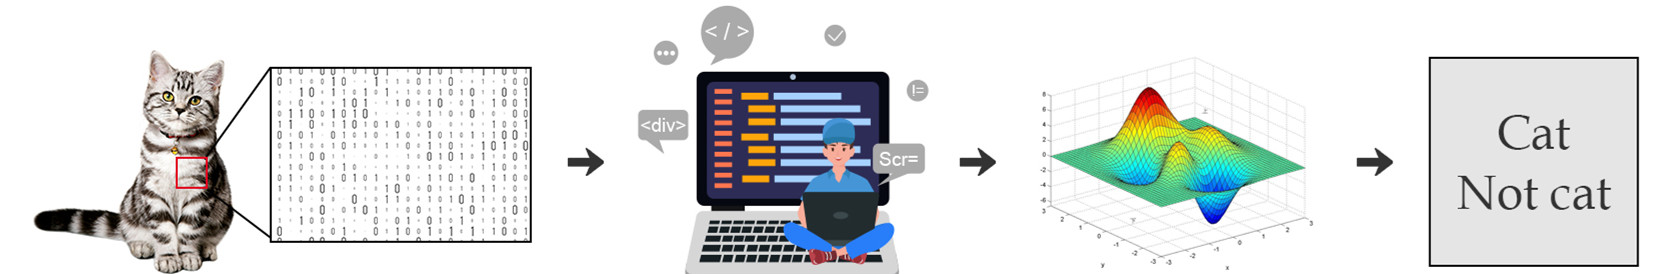
\includegraphics[scale=0.22]{./Chapter9/Figures/figure-feature-engineering.jpg}};
\node [anchor=north,minimum width=2.0em,minimum height=1.5em] (label11) at ([xshift=0.3em,yshift=2em]part1label.north) {\large{特征工程+机器学习}};
\node [anchor=north,minimum width=2.0em,minimum height=1.5em] (label12) at ([xshift=-11em,yshift=-6.3em]part1label.north) {\normalsize{输入}};
\node [anchor=north,minimum width=2.0em,minimum height=1.5em] (label13) at ([xshift=-1em,yshift=-6.3em]part1label.north) {\normalsize{特征提取}};
\node [anchor=north,minimum width=2.0em,minimum height=1.5em] (label14) at ([xshift=6.9em,yshift=-6.3em]part1label.north) {\normalsize{分类}};
\node [anchor=north,minimum width=2.0em,minimum height=1.5em] (label15) at ([xshift=14.2em,yshift=-6.3em]part1label.north) {\normalsize{输出}};
\node [anchor=north,minimum width=2.0em,minimum height=1.5em] (labela) at ([xshift=0.3em,yshift=-8.3em]part1label.north) {\small{(a)基于特征工程的机器学习方法做图像分类}};
\end{scope}
}
{
\begin{scope}[yshift=-1.9in]
\node [] (part1label2) at (0,0) {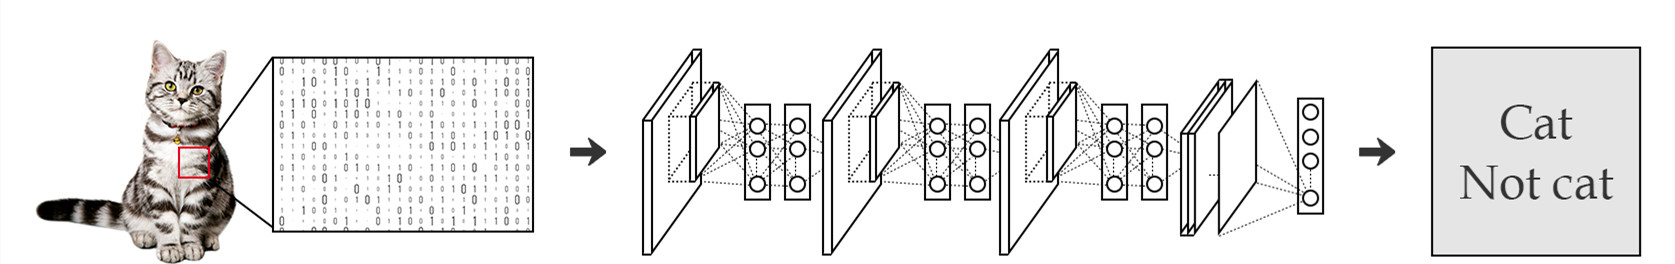
\includegraphics[scale=0.22]{./Chapter9/Figures/figure-deep-learning.jpg}};
\node [anchor=north,minimum width=2.0em,minimum height=1.5em] (label21) at ([xshift=0.2em,yshift=1.2em]part1label2.north) {\large{深度学习(端到端学习)}};
\node [anchor=north,minimum width=2.0em,minimum height=1.5em] (label22) at ([xshift=-11em,yshift=-6em]part1label2.north) {\normalsize{输入}};
\node [anchor=north,minimum width=2.0em,minimum height=1.5em] (label23) at ([xshift=3.0em,yshift=-6em]part1label2.north) {\normalsize{特征提取+分类}};
\node [anchor=north,minimum width=2.0em,minimum height=1.5em] (label24) at ([xshift=14.2em,yshift=-6em]part1label2.north) {\normalsize{输出}};
\node [anchor=north,minimum width=2.0em,minimum height=1.5em] (labelb) at ([xshift=0.3em,yshift=-8em]part1label2.north) {\small{(b)端到端学习方法做图像分类}};
\end{scope}
}
\end{tikzpicture}
%%%------------------------------------------------------------------------------------------------------------

\caption{特征工程{\small\sffamily\bfseries{vs}}端到端学习}
\label{fig:9-2}
\end{figure}
%----------------------------------------------

\parinterval 传统的机器学习需要人工定义特征,这个过程往往需要对问题的隐含假设。这种方法存在三方面的问题:

\begin{itemize}
\vspace{0.5em}
\item 特征的构造需要耗费大量的时间和精力。在传统机器学习的特征工程方法中,特征提取都是基于人力完成的,该过程往往依赖于大量的先验假设,会导致相关系统的研发周期也大大增加;
\vspace{0.5em}
\item 最终的系统性能强弱非常依赖特征的选择。有一句话在业界广泛流传:“数据和特征决定了机器学习的上限”,但是人的智力和认知是有限的,因此人工设计的特征的准确性和覆盖度会存在瓶颈;
\vspace{0.5em}
\item 通用性差。针对不同的任务,传统机器学习的特征工程方法需要选择出不同的特征,在某个任务上表现很好的特征在其他任务上可能没有效果。
\vspace{0.5em}
\end{itemize}

\parinterval 端到端学习将人们从大量的特征提取工作之中解放出来,可以不需要太多人的先验知识。从某种意义上讲,对问题的特征提取完全是自动完成的,这也意味着即使系统开发者不是该任务的“专家”也可以完成相关系统的开发。此外,端到端学习实际上也隐含了一种新的对问题的表示形式\ $\dash$分布式表示。 在这种框架下,模型的输入可以被描述为分布式的实数向量,这样模型可以有更多的维度描述一个事物,同时避免传统符号系统对客观事物离散化的刻画。比如,在自然语言处理中,表示学习重新定义了什么是词,什么是句子。在本章后面的内容中也会看到,表示学习可以让计算机对语言文字的描述更加准确和充分。

%----------------------------------------------------------------------------------------
%    NEW SUBSUB-SECTION
%----------------------------------------------------------------------------------------

\subsubsection{2. 深度学习的效果}

\parinterval 相比于传统的基于特征工程的方法,基于深度学习的模型更加方便、通用,在系统性能上也普遍更优。这里以语言建模任务为例。语言建模的目的是开发一个模型来描述词串出现的可能性(见{\chaptertwo})。这个任务已经有着很长时间的历史。表\ref{tab:9-1}给出了不同方法在常用的PTB数据集上的困惑度结果 \footnote{困惑度越低表明语言建模的效果越好。} 。传统的$ n$-gram语言模型由于面临维度灾难和数据稀疏问题,最终语言模型的性能并不是很好。而在深度学习模型中,通过引入循环神经网络等结构,所得到的语言模型可以更好地描述序列生成的问题。而最新的基于Transformer架构的语言模型将PPL从最初的178.0 下降到了惊人的35.7。可见深度学习为这个任务带来的进步是巨大的。

%----------------------------------------------------------------------------------------------------
\begin{table}[htp]
\centering
\caption{不同方法在PTB语言建模任务上的困惑度(PPL)}
\label{tab:9-1}
\small
\begin{tabular}{l | l l l}
\rule{0pt}{15pt}     模型 & 作者 & 年份 & PPL  \\
\hline
\rule{0pt}{15pt}     3-gram LM\upcite{brown1992class} & Brown et al. & 1992 & 178.0  \\
\rule{0pt}{15pt}     Feed-forward Neural LM\upcite{bengio2003a} & Bengio et al. & 2003 & 162.2  \\
\rule{0pt}{15pt}     Recurrent NN-based LM\upcite{mikolov2010recurrent} & Mikolov et al. & 2010 & 124.7  \\
\rule{0pt}{15pt}     Recurrent NN-LDA\upcite{mikolov2012context} & Mikolov et al. & 2012 & 92.0  \\
\rule{0pt}{15pt}     LSTM \upcite{zaremba2014recurrent}& Zaremba et al. & 2014 & 78.4  \\
\rule{0pt}{15pt}     RHN\upcite{zilly2016recurrent} & Zilly et al. & 2016 & 65.4  \\
\rule{0pt}{15pt}     AWD-LSTM\upcite{merity2017regularizing} & Merity et al. & 2018 & 58.8  \\
\rule{0pt}{15pt}     GPT-2 (Transformer)\upcite{radford2019language} & Radford et al. & 2019 & 35.7  \\
\end{tabular}
\end{table}
%----------------------------------------------------------------------------------------------------

%----------------------------------------------------------------------------------------
%    NEW SECTION
%----------------------------------------------------------------------------------------

\sectionnewpage
\section{神经网络基础}

\parinterval 神经网络是一种由大量的节点(或称神经元)之间相互连接构成的计算模型。那么什么是神经元?神经元之间又是如何连接的?神经网络的数学描述又是什么样的?这一节将围绕这些问题系统地对神经网络的基础知识进行介绍。

%----------------------------------------------------------------------------------------
%    NEW SUB-SECTION
%----------------------------------------------------------------------------------------

\subsection{线性代数基础} \label{sec:9.2.1}

\parinterval 线性代数作为一个数学分支,广泛应用于科学和工程中,神经网络的数学描述中也大量使用了线性代数工具。因此,这里对线性代数的一些概念进行简要介绍,以方便后续对神经网络进行数学描述。

%----------------------------------------------------------------------------------------
%    NEW SUBSUB-SECTION
%----------------------------------------------------------------------------------------

\subsubsection{1. 标量、向量和矩阵}

\vspace{-0.5em}
\parinterval {\small\sffamily\bfseries{标量}}\index{标量}(Scalar)\index{Scalar}:标量亦称“无向量”,是一种只具有数值大小而没有方向的量,通俗地说,一个标量就是一个单独的数,这里特指实数\footnote{严格意义上,标量可以是复数等其他形式。这里为了方便讨论,仅以实数为对象。}。比如,对于$ a=5 $,$ a $就是一个标量。

\parinterval {\small\sffamily\bfseries{向量}}\index{向量}(Vector)\index{Vector}:向量是由一组实数组成的有序数组。与标量不同,向量既有大小也有方向。可以把向量看作空间中的点,每个元素是不同坐标轴上的坐标。公式\eqref{eq:9-1}和公式\eqref{eq:9-2}分别展示了一个行向量和一个列向量:
\begin{eqnarray}
\mathbi{a} &=& \begin{pmatrix}
  1 & 2 & 5 & 7
\end{pmatrix}\label{eq:9-1}\\ \nonumber \\
\mathbi{a}^{\textrm T} &=& \begin{pmatrix}
    &1& \\
    &2&\\
    &5& \\
    &7&\end{pmatrix}
\label{eq:9-2}
\end{eqnarray}

\parinterval 本章默认使用行向量,如$ \mathbi{a}=(a_1, a_2, a_3) $,$ \mathbi{a} $对应的列向量记为$ \mathbi{a}^{\textrm T} $。

\parinterval {\small\sffamily\bfseries{矩阵}}\index{矩阵}(Matrix)\index{Matrix}:矩阵是一个按照长方阵列排列的实数集合,最早来自于方程组的系数及常数所构成的方阵。在计算机领域,通常将矩阵看作二维数组。这里用符号$ \mathbi{A}$表示一个矩阵,如果该矩阵有$ m $行$ n $列,那么有$\mathbi{A}\in {\mathbb R}^{m\times n} $。矩阵中的每个元素都被一个行索引和一个列索引所确定,例如,$ a_{ij} $表示第$ i $行、第$ j $列的矩阵元素。如下,公式\eqref{eq:9-3}中$ \mathbi{A} $定义了一个2行2列的矩阵。
\begin{eqnarray}
\mathbi{A}& = & \begin{pmatrix}
   a_{11} & a_{12}\\
   a_{21} & a_{22}
\end{pmatrix} \nonumber \\
& = & \begin{pmatrix}
   1 & 2\\
   3 & 4
\end{pmatrix}
\label{eq:9-3}
\end{eqnarray}

%----------------------------------------------------------------------------------------
%    NEW SUBSUB-SECTION
%----------------------------------------------------------------------------------------

\subsubsection{2. 矩阵的转置}

\parinterval {\small\sffamily\bfseries{转置}}\index{转置}(Transpose)\index{Transpose}是矩阵的重要操作之一。矩阵的转置可以看作是将矩阵以对角线为镜像进行翻转:假设$\mathbi{A}$为$ m $行$ n $列的矩阵,第$ i $行、第$ j $ 列的元素是$ a_{ij} $,即:$\mathbi{A}={(a_{ij})}_{m\times n} $,把$ m\times n $矩阵$\mathbi{A}$的行换成同序数的列得到一个$ n\times m $矩阵,则得到$ \mathbi{A}$的转置矩阵,记为${\mathbi{A}}^{\textrm T} $,且${\mathbi{A}}^{\textrm T}={(a_{ji})}_{n\times m} $。例如,对于公式\eqref{eq:9-100}中的矩阵,

\begin{eqnarray}
\mathbi{A} & = & \begin{pmatrix} 1 & 3 & 2 & 6\\5 & 4 & 8 & 2\end{pmatrix}
\label{eq:9-100}
\end{eqnarray}

\noindent 它转置的结果如公式\eqref{eq:9-101}所示

\begin{eqnarray}
{\mathbi{A}}^{\textrm T} & = &\begin{pmatrix} 1 & 5\\3 & 4\\2 & 8\\6 & 2\end{pmatrix}
\label{eq:9-101}
\end{eqnarray}

\parinterval 向量可以看作只有一行(列)的矩阵。对应地,向量的转置可以看作是只有一列(行)的矩阵。标量可以看作是只有一个元素的矩阵。因此,标量的转置等于它本身,即$ a^{\textrm T}=a $。

%----------------------------------------------------------------------------------------
%    NEW SUBSUB-SECTION
%----------------------------------------------------------------------------------------

\subsubsection{3. 矩阵加法和数乘}

\parinterval 矩阵加法又被称作{\small\sffamily\bfseries{按元素加法}}\index{按元素加法}(Element-wise Addition)\index{Element-wise Addition}。它是指两个矩阵把其相对应元素加在一起的运算,通常的矩阵加法被定义在两个形状相同的矩阵上。两个$ m\times n $矩阵$ \mathbi{A}$和$ \mathbi{B} $的和,标记为$ \mathbi{A} + \mathbi{B}$,它也是个$ m\times n $矩阵,其内的各元素为其相对应元素相加后的值,即如果矩阵$ {\mathbi{C}}= {\mathbi{A}} + {\mathbi{B}} $,则$ c_{ij} = a_{ij} + b_{ij} $。公式\eqref{eq:9-4}展示了矩阵之间进行加法的计算过程。
\begin{eqnarray}
\begin{pmatrix}
   1 & 3\\
   1 & 0\\
   1 & 2
\end{pmatrix}\;\;+\;\;\begin{pmatrix}
   0 & 0\\
   7 & 5\\
   2 & 1
\end{pmatrix}&=&\begin{pmatrix}
   1+0 & 3+0\\
   1+7 & 0+5\\
   1+2 & 2+1
\end{pmatrix}\;\;=\;\;\begin{pmatrix}
   1 & 3\\
   8 & 5\\
   3 & 3
\end{pmatrix}
\label{eq:9-4}
\end{eqnarray}

\parinterval 矩阵加法满足以下运算规律:

\begin{itemize}
\vspace{0.5em}
\item 交换律:$ {\mathbi{A}}+{\mathbi{B}} = {\mathbi{B}} +{\mathbi{A}} $。
\vspace{0.5em}
\item 结合律:$ ({\mathbi{A}}+{\mathbi{B}})+{\mathbi{C}}= {\mathbi{A}}+({\mathbi{B}}+{\mathbi{C}}) $。
\vspace{0.5em}
\item $ {\mathbi{A}}+{\mathbi{0}}={\mathbi{A}} $,其中$ {\mathbi{0}} $指的是零矩阵,即元素皆为0的矩阵。
\vspace{0.5em}
\item $ {\mathbi{A}}+(-{\mathbi{A}})={\mathbi{0}} $,其中$ -{\mathbi{A}} $是矩阵$ {\mathbi{A}} $的负矩阵,即将矩阵$ {\mathbi{A}} $的每个元素取负得到的矩阵。
\vspace{0.5em}
\end{itemize}

\parinterval 矩阵的{\small\bfnew{数乘}}\index{数乘}(Scalar Multiplication)\index{Scalar Multiplication}是指标量(实数)与矩阵的乘法运算,计算过程是将标量与矩阵的每个元素相乘,最终得到与原矩阵形状相同的矩阵。例如,矩阵$ {\mathbi{A}}={(a_{ij})}_{m\times n} $与标量$ k $进行数乘运算,其结果矩阵$ {\mathbi{B}}={(ka_{ij})}_{m\times n} $,即$ k{(a_{ij})}_{m\times n}={(ka_{ij})}_{m\times n} $。公式\eqref{eq:9-102}和\eqref{eq:9-5}展示了矩阵数乘的计算过程:
\begin{eqnarray}
{\mathbi{A}} & = &
\begin{pmatrix}
   3 & 2 & 7\\
   5 & 8 & 1
\end{pmatrix}
\label{eq:9-102}
\\ \nonumber \\
2{\mathbi{A}} & = &
\begin{pmatrix}
   6 & 4 & 14\\
   10 & 16 & 2
\end{pmatrix}
\label{eq:9-5}
\end{eqnarray}

\parinterval 矩阵的数乘满足以下运算规律,其中$ k $和$ l $是实数,$ {\mathbi{A}} $和$ {\mathbi{B}} $是形状相同的矩阵:

\begin{itemize}
\vspace{0.5em}
\item 右分配律:$ k({\mathbi{A}}+{\mathbi{B}})=k{\mathbi{A}}+k{\mathbi{B}} $。
\vspace{0.5em}
\item 左分配律:$ (k+l){\mathbi{A}}=k{\mathbi{A}}+l{\mathbi{A}}$。
\vspace{0.5em}
\item 结合律:$ (kl){\mathbi{A}}=k(l{\mathbi{A}}) $。
%\vspace{0.5em}
\end{itemize}

%----------------------------------------------------------------------------------------
%    NEW SUBSUB-SECTION
%----------------------------------------------------------------------------------------

\subsubsection{4. 矩阵乘法和矩阵点乘}

\parinterval 矩阵乘法是矩阵运算中最重要的操作之一,为了与矩阵点乘区分,通常也把矩阵乘法叫做矩阵叉乘。假设$ {\mathbi{A}} $为$ m\times p $的矩阵,$ {\mathbi{B}} $为$ p\times n $的矩阵,对$ {\mathbi{A}}$和$ {\mathbi{B}} $作矩阵乘法的结果是一个$ m\times n $的矩阵$ {\mathbi{C}} $,其中矩阵$ {\mathbi{C}} $中第$ i $行、第$ j $列的元素可以如公式\eqref{eq:9-6}表示为:
\begin{eqnarray}
{({\mathbi{A}}{\mathbi{B}})}_{ij} &=& \sum_{k=1}^p a_{ik}b_{kj}
\label{eq:9-6}
\end{eqnarray}

\parinterval 只有当第一个矩阵的列数与第二个矩阵的行数相等时,两个矩阵才可以作矩阵乘法。公式\eqref{eq:9-7}展示了矩阵乘法的运算过程,若${\mathbi{A}}=\begin{pmatrix}a_{11} & a_{12}& a_{13}\\a_{21} & a_{22} & a_{23}\end{pmatrix}$,${\mathbi{B}}=\begin{pmatrix}b_{11} & b_{12}\\b_{21} & b_{22}\\b_{31} & b_{32}\end{pmatrix} $,则有:
\vspace{-0.5em}
\begin{eqnarray}
{\mathbi{C}} & = & {\mathbi{A}}{\mathbi{B}} \nonumber \\
          & = & \begin{pmatrix}
   a_{11}b_{11}+a_{12}b_{21}+a_{13}b_{31} & a_{11}b_{12}+a_{12}b_{22}+a_{13}b_{32}\\
   a_{21}b_{11}+a_{22}b_{21}+a_{23}b_{31} & a_{21}b_{12}+a_{22}b_{22}+a_{23}b_{32}
\end{pmatrix}
\label{eq:9-7}
\end{eqnarray}

\parinterval 矩阵乘法满足以下运算规律:

\begin{itemize}
\vspace{0.5em}
\item 结合律:若${\mathbi{A}}\in {\mathbb R}^{m\times n} $,$ {\mathbi{B}}\in {\mathbb R}^{n\times p} $,${\mathbi{C}}\in {\mathbb R}^{p\times q} $,则$ ({\mathbi{A}}{\mathbi{B}}){\mathbi{C}}={\mathbi{A}}({\mathbi{B}}{\mathbi{C}}) $。
\vspace{0.5em}
\item 左分配律:若$ {\mathbi{A}}\in {\mathbb R}^{m\times n} $,$ {\mathbi{B}}\in {\mathbb R}^{m\times n} $,$ {\mathbi{C}}\in {\mathbb R}^{n\times p} $,则$ ({\mathbi{A}}+{\mathbi{B}}){\mathbi{C}}={\mathbi{A}}{\mathbi{C}}+{\mathbi{B}}{\mathbi{C}} $。
\vspace{0.5em}
\item 右分配律:若$ {\mathbi{A}}\in {\mathbb R}^{m\times n} $,$ {\mathbi{B}}\in {\mathbb R}^{n\times p} $,$ {\mathbi{C}}\in {\mathbb R}^{n\times p} $,则$ {\mathbi{A}}({\mathbi{B}}+{\mathbi{C}})={\mathbi{A}}{\mathbi{B}}+{\mathbi{A}}{\mathbi{C}} $。
\vspace{0.5em}
\end{itemize}

\begin{spacing}{1.4}
\parinterval 可以将线性方程组用矩阵乘法表示,如对于线性方程组$ \begin{cases} 5x_1+2x_2=y_1\\3x_1+x_2=y_2\end{cases} $,可以表示为$ {\mathbi{A}}{\mathbi{x}}^{\textrm T}={\mathbi{y}}^{\textrm T}$,其中$ {\mathbi{A}} = \begin{pmatrix} 5 & 2\\3 & 1\end{pmatrix} $,$ {\mathbi{x}}^{\textrm T} = \begin{pmatrix} x_1\\x_2\end{pmatrix} $,$ {\mathbi{y}}^{\textrm T} = \begin{pmatrix} y_1\\y_2\end{pmatrix} $。
\end{spacing}

\parinterval 矩阵的点乘就是两个形状相同的矩阵各个对应元素相乘,矩阵点乘也被称为{\small\bfnew{按元素乘积}}\index{按元素乘积}(Element-wise Product)\index{Element-wise Product}或Hadamard乘积,记为${\mathbi{A}}\odot {\mathbi{B}}$。例如,对于公式\eqref{eq:9-103}和公式\eqref{eq:9-104}所示的两个矩阵,
\begin{eqnarray}
{\mathbi{A}} &=&
\begin{pmatrix}
   1 & 0\\
   -1 & 3
\end{pmatrix}
\label{eq:9-103}
\\ \nonumber \\
{\mathbi{B}} &=&
\begin{pmatrix}
   3 & 1\\
   2 & 1
\end{pmatrix}
\label{eq:9-104}
\end{eqnarray}

\parinterval 矩阵点乘的计算如公式\eqref{eq:9-8}所示:
\begin{eqnarray}
{\mathbi{C}} & = & {\mathbi{A}}\odot {\mathbi{B}} \nonumber \\
          & = & \begin{pmatrix}
   1\times 3 & 0\times1\\
   -1\times2 & 3\times1
\end{pmatrix}
\label{eq:9-8}
\end{eqnarray}

%----------------------------------------------------------------------------------------
%    NEW SUBSUB-SECTION
%----------------------------------------------------------------------------------------

\subsubsection{5. 线性映射}

\parinterval {\small\sffamily\bfseries{线性映射}}\index{线性映射}( Linear Mapping)\index{Linear Mapping}或{\small\sffamily\bfseries{线性变换}}\index{线性变换}(Linear Transformation)\index{Linear Transformation}是一个向量空间V到另一个向量空间W的映射函数$ f:v\rightarrow w$,且该映射函数保持加法运算和数量乘法运算,即对于空间V中任何两个向量$ {\mathbi{u}} $ 和$ {\mathbi{v}} $以及任何标量$ c $,始终符合公式\eqref{eq:9-9}和公式\eqref{eq:9-10}:
\begin{eqnarray}
f({\mathbi{u}}+{\mathbi{v}})&=&f({\mathbi{u}})+f({\mathbi{v}})\label{eq:9-9}\\
f(c{\mathbi{v}})&=&cf({\mathbi{v}})
\label{eq:9-10}
\end{eqnarray}

\parinterval 利用矩阵$ {\mathbi{A}}\in {\mathbb R}^{m\times n} $,可以实现两个有限维欧氏空间的映射函数$f:{\mathbb R}^n\rightarrow {\mathbb R}^m$。例如$ n $维列向量$ {\mathbi{x}} ^{\textrm T}$与$ m\times n $的矩阵$ {\mathbi{A}} $,向量$ {\mathbi{x}} ^{\textrm T}$左乘矩阵$ {\mathbi{A}} $,可将向量$ {\mathbi{x}} ^{\textrm T}$映射为$ m $列向量。公式\eqref{eq:9-11}\eqref{eq:9-12}\eqref{eq:9-13}展示了一个具体的例子,
\begin{eqnarray}
{\mathbi{x}}^{\textrm{T}} & = & {\begin{pmatrix} x_1\\ x_2 \\  \dots  \\ x_n \end{pmatrix}}
\label{eq:9-11}
\end{eqnarray}

\begin{eqnarray}
{\mathbi{A}}&=&
\begin{pmatrix}
   a_{11} & a_{12} & \dots & a_{1n}\\
   a_{21} & \dots & \dots & \dots \\
   \dots & \dots & \dots & \dots \\
   a_{m1} & \dots & \dots & a_{mn}
\end{pmatrix}
\label{eq:9-12}
\end{eqnarray}

\parinterval 可以得到:
\begin{eqnarray}
{\mathbi{y}}^{\textrm{T}}& = &{\mathbi{A}}{\mathbi{x}}^{\textrm{T}} \nonumber \\
               & = &
\begin{pmatrix}
   a_{11}x_{1}+a_{12}x_{2}+\dots+a_{1n}x_{n}\\
   a_{21}x_{1}+a_{22}x_{2}+\dots+a_{2n}x_{n}\\
   \vdots \\
   a_{m1}x_{1}+a_{m2}x_{2}+\dots+a_{mn}x_{n}
\label{eq:9-13}\end{pmatrix}
\end{eqnarray}

\parinterval 上例中矩阵$ {\mathbi{A}} $定义了一个从$ {\mathbb R}^n $到$ {\mathbb R}^m $的线性映射:向量$ {\mathbi{x}}^{\textrm{T}}\in {\mathbb R}^n $和$ {\mathbi{y}}^{\textrm{T}}\in {\mathbb R}^m $分别为两个空间中的列向量,即大小为$ n\times 1 $ 和$ m\times 1 $ 的矩阵。

%----------------------------------------------------------------------------------------
%    NEW SUBSUB-SECTION
%----------------------------------------------------------------------------------------

\subsubsection{6. 范数}

\parinterval 工程领域,经常会使用被称为{\small\bfnew{范数}}\index{范数}(Norm)\index{Norm}的函数衡量向量大小,范数为向量空间内的所有向量赋予非零的正长度或大小。对于一个$n$维向量$ {\mathbi{x}} $,一个常见的范数函数为$ l_p $ 范数,通常表示为$ {\Vert{\mathbi{x}}\Vert}_p $ ,其中$p\ge 0$,是一个标量形式的参数。常用的$ p $的取值有$ 1 $、$ 2 $、$ \infty $等。范数的计算方式如公式\eqref{eq:9-14}所示:
\begin{eqnarray}
l_p({\mathbi{x}}) & = & {\Vert{\mathbi{x}}\Vert}_p \nonumber \\
               & = & {\left (\sum_{i=1}^{n}{{\vert x_{i}\vert}^p}\right )}^{\frac{1}{p}}
\label{eq:9-14}
\end{eqnarray}

\parinterval $ l_1 $范数为向量的各个元素的绝对值之和,如公式\eqref{eq:9-15}所示:
\begin{eqnarray}
{\Vert{\mathbi{x}}\Vert}_1&=&\sum_{i=1}^{n}{\vert x_{i}\vert}
\label{eq:9-15}
\end{eqnarray}

\parinterval $ l_2 $范数为向量的各个元素平方和的二分之一次方,如公式\eqref{eq:9-16}所示:
\begin{eqnarray}
{\Vert{\mathbi{x}}\Vert}_2&=&\sqrt{\sum_{i=1}^{n}{{x_{i}}^2}} \nonumber \\
                                      &=&\sqrt{{\mathbi{x}}^{\textrm T}{\mathbi{x}}}
\label{eq:9-16}
\end{eqnarray}

\parinterval $ l_2 $范数被称为{\small\bfnew{欧几里得范数}}\index{欧几里得范数}(Euclidean Norm)\index{Euclidean Norm}。从几何角度,向量也可以表示为从原点出发的一个带箭头的有向线段,其$ l_2 $范数为线段的长度,也常被称为向量的模。$ l_2 $ 范数在机器学习中非常常用。向量$ {\mathbi{x}} $的$ l_2 $范数经常简化表示为$ \Vert{\mathbi{x}}\Vert $,可以通过点积$ {\mathbi{x}}^{\textrm T}{\mathbi{x}} $进行计算。

\parinterval $ l_{\infty} $范数为向量的各个元素的最大绝对值,如公式\eqref{eq:9-17}所示:
\begin{eqnarray}
{\Vert{\mathbi{x}}\Vert}_{\infty}&=&{\textrm{max}}\{x_1,x_2,\dots,x_n\}
\label{eq:9-17}
\end{eqnarray}

\parinterval 广义上讲,范数是将向量映射到非负值的函数,其作用是衡量向量$ {\mathbi{x}} $到坐标原点的距离。更严格的说,范数并不拘于$ l_p $范数,任何一个同时满足下列性质的函数都可以作为范数:

\begin{itemize}
\vspace{0.5em}
\item 若$ f({\mathbi{x}})=0 $,则$ {\mathbi{x}}={\mathbi{0}} $。
\vspace{0.5em}
\item 三角不等式:$ f({\mathbi{x}}+{\mathbi{y}})\leqslant f({\mathbi{x}})+f({\mathbi{y}}) $。
\vspace{0.5em}
\item 任意实数$ \alpha $,$ f(\alpha {\mathbi{x}})=\vert \alpha \vert f({\mathbi{x}}) $。
\vspace{0.5em}
\end{itemize}

\parinterval 在深度学习中,有时候希望衡量矩阵的大小,这时可以考虑使用 {\small\bfnew{Frobenius 范数}}\index{Frobenius 范数}(Frobenius Norm)\index{Frobenius Norm}。公式\eqref{eq:9-18}展示了其计算方式:
\begin{eqnarray}
{\Vert{\mathbi{A}}\Vert}_F&=&\sqrt{\sum_{i,j} a_{i,j}^2}
\label{eq:9-18}
\end{eqnarray}

%----------------------------------------------------------------------------------------
%    NEW SUB-SECTION
%----------------------------------------------------------------------------------------
\subsection{人工神经元和感知机}

\parinterval 生物学中,神经元是神经系统的基本组成单元。同样,人工神经元是人工神经网络的基本单元。在人们的想象中,人工神经元应该与生物神经元类似。但事实上,二者在形态上是有明显差别的。如图\ref{fig:9-4} 是一个典型的人工神经元,其本质是一个形似$ y=f({\mathbi{x}}\cdot {\mathbi{w}}+b) $的函数。显而易见,一个神经元主要由$ {\mathbi{x}} $,$ {\mathbi{w}} $,$ b $,$ f $四个部分构成。其中$ {\mathbi{x}} $是一个形如$ (x_1,x_2,\dots,x_n) $ 的实数向量,在一个神经元中担任“输入”的角色。$ {\mathbi{w}} $通常被理解为神经元连接的{\small\sffamily\bfseries{权重}}\index{权重}(Weight)\index{Weight}(对于一个人工神经元,权重是一个向量,表示为$ {\mathbi{w}} $;对于由多个神经元组成的神经网络,权重是一个矩阵,表示为$ {\mathbi{W}} $),其中的每一个元素都对应着一个输入和一个输出,代表着“某输入对某输出的贡献程度”。$ b $被称作偏置(对于一个人工神经元,偏置是一个实数,表示为$b$;对于神经网络中的某一层,偏置是一个向量,表示为${\mathbi{b}}$)。$ f $被称作激活函数,用于对输入向量各项加权和后进行某种变换。可见,一个人工神经元的功能是将输入向量与权重矩阵右乘(做内积)后,加上偏置量,经过一个激活函数得到一个标量结果。

%----------------------------------------------
\begin{figure}[htp]
\centering
%%%------------------------------------------------------------------------------------------------------------
\begin{tikzpicture}
\begin{scope}
\node [anchor=center,circle,draw,ublue,very thick,minimum size=3.5em,fill=white,drop shadow={shadow xshift=0.1em,shadow yshift=-0.1em}] (neuron) at (0,0) {};
\node [anchor=east] (x1) at ([xshift=-6em]neuron.west) {\Large{$x_2$}};
\node [anchor=center] (x0) at ([yshift=3em]x1.center) {\Large{$x_1$}};
\node [anchor=center] (x2) at ([yshift=-3em]x1.center) {\Large{$b$}};
\node [anchor=west] (y) at ([xshift=6em]neuron.east) {\Large{$y$}};
\node [anchor=center] (neuronmath) at (neuron.center) {\Large{$f$}};

\draw [->,thick] (x0.east) -- (neuron.150) node [pos=0.5,above] {$w_1$};
\draw [->,thick] (x1.east) -- (neuron.180) node [pos=0.5,above] {$w_2$};
\draw [->,thick] (x2.east) -- (neuron.210) node [pos=0.5,above] {$$};
\draw [->,thick] (neuron.east) -- (y.west);

\end{scope}
\end{tikzpicture}
%
%%%------------------------------------------------------------------------------------------------------------


\caption{人工神经元}
\label{fig:9-4}
\end{figure}
%----------------------------------------------

%----------------------------------------------------------------------------------------
%    NEW SUBSUB-SECTION
%----------------------------------------------------------------------------------------

\vspace{-0.5em}
\subsubsection{1. 感知机\ \dash \ 最简单的人工神经元模型}

\vspace{0.5em}
\parinterval 感知机是人工神经元的一种实例,在上世纪50-60年代被提出后,对神经网络研究产生了深远的影响。感知机模型如图\ref {fig:9-5}所示,其输入是一个$n$维二值向量$ {\mathbi{x}}=(x_1,x_2,\dots,x_n) $,其中$ x_i=0 $或$ 1 $。权重${\mathbi{w}}=(w_1,w_2,\dots,w_n) $,每个输入变量对应一个权重$ w_i $。偏置$ b $是一个实数变量($ -\sigma $)。输出也是一个二值结果,即$ y=0 $或$ 1 $。$ y $值的判定由输入的加权和是否大于(或小于)一个阈值$ \sigma $决定(公式\eqref{eq:9-19}):
\begin{eqnarray}
y=\begin{cases} 0 & \sum_{i}{x_i\cdot w_i}-\sigma <0\\1 & \sum_{i}{x_i\cdot w_i}-\sigma \geqslant 0\end{cases}
\label{eq:9-19}
\end{eqnarray}

%----------------------------------------------
\begin{figure}[htp]
\centering
%%%------------------------------------------------------------------------------------------------------------
 \begin{tikzpicture}
\begin{scope}
\node [anchor=center,circle,draw,ublue,very thick,minimum size=3.5em,fill=white,drop shadow={shadow xshift=0.1em,shadow yshift=-0.1em}] (neuron) at (0,0) {};
\node [anchor=east] (x1) at ([xshift=-6em]neuron.west) {\Large{$x_2$}};
\node [anchor=center] (x0) at ([yshift=3em]x1.center) {\Large{$x_1$}};
\node [anchor=center] (x2) at ([yshift=-3em]x1.center) {\Large{$x_3$}};
\node [anchor=west] (y) at ([xshift=6em]neuron.east) {\Large{$y$}};
\node [anchor=center] (neuronmath) at (neuron.center) {\small{$\sum \ge \sigma$}};

\draw [->,thick] (x0.east) -- (neuron.150) node [pos=0.5,above] {$w_1$};
\draw [->,thick] (x1.east) -- (neuron.180) node [pos=0.5,above] {$w_2$};
\draw [->,thick] (x2.east) -- (neuron.210) node [pos=0.5,above] {$w_3$};
\draw [->,thick] (neuron.east) -- (y.west);

\end{scope}
\end{tikzpicture}
%%%------------------------------------------------------------------------------------------------------------


\caption{感知机模型}
\label{fig:9-5}
\end{figure}
%-------------------------------------------

\parinterval 感知机可以做一些简单的决策。举一个非常简单的例子,有一场音乐会,你正在纠结是否去参加,有三个因素会影响你的决定:

\begin{itemize}
\vspace{0.5em}
\item $ x_1 $:剧场是否离你足够近(是,则$ x_1=1 $;否则$ x_1=0 $);
\vspace{0.5em}
\item $ x_2 $:票价是否低于300元(是,则$ x_2=1 $;否则$ x_2=0 $);
\vspace{0.5em}
\item $ x_3 $:女朋友是否喜欢音乐会(是,则$ x_3=1 $;否则$ x_3=0 $)。
\vspace{0.5em}
\end{itemize}

\parinterval 在这种情况下应该如何做出决定呢?比如,女朋友很希望和你一起去看音乐会,但是剧场很远而且票价500元,如果这些因素对你都是同等重要的(即$ w_1=w_2=w_3 $,假设这三个权重都设置为1)那么会得到一个综合得分,如公式\eqref{eq:9-20}所示:
\begin{eqnarray}
x_1\cdot w_1+x_2\cdot w_2+x_3\cdot w_3 & = & 0\cdot 1+0\cdot 1+1\cdot 1 \nonumber \\
                                                                     & = & 1
\label{eq:9-20}
\end{eqnarray}

\parinterval 如果你不是十分纠结的人,能够接受不完美的事情,你可能会把$ \sigma $设置为1,于是$ \sum{w_i\cdot x_i}-\sigma \ge 0 $,那么你会去音乐会。可以看出,上面的例子的本质就是一个如图\ref{fig:9-6}所示的感知机:

%----------------------------------------------
\begin{figure}[htp]
\centering
%%%------------------------------------------------------------------------------------------------------------
 \begin{tikzpicture}
\begin{scope}
\node [anchor=center,circle,draw,ublue,very thick,minimum size=3.5em,fill=white,drop shadow={shadow xshift=0.1em,shadow yshift=-0.1em}] (neuron) at (0,0) {};
\node [anchor=east] (x1) at ([xshift=-6em]neuron.west) {$x_2$:票价够低?};
\node [anchor=center] (x0) at ([yshift=3em]x1.center) {$x_1$:距离够近?};
\node [anchor=center] (x2) at ([yshift=-3em]x1.center) {$x_3$:女友喜欢?};
\node [anchor=west] (y) at ([xshift=2em]neuron.east) {$y$:去?还是不去?};

{
\draw [->,thick] (x0.east) -- (neuron.150) node [pos=0.5,above,yshift=0.2em] {\small{$w_1=1$}};
\draw [->,thick] (x1.east) -- (neuron.180) node [pos=0.5,above,yshift=-0.1em] {\small{$w_2=1$}};
\draw [->,thick] (x2.east) -- (neuron.210) node [pos=0.5,above,yshift=0.1em] {\small{$w_3=1$}};
}
\draw [->,thick] (neuron.east) -- (y.west);

\node [anchor=center] (neuronmath) at (neuron.center) {\small{$\sum \ge \sigma$}};

\end{scope}
\end{tikzpicture}
%%%------------------------------------------------------------------------------------------------------------



\caption{预测是否去剧场的感知机(权重相同)}
\label{fig:9-6}
\end{figure}
%-------------------------------------------

%----------------------------------------------------------------------------------------
%    NEW SUBSUB-SECTION
%----------------------------------------------------------------------------------------

\vspace{-1em}
\subsubsection{2. 神经元内部权重}

\parinterval 在上面的例子中,连接权重代表着每个输入因素对最终输出结果的重要程度,为了得到令人满意的决策,需要不断调整权重。如果你是守财奴,则会对票价看得更重一些,这样你会用不均匀的权重计算每个因素的影响,比如:$ w_1=0.5 $,$ w_2=2 $,$ w_3=0.5 $,此时感知机模型如图\ref{fig:9-7}所示。在这种情况下,女友很希望和你一起去看音乐会,但是剧场很远而且票价500元,会导致你不去看音乐会,公式\eqref{eq:9-21}展示了该决策过程:
\begin{eqnarray}
\sum_{i}{x_i\cdot w_i} & = & 0\cdot 0.5+0\cdot 2+1\cdot 0.5 \nonumber \\
                                   & = & 0.5 \nonumber \\
                                   & < & \sigma = 1
\label{eq:9-21}
\end{eqnarray}

%----------------------------------------------
\begin{figure}[htp]
\centering
%%%------------------------------------------------------------------------------------------------------------
\begin{tikzpicture}
\begin{scope}
\node [anchor=center,circle,draw,ublue,very thick,minimum size=3.5em,fill=white,drop shadow={shadow xshift=0.1em,shadow yshift=-0.1em}] (neuron) at (0,0) {};
\node [anchor=east] (x1) at ([xshift=-6em]neuron.west) {$x_2$:票价够低?};
\node [anchor=center] (x0) at ([yshift=3em]x1.center) {$x_1$:距离够近?};
\node [anchor=center] (x2) at ([yshift=-3em]x1.center) {$x_3$:女友喜欢?};
\node [anchor=west] (y) at ([xshift=2em]neuron.east) {$y$:去?还是不去?};


\draw [->,thin] (x0.east) -- (neuron.150) node [pos=0.5,above,yshift=0.2em] {\small{$w_1=.5$}};
\draw [->,line width=0.5mm] (x1.east) -- (neuron.180) node [pos=0.5,above,yshift=-0.1em] {\textbf{\small{$w_2=2$}}};
\draw [->,thin] (x2.east) -- (neuron.210) node [pos=0.5,above,yshift=0.1em] {\small{$w_3=.5$}};
\draw [->,thick] (neuron.east) -- (y.west);

\node [anchor=center] (neuronmath) at (neuron.center) {\small{$\sum \ge \sigma$}};
\node [anchor=south] (ylabel) at (y.north) {\textbf{}};


\end{scope}
\end{tikzpicture}
%%%------------------------------------------------------------------------------------------------------------



\caption{预测是否去剧场的感知机(权重不同)}
\label{fig:9-7}
\end{figure}
%-------------------------------------------

\parinterval 当然,结果是女友对这个决定非常不满意。

%----------------------------------------------------------------------------------------
%    NEW SUBSUB-SECTION
%----------------------------------------------------------------------------------------

\subsubsection{3. 神经元的输入\ \dash \ 离散 vs 连续}

\parinterval 在受到了女友“批评教育”之后,你意识到决策考虑的因素(即输入)不应该只是非0即1,而应该把“程度”考虑进来,于是你改变了三个输入的形式:

\parinterval $ x_1 $:10/距离(km)

\parinterval $ x_2 $:150/票价(元)

\parinterval $ x_3 $:女朋友是否喜欢

\parinterval 在新修改的模型中,$ x_0 $和$ x_1 $变成了连续变量,$ x_2 $仍然是离散变量,如图\ref{fig:9-8}所示。

%----------------------------------------------
\begin{figure}[htp]
\centering
%%%------------------------------------------------------------------------------------------------------------
\begin{tikzpicture}

\begin{scope}
\draw [->,thick] (0,0) -- (3.1,0);
\draw [->,thick] (0,0) -- (0, 2.1);
\draw [-,very thick,ublue,domain=0.55:2.6,samples=100] plot (\x,{ 1/\x - 0.2});
\node [anchor=east] (ylabel) at (0, 4.4em) {\footnotesize{$x_1$}};
\node [anchor=north] (xlabel) at (6.5em, 0em) {\scriptsize{距离(km)}};
\end{scope}

\begin{scope}[xshift=12em]
\draw [->,thick] (0,0) -- (3.1,0);
\draw [->,thick] (0,0) -- (0, 2.1);
\draw [-,very thick,ublue,domain=0.3:2.6,samples=100] plot (\x,{ 0.5/\x});
\node [anchor=east] (ylabel) at (0, 4.4em) {\footnotesize{$x_2$}};
\node [anchor=north] (xlabel) at (6.5em, 0em) {\scriptsize{票价(元)}};
\end{scope}

\begin{scope}[xshift=24em]
\draw [->,thick] (0,0) -- (3.1,0);
\draw [->,thick] (0,0) -- (0, 2.1);
\node [anchor=east] (ylabel) at (0, 4.4em) {\footnotesize{$x_3$}};
\node [anchor=south, fill=ublue, minimum width=1.5em, minimum height=0.1em, inner sep=0] (histogram1) at (1.5em, 0) {};
\node [anchor=south, fill=ublue, minimum width=1.5em, minimum height=3em, inner sep=0] (histogram2) at (4.0em, 0) {};
\node [anchor=north] (hlabel1) at (histogram1.south) {\tiny{不喜欢}};
\node [anchor=north] (hlabel2) at (histogram2.south) {\tiny{喜欢}};
\node [anchor=north] (xlabel) at (6.5em, 0em) {\scriptsize{是否喜欢}};
\end{scope}

\end{tikzpicture}
%%%------------------------------------------------------------------------------------------------------------



\caption{神经元输入的不同形式}
\label{fig:9-8}
\end{figure}
%-------------------------------------------

\parinterval 使用修改后的模型做决策:女朋友很希望和你一起,但是剧场有20km远而且票价有500元。于是有$ x_1=10/20 $,$ x_2=150/500 $,$ x_3=1 $。此时决策过程如公式\eqref{eq:9-22}所示:
\begin{eqnarray}
\sum_{i}{x_i\cdot w_i} & = & 0.5\cdot 0.5+0.3\cdot 2+1\cdot 0.5 \nonumber \\
                                   & = & 1.35 \nonumber \\
                                   & > & \sigma =1
\label{eq:9-22}
\end{eqnarray}

\parinterval 虽然剧场很远,价格有点贵,但是女友很满意,你还是很高兴。

%----------------------------------------------------------------------------------------
%    NEW SUBSUB-SECTION
%----------------------------------------------------------------------------------------

\subsubsection{4. 神经元内部的参数学习}

\parinterval 一次成功的音乐会之后,你似乎掌握了一个真理:其他什么都不重要,女友的喜好最重要,所以你又将决策模型的权重做出了调整:最简单的方式就是$ w_1=w_2=0 $,同时令$ w_3>0 $,相当于只考虑$ x_3 $的影响而忽略其他因素,于是你得到了如图\ref {fig:9-9}所示的决策模型:

%----------------------------------------------
\begin{figure}[htp]
\centering
%%%------------------------------------------------------------------------------------------------------------
\begin{tikzpicture}
\begin{scope}
\node [anchor=center,circle,draw,ublue,very thick,minimum size=3.5em,fill=white,drop shadow={shadow xshift=0.1em,shadow yshift=-0.1em}] (neuron) at (0,0) {};
\node [anchor=east] (x1) at ([xshift=-6em]neuron.west) {$x_2$:便宜程度\ \ \ \ };
\node [anchor=center] (x0) at ([yshift=3em]x1.center) {$x_1$:远近程度\ \ \ \ };
\node [anchor=center] (x2) at ([yshift=-3em]x1.center) {$x_3$:女友喜欢?};
\node [anchor=west] (y) at ([xshift=2em]neuron.east) {$y$:去?还是不去?};

\draw [->,thick] (neuron.east) -- (y.west);

\node [anchor=center] (neuronmath) at (neuron.center) {\small{$\sum \ge \sigma$}};

{
\draw [->,dotted] (x0.east) -- (neuron.150) node [pos=0.46,above,yshift=0.2em] {\small{$w_1=0$}};
\draw [->,dotted] (x1.east) -- (neuron.180) node [pos=0.46,above,yshift=-0.1em] {\textbf{\small{$w_2=0$}}};
\draw [->,line width=0.5mm] (x2.east) -- (neuron.210) node [pos=0.5,above,yshift=0.1em] {\small{$w_3=10$}};
}


\end{scope}
\end{tikzpicture}
%%%------------------------------------------------------------------------------------------------------------



\caption{预测是否去剧场的决策模型(只考虑女友喜好)}
\label{fig:9-9}
\end{figure}
%-------------------------------------------

\parinterval 很快又有了一场音乐会,距你1000公里,票价3000元,当然女友是一直喜欢音乐会的。根据新的决策模型,你义无反顾地选择去看音乐会。然而,女友又不高兴了,喜欢浪漫的女友觉得去看这场音乐会太奢侈了。在这几次看音乐会的经历中,你发现每个因素的权重需要准确地设置才能达到最好的决策效果。

\parinterval 那么如何确定最好的权重的?方法其实很简单,不断地尝试,根据结果不断地调整权重。在经过成百上千次的尝试之后,终于找到了一组合适的权重,使每次决策的正确率都很高。上面这个过程就类似于参数训练的过程,利用大量的数据来模拟成百上千次的尝试,根据输出的结果来不断地调整权重。

\parinterval 可以看到,在“是否参加音乐会”这个实际问题中,主要涉及到三方面的问题:

\begin{itemize}
\vspace{0.5em}
\item 对问题建模,即定义输入$ \{x_i\} $的形式;
\vspace{0.5em}
\item 设计有效的决策模型,即定义$ y $;
\vspace{0.5em}
\item 得到模型参数(如权重$ \{w_i\} $)的最优值。
\vspace{0.5em}
\end{itemize}

\parinterval 上面的例子对这三个问题都简要地做出了回答。下面的内容将继续对它们进行详细阐述。

%----------------------------------------------------------------------------------------
%    NEW SUB-SECTION
%----------------------------------------------------------------------------------------

\subsection{多层神经网络}

\parinterval 感知机是一种最简单的单层神经网络。一个很自然的问题是:能否把多个这样的网络叠加在一起,获得建模更复杂问题的能力?如果可以,那么在多层神经网络的每一层,神经元之间是怎么组织、工作的呢?单层网络又是通过什么方式构造成多层的呢?

%----------------------------------------------------------------------------------------
%    NEW SUBSUB-SECTION
%----------------------------------------------------------------------------------------

\subsubsection{1. 线性变换和激活函数}

\parinterval 为了建立多层神经网络,首先需要把前面提到的简单的神经元进行扩展,把多个神经元组成一“层”神经元。比如,很多实际问题需要同时有多个输出,这时可以把多个相同的神经元并列起来,每个神经元都会有一个单独的输出,这就构成一“层”,形成了单层神经网络。单层神经网络中的每一个神经元都对应着一组权重和一个输出,可以把单层神经网络中的不同输出看作一个事物不同角度的描述。


\parinterval 举个简单的例子,预报天气时,往往需要预测温度、湿度和风力,这就意味着如果使用单层神经网络进行预测,需要设置3个神经元。如图\ref{fig:9-10}所示,此时权重矩阵如公式\eqref{eq:9-105}所示:

\begin{eqnarray}
{\mathbi{W}}=\begin{pmatrix} w_{11} & w_{12} & w_{13}\\ w_{21} & w_{22} & w_{23}\end{pmatrix}
\label{eq:9-105}
\end{eqnarray}

%----------------------------------------------
\begin{figure}[htp]
\centering
%%%------------------------------------------------------------------------------------------------------------
\begin{tikzpicture}
\begin{scope}

\tikzstyle{neuronnode} = [minimum size=1.5em,circle,draw,ublue,very thick,fill=white,drop shadow={shadow xshift=0.1em,shadow yshift=-0.1em}]

\node [anchor=center,neuronnode] (neuron00) at (0,0) {};
\node [anchor=center,neuronnode] (neuron01) at ([yshift=-3em]neuron00) {};
\node [anchor=center,neuronnode] (neuron02) at ([yshift=-3em]neuron01) {};

\node [anchor=east] (x0) at ([xshift=-6em]neuron00.west) {$x_1$};
\node [anchor=east] (x1) at ([xshift=-6em]neuron01.west) {$x_2$};
\node [anchor=east] (x2) at ([xshift=-6em]neuron02.west) {$\mathbi{b}$};

\node [anchor=west] (y0) at ([xshift=4em]neuron00.east) {$y_1$:\scriptsize{温度}};

\draw [->,red!50,line width=0.4mm] (x0.east) -- (neuron00.180) node [pos=0.1,above] {\tiny{$w_{11}$}};
\draw [->,red!50,line width=0.4mm] (x1.east) -- (neuron00.200) node [pos=0.1,above] {\tiny{$w_{21}$}};
\draw [->,red!50,line width=0.4mm] (x2.east) -- (neuron00.220) node [pos=0.05,above,yshift=0.3em] {\tiny{$b_{1}$}};
\draw [->,red!30,line width=0.4mm] (neuron00.east) -- (y0.west);

\node [anchor=west] (y1) at ([xshift=4em]neuron01.east) {$y_2$:\scriptsize{湿度}};

\draw [->,blue!50,line width=0.4mm] (x0.east) -- (neuron01.160) node [pos=0.4,above] {\tiny{$w_{12}$}};
\draw [->,blue!50,line width=0.4mm] (x1.east) -- (neuron01.180) node [pos=0.35,above,yshift=-0.2em] {\tiny{$w_{22}$}};
\draw [->,blue!50,line width=0.4mm] (x2.east) -- (neuron01.200) node [pos=0.3,below,yshift=0.2em] {\tiny{$b_{2}$}};
\draw [->,blue!30,line width=0.4mm] (neuron01.east) -- (y1.west);

\node [anchor=west] (y2) at ([xshift=4em]neuron02.east) {$y_3$:\scriptsize{风力}};

\draw [->,ugreen!50,line width=0.4mm] (x0.east) -- (neuron02.140) node [pos=0.1,below,yshift=-0.2em] {\tiny{$w_{13}$}};
\draw [->,ugreen!50,line width=0.4mm] (x1.east) -- (neuron02.160) node [pos=0.1,below] {\tiny{$w_{23}$}};
\draw [->,ugreen!50,line width=0.4mm] (x2.east) -- (neuron02.180) node [pos=0.3,below] {\tiny{$b_{3}$}};
\draw [->,ugreen!30,line width=0.4mm] (neuron02.east) -- (y2.west);

\end{scope}
\end{tikzpicture}



%%%------------------------------------------------------------------------------------------------------------


\caption{权重矩阵中的元素与输出的对应关系}
\label{fig:9-10}
\end{figure}
%-------------------------------------------

\noindent 它的第一列元素$ \begin{pmatrix} w_{11}\\ w_{21}\end{pmatrix} $是输入相对第一个输出$ y_1 $ 的权重,参数向量$ {\mathbi{b}}=(b_1,b_2,b_3) $的第一个元素$ b_1 $是对应于第一个输出$ y_1 $ 的偏置量;类似的,可以得到$ y_2 $和$ y_3 $。预测天气的单层模型如图\ref{fig:9-11}所示(在本例中,假设输入$ {\mathbi{x}}=(x_1,x_2) $)。

%----------------------------------------------
\begin{figure}[htp]
\centering
%%%------------------------------------------------------------------------------------------------------------
\begin{tikzpicture}
\begin{scope}

\tikzstyle{neuronnode} = [minimum size=1.5em,circle,draw,ublue,very thick,fill=white,drop shadow={shadow xshift=0.1em,shadow yshift=-0.1em}]

\node [anchor=center,neuronnode] (neuron00) at (0,0) {};
\node [anchor=center,neuronnode] (neuron01) at ([yshift=-3em]neuron00) {};
\node [anchor=center,neuronnode] (neuron02) at ([yshift=-3em]neuron01) {};
\node [anchor=east] (x0) at ([xshift=-6em]neuron00.west) {$x_1$};
\node [anchor=east] (x1) at ([xshift=-6em]neuron01.west) {$x_2$};
\node [anchor=east] (x2) at ([xshift=-6em]neuron02.west) {$\mathbi{b}$};
\node [anchor=west] (y0) at ([xshift=4em]neuron00.east) {$y_1$};

\draw [->] (x0.east) -- (neuron00.180) node [pos=0.1,above] {\tiny{$w_{11}$}};
\draw [->] (x1.east) -- (neuron00.200) node [pos=0.1,above] {\tiny{$w_{21}$}};
\draw [->] (x2.east) -- (neuron00.220) node [pos=0.05,above,yshift=0.3em] {\tiny{$b_{1}$}};
\draw [->] (neuron00.east) -- (y0.west);

\node [anchor=west] (y1) at ([xshift=4em]neuron01.east) {$y_2$};
\draw [->] (x0.east) -- (neuron01.160) node [pos=0.4,above] {\tiny{$w_{12}$}};
\draw [->] (x1.east) -- (neuron01.180) node [pos=0.35,above,yshift=-0.2em] {\tiny{$w_{22}$}};
\draw [->] (x2.east) -- (neuron01.200) node [pos=0.3,below,yshift=0.2em] {\tiny{$b_{2}$}};
\draw [->] (neuron01.east) -- (y1.west);

\node [anchor=west] (y2) at ([xshift=4em]neuron02.east) {$y_3$};
\draw [->] (x0.east) -- (neuron02.140) node [pos=0.1,below,yshift=-0.2em] {\tiny{$w_{13}$}};
\draw [->] (x1.east) -- (neuron02.160) node [pos=0.1,below] {\tiny{$w_{23}$}};
\draw [->] (x2.east) -- (neuron02.180) node [pos=0.3,below] {\tiny{$b_{3}$}};
\draw [->] (neuron02.east) -- (y2.west);

\node [anchor=east,align=left] (inputlabel) at ([xshift=-0.1em]x1.west) {\scriptsize{输入向量}:\\\small{$\mathbi{x}=(x_1,x_2)$}};


\node [anchor=west,align=left] (outputlabel) at ([xshift=0.1em]y1.east) {\scriptsize{输出向量}:\\\small{$\mathbi{y}=(y_1,y_2,y_3)$}};


\begin{pgfonlayer}{background}

\node [rectangle,inner sep=0.4em,fill=red!20] [fit = (neuron00) (neuron01) (neuron02)] (layer) {};
\node [anchor=south] (layerlabel) at ([yshift=0.2em]layer.north) {\scriptsize{一层神经元}};



\node [rectangle,inner sep=0.1em,fill=ugreen!20] [fit = (x0) (x1)] (inputshadow) {};


\node [rectangle,inner sep=0.1em,fill=blue!20] [fit = (y0) (y1) (y2)] (outputshadow) {};

\end{pgfonlayer}



\end{scope}
\end{tikzpicture}
%%%------------------------------------------------------------------------------------------------------------


\caption{预测天气的单层神经网络}
\label{fig:9-11}
\end{figure}
%-------------------------------------------

\parinterval 在神经网络中,对于输入向量$ {\mathbi{x}}\in {\mathbb R}^m $,一层神经网络首先将其经过线性变换映射到$ {\mathbb R}^n $,再经过激活函数变成${\mathbi{y}}\in {\mathbb R}^n $。还是上面天气预测的例子,每个神经元获得相同的输入,权重矩阵$ {\mathbi{W}} $是一个$ 2\times 3 $矩阵,矩阵中每个元素$ w_{ij} $代表第$ j $个神经元中$ x_{i} $对应的权重值,假设编号为1的神经元负责预测温度,则$ w_{i1} $含义为预测温度时,输入$ x_{i} $对其影响程度。此外所有神经元的偏置$ b_{1} $,$ b_{2} $,$ b_{3} $组成了最终的偏置向量$ {\mathbi{b}}$。在该例中则有,权重矩阵$ {\mathbi{W}}=\begin{pmatrix} w_{11} & w_{12} & w_{13}\\ w_{21} & w_{22} & w_{23}\end{pmatrix} $,偏置向量$ {\mathbi{b}}=(b_1,b_2,b_3) $。

\parinterval 那么,线性变换的本质是什么?

\begin{itemize}
\vspace{0.5em}
\item 从代数角度看,对于线性空间$ \textrm V $,任意$ {\mathbi{a}}$,${\mathbi{a}}\in {\textrm V} $和数域中的任意$ \alpha $,线性变换$ T(\cdot) $需满足:$ T({\mathbi{a}}+{\mathbi{b}})=T({\mathbi{a}})+T({\mathbi{b}}) $,且$ T(\alpha {\mathbi{a}})=\alpha T({\mathbi{a}}) $;
\vspace{0.5em}
\item 从几何角度看,公式中的${\mathbi{x}}\cdot {\mathbi{W}}+{\mathbi{b}}$将${\mathbi{x}}$右乘${\mathbi{W}}$相当于对$ {\mathbi{x}} $进行旋转变换。例如,对三个点$ (0,0) $,$ (0,1) $,$ (1,0) $及其围成的矩形区域右乘公式\eqref{eq:9-106}所示矩阵:

    \begin{eqnarray}
    {\mathbi{W}}=\begin{pmatrix} 1 & 0 & 0\\ 0 & -1 & 0\\ 0 & 0 & 1\end{pmatrix}
    \label{eq:9-106}
    \end{eqnarray}

    这样,矩形区域由第一象限旋转90度到了第四象限,如图\ref{fig:9-13}第一步所示。公式$ {\mathbi{x}}\cdot {\mathbi{W}}+{\mathbi{b}}$中的公式中的${\mathbi{b}}$相当于对其进行平移变换。其过程如图\ref{fig:9-13} 第二步所示,偏置矩阵$ {\mathbi{b}}=\begin{pmatrix} 0.5 & 0 & 0\\ 0 & 0 & 0\\ 0 & 0 & 0\end{pmatrix} $将矩形区域沿$x$轴向右平移了一段距离。
\vspace{0.5em}
\end{itemize}

%----------------------------------------------
\begin{figure}[htp]
\centering
%%%------------------------------------------------------------------------------------------------------------
\begin{tikzpicture}

\tikzstyle{neuron} = [rectangle,draw,thick,fill=red!25,red!30,minimum height=2em,minimum width=2em,font=\small]
\node[neuron,anchor=north] (a1) at (0,0) {};
\draw[->,thick] ([xshift=-2em,yshift=0em]a1.south) to ([xshift=3em,yshift=0em]a1.south);
\draw[->,thick] ([xshift=0em,yshift=-4em]a1.west) to ([xshift=0em,yshift=2em]a1.west);
\node [anchor=south] (heng1) at ([xshift=2.5em,yshift=-0.8em]a1.south) {\scriptsize{$x$}};
\node [anchor=west] (zong1) at ([xshift=-1em,yshift=1.8em]a1.west) {\scriptsize{$y$}};
\node[below] at ([xshift=0.5em,yshift=-1em]a1.west){\footnotesize{0}};
\node[below] at ([xshift=2em,yshift=-1em]a1.west){\footnotesize{1}};
\node[below] at ([xshift=-0.5em,yshift=1.5em]a1.west){\footnotesize{1}};
\node [anchor=west] (x) at ([xshift=-0.7em,yshift=1em]a1.south) {\Large{$\textbf{F}$}};

{
\tikzstyle{neuron} = [rectangle,draw,thick,fill=red!25,red!30,minimum height=2em,minimum width=2em,font=\small]
\node[neuron,anchor=north] (a2) at ([xshift=10em,yshift=0em]a1.south) {};
\draw[->,thick] ([xshift=-2em,yshift=0em]a2.north) to ([xshift=3em,yshift=0em]a2.north);
\draw[->,thick] ([xshift=0em,yshift=-2em]a2.west) to ([xshift=0em,yshift=4em]a2.west);
\node [anchor=south] (heng1) at ([xshift=2.5em,yshift=1.25em]a2.south) {\scriptsize{$x$}};
\node [anchor=west] (zong1) at ([xshift=-1em,yshift=3.85em]a2.west) {\scriptsize{$y$}};
\node[above] at ([xshift=0.5em,yshift=1em]a2.west){\footnotesize{0}};
\node[above] at ([xshift=2em,yshift=1em]a2.west){\footnotesize{1}};
\node[below] at ([xshift=-0.5em,yshift=0em]a2.west){\footnotesize{-1}};
\node [anchor=west] (x) at ([xshift=-3.5cm,yshift=2em]a2.north) {\scriptsize{
    $\mathbi{W}=\begin{pmatrix}
    1&0&0\\
    0&-1&0\\
    0&0&1
    \end{pmatrix}$}
    };

\node [anchor=west,rotate = 180] (x) at ([xshift=0.7em,yshift=1em]a2.south) {\Large{$\textbf{F}$}};


\draw[-stealth, line width=2pt,dashed] ([xshift=4em,yshift=0em]a1.south) to ([xshift=-3em,yshift=0em]a2.north);
}

{
\tikzstyle{neuron} = [rectangle,draw,thick,fill=red!25,red!30,minimum height=2em,minimum width=2em,font=\small]
\node[neuron,anchor=north] (a3) at ([xshift=11em,yshift=2.05em]a2.south) {};
\draw[->,thick] ([xshift=-3em,yshift=0em]a3.north) to ([xshift=2em,yshift=0em]a3.north);
\draw[->,thick] ([xshift=-1em,yshift=-2em]a3.west) to ([xshift=-1em,yshift=4em]a3.west);
\node [anchor=south] (heng1) at ([xshift=1.5em,yshift=1.2em]a3.south) {\scriptsize{$x$}};
\node [anchor=west] (zong1) at ([xshift=-2em,yshift=3.8em]a3.west) {\scriptsize{$y$}};
\node[above] at ([xshift=-0.5em,yshift=1em]a3.west){\footnotesize{0}};
\node[above] at ([xshift=1em,yshift=1em]a3.west){\footnotesize{1}};
\node[left] at ([xshift=-0.75em,yshift=-0.5em]a3.west){\footnotesize{-1}};
\node [anchor=west,rotate = 180] (x) at ([xshift=0.7em,yshift=1em]a3.south) {\Large{$\textbf{F}$}};


\node [anchor=west] (x) at ([xshift=-4cm,yshift=2em]a3.north) {\scriptsize{
    $\mathbi{b}=\begin{pmatrix}
    0.5&0&0\\
    0&0&0\\
    0&0&0
    \end{pmatrix}$}
    };
\draw[-stealth, line width=2pt,dashed] ([xshift=3em,yshift=1em]a2.east) to ([xshift=-3em,yshift=1em]a3.west);
}

\end{tikzpicture}
%%%------------------------------------------------------------------------------------------------------------


\caption{线性变换示意图}
\label{fig:9-13}
\end{figure}
%-------------------------------------------

\parinterval 也就是说,线性变换提供了对输入数据进行空间中旋转、平移的能力。当然,线性变换也适用于更加复杂的情况,这也为神经网络提供了拟合不同函数的能力。比如,可以利用线性变换将三维图形投影到二维平面上,或者将二维平面上的图形映射到三维空间。如图\ref{fig:9-14}所示,通过一个简单的线性变换,可以将三维图形投影到二维平面上。

\vspace{-0.5em}
%----------------------------------------------
\begin{figure}[htp]
\centering
%%%------------------------------------------------------------------------------------------------------------
\begin{footnotesize}
$$
\begin{smallmatrix}  \underbrace{
    \left\{
        \begin{smallmatrix}
            \left(
            \begin{array}{cccc}
             1& 0 &0 \\
             0& 1 &0 \\
             0& 0 &1
            \end{array}
            \right )
            \cdots
            \left(
            \begin{array}{cccc}
                1& 0 &0 \\
                0& 1 &0 \\
                0& 0 &1
            \end{array}
            \right)
        \end{smallmatrix}
        \right\}
     }\\5
\end{smallmatrix}
\times
\begin{smallmatrix}
\left[
    \begin{array}{cccc}
    1\\
    1\\
    1
    \end{array}
\right ]
\end{smallmatrix}
=
\begin{smallmatrix}  \underbrace{
    \left\{
        \begin{smallmatrix}
            \left(
            \begin{array}{cccc}
             1 \\
             1 \\
             1
            \end{array}
            \right)
            \cdots
            \left(
            \begin{array}{cccc}
                1 \\
                1 \\
                1
            \end{array}
            \right)
        \end{smallmatrix}
        \right\}
     }\\5
\end{smallmatrix}
$$
\end{footnotesize}
%%%------------------------------------------------------------------------------------------------------------


\caption{线性变换3维$ \rightarrow $2维数学示意}
\label{fig:9-14}
\end{figure}
%-------------------------------------------

\vspace{-0.5em}
\parinterval 那激活函数又是什么?一个神经元在接收到经过线性变换的结果后,通过激活函数的处理,得到最终的输出$ y $。激活函数的目的是解决实际问题中的非线性变换,线性变换只能拟合直线,而激活函数的加入,使神经网络具有了拟合曲线的能力。 特别是在实际问题中,很多现象都无法用简单的线性关系描述,这时可以使用非线性激活函数来描述更加复杂的问题。常见的非线性激活函数有Sigmoid、ReLU、Tanh等。图\ref{fig:9-15}中列举了几种激活函数的形式。

%----------------------------------------------
\begin{figure}[htp]
\centering
%%%------------------------------------------------------------------------------------------------------------
\begin{tikzpicture}
\tikzstyle{every node}=[scale=1.2]
\begin{scope}
\draw[->, line width=1pt](-1.4,0)--(1.4,0)node[left,below,font=\scriptsize]{$x$};
\draw[->, line width=1pt](0,-1.2)--(0,1.4)node[right,font=\scriptsize]{$y$};
\foreach \x in {-1.0,-0.5,0.5,1.0}{\draw(\x,0)--(\x,0.05)node[below,outer sep=2pt,font=\scriptsize,scale=0.8]at(\x,0.1){\x};}
\node[below,outer sep=2pt,font=\scriptsize,scale=0.8]at(0.1,0.1){0};
 \foreach \y in {1.0,0.5}{\draw(0,\y)--(0.05,\y)node[left,outer sep=2pt,font=\scriptsize,scale=0.8]at(0.1,\y){};}
\node[left,outer sep=2pt,font=\scriptsize,scale=0.8]at(0.1,0.4){0.5};
\node[left,outer sep=2pt,font=\scriptsize,scale=0.8]at(0.1,1.0){1.0};
\draw[color=red ,domain=-1.4:1.0, line width=1pt]plot(\x,{ln(1+(exp(\x))});
\node[black,anchor=south,scale=0.8] at (0,1.5) {\small $y = \ln(1+{\textrm e}^x)$};
\node [anchor=south east,inner sep=1pt,scale=0.8] (labela) at (0.8,-2) {\small{(a) Softplus}};
\end{scope}

%%%------------------------------------------------------------------------------------------------------------
\begin{scope}[xshift=1.7in]

\draw[->, line width=1pt](-1.4,0)--(1.4,0)node[left,below,font=\scriptsize]{$x$};
\draw[->, line width=1pt](0,-1.2)--(0,1.4)node[right,font=\scriptsize,scale=0.8]{$y$};
\draw[dashed](0,1)--(1.4,1);
\foreach \x in {-1,-0.5,0.5,1}{\draw(\x,0)--(\x,0.05)node[below,outer sep=2pt,font=\scriptsize,scale=0.8]at(\x,0.1){
      \pgfmathparse{(\x)*5}
      \pgfmathresult};}
\node[below,outer sep=2pt,font=\scriptsize,scale=0.8]at(0.1,0.1){0};
\foreach \y in {0.5,1.0}{\draw(0,\y)--(0.05,\y)node[left,outer sep=2pt,font=\scriptsize,scale=0.8]at(0.1,\y){\y};}
\draw[color=red,domain=-1.4:1.4, line width=1pt]plot(\x,{1/(1+(exp(-5*\x)))});
\node[black,anchor=south,scale=0.8] at (0,1.5) {\small $y = \frac{1}{1+{\textrm {e}}^{-x}}$};
\node [anchor=south east,inner sep=1pt,scale=0.8] (labelb) at (0.8,-2) {\small{(b) Sigmoid}};
\end{scope}
%%%------------------------------------------------------------------------------------------------------------

\begin{scope}[xshift=3.4in]
 \draw[->, line width=1pt](-1.4,0)--(1.4,0)node[left,below,font=\scriptsize]{$x$};
        \draw[->, line width=1pt](0,-1.4)--(0,1.2)node[right,font=\scriptsize]{$y$};
        \draw[dashed](0,1)--(1.4,1);
        \draw[dashed](-1.4,-1)--(0,-1);
        \foreach \x in {-1.0,-0.5,0.5,1.0}{\draw(\x,0)--(\x,0.05)node[below,outer sep=2pt,font=\scriptsize,scale=0.8]at(\x,0.1){\x};}
        \node[below,outer sep=2pt,font=\scriptsize,scale=0.8]at(0.1,0.1){0};
        \foreach \y in {0.5,1.0}{\draw(0,\y)--(0.05,\y)node[left,outer sep=2pt,font=\scriptsize,scale=0.8]at(0,\y){\y};}
        \draw[color=red ,domain=-1.4:1.4, line width=1pt]plot(\x,{tanh(\x)});
        \node[black,anchor=south,scale=0.8] at (0,1.5) {\small $y = \frac{{\textrm e}^{x}-{\textrm e}^{-x}}{\textrm{e}^{x}+{\textrm e}^{-x}}$};
\node [anchor=south east,inner sep=1pt,scale=0.8] (labelc) at (0.8,-2) {\small{(c) Tanh}};
\end{scope}
\end{tikzpicture}
%%%------------------------------------------------------------------------------------------------------------
\caption{几种常见的激活函数}
\label{fig:9-15}
\end{figure}
%-------------------------------------------

%----------------------------------------------------------------------------------------
%    NEW SUBSUB-SECTION
%----------------------------------------------------------------------------------------

\vspace{-0.5em}
\subsubsection{2. 单层神经网络$\rightarrow$多层神经网络}

\parinterval 单层神经网络由线性变换和激活函数两部分构成,但在实际问题中,单层网络并不能很好地拟合复杂函数。因此很自然地想到将单层网络扩展到多层神经网络,即深层神经网络。将一层神经网络的最终输出向量作为另一层神经网络的输入向量,通过这种方式可以将多个单层神经网络连接在一起。

%----------------------------------------------
\begin{figure}[htp]
\centering
%%%------------------------------------------------------------------------------------------------------------
\begin{tikzpicture}
\begin{scope}[]

\def\neuronsep{1.5}

\tikzstyle{neuronnode} = [minimum size=2em,circle,draw,ublue,very thick,inner sep=1pt, fill=white,align=center,drop shadow={shadow xshift=0.1em,shadow yshift=-0.1em}]

%%% layer 1
\foreach \n in {1,...,5}{
    \node [neuronnode] (neuron0\n) at (\n * \neuronsep,0) {\tiny{$f_1$}\\[-1ex] \tiny{$\sum$}};
    \draw [-,ublue] (neuron0\n.east) -- (neuron0\n.west);
}

\foreach \n in {1,...,5}{
    \foreach \m in {1,...,5}{
        \draw [<-] ([yshift=-0.1em]neuron0\m.south) -- ([yshift=-1.8em]neuron0\n.south);
    }
    \node [anchor=north] (x\n) at ([yshift=-2em]neuron0\n.south) {$x_\n$};
}

\node [anchor=west] (w1label) at ([xshift=-0.5em,yshift=0.8em]x5.north east) {${\mathbi{W}}^{[1]}$};

\begin{pgfonlayer}{background}
\node [rectangle,inner sep=0.2em,fill=red!20] [fit = (neuron01) (neuron05)] (layer01) {};
\end{pgfonlayer}

\node [anchor=west] (layer00label) at ([xshift=1.4em]x5.east) {\footnotesize{第0层}};
\node [anchor=west] (layer00label2) at (layer00label.east) {\footnotesize{(输入层)}};
{
\node [anchor=west] (layer01label) at ([xshift=1em]layer01.east) {\footnotesize{第1层}};
}
{
\node [anchor=west] (layer01label2) at (layer01label.east) {\footnotesize{({隐层})}};
}

%%% layer 2
{
\foreach \n in {2,...,4}{
    \node [neuronnode] (neuron1\n) at (\n * \neuronsep,4.5em) {\tiny{$f_2$}\\[-1ex] \tiny{$\sum$}};
    \draw [-,ublue] (neuron1\n.east) -- (neuron1\n.west);
}

\foreach \n in {2,...,4}{
    \foreach \m in {1,...,5}{
        \draw [<-] ([yshift=-0.1em]neuron1\n.south) -- (neuron0\m.north);
    }
}

\node [anchor=west] (w2label) at ([xshift=-2.5em,yshift=5.4em]x5.north east) {${\mathbi{W}}^{[2]}$};

\begin{pgfonlayer}{background}
{
\node [rectangle,inner sep=0.2em,fill=ugreen!20] [fit = (neuron12) (neuron14)] (layer02) {};
}
\end{pgfonlayer}

\node [anchor=west] (layer02label) at ([xshift=5em]layer02.east) {\footnotesize{第2层}};
{
\node [anchor=west] (layer02label2) at (layer02label.east) {\footnotesize{({隐层})}};
}
}

%%% layer 3
{
\foreach \n in {1,...,5}{
    \node [neuronnode] (neuron2\n) at (\n * \neuronsep,9em) {\tiny{$f_3$}\\[-1ex] \tiny{$\sum$}};
    \draw [-,ublue] (neuron2\n.east) -- (neuron2\n.west);
}

\foreach \n in {1,...,5}{
    \foreach \m in {2,...,4}{
        \draw [<-] ([yshift=-0.1em]neuron2\n.south) -- (neuron1\m.north);
    }

    \node [anchor=south] (y\n) at ([yshift=1.2em]neuron2\n.north) {$y_\n$};
    \draw [<-,thick] ([yshift=1.1em]neuron2\n.north) -- (neuron2\n.north);
}

\node [anchor=west] (w3label) at ([xshift=-2.5em,yshift=9.5em]x5.north east) {${\mathbi{W}}^{[3]}$};

\begin{pgfonlayer}{background}
{
\node [rectangle,inner sep=0.2em,fill=blue!20] [fit = (neuron21) (neuron25)] (layer03) {};
}
\end{pgfonlayer}

\node [anchor=west] (layer03label) at ([xshift=1em]layer03.east) {\footnotesize{第3层}};
{
\node [anchor=west] (layer03label2) at (layer03label.east) {\footnotesize{({输出层})}};
}
}

\end{scope}
\end{tikzpicture}
%%%------------------------------------------------------------------------------------------------------------
\caption{三层神经网络}
\label{fig:9-17}
\end{figure}
%-------------------------------------------

\parinterval 在多层神经网络中,通常包括输入层、输出层和至少一个隐藏层。图\ref{fig:9-17}展示了一个三层神经网络,包括输入层\footnote{由于输入层不存在神经元,因此在计算神经网络层数时不将其包括在内。}、输出层和两个隐藏层。\\

%----------------------------------------------------------------------------------------
%    NEW SUB-SECTION
%----------------------------------------------------------------------------------------

\subsection{函数拟合能力}

\parinterval 神经网络方法之所以受到青睐一方面是由于它提供了端到端学习的模式,另一方面是由于它强大的函数拟合能力。理论上说,神经网络可以拟合任何形状的函数。下面就来看一下为什么神经网络会有这样的能力。

\parinterval 众所周知,单层神经网络无法解决线性不可分问题,比如经典的异或问题。但是具有一个隐藏层的两层神经网络在理论上就可以拟合所有的函数了。接下来我们分析一下为什么仅仅是多了一层,神经网络就能变得如此强大。对于二维空间(平面),“拟合”是指:把平面上一系列的点,用一条光滑的曲线连接起来,并用函数来表示这条拟合的曲线。这个概念可以推广到更高维空间上。在用神经网络解决问题时,可以通过拟合训练数据中的“ 数据点”来获得输入与输出之间的函数关系,并利用其对未知数据做出判断。可以假设输入与输出之间存在一种函数关系,而神经网络的“拟合”是要尽可能地逼近原函数输出值,与原函数输出值越逼近,则意味着拟合得越好。


\parinterval 如图\ref{fig:9-18}是一个以Sigmoid作为隐藏层激活函数的两层神经网络。通过调整参数$ {\mathbi{W}}^{[1]}=(w_{11},w_{12}) $,$ {\mathbi{b}}=(b_1,b_2) $和$ {\mathbi{W}}^{[2]}={(w'_{11},w'_{21})}^{\textrm{T}} $的值,可以不断地改变目标函数的形状。


%----------------------------------------------
\begin{figure}[htp]
\centering
%%%------------------------------------------------------------------------------------------------------------
\begin{tikzpicture}

%% a two-layer neural network
\begin{scope}
\tikzstyle{neuronnode} = [minimum size=1.7em,circle,draw,ublue,very thick,inner sep=1pt, fill=white,align=center,drop shadow={shadow xshift=0.1em,shadow yshift=-0.1em}]

%% input and hidden layers
\node [neuronnode] (n10) at (0,0) {\tiny{$f$}\\[-1ex] \tiny{$\sum$}};
\node [neuronnode] (n11) at (1.0,0) {\tiny{$f$}\\[-1ex] \tiny{$\sum$}};
\draw [-,ublue] (n10.west) -- (n10.east);
\draw [-,ublue] (n11.west) -- (n11.east);
\node [anchor=north] (x1) at ([yshift=-4em]n11.south) {$x_1$};
\node [anchor=north] (b) at ([yshift=-4em]n10.south) {$\mathbi{b}$};
{
\draw [->,thick] (b.north) -- ([yshift=-0.1em]n10.south);
\draw [->,thick] (x1.north) -- ([yshift=-0.1em]n10.290);
}
{
\draw [->,thick] (b.north) -- ([yshift=-0.1em]n11.250);
\draw [->,thick] (x1.north) -- ([yshift=-0.1em]n11.south);
}

{
\draw [->,thick,blue] (b.north) -- ([yshift=-0.1em]n11.250);
\draw [->,thick,purple] (x1.north) -- ([yshift=-0.1em]n11.south);
}

%% output layers
\node [neuronnode] (n20) at (0.5,4em) {\scriptsize{$\sum$}};
{\draw [->,thick,brown] ([yshift=0.1em]n10.north) -- ([yshift=-0.1em]n20.250);}
{\draw [->,thick,orange] ([yshift=0.1em]n11.north) -- ([yshift=-0.1em]n20.290);}
\node [] (y) at ([yshift=2.5em]n20.north) {$y$};
\draw [->,thick] ([yshift=0.1em]n20.north) -- (y.south);

%% weight and bias
{\node [anchor=center,rotate=90,fill=white,inner sep=1pt] (b0) at ([yshift=2em,xshift=-0.5em]b.north) {\scriptsize{$b_1$}};}
{\node [anchor=center,rotate=-59,fill=white,inner sep=1pt] (w2) at ([yshift=1em,xshift=-1.0em]x1.north) {\scriptsize{$w_{11}$}};}
{\node [anchor=center,rotate=62,fill=white,inner sep=1pt] (w21) at ([yshift=1.2em,xshift=-0.2em]n10.north) {\scriptsize{$w'_{11}$}};}
{\node [anchor=center,rotate=-62,fill=white,inner sep=1pt] (w22) at ([yshift=1.2em,xshift=0.2em]n11.north) {\scriptsize{$w'_{21}$}};}
{\node [anchor=center,rotate=59,fill=white,inner sep=1pt] (b1) at ([yshift=3.4em,xshift=1.5em]b.north) {\scriptsize{$b_2$}};}
{\node [anchor=center,rotate=90,fill=white,inner sep=1pt] (w1) at ([yshift=2em,xshift=0.5em]x1.north) {\scriptsize{$w_{12}$}};}

%% sigmoid box
\begin{scope}
{
\node [anchor=west] (flabel) at ([xshift=1in]y.east) {\footnotesize{Sigmoid:}};
\node [anchor=north east] (slabel) at ([xshift=0]flabel.south east) {\footnotesize{Sum:}};
\node [anchor=west,inner sep=2pt] (flabel2) at (flabel.east) {\footnotesize{$f(s_2)=1/(1+{\textrm e}^{-s_2})$}};
\node [anchor=west,inner sep=2pt] (flabel3) at (slabel.east) {\footnotesize{$s_2=x_1 \cdot w_{12} + b$}};
\draw [->,thick,dotted] ([yshift=-0.3em,xshift=-0.1em]n11.60)  .. controls +(east:1) and +(west:2) ..  ([xshift=-0.2em]flabel.west) ;

\begin{pgfonlayer}{background}
{
\node [rectangle,inner sep=0.2em,fill=blue!20,drop shadow={shadow xshift=0.1em,shadow yshift=-0.1em}] [fit = (flabel) (flabel2) (flabel3)] (funcbox) {};
}
\end{pgfonlayer}
}
\end{scope}
\end{scope}

\end{tikzpicture}
%%%------------------------------------------------------------------------------------------------------------


\caption{以Sigmoid作为隐藏层激活函数的两层神经网络}
\label{fig:9-18}
\end{figure}
%-------------------------------------------

\parinterval 设置$ w'_{11}=1 $,$ w_{11}=1 $,$ b_1=0 $,其他参数设置为0。可以得到如图\ref{fig:9-19}(a)所示的目标函数,此时目标函数还是比较平缓的。通过调大$ w_{11} $,可以将图\ref{fig:9-19}(a) 中函数的坡度调得更陡:当$ w_{11}=10 $时,如图\ref{fig:9-19}(b)所示,目标函数的坡度与图\ref{fig:9-19}(a)相比变得更陡了;当$ w_{11}=100 $时,如图\ref{fig:9-19}(c)所示,目标函数的坡度变得更陡、更尖锐,已经逼近一个阶梯函数。

%----------------------------------------------
\begin{figure}[htp]
\centering
%%%------------------------------------------------------------------------------------------------------------
\begin{tikzpicture}
%% a two-layer neural network
\begin{scope}
{
\draw [->,thick] (-1.8,0) -- (1.8,0);
\draw [->,thick] (0,0) -- (0,2);
\node [anchor=south] (heng1) at (1.6,-0.35) {\scriptsize{$x$}};
\node [anchor=south] (zong1) at (-0.2,1.6) {\scriptsize{$y$}};
\draw [-] (-0.05,1) -- (0.05,1);
\node [anchor=east,inner sep=1pt] (label1) at (0,1) {\tiny{1}};
\node [anchor=south east,inner sep=1pt] (label2) at (0,0) {\tiny{0}};
\node [anchor=south east,inner sep=1pt] (labela) at (0.2,-0.5) {\small{(a)}};
}
{\node [anchor=north west,align=left] (wblabel) at (-2,2) {\scriptsize{\ $w_{11}=1$}\\[-0ex] \scriptsize{\ $b_1=0$}};}
{\draw [-,very thick,ublue,domain=-1.5:1.5,samples=100] plot (\x,{1/(1+exp(-2*\x))});}
\end{scope}
%---------------------------------------------------------------------------------------------
\begin{scope}[xshift=1.6in]
{
\draw [->,thick] (-1.8,0) -- (1.8,0);
\draw [->,thick] (0,0) -- (0,2);
\draw [-] (-0.05,1) -- (0.05,1);
\node [anchor=south] (heng1) at (1.6,-0.35) {\scriptsize{$x$}};
\node [anchor=south] (zong1) at (-0.2,1.6) {\scriptsize{$y$}};
\node [anchor=east,inner sep=1pt] (label1) at (0,1) {\tiny{1}};
\node [anchor=south east,inner sep=1pt] (label2) at (0,0) {\tiny{0}};
\node [anchor=south east,inner sep=1pt] (labelb) at (0.2,-0.5) {\small{(b)}};
}
{\node [anchor=north west,align=left] (wblabel) at (-2,2) {{\scriptsize{\ $w_{11}=10$}}\\[-0ex] \scriptsize{\ $b_1=0$}};}
{\draw [-,very thick,ublue,domain=-1.5:1.5,samples=100] plot (\x,{1/(1+exp(-4*\x))});}
\end{scope}
%-----------------------------------------------------------------------------------------------
\begin{scope}[xshift=3.2in]
{
\draw [->,thick] (-1.8,0) -- (1.8,0);
\draw [->,thick] (0,0) -- (0,2);
\node [anchor=south] (heng1) at (1.6,-0.35) {\scriptsize{$x$}};
\node [anchor=south] (zong1) at (-0.2,1.6) {\scriptsize{$y$}};
\draw [-] (-0.05,1) -- (0.05,1);
\node [anchor=east,inner sep=1pt] (label1) at (0,1) {\tiny{1}};
\node [anchor=south east,inner sep=1pt] (label2) at (0,0) {\tiny{0}};
\node [anchor=south east,inner sep=1pt] (labelc) at (0.2,-0.5) {\small{(c)}};
}
{\node [anchor=north west,align=left] (wblabel) at (-2,2) {{\scriptsize{\ $w_{11}=100$}}\\[-0ex] \scriptsize{\ $b_1=0$}};}
{\draw [-,very thick,ublue,rounded corners=0.1em] (-1.5,0) -- (0,0) -- (0,1) -- (1.5,1);}
\end{scope}
\end{tikzpicture}
%%%------------------------------------------------------------------------------------------------------------


\caption{通过调整权重$ w_{11} $改变目标函数平滑程度}
\label{fig:9-19}
\end {figure}
%-------------------------------------------


\parinterval 设置$ w'_{11}=1 $,$ w_{11}=100 $,$ b_1=0 $,其他参数设置为0。可以得到如图\ref{fig:9-20}(a)所示的目标函数,此时目标函数是一个阶梯函数,其“阶梯”恰好与y轴重合。通过改变$ b_1 $,可以将整个函数沿x轴向左右平移:当$ b_1=-2 $时,如图\ref{fig:9-20}(b)所示,与图\ref{fig:9-20}(a)相比目标函数的形状没有发生改变,但其位置沿x轴向右平移;当$ b_1=-4 $时,如图\ref{fig:9-20}(c)所示,目标函数的位置继续沿x轴向右平移。

%----------------------------------------------
\begin{figure}[htp]
\centering
%%%------------------------------------------------------------------------------------------------------------
\begin{tikzpicture}
%% a two-layer neural network
\begin{scope}
{
\draw [->,thick] (-1.8,0) -- (1.8,0);
\draw [->,thick] (0,0) -- (0,2);
\node [anchor=south] (heng1) at (1.6,-0.35) {\scriptsize{$x$}};
\node [anchor=south] (zong1) at (-0.2,1.6) {\scriptsize{$y$}};
\draw [-] (-0.05,1) -- (0.05,1);
\node [anchor=east,inner sep=1pt] (label1) at (0,1) {\tiny{1}};
\node [anchor=south east,inner sep=1pt] (label2) at (0,0) {\tiny{0}};
\node [anchor=south east,inner sep=1pt] (labela) at (0.2,-0.5) {\small{(a)}};
}
{\node [anchor=north west,align=left] (wblabel) at (-2,2) {{\scriptsize{\ $w_{11}=100$}}\\[-0ex] \scriptsize{\ $b_1=0$}};}
{\draw [-,very thick,ublue,rounded corners=0.1em] (-1.5,0) -- (0,0) -- (0,1) -- (1.5,1);}
\end{scope}
%---------------------------------------------------------------------------------------------
\begin{scope}[xshift=1.8in]
{
\draw [->,thick] (-1.8,0) -- (1.8,0);
\draw [->,thick] (0,0) -- (0,2);
\node [anchor=south] (heng1) at (1.6,-0.35) {\scriptsize{$x$}};
\node [anchor=south] (zong1) at (-0.2,1.6) {\scriptsize{$y$}};
\draw [-] (-0.05,1) -- (0.05,1);
\node [anchor=east,inner sep=1pt] (label1) at (0,1) {\tiny{1}};
\node [anchor=south east,inner sep=1pt] (label2) at (0,0) {\tiny{0}};
\node [anchor=south east,inner sep=1pt] (labelb) at (0.2,-0.5) {\small{(b)}};
}
{\node [anchor=north west,align=left] (wblabel) at (-2,2) {\scriptsize{\ $w_{11}=100$}\\[-0ex] {\scriptsize{\ $b_1=-2$}}};}
{\draw [-,very thick,ublue,rounded corners=0.1em] (-1.5,0) -- (0.25,0) -- (0.25,1) -- (1.5,1);}
\end{scope}
%-----------------------------------------------------------------------------------------------
\begin{scope}[xshift=3.6in]
{
\draw [->,thick] (-1.8,0) -- (1.8,0);
\draw [->,thick] (0,0) -- (0,2);
\node [anchor=south] (heng1) at (1.6,-0.35) {\scriptsize{$x$}};
\node [anchor=south] (zong1) at (-0.2,1.6) {\scriptsize{$y$}};
\draw [-] (-0.05,1) -- (0.05,1);
\node [anchor=east,inner sep=1pt] (label1) at (0,1) {\tiny{1}};
\node [anchor=south east,inner sep=1pt] (label2) at (0,0) {\tiny{0}};
\node [anchor=south east,inner sep=1pt] (labelc) at (0.2,-0.5) {\small{(c)}};
}
{\node [anchor=north west,align=left] (wblabel) at (-2,2) {\scriptsize{\ $w_{11}=100$}\\[-0ex] {\scriptsize{\ $b_1=-4$}}};}
{\draw [-,very thick,ublue,rounded corners=0.1em] (-1.5,0) -- (0.5,0) -- (0.5,1) -- (1.5,1);}
\end{scope}
\end{tikzpicture}
%%%------------------------------------------------------------------------------------------------------------


\caption{通过调整偏置量$ b_1 $改变目标函数位置}
\label{fig:9-20}
\end {figure}
%-------------------------------------------

\parinterval 设置$ w'_{11}=1 $,$ w_{11}=100 $,$ b_1=-4 $,其他参数设置为0。可以得到如图\ref{fig:9-21}\\(a)所示的目标函数,此时目标函数是一个阶梯函数,该阶梯函数取得最大值的分段处为$ y=1 $。 通过改变$ w'_{11} $,可以将目标函数“拉高”或是“压扁”。如图\ref{fig:9-21}(b)和(c)所示,目标函数变得 “扁”了。最终,该阶梯函数取得最大值的分段处约为$ y=0.7 $。

%----------------------------------------------
\begin{figure}[htp]
\centering
%%%------------------------------------------------------------------------------------------------------------
\begin{tikzpicture}
%% a two-layer neural network
\begin{scope}
{
\draw [->,thick] (-1.8,0) -- (1.8,0);
\draw [->,thick] (0,0) -- (0,2);
\node [anchor=south] (heng1) at (1.6,-0.35) {\scriptsize{$x$}};
\node [anchor=south] (zong1) at (-0.2,1.6) {\scriptsize{$y$}};
\draw [-] (-0.05,1) -- (0.05,1);
\node [anchor=east,inner sep=1pt] (label1) at (0,1) {\tiny{1}};
\node [anchor=south east,inner sep=1pt] (label2) at (0,0) {\tiny{0}};
\node [anchor=south east,inner sep=1pt] (labela) at (0.2,-0.5) {\small{(a)}};
}
{\node [anchor=north west,align=left] (wblabel) at (-2,2) {\scriptsize{\ $w_{11}=100$}\\[-0ex] {\scriptsize{\ $b_1=-4$}}};}
{\draw [-,very thick,ublue,rounded corners=0.1em] (-1.5,0) -- (0.5,0) -- (0.5,1) -- (1.5,1);}
\end{scope}
%---------------------------------------------------------------------------------------------
\begin{scope}[xshift=1.6in]
{
\draw [->,thick] (-1.8,0) -- (1.8,0);
\draw [->,thick] (0,0) -- (0,2);
\node [anchor=south] (heng1) at (1.6,-0.35) {\scriptsize{$x$}};
\node [anchor=south] (zong1) at (-0.2,1.6) {\scriptsize{$y$}};
\draw [-] (-0.05,1) -- (0.05,1);
\node [anchor=east,inner sep=1pt] (label1) at (0,1) {\tiny{1}};
\node [anchor=south east,inner sep=1pt] (label2) at (0,0) {\tiny{0}};
\node [anchor=south east,inner sep=1pt] (labelb) at (0.2,-0.5) {\small{(b)}};
}
{\node [anchor=north west,align=left] (wblabel) at (-2,2) {{\scriptsize{\ $w'_{11}=0.9$}}};}
{\draw [-,very thick,ublue,rounded corners=0.1em] (-1.8,0) -- (0.5,0) -- (0.5,0.9) -- (1.8,0.9);}
\end{scope}
%-----------------------------------------------------------------------------------------------

\begin{scope}[xshift=3.2in]
{
\draw [->,thick] (-1.8,0) -- (1.8,0);
\draw [->,thick] (0,0) -- (0,2);
\node [anchor=south] (heng1) at (1.6,-0.35) {\scriptsize{$x$}};
\node [anchor=south] (zong1) at (-0.2,1.6) {\scriptsize{$y$}};
\draw [-] (-0.05,1) -- (0.05,1);
\node [anchor=east,inner sep=1pt] (label1) at (0,1) {\tiny{1}};
\node [anchor=south east,inner sep=1pt] (label2) at (0,0) {\tiny{0}};
\node [anchor=south east,inner sep=1pt] (labelc) at (0.2,-0.5) {\small{(c)}};
}
{\node [anchor=north west,align=left] (wblabel) at (-2,2) {{\scriptsize{\ $w'_{11}=0.7$}}};}
{\draw [-,very thick,ublue,rounded corners=0.1em] (-1.5,0) -- (0.5,0) -- (0.5,0.7) -- (1.5,0.7);}
\end{scope}

\end{tikzpicture}
%%%------------------------------------------------------------------------------------------------------------


\caption{通过改变权重$ w'_{11} $将目标函数“拉高”或“压扁”}
\label{fig:9-21}
\end {figure}
%-------------------------------------------

\parinterval 设置$ w'_{11}=0.7 $,$ w_{11}=100 $,$ b_1=-4 $,其他参数设置为0。可以得到如图\ref{fig:9-22}(a)所示的目标函数,此时目标函数是一个阶梯函数。若是将其他参数设置为$ w'_{21}=0.7 $,$ w'_{11}=100 $,$ b_2=16 $,由图\ref{fig:9-22}(b)可以看出,原来目标函数的“阶梯”由一级变成了两级,由此可以推测,将第二组参数进行设置,可以使目标函数分段数增多;若将第二组参数中的$ w'_{21} $由原来的$ 0.7 $设置为$ -0.7 $,可得到如图\ref{fig:9-22}(c)所示的目标函数,与图\ref{fig:9-22}(b)相比,原目标函数的“第二级阶梯”向下翻转,由此可见${\mathbi{W}}^{[2]}$的符号决定了目标函数的翻转方向。

%----------------------------------------------
\begin{figure}[htp]
\centering
%%%------------------------------------------------------------------------------------------------------------
\begin{tikzpicture}
%% a two-layer neural network
\begin{scope}
{
\draw [->,thick] (-1.8,0) -- (1.8,0);
\draw [->,thick] (0,0) -- (0,2);
\node [anchor=south] (heng1) at (1.6,-0.35) {\scriptsize{$x$}};
\node [anchor=south] (zong1) at (-0.2,1.6) {\scriptsize{$y$}};
\draw [-] (-0.05,1) -- (0.05,1);
\node [anchor=east,inner sep=1pt] (label1) at (0,1) {\tiny{1}};
\node [anchor=south east,inner sep=1pt] (label2) at (0,0) {\tiny{0}};
\node [anchor=south east,inner sep=1pt] (labela) at (0.2,-0.5) {\footnotesize{(a)}};
}
{\node [anchor=north west,align=left] (wblabel) at (-2,2) {{\scriptsize{\ $w'_{11}=0.7$}}};}
{\draw [-,very thick,ublue,rounded corners=0.1em] (-1.5,0) -- (0.5,0) -- (0.5,0.7) -- (1.5,0.7);}
\end{scope}
%---------------------------------------------------------------------------------------------
\begin{scope}[xshift=1.8in]
{
\draw [->,thick] (-1.8,0) -- (1.8,0);
\draw [->,thick] (0,0) -- (0,2);
\node [anchor=south] (heng1) at (1.6,-0.35) {\scriptsize{$x$}};
\node [anchor=south] (zong1) at (-0.2,1.6) {\scriptsize{$y$}};
\draw [-] (-0.05,1) -- (0.05,1);
\node [anchor=east,inner sep=1pt] (label1) at (0,1) {\tiny{1}};
\node [anchor=south east,inner sep=1pt] (label2) at (0,0) {\tiny{0}};
\node [anchor=south east,inner sep=1pt] (labelb) at (0.2,-0.5) {\footnotesize{(b)}};
}
{\node [anchor=north west,align=left] (wblabel) at (-2,2) {{\scriptsize{\ $w_{12}=100$}}\\[-0ex] {\scriptsize{\ $b_2=-6$}}\\[-0ex] {\scriptsize{\ $w'_{21}=0.7$}}};}
{\draw [-,very thick,ublue,rounded corners=0.1em] (-1.5,0) -- (0.5,0) -- (0.5,0.7) -- (0.7,0.7) -- (0.7,1.4) -- (1.5,1.4);}
\end{scope}
%-----------------------------------------------------------------------------------------------

\begin{scope}[xshift=3.6in]
{
\draw [->,thick] (-1.8,0) -- (1.8,0);
\draw [->,thick] (0,0) -- (0,2);
\node [anchor=south] (heng1) at (1.6,-0.35) {\scriptsize{$x$}};
\node [anchor=south] (zong1) at (-0.2,1.6) {\scriptsize{$y$}};
\draw [-] (-0.05,1) -- (0.05,1);
\node [anchor=east,inner sep=1pt] (label1) at (0,1) {\tiny{1}};
\node [anchor=south east,inner sep=1pt] (label2) at (0,0) {\tiny{0}};
\node [anchor=south east,inner sep=1pt] (labelc) at (0.2,-0.5) {\footnotesize{(c)}};
}
{\node [anchor=north west,align=left] (wblabel) at (-2,2) {\scriptsize{\ $w_{12}=100$}\\[-0ex] \scriptsize{\ $b_2=-6$}\\[-0ex] {\scriptsize{\ $w'_{21}=-0.7$}}};}
{\draw [-,very thick,ublue,rounded corners=0.1em] (-1.5,0) -- (0.5,0) -- (0.5,0.7) -- (0.7,0.7) -- (0.7,0) -- (1.5,0);}
\end{scope}

\end{tikzpicture}
%%%------------------------------------------------------------------------------------------------------------


\caption{通过设置第二组参数($b_2$和$w'_{21}$)将目标函数分段数增加}
\label{fig:9-22}
\end {figure}
%-------------------------------------------

\parinterval 由上面的内容,已经看到通过设置神经元中的参数将目标函数的形状做各种变换,但是看起来目标函数的类型还是比较单一的。而在实际问题中,输入与输出之间的函数关系甚至复杂到无法人为构造或是书写,神经网络又是如何拟合这种复杂的函数关系的呢?

%----------------------------------------------
\begin{figure}[htp]
\centering
%%%------------------------------------------------------------------------------------------------------------
\begin{tikzpicture}

%% a two-layer neural network
\begin{scope}[xshift=2.8in]
\tikzstyle{neuronnode} = [minimum size=1.7em,circle,draw,ublue,very thick,inner sep=1pt, fill=white,align=center,drop shadow={shadow xshift=0.1em,shadow yshift=-0.1em}]
%% output illustration
\begin{scope}[xshift=2.8in,yshift=0.1in]
{
\draw [->,thick] (-2.2,0) -- (2.2,0);
\draw [->,thick] (0,0) -- (0,2);
\node [anchor=south] (heng1) at (1.95,-0.35) {\scriptsize{$x$}};
\node [anchor=south] (zong1) at (-0.2,1.6) {\scriptsize{$y$}};
\draw [-] (-0.05,1) -- (0.05,1);
\node [anchor=north,inner sep=1pt] (labelb) at (0,-0.2) {\small{(b)}};
}
{
\draw [->,thick] (-2.2,0) -- (2.2,0);
\draw [->,thick] (0,0) -- (0,2);
\draw [-,very thick,red,domain=-1.98:2,samples=100] plot (\x,{0.2 * (\x +0.4)^3 + 1.2 - 0.3 *(\x + 0.8)^2});
}
\foreach \n in {-1.9,-1.7,...,1.9}{
    \pgfmathsetmacro{\result}{0.2 * (\n + 0.1 + 0.4)^3 + 1.2 - 0.3 *(\n + 0.1 + 0.8)^2};
    \draw [-,ublue,thick] (\n,0) -- (\n, \result) -- (\n + 0.2, \result) -- (\n + 0.2, 0);
}
\end{scope}
\end{scope}

%% a two-layer neural network
\begin{scope}[xshift=0in]
\tikzstyle{neuronnode} = [minimum size=1.7em,circle,draw,ublue,very thick,inner sep=1pt, fill=white,align=center,drop shadow={shadow xshift=0.1em,shadow yshift=-0.1em}]
%% output illustration
\begin{scope}[xshift=2.8in,yshift=0.1in]
{
\draw [->,thick] (-2.2,0) -- (2.2,0);
\draw [->,thick] (0,0) -- (0,2);
\node [anchor=south] (heng1) at (1.95,-0.35) {\scriptsize{$x$}};
\node [anchor=south] (zong1) at (-0.2,1.6) {\scriptsize{$y$}};
\draw [-] (-0.05,1) -- (0.05,1);
\node [anchor=east,inner sep=1pt] (label1) at (0,1.18) {\tiny{1}};
\node [anchor=south east,inner sep=1pt] (label2) at (0,0) {\tiny{0}};
\node [anchor=north,inner sep=1pt] (labela) at (0,-0.2) {\small{(a)}};
}
{
\draw [->,thick] (-2.2,0) -- (2.2,0);
\draw [->,thick] (0,0) -- (0,2);
\draw [-,very thick,red,domain=-1.98:2,samples=100] plot (\x,{0.2 * (\x +0.4)^3 + 1.2 - 0.3 *(\x + 0.8)^2});
}
\end{scope}

\end{scope}
\end{tikzpicture}
%%%------------------------------------------------------------------------------------------------------------


\caption{将目标函数作分段处理}
\label{fig:9-23}
\end {figure}
%-------------------------------------------

\parinterval 以如图\ref{fig:9-23}(a)所示的目标函数为例,为了拟合该函数,可以将其看成分成无数小段的分段函数,如图\ref{fig:9-23}(b)所示。

\parinterval 如图\ref{fig:9-24}(a)所示,上例中两层神经网络的函数便可以拟合出目标函数的一小段。为了使两层神经网络可以拟合出目标函数更多的一小段,需要增加隐层神经元的个数。如图\ref{fig:9-24}(b),将原本的两层神经网络神经元个数增多一倍,由2个神经元扩展到4个神经元,其函数的分段数也增加一倍,而此时的函数恰好可以拟合目标函数中的两个小段。以此类推,理论上,该两层神经网络便可以通过不断地增加隐层神经元数量去拟合任意函数。

%----------------------------------------------
\begin{figure}[htp]
\centering
%%%------------------------------------------------------------------------------------------------------------
\begin{tikzpicture}
%% a two-layer neural network
\begin{scope}
\tikzstyle{neuronnode} = [minimum size=1.7em,circle,draw,ublue,very thick,inner sep=1pt, fill=white,align=center,drop shadow={shadow xshift=0.1em,shadow yshift=-0.1em}]

%% input and hidden layers
\node [neuronnode] (n10) at (0,0) {\tiny{$f$}\\[-1ex] \tiny{$\sum$}};
\node [neuronnode] (n11) at (1.4,0) {\tiny{$f$}\\[-1ex] \tiny{$\sum$}};
\draw [-,ublue] (n10.west) -- (n10.east);
\draw [-,ublue] (n11.west) -- (n11.east);
\node [anchor=north] (x1) at ([yshift=-6em]n11.south) {$x_1$};
\node [anchor=north] (labela) at ([xshift=3.5em,yshift=-0.5em]x1.south) {\small{(a) 拟合一小段函数}};
\node [anchor=north] (b) at ([yshift=-6em]n10.south) {$\mathbi{b}$};
{
\draw [->,thick,red] (b.north) -- ([yshift=-0.1em]n10.south);
\draw [->,thick,ugreen] (x1.north) -- ([yshift=-0.1em]n10.290);
}
{
\draw [->,thick,blue] (b.north) -- ([yshift=-0.1em]n11.250);
\draw [->,thick,purple] (x1.north) -- ([yshift=-0.1em]n11.south);
}




%% output layers
\node [neuronnode] (n20) at (0.7,5em) {\scriptsize{$\sum$}};
{\draw [->,thick,brown] ([yshift=0.1em]n10.north) -- ([yshift=-0.1em]n20.250);}
{\draw [->,thick,orange] ([yshift=0.1em]n11.north) -- ([yshift=-0.1em]n20.290);}
\node [] (y) at ([yshift=3em]n20.north) {$y$};
\draw [->,thick] ([yshift=0.1em]n20.north) -- (y.south);

%% weight and bias
{\node [anchor=center,rotate=90,fill=white,inner sep=1pt] (b0) at ([yshift=3em,xshift=-0.5em]b.north) {\tiny{$b_1=-6$}};}
{\node [anchor=center,rotate=-59,fill=white,inner sep=1pt] (w2) at ([yshift=1.2em,xshift=-1.2em]x1.north) {\tiny{$w_{11}=100$}};}
{\node [anchor=center,rotate=59,fill=white,inner sep=1pt] (b1) at ([yshift=5.1em,xshift=2.3em]b.north) {\tiny{$b_2=-4$}};}
{\node [anchor=center,rotate=90,fill=white,inner sep=1pt] (w1) at ([yshift=3em,xshift=0.5em]x1.north) {\tiny{$w_{12}=100$}};}
{\node [anchor=center,rotate=62,fill=white,inner sep=1pt] (w21) at ([yshift=1.8em,xshift=0.2em]n10.north) {\tiny{$w'_{11}=-0.7$}};}
{\node [anchor=center,rotate=-62,fill=white,inner sep=1pt] (w22) at ([yshift=1.8em,xshift=-0.2em]n11.north) {\tiny{$w'_{21}=0.7$}};}

%% sigmoid box
\begin{scope}
{
\node [anchor=west] (flabel) at ([xshift=0.5in]y.east) {\scriptsize{Sigmoid:}};
\node [anchor=north east] (slabel) at ([xshift=0]flabel.south east) {\scriptsize{Sum:}};
\node [anchor=west,inner sep=2pt] (flabel2) at (flabel.east) {\scriptsize{$f(s_2)=1/(1+{\textrm e}^{-s_2})$}};
\node [anchor=west,inner sep=2pt] (flabel3) at (slabel.east) {\scriptsize{$s_2=x_1 \cdot w_{12} + b$}};
\draw [->,thick,dotted] ([yshift=-0.3em,xshift=-0.1em]n11.60)  .. controls +(east:1) and +(west:2) ..  ([xshift=-0.2em]flabel.west) ;

\begin{pgfonlayer}{background}
{
\node [rectangle,inner sep=0.2em,fill=blue!20,drop shadow={shadow xshift=0.1em,shadow yshift=-0.1em}] [fit = (flabel) (flabel2) (flabel3)] (funcbox) {};
}
\end{pgfonlayer}
}
\end{scope}

%% output illustration
\begin{scope}[xshift=1.6in,yshift=0.1in]
{
\draw [->,thick] (-1.6,0) -- (1.6,0);
\draw [->,thick] (0,0) -- (0,2);
\node [anchor=south] (heng1) at (1.45,-0.35) {\scriptsize{$x$}};
\node [anchor=south] (zong1) at (-0.2,1.6) {\scriptsize{$y$}};
\draw [-] (-0.05,1) -- (0.05,1);
\node [anchor=east,inner sep=1pt] (label1) at (0,1) {\tiny{1}};
\node [anchor=south east,inner sep=1pt] (label2) at (0,0) {\tiny{0}};
}
{\draw [->,dashed] (0.6,-0.05) -- (0.6,-0.75in);}
{\draw [-,very thick,ublue,rounded corners=0.1em] (-1.5,0) -- (0.5,0) -- (0.5,0.7) -- (0.7,0.7) -- (0.7,0) -- (1.5,0);}
\end{scope}
\begin{scope}[xshift=1.6in,yshift=-1.0in]
{
\draw [->,thick] (-1.6,0) -- (1.6,0);
\draw [->,thick] (0,0) -- (0,2);
\node [anchor=south] (heng1) at (1.45,-0.35) {\scriptsize{$x$}};
\node [anchor=south] (zong1) at (-0.2,1.6) {\scriptsize{$y$}};
\node [anchor=east,inner sep=1pt] (label1) at (0,0.85) {\tiny{1}};
\node [anchor=south east,inner sep=1pt] (label2) at (0,0) {\tiny{0}};
\draw [-,very thick,red,domain=-1.5:1.5,samples=100] plot (\x,{0.2 * (\x +0.4)^3 + 1.2 - 0.3 *(\x + 0.8)^2});
}
{
\foreach \n in {0.5}{
    \pgfmathsetmacro{\result}{0.2 * (\n + 0.1 + 0.4)^3 + 1.2 - 0.3 *(\n + 0.1 + 0.8)^2};
    \draw [-,ublue,thick] (\n,0) -- (\n, \result) -- (\n + 0.2, \result) -- (\n + 0.2, 0);
}
}
\end{scope}
\end{scope}
%----------------------------------------------------------------------------------------
\begin{scope}[xshift=2.6in]
\tikzstyle{neuronnode} = [minimum size=1.7em,circle,draw,ublue,very thick,inner sep=1pt, fill=white,align=center,drop shadow={shadow xshift=0.1em,shadow yshift=-0.1em}]

%% input and hidden layers
\node [neuronnode] (n10) at (0,0) {\tiny{$f$}\\[-1ex] \tiny{$\sum$}};
\node [neuronnode] (n11) at (1.4,0) {\tiny{$f$}\\[-1ex] \tiny{$\sum$}};
\draw [-,ublue] (n10.west) -- (n10.east);
\draw [-,ublue] (n11.west) -- (n11.east);
\node [anchor=north] (x1) at ([yshift=-6em]n11.south) {$x_1$};
\node [anchor=north] (labelb) at ([xshift=6em,yshift=-0.5em]x1.south) {\small{(b) 拟合更大一段函数}};
\node [anchor=north] (b) at ([yshift=-6em]n10.south) {$\mathbi{b}$};
{
\draw [->,thick,red] (b.north) -- ([yshift=-0.1em]n10.south);
\draw [->,thick,ugreen] (x1.north) -- ([yshift=-0.1em]n10.290);
}
{
\draw [->,thick,blue] (b.north) -- ([yshift=-0.1em]n11.250);
\draw [->,thick,purple] (x1.north) -- ([yshift=-0.1em]n11.south);
}
{
\node [neuronnode] (n12) at (2.5,0) {\tiny{$f$}\\[-1ex] \tiny{$\sum$}};
\node [neuronnode] (n13) at (3.4,0) {\tiny{$f$}\\[-1ex] \tiny{$\sum$}};
\draw [-,ublue] (n12.west) -- (n12.east);
\draw [-,ublue] (n13.west) -- (n13.east);
\draw [->,thick] (b.north) -- ([yshift=-0.1em]n12.250);
\draw [->,thick] (x1.north) -- ([yshift=-0.1em]n12.270);
\draw [->,thick] (b.north) -- ([yshift=-0.1em]n13.230);
\draw [->,thick] (x1.north) -- ([yshift=-0.1em]n13.250);
}

%% output layers
\node [neuronnode] (n20) at (0.7,5em) {\scriptsize{$\sum$}};
{\draw [->,thick,brown] ([yshift=0.1em]n10.north) -- ([yshift=-0.1em]n20.250);}
{\draw [->,thick,orange] ([yshift=0.1em]n11.north) -- ([yshift=-0.1em]n20.290);}
\node [] (y) at ([yshift=3em]n20.north) {$y$};
\draw [->,thick] ([yshift=0.1em]n20.north) -- (y.south);
{
\draw [->,thick] ([yshift=0.1em]n12.north) -- ([yshift=-0.1em]n20.330);
\draw [->,thick] ([yshift=0.1em]n13.north) -- ([yshift=-0.1em]n20.340);
}


%% weight and bias
{\node [anchor=center,rotate=90,fill=white,inner sep=1pt] (b0) at ([yshift=3em,xshift=-0.5em]b.north) {\tiny{$b_1=-6$}};}
{\node [anchor=center,rotate=-59,fill=white,inner sep=1pt] (w2) at ([yshift=1.2em,xshift=-1.2em]x1.north) {\tiny{$w_{11}=100$}};}
{\node [anchor=center,rotate=59,fill=white,inner sep=1pt] (b1) at ([yshift=5.1em,xshift=2.3em]b.north) {\tiny{$b_2=-4$}};}
{\node [anchor=center,rotate=90,fill=white,inner sep=1pt] (w1) at ([yshift=3em,xshift=0.5em]x1.north) {\tiny{$w_{12}=100$}};}
{\node [anchor=center,rotate=62,fill=white,inner sep=1pt] (w21) at ([yshift=1.8em,xshift=0.2em]n10.north) {\tiny{$w'_{11}=-0.7$}};}
{\node [anchor=center,rotate=-62,fill=white,inner sep=1pt] (w22) at ([yshift=1.8em,xshift=-0.2em]n11.north) {\tiny{$w'_{21}=0.7$}};}

%% sigmoid box
\begin{scope}
{
\node [anchor=west] (flabel) at ([xshift=0.8in]y.east) {\scriptsize{Sigmoid:}};
\node [anchor=north east] (slabel) at ([xshift=0]flabel.south east) {\scriptsize{Sum:}};
\node [anchor=west,inner sep=2pt] (flabel2) at (flabel.east) {\scriptsize{$f(s_2)=1/(1+{\textrm e}^{-s_2})$}};
\node [anchor=west,inner sep=2pt] (flabel3) at (slabel.east) {\scriptsize{$s_2=x_1 \cdot w_{12} + b$}};
\draw [->,thick,dotted] ([yshift=-0.3em,xshift=-0.1em]n11.60)  .. controls +(east:1) and +(west:2) ..  ([xshift=-0.2em]flabel.west) ;
\begin{pgfonlayer}{background}
{
\node [rectangle,inner sep=0.2em,fill=blue!20,drop shadow={shadow xshift=0.1em,shadow yshift=-0.1em}] [fit = (flabel) (flabel2) (flabel3)] (funcbox) {};
}
\end{pgfonlayer}
}
\end{scope}

%% output illustration
\begin{scope}[xshift=2.1in,yshift=0.1in]
\draw [->,thick] (-1.6,0) -- (1.6,0);
\draw [->,thick] (0,0) -- (0,2);
\node [anchor=south] (heng1) at (1.45,-0.35) {\scriptsize{$x$}};
\node [anchor=south] (zong1) at (-0.2,1.6) {\scriptsize{$y$}};
\node [anchor=east,inner sep=1pt] (label1) at (0,1) {\tiny{1}};
\node [anchor=south east,inner sep=1pt] (label2) at (0,0) {\tiny{0}};
\draw [-] (-0.05,1) -- (0.05,1);
{\draw [-,very thick,ublue,rounded corners=0.1em] (-1.5,0) -- (0.5,0) -- (0.5,0.7) -- (0.7,0.7) -- (0.7,0) -- (1.5,0);}
{\draw [-,very thick,ublue,rounded corners=0.1em] (-1.5,0) -- (0.7,0) -- (0.7,0.6) -- (0.9,0.6) -- (0.9,0) -- (1.5,0);}
{\draw [->,dashed] (0.8,-0.05) -- (0.8,-0.78in);}
\end{scope}

\begin{scope}[xshift=2.1in,yshift=-1.0in]
{
\draw [->,thick] (-1.6,0) -- (1.6,0);
\draw [->,thick] (0,0) -- (0,2);
\node [anchor=south] (heng1) at (1.45,-0.35) {\scriptsize{$x$}};
\node [anchor=south] (zong1) at (-0.2,1.6) {\scriptsize{$y$}};
\node [anchor=east,inner sep=1pt] (label1) at (0,0.85) {\tiny{1}};
\node [anchor=south east,inner sep=1pt] (label2) at (0,0) {\tiny{0}};
\draw [-,very thick,red,domain=-1.5:1.5,samples=100] plot (\x,{0.2 * (\x +0.4)^3 + 1.2 - 0.3 *(\x + 0.8)^2});
}
\foreach \n in {0.5}{
    \pgfmathsetmacro{\result}{0.2 * (\n + 0.1 + 0.4)^3 + 1.2 - 0.3 *(\n + 0.1 + 0.8)^2};
    \draw [-,ublue,thick] (\n,0) -- (\n, \result) -- (\n + 0.2, \result) -- (\n + 0.2, 0);
}
{
\foreach \n in {0.7}{
    \pgfmathsetmacro{\result}{0.2 * (\n + 0.1 + 0.4)^3 + 1.2 - 0.3 *(\n + 0.1 + 0.8)^2};
    \draw [-,ublue,thick] (\n,0) -- (\n, \result) -- (\n + 0.2, \result) -- (\n + 0.2, 0);
}
}
\end{scope}

\end{scope}
\end{tikzpicture}


%%%------------------------------------------------------------------------------------------------------------





\caption{扩展隐层神经元个数去拟合目标函数更多的“一小段”}
\label{fig:9-24}
\end {figure}
%-------------------------------------------

\parinterval 两层神经元的神经网络在理论上可以拟合所有函数了,但是在实际问题中所使用的神经网络都远远超过了两层,这也是对深度学习这个概念中“深度”的一种体现。使用深层神经网络主要有以下几方面的原因:

\begin{itemize}
\vspace{0.5em}
\item 使用较浅的神经网络去拟合一个比较复杂的函数关系,需要数量极其庞大的神经元和参数,训练难度大。在上面的例子中可以看出,两层神经元仅仅拟合目标函数的两小段,其隐层就需要4个神经元。从另一个角度说,加深网络也可能会达到与宽网络(更多神经元)类似的效果。
\vspace{0.5em}
\item 更多层的网络可以提供更多的线性变换和激活函数,对输入的抽象程度更好,因而可以更好的表示数据的特征。
\vspace{0.5em}
\end{itemize}

\parinterval 在本书后面的内容中还会看到,深层网络在机器翻译中可以带来明显的性能提升。

%----------------------------------------------------------------------------------------
%    NEW SECTION
%----------------------------------------------------------------------------------------

\sectionnewpage
\section{神经网络的张量实现}

\parinterval 在神经网络内部,输入经过若干次变换,最终得到输出的结果。这个过程类似于一种逐层的数据“流动”。不禁会产生这样的疑问:在神经网络中,数据是以哪种形式“流动”的?如何去编程实现这种数据“流动”呢?

\parinterval 为了解决上面的问题,本节将介绍人工神经网络更加通用的描述形式 \ \dash \ 张量计算。随后也会看到,使用基于张量的数学工具,可以方便的搭建神经网络。


%----------------------------------------------------------------------------------------
%    NEW SUB-SECTION
%----------------------------------------------------------------------------------------

\subsection{ 张量及其计算}

%----------------------------------------------------------------------------------------
%    NEW SUBSUB-SECTION
%----------------------------------------------------------------------------------------

\subsubsection{1. 张量}

\parinterval 对于神经网络中的某层神经元${\mathbi{y}}=f({\mathbi{x}}\cdot {\mathbi{W}}+{\mathbi{b}}) $,其中$ {\mathbi{W}} $是权重矩阵,例如$ \begin{pmatrix} 1 & 2\\ 3 & 4\end{pmatrix} $,${\mathbi{b}} $ 是偏置向量,例如$ (1,3) $。在这里,输入$ {\mathbi{x}} $和输出$ {\mathbi{y}} $,可以不是简单的向量或是矩阵形式,而是深度学习中更加通用的数学量\ \dash \ {\small\bfnew{张量}}\index{张量}(Tensor)\index{Tensor},比如公式\eqref{eq:9-107}中的几种情况都可以看作是深度学习中定义数据的张量:
\begin{eqnarray}
{\mathbi{x}}&=&\begin{pmatrix} -1 & 3\end{pmatrix}\qquad
{\mathbi{x}}\;\;=\;\;\begin{pmatrix} -1 & 3\\ 0.2 & 2\end{pmatrix}\qquad
{\mathbi{x}}\;\;=\;\;\begin{pmatrix}{\begin{pmatrix} -1 & 3\\ 0.2 & 2\end{pmatrix}}\\{\begin{pmatrix} -1 & 3\\ 0.2 & 2\end{pmatrix}}\end{pmatrix}
\label{eq:9-107}
\end{eqnarray}

\parinterval 简单来说,张量是一种通用的工具,用于描述由多个数据构成的量。比如,输入的量有三个维度在变化,用矩阵不容易描述,但是用张量却很容易。

%----------------------------------------------
\begin{figure}[htp]
\centering
%%%------------------------------------------------------------------------------------------------------------
\newcounter{mycount1}
\newcounter{mycount2}
\newcounter{mycount3}
\newcounter{mycount4}

\begin{tikzpicture}
\begin{scope}[yshift=6.5em,xshift=1em]
\setcounter{mycount1}{1}
\draw[step=0.5cm,color=orange!70,line width=0.4mm] (-2,-2) grid (1,1);
\foreach \y in {+0.5,-0.5,-1.5}
  \foreach \x in {-1.5,-0.5,0.5}{
    \node [fill=orange!15,inner sep=0pt,minimum height=0.98cm,minimum width=0.98cm] at (\x,\y) {\number\value{mycount1}};
    \addtocounter{mycount1}{1};
  }
\end{scope}

\begin{scope}[yshift=5em,xshift=-0.5em]
\setcounter{mycount2}{2}
\draw[step=0.5cm,color=blue!70,line width=0.4mm] (-2,-2) grid (1,1);
\foreach \y in {+0.5,-0.5,-1.5}
  \foreach \x in {-1.5,-0.5,0.5}{
    \node [fill=blue!15,inner sep=0pt,minimum height=0.98cm,minimum width=0.98cm] at (\x,\y) {\number\value{mycount2}};
    \addtocounter{mycount2}{1};
  }
\end{scope}

\begin{scope}[yshift=3.5em,xshift=-2em]
\setcounter{mycount3}{3}
\draw[step=0.5cm,color=ugreen!70,line width=0.4mm] (-2,-2) grid (1,1);
\foreach \y in {+0.5,-0.5,-1.5}
  \foreach \x in {-1.5,-0.5,0.5}{
    \node [fill=ugreen!15,inner sep=0pt,minimum height=0.98cm,minimum width=0.98cm] at (\x,\y) {\number\value{mycount3}};
    \addtocounter{mycount3}{1};
  }
\end{scope}

\begin{scope}[yshift=2em,xshift=-3.5em]
\setcounter{mycount4}{4}
\draw[step=0.5cm,color=red!70,line width=0.4mm] (-2,-2) grid (1,1);
\foreach \y in {+0.5,-0.5,-1.5}
  \foreach \x in {-1.5,-0.5,0.5}{
    \node [fill=red!15,inner sep=0pt,minimum height=0.98cm,minimum width=0.98cm] at (\x,\y) {\number\value{mycount4}};
    \addtocounter{mycount4}{1};
  }
\end{scope}
\end{tikzpicture}
%%%------------------------------------------------------------------------------------------------------------

\caption{3阶张量示例($4 \times 4 \times 4$)}
\label{fig:9-25}
\end{figure}
%-------------------------------------------

\parinterval 从计算机实现的角度来看,现在所有深度学习框架都把张量定义为“多维数组”。张量有一个非常重要的属性\ \dash \ {\small\bfnew{阶}}\index{阶}(Rank)\index{Rank}。可以将多维数组中“维”的属性与张量的“阶”的属性作类比,这两个属性都表示多维数组(张量)有多少个独立的方向。例如,3是一个标量,相当于一个0维数组或0阶张量;$ {(\begin{array}{cccc} 2 & -3 & 0.8 & 0.2\end{array})}^{\textrm T} $ 是一个向量,相当于一个1维数组或1阶张量;$ \begin{pmatrix} -1 & 3 & 7\\ 0.2 & 2 & 9\end{pmatrix} $是一个矩阵,相当于一个2维数组或2阶张量;如图\ref{fig:9-25}所示,这是一个3 维数组或3阶张量,其中,每个$4 \times 4$的方形代表一个2阶张量,这样的方形有4个,最终形成3阶张量。

\parinterval 虽然这里所使用的张量是出于编程实现的视角,但是数学中张量有严格的定义。从数学上看“张量并不是向量和矩阵的简单扩展,多维数组也并不是张量所必须的表达形式”。从某种意义上说,矩阵才是张量的扩展。当然,这个逻辑可能和人们在深度学习中的认知是不一致的。在这里,本书仍然遵循深度学习中常用的概念,把张量理解为多维数组。在保证数学表达的简洁性的同时,使程序实现接口更加统一。

%----------------------------------------------------------------------------------------
%    NEW SUBSUB-SECTION
%----------------------------------------------------------------------------------------

\subsubsection{2. 张量的矩阵乘法}

\vspace{0.3em}
\parinterval 对于一个单层神经网络,$ {\mathbi{y}}=f({\mathbi{x}}\cdot{\mathbi{W}}+{\mathbi{b}}) $中的${\mathbi{x}}\cdot {\mathbi{W}} $表示对输入${\mathbi{x}} $进行线性变换,其中${\mathbi{x}}$是输入张量,$ {\mathbi{W}}$是权重矩阵。$ {\mathbi{x}}\cdot {\mathbi{W}} $表示的是矩阵乘法,需要注意的是这里是矩阵乘法而不是张量乘法。

\parinterval 张量乘以矩阵是怎样计算呢?可以先回忆一下\ref{sec:9.2.1}节的线性代数的知识。假设$ {\mathbi{A}} $为$ m\times p $的矩阵,$ {\mathbi{B}} $为$ p\times n $的矩阵,对${\mathbi{A}} $ 和${\mathbi{B}}$ 作矩阵乘积的结果是一个$ m\times n $的矩阵${\mathbi{C}}$,其中矩阵${\mathbi{C}}$中第$ i $行、第$ j $列的元素可以表示为公式\eqref{eq:9-24}:

\begin{eqnarray}
{({\mathbi{A}}{\mathbi{B}})}_{ij}&=&\sum_{k=1}^{p}{a_{ik}b_{kj}}
\label{eq:9-24}
\end{eqnarray}

\noindent 例如$ {\mathbi{A}}= \begin{pmatrix} a_{11} & a_{12} & a_{13}\\a_{21} & a_{22} & a_{23}\end{pmatrix} $,$ {\mathbi{B}}= \begin{pmatrix} b_{11} & b_{12}\\b_{21} & b_{22}\\b_{31} & b_{32}\end{pmatrix} $,公式\eqref{eq:9-108}展示了两矩阵做乘法运算的过程:
\begin{eqnarray}
{\mathbi{C}} & = & {\mathbi{A}}{\mathbi{B}} \nonumber \\
                & = & \begin{pmatrix} a_{11}b_{11}+a_{12}b_{21}+a_{13}b_{31} & a_{11}b_{12}+a_{12}b_{22}+a_{13}b_{32}\\a_{21}b_{11}+a_{22}b_{21}+a_{23}b_{31} & a_{21}b_{12}+a_{22}b_{22}+a_{23}b_{32}\end{pmatrix}
\label{eq:9-108}
\end{eqnarray}

\parinterval 将矩阵乘法扩展到高阶张量中:一个张量${\mathbi{x}}$若要与矩阵$ {\mathbi{W}}$做矩阵乘法,则$ {\mathbi{x}} $的最后一维度需要与${\mathbi{W}}$的行数大小相等,即:若张量${\mathbi{x}} $的形状为$ \cdot \times n $,${\mathbi{W}} $须为$ n\times \cdot $的矩阵。公式\eqref{eq:9-25}是一个例子:
\begin{eqnarray}
{\mathbi{x}}(1:4,1:4,{\red{1:4}})\times {{\mathbi{W}}({\red{1:4}},1:2)}={\mathbi{s}}(1:4,1:4,1:2)
\label{eq:9-25}
\end{eqnarray}

\noindent 其中,张量${\mathbi{x}} $沿第1阶所在的方向与矩阵$ {\mathbi{W}}$进行矩阵运算(张量${\mathbi{x}}$第1阶的每个维度都可以看做一个$ 4\times 4 $的矩阵)。图\ref{fig:9-27}演示了这个计算过程。张量${\mathbi{x}}$中编号为\ding{172}的子张量(可看作矩阵)与矩阵${\mathbi{W}}$进行矩阵乘法,其结果对应张量$ {\mathbi{s}}$中编号为\ding{172}的子张量。这个过程会循环四次,因为有四个这样的矩阵(子张量)。最终,图\ref{fig:9-27}给出了结果张量的形式($ 4 \times 4 \times 2 $)。
%----------------------------------------------
\begin{figure}[htp]
\centering
%%%------------------------------------------------------------------------------------------------------------
\begin{tikzpicture}

\begin{scope}[yshift=6.5em,xshift=1em]
{
\setcounter{mycount1}{1}
\draw[step=0.5cm,color=orange!70,thick] (-1,-1) grid (1,1);
\foreach \y in {+0.75,+0.25,-0.25,-0.75}
  \foreach \x in {-0.75,-0.25,0.25,0.75}{
    \node [fill=orange!15,inner sep=0pt,minimum height=0.49cm,minimum width=0.49cm] at (\x,\y) {$\number\value{mycount1}$};
    \addtocounter{mycount1}{1};
  }
}
\node [anchor=south west] (label11) at (-1.3,0.9) {\footnotesize{\ding{172}}};
\end{scope}

\begin{scope}[yshift=6em,xshift=0.5em]
{
\setcounter{mycount2}{2}
\draw[step=0.5cm,color=blue!70,thick] (-1,-1) grid (1,1);
\foreach \y in {+0.75,+0.25,-0.25,-0.75}
  \foreach \x in {-0.75,-0.25,0.25,0.75}{
    \node [fill=blue!15,inner sep=0pt,minimum height=0.49cm,minimum width=0.49cm] at (\x,\y) {$\number\value{mycount2}$};
    \addtocounter{mycount2}{1};
  }
}
\node [anchor=south west] (label12) at (-1.3,0.9) {\footnotesize{\ding{173}}};
\end{scope}

\begin{scope}[yshift=5.5em,xshift=0em]
{
\setcounter{mycount3}{3}
\draw[step=0.5cm,color=ugreen!70,thick] (-1,-1) grid (1,1);
\foreach \y in {+0.75,+0.25,-0.25,-0.75}
  \foreach \x in {-0.75,-0.25,0.25,0.75}{
    \node [fill=green!15,inner sep=0pt,minimum height=0.49cm,minimum width=0.49cm] at (\x,\y) {$\number\value{mycount3}$};
    \addtocounter{mycount3}{1};
  }
}
\node [anchor=south west] (label13) at (-1.3,0.9) {\footnotesize{\ding{174}}};
\end{scope}

\begin{scope}[yshift=5em,xshift=-0.5em]
{
\setcounter{mycount4}{4}
\draw[step=0.5cm,color=red!70,thick] (-1,-1) grid (1,1);
\foreach \y in {+0.75,+0.25,-0.25,-0.75}
  \foreach \x in {-0.75,-0.25,0.25,0.75}{
    \node [fill=red!15,inner sep=0pt,minimum height=0.49cm,minimum width=0.49cm] at (\x,\y) {$\number\value{mycount4}$};
    \addtocounter{mycount4}{1};
  }
\node [anchor=north] (xlabel) at (0,-1.2) {$\mathbi{x}$};
}
\node [anchor=south west] (label14) at (-1.3,0.9) {\footnotesize{\ding{175}}};
\end{scope}

\begin{scope}[yshift=5em,xshift=1.5in]
{
\draw[step=0.5cm,thick] (-0.5,-1) grid (0.5,1.0);
\node [fill=black!20,inner sep=0pt,minimum height=0.49cm,minimum width=0.49cm] at (-0.25,0.75) {\small{$-1$}};
\node [fill=black!20,inner sep=0pt,minimum height=0.49cm,minimum width=0.49cm] at (-0.25,0.25) {$0$};
\node [fill=black!20,inner sep=0pt,minimum height=0.49cm,minimum width=0.49cm] at (-0.25,-0.25) {$1$};
\node [fill=black!20,inner sep=0pt,minimum height=0.49cm,minimum width=0.49cm] at (-0.25,-0.75) {$0$};
\node [fill=black!20,inner sep=0pt,minimum height=0.49cm,minimum width=0.49cm] at (0.25,0.75) {$0$};
\node [fill=black!20,inner sep=0pt,minimum height=0.49cm,minimum width=0.49cm] at (0.25,0.25) {\small{$-1$}};
\node [fill=black!20,inner sep=0pt,minimum height=0.49cm,minimum width=0.49cm] at (0.25,-0.25) {$1$};
\node [fill=black!20,inner sep=0pt,minimum height=0.49cm,minimum width=0.49cm] at (0.25,-0.75) {$0$};
\node [anchor=north] (xlabel) at (0,-1.2) {$\mathbi{W}$};
}

{\draw [->,thick,dashed] (-1.5in+2em+1.5em,-0.3) .. controls +(east:2) and +(west:1) .. (-0.55,0.8) node [pos=0.5,left] {\scriptsize{\textbf{矩阵乘}}};}
{\draw [->,thick,dashed] (-1.5in+2em+1.0em,-0.5) .. controls +(east:2) and +(west:1) .. (-0.55,0.8) ;}
{\draw [->,thick,dashed] (-1.5in+2em+0.5em,-0.7) .. controls +(east:2.5) and +(west:1) .. (-0.55,0.8) ;}
{\draw [->,thick,dashed] (-1.5in+2em,-0.9) .. controls +(east:3) and +(west:1) .. (-0.55,0.8);}
\end{scope}

\begin{scope}[yshift=6.5em,xshift=1em+3in]
{
\draw[step=0.5cm,color=orange!70,thick] (-0.5,-1) grid (0.5,1.0);
\foreach \y in {+0.75,+0.25,-0.25,-0.75}{
  \setcounter{mycount1}{2}
  \foreach \x in {-0.25,0.25}{
    \node [fill=orange!15,inner sep=0pt,minimum height=0.49cm,minimum width=0.49cm] at (\x,\y) {$\number\value{mycount1}$};
    \addtocounter{mycount1}{-1};
  }
}
}
\node [anchor=south west] (label21) at (-0.8,0.9) {\footnotesize{\ding{172}}};
\end{scope}

\begin{scope}[yshift=6em,xshift=0.5em+3in]
{
\draw[step=0.5cm,color=blue!70,thick] (-0.5,-1) grid (0.5,1.0);
\foreach \y in {+0.75,+0.25,-0.25,-0.75}{
  \setcounter{mycount1}{2}
  \foreach \x in {-0.25,0.25}{
    \node [fill=blue!15,inner sep=0pt,minimum height=0.49cm,minimum width=0.49cm] at (\x,\y) {$\number\value{mycount1}$};
    \addtocounter{mycount1}{-1};
  }
}
}
\node [anchor=south west] (label22) at (-0.8,0.9) {\footnotesize{\ding{173}}};
\end{scope}

\begin{scope}[yshift=5.5em,xshift=0em+3in]
{
\draw[step=0.5cm,color=ugreen!70,thick] (-0.5,-1) grid (0.5,1.0);
\foreach \y in {+0.75,+0.25,-0.25,-0.75}{
  \setcounter{mycount1}{2}
  \foreach \x in {-0.25,0.25}{
    \node [fill=green!15,inner sep=0pt,minimum height=0.49cm,minimum width=0.49cm] at (\x,\y) {$\number\value{mycount1}$};
    \addtocounter{mycount1}{-1};
  }
}
}
\node [anchor=south west] (label23) at (-0.8,0.9) {\footnotesize{\ding{174}}};
\end{scope}

\begin{scope}[yshift=5.0em,xshift=-0.5em+3in]
{
\draw[step=0.5cm,color=red!70,thick] (-0.5,-1) grid (0.5,1.0);
\foreach \y in {+0.75,+0.25,-0.25,-0.75}{
  \setcounter{mycount1}{2}
  \foreach \x in {-0.25,0.25}{
    \node [fill=red!15,inner sep=0pt,minimum height=0.49cm,minimum width=0.49cm] at (\x,\y) {$\number\value{mycount1}$};
    \addtocounter{mycount1}{-1};
  }
}
}
\node [anchor=south west] (label24) at (-0.8,0.9) {\footnotesize{\ding{175}}};
{
\node [anchor=north] (xlabel) at (0,-1.2) {${\mathbi{x}} \cdot {\mathbi{W}}$};
\node [anchor=center] (elabel) at (-0.7in,0) {\Huge{$\textbf{=}$}};
}
\end{scope}

\end{tikzpicture}

%%------------------------------------------------------------------------------------------------------------


\caption{张量与矩阵的矩阵乘法}
\label{fig:9-27}
\end {figure}
%-------------------------------------------

%----------------------------------------------------------------------------------------
%    NEW SUBSUB-SECTION
%----------------------------------------------------------------------------------------

\subsubsection{3. 张量的单元操作}
\vspace{0.5em}

\parinterval 对于神经网络中的某层神经元$ {\mathbi{y}}=f({\mathbi{x}}\cdot {\mathbi{W}}+{\mathbi{b}}) $,也包含有其他张量单元操作:1)加法:$ {\mathbi{s}}+{\mathbi{b}}$,其中张量$ {\mathbi{s}}={\mathbi{x}}\cdot {\mathbi{W}} $;2)激活函数:$ f(\cdot) $。具体来说:

\begin{itemize}
\vspace{0.6em}
\item $ {\mathbi{s}}+{\mathbi{b}} $中的单元加就是对张量中的每个位置都进行加法。在上例中$ {\mathbi{s}} $是形状为$ (1:4,1:4,1:2) $的3阶张量,而$ {\mathbi{b}}$是含有4个元素的向量,在形状不同的情况下是怎样进行单元加的呢?在这里需要引入{\small\sffamily\bfseries{广播机制}}\index{广播机制}:如果两个数组的后缘维度(即从末尾开始算起的维度)的轴长度相符或其中一方的长度为1,则认为它们是广播兼容的。广播会在缺失或长度为1的维度上进行,它是深度学习框架中常用的计算方式。来看一个具体的例子,如图\ref{fig:9-28}所示,$ {\mathbi{s}} $是一个$ 2\times 4 $的矩阵而$ {\mathbi{b}} $是一个长度为4的向量,这两者进行单元加运算时,广播机制会将$ {\mathbi{b}} $沿第一个维度复制后,再与$ {\mathbi{s}} $做加法运算。
%----------------------------------------------
\begin{figure}[htp]
\centering
%%%------------------------------------------------------------------------------------------------------------
\begin{tikzpicture}
\begin{scope}[xshift=0.6in]
\setcounter{mycount1}{1}
\draw[step=0.5cm,color=orange!70,thick] (-1,-0.5) grid (1,0.5);
\foreach \y in {+0.25,-0.25}
  \foreach \x in {-0.75,-0.25,0.25,0.75}{
    \node [fill=orange!15,inner sep=0pt,minimum height=0.49cm,minimum width=0.49cm] at (\x,\y) {$\number\value{mycount1}$};
    \addtocounter{mycount1}{1};
  }
\node [anchor=south] (varlabel) at (0,0.6) {$\mathbi{s}$};
\node [anchor=north] (labelc) at (0,-0.7) {\footnotesize{(a)}};
\end{scope}

\begin{scope}[xshift=2.1in]
\setcounter{mycount1}{1}
\draw[step=0.5cm,color=ugreen!70,thick] (-1,-0.5) grid (1,0);
\foreach \y in {-0.25}
  \foreach \x in {-0.75,-0.25,0.25,0.75}{
    \node [fill=green!15,inner sep=0pt,minimum height=0.48cm,minimum width=0.48cm] at (\x,\y) {$1$};
    \addtocounter{mycount1}{1};
  }
\node [anchor=south] (varlabel) at (0,0.1) {$\mathbi{b}$};
\node [anchor=north] (labelc) at (0,-0.7) {\footnotesize{(b)}};
\end{scope}



\begin{scope}[yshift=-1in]
\setcounter{mycount1}{1}
\draw[step=0.5cm,color=orange!70,thick] (-1,-0.5) grid (1,0.5);
\foreach \y in {+0.25,-0.25}
  \foreach \x in {-0.75,-0.25,0.25,0.75}{
    \node [fill=orange!15,inner sep=0pt,minimum height=0.49cm,minimum width=0.49cm] at (\x,\y) {$\number\value{mycount1}$};
    \addtocounter{mycount1}{1};
  }
\node [anchor=south] (varlabel) at (0,0.6) {$\mathbi{s}$};
\end{scope}
\begin{scope}[yshift=-1in,xshift=1.5in]
\setcounter{mycount1}{1}
\draw[step=0.5cm,color=ugreen!70,thick] (-1,-0.5) grid (1,0.5);
\foreach \y in {+0.25}
  \foreach \x in {-0.75,-0.25,0.25,0.75}{
    \node [fill=green!15,inner sep=0pt,minimum height=0.49cm,minimum width=0.49cm] at (\x,\y) {$1$};
    \addtocounter{mycount1}{1};
  }
  \foreach \y in {-0.25}
  \foreach \x in {-0.75,-0.25,0.25,0.75}{
    \node [fill=purple!15,inner sep=0pt,minimum height=0.49cm,minimum width=0.49cm] at (\x,\y) {$1$};
    \addtocounter{mycount1}{1};
  }
\node [anchor=center] (plabel) at (-4.5em,0) {\huge{$\mathbf{+}$}};
\node [anchor=south] (varlabel) at (0,0.6) {$\mathbi{b}$};
\node [anchor=north] (labelc) at (0,-0.7) {\footnotesize{(c)}};
\end{scope}
\begin{scope}[yshift=-1in,xshift=3in]
\setcounter{mycount1}{2}
\draw[step=0.5cm,color=orange!70,thick] (-1,-0.5) grid (1,0.5);
\foreach \y in {+0.25,-0.25}
  \foreach \x in {-0.75,-0.25,0.25,0.75}{
    \node [fill=orange!15,inner sep=0pt,minimum height=0.49cm,minimum width=0.49cm] at (\x,\y) {$\number\value{mycount1}$};
    \addtocounter{mycount1}{1};
  }
\node [anchor=center] (plabel) at (-4.5em,0) {\huge{$\mathbf{=}$}};
\node [anchor=south] (varlabel) at (0,0.6) {$\mathbi{s}+\mathbi{b}$};
\end{scope}


\end{tikzpicture}
%%%------------------------------------------------------------------------------------------------------------


\caption{广播机制}
\label{fig:9-28}
\end {figure}
%-------------------------------------------

\vspace{0.6em}
\item 除了单位加之外,张量之间也可以使用减法操作、乘法操作。此外也可以对张量作激活操作,这里将其称作为函数的{\small\bfnew{向量化}}\index{向量化}(Vectorization)\index{Vectorization}。例如,对向量(1阶张量)作ReLU激活,公式\eqref{eq:9-26}为ReLU激活函数:
\begin{eqnarray}
f(x)=\begin{cases} 0 & x\le 0 \\x & x>0\end{cases}
\label{eq:9-26}
\end{eqnarray}

例如$ {\textrm{ReLU}}\left( \begin{pmatrix} 2\\-.3\end{pmatrix}\right)=\begin{pmatrix} 2\\0\end{pmatrix} $。
\vspace{0.6em}
\end{itemize}

%----------------------------------------------------------------------------------------
%    NEW SUB-SECTION
%----------------------------------------------------------------------------------------

\subsection{张量的物理存储形式}

\parinterval 在深度学习世界中,张量就是多维数组。因此,张量的物理存储方式也与多维数组相同。如下就是一些实例:

\begin{itemize}
\vspace{0.6em}
\item 张量$ {\mathbi{t}}(1:3) $表示一个含有三个元素的向量(1阶张量),其物理存储如图\ref{fig:9-29}(a)所示。
\vspace{0.6em}
\item 张量$ {\mathbi{t}}(1:2,1:3) $表示一个$ 2\times 3 $的矩阵(2阶张量),其物理存储如图\ref{fig:9-29}(b)所示。
\vspace{0.6em}
\item 张量${\mathbi{t}}(1:2,1:2,1:3) $表示一个大小$ 2\times 2\times 3 $的3阶张量,其物理存储如图\ref{fig:9-29}(c)所示。
\vspace{0.6em}
\end{itemize}

%----------------------------------------------
\begin{figure}[htp]
\centering
%%%------------------------------------------------------------------------------------------------------------
\begin{tikzpicture}
\begin{scope}
\setcounter{mycount1}{1}
\draw[step=0.5cm,thick] (0,-0) grid (1.5,0.5);
\foreach \x in {0.25,0.75,1.25}{
    \node [fill=green!15,inner sep=0pt,minimum height=0.49cm,minimum width=0.49cm](vector1) at (\x,0.25) {$\number\value{mycount1}$};
    \addtocounter{mycount1}{1};
}
\node [anchor=north] (labela) at ([xshift=-1.2em,yshift=-0.3em]vector1.south) {\small{(a)1阶张量 }};
\end{scope}

\begin{scope}[xshift=1.2in]
\draw[step=0.5cm,thick] (0,-0) grid (3.0,0.5);
\setcounter{mycount2}{1}
\foreach \x in {0.25,0.75,1.25}{
    \node [fill=green!15,inner sep=0pt,minimum height=0.49cm,minimum width=0.49cm] (vector2)at (\x,0.25) {$\number\value{mycount2}$};
    \addtocounter{mycount2}{1};
}
\foreach \x in {1.75,2.25,2.75}{
    \node [fill=red!15,inner sep=0pt,minimum height=0.49cm,minimum width=0.49cm] at (\x,0.25) {$\number\value{mycount2}$};
    \addtocounter{mycount2}{1};
}
\node [anchor=north] (labelb) at ([xshift=0.3em,yshift=-0.3em]vector2.south) {\small{(b)2阶张量 }};
\end{scope}

\begin{scope}[yshift=-0.6in]
\draw[step=0.5cm,thick] (0,-0) grid (6.0,0.5);
\setcounter{mycount3}{1}
\foreach \x in {0.25,0.75,1.25}{
    \node [fill=green!15,inner sep=0pt,minimum height=0.49cm,minimum width=0.49cm] at (\x,0.25) {$\number\value{mycount3}$};
    \addtocounter{mycount3}{1};
}
\foreach \x in {1.75,2.25,2.75}{
    \node [fill=red!15,inner sep=0pt,minimum height=0.49cm,minimum width=0.49cm] at (\x,0.25) {$\number\value{mycount3}$};
    \addtocounter{mycount3}{1};
}
\foreach \x in {3.25,3.75,4.25}{
    \node [fill=green!15,inner sep=0pt,minimum height=0.49cm,minimum width=0.49cm] at (\x,0.25) {$\number\value{mycount3}$};
    \addtocounter{mycount3}{1};
}
\foreach \x in {4.75,5.25,5.75}{
    \node [fill=red!15,inner sep=0pt,minimum height=0.49cm,minimum width=0.49cm] at (\x,0.25) {$\number\value{mycount3}$};
    \addtocounter{mycount3}{1};
}
\draw[decorate,thick,decoration={brace,mirror,raise=0.2em}] (0,-0.2) -- (2.95,-0.2);
\draw[decorate,thick,decoration={brace,mirror,raise=0.2em}] (3.05,-0.2) -- (6,-0.2);
\node [anchor=north] (subtensor1) at (1.5,-0.4) {\footnotesize{$3 \times 2$ 子张量}};
\node [anchor=north] (subtensor1) at (4.5,-0.4) {\footnotesize{$3 \times 2$ 子张量}};
\node [anchor=north] (labelc) at (3,-1.1) {\small{(c)1阶张量}};
\end{scope}

\end{tikzpicture}
%%%------------------------------------------------------------------------------------------------------------


\caption{1阶(a)、2阶(b)、3阶张量(c)的物理存储}
\label{fig:9-29}
\end{figure}
%-------------------------------------------

\parinterval 高阶张量的物理存储方式与多维数组在C++、Python中的物理存储方式相同。

%----------------------------------------------------------------------------------------
%    NEW SUB-SECTION
%----------------------------------------------------------------------------------------

\subsection{张量的实现手段}

\parinterval 实现神经网络的开源系统有很多,比如,使用经典的Python工具包Numpy。也可以使用成熟的深度学习框架,比如,Tensorflow和Pytorch就是非常受欢迎的深度学习工具包,除此之外还有很多其他优秀的框架:CNTK、MXNet、PaddlePaddle、\\Keras、Chainer、dl4j、NiuTensor等。开发者可以根据自身的喜好和开发项目的要求选择所采用的框架。

\parinterval 这里以NiuTensor为例对张量计算库进行简单介绍。这类库需要提供张量计算接口,如张量的声明、定义和张量的各种代数运算,各种单元算子,如$ + $、$ - $、$ \ast $、$ / $、Log (取对数)、Exp (指数运算)、Power(幂方运算)、Absolute(绝对值)等,还有Sigmoid、Softmax等激活函数。除了上述单元算子外,张量计算库还支持张量之间的高阶运算,其中最常用的是矩阵乘法。在表\ref{tab:9-2} 中展示了NiuTensor支持的一些常用函数。

%--------------------------------------------------------------------
\begin{table}[htp]
\centering
\caption{NiuTensor支持的部分函数}
\label{tab:9-2}
\small
\begin{tabular}{l | l}
\rule{0pt}{15pt}     函数 & 描述  \\
\hline
\rule{0pt}{15pt}     \texttt{a.Reshape(o,s)} & 把张量$ {\mathbi{a}} $变换成阶为o、形状为s的张量  \\
\rule{0pt}{15pt}     \texttt{a.Get(pos)} & 取张量$ {\mathbi{a}} $中位置为pos的元素  \\
\rule{0pt}{15pt}     \texttt{a.Set(v,pos)} & 把张量$ {\mathbi{a}} $中位置为pos的元素值设为v  \\
\rule{0pt}{15pt}     \texttt{a.Dump(file)} & 把张量$ {\mathbi{a}} $存到file中,file为文件句柄  \\
\rule{0pt}{15pt}     \texttt{a.Read(file)} & 从file中读取张量$ {\mathbi{a}} $,file为文件句柄  \\
\rule{0pt}{15pt}     \texttt{Power(a,p)} & 计算指数$ a^p $  \\
\rule{0pt}{15pt}     \texttt{Linear(a,s,b)} & 计算${\mathbi{a}}\ast s+b $,s和b都是一个实数  \\
\rule{0pt}{15pt}     \texttt{CopyValue(a)} & 构建张量$ {\mathbi{a}} $的一个拷贝  \\
\rule{0pt}{15pt}     \texttt{ReduceMax(a,d)} & 对张量$ {\mathbi{a}} $沿着方向d进行规约,得到最大值  \\
\rule{0pt}{15pt}     \texttt{ReduceSum(a,d)} & 对张量$ {\mathbi{a}} $沿着方向d进行规约,得到和  \\
\rule{0pt}{15pt}     \texttt{Concatenate(a,b,d)} & 把两个张量$ {\mathbi{a}} $和$ {\mathbi{b}} $沿d方向级联  \\
\rule{0pt}{15pt}     \texttt{Merge(a,d)} & 对张量$ {\mathbi{a}} $沿d方向合并  \\
\rule{0pt}{15pt}     \texttt{Split(a,d,n)} & 对张量$ {\mathbi{a}} $沿d方向分裂成n份  \\
\rule{0pt}{15pt}     \texttt{Sigmoid(a)} & 对张量${\mathbi{a}}$进行Sigmoid变换  \\
\rule{0pt}{15pt}     \texttt{Softmax(a)} & 对张量$ {\mathbi{a}} $进行Softmax变换,沿最后一个方向  \\
\rule{0pt}{15pt}     \texttt{HardTanh(a)} & 对张量$ {\mathbi{a}} $进行HardTanh变换(双曲正切的近似)  \\
\rule{0pt}{15pt}     \texttt{Rectify(a)} & 对张量$ {\mathbi{a}} $进行ReLU变换  \\
\end{tabular}
\end{table}
%--------------------------------------------------------------------
%----------------------------------------------------------------------------------------
%    NEW SUB-SECTION
%----------------------------------------------------------------------------------------

\subsection{前向传播与计算图}

\parinterval 有了张量这个工具,可以很容易地实现任意的神经网络。反过来,神经网络都可以被看作是张量的函数。一种经典的神经网络计算模型是:给定输入张量,通过各个神经网络层所对应的张量计算之后,最后得到输出张量。这个过程也被称作{\small\sffamily\bfseries{前向传播}}\index{前向传播}(Forward Propagation\index{Forward Propagation}),它常常被应用在使用神经网络对新的样本进行推断中。
%----------------------------------------------
\begin{figure}[htp]
\centering
%%%------------------------------------------------------------------------------------------------------------
\begin{tikzpicture}
\tikzstyle{neuronnode} = [minimum size=2.2em,circle,draw,ublue,very thick,inner sep=1pt, fill=white,align=center,drop shadow={shadow xshift=0.1em,shadow yshift=-0.1em}]
\node [anchor=west,minimum width=2.0em,minimum height=1.5em] (bias10) at (0,0.05)  {\footnotesize{${\mathbi{b}}^{[1]}$}};
\node [anchor=west,minimum width=2.0em,minimum height=1.5em] (bias11) at ([xshift=-1.5em,yshift=-0.3em]bias10.south)  {\footnotesize{偏置1}};
\node [anchor=center,rotate=13,fill=white,inner sep=1pt] (b11) at ([yshift=1.0em,xshift=1.8em]bias10.north) {\scriptsize{$b_{11}$}};

\node [anchor=west,minimum width=2.0em,minimum height=1.5em] (input10) at (2,0) {\footnotesize {$x_1$}};
\node [anchor=west,minimum width=2.0em,minimum height=1.5em] (input11) at ([xshift=-2.1em,yshift=-0.3em]input10.south) {\footnotesize {天空状况}};

\node [anchor=west,minimum width=2.0em,minimum height=1.5em] (input20) at (4,0) {\footnotesize {$x_2$}};
\node [anchor=center,rotate=38,fill=white,inner sep=1pt] (w12) at ([yshift=1.25em,xshift=0.85em]input20.north) {\scriptsize{$w_{22}$}};
\node [anchor=west,minimum width=2.0em,minimum height=1.5em] (input21) at ([xshift=-2.1em,yshift=-0.3em]input20.south) {\footnotesize {低空气温}};
\node [anchor=west,minimum width=2.0em,minimum height=1.5em] (input30) at (6,0) {\footnotesize {$x_3$}};
\node [anchor=center,rotate=-35,fill=white,inner sep=1pt] (w13) at ([yshift=1.2em,xshift=-1.0em]input30.north) {\scriptsize{$w_{32}$}};
\node [anchor=west,minimum width=2.0em,minimum height=1.5em] (input31) at ([xshift=-2.1em,yshift=-0.3em]input30.south) {\footnotesize {水平气压}};

\node [neuronnode] (n10) at ([xshift=1.5em,yshift=4em]input10.east) {\tiny{Tanh}\\[-1ex] \tiny{$\sum$}};
\node [anchor=east,minimum width=2.0em,minimum height=1.5em] (a1) at ([xshift=2.3em,yshift=0em]n10.east) {\footnotesize {温度}};
\node [anchor=center,rotate=0,fill=white,inner sep=1pt] (w21) at ([xshift=0.8em,yshift=0.8em]n10.north) {\scriptsize{$w'_{11}$}};
\node [anchor=west,minimum width=2.0em,minimum height=1.5em] (bias20) at ([xshift=-5em,yshift=0.3em]n10.west)  {\footnotesize {$b^{[2]}$}};
\node [anchor=west,minimum width=2.0em,minimum height=1.5em] (bias21) at ([xshift=-1.5em,yshift=-0.3em]bias20.south)  {\footnotesize {偏置2}};
\node [anchor=center,rotate=25,fill=white,inner sep=1pt] (b21) at ([yshift=1.1em,xshift=1.9em]bias20.north) {\scriptsize{$b'_{11}$}};
\node [neuronnode] (n11) at ([xshift=1.5em,yshift=4em]input20.east){\tiny{Tanh}\\[-1ex] \tiny{$\sum$}};
\node [anchor=east,minimum width=2.0em,minimum height=1.5em] (a1) at ([xshift=2.3em,yshift=0em]n11.east) {\footnotesize {风速}};
\node [anchor=center,rotate=-15,fill=white,inner sep=1pt] (w22) at ([yshift=1.05em,xshift=-1.8em]n11.north) {\scriptsize{$w'_{21}$}};
\draw [-,ublue] (n10.west) -- (n10.east);
\draw [-,ublue] (n11.west) -- (n11.east);
\node [neuronnode] (n20) at ([xshift=1.5em,yshift=8em]input10.east) {\tiny{Sigmoid}\\[-1ex] \tiny{$\sum$}};
\node [anchor=east,minimum width=2.0em,minimum height=1.5em] (a1) at ([xshift=3.9em,yshift=0em]n20.east) {\footnotesize {穿衣指数}};
\draw [-,ublue] (n20.west) -- (n20.east);
\node [anchor=west,minimum width=2.0em,minimum height=1.5em] (output) at ([xshift=0.5em,yshift=12em]input10.east)  {\footnotesize {$y$}};

\draw [->,thick,ublue!70,line width=0.33mm] (input10.north) -- (n10.south);
\draw [->,thick,ugreen,line width=0.33mm] (input20.north) -- (n10.south);
\draw [->,thick,blue!80,line width=0.33mm] (input20.north) -- (n11.south);
\draw [->,thick,red!40,line width=0.33mm] (input30.north) -- (n11.south);
\draw [->,thick,brown,line width=0.33mm] (n10.north) -- (n20.south);
\draw [->,thick,ugreen!40,line width=0.33mm] (n11.north) -- (n20.south);
\draw [->,thick,purple,line width=0.33mm] (bias20.north) -- (n20.south);
\draw [->,thick,line width=0.33mm] (n20.north) -- (output.south);
\draw [->,thick,red!80,line width=0.33mm] (bias10.north) -- (n10.south);
\draw [->,thick,orange,line width=0.33mm] (bias10.north) -- (n11.south);
\node [anchor=center,rotate=10,fill=white,inner sep=1pt] (b12) at ([yshift=1.0em,xshift=4em]bias10.north) {\scriptsize{$b_{12}$}};
\node [anchor=center,rotate=40,fill=white,inner sep=1pt] (w11) at ([yshift=0.55em,xshift=1.5em]input10.north) {\scriptsize{$w_{11}$}};
\node [anchor=center,rotate=-30,fill=white,inner sep=1pt] (w12) at ([yshift=0.5em,xshift=-1.4em]input20.north) {\scriptsize{$w_{21}$}};

\end{tikzpicture}
%%%------------------------------------------------------------------------------------------------------------
%%------------------------------------------------------------------------------------------------------------


\caption{判断穿衣指数问题的神经网络过程}
\label{fig:9-37}
\end{figure}
%-------------------------------------------

\parinterval 来看一个具体的例子,图\ref{fig:9-37}展示了一个根据天气情况判断穿衣指数(穿衣指数是人们穿衣薄厚的依据)的过程,将当天的天空状况、低空气温、水平气压作为输入,通过一层神经元在输入数据中提取温度、风速两方面的特征,并根据这两方面的特征判断穿衣指数。需要注意的是,在实际的神经网络中,并不能准确地知道神经元究竟可以提取到哪方面的特征,以上表述是为了让读者更好地理解神经网络的建模过程和前向传播过程。这里将上述过程建模为如图\ref{fig:9-37}所示的两层神经网络。

\parinterval 它可以被描述为公式\eqref{eq:9-27},其中隐藏层的激活函数是Tanh函数,输出层的激活函数是Sigmoid函数,${\mathbi{W}}^{[1]}$和${\mathbi{b}}^{[1]}$分别表示第一层的权重矩阵和偏置,${\mathbi{W}}^{[2]}$和$b^{[2]}$分别表示第二层的权重矩阵和偏置\footnote{注意这里${\mathbi{b}}^{[1]}$是向量而$b^{[2]}$是标量,因而前者加粗后者未加粗}:
\begin{eqnarray}
y&=&{\textrm{Sigmoid}}({\textrm{Tanh}}({\mathbi{x}}\cdot {\mathbi{W}}^{[1]}+{\mathbi{b}}^{[1]})\cdot {\mathbi{W}}^{[2]}+ b^{[2]} )
\label{eq:9-27}
\end{eqnarray}

\parinterval 前向计算实现如图\ref{fig:9-38}所示,图中对各张量和其他参数的形状做了详细说明。输入$ {\mathbi{x}}=(x_1,x_2,x_3) $是一个$1\times 3$的张量,其三个维度分别对应天空状况、低空气温、水平气压三个方面的数据。输入数据经过隐藏层的线性变换$ {\mathbi{x}}\cdot {\mathbi{W}}^{[1]}+{\mathbi{b}}^{[1]}$和Tanh函数的激活,得到新的张量$ {\mathbi{a}}=(a_1,a_2) $,其中$a_1$,$a_2$分别对应着从输入数据中提取出的温度和风速两方面特征;神经网络在获取到天气情况的特征$ {\mathbi{a}}$后,继续对其进行线性变换${\mathbi{a}}\cdot {\mathbi{W}}^{[2]}+ b^{[2]} $和Sigmoid函数的激活操作,得到神经网络的最终输出$ y $,即神经网络此时预测的穿衣指数。

\parinterval 图\ref{fig:9-38}实际上是神经网络的一种{\small\bfnew{计算图}}\index{计算图}(Computation Graph)\index{Computation Graph}表示。现在很多深度学习框架都是把神经网络转化为计算图,这样可以把复杂的运算分解为简单的运算,称为{\small\bfnew{算子}}\index{算子}(Calculus\index{Calculus})。通过对计算图中节点的遍历,可以方便地完成神经网络的计算。比如,可以对图中节点进行拓扑排序(由输入到输出),之后依次访问每个节点,同时完成相应的计算,这也就实现了一个前向计算的过程。

\parinterval 使用计算图的另一个优点在于,这种方式易于参数梯度的计算。在本章后面的内容中也会看到,计算神经网络中参数的梯度是模型训练的重要步骤。在计算图中,可以使用{\small\bfnew{反向传播}}\index{反向传播} (Backward Propagation\index{Backward Propagation})的方式逐层计算不同节点上的梯度信息。在\ref{sec9:para-training} 节会看到使用计算图这种结构可以非常方便、高效地计算反向传播中所需的梯度信息。

%----------------------------------------------
\begin{figure}[htp]
\centering
%%%------------------------------------------------------------------------------------------------------------
\begin{tikzpicture}

\node [anchor=west,minimum width=1.5em,minimum height=1.5em] (part1) at (0,0) {\footnotesize{$y$}};
\node [anchor=north,minimum width=1.5em,minimum height=1.5em] (part1-2) at ([xshift=-1.2em,yshift=-0.3em]part1.south) {\scriptsize {$1\times1$}};
\node [anchor=north,draw,minimum width=4.0em,minimum height=1.5em,rounded corners,ublue,thick] (part2) at ([yshift=-1.5em]part1.south) {\black{\footnotesize {$\rm{Sigmoid}$}}};
\draw [-,thick](part1.south)--(part2.north);

\node [anchor=north,minimum width=1.5em,minimum height=1.5em] (part2-2) at ([xshift=-1.2em,yshift=-0.3em]part2.south) {\scriptsize {$1\times1$}};
\node [anchor=north,draw,minimum width=4.0em,minimum height=1.5em,rounded corners,ublue,thick] (part3) at ([yshift=-1.5em]part2.south) {\black{\footnotesize {$\rm{ADD}$}}};
\draw [-,thick](part2.south)--(part3.north);

\node [anchor=north,minimum width=1.5em,minimum height=1.5em] (part3-2) at ([xshift=-1.2em,yshift=-0.3em]part3.south) {\scriptsize {$1\times1$}};
\node[anchor=north,draw,minimum width=4.0em,minimum height=1.5em,rounded corners,ublue,thick] (part4) at ([yshift=-1.5em]part3.south) {\black{\footnotesize {$\rm{MUL}$}}};
\draw [-,thick](part3.south)--(part4.north);

\node [anchor=north,minimum width=1.5em,minimum height=1.5em] (part4-2) at ([xshift=-1.2em,yshift=-0.2em]part4.south) {\scriptsize {$1\times 2$}};
\node [anchor=north,minimum width=4.0em,minimum height=1.5em] (part5) at ([yshift=-1.4em]part4.south) {\footnotesize {$\mathbi{a}$}};
\draw [-,thick](part4.south)--([yshift=-0.1em]part5.north);
%%%%%%%%%%%%%%%%%%%%%%%%%%%%
\node [anchor=west,minimum width=2.0em,minimum height=1.5em] (part5-3) at ([xshift=-0.8em,yshift=0.2em]part5.east) {\footnotesize {${\mathbi{W}}^{[2]}$}};
\node [anchor=west,minimum width=2.0em,minimum height=1.5em] (part5-4) at ([xshift=2.0em,yshift=0.0em]part5-3.east) {\footnotesize {$ b^{[2]}$}};
\draw[-,thick](part4.south)--([xshift=-0.5em]part5-3.north);
\draw[-,thick](part3.south)--(part5-4.north);
\node [anchor=south,minimum width=1.5em,minimum height=1.5em] (part5-3-1) at ([xshift=1.1em,yshift=-0.45em]part5-3.north) {\scriptsize {$1\times 2$}};
\node [anchor=south,minimum width=1.5em,minimum height=1.5em] (part5-4-1) at ([xshift=1.1em,yshift=-0.45em]part5-4.north) {\scriptsize {$1\times1$}};
%%%%%%%%%%%%%%%%%%%%%%%%%%
\node [anchor=north,minimum width=1.5em,minimum height=1.5em] (part5-2) at ([xshift=-1.2em,yshift=-0.2em]part5.south) {\scriptsize {$1\times 2$}};
\node [anchor=north,draw,minimum width=4.0em,minimum height=1.5em,rounded corners,ublue,thick] (part6) at ([yshift=-1.4em]part5.south) {\black{\footnotesize {$\rm{Tanh}$}}};
\draw [-,thick]([yshift=0.1em]part5.south)--(part6.north);

\node [anchor=north,minimum width=1.5em,minimum height=1.5em] (part6-2) at ([xshift=-1.2em,yshift=-0.3em]part6.south) {\scriptsize {$1\times 2$}};
\node[anchor=north,draw,minimum width=4.0em,minimum height=1.5em,rounded corners,ublue,thick] (part7) at ([yshift=-1.5em]part6.south) {\black{\footnotesize {$\rm{ADD}$}}};
\draw [-,thick](part6.south)--(part7.north);

\node [anchor=north,minimum width=1.5em,minimum height=1.5em] (part7-2) at ([xshift=-1.2em,yshift=-0.3em]part7.south) {\scriptsize {$1\times 2$}};
\node[anchor=north,draw,minimum width=4.0em,minimum height=1.5em,rounded corners,ublue,thick] (part8) at ([yshift=-1.5em]part7.south) {\black{\footnotesize {$\rm{MUL}$}}};
\draw [-,thick](part7.south)--(part8.north);

\node [anchor=north,minimum width=1.5em,minimum height=1.5em] (part8-2) at ([xshift=-1.2em,yshift=-0.2em]part8.south) {\scriptsize{$1\times 3$}};
\node [anchor=north,minimum width=4.0em,minimum height=1.5em] (part9) at ([yshift=-1.4em]part8.south) {\footnotesize {$\mathbi{x}$}};
\draw [-,thick](part8.south)--([yshift=-0.1em]part9.north);
%%%%%%%%%%%%%%%%%%%%%%%%%%%%
\node [anchor=west,minimum width=2.0em,minimum height=1.5em] (part9-3) at ([xshift=-0.8em,yshift=0.1em]part9.east) {\footnotesize {${\mathbi{W}}^{[1]}$}};
\node [anchor=west,minimum width=2.0em,minimum height=1.5em] (part9-4) at ([xshift=2.0em,yshift=0.0em]part9-3.east) {\footnotesize {${\mathbi{b}}^{[1]}$}};
\draw[-,thick](part8.south)--([xshift=-0.5em]part9-3.north);
\draw[-,thick](part7.south)--(part9-4.north);
\node [anchor=south,minimum width=1.5em,minimum height=1.5em] (part9-3-1) at ([xshift=1.1em,yshift=-0.45em]part9-3.north) {\scriptsize {$3\times 2$}};
\node [anchor=south,minimum width=1.5em,minimum height=1.5em] (part9-4-1) at ([xshift=1.1em,yshift=-0.45em]part9-4.north) {\scriptsize {$1\times 2$}};
%%%%%%%%%%%%%%%%%%%%%%%%%%

\end{tikzpicture}
%%------------------------------------------------------------------------------------------------------------


\caption{前向计算示例(计算图)}
\label{fig:9-38}
\end{figure}
%-------------------------------------------
%----------------------------------------------------------------------------------------
%    NEW SECTION
%----------------------------------------------------------------------------------------

\sectionnewpage
\section{神经网络的参数训练}

\parinterval 简单来说,神经网络可以被看作是由变量和函数组成的表达式,例如:$ {\mathbi{y}}={\mathbi{x}}+{\mathbi{b}} $、$ {\mathbi{y}}={\textrm{ReLU}}({\mathbi{x}}\cdot {\mathbi{W}}+{\mathbi{b}}) $、$ {\mathbi{y}}={\textrm{Sigmoid}}({\textrm{ReLU}}({\mathbi{x}}\cdot {\mathbi{W}}^{[1]}+{\mathbi{b}}^{[1]})\cdot {\mathbi{W}}^{[2]}+{\mathbi{b}}^{[2]}) $等等,其中的$ {\mathbi{x}} $和$ {\mathbi{y}} $作为输入和输出向量, ${\mathbi{W}}$、${\mathbi{b}}$等其他变量作为{\small\sffamily\bfseries{模型参数}}\index{模型参数}(Model Parameters)\index{Model Parameters}。确定了函数表达式和模型参数,也就确定了神经网络模型。通常,表达式的形式需要系统开发者设计,而模型参数的数量有时会非常巨大,因此需要自动学习,这个过程也被称为模型学习或训练。为了实现这个目标,通常会准备一定量的带有标准答案的数据,称之为有标注数据。这些数据会用于对模型参数的学习,这也对应了统计模型中的参数估计过程。在机器学习中,一般把这种使用有标注数据进行统计模型参数训练的过程称为{\small\sffamily\bfseries{有指导的训练}}\index{有指导的训练}或{\small\sffamily\bfseries{有监督的训练}}\index{有监督的训练}(Supervised Training)\index{Supervised Training}。在本章中,如果没有特殊说明,模型训练都是指有监督的训练。那么神经网络内部是怎样利用有标注数据对参数进行训练的呢?\\ \\

\vspace{-2.5em}
\parinterval 为了回答这个问题,可以把模型参数的学习过程看作是一个优化问题,即找到一组参数,使得模型达到某种最优的状态。这个问题又可以被转化为两个新的问题:

\begin{itemize}
\vspace{0.5em}
\item 优化的目标是什么?
\vspace{0.5em}
\item 如何调整参数以达到优化目标?
\vspace{0.5em}
\end{itemize}

\parinterval 下面会围绕这两个问题对神经网络的参数学习方法展开介绍。

%----------------------------------------------------------------------------------------
%    NEW SUB-SECTION
%----------------------------------------------------------------------------------------

\subsection{损失函数}

\parinterval 在神经网络的有监督学习中,训练模型的数据是由输入和正确答案所组成的样本构成的。假设有多个输入样本$ \{{\mathbi{x}}_1,{\mathbi{x}}_2,\dots,{\mathbi{x}}_n\} $,每一个$ {\mathbi{x}}_i $都对应一个正确答案$ \widetilde{\mathbi{y}}_i $,$ \{{\mathbi{x}}_i,\widetilde{\mathbi{y}}_i\} $就构成一个优化神经网络的{\small\sffamily\bfseries{训练数据集合}}\index{训练数据集合}(Training Data Set)\index{Training Data Set}。对于一个神经网络模型${\mathbi{y}}=f({\mathbi{x}}) $,每个$ {\mathbi{x}}_i $也会有一个输出$ {\mathbi{y}}_i $。如果可以度量正确答案$ \widetilde{\mathbi{y}}_i $和神经网络输出$ {\mathbi{y}}_i $之间的偏差,进而通过调整网络参数减小这种偏差,就可以得到更好的模型。

%----------------------------------------------
\begin{figure}[htp]
\centering
%%%------------------------------------------------------------------------------------------------------------
 \begin{tikzpicture}
\begin{scope}[yscale=0.2,xscale=0.8]
\draw[-,very thick,ublue,domain=-4.2:3.5,samples=100] plot (\x,{ - 1/14 * (\x + 4) * (\x + 1) * (\x - 1) * (\x - 3)});
{
\draw[-,very thick,ugreen,domain=-3.8:3.0,samples=100] plot (\x,{ - 1/14 * (4*\x*\x*\x + 3*\x*\x - 26*\x - 1)});
}
\draw[->,thick] (-6,0) -- (5,0);
\draw[->,thick] (-5,-4) -- (-5,5);

\draw [<-] (-2.5,4) -- (-2,5) node [pos=1,right,inner sep=2pt] {\footnotesize{答案$\tilde{\mathbi{y}}_i$}};
{
\draw [<-] (-3,-3) -- (-2.5,-2) node [pos=0,left,inner sep=2pt] {\footnotesize{预测${\mathbi{y}}_i$}};}

{
\draw [<-] (2.3,1) -- (3.3,2) node [pos=1,right,inner sep=2pt] {\footnotesize{偏差$|\tilde{\mathbi{y}}_i - {\mathbi{y}}_i|$}};
\foreach \x in {-3.8,-3.7,...,3.0}{
    \pgfmathsetmacro{\p}{- 1/14 * (\x + 4) * (\x + 1) * (\x - 1) * (\x - 3)};
    \pgfmathsetmacro{\q}{- 1/14 * (4*\x*\x*\x + 3*\x*\x - 26*\x - 1)};
    \draw [-] (\x,\p) -- (\x, \q);
}
}

\end{scope}
\end{tikzpicture}
%%%------------------------------------------------------------------------------------------------------------

\caption{正确答案与神经网络输出之间的偏差}
\label{fig:9-42}
\end{figure}
%-------------------------------------------

\parinterval 通常,可以通过设计{\small\sffamily\bfseries{损失函数}}\index{损失函数}(Loss Function)\index{Loss Function}来度量正确答案$ \widetilde{\mathbi{y}}_i $和神经网络输出$ {\mathbi{y}}_i $之间的偏差。而这个损失函数往往充当训练的{\small\sffamily\bfseries{目标函数}}\index{目标函数}(Objective Function)\index{Objective Function},神经网络训练就是通过不断调整神经网络内部的参数而使损失函数最小化。图\ref{fig:9-42}展示了一个绝对值损失函数的实例。

\parinterval 这里用$ Loss(\widetilde{\mathbi{y}}_i,{\mathbi{y}}_i) $表示网络输出$ {\mathbi{y}}_i $相对于答案$ \widetilde{\mathbi{y}}_i $的损失,简记为$ L $。表\ref{tab:9-3}是几种常见损失函数的定义。需要注意的是,没有一种损失函数可以适用于所有的问题。损失函数的选择取决于许多因素,包括:数据中是否有离群点、模型结构的选择、是否易于找到函数的导数以及预测结果的置信度等。对于相同的神经网络,不同的损失函数会对训练得到的模型产生不同的影响。对于新的问题,如果无法找到已有的、适合于该问题的损失函数,研究人员也可以自定义损失函数。因此设计新的损失函数也是神经网络中有趣的研究方向。

%--------------------------------------------------------------------
\begin{table}[htp]
\centering
\caption{常见的损失函数}
\label{tab:9-3}
\small
\begin{tabular}{l | l l}
\rule{0pt}{15pt}     名称 & 定义 & 应用  \\
\hline
\rule{0pt}{15pt}     0-1损失 & $ L=\begin{cases} 0 & \widetilde{\mathbi{y}}_i={\mathbi{y}}_i \\1 & \widetilde{\mathbi{y}}_i\not ={\mathbi{y}}_i\end{cases} $ & 感知机  \\
\rule{0pt}{15pt}     Hinge损失 & $ L={\textrm {max}}(0,1-\widetilde{\mathbi{y}}_i\cdot {\mathbi{y}}_i) $ & SVM  \\
\rule{0pt}{15pt}     绝对值损失 & $ L=\vert \widetilde{\mathbi{y}}_i-{\mathbi{y}}_i\vert $ & 回归  \\
\rule{0pt}{15pt}     Logistic损失 & $ L={\textrm{log}}(1+\widetilde{\mathbi{y}}_i\cdot {\mathbi{y}}_i) $ & 回归  \\
\rule{0pt}{15pt}     平方损失 & $ L={(\widetilde{\mathbi{y}}_i-{\mathbi{y}}_i)}^2 $ & 回归  \\
\rule{0pt}{15pt}     指数损失 & $ L={\textrm{exp}}(-\widetilde{\mathbi{y}}_i\cdot {\mathbi{y}}_i) $ & AdaBoost  \\
\rule{0pt}{15pt}     交叉熵损失 & $ L=-\sum_{k}{{\mathbi{y}}_{i}[k]}{\textrm {log}} {\widetilde{\mathbi{y}}_{i}[k]} $ & 多分类  \\
\rule{0pt}{15pt}     & 其中,${\mathbi{y}}_{i}[k]$ 表示 ${\mathbi{y}}_i$的第$k$维
\end{tabular}
\end{table}
%--------------------------------------------------------------------

\parinterval 在实际系统开发中,损失函数中除了损失项(即用来度量正确答案$ \widetilde{\mathbi{y}}_i $和神经网络输出$ {\mathbi{y}}_i $之间的偏差的部分)之外,还可以包括正则项,比如L1正则和L2正则。设置正则项本质上是要加入一些偏置,使模型在优化的过程中偏向某个方向多一些。关于正则项的内容将在\ref{sec:9.4.5}节介绍。

%----------------------------------------------------------------------------------------
%    NEW SUB-SECTION
%----------------------------------------------------------------------------------------

\subsection{基于梯度的参数优化}\label{sec9:para-training}

\parinterval 对于第$ i $个样本$ ({\mathbi{x}}_i,\widetilde{\mathbi{y}}_i) $,把损失函数$ L(\widetilde{\mathbi{y}}_i,{\mathbi{y}}_i) $看作是参数$ \bm \theta $的函数\footnote{为了简化描述,可以用$
\bm{\theta} $表示神经网络中的所有参数,包括各层的权重矩阵${\mathbi{W}}^{[1]}\dots{\mathbi{W}}^{[n]}$和偏置向量${\mathbi{b}}^{[1]}\dots{\mathbi{b}}^{[n]}$等。},因为输出$ {\mathbi{y}}_i $是由输入$ {\mathbi{x}}_i $和模型参数$ \bm \theta $决定,因此也把损失函数写为$ L({\mathbi{x}}_i,\widetilde{\mathbi{y}}_i;{\bm \theta}) $。参数学习过程可以被描述为公式\eqref{eq:9-28}:
\begin{eqnarray}
\widehat{\bm\theta}&=&\mathop{\arg\min}_{\bm \theta}\frac{1}{n}\sum_{i=1}^{n}{L({\mathbi{x}}_i,\widetilde{\mathbi{y}}_i;{\bm \theta})}
\label{eq:9-28}
\end{eqnarray}

\noindent 其中,$ \widehat{\bm \theta} $表示在训练数据上使损失的平均值达到最小的参数,$n$为训练数据总量。$ \frac{1}{n}\sum \limits_{i=1}^{n}{L({\mathbi{x}}_i,\widetilde{\mathbi{y}}_i;{\bm \theta})} $也被称作{\small\sffamily\bfseries{代价函数}}\index{代价函数}(Cost Function)\index{Cost Function},它是损失函数均值期望的估计,记为$ J({\bm \theta}) $。

\parinterval 参数优化的核心问题是:找到使代价函数$ J({\bm\theta}) $达到最小的$ \bm \theta $。然而$ J({\bm\theta}) $可能会包含大量的参数,比如,基于神经网络的机器翻译模型的参数量可能会超过一亿个。这时不可能用手动方法进行调参。为了实现高效的参数优化,比较常用的手段是使用{\small\bfnew{梯度下降方法}}\index{梯度下降方法}(The Gradient Descent Method)\index{The Gradient Descent Method}。

%----------------------------------------------------------------------------------------
%    NEW SUBSUB-SECTION
%----------------------------------------------------------------------------------------

\subsubsection{1. 梯度下降}

\parinterval 梯度下降法是一种常用的优化方法,非常适用于目标函数可微分的问题。它的基本思想是:给定函数上的第一个点,找到使函数值变化最大的方向,然后前进一“步”,这样模型就可以朝着更大(或更小)的函数值以最快的速度移动\footnote{梯度下降的一种实现是{\scriptsize\bfnew{最速下降}}(Steepest Descent)。该方法的每一步移动都选取合适的步长,进而使目标函数能得到最大程度的增长(或下降)。}。具体来说,梯度下降通过迭代更新参数$ {\bm \theta} $,不断沿着梯度的反方向让参数$ \bm \theta $朝着损失函数更小的方向移动:如果$ J({\bm \theta}) $对$ \bm \theta $可微分,则$ \frac{\partial J({\bm \theta})}{\partial {\bm \theta}} $将指向$ J({\bm \theta}) $在$ {\bm \theta} $处变化最大的方向,这里将其称之为梯度方向。${\bm \theta}$沿着梯度方向更新,新的${\bm \theta}$可以使函数更接近极值,其过程如图\ref{fig:9-43}所示\footnote{图中的${\bm \theta}^{[1]}$和${\bm \theta}^{[2]}$分别是参数$\bm \theta$的不同变化方向}。

%----------------------------------------------
\begin{figure}[htp]
\centering
%%%------------------------------------------------------------------------------------------------------------
\pgfplotsset{
  colormap={whitered}{color(-1cm)=(orange!75!red);color(1cm)=(white)}
}
\begin{tikzpicture}[
  declare function = {mu1=1;},
  declare function = {mu2=2;},
  declare function = {sigma1=0.5;},
  declare function = {sigma2=1;},
  declare function = {normal(\m,\s)=1/(2*\s*sqrt(pi))*exp(-(x-\m)^2/(2*\s^2));},
  declare function = {bivar(\ma,\sa,\mb,\sb)=1/(2*pi*\sa*\sb) * exp(-((x-\ma)^2/\sa^2 + (y-\mb)^2/\sb^2))/2;}]
  \footnotesize{
  {
  \begin{scope}
  \begin{axis}[
    colormap name  = whitered,
    width          = 8cm,
    height         = 5cm,
    view           = {20}{45},
    enlargelimits  = false,
    grid           = major,
    domain         = -1:3,
    y domain       = 0:4,
    samples        = 30,
    xlabel         = ${\bm \theta}^{[1]}$,
    ylabel         = ${\bm \theta}^{[2]}$,
    xlabel style   = {xshift=0em,yshift=0.8em},
    ylabel style   = {xshift=0.2em,yshift=0.8em},
    zlabel         = {$J({\bm \theta})$},
    ztick          = {-0.1},
    colorbar,
    colorbar style = {
      at     = {(1.2,0.5)},
      anchor = north west,
      ytick  = {0,-0.1},
      height = 0.25*\pgfkeysvalueof{/pgfplots/parent axis height},
      title  = {}
    }
  ]

    \addplot3 [surf] {-bivar(mu1,sigma1,mu2,sigma2)};

    \node [circle,fill=red,minimum size=3pt,inner sep=1.5pt] () at (axis cs:0.5,2,-0.01) {};

    \draw [->,very thick,ublue] (axis cs:0.5,2,-0.01) -- (axis cs:0.8,1.6,-0.03) node [pos=1,right,inner sep=2pt] {\tiny{-$\frac{\partial J({\bm \theta})}{\partial {\bm \theta}}$}};
    \draw [->,very thick,dotted] (axis cs:0.5,2,-0.01) -- (axis cs:0.2,1.5,-0.03);
    \draw [->,very thick,dotted] (axis cs:0.5,2,-0.01) -- (axis cs:0.2,3.5,-0.03);
    %\draw [black!50] (axis cs:0,-1,0) -- (axis cs:0,4,0);

  \end{axis}
  \end{scope}
  }
  }
\end{tikzpicture}

%%%------------------------------------------------------------------------------------------------------------


\caption{函数上一个点沿着不同方向移动的示例}
\label{fig:9-43}
\end{figure}
%-------------------------------------------

\parinterval 应用梯度下降算法时,首先需要初始化参数${\bm \theta}$。一般情况下深度学习中的参数应该初始化为一个不太大的随机数。一旦初始化${\bm \theta}$后,就开始对模型进行不断的更新,{\small\sffamily\bfseries{参数更新的规则}}\index{参数更新的规则}(Update Rule)\index{Update Rule}如公式\eqref{eq:9-29}所示:
\begin{eqnarray}
{\bm \theta}_{t+1}&=&{\bm \theta}_{t}-\alpha \cdot \frac{\partial J({\bm \theta})}{\partial {\bm \theta}}
\label{eq:9-29}
\end{eqnarray}

\noindent 其中$t $表示更新的步数,$ \alpha $是一个超参数,被称作{\small\sffamily\bfseries{学习率}}\index{学习率}(Learning Rate)\index{Learning Rate},表示更新步幅的大小。$ \alpha $的设置需要根据任务进行调整。

\parinterval 从优化的角度看,梯度下降是一种典型的 {\small\bfnew{基于梯度的方法}}\index{基于梯度的方法}(The Gradient-based Method)\index{The Gradient-based Method},属于基于一阶导数的方法。其他类似的方法还有牛顿法、共轭方向法、拟牛顿法等。在具体实现时,公式\eqref{eq:9-29}可以有以下不同的形式。\\

%----------------------------------------------------------------------------------------
%
%----------------------------------------------------------------------------------------

\vspace{0.5em}
\noindent {\small\sffamily\bfseries{(1)批量梯度下降\index{批量梯度下降}(Batch Gradient Descent)\index{Batch Gradient Descent}}}
\vspace{0.5em}

\parinterval 批量梯度下降是梯度下降方法中最原始的形式,这种梯度下降方法在每一次迭代时使用所有的样本进行参数更新。参数优化的目标函数如公式\eqref{eq:9-30}所示:
\begin{eqnarray}
J({\bm \theta})&=&\frac{1}{n}\sum_{i=1}^{n}{L({\mathbi{x}}_i,\widetilde{\mathbi{y}}_i;{\bm \theta})}
\label{eq:9-30}
\end{eqnarray}

\parinterval 公式\eqref{eq:9-30}是公式\eqref{eq:9-29}的严格实现,也就是将全部训练样本的平均损失作为目标函数。由全数据集确定的方向能够更好地代表样本总体,从而朝着模型在数据上整体优化所在的方向更新参数。

\parinterval 不过,这种方法的缺点也十分明显,因为要在全部训练数据上最小化损失,每一次参数更新都需要计算在所有样本上的损失。在使用海量数据进行训练的情况下,这种计算是非常消耗时间的。当训练数据规模很大时,很少使用这种方法。

%----------------------------------------------------------------------------------------
%
%----------------------------------------------------------------------------------------

\vspace{0.5em}
\noindent {\small\sffamily\bfseries{(2)随机梯度下降\index{随机梯度下降}(Stochastic Gradient Descent)\index{Stochastic Gradient Descent}}}
\vspace{0.5em}

\parinterval 随机梯度下降(简称SGD)不同于批量梯度下降,每次迭代只使用一个样本对参数进行更新。SGD的目标函数如公式\eqref{eq:9-31}所示
\begin{eqnarray}
J({\bm \theta})&=&L({\mathbi{x}}_i,\widetilde{\mathbi{y}}_i;{\bm \theta})
\label{eq:9-31}
\end{eqnarray}

\noindent 由于每次只随机选取一个样本$({\mathbi{x}}_i,\widetilde{\mathbi{y}}_i)$进行优化,这样更新的计算代价低,参数更新的速度大大加快,而且也适用于利用少量样本进行在线学习的情况\footnote{比如,训练数据不是一次给定的,而是随着模型的使用不断追加的。这时,需要不断地用新的训练样本更新模型,这种模式也被称作{\scriptsize\bfnew{在线学习}}(Online Learning)。}。

\parinterval 因为随机梯度下降算法每次优化的只是某一个样本上的损失,所以它的问题也非常明显:单个样本上的损失无法代表在全部样本上的损失,因此参数更新的效率低,方法收敛速度极慢。即使在目标函数为强凸函数的情况下,SGD仍旧无法做到线性收敛。

%----------------------------------------------------------------------------------------
%
%----------------------------------------------------------------------------------------

\vspace{0.5em}
\noindent {\small\sffamily\bfseries{(3)小批量梯度下降\index{小批量梯度下降}(Mini-batch Gradient Descent)\index{Mini-batch Gradient Descent}}}
\vspace{0.5em}

\parinterval 为了综合批量梯度下降和随机梯度下降的优缺点,在实际应用中一般采用这两个算法的折中\ \dash \ 小批量梯度下降。其思想是:每次迭代计算一小部分训练数据的损失函数,并对参数进行更新。这一小部分数据被称为一个批次(mini-batch或者batch)。小批量梯度下降的参数优化的目标函数如公式\eqref{eq:9-32}所示:
\begin{eqnarray}
J({\bm \theta})&=&\frac{1}{m}\sum_{i=j}^{j+m-1}{L({\mathbi{x}}_i,\widetilde{\mathbi{y}}_i;{\bm \theta})}
\label{eq:9-32}
\end{eqnarray}

\noindent 其中,$ m $表示一个批次中的样本的数量,$ j $表示这个批次在全体训练数据的起始位置。这种方法可以更充分的利用GPU设备,因为批次中的样本可以一起计算。而且每次使用多个样本可以大大减小使模型收敛所需要的参数更新次数。但是需要注意的是批次大小的选择对模型的最终性能是存在一定影响的。

%----------------------------------------------------------------------------------------
%    NEW SUBSUB-SECTION
%----------------------------------------------------------------------------------------

\subsubsection{2. 梯度获取}

\parinterval 梯度下降算法的一个核心是要得到目标函数相对于参数的梯度。下面将介绍三种常见的求梯度方法:数值微分、符号微分和自动微分,深度学习实现过程中多是采用自动微分方法计算梯度\upcite{baydin2017automatic}。

%----------------------------------------------------------------------------------------
%
%----------------------------------------------------------------------------------------

\vspace{0.5em}
\noindent {\small\sffamily\bfseries{(1)数值微分\index{数值微分}(Numerical Differentiation)\index{Numerical Differentiation}}}
\vspace{0.5em}

\parinterval 数学上,梯度的求解其实就是求函数偏导的问题。导数是用极限来定义的,如公式\eqref{eq:9-33}所示:
\begin{eqnarray}
\frac{\partial L({\bm \theta})}{\partial {\bm \theta}}&=&\lim\limits_{\Delta {\bm \theta} \to 0}\frac{L({\bm \theta}+\Delta {\bm \theta})-L({\bm \theta}-\Delta {\bm \theta})}{2\Delta {\bm \theta}}
\label{eq:9-33}
\end{eqnarray}

\noindent 其中,${\bm \theta}$表示参数的一个很小的变化值。公式\eqref{eq:9-33}也被称作导数的双边定义。如果一个函数是初等函数,可以用求导法则来求得其导函数。如果不知道函数导数的解析式,则必须利用数值方法来求解该函数在某个点上的导数,这种方法就是数值微分。

\parinterval 数值微分根据导数的原始定义完成,根据公式可知,要得到损失函数在某个参数状态$ {\bm \theta} $下的梯度,可以将$ {\bm \theta} $增大或减小一点($ \Delta{\bm \theta}$),例如,取$ \vert{\Delta {\bm \theta}}\vert=0.0001 $,之后观测损失函数的变化与$ \Delta {\bm \theta} $的比值。$ \Delta {\bm \theta}$的取值越小计算的结果越接近导数的真实值,但是对计算的精度要求越高。

\parinterval 这种求梯度的方法很简单,但是计算量很大,求解速度非常慢,而且这种方法会造成{\small\sffamily\bfseries{截断误差}}\index{截断误差}(Truncation Error)\index{Truncation Error}和{\small\sffamily\bfseries{舍入误差}}\index{舍入误差}(Round-off Error)\index{Round-off Error}。在网络比较复杂、参数量稍微有点大的模型上一般不会使用这种方法。

\parinterval 截断误差和舍入误差是如何造成的呢?数值微分方法求梯度时,需用极限或无穷过程来求得。然而计算机需要将求解过程化为一系列有限的算术运算和逻辑运算。这样就要对某种无穷过程进行“截断”,即仅保留无穷过程的前段有限序列而舍弃它的后段。这就带来截断误差;舍入误差,是指运算得到的近似值和精确值之间的差异。由于数值微分方法计算复杂函数的梯度问题时,经过无数次的近似,每一次近似都产生了舍入误差,在这样的情况下,误差会随着运算次数增加而积累得很大,最终得出没有意义的运算结果。实际上,截断误差和舍入误差在训练复杂神经网络中,特别是使用低精度计算时,也会出现,因此是实际系统研发中需要注意的问题。

\parinterval 尽管数值微分不适用于大模型中的梯度求解,但是由于其非常简单,因此经常被用于检验其他梯度计算方法的正确性。比如在实现反向传播的时候(详见\ref{sec:9.4.6}节),可以检验求导是否正确(Gradient Check),这个过程就是利用数值微分实现的。\\ \\

%----------------------------------------------------------------------------------------
%
%----------------------------------------------------------------------------------------

\noindent {\small\sffamily\bfseries{(2)符号微分\index{符号微分}(Symbolic Differentiation)\index{Symbolic Differentiation}}}
\vspace{0.5em}

\parinterval 顾名思义,符号微分就是通过建立符号表达式求解微分的方法:借助符号表达式和求导公式,推导出目标函数关于自变量的微分表达式,最后再带入具体数值得到微分结果。例如,对于表达式$ L({\bm \theta})={\mathbi{x}}\cdot {\bm \theta}+2{\bm \theta}^2 $,可以手动推导出微分表达式$ \frac{\partial L({\bm \theta})}{\partial {\bm \theta}}=\mathbi{x}+4{\bm \theta}  $,最后将具体数值$ \mathbi{x} = {(\begin{array}{cc} 2 & -3\end{array})} $和$ {\bm \theta} = {(\begin{array}{cc} -1 & 1\end{array})} $带入后,得到微分结果$\frac{\partial L({\bm \theta})}{\partial {\bm \theta}}= {(\begin{array}{cc} 2 & -3\end{array})}+4{(\begin{array}{cc} -1 & 1\end{array})}= {(\begin{array}{cc} -2 & 1\end{array})}$。

\parinterval  使用这种求梯度的方法,要求必须将目标函数转化成一种完整的数学表达式,这个过程中存在{\small\bfnew{表达式膨胀}}\index{表达式膨胀}(Expression Swell)\index{Expression Swell}的问题,很容易导致符号微分求解的表达式急速“膨胀”,大大增加系统存储和处理表达式的负担。关于这个问题的一个实例请看表\ref{tab:9-4}。在深层的神经网络中,神经元数量和参数量极大,损失函数的表达式会非常冗长,不易存储和管理,而且,仅仅写出损失函数的微分表达式就是一个很庞大的工作量。从另一方面来说,这里真正需要的是微分的结果值,而不是微分表达式,推导微分表达式仅仅是求解过程中的中间产物。

%--------------------------------------------------------------------
\begin{table}[htp]
\centering
\caption{符号微分的表达式随函数的规模增加而膨胀}
\label{tab:9-4}
\small
\begin{tabular}{l | l l}
\rule{0pt}{18pt}     函数 & 微分表达式 & 化简的微分表达式  \\
\hline
\rule{0pt}{18pt}     $x$ & $1$ & $1$ \\
\rule{0pt}{18pt}     $x\cdot(x+1)$ & $(x+1)+x$ & $2x + 1$ \\
\rule{0pt}{18pt}     $x\cdot(x+1)\cdot$ & $(x+1)\cdot(x^2+x+1)$ & $4x^3+6x^2$ \\
$(x^2+x+1)$ & $+x\cdot(x^2+x+1)$ & $+4x+1$ \\
                     & $+x\cdot(x+1)\cdot(2x+1)$ & \\
\rule{0pt}{18pt}     $(x^2+x)\cdot$ & $(2x+1)\cdot(x^2+x+1)\cdot$ & $8x^7+28x^6$ \\
$(x^2+x+1)\cdot$ & $(x^4+2x^3+2x^2+x+1)$ & $+48x^5+50x^4$ \\
$(x^4+2x^3$ & $+(2x+1)\cdot(x^2+x)\cdot$ & $+36x^3+18x^2$ \\
$+2x^2+x+1)$ & \ \ $(x^4+2x^3+2x^2+x+1)$ & $+6x+1$ \\
 & $+(x^2+x)\cdot(x^2+x+1)\cdot$ & \\
 & \ \ $(4x^3+6x^2+4x+1)$ & \\
\end{tabular}
\end{table}
%--------------------------------------------------------------------

%----------------------------------------------------------------------------------------
%
%----------------------------------------------------------------------------------------

\vspace{0.5em}
\noindent {\small\sffamily\bfseries{(3)自动微分\index{自动微分}(Automatic Differentiation)\index{Automatic Differentiation}}}
\vspace{0.5em}

\parinterval  自动微分是一种介于数值微分和符号微分的方法:将符号微分应用于最基本的算子,如常数、幂函数、指数函数、对数函数、三角函数等,然后代入数值,保留中间结果,最后再应用于整个函数。通过这种方式,将复杂的微分变成了简单的步骤,这些步骤完全自动化,而且容易进行存储和计算。

\parinterval  由于它只对基本函数或常数运用符号微分法则,所以它非常适合嵌入编程语言的循环条件等结构中,形成一种程序化的微分过程。在具体实现时,自动微分往往被当做是一种基于图的计算,相关的理论和技术方法相对成熟,因此是深度学习中使用最广泛的一种方法。不同于一般的编程模式,图计算先生成计算图,然后按照计算图执行计算过程。

\parinterval  自动微分可以用一种{\small\sffamily\bfseries{反向模式}}\index{反向模式}(Reverse Mode\index{Reverse Mode}/Backward Mode\index{Backward Mode})即反向传播思想进行描述\upcite{baydin2017automatic}。令${\mathbi{h}}_i$是神经网络的计算图中第$i$个节点的输出。反向模式的自动微分是要计算:

\begin{eqnarray}
\bar{{\mathbi{h}}_i} = \frac{\partial L}{\partial {\mathbi{h}}_i} \label{eq:reverse-mode-v}
\end{eqnarray}

\noindent 这里,$\bar{{\mathbi{h}}_i}$表示损失函数$L$相对于${\mathbi{h}}_i$的梯度信息,它会被保存在节点$i$处。为了计算$\bar{{\mathbi{h}}_i}$,需要从网络的输出反向计算每一个节点处的梯度。具体实现时,这个过程由一个包括前向计算和反向计算的两阶段方法实现。

\parinterval 首先,从神经网络的输入,逐层计算每层网络的输出值。如图\ref{fig:9-44}所示,第$ i $ 层的输出$ {\mathbi{h}}_i $ 作为第$ i+1 $ 层的输入,数据流在神经网络内部逐层传递。

%----------------------------------------------
\begin{figure}[htp]
\centering
%%%------------------------------------------------------------------------------------------------------------
\begin{tikzpicture}
\begin{scope}
\tikzstyle{layernode} = [draw,thick,fill=ugreen!30!white,blur shadow={shadow xshift=1pt,shadow yshift=-1pt}];

\node [anchor=center,layernode,minimum height=4em,minimum width=1em] (layer01) at (0,0) {};
\node [anchor=north west,layernode,minimum height=3em,minimum width=1em] (layer02) at ([xshift=3em]layer01.north east) {};
\node [anchor=south west,layernode,minimum height=3em,minimum width=1em] (layer03) at ([xshift=7em]layer01.south east) {};
\node [anchor=south west,layernode,minimum height=4em,minimum width=1em] (layer04) at ([xshift=11em]layer01.south east) {};
\node [anchor=south west,layernode,minimum height=4em,minimum width=1em] (layer05) at ([xshift=3em]layer04.south east) {};

\node [anchor=east] (input) at ([xshift=-1em]layer01.west){\scriptsize{输入}};
\node [anchor=west] (output) at ([xshift=1em]layer05.east){\scriptsize{输出}};


{
\draw [->,very thick,ublue] ([xshift=-1em]layer01.west) -- ([xshift=-0.1em]layer01.west)node [pos=0.5,above] {\small{\ding{172}}};;
}
{
\draw [->,very thick,ublue] ([xshift=0.1em,yshift=-0.5em]layer01.north east) -- ([xshift=-0.1em,yshift=-0.5em]layer02.north west)node [pos=0.5,above] {\small{\ding{173}}};
}
{
\draw [->,very thick,ublue] ([xshift=0.1em,yshift=0.5em]layer01.south east) -- ([xshift=-0.1em,yshift=0.5em]layer03.south west)node [pos=0.5,below] {\small{\ding{174}}};
}
{
\draw [->,very thick,ublue] ([xshift=0.1em,yshift=-0.5em]layer02.north east) -- ([xshift=-0.1em,yshift=-0.5em]layer04.north west)node [pos=0.5,above] {\small{\ding{175}}};
\draw [->,very thick,ublue] ([xshift=0.1em,yshift=0.5em]layer03.south east) -- ([xshift=-0.1em,yshift=0.5em]layer04.south west)node [pos=0.5,below] {\small{\ding{176}}};
\draw [->,very thick,ublue] ([xshift=0.1em]layer04.east) -- ([xshift=-0.1em]layer05.west)node [pos=0.5,above] {\small{\ding{177}}};
\draw [->,very thick,ublue] ([xshift=0.1em]layer05.east) -- ([xshift=1.0em]layer05.east)node [pos=0.5,above] {\small{\ding{178}}};
}



{
\draw [<-,thin] ([xshift=0.3em,yshift=0.3em]layer04.east) .. controls +(35:1) and +(215:1) .. ([xshift=-2em,yshift=0.3em]layer05.north west) node [pos=1,above] {\scriptsize{前向:层$i$ 的输出$h_{i}$}};
}


\end{scope}
\end{tikzpicture}
%%%------------------------------------------------------------------------------------------------------------


\caption{前向计算示意图}
\label{fig:9-44}
\end{figure}
%-------------------------------------------

\parinterval  前向计算实际上就是网络构建的过程,所有的计算都会被转化为计算图上的节点,前向计算和反向计算都依赖计算图来完成。构建计算图有以下两种实现方式:

\begin{itemize}
\vspace{0.5em}
\item 动态图:前向计算与计算图的搭建同时进行,函数表达式写完即能得到前向计算的结果,有着灵活、易于调试的优点。
\vspace{0.5em}
\item 静态图:先搭建计算图,后执行运算,函数表达式完成后,并不能得到前向计算结果,需要显性调用一个Forward函数。但是计算图可以进行深度优化,执行效率较高。
\vspace{0.5em}
\end{itemize}

\parinterval  对于反向计算的实现,一般从神经网络的输出开始,逆向逐层计算每层网络输入所对应的微分结果。如图\ref{fig:9-45}所示,在第$ i $层计算此处的梯度$ \frac{\partial L}{\partial {\mathbi{h}}_i} $,并将微分值向前一层传递,根据链式法则继续计算梯度。

%----------------------------------------------
\begin{figure}[htp]
\centering
%%%------------------------------------------------------------------------------------------------------------
\begin{tikzpicture}
\begin{scope}
\tikzstyle{layernode} = [draw,thick,fill=ugreen!30!white,blur shadow={shadow xshift=1pt,shadow yshift=-1pt}];

\node [anchor=center,layernode,minimum height=4em,minimum width=1em] (layer01) at (0,0) {};
\node [anchor=north west,layernode,minimum height=3em,minimum width=1em] (layer02) at ([xshift=3em]layer01.north east) {};
\node [anchor=south west,layernode,minimum height=3em,minimum width=1em] (layer03) at ([xshift=7em]layer01.south east) {};
\node [anchor=south west,layernode,minimum height=4em,minimum width=1em] (layer04) at ([xshift=11em]layer01.south east) {};
\node [anchor=south west,layernode,minimum height=4em,minimum width=1em] (layer05) at ([xshift=3em]layer04.south east) {};

\node [anchor=east] (input) at ([xshift=-1em]layer01.west){\scriptsize{输入}};
\node [anchor=west] (output) at ([xshift=1em]layer05.east){\scriptsize{输出}};
{
\draw [<-,very thick,red] ([xshift=-1em,yshift=-0.3em]layer01.west) -- ([xshift=-0.1em,yshift=-0.3em]layer01.west)node [pos=0.5,above] {\small{\ding{178}}};
\draw [<-,very thick,red] ([xshift=0.1em,yshift=-0.8em]layer01.north east) -- ([xshift=-0.1em,yshift=-0.8em]layer02.north west)node [pos=0.5,above] {\small{\ding{177}}};
\draw [<-,very thick,red] ([xshift=0.1em,yshift=0.2em]layer01.south east) -- ([xshift=-0.1em,yshift=0.2em]layer03.south west)node [pos=0.5,below] {\small{\ding{176}}};
\draw [<-,very thick,red] ([xshift=0.1em,yshift=-0.8em]layer02.north east) -- ([xshift=-0.1em,yshift=-0.8em]layer04.north west)node [pos=0.5,above] {\small{\ding{175}}};
\draw [<-,very thick,red] ([xshift=0.1em,yshift=0.2em]layer03.south east) -- ([xshift=-0.1em,yshift=0.2em]layer04.south west)node [pos=0.5,below] {\small{\ding{174}}};
\draw [<-,very thick,red] ([xshift=0.1em,yshift=-0.3em]layer04.east) -- ([xshift=-0.1em,yshift=-0.3em]layer05.west)node [pos=0.5,above] {\small{\ding{173}}};
\draw [<-,very thick,red] ([xshift=0.1em,yshift=-0.3em]layer05.east) -- ([xshift=1.0em,yshift=-0.3em]layer05.east)node [pos=0.5,above] {\small{\ding{172}}};
}


{
\draw [<-,thin] ([xshift=0.3em,yshift=-0.7em]layer04.east) .. controls +(-35:1) and +(145:1) .. ([xshift=-2em,yshift=-0.9em]layer05.south west) node [pos=1,below] {\scriptsize{反向:$h_{i}$ 处的梯度$\frac{\partial L}{\partial h_i}$}};
}

\end{scope}
\end{tikzpicture}
%%%------------------------------------------------------------------------------------------------------------


\caption{反向计算示意图}
\label{fig:9-45}
\end{figure}
%-------------------------------------------

\parinterval  反向计算也是深度学习中反向传播方法的基础。其实现的内部细节将在\ref{sec:9.4.6}节详细阐述,所以在这里不再赘述。

%----------------------------------------------------------------------------------------
%    NEW SUBSUB-SECTION
%----------------------------------------------------------------------------------------

\subsubsection{3. 基于梯度的方法的变种和改进}\label{sec:9.4.2.3}

\parinterval  参数优化通常基于梯度下降算法,即在每个更新步骤$ t $,沿梯度反方向更新参数,如公式\eqref{eq:9-200}所示:
\begin{eqnarray}
{\bm \theta}_{t+1}&=&{\bm \theta}_{t}-\alpha \cdot \frac{\partial J({\bm \theta}_t)}{\partial {\bm \theta}_t}
\label{eq:9-200}
\end{eqnarray}

\noindent 其中,$ \alpha $是一个超参数,表示更新步幅的大小,称作学习率。当然,这是一种最基本的梯度下降方法。如果函数的形状非均向,比如呈延伸状,搜索最优点的路径就会非常低效,因为这时梯度的方向并没有指向最小值的方向,并且随着参数的更新,梯度方向往往呈锯齿状,这将是一条相当低效的路径;此外这种梯度下降算法并不是总能到达最优点,而是在其附近徘徊;还有一个最令人苦恼的问题\ \dash \ 设置学习率,如果学习率设置的比较小,会导致训练收敛速度慢,如果学习率设置的比较大,会导致训练过程中因为优化幅度过大而频频跳过最优点。我们希望网络在优化的时候损失函数有一个很好的收敛速度同时又不至于摆动幅度太大。

\parinterval  针对以上问题,很多学者尝试对梯度下降方法做出改进,如Momentum\upcite{qian1999momentum}, AdaGrad\upcite{duchi2011adaptive}, Adadelta\upcite{Zeiler2012ADADELTAAA}, RMSProp\upcite{tieleman2012rmsprop}, Adam\upcite{kingma2014adam}, AdaMax\upcite{kingma2014adam}, Nadam\upcite{Dozat2016IncorporatingNM}, AMSGrad\upcite{Reddi2018OnTC}等等,在这里将介绍Momentum、AdaGrad、RMSProp、Adam这4 种方法。

%----------------------------------------------------------------------------------------
%
%----------------------------------------------------------------------------------------

\vspace{0.5em}
\noindent {\small\sffamily\bfseries{(1)Momentum \index{Momentum}}}
\vspace{0.5em}

\parinterval  Momentum梯度下降算法的参数更新方式如公式\eqref{eq:9-34}和\eqref{eq:9-35}所示\footnote{在梯度下降算法的几种改进方法的公式中,其更新对象是某个具体参数而非参数矩阵,因此不再使用加粗样式。}:
\begin{eqnarray}
v_t&=&\beta v_{t-1}+(1-\beta)\frac{\partial J}{\partial \theta_t}
\label{eq:9-34}\\
\theta_{t+1}&=&\theta_t-\alpha v_t
\label{eq:9-35}
\end{eqnarray}

\parinterval  该算法引入了一个“动量”的理念\upcite{qian1999momentum},它是基于梯度的移动指数加权平均。公式中的$ {v}_t $是损失函数在前$ t-1 $次更新中累积的梯度动量,$ \beta $是梯度累积的一个指数,这里一般设置值为0.9。所以Momentum梯度下降算法的主要思想就是对网络的参数进行平滑处理,让梯度的摆动幅度变得更小。

\parinterval  这里的“梯度”不再只是现在的损失函数的梯度,而是之前的梯度的加权和。在原始的梯度下降算法中,如果在某个参数状态下,梯度方向变化特别大,甚至与上一次参数更新中梯度方向成90度夹角,下一次参数更新中梯度方向可能又是一次90度的改变,这时参数优化路径将会成“锯齿”状(如图\ref{fig:9-46}所示),优化效率极慢。而Momentum梯度下降算法不会让梯度发生90度的变化,而是让梯度慢慢发生改变:如果当前的梯度方向与之前的梯度方向相同,在原梯度方向上加速更新参数;如果当前的梯度方向与之前的梯度方向相反,并不会产生一个急转弯,而是尽量把优化路径平滑地进行改变。这样做的优点也非常明显,一方面杜绝了“锯齿”状优化路径的出现,另一方面将优化幅度变得更加平滑,不会导致频频跳过最优点。

%----------------------------------------------
\begin{figure}[htp]
\centering

%%%------------------------------------------------------------------------------------------------------------
\begin{tikzpicture}
\begin{scope}


\node [anchor=center,color=red] (node1) at (0,0) {};
\node [anchor=north,color=red] (node4) at ([xshift=9.0em,yshift=0.88em]node1.south) {\large{$\bullet$}};
\node [anchor=north,color=red] (node5) at ([xshift=6.35em,yshift=-2.5em]node1.south) {\large{$\bullet$}};
\node [anchor=north,color=red] (node6) at ([xshift=3.8em,yshift=-0.5em]node1.south) {\large{$\bullet$}};
\node [anchor=north,color=red] (node7) at ([xshift=2.6em,yshift=-2.0em]node1.south) {\large{$\bullet$}};
\node [anchor=north,color=red] (node8) at ([xshift=1.22em,yshift=-0.91em]node1.south) {\large{$\bullet$}};
\node [anchor=north,color=red] (node9) at ([xshift=0.6em,yshift=-1.7em]node1.south) {\large{$\bullet$}};
\node [anchor=north,color=red] (node10) at ([xshift=0.0em,yshift=-1.2em]node1.south) {\large{$\bullet$}};

\draw[-,ublue,line width=0.3mm]([xshift=0.5em,yshift=0.46em]node4.south west)--([xshift=-0.5em,yshift=-0.4em]node5.north east);
\draw[-,ublue,line width=0.3mm]([xshift=-0.45em,yshift=0.52em]node6.south east)--([xshift=0.47em,yshift=-0.43em]node5.north west);
\draw[-,ublue,line width=0.3mm]([xshift=0.5em,yshift=0.46em]node6.south west)--([xshift=-0.5em,yshift=-0.4em]node7.north east);
\draw[-,ublue,line width=0.3mm]([xshift=-0.45em,yshift=0.52em]node8.south east)--([xshift=0.47em,yshift=-0.43em]node7.north west);
\draw[-,ublue]([xshift=0.5em,yshift=0.46em]node8.south west)--([xshift=-0.5em,yshift=-0.4em]node9.north east);
\draw[-,ublue,line width=0.3mm]([xshift=-0.78em,yshift=0.77em]node9.south east)--([xshift=0.78em,yshift=-0.68em]node10.north west);




\draw [-,ublue] (0,0) .. controls (2,0) and (3,-1.0)..(3,-1.5) .. controls (3,-2.2) and (2,-1.75)..(1.5,-1.65)..controls (1.5,-1.65) and (0.5,-1.45)..(0,-1.45)..controls (-0.5,-1.45) and (-1.5,-1.65)..(-1.5,-1.65)..controls (-2,-1.75)and (-3,-2.2).. (-3,-1.5)..controls (-3,-1.0) and (-2,0)..(0,0);

\draw [-,ublue] (0,0.5)..controls (2,0.5) and (4,-1.0).. (4,-1.7)..controls(4,-2.6)and (3,-2.3)..(2,-2.05)..controls (2,-2.05) and (1,-1.80)..(0,-1.80)..controls (-1,-1.80)and (-2,-2.05)..(-2,-2.05)..controls(-3,-2.3)and(-4,-2.6)..(-4,-1.7)..controls(-4,-1.0)and (-2,0.5)..(0,0.5);

\draw[-,ublue](0,1.0)..controls(3,1.0) and (5,-1.0)..(5,-1.9)..controls (5,-3.2)and (4,-2.7)..(3,-2.5)..controls (3,-2.5) and (2,-2.20)..(0,-2.15)..controls (-2,-2.20)and (-3,-2.5)..(-3,-2.5)..controls (-4,-2.7) and (-5,-3.2) ..(-5,-1.9)..controls (-5,-1.0) and (-3,1.0)..(0,1.0);

\draw[-,ublue] (0,-0.3)..controls (1.5,-0.3)and (2.5,-1.0)..(2.5,-1.4)..controls(2.5,-1.8)and (2,-1.55)..(1.5,-1.45) ..controls (1.5,-1.45) and (0.5,-1.25)..(0,-1.25) .. controls(-0.5,-1.25)and (-1.5,-1.45)..(-1.5,-1.45)..controls(-2,-1.55)and (-2.5,-1.8) ..(-2.5,-1.4)..controls(-2.5,-1.0) and (-1.5,-0.3)..(0,-0.3);

\draw[-,ublue](0,-0.5)..controls (1.0,-0.5) and (1.9,-0.8)..(1.9,-1.3)..controls(1.9,-1.5)and (1.5,-1.3)..(1.0,-1.2) ..controls(1.0,-1.2) and (0.5,-1.1)..(0,-1.1)..controls(-0.5,-1.1) and (-1.0,-1.2)..(-1.0,-1.2)..controls (-1.5,-1.3)and (-1.9,-1.5)..(-1.9,-1.3) ..controls(-1.9,-0.8)and (-1.0,-0.5) ..(0,-0.5);

\draw[-,ublue](0,-0.7)..controls(1.0,-0.7) and (1.4,-0.9)..(1.4,-1.1) .. controls(1.4,-1.25) and (1.2,-1.15)..(1.0,-1.1)..controls(1.0,-1.1) and (0.5,-0.95)..(0,-0.95)..controls(-0.5,-0.95)and (-1.0,-1.1) ..(-1.0,-1.1)..controls(-1.2,-1.15) and (-1.4,-1.25)..(-1.4,-1.1)..controls(-1.4,-0.9) and (-1.0,-0.7)..(0,-0.7);

\draw[-,ublue](0,-0.75)..controls(0.7,-0.75)and (1.0,-0.9)..(1.0,-1.0)..controls(1.0,-1.05) and (0.9,-1.05)..(0.7,-1.0)..controls(0.5,-0.95)and (0.3,-0.9)..(0,-0.9)..controls(-0.3,-0.9)and (-0.5,-0.95)..(-0.7,-1.0)..controls(-0.9,-1.05)and (-1.0,-1.05)..(-1.0,-1.0) ..controls(-1.0,-0.9)and (-0.7,-0.75)..(0,-0.75);

\draw[-,ublue](0,-0.8)..controls(0.5,-0.8) and (0.6,-0.85)..(0.6,-0.9)..controls(0.6,-0.93)and (0.5,-0.91)..(0.3,-0.88)..controls(0.2,-0.87)and (0.1,-0.86)..(0,-0.86)..controls(-0.1,-0.86)and(-0.2,-0.87)..(-0.3,-0.88)..controls(-0.5,-0.91) and(-0.6,-0.93) ..(-0.6,-0.9)..controls(-0.6,-0.85)and (-0.5,-0.8)..(0,-0.8);


\node [anchor=north] (labela) at (0,-2.7) {\footnotesize{(a)梯度下降算法中的``锯齿''现象}};

\end{scope}

%%%%%%%%%%%%%%%%%%%%%%%%%%%
\begin{scope}[yshift=-1.8in]


\node [anchor=center,color=red] (node1) at (0,0) {};

\node [anchor=north,color=red] (node2) at ([xshift=0.0em,yshift=-1.2em]node1.south) {\large{$\bullet$}};
\node [anchor=north,color=red] (node3) at ([xshift=3.55em,yshift=-0.981em]node1.south) {\large{$\bullet$}};
\node [anchor=north,color=red] (node4) at ([xshift=7.75em,yshift=-2.91em]node1.south) {\large{$\bullet$}};
\node [anchor=north,color=red] (node5) at ([xshift=11.38em,yshift=-1.11em]node1.south) {\large{$\bullet$}};

\draw[-,ublue,line width=0.3mm]([xshift=0.79em,yshift=-0.59em]node2.north west)--([xshift=-0.75em,yshift=0.6em]node3.south east);
\draw[-,ublue,line width=0.3mm]([xshift=0.79em,yshift=0.66em]node3.south west)--([xshift=-0.76em,yshift=-0.5em]node4.north east);
\draw[-,ublue,line width=0.3mm]([xshift=0.79em,yshift=-0.59em]node4.north west)--([xshift=-0.75em,yshift=0.6em]node5.south east);




\draw [-,ublue] (0,0) .. controls (2,0) and (3,-1.0)..(3,-1.5) .. controls (3,-2.2) and (2,-1.75)..(1.5,-1.65)..controls (1.5,-1.65) and (0.5,-1.45)..(0,-1.45)..controls (-0.5,-1.45) and (-1.5,-1.65)..(-1.5,-1.65)..controls (-2,-1.75)and (-3,-2.2).. (-3,-1.5)..controls (-3,-1.0) and (-2,0)..(0,0);

\draw [-,ublue] (0,0.5)..controls (2,0.5) and (4,-1.0).. (4,-1.7)..controls(4,-2.6)and (3,-2.3)..(2,-2.05)..controls (2,-2.05) and (1,-1.80)..(0,-1.80)..controls (-1,-1.80)and (-2,-2.05)..(-2,-2.05)..controls(-3,-2.3)and(-4,-2.6)..(-4,-1.7)..controls(-4,-1.0)and (-2,0.5)..(0,0.5);

\draw[-,ublue](0,1.0)..controls(3,1.0) and (5,-1.0)..(5,-1.9)..controls (5,-3.2)and (4,-2.7)..(3,-2.5)..controls (3,-2.5) and (2,-2.20)..(0,-2.15)..controls (-2,-2.20)and (-3,-2.5)..(-3,-2.5)..controls (-4,-2.7) and (-5,-3.2) ..(-5,-1.9)..controls (-5,-1.0) and (-3,1.0)..(0,1.0);

\draw[-,ublue] (0,-0.3)..controls (1.5,-0.3)and (2.5,-1.0)..(2.5,-1.4)..controls(2.5,-1.8)and (2,-1.55)..(1.5,-1.45) ..controls (1.5,-1.45) and (0.5,-1.25)..(0,-1.25) .. controls(-0.5,-1.25)and (-1.5,-1.45)..(-1.5,-1.45)..controls(-2,-1.55)and (-2.5,-1.8) ..(-2.5,-1.4)..controls(-2.5,-1.0) and (-1.5,-0.3)..(0,-0.3);

\draw[-,ublue](0,-0.5)..controls (1.0,-0.5) and (1.9,-0.8)..(1.9,-1.3)..controls(1.9,-1.5)and (1.5,-1.3)..(1.0,-1.2) ..controls(1.0,-1.2) and (0.5,-1.1)..(0,-1.1)..controls(-0.5,-1.1) and (-1.0,-1.2)..(-1.0,-1.2)..controls (-1.5,-1.3)and (-1.9,-1.5)..(-1.9,-1.3) ..controls(-1.9,-0.8)and (-1.0,-0.5) ..(0,-0.5);

\draw[-,ublue](0,-0.7)..controls(1.0,-0.7) and (1.4,-0.9)..(1.4,-1.1) .. controls(1.4,-1.25) and (1.2,-1.15)..(1.0,-1.1)..controls(1.0,-1.1) and (0.5,-0.95)..(0,-0.95)..controls(-0.5,-0.95)and (-1.0,-1.1) ..(-1.0,-1.1)..controls(-1.2,-1.15) and (-1.4,-1.25)..(-1.4,-1.1)..controls(-1.4,-0.9) and (-1.0,-0.7)..(0,-0.7);

\draw[-,ublue](0,-0.75)..controls(0.7,-0.75)and (1.0,-0.9)..(1.0,-1.0)..controls(1.0,-1.05) and (0.9,-1.05)..(0.7,-1.0)..controls(0.5,-0.95)and (0.3,-0.9)..(0,-0.9)..controls(-0.3,-0.9)and (-0.5,-0.95)..(-0.7,-1.0)..controls(-0.9,-1.05)and (-1.0,-1.05)..(-1.0,-1.0) ..controls(-1.0,-0.9)and (-0.7,-0.75)..(0,-0.75);

\draw[-,ublue](0,-0.8)..controls(0.5,-0.8) and (0.6,-0.85)..(0.6,-0.9)..controls(0.6,-0.93)and (0.5,-0.91)..(0.3,-0.88)..controls(0.2,-0.87)and (0.1,-0.86)..(0,-0.86)..controls(-0.1,-0.86)and(-0.2,-0.87)..(-0.3,-0.88)..controls(-0.5,-0.91) and(-0.6,-0.93) ..(-0.6,-0.9)..controls(-0.6,-0.85)and (-0.5,-0.8)..(0,-0.8);

\node [anchor=north] (labelb) at (0,-3) {\footnotesize{(b)Momentum梯度下降算法更加``平滑''地更新}};

\end{scope}
\end{tikzpicture}
%%%------------------------------------------------------------------------------------------------------------





\caption{Momentum梯度下降 vs 普通梯度下降}
\label{fig:9-46}
\end{figure}
%-------------------------------------------


%----------------------------------------------------------------------------------------
%
%----------------------------------------------------------------------------------------

\vspace{0.5em}
\noindent {\small\sffamily\bfseries{(2)AdaGrad \index{AdaGrad}}}
\vspace{0.5em}

\parinterval  在神经网络的学习中,学习率的设置很重要。学习率过小, 会导致学习花费过多时间;反过来,学习率过大,则会导致学习发散,甚至造成模型的“跑偏”。在深度学习实现过程中,有一种被称为学习率{\small\bfnew{衰减}}\index{衰减}(Decay)\index{Decay}的方法,即最初设置较大的学习率,随着学习的进行,使学习率逐渐减小,这种方法相当于将“全体”参数的学习率值一起降低。AdaGrad梯度下降算法进一步发展了这个思想\upcite{duchi2011adaptive}。

\parinterval  AdaGrad会为参数的每个元素适当地调整学习率,与此同时进行学习。其参数更新方式如公式\eqref{eq:9-36}和\eqref{eq:9-37}所示:
\begin{eqnarray}
z_t&=&z_{t-1}+\frac{\partial J}{\partial {\theta}_t} \cdot \frac{\partial J}{\partial {\theta}_t}
\label{eq:9-36}\\
{\theta}_{t+1}&=&{\theta}_t-\eta \frac{1}{\sqrt{z_t}}\cdot \frac{\partial J}{\partial {\theta}_t}
\label{eq:9-37}
\end{eqnarray}

\parinterval  这里新出现了变量$ z $,它保存了以前的所有梯度值的平方和。如公式\eqref{eq:9-37}所示,在更新参数时,通过除以${\sqrt{z_t}} $ ,就可以调整学习的尺度。这意味着,变动较大(被大幅度更新)的参数的学习率将变小。也就是说,可以按参数的元素进行学习率衰减,使变动大的参数的学习率逐渐减小。

%----------------------------------------------------------------------------------------
%
%----------------------------------------------------------------------------------------

\vspace{0.5em}
\noindent {\small\sffamily\bfseries{(3)RMSProp \index{RMSProp}}}
\vspace{0.5em}

\parinterval  RMSProp算法是一种自适应学习率的方法\upcite{tieleman2012rmsprop},它是对AdaGrad算法的一种改进,可以避免AdaGrad算法中学习率不断单调下降以至于过早衰减的缺点。

\parinterval  RMSProp 算法沿袭了Momentum梯度下降算法中指数加权平均的思路,不过Momentum算法中加权平均的对象是梯度(即$ \frac{\partial J}{\partial {\theta}}$),而RMSProp 算法加权平均的对象是梯度的平方(即$ \frac{\partial J}{\partial {\theta}} \cdot  \frac{\partial J}{\partial {\theta}} $)。RMSProp 算法的参数更新方式如公式\eqref{eq:9-38}和\eqref{eq:9-39}所示:
\begin{eqnarray}
z_t&=&\gamma z_{t-1}+(1-\gamma) \frac{\partial J}{\partial {\theta}_t} \cdot  \frac{\partial J}{\partial {\theta}_t}
\label{eq:9-38}\\
{\theta}_{t+1}&=&{\theta}_t-\frac{\eta}{\sqrt{z_t+\epsilon}}\cdot \frac{\partial J}{\partial {\theta}_t}
\label{eq:9-39}
\end{eqnarray}

\parinterval  公式中的$ \epsilon $是为了维持数值稳定性而添加的常数,一般可设为 $ 10^{-8} $。和 AdaGrad 的想法类似,模型参数中每个元素都拥有各自的学习率。

\parinterval  RMSProp与AdaGrad相比,学习率的分母部分(即两种梯度下降算法迭代公式中的$ z $)的计算由累积方式变成了指数衰减移动平均。于是,每个参数的学习率并不是呈衰减趋势,而是既可以变小也可以变大,从而避免AdaGrad算法中学习率不断单调下降以至于过早衰减的缺点。

%----------------------------------------------------------------------------------------
%
%----------------------------------------------------------------------------------------

\vspace{0.5em}
\noindent {\small\sffamily\bfseries{(4)Adam \index{Adam} }}
\vspace{0.5em}

\parinterval  Adam梯度下降算法是在RMSProp算法的基础上进行改进的,可以将其看成是带有动量项的RMSProp算法\upcite{kingma2014adam}。该算法在自然语言处理领域非常流行。Adam 算法的参数更新方式如公式\eqref{eq:9-40}\eqref{eq:9-41}\eqref{eq:9-42}所示:
\begin{eqnarray}
v_t&=&\beta v_{t-1}+(1-\beta)\frac{\partial J}{\partial {\theta}_t}
\label{eq:9-40}\\
z_t&=&\gamma z_{t-1}+(1-\gamma) \frac{\partial J}{\partial {\theta}_t} \cdot  \frac{\partial J}{\partial {\theta}_t}
\label{eq:9-41}\\
{\theta}_{t+1}&=&{\theta}_t-\frac{\eta}{\sqrt{z_t+\epsilon}} v_t
\label{eq:9-42}
\end{eqnarray}

\noindent 可以看到Adam 算法相当于在RMSProp算法中引入了Momentum算法中的动量项,这样做使得Adam算法兼具了Momentum算法和RMSProp算法的优点:既能使梯度更为“平滑”地更新,同时可以为神经网络中的每个参数设置不同的学习率。

\parinterval  需要注意的是包括Adam在内的很多参数更新算法中的学习率都需要人为设置。而且模型学习的效果与学习率的设置关系极大,甚至在研发实际系统时工程师需要进行大量的实验,才能得到最佳的模型。

%----------------------------------------------------------------------------------------
%    NEW SUB-SECTION
%----------------------------------------------------------------------------------------

\subsection{参数更新的并行化策略}

\parinterval  当神经网络较为复杂时,模型训练还是需要几天甚至几周的时间。如果希望尽可能缩短一次学习所需的时间,最直接的想法就是把不同的训练样本分配给多个GPU 或CPU,然后在这些设备上同时进行训练,即实现并行化训练。这种方法也被称作{\small\sffamily\bfseries{数据并行}}\index{数据并行}。具体实现时,有两种常用的并行化策略:(参数)同步更新和(参数)异步更新。

\begin{itemize}
\vspace{0.5em}
\item {\small\sffamily\bfseries{同步更新}}\index{同步更新}(Synchronous Update)\index{Synchronous Update}是指所有计算设备完成计算后,统一汇总并更新参数。当所有设备的反向传播算法完成之后同步更新参数,不会出现单个设备单独对参数进行更新的情况。这种方法效果稳定,但是效率比较低,在同步更新时,每一次参数更新都需要所有设备统一开始、统一结束,如果设备的运行速度不一致,那么每一次参数更新都需要等待最慢的设备结束才能开始。
\vspace{0.5em}
\item {\small\sffamily\bfseries{异步更新}}\index{异步更新}(Asynchronous Update)\index{Asynchronous Update}是指每个计算设备可以随时更新参数。不同设备可以随时读取参数的最新值,然后根据当前参数值和分配的训练样本,各自执行反向传播过程并独立更新参数。由于设备间不需要相互等待,这种方法并行度高。但是不同设备读取参数的时间可能不同,会造成不同设备上的参数不同步,导致这种方法不十分稳定,有可能无法达到较好的训练结果。
\vspace{0.5em}
\end{itemize}

\parinterval  图\ref{fig:9-47}对比了同步更新和异步更新的区别,在这个例子中,使用4台设备对一个两层神经网络中的参数进行更新,其中使用了一个{\small\bfnew{参数服务器}}\index{参数服务器}(Parameter Server\index{Parameter Server})来保存最新的参数,不同设备(图中的G1、G2、G3)可以通过同步或者异步的方式访问参数服务器。图中的$ {\bm \theta}_o $和$ {\bm \theta}_h $分别代表输出层和隐藏层的全部参数,操作Push($\cdot$) 表示设备向参数服务器传送梯度,操作Fetch($\cdot$)表示参数服务器向设备传送更新后的参数。

\parinterval  此外,在使用多个设备进行并行训练的时候,由于设备间带宽的限制,大量的数据传输会有较高的延时。对于复杂神经网络来说,设备间参数和梯度传递的时间消耗也会成为一个不得不考虑的因素。有时候,设备间数据传输的时间甚至比模型计算的时间都长,大大降低了并行度\upcite{xiao2017fast}。对于这种问题,可以考虑对数据进行压缩或者减少传输的次数来缓解问题。

%----------------------------------------------
\begin{figure}[htp]
\centering
%%%------------------------------------------------------------------------------------------------------------
\begin{tikzpicture}

%%%%%%%%%%%%%%%%
% parameter server + processor
\begin{scope}[]

{\footnotesize

\tikzstyle{parametershard} = [draw,thick,minimum width=4em,align=left,rounded corners=2pt]

{
\node[parametershard,anchor=west,fill=yellow!10] (param1) at (0,0) {${\bm \theta}_o$};
\node (param2) at ([xshift=1em]param1.east) {};
\node[parametershard,anchor=west,fill=red!10] (param3) at ([xshift=1em]param2.east) {${\bm \theta}_h$};
\node[anchor=south,inner sep=1pt] (serverlabel) at ([yshift=0.8em]param2.north) {\small{\textbf{参数服务器}: ${\bm \theta}_{\textrm {new}} = {\bm \theta} - \alpha\cdot \frac{\partial J}{\partial {\bm \theta}}$}};
}

\begin{pgfonlayer}{background}
{
\node[rectangle,draw,thick,inner sep=4pt,fill=gray!20] [fit = (param1) (param2) (param3) (serverlabel) ] (serverbox) {};
}
\end{pgfonlayer}

\tikzstyle{processor} = [draw,thick,fill=orange!15,minimum width=4em,align=left,rounded corners=2pt]

{
\node [processor,anchor=north,align=center] (processor2) at ([yshift=-1.2in]serverlabel.south) {\footnotesize{处理器 2}\\\footnotesize{(G2)}};
\node [anchor=north] (labela) at ([xshift=6.5em,yshift=-2em]processor2.south) {\small {(a)同步更新}};
\node [processor,anchor=east,align=center] (processor1) at ([xshift=-1em]processor2.west) {\footnotesize{处理器 1}\\\footnotesize{(G1)}};
\node [processor,anchor=west,align=center] (processor3) at ([xshift=1em]processor2.east) {\footnotesize{处理器 3}\\\footnotesize{(G3)}};
}

{
\draw[->,very thick,red!70] ([xshift=-0.5em,yshift=2pt]processor2.north) -- ([xshift=-0.5em,yshift=-2pt]serverbox.south) node [pos=0.5,align=right,xshift=-2em] (pushlabel) {\footnotesize{$\frac{\partial J}{\partial{\bm \theta}}$}};;
\draw[<-,very thick,ublue!90] ([xshift=0.5em,yshift=2pt]processor2.north) -- ([xshift=0.5em,yshift=-2pt]serverbox.south) node [pos=0.5,align=left,xshift=2.2em] (fetchlabel) {\footnotesize{${\bm \theta}_{\textrm{new}}$}};;;
\draw[->,very thick,red!70] ([xshift=-0.5em,yshift=2pt]processor3.north) --
 ([xshift=3em,yshift=-2pt]serverbox.south);
\draw[<-,very thick,ublue!90] ([xshift=0.5em,yshift=2pt]processor3.north) -- ([xshift=4em,yshift=-2pt]serverbox.south) node [pos=0.49,align=left,xshift=2.2em] (fetchlabel) {\footnotesize{Fetch($\cdot$)}};
\draw[->,very thick,red!70] ([xshift=-0.5em,yshift=2pt]processor1.north) -- ([xshift=-4em,yshift=-2pt]serverbox.south) node [pos=0.5,align=right,xshift=-2em] (pushlabel) {\footnotesize{Push($\cdot$)}};
\draw[<-,very thick,ublue!90] ([xshift=0.5em,yshift=2pt]processor1.north) -- ([xshift=-3em,yshift=-2pt]serverbox.south);
}

%%%%%%%%%%%
% synchronous mode
\tikzstyle{job} = [draw,rotate=90,minimum height=0.25in]

\footnotesize{
{
\node[job,anchor=south west,fill=blue!30] (fetch11) at ([xshift=6em,yshift=-0.2em]processor3.east) {\textbf{F}};
\node[job,anchor=west,fill=orange!25] (minibatch11) at ([yshift=1pt]fetch11.east) {\scriptsize{minibatch3}};
\node[job,anchor=west,fill=red!30] (push11) at ([yshift=1pt]minibatch11.east) {\textbf{P}};
\node[job,anchor=north west,fill=blue!30] (fetch12) at ([xshift=0.8em]fetch11.south west) {\textbf{F}};
\node[job,anchor=west,fill=orange!25] (minibatch12) at ([yshift=1pt]fetch12.east) {\scriptsize{minibatch2}};
\node[job,anchor=west,fill=red!30] (push12) at ([yshift=1pt]minibatch12.east) {\textbf{P}};
\node[job,anchor=north west,fill=blue!30] (fetch13) at ([xshift=0.8em]fetch12.south west) {\textbf{F}};
\node[job,anchor=west,fill=orange!25,minimum width=8.2em] (minibatch13) at ([yshift=1pt]fetch13.east) {\footnotesize{minibatch1}};
\node[job,anchor=west,fill=red!30] (push13) at ([yshift=1pt]minibatch13.east) {\textbf{P}};
\node[anchor=south west,draw,fill=gray!20,minimum width=7.7em] (update11) at ([yshift=3.82em]push11.north east) {更新};

\node[anchor=north] (G11) at (fetch11.west) {\small{G3}};
\node[anchor=north] (G12) at (fetch12.west) {\small{G2}};
\node[anchor=north] (G13) at (fetch13.west) {\small{G1}};
\node[anchor=north,align=center] (synlabel) at (G12.south) {\small{\textbf{同步更新}}};
\draw[->,thick] ([xshift=1em]G13.east) -- ([xshift=1em,yshift=1.4in]G13.east) node [pos=0.5,rotate=90,yshift=-1em] {\small{时间轴}};
}
}

{
\draw [<->,thin,dotted] ([xshift=-1pt]minibatch11.north) .. controls +(west:3em) and +(east:3em) .. ([xshift=1pt]processor3.east);
\draw [<->,thin,dotted] ([xshift=-1pt]fetch11.north) .. controls +(west:4em) and +(east:4em) .. ([xshift=0em,yshift=0.3in]processor3.north);
\draw [<->,thin,dotted] ([xshift=-1pt]push11.north) -- ([xshift=-2.2em,yshift=0.8in]processor3.north);
}

{
\draw [<->,thin,dotted] ([xshift=-1pt]update11.west) -- ([xshift=1pt,yshift=-1.28em]serverbox.north east);
}


}

\end{scope}

\begin{scope}[yshift=-2.5in]

{\footnotesize

\tikzstyle{parametershard} = [draw,thick,minimum width=4em,align=left,rounded corners=2pt]

{
\node[parametershard,anchor=west,fill=yellow!10] (param1) at (0,0) {${\bm \theta}_o$};
\node (param2) at ([xshift=1em]param1.east) {};
\node[parametershard,anchor=west,fill=red!10] (param3) at ([xshift=1em]param2.east) {${\bm \theta}_h$};
\node[anchor=south,inner sep=1pt] (serverlabel) at ([yshift=0.8em]param2.north) {\small{\textbf{参数服务器}: ${\bm \theta}_{\textrm {new}} = {\bm \theta} - \alpha\cdot \frac{\partial J}{\partial {\bm \theta}}$}};
}

\begin{pgfonlayer}{background}
{
\node[rectangle,draw,thick,inner sep=4pt,fill=gray!20] [fit = (param1) (param2) (param3) (serverlabel)] (serverbox) {};
}
\end{pgfonlayer}

\tikzstyle{processor} = [draw,thick,fill=orange!15,minimum width=4em,align=left,rounded corners=2pt]

{
\node [processor,anchor=north,align=center] (processor2) at ([yshift=-1.2in]serverlabel.south) {\footnotesize{处理器 2}\\\footnotesize{(G2)}};
\node [anchor=north] (label) at ([xshift=6.5em,yshift=-2em]processor2.south) {\small {(b)异步更新}};
\node [processor,anchor=east,align=center] (processor1) at ([xshift=-1em]processor2.west) {\footnotesize{处理器 1}\\\footnotesize{(G1)}};
\node [processor,anchor=west,align=center] (processor3) at ([xshift=1em]processor2.east) {\footnotesize{处理器 3}\\\footnotesize{(G3)}};
}

{
\draw[->,very thick,red!70] ([xshift=-0.5em,yshift=2pt]processor2.north) -- ([xshift=-0.5em,yshift=-2pt]serverbox.south) node [pos=0.5,align=right,xshift=-2em] (pushlabel) {\footnotesize{$\frac{\partial J}{\partial {\bm \theta}}$}};;
\draw[<-,very thick,ublue] ([xshift=0.5em,yshift=2pt]processor2.north) -- ([xshift=0.5em,yshift=-2pt]serverbox.south) node [pos=0.5,align=left,xshift=2.2em] (fetchlabel) {\footnotesize{${\bm \theta}_{\textrm{new}}$}};;;
\draw[->,very thick,red!70] ([xshift=-0.5em,yshift=2pt]processor3.north) --
 ([xshift=3em,yshift=-2pt]serverbox.south);
\draw[<-,very thick,ublue] ([xshift=0.5em,yshift=2pt]processor3.north) -- ([xshift=4em,yshift=-2pt]serverbox.south) node [pos=0.49,align=left,xshift=2.2em] (fetchlabel) {\footnotesize{Fetch($\cdot$)}};
\draw[->,very thick,red!70] ([xshift=-0.5em,yshift=2pt]processor1.north) -- ([xshift=-4em,yshift=-2pt]serverbox.south) node [pos=0.5,align=right,xshift=-2em] (pushlabel) {\footnotesize{Push($\cdot$)}};
\draw[<-,very thick,ublue] ([xshift=0.5em,yshift=2pt]processor1.north) -- ([xshift=-3em,yshift=-2pt]serverbox.south);
}

%%%%%%%%%%%
% synchronous mode
\tikzstyle{job} = [draw,rotate=90,minimum height=0.25in]

\footnotesize{
{
\node[job,anchor=south west,fill=blue!30] (fetch21) at ([xshift=6em,yshift=-0.3em]processor3.east) {\textbf{F}};
\node[job,anchor=west,fill=orange!25] (minibatch21) at ([yshift=1pt]fetch21.east) {\scriptsize{minibatch3}};
\node[job,anchor=west,fill=red!30] (push21) at ([yshift=1pt]minibatch21.east) {\textbf{P}};
\node[job,anchor=north west,fill=blue!30] (fetch22) at ([xshift=0.8em]fetch21.south west) {\textbf{F}};
\node[job,anchor=west,fill=orange!25] (minibatch22) at ([yshift=1pt]fetch22.east) {\scriptsize{minibatch2}};
\node[job,anchor=west,fill=red!30] (push22) at ([yshift=1pt]minibatch22.east) {\textbf{P}};
\node[job,anchor=north west,fill=blue!30] (fetch23) at ([xshift=0.8em]fetch22.south west) {\textbf{F}};
\node[job,anchor=west,fill=orange!25,minimum width=8.25em] (minibatch23) at ([yshift=1pt]fetch23.east) {\footnotesize{minibatch1}};
\node[job,anchor=west,fill=red!30] (push23) at ([yshift=1pt]minibatch23.east) {\textbf{P}};
\node[anchor=south west,draw,fill=gray!20,minimum width=0.6in] (update21) at ([yshift=2pt]push21.north east) {更新};
\node[anchor=south west,draw,fill=gray!20,minimum width=0.25in] (update22) at ([yshift=2.8pt]push23.north east) {\tiny{更新}};

\node[anchor=north] (G21) at (fetch21.west) {\small{G3}};
\node[anchor=north] (G22) at (fetch22.west) {\small{G2}};
\node[anchor=north] (G23) at (fetch23.west) {\small{G1}};
\node[anchor=north,align=center] (synlabel) at (G22.south) {\small{\textbf{异步更新}}};
\draw[->,thick] ([xshift=1em]G23.east) -- ([xshift=1em,yshift=1.4in]G23.east) node [pos=0.5,rotate=90,yshift=-1em] {\small{时间轴}};

\draw [<->,thin,dotted] ([xshift=-1pt]update21.west) -- ([xshift=1pt,yshift=-1.55em]serverbox.north east);
\draw [<->,thin,dotted] ([xshift=-1pt]update22.west) -- ([xshift=1pt,yshift=-1.5em]serverbox.north east);
}
}

}

\end{scope}

\end{tikzpicture}
%%%------------------------------------------------------------------------------------------------------------





\caption{同步更新与异步更新对比}
\label{fig:9-47}
\end {figure}
%-------------------------------------------


%----------------------------------------------------------------------------------------
%    NEW SUB-SECTION
%----------------------------------------------------------------------------------------

\subsection{梯度消失、梯度爆炸和稳定性训练}\label{sec:9.4.4}

\parinterval  深度学习中随着神经网络层数的增加,导数可能会出现指数级的下降或者指数级的增加,这种现象分别称为{\small\sffamily\bfseries{梯度消失}}\index{梯度消失}(Gradient Vanishing)\index{Gradient Vanishing}和{\small\sffamily\bfseries{梯度爆炸}}\index{梯度爆炸}(Gradient Explosion)\index{Gradient Explosion}。出现这两种现象的本质原因是反向传播过程中链式法则导致梯度矩阵的多次相乘。这类问题很容易导致训练的不稳定。

%----------------------------------------------------------------------------------------
%    NEW SUBSUB-SECTION
%----------------------------------------------------------------------------------------

\subsubsection{1. 易于优化的激活函数}

\parinterval  网络训练过程中,如果每层网络的梯度都小于1,各层梯度的偏导数会与后面层传递而来的梯度相乘得到本层的梯度,并向前一层传递。该过程循环进行,最后导致梯度指数级地减小,这就产生了梯度消失现象。这种情况会导致神经网络层数较浅的部分梯度接近0。一般来说,产生很小梯度的原因是使用了类似于Sigmoid这样的激活函数,当输入的值过大或者过小的时候这类函数曲线会趋于直线,梯度近似为零。针对这个问题,主要的解决办法是使用更加易于优化的激活函数,比如,使用ReLU代替Sigmoid和Tanh作为激活函数。

%----------------------------------------------------------------------------------------
%    NEW SUBSUB-SECTION
%----------------------------------------------------------------------------------------

\subsubsection{2. 梯度裁剪}

\parinterval  网络训练过程中,如果参数的初始值过大,而且每层网络的梯度都大于1,反向传播过程中,各层梯度的偏导数都会比较大,会导致梯度指数级地增长直至超出浮点数表示的范围,这就产生了梯度爆炸现象。如果发生这种情况,模型中离输入近的部分比离输入远的部分参数更新得更快,使网络变得非常不稳定。在极端情况下,模型的参数值变得非常大,甚至于溢出。针对梯度爆炸的问题,常用的解决办法为{\small\sffamily\bfseries{梯度裁剪}}\index{梯度裁剪}(Gradient Clipping)\index{Gradient Clipping}。

\parinterval    梯度裁剪的思想是设置一个梯度剪切阈值。在更新梯度的时候,如果梯度超过这个阈值,就将其强制限制在这个范围之内。假设梯度为${\mathbi{g}}$,梯度剪切阈值为$\sigma $,梯度裁剪过程如公式\eqref{eq:9-43}所示:
\begin{eqnarray}
{\mathbi{g}}&=&{\textrm{min}}(\frac{\sigma}{\Vert {\mathbi{g}}\Vert},1){\mathbi{g}}
\label{eq:9-43}
\end{eqnarray}

\noindent 其中,$ \Vert \cdot \Vert $表示$ l_2 $范数。梯度裁剪经常被使用在层数较多的模型中,如循环神经网络。

%----------------------------------------------------------------------------------------
%    NEW SUBSUB-SECTION
%----------------------------------------------------------------------------------------

\subsubsection{3. 稳定性训练}

\parinterval  为了使神经网络模型训练更加稳定,通常还会考虑其他策略。

\begin{itemize}
\item {\small\bfnew{批量标准化}}\index{批量标准化}(Batch Normalization)\index{Batch Normalization}。批量标准化,顾名思义,是以进行学习时的小批量样本为单位进行标准化\upcite{ioffe2015batch}。具体而言,就是对神经网络隐层输出的每一个维度,沿着批次的方向进行均值为0、方差为1的标准化。在深层神经网络中,每一层网络都可以使用批量标准化操作。这样使神经网络任意一层的输入不至于过大或过小,从而防止隐层中异常值导致模型状态的巨大改变。

\item {\small\bfnew{层标准化}}\index{层标准化}(Layer Normalization)\index{Layer Normalization}。类似的,层标准化更多是针对自然语言处理这种序列处理任务\upcite{Ba2016LayerN},它和批量标准化的原理是一样的,只是标准化操作是在序列上同一层网络的输出结果上进行的,也就是标准化操作沿着序列方向进行。这种方法可以很好的避免序列上不同位置神经网络输出结果的不可比性。同时由于标准化后所有的结果都转化到一个可比的范围,使得隐层状态可以在不同层之间进行自由组合。

\item {\small\bfnew{残差网络}}\index{残差网络}(Residual Networks)\index{Residual Networks}。最初,残差网络是为了解决神经网络持续加深时的模型退化问题\upcite{DBLP:journals/corr/HeZRS15},但是残差结构对解决梯度消失和梯度爆炸问题也有所帮助。有了残差结构,可以很轻松的构建几十甚至上百层的神经网络,而不用担心层数过深造成的梯度消失问题。残差网络的结构如图\ref{fig:9-51}所示。图\ref{fig:9-51}中右侧的曲线叫做{\small\bfnew{跳接}}\index{跳接}(Skip Connection)\index{Skip Connection},通过跳接在激活函数前,将上一层(或几层)之前的输出与本层计算的输出相加,将求和的结果输入到激活函数中作为本层的输出。假设残差结构的输入为$ {\mathbi{x}}_l $,输出为$ {\mathbi{x}}_{l+1} $,则有

\begin{eqnarray}
{\mathbi{x}}_{l+1}&=&F({\mathbi{x}}_l)+{\mathbi{x}}_l
\label{eq:9-44}
\end{eqnarray}


%----------------------------------------------
\begin{figure}[htp]
\centering
%%%------------------------------------------------------------------------------------------------------------
\begin{tikzpicture}
\begin{scope}


\node [anchor=center] (node6) at (0,0) {};
\node[anchor=west](node6-1) at ([xshift=-0.2em,yshift=-0.6em]node6.east) {\footnotesize{$\rm{ReLU}$}};
\node [anchor=north](node3)at ([yshift=-1.2em]node6.south){$\bigoplus$};
\draw[->,thick]([yshift=-0.32em]node3.north)--(node6.south);

\node [anchor=north,draw,thick](node2)at ([yshift=-1.2em]node3.south){\small{函数变换}};
\draw[->,thick](node2.north)--([yshift=0.35em]node3.south);
\node[anchor=west](node2-1) at ([xshift=3.1em,yshift=1.2em]node2.east) {$\mathbi{x}$};
\node[anchor=north](node2-2) at ([xshift=0.2em,yshift=-0.0em]node2-1.south) {\footnotesize{等值传递}};

\node [anchor=east](node4) at ([xshift=-0.2em]node2.west) {$F(\mathbi{x})$};
\node [anchor=east](node5) at ([xshift=-0.3em]node3.west) {$F(\mathbi{x})+\mathbi{x}$};

\node [anchor=north](node1) at ([yshift=-1.8em]node2.south) {};
\draw[->,thick]([yshift=0.0em]node1.north)--(node2.south);
\node [anchor=east](node1-1) at ([xshift=1em,yshift=0.4em]node1.east) {$\mathbi{x}$};
\draw[->,thick]([xshift=-1.3em,yshift=0.8em]node1-1.east)--([xshift=2.7em,yshift=0.8em]node1-1.east)--([xshift=2.7em,yshift=5.35em]node1-1.east)--([xshift=-0.4em]node3.east);




\end{scope}
\end{tikzpicture}
%%%------------------------------------------------------------------------------------------------------------







\caption{残差网络的结构}
\label{fig:9-51}
\end{figure}
%-------------------------------------------

相比较于简单的多层堆叠的结构,残差网络提供了跨层连接结构。这种结构在反向传播中有很大的好处,比如,对于一个训练样本,损失函数为$L$,$ \mathbi x_l $处的梯度可以进行如公式\eqref{eq:9-45}的计算:
\begin{eqnarray}
\frac{\partial L}{\partial {\mathbi{x}}_l}&=&\frac{\partial L}{\partial {\mathbi{x}}_{l+1}} \cdot  \frac{\partial {\mathbi{x}}_{l+1}}{\partial {\mathbi{x}}_l}\nonumber\\
&=&\frac{\partial L}{\partial {\mathbi{x}}_{l+1}} \cdot \left(1+\frac{\partial F({\mathbi{x}}_l)}{\partial {\mathbi{x}}_l}\right)\nonumber\\
&=&\frac{\partial L}{\partial {\mathbi{x}}_{l+1}}+\frac{\partial L}{\partial {\mathbi{x}}_{l+1}} \cdot  \frac{\partial F({\mathbi{x}}_l)}{\partial {\mathbi{x}}_l}
\label{eq:9-45}
\end{eqnarray}

由上式可知,残差网络可以将后一层的梯度$ \frac{\partial L}{\partial {\mathbi{x}}_{l+1}} $不经过任何乘法项直接传递到$ \frac{\partial L}{\partial {\mathbi{x}}_l} $,从而缓解了梯度经过每一层后多次累乘造成的梯度消失问题。在{\chaptertwelve}中还会看到,在机器翻译中残差结构可以和层标准化一起使用,而且这种组合可以取得很好的效果。

\end{itemize}

%----------------------------------------------------------------------------------------
%    NEW SUB-SECTION
%----------------------------------------------------------------------------------------

\subsection{过拟合}\label{sec:9.4.5}

\parinterval  理想中,我们总是希望尽可能地拟合输入和输出之间的函数关系,即让模型尽量模拟训练数据的中由输入预测答案的行为。然而,在实际应用中,模型在训练数据上的表现不一定代表了其在未见数据上的表现。如果模型训练过程中过度拟合训练数据,最终可能无法对未见数据做出准确的判断,这种现象叫做{\small\sffamily\bfseries{过拟合}}\index{过拟合}(Overfitting)\index{Overfitting}。随着模型复杂度增加,特别在神经网络变得更深、更宽时,过拟合问题会表现得更为突出。如果训练数据量较小,而模型又很复杂,可以“完美”地拟合这些数据,这时过拟合也很容易发生。所以在模型训练时,往往不希望去完美拟合训练数据中的每一个样本。

\parinterval  {\small\sffamily\bfseries{正则化}}\index{正则化}(Regularization)\index{Regularization}是常见的缓解过拟合问题的手段,通过在损失函数中加上用来刻画模型复杂程度的正则项来惩罚过度复杂的模型,从而避免神经网络过度学习造成过拟合。引入正则化处理之后目标函数变为$ J({\bm \theta})+\lambda R({\bm \theta}) $,其中$ J({\bm \theta}) $是原来的代价函数,$ R({\bm \theta}) $即为正则项,$ \lambda $用来调节正则项对结果影响的程度。

\parinterval  过拟合的模型通常会表现为部分非零参数过多或者参数的值过大。这种参数产生的原因在于模型需要复杂的参数才能匹配样本中的个别现象甚至噪声。基于此,常见的正则化方法有L1正则化和L2正则化,其命名方式是由$ R({\bm \theta}) $的计算形式来决定的。在L1正则化中,$ R({\bm \theta}) $即为参数$ {\bm \theta} $的$ l_1 $范数,即$ R({\bm \theta}) ={\Vert {\bm \theta}\Vert}_1=\sum\limits_{i=1}^{n}{\vert \theta_i\vert} $;在L2正则化中,$ R(\bm \theta) $即为参数${\bm \theta} $的$ l_2 $范数的平方,即$ R(\bm \theta) =({\Vert {\bm \theta}\Vert}_2)^2=\sum\limits_{i=1}^{n}{\theta_i^2} $。L1正则化中的正则项衡量了模型权数中的绝对值大小,倾向于生成值为0的参数,从而让参数变得更加稀疏;而L2正则化由于平方的加入,当参数中的某一项小到一定程度,比如0.001的时候,参数的平方结果已经可以忽略不计了,因此L2正则化会倾向生成很小的参数,在这种情况下,即便训练数据中含有少量随机噪音,模型也不太容易通过增加个别参数的值来对噪声进行过度拟合,即提高了模型的抗扰动能力。

\parinterval  此外,在{\chaptertwelve}即将介绍的Dropout和标签平滑方法也可以被看作是一种正则化操作。它们都可以提高模型在未见数据上的泛化能力。

%----------------------------------------------------------------------------------------
%    NEW SUB-SECTION
%----------------------------------------------------------------------------------------

\subsection{反向传播}\label{sec:9.4.6}

\parinterval  为了获取梯度,最常用的做法是使用自动微分技术,通常通过反向传播来实现。该方法分为两个计算过程:前向计算和反向计算。前向计算的目的是从输入开始,逐层计算,得到网络的输出,并记录计算图中每个节点的局部输出。反向计算过程从输出端反向计算梯度,这个过程可以被看作是一种梯度的“传播”,最终计算图中所有节点都会得到相应的梯度结果。

\parinterval  这里,首先对反向传播算法中涉及到的符号进行统一说明。图\ref{fig:9-52}是一个多层神经网络,其中层$ k-1 $、层$ k $、层$ k+1 $均为神经网络中的隐藏层,层$ K $为神经网络中的输出层。为了化简问题,这里每层网络没有使用偏置项。

%----------------------------------------------
\begin{figure}[htp]
\centering
%%%------------------------------------------------------------------------------------------------------------
\begin{tikzpicture}
\begin{scope}

\def\neuronsep{1.6}
\tikzstyle{neuronnode} = [minimum size=1.9em,circle,draw,ublue,very thick,inner sep=1.75pt, fill=white,align=center,drop shadow={shadow xshift=0.1em,shadow yshift=-0.1em}];

%%% layer 1
\foreach \n in {1,...,4}{
    \node [neuronnode] (neuron0\n) at (\n * \neuronsep,0) {};
    \draw [->] ([yshift=-1.3em]neuron0\n.south) -- ([yshift=-0.1em]neuron0\n.south) node [pos=0,below] {\scriptsize{...}};
}


\begin{pgfonlayer}{background}
\node [rectangle,inner sep=0.2em,fill=red!30] [fit = (neuron01) (neuron04)] (layer01) {};
\node [anchor=east] (layer01label) at (layer01.west) {\footnotesize{层$k-1$}};
\end{pgfonlayer}

%%% layer 2
\foreach \n in {1,...,4}{
    \node [neuronnode] (neuron1\n) at (\n * \neuronsep,4em) {};
}

\foreach \n in {1,...,4}{
    \foreach \m in {1,...,4}{
        \draw [<-] ([yshift=-0.1em]neuron1\n.south) -- (neuron0\m.north);
    }
}

\begin{pgfonlayer}{background}
\node [rectangle,inner sep=0.2em,fill=ugreen!30] [fit = (neuron11) (neuron14)] (layer02) {};
\node [anchor=east] (layer02label) at (layer02.west) {\footnotesize{层$k$}};
\end{pgfonlayer}

%%% layer 3
\foreach \n in {1,...,4}{
    \node [neuronnode] (neuron2\n) at (\n * \neuronsep,8em) {};
    \draw [<-] ([yshift=0.8em]neuron2\n.north) -- ([yshift=0.0em]neuron2\n.north) node [pos=0,above] {\scriptsize{...}};
}

\foreach \n in {1,...,4}{
    \foreach \m in {1,...,4}{
        \draw [<-] ([yshift=-0.1em]neuron2\n.south) -- (neuron1\m.north);
    }
}

\begin{pgfonlayer}{background}
\node [rectangle,inner sep=0.2em,fill=blue!30] [fit = (neuron21) (neuron24)] (layer03) {};
\node [anchor=east] (layer03label) at (layer03.west) {\footnotesize{层$k+1$}};
\end{pgfonlayer}

%%% output layer
\foreach \n in {1,...,4}{
    \node [neuronnode] (neuron3\n) at (\n * \neuronsep,12.4em) {};
{
    \draw [<-] ([yshift=0.6em]neuron3\n.north) -- ([yshift=0.0em]neuron3\n.north) node [pos=0,above] {\scriptsize{输出}};
    }

    \draw [->] ([yshift=-0.6em]neuron3\n.south) -- ([yshift=0.0em]neuron3\n.south);
}

\begin{pgfonlayer}{background}
\node [rectangle,inner sep=0.2em,fill=ugreen!30] [fit = (neuron31) (neuron34)] (layer04) {};
\node [anchor=east] (layer04label) at (layer04.west) {\footnotesize{层$K$(输出)}};
\end{pgfonlayer}

{
\node [neuronnode,draw=red,fill=red!30!white,inner sep=1pt] (neuron12new) at (2 * \neuronsep,4em) {};
\node [anchor=east] (neuronsamplelabel) at ([yshift=-1em]layer02label.south east) {{\textbf{\scriptsize{第$k$层, 第$i$个神经元}}}};
\draw [->,dashed,very thick,red] ([xshift=-0.2em,yshift=0.2em]neuronsamplelabel.east) .. controls +(30:1) and +(220:1) .. ([xshift=-0em,yshift=-0em]neuron12new.210);
}

{
\foreach \n in {1,...,4}{
\draw [<-,thick,red] (neuron2\n.south) -- (neuron12.north);
}
}
{
\draw [<-,thick,red] (neuron14.south) -- (neuron04.north);
\node [anchor=north] (wlabel) at (layer02.south east) {{\footnotesize{$w_{4,4}^{k}$}}};
}

\end{scope}
\end{tikzpicture}

%%%------------------------------------------------------------------------------------------------------------


\caption{多层神经网络实例}
\label{fig:9-52}
\end{figure}
%-------------------------------------------

\parinterval  下面是一些符号的定义:

\begin{itemize}
\vspace{0.5em}
\item  $ h_i^k $:第$ k $层第$ i $个神经元的输出;
\vspace{0.5em}
\item  $ {\mathbi{h}}^k $:第$ k $层的输出。若第$ k $层有$ n $个神经元,则:
       \begin{equation}
       {\mathbi{h}}^k=(h_1^k,h_2^k,\dots,h_n^k)
       \end{equation}
\vspace{0.5em}
\item  $ w_{j,i}^k $:第$ k-1 $层神经元$ j $与第$ k $层神经元$ i $的连接权重;
\vspace{0.5em}
\item  $ {\mathbi{W}}^k $:第$ k-1 $层与第$ k $层的连接权重。若第$ k-1 $层有$ m $个神经元,第$ k $层有$ n $个神经元,则:
       \begin{equation}
       {\mathbi{W}}^k = \begin{pmatrix} w_{1,1}^k & w_{1,2}^k & \dots & w_{1,n}^k\\w_{2,1}^k & \dots & \dots & \dots\\ \dots & \dots & \dots & \dots\\w_{m,1}^k & \dots & \dots & w_{m,n}^k\end{pmatrix}
       \end{equation}
\vspace{0.5em}
\item  $ {\mathbi{h}}^K $:整个网络的输出;
\vspace{0.5em}
\item  $ {\mathbi{s}}^k $:第$ k $层的线性变换结果,其计算方式如公式\eqref{eq:9-109}所示:
       \begin{eqnarray}
       {\mathbi{s}}^k & = & {\mathbi{h}}^{k-1}{\mathbi{W}}^k \nonumber \\
                   & = & \sum{h_j^{k-1}w_{j,i}^k}
       \label{eq:9-109}
       \end{eqnarray}
\vspace{0.5em}
\item  $ f^k $:第$ k $层的激活函数,$ {\mathbi{h}}^k=f^k({\mathbi{s}}^k)$。
\vspace{0.5em}
\end{itemize}

\parinterval  于是,在神经网络的第$ k $层,前向计算过程如公式\eqref{eq:9-46}所示:
\begin{eqnarray}
{\mathbi{h}}^k & = & f^k({\mathbi{s}}^k) \nonumber \nonumber \\
            & = & f^k({\mathbi{h}}^{k-1}{\mathbi{W}}^k)
\label{eq:9-46}
\end{eqnarray}

%----------------------------------------------------------------------------------------
%    NEW SUBSUB-SECTION
%----------------------------------------------------------------------------------------

\subsubsection{1. 输出层的反向传播}

\parinterval  反向传播是由输出层开始计算梯度,之后逆向传播到每一层网络,直至到达输入层。这里首先讨论输出层的反向传播机制。输出层(即第$ K $层)可以被描述为公式\eqref{eq:9-47}\eqref{eq:9-48}:
\begin{eqnarray}
{\mathbi{h}}^K&=&f^K({\mathbi{s}}^K)\label{eq:9-47}\\
{\mathbi{s}}^K&=&{\mathbi{h}}^{K-1}{\mathbi{W}}^K
\label{eq:9-48}
\end{eqnarray}

\noindent  也就是,输出层(第$ K $层)的输入$ {\mathbi{h}}^{K-1} $先经过线性变换右乘${\mathbi{W}}^K $转换为中间状态$ {\mathbi{s}}^K $,之后${\mathbi{s}}^K $再经过激活函数$ f^K(\cdot) $变为$ {\mathbi{h}}^K $,$ {\mathbi{h}}^K $即为第$ K $层(输出层)的输出。最后,$ {\mathbi{h}}^K $和标准答案一起计算得到损失函数的值\footnote{在反向传播算法部分我们以某一个训练样本为例进行讲解,因而这里不再计算代价函数$J$,而是损失函数$L$。},记为$ L $。以上过程如图\ref{fig:9-53}所示。这里将输出层的前向计算过程细化为两个阶段:线性变换阶段和激活函数+损失函数阶段。

%----------------------------------------------
\begin{figure}[htp]
\centering
%%%------------------------------------------------------------------------------------------------------------
\begin{tikzpicture}
\begin{scope}
\node [anchor=center,minimum height=1.7em,fill=yellow!20,draw] (h) at (0,0) {$\mathbi{h}^{K-1}$};
\node [anchor=west,minimum height=1.7em,fill=blue!20,draw] (s) at ([xshift=5.5em]h.east) {$\mathbi{s}^{K}$};
\node [anchor=west,minimum height=1.7em,fill=green!20,draw] (h2) at ([xshift=5.5em]s.east) {$\mathbi{h}^{K}$};
\node [anchor=west,minimum height=1.7em,fill=orange!20,draw] (l) at ([xshift=5.5em]h2.east) {$L$};
\draw [->] (h.east) -- (s.west);
\draw [->] (s.east) -- (h2.west);
\draw [->] (h2.east) -- (l.west) node [pos=0.5,above] {\tiny{损失}};

\node [anchor=south west,inner sep=2pt] (step100) at ([xshift=0.2em,yshift=-0.8em]h.north east) {\tiny{$\mathbi{s}^K = \mathbi{h}^{K-1} \mathbi{W}^K$}};
\node [anchor=south west,inner sep=2pt] (step101) at ([xshift=1em]step100.north west) {\tiny{线性变换}};

\node [anchor=south west,inner sep=2pt] (step200) at ([xshift=0.5em,yshift=-0.8em]s.north east) {\tiny{$\mathbi{h}^K = f^K(\mathbi{s}^K)$}};
\node [anchor=south west,inner sep=2pt] (step201) at ([xshift=1em]step200.north west) {\tiny{激活函数}};

\node [anchor=south,inner sep=1pt] (outputlabel) at ([yshift=0.0em]h2.north) {\tiny{\textbf{输出层}}};

{
\draw[decorate,thick,decoration={brace,mirror,raise=0.4em,amplitude=2mm}] (h.south west) -- (s.south west) node [pos=0.5,below,yshift=-1em] {\scriptsize{\textbf{第一阶段:线性变换}}};
}
{
\draw[decorate,thick,decoration={brace,mirror,raise=0.4em,amplitude=2mm}] ([xshift=0.2em]s.south west) -- (l.south east) node [pos=0.5,below,yshift=-1em] (step2) {\scriptsize{\textbf{第二阶段:激活函数+损失函数}}};
}


\end{scope}

\end{tikzpicture}
%%%------------------------------------------------------------------------------------------------------------


\caption{输出层的前向计算过程}
\label{fig:9-53}
\end{figure}
%-------------------------------------------

\parinterval  在前向过程中,计算次序为${\mathbi{h}}^{K-1}\rightarrow {\mathbi{s}}^K\rightarrow {\mathbi{h}}^K  \rightarrow L $。而反向计算中节点访问的次序与之相反:


\begin{itemize}
\vspace{0.5em}
\item 第一步,获取$ \frac{\partial L}{\partial {\mathbi{h}}^K} $,即计算损失函数$ L $关于网络输出结果$ {\mathbi{h}}^K $的梯度,并将梯度向前传递;
\vspace{0.5em}
\item 第二步,获取$ \frac{\partial L}{\partial {\mathbi{s}}^K} $,即计算损失函数$ L $关于中间状态$ {\mathbi{s}}^K $的梯度,并将梯度向前传递;
\vspace{0.5em}
\item 第三步,获取$ \frac{\partial L}{\partial {\mathbi{h}}^{K-1}} $和$ \frac{\partial L}{\partial{\mathbi{W}}^K} $,即计算损失函数$ L $关于第$ K-1 $层输出结果$ {\mathbi{h}}^{K-1} $的梯度,并将梯度向前传递;同时计算损失函数$ L $关于第$K$层参数${\mathbi{W}}^K $的梯度,并用于参数更新。
\vspace{0.5em}
\end{itemize}

\parinterval  对于前两个步骤,如图\ref{fig:9-54}所示:

%----------------------------------------------
\begin{figure}[htp]
\centering
%%%------------------------------------------------------------------------------------------------------------
\begin{tikzpicture}
\begin{scope}
\node [anchor=west,minimum height=1.7em,fill=blue!30,draw] (s) at (0,0) {$\mathbi{s}^{K}$};
\node [anchor=west,minimum height=1.7em,fill=green!30,draw] (h2) at ([xshift=5.5em]s.east) {$\mathbi{h}^{K}$};
\node [anchor=west,minimum height=1.7em,fill=orange!30,draw] (l) at ([xshift=5.5em]h2.east) {$L$};
\draw [->] (s.east) -- (h2.west);
\draw [->] (h2.east) -- (l.west);

\draw [->,very thick,red] ([yshift=1em,xshift=-0.1em]l.north) -- ([yshift=1em,xshift=0.1em]h2.north) node [pos=0.5,above] {\scriptsize{求梯度{$\frac{\partial L}{\partial {\mathbi{h}}^K} = ?$}}};
\draw [->,very thick,red] ([yshift=1em,xshift=-0.1em]h2.north) -- ([yshift=1em,xshift=0.1em]s.north) node [pos=0.5,above] {\scriptsize{求梯度{$\frac{\partial f^K({\mathbi{s}}^K)}{\partial {\mathbi{s}}^K} = ?$}}};
\draw [-,very thick,red] ([yshift=0.5em]l.north) -- ([yshift=1.5em]l.north);
\draw [-,very thick,red] ([yshift=0.5em]h2.north) -- ([yshift=1.5em]h2.north);
\draw [-,very thick,red] ([yshift=0.5em]s.north) -- ([yshift=1.5em]s.north);

\end{scope}

\end{tikzpicture}
%%%------------------------------------------------------------------------------------------------------------


\caption{从损失到中间状态的反向传播(输出层)}
\label{fig:9-54}
\end{figure}
%-------------------------------------------

\parinterval  在第一阶段,计算的目标是得到损失函数$ L $关于第$ K $层中间状态$ {\mathbi{s}}^K $的梯度,这里令$ {\bm \pi}^K= \frac{\partial L}{\partial{\mathbi{s}}^K} $,利用链式法则有公式\eqref{eq:9-49}:
\begin{eqnarray}
{\bm \pi}^K&=& \frac{\partial L}{\partial {\mathbi{s}}^K}\nonumber\\
&=&\frac{\partial L}{\partial {\mathbi{h}}^K}\cdot \frac{\partial {\mathbi{h}}^K}{\partial {\mathbi{s}}^K}\nonumber\\
&=&\frac{\partial L}{\partial {\mathbi{h}}^K}\cdot \frac{\partial f^K({\mathbi{s}}^K)}{\partial {\mathbi{s}}^K}
\label{eq:9-49}
\end{eqnarray}

\noindent  其中:

\begin{spacing}{1.6}
\begin{itemize}
\vspace{0.5em}
\item $ \frac{\partial L}{\partial {\mathbi{h}}^K} $表示损失函数$ L $相对网络输出$ {\mathbi{h}}^K $的梯度。比如,对于平方损失$ L=\frac{1}{2}{\Vert \widetilde {\mathbi{y}}-{\mathbi{h}}^K\Vert}^2 $,有$ \frac{\partial L}{\partial {\mathbi{h}}^K}= \widetilde{\mathbi{y}} -{\mathbi{h}}^K $。计算结束后,将$ \frac{\partial L}{\partial {\mathbi{h}}^K} $向前传递。
\vspace{0.5em}
\item $ \frac{\partial f^T({\mathbi{s}}^K)}{\partial {\mathbi{s}}^K} $表示激活函数相对于其输入$ {\mathbi{s}}^K $的梯度。比如,对于Sigmoid函数$ f({\mathbi{s}})=\frac{1}{1+{\textrm e}^{- {\mathbi{s}}}}$,有$ \frac{\partial f({\mathbi{s}})}{\partial {\mathbi{s}}}=f({\mathbi{s}}) (1-f({\mathbi{s}}))$
\vspace{0.5em}
\end{itemize}
\end{spacing}

\parinterval  这个过程可以得到$ {\mathbi{s}}^K $节点处的梯度$ {\bm \pi}^K= \frac{\partial L}{\partial {\mathbi{s}}^K} $,在后续的过程中可以直接使用其作为前一层提供的梯度计算结果,而不需要从$ {\mathbi{h}}^K $节点处重新计算。这也体现了自动微分与符号微分的差别,对于计算图的每一个阶段,并不需要得到完成的微分表达式,而是通过前一层提供的梯度,直接计算当前的梯度即可,这样避免了大量的重复计算。

\parinterval  在得到$ {\bm \pi}^K= \frac{\partial L}{\partial {\mathbi{s}}^K} $之后,下一步的目标是:1)计算损失函数$ L $相对于第$ K-1 $层与输出层之间连接权重$ {\mathbi{W}}^K $的梯度;2)计算损失函数$ L $相对于神经网络网络第$ K-1 $层输出结果$ {\mathbi{h}}^{K-1} $的梯度。这部分内容如图\ref{fig:9-55}所示。

%----------------------------------------------
\begin{figure}[htp]
\centering
%%%------------------------------------------------------------------------------------------------------------
\begin{tikzpicture}
\begin{scope}
\node [anchor=center,minimum height=1.7em,fill=yellow!30,draw] (h) at (0,0) {${\mathbi{h}}^{K-1}$};
\node [anchor=west,minimum height=1.7em,fill=blue!30,draw] (s) at ([xshift=6.0em]h.east) {${\mathbi{s}}^{K}$};

\draw [->] (h.east) -- (s.west);


\node [anchor=south west,inner sep=2pt] (step100) at ([xshift=0.5em,yshift=-0.8em]h.north east) {\scriptsize{${\mathbi{s}}^K = {\mathbi{h}}^{K-1} {\mathbi{W}}^K$}};


\node [anchor=south west] (slabel) at ([yshift=1em,xshift=0.3em]s.north) {\scriptsize{\textbf{{已经得到:${\bm \pi}^K = \frac{\partial L}{\partial {\mathbi{s}}^K}$}}}};
\draw [->] ([yshift=0.3em]slabel.south) .. controls +(south:0.5) and +(north:0.5) .. ([xshift=0.5em,yshift=0.1em]s.north);

{
\draw [->,very thick,red] ([yshift=1em,xshift=-0.1em]s.north) -- ([yshift=1.0em,xshift=0.1em]h.north) node [pos=0.5,above] {\scriptsize{{$\frac{\partial L}{\partial {\mathbi{W}}^K} = ?$, $\frac{\partial L}{\partial {\mathbi{h}}^{K-1}} = ?$}}};
\draw [-,very thick,red] ([yshift=0.5em]h.north) -- ([yshift=1.5em]h.north);
\draw [-,very thick,red] ([yshift=0.5em]s.north) -- ([yshift=1.5em]s.north);
}

\end{scope}

\end{tikzpicture}

%%%------------------------------------------------------------------------------------------------------------


\caption{从中间状态到输入的反向传播(输出层)}
\label{fig:9-55}
\end{figure}
%-------------------------------------------

\noindent  具体来说:

\begin{itemize}
\vspace{0.5em}
\item 计算$ \frac{\partial L}{\partial {\mathbi{W}}^K} $ :由于$ {\mathbi{s}}^K={\mathbi{h}}^{K-1}{\mathbi{W}}^K $,且损失函数$ L $关于$ {\mathbi{s}}^K $的梯度$ {\bm \pi}^K= \frac{\partial L}{\partial {\mathbi{s}}^K} $已经得到,于是有
\begin{eqnarray}
\frac{\partial L}{\partial {\mathbi{W}}^K}&=&{\left[{\mathbi{h}}^{K-1}\right]}^{\textrm T} {\bm \pi}^K
\label{eq:9-50}
\end{eqnarray}

其中${[\cdot]}^{\textrm T}$表示转置操作\footnote{如果$ {\mathbi{h}}^{K-1} $是一个向量,$ {\left[{\mathbi{h}}^{K-1}\right]}^{\textrm T} $表示向量的转置,比如,行向量变成列向量;如果$ {\mathbi{h}}^{K-1} $ 是一个高阶张量,$ {\left[{\mathbi{h}}^{K-1}\right]}^{\textrm T} $表示沿着张量最后两个方向的转置。}。
\vspace{0.5em}
\item 计算$ \frac{\partial L}{\partial{\mathbi{h}}^{K-1}} $ :与求解$ \frac{\partial L}{\partial {\mathbi{W}}^K} $类似,可以得到
\begin{eqnarray}
\frac{\partial L}{\partial {\mathbi{h}}^{K-1}}&=&{\bm \pi}^K{\left[{\mathbi{W}}^K\right]}^{\textrm T}
\label{eq:9-51}
\end{eqnarray}

梯度$ \frac{\partial L}{\partial {\mathbi{h}}^{K-1}} $ 需要继续向前一层传递,用于计算网络中间层的梯度。$ \frac{\partial L}{\partial {\mathbi{W}}^K} $会作为参数$ {\mathbi{W}}^K $的梯度计算结果,用于模型参数的更新\footnote{$ {\mathbi{W}}^K $可能会在同一个网络中被多次使用(类似于网络不同部分共享同一个参数),这时需要累加相关计算节点处得到的$ \frac{\partial L}{\partial {\mathbi{W}}^K} $。}。
\vspace{0.5em}
\end{itemize}

%----------------------------------------------------------------------------------------
%    NEW SUBSUB-SECTION
%----------------------------------------------------------------------------------------

\subsubsection{2. 隐藏层的反向传播}

\parinterval  对于第$ k $个隐藏层,有:
\begin{eqnarray}
{\mathbi{h}}^k&=&f^k({\mathbi{s}}^k) \label{eq:9-52}\\
{\mathbi{s}}^k&=&{\mathbi{h}}^{k-1}{\mathbi{W}}^k
\label{eq:9-53}
\end{eqnarray}

\noindent  其中,$ {\mathbi{h}}^k $、$ {\mathbi{s}}^k $、$ {\mathbi{h}}^{k-1} $、${\mathbi{W}}^k $和分别表示隐藏层的输出、中间状态、隐藏层的输入和参数矩阵。隐藏层的前向计算过程如图\ref{fig:9-56}所示,第$ k-1 $ 层神经元的输出$  {\mathbi{h}}^{k-1} $经过线性变换和激活函数后,将计算结果$ {\mathbi{h}}^k $向后一层传递。

%----------------------------------------------
\begin{figure}[htp]
\centering
%%%------------------------------------------------------------------------------------------------------------
\begin{tikzpicture}
\begin{scope}
\node [anchor=center,draw,fill=red!30,minimum height=1.8em,minimum width=2.5em] (h) at (0,0) {${\mathbi{h}}^{k-1}$};
\node [anchor=west,draw,fill=blue!30,minimum height=1.8em,minimum width=2.5em] (s) at ([xshift=6em]h.east) {${\mathbi{s}}^{k}$};
\node [anchor=west,draw,fill=green!30,minimum height=1.8em,minimum width=2.5em] (h2) at ([xshift=6em]s.east) {${\mathbi{h}}^{k}$};
\node [anchor=east] (prev) at ([xshift=-2em]h.west) {...};
\node [anchor=west] (next) at ([xshift=2em]h2.east) {...};
\draw [->,thick] ([xshift=0.1em]prev.east) -- ([xshift=-0.1em]h.west);
\draw [->,thick] ([xshift=0.1em]h.east) -- ([xshift=-0.1em]s.west) node [pos=0.5,above] {\scriptsize{${\mathbi{s}}^k = {\mathbi{h}}^{k-1}{\mathbi{W}}^k$}};
\draw [->,thick] ([xshift=0.1em]s.east) -- ([xshift=-0.1em]h2.west) node [pos=0.5,above] {\scriptsize{${\mathbi{h}}^k = f^k({\mathbi{s}}^{k})$}};
\draw [->,thick] ([xshift=0.1em]h2.east) -- ([xshift=-0.1em]next.west);


\end{scope}
\end{tikzpicture}
%%%------------------------------------------------------------------------------------------------------------


\caption{隐藏层的前向计算过程}
\label{fig:9-56}
\end{figure}
%-------------------------------------------

\parinterval  与输出层类似,隐藏层的反向传播也是逐层逆向计算。

\begin{itemize}
\vspace{0.5em}
\item 第一步,获取$\frac{\partial L}{\partial {\mathbi{s}}^k} $,即计算损失函数$ L $关于第$ k $层中间状态$ {\mathbi{s}}^k$的梯度,并将梯度向前传递;
\vspace{0.5em}
\item 第二步,获取$\frac{\partial L}{\partial {\mathbi{h}}^{k-1}} $和$\frac{\partial L}{\partial {\mathbi{W}}^k} $,即计算损失函数$ L $关于第$ k-1 $层输出结果$ {\mathbi{h}}^{k-1} $的梯度,并将梯度向前传递。同时计算损失函数$ L $关于参数$ {\mathbi{W}}^k $的梯度,并用于参数更新。
\vspace{0.5em}
\end{itemize}

\parinterval  这两步和输出层的反向传播十分类似。可以利用链式法则得到公式\eqref{eq:9-54}:
\begin{eqnarray}
\frac{\partial L}{\partial {\mathbi{s}}^k}&=&\frac{\partial L}{\partial {\mathbi{h}}^k}\cdot \frac{\partial {\mathbi{h}}^k}{\partial {\mathbi{s}}^k}\nonumber\\
&=&\frac{\partial L}{\partial {\mathbi{h}}^k}\cdot \frac{\partial f^k({\mathbi{s}}^k)}{\partial {\mathbi{s}}^k}
\label{eq:9-54}
\end{eqnarray}

\noindent  其中$ \frac{\partial L}{\partial {\mathbi{h}}^k} $表示损失函数$ L $相对该隐藏层输出${\mathbi{h}}^k $的梯度。进一步,由于$ {\mathbi{s}}^k ={\mathbi{h}}^{k-1}{\mathbi{W}}^k$,可以得到
\begin{eqnarray}
\frac{\partial L}{\partial {\mathbi{W}}^k}&=&{\left[{\mathbi{h}}^{k-1}\right]}^{\textrm T}\cdot \frac{\partial L}{\partial {\mathbi{s}}^k}\label{eq:9-55}\\ \nonumber\\
\frac{\partial L}{\partial {\mathbi{h}}^{k-1}}&= &\frac{\partial L}{\partial {\mathbi{s}}^k} \cdot {\left[{\mathbi{W}}^k\right]}^{\textrm T}
\label{eq:9-56}
\end{eqnarray}

\parinterval  $ \frac{\partial L}{\partial {\mathbi{h}}^{k-1}} $需要继续向第$ k-1 $隐藏层传递。$ \frac{\partial L}{\partial {\mathbi{W}}^k} $会作为参数的梯度用于参数更新。图\ref{fig:9-57}展示了隐藏层反向传播的计算过程。

%----------------------------------------------
\begin{figure}[htp]
\centering
%%%------------------------------------------------------------------------------------------------------------
\begin{tikzpicture}
\begin{scope}
\node [anchor=center,draw,fill=red!20,minimum height=1.8em,minimum width=2.5em] (h) at (0,0) {${\mathbi{h}}^{k-1}$};
\node [anchor=west,draw,fill=blue!20,minimum height=1.8em,minimum width=2.5em] (s) at ([xshift=6em]h.east) {${\mathbi{s}}^{k}$};
\node [anchor=west,draw,fill=green!20,minimum height=1.8em,minimum width=2.5em] (h2) at ([xshift=6em]s.east) {${\mathbi{h}}^{k}$};
\node [anchor=east] (prev) at ([xshift=-2em]h.west) {...};
\node [anchor=west] (next) at ([xshift=2em]h2.east) {...};
\draw [->,thick] ([xshift=0.1em]prev.east) -- ([xshift=-0.1em]h.west);
\draw [->,thick] ([xshift=0.1em]h.east) -- ([xshift=-0.1em]s.west) node [pos=0.5,below] {\scriptsize{${\mathbi{s}}^k = {\mathbi{h}}^{k-1}{\mathbi{W}}^k$}};
\draw [->,thick] ([xshift=0.1em]s.east) -- ([xshift=-0.1em]h2.west) node [pos=0.5,below] {\scriptsize{${\mathbi{h}}^k = f^k({\mathbi{s}}^{k})$}};
\draw [->,thick] ([xshift=0.1em]h2.east) -- ([xshift=-0.1em]next.west);

{
\draw [<-,thick,red] ([xshift=0.1em,yshift=0.4em]h2.east) -- ([xshift=-0.1em,yshift=0.4em]next.west) node [pos=0.8,above] {\scriptsize{反向传播}};
}

{
\draw [<-,thick,red] ([xshift=0.1em,yshift=0.4em]s.east) -- ([xshift=-0.1em,yshift=0.4em]h2.west) node [pos=0.5,above] {\scriptsize{反向传播}};
}

{
\draw [<-,thick,red] ([xshift=0.1em,yshift=0.4em]h.east) -- ([xshift=-0.1em,yshift=0.4em]s.west) node [pos=0.5,above] {\scriptsize{反向传播}};
}

{
\draw [->,thick,red,dashed] ([yshift=-0.1em]h.south) -- ([yshift=-1em]h.south) -- ([yshift=-1em]h2.south) -- ([yshift=-0.1em]h2.south);
\node [anchor=north,red] (recur) at ([yshift=-1em]s.south) {\scriptsize{$k=k-1$重复上述过程}};
}

{
\node [anchor=south] (h2label) at (h2.north) {$\frac{\partial L}{\partial {\mathbi{h}}^{k}}$};
}

{
\node [anchor=south] (slabel) at (s.north) {$\frac{\partial L}{\partial {\mathbi{s}}^{k}}$};
}

{
\node [anchor=south] (hlabel) at (h.north) {$\frac{\partial L}{\partial {\mathbi{h}}^{k-1}}$, $\frac{\partial L}{\partial {\mathbi{W}}^{k}}$};
}

\end{scope}
\end{tikzpicture}
%%%------------------------------------------------------------------------------------------------------------


\caption{隐藏层的反向传播}
\label{fig:9-57}
\end{figure}
%-------------------------------------------

\parinterval  综合输出层和隐藏层的反向传播方法,可以得到神经网络中任意位置和任意参数的梯度信息。只需要根据网络的拓扑结构,逆向访问每一个节点,并执行上述反向计算过程。

%----------------------------------------------------------------------------------------
%    NEW SECTION
%----------------------------------------------------------------------------------------

\sectionnewpage
\section{神经语言模型}\label{sec9:nlm}

\parinterval  神经网络提供了一种工具,只要将问题的输入和输出定义好,就可以学习输入和输出之间的对应关系。显然,很多自然语言处理任务都可以用神经网络进行实现。比如,在机器翻译中,可以把输入的源语言句子和输出的目标语言句子用神经网络建模;在文本分类中,可以把输入的文本内容和输出的类别标签进行神经网络建模,等等。

\parinterval  为了更好地理解神经网络和深度学习在自然语言处理中的应用。这里介绍一种基于神经网络的语言建模方法\ \dash \ {\small\sffamily\bfseries{神经语言模型}}\index{神经语言模型}(Neural Language Model)\index{Neural Language Model}。可以说,神经语言模型是深度学习时代下自然语言处理的标志性成果,它所涉及的许多概念至今仍是研究的热点,比如:词嵌入、表示学习、预训练等。此外,神经语言模型也为机器翻译的建模提供了很好的思路。从某种意义上说,机器翻译的深度学习建模的很多灵感均来自神经语言模型,二者在一定程度上是统一的。

%----------------------------------------------------------------------------------------
%    NEW SUB-SECTION
%----------------------------------------------------------------------------------------

\subsection{基于前馈神经网络的语言模型}

\parinterval  回顾一下{\chaptertwo}的内容,语言建模的问题被定义为:对于一个词序列$ w_1w_2\dots w_m$,如何计算该词序列的可能性?词序列出现的概率可以通过链式法则得到,如公式\eqref{eq:9-57}所示:
\begin{eqnarray}
\funp{P}(w_1w_2\dots w_m)&=&\funp{P}(w_1)\funp{P}(w_2|w_1)\funp{P}(w_3|w_1w_2)\dots \funp{P}(w_m|w_1\dots w_{m-1})
\label{eq:9-57}
\end{eqnarray}

\parinterval  由于$ \funp{P}(w_m|w_1\dots w_{m-1}) $需要建模$ m-1 $个词构成的历史信息,这个模型仍然很复杂。于是就有了基于局部历史的$n$-gram语言模型,如公式\eqref{eq:9-58}所示:
\begin{eqnarray}
\funp{P}(w_m|w_1\dots w_{m-1})&=&\funp{P}(w_m|w_{m-n+1}\dots w_{m-1})
\label{eq:9-58}
\end{eqnarray}

\noindent  其中,$\funp{P}(w_m|w_{m-n+1}\dots w_{m-1}) $可以通过相对频次估计进行计算,如公式\eqref{eq:9-110}所示,其中$ {\textrm{count}}(\cdot) $表示在训练数据上的频次:
\begin{eqnarray}
\funp{P}(w_m|w_{m-n+1}\dots w_{m-1})&=&\frac{{\textrm{count}}(w_{m-n+1}\dots w_m)}{{\textrm{count}}(w_{m-n+1}\dots w_{m-1})}
\label{eq:9-110}
\end{eqnarray}

\noindent 这里,$ w_{m-n+1}\dots w_m $也被称作$n$-gram,即$ n $元语法单元。$n$-gram语言模型是一种典型的基于离散表示的模型。在这个模型中,所有的词都被看作是离散的符号。因此,不同单词之间是“完全”不同的。另一方面,语言现象是十分多样的,即使在很大的语料库上也无法得到所有$n$-gram的准确统计。甚至很多$n$-gram在训练数据中从未出现过。由于不同$n$-gram 间没有建立直接的联系, $n$-gram 语言模型往往面临数据稀疏的问题。比如,虽然在训练数据中见过“景色”这个词,但是测试数据中却出现了“风景”这个词,恰巧“风景”在训练数据中没有出现过。即使“风景”和“景色”表达的是相同的意思,$n$-gram语言模型仍然会把“风景”看作未登录词,赋予一个很低的概率值。

\parinterval  上面这个问题的本质是$n$-gram语言模型对词使用了离散化表示,即每个单词都孤立的对应词表中的一个索引,词与词之间在语义上没有任何“重叠”。神经语言模型重新定义了这个问题。这里并不需要显性地通过统计离散的$n$-gram的频度,而是直接设计一个神经网络模型$ g(\cdot)$来估计单词生成的概率,正如公式\eqref{eq:9-59}所示:
\begin{eqnarray}
\funp{P}(w_m|w_1\dots w_{m-1})&=&g(w_1\dots w_m)
\label{eq:9-59}
\end{eqnarray}

\vspace{-0.4em}
\parinterval  $ g(w_1\dots w_m) $实际上是一个多层神经网络。与$n$-gram语言模型不同的是$ g(w_1\dots \\ w_m) $并不包含对$ w_1\dots w_m $的任何假设,比如,在神经网络模型中,单词不再是离散的符号,而是连续空间上的点。这样两个单词之间也不再是简单的非0即1的关系,而是具有可计算的距离。此外,由于没有对$ w_1\dots w_m $进行任何结构性的假设,神经语言模型对问题进行端到端学习。通过设计不同的神经网络$ g(\cdot)$,可以从不同的角度“定义”序列的表示问题。当然,这么说可能还有一些抽象,下面就一起看看神经语言模型究竟是什么样子的。

%----------------------------------------------------------------------------------------
%    NEW SUBSUB-SECTION
%----------------------------------------------------------------------------------------

\subsubsection{1. 模型结构}

\parinterval  最具代表性的神经语言模型是{\small\sffamily\bfseries{前馈神经网络语言模型}}\index{前馈神经网络语言模型}(Feed-forward Neural Network Language Model\index{Feed-forward Neural Network Language Model},简称FNNLM)。这种语言模型的目标是用神经网络计算$ \funp{P}(w_m|w_{m-n+1}\dots w_{m-1}) $,之后将多个$n$-gram的概率相乘得到整个序列的概率\upcite{bengio2003a}。

%----------------------------------------------
\begin{figure}[htp]
\centering
%%%------------------------------------------------------------------------------------------------------------
\begin{tikzpicture}
\begin{scope}
\node [anchor=west] (w0) at (0,0) {\small{${\mathbi{o}}_{i-3}$}};
\node [anchor=west] (w1) at ([xshift=2.8em]w0.east) {\small{${\mathbi{o}}_{i-2}$}};
\node [anchor=west] (w2) at ([xshift=2.8em]w1.east) {\small{${\mathbi{o}}_{i-1}$}};
\node [anchor=north] (index0) at ([yshift=0.5em]w0.south) {\footnotesize(index)};
\node [anchor=north] (index1) at ([yshift=0.5em]w1.south) {\footnotesize(index)};
\node [anchor=north] (index2) at ([yshift=0.5em]w2.south) {\footnotesize(index)};

\node [anchor=south,draw,inner sep=3pt,fill=blue!20!white] (e0) at ([yshift=1em]w0.north) {\footnotesize{${\mathbi{e}}_1={\mathbi{o}}_{i-3} {\mathbi{C}}$}};
\node [anchor=south,draw,inner sep=3pt,fill=blue!20!white] (e1) at ([yshift=1em]w1.north) {\footnotesize{${\mathbi{e}}_2={\mathbi{o}}_{i-2} {\mathbi{C}}$}};
\node [anchor=south,draw,inner sep=3pt,fill=blue!20!white] (e2) at ([yshift=1em]w2.north) {\footnotesize{${\mathbi{e}}_3={\mathbi{o}}_{i-1} {\mathbi{C}}$}};

\node [anchor=south,draw,minimum width=11em,inner sep=3pt,fill=orange!20!white] (h0) at ([yshift=1.5em]e1.north) {\footnotesize{${\mathbi{h}}_0=\textrm{Tanh}([{\mathbi{e}}_1,{\mathbi{e}}_2,{\mathbi{e}}_3]{\mathbi{H}} + {\mathbi{d}})$}};
\node [anchor=south,draw,minimum width=9em,inner sep=3pt,fill=orange!20!white] (h1) at ([yshift=1.5em]h0.north) {\footnotesize{${\mathbi{y}}=\textrm{Softmax}({\mathbi{h}}_0 {\mathbi{U}})$}};
\node [anchor=south] (ylabel) at ([yshift=1em]h1.north) {\small{$\funp{P}(w_i|w_{i-3}w_{i-2}w_{i-1})$}};

\draw [->,line width=1pt] ([yshift=0.1em]w0.north) -- ([yshift=-0.1em]e0.south);
\draw [->,line width=1pt] ([yshift=0.1em]w1.north) -- ([yshift=-0.1em]e1.south);
\draw [->,line width=1pt] ([yshift=0.1em]w2.north) -- ([yshift=-0.1em]e2.south);
\draw [->,line width=1pt] ([yshift=0.1em]e0.north) -- ([xshift=-2em,yshift=-0.1em]h0.south);
\draw [->,line width=1pt] ([yshift=0.1em]e1.north) -- ([yshift=-0.1em]h0.south);
\draw [->,line width=1pt] ([yshift=0.1em]e2.north) -- ([xshift=2em,yshift=-0.1em]h0.south);
\draw [->,line width=1pt] ([yshift=0.1em]h0.north) -- ([yshift=-0.1em]h1.south);
\draw [->,line width=1pt] ([yshift=0.1em]h1.north) -- ([yshift=-0.1em]ylabel.south);

{
\begin{pgfonlayer}{background}
\draw [->,dashed,red,line width=1pt] ([xshift=1em,yshift=0.1em]e1.north) -- ([xshift=1em,yshift=-0.1em]h1.south);
\draw [->,dashed,red,line width=1pt] ([xshift=-1em,yshift=0.1em]e0.north) .. controls +(north:2) and +(south:1) .. ([xshift=-3em,yshift=-0.1em]h1.south);
\draw [->,dashed,red,line width=1pt] ([xshift=1em,yshift=0.1em]e2.north) .. controls +(north:2) and +(south:1) .. ([xshift=3em,yshift=-0.1em]h1.south);
\end{pgfonlayer}
}

\begin{pgfonlayer}{background}
{
\node [rectangle,draw,inner sep=0.1em,fill=ugreen!20!white] [fit = (w0) (index0)] (wordbox0) {};
\node [rectangle,draw,inner sep=0.1em,fill=ugreen!20!white] [fit = (w1) (index1)] (wordbox1) {};
\node [rectangle,draw,inner sep=0.1em,fill=ugreen!20!white] [fit = (w2) (index2)] (wordbox2) {};
}
\end{pgfonlayer}



\end{scope}
\end{tikzpicture}
%%%------------------------------------------------------------------------------------------------------------

\caption{4-gram前馈神经网络语言架构}
\label{fig:9-60}
\end{figure}
%-------------------------------------------

\parinterval  为了有一个直观的认识,这里以4-gram的FNNLM为例,即根据前三个单词$ w_{i-3} $、 $ w_{i-2} $ 、$ w_{i-1} $预测当前单词$ w_i $的概率。模型结构如图\ref{fig:9-60}所示。从结构上看,FNNLM是一个典型的多层神经网络结构。主要有三层:

\begin{itemize}
\vspace{0.3em}
\item 输入层(词的分布式表示层),即把输入的离散的单词变为分布式表示对应的实数向量;
\vspace{0.3em}
\item 隐藏层,即将得到的词的分布式表示进行线性和非线性变换;
\vspace{0.3em}
\item 输出层(Softmax层),根据隐藏层的输出预测单词的概率分布。
\vspace{0.3em}
\end{itemize}

\parinterval  这三层堆叠在一起构成了整个网络,而且也可以加入从词的分布式表示直接到输出层的连接(红色虚线箭头)。

%----------------------------------------------------------------------------------------
%    NEW SUBSUB-SECTION
%----------------------------------------------------------------------------------------

\subsubsection{2. 输入层}

\parinterval  $ {\mathbi{o}}_{i-3} $、 $ {\mathbi{o}}_{i-2} $ 、$ {\mathbi{o}}_{i-1} $为该语言模型的输入(绿色方框),输入为每个词(如上文的$ w_{i-1}$、$ w_{i-2}$等)的One-hot向量表示(维度大小与词表大小一致),每个One-hot向量仅一维为1,其余为0,比如:$ (0,0,1,\dots,0) $ 表示词表中第三个单词。之后把One-hot向量乘以一个矩阵$ \mathbi{C} $得到单词的分布式表示(紫色方框)。令$ {\mathbi{o}}_i $为第$ i $个词的One-hot表示,$ {\mathbi{e}}_i $为第$ i $个词的分布式表示,则分布式表示$ {\mathbi{e}}_i $的计算方式如公式\eqref{eq:9-60}所示:
\begin{eqnarray}
{\mathbi{e}}_i&=&{\mathbi{o}}_i\cdot{\mathbi{C}}
\label{eq:9-60}
\end{eqnarray}

\noindent  这里的$ \mathbi{C} $可以被理解为一个查询表,根据$ {\mathbi{o}}_i $中为1的那一维,在$ \mathbi{C}$中索引到相应的行进行输出(结果是一个行向量)。通常,把${\mathbi{e}}_i$这种单词的实数向量表示称为词嵌入,把$ \mathbi{C} $称为词嵌入矩阵。

%----------------------------------------------------------------------------------------
%    NEW SUBSUB-SECTION
%----------------------------------------------------------------------------------------

\subsubsection{3. 隐藏层和输出层}

\parinterval  把得到的$ {\mathbi{e}}_0 $、$ {\mathbi{e}}_1 $、$ {\mathbi{e}}_2 $三个向量级联在一起,经过两层网络,最后通过Softmax函数(橙色方框)得到输出,具体过程如公式\eqref{eq:9-61}和\eqref{eq:9-62}所示:

\begin{eqnarray}
{\mathbi{y}}&=&{\textrm{Softmax}}({\mathbi{h}}_0{\mathbi{U}})\label{eq:9-61}\\
{\mathbi{h}}_0&=&{\textrm{Tanh}}([{\mathbi{e}}_{i-3},{\mathbi{e}}_{i-2},{\mathbi{e}}_{i-1}]{\mathbi{H}}+{\mathbi{d}})
\label{eq:9-62}
\end{eqnarray}

\noindent  这里,输出$ {\mathbi{y}}$是词表$V$上的一个分布,来表示$\funp{P}(w_i|w_{i-1},w_{i-2},w_{i-3}) $。$ {\mathbi{U}}$、${\mathbi{H}}$和${\mathbi{d}}$是模型的参数。这样,对于给定的单词$w_i$可以用$y_i$得到其概率,其中$y_i$表示向量${\mathbi{y}}$的第$i$维。

\parinterval Softmax($\cdot$)的作用是根据输入的$|V|$维向量(即${\mathbi{h}}_0{\mathbi{U}}$),得到一个$|V|$维的分布。令${\bm \tau}$表示Softmax($\cdot$)的输入向量,Softmax函数可以被定义为公式\eqref{eq:9-120}:

\begin{eqnarray}
\textrm{Softmax}(\tau_i)=\frac{\textrm{exp}(\tau_i)}  {\sum_{i'=1}^{|V|} \textrm{exp}(\tau_{i'})}
\label{eq:9-120}
\end{eqnarray}

\noindent 这里,exp($\cdot$)表示指数函数。Softmax函数是一个典型的归一化函数,它可以将输入的向量的每一维都转化为0-1之间的数,同时保证所有维的和等于1。Softmax的另一个优点是,它本身(对于输出的每一维)都是可微的(如图\ref{fig:softmax}所示),因此可以直接使用基于梯度的方法进行优化。实际上,Softmax经常被用于分类任务。也可以把机器翻译中目标语单词的生成看作一个分类问题,它的类别数是|$V$|。

%----------------------------------------------
\begin{figure}[htp]
\centering
\definecolor{ublue}{rgb}{0.152,0.250,0.545}
\begin{tikzpicture}
\begin{axis}[  
  width=8cm, height=5cm, 
  xtick={-6,-4,...,6},
  ytick={0,0.5,1},
  xlabel={\small{$x$}},
  ylabel={\small{Softmax($x$)}},
  xlabel style={xshift=3.0cm,yshift=1cm},
  axis y line=middle,
  ylabel style={xshift=-2.4cm,yshift=-0.2cm},
  x axis line style={->},
  axis line style={very thick},
 % ymajorgrids,
  %xmajorgrids,
 axis x line*=bottom,
  xmin=-6.4,
  xmax=6.4,
  ymin=0,
  ymax=1.2]
\addplot[draw=ublue,very thick]{(tanh(x/2) + 1)/2};
\end{axis}
\end{tikzpicture}

%---------------------------------------------------------------------
\caption{ Softmax函数(一维)所对应的曲线}
\label{fig:softmax}
\end{figure}
%----------------------------------------------

%----------------------------------------------------------------------------------------
%    NEW SUBSUB-SECTION
%----------------------------------------------------------------------------------------

\subsubsection{4. 连续空间表示能力}

\parinterval  值得注意的是,在FNNLM中,单词已经不再是一个孤立的符号串,而是被表示为一个实数向量。这样,两个单词之间可以通过向量计算某种相似度或距离。这导致相似的单词会具有相似的分布,进而缓解$n$-gram语言模型的问题\ \dash \ 明明意思很相近的两个词但是概率估计的结果差异性却很大。

\parinterval  在FNNLM中,所有的参数、输入、输出都是连续变量,因此FNNLM也是一个典型的连续空间模型。通过使用交叉熵等损失函数,可以很容易地对FNNLM进行优化。比如,可以使用梯度下降方法对FNNLM的模型参数进行训练。

\parinterval  虽然FNNLM形式简单,却为处理自然语言提供了一个全新的视角。首先,该模型重新定义了“词是什么”\ \dash \ 它并非词典的一项,而是可以用一个连续实数向量进行表示的可计算的“量”。此外,由于$n$-gram不再是离散的符号序列,模型不需要记录$n$-gram,所以很好的缓解了上面所提到的数据稀疏问题,模型体积也大大减小。

\parinterval  当然,FNNLM也引发后人的许多思考,比如:神经网络每一层都学到了什么?是词法、句法,还是一些其他知识?如何理解词的分布式表示?等等。在随后的内容中也会看到,随着近几年深度学习和自然语言处理的发展,部分问题已经得到了很好的解答,但是仍有许多问题需要进一步探索。

%----------------------------------------------------------------------------------------
%    NEW SUB-SECTION
%----------------------------------------------------------------------------------------

\subsection{对于长序列的建模}

\parinterval  FNNLM固然有效,但是和传统的$n$-gram语言模型一样需要依赖有限上下文假设,也就是$ w_i $的生成概率只依赖于之前的$ n-1 $个单词。很自然的一个想法是引入更大范围的历史信息,这样可以捕捉单词间的长距离依赖。

%----------------------------------------------------------------------------------------
%    NEW SUBSUB-SECTION
%----------------------------------------------------------------------------------------

\subsubsection{1. 基于循环神经网络的语言模型}

\parinterval  对于长距离依赖问题,可以通过{\small\sffamily\bfseries{循环神经网络}}\index{循环神经网络}(Recurrent Neural Network\index{Recurrent Neural Network},或RNN)进行求解。通过引入循环单元这种特殊的结构,循环神经网络可以对任意长度的历史进行建模,因此在一定程度上解决了传统$n$-gram语言模型有限历史的问题。正是基于这个优点,{\small\sffamily\bfseries{循环神经网络语言模型}}\index{循环神经网络语言模型}(RNNLM)\index{RNNLM}应运而生\upcite{mikolov2010recurrent}。

\parinterval  在循环神经网络中,输入和输出都是一个序列,分别记为$ ({\mathbi{x}}_1,\dots,{\mathbi{x}}_m) $和$ ({\mathbi{y}}_1,\dots,\\ {\mathbi{y}}_m) $。它们都可以被看作是时序序列,其中每个时刻$ t $都对应一个输入$ {\mathbi{x}}_t $和输出$ {\mathbi{y}}_t $。循环神经网络的核心是{\small\sffamily\bfseries{循环单元}}\index{循环单元}(RNN Cell)\index{RNN Cell},它读入前一个时刻循环单元的输出和当前时刻的输入,生成当前时刻循环单元的输出。图\ref{fig:9-62}展示了一个简单的循环单元结构,对于时刻$ t $,循环单元的输出被定义为公式\eqref{eq:9-63}:
\begin{eqnarray}
{\mathbi{h}}_t&=&{\textrm{Tanh}}({\mathbi{x}}_t{\mathbi{U}}+{\mathbi{h}}_{t-1}{\mathbi{W}})
\label{eq:9-63}
\end{eqnarray}

\noindent  其中,$ {\mathbi{h}}_t $表示$ t $时刻循环单元的输出,$ {\mathbi{h}}_{t-1} $表示$ t-1 $时刻循环单元的输出,${\mathbi{U}}$和${\mathbi{W}}$是模型的参数。可以看出,循环单元的结构其实很简单,只是一个对$ {\mathbi{h}}_{t-1} $和$ {\mathbi{x}}_t $的线性变换再加上一个Tanh函数。通过读入上一时刻的输出,当前时刻可以访问以前的历史信息。这个过程可以循环执行,这样就完成了对所有历史信息的建模。$ {\mathbi{h}}_t $可以被看作是序列在$ t $时刻的一种表示,也可以被看作是网络的一个隐藏层。进一步,$ {\mathbi{h}}_t $可以被送入输出层,得到$ t $时刻的输出:
\begin{eqnarray}
{\mathbi{y}}_t&=&{\textrm{Softmax}}({\mathbi{h}}_t{\mathbi{V}})
\label{eq:9-64}
\end{eqnarray}

\noindent  其中,${\mathbi{V}}$是输出层的模型参数。

\parinterval  图\ref{fig:9-62}展示了一个基于循环神经网络的语言模型结构。首先,所有输入的单词会被转换成分布式表示(红色部分),这个过程和FNNLM是一样的。之后,该模型堆叠了两层循环神经网络(绿色部分)。最后通过Softmax层(紫色部分)得到每个时刻的预测结果$ {\mathbi{y}}_t=\funp{P}(w_t|w_1\dots w_{t-1}) $。

%----------------------------------------------
\begin{figure}[htp]
\centering
\begin{tikzpicture}
\begin{scope}
\tikzstyle{rnnnode} = [draw,inner sep=5pt,minimum width=4em,minimum height=1.5em,fill=green!20!white,blur shadow={shadow xshift=1pt,shadow yshift=-1pt}]
{
\node [anchor=west,rnnnode] (node11) at (0,0) {\scriptsize{RNN Cell}};
\node [anchor=west,rnnnode] (node12) at ([xshift=2em]node11.east) {\scriptsize{RNN Cell}};
\node [anchor=west,rnnnode] (node13) at ([xshift=2em]node12.east) {\scriptsize{RNN Cell}};
\node [anchor=west,rnnnode] (node14) at ([xshift=2em]node13.east) {\scriptsize{RNN Cell}};
}
\node [anchor=north,rnnnode,fill=red!20!white] (e1) at ([yshift=-1.2em]node11.south) {\tiny{${\mathbi{e}}_1={\mathbi{o}}_1{\mathbi{C}}$}};
\node [anchor=north,rnnnode,fill=red!20!white] (e2) at ([yshift=-1.2em]node12.south) {\tiny{${\mathbi{e}}_2={\mathbi{o}}_2{\mathbi{C}}$}};
\node [anchor=north,rnnnode,fill=red!20!white] (e3) at ([yshift=-1.2em]node13.south) {\tiny{${\mathbi{e}}_3={\mathbi{o}}_3{\mathbi{C}}$}};
\node [anchor=north,rnnnode,fill=red!20!white] (e4) at ([yshift=-1.2em]node14.south) {\tiny{${\mathbi{e}}_4={\mathbi{o}}_4{\mathbi{C}}$}};
\node [anchor=north] (w1) at ([yshift=-1em]e1.south) {\footnotesize{${\mathbi{o}}_1$}};
\node [anchor=north] (w2) at ([yshift=-1em]e2.south) {\footnotesize{${\mathbi{o}}_2$}};
\node [anchor=north] (w3) at ([yshift=-1em]e3.south) {\footnotesize{${\mathbi{o}}_3$}};
\node [anchor=north] (w4) at ([yshift=-1em]e4.south) {\footnotesize{${\mathbi{o}}_4$}};

\draw [->,thick] ([yshift=0.1em]w1.north)--([yshift=-0.1em]e1.south);
\draw [->,thick] ([yshift=0.1em]w2.north)--([yshift=-0.1em]e2.south);
\draw [->,thick] ([yshift=0.1em]w3.north)--([yshift=-0.1em]e3.south);
\draw [->,thick] ([yshift=0.1em]w4.north)--([yshift=-0.1em]e4.south);

\draw [->,thick] ([yshift=0.1em]e1.north)--([yshift=-0.1em]node11.south);
\draw [->,thick] ([yshift=0.1em]e2.north)--([yshift=-0.1em]node12.south);
\draw [->,thick] ([yshift=0.1em]e3.north)--([yshift=-0.1em]node13.south);
\draw [->,thick] ([yshift=0.1em]e4.north)--([yshift=-0.1em]node14.south);

{
\node [anchor=south,rnnnode] (node21) at ([yshift=1.5em]node11.north) {\scriptsize{RNN Cell}};
\node [anchor=south,rnnnode] (node22) at ([yshift=1.5em]node12.north) {\scriptsize{RNN Cell}};
\node [anchor=south,rnnnode] (node23) at ([yshift=1.5em]node13.north) {\scriptsize{RNN Cell}};
\node [anchor=south,rnnnode] (node24) at ([yshift=1.5em]node14.north) {\scriptsize{RNN Cell}};

\node [anchor=south,rnnnode,fill=blue!20!white] (node31) at ([yshift=1.5em]node21.north) {\scriptsize{Softmax($\cdot$)}};
\node [anchor=south,rnnnode,fill=blue!20!white] (node32) at ([yshift=1.5em]node22.north) {\scriptsize{Softmax($\cdot$)}};
\node [anchor=south,rnnnode,fill=blue!20!white] (node33) at ([yshift=1.5em]node23.north) {\scriptsize{Softmax($\cdot$)}};
\node [anchor=south,rnnnode,fill=blue!20!white] (node34) at ([yshift=1.5em]node24.north) {\scriptsize{Softmax($\cdot$)}};
}

{
\draw [->,thick] ([yshift=0.1em]node31.north)--([yshift=1em]node31.north) node[pos=1,above] {\scriptsize{$\funp{P}(w_2)$}};
\draw [->,thick] ([yshift=0.1em]node32.north)--([yshift=1em]node32.north) node[pos=1,above] {\scriptsize{$\funp{P}(w_3|w_2)$}};
\draw [->,thick] ([yshift=0.1em]node33.north)--([yshift=1em]node33.north) node[pos=1,above] {\scriptsize{$\funp{P}(w_4|w_2 w_3)$}};
\draw [->,thick] ([yshift=0.1em]node34.north)--([yshift=1em]node34.north) node[pos=1,above] {\scriptsize{$\funp{P}(w_5|w_2 w_3 w_4)$}};

\draw [->,thick] ([yshift=0.1em]node21.north)--([yshift=-0.1em]node31.south);
\draw [->,thick] ([yshift=0.1em]node22.north)--([yshift=-0.1em]node32.south);
\draw [->,thick] ([yshift=0.1em]node23.north)--([yshift=-0.1em]node33.south);
\draw [->,thick] ([yshift=0.1em]node24.north)--([yshift=-0.1em]node34.south);

\draw [->,thick] ([xshift=-1em]node21.west)--([xshift=-0.1em]node21.west);
\draw [->,thick] ([xshift=0.1em]node21.east)--([xshift=-0.1em]node22.west);
\draw [->,thick] ([xshift=0.1em]node22.east)--([xshift=-0.1em]node23.west);
\draw [->,thick] ([xshift=0.1em]node23.east)--([xshift=-0.1em]node24.west);
\draw [->,thick] ([xshift=0.1em]node24.east)--([xshift=1em]node24.east);
}


\draw [->,thick] ([yshift=0.1em]node11.north)--([yshift=-0.1em]node21.south);
\draw [->,thick] ([yshift=0.1em]node12.north)--([yshift=-0.1em]node22.south);
\draw [->,thick] ([yshift=0.1em]node13.north)--([yshift=-0.1em]node23.south);
\draw [->,thick] ([yshift=0.1em]node14.north)--([yshift=-0.1em]node24.south);

\draw [->,thick] ([xshift=-1em]node11.west)--([xshift=-0.1em]node11.west);
\draw [->,thick] ([xshift=0.1em]node11.east)--([xshift=-0.1em]node12.west);
\draw [->,thick] ([xshift=0.1em]node12.east)--([xshift=-0.1em]node13.west);
\draw [->,thick] ([xshift=0.1em]node13.east)--([xshift=-0.1em]node14.west);
\draw [->,thick] ([xshift=0.1em]node14.east)--([xshift=1em]node14.east);


\end{scope}
\end{tikzpicture}
\caption{基于循环神经网络的语言模型结构}
\label{fig:9-62}
\end{figure}
%-------------------------------------------

\parinterval  RNNLM体现了一种“记忆”的能力。对于每一个时刻,循环单元都会保留一部分“以前”的信息,并加入“现在”的信息。从这个角度说,RNNLM本质上是一种记忆模型。在简单的循环单元结构的基础上,也有很多改进工作,如LSTM、GRU等模型,这部分内容将会在{\chapterten}进行介绍。

%----------------------------------------------------------------------------------------
%    NEW SUBSUB-SECTION
%----------------------------------------------------------------------------------------

\subsubsection{2. 其他类型的语言模型}\label{sec:9.5.2.2}

\parinterval  通过引入记忆历史的能力,RNNLM缓解了$n$-gram模型中有限上下文的局限性,但依旧存在一些问题。随着序列变长,不同单词之间信息传递路径变长,信息传递的效率变低。对于长序列,很难通过很多次的循环单元操作保留很长的历史信息。过长的序列还容易引起梯度消失和梯度爆炸问题(详见\ref{sec:9.4.4}节),增加模型训练的难度。

\parinterval  针对这个问题,一种解决方法是使用卷积神经网络\upcite{Pham2016ConvolutionalNN}。卷积神经网络的特点是可以对一定窗口大小内的连续单词进行统一建模,这样非常易于捕捉窗口内单词之间的依赖,同时对它们进行整体的表示。进一步,卷积操作可以被多次叠加使用,通过更多层的卷积神经网络可以捕捉更大范围的依赖关系。关于卷积神经网络及其在机器翻译中的应用,{\chaptereleven}会有详细论述。

\parinterval  此外,研究者也提出了另一种新的结构$\ \dash \ ${\small\bfnew{自注意力机制}}\index{自注意力机制}(Self-attention Mechanism)\index{Self-attention Mechanism}。自注意力是一种特殊的神经网络结构,它可以对序列上任意两个词的相互作用直接进行建模,这样也就避免了循环神经网络中随着距离变长信息传递步骤增多的缺陷。在自然语言处理领域,自注意力机制被成功地应用在机器翻译任务上,著名的Transformer模型\upcite{vaswani2017attention}就是基于该原理工作的。{\chaptertwelve}会系统地介绍自注意力机制和Transformer模型。

%----------------------------------------------------------------------------------------
%    NEW SUB-SECTION
%----------------------------------------------------------------------------------------

\subsection{单词表示模型}

\parinterval  在神经语言建模中,每个单词都会被表示为一个实数向量。这对应了一种单词的表示模型。下面就来看看传统的单词表示模型和这种基于实数向量的单词表示模型有何不同。

%----------------------------------------------------------------------------------------
%    NEW SUBSUB-SECTION
%----------------------------------------------------------------------------------------

\subsubsection{1. One-hot编码}

\parinterval  {\small\sffamily\bfseries{One-hot编码}}\index{One-hot编码}(也称{\small\sffamily\bfseries{独热编码}}\index{独热编码})是传统的单词表示方法。One-hot编码把单词表示为词汇表大小的0-1向量,其中只有该词所对应的那一项是1,而其余所有项都是0。举个简单的例子,假如有一个词典,里面包含10k个单词,并进行编号。那么每个单词都可以表示为一个10k维的One-hot向量,它仅在对应编号那个维度为1,其他维度都为0,如图\ref{fig:9-64}所示。

%----------------------------------------------
\begin{figure}[htp]
\centering
%%%------------------------------------------------------------------------------------------------------------
\begin{tikzpicture}
\begin{scope}
\node [anchor=north west] (o1) at (0,0) {\footnotesize{$\begin{bmatrix} 0 \\ 1 \\ 0 \\ 0 \\ 0 \\ ... \\ 0 \end{bmatrix}$}};
\node [anchor=north west] (o2) at ([xshift=2em]o1.north east) {\footnotesize{$\begin{bmatrix} 0 \\ 0 \\ 0 \\ 1 \\ 0 \\ ... \\ 0 \end{bmatrix}$}};
\node [anchor=north east] (v) at ([xshift=-2em]o1.north west) {\footnotesize{$\begin{matrix} \textrm{\ \ \ \ \ 你}_1 \\ \textrm{\ \ 桌子}_2 \\ \textrm{\ \ \ \ \ 他}_3 \\ \textrm{\ \ 椅子}_4 \\ \textrm{\ \ 我们}_5 \\ ... \\ \textrm{你好}_{10k} \end{matrix}$}};
\node [anchor=south] (w1) at (o1.north) {\footnotesize{桌子}};
\node [anchor=south] (w2) at (o2.north) {\footnotesize{椅子}};
{
\node [anchor=south,fill=red!30!white,minimum width=12em] (cosine) at (w1.north) {\footnotesize{$\textrm{cos}(\textrm{‘桌子’},\textrm{‘椅子’})=0$}};
}
\end{scope}

\end{tikzpicture}
%%%------------------------------------------------------------------------------------------------------------


\caption{单词的One-hot表示 }
\label{fig:9-64}
\end{figure}
%-------------------------------------------

\parinterval  One-hot编码的优点是形式简单、易于计算,而且这种表示与词典具有很好的对应关系,因此每个编码都可以进行解释。但是,One-hot编码把单词都看作是相互正交的向量。这导致所有单词之间没有任何的相关性。只要是不同的单词,在One-hot编码下都是完全不同的东西。比如,大家可能会期望诸如“桌子”和“椅子”之类的词具有一些相似性,但是One-hot编码把它们看作相似度为0的两个单词。

%----------------------------------------------------------------------------------------
%    NEW SUBSUB-SECTION
%----------------------------------------------------------------------------------------

\subsubsection{2. 分布式表示}

\parinterval  神经语言模型中使用的是一种分布式表示。在神经语言模型里,每个单词不再是完全正交的0-1向量,而是在多维实数空间中的一个点,具体表现为一个实数向量。很多时候,也会把单词的这种分布式表示叫做词嵌入。

\parinterval  单词的分布式表示可以被看作是欧式空间中的一个点,因此单词之间的关系也可以通过空间的几何性质进行刻画。如图\ref{fig:9-65}所示,可以在一个512维空间上表示不同的单词。在这种表示下,“桌子”与“椅子”之间是具有一定的联系的。

%----------------------------------------------
\begin{figure}[htp]
\centering
%%%------------------------------------------------------------------------------------------------------------
\begin{tikzpicture}
{
\begin{scope}[xshift=2in]
\node [anchor=north west] (o1) at (0,0) {\footnotesize{$\begin{bmatrix} 0.1 \\ -1 \\ 2 \\ ... \\ 0 \end{bmatrix}$}};
\node [anchor=north west] (o2) at ([xshift=2em]o1.north east) {\footnotesize{$\begin{bmatrix} 1 \\ 2 \\ 0.2 \\ ... \\ -1 \end{bmatrix}$}};
\node [anchor=north east] (v) at ([xshift=-2em]o1.north west) {\footnotesize{$\begin{matrix} \textrm{\ \ \ 属性}_1 \\ \textrm{\ \ \ 属性}_2 \\ \textrm{\ \ \ 属性}_3 \\ ... \\ \textrm{属性}_{512} \end{matrix}$}};
\node [anchor=south] (w1) at (o1.north) {\footnotesize{桌子}};
\node [anchor=south] (w2) at (o2.north) {\footnotesize{椅子}};
{
\node [anchor=south,fill=red!30!white,minimum width=12em] (cosine) at (w1.north) {\footnotesize{$\textrm{cos}(\textrm{‘桌子’},\textrm{‘椅子’})=0.5$}};
}
\end{scope}
}
\end{tikzpicture}
%%%------------------------------------------------------------------------------------------------------------


\caption{单词的分布式表示(词嵌入) }
\label{fig:9-65}
\end{figure}
%-------------------------------------------

\parinterval  那么,分布式表示中每个维度的含义是什么?可以把每一维度都理解为一种属性,比如一个人的身高、体重等。但是,神经网络模型更多的是把每个维度看作是单词的一种抽象“刻画”,是一种统计意义上的“语义”,而非简单的人工归纳的事物的一个个属性。使用这种连续空间的表示的好处在于,表示的内容(实数向量)可以进行计算和学习,因此可以通过模型训练得到更适用于自然语言处理的单词表示结果。

\parinterval  为了方便理解,看一个简单的例子。假如现在有个“预测下一个单词”的任务:有这样一个句子“屋里 要 摆放 一个 \rule[-3pt]{1cm}{0.05em}”,其中下划线的部分表示需要预测的下一个单词。如果模型在训练数据中看到过类似于“摆放 一个 桌子”这样的片段,那么就可以很自信的预测出“桌子”。另一方面,很容易知道,实际上与“桌子”相近的单词,如“椅子”,也是可以预测的单词的。但是,“椅子”恰巧没有出现在训练数据中,这时如果用One-hot编码来表示单词,显然无法把“椅子”填到下划线处;而如果使用单词的分布式表示,很容易就知道 “桌子”与“椅子”是相似的,因此预测“ 椅子”在一定程度上也是合理的。
\begin{example}
屋里 要 摆放 一个 \_\_\_\_\_ \hspace{0.5em} \quad \quad 预测下个词

\hspace{2em} 屋里 要 摆放 一个{ \red{桌子}} \hspace{3.2em}见过

\hspace{2em} 屋里 要 摆放 一个{ \blue{椅子}} \hspace{3.2em}没见过,但是仍然是合理预测
\end{example}

\parinterval  关于单词的分布式表示还有一个经典的例子:通过词嵌入可以得到如下关系:$\textrm{“国王”}=\textrm{“女王”}-\textrm{“女人”} +\textrm{“男人”}$。从这个例子可以看出,词嵌入也具有一些代数性质,比如,词的分布式表示可以通过加、减等代数运算相互转换。图\ref{fig:9-66}展示了词嵌入在一个二维平面上的投影,不难发现,含义相近的单词分布比较临近。

%----------------------------------------------
\begin{figure}[htp]
\centering
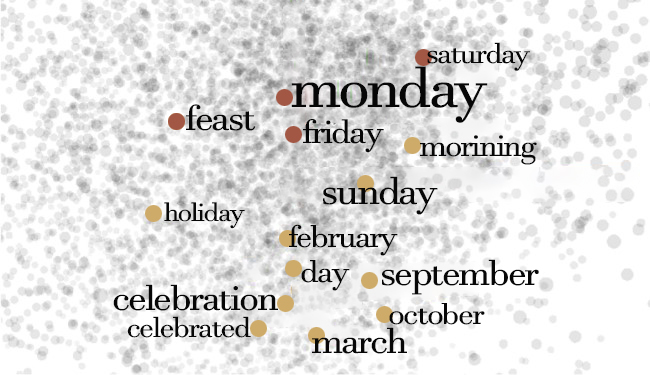
\includegraphics[width=6cm]{./Chapter9/Figures/figure-word-graph.jpg}
\caption{分布式表示的可视化}
\label{fig:9-66}
\end{figure}
%-------------------------------------------

\parinterval  语言模型的词嵌入是通过词嵌入矩阵进行存储的,矩阵中的每一行对应了一个词的分布式表示结果。图\ref{fig:9-67}展示了一个词嵌入矩阵的实例。

%----------------------------------------------
\begin{figure}[htp]
\centering
%%%------------------------------------------------------------------------------------------------------------
\begin{tikzpicture}
\begin{scope}
\node [anchor=center,inner sep=2pt] (e) at (0,0) {\small{$\mathbi{e}=\mathbi{o}$}};
\node [anchor=west,inner sep=2pt] (c) at (e.east) {\small{$\mathbi{C}$}};

\begin{pgfonlayer}{background}
\node [rectangle,inner sep=0.4em,draw,fill=blue!20!white] [fit = (e) (c)] (box) {};
\end{pgfonlayer}

\draw [->,thick] ([yshift=-1em]box.south)--([yshift=-0.1em]box.south) node [pos=0,below] (bottom1) {\small{单词$w$的One-hot表示}};
\draw [->,thick] ([yshift=0.1em]box.north)--([yshift=1em]box.north) node [pos=1,above] (top1) {\scriptsize{$\mathbi{e}$=(8,.2,-1,.9,...,1)}};
\node [anchor=north] (bottom2) at ([yshift=0.3em]bottom1.south) {\scriptsize{$\mathbi{o}$=(0,0,1,0,...,0)}};
\node [anchor=south] (top2) at ([yshift=-0.3em]top1.north) {\small{单词$w$的分布式表示}};

{
\node [anchor=north west,fill=red!20!white] (cmatrix) at ([xshift=3em,yshift=1.0em]c.north east) {\scriptsize{$\begin{pmatrix} 1 & .2 & -.2 & 8 & ... & 0 \\ .6 & .8 & -2 & 1 & ... & -.2 \\ 8 & .2 & -1 & .9 & ... & 2.3 \\ 1 & 1.2 & -.9 & 3 & ... & .2 \\ ... & ... & ... & ... & ... & ... \\ 1 & .3 & 3 & .9 & ... & 5.1 \end{pmatrix}$}};
\node [anchor=west,inner sep=2pt,fill=red!30!white] (c) at (e.east) {\small{$\mathbi{C}$}};
\draw [<-,thick] (c.east) -- ([xshift=3em]c.east);
}

{
\node [anchor=south,draw,fill=green!20!white] (e2) at ([yshift=1.5em]cmatrix.north) {\scriptsize{外部词嵌入系统得到的$\mathbi{C}$}};
\draw [->,very thick,dashed] (e2.south) -- (cmatrix.north);
}

\end{scope}
\end{tikzpicture}
%%%------------------------------------------------------------------------------------------------------------


\caption{词嵌入矩阵${\mathbi{C}}$}
\label{fig:9-67}
\end{figure}
%-------------------------------------------

\parinterval  通常,有两种方法得到词嵌入矩阵。一种方法是把词嵌入作为语言模型的一部分进行训练,不过由于语言模型往往较复杂,这种方法非常耗时;另一种方法使用更加轻便的外部训练方法,如word2vec\upcite{mikolov2013distributed}、Glove\upcite{DBLP:conf/emnlp/PenningtonSM14}等。由于这些方法的效率较高,因此可以使用更大规模的数据得到更好的词嵌入结果。

%----------------------------------------------------------------------------------------
%    NEW SUB-SECTION
%----------------------------------------------------------------------------------------

\subsection{句子表示模型}

\parinterval  目前,词嵌入已经成为诸多自然语言处理系统的标配,也衍生出很多有趣的研究法方向。但是,冷静地看,词嵌入依旧存在一些问题:每个词都对应唯一的向量表示,那么对于一词多义现象,词义需要通过上下文进行区分,这时使用简单的词嵌入式是无法处理的。有一个著名的例子:

\begin{example}
Aaron is an employee of {\red{\underline{apple}}}.

\hspace{2em} He finally ate the {\red{\underline{apple}}}.
\end{example}

\parinterval  这两句中“apple”的语义显然是不同的,第一句中的上下文“Jobs”和“CEO”可以帮助我们判断“apple”是一个公司名字,而不是水果。但是词嵌入只有一个结果,因此无法区分这两种情况。这个例子给我们一个启发:在一个句子中,不能孤立的看待单词,应同时考虑其上下文的信息。也就是需要一个能包含句子中上下文信息的表示模型。

\parinterval  回忆一下神经语言模型的结构,它需要在每个位置预测单词生成的概率。这个概率是由若干层神经网络进行计算后,通过输出层得到的。实际上,在送入输出层之前,系统已经得到了这个位置的一个向量(隐藏层的输出),因此可以把它看作是含有一部分上下文信息的表示结果。

\parinterval  以RNNLM为例,图\ref{fig:9-68}展示了一个由四个词组成的句子,这里使用了一个两层循环神经网络对其进行建模。可以看到,对于第三个位置,RNNLM已经积累了从第1个单词到第3个单词的信息,因此可以看作是单词1-3(“乔布斯\ 就职\ 于”)的一种表示;另一方面,第4个单词的词嵌入可以看作是“苹果”自身的表示。这样,可以把第3个位置RNNLM的输出和第4个位置的词嵌入进行合并,就得到了第4个位置上含有上下文信息的表示结果。从另一个角度说,这里得到了“苹果”的一种新的表示,它不仅包含苹果这个词自身的信息,也包含它前文的信息。

%----------------------------------------------
\begin{figure}[htp]
\centering
\begin{tikzpicture}
\begin{scope}
\tikzstyle{rnnnode} = [draw,inner sep=5pt,minimum width=4em,minimum height=1.5em,fill=green!30!white,blur shadow={shadow xshift=1pt,shadow yshift=-1pt}]
\node [anchor=west,rnnnode] (node11) at (0,0) {\scriptsize{RNN Cell}};
\node [anchor=west,rnnnode] (node12) at ([xshift=3.5em]node11.east) {\scriptsize{RNN Cell}};
\node [anchor=west,rnnnode] (node13) at ([xshift=3.5em]node12.east) {\scriptsize{RNN Cell}};
\node [anchor=west,rnnnode] (node14) at ([xshift=3.5em]node13.east) {\scriptsize{RNN Cell}};

\node [anchor=north,rnnnode,fill=red!30!white] (e1) at ([yshift=-1.2em]node11.south) {\scriptsize{embedding}};
\node [anchor=north,rnnnode,fill=red!30!white] (e2) at ([yshift=-1.2em]node12.south) {\scriptsize{embedding}};
\node [anchor=north,rnnnode,fill=red!30!white] (e3) at ([yshift=-1.2em]node13.south) {\scriptsize{embedding}};
\node [anchor=north,rnnnode,fill=red!30!white] (e4) at ([yshift=-1.2em]node14.south) {\scriptsize{embedding}};
\node [anchor=north] (w1) at ([yshift=-1em]e1.south) {\footnotesize{亚伦}};
\node [anchor=north] (w2) at ([yshift=-1em]e2.south) {\footnotesize{任职}};
\node [anchor=north] (w3) at ([yshift=-1em]e3.south) {\footnotesize{于}};
\node [anchor=north] (w4) at ([yshift=-1em]e4.south) {\footnotesize{苹果}};

\draw [->,thick] ([yshift=0.1em]w1.north)--([yshift=-0.1em]e1.south);
\draw [->,thick] ([yshift=0.1em]w2.north)--([yshift=-0.1em]e2.south);
\draw [->,thick] ([yshift=0.1em]w3.north)--([yshift=-0.1em]e3.south);
\draw [->,thick] ([yshift=0.1em]w4.north)--([yshift=-0.1em]e4.south);

\draw [->,thick] ([yshift=0.1em]e1.north)--([yshift=-0.1em]node11.south);
\draw [->,thick] ([yshift=0.1em]e2.north)--([yshift=-0.1em]node12.south);
\draw [->,thick] ([yshift=0.1em]e3.north)--([yshift=-0.1em]node13.south);
\draw [->,thick] ([yshift=0.1em]e4.north)--([yshift=-0.1em]node14.south);

\node [anchor=south,rnnnode] (node21) at ([yshift=1.5em]node11.north) {\scriptsize{RNN Cell}};
\node [anchor=south,rnnnode] (node22) at ([yshift=1.5em]node12.north) {\scriptsize{RNN Cell}};
\node [anchor=south,rnnnode] (node23) at ([yshift=1.5em]node13.north) {\scriptsize{RNN Cell}};
\node [anchor=south,rnnnode] (node24) at ([yshift=1.5em]node14.north) {\scriptsize{RNN Cell}};

\node [anchor=south] (node31) at ([yshift=1.0em]node21.north) {\scriptsize{的表示}};
\node [anchor=south west] (node31new) at ([yshift=-0.3em]node31.north west) {\scriptsize{“亚伦”}};
\node [anchor=south] (node32) at ([yshift=1.0em]node22.north) {\scriptsize{的表示\ \ \ }};
\node [anchor=south west] (node32new) at ([yshift=-0.3em]node32.north west) {\scriptsize{“亚伦 任职”}};
\node [anchor=south] (node33) at ([yshift=1.0em]node23.north) {\scriptsize{的表示\ \ \ \ \ \ \ \ }};
\node [anchor=south west] (node33new) at ([yshift=-0.3em]node33.north west) {\scriptsize{“亚伦 任职 于”}};
\node [anchor=south] (node34) at ([yshift=1.0em]node24.north) {\scriptsize{的表示\ \ \ \ \ \ \ \ }};
\node [anchor=south west] (node34new) at ([yshift=-0.3em]node34.north west) {\scriptsize{“亚伦 任职 于 苹果”}};

\draw [->,thick] ([yshift=0.1em]node21.north)--([yshift=-0.1em]node31.south);
\draw [->,thick] ([yshift=0.1em]node22.north)--([yshift=-0.1em]node32.south);
\draw [->,thick] ([yshift=0.1em]node23.north)--([yshift=-0.1em]node33.south);
\draw [->,thick] ([yshift=0.1em]node24.north)--([yshift=-0.1em]node34.south);

\draw [->,thick] ([xshift=-1em]node21.west)--([xshift=-0.1em]node21.west);
\draw [->,thick] ([xshift=0.1em]node21.east)--([xshift=-0.1em]node22.west);
\draw [->,thick] ([xshift=0.1em]node22.east)--([xshift=-0.1em]node23.west);
\draw [->,thick] ([xshift=0.1em]node23.east)--([xshift=-0.1em]node24.west);
\draw [->,thick] ([xshift=0.1em]node24.east)--([xshift=1em]node24.east);

\draw [->,thick] ([yshift=0.1em]node11.north)--([yshift=-0.1em]node21.south);
\draw [->,thick] ([yshift=0.1em]node12.north)--([yshift=-0.1em]node22.south);
\draw [->,thick] ([yshift=0.1em]node13.north)--([yshift=-0.1em]node23.south);
\draw [->,thick] ([yshift=0.1em]node14.north)--([yshift=-0.1em]node24.south);

\draw [->,thick] ([xshift=-1em]node11.west)--([xshift=-0.1em]node11.west);
\draw [->,thick] ([xshift=0.1em]node11.east)--([xshift=-0.1em]node12.west);
\draw [->,thick] ([xshift=0.1em]node12.east)--([xshift=-0.1em]node13.west);
\draw [->,thick] ([xshift=0.1em]node13.east)--([xshift=-0.1em]node14.west);
\draw [->,thick] ([xshift=0.1em]node14.east)--([xshift=1em]node14.east);

{
\node [anchor=south] (toplabel1) at ([yshift=2em,xshift=-0.2em]node32new.north) {\footnotesize{“苹果”的表示:}};
\node [anchor=west,fill=blue!30!white,minimum width=3em] (toplabel2) at (toplabel1.east) {\footnotesize{上下文}};
}
{
\node [anchor=west,fill=red!30!white,minimum width=3em] (toplabel3) at (toplabel2.east) {\footnotesize{词}};
}

\begin{pgfonlayer}{background}
{
\node [rectangle,inner sep=2pt,draw,thick,dashed,red] [fit = (e4)] (r2) {};
\draw [->,thick,red] (r2.west) .. controls +(west:0.8) and +(south:2) .. ([xshift=1.3em]toplabel3.south);
}
{
\node [rectangle,inner sep=2pt,draw,thick,dashed,ublue,fill=white] [fit = (node33) (node33new)] (r1) {};
\draw [->,thick,ublue] ([xshift=-2em]r1.north) .. controls +(north:0.7) and +(south:0.7) .. ([xshift=-0.5em]toplabel2.south);
}
\end{pgfonlayer}

\end{scope}
\end{tikzpicture}
\caption{基于RNN的表示模型(词+上下文)}
\label{fig:9-68}
\end{figure}
%-------------------------------------------

\parinterval  在自然语言处理中,{\small\sffamily\bfseries{句子表示模型}}\index{句子表示模型}是指把输入的句子进行分布式表示。不过表示的形式不一定是一个单独的向量。现在广泛使用的句子表示模型可以被描述为:给定一个输入的句子$ \{ w_1,\dots ,w_m\} $,得到一个表示序列$ \{{\mathbi{h}}_1,\dots ,{\mathbi{h}}_m\} $,其中$ {\mathbi{h}}_i $是句子在第$ i $个位置的表示结果。$ \{ {\mathbi{h}}_1,\dots ,{\mathbi{h}}_m\} $就被看作是{\small\sffamily\bfseries{句子的表示}}\index{句子的表示},它可以被送入下游模块。比如,在机器翻译任务中,可以用这种模型表示源语言句子,然后通过这种表示结果进行目标语译文的生成;在序列标注(如词性标注)任务中,可以对输入的句子进行表示,然后在这个表示之上构建标签预测模块。很多自然语言处理任务都可以用句子表示模型进行建模,因此句子的表示模型也是应用最广泛的深度学习模型之一。而学习这种表示的过程也被称作表示学习。

\parinterval  句子表示模型有两种训练方法。最简单的方法是把它作为目标系统中的一个模块进行训练,比如把句子表示模型作为机器翻译系统的一部分。也就是,并不单独训练句子表示模型,而是把它作为一个内部模块放到其他系统中。另一种方法是把句子表示作为独立的模块,用外部系统进行训练,之后把训练好的表示模型放入目标系统中,再进行微调。这种方法构成了一种新的范式:预训练+微调(pre-training + fine-tuning)。图\ref{fig:9-69}对比了这两种不同的方法。

%----------------------------------------------
\begin{figure}[htp]
\centering
%%%------------------------------------------------------------------------------------------------------------
\begin{tikzpicture}

\begin{scope}

\node [anchor=west,draw,thick,minimum width=4em,minimum height=1.7em,fill=blue!20] (encoder) at (0,0) {模块};
\node [anchor=south,minimum width=4em,minimum height=1.7em] (space) at ([yshift=0.3em]encoder.north) {\footnotesize{目标系统}};

\begin{pgfonlayer}{background}
\node [rectangle,draw,thick,fill=red!20] [fit = (encoder) (space)] (system) {};
\end{pgfonlayer}

\node [anchor=north] (data) at ([yshift=-1em]system.south) {\scriptsize{\textbf{目标任务有标注数据}}};
\draw [->,thick] (data.north) -- ([yshift=-0.1em]system.south);
\node [anchor=north] (label) at ([yshift=-0em]data.south) {\scriptsize{(a) 标准方法}};

\end{scope}

\begin{scope}[xshift=2.8in]

\node [anchor=west,draw,dashed,thick,minimum width=4em,minimum height=1.7em,fill=blue!20] (encoder) at (0,0) {模块};
\node [anchor=south,minimum width=4em,minimum height=1.7em] (space) at ([yshift=0.3em]encoder.north) {\footnotesize{目标系统}};
\node [anchor=center,draw,thick,minimum width=4em,minimum height=1.7em,fill=green!20] (encoderpre) at ([xshift=-7em]encoder.center) {\footnotesize{语言模型}};
\draw [->,thick] (encoderpre.east) -- (encoder.west);

\begin{pgfonlayer}{background}
\node [rectangle,draw,thick,fill=red!20] [fit = (encoder) (space)] (system) {};
\end{pgfonlayer}

\node [anchor=north] (data) at ([yshift=-1em]system.south) {\scriptsize{\textbf{目标任务有标注数据}}};
\draw [->,thick] (data.north) -- ([yshift=-0.1em]system.south);
\node [anchor=north] (data2) at ([yshift=-1em,xshift=-7em]system.south) {\scriptsize{\textbf{大规模无标注数据}}};
\draw [->,thick] (data2.north) -- ([yshift=-0.1em]encoderpre.south);
\node [anchor=north] (label) at ([yshift=-0em,xshift=-4em]data.south) {\scriptsize{(b) 预训练 + 微调}};

\end{scope}

\end{tikzpicture}
%%%------------------------------------------------------------------------------------------------------------


\caption{表示模型的训练方法(与目标任务联合训练 vs 用外部任务预训练)}
\label{fig:9-69}
\end{figure}
%-------------------------------------------

\parinterval  目前,句子表示模型的预训练方法在多项自然语言处理任务上取得了很好的效果。预训练模型也成为了当今自然语言处理中的热点方向,相关系统也在很多评测任务上刷榜。不过,上面介绍的模型是一种最简单句子表示模型,在{\chaptersixteen}会对一些前沿的预训练方法和句子表示模型进行介绍。

%----------------------------------------------------------------------------------------
%    NEW SECTION
%----------------------------------------------------------------------------------------

\sectionnewpage
\section{小结及拓展阅读}

\parinterval  神经网络为解决自然语言处理问题提供了全新的思路。而所谓深度学习也是建立在多层神经网络结构之上的一系列模型和方法。本章从神经网络的基本概念到其在语言建模中的应用进行了概述。由于篇幅所限,这里无法覆盖所有神经网络和深度学习的相关内容,感兴趣的读者可以进一步阅读\textit{Neural Network Methods in Natural Language Processing}\upcite{goldberg2017neural}和\textit{Deep Learning}\upcite{Goodfellow-et-al-2016}。此外,也有一些研究方向值得关注:

\begin{itemize}
\vspace{0.5em}
\item 端到端学习是神经网络方法的特点之一。这样,系统开发者不需要设计输入和输出的隐含结构,甚至连特征工程都不再需要。但是,另一方面,由于这种端到端学习完全由神经网络自行完成,整个学习过程没有人的先验知识做指导,导致学习的结构和参数很难进行解释。针对这个问题也有很多研究者进行{\small\sffamily\bfseries{可解释机器学习}}\index{可解释机器学习}(Explainable Machine Learning)\index{Explainable Machine Learning}的研究\upcite{moraffah2020causal,Kovalerchuk2020SurveyOE,DoshiVelez2017TowardsAR}。对于自然语言处理,方法的可解释性是十分必要的。从另一个角度说,如何使用先验知识改善端到端学习也是很多人关注的方向\upcite{arthur2016incorporating,zhang-etal-2017-prior},比如,如何使用句法知识改善自然语言处理模型\upcite{stahlberg2016syntactically,currey2019incorporating,Yang2017TowardsBH,marevcek2018extracting,blevins2018deep}。
\vspace{0.5em}
\item 为了进一步提高神经语言模型性能,除了改进模型,还可以在模型中引入新的结构或是其他有效信息,该领域也有很多典型工作值得关注。例如在神经语言模型中引入除了词嵌入以外的单词特征,如语言特征(形态、语法、语义特征等)\upcite{Wu2012FactoredLM,Adel2015SyntacticAS}、上下文信息\upcite{mikolov2012context,Wang2015LargerContextLM}、知识图谱等外部知识\upcite{Ahn2016ANK};或是在神经语言模型中引入字符级信息,将其作为字符特征单独\upcite{Kim2016CharacterAwareNL,Hwang2017CharacterlevelLM}或与单词特征一起\upcite{Onoe2016GatedWR,Verwimp2017CharacterWordLL}送入模型中;在神经语言模型中引入双向模型也是一种十分有效的尝试,在单词预测时可以同时利用来自过去和未来的文本信息\upcite{Graves2013HybridSR,bahdanau2014neural,Peters2018DeepCW}。
\vspace{0.5em}
\item 词嵌入是自然语言处理近些年的重要进展。所谓“嵌入”是一类方法,理论上,把一个事物进行分布式表示的过程都可以被看作是广义上的“嵌入”。基于这种思想的表示学习也成为了自然语言处理中的前沿方法。比如,如何对树结构,甚至图结构进行分布式表示成为了分析自然语言的重要方法\upcite{DBLP:journals/corr/abs-1809-01854,Yin2018StructVAETL,Aharoni2017TowardsSN,Bastings2017GraphCE,KoncelKedziorski2019TextGF}。此外,除了语言建模,还有很多方式可以进行词嵌入的学习,比如,SENNA\upcite{2011Natural}、word2vec\upcite{DBLP:journals/corr/abs-1301-3781,mikolov2013distributed}、Glove\upcite{DBLP:conf/emnlp/PenningtonSM14}、CoVe\upcite{mccann2017learned} 等。
\vspace{0.5em}
\end{itemize}

%% !Mode:: "TeX:UTF-8"
% !TEX encoding = UTF-8 Unicode

%----------------------------------------------------------------------------------------
% 机器翻译:统计建模与深度学习方法
% Machine Translation: Statistical Modeling and Deep Learning Methods
%
% Copyright 2020
% 肖桐(xiaotong@mail.neu.edu.cn) 朱靖波 (zhujingbo@mail.neu.edu.cn)
%----------------------------------------------------------------------------------------

%----------------------------------------------------------------------------------------
%    CONFIGURATIONS
%----------------------------------------------------------------------------------------

\renewcommand\figurename{图}%将figure改为图
\renewcommand\tablename{表}%将figure改为图
\chapterimage{fig-NEU-10.jpg} % Chapter heading image

%----------------------------------------------------------------------------------------
%	CHAPTER 10
%----------------------------------------------------------------------------------------

\chapter{基于循环神经网络的模型}

\parinterval {\small\sffamily\bfseries{神经机器翻译}} \index{神经机器翻译}(Neural Machine Translation)\index{Neural Machine Translation}是机器翻译的前沿方法。近几年,随着深度学习技术的发展和在各领域中的深入应用,基于端到端表示学习的方法正在改变着我们处理自然语言的方式,神经机器翻译在这种趋势下应运而生。一方面,神经机器翻译仍然延续着统计建模和基于数据驱动的思想,因此在基本问题的定义上与前人的研究是一致的;另一方面,神经机器翻译脱离了统计机器翻译中对隐含翻译结构的假设,同时使用分布式表示来对文字序列进行建模,这使得它可以从一个全新的视角看待翻译问题。现在,神经机器翻译已经成为了机器翻译研究及应用的热点,译文质量得到了巨大的提升。

\parinterval 本章将介绍神经机器翻译中的一种基础模型\ \dash \ 基于循环神经网络的模型。该模型是神经机器翻译中最早被成功应用的模型之一。基于这个模型框架,研究者进行了大量的探索和改进工作,包括使用LSTM等循环单元结构、引入注意力机制等。这些内容都会在本章进行讨论。

%----------------------------------------------------------------------------------------
%    NEW SECTION  10.1
%----------------------------------------------------------------------------------------
\section{神经机器翻译的发展简史}

\parinterval 纵观机器翻译的发展历程,神经机器翻译诞生较晚。无论是早期的基于规则的方法,还是逐渐发展起来的基于实例的方法,再或是上世纪末的统计方法,每次机器翻译框架级的创新都需要很长时间的酝酿,而技术走向成熟甚至需要更长的时间。但是,神经机器翻译的出现和后来的发展速度多少有些“出人意料”。神经机器翻译的概念出现在2013-2014年间,当时机器翻译领域的主流方法仍然是统计机器翻译。虽然那个时期深度学习已经在图像、语音等领域取得令人瞩目的效果,但是对于自然语言处理来说深度学习仍然不是主流。

\parinterval 不过,有人也意识到了神经机器翻译在表示学习等方面的优势。这一时期,很多研究团队对包括机器翻译在内的序列到序列问题进行了广泛而深入的研究,注意力机制等新的方法不断被推出。这使得神经机器翻译系统在翻译品质上逐渐体现出优势,甚至超越了当时的统计机器翻译系统。正当大家在讨论神经机器翻译是否能取代统计机器翻译成为下一代机器翻译范式的时候,一些互联网企业推出了以神经机器翻译技术为内核的在线机器翻译服务,在很多场景下的翻译品质显著超越了当时最好的统计机器翻译系统。这也引发了学术界和产业界对神经机器翻译的讨论。随着关注度的不断升高,神经机器翻译的研究吸引了更多的科研机构和企业的投入,神经机器翻译系统的翻译品质得到进一步提升。

\parinterval 在短短5-6年间,神经机器翻译从一个新生的概念已经成长为机器翻译领域的最前沿技术之一,在各种机器翻译评测和应用中呈全面替代统计机器翻译之势。比如,从近几年WMT、CCMT等评测的结果来看,神经机器翻译已经处于绝对的统治地位,在不同语种和领域的翻译任务中,成为各参赛系统的标配。此外,从ACL等自然语言处理顶级会议的发表论文看,神经机器翻译在论文数量上呈明显的增长趋势,这也体现了学术界对该方法的热情。至今,国内外的很多机构都推出了自己研发的神经机器翻译系统,整个研究和产业生态欣欣向荣。图\ref{fig:10-1}展示了包含神经机器翻译在内的机器翻译发展简史。

%----------------------------------------------
\begin{figure}[htp]
\centering
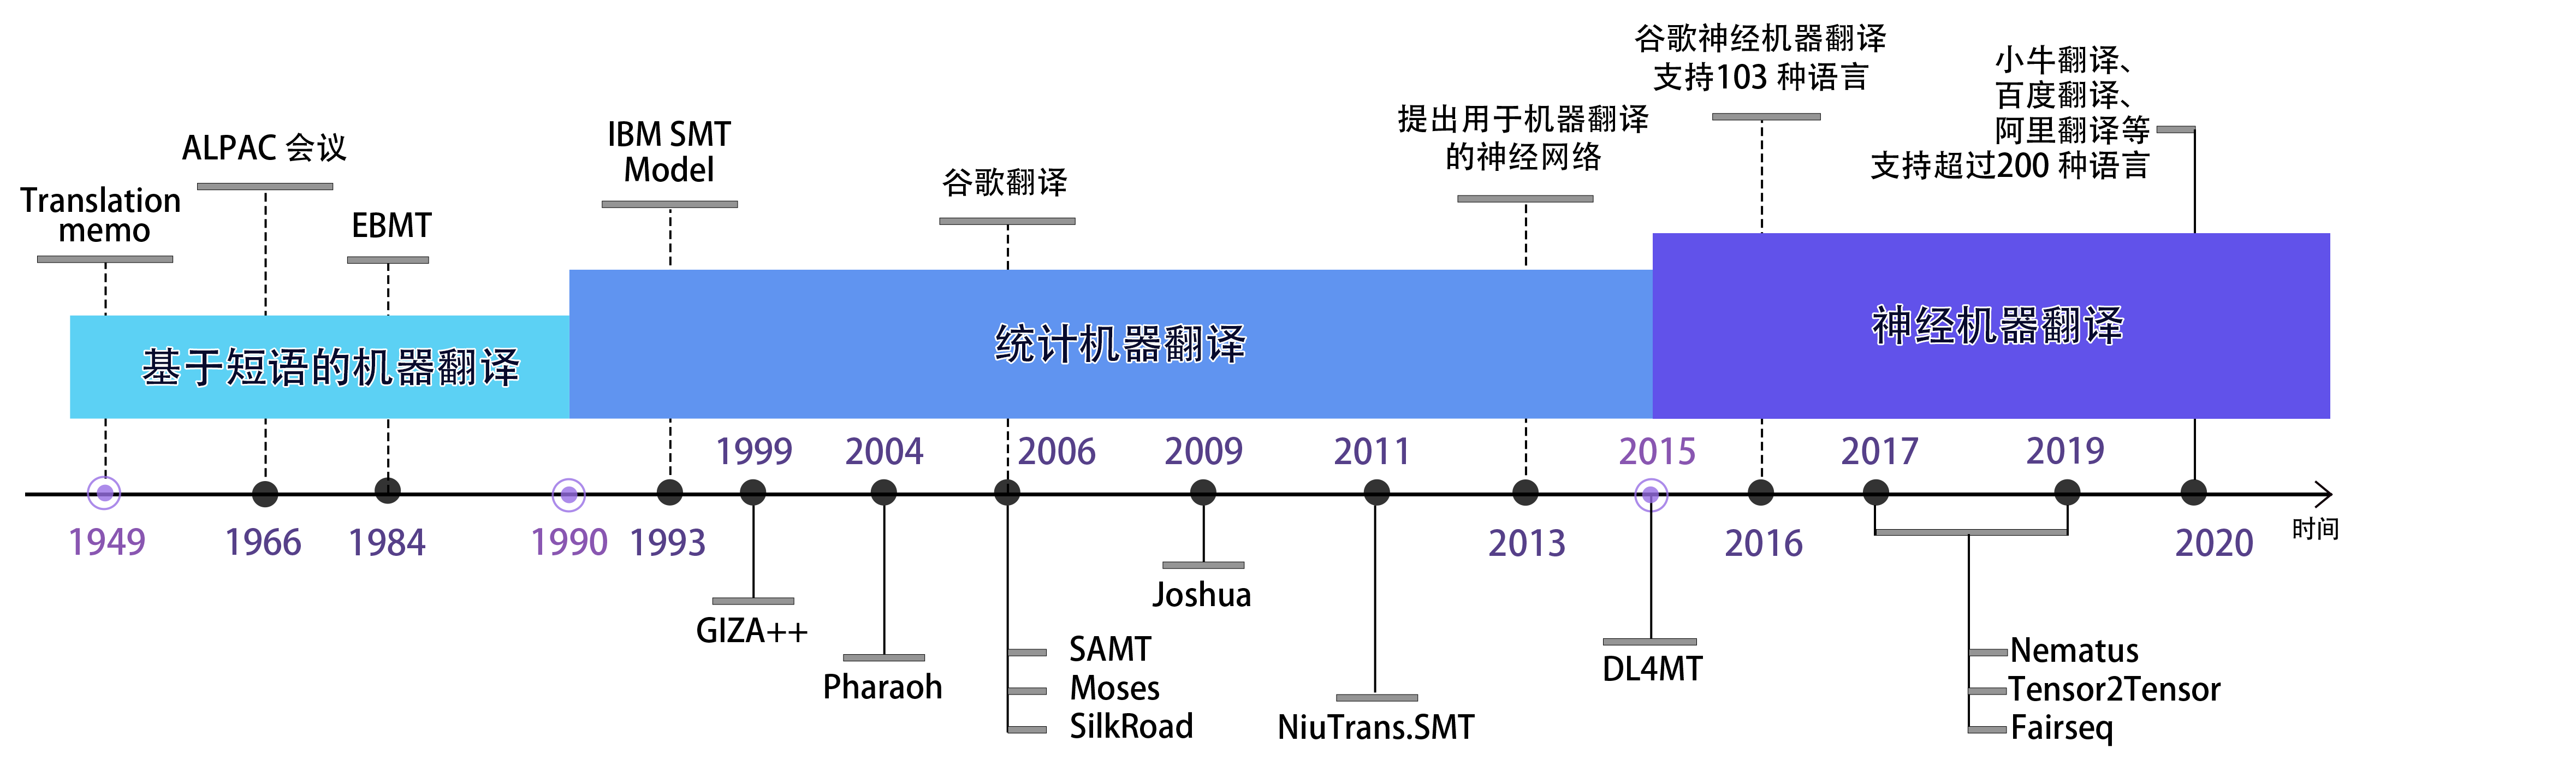
\includegraphics[scale=0.4]{./Chapter10/Figures/mt-history.png}
\caption{机器翻译发展简史}
\label{fig:10-1}
\end{figure}
%----------------------------------------------

\parinterval 神经机器翻译的迅速崛起确实让所有人都有些措手不及,甚至有一种一觉醒来天翻地覆的感觉。也有人评价,神经机器翻译的出现给整个机器翻译领域带来了前所未有的发展机遇。不过,客观地看,机器翻译达到今天这样的状态也是一种历史必然,其中有几方面原因:

\begin{itemize}
\vspace{0.5em}
\item 自上世纪末所发展起来的基于数据驱动的方法为神经机器翻译提供了很好的基础。本质上,神经机器翻译仍然是一种基于统计建模的数据驱动的方法,因此无论是对问题的基本建模方式,还是训练统计模型所使用到的带标注数据,都可以复用机器翻译领域以前的研究成果。特别是机器翻译长期的发展已经积累了大量的双语、单语数据,这些数据在统计机器翻译时代就发挥了很大作用。随着时间的推移,数据规模和质量又得到进一步提升,包括一些评测基准、任务设置都已经非常完备,研究者可以直接在数据条件全部具备的情况下开展神经机器翻译的研究工作,这些都节省了大量的时间成本。从这个角度说,神经机器翻译是站在巨人的肩膀上才发展起来的。
\vspace{0.5em}
\item 深度学习经过长时间的酝酿终于爆发,为机器翻译等自然语言处理任务提供了新的思路和技术手段。神经机器翻译的不断壮大伴随着深度学习技术的发展。在深度学习的视角下,语言文字可以被表示成抽象的实数向量,这种文字的表示结果可以被自动学习,为机器翻译建模提供了更大的灵活性。相对于神经机器翻译,深度学习的发展更加曲折。虽然深度学习经过了漫长的起伏过程,但是神经机器翻译恰好出现在深度学习逐渐走向成熟的阶段。反过来说,受到深度学习及相关技术空前发展的影响,自然语言处理的范式也发生了变化,神经机器翻译的出现只是这种趋势下的一种必然。
\vspace{0.5em}
\item 此外,计算机算力的提升也为神经机器翻译提供了很好的支撑。与很多神经网络方法一样,神经机器翻译也依赖大量基于浮点数的矩阵运算。甚至在本世纪初,大规模的矩阵运算仍然依赖非常昂贵的CPU集群系统,但是随着GPU等相关技术的发展,在相对低成本的设备上已经可以完成非常复杂的浮点并行运算。这使得包括神经机器翻译在内的很多基于深度学习的系统可以进行大规模实验,随着实验周期的缩短,相关研究和系统的迭代周期也大大缩短。实际上,计算机硬件运算能力一直是稳定提升的,神经机器翻译只是受益于运算能力的阶段性突破。
\vspace{0.5em}
\item 还有,翻译需求的不断增加也为机器翻译技术提供了新的机会。在近几年,无论是翻译品质,还是翻译语种数量,甚至不同的翻译场景,都对机器翻译有了更高的要求。人们迫切需要一种品质更高、翻译效果稳定的机器翻译方法,神经机器翻译恰好满足了这些要求。当然,应用端需求的增加也会反推机器翻译技术的发展,二者相互促进。
\vspace{0.5em}
\end{itemize}

\parinterval 至今,神经机器翻译已经成为带有时代特征的标志性方法。当然,机器翻译的发展也远没有达到终点。下面将介绍神经机器翻译的起源和优势,以便读者在正式了解神经机器翻译的技术方法前对其现状有一个充分的认识。

%----------------------------------------------------------------------------------------
%    NEW SUB-SECTION 10.1.1
%----------------------------------------------------------------------------------------

\subsection{神经机器翻译的起源}

\parinterval 从广义上讲,神经机器翻译是一种基于人工神经网络的方法,它把翻译过程描述为可以用人工神经网络表示的函数,所有的训练和推断都在这些函数上进行。由于神经机器翻译中的神经网络可以用连续可微函数表示,因此这类方法也可以用基于梯度的方法进行优化,相关技术非常成熟。更为重要的是,在神经网络的设计中,研究者引入了分布式表示的概念,这也是近些年自然语言处理领域的重要成果之一。传统统计机器翻译仍然把词序列看作离散空间里的由多个特征函数描述的点,类似于$n$-gram语言模型,这类模型对数据稀疏问题非常敏感。此外,人工设计特征也在一定程度上限制了模型对问题的表示能力。神经机器翻译把文字序列表示为实数向量,一方面避免了特征工程繁重的工作,另一方面使得系统可以对文字序列的“表示”进行学习。可以说,神经机器翻译的成功很大程度上源自“ 表示学习”这种自然语言处理的新范式的出现。在表示学习的基础上,注意力机制、深度神经网络等技术都被应用于神经机器翻译,使其得以进一步发展。

\parinterval 虽然神经机器翻译中大量地使用了人工神经网络方法,但是它并不是最早在机器翻译中使用人工神经网络的框架。实际上,人工神经网络在机器翻译中应用的历史要远早于现在的神经机器翻译。 在统计机器翻译时代,也有很多研究者利用人工神经网络进行机器翻译系统模块的构建\upcite{devlin-etal-2014-fast,Schwenk_continuousspace},比如,研究人员成功地在统计机器翻译系统中使用了基于神经网络的联合表示模型,取得了很好的效果\upcite{devlin-etal-2014-fast}。

\parinterval 不过,以上这些工作大多都是在系统的局部模块中使用人工神经网络和深度学习方法。与之不同的是,神经机器翻译是用人工神经网络完成整个翻译过程的建模,这样做的一个好处是,整个系统可以进行端到端学习,无需引入对任何翻译的隐含结构假设。这种利用端到端学习对机器翻译进行神经网络建模的方式也就成为了现在大家所熟知的神经机器翻译。这里简单列出部分代表性的工作:

\begin{itemize}
\vspace{0.3em}
\item 早在2013年,Nal Kalchbrenner和Phil Blunsom提出了一个基于编码器-解码器结构的新模型\upcite{kalchbrenner-blunsom-2013-recurrent}。该模型用卷积神经网络(CNN)将源语言编码成实数向量,之后用循环神经网络(RNN)将连续向量转换成目标语言。这使得模型不需要进行词对齐、特征提取等工作,就能够自动学习源语言的信息。这也是一种端到端学习的方法。不过,这项工作的实现较复杂,而且方法存在梯度消失/爆炸等问题\upcite{HochreiterThe,BENGIO1994Learning},因此并没有成为后来神经机器翻译的基础框架。
\vspace{0.3em}
\item 2014年,Ilya Sutskever等人提出了序列到序列(seq2seq)学习的方法,同时将长短时记忆结构(LSTM)引入到神经机器翻译中,这个方法缓解了梯度消失/爆炸的问题,并且通过遗忘门的设计让网络选择性地记忆信息,缓解了序列中长距离依赖的问题\upcite{NIPS2014_5346}。但是该模型在进行编码的过程中,将不同长度的源语言句子压缩成了一个固定长度的向量,句子越长损失的信息越多,同时该模型无法对输入和输出序列之间的对齐进行建模,因此并不能有效保证翻译质量。
\vspace{0.3em}
\item 同年Dzmitry Bahdanau等人首次将{\small\bfnew{注意力机制}}\index{注意力机制}(Attention Mechanism\index{Attention Mechanism})应用到机器翻译领域,在机器翻译任务上对翻译和局部翻译单元之间的对应关系同时建模\upcite{bahdanau2014neural}。Bahdanau等人工作的意义在于,使用了更加有效的模型来表示源语言的信息,同时使用注意力机制对两种语言不同部分之间的相互联系进行建模。这种方法可以有效地处理长句子的翻译,而且注意力的中间结果具有一定的可解释性\footnote{比如,目标语言和源语言句子不同单词之间的注意力强度能够在一定程度上反应单词之间的互译程度。} 。然而相比于前人的神经机器翻译模型,注意力模型也引入了额外的成本,计算量较大。
\vspace{0.3em}
\item 2016年谷歌公司发布了基于多层循环神经网络方法的GNMT系统。该系统集成了当时的神经机器翻译技术,并进行了诸多的改进。它的性能显著优于基于短语的机器翻译系统\upcite{Wu2016GooglesNM},引起了研究者的广泛关注。在之后不到一年的时间里,脸书公司采用卷积神经网络(CNN)研发了新的神经机器翻译系统\upcite{DBLP:journals/corr/GehringAGYD17},实现了比基于循环神经网络(RNN)系统更高的翻译水平,并大幅提升翻译速度。
\vspace{-1.2em}
\item 2017年,Ashish Vaswani等人提出了新的翻译模型Transformer。其完全摒弃了循环神经网络和卷积神经网络,仅仅通过多头注意力机制和前馈神经网络,不需要使用序列对齐的循环框架就展示出强大的性能,并且巧妙地解决了翻译中长距离依赖问题\upcite{vaswani2017attention}。Transformer是第一个完全基于注意力机制搭建的模型,不仅训练速度更快,在翻译任务上也获得了更好的结果,一跃成为目前最主流的神经机器翻译框架。
\vspace{0.3em}
\end{itemize}

\parinterval  当然,神经机器翻译的工作远不止以上这些内容\upcite{StahlbergNeural}。随着本书内容的逐渐深入,很多经典的模型和方法都会被讨论到。

%----------------------------------------------------------------------------------------
%    NEW SUB-SECTION 10.1.2
%----------------------------------------------------------------------------------------

\subsection{神经机器翻译的品质}

\parinterval  图\ref{fig:10-2}展示了用机器翻译把一段汉语翻译为英语的结果。其中译文1是统计机器翻译系统的结果,译文2是神经机器翻译系统的结果。为了保证公平性,两个系统使用完全相同的数据进行训练。

%----------------------------------------------
%\begin{figure}[htp]
%\centering
%\begin{tikzpicture}
%第一段----------------------------------------------
%原文-------------
\node [pos=0.4,left,xshift=-36em,yshift=7.3em,font=\small] (original0) {原文:};
\node [pos=0.4,left,xshift=-2em,yshift=3.3em,font=\small] (original1) {
\begin{tabular}[t]{l}
\parbox{36em}{During Soviet times, if a city’s population topped one million, it would become eligible for its own metro. Planners wanted to brighten the lives of everyday Soviet citizens, and saw the metros, with their tens of thousands of daily passengers, as a singular opportunity to do so. In 1977, Tashkent, the capital of Uzbekistan, became the seventh Soviet city to have a metro built. Grand themes celebrating the history of Uzbekistan and the Soviet Union were brought to life, as art was commissioned and designers set to work. The stations reflected different themes, some with domed ceilings and painted tiles reminiscent of Uzbekistan’s Silk Road mosques, while others ...}
\end{tabular}
};
%译文1--------------mt1
\node[font=\small] (mt1) at ([xshift=0em,yshift=-9.1em]original0.south) {译文1:};
\node[font=\small] (ts1) at ([xshift=0em,yshift=-4em]original1.south)  {
\begin{tabular}[t]{l}
\parbox{36em}{在苏联时代,如果一个城市的人口突破一百万,这将成为合资格为自己的地铁。规划者想去照亮每天的苏联公民的生命,看到地铁,与他们的数十每天数千乘客,作为一个独特的机会来这样做。1977年,塔什干,乌兹别克斯坦的首都,成了苏联第七城市建有地铁。宏大主题,庆祝乌兹别克斯坦和苏联的历史被带到生活,因为艺术是委托和设计师开始工作。车站反映了不同的主题,有的圆顶天花板和绘瓷砖让人想起乌兹别克斯坦是丝绸之路的清真寺,而另一些则装饰着...}
\end{tabular}
};



%{
%\draw[dotted,thick,ublue] ([xshift=10.3em,yshift=0.3em]mt8.south west)--%([xshift=-5.2em,yshift=-0.3em]ht8.north);
%}



\begin{pgfonlayer}{background}
{
\node[rectangle,draw=ublue, inner sep=0mm] [fit =(original0)(mt1)(mt1)(ts1)(original1)] {};
}
\end{pgfonlayer}


\end{tikzpicture}
%\setlength{\abovecaptionskip}{-0.2cm}
%\caption{机器翻译实例对比}
%\label{fig:10-2}
%\end{figure}
%----------------------------------------------

%----------------------------------------------
\begin{figure}[htp]
\centering
\begin{tikzpicture}
%第一段----------------------------------------------
%原文-------------
\node [pos=0.4,left,xshift=-36em,yshift=7.3em,font=\small] (original0) {原文:};
\node [pos=0.4,left,xshift=-2em,yshift=3.3em,font=\small] (original1) {
\begin{tabular}[t]{l}
\parbox{36em}{During Soviet times, if a city’s population topped one million, it would become eligible for its own metro. Planners wanted to brighten the lives of everyday Soviet citizens, and saw the metros, with their tens of thousands of daily passengers, as a singular opportunity to do so. In 1977, Tashkent, the capital of Uzbekistan, became the seventh Soviet city to have a metro built. Grand themes celebrating the history of Uzbekistan and the Soviet Union were brought to life, as art was commissioned and designers set to work. The stations reflected different themes, some with domed ceilings and painted tiles reminiscent of Uzbekistan’s Silk Road mosques, while others ...}
\end{tabular}
};
%译文1--------------mt1
\node[font=\small] (mt1) at ([xshift=0em,yshift=-9.1em]original0.south) {译文1:};
\node[font=\small] (ts1) at ([xshift=0em,yshift=-4em]original1.south)  {
\begin{tabular}[t]{l}
\parbox{36em}{在苏联时代,如果一个城市的人口突破一百万,这将成为合资格为自己的地铁。规划者想去照亮每天的苏联公民的生命,看到地铁,与他们的数十每天数千乘客,作为一个独特的机会来这样做。1977年,塔什干,乌兹别克斯坦的首都,成了苏联第七城市建有地铁。宏大主题,庆祝乌兹别克斯坦和苏联的历史被带到生活,因为艺术是委托和设计师开始工作。车站反映了不同的主题,有的圆顶天花板和绘瓷砖让人想起乌兹别克斯坦是丝绸之路的清真寺,而另一些则装饰着...}
\end{tabular}
};

%译文2---------------mt2
\node[font=\small] (mt2) at ([xshift=0em,yshift=-6.7em]mt1.south) {译文2:};
\node[font=\small] (mt3) at ([xshift=0em,yshift=-4em]ts1.south)  {
\begin{tabular}[t]{l}
\parbox{36em}{在苏联时期,如果一个城市的人口超过一百万,它就有资格拥有自己的地铁。 规划者想要照亮日常苏联公民的生活,并把拥有数万名每日乘客的地铁看作是这样做的一个绝佳机会。 1977年,乌兹别克斯坦首都塔什干成为苏联第七个修建地铁的城市。 随着艺术的委托和设计师们的工作,乌兹别克斯坦和苏联历史的宏伟主题被赋予了生命力。 这些电台反映了不同的主题,有的有穹顶和彩砖,让人想起乌兹别克斯坦的丝绸之路清真寺,有的则用...}
\end{tabular}
};


%{
%\draw[dotted,thick,ublue] ([xshift=10.3em,yshift=0.3em]mt8.south west)--%([xshift=-5.2em,yshift=-0.3em]ht8.north);
%}



\begin{pgfonlayer}{background}
{
\node[rectangle,draw=ublue, inner sep=0mm] [fit =(original0)(mt1)(mt3)(mt1)(ts1)(mt2)(original1)] {};
}
\end{pgfonlayer}


\end{tikzpicture}
%\setlength{\abovecaptionskip}{-0.2em}
\vspace{-0.6em}
\caption{机器翻译实例对比}
\label{fig:10-2}
\end{figure}
%----------------------------------------------

\parinterval  可以明显地看到译文2更加通顺,意思的表达更加准确,翻译质量明显高于译文1。这个例子基本反应出统计机器翻译和神经机器翻译的差异性。当然,这里并不是要讨论统计机器翻译和神经机器翻译孰优孰劣,只是很多场景中发现神经机器翻译系统可以生成非常流畅的译文,易于人工阅读和修改。

\parinterval  在很多量化的评价中也可以看到神经机器翻译的优势。回忆一下{\chapterfour}提到的机器翻译质量的自动评估指标中,使用最广泛的一种指标是BLEU。2010年前,在由美国国家标准和科技机构(NIST)举办的汉英机器翻译评测中(比如汉英MT08数据集),30\%以上的BLEU值对于基于统计方法的翻译系统来说就已经是当时最顶尖的结果了。而现在的神经机器翻译系统,则可以轻松地将BLEU提高至45\%以上。

%----------------------------------------------
\begin{figure}[htp]
\centering
% not compatible with [scale=?]


%----------------------------------------------------  
  
    \begin{tikzpicture}
        \begin{scope}[local bounding box=WMT]
            \draw[->,thick] (0.4,0) to (9.5,0);
            \draw[->,thick] (0.4,-0) to (0.4,4.3);
            \draw[thick] (0.4,2) to (0.6,2);
            \draw[thick] (0.4,4) to (0.6,4);
            \node[font=\scriptsize] at (0,2) {10};
            \node[font=\scriptsize] at (0,4) {20};

            % 2015
            \node[minimum width=0.5cm,thick,minimum height=7*0.2cm,fill=blue!30!white,inner sep=0pt,outer sep=0pt,anchor=south west] (smt2015) at (1.5*0.7,0.5pt) {};
            \node[minimum width=0.5cm,thick,minimum height=2*0.2cm,fill=red!30!white,inner sep=0pt,outer sep=0pt,anchor=south west] (nmt2015) at (smt2015.south east) {};
            \node[font=\scriptsize,anchor=north] () at ([yshift=-0.2em]smt2015.south east) {2015};
            % 2016
            \node[minimum width=0.5cm,thick,minimum height=3*0.2cm,fill=blue!30!white,inner sep=0pt,outer sep=0pt,anchor=south west] (smt2016) at ($(nmt2015.south east)+(0.7,0)$) {};
            \node[minimum width=0.5cm,thick,minimum height=8*0.2cm,fill=red!30!white,inner sep=0pt,outer sep=0pt,anchor=south west] (nmt2016) at (smt2016.south east) {};
            \node[font=\scriptsize,anchor=north] () at ([yshift=-0.2em]smt2016.south east) {2016};
            % 2017
            \node[minimum width=0.5cm,thick,minimum height=3*0.2cm,fill=blue!30!white,inner sep=0pt,outer sep=0pt,anchor=south west] (smt2017) at ($(nmt2016.south east)+(0.7,0)$) {};
            \node[minimum width=0.5cm,thick,minimum height=13*0.2cm,fill=red!30!white,inner sep=0pt,outer sep=0pt,anchor=south west] (nmt2017) at (smt2017.south east) {};
            \node[font=\scriptsize,anchor=north] () at ([yshift=-0.2em]smt2017.south east) {2017};
            % 2018
            \node[minimum width=0.5cm,thick,minimum height=0cm,draw,fill=blue!30!white,inner sep=0pt,outer sep=0pt,anchor=south west] (smt2018) at ($(nmt2017.south east)+(0.7,0)$) {};
            \node[minimum width=0.5cm,thick,minimum height=14*0.2cm,fill=red!30!white,inner sep=0pt,outer sep=0pt,anchor=south west] (nmt2018) at (smt2018.south east) {};
            \node[font=\scriptsize,anchor=north] () at ([yshift=-0.2em]smt2018.south east) {2018};
             % 2019
            \node[minimum width=0.5cm,thick,minimum height=0cm,draw,fill=blue!30!white,inner sep=0pt,outer sep=0pt,anchor=south west] (smt2019) at ($(nmt2018.south east)+(0.7,0)$) {};
            \node[minimum width=0.5cm,thick,minimum height=21*0.2cm,fill=red!30!white,inner sep=0pt,outer sep=0pt,anchor=south west] (nmt2019) at (smt2019.south east) {};
            \node[font=\scriptsize,anchor=north] () at ([yshift=-0.2em]smt2019.south east) {2019};
        \end{scope}

        % legend
        \ExtractX{$(nmt2015.west)$}
        \ExtractY{$(WMT.north)$}
        \node[minimum width=0.5cm,rectangle,fill=blue!30!white,anchor=north west,label={[label distance=1pt,font=\scriptsize]0:统计机器翻译}] () at (\XCoord,\YCoord) {};
        \ExtractX{$(nmt2017.west)$}
        \node[minimum width=0.5cm,rectangle,fill=red!30!white,anchor=north west,label={[label distance=1pt,font=\scriptsize]0:神经机器翻译}] () at (\XCoord,\YCoord) {};

  
       % \node[font=\normalsize,rotate=90] () at ([xshift=-1em]WMT.west) {数量};
       \node[font=\normalsize] () at (0.4,4.5) {数量};
        \node[font=\normalsize] () at (9.5,-0.3) {年份};
        
        
    \end{tikzpicture}

\caption{WMT冠军系统的数量}
\label{fig:10-3}
\end{figure}
%----------------------------------------------

\parinterval  同样,在机器翻译领域中著名评测比赛WMT(Workshop of Machine Translation)中,使用统计机器翻译方法的参赛系统也在逐年减少。而现在获得比赛冠军的系统中几乎没有只使用纯统计机器翻译模型的系统\footnote{但是,仍然有大量的统计机器翻译和神经机器翻译融合的方法。比如,在无指导机器翻译中,统计机器翻译仍然被作为初始模型。} 。图\ref{fig:10-3}展示了近年来WMT比赛冠军系统中神经机器翻译系统的占比,可见神经机器翻译系统的占比在逐年提高。

%----------------------------------------------
\begin{figure}[htp]
\centering

%\definecolor{ublue}{rgb}{0.152,0.250,0.545}
\begin{tikzpicture}
\begin{axis}[ 
width=10cm, height=5cm, 
symbolic x coords={1-15,16-25,26-35,>35},
xtick=data,
ytick={6,12,...,28},
xlabel={句子长度(范围)},
ylabel={$\%$\footnotesize{mTER}},
xlabel style={align=center},
ylabel style={},
y tick style={opacity=0},
x tick label style={font=\small},
y tick label style={font=\small},
tick align=inside,
%major grid style={draw=blue,dashed},
legend pos=outer north east,
%legend style={anchor=north west,yshift=-1cm},
legend style={yshift=-4.5em,xshift=-6em,legend cell align=left,legend plot pos=right},
ymin=6,
ymax=28]
\addplot [sharp plot,very thick,ublue,mark=diamond*] coordinates{(1-15,11.3) (16-25,16.4) (26-35,17) (>35,19.8)};
\addplot [sharp plot,very thick,red,mark=triangle*] coordinates{(1-15,14.4) (16-25,22.6) (26-35,23.8) (>35,25.9)};
\addplot [sharp plot,very thick,ugreen,mark=square*] coordinates{(1-15,14.9) (16-25,23.7) (26-35,24.7) (>35,26.4)};
\addplot [sharp plot,very thick,orange,mark=*] coordinates{(1-15,17.5) (16-25,24) (26-35,25) (>35,27)};
\legend{\tiny{NMT},\tiny{SPB},\tiny{HPB},\tiny{PBSY}} 
\end{axis}
\end{tikzpicture}

%---------------------------------------------------------------------

\caption{不同系统在不同长度句子上的mTER[\%]分值(得分越低越好)\upcite{Bentivogli2016NeuralVP}}
\label{fig:10-4}
\end{figure}
%----------------------------------------------

\parinterval  神经机器翻译在其他评价指标上的表现也全面超越统计机器翻译。比如,在IWSLT 2015英语-德语任务中,研究者搭建了四个较为先进的机器翻译系统\upcite{Bentivogli2016NeuralVP}:

\begin{itemize}
\vspace{0.3em}
\item PBSY:基于短语和串到树模型的混合系统,其中也使用了一些稀疏的词汇化特征;
\vspace{0.3em}
\item HPB:层次短语系统,其中使用了基于句法的预调序和基于神经语言模型的重排序模块;
\vspace{0.3em}
\item SPB:标准的基于短语的模型,其中使用了基于神经语言模型的重排序模块;
\vspace{0.3em}
\item NMT:神经机器翻译系统,其中使用了长短时记忆模型、注意力机制、稀有词处理机制等。
\end{itemize}

\parinterval  与这些系统相比,神经机器翻译系统的mTER得分在不同长度句子上都有明显的下降,如图\ref{fig:10-4}\footnote{mTER、HTER等都是是错误率度量,值越低表明译文越好。}。其次,神经机器翻译的单词形态错误率和单词词义错误率(用HTER度量)都远低于统计机器翻译系统(表\ref{tab:10-1} )。

\vspace{0.5em}%全局布局使用
%----------------------------------------------
\begin{table}[htp]
\centering
\caption{神经机器翻译与统计机器翻译系统的译文错误率HTER[\%](忽略编辑距离中的移动操作)\upcite{Bentivogli2016NeuralVP}}
\label{tab:10-1}
\begin{tabular}{r|llc}
系统                    & 单词 & 词根 & Δ \\ \hline
PBSY                    & 27.1          & 22.5           & -16.9       \\
HPB                     & 28.7          & 23.5           & -18.4       \\
SPB                     & 28.3          & 23.2           & -18.0       \\
NMT                     & 21.7          & 18.7           & -13.7      \\
\end{tabular}
\end{table}
%----------------------------------------------

\parinterval 此外,神经机器翻译在某些任务上的结果已经相当优秀,比如,在一些汉英新闻翻译任务中,神经机器翻译就取得了至少和专业翻译人员相媲美的效果\upcite{Hassan2018AchievingHP}。在该任务中,神经机器系统(Combo-4、Combo-5 和 Combo-6)的人工评价得分与Reference-HT(专业翻译人员翻译)的得分无显著差别,且远超Reference-WMT(WMT的参考译文,也是由人类翻译)得分(表\ref{tab:10-2})。

\vspace{0.5em}%全局布局使用
%----------------------------------------------
\begin{table}[htp]
\centering
\caption{不同机器翻译系统人类评价结果\upcite{Hassan2018AchievingHP}}
\label{tab:10-2}
\begin{tabular}{l | l l}
	\# 		&\begin{tabular}[c]{@{}l@{}}Ave\%\\ (平均原始分数)\end{tabular}		&系统 \\ \hline
	1 		&69.0			&Combo-6 \\
			&68.5			&Reference-HT \\
			&68.9			&Combo-5 \\
			&68.6			&Combo-4 \\
	2		&62.1			&Reference-WMT \\
\end{tabular}
\end{table}
%----------------------------------------------

\parinterval  在最近两年,神经机器翻译的发展更加迅速,新的模型及方法层出不穷。表\ref{tab:10-3}给出了到2020年为止一些主流的神经机器翻译模型的对比。可以看到,相比2017年,2018-2020年中机器翻译仍然有明显的进步。

\vspace{0.5em}%全局布局使用
%----------------------------------------------
\begin{table}[htp]
\centering
\caption{WMT14英德数据集上不同神经机器翻译系统的表现}
\label{tab:10-3}
\begin{tabular}{ l | l l l}
   模型         		 &作者	& 年份	& BLEU[\%] \\ \hline
   \rule{0pt}{13pt}ConvS2S \upcite{DBLP:journals/corr/GehringAGYD17}                			&Gehring等 		&2017 			&25.2 \\
   Transformer-Base \upcite{vaswani2017attention}			&Vaswani等 		&2017 			&27.3 \\
   Transformer-Big  \upcite{vaswani2017attention} 			&Vaswani等 		&2017 			&28.4 \\
   RNMT+		 \upcite{Chen2018TheBO}			&Chen等 	  	&2018  			&28.5 \\
   Layer-Wise Coordination \upcite{He2018LayerWiseCB}	&He等 	 		&2018 			&29.0 \\
   Transformer-RPR	\upcite{Shaw2018SelfAttentionWR}	 	&Shaw等 	 	&2018 			&29.2 \\
   Transformer-DLCL	\upcite{WangLearning}		 &Wang等 	 	&2019 			&29.3 \\
   SDT                \upcite{li2020shallow}                 &Li等 &2020 & 30.4 \\
   MSC                  \upcite{Wei2020MultiscaleCD}    &Wei等   &2020  &30.5 \\
\end{tabular}
\end{table}
%----------------------------------------------

%----------------------------------------------------------------------------------------
%    NEW SUB-SECTION 10.1.3
%----------------------------------------------------------------------------------------
\subsection{神经机器翻译的优势}

\parinterval  既然神经机器翻译如此强大,它的优势在哪里呢?为了回答这个问题,表\ref{tab:10-4}给出了神经机器翻译与统计机器翻译的简单对比。具体来说,神经机器翻译有如下特点:

%----------------------------------------------
\begin{table}[htp]
\centering
\caption{统计机器翻译 vs 神经机器翻译}
\label{tab:10-4}
\begin{tabular}{ l | l }
  \rule{0pt}{15pt}  \parbox{12em}{统计机器翻译		}	&神经机器翻译\\ \hline
	  \rule{0pt}{13pt}  基于离散空间的表示模型			&基于连续空间的表示模型 \\
	  \rule{0pt}{13pt} NLP问题的隐含结构假设			&无隐含结构假设,端到端学习 \\
	  \rule{0pt}{13pt} 特征工程为主					&无显性特征,但需要设计网络 \\
	  \rule{0pt}{13pt} 特征、规则的存储耗资源			&模型存储相对小,但计算量大 \\
\end{tabular}
\end{table}
%----------------------------------------------


\begin{itemize}
\vspace{0.5em}
\item 分布式连续空间表示模型,能捕获更多隐藏信息。神经机器翻译与统计机器翻译最大的区别在于对语言文字串的表示方法。在统计机器翻译中,所有词串本质上都是由更小的词串(短语、规则)组合而成,也就是统计机器翻译模型利用了词串之间的组合性来表示更大的词串。统计机器翻译使用多个特征描述翻译结果,但是其仍然对应着离散的字符串的组合,因此可以把模型对问题的表示空间看做是由一个离散结构组成的集合。在神经机器翻译中,词串的表示已经被神经网络转化为多维实数向量,而且也不依赖任何的可组合性假设等其他假设来刻画离散的语言结构,从这个角度说,所有的词串分别对应了一个连续空间上的点(比如,对应多维实数空间中一个点)。这样,模型可以更好地进行优化,而且对未见样本有更好的泛化能力。此外,基于连续可微函数的机器学习算法已经相对完备,可以很容易地对问题进行建模和优化。

\vspace{0.5em}
\item 不含隐含结构假设,端到端学习对问题建模更加直接。传统的自然语言处理任务会对问题进行隐含结构假设。比如,进行翻译时,统计机器翻译会假设翻译过程由短语的拼装完成。这些假设可以大大化简问题的复杂度,但是另一方面也带来了各种各样的约束条件,并且错误的隐含假设往往会导致建模错误。神经机器翻译是一种端到端模型,它并不依赖任何隐含结构假设。这样,模型并不会受到错误的隐含结构的引导。从某种意义上说,端到端学习可以让模型更加“ 自由”地进行学习,因此往往可以学到很多传统认知上不容易理解或者不容易观测到的现象。

\vspace{0.5em}
\item 不需要特征工程,特征学习更加全面。经典的统计机器翻译可以通过判别式模型引入任意特征,不过这些特征需要人工设计,因此这个过程也被称为特征工程。特征工程依赖大量的人工,特别是对不同语种、不同场景的翻译任务,所采用的特征可能不尽相同,这也使得设计有效的特征成为了统计机器翻译时代最主要的工作之一。但是,由于人类自身的思维和认知水平的限制,人工设计的特征可能不全面,甚至会遗漏一些重要的翻译现象。神经机器翻译并不依赖任何人工特征的设计,或者说它的特征都隐含在分布式表示中。这些“特征”都是自动学习得到的,因此神经机器翻译并不会受到人工思维的限制,学习到的特征对问题描述更加全面。

\vspace{0.5em}
\item 模型结构统一,存储消耗更小。统计机器翻译系统依赖于很多模块,比如词对齐、短语(规则)表和目标语言模型等等,因为所有的信息(如$n$-gram)都是离散化表示的,因此模型需要消耗大量的存储资源。同时,由于系统模块较多,开发的难度也较大。神经机器翻译的模型都是用神经网络进行表示,模型参数大多是实数矩阵,因此存储资源的消耗很小。而且神经网络可以作为一个整体进行开发和调试,系统搭建的代价相对较低。实际上,由于模型体积小,神经机器翻译也非常合适于离线小设备上的翻译任务。

\vspace{0.5em}
\end{itemize}

\parinterval  当然,神经机器翻译也并不完美,很多问题有待解决。首先,神经机器翻译需要大规模浮点运算的支持,模型的推断速度较低。为了获得优质的翻译结果,往往需要大量GPU设备的支持,计算资源成本很高;其次,由于缺乏人类的先验知识对翻译过程的指导,神经机器翻译的运行过程缺乏可解释性,系统的可干预性也较差;此外,虽然脱离了繁重的特征工程,神经机器翻译仍然需要人工设计网络结构,在模型的各种超参数的设置、训练策略的选择等方面,仍然需要大量的人工参与。这也导致很多实验结果不容易复现。显然,完全不依赖人工的机器翻译还很遥远。不过,随着研究者的不断攻关,很多问题也得到了解决。

%----------------------------------------------------------------------------------------
%    NEW SECTION  10.2
%----------------------------------------------------------------------------------------
\sectionnewpage
\section{编码器-解码器框架}

\parinterval 说到神经机器翻译就不得不提{\small\bfnew{编码器-解码器模型}}\index{编码器-解码器模型},或{\small\bfnew{编码器-解码器框架}} \index{编码器-解码器框架}(Encoder-Decoder Paradigm)\index{Encoder-Decoder Paradigm}。本质上,编码器-解码器模型是描述输入-输出之间关系的一种方式。编码器-解码器这个概念在日常生活中并不少见。例如,在电视系统上为了便于视频的传播,会使用各种编码器将视频编码成数字信号,在客户端,相应的解码器组件会把收到的数字信号解码为视频。另外一个更贴近生活的例子是电话,它通过对声波和电信号进行相互转换,达到传递声音的目的。这种“先编码,再解码”的思想被应用到密码学、信息论等多个领域。

\parinterval 不难看出,机器翻译问题也完美的贴合编码器-解码器结构的特点。可以将源语言编码为类似信息传输中的数字信号,然后利用解码器对其进行转换,生成目标语言。下面就来看一下神经机器翻译是如何在编码器-解码器框架下进行工作的。

%----------------------------------------------------------------------------------------
%    NEW SUB-SECTION 10.2.1
%----------------------------------------------------------------------------------------
\subsection{框架结构}

\parinterval  编码器-解码器框架是一种典型的基于“表示”的模型。编码器的作用是将输入的文字序列通过某种转换变为一种新的“表示”形式,这种“表示”包含了输入序列的所有信息。之后,解码器把这种“表示”重新转换为输出的文字序列。这其中的一个核心问题是表示学习,即:如何定义对输入文字序列的表示形式,并自动学习这种表示,同时应用它生成输出序列。一般来说,不同的表示学习方法可以对应不同的机器翻译模型,比如,在最初的神经机器翻译模型中,源语言句子都被表示为一个独立的向量,这时表示结果是静态的;而在注意力机制中,源语言句子的表示是动态的,也就是翻译目标语言的每个单词时都会使用不同的表示结果。

%----------------------------------------------
\begin{figure}[htp]
\centering
\begin{tikzpicture}

\begin{scope}
\small{
\node [anchor=south west,minimum width=15em] (source) at (0,0) {\textbf{源语言}: \ \ 我\ \ \ \ 对\ \ \ \ 你\ \ \ \ 感到\ \ \ \ 满意 \ \ };
{
\node [anchor=south west,minimum width=15em] (target) at ([yshift=12em]source.north west) {\textbf{目标语言}: I\ \ am\ \ \ satisfied\ \ \ with\ \ \ you};
}
{
\node [anchor=center,minimum width=9.6em,minimum height=1.8em,draw,rounded corners=0.3em] (hidden) at ([yshift=6em]source.north) {};
\node [anchor=west,minimum width=1.5em,minimum size=1.5em,fill=ugreen!20] (cell01) at ([xshift=0.2em]hidden.west) {\footnotesize{.2}};
\node [anchor=west,minimum width=1.5em,minimum size=1.5em,fill=ugreen!10] (cell02) at (cell01.east) {\footnotesize{-1}};
\node [anchor=west,minimum width=1.5em,minimum size=1.5em,fill=ugreen!70] (cell03) at (cell02.east) {\footnotesize{6}};
\node [anchor=west,minimum width=1.5em,minimum size=1.5em,fill=ugreen!50] (cell04) at (cell03.east) {\footnotesize{5}};
\node [anchor=west,minimum width=1.5em,minimum size=1.5em,fill=ugreen!30] (cell05) at (cell04.east) {\footnotesize{.7}};
\node [anchor=west,minimum width=1.5em,minimum size=1.5em,fill=ugreen!10] (cell06) at (cell05.east) {\footnotesize{-2}};
}

%占位
\node (cell010) at ([xshift=-9em,yshift=0em]cell01.west){\quad};

%\rightarrow {}
\node [anchor=west,minimum width=1.5em,minimum size=1.5em] (cell07) at (cell06.east) {\hspace{0.07em}\footnotesize{$\longrightarrow$}};
\node [anchor=west,minimum width=1.5em,minimum size=1.5em] (cell08) at (cell06.east){\small{
\hspace{0.6em}
\begin{tabular}{l}
源语言句子的“表示”
\end{tabular}
}
};


{
\filldraw [fill=red!20,draw=white] (source.north west) -- (source.north east) -- ([xshift=-0.2em,yshift=-0.1em]hidden.south east) -- ([xshift=0.2em,yshift=-0.1em]hidden.south west);
}
{
\filldraw [fill=blue!20,draw=white] (target.south west) -- (target.south east) -- ([xshift=-0.2em,yshift=0.1em]hidden.north east) -- ([xshift=0.2em,yshift=0.1em]hidden.north west);
}
{
\draw [->,thick] (source.north west) -- ([xshift=0.2em,yshift=-0.1em]hidden.south west);
\draw [->,thick] (source.north east) -- ([xshift=-0.2em,yshift=-0.1em]hidden.south east);
}
{
\draw [->,thick] ([xshift=0.2em,yshift=0.1em]hidden.north west) -- (target.south west);
\draw [->,thick] ([xshift=-0.2em,yshift=0.1em]hidden.north east) -- (target.south east);
}
}

{
\node [anchor=south] (enclabel) at ([yshift=2em]source.north) {\small{\textbf{编码器(Encoder)}}};


\node [anchor=north] (declabel) at ([yshift=-2em]target.south) {\small{\textbf{解码器(Decoder)}}};
}



\end{scope}

\end{tikzpicture}
\caption{使用编码器-解码器架构处理汉英翻译的过程 }
\label{fig:10-5}
\end{figure}
%----------------------------------------------

\parinterval  图\ref{fig:10-5}是一个应用编码器-解码器结构来解决机器翻译问题的简单实例。给定一个中文句子“我/对/你/感到/满意”,编码器会将这句话编码成一个实数向量$(0.2, -1, 6, \\ 5, 0.7, -2)$,这个向量就是源语言句子的“表示”结果。虽然有些不可思议,但是神经机器翻译模型把这个向量等同于输入序列。向量中的数字并没有实际的意义,然而解码器却能从中提取到源语言句子中所包含的信息。也有研究者把向量的每一个维度看作是一个“特征”,这样源语言句子就被表示成多个“特征”的联合,而且这些特征可以被自动学习。有了这样的源语言句子的“表示”,解码器可以把这个实数向量作为输入,然后逐词生成目标语言句子“I am satisfied with you”。

\parinterval  在源语言句子的表示形式确定之后,需要设计相应的编码器和解码器结构。在当今主流的神经机器翻译系统中,编码器由词嵌入层和中间网络层组成。当输入一串单词序列时,词嵌入层会将每个单词映射到多维实数表示空间,这个过程也被称为词嵌入。之后中间层会对词嵌入向量进行更深层的抽象,得到输入单词序列的中间表示。中间层的实现方式有很多,比如:循环神经网络、卷积神经网络、自注意力机制等都是模型常用的结构。解码器的结构基本上和编码器是一致的,在基于循环神经网络的翻译模型中,解码器只比编码器多了输出层,用于输出每个目标语言位置的单词生成概率,而在基于自注意力机制的翻译模型中,除了输出层,解码器还比编码器多一个编码-解码注意力子层,用于帮助模型更好地利用源语言信息。

\parinterval  现在,编码器-解码器框架已经成为了神经机器翻译系统的标准架构。当然,也有一些研究工作在探索编码器-解码器框架之外的结构\upcite{Li2020NeuralMT},但是还没有太多颠覆性的进展。因此,本章仍然以编码器-解码器框架为基础对相关模型和方法进行介绍。

%----------------------------------------------------------------------------------------
%    NEW SUB-SECTION 10.2.2
%----------------------------------------------------------------------------------------
\subsection{表示学习}

\parinterval 编码器-解码器框架的创新之处在于,将传统基于符号的离散型知识转化为分布式的连续型知识。比如,对于一个句子,它可以由离散的符号所构成的文法规则来生成,也可以直接被表示为一个实数向量记录句子的各个“属性”。这种分布式的实数向量可以不依赖任何离散化的符号系统,简单来说,它就是一个函数,把输入的词串转化为实数向量。更为重要的是,这种分布式表示可以被自动学习。或者从某种意义上说,编码器-解码器框架的作用之一就是学习输入序列的表示。表示结果学习的好与坏很大程度上会影响神经机器翻译系统的性能。

%----------------------------------------------
\begin{figure}[htp]
    \centering
    \begin{tikzpicture}

\begin{scope}
\node [anchor=south west,draw,thick,red,minimum width=0.9in,minimum height=0.7in] (space1) at (0,0) {};
\node [anchor=south west,fill=blue,minimum width=0.1in,minimum height=0.1in] (unit1) at (0.2,0.8) {};
\node [anchor=south west,fill=ugreen,minimum width=0.1in,minimum height=0.1in] (unit2) at (0.7,0.3) {};
\node [anchor=south west,fill=blue,minimum width=0.1in,minimum height=0.1in] (unit3) at (1.3,1.3) {};
\node [anchor=south west,fill=ugreen,minimum width=0.1in,minimum height=0.1in] (unit4) at ([xshift=0.1em]unit3.south east) {};

\begin{pgfonlayer}{background}
\node [rectangle,inner sep=2pt,rounded corners=1pt,draw,thick] [fit = (unit3) (unit4)] (unitbox) {};
\end{pgfonlayer}

\draw [->] ([yshift=1pt]unit1.north) .. controls +(north:0.23) and +(west:0.2) .. ([yshift=0.2em,xshift=-1pt]unitbox.west);
\draw [->] ([xshift=1pt]unit2.east) .. controls +(east:0.5) and +(south:0.2) .. ([xshift=0.2em,yshift=-1pt]unitbox.south);

\node [anchor=south] (spacelabel1) at (space1.north) {\scriptsize{离散表示空间}};
\node [anchor=north] (captain1) at ([yshift=-0.5em]space1.south) {\small{(a) \textbf{统计机器翻译}}};

\end{scope}

\begin{scope}[xshift=1.8in]
\node [anchor=south west,draw,thick,red,minimum width=0.9in,minimum height=0.7in] (space1) at (0,0) {};
\node [anchor=south west,fill=blue,minimum width=0.1in,minimum height=0.1in] (unit1) at (0.2,0.8) {};
\node [anchor=south west,fill=ugreen,minimum width=0.1in,minimum height=0.1in] (unit2) at (0.7,0.3) {};

\node [anchor=south west,draw,thick,red,minimum width=0.9in,minimum height=0.7in] (space2) at (1.3in,0) {};
\node [anchor=south west,circle,fill=orange,minimum width=0.1in,minimum height=0.1in] (unit3) at (1.7in,1.3) {};

\draw [->] ([yshift=1pt]unit1.north) .. controls +(north:0.4) and +(west:2) .. ([yshift=0.0em,xshift=-1pt]unit3.west);
\draw [->] ([xshift=1pt]unit2.east) .. controls +(east:1.5) and +(south:1) .. ([xshift=0.0em,yshift=-1pt]unit3.south);

\node [anchor=south] (spacelabel1) at (space1.north) {\scriptsize{离散表示空间}};
\node [anchor=south] (spacelabel2) at (space2.north) {\scriptsize{连续表示空间}};
\node [anchor=north] (captain1) at ([yshift=-0.5em,xshift=1em]space1.south east) {\small{(b) \textbf{神经机器翻译}}};

\end{scope}

\end{tikzpicture}
    \caption{统计机器翻译和神经机器翻译的表示空间}
    \label{fig:10-6}
\end{figure}
%----------------------------------------------

\parinterval 图\ref{fig:10-6}对比了统计机器翻译和神经机器翻译的表示模型的区别。传统的统计机器翻译(a)通过短语或者规则组合来获得更大的翻译片段,直至覆盖整个句子。这本质上是在一个离散的结构空间中不断组合的过程。神经机器翻译(b)与之不同,它并没有所谓的“组合”的过程,整个句子的处理是直接在连续空间上进行计算得到的。这二者的区别也体现了符号系统与神经网络系统的区别。前者更适合处理离散化的结构表示,后者更适合处理连续化的表示。

\parinterval 实际上,编码器-解码器模型也并不是表示学习实现的唯一途径。比如,在{\chapternine}提到的神经语言模型实际上也是一种有效的学习句子表示的方法,它所衍生出的预训练模型可以从大规模单语数据上学习句子的表示形式。这种学习会比使用少量的双语数据进行编码端和解码端的学习更加充分。相比机器翻译任务,语言模型相当于一个编码器的学习 \footnote{相比神经机器翻译的编码器,神经语言模型会多出一个输出层,这时可以直接把神经语言模型的中间层的输出作为编码器的输出。},可以无缝嵌入到神经机器翻译模型中。不过,值得注意的是,机器翻译的目的是解决双语字符串之间的映射问题,因此它所使用的句子表示是为了更好地进行翻译。从这个角度说,机器翻译中的表示学习又和语言模型中的表示学习有不同。不过,这里不会深入讨论神经语言模型和预训练与神经机器翻译之间的异同,在后续章节会有相关讨论。

\parinterval 还有一点,在神经机器翻译中,句子的表示形式可以有很多选择。使用单个向量表示一个句子是一种最简单的方法。当然,也可以用矩阵、高阶张量完成表示。甚至,在解码时动态地生成源语言的表示结果。

%----------------------------------------------------------------------------------------
%    NEW SUB-SECTION 10.2.3
%----------------------------------------------------------------------------------------
\subsection{简单的运行实例}

\parinterval 为了对编码器-解码器框架和神经机器翻译的运行过程有一个直观的认识,这里采用标准的循环神经网络作为编码器和解码器的结构演示一个简单的翻译实例。假设系统的输入和输出为:

\vspace{0.5em}
\parinterval  \hspace{5em} 输入(汉语):我\ \ 很\ \  好\ \ <eos>

\vspace{0.3em}
\parinterval  \hspace{5em} 输出(英语):I\ \ am\ \ fine\ \ <eos>
\vspace{0.5em}

\noindent 这里令<eos>(End of Sequence)表示序列的终止,<sos>(Start of Sequence)表示序列的开始。

%----------------------------------------------
\begin{figure}[htp]
\centering
  \begin{tikzpicture}
   
        \setlength{\base}{1cm}

        \tikzstyle{rnnnode} = [rounded corners=1pt,minimum size=0.5\base,draw,inner sep=0pt,outer sep=0pt]
        \tikzstyle{wordnode} = [font=\footnotesize]

        % RNN translation model
        \begin{scope}[local bounding box=RNNMT]
            % RNN Encoder
            \coordinate (eemb0) at (0,0);
            \foreach \x [count=\y from 0] in {1,2,...,4}
                \node[rnnnode,minimum height=0.5\base,fill=green!30!white,anchor=west] (eemb\x) at ([xshift=0.4\base]eemb\y.east) {};
            \foreach \x in {1,2,...,4}
                \node[rnnnode,fill=blue!30!white,anchor=south] (enc\x) at ([yshift=0.5\base]eemb\x.north) {};
            \node[wordnode,left=0.4\base of enc1,font=\footnotesize] (init) {0};
 			\node[wordnode,anchor=east] (init2) at ([xshift=-3.0em]init.west){};
               {
                \node[rnnnode,fill=purple] (repr) at (enc4) {};
                \node[wordnode] (label) at ([yshift=2.5em]enc4.north) {
                \begin{tabular}{c}
                源语言句\\子表示
                \end{tabular}
                };
                \draw[->,dashed,thick] (label.south) -- (enc4.north);
            }

            \node[wordnode,below=0pt of eemb1,font=\footnotesize] (encwordin1) {我};
            \node[wordnode,below=0pt of eemb2,font=\footnotesize] (encwordin2) {很};
            \node[wordnode,below=0pt of eemb3,font=\footnotesize] (encwordin3) {好};
            \node[wordnode,below=0pt of eemb4,font=\footnotesize] (encwordin4) {$\langle$eos$\rangle$};
%大括号
\draw[decorate,thick,decoration={mirror,brace}]([xshift=0.0em,yshift=-1.5em]eemb1.south west) --([xshift=0.0em,yshift=-1.5em]eemb4.south east) node [font=\footnotesize,xshift=-3.8em,yshift=-1.0em,align=center](label2) {编码器};			


            % RNN Decoder
            \foreach \x in {1,2,...,4}
                 \node[rnnnode,minimum height=0.5\base,fill=green!30!white,anchor=south] (demb\x) at ([xshift=9.5em,yshift=-3.9em]enc\x.north) {};
            \foreach \x in {1,2,...,4}
                \node[rnnnode,fill=blue!30!white,anchor=south] (dec\x) at ([yshift=0.5\base]demb\x.north) {};
            \foreach \x in {1,2,...,4}
                \node[rnnnode,minimum height=0.5\base,fill=red!30!white,anchor=south] (softmax\x) at ([yshift=0.5\base]dec\x.north) {};

            % Decoder input words
            \node[wordnode,below=0pt of demb1,font=\footnotesize] (decwordin) {$\langle$sos$\rangle$};
            \ExtractX{$(demb2.south)$}
            \ExtractY{$(decwordin.base)$}
            \node[wordnode,anchor=base,font=\footnotesize] () at (\XCoord,\YCoord) {I};
            \ExtractX{$(demb3.south)$}
            \ExtractY{$(decwordin.base)$}
            \node[wordnode,anchor=base,font=\footnotesize] () at (\XCoord,\YCoord) {am};
            \ExtractX{$(demb4.south)$}
            \ExtractY{$(decwordin.base)$}
            \node[wordnode,anchor=base,font=\footnotesize] () at (\XCoord,\YCoord) {fine};
                        


            % Decoder output words
            \node[wordnode,above=0pt of softmax1,font=\footnotesize] (decwordout1) {I};
            \ExtractX{$(softmax2.north)$}
            \ExtractY{$(decwordout1.base)$}
            \node[wordnode,anchor=base,font=\footnotesize] (decwordout2) at (\XCoord,\YCoord) {am};
            \ExtractX{$(softmax3.north)$}
            \ExtractY{$(decwordout1.base)$}
            \node[wordnode,anchor=base,font=\footnotesize] (decwordout3) at (\XCoord,\YCoord) {fine};
                        
            \ExtractX{$(softmax4.north)$}
            \ExtractY{$(decwordout1.base)$}
            \node[wordnode,anchor=base,font=\footnotesize] (decwordout4) at (\XCoord,\YCoord) {$\langle$eos$\rangle$};
			%大括号
\draw[decorate,thick,decoration={brace}]([xshift=0.0em,yshift=1.3em]softmax1.north west) --([xshift=0.0em,yshift=1.3em]softmax4.north east) node [font=\footnotesize,xshift=-3.8em,yshift=1.0em,align=center](label1) {解码器};

            % Connections
            \draw[-latex'] (init.east) to (enc1.west);
            \foreach \x in {1,2,...,4}
                \draw[-latex'] (eemb\x) to (enc\x);
            \foreach \x in {1,2,...,4}
                \draw[-latex'] (demb\x) to (dec\x);
            \foreach \x in {1,2,...,4}
                \draw[-latex'] (dec\x.north) to ([yshift=0.5\base]dec\x.north);
            \foreach \x [count=\y from 2] in {1,2,...,3}
            {
                \draw[-latex'] (enc\x.east) to (enc\y.west);
                \draw[-latex'] (dec\x.east) to (dec\y.west);
            }
            \coordinate (bridge) at ([yshift=-1.15\base]demb2);
          \draw[-latex'] (enc4.east) -- (dec1.west);
          
          \node[] at ([xshift=1.5cm]dec4.east){};

        \end{scope}
    \end{tikzpicture}
\caption{神经机器翻译的运行实例}
\label{fig:10-7}
\end{figure}
%----------------------------------------------

\parinterval 翻译过程的神经网络结构如图\ref{fig:10-7}所示,其中左边是编码器,右边是解码器。编码器会顺序处理源语言单词,将每个单词都表示成一个实数向量,也就是每个单词的词嵌入结果(绿色方框)。在词嵌入的基础上运行循环神经网络(蓝色方框)。在编码下一个时间步状态的时候,上一个时间步的隐藏状态会作为历史信息传入循环神经网络。这样,句子中每个位置的信息都被向后传递,最后一个时间步的隐藏状态(红色方框)就包含了整个源语言句子的信息,也就得到了编码器的编码结果$\ \dash\ $源语言句子的分布式表示。

\parinterval 解码器直接把源语言句子的分布式表示作为输入的隐层状态,之后像编码器一样依次读入目标语言单词,这是一个标准的循环神经网络的执行过程。与编码器不同的是,解码器会有一个输出层,用于根据当前时间步的隐层状态生成目标语言单词及其概率分布。可以看到,解码端当前时刻的输出单词与下一个时刻的输入单词是一样的。从这个角度说,解码器也是一种神经语言模型,只不过它会从另外一种语言(源语言)获得一些信息,而不是仅仅做单语句子的生成。具体来说,当生成第一个单词“I”时,解码器利用了源语言句子表示(红色方框)和目标语言的起始词“<sos>”。在生成第二个单词“am”时,解码器利用了上一个时间步的隐藏状态和已经生成的“I”的信息。这个过程会循环执行,直到生成完整的目标语言句子。

\parinterval 从这个例子可以看出,神经机器翻译的流程其实并不复杂:首先通过编码器神经网络将源语言句子编码成实数向量,然后解码器神经网络利用这个向量逐词生成译文。现在几乎所有的神经机器翻译系统都采用类似的架构。

%----------------------------------------------------------------------------------------
%    NEW SUB-SECTION 10.2.4
%----------------------------------------------------------------------------------------
\subsection{机器翻译范式的对比}

\parinterval 对于不同类型的机器翻译方法,人类所扮演的作用是不同的。在统计机器翻译时代,往往需要人工定义所需要的特征和翻译单元,翻译中的每一个步骤对于人来说都是透明的,翻译过程具有一定的可解释性。而在神经机器翻译时代,神经机器翻译将所有的工作都交给神经网络,翻译的过程完全由神经网络计算得到。在整个神经网络的运行过程中并不需要人工先验知识,其中所生成的中间表示也只有神经网络自身才可以理解。有时候也会把神经机器翻译系统看作“黑盒”。所谓“黑盒”并不是指神经网络计算的过程不可见,而是这种复杂的计算过程无法控制也很难解释。那么是神经机器翻译会魔法吗,不需要任何人为的干预就可以进行翻译吗?其实不然,相对于统计机器翻译,真正变化的是人类使用知识的形式。

\parinterval 在机器翻译的不同时期,人类参与到机器翻译中的形式并不相同,如表\ref{tab:10-5}所述。具体来说,

\begin{itemize}
\item 在早期基于规则的方法中,规则的编写、维护均需要人来完成,也就是人类直接提供了计算机可读的知识形式;
\item 在统计机器翻译方法中,则需要人为的设计翻译特征,并且定义基本翻译单元的形式,然后剩下的事情(比如翻译过程)交由统计机器翻译算法完成,也就是人类间接的提供了翻译所需要的知识;
\item 在神经机器翻译方法中,特征的设计完全不需要人的参与,但是进行特征提取的网络结构仍然需要人为地设计,训练网络所需要的参数也需要工程师的不断调整,才能发挥神经机器翻译的强大性能。
\end{itemize}

%----------------------------------------------
\begin{table}[htp]
\centering
\caption{不同机器翻译范式中人类的作用}
\label{tab:10-5}
\begin{tabular}{ l | l }
	机器翻译方法			&人类参与方式 \\ \hline
	\rule{0pt}{13pt} 基于规则的方法					&设计翻译规则 \\
	\rule{0pt}{13pt} 传统统计方法					&设计翻译特征 \\
	\rule{0pt}{13pt} 神经网络方法					&设计网络架构 \\
\end{tabular}
\end{table}
%----------------------------------------------

\parinterval 可见,不管是基于规则的机器翻译方法,还是统计机器翻译方法,甚至最新的神经机器翻译方法,人类的作用是不可替代的。虽然神经机器翻译很强大,但是它的成功仍然依赖人工设计网络结构、调参。纵然,也有一些研究工作通过结构搜索的方法自动获得神经网络结构,但是搜索的算法和模型仍然需要人工设计。道理很简单:机器翻译是人类设计的,脱离了人的工作,机器翻译是不可能成功的。

%----------------------------------------------------------------------------------------
%    NEW SECTION   10.3
%----------------------------------------------------------------------------------------
\sectionnewpage
\section{基于循环神经网络的翻译模型}

\parinterval 早期神经机器翻译的进展主要来自两个方面:1)使用循环神经网络对单词序列进行建模;2)注意力机制的使用。表\ref{tab:10-6}列出了2013-2015年间有代表性的部分研究工作。从这些工作的内容上看,当时的研究重点还是如何有效地使用循环神经网络进行翻译建模以及使用注意力机制捕捉双语单词序列间的对应关系。

%----------------------------------------------
\begin{table}[htp]
\centering
\caption{2013-2015期间神经机器翻译方面的部分论文}
\label{tab:10-6}
\begin{tabular}{l| l p{8cm}}
\rule{0pt}{16pt} 时间   & 作者                                                              & 论文                                                                      \\ \hline
\rule{0pt}{0pt} 2013 & \begin{tabular}[c]{@{}l@{}l@{}}\\Kalchbrenner\\ 和Blunsom\end{tabular} & Recurrent Continuous Translation Models \upcite{kalchbrenner-blunsom-2013-recurrent}                                \\
\rule{0pt}{16pt} 2014 & Sutskever等                                                       & Sequence to Sequence Learning with neural networks \upcite{NIPS2014_5346}                     \\
\rule{0pt}{16pt} 2014 & Bahdanau等                                                       & Neural Machine Translation by Jointly Learning to Align and Translate \upcite{bahdanau2014neural} \\
\rule{0pt}{16pt} 2014 & Cho等                                                            & On the Properties of Neural Machine Translation \upcite{cho-etal-2014-properties}                        \\
\rule{0pt}{16pt} 2015 & Jean等                                                           & On Using Very Large Target Vocabulary for Neural Machine Translation \upcite{DBLP:conf/acl/JeanCMB15}   \\
\rule{0pt}{16pt} 2015 & Luong等                                                          & Effective Approches to Attention-based Neural Machine Translation \upcite{DBLP:journals/corr/LuongPM15}
\end{tabular}
\end{table}
%----------------------------------------------

\parinterval 可以说循环神经网络和注意力机制构成了当时神经机器翻译的标准框架。例如,2016年出现的GNMT(Google's Neural Machine Translation)系统就是由多层循环神经网络(长短时记忆模型)以及注意力机制搭建,且在当时展示出很出色的性能\upcite{Wu2016GooglesNM}。其中的很多技术也都为其它神经机器翻译系统的研发提供了很好的依据。

\parinterval 下面将会从基于循环神经网络的翻译模型入手,介绍神经机器翻译的基本方法。之后,会对注意力机制进行介绍,同时也会介绍其在GNMT系统中的应用。

%----------------------------------------------------------------------------------------
%    NEW SUB-SECTION
%----------------------------------------------------------------------------------------
\subsection{建模}
\label{sec:10.3.1}

\parinterval 同大多数自然语言处理任务一样,神经机器翻译要解决的一个基本问题是如何描述文字序列,称为序列表示问题。例如,处理语音数据、文本数据都可以被看作是典型的序列表示问题。如果把一个序列看作一个时序上的一系列变量,不同时刻的变量之间往往是存在相关性的。也就是说,一个时序中某个时刻变量的状态会依赖其他时刻变量的状态,即上下文的语境信息。下面是一个简单的例子,假设有一个句子,但是最后的单词被擦掉了,如何猜测被擦掉的单词是什么?

\vspace{0.8em}
\centerline{中午\ 没\ 吃饭\ ,\ 又\ 刚\ 打\ 了\ 一\ 下午\ 篮球\ ,\ 我\ 现在\ 很\ 饿\ ,\ 我\ 想\underline{\quad \quad \quad} 。}
\vspace{0.8em}

\parinterval 显然,根据上下文中提到的“没/吃饭”、“很/饿”,最佳的答案是“吃饭”或者“吃东西”。也就是,对序列中某个位置的答案进行预测时需要记忆当前时刻之前的序列信息,因此,循环神经网络应运而生。实际上循环神经网络有着极为广泛的应用,例如语音识别、语言建模以及即将要介绍的神经机器翻译。

\parinterval {\chapternine}已经对循环神经网络的基本知识进行过介绍,这里再回顾一下。简单来说,循环神经网络由循环单元组成。对于序列中的任意时刻,都有一个循环单元与之对应,它会融合当前时刻的输入和上一时刻循环单元的输出,生成当前时刻的输出。这样每个时刻的信息都会被传递到下一时刻,这也间接达到了记录历史信息的目的。比如,对于序列$\seq{x}=\{x_1, x_2,..., x_m\}$,循环神经网络会按顺序输出一个序列$\seq{h}=\{ \mathbi{h}_1, \mathbi{h}_2,..., \mathbi{h}_m \}$,其中$\mathbi{h}_i$表示$i$时刻循环神经网络的输出(通常为一个向量)。
\vspace{-0.6em}

%----------------------------------------------
\begin{figure}[htp]
\centering


%------------------------------------------------------------

\begin{tikzpicture}

\begin{scope}[scale=0.9]
{\Large
\tikzstyle{rnnnode} = [draw,inner sep=5pt,minimum width=3.6em,minimum height=0.8em,fill=green!30!white,blur shadow={shadow xshift=1pt,shadow yshift=-1pt}]
\node [anchor=west,rnnnode] (node11) at (0,0) {\scriptsize{RNN Cell}};
\node [anchor=west,rnnnode] (node12) at ([xshift=2em]node11.east) {\scriptsize{RNN Cell}};
\node [anchor=west,rnnnode] (node13) at ([xshift=2em]node12.east) {\scriptsize{RNN Cell}};
\node [anchor=west,rnnnode] (node14) at ([xshift=2em]node13.east) {\scriptsize{RNN Cell}};

\node [anchor=north,rnnnode,fill=blue!30!white] (e1) at ([yshift=-1em]node11.south) {\scriptsize{}};
\node [anchor=north,rnnnode,fill=blue!30!white] (e2) at ([yshift=-1em]node12.south) {\scriptsize{}};
\node [anchor=north,rnnnode,fill=blue!30!white] (e3) at ([yshift=-1em]node13.south) {\scriptsize{}};
\node [anchor=north,rnnnode,fill=blue!30!white] (e4) at ([yshift=-1em]node14.south) {\scriptsize{}};
\node [anchor=north,inner sep=2pt] (w1) at ([yshift=-1em]e1.south) {\footnotesize{$<$sos$>$}};
\node [anchor=north,inner sep=2pt] (w2) at ([yshift=-1em]e2.south) {\footnotesize{让}};
\node [anchor=north,inner sep=2pt] (w3) at ([yshift=-1em]e3.south) {\footnotesize{我们}};
\node [anchor=north,inner sep=2pt] (w4) at ([yshift=-1em]e4.south) {\footnotesize{开始}};

\draw [->,thick] ([yshift=0.1em]w1.north)--([yshift=-0.1em]e1.south);
\draw [->,thick] ([yshift=0.1em]w2.north)--([yshift=-0.1em]e2.south);
\draw [->,thick] ([yshift=0.1em]w3.north)--([yshift=-0.1em]e3.south);
\draw [->,thick] ([yshift=0.1em]w4.north)--([yshift=-0.1em]e4.south);

\draw [->,thick] ([yshift=0.1em]e1.north)--([yshift=-0.1em]node11.south);
\draw [->,thick] ([yshift=0.1em]e2.north)--([yshift=-0.1em]node12.south);
\draw [->,thick] ([yshift=0.1em]e3.north)--([yshift=-0.1em]node13.south);
\draw [->,thick] ([yshift=0.1em]e4.north)--([yshift=-0.1em]node14.south);

\node [anchor=south,rnnnode,fill=blue!30!white] (node21) at ([yshift=1.0em]node11.north) {\scriptsize{}};
\node [anchor=south,rnnnode,fill=blue!30!white] (node22) at ([yshift=1.0em]node12.north) {\scriptsize{}};
\node [anchor=south,rnnnode,fill=blue!30!white] (node23) at ([yshift=1.0em]node13.north) {\scriptsize{}};
\node [anchor=south,rnnnode,fill=blue!30!white] (node24) at ([yshift=1.0em]node14.north) {\scriptsize{}};

\node [anchor=south] (output1) at ([yshift=1em]node21.north) {\Large{\textbf{}}};
\node [anchor=south] (output2) at ([yshift=1em]node22.north) {\Large{\textbf{}}};
\node [anchor=south] (output3) at ([yshift=1em]node23.north) {\Large{\textbf{}}};
\node [anchor=south] (output4) at ([yshift=1em]node24.north) {\Large{\textbf{}}};

\draw [->,thick] ([yshift=0.1em]node21.north)--([yshift=-0.1em]output1.south);
\draw [->,thick] ([yshift=0.1em]node22.north)--([yshift=-0.1em]output2.south);
\draw [->,thick] ([yshift=0.1em]node23.north)--([yshift=-0.1em]output3.south);
\draw [->,thick] ([yshift=0.1em]node24.north)--([yshift=-0.1em]output4.south);

\draw [->,thick] ([yshift=0.1em]node11.north)--([yshift=-0.1em]node21.south);
\draw [->,thick] ([yshift=0.1em]node12.north)--([yshift=-0.1em]node22.south);
\draw [->,thick] ([yshift=0.1em]node13.north)--([yshift=-0.1em]node23.south);
\draw [->,thick] ([yshift=0.1em]node14.north)--([yshift=-0.1em]node24.south);

\draw [->,thick] ([xshift=-1em]node11.west)--([xshift=-0.1em]node11.west);
\draw [->,thick] ([xshift=0.1em]node11.east)--([xshift=-0.1em]node12.west);
\draw [->,thick] ([xshift=0.1em]node12.east)--([xshift=-0.1em]node13.west);
\draw [->,thick] ([xshift=0.1em]node13.east)--([xshift=-0.1em]node14.west);
\draw [->,thick] ([xshift=0.1em]node14.east)--([xshift=1em]node14.east);
}
\end{scope}

\end{tikzpicture}

\caption{循环神经网络处理序列的实例}
\label{fig:10-8}
\end{figure}
%----------------------------------------------

\parinterval 图\ref{fig:10-8}展示了一个循环神经网络处理序列问题的实例。当前时刻循环单元的输入由上一个时刻的输出和当前时刻的输入组成,因此也可以理解为,网络当前时刻计算得到的输出是由之前的序列共同决定的,即网络在不断地传递信息的过程中记忆了历史信息。以最后一个时刻的循环单元为例,它在对“开始”这个单词的信息进行处理时,参考了之前所有词(“<sos>\ 让\ 我们”)的信息。

%----------------------------------------------
\begin{figure}[htp]
\centering
%--------------------------------------------------------------------------
   \begin{tikzpicture}
   
        \setlength{\base}{0.9cm}

        \tikzstyle{rnnnode} = [rounded corners=1pt,minimum size=0.5\base,draw,inner sep=0pt,outer sep=0pt]
        \tikzstyle{wordnode} = [font=\tiny]

        % RNN translation model
        \begin{scope}[local bounding box=RNNMT]
            % RNN Encoder
            \coordinate (eemb0) at (0,0);
            \foreach \x [count=\y from 0] in {1,2,...,10}
                \node[rnnnode,minimum height=0.5\base,fill=green!30!white,anchor=west] (eemb\x) at ([xshift=0.7\base]eemb\y.east) {};
            \foreach \x in {1,2,...,10}
                \node[rnnnode,fill=blue!30!white,anchor=south] (enc\x) at ([yshift=0.5\base]eemb\x.north) {};
            \node[wordnode,left=0.4\base of enc1] (init) {$0$};

            \node[wordnode,below=0pt of eemb1] () {你};
            \node[wordnode,below=0pt of eemb2] () {知道};
            \node[wordnode,below=0pt of eemb3] () {去};
            \node[wordnode,below=0pt of eemb4] () {北京站};
            \node[wordnode,below=0pt of eemb5] () {的};
            \node[wordnode,below=0pt of eemb6] () {路};
            \node[wordnode,below=0pt of eemb7] () {怎么};
            \node[wordnode,below=0pt of eemb8] () {走};
            \node[wordnode,below=0pt of eemb9] () {吗};
            \node[wordnode,below=0pt of eemb10] () {$\langle$eos$\rangle$};

            % RNN Decoder
            \foreach \x in {1,2,...,10}
                \node[rnnnode,minimum height=0.5\base,fill=green!30!white,anchor=south] (demb\x) at ([yshift=2\base]enc\x.north) {};
            \foreach \x in {1,2,...,10}
                \node[rnnnode,fill=blue!30!white,anchor=south] (dec\x) at ([yshift=0.5\base]demb\x.north) {};
            \foreach \x in {1,2,...,10}
                \node[rnnnode,minimum height=0.5\base,fill=red!30!white,anchor=south] (softmax\x) at ([yshift=0.5\base]dec\x.north) {};

            % Decoder input words
            \node[wordnode,below=0pt of demb1] (decwordin) {$\langle$sos$\rangle$};
            \ExtractX{$(demb2.south)$}
            \ExtractY{$(decwordin.base)$}
            \node[wordnode,anchor=base] () at (\XCoord,\YCoord) {Do};
            \ExtractX{$(demb3.south)$}
            \ExtractY{$(decwordin.base)$}
            \node[wordnode,anchor=base] () at (\XCoord,\YCoord) {you};
            \ExtractX{$(demb4.south)$}
            \ExtractY{$(decwordin.base)$}
            \node[wordnode,anchor=base] () at (\XCoord,\YCoord) {know};
            \ExtractX{$(demb5.south)$}
            \ExtractY{$(decwordin.base)$}
            \node[wordnode,anchor=base] () at (\XCoord,\YCoord) {the};
            \ExtractX{$(demb6.south)$}
            \ExtractY{$(decwordin.base)$}
            \node[wordnode,anchor=base] () at (\XCoord,\YCoord) {way};
            \ExtractX{$(demb7.south)$}
            \ExtractY{$(decwordin.base)$}
            \node[wordnode,anchor=base] () at (\XCoord,\YCoord) {to};
            \ExtractX{$(demb8.south)$}
            \ExtractY{$(decwordin.base)$}
            \node[wordnode,anchor=base] () at (\XCoord,\YCoord) {Beijing};
            \ExtractX{$(demb9.south)$}
            \ExtractY{$(decwordin.base)$}
            \node[wordnode,anchor=base] () at (\XCoord,\YCoord) {Railway};
            \ExtractX{$(demb10.south)$}
            \ExtractY{$(decwordin.base)$}
            \node[wordnode,anchor=base] () at (\XCoord,\YCoord) {Station};

            % Decoder output words
            \node[wordnode,above=0pt of softmax1] (decwordout) {Do};
            \ExtractX{$(softmax2.north)$}
            \ExtractY{$(decwordout.base)$}
            \node[wordnode,anchor=base] () at (\XCoord,\YCoord) {you};
            \ExtractX{$(softmax3.north)$}
            \ExtractY{$(decwordout.base)$}
            \node[wordnode,anchor=base] () at (\XCoord,\YCoord) {know};
            \ExtractX{$(softmax4.north)$}
            \ExtractY{$(decwordout.base)$}
            \node[wordnode,anchor=base] () at (\XCoord,\YCoord) {the};
            \ExtractX{$(softmax5.north)$}
            \ExtractY{$(decwordout.base)$}
            \node[wordnode,anchor=base] () at (\XCoord,\YCoord) {way};
            \ExtractX{$(softmax6.north)$}
            \ExtractY{$(decwordout.base)$}
            \node[wordnode,anchor=base] () at (\XCoord,\YCoord) {to};
            \ExtractX{$(softmax7.north)$}
            \ExtractY{$(decwordout.base)$}
            \node[wordnode,anchor=base] () at (\XCoord,\YCoord) {Beijing};
            \ExtractX{$(softmax8.north)$}
            \ExtractY{$(decwordout.base)$}
            \node[wordnode,anchor=base] () at (\XCoord,\YCoord) {Railway};
            \ExtractX{$(softmax9.north)$}
            \ExtractY{$(decwordout.base)$}
            \node[wordnode,anchor=base] () at (\XCoord,\YCoord) {Station};
            \ExtractX{$(softmax10.north)$}
            \ExtractY{$(decwordout.base)$}
            \node[wordnode,anchor=base] () at (\XCoord,\YCoord) {$\langle$eos$\rangle$};

            % Connections
            \draw[-latex'] (init.east) to (enc1.west);
            \foreach \x in {1,2,...,10}
                \draw[-latex'] (eemb\x) to (enc\x);
            \foreach \x in {1,2,...,10}
                \draw[-latex'] (demb\x) to (dec\x);
            \foreach \x in {1,2,...,10}
                \draw[-latex'] (dec\x.north) to ([yshift=0.5\base]dec\x.north);
            \foreach \x [count=\y from 2] in {1,2,...,9}
            {
                \draw[-latex'] (enc\x.east) to (enc\y.west);
                \draw[-latex'] (dec\x.east) to (dec\y.west);
            }
            \coordinate (bridge) at ([yshift=-1.2\base]demb2);
            \draw[-latex'] (enc10.north) .. controls +(north:\base) and +(east:1.5\base) .. (bridge) .. controls +(west:2.5\base) and +(west:0.6\base) .. (dec1.west);
        \end{scope}

        % legend
        \begin{scope}[shift={(10\base,2.5\base)}]
            \node[rnnnode,minimum height=0.5\base,fill=green!30!white,label={[label distance=3pt,font=\scriptsize]0:词嵌入层}] (emb) at (3,0) {};
            \node[rnnnode,fill=blue!30!white,anchor=north west,label={[label distance=3pt,font=\scriptsize]0:循环单元}] (rnn) at ([yshift=2\base]emb.south west) {};
            \node[rnnnode,minimum height=0.5\base,fill=red!30!white,anchor=north west,label={[label distance=3pt,font=\scriptsize]0:输出层}] (softmax) at ([yshift=2\base]rnn.south west) {};
            \node [anchor=north west] (softmax2) at ([xshift=0.6\base]softmax.south west) {\scriptsize{Softmax}};
            \node [anchor=north west] (rnn2) at ([xshift=0.6\base]rnn.south west) {\scriptsize{LSTM}};

            \node [anchor=west] (reprlabel) at ([xshift=1em]enc10.east) {\scriptsize{句子表示}};
            \draw [->,dashed] (reprlabel.west) -- ([xshift=0.1em]enc10.east);
            \node [rnnnode,fill=purple!30!white] at (enc10) {};
        \end{scope}
    \end{tikzpicture}
\caption{基于循环神经网络翻译的模型结构}
\label{fig:10-9}
\end{figure}
%----------------------------------------------

\parinterval 在神经机器翻译里使用循环神经网络也很简单。只需要把源语言句子和目标语言句子分别看作两个序列,之后使用两个循环神经网络分别对其进行建模。这个过程如图\ref{fig:10-9}所示。图中,下半部分是编码器,上半部分是解码器。编码器利用循环神经网络对源语言序列逐词进行编码处理,同时利用循环单元的记忆能力,不断累积序列信息,遇到终止符<eos>后便得到了包含源语言句子全部信息的表示结果。解码器利用编码器的输出和起始符<sos>开始逐词地进行解码,即逐词翻译,每得到一个译文单词,便将其作为当前时刻解码端循环单元的输入,这也是一个典型的神经语言模型的序列生成过程。解码器通过循环神经网络不断地累积已经得到的译文的信息,并继续生成下一个单词,直到遇到结束符<eos>,便得到了最终完整的译文。

\vspace{0.3em}
\parinterval 从数学模型上看,神经机器翻译模型与统计机器翻译的目标是一样的:在给定源语言句子$\seq{x}$的情况下,找出翻译概率最大的目标语言译文$\hat{\seq{y}}$,其计算如公式\eqref{eq:10-1}所示:
\begin{eqnarray}
\hat{\seq{{y}}} = \argmax_{\seq{{y}}} \funp{P} (\seq{{y}} | \seq{{x}})
\label{eq:10-1}
\end{eqnarray}

\noindent 这里,用$\seq{{x}}=\{ x_1,x_2,..., x_m \}$表示输入的源语言单词序列,$\seq{{y}}=\{ y_1,y_2,..., y_n \}$ 表示生成的目标语言单词序列。由于神经机器翻译在生成译文时采用的是自左向右逐词生成的方式,并在翻译每个单词时考虑已经生成的翻译结果,因此对$ \funp{P} (\seq{{y}} | \seq{{x}})$的求解可以转换为公式\eqref{eq:10-2}所示过程:
\begin{eqnarray}
\funp{P} (\seq{{y}} | \seq{{x}}) = \prod_{j=1}^{n} \funp{P} ( y_j | \seq{{y}}_{<j }, \seq{{x}}  )
\label{eq:10-2}
\end{eqnarray}

\noindent 其中,$ \seq{{y}}_{<j }$表示目标语言第$j$个位置之前已经生成的译文单词序列。$ \funp{P} ( y_j | \seq{{y}}_{<j }, \seq{{x}})$可以被解释为:根据源语言句子$\seq{{x}} $和已生成的目标语言译文片段$\seq{{y}}_{<j }=\{ y_1, y_2,..., y_{j-1} \}$,生成第$j$个目标语言单词$y_j$的概率。

\vspace{0.5em}
\parinterval 求解$\funp{P}(y_j | \seq{{y}}_{<j},\seq{{x}})$有三个关键问题(图\ref{fig:10-10}):

\begin{itemize}
\vspace{0.5em}
\item	如何对$\seq{{x}}$和$\seq{{y}}_{<j }$进行分布式表示,即词嵌入。首先,将由One-hot向量表示的源语言单词,即由0和1构成的离散化向量表示,转化为实数向量。可以把这个过程记为$\textrm{e}_x (\cdot)$。类似地,可以把目标语言序列$\seq{{y}}_{<j }$中的每个单词用同样的方式进行表示,记为$\textrm{e}_y (\cdot)$。
\vspace{0.5em}
\item	如何在词嵌入的基础上获取整个序列的表示,即句子的表示学习。可以把词嵌入的序列作为循环神经网络的输入,循环神经网络最后一个时刻的输出向量便是整个句子的表示结果。如图\ref{fig:10-10}中,编码器最后一个循环单元的输出$\mathbi{h}_m$被看作是一种包含了源语言句子信息的表示结果,记为$\mathbi{C}$。
\vspace{0.5em}
\item	如何得到每个目标语言单词的概率,即译文单词的{\small\sffamily\bfseries{生成}}\index{生成}(Generation)\index{Generation}。与神经语言模型一样,可以用一个Softmax输出层来获取当前时刻所有单词的分布,即利用Softmax 函数计算目标语言词表中每个单词的概率。令目标语言序列$j$时刻的循环神经网络的输出向量(或状态)为$\mathbi{s}_j$。根据循环神经网络的性质,$ y_j$ 的生成只依赖前一个状态$\mathbi{s}_{j-1}$和当前时刻的输入(即词嵌入$\textrm{e}_y (y_{j-1})$)。同时考虑源语言信息$\mathbi{C}$,$\funp{P}(y_j  | \seq{{y}}_{<j},\seq{{x}})$可以被重新定义为公式\eqref{eq:10-3}:
\begin{eqnarray}
\funp{P} (y_j | \seq{{y}}_{<j},\seq{{x}}) = \funp{P} ( {y_j | \mathbi{s}_{j-1} ,y_{j-1},\mathbi{C}} )
\label{eq:10-3}
\end{eqnarray}
$\funp{P}({y_j | \mathbi{s}_{j-1} ,y_{j-1},\mathbi{C}})$由Softmax实现,Softmax的输入是循环神经网络$j$时刻的输出。在具体实现时,$\mathbi{C}$可以被简单地作为第一个时刻循环单元的输入,即,当$j=1$ 时,解码器的循环神经网络会读入编码器最后一个隐层状态$ \mathbi{h}_m$(也就是$\mathbi{C}$),而其他时刻的隐层状态不直接与$\mathbi{C}$相关。最终,$\funp{P} (y_j | \seq{{y}}_{<j},\seq{{x}})$ 被表示为公式\eqref{eq:10-4}:
\begin{eqnarray}
\funp{P} (y_j | \seq{{y}}_{<j},\seq{{x}}) =
 \left \{ \begin{array}{ll}
\funp{P} (y_j |\mathbi{C} ,y_{j-1}) &j=1 \\
\funp{P} (y_j|\mathbi{s}_{j-1},y_{j-1})  \quad &j>1
\end{array} \right .
\label{eq:10-4}
\end{eqnarray}
\vspace{0.5em}
\end{itemize}

%----------------------------------------------
\begin{figure}[htp]
\centering
 

%------------------------------------------------------------------------
\begin{tikzpicture}
			\setlength{\base}{0.9cm}
	
			\tikzstyle{rnnnode} = [rounded corners=1pt,minimum height=0.5\base,minimum width=1\base,draw,inner sep=0pt,outer sep=0pt]
			\tikzstyle{wordnode} = [font=\tiny]
	
			% RNN translation model
			\begin{scope}[local bounding box=RNNMT]
				% RNN Encoder
				\coordinate (eemb0) at (0,0);
				\foreach \x [count=\y from 0] in {1,2,...,3}
					\node[rnnnode,minimum height=0.5\base,fill=green!30!white,anchor=west] (eemb\x) at ([xshift=0.4\base]eemb\y.east) {\tiny{$e_x()$}};
				\foreach \x in {1,2,...,3}
					\node[rnnnode,fill=blue!30!white,anchor=south] (enc\x) at ([yshift=0.3\base]eemb\x.north) {};
			        \node[] (enclabel1) at (enc1) {\tiny{$\textbf{h}_{m-2}$}};
			        \node[] (enclabel2) at (enc2) {\tiny{$\textbf{h}_{m-1}$}};
			        \node[rnnnode,fill=purple!30!white] (enclabel3) at (enc3) {\tiny{$\textbf{h}_{m}$}};
				\node[wordnode,left=0.4\base of enc1] (init1) {$\cdots$};
				\node[wordnode,left=0.4\base of eemb1] (init2) {$\cdots$};

				\node[wordnode,below=0pt of eemb1] () {走};
				\node[wordnode,below=0pt of eemb2] () {吗};
				\node[wordnode,below=0pt of eemb3] () {$\langle$eos$\rangle$};
	
				% RNN Decoder
				\foreach \x in {1,2,...,3}
					\node[rnnnode,minimum height=0.5\base,fill=green!30!white,anchor=south] (demb\x) at ([yshift=\base]enc\x.north) {\tiny{$e_y()$}};
				\foreach \x in {1,2,...,3}
					\node[rnnnode,fill=blue!30!white,anchor=south] (dec\x) at ([yshift=0.3\base]demb\x.north) {{\tiny{$\textbf{s}_\x$}}};
				\foreach \x in {1,2,...,3}
					\node[rnnnode,minimum height=0.5\base,fill=red!30!white,anchor=south] (softmax\x) at ([yshift=0.3\base]dec\x.north) {\tiny{Softmax}};
				\node[wordnode,right=0.4\base of demb3] (end1) {$\cdots$};
				\node[wordnode,right=0.4\base of dec3] (end2) {$\cdots$};
				\node[wordnode,right=0.4\base of softmax3] (end3) {$\cdots$};

				% Decoder input words
				\node[wordnode,below=0pt of demb1] (decwordin) {$\langle$sos$\rangle$};
				\ExtractX{$(demb2.south)$}
				\ExtractY{$(decwordin.base)$}
				\node[wordnode,anchor=base] () at (\XCoord,\YCoord) {Do};
				\ExtractX{$(demb3.south)$}
				\ExtractY{$(decwordin.base)$}
				\node[wordnode,anchor=base] () at (\XCoord,\YCoord) {you};

				% Decoder output words
				\node[wordnode,above=0pt of softmax1] (decwordout) {Do};
				\ExtractX{$(softmax2.north)$}
				\ExtractY{$(decwordout.base)$}
				\node[wordnode,anchor=base] () at (\XCoord,\YCoord) {you};
				\ExtractX{$(softmax3.north)$}
				\ExtractY{$(decwordout.base)$}
				\node[wordnode,anchor=base] () at (\XCoord,\YCoord) {know};
	
				% Connections
				\draw[-latex'] (init1.east) to (enc1.west);
				\draw[-latex'] (dec3.east) to (end2.west);
				\foreach \x in {1,2,...,3}
					\draw[-latex'] (eemb\x) to (enc\x);
				\foreach \x in {1,2,...,3}
					\draw[-latex'] (demb\x) to (dec\x);
				\foreach \x in {1,2,...,3}
					\draw[-latex'] (dec\x.north) to (softmax\x.south);
				\foreach \x [count=\y from 2] in {1,2}
				{
					\draw[-latex'] (enc\x.east) to (enc\y.west);
					\draw[-latex'] (dec\x.east) to (dec\y.west);
				}
	
				\coordinate (bridge) at ([yshift=0.4\base]enc2.north west);
				\draw[-latex'] (enc3.north) .. controls +(north:0.3\base) and +(east:\base) .. (bridge) .. controls +(west:2.7\base) and +(west:0.3\base) .. (dec1.west);
				
				{
				\node [anchor=east] (line1) at ([xshift=-3em,yshift=0.5em]softmax1.west) {\scriptsize{基于RNN的隐层状态$\textbf{s}_i$}};
				\node [anchor=north west] (line2) at ([yshift=0.3em]line1.south west) {\scriptsize{预测目标词的概率}};
				\node [anchor=north west] (line3) at ([yshift=0.3em]line2.south west) {\scriptsize{通常,用Softmax函数}};
				\node [anchor=north west] (line4) at ([yshift=0.3em]line3.south west) {\scriptsize{实现 $\textrm{P}(y_i|...)$}};
				}
				
				{
				\node [anchor=north west] (line11) at ([yshift=-1.8em]line4.west) {\scriptsize{每个词的one-hot}};
				\node [anchor=north west] (line12) at ([yshift=0.3em]line11.south west) {\scriptsize{离散化表示都被转化为}};
				\node [anchor=north west] (line13) at ([yshift=0.3em]line12.south west) {\scriptsize{实数向量,即词嵌入}};
				\node [anchor=north west] (line14) at ([yshift=0.3em]line13.south west) {\scriptsize{($e_x()$和$e_y()$函数)}};
				}
				
				{
				\node [anchor=west] (line21) at ([xshift=1.3em,yshift=1.5em]enc3.east)  {\scriptsize{源语编码器最后一个}};
				\node [anchor=north west] (line22) at ([yshift=0.3em]line21.south west) {\scriptsize{循环单元的输出被}};
				\node [anchor=north west] (line23) at ([yshift=0.3em]line22.south west) {\scriptsize{看作是句子的表示,}};
				\node [anchor=north west] (line24) at ([yshift=0.3em]line23.south west) {\scriptsize{记为$\textbf{C}$}};
				}
				
				\begin{pgfonlayer}{background}
				{
				\node [rectangle,inner sep=0.2em,rounded corners=1pt,fill=red!10,drop shadow,draw=red] [fit = (line1) (line2) (line3) (line4)] (box1) {};
				\node [rectangle,inner sep=0.2em,rounded corners=1pt,very thick,dotted,draw=red] [fit = (softmax1) (softmax2) (softmax3)] (box4) {};
				\draw [->,dotted,very thick,red] ([yshift=1em,xshift=2.5em]box1.east) -- ([yshift=1em,xshift=0.1em]box1.east);
				}
				
				{
				\node [rectangle,inner sep=0.2em,rounded corners=1pt,fill=green!10,drop shadow,draw=ugreen] [fit = (line11) (line12) (line13) (line14)] (box2) {};
				\node [rectangle,inner sep=0.2em,rounded corners=1pt,very thick,dotted,draw=ugreen] [fit = (eemb1) (eemb2) (eemb3)] (box5) {};
				\node [rectangle,inner sep=0.2em,rounded corners=1pt,very thick,dotted,draw=ugreen] [fit = (demb1) (demb2) (demb3)] (box6) {};
				\draw [->,dotted,very thick,ugreen] ([yshift=-1.3em,xshift=2.5em]box2.east) -- ([yshift=-1.3em,xshift=0.1em]box2.east);
				\draw [->,dotted,very thick,ugreen] ([xshift=0.1em]box6.west) .. controls +(west:1) and +(east:1) .. ([yshift=1.0em]box2.east) ;
				}
				
				{
				\node [rectangle,inner sep=0.2em,rounded corners=1pt,fill=purple!10,drop shadow,draw=purple] [fit = (line21) (line22) (line23) (line24)] (box3) {};
				\node [rectangle,inner sep=0.2em,rounded corners=1pt,very thick,dotted,draw=purple] [fit = (enc3)] (box7) {};
				\draw [->,dotted,very thick,purple] ([xshift=0.1em]box7.east) -- ([xshift=0.8em]box7.east) ;
				}
							
				\end{pgfonlayer}
	
			\end{scope}
		\end{tikzpicture}



\caption{求解$\funp{P} (y_j | \seq{{y}}_{<j},\seq{{x}})$的三个基本问题}
\label{fig:10-10}
\end{figure}
%----------------------------------------------

\parinterval 输入层(词嵌入)和输出层(Softmax)的内容已在{\chapternine}进行了介绍,因此这里的核心内容是设计循环神经网络结构,即设计循环单元的结构。至今,研究人员已经提出了很多优秀的循环单元结构。其中循环神经网络(RNN)
是最原始的循环单元结构。在RNN中,对于序列$\seq{{x}}=\{ \mathbi{x}_1, \mathbi{x}_2,...,\mathbi{x}_m \}$,每个时刻$t$都对应一个循环单元,它的输出是一个向量$\mathbi{h}_t$,可以被描述为公式\eqref{eq:10-5}:
\begin{eqnarray}
\mathbi{h}_t=f(\mathbi{x}_t \mathbi{U}+\mathbi{h}_{t-1} \mathbi{W}+\mathbi{b})
\label{eq:10-5}
\end{eqnarray}

\noindent 其中$\mathbi{x}_t$是当前时刻的输入,$\mathbi{h}_{t-1}$是上一时刻循环单元的输出,$f(\cdot)$是激活函数,$\mathbi{U}$和$\mathbi{W}$是参数矩阵,$\mathbi{b}$是偏置。

\parinterval 虽然RNN的结构很简单,但是已经具有了对序列信息进行记忆的能力。实际上,基于RNN结构的神经语言模型已经能够取得比传统$n$-gram语言模型更优异的性能。在机器翻译中,RNN也可以做为入门或者快速原型所使用的神经网络结构。后面会进一步介绍更加先进的循环单元结构,以及搭建循环神经网络中的常用技术。

%----------------------------------------------------------------------------------------
%    NEW SUB-SECTION
%----------------------------------------------------------------------------------------
\vspace{1.5em}
\subsection{长短时记忆网络}
\label{sec:lstm-cell}
\vspace{0.8em}

\parinterval RNN结构使得当前时刻循环单元的状态包含了之前时间步的状态信息。但是这种对历史信息的记忆并不是无损的,随着序列变长,RNN的记忆信息的损失越来越严重。在很多长序列处理任务中(如长文本生成)都观测到了类似现象。对于这个问题,研究者们提出了{\small\bfnew{长短时记忆}}\index{长短时记忆}(Long Short-term Memory)\index{Long Short-term Memory,LSTM}模型,也就是常说的LSTM模型\upcite{HochreiterLong}。

\vspace{0.5em}
\parinterval LSTM模型是RNN模型的一种改进。相比RNN仅传递前一时刻的状态$\mathbi{h}_{t-1}$,LSTM会同时传递两部分信息:状态信息$\mathbi{h}_{t-1}$和记忆信息$\mathbi{c}_{t-1}$。这里,$\mathbi{c}_{t-1}$是新引入的变量,它也是循环单元的一部分,用于显性地记录需要记录的历史内容,$\mathbi{h}_{t-1}$和$\mathbi{c}_{t-1}$在循环单元中会相互作用。LSTM通过“门”单元来动态地选择遗忘多少以前的信息和记忆多少当前的信息。LSTM中所使用的门单元结构如图\ref{fig:10-11}所示,包括遗忘门,输入门和输出门。图中$\sigma$代表Sigmoid函数,它将函数输入映射为0-1范围内的实数,用来充当门控信号。

%----------------------------------------------
\begin{figure}[htp]
\centering
\subfigure[遗忘门]{

%-----------------------------------------------

    \begin{tikzpicture}
        \setlength{\base}{0.6cm}

        \tikzstyle{wordnode} = [font=\scriptsize]
        \tikzstyle{auxnode} = [inner sep=0pt,outer sep=0pt,opacity=0,draw=red,fill=red,circle,minimum size=3pt]
        \tikzstyle{opnode} = [inner sep=0pt,outer sep=0pt,draw,fill=green!30!white,font=\scriptsize,minimum size=10pt]
        \tikzstyle{standard} = [rounded corners=5pt,thick]
        \tikzstyle{emph} = [rounded corners=5pt,thick,draw=red]
        \tikzstyle{formulanode} = [font=\scriptsize,align=left,draw=red,rectangle,fill=red!10!white,rounded corners=2pt,drop shadow]

        % Skeleton
        \begin{scope}[every label/.append style={label distance=1pt,font=\tiny,inner sep=0pt,opacity=0}]
            \coordinate (aux12) at (0,0);
            %\node[auxnode,label={-45:12}] () at (aux12) {};

            \coordinate (aux22) at ([yshift=\base]aux12);
            %\node[auxnode,label={-45:22}] () at (aux22) {};
            \coordinate (aux21) at ([xshift=-2\base]aux22);
            %\node[auxnode,label={-45:21}] () at (aux21) {};
            \coordinate (aux23) at ([xshift=\base]aux22);
            %\node[auxnode,label={-45:23}] () at (aux23) {};
            \coordinate (aux24) at ([xshift=\base]aux23);
            %\node[auxnode,label={-45:24}] () at (aux24) {};
            \coordinate (aux25) at ([xshift=\base]aux24);
            %\node[auxnode,label={-45:25}] () at (aux25) {};
            \coordinate (aux26) at ([xshift=\base]aux25);
            %\node[auxnode,label={-45:26}] () at (aux26) {};
            \coordinate (aux27) at ([xshift=\base]aux26);
            %\node[auxnode,label={-45:27}] () at (aux27) {};
            \coordinate (aux28) at ([xshift=\base]aux27);
            %\node[auxnode,label={-45:28}] () at (aux28) {};
            \coordinate (aux29) at ([xshift=2\base]aux28);
            %\node[auxnode,label={-45:29}] () at (aux29) {};

            \coordinate (aux33) at ([yshift=\base]aux23);
            %\node[auxnode,label={-45:33}] () at (aux33) {};
            \coordinate (aux34) at ([yshift=\base]aux24);
            %\node[auxnode,label={-45:34}] () at (aux34) {};
            \coordinate (aux35) at ([yshift=\base]aux25);
            %\node[auxnode,label={-45:35}] () at (aux35) {};
            \coordinate (aux37) at ([yshift=\base]aux27);
            %\node[auxnode,label={-45:37}] () at (aux37) {};

            \coordinate (aux45) at ([yshift=\base]aux35);
            %\node[auxnode,label={-45:45}] () at (aux45) {};

            \coordinate (aux55) at ([yshift=\base]aux45);
            %\node[auxnode,label={-45:55}] () at (aux55) {};
            \ExtractX{$(aux21)$}
            \ExtractY{$(aux55)$}
            \coordinate (aux51) at (\XCoord,\YCoord);
            %\node[auxnode,label={-45:51}] () at (aux51) {};
            \ExtractX{$(aux23)$}
            \ExtractY{$(aux55)$}
            \coordinate (aux53) at (\XCoord,\YCoord);
            %\node[auxnode,label={-45:53}] () at (aux53) {};
            \ExtractX{$(aux28)$}
            \ExtractY{$(aux55)$}
            \coordinate (aux58) at (\XCoord,\YCoord);
            %\node[auxnode,label={-45:58}] () at (aux58) {};
            \ExtractX{$(aux29)$}
            \ExtractY{$(aux55)$}
            \coordinate (aux59) at (\XCoord,\YCoord);
            %\node[auxnode,label={-45:59}] () at (aux59) {};

            \coordinate (aux68) at ([yshift=\base]aux58);
            %\node[auxnode,label={-45:68}] () at (aux68) {};
        \end{scope}

        \begin{scope}
            \node[opnode,circle,opacity=0] (f53) at (aux53) {};
            \node[opnode,circle,opacity=0] (u55) at (aux55) {};
            % forget gate
            {
                \draw[emph] (aux21) -- (aux23) -- (aux33);
                \draw[-latex,emph] (aux12) -- (aux22) -- (aux23) -- (f53);
                \node[opnode,circle,draw=red,thick] () at (aux33) {$\sigma$};
            }
            
        \end{scope}

        \begin{scope}
            \node[wordnode,anchor=south] () at ([xshift=0.5\base]aux21) {$\mathbi{h}_{t-1}$};
            \node[wordnode,anchor=west] () at (aux12) {$\mathbi{x}_t$};
            \node[wordnode,anchor=south] () at ([xshift=0.5\base]aux51) {$\mathbi{c}_{t-1}$};
           
        \end{scope}

           \node[ ] (o27) at (aux27) { };

        \begin{pgfonlayer}{background}
            \node[draw,very thick,rectangle,fill=blue!10!white,rounded corners=5pt,inner sep=4pt,fit=(aux22) (aux58) (u55) (o27)] (LSTM) {};
        \end{pgfonlayer}

   
    \end{tikzpicture}}
\subfigure[输入门]{


%-----------------------------------------------

    \begin{tikzpicture}
        \setlength{\base}{0.6cm}

        \tikzstyle{wordnode} = [font=\scriptsize]
        \tikzstyle{auxnode} = [inner sep=0pt,outer sep=0pt,opacity=0,draw=red,fill=red,circle,minimum size=3pt]
        \tikzstyle{opnode} = [inner sep=0pt,outer sep=0pt,draw,fill=green!30!white,font=\scriptsize,minimum size=10pt]
        \tikzstyle{standard} = [rounded corners=5pt,thick]
        \tikzstyle{emph} = [rounded corners=5pt,thick,draw=red]
        \tikzstyle{formulanode} = [font=\scriptsize,align=left,draw=red,rectangle,fill=red!10!white,rounded corners=2pt,drop shadow]

        % Skeleton
        \begin{scope}[every label/.append style={label distance=1pt,font=\tiny,inner sep=0pt,opacity=0}]
            \coordinate (aux12) at (0,0);
            %\node[auxnode,label={-45:12}] () at (aux12) {};

            \coordinate (aux22) at ([yshift=\base]aux12);
            %\node[auxnode,label={-45:22}] () at (aux22) {};
            \coordinate (aux21) at ([xshift=-2\base]aux22);
            %\node[auxnode,label={-45:21}] () at (aux21) {};
            \coordinate (aux23) at ([xshift=\base]aux22);
            %\node[auxnode,label={-45:23}] () at (aux23) {};
            \coordinate (aux24) at ([xshift=\base]aux23);
            %\node[auxnode,label={-45:24}] () at (aux24) {};
            \coordinate (aux25) at ([xshift=\base]aux24);
            %\node[auxnode,label={-45:25}] () at (aux25) {};
            \coordinate (aux26) at ([xshift=\base]aux25);
            %\node[auxnode,label={-45:26}] () at (aux26) {};
            \coordinate (aux27) at ([xshift=\base]aux26);
            %\node[auxnode,label={-45:27}] () at (aux27) {};
            \coordinate (aux28) at ([xshift=\base]aux27);
            %\node[auxnode,label={-45:28}] () at (aux28) {};
            \coordinate (aux29) at ([xshift=2\base]aux28);
            %\node[auxnode,label={-45:29}] () at (aux29) {};

            \coordinate (aux33) at ([yshift=\base]aux23);
            %\node[auxnode,label={-45:33}] () at (aux33) {};
            \coordinate (aux34) at ([yshift=\base]aux24);
            %\node[auxnode,label={-45:34}] () at (aux34) {};
            \coordinate (aux35) at ([yshift=\base]aux25);
            %\node[auxnode,label={-45:35}] () at (aux35) {};
            \coordinate (aux37) at ([yshift=\base]aux27);
            %\node[auxnode,label={-45:37}] () at (aux37) {};

            \coordinate (aux45) at ([yshift=\base]aux35);
            %\node[auxnode,label={-45:45}] () at (aux45) {};

            \coordinate (aux55) at ([yshift=\base]aux45);
            %\node[auxnode,label={-45:55}] () at (aux55) {};
            \ExtractX{$(aux21)$}
            \ExtractY{$(aux55)$}
            \coordinate (aux51) at (\XCoord,\YCoord);
            %\node[auxnode,label={-45:51}] () at (aux51) {};
            \ExtractX{$(aux23)$}
            \ExtractY{$(aux55)$}
            \coordinate (aux53) at (\XCoord,\YCoord);
            %\node[auxnode,label={-45:53}] () at (aux53) {};
            \ExtractX{$(aux28)$}
            \ExtractY{$(aux55)$}
            \coordinate (aux58) at (\XCoord,\YCoord);
            %\node[auxnode,label={-45:58}] () at (aux58) {};
            \ExtractX{$(aux29)$}
            \ExtractY{$(aux55)$}
            \coordinate (aux59) at (\XCoord,\YCoord);
            %\node[auxnode,label={-45:59}] () at (aux59) {};

            \coordinate (aux68) at ([yshift=\base]aux58);
            %\node[auxnode,label={-45:68}] () at (aux68) {};
        \end{scope}

        \begin{scope}
            \node[opnode,circle,opacity=0] (f53) at (aux53) {};
            \node[opnode,circle,opacity=0] (u55) at (aux55) {};
            % forget gate
            {
                \draw[emph] (aux21) -- (aux23) -- (aux33);
                \draw[-latex,emph] (aux12) -- (aux22) -- (aux23) -- (f53);
                \node[opnode,circle,draw=red,thick] () at (aux33) {$\sigma$};
            }
            {
                \draw[standard] (aux21) -- (aux23) -- (aux33);
                \draw[-latex,standard] (aux12) -- (aux22) -- (aux23) -- (f53);
                \node[opnode,circle] () at (aux33) {$\sigma$};
            }
            % input gate
            {
                \node[opnode,circle] (i45) at (aux45) {};
                \draw[-latex,emph] (aux21) -- (aux24) |- (i45);
                \draw[-latex,emph] (aux21) -- (aux25) -- (u55);
                \draw[emph] (aux12) -- (aux22) -- (aux23);
                \node[opnode,circle,draw=red,thick] () at (aux34) {$\sigma$};
                \node[opnode,rectangle,rounded corners=2pt,inner sep=2pt,draw=red,thick] () at (aux35) {$\mathrm{Tanh}$};
                \node[opnode,circle,draw=red,thick] (i45) at (aux45) {};
            }
         \end{scope}

        \begin{scope}
            \node[wordnode,anchor=south] () at ([xshift=0.5\base]aux21) {$\mathbi{h}_{t-1}$};
            \node[wordnode,anchor=west] () at (aux12) {$\mathbi{x}_t$};
            \node[wordnode,anchor=south] () at ([xshift=0.5\base]aux51) {$\mathbi{c}_{t-1}$};
           
        \end{scope}
        
         \node[ ] (o27) at (aux27) { };

        \begin{pgfonlayer}{background}
            \node[draw,very thick,rectangle,fill=blue!10!white,rounded corners=5pt,inner sep=4pt,fit=(aux22) (aux58) (u55) (o27)] (LSTM) {};
        \end{pgfonlayer}
        
        %%new
        \draw[-] (i45.north west) -- (i45.south east);
        \draw[-] (i45.north east) -- (i45.south west);

    \end{tikzpicture}}
\subfigure[记忆更新]{
%-----------------------------------------------


   \begin{tikzpicture}
        \setlength{\base}{0.6cm}

        \tikzstyle{wordnode} = [font=\scriptsize]
        \tikzstyle{auxnode} = [inner sep=0pt,outer sep=0pt,opacity=0,draw=red,fill=red,circle,minimum size=3pt]
        \tikzstyle{opnode} = [inner sep=0pt,outer sep=0pt,draw,fill=green!30!white,font=\scriptsize,minimum size=10pt]
        \tikzstyle{standard} = [rounded corners=5pt,thick]
        \tikzstyle{emph} = [rounded corners=5pt,thick,draw=red]
        \tikzstyle{formulanode} = [font=\scriptsize,align=left,draw=red,rectangle,fill=red!10!white,rounded corners=2pt,drop shadow]

        % Skeleton
        \begin{scope}[every label/.append style={label distance=1pt,font=\tiny,inner sep=0pt,opacity=0}]
            \coordinate (aux12) at (0,0);
            %\node[auxnode,label={-45:12}] () at (aux12) {};

            \coordinate (aux22) at ([yshift=\base]aux12);
            %\node[auxnode,label={-45:22}] () at (aux22) {};
            \coordinate (aux21) at ([xshift=-2\base]aux22);
            %\node[auxnode,label={-45:21}] () at (aux21) {};
            \coordinate (aux23) at ([xshift=\base]aux22);
            %\node[auxnode,label={-45:23}] () at (aux23) {};
            \coordinate (aux24) at ([xshift=\base]aux23);
            %\node[auxnode,label={-45:24}] () at (aux24) {};
            \coordinate (aux25) at ([xshift=\base]aux24);
            %\node[auxnode,label={-45:25}] () at (aux25) {};
            \coordinate (aux26) at ([xshift=\base]aux25);
            %\node[auxnode,label={-45:26}] () at (aux26) {};
            \coordinate (aux27) at ([xshift=\base]aux26);
            %\node[auxnode,label={-45:27}] () at (aux27) {};
            \coordinate (aux28) at ([xshift=\base]aux27);
            %\node[auxnode,label={-45:28}] () at (aux28) {};
            \coordinate (aux29) at ([xshift=2\base]aux28);
            %\node[auxnode,label={-45:29}] () at (aux29) {};

            \coordinate (aux33) at ([yshift=\base]aux23);
            %\node[auxnode,label={-45:33}] () at (aux33) {};
            \coordinate (aux34) at ([yshift=\base]aux24);
            %\node[auxnode,label={-45:34}] () at (aux34) {};
            \coordinate (aux35) at ([yshift=\base]aux25);
            %\node[auxnode,label={-45:35}] () at (aux35) {};
            \coordinate (aux37) at ([yshift=\base]aux27);
            %\node[auxnode,label={-45:37}] () at (aux37) {};

            \coordinate (aux45) at ([yshift=\base]aux35);
            %\node[auxnode,label={-45:45}] () at (aux45) {};

            \coordinate (aux55) at ([yshift=\base]aux45);
            %\node[auxnode,label={-45:55}] () at (aux55) {};
            \ExtractX{$(aux21)$}
            \ExtractY{$(aux55)$}
            \coordinate (aux51) at (\XCoord,\YCoord);
            %\node[auxnode,label={-45:51}] () at (aux51) {};
            \ExtractX{$(aux23)$}
            \ExtractY{$(aux55)$}
            \coordinate (aux53) at (\XCoord,\YCoord);
            %\node[auxnode,label={-45:53}] () at (aux53) {};
            \ExtractX{$(aux28)$}
            \ExtractY{$(aux55)$}
            \coordinate (aux58) at (\XCoord,\YCoord);
            %\node[auxnode,label={-45:58}] () at (aux58) {};
            \ExtractX{$(aux29)$}
            \ExtractY{$(aux55)$}
            \coordinate (aux59) at (\XCoord,\YCoord);
            %\node[auxnode,label={-45:59}] () at (aux59) {};

            \coordinate (aux68) at ([yshift=\base]aux58);
            %\node[auxnode,label={-45:68}] () at (aux68) {};
        \end{scope}

        \begin{scope}
            \node[opnode,circle,opacity=0] (f53) at (aux53) {};
            \node[opnode,circle,opacity=0] (u55) at (aux55) {};
            % forget gate
            {
                \draw[emph] (aux21) -- (aux23) -- (aux33);
                \draw[-latex,emph] (aux12) -- (aux22) -- (aux23) -- (f53);
                \node[opnode,circle,draw=red,thick] () at (aux33) {$\sigma$};
            }
            {
                \draw[standard] (aux21) -- (aux23) -- (aux33);
                \draw[-latex,standard] (aux12) -- (aux22) -- (aux23) -- (f53);
                \node[opnode,circle] () at (aux33) {$\sigma$};
            }
            % input gate
            {
                \node[opnode,circle] (i45) at (aux45) {};
                \draw[-latex,emph] (aux21) -- (aux24) |- (i45);
                \draw[-latex,emph] (aux21) -- (aux25) -- (u55);
                \draw[emph] (aux12) -- (aux22) -- (aux23);
                \node[opnode,circle,draw=red,thick] () at (aux34) {$\sigma$};
                \node[opnode,rectangle,rounded corners=2pt,inner sep=2pt,draw=red,thick] () at (aux35) {$\mathrm{Tanh}$};
                \node[opnode,circle,draw=red,thick] (i45) at (aux45) {X};
            }
            {
                \node[opnode,circle] (i45) at (aux45) {};
                \draw[-latex,standard] (aux21) -- (aux24) |- (i45);
                \draw[-latex,standard] (aux21) -- (aux25) -- (u55);
                \node[opnode,circle] () at (aux34) {$\sigma$};
                \node[opnode,rectangle,rounded corners=2pt,inner sep=2pt] () at (aux35) {$\mathrm{Tanh}$};
                \node[opnode,circle] (i45) at (aux45) {};
            }
            % cell update
            {
                \draw[-latex,emph] (aux51) -- (aux59);
                \node[opnode,circle,draw=red,thick] (f53) at (aux53) {};
                \node[opnode,circle,draw=red,thick] (u55) at (aux55) {};
            }
           
        \end{scope}

        \begin{scope}
            \node[wordnode,anchor=south] () at ([xshift=0.5\base]aux21) {$\mathbi{h}_{t-1}$};
            \node[wordnode,anchor=west] () at (aux12) {$\mathbi{x}_t$};
            \node[wordnode,anchor=south] () at ([xshift=0.5\base]aux51) {$\mathbi{c}_{t-1}$};
            {
                \node[wordnode,anchor=south] () at ([xshift=-0.5\base]aux59) {$\mathbi{c}_{t}$};
            }
           
        \end{scope}
        
        \node[ ] (o27) at (aux27) { };

        \begin{pgfonlayer}{background}
            \node[draw,very thick,rectangle,fill=blue!10!white,rounded corners=5pt,inner sep=4pt,fit=(aux22) (aux58) (u55) (o27)] (LSTM) {};
        \end{pgfonlayer}
	
	%%new
        \draw[-] (i45.north west) -- (i45.south east);
        \draw[-] (i45.north east) -- (i45.south west);
        \draw[-] (f53.north west) -- (f53.south east);
	 \draw[-] (f53.north east) -- (f53.south west);
	 \draw [-,line width=0.8pt] (u55.north) -- (u55.south);
	\draw [-,line width=0.8pt] (u55.west) -- (u55.east);

    \end{tikzpicture}}
\subfigure[输出门]{


%-----------------------------------------------

  \begin{tikzpicture}
        \setlength{\base}{0.6cm}

        \tikzstyle{wordnode} = [font=\scriptsize]
        \tikzstyle{auxnode} = [inner sep=0pt,outer sep=0pt,opacity=0,draw=red,fill=red,circle,minimum size=3pt]
        \tikzstyle{opnode} = [inner sep=0pt,outer sep=0pt,draw,fill=green!30!white,font=\scriptsize,minimum size=10pt]
        \tikzstyle{standard} = [rounded corners=5pt,thick]
        \tikzstyle{emph} = [rounded corners=5pt,thick,draw=red]
        \tikzstyle{formulanode} = [font=\scriptsize,align=left,draw=red,rectangle,fill=red!10!white,rounded corners=2pt,drop shadow]

        % Skeleton
        \begin{scope}[every label/.append style={label distance=1pt,font=\tiny,inner sep=0pt,opacity=0}]
            \coordinate (aux12) at (0,0);
            %\node[auxnode,label={-45:12}] () at (aux12) {};

            \coordinate (aux22) at ([yshift=\base]aux12);
            %\node[auxnode,label={-45:22}] () at (aux22) {};
            \coordinate (aux21) at ([xshift=-2\base]aux22);
            %\node[auxnode,label={-45:21}] () at (aux21) {};
            \coordinate (aux23) at ([xshift=\base]aux22);
            %\node[auxnode,label={-45:23}] () at (aux23) {};
            \coordinate (aux24) at ([xshift=\base]aux23);
            %\node[auxnode,label={-45:24}] () at (aux24) {};
            \coordinate (aux25) at ([xshift=\base]aux24);
            %\node[auxnode,label={-45:25}] () at (aux25) {};
            \coordinate (aux26) at ([xshift=\base]aux25);
            %\node[auxnode,label={-45:26}] () at (aux26) {};
            \coordinate (aux27) at ([xshift=\base]aux26);
            %\node[auxnode,label={-45:27}] () at (aux27) {};
            \coordinate (aux28) at ([xshift=\base]aux27);
            %\node[auxnode,label={-45:28}] () at (aux28) {};
            \coordinate (aux29) at ([xshift=2\base]aux28);
            %\node[auxnode,label={-45:29}] () at (aux29) {};

            \coordinate (aux33) at ([yshift=\base]aux23);
            %\node[auxnode,label={-45:33}] () at (aux33) {};
            \coordinate (aux34) at ([yshift=\base]aux24);
            %\node[auxnode,label={-45:34}] () at (aux34) {};
            \coordinate (aux35) at ([yshift=\base]aux25);
            %\node[auxnode,label={-45:35}] () at (aux35) {};
            \coordinate (aux37) at ([yshift=\base]aux27);
            %\node[auxnode,label={-45:37}] () at (aux37) {};

            \coordinate (aux45) at ([yshift=\base]aux35);
            %\node[auxnode,label={-45:45}] () at (aux45) {};

            \coordinate (aux55) at ([yshift=\base]aux45);
            %\node[auxnode,label={-45:55}] () at (aux55) {};
            \ExtractX{$(aux21)$}
            \ExtractY{$(aux55)$}
            \coordinate (aux51) at (\XCoord,\YCoord);
            %\node[auxnode,label={-45:51}] () at (aux51) {};
            \ExtractX{$(aux23)$}
            \ExtractY{$(aux55)$}
            \coordinate (aux53) at (\XCoord,\YCoord);
            %\node[auxnode,label={-45:53}] () at (aux53) {};
            \ExtractX{$(aux28)$}
            \ExtractY{$(aux55)$}
            \coordinate (aux58) at (\XCoord,\YCoord);
            %\node[auxnode,label={-45:58}] () at (aux58) {};
            \ExtractX{$(aux29)$}
            \ExtractY{$(aux55)$}
            \coordinate (aux59) at (\XCoord,\YCoord);
            %\node[auxnode,label={-45:59}] () at (aux59) {};

            \coordinate (aux68) at ([yshift=\base]aux58);
            %\node[auxnode,label={-45:68}] () at (aux68) {};
        \end{scope}

        \begin{scope}
            \node[opnode,circle,opacity=0] (f53) at (aux53) {};
            \node[opnode,circle,opacity=0] (u55) at (aux55) {};
            % forget gate
            {
                \draw[emph] (aux21) -- (aux23) -- (aux33);
                \draw[-latex,emph] (aux12) -- (aux22) -- (aux23) -- (f53);
                \node[opnode,circle,draw=red,thick] () at (aux33) {$\sigma$};
            }
            {
                \draw[standard] (aux21) -- (aux23) -- (aux33);
                \draw[-latex,standard] (aux12) -- (aux22) -- (aux23) -- (f53);
                \node[opnode,circle] () at (aux33) {$\sigma$};
            }
            % input gate
            {
                \node[opnode,circle] (i45) at (aux45) {};
                \draw[-latex,emph] (aux21) -- (aux24) |- (i45);
                \draw[-latex,emph] (aux21) -- (aux25) -- (u55);
                \draw[emph] (aux12) -- (aux22) -- (aux23);
                \node[opnode,circle,draw=red,thick] () at (aux34) {$\sigma$};
                \node[opnode,rectangle,rounded corners=2pt,inner sep=2pt,draw=red,thick] () at (aux35) {$\mathrm{Tanh}$};
                \node[opnode,circle,draw=red,thick] (i45) at (aux45) {X};
            }
            {
                \node[opnode,circle] (i45) at (aux45) {};
                \draw[-latex,standard] (aux21) -- (aux24) |- (i45);
                \draw[-latex,standard] (aux21) -- (aux25) -- (u55);
                \node[opnode,circle] () at (aux34) {$\sigma$};
                \node[opnode,rectangle,rounded corners=2pt,inner sep=2pt] () at (aux35) {$\mathrm{Tanh}$};
                \node[opnode,circle] (i45) at (aux45) {};
            }
            % cell update
            {
                \draw[-latex,emph] (aux51) -- (aux59);
                \node[opnode,circle,draw=red,thick] (f53) at (aux53) {X};
                \node[opnode,circle,draw=red,thick] (u55) at (aux55) {\textbf{+}};
            }
            {
                \draw[-latex,standard] (aux51) -- (aux59);
                \node[opnode,circle] (f53) at (aux53) {};
                \node[opnode,circle] (u55) at (aux55) {};
            }
            % output gate
           {
                \node[opnode,circle,draw=red,thick] (o27) at (aux27) {};
                \draw[-latex,emph] (u55) -| (o27);
                \draw[-latex,emph] (aux21) -- (o27);
                \draw[emph] (aux12) -- (aux22) -- (aux23);
                \node[opnode,circle,draw=red,thick] () at (aux26) {$\sigma$};
                \node[opnode,rectangle,rounded corners=2pt,inner sep=2pt,draw=red,thick] () at (aux37) {$\mathrm{Tanh}$};

                \draw[-latex,emph] (o27) -- (aux29);
                \draw[-latex,emph] (o27) -| (aux68);
            }
           
        \end{scope}

        \begin{scope}
            \node[wordnode,anchor=south] () at ([xshift=0.5\base]aux21) {$\mathbi{h}_{t-1}$};
            \node[wordnode,anchor=west] () at (aux12) {$\mathbi{x}_t$};
            \node[wordnode,anchor=south] () at ([xshift=0.5\base]aux51) {$\mathbi{c}_{t-1}$};
            {
                \node[wordnode,anchor=south] () at ([xshift=-0.5\base]aux59) {$\mathbi{c}_{t}$};
            }
            {
                \node[wordnode,anchor=east] () at (aux68) {$\mathbi{h}_{t}$};
                \node[wordnode,anchor=south] () at ([xshift=-0.5\base]aux29) {$\mathbi{h}_{t}$};
            }
        \end{scope}

        \begin{pgfonlayer}{background}
            \node[draw,very thick,rectangle,fill=blue!10!white,rounded corners=5pt,inner sep=4pt,fit=(aux22) (aux58) (u55) (o27)] (LSTM) {};
        \end{pgfonlayer}
        
        %%new
        \draw[-] (i45.north west) -- (i45.south east);
        \draw[-] (i45.north east) -- (i45.south west);
        \draw[-] (f53.north west) -- (f53.south east);
	 \draw[-] (f53.north east) -- (f53.south west);
	 \draw [-,line width=0.8pt] (u55.north) -- (u55.south);
	\draw [-,line width=0.8pt] (u55.west) -- (u55.east);
	\draw[-] (o27.north west) -- (o27.south east);
	\draw[-] (o27.north east) -- (o27.south west);

    \end{tikzpicture}}
\caption{LSTM中的门控结构}
\label{fig:10-11}
\end{figure}
%----------------------------------------------

\parinterval LSTM的结构主要分为三个部分:

\begin{itemize}
\vspace{0.5em}
\item {\small\sffamily\bfseries{遗忘}}\index{遗忘}。顾名思义,遗忘的目的是忘记一些历史,在LSTM中通过遗忘门实现,其结构如图\ref{fig:10-11}(a)所示。$\mathbi{x}_{t}$表示时刻$t$的输入向量,$\mathbi{h}_{t-1}$是时刻$t-1$的循环单元的输出,$\mathbi{x}_{t}$和$\mathbi{h}_{t-1}$都作为$t$时刻循环单元的输入。$\sigma$将对$\mathbi{x}_{t}$和$\mathbi{h}_{t-1}$进行筛选,以决定遗忘的信息,其计算如公式\eqref{eq:10-6}所示:
\begin{eqnarray}
\mathbi{f}_t=\sigma(\mathbi{W}_f [\mathbi{h}_{t-1},\mathbi{x}_{t}] + \mathbi{b}_f )
\label{eq:10-6}
\end{eqnarray}

这里,$\mathbi{W}_f$是权值,$\mathbi{b}_f$是偏置,$[\mathbi{h}_{t-1},\mathbi{x}_{t}]$表示两个向量的拼接。该公式可以解释为,对$[\mathbi{h}_{t-1},\mathbi{x}_{t}]$进行变换,并得到一个实数向量$\mathbi{f}_t$。$\mathbi{f}_t$的每一维都可以被理解为一个“门”,它决定可以有多少信息被留下(或遗忘)。
\vspace{0.5em}
\item {\small\sffamily\bfseries{记忆更新}}\index{记忆更新}。首先,要生成当前时刻需要新增加的信息,该部分由输入门完成,其结构如图\ref{fig:10-11}(b)红色线部分,图中“$\bigotimes$”表示进行点乘操作。输入门的计算分为两部分,首先利用$\sigma$决定门控参数$\mathbi{i}_t$,如公式\eqref{eq:10-7},然后通过Tanh函数得到新的信息$\hat{\mathbi{c}}_t$,如公式\eqref{eq:10-8}:
\begin{eqnarray}
\mathbi{i}_t & = & \sigma (\mathbi{W}_i [\mathbi{h}_{t-1},\mathbi{x}_{t}] + \mathbi{b}_i ) \label{eq:10-7} \\
\hat{\mathbi{c}}_t & = & \textrm{Tanh} (\mathbi{W}_c [\mathbi{h}_{t-1},\mathbi{x}_{t}] + \mathbi{b}_c ) \label{eq:10-8}
\end{eqnarray}

之后,用$\mathbi{i}_t$点乘$\hat{\mathbi{c}}_t$,得到当前需要记忆的信息,记为$\mathbi{i}_t \cdot  \hat{\mathbi{c}}_t$。接下来需要更新旧的信息$\mathbi{c}_{t-1}$,得到新的记忆信息$\mathbi{c}_t$,更新的操作如图\ref{fig:10-11}(c)红色线部分所示,“$\bigoplus$”表示相加。具体规则是通过遗忘门选择忘记一部分上文信息$\mathbi{f}_t$,通过输入门计算新增的信息$\mathbi{i}_t \cdot  \hat{\mathbi{c}}_t$,然后根据“$\bigotimes$”门与“$\bigoplus$”门进行相应的乘法和加法计算,如公式\eqref{eq:10-9}:
\begin{eqnarray}
\mathbi{c}_t = \mathbi{f}_t \cdot \mathbi{c}_{t-1} + \mathbi{i}_t  \cdot \hat{\mathbi{c}_t}
\label{eq:10-9}
\end{eqnarray}
\vspace{-1.0em}
\item {\small\sffamily\bfseries{输出}}\index{输出}。该部分使用输出门计算最终的输出信息$\mathbi{h}_t$,其结构如图\ref{fig:10-11}(d)红色线部分所示。在输出门中,首先将$\mathbi{x}_t$和$\mathbi{h}_{t-1}$通过$\sigma$函数变换得到$\mathbi{o}_t$,如公式\eqref{eq:10-10}。其次,将上一步得到的新记忆信息$\mathbi{c}_t$通过Tanh函数进行变换,得到值在[-1,1]范围的向量。最后将这两部分进行点乘,具体如公式\eqref{eq:10-11}:
\begin{eqnarray}
\mathbi{o}_t & = & \sigma (\mathbi{W}_o [\mathbi{h}_{t-1},\mathbi{x}_{t}] + \mathbi{b}_o ) \label{eq:10-10} \\
\mathbi{h}_t & = & \mathbi{o}_t \cdot \textrm{Tanh} (\mathbi{c}_t) \label{eq:10-11}
\end{eqnarray}
\vspace{0.5em}
\end{itemize}

\vspace{-0.8em}
\parinterval LSTM的完整结构如图\ref{fig:10-12}所示,模型的参数包括:参数矩阵$\mathbi{W}_f$、$\mathbi{W}_i$ 、$\mathbi{W}_c$、\\$\mathbi{W}_o$和偏置$\mathbi{b}_f$、$\mathbi{b}_i$、$\mathbi{b}_c$、$\mathbi{b}_o$。可以看出,$\mathbi{h}_t$是由$\mathbi{c}_{t-1}$、$\mathbi{h}_{t-1}$与$\mathbi{x}_t$共同决定的。此外,上述公式中激活函数的选择是根据函数各自的特点决定的。

%----------------------------------------------
\begin{figure}[htp]
\centering
  
  



%--------------------------------------------------------------------------------
\begin{tikzpicture}
\setlength{\base}{0.6cm}

\tikzstyle{wordnode} = [font=\scriptsize]
\tikzstyle{auxnode} = [inner sep=0pt,outer sep=0pt,opacity=0,draw=red,fill=red,circle,minimum size=3pt]
\tikzstyle{opnode} = [inner sep=0pt,outer sep=0pt,draw,fill=green!30!white,font=\scriptsize,minimum size=10pt]
\tikzstyle{standard} = [rounded corners=5pt,thick]
\tikzstyle{emph} = [rounded corners=5pt,thick,draw=red]
\tikzstyle{formulanode} = [font=\scriptsize,align=left,draw=red,rectangle,fill=red!10!white,rounded corners=2pt,drop shadow]

% Skeleton
\begin{scope}[every label/.append style={label distance=1pt,font=\tiny,inner sep=0pt,opacity=0}]
\coordinate (aux12) at (0,0);
%\node[auxnode,label={-45:12}] () at (aux12) {};

\coordinate (aux22) at ([yshift=\base]aux12);
%\node[auxnode,label={-45:22}] () at (aux22) {};
\coordinate (aux21) at ([xshift=-2\base]aux22);
%\node[auxnode,label={-45:21}] () at (aux21) {};
\coordinate (aux23) at ([xshift=\base]aux22);
%\node[auxnode,label={-45:23}] () at (aux23) {};
\coordinate (aux24) at ([xshift=\base]aux23);
%\node[auxnode,label={-45:24}] () at (aux24) {};
\coordinate (aux25) at ([xshift=\base]aux24);
%\node[auxnode,label={-45:25}] () at (aux25) {};
\coordinate (aux26) at ([xshift=\base]aux25);
%\node[auxnode,label={-45:26}] () at (aux26) {};
\coordinate (aux27) at ([xshift=\base]aux26);
%\node[auxnode,label={-45:27}] () at (aux27) {};
\coordinate (aux28) at ([xshift=\base]aux27);
%\node[auxnode,label={-45:28}] () at (aux28) {};
\coordinate (aux29) at ([xshift=2\base]aux28);
%\node[auxnode,label={-45:29}] () at (aux29) {};

\coordinate (aux33) at ([yshift=\base]aux23);
%\node[auxnode,label={-45:33}] () at (aux33) {};
\coordinate (aux34) at ([yshift=\base]aux24);
%\node[auxnode,label={-45:34}] () at (aux34) {};
\coordinate (aux35) at ([yshift=\base]aux25);
%\node[auxnode,label={-45:35}] () at (aux35) {};
\coordinate (aux37) at ([yshift=\base]aux27);
%\node[auxnode,label={-45:37}] () at (aux37) {};

\coordinate (aux45) at ([yshift=\base]aux35);
%\node[auxnode,label={-45:45}] () at (aux45) {};

\coordinate (aux55) at ([yshift=\base]aux45);
%\node[auxnode,label={-45:55}] () at (aux55) {};
\ExtractX{$(aux21)$}
\ExtractY{$(aux55)$}
\coordinate (aux51) at (\XCoord,\YCoord);
%\node[auxnode,label={-45:51}] () at (aux51) {};
\ExtractX{$(aux23)$}
\ExtractY{$(aux55)$}
\coordinate (aux53) at (\XCoord,\YCoord);
%\node[auxnode,label={-45:53}] () at (aux53) {};
\ExtractX{$(aux28)$}
\ExtractY{$(aux55)$}
\coordinate (aux58) at (\XCoord,\YCoord);
%\node[auxnode,label={-45:58}] () at (aux58) {};
\ExtractX{$(aux29)$}
\ExtractY{$(aux55)$}
\coordinate (aux59) at (\XCoord,\YCoord);
%\node[auxnode,label={-45:59}] () at (aux59) {};

\coordinate (aux68) at ([yshift=\base]aux58);
%\node[auxnode,label={-45:68}] () at (aux68) {};
\end{scope}

\begin{scope}
\node[opnode,circle,opacity=0] (f53) at (aux53) {};
\node[opnode,circle,opacity=0] (u55) at (aux55) {};
% forget gate
{
\draw[emph] (aux21) -- (aux23) -- (aux33);
\draw[-latex,emph] (aux12) -- (aux22) -- (aux23) -- (f53);
\node[opnode,circle,draw=red,thick] () at (aux33) {$\sigma$};
}
{
\draw[standard] (aux21) -- (aux23) -- (aux33);
\draw[-latex,standard] (aux12) -- (aux22) -- (aux23) -- (f53);
\node[opnode,circle] () at (aux33) {$\sigma$};
}
% input gate
{
\node[opnode,circle] (i45) at (aux45) {};
\draw[-latex,emph] (aux21) -- (aux24) |- (i45);
\draw[-latex,emph] (aux21) -- (aux25) -- (u55);
\draw[emph] (aux12) -- (aux22) -- (aux23);
\node[opnode,circle,draw=red,thick] () at (aux34) {$\sigma$};
\node[opnode,rectangle,rounded corners=2pt,inner sep=2pt,draw=red,thick] () at (aux35) {$\mathrm{Tanh}$};
\node[opnode,circle,draw=red,thick] (i45) at (aux45) {};
}
{
\node[opnode,circle] (i45) at (aux45) {};
\draw[-latex,standard] (aux21) -- (aux24) |- (i45);
\draw[-latex,standard] (aux21) -- (aux25) -- (u55);
\node[opnode,circle] () at (aux34) {$\sigma$};
\node[opnode,rectangle,rounded corners=2pt,inner sep=2pt] () at (aux35) {$\mathrm{Tanh}$};
\node[opnode,circle] (i45) at (aux45) {};
}
% cell update
{
\draw[-latex,emph] (aux51) -- (aux59);
\node[opnode,circle,draw=red,thick] (f53) at (aux53) {};
\node[opnode,circle,draw=red,thick] (u55) at (aux55) {};
}
{
\draw[-latex,standard] (aux51) -- (aux59);
\node[opnode,circle] (f53) at (aux53) {};
\node[opnode,circle] (u55) at (aux55) {};
}
% output gate
{
\node[opnode,circle,draw=red,thick] (o27) at (aux27) {};
\draw[-latex,emph] (u55) -| (o27);
\draw[-latex,emph] (aux21) -- (o27);
\draw[emph] (aux12) -- (aux22) -- (aux23);
\node[opnode,circle,draw=red,thick] () at (aux26) {$\sigma$};
\node[opnode,rectangle,rounded corners=2pt,inner sep=2pt,draw=red,thick] () at (aux37) {$\mathrm{Tanh}$};

\draw[-latex,emph] (o27) -- (aux29);
\draw[-latex,emph] (o27) -| (aux68);
}
{
\node[opnode,circle] (o27) at (aux27) {};
\draw[-latex,standard] (u55) -| (o27);
\draw[-latex,standard] (aux21) -- (o27);
\node[opnode,circle] () at (aux26) {$\sigma$};
\node[opnode,rectangle,rounded corners=2pt,inner sep=2pt] () at (aux37) {$\mathrm{Tanh}$};

\draw[-latex,standard] (o27) -- (aux29);
\draw[-latex,standard] (o27) -| (aux68);
}
\end{scope}

\begin{scope}
\node[wordnode,anchor=south] () at ([xshift=0.5\base]aux21) {$\mathbi{h}_{t-1}$};
\node[wordnode,anchor=west] () at (aux12) {$\mathbi{x}_t$};
\node[wordnode,anchor=south] () at ([xshift=0.5\base]aux51) {$\mathbi{c}_{t-1}$};
{
\node[wordnode,anchor=south] () at ([xshift=-0.5\base]aux59) {$\mathbi{c}_{t}$};
}
{
\node[wordnode,anchor=east] () at (aux68) {$\mathbi{h}_{t}$};
\node[wordnode,anchor=south] () at ([xshift=-0.5\base]aux29) {$\mathbi{h}_{t}$};
}
\end{scope}

\begin{pgfonlayer}{background}
\node[draw,very thick,rectangle,fill=blue!10!white,rounded corners=5pt,inner sep=4pt,fit=(aux22) (aux58) (u55) (o27)] (LSTM) {};
\end{pgfonlayer}

  %%new
 \draw[-] (i45.north west) -- (i45.south east);
 \draw[-] (i45.north east) -- (i45.south west);
 \draw[-] (f53.north west) -- (f53.south east);
 \draw[-] (f53.north east) -- (f53.south west);
 \draw [-,line width=0.8pt] (u55.north) -- (u55.south);
\draw [-,line width=0.8pt] (u55.west) -- (u55.east);
\draw[-] (o27.north west) -- (o27.south east);
\draw[-] (o27.north east) -- (o27.south west);

\begin{scope}
{
% forget gate formula
\node[formulanode,anchor=south east,text width=10em] () at ([shift={(4\base,1.5\base)}]aux51) {遗忘门\\$\mathbi{f}_t=\sigma(\mathbi{W}_f[\mathbi{h}_{t-1},\mathbi{x}_t]+\mathbi{b}_f)$};
}
{
% input gate formula
\node[formulanode,anchor=north east,text width=10em] () at ([shift={(4\base,-1.5\base)}]aux21) {输入门\\$\mathbi{i}_t=\sigma(\mathbi{W}_i[\mathbi{h}_{t-1},\mathbi{x}_t]+\mathbi{b}_i)$\\$\hat{\mathbi{c}}_t=\mathrm{Tanh}(\mathbi{W}_c[\mathbi{h}_{t-1},\mathbi{x}_t]+\mathbi{b}_c)$};
}
{
% cell update formula
\node[formulanode,anchor=south west,text width=10em] () at ([shift={(-4\base,1.5\base)}]aux59) {记忆更新\\$\mathbi{c}_{t}=\mathbi{f}_t\cdot \mathbi{c}_{t-1}+\mathbi{i}_t\cdot \hat{\mathbi{c}}_t$};
}
{
% output gate formula
\node[formulanode,anchor=north west,text width=10em] () at ([shift={(-4\base,-1.5\base)}]aux29) {输出门\\$\mathbi{o}_t=\sigma(\mathbi{W}_o[\mathbi{h}_{t-1},\mathbi{x}_t]+\mathbi{b}_o)$\\$\mathbi{h}_{t}=\mathbi{o}_t\cdot \mathrm{Tanh}(\mathbi{c}_{t})$};
}
\end{scope}
\end{tikzpicture}


\caption{LSTM的整体结构}
\label{fig:10-12}
\end{figure}
%----------------------------------------------

%----------------------------------------------------------------------------------------
%    NEW SUB-SECTION
%----------------------------------------------------------------------------------------
\subsection{门控循环单元}

\parinterval LSTM 通过门控单元控制传递状态,忘记不重要的信息,记住必要的历史信息,在长序列上取得了很好的效果,但是其进行了许多门信号的计算,较为繁琐。{\small\bfnew{门循环单元}}\index{门循环单元}(Gated Recurrent Unit,GRU)\index{Gated Recurrent Unit,GRU}作为一个LSTM的变种,继承了LSTM中利用门控单元控制信息传递的思想,并对LSTM进行了简化\upcite{Cho2014Learning}。它把循环单元状态$\mathbi{h}_t$和记忆$\mathbi{c}_t$合并成一个状态$\mathbi{h}_t$,同时使用了更少的门控单元,大大提升了计算效率。

%----------------------------------------------
\begin{figure}[htp]
\centering
\subfigure[重置门]{

%----------------------------------------------------------------------

   \begin{tikzpicture}
        \setlength{\base}{0.6cm}

        \tikzstyle{auxnode} = [inner sep=0pt,outer sep=0pt,opacity=0,draw=red,fill=red,circle,minimum size=3pt]
        \tikzstyle{wordnode} = [font=\scriptsize]
        \tikzstyle{opnode} = [inner sep=0pt,outer sep=0pt,draw,fill=green!30!white,font=\scriptsize,minimum size=10pt]
        \tikzstyle{standard} = [rounded corners=5pt,thick]
        \tikzstyle{emph} = [rounded corners=5pt,thick,draw=red]
        \tikzstyle{formulanode} = [font=\scriptsize,align=left,draw=red,rectangle,fill=red!10!white,rounded corners=2pt,drop shadow]

        % Skeleton
        \begin{scope}[every label/.append style={label distance=1pt,font=\tiny,inner sep=0pt,opacity=0}]
            \coordinate (aux12) at (0,0);
            %\node[auxnode,label={-45:12}] () at (aux12) {};

            \coordinate (aux22) at ([yshift=\base]aux12);
            %\node[auxnode,label={-45:22}] () at (aux22) {};
            \coordinate (aux23) at ([xshift=0.5\base]aux22);
            %\node[auxnode,label={-45:23}] () at (aux23) {};

            \coordinate (aux32) at ([yshift=0.4\base]aux22);
            %\node[auxnode,label={-45:32}] () at (aux32) {};

            \ExtractX{$([xshift=\base]aux23)$}
            \ExtractY{$([yshift=\base]aux32)$}
            \coordinate (aux44) at (\XCoord,\YCoord);
            %\node[auxnode,label={-45:44}] () at (aux44) {};
            \coordinate (aux45) at ([xshift=\base]aux44);
            %\node[auxnode,label={-45:45}] () at (aux45) {};
            \coordinate (aux46) at ([xshift=1.3\base]aux45);
            %\node[auxnode,label={-45:46}] () at (aux46) {};

            \ExtractX{$(aux23)$}
            \ExtractY{$([yshift=\base]aux44)$}
            \coordinate (aux53) at (\XCoord,\YCoord);
            %\node[auxnode,label={-45:53}] () at (aux53) {};
            \coordinate (aux56) at ([yshift=\base]aux46);
            %\node[auxnode,label={-45:56}] () at (aux56) {};

            \ExtractX{$(aux45)$}
            \ExtractY{$([yshift=0.5\base]aux56)$}
            \coordinate (aux65) at (\XCoord,\YCoord);
            %\node[auxnode,label={-45:65}] () at (aux65) {};

            \ExtractX{$([xshift=-\base]aux12)$}
            \ExtractY{$([yshift=\base]aux65)$}
            \coordinate (aux71) at (\XCoord,\YCoord);
            %\node[auxnode,label={-45:71}] () at (aux71) {};
            \coordinate (aux75) at ([yshift=\base]aux65);
            %\node[auxnode,label={-45:75}] () at (aux75) {};
            \ExtractX{$(aux56)$}
            \ExtractY{$(aux75)$}
            \coordinate (aux76) at (\XCoord,\YCoord);
            %\node[auxnode,label={-45:76}] () at (aux76) {};
            \coordinate (aux78) at ([xshift=1.7\base]aux76);
            %\node[auxnode,label={-45:78}] () at (aux78) {};

            \coordinate (aux87) at ([shift={(0.7\base,1.3\base)}]aux76);
            %\node[auxnode,label={-45:87}] () at (aux87) {};
        \end{scope}

        \begin{scope}
            \node[opnode,circle,opacity=0] (r53) at (aux53) {};
            \node[opnode,circle,opacity=0] (z56) at (aux56) {};
            \node[opnode,circle,opacity=0] (z75) at (aux75) {};
            \node[opnode,circle,opacity=0] (z76) at (aux76) {};
            % reset gate
           {
                \draw[-latex,emph] (aux12) -- (aux32) -| (aux44) |- (r53);
                \draw[emph] (aux71) -| (aux32) -| (aux44);
                \node[opnode,circle,draw=red,thick] () at (aux44) {$\sigma$};
            }
             
        \end{scope}

        \begin{scope}
            \node[wordnode,anchor=south] () at (aux71) {$\mathbf{h}_{t-1}$};
            \node[wordnode,anchor=west] () at (aux12) {$\mathbf{x}_t$};
            
        \end{scope}

       \node[] (tanh) at (aux46){};

        \begin{pgfonlayer}{background}
            \node[draw,very thick,rectangle,fill=blue!10!white,rounded corners=5pt,inner sep=6pt,fit=(aux22) (aux76) (z76) (tanh)] (GRU) {};
        \end{pgfonlayer}


    \end{tikzpicture}}
\subfigure[更新门]{

%----------------------------------------------------------------------


   \begin{tikzpicture}
        \setlength{\base}{0.6cm}

        \tikzstyle{auxnode} = [inner sep=0pt,outer sep=0pt,opacity=0,draw=red,fill=red,circle,minimum size=3pt]
        \tikzstyle{wordnode} = [font=\scriptsize]
        \tikzstyle{opnode} = [inner sep=0pt,outer sep=0pt,draw,fill=green!30!white,font=\scriptsize,minimum size=10pt]
        \tikzstyle{standard} = [rounded corners=5pt,thick]
        \tikzstyle{emph} = [rounded corners=5pt,thick,draw=red]
        \tikzstyle{formulanode} = [font=\scriptsize,align=left,draw=red,rectangle,fill=red!10!white,rounded corners=2pt,drop shadow]

        % Skeleton
        \begin{scope}[every label/.append style={label distance=1pt,font=\tiny,inner sep=0pt,opacity=0}]
            \coordinate (aux12) at (0,0);
            %\node[auxnode,label={-45:12}] () at (aux12) {};

            \coordinate (aux22) at ([yshift=\base]aux12);
            %\node[auxnode,label={-45:22}] () at (aux22) {};
            \coordinate (aux23) at ([xshift=0.5\base]aux22);
            %\node[auxnode,label={-45:23}] () at (aux23) {};

            \coordinate (aux32) at ([yshift=0.4\base]aux22);
            %\node[auxnode,label={-45:32}] () at (aux32) {};

            \ExtractX{$([xshift=\base]aux23)$}
            \ExtractY{$([yshift=\base]aux32)$}
            \coordinate (aux44) at (\XCoord,\YCoord);
            %\node[auxnode,label={-45:44}] () at (aux44) {};
            \coordinate (aux45) at ([xshift=\base]aux44);
            %\node[auxnode,label={-45:45}] () at (aux45) {};
            \coordinate (aux46) at ([xshift=1.3\base]aux45);
            %\node[auxnode,label={-45:46}] () at (aux46) {};

            \ExtractX{$(aux23)$}
            \ExtractY{$([yshift=\base]aux44)$}
            \coordinate (aux53) at (\XCoord,\YCoord);
            %\node[auxnode,label={-45:53}] () at (aux53) {};
            \coordinate (aux56) at ([yshift=\base]aux46);
            %\node[auxnode,label={-45:56}] () at (aux56) {};

            \ExtractX{$(aux45)$}
            \ExtractY{$([yshift=0.5\base]aux56)$}
            \coordinate (aux65) at (\XCoord,\YCoord);
            %\node[auxnode,label={-45:65}] () at (aux65) {};

            \ExtractX{$([xshift=-\base]aux12)$}
            \ExtractY{$([yshift=\base]aux65)$}
            \coordinate (aux71) at (\XCoord,\YCoord);
            %\node[auxnode,label={-45:71}] () at (aux71) {};
            \coordinate (aux75) at ([yshift=\base]aux65);
            %\node[auxnode,label={-45:75}] () at (aux75) {};
            \ExtractX{$(aux56)$}
            \ExtractY{$(aux75)$}
            \coordinate (aux76) at (\XCoord,\YCoord);
            %\node[auxnode,label={-45:76}] () at (aux76) {};
            \coordinate (aux78) at ([xshift=1.7\base]aux76);
            %\node[auxnode,label={-45:78}] () at (aux78) {};

            \coordinate (aux87) at ([shift={(0.7\base,1.3\base)}]aux76);
            %\node[auxnode,label={-45:87}] () at (aux87) {};
        \end{scope}

        \begin{scope}
            \node[opnode,circle,opacity=0] (r53) at (aux53) {};
            \node[opnode,circle,opacity=0] (z56) at (aux56) {};
            \node[opnode,circle,opacity=0] (z75) at (aux75) {};
            \node[opnode,circle,opacity=0] (z76) at (aux76) {};
            % reset gate
            {
                \draw[-latex,emph] (aux12) -- (aux32) -| (aux44) |- (r53);
                \draw[emph] (aux71) -| (aux32) -| (aux44);
                \node[opnode,circle,draw=red,thick] () at (aux44) {$\sigma$};
            }
           {
                \draw[-latex,standard] (aux12) -- (aux32) -| (aux44) |- (r53);
                \draw[standard] (aux71) -| (aux32) -| (aux44);
                \node[opnode,circle] () at (aux44) {$\sigma$};
            }
            % update gate
           {
                \draw[-latex,emph] (aux12) -- (aux32) -| (aux45) -- (z75);
                \draw[-latex,emph] (aux71) -| (aux32) -| (aux45) |- (z56);
                \node[opnode,circle,draw=red,thick] () at (aux45) {$\sigma$};
                \node[opnode,rectangle,rounded corners=2pt,inner sep=2pt,font=\tiny,draw=red,thick] () at (aux65) {$1-$};
            }
            
        \end{scope}

        \begin{scope}
            \node[wordnode,anchor=south] () at (aux71) {$\mathbi{h}_{t-1}$};
            \node[wordnode,anchor=west] () at (aux12) {$\mathbi{x}_t$};
            
        \end{scope}
        
        \node[] (Tanh) at (aux46){};

        \begin{pgfonlayer}{background}
            \node[draw,very thick,rectangle,fill=blue!10!white,rounded corners=5pt,inner sep=6pt,fit=(aux22) (aux76) (z76) (Tanh)] (GRU) {};
        \end{pgfonlayer}


    \end{tikzpicture}}
\subfigure[隐藏状态更新]{

%----------------------------------------------------------------------


    \begin{tikzpicture}
        \setlength{\base}{0.6cm}

        \tikzstyle{auxnode} = [inner sep=0pt,outer sep=0pt,opacity=0,draw=red,fill=red,circle,minimum size=3pt]
        \tikzstyle{wordnode} = [font=\scriptsize]
        \tikzstyle{opnode} = [inner sep=0pt,outer sep=0pt,draw,fill=green!30!white,font=\scriptsize,minimum size=10pt]
        \tikzstyle{standard} = [rounded corners=5pt,thick]
        \tikzstyle{emph} = [rounded corners=5pt,thick,draw=red]
        \tikzstyle{formulanode} = [font=\scriptsize,align=left,draw=red,rectangle,fill=red!10!white,rounded corners=2pt,drop shadow]

        % Skeleton
        \begin{scope}[every label/.append style={label distance=1pt,font=\tiny,inner sep=0pt,opacity=0}]
            \coordinate (aux12) at (0,0);
            %\node[auxnode,label={-45:12}] () at (aux12) {};

            \coordinate (aux22) at ([yshift=\base]aux12);
            %\node[auxnode,label={-45:22}] () at (aux22) {};
            \coordinate (aux23) at ([xshift=0.5\base]aux22);
            %\node[auxnode,label={-45:23}] () at (aux23) {};

            \coordinate (aux32) at ([yshift=0.4\base]aux22);
            %\node[auxnode,label={-45:32}] () at (aux32) {};

            \ExtractX{$([xshift=\base]aux23)$}
            \ExtractY{$([yshift=\base]aux32)$}
            \coordinate (aux44) at (\XCoord,\YCoord);
            %\node[auxnode,label={-45:44}] () at (aux44) {};
            \coordinate (aux45) at ([xshift=\base]aux44);
            %\node[auxnode,label={-45:45}] () at (aux45) {};
            \coordinate (aux46) at ([xshift=1.3\base]aux45);
            %\node[auxnode,label={-45:46}] () at (aux46) {};

            \ExtractX{$(aux23)$}
            \ExtractY{$([yshift=\base]aux44)$}
            \coordinate (aux53) at (\XCoord,\YCoord);
            %\node[auxnode,label={-45:53}] () at (aux53) {};
            \coordinate (aux56) at ([yshift=\base]aux46);
            %\node[auxnode,label={-45:56}] () at (aux56) {};

            \ExtractX{$(aux45)$}
            \ExtractY{$([yshift=0.5\base]aux56)$}
            \coordinate (aux65) at (\XCoord,\YCoord);
            %\node[auxnode,label={-45:65}] () at (aux65) {};

            \ExtractX{$([xshift=-\base]aux12)$}
            \ExtractY{$([yshift=\base]aux65)$}
            \coordinate (aux71) at (\XCoord,\YCoord);
            %\node[auxnode,label={-45:71}] () at (aux71) {};
            \coordinate (aux75) at ([yshift=\base]aux65);
            %\node[auxnode,label={-45:75}] () at (aux75) {};
            \ExtractX{$(aux56)$}
            \ExtractY{$(aux75)$}
            \coordinate (aux76) at (\XCoord,\YCoord);
            %\node[auxnode,label={-45:76}] () at (aux76) {};
            \coordinate (aux78) at ([xshift=1.7\base]aux76);
            %\node[auxnode,label={-45:78}] () at (aux78) {};

            \coordinate (aux87) at ([shift={(0.7\base,1.3\base)}]aux76);
            %\node[auxnode,label={-45:87}] () at (aux87) {};
        \end{scope}

        \begin{scope}
            \node[opnode,circle,opacity=0] (r53) at (aux53) {};
            \node[opnode,circle,opacity=0] (z56) at (aux56) {};
            \node[opnode,circle,opacity=0] (z75) at (aux75) {};
            \node[opnode,circle,opacity=0] (z76) at (aux76) {};
            % reset gate
            {
                \draw[-latex,emph] (aux12) -- (aux32) -| (aux44) |- (r53);
                \draw[emph] (aux71) -| (aux32) -| (aux44);
                \node[opnode,circle,draw=red,thick] () at (aux44) {$\sigma$};
            }
            {
                \draw[-latex,standard] (aux12) -- (aux32) -| (aux44) |- (r53);
                \draw[standard] (aux71) -| (aux32) -| (aux44);
                \node[opnode,circle] () at (aux44) {$\sigma$};
            }
            % update gate
            {
                \draw[-latex,emph] (aux12) -- (aux32) -| (aux45) -- (z75);
                \draw[-latex,emph] (aux71) -| (aux32) -| (aux45) |- (z56);
                \node[opnode,circle,draw=red,thick] () at (aux45) {$\sigma$};
                \node[opnode,rectangle,rounded corners=2pt,inner sep=2pt,font=\tiny,draw=red,thick] () at (aux65) {$1-$};
            }
            {
                \draw[-latex,standard] (aux12) -- (aux32) -| (aux45) -- (z75);
                \draw[-latex,standard] (aux71) -| (aux32) -| (aux45) |- (z56);
                \node[opnode,circle] () at (aux45) {$\sigma$};
                \node[opnode,rectangle,rounded corners=2pt,inner sep=2pt,font=\tiny] () at (aux65) {$1-$};
            }
            % hidden update
            {
                \draw[-latex,emph] (aux71) -- (aux78);
                \draw[-latex,emph] (aux71) -| (aux87);
                \draw[-latex,emph] (aux71) -| (aux53) -- (aux23) -| (aux46) -- (z76);
                \draw[emph] (aux12) |- (aux23) -| (aux46);
                \node[opnode,rectangle,rounded corners=2pt,inner sep=2pt,draw=red,thick] (Tanh) at (aux46) {$\mathrm{Tanh}$};
                \node[opnode,circle,draw=red,thick] (a1) at (aux53) {};
                \node[opnode,circle,draw=red,thick] (a2) at (aux56) {};
                \node[opnode,circle,draw=red,thick] (a3) at (aux75) {};
                \node[opnode,circle,draw=red,thick] (a4) at (aux76) {};
            }
            
        \end{scope}

        \begin{scope}
             \node[wordnode,anchor=south] () at (aux71) {$\mathbi{h}_{t-1}$};
            \node[wordnode,anchor=west] () at (aux12) {$\mathbi{x}_t$};
            {
                \node[wordnode,anchor=east] () at (aux87) {$\mathbi{h}_{t}$};
                \node[wordnode,anchor=south] () at (aux78) {$\mathbi{h}_{t}$};
            }
        \end{scope}

        \begin{pgfonlayer}{background}
            \node[draw,very thick,rectangle,fill=blue!10!white,rounded corners=5pt,inner sep=6pt,fit=(aux22) (aux76) (z76) (Tanh)] (GRU) {};
        \end{pgfonlayer}
        
        %%new
        \draw[-] (a1.north west) -- (a1.south east);
        \draw[-] (a1.north east) -- (a1.south west);
        \draw[-] (a2.north west) -- (a2.south east);
        \draw[-] (a2.north east) -- (a2.south west);
        \draw[-] (a3.north west) -- (a3.south east);
        \draw[-] (a3.north east) -- (a3.south west);
        \draw [-,line width=0.8pt] (a4.north) -- (a4.south);
	 \draw [-,line width=0.8pt] (a4.west) -- (a4.east);


    \end{tikzpicture}}
\caption{GRU中的门控结构}
\label{fig:10-13}
\end{figure}
%----------------------------------------------

\parinterval GRU的输入和RNN是一样的,由输入$\mathbi{x}_t$和$t-1$时刻的状态$\mathbi{h}_{t-1}$组成。GRU只有两个门信号,分别是重置门和更新门。重置门$\mathbi{r}_t$用来控制前一时刻隐藏状态的记忆程度,其结构如图\ref{fig:10-13}(a),其计算如公式\eqref{eq:10-12}。更新门用来更新记忆,使用一个门同时完成遗忘和记忆两种操作,其结构如图\ref{fig:10-13}(b),其计算如公式\eqref{eq:10-13}。
\begin{eqnarray}
\mathbi{r}_t & = &\sigma (\mathbi{W}_r [\mathbi{h}_{t-1},\mathbi{x}_{t}] ) \label{eq:10-12} \\
\mathbi{u}_t & = & \sigma (\mathbi{W}_u [\mathbi{h}_{t-1},\mathbi{x}_{t}]) \label{eq:10-13}
\end{eqnarray}

\parinterval 当完成了重置门和更新门计算后,就需要更新当前隐藏状态,如图\ref{fig:10-13}(c)所示。在计算得到了重置门的权重$\mathbi{r}_t$后,使用其对前一时刻的状态$\mathbi{h}_{t-1}$进行重置($\mathbi{r}_t \cdot \mathbi{h}_{t-1}$),将重置后的结果与$\mathbi{x}_t$拼接,通过Tanh激活函数将数据变换到[-1,1]范围内,具体计算如公式\eqref{eq:10-14}:
\vspace{-1em}
\begin{eqnarray}
\hat{\mathbi{h}}_t = \textrm{Tanh} (\mathbi{W}_h [\mathbi{r}_t \cdot \mathbi{h}_{t-1},\mathbi{x}_{t}])
\label{eq:10-14}
\end{eqnarray}
\vspace{-1em}

\parinterval $\hat{\mathbi{h}}_t$在包含了输入信息$\mathbi{x}_t$的同时,引入了$\mathbi{h}_{t-1}$的信息,可以理解为,记忆了当前时刻的状态。下一步是计算更新后的隐藏状态也就是更新记忆,如公式\eqref{eq:10-15}所示:
\vspace{-1em}
\begin{eqnarray}
\mathbi{h}_t = (1-\mathbi{u}_t) \cdot \mathbi{h}_{t-1} +\mathbi{u}_t \cdot \hat{\mathbi{h}}_t
\label{eq:10-15}
\end{eqnarray}
\vspace{-1em}

\noindent 这里,$\mathbi{u}_t$是更新门中得到的权重,将$\mathbi{u}_t$作用于$\hat{\mathbi{h}}_t$表示对当前时刻的状态进行“遗忘”,舍弃一些不重要的信息,将$(1-\mathbi{u}_t)$作用于$\mathbi{h}_{t-1}$,用于对上一时刻隐藏状态进行选择性记忆。

\parinterval GRU的输入输出和RNN类似,其采用与LSTM类似的门控思想,达到捕获长距离依赖信息的目的。此外,GRU比LSTM少了一个门结构,而且参数只有$\mathbi{W}_r$、$\mathbi{W}_u$和$\mathbi{W}_h$。因此,GRU具有比LSTM高的运算效率,在系统研发中也经常被使用。

%----------------------------------------------------------------------------------------
%    NEW SUB-SECTION
%----------------------------------------------------------------------------------------

\subsection{双向模型}

%----------------------------------------------
\begin{figure}[htp]
\centering

%--------------------------------------------------------------------------------

    \begin{tikzpicture}
        %\newlength{\base}
        \setlength{\base}{0.9cm}

        \tikzstyle{rnnnode} = [rounded corners=1pt,minimum size=0.5\base,draw,inner sep=0pt,outer sep=0pt]
        \tikzstyle{wordnode} = [font=\tiny]

        % RNN translation model
        \begin{scope}[local bounding box=RNNMT]
            % RNN Encoder
            \coordinate (eemb0) at (0,0);
            \foreach \x [count=\y from 0] in {1,2,...,10}
                \node[rnnnode,minimum height=0.5\base,fill=green!30!white,anchor=west] (eemb\x) at ([xshift=0.4\base]eemb\y.east) {};
            \foreach \x in {1,2,...,10}
                \node[rnnnode,fill=blue!30!white,anchor=south] (backenc\x) at ([yshift=0.5\base]eemb\x.north) {};
            \foreach \x in {1,2,...,10}
                \node[rnnnode,fill=blue!30!white,anchor=south] (enc\x) at ([yshift=0.5\base]backenc\x.north) {};
            \node[wordnode,left=0.4\base of enc1] (init) {$0$};
            \node[wordnode,right=0.4\base of backenc10] (backinit) {$0$};
            \node [rnnnode,fill=purple!30!white] at (enc10) {};
            \node [rnnnode,fill=purple!30!white] at (backenc1) {};

            \node[wordnode,below=0pt of eemb1] () {你};
            \node[wordnode,below=0pt of eemb2] () {知道};
            \node[wordnode,below=0pt of eemb3] () {去};
            \node[wordnode,below=0pt of eemb4] () {北京站};
            \node[wordnode,below=0pt of eemb5] () {的};
            \node[wordnode,below=0pt of eemb6] () {路};
            \node[wordnode,below=0pt of eemb7] () {怎么};
            \node[wordnode,below=0pt of eemb8] () {走};
            \node[wordnode,below=0pt of eemb9] () {吗};
            \node[wordnode,below=0pt of eemb10] () {$\langle$eos$\rangle$};

            % RNN Decoder
            \foreach \x in {1,2,...,10}
                \node[rnnnode,minimum height=0.5\base,fill=green!30!white,anchor=south] (demb\x) at ([yshift=1.5\base]enc\x.north) {};
            \foreach \x in {1,2,...,10}
                \node[rnnnode,fill=blue!30!white,anchor=south] (dec\x) at ([yshift=0.5\base]demb\x.north) {};
            \foreach \x in {1,2,...,10}
                \node[rnnnode,minimum height=0.5\base,fill=red!30!white,anchor=south] (softmax\x) at ([yshift=0.5\base]dec\x.north) {};

            % Decoder input words
            \node[wordnode,below=0pt of demb1] (decwordin) {$\langle$eos$\rangle$};
            \ExtractX{$(demb2.south)$}
            \ExtractY{$(decwordin.base)$}
            \node[wordnode,anchor=base] () at (\XCoord,\YCoord) {Do};
            \ExtractX{$(demb3.south)$}
            \ExtractY{$(decwordin.base)$}
            \node[wordnode,anchor=base] () at (\XCoord,\YCoord) {you};
            \ExtractX{$(demb4.south)$}
            \ExtractY{$(decwordin.base)$}
            \node[wordnode,anchor=base] () at (\XCoord,\YCoord) {know};
            \ExtractX{$(demb5.south)$}
            \ExtractY{$(decwordin.base)$}
            \node[wordnode,anchor=base] () at (\XCoord,\YCoord) {the};
            \ExtractX{$(demb6.south)$}
            \ExtractY{$(decwordin.base)$}
            \node[wordnode,anchor=base] () at (\XCoord,\YCoord) {way};
            \ExtractX{$(demb7.south)$}
            \ExtractY{$(decwordin.base)$}
            \node[wordnode,anchor=base] () at (\XCoord,\YCoord) {to};
            \ExtractX{$(demb8.south)$}
            \ExtractY{$(decwordin.base)$}
            \node[wordnode,anchor=base] () at (\XCoord,\YCoord) {Beijing};
            \ExtractX{$(demb9.south)$}
            \ExtractY{$(decwordin.base)$}
            \node[wordnode,anchor=base] () at (\XCoord,\YCoord) {Railway};
            \ExtractX{$(demb10.south)$}
            \ExtractY{$(decwordin.base)$}
            \node[wordnode,anchor=base] () at (\XCoord,\YCoord) {Station};

            % Decoder output words
            \node[wordnode,above=0pt of softmax1] (decwordout) {Do};
            \ExtractX{$(softmax2.north)$}
            \ExtractY{$(decwordout.base)$}
            \node[wordnode,anchor=base] () at (\XCoord,\YCoord) {you};
            \ExtractX{$(softmax3.north)$}
            \ExtractY{$(decwordout.base)$}
            \node[wordnode,anchor=base] () at (\XCoord,\YCoord) {know};
            \ExtractX{$(softmax4.north)$}
            \ExtractY{$(decwordout.base)$}
            \node[wordnode,anchor=base] () at (\XCoord,\YCoord) {the};
            \ExtractX{$(softmax5.north)$}
            \ExtractY{$(decwordout.base)$}
            \node[wordnode,anchor=base] () at (\XCoord,\YCoord) {way};
            \ExtractX{$(softmax6.north)$}
            \ExtractY{$(decwordout.base)$}
            \node[wordnode,anchor=base] () at (\XCoord,\YCoord) {to};
            \ExtractX{$(softmax7.north)$}
            \ExtractY{$(decwordout.base)$}
            \node[wordnode,anchor=base] () at (\XCoord,\YCoord) {Beijing};
            \ExtractX{$(softmax8.north)$}
            \ExtractY{$(decwordout.base)$}
            \node[wordnode,anchor=base] () at (\XCoord,\YCoord) {Railway};
            \ExtractX{$(softmax9.north)$}
            \ExtractY{$(decwordout.base)$}
            \node[wordnode,anchor=base] () at (\XCoord,\YCoord) {Station};
            \ExtractX{$(softmax10.north)$}
            \ExtractY{$(decwordout.base)$}
            \node[wordnode,anchor=base] () at (\XCoord,\YCoord) {$\langle$eos$\rangle$};

            % Connections
            \draw[-latex'] (init.east) to (enc1.west);
            \draw[-latex'] (backinit.west) to (backenc10.east);
            \foreach \x in {1,2,...,10}
                \draw[-latex'] (eemb\x) to (backenc\x);
            \foreach \x in {1,2,...,10}
                \draw[-latex'] (eemb\x.north) to [out=15,in=-15] (enc\x.south);
            \foreach \x in {1,2,...,10}
                \draw[-latex'] (demb\x) to (dec\x);
            \foreach \x in {1,2,...,10}
                \draw[-latex'] (dec\x.north) to ([yshift=0.5\base]dec\x.north);
            \foreach \x [count=\y from 2] in {1,2,...,9}
            {
                \draw[-latex'] (enc\x.east) to (enc\y.west);
                \draw[-latex'] (dec\x.east) to (dec\y.west);
            }
            \def\y{0}
            \foreach \x in {10,9,...,2}
            {
                \pgfmathtruncatemacro{\y}{\x - 1}
                \draw[-latex'] (backenc\x.west) to (backenc\y.east);
            }
            \coordinate (bridge) at ([yshift=-1.2\base]demb2);
            \draw[-latex'] (enc10.north) .. controls +(north:0.7\base) and +(east:1.5\base) .. (bridge) .. controls +(west:2.5\base) and +(west:0.6\base) .. (dec1.west);
            \draw[-latex'] (backenc1) to [out=180,in=180] (dec1.west);

            % Backward RNN
            \begin{pgfonlayer}{background}
                \node[draw=red,thick,densely dashed,inner sep=5pt] [fit = (backinit) (backenc1) (backenc10)] (backrnn) {};
            \end{pgfonlayer}
            \node[font=\scriptsize,anchor=south] (backrnnlabel) at ([xshift=-0.5\base,yshift=\base]backrnn.north east) {反向RNN};
            \draw[->,dashed] (backrnnlabel.south) to ([xshift=-0.5\base]backrnn.north east);
        \end{scope}
    \end{tikzpicture}

\caption{基于双向循环神经网络的机器翻译模型结构}
\label{fig:10-14}
\end{figure}
%----------------------------------------------
\parinterval 前面提到的循环神经网络都是自左向右运行的,也就是说在处理一个单词的时候只能访问它前面的序列信息。但是,只根据句子的前文来生成一个序列的表示是不全面的,因为从最后一个词来看,第一个词的信息可能已经很微弱了。为了同时考虑前文和后文的信息,一种解决办法是使用双向循环网络,其结构如图\ref{fig:10-14}所示。这里,编码器可以看作有两个循环神经网络,第一个网络,即红色虚线框里的网络,从句子的右边进行处理,第二个网络从句子左边开始处理,最终将正向和反向得到的结果都融合后传递给解码器。

\parinterval 双向模型是自然语言处理领域的常用模型,包括前几章提到的词对齐对称化、语言模型等中都大量地使用了类似的思路。实际上,这里也体现了建模时的非对称思想。也就是,建模时如果设计一个对称模型可能会导致问题复杂度增加,因此往往先对问题进行化简,从某一个角度解决问题。之后再融合多个模型,从不同角度得到相对合理的最终方案。

%----------------------------------------------------------------------------------------
%    NEW SUB-SECTION
%----------------------------------------------------------------------------------------

\subsection{多层神经网络}

\parinterval 实际上,对于单词序列所使用的循环神经网络是一种很“深”的网络,因为从第一个单词到最后一个单词需要经过至少句子长度相当层数的神经元。比如,一个包含几十个词的句子也会对应几十个神经元层。但是,在很多深度学习应用中,更习惯把对输入序列的同一种处理作为“一层”。比如,对于输入序列,构建一个RNN,那么这些循环单元就构成了网络的“一层”。当然,这里并不是要混淆概念。只是要明确,在随后的讨论中,“层”并不是指一组神经元的全连接,它一般指的是网络结构中逻辑上的一层。

%----------------------------------------------
\begin{figure}[htp]
\centering
%--------------------------------------------------------------------------------
    \begin{tikzpicture}
        \setlength{\base}{0.9cm}

        \tikzstyle{rnnnode} = [rounded corners=1pt,minimum size=0.5\base,draw,inner sep=0pt,outer sep=0pt]
        \tikzstyle{wordnode} = [font=\tiny]

        % RNN translation model
        \begin{scope}[local bounding box=RNNMT]
            % RNN Encoder
            \coordinate (eemb0) at (0,0);
            \foreach \x [count=\y from 0] in {1,2,...,10}
                \node[rnnnode,minimum height=0.5\base,fill=green!30!white,anchor=west] (eemb\x) at ([xshift=0.4\base]eemb\y.east) {};
            \foreach \x in {1,2,...,10}
                \node[rnnnode,fill=blue!30!white,anchor=south] (enc1\x) at ([yshift=0.3\base]eemb\x.north) {};
            \foreach \x in {1,2,...,10}
                \node[rnnnode,fill=blue!30!white,anchor=south] (enc2\x) at ([yshift=0.5\base]enc1\x.north) {};
            \node[wordnode,left=0.4\base of enc11] (init1) {$0$};
            \node[wordnode,left=0.4\base of enc21] (init2) {$0$};

            \node[wordnode,below=0pt of eemb1] () {你};
            \node[wordnode,below=0pt of eemb2] () {知道};
            \node[wordnode,below=0pt of eemb3] () {去};
            \node[wordnode,below=0pt of eemb4] () {北京站};
            \node[wordnode,below=0pt of eemb5] () {的};
            \node[wordnode,below=0pt of eemb6] () {路};
            \node[wordnode,below=0pt of eemb7] () {怎么};
            \node[wordnode,below=0pt of eemb8] () {走};
            \node[wordnode,below=0pt of eemb9] () {吗};
            \node[wordnode,below=0pt of eemb10] () {$\langle$eos$\rangle$};

            % RNN Decoder
            \foreach \x in {1,2,...,10}
                \node[rnnnode,minimum height=0.5\base,fill=green!30!white,anchor=south] (demb\x) at ([yshift=1.5\base]enc2\x.north) {};
            \foreach \x in {1,2,...,10}
                \node[rnnnode,fill=blue!30!white,anchor=south] (dec1\x) at ([yshift=0.3\base]demb\x.north) {};
            \foreach \x in {1,2,...,10}
                \node[rnnnode,fill=blue!30!white,anchor=south] (dec2\x) at ([yshift=0.5\base]dec1\x.north) {};
            \foreach \x in {1,2,...,10}
                \node[rnnnode,minimum height=0.5\base,fill=red!30!white,anchor=south] (softmax\x) at ([yshift=0.5\base]dec2\x.north) {};

            % Decoder input words
            \node[wordnode,below=0pt of demb1] (decwordin) {$\langle$sos$\rangle$};
            \ExtractX{$(demb2.south)$}
            \ExtractY{$(decwordin.base)$}
            \node[wordnode,anchor=base] () at (\XCoord,\YCoord) {Do};
            \ExtractX{$(demb3.south)$}
            \ExtractY{$(decwordin.base)$}
            \node[wordnode,anchor=base] () at (\XCoord,\YCoord) {you};
            \ExtractX{$(demb4.south)$}
            \ExtractY{$(decwordin.base)$}
            \node[wordnode,anchor=base] () at (\XCoord,\YCoord) {know};
            \ExtractX{$(demb5.south)$}
            \ExtractY{$(decwordin.base)$}
            \node[wordnode,anchor=base] () at (\XCoord,\YCoord) {the};
            \ExtractX{$(demb6.south)$}
            \ExtractY{$(decwordin.base)$}
            \node[wordnode,anchor=base] () at (\XCoord,\YCoord) {way};
            \ExtractX{$(demb7.south)$}
            \ExtractY{$(decwordin.base)$}
            \node[wordnode,anchor=base] () at (\XCoord,\YCoord) {to};
            \ExtractX{$(demb8.south)$}
            \ExtractY{$(decwordin.base)$}
            \node[wordnode,anchor=base] () at (\XCoord,\YCoord) {Beijing};
            \ExtractX{$(demb9.south)$}
            \ExtractY{$(decwordin.base)$}
            \node[wordnode,anchor=base] () at (\XCoord,\YCoord) {Railway};
            \ExtractX{$(demb10.south)$}
            \ExtractY{$(decwordin.base)$}
            \node[wordnode,anchor=base] () at (\XCoord,\YCoord) {Station};

            % Decoder output words
            \node[wordnode,above=0pt of softmax1] (decwordout) {Do};
            \ExtractX{$(softmax2.north)$}
            \ExtractY{$(decwordout.base)$}
            \node[wordnode,anchor=base] () at (\XCoord,\YCoord) {you};
            \ExtractX{$(softmax3.north)$}
            \ExtractY{$(decwordout.base)$}
            \node[wordnode,anchor=base] () at (\XCoord,\YCoord) {know};
            \ExtractX{$(softmax4.north)$}
            \ExtractY{$(decwordout.base)$}
            \node[wordnode,anchor=base] () at (\XCoord,\YCoord) {the};
            \ExtractX{$(softmax5.north)$}
            \ExtractY{$(decwordout.base)$}
            \node[wordnode,anchor=base] () at (\XCoord,\YCoord) {way};
            \ExtractX{$(softmax6.north)$}
            \ExtractY{$(decwordout.base)$}
            \node[wordnode,anchor=base] () at (\XCoord,\YCoord) {to};
            \ExtractX{$(softmax7.north)$}
            \ExtractY{$(decwordout.base)$}
            \node[wordnode,anchor=base] () at (\XCoord,\YCoord) {Beijing};
            \ExtractX{$(softmax8.north)$}
            \ExtractY{$(decwordout.base)$}
            \node[wordnode,anchor=base] () at (\XCoord,\YCoord) {Railway};
            \ExtractX{$(softmax9.north)$}
            \ExtractY{$(decwordout.base)$}
            \node[wordnode,anchor=base] () at (\XCoord,\YCoord) {Station};
            \ExtractX{$(softmax10.north)$}
            \ExtractY{$(decwordout.base)$}
            \node[wordnode,anchor=base] () at (\XCoord,\YCoord) {$\langle$eos$\rangle$};

            % Connections
            \draw[-latex'] (init1.east) to (enc11.west);
            \draw[-latex'] (init2.east) to (enc21.west);
            \foreach \x in {1,2,...,10}
                \draw[-latex'] (eemb\x) to (enc1\x);
            \foreach \x in {1,2,...,10}
                \draw[-latex'] (enc1\x) to (enc2\x);
            \foreach \x in {1,2,...,10}
                \draw[-latex'] (demb\x) to (dec1\x);
            \foreach \x in {1,2,...,10}
                \draw[-latex'] (dec1\x) to (dec2\x);
            \foreach \x in {1,2,...,10}
                \draw[-latex'] (dec2\x.north) to ([yshift=0.5\base]dec2\x.north);
            \foreach \x [count=\y from 2] in {1,2,...,9}
            {
                \draw[-latex'] (enc1\x.east) to (enc1\y.west);
                \draw[-latex'] (enc2\x.east) to (enc2\y.west);
                \draw[-latex'] (dec1\x.east) to (dec1\y.west);
                \draw[-latex'] (dec2\x.east) to (dec2\y.west);
            }

            \coordinate (bridge) at ([yshift=1.4\base]enc16.north west);
            \draw[-latex'] (enc210.north) .. controls +(north:0.4\base) and +(east:1.5\base) .. (bridge) .. controls +(west:8.0\base) and +(south west:0.8\base)  .. (dec21.west);

            \coordinate (bridge) at ([yshift=1.6\base]enc16.north west);
            \draw[-latex'] (enc110.east) .. controls +(east:0.5\base) and +(east:8\base) .. (bridge) .. controls +(west:7.5\base) and +(south west:0.1\base) .. (dec11.west);

            % stack RNN
            \begin{pgfonlayer}{background}
                \node[draw=red,thick,densely dashed,inner sep=5pt] [fit = (init2) (enc21) (enc210)] (enc2) {};
                \node[draw=red,thick,densely dashed,inner sep=5pt] [fit = (dec21) (dec210)] (dec2) {};
            \end{pgfonlayer}
            \node[font=\scriptsize,anchor=west] (label) at ([xshift=0.4\base]demb10.east) {堆叠RNN};
            \draw[->,dashed] (label.north) to (dec2.east);
            \draw[->,dashed] (label.south) to (enc2.east);
				
        \end{scope}
    \end{tikzpicture}































 \hspace{10em}
\caption{基于双层循环神经网络的机器翻译模型结构}
\label{fig:10-15}
\end{figure}
%----------------------------------------------

\vspace{-0.5em}
\parinterval 单层循环神经网络对输入序列进行了抽象,为了得到更深入的抽象能力,可以把多个循环神经网络叠在一起,构成多层循环神经网络。比如,图\ref{fig:10-15}就展示了基于两层循环神经网络的解码器和编码器结构。通常来说,层数越多模型的表示能力越强,因此在很多基于循环神经网络的机器翻译系统中一般会使用4$\sim$8层的网络。但是,过多的层也会增加模型训练的难度,甚至导致模型无法进行训练。{\chapterthirteen}还会对这个问题进行深入讨论。

%----------------------------------------------------------------------------------------
%    NEW SECTION
%----------------------------------------------------------------------------------------
\sectionnewpage
\section{注意力机制}
\label{sec:10.4}

\parinterval 前面提到的GNMT系统就使用了注意力机制,那么注意力机制究竟是什么?回顾一下{\chaptertwo}提到的一个观点:世界上不同事物之间的相关性是不一样的,有些事物之间的联系会很强,而其他的联系可能很弱。自然语言也完美地契合了这个观点。比如,再重新看一下前面提到的根据上下文补全缺失单词的例子,

\vspace{0.8em}
\centerline{中午\ 没\ 吃饭\ ,\ 又\ 刚\ 打\ 了\ 一\ 下午\ 篮球\ ,\ 我\ 现在\ 很\ 饿\ ,\ 我\ 想\underline{\quad \quad \quad} 。}
\vspace{0.8em}

\noindent 之所以能想到在横线处填“吃饭”、“吃东西”很有可能是因为看到了“没/吃饭”、 “很/饿”等关键信息。也就是这些关键的片段对预测缺失的单词起着关键性作用。而预测“吃饭”与前文中的“ 中午”、“又”之间的联系似乎不那么紧密。也就是说,在形成 “吃饭”的逻辑时,在潜意识里会更注意“没/吃饭”、“很/饿”等关键信息。也就是我们的关注度并不是均匀地分布在整个句子上的。

\parinterval 这个现象可以用注意力机制进行解释。注意力机制的概念来源于生物学的一些现象:当待接收的信息过多时,人类会选择性地关注部分信息而忽略其他信息。它在人类的视觉、听觉、嗅觉等方面均有体现,当我们在感受事物时,大脑会自动过滤或衰减部分信息,仅关注其中少数几个部分。例如,当看到图\ref{fig:10-16}时,往往不是“均匀地”看图像中的所有区域,可能最先注意到的是小狗的嘴,然后才会关注图片中其他的部分。那注意力机制是如何解决神经机器翻译的问题呢?下面就一起来看一看。

%----------------------------------------------
\begin{figure}[htp]
\centering
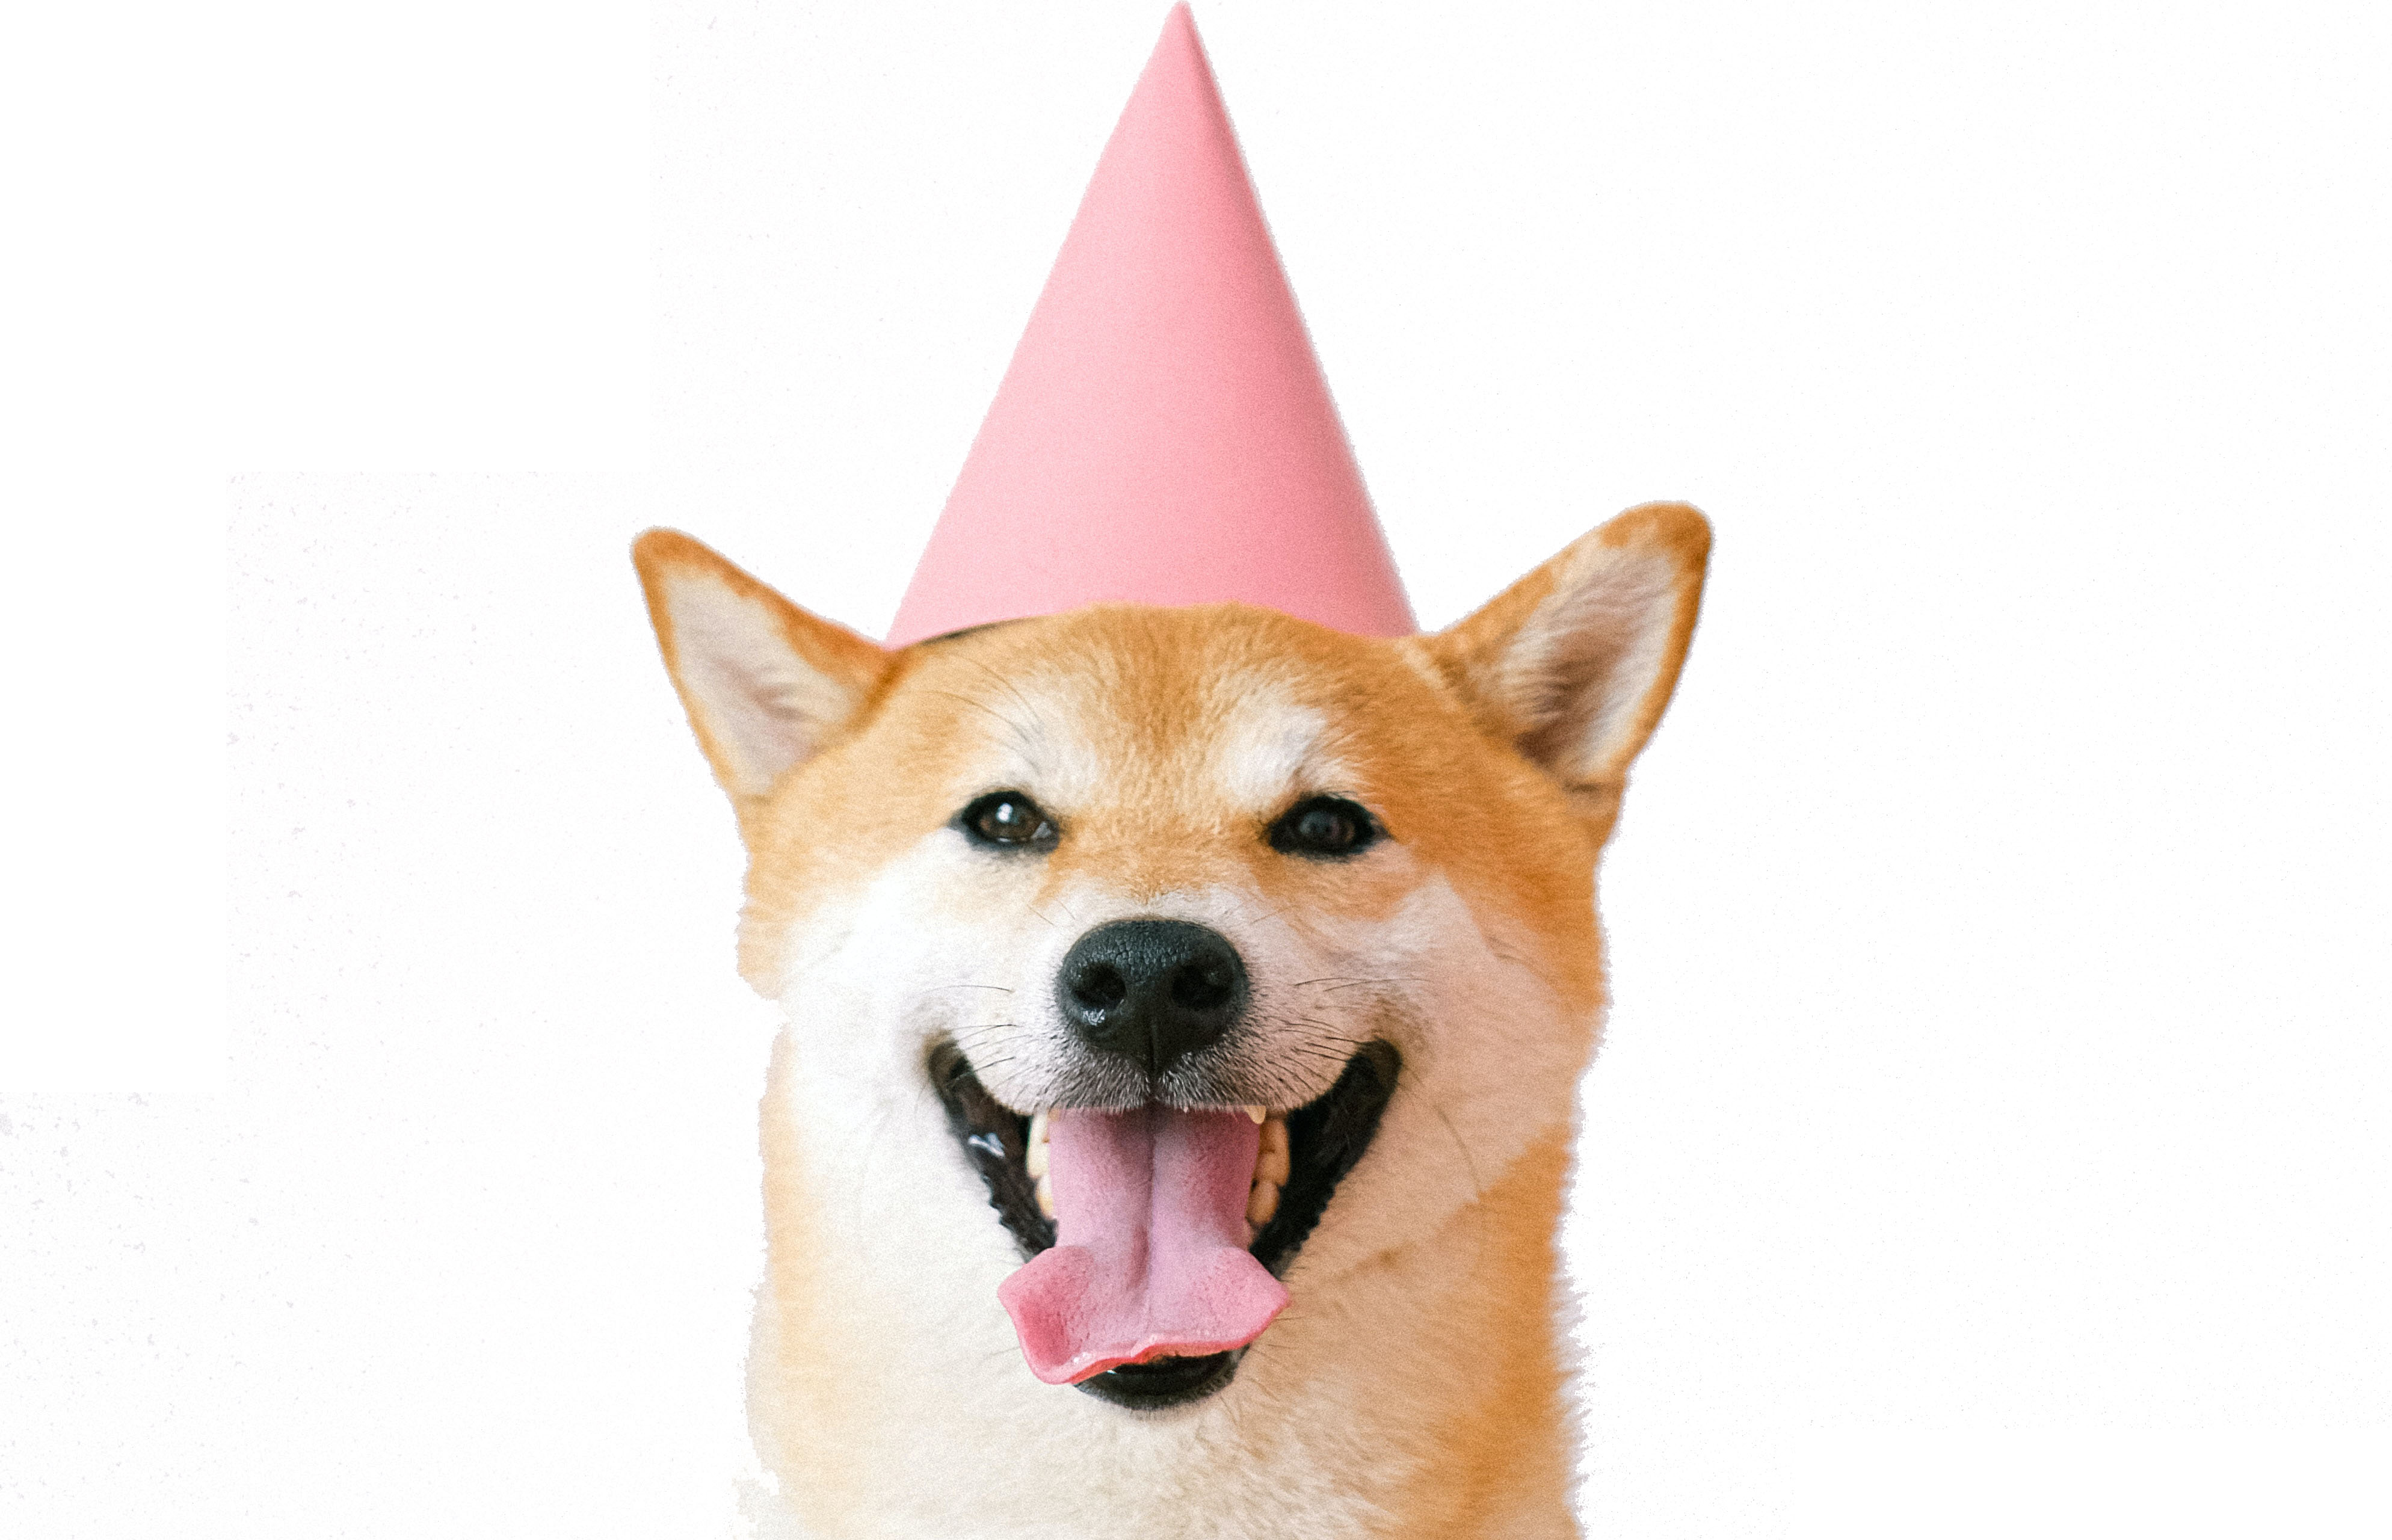
\includegraphics[scale=0.05]{./Chapter10/Figures/dog-hat-new.jpg}
\caption{戴帽子的狗}
\label{fig:10-16}
\end{figure}
%----------------------------------------------

%----------------------------------------------------------------------------------------
%    NEW SUB-SECTION
%----------------------------------------------------------------------------------------
\subsection{翻译中的注意力机制}

\parinterval 早期的神经机器翻译只使用循环神经网络最后一个单元的输出作为整个序列的表示,这种方式有两个明显的缺陷:

\begin{itemize}
\vspace{0.5em}
\item 首先,虽然编码器把一个源语言句子的表示传递给解码器,但是一个维度固定的向量所能包含的信息是有限的,随着源语言序列的增长,将整个句子的信息编码到一个固定维度的向量中可能会造成源语言句子信息的丢失。显然,在翻译较长的句子时,解码端可能无法获取完整的源语言信息,降低翻译性能;
\vspace{0.5em}
\item 此外,当生成某一个目标语言单词时,并不是均匀地使用源语言句子中的单词信息。更普遍的情况是,系统会参考与这个目标语言单词相对应的源语言单词进行翻译。这有些类似于词对齐的作用,即翻译是基于单词之间的某种对应关系。但是,使用单一的源语言表示根本无法区分源语言句子的不同部分,更不用说对源语言单词和目标语言单词之间的联系进行建模了。
\vspace{0.5em}
\end{itemize}

\parinterval 更直观的,如图\ref{fig:10-17},目标语言中的“very long”仅依赖于源语言中的“很长”。这时如果将所有源语言编码成一个固定的实数向量,“很长”的信息就很可能被其他词的信息淹没掉。

%----------------------------------------------
\begin{figure}[htp]
\centering

%

%---------------------------------------


\begin{tikzpicture}
\begin{scope}

%\newlength{\mystep}
%\setlength{\mystep}{1.6em}

\foreach \x in {1,2,...,6}
    \node[] (s\x) at (\x * 1.6em,0) {};

\node [] (ws1) at (s1) {\scriptsize{这}};
\node [] (ws2) at (s2) {\scriptsize{是}};
\node [] (ws3) at (s3) {\scriptsize{个}};
\node [] (ws4) at (s4) {\scriptsize{很长}};
\node [] (ws5) at (s5) {\scriptsize{的}};
\node [] (ws6) at (s6) {\scriptsize{句子}};

\foreach \x in {1,2,...,6}
    \node[] (t\x) at (\x * 1.6em + 2.4in,0) {};

\node [] (wt1) at (t1) {\scriptsize{This}};
\node [] (wt2) at (t2) {\scriptsize{is}};
\node [] (wt3) at ([yshift=-1pt]t3) {\scriptsize{a}};
\node [] (wt4) at ([yshift=-0.1em]t4) {\scriptsize{very}};
\node [] (wt5) at (t5) {\scriptsize{long}};
\node [] (wt6) at ([xshift=1em]t6) {\scriptsize{sentence}};

\node [anchor=south west,fill=red!30,minimum width=1.6in,minimum height=1.5em] (encoder) at ([yshift=1.0em]ws1.north west) {\footnotesize{Encoder}};
\node [anchor=west,fill=blue!30,minimum width=1.9in,minimum height=1.5em] (decoder) at ([xshift=4.5em]encoder.east) {\footnotesize{Decoder}};
\node [anchor=west,fill=green!30,minimum height=1.5em] (representation) at ([xshift=1em]encoder.east) {\footnotesize{表示}};
\draw [->,thick] ([xshift=1pt]encoder.east)--([xshift=-1pt]representation.west);
\draw [->,thick] ([xshift=1pt]representation.east)--([xshift=-1pt]decoder.west);

\foreach \x in {1,2,...,6}
    \draw[->] ([yshift=0.1em]s\x.north) -- ([yshift=1.2em]s\x.north);

\foreach \x in {1,2,...,5}
    \draw[<-] ([yshift=0.1em]t\x.north) -- ([yshift=1.2em]t\x.north);

\draw[<-] ([yshift=0.1em,xshift=1em]t6.north) -- ([yshift=1.2em,xshift=1em]t6.north);


{
\draw [<->,ublue,thick] ([xshift=0.3em]ws4.south) .. controls +(-60:1) and +(south:1) .. (wt4.south);
\draw [<->,ublue,thick] (ws4.south) .. controls +(south:1.0) and +(south:1.5) .. (wt5.south);
}

{
\node [anchor=north,fill=green!30] (attentionlabel) at ([yshift=-3.4em]representation.south) {\footnotesize{词语的关注度}};
\draw [->,dotted,very thick,ublue] ([yshift=0.1em]attentionlabel.north)--([yshift=-0.1em]representation.south);
}

\end{scope}
\end{tikzpicture}
\caption{源语言词和目标语言词的关注度}
\label{fig:10-17}
\end{figure}
%----------------------------------------------

\parinterval 显然,以上问题的根本原因在于所使用的表示模型还比较“弱”。因此需要一个更强大的表示模型,在生成目标语言单词时能够有选择地获取源语言句子中更有用的部分。更准确的说,对于要生成的目标语单词,相关性更高的源语言片段应该在源语言句子的表示中体现出来,而不是将所有的源语言单词一视同仁。在神经机器翻译中引入注意力机制正是为了达到这个目的\upcite{bahdanau2014neural,DBLP:journals/corr/LuongPM15}。实际上,除了机器翻译,注意力机制也被成功地应用于图像处理、语音识别、自然语言处理等其他任务。也正是注意力机制的引入,使得包括机器翻译在内很多自然语言处理系统得到了飞跃发展。

\parinterval 神经机器翻译中的注意力机制并不复杂。对于每个目标语言单词$y_j$,系统生成一个源语言表示向量$\mathbi{C}_j$与之对应,$\mathbi{C}_j$会包含生成$y_j$所需的源语言的信息,或者说$\mathbi{C}_j$是一种包含目标语言单词与源语言单词对应关系的源语言表示。相比用一个静态的表示$\mathbi{C}$,注意机制使用的是动态的表示$\mathbi{C}_j$。$\mathbi{C}_j$也被称作对于目标语言位置$j$的{\small\bfnew{上下文向量}}\index{上下文向量}(Context Vector\index{Context Vector})。图\ref{fig:10-18}对比了未引入注意力机制和引入了注意力机制的编码器- 解码器结构。可以看出,在注意力模型中,对于每一个目标单词的生成,都会额外引入一个单独的上下文向量参与运算。

%----------------------------------------------
\begin{figure}[htp]
\centering



%---------------------------------------------------------


\begin{tikzpicture}

%\setlength{\mystep}{1.6em}

%%% a simple encoder-decoder model
\begin{scope}
\foreach \x in {1,2,...,6}
    \node[] (s\x) at (\x * 2em,0) {};

\node [] (ws1) at (s1) {\scriptsize{这}};
\node [] (ws2) at (s2) {\scriptsize{是}};
\node [] (ws3) at (s3) {\scriptsize{个}};
\node [] (ws4) at (s4) {\scriptsize{很长}};
\node [] (ws5) at (s5) {\scriptsize{的}};
\node [] (ws6) at (s6) {\scriptsize{句子}};

\foreach \x in {1,2,...,6}
    \node[] (t\x) at (\x * 2em + 2.8in,0) {};

\node [] (wt1) at (t1) {\scriptsize{This}};
\node [] (wt2) at (t2) {\scriptsize{is}};
\node [] (wt3) at ([yshift=-1pt]t3) {\scriptsize{a}};
\node [] (wt4) at ([yshift=-0.1em]t4) {\scriptsize{very}};
\node [] (wt5) at (t5) {\scriptsize{long}};
\node [] (wt6) at ([xshift=1em]t6) {\scriptsize{sentence}};

\node [anchor=south west,fill=red!30,minimum width=1.9in,minimum height=1.5em] (encoder) at ([yshift=1.0em,xshift=-0.4em]ws1.north west) {\footnotesize{Encoder}};
\node [anchor=west,fill=green!30,minimum height=1.5em] (representation) at ([xshift=2em]encoder.east) {\footnotesize{表示}};
\node [anchor=west,fill=blue!30,minimum width=1.9in,minimum height=1.5em] (decoder) at ([xshift=2em]representation.east) {\footnotesize{Decoder}};
\draw [->,thick] ([xshift=1pt]encoder.east)--([xshift=-1pt]representation.west);
\draw [->,thick] ([xshift=1pt]representation.east)--([xshift=-1pt]decoder.west);

\foreach \x in {1,2,...,6}
    \draw[->] ([yshift=0.1em]s\x.north) -- ([yshift=1.2em]s\x.north);

\foreach \x in {1,2,...,5}
    \draw[<-] ([yshift=0.1em]t\x.north) -- ([yshift=1.2em]t\x.north);

\draw[<-,thick] ([yshift=0.1em,xshift=1em]t6.north) -- ([yshift=1.2em,xshift=1em]t6.north);
\node [anchor=north] (cap) at ([xshift=2em,yshift=-2.5em]encoder.south east) {\small{(a) 简单的编码器-解码器框架}};

\end{scope}

%%% a encoder-decoder model with attention
\begin{scope}[yshift=-1.7in]
\foreach \x in {1,2,...,6}
    \node[] (s\x) at (\x * 2em,0) {};

\node [] (ws1) at (s1) {\scriptsize{这}};
\node [] (ws2) at (s2) {\scriptsize{是}};
\node [] (ws3) at (s3) {\scriptsize{个}};
\node [] (ws4) at (s4) {\scriptsize{很长}};
\node [] (ws5) at (s5) {\scriptsize{的}};
\node [] (ws6) at (s6) {\scriptsize{句子}};

\foreach \x in {1,2,...,6}
    \node[] (t\x) at (\x * 2em + 2.8in,0) {};

\node [] (wt1) at (t1) {\scriptsize{This}};
\node [] (wt2) at (t2) {\scriptsize{is}};
\node [] (wt3) at ([yshift=-1pt]t3) {\scriptsize{a}};
\node [] (wt4) at ([yshift=-0.1em]t4) {\scriptsize{very}};
\node [] (wt5) at (t5) {\scriptsize{long}};
\node [] (wt6) at ([xshift=1em]t6) {\scriptsize{sentence}};

\node [anchor=south west,fill=red!30,minimum width=1.9in,minimum height=1.5em] (encoder) at ([yshift=1.0em,xshift=-0.4em]ws1.north west) {\footnotesize{Encoder}};
\node [anchor=west,fill=blue!30,minimum width=1.9in,minimum height=1.5em] (decoder) at ([xshift=6.4em]encoder.east) {\footnotesize{Decoder}};

\foreach \x in {1,2,...,6}
    \draw[->] ([yshift=0.1em]s\x.north) -- ([yshift=1.2em]s\x.north);

\foreach \x in {1,2,...,5}
    \draw[<-] ([yshift=0.1em]t\x.north) -- ([yshift=1.2em]t\x.north);

\draw[<-,thick] ([yshift=0.1em,xshift=1em]t6.north) -- ([yshift=1.2em,xshift=1em]t6.north);

\draw [->,thick] ([yshift=3em]s6.north) -- ([yshift=4em]s6.north) -- ([yshift=4em]t1.north) node [pos=0.5,fill=green!30,inner sep=2pt] (c1) {\scriptsize{表示$\mathbi{C}_1$}} -- ([yshift=3em]t1.north) ;
\draw [->,thick] ([yshift=3em]s5.north) -- ([yshift=5.3em]s5.north) -- ([yshift=5.3em]t2.north) node [pos=0.5,fill=green!30,inner sep=2pt] (c2) {\scriptsize{表示$\mathbi{C}_2$}} -- ([yshift=3em]t2.north) ;
\draw [->,thick] ([yshift=3.5em]s3.north) -- ([yshift=6.6em]s3.north) -- ([yshift=6.6em]t4.north) node [pos=0.5,fill=green!30,inner sep=2pt] (c3) {\scriptsize{表示$\mathbi{C}_i$}} -- ([yshift=3.5em]t4.north) ;
\node [anchor=north] (smore) at ([yshift=3.5em]s3.north) {...};
\node [anchor=north] (tmore) at ([yshift=3.5em]t4.north) {...};

\node [anchor=north] (cap) at ([xshift=2em,yshift=-2.5em]encoder.south east) {\small{(b) 引入注意力机制的编码器-解码器框架}};

\end{scope}

\end{tikzpicture}
\caption{不使用(a)和使用(b)注意力机制的翻译模型对比}
\label{fig:10-18}
\end{figure}
%----------------------------------------------

%----------------------------------------------------------------------------------------
%    NEW SUB-SECTION
%----------------------------------------------------------------------------------------
\subsection{上下文向量的计算}
\label{sec:10.1.3}

\parinterval 神经机器翻译中,注意力机制的核心是:针对不同目标语言单词生成不同的上下文向量。这里,可以将注意力机制看做是一种对接收到的信息的加权处理。对于更重要的信息赋予更高的权重即更高的关注度,对于贡献度较低的信息分配较低的权重,弱化其对结果的影响。这样,$\mathbi{C}_j$可以包含更多对当前目标语言位置有贡献的源语言片段的信息。

\parinterval 根据这种思想,上下文向量$\mathbi{C}_j$被定义为对不同时间步编码器输出的状态序列$\{ \mathbi{h}_1, \mathbi{h}_2,...,\mathbi{h}_m \}$进行加权求和,如公式\eqref{eq:10-16}所示:
\begin{eqnarray}
\mathbi{C}_j=\sum_{i} \alpha_{i,j} \mathbi{h}_i
\label{eq:10-16}
\end{eqnarray}

\noindent 其中,$\alpha_{i,j}$是{\small\sffamily\bfseries{注意力权重}}\index{注意力权重}(Attention Weight)\index{Attention Weight},它表示目标语言第$j$个位置与源语言第$i$个位置之间的相关性大小。这里,将每个时间步编码器的输出$\mathbi{h}_i$ 看作源语言位置$i$的表示结果。进行翻译时,解码端可以根据当前的位置$j$,通过控制不同$\mathbi{h}_i$的权重得到$\mathbi{C}_j$,使得对目标语言位置$j$贡献大的$\mathbi{h}_i$对$\mathbi{C}_j$的影响增大。也就是说,$\mathbi{C}_j$实际上就是\{${\mathbi{h}_1, \mathbi{h}_2,...,\mathbi{h}_m}$\}的一种组合,只不过不同的$\mathbi{h}_i$会根据对目标端的贡献给予不同的权重。图\ref{fig:10-19}展示了上下文向量$\mathbi{C}_j$的计算过程。

%----------------------------------------------
\begin{figure}[htp]
\centering






\begin{tikzpicture}

\begin{scope}

\node [anchor=west,draw,fill=red!20!white,inner sep=3pt,minimum width=2em,minimum height=1.2em] (h1) at (0,0) {\scriptsize{$\vectorn{\emph{h}}_1$}};
\node [anchor=west,draw,fill=red!20!white,inner sep=3pt,minimum width=2em,minimum height=1.2em] (h2) at ([xshift=1em]h1.east) {\scriptsize{$\vectorn{\emph{h}}_2$}};
\node [anchor=west,inner sep=0pt,minimum width=3em] (h3) at ([xshift=0.5em]h2.east) {\scriptsize{...}};
\node [anchor=west,draw,fill=red!20!white,inner sep=3pt,minimum width=2em,minimum height=1.2em] (h4) at ([xshift=0.5em]h3.east) {\scriptsize{$\vectorn{\emph{h}}_m$}};

\node [anchor=south,circle,minimum size=1.0em,draw,ublue,thick] (sum) at ([yshift=2em]h2.north east) {};
\draw [thick,-,ublue] (sum.north) -- (sum.south);
\draw [thick,-,ublue] (sum.west) -- (sum.east);

\node [anchor=south,draw,fill=green!20!white,inner sep=3pt,minimum width=2em,minimum height=1.2em] (th1) at ([yshift=2em,xshift=-1em]sum.north west) {\scriptsize{$\vectorn{\emph{s}}_{j-1}$}};
\node [anchor=west,draw,fill=green!20!white,inner sep=3pt,minimum width=2em,minimum height=1.2em] (th2) at ([xshift=2em]th1.east) {\scriptsize{$\vectorn{\emph{s}}_{j}$}};

\draw [->] (h1.north) .. controls +(north:0.8) and +(west:1) ..  (sum.190) node [pos=0.2,left] {\scriptsize{$\alpha_{1,j}$}};
\draw [->] (h2.north) .. controls +(north:0.6) and +(220:0.2) ..  (sum.220) node [pos=0.2,right] {\scriptsize{$\alpha_{2,j}$}};
\draw [->] (h4.north) .. controls +(north:0.8) and +(east:1) ..  (sum.-10) node [pos=0.1,left] (alphan) {\scriptsize{$\alpha_{m,j}$}};

\draw [->] ([xshift=-1.5em]th1.west) -- ([xshift=-0.1em]th1.west);
\draw [->] ([xshift=0.1em]th1.east) -- ([xshift=-0.1em]th2.west);
\draw [->] ([xshift=0.1em]th2.east) -- ([xshift=1.5em]th2.east);
\draw [->] (sum.north) .. controls +(north:0.8) and +(west:0.2) ..  ([yshift=-0.4em,xshift=-0.1em]th2.west) node [pos=0.2,right] (ci) {\scriptsize{$\vectorn{\emph{C}}_{j}$}};

\node [anchor=south,inner sep=1pt] (output) at ([yshift=0.8em]th2.north) {\scriptsize{输出层}};
\draw [->] ([yshift=0.1em]th2.north) -- ([yshift=-0.1em]output.south);
\node [anchor=north] (enc1) at (h1.south west) {\scriptsize{编码器输出}};
\node [anchor=north] (enc12) at ([yshift=0.5em]enc1.south) {\scriptsize{(位置$1$)}};
\node [anchor=north] (enc2) at (h2.south) {\scriptsize{编码器输出}};
\node [anchor=north] (enc22) at ([yshift=0.5em]enc2.south) {\scriptsize{(位置$2$)}};
\node [anchor=north] (enc4) at (h4.south) {\scriptsize{编码器输出}};
\node [anchor=north] (enc42) at ([yshift=0.5em]enc4.south) {\scriptsize{(位置$4$)}};

{
\node [anchor=west] (math1) at ([xshift=5em,yshift=1em]th2.east) {$\vectorn{\emph{C}}_j = \sum_{i} \alpha_{i,j} \vectorn{\emph{h}}_i \ \ $};
}
{
\node [anchor=north west] (math2) at ([yshift=-2em]math1.south west) {$\alpha_{i,j} = \frac{\exp(\beta_{i,j})}{\sum_{i'} \exp(\beta_{i',j})}$};
\node [anchor=north west] (math3) at ([yshift=-0em]math2.south west) {$\beta_{i,j} = a(\vectorn{\emph{s}}_{j-1}, \vectorn{\emph{h}}_i)$};
}

\begin{pgfonlayer}{background}
{
\node [rectangle,inner sep=0.4em,rounded corners=1pt,fill=blue!10,drop shadow] [fit = (math1)] (box1) {};
}
{
\node [rectangle,inner sep=0.4em,rounded corners=1pt,fill=orange!10,drop shadow] [fit = (math2) (math3)] (box2) {};
}
\end{pgfonlayer}

{
\draw [->,dotted,thick,blue] (box1.west) .. controls +(west:1.2) and +(east:2.0) .. ([xshift=-0.3em]ci.east);
}
{
\draw [->,dotted,thick,orange] ([yshift=1em]box2.west) .. controls +(west:1.2) and +(east:1.0) .. ([xshift=-0.35em]alphan.east);
}

\end{scope}

\end{tikzpicture}
\caption{上下文向量$\mathbi{C}_j$的计算过程}
\label{fig:10-19}
\end{figure}
%----------------------------------------------

\parinterval 如图\ref{fig:10-19}所示,注意力权重$\alpha_{i,j}$的计算分为两步:

\begin{itemize}
\vspace{0.5em}
\item	使用目标语言上一时刻循环单元的输出$\mathbi{s}_{j-1}$与源语言第$i$个位置的表示$\mathbi{h}_i$之间的相关性,其用来表示目标语言位置$j$对源语言位置$i$的关注程度,记为$\beta_{i,j}$,由函数$a(\cdot)$实现,其具体计算如公式\eqref{eq:10-17}所示:
\begin{eqnarray}
\beta_{i,j} = a(\mathbi{s}_{j-1},\mathbi{h}_i)
\label{eq:10-17}
\end{eqnarray}

$a(\cdot)$可以被看作是目标语言表示和源语言表示的一种“统一化”,即把源语言和目标语言表示映射在同一个语义空间,进而语义相近的内容有更大的相似性。该函数有多种计算方式,比如,向量乘、向量夹角和单层神经网络等,具体数学表达如公式\eqref{eq:10-18}:
\begin{eqnarray}
a (\mathbi{s},\mathbi{h}) =  \left\{ \begin{array}{ll}
    \mathbi{s} \mathbi{h}^{\textrm{T}} & \textrm{向量乘} \\
    \textrm{cos}(\mathbi{s}, \mathbi{h}) & \textrm{向量夹角} \\
    \mathbi{s} \mathbi{W} \mathbi{h}^{\textrm{T}} & \textrm{线性模型} \\
    \textrm{Tanh}(\mathbi{W}[\mathbi{s},\mathbi{h}])\mathbi{v}^{\textrm{T}} & \textrm{拼接}[\mathbi{s},\mathbi{h}]+\textrm{单层网络}
    \end{array}
    \right.
\label{eq:10-18}
\end{eqnarray}

其中$\mathbi{W}$和$\mathbi{v}$是可学习的参数。
\vspace{0.5em}
\item	进一步,利用Softmax函数,将相关性系数$\beta_{i,j}$进行指数归一化处理,得到注意力权重$\alpha_{i,j}$,具体计算如公式\eqref{eq:10-19}:
\vspace{0.5em}
\begin{eqnarray}
\alpha_{i,j}=\frac{\textrm{exp}(\beta_{i,j})} {\sum_{i'} \textrm{exp}(\beta_{i',j})}
\label{eq:10-19}
\end{eqnarray}
\vspace{-1em}
%----------------------------------------------
\begin{figure}[htp]
\centering





%-------------------------------------------
\begin{tikzpicture}


%\setlength{\hnode}{1.2cm}

\tikzstyle{elementnode} = [rectangle,text=white,anchor=center]
\tikzstyle{srcnode} = [rotate=45,font=\small,anchor=south west]
\tikzstyle{tgtnode} = [left,font=\small,anchor=north east]
\tikzstyle{alignmentnode} = [rectangle,draw,minimum height=3.6cm,minimum width=0.36cm]
\tikzstyle{probnode} = [fill=blue!30,minimum width=0.4cm]
\tikzstyle{labelnode} = [above]

% alignment matrix
\begin{scope}[scale=0.9,yshift=0.12in]
\foreach \i / \j / \c in
    {0/7/0.2, 1/7/0.45, 2/7/0.15, 3/7/0.15, 4/7/0.15, 5/7/0.15,
    0/6/0.35, 1/6/0.45, 2/6/0.15, 3/6/0.15, 4/6/0.15, 5/6/0.15,
    0/5/0.25, 1/5/0.15, 2/5/0.15, 3/5/0.35, 4/5/0.15, 5/5/0.15,
    0/4/0.15, 1/4/0.25, 2/4/0.2, 3/4/0.35, 4/4/0.15, 5/4/0.15,
    0/3/0.15, 1/3/0.15, 2/3/0.8, 3/3/0.25, 4/3/0.15, 5/3/0.25,
    0/2/0.15, 1/2/0.15, 2/2/0.15, 3/2/0.15, 4/2/0.25, 5/2/0.3,
    0/1/0.15, 1/1/0.15, 2/1/0.15, 3/1/0.15, 4/1/0.8, 5/1/0.15,
    0/0/0.15, 1/0/0.15, 2/0/0.15, 3/0/0.15, 4/0/0.25, 5/0/0.60}
    \node[elementnode,minimum size=0.6*1.2cm*\c,inner sep=0.1pt,fill=blue] (a\i\j) at (0.5*1.2cm*\i-5.4*0.5*1.2cm,0.5*1.2cm*\j-1.05*1.2cm) {};

%attention score labels
\node[align=center,scale=0.8] (l17) at (a17) {\scriptsize{{\color{white} 0.4}}};
\node[align=center,scale=0.8] (l26) at (a06) {\scriptsize{{\color{white} 0.3}}};
\node[align=center,scale=0.8] (l26) at (a16) {\scriptsize{{\color{white} 0.4}}};
\node[align=center,scale=0.8] (l17) at (a35) {\scriptsize{{\color{white} 0.3}}};
\node[align=center,scale=0.8] (l17) at (a34) {\scriptsize{{\color{white} 0.3}}};
\node[align=center] (l17) at (a23) {\small{{\color{white} 0.8}}};
\node[align=center] (l17) at (a41) {\small{{\color{white} 0.8}}};
\node[align=center] (l17) at (a50) {\small{{\color{white} 0.7}}};

% source
\node[srcnode] (src1) at (-5.4*0.5*1.2cm,-1.05*1.2cm+7.5*0.5*1.2cm) {\scriptsize{Have}};
\node[srcnode] (src2) at ([xshift=0.6cm]src1.south west) {\scriptsize{you}};
\node[srcnode] (src3) at ([xshift=0.6cm]src2.south west) {\scriptsize{learned}};
\node[srcnode] (src4) at ([xshift=0.6cm]src3.south west) {\scriptsize{nothing}};
\node[srcnode] (src5) at ([xshift=0.6cm]src4.south west) {\scriptsize{?}};
\node[srcnode] (src6) at ([xshift=0.6cm]src5.south west) {\scriptsize{$\langle$eos$\rangle$}};

% target
\node[tgtnode] (tgt1) at (-6.0*0.5*1.2cm,-1.05*1.2cm+7.5*0.5*1.2cm) {\scriptsize{你}};
\node[tgtnode] (tgt2) at ([yshift=-0.6cm]tgt1.north east) {\scriptsize{什么}};
\node[tgtnode] (tgt3) at ([yshift=-0.6cm]tgt2.north east) {\scriptsize{都}};
\node[tgtnode] (tgt4) at ([yshift=-0.6cm]tgt3.north east) {\scriptsize{没}};
\node[tgtnode] (tgt5) at ([yshift=-0.6cm]tgt4.north east) {\scriptsize{学}};
\node[tgtnode] (tgt6) at ([yshift=-0.6cm]tgt5.north east) {\scriptsize{到}};
\node[tgtnode] (tgt7) at ([yshift=-0.6cm]tgt6.north east) {\scriptsize{?}};
\node[tgtnode] (tgt8) at ([yshift=-0.6cm]tgt7.north east) {\scriptsize{$\langle$eos$\rangle$}};

\end{scope}


\end{tikzpicture}
%-------------------------------------------
\caption{一个汉英句对之间的注意力权重{$\alpha_{i,j}$}的矩阵表示}
\label{fig:10-20}
\end{figure}
%----------------------------------------------

最终,\{$\alpha_{i,j}$\}可以被看作是一个矩阵,它的长为目标语言句子长度,宽为源语言句子长度,矩阵中的每一项对应一个$\alpha_{i,j}$。图\ref{fig:10-20}给出了\{$\alpha_{i,j}$\}的一个矩阵表示。图中蓝色方框的大小表示不同的注意力权重$\alpha_{i,j}$的大小,方框越大,源语言位置$i$和目标语言位置$j$的相关性越高。能够看到,对于互译的中英文句子,\{$\alpha_{i,j}$\}可以较好的反应两种语言之间不同位置的对应关系。

\vspace{0.5em}
\end{itemize}

\parinterval 图\ref{fig:10-21}展示了一个上下文向量的计算过程实例。首先,计算目标语言第一个单词“Have”与源语言中的所有单词的相关性,即注意力权重,对应图中第一列$\alpha_{i,1}$,则当前时刻所使用的上下文向量$\mathbi{C}_1 = \sum_{i=1}^8 \alpha_{i,1} \mathbi{h}_i$;然后,计算第二个单词“you”的注意力权重对应第二列$\alpha_{i,2}$,其上下文向量$\mathbi{C}_2 = \sum_{i=1}^8 \alpha_{i,2} \mathbi{h}_i$,以此类推,可以得到任意目标语言位置$j$的上下文向量$\mathbi{C}_j$。很容易看出,不同目标语言单词的上下文向量对应的源语言词的权重$\alpha_{i,j}$是不同的,不同的注意力权重为不同位置赋予了不同的重要性。

%----------------------------------------------
\begin{figure}[htp]
\centering



%-------------------------------------------


\begin{tikzpicture}

%\newlength{\mystep}
%\newlength{\wseg}
%\newlength{\hseg}
%\newlength{\wnode}
%\newlength{\hnode}

\setlength{\wseg}{1.5cm}
\setlength{\hseg}{1.0cm}
\setlength{\wnode}{3.75cm}
\setlength{\hnode}{1.0cm}

\tikzstyle{elementnode} = [rectangle,text=white,anchor=center]
\tikzstyle{srcnode} = [rotate=45,font=\small,anchor=south west]
\tikzstyle{tgtnode} = [left,font=\small,anchor=north east]
\tikzstyle{alignmentnode} = [rectangle,draw,minimum height=3.6\hnode,minimum width=0.36\hnode]
\tikzstyle{probnode} = [fill=blue!30,minimum width=0.4\hnode]
\tikzstyle{labelnode} = [above]

% alignment matrix
\begin{scope}[scale=0.9,yshift=0.12in]
\foreach \i / \j / \c in
    {0/7/0.2, 1/7/0.45, 2/7/0.15, 3/7/0.15, 4/7/0.15, 5/7/0.15,
    0/6/0.35, 1/6/0.45, 2/6/0.15, 3/6/0.15, 4/6/0.15, 5/6/0.15,
    0/5/0.25, 1/5/0.15, 2/5/0.15, 3/5/0.35, 4/5/0.15, 5/5/0.15,
    0/4/0.15, 1/4/0.25, 2/4/0.2, 3/4/0.30, 4/4/0.15, 5/4/0.15,
    0/3/0.15, 1/3/0.15, 2/3/0.8, 3/3/0.25, 4/3/0.15, 5/3/0.25,
    0/2/0.15, 1/2/0.15, 2/2/0.15, 3/2/0.15, 4/2/0.25, 5/2/0.3,
    0/1/0.15, 1/1/0.15, 2/1/0.15, 3/1/0.15, 4/1/0.8, 5/1/0.15,
    0/0/0.15, 1/0/0.15, 2/0/0.15, 3/0/0.15, 4/0/0.25, 5/0/0.60}
    \node[elementnode,minimum size=0.6*\hnode*\c,inner sep=0.1pt,fill=blue] (a\i\j) at (0.5*\hnode*\i-5.4*0.5*\hnode,0.5*\hnode*\j-1.05*\hnode) {};

%attention score labels
\node[align=center] (l17) at (a17) {\scriptsize{{\color{white} .4}}};
\node[align=center] (l26) at (a06) {\scriptsize{{\color{white} .3}}};
\node[align=center] (l26) at (a16) {\scriptsize{{\color{white} .4}}};
\node[align=center] (l17) at (a35) {\scriptsize{{\color{white} .3}}};
\node[align=center] (l17) at (a34) {\tiny{{\color{white} .3}}};
\node[align=center] (l17) at (a23) {\small{{\color{white} .8}}};
\node[align=center] (l17) at (a41) {\small{{\color{white} .8}}};
\node[align=center] (l17) at (a50) {\small{{\color{white} .7}}};

% source
\node[srcnode] (src1) at (-5.4*0.5*\hnode,-1.05*\hnode+7.5*0.5*\hnode) {\scriptsize{Have}};
\node[srcnode] (src2) at ([xshift=0.5\hnode]src1.south west) {\scriptsize{you}};
\node[srcnode] (src3) at ([xshift=0.5\hnode]src2.south west) {\scriptsize{learned}};
\node[srcnode] (src4) at ([xshift=0.5\hnode]src3.south west) {\scriptsize{nothing}};
\node[srcnode] (src5) at ([xshift=0.5\hnode]src4.south west) {\scriptsize{?}};
\node[srcnode] (src6) at ([xshift=0.5\hnode]src5.south west) {\scriptsize{$\langle$eos$\rangle$}};

% target
\node[tgtnode] (tgt1) at (-6.0*0.5*\hnode,-1.05*\hnode+7.5*0.5*\hnode) {\scriptsize{你}};
\node[tgtnode] (tgt2) at ([yshift=-0.5\hnode]tgt1.north east) {\scriptsize{什么}};
\node[tgtnode] (tgt3) at ([yshift=-0.5\hnode]tgt2.north east) {\scriptsize{都}};
\node[tgtnode] (tgt4) at ([yshift=-0.5\hnode]tgt3.north east) {\scriptsize{没}};
\node[tgtnode] (tgt5) at ([yshift=-0.5\hnode]tgt4.north east) {\scriptsize{学}};
\node[tgtnode] (tgt6) at ([yshift=-0.5\hnode]tgt5.north east) {\scriptsize{到}};
\node[tgtnode] (tgt7) at ([yshift=-0.5\hnode]tgt6.north east) {\scriptsize{?}};
\node[tgtnode] (tgt8) at ([yshift=-0.5\hnode]tgt7.north east) {\scriptsize{$\langle$eos$\rangle$}};

\end{scope}

%\visible<2->
{
% alignment rectangle 2
\node[alignmentnode, ugreen, anchor=north west] (alignment1) at ([xshift=-0.3em,yshift=0.4em]a07.north west) {};
}

%\visible<3->
{
% alignment rectangle 1
\node[alignmentnode, red, anchor=north west] (alignment2) at ([xshift=-0.1em,yshift=0.2em]a17.north west) {};
}

%\visible<3->
{
% alignment bars 2
\node[probnode,anchor=south west,minimum height=0.4\hnode,inner sep=0.1pt,fill=red!40,label=below:\scriptsize{$0.4$}] (attn21) at ([xshift=2.3\hnode,yshift=0.5\hnode]alignment2.east) {};
\node[probnode,anchor=south west,minimum height=0.4\hnode,inner sep=0.1pt,fill=red!40,label=below:\scriptsize{$0.4$}] (attn22) at ([xshift=1pt]attn21.south east) {};
\node[probnode,anchor=south west,minimum height=0.05\hnode,inner sep=0.1pt,fill=red!40,label=below:\scriptsize{$0$}] (attn23) at ([xshift=1pt]attn22.south east) {};
\node[probnode,anchor=south west,minimum height=0.1\hnode,inner sep=0.1pt,fill=red!40,label=below:\scriptsize{$0.1$}] (attn24) at ([xshift=1pt]attn23.south east) {};
\node[probnode,anchor=south west,minimum height=0.05\hnode,inner sep=0.1pt,fill=red!40,label=below:\scriptsize{$0$}] (attn25) at ([xshift=1pt]attn24.south east) {};
\node[probnode,anchor=south west,minimum height=0.05\hnode,inner sep=0.1pt,fill=red!40,label=below:\scriptsize{$...$}] (attn26) at ([xshift=1pt]attn25.south east) {};
}

%\visible<2->
{
% alignment bars 1
\node[probnode,anchor=south,minimum height=0.2\hnode,inner sep=0.1pt,fill=ugreen!40,label=below:\scriptsize{$0.2$}] (attn11) at ([xshift=2.5\hnode,yshift=-1em]alignment2.north east) {};
\node[probnode,anchor=south west,minimum height=0.3\hnode,inner sep=0.1pt,fill=ugreen!40,label=below:\scriptsize{$0.3$}] (attn12) at ([xshift=1pt]attn11.south east) {};
\node[probnode,anchor=south west,minimum height=0.2\hnode,inner sep=0.1pt,fill=ugreen!40,label=below:\scriptsize{$0.2$}] (attn13) at ([xshift=1pt]attn12.south east) {};
\node[probnode,anchor=south west,minimum height=0.05\hnode,inner sep=0.1pt,fill=ugreen!40,label=below:\scriptsize{$0$}] (attn14) at ([xshift=1pt]attn13.south east) {};
\node[probnode,anchor=south west,minimum height=0.05\hnode,inner sep=0.1pt,fill=ugreen!40,label=below:\scriptsize{$0$}] (attn15) at ([xshift=1pt]attn14.south east) {};
\node[probnode,anchor=south west,minimum height=0.05\hnode,inner sep=0.1pt,fill=ugreen!40,label=below:\scriptsize{$...$}] (attn16) at ([xshift=1pt]attn15.south east) {};
}

%\visible<3->
{
% coverage score formula node
\node [anchor=north west] (formula) at ([xshift=-0.3\hnode,yshift=-1.5\hnode]attn11.south) {\small{不同$\textbf{C}_j$所对应的源语言词的权重是不同的}};
\node [anchor=north west] (example) at (formula.south west) {\footnotesize{$\textbf{C}_2=0.4 \times \textbf{h}(\textrm{``你''}) + 0.4 \times \textbf{h}(\textrm{``什么''}) +$}};
\node [anchor=north west] (example2) at ([yshift=0.4em]example.south west) {\footnotesize{$\ \ \ \ \ \ \ \ 0 \times \textbf{h}(\textrm{``都''}) + 0.1 \times \textbf{h}(\textrm{`` 没''}) + ..$}};
}

%\visible<3->
{
% matrix -> attn2
\draw[->,red] ([xshift=0.1em,yshift=2.3em]alignment2.east).. controls +(east:1.9cm) and +(west:1.0cm) ..([xshift=-0.15\hnode,yshift=-1em]attn21.north west);
}


%\visible<2->
{
\draw[->,ugreen] ([xshift=0.1em,yshift=-1.2em]alignment1.north east)--([xshift=2.2\hnode,yshift=-1.2em]alignment2.north east);
}

%\visible<3->
{
% attn2 -> cov2
\draw[->] ([xshift=0.2\hnode,yshift=0.0\hnode]attn26.east)--([xshift=0.7\hnode,yshift=0]attn26.east) node[pos=0.5,above] (sum2) {\small{$\sum$}}; % 0.3 - 0.5 height of the
}


%\visible<2->
{
% attn1 -> cov1
\draw[->] ([xshift=0.2\hnode]attn16.east)--([xshift=0.7\hnode]attn16.east) node[pos=0.5,above] (sum1) {\small{$\sum$}};
}

% coverage score for each source word

%\visible<2->
{
\node[anchor=west] (sc1) at ([xshift=0.9\hnode]attn16.east) {$\textbf{C}_1 = \sum_{i=1}^{8} \alpha_{i1} \textbf{h}_{i}$};
}

%\visible<3->
{
\node[anchor=west] (sc2) at ([xshift=0.9\hnode,yshift=0.0\hnode]attn26.east) {$\textbf{C}_2 = \sum_{i=1}^{8} \alpha_{i2} \textbf{h}_{i}$};
}

\end{tikzpicture}
\caption{上下文向量计算过程实例}
\label{fig:10-21}
\end{figure}
%----------------------------------------------

\parinterval 在\ref{sec:10.3.1}节中,公式\eqref{eq:10-4}描述了目标语言单词生成概率$ \funp{P} (y_j | \mathbi{y}_{<j},\mathbi{x})$。在引入注意力机制后,不同时刻的上下文向量$\mathbi{C}_j$替换了传统模型中固定的句子表示$\mathbi{C}$。描述如公式\eqref{eq:10-20}:
\begin{eqnarray}
\funp{P} (y_j | \mathbi{y}_{<j},\mathbi{x}) \equiv \funp{P} (y_j | \mathbi{s}_{j-1},y_{j-1},\mathbi{C}_j )
\label{eq:10-20}
\end{eqnarray}

\parinterval 这样,可以在生成每个$y_j$时动态的使用不同的源语言表示$\mathbi{C}_j$,并更准确地捕捉源语言和目标语言不同位置之间的相关性。表\ref{tab:10-7}展示了引入注意力机制前后译文单词生成公式的对比。
\vspace{-0.5em}
%----------------------------------------------
\begin{table}[htp]
\centering
\caption{引入注意力机制前后译文单词生成公式}
\label{tab:10-7}
\begin{tabular}{ l | l }
\rule{0pt}{13pt}	引入注意力之前			&引入注意力之后 \\ \hline
\rule{0pt}{16pt}	$\textrm{have} = \argmax_{y_1}  \funp{P} (y_1 | \mathbi{C} , y_0)$		&$\textrm{have} = \argmax_{y_1}  \funp{P} (y_1 | \mathbi{C}_1 , y_0)$	\\
\rule{0pt}{16pt}	$\textrm{you} = \argmax_{y_2} \funp{P} (y_2 | \mathbi{s}_1 , y_1)$			&$\textrm{you} = \argmax_{y_2} \funp{P} (y_2 | \mathbi{s}_1, \mathbi{C}_2 , y_1)$	\\
\end{tabular}
\end{table}
%----------------------------------------------

%----------------------------------------------------------------------------------------
%    NEW SUB-SECTION
%----------------------------------------------------------------------------------------
\vspace{-2em}
\subsection{注意力机制的解读}
\label{sec:10.1.4}

\vspace{0.5em}
\parinterval 从前面的描述可以看出,注意力机制在机器翻译中就是要回答一个问题:给定一个目标语言位置$j$和一系列源语言的不同位置上的表示\{${\mathbi{h}_i}$\},如何得到一个新的表示$\hat{\mathbi{h}}$,使得它与目标语言位置$j$对应得最好?

\parinterval 那么,如何理解这个过程?注意力机制的本质又是什么呢?换一个角度来看,实际上,目标语言位置$j$可以被看作是一个查询,我们希望从源语言端找到与之最匹配的源语言位置,并返回相应的表示结果。为了描述这个问题,可以建立一个查询系统。假设有一个库,里面包含若干个$\mathrm{key}$-$\mathrm{value}$单元,其中$\mathrm{key}$代表这个单元的索引关键字,$\mathrm{value}$代表这个单元的值。比如,对于学生信息系统,$\mathrm{key}$可以是学号,$\mathrm{value}$可以是学生的身高。当输入一个查询$\mathrm{query}$,我们希望这个系统返回与之最匹配的结果。也就是,希望找到匹配的$\mathrm{key}$,并输出其对应的$\mathrm{value}$。比如,当查询某个学生的身高信息时,可以输入学生的学号,之后在库中查询与这个学号相匹配的记录,并把这个记录中的$\mathrm{value}$(即身高)作为结果返回。

%----------------------------------------------
\begin{figure}[htp]
\centering


%-----------------------------------------------------

\begin{tikzpicture}
\begin{scope}

\tikzstyle{rnode} = [draw,minimum width=3.5em,minimum height=1.2em]

\node [rnode,anchor=south west,fill=blue!20!white] (value1) at (0,0) {\scriptsize{value$_1$}};
\node [rnode,anchor=south west,fill=blue!20!white] (value2) at ([xshift=2em]value1.south east) {\scriptsize{value$_2$}};
\node [rnode,anchor=south west,fill=red!20!white] (value3) at ([xshift=2em]value2.south east) {\scriptsize{value$_3$}};
\node [rnode,anchor=south west,fill=blue!20!white] (value4) at ([xshift=2em]value3.south east) {\scriptsize{value$_4$}};

\node [rnode,anchor=south west,pattern=north east lines] (key1) at ([yshift=0.2em]value1.north west) {};
\node [rnode,anchor=south west,pattern=dots] (key2) at ([yshift=0.2em]value2.north west) {};
\node [rnode,anchor=south west,pattern=horizontal lines] (key3) at ([yshift=0.2em]value3.north west) {};
\node [rnode,anchor=south west,pattern=crosshatch dots] (key4) at ([yshift=0.2em]value4.north west) {};
\node [fill=white,inner sep=1pt] (key1label) at (key1) {\scriptsize{key$_1$}};
\node [fill=white,inner sep=1pt] (key1label) at (key2) {\scriptsize{key$_2$}};
\node [fill=white,inner sep=1pt] (key1label) at (key3) {\scriptsize{key$_3$}};
\node [fill=white,inner sep=1pt] (key1label) at (key4) {\scriptsize{key$_4$}};

\node [rnode,anchor=east,pattern=horizontal lines] (query) at ([xshift=-4em]key1.west) {};
\node [anchor=east] (querylabel) at ([xshift=-0.2em]query.west) {\scriptsize{query}};

\draw [->] ([yshift=1pt]query.north) .. controls +(90:2em) and +(90:2em) .. ([yshift=1pt]key3.north) node [pos=0.5,below,yshift=0.2em] {\scriptsize{匹配}};

\node [anchor=north] (result) at (value3.south) {\scriptsize{ {\red 返回结果} }};

\end{scope}
\end{tikzpicture}


\caption{传统查询模型}
\label{fig:10-22}
\end{figure}
%----------------------------------------------

\parinterval 图\ref{fig:10-22}展示了一个这样的查询系统。里面包含四个$\mathrm{key}$-$\mathrm{value}$单元,当输入查询$\mathrm{query}$,就把$\mathrm{query}$与这四个$\mathrm{key}$逐个进行匹配,如果完全匹配就返回相应的$\mathrm{value}$。在图中的例子中,$\mathrm{query}$和$\mathrm{key}_3$是完全匹配的(因为都是横纹),因此系统返回第三个单元的值,即$\mathrm{value}_3$。当然,如果库中没有与$\mathrm{query}$匹配的$\mathrm{key}$,则返回一个空结果。

\parinterval 也可以用这个系统描述翻译中的注意力问题,其中,$\mathrm{query}$即目标语言位置$j$的某种表示,$\mathrm{key}$和$\mathrm{value}$即源语言每个位置$i$上的${\mathbi{h}_i}$(这里$\mathrm{key}$和$\mathrm{value}$是相同的)。但是,这样的系统在机器翻译问题上并不好用,因为目标语言的表示和源语言的表示都在多维实数空间上,所以无法要求两个实数向量像字符串一样进行严格匹配,或者说这种严格匹配的模型可能会导致$\mathrm{query}$几乎不会命中任何的$\mathrm{key}$。既然无法严格精确匹配,注意力机制就采用了一个“模糊”匹配的方法。这里定义每个$\mathrm{key}_i$和$\mathrm{query}$ 都有一个0~1之间的匹配度,这个匹配度描述了$\mathrm{key}_i$和$\mathrm{query}$之间的相关程度,记为$\alpha_i$。而查询的结果(记为$\overline{\mathrm{value}}$)也不再是某一个单元的$\mathrm{value}$,而是所有单元$\mathrm{value}$用$\alpha_i$的加权和,具体计算如公式\eqref{eq:10-21}:
\begin{eqnarray}
\overline{\mathrm{value}} = \sum_i \alpha_i \cdot {\mathrm{value}}_i
\label{eq:10-21}
\end{eqnarray}

\noindent 也就是说所有的$\mathrm{value}_i$都会对查询结果有贡献,只是贡献度不同罢了。可以通过设计$\alpha_i$来捕捉$\mathrm{key}$和$\mathrm{query}$之间的相关性,以达到相关度越大的$\mathrm{key}$所对应的$\mathrm{value}$对结果的贡献越大。

\parinterval 重新回到神经机器翻译问题上来。这种基于模糊匹配的查询模型可以很好的满足对注意力建模的要求。实际上,公式\eqref{eq:10-21}中的$\alpha_i$就是前面提到的注意力权重,它可以由注意力函数$a(\cdot)$计算得到。这样,$\overline{\mathrm{value}}$就是得到的上下文向量,它包含了所有\{$\mathbi{h}_i$\}的信息,只是不同$\mathbi{h}_i$的贡献度不同罢了。图\ref{fig:10-23}展示了将基于模糊匹配的查询模型应用于注意力机制的实例。

%----------------------------------------------
\begin{figure}[htp]
\centering









\begin{tikzpicture}
\begin{scope}

\tikzstyle{rnode} = [draw,minimum width=3.5em,minimum height=1.2em]

\node [rnode,anchor=south west,fill=red!20!white] (value1) at (0,0) {\scriptsize{$\textbf{h}(\textrm{``你''})$}};
\node [rnode,anchor=south west,fill=red!20!white] (value2) at ([xshift=1em]value1.south east) {\scriptsize{$\textbf{h}(\textrm{``什么''})$}};
\node [rnode,anchor=south west,fill=red!20!white] (value3) at ([xshift=1em]value2.south east) {\scriptsize{$\textbf{h}(\textrm{``也''})$}};
\node [rnode,anchor=south west,fill=red!20!white] (value4) at ([xshift=1em]value3.south east) {\scriptsize{$\textbf{h}(\textrm{``没''})$}};

\node [rnode,anchor=south west,fill=green!20!white] (key1) at ([yshift=0.2em]value1.north west) {\scriptsize{$\textbf{h}(\textrm{``你''})$}};
\node [rnode,anchor=south west,fill=green!20!white] (key2) at ([yshift=0.2em]value2.north west) {\scriptsize{$\textbf{h}(\textrm{``什么''})$}};
\node [rnode,anchor=south west,fill=green!20!white] (key3) at ([yshift=0.2em]value3.north west) {\scriptsize{$\textbf{h}(\textrm{``也''})$}};
\node [rnode,anchor=south west,fill=green!20!white] (key4) at ([yshift=0.2em]value4.north west) {\scriptsize{$\textbf{h}(\textrm{``没''})$}};

\node [rnode,anchor=east] (query) at ([xshift=-2em]key1.west) {\scriptsize{$\textbf{s}(\textrm{``you''})$}};
\node [anchor=east] (querylabel) at ([xshift=-0.2em]query.west) {\scriptsize{query}};

\draw [->] ([yshift=1pt,xshift=6pt]query.north) .. controls +(90:1em) and +(90:1em) .. ([yshift=1pt]key1.north);
\draw [->] ([yshift=1pt,xshift=3pt]query.north) .. controls +(90:1.5em) and +(90:1.5em) .. ([yshift=1pt]key2.north);
\draw [->] ([yshift=1pt]query.north) .. controls +(90:2em) and +(90:2em) .. ([yshift=1pt]key3.north);
\draw [->] ([yshift=1pt,xshift=-3pt]query.north) .. controls +(90:2.5em) and +(90:2.5em) .. ([yshift=1pt]key4.north);
\node [anchor=south east] (alpha1) at ([xshift=1em]key1.north east) {\scriptsize{$\alpha_1=.4$}};
\node [anchor=south east] (alpha2) at ([xshift=1em]key2.north east) {\scriptsize{$\alpha_2=.4$}};
\node [anchor=south east] (alpha3) at ([xshift=1em]key3.north east) {\scriptsize{$\alpha_3=0$}};
\node [anchor=south east] (alpha4) at ([xshift=1em]key4.north east) {\scriptsize{$\alpha_4=.1$}};

\end{scope}
\end{tikzpicture}
\caption{注意力机制所对应的查询模型}
\label{fig:10-23}
\end{figure}
%----------------------------------------------

\parinterval 最后,从统计学的角度,如果把$\alpha_i$作为每个$\mathrm{value}_i$出现的概率的某种估计,即:$ \funp{P} (\mathrm{value}_i$) $= \alpha_i$,于是可以把公式\eqref{eq:10-21}重写为公式\eqref{eq:10-22}:
\begin{eqnarray}
\overline{\mathrm{value}} = \sum_i \funp{P} ( {\mathrm{value}}_i) \cdot {\mathrm{value}}_i
\label{eq:10-22}
\end{eqnarray}

\noindent 显然, $\overline{\mathrm{value}}$就是$\mathrm{value}_i$在分布$ \funp{P}( \mathrm{value}_i$)下的期望,即公式\eqref{eq:10-23}:
\begin{equation}
\mathbb{E}_{\sim \\ \funp{P} ( {\mathrm{\mathrm{value}}}_i )} ({\mathrm{value}}_i) = \sum_i \funp{P} ({\mathrm{value}}_i) \cdot {\mathrm{value}}_i
\label{eq:10-23}
\end{equation}

从这个观点看,注意力机制实际上是得到了变量$\mathrm{value}$的期望。当然,严格意义上说,$\alpha_i$并不是从概率角度定义的,在实际应用中也并不必须追求严格的统计学意义。

%----------------------------------------------------------------------------------------
%    NEW SUB-SECTION  10.3.5
%----------------------------------------------------------------------------------------
\subsection{实例 - GNMT}
\vspace{0.5em}

\parinterval 循环神经网络在机器翻译中有很多成功的应用,比如:RNNSearch\upcite{bahdanau2014neural}、Nematus\upcite{DBLP:journals/corr/SennrichFCBHHJL17}等系统就被很多研究者作为实验系统。在众多基于循环神经网络的系统中,GNMT系统是非常成功的一个\upcite{Wu2016GooglesNM}。GNMT是谷歌2016年发布的神经机器翻译系统。

\parinterval GNMT使用了编码器-解码器结构,构建了一个8层的深度网络,每层网络均由LSTM组成,且在编码器-解码器之间使用了多层注意力连接。其结构如图\ref{fig:10-24},编码器只有最下面2层为双向LSTM。GNMT在束搜索中也加入了长度惩罚和覆盖度因子来确保输出高质量的翻译结果。
\vspace{0.5em}

%----------------------------------------------
\begin{figure}[htp]
\centering

  
%-------------------------------------------------------------------

   \begin{tikzpicture}

        \setlength{\base}{0.25cm}

        \tikzstyle{rnnnode} = [minimum height=1.1em,minimum width=1.1em,inner sep=2pt,rounded corners=1pt,draw,fill=red!20,font=\scriptsize];
        \tikzstyle{wnode} = [minimum height=1.2em,inner sep=3pt,rounded corners=1pt,font=\scriptsize];

        % Encoder
        \begin{scope}
            \node[rnnnode,fill=green!20] (encemb1) at (0,0) {};
            \node[rnnnode,fill=green!20,right=\base of encemb1] (encemb2) {};
            \node[rnnnode,draw=white,fill=white,right=\base of encemb2] (encemb3) {$\cdots$};
            \node[rnnnode,fill=green!20,right=\base of encemb3] (encemb4) {};

            \node[rnnnode,above=\base of encemb1] (enc11) {};
            \node[rnnnode,above=\base of encemb2] (enc12) {};
            \node[rnnnode,draw=white,fill=white,above=\base of encemb3] (enc13) {$\cdots$};
            \node[rnnnode,above=\base of encemb4] (enc14) {};
            \foreach \cur [count=\prev from 1] in {2,...,4}
            {
                \node[rnnnode,above=\base of enc\prev1] (enc\cur1) {};
                \node[rnnnode,above=\base of enc\prev2] (enc\cur2) {};
                \node[rnnnode,draw=white,fill=white,above=\base of enc\prev3] (enc\cur3) {$\cdots$};
                \node[rnnnode,above=\base of enc\prev4] (enc\cur4) {};
            }
            \node[rnnnode,draw=white,fill=white,above=\base of enc41] (enc51) {$\cdots$};
            \node[rnnnode,draw=white,fill=white,above=\base of enc42] (enc52) {$\cdots$};
            \node[rnnnode,draw=white,fill=white,above=\base of enc43] (enc53) {};
            \node[rnnnode,draw=white,fill=white,above=\base of enc44] (enc54) {$\cdots$};

            \node[rnnnode,above=\base of enc51] (enc61) {};
            \node[rnnnode,above=\base of enc52] (enc62) {};
            \node[rnnnode,draw=white,fill=white,above=\base of enc53] (enc63) {$\cdots$};
            \node[rnnnode,above=\base of enc54] (enc64) {};

            % words
            \node[wnode,below=0pt of encemb1] (encword1) {你};
            \node[wnode,below=0pt of encemb2] (encword2) {什么};
            \node[wnode,below=0pt of encemb4] (encword4) {$\langle$eos$\rangle$};

            % connections
            \draw[-latex'] (enc11) to (enc12);
            \draw[-latex'] (enc12) to (enc13);
            \draw[-latex'] (enc13) to (enc14);

            \draw[-latex'] (enc24) to (enc23);
            \draw[-latex'] (enc23) to (enc22);
            \draw[-latex'] (enc22) to (enc21);

            \draw[-latex'] (enc31) to (enc32);
            \draw[-latex'] (enc32) to (enc33);
            \draw[-latex'] (enc33) to (enc34);

            \draw[-latex'] (enc41) to (enc42);
            \draw[-latex'] (enc42) to (enc43);
            \draw[-latex'] (enc43) to (enc44);

            \draw[-latex'] (enc61) to (enc62);
            \draw[-latex'] (enc62) to (enc63);
            \draw[-latex'] (enc63) to (enc64);

            \draw[-latex'] (encemb1) to (enc11);
            \draw[-latex'] (encemb2) to (enc12);
            \draw[-latex'] (encemb4) to (enc14);

            \draw[-latex'] ([xshift=2pt]encemb1.north) to [out=30,in=-30] ([xshift=2pt]enc21.south);
            \draw[-latex'] ([xshift=2pt]encemb2.north) to [out=30,in=-30] ([xshift=2pt]enc22.south);
            \draw[-latex'] ([xshift=2pt]encemb4.north) to [out=30,in=-30] ([xshift=2pt]enc24.south);

            \draw[-latex'] ([xshift=-2pt]enc11.north) to [out=150,in=-150] ([xshift=-2pt]enc31.south);
            \draw[-latex'] ([xshift=-2pt]enc12.north) to [out=150,in=-150] ([xshift=-2pt]enc32.south);
            \draw[-latex'] ([xshift=-2pt]enc14.north) to [out=150,in=-150] ([xshift=-2pt]enc34.south);

            \draw[-latex'] (enc22) to (enc32);
            \draw[-latex'] (enc21) to (enc31);
            \draw[-latex'] (enc24) to (enc34);

            \draw[-latex'] ([xshift=-2pt]enc31.north) to [out=150,in=-150] ([xshift=-2pt]enc51.south);
            \draw[-latex'] ([xshift=-2pt]enc32.north) to [out=150,in=-150] ([xshift=-2pt]enc52.south);
            \draw[-latex'] ([xshift=-2pt]enc34.north) to [out=150,in=-150] ([xshift=-2pt]enc54.south);

            \draw[-latex'] (enc31) to (enc41);
            \draw[-latex'] (enc32) to (enc42);
            \draw[-latex'] (enc34) to (enc44);

            \draw[-latex'] (enc41) to (enc51);
            \draw[-latex'] (enc42) to (enc52);
            \draw[-latex'] (enc44) to (enc54);

            \draw[-latex'] (enc51) to (enc61);
            \draw[-latex'] (enc52) to (enc62);
            \draw[-latex'] (enc54) to (enc64);

            \draw[-latex'] (enc61) to ([yshift=\base]enc61.north);
            \draw[-latex'] (enc62) to ([yshift=\base]enc62.north);
            \draw[-latex'] (enc64) to ([yshift=\base]enc64.north);
        \end{scope}

        \node[rnnnode,fill=orange!20,minimum width=3.5cm,anchor=south west] (attention) at ([yshift=\base]enc61.north west) {注意力机制};

        \begin{scope}
            \node[rnnnode,fill=green!20,right=2.5cm of encemb4] (decemb1) {};
            \node[rnnnode,fill=green!20,right=\base of decemb1] (decemb2) {};
            \node[rnnnode,draw=white,fill=white,right=\base of decemb2] (decemb3) {$\cdots$};
            \node[rnnnode,fill=green!20,right=\base of decemb3] (decemb4) {};

            \node[rnnnode,above=\base of decemb1] (dec11) {};
            \node[rnnnode,above=\base of decemb2] (dec12) {};
            \node[rnnnode,draw=white,fill=white,above=\base of decemb3] (dec13) {$\cdots$};
            \node[rnnnode,above=\base of decemb4] (dec14) {};

            \node[rnnnode,above=\base of dec11] (dec21) {};
            \node[rnnnode,above=\base of dec12] (dec22) {};
            \node[rnnnode,draw=white,fill=white,above=\base of dec13] (dec23) {$\cdots$};
            \node[rnnnode,above=\base of dec14] (dec24) {};

            \node[rnnnode,above=\base of dec21] (dec31) {};
            \node[rnnnode,above=\base of dec22] (dec32) {};
            \node[rnnnode,draw=white,fill=white,above=\base of dec23] (dec33) {$\cdots$};
            \node[rnnnode,above=\base of dec24] (dec34) {};

            \node[rnnnode,draw=white,fill=white,above=\base of dec31] (dec41) {$\cdots$};
            \node[rnnnode,draw=white,fill=white,above=\base of dec32] (dec42) {$\cdots$};
            \node[rnnnode,draw=white,fill=white,above=\base of dec33] (dec43) {};
            \node[rnnnode,draw=white,fill=white,above=\base of dec34] (dec44) {$\cdots$};

            \node[rnnnode,above=\base of dec41] (dec51) {};
            \node[rnnnode,above=\base of dec42] (dec52) {};
            \node[rnnnode,draw=white,fill=white,above=\base of dec43] (dec53) {$\cdots$};
            \node[rnnnode,above=\base of dec44] (dec54) {};

            \node[rnnnode,fill=blue!20,above=\base of dec51] (softmax1) {};
            \node[rnnnode,fill=blue!20,above=\base of dec52] (softmax2) {};
            \node[rnnnode,draw=white,fill=white,above=\base of dec53] (softmax3) {$\cdots$};
            \node[rnnnode,fill=blue!20,above=\base of dec54] (softmax4) {};

            % words
            \node[wnode,below=0pt of decemb1] (decinword1) {$\langle$sos$\rangle$};
            \node[wnode,below=0pt of decemb2] (decinword2) {Have};
            \node[wnode,below=0pt of decemb4] (decinword4) {?};

            \node[wnode,above=0pt of softmax1] (decoutword1) {Have};
            \ExtractX{$(softmax2.north)$}
            \ExtractY{$(decoutword1.base)$}
            \node[wnode,anchor=base] (decoutword2) at (\XCoord,\YCoord) {you};
            \ExtractX{$(softmax4.north)$}
            \ExtractY{$(decoutword1.base)$}
            \node[wnode,anchor=base] (decoutword4) at (\XCoord,\YCoord) {$\langle$eos$\rangle$};

            % connections
            \draw[-latex'] (dec11) to (dec12);
            \draw[-latex'] (dec12) to (dec13);
            \draw[-latex'] (dec13) to (dec14);

            \draw[-latex'] (dec21) to (dec22);
            \draw[-latex'] (dec22) to (dec23);
            \draw[-latex'] (dec23) to (dec24);

            \draw[-latex'] (dec31) to (dec32);
            \draw[-latex'] (dec32) to (dec33);
            \draw[-latex'] (dec33) to (dec34);

            \draw[-latex'] (dec51) to (dec52);
            \draw[-latex'] (dec52) to (dec53);
            \draw[-latex'] (dec53) to (dec54);

            \draw[-latex'] (decemb1) to (dec11);
            \draw[-latex'] (decemb2) to (dec12);
            \draw[-latex'] (decemb4) to (dec14);

            \foreach \cur [count=\prev from 1] in {2,...,5}
            {
                \draw[-latex'] (dec\prev1) to (dec\cur1);
                \draw[-latex'] (dec\prev2) to (dec\cur2);
                \draw[-latex'] (dec\prev4) to (dec\cur4);
            }

            \draw[-latex'] ([xshift=-2pt]dec21.north) to [out=150,in=-150] ([xshift=-2pt]dec41.south);
            \draw[-latex'] ([xshift=-2pt]dec22.north) to [out=150,in=-150] ([xshift=-2pt]dec42.south);
            \draw[-latex'] ([xshift=-2pt]dec24.north) to [out=150,in=-150] ([xshift=-2pt]dec44.south);

            \draw[-latex'] (dec51) to (softmax1);
            \draw[-latex'] (dec52) to (softmax2);
            \draw[-latex'] (dec54) to (softmax4);
        \end{scope}

        % attention connections
        \draw[-latex',rounded corners=2pt] (dec11) -| ([xshift=-0.4cm]attention.south east);

        \ExtractX{$([xshift=9pt]attention.east)$}
        \ExtractY{$([yshift=2pt]dec11.north)$}
        \coordinate (tmp1) at (\XCoord,\YCoord);
        \ExtractX{$([xshift=-5pt]dec12.west)$}
        \coordinate (tmp2) at (\XCoord,\YCoord);
        \draw[-latex',rounded corners=2pt] ([yshift=-3pt]attention.east) -| (tmp1) -- (tmp2) |- ([yshift=3pt]dec12.west);

        \ExtractX{$([xshift=11pt]attention.east)$}
        \ExtractY{$([yshift=2pt]dec21.north)$}
        \coordinate (tmp1) at (\XCoord,\YCoord);
        \ExtractX{$([xshift=-5pt]dec22.west)$}
        \coordinate (tmp2) at (\XCoord,\YCoord);
        \draw[-latex',rounded corners=2pt] ([yshift=-1pt]attention.east) -| (tmp1) -- (tmp2) |- ([yshift=3pt]dec22.west);

        \ExtractX{$([xshift=13pt]attention.east)$}
        \ExtractY{$([yshift=2pt]dec31.north)$}
        \coordinate (tmp1) at (\XCoord,\YCoord);
        \ExtractX{$([xshift=-5pt]dec32.west)$}
        \coordinate (tmp2) at (\XCoord,\YCoord);
        \draw[-latex',rounded corners=2pt] ([yshift=1pt]attention.east) -| (tmp1) -- (tmp2) |- ([yshift=3pt]dec32.west);

        \ExtractX{$([xshift=15pt]attention.east)$}
        \ExtractY{$([yshift=2pt]dec51.north)$}
        \coordinate (tmp1) at (\XCoord,\YCoord);
        \ExtractX{$([xshift=-5pt]dec52.west)$}
        \coordinate (tmp2) at (\XCoord,\YCoord);
        \draw[-latex',rounded corners=2pt] ([yshift=3pt]attention.east) -| (tmp1) -- (tmp2) |- ([yshift=3pt]dec52.west);

        % label
        \draw[decorate,decoration={brace}] ([xshift=-5pt]enc11.south west) to node [auto,font=\scriptsize,name=label1] {8层} ([xshift=-5pt]enc61.north west);
        \draw[decorate,decoration={brace,mirror}] ([xshift=5pt]dec14.south east) to node [auto,swap,font=\scriptsize,name=label2] {8层} ([xshift=5pt]dec54.north east);
        \begin{pgfonlayer}{background}
            \coordinate (tmp) at ([xshift=-4pt]label1.west);
            \node[draw,densely dashed,rounded corners=2pt,inner sep=2pt,fit=(label1) (encword1) (attention) (tmp)] (encoder) {};
            \ExtractX{$([xshift=4pt]label2.east)$}
            \ExtractY{$([yshift=6pt]decoutword4.north)$}
            \coordinate (tmp) at (\XCoord,\YCoord);
            \node[draw,densely dashed,rounded corners=2pt,inner sep=2pt,fit=(label2) (decinword1) (decoutword4) (tmp)] (decoder) {};
        \end{pgfonlayer}
        \node[wnode,anchor=north west] () at (encoder.north west) {编码器};
        \node[wnode,anchor=north east] () at (decoder.north east) {解码器};
    \end{tikzpicture}
\caption{GNMT结构}
\label{fig:10-24}
\end{figure}
%----------------------------------------------

\parinterval 实际上,GNMT的主要贡献在于集成了多种优秀的技术,而且在大规模数据上证明了神经机器翻译的有效性。在引入注意力机制之前,神经机器翻译在较大规模的任务上的性能弱于统计机器翻译。加入注意力机制和深层网络后,神经机器翻译性能有了很大的提升。在英德和英法的任务中,GNMT的BLEU值不仅超过了当时优秀的神经机器翻译系统RNNSearch和LSTM(6层),还超过了当时处于领导地位的基于短语的统计机器翻译系统(PBMT)(表\ref{tab:10-8})。相比基于短语的统计机器翻译系统,在人工评价中,GNMT能将翻译错误平均减少60\%。这一结果也充分表明了神经机器翻译带来的巨大性能提升。

%----------------------------------------------
\begin{table}[htp]
\centering
\caption{GNMT与其他翻译模型对比\upcite{Wu2016GooglesNM}}
\label{tab:10-8}
\begin{tabular}{l l l}
\multicolumn{1}{l|}{\multirow{3}{*}{\#}} & \multicolumn{2}{c}{BLEU[\%]} \\
\multicolumn{1}{l|}{}                    & 英德  & 英法                                               \\
\multicolumn{1}{l|}{}                    & EN-DE  & EN-FR                                               \\ \hline
\multicolumn{1}{l|}{PBMT}                & 20.7            & 37.0            \\
\multicolumn{1}{l|}{RNNSearch}           & 16.5            & -               \\
\multicolumn{1}{l|}{LSTM(6 layers)}      & -               & 31.5            \\
\multicolumn{1}{l|}{Deep-Att}            & 20.6            & 37.7            \\
\multicolumn{1}{l|}{GNMT}                & 24.6            & 39.0            \\
\end{tabular}
\end{table}
%----------------------------------------------

%----------------------------------------------------------------------------------------
%    NEW SECTION
%----------------------------------------------------------------------------------------
\sectionnewpage
\vspace{-3em}
\section{训练及推断}

神经机器翻译模型的训练大多使用基于梯度的方法(见{\chapternine}),本节将介绍这种方法训练循环神经网络的应用细节。进一步,会介绍神经机器翻译模型的推断方法。

%----------------------------------------------------------------------------------------
%    NEW SUB-SECTION
%----------------------------------------------------------------------------------------
\vspace{-1em}
\subsection{训练}

\parinterval 在基于梯度的方法中,模型参数可以通过损失函数$L$对参数的梯度进行不断更新。对于第$\textrm{step}$步参数更新,首先进行神经网络的前向计算,之后进行反向计算,并得到所有参数的梯度信息,再使用公式\eqref{eq:10-24}的规则进行参数更新:
\vspace{-0.6em}
\begin{eqnarray}
\mathbi{w}_{\textrm{step}+1} = \mathbi{w}_{\textrm{step}} - \alpha \cdot \frac{ \partial L(\mathbi{w}_{\textrm{step}})} {\partial \mathbi{w}_{\textrm{step}} }
\label{eq:10-24}
\end{eqnarray}

\vspace{-0.6em}
\noindent 其中,$\mathbi{w}_{\textrm{step}}$表示更新前的模型参数,$\mathbi{w}_{\textrm{step}+1}$表示更新后的模型参数,$L(\mathbi{w}_{\textrm{step}})$表示模型相对于$\mathbi{w}_{\textrm{step}}$ 的损失,$\frac{\partial L(\mathbi{w}_{\textrm{step}})} {\partial \mathbi{w}_{\textrm{step}} }$表示损失函数的梯度,$\alpha$是更新的步长。也就是说,给定一定量的训练数据,不断执行公式\eqref{eq:10-24}的过程。反复使用训练数据,直至模型参数达到收敛或者损失函数不再变化。通常,把公式的一次执行称为“一步”更新/训练,把访问完所有样本的训练称为“一轮”训练。

\parinterval 将公式\eqref{eq:10-24}应用于神经机器翻译有几个基本问题需要考虑:1)损失函数的选择;2)参数初始化的策略,也就是如何设置$\mathbi{w}_0$;3)优化策略和学习率调整策略;4)训练加速。下面对这些问题进行讨论。

%----------------------------------------------------------------------------------------
%    NEW SUBSUB-SECTION
%----------------------------------------------------------------------------------------
\vspace{-1em}
\subsubsection{1. 损失函数}

\parinterval 神经机器翻译在目标端的每个位置都会输出一个概率分布,表示这个位置上不同单词出现的可能性。设计损失函数时,需要知道当前位置输出的分布相比于标准答案的“差异”。对于这个问题,常用的是交叉熵损失函数。令$\mathbi{y}$表示机器翻译模型输出的分布,$\hat{\mathbi{y}}$ 表示标准答案,则交叉熵损失可以被定义为公式\eqref{eq:10-25}:
\vspace{-0.6em}
\begin{eqnarray}
L_{\textrm{ce}}(\mathbi{y},\hat{\mathbi{y}}) = - \sum_{k=1}^{|V|} \mathbi{y}[k] \textrm{log} (\hat{\mathbi{y}}[k])
\label{eq:10-25}
\end{eqnarray}

\vspace{-0.6em}
\noindent 其中$\mathbi{y}[k]$ 和$\hat{\mathbi{y}}[k]$分别表示向量$\mathbi{y}$和$\hat{\mathbi{y}}$的第$k$维,$|V|$表示输出向量的维度(等于词表大小)。假设有$n$个训练样本,模型输出的概率分布为$\mathbi{Y} = \{ \mathbi{y}_1,\mathbi{y}_2,..., \mathbi{y}_n \}$,标准答案的分布$\widehat{\mathbi{Y}}=\{ \hat{\mathbi{y}}_1, \hat{\mathbi{y}}_2,...,\hat{\mathbi{y}}_n \}$。这个训练样本集合上的损失函数可以被定义为公式\eqref{eq:10-26}:
\begin{eqnarray}
L(\mathbi{Y},\widehat{\mathbi{Y}}) = \sum_{j=1}^n L_{\textrm{ce}}(\mathbi{y}_j,\hat{\mathbi{y}}_j)
\label{eq:10-26}
\end{eqnarray}

\parinterval 公式\eqref{eq:10-26}是一种非常通用的损失函数形式,除了交叉熵,也可以使用其他的损失函数,这时只需要替换$L_{\textrm{ce}} (\cdot)$即可。这里使用交叉熵损失函数的好处在于,它非常容易优化,特别是与Softmax组合,其反向传播的实现非常高效。此外,交叉熵损失(在一定条件下)也对应了极大似然的思想,这种方法在自然语言处理中已经被证明是非常有效的。

\parinterval 除了交叉熵,很多系统也使用了面向评价的损失函数,比如,直接利用评价指标BLEU定义损失函数\upcite{DBLP:conf/acl/ShenCHHWSL16}。不过这类损失函数往往不可微分,因此无法直接获取梯度。这时可以引入强化学习技术,通过策略梯度等方法进行优化。不过这类方法需要采样等手段,这里不做重点讨论,相关内容会在后面技术部分进行介绍。

%----------------------------------------------------------------------------------------
%    NEW SUBSUB-SECTION
%----------------------------------------------------------------------------------------
\vspace{-1em}
\subsubsection{2. 参数初始化}

\parinterval 神经网络的参数主要是各层中的线性变换矩阵和偏置。在训练开始时,需要对参数进行初始化。但是,由于神经机器翻译的网络结构复杂,因此损失函数往往不是凸函数,不同初始化会导致不同的优化结果。而且在大量实践中已经发现,神经机器翻译模型对初始化方式非常敏感,性能优异的系统往往需要特定的初始化方式。

\parinterval 因为LSTM是神经机器翻译中常用的一种模型,下面以LSTM模型为例(见\ref{sec:lstm-cell}\\ 节),介绍机器翻译模型的初始化方法,这些方法也可以推广到GRU等结构。具体内容如下:

\begin{itemize}
\vspace{0.5em}
\item LSTM遗忘门偏置初始化为1,也就是始终选择遗忘记忆$\mathbi{c}$,这样可以有效防止初始化时$\mathbi{c}$里包含的错误信号传播到后面的时刻。
\vspace{0.5em}
\item 网络中的其他偏置一般都初始化为0,可以有效防止加入过大或过小的偏置后使得激活函数的输出跑到“饱和区”,也就是梯度接近0的区域,防止训练一开始就无法跳出局部极小的区域。
\vspace{0.5em}
\item 网络的权重矩阵$\mathbi{w}$一般使用Xavier参数初始化方法\upcite{pmlr-v9-glorot10a},可以有效稳定训练过程,特别是对于比较“深”的网络。令$d_{\textrm{in}}$和$d_{\textrm{out}}$分别表示$\mathbi{w}$的输入和输出的维度大小\footnote{对于变换$\mathbi{y} = \mathbi{x} \mathbi{w}$,$\mathbi{w}$的列数为$d_{\textrm{in}}$,行数为$d_{\textrm{out}}$。},则该方法的具体实现如公式\eqref{eq:10-27}所示:
\begin{eqnarray}
\mathbi{w} \sim U(-\sqrt{ \frac{6} { d_{\textrm{in}} + d_{\textrm{out}} } } , \sqrt{ \frac{6} { d_{\textrm{in}} + d_{\textrm{out}} } })
\label{eq:10-27}
\vspace{0.5em}
\end{eqnarray}

其中$U(a,b)$表示以$[a,b]$为范围的均匀分布。\\
\end{itemize}

%----------------------------------------------------------------------------------------
%    NEW SUBSUB-SECTION
%----------------------------------------------------------------------------------------
\vspace{-2.5em}
\subsubsection{3. 优化策略}

%\vspace{0.5em}
\parinterval 公式\eqref{eq:10-24}展示了最基本的优化策略,也被称为标准的SGD优化器。实际上,训练神经机器翻译模型时,还有非常多的优化器可以选择,在{\chapternine}也有详细介绍,这里考虑Adam优化器\upcite{kingma2014adam}。 Adam 通过对梯度的{\small\bfnew{一阶矩估计}}\index{一阶矩估计}(First Moment Estimation)\index{First Moment Estimation}和{\small\bfnew{二阶矩估计}}\index{二阶矩估计}(Second Moment Estimation)\index{Second Moment Estimation}进行综合考虑,计算出更新步长。

\parinterval 通常,Adam收敛地比较快,不同任务基本上可以使用一套配置进行优化,虽性能不算差,但很难达到最优效果。相反,SGD虽能通过在不同的数据集上进行调整,来达到最优的结果,但是收敛速度慢。因此需要根据不同的需求来选择合适的优化器。若需要快得到模型的初步结果,选择Adam较为合适,若是需要在一个任务上得到最优的结果,选择SGD更为合适。

%----------------------------------------------------------------------------------------
%    NEW SUBSUB-SECTION
%----------------------------------------------------------------------------------------

\subsubsection{4. 梯度裁剪}
%\vspace{0.5em}

\parinterval 需要注意的是,训练循环神经网络时,反向传播使得网络层之间的梯度相乘。在网络层数过深时,如果连乘因子小于1可能造成梯度指数级的减少,甚至趋近于0,导致网络无法优化,也就是梯度消失问题。当连乘因子大于1时,可能会导致梯度的乘积变得异常大,造成梯度爆炸的问题。在这种情况下需要使用“梯度裁剪”来防止梯度超过阈值。梯度裁剪在{\chapternine}已经介绍过,这里简单回顾一下。梯度裁剪的具体公式如公式\eqref{eq:10-28}所示:
\vspace{-0.5em}
\begin{eqnarray}
\mathbi{w}' = \mathbi{w} \cdot \frac{\gamma} {\textrm{max}(\gamma,\| \mathbi{w} \|_2)}
\label{eq:10-28}
\end{eqnarray}
%\vspace{0.5em}

\noindent 其中,$\gamma$是手工设定的梯度大小阈值, $\| \cdot \|_2$是$l_2$范数,$\mathbi{w}'$表示梯度裁剪后的参数。这个公式的含义在于只要梯度大小超过阈值,就按照阈值与当前梯度大小的比例进行放缩。

%----------------------------------------------------------------------------------------
%    NEW SUBSUB-SECTION
%----------------------------------------------------------------------------------------

\subsubsection{5. 学习率策略}

%----------------------------------------------
\begin{figure}[htp]
\centering
\definecolor{ublue}{rgb}{0.152,0.250,0.545}
\begin{tikzpicture}
\begin{axis}[
  name=s1,  
  width=7cm, height=4.5cm, 
  xtick={-4,-3,-2,-1,0,1,2,3,4},
  ytick={0,1,...,4},
  xticklabel style={opacity=0},
  yticklabel style={opacity=0},
  xlabel={$w$},
  ylabel={$L(w)$},
  axis line style={->,very thick},
  xlabel style={xshift=2.2cm,yshift=1.2cm},
  ylabel style={rotate=-90,xshift=1.5cm,yshift=1.6cm},
  tick align=inside,
  axis y line*=left,
  axis x line*=bottom,
  tick style={opacity=0},
  xmin=-4,
  xmax=4,
  ymin=0,
  ymax=4.5]
\addplot [dashed,ublue,thick] {x^2/4};
\addplot [quiver={u=1,v=x/2,scale arrows = 0.25},domain=-4:-0.3,->,samples=10,red!60,ultra thick] {x^2/4};
\addplot [draw=ublue,fill=red,mark=*] coordinates{(0,0)};
\end{axis}
\begin{axis}[
  at={(s1.south)},
  anchor=south, 
  xshift=6cm,
  yshift=0cm,
  width=7cm, height=4.5cm, 
  xtick={-4,-3,-2,-1,0,1,2,3,4},
  ytick={0,1,...,4},
  xticklabel style={opacity=0},
  yticklabel style={opacity=0},
  xlabel={$w$},
  ylabel={$L(w)$},
  axis line style={->,very thick},
  xlabel style={xshift=2.2cm,yshift=1.2cm},
  ylabel style={rotate=-90,xshift=1.5cm,yshift=1.6cm},
  tick align=inside,
  axis y line*=left,
  axis x line*=bottom,
  tick style={opacity=0},
  xmin=-4,
  xmax=4,
  ymin=0,
  ymax=4.5]
\addplot [dashed,ublue,thick] {x^2/4};
\addplot [quiver={u=-x-(x/abs(x))*(1+x^2-4)^(1/2),v=-0.7},domain=-4:3.6,->,samples=2,red!60,ultra thick] {x^2/4};
\addplot [quiver={u=-x-(x/abs(x))*(1+x^2-4)^(1/2),v=-0.7},domain=-3.13:2.6,->,samples=2,red!60,ultra thick] {x^2/4};
\addplot [draw=ublue,fill=red,mark=*] coordinates{(0,0)};
\end{axis}
\end{tikzpicture}
\caption{学习率过小(左) vs 学习率过大(右) }
\label{fig:10-25}
\end{figure}
%----------------------------------------------

\parinterval 在公式\eqref{eq:10-24}中, $\alpha$决定了每次参数更新时更新的步幅大小,称之为学习率。学习率作为基于梯度方法中的重要超参数,它决定目标函数能否收敛到较好的局部最优点以及收敛的速度。合理的学习率能够使模型快速、稳定地达到较好的状态。但是,如果学习率太小,收敛过程会很慢;而学习率太大,则模型的状态可能会出现震荡,很难达到稳定,甚至使模型无法收敛。图\ref{fig:10-25} 对比了不同学习率对优化过程的影响。

\parinterval 不同优化器需要的学习率不同,比如Adam一般使用0.001或0.0001,而SGD则在0.1$\sim$1之间进行挑选。在梯度下降法中,都是给定的统一的学习率,整个优化过程中都以确定的步长进行更新。因此无论使用哪个优化器,为了保证训练又快又好,通常都需要根据当前的更新次数来动态调整学习率的大小。
\vspace{0.5em}


\parinterval 图\ref{fig:10-26}展示了一种常用的学习率调整策略。它分为两个阶段:预热阶段和衰减阶段。模型训练初期梯度通常很大,如果直接使用较大的学习率很容易让模型陷入局部最优。学习率的预热阶段便是通过在训练初期使学习率从小到大逐渐增加来减缓在初始阶段模型“跑偏”的现象。一般来说,初始学习率太高会使得模型进入一种损失函数曲面非常不平滑的区域,进而使得模型进入一种混乱状态,后续的优化过程很难取得很好的效果。一个常用的学习率预热方法是{\small\bfnew{逐渐预热}}\index{逐渐预热}(Gradual Warmup)\index{Gradual Warmup}。假设预热的更新次数为$N$,初始学习率为$\alpha_0$,则预热阶段第$\textrm{step}$次更新的学习率计算如公式\eqref{eq:10-29}所示:
%\vspace{0.5em}
\begin{eqnarray}
\alpha_t = \frac{\textrm{step}}{N} \alpha_0 \quad,\quad 1 \leq t \leq T'
\label{eq:10-29}
\end{eqnarray}
%-------

\noindent 另一方面,当模型训练逐渐接近收敛的时候,使用太大学习率会很容易让模型在局部最优解附近震荡,从而错过局部极小,因此需要通过减小学习率来调整更新的步长,以此来不断地逼近局部最优,这一阶段也称为学习率的衰减阶段。学习率衰减的方法有很多,比如指数衰减以及余弦衰减等,图\ref{fig:10-26}右侧展示的是{\small\bfnew{分段常数衰减}}\index{分段常数衰减}(Piecewise Constant Decay)\index{Piecewise Constant Decay},即每经过$m$次更新,学习率衰减为原来的$\beta_m$($\beta_m<1$)倍,其中$m$和$\beta_m$为经验设置的超参。

%----------------------------------------------
\begin{figure}[htp]
\centering



            \begin{tikzpicture}
            \footnotesize{
                \begin{axis}[
                    width=.60\textwidth,
                    height=.40\textwidth,
                    legend style={at={(0.60,0.08)}, anchor=south west},
                    xlabel={\scriptsize{更新次数}},
                    ylabel={\scriptsize{学习率}},
                    xtick=\empty,
                    ytick=\empty,
                    ylabel style={yshift=-2.5em},xlabel style={yshift=1.5em},
                    legend style={yshift=-6pt, legend plot pos=right,font=\scriptsize,cells={anchor=west}}
                ]
                \addplot[orange,line width=1.25pt] coordinates {(329,0.000045) (447,0.000078) (540,0.00012) (661,0.0002) (752,0.00032) (856,0.00051) (975,0.00089) (996,0.001) (6599,0.001) (6624,0.0005) (7200,0.0005) (7218,0.00025) (7784,0.00025) (7821,0.000125) (8398,0.000125)};
                \end{axis}
            }
            \end{tikzpicture}
\caption{学习率与更新次数的变化关系}
\label{fig:10-26}
\end{figure}
%----------------------------------------------

%----------------------------------------------------------------------------------------
%    NEW SUBSUB-SECTION
%----------------------------------------------------------------------------------------
%\vspace{0.5em}
\subsubsection{6. 并行训练}

%\vspace{0.5em}
\parinterval 机器翻译是自然语言处理中很“重”的任务。因为数据量巨大而且模型较为复杂,模型训练的时间往往很长。比如,使用一千万句的训练数据,性能优异的系统往往需要几天甚至一周的时间。更大规模的数据会导致训练时间更长。特别是使用多层网络同时增加模型容量时(比如增加隐层宽度时),神经机器翻译的训练会更加缓慢。对于这个问题,一个思路是从模型训练算法上进行改进。比如前面提到的Adam就是一种高效的训练策略。另一种思路是利用多设备进行加速,也称作分布式训练。

\parinterval 常用的多设备并行化加速方法有数据并行和模型并行,其优缺点的简单对比如表\ref{tab:10-9}所示。数据并行是指把同一个批次的不同样本分到不同设备上进行并行计算。其优点是并行度高,理论上有多大的批次就可以有多少个设备并行计算,但模型体积不能大于单个设备容量的极限。而模型并行是指把“模型”切分成若干模块后分配到不同设备上并行计算。其优点是可以对很大的模型进行运算,但只能有限并行,比如,如果按层对模型进行分割,那么有多少层就需要多少个设备,同时这两种方法可以一起使用进一步提高神经网络的训练速度。具体来说:

\vspace{-0.5em}
%----------------------------------------------
\begin{table}[htp]
\centering
\caption{ 数据并行与模型并行优缺点对比}
\label{tab:10-9}
\begin{tabular}{l | p{12em}  p{12em} }
	 		 &优点		&缺点 \\ \hline
\rule{0pt}{15pt}	数据并行 &并行度高,理论上有多大的批次(Batch)就可以有多少个设备并行计算	&模型不能大于单个设备的极限 \\
\rule{0pt}{15pt}	模型并行	&可以对很大的模型进行运算	&只能有限并行,比如有多少层就有多少个设备 \\
\end{tabular}
\end{table}
%----------------------------------------------

\vspace{-0.5em}
\begin{itemize}
%\vspace{0.3em}

%----------------------------------------------
\begin{figure}[htp]
\centering

%----------------------------------


          \begin{tikzpicture}
                \setlength{\base}{1.5em}
                \tikzstyle{samplenode} = [rounded corners=1pt,minimum size=1\base,draw,inner sep=3pt,outer sep=0pt,fill=green!30!white]
                \tikzstyle{rnnnode} = [rounded corners=1pt,minimum size=1\base,draw,inner sep=0pt,outer sep=0pt,fill=blue!30!white]
                \tikzstyle{wordnode} = [font=\footnotesize,align=center]

                \begin{scope}
                    \coordinate (batch0) at (0,0);

                    \foreach \i [count=\j from 0,evaluate=\i as \k using int(4-\i)] in {1,2,3}
                        \node [samplenode,anchor=south west,font=\scriptsize] (batch\i) at ([shift={(-1em,-0.5em)}]batch\j.south west) {句子\k};
                    \draw [decorate,decoration={brace}] (batch1.south east) to node [auto,rotate=30,anchor=north,font=\scriptsize] {batch大小} (batch3.south east);

                    \node [samplenode,anchor=west,font=\scriptsize] (sample2) at ([xshift=4em]batch2.east) {句子2};
                    \node [samplenode,anchor=south,font=\scriptsize] (sample3) at ([yshift=3em]sample2.north) {句子3};
                    \node [samplenode,anchor=north,font=\scriptsize] (sample1) at ([yshift=-3em]sample2.south) {句子1};

                    \foreach \i in {1,2,3}
                        \draw [->,thick] ([xshift=1.5em]batch2.east) -- ([xshift=-3pt]sample\i.west);

                    \foreach \i in {1,2,3}
                    {
                        \coordinate (start) at ([xshift=2em]sample\i.east);
                        \node [wordnode,anchor=west] (rnn0) at (start) {$0$};
                        \foreach \j [count=\k from 0] in {1,2,3}
                        {
                            \node [rnnnode,anchor=west] (rnn\j) at ([xshift=1em]rnn\k.east) {};
                            \draw [-latex'] (rnn\k) to (rnn\j);
                            \coordinate (in\j) at ([yshift=-1em]rnn\j.south);
                            \draw [-latex'] (in\j) to (rnn\j.south);
                            \coordinate (out\j) at ([yshift=1em]rnn\j.north);
                            \draw [-latex'] (rnn\j.north) to (out\j);
                        }
                        \node [wordnode,anchor=west] (rnn4) at ([xshift=1em]rnn3.east) {$\cdots$};
                        \draw [-latex'] (rnn3) to (rnn4);
                        \node [draw,densely dashed,thick,rounded corners=0.3em,fit=(start) (in3) (out3) (rnn4),label={[font=\footnotesize,rotate=90,anchor=north]0:设备\i}] (rnn) {};
                        \draw [->,double] ([xshift=3pt]sample\i.east) -- ([xshift=-3pt]rnn.west);
                    }
                \end{scope}
            \end{tikzpicture}
\caption{数据并行过程}
\label{fig:10-27}
\end{figure}
%----------------------------------------------

\item {\small\bfnew{数据并行}}。如果一台设备能完整放下一个神经机器翻译模型,那么数据并行可以把一个大批次均匀切分成$n$个小批次,然后分发到$n$个设备上并行计算,最后把结果汇总,相当于把运算时间变为原来的${1}/{n}$,数据并行的过程如图\ref{fig:10-27}所示。不过,需要注意的是,多设备并行需要对数据在不同设备间传输,特别是多个GPU的情况,设备间传输的带宽十分有限,设备间传输数据往往会造成额外的时间消耗\upcite{xiao2017fast}。通常,数据并行的训练速度无法随着设备数量增加呈线性增长。不过这个问题也有很多优秀的解决方案,比如采用多个设备的异步训练,但是这些内容已经超出本章的内容,因此这里不做过多讨论。

%\vspace{0.3em}
\item {\small\bfnew{模型并行}}\index{模型并行}。另一种思路是,把较大的模型分成若干小模型,之后在不同设备上训练小模型。对于循环神经网络,不同层的网络天然就是一个相对独立的模型,因此非常适合使用这种方法。比如,对于$l$层的循环神经网络,把每层都看做一个小模型,然后分发到$l$个设备上并行计算。在序列较长的时候,该方法使其运算时间变为原来的${1}/{l}$。图\ref{fig:10-28}以三层循环网络为例展示了对句子“你\ 很\ 不错\ 。”进行模型并行的过程。其中,每一层网络都被放到了一个设备上。当模型根据已经生成的第一个词“你”,并预测下一个词时(图\ref{fig:10-28}(a)),同层的下一个时刻的计算和对“你”的第二层的计算就可以同时开展(图\ref{fig:10-28}(b))。以此类推,就完成了模型的并行计算。

%\vspace{0.5em}
\end{itemize}

%-------------------------------------------
\begin{figure}[htp]
\centering
\begin{tabular}{l l}
%\subfigure[]{

%-----------------------------------------

           \begin{tikzpicture}
                \setlength{\base}{0.9em}
                \tikzstyle{rnnnode} = [rounded corners=1pt,minimum size=1\base,draw,inner sep=0pt,outer sep=0pt,fill=blue!30!white]
                \tikzstyle{wordnode} = [font=\footnotesize,align=center]
                \tikzstyle{test} = [rounded corners=1pt,minimum size=1\base,inner sep=0pt,outer sep=0pt]

                \begin{scope}
                    % rnn[layer][step]
                    \coordinate (rnn00) at (0,0);
                    \foreach \i [count=\j from 0] in {1,2,3}
                        \node[wordnode] (rnn\i0) at ([yshift=2\base]rnn\j0) {$0$};
                    \foreach \i [count=\j from 0] in {1,2,...,4}
                        \coordinate (rnn0\i) at ([xshift=2\base]rnn0\j);

                    % step 1
                   {
                        \node[rnnnode] (rnn11) at ([xshift=2\base]rnn10) {};
                        \draw[-latex'] ([yshift=0.5\base]rnn01) to (rnn11);
                        \draw[-latex'] ([xshift=0.5\base]rnn10) to (rnn11);
                    }
                    {
                        % frontier
                        \node[rnnnode,fill=purple] () at (rnn11) {};
                        \node[draw=red,thick,inner sep=5pt,rounded corners=0.3em,rotate fit=-45,label={[font=\scriptsize,align=center]90:正在运算的\\{\color{red} 循环单元}},fit=(rnn11)] () {};
                    }

                    % 占位
                    {
                        \node[test] (z2) at ([xshift=2\base]rnn10) {};
                        \node[test] (z3) at ([xshift=2\base]z2) {};
                        \node[test] (z4) at ([xshift=2\base]z3) {};
                        \node[test] (z5) at ([xshift=2\base]z4) {};
                        \node[test] (z6) at ([xshift=2\base]z5) {};
                        \node[test] (z7) at ([xshift=2\base]z6) {};
                        %\node[test] (z8) at ([xshift=2\base]z7) {};
                    }

                    % labels
                    %\alt<1-4>
                    {
                        \draw[decorate,decoration={brace}] ([yshift=-\base]rnn10.west) to node[wordnode,align=right,left,text=red,font=\scriptsize] {正在使用的\\设备1} ([yshift=\base]rnn10.west);
                    }
                    %\alt<2-5>
                  {
                        \draw[decorate,decoration={brace}] ([yshift=-\base]rnn20.west) to node[wordnode,align=right,left,font=\scriptsize] {空闲的\\设备2} ([yshift=\base]rnn20.west);
                    }
                    %\alt<3-6>
                   {
                        \draw[decorate,decoration={brace}] ([yshift=-\base]rnn30.west) to node[wordnode,align=right,left,font=\scriptsize] {空闲的\\设备3} ([yshift=\base]rnn30.west);
                    }

                    \foreach \i in {1,2,3}
                        \node[wordnode,font=\tiny,anchor=south west] () at ([yshift=-0.25em]rnn\i0.north west) {第\i 层};
               
					\node[wordnode,font=\scriptsize] () at (rnn01) {你};
                    \node[wordnode,font=\scriptsize] () at (rnn02) {很};
                    \node[wordnode,font=\scriptsize] () at (rnn03) {不错};
                    \node[wordnode,font=\scriptsize] () at ([xshift=0.25em]rnn04) {。};
                    
					
                \end{scope}
                
            \end{tikzpicture}} &\subfigure[]{

%-----------------------------------------
           \begin{tikzpicture}
                \setlength{\base}{0.9em}
                \tikzstyle{rnnnode} = [rounded corners=1pt,minimum size=1\base,draw,inner sep=0pt,outer sep=0pt,fill=blue!30!white]
                \tikzstyle{wordnode} = [font=\footnotesize,align=center]
                \tikzstyle{test} = [rounded corners=1pt,minimum size=1\base,inner sep=0pt,outer sep=0pt]

                \begin{scope}
                    % rnn[layer][step]
                    \coordinate (rnn00) at (0,0);
                    \foreach \i [count=\j from 0] in {1,2,3}
                        \node[wordnode] (rnn\i0) at ([yshift=2\base]rnn\j0) {$0$};
                    \foreach \i [count=\j from 0] in {1,2,...,4}
                        \coordinate (rnn0\i) at ([xshift=2\base]rnn0\j);

                    % step 1
                    {
                        \node[rnnnode] (rnn11) at ([xshift=2\base]rnn10) {};
                        \draw[-latex'] ([yshift=0.5\base]rnn01) to (rnn11);
                        \draw[-latex'] ([xshift=0.5\base]rnn10) to (rnn11);
                    }
                    

                    % step 2
                   {
                        \node[rnnnode] (rnn12) at ([xshift=2\base]rnn11) {};
                        \node[rnnnode] (rnn21) at ([yshift=2\base]rnn11) {};
                        \draw[-latex'] ([yshift=0.5\base]rnn02) to (rnn12);
                        \draw[-latex'] ([xshift=0.5\base]rnn20) to (rnn21);
                        \draw[-latex'] (rnn11) to (rnn12);
                        \draw[-latex'] (rnn11) to (rnn21);
                    }
                    {
                        % frontier
                        \node[rnnnode,fill=purple] () at (rnn12) {};
                        \node[rnnnode,fill=purple] () at (rnn21) {};
                        \node[draw=red,thick,inner sep=5pt,rounded corners=0.3em,rotate fit=-45,label={[font=\scriptsize,align=center]90:正在运算的\\{\color{red} 循环单元}},fit=(rnn12) (rnn21)] () {};
                    }

			% 占位
                    {
                        \node[test] (z2) at ([xshift=2\base]rnn11) {};
                        \node[test] (z3) at ([xshift=2\base]z2) {};
                        \node[test] (z4) at ([xshift=2\base]z3) {};
                        \node[test] (z5) at ([xshift=2\base]z4) {};
                        \node[test] (z6) at ([xshift=2\base]z5) {};
                        \node[test] (z7) at ([xshift=2\base]z6) {};
                    }
                    
                    % labels
                   {
                        \draw[decorate,decoration={brace}] ([yshift=-\base]rnn10.west) to node[wordnode,align=right,left,text=red,font=\scriptsize] {正在使用的\\设备1} ([yshift=\base]rnn10.west);
                    }
                    {
                        \draw[decorate,decoration={brace}] ([yshift=-\base]rnn20.west) to node[wordnode,align=right,left,text=red,font=\scriptsize] {正在使用的\\设备2} ([yshift=\base]rnn20.west);
                    }
                   {
                        \draw[decorate,decoration={brace}] ([yshift=-\base]rnn30.west) to node[wordnode,align=right,left,font=\scriptsize] {空闲的\\设备3} ([yshift=\base]rnn30.west);
                    }

                    \foreach \i in {1,2,3}
                        \node[wordnode,font=\tiny,anchor=south west] () at ([yshift=-0.25em]rnn\i0.north west) {第\i 层};

                    \node[wordnode,font=\scriptsize] () at (rnn01) {你};
                    \node[wordnode,font=\scriptsize] () at (rnn02) {很};
                    \node[wordnode,font=\scriptsize] () at (rnn03) {不错};
                    \node[wordnode,font=\scriptsize] () at ([xshift=0.25em]rnn04) {。};
                    
                \end{scope}
            \end{tikzpicture}} \\
%\subfigure[]{

%-----------------------------------------

          \begin{tikzpicture}
                \setlength{\base}{0.9em}
                \tikzstyle{rnnnode} = [rounded corners=1pt,minimum size=1\base,draw,inner sep=0pt,outer sep=0pt,fill=blue!30!white]
                \tikzstyle{wordnode} = [font=\footnotesize,align=center]

                \begin{scope}
                    % rnn[layer][step]
                    \coordinate (rnn00) at (0,0);
                    \foreach \i [count=\j from 0] in {1,2,3}
                        \node[wordnode] (rnn\i0) at ([yshift=2\base]rnn\j0) {$0$};
                    \foreach \i [count=\j from 0] in {1,2,...,4}
                        \coordinate (rnn0\i) at ([xshift=2\base]rnn0\j);

                    % step 1
                    {
                        \node[rnnnode] (rnn11) at ([xshift=2\base]rnn10) {};
                        \draw[-latex'] ([yshift=0.5\base]rnn01) to (rnn11);
                        \draw[-latex'] ([xshift=0.5\base]rnn10) to (rnn11);
                    }
                    

                    % step 2
                    {
                        \node[rnnnode] (rnn12) at ([xshift=2\base]rnn11) {};
                        \node[rnnnode] (rnn21) at ([yshift=2\base]rnn11) {};
                        \draw[-latex'] ([yshift=0.5\base]rnn02) to (rnn12);
                        \draw[-latex'] ([xshift=0.5\base]rnn20) to (rnn21);
                        \draw[-latex'] (rnn11) to (rnn12);
                        \draw[-latex'] (rnn11) to (rnn21);
                    }
                    
                    % step 3
                    {
                        \node[rnnnode] (rnn13) at ([xshift=2\base]rnn12) {};
                        \node[rnnnode] (rnn31) at ([yshift=2\base]rnn21) {};
                        \node[rnnnode] (rnn22) at ([xshift=2\base]rnn21) {};
                        \node[wordnode,anchor=south] (o1) at ([yshift=\base]rnn31.north) {很};
                        \draw[-latex'] ([yshift=0.5\base]rnn03) to (rnn13);
                        \draw[-latex'] ([xshift=0.5\base]rnn30) to (rnn31);
                        \draw[-latex'] (rnn12) to (rnn13);
                        \draw[-latex'] (rnn21) to (rnn31);
                        \draw[-latex'] (rnn12) to (rnn22);
                        \draw[-latex'] (rnn21) to (rnn22);
                        \draw[-latex'] (rnn31) to (o1);
                    }
                    {
                        % frontier
                        \node[rnnnode,fill=purple] () at (rnn13) {};
                        \node[rnnnode,fill=purple] () at (rnn31) {};
                        \node[rnnnode,fill=purple] () at (rnn22) {};
                        \node[draw=red,thick,inner sep=5pt,rounded corners=0.3em,rotate fit=-45,label={[font=\scriptsize,align=center]90:正在运算的\\{\color{red} 循环单元}},fit=(rnn13) (rnn31) (rnn22)] () {};
                    }

                    

                    % labels
                    {
                        \draw[decorate,decoration={brace}] ([yshift=-\base]rnn10.west) to node[wordnode,align=right,left,text=red,font=\scriptsize] {正在使用的\\设备1} ([yshift=\base]rnn10.west);
                    }
                    {
                        \draw[decorate,decoration={brace}] ([yshift=-\base]rnn20.west) to node[wordnode,align=right,left,text=red,font=\scriptsize] {正在使用的\\设备2} ([yshift=\base]rnn20.west);
                    }
                    {
                        \draw[decorate,decoration={brace}] ([yshift=-\base]rnn30.west) to node[wordnode,align=right,left,text=red,font=\scriptsize] {正在使用的\\设备3} ([yshift=\base]rnn30.west);
                    }

                    \foreach \i in {1,2,3}
                        \node[wordnode,font=\tiny,anchor=south west] () at ([yshift=-0.25em]rnn\i0.north west) {第\i 层};

                    \node[wordnode,font=\scriptsize] () at (rnn01) {你};
                    \node[wordnode,font=\scriptsize] () at (rnn02) {很};
                    \node[wordnode,font=\scriptsize] () at (rnn03) {不错};
                    \node[wordnode,font=\scriptsize] () at ([xshift=0.25em]rnn04) {。};
                    
                \end{scope}
            \end{tikzpicture}
            
            }  &\subfigure[]{

%-----------------------------------------

           \begin{tikzpicture}
                \setlength{\base}{0.9em}
                \tikzstyle{rnnnode} = [rounded corners=1pt,minimum size=1\base,draw,inner sep=0pt,outer sep=0pt,fill=blue!30!white]
                \tikzstyle{wordnode} = [font=\footnotesize,align=center]

                \begin{scope}
                    % rnn[layer][step]
                    \coordinate (rnn00) at (0,0);
                    \foreach \i [count=\j from 0] in {1,2,3}
                        \node[wordnode] (rnn\i0) at ([yshift=2\base]rnn\j0) {$0$};
                    \foreach \i [count=\j from 0] in {1,2,...,4}
                        \coordinate (rnn0\i) at ([xshift=2\base]rnn0\j);

                    % step 1
                    {
                        \node[rnnnode] (rnn11) at ([xshift=2\base]rnn10) {};
                        \draw[-latex'] ([yshift=0.5\base]rnn01) to (rnn11);
                        \draw[-latex'] ([xshift=0.5\base]rnn10) to (rnn11);
                    }
                    

                    % step 2
                    {
                        \node[rnnnode] (rnn12) at ([xshift=2\base]rnn11) {};
                        \node[rnnnode] (rnn21) at ([yshift=2\base]rnn11) {};
                        \draw[-latex'] ([yshift=0.5\base]rnn02) to (rnn12);
                        \draw[-latex'] ([xshift=0.5\base]rnn20) to (rnn21);
                        \draw[-latex'] (rnn11) to (rnn12);
                        \draw[-latex'] (rnn11) to (rnn21);
                    }
                    

                    % step 3
                    {
                        \node[rnnnode] (rnn13) at ([xshift=2\base]rnn12) {};
                        \node[rnnnode] (rnn31) at ([yshift=2\base]rnn21) {};
                        \node[rnnnode] (rnn22) at ([xshift=2\base]rnn21) {};
                        \node[wordnode,anchor=south] (o1) at ([yshift=\base]rnn31.north) {很};
                        \draw[-latex'] ([yshift=0.5\base]rnn03) to (rnn13);
                        \draw[-latex'] ([xshift=0.5\base]rnn30) to (rnn31);
                        \draw[-latex'] (rnn12) to (rnn13);
                        \draw[-latex'] (rnn21) to (rnn31);
                        \draw[-latex'] (rnn12) to (rnn22);
                        \draw[-latex'] (rnn21) to (rnn22);
                        \draw[-latex'] (rnn31) to (o1);
                    }
                    

                    % step 4
                    {
                        \node[rnnnode] (rnn14) at ([xshift=2\base]rnn13) {};
                        \node[rnnnode] (rnn23) at ([xshift=2\base]rnn22) {};
                        \node[rnnnode] (rnn32) at ([xshift=2\base]rnn31) {};
                        \node[wordnode,anchor=south] (o2) at ([yshift=\base]rnn32.north) {不错};
                        \draw[-latex'] ([yshift=0.5\base]rnn04) to (rnn14);
                        \draw[-latex'] (rnn13) to (rnn14);
                        \draw[-latex'] (rnn13) to (rnn23);
                        \draw[-latex'] (rnn22) to (rnn23);
                        \draw[-latex'] (rnn22) to (rnn32);
                        \draw[-latex'] (rnn31) to (rnn32);
                        \draw[-latex'] (rnn32) to (o2);
                    }
                    {
                        % frontier
                        \node[rnnnode,fill=purple] () at (rnn14) {};
                        \node[rnnnode,fill=purple] () at (rnn23) {};
                        \node[rnnnode,fill=purple] () at (rnn32) {};
                        \node[draw=red,thick,inner sep=5pt,rounded corners=0.3em,rotate fit=-45,label={[font=\scriptsize,align=center]90:正在运算的\\{\color{red} 循环单元}},fit=(rnn14) (rnn23) (rnn32)] () {};
                    }

             

                    % labels
                    {
                        \draw[decorate,decoration={brace}] ([yshift=-\base]rnn10.west) to node[wordnode,align=right,left,text=red,font=\scriptsize] {正在使用的\\设备1} ([yshift=\base]rnn10.west);
                    }
                    {
                        \draw[decorate,decoration={brace}] ([yshift=-\base]rnn20.west) to node[wordnode,align=right,left,text=red,font=\scriptsize] {正在使用的\\设备2} ([yshift=\base]rnn20.west);
                    }
                    {
                        \draw[decorate,decoration={brace}] ([yshift=-\base]rnn30.west) to node[wordnode,align=right,left,text=red,font=\scriptsize] {正在使用的\\设备3} ([yshift=\base]rnn30.west);
                    }

                    \foreach \i in {1,2,3}
                        \node[wordnode,font=\tiny,anchor=south west] () at ([yshift=-0.25em]rnn\i0.north west) {第\i 层};

                    \node[wordnode,font=\scriptsize] () at (rnn01) {你};
                    \node[wordnode,font=\scriptsize] () at (rnn02) {很};
                    \node[wordnode,font=\scriptsize] () at (rnn03) {不错};
                    \node[wordnode,font=\scriptsize] () at ([xshift=0.25em]rnn04) {。};
                    \node[wordnode,font=\scriptsize] () at ([xshift=0.25em]rnn04) {};
                \end{scope}
            \end{tikzpicture}} \\
%\subfigure[]{


%-----------------------------------------

           \begin{tikzpicture}
                \setlength{\base}{0.9em}
                \tikzstyle{rnnnode} = [rounded corners=1pt,minimum size=1\base,draw,inner sep=0pt,outer sep=0pt,fill=blue!30!white]
                \tikzstyle{wordnode} = [font=\footnotesize,align=center]

                \begin{scope}
                    % rnn[layer][step]
                    \coordinate (rnn00) at (0,0);
                    \foreach \i [count=\j from 0] in {1,2,3}
                        \node[wordnode] (rnn\i0) at ([yshift=2\base]rnn\j0) {$0$};
                    \foreach \i [count=\j from 0] in {1,2,...,4}
                        \coordinate (rnn0\i) at ([xshift=2\base]rnn0\j);

                    % step 1
                    {
                        \node[rnnnode] (rnn11) at ([xshift=2\base]rnn10) {};
                        \draw[-latex'] ([yshift=0.5\base]rnn01) to (rnn11);
                        \draw[-latex'] ([xshift=0.5\base]rnn10) to (rnn11);
                    }
                    

                    % step 2
                    {
                        \node[rnnnode] (rnn12) at ([xshift=2\base]rnn11) {};
                        \node[rnnnode] (rnn21) at ([yshift=2\base]rnn11) {};
                        \draw[-latex'] ([yshift=0.5\base]rnn02) to (rnn12);
                        \draw[-latex'] ([xshift=0.5\base]rnn20) to (rnn21);
                        \draw[-latex'] (rnn11) to (rnn12);
                        \draw[-latex'] (rnn11) to (rnn21);
                    }
                    

                    % step 3
                    {
                        \node[rnnnode] (rnn13) at ([xshift=2\base]rnn12) {};
                        \node[rnnnode] (rnn31) at ([yshift=2\base]rnn21) {};
                        \node[rnnnode] (rnn22) at ([xshift=2\base]rnn21) {};
                        \node[wordnode,anchor=south] (o1) at ([yshift=\base]rnn31.north) {很};
                        \draw[-latex'] ([yshift=0.5\base]rnn03) to (rnn13);
                        \draw[-latex'] ([xshift=0.5\base]rnn30) to (rnn31);
                        \draw[-latex'] (rnn12) to (rnn13);
                        \draw[-latex'] (rnn21) to (rnn31);
                        \draw[-latex'] (rnn12) to (rnn22);
                        \draw[-latex'] (rnn21) to (rnn22);
                        \draw[-latex'] (rnn31) to (o1);
                    }
                    

                    % step 4
                    {
                        \node[rnnnode] (rnn14) at ([xshift=2\base]rnn13) {};
                        \node[rnnnode] (rnn23) at ([xshift=2\base]rnn22) {};
                        \node[rnnnode] (rnn32) at ([xshift=2\base]rnn31) {};
                        \node[wordnode,anchor=south] (o2) at ([yshift=\base]rnn32.north) {不错};
                        \draw[-latex'] ([yshift=0.5\base]rnn04) to (rnn14);
                        \draw[-latex'] (rnn13) to (rnn14);
                        \draw[-latex'] (rnn13) to (rnn23);
                        \draw[-latex'] (rnn22) to (rnn23);
                        \draw[-latex'] (rnn22) to (rnn32);
                        \draw[-latex'] (rnn31) to (rnn32);
                        \draw[-latex'] (rnn32) to (o2);
                    }
                    

             % step 5
                    {
                        \node[rnnnode] (rnn24) at ([xshift=2\base]rnn23) {};
                        \node[rnnnode] (rnn33) at ([xshift=2\base]rnn32) {};
                        \node[wordnode,anchor=south] (o3) at ([yshift=\base]rnn33.north) {。};
                        \draw[-latex'] (rnn14) to (rnn24);
                        \draw[-latex'] (rnn23) to (rnn24);
                        \draw[-latex'] (rnn23) to (rnn33);
                        \draw[-latex'] (rnn32) to (rnn33);
                        \draw[-latex'] (rnn33) to (o3);
                    }
                    {
                        % frontier
                        \node[rnnnode,fill=purple] () at (rnn24) {};
                        \node[rnnnode,fill=purple] () at (rnn33) {};
                        \node[draw=red,thick,inner sep=5pt,rounded corners=0.3em,rotate fit=-45,label={[font=\scriptsize,align=center]90:正在运算的\\{\color{red} 循环单元}},fit=(rnn24) (rnn33)] () {};
                    }

                    % labels
                    {
                        \draw[decorate,decoration={brace}] ([yshift=-\base]rnn10.west) to node[wordnode,align=right,left,font=\scriptsize] {空闲的\\设备1} ([yshift=\base]rnn10.west);
                    }
                    {
                        \draw[decorate,decoration={brace}] ([yshift=-\base]rnn20.west) to node[wordnode,align=right,left,text=red,font=\scriptsize] {正在使用的\\设备2} ([yshift=\base]rnn20.west);
                    }
                    {
                        \draw[decorate,decoration={brace}] ([yshift=-\base]rnn30.west) to node[wordnode,align=right,left,text=red,font=\scriptsize] {正在使用的\\设备3} ([yshift=\base]rnn30.west);
                    }

                    \foreach \i in {1,2,3}
                        \node[wordnode,font=\tiny,anchor=south west] () at ([yshift=-0.25em]rnn\i0.north west) {第\i 层};

                    \node[wordnode,font=\scriptsize] () at (rnn01) {你};
                    \node[wordnode,font=\scriptsize] () at (rnn02) {很};
                    \node[wordnode,font=\scriptsize] () at (rnn03) {不错};
                    \node[wordnode,font=\scriptsize] () at ([xshift=0.25em]rnn04) {。};
                \end{scope}
            \end{tikzpicture}}  &\subfigure[]{


%-----------------------------------------

           \begin{tikzpicture}
                \setlength{\base}{0.9em}
                \tikzstyle{rnnnode} = [rounded corners=1pt,minimum size=1\base,draw,inner sep=0pt,outer sep=0pt,fill=blue!30!white]
                \tikzstyle{wordnode} = [font=\footnotesize,align=center]

                \begin{scope}
                    % rnn[layer][step]
                    \coordinate (rnn00) at (0,0);
                    \foreach \i [count=\j from 0] in {1,2,3}
                        \node[wordnode] (rnn\i0) at ([yshift=2\base]rnn\j0) {$0$};
                    \foreach \i [count=\j from 0] in {1,2,...,4}
                        \coordinate (rnn0\i) at ([xshift=2\base]rnn0\j);

                    % step 1
                    {
                        \node[rnnnode] (rnn11) at ([xshift=2\base]rnn10) {};
                        \draw[-latex'] ([yshift=0.5\base]rnn01) to (rnn11);
                        \draw[-latex'] ([xshift=0.5\base]rnn10) to (rnn11);
                    }
                    

                    % step 2
                    {
                        \node[rnnnode] (rnn12) at ([xshift=2\base]rnn11) {};
                        \node[rnnnode] (rnn21) at ([yshift=2\base]rnn11) {};
                        \draw[-latex'] ([yshift=0.5\base]rnn02) to (rnn12);
                        \draw[-latex'] ([xshift=0.5\base]rnn20) to (rnn21);
                        \draw[-latex'] (rnn11) to (rnn12);
                        \draw[-latex'] (rnn11) to (rnn21);
                    }
                    

                    % step 3
                    {
                        \node[rnnnode] (rnn13) at ([xshift=2\base]rnn12) {};
                        \node[rnnnode] (rnn31) at ([yshift=2\base]rnn21) {};
                        \node[rnnnode] (rnn22) at ([xshift=2\base]rnn21) {};
                        \node[wordnode,anchor=south] (o1) at ([yshift=\base]rnn31.north) {很};
                        \draw[-latex'] ([yshift=0.5\base]rnn03) to (rnn13);
                        \draw[-latex'] ([xshift=0.5\base]rnn30) to (rnn31);
                        \draw[-latex'] (rnn12) to (rnn13);
                        \draw[-latex'] (rnn21) to (rnn31);
                        \draw[-latex'] (rnn12) to (rnn22);
                        \draw[-latex'] (rnn21) to (rnn22);
                        \draw[-latex'] (rnn31) to (o1);
                    }
                    

                    % step 4
                    {
                        \node[rnnnode] (rnn14) at ([xshift=2\base]rnn13) {};
                        \node[rnnnode] (rnn23) at ([xshift=2\base]rnn22) {};
                        \node[rnnnode] (rnn32) at ([xshift=2\base]rnn31) {};
                        \node[wordnode,anchor=south] (o2) at ([yshift=\base]rnn32.north) {不错};
                        \draw[-latex'] ([yshift=0.5\base]rnn04) to (rnn14);
                        \draw[-latex'] (rnn13) to (rnn14);
                        \draw[-latex'] (rnn13) to (rnn23);
                        \draw[-latex'] (rnn22) to (rnn23);
                        \draw[-latex'] (rnn22) to (rnn32);
                        \draw[-latex'] (rnn31) to (rnn32);
                        \draw[-latex'] (rnn32) to (o2);
                    }
                    

             % step 5
                    {
                        \node[rnnnode] (rnn24) at ([xshift=2\base]rnn23) {};
                        \node[rnnnode] (rnn33) at ([xshift=2\base]rnn32) {};
                        \node[wordnode,anchor=south] (o3) at ([yshift=\base]rnn33.north) {。};
                        \draw[-latex'] (rnn14) to (rnn24);
                        \draw[-latex'] (rnn23) to (rnn24);
                        \draw[-latex'] (rnn23) to (rnn33);
                        \draw[-latex'] (rnn32) to (rnn33);
                        \draw[-latex'] (rnn33) to (o3);
                    }
                    

 		% step 6
                    {
                        \node[rnnnode] (rnn34) at ([xshift=2\base]rnn33) {};
                        \node[wordnode,anchor=south] (o4) at ([yshift=\base]rnn34.north) {$\langle$eos$\rangle$};
                        \draw[-latex'] (rnn33) to (rnn34);
                        \draw[-latex'] (rnn24) to (rnn34);
                        \draw[-latex'] (rnn34) to (o4);
                    }
                   {
                        % frontier
                        \node[rnnnode,fill=purple] () at (rnn34) {};
                        \node[draw=red,thick,inner sep=5pt,rounded corners=0.3em,rotate fit=-45,label={[font=\scriptsize,align=center]90:正在运算的\\{\color{red} 循环单元}},fit=(rnn34)] () {};
                    }

                    % labels
                    {
                        \draw[decorate,decoration={brace}] ([yshift=-\base]rnn10.west) to node[wordnode,align=right,left,font=\scriptsize] {空闲的\\设备1} ([yshift=\base]rnn10.west);
                    }
                    {
                        \draw[decorate,decoration={brace}] ([yshift=-\base]rnn20.west) to node[wordnode,align=right,left,font=\scriptsize] {空闲的\\设备2} ([yshift=\base]rnn20.west);
                    }
                    {
                        \draw[decorate,decoration={brace}] ([yshift=-\base]rnn30.west) to node[wordnode,align=right,left,text=red,font=\scriptsize] {正在使用的\\设备3} ([yshift=\base]rnn30.west);
                    }

                    \foreach \i in {1,2,3}
                        \node[wordnode,font=\tiny,anchor=south west] () at ([yshift=-0.25em]rnn\i0.north west) {第\i 层};

                    \node[wordnode,font=\scriptsize] () at (rnn01) {你};
                    \node[wordnode,font=\scriptsize] () at (rnn02) {很};
                    \node[wordnode,font=\scriptsize] () at (rnn03) {不错};
                    \node[wordnode,font=\scriptsize] () at ([xshift=0.25em]rnn04) {。};
                \end{scope}
            \end{tikzpicture}}\\
\end{tabular}
%\caption{一个三层循环神经网络的模型并行过程}
%\label{fig:10-28}
\end{figure}
%----------------------------------------------
%-------------------------------------------
\begin{figure}[htp]
\centering
\begin{tabular}{l l}
\subfigure[]{

%-----------------------------------------

           \begin{tikzpicture}
                \setlength{\base}{0.9em}
                \tikzstyle{rnnnode} = [rounded corners=1pt,minimum size=1\base,draw,inner sep=0pt,outer sep=0pt,fill=blue!30!white]
                \tikzstyle{wordnode} = [font=\footnotesize,align=center]
                \tikzstyle{test} = [rounded corners=1pt,minimum size=1\base,inner sep=0pt,outer sep=0pt]

                \begin{scope}
                    % rnn[layer][step]
                    \coordinate (rnn00) at (0,0);
                    \foreach \i [count=\j from 0] in {1,2,3}
                        \node[wordnode] (rnn\i0) at ([yshift=2\base]rnn\j0) {$0$};
                    \foreach \i [count=\j from 0] in {1,2,...,4}
                        \coordinate (rnn0\i) at ([xshift=2\base]rnn0\j);

                    % step 1
                   {
                        \node[rnnnode] (rnn11) at ([xshift=2\base]rnn10) {};
                        \draw[-latex'] ([yshift=0.5\base]rnn01) to (rnn11);
                        \draw[-latex'] ([xshift=0.5\base]rnn10) to (rnn11);
                    }
                    {
                        % frontier
                        \node[rnnnode,fill=purple] () at (rnn11) {};
                        \node[draw=red,thick,inner sep=5pt,rounded corners=0.3em,rotate fit=-45,label={[font=\scriptsize,align=center]90:正在运算的\\{\color{red} 循环单元}},fit=(rnn11)] () {};
                    }

                    % 占位
                    {
                        \node[test] (z2) at ([xshift=2\base]rnn10) {};
                        \node[test] (z3) at ([xshift=2\base]z2) {};
                        \node[test] (z4) at ([xshift=2\base]z3) {};
                        \node[test] (z5) at ([xshift=2\base]z4) {};
                        \node[test] (z6) at ([xshift=2\base]z5) {};
                        \node[test] (z7) at ([xshift=2\base]z6) {};
                        %\node[test] (z8) at ([xshift=2\base]z7) {};
                    }

                    % labels
                    %\alt<1-4>
                    {
                        \draw[decorate,decoration={brace}] ([yshift=-\base]rnn10.west) to node[wordnode,align=right,left,text=red,font=\scriptsize] {正在使用的\\设备1} ([yshift=\base]rnn10.west);
                    }
                    %\alt<2-5>
                  {
                        \draw[decorate,decoration={brace}] ([yshift=-\base]rnn20.west) to node[wordnode,align=right,left,font=\scriptsize] {空闲的\\设备2} ([yshift=\base]rnn20.west);
                    }
                    %\alt<3-6>
                   {
                        \draw[decorate,decoration={brace}] ([yshift=-\base]rnn30.west) to node[wordnode,align=right,left,font=\scriptsize] {空闲的\\设备3} ([yshift=\base]rnn30.west);
                    }

                    \foreach \i in {1,2,3}
                        \node[wordnode,font=\tiny,anchor=south west] () at ([yshift=-0.25em]rnn\i0.north west) {第\i 层};
               
					\node[wordnode,font=\scriptsize] () at (rnn01) {你};
                    \node[wordnode,font=\scriptsize] () at (rnn02) {很};
                    \node[wordnode,font=\scriptsize] () at (rnn03) {不错};
                    \node[wordnode,font=\scriptsize] () at ([xshift=0.25em]rnn04) {。};
                    
					
                \end{scope}
                
            \end{tikzpicture}} &\subfigure[]{

%-----------------------------------------
           \begin{tikzpicture}
                \setlength{\base}{0.9em}
                \tikzstyle{rnnnode} = [rounded corners=1pt,minimum size=1\base,draw,inner sep=0pt,outer sep=0pt,fill=blue!30!white]
                \tikzstyle{wordnode} = [font=\footnotesize,align=center]
                \tikzstyle{test} = [rounded corners=1pt,minimum size=1\base,inner sep=0pt,outer sep=0pt]

                \begin{scope}
                    % rnn[layer][step]
                    \coordinate (rnn00) at (0,0);
                    \foreach \i [count=\j from 0] in {1,2,3}
                        \node[wordnode] (rnn\i0) at ([yshift=2\base]rnn\j0) {$0$};
                    \foreach \i [count=\j from 0] in {1,2,...,4}
                        \coordinate (rnn0\i) at ([xshift=2\base]rnn0\j);

                    % step 1
                    {
                        \node[rnnnode] (rnn11) at ([xshift=2\base]rnn10) {};
                        \draw[-latex'] ([yshift=0.5\base]rnn01) to (rnn11);
                        \draw[-latex'] ([xshift=0.5\base]rnn10) to (rnn11);
                    }
                    

                    % step 2
                   {
                        \node[rnnnode] (rnn12) at ([xshift=2\base]rnn11) {};
                        \node[rnnnode] (rnn21) at ([yshift=2\base]rnn11) {};
                        \draw[-latex'] ([yshift=0.5\base]rnn02) to (rnn12);
                        \draw[-latex'] ([xshift=0.5\base]rnn20) to (rnn21);
                        \draw[-latex'] (rnn11) to (rnn12);
                        \draw[-latex'] (rnn11) to (rnn21);
                    }
                    {
                        % frontier
                        \node[rnnnode,fill=purple] () at (rnn12) {};
                        \node[rnnnode,fill=purple] () at (rnn21) {};
                        \node[draw=red,thick,inner sep=5pt,rounded corners=0.3em,rotate fit=-45,label={[font=\scriptsize,align=center]90:正在运算的\\{\color{red} 循环单元}},fit=(rnn12) (rnn21)] () {};
                    }

			% 占位
                    {
                        \node[test] (z2) at ([xshift=2\base]rnn11) {};
                        \node[test] (z3) at ([xshift=2\base]z2) {};
                        \node[test] (z4) at ([xshift=2\base]z3) {};
                        \node[test] (z5) at ([xshift=2\base]z4) {};
                        \node[test] (z6) at ([xshift=2\base]z5) {};
                        \node[test] (z7) at ([xshift=2\base]z6) {};
                    }
                    
                    % labels
                   {
                        \draw[decorate,decoration={brace}] ([yshift=-\base]rnn10.west) to node[wordnode,align=right,left,text=red,font=\scriptsize] {正在使用的\\设备1} ([yshift=\base]rnn10.west);
                    }
                    {
                        \draw[decorate,decoration={brace}] ([yshift=-\base]rnn20.west) to node[wordnode,align=right,left,text=red,font=\scriptsize] {正在使用的\\设备2} ([yshift=\base]rnn20.west);
                    }
                   {
                        \draw[decorate,decoration={brace}] ([yshift=-\base]rnn30.west) to node[wordnode,align=right,left,font=\scriptsize] {空闲的\\设备3} ([yshift=\base]rnn30.west);
                    }

                    \foreach \i in {1,2,3}
                        \node[wordnode,font=\tiny,anchor=south west] () at ([yshift=-0.25em]rnn\i0.north west) {第\i 层};

                    \node[wordnode,font=\scriptsize] () at (rnn01) {你};
                    \node[wordnode,font=\scriptsize] () at (rnn02) {很};
                    \node[wordnode,font=\scriptsize] () at (rnn03) {不错};
                    \node[wordnode,font=\scriptsize] () at ([xshift=0.25em]rnn04) {。};
                    
                \end{scope}
            \end{tikzpicture}} \\
\subfigure[]{

%-----------------------------------------

          \begin{tikzpicture}
                \setlength{\base}{0.9em}
                \tikzstyle{rnnnode} = [rounded corners=1pt,minimum size=1\base,draw,inner sep=0pt,outer sep=0pt,fill=blue!30!white]
                \tikzstyle{wordnode} = [font=\footnotesize,align=center]

                \begin{scope}
                    % rnn[layer][step]
                    \coordinate (rnn00) at (0,0);
                    \foreach \i [count=\j from 0] in {1,2,3}
                        \node[wordnode] (rnn\i0) at ([yshift=2\base]rnn\j0) {$0$};
                    \foreach \i [count=\j from 0] in {1,2,...,4}
                        \coordinate (rnn0\i) at ([xshift=2\base]rnn0\j);

                    % step 1
                    {
                        \node[rnnnode] (rnn11) at ([xshift=2\base]rnn10) {};
                        \draw[-latex'] ([yshift=0.5\base]rnn01) to (rnn11);
                        \draw[-latex'] ([xshift=0.5\base]rnn10) to (rnn11);
                    }
                    

                    % step 2
                    {
                        \node[rnnnode] (rnn12) at ([xshift=2\base]rnn11) {};
                        \node[rnnnode] (rnn21) at ([yshift=2\base]rnn11) {};
                        \draw[-latex'] ([yshift=0.5\base]rnn02) to (rnn12);
                        \draw[-latex'] ([xshift=0.5\base]rnn20) to (rnn21);
                        \draw[-latex'] (rnn11) to (rnn12);
                        \draw[-latex'] (rnn11) to (rnn21);
                    }
                    
                    % step 3
                    {
                        \node[rnnnode] (rnn13) at ([xshift=2\base]rnn12) {};
                        \node[rnnnode] (rnn31) at ([yshift=2\base]rnn21) {};
                        \node[rnnnode] (rnn22) at ([xshift=2\base]rnn21) {};
                        \node[wordnode,anchor=south] (o1) at ([yshift=\base]rnn31.north) {很};
                        \draw[-latex'] ([yshift=0.5\base]rnn03) to (rnn13);
                        \draw[-latex'] ([xshift=0.5\base]rnn30) to (rnn31);
                        \draw[-latex'] (rnn12) to (rnn13);
                        \draw[-latex'] (rnn21) to (rnn31);
                        \draw[-latex'] (rnn12) to (rnn22);
                        \draw[-latex'] (rnn21) to (rnn22);
                        \draw[-latex'] (rnn31) to (o1);
                    }
                    {
                        % frontier
                        \node[rnnnode,fill=purple] () at (rnn13) {};
                        \node[rnnnode,fill=purple] () at (rnn31) {};
                        \node[rnnnode,fill=purple] () at (rnn22) {};
                        \node[draw=red,thick,inner sep=5pt,rounded corners=0.3em,rotate fit=-45,label={[font=\scriptsize,align=center]90:正在运算的\\{\color{red} 循环单元}},fit=(rnn13) (rnn31) (rnn22)] () {};
                    }

                    

                    % labels
                    {
                        \draw[decorate,decoration={brace}] ([yshift=-\base]rnn10.west) to node[wordnode,align=right,left,text=red,font=\scriptsize] {正在使用的\\设备1} ([yshift=\base]rnn10.west);
                    }
                    {
                        \draw[decorate,decoration={brace}] ([yshift=-\base]rnn20.west) to node[wordnode,align=right,left,text=red,font=\scriptsize] {正在使用的\\设备2} ([yshift=\base]rnn20.west);
                    }
                    {
                        \draw[decorate,decoration={brace}] ([yshift=-\base]rnn30.west) to node[wordnode,align=right,left,text=red,font=\scriptsize] {正在使用的\\设备3} ([yshift=\base]rnn30.west);
                    }

                    \foreach \i in {1,2,3}
                        \node[wordnode,font=\tiny,anchor=south west] () at ([yshift=-0.25em]rnn\i0.north west) {第\i 层};

                    \node[wordnode,font=\scriptsize] () at (rnn01) {你};
                    \node[wordnode,font=\scriptsize] () at (rnn02) {很};
                    \node[wordnode,font=\scriptsize] () at (rnn03) {不错};
                    \node[wordnode,font=\scriptsize] () at ([xshift=0.25em]rnn04) {。};
                    
                \end{scope}
            \end{tikzpicture}
            
            }  &\subfigure[]{

%-----------------------------------------

           \begin{tikzpicture}
                \setlength{\base}{0.9em}
                \tikzstyle{rnnnode} = [rounded corners=1pt,minimum size=1\base,draw,inner sep=0pt,outer sep=0pt,fill=blue!30!white]
                \tikzstyle{wordnode} = [font=\footnotesize,align=center]

                \begin{scope}
                    % rnn[layer][step]
                    \coordinate (rnn00) at (0,0);
                    \foreach \i [count=\j from 0] in {1,2,3}
                        \node[wordnode] (rnn\i0) at ([yshift=2\base]rnn\j0) {$0$};
                    \foreach \i [count=\j from 0] in {1,2,...,4}
                        \coordinate (rnn0\i) at ([xshift=2\base]rnn0\j);

                    % step 1
                    {
                        \node[rnnnode] (rnn11) at ([xshift=2\base]rnn10) {};
                        \draw[-latex'] ([yshift=0.5\base]rnn01) to (rnn11);
                        \draw[-latex'] ([xshift=0.5\base]rnn10) to (rnn11);
                    }
                    

                    % step 2
                    {
                        \node[rnnnode] (rnn12) at ([xshift=2\base]rnn11) {};
                        \node[rnnnode] (rnn21) at ([yshift=2\base]rnn11) {};
                        \draw[-latex'] ([yshift=0.5\base]rnn02) to (rnn12);
                        \draw[-latex'] ([xshift=0.5\base]rnn20) to (rnn21);
                        \draw[-latex'] (rnn11) to (rnn12);
                        \draw[-latex'] (rnn11) to (rnn21);
                    }
                    

                    % step 3
                    {
                        \node[rnnnode] (rnn13) at ([xshift=2\base]rnn12) {};
                        \node[rnnnode] (rnn31) at ([yshift=2\base]rnn21) {};
                        \node[rnnnode] (rnn22) at ([xshift=2\base]rnn21) {};
                        \node[wordnode,anchor=south] (o1) at ([yshift=\base]rnn31.north) {很};
                        \draw[-latex'] ([yshift=0.5\base]rnn03) to (rnn13);
                        \draw[-latex'] ([xshift=0.5\base]rnn30) to (rnn31);
                        \draw[-latex'] (rnn12) to (rnn13);
                        \draw[-latex'] (rnn21) to (rnn31);
                        \draw[-latex'] (rnn12) to (rnn22);
                        \draw[-latex'] (rnn21) to (rnn22);
                        \draw[-latex'] (rnn31) to (o1);
                    }
                    

                    % step 4
                    {
                        \node[rnnnode] (rnn14) at ([xshift=2\base]rnn13) {};
                        \node[rnnnode] (rnn23) at ([xshift=2\base]rnn22) {};
                        \node[rnnnode] (rnn32) at ([xshift=2\base]rnn31) {};
                        \node[wordnode,anchor=south] (o2) at ([yshift=\base]rnn32.north) {不错};
                        \draw[-latex'] ([yshift=0.5\base]rnn04) to (rnn14);
                        \draw[-latex'] (rnn13) to (rnn14);
                        \draw[-latex'] (rnn13) to (rnn23);
                        \draw[-latex'] (rnn22) to (rnn23);
                        \draw[-latex'] (rnn22) to (rnn32);
                        \draw[-latex'] (rnn31) to (rnn32);
                        \draw[-latex'] (rnn32) to (o2);
                    }
                    {
                        % frontier
                        \node[rnnnode,fill=purple] () at (rnn14) {};
                        \node[rnnnode,fill=purple] () at (rnn23) {};
                        \node[rnnnode,fill=purple] () at (rnn32) {};
                        \node[draw=red,thick,inner sep=5pt,rounded corners=0.3em,rotate fit=-45,label={[font=\scriptsize,align=center]90:正在运算的\\{\color{red} 循环单元}},fit=(rnn14) (rnn23) (rnn32)] () {};
                    }

             

                    % labels
                    {
                        \draw[decorate,decoration={brace}] ([yshift=-\base]rnn10.west) to node[wordnode,align=right,left,text=red,font=\scriptsize] {正在使用的\\设备1} ([yshift=\base]rnn10.west);
                    }
                    {
                        \draw[decorate,decoration={brace}] ([yshift=-\base]rnn20.west) to node[wordnode,align=right,left,text=red,font=\scriptsize] {正在使用的\\设备2} ([yshift=\base]rnn20.west);
                    }
                    {
                        \draw[decorate,decoration={brace}] ([yshift=-\base]rnn30.west) to node[wordnode,align=right,left,text=red,font=\scriptsize] {正在使用的\\设备3} ([yshift=\base]rnn30.west);
                    }

                    \foreach \i in {1,2,3}
                        \node[wordnode,font=\tiny,anchor=south west] () at ([yshift=-0.25em]rnn\i0.north west) {第\i 层};

                    \node[wordnode,font=\scriptsize] () at (rnn01) {你};
                    \node[wordnode,font=\scriptsize] () at (rnn02) {很};
                    \node[wordnode,font=\scriptsize] () at (rnn03) {不错};
                    \node[wordnode,font=\scriptsize] () at ([xshift=0.25em]rnn04) {。};
                    \node[wordnode,font=\scriptsize] () at ([xshift=0.25em]rnn04) {};
                \end{scope}
            \end{tikzpicture}} \\
\subfigure[]{


%-----------------------------------------

           \begin{tikzpicture}
                \setlength{\base}{0.9em}
                \tikzstyle{rnnnode} = [rounded corners=1pt,minimum size=1\base,draw,inner sep=0pt,outer sep=0pt,fill=blue!30!white]
                \tikzstyle{wordnode} = [font=\footnotesize,align=center]

                \begin{scope}
                    % rnn[layer][step]
                    \coordinate (rnn00) at (0,0);
                    \foreach \i [count=\j from 0] in {1,2,3}
                        \node[wordnode] (rnn\i0) at ([yshift=2\base]rnn\j0) {$0$};
                    \foreach \i [count=\j from 0] in {1,2,...,4}
                        \coordinate (rnn0\i) at ([xshift=2\base]rnn0\j);

                    % step 1
                    {
                        \node[rnnnode] (rnn11) at ([xshift=2\base]rnn10) {};
                        \draw[-latex'] ([yshift=0.5\base]rnn01) to (rnn11);
                        \draw[-latex'] ([xshift=0.5\base]rnn10) to (rnn11);
                    }
                    

                    % step 2
                    {
                        \node[rnnnode] (rnn12) at ([xshift=2\base]rnn11) {};
                        \node[rnnnode] (rnn21) at ([yshift=2\base]rnn11) {};
                        \draw[-latex'] ([yshift=0.5\base]rnn02) to (rnn12);
                        \draw[-latex'] ([xshift=0.5\base]rnn20) to (rnn21);
                        \draw[-latex'] (rnn11) to (rnn12);
                        \draw[-latex'] (rnn11) to (rnn21);
                    }
                    

                    % step 3
                    {
                        \node[rnnnode] (rnn13) at ([xshift=2\base]rnn12) {};
                        \node[rnnnode] (rnn31) at ([yshift=2\base]rnn21) {};
                        \node[rnnnode] (rnn22) at ([xshift=2\base]rnn21) {};
                        \node[wordnode,anchor=south] (o1) at ([yshift=\base]rnn31.north) {很};
                        \draw[-latex'] ([yshift=0.5\base]rnn03) to (rnn13);
                        \draw[-latex'] ([xshift=0.5\base]rnn30) to (rnn31);
                        \draw[-latex'] (rnn12) to (rnn13);
                        \draw[-latex'] (rnn21) to (rnn31);
                        \draw[-latex'] (rnn12) to (rnn22);
                        \draw[-latex'] (rnn21) to (rnn22);
                        \draw[-latex'] (rnn31) to (o1);
                    }
                    

                    % step 4
                    {
                        \node[rnnnode] (rnn14) at ([xshift=2\base]rnn13) {};
                        \node[rnnnode] (rnn23) at ([xshift=2\base]rnn22) {};
                        \node[rnnnode] (rnn32) at ([xshift=2\base]rnn31) {};
                        \node[wordnode,anchor=south] (o2) at ([yshift=\base]rnn32.north) {不错};
                        \draw[-latex'] ([yshift=0.5\base]rnn04) to (rnn14);
                        \draw[-latex'] (rnn13) to (rnn14);
                        \draw[-latex'] (rnn13) to (rnn23);
                        \draw[-latex'] (rnn22) to (rnn23);
                        \draw[-latex'] (rnn22) to (rnn32);
                        \draw[-latex'] (rnn31) to (rnn32);
                        \draw[-latex'] (rnn32) to (o2);
                    }
                    

             % step 5
                    {
                        \node[rnnnode] (rnn24) at ([xshift=2\base]rnn23) {};
                        \node[rnnnode] (rnn33) at ([xshift=2\base]rnn32) {};
                        \node[wordnode,anchor=south] (o3) at ([yshift=\base]rnn33.north) {。};
                        \draw[-latex'] (rnn14) to (rnn24);
                        \draw[-latex'] (rnn23) to (rnn24);
                        \draw[-latex'] (rnn23) to (rnn33);
                        \draw[-latex'] (rnn32) to (rnn33);
                        \draw[-latex'] (rnn33) to (o3);
                    }
                    {
                        % frontier
                        \node[rnnnode,fill=purple] () at (rnn24) {};
                        \node[rnnnode,fill=purple] () at (rnn33) {};
                        \node[draw=red,thick,inner sep=5pt,rounded corners=0.3em,rotate fit=-45,label={[font=\scriptsize,align=center]90:正在运算的\\{\color{red} 循环单元}},fit=(rnn24) (rnn33)] () {};
                    }

                    % labels
                    {
                        \draw[decorate,decoration={brace}] ([yshift=-\base]rnn10.west) to node[wordnode,align=right,left,font=\scriptsize] {空闲的\\设备1} ([yshift=\base]rnn10.west);
                    }
                    {
                        \draw[decorate,decoration={brace}] ([yshift=-\base]rnn20.west) to node[wordnode,align=right,left,text=red,font=\scriptsize] {正在使用的\\设备2} ([yshift=\base]rnn20.west);
                    }
                    {
                        \draw[decorate,decoration={brace}] ([yshift=-\base]rnn30.west) to node[wordnode,align=right,left,text=red,font=\scriptsize] {正在使用的\\设备3} ([yshift=\base]rnn30.west);
                    }

                    \foreach \i in {1,2,3}
                        \node[wordnode,font=\tiny,anchor=south west] () at ([yshift=-0.25em]rnn\i0.north west) {第\i 层};

                    \node[wordnode,font=\scriptsize] () at (rnn01) {你};
                    \node[wordnode,font=\scriptsize] () at (rnn02) {很};
                    \node[wordnode,font=\scriptsize] () at (rnn03) {不错};
                    \node[wordnode,font=\scriptsize] () at ([xshift=0.25em]rnn04) {。};
                \end{scope}
            \end{tikzpicture}}  &\subfigure[]{


%-----------------------------------------

           \begin{tikzpicture}
                \setlength{\base}{0.9em}
                \tikzstyle{rnnnode} = [rounded corners=1pt,minimum size=1\base,draw,inner sep=0pt,outer sep=0pt,fill=blue!30!white]
                \tikzstyle{wordnode} = [font=\footnotesize,align=center]

                \begin{scope}
                    % rnn[layer][step]
                    \coordinate (rnn00) at (0,0);
                    \foreach \i [count=\j from 0] in {1,2,3}
                        \node[wordnode] (rnn\i0) at ([yshift=2\base]rnn\j0) {$0$};
                    \foreach \i [count=\j from 0] in {1,2,...,4}
                        \coordinate (rnn0\i) at ([xshift=2\base]rnn0\j);

                    % step 1
                    {
                        \node[rnnnode] (rnn11) at ([xshift=2\base]rnn10) {};
                        \draw[-latex'] ([yshift=0.5\base]rnn01) to (rnn11);
                        \draw[-latex'] ([xshift=0.5\base]rnn10) to (rnn11);
                    }
                    

                    % step 2
                    {
                        \node[rnnnode] (rnn12) at ([xshift=2\base]rnn11) {};
                        \node[rnnnode] (rnn21) at ([yshift=2\base]rnn11) {};
                        \draw[-latex'] ([yshift=0.5\base]rnn02) to (rnn12);
                        \draw[-latex'] ([xshift=0.5\base]rnn20) to (rnn21);
                        \draw[-latex'] (rnn11) to (rnn12);
                        \draw[-latex'] (rnn11) to (rnn21);
                    }
                    

                    % step 3
                    {
                        \node[rnnnode] (rnn13) at ([xshift=2\base]rnn12) {};
                        \node[rnnnode] (rnn31) at ([yshift=2\base]rnn21) {};
                        \node[rnnnode] (rnn22) at ([xshift=2\base]rnn21) {};
                        \node[wordnode,anchor=south] (o1) at ([yshift=\base]rnn31.north) {很};
                        \draw[-latex'] ([yshift=0.5\base]rnn03) to (rnn13);
                        \draw[-latex'] ([xshift=0.5\base]rnn30) to (rnn31);
                        \draw[-latex'] (rnn12) to (rnn13);
                        \draw[-latex'] (rnn21) to (rnn31);
                        \draw[-latex'] (rnn12) to (rnn22);
                        \draw[-latex'] (rnn21) to (rnn22);
                        \draw[-latex'] (rnn31) to (o1);
                    }
                    

                    % step 4
                    {
                        \node[rnnnode] (rnn14) at ([xshift=2\base]rnn13) {};
                        \node[rnnnode] (rnn23) at ([xshift=2\base]rnn22) {};
                        \node[rnnnode] (rnn32) at ([xshift=2\base]rnn31) {};
                        \node[wordnode,anchor=south] (o2) at ([yshift=\base]rnn32.north) {不错};
                        \draw[-latex'] ([yshift=0.5\base]rnn04) to (rnn14);
                        \draw[-latex'] (rnn13) to (rnn14);
                        \draw[-latex'] (rnn13) to (rnn23);
                        \draw[-latex'] (rnn22) to (rnn23);
                        \draw[-latex'] (rnn22) to (rnn32);
                        \draw[-latex'] (rnn31) to (rnn32);
                        \draw[-latex'] (rnn32) to (o2);
                    }
                    

             % step 5
                    {
                        \node[rnnnode] (rnn24) at ([xshift=2\base]rnn23) {};
                        \node[rnnnode] (rnn33) at ([xshift=2\base]rnn32) {};
                        \node[wordnode,anchor=south] (o3) at ([yshift=\base]rnn33.north) {。};
                        \draw[-latex'] (rnn14) to (rnn24);
                        \draw[-latex'] (rnn23) to (rnn24);
                        \draw[-latex'] (rnn23) to (rnn33);
                        \draw[-latex'] (rnn32) to (rnn33);
                        \draw[-latex'] (rnn33) to (o3);
                    }
                    

 		% step 6
                    {
                        \node[rnnnode] (rnn34) at ([xshift=2\base]rnn33) {};
                        \node[wordnode,anchor=south] (o4) at ([yshift=\base]rnn34.north) {$\langle$eos$\rangle$};
                        \draw[-latex'] (rnn33) to (rnn34);
                        \draw[-latex'] (rnn24) to (rnn34);
                        \draw[-latex'] (rnn34) to (o4);
                    }
                   {
                        % frontier
                        \node[rnnnode,fill=purple] () at (rnn34) {};
                        \node[draw=red,thick,inner sep=5pt,rounded corners=0.3em,rotate fit=-45,label={[font=\scriptsize,align=center]90:正在运算的\\{\color{red} 循环单元}},fit=(rnn34)] () {};
                    }

                    % labels
                    {
                        \draw[decorate,decoration={brace}] ([yshift=-\base]rnn10.west) to node[wordnode,align=right,left,font=\scriptsize] {空闲的\\设备1} ([yshift=\base]rnn10.west);
                    }
                    {
                        \draw[decorate,decoration={brace}] ([yshift=-\base]rnn20.west) to node[wordnode,align=right,left,font=\scriptsize] {空闲的\\设备2} ([yshift=\base]rnn20.west);
                    }
                    {
                        \draw[decorate,decoration={brace}] ([yshift=-\base]rnn30.west) to node[wordnode,align=right,left,text=red,font=\scriptsize] {正在使用的\\设备3} ([yshift=\base]rnn30.west);
                    }

                    \foreach \i in {1,2,3}
                        \node[wordnode,font=\tiny,anchor=south west] () at ([yshift=-0.25em]rnn\i0.north west) {第\i 层};

                    \node[wordnode,font=\scriptsize] () at (rnn01) {你};
                    \node[wordnode,font=\scriptsize] () at (rnn02) {很};
                    \node[wordnode,font=\scriptsize] () at (rnn03) {不错};
                    \node[wordnode,font=\scriptsize] () at ([xshift=0.25em]rnn04) {。};
                \end{scope}
            \end{tikzpicture}}
\end{tabular}
\caption{一个三层循环神经网络的模型并行过程}
\label{fig:10-28}
\end{figure}
%----------------------------------------------

%----------------------------------------------------------------------------------------
%    NEW SUB-SECTION  10.3.4
%----------------------------------------------------------------------------------------
\subsection{推断}

\parinterval 神经机器翻译的推断是一个典型的搜索问题(见{\chaptertwo})。这个过程是指:利用已经训练好的模型对新的源语言句子进行翻译的过程。具体来说,首先利用编码器生成源语言句子的表示,之后利用解码器预测目标语言译文。也就是,对于源语言句子$\seq{{x}}$,生成一个使翻译概率$\funp{P}(\seq{{y}} | \seq{{x}})$最大的目标语言译文$\hat{\seq{{y}}}$,具体计算如公式\eqref{eq:10-30}(详细过程见\ref{sec:10.3.1} 节):
\begin{eqnarray}
\hat{\seq{{y}}} & = & \argmax_{\seq{{y}}} \funp{P}(\seq{{y}} | \seq{{x}}) \nonumber \\
                 & = & \argmax_{\seq{{y}}} \prod_{j=1}^n \funp{P}(y_j | \seq{{y}}_{<j},\seq{{x}})
\label{eq:10-30}
\end{eqnarray}

\parinterval 在具体实现时,由于当前目标语言单词的生成需要依赖前面单词的生成,因此无法同时生成所有的目标语言单词。理论上,可以枚举所有的$\seq{{y}}$,之后利用$\funp{P}(\seq{{y}} | \seq{{x}})$ 的定义对每个$\seq{{y}}$进行评价,然后找出最好的$\seq{{y}}$。这也被称作{\small\bfnew{全搜索}}\index{全搜索}(Full Search)\index{Full Search}。但是,枚举所有的译文单词序列显然是不现实的。因此,在具体实现时,并不会访问所有可能的译文单词序列,而是用某种策略进行有效的搜索。常用的做法是自左向右逐词生成。比如,对于每一个目标语言位置$j$,可以执行公式\eqref{eq:10-31}的过程:
\begin{eqnarray}
\hat{y}_j = \argmax_{y_j} \funp{P}(y_j | \hat{\seq{{y}}}_{<j} , \seq{{x}})
\label{eq:10-31}
\end{eqnarray}

\noindent 其中,$\hat{y}_j$表示位置$j$概率最高的单词,$\hat{\seq{{y}}}_{<j} = \{ \hat{y}_1,...,\hat{y}_{j-1} \}$表示已经生成的最优译文单词序列。也就是,把最优的译文看作是所有位置上最优单词的组合。显然,这是一种贪婪搜索,因为无法保证$\{ \hat{y}_1,...,\hat{y}_{n} \}$是全局最优解。一种缓解这个问题的方法是,在每步中引入更多的候选。这里定义$\hat{y}_{jk} $ 表示在目标语言第$j$个位置排名在第$k$位的单词。在每一个位置$j$,可以生成$k$个最可能的单词,而不是1个,这个过程可以被描述为公式\eqref{eq:10-32}:
\begin{eqnarray}
\{ \hat{y}_{j1},...,\hat{y}_{jk} \} = \argmax_{ \{ \hat{y}_{j1},...,\hat{y}_{jk} \} }
\funp{P}(y_j | \{ \hat{\seq{{y}}}_{<{j\ast}} \},\seq{{x}})
\label{eq:10-32}
\end{eqnarray}

\noindent 这里,$\{ \hat{y}_{j1},...,\hat{y}_{jk} \}$表示对于位置$j$翻译概率最大的前$k$个单词,$\{ \hat{\seq{{y}}}_{<j\ast} \}$表示前$j-1$步top-$k$单词组成的所有历史。${\hat{\seq{{y}}}_{<j\ast}}$可以被看作是一个集合,里面每一个元素都是一个目标语言单词序列,这个序列是前面生成的一系列top-$k$单词的某种组成。$\funp{P}(y_j | \{ \hat{\seq{{y}}}_{<{j\ast}} \},\seq{{x}})$表示基于\{$ \hat{\seq{{y}}}_{<j\ast} $\}的某一条路径生成$y_j$的概率\footnote{严格来说,$ \funp{P} (y_j | {\hat{\seq{{y}}}_{<j\ast} })$不是一个准确的数学表达,这里通过这种写法强调$y_j$是由\{$ \hat{\seq{{y}}}_{<j\ast} $\}中的某个译文单词序列作为条件生成的。} 。这种方法也被称为束搜索,意思是搜索时始终考虑一个集束内的候选。

\parinterval 不论是贪婪搜索还是束搜索都是一个自左向右的过程,也就是每个位置的处理需要等前面位置处理完才能执行。这是一种典型的{\small\bfnew{自回归模型}}\index{自回归模型}(Autoregressive Model)\index{Autoregressive Model},它通常用来描述时序上的随机过程,其中每一个时刻的结果对时序上其他部分的结果有依赖\upcite{Akaike1969autoregressive}。相对应的,也有{\small\bfnew{非自回归模型}}\index{非自回归模型}(Non-autoregressive Model)\index{Non-autoregressive Model},它消除了不同时刻结果之间的直接依赖\upcite{Gu2017NonAutoregressiveNM}。由于自回归模型是当今神经机器翻译主流的推断方法,这里仍以自回归的贪婪搜索和束搜索为基础进行讨论。

%----------------------------------------------------------------------------------------
%    NEW SUBSUB-SECTION
%----------------------------------------------------------------------------------------
\vspace{1.0em}
\subsubsection{1. 贪婪搜索}
\vspace{0.6em}
\parinterval 图\ref{fig:10-29}展示了一个基于贪婪方法的神经机器翻译解码过程。每一个时间步的单词预测都依赖于其前一步单词的生成。在解码第一个单词时,由于没有之前的单词信息,会用<sos>进行填充作为起始的单词,且会用一个零向量(可以理解为没有之前时间步的信息)表示第0步的中间层状态。
\vspace{0.8em}

%----------------------------------------------
\begin{figure}[htp]
\centering
\begin{tikzpicture}
\begin{scope}
\tikzstyle{rnnnode} = [minimum height=1.1em,minimum width=2.1em,inner sep=2pt,rounded corners=1pt,draw,fill=red!20];

\node [rnnnode,anchor=west] (h1) at (0,0) {\tiny{$\textbf{h}_1$}};
\node [anchor=west] (h2) at ([xshift=1em]h1.east) {\tiny{...}};
\node [rnnnode,anchor=west] (h3) at ([xshift=1em]h2.east) {\tiny{$\textbf{h}_m$}};
\node [rnnnode,anchor=north,fill=green!20] (e1) at ([yshift=-1em]h1.south) {\tiny{$e_x()$}};
\node [anchor=west] (e2) at ([xshift=1em]e1.east) {\tiny{...}};
\node [rnnnode,anchor=west,fill=green!20] (e3) at ([xshift=1em]e2.east) {\tiny{$e_x()$}};
\node [anchor=north,inner sep=2pt] (w1) at ([yshift=-0.6em]e1.south) {\tiny{你}};
\node [anchor=north,inner sep=2pt] (w2) at ([yshift=-0.8em]e2.south) {\tiny{...}};
\node [anchor=north,inner sep=2pt] (w3) at ([yshift=-0.6em]e3.south) {\tiny{$\langle$eos$\rangle$}};

\draw [->] (w1.north) -- ([yshift=-0.1em]e1.south);
\draw [->] (w3.north) -- ([yshift=-0.1em]e3.south);
\draw [->] ([yshift=0.1em]e1.north) -- ([yshift=-0.1em]h1.south);
\draw [->] ([yshift=0.1em]e3.north) -- ([yshift=-0.1em]h3.south);
\draw [->] ([xshift=0.1em]h1.east) -- ([xshift=-0.1em]h2.west);
\draw [->] ([xshift=0.1em]h2.east) -- ([xshift=-0.1em]h3.west);
\draw [->] ([xshift=-0.8em]h1.west) -- ([xshift=-0.1em]h1.west) node [pos=0,left,inner sep=2pt] {\tiny{0}};
\node [anchor=south] (encoder) at ([xshift=-0.2em]h1.north west) {\scriptsize{\textbf{编码器}}};

{
\node [rnnnode,anchor=west,fill=green!20] (t1) at ([xshift=3em]h3.east) {\tiny{$e_y()$}};
}
{
\node [rnnnode,anchor=west,fill=green!20] (t2) at ([xshift=1.5em]t1.east) {\tiny{$e_y()$}};
}
{
\node [rnnnode,anchor=west,fill=green!20] (t3) at ([xshift=1.5em]t2.east) {\tiny{$e_y()$}};
\node [rnnnode,anchor=west,fill=green!20] (t4) at ([xshift=1.5em]t3.east) {\tiny{$e_y()$}};
\node [anchor=west,inner sep=2pt] (t5) at ([xshift=0.3em]t4.east) {\tiny{...}};
}
{
\node [rnnnode,anchor=south] (s1) at ([yshift=1em]t1.north) {\tiny{$\textbf{s}_1$}};
}
{
\node [rnnnode,anchor=south] (s2) at ([yshift=1em]t2.north) {\tiny{$\textbf{s}_2$}};
}
{
\node [rnnnode,anchor=south] (s3) at ([yshift=1em]t3.north) {\tiny{$\textbf{s}_3$}};
\node [rnnnode,anchor=south] (s4) at ([yshift=1em]t4.north) {\tiny{$\textbf{s}_4$}};
\node [anchor=west,inner sep=2pt] (s5) at ([xshift=0.3em]s4.east) {\tiny{...}};
}
{
\node [rnnnode,anchor=south,fill=blue!20] (o1) at ([yshift=1em]s1.north) {\tiny{Softmax}};
\node [anchor=east] (decoder) at ([xshift=-0.5em]o1.north west) {\scriptsize{\textbf{解码器}}};
}
{
\node [rnnnode,anchor=south,fill=blue!20] (o2) at ([yshift=1em]s2.north) {\tiny{Softmax}};
}
{
\node [rnnnode,anchor=south,fill=blue!20] (o3) at ([yshift=1em]s3.north) {\tiny{Softmax}};
\node [rnnnode,anchor=south,fill=blue!20] (o4) at ([yshift=1em]s4.north) {\tiny{Softmax}};
\node [anchor=west,inner sep=2pt] (o5) at ([xshift=0.3em]o4.east) {\tiny{...}};
}
{
\node [anchor=north,inner sep=2pt] (wt1) at ([yshift=-0.6em]t1.south) {\tiny{$\langle$sos$\rangle$}};
}
{
\node [anchor=north,inner sep=2pt] (wt2) at ([yshift=-0.6em]t2.south) {\tiny{Have}};
}
{
\node [anchor=north,inner sep=2pt] (wt3) at ([yshift=-0.8em]t3.south) {\tiny{you}};
\node [anchor=north,inner sep=2pt] (wt4) at ([yshift=-0.6em]t4.south) {\tiny{learned}};
}
{
\node [anchor=center,inner sep=2pt] (wo1) at ([yshift=1.2em]o1.north) {\tiny{Have}};
}
{
\node [anchor=south,inner sep=2pt] (wos1) at (wo1.north) {\tiny{\textbf{[step 1]}}};
}
{
\node [anchor=center,inner sep=2pt] (wo2) at ([yshift=1.2em]o2.north) {\tiny{you}};
}
{
\node [anchor=south,inner sep=2pt] (wos2) at (wo2.north) {\tiny{\textbf{[step 2]}}};
}
{
\node [anchor=center,inner sep=2pt] (wo3) at ([yshift=1.2em]o3.north) {\tiny{learned}};
\node [anchor=south,inner sep=2pt] (wos3) at (wo3.north) {\tiny{\textbf{[step 3]}}};
\node [anchor=center,inner sep=2pt] (wo4) at ([yshift=1.2em]o4.north) {\tiny{nothing}};
\node [anchor=south,inner sep=2pt] (wos4) at (wo4.north) {\tiny{\textbf{[step 4]}}};
}

{
\foreach \x in {1}{
    \draw [->] ([yshift=-0.7em]t\x.south) -- ([yshift=-0.1em]t\x.south);
    \draw [->] ([yshift=0.1em]t\x.north) -- ([yshift=-0.1em]s\x.south);
    \draw [->] ([yshift=0.1em]s\x.north) -- ([yshift=-0.1em]o\x.south);
    \draw [->] ([yshift=0.1em]o\x.north) -- ([yshift=0.8em]o\x.north) node [pos=0.5,right] {\tiny{top1}};
}
}

{
\foreach \x in {2}{
    \draw [->] ([yshift=-0.7em]t\x.south) -- ([yshift=-0.1em]t\x.south);
    \draw [->] ([yshift=0.1em]t\x.north) -- ([yshift=-0.1em]s\x.south);
    \draw [->] ([yshift=0.1em]s\x.north) -- ([yshift=-0.1em]o\x.south);
    \draw [->] ([yshift=0.1em]o\x.north) -- ([yshift=0.8em]o\x.north) node [pos=0.5,right] {\tiny{top1}};
}
}

{
\foreach \x in {3,4}{
    \draw [->] ([yshift=-0.7em]t\x.south) -- ([yshift=-0.1em]t\x.south);
    \draw [->] ([yshift=0.1em]t\x.north) -- ([yshift=-0.1em]s\x.south);
    \draw [->] ([yshift=0.1em]s\x.north) -- ([yshift=-0.1em]o\x.south);
    \draw [->] ([yshift=0.1em]o\x.north) -- ([yshift=0.8em]o\x.north) node [pos=0.5,right] {\tiny{top1}};
}
}

{
\draw [->] ([xshift=-0.8em]s1.west) -- ([xshift=-0.1em]s1.west) node [pos=0,left] {\tiny{0}};
}
{
\draw [->] ([xshift=0.1em]s1.east) -- ([xshift=-0.1em]s2.west);
}
{
\draw [->] ([xshift=0.1em]s2.east) -- ([xshift=-0.1em]s3.west);
\draw [->] ([xshift=0.1em]s3.east) -- ([xshift=-0.1em]s4.west);
}

{
\draw [->,thick,dotted] (wo1.east) .. controls +(east:1.0) and +(west:1.0) ..(wt2.west);
}
{
\draw [->,thick,dotted] (wo2.east) .. controls +(east:1.3) and +(west:1.1) ..(wt3.west);
\draw [->,thick,dotted] (wo3.east) .. controls +(east:0.9) and +(west:0.9) ..(wt4.west);
}

{
\node [circle,draw,anchor=south,inner sep=3pt,fill=orange!20] (c2) at ([yshift=2em]h2.north) {\tiny{$\textbf{C}_2$}};
\node [anchor=south] (c2label) at (c2.north) {\tiny{\textbf{注意力机制:上下文}}};
\node [anchor=south] (c2more) at ([yshift=-1.5em]c2.south) {\tiny{...}};
\draw [->] (h1.north) .. controls +(north:0.6) and +(250:0.9) .. (c2.250);
\draw [->] (h3.north) .. controls +(north:0.6) and +(290:0.9) .. (c2.290);
\draw [->] ([yshift=-0.3em]s1.west) .. controls +(west:2) and +(-50:0.3) .. (c2.-40);
}
{
\draw [->] (c2.0) -- ([xshift=1.2in]c2.0) -- ([yshift=0.3em,xshift=-1.2em]s2.west) -- ([yshift=0.3em,xshift=-0.1em]s2.west);
}

{
\node [circle,draw,anchor=north,inner sep=3pt,fill=orange!20] (c3) at ([yshift=-2em]t2.south) {\tiny{$\textbf{C}_3$}};
\draw [->] ([xshift=-0.7em]c3.west) -- ([xshift=-0.1em]c3.west);
\draw [->] ([xshift=0.1em]c3.east) .. controls +(east:0.6) and +(west:0.8) ..([yshift=-0.3em,xshift=-0.1em]s3.west);
}
{
\node [circle,draw,anchor=north,inner sep=3pt,fill=orange!20] (c4) at ([yshift=-2em]t3.south) {\tiny{$\textbf{C}_4$}};
\draw [->] ([xshift=-0.7em]c4.west) -- ([xshift=-0.1em]c4.west);
\draw [->] ([xshift=0.1em]c4.east) .. controls +(east:0.6) and +(west:0.8) ..([yshift=-0.3em,xshift=-0.1em]s4.west);
}

\end{scope}
\end{tikzpicture}
\caption{基于贪婪方法的解码过程}
\label{fig:10-29}
\end{figure}
%----------------------------------------------

\vspace{0.2em}
\parinterval 解码端的每一步Softmax层会输出所有单词的概率,由于是基于贪心的方法,这里会选择概率最大(top-1)的单词作为输出。这个过程可以参考图\ref{fig:10-30}的内容。选择分布中概率最大的单词“Have”作为得到的第一个单词,并再次送入解码器,作为第二步的输入同时预测下一个单词。以此类推,直到生成句子的终止符为止,就得到了完整的译文。

\parinterval 贪婪搜索的优点在于速度快。在对翻译速度有较高要求的场景中,贪婪搜索是一种十分有效的系统加速方法。而且贪婪搜索的原理非常简单,易于快速实现。不过,由于每一步只保留一个最好的局部结果,贪婪搜索往往会带来翻译品质上的损失。

%----------------------------------------------
\begin{figure}[htp]
\centering





\begin{tikzpicture}
\begin{scope}
\tikzstyle{rnnnode} = [minimum height=1.1em,minimum width=3.5em,inner sep=2pt,rounded corners=1pt,draw,fill=red!20];
\tikzstyle{wnode} = [minimum height=1.0em,minimum width=3.5em,inner sep=2pt,rounded corners=1pt,draw,fill=white];

{
\node [rnnnode,anchor=west,fill=green!20] (t1) at (0,0) {\scriptsize{$e_y()$}};
}

{
\node [rnnnode,anchor=south] (s1) at ([yshift=1em]t1.north) {\scriptsize{$\vectorn{\emph{s}}_1$}};
}

\node [wnode,anchor=north] (wt1) at ([yshift=-0.8em]t1.south) {\scriptsize{$\langle$sos$\rangle$}};

{
\node [rnnnode,anchor=south,fill=blue!20] (o1) at ([yshift=1em]s1.north) {\scriptsize{Softmax}};
}

{
\foreach \x in {1}{
    \draw [->] ([yshift=-0.7em]t\x.south) -- ([yshift=-0.1em]t\x.south);
    \draw [->] ([yshift=0.1em]t\x.north) -- ([yshift=-0.1em]s\x.south);
    \draw [->] ([yshift=0.1em]s\x.north) -- ([yshift=-0.1em]o\x.south);

}
}


{
\draw [->] ([xshift=-0.5em]s1.west) -- ([xshift=-0.1em]s1.west) node [pos=0,left,inner sep=1pt] {\scriptsize{0}};
}


{
\node [anchor=center,inner sep=2pt] (wo1) at ([yshift=1.2em]o1.north) {};
}

{
\node [anchor=east] (vocab) at ([xshift=-5em]s1.west) {\tiny{$\begin{bmatrix} \textrm{Have} & 0.50 \\ \textrm{I} & 0.02 \\ \textrm{it} & 0.03 \\ \textrm{has} & 0.30 \\ \textrm{you} & 0.01 \\ \textrm{the} & 0.01 \\ \textrm{a} & 0.01 \\ \textrm{an} & 0.02 \\ \textrm{he} & 0.03 \\ \textrm{she} & 0.01 \\ \textrm{are} & 0.00 \\ \textrm{am} & 0.01 \\ ... & ... \end{bmatrix}$}};
\node [anchor=south] (vocablabel) at (vocab.north) {\scriptsize{单词的概率分布}};
\draw [->,red,very thick,dotted] (o1.west) .. controls +(west:1) and +(east:2) .. ([yshift=1em]vocab.south east);
}

{
\node [anchor=east,inner sep=1pt] (vocabtopn) at ([xshift=-0.5em,yshift=-0.5em]wo1.west) {\scriptsize{$\begin{bmatrix} \textrm{Have}  \end{bmatrix}$}};
\draw [->] ([yshift=-1.6em,xshift=-0.4em]vocab.north east) .. controls +(east:1) and +(west:1) ..  ([xshift=0.1em,yshift=0.4em]vocabtopn.west) node [pos=0.3,below] (topnlabel) {\scriptsize{top-1}};


}


\end{scope}
\end{tikzpicture}
\caption{解码第一个位置输出的单词概率分布(“Have”的概率最高)}
\label{fig:10-30}
\end{figure}
%----------------------------------------------

%----------------------------------------------------------------------------------------
%    NEW SUBSUB-SECTION
%----------------------------------------------------------------------------------------

\subsubsection{2. 束搜索}
\vspace{0.5em}

\parinterval 束搜索是一种启发式图搜索算法。相比于全搜索,它可以减少搜索所占用的空间和时间,在每一步扩展的时候,剪掉一些质量比较差的结点,保留下一些质量较高的结点。具体到机器翻译任务,对于每一个目标语言位置,束搜索选择了概率最大的前$k$个单词进行扩展(其中$k$叫做束宽度,或简称为束宽)。如图\ref{fig:10-31}所示,假设\{$y_1, y_2,..., y_n$\}表示生成的目标语言序列,且$k=3$,则束搜索的具体过程为:在预测第一个位置时,可以通过模型得到$y_1$的概率分布,选取概率最大的前3个单词作为候选结果(假设分别为“have”, “has”, “it”)。在预测第二个位置的单词时,模型针对已经得到的三个候选结果(“have”, “has”, “it”)计算第二个单词的概率分布。因为$y_2$对应$|V|$种可能,总共可以得到$3 \times |V|$种结果。然后从中选取使序列概率$\funp{P}(y_2,y_1| \seq{{x}})$最大的前三个$y_2$作为新的输出结果,这样便得到了前两个位置的top-3译文。在预测其他位置时也是如此,不断重复此过程直到推断结束。可以看到,束搜索的搜索空间大小与束宽度有关,也就是:束宽度越大,搜索空间越大,更有可能搜索到质量更高的译文,但同时搜索会更慢。束宽度等于3,意味着每次只考虑三个最有可能的结果,贪婪搜索实际上便是束宽度为1的情况。在神经机器翻译系统实现中,一般束宽度设置在4~8之间。

%----------------------------------------------
\begin{figure}[htp]
\centering


%-----------------------------------------


\begin{tikzpicture}
\begin{scope}
\tikzstyle{rnnnode} = [minimum height=1.1em,minimum width=3.5em,inner sep=2pt,rounded corners=1pt,draw,fill=red!20];
\tikzstyle{wnode} = [minimum height=1.0em,minimum width=3.5em,inner sep=2pt,rounded corners=1pt,draw,fill=white];


{
\node [rnnnode,anchor=west,fill=green!20] (t1) at (0,0) {\scriptsize{$e_y()$}};
}
{
\node [rnnnode,anchor=west,fill=green!20] (t2) at ([xshift=2.2em]t1.east) {\scriptsize{$e_y()$ ($\times 3$)}};
}
{
\node [rnnnode,anchor=west,fill=green!20] (t3) at ([xshift=2.2em]t2.east) {\scriptsize{$e_y()$ ($\times 3$)}};
\node [anchor=west,inner sep=2pt] (t4) at ([xshift=0.3em]t3.east) {\scriptsize{...}};
}
{
\node [rnnnode,anchor=south] (s1) at ([yshift=1em]t1.north) {\scriptsize{$\vectorn{\emph{s}}_1$}};
}
{
\node [rnnnode,anchor=south] (s2) at ([yshift=1em]t2.north) {\scriptsize{$\vectorn{\emph{s}}_2$ ($\times 3$)}};
}
{
\node [rnnnode,anchor=south] (s3) at ([yshift=1em]t3.north) {\scriptsize{$\vectorn{\emph{s}}_3$ ($\times 3$)}};
\node [anchor=west,inner sep=2pt] (s4) at ([xshift=0.3em]s3.east) {\scriptsize{...}};
}
{
\node [rnnnode,anchor=south,fill=blue!20] (o1) at ([yshift=1em]s1.north) {\scriptsize{Softmax}};
}
{
\node [rnnnode,anchor=south,fill=blue!20] (o2) at ([yshift=1em]s2.north) {\scriptsize{Softmax ($\times 3$)}};
}
{
\node [rnnnode,anchor=south,fill=blue!20] (o3) at ([yshift=1em]s3.north) {\scriptsize{Softmax ($\times 3$)}};
\node [anchor=west,inner sep=2pt] (o4) at ([xshift=0.3em]o3.east) {\scriptsize{...}};
}

\node [wnode,anchor=north] (wt1) at ([yshift=-0.8em]t1.south) {\scriptsize{$\langle$sos$\rangle$}};

{
\node [wnode,anchor=north] (wt2) at ([yshift=-0.8em]t2.south) {\scriptsize{}};
\node [wnode,anchor=north] (wt2copy1) at ([xshift=-0.2em,yshift=-0.2em]wt2.north) {\scriptsize{}};
\node [wnode,anchor=north] (wt2copy2) at ([xshift=-0.4em,yshift=-0.4em]wt2.north) {\scriptsize{Have}};
}

{
\node [wnode,anchor=north,inner sep=2pt] (wt3) at ([yshift=-0.8em]t3.south) {\scriptsize{}};
\node [wnode,anchor=north] (wt3copy1) at ([xshift=-0.2em,yshift=-0.2em]wt3.north) {\scriptsize{}};
\node [wnode,anchor=north] (wt3copy2) at ([xshift=-0.4em,yshift=-0.4em]wt3.north) {\scriptsize{you}};
}

{
\node [wnode,anchor=center,inner sep=2pt] (wo1) at ([xshift=0.4em,yshift=1.8em]o1.north) {\scriptsize{}};
\node [wnode,anchor=north] (wo1copy1) at ([xshift=-0.2em,yshift=-0.2em]wo1.north) {\scriptsize{}};
\node [wnode,anchor=north] (wo1copy2) at ([xshift=-0.4em,yshift=-0.4em]wo1.north) {\scriptsize{Have}};
}

{
\node [wnode,anchor=center,inner sep=2pt] (wo2) at ([xshift=0.4em,yshift=1.8em]o2.north) {\scriptsize{}};
\node [wnode,anchor=north] (wo2copy1) at ([xshift=-0.2em,yshift=-0.2em]wo2.north) {\scriptsize{}};
\node [wnode,anchor=north] (wo2copy2) at ([xshift=-0.4em,yshift=-0.4em]wo2.north) {\scriptsize{you}};
}

{
\node [wnode,anchor=center,inner sep=2pt] (wo3) at ([xshift=0.4em,yshift=1.8em]o3.north) {\scriptsize{}};
\node [wnode,anchor=north] (wo3copy1) at ([xshift=-0.2em,yshift=-0.2em]wo3.north) {\scriptsize{}};
\node [wnode,anchor=north] (wo3copy2) at ([xshift=-0.4em,yshift=-0.4em]wo3.north) {\scriptsize{learned}};
}

{
\foreach \x in {1}{
    \draw [->] ([yshift=-0.7em]t\x.south) -- ([yshift=-0.1em]t\x.south);
    \draw [->] ([yshift=0.1em]t\x.north) -- ([yshift=-0.1em]s\x.south);
    \draw [->] ([yshift=0.1em]s\x.north) -- ([yshift=-0.1em]o\x.south);

}
}

{
 \draw [->] ([yshift=0.1em]o1.north) -- ([yshift=0.8em]o1.north) node [pos=0.5,right] {\scriptsize{top-3}};
 }

{
\foreach \x in {2}{
    \draw [->] ([yshift=-0.7em]t\x.south) -- ([yshift=-0.1em]t\x.south);
    \draw [->] ([yshift=0.1em]t\x.north) -- ([yshift=-0.1em]s\x.south);
    \draw [->] ([yshift=0.1em]s\x.north) -- ([yshift=-0.1em]o\x.south);
    \draw [->] ([yshift=0.1em]o\x.north) -- ([yshift=0.8em]o\x.north) node [pos=0.5,right] {\scriptsize{top-3}};
}
}

{
\foreach \x in {3}{
    \draw [->] ([yshift=-0.7em]t\x.south) -- ([yshift=-0.1em]t\x.south);
    \draw [->] ([yshift=0.1em]t\x.north) -- ([yshift=-0.1em]s\x.south);
    \draw [->] ([yshift=0.1em]s\x.north) -- ([yshift=-0.1em]o\x.south);
    \draw [->] ([yshift=0.1em]o\x.north) -- ([yshift=0.8em]o\x.north) node [pos=0.5,right] {\scriptsize{top-3}};
}
}

{
\draw [->] ([xshift=-0.5em]s1.west) -- ([xshift=-0.1em]s1.west) node [pos=0,left,inner sep=1pt] {\scriptsize{0}};
}
{
\draw [->] ([xshift=0.1em]s1.east) -- ([xshift=-0.1em]s2.west);
}
{
\draw [->] ([xshift=0.1em]s2.east) -- ([xshift=-0.1em]s3.west);
}

{
\draw [->,very thick,dotted] (wo1.east) .. controls +(east:0.6) and +(west:0.8) ..(wt2copy2.west);
}
{
\draw [->,very thick,dotted] (wo2.east) .. controls +(east:0.6) and +(west:0.8) ..(wt3copy2.west);
}

{
\node [circle,draw,anchor=north,inner sep=2pt,fill=orange!20,text=orange!20] (c2) at ([yshift=-2.5em]t1.south) {\scriptsize{$\vectorn{\emph{C}}_2$}};
\node [circle,draw,inner sep=2pt,fill=orange!20] (c2copy1) at ([yshift=-0.1em,xshift=-0.1em]c2) {\scriptsize{$\vectorn{\emph{C}}_2$}};
\node [circle,draw,inner sep=2pt,fill=orange!20] (c2copy2) at ([yshift=-0.2em,xshift=-0.2em]c2) {\scriptsize{$\vectorn{\emph{C}}_2$}};
\draw [->] ([xshift=-0.9em]c2.west) -- ([xshift=-0.3em]c2.west);
\draw [->] ([xshift=0.1em]c2.east) .. controls +(east:1.5) and +(west:0.8) ..([yshift=-0.3em,xshift=-0.1em]s2.west);
}

{
\node [circle,draw,anchor=north,inner sep=2pt,fill=orange!20,text=orange!20] (c3) at ([yshift=-2.5em]t2.south) {\scriptsize{$\vectorn{\emph{C}}_3$}};
\node [circle,draw,inner sep=2pt,fill=orange!20,text=orange!20] (c3copy1) at ([yshift=-0.1em,xshift=-0.1em]c3) {\scriptsize{$\vectorn{\emph{C}}_3$}};
\node [circle,draw,inner sep=2pt,fill=orange!20] (c3copy2) at ([yshift=-0.2em,xshift=-0.2em]c3) {\scriptsize{$\vectorn{\emph{C}}_3$}};
\draw [->] ([xshift=-0.9em]c3.west) -- ([xshift=-0.3em]c3.west);
\draw [->] ([xshift=0.1em]c3.east) .. controls +(east:1.5) and +(west:0.8) ..([yshift=-0.3em,xshift=-0.1em]s3.west);
}

{
\node [anchor=east] (vocab) at ([xshift=-5em]s1.west) {\tiny{$\begin{bmatrix} \textrm{Have} & 0.50 \\ \textrm{I} & 0.02 \\ \textrm{it} & 0.03 \\ \textrm{has} & 0.30 \\ \textrm{you} & 0.01 \\ \textrm{the} & 0.01 \\ \textrm{a} & 0.01 \\ \textrm{an} & 0.02 \\ \textrm{he} & 0.03 \\ \textrm{she} & 0.01 \\ \textrm{are} & 0.00 \\ \textrm{am} & 0.01 \\ ... & ... \end{bmatrix}$}};
\node [anchor=south] (vocablabel) at (vocab.north) {\scriptsize{单词的概率分布}};
\draw [->,red,very thick,dotted] (o1.west) .. controls +(west:1) and +(east:2) .. ([yshift=1em]vocab.south east);
}

{
\node [anchor=east,inner sep=1pt] (vocabtopn) at ([xshift=-0.5em,yshift=-0.5em]wo1.west) {\scriptsize{$\begin{bmatrix} \textrm{Have} \\ \textrm{has} \\ \textrm{it} \end{bmatrix}$}};
\draw [->] ([yshift=-1.6em,xshift=-0.4em]vocab.north east) .. controls +(east:1) and +(west:1) ..  ([xshift=0.1em,yshift=0.4em]vocabtopn.west) node [pos=0.3,below] (topnlabel) {\scriptsize{top-3}};

{
\node [anchor=north] (cap) at (vocab.south east) {\scriptsize{\textbf{束搜索($k=3$)}}};
}
}

\end{scope}
\end{tikzpicture}

%-------------------------------------------
\caption{束搜索过程}
\label{fig:10-31}
\end{figure}
%----------------------------------------------

%----------------------------------------------------------------------------------------
%    NEW SUBSUB-SECTION
%----------------------------------------------------------------------------------------

\subsubsection{3. 长度惩罚}

\parinterval 这里用$ \funp{P} (\seq{{y}} | \seq{{x}}) = \prod_{j=1}^n \funp{P}(y_j | \seq{{y}}_{<j},\seq{{x}}) $作为翻译模型。直接实现这个公式有一个明显的缺点:当句子过长时乘法运算容易产生溢出,也就是多个数相乘可能会产生浮点数无法表示的运算结果。为了解决这个问题,可以利用对数操作将乘法转换为加法,得到新的计算方式:$\textrm{log } \funp{P}(\seq{{y}} | \seq{{x}}) = \sum_{j=1}^n \textrm{log }\funp{P} (y_j | \seq{{y}}_{<j}, \seq{{x}}) $。对数函数不会改变函数的单调性,因此在具体实现时,通常用$\textrm{log }\funp{P} (\seq{{y}} | \seq{{x}})$表示句子的得分,而不用$\funp{P}(\seq{{y}} | \seq{{x}})$。

\parinterval 不管是使用$\funp{P}(\seq{{y}} | \seq{{x}})$还是$\textrm{log } \funp{P}(\seq{{y}} | \seq{{x}})$计算句子得分,还面临两个问题:

\begin{itemize}
\vspace{0.5em}
\item $\funp{P}(\seq{{y}} | \seq{{x}})$的范围是[0,1],如果句子过长,那么句子的得分就是很多个小于1的数相乘,或者说取log之后很多个小于0的数相加。这也就是说,句子的得分会随着长度的增加而变小,即模型倾向于生成短句子。
\vspace{0.5em}
\item 模型本身并没有考虑每个源语言单词被使用的程度,比如一个单词可能会被翻译很多“次”。这个问题在统计机器翻译中并不存在,因为所有词在翻译中必须被“覆盖”到。但是早期的神经机器翻译模型没有所谓覆盖度的概念,因此也无法保证每个单词被翻译的“程度”是合理的\upcite{li-etal-2018-simple,TuModeling}。
\vspace{0.5em}
\end{itemize}

\parinterval 为了解决上面提到的问题,可以使用其他特征与$\textrm{log } \funp{P} (\seq{{y}} | \seq{{x}})$一起组成新的模型得分$\textrm{score} ( \seq{{y}} , \seq{{x}})$。针对模型倾向于生成短句子的问题,常用的做法是引入惩罚机制。比如,可以定义一个惩罚因子,具体如公式\eqref{eq:10-33}:
\begin{eqnarray}
\textrm{lp}(\seq{{y}}) = \frac {(5+ |\seq{{y}}|)^{\alpha}} {(5+1)^{\alpha}}
\label{eq:10-33}
\end{eqnarray}

\noindent 其中,$|\seq{{y}}|$代表已经得到的译文长度,$\alpha$是一个固定的常数,用于控制惩罚的强度。同时在计算句子得分时,额外引入表示覆盖度的因子,如公式\eqref{eq:10-34}所示:
\begin{eqnarray}
\textrm{cp}(\seq{{y}} , \seq{{x}}) = \beta \cdot \sum_{i=1}^{|\seq{{x}}|} \textrm{log} \big(\textrm{min}(\sum_j^{|\seq{{y}}|} \alpha_{ij},1 ) \big)
\label{eq:10-34}
\end{eqnarray}

\noindent $\textrm{cp}(\cdot)$会惩罚把某些源语言单词对应到很多目标语言单词的情况(覆盖度),被覆盖的程度用$\sum_j^{|\seq{{y}}|} \alpha_{ij}$度量。$\beta$也是需要经验性设置的超参数,用于对覆盖度惩罚的强度进行控制。

\parinterval 最终,模型得分定义如公式\eqref{eq:10-35}所示:
\begin{eqnarray}
\textrm{score} ( \seq{{y}} , \seq{{x}}) = \frac{\textrm{log} \funp{P}(\seq{{y}} | \seq{{x}})} {\textrm{lp}(\seq{{y}})} + \textrm{cp}(\seq{{y}} , \seq{{x}})
\label{eq:10-35}
\end{eqnarray}

\noindent 显然,当目标语言$\seq{{y}}$越短时,$\textrm{lp}(\seq{{y}})$的值越小,因为$\textrm{log } \funp{P}(\seq{{y}} | \seq{{x}})$是负数,所以句子得分$\textrm{score} ( \seq{{y}} , \seq{{x}})$越小。也就是说,模型会惩罚译文过短的结果。当覆盖度较高时,同样会使得分变低。通过这样的惩罚机制,使模型得分更为合理,从而帮助模型选择出质量更高的译文。

%----------------------------------------------------------------------------------------
%    NEW SECTION
%----------------------------------------------------------------------------------------
\sectionnewpage
\section{小结及拓展阅读}

\parinterval 神经机器翻译是近几年的热门方向。无论是前沿性的技术探索,还是面向应用落地的系统研发,神经机器翻译已经成为当下最好的选择之一。研究人员对神经机器翻译的热情使得这个领域得到了快速的发展。本章作为神经机器翻译的入门章节,对神经机器翻译的建模思想和基础框架进行了描述。同时,对常用的神经机器翻译架构\ \dash \ 循环神经网络进行了讨论与分析。

\parinterval 经过几年的积累,神经机器翻译的细分方向已经十分多样,由于篇幅所限,这里也无法覆盖所有内容(虽然笔者尽所能全面介绍相关的基础知识,但是难免会有疏漏)。很多神经机器翻译的模型和方法值得进一步学习和探讨:

\begin{itemize}
\vspace{0.5em}
\item 循环神经网络有很多变种结构。比如,除了RNN、LSTM、GRU,还有其他改进的循环单元结构,如LRN\upcite{DBLP:journals/corr/abs-1905-13324}、SRU\upcite{Lei2017TrainingRA}、ATR\upcite{Zhang2018SimplifyingNM}。
\vspace{0.5em}
\item 注意力机制的使用是机器翻译乃至整个自然语言处理近几年获得成功的重要因素之一\upcite{bahdanau2014neural,DBLP:journals/corr/LuongPM15}。早期,有研究者尝试将注意力机制和统计机器翻译的词对齐进行统一\upcite{WangNeural,He2016ImprovedNM,li-etal-2019-word}。最近,也有大量的研究工作对注意力机制进行改进,比如,使用自注意力机制构建翻译模型等\upcite{vaswani2017attention}。而对注意力模型的改进也成为了自然语言处理中的热点问题之一。在{\chapterfifteen}会对机器翻译中不同注意力模型进行进一步讨论。
\vspace{0.5em}
\item 一般来说,神经机器翻译的计算过程是没有人工干预的,翻译流程也无法用人类的知识直接进行解释,因此一个有趣的方向是在神经机器翻译中引入先验知识,使得机器翻译的行为更“像”人。比如,可以使用句法树来引入人类的语言学知识\upcite{Yang2017TowardsBH,Wang2019TreeTI},基于句法的神经机器翻译也包含大量的树结构的神经网络建模\upcite{DBLP:journals/corr/abs-1809-01854,DBLP:journals/corr/abs-1808-09374}。此外,也可以把用户定义的词典或者翻译记忆加入到翻译过程中\upcite{DBLP:journals/corr/ZhangZ16c,zhang-etal-2017-prior,duan-etal-2020-bilingual,cao-xiong-2018-encoding},使得用户的约束可以直接反映到机器翻译的结果上来。先验知识的种类还有很多,包括词对齐\upcite{li-etal-2019-word,DBLP:conf/emnlp/MiWI16,DBLP:conf/coling/LiuUFS16}、 篇章信息\upcite{Werlen2018DocumentLevelNM,DBLP:journals/corr/abs-1805-10163,DBLP:conf/acl/LiLWJXZLL20} 等等,都是神经机器翻译中能够使用的信息。
\end{itemize}



%% !Mode:: "TeX:UTF-8"
% !TEX encoding = UTF-8 Unicode

%----------------------------------------------------------------------------------------
% 机器翻译:基础与模型
% Machine Translation: Foundations and Models
%
% Copyright 2020
% 肖桐(xiaotong@mail.neu.edu.cn) 朱靖波 (zhujingbo@mail.neu.edu.cn)
%----------------------------------------------------------------------------------------

%----------------------------------------------------------------------------------------
%    CONFIGURATIONS
%----------------------------------------------------------------------------------------

\renewcommand\figurename{图}%将figure改为图
\renewcommand\tablename{表}%将figure改为图
\chapterimage{fig-NEU-2.jpg} % Chapter heading image
\newlength{\bcc}

%----------------------------------------------------------------------------------------
%	CHAPTER 11
%----------------------------------------------------------------------------------------

\chapter{基于卷积神经网络的模型}

\parinterval 卷积神经网络是一种经典的神经计算模型,在计算机视觉等领域已经得到广泛应用。通过卷积、池化等一系列操作,卷积神经网络可以很好地对输入数据进行特征提取。这个过程也与图像和语言加工中局部输入信号的处理有着天然的联系。卷积操作还可以被多次执行,形成多层卷积神经网络,进而进行更高层次的特征抽象。

\parinterval 在自然语言处理中,卷积神经网络也是备受关注的模型之一。本章将介绍基于卷积神经网络的机器翻译模型,不仅会重点介绍如何利用卷积神经网络构建端到端翻译模型,也会对一些机器翻译中改进的卷积神经网络结构进行讨论。

%----------------------------------------------------------------------------------------
%    NEW SECTION
%----------------------------------------------------------------------------------------

\section{卷积神经网络}

\parinterval {\small\bfnew{卷积神经网络}}\index{卷积神经网络}(Convolutional Neural Network,CNN)\index{Convolutional Neural Network} 是一种前馈神经网络,由若干的卷积层与池化层组成。早期,卷积神经网络被应用在语音识别任务上\upcite{Waibel1989PhonemeRU},之后在图像处理领域取得了很好的效果\upcite{LeCun1989BackpropagationAT,726791}。近年来,卷积神经网络已经成为语音、自然语言处理、图像处理任务的基础框架\upcite{DBLP:conf/icassp/ZhangCJ17,DBLP:conf/icassp/DengAY13,Kalchbrenner2014ACN,Kim2014ConvolutionalNN,DBLP:journals/corr/HeZRS15}。在自然语言处理领域,卷积神经网络已经得到广泛应用,在文本分类\upcite{Kalchbrenner2014ACN,Kim2014ConvolutionalNN,Ma2015DependencybasedCN}、情感分析\upcite{Santos2014DeepCN,}、语言建模\upcite{DBLP:conf/acl/WangLLJL15,Dauphin2017LanguageMW}、机器翻译\upcite{devlin-etal-2014-fast,kalchbrenner-blunsom-2013-recurrent,Gehring2017ACE,DBLP:journals/corr/GehringAGYD17,Kaiser2018DepthwiseSC}等任务中取得不错的成绩。

\parinterval 图\ref{fig:11-1}展示了全连接层和卷积层的结构对比,可以看到在全连接层中,模型考虑了所有的输入,层输出中的每一个元素都依赖于所有输入。这种全连接层适用于大多数任务,但是当处理图像这种网格数据的时候,规模过大的数据会导致模型参数量过大,难以处理。其次,在一些网格数据中,通常具有局部不变性的特征,比如图像中不同位置的相同物体,语言序列中相同的$n$-gram等。而全连接网络很难提取这些局部不变性特征。为此,一些研究人员提出使用卷积层来替换全连接层\upcite{DBLP:conf/eccv/LiuAESRFB16,DBLP:journals/pami/RenHG017}。

\parinterval 相比于全连接网络,卷积神经网络最大的特点在于具有{\small\bfnew{局部连接}}\index{局部连接}(Locally Connected)\index{Locally Connected} 和{\small\bfnew{权值共享}}\index{权值共享}(Weight Sharing)\index{Weight Sharing}的特性。如图\ref{fig:11-1}(b),卷积层中每个神经元只响应周围部分的局部输入特征,大大减少了网络中的连接数和参数量。另一方面,卷积层使用相同的卷积核对不同位置进行特征提取,换句话说,就是采用权值共享来进一步减少参数量,共享的参数对应于图中相同颜色的连接。

%----------------------------------------------
% 图1.
\begin{figure}[htp]
\centering
%\input{./Chapter11/Figures/figure-f }
\subfigure[{\small 全连接层}]{
\begin{tikzpicture}[node distance = 0]
\foreach \x in {0,1,...,6}{
\draw[color=ublue,fill=blue!25,thick]( \x,0 )circle( 0.3);
}
\foreach \x in {1,2,...,5}{
\draw[color=ublue,thick]( \x,2)circle( 0.3);
}
\foreach \x in {0,1,...,6}{
\foreach \y in {1,2,...,5}{
\draw (\x,0.3) -- (\y,1.7);
}
}

\draw[color=ublue,rounded corners = 0.15cm,dashed,thick]( -0.4,0.4 )rectangle( 6.4,-0.4);
\draw[color=ublue,rounded corners = 0.15cm,dashed,thick]( 0.6,2.4 )rectangle( 5.4,1.6);
\end{tikzpicture}}
\hspace{2cm}
\subfigure[{\small 卷积层}]{
\begin{tikzpicture}[node distance = 0]
\foreach \x in {0,1,...,6}{
\draw[color=ublue,fill=blue!15,thick]( \x,0 )circle( 0.3);
}
\foreach \x in {1,2,...,5}{
\draw[color=ublue,thick]( \x,2)circle( 0.3);
}
\foreach \x in {1,2,...,5}{
\draw[color=red]( \x,1.7)--( \x-1,0.3);
\draw[color=ugreen]( \x,1.7)--( \x,0.3);
\draw[color=blue]( \x,1.7)--( \x+1,0.3);
}

\draw[color=ublue,rounded corners = 0.15cm,dashed,thick]( -0.4,0.4 )rectangle( 6.4,-0.4);
\draw[color=ublue,rounded corners = 0.15cm,dashed,thick]( 0.6,2.4 )rectangle( 5.4,1.6);
\end{tikzpicture}}
\caption{全连接层(a)与卷积层(b)的结构对比}
\label{fig:11-1}
\end{figure}
%----------------------------------------------

\parinterval 图\ref{fig:11-2}展示了一个标准的卷积神经网络结构,其中包括了卷积层、激活函数和池化层三个部分。本节将对卷积神经网络中的基本结构进行介绍。

%----------------------------------------------
% 图2.
\begin{figure}[htp]
\centering
\tikzstyle{input} = [rectangle, minimum width = 1.5cm, minimum height = 3cm, text centered]
\tikzstyle{output} = [rectangle, minimum width = 1.5cm, minimum height = 3cm, text centered]
\tikzstyle{convolution} = [rectangle, minimum width = 1cm, minimum height = 2cm, text centered, fill = red!20, draw = black, thick]
\tikzstyle{activation} = [rectangle, minimum width = 1cm, minimum height = 2cm, text centered, fill = blue!20, draw = black, thick]
\tikzstyle{pooling} = [rectangle, thick, minimum width = 1cm, minimum height = 2cm, text centered, draw = black, fill = ugreen!20]
\tikzstyle{arrow} = [thick, ->, >=stealth]

\begin{tikzpicture}[node distance = 0cm]
\node(input)[input, align=center]{输\\入};
\node(convolution)[convolution,right of = input,xshift = 2.5cm, align=center]{卷\\积\\层};
\node(activation)[activation,right of = convolution,xshift = 2.5cm, align=center]{激\\活\\函\\数};
\node(pooling)[pooling,right of = activation,xshift = 2.5cm, align=center]{池\\化\\层};
\node(output)[output,right of = pooling,xshift= 2.5cm, align=center]{输\\出};

\draw [arrow] (input) -- ([xshift=-0.15cm]convolution.180);
\draw [arrow] ([xshift=0.15cm]convolution.0) -- ([xshift=-0.15cm]activation.180);
\draw [arrow] ([xshift=0.15cm]activation.0) -- ([xshift=-0.15cm]pooling.180);
\draw [arrow] ([xshift=0.15cm]pooling.0) -- (output);
\end{tikzpicture}
\caption{标准的卷积神经网络结构(卷积、激活函数、池化)}
\label{fig:11-2}
\end{figure}
%----------------------------------------------

%----------------------------------------------------------------------------------------
%    NEW SUB-SECTION
%----------------------------------------------------------------------------------------

\subsection{卷积核与卷积操作}

\parinterval 卷积操作作为卷积神经网络的核心部分,其本质是一种特殊的线性运算。区别于全连接的方式,卷积使用一系列{\small\bfnew{卷积核}}\index{卷积核}(Convolution Kernel,也叫滤波器)\index{Convolution Kernel}\index{滤波器} 对局部输入数据进行特征提取,然后通过在输入数据空间维度上移动卷积核来获取所有位置的特征信息。卷积的输入可以是任意维度形式的数据。由于其在图像处理领域应用最为广泛,这里以二维图像为例对卷积核和卷积操作进行简单介绍。

\parinterval 在图像卷积中,卷积核是一组$Q \times U \times O$的参数(如图\ref{fig:11-3})。其中$Q$和$U$表示卷积核窗口的宽度与长度,分别对应图像中的宽和长两个维度,$Q \times U$决定了该卷积核窗口的大小。$O$是该卷积核的深度,它的取值和输入数据通道数保持一致。在这里,通道可以看作图像不同的特征,比如灰色图像只有灰度信息,通道数为1;而RGB格式的图像有3个通道,分别对应红绿蓝三种颜色信息。

%----------------------------------------------
% 图3.
\begin{figure}[htp]
\centering
\usetikzlibrary{decorations.pathreplacing}
\tikzstyle{num} = [rectangle, minimum width = 0.8cm, minimum height = 0.8cm, text centered,align=center,thick,draw = black,fill=green!5]
\tikzstyle{att} = [rectangle, minimum width = 0.8cm, minimum height = 0.8cm, text centered,align=center]


\begin{tikzpicture}[node distance = 0cm]
\node(num1)[num]{-1};
\node(num2)[num,below of = num1,yshift= -0.8cm]{0};
\node(num3)[num,below of = num2,yshift= -0.8cm]{1};
\node(num4)[num,right of = num1,xshift= 0.8cm]{0};
\node(num5)[num,below of = num4,yshift= -0.8cm]{1};
\node(num6)[num,below of = num5,yshift= -0.8cm]{0};
\node(num7)[num,right of = num4,xshift= 0.8cm]{0};
\node(num8)[num,below of = num7,yshift= -0.8cm]{-1};
\node(num9)[num,below of = num8,yshift= -0.8cm]{0};

\node(num11)[num,below of = num1,xshift= -0.5cm,yshift= -0.5cm]{0};
\node(num22)[num,below of = num2,xshift= -0.5cm,yshift= -0.5cm]{0};
\node(num33)[num,below of = num3,xshift= -0.5cm,yshift= -0.5cm]{1};
\node(num44)[num,right of = num4,xshift= -0.5cm,yshift= -0.5cm]{1};
\node(num55)[num,below of = num5,xshift= -0.5cm,yshift= -0.5cm]{1};
\node(num66)[num,below of = num6,xshift= -0.5cm,yshift= -0.5cm]{0};
\node(num77)[num,right of = num7,xshift= -0.5cm,yshift= -0.5cm]{1};
\node(num88)[num,below of = num8,xshift= -0.5cm,yshift= -0.5cm]{1};
\node(num99)[num,below of = num9,xshift= -0.5cm,yshift= -0.5cm]{1};

\node(num1_1)[num,below of = num11,xshift= -0.5cm,yshift= -0.5cm]{1};
\node(num2_2)[num,below of = num22,xshift= -0.5cm,yshift= -0.5cm]{1};
\node(num3_3)[num,below of = num33,xshift= -0.5cm,yshift= -0.5cm]{0};
\node(num4_4)[num,right of = num44,xshift= -0.5cm,yshift= -0.5cm]{0};
\node(num5_5)[num,below of = num55,xshift= -0.5cm,yshift= -0.5cm]{0};
\node(num6_6)[num,below of = num66,xshift= -0.5cm,yshift= -0.5cm]{0};
\node(num7_7)[num,right of = num77,xshift= -0.5cm,yshift= -0.5cm]{-1};
\node(num8_8)[num,below of = num88,xshift= -0.5cm,yshift= -0.5cm]{-1};
\node(num9_9)[num,below of = num99,xshift= -0.5cm,yshift= -0.5cm]{-1};

%\node[] (sub) at ([xshift=3.5cm,yshift=2cm]num9_9.east) {$q$:卷积核窗口的长度};
%\node[] (sub2) at ([xshift=0cm,yshift=-0.1cm]sub.south) {$k$:卷积核窗口的宽度};
%\node[] (sub3) at ([xshift=-0.2cm,yshift=-0.1cm]sub2.south) {$o$:卷积核深度\qquad \qquad };

%\node[inner sep=2pt,fill=green!5,draw=ugreen,dotted,very thick,align=center] (sub) at ([xshift=3.8cm,yshift=2cm]num9_9.east) {
%\begin{tabular}{r l}
%$q$:& 卷积核窗口的长度 \\
%$k$:& 卷积核窗口的宽度 \\
%$o$: & 卷积核深度 
%\end{tabular}};

\node[] (sub) at ([xshift=3.35cm,yshift=2cm]num1_1.east) {:卷积核窗口的长度};
\node[] (sub2) at ([xshift=-3.9cm,yshift=-2.15cm]num1.north) {卷积核窗口的宽度:};
\node[] (sub3) at ([xshift=2.85cm,yshift=0.25cm]num9_9.south) {:卷积核深度};

%\node[minimum width = 1.8cm] (sub) at ([xshift=-5.5cm,yshift=2cm]num9_9.east) {};

\draw[decorate,decoration={brace,mirror,raise=0pt,amplitude=0.3cm},black,thick] ([yshift=0.4cm,xshift=-0.1cm]num1_1.west) -- node[att,xshift=-0.5cm]{$Q$} ([yshift=-0.4cm,xshift=-0.1cm]num3_3.west);
\draw[decorate,decoration={brace,raise=0pt,amplitude=0.3cm},black,thick] ([xshift=-0.4cm,yshift=0.1cm]num1.north) -- node[att,yshift=0.5cm]{$U$}([xshift=0.4cm,yshift=0.1cm]num7.north);
\draw[decorate,decoration={brace,mirror,raise=0pt,amplitude=0.3cm},black,thick] ([xshift=0.5cm,yshift=0.00cm]num9_9.south) -- node[att,xshift=0.5cm,yshift=-0.3cm]{$O$}([xshift=0.5cm,yshift=0.00cm]num9.south);


\end{tikzpicture}
\caption{图像卷积中的卷积核}
\label{fig:11-3}
\end{figure}
%----------------------------------------------

\parinterval 在卷积计算中,不同深度下卷积核不同但是执行操作相同,这里以二维卷积核为例展示具体卷积计算。若设输入矩阵为$\mathbi{x}$,输出矩阵为$\mathbi{y}$,卷积滑动步幅为$\textrm{stride}$,卷积核为$\mathbi{w}$,且$\mathbi{w} \in \mathbb{R}^{Q \times U} $,那么卷积计算过程如下:
\begin{eqnarray}
\mathbi{y}_{i,j} &=& \sum \sum ( \mathbi{x}_{[j\times \textrm{stride}:j\times \textrm{stride}+U-1,i\times \textrm{stride}:i\times \textrm{stride}+Q-1]} \odot \mathbi{w} )
\label{eq:11-1}
\end{eqnarray}

\noindent 其中$i$是输出矩阵的行下标,$j$是输出矩阵的列下标,$\odot$表示矩阵点乘,具体见{\chapternine}。图\ref{fig:11-4}展示了一个简单的卷积操作示例,其中$Q$为2,$U$为2,$\textrm{stride}$为1,根据公式\eqref{eq:11-1},图中蓝色位置$\mathbi{y}_{0,0}$的计算如下:
\begin{eqnarray}
\mathbi{y}_{0,0} &=& \sum \sum ( \mathbi{x}_{[0\times 1:0\times 1+2-1,0\times 1:0\times 1+2-1]} \odot \mathbi{w}) \nonumber \\
			 &=& \sum \sum ( \mathbi{x}_{[0:1,0:1]} \odot \mathbi{w} ) \nonumber \\
&=& \sum \sum \begin{pmatrix}
   0\times 0 & 1\times1\\
   3\times2 & 4\times3
\end{pmatrix} \nonumber \\
			 &=& 0 \times 0 + 1 \times 1 + 3 \times 2 + 4 \times 3 \nonumber \\
			 &=& 19
\label{eq:11-2}
\end{eqnarray}

\parinterval 卷积计算的作用是提取特征,用不同的卷积核计算可以获取不同的特征,比如图\ref{fig:11-5},通过设计的特定卷积核就可以获取图像边缘信息。在卷积神经网络中,不需要手动设计卷积核,只需要指定卷积层中卷积核的数量及大小,模型就可以自己学习卷积核具体的参数。

%----------------------------------------------
% 图4.
\begin{figure}[htp]
\centering

\begin{tikzpicture}
	%\tikzstyle{every node}=[scale=0.8]
	\tikzstyle{data} = [inner sep=4pt, minimum size=1.6em,draw,thick]
	
	\node[data] at (0em,0em) {6};
	\node[data,fill=cyan!40] at (0em,1.6em) {3};
	\node[data,fill=cyan!40] at (0em,3.2em) {0};
	
	\node[data] at (1.6em,0em) {7};
	\node[data,fill=cyan!40] at (1.6em,1.6em) {4};
	\node[data,fill=cyan!40] at (1.6em,3.2em) {1};
	
	\node[data] at (3.2em,0em) {8};
	\node[data] at (3.2em,1.6em) {5};
	\node[data] at (3.2em,3.2em) {2};
	
	\node[data,fill=cyan!40] at (8em,0.8em) {2};
	\node[data,fill=cyan!40] at (9.6em,0.8em) {3};
	\node[data,fill=cyan!40] at (8em,2.4em) {0};
	\node[data,fill=cyan!40] at (9.6em,2.4em) {1};
	
	\node[data,inner sep=2pt] at (14.4em,0.8em) {37};
	\node[data,inner sep=2pt] at (16em,0.8em) {43};
	\node[data,inner sep=2pt,fill=cyan!40] at (14.4em,2.4em) {19};
	\node[data,inner sep=2pt] at (16em,2.4em) {25};
	
	\node[font=\footnotesize] (in) at (1.6em,-1.8em) {输入:$3\times 3$};
	\node[font=\footnotesize] at (8.8em,-1.8em) {卷积核:$2\times 2$};
	\node[font=\footnotesize] (out) at (15.2em,-1.8em) {输出:$2\times 2$};

	%\node[font=\footnotesize,dashed,draw=cyan,very thick,fill=cyan!5,align=center] at ([yshift=-0.3cm,xshift=1.8cm]out.east) {*\ \ :表示\\卷积计算};
	%\node[] at ([yshift=-0.3cm,xshift=-2.3cm]in.east) {\ \ \ \ \ };
	
	\node at (5.6em, 1.6em) {*};
	\node at (12em, 1.6em) {=};

	
\end{tikzpicture}
\caption{图像卷积操作(*\ \ 表示卷积计算)}
\label{fig:11-4}
\end{figure}
%----------------------------------------------


%----------------------------------------------
% 图5.
\begin{figure}[htp]
\centering
%\input{./Chapter11/Figures/figure-dog-1}
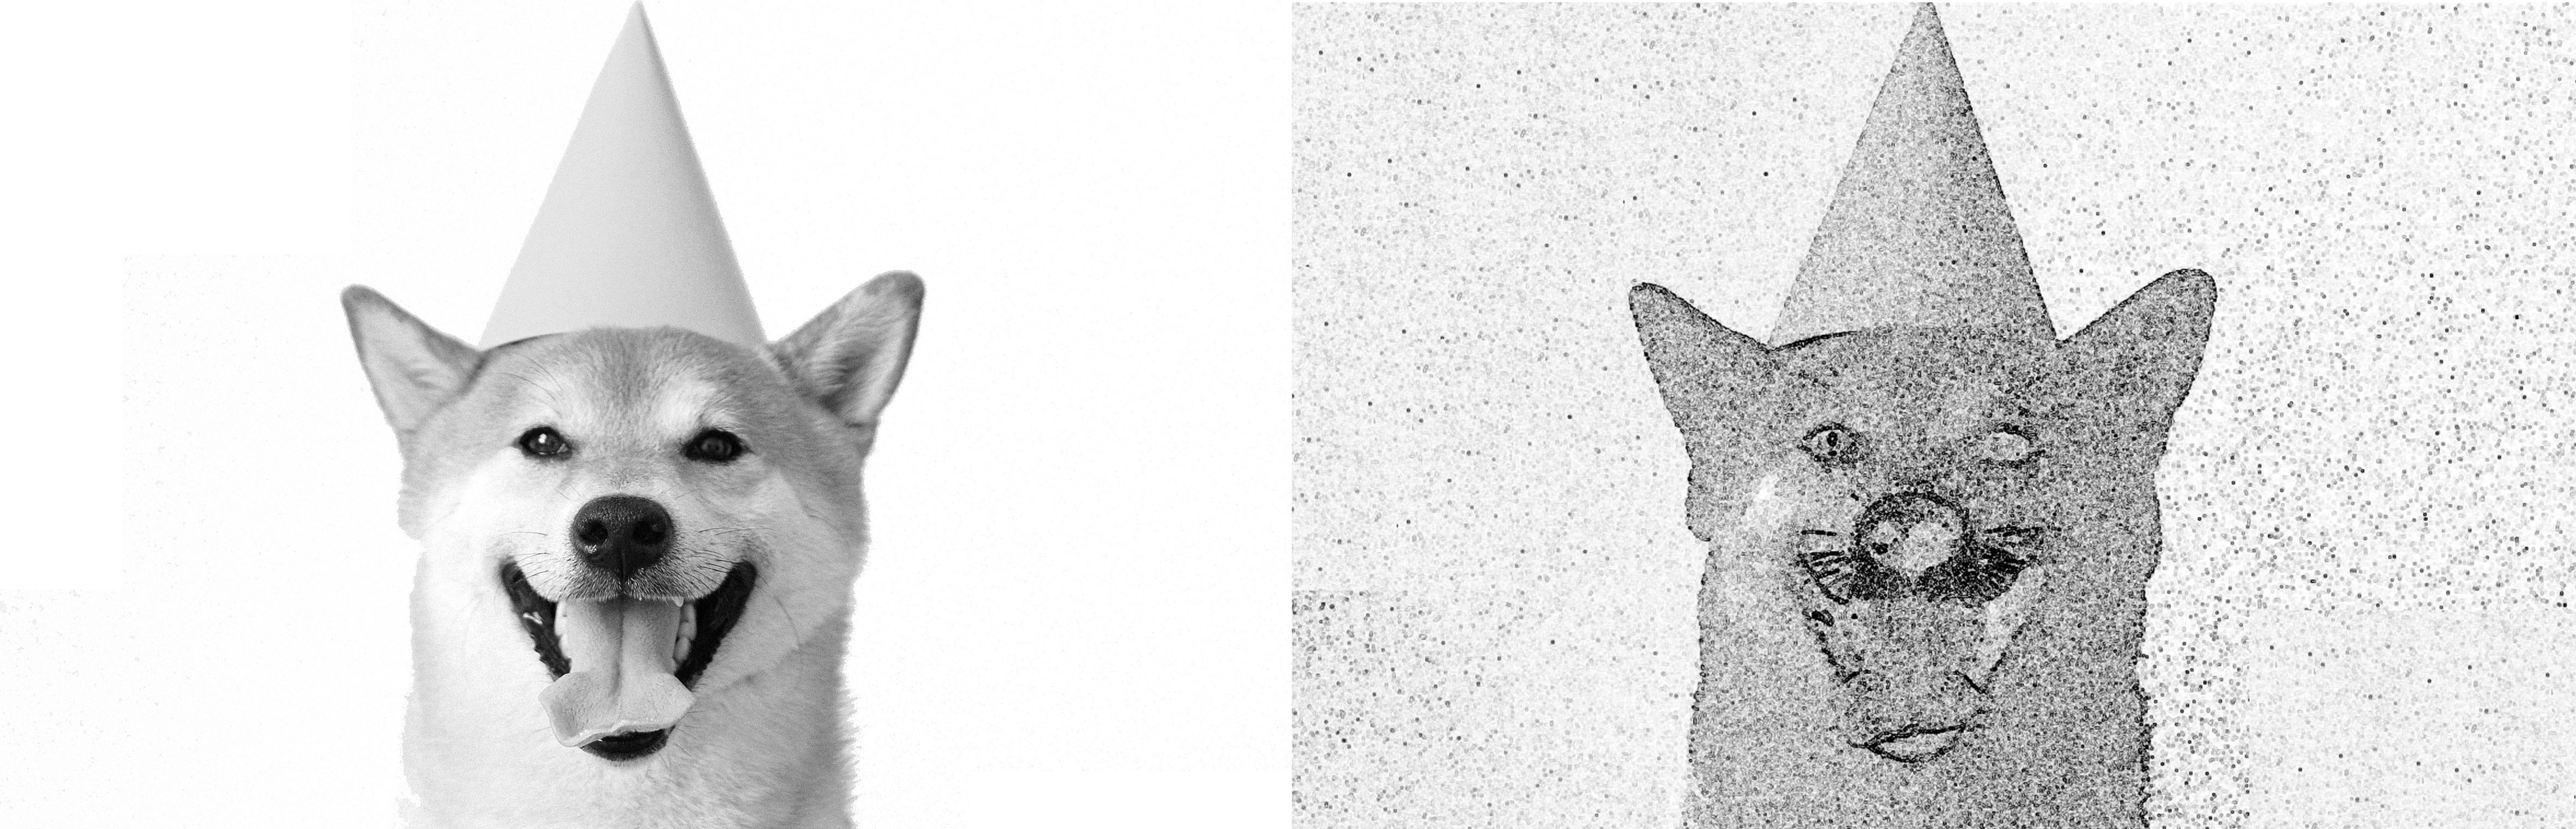
\includegraphics[scale=0.3]{./Chapter11/Figures/figure-dog-1.jpg}
\caption{图像通过卷积进行边缘检测}
\label{fig:11-5}
\end{figure}
%----------------------------------------------

%----------------------------------------------------------------------------------------
%    NEW SUB-SECTION
%----------------------------------------------------------------------------------------
\vspace{-2em}
\subsection{步长与填充}

\parinterval 在卷积操作中,步长是指卷积核每次滑动的距离,和卷积核的大小共同决定了卷积输出的大小,如图\ref{fig:11-6}所示。步长越大,对输入数据的压缩程度越高,其输出的维度越小;反之步长越小,对输入数据的压缩程度越低,同时输出的尺寸和输入越接近。比如使用一个$3 \times 3 \times 1$的卷积核在$6 \times 6 \times 1$的图像上进行卷积,如设置步长为1,其对应的输出大小就为$4 \times 4 \times 1$。这种做法最为简单,但是会导致两个问题;一是在输入数据中,由于边缘区域的像素只会被计算一次,相比于中心区域来说,这些像素被考虑的次数会更少一些,导致图像边缘信息的丢失;二是在经历多次卷积之后,其输出特征的维度会不断减小,影响模型的泛化能力。

%----------------------------------------------
% 图6.
\begin{figure}[htp]
\centering
\tikzstyle{num} = [minimum width = 0.6cm,minimum height = 0.6cm,draw,fill=green!10]
\begin{tikzpicture}[node distance = 0]

\node[num] at (0,0){1};
\node[num] at (0.6,0){1};
\node[num] at (1.2,0){2};
\node[num] at (1.8,0){0};
\node[num] at (2.4,0){2};
\node[num] at (3,0){2};

\node[num] at (0,0.6){2};
\node[num] at (0.6,0.6){0};
\node[num] at (1.2,0.6){0};
\node[num] at (1.8,0.6){1};
\node[num] at (2.4,0.6){5};
\node[num] at (3,0.6){2};

\node[num] at (0,1.2){1};
\node[num] at (0.6,1.2){2};
\node[num] at (1.2,1.2){3};
\node[num] at (1.8,1.2){2};
\node[num] at (2.4,1.2){0};
\node[num] at (3,1.2){0};

\node[num] at (0,1.8){2};
\node[num] at (0.6,1.8){0};
\node[num] at (1.2,1.8){1};
\node[num] at (1.8,1.8){4};
\node[num] at (2.4,1.8){0};
\node[num] at (3,1.8){0};

\node[num] at (0,2.4){0};
\node[num] at (0.6,2.4){1};
\node[num] at (1.2,2.4){2};
\node[num] at (1.8,2.4){4};
\node[num] at (2.4,2.4){2};
\node[num] at (3,2.4){2};

\node[num] at (0,3){0};
\node[num] at (0.6,3){0};
\node[num] at (1.2,3){1};
\node[num] at (1.8,3){0};
\node[num] at (2.4,3){2};
\node[num] at (3,3){1};

\node[minimum width = 1.8cm,minimum height = 1.8cm,draw=purple!40,line width=0.08cm,fill=purple!40,fill opacity=0.4] at (0.6,2.4) {};

%\fill (4,1.5) circle (2pt);
\node [] at (4,1.5) {*};

\node[num] at (5,0.9){0};
\node[num] at (5.6,0.9){1};
\node[num] at (6.2,0.9){0};

\node[num] at (5,1.5){1};
\node[num] at (5.6,1.5){0};
\node[num] at (6.2,1.5){0};

\node[num] at (5,2.1){0};
\node[num] at (5.6,2.1){1};
\node[num] at (6.2,2.1){1};

\draw (7.5,1.5)node{$=$};


\node[num] at (9,0.6){8};
\node[num] at (9.6,0.6){7};
\node[num] at (10.2,0.6){2};
\node[num] at (10.8,0.6){3};

\node[num] at (9,1.2){2};
\node[num] at (9.6,1.2){7};
\node[num] at (10.2,1.2){8};
\node[num] at (10.8,1.2){7};

\node[num] at (9,1.8){7};
\node[num] at (9.6,1.8){9};
\node[num] at (10.2,1.8){9};
\node[num] at (10.8,1.8){8};

\node[num] at (9,2.4){1};
\node[num] at (9.6,2.4){3};
\node[num] at (10.2,2.4){8};
\node[num] at (10.8,2.4){7};

\node[minimum width = 0.6cm,minimum height = 0.6cm,draw=purple!40,line width=0.08cm,fill=purple!40,fill opacity=0.4] at (9,2.4) {};

\node[] (in) at (1.5,-1) {\small{输入:6$\times$6}};
\node[] at (5.7,-1) {\small{卷积核:3$\times$3}};
\node[] (out) at (10,-1) {\small{输出:4$\times$4}};

%\node[font=\footnotesize,dashed,draw=teal,very thick,fill=green!5,align=center] at ([yshift=3cm,xshift=1.5cm]out.east) {*\ \ :表示\\卷积计算};
\node[] at ([yshift=-0.3cm,xshift=-2.3cm]in.east) {\ \ \ \ \ };

\end{tikzpicture}
\caption{卷积操作的维度变换(*\ \ 表示卷积计算)}
\label{fig:11-6}
\end{figure}
%----------------------------------------------

\parinterval 为了解决这两个问题,可以采用填充的操作对图像的边缘进行扩充,填充一些元素,例如0。比如在图\ref{fig:11-7}中,将$6 \times 6 \times 1$的图像填充为$8 \times 8 \times 1$的图像,然后在$8 \times 8 \times 1$的图像上进行卷积操作。这样可以得到与输入数据大小一致的输出结果,同时也缓解了图像边缘信息丢失的问题。

%----------------------------------------------
% 图7.
\begin{figure}[htp]
\centering
\tikzstyle{num} = [minimum width = 0.6cm,minimum height = 0.6cm,draw,fill=green!10]
\tikzstyle{pad} = [minimum width = 0.6cm,minimum height = 0.6cm,draw,fill=blue!10]
\begin{tikzpicture}[node distance = 0]

\node[pad] at (-0.6,-0.6){0};
\node[pad] at (0,-0.6){0};
\node[pad] at (0.6,-0.6){0};
\node[pad] at (1.2,-0.6){0};
\node[pad] at (1.8,-0.6){0};
\node[pad] at (2.4,-0.6){0};
\node[pad] at (3,-0.6){0};
\node[pad] at (3.6,-0.6){0};

\node[pad] at (-0.6,0){0};
\node[num] at (0,0){1};
\node[num] at (0.6,0){1};
\node[num] at (1.2,0){2};
\node[num] at (1.8,0){0};
\node[num] at (2.4,0){2};
\node[num] at (3,0){2};
\node[pad] at (3.6,0){0};

\node[pad] at (-0.6,0.6){0};
\node[num] at (0,0.6){2};
\node[num] at (0.6,0.6){0};
\node[num] at (1.2,0.6){0};
\node[num] at (1.8,0.6){1};
\node[num] at (2.4,0.6){5};
\node[num] at (3,0.6){2};
\node[pad] at (3.6,0.6){0};

\node[pad] at (-0.6,1.2){0};
\node[num] at (0,1.2){1};
\node[num] at (0.6,1.2){2};
\node[num] at (1.2,1.2){3};
\node[num] at (1.8,1.2){2};
\node[num] at (2.4,1.2){0};
\node[num] at (3,1.2){0};
\node[pad] at (3.6,1.2){0};

\node[pad] at (-0.6,1.8){0};
\node[num] at (0,1.8){2};
\node[num] at (0.6,1.8){0};
\node[num] at (1.2,1.8){1};
\node[num] at (1.8,1.8){4};
\node[num] at (2.4,1.8){0};
\node[num] at (3,1.8){0};
\node[pad] at (3.6,1.8){0};

\node[pad] at (-0.6,2.4){0};
\node[num] at (0,2.4){0};
\node[num] at (0.6,2.4){1};
\node[num] at (1.2,2.4){2};
\node[num] at (1.8,2.4){4};
\node[num] at (2.4,2.4){2};
\node[num] at (3,2.4){2};
\node[pad] at (3.6,2.4){0};

\node[pad] at (-0.6,3){0};
\node[num] at (0,3){0};
\node[num] at (0.6,3){0};
\node[num] at (1.2,3){1};
\node[num] at (1.8,3){0};
\node[num] at (2.4,3){2};
\node[num] at (3,3){1};
\node[pad] at (3.6,3){0};

\node[pad] at (-0.6,3.6){0};
\node[pad] at (0,3.6){0};
\node[pad] at (0.6,3.6){0};
\node[pad] at (1.2,3.6){0};
\node[pad] at (1.8,3.6){0};
\node[pad] at (2.4,3.6){0};
\node[pad] at (3,3.6){0};
\node[pad] at (3.6,3.6){0};

\node[minimum width = 1.8cm,minimum height = 1.8cm,draw=purple!40,line width=0.08cm,fill=purple!40,fill opacity=0.4] at (0,3) {};
\node[minimum width = 1.8cm,minimum height = 1.8cm,draw=orange!40,line width=0.08cm,fill=orange!40,fill opacity=0.4] at (0.6,2.4) {};

%\fill (4.55,1.5) circle (2pt);
\node [] at (4.55,1.5) {*};

%%%%%%%%%%%%%%%%%%%%%%%%%%%%%%%%%%%%
\node[num] at (5.5,0.9){0};
\node[num] at (6.1,0.9){1};
\node[num] at (6.7,0.9){0};

\node[num] at (5.5,1.5){1};
\node[num] at (6.1,1.5){0};
\node[num] at (6.7,1.5){0};

\node[num] at (5.5,2.1){0};
\node[num] at (6.1,2.1){1};
\node[num] at (6.7,2.1){1};

\draw (7.55,1.5)node{$=$};

%%%%%%%%%%%%%%%%%%%%%%%%%%%%%%%%%%%%
\node[num] at (8.4,0){2};
\node[num] at (9,0){1};
\node[num] at (9.6,0){2};
\node[num] at (10.2,0){8};
\node[num] at (10.8,0){7};
\node[num] at (11.4,0){4};

\node[num] at (8.4,0.6){4};
\node[num] at (9,0.6){8};
\node[num] at (9.6,0.6){7};
\node[num] at (10.2,0.6){2};
\node[num] at (10.8,0.6){3};
\node[num] at (11.4,0.6){7};

\node[num] at (8.4,1.2){4};
\node[num] at (9,1.2){2};
\node[num] at (9.6,1.2){7};
\node[num] at (10.2,1.2){8};
\node[num] at (10.8,1.2){7};
\node[num] at (11.4,1.2){2};

\node[num] at (8.4,1.8){2};
\node[num] at (9,1.8){7};
\node[num] at (9.6,1.8){9};
\node[num] at (10.2,1.8){9};
\node[num] at (10.8,1.8){8};
\node[num] at (11.4,1.8){2};

\node[num] at (8.4,2.4){2};
\node[num] at (9,2.4){1};
\node[num] at (9.6,2.4){3};
\node[num] at (10.2,2.4){8};
\node[num] at (10.8,2.4){7};
\node[num] at (11.4,2.4){3};

\node[num] at (8.4,3){0};
\node[num] at (9,3){1};
\node[num] at (9.6,3){2};
\node[num] at (10.2,3){5};
\node[num] at (10.8,3){2};
\node[num] at (11.4,3){4};

\node[minimum width = 0.6cm,minimum height = 0.6cm,draw=purple!40,line width=0.08cm,fill=purple!40,fill opacity=0.4] at (8.4,3) {0};
\node[minimum width = 0.6cm,minimum height = 0.6cm,draw=orange!40,line width=0.08cm,fill=orange!40,fill opacity=0.4] at (9,2.4) {1};

%\draw (1.5,-1.5)node{\small{输入:8$\times$8(填充后)}};
%\draw (5.7,-1.5)node{\small{卷积核:3$\times$3}};
%\draw (10,-1.5)node{\small{输出:6$\times$6}};
\node[] (in) at (1.5,-1.5) {\small{输入:8$\times$8(填充后)}};
\node[] at (6,-1.5) {\small{卷积核:3$\times$3}};
\node[] (out) at (10,-1.5) {\small{输出:6$\times$6}};

%\node[font=\footnotesize,dashed,draw=teal,very thick,fill=green!5,align=center] at ([yshift=4cm,xshift=1.8cm]out.east) {*\ \ :表示\\卷积计算};
\node[] at ([yshift=-0.3cm,xshift=-2.3cm]in.east) {\ \ \ \ \ };
\end{tikzpicture}
\caption{填充和卷积操作(*\ \ 表示卷积计算)}
\label{fig:11-7}
\end{figure}
%----------------------------------------------

%----------------------------------------------------------------------------------------
%    NEW SUB-SECTION
%----------------------------------------------------------------------------------------
\vspace{-2em}
\subsection{池化}

\parinterval 在图\ref{fig:11-2}所示的网络结构中,卷积层输出会通过一个非线性的激活函数,之后会通过{\small\bfnew{池化层}}\index{池化层}(也称为汇聚层)。池化过程和卷积类似,都是根据设定的窗口进行滑动选取局部信息进行计算,不同的是,池化层的计算是无参数化的,不需要额外的权重矩阵。常见的池化操作有{\small\bfnew{最大池化}}\index{最大池化}(Max Pooling)\index{Max Pooling}和{\small\bfnew{平均池化}}\index{平均池化}(Average Pooling)\index{Average Pooling}。前者获取窗口内最大的值,后者则获取窗口内矩阵的平均值。图\ref{fig:11-8}展示了窗口大小为$2 \times 2$、步长为2的两种池化方法的计算过程。

%----------------------------------------------
% 图8.
\begin{figure}[htp]
\centering
%\input{./Chapter11/Figures/figure-f }
\subfigure[{\small 最大池化}]{\tikzstyle{num} = [rectangle, minimum width = 0.6cm, minimum height = 0.6cm, text centered,align=center,thick,draw = black,fill=black!5]


\begin{tikzpicture}[node distance = 0cm]
\node(num1)[num,fill=red!20]{1};
\node(num2)[num,below of = num1,yshift= -0.6cm,fill=red!20]{5};
\node(num3)[num,right of = num1,xshift= 0.6cm,fill=red!20]{0};
\node(num4)[num,below of = num3,yshift= -0.6cm,fill=red!20]{6};

\node(num5)[num,right of = num3,xshift= 0.6cm,fill=green!20]{4};
\node(num6)[num,below of = num5,yshift= -0.6cm,fill=green!20]{7};
\node(num7)[num,right of = num5,xshift= 0.6cm,fill=green!20]{5};
\node(num8)[num,below of = num7,yshift= -0.6cm,fill=green!20]{8};

\node(num9)[num,below of = num2,yshift= -0.6cm,fill=yellow!20]{3};
\node(num10)[num,below of = num9,yshift= -0.6cm,fill=yellow!20]{1};
\node(num11)[num,right of = num9,xshift= 0.6cm,fill=yellow!20]{2};
\node(num12)[num,below of = num11,yshift= -0.6cm,fill=yellow!20]{2};

\node(num13)[num,right of = num11,xshift= 0.6cm,fill=blue!20]{1};
\node(num14)[num,below of = num13,yshift= -0.6cm,fill=blue!20]{3};
\node(num10)[num,right of = num13,xshift= 0.6cm,fill=blue!20]{0};
\node(num16)[num,below of = num10,yshift= -0.6cm,fill=blue!20]{4};

\draw[->,thick]([xshift=0.4cm,yshift=-0.4cm]num8.east)--([xshift=1.5cm,yshift=-0.4cm]num8.east);

\node(num17)[num,right of = num8,xshift= 2.5cm,fill=red!20]{6};
\node(num18)[num,right of = num17,xshift= 0.6cm,fill=green!20]{8};
\node(num19)[num,below of = num17,yshift=-0.6cm,fill=yellow!20]{3};
\node(num20)[num,below of = num18,yshift= -0.6cm,fill=blue!20]{4};

\node [right of = num20,xshift= 0.7cm]{};

\node[font=\small] at ([yshift=-0.7cm,xshift=0.3cm]num12.south) {输入:4$\times$4};
\node[font=\small] at ([yshift=-1.3cm,xshift=0.3cm]num19.south) {输出:2$\times$2};

\end{tikzpicture}}
\subfigure[{\small 平均池化}]{\tikzstyle{num} = [rectangle, minimum width = 0.6cm, minimum height = 0.6cm, text centered,align=center,thick,draw = black,fill=black!5]


\begin{tikzpicture}[node distance = 0cm]
\node(num1)[num,fill=red!10]{1};
\node(num2)[num,below of = num1,yshift= -0.6cm,fill=red!10]{5};
\node(num3)[num,right of = num1,xshift= 0.6cm,fill=red!10]{0};
\node(num4)[num,below of = num3,yshift= -0.6cm,fill=red!10]{6};

\node(num5)[num,right of = num3,xshift= 0.6cm,fill=green!10]{4};
\node(num6)[num,below of = num5,yshift= -0.6cm,fill=green!10]{7};
\node(num7)[num,right of = num5,xshift= 0.6cm,fill=green!10]{5};
\node(num8)[num,below of = num7,yshift= -0.6cm,fill=green!10]{8};

\node(num9)[num,below of = num2,yshift= -0.6cm,fill=yellow!10]{3};
\node(num10)[num,below of = num9,yshift= -0.6cm,fill=yellow!10]{1};
\node(num11)[num,right of = num9,xshift= 0.6cm,fill=yellow!10]{2};
\node(num12)[num,below of = num11,yshift= -0.6cm,fill=yellow!10]{2};

\node(num13)[num,right of = num11,xshift= 0.6cm,fill=blue!10]{1};
\node(num14)[num,below of = num13,yshift= -0.6cm,fill=blue!10]{3};
\node(num10)[num,right of = num13,xshift= 0.6cm,fill=blue!10]{0};
\node(num16)[num,below of = num10,yshift= -0.6cm,fill=blue!10]{4};

\draw[->,thick]([xshift=0.4cm,yshift=-0.4cm]num8.east)--([xshift=1.5cm,yshift=-0.4cm]num8.east);

\node(num17)[num,right of = num8,xshift= 2.5cm,fill=red!10]{3};
\node(num18)[num,right of = num17,xshift= 0.6cm,fill=green!10]{6};
\node(num19)[num,below of = num17,yshift=-0.6cm,fill=yellow!10]{2};
\node(num20)[num,below of = num18,yshift= -0.6cm,fill=blue!10]{2};

\node [right of = num2,xshift= -0.7cm]{};

\node[font=\small] at ([yshift=-0.7cm,xshift=0.3cm]num12.south) {输入:4$\times$4};
\node[font=\small] at ([yshift=-1.3cm,xshift=0.3cm]num19.south) {输出:2$\times$2};

\end{tikzpicture}}
\caption{池化操作}
\label{fig:11-8}
\end{figure}
%----------------------------------------------

\parinterval 池化计算选取每个滑动窗口内最突出的值或平均值作为局部信息,压缩了卷积层输出的维度大小,有效地减少了神经网络的计算量,是卷积神经网络中必不可少的操作。在网络建模时,通常在较低层时会使用最大池化,仅保留特征中最显著的部分。而当网络更深时,特征信息都具有一定意义,比如在自然语言处理任务中,深层网络的特征向量包含的语义信息较多,选取平均池化方法更适合。


%----------------------------------------------------------------------------------------
%    NEW SUB-SECTION
%----------------------------------------------------------------------------------------

\subsection{面向序列的卷积操作}

\parinterval 对比于图像处理任务中二维图像数据,自然语言处理任务中主要处理一维序列,如单词序列。由于单词序列长度往往是不固定的,很难使用全连接网络处理它,因为变长序列无法用固定大小的全连接网络进行直接建模,而且过长的序列也会导致全连接网络参数量的急剧增加。

%----------------------------------------------
% 图9.
\begin{figure}[htp]
\centering
%\input{./Chapter11/Figures/figure-f }
\subfigure[{\small 循环神经网络的串行结构}]{%\tikzstyle{num} = [rectangle, minimum width = 0.6cm, minimum height = 0.6cm, text centered,align=center,thick,draw = black, fill = black!8]
\tikzstyle{num} = [rectangle, minimum width = 0.6cm, minimum height = 0.6cm, text centered,align=center,thick,draw = black,rounded corners=1.5pt]


\begin{tikzpicture}[node distance = 0cm]
\node(num1)[num]{$\mathbi{e}_1$};
\node(num2)[num,right of = num1,xshift = 1.2cm]{\textcolor{blue!70}{$\mathbi{e}_2$}};
\node(num3)[num,right of = num2,xshift = 1.2cm]{\textcolor{blue!70}{$\mathbi{e}_3$}};
\node(num4)[num,right of = num3,xshift = 1.2cm]{\textcolor{blue!70}{$\mathbi{e}_4$}};
\node(num5)[num,right of = num4,xshift = 1.2cm]{\textcolor{blue!70}{$\mathbi{e}_5$}};
\node(num6)[num,right of = num5,xshift = 1.2cm]{\textcolor{blue!70}{$\mathbi{e}_6$}};
\node(num7)[num,right of = num6,xshift = 1.2cm]{\textcolor{blue!70}{$\mathbi{e}_7$}};
\node(num8)[num,right of = num7,xshift = 1.2cm]{\textcolor{blue!70}{$\mathbi{e}_8$}};
\node(num9)[num,right of = num8,xshift = 1.2cm]{$\mathbi{e}_9$};
%\node(A)[below of = num2,yshift = -0.6cm]{A};
%\node(B)[below of = num8,yshift = -0.6cm]{B};


\draw [->, thick, color = blue!80](num2.east)--(num3.west);
\draw [->, thick, color = blue!80](num3.east)--(num4.west);
\draw [->, thick, color = blue!80](num4.east)--(num5.west);
\draw [->, thick, color = blue!80](num5.east)--(num6.west);
\draw [->, thick, color = blue!80](num6.east)--(num7.west);
\draw [->, thick, color = blue!80](num7.east)--(num8.west);

\draw [->,thick,color = black!70] (num1) -- (num2);
\draw [->,thick,color =black!70] (num8) -- (num9);


\end{tikzpicture}}
\subfigure[{\small 卷积神经网络的层级结构}]{\tikzstyle{num} = [rectangle, minimum width = 0.6cm, minimum height = 0.6cm, text centered,align=center,thick,draw = black,rounded corners=1.5pt]


\begin{tikzpicture}[node distance = 0cm]
\node(num1_0)[num, fill = blue!40]{\textcolor{white}{$\mathbi{0}$}};
\node(num1_1)[num,right of = num1_0,xshift = 1.2cm]{$\mathbi{e}_1$};
\node(num1_2)[num,right of = num1_1,xshift = 1.2cm]{\textcolor{blue!85}{$\mathbi{e}_2$}};
\node(num1_3)[num,right of = num1_2,xshift = 1.2cm]{\textcolor{blue!85}{$\mathbi{e}_3$}};
\node(num1_4)[num,right of = num1_3,xshift = 1.2cm]{\textcolor{blue!85}{$\mathbi{e}_4$}};
\node(num1_5)[num,right of = num1_4,xshift = 1.2cm]{\textcolor{blue!85}{$\mathbi{e}_5$}};
\node(num1_6)[num,right of = num1_5,xshift = 1.2cm]{\textcolor{blue!85}{$\mathbi{e}_6$}};
\node(num1_7)[num,right of = num1_6,xshift = 1.2cm]{\textcolor{blue!85}{$\mathbi{e}_7$}};
\node(num1_8)[num,right of = num1_7,xshift = 1.2cm]{\textcolor{blue!85}{$\mathbi{e}_8$}};
\node(num1_9)[num,right of = num1_8,xshift = 1.2cm]{$\mathbi{e}_9$};
\node(num1_10)[num,right of = num1_9,xshift = 1.2cm, fill = blue!40]{$\mathbi{0}$};
%\node(A)[below of = num2,yshift = -0.6cm]{A};
%\node(B)[below of = num8,yshift = -0.6cm]{B};

\node(num2_0)[num,above of = num1_0,yshift = 1.2cm, fill = blue!40]{\textcolor{white}{$\mathbi{0}$}};
\node(num2_1)[num,right of = num2_0,xshift = 1.2cm]{\textbf2};
\node(num2_2)[num,right of = num2_1,xshift = 1.2cm]{\textbf2};
\node(num2_3)[num,right of = num2_2,xshift = 1.2cm]{\textbf{\textcolor{blue!85}2}};
\node(num2_4)[num,right of = num2_3,xshift = 1.2cm]{\textbf{\textcolor{blue!85}2}};
\node(num2_5)[num,right of = num2_4,xshift = 1.2cm]{\textbf{\textcolor{blue!85}2}};
\node(num2_6)[num,right of = num2_5,xshift = 1.2cm]{\textbf{\textcolor{blue!85}2}};
\node(num2_7)[num,right of = num2_6,xshift = 1.2cm]{\textbf{\textcolor{blue!85}2}};
\node(num2_8)[num,right of = num2_7,xshift = 1.2cm]{\textbf2};
\node(num2_9)[num,right of = num2_8,xshift = 1.2cm]{\textbf2};
\node(num2_10)[num,right of = num2_9,xshift = 1.2cm, fill = blue!40]{$\mathbi{0}$};

\node(num3_0)[num,above of = num2_0,yshift = 1.2cm, fill = blue!40]{\textcolor{white}{$\mathbi{0}$}};
\node(num3_1)[num,right of = num3_0,xshift = 1.2cm]{\textbf3};
\node(num3_2)[num,right of = num3_1,xshift = 1.2cm]{\textbf3};
\node(num3_3)[num,right of = num3_2,xshift = 1.2cm]{\textbf3};
\node(num3_4)[num,right of = num3_3,xshift = 1.2cm]{\textbf{\textcolor{blue!85}3}};
\node(num3_5)[num,right of = num3_4,xshift = 1.2cm]{\textbf{\textcolor{blue!85}3}};
\node(num3_6)[num,right of = num3_5,xshift = 1.2cm]{\textbf{\textcolor{blue!85}3}};
\node(num3_7)[num,right of = num3_6,xshift = 1.2cm]{\textbf3};
\node(num3_8)[num,right of = num3_7,xshift = 1.2cm]{\textbf3};
\node(num3_9)[num,right of = num3_8,xshift = 1.2cm]{\textbf3};
\node(num3_10)[num,right of = num3_9,xshift = 1.2cm, fill = blue!40]{$\mathbi{0}$};

\node(num4_0)[num,above of = num3_0,yshift = 1.2cm, fill = blue!40]{\textcolor{white}{$\mathbi{0}$}};
\node(num4_1)[num,right of = num4_0,xshift = 1.2cm]{\textbf4};
\node(num4_2)[num,right of = num4_1,xshift = 1.2cm]{\textbf4};
\node(num4_3)[num,right of = num4_2,xshift = 1.2cm]{\textbf4};
\node(num4_4)[num,right of = num4_3,xshift = 1.2cm]{\textbf4};
\node(num4_5)[num,right of = num4_4,xshift = 1.2cm]{\textbf{\textcolor{blue!80}4}};
\node(num4_6)[num,right of = num4_5,xshift = 1.2cm]{\textbf4};
\node(num4_7)[num,right of = num4_6,xshift = 1.2cm]{\textbf4};
\node(num4_8)[num,right of = num4_7,xshift = 1.2cm]{\textbf4};
\node(num4_9)[num,right of = num4_8,xshift = 1.2cm]{\textbf4};
\node(num4_10)[num,right of = num4_9,xshift = 1.2cm, fill = blue!40]{$\mathbi{0}$};

\draw [->, thick](num1_0.north)--([xshift=-0.1em,yshift=-0.1em]num2_1.south);
\draw [->, thick](num2_0.north)--([xshift=-0.1em,yshift=-0.1em]num3_1.south);
\draw [->, thick](num3_0.north)--([xshift=-0.1em,yshift=-0.1em]num4_1.south);
\draw [->, thick](num1_1.north)--([xshift=-0.1em,yshift=-0.1em]num2_2.south);
\draw [->, thick](num2_1.north)--([xshift=-0.1em,yshift=-0.1em]num3_2.south);
\draw [->, thick](num3_1.north)--([xshift=-0.1em,yshift=-0.1em]num4_2.south);
\draw [->, thick, color = blue!80](num1_2.north)--([xshift=-0.1em,yshift=-0.1em]num2_3.south);
\draw [->, thick](num2_2.north)--([xshift=-0.1em,yshift=-0.1em]num3_3.south);
\draw [->, thick](num3_2.north)--([xshift=-0.1em,yshift=-0.1em]num4_3.south);
\draw [->, thick, color = blue!80](num1_3.north)--([xshift=-0.1em,yshift=-0.1em]num2_4.south);
\draw [->, thick, color = blue!80](num2_3.north)--([xshift=-0.1em,yshift=-0.1em]num3_4.south);
\draw [->, thick](num3_3.north)--([xshift=-0.1em,yshift=-0.1em]num4_4.south);
\draw [->, thick, color = blue!80](num1_4.north)--([xshift=-0.1em,yshift=-0.1em]num2_5.south);
\draw [->, thick, color = blue!80](num2_4.north)--([xshift=-0.1em,yshift=-0.1em]num3_5.south);
\draw [->, thick, color = blue!80](num3_4.north)--([xshift=-0.1em,yshift=-0.1em]num4_5.south);
\draw [->, thick, color = blue!80](num1_5.north)--([xshift=-0.1em,yshift=-0.1em]num2_6.south);
\draw [->, thick, color = blue!80](num2_5.north)--([xshift=-0.1em,yshift=-0.1em]num3_6.south);
\draw [->, thick](num3_5.north)--([xshift=-0.1em,yshift=-0.1em]num4_6.south);
\draw [->, thick, color = blue!80](num1_6.north)--([xshift=-0.1em,yshift=-0.1em]num2_7.south);
\draw [->, thick](num2_6.north)--([xshift=-0.1em,yshift=-0.1em]num3_7.south);
\draw [->, thick](num3_6.north)--([xshift=-0.1em,yshift=-0.1em]num4_7.south);
\draw [->, thick](num1_7.north)--([xshift=-0.1em,yshift=-0.1em]num2_8.south);
\draw [->, thick](num2_7.north)--([xshift=-0.1em,yshift=-0.1em]num3_8.south);
\draw [->, thick](num3_7.north)--([xshift=-0.1em,yshift=-0.1em]num4_8.south);
\draw [->, thick](num1_8.north)--([xshift=-0.1em,yshift=-0.1em]num2_9.south);
\draw [->, thick](num2_8.north)--([xshift=-0.1em,yshift=-0.1em]num3_9.south);
\draw [->, thick](num3_8.north)--([xshift=-0.1em,yshift=-0.1em]num4_9.south);

\draw [->, thick](num1_2.north)--([xshift=0.1em,yshift=-0.1em]num2_1.south);
\draw [->, thick](num2_2.north)--([xshift=0.1em,yshift=-0.1em]num3_1.south);
\draw [->, thick](num3_2.north)--([xshift=0.1em,yshift=-0.1em]num4_1.south);
\draw [->, thick](num1_3.north)--([xshift=0.1em,yshift=-0.1em]num2_2.south);
\draw [->, thick](num2_3.north)--([xshift=0.1em,yshift=-0.1em]num3_2.south);
\draw [->, thick](num3_3.north)--([xshift=0.1em,yshift=-0.1em]num4_2.south);
\draw [->, thick, color = blue!80](num1_4.north)--([xshift=0.1em,yshift=-0.1em]num2_3.south);
\draw [->, thick](num2_4.north)--([xshift=0.1em,yshift=-0.1em]num3_3.south);
\draw [->, thick](num3_4.north)--([xshift=0.1em,yshift=-0.1em]num4_3.south);
\draw [->, thick, color = blue!80](num1_5.north)--([xshift=0.1em,yshift=-0.1em]num2_4.south);
\draw [->, thick, color = blue!80](num2_5.north)--([xshift=0.1em,yshift=-0.1em]num3_4.south);
\draw [->, thick](num3_5.north)--([xshift=0.1em,yshift=-0.1em]num4_4.south);
\draw [->, thick, color = blue!80](num1_6.north)--([xshift=0.1em,yshift=-0.1em]num2_5.south);
\draw [->, thick, color = blue!80](num2_6.north)--([xshift=0.1em,yshift=-0.1em]num3_5.south);
\draw [->, thick, color = blue!80](num3_6.north)--([xshift=0.1em,yshift=-0.1em]num4_5.south);
\draw [->, thick, color = blue!80](num1_7.north)--([xshift=0.1em,yshift=-0.1em]num2_6.south);
\draw [->, thick, color = blue!80](num2_7.north)--([xshift=0.1em,yshift=-0.1em]num3_6.south);
\draw [->, thick](num3_7.north)--([xshift=0.1em,yshift=-0.1em]num4_6.south);
\draw [->, thick, color = blue!80](num1_8.north)--([xshift=0.1em,yshift=-0.1em]num2_7.south);
\draw [->, thick](num2_8.north)--([xshift=0.1em,yshift=-0.1em]num3_7.south);
\draw [->, thick](num3_8.north)--([xshift=0.1em,yshift=-0.1em]num4_7.south);
\draw [->, thick](num1_9.north)--([xshift=0.1em,yshift=-0.1em]num2_8.south);
\draw [->, thick](num2_9.north)--([xshift=0.1em,yshift=-0.1em]num3_8.south);
\draw [->, thick](num3_9.north)--([xshift=0.1em,yshift=-0.1em]num4_8.south);
\draw [->, thick](num1_10.north)--([xshift=0.1em,yshift=-0.1em]num2_9.south);
\draw [->, thick](num2_10.north)--([xshift=0.1em,yshift=-0.1em]num3_9.south);
\draw [->, thick](num3_10.north)--([xshift=0.1em,yshift=-0.1em]num4_9.south);
\end{tikzpicture}}
\caption{串行及层级结构对比($\mathbi{e}_i$表示词嵌入,$\mathbi{0}$表示$\mathbi{0}$向量,方框里的2、3、4表示层次编号)}
\label{fig:11-9}
\end{figure}
%----------------------------------------------
\vspace{-1em}
\parinterval 针对不定长序列,一种可行的方法是使用之前介绍过的循环神经网络进行信息提取,其本质也是基于权重共享的想法,在不同的时间步复用相同的循环神经网络单元进行处理。但是,循环神经网络最大的弊端在于每一时刻的计算都依赖于上一时刻的结果,因此只能对序列进行串行处理,无法充分利用硬件设备进行并行计算,导致效率相对较低。此外,在处理较长的序列时,这种串行的方式很难捕捉长距离的依赖关系。相比之下,卷积神经网络采用共享参数的方式处理固定大小窗口内的信息,且不同位置的卷积操作之间没有相互依赖,因此可以对序列进行高效地并行处理。同时,针对序列中距离较长的依赖关系,可以通过堆叠多层卷积层来扩大{\small\bfnew{感受野}}\index{感受野} (Receptive Field)\index{Receptive Field}  ,这里感受野指能够影响神经元输出的原始输入数据区域的大小。图\ref{fig:11-9}对比了这两种结构,可以看出,为了捕捉$\mathbi{e}_2$ 和$\mathbi{e}_8$ 之间的联系,串行结构需要顺序地进行6次操作,操作次数与序列长度相关。而该卷积神经网络中,卷积操作每次对三个词进行计算,仅需要4层卷积计算就能得到$\mathbi{e}_2$ 和$\mathbi{e}_8$之间的联系,其操作数和卷积核的大小相关,相比于串行的方式具有更短的路径和更少的非线性计算,更容易进行训练。因此,也有许多研究人员在许多自然语言处理任务上尝试使用卷积神经网络进行序列建模\upcite{Kim2014ConvolutionalNN,Santos2014DeepCN,Kalchbrenner2014ACN,DBLP:conf/naacl/Johnson015,DBLP:conf/naacl/NguyenG15}。

\parinterval 区别于传统图像上的卷积操作,在面向序列的卷积操作中,卷积核只在序列这一维度进行移动,用来捕捉连续的多个词之间的特征。需要注意的是,由于单词通常由一个实数向量表示(词嵌入),因此可以将词嵌入的维度看作是卷积操作中的通道数。图\ref{fig:11-10}就是一个基于序列卷积的文本分类模型,模型的输入是维度大小为$m\times O $的句子表示,$m$表示句子长度,$O$表示卷积核通道数,其值等于词嵌入维度,模型使用多个不同(对应图中不同的颜色)的卷积核来对序列进行特征提取,得到了多个不同的特征序列。然后使用池化层降低表示维度,得到了一组和序列长度无关的特征表示。最后模型基于这组压缩过的特征表示,使用全连接网络和Softmax函数进行类别预测。在这过程中卷积层和池化层分别起到了特征提取和特征压缩的作用,将一个不定长的序列转化为一组固定大小的特征表示。

%----------------------------------------------
% 图10.
\begin{figure}[htp]
\centering

%\newlength{\bcc}
\setlength{\bcc}{0.4cm}
\begin{tikzpicture}
\begin{scope}
	%\tikzstyle{every node}=[scale=0.8]
	\tikzstyle{line} = [dash pattern=on 2pt off 1pt,line width=0.6pt]
	\tikzstyle{cir} = [thin,fill=blue!8,draw,circle,minimum size =0.5em,drop shadow={shadow xshift=0.15em, shadow yshift=-0.1em}]
	\tikzstyle{word} = [inner sep=0pt, font=\footnotesize,minimum height=\bcc]
	
	%\draw[fill=blue!8,xshift=0.3cm,yshift=0.5cm,line width=0.6pt] (0cm,0cm) rectangle (0cm+6*\bcc,0cm+9*\bcc);
	%\draw[ugreen!60,step=\bcc,xshift=0.3cm,yshift=0.5cm,gray] (0cm,0cm) grid (0cm+6*\bcc,0cm+9*\bcc); 
	%\draw[red!60,line width=2pt,xshift=0.3cm,yshift=0.5cm] (0cm,0cm+2*\bcc) rectangle (0cm+6*\bcc,0cm+4*\bcc);
	
	% 输入矩阵
	\draw[thick,fill=blue!8,line width=0.6pt] (0cm,0cm) rectangle (0cm+6*\bcc,0cm+9*\bcc);
	\draw[step=\bcc,gray] (0cm,0cm) grid (0cm+6*\bcc,0cm+9*\bcc); 
	\draw[red!60,line width=2pt] (0cm,0cm) rectangle (0cm+6*\bcc,0cm+2*\bcc);
	\draw[ugreen!60,line width=2pt] (0cm,0cm+3*\bcc) rectangle (0cm+6*\bcc,0cm+6*\bcc);
	\draw[red!60,line width=2pt] (0cm,0cm+7*\bcc) rectangle (0cm+6*\bcc,0cm+9*\bcc);

	% 特征图
	\draw[fill=blue!8,xshift=5.0cm,yshift=1.3cm,line width=0.6pt] (0cm,0cm-1*\bcc) rectangle (0cm+1*\bcc,0cm+6*\bcc);
	\draw[step=\bcc,gray,xshift=5.0cm,yshift=1.3cm] (0cm,0cm-1*\bcc) grid (0cm+1*\bcc,0cm+6*\bcc);
	\draw[ugreen!60,line width=2pt,xshift=5.0cm,yshift=1.3cm] (0cm,0cm+2*\bcc) rectangle (0cm+1*\bcc,0cm+3*\bcc);
	
	%最大池化
	\draw [gray,fill=blue!8,line width=0.6pt](8cm,2.2cm) -- (8.4cm, 2.2cm) -- (8.7cm,1.4cm) -- (8.3cm, 1.4cm) -- (8cm,2.2cm);
	\draw [gray](8.15cm,1.8cm) -- (8.55cm,1.8cm);
	%\draw [gray](8.3cm,1.8cm) -- (8.7cm,1.8cm);
	%\draw [gray](8.45cm,1.4cm) -- (8.85cm,1.4cm);
	
	%全连接层
	\draw [gray,fill=blue!8,line width=0.6pt](11cm,2.2cm) -- (11.4cm, 2.2cm) -- (11.7cm,1.8cm) -- (11.3cm, 1.8cm) -- (11cm,2.2cm);
	%\draw [gray](11.15cm,1.8cm) -- (11.55cm,1.8cm);
	
	%最大池化
	\draw[ugreen!60,line] ([xshift=5.0cm,yshift=1.3cm]0cm+1*\bcc,0cm+6*\bcc) -- (8cm,2.2cm);
	\draw[ugreen!60,line] ([xshift=5.0cm,yshift=1.3cm]0cm+1*\bcc,0cm-1*\bcc) -- (8.15cm,1.8cm);

	%特征图
	%\draw[fill=blue!8,xshift=5.2cm,yshift=1.0cm,line width=0.6pt] (0cm,0cm) rectangle (0cm+1*\bcc,0cm+6*\bcc);
	%\draw[step=\bcc,gray,xshift=5.2cm,yshift=1.0cm] (0cm,0cm) grid (0cm+1*\bcc,0cm+6*\bcc); 
	
	%\draw[fill=blue!8,xshift=5.4cm,yshift=0.3cm,line width=0.6pt] (0cm,0cm) rectangle (0cm+1*\bcc,0cm+7*\bcc);
	%\draw[step=\bcc,gray,xshift=5.4cm,yshift=0.3cm] (0cm,0cm) grid (0cm+1*\bcc,0cm+7*\bcc);
	
	\draw[fill=blue!8,xshift=5.6cm,yshift=0cm,line width=0.6pt] (0cm,0cm) rectangle (0cm+1*\bcc,0cm+8*\bcc);
	\draw[step=\bcc,gray,xshift=5.6cm,yshift=0cm] (0cm,0cm) grid (0cm+1*\bcc,0cm+8*\bcc); 
	\draw[red!60,line width=2pt,xshift=5.6cm,yshift=0cm] (0cm,0cm) rectangle (0cm+1*\bcc,0cm+1*\bcc);
	\draw[red!60,line width=2pt,xshift=5.6cm,yshift=0cm] (0cm,0cm+7*\bcc) rectangle (0cm+1*\bcc,0cm+8*\bcc);
	
	% 全连接线
	\draw[line] (8.4cm, 2.2cm) -- (11.2cm,2.2cm);
	\draw[line] (8.7cm,1.4cm) -- (11.3cm, 1.8cm);
	%全连接上面的红虚线
	\draw[red!60,line] ([xshift=5.6cm,yshift=0cm]0cm+1*\bcc,0cm+7*\bcc) -- (8.15cm,1.8cm);
	\draw[red!60,line] ([xshift=5.6cm,yshift=0cm]0cm+1*\bcc,0cm) -- (8.3cm, 1.4cm);
	
	% 特征图红色虚线
	\draw[red!60,line] (0cm+6*\bcc,0cm+9*\bcc) -- ([xshift=5.6cm,yshift=0cm]0cm,0cm+8*\bcc);
	\draw[red!60,line] (0cm+6*\bcc,0cm+7*\bcc) -- ([xshift=5.6cm,yshift=0cm]0cm,0cm+7*\bcc);
	\draw[red!60,line] (0cm+6*\bcc,0cm+2*\bcc) -- ([xshift=5.6cm,yshift=0cm]0cm,0cm+1*\bcc);
	\draw[red!60,line] (0cm+6*\bcc,0cm) -- ([xshift=5.6cm,yshift=0cm]0cm,0cm);
	\draw[ugreen!60,line] (0cm+6*\bcc,0cm+6*\bcc) -- ([xshift=5.0cm,yshift=1.3cm]0cm,0cm+3*\bcc);
	\draw[ugreen!60,line] (0cm+6*\bcc,0cm+3*\bcc) -- ([xshift=5.0cm,yshift=1.3cm]0cm,0cm+2*\bcc);
	%\draw[red!60,line] ([xshift=0.3cm,yshift=0.5cm]0cm+6*\bcc,0cm+4*\bcc) -- ([xshift=5.6cm,yshift=0cm]0cm,0cm+3*\bcc);
	%\draw[red!60,line] ([xshift=0.3cm,yshift=0.5cm]0cm+6*\bcc,0cm+2*\bcc) -- ([xshift=5.6cm,yshift=0cm]0cm,0cm+2*\bcc);
	
	\node[word] (w1) at (-0.5cm, 3.4cm) {wait};
	\node[word] (w2) at ([yshift=-\bcc]w1) {for};
	\node[word] (w3) at ([yshift=-\bcc]w2) {the};
	\node[word] (w4) at ([yshift=-\bcc]w3) {video};
	\node[word] (w5) at ([yshift=-\bcc]w4) {and};
	\node[word] (w6) at ([yshift=-\bcc]w5) {do};
	\node[word] (w7) at ([yshift=-\bcc]w6) {n't};
	\node[word] (w8) at ([yshift=-\bcc]w7) {rent};
	\node[word] (w9) at ([yshift=-\bcc]w8) {it};
 
	\node[draw,rectangle callout,callout relative pointer={(0.28,-0.6)}] at (-0.3cm,4.6cm) {\textrm{卷积核}};
	\node[draw,rectangle callout,callout relative pointer={(0.1,-0.5)}] at (5cm,4.6cm) {\textrm{特征图}};


	\draw [thick] (0cm, -0.3cm) -- (0cm, -0.5cm)  -- node[font=\tiny, align=center,yshift=-0.5cm]{维度大小为 $m \times O$ \\ 的句子表示} (2.4cm,-0.5cm) -- (2.4cm, -0.3cm);	
	\draw [thick] (3.6cm, -0.3cm) -- (3.6cm, -0.5cm)  -- node[font=\tiny, align=center,yshift=-0.5cm]{具有多个不同大小\\的卷积核和特征图\\的卷积层} (6cm,-0.5cm) -- (6cm, -0.3cm);
	\draw [thick] (7.2cm, -0.3cm) -- (7.2cm, -0.5cm)  -- node[font=\tiny, align=center,yshift=-0.5cm]{最大池化} (9cm,-0.5cm) -- (9cm, -0.3cm);
	\draw [thick] (10cm, -0.3cm) -- (10cm, -0.5cm)  -- node[font=\tiny, align=center,yshift=-0.5cm]{带有Dropout\\和Softmax输出\\的全连接层} (11.7cm,-0.5cm) -- (11.7cm, -0.3cm);
	
	
\end{scope}

\end{tikzpicture}
\caption{序列卷积在文本分类模型中的应用\upcite{Kim2014ConvolutionalNN}}
\label{fig:11-10}
\end{figure}
%----------------------------------------------
\vspace{-1em}
\parinterval 和其它自然语言处理任务不同的是,机器翻译中需要对序列进行全局表示,换句话说,模型需要捕捉序列中各个位置之间的关系。因此,基于卷积神经网络的神经机器翻译模型需要堆叠多个卷积层进行远距离的依赖关系的建模。同时,为了在多层网络中维持序列的原有长度,需要在卷积操作前对输入序列进行填充。图\ref{fig:11-11}是一个简单的示例,针对一个长度$m=6$的句子,其隐藏层表示维度即卷积操作的输入通道数是$O=4$,卷积核大小为$K=3$。首先对序列进行填充,得到一个长度为8的序列,然后使用这些卷积核在这之上进行特征提取。一共使用了$N=4$个卷积核,整体的参数量为$K \times O \times N$,最后的卷积结果为$m \times N$的序列表示。

%----------------------------------------------
% 图11.
\begin{figure}[htp]
\centering
%\input{./Chapter11/Figures/figure-f }
%\newlength{\bcc}
\setlength{\bcc}{0.4cm}

\begin{tikzpicture}
\begin{scope}
	%\tikzstyle{every node}=[scale=0.8]
	\tikzstyle{line} = [dash pattern=on 2pt off 1pt,line width=0.5pt]
	\tikzstyle{cir} = [thin,fill=blue!8,draw,circle,minimum size =0.5em,drop shadow={shadow xshift=0.15em, shadow yshift=-0.1em}]
	\tikzstyle{word} = [inner sep=0pt, font=\scriptsize,minimum height=\bcc]
	
	\draw[fill=red!8,line width=0.2pt] (0cm,0cm+1*\bcc) rectangle (0cm+4*\bcc,0cm+7*\bcc);
	\draw[fill=cyan!14,line width=0.2pt] (0cm,0cm) rectangle (0cm+4*\bcc,0cm+1*\bcc);
	\draw[fill=cyan!14,line width=0.2pt] (0cm,0cm+7*\bcc) rectangle (0cm+4*\bcc,0cm+8*\bcc);
	\draw[step=\bcc] (0cm,0cm) grid (0cm+4*\bcc,0cm+8*\bcc); 
	%\draw[line width=0.7pt] (0cm,0cm) rectangle (0cm+4*\bcc,0cm+8*\bcc);
	\draw[red!50,line width=1.8pt] (0cm,0cm+5*\bcc) rectangle (0cm+4*\bcc,0cm+8*\bcc);
	\draw[ugreen!50,line width=1.8pt] (0cm,0cm+1*\bcc) rectangle (0cm+4*\bcc,0cm+4*\bcc);

	
	\draw[fill=blue!8,xshift=5.0cm,yshift=1.0cm,line width=0.2pt] (0cm,0cm) rectangle (0cm+1*\bcc,0cm+6*\bcc);
	\draw[step=\bcc,xshift=5.0cm,yshift=1.0cm] (0cm,0cm) grid (0cm+1*\bcc,0cm+6*\bcc);
	%\draw[line width=0.7pt,xshift=5.0cm,yshift=1.0cm] (0cm,0cm) rectangle (0cm+1*\bcc,0cm+6*\bcc);
	
	\draw[fill=blue!8,xshift=5.2cm,yshift=0.8cm,line width=0.2pt] (0cm,0cm) rectangle (0cm+1*\bcc,0cm+6*\bcc);
	\draw[step=\bcc,xshift=5.2cm,yshift=0.8cm] (0cm,0cm) grid (0cm+1*\bcc,0cm+6*\bcc); 
	%\draw[line width=0.7pt,xshift=5.2cm,yshift=0.8cm] (0cm,0cm) rectangle (0cm+1*\bcc,0cm+6*\bcc);
	\draw[ugreen!50,line width=2pt,xshift=5.2cm,yshift=0.8cm] (0cm,0cm+1*\bcc) rectangle (0cm+1*\bcc,0cm+2*\bcc);
	
	\draw[fill=blue!8,xshift=5.4cm,yshift=0.6cm,line width=0.2pt] (0cm,0cm) rectangle (0cm+1*\bcc,0cm+6*\bcc);
	\draw[step=\bcc,xshift=5.4cm,yshift=0.6cm] (0cm,0cm) grid (0cm+1*\bcc,0cm+6*\bcc);
	%\draw[line width=0.7pt,xshift=5.4cm,yshift=0.6cm] (0cm,0cm) rectangle (0cm+1*\bcc,0cm+6*\bcc); 
	
	\draw[fill=blue!8,xshift=5.6cm,yshift=0.4cm,line width=0.2pt] (0cm,0cm) rectangle (0cm+1*\bcc,0cm+6*\bcc);
	\draw[step=\bcc,xshift=5.6cm,yshift=0.4cm] (0cm,0cm) grid (0cm+1*\bcc,0cm+6*\bcc); 
	%\draw[line width=0.7pt,xshift=5.6cm,yshift=0.4cm] (0cm,0cm) rectangle (0cm+1*\bcc,0cm+6*\bcc);
	\draw[red!50,line width=2pt,xshift=5.6cm,yshift=0.4cm] (0cm,0cm+5*\bcc) rectangle (0cm+1*\bcc,0cm+6*\bcc);

	\draw[red!50,line width=0.5pt] (0cm+4*\bcc,0cm+8*\bcc) -- ([xshift=5.6cm,yshift=0.4cm]0cm,0cm+6*\bcc);
	\draw[red!50,line width=0.5pt] (0cm+4*\bcc,0cm+5*\bcc) -- ([xshift=5.6cm,yshift=0.4cm]0cm,0cm+5*\bcc);

	\draw[ugreen!50,line width=0.5pt] (0cm+4*\bcc,0cm+4*\bcc) -- ([xshift=5.2cm,yshift=0.8cm]0cm,0cm+2*\bcc);
	\draw[ugreen!50,line width=0.5pt] (0cm+4*\bcc,0cm+1*\bcc) -- ([xshift=5.2cm,yshift=0.8cm]0cm,0cm+1*\bcc);

	\node[word] (w1) at (-0.5cm, 3.0cm) {$<$p$>$};
	\node[word] (w2) at ([yshift=-\bcc]w1) {今天};
	\node[word] (w3) at ([yshift=-\bcc]w2) {是};
	\node[word] (w4) at ([yshift=-\bcc]w3) {个};
	\node[word] (w5) at ([yshift=-\bcc]w4) {好};
	\node[word] (w6) at ([yshift=-\bcc]w5) {日子};
	\node[word] (w7) at ([yshift=-\bcc]w6) {。};
	\node[word] (w8) at ([yshift=-\bcc]w7) {$<$p$>$};
	
	\node[inner xsep=2pt,inner ysep=0pt,font=\footnotesize] (c1) at (0.8cm, 3.5cm) {$O$};
	\draw[-latex] (c1.west) -- ([xshift=-0.4cm]c1.west);
	\draw[-latex] (c1.east) -- ([xshift=0.4cm]c1.east);
	
	\node[inner xsep=2pt,inner ysep=0pt,font=\footnotesize, rotate=-45] (c2) at (5.06cm, 0.5cm) {$N$};
	\draw[-latex] (c2.west) -- ([xshift=-0.2cm,yshift=0.2cm]c2.west);
	\draw[-latex] (c2.east) -- ([xshift=0.2cm, yshift=-0.2cm]c2.east);

%%%%%%%%%%%%%%%%%%%%%
	\node[word] (sub) at ([xshift=9.5*\bcc,yshift=3.5*\bcc]w1) {$O$\ \ :输入通道数};
	\node[word] (sub2) at ([yshift=-0.5*\bcc]sub.south) {$N$\ \ :卷积核数量};
	\node[word] (sub3) at ([xshift=-1.35em,yshift=-0.5*\bcc]sub2.south) {$<$p$>$:填充};
	
\end{scope}

\end{tikzpicture}
\caption{机器翻译中的序列卷积操作}
\label{fig:11-11}
\end{figure}
%----------------------------------------------
%----------------------------------------------------------------------------------------
%    NEW SECTION
%----------------------------------------------------------------------------------------

\section{基于卷积神经网络的翻译建模}

\parinterval 正如之前所讲,卷积神经网络可以用于序列建模,同时具有并行性高和易于学习的特点,一个很自然的想法就是将其用作神经机器翻译模型中的特征提取器。因此,在神经机器翻译被提出之初,研究人员就已经开始利用卷积神经网络对句子进行特征提取。比较经典的模型是使用卷积神经网络作为源语言句子的编码器,使用循环神经网络作为目标语言译文生成的解码器\upcite{kalchbrenner-blunsom-2013-recurrent,Gehring2017ACE}。之后也有研究人员提出完全基于卷积神经网络的翻译模型(ConvS2S)\upcite{DBLP:journals/corr/GehringAGYD17},或者针对卷积层进行改进,提出效率更高、性能更好的模型\upcite{Kaiser2018DepthwiseSC,Wu2019PayLA}。本节将基于ConvS2S模型,阐述如何使用卷积神经网络搭建端到端神经机器翻译模型。

%----------------------------------------------
% 图12.
\begin{figure}[htp]
\centering
%\documentclass[tikz]{standalone}
%\usepackage{tikz}
%\usepackage[UTF8]{ctex}
%\usetikzlibrary{shapes}
%\usetikzlibrary{backgrounds} 
%\usetikzlibrary{shadows}
%\usepackage{bm}
%\usetikzlibrary{fit}

\definecolor{mc_1_m}{RGB}{228,236,255}
\definecolor{mc_1}{RGB}{187,214,255}
\definecolor{mc_2_m}{RGB}{255,251,217}
\definecolor{mc_2}{RGB}{232,232,198}
\definecolor{mc_3_m}{RGB}{255,247,242}
\definecolor{mc_3}{RGB}{247,228,214}
\definecolor{mc_4_m}{RGB}{240,241,254}
\definecolor{mc_4}{RGB}{208,211,244}
\definecolor{ugreen}{rgb}{0,0.5,0}

\begin{tikzpicture}[scale=0.8]
	\tikzstyle{every node}=[scale=0.8]
	\tikzstyle{rec} = [thick,fill=red!10,draw,drop shadow,minimum height =1em,minimum width=2em]
	\tikzstyle{cir} = [line width=0.6pt,fill=yellow!20,draw,circle,minimum size =0.5em,drop shadow={shadow xshift=0.15em, shadow yshift=-0.1em}]
	\tikzstyle{word} = [inner sep=0pt, font=\footnotesize, minimum height=1em,align=center]
	
\begin{scope}
\foreach \point in {0,1,2,3,4,5}
\node[rec] (i_\point) at (0.9+\point, -0.1){};
\draw[thick] (i_0.0) -- (i_1.180);
\draw[thick] (i_1.0) -- (i_2.180);
\draw[thick] (i_2.0) -- (i_3.180);
\draw[thick] (i_3.0) -- (i_4.180);
\draw[thick] (i_4.0) -- (i_5.180);

\node[anchor=north,word] (tgt_1) at ([yshift=-0.4em]i_0.south){$<$p$>$};
\node[anchor=north,word] at ([yshift=-0.4em]i_1.south){$<$p$>$};
\node[anchor=north,word] at ([yshift=-0.4em]i_2.south){$<$sos$>$};
\node[anchor=north,word] at ([yshift=-0.4em]i_3.south){go};
\node[anchor=north,word] at ([yshift=-0.4em]i_4.south){to};
\node[anchor=north,word] (tgt_2) at ([yshift=-0.4em]i_5.south){school};

  \begin{pgfonlayer}{background}
	\node [draw=ugreen!30,rectangle,inner ysep=5pt,inner xsep=1.8em,rounded corners=4pt,line width=2pt,fill=ugreen!10] [fit = (tgt_1) (i_0)(tgt_2)(i_5) ] (group1_2) {};
  \end{pgfonlayer}

\node[anchor=east, word] (l_0) at ([xshift=-2em,yshift=-0.5em]i_0.west){\sffamily\bfnew{目标语词嵌入}};
\node[anchor=south, word] (l_1) at ([yshift=2em]l_0.north){\sffamily\bfnew{卷积}};
\node[anchor=south, word] (l_2) at ([yshift=2.4em]l_1.north){\sffamily\bfnew{门控}};
\node[anchor=south, word] (l_3) at ([yshift=0.06em]l_2.north){\sffamily\bfnew{线性单元}};


\foreach \point in {0,1,2}
\draw[thick,fill=blue!20] (5.9-\point,0.4) -- (4.9-\point,1.5) -- (3.9-\point,0.4) -- (5.9-\point,0.4);
\draw[thick,fill=blue!40] (2.9,0.4) -- (1.9,1.5) -- (0.9,0.4) -- (2.9,0.4);

\foreach \point in {0,1,2,3}{
\node[rec](h_\point) at (1.9+\point, 1.6){};
\draw[thick](h_\point.90) -- (h_\point.-90);
}

\foreach \point in {0,1,2,3}{
\node[cir](c_\point) at (1.7+\point, 2.4){};
\draw[out=20,in=160,line width=0.6pt] (c_\point.-135) to (c_\point.45);
\node[cir](x_\point) at (2.1+\point, 3){};
\draw[line width=0.6pt] (x_\point.-135) -- (x_\point.45);
\draw[line width=0.6pt] (x_\point.-45) -- (x_\point.135);
\draw[-latex,thick] ([xshift=-0.5em]h_\point.90) -- (c_\point.-90);
\draw[-latex,thick] ([xshift=0.5em]h_\point.90) -- (x_\point.-90);
\draw[-latex,out=90,in=-145,thick] (c_\point.90) to (x_\point.-145);
}

\foreach \point in {0,1,2,3}{
\node[rec](q_\point) at (2.5cm+\point*2em, 4){};
\draw[-latex,thick] (x_\point.90) -- (q_\point.-90);
}

\node[cir](o_1) at (7.55cm, 4){};
\draw[line width=0.6pt] (o_1.90) -- (o_1.-90);
\draw[line width=0.6pt] (o_1.0) -- (o_1.180);
\draw[-latex,thick] (q_3.0) -- (o_1.180);

\foreach \point in {0,1,2}{
\node[rec,fill=blue!40](g_\point_0) at (5cm+\point*2em, 7.5cm){};
\node[rec,fill=blue!40](g_\point_1) at (5cm+\point*2em, 7.5cm-1em){};
\node[rec,fill=blue!40](g_\point_2) at (5cm+\point*2em, 7.5cm-2em){};
\node[rec,fill=blue!40](g_\point_3) at (5cm+\point*2em, 7.5cm-3em){};
}

\node[anchor=north, word] at ([yshift=-0.6em]g_1_3.south){\sffamily\bfnew{内积}};

\draw [-latex, rounded corners=3pt,thick] (q_0.90) -- (2.5cm, 7.5cm) -- (g_0_0.180);
\draw [-latex, rounded corners=3pt,thick] (q_1.90) -- (2.5cm+2em, 7.5cm-1em) -- (g_0_1.180);
\draw [-latex, rounded corners=3pt,thick] (q_2.90) -- (2.5cm+4em, 7.5cm-2em) -- (g_0_2.180);
\draw [-latex, rounded corners=3pt,thick] (q_3.90) -- (2.5cm+6em, 6.2cm-2em) -- (2cm+6em, 6.2cm-2em) -- (2cm+6em, 7.5cm-3em) -- (g_0_3.180);
\node[thick,draw,fill=yellow!60,minimum height =1em,minimum width=2em](g_0_0) at (5cm, 7.5cm){};
\node[thick,draw,fill=yellow!60,minimum height =1em,minimum width=2em](g_1_1) at (5cm+2em, 7.5cm-1em){};
\node[thick,draw,fill=yellow!60,minimum height =1em,minimum width=2em](g_1_2) at (5cm+2em, 7.5cm-2em){};
\node[thick,draw,fill=yellow!60,minimum height =1em,minimum width=2em](g_2_3) at (5cm+4em, 7.5cm-3em){};

\foreach \point in {0,1,2,3}
\node[rec] (i_\point) at (8+\point, -0.1){};

\node[anchor=north,word] at ([yshift=-0.4em]i_0.south){go};
\node[anchor=north,word] at ([yshift=-0.4em]i_1.south){to};
\node[anchor=north,word] at ([yshift=-0.4em]i_2.south){school};
\node[anchor=north,word] at ([yshift=-0.4em]i_3.south){$<$eos$>$};

\foreach \point in {0,1,2,3}{
\node[cir,font=\fontsize{6}{6}\selectfont,inner sep=0.8pt](c_\point) at (8.2cm+\point*2em,7.5cm-1em*\point){\bm{$\sum$}};
\node[rec](q_\point) at (8.2cm+\point*2em, 5){};
\node[rec](b_\point) at (8.2cm+\point*2em, 4){};
\draw[-latex,thick] (g_2_\point.0) -- (c_\point.180);
\draw[-latex,thick] (c_\point.-90) -- (q_\point.90);
\draw[-latex,thick] (q_\point.-90) -- (b_\point.90);
\draw[-latex,thick] (b_\point.-90) -- ([yshift=-3.5cm]b_\point.-90);
}

\foreach \point in {2,1}
\draw[thick,fill=blue!20] (4.7cm+\point*1cm, 11cm) -- (3.9cm+\point*1cm, 12cm) -- (5.5cm+\point*1cm, 12cm) -- (4.7cm+\point*1cm, 11cm);
\draw[thick,fill=blue!40] (4.7cm,11cm) -- (3.9cm,12cm) -- (5.5cm,12cm) -- (4.7cm,11cm);

\foreach \point in {0,1,2}{
\node[rec](h_\point) at (5cm+\point*2em, 8.8cm){};
\node[rec](w_\point) at (8.6cm+\point*2em, 8.8cm){};
\node[cir](x_\point) at (4.5cm+\point*1cm, 9.6cm){};
\draw[line width=0.6pt] (x_\point.-135) -- (x_\point.45);
\draw[line width=0.6pt] (x_\point.-45) -- (x_\point.135);
\node[cir](c_\point) at (4.9cm+\point*1cm, 10.2cm){};
\draw[line width=0.6pt,out=20,in=160] (c_\point.-135) to (c_\point.45);
\node[rec](f_\point) at (4.7cm+\point*1cm, 11cm){};
\draw[-,thick] (f_\point.90) -- (f_\point.-90);
\draw[-latex,thick] ([xshift=-0.5em]f_\point.-90) -- (x_\point.90);
\draw[-latex,thick] ([xshift=0.5em]f_\point.-90) -- (c_\point.90);
\draw[-latex,out=-90,in=45,thick] (c_\point.-90) to (x_\point.45);
\draw[-latex,thick] (x_\point.-45) -- (h_\point.90);
\draw[-latex,thick] (h_\point.-90) -- (g_\point_0.90);
\node[rec](r_\point) at (4.7cm+\point*1cm, 12.55cm){};
}

\node[anchor=south,word] (src_1) at ([xshift=-2em,yshift=0.4em]r_0.north){$<$p$>$};
\node[anchor=south,word] at ([yshift=0.4em]r_0.north){去};
\node[anchor=south,word] at ([yshift=0.4em]r_1.north){上学};
\node[anchor=south,word] at ([yshift=0.4em]r_2.north){$<$sos$>$};
\node[anchor=south,word] (src_2) at ([xshift=2em,yshift=0.4em]r_2.north){$<$p$>$};


\node[anchor=east, word] (t_1) at ([xshift=-4em,yshift=0.5em]r_0.west){\sffamily\bfnew{源语词嵌入}};
\node[anchor=north, word] (t_2) at ([yshift=-2em]t_1.south){\sffamily\bfnew{卷积}};
\node[anchor=north, word] (t_3) at ([yshift=-2.8em]t_2.south){\sffamily\bfnew{门控}};
\node[anchor=north, word] (t_4) at ([yshift=-0.06em]t_3.south){\sffamily\bfnew{线性单元}};
\node[anchor=north, word] (t_5) at ([yshift=1.24em]t_4.south){\sffamily\bfnew{}};
\node[anchor=north, word] (t_6) at ([yshift=-1.5em]t_5.south){\sffamily\bfnew{注意力模块}};

\node[cir] (o_2) at (7.95, 8.8cm){};
\draw[line width=0.6pt] (o_2.90) -- (o_2.-90);
\draw[line width=0.6pt] (o_2.0) -- (o_2.180);
\draw[-latex,thick] (h_2.0) -- (o_2.180);
\node[cir] (o_3) at (8.6cm+2em, 10cm){};

\draw[thick] (r_0.0) -- (r_1.180);
\draw[thick] (r_1.0) -- (r_2.180);
\draw[rounded corners=3pt,thick] (r_2.0) -- (8.6cm+2em, 12.55cm) -- (o_3.90);
\draw[-latex,thick] (o_3.90) -- (o_3.-135) -- (w_0.90);
\draw[-latex,thick] (o_3.90) -- (o_3.-90) -- (w_1.90);
\draw[-latex,thick] (o_3.90) -- (o_3.-45) -- (w_2.90);

\node [single arrow,minimum height=2.4em,fill=blue!30,minimum width=4pt,rotate=-90,draw, fill=blue!20]  at (8.6cm+2em, 8cm) {};

  \begin{pgfonlayer}{background}
	\node [draw=ugreen!30,rectangle,inner ysep=5pt,inner xsep=1.3em,rounded corners=4pt,line width=2pt,fill=ugreen!10] [fit = (src_1) (src_2)(r_2) ] (group1_1) {};
	\node [rectangle,rounded corners=4pt,fill=mc_2_m, minimum width=3.8cm, minimum height=2.8cm]  (group2) at (5.7cm, 10.7cm) {};
	\node [rectangle,rounded corners=4pt,fill=mc_2_m, minimum width=5.2cm, minimum height=3.1cm]  (group3) at (3.4cm, 1.85cm) {};
	\draw [line width=2pt,draw=mc_1,fill=mc_1_m,rounded corners=4pt] ([yshift=0.4em,xshift=6em]t_6.north west) -- ([yshift=0.4em,xshift=6.3cm]t_6.north west) -- ([yshift=2.2cm,xshift=6.3cm]t_6.north west) --  ([yshift=2.2cm,xshift=9.8cm]t_6.north west) -- ([yshift=-5.4cm,xshift=9.8cm]t_6.north west) -- ([yshift=-5.4cm,xshift=-1.6em]t_6.north west)-- ([yshift=0.4em,xshift=-1.6em]t_6.north west) -- ([yshift=0.4em,xshift=6em]t_6.north west);
  \end{pgfonlayer}
\node [draw=mc_2!140,rectangle,rounded corners=4pt,line width=2pt,minimum width=3.8cm, minimum height=2.8cm] at (5.7cm, 10.7cm) {};
\node [draw=mc_2!140,rectangle,rounded corners=4pt,line width=2pt,minimum width=5.2cm, minimum height=3.1cm] at (3.4cm, 1.85cm) {};
\end{scope}

\end{tikzpicture} 
\caption{ConvS2S模型结构}
\label{fig:11-12}
\end{figure}
%----------------------------------------------

\parinterval ConvS2S模型是一种高并行的序列到序列的神经计算模型。该模型利用卷积神经网络分别对源语言端与目标语言端的序列进行特征提取,并使用注意力机制来捕获两个序列之间映射关系。相比于基于多层循环神经网络的GNMT模型\upcite{Wu2016GooglesNM},其主要优势在于每一层的网络计算是完全并行化的,避免了循环神经网络中计算顺序对时序的依赖。同时,利用多层卷积神经网络的层级结构可以有效地捕捉序列不同位置之间的依赖。即使是远距离依赖,也可以通过若干层卷积单元进行有效的捕捉,而且其信息传递的路径相比循环神经网络更短。除此之外,模型同时使用门控线性单元、残差网络和位置编码等技术来进一步提升模型性能,达到了和GNMT模型相媲美的翻译性能,同时大大缩短了训练时间。

\parinterval 图\ref{fig:11-12}为ConvS2S模型的结构示意图,其内部由若干不同的模块组成,包括:

\begin{itemize}
\item {\small\bfnew{位置编码}}\index{位置编码}(Position Encoding)\index{Position Encoding}:图中绿色背景框表示源语言端词嵌入部分。相比于基于循环神经网络的翻译模型中的词嵌入,该模型还引入了位置编码,帮助模型获得词位置信息。位置编码具体实现在图\ref{fig:11-12}中没有显示,详见\ref{sec:11.2.1}节。

\item {\small\bfnew{卷积层}}与{\small\bfnew{门控线性单元}}(Gated Linear Units, GLU\index{Gated Linear Units}):黄色背景框是卷积模块,这里使用门控线性单元作为非线性函数,之前的研究工作\upcite{Dauphin2017LanguageMW} 表明这种非线性函数更适合于序列建模任务。图中为了简化,只展示了一层卷积,但在实际中为了更好地捕获句子信息,通常使用多层卷积的叠加。

\item {\small\bfnew{残差连接}}\index{残差连接}(Residual Connection)\index{Residual Connection}:源语言端和目标语言端的卷积层网络之间,都存在一个从输入到输出的额外连接,即跳接\upcite{DBLP:journals/corr/HeZRS15}。该连接方式确保每个隐藏层输出都能包含输入序列中的更多信息,同时能够有效提高深层网络的信息传递效率(该部分在图\ref{fig:11-12}中没有显示,具体结构详见\ref{sec:11.2.3}节)。

\item {\small\bfnew{多步注意力机制}}\index{多步注意力机制}(Multi-step Attention)\index{Multi-step Attention}:蓝色框内部展示了基于多步结构的注意力机制模块\upcite{Sukhbaatar2015EndToEndMN}。ConvS2S模型同样使用注意力机制来捕捉两个序列之间不同位置的对应关系。区别于之前的做法,多步注意力在解码器端每一个层都会执行注意力操作。下面将以此模型为例对基于卷积神经网络的机器翻译模型进行介绍。
\end{itemize}

%----------------------------------------------------------------------------------------
%    NEW SUB-SECTION
%----------------------------------------------------------------------------------------

\subsection{位置编码}
\label{sec:11.2.1}

\parinterval 与基于循环神经网络的翻译模型类似,基于卷积神经网络的翻译模型同样用词嵌入序列来表示输入序列,记为$\seq{w}=\{\mathbi{w}_1,...,\mathbi{w}_m\}$。序列$\seq{w}$ 是维度大小为$m \times d$的矩阵,第$i$个单词$\mathbi{w}_i$是维度为$d$的向量,其中$m$为序列长度,$d$为词嵌入向量维度。和循环神经网络不同的是,基于卷积神经网络的模型需要对每个输入单词位置进行表示。这是由于,在卷积神经网络中,受限于卷积核的大小,单层的卷积神经网络只能捕捉序列局部的相对位置信息。虽然多层的卷积神经网络可以扩大感受野,但是对全局的位置表示并不充分。而相较于基于卷积神经网络的模型,基于循环神经网络的模型按时间步对输入的序列进行建模,这样间接的对位置信息进行了建模。而词序又是自然语言处理任务中重要信息,因此这里需要单独考虑。

\parinterval 为了更好地引入序列的词序信息,该模型引入了位置编码$\seq{p}=\{\mathbi{p}_1,...,\mathbi{p}_m\}$,其中$\mathbi{p}_i$的维度大小为$d$,一般和词嵌入维度相等,其中具体数值作为网络可学习的参数。简单来说,$\mathbi{p}_i$是一个可学习的参数向量,对应位置$i$的编码。这种编码的作用就是对位置信息进行表示,不同序列中的相同位置都对应一个唯一的位置编码向量。之后将词嵌入矩阵和位置编码进行相加,得到模型的输入序列$\seq{e}=\{\mathbi{w}_1+\mathbi{p}_1,...,\mathbi{w}_m+\mathbi{p}_m\}$。 也有研究人员发现卷积神经网络本身具备一定的编码位置信息的能力\upcite{Islam2020HowMP},而这里额外的位置编码模块可以被看作是对卷积神经网络位置编码能力的一种补充。

%----------------------------------------------------------------------------------------
%    NEW SUB-SECTION
%----------------------------------------------------------------------------------------

\subsection{门控卷积神经网络}

\parinterval 单层卷积神经网络的感受野受限于卷积核的大小,因此只能捕捉序列中局部的上下文信息,不能很好地进行长序列建模。为了捕捉更长的上下文信息,最简单的做法就是堆叠多个卷积层。相比于循环神经网络的链式结构,对相同的上下文跨度,多层卷积神经网络的层级结构可以通过更少的非线性计算对其进行建模,缓解了长距离建模中的梯度消失问题。因此,卷积神经网络相对更容易进行训练。

\parinterval 在ConvS2S模型中,编码器和解码器分别使用堆叠的门控卷积神经网络对源语言和目标语言序列进行建模,在传统卷积神经网络的基础上引入了门控线性单元\upcite{Dauphin2017LanguageMW},通过门控机制对卷积输出进行控制,它在模型中的位置如图\ref{fig:11-13}黄色方框所示:

%----------------------------------------------
% 图13.
\begin{figure}[htp]
\centering
%\documentclass[tikz]{standalone}
%\usepackage{tikz}
%\usepackage[UTF8]{ctex}
%\usetikzlibrary{shapes}
%\usetikzlibrary{backgrounds} 
%\usetikzlibrary{shadows}
%\usepackage{bm}
%\usetikzlibrary{fit}

\definecolor{mc_1_m}{RGB}{228,236,255}
\definecolor{mc_1}{RGB}{187,214,255}
\definecolor{mc_2_m}{RGB}{255,251,217}
\definecolor{mc_2}{RGB}{232,232,198}
\definecolor{mc_3_m}{RGB}{255,247,242}
\definecolor{mc_3}{RGB}{247,228,214}
\definecolor{mc_4_m}{RGB}{240,241,254}
\definecolor{mc_4}{RGB}{208,211,244}
\definecolor{ugreen}{rgb}{0,0.5,0}

\begin{tikzpicture}[scale=0.8]
	\tikzstyle{every node}=[scale=0.8]
	\tikzstyle{rec} = [thick,fill=red!10,draw,drop shadow,minimum height =1em,minimum width=2em]
	\tikzstyle{cir} = [line width=0.6pt,fill=yellow!20,draw,circle,minimum size =0.5em,drop shadow={shadow xshift=0.15em, shadow yshift=-0.1em}]
	\tikzstyle{word} = [inner sep=0pt, font=\footnotesize, minimum height=1em,align=center]
	
\begin{scope}
\foreach \point in {0,1,2,3,4,5}
\node[rec] (i_\point) at (0.9+\point, -0.1){};
\draw[thick] (i_0.0) -- (i_1.180);
\draw[thick] (i_1.0) -- (i_2.180);
\draw[thick] (i_2.0) -- (i_3.180);
\draw[thick] (i_3.0) -- (i_4.180);
\draw[thick] (i_4.0) -- (i_5.180);

\node[anchor=north,word] at ([yshift=-0.4em]i_0.south){$<$p$>$};
\node[anchor=north,word] at ([yshift=-0.4em]i_1.south){$<$p$>$};
\node[anchor=north,word] at ([yshift=-0.4em]i_2.south){$<$sos$>$};
\node[anchor=north,word] at ([yshift=-0.4em]i_3.south){go};
\node[anchor=north,word] at ([yshift=-0.4em]i_4.south){to};
\node[anchor=north,word] at ([yshift=-0.4em]i_5.south){school};

\node[anchor=east, word] (l_0) at ([xshift=-2em,yshift=-0.5em]i_0.west){\sffamily\bfnew{目标语词嵌入}};
\node[anchor=south, word] (l_1) at ([yshift=2em]l_0.north){\sffamily\bfnew{卷积}};
\node[anchor=south, word] (l_2) at ([yshift=2.4em]l_1.north){\sffamily\bfnew{门控}};
\node[anchor=south, word] (l_3) at ([yshift=0.06em]l_2.north){\sffamily\bfnew{线性单元}};

\foreach \point in {0,1,2}
\draw[thick,fill=blue!20] (5.9-\point,0.4) -- (4.9-\point,1.5) -- (3.9-\point,0.4) -- (5.9-\point,0.4);
\draw[thick,fill=blue!40] (2.9,0.4) -- (1.9,1.5) -- (0.9,0.4) -- (2.9,0.4);

\foreach \point in {0,1,2,3}{
\node[rec](h_\point) at (1.9+\point, 1.6){};
\draw[thick](h_\point.90) -- (h_\point.-90);
}

\foreach \point in {0,1,2,3}{
\node[cir](c_\point) at (1.7+\point, 2.4){};
\draw[out=20,in=160,line width=0.6pt] (c_\point.-135) to (c_\point.45);
\node[cir](x_\point) at (2.1+\point, 3){};
\draw[line width=0.6pt] (x_\point.-135) -- (x_\point.45);
\draw[line width=0.6pt] (x_\point.-45) -- (x_\point.135);
\draw[-latex,thick] ([xshift=-0.5em]h_\point.90) -- (c_\point.-90);
\draw[-latex,thick] ([xshift=0.5em]h_\point.90) -- (x_\point.-90);
\draw[-latex,out=90,in=-145,thick] (c_\point.90) to (x_\point.-145);
}

\foreach \point in {0,1,2,3}{
\node[rec](q_\point) at (2.5cm+\point*2em, 4){};
\draw[-latex,thick] (x_\point.90) -- (q_\point.-90);
}

\node[cir](o_1) at (7.55cm, 4){};
\draw[line width=0.6pt] (o_1.90) -- (o_1.-90);
\draw[line width=0.6pt] (o_1.0) -- (o_1.180);
\draw[-latex,thick] (q_3.0) -- (o_1.180);

\foreach \point in {0,1,2}{
\node[rec,fill=blue!40](g_\point_0) at (5cm+\point*2em, 7.5cm){};
\node[rec,fill=blue!40](g_\point_1) at (5cm+\point*2em, 7.5cm-1em){};
\node[rec,fill=blue!40](g_\point_2) at (5cm+\point*2em, 7.5cm-2em){};
\node[rec,fill=blue!40](g_\point_3) at (5cm+\point*2em, 7.5cm-3em){};
}

\node[anchor=north, word] at ([yshift=-0.6em]g_1_3.south){\sffamily\bfnew{内积}};

\draw [-latex, rounded corners=3pt,thick] (q_0.90) -- (2.5cm, 7.5cm) -- (g_0_0.180);
\draw [-latex, rounded corners=3pt,thick] (q_1.90) -- (2.5cm+2em, 7.5cm-1em) -- (g_0_1.180);
\draw [-latex, rounded corners=3pt,thick] (q_2.90) -- (2.5cm+4em, 7.5cm-2em) -- (g_0_2.180);
\draw [-latex, rounded corners=3pt,thick] (q_3.90) -- (2.5cm+6em, 6.2cm-2em) -- (2cm+6em, 6.2cm-2em) -- (2cm+6em, 7.5cm-3em) -- (g_0_3.180);
\node[thick,draw,fill=yellow!60,minimum height =1em,minimum width=2em](g_0_0) at (5cm, 7.5cm){};
\node[thick,draw,fill=yellow!60,minimum height =1em,minimum width=2em](g_1_1) at (5cm+2em, 7.5cm-1em){};
\node[thick,draw,fill=yellow!60,minimum height =1em,minimum width=2em](g_1_2) at (5cm+2em, 7.5cm-2em){};
\node[thick,draw,fill=yellow!60,minimum height =1em,minimum width=2em](g_2_3) at (5cm+4em, 7.5cm-3em){};

\foreach \point in {0,1,2,3}
\node[rec] (i_\point) at (8+\point, -0.1){};

\node[anchor=north,word] at ([yshift=-0.4em]i_0.south){go};
\node[anchor=north,word] at ([yshift=-0.4em]i_1.south){to};
\node[anchor=north,word] at ([yshift=-0.4em]i_2.south){school};
\node[anchor=north,word] at ([yshift=-0.4em]i_3.south){$<$eos$>$};

\foreach \point in {0,1,2,3}{
\node[cir,font=\fontsize{6}{6}\selectfont,inner sep=0.8pt](c_\point) at (8.2cm+\point*2em,7.5cm-1em*\point){\bm{$\sum$}};
\node[rec](q_\point) at (8.2cm+\point*2em, 5){};
\node[rec](b_\point) at (8.2cm+\point*2em, 4){};
\draw[-latex,thick] (g_2_\point.0) -- (c_\point.180);
\draw[-latex,thick] (c_\point.-90) -- (q_\point.90);
\draw[-latex,thick] (q_\point.-90) -- (b_\point.90);
\draw[-latex,thick] (b_\point.-90) -- ([yshift=-3.5cm]b_\point.-90);
}

\foreach \point in {2,1}
\draw[thick,fill=blue!20] (4.7cm+\point*1cm, 11cm) -- (3.9cm+\point*1cm, 12cm) -- (5.5cm+\point*1cm, 12cm) -- (4.7cm+\point*1cm, 11cm);
\draw[thick,fill=blue!40] (4.7cm,11cm) -- (3.9cm,12cm) -- (5.5cm,12cm) -- (4.7cm,11cm);

\foreach \point in {0,1,2}{
\node[rec](h_\point) at (5cm+\point*2em, 8.8cm){};
\node[rec](w_\point) at (8.6cm+\point*2em, 8.8cm){};
\node[cir](x_\point) at (4.5cm+\point*1cm, 9.6cm){};
\draw[line width=0.6pt] (x_\point.-135) -- (x_\point.45);
\draw[line width=0.6pt] (x_\point.-45) -- (x_\point.135);
\node[cir](c_\point) at (4.9cm+\point*1cm, 10.2cm){};
\draw[line width=0.6pt,out=20,in=160] (c_\point.-135) to (c_\point.45);
\node[rec](f_\point) at (4.7cm+\point*1cm, 11cm){};
\draw[-,thick] (f_\point.90) -- (f_\point.-90);
\draw[-latex,thick] ([xshift=-0.5em]f_\point.-90) -- (x_\point.90);
\draw[-latex,thick] ([xshift=0.5em]f_\point.-90) -- (c_\point.90);
\draw[-latex,out=-90,in=45,thick] (c_\point.-90) to (x_\point.45);
\draw[-latex,thick] (x_\point.-45) -- (h_\point.90);
\draw[-latex,thick] (h_\point.-90) -- (g_\point_0.90);
\node[rec](r_\point) at (4.7cm+\point*1cm, 12.55cm){};
}

\node[anchor=south,word] (src_1) at ([xshift=-2em,yshift=0.4em]r_0.north){$<$p$>$};
\node[anchor=south,word] at ([yshift=0.4em]r_0.north){去};
\node[anchor=south,word] at ([yshift=0.4em]r_1.north){上学};
\node[anchor=south,word] at ([yshift=0.4em]r_2.north){$<$sos$>$};
\node[anchor=south,word] (src_2) at ([xshift=2em,yshift=0.4em]r_2.north){$<$p$>$};


\node[anchor=east, word] (t_1) at ([xshift=-4em,yshift=0.5em]r_0.west){\sffamily\bfnew{源语词嵌入}};
\node[anchor=north, word] (t_2) at ([yshift=-2em]t_1.south){\sffamily\bfnew{卷积}};
\node[anchor=north, word] (t_3) at ([yshift=-2.8em]t_2.south){\sffamily\bfnew{门控}};
\node[anchor=north, word] (t_4) at ([yshift=-0.06em]t_3.south){\sffamily\bfnew{线性单元}};
\node[anchor=north, word] (t_5) at ([yshift=1.24em]t_4.south){\sffamily\bfnew{}};
\node[anchor=north, word] (t_6) at ([yshift=-1.5em]t_5.south){\sffamily\bfnew{注意力模块}};

\node[cir] (o_2) at (7.95, 8.8cm){};
\draw[line width=0.6pt] (o_2.90) -- (o_2.-90);
\draw[line width=0.6pt] (o_2.0) -- (o_2.180);
\draw[-latex,thick] (h_2.0) -- (o_2.180);
\node[cir] (o_3) at (8.6cm+2em, 10cm){};

\draw[thick] (r_0.0) -- (r_1.180);
\draw[thick] (r_1.0) -- (r_2.180);
\draw[rounded corners=3pt,thick] (r_2.0) -- (8.6cm+2em, 12.55cm) -- (o_3.90);
\draw[-latex,thick] (o_3.90) -- (o_3.-135) -- (w_0.90);
\draw[-latex,thick] (o_3.90) -- (o_3.-90) -- (w_1.90);
\draw[-latex,thick] (o_3.90) -- (o_3.-45) -- (w_2.90);

\node [single arrow,minimum height=2.4em,fill=blue!30,minimum width=4pt,rotate=-90,draw, fill=blue!20]  at (8.6cm+2em, 8cm) {};

  \begin{pgfonlayer}{background}
	%\node [draw=ugreen!30,rectangle,inner ysep=5pt,inner xsep=1.3em,rounded corners=4pt,line width=2pt,fill=ugreen!10] [fit = (src_1) (src_2)(r_2) ] (group1) {};
	\node [rectangle,rounded corners=4pt,fill=mc_2_m, minimum width=3.8cm, minimum height=2.8cm]  (group2) at (5.7cm, 10.7cm) {};
	\node [rectangle,rounded corners=4pt,fill=mc_2_m, minimum width=5.2cm, minimum height=3.1cm]  (group3) at (3.4cm, 1.85cm) {};
	%\draw [line width=2pt,draw=mc_1,fill=mc_1_m,rounded corners=4pt] ([yshift=0.4em,xshift=6em]t_6.north west) -- ([yshift=0.4em,xshift=6.3cm]t_6.north west) -- ([yshift=2.2cm,xshift=6.3cm]t_6.north west) --  ([yshift=2.2cm,xshift=9.8cm]t_6.north west) -- ([yshift=-5.4cm,xshift=9.8cm]t_6.north west) -- ([yshift=-5.4cm,xshift=-1.6em]t_6.north west)-- ([yshift=0.4em,xshift=-1.6em]t_6.north west) -- ([yshift=0.4em,xshift=6em]t_6.north west);
  \end{pgfonlayer}
\node [draw=mc_2!140,rectangle,rounded corners=4pt,line width=2pt,minimum width=3.8cm, minimum height=2.8cm] at (5.7cm, 10.7cm) {};
\node [draw=mc_2!140,rectangle,rounded corners=4pt,line width=2pt,minimum width=5.2cm, minimum height=3.1cm] at (3.4cm, 1.85cm) {};
\end{scope}

\end{tikzpicture} 
\caption{门控卷积神经网络机制在模型中的位置(黄色背景框部分)}
\label{fig:11-13}
\end{figure}
%----------------------------------------------

\parinterval 门控机制在{\chapterten}中介绍LSTM模型时已经提到过。在LSTM模型中,可以通过引入三个门控单元来控制信息流,使隐藏层状态能够获得长时间记忆。同时,门控单元的引入简化了不同时间步间状态更新的计算,只包括一些线性计算,缓解了长距离建模中梯度消失的问题。在多层卷积神经网络中,同样可以通过门控机制来起到相同的作用。

\parinterval 图\ref{fig:11-14}是单层门控卷积神经网络的基本结构,$\mathbi{x}\in \mathbb{R}^{m\times d}$为单层网络的输入,$\mathbi{y} \in \mathbb{R}^{m \times d}$为单层网络的输出,网络结构主要包括卷积计算和GLU非线性单元两部分。

%----------------------------------------------
% 图14.
\begin{figure}[htp]
\centering
\newlength{\bd}
\setlength{\bd}{0.4cm}

\begin{tikzpicture}
	%\tikzstyle{every node}=[scale=0.8]
	\tikzstyle{word} = [inner sep=0pt, font=\scriptsize,minimum height=\bd]
	
	%\draw[fill=blue!8,xshift=0.3cm,yshift=0.5cm,line width=0.2pt] (0cm,0cm) rectangle (0cm+6*\bd,0cm+9*\bd);
	\draw[fill=cyan!20] (0cm,0cm) -- (4*\bd,0cm) -- (4*\bd,8*\bd) -- (0cm, 8*\bd) -- (0cm,0cm);
	\draw[cyan,step=\bd,line width=0.8pt] (0cm,0cm) grid (0cm+4*\bd,0cm+8*\bd);
	\draw[fill=red!10] (0cm,1*\bd) -- (4*\bd,1*\bd) -- (4*\bd,7*\bd) -- (0cm, 7*\bd) -- (0cm,1*\bd);
	\draw[red!60,step=\bd,xshift=0cm,yshift=\bd, line width=0.8pt] (0cm, 0cm) grid (0cm+4*\bd,0cm+6*\bd);
	\draw[fill=ugreen!10] (7*\bd,\bd) -- (11*\bd,\bd) -- (11*\bd,7*\bd) -- (7*\bd, 7*\bd) -- (7*\bd,\bd);
	\draw[ugreen!70,step=\bd,xshift=7*\bd,yshift=\bd, line width=0.8pt] (0cm, 0cm) grid (0cm+4*\bd,0cm+6*\bd);
	\draw[fill=ugreen!10] (11.5*\bd,\bd) -- (15.5*\bd,\bd) -- (15.5*\bd,7*\bd) -- (11.5*\bd, 7*\bd) -- (11.5*\bd,\bd);
	\draw[ugreen!70,step=\bd,xshift=11.5*\bd,yshift=\bd, line width=0.8pt] (0cm, 0cm) grid (0cm+4*\bd,0cm+6*\bd);
	\draw[fill=blue!10] (18.5*\bd,\bd) -- (22.5*\bd,\bd) -- (22.5*\bd,7*\bd) -- (18.5*\bd, 7*\bd) -- (18.5*\bd,\bd);
	\draw[blue!60,step=\bd,xshift=18.5*\bd,yshift=\bd, line width=0.8pt] (0cm, 0cm) grid (0cm+4*\bd,0cm+6*\bd);
	
	
	\draw[-,line width=0.6pt] (4*\bd, 0.5*\bd) -- (5.5*\bd, 1.5*\bd) -- (4*\bd, 2.5*\bd);
	\draw[-,line width=0.6pt] (4*\bd, 1.5*\bd) -- (5.5*\bd, 2.5*\bd) -- (4*\bd, 3.5*\bd);
	\draw[-,line width=0.6pt] (4*\bd, 2.5*\bd) -- (5.5*\bd, 3.5*\bd) -- (4*\bd, 4.5*\bd);
	\draw[-,line width=0.6pt] (4*\bd, 3.5*\bd) -- (5.5*\bd, 4.5*\bd) -- (4*\bd, 5.5*\bd);
	\draw[-,line width=0.6pt] (4*\bd, 4.5*\bd) -- (5.5*\bd, 5.5*\bd) -- (4*\bd, 6.5*\bd);
	\draw[-,line width=0.6pt] (4*\bd, 5.5*\bd) -- (5.5*\bd, 6.5*\bd) -- (4*\bd, 7.5*\bd);
	
	\node[draw,dash pattern=on 2pt off 1pt, rounded corners=2pt,minimum width=1.74cm, minimum height=2.56cm, inner sep=0pt, line width=0.6pt] (a) at (9*\bd, 4*\bd){};
	\node[draw,dash pattern=on 2pt off 1pt, rounded corners=2pt,minimum width=1.74cm, minimum height=2.56cm, inner sep=0pt, line width=0.6pt] (b) at (13.5*\bd, 4*\bd){};
	
	\draw[-latex,thick] (5.5*\bd, 1.5*\bd) -- (7*\bd-0.1cm, 1.5*\bd);
	\draw[-latex,thick] (5.5*\bd, 2.5*\bd) -- (7*\bd-0.1cm, 2.5*\bd);
	\draw[-latex,thick] (5.5*\bd, 3.5*\bd) -- (7*\bd-0.1cm, 3.5*\bd);
	\draw[-latex,thick] (5.5*\bd, 4.5*\bd) -- (7*\bd-0.1cm, 4.5*\bd);
	\draw[-latex,thick] (5.5*\bd, 5.5*\bd) -- (7*\bd-0.1cm, 5.5*\bd);
	\draw[-latex,thick] (5.5*\bd, 6.5*\bd) -- (7*\bd-0.1cm, 6.5*\bd);
	
	\node[word] (w1) at (-0.5cm, 7.5*\bd) {$<$p$>$};
	\node[word] (w2) at ([yshift=-\bd]w1) {今天};
	\node[word] (w3) at ([yshift=-\bd]w2) {是};
	\node[word] (w4) at ([yshift=-\bd]w3) {个};
	\node[word] (w5) at ([yshift=-\bd]w4) {好};
	\node[word] (w6) at ([yshift=-\bd]w5) {日子};
	\node[word] (w7) at ([yshift=-\bd]w6) {。};
	\node[word] (w8) at ([yshift=-\bd]w7) {$<$p$>$};

	\node[inner sep=2pt,word,fill=green!10,draw=ugreen,dotted,very thick,minimum width=6em,align=center,minimum height=4em] (sub) at ([xshift=11cm,yshift=-0.1cm]w1.east) {
\begin{tabular}{r l}
$<$p$>$:& 填充 \\
 $\sigma$:& sigmoid函数 \\
$\otimes$: & 按位乘运算 \\
 *: &卷积计算
\end{tabular}};
% $<$p$>$:填充 \\ $\sigma$:sigmoid函数 \\ $\otimes$:按位乘运算 \\ *:卷积计算
	
	\node[circle, draw, minimum size=0.7em, inner sep=0.5pt,font=\footnotesize,fill=yellow!40] (c1) at ([yshift=1.2em]b.north) {$\sigma$};
	\node[circle, draw, minimum size=0.7em, inner sep=0.5pt,font=\footnotesize,fill=yellow!40] (c2) at ([xshift=1.5em]b.east) {};
	\draw[-] (c2.45) -- (c2.-135);
	\draw[-] (c2.135) -- (c2.-45);
	
	\draw[-, rounded corners=2pt,thick] (a.north) --  ([yshift=1.2em]a.north) -- (c1.west); 
	\draw[-latex, rounded corners=2pt,thick] (c1.east) -- ([xshift=3.4em]c1.east) -- (c2.north);
	\draw[-latex,thick] (b.east) -- (c2.west);
	\draw[-latex,thick] (c2.east) -- ([xshift=0.4cm]c2.east); 
	
	\node[inner sep=0pt, font=\tiny] at (0.75cm, -0.4cm) {$\mathbi{x}$};
	\node[inner sep=0pt, font=\tiny] at ([yshift=-0.8cm]a.south) {$\mathbi{A}=\mathbi{x} * \mathbi{W} + \mathbi{b}_{\mathbi{W}}$};
	\node[inner sep=0pt, font=\tiny] at ([yshift=-0.8cm]b.south) {$\mathbi{B}=\mathbi{x} * \mathbi{V} + \mathbi{b}_{\mathbi{V}}$};
	\node[inner sep=0pt, font=\tiny] at (8.2cm, -0.4cm) {$\mathbi{y}=\mathbi{A} \otimes \sigma(\mathbi{B})$};
	
\end{tikzpicture}
\caption{单层门控卷积神经网络结构}
\label{fig:11-14}
\end{figure}
%----------------------------------------------


\parinterval 如图所示,形式上,卷积操作可以分成两部分,分别使用两个卷积核来得到两个卷积结果,具体计算如公式\eqref{eq:11-3}和\eqref{eq:11-4}所示:
\begin{eqnarray}
\mathbi{A} & = & \mathbi{x} * \mathbi{W} + \mathbi{b}_\mathbi{W} \label{eq:11-3} \\
\mathbi{B} & = & \mathbi{x} * \mathbi{V} + \mathbi{b}_\mathbi{V} \label{eq:11-4}
\end{eqnarray}

\noindent 其中,$\mathbi{A},\mathbi{B}\in \mathbb{R}^d$,$\mathbi{W}\in \mathbb{R}^{K\times d \times d}$、$\mathbi{V}\in \mathbb{R}^{K\times d \times d}$、$\mathbi{b}_\mathbi{W}$,$\mathbi{b}_\mathbi{V} \in \mathbb{R}^d $,$\mathbi{W}$、$\mathbi{V}$在此表示卷积核,$\mathbi{b}_\mathbi{W}$,$\mathbi{b}_\mathbi{V}$为偏置矩阵。在卷积操作之后,引入非线性变换,具体计算如下:
\begin{eqnarray}
\mathbi{y} & = & \mathbi{A} \otimes \sigma ( \mathbi{B} )
\label{eq:11-5}
\end{eqnarray}

\noindent 其中,$\sigma$为Sigmoid函数,$\otimes$为按位乘运算。Sigmoid将$\mathbi{B}$映射为0-1范围内的实数,用来充当门控。可以看到,门控卷积神经网络中核心部分就是$\sigma ( \mathbi{B} )$,通过这个门控单元来对卷积输出进行控制,确定保留哪些信息。同时,在梯度反向传播的过程中,这种机制使得不同层之间存在线性的通道,梯度传导更加简单,利于深层网络的训练。这种思想和\ref{sec:11.2.3}节将要介绍的残差网络也很类似。

\parinterval 在ConvS2S模型中,为了保证卷积操作之后的序列长度不变,需要对输入进行填充,这一点已经在之前的章节中讨论过了。因此,在编码器每一次卷积操作前,需要对序列的头部和尾部分别做相应的填充(如图\ref{fig:11-14}左侧部分)。而在解码器中,由于需要训练和解码保持一致,模型在训练过程中不能使用未来的信息,需要对未来信息进行屏蔽,也就是屏蔽掉当前译文单词右侧的译文信息。从实践角度来看,只需要对解码器输入序列的头部填充$K-1$ 个空元素,其中$K$为卷积核的宽度(图\ref{fig:11-15}展示了卷积核宽度$K$=3时,解码器对输入序列的填充情况,图中三角形表示卷积操作)。

%----------------------------------------------
% 图14-2.
\begin{figure}[htp]
\centering

\begin{tikzpicture}
	%\tikzstyle{every node}=[scale=0.8]
	\tikzstyle{word} = [inner sep=2pt, minimum size=0.6cm]
	
	\node[word, text=black,rounded corners=1.5pt] (a1) at (0,0){$<$p$>$};
	\node[word, anchor=west,  text=black,rounded corners=1.5pt] (a2) at ([xshift=0.8em]a1.east){$<$p$>$};
	\node[word, inner sep=1pt,anchor=west,rounded corners=1.5pt] (a3) at ([xshift=0.8em]a2.east){$<$sos$>$};
	\node[word, anchor=west,rounded corners=1.5pt] (a4) at ([xshift=0.8em]a3.east){A};
	\node[word, anchor=west,rounded corners=1.5pt] (a5) at ([xshift=0.8em]a4.east){B};
	\node[word, anchor=west,rounded corners=1.5pt] (a6) at ([xshift=0.8em]a5.east){C};
	\node[word, anchor=west,rounded corners=1.5pt] (a7) at ([xshift=0.8em]a6.east){D};
	
	\node[word, anchor=south,rounded corners=1.5pt] (b1) at ([yshift=3em]a3.north) {A};
	\node[word, anchor=south, rounded corners=1.5pt] (b2) at ([yshift=3em]a4.north) {B};
	\node[word, anchor=south,rounded corners=1.5pt] (b3) at ([yshift=3em]a5.north) {C};
	\node[word, anchor=south,rounded corners=1.5pt] (b4) at ([yshift=3em]a6.north) {D};
	\node[word, anchor=south,rounded corners=1.5pt] (b5) at ([yshift=3em]a7.north) {$<$eos$>$};
	
	\draw[fill=blue!10,draw=blue!10] ([yshift=0.05em]a1.north) -- ([yshift=0.05em]a3.north) -- ([yshift=-0.05em]b1.south) -- ([yshift=0.05em]a1.north);
	\draw[fill=blue!20,draw=blue!20] ([yshift=0.05em]a2.north) -- ([yshift=0.05em]a4.north) -- ([yshift=-0.05em]b2.south) -- ([yshift=0.05em]a2.north);
	\draw[fill=blue!30,draw=blue!30] ([yshift=0.05em]a3.north) -- ([yshift=0.05em]a5.north) -- ([yshift=-0.05em]b3.south) -- ([yshift=0.05em]a3.north);
	\draw[fill=blue!40,draw=blue!40] ([yshift=0.05em]a4.north) -- ([yshift=0.05em]a6.north) -- ([yshift=-0.05em]b4.south) -- ([yshift=0.05em]a4.north);
	\draw[fill=blue!50,draw=blue!50] ([yshift=0.05em]a5.north) -- ([yshift=0.05em]a7.north) -- ([yshift=-0.05em]b5.south) -- ([yshift=0.05em]a5.north);

\node[inner sep=2pt,word,fill=blue!5,draw=blue!60,dotted,very thick,align=center,font=\scriptsize] (sub) at ([xshift=2.3cm,yshift=-0.8cm]b5.east) {
\begin{tabular}{r l}
$<$p$>$:& 填充 \\
$<$sos$>$:& 序列的开始 \\
$<$eos$>$: & 序列的终止
\end{tabular}};

\node[] at ([xshift=-6em]a1.west) {};
	
\end{tikzpicture}
\caption{解码器的填充方法}
\label{fig:11-15}
\end{figure}
%----------------------------------------------

%----------------------------------------------------------------------------------------
%    NEW SUB-SECTION
%----------------------------------------------------------------------------------------

\subsection{残差网络}
\label{sec:11.2.3}

\parinterval 残差连接是一种训练深层网络的技术,其内容在{\chapternine}已经进行了介绍,即在多层神经网络之间通过增加直接连接的方式,从而将底层信息直接传递给上层。通过增加这样的直接连接,可以让不同层之间的信息传递更加高效,有利于深层神经网络的训练,其计算公式为:
\begin{eqnarray}
\mathbi{h}^{l+1} &=& F (\mathbi{h}^l) + \mathbi{h}^l
\label{eq:11-6}
\end{eqnarray}

\noindent 其中,$\mathbi{h}^l$表示$l$层神经网络的输入向量,${F} (\mathbi{h}^l)$是$l$层神经网络的运算。如果$l=2$,那么公式\eqref{eq:11-6}可以解释为:第3层的输入$\mathbi{h}^3$等于第2层的输出${F}(\mathbi{h}^2)$加上第2层的输入$\mathbi{h}^2$。

\parinterval 在ConvS2S中残差连接主要应用于门控卷积神经网络和多步注意力机制中,比如在编码器的多层门控卷积神经网络中,在每一层的输入和输出之间增加残差连接,具体的数学描述如下:
\begin{eqnarray}
%\mathbi{h}_i^l = \funp{v} (\mathbi{W}^l [\mathbi{h}_{i-\frac{k}{2}}^{l-1},...,\mathbi{h}_{i+\frac{k}{2}}^{l-1}] + b_{\mathbi{W}}^l ) + \mathbi{h}_i^{l-1}
\mathbi{h}^{l+1} &=& \mathbi{A}^{l} \otimes \sigma ( \mathbi{B}^{l} ) + \mathbi{h}^{l}
\label{eq:11-7}
\end{eqnarray}

%----------------------------------------------------------------------------------------
%    NEW SUB-SECTION
%----------------------------------------------------------------------------------------

\subsection{多步注意力机制}

\parinterval ConvS2S模型也采用了注意力机制来获取每个目标语言位置相应的源语言上下文信息。其仍然沿用传统的点乘注意力机制\upcite{DBLP:journals/corr/LuongPM15},其中图\ref{fig:11-16}蓝色框代表了多步注意力机制在模型中的位置。

\parinterval 在基于循环神经网络的翻译模型中,注意力机制已经被广泛使用\upcite{bahdanau2014neural},并用于避免循环神经网络将源语言序列压缩成一个固定维度的向量表示带来的信息损失。另一方面,注意力同样能够帮助解码器区分源语言中不同位置对当前目标语言位置的贡献度,其具体的计算过程如公式\eqref{eq:11-8}和\eqref{eq:11-9}所示:

\begin{eqnarray}
\mathbi{C}_j &=& \sum_i \alpha_{i,j} \mathbi{h}_i \label{eq:11-8} \\
\alpha_{i,j} &=& \frac{ \textrm{exp}(\funp{a} (\mathbi{s}_{j-1},\mathbi{h}_i))  }{\sum_{i'} \textrm{exp}( \funp{a} (\mathbi{s}_{j-1},\mathbi{h}_{i'}))} \label{eq:11-9}
\end{eqnarray}

\noindent 其中,$\mathbi{h}_i$表示源语言端第$i$个位置的隐藏层状态,即编码器在第$i$个位置的输出。$\mathbi{s}_j$表示目标端第$j$个位置的隐藏层状态。给定$\mathbi{s}_j$和$\mathbi{h}_i$,注意力机制通过函数$\funp{a}(\cdot)$计算目标语言表示$\mathbi{s}_j$与源语言表示$\mathbi{h}_i$之间的注意力权重$\alpha_{i,j}$,通过加权平均得到当前目标语言端位置所需的上下文表示$\mathbi{C}_j$。其中$\funp{a}(\cdot)$的具体计算方式在{\chapterten}已经详细讨论。

%----------------------------------------------
% 图16.
\begin{figure}[htp]
\centering
%\documentclass[tikz]{standalone}
%\usepackage{tikz}
%\usepackage[UTF8]{ctex}
%\usetikzlibrary{shapes}
%\usetikzlibrary{backgrounds} 
%\usetikzlibrary{shadows}
%\usepackage{bm}
%\usetikzlibrary{fit}

\definecolor{mc_1_m}{RGB}{228,236,255}
\definecolor{mc_1}{RGB}{187,214,255}
\definecolor{mc_2_m}{RGB}{255,251,217}
\definecolor{mc_2}{RGB}{232,232,198}
\definecolor{mc_3_m}{RGB}{255,247,242}
\definecolor{mc_3}{RGB}{247,228,214}
\definecolor{mc_4_m}{RGB}{240,241,254}
\definecolor{mc_4}{RGB}{208,211,244}
\definecolor{ugreen}{rgb}{0,0.5,0}

\begin{tikzpicture}[scale=0.8]
	\tikzstyle{every node}=[scale=0.8]
	\tikzstyle{rec} = [thick,fill=red!10,draw,drop shadow,minimum height =1em,minimum width=2em]
	\tikzstyle{cir} = [line width=0.6pt,fill=yellow!20,draw,circle,minimum size =0.5em,drop shadow={shadow xshift=0.15em, shadow yshift=-0.1em}]
	\tikzstyle{word} = [inner sep=0pt, font=\footnotesize, minimum height=1em,align=center]
	
\begin{scope}
\foreach \point in {0,1,2,3,4,5}
\node[rec] (i_\point) at (0.9+\point, -0.1){};
\draw[thick] (i_0.0) -- (i_1.180);
\draw[thick] (i_1.0) -- (i_2.180);
\draw[thick] (i_2.0) -- (i_3.180);
\draw[thick] (i_3.0) -- (i_4.180);
\draw[thick] (i_4.0) -- (i_5.180);

\node[anchor=north,word] at ([yshift=-0.4em]i_0.south){$<$p$>$};
\node[anchor=north,word] at ([yshift=-0.4em]i_1.south){$<$p$>$};
\node[anchor=north,word] at ([yshift=-0.4em]i_2.south){$<$sos$>$};
\node[anchor=north,word] at ([yshift=-0.4em]i_3.south){go};
\node[anchor=north,word] at ([yshift=-0.4em]i_4.south){to};
\node[anchor=north,word] at ([yshift=-0.4em]i_5.south){school};

\node[anchor=east, word] (l_0) at ([xshift=-2em,yshift=-0.5em]i_0.west){\sffamily\bfnew{目标语词嵌入}};
\node[anchor=south, word] (l_1) at ([yshift=2em]l_0.north){\sffamily\bfnew{卷积}};
\node[anchor=south, word] (l_2) at ([yshift=2.4em]l_1.north){\sffamily\bfnew{门控}};
\node[anchor=south, word] (l_3) at ([yshift=0.06em]l_2.north){\sffamily\bfnew{线性单元}};


\foreach \point in {0,1,2}
\draw[thick,fill=blue!20] (5.9-\point,0.4) -- (4.9-\point,1.5) -- (3.9-\point,0.4) -- (5.9-\point,0.4);
\draw[thick,fill=blue!40] (2.9,0.4) -- (1.9,1.5) -- (0.9,0.4) -- (2.9,0.4);

\foreach \point in {0,1,2,3}{
\node[rec](h_\point) at (1.9+\point, 1.6){};
\draw[thick](h_\point.90) -- (h_\point.-90);
}

\foreach \point in {0,1,2,3}{
\node[cir](c_\point) at (1.7+\point, 2.4){};
\draw[out=20,in=160,line width=0.6pt] (c_\point.-135) to (c_\point.45);
\node[cir](x_\point) at (2.1+\point, 3){};
\draw[line width=0.6pt] (x_\point.-135) -- (x_\point.45);
\draw[line width=0.6pt] (x_\point.-45) -- (x_\point.135);
\draw[-latex,thick] ([xshift=-0.5em]h_\point.90) -- (c_\point.-90);
\draw[-latex,thick] ([xshift=0.5em]h_\point.90) -- (x_\point.-90);
\draw[-latex,out=90,in=-145,thick] (c_\point.90) to (x_\point.-145);
}

\foreach \point in {0,1,2,3}{
\node[rec](q_\point) at (2.5cm+\point*2em, 4){};
\draw[-latex,thick] (x_\point.90) -- (q_\point.-90);
}

\node[cir](o_1) at (7.55cm, 4){};
\draw[line width=0.6pt] (o_1.90) -- (o_1.-90);
\draw[line width=0.6pt] (o_1.0) -- (o_1.180);
\draw[-latex,thick] (q_3.0) -- (o_1.180);

\foreach \point in {0,1,2}{
\node[rec,fill=blue!40](g_\point_0) at (5cm+\point*2em, 7.5cm){};
\node[rec,fill=blue!40](g_\point_1) at (5cm+\point*2em, 7.5cm-1em){};
\node[rec,fill=blue!40](g_\point_2) at (5cm+\point*2em, 7.5cm-2em){};
\node[rec,fill=blue!40](g_\point_3) at (5cm+\point*2em, 7.5cm-3em){};
}

\node[anchor=north, word] at ([yshift=-0.6em]g_1_3.south){\sffamily\bfnew{内积}};

\draw [-latex, rounded corners=3pt,thick] (q_0.90) -- (2.5cm, 7.5cm) -- (g_0_0.180);
\draw [-latex, rounded corners=3pt,thick] (q_1.90) -- (2.5cm+2em, 7.5cm-1em) -- (g_0_1.180);
\draw [-latex, rounded corners=3pt,thick] (q_2.90) -- (2.5cm+4em, 7.5cm-2em) -- (g_0_2.180);
\draw [-latex, rounded corners=3pt,thick] (q_3.90) -- (2.5cm+6em, 6.2cm-2em) -- (2cm+6em, 6.2cm-2em) -- (2cm+6em, 7.5cm-3em) -- (g_0_3.180);
\node[thick,draw,fill=yellow!60,minimum height =1em,minimum width=2em](g_0_0) at (5cm, 7.5cm){};
\node[thick,draw,fill=yellow!60,minimum height =1em,minimum width=2em](g_1_1) at (5cm+2em, 7.5cm-1em){};
\node[thick,draw,fill=yellow!60,minimum height =1em,minimum width=2em](g_1_2) at (5cm+2em, 7.5cm-2em){};
\node[thick,draw,fill=yellow!60,minimum height =1em,minimum width=2em](g_2_3) at (5cm+4em, 7.5cm-3em){};

\foreach \point in {0,1,2,3}
\node[rec] (i_\point) at (8+\point, -0.1){};

\node[anchor=north,word] at ([yshift=-0.4em]i_0.south){go};
\node[anchor=north,word] at ([yshift=-0.4em]i_1.south){to};
\node[anchor=north,word] at ([yshift=-0.4em]i_2.south){school};
\node[anchor=north,word] at ([yshift=-0.4em]i_3.south){$<$eos$>$};

\foreach \point in {0,1,2,3}{
\node[cir,font=\fontsize{6}{6}\selectfont,inner sep=0.8pt](c_\point) at (8.2cm+\point*2em,7.5cm-1em*\point){\bm{$\sum$}};
\node[rec](q_\point) at (8.2cm+\point*2em, 5){};
\node[rec](b_\point) at (8.2cm+\point*2em, 4){};
\draw[-latex,thick] (g_2_\point.0) -- (c_\point.180);
\draw[-latex,thick] (c_\point.-90) -- (q_\point.90);
\draw[-latex,thick] (q_\point.-90) -- (b_\point.90);
\draw[-latex,thick] (b_\point.-90) -- ([yshift=-3.5cm]b_\point.-90);
}

\foreach \point in {2,1}
\draw[thick,fill=blue!20] (4.7cm+\point*1cm, 11cm) -- (3.9cm+\point*1cm, 12cm) -- (5.5cm+\point*1cm, 12cm) -- (4.7cm+\point*1cm, 11cm);
\draw[thick,fill=blue!40] (4.7cm,11cm) -- (3.9cm,12cm) -- (5.5cm,12cm) -- (4.7cm,11cm);

\foreach \point in {0,1,2}{
\node[rec](h_\point) at (5cm+\point*2em, 8.8cm){};
\node[rec](w_\point) at (8.6cm+\point*2em, 8.8cm){};
\node[cir](x_\point) at (4.5cm+\point*1cm, 9.6cm){};
\draw[line width=0.6pt] (x_\point.-135) -- (x_\point.45);
\draw[line width=0.6pt] (x_\point.-45) -- (x_\point.135);
\node[cir](c_\point) at (4.9cm+\point*1cm, 10.2cm){};
\draw[line width=0.6pt,out=20,in=160] (c_\point.-135) to (c_\point.45);
\node[rec](f_\point) at (4.7cm+\point*1cm, 11cm){};
\draw[-,thick] (f_\point.90) -- (f_\point.-90);
\draw[-latex,thick] ([xshift=-0.5em]f_\point.-90) -- (x_\point.90);
\draw[-latex,thick] ([xshift=0.5em]f_\point.-90) -- (c_\point.90);
\draw[-latex,out=-90,in=45,thick] (c_\point.-90) to (x_\point.45);
\draw[-latex,thick] (x_\point.-45) -- (h_\point.90);
\draw[-latex,thick] (h_\point.-90) -- (g_\point_0.90);
\node[rec](r_\point) at (4.7cm+\point*1cm, 12.55cm){};
}

\node[anchor=south,word] (src_1) at ([xshift=-2em,yshift=0.4em]r_0.north){$<$p$>$};
\node[anchor=south,word] at ([yshift=0.4em]r_0.north){去};
\node[anchor=south,word] at ([yshift=0.4em]r_1.north){上学};
\node[anchor=south,word] at ([yshift=0.4em]r_2.north){$<$sos$>$};
\node[anchor=south,word] (src_2) at ([xshift=2em,yshift=0.4em]r_2.north){$<$p$>$};


\node[anchor=east, word] (t_1) at ([xshift=-4em,yshift=0.5em]r_0.west){\sffamily\bfnew{源语词嵌入}};
\node[anchor=north, word] (t_2) at ([yshift=-2em]t_1.south){\sffamily\bfnew{卷积}};
\node[anchor=north, word] (t_3) at ([yshift=-2.8em]t_2.south){\sffamily\bfnew{门控}};
\node[anchor=north, word] (t_4) at ([yshift=-0.06em]t_3.south){\sffamily\bfnew{线性单元}};
\node[anchor=north, word] (t_5) at ([yshift=1.24em]t_4.south){\sffamily\bfnew{}};
\node[anchor=north, word] (t_6) at ([yshift=-1.5em]t_5.south){\sffamily\bfnew{注意力模块}};

\node[cir] (o_2) at (7.95, 8.8cm){};
\draw[line width=0.6pt] (o_2.90) -- (o_2.-90);
\draw[line width=0.6pt] (o_2.0) -- (o_2.180);
\draw[-latex,thick] (h_2.0) -- (o_2.180);
\node[cir] (o_3) at (8.6cm+2em, 10cm){};

\draw[thick] (r_0.0) -- (r_1.180);
\draw[thick] (r_1.0) -- (r_2.180);
\draw[rounded corners=3pt,thick] (r_2.0) -- (8.6cm+2em, 12.55cm) -- (o_3.90);
\draw[-latex,thick] (o_3.90) -- (o_3.-135) -- (w_0.90);
\draw[-latex,thick] (o_3.90) -- (o_3.-90) -- (w_1.90);
\draw[-latex,thick] (o_3.90) -- (o_3.-45) -- (w_2.90);

\node [single arrow,minimum height=2.4em,fill=blue!30,minimum width=4pt,rotate=-90,draw, fill=blue!20]  at (8.6cm+2em, 8cm) {};

  \begin{pgfonlayer}{background}
	%\node [draw=ugreen!30,rectangle,inner ysep=5pt,inner xsep=1.3em,rounded corners=4pt,line width=2pt,fill=ugreen!10] [fit = (src_1) (src_2)(r_2) ] (group1) {};
	%\node [rectangle,rounded corners=4pt,fill=mc_2_m, minimum width=3.8cm, minimum height=2.8cm]  (group2) at (5.7cm, 10.7cm) {};
	%\node [rectangle,rounded corners=4pt,fill=mc_2_m, minimum width=5.2cm, minimum height=3.1cm]  (group3) at (3.4cm, 1.85cm) {};
	\draw [line width=2pt,draw=mc_1,fill=mc_1_m,rounded corners=4pt] ([yshift=0.4em,xshift=6em]t_6.north west) -- ([yshift=0.4em,xshift=6.3cm]t_6.north west) -- ([yshift=2.2cm,xshift=6.3cm]t_6.north west) --  ([yshift=2.2cm,xshift=9.8cm]t_6.north west) -- ([yshift=-5.4cm,xshift=9.8cm]t_6.north west) -- ([yshift=-5.4cm,xshift=-1.6em]t_6.north west)-- ([yshift=0.4em,xshift=-1.6em]t_6.north west) -- ([yshift=0.4em,xshift=6em]t_6.north west);
  \end{pgfonlayer}
%\node [draw=mc_2!140,rectangle,rounded corners=4pt,line width=2pt,minimum width=3.8cm, minimum height=2.8cm] at (5.7cm, 10.7cm) {};
%\node [draw=mc_2!140,rectangle,rounded corners=4pt,line width=2pt,minimum width=5.2cm, minimum height=3.1cm] at (3.4cm, 1.85cm) {};
\end{scope}

\end{tikzpicture} 
\caption{多步注意力机制在ConvS2S模型中的位置(蓝色背景框部分)}
\label{fig:11-16}
\end{figure}
%----------------------------------------------

\parinterval 在ConvS2S模型中,解码器同样采用堆叠的多层门控卷积网络来对目标语言进行序列建模。区别于编码器,解码器在每一层卷积网络之后引入了注意力机制,用来参考源语言信息。ConvS2S选用了点乘注意力,并且通过类似残差连接的方式将注意力操作的输入与输出同时作用于下一层计算,称为多步注意力。其具体计算方式如下:
\begin{eqnarray}
\alpha_{ij}^l &=& \frac{ \textrm{exp} (\mathbi{h}_i \mathbi{d}_{j}^l) }{\sum_{i^{'}=1}^m \textrm{exp} (\mathbi{h}_{i^{'}} \mathbi{d}_{j}^l )}
\label{eq:11-10}
\end{eqnarray}

\noindent 不同于公式\eqref{eq:11-9}中使用的目标语言端隐藏层表示$\mathbi{s}_{j-1}$,公式\eqref{eq:11-10}中的$\mathbi{d}_{j}^l$同时结合了$\mathbi{s}_{j}$的卷积计算结果和目标语言端的词嵌入$\mathbi{g}_j$,其具体计算如公式\eqref{eq:11-11}和\eqref{eq:11-12}所示:
\begin{eqnarray}
\mathbi{d}_{j}^l &=& \mathbi{z}_{j}^{l}  \mathbi{W}_{d}^{l} + \mathbi{b}_{d}^{l} + \mathbi{g}_j \label{eq:11-11} \\
\mathbi{z}_j^l &=& \textrm{Conv}(\mathbi{s}_j^l) \label{eq:11-12}
\end{eqnarray}

\noindent 其中,$\mathbi{z}_j^l$表示第$l$层卷积网络输出中第$j$个位置的表示,$\mathbi{W}_{d}^{l}$和$\mathbi{b}_{d}^{l}$是模型可学习的参数,$\textrm{Conv}(\cdot)$表示卷积操作。在获得第$l$层的注意力权重之后,就可以得到对应的一个上下文表示$\mathbi{C}_j^l$,具体计算如下:
\begin{eqnarray}
\mathbi{C}_j^l &=& \sum_i \alpha_{ij}^l (\mathbi{h}_i + \mathbi{e}_i)
\label{eq:11-13}
\end{eqnarray}

\noindent 模型使用了更全面的源语言信息,同时考虑了源语言端编码表示$\mathbi{h}_i$以及词嵌入表示$\mathbi{e}_i$。在获得第$l$层的上下文向量$\mathbi{C}_j^l$后,模型将其与$\mathbi{z}_j^l$相加后送入下一层网络,这个过程可以被描述为:
\begin{eqnarray}
\mathbi{s}_j^{l+1} &=& \mathbi{C}_j^l + \mathbi{z}_j^l
\label{eq:11-14}
\end{eqnarray}

\noindent 与循环网络中的注意力机制相比,该机制能够帮助模型甄别已经考虑了哪些先前的输入。也就是说,多步的注意力机制会考虑模型之前更关注哪些单词,并且之后层中执行多次注意力的“跳跃”。

%----------------------------------------------------------------------------------------
%    NEW SUB-SECTION
%----------------------------------------------------------------------------------------

\subsection{训练与推断}

\parinterval 与基于循环神经网络的翻译模型一致,ConvS2S模型会计算每个目标语言位置上不同单词的概率,并以交叉熵作为损失函数来衡量模型预测分布与标准分布之间的差异。同时,采用基于梯度的方法对网络中的参数进行更新(见{\chapternine})。

\parinterval ConvS2S模型的训练与基于循环神经网络的翻译模型的训练的主要区别是:
\begin{itemize}
\vspace{0.5em}
\item ConvS2S模型使用了{\small\bfnew{Nesterov加速梯度下降法}} \index{Nesterov加速梯度下降法}(Nesterov Accelerated Gradient,NAG)\index{Nesterov Accelerated Gradient},动量累计的系数设置为0.99,当梯度范数超过0.1时重新进行规范化\upcite{Sutskever2013OnTI};

\vspace{0.5em}
\item ConvS2S模型中设置学习率为0.25,每当模型在校验集上的困惑度不再下降时,便在每轮的训练后将学习率降低一个数量级,直至学习率小于一定的阈值(如0.0004)。
\vspace{0.5em}

\end{itemize}

\parinterval Nesterov加速梯度下降法和{\chapternine}介绍的Momentum梯度下降法类似,都使用了历史梯度信息,首先回忆一下Momentum梯度下降法,具体计算如公式\eqref{eq:11-15}和\eqref{eq:11-16}所示:
\begin{eqnarray}
\mathbi{w}_{t+1} & = &  \mathbi{w}_t - \alpha \mathbi{v}_t \label{eq:11-15} \\
\mathbi{v}_t & = & \beta \mathbi{v}_{t-1} + (1-\beta)\frac{\partial J(\mathbi{w}_t)}{\partial \mathbi{w}_t}  \label{eq:11-16}
\end{eqnarray}

\noindent 其中,$\mathbi{w}_t$表示第$t$步更新时的模型参数;$J(\mathbi{w}_t)$表示损失函数均值期望的估计;$\frac{\partial J(\mathbi{w}_t)}{\partial \mathbi{w}_t}$将指向$J(\mathbi{w}_t)$在$\mathbi{w}_t$处变化最大的方向,即梯度方向;$\alpha$ 为学习率;$\mathbi{v}_t$为损失函数在前$t-1$步更新中累积的梯度动量,利用超参数$\beta$控制累积的范围。

\parinterval 而在Nesterov加速梯度下降法中,使用的梯度不是来自于当前参数位置,而是按照之前梯度方向更新一小步的位置,以便于更好地“预测未来”,提前调整更新速率,因此,其动量的更新方式如下:
\begin{eqnarray}
\mathbi{v}_t & = & \beta \mathbi{v}_{t-1} + (1-\beta)\frac{\partial J(\mathbi{w}_t)}{\partial (\mathbi{w}_{t} -\alpha \beta \mathbi{v}_{t-1} )}
\label{eq:11-17}
\end{eqnarray}

\parinterval Nesterov加速梯度下降法利用了二阶导数的信息,可以做到“向前看”,加速收敛过程\upcite{Bengio2013AdvancesIO}。ConvS2S 模型也采用了一些网络正则化和参数初始化的策略,使得模型在前向计算和反向计算的过程中,方差尽可能保持一致,模型训练更稳定。

\parinterval 此外,ConvS2S模型为了进一步提升训练效率及性能,还使用了小批量训练,即每次从样本中选择出一小部分数据进行训练。同时,ConvS2S模型中也使用了Dropout方法\upcite{JMLR:v15:srivastava14a}。除了在词嵌入层和解码器输出层应用Dropout外,ConvS2S模型还对卷积块的输入层应用了Dropout。

\parinterval ConvS2S模型的推断过程与第十章中描述的推断过程一样。其基本思想是:依靠源语言句子和前面已经生成的译文单词来预测下一个译文单词。这个过程也可以结合贪婪搜索或者束搜索等解码策略。

%----------------------------------------------------------------------------------------
%    NEW SECTION
%----------------------------------------------------------------------------------------

\section{局部模型的改进}

\parinterval 在序列建模中,卷积神经网络可以通过参数共享,高效地捕捉局部上下文特征,如图\ref{fig:11-11}所示。但是通过进一步分析可以发现,在标准卷积操作中包括了不同词和不同通道之间两种信息的交互,每个卷积核都是对相邻词的不同通道进行卷积操作,参数量为$K \times O$,其中,$K$为卷积核大小,$O$为输入的通道数,即单词表示的维度大小。如果使用$N$个卷积核,得到$N$个特征(即输出通道数),总共的参数量为$K \times O \times N$。 这里涉及卷积核大小、输入通道数和输出通道数三个维度,因此计算复杂度较高。为了进一步提升计算效率,降低参数量,一些研究人员提出{\small\bfnew{深度可分离卷积}}\index{深度可分离卷积}(Depthwise Separable Convolution)\index{Depthwise Separable Convolution},将空间维度和通道间的信息交互分离成{\small\bfnew{深度卷积}}(Depthwise Convolution,也叫逐通道卷积)\index{逐通道卷积}\index{Depthwise Convolution} 和{\small\bfnew{逐点卷积}} \index{逐点卷积}(Pointwise Convolution)\index{Pointwise Convolution} 两部分\upcite{Chollet2017XceptionDL,Howard2017MobileNetsEC}。 除了直接将深度可分离卷积应用到神经机器翻译中\upcite{Kaiser2018DepthwiseSC},研究人员提出使用更高效的{\small\bfnew{轻量卷积}}\index{轻量卷积}(Lightweight Convolution)\index{Lightweight Convolution}和{\small\bfnew{动态卷积}}\index{动态卷积}(Dynamic Convolution)\index{Dynamic convolution}来进行不同词之间的特征提取\upcite{Wu2019PayLA}。本节将主要介绍这些改进的卷积操作。在后续章节中也会看到这些模型在神经机器翻译中的应用。

%----------------------------------------------------------------------------------------
%    NEW SUB-SECTION
%----------------------------------------------------------------------------------------

\subsection{深度可分离卷积}
\label{sec:11.3.1}

\parinterval 根据前面的介绍,可以看到卷积神经网络适用于局部检测和处理位置不变的特征。对于特定的表达,比如地点、情绪等,使用卷积神经网络能达到不错的识别效果,因此它常被用在文本分类中\upcite{Kalchbrenner2014ACN,Kim2014ConvolutionalNN,DBLP:conf/naacl/Johnson015,DBLP:conf/acl/JohnsonZ17}。不过机器翻译所面临的情况更复杂,除了局部句子片段信息,研究人员还希望模型能够捕获句子结构、语义等信息。虽然单层卷积神经网络在文本分类中已经取得了很好的效果\upcite{Kim2014ConvolutionalNN},但是神经机器翻译等任务仍然需要有效的卷积神经网络。随着深度可分离卷积在机器翻译中的探索\upcite{Kaiser2018DepthwiseSC},更高效的网络结构被设计出来,获得了比ConvS2S模型更好的性能。

%----------------------------------------------
% 图17.
\begin{figure}[htp]
\centering

\begin{tikzpicture}
	\tikzstyle{every node}=[scale=1.5]
	\tikzstyle{unit} = [inner sep=0pt, minimum size=1em,draw,very thick]
	%, font=\scriptsize
	\tikzstyle{vuale} = [inner sep=0pt,font=\tiny]

	\begin{scope}
	\foreach \point in {0,1,2}{
	\node[unit] (l1_\point) at (0, 0+\point*1.5em){};
	\node[unit] (l2_\point) at (0, 6em+\point*1.5em){};
	\node[unit] (l3_\point) at (0, 12em+\point*1.5em){};
	
	\node[unit] (r1_\point) at (5em, 0+\point*1.5em){};
	\node[unit] (r2_\point) at (5em, 6em+\point*1.5em){};
	\node[unit] (r3_\point) at (5em, 12em+\point*1.5em){};
	}
	
	\foreach \point in {0,1,2}{
	\draw[line width=0.5pt, ugreen!80, -latex] (l1_\point.east) -- ([xshift=-0.1em,yshift=-0.1em]r2_0.west);
	\draw[line width=0.5pt, orange!80, -latex] (l1_\point.east) -- ([xshift=-0.1em,yshift=-0.1em]r2_1.west);
	\draw[line width=0.5pt, cyan!80, -latex] (l1_\point.east) -- ([xshift=-0.1em,yshift=-0.1em]r2_2.west);
	\draw[line width=0.5pt, ugreen!80, -latex] (l2_\point.east) -- ([xshift=0em,yshift=0.1em]r2_0.west);
	\draw[line width=0.5pt, orange!80, -latex] (l2_\point.east) -- ([xshift=0em,yshift=0.1em]r2_1.west);
	\draw[line width=0.5pt, cyan!80, -latex] (l2_\point.east) -- ([xshift=0em,yshift=0.1em]r2_2.west);
	
	\draw[line width=0.5pt, ugreen!80, -latex] (l2_\point.east) -- ([xshift=-0.1em,yshift=-0.1em]r3_0.west);
	\draw[line width=0.5pt, orange!80, -latex] (l2_\point.east) -- ([xshift=-0.1em,yshift=-0.1em]r3_1.west);
	\draw[line width=0.5pt, cyan!80, -latex] (l2_\point.east) -- ([xshift=-0.1em,yshift=-0.1em]r3_2.west);
	\draw[line width=0.5pt, ugreen!80, -latex] (l3_\point.east) -- ([xshift=0em,yshift=0.1em]r3_0.west);
	\draw[line width=0.5pt, orange!80, -latex] (l3_\point.east) -- ([xshift=0em,yshift=0.1em]r3_1.west);
	\draw[line width=0.5pt, cyan!80, -latex] (l3_\point.east) -- ([xshift=0em,yshift=0.1em]r3_2.west);
	}
	
	\node[vuale] at ([xshift=-0.9em]l1_1.west) {$\mathbi{x}_3$};
	\node[vuale] at ([xshift=-0.9em]l2_1.west) {$\mathbi{x}_2$};
	\node[vuale] at ([xshift=-0.9em]l3_1.west) {$\mathbi{x}_1$};
	\node[vuale] at ([xshift=0.9em]r1_1.east) {$\mathbi{z}_3$};
	\node[vuale] at ([xshift=0.9em]r2_1.east) {$\mathbi{z}_2$};
	\node[vuale] at ([xshift=0.9em]r3_1.east) {$\mathbi{z}_1$};
	
	\node (t1) at (2.5em, -1em) {\large{$\cdots$}};
	\node [anchor=north,font=\tiny,scale=1.1] at ([yshift=-0.2em]t1.south) {(a) 标准卷积};
	\end{scope}
	
	\begin{scope}[xshift=4cm]
	\foreach \point in {0,1,2}{
	\node[unit] (l1_\point) at (0, 0+\point*1.5em){};
	\node[unit] (l2_\point) at (0, 6em+\point*1.5em){};
	\node[unit] (l3_\point) at (0, 12em+\point*1.5em){};
	
	\node[unit] (r1_\point) at (5em, 0+\point*1.5em){};
	\node[unit] (r2_\point) at (5em, 6em+\point*1.5em){};
	\node[unit] (r3_\point) at (5em, 12em+\point*1.5em){};
	}
	
	\foreach \point in {1,2}{
	\draw[line width=0.5pt, ugreen!80, -latex] (l\point_0.east) -- (r2_0.west);
	\draw[line width=0.5pt, orange!80, -latex] (l\point_1.east) -- (r2_1.west);
	\draw[line width=0.5pt, cyan!80, -latex] (l\point_2.east) -- (r2_2.west);
	}
	
	\foreach \point in {2,3}{
	\draw[line width=0.5pt, ugreen!80, -latex] (l\point_0.east) -- (r3_0.west);
	\draw[line width=0.5pt, orange!80, -latex] (l\point_1.east) -- (r3_1.west);
	\draw[line width=0.5pt, cyan!80, -latex] (l\point_2.east) -- (r3_2.west);
	}
	
	\node[vuale] at ([xshift=-0.9em]l1_1.west) {$\mathbi{x}_3$};
	\node[vuale] at ([xshift=-0.9em]l2_1.west) {$\mathbi{x}_2$};
	\node[vuale] at ([xshift=-0.9em]l3_1.west) {$\mathbi{x}_1$};
	\node[vuale] at ([xshift=0.9em]r1_1.east) {$\mathbi{z}_3$};
	\node[vuale] at ([xshift=0.9em]r2_1.east) {$\mathbi{z}_2$};
	\node[vuale] at ([xshift=0.9em]r3_1.east) {$\mathbi{z}_1$};
	
	\node (t2) at (2.5em, -1em) {\large{$\cdots$}};
	\node [anchor=north,font=\tiny,scale=1.1] at ([yshift=-0.2em]t2.south) {(b) 深度卷积};
	\end{scope}
	
	\begin{scope}[xshift=8cm]
	\foreach \point in {0,1,2}{
	\node[unit] (l1_\point) at (0, 0+\point*1.5em){};
	\node[unit] (l2_\point) at (0, 6em+\point*1.5em){};
	\node[unit] (l3_\point) at (0, 12em+\point*1.5em){};
	
	\node[unit] (r1_\point) at (5em, 0+\point*1.5em){};
	\node[unit] (r2_\point) at (5em, 6em+\point*1.5em){};
	\node[unit] (r3_\point) at (5em, 12em+\point*1.5em){};
	}
	
	\foreach \point in {0,1,2}{
	\draw[line width=0.5pt, ugreen!80, -latex] (l1_\point.east) -- (r1_0.west);
	\draw[line width=0.5pt, ugreen!80, -latex] (l2_\point.east) -- (r2_0.west);
	\draw[line width=0.5pt, ugreen!80, -latex] (l3_\point.east) -- (r3_0.west);
	
	\draw[line width=0.5pt, orange!80, -latex] (l1_\point.east) -- (r1_1.west);
	\draw[line width=0.5pt, orange!80, -latex] (l2_\point.east) -- (r2_1.west);
	\draw[line width=0.5pt, orange!80,, -latex] (l3_\point.east) -- (r3_1.west);
	
	\draw[line width=0.5pt, cyan!80, -latex] (l1_\point.east) -- (r1_2.west);
	\draw[line width=0.5pt, cyan!80, -latex] (l2_\point.east) -- (r2_2.west);
	\draw[line width=0.5pt, cyan!80, -latex] (l3_\point.east) -- (r3_2.west);
	}
	
	\node[vuale] at ([xshift=-0.9em]l1_1.west) {$\mathbi{x}_3$};
	\node[vuale] at ([xshift=-0.9em]l2_1.west) {$\mathbi{x}_2$};
	\node[vuale] at ([xshift=-0.9em]l3_1.west) {$\mathbi{x}_1$};
	\node[vuale] at ([xshift=0.9em]r1_1.east) {$\mathbi{z}_3$};
	\node[vuale] at ([xshift=0.9em]r2_1.east) {$\mathbi{z}_2$};
	\node[vuale] at ([xshift=0.9em]r3_1.east) {$\mathbi{z}_1$};
	
	\node (t3) at (2.5em, -1em) {\large{$\cdots$}};
	\node [anchor=north,font=\tiny,scale=1.1] at ([yshift=-0.2em]t3.south) {(c) 逐点卷积};
	\end{scope}
	
\end{tikzpicture}
\caption{标准卷积、深度卷积和逐点卷积示意图}
\label{fig:11-17}
\end{figure}
%----------------------------------------------

\parinterval 深度可分离卷积由深度卷积和逐点卷积两部分结合而成\upcite{sifre2014rigid}。图\ref{fig:11-17}对比了标准卷积、深度卷积和逐点卷积,为了方便显示,图中只画出了部分连接。

\parinterval 给定输入序列表示$\seq{x} = \{ \mathbi{x}_1,...,\mathbi{x}_m \}$,其中$m$为序列长度,$\mathbi{x}_i \in \mathbb{R}^{O} $ ,$O$ 即输入序列的通道数。为了获得与输入序列长度相同的卷积输出结果,首先需要进行填充。为了方便描述,这里在输入序列尾部填充 $K-1$ 个元素($K$为卷积核窗口的长度),其对应的卷积结果为$\seq{z} = \{ \mathbi{z}_1,...,\mathbi{z}_m \}$。
在标准卷积中,若使用N表示卷积核的个数,也就是标准卷积输出序列的通道数,那么对于第$i$个位置的第$n$个通道$ \mathbi{z}_{i,n}^\textrm{\,std}$,其标准卷积具体计算如下:
\begin{eqnarray}
\mathbi{z}_{i,n}^\textrm{\,std} &=& \sum_{o=1}^{O} \sum_{k=0}^{K-1} \mathbi{x}_{i+k,o} \mathbi{W}_{k,o,n}^\textrm{\,std} 
\label{eq:11-18}
\end{eqnarray}

%在标准卷积中,$ \mathbi{z}^\textrm{\,std}$表示标准卷积的输出,$ \mathbi{z}_i^\textrm{\,std} \in \mathbb{R}^N$ ,N为卷积核的个数,也就是标准卷积输出序列的通道数。针对$ \mathbi{z}_i^\textrm{\,std} $ 中的第$n$个通道$ \mathbi{z}_{i,n}^\textrm{\,std}$,标准卷积具体计算方式如下:

\noindent 其中,$ \mathbi{z}^\textrm{\,std}$表示标准卷积的输出,$ \mathbi{z}_i^\textrm{\,std} \in \mathbb{R}^N$, $\mathbi{W}^\textrm{\,std} \in \mathbb{R}^{K \times O \times N} $ 为标准卷积的参数。可以看出,标准卷积中每个输出元素需要考虑卷积核尺度内所有词的所有特征,参数量相对较多,对应图\ref{fig:11-17}中的连接数也最多。

\parinterval 相应的,深度卷积只考虑不同词之间的依赖性,而不考虑不同通道之间的关系,相当于使用$O$个卷积核逐个通道对不同的词进行卷积操作。因此深度卷积不改变输出的表示维度,输出序列表示的通道数与输入序列一致,其计算如下:
\begin{eqnarray}
\mathbi{z}_{i,o}^\textrm{\,dw} &=& \sum_{k=0}^{K-1} \mathbi{x}_{i+k,o} \mathbi{W}_{k,o}^\textrm{\,dw}
\label{eq:11-19}
\end{eqnarray}

\noindent 其中,$\mathbi{z}^\textrm{\,dw}$表示深度卷积的输出,$\mathbi{z}_i^\textrm{\,dw} \in \mathbb{R}^{O}$ ,$\mathbi{W}^\textrm{\,dw} \in \mathbb{R}^{K \times O}$为深度卷积的参数,参数量只涉及卷积核大小及输入表示维度。

\parinterval 与深度卷积互为补充的是,逐点卷积只考虑不同通道之间的依赖性,而不考虑不同词之间的依赖。换句话说,逐点卷积对每个词表示做了一次线性变换,将输入表示$\mathbi{x}_i$从 $\mathbb{R}^{O}$ 的空间映射到 $\mathbb{R}^{N}$的空间,其具体计算如下:
\begin{eqnarray}
\mathbi{z}_{i,n}^\textrm{\,pw} &=& \sum\limits_{o=1}^{O} \mathbi{x}_{i,o} \mathbi{W}_{o,n}^\textrm{\,pw} \nonumber \\
                      &=& \mathbi{x}_i \mathbi{W}^\textrm{\,pw}
\label{eq:11-20}
\end{eqnarray}

\noindent 其中$\mathbi{z}^\textrm{\,pw}$表示逐点卷积的输出,$\mathbi{z}_{i}^\textrm{\,pw} \in  \mathbb{R}^{N}$,$\mathbi{W}^\textrm{\,pw} \in \mathbb{R}^{O \times N}$为逐点卷积的参数。

\parinterval 表\ref{tab:11-1}展示了这几种不同类型卷积的参数量,深度可分离卷积通过将标准卷积进行分解,降低了整体模型的参数量。在相同参数量的情况下,深度可分离卷积可以采用更大的卷积窗口,考虑序列中更大范围的依赖关系。因此相比于标准卷积,深度可分离卷积具有更强的表示能力,在机器翻译任务中也能获得更好的性能。

%----------------------------------------------
\begin{table}[htp]
\centering
\caption{不同类型卷积的参数量对比($K$表示卷积核大小,$O$表示输入通道数,$N$表示输出通道数)\upcite{StahlbergNeural}}
\label{tab:11-1}
\begin{tabular}{l | l}
卷积类型 & 参数量 \\ \hline
\rule{0pt}{12pt}标准卷积 & $K \times O \times N$ \\
深度卷积 & $K \times O$ \\
逐点卷积 & $O \times N$ \\
深度可分离卷积 & $K \times O + O \times N $
\end{tabular}
\end{table}
%----------------------------------------------

%----------------------------------------------------------------------------------------
%    NEW SUB-SECTION
%----------------------------------------------------------------------------------------

\subsection{轻量卷积和动态卷积}

\parinterval 深度可分离卷积中深度卷积的作用就是用来捕捉相邻词之间的依赖关系,这和{\chaptertwelve}即将介绍的基于自注意力机制的模型类似。基于深度卷积,一些研究人员提出了轻量卷积和动态卷积,用来替换注意力机制,并将其应用于基于自注意力机制的模型中\upcite{Wu2019PayLA}。同时,卷积操作的线性复杂度使得它具有较高的运算效率,相比注意力机制的平方复杂度,卷积操作是一种更加“轻量”的方法。接下来分别介绍轻量卷积与动态卷积的思想。

%----------------------------------------------------------------------------------------
%    NEW SUBSUB-SECTION
%----------------------------------------------------------------------------------------
\subsubsection{1. 轻量卷积}

\parinterval 在序列建模的模型中,一个很重要的模块就是对序列中不同位置信息的提取,如ConvS2S模型中的卷积神经网络等。虽然考虑局部上下文的卷积神经网络只在序列这一维度进行操作,具有线性的复杂度,但是由于标准卷积操作中考虑了不同通道的信息交互,整体复杂度依旧较高。一种简化的策略就是采取通道独立的卷积操作,也就是\ref{sec:11.3.1}节中介绍的深度卷积。

\parinterval 在神经机器翻译模型中,神经网络不同层的维度通常一致,即$O=N=d$。因此,深度卷积可以使得卷积神经网络参数量从 $Kd^2$ 降到$Kd$(参考表\ref{tab:11-1})。从形式上来看,深度卷积和注意力机制很类似,区别在于注意力机制考虑了序列全局上下文信息,权重来自于当前位置对其他位置的“注意力”,而深度卷积中仅考虑了局部的上下文信息,权重采用了在不同通道上独立的固定参数。为了进一步降低参数量,轻量卷积共享了部分通道的卷积参数。如图\ref{fig:11-18}所示,深度卷积中4种颜色的连接代表了4个通道上独立的卷积核,而轻量卷积中,第一和第三通道,第二和第四通道采用了共享的卷积核参数。通过共享,可以将参数量压缩到$Ka$,其中压缩比例为$d/a$($a$为压缩后保留的共享通道数)。

%----------------------------------------------
% 图18.
\begin{figure}[htp]
\centering

\begin{tikzpicture}
	\tikzstyle{every node}=[scale=1.5]
	\tikzstyle{unit} = [inner sep=0pt, minimum size=1em,draw,very thick]
	\tikzstyle{vuale} = [inner sep=0pt,font=\tiny]

	
	\begin{scope}
	\foreach \point in {0,1,2,3}{
	\node[unit] (l1_\point) at (0, 0+\point*1.5em){};
	\node[unit] (l2_\point) at (0, 8em+\point*1.5em){};
	
	\node[unit] (r1_\point) at (5em, 0+\point*1.5em){};
	\node[unit] (r2_\point) at (5em, 8em+\point*1.5em){};
	}
	
	\foreach \point in {1,2}{
	\draw[line width=0.9pt, ugreen!80, -latex] (l\point_0.east) -- (r2_0.west);
	\draw[line width=0.9pt, orange!80, -latex] (l\point_1.east) -- (r2_1.west);
	\draw[line width=0.9pt, cyan!80, -latex] (l\point_2.east) -- (r2_2.west);
	\draw[line width=0.9pt, gray!80, -latex] (l\point_3.east) -- (r2_3.west);
	}
	
	\node[vuale] at (-1.5em, 1.9em) {$\mathbi{x}_2$};
	\node[vuale] at (-1.5em, 9.9em) {$\mathbi{x}_1$};
	\node[vuale] at (6.5em, 1.9em) {$\mathbi{z}_2$};
	\node[vuale] at (6.5em, 9.9em) {$\mathbi{z}_1$};
	
	\node (t2) at (2.5em, -1em) {\large{$\cdots$}};
	\node [anchor=north,font=\tiny] at ([yshift=-0.2em]t2.south) {深度卷积};
	\end{scope}

	\begin{scope}[xshift=4cm]
	\foreach \point in {0,1,2,3}{
	\node[unit] (l1_\point) at (0, 0+\point*1.5em){};
	\node[unit] (l2_\point) at (0, 8em+\point*1.5em){};
	
	\node[unit] (r1_\point) at (5em, 0+\point*1.5em){};
	\node[unit] (r2_\point) at (5em, 8em+\point*1.5em){};
	}
	
	\foreach \point in {1,2}{
	\draw[line width=0.9pt, orange!80, -latex] (l\point_0.east) -- (r2_0.west);
	\draw[line width=0.9pt, cyan!80, -latex] (l\point_1.east) -- (r2_1.west);
	\draw[line width=0.9pt, orange!80, -latex] (l\point_2.east) -- (r2_2.west);
	\draw[line width=0.9pt, cyan!80, -latex] (l\point_3.east) -- (r2_3.west);
	}
	
	\node[vuale] at (-1.5em, 1.9em) {$\mathbi{x}_2$};
	\node[vuale] at (-1.5em, 9.9em) {$\mathbi{x}_1$};
	\node[vuale] at (6.5em, 1.9em) {$\mathbi{z}_2$};
	\node[vuale] at (6.5em, 9.9em) {$\mathbi{z}_1$};
	
	\node (t2) at (2.5em, -1em) {\large{$\cdots$}};
	\node [anchor=north,font=\tiny] at ([yshift=-0.2em]t2.south) {轻量卷积};
	\end{scope}
	
\end{tikzpicture}
\caption{深度卷积vs轻量卷积}
\label{fig:11-18}
\end{figure}
%----------------------------------------------

\parinterval 此外,和标准卷积不同的是,轻量卷积之前需要先对卷积参数进行归一化,具体计算过程为:
\begin{eqnarray}
\mathbi{z}_{i,o}^\textrm{\,lw} &=& \sum_{k=0}^{K-1} \mathbi{x}_{i+k,o} \textrm{Softmax}(\mathbi{W}^\textrm{\,lw})_{k,[\frac{oa}{d}]}
\label{eq:11-21}
\end{eqnarray}

\noindent 其中,$\mathbi{z}^\textrm{\,lw}$表示轻量卷积的输出,$\mathbi{z}_i^\textrm{\,lw} \in \mathbb{R}^d $,$\mathbi{W}^\textrm{\,lw} \in \mathbb{R}^{K\times a}$为轻量卷积的参数。在这里,轻量卷积用来捕捉相邻词的特征,通过Softmax可以在保证关注到不同词的同时,对输出大小进行限制。

%----------------------------------------------------------------------------------------
%    NEW SUBSUB-SECTION
%----------------------------------------------------------------------------------------
\subsubsection{2. 动态卷积}

\parinterval 轻量卷积和动态卷积的概念最早都是在图像领域被提出,大大减少了卷积神经网络模型中的参数和计算量\upcite{726791,Taigman2014DeepFaceCT,Chen2015LocallyconnectedAC}。虽然轻量卷积在存储和速度上具有优势,但其参数量的减少也导致了表示能力的下降,损失了一部分模型性能。为此,研究人员提出了动态卷积,旨在不增加网络深度和宽度的情况下来增强模型的表示能力,其思想就是根据输入来动态地生成卷积参数\upcite{Wu2019PayLA,Chen2020DynamicCA}。

\parinterval 在轻量卷积中,模型使用的卷积参数是静态的,与序列位置无关, 维度大小为$K\times a$;而在动态卷积中,为了增强模型的表示能力,卷积参数来自于当前位置输入的变换,具体计算为:
\begin{eqnarray}
\funp{f} (\mathbi{x}_{i}) &=& \sum_{c=1}^d \mathbi{x}_{i,c} \odot \mathbi{W}_{:,:,c}
\label{eq:11-22}
\end{eqnarray}

\parinterval 这里采用了最简单的线性变换,其中$\odot$表示矩阵的点乘(详见第九章介绍),$d$为通道数,$\mathbi{x}_i$是序列第$i$个位置的表示,$c$表示某个通道,$\mathbi{W} \in \mathbb{R}^{K \times a \times d}$为变换矩阵,$\mathbi{W}_{:,:,c}$表示其只在$d$这一维进行计算,最后生成的$\funp{f} (\mathbi{x}_i)\in \mathbb{R}^{K \times a}$就是与输入相关的卷积核参数。通过这种方式,模型可以根据不同位置的表示来确定如何关注其他位置信息的“权重”,更好地提取序列信息。同时,相比于注意力机制中两两位置确定出来的注意力权重,动态卷积线性复杂度的做法具有更高的计算效率。

%----------------------------------------------------------------------------------------
%    NEW SUB-SECTION
%----------------------------------------------------------------------------------------

\section{小结及拓展阅读}

\parinterval 卷积是一种高效的神经网络结构,在图像、语音处理等领域取得了令人瞩目的成绩。本章介绍了卷积的概念及其特性,并对池化、填充等操作进行了讨论。本章介绍了具有高并行计算能力的机器翻译范式,即基于卷积神经网络的编码器-解码器框架。其在机器翻译任务上表现出色,并大幅度缩短了模型的训练周期。除了基础部分,本章还针对卷积计算进行了延伸,内容涉及逐通道卷积、逐点卷积、轻量卷积和动态卷积等。除了上述提及的内容,卷积神经网络及其变种在文本分类、命名实体识别、关系分类、事件抽取等其他自然语言处理任务上也有许多应用\upcite{Kim2014ConvolutionalNN,2011Natural,DBLP:conf/cncl/ZhouZXQBX17,DBLP:conf/acl/ChenXLZ015,DBLP:conf/coling/ZengLLZZ14}。

\parinterval 和机器翻译任务不同的是,文本分类任务侧重于对序列特征的提取,然后通过压缩后的特征表示做出类别预测。卷积神经网络可以对序列中一些$n$-gram特征进行提取,也可以用在文本分类任务中,其基本结构包括输入层、卷积层、池化层和全连接层。除了在本章介绍过的TextCNN模型\upcite{Kim2014ConvolutionalNN},不少研究工作在此基础上对其进行改进。比如,通过改变输入层来引入更多特征\upcite{DBLP:conf/acl/NguyenG15,DBLP:conf/aaai/LaiXLZ15},对卷积层的改进\upcite{DBLP:conf/acl/ChenXLZ015,DBLP:conf/emnlp/LeiBJ15}以及对池化层的改进\upcite{Kalchbrenner2014ACN,DBLP:conf/acl/ChenXLZ015}。在命名实体识别任务中,同样可以使用卷积神经网络来进行特征提取\upcite{2011Natural,DBLP:conf/cncl/ZhouZXQBX17},或者使用更高效的空洞卷积对更长的上下文进行建模\upcite{DBLP:conf/emnlp/StrubellVBM17}。此外,也有一些研究工作尝试使用卷积神经网络来提取字符级特征\upcite{DBLP:conf/acl/MaH16,DBLP:conf/emnlp/LiDWCM17,DBLP:conf/acl-codeswitch/WangCK18}。









%% !Mode:: "TeX:UTF-8"
% !TEX encoding = UTF-8 Unicode

%----------------------------------------------------------------------------------------
% 机器翻译:统计建模与深度学习方法
% Machine Translation: Statistical Modeling and Deep Learning Methods
%
% Copyright 2020
% 肖桐(xiaotong@mail.neu.edu.cn) 朱靖波 (zhujingbo@mail.neu.edu.cn)
%----------------------------------------------------------------------------------------

%----------------------------------------------------------------------------------------
%    CONFIGURATIONS
%----------------------------------------------------------------------------------------

\renewcommand\figurename{图}%将figure改为图
\renewcommand\tablename{表}%将figure改为图
\chapterimage{fig-NEU-3.jpg} % Chapter heading image

%----------------------------------------------------------------------------------------
%	CHAPTER 12
%----------------------------------------------------------------------------------------

\chapter{基于自注意力的模型}

循环神经网络和卷积神经网络是两种经典的神经网络结构,在机器翻译中进行应用也是较为自然的想法。但是,这些模型在处理文字序列时也有问题:它们对序列中不同位置之间的依赖关系的建模并不直接。以卷积神经网络为例,如果要对长距离依赖进行描述,需要多层卷积操作,而且不同层之间信息传递也可能有损失,这些都限制了模型的能力。

为了更好地描述文字序列,研究人员提出了一种新的模型Transformer。Transformer并不依赖任何循环单元或者卷积单元,而是使用一种被称作自注意力网络的结构来对序列进行表示。自注意力可以非常高效的描述任意距离之间的依赖关系,因此非常适合处理语言文字序列。Transformer一经提出就受到了广泛关注,现在已经成为了机器翻译中最先进的架构之一。本章将会对Transformer的基本结构和实现技术进行介绍。这部分知识也会在本书的前沿部分({\chapterthirteen}$\sim${\chaptereighteen})中大量使用。

%----------------------------------------------------------------------------------------
%    NEW SECTION  12.1
%----------------------------------------------------------------------------------------
\section{自注意力机制}
\vspace{0.5em}
\label{sec:12.1}

\parinterval 首先回顾一下循环神经网络处理文字序列的过程。如图\ref{fig:12-1}所示,对于单词序列$\{ w_1,...,w_m \}$,处理第$m$个单词$w_m$时(绿色方框部分),需要输入前一时刻的信息(即处理单词$w_{m-1}$),而$w_{m-1}$又依赖于$w_{m-2}$,以此类推。也就是说,如果想建立$w_m$和$w_1$之间的关系,需要$m-1$次信息传递。对于长序列来说,词汇之间信息传递距离过长会导致信息在传递过程中丢失,同时这种按顺序建模的方式也使得系统对序列的处理十分缓慢。

%----------------------------------------------
\begin{figure}[htp]
\centering


\begin{tikzpicture}
\begin{scope}
\node [anchor=west] (w0) at (0,0) {$w_1$};
\node [anchor=west] (w1) at ([xshift=1em]w0.east) {$w_2$};
\node [anchor=west] (w2) at ([xshift=1em]w1.east) {$w_3$};
\node [anchor=west] (w3) at ([xshift=1em]w2.east) {$...$};
\node [anchor=west] (w4) at ([xshift=1em]w3.east) {$w_{m-1}$};
\node [anchor=west,fill=green!30!white] (w5) at ([xshift=0.5em]w4.east) {$w_{m}$};
\draw [->,thick,red] (w1.north).. controls +(130:0.5) and +(50:0.5) .. (w0.north);
\draw [->,thick,red] (w2.north).. controls +(130:0.5) and +(50:0.5) .. (w1.north);
\draw [->,thick,red] ([yshift=0.2em]w3.north).. controls +(130:0.5) and +(50:0.5) .. (w2.north);
\draw [->,thick,red] (w4.north).. controls +(130:0.5) and +(50:0.5) .. ([yshift=0.2em]w3.north);
\draw [->,thick,red] (w5.north).. controls +(130:0.5) and +(50:0.5) .. (w4.north);
\draw [->,very thick,red] ([xshift=-5em]w0.west) -- ([xshift=-6.5em]w0.west) node [pos=0,right] {\scriptsize{信息传递}};
\end{scope}
\end{tikzpicture}
\caption{循环神经网络中单词之间的依赖关系}
\label{fig:12-1}
\end{figure}
%----------------------------------------------

\parinterval 那么能否摆脱这种顺序传递信息的方式,直接对不同位置单词之间的关系进行建模,即将信息传递的距离拉近为1?自注意力机制的提出便有效解决了这个问题\upcite{DBLP:journals/corr/LinFSYXZB17}。图\ref{fig:12-2}给出了自注意力机制对序列进行建模的示例。对于单词$w_m$,自注意力机制直接建立它与前$m-1$个单词之间的关系。也就是说,$w_m$与序列中所有其他单词的距离都是1。这种方式很好地解决了长距离依赖问题,同时由于单词之间的联系都是相互独立的,因此也大大提高了模型的并行度。

%----------------------------------------------
\begin{figure}[htp]
\centering


\begin{tikzpicture}
\begin{scope}
\node [anchor=west] (w0) at (0,-2) {$w_1$};
\node [anchor=west] (w1) at ([xshift=0.5em]w0.east) {$w_2$};
\node [anchor=west] (w2) at ([xshift=0.5em]w1.east) {$w_3$};
\node [anchor=west] (w3) at ([xshift=0.5em]w2.east) {$...$};
\node [anchor=west] (w4) at ([xshift=0.5em]w3.east) {$w_{m-1}$};
\node [anchor=west,fill=green!20!white] (w5) at ([xshift=0.5em]w4.east) {$w_{m}$};
\draw [->,thick,red] (w5.north).. controls +(100:0.85) and +(50:0.85) .. (w0.north);
\draw [->,thick,red] (w5.north).. controls +(110:0.75) and +(50:0.75) .. (w1.north);
\draw [->,thick,red] (w5.north).. controls +(120:0.6) and +(50:0.6) .. ([yshift=0.2em]w3.north);
\draw [->,thick,red] (w5.north).. controls +(130:0.5) and +(50:0.5) .. (w4.north);
\draw [->,very thick,red] ([xshift=-5em]w0.west) -- ([xshift=-6.5em]w0.west) node [pos=0,right] {\scriptsize{信息传递}};

\end{scope}
\end{tikzpicture}
\caption{自注意力机制中单词之间的依赖关系}
\label{fig:12-2}
\end{figure}
%----------------------------------------------

\parinterval 自注意力机制也可以被看作是一个序列表示模型。比如,对于每个目标位置$j$,都生成一个与之对应的源语句子表示,它的形式如公式\eqref{eq:12-1}所示:
\begin{eqnarray}
\mathbi{C}_j & = & \sum_i \alpha_{i,j}\mathbi{h}_i
\label{eq:12-1}
\end{eqnarray}

\noindent 其中,$\mathbi{h}_i$ 为源语句子每个位置的表示结果,$\alpha_{i,j}$是目标位置$j$对$\mathbi{h}_i$的注意力权重。以源语句子为例,自注意力机制将序列中每个位置的表示$\mathbi{h}_i$看作$\mathrm{query}$(查询),并且将所有位置的表示看作$\mathrm{key}$(键)和$\mathrm{value}$ (值)。自注意力模型通过计算当前位置与所有位置的匹配程度,也就是在注意力机制中提到的注意力权重,来对各个位置的$\mathrm{value}$进行加权求和。得到的结果可以被看作是在这个句子中当前位置的抽象表示。这个过程,可以叠加多次,形成多层注意力模型,对输入序列中各个位置进行更深层的表示。

%----------------------------------------------
\begin{figure}[htp]
\centering


\begin{tikzpicture}
\begin{scope}

\tikzstyle{rnode} = [draw,minimum width=2.8em,minimum height=1.2em]



\node [rnode,anchor=south west,fill=green!20!white] (key11) at (0,0) {\scriptsize{$\textbf{h}(\textrm{``你''})$}};
\node [rnode,anchor=south west,fill=green!20!white] (key12) at ([xshift=0.8em]key11.south east) {\scriptsize{$\textbf{h}(\textrm{``什么''})$}};
\node [rnode,anchor=south west,fill=green!20!white] (key13) at ([xshift=0.8em]key12.south east) {\scriptsize{$\textbf{h}(\textrm{``也''})$}};
\node [rnode,anchor=south west,fill=green!20!white] (key14) at ([xshift=0.8em]key13.south east) {\scriptsize{$\textbf{h}(\textrm{``没''})$}};
\node [rnode,anchor=south west,fill=green!20!white] (key15) at ([xshift=0.8em]key14.south east) {\scriptsize{$\textbf{h}(\textrm{``学''})$}};

\node [rnode,anchor=east] (query1) at ([xshift=-1em]key11.west) {\scriptsize{$\textbf{h}(\textrm{``你''})$}};

\draw [->] ([yshift=1pt,xshift=4pt]query1.north) .. controls +(90:0.6em) and +(90:0.6em) .. ([yshift=1pt]key11.north);
\draw [->] ([yshift=1pt,xshift=0pt]query1.north) .. controls +(90:1.0em) and +(90:1.0em) .. ([yshift=1pt]key12.north);
\draw [->] ([yshift=1pt,xshift=-4pt]query1.north) .. controls +(90:1.4em) and +(90:1.4em) .. ([yshift=1pt]key13.north);
\draw [->] ([yshift=1pt,xshift=-8pt]query1.north) .. controls +(90:1.8em) and +(90:1.8em) .. ([yshift=1pt]key14.north);
\draw [->] ([yshift=1pt,xshift=-12pt]query1.north) .. controls +(90:2.2em) and +(90:2.2em) .. ([yshift=1pt]key15.north);
\node [anchor=south west] (alpha11) at ([xshift=0.3em]key11.north) {\scriptsize{$\alpha_1$}};
\node [anchor=south west] (alpha12) at ([xshift=0.3em]key12.north) {\scriptsize{$\alpha_2$}};
\node [anchor=south west] (alpha13) at ([xshift=0.3em]key13.north) {\scriptsize{$\alpha_3$}};
\node [anchor=south west] (alpha14) at ([xshift=0.3em]key14.north) {\scriptsize{$\alpha_4$}};
\node [anchor=south west] (alpha15) at ([xshift=0.3em]key15.north) {\scriptsize{$\alpha_5$}};

\end{scope}
\end{tikzpicture}
\caption{自注意力计算实例}
\label{fig:12-3}
\end{figure}
%----------------------------------------------

\parinterval 举个例子,如图\ref{fig:12-3}所示,一个汉语句子包含5个词。这里,用$h$(他)表示“他”当前的表示结果,其中$h(\cdot)$是一个函数,用于返回输入单词所在位置对应的表示结果(向量)。如果把“他”看作目标,这时$\mathrm{query}$ 就是$h$(他),$\mathrm{key}$和$\mathrm{value}$是图中所有位置的表示,即:{$h$(他)、$h$(什么)、$h$(也)、$h$(没)、$h$(学)}。在自注意力模型中,首先计算$\mathrm{query}$ 和$\mathrm{key}$的相关度,这里用$\alpha_i$表示$h$(他)和位置$i$的表示之间的相关性。然后,把$\alpha_i$作为权重,对不同位置上的$\mathrm{value}$进行加权求和。最终,得到新的表示结果$\tilde{h}$ (他),其具体计算如公式\eqref{eq:12-2}所示:

\begin{eqnarray}
\tilde{h} (\textrm{他} ) & = & \alpha_1 {h} (\textrm{他} ) + \alpha_2 {h} (\textrm{什么}) + \alpha_3 {h} (\textrm{也} ) + \nonumber \\
                         &   & \alpha_4 {h} (\textrm{没} ) +\alpha_5 {h} (\textrm{学} )
\label{eq:12-2}
\end{eqnarray}


\parinterval 同理,也可以用同样的方法处理这个句子中的其他单词。可以看出,在自注意力机制中,并不是使用类似于循环神经网络的记忆能力去访问历史信息。序列中所有单词之间的信息都是通过同一种操作($\mathrm{query}$和$\mathrm{key}$的相关度)进行处理。这样,表示结果$\tilde{h} (\textrm{他})$在包含“他”这个单词的信息的同时,也包含了序列中其他词的信息。也就是,序列中每一个位置的表示结果中,都包含了其他位置的信息。从这个角度说,$\tilde{h} (\textrm{他})$已经不再是单词“他”自身的表示结果,而是一种在单词“他”的位置上的全局信息的表示。

\parinterval 通常,也把生成$\tilde{h}(w_i)$的过程看作特征提取,而实现这个过程的模型被称为特征提取器。循环神经网络、卷积神经网络和自注意力模型都是典型的特征提取器。特征提取是神经机器翻译系统的关键步骤,在随后的内容中可以看到自注意力模型是一个非常适合机器翻译任务的特征提取器。

%----------------------------------------------------------------------------------------
%    NEW SECTION
%----------------------------------------------------------------------------------------
\sectionnewpage
\section{Transformer架构}

下面对Transformer模型的由来以及总体架构进行介绍。

%----------------------------------------------------------------------------------------
%    NEW SUB-SECTION
%----------------------------------------------------------------------------------------

\subsection{Transformer的优势}

\parinterval 首先再来回顾一下{\chapterten}介绍的循环神经网络,虽然它很强大,但是也存在一些弊端。其中比较突出的问题是,循环神经网络每个循环单元都有向前依赖性,也就是当前时间步的处理依赖前一时间步处理的结果。这个性质可以使序列的“历史”信息不断被传递,但是也造成模型运行效率的下降。特别是对于自然语言处理任务,序列往往较长,无论是传统的RNN结构,还是更为复杂的LSTM结构,都需要很多次循环单元的处理才能够捕捉到单词之间的长距离依赖。由于需要多个循环单元的处理,距离较远的两个单词之间的信息传递变得很复杂。

\parinterval 针对这些问题,研究人员提出了一种全新的模型$\ \dash\ $Transformer\index{Transformer}\upcite{vaswani2017attention}。与循环神经网络等传统模型不同,Transformer模型仅仅使用自注意力机制和标准的前馈神经网络,完全不依赖任何循环单元或者卷积操作。自注意力机制的优点在于可以直接对序列中任意两个单元之间的关系进行建模,这使得长距离依赖等问题可以更好地被求解。此外,自注意力机制非常适合在GPU 上进行并行化,因此模型训练的速度更快。表\ref{tab:12-1}对比了RNN、CNN和Transformer层类型的复杂度\footnote{顺序操作数指模型处理一个序列所需要的操作数,由于Transformer和CNN都可以并行计算,所以是1;路径长度指序列中任意两个单词在网络中的距离。}。

%----------------------------------------------
\begin{table}[htp]
\centering
\caption{ RNN、CNN、Transformer的层类型复杂度对比\upcite{vaswani2017attention} ($n$表示序列长度,$d$表示隐层大小,$k$表示卷积核大小) }
\label{tab:12-1}
\begin{tabular}{c | c c c c}
\rule{0pt}{20pt} 模型 & 层类型 & \begin{tabular}[l]{@{}l@{}}复杂度\end{tabular} & \begin{tabular}[l]{@{}l@{}}最小顺序 \\ 操作数\end{tabular} & \begin{tabular}[l]{@{}l@{}}最大路径\\ 长度\end{tabular} \\ \hline
\rule{0pt}{13pt} Transformer & 自注意力 &$O(n^2\cdot d)$	&$O(1)$	&$O(1)$       \\
\rule{0pt}{13pt} RNN &循环单元 &$O(n \cdot d^2)$		&$O(n)$	&$O(n)$ 	\\
\rule{0pt}{13pt} CNN &空洞卷积 &$O(k\cdot n \cdot d^2)$	&$O(1)$	&$O(\mathrm{log}_k(n))$
\end{tabular}
\end{table}
%----------------------------------------------

\parinterval Transformer在被提出之后,很快就席卷了整个自然语言处理领域。实际上,也可以把Transformer当作一种表示模型,因此也被大量地使用在自然语言处理的其他领域,甚至图像处理\upcite{DBLP:journals/corr/abs-1802-05751}和语音处理\upcite{DBLP:conf/icassp/DongXX18,DBLP:conf/interspeech/GulatiQCPZYHWZW20}中也能看到它的影子。比如,目前非常流行的BERT等预训练模型就是基于Transformer。表\ref{tab:12-2}展示了Transformer在WMT英德和英法机器翻译任务上的性能。它能用更少的计算量(FLOPs)达到比其他模型更好的翻译品质\footnote{FLOPs = Floating Point Operations,即浮点运算数。它是度量算法/模型复杂度的常用单位} 。

%----------------------------------------------
\begin{table}[htp]
\centering
\caption{ 不同翻译模型性能对比\upcite{vaswani2017attention}}
\label{tab:12-2}
\begin{tabular}{l l l l}
\multicolumn{1}{l|}{\multirow{2}{*}{系统}} & \multicolumn{2}{c}{BLEU[\%]} & \multirow{2}{*}{\parbox{6em}{模型训练代价 (FLOPs)}} \\
\multicolumn{1}{l|}{}                    & EN-DE  & EN-FR  &                                       \\ \hline
\multicolumn{1}{l|}{GNMT+RL}             & 24.6            & 39.92           & 1.4$\times 10^{20}$                   \\
\multicolumn{1}{l|}{ConvS2S}             & 25.16           & 40.46           & 1.5$\times 10^{20}$                   \\
\multicolumn{1}{l|}{MoE}                 & 26.03           & 40.56           & 1.2$\times 10^{20}$                   \\
\multicolumn{1}{l|}{Transformer(Base Model)}                 & 27.3           &38.1           & 3.3$\times 10^{18}$                   \\
\multicolumn{1}{l|}{Transformer (Big)}    & {\small\sffamily\bfseries{28.4}}   & {\small\sffamily\bfseries{41.8}}   & 2.3$\times 10^{19}$                   \\
\end{tabular}
\end{table}
%----------------------------------------------

\parinterval 注意,Transformer并不简单等同于自注意力机制。Transformer模型还包含了很多优秀的技术,比如:多头注意力、新的训练学习率调整策略等等。这些因素一起组成了真正的Transformer。下面就一起看一看自注意力机制和Transformer是如何工作的。


%----------------------------------------------------------------------------------------
%    NEW SUB-SECTION
%----------------------------------------------------------------------------------------

\subsection{总体结构}
%----------------------------------------------
\begin{figure}[htp]
\centering


\begin{tikzpicture}
\begin{scope}
\tikzstyle{Sanode} = [minimum height=1.4em,minimum width=7em,inner sep=3pt,rounded corners=1.5pt,draw,fill=orange!20];
\tikzstyle{Resnode} = [minimum height=1.1em,minimum width=7em,inner sep=3pt,rounded corners=1.5pt,draw,fill=yellow!20];
\tikzstyle{ffnnode} = [minimum height=1.4em,minimum width=7em,inner sep=3pt,rounded corners=1.5pt,draw,fill=blue!10];
\tikzstyle{outputnode} = [minimum height=1.4em,minimum width=7em,inner sep=3pt,rounded corners=1.5pt,draw,fill=blue!30];
\tikzstyle{inputnode} = [minimum height=1.4em,minimum width=3.5em,inner sep=3pt,rounded corners=1.5pt,draw,fill=red!10];
\tikzstyle{posnode} = [minimum height=1.4em,minimum width=3.5em,inner sep=3pt,rounded corners=1.5pt,draw,fill=black!5!white];
\tikzstyle{standard} = [rounded corners=3pt]

\node [Sanode,anchor=west] (sa1) at (0,0) {\tiny{$\textbf{Self-Attention}$}};
\node [Resnode,anchor=south] (res1) at ([yshift=0.3em]sa1.north) {\tiny{$\textbf{Add \& LayerNorm}$}};
\node [ffnnode,anchor=south] (ffn1) at ([yshift=1em]res1.north) {\tiny{$\textbf{Feed Forward Network}$}};
\node [Resnode,anchor=south] (res2) at ([yshift=0.3em]ffn1.north) {\tiny{$\textbf{Add \& LayerNorm}$}};
\node [inputnode,anchor=north west] (input1) at ([yshift=-1em]sa1.south west) {\tiny{$\textbf{Embedding}$}};
\node [posnode,anchor=north east] (pos1) at ([yshift=-1em]sa1.south east) {\tiny{$\textbf{Postion}$}};
\node [anchor=north] (inputs) at ([yshift=-3em]sa1.south) {\scriptsize{$\textbf{编码器输入: 我\ \ 很\ \ 好}$}};
\node [anchor=south] (encoder) at ([xshift=0.2em,yshift=0.6em]res2.north west) {\scriptsize{\textbf{编码器}}};

\draw [->] (sa1.north) -- (res1.south);
\draw [->] (res1.north) -- (ffn1.south);
\draw [->] (ffn1.north) -- (res2.south);
\draw [->] ([yshift=-1em]sa1.south) -- (sa1.south);
\draw [->] ([yshift=-0.3em]inputs.north) -- ([yshift=0.6em]inputs.north);


\node [Sanode,anchor=west] (sa2) at ([xshift=3em]sa1.east) {\tiny{$\textbf{Self-Attention}$}};
\node [Resnode,anchor=south] (res3) at ([yshift=0.3em]sa2.north) {\tiny{$\textbf{Add \& LayerNorm}$}};
\node [Sanode,anchor=south] (ed1) at ([yshift=1em]res3.north) {\tiny{$\textbf{Encoder-Decoder Attention}$}};
\node [Resnode,anchor=south] (res4) at ([yshift=0.3em]ed1.north) {\tiny{$\textbf{Add \& LayerNorm}$}};
\node [ffnnode,anchor=south] (ffn2) at ([yshift=1em]res4.north) {\tiny{$\textbf{Feed Forward Network}$}};
\node [Resnode,anchor=south] (res5) at ([yshift=0.3em]ffn2.north) {\tiny{$\textbf{Add \& LayerNorm}$}};
\node [outputnode,anchor=south] (o1) at ([yshift=1em]res5.north) {\tiny{$\textbf{Output layer}$}};
\node [inputnode,anchor=north west] (input2) at ([yshift=-1em]sa2.south west) {\tiny{$\textbf{Embedding}$}};
\node [posnode,anchor=north east] (pos2) at ([yshift=-1em]sa2.south east) {\tiny{$\textbf{Postion}$}};
\node [anchor=north] (outputs) at ([yshift=-3em]sa2.south) {\scriptsize{$\textbf{解码器输入: $<$sos$>$ I  am  fine}$}};
\node [anchor=east] (decoder) at ([xshift=-1em,yshift=-1.5em]o1.west) {\scriptsize{\textbf{解码器}}};
\node [anchor=north] (decoutputs) at ([yshift=1.5em]o1.north) {\scriptsize{$\textbf{解码器输出: I  am  fine $<$eos$>$ }$}};

\draw [->] (sa2.north) -- (res3.south);
\draw [->] (res3.north) -- (ed1.south);
\draw [->] (ed1.north) -- (res4.south);
\draw [->] (res4.north) -- (ffn2.south);
\draw [->] (ffn2.north) -- (res5.south);
\draw [->] (res5.north) -- (o1.south);
\draw [->] (o1.north) -- ([yshift=0.5em]o1.north);
\draw [->] ([yshift=-1em]sa2.south) -- (sa2.south);
\draw [->] ([yshift=-0.3em]outputs.north) -- ([yshift=0.6em]outputs.north);


\draw[->,standard] ([yshift=-0.5em]sa1.south) -- ([xshift=-4em,yshift=-0.5em]sa1.south) -- ([xshift=-4em,yshift=2.3em]sa1.south) -- ([xshift=-3.5em,yshift=2.3em]sa1.south);
\draw[->,standard] ([yshift=0.5em]res1.north) -- ([xshift=-4em,yshift=0.5em]res1.north) -- ([xshift=-4em,yshift=3.3em]res1.north) -- ([xshift=-3.5em,yshift=3.3em]res1.north);

\draw[->,standard] ([yshift=-0.5em]sa2.south) -- ([xshift=4em,yshift=-0.5em]sa2.south) -- ([xshift=4em,yshift=2.3em]sa2.south) -- ([xshift=3.5em,yshift=2.3em]sa2.south);
\draw[->,standard] ([yshift=0.5em]res3.north) -- ([xshift=4em,yshift=0.5em]res3.north) -- ([xshift=4em,yshift=3.3em]res3.north) -- ([xshift=3.5em,yshift=3.3em]res3.north);
\draw[->,standard] ([yshift=0.5em]res4.north) -- ([xshift=4em,yshift=0.5em]res4.north) -- ([xshift=4em,yshift=3.3em]res4.north) -- ([xshift=3.5em,yshift=3.3em]res4.north);

\draw[->,standard] (res2.north) -- ([yshift=0.5em]res2.north) -- ([xshift=5em,yshift=0.5em]res2.north) -- ([xshift=5em,yshift=-2.2em]res2.north) -- ([xshift=6.5em,yshift=-2.2em]res2.north);

\node [rectangle,inner sep=0.7em,rounded corners=1pt,very thick,dotted,draw=ugreen!70] [fit = (sa1) (res1) (ffn1) (res2)] (box0) {};
\node [rectangle,inner sep=0.7em,rounded corners=1pt,very thick,dotted,draw=red!60] [fit = (sa2) (res3) (res5)] (box1) {};

\node [ugreen,font=\scriptsize] (count) at ([xshift=-1.5em,yshift=-1em]encoder.south) {$6\times$};
\node [red,font=\scriptsize] (count) at ([xshift=10.8em,yshift=0em]decoder.south) {$\times 6$};

\end{scope}
\end{tikzpicture}
\caption{ Transformer结构}
\label{fig:12-4}
\end{figure}
%----------------------------------------------

\parinterval 图\ref{fig:12-4}展示了Transformer的结构。编码器由若干层组成(绿色虚线框就代表一层)。每一层(Layer)的输入都是一个向量序列,输出是同样大小的向量序列,而Transformer层的作用是对输入进行进一步的抽象,得到新的表示结果。不过这里的层并不是指单一的神经网络结构,它里面由若干不同的模块组成,包括:

\begin{itemize}
\vspace{0.5em}
\item {\small\sffamily\bfseries{自注意力子层}}\index{自注意力子层}(Self-Attention Sub-layer)\index{Self-Attention Sub-layer}:使用自注意力机制对输入的序列进行新的表示;
\vspace{0.5em}
\item {\small\sffamily\bfseries{前馈神经网络子层}}\index{前馈神经网络子层}(Feed-Forward Sub-layer)\index{Feed-Forward Sub-layer}:使用全连接的前馈神经网络对输入向量序列进行进一步变换;
\vspace{0.5em}
\item {\small\sffamily\bfseries{残差连接}}(标记为“Add”):对于自注意力子层和前馈神经网络子层,都有一个从输入直接到输出的额外连接,也就是一个跨子层的直连。残差连接可以使深层网络的信息传递更为有效;
\vspace{0.5em}
\item {\small\sffamily\bfseries{层标准化}}(Layer Normalization):自注意力子层和前馈神经网络子层进行最终输出之前,会对输出的向量进行层标准化,规范结果向量取值范围,这样易于后面进一步的处理。
\vspace{0.5em}
\end{itemize}

\parinterval 以上操作就构成了Transformer的一层,各个模块执行的顺序可以简单描述为:Self-Attention $\to$ Residual Connection $\to$ Layer Normalization $\to$ Feed Forward Network $\to$ Residual Connection $\to$ Layer Normalization。编码器可以包含多个这样的层,比如,可以构建一个六层编码器,每层都执行上面的操作。最上层的结果作为整个编码的结果,会被传入解码器。

\parinterval 解码器的结构与编码器十分类似。它也是由若干层组成,每一层包含编码器中的所有结构,即:自注意力子层、前馈神经网络子层、残差连接和层标准化模块。此外,为了捕捉源语言的信息,解码器又引入了一个额外的{\small\sffamily\bfseries{编码-解码注意力子层}}\index{编码-解码注意力子层}(Encoder-Decoder Attention Sub-layer)\index{Encoder-Decoder Attention Sub-layer}。这个新的子层,可以帮助模型使用源语言句子的表示信息生成目标语不同位置的表示。编码-解码注意力子层仍然基于自注意力机制,因此它和自注意力子层的结构是相同的,只是$\mathrm{query}$、$\mathrm{key}$、$\mathrm{value}$的定义不同。比如,在解码端,自注意力子层的$\mathrm{query}$、$\mathrm{key}$、$\mathrm{value}$是相同的,它们都等于解码端每个位置的表示。而在编码-解码注意力子层中,$\mathrm{query}$是解码端每个位置的表示,此时$\mathrm{key}$和$\mathrm{value}$是相同的,等于编码端每个位置的表示。图\ref{fig:12-5}给出了这两种不同注意力子层输入的区别。

%----------------------------------------------
\begin{figure}[htp]
    \centering
   \begin{tikzpicture}
   

\node[rounded corners=1pt,minimum width=11.0em,minimum height=2.0em,fill=pink!60,draw=black](p1) at (0,0) {\small{Self-Attention}};

\node[anchor=north](word1) at ([xshift=0.0em,yshift=-2.0em]p1.south) {\small \mathbi{K}};
\node[anchor=west](word2) at ([xshift=2.2em]word1.east) {\small \mathbi{V}};
\node[anchor=east](word3) at ([xshift=-2.2em]word1.west) {\small \mathbi{Q}};

\draw[->,thick](word1.north)--(p1.south);
\draw[->,thick]([xshift=-3.6em]word1.north)--([xshift=-3.6em]p1.south);
\draw[->,thick]([xshift=3.6em]word1.north)--([xshift=3.6em]p1.south);

\node[anchor=north,rounded corners=1pt,minimum width=11.0em,minimum height=3.5em,draw=ugreen!70,very thick,dotted](p1-1) at ([yshift=-5.2em]p1.south) {\small{解码器每个位置的表示}};

\draw [->,thick,dashed] (word3.south) .. controls +(south:1.5em) and +(north:1.5em) .. ([xshift=-0.4em]p1-1.north);
\draw [->,thick,dashed](word1.south) --(p1-1.north);
\draw [->,thick,dashed] (word2.south) .. controls +(south:1.0em) and +(north:1.5em) .. ([xshift=0.4em]p1-1.north);

\node[anchor=north](caption1) at ([xshift=0.0em,yshift=-9.5em]p1.south){\small{(a) Self-Attention的输入}};
%%%%%%%%%%%%%%%%%%%%%%%%%%%%%%%%
\node[anchor=west,rounded corners=1pt,minimum width=14.0em,minimum height=2.0em,fill=pink!50,draw=black](p2) at ([xshift=5.0em]p1.east){\small{Encoder-Decoder Attention}};

\node[anchor=north](word1-2) at ([xshift=0.0em,yshift=-2.0em]p2.south) {\small \mathbi{K}};
\node[anchor=west](word2-2) at ([xshift=2.2em]word1-2.east) {\small \mathbi{V}};
\node[anchor=east](word3-2) at ([xshift=-2.2em]word1-2.west) {\small \mathbi{Q}};

\draw[->,thick](word1-2.north)--(p2.south);
\draw[->,thick]([xshift=-3.6em]word1-2.north)--([xshift=-3.6em]p2.south);
\draw[->,thick]([xshift=3.6em]word1-2.north)--([xshift=3.6em]p2.south);

\node[anchor=north,rounded corners=1pt](p2-1) at ([xshift=-3.55em,yshift=-5.5em]p2.south) {\small{解码器每个}};
\node[anchor=north,rounded corners=1pt](p2-2) at ([xshift=-3.55em,yshift=-6.8em]p2.south) {\small{位置的表示}};
\begin{pgfonlayer}{background}
{
\node[rounded corners=1pt,draw=ugreen!70,very thick,dotted] [fit = (p2-1) (p2-2)] (p2-12) {};
}
\end{pgfonlayer}


\node[anchor=north,rounded corners=1pt](p2-3) at ([xshift=3.55em,yshift=-5.5em]p2.south) {\small{编码器每个}};
\node[anchor=north,rounded corners=1pt](p2-4) at ([xshift=3.55em,yshift=-6.8em]p2.south) {\small{位置的表示}};
\begin{pgfonlayer}{background}
{
\node[rounded corners=1pt,draw=ugreen!70,very thick,dotted] [fit = (p2-3) (p2-4)] (p2-34) {};
}
\end{pgfonlayer}

\draw[<-,thick,dashed]([xshift=-3.6em,yshift=-3.2em]word1-2.north)--([xshift=-3.6em,yshift=-3.2em]p2.south);
\draw[<-,thick,dashed]([xshift=3.6em,yshift=-3.2em]word1-2.north)--([xshift=3.6em,yshift=-3.2em]p2.south);
\draw [->,thick,dashed] (word1-2.south) .. controls +(south:1em) and +(north:1.5em) .. ([yshift=0.3em,xshift=-0.4em]p2-3.north);


\node[anchor=north](caption2) at ([xshift=0.0em,yshift=-9.5em]p2.south){\small{(b) Encoder-Decoder Attention的输入}};



    \end{tikzpicture}
    \caption{ 注意力模型的输入(自注意力子层 vs 编码-解码注意力子层)}
    \label{fig:12-5}
\end{figure}
%----------------------------------------------

\parinterval 此外,编码端和解码端都有输入的词序列。编码端的词序列输入是为了对其进行表示,进而解码端能从编码端访问到源语言句子的全部信息。解码端的词序列输入是为了进行目标语的生成,本质上它和语言模型是一样的,在得到前$n-1$个单词的情况下输出第$n$个单词。除了输入词序列的词嵌入,Transformer中也引入了位置嵌入,以表示每个位置信息。原因是,自注意力机制没有显性地对位置进行表示,因此也无法考虑词序。在输入中引入位置信息可以让自注意力机制间接地感受到每个词的位置,进而保证对序列表示的合理性。最终,整个模型的输出由一个Softmax层完成,它和循环神经网络中的输出层是完全一样的。

\parinterval 在进行更详细的介绍前,先利用图\ref{fig:12-4}简单了解一下Transformer模型是如何进行翻译的。首先,Transformer将源语言句子“我/很/好”的词嵌入融合位置编码后作为输入。然后,编码器对输入的源语句子进行逐层抽象,得到包含丰富的上下文信息的源语表示并传递给解码器。解码器的每一层,使用自注意力子层对输入解码端的表示进行加工,之后再使用编码-解码注意力子层融合源语句子的表示信息。就这样逐词生成目标语译文单词序列。解码器每个位置的输入是当前单词(比如,“I”),而这个位置的输出是下一个单词(比如,“am”),这个设计和标准的神经语言模型是完全一样的。

\parinterval 当然,这里可能还有很多疑惑,比如,什么是位置编码?Transformer的自注意力机制具体是怎么进行计算的,其结构是怎样的?层标准化又是什么?等等。下面就一一展开介绍。

%----------------------------------------------------------------------------------------
%    NEW SECTION
%----------------------------------------------------------------------------------------
\sectionnewpage
\section{位置编码}

\parinterval 在使用循环神经网络进行序列的信息提取时,每个时刻的运算都要依赖前一个时刻的输出,具有一定的时序性,这也与语言具有顺序的特点相契合。而采用自注意力机制对源语言和目标语言序列进行处理时,直接对当前位置和序列中的任意位置进行建模,忽略了词之间的顺序关系,例如图\ref{fig:12-6}中两个语义不同的句子,通过自注意力得到的表示$\tilde{h}$(机票)却是相同的。

%----------------------------------------------
\begin{figure}[htp]
\centering

\begin{tikzpicture}
\begin{scope}

\tikzstyle{rnode} = [draw,minimum width=4em,minimum height=1.2em]

\node [rnode,anchor=south west,fill=green!30!white] (key1) at (0,0) {\scriptsize{$h(\textrm{沈阳})$}};
\node [rnode,anchor=south west,fill=green!30!white] (key2) at ([xshift=1.5em]key1.south east) {\scriptsize{$h(\textrm{到})$}};
\node [rnode,anchor=south west,fill=green!30!white] (key3) at ([xshift=1.5em]key2.south east) {\scriptsize{$h(\textrm{广州})$}};
\node [rnode,anchor=south west,fill=green!30!white] (key4) at ([xshift=3em]key3.south east) {\scriptsize{$h(\textrm{机票})$}};
\node [rnode,anchor=south west] (key5) at ([xshift=1.5em]key4.south east) {\scriptsize{$h(\textrm{机票})$}};

\node [anchor=west] (sep1) at ([xshift=0.3em]key3.east) {\scriptsize{$\textbf{...}$}};

\draw [->] ([yshift=1pt,xshift=-3pt]key5.north) .. controls +(90:1em) and +(90:0.7em) .. ([yshift=1pt]key4.north);
\draw [->] ([yshift=1pt,xshift=0pt]key5.north) .. controls +(90:1.4em) and +(90:1.4em) .. ([yshift=1pt]key3.north);
\draw [->] ([yshift=1pt,xshift=3pt]key5.north) .. controls +(90:1.8em) and +(90:1.8em) .. ([yshift=1pt]key2.north);
\draw [->] ([yshift=1pt,xshift=6pt]key5.north) .. controls +(90:2.2em) and +(90:2.2em) .. ([yshift=1pt]key1.north);

\node [anchor=south west] (alpha1) at ([xshift=-1.2em]key1.north west) {\scriptsize{$\alpha_1=0.2$}};
\node [anchor=south west] (alpha2) at ([xshift=-1.2em]key2.north west) {\scriptsize{$\alpha_2=0.3$}};
\node [anchor=south west] (alpha3) at ([xshift=-1.2em]key3.north west) {\scriptsize{$\alpha_3=0.1$}};
\node [anchor=south west] (alpha4) at ([xshift=-1.2em]key4.north west) {\scriptsize{$\alpha_i=0.3$}};

\vspace{0.5em}

\node [rnode,anchor=south west,fill=green!30!white] (key6) at ([yshift=2em]key1.north west) {\scriptsize{$h(\textrm{广州})$}};
\node [rnode,anchor=south west,fill=green!30!white] (key7) at ([yshift=2em]key2.north west) {\scriptsize{$h(\textrm{到})$}};
\node [rnode,anchor=south west,fill=green!30!white] (key8) at ([yshift=2em]key3.north west) {\scriptsize{$h(\textrm{沈阳})$}};
\node [rnode,anchor=south west,fill=green!30!white] (key9) at ([yshift=2em]key4.north west) {\scriptsize{$h(\textrm{机票})$}};
\node [rnode,anchor=south west] (key10) at ([yshift=2em]key5.north west) {\scriptsize{$h(\textrm{机票})$}};

\node [anchor=west] (sep1) at ([xshift=0.3em]key8.east) {\scriptsize{$\textbf{...}$}};

\draw [->] ([yshift=1pt,xshift=-3pt]key10.north) .. controls +(90:1em) and +(90:0.7em) .. ([yshift=1pt]key9.north);
\draw [->] ([yshift=1pt,xshift=0pt]key10.north) .. controls +(90:1.4em) and +(90:1.4em) .. ([yshift=1pt]key8.north);
\draw [->] ([yshift=1pt,xshift=3pt]key10.north) .. controls +(90:1.8em) and +(90:1.8em) .. ([yshift=1pt]key7.north);
\draw [->] ([yshift=1pt,xshift=6pt]key10.north) .. controls +(90:2.2em) and +(90:2.2em) .. ([yshift=1pt]key6.north);

\node [anchor=south west] (alpha5) at ([xshift=-1.2em]key6.north west) {\scriptsize{$\alpha_1=0.1$}};
\node [anchor=south west] (alpha6) at ([xshift=-1.2em]key7.north west) {\scriptsize{$\alpha_2=0.3$}};
\node [anchor=south west] (alpha7) at ([xshift=-1.2em]key8.north west) {\scriptsize{$\alpha_3=0.2$}};
\node [anchor=south west] (alpha8) at ([xshift=-1.2em]key9.north west) {\scriptsize{$\alpha_i=0.3$}};

\end{scope}
\end{tikzpicture}


\vspace{-1.0em}
\footnotesize{
\begin{eqnarray}
\tilde{\mathbf{h}} (\textrm{机票}) & = & 0.2 \times h(\textrm{沈阳}) + 0.3 \times h(\textrm{到}) + \nonumber \\
             &   & 0.1 \times h(\textrm{广州}) + ... + 0.3 \times h(\textrm{机票}) \nonumber
\end{eqnarray}
}
\caption{“机票”的更进一步抽象表示$\tilde{\mathbi{h}}$的计算}
\label{fig:12-6}
\end{figure}
%----------------------------------------------

\parinterval 为了解决这个问题,Transformer在原有的词向量输入基础上引入了位置编码,来表示单词之间的顺序关系。位置编码在Transformer结构中的位置如图\ref{fig:12-7},它是Transformer成功的一个重要因素。

%----------------------------------------------
\begin{figure}[htp]
\centering


\begin{tikzpicture}
\begin{scope}
\tikzstyle{Sanode} = [minimum height=1.4em,minimum width=7em,inner sep=3pt,rounded corners=1.5pt,draw];
\tikzstyle{Resnode} = [minimum height=1.1em,minimum width=7em,inner sep=3pt,rounded corners=1.5pt,draw];
\tikzstyle{ffnnode} = [minimum height=1.4em,minimum width=7em,inner sep=3pt,rounded corners=1.5pt,draw];
\tikzstyle{outputnode} = [minimum height=1.4em,minimum width=7em,inner sep=3pt,rounded corners=1.5pt,draw];
\tikzstyle{inputnode} = [minimum height=1.4em,minimum width=3.5em,inner sep=3pt,rounded corners=1.5pt,draw,fill=red!20];
\tikzstyle{posnode} = [minimum height=1.4em,minimum width=3.5em,inner sep=3pt,rounded corners=1.5pt,draw,fill=black!10!white];
\tikzstyle{standard} = [rounded corners=3pt]

\node [Sanode,anchor=west] (sa1) at (0,0) {\tiny{$\textbf{Self-Attention}$}};
\node [Resnode,anchor=south] (res1) at ([yshift=0.3em]sa1.north) {\tiny{$\textbf{Add \& LayerNorm}$}};
\node [ffnnode,anchor=south] (ffn1) at ([yshift=1em]res1.north) {\tiny{$\textbf{Feed Forward Network}$}};
\node [Resnode,anchor=south] (res2) at ([yshift=0.3em]ffn1.north) {\tiny{$\textbf{Add \& LayerNorm}$}};
\node [inputnode,anchor=north west] (input1) at ([yshift=-1em,xshift=-0.5em]sa1.south west) {\tiny{$\textbf{Embedding}$}};
\node [] (add) at ([yshift=-1.6em,xshift=3.5em]sa1.south west) {$+$};
\node [posnode,anchor=north east] (pos1) at ([yshift=-1em,xshift=0.5em]sa1.south east) {\tiny{$\textbf{Position}$}};
\node [anchor=north] (inputs) at ([yshift=-3em]sa1.south) {\scriptsize{$\textbf{编码器输入: 我\ \ 很\ \ 好}$}};
\node [anchor=south] (encoder) at ([xshift=0.2em,yshift=0.6em]res2.north west) {\scriptsize{\textbf{编码器}}};

\draw [->] (sa1.north) -- (res1.south);
\draw [->] (res1.north) -- (ffn1.south);
\draw [->] (ffn1.north) -- (res2.south);
\draw [->] ([yshift=-1em]sa1.south) -- (sa1.south);
\draw [->] ([yshift=-0.3em]inputs.north) -- ([yshift=0.6em]inputs.north);


\node [Sanode,anchor=west] (sa2) at ([xshift=3em]sa1.east) {\tiny{$\textbf{Self-Attention}$}};
\node [Resnode,anchor=south] (res3) at ([yshift=0.3em]sa2.north) {\tiny{$\textbf{Add \& LayerNorm}$}};
\node [Sanode,anchor=south] (ed1) at ([yshift=1em]res3.north) {\tiny{$\textbf{Encoder-Decoder Attention}$}};
\node [Resnode,anchor=south] (res4) at ([yshift=0.3em]ed1.north) {\tiny{$\textbf{Add \& LayerNorm}$}};
\node [ffnnode,anchor=south] (ffn2) at ([yshift=1em]res4.north) {\tiny{$\textbf{Feed Forward Network}$}};
\node [Resnode,anchor=south] (res5) at ([yshift=0.3em]ffn2.north) {\tiny{$\textbf{Add \& LayerNorm}$}};
\node [outputnode,anchor=south] (o1) at ([yshift=1em]res5.north) {\tiny{$\textbf{Output layer}$}};
\node [inputnode,anchor=north west] (input2) at ([yshift=-1em,xshift=-0.5em]sa2.south west) {\tiny{$\textbf{Embedding}$}};
\node [] (add) at ([yshift=-1.6em,xshift=3.5em]sa2.south west) {$+$};
\node [posnode,anchor=north east] (pos2) at ([yshift=-1em,xshift=0.5em]sa2.south east) {\tiny{$\textbf{Position}$}};
\node [anchor=north] (outputs) at ([yshift=-3em]sa2.south) {\scriptsize{$\textbf{解码器输入: $<$sos$>$ I  am  fine}$}};
\node [anchor=east] (decoder) at ([xshift=-1em,yshift=-1.5em]o1.west) {\scriptsize{\textbf{解码器}}};
\node [anchor=north] (decoutputs) at ([yshift=1.5em]o1.north) {\scriptsize{$\textbf{解码器输出: I  am  fine $<$eos$>$ }$}};

\draw [->] (sa2.north) -- (res3.south);
\draw [->] (res3.north) -- (ed1.south);
\draw [->] (ed1.north) -- (res4.south);
\draw [->] (res4.north) -- (ffn2.south);
\draw [->] (ffn2.north) -- (res5.south);
\draw [->] (res5.north) -- (o1.south);
\draw [->] (o1.north) -- ([yshift=0.5em]o1.north);
\draw [->] ([yshift=-1em]sa2.south) -- (sa2.south);
\draw [->] ([yshift=-0.3em]outputs.north) -- ([yshift=0.6em]outputs.north);


\draw[->,standard] ([yshift=-0.5em]sa1.south) -- ([xshift=-4em,yshift=-0.5em]sa1.south) -- ([xshift=-4em,yshift=2.3em]sa1.south) -- ([xshift=-3.5em,yshift=2.3em]sa1.south);
\draw[->,standard] ([yshift=0.5em]res1.north) -- ([xshift=-4em,yshift=0.5em]res1.north) -- ([xshift=-4em,yshift=3.3em]res1.north) -- ([xshift=-3.5em,yshift=3.3em]res1.north);

\draw[->,standard] ([yshift=-0.5em]sa2.south) -- ([xshift=4em,yshift=-0.5em]sa2.south) -- ([xshift=4em,yshift=2.3em]sa2.south) -- ([xshift=3.5em,yshift=2.3em]sa2.south);
\draw[->,standard] ([yshift=0.5em]res3.north) -- ([xshift=4em,yshift=0.5em]res3.north) -- ([xshift=4em,yshift=3.3em]res3.north) -- ([xshift=3.5em,yshift=3.3em]res3.north);
\draw[->,standard] ([yshift=0.5em]res4.north) -- ([xshift=4em,yshift=0.5em]res4.north) -- ([xshift=4em,yshift=3.3em]res4.north) -- ([xshift=3.5em,yshift=3.3em]res4.north);

\draw[->,standard] (res2.north) -- ([yshift=0.5em]res2.north) -- ([xshift=5em,yshift=0.5em]res2.north) -- ([xshift=5em,yshift=-2.2em]res2.north) -- ([xshift=6.5em,yshift=-2.2em]res2.north);

%\node [rectangle,inner sep=0.7em,rounded corners=1pt,very thick,dotted,draw=ugreen!70] [fit = (sa1) (res1) (ffn1) (res2)] (box0) {};
%\node [rectangle,inner sep=0.7em,rounded corners=1pt,very thick,dotted,draw=red!60] [fit = (sa2) (res3) (res5)] (box1) {};

\begin{pgfonlayer}{background}
	\node [rectangle,inner sep=0.2em,rounded corners=1pt,very thick,dotted,fill=red!40] [fit = (input1) (pos1)] (box1) {};		
	\node [rectangle,inner sep=0.2em,rounded corners=1pt,very thick,dotted,fill=red!40] [fit = (input2) (pos2)] (box2) {};	
\end{pgfonlayer}

\end{scope}
\end{tikzpicture}
\caption{Transformer输入与位置编码}
\label{fig:12-7}
\end{figure}
%----------------------------------------------

\parinterval 位置编码的计算方式有很多种,Transformer使用不同频率的正余弦函数,如公式\eqref{eq:12-3}和\eqref{eq:12-4}所示:
\begin{eqnarray}
\textrm{PE}(\textrm{pos},2i) & = & \textrm{sin} (\frac{\textrm{pos}}{10000^{2i/d_{\textrm{model}}}}) \label{eq:12-3} \\
\textrm{PE}(\textrm{pos},2i+1) & = & \textrm{cos} (\frac{\textrm{pos}}{10000^{2i/d_{\textrm{model}}}}) \label{eq:12-4}
\end{eqnarray}

\noindent 式中PE($\cdot$)表示位置编码的函数,$\textrm{pos}$表示单词的位置,$i$代表位置编码向量中的第几维,$d_{\textrm{model}}$是Transformer的一个基础参数,表示每个位置的隐层大小。因为,正余弦函数的编码各占一半,因此当位置编码的维度为512 时,$i$ 的范围是0-255。 在Transformer中,位置编码的维度和词嵌入向量的维度相同(均为$d_{\textrm{model}}$),模型通过将二者相加作为模型输入,如图\ref{fig:12-8}所示。

%----------------------------------------------
\begin{figure}[htp]
\centering

\begin{tikzpicture}
\begin{scope}
\tikzstyle{rnode} = [draw,minimum width=3.5em,minimum height=1.2em]

\node [rnode,anchor=south west,fill=red!20!white] (e1) at (0,0) {\scriptsize{$e(\textrm{沈阳})$}};
\node [rnode,anchor=south west,fill=red!20!white] (e2) at ([xshift=1em]e1.south east) {\scriptsize{$e(\textrm{到})$}};
\node [rnode,anchor=south west,fill=red!20!white] (e3) at ([xshift=1em]e2.south east) {\scriptsize{$e(\textrm{广州})$}};
\node [rnode,anchor=south west,fill=red!20!white] (e4) at ([xshift=1em]e3.south east) {\scriptsize{$e(\textrm{的})$}};
\node [rnode,anchor=south west,fill=red!20!white] (e5) at ([xshift=1em]e4.south east) {\scriptsize{$e(\textrm{机票})$}};

\node [rnode,anchor=south west,fill=green!20!white] (h1) at ([yshift=1.5em]e1.north west) {\scriptsize{$h(\textrm{沈阳})$}};
\node [rnode,anchor=south west,fill=green!20!white] (h2) at ([yshift=1.5em]e2.north west) {\scriptsize{$h(\textrm{到})$}};
\node [rnode,anchor=south west,fill=green!20!white] (h3) at ([yshift=1.5em]e3.north west) {\scriptsize{$h(\textrm{广州})$}};
\node [rnode,anchor=south west,fill=green!20!white] (h4) at ([yshift=1.5em]e4.north west) {\scriptsize{$h(\textrm{的})$}};
\node [rnode,anchor=south west,fill=green!20!white] (h5) at ([yshift=1.5em]e5.north west) {\scriptsize{$h(\textrm{机票})$}};

\foreach \x in {1,2,3,4,5}{
	\node [anchor=north] (plus\x) at ([yshift=-0em]e\x.south) {\scriptsize{$\mathbf{\oplus}$}};
}

\node [rnode,anchor=north,fill=yellow!20!white] (pos1) at ([yshift=-1.1em]e1.south) {\scriptsize{$\textrm{PE}(1)$}};
\node [rnode,anchor=north,fill=yellow!20!white] (pos2) at ([yshift=-1.1em]e2.south) {\scriptsize{$\textrm{PE}(2)$}};
\node [rnode,anchor=north,fill=yellow!20!white] (pos3) at ([yshift=-1.1em]e3.south) {\scriptsize{$\textrm{PE}(3)$}};
\node [rnode,anchor=north,fill=yellow!20!white] (pos4) at ([yshift=-1.1em]e4.south) {\scriptsize{$\textrm{PE}(4)$}};
\node [rnode,anchor=north,fill=yellow!20!white] (pos5) at ([yshift=-1.1em]e5.south) {\scriptsize{$\textrm{PE}(5)$}};


\foreach \x in {1,2,3,4,5}{
	\node [rectangle,inner sep=0.1em,rounded corners=1pt,very thick,dotted,draw=red!60] [fit = (e\x) (pos\x)] (box\x) {};
}

\node [anchor=north] (inputs1) at ([yshift=-1em]pos1.south) {\scriptsize{沈阳}};
\node [anchor=north] (inputs2) at ([yshift=-1em]pos2.south) {\scriptsize{到}};
\node [anchor=north] (inputs3) at ([yshift=-1em]pos3.south) {\scriptsize{广州}};
\node [anchor=north] (inputs4) at ([yshift=-1em]pos4.south) {\scriptsize{的}};
\node [anchor=north] (inputs5) at ([yshift=-1em]pos5.south) {\scriptsize{机票}};

\draw [->] ([yshift=0.1em]e1.north) .. controls +(north:0.5) and +(south:0.5) .. ([xshift=-1em,yshift=-0.1em]h3.south);
\draw [->] ([yshift=0.1em]e2.north) .. controls +(north:0.3) and +(south:0.6) .. ([xshift=-0.5em,yshift=-0.1em]h3.south);
\draw [->] ([yshift=0.1em]e3.north) -- ([yshift=-0.1em]h3.south);
\draw [->] ([yshift=0.1em]e4.north) .. controls +(north:0.3) and +(south:0.6) .. ([xshift=0.5em,yshift=-0.1em]h3.south);
\draw [->] ([yshift=0.1em]e5.north) .. controls +(north:0.5) and +(south:0.5) .. ([xshift=1em,yshift=-0.1em]h3.south);
\draw [->] ([yshift=0.1em]e1.north) -- ([yshift=-0.1em]h1.south);
\draw [->] ([yshift=0.1em]e2.north) -- ([yshift=-0.1em]h2.south);
\draw [->] ([yshift=0.1em]e4.north) -- ([yshift=-0.1em]h4.south);
\draw [->] ([yshift=0.1em]e5.north) -- ([yshift=-0.1em]h5.south);

\foreach \x in {1,2,3,4,5}{
	\draw [->] ([yshift=-0.1em]inputs\x.north) -- ([yshift=-0.2em]pos\x.south);
}


\node [anchor=north] (dot1) at ([xshift=0.4em,yshift=-0.2em]h1.south) {\tiny{...}};
\node [anchor=north] (dot2) at ([xshift=0.4em,yshift=-0.2em]h2.south) {\tiny{...}};
\node [anchor=north] (dot4) at ([xshift=-0.4em,yshift=-0.2em]h4.south) {\tiny{...}};
\node [anchor=north] (dot5) at ([xshift=-0.4em,yshift=-0.2em]h5.south) {\tiny{...}};

\end{scope}
\end{tikzpicture}
\caption{位置编码与词编码的组合}
\label{fig:12-8}
\end{figure}
%----------------------------------------------
\vspace{-0.5em}
\parinterval 那么为什么通过这种计算方式可以很好的表示位置信息?有几方面原因。首先,正余弦函数是具有上下界的周期函数,用正余弦函数可将长度不同的序列的位置编码的范围都固定到$[-1,1]$,这样在与词的编码进行相加时,不至于产生太大差距。另外位置编码的不同维度对应不同的正余弦曲线,这为多维的表示空间赋予一定意义。最后,根据三角函数的性质,如公式\eqref{eq:12-5}和\eqref{eq:12-6}:
\begin{eqnarray}
\textrm{sin}(\alpha + \beta) &=& \textrm{sin}\alpha \cdot \textrm{cos} \beta + \textrm{cos} \alpha \cdot \textrm{sin} \beta \label{eq:12-5}  \\
\textrm{cos}(\alpha + \beta) &=&  \textrm{cos} \alpha  \cdot \textrm{cos} \beta - \textrm{sin} \alpha \cdot \textrm{sin} \beta
\label{eq:12-6}
\end{eqnarray}

\parinterval 可以得到第$pos+k$个位置的编码,如公式\eqref{eq:12-7}和\eqref{eq:12-8}:
\begin{eqnarray}
\textrm{PE}(\textrm{pos}+k,2i) &=& \textrm{PE}(\textrm{pos},2i) \cdot \textrm{PE}(k,2i+1) + \nonumber \\
                      & & \textrm{PE}(\textrm{pos},2i+1) \cdot \textrm{PE}(k,2i)  \label{eq:12-7} \\
\textrm{PE}(\textrm{pos}+k ,2i+1) &=& \textrm{PE}(\textrm{pos},2i+1) \cdot \textrm{PE}(k,2i+1) - \nonumber \\
                         & & \textrm{PE}(\textrm{pos},2i) \cdot \textrm{PE}(k,2i)
\label{eq:12-8}
\end{eqnarray}

\noindent 即对于任意固定的偏移量$k$,$\textrm{PE}(\textrm{pos}+k)$能被表示成$\textrm{PE}(\textrm{pos})$的线性函数,换句话说,位置编码可以表示词之间的距离。在实践中发现,位置编码对Transformer系统的性能有很大影响。对其进行改进也会带来进一步的性能提升\upcite{Shaw2018SelfAttentionWR}。

%----------------------------------------------------------------------------------------
%    NEW SECTION
%----------------------------------------------------------------------------------------
\sectionnewpage
\section{基于点乘的多头注意力机制}

\parinterval Transformer模型摒弃了循环单元和卷积等结构,完全基于注意力机制来构造模型,其中包含着大量的注意力计算。比如,可以通过自注意力机制对源语言和目标语言序列进行信息提取,并通过编码-解码注意力对双语句对之间的关系进行建模。图\ref{fig:12-9}中红色方框部分是Transformer中使用注意力机制的模块。而这些模块都是由基于点乘的多头注意力机制实现的。

%----------------------------------------------
\begin{figure}[htp]
\centering



\begin{tikzpicture}
\begin{scope}
\tikzstyle{Sanode} = [minimum height=1.4em,minimum width=7em,inner sep=3pt,rounded corners=1.5pt,draw,fill=orange!20];
\tikzstyle{Resnode} = [minimum height=1.1em,minimum width=7em,inner sep=3pt,rounded corners=1.5pt,draw];
\tikzstyle{ffnnode} = [minimum height=1.4em,minimum width=7em,inner sep=3pt,rounded corners=1.5pt,draw];
\tikzstyle{outputnode} = [minimum height=1.4em,minimum width=7em,inner sep=3pt,rounded corners=1.5pt,draw];
\tikzstyle{inputnode} = [minimum height=1.4em,minimum width=3.5em,inner sep=3pt,rounded corners=1.5pt,draw,fill=red!10];
\tikzstyle{posnode} = [minimum height=1.4em,minimum width=3.5em,inner sep=3pt,rounded corners=1.5pt,draw,fill=black!5!white];
\tikzstyle{standard} = [rounded corners=3pt]

\node [Sanode,anchor=west] (sa1) at (0,0) {\tiny{$\textbf{Self-Attention}$}};
\node [Resnode,anchor=south] (res1) at ([yshift=0.3em]sa1.north) {\tiny{$\textbf{Add \& LayerNorm}$}};
\node [ffnnode,anchor=south] (ffn1) at ([yshift=1em]res1.north) {\tiny{$\textbf{Feed Forward Network}$}};
\node [Resnode,anchor=south] (res2) at ([yshift=0.3em]ffn1.north) {\tiny{$\textbf{Add \& LayerNorm}$}};
\node [inputnode,anchor=north west] (input1) at ([yshift=-1em]sa1.south west) {\tiny{$\textbf{Embedding}$}};
\node [posnode,anchor=north east] (pos1) at ([yshift=-1em]sa1.south east) {\tiny{$\textbf{Postion}$}};
\node [anchor=north] (inputs) at ([yshift=-3em]sa1.south) {\scriptsize{$\textbf{编码器输入: 我\ \ 很\ \ 好}$}};
\node [anchor=south] (encoder) at ([xshift=0.2em,yshift=0.6em]res2.north west) {\scriptsize{\textbf{编码器}}};

\draw [->] (sa1.north) -- (res1.south);
\draw [->] (res1.north) -- (ffn1.south);
\draw [->] (ffn1.north) -- (res2.south);
\draw [->] ([yshift=-1em]sa1.south) -- (sa1.south);
\draw [->] ([yshift=-0.3em]inputs.north) -- ([yshift=0.6em]inputs.north);


\node [Sanode,anchor=west] (sa2) at ([xshift=3em]sa1.east) {\tiny{$\textbf{Self-Attention}$}};
\node [Resnode,anchor=south] (res3) at ([yshift=0.3em]sa2.north) {\tiny{$\textbf{Add \& LayerNorm}$}};
\node [Sanode,anchor=south] (ed1) at ([yshift=1em]res3.north) {\tiny{$\textbf{Encoder-Decoder Attention}$}};
\node [Resnode,anchor=south] (res4) at ([yshift=0.3em]ed1.north) {\tiny{$\textbf{Add \& LayerNorm}$}};
\node [ffnnode,anchor=south] (ffn2) at ([yshift=1em]res4.north) {\tiny{$\textbf{Feed Forward Network}$}};
\node [Resnode,anchor=south] (res5) at ([yshift=0.3em]ffn2.north) {\tiny{$\textbf{Add \& LayerNorm}$}};
\node [outputnode,anchor=south] (o1) at ([yshift=1em]res5.north) {\tiny{$\textbf{Output layer}$}};
\node [inputnode,anchor=north west] (input2) at ([yshift=-1em]sa2.south west) {\tiny{$\textbf{Embedding}$}};
\node [posnode,anchor=north east] (pos2) at ([yshift=-1em]sa2.south east) {\tiny{$\textbf{Postion}$}};
\node [anchor=north] (outputs) at ([yshift=-3em]sa2.south) {\scriptsize{$\textbf{解码器输入: $<$sos$>$ I  am  fine}$}};
\node [anchor=east] (decoder) at ([xshift=-1em,yshift=-1.5em]o1.west) {\scriptsize{\textbf{解码器}}};
\node [anchor=north] (decoutputs) at ([yshift=1.5em]o1.north) {\scriptsize{$\textbf{解码器输出: I  am  fine $<$eos$>$ }$}};

\draw [->] (sa2.north) -- (res3.south);
\draw [->] (res3.north) -- (ed1.south);
\draw [->] (ed1.north) -- (res4.south);
\draw [->] (res4.north) -- (ffn2.south);
\draw [->] (ffn2.north) -- (res5.south);
\draw [->] (res5.north) -- (o1.south);
\draw [->] (o1.north) -- ([yshift=0.5em]o1.north);
\draw [->] ([yshift=-1em]sa2.south) -- (sa2.south);
\draw [->] ([yshift=-0.3em]outputs.north) -- ([yshift=0.6em]outputs.north);


\draw[->,standard] ([yshift=-0.5em]sa1.south) -- ([xshift=-4em,yshift=-0.5em]sa1.south) -- ([xshift=-4em,yshift=2.3em]sa1.south) -- ([xshift=-3.5em,yshift=2.3em]sa1.south);
\draw[->,standard] ([yshift=0.5em]res1.north) -- ([xshift=-4em,yshift=0.5em]res1.north) -- ([xshift=-4em,yshift=3.3em]res1.north) -- ([xshift=-3.5em,yshift=3.3em]res1.north);

\draw[->,standard] ([yshift=-0.5em]sa2.south) -- ([xshift=4em,yshift=-0.5em]sa2.south) -- ([xshift=4em,yshift=2.3em]sa2.south) -- ([xshift=3.5em,yshift=2.3em]sa2.south);
\draw[->,standard] ([yshift=0.5em]res3.north) -- ([xshift=4em,yshift=0.5em]res3.north) -- ([xshift=4em,yshift=3.3em]res3.north) -- ([xshift=3.5em,yshift=3.3em]res3.north);
\draw[->,standard] ([yshift=0.5em]res4.north) -- ([xshift=4em,yshift=0.5em]res4.north) -- ([xshift=4em,yshift=3.3em]res4.north) -- ([xshift=3.5em,yshift=3.3em]res4.north);

\draw[->,standard] (res2.north) -- ([yshift=0.5em]res2.north) -- ([xshift=5em,yshift=0.5em]res2.north) -- ([xshift=5em,yshift=-2.2em]res2.north) -- ([xshift=6.5em,yshift=-2.2em]res2.north);

%\node [rectangle,inner sep=0.7em,rounded corners=1pt,very thick,dotted,draw=ugreen!70] [fit = (sa1) (res1) (ffn1) (res2)] (box0) {};
%\node [rectangle,inner sep=0.7em,rounded corners=1pt,very thick,dotted,draw=red!60] [fit = (sa2) (res3) (res5)] (box1) {};

\begin{pgfonlayer}{background}
	\node [rectangle,inner sep=0.2em,rounded corners=1pt,very thick,dotted,fill=red!40] [fit = (sa1)] (box1) {};		
	\node [rectangle,inner sep=0.2em,rounded corners=1pt,very thick,dotted,fill=red!40] [fit = (sa2)] (box2) {};	
	\node [rectangle,inner sep=0.2em,rounded corners=1pt,very thick,dotted,fill=red!40] [fit = (ed1)] (box3) {};	
\end{pgfonlayer}

\end{scope}
\end{tikzpicture}
\caption{自注意力机制在模型中的位置}
\label{fig:12-9}
\end{figure}
%----------------------------------------------

%----------------------------------------------------------------------------------------
%    NEW SUB-SECTION
%----------------------------------------------------------------------------------------

\subsection{点乘注意力}

\parinterval 在\ref{sec:12.1}节中已经介绍,自注意力机制中至关重要的是获取相关性系数,也就是在融合不同位置的表示向量时各位置的权重。Transformer模型采用了一种基于点乘的方法来计算相关性系数。这种方法也称为{\small\bfnew{缩放的点乘注意力}}\index{缩放的点乘注意力}(Scaled Dot-product Attention)\index{Scaled Dot-product Attention}机制。它的运算并行度高,同时并不消耗太多的存储空间。

\parinterval 具体来看,在注意力机制的计算过程中,包含三个重要的参数,分别是query,\\key和value。在下面的描述中,分别用$\mathbi{Q}$,$\mathbi{K}$,$\mathbi{V}$对它们进行表示,其中$\mathbi{Q}$ 和$\mathbi{K}$的维度为$L\times d_k$,$\mathbi{V}$的维度为$L\times d_v$。这里,$L$为序列的长度,$d_k$和$d_v$分别表示每个key和value的大小,通常设置为$d_k=d_v=d_{\textrm{model}}$。

\parinterval 在自注意力机制中,$\mathbi{Q}$、$\mathbi{K}$、$\mathbi{V}$都是相同的,对应着源语言或目标语言序列的表示。而在编码-解码注意力机制中,由于要对双语之间的信息进行建模,因此,将目标语每个位置的表示视为编码-解码注意力机制的$\mathbi{Q}$,源语言句子的表示视为$\mathbi{K}$ 和$\mathbi{V}$。

\parinterval 在得到$\mathbi{Q}$,$\mathbi{K}$和$\mathbi{V}$后,便可以进行注意力机制的运算,这个过程可以被形式化为公式\eqref{eq:12-9}:
\begin{eqnarray}
\textrm{Attention}(\mathbi{Q},\mathbi{K},\mathbi{V}) = \textrm{Softmax}
 ( \frac{\mathbi{Q}\mathbi{K}^{\textrm{T}}} {\sqrt{d_k}} + \mathbi{Mask} ) \mathbi{V}
\label{eq:12-9}
\end{eqnarray}

\noindent 首先,通过对$\mathbi{Q}$和$\mathbi{K}$的转置进行矩阵乘法操作,计算得到一个维度大小为$L \times L$的相关性矩阵,即$\mathbi{Q}\mathbi{K}^{\textrm{T}}$,它表示一个序列上任意两个位置的相关性。再通过系数1/$\sqrt{d_k}$进行放缩操作,放缩可以减少相关性矩阵的方差,具体体现在运算过程中实数矩阵中的数值不会过大,有利于模型训练。

\parinterval 在此基础上,通过对相关性矩阵累加一个掩码矩阵$\mathbi{Mask}$,来屏蔽掉矩阵中的无用信息。比如,在编码端,如果需要对多个句子同时处理,由于这些句子长度不统一,需要对句子补齐。再比如,在解码端,训练的时候需要屏蔽掉当前目标语位置右侧的单词,因此这些单词在推断的时候是看不到的。

\parinterval 随后,使用Softmax函数对相关性矩阵在行的维度上进行归一化操作,这可以理解为对第$i$ 行进行归一化,结果对应了$\mathbi{V}$ 中不同位置上向量的注意力权重。对于$\mathrm{value}$ 的加权求和,可以直接用相关性系数和$\mathbi{V}$ 进行矩阵乘法得到,即$\textrm{Softmax}
 ( \frac{\mathbi{Q}\mathbi{K}^{\textrm{T}}} {\sqrt{d_k}} + \mathbi{Mask} )$和$\mathbi{V}$进行矩阵乘。最终得到自注意力的输出,它和输入的$\mathbi{V}$的大小是一模一样的。图\ref{fig:12-10}展示了点乘注意力计算的全过程。

%----------------------------------------------
\begin{figure}[htp]
\centering





\begin{tikzpicture}
\begin{scope}

\node [anchor=south west,fill=white,draw,inner sep=4pt,minimum width=4em,fill=blue!20!white] (MatMul) at (0,0) {\tiny{MatMul}};
\node [anchor=north] (Q1) at ([xshift=-1.4em,yshift=-1em]MatMul.south) {\footnotesize{$\mathbf{Q}$}};
\node [anchor=north] (K1) at ([xshift=1.4em,yshift=-1em]MatMul.south) {\footnotesize{$\mathbf{K}$}};
\node [anchor=south,draw,inner sep=4pt,fill=yellow!30,minimum width=2.5em] (Scale3) at ([yshift=1em]MatMul.north) {\tiny{Scale}};
\node [anchor=south,draw,inner sep=4pt,fill=purple!20,minimum width=3.5em] (Mask) at ([yshift=0.8em]Scale3.north) {\tiny{Mask(opt.)}};
\node [anchor=south,draw,inner sep=4pt,fill=ugreen!20!white] (SoftMax) at ([yshift=1em]Mask.north) {\tiny{SoftMax}};
\node [anchor=south,draw,minimum width=4em,inner sep=4pt,fill=blue!20!white] (MatMul1) at ([xshift=1.7em,yshift=1em]SoftMax.north) {\tiny{MatMul}};
\node [anchor=north] (V1) at ([xshift=2em]K1.north) {\footnotesize{$\mathbf{V}$}};
\node [anchor=north] (null) at ([yshift=0.8em]MatMul1.north) {};

\draw [->] ([yshift=0.1em]Q1.north) -- ([xshift=-1.4em,yshift=-0.1em]MatMul.south);
\draw [->] ([yshift=0.1em]K1.north) -- ([xshift=1.4em,yshift=-0.1em]MatMul.south);
\draw [->] ([yshift=0.1em]MatMul.north) -- ([yshift=-0.1em]Scale3.south);
\draw [->] ([yshift=0.1em]Scale3.north) -- ([yshift=-0.1em]Mask.south);
\draw [->] ([yshift=0.1em]Mask.north) -- ([yshift=-0.1em]SoftMax.south);
\draw [->] ([yshift=0.1em]SoftMax.north) -- ([yshift=0.9em]SoftMax.north);
\draw [->] ([yshift=0.1em]V1.north) -- ([yshift=9.3em]V1.north);
\draw [->] ([yshift=0.1em]MatMul1.north) -- ([yshift=0.8em]MatMul1.north);

{
\node [anchor=east] (line1) at ([xshift=-4em,yshift=1em]MatMul.west) {\scriptsize{自注意力机制的Query}};
\node [anchor=north west] (line2) at ([yshift=0.3em]line1.south west) {\scriptsize{Key和Value均来自同一句子}};
\node [anchor=north west] (line3) at ([yshift=0.3em]line2.south west) {\scriptsize{编码-解码注意力机制}};
\node [anchor=north west] (line4) at ([yshift=0.3em]line3.south west) {\scriptsize{与前面讲的一样}};
}
{
\node [anchor=west] (line11) at ([xshift=3em,yshift=0em]MatMul.east) {\scriptsize{Query和Key的转置}};
\node [anchor=north west] (line12) at ([yshift=0.3em]line11.south west) {\scriptsize{进行点积,得到句子内部}};
\node [anchor=north west] (line13) at ([yshift=0.3em]line12.south west) {\scriptsize{各个位置的相关性}};
}

{
\node [anchor=west] (line21) at ([yshift=5em]line11.west) {\scriptsize{相关性矩阵在训练中}};
\node [anchor=north west] (line22) at ([yshift=0.3em]line21.south west) {\scriptsize{方差变大,不利于训练}};
\node [anchor=north west] (line23) at ([yshift=0.3em]line22.south west) {\scriptsize{所以对其进行缩放}};
}

{
\node [anchor=west] (line31) at ([yshift=6em]line1.west) {\scriptsize{在编码端,对句子补齐}};
\node [anchor=north west] (line32) at ([yshift=0.3em]line31.south west) {\scriptsize{填充的部分进行屏蔽}};
\node [anchor=north west] (line33) at ([yshift=0.3em]line32.south west) {\scriptsize{解码时看不到未来的信息}};
\node [anchor=north west] (line34) at ([yshift=0.3em]line33.south west) {\scriptsize{需要对未来的信息进行屏蔽}};
}

{
\node [anchor=west] (line41) at ([yshift=4em]line21.west) {\scriptsize{用归一化的相关性打分}};
\node [anchor=north west] (line42) at ([yshift=0.3em]line41.south west) {\scriptsize{对Value进行加权求和}};
}

\begin{pgfonlayer}{background}
{
\node [rectangle,inner sep=0.2em,rounded corners=1pt,fill=green!10,drop shadow,draw=ugreen] [fit = (line1) (line2) (line3) (line4)] (box1) {};
\node [rectangle,inner sep=0.1em,rounded corners=1pt,very thick,dotted,draw=ugreen] [fit = (Q1) (K1) (V1)] (box0) {};
\draw [->,dotted,very thick,ugreen] ([yshift=-1.5em,xshift=1.2em]box1.east) -- ([yshift=-1.5em,xshift=0.1em]box1.east);
}
{
\node [rectangle,inner sep=0.2em,rounded corners=1pt,fill=blue!20!white,drop shadow,draw=blue] [fit = (line11) (line12) (line13)] (box2) {};
\draw [->,dotted,very thick,blue] ([yshift=1em,xshift=-2.8em]box2.west) -- ([yshift=1em,xshift=-0.1em]box2.west);
}

{
\node [rectangle,inner sep=0.2em,rounded corners=1pt,fill=yellow!20,drop shadow,draw=black] [fit = (line21) (line22) (line23)] (box3) {};
\draw [->,dotted,very thick,black] ([xshift=0.1em]Scale3.east) .. controls +(east:1) and +(west:1) .. ([yshift=1.0em]box3.west) ;
}

{
\node [rectangle,inner sep=0.2em,rounded corners=1pt,fill=red!10,drop shadow,draw=red] [fit = (line31) (line32) (line33) (line34)] (box4) {};
\draw [->,dotted,very thick,red] ([yshift=-1.2em,xshift=2.2em]box4.east) -- ([yshift=-1.2em,xshift=0.1em]box4.east);
}

{
\node [rectangle,inner sep=0.2em,rounded corners=1pt,fill=blue!20!white,drop shadow,draw=blue] [fit = (line41) (line42)] (box5) {};
\draw [->,dotted,very thick,blue] ([yshift=-0.3em,xshift=-1em]box5.west) -- ([yshift=-0.3em,xshift=-0.1em]box5.west);
}					
\end{pgfonlayer}


\end{scope}
\end{tikzpicture}
\caption{点乘注意力模型 }
\label{fig:12-10}
\end{figure}
%----------------------------------------------

\parinterval 下面举个简单的例子介绍点乘注意力的具体计算过程。如图\ref{fig:12-11}所示,用黄色、蓝色和橙色的矩阵分别表示$\mathbi{Q}$、$\mathbi{K}$和$\mathbi{V}$。$\mathbi{Q}$、$\mathbi{K}$ 和$\mathbi{V}$中的每一个小格都对应一个单词在模型中的表示(即一个向量)。首先,通过点乘、放缩、掩码等操作得到相关性矩阵,即粉色部分。其次,将得到的中间结果矩阵(粉色)的每一行使用Softmax激活函数进行归一化操作,得到最终的权重矩阵,也就是图中的红色矩阵。红色矩阵中的每一行都对应一个注意力分布。最后,按行对$\mathbi{V}$进行加权求和,便得到了每个单词通过点乘注意力机制计算得到的表示。这里面,主要的计算消耗是两次矩阵乘法,即$\mathbi{Q}$与$\mathbi{K}^{\textrm{T}}$的乘法、相关性矩阵和$\mathbi{V}$的乘法。这两个操作都可以在GPU上高效地完成,因此可以一次性计算出序列中所有单词之间的注意力权重,并完成所有位置表示的加权求和过程,这样大大提高了模型计算的并行度。

%----------------------------------------------
\begin{figure}[htp]
\centering



\begin{tikzpicture}
\node(atten) at (0,0){Attention(};
%%%% Q
\node(tbq) at ([xshift=0.5em,yshift=0]atten.east){
\begin{tabular}{|c|}
\hline
\rowcolor{yellow!20}  \\ \hline 
\rowcolor{yellow!20}  \\ \hline
\rowcolor{yellow!20}  \\ \hline 
\end{tabular}
};
\node at  ([xshift=0em,yshift=0.5em]tbq.north){$\mathbf{Q}$};

\node(comma1) at ([xshift=0.15em,yshift=-2em]tbq.east){,};

%%%% k
\node(tbk) at ([xshift=1em,yshift=0]tbq.east){
\begin{tabular}{|c|}
\hline
\rowcolor{blue!20}  \\ \hline 
\rowcolor{blue!20}  \\ \hline
\rowcolor{blue!20}  \\ \hline 
\end{tabular}
};
\node at  ([xshift=0em,yshift=0.5em]tbk.north){$\mathbf{K}$};

\node(comma2) at ([xshift=0.15em,yshift=-2em]tbk.east){,};

%%%% v
\node(tbv) at ([xshift=1em,yshift=0]tbk.east){
\begin{tabular}{|c|}
\hline
\rowcolor{orange!20}  \\ \hline 
\rowcolor{orange!20}  \\ \hline
\rowcolor{orange!20}  \\ \hline 
\end{tabular}
};
\node at  ([xshift=0em,yshift=0.5em]tbv.north){$\mathbf{V}$};

\node(bra) at ([xshift=0.3em,yshift=0]tbv.east){)};

\node(eq1) at ([xshift=0.5em,yshift=0]bra.east){=};

\node(sof1) at ([xshift=2em,yshift=0]eq1.east){Softmax(};

%-----------------------------------------------------------
%QK+MASK
\node(tbq2) at ([xshift=0.5em,yshift=2em]sof1.east){
\begin{tabular}{|c|}
\hline
\rowcolor{yellow!20}  \\ \hline 
\rowcolor{yellow!20}  \\ \hline
\rowcolor{yellow!20}  \\ \hline 
\end{tabular}
};
\node at  ([xshift=0em,yshift=0.5em]tbq2.north){$\mathbf{Q}$};


% x
\node (times) at  ([xshift=1em,yshift=0em]tbq2.east){$\times$};

%k
\node(tbk2) at ([xshift=2em,yshift=0em]times.east){
\begin{tabular}{|l|l|l|}
\hline
\cellcolor{blue!20} & \cellcolor{blue!20} &\cellcolor{blue!20}  \\ \hline
\end{tabular}
};
\node at  ([xshift=0em,yshift=0.5em]tbk2.north){$\mathbf{K}^{\mathrm{T}}$};

\draw [-] (5.6,-0.2) -- (8,-0.2);

\node at  ([xshift=0em,yshift=-3em]times.south){$\sqrt{d_k}$};
% MASK
\node(mask) at  ([xshift=3em,yshift=-2em]tbk2.east){
\begin{tabular}{|l|l|l|}
\hline
\cellcolor{green!20} &\cellcolor{green!20}   &\cellcolor{green!20}   \\ \hline
 \cellcolor{green!20} &\cellcolor{green!20}   &\cellcolor{green!20}   \\ \hline
 \cellcolor{green!20} &\cellcolor{green!20}   &\cellcolor{green!20}   \\ \hline
\end{tabular}
};
\node at  ([xshift=0em,yshift=0.5em]mask.north){$\mathbf{Mask}$};
%+
\node at  ([xshift=-0.6em,yshift=0em]mask.west){$+$};
%)
\node at  ([xshift=0.2em,yshift=0em]mask.east){)};

%%%% v
\node(tbv2) at ([xshift=1.2em,yshift=0]mask.east){
\begin{tabular}{|c|}
\hline
\rowcolor{orange!20}  \\ \hline 
\rowcolor{orange!20}  \\ \hline
\rowcolor{orange!20}  \\ \hline 
\end{tabular}
};
\node at  ([xshift=0em,yshift=0.5em]tbv2.north){$\mathbf{V}$};

%------------------------------
%第二行
\node(eq2) at  ([xshift=0em,yshift=-6em]eq1.south){=};
\node(sof2) at ([xshift=2em,yshift=0]eq2.east){Softmax(};
%中间粉色矩阵
\node(mid) at  ([xshift=1.5em,yshift=0em]sof2.east){
\begin{tabular}{|l|l|l|}
\hline
\cellcolor{pink!30} &\cellcolor{pink!30}   &\cellcolor{pink!30}   \\ \hline
 \cellcolor{pink!30} &\cellcolor{pink!30}   &\cellcolor{pink!30}   \\ \hline
 \cellcolor{pink!30} &\cellcolor{pink!30}   &\cellcolor{pink!30}   \\ \hline
\end{tabular}
};
% )
\node(bra2) at ([xshift=0.2em,yshift=0]mid.east){)};
%红色框
\node[rectangle,minimum width=4.0em,minimum height=1.5em,draw=red](p222) at([xshift=0em,yshift=-1.0em]mid.north) {};

%%%% v
\node(tbv3) at ([xshift=0.5em,yshift=0]bra2.east){
\begin{tabular}{|c|}
\hline
\rowcolor{orange!20}  \\ \hline 
\rowcolor{orange!20}  \\ \hline
\rowcolor{orange!20}  \\ \hline 
\end{tabular}
};
\node at  ([xshift=0em,yshift=0.5em]tbv3.north){$\mathbf{V}$};

%------------------------------------
%第三行
\node(eq3) at  ([xshift=0em,yshift=-6em]eq2.south){=};
%%%% softmax结果 红色矩阵
\node(result) at ([xshift=2em,yshift=0]eq3.east){
\begin{tabular}{|l|l|l|}
\hline
\cellcolor{red!20} &\cellcolor{red!20}   &\cellcolor{red!20}   \\ \hline
\cellcolor{red!20}&\cellcolor{red!20}   &\cellcolor{red!20}   \\ \hline
\cellcolor{red!20} &\cellcolor{red!20}  &\cellcolor{red!20}   \\ \hline
\end{tabular}
};
% x
\node (times) at  ([xshift=0.5em,yshift=0em]result.east){$\times$};
%%%% v
\node(tbv4) at ([xshift=0.5em,yshift=0]times.east){
\begin{tabular}{|c|}
\hline
\rowcolor{orange!20}  \\ \hline 
\rowcolor{orange!20}  \\ \hline
\rowcolor{orange!20}  \\ \hline 
\end{tabular}
};
\node at  ([xshift=0em,yshift=0.5em]tbv4.north){$\mathbf{V}$};
%=
\node(eq4) at  ([xshift=0.5em,yshift=0em]tbv4.east){=};

%%%% 灰色矩阵
\node(gre) at ([xshift=0.5em,yshift=0]eq4.east){
\begin{tabular}{|c|}
\hline
\rowcolor{black!15}  \\ \hline 
\rowcolor{black!15}  \\ \hline
\rowcolor{black!15}  \\ \hline 
\end{tabular}
};

\end{tikzpicture}
\caption{公式\eqref{eq:12-9}的执行过程示例}
\label{fig:12-11}
\end{figure}
%----------------------------------------------

%----------------------------------------------------------------------------------------
%    NEW SUB-SECTION
%----------------------------------------------------------------------------------------

\subsection{多头注意力}

\parinterval Transformer中使用的另一项重要技术是{\small\sffamily\bfseries{多头注意力}}\index{多头注意力}(Multi-head Attention)\index{Multi-head Attention}。“多头”可以理解成将原来的$\mathbi{Q}$、$\mathbi{K}$、$\mathbi{V}$按照隐层维度平均切分成多份。假设切分$h$份,那么最终会得到$\mathbi{Q} = \{ \mathbi{Q}_1, \mathbi{Q}_2,...,\mathbi{Q}_h \}$,$\mathbi{K}=\{ \mathbi{K}_1,\mathbi{K}_2,...,\mathbi{K}_h \}$,$\mathbi{V}=\{ \mathbi{V}_1, \mathbi{V}_2,...,\mathbi{V}_h \}$。多头注意力机制就是用每一个切分得到的$\mathbi{Q}$,$\mathbi{K}$,$\mathbi{V}$独立的进行注意力计算,即第$i$个头的注意力计算结果$\mathbi{head}_i = \textrm{Attention}(\mathbi{Q}_i,\mathbi{K}_i, \mathbi{V}_i)$。

\parinterval 下面根据图\ref{fig:12-12}详细介绍多头注意力的计算过程:

\begin{itemize}
\vspace{0.5em}
\item 首先,将$\mathbi{Q}$、$\mathbi{K}$、$\mathbi{V}$分别通过线性(Linear)变换的方式映射为$h$个子集。即$\mathbi{Q}_i = \mathbi{Q}\mathbi{W}_i^{\,Q} $、$\mathbi{K}_i = \mathbi{K}\mathbi{W}_i^{\,K} $、$\mathbi{V}_i = \mathbi{V}\mathbi{W}_i^{\,V} $,其中$i$表示第$i$个头, $\mathbi{W}_i^{\,Q}  \in \mathbb{R}^{d_{model} \times d_k}$,  $\mathbi{W}_i^{\,K}  \in \mathbb{R}^{d_{model} \times d_k}$,  $\mathbi{W}_i^{\,V}  \in \mathbb{R}^{d_{model} \times d_v}$是参数矩阵; $d_k=d_v=d_{model} / h$,对于不同的头采用不同的变换矩阵,这里$d_{model}$表示每个隐层向量的维度;
\vspace{0.5em}
\item 其次,对每个头分别执行点乘注意力操作,并得到每个头的注意力操作的输出$\mathbi{head}_i$;
\vspace{0.5em}
\item 最后,将$h$个头的注意力输出在最后一维$d_v$进行拼接(Concat)重新得到维度为$hd_v$的输出,并通过对其右乘一个权重矩阵$\mathbi{W}^{\,o}$进行线性变换,从而对多头计算得到的信息进行融合,且将多头注意力输出的维度映射为模型的隐层大小(即$d_{model}$),这里参数矩阵$\mathbi{W}^{\,o} \in \mathbb{R}^{h d_v \times d_{model}}$。
\vspace{0.5em}
\end{itemize}

%----------------------------------------------
\begin{figure}[htp]
\centering


\begin{tikzpicture}
\begin{scope}
%
\node [anchor=west,draw=black!30,inner sep=4pt,fill=ugreen!30!white,text=ugreen!30!white,minimum width=4em] (Linear0) at (0,0) {\footnotesize{Linear}};
\node [anchor=south west,draw=black!50,fill=ugreen!30!white,draw,inner sep=4pt,text=ugreen!30!white,minimum width=4em] (Linear01) at ([shift={(-0.2em,-0.2em)}]Linear0.south west) {\footnotesize{Linear}};
\node [anchor=south west,fill=ugreen!30!white,draw,inner sep=4pt,minimum width=4em] (Linear02) at ([shift={(-0.2em,-0.2em)}]Linear01.south west) {\footnotesize{Linear}};
\node [anchor=north] (Q) at ([xshift=0em,yshift=-1em]Linear02.south) {\footnotesize{$\mathbi{Q}$}};

\node [anchor=west,draw=black!30,inner sep=4pt,fill=ugreen!30!white,text=ugreen!30!white,minimum width=4em] (Linear1) at ([xshift=1.5em]Linear0.east) {\footnotesize{Linear}};
\node [anchor=south west,draw=black!50,fill=ugreen!30!white,draw,inner sep=4pt,text=ugreen!30!white,minimum width=4em] (Linear11) at ([shift={(-0.2em,-0.2em)}]Linear1.south west) {\footnotesize{Linear}};
\node [anchor=south west,fill=ugreen!30!white,draw,inner sep=4pt,minimum width=4em] (Linear12) at ([shift={(-0.2em,-0.2em)}]Linear11.south west) {\footnotesize{Linear}};
\node [anchor=north] (K) at ([xshift=0em,yshift=-1em]Linear12.south) {\footnotesize{$\mathbi{K}$}};

\node [anchor=west,draw=black!30,inner sep=4pt,fill=ugreen!30!white,text=ugreen!30!white,minimum width=4em] (Linear2) at ([xshift=1.5em]Linear1.east) {\footnotesize{Linear}};
\node [anchor=south west,draw=black!50,fill=ugreen!30!white,draw,inner sep=4pt,text=ugreen!30!white,minimum width=4em] (Linear21) at ([shift={(-0.2em,-0.2em)}]Linear2.south west) {\footnotesize{Linear}};
\node [anchor=south west,fill=ugreen!30!white,draw,inner sep=4pt,minimum width=4em] (Linear22) at ([shift={(-0.2em,-0.2em)}]Linear21.south west) {\footnotesize{Linear}};
\node [anchor=north] (V) at ([xshift=0em,yshift=-1em]Linear22.south) {\footnotesize{$\mathbi{V}$}};

% scaled dot-product attention
\node [anchor=south,draw=black!30,minimum width=16em,minimum height=2em,inner sep=4pt,fill=blue!30!white] (Scale) at ([yshift=1em]Linear1.north) {\footnotesize{}};
\node [anchor=south west,draw=black!50,minimum width=16em,minimum height=2em,fill=blue!30!white,draw,inner sep=4pt] (Scale1) at ([shift={(-0.2em,-0.2em)}]Scale.south west) {\footnotesize{}};
\node [anchor=south west,fill=blue!30!white,draw,minimum width=16em,minimum height=2em,inner sep=4pt] (Scale2) at ([shift={(-0.2em,-0.2em)}]Scale1.south west) {\footnotesize{Scaled Dot-Product Attention}};

%
\node [anchor=south,draw,minimum width=6em,inner sep=4pt,fill=yellow!30] (Concat) at ([yshift=1em]Scale2.north) {\footnotesize{Concat}};

\node [anchor=south,draw,minimum width=6em,inner sep=4pt,fill=ugreen!30!white] (Linear) at ([yshift=1em]Concat.north) {\footnotesize{Linear}};


\draw [->] ([yshift=0.1em]Q.north) -- ([yshift=-0.1em]Linear02.south);
\draw [-,draw=black!50] ([yshift=0.1em]Q.north) -- ([xshift=0.2em,yshift=-0.1em]Linear02.south);
\draw [-,draw=black!30] ([yshift=0.1em]Q.north) -- ([xshift=0.4em,yshift=-0.1em]Linear02.south);

\draw [->] ([yshift=0.1em]K.north) -- ([yshift=-0.1em]Linear12.south);
\draw [-,draw=black!50] ([yshift=0.1em]K.north) -- ([xshift=0.2em,yshift=-0.1em]Linear12.south);
\draw [-,draw=black!30] ([yshift=0.1em]K.north) -- ([xshift=0.4em,yshift=-0.1em]Linear12.south);

\draw [->] ([yshift=0.1em]V.north) -- ([yshift=-0.1em]Linear22.south);
\draw [-,draw=black!50] ([yshift=0.1em]V.north) -- ([xshift=0.2em,yshift=-0.1em]Linear22.south);
\draw [-,draw=black!30] ([yshift=0.1em]V.north) -- ([xshift=0.4em,yshift=-0.1em]Linear22.south);

\draw [->] ([yshift=0em]Linear02.north) -- ([yshift=1em]Linear02.north);
\draw [-,draw=black!50] ([yshift=0em]Linear01.north) -- ([yshift=0.8em]Linear01.north);
\draw [-,draw=black!30] ([yshift=0em]Linear0.north) -- ([yshift=0.6em]Linear0.north);

\draw [->] ([yshift=0em]Linear12.north) -- ([yshift=1em]Linear12.north);
\draw [-,draw=black!50] ([yshift=0em]Linear11.north) -- ([yshift=0.8em]Linear11.north);
\draw [-,draw=black!30] ([yshift=0em]Linear1.north) -- ([yshift=0.6em]Linear1.north);

\draw [->] ([yshift=0em]Linear22.north) -- ([yshift=1em]Linear22.north);
\draw [-,draw=black!50] ([yshift=0em]Linear21.north) -- ([yshift=0.8em]Linear21.north);
\draw [-,draw=black!30] ([yshift=0em]Linear2.north) -- ([yshift=0.6em]Linear2.north);

\draw [->] ([yshift=0em]Scale2.north) -- ([yshift=0em]Concat.south);
\draw [-,draw=black!50] ([yshift=0em]Scale1.north) -- ([yshift=0.8em]Scale1.north);
\draw [-,draw=black!30] ([yshift=0em]Scale.north) -- ([yshift=0.6em]Scale.north);

\draw [->] ([yshift=0em]Concat.north) -- ([yshift=0em]Linear.south);
\draw [->] ([yshift=0em]Linear.north) -- ([yshift=1em]Linear.north);


\end{scope}
\end{tikzpicture}
\caption{多头注意力模型}
\label{fig:12-12}
\end{figure}
%----------------------------------------------

\parinterval 多头机制可以被形式化描述为公式\eqref{eq:12-10}和\eqref{eq:12-11}:
\begin{eqnarray}
\textrm{MultiHead}(\mathbi{Q}, \mathbi{K} , \mathbi{V})& = & \textrm{Concat} (\mathbi{head}_1, ... , \mathbi{head}_h ) \mathbi{W}^{\,o} \label{eq:12-10} \\
\mathbi{head}_i & = &\textrm{Attention} (\mathbi{Q}\mathbi{W}_i^{\,Q} , \mathbi{K}\mathbi{W}_i^{\,K}  , \mathbi{V}\mathbi{W}_i^{\,V} )
\label{eq:12-11}
\end{eqnarray}

\parinterval 多头机制的好处是允许模型在不同的表示子空间里学习。在很多实验中发现,不同表示空间的头捕获的信息是不同的,比如,在使用Transformer处理自然语言时,有的头可以捕捉句法信息,有的头可以捕捉词法信息。

%----------------------------------------------------------------------------------------
%    NEW SUB-SECTION
%----------------------------------------------------------------------------------------

\subsection{掩码操作}

\parinterval 在公式\eqref{eq:12-9}中提到了{\small\bfnew{掩码}}\index{掩码}(Mask\index{Mask}),它的目的是对向量中某些值进行掩盖,避免无关位置的数值对运算造成影响。Transformer中的掩码主要应用在注意力机制中的相关性系数计算,具体方式是在相关性系数矩阵上累加一个掩码矩阵。该矩阵在需要掩码的位置的值为负无穷$-$inf(具体实现时是一个非常小的数,比如$-$1e9),其余位置为0,这样在进行了Softmax 归一化操作之后,被掩码掉的位置计算得到的权重便近似为0,也就是说对无用信息分配的权重为0,从而避免了其对结果产生影响。Transformer包含两种掩码:

\begin{itemize}
\vspace{0.5em}
\item {\small\bfnew{句长补全掩码}}\index{句长补全掩码}(Padding Mask\index{Padding Mask})。在批量处理多个样本时(训练或解码),由于要对源语言和目标语言的输入进行批次化处理,而每个批次内序列的长度不一样,为了方便对批次内序列进行矩阵表示,需要进行对齐操作,即在较短的序列后面填充0来占位(padding操作)。而这些填充的位置没有意义,不参与注意力机制的计算,因此,需要进行掩码 操作,屏蔽其影响。
\vspace{0.5em}
\item {\small\bfnew{未来信息掩码}}\index{未来信息掩码}(Future Mask\index{Future Mask})。对于解码器来说,由于在预测的时候是自左向右进行的,即第$t$时刻解码器的输出只能依赖于$t$时刻之前的输出。且为了保证训练解码一致,避免在训练过程中观测到目标语端每个位置未来的信息,因此需要对未来信息进行屏蔽。具体的做法是:构造一个上三角值全为-inf的Mask矩阵,也就是说,在解码端计算中,在当前位置,通过未来信息掩码把序列之后的信息屏蔽掉了,避免了$t$ 时刻之后的位置对当前的计算产生影响。图\ref{fig:12-13}给出了一个具体的实例。

%----------------------------------------------
% 图3.10
\begin{figure}[htp]
\centering



\begin{tikzpicture}
\begin{scope}
\tikzstyle{attnode} = [minimum size=1.5em,inner sep=0pt,rounded corners=1pt,draw]
\tikzstyle{srcnode} = [rotate=45,font=\small,anchor=south west]
\tikzstyle{tgtnode} = [left,font=\small,anchor=north east]
\tikzstyle{masknode} = [minimum size=5.8em,inner sep=0pt,rounded corners=1pt,draw]
\tikzstyle{elementnode} = [rectangle,text=white,anchor=center]
%\setlength{\hnode}{1.0cm}
%\node [anchor=west,attnode] (node1) at (0,0) {\tiny{}};
%\node [anchor=west,attnode] (node2) at ([xshift=1em]node1.east) {\tiny{}};
{
\foreach \i / \j / \c in
    {0/5/0.25, 1/5/0.15, 2/5/0.15, 3/5/0.35, 4/5/0.25, 5/5/0.15,
    0/4/0.15, 1/4/0.25, 2/4/0.2, 3/4/0.30, 4/4/0.15, 5/4/0.15,
    0/3/0.15, 1/3/0.15, 2/3/0.5, 3/3/0.25, 4/3/0.15, 5/3/0.25,
    0/2/0.15, 1/2/0.15, 2/2/0.15, 3/2/0.15, 4/2/0.25, 5/2/0.3,
    0/1/0.25, 1/1/0.15, 2/1/0.15, 3/1/0.15, 4/1/0.5, 5/1/0.15,
    0/0/0.15, 1/0/0.15, 2/0/0.15, 3/0/0.15, 4/0/0.25, 5/0/0.40}
    \node[elementnode,minimum size=0.6*1.0cm*\c,inner sep=0.1pt,fill=blue] (a\i\j) at (0.5*1.0cm*\i-5.4*0.5*1.0cm,0.5*1.0cm*\j-1.05*1.0cm) {};

% source
\node[srcnode] (src1) at (-5.4*0.5*1.0cm,-1.05*1.0cm+5.5*0.5*1.0cm) {\scriptsize{Have}};
\node[srcnode] (src2) at ([xshift=0.5cm]src1.south west) {\scriptsize{you}};
\node[srcnode] (src3) at ([xshift=0.5cm]src2.south west) {\scriptsize{learned}};
\node[srcnode] (src4) at ([xshift=0.5cm]src3.south west) {\scriptsize{nothing}};
\node[srcnode] (src5) at ([xshift=0.5cm]src4.south west) {\scriptsize{?}};
\node[srcnode] (src6) at ([xshift=0.5cm]src5.south west) {\scriptsize{$\langle$eos$\rangle$}};

% target
\node[tgtnode] (tgt1) at (-6.0*0.5*1.0cm,-1.05*1.0cm+5.5*0.5*1.0cm) {\scriptsize{Have}};
\node[tgtnode] (tgt2) at ([yshift=-0.5cm]tgt1.north east) {\scriptsize{you}};
\node[tgtnode] (tgt3) at ([yshift=-0.5cm]tgt2.north east) {\scriptsize{learned}};
\node[tgtnode] (tgt4) at ([yshift=-0.5cm]tgt3.north east) {\scriptsize{nothing}};
\node[tgtnode] (tgt5) at ([yshift=-0.5cm]tgt4.north east) {\scriptsize{?}};
\node[tgtnode] (tgt6) at ([yshift=-0.5cm]tgt5.north east) {\scriptsize{$\langle$eos$\rangle$}};


{
\filldraw [fill=blue!20,draw,thick,fill opacity=0.85] ([xshift=-0.9em,yshift=0.5em]a15.north west) -- ([xshift=0.5em,yshift=-0.9em]a51.south east) --  ([xshift=0.5em,yshift=0.5em]a55.north east) -- ([xshift=-0.9em,yshift=0.5em]a15.north west);
\node[anchor=west] (labelmask) at ([xshift=0.3em,yshift=0.5em]a23.north east) {Masked};
}

{
\foreach \i / \j / \c in
    {0/5/0.25,
    0/4/0.15, 1/4/0.25,
    0/3/0.15, 1/3/0.15, 2/3/0.5,
    0/2/0.15, 1/2/0.15, 2/2/0.15, 3/2/0.15,
    0/1/0.25, 1/1/0.15, 2/1/0.15, 3/1/0.15, 4/1/0.5,
    0/0/0.15, 1/0/0.15, 2/0/0.15, 3/0/0.15, 4/0/0.25, 5/0/0.40}
    \node[elementnode,minimum size=0.6*1.0cm*\c,inner sep=0.1pt,fill=blue] (a\i\j) at (0.5*1.0cm*\i+6*0.5*1.0cm,0.5*1.0cm*\j-1.05*1.0cm) {};

% source
\node[srcnode] (src1) at (6*0.5*1.0cm,-1.05*1.0cm+5.5*0.5*1.0cm) {\scriptsize{Have}};
\node[srcnode] (src2) at ([xshift=0.5cm]src1.south west) {\scriptsize{you}};
\node[srcnode] (src3) at ([xshift=0.5cm]src2.south west) {\scriptsize{learned}};
\node[srcnode] (src4) at ([xshift=0.5cm]src3.south west) {\scriptsize{nothing}};
\node[srcnode] (src5) at ([xshift=0.5cm]src4.south west) {\scriptsize{?}};
\node[srcnode] (src6) at ([xshift=0.5cm]src5.south west) {\scriptsize{$\langle$eos$\rangle$}};

% target
\node[tgtnode] (tgt1) at (5.4*0.5*1.0cm,-1.05*1.0cm+5.5*0.5*1.0cm) {\scriptsize{Have}};
\node[tgtnode] (tgt2) at ([yshift=-0.5cm]tgt1.north east) {\scriptsize{you}};
\node[tgtnode] (tgt3) at ([yshift=-0.5cm]tgt2.north east) {\scriptsize{learned}};
\node[tgtnode] (tgt4) at ([yshift=-0.5cm]tgt3.north east) {\scriptsize{nothing}};
\node[tgtnode] (tgt5) at ([yshift=-0.5cm]tgt4.north east) {\scriptsize{?}};
\node[tgtnode] (tgt6) at ([yshift=-0.5cm]tgt5.north east) {\scriptsize{$\langle$eos$\rangle$}};


}
}
\end{scope}
\end{tikzpicture}
\caption{Transformer中对于未来位置进行的屏蔽的掩码实例}
\label{fig:12-13}
\end{figure}
%----------------------------------------------

\vspace{0.5em}
\end{itemize}

%----------------------------------------------------------------------------------------
%    NEW SECTION
%----------------------------------------------------------------------------------------
\sectionnewpage
\section{残差网络和层标准化}

%----------------------------------------------
\begin{figure}[htp]
\centering




\begin{tikzpicture}
\begin{scope}
\tikzstyle{Sanode} = [minimum height=1.4em,minimum width=7em,inner sep=3pt,rounded corners=1.5pt,draw,fill=orange!20];
\tikzstyle{Resnode} = [minimum height=1.1em,minimum width=7em,inner sep=3pt,rounded corners=1.5pt,draw,fill=yellow!20];
\tikzstyle{ffnnode} = [minimum height=1.4em,minimum width=7em,inner sep=3pt,rounded corners=1.5pt,draw];
\tikzstyle{outputnode} = [minimum height=1.4em,minimum width=7em,inner sep=3pt,rounded corners=1.5pt,draw];
\tikzstyle{inputnode} = [minimum height=1.4em,minimum width=3.5em,inner sep=3pt,rounded corners=1.5pt,draw,fill=red!10];
\tikzstyle{posnode} = [minimum height=1.4em,minimum width=3.5em,inner sep=3pt,rounded corners=1.5pt,draw,fill=black!5!white];
\tikzstyle{standard} = [rounded corners=3pt]

\node [Sanode,anchor=west] (sa1) at (0,0) {\tiny{$\textbf{Self-Attention}$}};
\node [Resnode,anchor=south] (res1) at ([yshift=0.3em]sa1.north) {\tiny{$\textbf{Add \& LayerNorm}$}};
\node [ffnnode,anchor=south] (ffn1) at ([yshift=1em]res1.north) {\tiny{$\textbf{Feed Forward Network}$}};
\node [Resnode,anchor=south] (res2) at ([yshift=0.3em]ffn1.north) {\tiny{$\textbf{Add \& LayerNorm}$}};
\node [inputnode,anchor=north west] (input1) at ([yshift=-1em,xshift=-0.5em]sa1.south west) {\tiny{$\textbf{Embedding}$}};
\node [] (add) at ([yshift=-1.6em,xshift=3.5em]sa1.south west) {$+$};
\node [posnode,anchor=north east] (pos1) at ([yshift=-1em,xshift=0.5em]sa1.south east) {\tiny{$\textbf{Position}$}};
\node [anchor=north] (inputs) at ([yshift=-3em]sa1.south) {\scriptsize{$\textbf{编码器输入: 我\ \ 很\ \ 好}$}};
\node [anchor=south] (encoder) at ([xshift=0.2em,yshift=0.6em]res2.north west) {\scriptsize{\textbf{编码器}}};

\draw [->] (sa1.north) -- (res1.south);
\draw [->] (res1.north) -- (ffn1.south);
\draw [->] (ffn1.north) -- (res2.south);
\draw [->] ([yshift=-1em]sa1.south) -- (sa1.south);
\draw [->] ([yshift=-0.3em]inputs.north) -- ([yshift=0.6em]inputs.north);


\node [Sanode,anchor=west] (sa2) at ([xshift=3em]sa1.east) {\tiny{$\textbf{Self-Attention}$}};
\node [Resnode,anchor=south] (res3) at ([yshift=0.3em]sa2.north) {\tiny{$\textbf{Add \& LayerNorm}$}};
\node [Sanode,anchor=south] (ed1) at ([yshift=1em]res3.north) {\tiny{$\textbf{Encoder-Decoder Attention}$}};
\node [Resnode,anchor=south] (res4) at ([yshift=0.3em]ed1.north) {\tiny{$\textbf{Add \& LayerNorm}$}};
\node [ffnnode,anchor=south] (ffn2) at ([yshift=1em]res4.north) {\tiny{$\textbf{Feed Forward Network}$}};
\node [Resnode,anchor=south] (res5) at ([yshift=0.3em]ffn2.north) {\tiny{$\textbf{Add \& LayerNorm}$}};
\node [outputnode,anchor=south] (o1) at ([yshift=1em]res5.north) {\tiny{$\textbf{Output layer}$}};
\node [inputnode,anchor=north west] (input2) at ([yshift=-1em,xshift=-0.5em]sa2.south west) {\tiny{$\textbf{Embedding}$}};
\node [] (add) at ([yshift=-1.6em,xshift=3.5em]sa2.south west) {$+$};
\node [posnode,anchor=north east] (pos2) at ([yshift=-1em,xshift=0.5em]sa2.south east) {\tiny{$\textbf{Position}$}};
\node [anchor=north] (outputs) at ([yshift=-3em]sa2.south) {\scriptsize{$\textbf{解码器输入: $<$sos$>$ I  am  fine}$}};
\node [anchor=east] (decoder) at ([xshift=-1em,yshift=-1.5em]o1.west) {\scriptsize{\textbf{解码器}}};
\node [anchor=north] (decoutputs) at ([yshift=1.5em]o1.north) {\scriptsize{$\textbf{解码器输出: I  am  fine $<$eos$>$ }$}};

\draw [->] (sa2.north) -- (res3.south);
\draw [->] (res3.north) -- (ed1.south);
\draw [->] (ed1.north) -- (res4.south);
\draw [->] (res4.north) -- (ffn2.south);
\draw [->] (ffn2.north) -- (res5.south);
\draw [->] (res5.north) -- (o1.south);
\draw [->] (o1.north) -- ([yshift=0.5em]o1.north);
\draw [->] ([yshift=-1em]sa2.south) -- (sa2.south);
\draw [->] ([yshift=-0.3em]outputs.north) -- ([yshift=0.6em]outputs.north);


\draw[->,standard] ([yshift=-0.5em]sa1.south) -- ([xshift=-4em,yshift=-0.5em]sa1.south) -- ([xshift=-4em,yshift=2.3em]sa1.south) -- ([xshift=-3.5em,yshift=2.3em]sa1.south);
\draw[->,standard] ([yshift=0.5em]res1.north) -- ([xshift=-4em,yshift=0.5em]res1.north) -- ([xshift=-4em,yshift=3.3em]res1.north) -- ([xshift=-3.5em,yshift=3.3em]res1.north);

\draw[->,standard] ([yshift=-0.5em]sa2.south) -- ([xshift=4em,yshift=-0.5em]sa2.south) -- ([xshift=4em,yshift=2.3em]sa2.south) -- ([xshift=3.5em,yshift=2.3em]sa2.south);
\draw[->,standard] ([yshift=0.5em]res3.north) -- ([xshift=4em,yshift=0.5em]res3.north) -- ([xshift=4em,yshift=3.3em]res3.north) -- ([xshift=3.5em,yshift=3.3em]res3.north);
\draw[->,standard] ([yshift=0.5em]res4.north) -- ([xshift=4em,yshift=0.5em]res4.north) -- ([xshift=4em,yshift=3.3em]res4.north) -- ([xshift=3.5em,yshift=3.3em]res4.north);

\draw[->,standard] (res2.north) -- ([yshift=0.5em]res2.north) -- ([xshift=5em,yshift=0.5em]res2.north) -- ([xshift=5em,yshift=-2.2em]res2.north) -- ([xshift=6.5em,yshift=-2.2em]res2.north);

%\node [rectangle,inner sep=0.7em,rounded corners=1pt,very thick,dotted,draw=ugreen!70] [fit = (sa1) (res1) (ffn1) (res2)] (box0) {};
%\node [rectangle,inner sep=0.7em,rounded corners=1pt,very thick,dotted,draw=red!60] [fit = (sa2) (res3) (res5)] (box1) {};

\begin{pgfonlayer}{background}
	\node [rectangle,inner sep=0.2em,rounded corners=1pt,very thick,dotted,fill=red!40] [fit = (res1)] (box1) {};		
	\node [rectangle,inner sep=0.2em,rounded corners=1pt,very thick,dotted,fill=red!40] [fit = (res2)] (box2) {};	
	\node [rectangle,inner sep=0.2em,rounded corners=1pt,very thick,dotted,fill=red!40] [fit = (res3)] (box3) {};	
	\node [rectangle,inner sep=0.2em,rounded corners=1pt,very thick,dotted,fill=red!40] [fit = (res4)] (box4) {};	
\end{pgfonlayer}

\end{scope}
\end{tikzpicture}
\caption{残差和层标准化在模型中的位置}
\label{fig:12-14}
\end{figure}
%----------------------------------------------

\parinterval Transformer编码器、解码器分别由多层网络组成(通常为6层),每层网络又包含多个子层(自注意力网络、前馈神经网络)。因此Transformer实际上是一个很深的网络结构。再加上点乘注意力机制中包含很多线性和非线性变换;且注意力函数Attention($\cdot$)的计算也涉及多层网络,整个网络的信息传递非常复杂。从反向传播的角度来看,每次回传的梯度都会经过若干步骤,容易产生梯度爆炸或者消失。解决这个问题的一种办法就是使用残差连接\upcite{DBLP:journals/corr/HeZRS15},此部分内容已经在{\chapternine}进行了介绍,这里不再赘述。

%\parinterval 解决这个问题的一种办法就是使用残差连接\upcite{DBLP:journals/corr/HeZRS15}。残差连接是一种用来训练深层网络的技术,其结构如图\ref{fig:12-49},即在子层之前通过增加直接连接的方式,将底层信息直接传递给上层。

%----------------------------------------------
%\begin{figure}[htp]
%\centering
%

\begin{tikzpicture}
\begin{scope}
\tikzstyle{lnode} = [minimum height=1.5em,minimum width=3em,inner sep=3pt,rounded corners=1.5pt,draw,fill=orange!20];
\tikzstyle{standard} = [rounded corners=3pt]

\node [lnode,anchor=west] (l1) at (0,0) {\scriptsize{子层1}};
\node [lnode,anchor=west] (l2) at ([xshift=3em]l1.east) {\scriptsize{子层2}};
\node [lnode,anchor=west] (l3) at ([xshift=3em]l2.east) {\scriptsize{子层3}};
\node [anchor=west,inner sep=2pt] (dot1) at ([xshift=1em]l3.east) {\scriptsize{$\textbf{...}$}};
\node [lnode,anchor=west] (l4) at ([xshift=1em]dot1.east) {\scriptsize{子层$n$}};

\node [anchor=west] (plus1) at ([xshift=0.9em]l1.east) {\scriptsize{$\mathbf{\oplus}$}};
\node [anchor=west] (plus2) at ([xshift=0.9em]l2.east) {\scriptsize{$\mathbf{\oplus}$}};

\draw [->,thick] ([xshift=-1.5em]l1.west) -- ([xshift=-0.1em]l1.west);
\draw [->,thick] ([xshift=0.1em]l1.east) -- ([xshift=0.2em]plus1.west);
\draw [->,thick] ([xshift=-0.2em]plus1.east) -- ([xshift=-0.1em]l2.west);
\draw [->,thick] ([xshift=0.1em]l2.east) -- ([xshift=0.2em]plus2.west);
\draw [->,thick] ([xshift=-0.2em]plus2.east) -- ([xshift=-0.1em]l3.west);
\draw [->,thick] ([xshift=0.1em]l3.east) -- ([xshift=-0.1em]dot1.west);
\draw [->,thick] ([xshift=0.1em]dot1.east) -- ([xshift=-0.1em]l4.west);
\draw [->,thick] ([xshift=0.1em]l4.east) -- ([xshift=1.5em]l4.east);

\draw[->,standard,thick] ([xshift=-0.8em]l1.west) -- ([xshift=-0.8em,yshift=2em]l1.west) -- ([yshift=2em]plus1.center) -- ([yshift=-0.2em]plus1.north);
\draw[->,standard,thick] ([xshift=-0.8em]l2.west) -- ([xshift=-0.8em,yshift=2em]l2.west) -- ([yshift=2em]plus2.center) -- ([yshift=-0.2em]plus2.north);

\draw [->,very thick,red] ([xshift=1.5em,yshift=-0.3em]l4.east) -- ([xshift=0.1em,,yshift=-0.3em]l4.east);
\draw [->,very thick,red] ([xshift=-0.1em,yshift=-0.3em]l4.west) -- ([xshift=0.1em,yshift=-0.3em]dot1.east);
\draw [->,very thick,red] ([xshift=-0.1em,yshift=-0.3em]dot1.west) -- ([xshift=0.1em,yshift=-0.3em]l3.east);
\draw[->,standard,very thick,red] ([xshift=-0.3em,yshift=-0.2em]plus2.north) -- ([xshift=-0.3em,yshift=1.8em]plus2.center) -- ([xshift=-0.5em,yshift=1.8em]l2.west) -- ([xshift=-0.5em,yshift=0.2em]l2.west);
\draw[->,standard,very thick,red] ([xshift=-0.3em,yshift=-0.2em]plus1.north) -- ([xshift=-0.3em,yshift=1.8em]plus1.center) -- ([xshift=-0.5em,yshift=1.8em]l1.west) -- ([xshift=-0.5em,yshift=0.2em]l1.west);

\node [anchor=west] (label1) at ([xshift=1em,yshift=1.5em]l3.north) {\tiny{前向计算}};
\draw [->,thick] ([xshift=-1.5em]label1.west) -- ([xshift=-0.1em]label1.west);

\node [anchor=west] (label2) at ([xshift=2.5em]label1.east) {\tiny{反向传播}};
\draw [->,thick,red] ([xshift=-1.5em]label2.west) -- ([xshift=-0.1em]label2.west);

\end{scope}
\end{tikzpicture}
%\caption{残差网络结构}
%\label{fig:12-49}
%\end{figure}
%----------------------------------------------

%\parinterval 残差连接从广义上讲也叫短连接,指的是这种短距离的连接。它的思想很简单,就是把层和层之间的距离拉近。如图\ref{fig:12-49}所示,子层1通过残差连接跳过了子层2,直接和子层3进行信息传递。使信息传递变得更高效,有效解决了深层网络训练过程中容易出现的梯度消失/爆炸问题,使得深层网络的训练更加容易。其计算公式为:
%\begin{eqnarray}
%x_{l+1} = x_l + {F} (x_l)
%\label{eq:12-50}
%\end{eqnarray}

%\noindent 其中,$x_l$表示$l$层网络的输入向量,${F} (x_l)$是子层运算。如果$l=2$,那么公式\eqref{eq:12-50}可以解释为,第3层的输入($x_3$)等于第2层的输出(${F}(x_2)$)加上第二层的输入($x_2$)。图\ref{fig:12-50} 中的红色方框展示了Transformer 中残差连接的位置。

\parinterval 在Transformer的训练过程中,由于引入了残差操作,将前面所有层的输出加到一起,如公式\eqref{eq:12-12}所示:
\begin{eqnarray}
%x_{l+1} = x_l + F (x_l)
\mathbi{x}^{l+1} = F (\mathbi{x}^l) + \mathbi{x}^l
\label{eq:12-12}
\end{eqnarray}

\noindent 其中$\mathbi{x}^l$表示第$l$层网络的输入向量,$F (\mathbi{x}^l)$是子层运算,这样会导致不同层(或子层)的结果之间的差异性很大,造成训练过程不稳定、训练时间较长。为了避免这种情况,在每层中加入了层标准化操作\upcite{Ba2016LayerN}。图\ref{fig:12-14} 中的红色方框展示了Transformer中残差和层标准化的位置。层标准化的计算如公式\eqref{eq:12-13}所示:
\begin{eqnarray}
\textrm{LN}(\mathbi{x}) = g \cdot \frac{\mathbi{x}- \mu} {\sigma} + b
\label{eq:12-13}
\end{eqnarray}
\vspace{-2em}

\noindent 该公式使用均值$\mu$和方差$\sigma$对样本进行平移缩放,将数据规范化为均值为0,方差为1的标准分布。$g$和$b$是可学习的参数。

%----------------------------------------------
\begin{figure}[htp]
\centering



\begin{tikzpicture}
\begin{scope}
\tikzstyle{lnode} = [minimum height=1.5em,minimum width=3em,inner sep=3pt,rounded corners=1.5pt,draw,fill=orange!20];
\tikzstyle{standard} = [rounded corners=3pt]

\node [lnode,anchor=west] (l1) at (0,0) {\scriptsize{子层}};
\node [lnode,anchor=west] (l2) at ([xshift=3em]l1.east) {\scriptsize{层标准化}};
\node [lnode,anchor=west] (l3) at ([xshift=4em]l2.east) {\scriptsize{层标准化}};
\node [lnode,anchor=west] (l4) at ([xshift=1.5em]l3.east) {\scriptsize{子层}};

\node [anchor=west] (plus1) at ([xshift=0.9em]l1.east) {\scriptsize{$\mathbf{\oplus}$}};
\node [anchor=west] (plus2) at ([xshift=0.9em]l4.east) {\scriptsize{$\mathbf{\oplus}$}};

\node [anchor=north] (label1) at ([xshift=3em,yshift=-0.5em]l1.south) {\small{(a)后标准化}};
\node [anchor=north] (label2) at ([xshift=3em,yshift=-0.5em]l3.south) {\small{(b)前标准化}};

\draw [->,thick] ([xshift=-1.5em]l1.west) -- ([xshift=-0.1em]l1.west);
\draw [->,thick] ([xshift=0.1em]l1.east) -- ([xshift=0.2em]plus1.west);
\draw [->,thick] ([xshift=-0.2em]plus1.east) -- ([xshift=-0.1em]l2.west);
\draw [->,thick] ([xshift=0.1em]l2.east) -- ([xshift=1em]l2.east);
\draw [->,thick] ([xshift=-1.5em]l3.west) -- ([xshift=-0.1em]l3.west);
\draw [->,thick] ([xshift=0.1em]l3.east) -- ([xshift=-0.1em]l4.west);
\draw [->,thick] ([xshift=0.1em]l4.east) -- ([xshift=0.2em]plus2.west);
\draw [->,thick] ([xshift=-0.2em]plus2.east) -- ([xshift=1em]plus2.east);

\draw[->,standard,thick] ([xshift=-0.8em]l1.west) -- ([xshift=-0.8em,yshift=2em]l1.west) -- ([yshift=2em]plus1.center) -- ([yshift=-0.2em]plus1.north);
\draw[->,standard,thick] ([xshift=-0.8em]l3.west) -- ([xshift=-0.8em,yshift=2em]l3.west) -- ([yshift=2em]plus2.center) -- ([yshift=-0.2em]plus2.north);

\end{scope}
\end{tikzpicture}
\caption{不同标准化方式 }
\label{fig:12-15}
\end{figure}
%----------------------------------------------

\parinterval 在Transformer中经常使用的层标准化操作有两种结构,分别是{\small\bfnew{后标准化}}\index{后标准化}(Post-norm)\index{Post-norm}和{\small\bfnew{前标准化}}\index{前标准化}(Pre-norm)\index{Pre-norm},结构如图\ref{fig:12-15}所示。后标准化中先进行残差连接再进行层标准化,而前标准化则是在子层输入之前进行层标准化操作。在很多实践中已经发现,前标准化的方式更有利于信息传递,因此适合训练深层的Transformer模型\upcite{WangLearning}。

%----------------------------------------------------------------------------------------
%    NEW SECTION
%----------------------------------------------------------------------------------------
\sectionnewpage
\section{前馈全连接网络子层}

\parinterval 在Transformer的结构中,每一个编码层或者解码层中都包含一个前馈神经网络,它在模型中的位置如图\ref{fig:12-16}中红色方框所示。

%----------------------------------------------
\begin{figure}[htp]
\centering


\begin{tikzpicture}
\begin{scope}
\tikzstyle{Sanode} = [minimum height=1.4em,minimum width=7em,inner sep=3pt,rounded corners=1.5pt,draw,fill=orange!20];
\tikzstyle{Resnode} = [minimum height=1.1em,minimum width=7em,inner sep=3pt,rounded corners=1.5pt,draw,fill=yellow!20];
\tikzstyle{ffnnode} = [minimum height=1.4em,minimum width=7em,inner sep=3pt,rounded corners=1.5pt,draw,fill=blue!20];
\tikzstyle{outputnode} = [minimum height=1.4em,minimum width=7em,inner sep=3pt,rounded corners=1.5pt,draw];
\tikzstyle{inputnode} = [minimum height=1.4em,minimum width=3.5em,inner sep=3pt,rounded corners=1.5pt,draw,fill=red!10];
\tikzstyle{posnode} = [minimum height=1.4em,minimum width=3.5em,inner sep=3pt,rounded corners=1.5pt,draw,fill=black!5!white];
\tikzstyle{standard} = [rounded corners=3pt]

\node [Sanode,anchor=west] (sa1) at (0,0) {\tiny{$\textbf{Self-Attention}$}};
\node [Resnode,anchor=south] (res1) at ([yshift=0.3em]sa1.north) {\tiny{$\textbf{Add \& LayerNorm}$}};
\node [ffnnode,anchor=south] (ffn1) at ([yshift=1em]res1.north) {\tiny{$\textbf{Feed Forward Network}$}};
\node [Resnode,anchor=south] (res2) at ([yshift=0.3em]ffn1.north) {\tiny{$\textbf{Add \& LayerNorm}$}};
\node [inputnode,anchor=north west] (input1) at ([yshift=-1em,xshift=-0.5em]sa1.south west) {\tiny{$\textbf{Embedding}$}};
\node [] (add) at ([yshift=-1.6em,xshift=3.5em]sa1.south west) {$+$};
\node [posnode,anchor=north east] (pos1) at ([yshift=-1em,xshift=0.5em]sa1.south east) {\tiny{$\textbf{Position}$}};
\node [anchor=north] (inputs) at ([yshift=-3em]sa1.south) {\scriptsize{$\textbf{编码器输入: 我\ \ 很\ \ 好}$}};
\node [anchor=south] (encoder) at ([xshift=0.2em,yshift=0.6em]res2.north west) {\scriptsize{\textbf{编码器}}};

\draw [->] (sa1.north) -- (res1.south);
\draw [->] (res1.north) -- (ffn1.south);
\draw [->] (ffn1.north) -- (res2.south);
\draw [->] ([yshift=-1em]sa1.south) -- (sa1.south);
\draw [->] ([yshift=-0.3em]inputs.north) -- ([yshift=0.6em]inputs.north);


\node [Sanode,anchor=west] (sa2) at ([xshift=3em]sa1.east) {\tiny{$\textbf{Self-Attention}$}};
\node [Resnode,anchor=south] (res3) at ([yshift=0.3em]sa2.north) {\tiny{$\textbf{Add \& LayerNorm}$}};
\node [Sanode,anchor=south] (ed1) at ([yshift=1em]res3.north) {\tiny{$\textbf{Encoder-Decoder Attention}$}};
\node [Resnode,anchor=south] (res4) at ([yshift=0.3em]ed1.north) {\tiny{$\textbf{Add \& LayerNorm}$}};
\node [ffnnode,anchor=south] (ffn2) at ([yshift=1em]res4.north) {\tiny{$\textbf{Feed Forward Network}$}};
\node [Resnode,anchor=south] (res5) at ([yshift=0.3em]ffn2.north) {\tiny{$\textbf{Add \& LayerNorm}$}};
\node [outputnode,anchor=south] (o1) at ([yshift=1em]res5.north) {\tiny{$\textbf{Output layer}$}};
\node [inputnode,anchor=north west] (input2) at ([yshift=-1em,xshift=-0.5em]sa2.south west) {\tiny{$\textbf{Embedding}$}};
\node [] (add) at ([yshift=-1.6em,xshift=3.5em]sa2.south west) {$+$};
\node [posnode,anchor=north east] (pos2) at ([yshift=-1em,xshift=0.5em]sa2.south east) {\tiny{$\textbf{Position}$}};
\node [anchor=north] (outputs) at ([yshift=-3em]sa2.south) {\scriptsize{$\textbf{解码器输入: $<$sos$>$ I  am  fine}$}};
\node [anchor=east] (decoder) at ([xshift=-1em,yshift=-1.5em]o1.west) {\scriptsize{\textbf{解码器}}};
\node [anchor=north] (decoutputs) at ([yshift=1.5em]o1.north) {\scriptsize{$\textbf{解码器输出: I  am  fine $<$eos$>$ }$}};

\draw [->] (sa2.north) -- (res3.south);
\draw [->] (res3.north) -- (ed1.south);
\draw [->] (ed1.north) -- (res4.south);
\draw [->] (res4.north) -- (ffn2.south);
\draw [->] (ffn2.north) -- (res5.south);
\draw [->] (res5.north) -- (o1.south);
\draw [->] (o1.north) -- ([yshift=0.5em]o1.north);
\draw [->] ([yshift=-1em]sa2.south) -- (sa2.south);
\draw [->] ([yshift=-0.3em]outputs.north) -- ([yshift=0.6em]outputs.north);


\draw[->,standard] ([yshift=-0.5em]sa1.south) -- ([xshift=-4em,yshift=-0.5em]sa1.south) -- ([xshift=-4em,yshift=2.3em]sa1.south) -- ([xshift=-3.5em,yshift=2.3em]sa1.south);
\draw[->,standard] ([yshift=0.5em]res1.north) -- ([xshift=-4em,yshift=0.5em]res1.north) -- ([xshift=-4em,yshift=3.3em]res1.north) -- ([xshift=-3.5em,yshift=3.3em]res1.north);

\draw[->,standard] ([yshift=-0.5em]sa2.south) -- ([xshift=4em,yshift=-0.5em]sa2.south) -- ([xshift=4em,yshift=2.3em]sa2.south) -- ([xshift=3.5em,yshift=2.3em]sa2.south);
\draw[->,standard] ([yshift=0.5em]res3.north) -- ([xshift=4em,yshift=0.5em]res3.north) -- ([xshift=4em,yshift=3.3em]res3.north) -- ([xshift=3.5em,yshift=3.3em]res3.north);
\draw[->,standard] ([yshift=0.5em]res4.north) -- ([xshift=4em,yshift=0.5em]res4.north) -- ([xshift=4em,yshift=3.3em]res4.north) -- ([xshift=3.5em,yshift=3.3em]res4.north);

\draw[->,standard] (res2.north) -- ([yshift=0.5em]res2.north) -- ([xshift=5em,yshift=0.5em]res2.north) -- ([xshift=5em,yshift=-2.2em]res2.north) -- ([xshift=6.5em,yshift=-2.2em]res2.north);

%\node [rectangle,inner sep=0.7em,rounded corners=1pt,very thick,dotted,draw=ugreen!70] [fit = (sa1) (res1) (ffn1) (res2)] (box0) {};
%\node [rectangle,inner sep=0.7em,rounded corners=1pt,very thick,dotted,draw=red!60] [fit = (sa2) (res3) (res5)] (box1) {};

\begin{pgfonlayer}{background}
	\node [rectangle,inner sep=0.2em,rounded corners=1pt,very thick,dotted,fill=red!40] [fit = (ffn1)] (box1) {};		
	\node [rectangle,inner sep=0.2em,rounded corners=1pt,very thick,dotted,fill=red!40] [fit = (ffn2)] (box2) {};	
\end{pgfonlayer}

\end{scope}
\end{tikzpicture}
\caption{前馈神经网络在模型中的位置}
\label{fig:12-16}
\end{figure}
%----------------------------------------------

\parinterval Transformer使用了全连接网络。全连接网络的作用主要体现在将经过注意力操作之后的表示映射到新的空间中,新的空间会有利于接下来的非线性变换等操作。实验证明,去掉全连接网络会对模型的性能造成很大影响。Transformer的全连接前馈神经网络包含两次线性变换和一次非线性变换(ReLU激活函数:ReLU$(\mathbi{x})=\textrm{max}⁡(0,\mathbi{x})$),每层的前馈神经网络参数不共享,具体计算如公式\eqref{eq:12-14}:
\begin{eqnarray}
\textrm{FFN}(\mathbi{x}) = \textrm{max} (0,\mathbi{x}\mathbi{W}_1 + \mathbi{b}_1)\mathbi{W}_2 + \mathbi{b}_2
\label{eq:12-14}
\end{eqnarray}

\noindent 其中,$\mathbi{W}_1$、$\mathbi{W}_2$、$\mathbi{b}_1$和$\mathbi{b}_2$为模型的参数。通常情况下,前馈神经网络的隐层维度要比注意力部分的隐层维度大,而且研究人员发现这种设置对Transformer是至关重要的。 比如,注意力部分的隐层维度为512,前馈神经网络部分的隐层维度为2048。当然,继续增大前馈神经网络的隐层大小,比如设为4096,甚至8192,还可以带来性能的增益,但是前馈部分的存储消耗较大,需要更大规模GPU 设备的支持。因此在具体实现时,往往需要在翻译准确性和存储/速度之间找到一个平衡。

%----------------------------------------------------------------------------------------
%    NEW SECTION
%----------------------------------------------------------------------------------------
\sectionnewpage
\section{训练}

\parinterval 与前面介绍的神经机器翻译模型的训练一样,Transformer的训练流程为:首先对模型进行初始化,然后在编码器输入包含结束符的源语言单词序列。前面已经介绍过,解码端每个位置单词的预测都要依赖已经生成的序列。在解码端输入包含起始符号的目标语序列,通过起始符号预测目标语的第一个单词,用真实的目标语的第一个单词去预测第二个单词,以此类推,然后用真实的目标语序列和预测的结果比较,计算它的损失。Transformer使用了交叉熵损失函数,损失越小说明模型的预测越接近真实输出。然后利用反向传播来调整模型中的参数。由于Transformer 将任意时刻输入信息之间的距离拉近为1,摒弃了RNN中每一个时刻的计算都要基于前一时刻的计算这种具有时序性的训练方式,因此Transformer中训练的不同位置可以并行化训练,大大提高了训练效率。

%----------------------------------------------
%\begin{figure}[htp]
%\centering
%

\begin{tikzpicture}
\begin{scope}
\tikzstyle{rnnnode} = [minimum height=1.1em,minimum width=2.1em,inner sep=2pt,rounded corners=1pt,draw,fill=red!20];
\tikzstyle{lossnode} = [minimum height=1.1em,minimum width=6em,inner sep=2pt,rounded corners=1pt,draw,fill=red!20];

\node [rnnnode,anchor=west] (h1) at (0,0) {\tiny{$\textbf{h}_1$}};
\node [rnnnode,anchor=west] (h2) at ([xshift=1em]h1.east) {\tiny{$\textbf{h}_2$}};
\node [rnnnode,anchor=west] (h3) at ([xshift=1em]h2.east) {\tiny{$\textbf{h}_3$}};
\node [rnnnode,anchor=north,fill=green!20] (e1) at ([yshift=-1em]h1.south) {\tiny{$e_x()$}};
\node [rnnnode,anchor=west,fill=green!20] (e2) at ([xshift=1em]e1.east) {\tiny{$e_x()$}};
\node [rnnnode,anchor=west,fill=green!20] (e3) at ([xshift=1em]e2.east) {\tiny{$e_x()$}};
\node [anchor=north,inner sep=2pt] (w1) at ([yshift=-0.6em]e1.south) {\tiny{你}};
\node [anchor=north,inner sep=2pt] (w2) at ([yshift=-0.6em]e2.south) {\tiny{好}};
\node [anchor=north,inner sep=2pt] (w3) at ([yshift=-0.6em]e3.south) {\tiny{$\langle$eos$\rangle$}};
\node [anchor=south] (dot1) at ([xshift=0.4em,yshift=-0.7em]h1.south) {\tiny{...}};
\node [anchor=south] (dot2) at ([xshift=-0.4em,yshift=-0.7em]h3.south) {\tiny{...}};

\draw [->] (w1.north) -- ([yshift=-0.1em]e1.south);
\draw [->] (w2.north) -- ([yshift=-0.1em]e2.south);
\draw [->] (w3.north) -- ([yshift=-0.1em]e3.south);
\draw [->] ([yshift=0.1em]e1.north) -- ([yshift=-0.1em]h1.south);
\draw [->] ([yshift=0.1em]e2.north) -- ([yshift=-0.1em]h2.south);
\draw [->] ([yshift=0.1em]e3.north) -- ([yshift=-0.1em]h3.south);
\draw [->] ([xshift=0.2em,yshift=0.1em]e1.north) .. controls +(north:0.3) and +(south:0.4) .. ([xshift=-0.3em,yshift=-0.1em]h2.south);
\draw [->] ([xshift=-0.2em,yshift=0.1em]e3.north) .. controls +(north:0.3) and +(south:0.4) .. ([xshift=0.3em,yshift=-0.1em]h2.south);
\node [anchor=south] (encoder) at ([xshift=-0.2em]h1.north west) {\scriptsize{\textbf{编码器}}};

{
\node [rnnnode,anchor=west,fill=green!20] (t1) at ([xshift=3em]e3.east) {\tiny{$e_y()$}};
\node [rnnnode,anchor=west,fill=green!20] (t2) at ([xshift=1.5em]t1.east) {\tiny{$e_y()$}};
\node [rnnnode,anchor=west,fill=green!20] (t3) at ([xshift=1.5em]t2.east) {\tiny{$e_y()$}};
\node [rnnnode,anchor=west,fill=green!20] (t4) at ([xshift=1.5em]t3.east) {\tiny{$e_y()$}};
}
{
\node [rnnnode,anchor=south] (s1) at ([yshift=1em]t1.north) {\tiny{$\textbf{s}_1$}};
\node [rnnnode,anchor=south] (s2) at ([yshift=1em]t2.north) {\tiny{$\textbf{s}_2$}};
\node [rnnnode,anchor=south] (s3) at ([yshift=1em]t3.north) {\tiny{$\textbf{s}_3$}};
\node [rnnnode,anchor=south] (s4) at ([yshift=1em]t4.north) {\tiny{$\textbf{s}_4$}};
%\node [anchor=south] (dot3) at ([xshift=-0.4em,yshift=-0.7em]s3.south) {\tiny{...}};
\node [anchor=south] (dot4) at ([xshift=-0.4em,yshift=-0.7em]s4.south) {\tiny{...}};
\draw [->] ([xshift=-0.6em,yshift=-0.5em]s3.south) .. controls +(north:0) and +(south:0.2) .. ([xshift=-0.3em,yshift=-0.1em]s3.south);
    \draw [->] ([xshift=-1.5em,yshift=-0.5em]s3.south) .. controls +(north:0) and +(south:0.15) .. ([xshift=-0.6em,yshift=-0.1em]s3.south);
}

{
\node [rnnnode,anchor=south] (f1) at ([yshift=1em]s1.north) {\tiny{$\textbf{f}_1$}};
\node [rnnnode,anchor=south] (f2) at ([yshift=1em]s2.north) {\tiny{$\textbf{f}_2$}};
\node [rnnnode,anchor=south] (f3) at ([yshift=1em]s3.north) {\tiny{$\textbf{f}_3$}};
\node [rnnnode,anchor=south] (f4) at ([yshift=1em]s4.north) {\tiny{$\textbf{f}_4$}};
\node [rnnnode,anchor=south,fill=blue!20] (o1) at ([yshift=1em]f1.north) {\tiny{softmax}};
\node [rnnnode,anchor=south,fill=blue!20] (o2) at ([yshift=1em]f2.north) {\tiny{softmax}};
\node [rnnnode,anchor=south,fill=blue!20] (o3) at ([yshift=1em]f3.north) {\tiny{softmax}};
\node [rnnnode,anchor=south,fill=blue!20] (o4) at ([yshift=1em]f4.north) {\tiny{softmax}};
\node [anchor=east] (decoder) at ([xshift=-0.3em,yshift=0.5em]o1.north west) {\scriptsize{\textbf{解码器}}};
\node [anchor=south,fill=black!5!white,minimum height=1.1em,minimum width=13em,inner sep=2pt,rounded corners=1pt,draw] (loss) at ([xshift=1.8em,yshift=1em]o2.north) {\scriptsize{\textbf{Cross Entropy Loss}}};
}
{
\node [anchor=north,inner sep=2pt] (wt1) at ([yshift=-0.6em]t1.south) {\tiny{$\langle$eos$\rangle$}};
\node [anchor=north,inner sep=2pt] (wt2) at ([yshift=-0.6em]t2.south) {\tiny{How}};
\node [anchor=north,inner sep=2pt] (wt3) at ([yshift=-0.8em]t3.south) {\tiny{are}};
\node [anchor=north,inner sep=2pt] (wt4) at ([yshift=-0.8em]t4.south) {\tiny{you}};
}

{
\foreach \x in {1,2,3,4}{
    \draw [->] ([yshift=-0.7em]t\x.south) -- ([yshift=-0.1em]t\x.south);
    \draw [->] ([yshift=0.1em]t\x.north) -- ([yshift=-0.1em]s\x.south);
\draw [->] ([xshift=0.2em,yshift=0.1em]t1.north) .. controls +(north:0.3) and +(south:0.3) .. ([xshift=-0.3em,yshift=-0.1em]s2.south);
}
}

{
\foreach \x in {1,2,3,4}{
    \draw [->] ([yshift=0.1em]s\x.north) -- ([yshift=-0.1em]f\x.south);
    \draw [->] ([yshift=0.1em]f\x.north) -- ([yshift=-0.1em]o\x.south);
    \draw [->] ([yshift=0.1em]o\x.north) -- ([yshift=0.8em]o\x.north);
}
}

{
\node [circle,draw,anchor=south,inner sep=3pt,fill=orange!20] (c1) at ([yshift=2em]h2.north) {\tiny{$\textbf{C}_1$}};
\node [anchor=south] (c1label) at (c1.north) {\tiny{\textbf{编码-解码注意力机制:上下文}}};
\draw [->] (h1.north) .. controls +(north:0.6) and +(250:0.9) .. (c1.250);
\draw [->] (h2.north) .. controls +(north:0.6) and +(270:0.9) .. (c1.270);
\draw [->] (h3.north) .. controls +(north:0.6) and +(290:0.9) .. (c1.290);
\draw [->] ([yshift=0.3em]s1.west) .. controls +(west:1) and +(east:1) .. (c1.-30);
\draw [->] (c1.0) .. controls +(east:1) and +(west:1) .. ([yshift=0em]f1.west);
}

{
\node [circle,draw,anchor=north,inner sep=3pt,fill=orange!20] (c2) at ([yshift=-2em]t1.south) {\tiny{$\textbf{C}_2$}};
\draw [->] ([xshift=-0.7em]c2.west) -- ([xshift=-0.1em]c2.west);
\draw [->] ([xshift=0.1em]c2.east) .. controls +(east:0.6) and +(west:0.8) ..([yshift=-0.3em,xshift=-0.1em]f2.west);
\node [circle,draw,anchor=north,inner sep=3pt,fill=orange!20] (c3) at ([yshift=-2em]t2.south) {\tiny{$\textbf{C}_3$}};
\draw [->] ([xshift=-0.7em]c3.west) -- ([xshift=-0.1em]c3.west);
\draw [->] ([xshift=0.1em]c3.east) .. controls +(east:0.6) and +(west:0.8) ..([yshift=-0.3em,xshift=-0.1em]f3.west);
\node [circle,draw,anchor=north,inner sep=3pt,fill=orange!20] (c4) at ([yshift=-2em]t3.south) {\tiny{$\textbf{C}_4$}};
\draw [->] ([xshift=-0.7em]c4.west) -- ([xshift=-0.1em]c4.west);
\draw [->] ([xshift=0.1em]c4.east) .. controls +(east:0.6) and +(west:0.8) ..([yshift=-0.3em,xshift=-0.1em]f4.west);
}

\end{scope}
\end{tikzpicture}
%\caption{Transformer训练时网络的结构}
%\label{fig:12-53}
%\end{figure}
%----------------------------------------------

\parinterval 需要注意的是,Transformer也包含很多工程方面的技巧。首先,在训练优化器方面,需要注意以下几点:

\begin{itemize}
\vspace{0.5em}
\item	Transformer使用Adam优化器优化参数,并设置$\beta_1=0.9$,$\beta_2=0.98$,$\epsilon=10^{-9}$。
\item Transformer在学习率中同样应用了学习率{\small\bfnew{预热}}\index{预热}(Warmup)\index{Warmup}策略,其计算如公式\eqref{eq:12-15}所示:
\begin{eqnarray}
lrate = d_{\textrm{model}}^{-0.5} \cdot \textrm{min} (\textrm{step}^{-0.5} , \textrm{step} \cdot \textrm{warmup\_steps}^{-1.5})
\label{eq:12-15}
\end{eqnarray}

\vspace{0.5em}
其中,$\textrm{step}$表示更新的次数(或步数)。通常设置网络更新的前4000步为预热阶段即$\textrm{warmup\_steps}=4000$。Transformer的学习率曲线如图\ref{fig:12-17}所示。在训练初期,学习率从一个较小的初始值逐渐增大(线性增长),当到达一定的步数,学习率再逐渐减小。这样做可以减缓在训练初期的不稳定现象,同时在模型达到相对稳定之后,通过逐渐减小的学习率让模型进行更细致的调整。这种学习率的调整方法是Transformer系统一个很大的工程贡献。
\vspace{0.5em}
\end{itemize}

%----------------------------------------------
\begin{figure}[htp]
\centering



  \begin{tikzpicture}
    \footnotesize{
      \begin{axis}[
      width=.60\textwidth,
      height=.40\textwidth,
      legend style={at={(0.60,0.08)}, anchor=south west},
      xlabel={\footnotesize{更新步数  (10k)}},
      ylabel={\footnotesize{学习率  (\scriptsize{$10^{-3}$)}}},
      ylabel style={yshift=-1em},xlabel style={yshift=0.0em},
      yticklabel style={/pgf/number format/precision=2,/pgf/number format/fixed zerofill},
      ymin=0,ymax=0.9, ytick={0.2, 0.4, 0.6, 0.8},
      xmin=0,xmax=12,xtick={2,4,6,8,10},
      legend style={yshift=-6pt, legend plot pos=right,font=\scriptsize,cells={anchor=west}}
      ]
      \addplot[orange,line width=1.25pt] coordinates {(0,0) (4,0.7) (5,0.63) (6,0.57) (7,0.525) (8,0.49) (9,0.465) (10,0.44) (11,0.42) (12,0.4)};
      \end{axis}
     }
  \end{tikzpicture}



\caption{Transformer模型的学习率曲线}
\label{fig:12-17}
\end{figure}
%----------------------------------------------

\parinterval 另外,Transformer为了提高模型训练的效率和性能,还进行了以下几方面的操作:

\begin{itemize}
\vspace{0.5em}
\item {\small\bfnew{小批量训练}}\index{小批量训练}(Mini-batch Training)\index{Mini-batch Training}:每次使用一定数量的样本进行训练,即每次从样本中选择一小部分数据进行训练。这种方法的收敛较快,同时易于提高设备的利用率。批次大小通常设置为2048或4096(token数即每个批次中的单词个数)。每一个批次中的句子并不是随机选择的,模型通常会根据句子长度进行排序,选取长度相近的句子组成一个批次。这样做可以减少padding数量,提高训练效率,如图\ref{fig:12-18}。

%----------------------------------------------
\begin{figure}[htp]
\centering


\begin{tikzpicture}

\begin{scope}[scale=1.5]
{\Large
\tikzstyle{snode} = [draw,inner sep=1pt,minimum width=3em,minimum height=0.5em,rounded corners=1pt,fill=green!40!white]
\tikzstyle{pnode} = [draw,inner sep=1pt,minimum width=1em,minimum height=0.5em,rounded corners=1pt]
\node [anchor=west,snode] (s1) at (0,0) {};
\node [anchor=north west,snode,minimum width=6.5em] (s2) at ([yshift=-0.3em]s1.south west) {};
\node [anchor=north west,snode,minimum width=2em] (s3) at ([yshift=-0.3em]s2.south west) {};

\node [anchor=east] (label1) at ([xshift=-0.8em,yshift=0.6em]s1.west) {\scriptsize{随机:}};

\node [anchor=west,pnode,minimum width=3em] (p1) at ([xshift=0.3em]s1.east) {};
\node [anchor=west,pnode,minimum width=4em] (p3) at ([xshift=0.3em]s3.east) {};

\node [anchor=west,snode,minimum width=5em] (s4) at ([xshift=5em]p1.east) {};
\node [anchor=north west,snode,minimum width=5em] (s5) at ([yshift=-0.3em]s4.south west) {};
\node [anchor=north west,snode,minimum width=6.5em] (s6) at ([yshift=-0.3em]s5.south west) {};

\node [anchor=east] (label2) at ([xshift=-0.8em,yshift=0.6em]s4.west) {\scriptsize{按句长排序:}};

\node [anchor=west,pnode,minimum width=1em] (p4) at ([xshift=0.3em]s4.east) {};
\node [anchor=west,pnode,minimum width=1em] (p5) at ([xshift=0.3em]s5.east) {};

\node [rectangle,inner sep=0.5em,rounded corners=2pt,very thick,dotted,draw=ugreen!80] [fit = (s1) (s3) (p1) (p3)] (box0) {};
\node [rectangle,inner sep=0.5em,rounded corners=2pt,very thick,dotted,draw=ugreen!80] [fit = (s4) (s6) (p4) (p5)] (box0) {};
}
\end{scope}


\end{tikzpicture}

\caption{不同批次生成方法对比(白色部分为padding)}
\label{fig:12-18}
\end{figure}
%----------------------------------------------
\vspace{0.5em}
\item {\small\bfnew{Dropout}}\index{Dropout}\upcite{JMLR:v15:srivastava14a}:由于Transformer模型网络结构较为复杂,会导致过度拟合训练数据,从而对未见数据的预测结果变差。这种现象也被称作过拟合。为了避免这种现象,Transformer加入了Dropout操作。Transformer中这四个地方用到了Dropout:词嵌入和位置编码、残差连接、注意力操作和前馈神经网络。Dropout比例通常设置为$0.1$。
\vspace{0.5em}
\item {\small\bfnew{标签平滑}}\index{标签平滑}(Label Smoothing)\index{Label Smoothing}\upcite{Szegedy_2016_CVPR}:在计算损失的过程中,需要用预测概率去拟合真实概率。在分类任务中,往往使用One-hot向量代表真实概率,即真实答案位置那一维对应的概率为1,其余维为0,而拟合这种概率分布会造成两个问题:1)无法保证模型的泛化能力,容易造成过拟合;2) 1和0概率鼓励所属类别和其他类别之间的差距尽可能加大,会造成模型过于相信预测的类别。因此Transformer里引入标签平滑来缓解这种现象,简单的说就是给正确答案以外的类别分配一定的概率,而不是采用非0即1的概率。这样,可以学习一个比较平滑的概率分布,从而提升泛化能力。
\vspace{0.5em}
\end{itemize}

\parinterval 不同的Transformer可以适应不同的任务,常见的Transformer模型有Transformer Base、Transformer Big和Transformer Deep\upcite{vaswani2017attention,WangLearning},具体设置如下:

\begin{itemize}
\vspace{0.5em}
\item  Transformer Base:标准的Transformer结构,解码器编码器均包含6层,隐层维度为512,前馈神经网络维度为2048,多头注意力机制为8头,Dropout设为0.1。
\vspace{0.5em}
\item  Transformer Big:为了提升网络的容量,使用更宽的网络。在Base的基础上增大隐层维度至1024,前馈神经网络的维度变为4096,多头注意力机制为16头,Dropout设为0.3。
\vspace{0.5em}
\item Transformer Deep:加深编码器网络层数可以进一步提升网络的性能,它的参数设置与Transformer Base基本一致,但是层数增加到48层,同时使用Pre-Norm作为层标准化的结构。
\vspace{0.5em}
\end{itemize}

\parinterval 在WMT'16数据 上的实验对比如表\ref{tab:12-3}所示。可以看出,Transformer Base的BLE\\U得分虽不如另外两种模型,但其参数量是最少的。而Transformer Deep的性能整体好于Transformer Big。

%----------------------------------------------
\begin{table}[htp]
\centering
\caption{三种Transformer模型的对比}
\label{tab:12-3}
\begin{tabular}{l | l l l}
\multirow{2}{*}{系统}   & \multicolumn{2}{c}{BLEU[\%]} & 模型参数量 \\
                      & EN-DE  & EN-FR  &                                  \\ \hline
Transformer Base(6层)     & 27.3            & 38.1            & 65$\times 10^{6}$                \\
Transformer Big(6层)      & 28.4            & 41.8            & 213$\times 10^{6}$               \\
Transformer Deep(48层) & 30.2            & 43.1            & 194$\times 10^{6}$              \\
\end{tabular}
\end{table}
%----------------------------------------------

%----------------------------------------------------------------------------------------
%    NEW SECTION
%----------------------------------------------------------------------------------------
\sectionnewpage
\section{推断}

\parinterval Transformer解码器生成译文词序列的过程和其它神经机器翻译系统类似,都是从左往右生成,且下一个单词的预测依赖已经生成的单词。其具体推断过程如图\ref{fig:12-19}所示,其中$\mathbi{C}_i$是编码-解码注意力的结果,解码器首先根据“<sos>”和$\mathbi{C}_1$生成第一个单词“how”,然后根据“how”和$\mathbi{C}_2$生成第二个单词“are”,以此类推,当解码器生成“<eos>”时结束推断。

\parinterval 但是,Transformer在推断阶段无法对所有位置进行并行化操作,因为对于每一个目标语单词都需要对前面所有单词进行注意力操作,因此它推断速度非常慢。可以采用的加速手段有:Cache(缓存需要重复计算的变量)\upcite{Vaswani2018Tensor2TensorFN}、低精度计算\upcite{DBLP:journals/corr/CourbariauxB16,Lin2020TowardsF8}、共享注意力网络等\upcite{Xiao2019SharingAW}。关于Transformer模型的推断加速方法将会在{\chapterfourteen}进一步深入讨论。

%----------------------------------------------
\begin{figure}[htp]
\centering



   \begin{tikzpicture}
    \begin{scope}
    \tikzstyle{rnnnode} = [minimum height=1.1em,minimum width=2.7em,inner sep=2pt,rounded corners=1pt,draw,fill=red!20];

    \node [rnnnode,anchor=west] (h1) at (0,0) {\tiny{$\mathbi{h}_1$}};
    \node [rnnnode,anchor=west] (h2) at ([xshift=1.5em]h1.east) {\tiny{$\mathbi{h}_2$}};
    \node [rnnnode,anchor=west] (h3) at ([xshift=1.5em]h2.east) {\tiny{$\mathbi{h}_3$}};
    \node [rnnnode,anchor=north,fill=green!20] (e1) at ([yshift=-1em]h1.south) {\tiny{$e_x()$}};
    \node [rnnnode,anchor=west,fill=green!20] (e2) at ([xshift=1.5em]e1.east) {\tiny{$e_x()$}};
    \node [rnnnode,anchor=west,fill=green!20] (e3) at ([xshift=1.5em]e2.east) {\tiny{$e_x()$}};
    \node [anchor=north,inner sep=2pt] (w1) at ([yshift=-0.6em]e1.south) {\tiny{你}};
    \node [anchor=north,inner sep=2pt] (w2) at ([yshift=-0.6em]e2.south) {\tiny{好}};
    \node [anchor=north,inner sep=2pt] (w3) at ([yshift=-0.6em]e3.south) {\tiny{$\langle$eos$\rangle$}};
    %\node [anchor=south] (dot1) at ([xshift=0.4em,yshift=-0.7em]h1.south) {\tiny{...}};
    %\node [anchor=south] (dot2) at ([xshift=-0.4em,yshift=-0.7em]h3.south) {\tiny{...}};

    \draw [->] (w1.north) -- ([yshift=-0.1em]e1.south);
    \draw [->] (w2.north) -- ([yshift=-0.1em]e2.south);
    \draw [->] (w3.north) -- ([yshift=-0.1em]e3.south);
    \draw [->] ([yshift=0.1em]e1.north) -- ([yshift=-0.1em]h1.south);
    \draw [->] ([yshift=0.1em]e2.north) -- ([yshift=-0.1em]h2.south);
    \draw [->] ([yshift=0.1em]e3.north) -- ([yshift=-0.1em]h3.south);
    \draw [->] ([xshift=0.2em,yshift=0.1em]e1.north) .. controls +(north:0.3) and +(south:0.4) .. ([xshift=-0.3em,yshift=-0.1em]h2.south);
    \draw [->] ([xshift=-0.2em,yshift=0.1em]e3.north) .. controls +(north:0.3) and +(south:0.4) .. ([xshift=0.3em,yshift=-0.1em]h2.south);
    \draw [->] ([xshift=0.4em,yshift=-0.4em]h1.south) -- ([xshift=0.3em,yshift=-0.1em]h1.south);
    \draw [->] ([xshift=0.8em,yshift=-0.4em]h1.south) -- ([xshift=0.6em,yshift=-0.1em]h1.south);
    \draw [->] ([xshift=-0.4em,yshift=-0.4em]h3.south) -- ([xshift=-0.3em,yshift=-0.1em]h3.south);
    \draw [->] ([xshift=-0.8em,yshift=-0.4em]h3.south) -- ([xshift=-0.6em,yshift=-0.1em]h3.south);

    \node [anchor=south] (encoder) at ([xshift=-0.2em]h1.north west) {\scriptsize{\textbf{编码器}}};

{
    \node [rnnnode,anchor=west,fill=green!20] (t1) at ([xshift=3.5em]e3.east) {\tiny{$e_y()$}};
    }
{
    \node [rnnnode,anchor=west,fill=green!20] (t2) at ([xshift=1.8em]t1.east) {\tiny{$e_y()$}};
    }
{
    \node [rnnnode,anchor=west,fill=green!20] (t3) at ([xshift=1.8em]t2.east) {\tiny{$e_y()$}};
    \node [rnnnode,anchor=west,fill=green!20] (t4) at ([xshift=1.8em]t3.east) {\tiny{$e_y()$}};
    %\node [anchor=west,inner sep=2pt] (t5) at ([xshift=0.3em]t4.east) {\tiny{...}};
    }
{
    \node [rnnnode,anchor=south] (s1) at ([yshift=1em]t1.north) {\tiny{$\mathbi{s}_1$}};
    \node [rnnnode,anchor=south] (f1) at ([yshift=1em]s1.north) {\tiny{$\mathbi{f}_1$}};
    }
{
    \node [rnnnode,anchor=south] (s2) at ([yshift=1em]t2.north) {\tiny{$\mathbi{s}_2$}};
    \node [rnnnode,anchor=south] (f2) at ([yshift=1em]s2.north) {\tiny{$\mathbi{f}_2$}};
    }
{
    \node [rnnnode,anchor=south] (s3) at ([yshift=1em]t3.north) {\tiny{$\mathbi{s}_3$}};
    \node [rnnnode,anchor=south] (f3) at ([yshift=1em]s3.north) {\tiny{$\mathbi{f}_3$}};
    \node [rnnnode,anchor=south] (s4) at ([yshift=1em]t4.north) {\tiny{$\mathbi{s}_4$}};
    \node [rnnnode,anchor=south] (f4) at ([yshift=1em]s4.north) {\tiny{$\mathbi{f}_4$}};
    %\node [anchor=west,inner sep=2pt] (s5) at ([xshift=0.3em]s4.east) {\tiny{...}};
    %\node [anchor=south] (dot3) at ([xshift=-0.4em,yshift=-0.7em]s3.south) {\tiny{...}};
    \node [anchor=south] (dot4) at ([xshift=-0.4em,yshift=-0.7em]s4.south) {\tiny{...}};
    }
{
    \node [rnnnode,anchor=south,fill=blue!20] (o1) at ([yshift=1em]f1.north) {\tiny{softmax}};
    \node [anchor=east] (decoder) at ([xshift=-0.3em,yshift=0.5em]o1.north west) {\scriptsize{\textbf{解码器}}};
    }
{
    \node [rnnnode,anchor=south,fill=blue!20] (o2) at ([yshift=1em]f2.north) {\tiny{softmax}};
    }
{
    \node [rnnnode,anchor=south,fill=blue!20] (o3) at ([yshift=1em]f3.north) {\tiny{softmax}};
    \node [rnnnode,anchor=south,fill=blue!20] (o4) at ([yshift=1em]f4.north) {\tiny{softmax}};
    %\node [anchor=west,inner sep=2pt] (o5) at ([xshift=0.3em]o4.east) {\tiny{...}};
    }
{
    \node [anchor=north,inner sep=2pt] (wt1) at ([yshift=-0.6em]t1.south) {\tiny{$\langle$sos$\rangle$}};
    }
{
    \node [anchor=north,inner sep=2pt] (wt2) at ([yshift=-0.6em]t2.south) {\tiny{How}};
    }
{
    \node [anchor=north,inner sep=2pt] (wt3) at ([yshift=-0.8em]t3.south) {\tiny{are}};
    \node [anchor=north,inner sep=2pt] (wt4) at ([yshift=-0.8em]t4.south) {\tiny{you}};
    }
{
    \node [anchor=center,inner sep=2pt] (wo1) at ([yshift=1.2em]o1.north) {\tiny{How}};
    }
{
    \node [anchor=south,inner sep=2pt] (wos1) at (wo1.north) {\tiny{\textbf{[step 1]}}};
    }
{
    \node [anchor=center,inner sep=2pt] (wo2) at ([yshift=1.2em]o2.north) {\tiny{are}};
    }
{
    \node [anchor=south,inner sep=2pt] (wos2) at (wo2.north) {\tiny{\textbf{[step 2]}}};
    }
{
    \node [anchor=center,inner sep=2pt] (wo3) at ([yshift=1.2em]o3.north) {\tiny{you}};
    \node [anchor=south,inner sep=2pt] (wos3) at (wo3.north) {\tiny{\textbf{[step 3]}}};
    \node [anchor=center,inner sep=2pt] (wo4) at ([yshift=1.2em]o4.north) {\tiny{$\langle$eos$\rangle$}};
    \node [anchor=south,inner sep=2pt] (wos4) at (wo4.north) {\tiny{\textbf{[step 4]}}};
    }

{
    \foreach \x in {1}{
        \draw [->] ([yshift=-0.7em]t\x.south) -- ([yshift=-0.1em]t\x.south);
        \draw [->] ([yshift=0.1em]t\x.north) -- ([yshift=-0.1em]s\x.south);
        \draw [->] ([yshift=0.1em]s\x.north) -- ([yshift=-0.1em]f\x.south);
        \draw [->] ([yshift=0.1em]f\x.north) -- ([yshift=-0.1em]o\x.south);
        \draw [->] ([yshift=0.1em]o\x.north) -- ([yshift=0.8em]o\x.north) node [pos=0.5,right] {\tiny{top1}};
    }
    }

{
    \foreach \x in {2}{
        \draw [->] ([yshift=-0.7em]t\x.south) -- ([yshift=-0.1em]t\x.south);
        \draw [->] ([yshift=0.1em]t\x.north) -- ([yshift=-0.1em]s\x.south);
        \draw [->] ([yshift=0.1em]s\x.north) -- ([yshift=-0.1em]f\x.south);
        \draw [->] ([yshift=0.1em]f\x.north) -- ([yshift=-0.1em]o\x.south);
        \draw [->] ([yshift=0.1em]o\x.north) -- ([yshift=0.8em]o\x.north) node [pos=0.5,right] {\tiny{top1}};
    \draw [->] ([xshift=0.2em,yshift=0.1em]t1.north) .. controls +(north:0.3) and +(south:0.3) .. ([xshift=-0.3em,yshift=-0.1em]s2.south);
    }
    }

{
    \foreach \x in {3,4}{
        \draw [->] ([yshift=-0.7em]t\x.south) -- ([yshift=-0.1em]t\x.south);
        \draw [->] ([yshift=0.1em]t\x.north) -- ([yshift=-0.1em]s\x.south);
        \draw [->] ([yshift=0.1em]s\x.north) -- ([yshift=-0.1em]f\x.south);
        \draw [->] ([yshift=0.1em]f\x.north) -- ([yshift=-0.1em]o\x.south);
        \draw [->] ([yshift=0.1em]o\x.north) -- ([yshift=0.8em]o\x.north) node [pos=0.5,right] {\tiny{top1}};
    %\draw [->] ([xshift=0.4em,yshift=0.1em]t1.north) .. controls +(north:0.25) and +(south:0.3) .. ([xshift=-0.6em,yshift=-0.1em]s3.south);
    %\draw [->] ([xshift=0.2em,yshift=0.1em]t2.north) .. controls +(north:0.2) and +(south:0.4) .. ([xshift=-0.3em,yshift=-0.1em]s3.south);
    \draw [->] ([xshift=-0.6em,yshift=-0.5em]s3.south) .. controls +(north:0) and +(south:0.2) .. ([xshift=-0.3em,yshift=-0.1em]s3.south);
    \draw [->] ([xshift=-1.5em,yshift=-0.5em]s3.south) .. controls +(north:0) and +(south:0.15) .. ([xshift=-0.6em,yshift=-0.1em]s3.south);
    }
    }

{
    \draw [->,thick,dotted] (wo1.east) .. controls +(east:1.0) and +(west:1.0) ..(wt2.west);
    }
{
    \draw [->,thick,dotted] (wo2.east) .. controls +(east:1.3) and +(west:1.1) ..(wt3.west);
    \draw [->,thick,dotted] (wo3.east) .. controls +(east:1.1) and +(west:0.9) ..(wt4.west);
    }

{
    \node [circle,draw,anchor=south,inner sep=3pt,fill=orange!20] (c1) at ([yshift=2em]h2.north) {\tiny{$\mathbi{C}_1$}};
    \node [anchor=south] (c1label) at (c1.north) {\tiny{\textbf{编码-解码注意力机制:上下文}}};
    \draw [->] (h1.north) .. controls +(north:0.6) and +(250:0.9) .. (c1.250);
    \draw [->] (h2.north) .. controls +(north:0.6) and +(270:0.9) .. (c1.270);
    \draw [->] (h3.north) .. controls +(north:0.6) and +(290:0.9) .. (c1.290);
    \draw [->] ([yshift=0.3em]s1.west) .. controls +(west:1) and +(east:1) .. (c1.-30);
    \draw [->] (c1.0) .. controls +(east:1) and +(west:1) .. ([yshift=0em]f1.west);
    }

{
    \node [circle,draw,anchor=north,inner sep=3pt,fill=orange!20] (c2) at ([yshift=-2em]t1.south) {\tiny{$\mathbi{C}_2$}};
    \draw [->] ([xshift=-0.7em]c2.west) -- ([xshift=-0.1em]c2.west);
    \draw [->] ([xshift=0.1em]c2.east) .. controls +(east:0.6) and +(west:0.8) ..([yshift=-0.3em,xshift=-0.1em]f2.west);
    }

{
    \node [circle,draw,anchor=north,inner sep=3pt,fill=orange!20] (c3) at ([yshift=-2em]t2.south) {\tiny{$\mathbi{C}_3$}};
    \draw [->] ([xshift=-0.7em]c3.west) -- ([xshift=-0.1em]c3.west);
    \draw [->] ([xshift=0.1em]c3.east) .. controls +(east:0.6) and +(west:0.8) ..([yshift=-0.3em,xshift=-0.1em]f3.west);
    }

{
    \node [circle,draw,anchor=north,inner sep=3pt,fill=orange!20] (c4) at ([yshift=-2em]t3.south) {\tiny{$\mathbi{C}_4$}};
    \draw [->] ([xshift=-0.7em]c4.west) -- ([xshift=-0.1em]c4.west);
    \draw [->] ([xshift=0.1em]c4.east) .. controls +(east:0.6) and +(west:0.8) ..([yshift=-0.3em,xshift=-0.1em]f4.west);
    }

    \end{scope}
    \end{tikzpicture}
\caption{Transformer模型的推断过程示例}
\label{fig:12-19}
\end{figure}
%----------------------------------------------



%----------------------------------------------------------------------------------------
%    NEW SECTION  12.3
%----------------------------------------------------------------------------------------
\sectionnewpage
\section{小结及拓展阅读}

\parinterval 编码器­-解码器框架提供了一个非常灵活的机制,因为开发者只需要设计编码器和解码器的结构就能完成机器翻译。但是,架构的设计是深度学习中最具挑战的工
作,优秀的架构往往需要长时间的探索和大量的实验验证,而且还需要一点点 “灵感”。前面介绍的基于循环神经网络的翻译模型和注意力机制就是研究人员通过长期
的实践发现的神经网络架构。本章介绍了一个全新的模型\ \dash \ Transformer,同时对很多优秀的技术进行了介绍。除了基础知识,关于自注意力机制和模型结构还有很多值得讨论的地方:

\begin{itemize}
\vspace{0.5em}
\item 近两年,有研究已经发现注意力机制可以捕捉一些语言现象\upcite{DBLP:journals/corr/abs-1905-09418},比如,在Transformer 的多头注意力中,不同头往往会捕捉到不同的信息,比如,有些头对低频词更加敏感,有些头更适合词意消歧,甚至有些头可以捕捉句法信息。此外,由于注意力机制增加了模型的复杂性,而且随着网络层数的增多,神经机器翻译中也存在大量的冗余,因此研发轻量的注意力模型也是具有实践意义的方向\upcite{Xiao2019SharingAW,DBLP:journals/corr/abs-1805-00631,Lin2020WeightDT,DBLP:conf/iclr/WuLLLH20,Kitaev2020ReformerTE,DBLP:journals/corr/abs-2005-00743,dai-etal-2019-transformer,DBLP:journals/corr/abs-2004-05150,DBLP:conf/iclr/RaePJHL20}。
\vspace{0.5em}
\item 神经机器翻译依赖成本较高的GPU设备,因此对模型的裁剪和加速也是很多系统研发人员所感兴趣的方向。比如,从工程上,可以考虑减少运算强度,比如使用低精度浮点数\upcite{Ott2018ScalingNM} 或者整数\upcite{DBLP:journals/corr/abs-1906-00532,Lin2020TowardsF8}进行计算,或者引入缓存机制来加速模型的推断\upcite{Vaswani2018Tensor2TensorFN};也可以通过对模型参数矩阵的剪枝来减小整个模型的体积\upcite{DBLP:journals/corr/SeeLM16};另一种方法是知识蒸馏\upcite{Hinton2015Distilling,kim-rush-2016-sequence}。 利用大模型训练小模型,这样往往可以得到比单独训练小模型更好的效果\upcite{DBLP:journals/corr/ChenLCL17}。
\vspace{0.5em}
\item 自注意力网络作为Transformer模型中重要组成部分,近年来受到研究人员的广泛关注,尝试设计更高效地操作来替代它。比如,利用动态卷积网络来替换编码端与解码端的自注意力网络,在保证推断效率的同时取得了和Transformer相当甚至略好的翻译性能\upcite{Wu2019PayLA};为了加速Transformer处理较长输入文本的效率,利用局部敏感哈希替换自注意力机制的Reformer模型也吸引了广泛的关注\upcite{Kitaev2020ReformerTE}。此外,在自注意力网络引入额外的编码信息能够进一步提高模型的表示能力。比如,引入固定窗口大小的相对位置编码信息\upcite{Shaw2018SelfAttentionWR,dai-etal-2019-transformer},或利用动态系统的思想从数据中学习特定的位置编码表示,具有更好的泛化能力\upcite{Liu2020LearningTE}。通过对Transformer模型中各层输出进行可视化分析,研究人员发现Transformer自底向上各层网络依次聚焦于词级-语法级-语义级的表示\upcite{Jawahar2019WhatDB,li2020shallow},因此在底层的自注意力网络中引入局部编码信息有助于模型对局部特征的抽象\upcite{Yang2018ModelingLF,DBLP:journals/corr/abs-1904-03107}。
\vspace{0.5em}
\item 除了针对Transformer中子层的优化,网络各层之间的连接方式在一定程度上也能影响模型的表示能力。近年来针对网络连接优化的工作如下:在编码端顶部利用平均池化或权重累加等融合手段得到编码端各层的全局表示\upcite{Wang2018MultilayerRF,Bapna2018TrainingDN,Dou2018ExploitingDR,Wang2019ExploitingSC},利用之前各层表示来生成当前层的输入表示\upcite{WangLearning,Dou2019DynamicLA,Wei2020MultiscaleCD}。
\end{itemize}

%% !Mode:: "TeX:UTF-8"
% !TEX encoding = UTF-8 Unicode

%----------------------------------------------------------------------------------------
% 机器翻译:基础与模型
% Machine Translation: Foundations and Models
%
% Copyright 2020
% 肖桐(xiaotong@mail.neu.edu.cn) 朱靖波 (zhujingbo@mail.neu.edu.cn)
%----------------------------------------------------------------------------------------

%----------------------------------------------------------------------------------------
%    CONFIGURATIONS
%----------------------------------------------------------------------------------------
\part{机器翻译前沿}
\renewcommand\figurename{图}%将figure改为图
\renewcommand\tablename{表}%将figure改为图
\chapterimage{fig-NEU-4.jpg} % Chapter heading image

%----------------------------------------------------------------------------------------
%	CHAPTER 13
%----------------------------------------------------------------------------------------

\chapter{神经机器翻译模型训练}

\parinterval 模型训练是机器翻译领域的重要研究方向,其中的很多发现对其它自然语言处理任务也有很好的借鉴意义。特别是,训练神经机器翻译仍然面临一些挑战,包括:

\begin{itemize}
\vspace{0.5em}
\item 如何对大容量模型进行有效的训练?例如,避免过拟合问题,并让模型更加健壮,同时有效地处理更大的词汇表。
\vspace{0.5em}
\item 如何设计更好的模型训练策略?例如,在训练中更好地利用机器翻译评价指标,同时选择对翻译更有价值的样本进行模型训练。
\vspace{0.5em}
\item 如何让模型学习到的“知识”在模型之间迁移?例如,把一个“强”模型的能力迁移到一个“弱”模型上,而这种能力可能是无法通过直接训练“弱”模型得到的。
\vspace{0.5em}
\end{itemize}

\parinterval 本章将就这些问题展开讨论,内容会覆盖开放词表、正则化、对抗样本训练、最小风险训练、知识蒸馏等多个主题。需要注意的是,神经机器翻译模型训练涉及的内容十分广泛。很多情况下,模型训练问题会和建模问题强相关。因此,本章的内容主要集中在相对独立的基础模型训练问题上。在后续章节中,仍然会有模型训练方面的介绍,其主要针对机器翻译的特定主题,如深层神经网络训练、无指导训练等。

%----------------------------------------------------------------------------------------
%    NEW SECTION
%----------------------------------------------------------------------------------------

\sectionnewpage
\section{开放词表}

\parinterval 对于神经机器翻译而言,研究人员通常希望使用更大的词表完成模型训练。因为大词表可以覆盖更多的语言现象,使模型对不同的语言现象有更强的区分能力。但是,人类的语言表达方式是十分多样的,这也体现在单词的构成上,甚至人们都无法想象数据中存在的不同单词的数量。比如,在WMT、CCMT等评测数据上,英语词表大小都会在100万以上。如果不加限制,机器翻译的词表将会很“大”。这也会导致模型参数量变大,模型训练变得极为困难。更严重的问题是,测试数据中的一些单词根本就没有在训练数据中出现过,这时会出现未登录词翻译问题(即OOV问题),即系统无法对未见单词进行翻译。在神经机器翻译中,通常会考虑使用更小的翻译单元来缓解数据稀疏问题。

%----------------------------------------------------------------------------------------
%    NEW SUB-SECTION
%----------------------------------------------------------------------------------------

\subsection{大词表和未登录词问题}

\parinterval 首先来具体看一看神经机器翻译的大词表问题。神经机器翻译模型训练和推断都依赖于源语言和目标语言的词表(见{\chapterten})。在建模中,词表中的每一个单词都会被转换为分布式(向量)表示,即词嵌入。如果每个单词都对应一个向量,那么单词的各种变形(时态、语态等)都会导致词表增大,同时增加词嵌入表示的难度。如果要覆盖更多的翻译现象,词表会不断膨胀,并带来两个问题:

\begin{itemize}
\vspace{0.5em}
\item {\small\bfnew{数据稀疏}}。很多不常见的低频词包含在词表中,而这些低频词的词嵌入表示很难得到充分学习。
\vspace{0.5em}
\item {\small\bfnew{参数及计算量的增大}}。大词表会增加词嵌入矩阵的大小,同时也会显著增加输出层中线性变换和Softmax的计算量。
\vspace{0.5em}
\end{itemize}

\parinterval 理想情况下,机器翻译应该是一个{\small\bfnew{开放词表}}\index{开放词表}(Open Vocabulary)\index{Open Vocabulary}的翻译任务。也就是,无论测试数据中包含什么样的词,机器翻译系统都应该能够正常翻译。但是,现实的情况是即使不断扩充词表,也不可能覆盖所有可能的单词。这个问题在使用受限词表时会更加严重,因为低频词和未见过的词都会被看作未登录词。这时会将这些单词用符号<UNK>代替。通常,数据中<UNK>的数量会直接影响翻译性能,过多的<UNK>会造成欠翻译、结构混乱等问题。因此神经机器翻译需要额外的机制解决大词表和未登录词问题。

%----------------------------------------------------------------------------------------
%    NEW SUB-SECTION
%----------------------------------------------------------------------------------------

\subsection{子词}

\parinterval 一种解决开放词表翻译问题的思路是改造输出层结构\upcite{garcia-martinez2016factored,DBLP:conf/acl/JeanCMB15},比如,替换原始的Softmax层,用更加高效的神经网络结构进行超大规模词表上的预测。不过,模型结构和训练方法的调整使得系统开发与调试的工作量增加,并且这类方法仍然无法解决未登录词问题,因此在实用系统中并不常用。

\parinterval 另一种思路是不改变机器翻译系统,而是从数据处理的角度来缓解未登录词问题。既然使用单词会带来数据稀疏问题,那么自然会想到使用更小的单元,通过更小的单元的多种排列组合来表示更多的单词。比如,把字符作为最小的翻译单元 \footnote{汉语里的字符可以被看作是汉字。} \ \dash \ 也就是基于字符的翻译模型\upcite{DBLP:journals/tacl/LeeCH17}。以英语为例,只需要构造一个包含26个英语字母、数字和一些特殊符号的字符表,便可以表示所有的单词。

\parinterval 但是字符级翻译也面临着新的问题\ \dash\ 使用字符增加了系统捕捉不同语言单元之间搭配的难度。假设平均一个单词由5个字符组成,系统所处理的序列长度便增大5倍。这使得具有独立意义的不同语言单元需要跨越更远的距离才能产生联系。此外,基于字符的方法也破坏了单词中天然存在的构词规律,或者说破坏了单词内字符的局部依赖。比如,英语单词“telephone”中的“tele”和“phone”都是有具体意义的词缀,但是如果把它们打散为字符就失去了这些含义。

\parinterval 那么有没有一种方式能够兼顾基于单词和基于字符方法的优点呢?常用的手段包括两种,一种是采用字词融合的方式构建词表,将未知单词转换为字符的序列并通过特殊的标记将其与普通的单词区分开来\upcite{luong2016acl_hybrid}。而另一种方式是将单词切分为{\small\bfnew{子词}}\index{子词}(Sub-word)\index{Sub-word},它是介于单词和字符中间的一种语言单元表示形式。比如,将英语单词“doing”切分为“do”+“ing”。对于形态学丰富的语言来说,子词体现了一种具有独立意义的构词基本单元。如图\ref{fig:13-1},子词“do”和“new”可以用于组成其他不同形态的单词。

%----------------------------------------------
\begin{figure}[htp]
\centering

\begin{tikzpicture}
\node[] (do) at (0,0) {{\red do}}; 
\node[anchor = west] (does) at ([xshift = 1em]do.east) {{\red do}es};
\node[anchor = west] (doing) at ([xshift = 0.7em]does.east) {{\red do}ing};
\node[anchor = north] (do_root) at ([yshift = -1.5em]does.south) {do};

\node[anchor = west] (new) at ([xshift = 2em]doing.east) {{\red new}}; 
\node[anchor = west] (newer) at ([xshift = 1em]new.east) {{\red new}er};
\node[anchor = west] (newest) at ([xshift = 0.7em]newer.east) {{\red new}est};
\node[anchor = north] (new_root) at ([yshift = -1.5em]newer.south) {new};
\draw [->] ([yshift=0.2em]do_root.north) .. controls +(north:0.4) and +(south:0.6) ..(do.south);
\draw [->] (do_root.north) -- (does.south);
\draw [->] ([yshift=0.2em]do_root.north) .. controls +(north:0.4) and +(south:0.6) ..(doing.south);
\draw [->] ([yshift=0.2em]new_root.north) .. controls +(north:0.4) and +(south:0.6) ..(new.south);
\draw [->] (new_root.north) -- (newer.south);
\draw [->] ([yshift=0.2em]new_root.north) .. controls +(north:0.4) and +(south:0.6) ..(newest.south);
\end{tikzpicture}
\caption{不同单词共享相同的子词(前缀)}
\label{fig:13-1}
\end{figure}
%----------------------------------------------

\parinterval 在一些极端的情况下,子词仍然可以包含所有的字母和数字。这样,理论上,所有的单词都可以用子词进行组装。当然,理想的状况是:在子词词表不太大的前提下,使用尽可能少的子词单元拼装出每个单词。在神经机器翻译中,基于子词的切分是很常用的数据处理方法,称为子词切分。主要包括三个步骤:

\begin{itemize}
\vspace{0.5em}
\item 对原始数据进行分词操作;
\vspace{0.5em}
\item 构建符号合并表;
\vspace{0.5em}
\item 根据合并表,将字符合并为子词。
\vspace{0.5em}
\end{itemize}

\parinterval 这里面的核心是如何构建符号合并表,下面对一些常用方法进行介绍。

%----------------------------------------------------------------------------------------
%    NEW SUB-SECTION
%----------------------------------------------------------------------------------------

\subsection{双字节编码}

\parinterval 字节对编码或双字节编码(BPE)是一种常用的子词词表构建方法。BPE方法最早用于数据压缩,该方法将数据中常见的连续字符串替换为一个不存在的字符,之后通过构建一个替换关系的对应表,对压缩后的数据进行还原\upcite{Gage1994ANA}。机器翻译借用了这种思想,把子词切分看作是学习对自然语言句子进行压缩编码表示的问题\upcite{DBLP:conf/acl/SennrichHB16a}。其目的是,保证编码(即子词切分)后的结果占用的字节尽可能少。这样,子词单元会尽可能被不同单词复用,同时又不会因为使用过小的单元造成子词切分后的序列过长。

\parinterval 使用BPE算法进行子词切分包含两个步骤。首先,通过统计的方法构造符号合并表(见图\ref{fig:13-2}),具体的方式为:先对分过词的文本进行统计,得到词表和词频,同时将词表中的单词分割为字符表示;其次统计词表中所有出现的二元组的频次,选择当前频次最高的二元组加入符号合并表,并将所有词表中出现的该二元组合并为一个单元;不断地重复上述过程,直到合并表的大小达到预先设定的大小,或者无法继续合并。图\ref{fig:13-3}给出了一个使用字符合并表对单词进行子词切分的实例。红色单元为每次合并后得到的新符号,直至无法合并,或遍历结束,得到最终的合并结果。其中每一个单元为一个子词。

%----------------------------------------------
\begin{figure}[htp]
\centering
\begin{tikzpicture}
\tikzstyle{tnode} = [rectangle,inner sep=0em,minimum width=8em,minimum height=6.6em,rounded corners=5pt,fill=green!15,drop shadow]
\tikzstyle{pnode} = [rectangle,inner sep=0em,minimum width=8em,minimum height=6.6em,rounded corners=5pt,fill=yellow!15,drop shadow]
\tikzstyle{mnode} = [rectangle,inner sep=0em,minimum width=8em,minimum height=6.6em,rounded corners=5pt,fill=red!15,drop shadow]
\tikzstyle{wnode} = [inner sep=0em,minimum height=1.5em]

%第一排
\node [anchor=north west,wnode,font=\large] (n1) at (0,0) {预处理};

\node [anchor=north west,tnode,font=\large] (n2) at ([xshift=0em,yshift=-0.5em]n1.south west) {文本};

\node [anchor=west,tnode] (n3) at ([xshift=5em,yshift=0em]n2.east) {};
\node [anchor=north west,align=left,font=\footnotesize] (n31) at ([xshift=0.2em,yshift=-0.2em]n3.north west) {{\small 词表}\\low\\lower\\newest\\widest\\$\ldots$};
\node [anchor=north east,align=center,font=\footnotesize] (n32) at ([xshift=-0.2em,yshift=-0.2em]n3.north east) {{\small 频次}\\6\\2\\6\\3\\$\ldots$};

\node [anchor=west,tnode] (n4) at ([xshift=5em,yshift=0em]n3.east) {};
\node [anchor=north west,align=left,font=\footnotesize] (n41) at ([xshift=0.2em,yshift=-0.2em]n4.north west) {{\small 词表}\\l/o/w\\l/o/w/e/r\\n/e/w/e/s/t\\w/i/d/e/s/t\\$\ldots$};
\node [anchor=north east,align=center,font=\footnotesize] (n42) at ([xshift=-0.2em,yshift=-0.2em]n4.north east) {{\small 频次}\\6\\2\\6\\3\\$\ldots$};


\begin{pgfonlayer}{background}
\node [rectangle,inner sep=0.7em,draw,ugreen!60,dashed,thick,rounded corners=7pt] [fit = (n1) (n4)] (box1) {};
\end{pgfonlayer}

\node [anchor=west,align=left,font=\footnotesize] (nt1) at ([xshift=0.1em,yshift=0em]n2.east) {统计词表和\\[0.5ex]词频};
\node [anchor=west,align=left,font=\footnotesize] (nt2) at ([xshift=0.1em,yshift=1em]n3.east) {按字符切分};
\draw [->,thick,ublue] ([xshift=0em,yshift=0em]n2.east)--([xshift=0em,yshift=0em]n3.west);
\draw [->,thick,ublue] ([xshift=0em,yshift=0em]n3.east)--([xshift=0em,yshift=0em]n4.west);

%第二排
\node [anchor=north west,wnode,font=\large] (n5) at ([xshift=0em,yshift=-2em]n2.south west) {BPE学习};

\node [anchor=north west,tnode] (n6) at ([xshift=0em,yshift=-0.5em]n5.south west) {};
\node [anchor=north west,align=left,font=\footnotesize] (n61) at ([xshift=0.2em,yshift=-0.2em]n6.north west) {{\small 词表}\\l/o/w\\l/o/w/e/r\\n/e/w/e/s/t\\w/i/d/e/s/t\\$\ldots$};
\node [anchor=north east,align=center,font=\footnotesize] (n62) at ([xshift=-0.2em,yshift=-0.2em]n6.north east) {{\small 频次}\\6\\2\\6\\3\\$\ldots$};

\draw [->,thick,ublue] ([xshift=-0em,yshift=-0em]n4.south) .. controls +(south:4em) and +(north:4em) .. ([xshift=1em,yshift=-0em]n6.north);

\node [anchor=west,pnode] (n7) at ([xshift=5em,yshift=0em]n6.east) {};
\node [anchor=north west,align=left,font=\footnotesize] (n71) at ([xshift=0.2em,yshift=-0.2em]n7.north west) {{\small 二元组}\\(e,s)\\(s,t)\\(l,o)\\(o,w)\\$\ldots$};
\node [anchor=north east,align=center,font=\footnotesize] (n72) at ([xshift=-0.2em,yshift=-0.2em]n7.north east) {{\small 频次}\\9\\9\\8\\8\\$\ldots$};

\node [anchor=west,mnode] (n8) at ([xshift=5em,yshift=0em]n7.east) {};
\node [anchor=north,align=center,font=\footnotesize] (n81) at ([xshift=0em,yshift=-0.2em]n8.north) {{\small 符号合并表}\\(e,s)};

\node [anchor=west,align=left,font=\footnotesize] (nt3) at ([xshift=0.1em,yshift=0em]n6.east) {统计二元组\\[0.5ex]出现的频次};
\node [anchor=west,align=left,font=\footnotesize] (nt4) at ([xshift=0em,yshift=-0.4em]n7.east) {频次最高的\\[0.5ex](e,s)加入表\\中};
\draw [->,thick,ublue] ([xshift=0em,yshift=0em]n6.east)--([xshift=0em,yshift=0em]n7.west);
\draw [->,thick,ublue] ([xshift=0em,yshift=0em]n7.east)--([xshift=0em,yshift=0em]n8.west);

%第三排
\node [anchor=north,tnode] (n9) at ([xshift=0em,yshift=-2.5em]n6.south) {};
\node [anchor=north west,align=left,font=\footnotesize] (n91) at ([xshift=0.2em,yshift=-0.2em]n9.north west) {{\small 词表}\\l/o/w\\l/o/w/e/r\\n/e/w/{\red es}/t\\w/i/d/{\red es}/t\\$\ldots$};
\node [anchor=north east,align=center,font=\footnotesize] (n92) at ([xshift=-0.2em,yshift=-0.2em]n9.north east) {{\small 频次}\\6\\2\\6\\3\\$\ldots$};

\draw [->,thick,ublue] ([xshift=-0em,yshift=-0em]n8.south) .. controls +(south:3em) and +(north:3em) .. ([xshift=1em,yshift=-0em]n9.north);
\node [anchor=north west,ublue,font=\footnotesize,align=left] (l1) at ([xshift=1em,yshift=-0em]n7.south east) {在词表中\\[0.8ex]合并(e,s)};

\node [anchor=west,pnode] (n10) at ([xshift=5em,yshift=0em]n9.east) {};
\node [anchor=north west,align=left,font=\footnotesize] (n101) at ([xshift=0.2em,yshift=-0.2em]n10.north west) {{\small 二元组}\\(es,t)\\(l,o)\\(o,w)\\(n,e)\\$\ldots$};
\node [anchor=north east,align=center,font=\footnotesize] (n102) at ([xshift=-0.2em,yshift=-0.2em]n10.north east) {{\small 频次}\\9\\8\\8\\6\\$\ldots$};

\node [anchor=west,mnode] (n11) at ([xshift=5em,yshift=0em]n10.east) {};
\node [anchor=north,align=center,font=\footnotesize] (n111) at ([xshift=0em,yshift=-0.2em]n11.north) {{\small 符号合并表}\\(e,s)\\(es,t)};

\node [anchor=west,align=left,font=\footnotesize] (nt5) at ([xshift=0.1em,yshift=0em]n9.east) {统计二元组\\[0.5ex]出现的频次};
\node [anchor=west,align=left,font=\footnotesize] (nt6) at ([xshift=0em,yshift=-0.4em]n10.east) {频次最高的\\[0.5ex](es,t)加入表\\中};
\draw [->,thick,ublue] ([xshift=0em,yshift=0em]n9.east)--([xshift=0em,yshift=0em]n10.west);
\draw [->,thick,ublue] ([xshift=0em,yshift=0em]n10.east)--([xshift=0em,yshift=0em]n11.west);

%第四排
\node [anchor=north,ublue] (cd) at ([xshift=0em,yshift=-2.0em]n10.south) {$\cdots$};
\draw [->,thick,ublue] ([xshift=-0em,yshift=-0em]n11.south) .. controls +(south:2em) and +(north:2em) .. ([xshift=-0em,yshift=-0em]cd.north);
\node [anchor=north west,ublue,font=\footnotesize,align=left] (l2) at ([xshift=1em,yshift=-1.0em]n10.south east) {在词表中\\[0.8ex]合并(es,t)};
\node [anchor=east,ublue,align=left,font=\footnotesize] (l3) at ([xshift=-0.5em,yshift=0em]cd.west) {直至达到预设的符号合并表\\大小,或没有二元组可以被\\合并};

\begin{pgfonlayer}{background}
\node [rectangle,inner sep=0.7em,draw,orange!40,dashed,thick,rounded corners=7pt] [fit = (n5) (n8) (l3) (cd)] (box2) {};
\end{pgfonlayer}

%第五排
\node [anchor=north,mnode,minimum width=34em,minimum height=4em] (n12) at ([xshift=0em,yshift=-5em]cd.south) {};
\node [anchor=north west,font=\footnotesize] (n121) at ([xshift=0.2em,yshift=-0.2em]n12.north west) {{\small 符号合并表}:};
\node [anchor=north west,align=left,font=\footnotesize] (n122) at ([xshift=0.8em,yshift=-0em]n121.north east) {(e,s),\\[0.5ex](ne,w),\\[0.5ex](wid,est),};
\node [anchor=north west,align=left,font=\footnotesize] (n123) at ([xshift=0.8em,yshift=-0em]n122.north east) {(es,t),\\[0.5ex](new,est),\\[0.5ex](low,e),};
\node [anchor=north west,align=left,font=\footnotesize] (n124) at ([xshift=0.8em,yshift=-0em]n123.north east) {(l,o),\\[0.5ex](w,i),\\[0.5ex](lowe,r),};
\node [anchor=north west,align=left,font=\footnotesize] (n125) at ([xshift=0.8em,yshift=-0em]n124.north east) {(lo,w),\\[0.5ex](wi,d),\\[0.5ex]$\ldots$};
\node [anchor=north west,align=left,font=\footnotesize] (n126) at ([xshift=0.8em,yshift=-0em]n125.north east) {(n,e),\\[0.5ex]$\ldots$\\[0.5ex]$\ldots$};

\node [anchor=south west,wnode,font=\large] (n13) at ([xshift=0em,yshift=0.5em]n12.north west) {输出符号合并表};

\begin{pgfonlayer}{background}
\node [rectangle,inner sep=0.7em,draw,red!40,dashed,thick,rounded corners=7pt] [fit = (n12) (n13)] (box3) {};
\end{pgfonlayer}

\draw [->,thick,ublue] ([xshift=0em,yshift=0em]cd.south)--([xshift=0em,yshift=0em]n12.north);

\end{tikzpicture}
\caption{BPE算法中符号合并表的生成过程}
\label{fig:13-2}
\end{figure}
%----------------------------------------------

%----------------------------------------------
\begin{figure}[htp]
\centering

	\begin{tikzpicture}
		\node[rounded corners=3pt,minimum width=1.0em,minimum height=2.0em,font=\scriptsize,fill=green!5,drop shadow,thick,draw](top) at (0,0) {
		\begin{tabular}{ll}
			\multicolumn{2}{c}{BPE词表:}  \\
			errrr$<$e$>$ & tain$<$e$>$ \\
			moun  & est$<$e$>$  \\
			high & the$<$e$>$  \\
			a$<$e$>$ &                               
			\end{tabular}
		};
		\node[font=\scriptsize,anchor=west] (node1) at ([xshift=0.5em,yshift=1em]top.east) {原始序列:};
		\node[font=\scriptsize,anchor=west] (this) at (node1.east) {"this$<$e$>$" ,};
		\node[font=\scriptsize,anchor=west] (highest) at (this.east) {"highest$<$e$>$",};
		\node[font=\scriptsize,anchor=west] (mountain) at (highest.east) { "mountain$<$e$>$"};
		
		\node[font=\scriptsize,anchor=west] (node2) at ([yshift=-1.5em]node1.south west) {BPE切分:};
		\node[font=\scriptsize,anchor=west] (unk) at (node2.east) {"$<$unk$>$",};
		\node[font=\scriptsize,anchor=west] (high) at (unk.east) {"high",};
		\node[font=\scriptsize,anchor=west] (est) at (high.east) {"est$<$e$>$",};
		\node[font=\scriptsize,anchor=west] (moun) at (est.east) {"moun",};
		\node[font=\scriptsize,anchor=west] (tain) at (moun.east) {"tain$<$e$>$"};
		
		%\draw[->,thick](node1.south) -- ([xshift=-1.0em]node2.north);
		\draw[->,thick]([xshift=-0.2em]this.south) -- (unk);
		\draw[->,thick](highest.south) -- (high);
		\draw[->,thick](highest.south) -- (est);
		\draw[->,thick](mountain.south) -- (moun);
		\draw[->,thick](mountain.south) -- (tain);
	\end{tikzpicture}
\caption{BPE中的子词切分过程}
\label{fig:13-3}
\end{figure}
%----------------------------------------------

\parinterval 使用BPE方法后,翻译模型的输出也是子词序列,因此需要对最终得到的翻译结果进行子词还原,即将子词形式表达的单元重新组合为原本的单词。这一步操作也十分简单,只需要不断的将每个子词向后合并,直至遇到表示单词边界的终结符,便得到了一个完整的单词。

\parinterval 使用BPE方法的策略有很多。不仅可以单独对源语言和目标语言句子进行子词的切分,也可以联合两种语言,共同进行子词切分,被称作{\small\bfnew{双字节联合编码}}\index{双字节联合编码}(Joint-BPE\index{Joint-BPE})\upcite{DBLP:conf/acl/SennrichHB16a}。 相比于单语BPE,Joint-BPE可以增加两种语言子词切分的一致性。对于相似语系中的语言,如英语和德语,常使用Joint-BPE 的方法联合构建词表。而对于汉语和英语这些差异比较大的语种,则需要独立地进行子词切分。

\parinterval BPE还有很多变种方法。比如,可以设计更合理的符号合并优先级。这种方法的出发点在于,在不考虑优先级的情况下,在对一个单词用同一个合并表切分子词时,可能存在多种结果。如hello,可以被切分为“hell”和“o”,也可以被切分为“h” 和“ello”。 这种切分方式的多样性可以用来提高神经机器翻译系统的健壮性\upcite{DBLP:conf/acl/Kudo18}。此外,尽管BPE也被命名为双字节编码,但是在实践中该方法一般处理的是Unicode编码,而不是字节。相应的,在预训练模型GPT2 中也探索了字节级别的BPE,这种方法在机器翻译、自动问答等任务中取得了很好的效果\upcite{radford2019language}。

%----------------------------------------------------------------------------------------
%    NEW SUB-SECTION
%----------------------------------------------------------------------------------------

\subsection{其他方法}

\parinterval 与基于统计的BPE算法不同,基于Word Piece的子词切分方法利用语言模型进行子词词表的构造\upcite{DBLP:conf/icassp/SchusterN12}。本质上,基于语言模型的方法和基于BPE的方法的思路相同,即通过合并字符和子词不断生成新的子词。它们的区别在于合并子词的方式,基于BPE的方法选择出现频次最高的连续字符进行合并,而基于语言模型的方法则是根据语言模型输出的概率选择要合并哪些子词。具体来说,基于Word Piece的方法首先将句子切割为字符表示的形式\upcite{DBLP:conf/icassp/SchusterN12},并利用该数据训练一个1-gram语言模型,记为$\textrm{log}\funp{P}(\cdot)$。假设两个相邻的子词单元$a$和$b$被合并为新的子词$c$,则整个句子的语言模型得分的变化为$\triangle=\textrm{log}\funp{P}(c)-\textrm{log}\funp{P}(a)-\textrm{log}\funp{P}(b)$。这样,可以不断的选择使$\triangle$最大的两个子词单元进行合并,直到达到预设的词表大小或者句子概率的增量低于某个阈值。

\parinterval 目前比较主流的子词切分方法都是作用于分词后的序列,对一些没有明显词边界且资源稀缺的语种并不友好。相比之下,Sentence Piece方法可以作用于未经过分词处理的输入序列\upcite{kudo2018sentencepiece},同时囊括了双字节编码和语言模型的子词切分方法,更加灵活易用。

\parinterval 不过在以BPE为代表的子词切分方法中,每个单词都对应一种唯一的子词切分方式,因此输入的数据经过子词切分后的序列表示也是唯一的。一旦切分出现错误,整句话的翻译效果可能会变得很差。为此,研究人员提出一些规范化方法\upcite{DBLP:conf/acl/Kudo18,provilkov2020bpe}。

\begin{itemize}
\vspace{0.5em}
\item {\small\bfnew{子词规范化方法}}\upcite{DBLP:conf/acl/Kudo18}。其做法是根据1-gram语言模型采样出多种子词切分候选。之后,最大化整个句子的概率为目标来构建词表。
\vspace{0.5em}
\item {\small\bfnew{BPE-Dropout}}\upcite{provilkov2020bpe}。在训练时,按照一定概率$p$随机丢弃一些可行的合并操作,从而产生不同的子词切分结果。而在推断阶段,将$p$设置为0,等同于标准的BPE。总的来说,上述方法相当于在子词的粒度上对输入的序列进行扰动,进而达到增加训练健壮性的目的。
\vspace{0.5em}
\item {\small\bfnew{动态规划编码}}\index{动态规划编码}(Dynamic Programming Encoding,DPE\index{Dynamic Programming Encoding,DPE})\upcite{he2020dynamic}。引入了混合字符-子词的切分方式,将句子的子词切分看作一种隐含变量。机器翻译解码端的输入是基于字符表示的目标语言序列,推断时将每个时间步的输出映射到预先设定好的子词词表之上,得到当前最可能的子词结果。
\vspace{0.5em}
\end{itemize}

%----------------------------------------------------------------------------------------
%    NEW SECTION
%----------------------------------------------------------------------------------------

\sectionnewpage
\section{正则化}\label{subsection-13.2}

\parinterval 正则化是机器学习中的经典技术,通常用于缓解过拟合问题。正则化的概念源自线性代数和代数几何。在实践中,它更多的是指对{\small\bfnew{反问题}}\index{反问题}(The Inverse Problem)\index{Inverse Problem}的一种求解方式。假设输入$x$和输出$y$之间存在一种映射$f$:
\begin{eqnarray}
y &=& f(x)
\label{eq:13-1}
\end{eqnarray}

\noindent 反问题是指:当观测到$y$时,能否求出$x$。反问题对应了很多实际问题,比如,可以把$y$看作经过美化的图片,$x$看作原始的图片,反问题就对应了图片还原。机器翻译的训练也是一种反问题,因为可以把$y$看作是正确的译文,$x$看作是输入句子或者模型参数\footnote{在训练中,如果把源语言句子看作是不变的量,这时函数$f(\cdot)$的输入只有模型参数。}。

\parinterval 理想的情况下,研究人员希望反问题的解是{\small\bfnew{适定的}}\index{适定的}(Well-posed)\index{Well-posed}。所谓适定解,需要满足三个条件:解是存在的、解是唯一的、解是稳定的(即$y$微小的变化会导致$x$微小的变化,也被称作解连续)。所有不存在唯一稳定解的问题都被称作{\small\bfnew{不适定问题}}\index{不适定问题}(Ill-posed Problem)\index{Ill-posed Problem}。对于机器学习问题,解的存在性比较容易理解。解的唯一性大多由问题决定。比如,如果把描述问题的函数$f(\cdot)$看作一个$n\times n$矩阵$\mathbi{A}$,$x$和$y$都看作是$n$维向量。那么$x$不唯一的原因在于$\mathbi{A}$不满秩(非奇异矩阵)。不过,存在性和唯一性并不会对机器学习方法造成太大困扰,因为在实践中往往会找到近似的解。但是,解的稳定性却给神经机器翻译带来了很大的挑战。因为神经机器翻译模型非常复杂,里面存在大量的矩阵乘法和非线性变换。这导致$f(\cdot)$往往是不稳定的,也就是说,神经机器翻译中输出$y$的微小变化会导致输入$x$的巨大变化。比如,在系统研发中经常会发现,即使训练样本发生很小的变化,模型训练得到的参数都会有非常明显的区别。不仅如此,在神经机器翻译模型中,稳定性训练还面临两方面问题:

\begin{itemize}
\vspace{0.5em}
\item {\small\bfnew{观测数据不充分}}。由于语言表达的多样性,训练样本只能覆盖非常有限的翻译现象。从样本的表示空间上看,对于没有观测样本的区域,根本无法知道真实解的样子,因此也很难描述这些样本的性质,更不用说稳定性训练了。
\vspace{0.5em}
\item {\small\bfnew{数据中存在噪声}}。噪声问题是稳定性训练最大的挑战之一。因为,即使是很小的噪声,也可能会导致解的巨大变化。
\vspace{0.5em}
\end{itemize}

\parinterval 以上问题体现出来的现象就是过拟合。因为训练数据有限且存在噪声,因此模型参数会过分拟合噪声数据。而且,这样的模型参数又与真实(理想)的模型参数相差很远。正则化正是针对这个问题。有时候,正则化也被称作{\small\bfnew{降噪}}\index{降噪}(Denoising)\index{Denoising},虽然它的出发点并不只是去除噪声的影响。图\ref{fig:13-4}对比了不同函数对二维空间中一些数据点的拟合情况。在过拟合现象中,函数可以完美的拟合所有的数据点,即使有些数据点是噪声。

%----------------------------------------------
\begin{figure}[htp]
\centering
\begin{tabular}{l l l l l}
\begin{tikzpicture}
\draw[->, thick] (0,0) to (3,0);
\draw[->, thick] (0,-0) to (0,2);

\node (a) at (1*0.3,6*0.2) {};
\node (b) at (2*0.3,4*0.2) {};
\node (c) at (3*0.3,3*0.2) {};
\node (d) at (4*0.3,3*0.2) {};
\node (e) at (6*0.3,4*0.2) {};
\node (f)  at (7*0.3,6*0.2) {};
\node (g) at (8*0.3,8.4*0.2) {};
\node (h) at (9*0.3,9.7*0.2) {};
\fill [black] (a) circle(1pt);
\fill [black] (b) circle(1pt);
\fill [black] (c) circle(1pt);
\fill [black] (d) circle(1pt);
\fill [black] (e) circle(1pt);
\fill [black] (f) circle(1pt);
\fill [black] (g) circle(1pt);
\fill [black] (h) circle(1pt);

% y=0.73x + 2.54
\draw [thick,red] (0.5*0.3,1.81*0.2) to (10*0.3,9.84*0.2);
\node [font=\footnotesize] at (1.5,-0.5) {欠拟合};
\end{tikzpicture} 

&

\hspace{3em}

&\begin{tikzpicture}
\draw[->, thick] (0,0) to (3,0);
\draw[->, thick] (0,-0) to (0,2);

\node (a) at (1*0.3,6*0.2) {};
\node (b) at (2*0.3,4*0.2) {};
\node (c) at (3*0.3,3*0.2) {};
\node (d) at (4*0.3,3*0.2) {};
\node (e) at (6*0.3,4*0.2) {};
\node (f)  at (7*0.3,6*0.2) {};
\node (g) at (8*0.3,8.4*0.2) {};
\node (h) at (9*0.3,9.7*0.2) {};
\fill [black] (a) circle(1pt);
\fill [black] (b) circle(1pt);
\fill [black] (c) circle(1pt);
\fill [black] (d) circle(1pt);
\fill [black] (e) circle(1pt);
\fill [black] (f) circle(1pt);
\fill [black] (g) circle(1pt);
\fill [black] (h) circle(1pt);

\draw [thick,red] (0.5*0.3,6.15*0.2) to [bend right]  (5*0.3,3*0.2) ;
\draw [thick,red] (5*0.3,3*0.2) to [bend right]  (8.5*0.3,10*0.2) ;

\node [font=\footnotesize] at (1.5,-0.5) {拟合合适};
\end{tikzpicture} 

&

\hspace{3em}

&\begin{tikzpicture}
\draw[->, thick] (0,0) to (3,0);
\draw[->, thick] (0,-0) to (0,2);

\node (a) at (1*0.3,6*0.2) {};
\node (b) at (2*0.3,4*0.2) {};
\node (c) at (3*0.3,3*0.2) {};
\node (d) at (4*0.3,3*0.2) {};
\node (e) at (6*0.3,4*0.2) {};
\node (f)  at (7*0.3,6*0.2) {};
\node (g) at (8.4*0.3,8.4*0.2) {};
\node (h) at (9.4*0.3,9.7*0.2) {};
\fill [black] (a) circle(1pt);
\fill [black] (b) circle(1pt);
\fill [black] (c) circle(1pt);
\fill [black] (d) circle(1pt);
\fill [black] (e) circle(1pt);
\fill [black] (f) circle(1pt);
\fill [black] (g) circle(1pt);
\fill [black] (h) circle(1pt);

%0-a
\draw [thick,red] (0.2*0.3,4*0.2) to [bend left]  (1*0.3,6*0.2) ;
% a-b
\draw [thick,red] (1*0.3,6*0.2) to [bend left]  (2*0.3,3*0.2) ;
% b-c
\draw [thick,red] (2*0.3,3*0.2) to [bend right]  (3*0.3,2.5*0.2) ;
% c-d
\draw [thick,red] (3*0.3,2.5*0.2) to [bend left]  (3.5*0.3,4*0.2) ;
\draw [thick,red] (3.5*0.3,4*0.2) to [bend left]  (4.3*0.3,2*0.2) ;
\draw [thick,red] (4.3*0.3,2*0.2) to [bend right] (5*0.3,1.5*0.2) ;
% d-e
\draw [thick,red] (5*0.3,1.5*0.2) to [bend right]  (6.2*0.3,7*0.2) ;
\draw [thick,red] (6.2*0.3,7*0.2) to [bend right]  (6.5*0.3,7*0.2) ;
% e-f
\draw [thick,red] (6.5*0.3,7*0.2) to [bend left]  (7*0.3,5*0.2) ;
\draw [thick,red] (7*0.3,5*0.2) to [bend right]  (7.5*0.3,4*0.2) ;
\draw [thick,red] (7.5*0.3,4*0.2) to [bend right]  (8*0.3,4*0.2) ;
%
% f-g
\draw [thick,red] (8*0.3,4*0.2) to [bend right]  (8*0.3,10*0.2) ;
\draw [thick,red] (8*0.3,10*0.2) to [bend left]  (8.7*0.3,10*0.2) ;
% g-h
\draw [thick,red] (8.7*0.3,10*0.2) to [bend left]  (9.7*0.3,9.4*0.2) ;

\node [font=\footnotesize] at (1.5,-0.5) {过拟合};
\end{tikzpicture} \\
\end{tabular}
\caption{欠拟合 vs 过拟合}
\label{fig:13-4}
\end{figure}
%----------------------------------------------

\parinterval 正则化的一种实现是在训练目标中引入一个正则项。在神经机器翻译中,引入正则项的训练目标为:
\begin{eqnarray}
\widehat{\mathbi{w}} &=& \argmin_{\mathbi{w}}\textrm{Loss}(\mathbi{w}) + \lambda R(\mathbi{w})
\label{eq:13-2}
\end{eqnarray}

\noindent 其中,$\mathbi{w}$是模型参数,$\textrm{Loss}(\mathbi{w})$是损失函数,$R(\mathbi{w})$是正则项,$\lambda$是正则项的系数,用于控制正则化对训练影响的程度。$R(\mathbi{w})$通常也可以被看作是一种先验,因为在数据不充分且存在噪声的情况下,可以根据一些先验知识让模型偏向正确的方向一些,而不是一味地根据受噪声影响的$\textrm{Loss}(\mathbi{w})$进行优化。相应的,引入正则化后的模型可以获得更好的{\small\bfnew{泛化}}\index{泛化}(Generalization)\index{Generalization}能力,即模型在新的未见数据上表现会更好。

\parinterval 实践中已经证明,正则化方法有助于使得像神经机器翻译模型这样复杂模型获得稳定的模型参数。甚至有些情况下,如果不引入正则化,训练得到的翻译模型根本无法使用。此外,正则化方法不仅可以用于提高模型的泛化能力,也可以作为干预模型学习的一种手段,比如,可以将一些先验知识作为正则项约束机器翻译模型的学习。类似的手段在本书后续的内容中也会被使用。

%----------------------------------------------------------------------------------------
%    NEW SUB-SECTION
%----------------------------------------------------------------------------------------

\subsection{L1/L2正则化}

\parinterval L1/L2正则化是常用的正则化方法,虽然这种方法并不仅针对机器翻译模型。L1/L2正则化分别对应正则项是$l_1$和$l_2$范数的情况。具体来说,L1正则化是指:
\begin{eqnarray}
R(\mathbi{w}) & = & {\Vert{\mathbi{w}}\Vert}_1 \\
			     & =  &\sum_{w_i}|w_i| \nonumber
\label{eq:13-3}
\end{eqnarray}

\parinterval L2正则化是指
\begin{eqnarray}
R(\mathbi{w}) & = & ({\Vert{\mathbi{w}}\Vert}_2)^2 \\
			     & =  &\sum_{w_i}{w_i}^2 \nonumber
\label{eq:13-4}
\end{eqnarray}

\parinterval {\chapternine}已经介绍了L1和L2正则化方法,这里做一些展开。从几何的角度看,L1和L2正则项都是有物理意义的。二者都可以被看作是空间上的一个区域,比如,在二维平面上,$l_1$范数表示一个以0点为中心的菱形,$l_2$范数表示一个以0点为中心的圆。此时,$L(\mathbi{w})$和$R(\mathbi{w})$叠加在一起构成了一个新的区域,优化问题可以被看作是在这个新的区域上进行优化。由于L1和L2正则项都是在0点(坐标原点)附近形成的区域,因此优化的过程可以确保参数不会偏离0点太多。也就是说,L1和L2正则项引入了一个先验:模型的解不应该离0点太远。而L1和L2正则项实际上是在度量这个距离。

\parinterval 那为什么要用L1和L2正则项惩罚离0点远的解呢?这还要从模型复杂度谈起。实际上,对于神经机器翻译这样的模型来说,模型的容量是足够的。所谓容量可以被简单的理解为独立参数的个数 \footnote{另一种定义是把容量看作神经网络所能表示的假设空间大小\upcite{DBLP:journals/nature/LeCunBH15},也就是神经网络能表示的不同函数所构成的空间。}。也就是说,理论上存在一种模型可以完美的描述问题。但是,从目标函数拟合的角度来看,如果一个模型可以拟合很复杂的目标函数,那模型所表示的函数形态也会很复杂。这往往体现在模型中参数的值“偏大”。比如,用一个多项式函数拟合一些空间中的点,如果希望拟合得很好,各个项的系数往往是非零的。而且为了对每个点进行拟合,通常需要多项式中的某些项具有较大的系数,以期望函数在局部有较大的斜率。显然,这样的模型是很复杂的。模型的复杂度可以用函数中参数(比如多项式中各项的系数)的“值”进行度量,这也体现在模型参数的范数上。

\parinterval 因此,L1和L2正则项的目的是防止模型为了匹配少数(噪声)样本而导致模型参数的值过大。反过来说,L1和L2正则项会鼓励那些参数值在0点附近的情况。从实践的角度看,这种方法可以很好的对统计模型的训练进行校正,得到泛化能力更强的模型。

%----------------------------------------------------------------------------------------
%    NEW SUB-SECTION
%----------------------------------------------------------------------------------------

\subsection{标签平滑}

\parinterval 神经机器翻译在每个目标语言位置$j$会输出一个分布$\hat{\mathbi{y}}_j$,这个分布描述了每个目标语言单词出现的可能性。在训练时,每个目标语言位置上的答案是一个单词,也就对应了One-hot 分布${\mathbi{y}}_j$,它仅仅在正确答案那一维为1,其它维均为0。模型训练可以被看作是一个调整模型参数让$\hat{\mathbi{y}}_j$逼近${\mathbi{y}}_j$的过程。但是,${\mathbi{y}}_j$的每一个维度是一个非0即1的目标,这样也就无法考虑类别之间的相关性。具体来说,除非模型在答案那一维输出1,否则都会得到惩罚。即使模型把一部分概率分配给与答案相近的单词(比如同义词),这个相近的单词仍被视为完全错误的预测。

\parinterval 标签平滑的思想很简单\upcite{Szegedy_2016_CVPR}:答案所对应的单词不应该“独享”所有的概率,其它单词应该有机会作为答案。这个观点与{\chaptertwo}中语言模型的平滑非常类似。在复杂模型的参数估计中,往往需要给未见或者低频事件分配一些概率,以保证模型具有更好的泛化能力。具体实现时,标签平滑使用了一个额外的分布$\mathbi{q}$,它是在词汇表$V$ 上的一个均匀分布,即$\mathbi{q}_k=\frac{1}{|V|}$,其中$\mathbi{q}_k$表示分布的第$k$维。然后,标准答案的分布被重新定义为${\mathbi{y}}_j$和$\mathbi{q}$的线性插值:
\begin{eqnarray}
\mathbi{y}_{j}^{ls} &=& (1-\alpha) \cdot {\mathbi{y}}_j + \alpha \cdot \mathbi{q}
\label{eq:13-5}
\end{eqnarray}

\noindent 这里,$\alpha$表示一个系数,用于控制分布$\mathbi{q}$的重要性,$\mathbi{y}_{j}^{ls}$表示使用标签平滑后的学习目标。

\parinterval 标签平滑实际上定义了一种“软”标签,使得所有标签都可以分到一些概率。一方面可以缓解数据中噪声的影响,另一方面目标分布会更合理(显然,真实的分布不应该是One-hot分布)。图\ref{fig:13-5}展示了标签平滑前后的损失函数计算结果的对比。

%----------------------------------------------
\begin{figure}[htp]
\centering

\begin{tikzpicture}
	
	\node[font=\scriptsize] (model) at (0,0) {Model Output:};
	\node[anchor=north west,font=\scriptsize] (label_smooth) at ([yshift=-1.8em]model.south west) {Label Smoothing:};
	\node[anchor=south west,font=\scriptsize] (one-hot) at ([yshift=2em]model.north west) {One-hot:};
	%model out
	\node [anchor=west,minimum width=1.2em,minimum height=0.2em,fill=ublue!80,inner sep=0pt] (model_label1) at ([xshift=1.5em,yshift=-0.5em]model.east) {};
    \node [anchor=south,font=\scriptsize] (model_w1) at (model_label1.north) {$p_{1}$};
    \node [anchor=south west,minimum width=1.2em,minimum height=0.1em,fill=ublue!80,inner sep=0pt] (model_label2) at (model_label1.south east) {};
    \node [anchor=south,font=\scriptsize] (model_w2) at (model_label2.north) {$p_{2}$};
    \node [anchor=south west,minimum width=1.2em,minimum height=0.7em,fill=ublue!80,inner sep=0pt] (model_label3) at (model_label2.south east) {};
    \node [anchor=south,font=\scriptsize] (model_w3) at (model_label3.north) {{\color{red} $p_{3}$}};
    \node [anchor=south west,minimum width=1.2em,minimum height=0.4em,fill=ublue!80,inner sep=0pt] (model_label4) at (model_label3.south east) {};
    \node [anchor=south,font=\scriptsize] (model_w5) at (model_label4.north) {$p_{4}$};

    \node [anchor=south west,minimum width=1.2em,minimum height=0.1em,fill=ublue!80,inner sep=0pt] (model_label5) at (model_label4.south east) {};
    \node [anchor=south,font=\scriptsize] (model_w6) at (model_label5.north) {$p_{5}$};
    \node [anchor=south west,minimum width=1.2em,minimum height=0.3em,fill=ublue!80,inner sep=0pt] (model_label6) at (model_label5.south east) {};
    \node [anchor=south,font=\scriptsize] (model_w7) at (model_label6.north) {$p_{6}$};
    \node [anchor=south west,minimum width=1.2em,minimum height=0.2em,fill=ublue!80,inner sep=0pt] (model_label7) at (model_label6.south east) {};
    \node [anchor=south,font=\scriptsize] (model_w8) at (model_label7.north) {$p_{7}$};
    %no label smooth
    \node [anchor=west,minimum width=1.2em,minimum height=0.05em,fill=orange!50,inner sep=0pt,font=\tiny] (one_hot_label1) at ([xshift=1.5em,yshift=3em]model.east) {};
    \node [anchor=south,font=\scriptsize] (one_hot_w1) at (one_hot_label1.north) {$0$};
    \node [anchor=south west,minimum width=1.2em,minimum height=0.05em,fill=orange!50,inner sep=0pt,font=\tiny] (one_hot_label2) at (one_hot_label1.south east) {};
    \node [anchor=south,font=\scriptsize] (one_hot_w2) at (one_hot_label2.north) {$0$};
    \node [anchor=south west,minimum width=1.2em,minimum height=1.5em,fill=orange!50,inner sep=0pt] (one_hot_label3) at (one_hot_label2.south east) {};
    \node [anchor=south,font=\scriptsize] (one_hot_w3) at (one_hot_label3.north) {{\color{red} $1$}};
    \node [anchor=south west,minimum width=1.2em,minimum height=0.05em,fill=orange!50,inner sep=0pt,font=\tiny] (one_hot_label4) at (one_hot_label3.south east) {};
    \node [anchor=south,font=\scriptsize] (one_hot_w4) at (one_hot_label4.north) {$0$};

    \node [anchor=south west,minimum width=1.2em,minimum height=0.05em,fill=orange!50,inner sep=0pt,font=\tiny] (one_hot_label5) at (one_hot_label4.south east) {};
    \node [anchor=south,font=\scriptsize] (one_hot_w5) at (one_hot_label5.north) {$0$};
    \node [anchor=south west,minimum width=1.2em,minimum height=0.05em,fill=orange!50,inner sep=0pt,font=\tiny] (one_hot_label6) at (one_hot_label5.south east) {};
    \node [anchor=south,font=\scriptsize] (one_hot_w6) at (one_hot_label6.north) {$0$};
    \node [anchor=south west,minimum width=1.12em,minimum height=0.05em,fill=orange!50,inner sep=0pt,font=\tiny] (one_hot_label7) at (one_hot_label6.south east) {};
    \node [anchor=south,font=\scriptsize] (one_hot_w7) at (one_hot_label7.north) {$0$};

    %label smoothing
	\node [anchor=west,minimum width=1.2em,minimum height=0.2em,fill=red!50,inner sep=0pt] (label1) at ([xshift=1.5em,yshift=-3.2em]model.east) {};
    \node [anchor=south,font=\scriptsize] (w1) at (label1.north) {$0.1$};
    \node [anchor=south west,minimum width=1.2em,minimum height=0.2em,fill=red!50,inner sep=0pt] (label2) at (label1.south east) {};
    \node [anchor=south,font=\scriptsize] (w2) at (label2.north) {$0.1$};
    \node [anchor=south west,minimum width=1.2em,minimum height=0.8em,fill=red!50,inner sep=0pt] (label3) at (label2.south east) {};
    \node [anchor=south,font=\scriptsize] (w3) at (label3.north) {{\color{red} $0.4$}};
    \node [anchor=south west,minimum width=1.2em,minimum height=0.2em,fill=red!50,inner sep=0pt] (label4) at (label3.south east) {};
    \node [anchor=south,font=\scriptsize] (w5) at (label4.north) {$0.1$};

    \node [anchor=south west,minimum width=1.2em,minimum height=0.2em,fill=red!50,inner sep=0pt] (label5) at (label4.south east) {};
    \node [anchor=south,font=\scriptsize] (w6) at (label5.north) {$0.1$};
    \node [anchor=south west,minimum width=1.2em,minimum height=0.2em,fill=red!50,inner sep=0pt] (label6) at (label5.south east) {};
    \node [anchor=south,font=\scriptsize] (w7) at (label6.north) {$0.1$};
    \node [anchor=south west,minimum width=1.2em,minimum height=0.2em,fill=red!50,inner sep=0pt] (label7) at (label6.south east) {};
    \node [anchor=south,font=\scriptsize] (w8) at (label7.north) {$0.1$};
    

    \node[font=\scriptsize] (line1) at ([xshift=9em,yshift=-1.5em]model_label7.east) {$loss =-0.3 \log p_{3}-\sum_{i=1}^{7} 0.1 \log p_{i}$};
    \node[font=\scriptsize] (line2) at ([xshift=5.9em,yshift=3.5em]model_label7.east) {$loss =-\log p_{3}$};

    \begin{pgfonlayer}{background}
        \node [rectangle,inner sep=0.1em,rounded corners=1pt,very thick,dotted,draw=red] [fit = (one_hot_label1) (one_hot_w3) (one_hot_label7) (model_label1) (model_label7)] (box1) {};

        \node [rectangle,inner sep=0.2em,rounded corners=1pt,fill=purple!10,drop shadow,draw=purple] [fit = (line2)] (box3) {}; 
        \draw [->,dotted,very thick,red] ([yshift=-1em]box1.east) .. controls +(east:1) and +(west:1) .. (box3.west);
        
        \node [rectangle,inner sep=0.1em,rounded corners=1pt,very thick,dotted,draw=ugreen] [fit = (label1) (label7) (model_label1) (model_label7) (model_w3)] (box2) {};
        \node [rectangle,inner sep=0.2em,rounded corners=1pt,fill=green!10,drop shadow,draw=ugreen] [fit = (line1)] (box4) {};
        \draw [->,dotted,very thick,ugreen] ([yshift=1em]box2.east) .. controls +(east:1) and +(west:1) .. (box4.west);
        
    \end{pgfonlayer}

\end{tikzpicture}
\caption{不使用标签平滑 vs 使用标签平滑}
\label{fig:13-5}
\end{figure}
%----------------------------------------------

\parinterval 标签平滑也可以被看作是对损失函数的一种调整,并引入了额外的先验知识(即与$\mathbi{q}$相关的部分)。只不过这种先验知识并不是通过公式\eqref{eq:13-2}所示的线性插值方式与原始损失函数进行融合。

%----------------------------------------------------------------------------------------
%    NEW SUB-SECTION
%----------------------------------------------------------------------------------------

\subsection{Dropout}

\parinterval 神经机器翻译模型是一种典型的多层神经网络模型。每一层都包含若干神经元,负责接收前一层所有神经元的输出,之后进行诸如乘法、加法等变换操作,并有选择地使用非线性的激活函数,最终得到当前层每个神经元的输出。从模型最终预测的角度看,每个神经元都在参与最终的预测。理想的情况下,研究人员希望每个神经元都能相互独立的做出“贡献”。这样的模型会更加健壮,因为即使一部分神经元不能正常工作,其它神经元仍然可以独立做出合理的预测。但是,随着每一层神经元数量的增加以及网络结构的复杂化,神经元之间会出现{\small\bfnew{相互适应}}\index{相互适应}(Co-adaptation)\index{Co-adaptation}的现象。所谓相互适应是指,一个神经元对输出的贡献与同一层其它神经元的行为是相关的,也就是说这个神经元已经适应到它周围的“环境”中。

\parinterval 相互适应的好处在于神经网络可以处理更加复杂的问题,因为联合使用两个神经元要比单独使用每个神经元的表示能力强。这也类似于传统机器学习任务中往往会设计一些高阶特征,比如自然语言序列标注中对2-gram和3-gram的使用。不过另一方面,相互适应会导致模型变得更加“脆弱”。因为相互适应的神经元可以更好的描述训练数据中的现象,但是在测试数据上,由于很多现象是未见的,细微的扰动会导致神经元无法适应。具体体现出来就是过拟合问题。

\parinterval Dropout也是解决过拟合问题的一种常用方法\upcite{DBLP:journals/corr/abs-1207-0580}。该方法很简单,在训练时随机让一部分神经元停止工作,这样每次参数更新中每个神经元周围的环境都在变化,它就不会过分适应到环境中。图\ref{fig:13-6}中给出了某一次参数更新中使用Dropout之前和之后神经网络的状态对比。

%----------------------------------------------
\begin{figure}[htp]
\centering

\begin{tikzpicture}
\def\neuronsep{1}

\tikzstyle{neuronnode} = [minimum size=1.5em,circle,draw=ublue,very thick,inner sep=0pt, fill=white,align=center]


%standard
\foreach \n in {1,...,4}{
    \node [neuronnode] (neuron0\n) at (0,\n * \neuronsep) {};
}

\foreach \n in {1,...,4}{
    \node [neuronnode] (neuron1\n) at (1.5\neuronsep ,\n * \neuronsep) {};
}

\foreach \n in {1,...,4}{
    \node [neuronnode] (neuron2\n) at (3*\neuronsep ,\n * \neuronsep) {};
}

\node [neuronnode] (neuron3) at (4.5*\neuronsep ,2.5 * \neuronsep) {};

\foreach \n / \o in {1/180,2/165,3/150,4/135}{
        \draw [->,line width=0.2mm] (neuron0\n.east) -- (neuron11.\o);
}

\foreach \n / \o in {1/220,2/190,3/170,4/140}{
    \foreach \m in {2,3}{
        \draw [->,line width=0.2mm] (neuron0\n.east) -- (neuron1\m.\o);
    }
}

\foreach \n / \o in {1/225,2/210,3/195,4/180}{
        \draw [->,line width=0.2mm] (neuron0\n.east) -- (neuron14.\o);
}

%\foreach \n in {1,...,4}{
%    \foreach \m in {1,...,4}{
%        \draw [->,line width=0.2mm] (neuron1\n.east) -- (neuron2\m.west);
%    }
%}

\foreach \n / \o in {1/180,2/165,3/150,4/135}{
        \draw [->,line width=0.2mm] (neuron1\n.east) -- (neuron21.\o);
}

\foreach \n / \o in {1/220,2/190,3/170,4/140}{
    \foreach \m in {2,3}{
        \draw [->,line width=0.2mm] (neuron1\n.east) -- (neuron2\m.\o);
    }
}

\foreach \n / \o in {1/225,2/210,3/195,4/180}{
        \draw [->,line width=0.2mm] (neuron1\n.east) -- (neuron24.\o);
}

\foreach \n / \o in {1/220,2/190,3/170,4/140}{
    \draw [->,line width=0.2mm] (neuron2\n.east) -- (neuron3.\o);
}

%drop
%layer1
\foreach \n in {1,3,4}{
    \node [neuronnode] (neuron4\n) at (7*\neuronsep,\n * \neuronsep) {};
}
\node [neuronnode,dashed] (neuron42) at (7*\neuronsep,2 * \neuronsep) {};
%layer1
\foreach \n in {1,2,4}{
    \node [neuronnode] (neuron5\n) at (8.5*\neuronsep ,\n * \neuronsep) {};
}

\node [neuronnode,dashed] (neuron53) at (8.5*\neuronsep,3 * \neuronsep) {};
%layer3
\foreach \n in {1,4}{
    \node [neuronnode] (neuron6\n) at (10*\neuronsep ,\n * \neuronsep) {};
}

\node [neuronnode,dashed] (neuron62) at (10*\neuronsep ,2 * \neuronsep) {};
\node [neuronnode,dashed] (neuron63) at (10*\neuronsep ,3 * \neuronsep) {};
%layer4
\node [neuronnode] (neuron7) at (11.5*\neuronsep ,2.5 * \neuronsep) {};

%\foreach \n in {1,3,4}{
%    \foreach \m in {1,2,4}{
%        \draw [->,line width=0.2mm] (neuron4\n.east) -- (neuron5\m.west);
%    }
%}

\foreach \n / \o in {1/180,3/150,4/135}{
        \draw [->,line width=0.2mm] (neuron4\n.east) -- (neuron51.\o);
}

\foreach \n / \o in {1/220,3/170,4/140}{
    \foreach \m in {2}{
        \draw [->,line width=0.2mm] (neuron4\n.east) -- (neuron5\m.\o);
    }
}

\foreach \n / \o in {1/225,3/195,4/180}{
        \draw [->,line width=0.2mm] (neuron4\n.east) -- (neuron54.\o);
}

%\foreach \n in {1,2,4}{
%    \foreach \m in {1,4}{
%        \draw [->,line width=0.2mm] (neuron5\n.east) -- (neuron6\m.west);
%    }
%}

\foreach \n / \o in {1/180,2/165,4/135}{
        \draw [->,line width=0.2mm] (neuron5\n.east) -- (neuron61.\o);
}

\foreach \n / \o in {1/225,2/210,4/180}{
        \draw [->,line width=0.2mm] (neuron5\n.east) -- (neuron64.\o);
}

%\foreach \n in {1,4}{
%    \draw [->,line width=0.2mm] (neuron6\n.east) -- (neuron7.west);
%}

\foreach \n / \o in {1/220,4/140}{
    \draw [->,line width=0.2mm] (neuron6\n.east) -- (neuron7.\o);
}

\end{tikzpicture}
\caption{使用Dropout之前(左)和之后(右)神经网络状态的对比}
\label{fig:13-6}
\end{figure}
%----------------------------------------------

\parinterval 具体实现时,可以设置一个参数$p \in (0,1)$。在每次参数更新所使用的前向和反向计算中,每个神经元都以概率$p$停止工作。相当于每层神经网络会有以$p$为概率的神经元被“屏蔽”掉。每一次参数更新中会随机屏蔽不同的神经元,图\ref{fig:13-7}给出了Dropout方法和传统方法计算方式的对比。其中,$x_{i}^{l}$代表第$l$层神经网络的第$i$个输入,$w_{i}^{l}$为输入所对应的权重,$b^{l}$表示第$l$层神经网络输入的偏置,$z_{i}^{l+1}$表示第$l$层神经网络的线性运算的结果,$f(\cdot)$表示激活函数,$r_{i}^{l}$的值服从于参数为$1-p$的伯努利分布。

%----------------------------------------------
\begin{figure}[htp]
\centering

\begin{tikzpicture}
\def\neuronsep{1.5}
\def\nodespace{1}
\def\picturespace{0.8}

\tikzstyle{neuronnode} = [minimum size=1.8em,circle,draw=ublue,very thick,inner sep=0pt, fill=white,align=center]

%standard
\node [neuronnode] (neuron_b) at (0,0) {\scriptsize{$b^{l}$}};
\node [neuronnode] (neuron_y3) at (0,-1*\neuronsep) {\scriptsize{$x_{3}^{l}$}};
\node [neuronnode] (neuron_y2) at (0,-2*\neuronsep) {\scriptsize{$x_{2}^{l}$}};
\node [neuronnode] (neuron_y1) at (0,-3*\neuronsep) {\scriptsize{$x_{1}^{l}$}};
\node [neuronnode] (neuron_z) at (1.2 * \nodespace,-1.5 * \neuronsep) {\scriptsize{$z_{i}^{l+1}$}};
\node [neuronnode] (neuron_y') at (2.4 * \nodespace,-1.5 * \neuronsep) {\scriptsize{$x_{i}^{l+1}$}};

\node [anchor=north,align=left,font=\scriptsize] (standard) at ([xshift=2em,yshift=-3em]neuron_z.south) {使用Dropout前的\\一层神经网络};
\node [] (standard) at ([xshift=-1em]neuron_z.west) {\scriptsize{$w_{i}^{l}$}};
\node [] (standard) at ([xshift=0.6em,yshift=0.3em]neuron_z.east) {\scriptsize{$f$}};

\draw [->,line width=0.3mm] (neuron_b.east) -- (neuron_z.130);
\draw [->,line width=0.3mm] (neuron_y3.east) -- (neuron_z.170);
\draw [->,line width=0.3mm] (neuron_y2.east) -- (neuron_z.190);
\draw [->,line width=0.3mm] (neuron_y1.east) -- (neuron_z.230);
\draw [->,line width=0.3mm] (neuron_z.east) -- (neuron_y'.west);

%dropout
\node [neuronnode] (drop_neuron_b) at (5*\nodespace,0) {\scriptsize{$b^{l}$}};
\node [neuronnode] (drop_neuron_y3') at (5*\nodespace,-1*\neuronsep) {\scriptsize{$\tilde{x}_{3}^{l}$}};
\node [neuronnode] (drop_neuron_y2') at (5*\nodespace,-2*\neuronsep) {\scriptsize{$\tilde{x}_{2}^{l}$}};
\node [neuronnode] (drop_neuron_y1') at (5*\nodespace,-3*\neuronsep) {\scriptsize{$\tilde{x}_{1}^{l}$}};
\node [neuronnode] (drop_neuron_z) at (6.2 * \nodespace,-1.5 * \neuronsep) {\scriptsize{$z_{i}^{l+1}$}};
\node [neuronnode] (drop_neuron_y') at (7.4 * \nodespace,-1.5 * \neuronsep) {\scriptsize{$x_{i}^{l+1}$}};

\node [neuronnode] (drop_neuron_y3) at (3.8*\nodespace,-1*\neuronsep) {\scriptsize{$x_{3}^{l}$}};
\node [neuronnode] (drop_neuron_y2) at (3.8*\nodespace,-2*\neuronsep) {\scriptsize{$x_{2}^{l}$}};
\node [neuronnode] (drop_neuron_y1) at (3.8*\nodespace,-3*\neuronsep) {\scriptsize{$x_{1}^{l}$}};

\node [neuronnode] (drop_neuron_r3) at (4.4*\nodespace,-0.5*\neuronsep) {\scriptsize{$r_{3}^{l}$}};
\node [neuronnode] (drop_neuron_r2) at (4.4*\nodespace,-1.5*\neuronsep) {\scriptsize{$r_{2}^{l}$}};
\node [neuronnode] (drop_neuron_r1) at (4.4*\nodespace,-2.5*\neuronsep) {\scriptsize{$r_{1}^{l}$}};

\node [anchor=north,align=left,font=\scriptsize] (standard) at ([xshift=2em,yshift=-3em]drop_neuron_z.south) {使用Dropout后的\\一层神经网络};
\node [] (standard) at ([xshift=-1em]drop_neuron_z.west) {\scriptsize{$w_{i}^{l}$}};
\node [] (standard) at ([xshift=0.6em,yshift=0.3em]drop_neuron_z.east) {\scriptsize{$f$}};
%structure
\draw [->,line width=0.3mm] (drop_neuron_b.east) -- (drop_neuron_z.130);
\draw [->,line width=0.3mm] (drop_neuron_y3'.east) -- (drop_neuron_z.170);
\draw [->,line width=0.3mm] (drop_neuron_y2'.east) -- (drop_neuron_z.190);
\draw [->,line width=0.3mm] (drop_neuron_y1'.east) -- (drop_neuron_z.230);
\draw [->,line width=0.3mm] (drop_neuron_z.east) -- (drop_neuron_y'.west);
%r
\draw [->,line width=0.3mm] (drop_neuron_y3.east) -- (drop_neuron_y3'.west);
\draw [->,line width=0.3mm] (drop_neuron_y2.east) -- (drop_neuron_y2'.west);
\draw [->,line width=0.3mm] (drop_neuron_y1.east) -- (drop_neuron_y1'.west);

\draw [-,line width=0.3mm] (drop_neuron_r3.south) -- ([yshift=-1em]drop_neuron_r3.south);
\draw [-,line width=0.3mm] (drop_neuron_r2.south) -- ([yshift=-1em]drop_neuron_r2.south);
\draw [-,line width=0.3mm] (drop_neuron_r1.south) -- ([yshift=-1em]drop_neuron_r1.south);

%equ
\node [anchor=west,inner sep = 2pt] (line1) at (9*\nodespace,0) {未应用Dropout:};
\node [anchor=north west,inner sep = 2pt] (line2) at (line1.south west) {$z_{i}^{l+1}=\mathbi{w}^{l} \mathbi{x}^{l} + b^{l}$};
\node [anchor=north west,inner sep = 2pt] (line3) at (line2.south west) {$x_{i}^{l+1}=f\left(z_{i}^{l+1}\right)$};
\node [anchor=north west,inner sep = 2pt] (line4) at (line3.south west) {应用Dropout:};
\node [anchor=north west,inner sep = 2pt] (line5) at (line4.south west) {$r_{i}^{l} \sim$ Bernoulli $(1-p)$};
\node [anchor=north west,inner sep = 2pt] (line6) at (line5.south west) {$\tilde{\mathbi{x}}=\mathbi{r} \mathbi{x}$};
\node [anchor=north west,inner sep = 2pt] (line7) at (line6.south west) {$z_{i}^{l+1}=\mathbi{w}^{l} \widetilde{\mathbi{x}}^{l} + b^{l}$};
\node [anchor=north west,inner sep = 2pt] (line8) at (line7.south west) {$x_{i}^{l+1}=f\left(z_{i}^{l+1}\right)$};

\end{tikzpicture}
\caption{使用Dropout之前(左)和之后(右)一层神经网络}
\label{fig:13-7}
\end{figure}
%----------------------------------------------

\parinterval 对于新的样本,可以使用Dropout训练之后的模型对其进行推断,但是每个神经元的输出要乘以$1-p$,以保证每层神经元输出的期望和训练时是一样的。另一种常用的做法是,在训练时对每个神经元的输出乘以$\frac{1}{1-p}$,然后在推断时神经网络可以不经过任何调整就直接使用。

\parinterval Dropout方法的另一种解释是,在训练中屏蔽掉一些神经元相当于从原始的神经网络中抽取出了一个子网络。这样,每次训练都在一个随机生成的子网络上进行,而不同子网络之间的参数是共享的。在推断时,则把所有的子网络集成到一起。这种思想也有一些{\small\bfnew{集成学习}}\index{集成学习}(Ensemble Learning)\index{Ensemble Learning}的味道,只不过Dropout中子模型(或子网络)是在指数级空间中采样出来的。由于Dropout可以很好的缓解复杂神经网络模型的过拟合问题,因此也成为了大多数神经机器翻译系统的标配。

\parinterval 随着网络层数的增多,相互适应也会出现在不同层之间,甚至会出现在多头注意力机制的不同头之间。因此,Dropout方法也可以用于对模型局部结构的屏蔽,比如,对多层神经网络中的层进行屏蔽,即Layer Dropout。 特别是对于深层神经网络,Layer Dropout 也是一种有效的防止过拟合的方法。关于Layer Dropout的内容在{\chapterfifteen}还会有详细讨论。

%----------------------------------------------------------------------------------------
%    NEW SECTION
%----------------------------------------------------------------------------------------

\sectionnewpage
\section{对抗样本训练}
\label{sec:adversarial-examples}

\parinterval 同其它基于神经网络的方法一样,提高{\small\bfnew{健壮性}}\index{健壮性}(Robustness)\index{Robustness}也是神经机器翻译研发中需要关注的。比如,大容量模型可以很好地拟合训练数据,但是当测试样本与训练样本差异较大时,会导致很糟糕的翻译结果\upcite{JMLR:v15:srivastava14a,DBLP:conf/amta/MullerRS20}。另一方面,实践中也发现,有些情况下即使输入中有微小的扰动,神经网络模型的输出也会产生巨大变化。或者说,神经网络模型在输入样本上容易受到攻击(Attack)\upcite{DBLP:conf/sp/Carlini017,DBLP:conf/cvpr/Moosavi-Dezfooli16,DBLP:conf/acl/ChengJM19}。表\ref{tab:13-1}展示了一个神经机器翻译系统的翻译结果,可以看到,把输入句子中的单词“jumped”换成“sunk”会得到完全不同的译文。这时神经机器翻译系统就存在健壮性问题。

%----------------------------------------------
\begin{table}[htp]{
\begin{center}
\caption{神经机器翻译实例} \label{tab:13-1}
\begin{tabular}{l | l}
\rule{0pt}{15pt} 原始输入 & When shot at, the dove jumped into the bushes \\
\hline

\rule{0pt}{15pt} 原始输出 & 当鸽子被射中时,它跳进了灌木丛 \\
\rule{0pt}{15pt} 扰动的输入 & When shot at, the dove {\red sunk} into the bushes \\
\hline
\rule{0pt}{15pt} 扰动的输出 & 当有人开枪射击时,那只鸽子陷进了灌木丛中 \\
\end{tabular}
\end{center}
}\end{table}
%-------------------------------------------

\parinterval 决定神经网络模型健壮性的因素主要包括训练数据、模型结构、正则化方法等。仅仅从模型的角度来改善健壮性一般是较为困难的,因为如果输入数据是“干净”的,模型就会学习如何在这样的数据上进行预测。无论模型的能力是强还是弱,当推断时的输入数据出现扰动的时候,模型可能就无法适应这种它从未见过的新数据。因此,一种简单直接的方法是从训练样本出发,让模型在学习的过程中能对样本中的扰动进行处理,进而在推断时更加健壮。具体来说,可以在训练过程中构造有噪声的样本,即基于{\small\bfnew{对抗样本}}\index{对抗样本}(Adversarial Examples)\index{Adversarial Examples}进行{\small\bfnew{对抗训练}}\index{对抗训练}(Adversarial Training)\index{Adversarial Training}。

%----------------------------------------------------------------------------------------
%    NEW SUB-SECTION
%----------------------------------------------------------------------------------------

\subsection{对抗样本及对抗攻击}

\parinterval 在图像识别领域,研究人员就发现,对于输入图像的细小扰动,如像素变化等,会使模型以高置信度给出错误的预测\upcite{DBLP:conf/cvpr/NguyenYC15,DBLP:journals/corr/SzegedyZSBEGF13,DBLP:journals/corr/GoodfellowSS14},但是这种扰动并不会造成人类的错误判断。也就是说,样本中的微小变化“欺骗”了图像识别系统,但是“欺骗”不了人类。这种现象背后的原因有很多,一种可能的原因是:系统并没有理解图像,而是在拟合数据,因此拟合能力越强,反而对数据中的微小变化更加敏感。从统计学习的角度看,既然新的数据中可能会有扰动,那更好的学习方式就是在训练中显性地把这种扰动建模出来,让模型对输入的细微变化表现得更加健壮。

\parinterval 这种通过在原样本上增加一些难以察觉的扰动,从而使模型得到错误判断的样本被称为对抗样本。对于模型的输入$\mathbi{x}$和输出$\mathbi{y}$,对抗样本形式上可以被描述为:
\begin{eqnarray}
\funp{C}(\mathbi{x}) &=& \mathbi{y}
\label{eq:13-6}\\
\funp{C}(\mathbi{x}') &\neq& \mathbi{y}
\label{eq:13-7}\\
\textrm{s.t.} \quad \Psi(\mathbi{x},\mathbi{x}') &<& \varepsilon
\label{eq:13-8}
\end{eqnarray}

\noindent 其中,$(\mathbi{x}',\mathbi{y})$为输入中含有扰动的对抗样本,函数$\funp{C}(\cdot)$为模型。公式\eqref{eq:13-8}中$\Psi(\mathbi{x},\mathbi{x}')$表示扰动后的输入$\mathbi{x}'$和原输入$\mathbi{x}$之间的距离,$\varepsilon$表示扰动的受限范围。当模型对包含噪声的数据容易给出较差的结果时,往往意味着该模型的抗干扰能力差,因此可以利用对抗样本检测现有模型的健壮性\upcite{DBLP:conf/emnlp/JiaL17}。同时,采用类似数据增强的方式将对抗样本混合至训练数据中,能够使模型得到稳定的预测能力,这种方式也被称为对抗训练\upcite{DBLP:journals/corr/GoodfellowSS14,DBLP:conf/emnlp/BekoulisDDD18,DBLP:conf/naacl/YasunagaKR18}。

\parinterval 通过对抗样本训练来提升模型健壮性的首要问题是:如何生成对抗样本。通过当前模型$\funp{C}$和样本$(\mathbi{x},\mathbi{y})$,生成对抗样本的过程被称为{\small\bfnew{对抗攻击}}\index{对抗攻击}(Adversarial Attack)\index{Adversarial Attack}。对抗攻击可以被分为黑盒攻击和白盒攻击。在白盒攻击中,攻击算法可以访问模型的完整信息,包括模型结构、网络参数、损失函数、激活函数、输入和输出数据等。黑盒攻击通常依赖启发式方法来生成对抗样本\upcite{DBLP:conf/emnlp/JiaL17},由于这种攻击方式不需要知道神经网络的详细信息,仅仅通过访问模型的输入和输出就可以达到攻击的目的。并且由于神经网络其本身便是一个黑盒模型,因此在神经网络的相关应用中黑盒攻击方法更加实用。

\parinterval 在神经机器翻译中,训练数据中含有的细微扰动会使得模型比较脆弱\upcite{DBLP:conf/iclr/BelinkovB18}。研究人员希望借鉴图像任务中的一些对抗攻击方法,并将其应用于自然语言处理任务中。然而,对计算机而言,以像素值等表示的图像数据本身就是连续的\upcite{DBLP:conf/naacl/MichelLNP19},而文本中的一个个单词本身离散的,这种图像与文本数据间的差异使得这些方法在自然语言处理上并不适用。比如图像任务中对一幅图片的局部图像进行替换的方法,如果用于自然语言处理中,可能会生成语法错误或者语义错误的句子。而且,简单替换单词产生的扰动过大,模型很容易判别。即使对词嵌入等连续表示的部分进行扰动,也会产生无法与词嵌入空间中的任何词匹配的向量\upcite{Gong2018AdversarialTW}。针对这些问题,下面着重介绍神经机器翻译任务中如何有效生成、使用对抗样本。

%----------------------------------------------------------------------------------------
%    NEW SUB-SECTION
%----------------------------------------------------------------------------------------

\subsection{基于黑盒攻击的方法}

\parinterval 一个好的对抗样本应该具有这种性质:对文本做最少的修改,并最大程度地保留原文的语义。一种简单的实现方式是对文本加噪声。这里,噪声可以分为自然噪声和人工噪声\upcite{DBLP:conf/iclr/BelinkovB18}。自然噪声一般是指在语料库中自然出现的错误,如输入错误、拼写错误等。人为噪声是通过人工设计的自动方法修改文本,例如,可以通过规则或是噪声生成器,在干净的数据中以一定的概率引入拼写错误、语法错误等\upcite{DBLP:conf/naacl/VaibhavSSN19,DBLP:conf/naacl/AnastasopoulosL19,DBLP:conf/acl/SinghGR18};此外,也可以在文本中加入人为设计过的毫无意义的单词序列。

\parinterval 除了单纯的在文本中引入各种扰动外,还可以通过文本编辑的方式,在不改变语义的情况下尽可能修改文本,从而构建对抗样本\upcite{DBLP:journals/corr/SamantaM17,DBLP:conf/ijcai/0002LSBLS18}。文本的编辑方式主要包括交换、插入、替换和删除操作。表\ref{tab:13-2}给出了通过这几种方式生成对抗样本的例子。

%----------------------------------------------
\begin{table}[htp]{
\begin{center}
\caption{对抗样本实例} \label{tab:13-2}
\begin{tabular}{l | l }
\rule{0pt}{15pt} 原始输入 & We are really looking forward to the holiday \\
\hline

\rule{0pt}{15pt} 替换操作 & We are really looking forward to the  {\red vacation} \\
\rule{0pt}{15pt} 插入操作 & We are really looking forward to the holiday {\red tomorrow} \\
\rule{0pt}{15pt} 删除操作 & We are really looking forward {\red \st{to}} the holiday \\
\rule{0pt}{15pt} 交换操作 & We are really {\red forward} {\red looking} to the holiday \\
\end{tabular}
\end{center}
}\end{table}
%-------------------------------------------

\parinterval 形式上,可以利用如FGSM等算法\upcite{DBLP:journals/corr/GoodfellowSS14},验证文本中每一个单词的贡献度,同时为每一个单词构建一个候选池,包括该单词的近义词、拼写错误词、同音词等。对于贡献度较低的词,如语气词、副词等,可以使用插入、删除操作进行扰动。对于其他的单词,可以在候选池中选择相应的单词并进行替换。其中,交换操作可以是基于词级别的,比如交换序列中的单词,也可以是基于字符级别的,例如交换单词中的字符\upcite{DBLP:conf/coling/EbrahimiLD18}。重复进行上述的编辑操作,直至编辑出的文本可以误导模型做出错误的判断。

\parinterval 在机器翻译中,常用的回译技术也是生成对抗样本的一种有效方式。回译就是,通过反向模型将目标语言翻译成源语言,并将翻译得到的双语数据用于模型训练(见{\chaptersixteen})。除了翻译模型,语言模型也可以用于生成对抗样本。{\chaptertwo}已经介绍过,语言模型可以用于检测句子的流畅度,它根据上文预测当前位置可能出现的单词。因此,此时可以使用语言模型预测出当前位置最可能出现的多个单词,并用这些词替换序列中原本的单词。在机器翻译任务中,可以通过与神经机器翻译系统联合训练,共享词向量矩阵的方式得到语言模型\upcite{DBLP:conf/acl/GaoZWXQCZL19}。

\parinterval 此外,{\small\bfnew{生成对抗网络}}\index{生成对抗网络}(Generative Adversarial Networks\index{Generative Adversarial Networks},GANs)也可以被用来生成对抗样本\upcite{DBLP:conf/iclr/ZhaoDS18}。与回译方法类似,基于生成对抗网络的方法将原始的输入映射为潜在分布$\funp{P}$,并在其中搜索出服从相同分布的文本构成对抗样本。一些研究也对这种方法进行了优化\upcite{DBLP:conf/iclr/ZhaoDS18},在稠密的向量空间中进行搜索,也就是说在定义$\funp{P}$的基础稠密向量空间中找到对抗性表示$\mathbi{z}'$,然后利用生成模型将其映射回$\mathbi{x}'$,使最终生成的对抗样本在语义上接近原始输入。

%----------------------------------------------------------------------------------------
%    NEW SUB-SECTION
%----------------------------------------------------------------------------------------

\subsection{基于白盒攻击的方法}

\parinterval 除了在单词级别增加扰动以外,还可以在模型内部增加扰动。一种简单的方法是在每一个词的词嵌入上,累加一个正态分布的变量,之后将其作为模型的最终输入。同时,可以在训练阶段增加额外的训练目标。比如,迫使模型在接收到被扰动的输入后,编码器能够生成与正常输入类似的表示,解码器输出正确的翻译结果\upcite{DBLP:conf/acl/LiuTMCZ18}。

\parinterval 还可以根据机器翻译的具体问题增加扰动。例如,针对同音字错误问题,可以将单词的发音转换为一个包含$n$个发音单元的发音序列,如音素,音节等,并训练相应的嵌入矩阵将每一个发音单元转换为对应的向量表示。对发音序列中发音单元的嵌入表示进行平均后,得到当前单词的发音表示。最后将词嵌入与单词的发音表示进行加权求和,并将结果作为模型的输入\upcite{DBLP:conf/acl/LiuMHXH19}。通过这种方式可以提高模型对同音异形词的处理能力。除了在词嵌入层增加扰动,也可以在编码器输出中引入额外的噪声,能起到与在层输入中增加扰动相类似的效果\upcite{DBLP:conf/acl/LiLWJXZLL20}。

\parinterval 此外,对于训练样本$(\mathbi{x},\mathbi{y})$,还可以使用基于梯度的方法来生成对抗样本$(\mathbi{x}',\mathbi{y}')$。例如,可以利用替换词与原始单词词向量之间的差值,以及候选词的梯度之间的相似度来生成对抗样本\upcite{DBLP:conf/acl/ChengJM19}。以源语言为例,生成$\mathbi{x}'$中第$i$个词的过程可以被描述如下:
\begin{eqnarray}
{{x}'}_i &=& \argmax_{{x}\in V}\textrm{sim}(\funp{e}({x})-\funp{e}({x}_i),\mathbi{g}_{{x}_i})
\label{eq:13-9} \\
\mathbi{g}_{{x}_i} &=&  \bigtriangledown_{\funp{e}({x}_i)} - \log \funp{P}(\mathbi{y}|\mathbi{x};\theta)
\label{eq:13-10}
\end{eqnarray}

\noindent 其中,${x}_i$为输入序列中的第$i$个词,$\funp{e}(\cdot)$用于获取词向量,$\mathbi{g}_{{x}_i}$为翻译概率相对于$e({x}_i)$的梯度,$\textrm{sim}(\cdot,\cdot)$是用于评估两个向量之间相似度(距离)的函数,$V$为源语言的词表。由于对词表中所有单词进行枚举时,计算成本较大。因此可以利用语言模型选择最可能的$n$ 个词作为候选,并从中采样出单词完成替换。同时,为了保护模型不受解码器预测误差的影响,此时需要对模型目标语言端的输入做出同样的调整。与源语言端的操作不同,此时会将公式\eqref{eq:13-10}中的损失替换为$- \log \funp{P}(\mathbi{y}|\mathbi{x}')$,即使用生成的对抗样本$\mathbi{x}'$计算翻译概率。

\parinterval 在进行对抗性训练时,可以在原有的训练损失上增加三个额外的损失,最终的损失函数被定义为:
\begin{eqnarray}
\textrm{Loss}(\theta_{\textrm{mt}},\theta_{\textrm{lm}}^{\mathbi{x}},\theta_{\textrm{lm}}^{\mathbi{y}}) &=& \textrm{Loss}_{\textrm{clean}}(\theta_{\textrm{mt}}) + \textrm{Loss}_{\textrm{lm}}(\theta_{\textrm{lm}}^{\mathbi{x}}) + \nonumber \\
& & \textrm{Loss}_{\textrm{robust}}(\theta_{\textrm{mt}}) + \textrm{Loss}_{\textrm{lm}}(\theta_{\textrm{lm}}^{\mathbi{y}})
\label{eq:13-11}
\end{eqnarray}

\noindent 其中,$\textrm{Loss}_{\textrm{clean}}(\theta_{\textrm{mt}})$为正常情况下的损失,$\textrm{Loss}_{\textrm{lm}}(\theta_{\textrm{lm}}^{\mathbi{x}})$和$\textrm{Loss}_{\textrm{lm}}(\theta_{\textrm{lm}}^{\mathbi{y}})$为生成对抗样本所用到的源语言与目标语言的模型的损失,$\textrm{Loss}_{\textrm{robust}}(\theta_{\textrm{mt}})$是使用修改后得到的对抗样本作为输入,并以原始的译文$\mathbi{y}$作为答案时计算得到的损失。假设有$N$个样本,则损失函数的具体形式如下:
\begin{eqnarray}
\textrm{Loss}_{\textrm{robust}}(\theta_{\textrm{mt}}) &=&  \frac{1}{N}\sum_{(\mathbi{x},\mathbi{y})}-\log \funp{P}(\mathbi{y}|\mathbi{x}',\mathbi{y}';\theta_{\textrm{mt}})
\label{eq:13-12}
\end{eqnarray}

\parinterval 无论是黑盒方法还是白盒方法,本质上都是通过增加噪声使得模型训练更加健壮。类似的思想在很多机器学习方法中都有体现,比如,在最大熵模型中使用高斯噪声就是常用的增加模型健壮性的手段之一\upcite{chen1999gaussian}。从噪声信道模型的角度看(见{\chapterfive}),翻译过程也可以被理解为一种加噪和去噪的过程,不论这种噪声是天然存在于数据中的,还是人为添加的。除了对抗样本训练,机器翻译所使用的降噪自编码方法和基于重构的损失函数\upcite{DBLP:conf/icml/VincentLBM08,tu2017neural},也都体现了类似的思想。广义上,这些方法也可以被看作是利用“加噪+ 去噪”进行健壮性训练的方法。

%----------------------------------------------------------------------------------------
%    NEW SECTION
%----------------------------------------------------------------------------------------

\sectionnewpage
\section{学习策略}

\parinterval 尽管极大似然估计在神经机器翻译中取得了巨大的成功,但仍然面临着许多问题。比如,似然函数并不是评价翻译系统性能的指标,这使得即使在训练数据上优化似然函数,但在应用模型时并不一定可以获得更好的翻译结果。本节首先会对极大似然估计的问题进行论述,然后介绍一些解决相关问题的方法。

%----------------------------------------------------------------------------------------
%    NEW SUB-SECTION
%----------------------------------------------------------------------------------------

\subsection{极大似然估计的问题}\label{subsec-13.3.1}

\parinterval 极大似然估计已成为机器翻译乃至整个自然语言处理领域中使用最广泛的训练用目标函数。但是,使用极大似然估存在{\small\bfnew{曝光偏置}}\index{曝光偏置}(Exposure Bias\index{Exposure Bias})问题和训练-推断评价指标不一致问题,具体体现在如下两个方面。

\begin{itemize}
\vspace{0.5em}
\item {\small\bfnew{曝光偏置问题}}。在训练过程中,模型使用标注数据进行训练,因此模型在预测下一个单词时,解码器的输入是正确的译文片段。也就是,预测第$j$个单词时,系统使用了标准答案$\{{y}_1,...,{y}_{j-1}\}$作为历史信息。但是对新的句子进行翻译时,预测第$j$个单词时使用的是模型自己生成的前$j-1$个单词,即$\{\hat{{y}}_1,...,\hat{{y}}_{j-1}\}$。这意味着,训练时使用的输入数据(目标语言端)与真实翻译时的情况不符,如图\ref{fig:13-8}所示。由于在训练过程中暴露于标注数据,因此模型也适应了标注数据,在推断阶段无法很好地适应模型自动生成的数据,这就是曝光偏置问题\upcite{Bengio2015ScheduledSF,Ranzato2016SequenceLT}。
\vspace{0.5em}

%----------------------------------------------
\begin{figure}[t]
\centering


%------------------------------------------------------------

\begin{tikzpicture}

\tikzstyle{prob} = [rectangle,fill=blue!40,text=white,inner sep=0pt,font=\tiny];

\begin{scope}[]

\tikzstyle{rnnnode} = [draw,thick,inner sep=2pt,minimum width=3em,minimum height=1.5em,rounded corners=1pt,fill=red!15]
\tikzstyle{snode} = [draw,thick,inner sep=2pt,minimum width=3em,minimum height=1.5em,rounded corners=1pt,fill=blue!15]
\tikzstyle{ynode} = [inner sep=2pt,minimum width=3em,minimum height=1.5em,rounded corners=1pt]


\node [anchor=west,rnnnode] (n1) at (0,0) {$\mathbi{h}_{1}$};
\node [anchor=west] (n2) at ([xshift=2em,yshift=0em]n1.east) {$\cdots$};
\node [anchor=west,rnnnode] (n3) at ([xshift=2em,yshift=0em]n2.east) {$\mathbi{h}_{j-1}$};
\node [anchor=west,rnnnode] (n4) at ([xshift=2em,yshift=0em]n3.east) {$\mathbi{h}_{j}$};
\node [anchor=south,snode,font=\footnotesize] (n5) at ([xshift=0em,yshift=1em]n3.north) {Softmax};
\node [anchor=south,ynode] (n6) at ([xshift=0em,yshift=1em]n5.north) {$\hat{{y}}_{j-1}$};
\node [anchor=south,snode,font=\footnotesize] (n7) at ([xshift=0em,yshift=1em]n4.north) {Softmax};
\node [anchor=south,ynode] (n8) at ([xshift=0em,yshift=1em]n7.north) {$\hat{{y}}_{j}$};
\node [anchor=south,snode,font=\footnotesize] (n13) at ([xshift=0em,yshift=1em]n1.north) {Softmax};
\node [anchor=south,ynode] (n14) at ([xshift=0em,yshift=1em]n13.north) {$\hat{{y}}_{1}$};

\node [anchor=north] (n11) at ([xshift=0em,yshift=-1em]n3.south) {${{y}}_{j-2}$};
\node [anchor=north] (n12) at ([xshift=0em,yshift=-1em]n4.south) {${{y}}_{j-1}$};

\node [anchor=north] (n9) at ([xshift=0em,yshift=-3em]n4.south) {\small{(a) 训练阶段}};

\node [anchor=north] (x1) at ([xshift=0em,yshift=-1em]n1.south) {$\langle$sos$\rangle$};

\node [anchor=south,inner sep=2pt] (st1) at (n6.north) {\scriptsize{\textbf{[step $j-1$]}}};
\node [anchor=south,inner sep=2pt] (st2) at (n8.north) {\scriptsize{\textbf{[step $j$]}}};
\node [anchor=south,inner sep=2pt] (st3) at (n14.north) {\scriptsize{\textbf{[step $1$]}}};


\draw [->,thick] ([xshift=0em,yshift=0em]x1.north)--([xshift=0em,yshift=0em]n1.south);
\draw [->,thick] ([xshift=0em,yshift=0em]n1.east)--([xshift=0em,yshift=0em]n2.west);
\draw [->,thick] ([xshift=0em,yshift=0em]n2.east)--([xshift=0em,yshift=0em]n3.west);
\draw [->,thick] ([xshift=0em,yshift=0em]n3.east)--([xshift=0em,yshift=0em]n4.west);
\draw [->,thick] ([xshift=0em,yshift=0em]n4.east)--([xshift=2em,yshift=0em]n4.east);


\draw [->,thick] ([xshift=0em,yshift=0em]n3.north)--([xshift=0em,yshift=0em]n5.south);
\draw [->,thick] ([xshift=0em,yshift=0em]n5.north)--([xshift=0em,yshift=0em]n6.south);
\draw [->,thick] ([xshift=0em,yshift=0em]n4.north)--([xshift=0em,yshift=0em]n7.south);
\draw [->,thick] ([xshift=0em,yshift=0em]n7.north)--([xshift=0em,yshift=0em]n8.south);
\draw [->,thick] ([xshift=0em,yshift=0em]n1.north)--([xshift=0em,yshift=0em]n13.south);
\draw [->,thick] ([xshift=0em,yshift=0em]n13.north)--([xshift=0em,yshift=0em]n14.south);


\draw [->,thick] ([xshift=-0em,yshift=0em]n11.north)--([xshift=-0em,yshift=0em]n3.south);
\draw [->,thick] ([xshift=0em,yshift=0em]n12.north)--([xshift=-0em,yshift=-0em]n4.south);

\node [anchor=west] (n10) at ([xshift=4em,yshift=1em]n8.east) {真实数据$\seq{y}$:};

\node [anchor=north west] (y1) at ([xshift=0.5em,yshift=-7em]n10.south west) {${y}_{1}$};
\node [anchor=west] (y2) at ([xshift=1em,yshift=0em]y1.east) {${y}_{2}$};
\node [anchor=west] (y3) at ([xshift=1em,yshift=0em]y2.east) {${y}_{3}$};
\node [anchor=west] (y4) at ([xshift=0.5em,yshift=0em]y3.east) {$\ldots$};
\node [anchor=west] (y5) at ([xshift=0.5em,yshift=0em]y4.east) {${y}_{n}$};


\node [anchor=center,prob,minimum size=0.3em] (label11) at ([xshift=-0.1em,yshift=1em]y1.north) {};
\node [anchor=center,prob,minimum size=0.3em] (label12) at ([xshift=0em,yshift=1.3em]label11.center) {};
\node [anchor=center,prob,minimum size=0.3em] (label13) at ([xshift=0em,yshift=1.3em]label12.center) {};
\node [anchor=center,prob,minimum size=1*1.2em] (label14) at ([xshift=0em,yshift=1.3em]label13.center) {1};
\node [anchor=center,prob,minimum size=0.3em] (label15) at ([xshift=0em,yshift=1.3em]label14.center) {};
\begin{pgfonlayer}{background}
\node [anchor=center,minimum size=1em,white] (up1) at ([xshift=0em,yshift=0em]label11.center) {};
\node [anchor=center,minimum size=1em,white] (down1) at ([xshift=0em,yshift=0em]label15.center) {};
\node [inner sep=0.3em,draw] [fit = (up1) (down1)] (prob1) {};
\end{pgfonlayer}

\node [anchor=center,prob,minimum size=0.3em] (label21) at ([xshift=-0.1em,yshift=1em]y2.north) {};
\node [anchor=center,prob,minimum size=1*1.2em] (label22) at ([xshift=0em,yshift=1.3em]label21.center) {1};
\node [anchor=center,prob,minimum size=0.3em] (label23) at ([xshift=0em,yshift=1.3em]label22.center) {};
\node [anchor=center,prob,minimum size=0.3em] (label24) at ([xshift=0em,yshift=1.3em]label23.center) {};
\node [anchor=center,prob,minimum size=0.3em] (label25) at ([xshift=0em,yshift=1.3em]label24.center) {};
\begin{pgfonlayer}{background}
\node [anchor=center,minimum size=1em,white] (up2) at ([xshift=0em,yshift=0em]label21.center) {};
\node [anchor=center,minimum size=1em,white] (down2) at ([xshift=0em,yshift=0em]label25.center) {};
\node [inner sep=0.3em,draw] [fit = (up2) (down2)] (prob2) {};
\end{pgfonlayer}

\node [anchor=center,prob,minimum size=0.3em] (label31) at ([xshift=-0.1em,yshift=1em]y3.north) {};
\node [anchor=center,prob,minimum size=0.3em] (label32) at ([xshift=0em,yshift=1.3em]label31.center) {};
\node [anchor=center,prob,minimum size=0.3em] (label33) at ([xshift=0em,yshift=1.3em]label32.center) {};
\node [anchor=center,prob,minimum size=1*1.2em] (label34) at ([xshift=0em,yshift=1.3em]label33.center) {1};
\node [anchor=center,prob,minimum size=0.3em] (label35) at ([xshift=0em,yshift=1.3em]label34.center) {};
\begin{pgfonlayer}{background}
\node [anchor=center,minimum size=1em,white] (up3) at ([xshift=0em,yshift=0em]label31.center) {};
\node [anchor=center,minimum size=1em,white] (down3) at ([xshift=0em,yshift=0em]label35.center) {};
\node [inner sep=0.3em,draw] [fit = (up3) (down3)] (prob3) {};
\end{pgfonlayer}

\node [anchor=center,prob,minimum size=0.3em] (label41) at ([xshift=-0.1em,yshift=1em]y5.north) {};
\node [anchor=center,prob,minimum size=0.3em] (label42) at ([xshift=0em,yshift=1.3em]label41.center) {};
\node [anchor=center,prob,minimum size=1*1.2em] (label43) at ([xshift=0em,yshift=1.3em]label42.center) {1};
\node [anchor=center,prob,minimum size=0.3em] (label44) at ([xshift=0em,yshift=1.3em]label43.center) {};
\node [anchor=center,prob,minimum size=0.3em] (label45) at ([xshift=0em,yshift=1.3em]label44.center) {};
\begin{pgfonlayer}{background}
\node [anchor=center,minimum size=1em,white] (up4) at ([xshift=0em,yshift=0em]label41.center) {};
\node [anchor=center,minimum size=1em,white] (down4) at ([xshift=0em,yshift=0em]label45.center) {};
\node [inner sep=0.3em,draw] [fit = (up4) (down4)] (prob4) {};
\end{pgfonlayer}


\begin{pgfonlayer}{background}

\node [rectangle,inner sep=0.1em,rounded corners=5pt,very thick,dotted,draw=ugreen] [fit = (n11) (n12)] (b1) {};
\node [rectangle,inner sep=0.5em,rounded corners=5pt,very thick,dotted,draw=ugreen] [fit = (n10) (y1) (y5)] (b2) {};

\draw [->,dotted,very thick,ugreen] ([yshift=-0em]b1.east) .. controls +(east:1.7) and +(west:1) .. ([xshift=-0.1em]b2.west);
\node [anchor=east] (inputlabel1) at ([yshift=-0.3em]b1.west) {{\color{red} \footnotesize{人工标注数据}}};
        
\end{pgfonlayer}

\end{scope}

\begin{scope}[yshift=-2in]

\tikzstyle{rnnnode} = [draw,thick,inner sep=2pt,minimum width=3em,minimum height=1.5em,rounded corners=1pt,fill=red!15]
\tikzstyle{snode} = [draw,thick,inner sep=2pt,minimum width=3em,minimum height=1.5em,rounded corners=1pt,fill=blue!15]
\tikzstyle{ynode} = [inner sep=2pt,minimum width=3em,minimum height=1.5em,rounded corners=1pt]


\node [anchor=west,rnnnode] (n1) at (0,0) {$\mathbi{h}_{1}$};
\node [anchor=west] (n2) at ([xshift=2em,yshift=0em]n1.east) {$\cdots$};
\node [anchor=west,rnnnode] (n3) at ([xshift=2em,yshift=0em]n2.east) {$\mathbi{h}_{j-1}$};
\node [anchor=west,rnnnode] (n4) at ([xshift=2em,yshift=0em]n3.east) {$\mathbi{h}_{j}$};
\node [anchor=south,snode,font=\footnotesize] (n5) at ([xshift=0em,yshift=1em]n3.north) {Softmax};
\node [anchor=south,ynode] (n6) at ([xshift=0em,yshift=1em]n5.north) {$\hat{{y}}_{j-1}$};
\node [anchor=south,snode,font=\footnotesize] (n7) at ([xshift=0em,yshift=1em]n4.north) {Softmax};
\node [anchor=south,ynode] (n8) at ([xshift=0em,yshift=1em]n7.north) {$\hat{{y}}_{j}$};
\node [anchor=south,snode,font=\footnotesize] (n13) at ([xshift=0em,yshift=1em]n1.north) {Softmax};
\node [anchor=south,ynode] (n14) at ([xshift=0em,yshift=1em]n13.north) {$\hat{{y}}_{1}$};

\node [anchor=north] (n9) at ([xshift=0em,yshift=-3em]n4.south) {\small{(b) 推断阶段}};

\node [anchor=north] (n11) at ([xshift=0em,yshift=-1em]n3.south) {$\hat{{y}}_{j-2}$};
\node [anchor=north] (n12) at ([xshift=0em,yshift=-1em]n4.south) {$\hat{{y}}_{j-1}$};

\node [anchor=north] (x1) at ([xshift=0em,yshift=-1em]n1.south) {$\langle$sos$\rangle$};

\node [anchor=south,inner sep=2pt] (st1) at (n6.north) {\scriptsize{\textbf{[step $j-1$]}}};
\node [anchor=south,inner sep=2pt] (st2) at (n8.north) {\scriptsize{\textbf{[step $j$]}}};
\node [anchor=south,inner sep=2pt] (st3) at (n14.north) {\scriptsize{\textbf{[step $1$]}}};


\draw [->,thick] ([xshift=0em,yshift=0em]x1.north)--([xshift=0em,yshift=0em]n1.south);
\draw [->,thick] ([xshift=0em,yshift=0em]n1.east)--([xshift=0em,yshift=0em]n2.west);
\draw [->,thick] ([xshift=0em,yshift=0em]n2.east)--([xshift=0em,yshift=0em]n3.west);
\draw [->,thick] ([xshift=0em,yshift=0em]n3.east)--([xshift=0em,yshift=0em]n4.west);
\draw [->,thick] ([xshift=0em,yshift=0em]n4.east)--([xshift=2em,yshift=0em]n4.east);


\draw [->,thick] ([xshift=0em,yshift=0em]n3.north)--([xshift=0em,yshift=0em]n5.south);
\draw [->,thick] ([xshift=0em,yshift=0em]n5.north)--([xshift=0em,yshift=0em]n6.south);
\draw [->,thick] ([xshift=0em,yshift=0em]n4.north)--([xshift=0em,yshift=0em]n7.south);
\draw [->,thick] ([xshift=0em,yshift=0em]n7.north)--([xshift=0em,yshift=0em]n8.south);
\draw [->,thick] ([xshift=0em,yshift=0em]n1.north)--([xshift=0em,yshift=0em]n13.south);
\draw [->,thick] ([xshift=0em,yshift=0em]n13.north)--([xshift=0em,yshift=0em]n14.south);


\draw [->,thick,dotted] ([xshift=-2.5em,yshift=1em]n11.north) .. controls +(south:2em) and +(west:0.1em) .. ([xshift=0.2em,yshift=0em]n11.west);
\draw [->,thick,dotted] ([xshift=0em,yshift=0em]n14.east) .. controls +(east:0.3em) and +(north:1.5em) .. ([xshift=2.5em,yshift=-0.5em]n14.south);
\draw [->,thick,dotted] ([xshift=0em,yshift=0em]n6.east) .. controls +(east:2em) and +(west:2em) .. ([xshift=0.2em,yshift=-0em]n12.west);

\draw [->,thick] ([xshift=-0em,yshift=0em]n11.north)--([xshift=-0em,yshift=0em]n3.south);
\draw [->,thick] ([xshift=0em,yshift=0em]n12.north)--([xshift=-0em,yshift=-0em]n4.south);

\node [anchor=west] (n10) at ([xshift=4em,yshift=0em]n8.east) {模型输出$\hat{{y}}$:};

\node [anchor=north west] (y1) at ([xshift=0.5em,yshift=-7em]n10.south west) {$\hat{y}_{1}$};
\node [anchor=west] (y2) at ([xshift=1em,yshift=0em]y1.east) {$\hat{y}_{2}$};
\node [anchor=west] (y3) at ([xshift=1em,yshift=0em]y2.east) {$\hat{y}_{3}$};
\node [anchor=west] (y4) at ([xshift=0.5em,yshift=0em]y3.east) {$\ldots$};
\node [anchor=west] (y5) at ([xshift=0.5em,yshift=0em]y4.east) {$\hat{y}_{n}$};


\node [anchor=center,prob,minimum size=0.3em] (label11) at ([xshift=-0.1em,yshift=1em]y1.north) {};
\node [anchor=center,prob,minimum size=1*1.2em] (label12) at ([xshift=0em,yshift=1.3em]label11.center) {1};
\node [anchor=center,prob,minimum size=0.3em] (label13) at ([xshift=0em,yshift=1.3em]label12.center) {};
\node [anchor=center,prob,minimum size=0.3em] (label14) at ([xshift=0em,yshift=1.3em]label13.center) {};
\node [anchor=center,prob,minimum size=0.3em] (label15) at ([xshift=0em,yshift=1.3em]label14.center) {};
\begin{pgfonlayer}{background}
\node [anchor=center,minimum size=1em,white] (up1) at ([xshift=0em,yshift=0em]label11.center) {};
\node [anchor=center,minimum size=1em,white] (down1) at ([xshift=0em,yshift=0em]label15.center) {};
\node [inner sep=0.3em,draw] [fit = (up1) (down1)] (prob1) {};
\end{pgfonlayer}

\node [anchor=center,prob,minimum size=0.3em] (label21) at ([xshift=-0.1em,yshift=1em]y2.north) {};
\node [anchor=center,prob,minimum size=0.3em] (label22) at ([xshift=0em,yshift=1.3em]label21.center) {};
\node [anchor=center,prob,minimum size=1*1.2em] (label23) at ([xshift=0em,yshift=1.3em]label22.center) {1};
\node [anchor=center,prob,minimum size=0.3em] (label24) at ([xshift=0em,yshift=1.3em]label23.center) {};
\node [anchor=center,prob,minimum size=0.3em] (label25) at ([xshift=0em,yshift=1.3em]label24.center) {};
\begin{pgfonlayer}{background}
\node [anchor=center,minimum size=1em,white] (up2) at ([xshift=0em,yshift=0em]label21.center) {};
\node [anchor=center,minimum size=1em,white] (down2) at ([xshift=0em,yshift=0em]label25.center) {};
\node [inner sep=0.3em,draw] [fit = (up2) (down2)] (prob2) {};
\end{pgfonlayer}

\node [anchor=center,prob,minimum size=0.3em] (label31) at ([xshift=-0.1em,yshift=1em]y3.north) {};
\node [anchor=center,prob,minimum size=0.3em] (label32) at ([xshift=0em,yshift=1.3em]label31.center) {};
\node [anchor=center,prob,minimum size=0.3em] (label33) at ([xshift=0em,yshift=1.3em]label32.center) {};
\node [anchor=center,prob,minimum size=0.3em] (label34) at ([xshift=0em,yshift=1.3em]label33.center) {};
\node [anchor=center,prob,minimum size=1*1.2em] (label35) at ([xshift=0em,yshift=1.3em]label34.center) {1};
\begin{pgfonlayer}{background}
\node [anchor=center,minimum size=1em,white] (up3) at ([xshift=0em,yshift=0em]label31.center) {};
\node [anchor=center,minimum size=1em,white] (down3) at ([xshift=0em,yshift=0em]label35.center) {};
\node [inner sep=0.3em,draw] [fit = (up3) (down3)] (prob3) {};
\end{pgfonlayer}

\node [anchor=center,prob,minimum size=1*1.2em] (label41) at ([xshift=-0.1em,yshift=1em]y5.north) {1};
\node [anchor=center,prob,minimum size=0.3em] (label42) at ([xshift=0em,yshift=1.3em]label41.center) {};
\node [anchor=center,prob,minimum size=0.3em] (label43) at ([xshift=0em,yshift=1.3em]label42.center) {};
\node [anchor=center,prob,minimum size=0.3em] (label44) at ([xshift=0em,yshift=1.3em]label43.center) {};
\node [anchor=center,prob,minimum size=0.3em] (label45) at ([xshift=0em,yshift=1.3em]label44.center) {};
\begin{pgfonlayer}{background}
\node [anchor=center,minimum size=1em,white] (up4) at ([xshift=0em,yshift=0em]label41.center) {};
\node [anchor=center,minimum size=1em,white] (down4) at ([xshift=0em,yshift=0em]label45.center) {};
\node [inner sep=0.3em,draw] [fit = (up4) (down4)] (prob4) {};
\end{pgfonlayer}


\begin{pgfonlayer}{background}

\node [rectangle,inner sep=0.1em,rounded corners=5pt,very thick,dotted,draw=ublue] [fit = (n11) (n12)] (b1) {};

\node [rectangle,inner sep=0.5em,rounded corners=5pt,very thick,dotted,draw=ublue] [fit = (n10) (y1) (y5)] (b2) {};

\draw [->,dotted,very thick,ublue] ([xshift=-0em,yshift=-0em]b1.east) .. controls +(east:1.7) and +(west:1) .. ([xshift=-0.1em]b2.west);
\node [anchor=east] (inputlabel1) at ([yshift=-0.3em]b1.west) {{\color{red} \footnotesize{系统预测结果}}};
        
\end{pgfonlayer}

\end{scope}


\end{tikzpicture}

\caption{曝光偏置问题(基于循环神经网络的翻译模型)}
\label{fig:13-8}
\end{figure}
%----------------------------------------------

\item {\small\bfnew{训练目标函数与任务评价指标不一致问题}}。在训练数据上使用极大似然估计,而在新数据上进行推断的时候,通常使用BLEU等外部评价指标来评价模型的性能。在机器翻译任务中,这个问题的一种体现是,训练数据上更低的困惑度不一定能带来BLEU的提升。更加理想的情况是,模型应该直接最大化性能评价指标,而不是训练集数据上的似然函数\upcite{DBLP:conf/acl/ShenCHHWSL16}。但是很多模型性能评价指标不可微分,这使得研究人员无法直接利用基于梯度的方法来优化这些指标。
\vspace{0.5em}
\end{itemize}

%----------------------------------------------------------------------------------------
%    NEW SUB-SECTION
%----------------------------------------------------------------------------------------

\subsection{非Teacher-forcing方法}

\parinterval 所谓Teacher-forcing方法,即要求模型预测的结果和标准答案完全对应。Teacher-forcing是一种深度学习中的训练策略,在序列处理任务上被广泛使用\upcite{DBLP:journals/nature/LeCunBH15}。以序列生成任务为例,Teacher-forcing要求模型在训练时不是使用上一个时刻的模型输出作为下一个时刻的输入,而是使用训练数据中上一时刻的标准答案作为下一个时刻的输入。显然,这会导致曝光偏置问题。为了解决这个问题,可以使用非Teacher-forcing方法。比如,在训练中使用束搜索,这样可以让训练过程模拟推断时的行为。具体来说,非Teacher-forcing方法可以用调度采样和生成对抗网络进行实现。

%----------------------------------------------------------------------------------------
%    NEW SUBSUB-SECTION
%----------------------------------------------------------------------------------------

\subsubsection{1. 调度采样}

\parinterval 对于一个目标语言序列$\seq{y}=\{{y}_1,\ldots,{y}_n\}$,在预测第$j$个单词时,训练过程与推断过程之间的主要区别在于:训练过程中使用标准答案$\{{y}_{1},...,{y}_{j-1}\}$,而推断过程使用的是来自模型本身的预测结果$\{\hat{{y}}_{1},...,\hat{{y}}_{j-1}\}$。此时可以采取一种{\small\bfnew{调度采样}}\index{调度采样}(Scheduled Sampling\index{Scheduled Sampling})机制\upcite{Bengio2015ScheduledSF}。以基于循环神经网络的模型为例,在训练中预测第$j$个单词时,随机决定使用${y}_{j-1}$还是$\hat{{y}}_{j-1}$作为输入。 假设训练时使用的是基于小批量的随机梯度下降方法,在第$i$ 个批次中,对序列每一个位置进行预测时以概率$\epsilon_i$使用标准答案${y}_{j-1}$,或以概率${1-\epsilon_i}$使用来自模型本身的预测$\hat{{y}}_{j-1}$。具体到序列中的一个位置$j$,可以根据模型单词预测的概率进行采样,在$\epsilon_i$控制的调度策略下,同${y}_{j-1}$一起作为输入。此过程如图\ref{fig:13-9}所示,并且这个过程可以很好地与束搜索融合。

%----------------------------------------------
\begin{figure}[htp]
\centering


%------------------------------------------------------------

\begin{tikzpicture}

\tikzstyle{rnnnode} = [draw,thick,inner sep=2pt,minimum width=4em,minimum height=2em,rounded corners=1pt,fill=red!15]
\tikzstyle{snode} = [draw,thick,inner sep=2pt,minimum width=4em,minimum height=2em,rounded corners=1pt,fill=blue!15]
\tikzstyle{ynode} = [inner sep=2pt,minimum width=4em,minimum height=2em,rounded corners=1pt]


\node [anchor=west,rnnnode] (n1) at (0,0) {$\mathbi{h}_{1}$};
\node [anchor=west] (n2) at ([xshift=3em,yshift=0em]n1.east) {$\cdots$};
\node [anchor=west,rnnnode] (n3) at ([xshift=3em,yshift=0em]n2.east) {$\mathbi{h}_{j-1}$};
\node [anchor=west,rnnnode] (n4) at ([xshift=3em,yshift=0em]n3.east) {$\mathbi{h}_{j}$};
\node [anchor=south,snode] (n5) at ([xshift=0em,yshift=1em]n3.north) {Softmax};
\node [anchor=south,ynode,fill=green!20] (n6) at ([xshift=0em,yshift=1em]n5.north) {$\hat{{y}}_{j-1}$};
\node [anchor=south,snode] (n7) at ([xshift=0em,yshift=1em]n4.north) {Softmax};
\node [anchor=south,ynode] (n8) at ([xshift=0em,yshift=1em]n7.north) {$\hat{{y}}_{j}$};

\node [anchor=south,snode] (n13) at ([xshift=0em,yshift=1em]n1.north) {Softmax};
\node [anchor=south,ynode] (n14) at ([xshift=0em,yshift=1em]n13.north) {$\hat{{y}}_{1}$};

\node [anchor=north] (x1) at ([xshift=0em,yshift=-1em]n1.south) {$\langle$sos$\rangle$};
\node [anchor=north,font=\small] (x2) at ([xshift=-1.3em,yshift=-2.3em]n3.south) {$\hat{{y}}_{j-2}$};
\node [anchor=north,font=\small] (x3) at ([xshift=1.3em,yshift=-2.5em]n3.south) {${y}_{j-2}$};
\node [anchor=north,font=\small] (x4) at ([xshift=1.3em,yshift=-2.5em]n4.south) {${y}_{j-1}$};
\node [anchor=north,font=\small,fill=green!20] (x5) at ([xshift=-1.3em,yshift=-2.3em]n4.south) {$\hat{{y}}_{j-1}$};

\node [anchor=south,inner sep=2pt] (st1) at (n6.north) {\scriptsize{\textbf{[step $j-1$]}}};
\node [anchor=south,inner sep=2pt] (st2) at (n8.north) {\scriptsize{\textbf{[step $j$]}}};
\node [anchor=south,inner sep=2pt] (st3) at (n14.north) {\scriptsize{\textbf{[step $1$]}}};

\node [anchor=north,font=\tiny,rotate=90] (e1) at ([xshift=-2.7em,yshift=-1.1em]n3.south) {${1-\epsilon_i}$};
%\node [anchor=north,font=\scriptsize] (e2) at ([xshift=2em,yshift=-0.1em]n3.south) {$\funp{P}=\epsilon_i$};
%\node [anchor=north,font=\scriptsize] (e3) at ([xshift=-2em,yshift=-1em]n4.south) {$\funp{P}={1-\epsilon_i}$};
\node [anchor=north,font=\tiny,rotate=90] (e4) at ([xshift=1.5em,yshift=-1.2em]n4.south) {$\epsilon_i$};

%\node [anchor=south east,font=\small] (l1) at ([xshift=-1em,yshift=0.5em]n5.north west) {Loss};
%\node [anchor=south west,font=\small] (l2) at ([xshift=1em,yshift=0.5em]n7.north east) {Loss};

\draw [->,thick] ([xshift=0em,yshift=0em]x1.north)--([xshift=0em,yshift=0em]n1.south);
\draw [->,thick] ([xshift=0em,yshift=0em]n1.east)--([xshift=0em,yshift=0em]n2.west);
\draw [->,thick] ([xshift=0em,yshift=0em]n2.east)--([xshift=0em,yshift=0em]n3.west);
\draw [->,thick] ([xshift=0em,yshift=0em]n3.east)--([xshift=0em,yshift=0em]n4.west);
\draw [->,thick] ([xshift=0em,yshift=0em]n4.east)--([xshift=3em,yshift=0em]n4.east);


\draw [->,thick] ([xshift=0em,yshift=0em]n3.north)--([xshift=0em,yshift=0em]n5.south);
\draw [->,thick] ([xshift=0em,yshift=0em]n5.north)--([xshift=0em,yshift=0em]n6.south);
\draw [->,thick] ([xshift=0em,yshift=0em]n4.north)--([xshift=0em,yshift=0em]n7.south);
\draw [->,thick] ([xshift=0em,yshift=0em]n7.north)--([xshift=0em,yshift=0em]n8.south);
\draw [->,thick] ([xshift=0em,yshift=0em]n1.north)--([xshift=0em,yshift=0em]n13.south);
\draw [->,thick] ([xshift=0em,yshift=0em]n13.north)--([xshift=0em,yshift=0em]n14.south);

%\draw [->,thick] ([xshift=0em,yshift=0em]l1.south) .. controls +(south:1em) and +(west:0.1em) .. ([xshift=0em,yshift=0em]n5.west);
%\draw [->,thick] ([xshift=0em,yshift=0em]l2.south) .. controls +(south:1em) and +(east:0.1em) .. ([xshift=0em,yshift=0em]n7.east);

\node [circle,fill=black,minimum size=1pt,inner sep=1.2pt] (c1) at ([xshift=0em,yshift=0.6em]x2.north) {};
\node [circle,fill=black,minimum size=1pt,inner sep=1.2pt] (c2) at ([xshift=0em,yshift=0.8em]x3.north) {};
\node [circle,fill=black,minimum size=1pt,inner sep=1.2pt] (c3) at ([xshift=0em,yshift=0.8em]x4.north) {};
\node [circle,fill=black,minimum size=1pt,inner sep=1.2pt] (c4) at ([xshift=0em,yshift=0.6em]x5.north) {};

\draw [-,thick] ([xshift=0em,yshift=-0em]x2.north)-- ([xshift=-1.3em,yshift=0em]n3.south);

\draw [-,thick] ([xshift=0em,yshift=0.2em]x3.north)-- ([xshift=0em,yshift=0em]c2.south);
\draw [-,thick] ([xshift=0em,yshift=0em]c2.north)-- ([xshift=0.3em,yshift=0.6em]c2.north);
\draw [-,thick] ([xshift=0em,yshift=0.6em]c2.north)-- ([xshift=1.3em,yshift=0em]n3.south);

\draw [-,thick] ([xshift=-0em,yshift=-0em]x5.north)-- ([xshift=0em,yshift=0em]c4.south);
\draw [-,thick] ([xshift=-0em,yshift=0em]c4.north)-- ([xshift=0.3em,yshift=0.6em]c4.north);
\draw [-,thick] ([xshift=-0em,yshift=0.6em]c4.north)-- ([xshift=-1.3em,yshift=0em]n4.south);

\draw [-,thick] ([xshift=0em,yshift=0.2em]x4.north)-- ([xshift=1.3em,yshift=0em]n4.south);

\draw [->,thick,dotted] ([xshift=-2.5em,yshift=1em]x2.north) .. controls +(south:2em) and +(west:0.1em) .. ([xshift=0.2em,yshift=0em]x2.west);
\draw [->,thick,dotted,ugreen] ([xshift=0em,yshift=0em]n6.east) .. controls +(east:2.5em) and +(west:2.5em) .. ([xshift=-0em,yshift=-0em]x5.west);
\draw [->,thick,dotted] ([xshift=0em,yshift=0em]n14.east) .. controls +(east:0.3em) and +(north:1.5em) .. ([xshift=3em,yshift=-0.5em]n14.south);

\end{tikzpicture}

\caption{调度采样方法的示意图}
\label{fig:13-9}
\end{figure}
%----------------------------------------------

\parinterval 当$\epsilon_i=1$时,模型的训练与原始的训练策略完全相同,而当$\epsilon_i=0$时,模型的训练则与推断时使用的策略完全一样。在这里使用到了一种{\small\bfnew{课程学习}}\index{课程学习}(Curriculum Learning)\index{curriculum learning}策略\upcite{DBLP:conf/coling/XuHJFWHJXZ20},该策略认为学习应该循序渐进,从一种状态逐渐过渡到另一种状态。在训练开始时,由于模型训练不充分,因此如果使用模型预测结果作为输入,会导致收敛速度非常慢。因此,在模型训练的前期,通常会选择使用标准答案$\{{y}_{1},...,{y}_{j-1}\}$。在模型训练的后期,应该更倾向于使用自模型本身的预测$\{\hat{{y}}_{1},...,\hat{{y}}_{j-1}\}$。关于课程学习的内容在\ref{sec:curriculum-learning}节还会有详细介绍。

\parinterval 在使用调度策略时,需要调整关于训练批次$i$的函数来降低$\epsilon_i$,与梯度下降方法中降低学习率的方式相似。调度策略可以采用如下几种方式:

\begin{itemize}
\vspace{0.5em}
\item {\small\bfnew{线性衰减}}。$\epsilon_i = \max⁡(\epsilon,k-ci)$,其中$\epsilon$($0 \leqslant \epsilon < 1$)是$\epsilon_i$的最小数值,而$k$和$c$代表衰减的偏移量和斜率,取决于预期的收敛速度。
\vspace{0.5em}
\item {\small\bfnew{指数衰减}}。$\epsilon_i = k^i$,其中$k$是一个常数,一般为$k < 1$。
\vspace{0.5em}
\item {\small\bfnew{反向Sigmoid 衰减}}。$\epsilon_i = k/(k + \exp⁡(i/k))$,其中$k \geqslant 1$。
\vspace{0.5em}
\end{itemize}

%----------------------------------------------------------------------------------------
%    NEW SUBSUB-SECTION
%----------------------------------------------------------------------------------------

\subsubsection{2. 生成对抗网络}

\parinterval 调度采样解决曝光偏置的方法是,把模型前$j-1$步的预测结果作为输入,来预测第$j$步的输出。但是,如果模型预测的结果中有错误,再使用错误的结果预测未来的序列也会产生问题。解决这个问题就需要知道模型预测的好与坏,并在训练中有效的使用它们。如果生成好的结果,那么可以使用它进行模型训练,否则就不使用。生成对抗网络就是这样一种技术,它引入了一个额外的模型(判别器)来对原有模型(生成器)的生成结果进行评价,并根据评价结果同时训练两个模型。

\parinterval 在\ref{sec:adversarial-examples}小节已经提到了生成对抗网络,这里稍微进行一些展开。 在机器翻译中,基于对抗神经网络的架构被命名为{\small\bfnew{对抗神经机器翻译}}\index{对抗神经机器翻译}(Adversarial-NMT)\index{Adversarial-NMT}\upcite{DBLP:conf/acml/WuXTZQLL18}。这里,令$(\seq{x},\seq{y})$表示一个训练样本,令$\hat{\seq{y}}$ 表示神经机器翻译系统对源语言句子$\seq{x}$ 的翻译结果。此时,对抗神经机器翻译的总体框架可以表示为图\ref{fig:13-10},其中。绿色部分表示神经机器翻译模型$G$,该模型将源语言句子$\seq{x}$翻译为目标语言句子$\hat{\seq{y}}$。红色部分是对抗网络$D$,它的作用是判断目标语言句子是否是源语言句子$\seq{x}$ 的真实翻译。$G$和$D$相互对抗,用$G$生成的翻译结果$\hat{\seq{y}}$来训练$D$,并生成奖励信号,再使用奖励信号通过策略梯度训练$G$。

%----------------------------------------------
\begin{figure}[htp]
\centering

%------------------------------------------------------------

\begin{tikzpicture}

\tikzstyle{rnnnode} = [draw,inner sep=4pt,minimum width=2em,minimum height=2em,rounded corners=1pt,fill=green!15]
\tikzstyle{snode} = [draw,inner sep=4pt,minimum width=2em,minimum height=2em,rounded corners=1pt,fill=red!15]
\tikzstyle{wode} = [inner sep=0pt,minimum width=2em,minimum height=2em,rounded corners=0pt]

\node [anchor=west,wode] (n1) at (0,0) {$y$};
\node [anchor=north west,wode] (n2) at ([xshift=3em,yshift=-2.5em]n1.south east) {$x$};
\node [anchor=south west,rnnnode,thick] (n3) at ([xshift=8em,yshift=0.5em]n2.north east) {生成模型$G$};
\node [anchor=south east,wode] (n4) at ([xshift=-2em,yshift=0em]n3.north west) {$\hat{y}$};
\node [anchor=south,snode,thick] (n5) at ([xshift=0em,yshift=6em]n2.north) {判别网络$D$};
\node [anchor=west,align=left,font=\small] (n6) at ([xshift=15em,yshift=-3em]n5.east) {根据$(\seq{x},\seq{\hat{y}})$生\\成奖励信号};


\draw [->,thick] ([xshift=0em,yshift=-0.3em]n1.north)--([xshift=-0.3em,yshift=-0.1em]n5.south);
\draw [->,thick] ([xshift=0em,yshift=0em]n2.north)--([xshift=0em,yshift=-0.1em]n5.south);
\draw [->,thick] ([xshift=0em,yshift=-0.5em]n4.north west)--([xshift=0.3em,yshift=-0.1em]n5.south);
\draw [->,thick] ([xshift=0em,yshift=0em]n3.north)--([xshift=0em,yshift=1em]n3.north)--([xshift=0em,yshift=0em]n4.east);


\draw [->,thick] ([xshift=0em,yshift=0em]n5.east) --  ([xshift=12.9em,yshift=0em]n5.east) --  ([xshift=1em,yshift=0em]n3.east) --  ([xshift=0em,yshift=0em]n3.east);

\draw [->,thick] ([xshift=0em,yshift=0em]n2.east) --  ([xshift=0em,yshift=-1.5em]n3.south) --  ([xshift=0em,yshift=0em]n3.south);

\begin{pgfonlayer}{background}

%\node [rectangle,inner sep=0.5em,rounded corners=5pt,very thick,dotted,draw=yellow] [fit = (n3) (n4)] (b1) {};
%\node [rectangle,inner sep=0.5em,rounded corners=5pt,very thick,dotted,draw=red] [fit = (n5)] (b2) {};
        
\end{pgfonlayer}

%\draw [->,thick] ([xshift=0em,yshift=0em]n3.south) .. controls +(south:1em) and +(north:1em) .. ([xshift=0em,yshift=0em]n5.north);


\end{tikzpicture}

\caption{对抗神经机器翻译框架图}
\label{fig:13-10}
\end{figure}
%----------------------------------------------

\parinterval 实际上,对抗神经机器翻译的训练目标就是强制$\hat{\seq{y}}$ 与$\seq{y}$ 相似。在理想情况下,$\hat{\seq{y}}$与人类标注的答案$\seq{y}$非常相似,以至于人类也无法分辨$\hat{\seq{y}}$是由机器还是人类产生的。

%----------------------------------------------------------------------------------------
%    NEW SUB-SECTION
%----------------------------------------------------------------------------------------

\subsection{强化学习方法}

\parinterval {\small\bfnew{强化学习}}\index{强化学习}(Reinforcement Learning\index{Reinforcement Learning},RL)方法是机器学习中的经典方法,它可以同时解决\ref{subsec-13.3.1}节提到的曝光偏置问题和训练-推断评价指标不一致问题。本节主要介绍基于策略的方法和基于演员-评论家的方法\upcite{DBLP:conf/iclr/BahdanauBXGLPCB17}。

%----------------------------------------------------------------------------------------
%    NEW SUBSUB-SECTION
%----------------------------------------------------------------------------------------

\subsubsection{1. 基于策略的方法}

\parinterval {\small\bfnew{最小风险训练}}\index{最小风险训练}(Minimum Risk Training\index{Minimum Risk Training},MRT)可以被看作是一种基于策略的方法。与极大似然估计不同,最小风险训练引入了评价指标作为损失函数,并优化模型将预期风险降至最低\upcite{DBLP:conf/acl/ShenCHHWSL16}。

\parinterval 最小风险训练的目标是找到模型参数$\hat{\theta}_{\textrm{MRT}} $,满足如下公式:
\begin{eqnarray}
\hat{\theta}_{\textrm{MRT}} & = & \argmin_{\theta}\{\funp{R}(\theta)\} \label{eq:13-13}
\end{eqnarray}

\noindent 其中,$\funp{R}(\theta)$表示预期风险,通常用风险函数的期望表示。假设有$N$个训练样本$\{(x^{[1]},y^{[1]}),...,(x^{[N]},y^{[N]})\}$,$\funp{R}(\theta)$被定义如下:
\begin{eqnarray}
\funp{R}(\theta) & = & \sum_{k=1}^N \mathbb{E}_{\hat{\seq{y}}|\seq{x}^{[k]};\theta}[\vartriangle(\hat{\seq{y}},\seq{y}^{[k]})] \nonumber \\
& = & \sum_{k=1}^N \sum_{\hat{\seq{y}} \in \chi(\seq{x}^{[k]})}\funp{P}(\hat{\seq{y}}|\seq{x}^{[k]};\theta)\vartriangle(\hat{\seq{y}},\seq{y}^{[k]})
\label{eq:13-14}
\end{eqnarray}

\noindent 这里,$\hat{\seq{y}}$是模型预测的译文,$\chi(\seq{x}^{[k]})$是$\seq{x}^{[k]}$所对应的所有候选翻译的集合。损失函数$\vartriangle(\hat{\seq{y}},\seq{y}^{[k]})$用来衡量模型预测$\hat{\seq{y}}$与标准答案$\seq{y}^{[k]}$间的差异,损失函数一般用翻译质量评价指标定义,例如,BLEU,TER等\footnote{对于BLEU,损失函数可以被定义为$1-$BLEU。}。在最小风险训练中,对模型参数$\theta$的偏导数为:
\begin{eqnarray}
\frac{\partial \funp{R}(\theta)}{\partial \theta} & = & \sum_{k=1}^N \mathbb{E}_{\hat{\seq{y}}|\seq{x}^{[k]};\theta}[\vartriangle(\hat{\seq{y}},\seq{y}^{[k]}) \times \frac{\partial \funp{P}(\hat{\seq{y}}|\seq{x}^{[k]};\theta)/\partial \theta}{\funp{P}(\hat{\seq{y}}|\seq{x}^{[k]};\theta)}] \nonumber \\
& = & \sum_{k=1}^N \mathbb{E}_{\hat{\seq{y}}|\seq{x}^{[k]};\theta}[\vartriangle(\hat{\seq{y}},\seq{y}^{[k]}) \times \frac{\partial \log{\funp{P}(\hat{\seq{y}}|\seq{x}^{[k]};\theta)}}{\partial \theta}]
\label{eq:13-15}
\end{eqnarray}

\noindent 公式\eqref{eq:13-15}使用了{\small\bfnew{策略梯度}}\index{策略梯度}(Policy Gradient\index{Policy Gradient})的手段将$\vartriangle(\hat{\seq{y}},\seq{y}^{[k]})$提到微分操作之外\upcite{DBLP:conf/nips/Kakade01,DBLP:journals/corr/abs-1810-02525}。这样,就无需对$\vartriangle(\hat{\seq{y}},\seq{y}^{[k]})$进行微分,因此最小风险训练允许任意不可微的损失函数,包括BLEU等常用的评价函数。同时,等式右侧将对概率的求导操作转化为了对log函数的求导,更易于模型进行优化。因此,使用公式\eqref{eq:13-15}就可以求出模型参数相对于风险函数的损失,进而进行基于梯度的优化。

\parinterval 这里需要注意的是,公式\eqref{eq:13-15}中求期望的过程是无法直接实现的,因为无法遍历所有的译文句子。通常,会使用采样的方法搜集一定数量的译文,来模拟译文空间。例如,可以使用推断系统生成若干译文。同时,为了保证生成的译文之间具有一定的差异性,也可以对推断过程进行一些“干扰”。从实践的角度看,采样方法是影响强化学习系统的重要因素,因此往往需要对不同的任务设计相适应的采样方法。最简单的方法就是在产生译文的每一个词时候,根据模型产生的下一个词的分布随机选取词当作模型预测,直到选到句子结束符或者达到特定长度的时候停止\upcite{DBLP:conf/emnlp/EdunovOAG18}。其他方法还包括随机束搜索,它把束搜索中选取Top-$k$的操作替换成随机选取$k$个词。这个方法不会采集到重复的样本。还可以使用基于Gumbel-Top-$k$的随机束搜索更好地控制了样本里的噪声\upcite{DBLP:conf/icml/KoolHW19}。

\parinterval 相比于极大似然估计,最小风险训练有着以下优点:

\begin{itemize}
\vspace{0.5em}
\item 最小风险训练使用模型自身产生的数据进行训练,从而避免了曝光偏置问题。
\vspace{0.5em}
\item 最小风险训练直接优化BLEU等评价指标,从而解决了训练-推断评价指标不一致问题。
\vspace{0.5em}
\item 最小风险训练方法不涉及具体的模型结构,可以应用于任意的机器翻译模型。
\vspace{0.5em}
\end{itemize}

%----------------------------------------------------------------------------------------
%    NEW SUBSUB-SECTION
%----------------------------------------------------------------------------------------

\subsubsection{2. 演员-评论家方法}

\parinterval 基于策略的强化学习是要寻找一个策略$\funp{p}(a|\hat{{y}}_{1 \ldots j-1},\seq{x})$,使得该策略选择的行动$a$未来可以获得的奖励期望最大化,也被称为{\small\bfnew{动作价值函数}}\index{动作价值函数}(Action-value Function)\index{Action-value Function}最大化。这个过程通常用函数$Q$来描述:
\begin{eqnarray}
\funp{Q}(a;\hat{y}_{1 \ldots j-1},\seq{y}) & = & \mathbb{E}_{\hat{y}_{j+1 \ldots J} \sim \funp{p}(\cdot|\hat{y}_{1 \ldots j-1} a,\seq{x})}[\funp{r}_j(a;\hat{y}_{1 \ldots j-1},\seq{y}) + \nonumber \\
&  & \sum_{i=j}^J\funp{r}_i(\hat{{y}}_i;\hat{{y}}_{1 \ldots j-1}a\hat{{y}}_{j+1 \ldots i},\seq{y})]
\label{eq:13-16}
\end{eqnarray}

\noindent 其中,$\funp{r}_j(a;\hat{{y}}_{1 \ldots j-1},\seq{y})$是$j$时刻做出行动$a$获得的奖励,$\funp{r}_i(\hat{{y}}_i;\hat{{y}}_{1 \ldots j-1}a\hat{{y}}_{j+1 \ldots i},\seq{y})$是在$j$时刻的行动为$a$的前提下,$i$时刻的做出行动$\hat{{y}}_i$获得的奖励,$\hat{y}_{j+1 \ldots J} \sim \funp{p}(\cdot|\hat{y}_{1 \ldots j-1} a,\seq{x})$表示序列$\hat{y}_{j+1 \ldots J}$是根据$\funp{p}(\cdot|\hat{y}_{1 \ldots j-1} a,\seq{x})$得到的采样结果,概率函数$\funp{p}$中的$\cdot$表示序列$\hat{y}_{j+1 \ldots J}$服从的随机变量,$\seq{x}$是源语言句子,$\seq{y}$是正确译文,$\hat{{y}}_{1 \ldots j-1}$是策略$\funp{p}$产生的译文的前$j-1$个词,$J$是生成译文的长度。特别的,对于公式\ref{eq:13-16}中$\hat{{y}}_{j+1 \ldots i}$来说,如果$i<j+1$,则$\hat{{y}}_{j+1 \ldots i}$不存在,对于源语句子$x$,最优策略$\hat{p}$可以被定义为:
\begin{eqnarray}
\hat{p} & = & \argmax_{\funp{p}}\mathbb{E}_{\hat{\seq{y}} \sim \funp{p}(\hat{\seq{y}} | \seq{x})}\sum_{j=1}^J\sum_{a \in A}\funp{p}(a|\hat{{y}}_{1 \ldots j},\seq{x})\funp{Q}(a;\hat{{y}}_{1 \ldots j},\seq{y})
\label{eq:13-17}
\end{eqnarray}

\noindent 其中,$A$表示所有可能的行动组成的空间,也就是词表$V$。公式\eqref{eq:13-17}的含义是,最优策略$\hat{p}$的选择需要同时考虑当前决策的“信心”(即$\funp{p}(a|\hat{{y}}_{1 \ldots j},\seq{x})$)和未来可以获得的“价值”(即$\funp{Q}(a;\hat{{y}}_{1 \ldots j},\seq{y})$)。

\parinterval 计算动作价值函数$\funp{Q}$需要枚举$j$时刻以后所有可能的序列,而可能的序列数目是随着其长度呈指数级增长,因此只能采用估计的方法计算$\funp{Q}$的值。基于策略的强化学习方法,如最小风险训练(风险$\vartriangle=-\funp{Q}$)等都使用了采样的方法来估计$\funp{Q}$。尽管采样估计的结果是$\funp{Q}$的无偏估计,但是它的缺点在于估计的方差比较大。而$\funp{Q}$直接关系到梯度更新的大小,不稳定的数值会导致模型更新不稳定,难以优化。

\parinterval 为了避免采样的开销和随机性带来的不稳定,基于{\small\bfnew{演员-评论家}}\index{演员-评论家}(Actor-critic\index{Actor-critic})的强化学习方法引入一个可学习的函数$\tilde{\funp{Q}}$,通过函数$\tilde{\funp{Q}}$来逼近动作价值函数$\funp{Q}$\upcite{DBLP:conf/iclr/BahdanauBXGLPCB17}。但是由于$\tilde{\funp{Q}}$是人工设计的一个函数,该函数有着自身的偏置,因此$\tilde{\funp{Q}}$不是$\funp{Q}$的一个无偏估计,所以使用$\tilde{\funp{Q}}$来指导$\funp{p}$的优化无法到达理论上的最优解。尽管如此,得益于神经网络强大的拟合能力,基于演员-评论家的强化学习方法在实践中仍然非常流行。

\parinterval 在基于演员-评论家的强化学习方法中,演员就是策略$\funp{p}$,而评论家就是动作价值函数$\funp{Q}$的估计$\tilde{\funp{Q}}$。对于演员,它的目标是找到最优的决策:
\begin{eqnarray}
\hat{p} & = & \argmax_{\funp{p}}\mathbb{E}_{\hat{\seq{y}} \sim \funp{p}(\hat{\seq{y}} | \seq{x})}\sum_{j=1}^J\sum_{a \in A}\funp{p}(a|\hat{{y}}_{1 \ldots j},\seq{x})\tilde{\funp{Q}}(a;\hat{{y}}_{1 \ldots j},\seq{y})
\label{eq:13-18}
\end{eqnarray}

\parinterval 与公式\eqref{eq:13-17}对比可以发现,基于演员-评论家的强化学习方法与基于策略的强化学习方法类似,公式\eqref{eq:13-18}对动作价值函数$\funp{Q}$的估计变成了一个可学习的函数$\tilde{\funp{Q}}$。对于目标函数里期望的计算,通常使用采样的方式来进行逼近,这与最小风险训练也是十分类似的,例如,选择一定量的$\hat{y}$来计算期望,而不是遍历所有的$\hat{y}$。借助与最小风险训练类似的方法,可以计算对$\funp{p}$的梯度来优化演员。

\parinterval 而对于评论家,它的优化目标并不是那么显而易见。尽管可以通过采样的方式来估计$\funp{Q}$,然后使用该估计作为目标让$\tilde{\funp{Q}}$进行拟合,但是这样会导致非常高的(采样)代价。同时可以想象,既然有了一个无偏估计,为什么还要用有偏估计$\tilde{\funp{Q}}$呢?

\parinterval 回顾动作价值函数的定义,可以对它做适当的展开,可以得到如下等式:
\begin{eqnarray}
\funp{Q}(\hat{{y}}_j;\hat{{y}}_{1 \ldots j -1},\seq{y}) & = & \funp{r}_j(\hat{{y}}_j;\hat{{y}}_{1 \ldots j-1},\seq{y}) + \nonumber \\
&   & \sum_{a \in A}\funp{p}(a|\hat{{y}}_{1 \ldots j},\seq{x})\funp{Q}(a;\hat{{y}}_{1 \ldots j},\seq{y})
\label{eq:13-19}
\end{eqnarray}

\parinterval 这个等式也被称为{\small\bfnew{贝尔曼方程}}\index{贝尔曼方程}(Bellman Equation\index{Bellman Equation})\upcite{sutton2018reinforcement}。它表达了$j-1$时刻的动作价值函数$\funp{Q}(\hat{{y}}_j;\hat{{y}}_{1 \ldots j-1},\seq{y})$跟下一时刻$j$的动作价值函数$\funp{Q}(a;\hat{{y}}_{1 \ldots j},\seq{y})$之间的关系。在理想情况下,动作价值函数$\funp{Q}$应该满足上述等式,因此可以使用该等式作为可学习的函数$\tilde{\funp{Q}}$的目标。于是,可以定义$j$时刻动作价值函数为:
\begin{eqnarray}
\funp{q}_j & = &  \funp{r}_j(\hat{{y}}_j;\hat{{y}}_{1 \ldots j-1},\seq{y}) + \sum_{a \in A}\funp{p}(a|\hat{{y}}_{1 \ldots j},\seq{x})\tilde{\funp{Q}}(a;\hat{{y}}_{1 \ldots j},\seq{y})
\label{eq:13-20}
\end{eqnarray}

\noindent 相应的,评论家对应的目标定义如下:
\begin{eqnarray}
\hat{\tilde{\funp{Q}}} & = & \argmin_{\tilde{\funp{Q}}}\sum_{j=1}^J{(\tilde{\funp{Q}}(\hat{{y}}_j;\hat{{y}}_{1 \ldots j-1},\seq{y}) - \funp{q}_j)}^2
\label{eq:13-21}
\end{eqnarray}

\parinterval 此时,公式\ref{eq:13-20}与公式\ref{eq:13-21}共同组成了评论家的学习目标,使得可学习的函数$\tilde{\funp{Q}}$逼近理想的$\funp{Q}$。最后,通过同时优化演员和评论家直到收敛,获得的演员(也就是策略$\funp{p}$)就是我们期望的翻译模型。图\ref{fig:13-11}展示了演员和评论家的关系。

%----------------------------------------------
\begin{figure}[htp]
\centering

\begin{tikzpicture}
	
	\node[anchor=west,thick,inner sep=0mm,minimum height=4em,minimum width=8em,rounded corners=15pt,align=left,draw,fill=red!15] (n1) at (0,0) {Decoder\\Encoder};

	\node[anchor=west,thick,inner sep=0mm,minimum height=4em,minimum width=8em,rounded corners=15pt,align=left,draw,fill=green!15] (n2) at ([xshift=14em,yshift=0em]n1.east) {Decoder\\Encoder};

	\node[anchor=south,inner sep=0mm,font=\small] (a1) at ([xshift=0em,yshift=1em]n1.north) {演员$p$};

	\node[anchor=north,inner sep=0mm] (a2) at ([xshift=0em,yshift=-1em]n1.south) {$x$};

	\node[anchor=south,inner sep=0mm,font=\small] (c1) at ([xshift=0em,yshift=1em]n2.north) {评论家$Q$};
	\node[anchor=north,inner sep=0mm] (c2) at ([xshift=0em,yshift=-1em]n2.south) {$y$};

%	\node[anchor=west,inner sep=0mm] (n3) at ([xshift=2.1em,yshift=2em]n1.east) {$Q_1,Q_2,\ldots,Q_J$};
%	\node[anchor=west,inner sep=0mm] (n4) at ([xshift=2.9em,yshift=-0.4em]n1.east) {$\hat{\mathbi{y}}_1,\hat{\mathbi{y}}_2,\ldots,\hat{\mathbi{y}}_J$};
%	\node[anchor=west,inner sep=0mm,font=\small] (n5) at ([xshift=3em,yshift=-3em]n1.east) {演员状态};

\draw [-,thick] ([xshift=0em,yshift=0em]n1.west) -- ([xshift=0em,yshift=0em]n1.east);
\draw [-,thick] ([xshift=0em,yshift=0em]n2.west) -- ([xshift=0em,yshift=0em]n2.east);

%\draw [->,thick] ([xshift=0em,yshift=1em]n2.west) -- ([xshift=0em,yshift=1em]n1.east);
%\draw [->,thick] ([xshift=0em,yshift=0.5em]n1.east) -- ([xshift=0em,yshift=0.5em]n2.west);

%\draw [->,dotted,very thick] ([xshift=0em,yshift=0em]n1.east)  .. controls ([xshift=3em,yshift=-1em]n1.-90) and ([xshift=-3em,yshift=-1em]n2.-90) .. (n2.west);

	\node[anchor=west,inner sep=0mm] (n3) at ([xshift=4.1em,yshift=1em]n1.east) {$Q_1,Q_2,\ldots,Q_J$};
	\node[anchor=west,inner sep=0mm] (n4) at ([xshift=4.9em,yshift=-1em]n1.east) {$\tilde{{y}}_1,\tilde{{y}}_2,\ldots,\tilde{{y}}_J$};

\draw [->,thick] ([xshift=-0.1em,yshift=0.6em]n2.west) -- ([xshift=0.1em,yshift=0.6em]n1.east);
\draw [->,thick] ([xshift=0.1em,yshift=-0.6em]n1.east) -- ([xshift=-0.1em,yshift=-0.6em]n2.west);


\end{tikzpicture}
\caption{基于演员-评论家的强化学习方法}
\label{fig:13-11}
\end{figure}
%----------------------------------------------

\parinterval 使用基于演员-评论家的强化学习方法还有许多细节,包括但不限于以下技巧:

\begin{itemize}
\vspace{0.5em}
\item {\small\bfnew{多目标学习}}。演员的优化通常会引入额外的极大似然估计目标函数,同时会使用极大似然估计进行预训练。这样会简化训练,因为随机初始化的演员性能很差,很难获得有效的奖励。同时极大似然估计也可以被当作一种先验知识,通过正则项的形式约束机器翻译模型的学习,防止模型陷入很差的局部最优,并加速模型收敛。
\vspace{0.5em}
\item {\small\bfnew{优化目标}}。评论家的优化目标是由自身输出所构造的。当模型更新比较快的时候模型的输出变化也会很快,导致构造的优化目标不稳定,影响模型收敛效果。一个解决方案是,在一定更新次数内固定构造优化目标使用的模型,然后再使用比较新的模型来构造后续一定更新次数内的优化目标,如此往复\upcite{DBLP:journals/nature/SilverHMGSDSAPL16}。
\vspace{0.5em}
\item {\small\bfnew{方差惩罚}}。在机器翻译中使用强化学习方法的一个问题是动作空间过大,这是由词表过大造成的。因为模型只根据被采样到的结果来进行更新,很多动作很难得到更新,因此对不同动作的动作价值函数估计值会有很大差异。此时,通常会引入一个正则项$C_j = \sum_{a \in A}{(\tilde{\funp{Q}}(a;\hat{{y}}_{1 \ldots j-1},\seq{y}) - \frac{1}{|A|} \sum_{b \in A}\tilde{\funp{Q}}(b;\hat{{y}}_{1 \ldots j-1},\seq{y}))}^2$来约束不同动作的动作函数估计值,使其不会偏离均值太远\upcite{DBLP:conf/icml/ZarembaMJF16}。
\vspace{0.5em}
\item {\small\bfnew{函数塑形}}。在机器翻译里面使用强化学习方法的另一个问题就是奖励的稀疏性。评价指标如BLEU等只能对完整的句子进行打分,也就是奖励只有在句子结尾有值,而在句子中间为0。这种情况意味着模型在生成句子的过程中没有任何信号来指导它的行为,从而大大增加了学习难度。常见的解决方案是进行{\small\bfnew{函数塑形}}\index{函数塑形}(Reward Shaping\index{Reward Shaping}),使得奖励在生成句子的过程中变得稠密,同时也不会改变模型的最优解\upcite{DBLP:conf/icml/NgHR99}。
\vspace{0.5em}
\end{itemize}

%----------------------------------------------------------------------------------------
%    NEW SECTION
%----------------------------------------------------------------------------------------

\sectionnewpage
\section{知识蒸馏}\label{subsection-7.5.3}

\parinterval 理想的机器翻译系统应该是品质好、速度快、存储占用少。不过,为了追求更好的翻译品质,往往需要更大的模型,但是相应的翻译速度会降低,模型的体积会变大。在很多场景下,这样的模型无法直接使用。比如,Transformer-Big等“大”模型通常在专用GPU服务器上运行,在手机等受限环境下仍很难应用。

\parinterval 另一方面,直接训练“小”模型的效果往往并不理想,其翻译品质与“大”模型相比仍有比较明显的差距。既然直接训练小模型无法达到很好的效果,一种有趣的想法是把“大”模型的知识传递给“小”模型。这类似于,教小孩子学习数学,是请一个权威数学家(数据中的标准答案)进行教学,而是会请一个小学数
学教师(“大”模型)来教小孩子。这就是知识蒸馏的基本思想。

%----------------------------------------------------------------------------------------
%    NEW SUB-SECTION
%----------------------------------------------------------------------------------------

\subsection{什么是知识蒸馏}

\parinterval 通常,知识蒸馏可以被看作是一种知识迁移的手段\upcite{Hinton2015Distilling}。如果把“大”模型的知识迁移到“小”模型,这种方法的直接结果就是{\small\bfnew{模型压缩}}\index{模型压缩}(Model Compression)\index{Model Compression}。当然,理论上也可以把“小”模型的知识迁移到“大”模型,比如,将迁移后得到的“大”模型作为初始状态,之后继续训练该模型,以期望取得加速收敛的效果。不过,在实践中更多是使用“大”模型到“小”模型的迁移,这也是本节讨论的重点。

\parinterval 知识蒸馏基于两个假设:

\begin{itemize}
\vspace{0.5em}
\item “知识”在模型间是可迁移的。也就是说,一个模型中蕴含的规律可以被另一个模型使用。最典型的例子就是预训练语言模型(见{\chapternine})。使用单语数据学习到的表示模型,在双语的翻译任务中仍然可以发挥很好的作用。也就是,把单语语言模型学习到的知识迁移到双语翻译中对句子表示的任务中。
\vspace{0.5em}
\item 模型所蕴含的“知识”比原始数据中的“知识”更容易被学习到。比如,机器翻译中大量使用的回译(伪数据)方法,就把模型的输出作为数据让系统进行学习。
\vspace{0.5em}
\end{itemize}

\parinterval 这里所说的第二个假设对应了机器学习中的一大类问题\ \dash \ {\small\bfnew{学习难度}}\index{学习难度}(Learning Difficulty)\index{Learning Difficulty}。所谓难度是指:在给定一个模型的情况下,需要花费多少代价对目标任务进行学习。如果目标任务很简单,同时模型与任务很匹配,那学习难度就会降低。如果目标任务很复杂,同时模型与其匹配程度很低,那学习难度就会很大。在自然语言处理任务中,这个问题的一种表现是:在很好的数据中学习的模型的翻译质量可能仍然很差。即使训练数据是完美的,但是模型仍然无法做到完美的学习。这可能是因为建模的不合理,导致模型无法描述目标任务中复杂的规律。在机器翻译中这个问题体现的尤为明显。比如,在机器翻译系统$n$-best结果中挑选最好的译文(称为Oracle)作为训练样本让系统重新学习,系统仍然达不到Oracle的水平。

\parinterval 知识蒸馏本身也体现了一种“自学习”的思想。即利用模型(自己)的预测来教模型(自己)。这样既保证了知识可以向更轻量的模型迁移,同时也避免了模型从原始数据中学习难度大的问题。虽然“大”模型的预测中也会有错误,但是这种预测是更符合建模的假设的,因此“小”模型反倒更容易从不完美的信息中学习到更多的知识\footnote[15]{很多时候,“大”模型和“小”模型都是基于同一种架构,因此二者对问题的假设和模型结构都是相似的。}。类似于,刚开始学习围棋的人从职业九段身上可能什么也学不到,但是向一个业余初段的选手学习可能更容易入门。另外,也有研究表明:在机器翻译中,相比于“小”模型,“大”模型更容易进行优化,也更容易找到更好的模型收敛状态\upcite{li2020train}。因此在需要一个性能优越,存储较小的模型时,也会考虑将大模型压缩得到更轻量模型\upcite{DBLP:journals/corr/abs-2002-11794}。

\parinterval 通常把“大”模型看作是传授知识的“教师”,被称作{\small\bfnew{教师模型}}\index{教师模型}(Teacher Model)\index{Teacher Model};把“小”模型看作是接收知识的“学生”,被称作{\small\bfnew{学生模型}}\index{学生模型}(Student Model)\index{Student Model}。比如,可以把Transformer-Big看作是教师模型,把Transformer-Base看作是学生模型。

%----------------------------------------------------------------------------------------
%    NEW SUB-SECTION
%----------------------------------------------------------------------------------------

\subsection{知识蒸馏的基本方法}

\parinterval 知识蒸馏的基本思路是让学生模型尽可能去拟合教师模型\upcite{Hinton2015Distilling},通常有两种实现方式\upcite{kim-rush-2016-sequence}:

\begin{itemize}
\vspace{0.5em}
\item {\small\bfnew{基于单词的知识蒸馏}}\index{基于单词的知识蒸馏}(Word-level Knowledge Distillation)\index{Word-level Knowledge Distillation}。该方法的目标是使得学生模型的预测(分布)尽可能逼近教师模型的预测(分布)。令$\seq{x}=\{x_1,\ldots,x_m\}$和$\seq{y}=\{y_1,\ldots,y_n\}$分别表示输入和输出(数据中的答案)序列,$V$表示目标语言词表,则基于单词的知识蒸馏的损失函数被定义为:
\begin{eqnarray}
L_{\textrm{word}} = - \sum_{j=1}^n \sum_{y_j \in V} \textrm{P}_{\textrm{t}} (y_{\textrm{j}}|\seq{x})\textrm{logP}_{\textrm{s}}(y_j|\seq{x})
\label{eq:13-22}
\end{eqnarray}

这里, $\textrm{P}_{\textrm{s}}(y_j|\seq{x})$和$\textrm{P}_{\textrm{t}} (y_j|\seq{x})$分别表示学生模型和教师模型在$j$位置输出的概率。公式\eqref{eq:13-22}实际上在最小化教师模型和学生模型输出分布之间的交叉熵。
\vspace{0.5em}
\item {\small\bfnew{基于序列的知识蒸馏}}\index{基于序列的知识蒸馏}(Sequence-level Knowledge Distillation)\index{Sequence-level Knowledge Distillation}。除了单词一级输出的拟合,基于序列的知识蒸馏希望在序列整体上进行拟合。其损失函数被定义为:
\begin{eqnarray}
L_{\textrm{seq}} = - \sum_{\seq{y}}\textrm{P}_{\textrm{t}} (\seq{y}|\seq{x})\textrm{logP}_{\textrm{s}}(\seq{y}|\seq{x})
\label{eq:13-23}
\end{eqnarray}

公式\eqref{eq:13-23}要求遍历所有可能的译文序列,并进行求和。当词表大小为$V$,序列长度为$n$时,则序列的数量有$V^n$个。因此,会考虑用教师模型的真实输出序列$\hat{\seq{y}}$来代替整个空间,即假设$\textrm{P}_{\textrm{t}}(\hat{\seq{y}}|\seq{x})=1$。于是,目标函数变为:
\begin{eqnarray}
L_{\textrm{seq}} = - \textrm{logP}_{\textrm{s}}(\hat{\seq{y}} | \seq{x})
\label{eq:13-24}
\end{eqnarray}

这样的损失函数最直接的好处是,知识蒸馏的流程会非常简单。因为只需要利用教师模型将训练数据(源语言)翻译一遍,之后把它的输出替换为训练数据的目标语言部分。之后,利用新得到的双语数据训练学生模型即可。图\ref{fig:13-12}对比了词级和序列级知识蒸馏方法。
\vspace{0.5em}
\end{itemize}

%----------------------------------------------
\begin{figure}[htp]
\centering
\begin{tikzpicture}[scale=1]
\tikzstyle{prob} = [rectangle,fill=blue!40,text=white,inner sep=0pt,font=\scriptsize];
\tikzstyle{word} = [inner sep=0pt,font=\small];             
\begin{scope}[]
                    % Column 1
                    \node [prob,minimum size=0.1cm] (prob11) at (0,0) {};
                    \node [prob,minimum size=0.5cm,anchor=center] (prob21) at ([yshift=-0.5cm]prob11.center) {$0.7$};
                    \node [prob,minimum size=0.1cm,anchor=center] (prob31) at ([yshift=-0.5cm]prob21.center) {};
                    \node [prob,minimum size=0.1cm,anchor=center] (prob41) at ([yshift=-0.5cm]prob31.center) {};
                    \node [prob,minimum size=0.3cm,anchor=center,font=\tiny] (prob51) at ([yshift=-0.5cm]prob41.center) {$0.2$};
                    \begin{pgfonlayer}{background}
                        \coordinate (bottomleft) at ([shift={(-0.25cm,-0.25cm)}]prob51.center);
                        \coordinate (topright) at ([shift={(0.25cm,0.25cm)}]prob11.center);
                        \node [draw,fit=(prob11) (prob21) (prob31) (prob41) (prob51) (topright) (bottomleft)] (prob1) {};
                    \end{pgfonlayer}
%                    \node [anchor=center] (word11) at ([yshift=0.7cm]prob11.center) {I};
                    
                    % Column 2
                    \node [prob,minimum size=0.1cm,anchor=center] (prob12) at ([xshift=1cm]prob11.center) {};
                    \node [prob,minimum size=0.1cm,anchor=center] (prob22) at ([yshift=-0.5cm]prob12.center) {};
                    \node [prob,minimum size=0.4cm,anchor=center,font=\tiny] (prob32) at ([yshift=-0.5cm]prob22.center) {0$.4$};
                    \node [prob,minimum size=0.3cm,anchor=center,font=\tiny] (prob42) at ([yshift=-0.5cm]prob32.center) {$0.3$};
                    \node [prob,minimum size=0.1cm,anchor=center] (prob52) at ([yshift=-0.5cm]prob42.center) {};
                    \begin{pgfonlayer}{background}
                        \coordinate (bottomleft) at ([shift={(-0.25cm,-0.25cm)}]prob52.center);
                        \coordinate (topright) at ([shift={(0.25cm,0.25cm)}]prob12.center);
                        \node [draw,fit=(prob12) (prob22) (prob32) (prob42) (prob52) (topright) (bottomleft)] (prob2) {};
                    \end{pgfonlayer}
%                    \node [anchor=center] (word12) at ([yshift=0.68cm]prob12.center) {am};
                    
                    % Column 3
                    \node [prob,minimum size=0.1cm,anchor=center] (prob13) at ([xshift=1cm]prob12.center) {};
                    \node [prob,minimum size=0.1cm,anchor=center] (prob23) at ([yshift=-0.5cm]prob13.center) {};
                    \node [prob,minimum size=0.1cm,anchor=center] (prob33) at ([yshift=-0.5cm]prob23.center) {};
                    \node [prob,minimum size=0.1cm,anchor=center] (prob43) at ([yshift=-0.5cm]prob33.center) {};
                    \node [prob,minimum size=0.4cm,anchor=center,font=\tiny] (prob53) at ([yshift=-0.5cm]prob43.center) {$0.6$};
                    \begin{pgfonlayer}{background}
                        \coordinate (bottomleft) at ([shift={(-0.25cm,-0.25cm)}]prob53.center);
                        \coordinate (topright) at ([shift={(0.25cm,0.25cm)}]prob13.center);
                        \node [draw,fit=(prob13) (prob23) (prob33) (prob43) (prob53) (topright) (bottomleft)] (prob3) {};
                    \end{pgfonlayer}
%                    \node [anchor=center] (word13) at ([yshift=0.7cm]prob13.center) {fine};
                    
                    % Column 4
                    \node [prob,minimum size=0.5cm,anchor=center] (prob14) at ([xshift=1cm]prob13.center) {$0.8$};
                    \node [prob,minimum size=0.1cm,anchor=center] (prob24) at ([yshift=-0.5cm]prob14.center) {};
                    \node [prob,minimum size=0.1cm,anchor=center] (prob34) at ([yshift=-0.5cm]prob24.center) {};
                    \node [prob,minimum size=0.1cm,anchor=center] (prob44) at ([yshift=-0.5cm]prob34.center) {};
                    \node [prob,minimum size=0.1cm,anchor=center] (prob54) at ([yshift=-0.5cm]prob44.center) {};
                    \begin{pgfonlayer}{background}
                        \coordinate (bottomleft) at ([shift={(-0.25cm,-0.25cm)}]prob54.center);
                        \coordinate (topright) at ([shift={(0.25cm,0.25cm)}]prob14.center);
                        \node [draw,fit=(prob14) (prob24) (prob34) (prob44) (prob54) (topright) (bottomleft)] (prob4) {};
                    \end{pgfonlayer}
%                    \node [anchor=center] (word14) at ([yshift=0.68cm]prob14.center) {$\langle$eos$\rangle$};

                    % Label
                    \draw [decorate,decoration={brace}] ([xshift=0.1cm]prob4.north east) to node [midway,right,font=\small,align=center] {教师\\模型\\输出\\分布} ([xshift=0.1cm]prob4.south east);
                
                    % Vocab
                    \node [word,anchor=center] () at ([xshift=-0.9cm]prob11.center) {$\langle$eos$\rangle$};
                    \node [word,anchor=center] () at ([xshift=-0.9cm]prob21.center) {I};
                    \node [word,anchor=center] () at ([xshift=-0.9cm]prob31.center) {am};
                    \node [word,anchor=center] () at ([xshift=-0.9cm]prob41.center) {fine};
                    \node [word,anchor=center] () at ([xshift=-0.9cm]prob51.center) {good};
                
                    \draw [decorate,decoration={brace,mirror}] ([xshift=-1cm]prob1.north west) to node [midway,left,font=\small,align=center] {词\\表} ([xshift=-1cm]prob1.south west);
                
                    % Model
                    \coordinate (bottomleft) at ([yshift=-1cm]prob1.south west);
                    \coordinate (topright) at ([yshift=-0.5cm]prob4.south east);
                    \node [draw,rounded corners=3pt,fill=green!20,inner sep=0pt,fit=(bottomleft) (topright)] (model) {};
                    \node [word] () at (model.center) {Student};
                
                    \foreach \i in {1,2,...,4}
                        \draw [-latex,thick] (prob\i.south) to ([yshift=-0.5cm]prob\i.south);
                
                    % Input
                    \node [word,anchor=south] (input1) at ([yshift=-1.87cm]prob1.south) {$\langle$eos$\rangle$};
                    \node [word,anchor=south] (input2) at ([yshift=-1.8cm]prob2.south) {I};
                    \node [word,anchor=south] (input3) at ([yshift=-1.8cm]prob3.south) {am};
                    \node [word,anchor=south] (input4) at ([yshift=-1.8cm]prob4.south) {fine};
                
                    \foreach \i in {2,3,4}
                        \draw [-latex,thick] ([yshift=0.3cm]input\i.south) to ([yshift=0.8cm]input\i.south);
\draw [-latex,thick] ([yshift=0.36cm]input1.south) to ([yshift=0.86cm]input1.south);

                    \node [word,anchor=south] (ns) at ([xshift=-1.2cm]input1.south) {真实数据:};
\node [word,anchor=north] () at ([xshift=2.1cm,yshift=-0.5cm]ns.south) {(a)\ Word-level};
\end{scope}
               
\begin{scope}[xshift=2.7in]
                    % Column 1
                    \node [prob,minimum size=0.1cm] (prob11) at (0,0) {};
                    \node [prob,minimum size=0.5cm,anchor=center] (prob21) at ([yshift=-0.5cm]prob11.center) {$1$};
                    \node [prob,minimum size=0.1cm,anchor=center] (prob31) at ([yshift=-0.5cm]prob21.center) {};
                    \node [prob,minimum size=0.1cm,anchor=center] (prob41) at ([yshift=-0.5cm]prob31.center) {};
                    \node [prob,minimum size=0.1cm,anchor=center] (prob51) at ([yshift=-0.5cm]prob41.center) {};
                    \begin{pgfonlayer}{background}
                        \coordinate (bottomleft) at ([shift={(-0.25cm,-0.25cm)}]prob51.center);
                        \coordinate (topright) at ([shift={(0.25cm,0.25cm)}]prob11.center);
                        \node [draw,fit=(prob11) (prob21) (prob31) (prob41) (prob51) (topright) (bottomleft)] (prob1) {};
                    \end{pgfonlayer}
                    \node [anchor=center] (word11) at ([yshift=0.7cm]prob11.center) {I};
                    
                    % Column 2
                    \node [prob,minimum size=0.1cm,anchor=center] (prob12) at ([xshift=1cm]prob11.center) {};
                    \node [prob,minimum size=0.1cm,anchor=center] (prob22) at ([yshift=-0.5cm]prob12.center) {};
                    \node [prob,minimum size=0.5cm,anchor=center] (prob32) at ([yshift=-0.5cm]prob22.center) {$1$};
                    \node [prob,minimum size=0.1cm,anchor=center] (prob42) at ([yshift=-0.5cm]prob32.center) {};
                    \node [prob,minimum size=0.1cm,anchor=center] (prob52) at ([yshift=-0.5cm]prob42.center) {};
                    \begin{pgfonlayer}{background}
                        \coordinate (bottomleft) at ([shift={(-0.25cm,-0.25cm)}]prob52.center);
                        \coordinate (topright) at ([shift={(0.25cm,0.25cm)}]prob12.center);
                        \node [draw,fit=(prob12) (prob22) (prob32) (prob42) (prob52) (topright) (bottomleft)] (prob2) {};
                    \end{pgfonlayer}
                    \node [anchor=center] (word12) at ([yshift=0.68cm]prob12.center) {am};
                    
                    % Column 3
                    \node [prob,minimum size=0.1cm,anchor=center] (prob13) at ([xshift=1cm]prob12.center) {};
                    \node [prob,minimum size=0.1cm,anchor=center] (prob23) at ([yshift=-0.5cm]prob13.center) {};
                    \node [prob,minimum size=0.1cm,anchor=center] (prob33) at ([yshift=-0.5cm]prob23.center) {};
                    \node [prob,minimum size=0.1cm,anchor=center] (prob43) at ([yshift=-0.5cm]prob33.center) {};
                    \node [prob,minimum size=0.5cm,anchor=center] (prob53) at ([yshift=-0.5cm]prob43.center) {$1$};
                    \begin{pgfonlayer}{background}
                        \coordinate (bottomleft) at ([shift={(-0.25cm,-0.25cm)}]prob53.center);
                        \coordinate (topright) at ([shift={(0.25cm,0.25cm)}]prob13.center);
                        \node [draw,fit=(prob13) (prob23) (prob33) (prob43) (prob53) (topright) (bottomleft)] (prob3) {};
                    \end{pgfonlayer}
                    \node [anchor=center] (word13) at ([yshift=0.68cm]prob13.center) {good};
                    
                    % Column 4
                    \node [prob,minimum size=0.5cm,anchor=center] (prob14) at ([xshift=1cm]prob13.center) {$1$};
                    \node [prob,minimum size=0.1cm,anchor=center] (prob24) at ([yshift=-0.5cm]prob14.center) {};
                    \node [prob,minimum size=0.1cm,anchor=center] (prob34) at ([yshift=-0.5cm]prob24.center) {};
                    \node [prob,minimum size=0.1cm,anchor=center] (prob44) at ([yshift=-0.5cm]prob34.center) {};
                    \node [prob,minimum size=0.1cm,anchor=center] (prob54) at ([yshift=-0.5cm]prob44.center) {};
                    \begin{pgfonlayer}{background}
                        \coordinate (bottomleft) at ([shift={(-0.25cm,-0.25cm)}]prob54.center);
                        \coordinate (topright) at ([shift={(0.25cm,0.25cm)}]prob14.center);
                        \node [draw,fit=(prob14) (prob24) (prob34) (prob44) (prob54) (topright) (bottomleft)] (prob4) {};
                    \end{pgfonlayer}
                    \node [anchor=center] (word14) at ([yshift=0.68cm]prob14.center) {$\langle$eos$\rangle$};

                    % Label
                    \draw [decorate,decoration={brace}] ([xshift=0.1cm]prob4.north east) to node [midway,right,font=\small,align=center] {教师\\模型\\输出\\译文} ([xshift=0.1cm]prob4.south east);
                
                    % Vocab
                    \node [word,anchor=center] () at ([xshift=-0.9cm]prob11.center) {$\langle$eos$\rangle$};
                    \node [word,anchor=center] () at ([xshift=-0.9cm]prob21.center) {I};
                    \node [word,anchor=center] () at ([xshift=-0.9cm]prob31.center) {am};
                    \node [word,anchor=center] () at ([xshift=-0.9cm]prob41.center) {fine};
                    \node [word,anchor=center] () at ([xshift=-0.9cm]prob51.center) {good};
                
                    \draw [decorate,decoration={brace,mirror}] ([xshift=-1cm]prob1.north west) to node [midway,left,font=\small,align=center] {词\\表} ([xshift=-1cm]prob1.south west);
                
                    % Model
                    \coordinate (bottomleft) at ([yshift=-1cm]prob1.south west);
                    \coordinate (topright) at ([yshift=-0.5cm]prob4.south east);
                    \node [draw,rounded corners=3pt,fill=green!20,inner sep=0pt,fit=(bottomleft) (topright)] (model) {};
                    \node [word] () at (model.center) {Student};
                
                    \foreach \i in {1,2,...,4}
                        \draw [-latex,thick] (prob\i.south) to ([yshift=-0.5cm]prob\i.south);
                
                    % Input
                    \node [word,anchor=south] (input1) at ([yshift=-1.85cm]prob1.south) {$\langle$eos$\rangle$};
                    \node [word,anchor=south] (input2) at ([yshift=-1.8cm]prob2.south) {I};
                    \node [word,anchor=south] (input3) at ([yshift=-1.8cm]prob3.south) {am};
                    \node [word,anchor=center] (input4) at ([xshift=1cm]input3.center) {good};
                
                    \foreach \i in {2,3}
                        \draw [-latex,thick] ([yshift=0.3cm]input\i.south) to ([yshift=0.8cm]input\i.south);
\draw [-latex,thick] ([yshift=0.36cm]input4.south) to ([yshift=0.86cm]input4.south);
\draw [-latex,thick] ([yshift=0.36cm]input1.south) to ([yshift=0.86cm]input1.south);

                    \node [word,anchor=south] (ns) at ([xshift=-1.2cm]input1.south) {教师译文:};
\node [word,anchor=north] () at ([xshift=2.1cm,yshift=-0.5cm]ns.south) {(b)\ Sequence-level };
\end{scope}          
\end{tikzpicture}

\caption{词级和序列级知识蒸馏的差异}
\label{fig:13-12}
\end{figure}
%-------------------------------------------

\parinterval 本质上,基于单词的知识蒸馏与语言建模等问题的建模方式是一致的。在传统方法中,训练数据中的答案会被看作是一个One-hot分布,之后让模型去尽可能拟合这种分布。而这里,答案不再是一个One-hot分布,而是由教师模型生成的真实分布,但是损失函数的形式是一模一样的。在具体实现时,一个容易出现的问题是在词级别的知识蒸馏中,教师模型的Softmax可能会生成非常尖锐的分布。这时需要考虑对分布进行平滑,提高模型的泛化能力,比如,可以在Softmax函数中加入一个参数$\alpha$,如$\textrm{Softmax}(s_i)=\frac{\exp(s_i/\alpha)}{\sum_{i'} \exp(s_{i'}/\alpha)}$。这样可以通过$\alpha$ 控制分布的平滑程度。

\parinterval 除了在模型最后输出的分布上进行知识蒸馏,同样可以使用教师模型对学生模型的中间层输出和注意力分布进行约束。这种方法在{\chapterfourteen}中会有具体应用。

%----------------------------------------------------------------------------------------
%    NEW SUB-SECTION
%----------------------------------------------------------------------------------------

\subsection{机器翻译中的知识蒸馏}

\parinterval 在神经机器翻译中,通常使用公式\eqref{eq:13-24}的方法进行知识蒸馏,即通过教师模型构造伪数据,之后让学生模型从伪数据中学习。这样做的好处在于,系统研发人员不需要对系统进行任何修改,整个过程只需要调用教师模型和学生模型标准的训练和推断模块即可。

\parinterval 另一个问题是如何构造教师模型和学生模型。以Transformer为例,通常有两种思路:

\begin{itemize}
\vspace{0.5em}
\item 固定教师模型,通过减少模型容量的方式设计学生模型。比如,可以使用容量较大的模型作为教师模型(如:Transformer-Big或Transformer-Deep),然后通过将神经网络变“窄”、变“浅”的方式得到学生模型。例如,可以用Transformer-Big做教师模型,然后把Transformer-Big的解码器变为一层网络,作为学生模型。
\vspace{0.5em}
\item 固定学生模型,通过模型集成的方式设计教师模型。可以组合多个模型生成更高质量的译文。比如,融合多个Transformer-Big模型(不同参数初始化方式),之后学习一个Transformer-Base模型。
\vspace{0.5em}
\end{itemize}

\parinterval 此外还可以采用迭代式知识蒸馏的方式。首先,通过模型集成得到较强的教师模型,再将知识迁移到不同的学生模型上,随后继续使用这些学生模型集成新的教师模型。不断的重复上述过程可以逐步提升集成模型的性能,如图\ref{fig:13-13}所示。值得注意的是,随着迭代次数的增加,集成所带来的收益也会随着子模型之间差异性的减小而减少。

%----------------------------------------------
\begin{figure}[htp]
\centering

  \begin{tikzpicture}

    \newlength{\YShift}
    \newlength{\XShift}
    \setlength{\YShift}{0.8\base}
    \setlength{\XShift}{0.8\base}

    \tikzstyle{modelnode} = [rectangle,draw,rounded corners=2pt,inner sep=0pt,minimum height=4.2em,minimum width=2em,font=\small,anchor=north]

    \coordinate (stu01) at (0,0);
    \coordinate (stu02) at ([xshift=3em]stu01);
    \coordinate (stu03) at ([xshift=3em]stu02);
    \coordinate (stu04) at ([xshift=3em]stu03);
    \coordinate (stu05) at ([xshift=3em]stu04);
    \coordinate (tea01) at ([xshift=8em]stu05);
    \coordinate (tea02) at ([xshift=3em]tea01);

    % iterations
    \foreach \curr / \prev in {1/0,2/1,3/2}
    {
      % models
      \node[modelnode,fill=yellow!20] (stu\curr1) at ([yshift=-2em]stu\prev1.south) {\rotatebox{90}{Student $1$}};
      \node[modelnode,fill=yellow!20] (stu\curr2) at ([yshift=-2em]stu\prev2.south) {\rotatebox{90}{Student $2$}};
      \node[modelnode,fill=yellow!20] (stu\curr3) at ([yshift=-2em]stu\prev3.south) {\rotatebox{90}{Student $3$}};
      \node[modelnode,fill=yellow!20] (stu\curr4) at ([yshift=-2em]stu\prev4.south) {\rotatebox{90}{Student $4$}};
      \node[modelnode,fill=yellow!20] (stu\curr5) at ([yshift=-2em]stu\prev5.south) {\rotatebox{90}{Student $5$}};
      \node[modelnode] (tea\curr1) at ([yshift=-2em]tea\prev1.south) {\rotatebox{90}{\color{red!60} Teacher $1$}};
      \node[modelnode] (tea\curr2) at ([yshift=-2em]tea\prev2.south) {\rotatebox{90}{\color{blue!60} Teacher $2$}};

      % ensemble labels
      \draw[-latex'] ([xshift=2pt]stu\curr5.east) to node [auto] {\small Ensemble} ([xshift=-2pt]tea\curr1.west);
    }

    % iteration labels
    \node[font=\small,anchor=east,purple!80] (iterate1) at ([xshift=-1em]stu21.west) {\rotatebox{90}{Iteration $1$}};
    \node[font=\small,anchor=east,purple!80] (iterate2) at ([xshift=-1em]stu31.west) {\rotatebox{90}{Iteration $2$}};

    % distillation labels
    \node[font=\small,anchor=south west] (distill1) at ([yshift=0.2em]iterate1.north west) {Distillation};
    \node[font=\small,anchor=south west] (distill2) at ([yshift=0.2em]iterate2.north west) {Distillation};

    % student groups
    \begin{pgfonlayer}{background}
      \node[rectangle,draw,very thick,red!60,densely dotted,inner sep=2pt,rounded corners=2pt,fill=red!20] [fit = (stu21) (stu22) (stu23) ] (group21) {};
      \node[rectangle,draw,very thick,blue!60,densely dotted,inner sep=2pt,rounded corners=2pt,fill=blue!20] [fit = (stu24) (stu25) ] (group22) {};

      \node[rectangle,draw,very thick,blue!60,densely dotted,inner sep=2pt,rounded corners=2pt,fill=blue!20] [fit = (stu31) (stu32) ] (group31) {};
      \node[rectangle,draw,very thick,red!60,densely dotted,inner sep=2pt,rounded corners=2pt,fill=red!20] [fit = (stu33) (stu34) (stu35) ] (group32) {};
    \end{pgfonlayer}

    % distillation
    \draw[-latex',red!60,very thick] (tea11.south) .. controls +(south:1.5em) and +(north:2em) .. (group21.north);
    \draw[-latex',blue!60,very thick] (tea12.south) .. controls +(south:2em) and +(north:1.5em) .. (group22.north);

    \draw[-latex',red!60,very thick] (tea21.south) .. controls +(south:2em) and +(north:2.5em) .. (group32.north);
    \draw[-latex',blue!60,very thick] (tea22.south) .. controls +(south:2em) and +(north:1.5em) .. (group31.north);

  \end{tikzpicture}
\caption{迭代式知识蒸馏}
\label{fig:13-13}
\end{figure}
%-------------------------------------------

\parinterval 如果倾向于使用更少的存储,更快的推理速度,则可以使用更小的学生模型。值得注意的是,对于Transformer模型来说,减少解码端的层数会给推理速度带来巨大的提升。特别是对于基于深层编码器的Transformer-Deep,适当减少解码端层数往往不会带来翻译品质的下降。可以根据不同任务的需求,选择适当大小的学生模型,来平衡存储空间、推断速度和模型品质之间的关系。

%----------------------------------------------------------------------------------------
%    NEW SECTION
%----------------------------------------------------------------------------------------

\sectionnewpage
\section{基于样本价值的学习}

\parinterval 当人在学习知识时,通常会遵循序渐进、由易到难的原则,这是一种很自然的学习策略。但是,当训练机器翻译模型时,通常是将全部的样本以随机的方式输入模型中进行学习,换句话说,就是让模型来平等地对待所有的训练样本。这种方式忽略了样本对于模型训练的“价值”,显然,更加理想的方式是优先使用价值高的样本对模型进行训练。围绕训练样本的价值差异产生了诸如数据选择、主动学习、课程学习等一系列的样本使用方法,这些学习策略本质上是在不同任务、不同背景、不同假设下,对如何高效地利用训练样本这一问题进行求解,本节即对这些技术进行介绍。

%----------------------------------------------------------------------------------------
%    NEW SUB-SECTION
%----------------------------------------------------------------------------------------

\subsection{数据选择}

\parinterval 模型学习的目的就是要学习训练数据中的分布,以期望模型学到的分布和真实的分布越接近越好。然而训练数据是从真实世界中采样得来的,这导致了训练数据无法完整地描述客观世界的真实规律。这种分布的不匹配有许多不同的表现形式,例如,类别不平衡、领域差异、存在标签噪声等,这导致模型在实践中表现不佳。

\parinterval 类别不平衡在分类任务中更为常见,可以通过重采样、代价敏感训练等手段来解决。数据选择则是缓解领域差异和标签噪声等问题的一种有效手段,它的学习策略是让模型有选择地使用样本进行学习。此外,在一些稀缺资源场景下还会面临标注数据稀少的情况,此时可以利用主动学习选择那些最有价值的样本优先进行人工标注,从而降低标注成本。

\parinterval 显然,上述方法都基于一个假设:在训练过程中,每个样本都是有价值的,且这种价值可以计算。价值在不同任务背景下有不同的含义,这与任务的特性有关。比如,在领域相关数据选择中,样本的价值表示这个样本与领域的相关性;在数据降噪中,价值表示样本的可信度;在主动学习中,价值表示样本的难易程度。

%----------------------------------------------------------------------------------------
%    NEW SUBSUB-SECTION
%----------------------------------------------------------------------------------------

\subsubsection{1. 领域相关的数据选择}

\parinterval 当机器翻译系统应用于不同领域时,训练语料与所应用领域的相关性就显得非常重要\upcite{DBLP:journals/mt/EetemadiLTR15,britz2017effective}。不同领域往往具有自己独特的属性,比如语言风格、句子结构、专业术语等,例如,“bank”这个英语单词,在金融领域通常被翻译为“银行”,而在计算机领域,一般被解释为“库”、“存储体”等。这也会导致,使用通用领域数据训练出来的模型在特定领域上的翻译效果往往不理想,这本质上是训练数据和测试数据的领域属性不匹配造成的。

\parinterval 一种解决办法是只使用特定领域的数据进行模型训练,然而这种数据往往比较稀缺。那能不能利用通用领域数据来帮助数据稀少的领域呢?这个研究方向被称为机器翻译的{\small\bfnew{领域适应}}\index{领域适应}(Domain Adaptation\index{Domain Adaptation}),即从资源丰富的领域(称为{\small\bfnew{源领域}}\index{源领域}, Source Domain\index{Source Domain})向资源稀缺的领域(称为{\small\bfnew{目标领域}}\index{目标领域},Target Domain\index{Target Domain})迁移。这本身也对应着资源稀缺场景下的机器翻译问题,这类问题会在{\chaptersixteen}进行详细讨论。本章更加关注如何有效地利用训练样本以更好地适应目标领域。具体来说,可以使用{\small\bfnew{数据选择}}\index{数据选择}(Data Selection\index{Selection})从源领域训练数据中选择与目标领域更加相关的样本进行模型训练。这样做的一个好处是,源领域中混有大量与目标领域不相关的样本,数据选择可以有效降低这部分数据的比例,这样可以更加突出与领域相关样本的作用。

\parinterval 数据选择所要解决的核心问题是:给定一个目标领域/任务数据集(如,目标任务的开发集),如何衡量原始训练样本与目标领域/任务的相关性?主要方法可以分为以下几类:

\begin{itemize}
\vspace{0.5em}
\item {\small\bfnew{基于交叉熵差}}\index{交叉熵差}(Cross-entropy Difference\index{Cross-entropy Difference},CED){\small\bfnew{的方法}}\upcite{DBLP:conf/emnlp/AxelrodHG11,DBLP:conf/wmt/AxelrodRHO15,DBLP:conf/emnlp/WangULCS17,DBLP:conf/iwslt/MansourWN11}。该方法在目标领域数据和通用数据上分别训练语言模型,然后用两个语言模型来给句子打分并做差,差越小说明句子与目标领域越相关。
\vspace{0.5em}
\item {\small\bfnew{基于文本分类的方法}}\upcite{DBLP:conf/conll/ChenH16,chen2016bilingual,DBLP:conf/aclnmt/ChenCFL17,DBLP:conf/wmt/DumaM17}。将问题转化为文本分类问题,先构造一个领域分类器,之后利用分类器对给定的句子进行领域分类,最后用输出的概率来打分,选择得分高的样本。
\vspace{0.5em}
\item {\small\bfnew{基于特征衰减算法}}\index{特征衰减算法}(Feature Decay Algorithms\index{Feature Decay Algorithms},FDA){\small\bfnew{的方法}}\upcite{DBLP:conf/wmt/BiciciY11,poncelas2018feature,DBLP:conf/acl/SotoSPW20}。该算法基于特征匹配,试图从源领域中提取出一个句子集合,这些句子能够最大程度覆盖目标领域的语言特征。
\vspace{0.5em}
\end{itemize}

\parinterval 上述方法实际上描述了一种静态的学习策略,即首先利用评分函数对源领域的数据进行打分排序,然后选取一定数量的数据合并到目标领域数据集中,并共同训练模型\upcite{DBLP:conf/emnlp/AxelrodHG11,DBLP:conf/wmt/AxelrodRHO15,chen2016bilingual,DBLP:conf/conll/ChenH16}。这个过程其实是扩大了目标领域的数据规模,模型的收益主要来自于数据的增加。但是研究人员也发现静态方法会存在两方面的缺陷:

\begin{itemize}
\vspace{0.5em}
\item 在选定的子集上进行训练会导致词表覆盖率的降低,并加剧单词长尾分布问题\upcite{DBLP:conf/wmt/AxelrodRHO15,DBLP:conf/emnlp/WeesBM17}。
\vspace{0.5em}
\item 静态方法可以看作一种数据过滤技术,它对数据的判定方式是“非黑即白”的,即接收或拒绝。这种方式一方面会受到评分函数的影响,一方面被拒绝的数据可能对于训练模型仍然有用,而且样本的价值可能会随着训练过程的推进而改变\upcite{DBLP:conf/wmt/WangWHNC18}。
\vspace{0.5em}
\end{itemize}

\parinterval 使用动态学习策略可以有效地缓解上述问题。它的基本想法是:不完全抛弃领域相关性低的样本,而只是使模型给予相关性高的样本更高的关注度,使得它更容易参与到训练过程中。具体在实现上,主要有两种方法,一种是将句子的领域相似性表达成概率分布,然后在训练过程中根据该分布对数据进行动态采样\upcite{DBLP:conf/emnlp/WeesBM17,DBLP:conf/acl/WangUS18}, 另一种是在计算损失函数时根据句子的领域相似性以加权的方式进行训练\upcite{DBLP:conf/emnlp/WangULCS17,DBLP:conf/aclnmt/ChenCFL17}。 相比于静态方法的二元选择方式,动态方法是一种“软”选择的方式,这使得模型有机会使用到其它数据,提高了训练数据的多样性,因此性能也更稳定。

%----------------------------------------------------------------------------------------
%    NEW SUBSUB-SECTION
%----------------------------------------------------------------------------------------

\subsubsection{2. 数据降噪}

\parinterval 除了领域差异,训练数据中也存在噪声,比如,机器翻译所使用的数据中经常出现句子未对齐、多种语言文字混合、单词丢失等问题。相关研究表明神经机器翻译对于噪声数据很敏感\upcite{DBLP:conf/aclnmt/KhayrallahK18},因此无论是从训练效果还是训练效率出发,数据降噪都是很有意义的。事实上,在统计机器翻译时代,就有很多数据降噪方面的研究工作\upcite{DBLP:conf/coling/FormigaF12,DBLP:conf/acl/CuiZLLZ13,DBLP:phd/dnb/Mediani17},因此许多方法也可以应用到神经机器翻译中来。

\parinterval 含有噪声的数据通常都具有较为明显的特征,因此可以用诸如句子长度比、词对齐率、最长连续未对齐序列长度等一些特征来对句子进行综合评分\upcite{rarrick2011mt,taghipour2011parallel,Xu2017ZipporahAF};也可以将该问题转化为分类任务来对句子进行筛选\upcite{DBLP:conf/aclnmt/CarpuatVN17,DBLP:conf/naacl/VyasNC18};此外,从某种意义上来说,数据降噪其实也可以算是一种领域数据选择,因为它的目标是选择可信度高的样本,因此也可以人工构建一个可信度高的小数据集,然后利用该数据集和通用数据集之间的差异性进行选择\upcite{DBLP:conf/wmt/WangWHNC18}。

\parinterval 早期的工作大多在关注过滤噪声样本,但对如何利用噪声样本探讨较少。事实上,噪声是有强度的,有些噪声样本对于模型可能是有价值的,而且它们的价值可能会随着模型的状态而改变\upcite{DBLP:conf/wmt/WangWHNC18}。对于一个双语句对“我/喜欢/那个/地方/。 $\leftrightarrow$ I love that place. It's very beautiful”。一方面来说,虽然这两个句子都很流畅,但是由于汉语句子中缺少了一部分翻译,因此简单的基于长度或双语词典的方法可以很容易将其过滤掉。从另一方面来说,这个样本对于训练机器翻译模型仍然有用,特别是在数据稀缺的情况下,因为汉语句子和英语句子的前半部分仍然是正确的互译结果。这表明了噪声数据的微妙之处,它不是对应着简单的二元分类问题:一些训练样本可能部分有用。因此简单的过滤并不一种很好的办法,一种更加理想的学习策略应该是既可以合理的利用这些数据,又不让其对模型产生负面影响。例如,在训练过程中对批量数据的噪声水平进行{\small\bfnew{退火}}\index{退火}(Anneal)\index{Anneal},使得模型在越来越干净的数据上进行训练\upcite{DBLP:conf/wmt/WangWHNC18,DBLP:conf/acl/WangCC19}。从宏观上看,整个训练过程其实是一个持续微调的过程,这和微调的思想基本一致。这种学习策略一方面充分利用了训练数据,一方面又避免了噪声数据对模型的负面影响,因此取得了不错的效果。

%----------------------------------------------------------------------------------------
%    NEW SUBSUB-SECTION
%----------------------------------------------------------------------------------------

\subsubsection{3. 主动学习}

\parinterval {\small\bfnew{主动学习}}\index{主动学习}(Active Learning\index{Active Learning})也是一种数据选择策略。它最初的应用场景是:标注大量的数据成本过高,因此希望优先标注对模型最有价值的数据,这样可以最大化模型学习的效率,同时降低数据标注的整体代价\upcite{DBLP:conf/coling/ZhuWH08}。主动学习主要由五个部分组成,包括:未标注样本池、筛选策略、标注者、标注样本集、目标模型。在主动学习过程中,会根据当前的模型状态找到未标注样本池中最有价值的样本,之后送给标注者。标注结束后,会把标注的样本加入到标注样本集中,之后用这些标注的样本更新模型。之后,重复这个过程,直到到达某种收敛状态。

\parinterval 主动学习的一个核心问题是:如何选择出那些最有价值的未标注样本?通常会假设模型认为最“难”的样本是最有价值的。具体实现有很多思路,例如,基于置信度的方法、基于分类错误的方法等等\upcite{DBLP:journals/tslp/ZhuM12,DBLP:conf/coling/ZhuWYT08}。

\parinterval 在机器翻译中,主动学习可以被用于低资源翻译,以减少人工标注的成本\upcite{DBLP:conf/conll/LiuBH18,DBLP:conf/emnlp/ZhaoZZZ20}。也可以被用于交互式翻译,让模型持续从外界反馈中受益\upcite{Peris2018ActiveLF,DBLP:journals/pbml/TurchiNFF17,DBLP:journals/csl/PerisC19}。不过,总的来说,主动学习在机器翻译中应用不算广泛。这是由于,机器翻译任务很复杂,设计样本价值的评价函数较为困难。而且,在很多场景中,并不是要简单的选择样本,而是希望训练装置能够考虑样本的价值,以充分发挥所有数据的优势。这也正是即将介绍的课程学习等方法要解决的问题。

%----------------------------------------------------------------------------------------
%    NEW SUB-SECTION
%----------------------------------------------------------------------------------------

\subsection{课程学习}
\label{sec:curriculum-learning}

\parinterval {\small\bfnew{课程学习}}\index{课程学习}(Curriculum Learning)\index{Curriculum Learning}的基本思想是:先学习简单的、普适性的知识,然后逐渐增加难度,学习更复杂、更专业化的知识。在统计模型训练中,这种思想可以体现在让模型按照由“易”到“难”的顺序对样本进行学习\upcite{DBLP:conf/icml/BengioLCW09},这本质上是一种样本使用策略。以神经机器翻译使用的随机梯度下降为例,在传统的方法中,所有训练样本都是随机呈现给模型的,换句话说,就是让模型平等地对待所有的训练样本,这忽略了数据样本的各种复杂性和当前模型的学习状态。所以模拟人类由易到难的学习过程就是一种很自然的想法,这样做的好处在于:

\begin{itemize}
\vspace{0.5em}
\item {\small\bfnew{加速模型训练}}。在达到相同的性能条件下,课程学习可以加速训练,减少训练迭代步数。
\vspace{0.5em}
\item {\small\bfnew{使模型获得更好的泛化性能}}。即通过对简单样本的学习,让模型不至于过早进入拟合复杂样本的状态。
\vspace{0.5em}
\end{itemize}

\parinterval 课程学习是符合直觉的,可以想象,对于一个数学零基础的人来说,如果一开始就同时学习加减乘除和高等数学,效率自然是比较低下的。而如果按照正常的学习顺序,比如先学习加减乘除,然后学习各种函数,最后再学习高等数学,有了前面的基础,再学习后面的知识,效率就可以更高。事实上,课程学习自从被提出就受到了研究人员的极大关注,除了想法本身有趣之外,还因为它作为一种和模型无关的训练策略,具有即插即用的特点。神经机器翻译就是一种很契合课程学习的任务,这是因为神经机器翻译往往需要大规模的平行语料来训练模型,训练成本很高,所以使用课程学习来加快收敛是一个很自然的想法。

\parinterval 那么如何设计课程学习方法呢?有两个核心问题:

\begin{itemize}
\vspace{0.5em}
\item {\small\bfnew{如何评估每个样本的难度}}?即设计评估样本学习难易度的准则,简称{\small\bfnew{难度评估准则}}\index{难度评估准则}(Difficulty Criteria\index{Difficulty Criteria})
\vspace{0.5em}
\item {\small\bfnew{以何种策略来规划训练数据}}?即何时为训练提供更复杂的样本,以及提供多少样本等,称为{\small\bfnew{课程规划}}\index{课程规划}(Curriculum Schedule\index{Curriculum Schedule})
\vspace{0.5em}
\end{itemize}

\parinterval 这里,把这两个问题抽象成两个模块:难度评估器和训练调度器,那么课程学习的一个大致的流程如图\ref{fig:13-14}所示。首先,难度评估器对训练样本按照由易到难的顺序进行排序,最开始调度器从相对容易的数据块中采样训练样本,发送给模型进行训练,随着训练时间的推移,训练调度器将逐渐从更加困难的数据块中进行采样(至于何时,以及选择何种采样方式则取决于设定的策略),持续这个过程,直到从整个训练集进行均匀采样。

%----------------------------------------------
\begin{figure}[htp]
\centering

\begin{tikzpicture}

\tikzstyle{node}=[inner sep=0mm, draw,thick,minimum height=3em,minimum width=6em,rounded corners=5pt]


\node[anchor=west,node,fill=ugreen!30] (n1) at (0,0) {训练集};
\node[anchor=west,node,fill=yellow!30] (n2) at ([xshift=4em,yshift=0em]n1.east) {难度评估器};
\node[anchor=west,node,fill=red!30] (n3) at ([xshift=4em,yshift=0em]n2.east) {训练调度器};
\node[anchor=west,node,fill=blue!30] (n4) at ([xshift=4em,yshift=0em]n3.east) {模型训练器};

\draw [->,very thick] ([xshift=0em,yshift=0em]n1.east) -- ([xshift=0em,yshift=0em]n2.west);
\draw [->,very thick] ([xshift=0em,yshift=0em]n2.east) -- ([xshift=0em,yshift=0em]n3.west);
\draw [->,very thick] ([xshift=0em,yshift=0em]n3.east) -- ([xshift=0em,yshift=0em]n4.west);

\node[anchor=west,inner sep=0mm,minimum height=2em,minimum width=3em,font=\small,align=left] (n5) at ([xshift=0.5em,yshift=-1.5em]n2.east) {排序过\\的数据};
\node[anchor=west,inner sep=0mm,minimum height=2em,minimum width=3em,font=\small,align=left] (n6) at ([xshift=1em,yshift=-1.5em]n3.east) {采样\\批次$t$};
\node[anchor=south west,inner sep=0mm,minimum height=2em,minimum width=4em,font=\small] (n7) at ([xshift=2.5em,yshift=1em]n3.north) {如果模型收敛};

\node[anchor=south west,inner sep=0mm] (n8) at ([xshift=0em,yshift=1.5em]n4.north) {批次$t$};
\node[anchor=north east,inner sep=0mm] (n9) at ([xshift=0em,yshift=-1em]n3.south east) {课程设计};

\draw [->,dotted,very thick] ([xshift=0em,yshift=0em]n4.north) --  ([xshift=0em,yshift=1em]n4.north) --  ([xshift=0em,yshift=1em]n3.north) -- (n3.north);

    \begin{pgfonlayer}{background}
      \node[rectangle,inner sep=5pt,rounded corners=5pt,fill=gray!15] [fit = (n3) (n4) (n6) (n8) ] (g2) {};
      \node[rectangle,inner sep=5pt,rounded corners=5pt,fill=orange!15] [fit = (n2) (n3) (n9) ] (g1) {};


    \end{pgfonlayer}


\end{tikzpicture}
\caption{课程学习框架}
\label{fig:13-14}
\end{figure}
%-------------------------------------------

\parinterval 评估样本的难度和具体的任务相关,在神经机器翻译中,有很多种评估方法,可以利用语言学上的困难准则,比如句子长度、句子平均词频、句法树深度等\upcite{DBLP:conf/naacl/PlataniosSNPM19,DBLP:conf/ranlp/KocmiB17}。这些准则本质上属于人类的先验知识,符合人类的直觉,但不一定和模型相匹配。对人类来说简单的句子对模型来说可能并不简单,所以研究人员也提出了基于模型的方法,比如:语言模型\upcite{DBLP:conf/acl/WangCC19,DBLP:conf/naacl/ZhangSKMCD19},或者神经机器翻译模型\upcite{zhang2018empirical,DBLP:conf/coling/XuHJFWHJXZ20}都可以用于评价样本的难度。值得注意的是,利用神经机器翻译来打分的方法分为静态和动态两种。静态的方法是利用在小数据集上训练的、更小的翻译模型来打分\upcite{zhang2018empirical}。动态的方法则是利用当前模型的状态来打分,这在广义上也叫作{\small\bfnew{自步学习}}\index{自步学习}(Self-paced Learning\index{Self-paced Learning}),通常可以利用模型的训练误差或变化率等指标进行样本难度的估计\upcite{DBLP:conf/coling/XuHJFWHJXZ20}。

\parinterval 虽然样本难度的度量在不同任务中有所不同,但课程规划通常与数据和任务无关。在各种场景中,大多数课程学习都利用了类似的调度策略。具体而言,调度策略可以分为预定义的和自动的两种。预定义的调度策略通常将按照难易程度排序好的样本划分为块,每个块中包含一定数量的难度相似的样本。然后按照“先易后难”的原则人工定义一个调度策略,比如,一种较为流行的方法是:在训练早期,模型只在简单块中进行采样,随着训练过程的进行,将下一个块的样本合并到当前训练子集中,继续训练,直到合并了整个数据块,即整个训练集可见为止,之后再继续训练直到收敛。这个过程如图\ref{fig:13-15}所示。类似的还有一些其他变体,比如,训练到模型可见整个数据集之后,将最难的样本块复制并添加到训练集中,或者是将最容易的数据块逐渐删除,然后再添加回来等,这些方法的基本想法都是想让模型在具备一定的能力之后更多关注于困难样本。

%----------------------------------------------
\begin{figure}[htp]
\centering

\begin{tikzpicture}

\tikzstyle{node1}=[inner sep=0mm,minimum height=1.5em,minimum width=3em,fill=blue!10]
\tikzstyle{node2}=[inner sep=0mm,minimum height=1.5em,minimum width=3em,fill=blue!25]
\tikzstyle{node3}=[inner sep=0mm,minimum height=1.5em,minimum width=3em,fill=blue!40]
\tikzstyle{node4}=[inner sep=0mm,minimum height=1.5em,minimum width=3em,fill=blue!55]
\tikzstyle{node5}=[inner sep=0mm,minimum height=1.5em,minimum width=3em,fill=blue!70]

\begin{scope}
\foreach \i / \j / \z in 
		{0/0/node1, 
		 1/0/node1, 1/1/node2,
		 2/0/node1, 2/1/node2, 2/2/node3,
		 3/0/node1, 3/1/node2, 3/2/node3, 3/3/node4,
		 4/0/node1, 4/1/node2, 4/2/node3, 4/3/node4, 4/4/node5,
		 5/0/node1, 5/1/node2, 5/2/node3, 5/3/node4, 5/4/node5,
		}
	\node[anchor=south west,\z,draw=white](n\i\j) at (1.0*3.2em*\i + 0*0em,1.5*1em*\j + 0*0em){};

	\node[anchor=south west,node1,draw=white](nc) at (0,0){};

\draw [->,very thick] ([xshift=-1em,yshift=-1em]n00.south west) --  ([xshift=19.7em,yshift=-1em]n00.south west);
\draw [->,very thick] ([xshift=-1em,yshift=-1em]n00.south west) --  ([xshift=-1em,yshift=9em]n00.south west);

\node[anchor=east] (x1) at ([xshift=-1em,yshift=8em]n00.south west) {数据块};
\node[anchor=north west] (y1) at ([xshift=14.5em,yshift=-1.3em]n00.south west) {训练时长};
\node[anchor=west,font=\small] (t1) at ([xshift=0.5em,yshift=0em]n52.east) {$\cdots$};

\node[anchor=west,node1,minimum width=0.5em] (c1) at ([xshift=5em,yshift=0em]n50.east) {};
\node[anchor=south,node2,minimum width=0.5em] (c2) at ([xshift=0em,yshift=0em]c1.north) {};
\node[anchor=south,node3,minimum width=0.5em] (c3) at ([xshift=0em,yshift=0em]c2.north) {};
\node[anchor=south,node4,minimum width=0.5em] (c4) at ([xshift=0em,yshift=0em]c3.north) {};
\node[anchor=south,node5,minimum width=0.5em] (c5) at ([xshift=0em,yshift=0em]c4.north) {};

\node[anchor=north] (l1) at ([xshift=0em,yshift=-0.3em]c1.south) {易};
\node[anchor=south] (l2) at ([xshift=0em,yshift=0.3em]c5.north) {难};

\end{scope}

\end{tikzpicture}
\caption{“先易后难”数据块选择}
\label{fig:13-15}
\end{figure}
%-------------------------------------------

\parinterval 尽管预定义的调度策略简单有效,但也会面临着方法不够灵活、数据块划分不合理等问题,而且这种策略在一定程度上也忽略了当前模型的反馈。因此另一种方法是自动的方法,根据模型的反馈来动态调整样本的难度或调度策略,模型的反馈可以是模型的不确定性\upcite{DBLP:conf/acl/ZhouYWWC20}、模型的能力\upcite{DBLP:conf/naacl/PlataniosSNPM19,DBLP:conf/coling/XuHJFWHJXZ20}等。这些方法在一定程度上使得整个训练过程和模型的状态相匹配,同时样本的选择过渡得更加平滑,因此在实践中取得了不错的效果。

%----------------------------------------------------------------------------------------
%    NEW SUB-SECTION
%----------------------------------------------------------------------------------------

\subsection{持续学习}

\parinterval 人类具有不断学习、调整和转移知识的能力,这种能力被称为{\small\bfnew{持续学习}}\index{持续学习}(Continual Learning\index{Continual Learning}),也叫{\small\bfnew{终生学习}}(Lifelong Learning\index{Lifelong Learning})或{\small\bfnew{增量式学习}}\index{增量式学习}(Incremental Learning\index{Incremental Learning})。人类学习的新任务时,会很自然的利用以前的知识并将新学习的知识整合到以前的知识中。然而对于机器学习系统来说,尤其在连接主义的范式下(如深度神经网络模型),这是一个很大的挑战,这是由神经网络的特性所决定的。当前的神经网络模型依赖于标注的训练样本,通过反向传播算法对模型参数进行训练更新,最终达到拟合数据分布的目的。当把模型切换到新的任务时,本质上是数据的分布发生了变化,从这种分布差异过大的数据中不断增量获取可用信息很容易导致{\small\bfnew{灾难性遗忘}}\index{灾难性遗忘}(Catastrophic Forgetting\index{Catastrophic Forgetting})问题,即用新数据训练模型的时候会干扰先前学习的知识。甚至,这在最坏的情况下会导致旧知识被新知识完全重写。在机器翻译领域,类似的问题经常发生在不断增加数据的场景中,因为当用户使用少量数据对模型进行更新之后,发现在旧数据上的性能下降了(见{\chaptereighteen})。

\parinterval 为克服灾难性遗忘问题,学习系统一方面必须能连续获取新知识和完善现有知识,另一方面,还应防止新数据输入明显干扰现有的知识,这个问题称作{\small\bfnew{稳定性-可塑性}}\index{稳定性- 可塑性}(Stability-Plasticity\index{Stability-Plasticity})问题。可塑性指整合新知识的能力,稳定性指保留先前的知识不至于遗忘。要解决这些问题,就需要模型在保留先前任务的知识与学习当前任务的新知识之间取得平衡。目前的解决方法可以分为以下几类:

\begin{itemize}
\vspace{0.5em}
\item {\small\bfnew{基于正则化的方法}}。通过对模型参数的更新施加约束来减轻灾难性的遗忘,通常是在损失函数中引入了一个额外的正则化项,使得模型在学习新数据时巩固先前的知识\upcite{DBLP:journals/pami/LiH18a,DBLP:conf/iccv/TrikiABT17}。
\vspace{0.5em}
\item {\small\bfnew{基于实例的方法}}。基于实例的方法。在学习新任务的同时混合训练先前的任务样本以减轻遗忘,这些样本可以是从先前任务的训练数据中精心挑选出的子集,或者利用生成模型生成的伪样本\upcite{DBLP:conf/cvpr/RebuffiKSL17,DBLP:conf/eccv/CastroMGSA18}。
\vspace{0.5em}
\item {\small\bfnew{基于动态模型架构的方法}}。例如,增加神经元或新的神经网络层进行重新训练,或者是在新任务训练时只更新部分参数\upcite{rusu2016progressive,DBLP:journals/corr/FernandoBBZHRPW17}。
\vspace{0.5em}
\end{itemize}

\parinterval 从某种程度上看,多领域、多语言机器翻译等都可以被看做是广义上的持续学习。在多领域神经机器翻译中,研究人员期望一个在通用数据上学习的模型可以继续在新的领域有良好的表现。在多语言神经机器翻译中,研究人员期望一个模型可以支持更多语种的翻译,甚至当新的语言到来时不需要修改模型结构。以上这些问题在{\chaptersixteen}和{\chaptereighteen}中还会有详细讨论。

%----------------------------------------------------------------------------------------
%    NEW SECTION
%----------------------------------------------------------------------------------------

\sectionnewpage
\section{小结及拓展阅读}

\parinterval 本章以不同的角度讨论了神经机器翻译模型的训练问题。一方面,可以作为{\chapternine}$\sim${\chaptertwelve}内容的扩展,另一方面,也为本书后续章节的内容进行铺垫。从机器学习的角度看,本章介绍的很多内容并不仅仅使用在机器翻译中,大多数的内容同样适用于其它自然语言处理任务。此外,本章也讨论了许多与机器翻译相关的问题(如大词表),这又使得本章的内容具有机器翻译的特性。总的来说,模型训练是一个非常开放的问题,在后续章节中还会频繁涉及。同时,也有一些方向可以关注:

\begin{itemize}
\vspace{0.5em}
\item 对抗样本除了用于提高模型的健壮性之外,还有很多其他的应用场景,比如评估模型。通过构建由对抗样本构造的数据集,可以验证模型对于不同类型噪声的健壮性\upcite{DBLP:conf/emnlp/MichelN18}。 但是在生成对抗样本时常常要考虑很多问题,比如扰动是否足够细微\upcite{DBLP:conf/cvpr/Moosavi-Dezfooli16,DBLP:conf/cvpr/NguyenYC15},在人类难以察觉的同时做到欺骗模型的目的;对抗样本在不同的模型结构或数据集上是否具有足够的泛化能力\upcite{DBLP:conf/iclr/LiuCLS17,DBLP:journals/tnn/YuanHZL19};生成的方法是否足够高效等等\upcite{DBLP:conf/emnlp/JiaL17,DBLP:conf/infocom/YuanHL020}。

\vspace{0.5em}
\item 此外,在机器翻译中,强化学习的应用也有很多,比如,MIXER算法用混合策略梯度和极大似然估计的目标函数来更新模型\upcite{Ranzato2016SequenceLT},DAgger\upcite{DBLP:journals/jmlr/RossGB11}以及DAD\upcite{DBLP:conf/aaai/VenkatramanHB15}等算法在训练过程之中逐渐让模型适应推断阶段的模式。此外,强化学习的效果目前还相当不稳定,研究人员提出了大量的方法来进行改善,比如降对动作价值函数$\funp{Q}$的估计的方差\upcite{DBLP:conf/iclr/BahdanauBXGLPCB17,DBLP:conf/emnlp/NguyenDB17}、使用单语语料\upcite{Sennrich2016ImprovingNM,DBLP:conf/emnlp/WuTQLL18}等等。

\vspace{0.5em}
\item 从广义上说,大多数课程学习方法都是遵循由易到难的原则,然而在实践过程中人们逐渐赋予了课程学习更多的内涵,课程学习的含义早已超越了最原始的定义。一方面,课程学习可以与许多任务相结合,此时,评估准则并不一定总是样本的困难度,这取决于具体的任务。或者说,我们更关心的是样本带给模型的“价值”,而非简单的难易标准。另一方面,在一些任务或数据中,由易到难并不总是有效,有时困难优先反而会取得更好的效果\upcite{DBLP:conf/medprai/SurendranathJ18,zhang2018empirical}。实际上这和人类的直觉不太符合,一种合理的解释是课程学习更适合标签噪声、离群值较多或者是目标任务困难的场景,能提高模型的健壮性和收敛速度,而困难优先的策略则更适合数据集干净的场景\upcite{DBLP:conf/nips/ChangLM17}。

\vspace{0.5em}
\end{itemize}

%% !Mode:: "TeX:UTF-8"
% !TEX encoding = UTF-8 Unicode

%----------------------------------------------------------------------------------------
% 机器翻译:基础与模型
% Machine Translation: Foundations and Models
%
% Copyright 2020
% 肖桐(xiaotong@mail.neu.edu.cn) 朱靖波 (zhujingbo@mail.neu.edu.cn)
%----------------------------------------------------------------------------------------

%----------------------------------------------------------------------------------------
%    CONFIGURATIONS
%----------------------------------------------------------------------------------------

\renewcommand\figurename{图}%将figure改为图
\renewcommand\tablename{表}%将figure改为图
\chapterimage{fig-NEU-5.jpg} % Chapter heading image

%----------------------------------------------------------------------------------------
%	CHAPTER 14
%----------------------------------------------------------------------------------------

\chapter{神经机器翻译模型推断}

\parinterval 推断是神经机器翻译中的核心问题。训练时双语句子对模型是可见的,但是在推断阶段,模型需要根据输入的源语言句子预测译文,因此神经机器翻译的推断和训练过程有着很大的不同。特别是,推断系统往往对应着机器翻译实际部署的需要,因此机器翻译推断系统的精度和速度等因素也是实践中需要考虑的。

\parinterval 本章对神经机器翻译模型推断中的若干问题进行讨论。主要涉及三方面内容:

\begin{itemize}
\vspace{0.5em}
\item 神经机器翻译的基本问题,如推断方向、译文长度控制等。
\vspace{0.5em}
\item 神经机器翻译的推断加速方法,如轻量模型、非自回归模型等。
\vspace{0.5em}
\item 多模型集成推断。
\vspace{0.5em}
\end{itemize}
%----------------------------------------------------------------------------------------
%    NEW SECTION
%----------------------------------------------------------------------------------------
\section{面临的挑战}

\parinterval 神经机器翻译的推断是指:对于输入的源语言句子$\seq{x}$,使用已经训练好的模型找到最佳译文$\hat{\seq{y}}$的过程,其中$\hat{\seq{y}}=\arg\max\limits_{\seq{y}}\funp{P}(\seq{y}|\seq{x})$。这个过程也被称作解码。但是为了避免与神经机器翻译中编码器-解码器造成概念上的混淆,这里统一把翻译新句子的操作称作推断。以上这个过程是一个典型的搜索问题(见{\chaptertwo}),比如,可以使用贪婪搜索或者束搜索完成神经机器翻译的推断(见{\chapterten})。

\parinterval 通用的神经机器翻译推断包括如下几步:

\begin{itemize}
\vspace{0.5em}
\item 对输入的源语言句子进行编码;
\vspace{0.5em}
\item 使用源语言句子的编码结果,在目标语言端自左向右逐词生成译文;
\vspace{0.5em}
\item 在目标语言的每个位置计算模型得分,同时进行剪枝;
\vspace{0.5em}
\item 当满足某种条件时终止搜索。
\vspace{0.5em}
\end{itemize}

\parinterval 这个过程与统计机器翻译中自左向右翻译是一样的(见{\chapterseven}),即在目标语言的每个位置,根据已经生成的部分译文和源语言的信息,生成下一个译文单词\upcite{Koehn2007Moses,DBLP:conf/amta/Koehn04}。它可以由两个模块实现\upcite{DBLP:conf/emnlp/StahlbergHSB17}:

\begin{itemize}
\vspace{0.5em}
\item {\small\sffamily\bfseries{预测模块}},它根据已经生成的部分译文和源语言信息,预测下一个要生成的译文单词的概率分布\footnote{在统计机器翻译中,翻译的每一步也可以同时预测若干个连续的单词,即短语。在神经机器翻译中也有类似于生成短语的方
法,但是主流的方法还是按单词为单位进行生成。}。因此预测模块实际上就是一个模型打分装置;
\vspace{0.5em}
\item {\small\sffamily\bfseries{搜索模块}},它会利用预测结果,对当前的翻译假设进行打分,并根据模型得分对翻译假设进行排序和剪枝。
\vspace{0.5em}
\end{itemize}

\parinterval 预测模块是由模型决定的,而搜索模块可以与模型无关。也就是说,不同的模型可以共享同一个搜索模块完成推断。比如,对于基于循环神经网络的模型,预测模块需要读入前一个状态的信息和前一个位置的译文单词,然后预测当前位置单词的概率分布;对于Transformer,预测模块需要对前面的所有位置做注意力运算,之后预测当前位置单词的概率分布。不过,这两个模型都可以使用同一个搜索模块。图\ref{fig:14-1}给出了这种架构的示意图。

%----------------------------------------------
\begin{figure}[htp]
\centering

\begin{tikzpicture}
%左
\node [anchor=west,draw=black,very thick,minimum width=6em,minimum height=3.5em,fill=blue!15,align=center,text=black] (part1) at (0,0) {\scriptsize{预测模块} \\ \tiny{(RNN/Transsformer)}};
\node [anchor=south] (text) at ([xshift=0.5em,yshift=-3.5em]part1.south) {\scriptsize{源语言句子(编码)}};
\node [anchor=east,draw=black,very thick,minimum width=6em,minimum height=3.5em,fill=blue!15,align=center,text=black] (part2) at ([xshift=10em]part1.east) {\scriptsize{搜索模块}};

\node [anchor=south] (text1) at ([xshift=0.5em,yshift=2.2em]part1.north) {\scriptsize{已经生成的目标语单词}};
\node [anchor=south] (text2) at ([xshift=0.5em,yshift=2.2em]part2.north) {\scriptsize{预测当前位置的单词分布}};

\draw [->,draw=black, thick] ([yshift=2em]part1.north) -- ([yshift=0.1em]part1.north);
\draw [->,draw=black, thick] ([yshift=-2em]part1.south) -- ([yshift=-0.1em]part1.south);
\draw [->,draw=black, thick] ([yshift=0em]part2.north) -- ([yshift=2em]part2.north);
\draw [->,draw=black,very thick] ([yshift=-0.7em]part1.east) -- ([xshift=-0.05em,yshift=-0.7em]part2.west);
\draw [->,draw=black,very thick,dashed] ([yshift=0.7em]part2.west) -- ([xshift=0.05em,yshift=0.7em]part1.east);

\end{tikzpicture}

\caption{神经机器翻译推断系统结构}
\label{fig:14-1}
\end{figure}
%----------------------------------------------

\parinterval 这是一个非常通用的框架,同样适用于统计机器翻译模型。因此,神经机器翻译推断中的很多问题与统计机器翻译是一致的,比如:束搜索的宽度、解码终止条件等等。

\parinterval 一般来说,设计机器翻译推断系统需要考虑三个因素:搜索的准确性、搜索的时延、搜索所需要的存储。通常,准确性是研究人员最关心的问题,比如可以通过增大搜索空间来找到模型得分更高的结果。而搜索的时延和存储消耗是实践中必须要考虑的问题,比如可以设计更小的模型和更高效的推断方法来提高系统的可用性。

\parinterval 虽然,上述问题在统计机器翻译中均有讨论,但是在神经机器翻译中又面临着新的挑战。

\begin{itemize}
\vspace{0.5em}
\item 搜索的基本问题在神经机器翻译中有着特殊的现象。比如,在统计机器翻译中,减少搜索错误是提升翻译品质的一种手段。但是神经机器翻译中,简单的减少搜索错误可能无法带来性能的提升,甚至会造成翻译品质的下降\upcite{li-etal-2018-simple,Stahlberg2019OnNS};
\vspace{0.5em}
\item 搜索的时延很高,系统实际部署的成本很高。与统计机器翻译系统不同的是,神经机器翻译依赖大量的浮点运算。这导致神经机器翻译系统的推断会比统计机器翻译系统慢很多。虽然可以使用GPU来提高神经机器翻译的推断速度,但是也大大增加了成本;
\vspace{0.5em}
\item 神经机器翻译在优化过程中容易陷入局部最优,单模型的表现并不稳定。由于神经机器翻译优化的目标函数非常不光滑,每次训练得到的模型往往只是一个局部最优解。在新数据上使用这个局部最优模型进行推断时,模型的表现可能不稳定。
\vspace{0.5em}
\end{itemize}

\parinterval 研究人员也针对以上问题开展了大量的研究工作。在\ref{sec:14-2}节中,会对神经机器翻译推断中所涉及的一些基本问题进行讨论。虽然这些问题在统计机器翻译中也有涉及,但是在神经机器翻译中却有着不同的现象和解决思路。在\ref{sec:14-3}-\ref{sec:14-5}节中,会围绕如何改进神经机器翻译推断效率和怎样进行多模型融合这两个问题展开讨论。

%----------------------------------------------------------------------------------------
%    NEW SECTION
%----------------------------------------------------------------------------------------
\sectionnewpage
\section{基本问题}\label{sec:14-2}

\parinterval 下面将就神经机器翻译推断中的若干基本问题进行讨论,包括:推断方向、译文长度控制、搜索终止条件、译文多样性、搜索错误五个方面。

%----------------------------------------------------------------------------------------
%    NEW SUBSUB-SECTION
%----------------------------------------------------------------------------------------

\subsection{推断方向}\label{sec:14-2-1}

\parinterval 机器翻译有两种常用的推断方式\ \dash \ 自左向右推断和自右向左推断。自左向右推断符合现实世界中人类的语言使用规律,因为人在翻译一个句子时,总是习惯从句子开始的部分向后生成\footnote{有些语言中,文字是自右向左书写,这时自右向左推断更符合人类使用这种语言的习惯。}。不过,有时候人也会使用当前单词后面的译文信息。也就是说,翻译也需要“未来” 的文字信息。于是很容易想到使用自右向左的方式对译文进行生成。

\parinterval 以上两种推断方式在神经机器翻译中都有应用,对于源语言句子$\seq{x}=\{x_1,\dots,x_m\}$和目标语言句子$\seq{y}=\{y_1,\dots,y_n\}$,自左向右推断可以被描述为:
\begin{eqnarray}
\funp{P}(\seq{y}\vert\seq{x}) &=& \prod_{j=1}^n \funp{P}(y_j\vert\seq{y}_{<j},\seq{x})
\label{eq:14-1}
\end{eqnarray}
\parinterval 自右向左推断可以被描述为:
\begin{eqnarray}
\funp{P}(\seq{y}\vert\seq{x}) &=&\prod_{j=1}^n \funp{P}(y_{n+1-j}\vert\seq{y}_{>n+1-j},\seq{x})
\label{eq:14-2}
\end{eqnarray}

\noindent 其中,$\seq{y}_{<j}=\{y_1,\dots,y_{j-1}\}$,$\seq{y}_{>n+1-j}=\{y_{n+1-j},\dots,y_n\}$。可以看到,自左向右推断和自右向左推断本质上是一样的。{\chapterten}到{\chaptertwelve}均使用了自左向右的推断方法。自右向左推断比较简单的实现方式是:在训练过程中直接将双语数据中的目标语言句子进行反转,之后仍然使用原始的模型进行训练即可。在推断的时候,生成的目标语言词串也需要进行反转得到最终的译文。有时候,使用自右向左的推断方式会取得更好的效果\upcite{DBLP:conf/wmt/SennrichHB16}。不过更多情况下需要同时使用词串左端(历史)和右端(未来)的信息。有多种思路可以融合左右两端信息:

\begin{itemize}
\vspace{0.5em}
\item {\small\sffamily\bfseries{重排序}}\index{重排序}(Reranking)\index{Reranking}。可以用一个基础模型(比如自左向右的模型)得到每个源语言句子的$n$-best翻译结果,之后同时用基础模型的得分和自右向左模型的得分对$n$-best翻译结果进行重排序\upcite{Liu2016AgreementOT,DBLP:conf/wmt/SennrichHB16,DBLP:conf/wmt/LiLXLLLWZXWFCLL19}。也有研究人员利用最小贝叶斯风险的方法进行重排序\upcite{Stahlberg2018TheUO}。由于这类方法不会改变基础模型的翻译过程,因此相对“安全”,不会对系统性能造成副作用。
\vspace{0.5em}
\item {\small\sffamily\bfseries{双向推断}}\index{双向推断}(Bidirectional Inference)\index{Bidirectional Inference}。除了自左向右推断和自右向左推断,另一种方法让自左向右和自右向左模型同步进行,也就是同时考虑译文左侧和右侧的文字信息\upcite{DBLP:conf/aaai/ZhangSQLJW18,Zhou2019SynchronousBN,DBLP:conf/aaai/ZhangSQLJW18}。例如,可以同时对左侧和右侧生成的译文进行注意力计算,得到当前位置的单词预测结果。这种方法能够更加充分地融合双向翻译的优势。
\vspace{0.5em}
\item {\small\sffamily\bfseries{多阶段推断}}\index{多阶段推断}(Multi-stage Inference)\index{Multi-stage Inference}。在第一阶段,通过一个基础模型生成一个初步的翻译结果。在第二阶段,同时使用第一阶段生成的翻译结果和源语言句子,进一步生成更好的译文\upcite{Li2017EnhancedNM,ElMaghraby2018EnhancingTF,Geng2018AdaptiveMD}。由于第一阶段的结果已经包含了完整的译文信息,因此在第二阶段中,系统实际上已经同时使用了整个译文串的两端信息。上述过程可以扩展为迭代式的译文生成方法,配合掩码等技术,可以在生成每个译文单词时,同时考虑左右两端的上下文信息\upcite{Lee2018DeterministicNN,Gu2019LevenshteinT,Guo2020JointlyMS}。
\vspace{0.5em}
\end{itemize}

\parinterval 不论是自左向右推断还是自右向左推断,本质上都是在对上下文信息进行建模。此外,研究人员也提出了许多新的译文生成策略,比如,从中部向外生成\upcite{DBLP:conf/nips/MehriS18}、按源语言顺序生成\upcite{Stahlberg2018AnOS}、基于插入的方式生成\upcite{Stern2019InsertionTF,stling2017NeuralMT}等。或者将翻译问题松弛化为一个连续空间模型的优化问题,进而在推断的过程中同时使用译文左右两端的信息\upcite{Geng2018AdaptiveMD}。

\parinterval 最近,以BERT 为代表的预训练语言模型已经证明,一个单词的“历史” 和“未来” 信息对于生成当前单词都是有帮助的\upcite{devlin2019bert}。类似的观点也在神经机器翻译编码器设计中得到验证。比如,在基于循环神经网络的模型中,经常同时使用自左向右和自右向左的方式对源语言句子进行编码;在Transformer 模型中,编码器会使用整个句子的信息对每一个源语言位置进行表示。因此,神经机器翻译的推断采用类似的策略是有其合理性的。

%----------------------------------------------------------------------------------------
%    NEW SUBSUB-SECTION
%----------------------------------------------------------------------------------------

\subsection{译文长度控制}

\parinterval 机器翻译推断的一个特点是译文长度需要额外的机制进行控制\upcite{Kikuchi2016ControllingOL,Takase2019PositionalET,Murray2018CorrectingLB,Sountsov2016LengthBI}。这是因为机器翻译在建模时仅考虑了将训练样本(即标准答案)上的损失最小化,但是推断的时候会看到从未见过的样本,而且这些未见样本占据了样本空间的绝大多数。该问题会导致的一个现象是:直接使用训练好的模型会翻译出长度短得离谱的译文。神经机器翻译模型使用单词概率的乘积表示整个句子的翻译概率,它天然就倾向生成短译文,因为概率为大于0小于1的常数,短译文会使用更少的概率因式相乘,倾向于得到更高的句子得分,而模型只关心每个目标语言位置是否被正确预测,对于译文长度没有考虑。统计机器翻译模型中也存在译文长度不合理的问题,解决该问题的常见策略是在推断过程中引入译文长度控制机制\upcite{Koehn2007Moses}。神经机器翻译也借用了类似的思想来控制译文长度,有以下几种方法:

\begin{itemize}
\vspace{0.5em}
\item {\small\sffamily\bfseries{长度惩罚因子}}。用译文长度来归一化翻译概率是最常用的方法:对于源语言句子$\seq{x}$和译文句子$\seq{y}$,模型得分$\textrm{score}(\seq{x},\seq{y})$的值会随着译文$\seq{y}$ 的长度增大而减小。为了避免此现象,可以引入一个长度惩罚函数$\textrm{lp}(\seq{y})$,并定义模型得分如公式\eqref{eq:14-12}所示:
\begin{eqnarray}
\textrm{score}(\seq{x},\seq{y}) &=& \frac{\log \funp{P}(\seq{y}\vert\seq{x})}{\textrm{lp}(\seq{y})}
\label{eq:14-12}
\end{eqnarray}

通常$\textrm{lp}(\seq{y})$随译文长度$\vert\seq{y}\vert$的增大而增大,因此这种方式相当于对$\log \funp{P}(\seq{y}\vert\seq{x})$按长度进行归一化\upcite{Jean2015MontrealNM}。$\textrm{lp}(\seq{y})$的定义方式有很多,表\ref{tab:14-1}列出了一些常用的形式,其中$\alpha$是需要人为设置的参数。

%----------------------------------------------------------------------------------------------------
\begin{table}[htp]
\centering
\caption{长度惩罚因子$\textrm{lp}(\seq{y})$的定义($|\seq{y}|$表示译文长度)}
\label{tab:14-1}
\small
\begin{tabular}{l | l l l}
\rule{0pt}{15pt}     名称 & $\textrm{lp}(\seq{y})$  \\
\hline
\rule{0pt}{15pt}     句子长度 &  $\textrm{lp}(\seq{y}) = {\vert\seq{y}\vert}^{\alpha}$ \\
\rule{0pt}{15pt}     GNMT惩罚因子 &  $\textrm{lp}(\seq{y}) = \frac{{(5+\vert\seq{y}\vert)}^{\alpha}}{{(5+1)}^{\alpha}}$ \\
\rule{0pt}{15pt}     指数化长度惩罚因子 &  $\textrm{lp}(\seq{y}) = \alpha \cdot \log(\vert\seq{y}\vert)$ \\
\end{tabular}
\end{table}
%----------------------------------------------------------------------------------------------------
\vspace{0.5em}
\item {\small\sffamily\bfseries{译文长度范围约束}}。为了让译文的长度落在合理的范围内,神经机器翻译的推断也会设置一个译文长度约束\upcite{Vaswani2018Tensor2TensorFN,KleinOpenNMT}。令$[a,b]$表示一个长度范围,可以定义:
\begin{eqnarray}
a &=& \omega_{\textrm{low}}\cdot |\seq{x}| \label{eq:14-3}\\
b &=& \omega_{\textrm{high}}\cdot |\seq{x}| \label{eq:14-4}
\end{eqnarray}
\vspace{0.5em}
\noindent 其中,$\omega_{\textrm{low}}$和$\omega_{\textrm{high}}$分别表示译文长度的下限和上限,比如,很多系统中设置为$\omega_{\textrm{low}}=1/2$,$\omega_{\textrm{high}}=2$,表示译文至少有源语言句子一半长,最多有源语言句子两倍长。$\omega_{\textrm{low}}$和$\omega_{\textrm{high}}$的设置对推断效率影响很大,$\omega_{\textrm{high}}$可以被看作是一个推断的终止条件,最理想的情况是$\omega_{\textrm{high}} \cdot |\seq{x}|$恰巧就等于最佳译文的长度,这时没有浪费任何计算资源。反过来的一种情况,$\omega_{\textrm{high}} \cdot |\seq{x}|$远大于最佳译文的长度,这时很多计算都是无用的。为了找到长度预测的准确率和召回率之间的平衡,一般需要大量的实验最终确定$\omega_{\textrm{low}}$和$\omega_{\textrm{high}}$。当然,利用统计模型预测$\omega_{\textrm{low}}$ 和$\omega_{\textrm{high}}$也是非常值得探索的方向,比如基于繁衍率的模型\upcite{Gu2017NonAutoregressiveNM,Feng2016ImprovingAM}。
\vspace{0.5em}
\item {\small\sffamily\bfseries{覆盖度模型}}。译文长度过长或过短的问题,本质上对应着 {\small\sffamily\bfseries{过翻译}}\index{过翻译}(Over Translation)\index{Over Translation}和{\small\sffamily\bfseries{欠翻译}}\index{欠翻译}(Under Translation)\index{Under Translation}的问题\upcite{Yang2018OtemUtemOA}。这两种问题出现的原因主要在于:神经机器翻译没有对过翻译和欠翻译建模,即机器翻译覆盖度问题\upcite{TuModeling}。针对此问题,最常用的方法是在推断的过程中引入一个度量覆盖度的模型。比如,使用GNMT 覆盖度模型定义模型得分\upcite{Wu2016GooglesNM},如下:
\begin{eqnarray}
\textrm{score}(\seq{x},\seq{y}) &=& \frac{\log \funp{P}(\seq{y} | \seq{x})}{\textrm{lp}(\seq{y})} + \textrm{cp}(\seq{x},\seq{y}) \label {eq:14-5}\\
\textrm{cp}(\seq{x},\seq{y}) &=& \beta \cdot \sum_{i=1}^{|\seq{x}|} \log(\textrm{min} (\sum_{j}^{|\seq{y}|} a_{ij} , 1))
\label{eq:14-6}
\end{eqnarray}

\noindent 其中,$\textrm{cp}(\seq{x},\seq{y}) $表示覆盖度模型,它度量了译文对源语言每个单词的覆盖程度。$\textrm{cp}(\seq{x},\seq{y}) $的定义中,$\beta$是一需要自行设置的超参数,$a_{ij}$表示源语言第$i$个位置与译文 第$j$个位置的注意力权重,这样$\sum \limits_{j}^{|\seq{y}|} a_{ij}$就可以用来衡量源语言第$i$个单词中的信息被翻译的程度,如果它大于1,表明翻译多了;如果小于1,表明翻译少了。公式\eqref{eq:14-6}会惩罚那些欠翻译的翻译假设。对覆盖度模型的一种改进形式是\upcite{li-etal-2018-simple}:
\begin{eqnarray}
\textrm{cp}(\seq{x},\seq{y}) &=& \sum_{i=1}^{|\seq{x}|} \log( \textrm{max} ( \sum_{j}^{|\seq{y}|} a_{ij},\beta))
\label{eq:14-7}
\end{eqnarray}

\noindent 公式\eqref{eq:14-7}将公式\eqref{eq:14-6}中的向下截断方式改为了向上截断。这样,模型可以对过翻译(或重复翻译)有更好的建模能力。不过,这个模型需要在开发集上细致地调整$\beta$,也带来了一定的额外工作量。此外,也可以将这种覆盖度单独建模并进行参数化,与翻译模型一同训练\upcite{Mi2016CoverageEM,TuModeling,Kazimi2017CoverageFC}。这样可以得到更加精细的覆盖度模型。
\vspace{0.5em}
\end{itemize}

%----------------------------------------------------------------------------------------
%    NEW SUBSUB-SECTION
%----------------------------------------------------------------------------------------

\subsection{搜索终止条件}

\parinterval 在机器翻译推断中,何时终止搜索是一个非常基础的问题。如{\chaptertwo}所述,系统研发者一方面希望尽可能遍历更大的搜索空间,找到更好的结果,另一方面也希望在尽可能短的时间内得到结果。这时搜索的终止条件就是一个非常关键的指标。在束搜索中有很多终止条件可以使用,比如,在生成一定数量的译文之后就终止搜索,或者当最佳译文与排名第二的译文之间的分数差距超过一个阈值时就终止搜索等。

\parinterval 在统计机器翻译中,搜索的终止条件相对容易设计。因为所有的翻译结果都可以用相同步骤的搜索过程生成,比如,在CYK推断中搜索的步骤仅与构建的分析表大小有关。在神经机器翻译中,这个问题要更加复杂。当系统找到一个完整的译文之后,可能还有很多译文没有被生成完,这时就面临着一个问题\ \dash \ 如何决定是否继续搜索。

\parinterval 针对这些问题,研究人员设计了很多新的方法。比如,可以在束搜索中使用启发性信息让搜索尽可能早地停止,同时保证搜索结果是“最优的”\upcite{DBLP:conf/emnlp/HuangZM17}。也可以将束搜索建模为优化问题\upcite{Wiseman2016SequencetoSequenceLA,DBLP:conf/emnlp/Yang0M18},进而设计出新的终止条件\upcite{Ma2019LearningTS}。很多开源机器翻译系统也都使用了简单有效的终止条件,比如,在OpenNMT 系统中当搜索束中当前最好的假设生成了完整的译文搜索就会停止\upcite{KleinOpenNMT},在RNNSearch系统中当找到预设数量的译文时搜索就会停止,同时在这个过程中会不断减小搜索束的大小\upcite{bahdanau2014neural}。

\parinterval 实际上,设计搜索终止条件反映了搜索时延和搜索精度的一种折中\upcite{Eisner2011LearningST,Jiang2012LearnedPF}。在很多应用中,这个问题会非常关键。比如,在同声传译中,对于输入的长文本,何时开始翻译、何时结束翻译都是十分重要的\upcite{Zheng2020OpportunisticDW,Ma2019STACLST}。在很多线上翻译应用中,翻译结果的响应不能超过一定的时间,这时就需要一种{\small\sffamily\bfseries{时间受限的搜索}}\index{时间受限的搜索}(Time-constrained Search)\index{Time-constrained Search}策略\upcite{DBLP:conf/emnlp/StahlbergHSB17}。

%----------------------------------------------------------------------------------------
%    NEW SUBSUB-SECTION
%----------------------------------------------------------------------------------------

\subsection{译文多样性}

\parinterval 机器翻译系统的输出并不仅限于单个译文。很多情况下,需要多个译文。比如,译文重排序中通常就需要系统的$n$-best输出,在交互式机器翻译中也往往需要提供多个译文供用户选择\upcite{Peris2017InteractiveNM,Peris2018ActiveLF}。但是,无论是统计机器翻译还是神经机器翻译,都面临一个同样的问题:$n$-best输出中的译文十分相似。实例\ref{eg:14-1}就展示了一个神经机器翻译输出的多个翻译结果,可以看到这些译文的区别很小。这个问题也被看做是机器翻译缺乏译文多样性的问题\upcite{Gimpel2013ASE,Li2016MutualIA,DBLP:conf/emnlp/DuanLXZ09,DBLP:conf/acl/XiaoZZW10,xiao2013bagging}。

\begin{example}
源语言句子:我们/期待/安理会/尽早/就此/作出/决定/ 。

\qquad\ 机器译文\ \,1\ :We look forward to the Security Council making a decision on this

\hspace{8.3em}as soon as possible .

\qquad\ 机器译文\ \,2\ :We look forward to the Security Council making a decision on this

\hspace{8.3em}issue as soon as possible .

\qquad\ 机器译文\ 3\ :We hope that the Security Council will make a decision on this

\hspace{8.4em}issue as soon as possible .

\label{eg:14-1}
\end{example}

\parinterval  机器翻译输出缺乏多样性会带来很多问题。一个直接的问题是在重排序时很难选择到更好的译文,因为所有候选都没有太大的差别。此外,当需要利用$n$-best输出来表示翻译假设空间时,缺乏多样性的译文也会使得翻译后验概率的估计不够准确,造成建模的偏差。在一些模型训练方法中,这种后验概率估计的偏差也会造成较大的影响\upcite{DBLP:conf/acl/ShenCHHWSL16}。从人工翻译的角度,同一个源语言句子的译文应该是多样的,因此过于相似的译文也无法反映足够多的翻译现象。

\parinterval 因此增加译文多样性成为了机器翻译中一个有价值的研究方向。在统计机器翻译中就有很多尝试\upcite{DBLP:conf/emnlp/DuanLXZ09,DBLP:conf/acl/XiaoZZW10,xiao2013bagging}。主要思路是通过加入一些“扰动”让翻译模型的行为发生变化,进而得到区别更大的译文。类似的方法也同样适用于神经机器翻译。例如,可以在推断过程中引入额外的模型,用于惩罚出现相似译文的情况\upcite{Li2016ADO,Li2016MutualIA}。也可以在翻译模型中引入新的隐含变量或者加入新的干扰,进而控制多样性译文的输出\upcite{He2018SequenceTS,Shen2019MixtureMF,Wu2020GeneratingDT}。类似地,也可以利用模型中局部结构的多样性来生成多样的译文\upcite{Sun2020GeneratingDT}。除了考虑每个译文之间的多样性,也可以对译文进行分组,之后增加不同组之间的多样性\upcite{Vijayakumar2016DiverseBS}。

%----------------------------------------------------------------------------------------
%    NEW SUBSUB-SECTION
%----------------------------------------------------------------------------------------

\subsection{搜索错误}

\parinterval 机器翻译的错误分为两类:搜索错误和模型错误。搜索错误是指由于搜索算法的限制,即使潜在的搜索空间中有更好的解,模型也无法找到。比较典型的例子是,在对搜索结果进行剪枝的时候,如果剪枝过多,找到的结果很有可能不是最优的,这时就出现了搜索错误。而模型错误则是指由于模型学习能力的限制,即使搜索空间中存在最优解,模型也无法将该解排序在前面。

\parinterval 在统计机器翻译中,搜索错误可以通过减少剪枝进行缓解。比较简单的方式是增加搜索束宽度,这往往会带来一定的性能提升\upcite{Xiao2016ALA}。也可以对搜索问题进行单独建模,以保证学习到的模型出现更少的搜索错误\upcite{Liu2014SearchAwareTF,Yu2013MaxViolationPA}。但是,在神经机器翻译中,这个问题却表现出不同的现象:在很多神经机器翻译系统中,随着搜索束的增大,系统的BLEU不升反降。图\ref{fig:14-3}展示了神经机器翻译系统中BLEU随搜索束大小的变化曲线,这里为了使该图更加规整直观,横坐标处将束大小进行了取对数操作。这个现象与传统的常识是相违背的,因此也有一些研究尝试解释这个现象\upcite{Stahlberg2019OnNS,Niehues2017AnalyzingNM}。

%----------------------------------------------------------------------
\begin{figure}[htp]
\centering
 %%%------------------------------------------------------------------------------------------------------------
\begin{tikzpicture}
\scriptsize{
\begin{axis}[
width=12cm,
height=5cm,
yticklabel style={/pgf/number format/.cd,fixed,precision=2},
xticklabel style={color=white},,
xlabel={\footnotesize{搜索束大小(取$\log$)}},ylabel={\footnotesize{BLEU\;[\%]}},
ymin=28.8,ymax=30.4,
xmin=0,xmax=7,
xtick={0,1,2.32,3.32,4.91,6.64},
ytick={28.8,29.0,29.2,29.4,29.6,29.8,30.0,30.2,30.4},
xticklabels={0,1,2,3,4,5,6,7},
yticklabels={28.8,29.0,29.2,29.4,29.6,29.8,30.0,30.2,30.4},
legend style={yshift=-5em,xshift=0em,legend cell align=left,legend plot pos=right}
]

\addplot[purple,mark=square,mark=star,very thick] coordinates {(0,29.3) (1,29.7) (1.58,30.05) (2.32,30.1) (3,30.2) (3.32,30.3) (3.9,30.2) (4.32,30.08) (4.91,29.98) (5.91,29.6)(6.64,28.8) };
\end{axis}
\node[inner sep=0pt] at (0,-1em) {$\log$1};
\node[inner sep=0pt] at (1.5,-1em) {$\log$2};
%\node[inner sep=0pt] at (1.58,-1em) {$\log$3};
\node[inner sep=0pt] at (3.5,-1em) {$\log$5};
\node[inner sep=0pt] at (5.05,-1em) {$\log$10};
\node[inner sep=0pt] at (7.4,-1em) {$\log$30};
\node[inner sep=0pt] at (10.05,-1em) {$\log$100};

}
\end{tikzpicture}










%%%--------------------------------------------------------------------------------------------
\caption{一个神经机器翻译系统中搜索束大小对BLEU的影响\upcite{DBLP:conf/aclnmt/KoehnK17}}
\label{fig:14-3}
\end{figure}
%----------------------------------------------------------------------
\parinterval 在实验中,研究人员发现增加搜索束的大小会导致翻译生成的结果变得更短。他们将这个现象归因于:神经机器翻译的建模基于局部归一的最大似然估计,增加搜索束的大小,会导致更多的模型错误\upcite{Sountsov2016LengthBI,Murray2018CorrectingLB,StahlbergNeural}。此外,也有研究人员把这种翻译过短的现象归因于搜索错误\upcite{Stahlberg2019OnNS}: 由于搜索时所面临的搜索空间是十分巨大的,因此搜索时可能无法找到模型定义的“最好”的译文,在某种意义上,这也体现了训练和推断不一致的问题(见{\chapterthirteen})。一种解决该问题的思路是从“训练和推断行为不一致”的角度切入。比如,为了解决曝光偏置问题\upcite{Ranzato2016SequenceLT},可以让系统使用前面步骤的预测结果作为预测下一个词所需要的历史信息,而不是依赖于标准答案\upcite{Bengio2015ScheduledSF,Zhang2019BridgingTG}。为了解决训练和推断目标不一致的问题,可以在训练的时候模拟推断的行为,同时让模型训练的目标与评价系统的标准尽可能一致\upcite{DBLP:conf/acl/ShenCHHWSL16}。

\parinterval 此外,还有其它方法解决增大搜索束造成的翻译品质下降的问题。比如,可以通过对结果重排序来缓解这个问题\upcite{DBLP:conf/emnlp/Yang0M18},也可以通过设计更好的覆盖度模型来生成长度更加合理的译文\upcite{li-etal-2018-simple}。从这个角度说,上述问题的成因也较为复杂,因此需要同时考虑模型错误和搜索错误。

%----------------------------------------------------------------------------------------
%    NEW SECTION
%----------------------------------------------------------------------------------------
\sectionnewpage
\section{轻量模型}\label{sec:14-3}

\parinterval 翻译速度和翻译精度之间的平衡是机器翻译系统研发中的常见问题。即使是以提升翻译品质为目标的任务(如用BLEU进行评价),也不得不考虑翻译速度的影响。比如,在很多任务中会构造伪数据,该过程涉及对大规模单语数据的翻译;无监督机器翻译中也会频繁地使用神经机器翻译系统构造训练数据。在这些情况下,如果翻译速度过慢会增大实验的周期。从应用的角度看,在很多场景下翻译速度甚至比翻译品质更重要。比如,在线翻译和一些小设备上的机器翻译系统都需要保证相对低的翻译时延,以满足用户体验的最基本要求。虽然,我们希望能有一套又好又快的翻译系统,但是现实的情况是:往往需要通过牺牲一些翻译品质来换取翻译速度的提升。下面就列举一些常用的神经机器翻译轻量模型和加速方法。这些方法通常应用在神经机器翻译的解码器上,因为相比编码器,解码器是推断过程中最耗时的部分。

%----------------------------------------------------------------------------------------
%    NEW SUBSUB-SECTION
%----------------------------------------------------------------------------------------

\subsection{输出层的词汇选择}

\parinterval 神经机器翻译需要对输入和输出的单词进行分布式表示。但是,由于真实的词表通常很大,因此计算并保存这些单词的向量表示会消耗较多的计算和存储资源。特别是对于基于Softmax 的输出层,大词表的计算十分耗时。虽然可以通过BPE 和限制词汇表规模的方法降低输出层计算的负担\upcite{DBLP:conf/acl/SennrichHB16a},但是为了获得可接受的翻译品质,词汇表也不能过小,因此输出层的计算代价仍然很高。

\parinterval 通过改变输出层的结构,可以一定程度上缓解这个问题\upcite{DBLP:conf/acl/JeanCMB15}。一种比较简单的方法是对可能输出的单词进行筛选,即词汇选择。这里,可以利用类似于统计机器翻译的翻译表,获得每个源语言单词最可能的译文。在翻译过程中,利用注意力机制找到每个目标语言位置对应的源语言位置,之后获得这些源语言单词最可能的翻译候选。之后,Softmax 只需要在这个有限的翻译候选单词集合上进行计算,大大降低了输出层的计算量。尤其对于CPU 上的系统,这个方法往往会带来明显的速度提升。图\ref{fig:14-4}对比了标准Softmax与词汇选择方法中的Softmax。

%----------------------------------------------
\begin{figure}[htp]
\centering

\begin{tikzpicture}

\tikzstyle{layer} = [rectangle,draw,rounded corners=3pt,minimum width=1cm,minimum height=0.5cm,line width=1pt];
\tikzstyle{prob} = [minimum width=0.3cm,rectangle,fill=ugreen!20!white,inner sep=0pt];

\begin{scope}[local bounding box=STANDARD]
    \node [] (input1) at (0,0) {$\cdots$};
    \node [anchor=south,layer,fill=orange!15!white] (net1) at ([yshift=0.5cm]input1.north) {};
    \node [anchor=south,layer,fill=orange!15!white] (out1) at ([yshift=0.5cm]net1.north) {};

    \node [anchor=south,prob,minimum height=0.9cm] (prob5) at ([yshift=1.2cm]out1.north) {};
    \node [anchor=south east,prob,minimum height=0.1cm] (prob4) at ([xshift=-1pt]prob5.south west) {};
    \node [anchor=south east,prob,minimum height=0.2cm] (prob3) at ([xshift=-1pt]prob4.south west) {};
    \node [anchor=south east,prob,minimum height=0.5cm] (prob2) at ([xshift=-1pt]prob3.south west) {};
    \node [anchor=south east,prob,minimum height=0.4cm] (prob1) at ([xshift=-1pt]prob2.south west) {};

    \node [anchor=south west,prob,minimum height=0.6cm] (prob6) at ([xshift=1pt]prob5.south east) {};
    \node [anchor=south west,prob,minimum height=0.3cm] (prob7) at ([xshift=1pt]prob6.south east) {};
    \node [anchor=south west,prob,minimum height=0.2cm] (prob8) at ([xshift=1pt]prob7.south east) {};
    \node [anchor=south west,prob,minimum height=0.1cm] (prob9) at ([xshift=1pt]prob8.south east) {};

    \path [fill=blue!20!white,draw=white] (out1.north west) -- (prob1.south west) -- (prob9.south east) -- (out1.north east) -- (out1.north west);

    \draw [->,line width=1pt] (input1) to (net1);
    \draw [->,line width=1pt] (net1) to (out1);

    \node [font=\small] (label1) at ([yshift=0.6cm]out1.north) {Softmax};
\end{scope}

\begin{scope}[local bounding box=SELECTION]
    \node [] (input2) at (4.5cm,0) {$\cdots$};
    \node [anchor=south,layer,fill=orange!15!white] (net2) at ([yshift=0.5cm]input2.north) {};
    \node [anchor=south,layer,fill=orange!15!white] (out2) at ([yshift=0.5cm]net2.north) {};

    \node [anchor=south,prob,minimum height=0.9cm] (prob5) at ([yshift=1.2cm]out2.north) {};
    \node [anchor=south east,prob,minimum height=0.1cm,opacity=0] (prob4) at ([xshift=-1pt]prob5.south west) {};
    \node [text=red,anchor=south,inner sep=1pt] () at (prob4.south) {$\times$};
    \node [anchor=south east,prob,minimum height=0.2cm,opacity=0] (prob3) at ([xshift=-1pt]prob4.south west) {};
    \node [text=red,anchor=south,inner sep=1pt] () at (prob3.south) {$\times$};
    \node [anchor=south east,prob,minimum height=0.5cm] (prob2) at ([xshift=-1pt]prob3.south west) {};
    \node [anchor=south east,prob,minimum height=0.4cm] (prob1) at ([xshift=-1pt]prob2.south west) {};

    \node [anchor=south west,prob,minimum height=0.6cm,opacity=0] (prob6) at ([xshift=1pt]prob5.south east) {};
    \node [text=red,anchor=south,inner sep=1pt] () at (prob6.south) {$\times$};
    \node [anchor=south west,prob,minimum height=0.3cm,opacity=0] (prob7) at ([xshift=1pt]prob6.south east) {};
    \node [text=red,anchor=south,inner sep=1pt] () at (prob7.south) {$\times$};
    \node [anchor=south west,prob,minimum height=0.2cm] (prob8) at ([xshift=1pt]prob7.south east) {};
    \node [anchor=south west,prob,minimum height=0.1cm,opacity=0] (prob9) at ([xshift=1pt]prob8.south east) {};
    \node [text=red,anchor=south,inner sep=1pt] (plabel9) at (prob9.south) {$\times$};

    \path [fill=blue!20!white,draw=white] (out2.north west) -- (prob1.south west) -- (prob9.south east) -- (out2.north east) -- (out2.north west);

    \draw [->,line width=1pt] (input2) to (net2);
    \draw [->,line width=1pt] (net2) to (out2);

    \node [font=\small] (label2) at ([yshift=0.6cm]out2.north) {Softmax};

    \node [anchor=west,layer,fill=orange!15!white] (net3) at ([xshift=2cm]net2.east) {};
    \node [anchor=north,font=\scriptsize] (input3) at ([yshift=-0.5cm]net3.south) {源语};
    \node [anchor=south,layer,align=center,font=\scriptsize,fill=yellow!10!white] (out3) at ([yshift=0.9cm]net3.north) {Candidate\\List};

    \draw [->,line width=1pt] (input3) to (net3);
    \draw [->,line width=1pt] (net3) to (out3);
    \draw [->,line width=1pt] (out3) |- (plabel9.east);
\end{scope}

\node [anchor=north,font=\scriptsize] () at ([yshift=-0.2em]STANDARD.south) {(a) 标准方法};
\node [anchor=north,font=\scriptsize] () at ([xshift=-3em]SELECTION.south) {(b) 词汇选择};

\end{tikzpicture}
\caption{标准Softmax vs 基于词汇选择的Softmax}
\label{fig:14-4}
\end{figure}
%----------------------------------------------
\parinterval 实际上,词汇选择也是一种典型的处理大词表的方法(见\chapterthirteen)。这种方法最大的优点在于,它可以与其它方法结合,比如与BPE等方法结合。本质上,这种方法与传统基于统计的机器翻译中的短语表剪枝有类似之处\upcite{DBLP:conf/emnlp/ZensSX12,DBLP:conf/emnlp/JohnsonMFK07,DBLP:conf/emnlp/LingGTB12},当翻译候选过多的时候,可以根据翻译候选对候选集进行剪枝。这种技术已经在统计机器翻译系统中得到成功应用。


%----------------------------------------------------------------------------------------
%    NEW SUBSUB-SECTION
%----------------------------------------------------------------------------------------

\subsection{消除冗余计算}

\parinterval 消除不必要的计算是加速机器翻译系统的另一种方法。比如,在统计机器翻译时代,假设重组就是一种典型的避免冗余计算的手段(见{\chapterseven})。在神经机器翻译中,消除冗余计算的一种简单有效的方法是对解码器的注意力结果进行缓存。以Transformer为例,在生成每个译文时,Transformer 模型会对当前位置之前的所有位置进行自注意力操作,但是这些计算里只有和当前位置相关的计算是“新” 的,前面位置之间的注意力结果已经在之前的解码步骤里计算过,因此可以对其进行缓存。

\parinterval 此外,由于Transformer 模型较为复杂,还存在很多冗余。比如,Transformer 的每一层会包含自注意力机制、层正则化、残差连接、前馈神经网络等多种不同的结构。同时,不同结构之间还会包含一些线性变换。多层Transformer模型会更加复杂。但是,这些层可能在做相似的事情,甚至有些计算根本就是重复的。图\ref{fig:14-5}中展示了解码器自注意力和编码-解码注意力中不同层的注意力权重的相似性,这里的相似性利用Jensen-Shannon散度进行度量\upcite{61115}。可以看到,自注意力中,2-6层之间的注意力权重的分布非常相似。编码-解码注意力也有类似的现象,临近的层之间有非常相似的注意力权重。这个现象说明:在多层神经网络中有些计算是冗余的,因此很自然的想法是消除这些冗余使得机器翻译变得更“轻”。

%----------------------------------------------
\begin{figure}[htp]
\centering
% set table width
\newcommand{\PreserveBackslash}[1]{\let\temp=\\#1\let\\=\temp}
\newcolumntype{C}[1]{>{\PreserveBackslash\centering}p{#1}}
% used for heatmap
\newcommand*{\MinNumber}{0}%
\newcommand*{\MaxNumber}{1}%
\newcommand{\ApplyGradient}[1]{%
	\pgfmathsetmacro{\PercentColor}{100.0*(#1-\MinNumber)/(\MaxNumber-\MinNumber)}
	\hspace{-0.33em}\colorbox{white!\PercentColor!myblack}{}
}
\newcolumntype{Q}{>{\collectcell\ApplyGradient}c<{\endcollectcell}}

	\begin{center}
		\renewcommand{\arraystretch}{0}
		\setlength{\tabcolsep}{5mm}
		\setlength{\fboxsep}{2.2mm} % box size
		\begin{tabular}{C{.40\textwidth}C{.40\textwidth}C{.40\textwidth}C{.40\textwidth}}
			\setlength{\tabcolsep}{0pt}
			\subfigure [\small{自注意力}] {
				\begin{tabular}{ccC{1em}}
					\setlength{\tabcolsep}{0pt}
					~
					&
					\begin{tikzpicture}
					\begin{scope}			
					\node [inner sep=1.5pt] (w1) at (0,0) {\small{$1$} };
					
					\foreach \x/\y/\z in {2/1/$2$, 3/2/$3$, 4/3/$4$, 5/4/$5$, 6/5/$6$}
					{
						\node [inner sep=1.5pt,anchor=south west] (w\x) at ([xshift=1.15em]w\y.south west) {\small{\z} };
					}
					\end{scope}
					\end{tikzpicture}
					\\
					\renewcommand\arraystretch{1}
					\begin{tabular}{c}
						\setlength{\tabcolsep}{0pt}
						\small{$1\ \ $} \\
						\small{$2\ $} \\
						\small{$3\ $} \\
						\small{$4\ $} \\
						\small{$5\ $} \\
						\small{$6\ $} \\
					\end{tabular}
					&
					%\setlength{\tabcolsep}{0pt}
					\begin{tabular}{*{6}{Q}}
						0.0000 & 0.5429 & 0.5138 & 0.4650 & 0.5005 & 0.5531 \\

                        0.5429 & 0.0000 & 0.0606 & 0.0630 & 0.0703 & 0.0332 \\

                        0.5138 & 0.0606 & 0.0000 & 0.0671 & 0.0472 & 0.0296 \\

                        0.4650 & 0.0630 & 0.0671 & 0.0000 & 0.0176 & 0.0552 \\

                        0.5005 & 0.0703 & 0.0472 & 0.0176 & 0.0000 & 0.0389 \\

                        0.5531 & 0.0332 & 0.0296 & 0.0552 & 0.0389 & 0.0000 \\
					\end{tabular}
&
				\end{tabular}
			}
			&
			
			\subfigure [\small{编码-解码注意力}] {
				\setlength{\tabcolsep}{0pt}
				\begin{tabular}{ccC{1em}}
					\setlength{\tabcolsep}{0pt}
					~
					&
					\begin{tikzpicture}
					\begin{scope}
						
					\node [inner sep=1.5pt] (w1) at (0,0) {\small{$1$} };
					\foreach \x/\y/\z in {2/1/$2$, 3/2/$3$, 4/3/$4$, 5/4/$5$, 6/5/$6$}
					{
						\node [inner sep=1.5pt,anchor=south west] (w\x) at ([xshift=1.15em]w\y.south west) {\small{\z} };
					}
					\end{scope}

					\end{tikzpicture}
					\\
					\renewcommand\arraystretch{1}
					\begin{tabular}{c}
						\setlength{\tabcolsep}{0pt}
						\small{$1\ \ $} \\
						\small{$2\ $} \\
						\small{$3\ $} \\
						\small{$4\ $} \\
						\small{$5\ $} \\
						\small{$6\ $} \\
					\end{tabular}
					&
					%\setlength{\tabcolsep}{0pt}
					\begin{tabular}{*{6}{Q}}
                        0.0000 & 0.0175 & 0.2239 & 0.3933 & 0.7986 & 0.3603 \\

                        0.0175 & 0.0000 & 0.1442 & 0.3029 & 0.7295 & 0.3324 \\

                        0.2239 & 0.1442 & 0.0000 & 0.0971 & 0.6270 & 0.4163 \\

                        0.3933 & 0.3029 & 0.0971 & 0.0000 & 0.2385 & 0.2022 \\

                        0.7986 & 0.7295 & 0.6270 & 0.2385 & 0.0000 & 0.0658 \\

                        0.3603 & 0.3324 & 0.4163 & 0.2022 & 0.0658 & 0.0000 \\
					\end{tabular}
&
				\end{tabular}
			}
		\end{tabular}
	\end{center}

\caption{自注意力和编码-解码注意力中不同层之间注意力权重的相似性(深色表示相似)}
\label{fig:14-5}
\end{figure}
%----------------------------------------------
\parinterval 一种消除冗余计算的方法是将不同层的注意力权重进行共享,这样顶层的注意力权重可以复用底层的注意力权重\upcite{Xiao2019SharingAW}。在编码-解码注意力中,由于注意力机制中输入的Value 都是一样的\footnote{在Transformer解码器,编码-解码注意力输入的Value是编码器的输出,因此是相同的(见\chaptertwelve)。},甚至可以直接复用前一层注意力计算的结果。图\ref{fig:14-6}给出了不同方法的对比,其中$S$表示注意力权重,$A$表示注意力模型的输出。可以看到,使用共享的思想,可以大大减少冗余的计算。

%----------------------------------------------
\begin{figure}[htp]
\centering

%\definecolor{dblue}{cmyk}{0.99998,1,0,0 }
\definecolor{dblue}{cmyk}{100,0,90,0 }

\begin{tikzpicture}[decoration=brace]
\begin{scope}
\setlength{\wseg}{1.5cm}
\setlength{\hseg}{0.6cm}
\setlength{\wnode}{2cm}
\setlength{\hnode}{1.2cm}
\tikzstyle{layernode} = [rectangle,draw,thick,densely dotted,inner sep=3pt,rounded corners,minimum width=2.1\wnode,minimum height=2.7\hnode]
\tikzstyle{attnnode} = [rectangle,draw,inner sep=3pt,rounded corners, minimum width=2\wnode,minimum height=2.2\hnode]
\tikzstyle{thinnode} = [rectangle,inner sep=1pt,rounded corners=1pt,minimum size=0.3\hnode,font=\scriptsize]
\tikzstyle{fatnode} = [rectangle,inner sep=1pt,rounded corners=1pt,minimum height=0.3\hnode,minimum width=\wnode,font=\small]

% 0.3\wseg here can be used to determine the distance between two adjacent blocks
\coordinate (layer00) at (0,0);
\foreach \i / \j in {1/0,2/1,3/2,4/3,5/4}
    \coordinate (layer0\i) at ([xshift=2.05\wnode+0.3\wseg]layer0\j);


\node[layernode,anchor=north] (layer11) at ([yshift=-\hseg]layer01.south) {};
\node[attnnode,anchor=south] (attn11) at ([yshift=0.1\hnode]layer11.south) {};
\node[anchor=north west,inner sep=4pt,font=\small] () at (attn11.north west) {Attention};
\node[anchor=south,inner sep=0pt] (out11) at ([yshift=0.3\hseg]attn11.north) {$\cdots$};
\node[thinnode,anchor=south west,thick,draw=dblue,text=black] (q11) at ([xshift=0.1\wseg,yshift=0.2\hseg]attn11.south west) {$Q^n$};
\node[thinnode,anchor=south,thick,draw=orange,text=black] (k11) at ([yshift=0.2\hseg]attn11.south) {$K^n$};
\node[thinnode,anchor=south east,thick,draw=purple,text=black] (v11) at ([xshift=-0.1\wseg,yshift=0.2\hseg]attn11.south east) {$V^n$};
\node[fatnode,anchor=south,thick,draw] (s11) at ([xshift=0.5\wseg,yshift=0.8\hseg]q11.north east) {$S^n\!=\!S(Q^n\!\cdot\!K^n)$};
\node[fatnode,anchor=south,thick,draw] (a11) at ([xshift=0.45\wseg,yshift=1.3\hseg+0.6\hnode]k11.north east) {$A^n\!=\!S^n\!\cdot\!V$};
\begin{scope}[fill=black!100]
    \draw[-latex',thick,draw=black!100] (q11.north) .. controls +(north:0.5\hseg) and +(south:0.8\hseg) .. (s11.south);
    \draw[-latex',thick,draw=black!100] (k11.north) .. controls +(north:0.5\hseg) and +(south:0.8\hseg) .. (s11.south);
\end{scope}
\begin{scope}[fill=black!100]
    \draw[-latex',thick,draw=black!100] (s11.north) .. controls +(north:0.7\hseg) and +(south:0.8\hseg) ..(a11.south);
    \draw[-latex',thick,draw=black!100] (v11.north) .. controls +(north:2.7\hseg) and +(south:0.9\hseg) .. (a11.south);
\end{scope}
\draw[-latex',thick] (a11.north).. controls +(north:0.3\hseg) and +(south:0.7\hseg) ..(out11.south);


\node[layernode,anchor=north] (layer12) at ([yshift=-\hseg]layer02.south) {};
\node[attnnode,anchor=south] (attn12) at ([yshift=0.1\hnode]layer12.south) {};
\node[anchor=north west,inner sep=4pt,font=\small] () at (attn12.north west) {Attention};
\node[anchor=south,inner sep=0pt] (out12) at ([yshift=0.3\hseg]attn12.north) {$\cdots$};
\node[thinnode,anchor=south west,thick,draw=dblue!40,text=black!40] (q12) at ([xshift=0.1\wseg,yshift=0.2\hseg]attn12.south west) {$Q^n$};
\node[thinnode,anchor=south,thick,draw=orange!40,text=black!40] (k12) at ([yshift=0.2\hseg]attn12.south) {$K^n$};
\node[thinnode,anchor=south east,thick,draw=purple,text=black] (v12) at ([xshift=-0.1\wseg,yshift=0.2\hseg]attn12.south east) {$V^n$};
\node[fatnode,anchor=south,thick,densely dashed,draw] (s12) at ([xshift=0.5\wseg,yshift=0.8\hseg]q12.north east) {$S^n\!=\!S^m$};
\node[fatnode,anchor=south,thick,draw] (a12) at ([xshift=0.45\wseg,yshift=1.3\hseg+0.6\hnode]k12.north east) {$A^n\!=\!S^n\!\cdot\!V$};
\begin{scope}[fill=black!40]
    \draw[-latex',thick,draw=black!40] (q12.north) .. controls +(north:0.5\hseg) and +(south:0.8\hseg) .. (s12.south);
    \draw[-latex',thick,draw=black!40] (k12.north) .. controls +(north:0.5\hseg) and +(south:0.8\hseg) .. (s12.south);
\end{scope}
\begin{scope}[fill=black!100]
    \draw[-latex',thick,draw=black!100] (s12.north).. controls +(north:0.7\hseg) and +(south:0.8\hseg) .. (a12.south);
    \draw[-latex',thick,draw=black!100] (v12.north).. controls +(north:2.7\hseg) and +(south:0.9\hseg) .. (a12.south);
\end{scope}
\draw[-latex',thick] (a12.north).. controls +(north:0.3\hseg) and +(south:0.7\hseg) ..(out12.south);


\node[layernode,anchor=north] (layer13) at ([yshift=-\hseg]layer03.south) {};
\node[attnnode,anchor=south] (attn13) at ([yshift=0.1\hnode]layer13.south) {};
\node[anchor=north west,inner sep=4pt,font=\small] () at (attn13.north west) {Attention};
\node[anchor=south,inner sep=0pt] (out13) at ([yshift=0.3\hseg]attn13.north) {$\cdots$};
\node[thinnode,anchor=south west,thick,draw=dblue!40,text=black!40] (q13) at ([xshift=0.1\wseg,yshift=0.2\hseg]attn13.south west) {$Q^n$};
\node[thinnode,anchor=south,thick,draw=orange!40,text=black!40] (k13) at ([yshift=0.2\hseg]attn13.south) {$K^n$};
\node[thinnode,anchor=south east,thick,draw=purple!40,text=black!40] (v13) at ([xshift=-0.1\wseg,yshift=0.2\hseg]attn13.south east) {$V^n$};
\node[fatnode,anchor=south,thick,draw=black!40,text=black!40] (s13) at ([xshift=0.5\wseg,yshift=0.8\hseg]q13.north east) {$S^n$};
\node[fatnode,anchor=south,thick,densely dashed,draw] (a13) at ([xshift=0.45\wseg,yshift=1.3\hseg+0.6\hnode]k13.north east) {$A^n\!=\!A^m$};
\begin{scope}[fill=black!40]
    \draw[-latex',thick,draw=black!40] (q13.north) .. controls +(north:0.5\hseg) and +(south:0.8\hseg) .. (s13.south);
    \draw[-latex',thick,draw=black!40] (k13.north) .. controls +(north:0.5\hseg) and +(south:0.8\hseg) .. (s13.south);
\end{scope}
\begin{scope}[fill=black!40]
    \draw[-latex',thick,draw=black!40] (s13.north) .. controls +(north:0.7\hseg) and +(south:0.8\hseg) .. (a13.south);
    \draw[-latex',thick,draw=black!40] (v13.north) .. controls +(north:2.7\hseg) and +(south:0.9\hseg) .. (a13.south);
\end{scope}
\draw[-latex',thick] (a13.north).. controls +(north:0.3\hseg) and +(south:0.7\hseg) ..(out13.south);


\foreach \i / \j / \k / \q / \s / \t / \v in
    {2/1/1/100/100/100/100, 2/2/1/100/100/100/100, 2/3/1/100/100/100/100}
    {
        \node[layernode,anchor=north] (layer\i\j) at ([yshift=-0.8\hseg]layer\k\j.south) {};
        \node[attnnode,anchor=south] (attn\i\j) at ([yshift=0.1\hnode]layer\i\j.south) {};
        \node[anchor=north west,inner sep=4pt,font=\small] () at (attn\i\j.north west) {Attention};
        \node[anchor=south,inner sep=0pt] (out\i\j) at ([yshift=0.3\hseg]attn\i\j.north) {$\cdots$};

        \node[thinnode,anchor=south west,thick,draw=dblue!\q,text=black] (q\i\j) at ([xshift=0.1\wseg,yshift=0.2\hseg]attn\i\j.south west) {$Q^m$};
        \node[thinnode,anchor=south,thick,draw=orange!\q,text=black] (k\i\j) at ([yshift=0.2\hseg]attn\i\j.south) {$K^m$};
        \node[thinnode,anchor=south east,thick,draw=purple!\s,text=black] (v\i\j) at ([xshift=-0.1\wseg,yshift=0.2\hseg]attn\i\j.south east) {$V^m$};
        \node[fatnode,anchor=south,thick,draw=black!\s] (s\i\j) at ([xshift=0.45\wseg,yshift=0.8\hseg]q\i\j.north east) {$S^m\!=\!S(Q^m\!\cdot\!K^m)$};
        \node[fatnode,anchor=south,thick,draw=black!80] (a\i\j) at ([xshift=0.45\wseg,yshift=1.3\hseg+0.6\hnode]k\i\j.north east) {$A^m\!=\!S^m\!\cdot\!V$};
        \begin{scope}[fill=black!\q]
            \draw[-latex',thick,draw=black!\t] (q\i\j.north) .. controls +(north:0.5\hseg) and +(south:0.8\hseg) .. (s\i\j.south);
            \draw[-latex',thick,draw=black!\t] (k\i\j.north) .. controls +(north:0.5\hseg) and +(south:0.8\hseg) .. (s\i\j.south);
        \end{scope}
        \begin{scope}[fill=black!\s]
            \draw[-latex',thick,draw=black!\v] (s\i\j.north).. controls +(north:0.7\hseg) and +(south:0.8\hseg) ..(a\i\j.south);
            \draw[-latex',thick,draw=black!\v] (v\i\j.north).. controls +(north:2.7\hseg) and +(south:0.9\hseg) ..(a\i\j.south);
        \end{scope}
        \draw[-latex',thick] (a\i\j.north).. controls +(north:0.3\hseg) and +(south:0.7\hseg) ..(out\i\j.south);
    }

\draw[-latex',densely dashed,very thick] (s22.west) to [out=120,in=-120] (s12.west);
\draw[-latex',densely dashed,very thick] (a23.east) to [out=60,in=-60] (a13.east);

\foreach \i in {1,2,3}
{
    \node[anchor=north west,inner sep=3pt,font=\tiny] () at ([yshift=-0.2em]layer1\i.north west) {Layer $n\!=\!m\!+\!i$};
    \node[anchor=north west,inner sep=3pt,font=\tiny] () at ([yshift=-0.2em]layer2\i.north west) {Layer $m$};
    \node[anchor=center,inner sep=1pt] (dot1\i) at ([yshift=0.5\hseg]layer1\i.north) {$\cdots$};
    \draw[->,thick] (out1\i.north) -- ([yshift=0.1em]dot1\i.south);
    \node[anchor=center,inner sep=1pt] (dot2\i) at ([yshift=-0.4\hseg]layer1\i.south) {$\cdots$};
    \draw[->,thick] ([yshift=-0.15em]dot2\i.north) -- ([yshift=-0.3em]attn1\i.south);
    \draw[->,thick] (out2\i.north) -- ([yshift=0.1em]dot2\i.south);
    \node[anchor=center,inner sep=1pt] (dot3\i) at ([yshift=-0.4\hseg]layer2\i.south) {$\cdots$};
    \draw[->,thick] ([yshift=-0.15em]dot3\i.north) -- ([yshift=-0.3em]attn2\i.south);
}

\node[anchor=north,align=left,inner sep=1pt,font=\footnotesize] () at (dot31.south) {(a) Standard Transformer Attention};
\node[anchor=north,align=left,inner sep=1pt,font=\footnotesize] () at (dot32.south) {(b) \textsc{San} Self-Attention};
\node[anchor=north,align=left,inner sep=1pt,font=\footnotesize] () at (dot33.south) {(c) \textsc{San} Encoder-Decoder Attention};

\end{scope}
\end{tikzpicture}
\caption{标准的多层自注意力、共享自注意力、共享编码-解码注意力方法的对比\upcite{Xiao2019SharingAW}}
\label{fig:14-6}
\end{figure}
%----------------------------------------------

\parinterval 另一种方法是对不同层的参数进行共享。这种方法虽然不能带来直接的提速,但是可以大大减小模型的体积。比如,可以重复使用同一层的参数完成多层的计算。极端情况下,六层网络可以只使用一层网络的参数\upcite{DBLP:conf/aaai/DabreF19}。不过,在深层模型中(层数> 20),浅层部分的差异往往较大,而深层(远离输入)之间的相似度会更高。这时可以考虑对深层的部分进行更多的共享。

\parinterval 减少冗余计算也代表了一种剪枝的思想。本质上,这类方法利用了模型参数的稀疏性假设\upcite{Narang2017BlockSparseRN,Gale2019TheSO}:一部分参数对模型整体的行为影响不大,因此可以直接被抛弃掉。这类方法也被使用在神经机器翻译模型的不同部分。比如,对于Transformer模型,也有研究发现多头注意力中的有些头是有冗余的\upcite{Michel2019AreSH},因此可以直接对其进行剪枝\upcite{DBLP:journals/corr/abs-1905-09418}。

%----------------------------------------------------------------------------------------
%    NEW SUBSUB-SECTION
%----------------------------------------------------------------------------------------

\subsection{轻量解码器及小模型}

\parinterval 在推断时,神经机器翻译的解码器是最耗时的,因为每个目标语言位置需要单独输出单词的分布,同时在搜索过程中每一个翻译假设都要被扩展成多个翻译假设,进一步增加了计算量。因此,提高推断速度的一种思路是使用更加轻量的解码器加快翻译假设的生成速度\upcite{Hinton2015Distilling,Munim2019SequencelevelKD}。

\parinterval 比较简单的做法是把解码器的网络变得更“浅”、更“窄”。所谓浅网络是指使用更少的层构建神经网络,比如,使用3 层,甚至1 层网络的Transformer 解码器。所谓窄网络是指将网络中某些层中神经元的数量减少。不过,直接训练这样的小模型会造成翻译品质下降。这时会考虑使用知识蒸馏等技术来提升小模型的品质(见{\chapterthirteen})。

\parinterval 化简Transformer 解码器的神经网络也可以提高推断速度。比如,可以使用平均注意力机制代替原始Transformer 中的自注意力机制\upcite{DBLP:journals/corr/abs-1805-00631},也可以使用运算更轻的卷积操作代替注意力模块\upcite{Wu2019PayLA}。前面提到的基于共享注意力机制的模型也是一种典型的轻量模型\upcite{Xiao2019SharingAW}。这些方法本质上也是对注意力模型结构的优化,这类思想在近几年也受到了很多关注 \upcite{Kitaev2020ReformerTE,Katharopoulos2020TransformersAR,DBLP:journals/corr/abs-2006-04768},在{\chapterfifteen}也会有进一步讨论。

\parinterval 此外,使用异构神经网络也是一种平衡精度和速度的有效方法。在很多研究中发现,基于Transformer 的编码器对翻译品质的影响更大,而解码器的作用会小一些。因此,一种想法是使用速度更快的解码器结构,比如,用基于循环神经网络的解码器代替Transformer模型中基于注意力机制的解码器\upcite{Chen2018TheBO}。这样,既能发挥Transformer 在编码上的优势,同时也能利用循环神经网络在解码器速度上的优势。使用类似的思想,也可以用卷积神经网络等结构进行解码器的设计。

\parinterval 针对轻量级Transformer模型的设计也包括层级的结构剪枝,这类方法试图通过跳过某些操作或者某些层来降低计算量。典型的相关工作是样本自适应神经网络结构,如 FastBERT\upcite{Liu2020FastBERTAS}、Depth Adaptive Transformer\upcite{Elbayad2020DepthAdaptiveT}等,与传统的Transformer的解码过程不同,这类神经网络结构在推断时不需要计算全部的解码层,而是根据输入自动选择模型的部分层进行计算,达到加速和减少参数量的目的。

%----------------------------------------------------------------------------------------
%    NEW SUBSUB-SECTION
%----------------------------------------------------------------------------------------

\subsection{批量推断}

\parinterval 深度学习时代下,使用GPU已经成为大规模使用神经网络方法的前提。特别是对于机器翻译这样的复杂任务,GPU 的并行运算能力会带来明显的速度提升。为了充分利用GPU 的并行能力,可以同时对多个句子进行翻译,即{\small\sffamily\bfseries{批量推断}}\index{批量推断}(Batch Inference)\index{Batch Inference}。

\parinterval 在\chapterten 已经介绍了神经机器翻译中批量处理的基本概念,其实现并不困难,不过有两方面问题需要注意:

\begin{itemize}
\vspace{0.5em}
\item {\small\sffamily\bfseries{批次生成策略}}。对于源语言文本预先给定的情况,通常是按句子长度组织每个批次,即:把长度相似的句子放到一个批次里。这样做的好处是可以尽可能保证一个批次中的内容是“满” 的,否则如果句长差异过大会造成批次中有很多位置用占位符填充,产生无用计算。对于实时翻译的情况,批次的组织较为复杂。在机器翻译系统的实际应用中,由于有翻译时延的限制,可能待翻译句子未积累到标准批次数量就要进行翻译。常见的做法是,设置一个等待的时间,在同一个时间段中的句子可以放到一个批次中(或者几个批次中)。对于高并发的情况,也可以考虑使用不同的{\small\sffamily\bfseries{桶}}\index{桶}(Bucket\index{Bucket})保存不同长度范围的句子,之后将同一个桶中的句子进行批量推断。这个问题在{\chaptereighteen}中还会做进一步讨论。
\vspace{0.5em}
\item {\small\sffamily\bfseries{批次大小的选择}}。一个批次中的句子数量越多,GPU 设备的利用率越高,系统吞吐越大。但是,一个批次中所有句子翻译结束后才能拿到翻译结果,因此批次中有些句子即使已经翻译结束也要等待其它没有完成的句子。也就是说,从单个句子来看,批次越大翻译的延时越长,这也导致在翻译实时性要求较高的场景中,不能使用过大的批次。而且,大批次对GPU 显存的消耗更大,因此也需要根据具体任务合理选择批次大小。为了说明这些问题,图\ref{fig:14-7}展示了不同批次大小下的时延和显存消耗。
\vspace{0.5em}
\end{itemize}

%----------------------------------------------
\begin{figure}[htp]
\centering

\begin{tikzpicture}

\tikzstyle{snode} = [draw,inner sep=1pt,minimum width=3em,minimum height=0.5em,rounded corners=1pt,fill=green!30!white]
\tikzstyle{pnode} = [draw,inner sep=1pt,minimum width=1em,minimum height=0.5em,rounded corners=1pt]
\node [anchor=west,snode] (s1) at (0,0) {\tiny{}};
\node [anchor=north west,snode,minimum width=6.3em] (s2) at ([yshift=-0.3em]s1.south west) {\tiny{}};
\node [anchor=north west,snode,minimum width=2em] (s3) at ([yshift=-0.3em]s2.south west) {\tiny{}};
\node [anchor=north west,snode,minimum width=5.5em] (s4) at ([yshift=-0.3em]s3.south west) {\tiny{}};
\node [anchor=north west,snode,minimum width=5.8em] (s5) at ([yshift=-0.3em]s4.south west) {\tiny{}};
\node [anchor=north west,snode,minimum width=3em] (s6) at ([yshift=-0.3em]s5.south west) {\tiny{}};

\node [anchor=east] (label1) at ([xshift=-0.8em,yshift=-2em]s1.west) {{句子:}};
\node [anchor=east,draw,dashed,minimum height=7.5cm,minimum width=7.3cm,very thick] (box) at ([xshift=10.9cm]label1.east) {};
%\node [anchor=north] (label6) at ([xshift=3em,yshift=7em]label1.north) {{$m$:显存}};
%\node [anchor=north] (label7) at ([xshift=3.3em,yshift=5.5em]label1.north) {{$t$:延迟}};
\node [anchor=west,pnode,minimum width=3em] (p1) at ([xshift=0.3em]s1.east) {\tiny{}};
\node [anchor=west,pnode,minimum width=4em] (p3) at ([xshift=0.3em]s3.east) {\tiny{}};
\node [anchor=west,pnode,minimum width=0.5em] (p4) at ([xshift=0.3em]s4.east) {\tiny{}};
\node [anchor=west,pnode,minimum width=0.2em] (p5) at ([xshift=0.3em]s5.east) {\tiny{}};
\node [anchor=west,pnode,minimum width=3em] (p6) at ([xshift=0.3em]s6.east) {\tiny{}};

\node [rectangle,inner sep=0.5em,rounded corners=2pt,very thick,dotted,draw=ugreen!80] [fit = (s1) (s6) (p1) (p6)] (box0) {};
\node[anchor=east] (model) at ([xshift=2em]box0.east){{}};

% big batch
\node [anchor=west,snode] (sbi1) at ([xshift=3.5em,yshift=6.7em]model.east) {\tiny{}};
\node [anchor=north west,snode,minimum width=6.3em] (sbi2) at ([yshift=-0.3em]sbi1.south west) {\tiny{}};
\node [anchor=north west,snode,minimum width=2em] (sbi3) at ([yshift=-0.3em]sbi2.south west) {\tiny{}};
\node [anchor=north west,snode,minimum width=5.5em] (sbi4) at ([yshift=-0.3em]sbi3.south west) {\tiny{}};
\node [anchor=north west,snode,minimum width=5.8em] (sbi5) at ([yshift=-0.3em]sbi4.south west) {\tiny{}};
\node [anchor=north west,snode,minimum width=3em] (sbi6) at ([yshift=-0.3em]sbi5.south west) {\tiny{}};
\node [anchor=south] (label2) at ([xshift=0.3em,yshift=-3em]sbi5.south) {\footnotesize{批次1}};

\node [anchor=west] (label12) at ([xshift=-2.3em,yshift=-0.2em]sbi3.west) {{批}};
\node [anchor=north] (label11) at ([yshift=1.1em]label12.north) {{大}};
\node [anchor=south] (label13) at ([yshift=-1.1em]label12.south) {{次}};
\node [anchor=west,pnode,minimum width=3em] (pbi1) at ([xshift=0.3em]sbi1.east) {\tiny{}};
\node [anchor=west,pnode,minimum width=4em] (pbi3) at ([xshift=0.3em]sbi3.east) {\tiny{}};
\node [anchor=west,pnode,minimum width=0.5em] (pbi4) at ([xshift=0.3em]sbi4.east) {\tiny{}};
\node [anchor=west,pnode,minimum width=0.2em] (pbi5) at ([xshift=0.3em]sbi5.east) {\tiny{}};
\node [anchor=west,pnode,minimum width=3em] (pbi6) at ([xshift=0.3em]sbi6.east) {\tiny{}};

\node [rectangle,inner sep=0.5em,rounded corners=2pt,very thick,dotted,draw=ugreen!80] [fit = (sbi1) (sbi6) (pbi1) (pbi6)] (box1) {};

% small batch
\node [anchor=west,snode,minimum width=5.5em] (sma1) at ([xshift=3.5em,yshift=-3.7em]model.east) {\tiny{}};
\node [anchor=north west,snode,minimum width=5.8em] (sma2) at ([yshift=-0.3em]sma1.south west) {\tiny{}};
\node [anchor=north west,snode,minimum width=6.3em] (sma3) at ([yshift=-0.3em]sma2.south west) {\tiny{}};
\node [anchor=south] (label3) at ([xshift=0.3em,yshift=-3em]sma2.south) {\footnotesize{批次1}};
\node [anchor=south] (label5) at ([xshift=2.5em,yshift=-1.8em]label3.south) {{Transformer模型处理}};

\node [anchor=west] (label22) at ([xshift=-2.3em]sma2.west) {{批}};
\node [anchor=north] (label21) at ([yshift=1.1em]label22.north) {{小}};
\node [anchor=south] (label23) at ([yshift=-1.1em]label22.south) {{次}};
\node [anchor=west,pnode,minimum width=0.5em] (pma1) at ([xshift=0.3em]sma1.east) {\tiny{}};
\node [anchor=west,pnode,minimum width=0.2em] (pma2) at ([xshift=0.3em]sma2.east) {\tiny{}};

\node [rectangle,inner sep=0.5em,rounded corners=2pt,very thick,dotted,draw=ugreen!80] [fit = (sma1) (sma3) (pma1) (pma2)] (box2) {};

% small batch
\node [anchor=west,snode,minimum width=2em] (sma4) at ([xshift=3.5em,yshift=0em]sma1.east) {\tiny{}};
\node [anchor=north west,snode,minimum width=3em] (sma5) at ([yshift=-0.3em]sma4.south west) {\tiny{}};
\node [anchor=north west,snode,minimum width=3em] (sma6) at ([yshift=-0.3em]sma5.south west) {\tiny{}};
\node [anchor=south] (label4) at ([yshift=-3em]sma5.south) {\footnotesize{批次2}};


\node [anchor=west,pnode,minimum width=0.7em] (pma4) at ([xshift=0.3em]sma4.east) {\tiny{}};

\node [rectangle,inner sep=0.5em,rounded corners=2pt,very thick,dotted,draw=ugreen!80] [fit = (sma4) (sma6) (pma4)] (box3) {};

\draw [->,very thick] (box0.east) -- ([xshift=0.3em]model.west);
\draw [->,thick] (model.east) .. controls +(east:0.5) and +(west:0.5) .. ([xshift=-1.8em]box1.west);
\draw [->,thick] (model.east) .. controls +(east:0.5) and +(west:0.5) .. ([xshift=-1.8em]box2.west);
\draw [-,very thick] ([xshift=0.3em]box2.east) -- ([xshift=-0.3em]box3.west);
\draw [-,very thick] ([xshift=0.782em,yshift=0.48em]box2.east) -- ([xshift=0.782em,yshift=-0.48em]box2.east);

%%%%%
\node [] (t10) at ([yshift=1.5em]box1.north) {$t_1$};
\node [] (t11) at ([yshift=1.5em]box2.north) {$t_1$};
\node [] (t2) at ([yshift=1.5em]box3.north) {$t_2$};

\draw [very thick,decorate,decoration={brace}] ([xshift=0em,yshift=0.3em]box1.north west) to node [midway,name=final] {} ([xshift=0em,yshift=0.3em]box1.north east);
\draw [very thick,decorate,decoration={brace}] ([xshift=0em,yshift=0.3em]box2.north west) to node [midway,name=final] {} ([xshift=0em,yshift=0.3em]box2.north east);
\draw [very thick,decorate,decoration={brace}] ([xshift=0em,yshift=0.3em]box3.north west) to node [midway,name=final] {} ([xshift=0em,yshift=0.3em]box3.north east);

\node [] (m1) at ([xshift=1.5em]box1.east) {$m_1$};
\node [] (m2) at ([xshift=1.5em]box3.east) {$m_2$};
\draw [very thick,decorate,decoration={brace}] ([xshift=3pt]box1.north east) to node [midway,name=final] {} ([xshift=3pt]box1.south east);
\draw [very thick,decorate,decoration={brace}] ([xshift=3pt]box3.north east) to node [midway,name=final] {} ([xshift=3pt]box3.south east);


\end{tikzpicture}
\caption{神经机器翻译系统在不同批次大小下的延时和显存消耗}
\label{fig:14-7}
\end{figure}
%----------------------------------------------

%----------------------------------------------------------------------------------------
%    NEW SUBSUB-SECTION
%----------------------------------------------------------------------------------------

\subsection{低精度运算}

\parinterval 降低运算强度也是计算密集型任务的加速手段之一。标准的神经机器翻译系统大多基于单精度浮点运算。从计算机的硬件发展看,单精度浮点运算还是很“重” 的。当计算能容忍一些精度损失的时候,可以考虑降低运算精度来达到加速的目的。比如:

\begin{itemize}
\vspace{0.5em}
\item {\small\sffamily\bfseries{半精度浮点运算}}。半精度浮点运算是随着近几年GPU 技术发展而逐渐流行的一种运算方式。简单来说,半精度的表示要比单精度需要更少的存储单元,所表示的浮点数范围也相应的变小。不过,实践中已经证明神经机器翻译中的许多运算用半精度计算就可以满足对精度的要求。因此,直接使用半精度运算可以大大加速系统的训练和推断进程,同时对翻译品质的影响很小。不过,需要注意的是,在分布式训练时,由于参数服务器需要对多个计算节点上的梯度进行累加,因此保存参数时仍然会使用单精度浮点以保证多次累加之后不会造成过大的精度损失。
\vspace{0.5em}
\item {\small\sffamily\bfseries{整型运算}}。整型运算是一种比浮点运算“轻” 很多的运算。无论是芯片占用面积、能耗还是处理单次运算的时钟周期数,相比浮点运算,整型运算都有着明显的优势。不过,整数的表示和浮点数有着很大的不同。一个基本问题是,整数是不连续的,因此无法准确地刻画浮点数中很小的小数。对于这个问题,一种解决方法是利用“量化+ 反量化+ 缩放” 的策略让整型运算达到与浮点运算近似的效果\upcite{DBLP:journals/corr/abs-1906-00532,DBLP:conf/cvpr/JacobKCZTHAK18,DBLP:journals/corr/abs-1910-10485}。所谓“量化” 就是把一个浮点数离散化为一个整数,“反量化” 是这个过程的逆过程。由于浮点数可能超出整数的范围,因此会引入一个缩放因子:在量化前将浮点数缩放到整数可以表示的范围,反量化前再缩放回原始浮点数的表示范围。这种方法在理论上可以带来很好的加速效果。不过由于量化和反量化的操作本身也有时间消耗,而且在不同处理器上的表现差异较大。因此不同实现方式带来的加速效果并不相同,需要通过实验测算。
\vspace{0.5em}
\item {\small\sffamily\bfseries{低精度整型运算}}。使用更低精度的整型运算是进一步加速的手段之一。比如使用16 位整数、8 位整数,甚至4 位整数在理论上都会带来速度的提升,如表\ref{tab:14-3}所示。不过,并不是所有处理器都支持低精度整型的运算。开发这样的系统,一般需要硬件和特殊低精度整型计算库的支持。而且相关计算大多是在CPU 上实现,应用会受到一定的限制。
\vspace{0.5em}
\end{itemize}

%----------------------------------------------
\begin{table}[htp]
\centering
\caption{不同计算精度的运算速度对比\protect\footnotemark}
\begin{tabular}{ l | l  l l l l}
\rule{0pt}{13pt} 指标 & FP32 &INT32 &INT16 &INT8 &INT4 \\ \hline
\rule{0pt}{13pt} 速度 & 1$\times$ & 3$\sim$4$\times$ & $\approx$4$\times$ & 4$\sim$6$\times$ & $\approx$8$\times$
\end{tabular}
\label{tab:14-3}
\end{table}
\footnotetext{表中比较了几种通用数据类型的乘法运算速度,不同硬件和架构上不同类型的数据的计算速度略有不同。总体来看整型数据类型和浮点型数据相比具有显著的计算速度优势,INT4相比于FP32数据类型的计算最高能达到8倍的速度提升。}
%--------------------------------------

\parinterval 实际上,低精度运算的另一个好处是可以减少模型存储的体积。比如,如果要把机器翻译模型作为软件的一部分打包存储,这时可以考虑用低精度的方式保存模型参数,使用时再恢复成原始精度的参数。值得注意的是,参数的离散化表示(比如整型表示)的一个极端例子是{\small\sffamily\bfseries{二值网络}}\index{二值网络}(Binarized Neural Networks)\index{Binarized Neural Networks}\upcite{DBLP:conf/nips/HubaraCSEB16},即只用−1和+1 表示神经网络的每个参数\footnote{也存在使用0或1表示神经网络参数的二值网络。}。二值化可以被看作是一种极端的量化手段。不过,这类方法还没有在机器翻译中得到大规模验证。

%----------------------------------------------------------------------------------------
%    NEW SECTION
%----------------------------------------------------------------------------------------
\sectionnewpage
\section{非自回归翻译}

\parinterval 目前大多数神经机器翻译模型都使用自左向右逐词生成译文的策略,即第$j$个目标语言单词的生成依赖于先前生成的$j-1$ 个词。这种翻译方式也被称作{\small\sffamily\bfseries{自回归解码}}\index{自回归解码}(Autoregressive Decoding)\index{Autoregressive Decoding}。虽然以Transformer为代表的模型使得训练过程高度并行化,加快了训练速度。但由于推断过程自回归的特性,模型无法同时生成译文中的所有单词,导致模型的推断过程非常缓慢,这对于神经机器翻译的实际应用是个很大的挑战。因此,如何设计一个在训练和推断阶段都能够并行化的模型是目前研究的热点之一。

%----------------------------------------------------------------------------------------
%    NEW SUBSUB-SECTION
%----------------------------------------------------------------------------------------

\subsection{自回归 vs 非自回归}

\parinterval 目前主流的神经机器翻译的推断是一种{\small\sffamily\bfseries{自回归翻译}}\index{自回归翻译}(Autoregressive Translation)\index{Autoregressive Translation}过程。所谓自回归是一种描述时间序列生成的方式:对于目标序列$\seq{y}=\{y_1,\dots,y_n\}$,如果$j$时刻状态$y_j$的生成依赖于之前的状态$\{y_1,\dots,y_{j-1}\}$,而且$y_j$与$\{y_1,\dots,y_{j-1}\}$构成线性关系,那么称目标序列$\seq{y}$的生成过程是自回归的。神经机器翻译借用了这个概念,但是并不要求$y_j$与$\{y_1,\dots,y_{j-1}\}$构成线性关系,\ref{sec:14-2-1}节提到的自左向右翻译模型和自右向左翻译模型都属于自回归翻译模型。自回归模型在机器翻译任务上也有很好的表现,特别是配合束搜索往往能够有效地寻找近似最优译文。但是,由于解码器的每个步骤必须顺序地而不是并行地运行,自回归翻译模型会阻碍不同译文单词生成的并行化。特别是在GPU 上,翻译的自回归性会大大降低计算的并行度和设备利用率。

\parinterval 对于这个问题,研究人员也考虑移除翻译的自回归性,进行{\small\sffamily\bfseries{非自回归翻译}}\index{非自回归翻译}(Non-Autoregressive Translation,NAT)\index{Non-Autoregressive Translation}\upcite{Gu2017NonAutoregressiveNM}。一个简单的非自回归翻译模型将问题建模为公式\eqref{eq:14-9}:
\begin{eqnarray}
\funp{P}(\seq{y}|\seq{x}) &=& \prod_{j=1}^n {\funp{P}(y_j|\seq{x})}
\label{eq:14-9}
\end{eqnarray}

\parinterval 对比公式\eqref{eq:14-1}可以看出,公式\eqref{eq:14-9}中位置$j$上的输出$y_j$只依赖于输入句子$\seq{x}$,与其它位置上的输出无关。于是,可以并行生成所有位置上的${y_j}$。理想情况下,这种方式一般可以带来几倍甚至十几倍的速度提升。

%----------------------------------------------------------------------------------------
%    NEW SUB-SECTION
%----------------------------------------------------------------------------------------

\subsection{非自回归翻译模型的结构}

\parinterval 在介绍非自回归模型的具体结构之前,先来看看如何实现一个简单的非自回归翻译模型。这里用标准的Transformer来举例。首先为了一次性生成所有的词,需要丢弃解码器对未来信息屏蔽的矩阵,从而去掉模型的自回归性。此外,还要考虑生成译文的长度。在自回归模型中,每步的输入是上一步解码出的结果,当预测到终止符<eos>时,序列的生成就自动停止了,然而非自回归模型却没有这样的特性,因此还需要一个长度预测器来预测出其长度,之后再用这个长度得到每个位置的表示,将其作为解码器的输入,进而完成整个序列的生成。

%----------------------------------------------------------------------
\begin{figure}[htp]
\centering
 \definecolor{ublue}{rgb}{0.152,0.250,0.545}
\definecolor{ugreen}{rgb}{0,0.5,0}

%%% outline
%-------------------------------------------------------------------------
\begin{tikzpicture}
	\tikzstyle{emb} = [font=\scriptsize,rounded corners=1pt, fill=orange!25, minimum width=1.8em,minimum height=1.5em,draw]
	\tikzstyle{po} = [font=\scriptsize,rounded corners=1pt, fill=gray!20, minimum width=1.8em,minimum height=1.5em,draw]
\begin{scope} 
\node[rounded corners=3pt, thick,fill=red!25, drop shadow, minimum width=10em,minimum height=4em,draw]  (encoder) at (0,0) {编码器};
\node[anchor=north,rounded corners=3pt, thick,fill=yellow!30, drop shadow, minimum width=10em,minimum height=2em,draw] (lenpre) at([yshift=3em]encoder.north){长度预测器};
\node[anchor=north] (lable) at([xshift=3.5em,yshift=2.5em]lenpre.north){译文长度:4};
\node[anchor=west, rounded corners=3pt, thick,fill=blue!25, drop shadow, minimum width=16em,minimum height=4em,draw] (decoder) at ([xshift=1.8cm]encoder.east) {解码器};

\node[anchor=north,emb] (en2) at ([yshift=-1.3em]encoder.south) {${\mathbi e}(x_2)$};
\node[anchor=north,emb] (en1) at ([yshift=-1.3em,xshift=-3em]encoder.south) {${\mathbi e}(x_1)$};
\node[anchor=north,emb] (en3) at ([yshift=-1.3em,xshift=3em]encoder.south) {${\mathbi e}(x_3)$};

\node[anchor=north,po] (po1) at ([yshift=-1.4em]en1.south) {PE(1)};
\node[anchor=north,po] (po2) at ([yshift=-1.4em]en2.south) {PE(2)};
\node[anchor=north,po] (po3) at ([yshift=-1.4em]en3.south) {PE(3)};
\node[anchor=south,font=\small](labelb) at ([xshift=9em,yshift=-2.5em]po3.south){(b) 非自回归翻译模型};
\foreach \x in {1,2,3}{
	\node [anchor=north] (plus\x) at ([yshift=-0.04em]en\x.south) {\large{\textbf{$\oplus$}}};
}

\node[anchor=north,po] (de1) at ([yshift=-1.3em,xshift=-4.5em]decoder.south) {PE(1)};
\node[anchor=north,po] (de2) at ([yshift=-1.3em,xshift=-1.5em]decoder.south) {PE(2)};
\node[anchor=north,po] (de3) at ([yshift=-1.3em,xshift=1.5 em]decoder.south) {PE(3)};
\node[anchor=north,po] (de4) at ([yshift=-1.3em,xshift=4.5em]decoder.south) {PE(4)};
\node[rounded corners=3pt, minimum width=12.5em,minimum height=2em,draw,dashed,very thick] (box1) at ([yshift=-2.05em]decoder.south) {};


\node[anchor=south,font=\scriptsize] (out1) at ([yshift=1.3em,xshift=-4.5em]decoder.north) {$y_1$};
\node[anchor=south,font=\scriptsize] (out2) at ([yshift=1.3em,xshift=-1.5em]decoder.north) {$y_2$};
\node[anchor=south,font=\scriptsize] (out3) at ([yshift=1.3em,xshift=1.5em]decoder.north) {$y_3$};
\node[anchor=south,font=\scriptsize] (out4) at ([yshift=1.3em,xshift=4.5em]decoder.north) {$y_4$};


\draw[->, thick] ([yshift=0em]en1.north) -- ([xshift=-3em,yshift=0em]encoder.south);
\draw[->, thick] ([yshift=0em]en2.north) -- ([xshift=0em,yshift=0em]encoder.south);
\draw[->, thick] ([yshift=0em]en3.north) -- ([xshift=3em,yshift=0em]encoder.south);
\draw[->, thick] ([yshift=0em]encoder.north) -- ([yshift=0em]lenpre.south);
\draw[-, thick] ([yshift=0em]lenpre.north) -- ([yshift=1em]lenpre.north) -- ([xshift=7.4em,yshift=1em]lenpre.north);
\draw[-, thick,dashed] ([xshift=7.4em,yshift=1em]lenpre.north) -- ([xshift=-4em]box1.west);
\draw[->, thick] ([xshift=-4em]box1.west) -- (box1.west);


\draw[->,thick] ([yshift=0em]de1.north) -- ([xshift=-4.5em]decoder.south);
\draw[->, thick] ([yshift=0em]de2.north) -- ([xshift=-1.5em]decoder.south);
\draw[->, thick] ([yshift=0em]de3.north) -- ([xshift=1.5em]decoder.south);
\draw[->, thick] ([yshift=0em]de4.north) -- ([xshift=4.5em]decoder.south);

\draw[->, thick] ([xshift=-4.5em]decoder.north) -- ([yshift=-0em]out1.south);
\draw[->, thick] ([xshift=-1.5em]decoder.north) -- ([yshift=-0em]out2.south);
\draw[->, thick] ([xshift=1.5em]decoder.north) -- ([yshift=-0em]out3.south);
\draw[->, thick] ([xshift=4.5em]decoder.north) -- ([yshift=-0em]out4.south);


\draw[->,line width=1pt] (encoder.east) -- (decoder.west);
\end{scope} 

\begin{scope}[yshift=2.8in]
\node[rounded corners=3pt, thick,fill=red!25, drop shadow, minimum width=10em,minimum height=4em,draw]  (encoder) at (0,0) {编码器};
\node[anchor=west,minimum width=16em,minimum height=4em] (decoder) at ([xshift=1.8cm]encoder.east) {};

\node[anchor=north,emb] (en2) at ([yshift=-1.3em]encoder.south) {${\mathbi e}(x_2)$};
\node[anchor=north,emb] (en1) at ([yshift=-1.3em,xshift=-3em]encoder.south) {${\mathbi e}(x_1)$};
\node[anchor=north,emb] (en3) at ([yshift=-1.3em,xshift=3em]encoder.south) {${\mathbi e}(x_3)$};

\node[anchor=north,po] (po1) at ([yshift=-1.4em]en1.south) {PE(1)};
\node[anchor=north,po] (po2) at ([yshift=-1.4em]en2.south) {PE(2)};
\node[anchor=north,po] (po3) at ([yshift=-1.4em]en3.south) {PE(3)};

\foreach \x in {1,2,3}{
	\node [anchor=north] (plus\x) at ([yshift=-0.04em]en\x.south) {\large{\textbf{$\oplus$}}};
}

\node[anchor=north,emb] (de3) at ([yshift=-1.3em]decoder.south) {${\mathbi e}(y_2)$};
\node[anchor=north,po] (po4) at ([yshift=-1.4em]de3.south) {PE(3)};
\node[anchor=north,emb] (de2) at ([yshift=-1.3em,xshift=-3.5em]decoder.south) {${\mathbi e}(y_1)$};
\node[anchor=north,po] (po5) at ([yshift=-1.4em]de2.south) {PE(2)};
\node[anchor=north,emb] (de1) at ([yshift=-1.3em,xshift=-7em]decoder.south) {${\mathbi e}$(sos)};
\node[anchor=north,po] (po6) at ([yshift=-1.4em]de1.south) {PE(1)};
\node[anchor=north,emb] (de4) at ([yshift=-1.3em,xshift=3.5em]decoder.south) {${\mathbi e}(y_3)$};
\node[anchor=north,po] (po7) at ([yshift=-1.4em]de4.south) {PE(4)};
\node[anchor=north,emb] (de5) at ([yshift=-1.3em,xshift=7em]decoder.south) {${\mathbi e}(y_4)$};
\node[anchor=north,po] (po8) at ([yshift=-1.4em]de5.south) {PE(5)};
\node[anchor=south,font=\small](labela) at ([xshift=1em,yshift=-2.5em]po6.south){(a) 自回归翻译模型};

\foreach \x in {1,2,3,4,5}{
	\node [anchor=north] (plus\x) at ([yshift=-0.04em]de\x.south) {\large{\textbf{$\oplus$}}};
}


\node[anchor=south,font=\scriptsize] (out1) at ([yshift=1.3em,xshift=-7em]decoder.north) {$y_1$};
\node[anchor=south,font=\scriptsize] (out2) at ([yshift=1.3em,xshift=-3.5em]decoder.north) {$y_2$};
\node[anchor=south,font=\scriptsize] (out3) at ([yshift=1.3em,xshift=0em]decoder.north) {$y_3$};
\node[anchor=south,font=\scriptsize] (out4) at ([yshift=1.3em,xshift=3.5em]decoder.north) {$y_4$};
\node[anchor=south,font=\scriptsize] (out5) at ([yshift=1.3em,xshift=7em]decoder.north) {<eos>};


\draw[->, thick] ([yshift=0em]en1.north) -- ([xshift=-3em,yshift=0em]encoder.south);
\draw[->, thick] ([yshift=0em]en2.north) -- ([xshift=0em,yshift=0em]encoder.south);
\draw[->, thick] ([yshift=0em]en3.north) -- ([xshift=3em,yshift=0em]encoder.south);



\draw[->,thick] ([yshift=0em]de1.north) -- ([xshift=-7em]decoder.south);
\draw[->, thick] ([yshift=0em]de2.north) -- ([xshift=-3.5em]decoder.south);
\draw[->, thick] ([yshift=0em]de3.north) -- ([xshift=0em]decoder.south);
\draw[->, thick] ([yshift=0em]de4.north) -- ([xshift=3.5em]decoder.south);
\draw[->, thick] ([yshift=0em]de5.north) -- ([xshift=7em]decoder.south);

\draw[->, thick] ([xshift=-7em]decoder.north) -- ([yshift=-0em]out1.south);
\draw[->, thick] ([xshift=-3.5em]decoder.north) -- ([yshift=-0em]out2.south);
\draw[->, thick] ([xshift=0em]decoder.north) -- ([yshift=-0em]out3.south);
\draw[->, thick] ([xshift=3.5em]decoder.north) -- ([yshift=-0em]out4.south);
\draw[->, thick] ([xshift=7em]decoder.north) -- ([yshift=-0em]out5.south);

\draw [->,very thick,dotted] ([xshift=-0.3em]out1.east) .. controls +(east:0.5) and +(west:0.5) ..([xshift=0em]de2.west);
\draw [->,very thick,dotted] ([xshift=-0.3em]out2.east) .. controls +(east:0.5) and +(west:0.5) ..([xshift=0em]de3.west);
\draw [->,very thick,dotted] ([xshift=-0.3em]out3.east) .. controls +(east:0.5) and +(west:0.5) ..([xshift=0em]de4.west);
\draw [->,very thick,dotted] ([xshift=-0.3em]out4.east) .. controls +(east:0.5) and +(west:0.5) ..([xshift=0em]de5.west);
\node[anchor=west, rounded corners=3pt, thick,fill=blue!25, drop shadow, minimum width=16em,minimum height=4em,draw] (decoder2) at ([xshift=1.8cm]encoder.east) {解码器};

\draw[->,line width=1pt] (encoder.east) -- (decoder.west);
\end{scope}


\end{tikzpicture}





\caption{自回归翻译模型 vs 非自回归翻译模型}
\label{fig:14-12}
\end{figure}
%----------------------------------------------------------------------

\parinterval 图\ref{fig:14-12}对比了自回归翻译模型和简单的非自回归翻译模型。可以看到这种自回归翻译模型可以一次性生成完整的译文。不过,高并行性也带来了翻译品质的下降。比如,在IWSLT 英德等数据上的BLEU[\%] 值只有个位数,而现在最好的自回归模型已经能够达到30左右的BLEU得分。这是因为每个位置词的预测只依赖于源语言句子$\seq{x}$,使得预测不准确。需要注意的是,图\ref{fig:14-12}(b)中将位置编码作为非自回归模型解码器的输入只是一个最简单的例子,在真实的系统中,非自回归解码器的输入一般是拷贝的源语言句子词嵌入与位置编码的融合。



\parinterval 完全独立地对每个词建模,会出现什么问题呢?来看一个例子,将汉语句子“干/得/好/!”翻译成英文,可以翻译成“Good job !”或者“Well done !”。假设生成这两种翻译的概率是相等的,即一半的概率是“Good job !”,另一半的概率是“Well done !”。由于非自回归模型的条件独立性假设,推断时第一个词“Good”和“Well”的概率是差不多大的,如果第二个词“job”和“done”的概率也差不多大,会使得模型生成出“Good done !”或者“Well job !”这样错误的翻译,如图\ref{fig:14-13}所示。这便是影响句子质量的关键问题,称之为{\small\sffamily\bfseries{多峰问题}}\index{多峰问题}(Multimodality Problem)\index{Multimodality Problem}\upcite{Gu2017NonAutoregressiveNM}。如何有效处理非自回归模型中的多峰问题  是提升非自回归模型质量的关键。

%----------------------------------------------------------------------
\begin{figure}[htp]
\centering
 \definecolor{ublue}{rgb}{0.152,0.250,0.545}
\definecolor{ugreen}{rgb}{0,0.5,0}

%%% outline
%-------------------------------------------------------------------------
\begin{tikzpicture}
	\tikzstyle{emb} = [font=\scriptsize,rounded corners=1pt, fill=orange!25, minimum width=1.8em,minimum height=1.5em,draw]
	\tikzstyle{po} = [font=\scriptsize,rounded corners=1pt, fill=gray!20, minimum width=1.8em,minimum height=1.5em,draw]
	\tikzstyle{tgt} = [minimum height=1.6em,minimum width=5.2em,fill=black!10!yellow!40,font=\footnotesize,drop shadow={shadow xshift=0.15em,shadow yshift=-0.15em,}]
	\tikzstyle{p} = [fill=ugreen!25,minimum width=0.4em,inner sep=0pt]
\node[ rounded corners=3pt, thick,fill=red!25, drop shadow, minimum width=12em,minimum height=4em,draw]  (encoder) at (0,0) {编码器};
\node[anchor=north,rounded corners=3pt, thick,fill=yellow!30, drop shadow, minimum width=12em,minimum height=2em,draw] (lenpre) at([yshift=3em]encoder.north){长度预测器};
\node[anchor=north] (lable) at([xshift=3.5em,yshift=2.5em]lenpre.north){译文长度:3};
\node[anchor=west, rounded corners=3pt, thick,fill=blue!25, drop shadow, minimum width=13em,minimum height=4em,draw] (decoder) at ([xshift=1cm]encoder.east) {解码器};

\node[anchor=north,emb] (en1) at ([yshift=-1.3em,xshift=-4.5em]encoder.south) {${\mathbi e}$(干)};
\node[anchor=north,emb] (en2) at ([yshift=-1.3em,xshift=-1.5em]encoder.south) {${\mathbi e}$(得)};
\node[anchor=north,emb] (en3) at ([yshift=-1.3em,xshift=1.5em]encoder.south) {${\mathbi e}$(好)};
\node[anchor=north,emb] (en4) at ([yshift=-1.3em,xshift=4.5em]encoder.south) {${\mathbi e}$(!)};
\node[anchor=north,po] (po1) at ([yshift=-1.4em]en1.south) {PE(1)};
\node[anchor=north,po] (po2) at ([yshift=-1.4em]en2.south) {PE(2)};
\node[anchor=north,po] (po3) at ([yshift=-1.4em]en3.south) {PE(3)};
\node[anchor=north,po] (po4) at ([yshift=-1.4em]en4.south) {PE(4)};
\foreach \x in {1,2,3,4}{
	\node [anchor=north] (plus\x) at ([yshift=-0.04em]en\x.south) {\large{\textbf{$\oplus$}}};
}

\node[anchor=north,po] (de1) at ([yshift=-1.3em,xshift=-4.5em]decoder.south) {PE(1)};
\node[anchor=north,po] (de2) at ([yshift=-1.3em]decoder.south) {PE(2)};
\node[anchor=north,po] (de3) at ([yshift=-1.3em,xshift=4.5em]decoder.south) {PE(3};
\node[rounded corners=3pt, minimum width=12em,minimum height=2em,draw,dashed,very thick] (box0) at ([yshift=-2.05em]decoder.south) {};

\node[p,anchor=south, minimum height=0.5em] (w1_1) at ([xshift=-6.5em,yshift=1.5em]decoder.north){};
\node[p,anchor=south,minimum height=2em] (w1_2) at ([xshift=0.3em]w1_1.south east){};
\node[p,anchor=south,minimum height=0.7em] (w1_3) at ([xshift=0.3em]w1_2.south east){};
\node[p,anchor=south,minimum height=0.6em] (w1_4) at ([xshift=0.3em]w1_3.south east){};
\node[p,anchor=south,minimum height=0.2em] (w1_5) at ([xshift=0.3em]w1_4.south east){};
\node[p,anchor=south,minimum height=1.9em] (w1_6) at ([xshift=0.3em]w1_5.south east){};
\node[p,anchor=south,minimum height=0.6em] (w1_7) at ([xshift=0.3em]w1_6.south east){};
\node[p,anchor=south,minimum height=0.8em] (w1_8) at ([xshift=0.3em]w1_7.south east){};

\node[p,anchor=south, minimum height=0.5em] (w2_1) at ([xshift=-1.9em,yshift=1.5em]decoder.north){};
\node[p,anchor=south,minimum height=2em] (w2_2) at ([xshift=0.3em]w2_1.south east){};
\node[p,anchor=south,minimum height=0.7em] (w2_3) at ([xshift=0.3em]w2_2.south east){};
\node[p,anchor=south,minimum height=0.6em] (w2_4) at ([xshift=0.3em]w2_3.south east){};
\node[p,anchor=south,minimum height=1.9em] (w2_5) at ([xshift=0.3em]w2_4.south east){};
\node[p,anchor=south,minimum height=0.3em] (w2_6) at ([xshift=0.3em]w2_5.south east){};
\node[p,anchor=south,minimum height=0.6em] (w2_7) at ([xshift=0.3em]w2_6.south east){};
\node[p,anchor=south,minimum height=0.8em] (w2_8) at ([xshift=0.3em]w2_7.south east){};

\node[p,anchor=south, minimum height=0.4em] (w3_1) at ([xshift=2.7em,yshift=1.5em]decoder.north){};
\node[p,anchor=south,minimum height=0.5em] (w3_2) at ([xshift=0.3em]w3_1.south east){};
\node[p,anchor=south,minimum height=0.7em] (w3_3) at ([xshift=0.3em]w3_2.south east){};
\node[p,anchor=south,minimum height=2em] (w3_4) at ([xshift=0.3em]w3_3.south east){};
\node[p,anchor=south,minimum height=0.8em] (w3_5) at ([xshift=0.3em]w3_4.south east){};
\node[p,anchor=south,minimum height=0.3em] (w3_6) at ([xshift=0.3em]w3_5.south east){};
\node[p,anchor=south,minimum height=0.4em] (w3_7) at ([xshift=0.3em]w3_6.south east){};
\node[p,anchor=south,minimum height=0.6em] (w3_8) at ([xshift=0.3em]w3_7.south east){};

\node[inner sep=0pt,font=\scriptsize] at ([yshift=0.4em]w1_2.north){Good};
\node[inner sep=0pt,font=\scriptsize] at ([yshift=0.5em]w1_6.north){Well};
\node[inner sep=0pt,font=\scriptsize] at ([yshift=0.35em]w2_2.north){job};
\node[inner sep=0pt,font=\scriptsize] at ([yshift=0.55em]w2_5.north){done};
\node[inner sep=0pt,font=\scriptsize] at ([yshift=0.45em]w3_4.north){!};


\draw[->, thick] ([yshift=0.1em]en1.north) -- ([xshift=-4.5em,yshift=-0.1em]encoder.south);
\draw[->, thick] ([yshift=0.1em]en2.north) -- ([xshift=-1.5em,yshift=-0.1em]encoder.south);
\draw[->, thick] ([yshift=0.1em]en3.north) -- ([xshift=1.5em,yshift=-0.1em]encoder.south);
\draw[->, thick] ([yshift=0.1em]en4.north) -- ([xshift=4.5em,yshift=-0.1em]encoder.south);

\draw[->, thick] ([yshift=0.1em]de1.north) -- ([xshift=-4.5em,yshift=-0.1em]decoder.south);
\draw[->, thick] ([yshift=0.1em]de2.north) -- ([xshift=0em,yshift=-0.1em]decoder.south);
\draw[->, thick] ([yshift=0.1em]de3.north) -- ([xshift=4.5em,yshift=-0.1em]decoder.south);

\draw[->, line width=1.5pt] (encoder.east) -- (decoder.west);


\node[inner sep=2pt] [fit =(w1_1)(w1_2)(w1_8)](box1) {};
\node[inner sep=2pt] [fit =(w2_1)(w2_2)(w2_8)] (box2){};
\node[inner sep=2pt] [fit =(w3_1)(w3_2)(w3_8)] (box3){};
\draw[->, thick] ([yshift=0em]encoder.north) -- ([yshift=0em]lenpre.south);
\draw[-, thick] ([yshift=0em]lenpre.north) -- ([yshift=1em]lenpre.north) -- ([xshift=7.1em,yshift=1em]lenpre.north);
\draw[-, thick,dashed] ([xshift=7.1em,yshift=1em]lenpre.north) -- ([xshift=-2em]box0.west);
\draw[->, thick] ([xshift=-2em]box0.west) -- (box0.west);

\draw[->,thick] ([yshift=-1.2em]box1.south) -- (box1.south);
\draw[->, thick] ([yshift=-1.2em]box2.south) -- (box2.south);
\draw[->, thick] ([yshift=-1.2em]box3.south) -- (box3.south);

\node[tgt,anchor=west,align=left] (tgt1) at ([xshift=1.5em]box3.east) {Good job !};
\node[tgt,,anchor=north,align=left](tgt2) at ([yshift=-1em]tgt1.south) {Well done !};
\node[tgt,,anchor=north,align=left] (tgt3) at ([yshift=-1em]tgt2.south) {Good done !};
\node[tgt,,anchor=north,align=left] (tgt4) at ([yshift=-1em]tgt3.south) {Well job !};
\node[text=ugreen] at ([xshift=1em]tgt1.east){\ding{51}};
\node[text=ugreen] at ([xshift=1em]tgt2.east){\ding{51}};
\node[text=red] at ([xshift=1em]tgt3.east){\ding{55}};
\node[text=red] at ([xshift=1em]tgt4.east){\ding{55}};

\end{tikzpicture}





\caption{非自回归模型中的多峰问题}
\label{fig:14-13}
\end{figure}
%----------------------------------------------------------------------

\parinterval 因此,非自回归翻译的研究大多集中在针对以上问题的求解。有三个角度:使用繁衍率预测译文长度、使用句子级知识蒸馏来降低学习难度、使用自回归模型进行翻译候选打分。下面将依次对这些方法进行介绍。

%----------------------------------------------------------------------------------------
%    NEW SUBSUB-SECTION
%----------------------------------------------------------------------------------------

\subsubsection{1. 基于繁衍率的非自回归模型}

\parinterval 图\ref{fig:14-14}给出了基于繁衍率的Transformer非自回归模型的结构\upcite{Gu2017NonAutoregressiveNM},由三个模块组成:编码器,解码器,繁衍率预测器。类似于标准的Transformer模型,这里编码器和解码器都完全由前馈神经网络和多头注意力模块组成。唯一的不同是解码器中新增了位置注意力模块(图\ref{fig:14-14}中被红色虚线框住的模块),用于更好的捕捉目标语言端的位置信息。

\parinterval 繁衍率预测器的一个作用是预测整个译文句子的长度,以便并行地生成所有译文单词。可以通过对每个源语言单词计算繁衍率来估计最终译文的长度。具体来说,繁衍率指的是:根据每个源语言单词预测出其对应的目标语言单词的个数(见\chaptersix),如图\ref{fig:14-14}所示,翻译过程中英语单词“We”对应一个汉语单词“我们”,其繁衍率为1。于是,可以得到源语言句子对应的繁衍率序列(图\ref{fig:14-14}中的数字1\ 1\ 2\ 0\ 1),最终译文长度则由源语言单词的繁衍率之和决定。之后将源语言单词按该繁衍率序列进行拷贝,在图中的例子中,将“We”、“totally”、“.”拷贝一次,将"accept"、“it”分别拷贝两次和零次,就得到了最终解码器的输入“We totally accept accept .”。在模型训练阶段,繁衍率序列可以通过外部词对齐工具得到, 用于之后训练繁衍率预测器。但由于外部词对齐系统会出现错误,因此在模型收敛之后,可以对繁衍率预测器进行额外的微调。

%----------------------------------------------------------------------
\begin{figure}[htp]
\centering
 \definecolor{taupegray}{rgb}{0.55, 0.52, 0.54}
\definecolor{bananamania}{rgb}{0.98, 0.91, 0.71}
\definecolor{aliceblue}{rgb}{0.94, 0.97, 1.0}
%%% outline
%-------------------------------------------------------------------------
\begin{tikzpicture}
	\tikzstyle{layer} = [draw,thick, minimum width=7.5em,rounded corners=2pt,inner ysep=6pt,font=\footnotesize,align=center]
	\tikzstyle{line} = [line width=1pt,->]
	\tikzstyle{cir} = [draw,circle,minimum size=1em, thick,inner sep=0pt]
	
	%encoder
	\node[layer,fill=red!20] (src_emb) at (0,0){\scriptsize\textbf{Embedding}};
	\node[anchor=south,layer,fill=yellow!25] (src_sa) at ([yshift=3.7em]src_emb.north){\scriptsize\textbf{Self-attention}};
	\node[anchor=south,layer,fill=orange!25] (src_ff) at ([yshift=1em]src_sa.north){\scriptsize\textbf{Feed Forward}};
	\node[anchor=south,layer,fill=blue!25] (src_sf) at ([yshift=2.6em]src_ff.north){\scriptsize\textbf{Softmax}};
	
	%decoder
	\node[anchor=west,layer,fill=red!20] (tgt_emb) at ([xshift=4.4em]src_emb.east){\scriptsize\textbf{Embedding}};
	\node[anchor=south,layer,fill=yellow!25] (tgt_sa) at ([yshift=3.7em]tgt_emb.north){\scriptsize\textbf{Self-attention}};
	\node[anchor=south,layer,fill=yellow!25] (tgt_pa) at ([yshift=1.5em]tgt_sa.north){\scriptsize\textbf{Positional Attention}};
	\node[anchor=south,layer,draw=red,dashed,line width=2pt,minimum height=1.55em] (tgt_paa) at ([yshift=1.5em]tgt_sa.north){};
	\node[anchor=south,layer,fill=yellow!25] (tgt_eda) at ([yshift=1.5em]tgt_pa.north){\scriptsize\textbf{Encoder-Decoder} \\  \scriptsize\textbf{Attention}};
	\node[anchor=south,layer,fill=orange!25] (tgt_ff) at ([yshift=1em]tgt_eda.north){\scriptsize\textbf{Feed Forward}};
	\node[anchor=south,layer,fill=green!25] (tgt_linear) at ([yshift=1.4em]tgt_ff.north){\scriptsize\textbf{Linear}};
	\node[anchor=south,layer,fill=blue!25] (tgt_sf) at ([yshift=1em]tgt_linear.north){\scriptsize\textbf{Softmax}};
	
	\node[font=\footnotesize,anchor=south] (w3) at ([yshift=0.8em]src_sf.north){\scriptsize\textbf{2}};
	\node[font=\footnotesize,anchor=east] (w2) at ([xshift=-0.5em]w3.west){\scriptsize\textbf{1}};
	\node[font=\footnotesize,anchor=east] (w1) at ([xshift=-0.5em]w2.west){\scriptsize\textbf{1}};
	\node[font=\footnotesize,anchor=west] (w4) at ([xshift=0.5em]w3.east){\scriptsize\textbf{0}};
	\node[font=\footnotesize,anchor=west] (w5) at ([xshift=0.5em]w4.east){\scriptsize\textbf{1}};
	\node[font=\footnotesize,anchor=south] (output) at ([yshift=1em]tgt_sf.north){\scriptsize\sffamily\bfseries{我们/完全/接受/ 它/ 。}};
	\node[font=\footnotesize,anchor=north] (src) at ([yshift=-1em]src_emb.south){\scriptsize\textbf{We totally accept it .}};
	\node[font=\footnotesize,anchor=north] (tgt) at ([yshift=-1em]tgt_emb.south){\scriptsize\textbf{We totally accept accept .}};
	
	\node[cir] (src_add) at (0,2.5em) {};
	\node[cir,fill=orange!12] (src_pos) at (-2.5em,2.5em) {};
	
	\node[cir] (tgt_add) at (12em,2.5em) {};
	\node[cir,fill=orange!12] (tgt_pos) at (14.5em,2.5em) {};
	\node[cir,fill=orange!12] (tgt_pos2) at ([xshift=4.5em,yshift=-2.45em]tgt_pa.north) {};
	\draw[line,rounded corners=2pt] (tgt_pos2.180) -- ([yshift=-0.8em]tgt_pa.south) -- (tgt_pa.south);
	\draw[line,rounded corners=2pt] (tgt_pos2.180) -- ([xshift=1.8em,yshift=-0.8em]tgt_pa.south) -- ([xshift=1.8em]tgt_pa.south);
	\draw[-,thick,] (tgt_pos2.180) .. controls ([xshift=0.8em,yshift=0.8em]tgt_pos2.180) and ([xshift=-0.8em,yshift=-0.8em]tgt_pos2.0) ..(tgt_pos2.0);
	\draw[line,rounded corners=2pt] (tgt_sa.north) -- ([yshift=0.5em]tgt_sa.north) -- ([xshift=-1.8em,yshift=0.5em]tgt_sa.north)--([xshift=-1.8em]tgt_pa.south);
	
	\draw[-,thick] (src_add.90) -- (src_add.-90);
	\draw[-,thick] (src_add.0) -- (src_add.180);
	\draw[-,thick,] (src_pos.180) .. controls ([xshift=0.8em,yshift=0.8em]src_pos.180) and ([xshift=-0.8em,yshift=-0.8em]src_pos.0) ..(src_pos.0);
	\draw[-,thick] (tgt_add.90) -- (tgt_add.-90);
	\draw[-,thick] (tgt_add.0) -- (tgt_add.180);
	\draw[-,thick,] (tgt_pos.180) .. controls ([xshift=0.8em,yshift=0.8em]tgt_pos.180) and ([xshift=-0.8em,yshift=-0.8em]tgt_pos.0) ..(tgt_pos.0);
	
	\draw[line] (src_emb.north) -- (src_add.south);
	\draw[line] (src_add.north) -- (src_sa.south);
	\draw[line] (src_sa.north) -- (src_ff.south);
	\draw[line] (src_ff.north) -- (src_sf.south);
	\draw[line] (tgt_emb.north) -- (tgt_add.south);
	\draw[line] (tgt_add.north) -- (tgt_sa.south);
	\draw[line] (tgt_eda.north) -- (tgt_ff.south);
	\draw[line] (tgt_ff.north) -- (tgt_linear.south);
	\draw[line] (tgt_linear.north) -- (tgt_sf.south);
	\draw[line] (src_pos.0) -- (src_add.180);
	\draw[line] (tgt_pos.180) -- (tgt_add.0);
	\draw[line] (src_sf.north) -- (w3.south);
	\draw[line] (tgt_sf.north) -- (output.south);
	\draw[line] (src.north) -- (src_emb.south);
	\draw[line] (tgt.north) -- (tgt_emb.south);
	\draw[line,<->,out=-35,in=-145] ([xshift=-2em]src_sa.south) to ([xshift=2em]src_sa.south);
	\draw[line, rounded corners=2pt] (src_ff.north) -- ([yshift=1.1em]src_ff.north) -- ([xshift=-2.4em,yshift=-0.8em]tgt_eda.south) -- ([xshift=-2.4em]tgt_eda.south);
	\draw[line, rounded corners=2pt] (src_ff.north) -- ([yshift=1.1em]src_ff.north) -- ([yshift=-0.8em]tgt_eda.south) -- (tgt_eda.south);
	\draw[line, rounded corners=2pt] (tgt_pa.north) -- ([yshift=0.5em]tgt_pa.north) -- ([yshift=0.5em,xshift=2.4em]tgt_pa.north) -- ([xshift=2.4em]tgt_eda.south);
	\draw[line,<->,out=-35,in=-145] ([xshift=-2em]tgt_sa.south) to ([xshift=2em]tgt_sa.south);
	
\begin{pgfonlayer}{background}
{
\node[draw=taupegray,thick,fill=ugreen!15,inner sep=0pt,minimum height=7em,minimum width=9.5em,rounded corners=4pt,drop shadow] (box1) at (0em,6.9em){};
\node[draw=taupegray,thick,fill=aliceblue,inner sep=0pt,minimum height=4.5em,minimum width=9.5em,rounded corners=4pt,drop shadow] (box2) at (0em,13.2em){};
\node[draw=taupegray,thick,fill=blue!12,inner sep=0pt,minimum height=13.3em,minimum width=10.5em,rounded corners=4pt,drop shadow] (box3) at (12em,10.1em){};
}
\end{pgfonlayer}
     \node[] at ([yshift=1.8em]box2.north){\normalsize{译文长度:5}};
     \node[] at ([xshift=-2em,yshift=0.5em]box2.west){\normalsize{繁衍率}};
     \node[] at ([xshift=-2em,yshift=-0.5em]box2.west){\normalsize{预测器}};
     \node[] at ([xshift=-2em]box1.west){\normalsize{编码器}};
	\node[] at ([xshift=-1em,yshift=-2.7em]box1.west){{$M \times$}};
\node[] at ([xshift=2em]box3.east){\normalsize{解码器}};
	\node[] at ([xshift=1em,yshift=-6em]box3.east){{$\times N$}};

	\draw[line,dotted,rounded corners=4pt,violet] (box2.north) -- ([yshift=1em]box2.north) -- ([yshift=1em,xshift=5.8em]box2.north) -- ([xshift=-1.8em]tgt.west) -- (tgt.west);
	\draw[line,-,dotted,rounded corners=4pt,violet] (src.east) -- ([xshift=-1.8em]tgt.west);
\end{tikzpicture}





\caption{基于繁衍率的非自回归模型}
\label{fig:14-14}
\end{figure}
%----------------------------------------------------------------------

\parinterval 实际上,使用繁衍率的另一个好处在于可以缓解多峰问题。因为,繁衍率本身可以看作是模型的一个隐变量。使用这个隐变量本质上是在对可能的译文空间进行剪枝,因为只有一部分译文满足给定的繁衍率序列。从这个角度说,在翻译率的作用下,不同单词译文组合的情况变少了,因此多峰问题也就被缓解了。

\parinterval 另外,在每个解码器层中还新增了额外的位置注意力模块,该模块与其它部分中使用的多头注意力机制相同。其仍然基于$\mathbi{Q}$、$\mathbi{K}$、$\mathbi{V}$之间的计算(见{\chaptertwelve}),只是把位置编码作为$\mathbi{Q}$ 和$\mathbi{K}$, 解码器端前一层的输出作为$\mathbi{V}$。这种方法提供了更强的位置信息。

%----------------------------------------------------------------------------------------
%    NEW SUBSUB-SECTION
%----------------------------------------------------------------------------------------

\subsubsection{2. 句子级知识蒸馏}

\parinterval 知识蒸馏的基本思路是把教师模型的知识传递给学生模型,让学生模型可以更好地学习(见\chapterthirteen)。通过这种方法,可以降低非自回归模型的学习难度。具体来说,可以让自回归模型作为“教师”,非自回归模型作为“学生”。把自回归神经机器翻译模型生成的句子作为新的训练样本,送给非自回归机器翻译模型进行学习\upcite{Lee2018DeterministicNN,Zhou2020UnderstandingKD,Guo2020FineTuningBC}。有研究发现自回归模型生成的结果的“确定性”更高,也就是不同句子中相同源语言片段翻译的多样性相对低一些\upcite{Gu2017NonAutoregressiveNM}。虽然从人工翻译的角度看,这可能并不是理想的译文,但是使用这样的译文可以在一定程度上缓解多峰问题。因为,经过训练的自回归模型会始终将相同的源语言句子翻译成相同的译文。这样得到的数据集噪声更少,能够降低非自回归模型学习的难度。此外,相比人工标注的译文,自回归模型输出的译文更容易让模型进行学习,这也是句子级知识蒸馏有效的原因之一。

%----------------------------------------------------------------------------------------
%    NEW SUBSUB-SECTION
%----------------------------------------------------------------------------------------

\subsubsection{3.自回归模型打分}

\parinterval 通过采样不同的繁衍率序列,可以得到多个不同的翻译候选。之后,把这些不同的译文再交给自回归模型来评分,选择一个最好的结果作为最终的翻译结果。通常,这种方法能够很有效地提升非自回归翻译模型的译文质量,并且保证较高的推断速度\upcite{Gu2017NonAutoregressiveNM,Wei2019ImitationLF,Guo2019NonAutoregressiveNM,Wang2019NonAutoregressiveMT,Ma2019FlowSeqNC}。但是,缺点是需要同时部署自回归和非自回归两套系统。

%----------------------------------------------------------------------------------------
%    NEW SUBSECTION
%----------------------------------------------------------------------------------------

\subsection{更好的训练目标}

\parinterval 虽然非自回归翻译可以显著提升翻译速度,但是很多情况下其翻译质量还是低于传统的自回归翻译\upcite{Gu2017NonAutoregressiveNM,Kaiser2018FastDI,Guo2020FineTuningBC}。因此,很多工作致力于缩小自回归模型和非自回归模型的性能差距\upcite{Ran2020LearningTR,Tu2020ENGINEEI,Shu2020LatentVariableNN}。

\parinterval 一种直接的方法是层级知识蒸馏\upcite{Li2019HintBasedTF}。由于自回归模型和非自回归模型的结构相差不大,因此可以将翻译质量更高的自回归模型作为“教师”,通过给非自回归模型提供监督信号,使其逐块地学习前者的分布。研究人员发现了两点非常有意思的现象:1)非自回归模型容易出现“重复翻译”的现象,这些相邻的重复单词所对应的位置的隐藏状态非常相似。2)非自回归模型的注意力分布比自回归模型的分布更加尖锐。这两点发现启发了研究人员使用自回归模型中的隐层状态和注意力矩阵等中间表示来指导非自回归模型的学习过程。可以计算两个模型隐层状态的距离以及注意力矩阵的KL散度\footnote{KL散度即相对熵。},将它们作为额外的损失指导非自回归模型的训练。类似的做法也出现在基于模仿学习的方法中\upcite{Wei2019ImitationLF},它也可以被看作是对自回归模型不同层行为的模拟。不过,基于模仿学习的方法会使用更复杂的模块来完成自回归模型对非自回归模型的指导,比如,在自回归模型和非自回归模型中都使用一个额外的神经网络,用于传递自回归模型提供给非自回归模型的层级监督信号。

\parinterval 此外,也可以使用基于正则化因子的方法\upcite{Wang2019NonAutoregressiveMT}。非自回归模型的翻译结果中存在着两种非常严重的错误:重复翻译和不完整的翻译。重复翻译问题是因为解码器隐层状态中相邻的两个位置过于相似,因此翻译出来的单词也一样。对于不完整翻译,即欠翻译问题,通常是由于非自回归模型在翻译的过程中丢失了一些源语言句子的信息。针对这两个问题,可以通过在相邻隐层状态间添加相似度约束来计算一个重构损失。具体实践时,对于翻译$\seq{x}\to\seq{y}$,通过一个反向的自回归模型再将$\seq{y}$翻译成$\seq{x'}$,最后计算$\seq{x}$与$\seq{x'}$的差异性作为损失。


%----------------------------------------------------------------------------------------
%    NEW SUBSECTION
%----------------------------------------------------------------------------------------

\subsection{引入自回归模块}

\parinterval 非自回归翻译消除了序列生成过程中不同位置预测结果间的依赖,在每个位置都进行独立的预测,但这反而会导致翻译质量显著下降,因为缺乏不同单词间依赖关系的建模。因此,也有研究聚焦于在非自回归模型中添加一些自回归组件。

\parinterval 一种做法是将句法信息作为目标语言句子的框架\upcite{Akoury2019SyntacticallyST}。具体来说,先自回归地预测出一个目标语言的句法块序列,将句法块作为序列信息的抽象,然后根据句法块序列非自回归地生成所有目标语言单词。如图\ref{fig:14-21}所示,该模型由一个编码器和两个解码器组成。其中编码器和第一个解码器与标准的Transformer模型相同,用来自回归地预测句法树信息;第二个解码器将第一个解码器的句法信息作为输入,之后再非自回归地生成整个译文。在训练过程中,通过使用外部句法分析器获得对句法预测任务的监督信号。虽然可以简单地让模型预测整个句法树,但是这种方法会显著增加自回归步骤的数量,从而增大时间开销。因此,为了维持句法信息与解码时间的平衡,这里预测一些由句法标记和子树大小组成的块标识符(如VP3)而不是整个句法树。关于基于句法的神经机器翻译模型在{\chapterfifteen}还会有进一步讨论。

%----------------------------------------------
\begin{figure}[htp]
\centering
\begin{tikzpicture}
\tikzstyle{encoder} = [rectangle,thick,rounded corners,minimum width=1.9cm,minimum height=1.2cm,text centered,draw=black,fill=red!25,drop shadow]
\tikzstyle{autodecoder} = [rectangle,thick,rounded corners,minimum width=3cm,minimum height=1.2cm,text centered,draw=black,fill=blue!25,drop shadow]
\tikzstyle{nonautodecoder} = [rectangle,thick,rounded corners,minimum width=4cm,minimum height=1.2cm,text centered,draw=black!70,fill=blue!25,drop shadow]

\node (encoder)[encoder] at (0,0) {编码器};
%\node (des)[anchor=north] at ([yshift=2cm]encoder.north) {<Mask>:<Mask>};
\node (text_left)[anchor=south] at ([yshift=-3em]encoder.south) {\footnotesize{猫/在/熟睡/。}};
\node (autodecoder)[autodecoder,right of=encoder,xshift=6em ] {自回归解码器};
\node (text_mid1)[anchor=north] at ([yshift=3em]autodecoder.north) {\scriptsize{NP1\ VP3\ PU1\ <eos>}};
\node (text_mid2)[anchor=south] at ([yshift=-3em]autodecoder.south) {\scriptsize{<sos>\ NP1\ VP3\ PU1}};
\node (nonautodecoder)[nonautodecoder,right of=autodecoder,xshift=12.5em] {非自回归解码器};
\node (text_right1)[anchor=north] at ([yshift=3em]nonautodecoder.north) {\scriptsize{NP1\;Cats\;VP3\;sleep\;a\;lot\;PU1\;.}};
\node (text_right2)[anchor=south] at ([yshift=-3em]nonautodecoder.south) {\scriptsize{NP1\;<Mask>\;VP3\;<Mask>\;<Mask>\;<Mask>\;PU1\;<Mask>}};

\draw[->,thick] (encoder.east) to (autodecoder.west);
\draw[->,thick] ([yshift=0.1em]text_left.north) to (encoder.south);
\draw[->,thick] ([yshift=0.1em]text_mid2.north) to (autodecoder.south);
\draw[->,thick] (autodecoder.north) to ([yshift=-0.1em]text_mid1.south);
\draw[->,thick] ([yshift=0.1em]text_right2.north) to (nonautodecoder.south);
\draw[->,thick] (nonautodecoder.north) to ([yshift=-0.1em]text_right1.south);
\draw[->,thick] (text_mid1.east) -- ([xshift=1.4em]text_mid1.east) -- ([xshift=-1.2em]text_right2.west)-- (text_right2.west);
\draw[-,thick] (encoder.north) to ([yshift=0.8em]encoder.north);
\draw[-,thick,dashed] ([yshift=0.8em]encoder.north) -- ([xshift=-7.7em,yshift=0.8em]nonautodecoder.north) --([xshift=-2.5em]nonautodecoder.west);
\draw[->,thick] ([xshift=-2.5em]nonautodecoder.west) -- (nonautodecoder.west);
\end{tikzpicture}
\caption{基于句法结构的非自回归模型}
\label{fig:14-21}
\end{figure}
%----------------------------------------------

\parinterval 另一种做法是半自回归地生成译文\upcite{Wang2018SemiAutoregressiveNM}。如图\ref{fig:14-20}所示,自回归模型从左到右依次生成译文,具有“最强”的自回归性;而非自回归模型完全独立的生成每个译文单词,具有“最弱”的自回归性;半自回归模型则是将整个译文分成$k$个块,在块内执行非自回归解码,在块间则执行自回归的解码,能够在每个时间步并行产生多个连续的单词。通过调整块的大小,半自回归模型可以灵活的调整为自回归翻译(当$k$等于1)和非自回归翻译(当$k$大于等于最大的译文长度)。

%----------------------------------------------
\begin{figure}[htp]
\centering
\begin{tikzpicture}
\tikzstyle{decoder} = [rectangle,thick,rounded corners,minimum width=5cm,minimum height=0.6cm,text centered,draw=black,fill=blue!25,drop shadow]

\begin{scope}
\node (encoder) at (0,0) {来自编码器的信息};
\node (aa)[decoder,anchor=east] at ([xshift=5.5cm]encoder.east) {};
\node (y2b)[anchor=south] at ([yshift=-2.5em]aa.south) {$y_2$};
\node (label)[anchor=south] at ([xshift=-4.5em,yshift=-1.8em]y2b.south) {\small{(a) 自回归解码}};
\node (y1b)[anchor=east] at ([xshift=-2.5em]y2b.east) {$y_1$};
\node (sos)[anchor=east] at ([xshift=-4.3em]y2b.east) {\small{<sos>}};
\node (y3b)[anchor=west] at ([xshift=2.5em]y2b.west) {$y_3$};
\node (y4b)[anchor=west] at ([xshift=5em]y2b.west) {$y_4$};

\node (y3a)[anchor=north] at ([yshift=2.5em]aa.north) {$y_3$};
\node (y2a)[anchor=east] at ([xshift=-2.5em]y3a.east) {$y_2$};
\node (y1a)[anchor=east] at ([xshift=-5em]y3a.east) {$y_1$};
\node (y4a)[anchor=west] at ([xshift=2.5em]y3a.west) {$y_4$};
\node (eos)[anchor=west] at ([xshift=4.3em]y3a.west) {\small{<eos>}};

\draw [->,very thick,dotted] ([xshift=-0.3em]y1a.east) .. controls +(east:0.5) and +(west:0.5) ..([xshift=0.3em]y1b.west);
\draw [->,very thick,dotted] ([xshift=-0.3em]y2a.east) .. controls +(east:0.5) and +(west:0.5) ..([xshift=0.3em]y2b.west);
\draw [->,very thick,dotted] ([xshift=-0.3em]y3a.east) .. controls +(east:0.5) and +(west:0.5) ..([xshift=0.3em]y3b.west);
\draw [->,very thick,dotted] ([xshift=-0.3em]y4a.east) .. controls +(east:0.5) and +(west:0.5) ..([xshift=0.3em]y4b.west);

\node (autodecoder)[decoder,anchor=east] at ([xshift=5.5cm]encoder.east) {自回归解码器};
%\node (encoder)[decoder,anchor=west,fill=red!20] at ([xshift=-2cm]autodecoder.west) {编码器};
\draw [->,thick](encoder.east) to (autodecoder.west); 
\draw [->,thick]([yshift=0em]y1b.north) to ([yshift=1.15em]y1b.north); 
\draw [->,thick]([yshift=0em]y2b.north) to ([yshift=1.15em]y2b.north);
\draw [->,thick]([yshift=0em]y3b.north) to ([yshift=1.15em]y3b.north);
\draw [->,thick]([yshift=0em]y4b.north) to ([yshift=1.15em]y4b.north);
\draw [->,thick]([yshift=0em]sos.north) to ([yshift=1.15em]sos.north);

\draw [->,thick]([yshift=-1.15em]y1a.south) to (y1a.south); 
\draw [->,thick]([yshift=-1.15em]y2a.south) to (y2a.south);
\draw [->,thick]([yshift=-1.15em]y3a.south) to (y3a.south);
\draw [->,thick]([yshift=-1.15em]y4a.south) to (y4a.south);
\draw [->,thick]([yshift=-1.2em]eos.south) to (eos.south);
\end{scope}

\begin{scope}[yshift=-1.45in]
\node (encoder) at (0,0) {来自编码器的信息};
\node (aa)[decoder,anchor=east] at ([xshift=5.5cm]encoder.east) {};
\node (y1y2b)[rectangle,anchor=south,inner sep=0.25em,densely dashed,draw] at ([yshift=-2.6em]aa.south) {$y_1\;y_2$};
\node (label)[anchor=south] at ([xshift=-4em,yshift=-2.1em]y1y2b.south) {\small{(b) 半自回归解码}};
\node (sos)[anchor=east] at ([xshift=-4.55em]y1y2b.east) {\small{<sos>}};
\node (y3y4b)[rectangle,anchor=west,inner sep=0.25em,densely dashed,draw] at ([xshift=4.7em]y1y2b.west) {$y_3\;y_4$};

\node (y3y4a)[rectangle,anchor=north,inner sep=0.25em,densely dashed,draw] at ([yshift=2.6em]aa.north) {$y_3\;y_4$};
\node (y1y2a)[rectangle,anchor=west,inner sep=0.25em,densely dashed,draw] at ([xshift=-4.7em]y3y4a.west) {$y_1\;y_2$};
\node (eos)[anchor=east] at ([xshift=4.85em]y3y4a.east) {\small{<eos>}};

\draw [->,very thick,dotted] ([xshift=-0em]y1y2a.east) .. controls +(east:0.5) and +(west:0.5) ..([xshift=0em]y1y2b.west);
\draw [->,very thick,dotted] ([xshift=-0em]y3y4a.east) .. controls +(east:0.5) and +(west:0.5) ..([xshift=0em]y3y4b.west);

\node (autodecoder)[decoder,anchor=east] at ([xshift=5.5cm]encoder.east)  {半自回归解码器};
%\node (encoder)[decoder,anchor=west,fill=red!20] at ([xshift=-2cm]autodecoder.west) {编码器};
\draw [->,thick](encoder.east) to (autodecoder.west); 

\draw [->,thick]([yshift=0.05em]sos.north) to ([yshift=1.38em]sos.north);
\draw [->,thick]([yshift=0em]y1y2b.north) to ([yshift=1.38em]y1y2b.north);
\draw [->,thick]([yshift=0em]y3y4b.north) to ([yshift=1.38em]y3y4b.north);

\draw [->,thick]([yshift=-1.5em]y1y2a.south) to ([yshift=-0.02em]y1y2a.south);
\draw [->,thick]([yshift=-1.5em]y3y4a.south) to ([yshift=-0.02em]y3y4a.south);
\draw [->,thick]([yshift=-1.4em]eos.south) to ([yshift=-0.05em]eos.south);
\end{scope}

\begin{scope}[yshift=-2.9in]
\node (encoder) at (0,0) {来自编码器的信息};
\node (aa)[decoder,anchor=east] at ([xshift=5.5cm]encoder.east) {非自回归解码器};
%\node (encoder)[decoder,anchor=west,fill=red!20] at ([xshift=-2cm]aa.west) {编码器};
\draw [->,thick](encoder.east) to (aa.west); 

\node (label)[anchor=south] at ([xshift=-4em,yshift=-2.3em]aa.south) {\small{(c) 非自回归解码}};

\node (y2a)[anchor=north] at ([xshift=-1.5em,yshift=2.5em]aa.north) {$y_2$};
\node (y1a)[anchor=east] at ([xshift=-3em]y2a.east) {$y_1$};
\node (y3a)[anchor=west] at ([xshift=3em]y2a.west) {$y_3$};
\node (y4a)[anchor=west] at ([xshift=6em]y2a.west) {$y_4$};



\draw [->,thick]([yshift=-1.2em]y1a.south) to (y1a.south); 
\draw [->,thick]([yshift=-1.2em]y2a.south) to (y2a.south);
\draw [->,thick]([yshift=-1.2em]y3a.south) to (y3a.south);
\draw [->,thick]([yshift=-1.2em]y4a.south) to (y4a.south);

\end{scope}

\end{tikzpicture}
\caption{自回归、半自回归和非自回归解码对比\upcite{Wang2018SemiAutoregressiveNM}}
\label{fig:14-20}
\end{figure}
%----------------------------------------------

\parinterval 还有一种做法引入了轻量级的自回归调序模块\upcite{Ran2019GuidingNN}。为了解决非自回归模型解码搜索空间过大的问题,可以使用调序技术在相对较少的翻译候选上进行自回归模型的计算。如图\ref{fig:14-22}所示,该方法对源语言句子进行重新排列转换成由源语言单词组成但位于目标语言结构中的伪译文,然后将伪译文进一步转换成目标语言以获得最终的翻译。其中,这个调序模块可以是一个轻量自回归模型,例如,一层的循环神经网络。

%----------------------------------------------------------------------
\begin{figure}[htp]
\centering
 \definecolor{beige}{rgb}{0.96, 0.96, 0.86}
\definecolor{aliceblue}{rgb}{0.94, 0.97, 1.0}
\definecolor{brown(traditional)}{rgb}{0.59, 0.29, 0.0}
\definecolor{taupegray}{rgb}{0.55, 0.52, 0.54}
\definecolor{bananamania}{rgb}{0.98, 0.91, 0.71}
\definecolor{beaublue}{rgb}{0.74, 0.83, 0.9}
%%% outline
%-------------------------------------------------------------------------
\begin{tikzpicture}
	\tikzstyle{module} = [draw,very thick,rounded corners=2pt,inner ysep=8pt,font=\footnotesize,align=center,fill=yellow!25]
	\tikzstyle{box} = [draw=taupegray,very thick,rounded corners=4pt,inner ysep=4pt,inner xsep=8pt,fill=ugreen!25,drop shadow];
	\tikzstyle{line} = [very thick,->];
	
	
	\node[module, minimum width=8em] (encoder) at (0,0) {编码器组件};
	\node[module,anchor=west, minimum width=8em] (decoder) at ([xshift=4em]encoder.east){解码器组件};
	\node[module,anchor=west, minimum width=8em] (decoder2) at ([xshift=4em]decoder.east){解码器组件};
	\node[module,anchor=north, minimum width=6em,font=\scriptsize,inner ysep=4pt] (deinput) at ([yshift=-2em]decoder2.south){解码器输入};
	\node[anchor=south,font=\footnotesize] (mod1) at ([yshift=0.4em]encoder.north){\small\bfnew{编码器模块}};
	\node[anchor=south,font=\footnotesize] (mod2) at ([yshift=0.4em]decoder.north){\small\bfnew{调序模块}};
	\node[anchor=south,font=\footnotesize] (mod3) at ([yshift=0.4em]decoder2.north){\small\bfnew{解码器模块}};
	
\begin{pgfonlayer}{background}
{
\node[box][fit=(encoder)(mod1)] (box1) {};
\node[box][fit=(decoder)(mod2)] (box2) {};
\node[box][fit=(decoder2)(mod3)] (box3) {};
}
\end{pgfonlayer}
	\node[anchor=north,font=\scriptsize,align=center] (w1) at ([yshift=-2em]encoder.south){\scriptsize\bfnew{There exist different} \\ \scriptsize\bfnew{opinions on this question .}};
	\node[anchor=north,font=\scriptsize,align=center] (w2) at ([yshift=-2em]decoder.south){\scriptsize\bfnew{There exist different} \\ \scriptsize\bfnew{opinions on this question .}};
	\node[anchor=north,font=\scriptsize,text=gray] (w3) at ([yshift=0.6em]w2.south){\scriptsize\bfnew{(复制源语言句子)}};
	\node[anchor=south,font=\scriptsize,align=center] (w4) at ([yshift=1.6em]box2.north){\scriptsize\bfnew{on this question} \\ \scriptsize\bfnew{There exist different opinions .}};
	\node[anchor=south,font=\scriptsize,align=center] (w5) at ([yshift=1.6em]box3.north){\tiny\bfnew{对/这个/问题/存在/不同/的/看法/。}};
	\node[font=\tiny] at ([xshift=-0.8em,yshift=-0.6em]encoder.east) {$N\times$};
	\node[font=\tiny] at ([xshift=-0.8em,yshift=-0.6em]decoder.east) {$1\times$};
	\node[font=\tiny] at ([xshift=-1.2em,yshift=-0.6em]decoder2.east) {$N-1\times$};
	
	\draw[line] (w1.north) -- (box1.south);
	\draw[line] (w2.north) -- (box2.south);
	\draw[line] (box2.north) -- (w4.south);
	\draw[line] (box3.north) -- (w5.south);
	\draw[line] (deinput.north) -- (box3.south);
	\draw[line] (box1.east) -- (box2.west);
	\draw[line] (box2.east) -- (box3.west);
	\draw[line,rounded corners=2pt,dotted,brown(traditional)] (w1.south) -- ([yshift=-1.6em]w1.south) -- ([yshift=-2.3em]deinput.south) -- (deinput.south);
	\draw[line,rounded corners=2pt,dotted,brown(traditional)] (w4.east) -- ([xshift=0.9em]w4.east) -- ([xshift=-2.7em]deinput.west) -- (deinput.west);


\end{tikzpicture}





\caption{引入调序模块的非自回归模型}
\label{fig:14-22}
\end{figure}
%----------------------------------------------------------------------

%----------------------------------------------------------------------------------------
%    NEW SUBSECTION
%----------------------------------------------------------------------------------------

\subsection{基于迭代精化的非自回归翻译模型}

\parinterval 如果一次并行生成整个序列,往往很难捕捉单词之间的关系,而且即便生成了错误的译文单词,这类方法也无法修改。针对这些问题,也可以使用迭代式的生成方式\upcite{Lee2018DeterministicNN,Ghazvininejad2019MaskPredictPD,Kasai2020NonAutoregressiveMT}。这种方法放弃了一次生成最终的译文句子,而是将解码出的译文再重新送给解码器,在每次迭代中来改进之前生成的译文单词,可以理解为句子级的自回归模型。这样做的好处在于,每次迭代的过程中可以利用已经生成的部分翻译结果,来指导其它部分的生成。

\parinterval 图\ref{fig:14-18}展示了这种方法的简单示例。它拥有一个编码器和$N$个解码器。编码器首先预测出译文的长度,然后将输入$\seq{x}$按照长度复制出$\seq{x'}$作为第一个解码器的输入,之后生成$\seq{y}^{[1]}$作为第一轮迭代的输出。接下来再把$\seq{y}^{[1]}$输入给第二个解码器,然后输出$\seq{y}^{[2]}$,以此类推。那么迭代到什么时候结束呢?一种简单的做法是提前制定好迭代次数,这种方法能够自主地对生成句子的质量和效率进行平衡。另一种称之为“自适应”的方法,具体是通过计算当前生成的句子与上一次生成句子之间的变化量来判断是否停止,例如,使用杰卡德相似系数作为变化量函数\footnote{杰卡德相似系数是衡量有限样本集之间的相似性与差异性的一种指标,杰卡德相似系数值越大,样本相似度越高。}。另外,需要说明的是,图\ref{fig:14-18}中是使用多个解码器的一种逻辑示意。真实的系统仅需要一个解码器,并运行多次,就达到了迭代精化的目的。

%----------------------------------------------
\begin{figure}[htp]
\centering
\definecolor{taupegray}{rgb}{0.55, 0.52, 0.54}
\definecolor{babyblueeyes}{rgb}{0.63, 0.79, 0.95}


\tikzstyle{er} = [rectangle,minimum width=2.5cm,minimum height=1.5cm,rounded corners,text centered,draw,drop shadow]
\begin{tikzpicture}[node distance = 0,scale = 0.75]
\tikzstyle{every node}=[scale=0.75]
\node (encoder)[er,thick,draw,fill=red!25,minimum width=2.8cm]{\Large{编码器}};
\node (lenpre)[er,anchor=north,thick,draw,fill=yellow!30,minimum height=0.8cm] at ([yshift=1.5cm]encoder.north){\Large{长度预测器}};
\node (decoder_1)[er,thick,draw,right of=encoder,xshift=5cm,fill=blue!25]{\Large{解码器}};
\node (decoder_2)[er,thick,draw,right of=decoder_1,xshift=3.7cm,fill=blue!25]{\Large{解码器}};
\node (point)[right of=decoder_2,xshift=3cm,]{\LARGE{...}};
\node (decoder_3)[er,thick,draw,right of=point,xshift=3cm,fill=blue!20]{\Large{解码器}};
\draw [->,very thick,draw=black]([xshift=0cm]encoder.east) --  ([xshift=-0cm]decoder_1.west);

\draw [->,very thick,draw=black]([xshift=0,yshift=-1cm]encoder.south) --  ([xshift=0]encoder.south);
\draw [->,very thick,draw=black](encoder.north) --  (lenpre.south);
\node [below of = encoder,xshift=0cm,yshift=-2.2cm]{\Large$\seq{x}$};

\draw [->,very thick,draw=black]([xshift=0,yshift=-1cm]decoder_1.south) --  ([xshift=0]decoder_1.south);
\draw [->,very thick,draw=black]([xshift=0]decoder_1.north) --  ([xshift=0,yshift=1cm]decoder_1.north);
\node (d1x) [below of = decoder_1,xshift=0cm,yshift=-2.2cm]{\Large$\seq{x'}$};
\draw [-,very thick,draw=black] (lenpre.east) --([xshift=1.26cm]lenpre.east);
\draw [-,very thick,draw=black,dashed] ([xshift=1.26cm]lenpre.east) -- ([xshift=-2cm]d1x.west);
\draw [->,very thick,draw=black] ([xshift=-2cm]d1x.west) -- ([xshift=0cm]d1x.west);
\node (line1_1)[below of = decoder_1,xshift=0cm,yshift=2.2cm]{\Large$\seq{y}^{[1]}$};

\draw [->,thick,]([xshift=0,yshift=-1cm]decoder_2.south) --  ([xshift=0]decoder_2.south);
\draw [->,very thick,draw=black]([xshift=0]decoder_2.north) --  ([xshift=0,yshift=1cm]decoder_2.north);
\node (line1_2)[below of = decoder_2,xshift=0cm,yshift=-2.2cm]{\Large$\seq{y}^{[1]}$};
\node (line2_1)[below of = decoder_2,xshift=0cm,yshift=2.2cm]{\Large$\seq{y}^{[2]}$};
\node (line2_2)[below of = point,xshift=0cm,yshift=-2.2cm]{};
\node (line3_1)[below of = point,xshift=0cm,yshift=2.2cm]{};

\draw [->,very thick,draw=black]([xshift=0,yshift=-1cm]decoder_3.south) --  ([xshift=0]decoder_3.south);
\draw [->,very thick,draw=black]([xshift=0]decoder_3.north) --  ([xshift=0,yshift=1cm]decoder_3.north);
\node (line3_2)[below of = decoder_3,xshift=0cm,yshift=-2.2cm]{\Large$\seq{y}^{[N-1]}$};
\node [below of = decoder_3,xshift=0cm,yshift=2.2cm]{\Large$\seq{y}^{[N]}$};

\draw[->,very thick,draw=black, out=0, in=180,dotted] (line1_1.east) to (line1_2.west);
\draw[->,very thick,draw=black, out=0, in=180,dotted] (line2_1.east) to (line2_2.west);
\draw[->,very thick,draw=black, out=0, in=180,dotted] (line3_1.east) to (line3_2.west);

\draw [->,very thick,draw=black] ([xshift=0.5cm]encoder.east) -- ([xshift=0.5cm,yshift=-2.8cm]encoder.east) --([xshift=5.55cm,yshift=-2.8cm]encoder.east) --([xshift=-0.5cm]decoder_2.west) -- (decoder_2.west);
\draw [->,very thick,draw=black] ([xshift=5.55cm,yshift=-2.8cm]encoder.east) -- ([xshift=9.45cm,yshift=-2.8cm]encoder.east) --([xshift=-0.5cm]point.west) -- (point.west);
\draw [->,very thick,draw=black] ([xshift=9.45cm,yshift=-2.8cm]encoder.east) -- ([xshift=11.55cm,yshift=-2.8cm]encoder.east) -- ([xshift=-0.5cm]decoder_3.west) -- (decoder_3.west);

\end{tikzpicture}
\caption{基于迭代精化的非自回归翻译模型运行示例}
\label{fig:14-18}
\end{figure}
%----------------------------------------------

\parinterval 除了使用上一个步骤的输出,当前解码器的输入还可以使用了添加噪声的正确目标语言句子\upcite{Lee2018DeterministicNN}。另外,对于译文长度的预测,也可以使用编码器的输出单独训练一个独立的长度预测模块,这种方法也推广到了目前大多数非自回归模型上。

\parinterval 另一种方法借鉴了BERT的思想\upcite{devlin2019bert},称为Mask-Predict\upcite{Ghazvininejad2019MaskPredictPD}。类似于BERT中的<CLS>标记,该方法在源语言句子的最前面加上了一个特殊符号<LEN>作为输入,用来预测目标句的长度$n$。之后,将特殊符<Mask>(与BERT中的<Mask>有相似的含义)复制$n$次作为解码器的输入,然后用非自回归的方式生成所有的译文单词。这样生成的翻译可能是比较差的,因此可以将第一次生成的这些词中不确定(即生成概率比较低)的一些词“擦”掉,依据剩余的译文单词以及源语言句子重新进行预测,不断迭代,直到满足停止条件为止。图\ref{fig:14-19}给出了一个示例。

%----------------------------------------------
\begin{figure}[htp]
\centering
\definecolor{taupegray}{rgb}{0.55, 0.52, 0.54}
\tikzstyle{er} = [rectangle,minimum width=7cm,minimum height=2.5cm,text centered,draw,drop shadow,rounded corners]
\begin{tikzpicture}[node distance = 0,scale = 0.55]
\tikzstyle{every node}=[scale=0.55]
\node (encoder)[er,thick,minimum width=5.5cm,fill=red!25]{\huge{编码器}};
\node (decoder)[er,thick,right of=encoder,xshift=8.75cm,fill=blue!25]{\huge{解码器}};
\node (decoder_1)[er,thick,right of=decoder,xshift=8.75cm,fill=blue!25]{\huge{解码器}};
\draw [->,very thick,draw=black]([xshift=0cm]encoder.east) --  ([xshift=-0cm]decoder.west);

\foreach \x in {-2.2cm,-1.1cm,...,2.2cm}
\draw [->,very thick,draw=black]([xshift=\x,yshift=-1cm]encoder.south) --  ([xshift=\x,yshift=-0.2cm]encoder.south);
\node [below of = encoder,xshift=-2.3cm,yshift=-2.92cm,scale=1.2]{\small{<LEN>}};
\node [below of = encoder,xshift=-1cm,yshift=-2.9cm,scale=1.2]{\large{Hello}};
\node [below of = encoder,xshift=0cm,yshift=-3.05cm,scale=1.2]{,};
\node [below of = encoder,xshift=1.1cm,yshift=-2.9cm,scale=1.2]{\large{world}};
\node [below of = encoder,xshift=2.2cm,yshift=-2.9cm,scale=1.2]{!};



\foreach \x in {-2.7cm,-0.9cm,...,2.8cm}
{\draw [->,very thick,draw=black]([xshift=\x,yshift=-1cm]decoder.south) --  ([xshift=\x,yshift=-0.2cm]decoder.south);
\draw [->,very thick,draw=black]([xshift=\x,yshift=0.2cm]decoder.north) --  ([xshift=\x,yshift=1cm]decoder.north);}
\node (mask_1) [below of = decoder,xshift=-3cm,yshift=-2.9cm,scale=1.6]{\small{<Mask>}};
\node [below of = decoder,xshift=-1cm,yshift=-2.9cm,scale=1.6]{\small{<Mask>}};
\node [below of = decoder,xshift=1cm,yshift=-2.9cm,scale=1.6]{\small{<Mask>}};
\node [below of = decoder,xshift=3cm,yshift=-2.9cm,scale=1.6]{\small{<Mask>}};
\node [below of = decoder,xshift=-3cm,yshift=2.9cm,scale=1.6]{你好};
\node [below of = decoder,xshift=-1cm,yshift=2.7cm,scale=1.6]{,};
\node [below of = decoder,xshift=1cm,yshift=2.9cm,scale=1.6]{你好};
\node (line1)[below of = decoder,xshift=2.6cm,yshift=2.9cm,scale=1.6]{!};



\foreach \x in {-2.7cm,-0.9cm,...,2.8cm}
{\draw [->,very thick,draw=black]([xshift=\x,yshift=-1cm]decoder_1.south) --  ([xshift=\x,yshift=-0.2cm]decoder_1.south);
\draw [->,very thick,draw=black]([xshift=\x,yshift=0.2cm]decoder_1.north) --  ([xshift=\x,yshift=1cm]decoder_1.north);}
\node [below of = decoder_1,xshift=-2.7cm,yshift=2.9cm,scale=1.6]{你好};
\node [below of = decoder_1,xshift=-0.9cm,yshift=2.7cm,scale=1.6]{,};
\node [below of = decoder_1,xshift=0.9cm,yshift=2.9cm,scale=1.6]{世界};
\node [below of = decoder_1,xshift=2.6cm,yshift=2.8cm,scale=1.6]{!};

\node (line2)[below of = decoder_1,xshift=-2.7cm,yshift=-2.9cm,scale=1.6]{你好};
\node [below of = decoder_1,xshift=-0.9cm,yshift=-3cm,scale=1.6]{,};
\node [below of = decoder_1,xshift=0.9cm,yshift=-2.9cm,scale=1.6]{\small{<Mask>}};
\node [below of = decoder_1,xshift=2.6cm,yshift=-2.8cm,scale=1.6]{!};

\draw [-,very thick,draw=black]([xshift=-2.2cm]encoder.north) --  ([xshift=-2.2cm,yshift=0.5cm]encoder.north)--  ([xshift=4.1cm,yshift=0.5cm]encoder.north);
\draw [-,very thick,draw=black,dashed]([xshift=4.1cm,yshift=0.5cm]encoder.north) -- ([xshift=-0.5cm]mask_1.west);
\draw [->,very thick,draw=black]([xshift=-0.5cm]mask_1.west) -- (mask_1.west);
\draw [->,very thick,draw=black]([xshift=0.5cm]encoder.east) -- ([xshift=0.5cm,yshift=-3.5cm]encoder.east) -- ([xshift=10.5cm,yshift=-3.5cm]encoder.east) -- ([xshift=-0.72cm]decoder_1.west) --  (decoder_1.west);

\draw [->,very thick,dotted] (line1.east) .. controls +(east:1.2) and +(west:1.2) ..(line2.west);
\node [below of = encoder,xshift=1.2cm,yshift=2.4cm,scale=1.7]{译文长度:4};
\end{tikzpicture}
\caption{Mask-Predict方法的运行示例}
\label{fig:14-19}
\end{figure}
%----------------------------------------------

%----------------------------------------------------------------------------------------
%    NEW SECTION
%----------------------------------------------------------------------------------------
\sectionnewpage
\section{多模型集成}\label{sec:14-5}

\parinterval 在机器学习领域,把多个模型融合成一个模型是提升系统性能的一种有效方法。比如,在经典的AdaBoost 方法中\upcite{DBLP:journals/jcss/FreundS97},用多个“弱” 分类器构建的“强” 分类器可以使模型在训练集上的分类错误率无限接近0。类似的思想也被应用到机器翻译中\upcite{DBLP:conf/acl/XiaoZZW10,DBLP:conf/icassp/SimBGSW07,DBLP:conf/acl/RostiMS07,DBLP:conf/wmt/RostiZMS08},被称为{\small\sffamily\bfseries{系统融合}}\index{系统融合}(System Combination)\index{System Combination}。在各种机器翻译比赛中,系统融合已经成为经常使用的技术之一。由于许多模型融合方法都是在推断阶段完成,因此此类方法开发的代价较低。

\parinterval 广义上来讲,使用多个特征组合的方式都可以被看作是一种模型的融合。融合多个神经机器翻译系统的方法有很多,可以分为假设选择、局部预测融合、译文重组三类,下面分别进行介绍。

%----------------------------------------------------------------------------------------
%    NEW SUBSUB-SECTION
%----------------------------------------------------------------------------------------

\subsection{假设选择}

\parinterval {\small\sffamily\bfseries{假设选择}}\index{假设选择}(Hypothesis Selection)\index{Hypothesis Selection}是最简单的系统融合方法\upcite{DBLP:conf/emnlp/DuanLXZ09}。其思想是:给定一个翻译假设集合,综合多个模型对每一个翻译假设进行打分,之后选择得分最高的假设作为结果输出。

\parinterval 假设选择中首先需要考虑的问题是假设生成。构建翻译假设集合是假设选择的第一步,也是最重要的一步。理想的情况下,这个集合应该尽可能包含更多高质量的翻译假设,这样后面有更大的几率选出更好的结果。不过,由于单个模型的性能是有上限的,因此无法期望这些翻译假设的品质超越单个模型的上限。研究人员更加关心的是翻译假设的多样性,因为已经证明多样的翻译假设非常有助于提升系统融合的性能\upcite{DBLP:journals/corr/LiMJ16,xiao2013bagging}。为了生成多样的翻译假设,通常有两种思路:1)使用不同的模型生成翻译假设;2)使用同一个模型的不同参数和设置生成翻译假设。图\ref{fig:14-8} 展示了二者的区别。比如,可以使用基于循环神经网络的模型和Transformer模型生成不同的翻译假设,之后都放入集合中;也可以只用Transformer 模型,但是用不同的模型参数构建多个系统,之后分别生成翻译假设。在神经机器翻译中,经常采用的是第二种方式,因为系统开发的成本更低。

%----------------------------------------------
\begin{figure}[htp]
\centering
\definecolor{cocoabrown}{rgb}{0.82, 0.41, 0.12}
\begin{tikzpicture}

\tikzstyle{system} = [rectangle,thick,minimum width=1.2cm,minimum height=0.6cm,font=\scriptsize];
\tikzstyle{output} = [rectangle,thick,rounded corners=3pt,minimum width=1.2cm,align=center,font=\scriptsize];

\begin{scope}[local bounding box=MULTIPLE]
    \node [system,fill=yellow!30,draw] (engine3) at (0,0) {系统 $n$};
    \node [system,fill=green!20,draw,anchor=south] (engine2) at ([yshift=0.6cm]engine3.north) {系统 $2$};
    \node [system,fill=red!20,draw,anchor=south] (engine1) at ([yshift=0.3cm]engine2.north) {系统 $1$};

    \node [output,fill=yellow!30,draw,anchor=west] (output3) at ([xshift=0.5cm]engine3.east) {输出 $n$};
    \node [output,fill=green!20,draw,anchor=west] (output2) at ([xshift=0.5cm]engine2.east) {输出 $2$};
    \node [output,fill=red!20,draw,anchor=west] (output1) at ([xshift=0.5cm]engine1.east) {输出 $1$};

    \draw [very thick,decorate,decoration={brace}] ([xshift=3pt]output1.north east) to node [midway,name=final] {} ([xshift=3pt]output3.south east);

    \node [output,fill=cocoabrown!20,draw,minimum width=1cm,right=3pt of final,minimum height=2.5em] () {最终\\输出};

    \draw [->,very thick] (engine1) to (output1);
    \draw [->,very thick] (engine2) to (output2);
    \draw [->,very thick] (engine3) to (output3);

    \node [] () at ([yshift=0.4cm]output3.north) {$\vdots$};
\end{scope}

\begin{scope}[local bounding box=SINGLE]
    \node [output,fill=green!20,draw,anchor=west] (output3) at ([xshift=5.5cm]output3.east) {输出 $n$};
    \node [output,fill=green!20,draw,anchor=west] (output2) at ([xshift=5.5cm]output2.east) {输出 $2$};
    \node [output,fill=green!20,draw,anchor=west] (output1) at ([xshift=5.5cm]output1.east) {输出 $1$};

    \node [system,fill=green!20,draw,anchor=east,align=center,inner sep=1.9pt] (engine) at ([xshift=-0.5cm]output2.west) {单系统};

    \draw [very thick,decorate,decoration={brace}] ([xshift=3pt]output1.north east) to node [midway,name=final] {} ([xshift=3pt]output3.south east);

    \node [output,fill=cocoabrown!20,draw,minimum width=1cm,right=3pt of final,minimum height=2.5em] () {最终\\输出};

    \draw [->,very thick] (engine.east) to (output1.west);
    \draw [->,very thick] (engine.east) to (output2.west);
    \draw [->,very thick] (engine.east) to (output3.west);

    \node [] () at ([yshift=0.4cm]output3.north) {$\vdots$};
\end{scope}

\node [align=center,anchor=north,font=\small] () at ([yshift=-0.3cm]MULTIPLE.south) {\small{(a) 多系统输出结果融合}};
\node [align=center,anchor=north,font=\small] () at ([yshift=-0.3cm]SINGLE.south) {\small{(b) 单系统多输出结果融合}};

\end{tikzpicture}
\caption{多模型翻译假设生成 vs 单模型翻译假设生成}
\label{fig:14-8}
\end{figure}
%----------------------------------------------

\parinterval 此外,模型的选择也十分重要。所谓假设选择实际上就是要用一个更强的模型在候选中进行选择。这个“强” 模型一般是由更多、更复杂的子模型组合而成。常用的方法是直接使用翻译假设生成时的模型构建“强” 模型。比如,使用两个模型生成了翻译假设集合,之后对所有翻译假设都分别用这两个模型进行打分。最后,综合两个模型的打分(如线性插值)得到翻译假设的最终得分,并进行选择。当然,也可以使用更强大的统计模型对多个子模型进行组合,如使用更深、更宽的神经网络。

\parinterval 假设选择也可以被看作是一种简单的投票模型,对所有的候选用多个模型投票,选出最好的结果输出。包括重排序在内的很多方法也是假设选择的一种特例。比如,在重排序中,可以把生成$n$-best列表的过程看作是翻译假设生成过程,而重排序的过程可以被看作是融合多个子模型进行最终结果选择的过程。

%----------------------------------------------------------------------------------------
%    NEW SUBSUB-SECTION
%----------------------------------------------------------------------------------------

\subsection{局部预测融合}

\parinterval 神经机器翻译模型对每个目标语言位置$j$的单词的概率分布进行预测\footnote{即对于目标语言词汇表中的每个单词$w_r$,计算$\funp{P}(y_j=w_r | \seq{y}_{<j},\seq{x})$。},假设有$K$个神经机器翻译系统,那么每个系统$k$都可以独立计算这个概率分布,记为$\funp{P}_{k} (y_j | \seq{y}_{<j},\seq{x})$。于是,可以用如下方式融合这$K$个系统的预测:
\begin{eqnarray}
\funp{P}(y_{j} | \seq{y}_{<j},\seq{x}) &=& \sum_{k=1}^K \gamma_{k} \cdot \funp{P}_{k} (y_j | \seq{y}_{<j},\seq{x})
\label{eq:14-11}
\end{eqnarray}

\noindent 其中,$\gamma_{k}$表示第$k$个系统的权重,且满足$\sum_{k=1}^{K} \gamma_{k} = 1$。权重$\{ \gamma_{k}\}$可以在开发集上自动调整,比如,使用最小错误率训练得到最优的权重(见\chapterseven)。不过在实践中发现,如果这$K$个模型都是由一个基础模型衍生出来的,权重$\{ \gamma_{k}\}$对最终结果的影响并不大。因此,有时候也简单的将权重设置为$\gamma_{k} = \frac{1}{K}$。图\ref{fig:14-9}展示了对三个模型预测结果的集成。

%----------------------------------------------
\begin{figure}[htp]
\centering

\begin{tikzpicture}

\node [anchor=north west] (part1) at (0,0) {\small{$\begin{bmatrix} \textrm{Have} \; 0.5 \\ \textrm{Has} \ \  \; 0.1 \\ . \\ . \\ . \\ . \\ . \end{bmatrix}$}};
\node [anchor=north](p1) at ([yshift=-0.3em]part1.south) {$P_1$};
\node [anchor=west](part2) at ([xshift=0.5em]part1.east){\small{$\begin{bmatrix} \textrm{Have} \; 0.2 \\ \textrm{Has} \ \ \; 0.3 \\ . \\ . \\ . \\ . \\ . \end{bmatrix}$}};
\node [anchor=north](p2) at ([yshift=-0.3em]part2.south) {$P_2$};
\node [anchor=west](part3) at ([xshift=0.5em]part2.east){\small{$\begin{bmatrix} \textrm{Have} \; 0.4 \\ \textrm{Has} \ \ \; 0.3 \\ . \\ . \\ . \\ . \\ . \end{bmatrix}$}};
\node [anchor=north](p3) at ([yshift=-0.3em]part3.south) {$P_3$};
\node [anchor=west](part4) at ([xshift=0.5em]part3.east){\huge{$\Rightarrow$}};
\node [anchor=west](part5) at ([xshift=0.5em]part4.east){\small{$\begin{bmatrix} \textrm{Have} \; 0.37 \\ \textrm{Has} \ \ \; 0.23 \\ . \\ . \\ . \\ . \\ . \end{bmatrix}$}};
\node [anchor=north](p5) at (part5.south) {$P=\sum_{i=1}^{3}{\frac{1}{3}P_{i}}$};

\end{tikzpicture}


















\caption{基于三个模型预测结果的集成}
\label{fig:14-9}
\end{figure}
%----------------------------------------------

\parinterval 公式\eqref{eq:14-11}是一种典型的线性插值模型,这类模型在语言建模等任务中已经得到成功应用。从统计学习的角度,多个模型的插值可以有效地降低经验错误率。不过,多模型集成依赖一个假设:这些模型之间需要有一定的互补性。这种互补性有时也体现在多个模型预测的上限上,称为Oracle。比如,可以把这$K$个模型输出中BLEU最高的结果作为Oracle,也可以选择每个预测结果中使BLEU 达到最高的译文单词,这样构成的句子作为Oracle。当然,并不是说Oracle 提高,模型集成的结果一定会变好。因为Oracle 是最理想情况下的结果,而实际预测的结果与Oracle 往往有很大差异。如何使用Oracle 进行模型优化也是很多研究人员在探索的问题。

\parinterval 此外,如何构建集成用的模型也是非常重要的,甚至说这部分工作会成为模型集成方法中最困难的部分\upcite{DBLP:conf/wmt/LiLXLLLWZXWFCLL19,Wang2018TencentNM,DBLP:conf/wmt/SennrichHB16}。为了增加模型的多样性,常用的方法有:

\begin{itemize}
\vspace{0.5em}
\item 改变模型宽度和深度,即用不同层数或者不同隐藏层大小得到多个模型;
\vspace{0.5em}
\item 使用不同的参数进行初始化,即用不同的随机种子初始化参数训练多个模型;
\vspace{0.5em}
\item 不同模型(局部)架构的调整,比如,使用不同的位置编码模型\upcite{Shaw2018SelfAttentionWR}、多层融合模型\upcite{WangLearning}等;
\vspace{0.5em}
\item 利用不同数量以及不同数据增强方式产生的伪数据训练模型\upcite{zhang-EtAl:2020:WMT};
\vspace{0.5em}
\item 利用多分支多通道的模型,不同分支可能有不同结构,使得模型能有更好的表示能力\upcite{zhang-EtAl:2020:WMT};
\vspace{0.5em}
\item 利用预训练进行参数共享之后微调的模型。
\vspace{0.5em}
\end{itemize}

%----------------------------------------------------------------------------------------
%    NEW SUBSUB-SECTION
%----------------------------------------------------------------------------------------

\subsection{译文重组}

\parinterval 假设选择是直接从已经生成的译文中进行选择,因此无法产生“新” 的译文,也就是它的输出只能是某个单模型的输出。此外,预测融合需要同时使用多个模型进行推断,对计算和内存消耗较大。而且这两种方法有一个共性问题:搜索都是基于一个个字符串,相比指数级的译文空间,所看到的结果还是非常小的一部分。对于这个问题,一种方法是利用更加紧凑的数据结构对指数级的译文串进行表示。比如,可以使用{\small\sffamily\bfseries{词格}}\index{词格}(Word Lattice\index{Word Lattice})对多个译文串进行表示\upcite{DBLP:conf/emnlp/TrombleKOM08}。图\ref{fig:14-10}展示了基于$n$-best词串和基于词格的表示方法的区别。可以看到,词格中从起始状态到结束状态的每一条路径都表示一个译文,不同译文的不同部分可以通过词格中的节点得到共享\footnote{本例中的词格也是一个{\footnotesize\sffamily\bfseries{混淆网络}}\index{混淆网络}(Confusion Network\index{Confusion Network})。}。理论上,词格可以把指数级数量的词串用线性复杂度的结构表示出来。

%----------------------------------------------------------------------
\begin{figure}[htp]
\centering
 
\begin{tikzpicture}

\begin{scope}
\node [anchor=north west] (pos1) at (0,0) {$\circ$};
\node [anchor= west] (pos2) at ([xshift=3.0em]pos1.east){$\circ$};
\node [anchor= west] (pos1-2) at ([xshift=1.0em,yshift=1.0em]pos1.east){I};
\draw[->,thick](pos1.east)--(pos2.west);
\node [anchor= west] (pos3) at ([xshift=3.0em]pos2.east){$\circ$};
\node [anchor= west] (pos2-2) at ([xshift=0.1em,yshift=1.0em]pos2.east){have};
\draw[->,thick](pos2.east)--(pos3.west);
\end{scope}

\begin{scope}[yshift=-4.0em]
\node [anchor=north west] (pos1) at (0,0) {$\circ$};
\node [anchor= west] (pos2) at ([xshift=3.0em]pos1.east){$\circ$};
\node [anchor= west] (pos1-2) at ([xshift=0.5em,yshift=1.0em]pos1.east){He};
\draw[->,thick](pos1.east)--(pos2.west);
\node [anchor= west] (pos3) at ([xshift=3.0em]pos2.east){$\circ$};
\node [anchor= west] (pos2-2) at ([xshift=0.1em,yshift=1.0em]pos2.east){has};
\draw[->,thick](pos2.east)--(pos3.west);
\node [anchor= west] (pos4) at ([xshift=5.0em]pos3.east){$\circ$};
\node [anchor= west] (pos5) at ([xshift=5.0em]pos4.east){$\circ$};
\node [anchor= west] (pos6) at ([xshift=5.0em]pos5.east){$\circ$};

\node [anchor= west] (word1) at ([xshift=2.0em,yshift=2.7em]pos4.east){I};
\node [anchor= west] (word2) at ([xshift=1.5em,yshift=-1.6em]pos4.east){He};
\node [anchor= west] (word3) at ([xshift=1.4em,yshift=-3em]pos4.east){She};
\node [anchor= west] (word4) at ([xshift=1.1em,yshift=2.8em]pos5.east){Have};
\node [anchor= west] (word5) at ([xshift=1.3em,yshift=-2.8em]pos5.east){Has};
\begin{pgfonlayer}{background}
{
% I
\draw [->,thick] (pos4.north) .. controls +(north:0.8) and +(north:0.8) .. (pos5.north);
% He
\draw [->,thick] (pos4.south) .. controls +(south:0.8) and +(south:0.8) .. (pos5.south);
% She
\draw [->,thick] (pos4.south) .. controls +(south:1.5) and +(south:1.5) .. (pos5.south);

% Have
\draw [->,thick] (pos5.north) .. controls +(north:0.8) and +(north:0.8) .. (pos6.north);
% Has
\draw [->,thick] (pos5.south) .. controls +(south:0.8) and +(south:0.8) .. (pos6.south);
}
\end{pgfonlayer}

\end{scope}

\begin{scope}[yshift=-8.0em]
\node [anchor=north west] (pos1) at (0,0) {$\circ$};
\node [anchor= west] (pos2) at ([xshift=3.0em]pos1.east){$\circ$};
\node [anchor= west] (pos1-2) at ([xshift=0.4em,yshift=1.0em]pos1.east){She};
\draw[->,thick](pos1.east)--(pos2.west);
\node [anchor= west] (pos3) at ([xshift=3.0em]pos2.east){$\circ$};
\node [anchor= west] (pos2-2) at ([xshift=0.1em,yshift=1.0em]pos2.east){has};
\draw[->,thick](pos2.east)--(pos3.west);
\end{scope}

\end{tikzpicture}
%---------------------------------------------------------------------
















\caption{$n$-best词串表示 vs 基于词格的词串表示}
\label{fig:14-10}
\end{figure}
%----------------------------------------------------------------------
\parinterval 有了词格这样的结构,多模型集成又有了新的思路。首先,可以将多个模型的译文融合为词格。注意,这个词格会包含这些模型无法生成的完整译文句子。之后,用一个更强的模型在词格上搜索最优的结果。这个过程有可能找到一些“新”的译文,即结果可能是从多个模型的结果中重组而来的。词格上的搜索模型可以基于多模型的融合,也可以使用一个简单的模型,这里需要考虑的是将神经机器翻译模型适应到词格上进行推断\upcite{DBLP:conf/aaai/SuTXJSL17}。其过程基本与原始的模型推断没有区别,只是需要把模型预测的结果附着到词格中的每条边上,再进行推断。

%----------------------------------------------------------------------
\begin{figure}[htp]
\centering
 


    \centering
    \hspace*{\fill}
    \subfigure[假设选择]
    {
        \begin{tikzpicture}[scale=0.5]
            \tikzstyle{system} = [rectangle,very thick,minimum width=1cm,font=\tiny];
            \tikzstyle{output} = [rectangle,very thick,rounded corners=3pt,minimum width=1cm,align=center,font=\tiny];

            \begin{scope}
                \node [system,draw=orange,text=orange] (model3) at (0,0) {Model $3$};
                \node [system,draw=ugreen,text=ugreen,anchor=south] (model2) at ([yshift=0.3cm]model3.north) {Model $2$};
                \node [system,draw=red,text=red,anchor=south] (model1) at ([yshift=0.3cm]model2.north) {Model $1$};

                \node [output,draw=orange,text=orange,anchor=west] (output3) at ([xshift=0.5cm]model3.east) {Output $3$};
                \node [output,draw=ugreen,text=ugreen,anchor=west] (output2) at ([xshift=0.5cm]model2.east) {Output $2$};
                \node [output,draw=red,text=red,anchor=west] (output1) at ([xshift=0.5cm]model1.east) {Output $1$};

                \begin{pgfonlayer}{background}
                    \node [draw,thick,dashed,rounded corners=3pt,inner sep=2pt,fit=(output1) (output2) (output3)] (output) {};
                \end{pgfonlayer}

                \node [output,draw=ublue,text=ublue,minimum width=1cm,right=1cm of output] (final) {Final\\Output};

                \draw [->,very thick] (model1) to (output1);
                \draw [->,very thick] (model2) to (output2);
                \draw [->,very thick] (model3) to (output3);

                \draw [->,very thick] (output) to node [above,pos=0.5,font=\tiny] {Selection} (final);
            \end{scope}
        \end{tikzpicture}
    }
    \hfill
    \subfigure[预测融合]
    {
        \begin{tikzpicture}[scale=0.5]
            \tikzstyle{system} = [rectangle,very thick,minimum width=1cm,font=\tiny];
            \tikzstyle{output} = [rectangle,very thick,rounded corners=3pt,minimum width=1cm,align=center,font=\tiny];

            \begin{scope}
                \node [system,draw=orange,text=orange] (model3) at (0,0) {Model $3$};
                \node [system,draw=ugreen,text=ugreen,anchor=south] (model2) at ([yshift=0.3cm]model3.north) {Model $2$};
                \node [system,draw=red,text=red,anchor=south] (model1) at ([yshift=0.3cm]model2.north) {Model $1$};

                \begin{pgfonlayer}{background}
                    \node [draw,thick,dashed,inner sep=2pt,fit=(model3) (model2) (model1)] (ensemble) {};
                \end{pgfonlayer}

                \node [system,draw=ugreen,text=ugreen,right=1cm of ensemble] (model) {Model};

                \node [output,draw=ublue,text=ublue,minimum width=1cm,anchor=west] (final) at ([xshift=0.5cm]model.east) {Final\\Output};

                \draw [->,very thick] (ensemble) to node [above,pos=0.5,font=\tiny] {Ensemble} (model);

                \draw [->,very thick] (model) to (final);
            \end{scope}
        \end{tikzpicture}
    }
    \hspace*{\fill}
    \\
    \subfigure[译文重组]
    {
        \begin{tikzpicture}[scale=0.5]
            \tikzstyle{system} = [rectangle,very thick,minimum width=1cm,font=\tiny];
            \tikzstyle{output} = [rectangle,very thick,rounded corners=3pt,minimum width=1cm,align=center,font=\tiny];
            \tikzstyle{dot} = [circle,fill=blue!40!white,minimum size=5pt,inner sep=0pt];

            \begin{scope}
                \node [system,draw=orange,text=orange] (model3) at (0,0) {Model $3$};
                \node [system,draw=ugreen,text=ugreen,anchor=south] (model2) at ([yshift=0.3cm]model3.north) {Model $2$};
                \node [system,draw=red,text=red,anchor=south] (model1) at ([yshift=0.3cm]model2.north) {Model $1$};

                \node [output,draw=orange,text=orange,anchor=west] (output3) at ([xshift=0.5cm]model3.east) {Output $3$};
                \node [output,draw=ugreen,text=ugreen,anchor=west] (output2) at ([xshift=0.5cm]model2.east) {Output $2$};
                \node [output,draw=red,text=red,anchor=west] (output1) at ([xshift=0.5cm]model1.east) {Output $1$};

                \draw [->,very thick] (model1) to (output1);
                \draw [->,very thick] (model2) to (output2);
                \draw [->,very thick] (model3) to (output3);

                \begin{pgfonlayer}{background}
                    \node [draw,thick,dashed,rounded corners=3pt,inner sep=2pt,fit=(output1) (output2) (output3)] (output) {};
                \end{pgfonlayer}

                \node [dot,anchor=west] (lattice1) at ([shift={(1.5cm,0.5cm)}]output2.east) {};
                \node [dot,anchor=west] (lattice2) at ([shift={(1cm,0)}]lattice1.east) {};
                \node [dot,anchor=west] (lattice3) at ([shift={(1cm,0)}]lattice2.east) {};
                \node [dot,anchor=west] (lattice4) at ([shift={(1.5cm,-0.5cm)}]output2.east) {};
                \node [dot,anchor=west] (lattice5) at ([shift={(1cm,0)}]lattice4.east) {};

                \draw [-latex,blue] (lattice1) to [out=30,in=150] (lattice2);
                \draw [-latex,blue] (lattice2) to [out=30,in=150] (lattice3);
                \draw [-latex,blue] (lattice4) to [out=15,in=-120] (lattice2);
                \draw [-latex,blue] (lattice4) to [out=-30,in=-150] (lattice5);
                \draw [-latex,blue] (lattice5) to [out=15,in=-120] (lattice3);
                \draw [-latex,blue] (lattice5) to [out=-60,in=-90] (lattice3);

                \begin{pgfonlayer}{background}
                    \node [draw=blue,fill=white,drop shadow,thick,rounded corners=3pt,inner sep=5pt,fit=(lattice1) (lattice2) (lattice3) (lattice4) (lattice5),label={[font=\tiny,label distance=0pt]90:Lattice}] (lattice) {};
                \end{pgfonlayer}

                \draw [->,very thick] (output) to (lattice);

                \node [system,draw=purple,text=purple,anchor=west] (model) at ([xshift=5.3cm]output1.east) {Model};

                \node [output,draw=ublue,text=ublue,minimum width=1cm,right=1.3cm of lattice] (final) {Final Output};

                \draw [->,very thick] (model) |- (final);
                \draw [->,very thick] (lattice) -- (final);

            \end{scope}
        \end{tikzpicture}
    }



\caption{不同的模型集成方法对比}
\label{fig:14-11}
\end{figure}
%----------------------------------------------------------------------

\parinterval 图\ref{fig:14-11}对比了不同模型集成方法的区别。从系统开发的角度看,假设选择和模型预测融合的复杂度较低,适合快速开发原型系统,而且性能稳定。译文重组需要更多的模块,系统调试的复杂度较高,但是由于看到了更大的搜索空间,因此系统性能提升的潜力较大\footnote{一般来说词格上的Oracle 要比$n$-best译文上的Oracle 的质量高。}。

%----------------------------------------------------------------------------------------
%    NEW SECTION
%----------------------------------------------------------------------------------------
\sectionnewpage
\section{小结与拓展阅读}

\parinterval 推断系统(或解码系统)是神经机器翻译的重要组成部分。在神经机器翻译研究中,单独针对推断问题开展的讨论并不多见。更多的工作是将其与实践结合,常见于开源系统、评测比赛中。但是,从应用的角度看,研发高效的推断系统是机器翻译能够被大规模使用的前提。本章也从神经机器翻译推断的基本问题出发,重点探讨了推断系统的效率、非自回归翻译、多模型集成等问题。但是,由于推断问题涉及的问题十分广泛,因此本章也无法对其进行全面覆盖。关于神经机器翻译模型推断还有以下若干研究方向值得关注:

\begin{itemize}
\vspace{0.5em}
\item 机器翻译系统中的推断也借用了{\small\sffamily\bfseries{统计推断}}\index{统计推断}(Statistical Inference)\index{Statistical Inference}的概念。传统意义上讲,这类方法都是在利用样本数据去推测总体的趋势和特征。因此,从统计学的角度也有很多不同的思路。例如,贝叶斯学习等方法就在自然语言处理中得到广泛应用\upcite{Held2013AppliedSI,Silvey2018StatisticalI}。其中比较有代表性的是{\small\sffamily\bfseries{变分方法}}\index{变分方法}(Variational Methods)\index{Variational Methods}。这类方法通过引入新的隐含变量来对样本的分布进行建模,从某种意义上说它是在描述“分布的分布”,因此这种方法对事物的统计规律描述得更加细致\upcite{Beal2003VariationalAF}。这类方法也被成功地用于统计机器翻译\upcite{Li2009VariationalDF,xiao2011language,}和神经机器翻译\upcite{Bastings2019ModelingLS,Shah2018GenerativeNM,Su2018VariationalRN,Zhang2016VariationalNM}。
\vspace{0.5em}
\item 推断系统也可以受益于更加高效的神经网络结构。这方面工作集中在结构化剪枝、减少模型的冗余计算、低秩分解等方向。结构化剪枝中的代表性工作是LayerDrop\upcite{DBLP:conf/iclr/FanGJ20,DBLP:conf/emnlp/WangXZ20,DBLP:journals/corr/abs-2002-02925},这类方法在训练时随机选择部分子结构,在推断时根据输入来选择模型中的部分层进行计算,而跳过其余层,达到加速的目的。有关减少冗余计算的研究主要集中在改进注意力机制上,本章已经有所介绍。低秩分解则针对词向量或者注意力的映射矩阵进行改进,例如词频自适应表示\upcite{DBLP:conf/iclr/BaevskiA19},词频越高则对应的向量维度越大,反之则越小,或者层数越高注意力映射矩阵维度越小\upcite{DBLP:journals/corr/abs-2006-04768,DBLP:journals/corr/abs-1911-12385,DBLP:journals/corr/abs-1906-09777,DBLP:conf/nips/YangLSL19}。在实践中比较有效的是较深的编码器与较浅的解码器结合的方式,极端情况下解码器仅使用1层神经网络即可取得与多层神经网络相媲美的翻译品质,从而极大地提升翻译效率\upcite{DBLP:journals/corr/abs-2006-10369,DBLP:conf/aclnmt/HuLLLLWXZ20,DBLP:journals/corr/abs-2010-02416}。在{\chapterfifteen}还会进一步对高效神经机器翻译的模型结构进行讨论。
\vspace{0.5em}
\item 在对机器翻译推断系统进行实际部署时,对存储的消耗也是需要考虑的因素。因此如何让模型变得更小也是研发人员所关注的方向。当前的模型压缩方法主要可以分为几类:剪枝、量化、知识蒸馏和轻量方法,其中轻量方法主要是基于更轻量模型结构的设计,这类方法已经在本章进行了介绍。剪枝主要包括权重大小剪枝\upcite{Han2015LearningBW,Lee2019SNIPSN,Frankle2019TheLT,Brix2020SuccessfullyAT}、 面向多头注意力的剪枝\upcite{Michel2019AreSH,DBLP:journals/corr/abs-1905-09418}、网络层以及其他结构剪枝等\upcite{Liu2017LearningEC,Liu2019RethinkingTV},还有一些方法也通过在训练期间采用正则化的方式来提升剪枝能力\upcite{DBLP:conf/iclr/FanGJ20}。量化方法主要通过截断浮点数来减少模型的存储大小,使其仅使用几个比特位的数字表示方法便能存储整个模型,虽然会导致舍入误差,但压缩效果显著\upcite{DBLP:journals/corr/abs-1906-00532,Cheong2019transformersZ,Banner2018ScalableMF,Hubara2017QuantizedNN}。一些方法利用知识蒸馏手段还将Transformer模型蒸馏成如LSTMs 等其他各种推断速度更快的结构\upcite{Hinton2015Distilling,Munim2019SequencelevelKD,Tang2019DistillingTK}。
\vspace{0.5em}
\item 目前的翻译模型使用交叉熵损失作为优化函数,这在自回归模型上取得了非常优秀的性能。交叉熵是一个严格的损失函数,每个预测错误的单词所对应的位置都会受到惩罚,即使是编辑距离很小的输出序列\upcite{Ghazvininejad2020AlignedCE}。自回归模型会很大程度上避免这种惩罚,因为当前位置的单词是根据先前生成的词得到的,然而非自回归模型无法获得这种信息。如果在预测时漏掉一个单词,就可能会将正确的单词放在错误的位置上。为此,一些研究工作通过改进损失函数来提高非自回归模型的性能。一种做法使用一种新的交叉熵函数\upcite{Ghazvininejad2020AlignedCE},它通过忽略绝对位置、关注相对顺序和词汇匹配来为非自回归模型提供更精确的训练信号。另外,也可以使用基于$n$-gram的训练目标\upcite{Shao2020MinimizingTB}来最小化模型与参考译文之间的$n$-gram差异。该训练目标在$n$-gram 的层面上评估预测结果,因此能够建模目标序列单词之间的依赖关系。
\vspace{0.5em}
\item 自回归模型解码时,当前位置单词的生成依赖于先前生成的单词,已生成的单词提供了较强的目标端上下文信息。与自回归模型相比,非自回归模型的解码器需要在信息更少的情况下执行翻译任务。一些研究工作通过将条件随机场引入非自回归模型中来对序列依赖进行建模\upcite{Ma2019FlowSeqNC}。也有工作引入了词嵌入转换矩阵来将源语言端的词嵌入转换为目标语言端的词嵌入来为解码器提供更好的输入\upcite{Guo2019NonAutoregressiveNM}。此外,研究人员也提出了轻量级的调序模块来显式地建模调序信息,以指导非自回归模型的推断\upcite{Ran2019GuidingNN}。
\vspace{0.5em}
\end{itemize}









%% !Mode:: "TeX:UTF-8"
% !TEX encoding = UTF-8 Unicode

%----------------------------------------------------------------------------------------
% 机器翻译:基础与模型
% Machine Translation: Foundations and Models
%
% Copyright 2020
% 肖桐(xiaotong@mail.neu.edu.cn) 朱靖波 (zhujingbo@mail.neu.edu.cn)
%----------------------------------------------------------------------------------------

%----------------------------------------------------------------------------------------
%    CONFIGURATIONS
%----------------------------------------------------------------------------------------

\renewcommand\figurename{图}%将figure改为图
\renewcommand\tablename{表}%将figure改为图
\chapterimage{fig-NEU-6.jpg} % Chapter heading image

%----------------------------------------------------------------------------------------
%	CHAPTER 15
%----------------------------------------------------------------------------------------

\chapter{神经机器翻译结构优化}

\parinterval 模型结构的设计是机器翻译系统研发中最重要的工作之一。在神经机器翻译时代,虽然系统研发人员脱离了繁琐的特征工程,但是神经网络结构的设计仍然耗时耗力。无论是像循环神经网络、Transformer 这样的整体架构的设计,还是注意力机制等局部结构的设计,都对机器翻译性能有着很大的影响。

\parinterval 本章主要讨论神经机器翻译中结构优化的若干研究方向,包括:注意力机制的改进、网络连接优化及深层网络建模、基于树结构的模型、神经网络结构自动搜索等。这些内容可以指导神经机器翻译系统的深入优化,其中涉及的一些模型和方法也可以应用于其他自然语言处理任务。

%----------------------------------------------------------------------------------------
%    NEW SECTION
%----------------------------------------------------------------------------------------

\sectionnewpage
\section{注意力机制的改进}

\parinterval 注意力机制是神经机器翻译成功的关键。以Transformer模型为例,由于使用了自注意力机制,该模型展现出较高的训练并行性,同时在机器翻译、语言建模等任务上,该模型也取得了很好的表现。但是Transformer模型仍存在许多亟待解决的问题,例如,在处理长文本序列时(假设文本长度为$N$),自注意力机制的时间复杂度为$O(N^2)$,当$N$过大时翻译速度很低。此外,尽管Transformer模型的输入中包含了绝对位置编码表示,但是现有的自注意力机制仍然无法显性捕获局部窗口下不同位置之间的关系。而且注意力机制也需要更多样的手段进行特征提取,例如,采用多头或者多分支结构对不同空间特征进行提取。针对以上问题,本节将介绍注意力机制的优化策略,并重点讨论Transformer模型的若干改进方法。

%----------------------------------------------------------------------------------------
%    NEW SUB-SECTION
%----------------------------------------------------------------------------------------

\subsection{局部信息建模}\label{subsec-15.1.1}

\parinterval 使用循环神经网络进行序列建模时,每一个时刻的计算都依赖于上一时刻循环单元的状态。这种模式天然具有一定的时序性,同时具有{\small\bfnew{归纳偏置}}\index{归纳偏置}(Inductive Bias)\index{Inductive Bias}的特性\upcite{DBLP:journals/corr/abs-1806-01261},即每一时刻的状态仅仅基于当前时刻的输入和前一时刻的状态。这种归纳偏置的好处在于,模型并不需要对绝对位置进行建模,因此模型可以很容易处理任意长度的序列,即使测试样本显著长于训练样本。

\parinterval 但是,Transformer模型中的自注意力机制本身并不具有这种性质,而且它直接忽略了输入单元之间的位置关系。虽然,Transformer中引入了基于正余弦函数的绝对位置编码(见{\chaptertwelve}),但是该方法仍然无法显性区分局部依赖与长距离依赖\footnote[1]{局部依赖指当前位置与局部的相邻位置之间的联系。}。

\parinterval 针对上述问题,研究人员尝试引入“相对位置”信息,对原有的“绝对位置”信息进行补充,强化了局部依赖\upcite{Dai2019TransformerXLAL,Shaw2018SelfAttentionWR}。此外,由于模型中每一层均存在自注意力机制计算,因此模型捕获位置信息的能力也逐渐减弱,这种现象在深层模型中尤为明显。而利用相对位置编码能够把位置信息显性加入到每一层的注意力机制的计算中,进而强化深层模型的位置表示能力\upcite{li2020shallow}。图\ref{fig:15-1}对比了Transformer中绝对位置编码和相对位置编码方法。

%----------------------------------------------
\begin{figure}[htp]
\centering
\begin{tikzpicture}

\tikzstyle{Sanode} = [minimum height=1.1em,minimum width=7em,inner sep=3pt,rounded corners=1.5pt,draw,thick];
\tikzstyle{Resnode} = [minimum height=1.1em,minimum width=7em,inner sep=3pt,rounded corners=1.5pt,draw,thick];
\tikzstyle{ffnnode} = [minimum height=1.1em,minimum width=7em,inner sep=3pt,rounded corners=1.5pt,draw,thick];
\tikzstyle{outputnode} = [minimum height=1.4em,minimum width=7em,inner sep=3pt,rounded corners=1.5pt,draw,thick];
\tikzstyle{inputnode} = [minimum height=1.4em,minimum width=3.5em,inner sep=3pt,rounded corners=1.5pt,draw,fill=red!20,thick];
\tikzstyle{posnode} = [minimum height=1.4em,minimum width=3.5em,inner sep=3pt,rounded corners=1.5pt,draw,fill=black!10!white,thick];
\tikzstyle{standard} = [rounded corners=3pt];

\begin{scope}
\node [Sanode,anchor=west] (sa1) at (0,0) {\tiny{$\textbf{Self-Attention}$}};
\node [Resnode,anchor=south] (res1) at ([yshift=0.3em]sa1.north) {\tiny{$\textbf{Add \& LayerNorm}$}};
\node [ffnnode,anchor=south] (ffn1) at ([yshift=0.5em]res1.north) {\tiny{$\textbf{Feed Forward Network}$}};
\node [Resnode,anchor=south] (res2) at ([yshift=0.3em]ffn1.north) {\tiny{$\textbf{Add \& LayerNorm}$}};

\node [anchor=south,minimum height=1.4em,minimum width=7em] (dot1) at ([yshift=1.5em]res2.north) {\tiny{$\cdots$}};

\node [Sanode,anchor=south] (sa2) at ([yshift=1.5em]dot1.north) {\tiny{$\textbf{Self-Attention}$}};
\node [Resnode,anchor=south] (res3) at ([yshift=0.3em]sa2.north) {\tiny{$\textbf{Add \& LayerNorm}$}};
\node [ffnnode,anchor=south] (ffn2) at ([yshift=0.5em]res3.north) {\tiny{$\textbf{Feed Forward Network}$}};
\node [Resnode,anchor=south] (res4) at ([yshift=0.3em]ffn2.north) {\tiny{$\textbf{Add \& LayerNorm}$}};

\node [anchor=north west,font=\scriptsize,align=center,ublue] (l1) at ([xshift=0.1em]ffn1.north east) {第 \\ $1$ \\ 层};
\node [anchor=north west,font=\scriptsize,align=center,ublue] (l2) at ([xshift=0.1em]ffn2.north east) {第 \\ $n$ \\ 层};
\node [anchor=south east,font=\scriptsize] (l3) at ([yshift=3em]l1.north east) {};
\node [anchor=north east,font=\scriptsize,align=center,opacity=0.0] (l4) at ([xshift=0.1em]ffn1.north west) {第 \\ $1$ \\ 层};
\node [anchor=north east,font=\scriptsize,align=center,opacity=0.0] (l5) at ([xshift=0.1em]ffn2.north west) {第 \\ $n$ \\ 层};
\node [anchor=south west,font=\scriptsize] (l6) at ([yshift=3em]l4.north west) {};

\node [anchor=south west] (e1) at ([xshift=-1.4em,yshift=0.3em]res4.north west) {{编码器}};

\node [anchor=north,minimum height=0.1em,minimum width=0.1em] (set1) at ([xshift=0em,yshift=0.3em]sa1.south) {};
\node [anchor=north,minimum height=0.1em,minimum width=0.1em] (set2) at ([xshift=0em,yshift=0.3em]sa2.south) {};

\begin{pgfonlayer}{background}
	\node [rectangle,inner sep=0.6em,rounded corners=5pt,very thick,dotted,minimum height=1.4em,minimum width=3.5em,draw=red] [fit = (e1) (sa1) (l1) (l4) (set1)] (b4) {};
	\node [rectangle,inner sep=0.3em,rounded corners=5pt,very thick,dotted,draw=ublue,minimum height=1.4em,minimum width=7em] [fit = (l1) (sa1) (res2) (l4) (set1)] (b1) {};		
	\node [rectangle,inner sep=0.3em,rounded corners=5pt,very thick,dotted,draw=ublue,minimum height=1.4em,minimum width=7em] [fit = (dot1) (l3) (l6)] (b2) {};	
	\node [rectangle,inner sep=0.3em,rounded corners=5pt,very thick,dotted,draw=ublue,minimum height=1.4em,minimum width=7em] [fit = (l2) (sa2) (res4) (l5) (set2)] (b3) {};	
\end{pgfonlayer}

\node [inputnode,anchor=north west] (input1) at ([yshift=-1.6em,xshift=-0.5em]sa1.south west) {\tiny{$\textbf{Embedding}$}};
\node [] (add) at ([yshift=-2.2em,xshift=3.5em]sa1.south west) {$+$};
\node [posnode,anchor=north east] (pos1) at ([yshift=-1.6em,xshift=1.6em]sa1.south east) {\tiny{$\textbf{Absolute Position}$}};

\node [anchor=north] (wi) at ([yshift=-0.5em]pos1.south) {\scriptsize{词序信息}};

\draw [->] (wi.north) -- (pos1.south);
\draw [->] (add.north) -- (sa1.south);
\draw [->] (sa1.north) -- (res1.south);
\draw [->] (res1.north) -- (ffn1.south);
\draw [->] (ffn1.north) -- (res2.south);
\draw [->] (res2.north) -- ([yshift=-0.4em]dot1.south);
\draw [->] ([yshift=0.3em]dot1.north) -- (sa2.south);
\draw [->] (sa2.north) -- (res3.south);
\draw [->] (res3.north) -- (ffn2.south);
\draw [->] (ffn2.north) -- (res4.south);
\draw [->] (res4.north) -- ([yshift=1em]res4.north);

\draw[->,standard] ([yshift=-0.3em]sa1.south) -- ([xshift=-4em,yshift=-0.3em]sa1.south) -- ([xshift=-4em,yshift=2em]sa1.south) -- ([xshift=-3.5em,yshift=2em]sa1.south);
\draw[->,standard] ([yshift=0.2em]res1.north) -- ([xshift=-4em,yshift=0.2em]res1.north) -- ([xshift=-4em,yshift=2.5em]res1.north) -- ([xshift=-3.5em,yshift=2.5em]res1.north);

\draw[->,standard] ([yshift=-0.3em]sa2.south) -- ([xshift=-4em,yshift=-0.3em]sa2.south) -- ([xshift=-4em,yshift=2em]sa2.south) -- ([xshift=-3.5em,yshift=2em]sa2.south);
\draw[->,standard] ([yshift=0.2em]res3.north) -- ([xshift=-4em,yshift=0.2em]res3.north) -- ([xshift=-4em,yshift=2.5em]res3.north) -- ([xshift=-3.5em,yshift=2.5em]res3.north);

\begin{pgfonlayer}{background}
	\node [rectangle,inner sep=0.2em,rounded corners=1pt,very thick,dotted,fill=red!40] [fit = (input1) (pos1)] (box1) {};
\end{pgfonlayer}

\node [anchor=north,font=\small] (label) at ([yshift=-3em]add.south) {{(a)绝对位置编码}};

\end{scope}


\begin{scope}[xshift=2in]
\node [Sanode,anchor=west] (sa1) at (0,0) {\tiny{$\textbf{Self-Attention}$}};
\node [Resnode,anchor=south] (res1) at ([yshift=0.3em]sa1.north) {\tiny{$\textbf{Add \& LayerNorm}$}};
\node [ffnnode,anchor=south] (ffn1) at ([yshift=0.5em]res1.north) {\tiny{$\textbf{Feed Forward Network}$}};
\node [Resnode,anchor=south] (res2) at ([yshift=0.3em]ffn1.north) {\tiny{$\textbf{Add \& LayerNorm}$}};

\node [anchor=south,minimum height=1.4em,minimum width=7em] (dot1) at ([yshift=1.5em]res2.north) {\tiny{$\cdots$}};

\node [Sanode,anchor=south] (sa2) at ([yshift=1.5em]dot1.north) {\tiny{$\textbf{Self-Attention}$}};
\node [Resnode,anchor=south] (res3) at ([yshift=0.3em]sa2.north) {\tiny{$\textbf{Add \& LayerNorm}$}};
\node [ffnnode,anchor=south] (ffn2) at ([yshift=0.5em]res3.north) {\tiny{$\textbf{Feed Forward Network}$}};
\node [Resnode,anchor=south] (res4) at ([yshift=0.3em]ffn2.north) {\tiny{$\textbf{Add \& LayerNorm}$}};

\node [anchor=north west,font=\scriptsize,align=center,ublue] (l1) at ([xshift=0.1em]ffn1.north east) {第 \\ $1$ \\ 层};
\node [anchor=north west,font=\scriptsize,align=center,ublue] (l2) at ([xshift=0.1em]ffn2.north east) {第 \\ $n$ \\ 层};
\node [anchor=south east,font=\scriptsize] (l3) at ([yshift=3em]l1.north east) {};
\node [anchor=north east,font=\scriptsize,align=center,opacity=0.0] (l4) at ([xshift=0.1em]ffn1.north west) {第 \\ $1$ \\ 层};
\node [anchor=north east,font=\scriptsize,align=center,opacity=0.0] (l5) at ([xshift=0.1em]ffn2.north west) {第 \\ $n$ \\ 层};
\node [anchor=south west,font=\scriptsize] (l6) at ([yshift=3em]l4.north west) {};

\node [anchor=south west] (e1) at ([xshift=-1.4em,yshift=0.3em]res4.north west) {{编码器}};

\node [anchor=north,minimum height=0.1em,minimum width=0.1em] (set1) at ([xshift=0em,yshift=0.3em]sa1.south) {};
\node [anchor=north,minimum height=0.1em,minimum width=0.1em] (set2) at ([xshift=0em,yshift=0.3em]sa2.south) {};

\begin{pgfonlayer}{background}
	\node [rectangle,inner sep=0.6em,rounded corners=5pt,very thick,dotted,minimum height=1.4em,minimum width=3.5em,draw=red] [fit = (e1) (sa1) (l1) (l4) (set1)] (b4) {};
	\node [rectangle,inner sep=0.3em,rounded corners=5pt,very thick,dotted,draw=ublue,minimum height=1.4em,minimum width=7em] [fit = (l1) (sa1) (res2) (l4) (set1)] (b1) {};		
	\node [rectangle,inner sep=0.3em,rounded corners=5pt,very thick,dotted,draw=ublue,minimum height=1.4em,minimum width=7em] [fit = (dot1) (l3) (l6)] (b2) {};	
	\node [rectangle,inner sep=0.3em,rounded corners=5pt,very thick,dotted,draw=ublue,minimum height=1.4em,minimum width=7em] [fit = (l2) (sa2) (res4) (l5) (set2)] (b3) {};	
\end{pgfonlayer}

\node [inputnode,anchor=north west] (input1) at ([yshift=-1.6em,xshift=-0.5em]sa1.south west) {\tiny{Embedding}};
\node [] (add) at ([yshift=-2.2em,xshift=3.5em]sa1.south west) {$+$};
\node [posnode,anchor=north east] (pos1) at ([yshift=-1.6em,xshift=1.5em]sa1.south east) {\tiny{Absolute Position}};

\node [anchor=north] (wi) at ([yshift=-0.5em]pos1.south) {\scriptsize{词序信息}};

\node [posnode,anchor=west,font=\tiny,align=center] (pos2) at ([yshift=0em,xshift=1em]pos1.east) {Relative \\ Position 1};
\node [posnode,anchor=west,font=\tiny,align=center,minimum width=1em] (pos3) at ([yshift=0em,xshift=1em]pos2.east) {$\cdots$};
\node [posnode,anchor=west,font=\tiny,align=center] (pos4) at ([yshift=0em,xshift=1em]pos3.east) {Relative \\ Position $n$};

\draw [->] (wi.north) -- (pos1.south);
\draw [->] (add.north) -- (sa1.south);
\draw [->] (sa1.north) -- (res1.south);
\draw [->] (res1.north) -- (ffn1.south);
\draw [->] (ffn1.north) -- (res2.south);
\draw [->] (res2.north) -- ([yshift=-0.4em]dot1.south);
\draw [->] ([yshift=0.3em]dot1.north) -- (sa2.south);
\draw [->] (sa2.north) -- (res3.south);
\draw [->] (res3.north) -- (ffn2.south);
\draw [->] (ffn2.north) -- (res4.south);
\draw [->] (res4.north) -- ([yshift=1em]res4.north);

\draw[->,standard] ([yshift=-0.3em]sa1.south) -- ([xshift=-4em,yshift=-0.3em]sa1.south) -- ([xshift=-4em,yshift=2em]sa1.south) -- ([xshift=-3.5em,yshift=2em]sa1.south);
\draw[->,standard] ([yshift=0.2em]res1.north) -- ([xshift=-4em,yshift=0.2em]res1.north) -- ([xshift=-4em,yshift=2.5em]res1.north) -- ([xshift=-3.5em,yshift=2.5em]res1.north);

\draw[->,standard] ([yshift=-0.3em]sa2.south) -- ([xshift=-4em,yshift=-0.3em]sa2.south) -- ([xshift=-4em,yshift=2em]sa2.south) -- ([xshift=-3.5em,yshift=2em]sa2.south);
\draw[->,standard] ([yshift=0.2em]res3.north) -- ([xshift=-4em,yshift=0.2em]res3.north) -- ([xshift=-4em,yshift=2.5em]res3.north) -- ([xshift=-3.5em,yshift=2.5em]res3.north);

\draw[->,standard] ([xshift=0em]wi.east) -- ([xshift=3.25em,yshift=0em]wi.east) -- ([xshift=-0em,yshift=0em]pos2.south);
\draw[->,standard] ([xshift=0em]wi.east) -- ([xshift=6.78em,yshift=0em]wi.east) -- ([xshift=-0em,yshift=0em]pos3.south);
\draw[->,standard] ([xshift=0em]wi.east) -- ([xshift=10.3em,yshift=0em]wi.east) -- ([xshift=-0em,yshift=0em]pos4.south);
\draw[->,standard] ([xshift=0em]pos2.north) -- ([xshift=0em,yshift=2.1em]pos2.north) -- ([xshift=-0em,yshift=0em]sa1.east);
\draw[->,standard] ([xshift=0em]pos3.north) -- ([xshift=0em,yshift=9.6em]pos3.north) -- ([xshift=-0em,yshift=0em]dot1.east);
\draw[->,standard] ([xshift=0em]pos4.north) -- ([xshift=0em,yshift=12.3em]pos4.north) -- ([xshift=-0em,yshift=0em]sa2.east);


\begin{pgfonlayer}{background}
	\node [rectangle,inner sep=0.2em,rounded corners=1pt,very thick,dotted,fill=red!40] [fit = (pos2) (pos3) (pos4)] (box1) {};
\end{pgfonlayer}

\node [anchor=north,font=\small] (label) at ([xshift=4em,yshift=-3em]add.south) {{(b)相对位置编码}};

\end{scope}


\end{tikzpicture}
\caption{绝对位置编码和相对位置编码}
\label{fig:15-1}
\end{figure}
%-------------------------------------------

%----------------------------------------------------------------------------------------
%    NEW SUBSUB-SECTION
%----------------------------------------------------------------------------------------

\subsubsection{1. 位置编码}\label{subsubsec-15.1.1}

\parinterval 在介绍相对位置编码之前,首先简要回顾一下自注意力机制的计算流程(见{\chaptertwelve})。对于Transformer模型中的某一层神经网络,可以定义:
\begin{eqnarray}
\mathbi{Q} & = & \mathbi{x} \mathbi{W}_Q \\
\mathbi{K} & = & \mathbi{x} \mathbi{W}_K \\
\mathbi{V} & = & \mathbi{x} \mathbi{W}_V
\label{eq:15-3}
\end{eqnarray}

\noindent 其中,$\mathbi{x}$为上一层的输出\footnote[2]{这里,$\mathbi{K}$、$\mathbi{Q}$、$\mathbi{V}$的定义与{\chaptertwelve}略有不同,因为在这里的$\mathbi{K}$、$\mathbi{Q}$、$\mathbi{V}$ 是指对注意力模型输入进行线性变换后的结果,而{\chaptertwelve}中$\mathbi{K}$、$\mathbi{Q}$、$\mathbi{V}$直接表示输入。但是,这两种描述方式本质上是一样的,区别仅仅在于对输入的线性变化是放在输入自身中描述,还是作为输入之后的一个额外操作。},$\mathbi{W}_Q$、$\mathbi{W}_K$、$\mathbi{W}_V$为模型参数,它们可以通过自动学习得到。此时,对于整个模型输入的向量序列$\mathbi{x}=\{\mathbi{x}_1,\ldots,\mathbi{x}_m\}$,通过点乘计算,可以得到当前位置$i$和序列中所有位置间的关系,记为$\mathbi{z}_{i} $,计算公式如下:
\begin{eqnarray}
\mathbi{z}_{i} &=& \sum_{j=1}^m \alpha_{ij}(\mathbi{x}_j \mathbi{W}_V)
\label{eq:15-4}
\end{eqnarray}

\noindent 这里,$\mathbi{z}_{i}$可以被看做是输入序列的线性加权表示结果。权重$\alpha_{ij}$通过Softmax函数得到:
\begin{eqnarray}
\alpha_{ij} &=& \frac{\exp (\mathbi{e}_{ij})}{\sum_{k=1}^{m}\exp (\mathbi{e}_{ik})}
\label{eq:15-5}
\end{eqnarray}

\noindent 进一步,$\mathbi{e}_{ij}$被定义为:
\begin{eqnarray}
\mathbi{e}_{ij} &=& \frac{(\mathbi{x}_i \mathbi{W}_Q){(\mathbi{x}_j \mathbi{W}_K)}^{T}}{\sqrt{d_k}}
\label{eq:15-6}
\end{eqnarray}

\noindent 其中,$d_k$为模型中隐层的维度\footnote[3]{在多头注意力中,$d_k$为经过多头分割后每个头的维度。}。$\mathbi{e}_{ij}$实际上就是$\mathbi{Q}$和$\mathbi{K}$的向量积缩放后的一个结果。

\parinterval 基于上述描述,相对位置模型可以按如下方式实现:

\begin{itemize}
\vspace{0.5em}
\item {\small\bfnew{相对位置编码}}\index{相对位置编码}(Relative Positional Representation)\index{Relative Positional Representation}\upcite{Shaw2018SelfAttentionWR}。核心思想是在能够捕获全局依赖的自注意力机制中引入相对位置信息。该方法可以有效补充绝对位置编码的不足,甚至完全取代绝对位置编码。对于Transformer模型中的任意一层,假设$\mathbi{x}_i$和$\mathbi{x}_j$是位置$i$和$j$的输入向量(也就是来自上一层位置$i$和$j$的输出向量),二者的位置关系可以通过向量$\mathbi{a}_{ij}^V$ 和$\mathbi{a}_{ij}^K$来表示,定义如下:
\begin{eqnarray}
\mathbi{a}_{ij}^K &=& \mathbi{w}^K_{\textrm{clip}(j-i,k)} \label{eq:15-7} \\
\mathbi{a}_{ij}^V &=& \mathbi{w}^V_{\textrm{clip}(j-i,k)} \label{eq:15-8} \\
\textrm{clip}(x,k) &=& \max(-k,\min(k,x)) 
\label{eq:15-9}
\end{eqnarray}

\noindent 其中,$\mathbi{w}^K \in \mathbb{R}^{d_k}$和$\mathbi{w}^V \in \mathbb{R}^{d_k}$是模型中可学习的参数矩阵;$\textrm{clip}(\cdot,\cdot)$表示截断操作,由公式\eqref{eq:15-9}定义。可以看出,$\mathbi{a}^K$ 与$\mathbi{a}^V$ 是根据输入的相对位置信息(由$\textrm{clip}(j-i,k)$确定)对$\mathbi{w}^K$和$\mathbi{w}^V$进行查表得到的向量,即相对位置表示,如图\ref{fig:15-2}所示。这里通过预先设定的最大相对位置$k$,强化模型对以当前词为中心的左右各$k$ 个词的注意力计算。因此,最终的窗口大小为$2k + 1$。 对于边缘位置窗口大小不足$2k$的单词,采用了裁剪的机制,即只对有效的临近词进行建模。此时,注意力模型的计算可以调整为:
\begin{eqnarray}
\mathbi{z}_{i} &=& \sum_{j=1}^m \alpha_{ij}(\mathbi{x}_j \mathbi{W}_V + \mathbi{a}_{ij}^V)
\label{eq:15-10}
\end{eqnarray}

%----------------------------------------------
\begin{figure}[htp]
\centering
\vspace{-1em}
\begin{tikzpicture}

\tikzstyle{node1} = [anchor=center,draw,minimum height=2em,minimum width=2em,inner sep=0pt,fill=ugreen!80]
\tikzstyle{node2} = [anchor=center,draw,minimum height=2em,minimum width=2em,inner sep=0pt,fill=ugreen!50]
\tikzstyle{node3} = [anchor=center,draw,minimum height=2em,minimum width=2em,inner sep=0pt,fill=ugreen!20]
\tikzstyle{node4} = [anchor=center,draw,minimum height=2em,minimum width=2em,inner sep=0pt]
\tikzstyle{node5} = [anchor=center,draw,minimum height=2em,minimum width=2em,inner sep=0pt,fill=teal!20]
\tikzstyle{node6} = [anchor=center,draw,minimum height=2em,minimum width=2em,inner sep=0pt,fill=teal!50]
\tikzstyle{node7} = [anchor=center,draw,minimum height=2em,minimum width=2em,inner sep=0pt,fill=teal!80]

\begin{scope}[scale=1.0]
\foreach \i / \j / \k / \z in
    {0/6/1/-3, 1/6/1/-3, 2/6/1/-3, 3/6/1/-3, 4/6/2/-2, 5/6/3/-1, 6/6/4/0,
    0/5/1/-3, 1/5/1/-3, 2/5/1/-3, 3/5/2/-2, 4/5/3/-1, 5/5/4/0, 6/5/5/1,
    0/4/1/-3, 1/4/1/-3, 2/4/2/-2, 3/4/3/-1, 4/4/4/0, 5/4/5/1, 6/4/6/2,
    0/3/1/-3, 1/3/2/-2, 2/3/3/-1, 3/3/4/0, 4/3/5/1, 5/3/6/2, 6/3/7/3,
    0/2/2/-2, 1/2/3/-1, 2/2/4/0, 3/2/5/1, 4/2/6/2, 5/2/7/3, 6/2/7/3,
    0/1/3/-1, 1/1/4/0, 2/1/5/1, 3/1/6/2, 4/1/7/3, 5/1/7/3, 6/1/7/3,
    0/0/4/0, 1/0/5/1, 2/0/6/2, 3/0/7/3, 4/0/7/3, 5/0/7/3, 6/0/7/3}
    \node[node\k] (a\i\j) at (2*1em*\i + 0*0em,2*1em*\j + 0*0em) {$\mathbi{w}_{\z}$};

\foreach \i / \j / \k in
    {0/6/1, 0/5/2, 0/4/3, 0/3/4, 0/2/5, 0/1/6, 0/0/7}
    \node[anchor=east] (n\k) at ([xshift=-0.5em,yshift=0em]a\i\j.west) {\j};

\foreach \i / \j / \k in
    {0/0/8, 1/0/9, 2/0/10, 3/0/11, 4/0/12, 5/0/13, 6/0/14}
    \node[anchor=north] (n\k) at ([xshift=-0em,yshift=-0.5em]a\i\j.south) {\i};

\node [anchor=east] (l1) at ([xshift=-0.3em,yshift=0em]n8.west) {$j$};
\node [anchor=north] (l2) at ([xshift=0em,yshift=-0em]n7.south) {$i$};

%\node [anchor=north] (n1) at ([xshift=0em,yshift=0em]a00.south west) {};

\end{scope}
\end{tikzpicture}
\caption{相对位置权重$\mathbi{a}_{ij}$\upcite{DBLP:conf/emnlp/HuangLXX20}}
\setlength{\belowcaptionskip}{-2em}
\label{fig:15-2}
\end{figure}
%-------------------------------------------

\noindent 相比于公式\eqref{eq:15-4},公式\eqref{eq:15-10}在计算$\mathbi{z}_i$时引入了额外的向量$\mathbi{a}_{ij}^V$,用它来表示位置$i$与位置$j$之间的相对位置信息。同时在计算注意力权重时对$\mathbi{K}$进行修改,同样引入了$\mathbi{a}_{ij}^K$向量表示位置$i$与位置$j$之间的相对位置。在公式\eqref{eq:15-6}的基础上,注意力权重的计算方式调整为:
\begin{eqnarray}
\mathbi{e}_{ij} &=& \frac{\mathbi{x}_i \mathbi{W}_Q{(\mathbi{x}_j \mathbi{W}_K + \mathbi{a}_{ij}^K )}^{T}}{\sqrt{d_k}} \nonumber \\
&=& \frac{\mathbi{x}_i \mathbi{W}_Q{(\mathbi{x}_j \mathbi{W}_K)}^{T} + \mathbi{x}_i \mathbi{W}_Q{(\mathbi{a}_{ij}^K )}^{T}}{\sqrt{d_k}}
\label{eq:15-11}
\end{eqnarray}

\noindent 可以注意到,公式\eqref{eq:15-10}和公式\eqref{eq:15-11}将位置编码信息直接暴露给每一层注意力机制的计算,而不是像标准Transformer中只将其作为整个模型的输入。

\vspace{0.5em}
\item {\small\bfnew{Transformer-XL}}\upcite{Dai2019TransformerXLAL}。在Transformer中,模型的输入由词嵌入表示与绝对位置编码组成,例如,对于输入层有,$\mathbi{x}_i = \mathbi{E}_{x_i} + \mathbi{U}_i$,$\mathbi{x}_j=\mathbi{E}_{x_j} + \mathbi{U}_j$,其中$\mathbi{E}_{x_i} $和$\mathbi{E}_{x_j} $表示词嵌入,$\mathbi{U}_i$和$\mathbi{U}_j$表示绝对位置编码(正余弦函数)。将$\mathbi{x}_i$与$\mathbi{x}_j$代入公式\eqref{eq:15-6}中可以得到:
\begin{eqnarray}
\mathbi{e}_{ij} &=& \frac{(\mathbi{E}_{x_i} + \mathbi{U}_i)\mathbi{W}_Q{((\mathbi{E}_{x_j} + \mathbi{U}_j)\mathbi{W}_K)}^{T}}{\sqrt{d_k}}
\label{eq:15-12}
\end{eqnarray}

\noindent 这里使用$A_{ij}^{\rm abs}$表示公式\eqref{eq:15-12}中等式右侧的分子部分,并对其进行展开:
\begin{eqnarray}
A_{ij}^{\rm abs} &=& \underbrace{\mathbi{E}_{x_i}\mathbi{W}_Q\mathbi{W}_{K}^{T}\mathbi{E}_{x_j}^{T}}_{\textrm{(a)}} + \underbrace{\mathbi{E}_{x_i}\mathbi{W}_Q\mathbi{W}_{K}^{T}\mathbi{U}_{j}^{T}}_{\textrm{(b)}} + \nonumber \\
& & \underbrace{\mathbi{U}_i\mathbi{W}_Q\mathbi{W}_{K}^{T}\mathbi{E}_{x_j}^{T}}_{\textrm{(c)}} + \underbrace{\mathbi{U}_i\mathbi{W}_Q\mathbi{W}_{K}^{T}\mathbi{U}_{j}^{T}}_{\textrm{(d)}}
\label{eq:15-13}
\end{eqnarray}

\noindent 其中,${\rm abs}$代表使用绝对位置编码计算得到的$A_{ij}$,$\mathbi{W}_Q$与$\mathbi{W}_K$表示线性变换矩阵。为了引入相对位置信息,可以将公式\eqref{eq:15-13}修改为如下形式:
\begin{eqnarray}
A_{ij}^{\rm rel} &=& \underbrace{\mathbi{E}_{x_i}\mathbi{W}_Q\mathbi{W}_{K}^{T}\mathbi{E}_{x_j}^{T}}_{\textrm{(a)}} + \underbrace{\mathbi{E}_{x_i}\mathbi{W}_Q\mathbi{W}_{K}^{T}\mathbi{R}_{i-j}^{T}}_{\textrm{(b)}} + \nonumber \\
& & \underbrace{\mathbi{u}\mathbi{W}_{K,E}^{T}\mathbi{E}_{x_j}^{T}}_{\textrm{(c)}} + \underbrace{\mathbi{v}\mathbi{W}_{K,R}^{T}\mathbi{R}_{i-j}^{T}}_{\textrm{(d)}}
\label{eq:15-14}
\end{eqnarray}

\noindent 其中,$A_{ij}^{\rm rel}$为使用相对位置编码后位置$i$与$j$关系的表示结果,$\mathbi{R}$是一个固定的正弦矩阵。不同于公式\eqref{eq:15-13},公式\eqref{eq:15-14}对(c)中的$\mathbi{E}_{x_j}^{T}$与(d)中的$\mathbi{R}_{i-j}^{T}$采用了不同的映射矩阵,分别为$\mathbi{W}_{K,E}^{T}$和$\mathbi{W}_{K,R}^{T}$,这两项分别代表了键$\mathbi{K}$中的词嵌入表示和相对位置编码表示,并且由于此时只采用了相对位置编码,因此公式\eqref{eq:15-14}在(c)与(d)部分使用了$\mathbi{u}$和$\mathbi{v}$两个可学习的矩阵代替$\mathbi{U}_i\mathbi{W}_Q$与$\mathbi{U}_i\mathbi{W}_Q$,即查询$\mathbi{Q}$中的绝对位置编码部分。此时公式中各项的含义为:(a)表示位置$i$与位置$j$之间词嵌入的相关性,可以看作是基于内容的表示,(b)表示基于内容的位置偏置,(c)表示全局内容的偏置,(d)表示全局位置的偏置。公式\eqref{eq:15-13}中的(a)、(b)两项与前面介绍的绝对位置编码一致\upcite{Shaw2018SelfAttentionWR},并针对相对位置编码引入了额外的线性变换矩阵。同时,这种方法兼顾了全局内容偏置和全局位置偏置,可以更好地利用正余弦函数的归纳偏置特性。

\vspace{0.5em}
\item {\small\bfnew{结构化位置编码}}\index{基于结构化位置编码}(Structural Position Representations)\index{Structural Position Representations}\upcite{DBLP:conf/emnlp/WangTWS19a}。 例如,可以通过对输入句子进行依存句法分析得到句法树,根据叶子结点在句法树中的深度来表示其绝对位置,并在此基础上利用相对位置编码的思想计算节点之间的相对位置信息。

\vspace{0.5em}
\item {\small\bfnew{基于连续动态系统}}\index{基于连续动态系统}(Continuous Dynamic Model)\index{Continuous Dynamic Model}{\small\bfnew{的位置编码}}\upcite{Liu2020LearningTE}。使用神经常微分方程{\small\bfnew{求解器}}\index{求解器}(Solver)\index{Solver}来建模位置信息\upcite{DBLP:conf/nips/ChenRBD18},模型具有更好的归纳偏置能力,可以处理变长的输入序列,同时能够从不同的数据中进行自适应学习。
\vspace{0.5em}
\end{itemize}

%----------------------------------------------------------------------------------------
%    NEW SUBSUB-SECTION
%----------------------------------------------------------------------------------------

\subsubsection{2. 注意力分布约束}

\parinterval 局部注意力机制一直是机器翻译中受关注的研究方向\upcite{DBLP:journals/corr/LuongPM15}。通过对注意力权重的可视化,可以观测到不同位置的词受关注的程度相对平滑。这样的建模方式利于全局建模,但一定程度上分散了注意力,导致模型忽略了邻近单词之间的关系。为了提高模型对局部信息的感知,有以下几种方法:

\begin{itemize}
\vspace{0.5em}
\item {\small\bfnew{引入高斯约束}}\upcite{Yang2018ModelingLF}。如图\ref{fig:15-3}所示,这类方法的核心思想是引入可学习的高斯分布$\mathbi{G}$作为局部约束,与注意力权重进行融合。

%----------------------------------------------
\begin{figure}[htp]
\centering
%%%------------------------------------------------------------------------------------------------------------

\begin{center}
\begin{tikzpicture}

\tikzstyle{cirnode}=[circle,inner sep=4pt,draw]
\tikzstyle{colnode}=[fill=ugreen!30,inner sep=0.1pt]

\tikzstyle{show}=[fill=red,circle,inner sep=0.5pt]

\begin{scope}

\node [anchor=north west,circle,inner sep=4pt] (c1) at (0, 0) {};

\draw[-,dotted] ([xshift=-1em,yshift=-0.5em]c1.south)--([xshift=9.3em,yshift=-0.5em]c1.south);
\draw[-,dotted] ([xshift=-1em,yshift=-2em]c1.south)--([xshift=9.3em,yshift=-2em]c1.south);
\draw[-,dotted] ([xshift=-1em,yshift=-3.5em]c1.south)--([xshift=9.3em,yshift=-3.5em]c1.south);
\draw[-,dotted] ([xshift=-1em,yshift=-5em]c1.south)--([xshift=9.3em,yshift=-5em]c1.south);

\node [anchor=south,colnode,minimum height=1.6em,minimum width=1em] (b1) at ([xshift=0em,yshift=-5em]c1.south) {};
\node [anchor=south,colnode,minimum height=4.1em,minimum width=1em] (b2) at ([xshift=1.67em,yshift=0em]b1.south) {};
\node [anchor=south,colnode,minimum height=0.8em,minimum width=1em] (b3) at ([xshift=1.67em,yshift=0em]b2.south) {};
\node [anchor=south,colnode,minimum height=0.4em,minimum width=1em] (b4) at ([xshift=1.67em,yshift=0em]b3.south) {};
\node [anchor=south,colnode,minimum height=0.15em,minimum width=1em] (b5) at ([xshift=1.67em,yshift=0em]b4.south) {};
\node [anchor=south,colnode,minimum height=0.15em,minimum width=1em] (b6) at ([xshift=1.67em,yshift=0em]b5.south) {};

{\scriptsize
\node [anchor=center] (n1) at ([xshift=0em,yshift=-1em]b1.south){\color{orange}It};
\node [anchor=west] (n2) at ([xshift=1em,yshift=0em]n1.east){\color{ugreen}is};
\node [anchor=west] (n3) at ([xshift=1em,yshift=-0.1em]n2.east){a};
\node [anchor=west] (n4) at ([xshift=0.5em,yshift=0.1em]n3.east){nice};
\node [anchor=west] (n5) at ([xshift=0em,yshift=-0.1em]n4.east){day};
\node [anchor=west] (n6) at ([xshift=-0.1em,yshift=0em]n5.east){today};
}

\node [anchor=north] (l1) at ([xshift=1em,yshift=-1em]n3.south){\small {(a)原始分布}};

\draw[-,very thick] ([xshift=1.2em,yshift=2.4em]b6.north)--([xshift=1.7em,yshift=1.9em]b6.north);
\draw[-,very thick] ([xshift=1.2em,yshift=1.9em]b6.north)--([xshift=1.7em,yshift=2.4em]b6.north);

\end{scope}

\begin{scope}[xshift=4.4cm,yshift=0em]

\node [anchor=north west,circle,inner sep=4pt] (c1) at (0, 0) {};

\draw[-,dotted] ([xshift=-1em,yshift=-0.5em]c1.south)--([xshift=9.3em,yshift=-0.5em]c1.south);
\draw[-,dotted] ([xshift=-1em,yshift=-2em]c1.south)--([xshift=9.3em,yshift=-2em]c1.south);
\draw[-,dotted] ([xshift=-1em,yshift=-3.5em]c1.south)--([xshift=9.3em,yshift=-3.5em]c1.south);
\draw[-,dotted] ([xshift=-1em,yshift=-5em]c1.south)--([xshift=9.3em,yshift=-5em]c1.south);

\node [anchor=south,inner sep=0.1pt,minimum height=1.6em,minimum width=1em] (b1) at ([xshift=0em,yshift=-5em]c1.south) {};
\node [anchor=south,inner sep=0.1pt,minimum height=4.1em,minimum width=1em] (b2) at ([xshift=1.67em,yshift=0em]b1.south) {};
\node [anchor=south,inner sep=0.1pt,minimum height=0.8em,minimum width=1em] (b3) at ([xshift=1.67em,yshift=0em]b2.south) {};
\node [anchor=south,inner sep=0.1pt,minimum height=0.4em,minimum width=1em] (b4) at ([xshift=1.67em,yshift=0em]b3.south) {};
\node [anchor=south,inner sep=0.1pt,minimum height=0.15em,minimum width=1em] (b5) at ([xshift=1.67em,yshift=0em]b4.south) {};
\node [anchor=south,inner sep=0.1pt,minimum height=0.15em,minimum width=1em] (b6) at ([xshift=1.67em,yshift=0em]b5.south) {};

{\scriptsize
\node [anchor=center] (n1) at ([xshift=0em,yshift=-1em]b1.south){\color{orange}It};
\node [anchor=west] (n2) at ([xshift=0.5em,yshift=0em]n1.east){is};
\node [anchor=west] (n3) at ([xshift=0.5em,yshift=-0.1em]n2.east){a};
\node [anchor=west] (n4) at ([xshift=0.5em,yshift=0.1em]n3.east){\color{blue}nice};
\node [anchor=west] (n5) at ([xshift=0em,yshift=-0.1em]n4.east){day};
\node [anchor=west] (n6) at ([xshift=0em,yshift=0em]n5.east){today};
}

\draw [-,blue!60,thick] ([xshift=-1em,yshift=-4.7em]c1.south) cos(2em,-4em) sin (4.4em,-1.7em) cos(7.3em,-4em) sin([xshift=9.3em,yshift=-4.7em]c1.south);
%\draw[-,blue!60,thick] ([xshift=-1em,yshift=-4.7em]c1.south)..controls (3.8em,-6em) and (3.9em,3.6em)..([xshift=9.3em,yshift=-4.3em]c1.south);

\node [anchor=north] (l1) at ([xshift=1em,yshift=-1em]n3.south){\small {(b)高斯分布}};

\draw[-,very thick] ([xshift=1.2em,yshift=2.2em]b6.north)--([xshift=1.7em,yshift=2.2em]b6.north);
\draw[-,very thick] ([xshift=1.2em,yshift=1.9em]b6.north)--([xshift=1.7em,yshift=1.9em]b6.north);

\node [anchor=south] (t1) at ([xshift=0em,yshift=5.7em]n4.north){$D_i$};
\draw[->] ([xshift=0em,yshift=0em]t1.west)--([xshift=-1em,yshift=0em]t1.west);
\draw[->] ([xshift=0em,yshift=0em]t1.east)--([xshift=1em,yshift=0em]t1.east);
\draw[-] ([xshift=1em,yshift=-0.5em]t1.east)--([xshift=1em,yshift=0.5em]t1.east);
\draw[-] ([xshift=-1em,yshift=-0.5em]t1.west)--([xshift=-1em,yshift=0.5em]t1.west);

\end{scope}

\begin{scope}[xshift=8.8cm,yshift=0em]

\node [anchor=north west,circle,inner sep=4pt] (c1) at (0, 0) {};

\draw[-,dotted] ([xshift=-1em,yshift=-0.5em]c1.south)--([xshift=9.3em,yshift=-0.5em]c1.south);
\draw[-,dotted] ([xshift=-1em,yshift=-2em]c1.south)--([xshift=9.3em,yshift=-2em]c1.south);
\draw[-,dotted] ([xshift=-1em,yshift=-3.5em]c1.south)--([xshift=9.3em,yshift=-3.5em]c1.south);
\draw[-,dotted] ([xshift=-1em,yshift=-5em]c1.south)--([xshift=9.3em,yshift=-5em]c1.south);

\node [anchor=south,colnode,minimum height=0.85em,minimum width=1em] (b1) at ([xshift=0em,yshift=-5em]c1.south) {};
\node [anchor=south,colnode,minimum height=4.2em,minimum width=1em] (b2) at ([xshift=1.67em,yshift=0em]b1.south) {};
\node [anchor=south,colnode,minimum height=3.2em,minimum width=1em] (b3) at ([xshift=1.67em,yshift=0em]b2.south) {};
\node [anchor=south,colnode,minimum height=4.2em,minimum width=1em] (b4) at ([xshift=1.67em,yshift=0em]b3.south) {};
\node [anchor=south,colnode,minimum height=1.4em,minimum width=1em] (b5) at ([xshift=1.67em,yshift=0em]b4.south) {};
\node [anchor=south,colnode,minimum height=0.35em,minimum width=1em] (b6) at ([xshift=1.67em,yshift=0em]b5.south) {};

{\scriptsize
\node [anchor=center] (n1) at ([xshift=0em,yshift=-1em]b1.south){\color{orange}It};
\node [anchor=west] (n2) at ([xshift=1em,yshift=0em]n1.east){\color{ugreen}is};
\node [anchor=west] (n3) at ([xshift=1em,yshift=-0.1em]n2.east){\color{ugreen}a};
\node [anchor=west] (n4) at ([xshift=0.5em,yshift=0.1em]n3.east){\color{ugreen}nice};
\node [anchor=west] (n5) at ([xshift=0em,yshift=-0.1em]n4.east){day};
\node [anchor=west] (n6) at ([xshift=-0.1em,yshift=0em]n5.east){today};
}

\node [anchor=north] (l1) at ([xshift=1em,yshift=-1em]n3.south){\small {(c)修改后的分布}};

\end{scope}


\end{tikzpicture}
\end{center}
\caption{融合高斯分布的注意力分布}
\label{fig:15-3}
\end{figure}
%-------------------------------------------

\noindent 具体的形式如下:
\begin{eqnarray}
\mathbi{e}_{ij} &=& \frac{(\mathbi{x}_i \mathbi{W}_Q){(\mathbi{x}_j \mathbi{W}_K)}^{T}}{\sqrt{d_k}} + G_{ij}
\label{eq:15-15}
\end{eqnarray}

\noindent 其中,$G_{ij}$表示位置$j$和预测的中心位置$P_i$之间的关联程度,$G_{ij}$是$\mathbi{G}$中的一个元素,$\mathbi{G} \in \mathbb{R}^{m\times m}$。计算公式如下:
\begin{eqnarray}
G_{ij} &=& - \frac{{(j - P_i)}^2}{2\sigma_i^2}
\label{eq:15-16}
\end{eqnarray}

\noindent 其中,$\sigma_i$表示偏差,被定义为第$i$个词的局部建模窗口大小$D_i$的一半,即$\sigma_i = \frac{D_i}{2}$。中心位置$P_i$和局部建模窗口$D_i$的计算方式如下:
\begin{eqnarray}
\begin{pmatrix} P_i \\ D_i \end{pmatrix} &=& m \cdot \textrm{Sigmoid}(\begin{pmatrix} p_i \\ v_i \end{pmatrix})
\label{eq:15-17}
\end{eqnarray}

\noindent 其中,$m$表示序列长度,$p_i$和$v_i$为计算的中间结果,被定义为:
\begin{eqnarray}
p_i &=& \mathbi{I}_p^T\textrm{Tanh}(\mathbi{W}_p\mathbi{Q}_i) \\
v_i &=& \mathbi{I}_d^T\textrm{Tanh}(\mathbi{W}_d\mathbi{Q}_i)
\label{eq:15-19}
\end{eqnarray}

\noindent 其中,$\mathbi{W}_p$、$\mathbi{W}_d$、$\mathbi{I}_p$、$\mathbi{I}_d$均为模型中可学习的参数矩阵。

\vspace{0.5em}
\item {\small\bfnew{多尺度局部建模}}\upcite{DBLP:conf/aaai/GuoQLXZ20}。不同于上述方法直接作用于注意力权重,多尺度局部建模通过赋予多头不一样的局部感受野,间接地引入局部约束(图\ref{fig:15-4})。

%----------------------------------------------
\begin{figure}[htp]
\centering
\begin{tikzpicture}
\begin{scope}

\tikzstyle{cirnode}=[rectangle,rounded corners=2pt,minimum height=2em,minimum width=3em,font=\footnotesize,draw,fill=blue!20,thick]
\tikzstyle{recnode}=[rectangle,rounded corners=2pt,inner sep=0mm,minimum height=1.8em,minimum width=6em]

\node [anchor=west,cirnode] (n1) at (0, 0) {$\mathbi{h}_{i-2}^l$};
\node [anchor=west,cirnode] (n2) at ([xshift=1.2em,yshift=0em]n1.east) {$\mathbi{h}_{i-1}^l$};
\node [anchor=west,cirnode] (n3) at ([xshift=1.2em,yshift=0em]n2.east) {$\mathbi{h}_{i}^l$};
\node [anchor=west,cirnode] (n4) at ([xshift=1.2em,yshift=0em]n3.east) {$\mathbi{h}_{i+1}^l$};
\node [anchor=west,cirnode] (n5) at ([xshift=1.2em,yshift=0em]n4.east) {$\mathbi{h}_{i+2}^l$};

\begin{pgfonlayer}{background}
\node [anchor=center,red!30,minimum height=3.5em,minimum width=21em,very thick,draw] (c3) at ([xshift=0em,yshift=0em]n3.center) {};
\node [anchor=center,ugreen!30,minimum height=3em,minimum width=13em,very thick,draw] (c2) at ([xshift=0em,yshift=0em]n3.center) {};
\node [anchor=center,orange!30,minimum height=2.5em,minimum width=4em,very thick,draw] (c1) at ([xshift=0em,yshift=0em]n3.center) {};
\end{pgfonlayer}

\node [anchor=south,recnode,fill=red!30] (r1) at ([xshift=-3.5em,yshift=2.5em]n2.north) {$\textrm{head}_1$};
\node [anchor=south,recnode,fill=orange!30] (r2) at ([xshift=0em,yshift=2.5em]n3.north) {$\textrm{head}_2$};
\node [anchor=south,recnode,fill=ugreen!30] (r3) at ([xshift=3.5em,yshift=2.5em]n4.north) {$\textrm{head}_3$};

\node [anchor=south,cirnode] (n6) at ([xshift=0em,yshift=1.5em]r2.north) {$\mathbi{h}_{i}^{l+1}$};

\draw [->,very thick,orange!30] ([xshift=0em,yshift=0em]c1.north) -- ([xshift=0em,yshift=0em]r2.south);
\draw [->,very thick,ugreen!30] ([xshift=3em,yshift=0em]c2.north)..controls +(north:1.5em) and +(south:1.5em)..([xshift=0em,yshift=0em]r3.south);
\draw [->,very thick,red!30] ([xshift=-3em,yshift=0em]c3.north)..controls +(north:1.5em) and +(south:1.5em)..([xshift=0em,yshift=0em]r1.south);

\draw [->,red!30,very thick] ([xshift=0em,yshift=0em]r1.north) -- ([xshift=-0.1em,yshift=-0.05em]n6.south);
\draw [->,orange!30,very thick] ([xshift=0em,yshift=0em]r2.north) -- ([xshift=0em,yshift=0em]n6.south);
\draw [->,ugreen!30,very thick] ([xshift=0em,yshift=0em]r3.north) -- ([xshift=0.1em,yshift=-0.05em]n6.south);

\end{scope}
\end{tikzpicture}
\caption{多尺度局部建模\upcite{DBLP:conf/aaai/GuoQLXZ20}}
\label{fig:15-4}
\end{figure}
%-------------------------------------------

\noindent 于是,在计算第$i$个词对第$j$个词的相关系数时,通过超参数$\omega$控制实际的感受野为$j-\omega,\ldots,j+\omega$,注意力计算中$\mathbi{e}_{ij}$的计算方式与公式\eqref{eq:15-6}相同,权重$\alpha_{ij}$的具体计算公式为:
\begin{eqnarray}
\alpha_{ij} &=& \frac{\exp (\mathbi{e}_{ij})}{\sum_{k=j-\omega}^{j+\omega}\exp (\mathbi{e}_{ik})}
\label{eq:15-20}
\end{eqnarray}

\noindent 之后在计算注意力输出时同样利用上述思想进行局部约束:
\begin{eqnarray}
\mathbi{z}_{i} &=& \sum_{j=j-\omega}^{j+\omega} \alpha_{ij}(\mathbi{x}_j \mathbi{W}_V)
\label{eq:15-22}
\end{eqnarray}

\noindent 其中,约束的具体作用范围会根据实际句长进行一定的裁剪,通过对不同的头设置不同的超参数来控制感受野的大小,最终实现多尺度局部建模。

\vspace{0.5em}
\end{itemize}

\parinterval 值得注意的是上述两种添加局部约束的方法都更适用于Transformer模型的底层网络。这是由于模型离输入更近的层更倾向于捕获局部信息\upcite{Jawahar2019WhatDB,Yang2018ModelingLF},伴随着神经网络的加深,模型更倾向于逐渐加强全局建模的能力。类似的结论在针对BERT模型的解释性研究工作中也有论述\upcite{Jawahar2019WhatDB,DBLP:conf/emnlp/Ethayarajh19}。

%----------------------------------------------------------------------------------------
%    NEW SUBSUB-SECTION
%----------------------------------------------------------------------------------------

\subsubsection{3. 卷积 vs 注意力}

\parinterval 第十一章已经提到,卷积神经网络能够很好地捕捉序列中的局部信息。因此,充分地利用卷积神经网络的特性,也是一种进一步优化注意力模型的思路。常见的做法是在注意力模型中引入卷积操作,甚至用卷积操作替换注意力模型,如:

\begin{itemize}
\vspace{0.5em}
\item {\small\bfnew{使用轻量卷积和动态卷积神经网络}}\upcite{Wu2019PayLA,DBLP:conf/interspeech/GulatiQCPZYHWZW20}。比如,分别在编码器和解码器利用轻量卷积或动态卷积神经网络(见{\chapternine})替换Transformer的自注意力机制,同时保留解码器的编码-解码注意力机制,一定程度上加强了模型对局部信息的建模能力,同时提高了计算效率。
\vspace{0.5em}
\item {\small\bfnew{使用1维卷积注意力网络}}\upcite{DBLP:journals/corr/abs-1904-03107}(图\ref{fig:15-5}(b))。可以使用一维的卷积自注意力网络(1D-CSAN)将关注的范围限制在相近的元素窗口中。其形式上十分简单,只需预先设定好局部建模的窗口大小$D$,并在进行注意力权重计算和对Value值进行加权求和时,将其限制在设定好的窗口范围内。
\vspace{0.5em}
\item {\small\bfnew{使用2维卷积注意力网络}}(图\ref{fig:15-5}(c))。在一维卷积注意力网络的基础上,对多个注意力头之间的信息进行交互建模,打破了注意力头之间的界限。1D-CSAN的关注区域为$1\times D$,当将其扩展为二维矩形$D \times N$,长和宽分别为局部窗口的大小和参与建模的自注意力头的个数。这样,模型可以计算某个头中的第$i$个元素和另一个头中的第$j$个元素之间的相关性系数,实现了对不同子空间之间关系的建模,所得到的注意力分布表示了头之间的依赖关系。

%----------------------------------------------
\begin{figure}[htp]
\centering
\begin{tikzpicture}

\tikzstyle{elementnode} = [anchor=center,draw=gray,minimum size=0.6em,inner sep=0.1pt]

\begin{scope}[scale=1.0]
\foreach \i / \j in
    {0/4, 1/4, 2/4, 3/4, 4/4, 5/4, 6/4, 7/4,
    0/3, 1/3, 2/3, 3/3, 4/3, 5/3, 6/3, 7/3,
    0/2, 1/2, 2/2, 3/2, 4/2, 5/2, 6/2, 7/2,
    0/1, 1/1, 2/1, 3/1, 4/1, 5/1, 6/1, 7/1,
    0/0, 1/0, 2/0, 3/0, 4/0, 5/0, 6/0, 7/0}
    \node[elementnode] (a\i\j) at (0.6em*\i,0.6em*\j) {};

\foreach \i / \j in
    {0/4, 1/4, 2/4, 3/4, 4/4, 5/4, 6/4, 7/4,
    0/3, 1/3, 2/3, 3/3, 4/3, 5/3, 6/3, 7/3,
    0/2, 1/2, 2/2, 3/2, 4/2, 5/2, 6/2, 7/2,
    0/1, 1/1, 2/1, 3/1, 4/1, 5/1, 6/1, 7/1,
    0/0, 1/0, 2/0, 3/0, 4/0, 5/0, 6/0, 7/0}
    \node[elementnode,fill=orange!15] (b\i\j) at (0.6em*\i+5.5em,0.6em*\j) {};


\node [anchor=south west,minimum height=0.5em,minimum width=4.8em,inner sep=0.1pt,very thick,blue!60,draw] (n1) at ([xshift=0em,yshift=0em]a01.south west) {};
\node [anchor=north west,minimum height=0.5em,minimum width=4.8em,inner sep=0.1pt,very thick,red!60,draw] (n2) at ([xshift=0em,yshift=0em]a02.north west) {};
\node [anchor=west,minimum height=0.6em,minimum width=0.6em,inner sep=0.1pt,very thick,blue!60,draw] (n3) at ([xshift=0em,yshift=0em]b21.west) {};
\node [anchor=west,minimum height=0.6em,minimum width=0.6em,inner sep=0.1pt,very thick,red!60,draw] (n4) at ([xshift=0em,yshift=0em]b42.west) {};

\draw [-,very thick,dotted,blue!60] ([xshift=0em,yshift=0em]n1.south east) -- ([xshift=0em,yshift=0em]n3.south west);
\draw [-,very thick,dotted,blue!60] ([xshift=0em,yshift=0em]n1.north east) -- ([xshift=0em,yshift=0em]n3.north west);
\draw [-,very thick,dotted,red!60] ([xshift=0em,yshift=0em]n2.south east) -- ([xshift=0em,yshift=0em]n4.south west);
\draw [-,very thick,dotted,red!60] ([xshift=0em,yshift=0em]n2.north east) -- ([xshift=0em,yshift=0em]n4.north west);

\node [anchor=north] (l1) at ([xshift=0.5em,yshift=-1em]a70.south){\footnotesize {(a)标准自注意力模型}};
\node [anchor=south,rotate=90] (l2) at ([xshift=0em,yshift=0em]a02.west){\scriptsize {注意力头}};
\node [anchor=south] (l2) at ([xshift=0em,yshift=0em]a44.north){\scriptsize {句子长度}};

\end{scope}

\begin{scope}[scale=1.0,xshift=4.6cm]
\foreach \i / \j in
    {0/4, 1/4, 2/4, 3/4, 4/4, 5/4, 6/4, 7/4,
    0/3, 1/3, 2/3, 3/3, 4/3, 5/3, 6/3, 7/3,
    0/2, 1/2, 2/2, 3/2, 4/2, 5/2, 6/2, 7/2,
    0/1, 1/1, 2/1, 3/1, 4/1, 5/1, 6/1, 7/1,
    0/0, 1/0, 2/0, 3/0, 4/0, 5/0, 6/0, 7/0}
    \node[elementnode] (a\i\j) at (0.6em*\i,0.6em*\j) {};

\foreach \i / \j in
    {0/4, 1/4, 2/4, 3/4, 4/4, 5/4, 6/4, 7/4,
    0/3, 1/3, 2/3, 3/3, 4/3, 5/3, 6/3, 7/3,
    0/2, 1/2, 2/2, 3/2, 4/2, 5/2, 6/2, 7/2,
    0/1, 1/1, 2/1, 3/1, 4/1, 5/1, 6/1, 7/1,
    0/0, 1/0, 2/0, 3/0, 4/0, 5/0, 6/0, 7/0}
    \node[elementnode,fill=orange!15] (b\i\j) at (0.6em*\i+5.5em,0.6em*\j) {};


\node [anchor=south west,minimum height=0.5em,minimum width=3em,inner sep=0.1pt,very thick,blue!60,draw] (n1) at ([xshift=0em,yshift=0em]a01.south west) {};
\node [anchor=north west,minimum height=0.5em,minimum width=3em,inner sep=0.1pt,very thick,red!60,draw] (n2) at ([xshift=0em,yshift=0em]a22.north west) {};
\node [anchor=west,minimum height=0.6em,minimum width=0.6em,inner sep=0.1pt,very thick,blue!60,draw] (n3) at ([xshift=0em,yshift=0em]b21.west) {};
\node [anchor=west,minimum height=0.6em,minimum width=0.6em,inner sep=0.1pt,very thick,red!60,draw] (n4) at ([xshift=0em,yshift=0em]b42.west) {};

\draw [-,very thick,dotted,blue!60] ([xshift=0em,yshift=0em]n1.south east) -- ([xshift=0em,yshift=0em]n3.south west);
\draw [-,very thick,dotted,blue!60] ([xshift=0em,yshift=0em]n1.north east) -- ([xshift=0em,yshift=0em]n3.north west);
\draw [-,very thick,dotted,red!60] ([xshift=0em,yshift=0em]n2.south east) -- ([xshift=0em,yshift=0em]n4.south west);
\draw [-,very thick,dotted,red!60] ([xshift=0em,yshift=0em]n2.north east) -- ([xshift=0em,yshift=0em]n4.north west);

\node [anchor=north] (l1) at ([xshift=0.5em,yshift=-1em]a70.south){\footnotesize {(b)一维卷积注意力模型}};
\node [anchor=south,rotate=90] (l2) at ([xshift=0em,yshift=0em]a02.west){\scriptsize {注意力头}};
\node [anchor=south] (l2) at ([xshift=0em,yshift=0em]a44.north){\scriptsize {句子长度}};

\end{scope}

\begin{scope}[scale=1.0,xshift=9.2cm]
\foreach \i / \j in
    {0/4, 1/4, 2/4, 3/4, 4/4, 5/4, 6/4, 7/4,
    0/3, 1/3, 2/3, 3/3, 4/3, 5/3, 6/3, 7/3,
    0/2, 1/2, 2/2, 3/2, 4/2, 5/2, 6/2, 7/2,
    0/1, 1/1, 2/1, 3/1, 4/1, 5/1, 6/1, 7/1,
    0/0, 1/0, 2/0, 3/0, 4/0, 5/0, 6/0, 7/0}
    \node[elementnode] (a\i\j) at (0.6em*\i,0.6em*\j) {};

\foreach \i / \j in
    {0/4, 1/4, 2/4, 3/4, 4/4, 5/4, 6/4, 7/4,
    0/3, 1/3, 2/3, 3/3, 4/3, 5/3, 6/3, 7/3,
    0/2, 1/2, 2/2, 3/2, 4/2, 5/2, 6/2, 7/2,
    0/1, 1/1, 2/1, 3/1, 4/1, 5/1, 6/1, 7/1,
    0/0, 1/0, 2/0, 3/0, 4/0, 5/0, 6/0, 7/0}
    \node[elementnode,fill=orange!15] (b\i\j) at (0.6em*\i+5.5em,0.6em*\j) {};


\node [anchor=south west,minimum height=1.8em,minimum width=3em,inner sep=0.1pt,very thick,blue!60,draw] (n1) at ([xshift=0em,yshift=0em]a00.south west) {};
\node [anchor=north west,minimum height=1.8em,minimum width=3em,inner sep=0.1pt,very thick,red!60,draw] (n2) at ([xshift=0em,yshift=0em]a23.north west) {};
\node [anchor=west,minimum height=0.6em,minimum width=0.6em,inner sep=0.1pt,very thick,blue!60,draw] (n3) at ([xshift=0em,yshift=0em]b21.west) {};
\node [anchor=west,minimum height=0.6em,minimum width=0.6em,inner sep=0.1pt,very thick,red!60,draw] (n4) at ([xshift=0em,yshift=0em]b42.west) {};

\draw [-,very thick,dotted,blue!60] ([xshift=0em,yshift=0em]n1.south east) -- ([xshift=0em,yshift=0em]n3.south west);
\draw [-,very thick,dotted,blue!60] ([xshift=0em,yshift=0em]n1.north east) -- ([xshift=0em,yshift=0em]n3.north west);
\draw [-,very thick,dotted,red!60] ([xshift=0em,yshift=0em]n2.south east) -- ([xshift=0em,yshift=0em]n4.south west);
\draw [-,very thick,dotted,red!60] ([xshift=0em,yshift=0em]n2.north east) -- ([xshift=0em,yshift=0em]n4.north west);

\node [anchor=north] (l1) at ([xshift=0.5em,yshift=-1em]a70.south){\footnotesize {(c)二维卷积注意力模型}};
\node [anchor=south,rotate=90] (l2) at ([xshift=0em,yshift=0em]a02.west){\scriptsize {注意力头}};
\node [anchor=south] (l2) at ([xshift=0em,yshift=0em]a44.north){\scriptsize {句子长度}};

\end{scope}
\end{tikzpicture}
\caption{卷积注意力模型示意图\upcite{DBLP:journals/corr/abs-1904-03107}}
\label{fig:15-5}
\end{figure}
%-------------------------------------------
\end{itemize}

%----------------------------------------------------------------------------------------
%    NEW SUB-SECTION
%----------------------------------------------------------------------------------------

\subsection{多分支结构}

\parinterval 在神经网络模型中,可以使用多个平行的组件从不同角度捕捉输入的特征,这种结构被称为{\small\bfnew{多分支}}\index{多分支}(Multi-branch)\index{Multi-branch}结构。多分支结构在图像处理领域被广泛应用\upcite{DBLP:conf/cvpr/XieGDTH17},在许多人工设计或者自动搜索获得的神经网络结构中也有它的身影\upcite{DBLP:conf/icml/SoLL19,DBLP:conf/emnlp/YanMZ20,DBLP:journals/corr/abs-2006-10270}。

\parinterval 在自然语言处理领域,多分支结构同样也有很多应用。比如,{\chapterten}介绍过,为了更好地对源语言进行表示,编码器可以采用双向循环神经网络。这种模型就可以被看作一个两分支的结构,分别用来建模正向序列和反向序列的表示,之后将这两种表示进行拼接得到更丰富的序列表示结果。另一个典型的例子是{\chaptertwelve}介绍的多头注意力机制。在Transformer 模型中,多头注意力将输入向量分割成多个子向量,然后分别进行点乘注意力的计算,最后再将多个输出的子向量拼接后通过线性变换进行不同子空间信息的融合。在这个过程中,多个不同的头对应着不同的特征空间,可以捕捉到不同的特征信息。

\parinterval 近几年,在Transformer的结构基础上,研究人员探索了更为丰富的多分支结构。下面介绍几种在Transformer模型中引入多分支结构的方法:

\begin{itemize}
\vspace{0.5em}
\item {\small\bfnew{基于权重的方法}}\upcite{DBLP:journals/corr/abs-1711-02132}。其主要思想是在多头自注意力机制的基础上保留不同表示空间的特征。传统方法使用级联操作并通过线性映射矩阵来融合不同头之间的信息,而基于权重的Transformer直接利用线性映射将维度为$d_k$ 的向量表示映射到$d_{\rm model}$维的向量。之后,将这个$d_{\rm model}$维向量分别送入每个分支中的前馈神经网络,最后对不同分支的输出进行线性加权。但是,这种模型的计算复杂度要大于标准的Transformer模型。
\vspace{0.5em}
\item {\small\bfnew{基于多分支注意力的方法}}\upcite{DBLP:journals/corr/abs-2006-10270}。不同于基于权重的Transformer模型,多分支注意力模型直接利用每个分支独立地进行自注意力模型的计算(图\ref{fig:15-6})。同时为了避免结构相同的多个多头注意力机制之间的协同适应,这种模型使用Dropout方法在训练过程中以一定的概率随机地丢弃一些分支。

%----------------------------------------------
\begin{figure}[htp]
\centering
%%%------------------------------------------------------------------------------------------------------------
%%% 调序模型1:基于距离的调序
\begin{center}
\begin{tikzpicture}

\tikzstyle{manode}=[rectangle,inner sep=0mm,minimum height=1.8em,minimum width=10em,rounded corners=5pt,thick,draw,fill=teal!30]
\tikzstyle{ffnnode}=[rectangle,inner sep=0mm,minimum height=1.8em,minimum width=3em,rounded corners=5pt,thick,fill=red!30,draw]
\tikzstyle{lnnode}=[rectangle,inner sep=0mm,minimum height=2em,minimum width=2.5em,rounded corners=5pt,thick,fill=green!30,draw]

\begin{scope}[]

\node [anchor=east,circle,fill=black,inner sep = 2pt] (n1) at (-0, 0) {};
\node [anchor=west,draw,circle,inner sep=5pt,thick] (n2) at ([xshift=13em,yshift=0em]n1.east){};
\node [anchor=west,lnnode] (n3) at ([xshift=1.5em,yshift=0em]n2.east){LN};
\node [anchor=west,circle,fill=black,inner sep=2pt] (n4) at ([xshift=1.5em,yshift=0em]n3.east){};
\node [anchor=west,draw,circle,inner sep=5pt,thick] (n5) at ([xshift=5em,yshift=0em]n4.east){};
\node [anchor=west,lnnode] (n6) at ([xshift=1.5em,yshift=0em]n5.east){LN};

\node [anchor=west,manode] (a1) at ([xshift=1.5em,yshift=2em]n1.east){Multi-Head Attention};
\node [anchor=south] (a2) at ([xshift=0em,yshift=0.2em]a1.north){$\cdots$};
\node [anchor=south,manode] (a3) at ([xshift=0em,yshift=0.2em]a2.north){Multi-Head Attention};

\node [anchor=west,ffnnode] (f1) at ([xshift=1em,yshift=2em]n4.east){FFN};


\draw[->,thick] ([xshift=-1em,yshift=0em]n1.west)--([xshift=0em,yshift=0em]n1.west);
\draw[->,thick] ([xshift=0em,yshift=0em]n1.east)--([xshift=0em,yshift=0em]n2.west);
\draw[->,thick] ([xshift=0em,yshift=0em]n2.east)--([xshift=0em,yshift=0em]n3.west);
\draw[->,thick] ([xshift=0em,yshift=0em]n3.east)--([xshift=0em,yshift=0em]n4.west);
\draw[->,thick] ([xshift=0em,yshift=0em]n4.east)--([xshift=0em,yshift=0em]n5.west);
\draw[->,thick] ([xshift=0em,yshift=0em]n5.east)--([xshift=0em,yshift=0em]n6.west);
\draw[->,thick] ([xshift=0em,yshift=0em]n6.east)--([xshift=1em,yshift=0em]n6.east);

\draw[->,thick] ([xshift=0em,yshift=0em]n1.east)--([xshift=0em,yshift=0em]a1.west);
\draw[->,thick] ([xshift=0em,yshift=0em]n1.east)--([xshift=0em,yshift=0em]a3.west);
\draw[->,thick] ([xshift=0em,yshift=0em]n4.east)--([xshift=0em,yshift=0em]f1.west);

\draw[->,thick,ublue,dashed] ([xshift=0em,yshift=0em]a1.east)--([xshift=0em,yshift=0em]n2.west);
\draw[->,thick,ublue,dashed] ([xshift=0em,yshift=0em]a3.east)--([xshift=0em,yshift=0em]n2.west);
\draw[->,thick,ublue,dashed] ([xshift=0em,yshift=0em]f1.east)--([xshift=0em,yshift=0em]n5.west);

\node [anchor=west,ublue,font=\footnotesize,align=left] (w1) at ([xshift=5em,yshift=-0.5em]a2.east){以概率\\$p$丢弃};
\node [anchor=west,ublue,font=\footnotesize,align=left] (w2) at ([xshift=0.5em,yshift=0em]f1.east){以概率\\$p$丢弃};

\draw[-,thick] ([xshift=0em,yshift=0em]n2.west)--([xshift=-0em,yshift=0em]n2.east);
\draw[-,thick] ([xshift=0em,yshift=0em]n2.south)--([xshift=-0em,yshift=-0em]n2.north);

\draw[-,thick] ([xshift=0em,yshift=0em]n5.west)--([xshift=-0em,yshift=0em]n5.east);
\draw[-,thick] ([xshift=0em,yshift=0em]n5.south)--([xshift=-0em,yshift=-0em]n5.north);

\end{scope}
\end{tikzpicture}
\end{center}
\caption{多分支注意力模型}
\label{fig:15-6}
\end{figure}
%-------------------------------------------

\vspace{0.5em}
\item {\small\bfnew{基于多单元的方法}}。例如,为了进一步加强不同分支的作用,基于多单元的Transformer模型进行了序列不同位置表示结果的交换,或使用不同的掩码策略对不同分支的输入进行扰动,保证分支间的多样性与互补性\upcite{DBLP:conf/emnlp/YanMZ20}。本质上,所谓的多单元思想与集成学习十分相似,类似于在训练过程中同时训练多个编码器。此外,通过增大子单元之间的结构差异性也能够进一步增大分支之间的多样性\upcite{李北2019面向神经机器翻译的集成学习方法分析}。
\vspace{0.5em}
\end{itemize}

\parinterval 此外,在\ref{subsec-15.1.1}节中曾提到过,利用卷积神经网络可以与自注意力机制形成互补。类似的想法在多分支结构中也有体现。如图\ref{fig:15-7}所示,可以使用自注意力机制和卷积神经网络分别提取全局和局部两种依赖关系\upcite{DBLP:conf/iclr/WuLLLH20}。具体的做法是将输入的特征向量切分成等同维度的两部分,之后分别送入两个分支进行计算。其中,全局信息使用自注意力机制进行提取,局部信息使用轻量卷积网络进行提取\upcite{Wu2019PayLA}。此外,由于每个分支的维度只有原始的一半,采用并行计算方式可以显著提升系统的运行速度。

%----------------------------------------------
\begin{figure}[htp]
\centering
%%%------------------------------------------------------------------------------------------------------------
%%% 调序模型1:基于距离的调序
\begin{center}
\begin{tikzpicture}

\tikzstyle{manode}=[rectangle,inner sep=0mm,minimum height=4em,minimum width=4em,rounded corners=5pt,thick,draw,fill=blue!30]
\tikzstyle{ffnnode}=[rectangle,inner sep=0mm,minimum height=1.8em,minimum width=6em,rounded corners=5pt,thick,fill=red!30,draw]
\tikzstyle{ebnode}=[rectangle,inner sep=0mm,minimum height=1.8em,minimum width=10em,rounded corners=5pt,thick,fill=green!30,draw]

\begin{scope}[]

\node [anchor=west,inner sep=0mm,minimum height=1.8em] (f1) at (0, 0){input};
\node [anchor=south,ebnode] (e1) at ([xshift=0em,yshift=1em]f1.north){Embedding};
\node [anchor=south west,manode] (a1) at ([xshift=0em,yshift=1em]e1.north west){Attention};
\node [anchor=south east,manode] (c1) at ([xshift=0em,yshift=1em]e1.north east){Conv};
\node [anchor=south west,ebnode] (e2) at ([xshift=0em,yshift=1em]a1.north west){Embedding};
\node [anchor=south,draw,circle,inner sep=4pt] (add1) at ([xshift=0em,yshift=0.5em]e2.north){};
\node [anchor=south,ffnnode] (f2) at ([xshift=0em,yshift=0.5em]add1.north){FFN};
\node [anchor=south,inner sep=0mm,minimum height=1.8em] (op) at ([xshift=0em,yshift=0.5em]f2.north){output};


\draw[->,thick] ([xshift=0em,yshift=-0.3em]f1.north)--([xshift=0em,yshift=0em]e1.south);
\draw[->,thick] ([xshift=0em,yshift=-1em]a1.south)--([xshift=0em,yshift=0em]a1.south);
\draw[->,thick] ([xshift=0em,yshift=-1em]c1.south)--([xshift=0em,yshift=0em]c1.south);
\draw[->,thick] ([xshift=0em,yshift=0em]a1.north)--([xshift=0em,yshift=1em]a1.north);
\draw[->,thick] ([xshift=0em,yshift=0em]c1.north)--([xshift=0em,yshift=1em]c1.north);
\draw[-,thick] ([xshift=0em,yshift=0em]e2.north)--([xshift=0em,yshift=0em]add1.south);
\draw[->,thick] ([xshift=0em,yshift=0em]add1.north)--([xshift=0em,yshift=0em]f2.south);
\draw[->,thick] ([xshift=0em,yshift=0em]f2.north)--([xshift=0em,yshift=0.3em]op.south);


\draw[-] ([xshift=0em,yshift=0em]add1.west)--([xshift=-0em,yshift=0em]add1.east);
\draw[-] ([xshift=0em,yshift=0em]add1.south)--([xshift=-0em,yshift=-0em]add1.north);


\draw[->,thick,rectangle,rounded corners=5pt] ([xshift=0em,yshift=0.5em]f1.north)--([xshift=-6em,yshift=0.5em]f1.north)--([xshift=-5.45em,yshift=0em]add1.west)--([xshift=0em,yshift=0em]add1.west);


\end{scope}
\end{tikzpicture}
\end{center}
\caption{基于自注意力和卷积神经网络的2分支结构}
\label{fig:15-7}
\end{figure}
%-------------------------------------------

%----------------------------------------------------------------------------------------
%    NEW SUB-SECTION
%----------------------------------------------------------------------------------------

\subsection{引入循环机制}

\parinterval 虽然Transformer模型完全摒弃了循环单元与卷积单元,仅通过位置编码来区分序列中的不同位置。但是,循环神经网络也非常适用于处理序列结构,且其结构成熟、易于优化。因此,有研究人员尝试将其与Transformer模型融合。这种方式一方面能够发挥循环神经网络简单高效的特点,另一方面也能够发挥Transformer模型在特征提取方面的优势,是一种非常值得探索的思路\upcite{Chen2018TheBO}。

\parinterval 在Transformer模型中引入循环神经网络的一种方法是,对深层网络的不同层使用循环机制。早在残差网络提出时,研究人员已经开始尝试探讨残差网络成功背后的原因\upcite{DBLP:conf/nips/VeitWB16,DBLP:journals/corr/GreffSS16,DBLP:conf/iclr/ChangMHTB18}。本质上,在卷积神经网络中引入残差连接后,神经网络从深度上隐性地利用了循环的特性。也就是,多层Transformer的不同层本身也可以被看作是一个处理序列,只是序列中不同位置(对应不同层)的模型参数独立,而非共享。Transformer编码器与解码器分别由$N$个结构相同但参数独立的层堆叠而成,其中编码器包含2个子层,解码器包含3个子层。同时,子层之间引入了残差连接保证了网络信息传递的高效性。因此,一个自然的想法是通过共享不同层之间的参数,引入循环神经网络中的归纳偏置\upcite{DBLP:conf/iclr/DehghaniGVUK19}。其中每层的权重是共享的,并引入了基于时序的编码向量用于显著区分不同深度下的时序信息,如图\ref{fig:15-8}所示。在训练大容量预训练模型时同样也采取了共享层间参数的方式\upcite{Lan2020ALBERTAL}。

%----------------------------------------------
\begin{figure}[htp]
\centering
%%%------------------------------------------------------------------------------------------------------------
%%% 调序模型1:基于距离的调序
\begin{center}
\begin{tikzpicture}

\tikzstyle{tnode}=[rectangle,inner sep=0mm,minimum height=1.8em,minimum width=4em,rounded corners=5pt,thick,draw,fill=teal!20]
\tikzstyle{stnode}=[rectangle,inner sep=0mm,minimum height=1.8em,minimum width=4em,rounded corners=5pt,thick,fill=red!20,draw]
\tikzstyle{rnnnode}=[rectangle,inner sep=0mm,minimum height=1.8em,minimum width=5em,rounded corners=5pt,thick,fill=green!20,draw]

\tikzstyle{wnode}=[inner sep=0mm,minimum height=2em,minimum width=4em]

\begin{scope}[]

\node [anchor=west,rnnnode] (r1) at (0, 0) {循环单元};
\node [anchor=south,rnnnode] (r2) at ([xshift=0em,yshift=1em]r1.north){循环单元};
\node [anchor=south] (r3) at ([xshift=0em,yshift=1em]r2.north){$\cdots$};
\node [anchor=south,rnnnode] (r4) at ([xshift=0em,yshift=1em]r3.north){循环单元};

\node [anchor=east,wnode,font=\footnotesize,align=left,minimum width=3em] (wr1) at ([xshift=-1em,yshift=0em]r1.west) {1时刻\\ 输入};
\node [anchor=east,wnode,font=\footnotesize,align=left,minimum width=3em] (wr2) at ([xshift=-1em,yshift=0em]r2.west) {2时刻\\ 输入};
\node [anchor=east,wnode,font=\footnotesize,align=left,minimum width=3em] (wr3) at ([xshift=-1em,yshift=0em]r4.west) {$n$时刻\\ 输入};

\node [anchor=north,wnode] (input) at ([xshift=0em,yshift=-1em]r1.south) {$\mathbi{h}_0$};
\node [anchor=south,wnode] (output) at ([xshift=0em,yshift=1em]r4.north) {输出};

\draw[->,very thick] ([xshift=-0.3em,yshift=-1em]wr1.west)--([xshift=-0.3em,yshift=1em]wr3.west);

\draw[->,thick] ([xshift=0em,yshift=0em]input.north)--([xshift=0em,yshift=0em]r1.south);
\draw[->,thick] ([xshift=0em,yshift=0em]r1.north)--([xshift=0em,yshift=0em]r2.south);
\draw[->,thick] ([xshift=0em,yshift=0em]r2.north)--([xshift=0em,yshift=0em]r3.south);
\draw[->,thick] ([xshift=0em,yshift=0em]r3.north)--([xshift=0em,yshift=0em]r4.south);
\draw[->,thick] ([xshift=0em,yshift=0em]r4.north)--([xshift=0em,yshift=0em]output.south);
\draw[->,thick] ([xshift=0em,yshift=0em]wr1.east)--([xshift=0em,yshift=0em]r1.west);
\draw[->,thick] ([xshift=0em,yshift=0em]wr2.east)--([xshift=0em,yshift=0em]r2.west);
\draw[->,thick] ([xshift=0em,yshift=0em]wr3.east)--([xshift=0em,yshift=0em]r4.west);

\node [anchor=north,font=\small] (label) at ([xshift=-3em,yshift=-0.7em]input.south) {(a)RNN};

\end{scope}

\begin{scope}[xshift=1.75in]

\node [anchor=west,stnode] (r1) at (0, 0) {第1层};
\node [anchor=south,tnode] (r2) at ([xshift=0em,yshift=1em]r1.north){第2层};
\node [anchor=south] (r3) at ([xshift=0em,yshift=1em]r2.north){$\cdots$};
\node [anchor=south,tnode] (r4) at ([xshift=0em,yshift=1em]r3.north){第$n$层};

\node [anchor=east,wnode,font=\footnotesize,minimum width=3em] (wr1) at ([xshift=-0.3em,yshift=0em]r1.west) {1时刻};
\node [anchor=east,wnode,font=\footnotesize,minimum width=3em] (wr2) at ([xshift=-0.3em,yshift=0em]r2.west) {2时刻};
\node [anchor=east,wnode,font=\footnotesize,minimum width=3em] (wr3) at ([xshift=-0.3em,yshift=0em]r4.west) {$n$时刻};

\node [anchor=north,wnode] (input) at ([xshift=0em,yshift=-1em]r1.south) {$\mathbi{h}_0$};
\node [anchor=south,wnode] (output) at ([xshift=0em,yshift=1em]r4.north) {输出};

\draw[->,very thick] ([xshift=-0.3em,yshift=-1em]wr1.west)--([xshift=-0.3em,yshift=1em]wr3.west);

\draw[->,thick] ([xshift=0em,yshift=0em]input.north)--([xshift=0em,yshift=0em]r1.south);
\draw[->,thick] ([xshift=0em,yshift=0em]r1.north)--([xshift=0em,yshift=0em]r2.south);
\draw[->,thick] ([xshift=0em,yshift=0em]r2.north)--([xshift=0em,yshift=0em]r3.south);
\draw[->,thick] ([xshift=0em,yshift=0em]r3.north)--([xshift=0em,yshift=0em]r4.south);
\draw[->,thick] ([xshift=0em,yshift=0em]r4.north)--([xshift=0em,yshift=0em]output.south);

\node [anchor=north,font=\small] (label) at ([xshift=-1.7em,yshift=-0.7em]input.south) {(b)原始Transformer模型};

\end{scope}

\begin{scope}[xshift=3.85in]

\node [anchor=west,stnode] (r1) at (0, 0) {第1层};
\node [anchor=south,stnode] (r2) at ([xshift=0em,yshift=1em]r1.north){第2层};
\node [anchor=south] (r3) at ([xshift=0em,yshift=1em]r2.north){$\cdots$};
\node [anchor=south,stnode] (r4) at ([xshift=0em,yshift=1em]r3.north){第$n$层};

\node [anchor=east,wnode,font=\footnotesize,align=left] (wr1) at ([xshift=-1em,yshift=0em]r1.west) {1时刻\\ 编码向量};
\node [anchor=east,wnode,font=\footnotesize,align=left] (wr2) at ([xshift=-1em,yshift=0em]r2.west) {2时刻\\ 编码向量};
\node [anchor=east,wnode,font=\footnotesize,align=left] (wr3) at ([xshift=-1em,yshift=0em]r4.west) {$n$时刻\\ 编码向量};

\node [anchor=north,wnode] (input) at ([xshift=0em,yshift=-1em]r1.south) {$\mathbi{h}_0$};
\node [anchor=south,wnode] (output) at ([xshift=0em,yshift=1em]r4.north) {输出};

\draw[->,very thick] ([xshift=-0.3em,yshift=-1em]wr1.west)--([xshift=-0.3em,yshift=1em]wr3.west);

\draw[->,thick] ([xshift=0em,yshift=0em]input.north)--([xshift=0em,yshift=0em]r1.south);
\draw[->,thick] ([xshift=0em,yshift=0em]r1.north)--([xshift=0em,yshift=0em]r2.south);
\draw[->,thick] ([xshift=0em,yshift=0em]r2.north)--([xshift=0em,yshift=0em]r3.south);
\draw[->,thick] ([xshift=0em,yshift=0em]r3.north)--([xshift=0em,yshift=0em]r4.south);
\draw[->,thick] ([xshift=0em,yshift=0em]r4.north)--([xshift=0em,yshift=0em]output.south);
\draw[->,thick] ([xshift=0em,yshift=0em]wr1.east)--([xshift=0em,yshift=0em]r1.west);
\draw[->,thick] ([xshift=0em,yshift=0em]wr2.east)--([xshift=0em,yshift=0em]r2.west);
\draw[->,thick] ([xshift=0em,yshift=0em]wr3.east)--([xshift=0em,yshift=0em]r4.west);

\node [anchor=north,font=\small] (label) at ([xshift=-3em,yshift=-0.7em]input.south) {(c)共享权重的Transformer模型};

\end{scope}



\end{tikzpicture}
\end{center}
\caption{在Transformer中引入循环机制}
\label{fig:15-8}
\end{figure}
%-------------------------------------------

\parinterval 另一种方法是,利用循环神经网络对输入序列进行编码,之后通过门控机制将得到的结果与Transformer进行融合\upcite{DBLP:conf/naacl/HaoWYWZT19}。融合机制可以采用串行计算或并行计算。

%----------------------------------------------------------------------------------------
%    NEW SUB-SECTION
%----------------------------------------------------------------------------------------

\subsection{高效的自注意力模型}

\parinterval 除了机器翻译,Transformer模型同样被广泛应用于自然语言理解、图像处理、语音处理等任务。但是,自注意力机制的时间复杂度是序列长度$N$的平方项,同时其对内存(显存)的消耗巨大,尤其当处理较长序列的文本时,这种问题尤为严重。因此如何提高Transformer模型的效率也受到了广泛的关注。{\chapterfourteen}已经从模型推断的角度介绍了Transformer系统加速的方法,这里重点讨论一些高效的Transformer变种模型。

\parinterval 自注意力机制的时间复杂度较高,正是因为其需要对序列中的每一个位置计算与其他所有位置的相关性。因此一个自然的想法就是限制自注意力机制的作用范围,大体上可以分为如下几种方式:

\begin{itemize}
\vspace{0.5em}
\item {\small\bfnew{分块注意力}}:顾名思义,就是将序列划分为固定大小的片段,注意力模型只在对应的片段内执行。这样,每一个片段内的注意力计算成本是固定的,可以大大降低处理长序列时的总体计算时间\upcite{DBLP:conf/emnlp/QiuMLYW020,DBLP:conf/iclr/LiuSPGSKS18}。
\vspace{0.5em}
\item {\small\bfnew{跨步注意力}}:该模型是一种稀疏的注意力机制,通常会设置一个固定的间隔,也就是说在计算注意力表示时,每隔固定数量的词后将下一个词纳入所需考虑的范围内,参与注意力的计算\upcite{DBLP:journals/corr/abs-2004-05150}。和分片段进行注意力计算类似,假设最终参与注意力计算的间隔长度为$N/B$,每次参与注意力计算的单词数为$B$,那么注意力的计算复杂度将从$O(N^2)$缩减为$O(N/B \times B^2)$,即$O(NB)$。
\vspace{0.5em}
\item {\small\bfnew{内存压缩注意力}}:这种方式的主要的思想是使用一些操作,如卷积、池化等对序列进行下采样,来缩短序列长度。例如,使用{\small\bfnew{跨步卷积}}\index{跨步卷积}(Stride Convolution)\index{Stride Convolution}来减少Key和Value的数量,即减少表示序列长度的维度的大小,Query的数量保持不变,从而减少了注意力权重计算时的复杂度\upcite{DBLP:conf/iclr/LiuSPGSKS18}。其具体的计算复杂度取决于跨步卷积时步幅的大小$K$,形式上可以理解为每$K$个单元做一次特征融合后,将关注的目标缩减为$N/K$,整体的计算复杂度为$N^2/K$。相比于使用前两种方式对局部进行注意力计算,该方式仍是对全局的建模。
\vspace{0.5em}
\end{itemize}

\parinterval 在不同的任务中,可以根据不同的需求使用不同的注意力模型,甚至可以采用多种注意力模型的结合。比如,对分类任务中的某些特殊标签,如BERT中的<CLS>,需要对全局信息进行整合,因此可以使用全局注意力。而对于其他位置,则可以使用局部注意力提高计算效率。同样的,也可以针对多头机制中的不同注意力头采用不同的计算方式,或者对不同的头设置不同的局部窗口大小,以此来增大感受野,在提高模型计算效率的同时使模型保留全局建模能力。

\parinterval 由于上述方法都是基于预先设定好的超参来限制注意力机制的作用范围,因此可以称这些方法是静态的。除此之外还有以数据驱动的方法,这类方法通过模型来学习注意力机制的作用范围。比如,可以将序列分块,并对序列中的不同单元进行排序或者聚类,之后采用稀疏注意力的计算。下面对部分相关的模型进行介绍:

\begin{itemize}
\vspace{0.5em}
\item Reformer模型在计算Key和Value时使用相同的线性映射,共享Key和Value的值\upcite{Kitaev2020ReformerTE},降低了自注意力机制的复杂度。进一步,Reformer引入了一种{\small\bfnew{局部哈希敏感注意力机制}}\index{局部哈希敏感注意力机制}(LSH Attention)\index{LSH Attention},其提高效率的方式和固定模式中的局部建模一致,减少注意力机制的计算范围。对于每一个Query,通过局部哈希敏感机制找出和其较为相关的Key,并进行注意力的计算。其基本思路就是距离相近的向量以较大的概率被哈希分配到一个桶内,距离较远的向量被分配到一个桶内的概率则较低。此外,Reformer中还采用了一种{\small\bfnew{可逆残差网络结构}}\index{可逆残差网络结构}(The Reversible Residual Network)\index{The Reversible Residual Network}和分块计算前馈神经网络层的机制,即将前馈层的隐层维度拆分为多个块并独立的进行计算,最后进行拼接操作,得到前馈层的输出,这种方式大幅度减少了内存(显存)占用。

\vspace{0.5em}
\item Routing Transformer通过聚类算法对序列中的不同单元进行分组,分别在组内进行自注意力机制的计算\upcite{DBLP:journals/corr/abs-2003-05997}。首先是将Query和Key映射到聚类矩阵$\mathbi{S}$:
\begin{eqnarray}
\mathbi{S} &=& \mathbi{Q} \mathbi{W} + \mathbi{K} \mathbi{W}
\label{eq:15-24}
\end{eqnarray}

\noindent 其中,$\mathbi{W}$为映射矩阵。为了保证每个簇内的单词数量一致,利用聚类算法将$\mathbi{S}$中的向量分配到$\sqrt{N}$个簇中,其中$N$为序列长度,即分别计算$\mathbi{S}$中每个向量与质心的距离,并对每个质心取距离最近的若干个节点。

\vspace{0.5em}
\end{itemize}

\parinterval 另外,在注意力机制中对计算效率影响很大的一个因素是Softmax函数的计算。{\chaptertwelve}已经介绍过自注意力机制的计算公式为:
\begin{eqnarray}
\textrm{Attention}(\mathbi{Q},\mathbi{K},\mathbi{V}) &=& \textrm{Softmax}
 ( \frac{\mathbi{Q}\mathbi{K}^{\textrm{T}}} {\sqrt{d_k}}) \mathbi{V}
\label{eq:15-25}
\end{eqnarray}

\parinterval 由于Softmax函数的存在,因此首先要进行$\mathbi{Q}\mathbi{K}^{\textrm{T}}$的计算得到$N \times N$的矩阵,其时间复杂度便是$O(N^2)$。 假设能够移除Softmax操作,便可以将注意力机制的计算调整为$\mathbi{Q}\mathbi{K}^{\textrm{T}}\mathbi{V}$,由于矩阵的运算满足结合律,可以先进行$\mathbi{K}^{\textrm{T}}\mathbi{V}$ 的运算,得到$d_k \times d_k$的矩阵,再左乘$\mathbi{Q}$。在长文本处理中,由于多头机制的存在,一般有$d_k \ll N$,所以最终的计算复杂度便可以近似为$O(N)$,从而将注意力机制简化为线性模型\upcite{Katharopoulos2020TransformersAR,DBLP:journals/corr/abs-2009-14794}。

%----------------------------------------------------------------------------------------
%    NEW SECTION
%----------------------------------------------------------------------------------------

\sectionnewpage
\section{神经网络连接优化及深层模型}

\parinterval 除了对Transformer模型中的局部组件进行改进,改进不同层之间的连接方式也十分重要。常见的做法是融合编码器/解码器的中间层表示得到信息更丰富的编码/解码输出\upcite{Wang2018MultilayerRF,Wang2019ExploitingSC,Dou2018ExploitingDR,Dou2019DynamicLA}。同时,可以利用稠密连接等更丰富的层间连接方式来强化或替换残差连接。

\parinterval 与此同时,虽然宽网络(如Transformer-Big)在机器翻译、语言模型等任务上表现十分出色,但伴随而来的是快速增长的参数量与更大的训练代价。并且受限于任务的复杂度与计算设备的算力,进一步探索更宽的神经网络显然不是特别高效的手段。因此研究人员普遍选择增加神经网络的深度来对句子进行更充分地表示。但是,简单地堆叠很多层的Transformer模型并不能带来性能上的提升,反而会面临更加严重的梯度消失/梯度爆炸的问题。这是由于伴随神经网络变深,梯度无法有效地从输出层回传到底层神经网络,造成浅层部分的参数无法得到充分训练\upcite{Bapna2018TrainingDN,WangLearning,DBLP:journals/corr/abs-2002-04745,DBLP:conf/emnlp/LiuLGCH20}。针对这些问题,可以设计更有利于深层信息传递的神经网络连接和恰当的参数初始化方法等。

\parinterval 但是,如何设计一个足够“深”的机器翻译模型仍然是业界关注的热点问题之一。此外,伴随着神经网络的继续变深,将会面临一些新的问题,例如,如何加速深层神经网络的训练,如何解决深层神经网络的过拟合问题等。下面将会对以上问题展开讨论。首先对Transformer模型的内部信息流进行分析,之后分别从模型结构和参数初始化两个角度求解为什么深层网络难以训练,并介绍相应的解决手段。

%----------------------------------------------------------------------------------------
%    NEW SUB-SECTION
%----------------------------------------------------------------------------------------

\subsection{Post-Norm vs Pre-Norm}
\label{sec:post-pre-norm}

\parinterval 为了探究为何深层Transformer模型很难直接训练,首先对Transformer的模型结构进行简单的回顾,详细内容可以参考{\chaptertwelve}。以Transformer的编码器为例,在多头自注意力和前馈神经网络中间,Transformer模型利用残差连接\upcite{DBLP:journals/corr/HeZRS15}和层标准化操作\upcite{Ba2016LayerN}来提高信息的传递效率。Transformer模型大致分为图\ref{fig:15-9}中的两种结构\ \dash \ 后作方式的残差单元(Post-Norm)和前作方式的残差单元(Pre-Norm)。

%----------------------------------------------
\begin{figure}[htp]
\centering
%%%------------------------------------------------------------------------------------------------------------
%%% 调序模型1:基于距离的调序
\begin{center}
\begin{tikzpicture}

\begin{scope}[minimum height = 20pt]

\node [anchor=east] (x1) at (-0.5em, 0) {$\mathbi{x}_l$};
\node [anchor=west,draw,fill=red!20,inner xsep=5pt,rounded corners=2pt,thick] (F1) at ([xshift=4em]x1.east){\small{$F$}};
\node [anchor=west,circle,draw,minimum size=1em,thick] (n1) at ([xshift=4em]F1.east) {};
\node [anchor=west,draw,fill=green!20,inner xsep=5pt,rounded corners=2pt,thick] (ln1) at ([xshift=4em]n1.east){\small{\textrm{LN}}};
\node [anchor=west] (x2) at ([xshift=4em]ln1.east) {$\mathbi{x}_{l+1}$};

\node [anchor=north] (x3) at ([yshift=-5em]x1.south) {$\mathbi{x}_l$};
\node [anchor=west,draw,fill=green!20,inner xsep=5pt,rounded corners=2pt,thick] (F2) at ([xshift=4em]x3.east){\small{\textrm{LN}}};
\node [anchor=west,draw,fill=red!20,inner xsep=5pt,rounded corners=2pt,thick] (ln2) at ([xshift=4em]F2.east){\small{$F$}};
\node [anchor=west,circle,draw,,minimum size=1em,thick] (n2) at ([xshift=4em]ln2.east){};
\node [anchor=west] (x4) at ([xshift=4em]n2.east) {$\mathbi{x}_{l+1}$};

\draw[->, line width=1pt] ([xshift=-0.1em]x1.east)--(F1.west);
\draw[->, line width=1pt] ([xshift=-0.1em]F1.east)--(n1.west);
\draw[->, line width=1pt] (n1.east)--node[above]{$\mathbi{y}_l$}(ln1.west);
\draw[->, line width=1pt] ([xshift=-0.1em]ln1.east)--(x2.west);
\draw[->, line width=1pt] ([xshift=-0.1em]x3.east)--(F2.west);
\draw[->, line width=1pt] ([xshift=-0.1em]F2.east)--(ln2.west);
\draw[->, line width=1pt] ([xshift=0.1em]ln2.east)--node[above]{$\mathbi{y}_l$}(n2.west);
\draw[->, line width=1pt] (n2.east)--(x4.west);
\draw[->,rounded corners,line width=1pt] ([yshift=-0.2em]x1.north) -- ([yshift=1em]x1.north) -- ([yshift=1.4em]n1.north) -- (n1.north);
\draw[->,rounded corners,line width=1pt] ([yshift=-0.2em]x3.north) -- ([yshift=1em]x3.north) -- ([yshift=1.4em]n2.north) -- (n2.north);
\draw[-,thick] (n1.west)--(n1.east);
\draw[-,thick] (n1.north)--(n1.south);
\draw[-,thick] (n2.west)--(n2.east);
\draw[-,thick] (n2.north)--(n2.south);

\node [anchor=south] (k1) at ([yshift=-0.1em]x1.north){};
\node [anchor=south] (k2) at ([yshift=-0.1em]x3.north){};
\begin{pgfonlayer}{background}
\node [rectangle,inner sep=0.3em,fill=orange!10] [fit = (x1) (F1) (n1) (ln1) (x2) (k1)] (box0) {};
\node [rectangle,inner sep=0.3em,fill=blue!10] [fit = (x3) (F2) (n2) (ln2) (x4) (k2)] (box1) {};
\end{pgfonlayer}

\node [anchor=north] (c1) at (box0.south){\footnotesize {(a)Post-Norm方式的残差连接}};
\node [anchor=north] (c2) at (box1.south){\footnotesize {(b)Pre-Norm方式的残差连接}};
\end{scope}
\end{tikzpicture}
\end{center}
\caption{Post-Norm Transformer 与 Pre-Norm Transformer}
\label{fig:15-9}
\end{figure}
%-------------------------------------------

\parinterval 令$\mathbi{x}_l$和$\mathbi{x}_{l+1}$表示第$l$个子层的输入和输出\footnote[4]{这里沿用Transformer中的定义,每一层(Layer)包含多个子层(Sub-layer)。比如,对于Transformer编码器,每一层包含一个自注意力子层和一个前馈神经网络子层。所有子层都需要进行层标准化和残差连接。},$\mathbi{y}_l$表示中间的临时输出;$\textrm{LN}(\cdot)$表示层标准化操作,帮助减小子层输出的方差,从而让训练变得更稳定;$F(\cdot)$表示子层所对应的函数,比如前馈神经网络、自注意力等。下面分别对Post-Norm和Pre-Norm进行简单的描述。
\begin{itemize}
\vspace{0.5em}
\item {\small\bfnew{Post-Norm}}:早期的Transformer遵循的是Post-Norm结构\upcite{vaswani2017attention}。也就是层标准化作用于每一子层的输入和输出的残差结果上,如图\ref{fig:15-9}(a)所示。可以表示如下:
\begin{eqnarray}
\mathbi{x}_{l+1} &=& \textrm{LN}(\mathbi{x}_l+F(\mathbi{x}_l;{\bm  \theta_l}))
\label{eq:15-26}
\end{eqnarray}

\noindent 其中,$\bm \theta_l$是子层$l$的参数。
\vspace{0.5em}
\item {\small\bfnew{Pre-Norm}}:通过调整层标准化的位置,将其放置于每一子层的输入之前,得到了Pre-Norm结构\upcite{DBLP:conf/eccv/HeZRS16},如图\ref{fig:15-9}(b)所示。这种结构也被广泛应用于最新的Transformer开源系统中\upcite{Vaswani2018Tensor2TensorFN,Ottfairseq,KleinOpenNMT},公式如下:
\begin{eqnarray}
\mathbi{x}_{l+1} &=& \mathbi{x}_l+F(\textrm{LN}(\mathbi{x}_l);{\bm  \theta_l})
\label{eq:15-27}
\end{eqnarray}
\end{itemize}

\parinterval 从上述公式中可以发现,在前向传播过程中,Pre-Norm结构可以通过残差路径将底层神经网络的输出直接暴露给上层神经网络。此外,在反向传播过程中,使用Pre-Norm结构也可以使得顶层网络的梯度更容易地反馈到底层网络。这里以一个含有$L$个子层的结构为例,令$\textrm{Loss}$表示整个神经网络输出上的损失,$\mathbi{x}_L$为顶层的输出。对于Post-Norm结构,根据链式法则,损失$\textrm{Loss}$相对于$\mathbi{x}_l$ 的梯度可以表示为:
\begin{eqnarray}
\frac{\partial \textrm{Loss}}{\partial \mathbi{x}_l} &=& \frac{\partial \textrm{Loss}}{\partial \mathbi{x}_L} \times \prod_{k=l}^{L-1}\frac{\partial \textrm{LN}(\mathbi{y}_k)}{\partial \mathbi{y}_k} \times \prod_{k=l}^{L-1}\big(1+\frac{\partial F(\mathbi{x}_k;{\bm \theta_k})}{\partial \mathbi{x}_k} \big)
\label{eq:15-28}
\end{eqnarray}

\noindent 其中,$\prod_{k=l}^{L-1}\frac{\partial \textrm{LN}(\mathbi{y}_k)}{\partial \mathbi{y}_k}$表示在反向传播过程中,经过层标准化得到的复合函数导数。$\prod_{k=l}^{L-1}(1+\frac{\partial F(\mathbi{x}_k;{\bm \theta_k})}{\partial \mathbi{x}_k})$代表每个子层间残差连接的导数。

\parinterval 类似的,也能得到Pre-Norm结构的梯度计算结果,如下:
\begin{eqnarray}
\frac{\partial \textrm{Loss}}{\partial \mathbi{x}_l} &=& \frac{\partial \textrm{Loss}}{\partial \mathbi{x}_L} \times \big(1+\sum_{k=l}^{L-1}\frac{\partial F(\textrm{LN}(\mathbi{x}_k);{\bm \theta_k})}{\partial \mathbi{x}_l} \big)
\label{eq:15-29}
\end{eqnarray}

\parinterval 对比公式\eqref{eq:15-28}和公式\eqref{eq:15-29}可以看出,Pre-Norm结构直接把顶层的梯度$\frac{\partial \textrm{Loss}}{\partial \mathbi{x}_L}$传递给下层,并且如果将公式\eqref{eq:15-29}右侧展开,可以发现$\frac{\partial \textrm{Loss}}{\partial \mathbi{x}_l}$中直接含有$\frac{\partial \textrm{Loss}}{\partial \mathbi{x}_L}$部分。这个性质弱化了梯度计算对模型深度$L$的依赖;而如公式\eqref{eq:15-28}右侧所示,Post-Norm结构则包含一个与$L$相关的多项导数的积,伴随着$L$的增大更容易发生梯度消失和梯度爆炸问题。因此,Pre-Norm结构更适于堆叠多层神经网络的情况。比如,使用Pre-Norm 结构可以很轻松地训练一个30层(60个子层)编码器的Transformer网络,并带来可观的BLEU提升。这个结果相当于标准Transformer编码器深度的6倍,相对的,用Post-Norm结构训练深层网络的时候,训练结果很不稳定,当编码器深度超过12层后很难完成有效训练\upcite{WangLearning},尤其是在低精度设备环境下损失函数更容易出现发散情况。这里把使用Pre-Norm的深层Transformer模型称为Transformer-Deep。

\parinterval 另一个有趣的发现是,使用深层网络后,网络可以更有效地利用较大的学习率和较大的批量训练,大幅度缩短了模型达到收敛状态的时间。相比于Transformer-Big等宽网络,Transformer-Deep并不需要太大的隐藏层维度就可以取得更优的翻译品质\upcite{WangLearning}。也就是说,Transformer-Deep是一个更“窄”更“深”的神经网络。这种结构的参数量比Transformer-Big少,系统运行效率更高。

\parinterval 此外研究人员发现当编码器使用深层模型之后,解码器使用更浅的模型依然能够维持很好的翻译品质。这是由于解码器也会对源语言信息进行加工和抽象,当编码器变深之后,解码器对源语言的加工就不那么重要了,因此可以减少解码器的深度。这样做的一个直接好处是:可以通过减少解码器的深度提高翻译速度。对于一些翻译延时敏感的场景,这种架构是极具潜力的\upcite{DBLP:journals/corr/abs-2006-10369,DBLP:journals/corr/abs-2012-13866,DBLP:conf/aclnmt/HuLLLLWXZ20}。

%----------------------------------------------------------------------------------------
%    NEW SUB-SECTION
%----------------------------------------------------------------------------------------

\subsection{高效信息传递}

\parinterval 尽管使用Pre-Norm结构可以很容易地训练深层Transformer模型,但从信息传递的角度看,Transformer模型中第$l$层的输入仅仅依赖于前一层的输出。虽然残差连接可以跨层传递信息,但是对于很深的模型,整个模型的输入和输出之间仍需要经过很多次残差连接。

\parinterval 为了使上层的神经网络可以更加方便地访问下层神经网络的信息,最简单的方法是引入更多的跨层连接。一种方法是直接将所有层的输出都连接到最上层,达到聚合多层信息的目的\upcite{Bapna2018TrainingDN,Wang2018MultilayerRF,Dou2018ExploitingDR}。另一种更加有效的方式是在网络前向计算的过程中建立当前层表示与之前层表示之间的关系,例如{\small\bfnew{动态线性聚合网络}}\upcite{WangLearning}\index{动态线性聚合网络}(Dynamic Linear Combination of Layers,DLCL)\index{Dynamic Linear Combination of Layers}和动态层聚合方法\upcite{Dou2019DynamicLA}。这些方法的共性在于,在每一层的输入中不仅考虑前一层的输出,同时将前面所有层的中间结果(包括词嵌入表示)进行聚合,本质上利用稠密的层间连接提高了网络中信息传递的效率(前向计算和反向梯度计算)。而DLCL利用线性的层融合手段来保证计算的时效性,主要应用于深层神经网络的训练,理论上等价于常微分方程中的高阶求解方法\upcite{WangLearning}。此外,为了进一步增强上层神经网络对底层表示的利用,研究人员从多尺度的角度对深层的编码器进行分块,并使用GRU来捕获不同块之间的联系,得到更高层次的表示。该方法可以看作是对动态线性聚合网络的延伸。接下来分别对上述几种改进方法展开讨论。

%----------------------------------------------------------------------------------------
%    NEW SUBSUB-SECTION
%----------------------------------------------------------------------------------------

\subsubsection{1. 使用更多的跨层连接}

\parinterval 图\ref{fig:15-10}描述了引入更多跨层连接的结构的方法。在模型的前向计算过程中,假设编码器总层数为$L$,当完成编码器$L$层的逐层计算后,通过线性平均、加权平均等机制对模型的中间层表示进行融合,得到蕴含所有层信息的表示\mathbi{g},作为编码-解码注意力机制的输入,与总共有$M$层的解码器共同处理解码信息。

%----------------------------------------------
\begin{figure}[htp]
\centering

\begin{tikzpicture}
\begin{scope}

\tikzstyle{encnode}=[rectangle,inner sep=0mm,minimum height=2em,minimum width=4.5em,rounded corners=5pt,thick]
\tikzstyle{decnode}=[rectangle,inner sep=0mm,minimum height=2em,minimum width=4.5em,rounded corners=5pt,thick]

\node [anchor=north,encnode] (n1) at (0, 0) {编码器};

\node [anchor=north,rectangle,minimum height=1.5em,minimum width=2.5em,rounded corners=5pt] (n2) at ([xshift=0em,yshift=-0.2em]n1.south) {$\mathbi{X}$};

\node [anchor=west,encnode,draw=red!60!black!80,fill=red!20] (n3) at ([xshift=1.5em,yshift=0em]n2.east) {$\mathbi{h}^1$};

\node [anchor=west,encnode,draw=red!60!black!80,fill=red!20] (n4) at ([xshift=1.5em,yshift=0em]n3.east) {$\mathbi{h}^2$};

\node [anchor=west,encnode,draw=red!60!black!80,fill=red!20] (n5) at ([xshift=1.5em,yshift=0em]n4.east) {$\mathbi{h}^3$};

\node [anchor=west,rectangle,minimum height=1.5em,minimum width=2.5em,rounded corners=5pt] (n6) at ([xshift=1em,yshift=0em]n5.east) {$\ldots$};

\node [anchor=west,encnode,draw=red!60!black!80,fill=red!20] (n7) at ([xshift=1em,yshift=0em]n6.east) {$\mathbi{h}^{L}$};

\node [anchor=north,rectangle,draw=teal!80, inner sep=0mm,minimum height=2em,minimum width=8em,fill=teal!17,rounded corners=5pt,thick] (n8) at ([xshift=3em,yshift=-1.5em]n4.south) {权重聚合$\mathbi{g}$};



\node [anchor=west,decnode] (n9) at ([xshift=0em,yshift=-7.2em]n1.west) {解码器};

\node [anchor=north,rectangle,minimum height=1.5em,minimum width=2.5em,rounded corners=5pt] (n10) at ([xshift=0em,yshift=-0.2em]n9.south) {$\mathbi{y}_{<j}$};

\node [anchor=west,decnode,draw=ublue,fill=blue!10] (n11) at ([xshift=1.5em,yshift=0em]n10.east) {$\mathbi{s}^1_{j}$};

\node [anchor=west,decnode,draw=ublue,fill=blue!10] (n12) at ([xshift=1.5em,yshift=0em]n11.east) {$\mathbi{s}^2_{j}$};

\node [anchor=west,decnode,draw=ublue,fill=blue!10] (n13) at ([xshift=1.5em,yshift=0em]n12.east) {$\mathbi{s}^3_{j}$};

\node [anchor=west,rectangle,minimum height=1.5em,minimum width=2.5em,rounded corners=5pt] (n14) at ([xshift=1em,yshift=0em]n13.east) {$\ldots$};

\node [anchor=west,decnode,draw=ublue,fill=blue!10] (n15) at ([xshift=1em,yshift=0em]n14.east) {$\mathbi{s}^{M}_{j}$};

\node [anchor=west,rectangle,minimum height=1.5em,minimum width=2.5em,rounded corners=5pt] (n16) at ([xshift=1.5em,yshift=0em]n15.east) {$\mathbi{y}_{j}$};


\node [anchor=south,minimum height=1.5em,minimum width=2.5em] (n17) at ([xshift=0em,yshift=6em]n16.north) {};

\node [anchor=north,minimum height=0.5em,minimum width=4em] (n18) at ([xshift=0em,yshift=-0.7em]n4.south) {};
\node [anchor=north,minimum height=0.5em,minimum width=4em] (n19) at ([xshift=0em,yshift=-0.7em]n13.south) {};

\node [anchor=west,minimum height=0.5em,minimum width=4em] (n20) at ([xshift=0em,yshift=0.7em]n8.east) {};
\node [anchor=west,minimum height=0.5em,minimum width=4em] (n21) at ([xshift=0em,yshift=-0.7em]n8.east) {};

\begin{pgfonlayer}{background}
{
\node[rectangle,inner sep=2pt,fill=blue!7] [fit = (n1) (n7) (n17) (n18) (n20)] (bg1) {};
\node[rectangle,inner sep=2pt,fill=red!7] [fit = (n9) (n16) (n19) (n21)] (bg2) {};
}
\end{pgfonlayer}

\draw [->,thick] ([xshift=0em,yshift=0em]n2.east) -- ([xshift=0em,yshift=0em]n3.west);
\draw [->,thick] ([xshift=0em,yshift=0em]n3.east) -- ([xshift=0em,yshift=0em]n4.west);
\draw [->,thick] ([xshift=0em,yshift=0em]n4.east) -- ([xshift=0em,yshift=0em]n5.west);
\draw [->,thick] ([xshift=0em,yshift=0em]n5.east) -- ([xshift=0em,yshift=0em]n6.west);
\draw [->,thick] ([xshift=0em,yshift=0em]n6.east) -- ([xshift=0em,yshift=0em]n7.west);

\draw [->,thick] ([xshift=0em,yshift=0em]n2.south)..controls +(south:1.5em) and +(north:1.5em)..([xshift=0em,yshift=0.1em]n8.north);
\draw [->,thick] ([xshift=0em,yshift=0em]n3.south)..controls +(south:0.9em) and +(north:1.6em)..([xshift=0em,yshift=0.1em]n8.north);
\draw [->,thick] ([xshift=0em,yshift=0em]n4.south)..controls +(south:0.8em) and +(north:1.4em)..([xshift=0em,yshift=0.1em]n8.north);
\draw [->,thick] ([xshift=0em,yshift=0em]n5.south)..controls +(south:0.8em) and +(north:1.4em)..([xshift=0em,yshift=0.1em]n8.north);
\draw [->,thick] ([xshift=0em,yshift=0em]n7.south)..controls +(south:1.5em) and +(north:1.5em)..([xshift=0em,yshift=0.1em]n8.north);

\draw [->,thick] ([xshift=0em,yshift=0em]n10.east) -- ([xshift=0em,yshift=0em]n11.west);
\draw [->,thick] ([xshift=0em,yshift=0em]n11.east) -- ([xshift=0em,yshift=0em]n12.west);
\draw [->,thick] ([xshift=0em,yshift=0em]n12.east) -- ([xshift=0em,yshift=0em]n13.west);
\draw [->,thick] ([xshift=0em,yshift=0em]n13.east) -- ([xshift=0em,yshift=0em]n14.west);
\draw [->,thick] ([xshift=0em,yshift=0em]n14.east) -- ([xshift=0em,yshift=0em]n15.west);
\draw [->,thick] ([xshift=0em,yshift=0em]n15.east) -- ([xshift=0em,yshift=0em]n16.west);

\draw [->,thick] ([xshift=0em,yshift=0em]n8.south)..controls +(south:1.2em) and +(north:1.5em)..([xshift=0em,yshift=0em]n11.north);
\draw [->,thick] ([xshift=0em,yshift=0em]n8.south)..controls +(south:1.3em) and +(north:1.2em)..([xshift=0em,yshift=0em]n12.north);
\draw [->,thick] ([xshift=0em,yshift=0em]n8.south)..controls +(south:1.3em) and +(north:1.2em)..([xshift=0em,yshift=0em]n13.north);
\draw [->,thick] ([xshift=0em,yshift=0em]n8.south)..controls +(south:1.5em) and +(north:1.5em)..([xshift=0em,yshift=0em]n15.north);



\end{scope}
\end{tikzpicture}
\caption{层融合方法}
\label{fig:15-10}
\end{figure}
%-------------------------------------------

\parinterval 这里,令$\mathbi{h}^i$是编码器第$i$层的输出,$\mathbi{s}^k_{j}$是解码器生成第$j$个单词时第$k$层的输出。层融合机制可以大致划分为如下几种:

\begin{itemize}
\vspace{0.5em}
\item {\small\bfnew{线性平均}}。即平均池化,通过对各层中间表示进行累加之后取平均值,表示如下:
\begin{eqnarray}
\mathbi{g} &=& \frac{1}{L}\sum_{l=1}^{L}{\mathbi{h}^l}
\label{eq:15-30}
\end{eqnarray}

\vspace{0.5em}
\item {\small\bfnew{权重平均}}。在线性平均的基础上,为每一个中间层表示赋予一个相应的权重。权重的值通常采用可学习的参数矩阵$\mathbi{W}_l$表示。这种方法通常会略优于线性平均方法。可以用如下方式描述:
\begin{eqnarray}
\mathbi{g} &=& \sum_{l=1}^{L}{\mathbi{W}_l\mathbi{h}^l}
\label{eq:15-31}
\end{eqnarray}

\vspace{0.5em}
\item {\small\bfnew{前馈神经网络}}。将之前中间层的表示进行级联,之后利用前馈神经网络得到融合的表示,如下:
\begin{eqnarray}
\mathbi{g} &=& \textrm{FNN}([\mathbi{h}^1,\ldots,\mathbi{h}^L])
\label{eq:15-32}
\end{eqnarray}

\noindent 其中,$[\cdot]$表示级联操作。这种方式具有比权重平均更强的拟合能力。
\vspace{0.5em}
\item {\small\bfnew{基于多跳的自注意力机制}}。如图\ref{fig:15-11}所示,其做法与前馈神经网络类似,首先将不同层的表示拼接成2维的句子级矩阵表示\upcite{DBLP:journals/corr/LinFSYXZB17}。之后利用类似于前馈神经网络的思想将维度为$\mathbb{R}^{d_{\textrm{model}} \times L}$的矩阵映射到维度为$\mathbb{R}^{d_{\textrm{model}} \times n_{\rm hop}}$的矩阵,如下:
\begin{eqnarray}
\mathbi{o} &=& \sigma ([\mathbi{h}^1,\ldots,\mathbi{h}^L]^{T} \cdot \mathbi{W}_1)\mathbi{W}_2
\label{eq:15-33}
\end{eqnarray}

\noindent 其中,$[\mathbi{h}^1,\ldots,\mathbi{h}^L]$是输入矩阵,$\mathbi{o}$是输出矩阵,$\mathbi{W}_1 \in \mathbb{R}^{d_{\textrm{model}} \times d_{\rm a}}$,$\mathbi{W}_2 \in \mathbb{R}^{d_{\rm a}\times n_{\rm hop}}$,$d_{\rm a}$表示前馈神经网络隐层大小,$n_{\rm hop}$表示跳数。 之后使用Softmax 函数计算不同层沿相同维度上的归一化结果$\mathbi{u}_l$:
\begin{eqnarray}
\mathbi{u}_l &=& \frac{\textrm{exp}(\mathbi{o}_l)}{\sum_{i=1}^L{\textrm{exp}(\mathbi{o}_i)}}
\label{eq:15-34}
\end{eqnarray}

\noindent 通过向量积操作得到维度为$\mathbb{R}^{d_{\textrm{model}} \times n_{hop}}$的稠密表示$\mathbi{v}_l$:
\begin{eqnarray}
\mathbi{v}_l & = & [\mathbi{h}^1,\ldots,\mathbi{h}^L]\cdot \mathbi{u}_l 
\label{eq:15-35}
\end{eqnarray}

\noindent 通过单层的前馈神经网络得到最终的融合表示 :
\begin{eqnarray}
\mathbi{g} & = & \textrm{FNN}([\mathbi{v}_1,\ldots,\mathbi{v}_L]) 
\label{eq:15-36}
\end{eqnarray}

\vspace{0.5em}
\end{itemize}

%----------------------------------------------
\begin{figure}[htp]
\centering

\begin{tikzpicture}
\begin{scope}

\tikzstyle{lnode}=[rectangle,inner sep=0mm,minimum height=1.5em,minimum width=3em,rounded corners=2pt,draw,thick]
\tikzstyle{snode}=[rectangle,inner sep=0mm,minimum height=1.5em,minimum width=0.8em,rounded corners=2pt,draw,thick]
\tikzstyle{vlnode}=[rectangle,inner sep=0mm,minimum height=1em,minimum width=4em,rounded corners=2pt,draw,thick]


\node [anchor=west,lnode] (n1) at (0, 0) {$\mathbi{h}^3$};
\node [anchor=north west,lnode] (n2) at ([xshift=0em,yshift=-0.5em]n1.south west) {$\mathbi{h}^2$};
\node [anchor=north west,lnode] (n3) at ([xshift=0em,yshift=-0.5em]n2.south west) {$\mathbi{h}^1$};

\node [anchor=south] (d1) at ([xshift=0em,yshift=0.2em]n1.north) {1D};

\node [anchor=west,lnode] (n4) at ([xshift=1em,yshift=0em]n1.east) {};
\node [anchor=west,lnode] (n5) at ([xshift=1em,yshift=0em]n2.east) {};
\node [anchor=west,lnode] (n6) at ([xshift=1em,yshift=0em]n3.east) {};

\node [anchor=south,lnode] (n7) at ([xshift=0em,yshift=1em]n4.north) {$\mathbi{W}_1$};

\node [anchor=west] (sig) at ([xshift=0em,yshift=0.4em]n5.east) {$\sigma$};

\node [anchor=west,snode,fill=purple!30] (nc11) at ([xshift=1.2em,yshift=0em]n4.east) {};
\node [anchor=west,snode,fill=yellow!30] (nc12) at ([xshift=-0.06em,yshift=0em]nc11.east) {};
\node [anchor=west,snode,fill=red!30] (nc13) at ([xshift=-0.06em,yshift=0em]nc12.east) {};
\node [anchor=west,snode,fill=blue!30] (nc14) at ([xshift=-0.06em,yshift=0em]nc13.east) {};
\node [anchor=west,snode,font=\footnotesize,fill=ugreen!30] (nc15) at ([xshift=-0.06em,yshift=0em]nc14.east) {$\mathbi{o}_5^3$};

\node [anchor=west,snode,fill=purple!30] (nc21) at ([xshift=1.2em,yshift=0em]n5.east) {};
\node [anchor=west,snode,fill=yellow!30] (nc22) at ([xshift=-0.06em,yshift=0em]nc21.east) {};
\node [anchor=west,snode,fill=red!30] (nc23) at ([xshift=-0.06em,yshift=0em]nc22.east) {};
\node [anchor=west,snode,fill=blue!30] (nc24) at ([xshift=-0.06em,yshift=0em]nc23.east) {};
\node [anchor=west,snode,font=\footnotesize,fill=ugreen!30] (nc25) at ([xshift=-0.06em,yshift=0em]nc24.east) {$\mathbi{o}_5^2$};

\node [anchor=west,snode,fill=purple!30] (nc31) at ([xshift=1.2em,yshift=0em]n6.east) {};
\node [anchor=west,snode,fill=yellow!30] (nc32) at ([xshift=-0.06em,yshift=0em]nc31.east) {};
\node [anchor=west,snode,fill=red!30] (nc33) at ([xshift=-0.06em,yshift=0em]nc32.east) {};
\node [anchor=west,snode,fill=blue!30] (nc34) at ([xshift=-0.06em,yshift=0em]nc33.east) {};
\node [anchor=west,snode,font=\footnotesize,fill=ugreen!30] (nc35) at ([xshift=-0.06em,yshift=0em]nc34.east) {$\mathbi{o}_5^1$};

\node [anchor=south,lnode] (n8) at ([xshift=0em,yshift=1em]nc13.north) {$\mathbi{W}_2$};

\node [anchor=west,font=\footnotesize] (n9) at ([xshift=0.1em,yshift=0.5em]nc25.east) {Softmax};

\node [anchor=west,snode,fill=purple!30] (ns11) at ([xshift=3.5em,yshift=0em]nc15.east) {};
\node [anchor=west,snode,fill=yellow!30] (ns12) at ([xshift=-0.06em,yshift=0em]ns11.east) {};
\node [anchor=west,snode,fill=red!30] (ns13) at ([xshift=-0.06em,yshift=0em]ns12.east) {};
\node [anchor=west,snode,fill=blue!30] (ns14) at ([xshift=-0.06em,yshift=0em]ns13.east) {};
\node [anchor=west,snode,font=\tiny,fill=ugreen!30] (ns15) at ([xshift=-0.06em,yshift=0em]ns14.east) {0.3};

\node [anchor=west,snode,fill=purple!30] (ns21) at ([xshift=3.5em,yshift=0em]nc25.east) {};
\node [anchor=west,snode,fill=yellow!30] (ns22) at ([xshift=-0.06em,yshift=0em]ns21.east) {};
\node [anchor=west,snode,fill=red!30] (ns23) at ([xshift=-0.06em,yshift=0em]ns22.east) {};
\node [anchor=west,snode,fill=blue!30] (ns24) at ([xshift=-0.06em,yshift=0em]ns23.east) {};
\node [anchor=west,snode,font=\tiny,fill=ugreen!30] (ns25) at ([xshift=-0.06em,yshift=0em]ns24.east) {0.2};

\node [anchor=west,snode,fill=purple!30] (ns31) at ([xshift=3.5em,yshift=0em]nc35.east) {};
\node [anchor=west,snode,fill=yellow!30] (ns32) at ([xshift=-0.06em,yshift=0em]ns31.east) {};
\node [anchor=west,snode,fill=red!30] (ns33) at ([xshift=-0.06em,yshift=0em]ns32.east) {};
\node [anchor=west,snode,fill=blue!30] (ns34) at ([xshift=-0.06em,yshift=0em]ns33.east) {};
\node [anchor=west,snode,font=\tiny,fill=ugreen!30] (ns35) at ([xshift=-0.06em,yshift=0em]ns34.east) {0.5};

\node [anchor=west,vlnode,fill=purple!30] (ln1) at ([xshift=3.5em,yshift=-1.5em]ns15.east) {};
\node [anchor=north west,vlnode,fill=yellow!30] (ln2) at ([xshift=-0.4em,yshift=-0.4em]ln1.north west) {};
\node [anchor=north west,vlnode,fill=red!30] (ln3) at ([xshift=-0.4em,yshift=-0.4em]ln2.north west) {};
\node [anchor=north west,vlnode,fill=blue!30] (ln4) at ([xshift=-0.4em,yshift=-0.4em]ln3.north west) {};
\node [anchor=north west,vlnode,fill=ugreen!30] (ln5) at ([xshift=-0.4em,yshift=-0.4em]ln4.north west) {};

\node [anchor=south] (d2) at ([xshift=0em,yshift=0.2em]ln1.north) {2D};

\node [anchor=south,vlnode,rotate=-90] (ffn) at ([xshift=2em,yshift=0em]ln3.east) {FFN};

\node [anchor=west,rectangle,inner sep=0mm,minimum height=3.5em,minimum width=0.8em,rounded corners=2pt,draw,thick] (fn) at ([xshift=1em,yshift=0em]ffn.north) {$\mathbi{g}$};


\draw [->,thick] ([xshift=0em,yshift=0em]n1.east) -- ([xshift=0em,yshift=0em]n4.west);
\draw [->,thick] ([xshift=0em,yshift=0em]n2.east) -- ([xshift=0em,yshift=0em]n5.west);
\draw [->,thick] ([xshift=0em,yshift=0em]n3.east) -- ([xshift=0em,yshift=0em]n6.west);

\draw [->,thick] ([xshift=0em,yshift=0em]n4.east) -- ([xshift=0em,yshift=0em]nc11.west);
\draw [->,thick] ([xshift=0em,yshift=0em]n5.east) -- ([xshift=0em,yshift=0em]nc21.west);
\draw [->,thick] ([xshift=0em,yshift=0em]n6.east) -- ([xshift=0em,yshift=0em]nc31.west);

\draw [->,thick] ([xshift=0em,yshift=0em]n7.south) -- ([xshift=0em,yshift=0em]n4.north);
\draw [->,thick] ([xshift=0em,yshift=0em]n8.south) -- ([xshift=0em,yshift=0em]nc13.north);

\draw [->,thick] ([xshift=0em,yshift=0em]nc25.east) -- ([xshift=0em,yshift=0em]ns21.west);

\draw[->,thick,dotted] ([xshift=0em,yshift=-0em]ns15.east)..controls +(east:1.5em) and +(west:1.5em)..([xshift=-0em,yshift=-0em]ln5.west) ;
\draw[->,thick,dotted] ([xshift=0em,yshift=-0em]ns25.east)..controls +(east:1em) and +(west:1em)..([xshift=-0em,yshift=-0em]ln5.west) ;
\draw[->,thick,dotted] ([xshift=0em,yshift=-0em]ns35.east)..controls +(east:1.5em) and +(west:1.5em)..([xshift=-0em,yshift=-0em]ln5.west) ;

\draw [->,thick] ([xshift=0.8em,yshift=0em]ln3.east) -- ([xshift=0em,yshift=0em]ffn.south);

\draw [->,thick] ([xshift=0em,yshift=0em]ffn.north) -- ([xshift=0em,yshift=0em]fn.west);


\draw [decorate,decoration={brace,mirror}] ([xshift=0em]n3.south west) to node [midway,font=\small,align=center,xshift=0em,yshift=-0.8em] {$d_{\textrm{model}}$} ([xshift=0em]n3.south east);
\draw [decorate,decoration={brace,mirror}] ([xshift=0em]n6.south west) to node [midway,font=\small,align=center,xshift=0em,yshift=-0.8em] {$d_{\rm a}$} ([xshift=0em]n6.south east);
\draw [decorate,decoration={brace,mirror}] ([xshift=0em]n7.north west) to node [midway,font=\small,align=center,xshift=-1.4em,yshift=-0em] {$d_{\textrm{model}}$} ([xshift=0em]n7.south west);
\draw [decorate,decoration={brace}] ([xshift=0em]n7.north west) to node [midway,font=\small,align=center,xshift=0em,yshift=0.7em] {$d_{\rm a}$} ([xshift=0em]n7.north east);
\draw [decorate,decoration={brace,mirror}] ([xshift=0em]n8.north west) to node [midway,font=\small,align=center,xshift=-0.8em,yshift=-0em] {$d_{\rm a}$} ([xshift=0em]n8.south west);
\draw [decorate,decoration={brace}] ([xshift=0em]n8.north west) to node [midway,font=\small,align=center,xshift=0em,yshift=0.8em] {$n_{\rm hop}$} ([xshift=0em]n8.north east);
\draw [decorate,decoration={brace,mirror}] ([xshift=0em]nc31.south west) to node [midway,font=\small,align=center,xshift=0em,yshift=-0.8em] {$n_{\rm hop}$} ([xshift=0em]nc35.south east);
\draw [decorate,decoration={brace,mirror}] ([xshift=0em]ln5.south west) to node [midway,font=\small,align=center,xshift=0em,yshift=-0.8em] {$d_{\textrm{model}}$} ([xshift=0em]ln5.south east);
\draw [decorate] ([xshift=0em]ln5.south east) to node [midway,font=\footnotesize,align=center,xshift=1em,yshift=-0.5em] {$n_{\rm hop}$} ([xshift=0em]ln1.south east);
\draw [decorate,decoration={brace,mirror}] ([xshift=0em]fn.south east) to node [midway,font=\small,align=center,xshift=1.4em,yshift=-0em] {$d_{\textrm{model}}$} ([xshift=0em]fn.north east);



\end{scope}
\end{tikzpicture}
\caption{基于多跳注意力机制的层融合}
\label{fig:15-11}
\end{figure}
%-------------------------------------------

\parinterval 上述工作更多应用于浅层的Transformer模型,这种仅在编码器顶部使用融合机制的方法并没有在深层Transformer模型上得到有效的验证。主要原因是融合机制仅作用于编码器或解码器的顶层,对中间层的信息传递效率并没有显著提升。因此当网络深度较深时,这种方法的信息传递仍然不够高效。但这种“静态”的融合方式也为深层Transformer模型的研究奠定了基础。例如,可以使用透明注意力网络\upcite{Bapna2018TrainingDN},即在权重平均的基础上,引入了一个权重矩阵。其核心思想是,让解码器中每一层的编码-解码注意力模块都接收不同比例的编码信息,而不是使用相同的融合表示。

%----------------------------------------------------------------------------------------
%    NEW SUBSUB-SECTION
%----------------------------------------------------------------------------------------

\subsubsection{2. 动态层融合}

\parinterval 那如何进一步提高信息的传递效率?本节介绍的动态层融合可以更充分地利用之前层的信息,其神经网络连接更加稠密,模型表示能力更强\upcite{Bapna2018TrainingDN,WangLearning,li2020shallow}。 以基于Pre-Norm结构的DLCL模型中的编码器为例,具体做法如下:

\begin{itemize}
\vspace{0.5em}
\item 对于每一层的输出$\mathbi{x}_{l}$,对其进行层标准化,得到每一层的信息表示,如下:
\begin{eqnarray}
\mathbi{h}^l &=& \textrm{LN}(\mathbi{x}_{l})
\label{eq:15-37}
\end{eqnarray}

\noindent 这里,$\mathbi{h}^0$表示词嵌入层的输出$\mathbi{X}$,$\mathbi{h}^l$($l>0$)代表Transformer模型第$l$层的隐藏层表示。

\vspace{0.5em}
\item 定义一个维度为$(L+1)\times (L+1)$的权值矩阵$\mathbi{W}$,矩阵中每一行表示之前各层对当前层的贡献度。令$\mathbi{W}_{l,i}$代表权值矩阵$\mathbi{W}$第$l$行第$i$列的权重,则第$0 \sim l$ 层的聚合结果为$\mathbi{h}_i$的线性加权和:
\begin{eqnarray}
\mathbi{g}^l &=& \sum_{i=0}^{l}\mathbi{h}^i\times \mathbi{W}_{l,i}
\label{eq:15-38}
\end{eqnarray}

\noindent $\mathbi{g}^l$会作为输入的一部分送入第$l+1$层。其网络的结构如图\ref{fig:15-13}所示。
\vspace{0.5em}
\end{itemize}

%---------------------------------------------
\begin{figure}[htp]
\centering

\begin{tikzpicture}
\begin{scope}

\node [anchor=north,rectangle, inner sep=0mm,minimum height=1.2em,minimum width=2em,rounded corners=5pt,thick] (n1) at (0, 0) {编码端};

\node [anchor=west,rectangle, inner sep=0mm,minimum height=1.2em,minimum width=0em,rounded corners=5pt,thick] (n2) at ([xshift=3.5em,yshift=-0.5em]n1.east) {$\mathbi{X}$};

\node [anchor=west,rectangle,draw, inner sep=0mm,minimum height=1.2em,minimum width=3em,fill=orange!30,rounded corners=5pt,thick] (n3) at ([xshift=3.5em,yshift=0em]n2.east) {$\mathbi{x}_1$};

\node [anchor=west,rectangle,draw, inner sep=0mm,minimum height=1.2em,minimum width=3em,fill=orange!30,rounded corners=5pt,thick] (n4) at ([xshift=3.5em,yshift=0em]n3.east) {$\mathbi{x}_2$};

\node [anchor=west,rectangle, inner sep=0mm,minimum height=1.2em,minimum width=1em,rounded corners=5pt,thick] (n6) at ([xshift=1.5em,yshift=0em]n4.east) {$\ldots$};

\node [anchor=west,rectangle,draw, inner sep=0mm,minimum height=1.2em,minimum width=3em,fill=orange!30,rounded corners=5pt,thick] (n5) at ([xshift=3.5em,yshift=0em]n6.east) {$\mathbi{x}_l$};

\node [anchor=west,rectangle,draw, inner sep=0mm,minimum height=1.2em,minimum width=3em,fill=orange!30,rounded corners=5pt,thick] (n7) at ([xshift=1.5em,yshift=0em]n5.east) {$\mathbi{x}_{l+1}$};

\node [anchor=north,rectangle,draw, inner sep=0mm,minimum height=1.2em,minimum width=15em,fill=teal!30,rounded corners=5pt,thick] (n8) at ([xshift=0em,yshift=-3em]n4.south) {层正则化};

\node [anchor=north,rectangle,draw, inner sep=0mm,minimum height=1.2em,minimum width=15em,fill=purple!30,rounded corners=5pt,thick] (n9) at ([xshift=0em,yshift=-1em]n8.south) {$\mathbi{X}\ \quad \mathbi{h}^1\ \quad \mathbi{h}^2\quad \ldots \quad\ \mathbi{h}^l$};

\node [anchor=north,rectangle,draw, inner sep=0mm,minimum height=1.2em,minimum width=15em,fill=teal!30,rounded corners=5pt,thick] (n10) at ([xshift=0em,yshift=-2em]n9.south) {权重累加\ $\mathbi{g}^l$};

\node [anchor=west,rectangle, inner sep=0mm,minimum height=1.2em, rounded corners=5pt,thick] (n11) at ([xshift=0em,yshift=-4.5em]n1.west) {聚合网络};

\node [anchor=east,rectangle, inner sep=0mm,minimum height=1.2em,minimum width=9em,rounded corners=5pt,thick] (n12) at ([xshift=0em,yshift=-4.5em]n7.east) {};
\node [anchor=south,rectangle, inner sep=0mm,minimum height=1em,minimum width=1em,rounded corners=5pt,thick] (n13) at ([xshift=0em,yshift=1em]n8.north) {};

\begin{pgfonlayer}{background}
{
\node[rectangle,inner sep=2pt,fill=blue!7] [fit = (n1) (n7) (n13)] (bg1) {};
\node[rectangle,inner sep=2pt,fill=red!7] [fit = (n10) (n8) (n11) (n12)] (bg2) {};
}
\end{pgfonlayer}


\draw[->,thick] ([xshift=0.5em,yshift=-0em]n2.south)..controls +(south:2em) and +(north:2em)..([xshift=-0em,yshift=-0em]n8.north) ;
\draw[->,thick] ([xshift=-0em,yshift=-0em]n3.south)..controls +(south:2em) and +(north:2em)..([xshift=-0em,yshift=-0em]n8.north) ;
\draw[->,thick] ([xshift=-0em,yshift=-0em]n5.south)..controls +(south:2em) and +(north:2em)..([xshift=-0em,yshift=-0em]n8.north) ;
\draw [->,thick] ([xshift=0em,yshift=0em]n4.south) -- ([xshift=0em,yshift=0em]n8.north);

\draw [->,thick] ([xshift=0em,yshift=0em]n8.south) -- ([xshift=0em,yshift=0em]n9.north);

\draw[->,thick] ([xshift=-4.5em,yshift=-0em]n9.south)..controls +(south:0.8em) and +(north:0.8em)..([xshift=-0em,yshift=-0em]n10.north) ;
\draw[->,thick] ([xshift=-2em,yshift=-0em]n9.south)..controls +(south:0.8em) and +(north:0.8em)..([xshift=-0em,yshift=-0em]n10.north) ;
\draw[->,thick] ([xshift=0em,yshift=-0em]n9.south)..controls +(south:0.8em) and +(north:0.8em)..([xshift=-0em,yshift=-0em]n10.north) ;
\draw[->,thick] ([xshift=4.5em,yshift=-0em]n9.south)..controls +(south:0.8em) and +(north:0.8em)..([xshift=-0em,yshift=-0em]n10.north) ;

\draw[->,thick] ([xshift=0em,yshift=-0em]n10.east)..controls +(east:5em) and +(south:1.5em)..([xshift=-0em,yshift=-0em]n7.south) ;


\end{scope}
\end{tikzpicture}
\caption{线性层聚合网络}
\label{fig:15-13}
\end{figure}
%-------------------------------------------

\parinterval 根据上述描述可以发现,权值矩阵$\mathbi{W}$每个位置的值由先前层对应的位置的值计算得到,因此该矩阵是一个下三角矩阵。开始时,对权值矩阵的每行进行平均初始化,即初始化矩阵$\mathbi{W}_0$的每一行各个位置的值为$\frac{1}{\lambda}$,$\lambda \in (1,2,\ldots,l+1)$。伴随着神经网络的训练,不断更新$\mathbi{W}$中每一行不同位置权重的大小。

\parinterval 动态线性层聚合的一个好处是,系统可以自动学习不同层对当前层的贡献度。在实验中也发现,离当前层更近的部分的贡献度(权重)会更大,如图\ref{fig:15-14}所示,在每一行中颜色越深代表对当前层的贡献度越大。

\parinterval 除了动态层线性聚合方法,也可以利用更为复杂的胶囊网络\upcite{Dou2019DynamicLA}、树状层次结构\upcite{Dou2018ExploitingDR}、多尺度协同框架\upcite{DBLP:conf/acl/WeiYHZWL20}等作为层间的融合方式。然而,也有研究发现进一步增加模型编码器的深度并不能取得更优的翻译性能。因此如何进一步突破神经网络深度的限制是值得关注的研究方向,类似的话题在图像处理领域也引起了广泛的讨论\upcite{DBLP:conf/nips/SrivastavaGS15,DBLP:conf/icml/BalduzziFLLMM17,DBLP:conf/icml/Allen-ZhuLS19,DBLP:conf/icml/DuLL0Z19}。

%---------------------------------------------
\begin{figure}[htp]
\centering
\begin{tikzpicture}[node distance = 0,scale = 1]
\tikzstyle{every node}=[scale=1]
\node[draw=white] (input) at (0,0){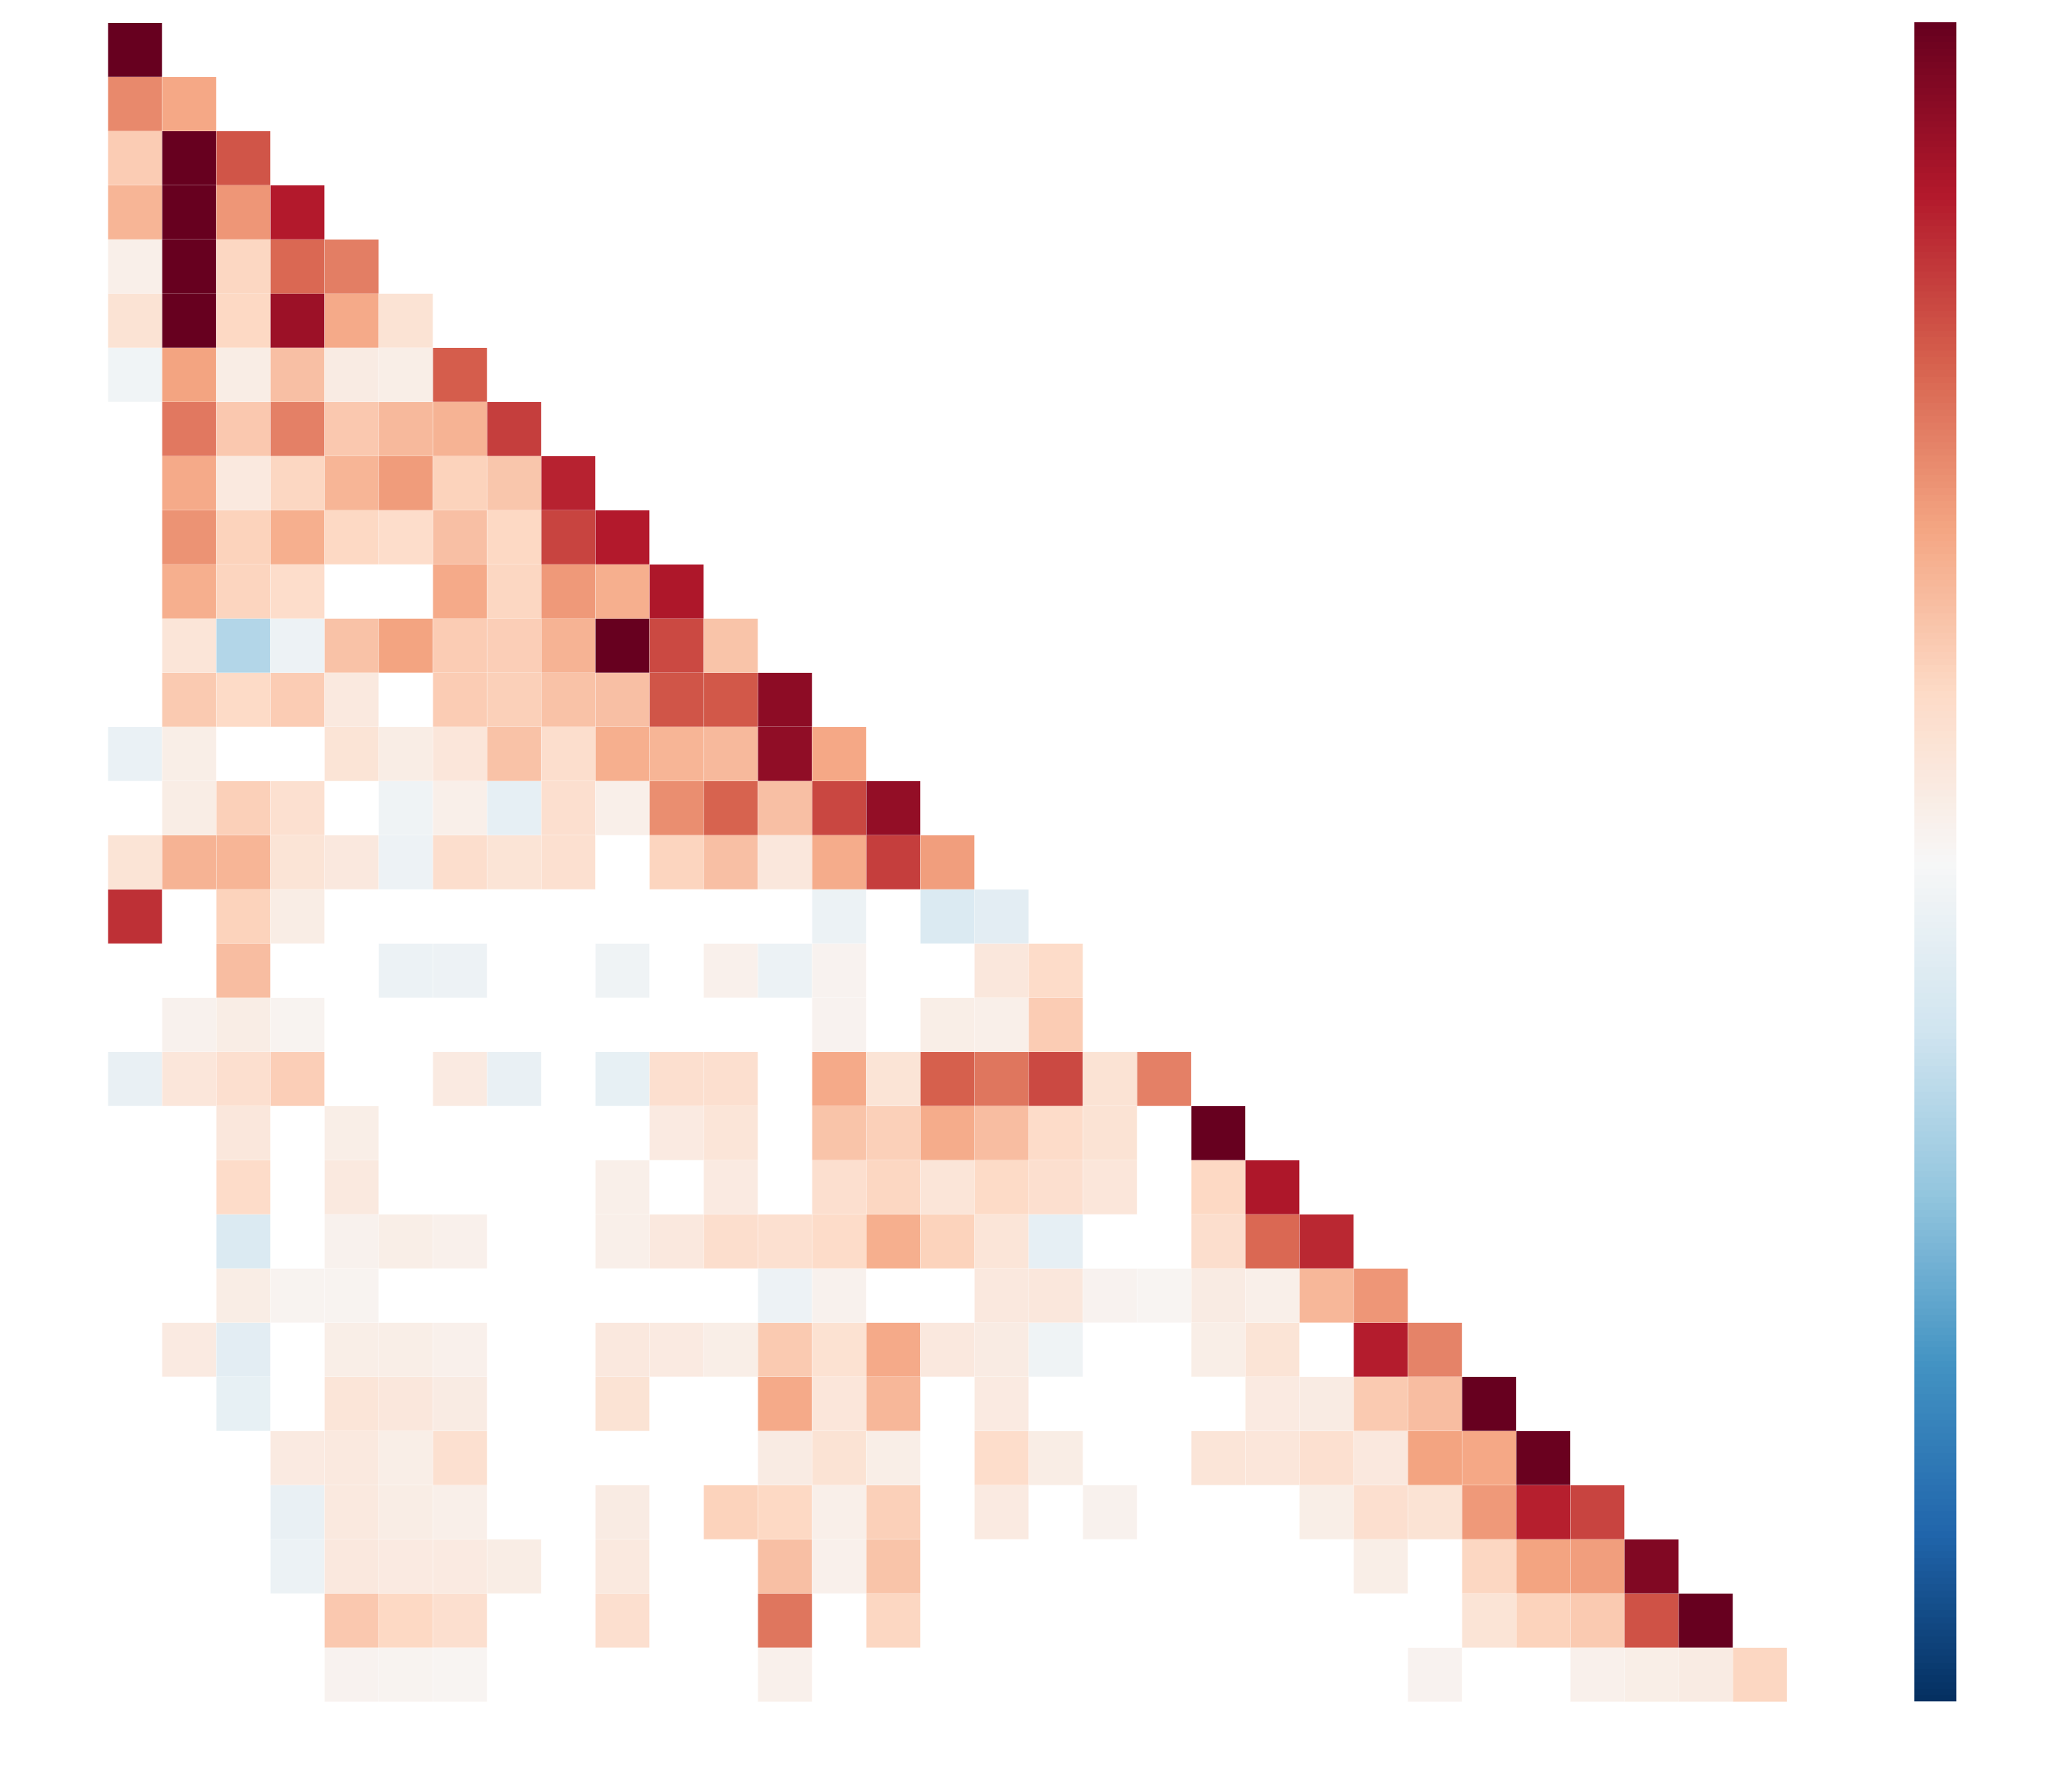
\includegraphics[width=0.62\textwidth]{./Chapter15/Figures/DLCL-picture.png}};
{\footnotesize
\node[anchor=center]  at (4.1,3){4};
\node[anchor=center]  at (4.1,1.5){2};
\node[anchor=center]  at (4.1,0){0};
\node[anchor=center]  at (4.1,-1.5){-2};
\node[anchor=center]  at (4.1,-3){-4};
\node[anchor=center]  at (-4.2,3.6){$ x_{1}$};
\node[anchor=center]  at (-4.2,2.45){$ x_{6}$};
\node[anchor=center]  at (-4.2,1.3){$ x_{11}$};
\node[anchor=center]  at (-4.2,0.15){$ x_{16}$};
\node[anchor=center]  at (-4.2,-1){$ x_{21}$};
\node[anchor=center]  at (-4.2,-2.15){$ x_{26}$};
\node[anchor=center]  at (-4.2,-3.3){$ x_{31}$};
\node[anchor=center]  at (-3.75,-3.8){$ y_{0}$};
\node[anchor=center]  at (-2.6,-3.8){$ y_{5}$};
\node[anchor=center]  at (-1.45,-3.8){$ y_{10}$};
\node[anchor=center]  at (-0.3,-3.8){$ y_{15}$};
\node[anchor=center]  at (0.85,-3.8){$ y_{20}$};
\node[anchor=center]  at (2,-3.8){$ y_{25}$};
\node[anchor=center]  at (3.15,-3.8){$ y_{30}$};
}
\end{tikzpicture}
\caption{对收敛的DLCL网络进行权重的可视化\upcite{WangLearning}}
\label{fig:15-14}
\end{figure}
%-------------------------------------------

%----------------------------------------------------------------------------------------
%    NEW SUB-SECTION
%----------------------------------------------------------------------------------------

\subsection{面向深层模型的参数初始化策略}

\parinterval 对于深层神经机器翻译模型,除了神经网络结构的设计,合适的模型参数初始化策略同样十分重要。例如,Transformer中参数矩阵采用了Xavier初始化方法\upcite{pmlr-v9-glorot10a}。该方法可以保证在训练过程中各层激活函数的输出和梯度的方差的一致性,即同时保证每层在前向和反向传播时输入和输出的方差相同。但是,这类方法更多地被用于初始化浅层神经网络,在训练深层Transformer 模型时表现不佳\upcite{pmlr-v9-glorot10a}。因此,研究人员也针对深层网络的参数初始化问题进行了探索,分为以下几种方法。

%----------------------------------------------------------------------------------------
%    NEW SUBSUB-SECTION
%----------------------------------------------------------------------------------------

\subsubsection{1. 基于深度缩放的初始化策略}

\parinterval 随着神经网络层数的加深,输入的特征要经过很多的线性及非线性变换,受神经网络中激活函数导数值域范围和连乘操作的影响,常常会带来梯度爆炸或梯度消失的问题。这个问题的原因是过多地堆叠网络层数时,无法保证反向传播过程中每层梯度方差的一致性,因此在目前深层模型中采用的很多标准化方式(如层标准化、批次标准化等)都是从方差一致性的角度来解决问题,即将各层输出的取值范围控制在激活函数的梯度敏感区域,从而维持神经网络中梯度传递的稳定性。

\parinterval 为了说明问题,首先来看一看Xavier初始化方法如何对参数矩阵$\mathbi{W}$进行初始化\upcite{pmlr-v9-glorot10a}。具体做法为从一个均匀分布中进行随机采样:
\begin{eqnarray}
\mathbi{W} & \in & \mathbb{R}^{n_i\times n_o} \sim u(-\gamma,\gamma) \\
\gamma     & = & \sqrt{\frac{6}{n_i + n_o}}
\label{eq:15-40}
\end{eqnarray}

\noindent 其中,$u(-\gamma,\gamma)$表示$-\gamma$与$\gamma$间的均匀分布,$n_i$和$n_o$分别为线性变换$\mathbi{W}$中输入和输出的维度,也就是上一层神经元的数量和下一层神经元的数量。通过这种方式可以维持在前向与反向计算过程中输入与输出方差的一致性\upcite{DBLP:conf/iccv/HeZRS15}。

\parinterval 令模型中某层神经元的输出表示为$\mathbi{Z}=\sum_{j=1}^{n_i}{w_j x_j}$。可以看出,$\mathbi{Z}$的核心是计算两个变量$w_j$和$x_j$乘积。两个变量乘积的方差的展开式为:
\begin{eqnarray}
\textrm{Var}(w_j x_j) &=& E[w_j]^2 \textrm{Var}(x_j) + E[x_j]^2 \textrm{Var}(w_j) + \textrm{Var}(w_j)\textrm{Var}(x_j)
\label{eq:15-41}
\end{eqnarray}

\parinterval 其中$\textrm{Var}(\cdot)$表示求方差操作,由于在大多数情况下,现有模型中的各种标准化方法可以维持$E[w_j]^2$和$E[x_j]^2$等于或者近似为0。因此,模型中一层神经元输出的方差可以表示为:
\begin{eqnarray}
\textrm{Var}(\mathbi{Z}) &=& \sum_{j=1}^{n_i}{\textrm{Var}(x_j) \textrm{Var}(w_j)} \nonumber \\
&=& {n_i}\textrm{Var}(\mathbi{W})\textrm{Var}(\mathbi{X})
\label{eq:15-42}
\end{eqnarray}

\parinterval 通过观察公式\eqref{eq:15-42}可以发现,在前向传播的过程中,当$\textrm{Var}(\mathbi{W})=\frac{1}{n_i}$时,可以保证每层的输入和输出的方差一致。类似的,通过相关计算可以得知,为了保证模型中每一层的输入和输出的方差一致,反向传播时应有$\textrm{Var}(\mathbi{W})=\frac{1}{n_o}$,通过对两种情况取平均值,控制参数$\mathbi{W}$的方差为$\frac{2}{n_i+n_o}$,则可以维持在前向与反向过程中输入与输出方差的一致性。若将参数初始化为一个服从边界为$[-a,b]$的均匀分布,那么其方差为$\frac{{(b+a)}^2}{12}$,为了达到$\mathbi{W}$的取值要求,初始化时应有$a=b=\sqrt{\frac{6}{n_i+n_o}}$。

\parinterval 但是随着神经网络层数的增加,上述初始化方法已经不能很好地约束基于Post-Norm的Transformer模型的输出方差。当神经网络堆叠很多层时,模型顶层输出的方差较大,同时反向传播时顶层的梯度范数也要大于底层。因此,一个自然的想法是根据网络的深度对不同层的参数矩阵采取不同的初始化方式,进而强化对各层输出方差的约束,可以描述为:
\begin{eqnarray}
\mathbi{W} & \in & \mathbb{R}^{n_i\times n_o} \sim u(-\gamma \frac{\alpha}{\sqrt{l}},\gamma \frac{\alpha}{\sqrt{l}})
\label{eq:15-43}
\end{eqnarray}

\noindent 其中,$l$为对应的神经网络的深度,$\alpha$为预先设定的超参数来控制缩放的比例。这样,可以通过缩减顶层神经网络输出与输入之间的差异,让激活函数的输入分布保持在一个稳定状态,以此来尽可能避免它们陷入梯度饱和区。

%----------------------------------------------------------------------------------------
%    NEW SUBSUB-SECTION
%----------------------------------------------------------------------------------------

\subsubsection{2. Lipschitz初始化策略}

\parinterval \ref{sec:post-pre-norm}节已经介绍,在Pre-Norm结构中每一个子层的输入为$\mathbi{x}_{l+1}^{\textrm{pre}}=\mathbi{x}_l+\mathbi{y}_l$,其中$\mathbi{x}_l$为当前子层的输入, $\mathbi{y}_l$ 为$\mathbi{x}_l$经过自注意力或前馈神经网络计算后得到的子层输出。在Post-Norm结构中,在残差连接之后还要进行层标准化操作,具体的计算流程为:

\begin{itemize}
\vspace{0.5em}
\item {\small\bfnew{计算均值}}:${\bm  \mu}=\textrm{mean}⁡(\mathbi{x}_l+\mathbi{y}_l)$
\vspace{0.5em}
\item {\small\bfnew{计算方差}}:${\bm  \sigma}=\textrm{std}⁡(\mathbi{x}_l+\mathbi{y}_l)$
\vspace{0.5em}
\item {\small\bfnew{根据均值和方差对输入进行放缩}},如下:
\begin{eqnarray}
\mathbi{x}_{l+1}^{\textrm{post}} &=& \frac{\mathbi{x}_l+\mathbi{y}_l-{\bm  \mu}}{\bm  \sigma} \cdot \mathbi{w}+\mathbi{b}
\label{eq:15-44}
\end{eqnarray}

\noindent 其中,$\mathbi{w}$和$\mathbi{b}$为可学习参数。进一步将公式\eqref{eq:15-44}展开后可得:
\begin{eqnarray}
\mathbi{x}_{l+1}^{\textrm{post}} &=& \frac{\mathbi{x}_l+\mathbi{y}_l}{\bm  \sigma} \cdot \mathbi{w} - \frac{\bm  \mu}{\bm  \sigma} \cdot \mathbi{w}+\mathbi{b} \nonumber \\
                                 &=& \frac{\mathbi{w}}{\bm  \sigma} \cdot \mathbi{x}_{l+1}^{\textrm{pre}}-\frac{\mathbi{w}}{\bm  \sigma} \cdot {\bm  \mu}+\mathbi{b}
\label{eq:15-45}
\end{eqnarray}
%\vspace{0.5em}
\end{itemize}

\parinterval 可以看到相比于Pre-Norm的计算方式,基于Post-Norm的Transformer中子层的输出为Pre-Norm形式的$\frac{\mathbi{w}}{\bm  \sigma}$倍。当$\frac{\mathbi{w}}{\bm  \sigma}<1$时,$\mathbi{x}_l$较小,输入与输出之间差异过大,导致深层Transformer系统难以收敛。Lipschitz 初始化策略通过维持条件$\frac{\mathbi{w}}{\bm  \sigma}>1$,保证网络输入与输出范数一致,进而缓解梯度消失的问题\upcite{DBLP:conf/acl/XuLGXZ20}。一般情况下,$\mathbi{w}$可以被初始化为1,因此Lipschitz 初始化方法最终的约束条件则为:
\begin{eqnarray}
0\ <\ {\bm  \sigma} &=& \textrm{std}⁡(\mathbi{x}_l+\mathbi{y}_l) \ \leq\  1
\label{eq:15-46}
\end{eqnarray}

%----------------------------------------------------------------------------------------
%    NEW SUBSUB-SECTION
%----------------------------------------------------------------------------------------

\subsubsection{3. T-Fixup初始化策略}

\parinterval 另外一种初始化方法是从神经网络结构与优化器的计算方式入手。Post-Norm结构在Warmup阶段难以精确地估计参数的二阶动量,这导致了训练不稳定问题\upcite{huang2020improving}。也就是,层标准化是导致深层Transformer难以优化的主要原因之一\upcite{WangLearning}。Post-Norm方式下Transformer的底层网络,尤其是编码器的词嵌入层面临严重的梯度消失问题。出现该问题的原因在于,在不改变层标准化位置的条件下,Adam优化器利用滑动平均的方式来估计参数的二阶矩,其方差是无界的。在训练阶段的前期,由于模型只能看到有限数量样本,因此很难有效地估计参数的二阶矩,导致反向更新参数时参数的梯度方差过大。

\parinterval 除了用Pre-Norm代替Post-Norm结构来训练深层网络,也可以采用去除Warmup策略并移除层标准化机制的方式,并对神经网络中不同的参数矩阵制定相应的缩放机制来保证训练的稳定性\upcite{huang2020improving}。具体的缩放策略如下:

\begin{itemize}
\vspace{0.5em}
\item 类似于标准的Transformer初始化方式,使用Xavier初始化方式来初始化除了词嵌入以外的所有参数矩阵。词嵌入矩阵服从$\mathbb{N}(0,d^{-\frac{1}{2}})$的高斯分布,其中$d$代表词嵌入的维度。
\vspace{0.5em}
\item 对编码器中自注意力机制的参数矩阵以及前馈神经网络中所有参数矩阵进行缩放因子为$0.67 {L}^{-\frac{1}{4}}$的缩放,$L$为编码器层数。
\vspace{0.5em}
\item 对解码器中全部注意力机制的参数矩阵以及前馈神经网络中所有参数矩阵进行缩放因子为$(9 {M})^{-\frac{1}{4}}$的缩放,其中$M$为解码器层数。
\vspace{0.5em}
\end{itemize}

\parinterval 这种初始化方法由于没有Warmup策略,学习率会直接从峰值根据参数的更新次数进行退火,大幅度增大了模型收敛的时间。因此,如何进一步解决该初始化方法下的模型收敛速度是比较关键的问题。

%----------------------------------------------------------------------------------------
%    NEW SUBSUB-SECTION
%----------------------------------------------------------------------------------------

\subsubsection{4. ADMIN初始化策略}

\parinterval 也有研究发现Post-Norm结构在训练过程中过度依赖残差支路,在训练初期很容易发生参数梯度方差过大的现象\upcite{DBLP:conf/emnlp/LiuLGCH20}。经过分析发现,虽然底层神经网络发生梯度消失是导致训练不稳定的重要因素,但并不是唯一因素。例如,标准Transformer模型中梯度消失的原因在于使用了Post-Norm结构的解码器。尽管通过调整模型结构解决了梯度消失问题,但是模型训练不稳定的问题仍然没有被很好地解决。研究人员观测到Post-Norm结构在训练过程中过于依赖残差支路,而Pre-Norm结构在训练过程中逐渐呈现出对残差支路的依赖性,这更易于网络的训练。进一步,从参数更新的角度出发,Pre-Norm由于参数的改变导致网络输出变化的方差经推导后可以表示为$O(\log L)$,而Post-Norm对应的方差为$O(L)$。因此,可以尝试减小Post-Norm中由于参数更新导致的输出的方差值,从而达到稳定训练的目的。针对该问题,可以采用两阶段的初始化方法。这里,可以重新定义子层之间的残差连接如下:
\begin{eqnarray}
\mathbi{x}_{l+1} &=& \mathbi{x}_l \cdot {\bm  \omega_{l+1}} + F_{l+1}(\mathbi{x}_l)
\label{eq:15-47}
\end{eqnarray}

\noindent 其两阶段的初始化方法如下所示:

\begin{itemize}
\vspace{0.5em}
\item {\small\bfnew{Profiling阶段}}:${\bm  \omega_{l+1}} = 1$,只进行前向计算,无需进行梯度计算。在训练样本上计算$F_{l+1}(\mathbi{x}_l)$的方差
\vspace{0.5em}
\item {\small\bfnew{Initialization阶段}}:通过Profiling阶段得到的$F_{l+1}(\mathbi{x}_l)$的方差来初始化$\bm  \omega_{l+1}$:
\begin{eqnarray}
{\bm \omega_{l+1}} &=& \sqrt{\sum_{j<l}\textrm{Var}[F_{l+1}(\mathbi{x}_l)]}
\label{eq:15-48}
\end{eqnarray}
\end{itemize}

\parinterval 这种动态的参数初始化方法不受限于具体的模型结构,有较好的通用性。

%----------------------------------------------------------------------------------------
%    NEW SUB-SECTION
%----------------------------------------------------------------------------------------

\subsection{深层模型的训练加速}

\parinterval 尽管窄而深的神经网络比宽网络有更快的收敛速度\upcite{WangLearning},但伴随着训练数据的增加,以及模型进一步的加深,训练代价成为不可忽视的问题。例如,在几千万甚至上亿的双语平行句对上训练一个48层的Transformer模型需要几周的时间才能达到收敛\footnote[5]{训练时间的估算是在单台8卡Titan V GPU服务器上得到的}。因此,在保证模型性能不变的前提下,高效地完成深层模型的训练也是至关重要的。

%----------------------------------------------------------------------------------------
%    NEW SUBSUB-SECTION
%----------------------------------------------------------------------------------------

\subsubsection{1. 渐进式训练}

\parinterval 所谓渐进式训练是指从浅层神经网络开始,在训练过程中逐渐增加模型的深度。一种比较简单的方法是将模型分为浅层部分和深层部分,之后分别进行训练,最终达到提高模型翻译性能的目的\upcite{DBLP:conf/acl/WuWXTGQLL19}。

\parinterval 另一种方式是动态构建深层模型,并尽可能复用浅层部分的训练结果\upcite{li2020shallow}。假设开始的时候模型包含$l$层神经网络,然后训练这个模型至收敛。之后,直接拷贝这$l$层神经网络(包括参数),并堆叠出一个$2l$ 层的模型。之后继续训练,重复这个过程。进行$n$次之后就得到了$(n+1) \times l$层的模型。图\ref{fig:15-15}给出了在编码器上使用渐进式训练的示意图。

%----------------------------------------------
\begin{figure}[htp]
\centering
%%%------------------------------------------------------------------------------------------------------------

\begin{center}
\begin{tikzpicture}
\begin{scope}

\node [anchor=east,fill=orange!20,draw,rounded corners=3pt,minimum height=1.6em,minimum width=1.6em] (s11) at (-0.5em, 0) {\footnotesize{$\times l$}};
\node [rectangle,anchor=west,fill=blue!20,draw,rounded corners=3pt,minimum height=1.6em,minimum width=1.6em] (s12) at ([xshift=1.2em]s11.east) {};

\node [anchor=north,fill=orange!20,draw,rounded corners=3pt,minimum height=1.6em,minimum width=1.6em] (s21) at ([yshift=-1.2em]s11.south) {\footnotesize{$\times l$}};
\node [anchor=west,fill=orange!20,draw=red,rounded corners=3pt,minimum height=1.6em,minimum width=1.6em,dashed] (s22) at ([xshift=1.2em]s21.east) {\footnotesize{$\times l$}};
\node [anchor=west,fill=blue!20,draw,rounded corners=3pt,minimum height=1.6em,minimum width=1.6em] (s23) at ([xshift=1.2em]s22.east) {};

\node [anchor=north,fill=orange!20,draw,rounded corners=3pt,minimum height=1.6em,minimum width=1.6em] (s31) at ([yshift=-1.2em]s21.south) {\footnotesize{$\times l$}};
\node [anchor=west,fill=orange!20,draw,rounded corners=3pt,minimum height=1.6em,minimum width=1.6em] (s32) at ([xshift=1.2em]s31.east) {\footnotesize{$\times l$}};
\node [anchor=west,fill=orange!20,draw=red,rounded corners=3pt,minimum height=1.6em,minimum width=1.6em,dashed] (s33) at ([xshift=1.2em]s32.east) {\footnotesize{$\times l$}};
\node [anchor=west,fill=blue!20,draw,rounded corners=3pt,minimum height=1.6em,minimum width=1.6em] (s34) at ([xshift=1.2em]s33.east) {};

\node [anchor=north,fill=orange!20,draw,rounded corners=3pt,minimum height=1.6em,minimum width=1.6em] (s41) at ([yshift=-1.2em]s31.south) {\footnotesize{$\times l$}};
\node [anchor=west,fill=orange!20,draw,rounded corners=3pt,minimum height=1.6em,minimum width=1.6em] (s42) at ([xshift=1.2em]s41.east) {\footnotesize{$\times l$}};
\node [anchor=west,fill=orange!20,draw,rounded corners=3pt,minimum height=1.6em,minimum width=1.6em] (s43) at ([xshift=1.2em]s42.east) {\footnotesize{$\times l$}};
\node [anchor=west,fill=orange!20,draw=red,rounded corners=3pt,minimum height=1.6em,minimum width=1.6em,dashed] (s44) at ([xshift=1.2em]s43.east) {\footnotesize{$\times l$}};
\node [anchor=west,fill=blue!20,draw,rounded corners=3pt,minimum height=1.6em,minimum width=1.6em] (s45) at ([xshift=1.2em]s44.east) {};

\node [anchor=east] (p1) at ([xshift=-2em]s11.west) {\footnotesize{step 1}};
\node [anchor=east] (p2) at ([xshift=-2em]s21.west) {\footnotesize{step 2}};
\node [anchor=east] (p3) at ([xshift=-2em]s31.west) {\footnotesize{step 3}};
\node [anchor=east] (p4) at ([xshift=-2em]s41.west) {\footnotesize{step 4}};

\node [anchor=south,fill=orange!20,draw,rounded corners=3pt,minimum height=1.4em,minimum width=1.4em] (b1) at ([xshift=-0.2em,yshift=1.6em]p1.north) {};
\node [anchor=west] (b2) at (b1.east) {\footnotesize{:编码器}};
\node [anchor=west,fill=blue!20,draw,rounded corners=3pt,minimum height=1.4em,minimum width=1.4em] (b3) at ([xshift=1em]b2.east) {};
\node [anchor=west] (b4) at (b3.east) {\footnotesize{:解码器}};
\node [anchor=west] (b5) at ([xshift=2em]b4.east) {\footnotesize{:拷贝}};
\draw[-latex,thick,red,dashed] ([xshift=0.5em]b4.east) -- (b5.west);

\draw [-latex, line width=0.8pt] ([xshift=-1.2em]s11.west) -- (s11.west);
\draw [-latex, line width=0.8pt] (s11.east) -- (s12.west);
\draw [-latex, line width=0.8pt] (s12.east) -- ([xshift=1.2em]s12.east);

\draw [-latex, line width=0.8pt] ([xshift=-1.2em]s21.west) -- (s21.west);
\draw [-latex, line width=0.8pt] (s21.east) -- (s22.west);
\draw [-latex, line width=0.8pt] (s22.east) -- (s23.west);
\draw [-latex, line width=0.8pt] (s23.east) -- ([xshift=1.2em]s23.east);

\draw [-latex, line width=0.8pt] ([xshift=-1.2em]s31.west) -- (s31.west);
\draw [-latex, line width=0.8pt] (s31.east) -- (s32.west);
\draw [-latex, line width=0.8pt] (s32.east) -- (s33.west);
\draw [-latex, line width=0.8pt] (s33.east) -- (s34.west);
\draw [-latex, line width=0.8pt] (s34.east) -- ([xshift=1.2em]s34.east);

\draw [-latex, line width=0.8pt] ([xshift=-1.2em]s41.west) -- (s41.west);
\draw [-latex, line width=0.8pt] (s41.east) -- (s42.west);
\draw [-latex, line width=0.8pt] (s42.east) -- (s43.west);
\draw [-latex, line width=0.8pt] (s43.east) -- (s44.west);
\draw [-latex, line width=0.8pt] (s44.east) -- (s45.west);
\draw [-latex, line width=0.8pt] (s45.east) -- ([xshift=1.2em]s45.east);

\draw[-latex,thick,red,dashed] (s11.south)..controls +(south:1em) and +(north:1.2em)..(s22.north);
\draw[-latex,thick,red,dashed] (s22.south)..controls +(south:1em) and +(north:1.2em)..(s33.north);
\draw[-latex,thick,red,dashed] (s33.south)..controls +(south:1em) and +(north:1.2em)..(s44.north);
\end{scope} 
\end{tikzpicture}
\end{center}



\caption{渐进式深层模型训练过程}
\label{fig:15-15}
\end{figure}
%-------------------------------------------

\parinterval 渐进式训练的好处在于深层模型并不是从头开始训练。每一次堆叠,都相当于利用“浅”模型给“深”模型提供了一个很好的初始点,这样深层模型的训练会更加容易。

%----------------------------------------------------------------------------------------
%    NEW SUBSUB-SECTION
%----------------------------------------------------------------------------------------

\subsubsection{2. 分组稠密连接}

\parinterval 很多研究工作已经发现深层模型不同层之间的稠密连接能够很明显地提高信息传递的效率\upcite{WangLearning,DBLP:conf/cvpr/HuangLMW17,Dou2018ExploitingDR,DBLP:conf/acl/WuWXTGQLL19}。与此同时,对之前层信息的不断复用有助于得到更好的表示,但也带来了计算代价过大的问题。在动态线性层聚合方法(DLCL)中,每一次聚合时都需要重新计算之前每一层表示对当前层输入的贡献度,因此伴随着编码器整体深度的增加,这部分的计算代价变得不可忽略。例如,一个基于动态层聚合的48层Transformer模型比不使用动态层聚合的模型在进行训练时慢近2倍。同时,缓存中间结果也增加了显存的使用量。比如,即使在使用半精度计算的情况下,每张12G显存的GPU上计算的词也不能超过2048个,这导致训练开销急剧增大。

%----------------------------------------------
\begin{figure}[htp]
\centering
%%%------------------------------------------------------------------------------------------------------------
\begin{center}
\begin{tikzpicture}
\begin{scope}

\node [anchor=east,fill=orange!20,draw,rounded corners=3pt,minimum height=1.4em,minimum width=1.4em] (s11) at (-0.5em, 0) {};
\node [rectangle,anchor=west,fill=orange!20,draw,rounded corners=3pt,minimum height=1.4em,minimum width=1.4em] (s12) at ([xshift=2em]s11.east) {};
\node [anchor=west,fill=orange!20,draw,rounded corners=3pt,minimum height=1.4em,minimum width=1.4em] (s13) at ([xshift=2em]s12.east) {};
\node [anchor=west,fill=orange!20,draw,rounded corners=3pt,minimum height=1.4em,minimum width=1.4em] (s14) at ([xshift=2em]s13.east) {};

\node [anchor=north,fill=orange!20,draw,rounded corners=3pt,minimum height=1.4em,minimum width=1.4em] (s21) at ([yshift=-2.5em]s11.south) {};
\node [anchor=west,fill=orange!20,draw,rounded corners=3pt,minimum height=1.4em,minimum width=1.4em] (s22) at ([xshift=2em]s21.east) {};
\node [anchor=west,fill=orange!20,draw,rounded corners=3pt,minimum height=1.4em,minimum width=1.4em] (s23) at ([xshift=2em]s22.east) {};
\node [anchor=west,fill=orange!20,draw,rounded corners=3pt,minimum height=1.4em,minimum width=1.4em] (s24) at ([xshift=2em]s23.east) {};

\node [anchor=north,fill=orange!20,draw,rounded corners=3pt,minimum height=1.4em,minimum width=1.4em] (s31) at ([yshift=-2.5em]s21.south) {};
\node [anchor=west,fill=orange!20,draw,rounded corners=3pt,minimum height=1.4em,minimum width=1.4em] (s32) at ([xshift=2em]s31.east) {};
\node [anchor=west,fill=orange!20,draw,rounded corners=3pt,minimum height=1.4em,minimum width=1.4em] (s33) at ([xshift=2em]s32.east) {};
\node [anchor=west,fill=orange!20,draw,rounded corners=3pt,minimum height=1.4em,minimum width=1.4em] (s34) at ([xshift=2em]s33.east) {};

\node [anchor=north,fill=orange!20,draw,rounded corners=3pt,minimum height=1.4em,minimum width=1.4em] (s41) at ([yshift=-2.5em]s31.south) {};
\node [anchor=west,fill=orange!20,draw,rounded corners=3pt,minimum height=1.4em,minimum width=1.4em] (s42) at ([xshift=2em]s41.east) {};
\node [anchor=west,fill=orange!20,draw,rounded corners=3pt,minimum height=1.4em,minimum width=1.4em] (s43) at ([xshift=2em]s42.east) {};
\node [anchor=west,fill=orange!20,draw,rounded corners=3pt,minimum height=1.4em,minimum width=1.4em] (s44) at ([xshift=2em]s43.east) {};

\node [anchor=east] (p1) at ([xshift=-3.5em]s11.west) {$p=\infty$};
\node [anchor=east] (p2) at ([xshift=-4em]s21.west) {$p=1$};
\node [anchor=east] (p3) at ([xshift=-4em]s31.west) {$p=2$};
\node [anchor=east] (p4) at ([xshift=-4em]s41.west) {$p=4$};
\node [anchor=north] (p5) at ([yshift=-1em]p3.south) {$\cdots$};
\node [anchor=south,fill=orange!20,draw,rounded corners=3pt,minimum height=1.4em,minimum width=1.4em] (b1) at ([xshift=-0.6em,yshift=1.2em]p1.north) {};
\node [anchor=west] (b2) at (b1.east) {\footnotesize{:Layer}};
\node [anchor=west,draw=red,rounded corners=3pt,minimum height=1.4em,minimum width=1.4em,dashed,line width=0.8pt] (b3) at ([xshift=1em]b2.east) {};
\node [anchor=west] (b4) at (b3.east) {\footnotesize{:Block}};

\draw [-latex, line width=0.8pt] ([xshift=-2em]s11.west) -- (s11.west);
\draw [-latex, line width=0.8pt] (s11.east) -- (s12.west);
\draw [-latex, line width=0.8pt] (s12.east) -- (s13.west);
\draw [-latex, line width=0.8pt] (s13.east) -- (s14.west);
\draw [-latex, line width=0.8pt] (s14.east) -- ([xshift=2em]s14.east);

\draw [-latex, line width=0.8pt] ([xshift=-2em]s21.west) -- (s21.west);
\draw [-latex, line width=0.8pt] (s21.east) -- (s22.west);
\draw [-latex, line width=0.8pt] (s22.east) -- (s23.west);
\draw [-latex, line width=0.8pt] (s23.east) -- (s24.west);
\draw [-latex, line width=0.8pt] (s24.east) -- ([xshift=2em]s24.east);

\draw [-latex, line width=0.8pt] ([xshift=-2em]s31.west) -- (s31.west);
\draw [-latex, line width=0.8pt] (s31.east) -- (s32.west);
\draw [-latex, line width=0.8pt] (s32.east) -- (s33.west);
\draw [-latex, line width=0.8pt] (s33.east) -- (s34.west);
\draw [-latex, line width=0.8pt] (s34.east) -- ([xshift=2em]s34.east);

\draw [-latex, line width=0.8pt] ([xshift=-2em]s41.west) -- (s41.west);
\draw [-latex, line width=0.8pt] (s41.east) -- (s42.west);
\draw [-latex, line width=0.8pt] (s42.east) -- (s43.west);
\draw [-latex, line width=0.8pt] (s43.east) -- (s44.west);
\draw [-latex, line width=0.8pt] (s44.east) -- ([xshift=2em]s44.east);


\node [draw=red,rounded corners=3pt,minimum height=1.7em,minimum width=1.7em,dashed,line width=0.8pt] (x21) at (s21) {};
\node [draw=red,rounded corners=3pt,minimum height=1.7em,minimum width=1.7em,dashed,line width=0.8pt] (x22) at (s22) {};
\node [draw=red,rounded corners=3pt,minimum height=1.7em,minimum width=1.7em,dashed,line width=0.8pt] (x23) at (s23) {};
\node [draw=red,rounded corners=3pt,minimum height=1.7em,minimum width=1.7em,dashed,line width=0.8pt] (x24) at (s24) {};

\node [draw=red,rounded corners=3pt,minimum height=1.7em,minimum width=5.2em,dashed,line width=0.8pt] (x31) at ([xshift=1.75em]s31) {};
\node [draw=red,rounded corners=3pt,minimum height=1.7em,minimum width=5.2em,dashed,line width=0.8pt] (x32) at ([xshift=1.75em]s33) {};

\node [draw=red,rounded corners=3pt,minimum height=1.7em,minimum width=12.2em,dashed,line width=0.8pt] (x41) at ([xshift=1.75em]s42) {};

{
\draw [-latex, line width=0.8pt] ([xshift=-1em]s21.west).. controls +(58:0.6) and +(122:0.6) .. ([xshift=1em]s21.east);
\draw [-latex, line width=0.8pt] ([xshift=-1em]s22.west).. controls +(58:0.6) and +(122:0.6) .. ([xshift=1em]s22.east);
\draw [-latex, line width=0.8pt] ([xshift=-1em]s23.west).. controls +(58:0.6) and +(122:0.6) .. ([xshift=1em]s23.east);
\draw [-latex, line width=0.8pt] ([xshift=-1em]s24.west).. controls +(58:0.6) and +(122:0.6) .. ([xshift=1em]s24.east);
}

{
\draw [-latex, line width=0.8pt] ([xshift=-1em]s21.west).. controls +(65:0.8) and +(115:0.8) .. ([xshift=1em]s22.east);
\draw [-latex, line width=0.8pt] ([xshift=-1em]s22.west).. controls +(65:0.8) and +(115:0.8) .. ([xshift=1em]s23.east);
\draw [-latex, line width=0.8pt] ([xshift=-1em]s23.west).. controls +(65:0.8) and +(115:0.8) .. ([xshift=1em]s24.east);
\draw [-latex, line width=0.8pt] ([xshift=-1em]s31.west).. controls +(65:0.8) and +(115:0.8) .. ([xshift=1em]s32.east);
\draw [-latex, line width=0.8pt] ([xshift=-1em]s33.west).. controls +(65:0.8) and +(115:0.8) .. ([xshift=1em]s34.east);
}

{
\draw [-latex, line width=0.8pt] ([xshift=-1em]s21.west).. controls +(70:1.0) and +(110:1.0) .. ([xshift=1em]s23.east);
\draw [-latex, line width=0.8pt] ([xshift=-1em]s22.west).. controls +(70:1.0) and +(110:1.0) .. ([xshift=1em]s24.east);
}

{
\draw [-latex, line width=0.8pt] ([xshift=-1em]s21.west).. controls +(75:1.2) and +(105:1.2) .. ([xshift=1em]s24.east);
\draw [-latex, line width=0.8pt] ([xshift=-1em]s31.west).. controls +(75:1.2) and +(105:1.2) .. ([xshift=1em]s34.east);
\draw [-latex, line width=0.8pt] ([xshift=-1em]s41.west).. controls +(75:1.2) and +(105:1.2) .. ([xshift=1em]s44.east);
}
\end{scope} 
\end{tikzpicture}
\end{center}



\caption{不同组之间的稀疏连接}
\label{fig:15-16}
\end{figure}
%-------------------------------------------

\parinterval 缓解这个问题的一种方法是使用更稀疏的层间连接方式。其核心思想与动态线性层聚合是类似的,不同点在于可以通过调整层之间连接的稠密程度来降低训练代价。比如,可以将每$p$层分为一组,之后动态线性层聚合只在不同组之间进行。这样,通过调节$p$值的大小可以控制神经网络中连接的稠密程度,作为一种训练代价与翻译性能之间的权衡。显然,标准的Transformer模型\upcite{vaswani2017attention} 和DLCL模型\upcite{WangLearning}都可以看作是该方法的一种特例。如图\ref{fig:15-16}所示:当$p=1$时,每一个单独的块被看作一个独立的组,它等价于基于动态层聚合的DLCL模型;当$p=\infty$时,它等价于正常的Transformer模型。值得注意的是,如果配合渐进式训练。在分组稠密连接中可以设置$p$等于模型层数。

%----------------------------------------------------------------------------------------
%    NEW SUBSUB-SECTION
%----------------------------------------------------------------------------------------

\subsubsection{3. 学习率重置}

\parinterval 尽管渐进式训练策略与分组稠密连接结构都可以加速深层模型的训练,但使用传统的学习率衰减策略会导致训练深层模型时的学习率较小,因此模型无法快速地达到收敛状态,同时也影响最终的模型性能。

\parinterval  图\ref{fig:15-17}中的红色曲线描绘了在WMT英德翻译任务上标准Transformer模型的学习率曲线,可以看到当模型训练到40k步时,学习率对比峰值有明显的差距,而此时刚开始训练最终的深层模型,过小的学习率并不利于后期深层网络的充分训练。

%----------------------------------------------
\begin{figure}[htp]
\centering
\begin{center}
  \begin{tikzpicture}[scale=1.0]
    \footnotesize{
      \begin{axis}[
      width=.50\textwidth,
      height=.40\textwidth,
      legend style={at={(0.45,0.08)}, anchor=south west},
      xlabel={\scriptsize{更新次数(10k)}},
      ylabel={\scriptsize{学习率 ($10^{-3}$)}},
      ylabel style={yshift=-1em},xlabel style={yshift=0.0em},
      yticklabel style={/pgf/number format/precision=2,/pgf/number format/fixed zerofill},
      ymin=0,ymax=2.2, ytick={0.5, 1, 1.5, 2},
      xmin=0,xmax=5,xtick={1,2,3,4},
      legend style={xshift=-8pt,yshift=-4pt, legend plot pos=right,font=\scriptsize,cells={anchor=west}}
      ]

      \addplot[red,line width=1.25pt] coordinates {(0,0) (1.6,2) (1.8,1.888) (2,1.787) (2.5,1.606) (3,1.462) (3.5,1.3549) (4,1.266) (4.5,1.193) (5,1.131)};
      \addlegendentry{\scriptsize 原始的学习率}
      %\addplot[red,line width=1.25pt] coordinates {(0,0) (8000,0.002) (10000,0.00179) (12000,0.00163) (12950,0.001572)};
      \addplot[blue,line width=1.25pt] coordinates {(0,0) (0.8,2) (0.9906,1.7983)};
      %\addplot[red,line width=1.25pt] coordinates {(0,0) (8000,0.002) (9906,0.0017983)};
      \addplot[blue,dashed,line width=1.25pt] coordinates {(0.9906,1.7983) (0.9906,2)};
      \addplot[blue,line width=1.25pt] coordinates {(0.9906,2) (1.1906,1.79) (1.3906,1.63) (1.4856,1.572)};
      \addplot[blue,dashed,line width=1.25pt] coordinates {(1.4856,1.572) (1.4856,2)};
      \addplot[blue,line width=1.25pt] coordinates {(1.4856,2) (1.6856,1.79) (1.8856,1.63) (1.9806,1.572)};
      \addplot[blue,dashed,line width=1.25pt] coordinates {(1.9806,1.572) (1.9806,2)};
      \addplot[blue,line width=1.25pt] coordinates {(1.9806,2) (2.1806,1.79) (2.3806,1.63) (2.4756,1.572)};
      \addplot[blue,dashed,line width=1.25pt] coordinates {(2.4756,1.572) (2.4756,2)};
      \addplot[blue,line width=1.25pt] coordinates {(2.4756,2) (2.6756,1.79) (2.8756,1.63) (2.9706,1.572)};
      \addplot[blue,dashed,line width=1.25pt] coordinates {(2.9706,1.572) (2.9706,2)};
      \addplot[blue,line width=1.25pt] coordinates {(2.9706,2) (3.1706,1.79) (3.3706,1.63) (3.4656,1.572) (3.6706,1.4602) (3.7136,1.44)};
      \addplot[blue,dashed,line width=1.25pt] coordinates {(3.7136,1.44) (3.7136,2)};
      \addplot[blue,line width=1.25pt] coordinates {(3.7136,2) (3.9136,1.79) (4.1136,1.63) (4.2086,1.572) (4.4136,1.4602) (4.4566,1.44) (4.7000,1.3574) (5.0000,1.2531)};
      \addlegendentry{\scriptsize 重置后的学习率}

      \end{axis}
     }
  \end{tikzpicture}
\end{center}
\caption{学习率重置vs从头训练的学习率曲线}
\label{fig:15-17}
\end{figure}
%-------------------------------------------

\parinterval 针对该问题的一个解决方案是修改学习率曲线的衰减策略,如图\ref{fig:15-17}所示。图中蓝色的曲线是修改后的学习率曲线。首先在训练的初期让模型快速地达到学习率的峰值(线性递增),之后的每一次增加$l$层神经网络时,都会将当前的学习率值重置到峰值点。之后,根据训练的步数对其进行相应的衰减。具体的步骤如下:

\begin{itemize}
\vspace{0.5em}
\item 在训练的初期,模型会先经历一个学习率预热的过程:
\begin{eqnarray}
lr &=& d_{\textrm{model}}^{-0.5}\cdot step\_num \cdot warmup\_steps^{-0.5}
\label{eq:15-49}
\end{eqnarray}
\noindent 这里,$step\_num$表示参数更新的次数,$warmup\_step$表示预热的更新次数,$d_{\textrm{model}}$表示Transformer模型的隐层大小,$lr$是学习率。
\vspace{0.5em}
\item 	在之后的训练过程中,每当增加模型深度时,学习率都会重置到峰值,之后进行相应的衰减:
\begin{eqnarray}
lr &=& d_{\textrm{model}}^{-0.5}\cdot step\_num^{-0.5}
\label{eq:15-50}
\end{eqnarray}
\noindent 这里$step\_num$代表学习率重置后更新的步数。
\vspace{0.5em}
\end{itemize}

\parinterval 综合使用渐进式训练、分组稠密连接、学习率重置策略可以保证在翻译品质不变的前提下,缩减近$40\%$的训练时间\upcite{li2020shallow}。同时,伴随着模型的加深与数据集的增大加速比也会进一步地增大。

%----------------------------------------------------------------------------------------
%    NEW SUB-SECTION
%----------------------------------------------------------------------------------------

\subsection{深层模型的健壮性训练}


\parinterval 伴随着网络的加深,模型的训练还会面临另外一个比较严峻的问题\ \dash \ 过拟合。由于参数量的增大,深层模型的输入与输出分布之间的差异也会越来越大,然而不同子层之间的相互适应也会更加的明显,这将导致任意子层网络对其他子层的依赖过大。这种现象在训练阶段是有帮助的,因为不同子层可以协同工作从而更好地拟合训练数据。然而这种方式也降低了模型的泛化能力,即深层模型更容易陷入过拟合问题。

\parinterval 通常,可以使用Dropout手段用来缓解过拟合问题(见{\chapterthirteen})。不幸的是,尽管目前Transformer模型使用了多种Dropout手段(如Residual Dropout、Attention Dropout、 ReLU Dropout等),过拟合问题在深层模型中仍然存在。从图\ref{fig:15-18}中可以看到,深层模型比浅层模型在训练集和校验集的困惑度上都有明显的优势,然而模型在训练一段时间后出现校验集困惑度上涨的现象,说明模型已经过拟合于训练数据。

%----------------------------------------------
\begin{figure}[htp]
\centering
\definecolor{ublue}{rgb}{0.152,0.250,0.545}
\begin{tikzpicture}
\begin{axis}
[  
  width=5cm, height=3.5cm, 
  xtick={15,17,19,21,23,25},
  ytick={6.0,6.5,7.0},
  xlabel={\scriptsize Epoch},
  ylabel={},
  ylabel style={},
  x tick label style={},
  y tick label style={},
  tick align=inside,
  legend style={anchor=north,xshift=1.7cm,yshift=1cm,legend  columns =-1},
  ymin=5.7,
  ymax=7.3,
  xmin=14.6,
  xmax=25.4,
  extra y ticks={6.0,6.5,7.0},
  extra y tick labels={3.7,3.8,3.9},
  extra y tick style={ticklabel pos=right}]
  \addplot [sharp plot,very thick,red!60,mark=diamond*] coordinates{(15,6.75) (16,6.73) (17,6.70) (18,6.67) (19,6.64) (20,6.61) (21,6.59) (22,6.58) (23,6.57) (24,6.58) (25,6.59)};
  \addplot [sharp plot,very thick,purple!60,mark=triangle*] coordinates{(15,6.70) (16,6.4) (17,6.20) (18,6.30) (19,6.20) (20,6.10) (21,6.15) (22,6.10) (23,6.15) (24,6.16) (25,6.17)};
  \legend{\scriptsize {训练集},\scriptsize{校验集}}
\end{axis}
\begin{axis}
[ xshift=6.6cm,
  width=5cm, height=3.5cm, 
  xtick={15,17,19,21,23,25},
  ytick={5.0,5.5,6.0},
  xlabel={\scriptsize Epoch},
  ylabel={},
  ylabel style={},
  x tick label style={},
  y tick label style={},
  tick align=inside,
  ymin=4.7,
  ymax=6.3,
  xmin=14.6,
  xmax=25.4,
  extra y ticks={5.0,5.5,6.0},
  extra y tick labels={3.5,3.6,3.7},
  extra y tick style={ticklabel pos=right}]
  \addplot [sharp plot,very thick,red!60,mark=diamond*] coordinates{(15,5.7) (16,5.65) (17,5.6) (18,5.55) (19,5.5) (20,5.45) (21,5.4) (22,5.38) (23,5.36) (24,5.34) (25,5.27)};
  \addplot [sharp plot,very thick,purple!60,mark=triangle*] coordinates{(15,5.0) (16,4.9) (17,4.9) (18,5.05) (19,4.9) (20,5.0) (21,5.0) (22,5.1) (23,5.0) (24,5.15) (25,5.5)};
\end{axis}
\node [anchor=north,rotate=90] (n1) at (-1.3cm,1cm) {\scriptsize 训练集\ PPL};
\node [anchor=north,rotate=90] (n2) at (5.4cm,1cm) {\scriptsize 训练集\ PPL};
\node [anchor=north,rotate=90] (n3) at (4.2cm,1cm) {\scriptsize 校验集\ PPL};
\node [anchor=north,rotate=90] (n4) at (10.7cm,1cm) {\scriptsize 校验集\ PPL};
\end{tikzpicture}

%---------------------------------------------------------------------
\caption{浅层模型(左)与深层模型(右)在WMT16英德翻译任务的校验集与训练集的困惑度}
\label{fig:15-18}
\end{figure}
%-------------------------------------------

\parinterval {\chapterthirteen}提到的Layer Dropout方法可以有效地缓解这个问题。以编码器为例, Layer Dropout的过程可以被描述为:在训练过程中,对自注意力子层或前馈神经网络子层进行随机丢弃,以减少不同子层之间的相互适应。这里选择Pre-Norm结构作为基础架构,它可以被描述为:
\begin{eqnarray}
\mathbi{x}_{l+1} &=& F(\textrm{LN}(\mathbi{x}_l)) + \mathbi{x}_l
\label{eq:15-51}
\end{eqnarray}

\noindent 其中,$\textrm{LN}( \cdot )$表示层标准化函数, $F( \cdot )$表示自注意力机制或者前馈神经网络,$\mathbi{x}_l$表示第$l$个子层的输入。之后,使用一个掩码$\textrm{Mask}$(值为0或1)来控制每个子层是正常计算还是丢弃。于是,该子层的计算公式可以被重写为:
\begin{eqnarray}
\mathbi{x}_{l+1} &=& \textrm{Mask} \cdot F(\textrm{LN}(\mathbi{x}_l))+\mathbi{x}_l
\label{eq:15-52}
\end{eqnarray}

\noindent $\textrm{Mask}=0$代表该子层被丢弃,而$\textrm{Mask}=1$代表正常进行当前子层的计算。图\ref{fig:15-19}展示了这个方法与标准Pre-Norm结构之间的区别。

%----------------------------------------------
\begin{figure}[htp]
\centering
%%%------------------------------------------------------------------------------------------------------------
%%% 调序模型1:基于距离的调序
\begin{center}
\begin{tikzpicture}

\begin{scope}[minimum height = 20pt]

\node [anchor=east] (x1) at (-0.5em, 0) {$\mathbi{x}_l$};
\node [anchor=west,draw,fill=red!30,inner xsep=5pt,rounded corners=2pt,draw,thick] (ln1) at ([xshift=1em]x1.east){\small{\textrm{LN}}};
\node [anchor=west,draw,fill=green!30,inner xsep=5pt,rounded corners=2pt,draw,thick] (f1) at ([xshift=0.6em]ln1.east){\small{$F$}};
\node [anchor=west,circle,draw,,minimum size=1em,thick] (n1) at ([xshift=3em]f1.east){};
\node [anchor=west] (x2) at ([xshift=1em]n1.east) {$\mathbi{x}_{l+1}$};
\node [anchor=west,draw,fill=red!30,inner xsep=5pt,rounded corners=2pt,draw,thick] (ln12) at ([xshift=1em]x2.east){\small{\textrm{LN}}};
\node [anchor=west,draw,fill=green!30,inner xsep=5pt,rounded corners=2pt,draw,thick] (f12) at ([xshift=0.6em]ln12.east){\small{$F$}};
\node [anchor=west,circle,draw,,minimum size=1em,thick] (n12) at ([xshift=3em]f12.east){};
\node [anchor=west] (x22) at ([xshift=1em]n12.east) {$\mathbi{x}_{l+2}$};

\node [anchor=north] (x3) at ([yshift=-5em]x1.south) {$\mathbi{x}_l$};
\node [anchor=west,draw,fill=red!30,inner xsep=5pt,rounded corners=2pt,draw,thick] (ln2) at ([xshift=1em]x3.east){\small{\textrm{LN}}};
\node [anchor=west,draw,fill=green!30,inner xsep=5pt,rounded corners=2pt,draw,thick] (f2) at ([xshift=0.6em]ln2.east){\small{$F$}};
\node [anchor=west,minimum size=1em] (p1) at ([xshift=1em]f2.east){};
\node [anchor=north] (m1) at ([yshift=0.6em]p1.south){\footnotesize{\red{Mask=1}}};
\node [anchor=west,circle,draw,,minimum size=1em,thick] (n2) at ([xshift=3em]f2.east){};
\node [anchor=west] (x4) at ([xshift=1em]n2.east) {$\mathbi{x}_{l+1}$};
\node [anchor=west,draw,fill=red!30,inner xsep=5pt,rounded corners=2pt,draw,thick] (ln22) at ([xshift=1em]x4.east){\small{\textrm{LN}}};
\node [anchor=west,draw,fill=green!30,inner xsep=5pt,rounded corners=2pt,draw,thick] (f22) at ([xshift=0.6em]ln22.east){\small{$F$}};
\node [anchor=west,minimum size=1em] (p2) at ([xshift=1em]f22.east){};
\node [anchor=north] (m2) at ([yshift=0.6em]p2.south){\footnotesize{\red{Mask=0}}};
\node [anchor=west,circle,draw,,minimum size=1em,thick] (n22) at ([xshift=3em]f22.east){};
\node [anchor=west] (x42) at ([xshift=1em]n22.east) {$\mathbi{x}_{l+2}$};

\draw[->, line width=1pt] ([xshift=-0.1em]x1.east)--(ln1.west);
\draw[->, line width=1pt] ([xshift=-0.1em]ln1.east)--(f1.west);
\draw[->, line width=1pt] ([xshift=0.1em]f1.east)--(n1.west);
\draw[->, line width=1pt] (n1.east)--(x2.west);
\draw[->, line width=1pt] ([xshift=-0.1em]x3.east)--(ln2.west);
\draw[->, line width=1pt] ([xshift=-0.1em]ln2.east)--(f2.west);
\draw[-, line width=1pt] ([xshift=0.1em]f2.east)--(p1.west);
\draw[*-,red,line width=0.6pt] (p1.west) -- (p1.east);
\draw[->, line width=1pt] (p1.east)--(n2.west);
\draw[->, line width=1pt] (n2.east)--(x4.west);
\draw[->,rounded corners,line width=1pt] ([yshift=-0.2em]x1.north) -- ([yshift=1em]x1.north) -- ([yshift=1.4em]n1.north) -- (n1.north);
\draw[->,rounded corners,line width=1pt] ([yshift=-0.2em]x3.north) -- ([yshift=1em]x3.north) -- ([yshift=1.4em]n2.north) -- (n2.north);
\draw[-,thick] (n1.west)--(n1.east);
\draw[-,thick] (n1.north)--(n1.south);
\draw[-,thick] (n2.west)--(n2.east);
\draw[-,thick] (n2.north)--(n2.south);

\draw[->, line width=1pt] ([xshift=-0.1em]x2.east)--(ln12.west);
\draw[->, line width=1pt] ([xshift=-0.1em]ln12.east)--(f12.west);
\draw[->, line width=1pt] ([xshift=0.1em]f12.east)--(n12.west);
\draw[->, line width=1pt] (n12.east)--(x22.west);
\draw[->, line width=1pt] ([xshift=-0.1em]x4.east)--(ln22.west);
\draw[->, line width=1pt] ([xshift=-0.1em]ln22.east)--(f22.west);
\draw[-, line width=1pt] ([xshift=0.1em]f22.east)--(p2.west);
\draw[*-,red,line width=0.6pt] ([yshift=-0.1em]p2.west) -- (p2.north east);
\draw[->, line width=1pt] (p2.east)--(n22.west);
\draw[->, line width=1pt] (n22.east)--(x42.west);
\draw[->,rounded corners,line width=1pt] ([yshift=-0.2em]x2.north) -- ([yshift=1em]x2.north) -- ([yshift=1.4em]n12.north) -- (n12.north);
\draw[->,rounded corners,line width=1pt] ([yshift=-0.2em]x4.north) -- ([yshift=1em]x4.north) -- ([yshift=1.4em]n22.north) -- (n22.north);
\draw[-,thick] (n12.west)--(n12.east);
\draw[-,thick] (n12.north)--(n12.south);
\draw[-,thick] (n22.west)--(n22.east);
\draw[-,thick] (n22.north)--(n22.south);

\node [anchor=south] (k1) at ([yshift=-0.1em]x1.north){};
\node [anchor=south] (k2) at ([yshift=-0.1em]x3.north){};
\begin{pgfonlayer}{background}
\node [rectangle,inner sep=0.3em,fill=orange!10] [fit = (x1) (f1) (n1) (ln1) (x2) (k1) (f12) (n12) (ln12) (x22)] (box0) {};
\node [rectangle,inner sep=0.3em,fill=blue!10] [fit = (x3) (f2) (n2) (ln2) (x4) (k2) (f22) (n22) (ln22) (x42)] (box1) {};
\end{pgfonlayer}

\node [anchor=north] (c1) at (box0.south){\footnotesize {(a)标准的Pre-Norm}};
\node [anchor=north] (c2) at (box1.south){\footnotesize {(b)基于随机子层跳跃的Pre-Norm}};
\end{scope}
\end{tikzpicture}
\end{center}
\caption{标准的Pre-Norm结构与基于随机子层跳跃的Pre-Norm结构}
\label{fig:15-19}
\end{figure}
%-------------------------------------------

\parinterval 除此之外,在残差网络中,研究人员已经发现底层神经网络的作用是对输入进行抽象表示,而上层神经网络会进一步修正这种表示来拟合训练目标,因此底层神经网络对模型最终的输出有很大的影响\upcite{DBLP:journals/corr/GreffSS16}。该结论同样适用于Transformer模型,比如,在训练中,残差支路以及底层的梯度范数通常比较大,这也间接表明底层神经网络在整个优化的过程中需要更大的更新。考虑到这个因素,在设计每一个子层被丢弃的概率时,可以采用自底向上线性增大的策略,保证底层的神经网络相比于顶层更容易保留下来。

%----------------------------------------------------------------------------------------
%    NEW SECTION
%----------------------------------------------------------------------------------------

\sectionnewpage
\section{基于句法的神经机器翻译模型}

\parinterval 在统计机器翻译时代,使用句法信息是一种非常有效的机器翻译建模手段(见{\chaptereight})。由于句法是人类运用语言的高级抽象结果,使用句法信息(如句法树)可以帮助机器翻译系统对句子结构进行建模。例如,利用句法树提升译文语法结构的正确性。在神经机器翻译中,大多数框架均基于词串进行建模,因此在模型中引入句法树等结构也很有潜力\upcite{DBLP:conf/acl/LiXTZZZ17}。 具体来说,由于传统神经机器翻译模型缺少对句子结构的理解,会导致一些翻译问题:

\begin{itemize}
\vspace{0.5em}
\item {\small\bfnew{过度翻译问题}},如:
\begin{equation}
\textrm{“ 两/个/女孩 ”}\ \to \ \textrm{“ two girls and two girls ”} \nonumber
\end{equation}

\vspace{0.5em}
\item {\small\bfnew{翻译不连贯问题}},如:
\begin{equation}
\textrm{“ 新生/银行/申请/上市 ”}\ \to \ \textrm{“ new listing bank ”} \nonumber
\end{equation}

\vspace{0.5em}
\end{itemize}

\parinterval 显然,神经机器翻译系统并没有按照合理的句法结构生成译文。也就是说,模型并没有理解句子的结构\upcite{DBLP:conf/acl/LiXTZZZ17}。甚至对于一些语言差异很大的语言对,会出现将介词短语翻译成一个词的情况。虽然可以通过很多手段对上述问题进行求解,但是使用句法树是解决该问题的一种最直接的方法\upcite{DBLP:conf/acl/EriguchiHT16}。

\parinterval 那么在神经机器翻译中,如何将这种离散化的树结构融入到基于分布式表示的翻译模型中呢?有以下两种策略:

\begin{itemize}
\vspace{0.5em}
\item {\small\bfnew{将句法信息加入到编码器}},使得编码器更加充分地表示源语言句子。
\vspace{0.5em}
\item {\small\bfnew{将句法信息加入到解码器}},使得翻译模型能生成更符合句法的译文。
\vspace{0.5em}
\end{itemize}

%----------------------------------------------------------------------------------------
%    NEW SUB-SECTION
%----------------------------------------------------------------------------------------

\subsection{编码器使用句法信息}

\parinterval 在编码器中使用句法信息有两种思路,一种思路是在编码器中显性使用树结构进行建模,另一种思路是把句法信息作为特征输入到传统的序列编码器中。这两种思路与统计机器翻译中基于句法树结构的模型和基于句法特征的模型十分相似(见{\chaptereight})。

%----------------------------------------------------------------------------------------
%    NEW SUBSUB-SECTION
%----------------------------------------------------------------------------------------

\subsubsection{1. 基于句法树结构的编码}

\parinterval 使用句法信息的一种简单的方法是将源语言句子编码成一个二叉树结构\footnote[6]{所有句法树都可以通过二叉化方法转化为二叉树(见{\chaptereight})。},树节点的信息是由左子树和右子树变换而来,如下所示:
\begin{eqnarray}
\mathbi{h}_p &=& f_\textrm{tree}(\mathbi{h}_l,\mathbi{h}_r)
\label{eq:15-53}
\end{eqnarray}

\noindent 其中,$\mathbi{h}_l$和$\mathbi{h}_r$分别代表了左孩子节点和右孩子节点的神经网络输出(隐层状态),通过一个非线性函数$f_\textrm{tree}(\cdot,\cdot)$得到父节点的状态$\mathbi{h}_p$。 图\ref{fig:15-20} 展示了一个基于树结构的循环神经网络编码器\upcite{DBLP:conf/acl/EriguchiHT16}。这些编码器由下自上组成了一个树型结构,这种树结构的具体连接形式由句法分析决定。其中$\{\mathbi{h}_1,\ldots,\mathbi{h}_m\}$是输入序列所对应的循环神经单元(绿色部分),$\{\mathbi{h}_{m+1},\ldots,\mathbi{h}_{2m-1}\}$对应着树中的节点(红色部分),它的输出由其左右子节点通过公式\eqref{eq:15-53}计算得到。对于注意力模型,图中所有的节点都会参与上下文向量的计算,因此仅需要对{\chapterten}所描述的计算方式稍加修改,如下:
\begin{eqnarray}
\mathbi{C}_j &=& \sum_{i=1}^{m}\alpha_{i,j}\mathbi{h}_i + \sum_{i=m+1}^{2m-1}\alpha_{i,j}\mathbi{h}_i
\label{eq:15-54}
\end{eqnarray}

%----------------------------------------------
\begin{figure}[htp]
\centering

\begin{tikzpicture}
\begin{scope}

\tikzstyle{hnode}=[rectangle,inner sep=0mm,minimum height=2em,minimum width=4.5em,rounded corners=5pt,fill=green!30,draw,thick]
\tikzstyle{tnode}=[rectangle,inner sep=0mm,minimum height=2em,minimum width=4.5em,rounded corners=5pt,fill=red!30,draw,thick]
\tikzstyle{wnode}=[inner sep=0mm,minimum height=1.4em,minimum width=4.4em]

\node [anchor=south west,hnode] (n1) at (0,0) {$\mathbi{h}_1$};
\node [anchor=west,hnode] (n2) at ([xshift=2em,yshift=0em]n1.east) {$\mathbi{h}_2$};
\node [anchor=west,hnode] (n3) at ([xshift=2em,yshift=0em]n2.east) {$\mathbi{h}_3$};
\node [anchor=west,hnode] (n4) at ([xshift=2em,yshift=0em]n3.east) {$\cdots$};
\node [anchor=west,hnode] (n5) at ([xshift=2em,yshift=0em]n4.east) {$\mathbi{h}_m$};

\node [anchor=south,tnode] (t1) at ([xshift=3.3em,yshift=1em]n1.north) {$\mathbi{h}_{m+1}$};
\node [anchor=south,tnode] (t2) at ([xshift=3.3em,yshift=1em]t1.north) {$\mathbi{h}_{m+2}$};
\node [anchor=south,tnode] (t3) at ([xshift=3.3em,yshift=1em]t2.north) {$\cdots$};
\node [anchor=south,tnode] (t4) at ([xshift=3.3em,yshift=1em]t3.north) {$\mathbi{h}_{2m-1}$};

\draw [->,thick] ([xshift=0em,yshift=0em]n1.east) -- ([xshift=0em,yshift=0em]n2.west);
\draw [->,thick] ([xshift=0em,yshift=0em]n2.east) -- ([xshift=0em,yshift=0em]n3.west);
\draw [->,thick] ([xshift=0em,yshift=0em]n3.east) -- ([xshift=0em,yshift=0em]n4.west);
\draw [->,thick] ([xshift=0em,yshift=0em]n4.east) -- ([xshift=0em,yshift=0em]n5.west);

\draw [->,thick] ([xshift=0em,yshift=0em]n1.north) -- ([xshift=0em,yshift=0em]t1.south);
\draw [->,thick] ([xshift=0em,yshift=0em]n2.north) -- ([xshift=0em,yshift=0em]t1.south);
\draw [->,thick] ([xshift=0em,yshift=0em]t1.north) -- ([xshift=0em,yshift=0em]t2.south);
\draw [->,thick] ([xshift=0em,yshift=0em]n3.north) -- ([xshift=0em,yshift=0em]t2.south);
\draw [->,thick] ([xshift=0em,yshift=0em]t2.north) -- ([xshift=0em,yshift=0em]t3.south);
\draw [->,thick] ([xshift=0em,yshift=0em]n4.north) -- ([xshift=0em,yshift=0em]t3.south);
\draw [->,thick] ([xshift=0em,yshift=0em]t3.north) -- ([xshift=0em,yshift=0em]t4.south);
\draw [->,thick] ([xshift=0em,yshift=0em]n5.north) -- ([xshift=0em,yshift=0em]t4.south);


\end{scope}
\end{tikzpicture}
\caption{编码器树结构建模}
\label{fig:15-20}
\end{figure}
%-------------------------------------------s

\noindent 其中,$\mathbi{C}_j$代表生成第$j$个目标语言单词所需的源语言上下文表示。这样做的好处是编码器更容易将一个短语结构表示成一个单元,进而在解码器中映射成一个整体。比如,对于英语句子:
\begin{equation}
\textrm{“ I am having a cup of green tea. ”} \nonumber
\end{equation}

\noindent 可以翻译成:
\begin{equation}
\textrm{“私/は/緑茶/を/飲んでいます。”} \nonumber
\end{equation}

\parinterval 在标准的英语到日语的翻译中,英语短语“a cup of green tea”只会被翻译为“緑茶”一词。在加入句法树后,“a cup of green tea”会作为树中一个节点,这样可以更容易把英语短语作为一个整体进行翻译。

\parinterval 只是,这种自底向上的树结构表示方法也存在问题:每个树节点的状态并不能包含树中其它位置的信息。也就是说,从每个节点上看,其表示结果没有很好地利用句法树中的上下文信息。因此,可以同时使用自下而上和自上而下的信息传递方式进行句法树的表示\upcite{Yang2017TowardsBH,DBLP:conf/acl/ChenHCC17},这样增加了树中每个节点对其覆盖的子树以及周围上下文的建模能力。如图\ref{fig:15-21} 所示,$\mathbi{h}^\textrm{up}$和$\mathbi{h}^\textrm{down}$分别代表向上传输节点和向下传输节点的状态,虚线框代表了$\mathbi{h}^\textrm{up}$和$\mathbi{h}^\textrm{down}$会拼接到一起,并作为这个节点的整体表示参与注意力模型的计算。显然,自下而上的传递,可以保证句子的浅层信息(如短距离词汇搭配)被传递给上层节点,而自上而下的传递,可以保证句子上层结构的抽象被有效地传递给下层节点。这样,每个节点就同时含有浅层和深层句子表示的信息。

%----------------------------------------------
\begin{figure}[htp]
\centering

\begin{tikzpicture}
\begin{scope}

\tikzstyle{hnode}=[rectangle,inner sep=0mm,minimum height=2em,minimum width=3em,rounded corners=5pt,fill=green!30,draw,thick]
\tikzstyle{tnode}=[rectangle,inner sep=0mm,minimum height=2em,minimum width=3em,rounded corners=5pt,fill=red!30,draw,thick]
\tikzstyle{fnoder}=[rectangle,inner sep=0em,minimum height=2.6em,minimum width=6.8em,draw,dashed,very thick,rounded corners=5pt,red!50]
\tikzstyle{fnodeg}=[rectangle,inner sep=0em,minimum height=2.6em,minimum width=6.8em,draw,dashed,very thick,rounded corners=5pt,green!50]

\node [anchor=south west,fnodeg] (f1) at (0,0) {};
\node [anchor=west,hnode] (n1) at ([xshift=0.2em,yshift=0em]f1.west) {$\mathbi{h}_1^{\textrm{up}}$};
\node [anchor=east,hnode] (n2) at ([xshift=-0.2em,yshift=0em]f1.east) {$\mathbi{h}_1^{\textrm{down}}$};

\node [anchor=west,fnodeg] (f2) at ([xshift=0.6em,yshift=0em]f1.east) {};
\node [anchor=west,hnode] (n3) at ([xshift=0.2em,yshift=0em]f2.west) {$\mathbi{h}_2^{\textrm{up}}$};
\node [anchor=east,hnode] (n4) at ([xshift=-0.2em,yshift=0em]f2.east) {$\mathbi{h}_2^{\textrm{down}}$};

\node [anchor=west,fnodeg] (f3) at ([xshift=0.6em,yshift=0em]f2.east) {};
\node [anchor=west,hnode] (n5) at ([xshift=0.2em,yshift=0em]f3.west) {$\mathbi{h}_3^{\textrm{up}}$};
\node [anchor=east,hnode] (n6) at ([xshift=-0.2em,yshift=0em]f3.east) {$\mathbi{h}_3^{\textrm{down}}$};

\node [anchor=west,fnodeg] (f4) at ([xshift=0.6em,yshift=0em]f3.east) {};
\node [anchor=west,hnode] (n7) at ([xshift=0.2em,yshift=0em]f4.west) {$\cdots$};
\node [anchor=east,hnode] (n8) at ([xshift=-0.2em,yshift=0em]f4.east) {$\cdots$};

\node [anchor=west,fnodeg] (f5) at ([xshift=0.6em,yshift=0em]f4.east) {};
\node [anchor=west,hnode] (n9) at ([xshift=0.2em,yshift=0em]f5.west) {$\mathbi{h}_m^{\textrm{up}}$};
\node [anchor=east,hnode] (n10) at ([xshift=-0.2em,yshift=0em]f5.east) {$\mathbi{h}_m^{\textrm{down}}$};

\node [anchor=south,fnoder] (f6) at ([xshift=3.7em,yshift=1em]f1.north) {};
\node [anchor=west,tnode] (n11) at ([xshift=0.2em,yshift=0em]f6.west) {$\mathbi{h}_{m+1}^{\textrm{up}}$};
\node [anchor=east,tnode] (n12) at ([xshift=-0.2em,yshift=0em]f6.east) {$\mathbi{h}_{m+1}^{\textrm{down}}$};

\node [anchor=south,fnoder] (f7) at ([xshift=3.7em,yshift=1em]f6.north) {};
\node [anchor=west,tnode] (n13) at ([xshift=0.2em,yshift=0em]f7.west) {$\mathbi{h}_{m+2}^{\textrm{up}}$};
\node [anchor=east,tnode] (n14) at ([xshift=-0.2em,yshift=0em]f7.east) {$\mathbi{h}_{m+2}^{\textrm{down}}$};

\node [anchor=south,fnoder] (f8) at ([xshift=3.7em,yshift=1em]f7.north) {};
\node [anchor=west,tnode] (n15) at ([xshift=0.2em,yshift=0em]f8.west) {$\cdots$};
\node [anchor=east,tnode] (n16) at ([xshift=-0.2em,yshift=0em]f8.east) {$\cdots$};

\node [anchor=south,fnoder] (f9) at ([xshift=3.7em,yshift=1em]f8.north) {};
\node [anchor=west,tnode] (n17) at ([xshift=0.2em,yshift=0em]f9.west) {$\mathbi{h}_{2m-1}^{\textrm{up}}$};
\node [anchor=east,tnode] (n18) at ([xshift=-0.2em,yshift=0em]f9.east) {$\mathbi{h}_{2m-1}^{\textrm{down}}$};


\draw [->,thick] ([xshift=0em,yshift=0em]n11.east) -- ([xshift=0em,yshift=0em]n12.west);
\draw [->,thick] ([xshift=0em,yshift=0em]n13.east) -- ([xshift=0em,yshift=0em]n14.west);
\draw [->,thick] ([xshift=0em,yshift=0em]n15.east) -- ([xshift=0em,yshift=0em]n16.west);
\draw [->,thick] ([xshift=0em,yshift=0em]n17.east) -- ([xshift=0em,yshift=0em]n18.west);


\draw [->,thick] ([xshift=0em,yshift=0em]n1.north) -- ([xshift=0em,yshift=0em]n11.south);
\draw [->,thick] ([xshift=0em,yshift=0em]n3.north) -- ([xshift=0em,yshift=0em]n11.south);
\draw [->,thick] ([xshift=0em,yshift=0em]n12.south) -- ([xshift=0em,yshift=0em]n4.north);
\draw [->,thick] ([xshift=0em,yshift=0em]n12.south) -- ([xshift=0em,yshift=0em]n2.north);

\draw [->,thick] ([xshift=0em,yshift=0em]n11.north) -- ([xshift=0em,yshift=0em]n13.south);
\draw [->,thick] ([xshift=0em,yshift=0em]n5.north) -- ([xshift=0em,yshift=0em]n13.south);
\draw [->,thick] ([xshift=0em,yshift=0em]n14.south) -- ([xshift=0em,yshift=0em]n12.north);
\draw [->,thick] ([xshift=0em,yshift=0em]n14.south) -- ([xshift=0em,yshift=0em]n6.north);

\draw [->,thick] ([xshift=0em,yshift=0em]n13.north) -- ([xshift=0em,yshift=0em]n15.south);
\draw [->,thick] ([xshift=0em,yshift=0em]n7.north) -- ([xshift=0em,yshift=0em]n15.south);
\draw [->,thick] ([xshift=0em,yshift=0em]n16.south) -- ([xshift=0em,yshift=0em]n14.north);
\draw [->,thick] ([xshift=0em,yshift=0em]n16.south) -- ([xshift=0em,yshift=0em]n8.north);

\draw [->,thick] ([xshift=0em,yshift=0em]n15.north) -- ([xshift=0em,yshift=0em]n17.south);
\draw [->,thick] ([xshift=0em,yshift=0em]n9.north) -- ([xshift=0em,yshift=0em]n17.south);
\draw [->,thick] ([xshift=0em,yshift=0em]n18.south) -- ([xshift=0em,yshift=0em]n16.north);
\draw [->,thick] ([xshift=0em,yshift=0em]n18.south) -- ([xshift=0em,yshift=0em]n10.north);

\end{scope}
\end{tikzpicture}
\caption{双向树结构编码模型}
\label{fig:15-21}
\end{figure}
%-------------------------------------------

%----------------------------------------------------------------------------------------
%    NEW SUBSUB-SECTION
%----------------------------------------------------------------------------------------

\subsubsection{2. 基于句法特征的编码}

\parinterval 不同于直接对树结构进行编码,另一种方法是将单词、句法信息等直接转换为特征向量拼接到一起,作为机器翻译系统的输入\upcite{DBLP:conf/wmt/SennrichH16}。这种方法的优点在于,句法信息可以无缝融入到现有神经机器翻译框架,对系统结构的修改很小。以基于循环神经网络的翻译模型为例,可以用如下方式计算输入序列第$i$个位置的表示结果:
\begin{eqnarray}
\mathbi{h}_i &=& \textrm{tanh}(\mathbi{W}(\|_{k=1}^{F}\mathbi{E}_k x_{ik}) + \mathbi{U}\mathbi{h}_{i-1})
\label{eq:15-55}
\end{eqnarray}

\noindent 其中,$\mathbi{W}$和$\mathbi{U}$是线性变换矩阵,$F$代表了特征的数量;而$\mathbi{E}_k$是一个特征嵌入矩阵,它记录了第$k$个特征不同取值对应的分布式表示;$x_{ik}$ 代表了第$i$ 个词在第$k$ 个特征上的取值,于是$\mathbi{E}_k x_{ik}$就得到所激活特征的嵌入结果。$\|$操作为拼接操作,它将所有特征的嵌入结果拼接为一个向量。这种方法十分灵活,可以很容易地融合不同句法特征,例如,词根、子词、形态、词性以及依存关系等。

\parinterval 另一种方式是将句法信息的表示转化为基于序列的编码,之后与原始的词串融合。这样做的好处在于,并不需要使用基于树结构的编码器,而是直接复用基于序列的编码器即可。而句法信息可以在对句法树的序列化表示中学习得到。如图\ref{fig:15-22}(a) 所示,对于英语句子“I love dogs”,可以得到如图\ref{fig:15-22}(a) 所示的句法树。这里,使用$w_i$ 表示第$i$ 个单词,如图\ref{fig:15-22}(b) 所示。通过对句法树进行先序遍历,可以得到句法树节点的序列$\{l_1,...,l_T\}$,其中$T$表示句法树中节点的个数,$l_j$表示树中的第$j$个节点,如图\ref{fig:15-22}(c)所示。

%----------------------------------------------
\begin{figure}[htp]
\centering
%%%------------------------------------------------------------------------------------------------------------

\begin{center}
\begin{tikzpicture}

\tikzstyle{wnode}=[inner sep=0mm,minimum height=1.5em,minimum width=2em]

\begin{scope}[sibling distance=15pt, level distance = 30pt]

\Tree[.\node(n1){{S}};
        [.\node(n2){{NP}};
	        [.\node(n3){{PRN}}; \node(w1){{I}};]
		    ]
	        [.\node(n4){{VP}};
	            [. \node(n5){VBP}; \node(w2){{love}};]
	            [. \node(cw4){NP};
                   [. \node(n6){NNS}; \node(w3){{dogs}};]
                ]
	        ]
        ]
     ]

\node [anchor=north] (label1) at ([xshift=0em,yshift=-4em]w2.south) {(a)句法树};

\end{scope}


\begin{scope}[xshift=1.8in,yshift=0em]

\node [anchor=west,wnode] (w1) at (0,0) {I};
\node [anchor=west,wnode] (w2) at ([xshift=3em,yshift=0em]w1.east) {love};
\node [anchor=west,wnode] (w3) at ([xshift=3em,yshift=0em]w2.east) {dogs};

\node [anchor=north,wnode] (w4) at ([xshift=0em,yshift=-2em]w1.south) {$w_1$};
\node [anchor=north,wnode] (w5) at ([xshift=0em,yshift=-2em]w2.south) {$w_2$};
\node [anchor=north,wnode] (w6) at ([xshift=0em,yshift=-2em]w3.south) {$w_3$};

\node [anchor=north] (label2) at ([xshift=0em,yshift=-1.5em]w5.south) {(b)词序列};

\end{scope}

\begin{scope}[xshift=1.2in,yshift=-1.5in]

\node [anchor=west,wnode] (l1) at (0,0) {S};
\node [anchor=west,wnode] (l2) at ([xshift=1em,yshift=0em]l1.east) {NP};
\node [anchor=west,wnode] (l3) at ([xshift=1em,yshift=0em]l2.east) {PRN};
\node [anchor=west,wnode] (l4) at ([xshift=1em,yshift=0em]l3.east) {VP};
\node [anchor=west,wnode] (l5) at ([xshift=1em,yshift=0em]l4.east) {VBP};
\node [anchor=west,wnode] (l6) at ([xshift=1em,yshift=0em]l5.east) {NP};
\node [anchor=west,wnode] (l7) at ([xshift=1em,yshift=0em]l6.east) {NNS};

\node [anchor=north,wnode] (l8) at ([xshift=0em,yshift=-1em]l1.south) {$l_1$};
\node [anchor=north,wnode] (l9) at ([xshift=0em,yshift=-1em]l2.south) {$l_2$};
\node [anchor=north,wnode] (l10) at ([xshift=0em,yshift=-1em]l3.south) {$l_3$};
\node [anchor=north,wnode] (l11) at ([xshift=0em,yshift=-1em]l4.south) {$l_4$};
\node [anchor=north,wnode] (l12) at ([xshift=0em,yshift=-1em]l5.south) {$l_5$};
\node [anchor=north,wnode] (l13) at ([xshift=0em,yshift=-1em]l6.south) {$l_6$};
\node [anchor=north,wnode] (l14) at ([xshift=0em,yshift=-1em]l7.south) {$l_7$};

\node [anchor=north] (label3) at ([xshift=0em,yshift=-1.5em]l11.south) {(c)句法序列};

\end{scope}


\end{tikzpicture}
\end{center}
\caption{一个句子的句法树、词序列、句法树节点序列}
\label{fig:15-22}
\end{figure}
%-------------------------------------------

\parinterval 在对句法树的树结构进行序列化的基础上,可以用句法树节点与原始的词信息一同构造出新的融合表示${\mathbi{h}'}_i$,并使用这种新的表示计算上下文向量,如下:
\begin{eqnarray}
\mathbi{C}_j &=& \sum_{i=1}^m \alpha_{i,j} {\mathbi{h}'}_i
\label{eq:15-56}
\end{eqnarray}

\noindent 其中,$m$是源语言句子的长度。新的融合表示${\mathbi{h}'}_i$有如下几种计算方式\upcite{DBLP:conf/acl/LiXTZZZ17}:

\begin{itemize}
\vspace{0.5em}
\item {\small\bfnew{平行结构}}。利用两个编码器分别对源语言单词序列和线性化的句法树进行建模,之后在句法树节点序列中寻找每个单词的父节点(或者祖先节点),将这个单词和它的父节点(或者祖先节点)的状态相融合,得到新的表示。如图\ref{fig:15-23}(a)所示,图中$\mathbi{h}_{w_i}$为词$w_i$在单词序列中的状态,$\mathbi{h}_{l_j}$为树节点$l_j$在句法节点序列中的状态。如果单词$w_i$是节点$l_j$ 在句法树(图\ref{fig:15-22}(a))中的子节点,则将$\mathbi{h}_{w_i}$和$\mathbi{h}_{l_j}$向量拼接到一起作为这个词的新的融合表示向量${\mathbi{h}'}_i$;
\vspace{0.5em}

%----------------------------------------------
\begin{figure}[htp]
\centering
%%%------------------------------------------------------------------------------------------------------------

\begin{center}
\begin{tikzpicture}

\tikzstyle{wrnode}=[rectangle,inner sep=0mm,minimum height=1.6em,minimum width=3em,rounded corners=5pt,fill=blue!30,draw,thick]
\tikzstyle{srnode}=[rectangle,inner sep=0mm,minimum height=1.6em,minimum width=3em,rounded corners=5pt,fill=orange!30,draw,thick]
\tikzstyle{dotnode}=[inner sep=0mm,minimum height=0.5em,minimum width=1.5em]
\tikzstyle{wnode}=[inner sep=0mm,minimum height=1.6em]
{\small
\begin{scope}[scale=1]
\tikzstyle{every node}=[scale=1]
\node [anchor=west,wrnode] (wr1) at (0,0) {$\mathbi{h}_{w_1}$};
\node [anchor=west,wrnode] (wr2) at ([xshift=1em,yshift=0em]wr1.east) {$\mathbi{h}_{w_2}$};
\node [anchor=west,wrnode] (wr3) at ([xshift=1em,yshift=0em]wr2.east) {$\mathbi{h}_{w_3}$};

\node [anchor=west,srnode] (sr1) at ([xshift=2em,yshift=0em]wr3.east) {$\mathbi{h}_{l_1}$};
\node [anchor=west,dotnode] (dot1) at ([xshift=0.8em,yshift=0em]sr1.east) {$\cdots$};
\node [anchor=west,srnode] (sr2) at ([xshift=0.8em,yshift=0em]dot1.east) {$\mathbi{h}_{l_3}$};
\node [anchor=west,dotnode] (dot2) at ([xshift=0.8em,yshift=0em]sr2.east) {$\cdots$};
\node [anchor=west,srnode] (sr3) at ([xshift=0.8em,yshift=0em]dot2.east) {$\mathbi{h}_{l_5}$};
\node [anchor=west,dotnode] (dot3) at ([xshift=0.8em,yshift=0em]sr3.east) {$\cdots$};
\node [anchor=west,srnode] (sr4) at ([xshift=0.8em,yshift=0em]dot3.east) {$\mathbi{h}_{l_7}$};

\node [anchor=north,wnode,font=\footnotesize] (w1) at ([xshift=0em,yshift=-0.7em]wr1.south) {$w_1$\ :\ I};
\node [anchor=north,wnode,font=\footnotesize] (w2) at ([xshift=0em,yshift=-0.7em]wr2.south) {$w_2$\ :\ love};
\node [anchor=north,wnode,font=\footnotesize] (w3) at ([xshift=0em,yshift=-0.7em]wr3.south) {$w_3$\ :\ dogs};

\node [anchor=north,wnode,font=\footnotesize] (w4) at ([xshift=0em,yshift=-0.7em]sr1.south) {$l_1$\ :\ S};
\node [anchor=north,dotnode] (dot4) at ([xshift=0em,yshift=-2em]dot1.south) {$\cdots$};
\node [anchor=north,wnode,font=\footnotesize] (w5) at ([xshift=0em,yshift=-0.7em]sr2.south) {$l_3$\ :\ PRN};
\node [anchor=north,dotnode] (dot5) at ([xshift=0em,yshift=-2em]dot2.south) {$\cdots$};
\node [anchor=north,wnode,font=\footnotesize] (w6) at ([xshift=0em,yshift=-0.7em]sr3.south) {$l_5$\ :\ VBP};
\node [anchor=north,dotnode] (dot6) at ([xshift=0em,yshift=-2em]dot3.south) {$\cdots$};
\node [anchor=north,wnode,font=\footnotesize] (w7) at ([xshift=0em,yshift=-0.7em]sr4.south) {$l_7$\ :\ NNS};

\node [anchor=south,circle,draw,minimum size=1.2em] (c1) at ([xshift=2.5em,yshift=1.5em]wr2.north){};
\node [anchor=west,circle,draw,minimum size=1.2em] (c2) at ([xshift=8em,yshift=0em]c1.east){};
\node [anchor=west,circle,draw,minimum size=1.2em] (c3) at ([xshift=8em,yshift=0em]c2.east){};

\node [anchor=south,srnode] (m1) at ([xshift=0em,yshift=1em]c1.north) {$\mathbi{h}_{l_1}$};
\node [anchor=south,wrnode] (m2) at ([xshift=0em,yshift=0em]m1.north) {$\mathbi{h}_{w_1}$};
\node [anchor=south,srnode] (m3) at ([xshift=0em,yshift=1em]c2.north) {$\mathbi{h}_{l_5}$};
\node [anchor=south,wrnode] (m4) at ([xshift=0em,yshift=0em]m3.north) {$\mathbi{h}_{w_2}$};
\node [anchor=south,srnode] (m5) at ([xshift=0em,yshift=1em]c3.north) {$\mathbi{h}_{l_7}$};
\node [anchor=south,wrnode] (m6) at ([xshift=0em,yshift=0em]m5.north) {$\mathbi{h}_{w_3}$};


\draw[-] (c1.west)--(c1.east);
\draw[-] (c1.north)--(c1.south);
\draw[-] (c2.west)--(c2.east);
\draw[-] (c2.north)--(c2.south);
\draw[-] (c3.west)--(c3.east);
\draw[-] (c3.north)--(c3.south);

\begin{pgfonlayer}{background}
\node [rectangle,inner sep=0.5em,draw=blue!80,dashed,very thick,rounded corners=10pt] [fit = (wr1) (wr3) (w1) (w3)] (box1) {};
\node [rectangle,inner sep=0.5em,draw=orange!80,dashed,very thick,rounded corners=10pt] [fit = (sr1) (sr4) (w4) (w7)] (box2) {};
\node [rectangle,inner sep=0.5em,fill=gray!20,draw=black,dashed,very thick,rounded corners=8pt] [fit = (m1) (m2)] (box3) {};
\node [rectangle,inner sep=0.5em,fill=gray!20,draw=black,dashed,very thick,rounded corners=8pt] [fit = (m3) (m4)] (box4) {};
\node [rectangle,inner sep=0.5em,fill=gray!20,draw=black,dashed,very thick,rounded corners=8pt] [fit = (m5) (m6)] (box5) {};
\end{pgfonlayer}

\node [anchor=south,wnode] (h1) at ([xshift=0em,yshift=0.1em]box3.north) {${\mathbi{h}'}_1$\ :\ };
\node [anchor=south,wnode] (h2) at ([xshift=0em,yshift=0.1em]box4.north) {${\mathbi{h}'}_2$\ :\ };
\node [anchor=south,wnode] (h3) at ([xshift=0em,yshift=0.1em]box5.north) {${\mathbi{h}'}_3$\ :\ };

\draw [->,thick] ([xshift=0em,yshift=0em]w1.north) -- ([xshift=0em,yshift=0em]wr1.south);
\draw [->,thick] ([xshift=0em,yshift=0em]w2.north) -- ([xshift=0em,yshift=0em]wr2.south);
\draw [->,thick] ([xshift=0em,yshift=0em]w3.north) -- ([xshift=0em,yshift=0em]wr3.south);
\draw [->,thick] ([xshift=0em,yshift=0em]w4.north) -- ([xshift=0em,yshift=0em]sr1.south);
\draw [->,thick] ([xshift=0em,yshift=0em]w5.north) -- ([xshift=0em,yshift=0em]sr2.south);
\draw [->,thick] ([xshift=0em,yshift=0em]w6.north) -- ([xshift=0em,yshift=0em]sr3.south);
\draw [->,thick] ([xshift=0em,yshift=0em]w7.north) -- ([xshift=0em,yshift=0em]sr4.south);

\draw [->,thick] ([xshift=0em,yshift=0.6em]dot4.north) -- ([xshift=0em,yshift=-0.7em]dot1.south);
\draw [->,thick] ([xshift=0em,yshift=0.6em]dot5.north) -- ([xshift=0em,yshift=-0.7em]dot2.south);
\draw [->,thick] ([xshift=0em,yshift=0.6em]dot6.north) -- ([xshift=0em,yshift=-0.7em]dot3.south);

\draw [<->,thick] ([xshift=0em,yshift=0em]wr1.east) -- ([xshift=0em,yshift=0em]wr2.west);
\draw [<->,thick] ([xshift=0em,yshift=0em]wr2.east) -- ([xshift=0em,yshift=0em]wr3.west);

\draw [<->,thick] ([xshift=0em,yshift=0em]sr1.east) -- ([xshift=0em,yshift=0em]dot1.west);
\draw [<->,thick] ([xshift=0em,yshift=0em]dot1.east) -- ([xshift=0em,yshift=0em]sr2.west);
\draw [<->,thick] ([xshift=0em,yshift=0em]sr2.east) -- ([xshift=0em,yshift=0em]dot2.west);
\draw [<->,thick] ([xshift=0em,yshift=0em]dot2.east) -- ([xshift=0em,yshift=0em]sr3.west);
\draw [<->,thick] ([xshift=0em,yshift=0em]sr3.east) -- ([xshift=0em,yshift=0em]dot3.west);
\draw [<->,thick] ([xshift=0em,yshift=0em]dot3.east) -- ([xshift=0em,yshift=0em]sr4.west);

\draw[->,thick] ([xshift=0em,yshift=-0em]wr1.north)..controls +(north:2em) and +(west:0em)..([xshift=-0em,yshift=-0em]c1.west) ;
\draw[->,thick] ([xshift=0em,yshift=-0em]sr2.north)..controls +(north:2em) and +(south:1em)..([xshift=-0em,yshift=-0em]c1.south east) ;

\draw[->,thick] ([xshift=0em,yshift=-0em]wr2.north)..controls +(north:2em) and +(west:0em)..([xshift=-0em,yshift=-0em]c2.west) ;
\draw[->,thick] ([xshift=0em,yshift=-0em]sr3.north)..controls +(north:2em) and +(east:0em)..([xshift=-0em,yshift=-0em]c2.east) ;

\draw[->,thick] ([xshift=0em,yshift=-0em]wr3.north)..controls +(north:2em) and +(south:1em)..([xshift=-0em,yshift=-0em]c3.south west) ;
\draw[->,thick] ([xshift=0em,yshift=-0em]sr4.north)..controls +(north:2em) and +(east:0em)..([xshift=-0em,yshift=-0em]c3.east) ;

\draw [->,thick] ([xshift=0em,yshift=0em]c1.north) -- ([xshift=0em,yshift=0em]m1.south);
\draw [->,thick] ([xshift=0em,yshift=0em]c2.north) -- ([xshift=0em,yshift=0em]m3.south);
\draw [->,thick] ([xshift=0em,yshift=0em]c3.north) -- ([xshift=0em,yshift=0em]m5.south);

\node [anchor=north,font=\small] (r1) at ([xshift=0em,yshift=-1em]w2.south) {词语RNN};
\node [anchor=north,font=\small] (r2) at ([xshift=3em,yshift=-1em]w5.south) {句法RNN};
\node [anchor=north,font=\small] (label1) at ([xshift=0em,yshift=-3em]dot4.south) {(a)平行结构};

\end{scope}
}
\end{tikzpicture}
\end{center}
%%%------------------------------------------------------------------------------------------------------------

\begin{center}
\begin{tikzpicture}

\tikzstyle{wrnode}=[rectangle,inner sep=0mm,minimum height=1.8em,minimum width=3em,rounded corners=5pt,fill=blue!30,draw,thick]
\tikzstyle{srnode}=[rectangle,inner sep=0mm,minimum height=1.8em,minimum width=3em,rounded corners=5pt,fill=orange!30,draw,thick]
\tikzstyle{dotnode}=[inner sep=0mm,minimum height=0.5em,minimum width=1.5em]
\tikzstyle{wnode}=[inner sep=0mm,minimum height=1.8em]


{\small
\begin{scope}[]

\node [anchor=west,srnode] (sr1) at (0,0) {$\mathbi{h}_{l_1}$};
\node [anchor=west,dotnode] (dot1) at ([xshift=0.8em,yshift=0em]sr1.east) {$\cdots$};
\node [anchor=west,srnode] (sr2) at ([xshift=0.8em,yshift=0em]dot1.east) {$\mathbi{h}_{l_3}$};
\node [anchor=west,dotnode] (dot2) at ([xshift=0.8em,yshift=0em]sr2.east) {$\cdots$};
\node [anchor=west,srnode] (sr3) at ([xshift=0.8em,yshift=0em]dot2.east) {$\mathbi{h}_{l_5}$};
\node [anchor=west,dotnode] (dot3) at ([xshift=0.8em,yshift=0em]sr3.east) {$\cdots$};
\node [anchor=west,srnode] (sr4) at ([xshift=0.8em,yshift=0em]dot3.east) {$\mathbi{h}_{l_7}$};

\node [anchor=north,wnode,font=\footnotesize] (w4) at ([xshift=0em,yshift=-1em]sr1.south) {$l_1$\ :\ S};
\node [anchor=north,dotnode] (dot4) at ([xshift=0em,yshift=-2.4em]dot1.south) {$\cdots$};
\node [anchor=north,wnode,font=\footnotesize] (w5) at ([xshift=0em,yshift=-1em]sr2.south) {$l_3$\ :\ PRN};
\node [anchor=north,dotnode] (dot5) at ([xshift=0em,yshift=-2.2em]dot2.south) {$\cdots$};
\node [anchor=north,wnode,font=\footnotesize] (w6) at ([xshift=0em,yshift=-1em]sr3.south) {$l_5$\ :\ VBP};
\node [anchor=north,dotnode] (dot6) at ([xshift=0em,yshift=-2.3em]dot3.south) {$\cdots$};
\node [anchor=north,wnode,font=\footnotesize] (w7) at ([xshift=0em,yshift=-1em]sr4.south) {$l_7$\ :\ NNS};

\node [anchor=south,circle,draw,minimum size=1.2em] (c1) at ([xshift=0em,yshift=4.5em]sr2.north){};
\node [anchor=south,circle,draw,minimum size=1.2em] (c2) at ([xshift=0em,yshift=4.5em]sr3.north){};
\node [anchor=south,circle,draw,minimum size=1.2em] (c3) at ([xshift=0em,yshift=4.5em]sr4.north){};

\draw[-] (c1.west)--(c1.east);
\draw[-] (c1.north)--(c1.south);
\draw[-] (c2.west)--(c2.east);
\draw[-] (c2.north)--(c2.south);
\draw[-] (c3.west)--(c3.east);
\draw[-] (c3.north)--(c3.south);

\node [anchor=north east,wnode,font=\footnotesize] (w1) at ([xshift=-1em,yshift=-1em]c1.south west) {$w_1$\ :\ I};
\node [anchor=north east,wnode,font=\footnotesize] (w2) at ([xshift=-1em,yshift=-1em]c2.south west) {$w_2$\ :\ love};
\node [anchor=north east,wnode,font=\footnotesize] (w3) at ([xshift=-1em,yshift=-1em]c3.south west) {$w_3$\ :\ dogs};

\node [anchor=south,wnode] (w8) at ([xshift=0em,yshift=0.5em]c1.north) {$\mathbi{e}_{w_1}$};
\node [anchor=south,wnode] (w9) at ([xshift=0em,yshift=0.5em]c2.north) {$\mathbi{e}_{w_2}$};
\node [anchor=south,wnode] (w10) at ([xshift=0em,yshift=0.5em]c3.north) {$\mathbi{e}_{w_2}$};

\begin{pgfonlayer}{background}
\node [rectangle,minimum height=5em,inner sep=0.6em,fill=green!30,rounded corners=8pt,draw,thick] [fit = (c1) (w8)] (box6) {};
\node [rectangle,minimum height=5em,inner sep=0.6em,fill=green!30,rounded corners=8pt,draw,thick] [fit = (c2) (w9)] (box7) {};
\node [rectangle,minimum height=5em,inner sep=0.6em,fill=green!30,rounded corners=8pt,draw,thick] [fit = (c3) (w10)] (box8) {};
\end{pgfonlayer}

\node [anchor=south,wrnode] (wr1) at ([xshift=0em,yshift=1em]box6.north) {$\mathbi{h}_{w_1}$};
\node [anchor=south,wrnode] (wr2) at ([xshift=0em,yshift=1em]box7.north) {$\mathbi{h}_{w_2}$};
\node [anchor=south,wrnode] (wr3) at ([xshift=0em,yshift=1em]box8.north) {$\mathbi{h}_{w_3}$};

\node [anchor=south,wnode] (h1) at ([xshift=0em,yshift=0.3em]wr1.north) {${\mathbi{h}'}_1$\ :\ };
\node [anchor=south,wnode] (h2) at ([xshift=0em,yshift=0.3em]wr2.north) {${\mathbi{h}'}_2$\ :\ };
\node [anchor=south,wnode] (h3) at ([xshift=0em,yshift=0.3em]wr3.north) {${\mathbi{h}'}_3$\ :\ };

\begin{pgfonlayer}{background}
\node [rectangle,minimum width=20em,minimum height=13em,inner sep=0.5em,draw=blue!80,dashed,very thick,rounded corners=10pt] [fit = (h1) (w1) (h3) (c3)] (box1) {};
\node [rectangle,inner sep=0.5em,draw=orange!80,dashed,very thick,rounded corners=10pt] [fit = (sr1) (sr4) (w4) (w7)] (box2) {};
\node [rectangle,inner sep=0.4em,fill=gray!20,draw=black,dashed,very thick,rounded corners=8pt] [fit = (wr1)] (box3) {};
\node [rectangle,inner sep=0.4em,fill=gray!20,draw=black,dashed,very thick,rounded corners=8pt] [fit = (wr2)] (box4) {};
\node [rectangle,inner sep=0.4em,fill=gray!20,draw=black,dashed,very thick,rounded corners=8pt] [fit = (wr3)] (box5) {};
\end{pgfonlayer}

\draw [->,thick] ([xshift=0em,yshift=0em]w4.north) -- ([xshift=0em,yshift=0em]sr1.south);
\draw [->,thick] ([xshift=0em,yshift=0em]w5.north) -- ([xshift=0em,yshift=0em]sr2.south);
\draw [->,thick] ([xshift=0em,yshift=0em]w6.north) -- ([xshift=0em,yshift=0em]sr3.south);
\draw [->,thick] ([xshift=0em,yshift=0em]w7.north) -- ([xshift=0em,yshift=0em]sr4.south);

\draw [->,thick] ([xshift=0em,yshift=0.7em]dot4.north) -- ([xshift=0em,yshift=-0.7em]dot1.south);
\draw [->,thick] ([xshift=0em,yshift=0.7em]dot5.north) -- ([xshift=0em,yshift=-0.7em]dot2.south);
\draw [->,thick] ([xshift=0em,yshift=0.7em]dot6.north) -- ([xshift=0em,yshift=-0.7em]dot3.south);

\draw [<->,thick] ([xshift=0em,yshift=0em]wr1.east) -- ([xshift=0em,yshift=0em]wr2.west);
\draw [<->,thick] ([xshift=0em,yshift=0em]wr2.east) -- ([xshift=0em,yshift=0em]wr3.west);

\draw [<->,thick] ([xshift=0em,yshift=0em]sr1.east) -- ([xshift=0em,yshift=0em]dot1.west);
\draw [<->,thick] ([xshift=0em,yshift=0em]dot1.east) -- ([xshift=0em,yshift=0em]sr2.west);
\draw [<->,thick] ([xshift=0em,yshift=0em]sr2.east) -- ([xshift=0em,yshift=0em]dot2.west);
\draw [<->,thick] ([xshift=0em,yshift=0em]dot2.east) -- ([xshift=0em,yshift=0em]sr3.west);
\draw [<->,thick] ([xshift=0em,yshift=0em]sr3.east) -- ([xshift=0em,yshift=0em]dot3.west);
\draw [<->,thick] ([xshift=0em,yshift=0em]dot3.east) -- ([xshift=0em,yshift=0em]sr4.west);

\draw [->,thick] ([xshift=0em,yshift=0em]sr2.north) -- ([xshift=0em,yshift=0em]c1.south);
\draw [->,thick] ([xshift=0em,yshift=0em]sr3.north) -- ([xshift=0em,yshift=0em]c2.south);
\draw [->,thick] ([xshift=0em,yshift=0em]sr4.north) -- ([xshift=0em,yshift=0em]c3.south);

\draw [->,thick] ([xshift=0em,yshift=0em]box6.north) -- ([xshift=0em,yshift=0em]wr1.south);
\draw [->,thick] ([xshift=0em,yshift=0em]box7.north) -- ([xshift=0em,yshift=0em]wr2.south);
\draw [->,thick] ([xshift=0em,yshift=0em]box8.north) -- ([xshift=0em,yshift=0em]wr3.south);

\node [anchor=east] (r2) at ([xshift=-2em,yshift=0em]box2.west) {句法RNN};
\node [anchor=south] (r1) at ([xshift=0em,yshift=8em]r2.north) {词语RNN};
\node [anchor=north] (label2) at ([xshift=0em,yshift=-2em]w5.south) {(b)分层结构};

\end{scope}
}
\end{tikzpicture}
\end{center}
%%%------------------------------------------------------------------------------------------------------------

\begin{center}
\begin{tikzpicture}

\tikzstyle{hnode}=[rectangle,inner sep=0mm,minimum height=1.6em,minimum width=3em,rounded corners=5pt,fill=red!30,draw,thick]
\tikzstyle{dotnode}=[inner sep=0mm,minimum height=0.5em,minimum width=1.5em]
\tikzstyle{wnode}=[inner sep=0mm,minimum height=1.6em]
{\small
\begin{scope}[scale=1]
\tikzstyle{every node}=[scale=1]
\node [anchor=west,hnode] (n1) at (0,0) {$\mathbi{h}_{1}$};
\node [anchor=west,hnode] (n2) at ([xshift=1em,yshift=0em]n1.east) {$\mathbi{h}_{2}$};
\node [anchor=west,dotnode] (dot1) at ([xshift=1em,yshift=0em]n2.east) {$\cdots$};
\node [anchor=west,hnode] (n3) at ([xshift=1em,yshift=0em]dot1.east) {$\mathbi{h}_{4}$};
\node [anchor=west,dotnode] (dot2) at ([xshift=1em,yshift=0em]n3.east) {$\cdots$};
\node [anchor=west,hnode] (n4) at ([xshift=1em,yshift=0em]dot2.east) {$\mathbi{h}_{7}$};
\node [anchor=west,dotnode] (dot3) at ([xshift=1em,yshift=0em]n4.east) {$\cdots$};
\node [anchor=west,hnode] (n5) at ([xshift=1em,yshift=0em]dot3.east) {$\mathbi{h}_{10}$};

\node [anchor=north,wnode,font=\footnotesize] (w1) at ([xshift=0em,yshift=-0.7em]n1.south) {$l_1$\ :\ S};
\node [anchor=north,wnode,font=\footnotesize] (w2) at ([xshift=0em,yshift=-0.7em]n2.south) {$l_3$\ :\ NP};
\node [anchor=north,dotnode] (dot4) at ([xshift=0em,yshift=-2em]dot1.south) {$\cdots$};
\node [anchor=north,wnode,font=\footnotesize] (w3) at ([xshift=0em,yshift=-0.7em]n3.south) {$w_1$\ :\ I};
\node [anchor=north,dotnode] (dot5) at ([xshift=0em,yshift=-2em]dot2.south) {$\cdots$};
\node [anchor=north,wnode,font=\footnotesize] (w4) at ([xshift=0em,yshift=-0.7em]n4.south) {$w_2$\ :\ love};
\node [anchor=north,dotnode] (dot6) at ([xshift=0em,yshift=-2em]dot3.south) {$\cdots$};
\node [anchor=north,wnode,font=\footnotesize] (w5) at ([xshift=0em,yshift=-0.7em]n5.south) {$w_3$\ :\ dogs};


\node [anchor=south,wnode] (h1) at ([xshift=0em,yshift=0.3em]n3.north) {${\mathbi{h}'}_1$\ :\ };
\node [anchor=south,wnode] (h2) at ([xshift=0em,yshift=0.3em]n4.north) {${\mathbi{h}'}_2$\ :\ };
\node [anchor=south,wnode] (h3) at ([xshift=0em,yshift=0.3em]n5.north) {${\mathbi{h}'}_3$\ :\ };


\begin{pgfonlayer}{background}
\node [rectangle,inner sep=0.5em,draw=red!80,dashed,very thick,rounded corners=10pt] [fit = (w1) (w5) (n1) (h3)] (box1) {};
\node [rectangle,inner sep=0.4em,fill=gray!20,draw=black,dashed,very thick,rounded corners=8pt] [fit = (n3)] (box3) {};
\node [rectangle,inner sep=0.4em,fill=gray!20,draw=black,dashed,very thick,rounded corners=8pt] [fit = (n4)] (box4) {};
\node [rectangle,inner sep=0.4em,fill=gray!20,draw=black,dashed,very thick,rounded corners=8pt] [fit = (n5)] (box5) {};
\end{pgfonlayer}


\node [anchor=east,font=\small] (r1) at ([xshift=-2em,yshift=0em]box1.west) {混合RNN};

{\small
\node [anchor=south west,wnode] (l1) at ([xshift=0em,yshift=5em]r1.north west) {先序遍历句法树,得到序列:};
\node [anchor=north west,wnode,align=center] (l2) at ([xshift=0.5em,yshift=-0.6em]l1.north east) {S\\[0.5em]$l_1$};
\node [anchor=north west,wnode,align=center] (l3) at ([xshift=0.5em,yshift=0em]l2.north east) {NP\\[0.5em]$l_2$};
\node [anchor=north west,wnode,align=center] (l4) at ([xshift=0.5em,yshift=0em]l3.north east) {PRN\\[0.5em]$l_3$};
\node [anchor=north west,wnode,align=center] (l5) at ([xshift=0.5em,yshift=0em]l4.north east) {I\\[0.5em]$w_1$};
\node [anchor=north west,wnode,align=center] (l6) at ([xshift=0.5em,yshift=0em]l5.north east) {VP\\[0.5em]$l_4$};
\node [anchor=north west,wnode,align=center] (l7) at ([xshift=0.5em,yshift=0em]l6.north east) {VBP\\[0.5em]$l_5$};
\node [anchor=north west,wnode,align=center] (l8) at ([xshift=0.5em,yshift=0em]l7.north east) {love\\[0.5em]$w_2$};
\node [anchor=north west,wnode,align=center] (l9) at ([xshift=0.5em,yshift=0em]l8.north east) {NP\\[0.5em]$l_6$};
\node [anchor=north west,wnode,align=center] (l10) at ([xshift=0.5em,yshift=0em]l9.north east) {NNS\\[0.5em]$l_7$};
\node [anchor=north west,wnode,align=center] (l11) at ([xshift=0.5em,yshift=0em]l10.north east) {dogs\\[0.5em]$w_3$};
}


\draw [->,thick] ([xshift=0em,yshift=0em]w1.north) -- ([xshift=0em,yshift=0em]n1.south);
\draw [->,thick] ([xshift=0em,yshift=0em]w2.north) -- ([xshift=0em,yshift=0em]n2.south);
\draw [->,thick] ([xshift=0em,yshift=0em]w3.north) -- ([xshift=0em,yshift=0em]n3.south);
\draw [->,thick] ([xshift=0em,yshift=0em]w4.north) -- ([xshift=0em,yshift=0em]n4.south);
\draw [->,thick] ([xshift=0em,yshift=0em]w5.north) -- ([xshift=0em,yshift=0em]n5.south);


\draw [->,thick] ([xshift=0em,yshift=0.6em]dot4.north) -- ([xshift=0em,yshift=-0.7em]dot1.south);
\draw [->,thick] ([xshift=0em,yshift=0.6em]dot5.north) -- ([xshift=0em,yshift=-0.7em]dot2.south);
\draw [->,thick] ([xshift=0em,yshift=0.6em]dot6.north) -- ([xshift=0em,yshift=-0.7em]dot3.south);


\draw [<->,thick] ([xshift=0em,yshift=0em]n1.east) -- ([xshift=0em,yshift=0em]n2.west);
\draw [<->,thick] ([xshift=0em,yshift=0em]n2.east) -- ([xshift=0em,yshift=0em]dot1.west);
\draw [<->,thick] ([xshift=0em,yshift=0em]dot1.east) -- ([xshift=0em,yshift=0em]n3.west);
\draw [<->,thick] ([xshift=0em,yshift=0em]n3.east) -- ([xshift=0em,yshift=0em]dot2.west);
\draw [<->,thick] ([xshift=0em,yshift=0em]dot2.east) -- ([xshift=0em,yshift=0em]n4.west);
\draw [<->,thick] ([xshift=0em,yshift=0em]n4.east) -- ([xshift=0em,yshift=0em]dot3.west);
\draw [<->,thick] ([xshift=0em,yshift=0em]dot3.east) -- ([xshift=0em,yshift=0em]n5.west);


\node [anchor=north,font=\small] (label2) at ([xshift=-2em,yshift=-1em]w3.south) {(c)混合结构};

\end{scope}
}
\end{tikzpicture}
\end{center}
\caption{三种对树结构信息的融合方式}
\label{fig:15-23}
\end{figure}
%-------------------------------------------

\item {\small\bfnew{分层结构}}。将句法表示结果与源语言单词的词嵌入向量进行融合,如图\ref{fig:15-23}(b)所示,其中$\mathbi{e}_{w_i}$为第$i$个词的词嵌入。类似地,如果单词$w_i$是节点$l_j$在句法树(图\ref{fig:15-22}(a))中的子节点,则将$\mathbi{e}_{w_i}$和$\mathbi{h}_{l_j}$向量拼接到一起作为原始模型的输入,这样${\mathbi{h}'}_i$直接参与注意力计算。注意,分层结构和平行结构的区别在于,分层结构最终还是使用了一个编码器,句法信息只是与词嵌入进行融合,因此最终的结构和原始的模型是一致的;平行结构相当于使用了两个编码器,因此单词和句法信息的融合是在两个编码器的输出上进行的;
\vspace{0.5em}
\item {\small\bfnew{混合结构}}。首先对图\ref{fig:15-22}(a)中句法树进行先序遍历,将句法标记和源语言单词融合到同一个序列中,得到如图\ref{fig:15-23}(c)所示序列。之后使用传统的序列编码器对这个序列进行编码,然后使用序列中源语言单词所对应的状态参与注意力模型的计算。有趣的是,相比于前两种方法,这种方法参数量少而且也十分有效\upcite{DBLP:conf/acl/LiXTZZZ17}。
\vspace{0.5em}
\end{itemize}

\parinterval 需要注意的是,句法分析的错误会在很大程度上影响源语言句子的表示结果。如果获得的句法分析结果不够准确,可能会对翻译系统带来负面的影响。此外,也有研究发现基于词串的神经机器翻译模型本身就能学习到一些源语言的句法信息\upcite{DBLP:conf/emnlp/ShiPK16},这表明了神经机器翻译模型也有一定的归纳句子结构的能力。除了循环神经网络结构,也有研究人员探索了如何在Transformer中引入树结构信息。比如,可以将词与词之间的依存关系距离作为额外的语法信息融入到注意力模型中\upcite{DBLP:conf/acl/BugliarelloO20}。

%----------------------------------------------------------------------------------------
%    NEW SUB-SECTION
%----------------------------------------------------------------------------------------

\subsection{解码器使用句法信息}\label{subsec-15.3.2}

\parinterval 在解码器中使用句法信息,一种最直接的方式是将目标语言句法树结构进行线性化,然后目标语言句子就变成了一个含有句法标记和单词的混合序列。这样,神经机器翻译系统不需要进行修改,可以直接使用句法树序列化的结果进行训练和推断\upcite{Aharoni2017TowardsSN}。图\ref{fig:15-24}展示了一个目标语言句法树经过线性化后的结果。

%----------------------------------------------
\begin{figure}[htp]
\centering
%%%------------------------------------------------------------------------------------------------------------

\begin{center}
\begin{tikzpicture}

\tikzstyle{wnode}=[inner sep=0mm,minimum height=1.5em,minimum width=2em]
{\small
\begin{scope}[sibling distance=15pt, level distance = 30pt]

\Tree[.\node(n1){{S}};
        [.\node(n2){{NP}}; \node(w1){{Jane}};]
        [.\node(n3){{VP}};
            [. \node(w2){had};]
            [. \node(n4){NP}; \node(w3){{a cat}};]
            ]
        [. \node(w4){.};]
     ]

\end{scope}
}

{\small
\begin{scope}[xshift=1in,yshift=-0.7in]

\node [anchor=west] (n1) at (0.5em,0em) {(Root(S(NP Jane)NP(VP had(NP a cat)NP)VP .)S)Root};

\draw [->,very thick] ([xshift=-2.3em,yshift=0em]n1.west) -- ([xshift=-0.5em,yshift=0em]n1.west);

\end{scope}
}

\end{tikzpicture}
\end{center}
\caption{句法树线性化示例}
\label{fig:15-24}
\end{figure}
%-------------------------------------------

\parinterval 不过,直接使用序列化的句法树也会带来新的问题。比如,在推断时,生成的译文序列可能根本不对应合法的句法树。此时,需要额外的模块对结果进行修正或者调整,以得到合理的译文。

\parinterval 另一种方法是直接在目标语言端使用句法树进行建模。与源语言句法树的建模不同,目标语言句法树的生成伴随着译文的生成,因此无法像源语言端一样将整个句法树一起处理。这样译文生成问题本质上就变成了目标语言树结构的生成,从这个角度说,这个过程与统计机器翻译中串到树的模型是类似的(见{\chaptereight})。树结构的生成有很多种策略,但基本的思想类似,可以根据已经生成的局部结构预测新的局部结构,并将这些局部结构拼装成更大的结构,直到得到完整的句法树结构\upcite{DBLP:conf/iclr/Alvarez-MelisJ17}。

\parinterval 实现目标语言句法树生成的一种手段是将形式文法扩展,以适应分布式表示学习框架。这样,可以使用形式文法描述句法树的生成过程(见{\chapterthree}),同时利用分布式表示来进行建模和学习。比如,可以使用基于循环神经网络的文法描述方法,把句法分析过程看作是一个循环神经网络的执行过程\upcite{DBLP:conf/naacl/DyerKBS16}。此外,也可以从{\small\sffamily\bfnew{多任务学习}}\index{多任务学习}(Multitask Learning)\index{Multitask Learning}出发,用多个解码器共同完成目标语言句子的生成\upcite{DBLP:journals/corr/LuongLSVK15}。图\ref{fig:15-25}展示了由一个编码器(汉语)和多个解码器组成的序列生成模型。其中不同解码器分别负责不同的任务:第一个用于预测翻译结果,即翻译任务;第二个用于句法分析任务;第三个用于语言理解任务,生成汉语上下文。其设计思想是各个任务之间能够相互辅助,使得编码器的表示能包含更多的信息,进而让多个任务都获得性能提升。这种方法也可以使用在多个编码器上,其思想是类似的。

%----------------------------------------------
\begin{figure}[htp]
\centering

\begin{tikzpicture}
\begin{scope}

\tikzstyle{enode}=[rectangle,inner sep=0mm,minimum height=5em,minimum width=5em,rounded corners=7pt,fill=blue!30,draw,thick]
\tikzstyle{dnode}=[rectangle,inner sep=0mm,minimum height=2em,minimum width=6.5em,rounded corners=5pt,fill=red!30,draw,thick]
\tikzstyle{wnode}=[inner sep=0mm,minimum height=2em,minimum width=4em]

\node [anchor=south west] (w1) at (0,0) {汉语(源语言)};

\node [anchor=west,enode] (e1) at ([xshift=1.5em,yshift=0em]w1.east) {编码器};

\node [anchor=west,dnode] (d1) at ([xshift=3em,yshift=6em]e1.east) {翻译任务};
\node [anchor=north,dnode] (d2) at ([xshift=0em,yshift=-2em]d1.south) {句法分析任务};
\node [anchor=north,dnode] (d3) at ([xshift=0em,yshift=-2em]d2.south) {语言理解任务};
\node [anchor=north,dnode] (d4) at ([xshift=0em,yshift=-2em]d3.south) {其他任务};

\node [anchor=west] (w2) at ([xshift=2em,yshift=0em]d1.east) {英语(目标语言)};
\node [anchor=west] (w3) at ([xshift=2em,yshift=0em]d2.east) {汉语句法标签};
\node [anchor=west] (w4) at ([xshift=2em,yshift=0em]d3.east) {汉语上下文};

\draw [->,thick] ([xshift=0em,yshift=0em]w1.east) -- ([xshift=0em,yshift=0em]e1.west);

\draw[->,thick] ([xshift=0em,yshift=0em]e1.east) .. controls +(east:2em) and +(west:2em) .. (d1.west);
\draw[->,thick] ([xshift=0em,yshift=0em]e1.east) .. controls +(east:2em) and +(west:2em) .. (d2.west);
\draw[->,thick] ([xshift=0em,yshift=0em]e1.east) .. controls +(east:2em) and +(west:2em) .. (d3.west);
\draw[->,thick] ([xshift=0em,yshift=0em]e1.east) .. controls +(east:2em) and +(west:2em) .. (d4.west);

\draw [->,thick] ([xshift=0em,yshift=0em]d1.east) -- ([xshift=0em,yshift=0em]w2.west);
\draw [->,thick] ([xshift=0em,yshift=0em]d2.east) -- ([xshift=0em,yshift=0em]w3.west);
\draw [->,thick] ([xshift=0em,yshift=0em]d3.east) -- ([xshift=0em,yshift=0em]w4.west);

\end{scope}
\end{tikzpicture}
\caption{融合句法信息的多任务学习}
\label{fig:15-25}
\end{figure}
%-------------------------------------------

\parinterval 不过,融合树结构和目标语言词串的方法也存在问题:它会导致目标语言端的序列过长,使得模型难以训练。为了缓解这个问题,可以使用两个模型,一个生成句子,另一个生成树结构\upcite{DBLP:conf/acl/WuZYLZ17,DBLP:journals/corr/abs-1808-09374}。以生成目标语言依存树为例,生成依存树的模型仍然是一个移进-规约序列的生成模型,称为动作模型。另一个模型负责预测目标语言词序列,称为词预测模型,它只有在第一个模型进行移位操作的时候才会预测一下词,同时会将当前词的状态送入到第一个模型中。整个过程如图\ref{fig:15-26}所示,这里使用循环神经网络构建了动作模型和词预测模型。$\mathbi{h}_i^\textrm{action}$ 表示动作模型的隐藏层状态,$\mathbi{h}_i^\textrm{word}$表示词预测模型的隐藏层状态。动作模型会结合词预测模型的状态预测出“移位”,“左规约”,“右规约”三种动作,只有当动作模型预测出“移位”操作时,词预测模型才会预测下一时刻的词语;而动作模型预测“左规约”和“右规约”相当于完成了依存关系的预测(依存树见图\ref{fig:15-26}右侧)。最后词预测模型预测出结束符号<eos> 时,整个过程结束。

%----------------------------------------------
\begin{figure}[htp]
\centering
%%%------------------------------------------------------------------------------------------------------------

\begin{center}
\begin{tikzpicture}

\tikzstyle{wrnode}=[rectangle,inner sep=0mm,minimum height=1.8em,minimum width=4em,rounded corners=5pt,fill=blue!30,draw,thick]
\tikzstyle{arnode}=[rectangle,inner sep=0mm,minimum height=1.8em,minimum width=4em,rounded corners=5pt,fill=red!30,draw,thick]
\tikzstyle{dotnode}=[inner sep=0mm,minimum height=0.5em,minimum width=1.5em]
\tikzstyle{wnode}=[inner sep=0mm,minimum height=1.8em]
{\small
\begin{scope}[]

\node [anchor=north west,wnode] (w1) at (0,0) {词预测模型};
\node [anchor=west,wrnode] (w2) at ([xshift=1.5em,yshift=0em]w1.east) {$\mathbi{h}_{1}^{\textrm{word}}$};
\node [anchor=west,wrnode] (w3) at ([xshift=1.5em,yshift=0em]w2.east) {$\mathbi{h}_{2}^{\textrm{word}}$};
\node [anchor=west,wrnode] (w4) at ([xshift=7em,yshift=0em]w3.east) {$\mathbi{h}_{4}^{\textrm{word}}$};
\node [anchor=west,dotnode] (dot1) at ([xshift=1.5em,yshift=0em]w4.east) {$\cdots$};


\node [anchor=north east,wnode] (a1) at ([xshift=0em,yshift=-6.6em]w1.south east) {动作模型};
\node [anchor=west,arnode] (a2) at ([xshift=1.5em,yshift=0em]a1.east) {$\mathbi{h}_{1}^{\textrm{action}}$};
\node [anchor=west,arnode] (a3) at ([xshift=1.5em,yshift=0em]a2.east) {$\mathbi{h}_{2}^{\textrm{action}}$};
\node [anchor=west,arnode] (a4) at ([xshift=1.5em,yshift=0em]a3.east) {$\mathbi{h}_{3}^{\textrm{action}}$};
\node [anchor=west,arnode] (a5) at ([xshift=1.5em,yshift=0em]a4.east) {$\mathbi{h}_{4}^{\textrm{action}}$};
\node [anchor=west,arnode] (a6) at ([xshift=1.5em,yshift=0em]a5.east) {$\mathbi{h}_{5}^{\textrm{action}}$};

\node [anchor=south,wnode] (word1) at ([xshift=0em,yshift=1em]w2.north) {你};
\node [anchor=south,wnode] (word2) at ([xshift=0em,yshift=1em]w3.north) {是};
\node [anchor=south,wnode] (word3) at ([xshift=0em,yshift=1em]w4.north) {谁};
\node [anchor=north,wnode] (word4) at ([xshift=0em,yshift=-1em]w2.south) {$\langle$sos$\rangle$};
\node [anchor=north,wnode] (word5) at ([xshift=0em,yshift=-1em]w3.south) {你};
\node [anchor=north,wnode] (word6) at ([xshift=0em,yshift=-1em]w4.south) {谁};

\node [anchor=south,wnode] (word7) at ([xshift=0em,yshift=1em]a2.north) {移位};
\node [anchor=south,wnode] (word8) at ([xshift=0em,yshift=1em]a3.north) {移位};
\node [anchor=south,wnode] (word9) at ([xshift=0em,yshift=1em]a4.north) {左规约};
\node [anchor=south,wnode] (word10) at ([xshift=0em,yshift=1em]a5.north) {移位};
\node [anchor=south,wnode] (word11) at ([xshift=0em,yshift=1em]a6.north) {右规约};
\node [anchor=north,wnode] (word12) at ([xshift=0em,yshift=-1em]a2.south) {$\langle$sos$\rangle$};
\node [anchor=north,wnode] (word13) at ([xshift=0em,yshift=-1em]a3.south) {移位};
\node [anchor=north,wnode] (word14) at ([xshift=0em,yshift=-1em]a4.south) {移位};
\node [anchor=north,wnode] (word15) at ([xshift=0em,yshift=-1em]a5.south) {左规约};
\node [anchor=north,wnode] (word16) at ([xshift=0em,yshift=-1em]a6.south) {移位};


\node [anchor=south,wnode] (wl1) at ([xshift=6em,yshift=-1em]dot1.north) {是};
\node [anchor=north,wnode] (wl2) at ([xshift=-2em,yshift=-2em]wl1.south) {你};
\node [anchor=north,wnode] (wl3) at ([xshift=2em,yshift=-2em]wl1.south) {谁};

\node [anchor=north,font=\tiny,rotate=45] (e1) at ([xshift=-2.2em,yshift=-0.4em]wl1.south) {左规约生成};
\node [anchor=north,font=\tiny,rotate=-45] (e2) at ([xshift=2.2em,yshift=-0.4em]wl1.south) {右规约生成};

\draw [->,thick] ([xshift=0em,yshift=0em]wl1.south) -- ([xshift=0em,yshift=0em]wl2.north);
\draw [->,thick] ([xshift=0em,yshift=0em]wl1.south) -- ([xshift=0em,yshift=0em]wl3.north);

\draw [->,thick] ([xshift=0em,yshift=0em]w1.east) -- ([xshift=0em,yshift=0em]w2.west);
\draw [->,thick] ([xshift=0em,yshift=0em]w2.east) -- ([xshift=0em,yshift=0em]w3.west);
\draw [->,thick] ([xshift=0em,yshift=0em]w3.east) -- ([xshift=0em,yshift=0em]w4.west);
\draw [->,thick] ([xshift=0em,yshift=0em]w4.east) -- ([xshift=0em,yshift=0em]dot1.west);

\draw [->,thick] ([xshift=0em,yshift=0em]a1.east) -- ([xshift=0em,yshift=0em]a2.west);
\draw [->,thick] ([xshift=0em,yshift=0em]a2.east) -- ([xshift=0em,yshift=0em]a3.west);
\draw [->,thick] ([xshift=0em,yshift=0em]a3.east) -- ([xshift=0em,yshift=0em]a4.west);
\draw [->,thick] ([xshift=0em,yshift=0em]a4.east) -- ([xshift=0em,yshift=0em]a5.west);
\draw [->,thick] ([xshift=0em,yshift=0em]a5.east) -- ([xshift=0em,yshift=0em]a6.west);

\draw [->,thick] ([xshift=0em,yshift=0em]w2.north) -- ([xshift=0em,yshift=0em]word1.south);
\draw [->,thick] ([xshift=0em,yshift=0em]w3.north) -- ([xshift=0em,yshift=0em]word2.south);
\draw [->,thick] ([xshift=0em,yshift=0em]w4.north) -- ([xshift=0em,yshift=0em]word3.south);
\draw [->,thick] ([xshift=0em,yshift=0em]word4.north) -- ([xshift=0em,yshift=0em]w2.south);
\draw [->,thick] ([xshift=0em,yshift=0em]word5.north) -- ([xshift=0em,yshift=0em]w3.south);
\draw [->,thick] ([xshift=0em,yshift=0em]word6.north) -- ([xshift=0em,yshift=0em]w4.south);
\draw [->,thick] ([xshift=0em,yshift=0em]word7.north) -- ([xshift=0em,yshift=0em]word4.south);
\draw [->,thick] ([xshift=0em,yshift=0em]word8.north) -- ([xshift=0em,yshift=0em]word5.south);
\draw [->,thick] ([xshift=0em,yshift=0em]word10.north) -- ([xshift=0em,yshift=0em]word6.south);
\draw [->,thick] ([xshift=0em,yshift=0em]a2.north) -- ([xshift=0em,yshift=0em]word7.south);
\draw [->,thick] ([xshift=0em,yshift=0em]a3.north) -- ([xshift=0em,yshift=0em]word8.south);
\draw [->,thick] ([xshift=0em,yshift=0em]a4.north) -- ([xshift=0em,yshift=0em]word9.south);
\draw [->,thick] ([xshift=0em,yshift=0em]a5.north) -- ([xshift=0em,yshift=0em]word10.south);
\draw [->,thick] ([xshift=0em,yshift=0em]a6.north) -- ([xshift=0em,yshift=0em]word11.south);
\draw [->,thick] ([xshift=0em,yshift=0em]word12.north) -- ([xshift=0em,yshift=0em]a2.south);
\draw [->,thick] ([xshift=0em,yshift=0em]word13.north) -- ([xshift=0em,yshift=0em]a3.south);
\draw [->,thick] ([xshift=0em,yshift=0em]word14.north) -- ([xshift=0em,yshift=0em]a4.south);
\draw [->,thick] ([xshift=0em,yshift=0em]word15.north) -- ([xshift=0em,yshift=0em]a5.south);
\draw [->,thick] ([xshift=0em,yshift=0em]word16.north) -- ([xshift=0em,yshift=0em]a6.south);

\draw[->,thick,dashed] ([xshift=0em,yshift=-0em]word1.east)..controls +(east:4em) and +(west:3em)..([xshift=-0em,yshift=-0em]a3.west) ;
\draw[->,thick,dashed] ([xshift=0em,yshift=-0em]word2.east)..controls +(east:4em) and +(west:3em)..([xshift=-0em,yshift=-0em]a4.west) ;
\draw[->,thick,dashed] ([xshift=0em,yshift=-0em]word2.east)..controls +(east:10em) and +(west:4em)..([xshift=-0em,yshift=-0em]a5.west) ;
\draw[->,thick,dashed] ([xshift=0em,yshift=-0em]word3.east)..controls +(east:4em) and +(west:3em)..([xshift=-0em,yshift=-0em]a6.west) ;



\end{scope}
}
\end{tikzpicture}
\end{center}
\caption{词预测模型和动作模型}
\setlength{\abovecaptionskip}{-1em}
\label{fig:15-26}
\end{figure}
%-------------------------------------------

\parinterval 相较于在编码器中融入句法信息,在解码器中融入句法信息更为困难。由于树结构与单词的生成是一个相互影响的过程,如果先生成树结构,再根据树得到译文单词串,那么一旦树结构有误,翻译结果就会有问题。在统计机器翻译中,句法信息究竟应该使用到什么程度已经有一些讨论\upcite{Tong2016Syntactic,DBLP:conf/emnlp/DeNeefeKWM07}。而在神经机器翻译中,如何更有效地引入树结构信息以及如何平衡树结构信息与词串的作用还有待确认。如前文所述,基于词串的神经机器翻译模型已经能够捕捉到一些句法结构信息\upcite{DBLP:conf/emnlp/ShiPK16},虽然有些信息是不容易通过人的先验知识进行解释的。这时,使用人工总结的句法结构来约束或者强化翻译模型,是否可以补充模型无法学到的信息,还是需要进一步研究。

%----------------------------------------------------------------------------------------
%    NEW SECTION
%----------------------------------------------------------------------------------------

\sectionnewpage
\section{基于结构搜索的翻译模型优化}

\parinterval 理想中,人们希望计算机能够自动地找到最适用于当前任务的神经网络模型结构。这种方法也被称作{\small\bfnew{神经架构搜索}}\index{神经架构搜索}(Neural Architecture Search)\index{Neural Architecture Search},在神经网络模型中有时也被称作神经网络结构搜索,或简称网络结构搜索\upcite{DBLP:conf/iclr/ZophL17,DBLP:conf/cvpr/ZophVSL18,Real2019AgingEF}。

%----------------------------------------------------------------------------------------
%    NEW SUB-SECTION
%----------------------------------------------------------------------------------------

\subsection{神经网络结构搜索}

\parinterval 网络结构搜索属于{\small\bfnew{自动机器学习}}\index{自动机器学习}(Automated Machine Learning)\index{Automated Machine Learning}的范畴,其目的是根据对应任务上的数据找到最合适的模型结构。在这个过程中,模型结构就像神经网络中的参数一样被自动地学习出来。图\ref{fig:15-27}(a) 展示了人工设计的Transformer编码器的局部结构,图\ref{fig:15-27}(b) 给出对该结构使用进化算法优化后得到的结构\upcite{DBLP:conf/icml/SoLL19}。可以看到,使用网络结构搜索方法得到的模型中,出现了与人工设计的结构不同的跨层连接,同时还搜索到了全新的多分支结构,这种结构也是人工不易设计出来的。

\parinterval 那么网络结构搜索究竟是一种什么样的技术呢?如图\ref{fig:15-28}所示,在传统机器学习方法中,研究人员需要设计大量的特征来描述待解决的问题,即“特征工程”。在深度学习时代,神经网络模型可以完成特征的抽取和学习,但是却需要人工设计神经网络结构,这项工作仍然十分繁重。因此一些科研人员开始思考,能否将设计模型结构的工作也交由机器自动完成?深度学习方法中模型参数能够通过梯度下降等方式进行自动优化,那么模型结构是否可以也看做是一种特殊的参数,使用搜索算法自动找到最适用于当前任务的模型结构?基于上述想法,网络结构搜索应运而生。

\parinterval 早在上世纪八十年代,研究人员就开始使用进化算法对神经网络结构进行设计\upcite{DBLP:conf/icga/MillerTH89},也引发了之后的很多探索\upcite{koza1991genetic,DBLP:conf/nips/HarpSG89,DBLP:journals/compsys/Kitano90}。近些年,随着深度学习技术的发展,网络结构搜索技术在很多任务中受到关注。例如,网络结构搜索就很好地应用在语言建模上,并取得了很好的结果\upcite{DBLP:conf/iclr/LiuSY19,DBLP:conf/acl/LiHZXJXZLL20,DBLP:conf/emnlp/JiangHXZZ19}。下面将对网络结构搜索的基本方法和其在机器翻译中的应用进行介绍。

%----------------------------------------------
\begin{figure}[htp]
\centering
\begin{tikzpicture}
	\tikzstyle{unit}=[draw,rounded corners=2pt,drop shadow,font=\tiny,thick]

%left
\begin{scope}
\foreach \x/\d in {1/2em, 2/8em}
	\node[unit,fill=orange!30] at (0,\d) (ln_\x) {层标准化};

\foreach \x/\d in {1/4em}
	\node[unit,fill=green!30] at (0,\d) (sa_\x) {8头自注意力:512};

\foreach \x/\d in {1/6em, 2/16em}
	\node[draw,circle,minimum size=1em,inner sep=1pt] at (0,\d) (add_\x) {\scriptsize\bfnew{+}};

\foreach \x/\d in {2/14em}
	\node[unit,fill=red!30] at (0,\d) (conv_\x) {卷积$1 \times 1$:512};

\foreach \x/\d in {1/10em}
	\node[unit,fill=red!30] at (0,\d) (conv_\x) {卷积$1 \times 1$:2048};

\foreach \x/\d in {1/12em}
	\node[unit,fill=blue!30] at (0,\d) (relu_\x) {ReLU};

\draw[->,thick] ([yshift=-1.4em]ln_1.-90) -- ([yshift=-0.1em]ln_1.-90);
\draw[->,thick] ([yshift=0.1em]ln_1.90) -- ([yshift=-0.1em]sa_1.-90);
\draw[->,thick] ([yshift=0.1em]sa_1.90) -- ([yshift=-0.1em]add_1.-90);
\draw[->,thick] ([yshift=0.1em]add_1.90) -- ([yshift=-0.1em]ln_2.-90);
\draw[->,thick] ([yshift=0.1em]ln_2.90) -- ([yshift=-0.1em]conv_1.-90);
\draw[->,thick] ([yshift=0.1em]conv_1.90) -- ([yshift=-0.1em]relu_1.-90);
\draw[->,thick] ([yshift=0.1em]relu_1.90) -- ([yshift=-0.1em]conv_2.-90);
\draw[->,thick] ([yshift=0.1em]conv_2.90) -- ([yshift=-0.1em]add_2.-90);
\draw[->,thick] ([yshift=0.1em]add_2.90) -- ([yshift=1em]add_2.90);


\draw[->,thick] ([yshift=-0.8em]ln_1.-90) .. controls ([xshift=5em,yshift=-0.8em]ln_1.-90) and ([xshift=5em]add_1.0) .. (add_1.0);
\draw[->,thick] (add_1.0) .. controls ([xshift=5em]add_1.0) and ([xshift=5em]add_2.0) .. (add_2.0);

\node[font=\scriptsize] at (0em, -1.1em){(a) Transformer编码器中若干块的结构};
\end{scope}

%right
\begin{scope}[xshift=13em]



\foreach \x/\d in {1/2em, 2/8em, 3/16em}
	\node[unit,fill=orange!30] at (0,\d) (ln_\x) {层标准化};

\foreach \x/\d in {1/6em, 2/14em, 3/20em}
	\node[draw,circle,minimum size=1em,inner sep=1pt] at (0,\d) (add_\x) {\scriptsize\bfnew{+}};

\node[unit,fill=red!30] at (0,4em) (glu_1) {门控线性单元:512};
\node[unit,fill=red!30] at (-3em,10em) (conv_1) {卷积$1 \times 1$:2048};
\node[unit,fill=cyan!30] at (3em,10em) (conv_2) {卷积$3 \times 1$:256};
\node[unit,fill=blue!30] at (-3em,12em) (relu_1) {ReLU};
\node[unit,fill=blue!30] at (3em,12em) (relu_2) {ReLU};
\node[unit,fill=cyan!30] at (0em,18em) (conv_3) {Sep卷积$9 \times 1$:256};


\draw[->,thick] ([yshift=-1.4em]ln_1.-90) -- ([yshift=-0.1em]ln_1.-90);
\draw[->,thick] ([yshift=0.1em]ln_1.90) -- ([yshift=-0.1em]glu_1.-90);
\draw[->,thick] ([yshift=0.1em]glu_1.90) -- ([yshift=-0.1em]add_1.-90);
\draw[->,thick] ([yshift=0.1em]add_1.90) -- ([yshift=-0.1em]ln_2.-90);
\draw[->,thick] ([,yshift=0.1em]ln_2.135) -- ([yshift=-0.1em]conv_1.-90);
\draw[->,thick] ([yshift=0.1em]ln_2.45) -- ([yshift=-0.1em]conv_2.-90);
\draw[->,thick] ([yshift=0.1em]conv_1.90) -- ([yshift=-0.1em]relu_1.-90);
\draw[->,thick] ([yshift=0.1em]conv_2.90) -- ([yshift=-0.1em]relu_2.-90);
\draw[->,thick] ([yshift=0.1em]relu_1.90) -- ([yshift=-0.1em]add_2.-135);
\draw[->,thick] ([yshift=0.1em]relu_2.90) -- ([yshift=-0.1em]add_2.-45);
\draw[->,thick] ([yshift=0.1em]add_2.90) -- ([yshift=-0.1em]ln_3.-90);
\draw[->,thick] ([yshift=0.1em]ln_3.90) -- ([yshift=-0.1em]conv_3.-90);
\draw[->,thick] ([yshift=0.1em]conv_3.90) -- ([yshift=-0.1em]add_3.-90);
\draw[->,thick] ([yshift=0.1em]add_3.90) -- ([yshift=1em]add_3.90);



\draw[->,thick] ([yshift=-0.8em]ln_1.-90) .. controls ([xshift=5em,yshift=-0.8em]ln_1.-90) and ([xshift=5em]add_1.0) .. (add_1.0);
\draw[->,thick] (add_1.0) .. controls ([xshift=8em]add_1.0) and ([xshift=8em]add_3.0) .. (add_3.0);



\node[font=\scriptsize,align=center] at (0em, -1.5em){(b) 使用结构搜索方法优化后的 \\ Transformer编码器中若干块的结构};

\node[minimum size=0.8em,inner sep=0pt,rounded corners=1pt,draw,fill=blue!30] (act) at (8em, 20em){};
\node[anchor=west,font=\footnotesize] at ([xshift=0.1em]act.east){激活函数};
\node[anchor=north,minimum size=0.8em,inner sep=0pt,rounded corners=1pt,draw,fill=orange!30] (nor) at ([yshift=-0.6em]act.south){};
\node[anchor=west,font=\footnotesize] at ([xshift=0.1em]nor.east){层标准化};
\node[anchor=north,minimum size=0.8em,inner sep=0pt,rounded corners=1pt,draw,fill=cyan!30] (wc) at ([yshift=-0.6em]nor.south){};
\node[anchor=west,font=\footnotesize] at ([xshift=0.1em]wc.east){宽卷积};
\node[anchor=north,minimum size=0.8em,inner sep=0pt,rounded corners=1pt,draw,fill=green!30] (at) at ([yshift=-0.6em]wc.south){};
\node[anchor=west,font=\footnotesize] (tag) at ([xshift=0.1em]at.east){注意力机制};
\node[anchor=north,minimum size=0.8em,inner sep=0pt,rounded corners=1pt,draw,fill=red!30] (nsl) at ([yshift=-0.6em]at.south){};
\node[anchor=west,font=\footnotesize] at ([xshift=0.1em]nsl.east){非空间层};

\begin{pgfonlayer}{background}
\node[draw,drop shadow,fill=white][fit=(act)(nsl)(tag)]{};
\end{pgfonlayer}
\end{scope}
\end{tikzpicture}
\caption{传统Transformer和通过网络结构搜索方法优化后的Transformer\upcite{DBLP:conf/icml/SoLL19}}
\label{fig:15-27}
\end{figure}
%-------------------------------------------

%----------------------------------------------
\begin{figure}[htp]
\centering
\begin{tikzpicture}

\tikzstyle{opnode}=[rectangle,inner sep=0mm,minimum height=2em,minimum width=4em,rounded corners=5pt,fill=orange!30,draw,thick,drop shadow]
\tikzstyle{cnode}=[circle,draw,minimum size=1.2em]
\tikzstyle{mnode}=[rectangle,inner sep=0mm,minimum height=5em,minimum width=11em,rounded corners=5pt,fill=yellow!30,draw,thick,drop shadow]
\tikzstyle{wnode}=[inner sep=0mm,minimum height=1.5em]

\begin{pgfonlayer}{background}
\node[anchor=west,mnode] (m1) at (0em,0em){};
\node[anchor=west,mnode] (m2) at ([xshift=1em,yshift=0em]m1.east){};
\node[anchor=west,mnode] (m3) at ([xshift=1em,yshift=0em]m2.east){};

\node[anchor=north west,rectangle,inner sep=0mm,minimum height=2.6em,minimum width=3.5em,rounded corners=5pt,fill=blue!30,draw,thick,drop shadow] (ml1) at ([xshift=0em,yshift=-0.5em]m1.south west){};
\node[anchor=west,rectangle,inner sep=0mm,minimum height=2.6em,minimum width=3.5em,rounded corners=5pt,fill=green!30,draw,thick,drop shadow] (ml2) at ([xshift=0.25em,yshift=0em]ml1.east){};
\node[anchor=north east,rectangle,inner sep=0mm,minimum height=2.6em,minimum width=3.5em,rounded corners=5pt,fill=red!30,draw,thick,drop shadow] (ml3) at ([xshift=0em,yshift=-0.5em]m1.south east){};

\node[anchor=north west,rectangle,inner sep=0mm,minimum height=2.6em,minimum width=5.25em,rounded corners=5pt,fill=blue!30,draw,thick,drop shadow] (mc1) at ([xshift=0em,yshift=-0.5em]m2.south west){};
\node[anchor=north east,rectangle,inner sep=0mm,minimum height=2.6em,minimum width=5.25em,rounded corners=5pt,fill=red!30,draw,thick,drop shadow] (mc2) at ([xshift=0em,yshift=-0.5em]m2.south east){};

\node[anchor=north,rectangle,inner sep=0mm,minimum height=2.6em,minimum width=11em,rounded corners=5pt,fill=blue!30,draw,thick,drop shadow] (mr1) at ([xshift=0em,yshift=-0.5em]m3.south){};

\end{pgfonlayer}

{\scriptsize
\node[anchor=south,opnode] (op1) at ([xshift=0em,yshift=1em]m1.north){输出};
\node[anchor=south,opnode] (op2) at ([xshift=0em,yshift=1em]m2.north){输出};
\node[anchor=south,opnode] (op3) at ([xshift=0em,yshift=1em]m3.north){输出};

\node[anchor=north west,wnode,font=\footnotesize,align=left] (w1) at ([xshift=0.3em,yshift=-0.3em]m1.north west){传统机器\\学习};
\node[anchor=north west,wnode,font=\footnotesize] (w2) at ([xshift=0.3em,yshift=-0.3em]m2.north west){深度学习};
\node[anchor=north west,wnode,align=left] (w3) at ([xshift=0.3em,yshift=-0.3em]m3.north west){深度学习和网\\络结构搜索};

{%subfigure-left
\node[anchor=north,wnode,font=\footnotesize] (wl1) at ([xshift=0em,yshift=-0.15em]ml1.north){训练数据};
\node[anchor=north,wnode,font=\footnotesize] (wl2) at ([xshift=0em,yshift=-0.15em]ml2.north){特征信息};
\node[anchor=north,wnode,font=\footnotesize] (wl3) at ([xshift=0em,yshift=-0.15em]ml3.north){模型结构};
\node[anchor=south,wnode,font=\tiny] (wl4) at ([xshift=0em,yshift=0.15em]ml1.south){人工/自动收集};
\node[anchor=south,wnode] (wl5) at ([xshift=0em,yshift=0.15em]ml2.south){人工设计};
\node[anchor=south,wnode] (wl6) at ([xshift=0em,yshift=0.15em]ml3.south){人工设计};

\node[anchor=south,cnode,fill=white] (cl1) at ([xshift=-4em,yshift=1.5em]m1.south){};
\node[anchor=north,cnode,fill=white] (cl2) at ([xshift=0em,yshift=-1em]m1.north){};

\node[anchor=south west,wnode,align=right,font=\tiny] (wl7) at ([xshift=0.5em,yshift=-1em]cl1.east){使用{\color{ugreen}\bfnew{特征}}对{\color{blue}\bfnew{数据}}\\中的信息进行\\提取};
\node[anchor=west,wnode,align=right,font=\tiny] (wl8) at ([xshift=0.5em,yshift=0em]cl2.east){使用提取的信息对\\{\color{red!50}\bfnew{模型}}中的参数\\进行训练};

\draw [-,thick,dashed] ([xshift=0em,yshift=0em]ml1.west) -- ([xshift=0em,yshift=0em]ml1.east);
\draw [-,thick,dashed] ([xshift=0em,yshift=0em]ml2.west) -- ([xshift=0em,yshift=0em]ml2.east);
\draw [-,thick,dashed] ([xshift=0em,yshift=0em]ml3.west) -- ([xshift=0em,yshift=0em]ml3.east);

\draw[->,thick] ([xshift=-1.5em,yshift=-0em]ml1.north)..controls +(north:3em) and +(west:0em)..([xshift=-0em,yshift=-0em]cl1.west) ;
\draw[->,thick] ([xshift=0em,yshift=-0em]ml2.north)..controls +(north:3em) and +(west:0em)..([xshift=-0em,yshift=-0em]cl1.east) ;
\draw[->,thick] ([xshift=0em,yshift=-0em]cl1.north)..controls +(north:2em) and +(west:0em)..([xshift=-0em,yshift=-0em]cl2.west) ;
\draw[->,thick] ([xshift=0em,yshift=-0em]ml3.north)..controls +(north:6em) and +(west:0em)..([xshift=-0em,yshift=-0em]cl2.east) ;
\draw [->,thick] ([xshift=0em,yshift=0em]cl2.north) -- ([xshift=0em,yshift=0em]op1.south);

}

{%subfigure-center
\node[anchor=north,wnode,font=\footnotesize] (wc1) at ([xshift=0em,yshift=-0.15em]mc1.north){训练数据};
\node[anchor=north,wnode,font=\footnotesize] (wc2) at ([xshift=0em,yshift=-0.15em]mc2.north){模型结构};
\node[anchor=south,wnode] (wc3) at ([xshift=0em,yshift=0.15em]mc1.south){人工/自动收集};
\node[anchor=south,wnode] (wc4) at ([xshift=0em,yshift=0.15em]mc2.south){人工设计};

\node[anchor=south,cnode,fill=white] (cc1) at ([xshift=-4em,yshift=1.5em]m2.south){};
\node[anchor=north,cnode,fill=white] (cc2) at ([xshift=0em,yshift=-1em]m2.north){};

\node[anchor=south west,wnode,align=right,font=\tiny] (wl7) at ([xshift=0.5em,yshift=-0.5em]cc1.east){使用{\color{red!50} \bfnew{模型}}对{\color{blue} \bfnew{数据}}\\中的信息进行\\提取};
\node[anchor=west,wnode,align=right,font=\tiny] (wl8) at ([xshift=0.5em,yshift=0em]cc2.east){使用提取的信息对\\{\color{red!50} \bfnew{模型}}中的参数\\进行训练};

\draw [-,thick,dashed] ([xshift=0em,yshift=0em]mc1.west) -- ([xshift=0em,yshift=0em]mc1.east);
\draw [-,thick,dashed] ([xshift=0em,yshift=0em]mc2.west) -- ([xshift=0em,yshift=0em]mc2.east);

\draw[->,thick] ([xshift=-2em,yshift=-0em]mc1.north)..controls +(north:3em) and +(west:0em)..([xshift=-0em,yshift=-0em]cc1.west) ;
\draw[->,thick] ([xshift=0em,yshift=-0em]mc2.north)..controls +(north:2em) and +(west:0em)..([xshift=-0em,yshift=-0em]cc1.east) ;
\draw[->,thick] ([xshift=0em,yshift=-0em]cc1.north)..controls +(north:2em) and +(west:0em)..([xshift=-0em,yshift=-0em]cc2.west) ;
\draw[->,thick] ([xshift=0em,yshift=-0em]mc2.north)..controls +(north:6em) and +(west:0em)..([xshift=-0em,yshift=-0em]cc2.east) ;
\draw [->,thick] ([xshift=0em,yshift=0em]cc2.north) -- ([xshift=0em,yshift=0em]op2.south);

}

{%subfigure-right
\node[anchor=north,wnode,font=\footnotesize] (wr1) at ([xshift=0em,yshift=-0.15em]mr1.north){训练数据};
\node[anchor=south,wnode] (wr2) at ([xshift=0em,yshift=0.15em]mr1.south){人工/自动收集};


\node[anchor=south,cnode,fill=white] (cr1) at ([xshift=-2.5em,yshift=2.8em]m3.south){};
\node[anchor=north,cnode,fill=white] (cr2) at ([xshift=0em,yshift=-1em]m3.north){};
\node[anchor=south,cnode,fill=white] (cr3) at ([xshift=-6.2em,yshift=0.7em]m3.south){};

\node[anchor=north,wnode,align=right,font=\tiny] (wr3) at ([xshift=1em,yshift=-0.5em]cr2.south){使用{\color{red!50} \bfnew{模型}}提\\取{\color{blue} \bfnew{数据}}\\中的\\信息};
\node[anchor=west,wnode,align=right,font=\tiny] (wr4) at ([xshift=0.5em,yshift=0em]cr2.east){使用提取的信息对\\{\color{red!50} \bfnew{模型}}中的参数\\进行训练};
\node[anchor=west,wnode,align=left,font=\tiny] (wr5) at ([xshift=0.2em,yshift=0em]cr3.east){使用{\color{blue} \bfnew{数据}}对{\color{red!50} \bfnew{模型}}\\的结构进行搜索};

\draw [-,thick,dashed] ([xshift=0em,yshift=0em]mr1.west) -- ([xshift=0em,yshift=0em]mr1.east);

\draw[->,thick] ([xshift=-6.2em,yshift=0em]mr1.north) -- ([xshift=0em,yshift=0em]cr3.south);
\draw[->,thick] ([xshift=0em,yshift=-0em]cr3.north)..controls +(north:1.3em) and +(west:0em)..([xshift=-0em,yshift=-0em]cr1.west) ;
\draw[->,thick] ([xshift=1em,yshift=-0em]mr1.north)..controls +(north:4em) and +(west:0em)..([xshift=-0em,yshift=-0em]cr1.east) ;
\draw[->,thick] ([xshift=0em,yshift=-0em]cr1.north east)..controls +(north:1em) and +(west:0em)..([xshift=-0em,yshift=-0em]cr2.west) ;
\draw[->,thick] ([xshift=5.7em,yshift=-0em]mr1.north)..controls +(north:6em) and +(west:0em)..([xshift=-0em,yshift=-0em]cr2.east) ;
\draw[->,thick] ([xshift=0em,yshift=0em]cr2.north) -- ([xshift=0em,yshift=0em]op3.south);


}

}


\end{tikzpicture}
\caption{机器学习范式对比}
\label{fig:15-28}
\end{figure}
%-------------------------------------------

%----------------------------------------------------------------------------------------
%    NEW SUB-SECTION
%----------------------------------------------------------------------------------------

\subsection{结构搜索的基本方法}

\parinterval 对于网络结构搜索任务来说,目标是通过数据驱动的方式自动地找到最合适的模型结构。以有监督学习为例,给定训练集合$\{(\mathbi{x}_{1},\mathbi{y}_{1}),\ldots,(\mathbi{x}_{n},\mathbi{y}_{n})\}$(其中$\mathbi{x}_{i}$表示的是第$i$个样本的输入,$\mathbi{y}_{i}$表示该样本的答案,并假设$\mathbi{x}_{i}$和$\mathbi{y}_{i}$均为向量表示),网络结构搜索过程可以被建模为根据数据找到最佳模型结构$\hat{a}$的过程,如下所示:
\begin{eqnarray}
\hat{a} &=& \arg\max_{a}\sum_{i=1}^{n}{\funp{P}(\mathbi{y}_{i}|\mathbi{x}_{i};a)}
\label{eq:15-57}
\end{eqnarray}

\noindent 其中,$\funp{P}(\mathbi{y}_{i}|\mathbi{x}_{i};a)$为模型$a$观察到数据$\mathbi{x}_{i}$后预测$\mathbi{y}_{i}$的概率,而模型结构$a$本身可以看作是输入$\mathbi{x}$到输出$\mathbi{y}$ 的映射函数。图\ref{fig:15-29}展示了神经网络结构搜索方法的主要流程,其中包括三个部分:设计搜索空间、选择搜索策略以及进行性能评估,下面将对上述各个部分进行简要介绍。

%----------------------------------------------
\begin{figure}[htp]
\centering

\begin{tikzpicture}
\tikzstyle{node}=[draw,minimum height=1.4em,minimum width=2em,rounded corners=1pt,thick]
%violet
\begin{scope}[scale=0.36]
\tikzstyle{every node}=[scale=0.36]

\node[draw,very thick,rounded corners=3pt,drop shadow,fill=red!30,minimum width=40em,minimum height=25em] (rec3) at (2.25,0){};
\node[draw,very thick,rounded corners=3pt,drop shadow,fill=yellow!30,minimum width=22em,minimum height=25em] (rec2) at (-12.4,0){};
\node[draw,very thick,rounded corners=3pt,drop shadow,fill=orange!30,minimum width=24em,minimum height=25em] (rec1) at (-24,0){};

%left
\node[] (label1) at (-26.4,4){\Huge\bfnew{结构空间}};
\node[align=left] at (-24,-0.5){\Huge{1.前馈神经网络} \\ [4ex] \Huge{2.卷积神经网络} \\ [4ex] \Huge{3.循环神经网络} \\  [4ex] \Huge{4. Transformer网络} \\ [4ex] \Huge{...}};

\draw[very thick,-latex] (rec1.0) -- node[align=center,above,text=ublue]{\huge\bfnew{设计} \\ \huge\bfnew{搜索} \\ \huge\bfnew{空间}}(rec2.180);

%mid
\node[] (label2) at (-14.4,4){\Huge\bfnew{搜索空间}};
\node[align=left] at (-12.4,-0.5){\Huge{循环神经网络} \\ [4ex] \Huge{1.普通RNN网络} \\ [4ex] \Huge{2. LSTM网络} \\  [4ex] \Huge{3. GRU网络} \\ [4ex] \Huge{...}};

\draw[very thick,-latex] (rec2.0) -- node[align=center,above,text=ublue]{\huge\bfnew{选择} \\ \huge\bfnew{搜索} \\ \huge\bfnew{策略}}(rec3.180);

\draw[very thick,-latex,out=-150,in=-30] (rec3.-90) to node[above,text=ublue,yshift=1em]{\huge\bfnew{迭代结构搜索的过程}}(rec2.-90);

\draw[very thick,-latex,out=60,in=130] ([xshift=-8em]rec3.90) to node[above,text=ublue]{\huge\bfnew{性能评估}}([xshift=8em]rec3.90);
%right
\node[node] (n1) at (0,0){};
\node[node] (n2) at (1.5,0){};
\node[node] (n3) at (3,0){};
\node[node] (n4) at (4.5,0){};
\node[node] (n5) at (1.5,-1.3){};
\node[node] (n6) at (3,-1.3){};
\node[node] (n7) at (2.25,-2.4){};
\node[node] (n8) at (3,1.3){};

\draw[->,thick] (n1.0) -- (n2.180);
\draw[->,thick] (n2.0) -- (n3.180);
\draw[->,thick] (n3.0) -- (n4.180);
\draw[->,thick,out=60,in=180] (n1.90) to (n8.180);
\draw[->,thick,out=-10,in=90] (n8.0) to (n4.90);
\draw[->,thick,out=90,in=-90] (n5.90) to (n3.-90);
\draw[->,thick,out=90,in=-90] (n6.90) to (n4.-90);
\draw[->,thick,out=90,in=-90] (n7.90) to (n5.-90);
\draw[->,thick,out=90,in=-90] (n7.90) to (n6.-90);
\node[font=\huge] (ht) at (-0.2,2.2){$\mathbi h_t$};

\node[draw,font=\huge,inner sep=0pt,minimum width=4em,minimum height=4em,very thick,rounded corners=2pt] (ht-1) at (-3,0) {$\mathbi h_{t-1}$};
\node[draw,font=\huge,inner sep=0pt,minimum width=4em,minimum height=4em,very thick,rounded corners=2pt] (ht+1) at (7.5,0) {$\mathbi h_{t+1}$};

\node[font=\huge] (xt) at (2.25,-4.2){$x_t$};
\node[font=\Huge]  at (9,0){$\cdots$};
\node[font=\Huge]  at (-4.5,0){$\cdots$};

\node[] (label3) at (-2,4){\Huge\bfnew{找到的模型结构}};

\node[draw,rounded corners=6pt,very thick,minimum width=16em,minimum height=15em] (box1) at (2.25,0){};

\draw[->,very thick] (ht-1.0) -- (box1.180);
\draw[->,very thick] (box1.0) -- (ht+1.180);
\draw[->,very thick] (ht-1.90) -- ([yshift=2em]ht-1.90);
\draw[->,very thick] (ht+1.90) -- ([yshift=2em]ht+1.90);
\draw[->,very thick] (box1.90) -- ([yshift=2em]box1.90);
\draw[->,very thick] ([yshift=-2em]ht-1.-90) -- (ht-1.-90);
\draw[->,very thick] ([yshift=-2em]ht+1.-90) -- (ht+1.-90);
\draw[->,very thick] ([yshift=-2em]box1.-90) -- (box1.-90);
\end{scope}
\end{tikzpicture}
\caption{神经网络结构搜索的主要流程}
\label{fig:15-29}
\end{figure}
%-------------------------------------------

%----------------------------------------------------------------------------------------
%    NEW SUBSUB-SECTION
%----------------------------------------------------------------------------------------

\subsubsection{1. 搜索空间}

\parinterval 对搜索空间建模是结构搜索任务中的基础部分。如图\ref{fig:15-30}所示,结构空间中包含着所有潜在的模型结构。图\ref{fig:15-30}以结构之间的相似性为衡量指标对模型结构在搜索空间中的相对位置进行了刻画,同时颜色的深浅表示了该结构在指定任务下的性能情况。可以看到对于特定任务来说,性能较好的模型结构往往会聚集在一起。因此,在研究人员设计搜索空间的时候,为了增加找到最优结构的可能性,往往会根据经验或者实验将易产出高性能模型结构的区域设定为搜索空间。以自然语言处理任务为例,最初的网络结构搜索工作主要对基于循环神经网络构成的搜索空间进行探索\upcite{DBLP:conf/iclr/ZophL17,DBLP:conf/icml/PhamGZLD18,DBLP:conf/iclr/LiuSY19},而近些年,在Transformer模型的基础上进行结构搜索也引起了研究人员的广泛关注\upcite{DBLP:conf/icml/SoLL19,DBLP:conf/ijcai/ChenLQWLDDHLZ20,DBLP:conf/acl/WangWLCZGH20}。

%----------------------------------------------
\begin{figure}[htp]
\centering
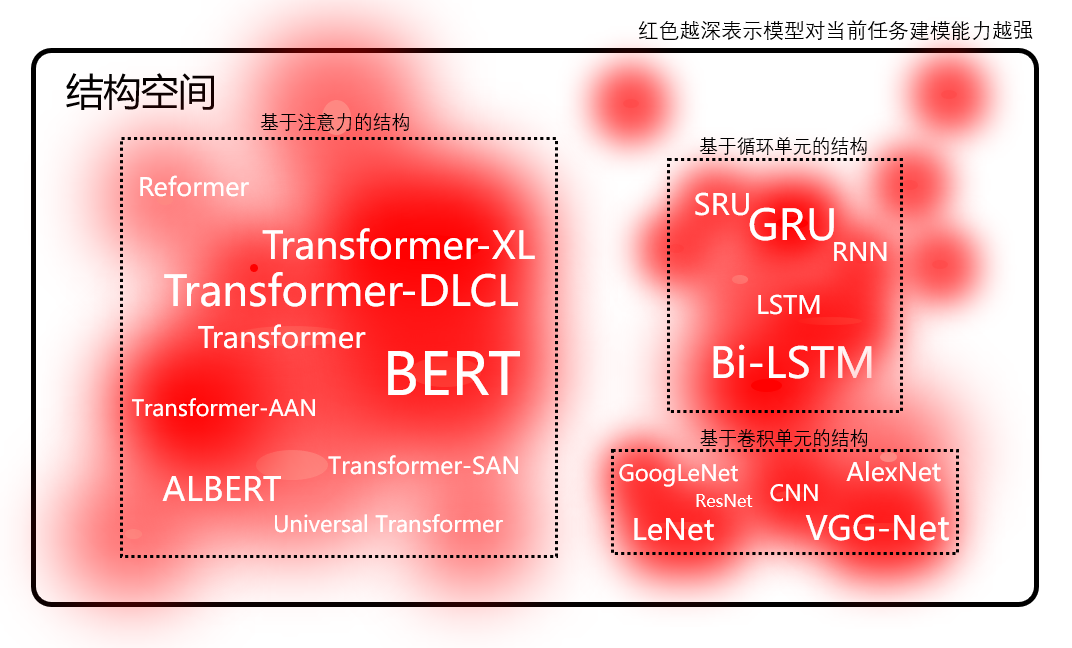
\includegraphics[scale=0.5]{./Chapter15/Figures/figure-relationship-between-structures-in-structural-space.jpg}
\caption{结构空间内结构之间的关系}
\label{fig:15-30}
\end{figure}
%-------------------------------------------

\parinterval 另一个很重要的问题是如何表示一个网络结构。在目前的结构搜索方法中,通常将模型结构分为整体框架和内部结构(元结构)两部分。整体框架将若干内部结构的输出按照特定的方式组织起来,最终得到模型输出。

\begin{itemize}
\vspace{0.5em}
\item {\small\bfnew{整体框架}}。如图\ref{fig:15-30}所示,整体框架一般基于经验进行设计。比如,对于包括机器翻译在内的自然语言处理任务而言,一般会更倾向于使用循环神经网络或Transformer模型的相关结构作为搜索空间\upcite{DBLP:conf/icml/SoLL19,DBLP:conf/iclr/ZophL17,DBLP:conf/iclr/LiuSY19}。
\vspace{0.5em}
\item 	{\small\bfnew{内部结构}}。对于内部结构的设计需要考虑到搜索过程中的最小搜索单元,以及搜索单元之间的连接方式。最小搜索单元指的是在结构搜索过程中可被选择的最小独立计算单元,在不同搜索空间的设计中,最小搜索单元的颗粒度各有不同,较小的搜索粒度主要包括如矩阵乘法、张量缩放等基本数学运算\upcite{DBLP:journals/corr/abs-2003-03384},更大粒度的搜索单元包括常见的激活函数以及一些局部结构,如ReLU、注意力机制等\upcite{DBLP:conf/acl/LiHZXJXZLL20,Chollet2017XceptionDL,DBLP:journals/taslp/FanTXQLL20}。不过,对于搜索颗粒度的问题,目前还缺乏有效的方法针对不同任务进行自动优化。
\vspace{0.5em}
\end{itemize}

%----------------------------------------------------------------------------------------
%    NEW SUBSUB-SECTION
%----------------------------------------------------------------------------------------

\subsubsection{2. 搜索策略}

\parinterval 在定义好搜索空间之后,如何进行网络结构的搜索也同样重要。该过程被称为搜索策略的设计,其主要目的是根据已找到的模型结构计算出下一个最有潜力的模型结构,为保证模型有效性,在一些方法中也会引入外部知识(如经验性的模型结构或张量运算规则)对搜索过程进行剪枝。目前常见的搜索策略一般包括基于进化算法的方法、基于强化学习的方法以及基于梯度的方法等等。

\begin{itemize}
\vspace{0.5em}
\item {\small\bfnew{进化算法}}。进化算法最初被用来对神经网络模型结构、以及其中的权重参数进行优化\upcite{DBLP:conf/icga/MillerTH89,DBLP:journals/tnn/AngelineSP94,stanley2002evolving}。随着最优化算法的发展,近年来,对于网络参数的学习开始更多地采用梯度下降的方式,但是进化算法依旧被用于对模型结构进行优化\upcite{DBLP:conf/icml/RealMSSSTLK17,DBLP:conf/iclr/ElskenMH19,DBLP:conf/iclr/LiuSVFK18}。从结构优化的角度来说,一般是将模型结构看做遗传算法中种群的个体,使用轮盘赌或锦标赛等抽取方式,对种群中的结构进行取样作为亲本,之后通过亲本模型的突变产生新的模型结构,最终对这些新的模型结构进行适应度评估。根据模型结构在校验集上的性能确定是否将其加入种群。
\vspace{0.5em}
\item 	{\small\bfnew{强化学习}}。强化学习方法在{\chapterthirteen}已经进行了介绍,这里可以将神经网络结构的设计看做是一种序列生成任务,使用字符序列对网络结构进行表述\upcite{DBLP:conf/iclr/ZophL17}。这种方法的执行过程如图\ref{fig:15-33}所示。其执行过程为由智能体对模型结构进行生成,之后将生成的结构应用于对应的任务(如机器翻译、语言建模等),根据模型在对应任务中的输出以及表现水平来进一步对智能体进行反馈,促使智能体生成更适用于当前任务的模型结构。

%----------------------------------------------
\begin{figure}[htp]
\centering

%%% outline
%-------------------------------------------------------------------------
\begin{tikzpicture}
\tikzstyle{node}=[minimum height=2.5em,minimum width=8em,draw,rounded corners=2pt,thick,drop shadow]

\node[node,fill=red!30] (n1) at (0,0){\small\bfnew{环境}};
\node[anchor=south,node,fill=blue!30] (n2) at ([yshift=5em]n1.north){\small\bfnew{智能体}};
\node[anchor=north,font=\footnotesize] at ([yshift=-0.2em]n1.south){(结构所应用于的任务)};
\node[anchor=south,font=\footnotesize] at ([yshift=0.2em]n2.north){(结构生成器)};

\draw[-latex,thick] ([yshift=.4em]n1.180) .. controls ([xshift=-3.4em,yshift=.4em]n1.180) and  ([xshift=-3.4em,yshift=-.4em]n2.180) .. node[right,font=\scriptsize,align=left]{\scriptsize\bfnew{奖励} \\ (对输出结果的评价)}([yshift=-.4em]n2.180);
\draw[-latex,thick] ([yshift=-.4em]n1.180) .. controls ([xshift=-4.4em,yshift=-.4em]n1.180) and  ([xshift=-4.4em,yshift=.4em]n2.180) .. node[left,font=\scriptsize,align=right]{\scriptsize\bfnew{状态} \\ (这个结构在任务中应 \\ 用后得到的输出结果)}([yshift=.4em]n2.180);
\draw[-latex,thick] (n2.0) .. controls ([xshift=4em]n2.0) and  ([xshift=4em]n1.0) .. node[right,font=\scriptsize,align=left]{\scriptsize\bfnew{动作} \\ (生成一个结构)}(n1.0);
\end{tikzpicture}





\caption{基于强化学习的结构搜索}
\label{fig:15-33}
\end{figure}
%-------------------------------------------

\vspace{0.5em}
\item 	{\small\bfnew{基于梯度的方法}}。这种方法的思想是在连续空间中对模型结构进行表示\upcite{DBLP:conf/iclr/LiuSY19},通常将模型结构建模为超网络中的结构参数,接下来使用基于梯度的方法对超网络中的参数进行优化,最终根据其中的结构参数离散出最终的模型结构,达到结构搜索的目的,整体过程如图\ref{fig:15-34}所示。基于梯度的方法十分高效,因此也受到了很多关注\upcite{DBLP:conf/cvpr/WuDZWSWTVJK19,DBLP:conf/iclr/XuX0CQ0X20,DBLP:conf/acl/LiHZXJXZLL20}。
\vspace{0.5em}

%----------------------------------------------
\begin{figure}[htp]
\centering

%%% outline
%-------------------------------------------------------------------------
\begin{tikzpicture}
\tikzstyle{node}=[minimum height=6em,inner sep=4pt,align=left,draw,font=\footnotesize,rounded corners=4pt,thick,drop shadow]

\node[node,fill=orange!30] (n1) at (0,0){\scriptsize\bfnew{超网络}: \\ [1ex] 模型结构参数 \\[0.4ex] 网络参数};
\node[anchor=west,node,fill=yellow!30] (n2) at ([xshift=4em]n1.east){\scriptsize\bfnew{优化后的超网络}: \\ [1ex]模型{\color{red}结构参数}(已优化) \\ [0.4ex]网络参数(已优化)};
\node[anchor=west,node,fill=red!30] (n3) at ([xshift=6em]n2.east){\scriptsize\bfnew{找到的模型结构}};

\draw[-latex,thick] (n1.0) -- node[above,align=center,font=\scriptsize]{优化后的\\超网络}(n2.180);
\draw[-latex,thick] (n2.0) -- node[above,align=center,font=\scriptsize]{根据结构参数\\离散化结构}(n3.180);
\draw[-latex,out=90,in=100,thick] ([xshift=-2em]n1.90) to node[above,font=\scriptsize]{参数优化}([xshift=2em]n1.90);
\end{tikzpicture}





\caption{基于梯度方法的结构搜索}
\label{fig:15-34}
\end{figure}
%-------------------------------------------

\end{itemize}

%----------------------------------------------------------------------------------------
%    NEW SUBSUB-SECTION
%----------------------------------------------------------------------------------------

\subsubsection{3. 性能评估}\label{subsubsec-15.4.2.3}

\parinterval 由于结构搜索过程中会产生大量的中间结构,因此需要快速评估这些结构的性能优劣,以保证在搜索中可以有效地挑选高质量的模型结构。对于该问题,可以从以下三个方面来考虑:

\begin{itemize}
\vspace{0.5em}
\item {\small\bfnew{数据以及超参数的调整}}。具体来说,可以用少量的数据训练模型,以便快速评估其性能\upcite{DBLP:conf/aistats/KleinFBHH17,DBLP:journals/corr/ChrabaszczLH17}。在超参数的调整方面,也可以通过减少模型训练轮数、减少模型的层数等方式来简化模型参数,达到加速训练、评估的目的\upcite{DBLP:conf/cvpr/ZophVSL18,Real2019AgingEF,DBLP:journals/corr/abs-1807-06906}。
\vspace{0.5em}
\item {\small\bfnew{现有参数的继承及复用}}。通过在现有的模型参数基础上,继续优化中间过程产生的模型结构,来加快待评价模型的收敛进程\upcite{DBLP:conf/icml/RealMSSSTLK17,DBLP:conf/iclr/ElskenMH19,DBLP:conf/aaai/CaiCZYW18}。这种方式无需从头训练搜索过程中产生的中间结构,通过“热启动”的方式对模型参数进行优化,能够大幅减少性能评估过程的时间消耗。
\vspace{0.5em}
\item {\small\bfnew{模型性能的预测}}。这种方式使用训练过程中的性能变化曲线来预估模型是否具有潜力,从而快速终止低性能模型的训练过程\upcite{DBLP:conf/ijcai/DomhanSH15,DBLP:conf/iclr/KleinFSH17,DBLP:conf/iclr/BakerGRN18}。
\vspace{0.5em}
\end{itemize}

%----------------------------------------------------------------------------------------
%    NEW SUB-SECTION
%----------------------------------------------------------------------------------------

\subsection{机器翻译任务下的结构搜索}

\parinterval 对于自然语言处理任务来说,网络结构搜索方法更多是在语言建模、命名实体识别等任务上进行尝试\upcite{DBLP:conf/acl/LiHZXJXZLL20,DBLP:conf/emnlp/JiangHXZZ19}。其中,大多数工作是在基于循环神经网络的模型结构上进行探索的,相较于目前在机器翻译领域中广泛使用的Transformer模型结构来说,这些搜索到的结构在性能上并没有体现出绝对的优势。此外,由于机器翻译任务的复杂性,针对基于Transformer的机器翻译模型的结构搜索方法会更少一些。不过仍有部分工作在机器翻译任务上取得了很好的表现。例如,在WMT19机器翻译比赛中,神经网络结构优化方法在多个任务上取得了很好的成绩\upcite{DBLP:conf/nips/LuoTQCL18,DBLP:conf/wmt/XiaTTGHCFGLLWWZ19}。对于结构搜索在机器翻译领域的应用,目前主要包括两个方面:分别是对模型性能的改进以及模型效率的优化。

%----------------------------------------------------------------------------------------
%    NEW SUBSUB-SECTION
%----------------------------------------------------------------------------------------

\subsubsection{1. 模型性能改进}

\parinterval 结构搜索任务中一个非常重要的目标是找到更加适用于当前任务的模型结构。目前来看,有两种思路:

\begin{itemize}
\vspace{0.5em}
\item {\small\bfnew{搜索模型中的局部结构}}。在机器翻译任务中,一种典型的局部模型结构搜索方法是面向激活函数的搜索\upcite{DBLP:conf/iclr/RamachandranZL18},该方法将激活函数看作是一元、二元函数的若干次复合。例如,Swish 激活函数就是一种被找到的新的激活函数,如下:
\begin{eqnarray}
f(x) &=& x \cdot \delta(\beta x) \\
\delta(z) &=& {(1 + \exp{(-z)})}^{-1}
\label{eq:15-60}
\end{eqnarray}

\noindent 相比于人工设计的激活函数ReLU而言,Swish函数在多个机器翻译任务取得了不错的效果。
\vspace{0.5em}
\item {\small\bfnew{搜索模型中局部结构的组合}}。在基于Transformer模型的网络结构搜索任务中,对于局部结构的组合方式的学习也受到了很多关注,其中包括基于进化算法的方法和基于梯度对现有Transformer模型结构的改良\upcite{DBLP:conf/icml/SoLL19,DBLP:journals/taslp/FanTXQLL20}。与前文所述的对局部结构的改良不同,此处更多地是对现有经验性的局部结构进行组合,找到最佳的整体结构。在模型结构的表示方法上,这些方法会根据先验知识为搜索单元设定一个部分框架,如每当信息传递过来之后先进行层标准化,之后再对候选位置上的操作使用对应的搜索策略进行搜索。另外这类方法也会在Transformer结构中引入多分支结构,一个搜索单元的输出可以被多个后续单元所使用,这种方式有效扩大了结构搜索过程中的搜索空间,能够在现有Transformer结构的基础上找到更优的模型结构。
\vspace{0.5em}
\end{itemize}

\parinterval 此外对模型结构中超参数的自动搜索同样能够有效提升模型的性能\upcite{DBLP:journals/corr/abs-2009-02070},这种方法在机器翻译中也有应用\upcite{Li2020NeuralMT}。

%----------------------------------------------------------------------------------------
%    NEW SUBSUB-SECTION
%----------------------------------------------------------------------------------------

\subsubsection{2. 模型效率优化}

\parinterval 网络结构搜索除了能够提高机器翻译模型性能之外,也能够优化模型的执行效率。从实用的角度出发,可以在进行结构搜索的同时考虑设备的计算能力,希望找到更适合运行设备的模型结构。同时,网络结构搜索也可以用来对大模型进行压缩,增加其在推断过程中的效率,这方面的工作不仅限于在机器翻译模型上,也有部分工作对基于注意力机制的预训练模型进行压缩。

\begin{itemize}
\vspace{0.5em}
\item {\small\bfnew{面向特定设备的模型结构优化}}。可以在结构优化的过程中将设备的算力作为一个约束\upcite{DBLP:conf/acl/WangWLCZGH20}。具体来说,可以将搜索空间中各种结构建模在同一个超网络中,通过权重共享的方式进行训练。使用设备算力约束子模型,并通过进化算法对子模型进行搜索,搜索到适用于目标设备的模型结构。该方法搜索到的模型能够在保证模型性能不变前提下获得较大的效率提升。
\vspace{0.5em}
\item {\small\bfnew{模型压缩}}。此外,在不考虑设备算力的情况下,也可以通过结构搜索方法对基于Transformer的预训练模型进行压缩。例如,将Transformer模型拆分为若干小组件,然后通过基于采样的结构搜索方法对压缩后的模型结构进行搜索,尝试找到最优且高效的推断模型\upcite{DBLP:journals/corr/abs-2008-06808}。类似的,也可以在基于BERT的预训练模型上通过结构搜索方法进行模型压缩,通过基于梯度的结构搜索方法,针对不同的下游任务将BERT模型压缩为小模型\upcite{DBLP:conf/ijcai/ChenLQWLDDHLZ20}。
\vspace{0.5em}
\end{itemize}

\parinterval 虽然由于算力等条件的限制,目前很多网络结构搜索方法并没有直接在机器翻译任务中进行实验,但是这些方法并没有被限制在特定任务上。例如,可微分结构搜索方法被成功地用于学习更好的循环单元结构,这类方法完全可以应用在机器翻译任务上。

\parinterval 此外,受到预训练模型的启发,网络结构预搜索可能是一个极具潜力的方向。例如,有研究人员在大规模语言模型上进行网络结构搜索\upcite{DBLP:conf/acl/LiHZXJXZLL20},然后将搜索到的模型结构应用于更多的自然语言处理任务中,这种方式有效提升了模型结构的可复用性。同时,相较于使用特定任务下受限的数据,从大规模单语数据中可以更充分地学习语言的规律,进而更好地指导模型结构的设计。此外,对于机器翻译任务而言,结构的预搜索同样是一个值得关注的研究方向。

%----------------------------------------------------------------------------------------
%    NEW SECTION
%----------------------------------------------------------------------------------------

\sectionnewpage
\section{小结及拓展阅读}

\parinterval 模型结构优化一直是机器翻译研究的重要方向。一方面,对于通用框架(如注意力机制)的结构改良可以服务于多种自然语言处理任务,另一方面,针对机器翻译中存在的问题设计相适应的模型结构也是极具价值的。本章节重点介绍了神经机器翻译中几种结构优化方法,内容涉及注意力机制的改进、深层神经网络的构建、句法结构的使用以及自动结构搜索等几个方面。此外,还有若干问题值得关注:

\begin{itemize}

\vspace{0.5em}
\item 多头注意力是近些年神经机器翻译中常用的结构。多头机制可以让模型从更多维度提取特征,也反应了一种多分支建模的思想。研究人员针对Transformer编码器的多头机制进行了分析,发现部分头在神经网络的学习过程中扮演了至关重要的角色,并且蕴含语言学解释\upcite{DBLP:journals/corr/abs-1905-09418}。 而另一部分头本身则不具备很好的解释,对模型的帮助也不大,因此可以被剪枝掉。而且也有研究人员发现,在Transformer模型中并不是头数越多模型的性能就越强。如果在训练过程中使用多头机制,并在推断过程中去除大部分头,可以在模型性能不变的前提下提高模型在CPU上的执行效率\upcite{Michel2019AreSH}。

\vspace{0.5em}
\item 此外,也可以利用正则化手段,在训练过程中增大不同头之间的差异\upcite{DBLP:conf/emnlp/LiTYLZ18}。或引入多尺度的思想,对输入的特征进行分级表示,并引入短语的信息\upcite{DBLP:conf/emnlp/HaoWSZT19}。还可以通过对注意力权重进行调整,来区分序列中的实词与虚词\upcite{DBLP:conf/emnlp/Lin0RLS18}。除了上述基于编码器端-解码器端的建模范式,还可以定义隐变量模型来捕获句子中潜在的语义信息\upcite{Su2018VariationalRN,DBLP:conf/acl/SetiawanSNP20},或直接对源语言和目标语言序列进行联合表示\upcite{Li2020NeuralMT}。

\vspace{0.5em}
\item 对Transformer等模型来说,处理超长序列是较为困难的。一种比较直接的解决办法是优化自注意力机制,降低模型计算复杂度。例如,采用了基于滑动窗口的局部注意力的Longformer模型\upcite{DBLP:journals/corr/abs-2004-05150}、基于随机特征的Performer\upcite{DBLP:journals/corr/abs-2006-04768}、使用低秩分解的Linformer\upcite{DBLP:journals/corr/abs-2009-14794}和应用星型拓扑排序的Star-Transformer\upcite{DBLP:conf/naacl/GuoQLSXZ19}。

\vspace{0.5em}
\end{itemize}

%% !Mode:: "TeX:UTF-8"
% !TEX encoding = UTF-8 Unicode

%----------------------------------------------------------------------------------------
% 机器翻译:基础与模型
% Machine Translation: Foundations and Models
%
% Copyright 2020
% 肖桐(xiaotong@mail.neu.edu.cn) 朱靖波 (zhujingbo@mail.neu.edu.cn)
%----------------------------------------------------------------------------------------

%----------------------------------------------------------------------------------------
%    CONFIGURATIONS
%----------------------------------------------------------------------------------------

\renewcommand\figurename{图}%将figure改为图
\renewcommand\tablename{表}%将figure改为图
\chapterimage{fig-NEU-7.jpg} % Chapter heading image

%----------------------------------------------------------------------------------------
%	CHAPTER 16
%----------------------------------------------------------------------------------------
\chapter{低资源神经机器翻译}

\parinterval 神经机器翻译带来的性能提升是显著的,但随之而来的问题是对海量双语训练数据的依赖。不同语言可使用的数据规模是不同的。比如汉语、英语这种使用范围广泛的语言,存在着大量的双语平行句对,这些语言被称为{\small\bfnew{富资源语言}}\index{富资源语言}(High-resource Language\index{High-resource Language})。而对于其它一些使用范围稍小的语言,如斐济语、古吉拉特语等,相关的数据非常稀少,这些语言被称为{\small\bfnew{低资源语言}}\index{低资源语言}(Low-resource Language\index{Low-resource Language})。世界上现存语言超过5000种,仅有很少一部分为富资源语言,绝大多数均为低资源语言。即使在富资源语言中,对于一些特定的领域,双语平行语料也是十分稀缺的。有时,一些特殊的语种或者领域甚至会面临“零资源”的问题。因此,{\small\bfnew{低资源机器翻译}}\index{低资源机器翻译}(Low-resource Machine Translation)是当下急需解决且颇具挑战的问题。

\parinterval 本章将对低资源神经机器翻译的相关问题、模型和方法展开介绍,内容涉及数据的有效使用、双向翻译模型、多语言翻译模型、无监督机器翻译、领域适应五个方面。

%----------------------------------------------------------------------------------------
%    NEW SECTION 16.1
%----------------------------------------------------------------------------------------

\section{数据的有效使用}\label{effective-use-of-data}

\parinterval 数据稀缺是低资源机器翻译所面临的主要问题,充分使用既有数据是一种解决问题的思路。比如,在双语训练不充足的时候,可以对双语数据的部分单词用近义词进行替换,达到丰富双语数据的目的\upcite{DBLP:conf/acl/FadaeeBM17a,DBLP:conf/emnlp/WangPDN18},也可以考虑用转述等方式生成更多的双语训练数据\upcite{DBLP:conf/emnlp/MartonCR09,DBLP:conf/eacl/LapataSM17}。

\parinterval 另一种思路是使用更容易获取的单语数据。实际上,在统计机器翻译时代,使用单语数据训练语言模型是构建机器翻译系统的关键步骤,好的语言模型往往会带来性能的增益。而这个现象在神经机器翻译中似乎并不明显,因为在大多数神经机器翻译的范式中,并不要求使用大规模单语数据来帮助机器翻译系统。甚至,连语言模型都不会作为一个独立的模块。这一方面是由于神经机器翻译系统的解码端本身就起着语言模型的作用,另一方面是由于双语数据的增多使得翻译模型可以很好地捕捉目标语言的规律。但是,双语数据总是有限的,很多场景下,单语数据的规模会远大于双语数据,如果能够让这些单语数据发挥作用,显然是一种非常好的选择。针对以上问题,下面将从数据增强、基于语言模型的单语数据使用等方面展开讨论。

%----------------------------------------------------------------------------------------
%    NEW SUB-SECTION
%----------------------------------------------------------------------------------------
\subsection{数据增强}

\parinterval {\small\bfnew{数据增强}}\index{数据增强}(Data Augmentation)\index{Data Augmentation}是一种增加训练数据的方法,通常通过对既有数据进行修改或者生成新的伪数据等方式实现。有时候,数据增强也可以被看做是一种防止模型过拟合的手段\upcite{DBLP:journals/jbd/ShortenK19}。在机器翻译中,典型的数据增强方法包括回译、修改双语数据、双语句对挖掘等。

%----------------------------------------------------------------------------------------
%    NEW SUB-SUB-SECTION
%----------------------------------------------------------------------------------------
\subsubsection{1. 回译}

\parinterval {\small\bfnew{回译}}\index{回译}(Back Translation, BT\index{Back Translation})是目前机器翻译任务上最常用的一种数据增强方法\upcite{Sennrich2016ImprovingNM,DBLP:conf/emnlp/EdunovOAG18,DBLP:conf/aclnmt/HoangKHC18}。回译的主要思想是:利用目标语言-源语言翻译模型(反向翻译模型)来生成伪双语句对,用于训练源语言-目标语言翻译模型(正向翻译模型)。假设现在需要训练一个英汉翻译模型。首先,使用双语数据训练汉英翻译模型,即反向翻译模型。然后通过该模型将额外的汉语单语句子翻译为英语句子,从而得到大量的英语- 真实汉语伪双语句对。然后,将回译得到的伪双语句对和真实双语句对混合,训练得到最终的英汉翻译模型。
回译方法只需要训练一个反向翻译模型,就可以利用单语数据来增加训练数据的数量,因此得到了广泛使用\upcite{Hassan2018AchievingHP,DBLP:conf/iclr/LampleCDR18,DBLP:conf/emnlp/LampleOCDR18}。图\ref{fig:16-1} 给出了回译方法的一个简要流程。

%----------------------------------------------
\begin{figure}[htp]
\centering
\begin{tikzpicture}


\tikzstyle{bignode} = [,inner sep=0.3em,draw=black,line width=0.6pt,rounded corners=2pt,minimum width=3.0em]


\node [anchor=center] (node1-1) at (0,0) {\small{汉语}};
\node [anchor=west] (node1-2) at ([xshift=0.8em]node1-1.east) {\small{英语}};
\node [anchor=north] (node1-3) at ([xshift=1.75em]node1-1.south) {\small{反向翻译模型}};
\draw [->,thick](node1-1.east)--(node1-2.west);

\begin{pgfonlayer}{background}
{
\node[fill=blue!20,inner sep=0.3em,draw=black,line width=0.6pt,minimum width=6.0em,drop shadow,rounded corners=2pt] [fit =(node1-1)(node1-2)(node1-3)]  (remark1) {};
}
\end{pgfonlayer}


\node [anchor=north,fill=green!20,bignode](node2-1) at ([yshift=-3em]node1-3.south){\small{汉语}};
\node [anchor=north,fill=green!20,bignode](node2-2) at (node2-1.south){\small{英语}};
\draw [->,thick](node2-1.north)--(remark1.south) node [pos=0.5,right] (pos1) {\small{训练}};


\node [anchor=west,fill=yellow!20,bignode](node3-1) at ([xshift=6.5em,yshift=0.0em]node1-2.east){\small{汉语}};
\node [anchor=north,fill=red!20,bignode](node3-2) at ([yshift=-2.5em]node3-1.south){\small{英语}};
\node [anchor=center](node3-3) at ([xshift=0.4em]node3-2.east){};

\draw [->,thick](node3-1.south)--(node3-2.north) node [pos=0.5,right] (pos2) {\small{翻译}};

\begin{pgfonlayer}{background}
{
\node[rounded corners=2pt,inner sep=0.3em,draw=black,line width=0.6pt,dotted] [fit =(node3-1)(node3-2)(node3-3)]  (remark2) {};
}
\end{pgfonlayer}

\draw [->,thick](remark1.east)--([xshift=5.5em]remark1.east) node [pos=0.5,above] (pos2) {\small{模型翻译}};
\node [anchor=south](pos2-2) at ([yshift=-0.5em]pos2.north){\small{使用反向}};

\draw[decorate,thick,decoration={brace,amplitude=5pt}] ([yshift=1.5em,xshift=1.5em]node3-1.east) -- ([yshift=-8.6em,xshift=1.5em]node3-1.east) node [pos=0.1,right,xshift=0.0em,yshift=0.0em] (label1) {\small{{混合}}};


\node [anchor=west,fill=red!20,bignode](node4-1) at ([xshift=2.5em,yshift=1.3em]node3-2.east){\small{英语}};
\node [anchor=north,fill=yellow!20,bignode](node4-2) at (node4-1.south){\small{汉语}};
\node [anchor=west,fill=green!20,bignode](node4-3) at (node4-1.east){\small{英语}};
\node [anchor=north,fill=green!20,bignode](node4-4) at (node4-3.south){\small{汉语}};


\node [anchor=center] (node5-1) at ([xshift=5em,yshift=0.02em]node4-3.east) {\small{英语}};
\node [anchor=west] (node5-2) at ([xshift=0.8em]node5-1.east) {\small{汉语}};
\node [anchor=north] (node5-3) at ([xshift=1.65em]node5-1.south) {\small{正向翻译模型}};
\draw [->,thick](node5-1.east)--(node5-2.west);

\begin{pgfonlayer}{background}
{
\node[fill=blue!20,inner sep=0.3em,draw=black,line width=0.6pt,minimum width=6.0em,drop shadow,rounded corners=2pt] [fit =(node5-1)(node5-2)(node5-3)]  (remark3) {};
}
\end{pgfonlayer}

\draw [->,thick]([xshift=-3.2em]remark3.west)--(remark3.west) node [pos=0.5,above] (pos3) {\small{训练}};

\node [anchor=south](d1) at ([xshift=-1.5em,yshift=1em]remark1.north){\small{真实双语数据:}};
\node [anchor=west](d2) at ([xshift=2.0em]d1.east){\small{伪数据:}};
\node [anchor=west](d3) at ([xshift=2.0em]d2.east){\small{额外单语数据:}};
\node [anchor=west,fill=green!20,minimum width=1.5em](d1-1) at ([xshift=-0.0em]d1.east){};
\node [anchor=west,fill=red!20,minimum width=1.5em](d2-1) at ([xshift=-0.0em]d2.east){};
\node [anchor=west,fill=yellow!20,minimum width=1.5em](d3-1) at ([xshift=-0.0em]d3.east){};

\end{tikzpicture}
\caption{回译方法的简要流程}
\label{fig:16-1}
\end{figure}
%----------------------------------------------

\parinterval 围绕如何利用回译方法生成伪双语数据这一问题,研究人员进行了详细地分析探讨。一般观点认为,反向翻译模型的性能越好,生成的伪数据质量也就越高,对正向翻译模型的性能提升也就越大\upcite{Sennrich2016ImprovingNM,DBLP:conf/aclnmt/HoangKHC18}。不过,在实践中发现,即使一些简单的策略也能带来性能的增长。比如,对于一些低资源翻译任务,通过将目标语言句子复制到源语言端构造伪数据便能带来增益\upcite{DBLP:conf/wmt/CurreyBH17}。原因在于,即使构造的双语伪数据是不准确的,其目标语言端仍然是真实数据,可以使解码器训练得更加充分,进而提升神经机器翻译模型生成结果的流畅度。但是,相比这些简单的伪数据生成策略,利用目标语言单语数据进行回译可以带来更大的性能提升\upcite{DBLP:conf/wmt/CurreyBH17}。一种可能的解释是,双语伪数据的源语言是模型生成的翻译结果,保留了两种语言之间的互译信息,相比真实数据又存在一定的噪声。神经机器翻译模型在伪双语句对上进行训练,可以学习到如何处理带有噪声的输入,提高了模型的健壮性。

\parinterval 在回译方法中,反向翻译模型的训练只依赖于有限的双语数据,因此生成的源语言端伪数据的质量难以保证。为此,可以采用{\small\sffamily\bfnew{迭代式回译}}\index{迭代式回译}(Iterative Back Translation)\index{Iterative Back Translation}的方法\upcite{DBLP:conf/aclnmt/HoangKHC18},同时利用源语言端和目标语言端的单语数据,不断通过回译的方式来提升正向和反向翻译模型的性能。图\ref{fig:16-2}展示了迭代式回译的框架,图中带圈的数字代表了迭代式回译方法执行的顺序。首先,使用双语数据训练一个正向翻译模型,然后利用额外的源语言单语数据通过回译的方式生成伪双语数据,来提升反向翻译模型的性能。之后,再利用反向翻译模型和额外的目标语言单语数据生成伪双语数据,用于提升正向翻译模型的性能。可以看出,迭代式回译的过程是完全闭环的,因此可以一直重复进行,直到正向和反向翻译模型的性能均不再提升。

%----------------------------------------------
\begin{figure}[htp]
\centering
\begin{tikzpicture}
\begin{scope}
\node [anchor=center] (node1) at (9.6,1) {\small{训练:}};
\node [anchor=center] (node11) at (10.2,1) {};
\node [anchor=center] (node12) at (11.4,1) {};
\node [anchor=center] (node2) at (9.6,0.5) {\small{推理:}};
\node [anchor=center] (node21) at (10.2,0.5) {};
\node [anchor=center] (node22) at (11.4,0.5) {};
\node [anchor=west,draw=black,line width=0.6pt,minimum width=5.6em,minimum height=2.2em,fill=blue!20,rounded corners=2pt] (node1-1) at (0,0) {\footnotesize{双语数据}};
\node [anchor=south,draw=black,line width=0.6pt,minimum width=4.5em,minimum height=2.2em,fill=blue!20,rounded corners=2pt] (node1-2) at ([yshift=-5em]node1-1.south) {\footnotesize{目标语伪数据}};
\node [anchor=west,draw=black,line width=0.6pt,minimum width=4.5em,minimum height=2.2em,fill=red!20,rounded corners=2pt] (node2-1) at ([xshift=-7.7em,yshift=-2.5em]node1-1.west) {\footnotesize{前向NMT系统}};
\node [anchor=west,draw=black,line width=0.6pt,minimum width=4.5em,minimum height=2.2em,fill=red!20,rounded corners=2pt] (node3-1) at ([xshift=1.5em,yshift=-2.5em]node1-1.east) {\footnotesize{反向NMT系统}};

\node [anchor=east,draw=black,line width=0.6pt,minimum width=5.6em,minimum height=2.2em,fill=blue!20,rounded corners=2pt] (node4-1) at ([xshift=18em]node1-1)  {\footnotesize{双语数据}};
\node [anchor=south,draw=black,line width=0.6pt,minimum width=4.5em,minimum height=2.2em,fill=blue!20,rounded corners=2pt] (node4-2) at ([yshift=-5em]node4-1.south) {\footnotesize{目标语伪数据}};

\node [anchor=east,draw=black,line width=0.6pt,minimum width=4.5em,minimum height=2.2em,fill=red!20,rounded corners=2pt] (node5-1) at ([xshift=15.2em]node3-1.east) {\footnotesize{前向NMT系统}};

\draw [->,line width=1pt](node1-1.west)--([xshift=3em]node2-1.north);
\draw [->,line width=1pt](node1-1.east)--([xshift=-3em]node3-1.north);
\draw [->,line width=1pt](node1-2.east)--([xshift=-3em]node3-1.south);
\draw [->,line width=1pt](node11.east)--(node12.west);
\draw [->,line width=1pt,dashed](node21.east)--(node22.west);
\draw [->,line width=1pt,dashed]([xshift=3em]node2-1.south)--([xshift=-0.1em]node1-2.west);
\draw [->,line width=1pt,dashed]([xshift=3em]node3-1.south)--([xshift=-0.1em]node4-2.west);
\draw [->,line width=1pt](node4-1.east)--([xshift=-3em]node5-1.north);
\draw [->,line width=1pt](node4-2.east)--([xshift=-3em]node5-1.south);
\end{scope}
\end{tikzpicture}
\caption{迭代式回译方法的流程}
\label{fig:16-2}
\end{figure}
%----------------------------------------------

\parinterval 进一步,研究人员发现,在低资源场景中,由于缺乏双语数据,高质量的伪双语数据对于模型来说更有帮助。而在富资源场景中,在回译产生的源语言句子中添加一些噪声,提高翻译结果的多样性,反而可以达到更好的效果,比较常用的方法是使用采样解码、Top-$k$解码和加噪\upcite{DBLP:conf/emnlp/EdunovOAG18,DBLP:conf/aclnmt/ImamuraFS18,DBLP:conf/emnlp/WuWXQLL19}。回译中常用的解码方式为束搜索,在生成每个词的时候只考虑预测概率最高的几个词,因此生成的翻译结果质量更高,但导致的问题是翻译结果主要集中在部分高频词上,生成的伪数据缺乏多样性,也就很难去准确地覆盖真实的数据分布\upcite{DBLP:conf/icml/OttAGR18}。采样解码是指在解码过程中,对词表中所有的词按照预测概率进行随机采样,因此整个词表中的词都有可能被选中,从而使生成结果多样性更强,但翻译质量和流畅度也会明显下降。Top-$k$解码是对束搜索和采样解码的一个折中方法。在解码过程中,Top-$k$解码对词表中预测概率最高的前$k$个词进行随机采样,这样在保证翻译结果准确的前提下,提高了结果的多样性。加噪方法在束搜索的解码结果加入一些噪声,如丢掉或屏蔽部分词、打乱句子顺序等。这些方法在生成的源语言句子中引入了噪声,不仅增加了对包含低频词或噪声句子的训练次数,同时也提高了模型的健壮性和泛化能力\upcite{DBLP:conf/icml/VincentLBM08}。

\parinterval 与回译方法类似,源语言单语数据也可以通过一个双语数据训练的正向翻译模型获得对应的目标语言翻译结果,从而构造正向翻译的伪数据\upcite{DBLP:conf/emnlp/ZhangZ16}。与回译方法相反,这时的伪数据中源语言句子是真实的,而目标语言句子是自动生成的,构造的伪数据对译文的流畅性并没有太大帮助,其主要作用是提升编码器的特征提取能力。然而,由于伪数据中生成的译文质量很难保证,因此利用正向翻译模型生成伪数据的方法带来的性能提升效果要弱于回译,甚至可能是有害的\upcite{DBLP:conf/emnlp/WuWXQLL19}。

%----------------------------------------------------------------------------------------
%    NEW SUB-SUB-SECTION
%----------------------------------------------------------------------------------------
\subsubsection{2. 修改双语数据}

\parinterval 回译方法是利用单语数据来生成伪数据,而另外一种数据增强技术是对原始双语数据进行修改来得到伪双语数据,常用的方法包括加噪和转述等。

\parinterval 加噪是自然语言处理任务中广泛使用的一种方法\upcite{DBLP:conf/icml/VincentLBM08,DBLP:journals/ipm/FarhanTAJATT20,DBLP:conf/iclr/LampleCDR18,devlin2019bert}。比如,在广泛使用的{\small\bfnew{降噪自编码器}}\index{降噪自编码器}(Denoising Autoencoder)\index{Denoising Autoencoder}中,向原始数据中加入噪声作为模型的输入,模型通过学习如何预测原始数据进行训练。而在神经机器翻译中,利用加噪方法进行数据增强的常用方法是,在保证句子整体语义不变的情况下,对原始的双语数据适当加入一些噪声,从而生成伪双语数据来增加训练数据的规模。常用的加噪方法主要有以下三种:
%----------------------------------------------
\begin{itemize}
    \vspace{0.5em}
    \item {\small\bfnew{丢掉单词}}:句子中的每个词均有$\funp{P}_{\rm{Drop}}$的概率被丢弃。
    \vspace{0.5em}
    \item {\small\bfnew{掩码单词}}:句子中的每个词均有$\funp{P}_{\rm{Mask}}$的概率被替换为一个额外的<Mask>词。<Mask>的作用类似于占位符,可以理解为一个句子中的部分词被屏蔽掉,无法得知该位置词的准确含义。
    \vspace{0.5em}
    \item {\small\bfnew{打乱顺序}}:将句子中距离较近的某些词的位置进行随机交换。
    \vspace{0.5em}
\end{itemize}
%----------------------------------------------

\parinterval 图\ref{fig:16-3}展示了三种加噪方法的示例。这里,$\funp{P}_{\rm{Drop}}$和$\funp{P}_{\rm{Mask}}$均设置为0.1,表示每个词有$10\%$的概率被丢弃或掩码。打乱句子内部顺序的操作略微复杂,一种实现方法是:通过一个数字来表示每个词在句子中的位置,如“我”是第一个词,“你”是第三个词,然后,在每个位置生成一个$1$到$n$的随机数,$n$一般设置为3,然后将每个词的位置数和对应的随机数相加,即图中的$\seq{S}$。 对$\seq{S}$ 按照从小到大排序,根据排序后每个位置的索引从原始句子中选择对应的词,从而得到最终打乱顺序后的结果。比如,在计算后,除了$S_2$的值小于$S_1$外,其余单词的$S$值均为递增顺序,则将原句中第一个词和第二个词进行交换,其他词保持不变。

%----------------------------------------------
\begin{figure}[htp]
    \centering
    \begin{tikzpicture}
%%%%%%%%%%%%%%%%%%%%%%%%%%%%%%%dropout
\node [anchor=north,inner sep=2pt,fill=green!20,minimum height=1.5em,minimum width=3.0em] (a11) at (0,0) {我};
\node [anchor=north,inner sep=2pt,fill=green!20,minimum height=1.5em,minimum width=3.0em] (a12) at ([yshift=-0.2em]a11.south) {对};
\node [anchor=north,inner sep=2pt,fill=green!20,minimum height=1.5em,minimum width=3.0em] (a13) at ([yshift=-0.2em]a12.south) {你};
\node [anchor=north,inner sep=2pt,fill=green!20,minimum height=1.5em,minimum width=3.0em] (a14) at ([yshift=-0.2em]a13.south) {感到};
\node [anchor=north,inner sep=2pt,fill=green!20,minimum height=1.5em,minimum width=3.0em] (a15) at ([yshift=-0.2em]a14.south) {满意};

\node [anchor=south east,inner sep=1pt,fill=black] (pa11) at (a11.south east) {\tiny{\color{white} \textbf{1}}};
\node [anchor=south east,inner sep=1pt,fill=black] (pa12) at (a12.south east) {\tiny{\color{white} \textbf{2}}};
\node [anchor=south east,inner sep=1pt,fill=black] (pa13) at (a13.south east) {\tiny{\color{white} \textbf{3}}};
\node [anchor=south east,inner sep=1pt,fill=black] (pa14) at (a14.south east) {\tiny{\color{white} \textbf{4}}};
\node [anchor=south east,inner sep=1pt,fill=black] (pa15) at (a15.south east) {\tiny{\color{white} \textbf{5}}};

\node [anchor=west,inner sep=2pt,fill=green!20,minimum height=1.5em,minimum width=2.0em] (a21) at ([xshift=1.0em]a11.east) {\footnotesize{$P=0.1$}};
\node [anchor=north,inner sep=2pt,fill=red!20,minimum height=1.5em,minimum width=2.0em] (a22) at ([yshift=-0.2em]a21.south) {\footnotesize{$P=0.1$}};
\node [anchor=north,inner sep=2pt,fill=green!20,minimum height=1.5em,minimum width=2.0em] (a23) at ([yshift=-0.2em]a22.south) {\footnotesize{$P=0.1$}};
\node [anchor=north,inner sep=2pt,fill=green!20,minimum height=1.5em,minimum width=2.0em] (a24) at ([yshift=-0.2em]a23.south) {\footnotesize{$P=0.1$}};
\node [anchor=north,inner sep=2pt,fill=green!20,minimum height=1.5em,minimum width=2.0em] (a25) at ([yshift=-0.2em]a24.south) {\footnotesize{$P=0.1$}};

\node [anchor=west,inner sep=2pt] (a31) at ([xshift=0.3em]a23.east) {$\Rightarrow$};

\node [anchor=west,inner sep=2pt,fill=green!20,minimum height=1.5em,minimum width=3.0em] (a41) at ([xshift=2.0em]a21.east) {我};
\node [anchor=north,inner sep=2pt,fill=green!20,minimum height=1.5em,minimum width=3.0em] (a42) at ([yshift=-1.94em]a41.south) {你};
\node [anchor=north,inner sep=2pt,fill=green!20,minimum height=1.5em,minimum width=3.0em] (a43) at ([yshift=-0.2em]a42.south) {感到};
\node [anchor=north,inner sep=2pt,fill=green!20,minimum height=1.5em,minimum width=3.0em] (a44) at ([yshift=-0.2em]a43.south) {满意};

\node [anchor=south east,inner sep=1pt,fill=black] (pa41) at (a41.south east) {\tiny{\color{white} \textbf{1}}};
\node [anchor=south east,inner sep=1pt,fill=black] (pa42) at (a42.south east) {\tiny{\color{white} \textbf{3}}};
\node [anchor=south east,inner sep=1pt,fill=black] (pa43) at (a43.south east) {\tiny{\color{white} \textbf{4}}};
\node [anchor=south east,inner sep=1pt,fill=black] (pa44) at (a44.south east) {\tiny{\color{white} \textbf{5}}};

\node [anchor=south,inner sep=2pt,minimum height=1.5em,minimum width=3.0em] (a10) at (a11.north) {\scriptsize{源语言}};
\node [anchor=south,inner sep=2pt,minimum height=1.5em,minimum width=3.0em] (a20) at (a21.north) {\small{$P$}};
\node [anchor=south,inner sep=2pt] (a30) at (a41.north) {\scriptsize{丢弃的结果}};
\node [anchor=south,inner sep=2pt] (a30-2) at (a30.north) {\scriptsize{部分词随机}};
\node [anchor=north,inner sep=2pt] (pos1) at ([xshift=0.5em,yshift=-0.5em]a25.south) {\small{(a)部分词随机丢弃的加噪方法}};
%%%%%%%%%%%%%%%%%%%%%%%%%%%%%%%mask
\node [anchor=west,inner sep=2pt,fill=blue!20,minimum height=1.5em,minimum width=3.0em] (b11) at ([xshift=2.0em]a41.east) {我};
\node [anchor=north,inner sep=2pt,fill=blue!20,minimum height=1.5em,minimum width=3.0em] (b12) at ([yshift=-0.2em]b11.south) {对};
\node [anchor=north,inner sep=2pt,fill=blue!20,minimum height=1.5em,minimum width=3.0em] (b13) at ([yshift=-0.2em]b12.south) {你};
\node [anchor=north,inner sep=2pt,fill=blue!20,minimum height=1.5em,minimum width=3.0em] (b14) at ([yshift=-0.2em]b13.south) {感到};
\node [anchor=north,inner sep=2pt,fill=blue!20,minimum height=1.5em,minimum width=3.0em] (b15) at ([yshift=-0.2em]b14.south) {满意};

\node [anchor=south east,inner sep=1pt,fill=black] (pb11) at (b11.south east) {\tiny{\color{white} \textbf{1}}};
\node [anchor=south east,inner sep=1pt,fill=black] (pb12) at (b12.south east) {\tiny{\color{white} \textbf{2}}};
\node [anchor=south east,inner sep=1pt,fill=black] (pb13) at (b13.south east) {\tiny{\color{white} \textbf{3}}};
\node [anchor=south east,inner sep=1pt,fill=black] (pb14) at (b14.south east) {\tiny{\color{white} \textbf{4}}};
\node [anchor=south east,inner sep=1pt,fill=black] (pb15) at (b15.south east) {\tiny{\color{white} \textbf{5}}};

\node [anchor=west,inner sep=2pt,fill=blue!20,minimum height=1.5em,minimum width=2.0em] (b21) at ([xshift=1.0em]b11.east) {\footnotesize{$P=0.1$}};
\node [anchor=north,inner sep=2pt,fill=blue!20,minimum height=1.5em,minimum width=2.0em] (b22) at ([yshift=-0.2em]b21.south) {\footnotesize{$P=0.1$}};
\node [anchor=north,inner sep=2pt,fill=red!20,minimum height=1.5em,minimum width=2.0em] (b23) at ([yshift=-0.2em]b22.south) {\footnotesize{$P=0.1$}};
\node [anchor=north,inner sep=2pt,fill=blue!20,minimum height=1.5em,minimum width=2.0em] (b24) at ([yshift=-0.2em]b23.south) {\footnotesize{$P=0.1$}};
\node [anchor=north,inner sep=2pt,fill=blue!20,minimum height=1.5em,minimum width=2.0em] (b25) at ([yshift=-0.2em]b24.south) {\footnotesize{$P=0.1$}};

\node [anchor=west,inner sep=2pt] (b31) at ([xshift=0.3em]b23.east) {$\Rightarrow$};

\node [anchor=west,inner sep=2pt,fill=blue!20,minimum height=1.5em,minimum width=3.0em] (b41) at ([xshift=2.0em]b21.east) {我};
\node [anchor=north,inner sep=2pt,fill=blue!20,minimum height=1.5em,minimum width=3.0em] (b42) at ([yshift=-0.2em]b41.south) {对};
\node [anchor=north,inner sep=2pt,fill=blue!20,minimum height=1.5em,minimum width=3.0em] (b43) at ([yshift=-0.2em]b42.south) {\scriptsize{[mask]}};
\node [anchor=north,inner sep=2pt,fill=blue!20,minimum height=1.5em,minimum width=3.0em] (b44) at ([yshift=-0.2em]b43.south) {感到};
\node [anchor=north,inner sep=2pt,fill=blue!20,minimum height=1.5em,minimum width=3.0em] (b45) at ([yshift=-0.2em]b44.south) {满意};

\node [anchor=south east,inner sep=1pt,fill=black] (pb41) at (b41.south east) {\tiny{\color{white} \textbf{1}}};
\node [anchor=south east,inner sep=1pt,fill=black] (pb42) at (b42.south east) {\tiny{\color{white} \textbf{2}}};
\node [anchor=south east,inner sep=1pt,fill=black] (pb43) at (b43.south east) {\tiny{\color{white} \textbf{3}}};
\node [anchor=south east,inner sep=1pt,fill=black] (pb44) at (b44.south east) {\tiny{\color{white} \textbf{4}}};
\node [anchor=south east,inner sep=1pt,fill=black] (pb45) at (b45.south east) {\tiny{\color{white} \textbf{5}}};

\node [anchor=south,inner sep=2pt,minimum height=1.5em,minimum width=3.0em] (b10) at (b11.north) {\scriptsize{源语言}};
\node [anchor=south,inner sep=2pt,minimum height=1.5em,minimum width=3.0em] (b20) at (b21.north) {\small{$P$}};
\node [anchor=south,inner sep=2pt] (b30) at (b41.north) {\scriptsize{屏蔽的结果}};
\node [anchor=south,inner sep=2pt] (b30-2) at (b30.north) {\scriptsize{部分词随机}};
\node [anchor=north,inner sep=2pt] (pos2) at ([xshift=0.5em,yshift=-0.5em]b25.south) {\small{(b)部分词随机屏蔽的加噪方法}};
%%%%%%%%%%%%%%%%%%%%%%%%%%%%%%%打乱源语句子
\node [anchor=north,inner sep=2pt,fill=yellow!20,minimum height=1.5em,minimum width=3.0em] (c11) at ([yshift=-4.5em]a15.south) {我};
\node [anchor=north,inner sep=2pt,fill=yellow!20,minimum height=1.5em,minimum width=3.0em] (c12) at ([yshift=-0.2em]c11.south) {对};
\node [anchor=north,inner sep=2pt,fill=yellow!20,minimum height=1.5em,minimum width=3.0em] (c13) at ([yshift=-0.2em]c12.south) {你};
\node [anchor=north,inner sep=2pt,fill=yellow!20,minimum height=1.5em,minimum width=3.0em] (c14) at ([yshift=-0.2em]c13.south) {感到};
\node [anchor=north,inner sep=2pt,fill=yellow!20,minimum height=1.5em,minimum width=3.0em] (c15) at ([yshift=-0.2em]c14.south) {满意};

\node [anchor=south east,inner sep=1pt,fill=black] (pc11) at (c11.south east) {\tiny{\color{white} \textbf{1}}};
\node [anchor=south east,inner sep=1pt,fill=black] (pc12) at (c12.south east) {\tiny{\color{white} \textbf{2}}};
\node [anchor=south east,inner sep=1pt,fill=black] (pc13) at (c13.south east) {\tiny{\color{white} \textbf{3}}};
\node [anchor=south east,inner sep=1pt,fill=black] (pc14) at (c14.south east) {\tiny{\color{white} \textbf{4}}};
\node [anchor=south east,inner sep=1pt,fill=black] (pc15) at (c15.south east) {\tiny{\color{white} \textbf{5}}};

\node [anchor=west,inner sep=2pt] (c21) at ([xshift=0.35em]c11.east) {\footnotesize{+}};
\node [anchor=west,inner sep=2pt] (c22) at ([xshift=0.35em]c12.east) {\footnotesize{+}};
\node [anchor=west,inner sep=2pt] (c23) at ([xshift=0.35em]c13.east) {\footnotesize{+}};
\node [anchor=west,inner sep=2pt] (c24) at ([xshift=0.35em]c14.east) {\footnotesize{+}};
\node [anchor=west,inner sep=2pt] (c25) at ([xshift=0.35em]c15.east) {\footnotesize{+}};

\node [anchor=west,inner sep=2pt,fill=yellow!20,minimum height=1.5em,minimum width=2.5em] (c31) at ([xshift=0.423em]c21.east) {\footnotesize{2.54}};
\node [anchor=north,inner sep=2pt,fill=yellow!20,minimum height=1.5em,minimum width=2.5em] (c32) at ([yshift=-0.2em]c31.south) {\footnotesize{0.63}};
\node [anchor=north,inner sep=2pt,fill=yellow!20,minimum height=1.5em,minimum width=2.5em] (c33) at ([yshift=-0.2em]c32.south) {\footnotesize{1.77}};
\node [anchor=north,inner sep=2pt,fill=yellow!20,minimum height=1.5em,minimum width=2.5em] (c34) at ([yshift=-0.2em]c33.south) {\footnotesize{1.32}};
\node [anchor=north,inner sep=2pt,fill=yellow!20,minimum height=1.5em,minimum width=2.5em] (c35) at ([yshift=-0.2em]c34.south) {\footnotesize{2.15}};

\node [anchor=west,inner sep=2pt] (c41) at ([xshift=0.55em]c31.east) {\footnotesize{=}};
\node [anchor=west,inner sep=2pt] (c42) at ([xshift=0.55em]c32.east) {\footnotesize{=}};
\node [anchor=west,inner sep=2pt] (c43) at ([xshift=0.55em]c33.east) {\footnotesize{=}};
\node [anchor=west,inner sep=2pt] (c44) at ([xshift=0.55em]c34.east) {\footnotesize{=}};
\node [anchor=west,inner sep=2pt] (c45) at ([xshift=0.55em]c35.east) {\footnotesize{=}};

\node [anchor=west,inner sep=2pt,fill=yellow!20,minimum height=1.5em,minimum width=3.0em] (c51) at ([xshift=0.56em]c41.east) {\footnotesize{$S_{1}=3.54$}};
\node [anchor=north,inner sep=2pt,fill=yellow!20,minimum height=1.5em,minimum width=3.0em] (c52) at ([yshift=-0.2em]c51.south) {\footnotesize{$S_{2}=2.63$}};
\node [anchor=north,inner sep=2pt,fill=yellow!20,minimum height=1.5em,minimum width=3.0em] (c53) at ([yshift=-0.2em]c52.south) {\footnotesize{$S_{3}=4.77$}};
\node [anchor=north,inner sep=2pt,fill=yellow!20,minimum height=1.5em,minimum width=3.0em] (c54) at ([yshift=  -0.2em]c53.south) {\footnotesize{$S_{4}=5.33$}};
\node [anchor=north,inner sep=2pt,fill=yellow!20,minimum height=1.5em,minimum width=3.0em] (c55) at ([yshift=-0.2em]c54.south) {\footnotesize{$S_{5}=7.15$}};

\node [anchor=west,inner sep=2pt,fill=yellow!20,minimum height=1.5em,minimum width=3.0em] (c61) at ([xshift=4.55em]c51.east) {\footnotesize{$S_{2}^{'}=2.63$}};
\node [anchor=north,inner sep=2pt,fill=yellow!20,minimum height=1.5em,minimum width=3.0em] (c62) at ([yshift=-0.2em]c61.south) {\footnotesize{$S_{1}^{'}=3.54$}};
\node [anchor=north,inner sep=2pt,fill=yellow!20,minimum height=1.5em,minimum width=3.0em] (c63) at ([yshift=-0.2em]c62.south) {\footnotesize{$S_{3}^{'}=4.77$}};
\node [anchor=north,inner sep=2pt,fill=yellow!20,minimum height=1.5em,minimum width=3.0em] (c64) at ([yshift=-0.2em]c63.south) {\footnotesize{$S_{4}^{'}=5.33$}};
\node [anchor=north,inner sep=2pt,fill=yellow!20,minimum height=1.5em,minimum width=3.0em] (c65) at ([yshift=-0.2em]c64.south) {\footnotesize{$S_{5}^{'}=7.15$}};

\node [anchor=north,inner sep=2pt] (c71) at ([yshift=-12.3em]b31.south) {$\Rightarrow$};

\node [anchor=west,inner sep=2pt,fill=red!20,minimum height=1.5em,minimum width=3.0em] (c81) at ([xshift=1.99em]c61.east) {对};
\node [anchor=north,inner sep=2pt,fill=red!20,minimum height=1.5em,minimum width=3.0em] (c82) at ([yshift=-0.2em]c81.south) {我};
\node [anchor=north,inner sep=2pt,fill=yellow!20,minimum height=1.5em,minimum width=3.0em] (c83) at ([yshift=-0.2em]c82.south) {你};
\node [anchor=north,inner sep=2pt,fill=yellow!20,minimum height=1.5em,minimum width=3.0em] (c84) at ([yshift=-0.2em]c83.south) {感到};
\node [anchor=north,inner sep=2pt,fill=yellow!20,minimum height=1.5em,minimum width=3.0em] (c85) at ([yshift=-0.2em]c84.south) {满意};

\node [anchor=south east,inner sep=1pt,fill=black] (pc81) at (c81.south east) {\tiny{\color{white} \textbf{2}}};
\node [anchor=south east,inner sep=1pt,fill=black] (pc82) at (c82.south east) {\tiny{\color{white} \textbf{1}}};
\node [anchor=south east,inner sep=1pt,fill=black] (pc83) at (c83.south east) {\tiny{\color{white} \textbf{3}}};
\node [anchor=south east,inner sep=1pt,fill=black] (pc84) at (c84.south east) {\tiny{\color{white} \textbf{4}}};
\node [anchor=south east,inner sep=1pt,fill=black] (pc85) at (c85.south east) {\tiny{\color{white} \textbf{5}}};

\draw [->,dashed](c51.east)--(c62.west);
\draw [->,dashed](c52.east)--(c61.west);
\draw [->,dashed](c53.east)--(c63.west);
\draw [->,dashed](c54.east)--(c64.west);
\draw [->,dashed](c55.east)--(c65.west);

\node [anchor=south,inner sep=2pt,minimum height=1.5em,minimum width=3.0em] (c10) at (c11.north) {\scriptsize{源语言}};
\node [anchor=south,inner sep=2pt,minimum height=1.5em,minimum width=3.0em] (c30) at (c31.north) {\small{$n$=3}};
\node [anchor=south,inner sep=2pt,minimum height=1.5em,minimum width=3.0em] (c50) at (c51.north) {\small{$\seq{S}$}};
\node [anchor=south,inner sep=2pt] (c60) at (c61.north) {\scriptsize{进行排序}};
\node [anchor=south,inner sep=2pt] (c60-2) at (c60.north) {\scriptsize{由小到大}};

\node [anchor=south,inner sep=2pt] (c80) at (c81.north) {\scriptsize{后的结果}};
\node [anchor=south,inner sep=2pt] (c80-2) at (c80.north) {\scriptsize{打乱顺序}};

\node [anchor=north,inner sep=2pt] (pos3) at ([xshift=2.4em,yshift=-0.5em]c55.south) {\small{(c)轻微打乱单词顺序的加噪方法}};


\end{tikzpicture}

    \caption{三种数据加噪方法}
    \label{fig:16-3}
\end{figure}
%----------------------------------------------

\parinterval 和回译方法相似,加噪方法一般仅在源语言句子上进行操作,既保证了目标语言句子的流畅度,又可以增加数据的多样性,提高模型的健壮性和泛化能力\upcite{DBLP:conf/icml/VincentLBM08}。加噪作为一种简单有效的方法,实际的应用场景很多,比如:
%----------------------------------------------
\begin{itemize}
    \vspace{0.5em}
    \item {\small\bfnew{对单语数据加噪}}。通过一个端到端模型预测源语言句子的调序结果,该模型和神经机器翻译模型的编码器共享参数,从而增强编码器的特征提取能力\upcite{DBLP:conf/emnlp/ZhangZ16};
    \vspace{0.5em}
    \item {\small\bfnew{训练降噪自编码器}}。将加噪后的句子作为输入,原始句子作为输出,用来训练降噪自编码器,这一思想在无监督机器翻译中得到了广泛应用,详细方法可以参考\ref{unsupervised-NMT}节;
    \vspace{0.5em}
    \item {\small\bfnew{对伪数据进行加噪}}。比如在上文中提到的对伪数据加入噪声的方法中,通常也使用上述这三种加噪方法来提高伪数据的多样性;
    \vspace{0.5em}
\end{itemize}
%----------------------------------------------

\parinterval 另外一种加噪方法是进行词替换:将双语数据中的部分词替换为词表中的其他词,在保证句子的语义或语法正确性的前提下,增加了训练数据的多样性。比如,对于“我/出去/玩。”这句话,将“我”替换为“你”、“他”、“我们”。或者,将“玩”替换为“骑车”、“学习”、“吃饭”等,虽然改变了语义,但句子在语法上仍然是合理的。

\parinterval 词替换的另一种策略是将源语言中的稀有词替换为语义相近的词\upcite{DBLP:conf/acl/FadaeeBM17a}。词表中的稀有词由于出现次数较少,很容易导致训练不充分问题\upcite{DBLP:conf/acl/SennrichHB16a}。通过语言模型将源语言句子中的某个词替换为满足语法或语义条件的稀有词,再通过词对齐工具找到源语言句子中被替换的词在目标语言句子中对应的位置,借助翻译词典将这个目标语言位置的单词替换为词典中的翻译结果,从而得到伪双语数据。

\parinterval 此外,通过在源语言或目标语言中随机选择某些词,将这些词替换为词表中一个随机词,也可以得到伪双语数据\upcite{DBLP:conf/emnlp/WangPDN18}。随机选择句子中的某个词,将这个词的词嵌入替换为其他词的词嵌入的加权结果。相比直接替换单词,这种丰富的分布式表示相比直接使用词嵌入可以包含更多的语义信息,同一个词在不同的上下文中也会被替换为不同的上下文表示结果\upcite{DBLP:conf/acl/GaoZWXQCZL19}。

\parinterval 相比上述两种方法只是对句子做轻微的修改,{\small\bfnew{转述}}\index{转述}(Paraphrasing\index{Paraphrasing})方法考虑到了自然语言表达的多样性:通过对原始句子进行改写,使用不同的句式来传达相同含义的信息\upcite{DBLP:journals/coling/BhagatH13,2010Generating}。比如对于“东北大学的校训是自强不息、知行合一”这句话,可以使用其他的句式来表达同样的含义,例如:“自强不息、知行合一是东北大学的校训”。转述在机器翻译任务上得到了广泛引用\upcite{DBLP:conf/wmt/GuoH19,DBLP:conf/acl/ZhouSW19,DBLP:conf/eacl/LapataSM17},通过转述方法对原始的双语数据进行改写,训练数据可以覆盖更多的语言学现象。同时由于每个句子可以对应多个不同的翻译,转述方法可以避免模型过拟合,提高模型的泛化能力。

%----------------------------------------------------------------------------------------
%    NEW SUB-SUB-SECTION
%----------------------------------------------------------------------------------------
\subsubsection{3. 双语句对挖掘}

\parinterval 在双语平行语料缺乏的时候,从可比语料中挖掘可用的双语句对也是一种有效的方法\upcite{finding2006adafre,DBLP:journals/coling/MunteanuM05,DBLP:conf/emnlp/WuZHGQLL19}。可比语料是指源语言和目标语言虽然不是完全互译的文本,但是蕴含了丰富的双语对照知识,可以从中挖掘出可用的双语句对来训练。相比双语平行语料来说,可比语料相对容易获取,比如,多种语言报道的新闻事件、多种语言的维基百科词条和多种语言翻译的书籍等。如图\ref{fig:16-4}中的维基百科词条所示。

%----------------------------------------------
\begin{figure}[htp]
    \centering
    \begin{tikzpicture}
\begin{scope}
\node [anchor=center] (node1) at (0,0) {\textbf{Machine Translation}, sometimes referred to by the abbreviation \textbf{MT} (not to be };
\node [anchor=north] (node2) at (node1.south) {confused with computer-aided translation,machine-aided human translation inter};
\node [anchor=north] (node3) at (node2.south) {-active translation), is a subfield of computational linguistics that investigates the};
\node [anchor=north] (node4) at ([xshift=-1.8em]node3.south) {use of software to translate text or speech from one language to another.};
\node [anchor=south] (node5) at ([xshift=-12.8em,yshift=0.5em]node1.north) {\Large{WIKIPEDIA}};
\draw [-,line width=1pt]([xshift=-16.1em]node1.north) -- ([xshift=16.1em]node1.north);

\draw [-,line width=1pt]([xshift=-16.1em,yshift=-9.4em]node1.north) -- ([xshift=16.1em,yshift=-9.4em]node1.north);
\node [anchor=north] (node6) at ([xshift=-11.8em,yshift=-0.8em]node4.south) {\Large{维基百科}};
\node [anchor=north] (node7) at ([yshift=-4.6em]node3.south) {{\small\sffamily\bfnew{机器翻译}}(英语:Machine Translation,经常简写为MT,简称机译或机翻)};
\node [anchor=north] (node8) at ([xshift=-0.1em]node7.south) {属于计算语言学的范畴,其研究借由计算机程序将文字或演说从一种自然};
\node [anchor=north] (node9) at ([xshift=-9.85em]node8.south) {语言翻译成另一种自然语言。};

\begin{pgfonlayer}{background}
{
\node[rectangle,draw=black,inner sep=0.2em,fill=white,drop shadow] [fit =(node1)(node2)(node3)(node4)(node5)(node6)(node7)(node8)(node9)]  (remark2) {};
}
\end{pgfonlayer}


\end{scope}
\end{tikzpicture}
    \caption{维基百科中的可比语料}
    \label{fig:16-4}
\end{figure}
%----------------------------------------------

\parinterval 可比语料大多存在于网页中,内容较为复杂,可能会存在较大比例的噪声,如HTML字符、乱码等。首先需要对内容进行充分的数据清洗,得到干净的可比语料,然后从中抽取出可用的双语句对。传统的抽取方法一般通过统计模型或双语词典来得到双语句对。比如,通过计算两个不同语言句子之间的单词重叠数或BLEU值\upcite{finding2006adafre,method2008keiji};或者通过排序模型或二分类器判断一个目标语言句子和一个源语言句子互译的可能性\upcite{DBLP:journals/coling/MunteanuM05,DBLP:conf/naacl/SmithQT10}。

\parinterval 另外一种比较有效的方法是根据两种语言中每个句子的表示向量来抽取数据\upcite{DBLP:conf/emnlp/WuZHGQLL19}。首先,对于两种语言的每个句子,分别使用词嵌入加权平均等方法计算得到句子的表示向量,然后计算每个源语言句子和目标语言句子之间的余弦相似度,相似度大于一定阈值的句对则认为是可用的双语句对\upcite{DBLP:conf/emnlp/WuZHGQLL19}。然而,不同语言单独训练得到的词嵌入可能对应不同的表示空间,因此得到的表示向量无法用于衡量两个句子的相似度\upcite{DBLP:journals/corr/MikolovLS13}。为了解决这个问题,一般使用在同一表示空间的跨语言词嵌入来表示两种语言的单词\upcite{DBLP:journals/jair/RuderVS19}。在跨语言词嵌入中,不同语言相同意思的词对应的词嵌入具有较高的相似性,因此得到的句子表示向量也就可以用于衡量两个句子是否表示相似的语义\upcite{DBLP:conf/icml/LeM14}。关于跨语言词嵌入的具体内容,可以参考\ref{unsupervised-dictionary-induction}节的内容。

%----------------------------------------------------------------------------------------
%    NEW SUB-SECTION
%----------------------------------------------------------------------------------------
\subsection{基于语言模型的方法}

\parinterval 除了构造双语数据进行数据增强,直接利用单语数据也是机器翻译中的常用方法。通常,单语数据会被用于训练语言模型(见{\chaptertwo})。对于机器翻译系统,使用语言模型也是一件十分自然的事情,在目标语言端,语言模型可以帮助系统选择更加流畅的译文;在源语言端,语言模型也可以用于句子编码,进而更好地生成句子的表示结果。在传统方法中,语言模型更多地被使用在目标语言端。不过,近些年来随着预训练技术的发展,语言模型也被使用在神经机器翻译的编码器端。下面将从语言模型在解码器端的融合、预训练词嵌入、预训练编码器和多任务学习四方面介绍基于语言模型的单语数据使用方法。

%----------------------------------------------------------------------------------------
%    NEW SUB-SUB-SECTION
%----------------------------------------------------------------------------------------
\subsubsection{1. 语言模型在目标语言端的融合}

\parinterval 融合目标语言端的语言模型是一种最直接的使用单语数据的方法\upcite{2015OnGulcehre,DBLP:journals/csl/GulcehreFXCB17,DBLP:conf/wmt/StahlbergCS18}。实际上,神经机器翻译模型本身也具备了语言模型的作用,因为解码器本质上也是一个语言模型,用于描述生成译文词串的规律。对于一个双语句对$(\seq{x}, \seq{y})$,神经机器翻译模型可以被描述为:

\begin{eqnarray}
\log{P(\seq{y} | \seq{x}; \theta)} & = & \sum_{t}{\log{P(y_j | {\seq{y}}_{<j}, \seq{x}; \theta)}}
\label{eq:16-1}
\end{eqnarray}

\noindent 这里,$\theta$是神经机器翻译模型的参数,${\seq{y}}_{<j}$表示第$j$个位置前面已经生成的词序列。可以看出,模型的翻译过程与两部分信息有关,分别是源语言句子$\seq{x}$以及前面生成的译文序列${\seq{y}}_{<j}$。语言模型可以与解码过程融合,根据${\seq{y}}_{<j}$生成流畅度更高的翻译结果。常用的融合方法主要分为浅融合和深融合\upcite{2015OnGulcehre}。

\parinterval 浅融合方法独立训练翻译模型和语言模型,在生成每个词的时候,对两个模型的预测概率进行加权求和得到最终的预测概率。浅融合的不足在于,解码过程对每个词均采用相同的语言模型权重,缺乏灵活性。针对这个问题,深融合联合翻译模型和语言模型进行训练,从而在解码过程中动态地计算语言模型的权重,更好地融合翻译模型和语言模型来计算预测概率。

\parinterval 大多数情况下,目标语言端语言模型的使用可以提高译文的流畅度。不过,它并不会增加翻译结果对源语言句子表达的充分性,即源语言句子的信息是否被充分体现到了译文中。也有一些研究发现,神经机器翻译过于关注译文的流畅度,但是充分性的问题没有得到很好考虑,比如,神经机器翻译系统的结果中经常出现漏译等问题。也有一些研究人员提出控制翻译充分性的方法,让译文在流畅度和充分性之间达到平衡\upcite{TuModeling,li-etal-2018-simple,DBLP:journals/tacl/TuLLLL17}。

%----------------------------------------------------------------------------------------
%    NEW SUB-SUB-SECTION
%----------------------------------------------------------------------------------------
\subsubsection{2. 预训练词嵌入}

\parinterval 神经机器翻译模型所使用的编码器-解码器框架天然就包含了对输入(源语言)和输出(目标语言)进行表示学习的过程。在编码端,需要学习一种分布式表示来表示源语言句子的信息,这种分布式表示可以包含序列中每个位置的表示结果(见{\chapternine})。从结构上看,神经机器翻译所使用的编码器与语言模型无异,或者说神经机器翻译的编码器其实就是一个源语言的语言模型。唯一的区别在于,神经机器翻译的编码器并不直接输出源语言句子的生成概率,而传统语言模型是建立在序列生成任务上的。既然神经机器翻译的编码器可以与解码器一起在双语数据上联合训练,那为什么不使用更大规模的数据单独对编码器进行训练呢?或者说,直接使用一个预先训练好的编码器,与机器翻译的解码器配合完成翻译过程。

\parinterval 实现上述想法的一种手段是{\small\sffamily\bfnew{预训练}}\index{预训练}(Pre-training)\index{Pre-training}\upcite{DBLP:conf/nips/DaiL15,Peters2018DeepCW,radford2018improving,devlin2019bert}。预训练的做法相当于将句子的表示学习任务从目标任务中分离出来,这样可以利用额外的更大规模的数据进行学习。常用的一种方法是使用语言建模等方式在大规模单语数据上进行训练,来得到神经机器翻译模型中的一部分(比如词嵌入和编码器等)的模型参数初始值。然后,神经机器翻译模型在双语数据上进行{\small\sffamily\bfnew{微调}}\index{微调}(Fine-tuning)\index{Fine-tuning},以得到最终的翻译模型。

\parinterval 词嵌入可以被看作是对每个独立单词进行的表示学习的结果,在自然语言处理的众多任务中都扮演着重要角色\upcite{DBLP:conf/icml/CollobertW08,2011Natural,DBLP:journals/corr/abs-1901-09069}。到目前为止已经有大量的词嵌入学习方法被提出(见{\chapternine}),因此可以直接应用这些方法在海量的单语数据上训练得到词嵌入,用来初始化神经机器翻译模型的词嵌入参数矩阵\upcite{DBLP:conf/aclwat/NeishiSTIYT17,2018When}。

\parinterval 需要注意的是,在神经机器翻译中使用预训练词嵌入有两种方法。一种方法是直接将词嵌入作为固定的输入,也就是在训练神经机器翻译模型的过程中,并不调整词嵌入的参数。这样做的目的是完全将词嵌入模块独立出来,机器翻译可以被看作是在固定的词嵌入输入上进行的建模,从而降低了机器翻译模型学习的难度。另一种方法是仍然遵循``预训练+微调''的策略,将词嵌入作为机器翻译模型部分参数的初始值。在之后机器翻译训练过程中,词嵌入模型结果会被进一步更新。近些年,在词嵌入预训练的基础上进行微调的方法越来越受到研究者的青睐。因为在实践中发现,完全用单语数据学习的单词表示,与双语数据上的翻译任务并不完全匹配。同时目标语言的信息也会影响源语言的表示学习。

\parinterval 虽然预训练词嵌入在海量的单语数据上学习到了丰富的表示,但词嵌入一个主要的缺点是无法解决一词多义问题。在不同的上下文中,同一个单词经常表示不同的意思,但它的词嵌入是完全相同的,模型需要在编码过程中通过上下文去理解每个词在当前语境下的含义。因此,上下文词向量在近些年得到了广泛的关注\upcite{DBLP:conf/acl/PetersABP17,mccann2017learned,Peters2018DeepCW}。上下文词嵌入是指一个词的表示不仅依赖于单词自身,还依赖于上下文语境。由于在不同的上下文中,每个词对应的词嵌入是不同的,因此无法简单地通过词嵌入矩阵来表示。通常的做法是使用海量的单语数据预训练语言模型任务,以期望句子中每个位置对应的表示结果包含了一定的上下文信息\upcite{Peters2018DeepCW,radford2018improving,devlin2019bert}。这本质上和下面即将介绍的句子级预训练模型是一样。

%----------------------------------------------------------------------------------------
%    NEW SUB-SUB-SECTION
%----------------------------------------------------------------------------------------
\subsubsection{3. 预训练模型}

\parinterval 相比固定的词嵌入,上下文词嵌入包含了在当前语境中的语义信息,丰富了模型的输入表示,降低了训练难度。但是,模型仍有大量的参数需要从零学习,来进一步提取整个句子的表示。一种可行的方案是在预训练阶段中直接得到预训练好的模型参数,在下游任务中仅仅通过任务特定的数据对模型参数进行微调,来得到一个较强的模型。基于这个想法,有大量的预训练模型被提出。比如,{\small\bfnew{生成式预训练}}(Generative Pre-training,GPT)\index{生成式预训练}\index{GPT}和{\small\bfnew{来自Transformer的双向编码器表示}}(Bidirectional Encoder Representations From Transformers,BERT)\index{双向编码器表示}\index{BERT}就是两种典型的预训练模型。图\ref{fig:16-5}对比了二者的模型结构。

%----------------------------------------------
\begin{figure}[htp]
    \centering
    \begin{tikzpicture}

\tikzstyle{embedding} = [line width=0.6pt,draw=black,minimum width=2.5em,minimum height=1.6em,fill=green!20]
\tikzstyle{model} = [line width=0.6pt,draw=black,minimum width=3.0em,minimum height=1.6em,fill=blue!20,rounded corners=2pt]

\node [anchor=center,model] (node1-1) at (0,0) {\footnotesize{TRM}};
\node [anchor=west,model] (node1-2) at ([xshift=1.8em]node1-1.east) {\footnotesize{TRM}};
\node [anchor=west,scale=1.8] (node1-3) at ([xshift=1.0em]node1-2.east) {...};
\node [anchor=west,model] (node1-4) at ([xshift=1.0em]node1-3.east) {\footnotesize{TRM}};
\node [anchor=west,model] (node1-5) at ([xshift=2.0em]node1-4.east) {\footnotesize{TRM}};
\node [anchor=west,model] (node1-6) at ([xshift=1.8em]node1-5.east) {\footnotesize{TRM}};
\node [anchor=west,scale=1.8] (node1-7) at ([xshift=1.0em]node1-6.east) {...};
\node [anchor=west,model] (node1-8) at ([xshift=1.0em]node1-7.east) {\footnotesize{TRM}};

\node [anchor=north,embedding] (node0-1) at ([yshift=-2em]node1-1.south){\footnotesize{$\mathbi{e}_1$}};
\node [anchor=north,embedding] (node0-2) at ([yshift=-2em]node1-2.south){\footnotesize{$\mathbi{e}_2$}};
\node [anchor=west,scale=1.8] (node0-3) at ([xshift=1.25em]node0-2.east){...};
\node [anchor=north,embedding] (node0-4) at ([yshift=-2em]node1-4.south){\footnotesize{$\mathbi{e}_n$}};

\node [anchor=south,model](node2-1) at ([yshift=1.8em]node1-1.north){\footnotesize{TRM}};
\node [anchor=south,model](node2-2) at ([yshift=1.8em]node1-2.north){\footnotesize{TRM}};
\node [anchor=west,scale=1.8](node2-3) at ([xshift=1.0em]node2-2.east){...};
\node [anchor=south,model](node2-4) at ([yshift=1.8em]node1-4.north){\footnotesize{TRM}};
\node [anchor=south,model](node2-5) at ([yshift=1.8em]node1-5.north){\footnotesize{TRM}};
\node [anchor=south,model](node2-6) at ([yshift=1.8em]node1-6.north){\footnotesize{TRM}};
\node [anchor=west,scale=1.8](node2-7) at ([xshift=1.0em]node2-6.east){...};
\node [anchor=south,model](node2-8) at ([yshift=1.8em]node1-8.north){\footnotesize{TRM}};

\draw [->,thick](node1-1.north)--(node2-1.south);
\draw [->,thick](node1-2.north)--(node2-2.south);
\draw [->,thick](node1-4.north)--(node2-4.south);

\begin{pgfonlayer}{background}
{
\node[fill=white,inner sep=0.5em,draw=black,line width=0.6pt,minimum width=6.0em,rounded corners=2pt,dashed] [fit =(node1-1)(node1-2)(node1-3)(node1-4)(node2-1)] (remark1) {};
}
\end{pgfonlayer}

\begin{pgfonlayer}{background}
{
\node[fill=white,inner sep=0.5em,draw=black,line width=0.6pt,minimum width=6.0em,rounded corners=2pt,dashed] [fit =(node1-5)(node1-6)(node1-7)(node1-8)(node2-8)] (remark2) {};
}
\end{pgfonlayer}

\draw [->,thick](node0-1.north)--(node1-1.south);
\draw [->,thick](node0-1.north)--([xshift=-0.15em,yshift=-0.05em]node1-2.south);
\draw [->,thick](node0-1.north)--([xshift=-0.4em,yshift=-0.05em]node1-4.south);
\draw [->,thick](node0-2.north)--(node1-2.south);
\draw [->,thick](node0-2.north)--([xshift=-0.15em,yshift=-0.05em]node1-4.south);
\draw [->,thick](node0-4.north)--(node1-4.south);

\draw [->,thick](node1-1.north)--(node2-1.south);
\draw [->,thick](node1-1.north)--([xshift=-0.15em,yshift=-0.05em]node2-2.south);
\draw [->,thick](node1-1.north)--([xshift=-0.4em,yshift=-0.05em]node2-4.south);
\draw [->,thick](node1-2.north)--(node2-2.south);
\draw [->,thick](node1-2.north)--([xshift=-0.15em,yshift=-0.05em]node2-4.south);
\draw [->,thick](node1-4.north)--(node2-4.south);

\node [anchor=south,embedding,fill=yellow!20](node3-1) at ([yshift=2em]node2-1.north){\footnotesize{$\seq{P}_1$}};
\node [anchor=south,embedding,fill=yellow!20] (node3-2) at ([yshift=2em]node2-2.north){\footnotesize{$\seq{P}_2$}};
\node [anchor=west,scale=1.8] (node3-3) at ([xshift=1.25em]node3-2.east){...};
\node [anchor=south,embedding,fill=yellow!20](node3-4) at ([yshift=2em]node2-4.north){\footnotesize{$\seq{P}_n$}};

\draw [<-,thick](node3-1.south)--(node2-1.north);
\draw [<-,thick](node3-2.south)--(node2-2.north);
\draw [<-,thick](node3-4.south)--(node2-4.north);

%%%%%%%%%bert
\node [anchor=north,embedding] (node0-5) at ([yshift=-2em]node1-5.south){\footnotesize{$\mathbi{e}_1$}};
\node [anchor=north,embedding] (node0-6) at ([yshift=-2em]node1-6.south){\footnotesize{$\mathbi{e}_2$}};
\node [anchor=west,scale=1.8] (node0-7) at ([xshift=1.25em]node0-6.east){...};
\node [anchor=north,embedding] (node0-8) at ([yshift=-2em]node1-8.south){\footnotesize{$\mathbi{e}_n$}};

\node [anchor=south,embedding,fill=yellow!20](node3-5) at ([yshift=2em]node2-5.north){\footnotesize{$\seq{P}_1$}};
\node [anchor=south,embedding,fill=yellow!20] (node3-6) at ([yshift=2em]node2-6.north){\footnotesize{$\seq{P}_2$}};
\node [anchor=west,scale=1.8] (node3-7) at ([xshift=1.25em]node3-6.east){...};
\node [anchor=south,embedding,fill=yellow!20](node3-8) at ([yshift=2em]node2-8.north){\footnotesize{$\seq{P}_n$}};

\draw [->,thick](node0-5.north)--(node1-5.south);
\draw [->,thick](node0-5.north)--([xshift=-0.15em,yshift=-0.05em]node1-6.south);
\draw [->,thick](node0-5.north)--([xshift=-0.15em,yshift=-0.05em]node1-8.south);
\draw [->,thick](node0-6.north)--([xshift=0.15em,yshift=-0.05em]node1-5.south);
\draw [->,thick](node0-6.north)--(node1-6.south);
\draw [->,thick](node0-6.north)--([xshift=-0.4em,yshift=-0.05em]node1-8.south);
\draw [->,thick](node0-8.north)--([xshift=0.4em,yshift=-0.05em]node1-5.south);
\draw [->,thick](node0-8.north)--([xshift=0.15em,yshift=-0.05em]node1-6.south);
\draw [->,thick](node0-8.north)--(node1-8.south);

\draw [->,thick](node1-5.north)--(node2-5.south);
\draw [->,thick](node1-5.north)--([xshift=-0.15em,yshift=-0.05em]node2-6.south);
\draw [->,thick](node1-5.north)--([xshift=-0.15em,yshift=-0.05em]node2-8.south);
\draw [->,thick](node1-6.north)--([xshift=0.15em,yshift=-0.05em]node2-5.south);
\draw [->,thick](node1-6.north)--(node2-6.south);
\draw [->,thick](node1-6.north)--([xshift=-0.4em,yshift=-0.05em]node2-8.south);
\draw [->,thick](node1-8.north)--([xshift=0.4em,yshift=-0.05em]node2-5.south);
\draw [->,thick](node1-8.north)--([xshift=0.15em,yshift=-0.05em]node2-6.south);
\draw [->,thick](node1-8.north)--(node2-8.south);

\draw [<-,thick](node3-5.south)--(node2-5.north);
\draw [<-,thick](node3-6.south)--(node2-6.north);
\draw [<-,thick](node3-8.south)--(node2-8.north);

\node [anchor=north] (pos1) at ([xshift=1.5em,yshift=-1.0em]node0-2.south) {\small{(a) GPT模型结构}};
\node [anchor=north] (pos2) at ([xshift=1.5em,yshift=-1.0em]node0-6.south) {\small{(b) BERT模型结构}};

\node [anchor=south] (ex) at ([xshift=2.1em,yshift=0.5em]node3-1.north) {\small{TRM:标准Transformer模块}};



\end{tikzpicture}
    \caption{GPT模型结构和BERT模型结构对比示意图}
    \label{fig:16-5}
\end{figure}
%----------------------------------------------

\parinterval GPT通过Transformer模型自回归地训练单向语言模型\upcite{radford2018improving},类似于神经机器翻译模型的解码器,相比双向LSTM等模型,Tranformer模型的表示能力更强。之后提出的BERT模型更是将预训练的作用提升到了新的水平\upcite{devlin2019bert}。GPT 模型的一个缺陷在于模型只能进行单向编码,也就是前面的文本在建模时无法获取到后面的信息。而BERT提出了一种自编码的方式,使模型在预训练阶段可以通过双向编码的方式进行建模,进一步增强了模型的表示能力。

\parinterval BERT的核心思想是通过{\small\bfnew{掩码语言模型}}(Masked Language Model,MLM)\index{掩码语言模型}\index{MLM}任务进行预训练。掩码语言模型的思想类似于完形填空,随机选择输入句子中的部分词进行掩码,之后让模型预测这些被掩码的词。掩码的具体做法是将被选中的词替换为一个特殊的词<Mask>,这样模型在训练过程中,无法得到掩码位置词的信息,需要联合上下文内容进行预测,因此提高了模型对上下文的特征提取能力。而使用掩码的方式进行训练也给神经机器翻译提供了新的思路,在本章的其它部分中也会使用到类似方法。

\parinterval 在神经机器翻译任务中,预训练模型可以用于初始化编码器的模型参数\upcite{DBLP:conf/emnlp/ClinchantJN19,DBLP:conf/emnlp/ImamuraS19,DBLP:conf/naacl/EdunovBA19}。之所以用在编码器端而不是解码器端,主要原因是编码器的作用主要在于特征提取,训练难度相对较高,而解码器的作用主要在于生成,和编码器提取到的表示是强依赖的,相对比较脆弱\upcite{DBLP:journals/corr/abs-1908-06259}。

\parinterval 然而,在实践中发现,参数初始化的方法在一些富资源语种上提升效果并不明显,甚至会带来性能的下降\upcite{DBLP:journals/corr/abs-2002-06823}。原因可能在于,预训练阶段的训练数据规模是非常大的,因此在下游任务数据量较少的情况下帮助较大。而在一些富资源语种上,双语句对的数据足够充分,因此简单通过预训练模型来初始化模型参数无法带来明显的提升。此外,预训练模型的训练目标并没有考虑到序列到序列的生成,与神经机器翻译的训练目标并不完全一致,两者训练得到的模型参数可能存在一些区别。

\parinterval 因此,一种做法将预训练模型和翻译模型进行融合,把预训练模型作为一个独立的模块来为编码器或者解码器提供句子级表示结果\upcite{DBLP:journals/corr/abs-2002-06823,DBLP:conf/aaai/YangW0Z00020}。另外一种做法是针对生成任务进行预训练。机器翻译是一种典型的语言生成任务,不仅包含源语言表示学习的问题,还有序列到序列的映射,以及目标语言端序列生成的问题,这些知识是无法单独通过(源语言)单语数据学习到的。因此,可以使用单语数据对编码器-解码器结构进行预训练\upcite{song2019mass,DBLP:conf/acl/LewisLGGMLSZ20,DBLP:conf/emnlp/QiYGLDCZ020}。

\parinterval 以{\small\bfnew{掩码端到端预训练}}(Masked Sequence to Sequence Pre-training,MASS)\index{掩码端到端预训练}\index{MASS}方法为例\upcite{song2019mass},其思想与BERT十分相似,也是在预训练过程中采用掩码的方式,随机选择编码器输入句子中的连续片段替换为特殊词<Mask>,然后在解码器预测这个连续片段,如图\ref{fig:16-6} 所示。这种做法可以使得编码器捕捉上下文信息,同时迫使解码器依赖于编码器进行自回归的生成,从而学习到编码器和解码器之间的注意力。为了适配下游的机器翻译任务,使预训练模型可以学习到不同语言的表示,MASS对不同语言的句子采用共享词汇表和模型参数的方法,利用同一个预训练模型来进行不同语言句子的预训练。通过这种方式,模型既学到了对源语言句子的编码,也学习到了对目标语言句子的生成方法,之后通过使用双语句对来对预训练模型进行微调,模型可以快速收敛到较好的状态。

%----------------------------------------------
\begin{figure}[htp]
\centering
\begin{tikzpicture}
\begin{scope}
\tikzstyle{word} = [font=\scriptsize]
\tikzstyle{model} = [rectangle,draw,minimum height=3em,minimum width=6em,rounded corners=4pt,fill=red!15!white]

\node [anchor=center] (ate) at (0,0) {};

\node [model,minimum width=10.5em,line width=0.7pt] (decoder) at ([xshift=6em]ate.east) {Decoder};
\node [word] (w1) at ([yshift=-2em,xshift=1em]decoder.south) {\small{$x_3$}};
\node [word] (w2) at ([xshift=-1em]w1.west) {\#};
\node [word] (w3) at ([xshift=-1em]w2.west) {\#};
\node [word] (w4) at ([xshift=-1em]w3.west) {\#};
\node [word] (w5) at ([xshift=1em]w1.east) {\small{$x_4$}};
\node [word] (w6) at ([xshift=1em]w5.east) {\#};

\node [word] (w7) at ([yshift=2em,xshift=1em]decoder.north) {\small{$x_4$}};
\node [word] (w8) at ([yshift=0em,xshift=-1em]w7.west) {\small{$x_3$}};
\node [word] (w9) at ([yshift=0em,xshift=1em]w7.east) {\small{$x_5$}};

\draw [->,thick] (w1.north) -- ([yshift=1.35em]w1.north);
\draw [->,thick] (w2.north) -- ([yshift=1.35em]w2.north);
\draw [->,thick] (w3.north) -- ([yshift=1.35em]w3.north);
\draw [->,thick] (w4.north) -- ([yshift=1.35em]w4.north);
\draw [->,thick] (w5.north) -- ([yshift=1.35em]w5.north);
\draw [->,thick] (w6.north) -- ([yshift=1.35em]w6.north);

\draw [->,thick] ([yshift=-1.4em]w7.south) -- (w7.south);
\draw [->,thick] ([yshift=-1.4em]w8.south) -- (w8.south);
\draw [->,thick] ([yshift=-1.4em]w9.south) -- (w9.south);

%encoder
\node [model,minimum width=10.5em,line width=0.7pt] (encoder) at ([xshift=-6em]ate.west) {Encoder};
\node [word] (we1) at ([yshift=-2em,xshift=1em]encoder.south) {\#};
\node [word] (we2) at ([xshift=-1em]we1.west) {\#};
\node [word] (we3) at ([xshift=-1em]we2.west) {\small{$x_2$}};
\node [word] (we4) at ([xshift=-1em]we3.west) {\small{$x_3$}};
\node [word] (we5) at ([xshift=1em]we1.east) {\#};
\node [word] (we6) at ([xshift=1em]we5.east) {\small{$x_6$}};

\draw [->,thick] (we1.north) -- ([yshift=1.35em]we1.north);
\draw [->,thick] (we2.north) -- ([yshift=1.35em]we2.north);
\draw [->,thick] (we3.north) -- ([yshift=1.35em]we3.north);
\draw [->,thick] (we4.north) -- ([yshift=1.35em]we4.north);
\draw [->,thick] (we5.north) -- ([yshift=1.35em]we5.north);
\draw [->,thick] (we6.north) -- ([yshift=1.35em]we6.north);

\draw [->,line width=2pt] ([xshift=0.5em]encoder)--([xshift=-0.5em]decoder);
\end{scope}
\end{tikzpicture}
\caption{MASS 预训练方法}
\label{fig:16-6}
\end{figure}
%----------------------------------------------

\parinterval  此外,还有很多问题值得探讨。例如,为何预训练词嵌入在神经机器翻译模型中有效\upcite{2018When};如何在神经机器翻译模型中利用预训练的BERT模型\upcite{DBLP:conf/emnlp/ClinchantJN19,DBLP:conf/emnlp/ImamuraS19,DBLP:conf/aaai/YangW0Z00020,DBLP:conf/aaai/WengYHCL20,DBLP:conf/emnlp/ImamuraS19};如何针对神经机器翻译任务进行预训练\upcite{DBLP:journals/corr/abs-2001-08210,DBLP:conf/aaai/JiZDZCL20,DBLP:conf/acl/LewisLGGMLSZ20};如何针对机器翻译中的Code-switching问题进行预训练\upcite{DBLP:journals/corr/abs-2009-08088};如何在微调过程中避免灾难性遗忘\upcite{DBLP:journals/corr/abs-2010-09403}。

%----------------------------------------------------------------------------------------
%    NEW SUB-SUB-SECTION
%----------------------------------------------------------------------------------------
\subsubsection{4. 多任务学习}

\parinterval 在训练一个神经网络的时候,如果过分地关注单个训练目标,可能使模型忽略掉其他可能有帮助的信息,这些信息可能来自于一些其他相关的任务\upcite{DBLP:journals/corr/Ruder17a}。通过联合多个独立但相关的任务共同学习,任务之间相互``促进'',就是多任务学习\upcite{DBLP:journals/corr/Ruder17a,DBLP:books/sp/98/Caruana98,liu2019multi}。多任务学习的常用做法是,针对多个相关的任务,共享模型的部分参数来学习不同任务之间相似的特征,并通过特定的模块来学习每个任务独立的特征(见\chapterfifteen)。常用的策略是对底层的模型参数进行共享,顶层的模型参数用于独立学习各个不同的任务。

%----------------------------------------------
\begin{figure}[htp]
    \centering
    
%%% outline
%-------------------------------------------------------------------------
\begin{tikzpicture}
\tikzstyle{rec} = [line width=0.6pt,draw,rounded corners,minimum height=2.2em,minimum width=4.3em]



\node [anchor=center] (node1-1) at (0,0) {\small{$y$}};
\node[anchor=north,rec,fill=blue!20](node1-2) at ([yshift=-2.0em]node1-1.south) {\small{解码器}};
\node[anchor=north,rec,fill=red!20](node1-3) at ([yshift=-2em]node1-2.south) {\small{编码器}};
\node[anchor=east](node1-5) at ([xshift=-2em]node1-2.west) {\small{$y_{<}$}};
\node[anchor=north](node1-4) at ([yshift=-2em]node1-3.south) {\small{$x$}};
\draw [->,thick](node1-4.north)--(node1-3.south);
\draw [->,thick](node1-5.east)--(node1-2.west);
\draw [->,thick](node1-3.north)--(node1-2.south);
\draw [->,thick](node1-2.north)--(node1-1.south);

\node [anchor=center] (node2-1) at ([xshift=12.0em]node1-1.east) {\small{$y$}};
\node[anchor=north,rec,fill=blue!20](node2-2) at ([yshift=-2.0em]node2-1.south) {\small{解码器}};
\node[anchor=north,rec,fill=red!20](node2-3) at ([yshift=-2em]node2-2.south) {\small{编码器}};
\node[anchor=east](node2-5) at ([xshift=-2em]node2-2.west) {\small{$y_{<}$}};
\node[anchor=north](node2-4) at ([yshift=-2em]node2-3.south) {\small{$x$}};
\node[anchor=west,rec,fill=yellow!20](node2-6) at ([xshift=3.0em]node2-3.east) {\small{解码器}};
\node[anchor=south](node2-7) at ([yshift=2em]node2-6.north) {\small{$\hat{x}$}};

\draw [->,thick](node2-4.north)--(node2-3.south);
\draw [->,thick](node2-5.east)--(node2-2.west);
\draw [->,thick](node2-3.north)--(node2-2.south);
\draw [->,thick](node2-2.north)--(node2-1.south)node[pos=0.5,left,font=\scriptsize]{翻译};
\draw [->,thick](node2-3.east)--(node2-6.west);
\draw [->,thick](node2-6.north)--(node2-7.south)node[pos=0.5,left,font=\scriptsize]{调整语序};

\node [anchor=east] (node1) at ([xshift=-2.0em]node1-1.west) {\small{$x,y$:双语数据}};
\node [anchor=south] (node2) at ([xshift=1.96em]node1.north) {\small{$y_{<}$:目标语言文本数据}};

\node [anchor=north](pos1) at ([yshift=0em]node1-4.south) {\small{(a)单任务学习}};
\node [anchor=west](pos2) at ([xshift=10.0em]pos1.east) {\small{(b)多任务学习}};

\end{tikzpicture}
    \caption{使用源语言单语数据的多任务学习}
    \label{fig:16-7}
\end{figure}
%----------------------------------------------

\parinterval 在神经机器翻译中,应用多任务学习的主要策略是将翻译任务作为主任务,同时设置一些仅使用单语数据的子任务,通过这些子任务来捕捉单语数据中的语言知识\upcite{DBLP:conf/emnlp/DomhanH17,DBLP:conf/emnlp/ZhangZ16,DBLP:journals/corr/LuongLSVK15}。一种多任务学习的方法是利用源语言单语数据,通过单个编码器对源语言数据进行建模,再分别使用两个解码器来学习源语言排序和翻译任务。源语言排序任务是指利用预排序规则对源语言句子中词的顺序进行调整\upcite{DBLP:conf/emnlp/WangCK07},可以通过单语数据来构造训练数据,从而使编码器被训练得更加充分\upcite{DBLP:conf/emnlp/ZhangZ16},如图\ref{fig:16-7}所示,图中$y_{<}$表示当前时刻之前的单词序列,$x_{<}$表示源语言句子中词的顺序调整后的句子。

\parinterval 虽然神经机器翻译模型可以看作一种语言生成模型,但生成过程中却依赖于源语言信息,因此无法直接利用目标语言单语数据进行多任务学习。针对这个问题,可以对原有翻译模型结构进行修改,在解码器底层增加一个语言模型子层,这个子层用于学习语言模型任务,与编码器端是完全独立的,如图\ref{fig:16-8}所示\upcite{DBLP:conf/emnlp/DomhanH17},图中$y_{<}$表示当前时刻之前的单词序列,$z_{<}$表示当前时刻之前的单语数据。在训练过程中,分别将双语数据和单语数据送入翻译模型和语言模型进行计算,双语数据训练产生的梯度用于对整个模型进行参数更新,而单语数据产生的梯度只对语言模型子层进行参数更新。

%----------------------------------------------
\begin{figure}[htp]
\centering
\begin{tikzpicture}

\tikzstyle{rec} = [line width=0.6pt,draw,rounded corners,minimum height=2.2em,minimum width=4.3em]



\node [anchor=center] (node1-1) at (0,0) {\small{$y$}};
\node[anchor=north,rec,fill=blue!20](node1-2) at ([yshift=-2.0em]node1-1.south) {\small{解码器}};
\node[anchor=north,rec,fill=red!20](node1-3) at ([yshift=-2em]node1-2.south) {\small{编码器}};
\node[anchor=east](node1-5) at ([xshift=-2em]node1-2.west) {\small{$y_{<}$}};
\node[anchor=north](node1-4) at ([yshift=-2em]node1-3.south) {\small{$x$}};
\draw [->,thick](node1-4.north)--(node1-3.south);
\draw [->,thick](node1-5.east)--(node1-2.west);
\draw [->,thick](node1-3.north)--(node1-2.south);
\draw [->,thick](node1-2.north)--(node1-1.south);


\node [anchor=center] (node2-1) at ([xshift=10.0em,yshift=-7.43em]node1-1.east) {\small{$x$}};
\node[anchor=south,rec,fill=blue!20](node2-2) at ([yshift=2.0em]node2-1.north) {\small{编码器}};
\node[anchor=west,rec,fill=red!20](node2-3) at ([xshift=2em]node2-2.east) {\small{解码器}};

\node[anchor=south](node2-4) at ([yshift=2em]node2-3.north) {\small{$y$}};
\node[anchor=north,rec,fill=yellow!20](node2-5) at ([yshift=-2.0em]node2-3.south) {\small{语言模型}};
\node[anchor=north](node2-6) at ([yshift=-2em]node2-5.south) {\small{$y_{<}+z_{<}$}};
\node[anchor=west](node2-7) at ([xshift=2em]node2-5.east) {\small{z}};
\node [rectangle,rounded corners,draw=red,line width=0.2mm,densely dashed,inner sep=0.4em] [fit = (node2-5) (node2-7)] (inputshadow) {};


\draw [->,thick](node2-1.north)--(node2-2.south);
\draw [->,thick](node2-2.east)--(node2-3.west);
\draw [->,thick](node2-3.north)--(node2-4.south);
\draw [->,thick](node2-5.north)--(node2-3.south);
\draw [->,thick](node2-6.north)--(node2-5.south);
\draw [->,thick](node2-5.east)--(node2-7.west);

\node [anchor=east] (node1) at ([yshift=1.6em,xshift=-2.0em]node1-1.west) {\small{$x,y$:双语数据}};
\node [anchor=south] (node2) at ([xshift=1.96em]node1.north) {\small{$y_{<}$:目标语言文本数据}};
\node [anchor=north] (node3) at ([xshift=0.45em]node1.south) {\small{$z$}:单语数据};

\node [anchor=north](pos1) at ([yshift=0em]node1-4.south) {\small{(a)单任务学习}};
\node [anchor=west](pos2) at ([xshift=10.0em]pos1.east) {\small{(b)多任务学习}};


\end{tikzpicture}
\caption{使用语言模型的多任务学习}
\label{fig:16-8}
\end{figure}
%----------------------------------------------

\parinterval 此外,也可以利用多任务学习的思想来训练多到一模型(多个编码器、单个解码器)、一到多模型(单个编码器、多个解码器)和多到多模型(多个编码器、多个解码器),从而借助单语数据或其他数据来使编码器或解码器训练得更加充分\upcite{DBLP:journals/corr/LuongLSVK15},任务的形式包括翻译任务、句法分析任务、图像分类等。另外一种策略是利用多任务学习的思想同时训练多个语言的翻译任务\upcite{DBLP:conf/acl/DongWHYW15,DBLP:journals/tacl/JohnsonSLKWCTVW17},同样包括多到一翻译(多个语种到一个语种)、一到多翻译(一个语种到多个语种)以及多到多翻译(多个语种到多个语种),这种方法可以利用多种语言的训练数据进行学习,具有较大的潜力,逐渐受到了研究人员们的关注,具体内容可以参考\ref{multilingual-translation-model}节。

%----------------------------------------------------------------------------------------
%    NEW SECTION 16.2
%----------------------------------------------------------------------------------------

\section{双向翻译模型}

\parinterval 在机器翻译任务中,对于给定的双语数据,可以同时学习源语言到目标语言和目标语言到源语言的翻译模型,因此机器翻译可被视为一种双向任务。那么,两个方向的翻译模型能否联合起来,相辅相成呢?下面将从双向训练和对偶学习两方面对双向翻译模型进行介绍。这些方法被大量使用在低资源翻译系统中,比如,可以用双向翻译模型反复迭代构造伪数据。

%----------------------------------------------------------------------------------------
%    NEW SUB-SUB-SECTION
%----------------------------------------------------------------------------------------
\subsection{双向训练}

\parinterval 回顾神经机器翻译系统的建模过程,给定一个互译的句对$(\seq{x},\seq{y})$,一个从源语言句子$\seq{x}$到目标语言句子$\seq{y}$的翻译被表示为求条件概率$\funp{P}(\seq{y}|\seq{x})$的问题。类似地,一个从目标语言句子$\seq{y}$到源语言句子$\seq{x}$的翻译可以表示为$\funp{P}(\seq{x}|\seq{y})$。通常来说,神经机器翻译的训练一次只得到一个方向的模型,也就是$\funp{P}(\seq{y}|\seq{x})$或者$\funp{P}(\seq{x}|\seq{y})$。这意味着$\funp{P}(\seq{y}|\seq{x})$和$\funp{P}(\seq{x}|\seq{y})$之间是互相独立的。但$\funp{P}(\seq{y}|\seq{x})$和$\funp{P}(\seq{x}|\seq{y})$是否真的没有关系呢?这里以最简单的情况为例,假设$\seq{x}$和$\seq{y}$被表示为相同大小的两个向量$\mathbi{E}_x$和$\mathbi{E}_y$,且$\mathbi{E}_x$到$\mathbi{E}_y$的变换是一个线性变换,也就是与一个方阵$\mathbi{W}$ 做矩阵乘法:
\begin{eqnarray}
\mathbi{E}_y & = & \mathbi{E}_x \cdot \mathbi{W}
\label{eq:16-2}
\end{eqnarray}

\noindent 这里,$\mathbi{W}$应当是一个满秩矩阵,否则对于任意一个$\mathbi{E}_x$经过$\mathbi{W}$变换得到的$\mathbi{E}_y$只落在所有可能的$\mathbi{E}_y$的一个子空间内,即在给定$\mathbi{W}$ 的情况下有些$\seq{y}$ 不能被任何一个$\seq{x}$表达,而这不符合常识,因为不管是什么句子,总能找到它的一种译文。若$\mathbi{W}$是满秩矩阵说明$\mathbi{W}$可逆,也就是给定$\mathbi{E}_x$到$\mathbi{E}_y$ 的变换$\mathbi{W}$ 下,$\mathbi{E}_y$到$\mathbi{E}_x$ 的变换必然是$\mathbi{W}$的逆而不是其他矩阵。

\parinterval 这个例子说明$\funp{P}(\seq{y}|\seq{x})$和$\funp{P}(\seq{x}|\seq{y})$直觉上应当存在联系。当然,$\seq{x}$和$\seq{y}$之间是否存在简单的线性变换关系并没有结论,但是上面的例子给出了一种对源语言句子和目标语言句子进行相互转化的思路。实际上,研究人员已经通过一些数学技巧用目标函数把$\funp{P}(\seq{y}|\seq{x})$和$\funp{P}(\seq{x}|\seq{y})$联系起来,这样训练神经机器翻译系统一次就可以同时得到两个方向的翻译模型,使得训练变得更加高效\upcite{Hassan2018AchievingHP,DBLP:conf/aaai/Zhang0LZC18,DBLP:conf/wmt/SunJXHWW19}。双向联合训练的基本思想是:使用两个方向的翻译模型对单语数据进行推断,之后把翻译结果与原始的单语数据作为训练语料,通过多次迭代更新两个方向上的机器翻译模型。

\parinterval 图\ref{fig:16-9}给出了一个双向训练的流程,其中$M_{x \rightarrow y}^{k}$表示第$k$轮得到的$x$到$y$的翻译模型,$M_{y \rightarrow x}^{k}$表示第$k$轮得到的$y$到$x$的翻译模型。这里只展示了前两轮迭代。在第一次迭代开始之前,首先使用双语数据对两个初始翻译模型进行训练。为了保持一致性,这里称之为第0 轮迭代。在第一轮迭代中,首先使用这两个翻译模型$M_{x \rightarrow y}^{0}$ 和$M_{y \rightarrow x}^{0}$ 翻译单语数据$X=\{ x_i \}$ 和$Y= \{ y_i \}$ 后得到译文$\{\hat{y}_i^{0} \}$和$\{ \hat{x}_i^{0}\}$。进一步,构建伪训练数据集$\{ x_i,\hat{y}_i^{0}\}$ 与$\{ \hat{x}_i^{0},y_i \}$。然后使用上面的两个伪训练数据集和原始双语数据混合,训练得到模型$M_{x \rightarrow y}^{1}$和$M_{y \rightarrow x}^{1}$并进行参数更新,即用$\{ \hat{x}_i^{0},y_i\} \bigcup \{ x_i,y_i\}$训练$M_{x \rightarrow y}^{1}$,用$\{ \hat{y}_i^{0},x_i\} \bigcup \{ y_i,x_i\}$训练$M_{y \rightarrow x}^{1}$。第二轮迭代继续重复上述过程,使用更新参数后的翻译模型$M_{x \rightarrow y}^{1}$和$M_{y \rightarrow x}^{1}$ 得到新的伪数据集$\{ x_i,\hat{y}_i^{1}\}$ 与$\{ \hat{x}_i^{1},y_i \}$。然后,进一步得到翻译模型$M_{x \rightarrow y}^{2}$和$M_{y \rightarrow x}^{2}$。这种方式本质上也是一种自学习的过程,逐步生成更好的伪数据,同时提升模型质量。

%----------------------------------------------
\begin{figure}[h]
\centering
\definecolor{color1}{rgb}{1,0.725,0.058}
\tikzstyle{data} = [rectangle,very thick,rounded corners,minimum width=2.3cm,minimum height=0.83cm,text centered,draw=black!70,fill=color1!25]
\tikzstyle{data_shadow} = [rectangle,very thick,rounded corners,minimum width=2.3cm,minimum height=0.83cm,text centered,draw=black!70,fill=black!70]
\tikzstyle{process} = [rectangle,thick,rounded corners,minimum width=2cm,minimum height=0.7cm,text centered,draw=black!80,fill=gray!25]
\tikzstyle{state} = [rectangle,thick,rounded corners,minimum width=3cm,minimum height=0.7cm,text centered,draw=black!80,fill=gray!25]
\begin{tikzpicture}[node distance = 0,scale = 1]
\tikzstyle{every node}=[scale=1]
\node(monolingual_X_shadow)[data_shadow]{};
\node(bilingual_D_shadow)[data_shadow, right of = monolingual_X_shadow, xshift=5cm]{};
\node(monolingual_Y_shadow)[data_shadow, right of = bilingual_D_shadow, xshift=5cm]{};
\node(monolingual_X)[data,right of = monolingual_X_shadow,xshift=-0.08cm,yshift=0.08cm]{单语语料X};
\node(bilingual_D)[data, right of = monolingual_X, xshift=5cm, fill=ugreen!30]{双语语料D};
\node(monolingual_Y)[data, right of = bilingual_D, xshift=5cm, fill=blue!25]{单语语料Y};

\node(process_1_1)[process, right of = monolingual_X, xshift=2.5cm, yshift=-1.5cm]{\textbf{$M^0_{x\to y}$}};
\node(process_1_2)[process, right of = process_1_1, xshift=5cm, fill=red!25]{$M^0_{y\to x}$};
\node(process_2_1)[process, below of = process_1_1, yshift=-1.2cm]{翻译过程};
\node(process_2_2)[process, below of = process_1_2, yshift=-1.2cm, fill=red!25]{翻译过程};
\node(process_3_1)[state, below of = process_2_1, yshift=-1.2cm, fill=color1!25]{\{$x_i,\hat{y}^0_i$\}};
\node(process_3_2)[state, below of = process_2_2, yshift=-1.2cm, fill=blue!25]{\{$\hat{x}^0_i,{y_i}$\}};
\node(process_4_1)[process, below of = process_3_1, yshift=-1.2cm]{\textbf{$M^1_{x\to y}$}};
\node(process_4_2)[process, below of = process_3_2, yshift=-1.2cm, fill=red!25]{$M^1_{y\to x}$};
\node(process_5_1)[process, below of = process_4_1, yshift=-1.2cm]{翻译过程};
\node(process_5_2)[process, below of = process_4_2, yshift=-1.2cm, fill=red!25]{翻译过程};
\node(process_6_1)[state, below of = process_5_1, yshift=-1.2cm, fill=color1!25]{\{$x_i,\hat{y}^1_i$\}};
\node(process_6_2)[state, below of = process_5_2, yshift=-1.2cm, fill=blue!25]{\{$\hat{x}^1_i,{y_i}$\}};
\node(process_7_1)[process, below of = process_6_1, yshift=-1.2cm]{\textbf{$M^2_{x\to y}$}};
\node(process_7_2)[process, below of = process_6_2, yshift=-1.2cm, fill=red!25]{$M^2_{y\to x}$};
\node(ellipsis_1)[below of = monolingual_X, yshift=-9.9cm,scale=1.5]{$...$};
\node(ellipsis_2)[below of = process_7_1, yshift=-1.2cm,scale=1.5]{$...$};
\node(ellipsis_3)[below of = bilingual_D, yshift=-9.9cm,scale=1.5]{$...$};
\node(ellipsis_4)[below of = process_7_2, yshift=-1.2cm,scale=1.5]{$...$};
\node(ellipsis_5)[below of = monolingual_Y, yshift=-9.9cm,scale=1.5]{$...$};
\node(text_1)[left of = process_2_1, xshift=-4cm,scale=0.8]{第0轮迭代};
\node(text_2)[left of = process_5_1, xshift=-4cm,scale=0.8]{第1轮迭代};
\node(text_3)[left of = ellipsis_2, xshift=-4cm, scale=0.8]{第2轮迭代};
\draw[->, very thick, color=color1!40](monolingual_X.south)--(ellipsis_1.north);
\draw[->, very thick, color=ugreen!30](bilingual_D.south)--(ellipsis_3.north);
\draw[->, very thick, color=blue!55](monolingual_Y.south)--(ellipsis_5.north);
\draw[->, very thick, color=color1!40]([xshift=-1.5cm]process_2_1.west)--(process_2_1.west);
\draw[->, very thick, color=color1!40]([xshift=-1.5cm]process_5_1.west)--(process_5_1.west);
\draw[->, very thick, color=blue!55]([xshift=1.5cm]process_2_2.east)--(process_2_2.east);
\draw[->, very thick, color=blue!55]([xshift=1.5cm]process_5_2.east)--(process_5_2.east);
\draw[->, thick](process_1_1.south)--(process_2_1.north);
\draw[->, thick](process_1_2.south)--(process_2_2.north);
\draw[->, thick](process_2_1.south)--(process_3_1.north);
\draw[->, thick](process_2_2.south)--(process_3_2.north);
\draw[->, thick](process_4_1.south)--(process_5_1.north);
\draw[->, thick](process_4_2.south)--(process_5_2.north);
\draw[->, thick](process_5_1.south)--(process_6_1.north);
\draw[->, thick](process_5_2.south)--(process_6_2.north);
\draw[->, thick](process_7_1.south)--(ellipsis_2.north);
\draw[->, thick](process_7_2.south)--(ellipsis_4.north);
\draw[->, very thick, color=color1!40](process_3_1.east)--([yshift=0.35cm]process_4_2.west);
\draw[->, very thick, color=color1!40](process_3_2.west)--([yshift=0.35cm]process_4_1.east);
\draw[->, very thick, color=color1!40](process_6_1.east)--([yshift=0.35cm]process_7_2.west);
\draw[->, very thick, color=color1!40](process_6_2.west)--([yshift=0.35cm]process_7_1.east);
\draw[->, very thick, color=ugreen!30,in=0,out=270]([xshift=-0.3cm]bilingual_D.south)to(process_1_1.east);
\draw[->, very thick, color=ugreen!30,in=180,out=270]([xshift=0.3cm]bilingual_D.south)to(process_1_2.west);
\draw[->, very thick, color=ugreen!30,in=0,out=270]([yshift=-3.7cm]bilingual_D.south)to(process_4_1.east);
\draw[->, very thick, color=ugreen!30,in=180,out=270]([yshift=-3.7cm]bilingual_D.south)to(process_4_2.west);
\draw[->, very thick, color=ugreen!30,in=0,out=270]([yshift=-7.3cm]bilingual_D.south)to(process_7_1.east);
\draw[->, very thick, color=ugreen!30,in=180,out=270]([yshift=-7.3cm]bilingual_D.south)to(process_7_2.west);
\draw[->, very thick, color=ugreen!30,in=180,out=270]([yshift=-7.3cm]bilingual_D.south)to(process_7_2.west);

\draw[-, very thick, dashed, color=blue!55]([xshift=-1cm,yshift=-0.35cm]text_1.south)--([xshift=12.7cm,yshift=-0.35cm]text_1.south);
\draw[-, very thick, dashed, color=blue!55]([xshift=-1cm,yshift=-0.35cm]text_2.south)--([xshift=12.7cm,yshift=-0.35cm]text_2.south);
\draw[-, very thick, dashed, color=blue!55]([xshift=-1cm,yshift=-0.35cm]text_3.south)--([xshift=12.7cm,yshift=-0.35cm]text_3.south);
\end{tikzpicture}
\caption{翻译模型的双向训练}
\label{fig:16-9}
\end{figure}
%----------------------------------------------
%----------------------------------------------------------------------------------------
%    NEW SUB-SECTION
%----------------------------------------------------------------------------------------
\subsection{对偶学习}

\parinterval 对称,也许是人类最喜欢的美,其始终贯穿在整个人类文明的诞生与发展之中。古语“夫美者,上下、内外、大小、远近皆无害焉,故曰美”描述的即是这样的美。在人工智能的任务中,也存在着这样的对称结构,比如机器翻译中英译汉和汉译英、图像处理中的图像标注和图像生成,以及语音处理中的语音识别和语音合成等。利用这些任务的对称性质(也称对偶性),可以使互为对偶的两个任务获得更有效的反馈,从而使对应的模型相互学习、相互提高。



目前,对偶学习的思想已经广泛应用于低资源机器翻译领域,它不仅能够提升在有限双语资源下的翻译模型性能,而且能够利用未标注的单语数据来进行学习。下面将针对{\small\bfnew{有监督对偶学习}}(Dual Supervised Learning\index{Dual Supervised Learning})\upcite{DBLP:conf/icml/XiaQCBYL17,DBLP:conf/icml/XiaTTQYL18}与{\small\bfnew{无监督对偶学习}}(Dual Unsupervised Learning\index{Dual Unsupervised Learning})\upcite{qin2020dual,DBLP:conf/nips/HeXQWYLM16,zhao2020dual}两方面,对对偶学习的思想进行介绍。

%----------------------------------------------------------------------------------------
%    NEW SUB-SUB-SECTION
%----------------------------------------------------------------------------------------
\subsubsection{1. 有监督对偶学习}

\parinterval 对偶学习涉及两个任务,分别是原始任务和它的对偶任务。在机器翻译任务中,给定一个互译的句对$(\seq{x},\seq{y})$,原始任务学习一个条件概率$\funp{P}(\seq{y}|\seq{x})$将源语言句子$\seq{x}$翻译成目标语言句子$\seq{y}$;对偶任务同样学习一个条件概率$\funp{P}(\seq{x}|\seq{y})$将目标语言句子$\seq{y}$翻译成源语言句子$\seq{x}$。除了使用条件概率建模翻译问题,还可以使用联合分布$\funp{P}(\seq{x},\seq{y})$进行建模。根据条件概率定义,有:
\begin{eqnarray}
\funp{P}(\seq{x},\seq{y}) &=& \funp{P}(\seq{x})\funp{P}(\seq{y}|\seq{x}) \nonumber \\
&=& \funp{P}(\seq{y})\funp{P}(\seq{x}|\seq{y})
\label{eq:16-3}
\end{eqnarray}

\parinterval 公式\eqref{eq:16-3}很自然地把两个方向的翻译模型$\funp{P}(\seq{y}|\seq{x})$和$\funp{P}(\seq{x}|\seq{y})$以及两个语言模型$\funp{P}(\seq{x})$和$\funp{P}(\seq{y})$联系起来:$\funp{P}(\seq{x})\funp{P}(\seq{y}|\seq{x})$应该与$\funp{P}(\seq{y})\funp{P}(\seq{x}|\seq{y})$接近,因为它们都表达了同一个联合分布$\funp{P}(\seq{x},\seq{y})$。因此,在构建训练两个方向的翻译模型的目标函数时,除了它们单独训练时各自使用的极大似然估计目标函数,可以额外增加一个目标项来鼓励两个方向的翻译模型,例如:
\begin{eqnarray}
{L}_{\rm{dual}} & = & \Big(\log{\funp{P}(\seq{x})} + \log{\funp{P}(\seq{y}|\seq{x})} - \log{\funp{P}(\seq{y})} - \log{\funp{P}(\seq{x}|\seq{y})\Big)^{2}}
\label{eq:16-4}
\end{eqnarray}

\parinterval 通过该正则化项,互为对偶的两个任务可以被放在一起学习,通过任务对偶性加强监督学习的过程,就是有监督对偶学习\upcite{DBLP:conf/icml/XiaQCBYL17,qin2020dual}。这里,$\funp{P}(\seq{x})$和$\funp{P}(\seq{y})$两个语言模型是预先训练好的,并不参与翻译模型的训练。可以看到,对于单独的一个模型来说,其目标函数增加了与另外一个方向的模型相关的损失项。这样的形式与L1/L2正则化非常类似(见{\chapterthirteen}),因此可以把这个方法看作是一种正则化的手段(由翻译任务本身的性质所启发而来)。有监督对偶学习实际上要优化如下的损失函数:
\begin{eqnarray}
{L} & = &  \log{\funp{P}(\seq{y}|\seq{x})}+\log{\funp{P}(\seq{x}|\seq{y})}+{L}_{\rm{dual}}
\label{eq:16-5}
\end{eqnarray}

\parinterval 由于两个方向的翻译模型和语言模型相互影响,这种共同训练、共同提高的方法能得到比基于单个方向训练效果更好的模型。

%----------------------------------------------------------------------------------------
%    NEW SUB-SUB-SECTION
%----------------------------------------------------------------------------------------
\subsubsection{2. 无监督对偶学习}

\parinterval 有监督的对偶学习需要使用双语数据来训练两个翻译模型,但是有些低资源语言仅有少量双语数据可以训练。因此,如何使用资源相对丰富的单语数据来提升翻译模型的性能也是一个关键问题。

\parinterval 无监督对偶学习提供了一个解决问题的思路\upcite{qin2020dual}。假设目前有两个比较弱的翻译模型,一个原始翻译模型$f$将源语言句子$\seq{x}$翻译成目标语言句子$\seq{y}$,一个对偶任务模型$g$将目标语言句子$\seq{y}$翻译成源语言句子$\seq{x}$。翻译模型可由有限的双语训练,或者使用无监督机器翻译得到(见\ref{sec:unsupervised-nmt}节)。如图\ref{fig:16-10}所示,无监督对偶学习的做法是,先通过原始任务模型$f$ 将一个源语言单语句子$x$翻译为目标语言句子$y$,随后,再通过对偶任务模型$g$将目标语言句子$y$翻译为源语言句子$x^{'}$。如果模型$f$和$g$的翻译性能较好,那么$x^{'}$和$x$会十分相似。通过计算二者的{\small\bfnew{重构损失}}\index{重构损失}(Reconstruction Loss)\index{Reconstruction Loss},就可以优化模型$f$和$g$的参数。这个过程可以多次迭代,从大量的无标注单语数据上不断提升性能。

%----------------------------------------------
\begin{figure}[htp]
\centering
\begin{tikzpicture}

\tikzstyle{circle} = [draw,black,line width=0.6pt,inner sep=3.5pt,rounded corners=4pt,minimum width=2em]
\tikzstyle{word} = [inner sep=3.5pt]

\node [anchor=center] (node1-1) at (0,0) {\small{$\seq{x}$}};
\node [anchor=west] (node1-2) at ([xshift=0.8em]node1-1.east) {\small{$\seq{y}$}};
\node [anchor=north] (node1-3) at ([xshift=1.0em]node1-1.south) {\small{翻译模型$f$}};
\draw [->,line width=0.6pt](node1-1.east)--(node1-2.west);

\begin{pgfonlayer}{background}
{
\node[fill=blue!20,inner sep=0.1em,draw=black,line width=0.6pt,minimum width=5em,drop shadow,rounded corners=2pt] [fit =(node1-1)(node1-2)(node1-3)]  (remark1) {};
}
\end{pgfonlayer}

\node[anchor=north,circle,fill=red!20,minimum width=6.8em](node2) at ([xshift=-6.0em,yshift=-2.0em]remark1.south) {源语言句子$\seq{x}$};
\node[anchor=north,circle,fill=red!20,minimum width=6.8em](node2-2) at ([yshift=-0.2em]node2.south) {新生成句子$\seq{x'}$};
\draw [->,thick]([yshift=0.2em]node2.north).. controls (-1.93,-1.5) and (-2.0,-0.2)..([xshift=-0.2em]remark1.west);
\node[anchor=north,circle,fill=red!20](node3) at ([xshift=6.5em,yshift=-2.0em]remark1.south) {目标语言句子$\seq{y}$};
\draw [->,thick]([xshift=0.2em]remark1.east).. controls (2.9,-0.25) and (2.9,-0.7) ..([yshift=0.2em]node3.north);


\node [anchor=north] (node4-1) at ([xshift=-1.0em,yshift=-7.0em]remark1.south) {\small{$\seq{y}$}};
\node [anchor=west] (node4-2) at ([xshift=0.8em]node4-1.east) {\small{$\seq{x}$}};
\node [anchor=north] (node4-3) at ([xshift=1.0em]node4-1.south) {\small{翻译模型$g$}};
\draw [->,line width=0.6pt](node4-1.east)--(node4-2.west);

\begin{pgfonlayer}{background}
{
\node[fill=yellow!20,inner sep=0.1em,draw=black,line width=0.6pt,minimum width=5em,drop shadow,rounded corners=2pt] [fit =(node4-1)(node4-2)(node4-3)]  (remark2) {};
}
\end{pgfonlayer}

\draw [->,thick]([xshift=-0.2em]remark2.west).. controls (-0.8,-4.12) and (-1.95,-4.12)..([yshift=-0.2em]node2-2.south);
\draw [->,thick]([yshift=-0.2em]node3.south).. controls (2.9,-3) and (2.9,-4.1)..([xshift=0.2em]remark2.east);

\end{tikzpicture}
\caption{无监督对偶学习流程}
\label{fig:16-10}
\end{figure}
%----------------------------------------------

\parinterval 这个过程与强化学习的流程非常相似(见{\chapterthirteen})。在训练过程中,模型无法知道某个状态下正确的行为是什么,只能通过这种试错-反馈的机制来反复调整。训练这两个模型可以用已有的强化学习算法来训练,比如策略梯度方法\upcite{DBLP:conf/nips/SuttonMSM99}。策略梯度的基本思想如下:如果在执行某个动作之后,获得了一个不错的反馈,那么会调整策略来增加这个状态下执行该动作的概率;反之,如果采取某个动作后获得了一个负反馈,就需要调整策略来降低这个状态下执行该动作的概率。

%----------------------------------------------------------------------------------------
%    NEW SECTION
%----------------------------------------------------------------------------------------
\section{多语言翻译模型}\label{multilingual-translation-model}

\parinterval 低资源机器翻译面临的主要挑战是缺乏大规模高质量的双语数据。这个问题往往伴随着多语言的翻译任务\upcite{dabre2020survey}。也就是,要同时开发多个不同语言之间的机器翻译系统,其中少部分语言是富资源语言,而其它语言是低资源语言。针对低资源语言双语数据稀少或者缺失的情况,一种常见的思路是利用富资源语言的数据或者系统帮助低资源机器翻译系统。这也构成了多语言翻译的思想,并延伸出大量的研究工作,其中有三个典型研究方向:基于枢轴语言的方法\upcite{DBLP:journals/mt/WuW07}、 基于知识蒸馏的方法\upcite{DBLP:journals/corr/ChenLCL17}、基于迁移学习的方法\upcite{DBLP:conf/emnlp/KimPPKN19,DBLP:journals/tacl/JohnsonSLKWCTVW17},下面进行介绍。

%----------------------------------------------------------------------------------------
%    NEW SUB-SECTION
%----------------------------------------------------------------------------------------

\subsection{基于枢轴语言的方法}
\label{sec:pivot-based-translation}

\parinterval 传统的多语言翻译中,广泛使用的是{\small\bfnew{基于枢轴语言的翻译}}(Pivot-based Translation)\upcite{DBLP:conf/emnlp/KimPPKN19,DBLP:journals/mt/WuW07}。这种方法会使用一种数据丰富的语言作为{\small\bfnew{枢轴语言}}\index{枢轴语言}(Pivot Language)\index{Pivot Language}。翻译过程分为两个阶段:源语言到枢轴语言的翻译,枢轴语言到目标语言的翻译。这样,通过资源丰富的枢轴语言将源语言和目标语言桥接在一起,达到解决源语言-目标语言双语数据缺乏的问题。比如,想要得到泰语到波兰语的翻译,可以通过英语做枢轴语言。通过“泰语$\to$英语$\to$波兰语”的翻译过程完成泰语到波兰语的转换。

\parinterval 在统计机器翻译中,有很多基于枢轴语言的方法\upcite{DBLP:conf/naacl/UtiyamaI07,DBLP:conf/acl/ZahabiBK13,DBLP:conf/emnlp/ZhuHWZWZ14,DBLP:conf/acl/MiuraNSTN15},这些方法也已经广泛用于低资源翻译任务\upcite{DBLP:conf/acl/CohnL07,DBLP:journals/mt/WuW07,DBLP:conf/acl/WuW09,de2006catalan}。由于基于枢轴语言的方法与模型结构无关,这些方法也适用于神经机器翻译,并且取得了不错的效果\upcite{DBLP:conf/emnlp/KimPPKN19,DBLP:journals/corr/ChengLYSX16}。

\parinterval 基于枢轴语言的方法可以被描述为如图\ref{fig:16-11}所示的过程。这里,使用虚线表示具有双语平行语料库的语言对,并使用带有箭头的实线表示翻译方向,令$\seq{x}$、$\seq{y}$和$\seq{p}$ 分别表示源语言、目标语言和枢轴语言,对于输入源语言句子$\seq{x}$和目标语言句子$\seq{y}$,其翻译过程可以被建模为:

\begin{eqnarray}
{\funp{P}(\seq{y}|\seq{x})} & = & {\sum_{\seq{p}}{\funp{P}(\seq{p}|\seq{x})\funp{P}(\seq{y}|\seq{p})}}
\label{eq:16-7}
\end{eqnarray}

\noindent 其中,$\seq{p}$表示一个枢轴语言句子。$\funp{P}(\seq{p}|\seq{x})$和$\funp{P}(\seq{y}|\seq{p})$的求解可以直接复用既有的模型和方法。不过,枚举所有的枢轴语言句子$\seq{p}$是不可行的。因此一部分研究工作也探讨了如何选择有效的路径,从$\seq{x}$经过少量$\seq{p}$到达$\seq{y}$\upcite{DBLP:conf/naacl/PaulYSN09}。

%----------------------------------------------
\begin{figure}[h]
\centering

%%% outline
%-------------------------------------------------------------------------
\begin{tikzpicture}

\node[draw,circle,inner sep=2pt,minimum size=2em,fill=blue!20,line width=0.6pt] (x) at (0,0) {$\seq{x}$};

\node[draw,circle,inner sep=2pt,minimum size=2em,fill=red!20,line width=0.6pt] (p) at (2,0) {$\seq{p}$};

\node[draw,circle,inner sep=2pt,minimum size=2em,fill=blue!20,line width=0.6pt] (y) at (4,0) {$\seq{y}$};

\draw[-,dashed,thick,black!50] (x.0) -- (p.180);
\draw[-,dashed,thick,black!50] (p.0) -- (y.180);
\draw[->,out=90,in=90,thick] (x.90) to node[above]{$\funp{P}(\seq{p}|\seq{x})$}(p.90);
\draw[->,out=90,in=90,thick] (p.90) to node[above]{$\funp{P}(\seq{y}|\seq{p})$}(y.90);

\end{tikzpicture}





\caption{基于枢轴语言的翻译过程}
\label{fig:16-11}
\end{figure}
%----------------------------------------------

\parinterval 虽然基于枢轴语言的方法简单且易于实现,但该方法也有一些不足。例如,它需要两次翻译,时间开销较大。而且在两次翻译中,翻译错误会进行累积从而产生错误传播问题,导致模型翻译准确性降低。此外,基于枢轴语言的方法仍然假设源语言和枢轴语言(或者目标语言和枢轴语言)之间存在一定规模的双语平行数据,但是这个假设在很多情况下并不成立。比如,对于一些资源极度稀缺的语言,其到英语或者汉语的双语数据仍然十分匮乏,这时使用基于枢轴语言的方法的效果往往也并不理想。虽然存在以上问题,基于枢轴语言的方法仍然受到工业界的青睐,很多在线翻译引擎也在大量使用这种方法进行多语言的翻译。

%----------------------------------------------------------------------------------------
%    NEW SUB-SECTION
%----------------------------------------------------------------------------------------

\subsection{基于知识蒸馏的方法}

\parinterval 为了缓解基于枢轴语言的方法中存在的错误传播等问题,可以采用基于知识蒸馏的方法\upcite{DBLP:journals/corr/ChenLCL17,DBLP:conf/iclr/TanRHQZL19}。知识蒸馏是一种常用的模型压缩方法\upcite{Hinton2015Distilling},基于教师-学生框架,在第十三章已经进行了详细介绍。针对低资源翻译任务,基于教师-学生框架的方法基本思想如图\ref{fig:16-12}所示。其中,虚线表示具有平行语料库的语言对,带有箭头的实线表示翻译方向。这里,将枢轴语言($\seq{p}$)到目标语言($\seq{y}$)的翻译模型$\funp{P}(\seq{y}|\seq{p})$当作教师模型,源语言($\seq{x}$)到目标语言($\seq{y}$)的翻译模型$\funp{P}(\seq{y}|\seq{x})$当作学生模型。然后,用教师模型来指导学生模型的训练,这个过程中学习的目标就是让$\funp{P}(\seq{y}|\seq{x})$尽可能接近$\funp{P}(\seq{y}|\seq{p})$,这样学生模型就可以学习到源语言到目标语言的翻译知识。举个例子,假设图\ref{fig:16-12}中$\seq{x}$为源语言德语 “hallo”,$\seq{p}$为中间语言英语 “hello”,$\seq{y}$为目标语言法语“bonjour”,则德语“hallo”翻译为法语“bonjour”的概率应该与英语“hello”翻译为法语“bonjour”的概率相近。
%----------------------------------------------
\begin{figure}[h]
\centering

%%% outline
%-------------------------------------------------------------------------
\begin{tikzpicture}

\node[draw,circle,inner sep=2pt,minimum size=2em,fill=blue!20,line width=0.6pt] (x) at (0,0) {$\seq{x}$};

\node[draw,circle,inner sep=2pt,minimum size=2em,fill=red!20,line width=0.6pt] (p) at (0,-2.4) {$\seq{p}$};

\node[draw,circle,inner sep=2pt,minimum size=2em,fill=blue!20,line width=0.6pt] (y) at (2.4,-1.2) {$\seq{y}$};

\draw[-,dashed,thick,black!50] (x.-90) -- (p.90);
\draw[-,dashed,thick,black!50] (p.0) -- (y.-135);
\draw[->,out=0,in=125,thick] (x.0) to node[above]{$\funp{P}(\seq{y}|\seq{x})$}(y.135);
\draw[->,out=0,in=-125,thick] (p.0) to node[below,yshift=-0.1em]{$\funp{P}(\seq{y}|\seq{p})$}(y.-135);

\end{tikzpicture}





\caption{基于知识蒸馏的翻译过程}
\label{fig:16-12}
\end{figure}
%----------------------------------------------

\parinterval 需要注意的是,基于知识蒸馏的方法基于一个假设:如果源语言句子$\seq{x}$、枢轴语言句子$\seq{p}$和目标语言句子$\seq{y}$这三者互译,则$\funp{P}(\seq{y}|\seq{x})$应接近$\funp{P}(\seq{y}|\seq{p})$,即:

\begin{eqnarray}
{\funp{P}(\seq{y}|\seq{x})} & \approx & {\funp{P}(\seq{y}|\seq{p})}
\label{eq:16-8}
\end{eqnarray}

\parinterval 和基于枢轴语言的方法相比,基于知识蒸馏的方法无需训练源语言到枢轴语言的翻译模型,也就无需经历两次翻译过程。不过,基于知识蒸馏的方法仍然需要显性地使用枢轴语言进行桥接,因此仍然面临着“源语言$\to$枢轴语言$\to$目标语言”转换中信息丢失的问题。比如,当枢轴语言到目标语言翻译效果较差时,由于教师模型无法提供准确的指导,学生模型也无法取得很好的学习效果。

%----------------------------------------------------------------------------------------
%    NEW SUB-SECTION
%----------------------------------------------------------------------------------------

\subsection{基于迁移学习的方法}

\parinterval {\small\bfnew{迁移学习}}\index{迁移学习}(Transfer Learning)\index{Transfer Learning}是一种机器学习的方法,指的是一个预训练的模型被重新用在另一个任务中,而并不是从头训练一个新的模型\upcite{Hinton2015Distilling}。迁移学习的目标是将某个领域或任务上学习到的知识应用到新的领域或问题中。在机器翻译中,可以用富资源语言的知识来改进低资源语言上的机器翻译性能,也就是将富资源语言中的知识迁移到低资源语言中。

\parinterval 基于枢轴语言的方法需要显性地建立“源语言$\to$枢轴语言$\to$目标语言”的路径。这时,如果路径中某处出现了问题,就会成为整个路径的瓶颈。如果使用多个枢轴语言,这个问题就会更加严重。不同于基于枢轴语言的方法,迁移学习无需进行两次翻译,也就避免了翻译路径中错误累积的问题。如图\ref{fig:16-13}所示,迁移学习将所有任务分类为源任务和目标任务,目标是将源任务中的知识迁移到目标任务当中。
%----------------------------------------------
\begin{figure}[h]
\centering

%%% outline
%-------------------------------------------------------------------------
\begin{tikzpicture}
	\tikzstyle{node}=[rounded corners=2pt,draw,minimum width=5em,minimum height=2em,drop shadow,font=\footnotesize]

\node[node,fill=blue!20,line width=0.6pt] (nmt1) at (0,0){NMT系统1};
\node[node,anchor=west,fill=yellow!20,line width=0.6pt] (nmt2) at ([xshift=1em]nmt1.east){NMT系统2};
\node[node,anchor=west,fill=red!20,line width=0.6pt] (nmt3) at ([xshift=1em]nmt2.east){NMT系统3};

\node[node,anchor=south,fill=blue!20,line width=0.6pt] (n1) at ([yshift=2.4em]nmt1.north){我不悦};
\node[node,anchor=west,fill=yellow!20,line width=0.6pt] (n2) at ([xshift=1em]n1.east){我不开心};
\node[node,anchor=west,fill=red!20,line width=0.6pt] (n3) at ([xshift=1em]n2.east){吾怀忳忳};

\node[node,anchor=south,fill=green!20,minimum height=1.6em,line width=0.6pt] (task1) at ([yshift=2.6em]n2.north){不同任务};

\node[node,anchor=west,fill=green!20,minimum height=1.6em,line width=0.6pt] (task2) at ([xshift=8em]task1.east){源任务};
\node[node,anchor=north,minimum height=3.2em,fill=orange!20,line width=0.6pt] (n4) at ([yshift=-2em]task2.south){};
\node[draw,anchor=north,cylinder,shape border rotate=90,minimum width=3em,aspect=0.4,fill=orange!20,line width=0.6pt] (kd) at ([yshift=-1.7em]n4.south){\footnotesize 知识};

\node[draw,minimum width=4em,font=\scriptsize,anchor=north,inner ysep=2pt,fill=blue!20,line width=0.6pt] at ([yshift=-2.35em]task2.south){我不悦};
\node[draw,minimum width=4em,font=\scriptsize,anchor=north,inner ysep=2pt,fill=yellow!20,line width=0.6pt] at ([yshift=-3.75em]task2.south){我不开心};

\node[node,anchor=west,fill=green!20,minimum height=1.6em,line width=0.6pt] (task3) at ([xshift=3em]task2.east){目标任务};
\node[node,anchor=north,fill=red!20,line width=0.6pt] (n5) at ([yshift=-2.5em]task3.south){吾怀忳忳};
\node[node,anchor=north,fill=red!20,line width=0.6pt] (sys) at ([yshift=-2.5em]n5.south){学习系统};

\draw[->,thick] ([yshift=-0.2em,xshift=-0.7em]task1.-145) -- node[left,font=\scriptsize,yshift=0.2em]{书面语}([yshift=0.2em]n1.90);
\draw[->,thick] ([yshift=-0.2em]task1.-90) -- node[right,font=\scriptsize,yshift=0.2em,xshift=-0.2em]{口语}([yshift=0.2em]n2.90);
\draw[->,thick] ([yshift=-0.2em,xshift=0.7em]task1.-45) -- node[right,font=\scriptsize,yshift=0.2em]{文言文}([yshift=0.2em]n3.90);
\draw[->,thick] ([yshift=-0.2em]task2.-90) -- ([yshift=0.2em]n4.90);
\draw[->,thick] ([yshift=-0.2em]task3.-90) -- ([yshift=0.2em]n5.90);
\draw[->,thick] ([yshift=-0.2em]n1.-90) -- ([yshift=0.2em]nmt1.90);
\draw[->,thick] ([yshift=-0.2em]n2.-90) -- ([yshift=0.2em]nmt2.90);
\draw[->,thick] ([yshift=-0.2em]n3.-90) -- ([yshift=0.2em]nmt3.90);
\draw[->,thick] ([yshift=-0.2em]n4.-90) -- ([yshift=0.2em]kd.90);
\draw[->,thick] ([yshift=-0.2em]n5.-90) -- ([yshift=0.2em]sys.90);
\draw[->,thick] ([yshift=0.3em,xshift=0.2em]kd.0) -- ([yshift=-0.2em,xshift=-0.2em]sys.180);

\node [anchor=north] (re1) at ([yshift=-1em]nmt2.south) {\small{(a) 传统机器学习}};
\node [anchor=west] (re2) at ([xshift=11.0em]re1.east) {\small{(b) 迁移学习}};


\end{tikzpicture}





\caption{传统机器学习和迁移学习方法对比}
\label{fig:16-13}
\end{figure}
%----------------------------------------------

%----------------------------------------------------------------------------------------
%    NEW SUB-SUB-SECTION
%----------------------------------------------------------------------------------------
\subsubsection{1. 参数初始化方法}

\parinterval 在解决多语言翻译问题时,首先需要在富资源语言上训练一个翻译模型,将其称之为{\small\bfnew{父模型}}\index{父模型}(Parent Model)\index{Parent Model}。在对父模型的参数进行初始化的基础上,训练低资源语言的翻译模型,称之为{\small\bfnew{子模型}}\index{子模型}(Child Model)\index{Child Model},这意味着低资源翻译模型将不会从随机初始化的参数开始学习,而是从父模型的参数开始\upcite{gu2018meta,DBLP:conf/icml/FinnAL17,DBLP:conf/naacl/GuHDL18}。这时,也可以把参数初始化过程看作是迁移学习。在图\ref{fig:16-14}中,左侧模型为父模型,右侧模型为子模型。这里假设从英语到汉语的翻译为富资源翻译,从英语到西班牙语的翻译为低资源翻译,则首先用英中双语平行语料库训练出一个父模型,之后再用英语到西班牙语的数据在父模型上微调得到子模型,这个子模型即为迁移学习的模型。此过程可以看作是在富资源语言训练模型上使用低资源语言的数据进行微调,将富资源语言中的知识迁移到低资源语言中,从而提升低资源语言的模型性能。

%----------------------------------------------
\begin{figure}[h]
\centering

%%% outline
%-------------------------------------------------------------------------
\begin{tikzpicture}
	\tikzstyle{node}=[rounded corners=4pt,draw,minimum height=3em,drop shadow,font=\footnotesize]

\node[node,minimum width=6em,minimum height=2.4em,fill=red!20,line width=0.6pt] (encoder1) at (0,0){\small 编码器};
\node[node,anchor=west,minimum width=6em,minimum height=2.4em,fill=red!30,line width=0.6pt] (encoder2) at ([xshift=7em,yshift=0em]encoder1.east){\small 编码器};


\node[node,anchor=north,minimum width=6em,minimum height=2.4em,fill=blue!20,line width=0.6pt] (decoder1) at ([yshift=-2em]encoder1.south){\small 解码器};
\node[node,anchor=west,minimum width=6em,minimum height=2.4em,fill=blue!30,line width=0.6pt] (decoder2) at ([xshift=7em,yshift=0em]decoder1.east){\small 解码器};


\node[anchor=north,font=\scriptsize,fill=yellow!20,drop shadow,draw] (w1) at ([yshift=-1.6em]decoder1.south){知识 \ 就是 \ 力量 \ 。 \ <eos>};
\node[anchor=north,font=\scriptsize,fill=green!20,drop shadow,draw] (w3) at ([yshift=-1.6em]decoder2.south){El conocimiento es poder . <eos>};
\node[anchor=south,font=\scriptsize,fill=orange!20,drop shadow,draw] (w2) at ([yshift=1.6em]encoder1.north){Knowledge \ is \ power \ . };
\node[anchor=south,font=\scriptsize,fill=orange!20,drop shadow,draw] (w4) at ([yshift=1.6em]encoder2.north){Knowledge \ is \ power \ . };


\draw[->,thick] (decoder1.-90) -- (w1.north);
\draw[->,thick] (decoder2.-90) -- (w3.north);
\draw[->,thick] (w2.-90) -- (encoder1.90);
\draw[->,thick] (w4.-90) -- (encoder2.90);

\draw[->,thick](encoder1.south)--(decoder1.north);
\draw[->,thick](encoder2.south)--(decoder2.north);


\node[anchor=south,yshift=3.4em] at (encoder1.north){\small\bfnew{父模型}};
\node[anchor=south,yshift=3.4em] at (encoder2.north){\small\bfnew{子模型}};

\draw[->,dash pattern=on 3pt off 2pt,thick] ([yshift=0em]encoder1.0) -- node[above,font=\scriptsize]{参数复用\&微调}(encoder2.180);
\draw[->,dash pattern=on 3pt off 2pt,thick] ([yshift=0em]decoder1.0) -- node[above,font=\scriptsize]{参数复用\&微调}(decoder2.180);


\end{tikzpicture}





\caption{参数初始化方法示意图}
\label{fig:16-14}
\end{figure}
%----------------------------------------------

\parinterval 这种方法尽管在某些低资源语言上取得了成功,但在资源极度匮乏或零资源的翻译任务中仍然表现不佳\upcite{DBLP:conf/wmt/KocmiB18}。具体而言,如果子模型训练数据过少,无法通过训练弥补父模型跟子模型之间的差异,因此微调的结果很差。一种解决方案是先预训练一个多语言的模型,然后固定这个预训练模型的部分参数后训练父模型,最后从父模型中微调子模型\upcite{ji2020cross}。这样做的好处在于先用预训练提取父模型的任务和子模型的任务之间通用的信息(保存在模型参数里),然后强制在训练父模型的时候保留这些信息(通过固定参数),这样最后微调子模型的时候就可以利用这些通用信息,减少父模型和子模型之间的差异,使得微调的结果得到提升\upcite{DBLP:conf/emnlp/LinPWQFZL20}。

%----------------------------------------------------------------------------------------
%    NEW SUB-SUB-SECTION
%----------------------------------------------------------------------------------------
\subsubsection{2. 多语言单模型系统} \label{sec:multi-lang-single-model}

\parinterval {\small\bfnew{多语言单模型方法}}\index{多语言单模型方法}(Multi-lingual Single Model-based Method\index{Multi-lingual Single Model-based Method})也可以被看做是一种迁移学习。多语言单模型方法尤其适用于翻译方向较多的情况,因为为每一个翻译方向单独训练一个模型是不实际的,不仅因为设备资源和时间上的限制,还因为很多翻译方向都没有双语平行数据\upcite{DBLP:journals/tacl/JohnsonSLKWCTVW17,DBLP:conf/lrec/RiktersPK18,dabre2020survey}。比如,要翻译100个语言之间互译的系统,理论上就需要训练$100 \times 99$个翻译模型,代价十分巨大。这时就可以使用多语言单模型方法。

\parinterval 多语言单模型系统是指用单个模型具有多个语言方向翻译的能力。对于源语言集合$\seq{G}_x$和目标语言集合$\seq{G}_y$,多语言单模型的学习目标是学习一个单一的模型,这个模型可以进行任意源语言到任意目标语言的翻译,即同时支持所有$\{(l_x,l_y)|x \in \seq{G}_x,y \in \seq{G}_y)\}$的翻译。多语言单模型方法又可以进一步分为一对多\upcite{DBLP:conf/acl/DongWHYW15}、多对一\upcite{DBLP:journals/tacl/LeeCH17}和多对多\upcite{DBLP:conf/naacl/FiratCB16}的方法。不过这些方法本质上是相同的,因此这里以多对多翻译为例进行介绍。

\parinterval 在模型结构方面,多语言模型与普通的神经机器翻译模型相同,都是标准的编码器-解码器结构。多语言单模型方法的一个假设是:不同语言可以共享同一个表示空间。因此,该方法使用同一个编码器处理所有的源语言句子,使用同一个解码器处理所有的目标语言句子。为了使多个语言共享同一个解码器(或编码器),一种简单的方法是直接在输入句子上加入语言标记,让模型显性地知道当前句子属于哪个语言。如图\ref{fig:16-15}所示,在此示例中,标记“ <spanish>”表示目标句子为西班牙语,标记“ <german>”表示目标句子为德语,则模型在进行翻译时便会将句子开头加有 “<spanish>”标签的句子翻译为西班牙语\upcite{DBLP:journals/tacl/JohnsonSLKWCTVW17}。假设训练时有英语到西班牙语 “<spanish> Hello”$\to$“Hola”和法语到德语“<german> Bonjour”$\to$“Hallo” 的双语句对,则在解码时候输入英语“<german> Hello”时就会得到解码结果“Hallo”。
%----------------------------------------------
\begin{figure}[h]
\centering

%%% outline
%-------------------------------------------------------------------------
\begin{tikzpicture}
\tikzstyle{lan}=[font=\footnotesize,inner ysep=2pt,minimum height=1em]
\node[minimum height=4em,minimum width=8em,fill=orange!20,draw,rounded corners=2pt,align=center,line width=0.6pt,font=\small] (sys) at (0,0){多语言 \\ 单模型系统};
\node[draw,font=\footnotesize,minimum width=4em,fill=red!20,rounded corners=1pt,line width=0.6pt] (en) at (-3em,5em){英语};
\node[draw,font=\footnotesize,minimum width=4em,fill=red!20,rounded corners=1pt,line width=0.6pt] (fr) at (3em,5em){法语};
\node[minimum width=4em]  at (6.6em,5em){$\dots$};
\node[draw,font=\footnotesize,minimum width=4em,fill=blue!20,rounded corners=1pt,line width=0.6pt] (de) at (-3em,-5em){德语};
\node[draw,font=\footnotesize,minimum width=4em,fill=blue!20,rounded corners=1pt,line width=0.6pt] (sp) at (3em,-5em){西班牙语};
\node[minimum width=4em]  at (6.6em,-5em){$\dots$};

\draw[->,thick] (en.-90) -- ([xshift=-1em]sys.90);
\draw[->,thick] (fr.-90) -- ([xshift=1em]sys.90);
\draw[->,thick] ([xshift=-1em]sys.-90) -- (de.90);
\draw[->,thick] ([xshift=1em]sys.-90) -- (sp.90);

\node[font=\footnotesize] (train) at (11em,7em) {\small\bfnew{训练阶段:}};
\node[anchor=north,font=\footnotesize] (pair1) at ([yshift=-1em,xshift=1em]train.south) {双语句对1:};
\node[anchor=west,lan](train1) at ([yshift=.7em,xshift=0.4em]pair1.east) {英语:{\color{red}<spanish>} \ hello};
\node[anchor=west,lan](train2) at ([yshift=-.7em,xshift=0.4em]pair1.east) {西班牙语:hola};
\node[anchor=north,font=\footnotesize] (pair2) at ([yshift=-4.5em,xshift=1em]train.south) {双语句对2:};
\node[anchor=west,lan](train3) at ([yshift=.7em,xshift=0.4em]pair2.east) {法语:{\color{red}<german>} \ Bonjour};
\node[anchor=west,lan](train4) at ([yshift=-.7em,xshift=0.4em]pair2.east) {德语:Hallo};
\node[anchor=north,font=\footnotesize] (decode) at ([yshift=-8em]train.south) {\small\bfnew{推断阶段:}};
\node[anchor=north,font=\footnotesize] (input) at ([xshift=2.13em,yshift=-0.6em]decode.south) {输入:};
\node[anchor=west,lan](decode2) at ([xshift=0.4em]input.east) {英语:{\color{red}<german>} \ hello};
\node[anchor=north,font=\footnotesize] (output) at ([xshift=2.13em,yshift=-2.6em]decode.south) {输出:};
\node[anchor=west,lan](decode3) at ([xshift=0.4em]output.east) {德语:Hallo};
\node[anchor=north,lan,minimum width=9.8em] (box7) at ([yshift=-4em]train3.south) {};

\begin{pgfonlayer}{background}
\node[draw=ugreen,rounded corners=2pt,inner ysep=6pt,line width=1pt][fit=(train)(train4)(train1)(train2)(train3)]{};
\node[draw=purple,rounded corners=2pt,inner ysep=6pt,line width=1pt][fit=(decode)(output)(decode2)(decode3)(box7)]{};
\end{pgfonlayer}
\end{tikzpicture}





\caption{多语言单模型结构示意图}
\label{fig:16-15}
\end{figure}
%----------------------------------------------

\parinterval 多语言单模型系统无需显性训练基于枢轴语言的翻译系统,而是共享多个语言的编码器和解码器,因此极大地提升了数据资源的利用效率。其适用的的一个极端场景是零资源翻译,即源语言和目标语言之间没有任何平行数据。以法语到德语的翻译为例,假设此翻译语言方向为零资源,即没有法语到德语的双语平行数据,但是有法语到其他语言(如英语)的双语平行数据,也有其他语言(如英语)到德语的双语平行数据。这时直接运行图\ref{fig:16-15}所示模型,可以学习到法语到英语、英语到德语的翻译能力,同时具备了法语到德语的翻译能力,即零资源翻译能力。从这个角度说,零资源神经机器翻译也需要枢轴语言,只是这些枢轴语言数据仅在训练期间使用\upcite{DBLP:journals/tacl/JohnsonSLKWCTVW17},而无需生成伪并行语料库。这种使用枢轴语言的方式也被称作{\small\bfnew{隐式桥接}}\index{隐式桥接}(Implicit Bridging\index{Implicit Bridging})。

\parinterval 另外,使用多语言单模型系统进行零资源翻译的一个优势在于,它可以最大程度上利用其它语言的数据。还是以上面提到法语到德语的零资源翻译任务为例,除了使用法语到英语、英语到德语的数据之外,所有法语到其它语言、其它语言到德语的数据都是有价值的,这些数据可以强化对法语句子的表示能力,同时强化对德语句子的生成能力。这个优点也是\ref{sec:pivot-based-translation}节所介绍的传统基于枢轴语言方法所不具备的。

\parinterval 不过,多语言单模型系统经常面临脱靶翻译问题,即把源语言翻译成错误的目标语言,比如要求翻译成英语,结果却是汉语或者英语夹杂其他语言的字符。这是因为多语言单模型系统对所有语言都使用一样的参数,导致不同语言字符混合时不容易让模型进行区分。针对这个问题,可以在原来共享参数的基础上为每种语言添加额外的独立的参数,使得每种语言拥有足够的建模能力,以便于更好地完成特定语言的翻译\upcite{DBLP:conf/acl/ZhangWTS20,DBLP:journals/corr/abs-2010-11125}。

%----------------------------------------------------------------------------------------
%    NEW SECTION 16.4
%----------------------------------------------------------------------------------------

\section{无监督机器翻译}
\label{sec:unsupervised-nmt}

\parinterval 低资源机器翻译的一种极端情况是:没有任何可以用于模型训练的双语平行数据。一种思路是借用多语言翻译方面的技术(见\ref{multilingual-translation-model}节),利用基于枢轴语言或者零资源的方法构建翻译系统。但是,这类方法仍然需要多个语种的平行数据。对于某一个语言对,在只有源语言和目标语言单语数据的前提下,能否训练一个翻译模型呢?这里称这种不需要双语数据的机器翻译方法为{\small\bfnew{无监督机器翻译}}\index{无监督机器翻译}(Unsupervised Machine Translation\index{Unsupervised Machine Translation})。

\parinterval 直接进行无监督机器翻译是很困难的。一个简单可行的思路是把问题进行分解,然后分别解决各个子问题,最后形成完整的解决方案。放到无监督机器翻译里面,可以首先使用无监督方法寻找词与词之间的翻译,然后在此基础上,进一步得到句子到句子的翻译模型。这种“由小到大”的建模思路十分类似于统计机器翻译中的方法(见\chapterseven)。


%----------------------------------------------------------------------------------------
%    NEW SUB-SECTION 16.4.1
%----------------------------------------------------------------------------------------

\subsection{无监督词典归纳}\label{unsupervised-dictionary-induction}

\parinterval {\small\bfnew{词典归纳}}\index{词典归纳}(Bilingual Dictionary Induction,BDI\index{Bilingual Dictionary Induction})可用于处理不同语言间单词级别的翻译任务。在统计机器翻译中,词典归纳是一项核心的任务,它从双语平行语料中发掘互为翻译的单词,是翻译知识的主要来源\upcite{黄书剑0统计机器翻译中的词对齐研究}。在神经机器翻译中,词典归纳通常被用在无监督机器翻译、多语言机器翻译等任务中。这里,单词通过实数向量进行表示,即词嵌入。所有单词分布在一个多维空间中,而且研究人员发现:词嵌入空间在一些语言中显示出类似的结构,这使得直接利用词嵌入来构建双语词典成为可能\upcite{DBLP:journals/corr/MikolovLS13}。其基本想法是先将来自不同语言的词嵌入投影到共享嵌入空间中,然后在这个共享空间中归纳出双语词典,原理如图\ref{fig:16-16}所示。较早的尝试是使用一个包含数千词对的种子词典作为锚点来学习从源语言到目标语词言嵌入空间的线性映射,将两个语言的单词投影到共享的嵌入空间之后,执行一些对齐算法即可得到双语词典\upcite{DBLP:journals/corr/MikolovLS13}。最近的研究表明,词典归纳可以在更弱的监督信号下完成,这些监督信号来自更小的种子词典\upcite{DBLP:conf/acl/VulicK16}、 相同的字符串\upcite{DBLP:conf/iclr/SmithTHH17},甚至仅仅是共享的数字\upcite{DBLP:conf/acl/ArtetxeLA17}。
%----------------------------------------------
\begin{figure}[h]
\centering

%% helper macros

\newcommand\pgfmathsinandcos[3]{%
  \pgfmathsetmacro#1{sin(#3)}%
  \pgfmathsetmacro#2{cos(#3)}%
}
\newcommand\LongitudePlane[3][current plane]{%
  \pgfmathsinandcos\sinEl\cosEl{#2} % elevation
  \pgfmathsinandcos\sint\cost{#3} % azimuth
  \tikzset{#1/.estyle={cm={\cost,\sint*\sinEl,0,\cosEl,(0,0)}}}
}
\newcommand\LatitudePlane[3][current plane]{%
  \pgfmathsinandcos\sinEl\cosEl{#2} % elevation
  \pgfmathsinandcos\sint\cost{#3} % latitude
  \pgfmathsetmacro\yshift{\cosEl*\sint}
  \tikzset{#1/.estyle={cm={\cost,0,0,\cost*\sinEl,(0,\yshift)}}} %
}
\newcommand\DrawLongitudeCircle[2][1]{
  \LongitudePlane{\angEl}{#2}
  \tikzset{current plane/.prefix style={scale=#1}}
   % angle of "visibility"
  \pgfmathsetmacro\angVis{atan(sin(#2)*cos(\angEl)/sin(\angEl))} %
  \draw[current plane] (\angVis:1) arc (\angVis:\angVis+180:1);
  \draw[current plane,dashed] (\angVis-180:1) arc (\angVis-180:\angVis:1);
}
\newcommand\DrawLatitudeCircle[2][1]{
  \LatitudePlane{\angEl}{#2}
  \tikzset{current plane/.prefix style={scale=#1}}
  \pgfmathsetmacro\sinVis{sin(#2)/cos(#2)*sin(\angEl)/cos(\angEl)}
  % angle of "visibility"
  \pgfmathsetmacro\angVis{asin(min(1,max(\sinVis,-1)))}
  \draw[current plane] (\angVis:1) arc (\angVis:-\angVis-180:1);
  \draw[current plane,dashed] (180-\angVis:1) arc (180-\angVis:\angVis:1);
}

\begin{tikzpicture}
\tikzstyle{cir} = [draw,line width=0.5pt,align=center,minimum height=0.5em,minimum width=0.5em,circle,fill=white]
\tikzstyle{rec} = [draw,line width=0.5pt,align=center,minimum height=0.5em,minimum width=0.5em,fill=white]
\node[](circle1) at (0,0) {
\begin{tikzpicture} % "THE GLOBE" showcase

\begin{scope}[rotate=30]
\def\R{1.4} % sphere radius
\def\angEl{35} % elevation angle
\filldraw[ball color=gray!20] (0,0) circle (\R);
\foreach \t in {-80,-60,...,80} { \DrawLatitudeCircle[\R]{\t} }
\foreach \t in {-5,-35,...,-175} { \DrawLongitudeCircle[\R]{\t} }
\end{scope}

\end{tikzpicture}
};
\node[](circle2) at ([xshift=3.0em]circle1.east) {
\begin{tikzpicture} % "THE GLOBE" showcase
\begin{scope}[rotate=-30]
\def\R{1.4} % sphere radius
\def\angEl{35} % elevation angle
\filldraw[ball color=gray!20] (0,0) circle (\R);
\foreach \t in {-80,-60,...,80} { \DrawLatitudeCircle[\R]{\t} }
\foreach \t in {-5,-35,...,-175} { \DrawLongitudeCircle[\R]{\t} }
\end{scope}
\end{tikzpicture}
};
\node[](circle3) at ([xshift=5.5em]circle2.east) {
\begin{tikzpicture} % "THE GLOBE" showcase
\begin{scope}[rotate=-30]
\def\R{1.4} % sphere radius
\def\angEl{35} % elevation angle
\filldraw[ball color=gray!20] (0,0) circle (\R);
\foreach \t in {-80,-60,...,80} { \DrawLatitudeCircle[\R]{\t} }
\foreach \t in {-5,-35,...,-175} { \DrawLongitudeCircle[\R]{\t} }
\end{scope}
\end{tikzpicture}
};
\node[](circle4) at ([xshift=5.5em]circle3.east) {
\begin{tikzpicture} % "THE GLOBE" showcase
\begin{scope}[rotate=-30]
\def\R{1.4} % sphere radius
\def\angEl{35} % elevation angle
\filldraw[ball color=gray!20] (0,0) circle (\R);
\foreach \t in {-80,-60,...,80} { \DrawLatitudeCircle[\R]{\t} }
\foreach \t in {-5,-35,...,-175} { \DrawLongitudeCircle[\R]{\t} }
\end{scope}
\end{tikzpicture}
};
\draw[->,very thick] ([xshift=-0.5em]circle2.east)--([xshift=0.5em]circle3.west)node [pos=0.5,above] (pos1) {\scriptsize{$\mathbi{Y}$空间}};
\node [anchor=south](pos1-2) at ([yshift=-0.5em]pos1.north){\scriptsize{\mathbi{X}映射到}};
\draw[->,very thick] ([xshift=-0.5em]circle3.east)--([xshift=0.5em]circle4.west)node [pos=0.5,above] (pos2) {\scriptsize{推断}};
\node [anchor=south](pos2-2) at ([yshift=-0.5em]pos2.north){\scriptsize{词典}};

%circle1
\node[rec,anchor=center,rotate=60,fill=red!20](c1x1) at ([xshift=-7em,yshift=-1.4em]circle1.east){\tiny{1}};
\node[rec,anchor=center,rotate=60,fill=red!20](c1x2) at ([xshift=-4.5em,yshift=1.8em]circle1.east){\tiny{2}};
\node[rec,anchor=center,rotate=60,fill=red!20](c1x3) at ([xshift=-4em,yshift=-0.5em]circle1.east){\tiny{3}};
\node[rec,anchor=center,rotate=60,fill=red!20](c1x4) at ([xshift=-3.5em,yshift=-2.5em]circle1.east){\tiny{4}};
\node[rec,anchor=center,rotate=60,fill=red!20](c1x5) at ([xshift=-2em,yshift=1.0em]circle1.east){\tiny{5}};

%circle2
\node[cir,anchor=center,rotate=-30,fill=blue!20] (c2a) at ([xshift=-5.3em,yshift=2.15em]circle2.east){\tiny{$a$}};
\node[cir,anchor=east,rotate=-30,fill=blue!20] (c2b) at ([xshift=2.0em,yshift=-1.25em]c2a.east){\tiny{$b$}};
\node[cir,anchor=east,rotate=-30,fill=blue!20] (c2c) at ([xshift=0.8em,yshift=-3.9em]c2a.south){\tiny{$c$}};
\node[cir,anchor=east,rotate=-30,fill=blue!20] (c2x) at ([xshift=-0.3em,yshift=-1.9em]c2a.south){\tiny{$x$}};
\node[cir,anchor=west,rotate=-30,fill=blue!20] (c2y) at ([xshift=1.15em,yshift=-2.85em]c2a.east){\tiny{$y$}};

%circle3
\node[rec,anchor=center,rotate=-30,fill=red!20] (c3x1) at ([xshift=-6.7em,yshift=1.75em]circle3.east){\tiny{1}};
\node[rec,anchor=east,rotate=-30,fill=red!20] (c3x2) at ([xshift=4.7em,yshift=-0.95em]c3x1.east){\tiny{2}};
\node[rec,anchor=east,rotate=-30,fill=red!20] (c3x3) at ([xshift=2.6em,yshift=-2.4em]c3x1.south){\tiny{3}};
\node[rec,anchor=east,rotate=-30,fill=red!20] (c3x4) at ([xshift=0.35em,yshift=-2.7em]c3x1.south){\tiny{4}};
\node[rec,anchor=west,rotate=-30,fill=red!20] (c3x5) at ([xshift=2.35em,yshift=-3.85em]c3x1.east){\tiny{5}};

%circle4
\node[rec,anchor=center,rotate=-30,fill=red!20] (c4x1) at ([xshift=-6.7em,yshift=1.75em]circle4.east){\tiny{1}};
\node[rec,anchor=east,rotate=-30,fill=red!20] (c4x2) at ([xshift=4.7em,yshift=-0.95em]c4x1.east){\tiny{2}};
\node[rec,anchor=east,rotate=-30,fill=red!20] (c4x3) at ([xshift=2.6em,yshift=-2.4em]c4x1.south){\tiny{3}};
\node[rec,anchor=east,rotate=-30,fill=red!20] (c4x4) at ([xshift=0.35em,yshift=-2.7em]c4x1.south){\tiny{4}};
\node[rec,anchor=west,rotate=-30,fill=red!20] (c4x5) at ([xshift=2.35em,yshift=-3.85em]c4x1.east){\tiny{5}};

\node[cir,anchor=center,rotate=-30,fill=blue!20] (c4a) at ([xshift=-5.3em,yshift=2.15em]circle4.east){\tiny{$a$}};
\node[cir,anchor=east,rotate=-30,fill=blue!20] (c4b) at ([xshift=2.0em,yshift=-1.25em]c4a.east){\tiny{$b$}};
\node[cir,anchor=east,rotate=-30,fill=blue!20] (c4c) at ([xshift=0.8em,yshift=-3.9em]c4a.south){\tiny{$c$}};
\node[cir,anchor=east,rotate=-30,fill=blue!20] (c4x) at ([xshift=-0.3em,yshift=-1.9em]c4a.south){\tiny{$x$}};
\node[cir,anchor=west,rotate=-30,fill=blue!20] (c4y) at ([xshift=1.15em,yshift=-2.85em]c4a.east){\tiny{$y$}};

\draw [color=red,line width=0.7pt,rotate=18] ([xshift=-5.1em,yshift=3.7em]circle4.east) ellipse (1.6em and 0.9em); 
\draw [color=red,line width=0.7pt,rotate=-5] ([xshift=-2.8em,yshift=0.6em]circle4.east) ellipse (1.6em and 0.9em);
\draw [color=red,line width=0.7pt,rotate=65] ([xshift=-3.10em,yshift=2.10em]circle4.east) ellipse (1.6em and 0.9em);
\draw [color=red,line width=0.7pt,rotate=60] ([xshift=-3.75em,yshift=3.7em]circle4.east) ellipse (1.5em and 0.9em);
\draw [color=red,line width=0.7pt,rotate=65] ([xshift=-3.4em,yshift=5.9em]circle4.east) ellipse (1.5em and 0.9em);

\node [anchor=north](part1) at ([yshift=0.5em]circle1.south){\small{$\mathbi{X}$}};
\node [anchor=west](part2) at ([xshift=6em]part1.east){\small{$\mathbi{Y}$}};
\node [anchor=west](part3) at ([xshift=8.5em]part2.east){\small{$\mathbi{X} \mathbi{W}$}};
\node [anchor=west](part3) at ([xshift=15.0em]part2.east){\small{$\mathbi{X} \mathbi{W}$和$\mathbi{Y}$在同一空间}};

\node [anchor=center](c1) at (5.4,-1.0){\small{$\mathbi{W}$}};

\draw[->,thick] (5.8,-1.2)..controls (5.5,-1.5) and(5.2,-1.2) ..(5.2,-1.2)..controls (4.9,-0.9) and (5.2,-0.6)..(5.5,-0.6);


\end{tikzpicture}

\caption{词典归纳原理图}
\label{fig:16-16}
\end{figure}
%----------------------------------------------

\parinterval 研究人员也提出了完全无监督的词典归纳方法,这类方法不依赖于任何种子词典即可实现词典归纳,下面进行介绍。

%----------------------------------------------------------------------------------------
%    NEW SUB-SUB-SECTION
%----------------------------------------------------------------------------------------
\subsubsection{1. 基本框架}

\parinterval 无监督词典归纳的核心思想是充分利用词嵌入空间近似同构的假设\upcite{DBLP:conf/emnlp/XuYOW18},基于一些无监督匹配的方法来得到一个初始化的种子词典,之后利用该种子词典作为起始监督信号不断进行微调进一步提高性能。总结起来,无监督词典归纳系统通常包括以下两个阶段:

\begin{itemize}
\vspace{0.5em}
\item {\small\bfnew{基于无监督的分布匹配}}。该步骤利用一些无监督的方法来得到一个包含噪声的初始化词典$D$。
\vspace{0.5em}
\item {\small\bfnew{基于有监督的微调}}。利用两个单语词嵌入和第一步中学习到的种子字典执行一些对齐算法来迭代微调,例如,{\small\bfnew{普氏分析}}\index{普氏分析}(Procrustes Analysis\index{Procrustes Analysis})\upcite{1966ASchnemann}。
\vspace{0.5em}
\end{itemize}

\parinterval 其具体流程如图\ref{fig:16-17}所示,主要步骤包括:

\begin{itemize}
\vspace{0.5em}
\item 对于图\ref{fig:16-17}(a)中的分布在不同空间中的两个单语词嵌入$\mathbi{X}$和$\mathbi{Y}$,基于两者近似同构的假设,利用无监督匹配的方法来得到一个粗糙的线性映射$\mathbi{W}$,使得两个空间能大致对齐,结果如图\ref{fig:16-17}(b)所示。
\vspace{0.5em}
\item 在这个共享空间中执行对齐算法从而归纳出一个种子词典,如图\ref{fig:16-17}(c)所示。
\vspace{0.5em}
\item 利用种子词典不断迭代微调进一步提高映射$\mathbi{W}$的性能,最终映射的效果如图\ref{fig:16-17}(d)所示,之后即可从中推断出词典,并作为最后的结果。
\vspace{0.5em}
\end{itemize}
%----------------------------------------------
\begin{figure}[h]
\centering
\begin{tikzpicture}

%%%%%%%%词典推断------------------------------------------------------------
\begin{scope}
\draw [-,ublue,line width=0.5pt] (0,0)..controls (0.3,0.2) and (0.5,0)..(0.7,-0.2)..controls (0.8,-0.3) and (0.9,-0.4)..(1.1,-0.4)..controls (1.3,-0.4) and (1.3,-0.1)..(1.28,0)..controls (1.26,0.1) and (1.25,0.2)..(1.2,0.3)..controls (1.15,0.4)and (1.2,0.5)..(1.6,0.55)..controls (1.7,0.56) and (1.78,0.5)..(1.85,0.35)..controls (2.0,0.0) and (2.05,-0.1)..(2.05,-0.5)..controls (2.04,-1.1) and (1.5,-1.1)..(0.6,-0.78)..controls (0.5,-0.74) and (0.4,-0.7)..(0.2,-0.5)..controls(0.1,-0.4) and (-0.15,-0.1)..(0,0) ;

\draw [-,red!70,line width=0.5pt] (0.04,-0.5) .. controls (0,-0.4) and (0.4,-0.1)..(0.7,-0.3)..controls (0.9,-0.45) and (1.1,-0.4)..(1.2,-0.3)..controls (1.3,-0.2) and (1.2,0.1).. (1.0,0.3)..controls (0.8,0.5) and (1.0,0.6)..(1.2,0.67)..controls (1.5,0.78) and (1.8,0.5)..(1.9,0.2)..controls(2.1,-0.3) and (2,-0.5)..(1.8,-0.75)..controls (1.5,-1.1) and (1.2,-1.0)..(0.4,-0.8)..controls (0.3,-0.77) and (0.14,-0.755)..(0.04,-0.5);

\draw [-,thick] (-0.7,1.0)--(-0.7,-1.0);

\node [anchor=center](c1) at (-0.1,0){\tiny{$\mathbi{Y}$}};
\node [anchor=center](c2) at (-0.3,-0.7){\tiny{$\mathbi{W} \mathbi{X}$}};
\node [anchor=center,red!70](cr1) at (0.65,-0.65){\scriptsize{$\bullet$}}; 
\node [anchor=center,ublue](cb1) at (0.6,-0.5){\scriptsize{$\bullet$}};
\node [anchor=center,red!70](cr2) at (1.65,-0.65){\scriptsize{$\bullet$}}; 
\node [anchor=center,ublue](cb2) at (1.55,-0.8){\scriptsize{$\bullet$}};
\node [anchor=center,red!70](cr3) at (1.5,0.1){\scriptsize{$\bullet$}}; 
\node [anchor=center,ublue](cb3) at (1.6,-0.05){\scriptsize{$\bullet$}}; 
\draw [-,red](0.65,-0.65)--(0.60,-0.62)--(0.66,-0.58)--(0.6,-0.55)--(0.63,-0.52)--(0.6,-0.5);
\draw [-,red](1.65,-0.65)--(1.60,-0.68)--(1.64,-0.72)--(1.56,-0.72)--(1.60,-0.76)--(1.55,-0.8);
\draw [-,red](1.5,0.1)--(1.53,0.08)--(1.49,0.04)--(1.58,0.03)--(1.54,-0.01)--(1.6,-0.05);
\end{scope}

%%%%%%%%X映射到Y空间------------------------------------------------------------
\begin{scope}[xshift=-8.0em]
\draw [-,ublue,line width=0.5pt] (0,0)..controls (0.3,0.2) and (0.5,0)..(0.7,-0.2)..controls (0.8,-0.3) and (0.9,-0.4)..(1.1,-0.4)..controls (1.3,-0.4) and (1.3,-0.1)..(1.28,0)..controls (1.26,0.1) and (1.25,0.2)..(1.2,0.3)..controls (1.15,0.4)and (1.2,0.5)..(1.6,0.55)..controls (1.7,0.56) and (1.78,0.5)..(1.85,0.35)..controls (2.0,0.0) and (2.05,-0.1)..(2.05,-0.5)..controls (2.04,-1.1) and (1.5,-1.1)..(0.6,-0.78)..controls (0.5,-0.74) and (0.4,-0.7)..(0.2,-0.5)..controls(0.1,-0.4) and (-0.15,-0.1)..(0,0) ;

\draw [-,red!70,line width=0.5pt] (0.04,-0.5) .. controls (0,-0.4) and (0.4,-0.1)..(0.7,-0.3)..controls (0.9,-0.45) and (1.1,-0.4)..(1.2,-0.3)..controls (1.3,-0.2) and (1.2,0.1).. (1.0,0.3)..controls (0.8,0.5) and (1.0,0.6)..(1.2,0.67)..controls (1.5,0.78) and (1.8,0.5)..(1.9,0.2)..controls(2.1,-0.3) and (2,-0.5)..(1.8,-0.75)..controls (1.5,-1.1) and (1.2,-1.0)..(0.4,-0.8)..controls (0.3,-0.77) and (0.14,-0.755)..(0.04,-0.5);

\draw [-,thick] (-0.7,1.0)--(-0.7,-1.0);

\node [anchor=center](c1) at (-0.1,0){\tiny{$\mathbi{Y}$}};
\node [anchor=center](c2) at (-0.3,-0.7){\tiny{$\mathbi{W} \mathbi{X}$}};
\node [anchor=center,red!70](cr1) at (0.65,-0.65){\scriptsize{$\bullet$}}; 
\node [anchor=center,ublue](cb1) at (0.6,-0.5){\scriptsize{$\bullet$}};
\node [anchor=center,red!70](cr2) at (1.65,-0.65){\scriptsize{$\bullet$}}; 
\node [anchor=center,ublue](cb2) at (1.55,-0.8){\scriptsize{$\bullet$}};
\node [anchor=center,red!70](cr3) at (1.5,0.1){\scriptsize{$\bullet$}}; 
\node [anchor=center,ublue](cb3) at (1.6,-0.05){\scriptsize{$\bullet$}}; 
%%%%%%一堆红色的球
\node [anchor=center,red!70](cr4) at (0.15,-0.6){\Large{$\cdot$}};
\node [anchor=center,red!70](cr5) at (0.3,-0.6){\Large{$\cdot$}};
\node [anchor=center,red!70](cr6) at (0.5,-0.55){\Large{$\cdot$}};
\node [anchor=center,red!70](cr7) at (0.35,-0.4){\Large{$\cdot$}};
\node [anchor=center,red!70](cr8) at (0.4,-0.7){\Large{$\cdot$}};
\node [anchor=center,red!70](cr8) at (0.55,-0.8){\Large{$\cdot$}};
\node [anchor=center,red!70](cr9) at (0.9,-0.8){\Large{$\cdot$}};
\node [anchor=center,red!70](cr10) at (0.9,-0.5){\Large{$\cdot$}};
\node [anchor=center,red!70](cr11) at (1.4,-0.8){\Large{$\cdot$}};
\node [anchor=center,red!70](cr12) at (1.45,-0.3){\Large{$\cdot$}};
\node [anchor=center,red!70](cr13) at (1.35,0.3){\Large{$\cdot$}};
\node [anchor=center,red!70](cr14) at (1.2,0.4){\Large{$\cdot$}};
\node [anchor=center,red!70](cr15) at (1.6,0.45){\Large{$\cdot$}};
%%%%%%一堆蓝色的球
\node [anchor=center,ublue](cb4) at (0.1,-0.2){\Large{$\cdot$}};
\node [anchor=center,ublue](cb5) at (0.3,-0.2){\Large{$\cdot$}};
\node [anchor=center,ublue](cb6) at (0.5,-0.25){\Large{$\cdot$}};
\node [anchor=center,ublue](cb7) at (0.4,-0.1){\Large{$\cdot$}};
\node [anchor=center,ublue](cb8) at (0.35,-0.45){\Large{$\cdot$}};
\node [anchor=center,ublue](cb9) at (0.45,-0.6){\Large{$\cdot$}};
\node [anchor=center,ublue](cb10) at (0.85,-0.45){\Large{$\cdot$}};
\node [anchor=center,ublue](cb11) at (1.45,-0.45){\Large{$\cdot$}};
\node [anchor=center,ublue](cb12) at (1.3,-0.85){\Large{$\cdot$}};
\node [anchor=center,ublue](cb13) at (1.8,-0.5){\Large{$\cdot$}};
\node [anchor=center,ublue](cb14) at (1.75,0.2){\Large{$\cdot$}};
\node [anchor=center,ublue](cb15) at (1.6,0.2){\Large{$\cdot$}};
\end{scope}

%%%%%%%%X、Y词嵌入空间------------------------------------------------------------
\begin{scope}[xshift=-16em]
\draw [-,ublue,line width=0.5pt] (0,0)..controls (0.3,0.2) and (0.5,0)..(0.7,-0.2)..controls (0.8,-0.3) and (0.9,-0.4)..(1.1,-0.4)..controls (1.3,-0.4) and (1.3,-0.1)..(1.28,0)..controls (1.26,0.1) and (1.25,0.2)..(1.2,0.3)..controls (1.15,0.4)and (1.2,0.5)..(1.6,0.55)..controls (1.7,0.56) and (1.78,0.5)..(1.85,0.35)..controls (2.0,0.0) and (2.05,-0.1)..(2.05,-0.5)..controls (2.04,-1.1) and (1.5,-1.1)..(0.6,-0.78)..controls (0.5,-0.74) and (0.4,-0.7)..(0.2,-0.5)..controls(0.1,-0.4) and (-0.15,-0.1)..(0,0) ;

\node [anchor=center](x1) at (-1.45,0.2){\tiny{$\mathbi{X}$}};
\node [anchor=center](y1) at (1.1,0.1){\tiny{$\mathbi{Y}$}};

\node [anchor=center,ublue](cb1) at (0.6,-0.5){\scriptsize{$\bullet$}};
\node [anchor=center,ublue](cb2) at (1.55,-0.8){\scriptsize{$\bullet$}};
\node [anchor=center,ublue](cb3) at (1.6,-0.05){\scriptsize{$\bullet$}}; 
%%%%%%一堆蓝色的球
\node [anchor=center,ublue](cb4) at (0.1,-0.2){\Large{$\cdot$}};
\node [anchor=center,ublue](cb5) at (0.3,-0.2){\Large{$\cdot$}};
\node [anchor=center,ublue](cb6) at (0.5,-0.25){\Large{$\cdot$}};
\node [anchor=center,ublue](cb7) at (0.4,-0.1){\Large{$\cdot$}};
\node [anchor=center,ublue](cb8) at (0.35,-0.45){\Large{$\cdot$}};
\node [anchor=center,ublue](cb9) at (0.45,-0.6){\Large{$\cdot$}};
\node [anchor=center,ublue](cb10) at (0.85,-0.45){\Large{$\cdot$}};
\node [anchor=center,ublue](cb11) at (1.45,-0.45){\Large{$\cdot$}};
\node [anchor=center,ublue](cb12) at (1.3,-0.85){\Large{$\cdot$}};
\node [anchor=center,ublue](cb13) at (1.8,-0.5){\Large{$\cdot$}};
\node [anchor=center,ublue](cb14) at (1.75,0.2){\Large{$\cdot$}};
\node [anchor=center,ublue](cb15) at (1.6,0.2){\Large{$\cdot$}};

\node [anchor=center](rw1) at (-0.5,0.45){\tiny{cat}}; 
\node [anchor=center](rw2) at (0.05,0.4){\tiny{feline}}; 
\node [anchor=center](rw3) at (-1.17,-0.07){\tiny{car}}; 
\node [anchor=center](rw4) at (-0.7,-0.65){\tiny{deep}};
\node [anchor=center](bw1) at (0.2,-0.1){\tiny{felin}};
\node [anchor=center](bw2) at (0.75,-0.65){\tiny{katze}};
\node [anchor=center](bw3) at (1.55,-0.65){\tiny{auto}};
\node [anchor=center](bw4) at (1.6,-0.2){\tiny{tief}};
\node [anchor=center](de1) at (0.3,-1.5) {\small{(a) $\mathbi{X}$、$\mathbi{Y}$词嵌入空间}};
\node [anchor=center](de2) at (3.9,-1.5) {\small{(b) $\mathbi{X}$映射到$\mathbi{Y}$空间}};
\node [anchor=center](de3) at (7,-1.5) {\small{(c) 词典推断}};
\node [anchor=center](de4) at (10.1,-1.5) {\small{(d) 微调结果}};

\end{scope}

\begin{scope}[xshift=-14.5em,yshift=0.8em,rotate=-150]
\draw [-,red!70,line width=0.5pt] (0.04,-0.5) .. controls (0,-0.4) and (0.4,-0.1)..(0.7,-0.3)..controls (0.9,-0.45) and (1.1,-0.4)..(1.2,-0.3)..controls (1.3,-0.2) and (1.2,0.1).. (1.0,0.3)..controls (0.8,0.5) and (1.0,0.6)..(1.2,0.67)..controls (1.5,0.78) and (1.8,0.5)..(1.9,0.2)..controls(2.1,-0.3) and (2,-0.5)..(1.8,-0.75)..controls (1.5,-1.1) and (1.2,-1.0)..(0.4,-0.8)..controls (0.3,-0.77) and (0.14,-0.755)..(0.04,-0.5);

\node [anchor=center,red!70](cr1) at (0.65,-0.65){\scriptsize{$\bullet$}}; 
\node [anchor=center,red!70](cr2) at (1.65,-0.65){\scriptsize{$\bullet$}}; 
\node [anchor=center,red!70](cr3) at (1.5,0.1){\scriptsize{$\bullet$}}; 
%%%%%%一堆红色的球
\node [anchor=center,red!70](cr4) at (0.15,-0.6){\Large{$\cdot$}};
\node [anchor=center,red!70](cr5) at (0.3,-0.6){\Large{$\cdot$}};
\node [anchor=center,red!70](cr6) at (0.5,-0.55){\Large{$\cdot$}};
\node [anchor=center,red!70](cr7) at (0.35,-0.4){\Large{$\cdot$}};
\node [anchor=center,red!70](cr8) at (0.4,-0.7){\Large{$\cdot$}};
\node [anchor=center,red!70](cr8) at (0.55,-0.8){\Large{$\cdot$}};
\node [anchor=center,red!70](cr9) at (0.9,-0.8){\Large{$\cdot$}};
\node [anchor=center,red!70](cr10) at (0.9,-0.5){\Large{$\cdot$}};
\node [anchor=center,red!70](cr11) at (1.4,-0.8){\Large{$\cdot$}};
\node [anchor=center,red!70](cr12) at (1.45,-0.3){\Large{$\cdot$}};
\node [anchor=center,red!70](cr13) at (1.35,0.3){\Large{$\cdot$}};
\node [anchor=center,red!70](cr14) at (1.2,0.4){\Large{$\cdot$}};
\node [anchor=center,red!70](cr15) at (1.6,0.45){\Large{$\cdot$}};
\end{scope}

%%%%%%%%%%%微调结果------------------------------------------------------------
\begin{scope}[xshift=8.2em]
\draw [-,red!70,line width=0.5pt] (0,0.4688)..controls (0.3,0.45) and (0.5,0.2)..(0.7,-0.25)..controls (0.8,-0.45) and (0.9,-0.4)..(1.1,-0.4)..controls (1.3,-0.42) and (1.3,-0.12)..(1.28,0)..controls (1.26,0.1) and (1.25,0.2)..(1.2,0.3)..controls (1.13,0.4) and (1.18,0.5)..(1.6,0.55)..controls (1.7,0.56) and (1.78,0.5)..(1.85,0.35)..controls (2.03,0.0) and (2.08,-0.1)..(2.07,-0.5)..controls (2.04,-1.1) and (1.5,-1.16)..(0.6,-0.91)..controls (0.05,-0.71) and (-0.2,-0.53)..(-0.25,-0.45)..controls (-0.55,0.0) and (-0.5,0.501)..(0,0.4688);

\draw [-,ublue,line width=0.5pt] (0,0.5)..controls (0.3,0.5) and (0.5,0.2)..(0.7,-0.25)..controls (0.8,-0.45) and (0.9,-0.4)..(1.1,-0.4)..controls (1.3,-0.40) and (1.3,-0.1)..(1.28,0)..controls (1.26,0.1) and (1.25,0.2)..(1.2,0.3)..controls (1.15,0.4)and (1.2,0.5)..(1.6,0.55)..controls (1.7,0.56) and (1.78,0.5)..(1.85,0.35)..controls (2.0,0.0) and (2.05,-0.1)..(2.05,-0.5)..controls (2.04,-1.1) and (1.5,-1.1)..(0.6,-0.91)..controls (0.0,-0.75) and (-0.2,-0.53)..(-0.25,-0.45)..controls (-0.5,0.0) and (-0.5,0.501)..(0,0.5);

\draw [-,thick] (-0.8,1.0)--(-0.8,-1.0);

\node [anchor=center](c1) at (0.1,0.6){\tiny{$\mathbi{Y}$}};
\node [anchor=center](c2) at (-0.45,-0.7){\tiny{$\mathbi{W} \mathbi{X}$}};

\node [anchor=center,red!70](cr1) at (0.2,-0.35){\scriptsize{$\bullet$}};
\node [anchor=center,red!70](cr2) at (1.58,-0.78){\scriptsize{$\bullet$}};
\node [anchor=center,red!70](cr3) at (1.6,0){\scriptsize{$\bullet$}}; 

\node [anchor=center,ublue](cb1) at (0.2,-0.3){\scriptsize{$\bullet$}};
\node [anchor=center,ublue](cb2) at (1.55,-0.8){\scriptsize{$\bullet$}};
\node [anchor=center,ublue](cb3) at (1.6,-0.05){\scriptsize{$\bullet$}}; 
%%%%%%一堆红色的球
\node [anchor=center,red!70](cb4) at (-0.35,0.16){\Large{$\cdot$}};
\node [anchor=center,red!70](cb5) at (-0.03,0.37){\Large{$\cdot$}};
\node [anchor=center,red!70](cb6) at (-0.03,0.12){\Large{$\cdot$}};
\node [anchor=center,red!70](cb7) at (0.37,0.02){\Large{$\cdot$}};
\node [anchor=center,red!70](cb8) at (-0.18,-0.18){\Large{$\cdot$}};
\node [anchor=center,red!70](cb9) at (0.65,-0.43){\Large{$\cdot$}};
\node [anchor=center,red!70](cb10) at (0.32,-0.68){\Large{$\cdot$}};
\node [anchor=center,red!70](cb11) at (0.82,-0.73){\Large{$\cdot$}};
\node [anchor=center,red!70](cb12) at (1.23,-0.85){\Large{$\cdot$}};
\node [anchor=center,red!70](cb13) at (1.8,-0.47){\Large{$\cdot$}};
\node [anchor=center,red!70](cb14) at (1.75,0.23){\Large{$\cdot$}};
\node [anchor=center,red!70](cb15) at (1.38,-0.44){\Large{$\cdot$}};
\node [anchor=center,red!70](cb16) at (1.42,0.26){\Large{$\cdot$}};
%%%%%%一堆蓝色的球
\node [anchor=center,ublue](cb4) at (-0.35,0.2){\Large{$\cdot$}};
\node [anchor=center,ublue](cb5) at (0,0.4){\Large{$\cdot$}};
\node [anchor=center,ublue](cb6) at (0,0.15){\Large{$\cdot$}};
\node [anchor=center,ublue](cb7) at (0.4,0.05){\Large{$\cdot$}};
\node [anchor=center,ublue](cb8) at (-0.15,-0.15){\Large{$\cdot$}};
\node [anchor=center,ublue](cb9) at (0.65,-0.4){\Large{$\cdot$}};
\node [anchor=center,ublue](cb10) at (0.3,-0.65){\Large{$\cdot$}};
\node [anchor=center,ublue](cb11) at (0.8,-0.7){\Large{$\cdot$}};
\node [anchor=center,ublue](cb12) at (1.2,-0.85){\Large{$\cdot$}};
\node [anchor=center,ublue](cb13) at (1.8,-0.5){\Large{$\cdot$}};
\node [anchor=center,ublue](cb14) at (1.75,0.2){\Large{$\cdot$}};
\node [anchor=center,ublue](cb15) at (1.4,-0.45){\Large{$\cdot$}};
\node [anchor=center,ublue](cb16) at (1.45,0.3){\Large{$\cdot$}};
\node [anchor=center](rw1) at (0.22,-0.45){\tiny{cat}};
\node [anchor=center](rw2) at (0.20,-0.15){\tiny{katze}};
\end{scope}

\end{tikzpicture}
\caption{无监督词典归纳流程图\upcite{DBLP:conf/iclr/LampleCRDJ18}}
\label{fig:16-17}
\end{figure}
%----------------------------------------------

\parinterval 不同的无监督方法最大的区别主要在于第一阶段,获得初始种子词典的手段,而第二阶段微调的原理都大同小异。第一阶段的主流方法主要有两大类:

\begin{itemize}
\vspace{0.5em}
\item {\small\bfnew{基于生成对抗网络的方法}}\upcite{DBLP:conf/iclr/LampleCRDJ18,DBLP:conf/acl/ZhangLLS17,DBLP:conf/emnlp/XuYOW18,DBLP:conf/naacl/MohiuddinJ19}。在这个方法中,通过生成器来产生映射$\mathbi{W}$,鉴别器负责区分随机抽样的元素$\mathbi{W} \mathbi{X}$ 和$\mathbi{Y}$,两者共同优化收敛后即可得到映射$\mathbi{W}$。
\vspace{0.5em}
\item {\small\bfnew{基于Gromov-wasserstein 的方法}}\upcite{DBLP:conf/emnlp/Alvarez-MelisJ18,DBLP:conf/lrec/GarneauGBDL20,DBLP:journals/corr/abs-1811-01124,DBLP:conf/emnlp/XuYOW18}。Wasserstein距离是度量空间中定义两个概率分布之间距离的函数。在这个任务中,它用来衡量不同语言中单词对之间的相似性,利用空间近似同构的信息可以定义出一些目标函数,之后通过优化该目标函数也可以得到映射$\mathbi{W}$。
\vspace{0.5em}
\end{itemize}

\parinterval 在得到映射$\mathbi{W}$之后,对于$\mathbi{X}$中的任意一个单词$x_{i}$,通过$\mathbi{W} \mathbi{E}({x}_{i})$将其映射到空间$\mathbi{Y}$中($\mathbi{E}({x}_{i})$表示的是单词$x_{i}$的词嵌入向量),然后在$\mathbi{Y}$中找到该点的最近邻点$y_{j}$,于是$y_{j}$就是$x_{i}$的翻译词,重复该过程即可归纳出种子词典$D$,第一阶段结束。事实上,由于第一阶段缺乏监督信号,得到的种子词典$D$会包含大量的噪音,因此需要进行进一步的微调。

\parinterval 微调的原理普遍基于普氏分析\upcite{DBLP:journals/corr/MikolovLS13}。假设现在有一个种子词典$D=\left\{x_{i}, y_{i}\right\}$其中${i \in\{1, n\}}$,和两个单语词嵌入$\mathbi{X}$和$\mathbi{Y}$,那么就可以将$D$作为{\small\bfnew{映射锚点}}\index{映射锚点}(Anchor\index{Anchor})学习一个转移矩阵$\mathbi{W}$,使得$\mathbi{W} \mathbi{X}$与$\mathbi{Y}$这两个空间尽可能相近,此外通过对$\mathbi{W}$施加正交约束可以显著提高性能\upcite{DBLP:conf/naacl/XingWLL15},于是这个优化问题就转变成了{\small\bfnew{普鲁克问题}}\index{普鲁克问题}(Procrustes Problem\index{Procrustes Problem})\upcite{DBLP:conf/iclr/SmithTHH17},可以通过{\small\bfnew{奇异值分解}}\index{奇异值分解}(Singular Value Decomposition,SVD\index{Singular Value Decomposition})来获得近似解。这里用$\mathbi{X}'$和$\mathbi{Y}'$表示$D$中源语言单词和目标语言单词的词嵌入矩阵,优化$\mathbi{W}$的过程可以被描述为:

\begin{eqnarray}
\widehat{\mathbi{W}} & = & \argmin_{\mathbi{W} \in O_{d}(\mathbb{R})}{\|\mathbi{W} \mathbi{X}'- \mathbi{Y}' \|_{\mathrm{F}}} \nonumber \\
                              & = & \mathbi{U} \mathbi{V}^{\rm{T}} \\ \label{eq:16-9}
\textrm{s.t.\ \ \ \ } \mathbi{U} \Sigma \mathbi{V}^{\rm{T}} &= &\operatorname{SVD}\left(\mathbi{Y}' \mathbi{X}'^{\rm{T}}\right)
\label{eq:16-10}
\end{eqnarray}

\noindent 其中, $\|\cdot\|_{\mathrm{F}}$表示矩阵的Frobenius范数,即矩阵元素绝对值的平方和再开方,$d$是词嵌入的维度,$O_d(\mathbb{R})$表示$d\times d$的实数空间,$\operatorname{SVD}(\cdot)$表示奇异值分解。利用上式可以获得新的$\mathbi{W}$,通过$\mathbi{W}$可以归纳出新的$D$,如此迭代进行微调最后即可以得到收敛的$D$。

\parinterval 较早的无监督方法是基于生成对抗网络的方法\upcite{DBLP:conf/acl/ZhangLLS17,DBLP:conf/emnlp/ZhangLLS17,DBLP:conf/iclr/LampleCRDJ18},这是一个很自然的想法,利用生成器产生单词间的映射,然后用判别器来区别两个空间。然而研究表明生成对抗网络缺乏稳定性,容易在低资源语言对上失败\upcite{hartmann2018empirical},因此有不少改进的工作,比如:利用{\small\bfnew{变分自编码器}}\index{变分自编码器}(Variational Autoencoders,VAEs)\index{Variational Autoencoders}来捕获更深层次的语义信息并结合对抗训练的方法\upcite{DBLP:conf/emnlp/DouZH18,DBLP:conf/naacl/MohiuddinJ19};通过改进最近邻点的度量函数来提升性能的方法\upcite{DBLP:conf/acl/HuangQC19,DBLP:conf/emnlp/JoulinBMJG18};利用多语言信号来提升性能的方法\upcite{DBLP:conf/emnlp/ChenC18,DBLP:conf/emnlp/TaitelbaumCG19,DBLP:journals/corr/abs-1811-01124,DBLP:conf/naacl/HeymanVVM19};也有一些工作舍弃生成对抗网络,通过直接优化空间距离来进行单词的匹配\upcite{DBLP:conf/emnlp/HoshenW18,DBLP:conf/emnlp/XuYOW18,DBLP:conf/emnlp/Alvarez-MelisJ18,DBLP:conf/emnlp/MukherjeeYH18}。

%----------------------------------------------------------------------------------------
%    NEW SUB-SUB-SECTION
%----------------------------------------------------------------------------------------
\subsubsection{2. 健壮性问题}

\parinterval 目前很多无监督词典归纳方法在相似语言对比如英-法、英-德上已经取得不错的结果,然而在远距离语言对比如英-中,英-日上的性能仍然很差\upcite{DBLP:conf/emnlp/VulicGRK19,A2020Li}。研发健壮的无监督词典归纳方法仍然存在挑战。这有多个层面的原因:

\begin{itemize}
\vspace{0.5em}
\item 词典归纳依赖于基于大规模单语数据训练出来的词嵌入,而词嵌入会受到单语数据的来源、数量、词向量训练算法、超参数配置等多方面因素的影响,这很容易导致不同情况下词嵌入结果的差异很大。
\vspace{0.5em}

\item 词典归纳强烈依赖于词嵌入空间近似同构的假设,然而许多语言之间天然的差异导致该假设并不成立。因为无监督系统通常是基于两阶段的方法,起始阶段由于缺乏监督信号很难得到质量较高的种子词典,进而导致后续阶段无法完成准确的词典归纳\upcite{DBLP:conf/acl/SogaardVR18,A2020Li}。
\vspace{0.5em}

\item 由于词嵌入这种表示方式的局限性,模型无法实现单词多对多的对齐,而且对于一些相似的词或者实体,模型也很难实现对齐。
\vspace{0.5em}
\end{itemize}

\parinterval 无监督方法的健壮性是一个很难解决的问题。对于词典推断这个任务来说,是否有必要进行完全无监督的学习仍然值得商榷。因为其作为一个底层任务,不仅可以利用词嵌入,还可以利用单语、甚至是双语信息。此外,基于弱监督的方法代价也不是很大,只需要数千个词对即可。有了监督信号的引导,健壮性问题就能得到一定的缓解。

%----------------------------------------------------------------------------------------
%    NEW SUB-SECTION 16.4.2
%----------------------------------------------------------------------------------------

\subsection{无监督统计机器翻译}

\parinterval 在无监督词典归纳的基础上,可以进一步得到句子间的翻译,实现无监督机器翻译\upcite{DBLP:journals/talip/MarieF20}。统计机器翻译作为机器翻译的主流方法,对其进行无监督学习可以帮助构建初始的无监督机器翻译系统,从而进一步帮助训练更为先进的无监督神经机器翻译系统。以基于短语的统计机器翻译为例,系统主要包含短语表、语言模型、调序模型以及权重调优等模块(见{\chapterseven})。其中短语表和模型调优需要双语数据,而语言模型和(基于距离的)调序模型只依赖于单语数据。因此,如果可以通过无监督的方法完成短语表和权重调优,那么就得到了无监督统计机器翻译系统\upcite{DBLP:conf/emnlp/ArtetxeLA18}。

%----------------------------------------------------------------------------------------
%    NEW SUB-SUB-SECTION
%----------------------------------------------------------------------------------------
\subsubsection{1. 无监督短语归纳}

\parinterval 回顾统计机器翻译中的短语表,它类似于一个词典,对一个源语言短语给出相应的译文\upcite{DBLP:conf/ki/ZensON02}。只不过词典的基本单元是词,而短语表的基本单元是短语(或$n$-gram)。此外短语表还提供短语翻译的得分。既然短语表跟词典如此相似,那么很容易就可以把无监督词典归纳的方法移植到短语上,也就是把里面的词替换成短语,就可以无监督地得到短语表。

\parinterval 如\ref{unsupervised-dictionary-induction}节所述,无监督词典归纳的方法依赖于词的分布式表示,也就是词嵌入。因此当把无监督词典归纳拓展到短语上时,首先需要获得短语的分布式表示。比较简单的方法是把词换成短语,然后借助与无监督词典归纳相同的算法得到短语的分布式表示。最后直接应用无监督词典归纳方法,得到源语言短语与目标语言短语之间的对应。

\parinterval 在得到了短语翻译的基础上,需要确定短语翻译的得分。在无监督词典归纳中,在推断词典的时候会为一对源语言单词和目标语言单词打分(词嵌入之间的相似度),再根据打分来决定哪一个目标语言单词更有可能是当前源语言单词的翻译。在无监督短语归纳中,这样一个打分已经提供了对短语对质量的度量,因此经过适当的归一化处理后就可以得到短语翻译的得分。

%----------------------------------------------------------------------------------------
%    NEW SUB-SUB-SECTION
%----------------------------------------------------------------------------------------
\subsubsection{2. 无监督权重调优}

\parinterval 有了短语表之后,剩下的问题是如何在没有双语数据的情况下进行模型调优,从而把短语表、语言模型、调序模型等模块融合起来\upcite{DBLP:conf/acl/Och03}。在统计机器翻译系统中,短语表可以提供短语的翻译,而语言模型可以保证从短语的翻译拼装得到的句子的流畅度,因此统计机器翻译模型即使在没有权重调优的基础上也已经具备了一定的翻译能力。所以一个简单而有效的无监督方法就是使用未经过模型调优的统计机器翻译模型进行回译,也就是将目标语言句子翻译成源语言句子后,再将翻译得到的源语句言子当成输入而目标语言句子当成标准答案,完成权重调优。

\parinterval 经过上述的无监督模型调优后,就获得了一个效果更好的翻译模型。这时候,可以使用这个翻译模型去产生质量更高的数据,再用这些数据来继续对翻译模型进行调优,如此反复迭代一定次数后停止。这个方法也被称为{\small\bfnew{迭代优化}}\index{迭代优化}(Iterative Refinement\index{Iterative Refinement})\upcite{DBLP:conf/emnlp/ArtetxeLA18}。

\parinterval 迭代优化也会带来另外一个问题:在每一次迭代中都会产生新的模型,应该什么时候停止生成新模型,挑选哪一个模型呢?因为在无监督的场景当中,没有任何真实的双语数据可以使用,所以无法使用监督学习里的校验集来对每个模型进行检验并筛选。另外,即使有很少量的双语数据(比如数百条双语句对),直接在上面挑选模型和调整超参数会导致过拟合问题,使得最后结果越来越差。一个经验上非常高效的模型选择方法是:事先从训练集里挑选一部分句子作为校验集不参与训练,再使用当前的模型把这些句子翻译过去之后再翻译回来(源语言$\to $目标语言$\to$源语言,或者目标语言$\to$源语言$\to$目标语言),得到的结果跟原始的结果计算BLEU,得分越高则效果越好。这种方法已被证明跟使用大规模双语校验集的结果是高度相关的\upcite{DBLP:conf/emnlp/LampleOCDR18}。

%----------------------------------------------------------------------------------------
%    NEW SUB-SECTION
%----------------------------------------------------------------------------------------

\subsection{无监督神经机器翻译}\label{unsupervised-NMT}

\parinterval 既然神经机器翻译已经在很多任务上优于统计机器翻译,为什么不直接做无监督神经机器翻译呢?实际上,由于神经网络的黑盒特性使其无法像统计机器翻译那样进行拆解,并定位问题。因此需要借用其它无监督翻译系统来训练神经机器翻译模型。

%----------------------------------------------------------------------------------------
%    NEW SUB-SUB-SECTION
%----------------------------------------------------------------------------------------
\subsubsection{1. 基于无监督统计机器翻译的方法}

\parinterval 一个简单的方法是,借助已经成功的无监督方法来为神经机器翻译模型提供少量双语监督信号。初始的监督信号可能很少或者包含大量噪声,因此需要逐步优化数据来重新训练出更好的模型。这也是目前绝大多数无监督神经机器翻译方法的核心思路。这个方案最简单最实现就是借助已经构建的无监督统计机器翻译模型,用它产生伪双语数据来训练神经机器翻译模型 ,然后进行迭代回译来进行数据优化\upcite{DBLP:conf/acl/ArtetxeLA19}。这个方法的优点是直观,并且性能稳定,容易调试(所有模块都互相独立)。缺点是复杂繁琐,涉及许多超参数调整工作,而且训练代价较大。

%----------------------------------------------------------------------------------------
%    NEW SUB-SUB-SECTION
%----------------------------------------------------------------------------------------
\subsubsection{2. 基于无监督词典归纳的方法}

\parinterval 另一个思路是直接从无监督词典归纳中得到神经机器翻译模型,从而避免繁琐的无监督统计机器翻译模型的训练,同时也避免神经机器翻译模型继承统计机器翻译模型的错误。这种方法的核心就是把翻译看成一个两阶段的过程:

\begin{itemize}
\vspace{0.5em}
\item 首先,无监督词典归纳通过双语词典把一个源语言句子转换成一个不通顺但是意思完整的目标语言句子。
\vspace{0.5em}
\item 然后,把这样一个不通顺的句子改写成一个流畅的句子,同时保留原来的含义,最后达到翻译的目的。
\vspace{0.5em}
\end{itemize}

\parinterval 而第二阶段的改写任务其实也是一个特殊的翻译任务,只不过现在的源语言和目标语言是使用不同的方式表达的同一种语言的句子。因此可以使用神经机器翻译模型来完成这个任务,而且由于这里不涉及双语数据而只需要单语数据,模型的训练也将是无监督的。这样的方法不再需要无监督统计机器翻译,并且适应能力很强。对于新语种,不需要重新训练神经机器翻译模型,只需要训练无监督词典归纳进行词的翻译,再使用相同的模型进行改写。

\parinterval 但是,目前训练数据需要使用其他语种的双语数据来进行构造(把源语言句子里每个词使用双语词典进行翻译作为输入,输出的目标语言句子不变)。虽然可以通过把单语句子根据规则或者随机进行打乱来生成训练数据,但是这些句子与真实的句子差异较大,导致训练-测试不一致的问题。而且这样一个两阶段的过程会产生错误传播的问题,比如无监督词典归纳对一些词进行了错误的翻译,那么这些错误的翻译会被送下一阶段进行改写,因为翻译模型这时候已经无法看到源语言句子来进行修正,所以最终的结果将继承无监督词典归纳的错误\upcite{DBLP:conf/acl/PourdamghaniAGK19}。

%----------------------------------------------------------------------------------------
%    NEW SUB-SUB-SECTION
%----------------------------------------------------------------------------------------
\subsubsection{3. 更深层的融合}

\parinterval 为了获得更好的神经机器翻译模型,可以对训练流程和模型做更深度的整合。{\chapterten}已经介绍,神经机器翻译模型的训练包含两个阶段:初始化和优化。而无监督神经机器翻译的核心思路也对应这两个阶段,因此可以考虑在模型的初始化阶段使用无监督方法提供初始的监督信号,然后不但优化模型的参数,还优化训练使用的数据,从而避免流水线带来的错误传播。其中初始的监督信号可以通过两种方法提供给模型。一种是直接使用无监督方法提供最初的伪双语数据,然后训练最初的翻译模型。另一种则是借助无监督方法来初始化模型,得到最初的翻译模型后,直接使用初始化好的翻译模型产生伪双语数据,然后训练自己,如图\ref{fig:16-18}所示。图\ref{fig:16-18}(a)的一个简单实现是利用无监督词典归纳得到词典,用这个词典对单语数据进行逐词的翻译,得到最初的伪双语数据,再在这些数据上训练最初的翻译模型,最后不断地交替优化数据和模型,得到更好的翻译模型和质量更好的伪数据\upcite{DBLP:conf/iclr/LampleCDR18}。这样的做法通过不断优化训练用的双语数据,摆脱了无监督词典归纳在最初的伪双语数据中遗留下来的错误,同时也避免了使用无监督统计机器翻译模型的代价。图\ref{fig:16-18}(b)的实现则依赖于具体的翻译模型初始化方法,下一节会讨论翻译模型的不同初始化方法。
%----------------------------------------------
\begin{figure}[h]
\centering
\begin{tabular}{c c}

\begin{tikzpicture}
\begin{scope}
% ,minimum height =1em,minimum width=2em
\tikzstyle{circle} = [draw,black,line width=0.6pt,inner sep=3.5pt,rounded corners=4pt,minimum width=2em]
\tikzstyle{word} = [inner sep=3.5pt]

\node[circle,fill=red!20](data) at (0,0) {\small{数据}};
\node[circle,fill=blue!20](model) at ([xshift=5em]data.east) {\small{模型}};
\node[word] (init) at ([xshift=-5em]data.west){\small{初始化}};

\draw[->,thick] (init.east) -- ([xshift=-0.2em]data.west);
\draw [->,thick] ([yshift=1pt]data.north) .. controls +(90:2em) and +(90:2em) .. ([yshift=1pt]model.north) node[above,midway] {\small{参数优化}};
\draw [->,thick] ([yshift=1pt]model.south) .. controls +(-90:2em) and +(-90:2em) .. ([yshift=1pt]data.south) node[below,midway] {\small{数据优化}};

\node[word] at ([xshift=-0.5em,yshift=-4em]data.south){\small{(a) 基于数据的初始化}};

\end{scope}
\end{tikzpicture}
&
\begin{tikzpicture}
\begin{scope}
% ,minimum height =1em,minimum width=2em
\tikzstyle{circle} = [draw,black,line width=0.6pt,inner sep=3.5pt,rounded corners=4pt,minimum width=2em]
\tikzstyle{word} = [inner sep=3.5pt]

\node[circle,fill=red!20](data) at (0,0) {\small{数据}};
\node[circle,fill=blue!20](model) at ([xshift=5em]data.east) {\small{模型}};
\node[word] (init) at ([xshift=5em]model.east){\small{初始化}};

\draw[->,thick] (init.west) -- ([xshift=0.2em]model.east);
\draw [->,thick] ([yshift=1pt]data.north) .. controls +(90:2em) and +(90:2em) .. ([yshift=1pt]model.north) node[above,midway] {\small{参数优化}};
\draw [->,thick] ([yshift=1pt]model.south) .. controls +(-90:2em) and +(-90:2em) .. ([yshift=1pt]data.south) node[below,midway] {\small{数据优化}};

\node[word] at ([xshift=-0.5em,yshift=-4em]model.south){\small{(b) 基于模型的初始化}};

\end{scope}
\end{tikzpicture}

\end{tabular}
\caption{模型参数初始化策略}
\label{fig:16-18}
\end{figure}
%----------------------------------------------

%----------------------------------------------------------------------------------------
%    NEW SUB-SUB-SECTION
%----------------------------------------------------------------------------------------
\subsubsection{4. 其它问题}

\parinterval 一般可以认为,在生成的伪数据上优化模型会使模型变得更好,这时候对这个更好的模型使用数据增强的手段(如回译等)就可以生成更好的训练数据。这样的一个数据优化过程依赖于一个假设:模型经过优化后会生成比原始数据更好的数据。而在数据优化和参数优化的共同影响下,模型非常容易拟合数据中的简单模式,使得模型倾向产生包含这种简单模式的数据,造成模型对这种类型数据过拟合的现象。一个常见的问题就是模型对任何输入都输出相同的译文,这时候翻译模型无法产生任何有意义的结果,也就是,数据优化产生的数据里无论什么目标语言对应的源语言都是同一个句子。这种情况下翻译模型虽然能降低损失,但是它不能学会任何源语言跟目标语言之间的对应关系,也就无法进行正确翻译。这个现象也反映出无监督机器翻译训练的脆弱性。

\parinterval 比较常见的解决方案是在双语数据对应的目标函数外增加一个语言模型的目标函数。因为,在初始阶段,由于数据中存在大量不通顺的句子,额外的语言模型目标函数能把部分句子纠正过来,使得模型逐渐生成更好的数据\upcite{DBLP:conf/emnlp/LampleOCDR18}。这个方法在实际应用中非常有效,尽管目前还没有太多理论上的支持。

\parinterval 无监督神经机器翻译还有两个关键的技巧:
\begin{itemize}
\item {\small\bfnew{词表共享}}:对于源语言和目标语言里都一样的词使用同一个词嵌入,而不是源语言和目标语言各自对应一个词嵌入,比如,阿拉伯数字或者一些实体名字。这样相当于告诉模型这个词在源语言和目标语言里面表达同一个意思,隐式地引入了单词翻译的监督信号。在无监督神经机器翻译里词表共享搭配子词切分会更加有效,因为子词的覆盖范围广,比如,多个不同的词可以包含同一个子词。

\vspace{0.5em}
\item {\small\bfnew{模型共享}}:与多语言翻译系统类似,使用同一个翻译模型来进行正向翻译(源语言$\to$目标语言)和反向翻译(目标语言$\to$源语言)。这样做降低了模型的参数量。而且,两个翻译方向可以互相为对方起到正则化的作用,减小了过拟合的风险。
\end{itemize}

\parinterval 最后图\ref{fig:16-19}简单总结了无监督神经机器翻译的流程。下面分别讨论:无监督神经机器翻译里面模型的初始化,以及语言模型目标函数的选择。
%----------------------------------------------
\begin{figure}[h]
\centering

\begin{tikzpicture}
\begin{scope}
\tikzstyle{circle} = [draw,black,line width=0.6pt,inner sep=3.5pt,rounded corners=4pt,minimum width=2em,align=center,fill=blue!20]
\tikzstyle{word} = [inner sep=3.5pt]

\node[circle](center) at (0,0) {
\begin{tabular}{c | c}
$x\rightarrow y$ & $y\rightarrow x$ \\
\small{模型} & \small{模型}
\end{tabular}
};
\node[circle,fill=red!20] (left) at ([xshift=-9em]center.west) {$x\rightarrow y$ \\ \small{数据}};
\node[circle,fill=red!20] (right) at ([xshift=9em]center.east) {$y\rightarrow x$ \\ \small{数据}};

\node[word] (init) at ([yshift=6em]center.north){\small{初始化}};

\node[circle,fill=red!20] (down) at ([yshift=-8em]center.south) {$x,y$ \\ \small{数据}};

\draw[->,thick] (init.south) -- ([yshift=0.2em]center.north);
\draw[->,thick] ([yshift=0.2em]down.north) -- ([yshift=-0.2em]center.south) node[pos=0.6,midway,align=left,xshift=-2.5em,yshift=0.5em] {\small{语言模型}\\\small{目标函数}};
\node [anchor=center] at ([yshift=2.0em,xshift=-2.5em]down.north){\small{(模型优化)}};
\draw[->,thick] ([yshift=1pt]left.north) .. controls +(90:2em) and +(90:2em) .. ([yshift=1pt,xshift=-2.2em]center.north) node[above,midway,align=center] {\small{翻译模型目标函数}\\\small{(模型优化)}};
\draw[->,thick] ([yshift=1pt,xshift=-1.8em]center.north) .. controls +(90:2em) and +(90:2em) .. ([yshift=1pt]right.north) node[above,pos=0.6,align=center] {\small{回译}\\\small{(数据优化)}};

\draw [->,thick] ([yshift=1pt]right.south) .. controls +(-90:2em) and +(-90:2em) .. ([yshift=1pt,xshift=2.2em]center.south) node[below,midway,align=center] {\small{翻译模型目标函数}\\\small{(模型优化)}};
\draw [->,thick] ([yshift=1pt,xshift=1.8em]center.south) .. controls +(-90:2em) and +(-90:2em) .. ([yshift=1pt]left.south) node[below,pos=0.6,align=center] {\small{回译}\\\small{(数据优化)}};

\end{scope}
\end{tikzpicture}

\caption{无监督神经机器翻译模型训练流程}
\label{fig:16-19}
\end{figure}
%----------------------------------------------

\noindent{\small\bfnew{1)模型参数初始化}}

\parinterval 无监督神经机器翻译的关键在于如何提供最开始的监督信号,从而启动后续的迭代流程。无监督词典归纳已经可以提供一些可靠的监督信号,那么如何在模型初始化中融入这些信息?既然神经机器翻译模型都使用词嵌入作为输入,而且无监督词典归纳也是基于两种语言共享的词嵌入空间,那么可以使用共享词嵌入空间的词嵌入结果来初始化模型的词嵌入层,然后在这个基础上训练模型。比如,两个语言里意思相近的词对应的词嵌入会比其他词更靠近对方\upcite{DBLP:journals/ipm/FarhanTAJATT20}。 为了防止机器翻译训练过程中模型参数的更新会破坏词嵌入中蕴含的信息,通常初始化后会固定模型的词嵌入层不让其更新\upcite{DBLP:conf/emnlp/ArtetxeLA18}。

\parinterval 进一步,无监督神经机器翻译能在提供更少监督信号的情况下启动,也就是可以去除无监督词典归纳这一步骤\upcite{DBLP:conf/nips/ConneauL19}。这时候模型的初始化直接使用共享词表的预训练模型的参数作为起始点。这个预训练模型直接使用前面提到的预训练方法(如MASS)进行训练,区别在于模型的结构需要严格匹配翻译模型。此外,这个模型不仅仅只在一个语言的单语数据上进行训练,而是同时在两个语言的单语数据上进行训练,并且两个语言的词表进行共享。前面提到,在共享词表特别是共享子词词表的情况下,已经隐式地告诉模型源语言和目标语言里一样的(子)词互为翻译,相当于模型使用了少量的监督信号。在这基础上使用两个语言的单语数据进行预训练,通过模型共享进一步挖掘了语言之间共通的部分。因此,使用预训练模型进行初始化后,无监督神经机器翻译模型已经得到大量的监督信号,从而得以不断通过优化来提升模型性能。

\noindent{\small\bfnew{2)语言模型的使用}}

\parinterval 无监督神经机器翻译的一个重要部分就是来自语言模型的目标函数。因为翻译模型本质上是在完成文本生成任务,所以只有文本生成类型的语言模型建模方法才可以应用到无监督神经机器翻译里。比如,给定前文预测下一词就是一个典型的自回归生成任务(见{\chaptertwo}),因此可以运用到无监督神经机器翻译里。但是,目前在预训练里流行的BERT等模型是掩码语言模型\upcite{devlin2019bert},不能直接在无监督神经机器翻译里使用。

\parinterval 另外一个在无监督神经机器翻译中比较常见的语言模型目标函数则是降噪自编码器。它也是文本生成类型的语言模型建模方法。对于一个句子$\seq{x}$,首先使用一个噪声函数$\seq{x}'=\mathrm{noise}(\seq{x})$ 来对$\seq{x}$注入噪声,产生一个质量较差的句子$\seq{x}'$。然后,让模型学习如何从$\seq{x}'$还原出$\seq{x}$。这样的目标函数比预测下一词更贴近翻译任务,因为它是一个序列到序列的映射,并且输入、输出两个序列在语义上是等价的。这里之所以采用$\seq{x}'$而不是$\seq{x}$自己来预测$\seq{x}$,是因为模型可以通过简单的复制输入作为输出来完成从$\seq{x}$预测$\seq{x}$的任务,很难学到有价值的信息。并且在输入中注入噪声会让模型更加健壮,因此模型可以学会如何利用句子中噪声以外的信息来得到正确的输出。通常来说,噪声函数有三种形式,如表\ref{tab:16-1}所示。
%----------------------------------------------
\begin{table}[h]
\centering
\caption{三种噪声加噪方式示例(原句为``我\ 喜欢\ 吃\ 苹果\ 。'')}
\begin{tabular}{l|l|l}
\multicolumn{1}{c|}{噪声函数} & \multicolumn{1}{c|}{描述} & \multicolumn{1}{c}{例子} \\
\hline
\rule{0pt}{15pt}交换 & 句子中任意两个词进行交换 & ``我\ 喜欢\ \underline{苹果}\ \underline{吃}\ 。'' \\
\rule{0pt}{15pt}删除 & 句子中的词按一定概率被删除 & ``我\ 喜欢\ 吃\ 。'' \\
\rule{0pt}{15pt}空白 & 句子中的词按一定概率被替换成空白符 & ``我\ \underline{\ \ \ \ \ \ \ \ }\ 吃\ 苹果\ 。'' \\
\end{tabular}
\label{tab:16-1}
\end{table}
%----------------------------------------------

\parinterval 实际应用中以上三种形式的噪声函数都会被使用到,其中在交换方法中距离越近的词越容易被交换,并且要保证交换次数有上限,而删除和空白方法里词的删除和替换概率通常都非常低,如$0.1$ 等。

%----------------------------------------------------------------------------------------
%    NEW SECTION 16.5
%----------------------------------------------------------------------------------------

\section{领域适应}

\parinterval 机器翻译常常面临训练时与应用时所处领域不一致的问题,比如,将一个在新闻类数据上训练的翻译系统应用在医学文献翻译任务上。不同领域的句子通常存在着很大的区别,比如,日常用语的结构较为简单,而在化学领域的学术论文中,单词和句子结构较为复杂。此外,不同领域之间存在着较为严重的一词多义问题,即同一个词在不同领域中经常会有不同的含义。实例\ref{eg:16-1}展示了英语单词pitch在不同领域的不同词义。
%----------------------------------------------
\begin{example}
单词pitch在不同领域的不同词义

体育领域:The rugby tour was a disaster both on and off the {\red{pitch}}.

\qquad\qquad \hspace{0.8em} 这次橄榄球巡回赛在{\red{场}}上、{\red{场}}下都彻底失败。

 化学领域:The timbers of similar houses were painted with {\red{pitch}}.

\qquad\qquad \hspace{0.8em} 类似房屋所用的栋木刷了{\red{沥青}}。

 声学领域:A basic sense of rhythm and {\red{pitch}} is essential in a music teacher.

\qquad\qquad \hspace{0.8em} 基本的韵律感和{\red{音高}}感是音乐教师的必备素质。
\label{eg:16-1}
\end{example}
%----------------------------------------------

\parinterval 在机器翻译任务中,新闻等领域的双语数据相对容易获取,所以机器翻译在这些领域上表现较佳。然而,即使在富资源语种上,化学、医学等专业领域的双语数据也十分有限。如果直接使用这些低资源领域的数据来训练机器翻译模型,由于数据稀缺问题,会导致模型的性能较差\upcite{DBLP:conf/iccv/SunSSG17}。如果混合多个领域的数据增大训练数据规模,不同领域数据量之间的不平衡会导致数据较少的领域训练不充分,使得在低资源领域上的翻译结果不尽人意\upcite{DBLP:conf/acl/DuhNST13}。

\parinterval 领域适应方法是利用源领域的知识来改进目标领域模型效果的方法,该方法可以有效地减少模型对目标领域数据的依赖。领域适应主要有两类方法:

\begin{itemize}
\vspace{0.5em}
\item {\small\bfnew{基于数据的方法}}。利用源领域的双语数据或目标领域单语数据进行数据选择或数据增强,来增加模型训练的数据量。
\vspace{0.5em}
\item {\small\bfnew{基于模型的方法}}。针对领域适应开发特定的模型结构、训练策略和推断方法。
\vspace{0.5em}
\end{itemize}

%----------------------------------------------------------------------------------------
%    NEW SUB-SECTION
%----------------------------------------------------------------------------------------
\subsection{基于数据的方法}
\label{sec:domain-adaptatoin-data-based-method}

\parinterval 在统计机器翻译时代,如何有效利用外部数据来改善目标领域的翻译效果已经备受关注
。其中的绝大多数方法与翻译模型无关,因此这些方法也同样适用于神经机器翻译。基于数据的领域适应可以分为基于数据加权的方法、基于数据选择的方法、基于伪数据的方法。图\ref{fig:16-20}展示了这几种方法的示意图。

%----------------------------------------------
\begin{figure}[h]
\centering

\begin{tikzpicture}[scale=0.8]
\begin{scope}
\tikzstyle{data} = [draw,black,very thick,inner sep=2pt,rounded corners=0pt,minimum width=2.5em,minimum height=1.5em,anchor=west]
\tikzstyle{model} = [draw,black,very thick,inner sep=3.5pt,rounded corners=0pt,fill=red!20,minimum width=3em,minimum height=1.5em,font=\footnotesize]
\tikzstyle{word} = [inner sep=3.5pt,align=left,font=\scriptsize]
\tikzstyle{more} = [inner sep=2pt,rounded corners=0pt,minimum width=2.5em,minimum height=1.5em,anchor=west]

\node[data,fill=blue!20] (one) at (0,0) {};
\node[data,fill=green!20] (two) at ([xshift=-0.2em]one.east) {};
\node[data,fill=yellow!20] (three) at ([xshift=-0.2em]two.east) {};

\node[data,fill=blue!20,minimum width=1em] (one_) at ([yshift=-6em]one.south west) {};
\node[data,fill=green!20,minimum width=4.5em] (two_) at ([xshift=-0.2em]one_.east) {};
\node[data,fill=yellow!20,minimum width=2em] (three_) at ([xshift=-0.2em]two_.east) {};

\node[model] (mo) at ([xshift=0.5em,yshift=-5em]two_.south){模型};

\node[word] at ([xshift=-1.5em]one.west) {原始 \\ 数据};
\node[word] at ([xshift=-1.5em]one_.west) {加权};

\node[word,font=\tiny] at ([yshift=1em]one.north) {$(x_1,y_1)$};
\node[word,font=\tiny] at ([yshift=1em]two.north) {$(x_2,y_2)$};
\node[word,font=\tiny] at ([yshift=1em]three.north) {$(x_3,y_3)$};

\node[word,font=\tiny] at ([yshift=1em]one_.north) {$(x_1,y_1)$};
\node[word,font=\tiny] at ([yshift=1em]two_.north) {$(x_2,y_2)$};
\node[word,font=\tiny] at ([yshift=1em]three_.north) {$(x_3,y_3)$};

\draw [->,thick] ([yshift=-0.2em]one.south) .. controls +(south:2.5em) and +(north:2.5em) .. ([yshift=1.5em]one_.north);
\draw [->,thick] ([yshift=-0.2em]two.south) .. controls +(south:2.5em) and +(north:2.5em) .. ([yshift=1.5em]two_.north);
\draw [->,thick] ([yshift=-0.2em]three.south) .. controls +(south:2.5em) and +(north:2.5em) .. ([yshift=1.5em]three_.north);

\draw [->,thick] ([xshift=0.5em,yshift=-0.2em]two_.south) -- ([yshift=0.2em]mo.north) node[pos=0.5,left,align=center,font=\footnotesize]{训练};

\node[font=\small] at ([yshift=-4em]mo.south){(a)数据加权};
\end{scope}

\begin{scope}
\tikzstyle{data} = [draw,black,very thick,inner sep=2pt,rounded corners=0pt,minimum width=2.5em,minimum height=1.5em,anchor=west]
\tikzstyle{model} = [draw,black,very thick,inner sep=3.5pt,rounded corners=0pt,fill=red!20,minimum width=3em,minimum height=1.5em,font=\footnotesize]
\tikzstyle{word} = [inner sep=3.5pt,align=left,font=\scriptsize]
\tikzstyle{more} = [inner sep=2pt,rounded corners=0pt,minimum width=2.5em,minimum height=1.5em,anchor=west]

\node[data,fill=blue!20] (one-2) at ([xshift=10.0em]one.east) {};
\node[data,fill=green!20] (two-2) at ([xshift=-0.2em]one-2.east) {};
\node[data,fill=yellow!20] (three-2) at ([xshift=-0.2em]two-2.east) {};

\node[data,fill=blue!20] (one_-2) at ([yshift=-6em]one-2.south west) {};
\node[data,fill=yellow!20] (three_-2) at ([xshift=-0.2em]one_-2.east) {};

\node[model] (mo-2) at ([xshift=1.7em,yshift=-5em]one_-2.south){模型};

\node[word] at ([xshift=-1.5em]one-2.west) {原始 \\ 数据};
\node[word] at ([xshift=-1.5em]one_-2.west) {选择};

\node[word,font=\tiny] at ([yshift=1em]one-2.north) {$(x_1,y_1)$};
\node[word,font=\tiny] at ([yshift=1em]two-2.north) {$(x_2,y_2)$};
\node[word,font=\tiny] at ([yshift=1em]three-2.north) {$(x_3,y_3)$};

\node[word,font=\tiny] at ([yshift=1em]one_-2.north) {$(x_1,y_1)$};
\node[word,font=\tiny] at ([yshift=1em]three_-2.north) {$(x_3,y_3)$};

\draw [->,thick] ([yshift=-0.2em]one-2.south) .. controls +(south:2.5em) and +(north:2.5em) .. ([yshift=1.5em]one_-2.north);
\draw [->,thick] ([yshift=-0.2em]three-2.south) .. controls +(south:2.5em) and +(north:2.5em) .. ([yshift=1.5em]three_-2.north);

\draw [->,thick] ([xshift=1.7em,yshift=-0.2em]one_-2.south) -- ([yshift=0.2em]mo-2.north) node[pos=0.5,left,align=center,font=\footnotesize]{训练};
\node[font=\small] at ([yshift=-4em]mo-2.south){(b)数据选择};
\end{scope}

\begin{scope}
\tikzstyle{data} = [draw,black,very thick,inner sep=2pt,rounded corners=0pt,minimum width=2.5em,minimum height=1.5em,anchor=west]
\tikzstyle{model} = [draw,black,very thick,inner sep=3.5pt,rounded corners=0pt,fill=red!20,minimum width=3em,minimum height=1.5em,font=\footnotesize]
\tikzstyle{word} = [inner sep=3.5pt,align=left,font=\scriptsize]
\tikzstyle{more} = [inner sep=2pt,rounded corners=0pt,minimum width=2.5em,minimum height=1.5em,anchor=west]

\node[data,fill=blue!20] (one-3) at ([xshift=10.0em]one-2.east) {};
\node[data,fill=green!20] (two-3) at ([xshift=-0.2em]one-3.east) {};
\node[data,fill=yellow!20] (three-3) at ([xshift=-0.2em]two-3.east) {};

\node[data,fill=blue!20] (one_-3) at ([yshift=-6em]one-3.south west) {};
\node[data,fill=green!20] (two_-3) at ([xshift=-0.2em]one_-3.east) {};
\node[data,fill=yellow!20] (three_-3) at ([xshift=-0.2em]two_-3.east) {};
\node[data,fill=black!10] (new_-3) at ([xshift=1.2em]three_-3.east) {};

\node[model] (mo-3) at ([xshift=1.7em,yshift=-5em]two_-3.south){模型};

\node[word] at ([xshift=-1.5em]one-3.west) {原始 \\ 数据};

\node[word,font=\tiny] at ([yshift=1em]one-3.north) {$(x_1,y_1)$};
\node[word,font=\tiny] at ([yshift=1em]two-3.north) {$(x_2,y_2)$};
\node[word,font=\tiny] at ([yshift=1em]three-3.north) {$(x_3,y_3)$};
\node[word,font=\scriptsize] (monolingual-3)  at ([xshift=6em]three-3.south) {$\tilde{x}_4$};

\node[word,font=\tiny] (w-3) at ([yshift=1em]one_-3.north) {$(x_1,y_1)$};
\node[word,font=\tiny] at ([yshift=1em]two_-3.north) {$(x_2,y_2)$};
\node[word,font=\tiny] at ([yshift=1em]three_-3.north) {$(x_3,y_3)$};
\node[word,font=\tiny] (w4-3) at ([yshift=1em]new_-3.north) {{\red $(\tilde{x}_4,y_4^*)$}};

\draw [->,thick] ([yshift=-0.2em]one-3.south) .. controls +(south:2.5em) and +(north:2.5em) .. ([yshift=1.5em]one_-3.north);
\draw [->,thick] ([yshift=-0.2em]two-3.south) .. controls +(south:2.5em) and +(north:2.5em) .. ([yshift=1.5em]two_-3.north);
\draw [->,thick] ([yshift=-0.2em]three-3.south) .. controls +(south:2.5em) and +(north:2.5em) .. ([yshift=1.5em]three_-3.north);
\draw [->,thick] ([yshift=-0.0em]monolingual-3.south) .. controls +(south:2.5em) and +(north:2.5em) .. ([xshift=0.8em,yshift=1.7em]new_-3.north) node[pos=0.5,left,align=center,font=\tiny]{翻译};

\draw [->,thick] ([xshift=1.7em,yshift=-0.2em]two_-3.south) -- ([yshift=0.2em]mo-3.north) node[pos=0.5,left,align=center,font=\footnotesize]{训练};
\node[font=\small] at ([yshift=-4em]mo-3.south){(c)伪数据};

\begin{pgfonlayer}{background}
\node [rectangle,rounded corners=1pt,fill=orange!10] [fit = (w-3) (one_-3)(three_-3)] (box1) {};
\node [rectangle,rounded corners=1pt,fill=cyan!10] [fit = (w4-3) (new_-3)] (box2) {};
\end{pgfonlayer}

\node[word,draw=orange!50,dotted,very thick,inner sep=2.5pt] (realdata-3) at ([xshift=-3.5em,yshift=-2em]box1.south) {真实数据};
\node[word,draw=cyan!50,dotted,very thick,inner sep=2.5pt] (fake-3) at ([xshift=0em,yshift=-2em]box2.south) {伪数据};
\node[word,draw,dotted,very thick,inner sep=2.5pt] (monodata-3) at ([xshift=0em,yshift=2em]monolingual-3.north) {单语数据};

\draw[->,dotted,very thick] ([yshift=0.0em]monolingual-3.north)-- ([yshift=-0.2em,xshift=0.0em]monodata-3.south);
\draw[->,dotted,very thick,cyan] (box2.south) -- ([xshift=-0em,yshift=0.2em]fake-3.north);
\draw[->,dotted,very thick,orange] ([xshift=-3.5em]box1.south) -- ([xshift=0em,yshift=0.2em]realdata-3.north);

\end{scope}
\end{tikzpicture}

\caption{基于数据的领域适应方法}
\label{fig:16-20}
\end{figure}
%----------------------------------------------

%----------------------------------------------------------------------------------------
%    NEW SUB-SUB-SECTION
%----------------------------------------------------------------------------------------
\subsubsection{1. 基于数据加权/数据选择的方法}

\parinterval 一种观点认为,数据量较少的领域数据应该在训练过程中获得更大的权重,从而使这些更有价值的数据发挥出更大的作用\upcite{DBLP:conf/emnlp/MatsoukasRZ09,DBLP:conf/emnlp/FosterGK10}。实际上,基于数据加权的方法与{\chapterthirteen}中基于样本价值的学习方法是一致的,只是描述的场景略有不同。这类方法本质上在解决{\small\bfnew{类别不均衡问题}}\index{类别不均衡问题}(Class Imbalance Problem\index{Class Imbalance Problem})\upcite{DBLP:conf/emnlp/ZhuH07}。数据加权可以通过修改损失函数,将其缩放$\alpha$ 倍来实现($\alpha$  是样本的权重)。在具体实践中,也可以直接将低资源的领域数据进行复制\footnote{相当于对数据进行重采样}达到与其相同的效果\upcite{DBLP:conf/wmt/ShahBS10}。

\parinterval 数据选择是数据加权的一种特殊情况,它可以被看做是样本权重非零即一的情况。具体来说,可以直接选择与领域相关的数据参与训练\upcite{DBLP:conf/acl/DuhNST13}。这种方法并不需要使用全部数据进行训练,因此模型的训练成本较低。由于{\chapterthirteen}已经对数据加权和数据选择方法进行了详细介绍,这里不再赘述。

%----------------------------------------------------------------------------------------
%    NEW SUB-SUB-SECTION
%----------------------------------------------------------------------------------------
\subsubsection{2. 基于伪数据的方法}

\parinterval 数据选择方法可以从源领域中选择出和目标领域相似的样本用于训练,但可用的数据是较为有限的。因此,另外一种思路是对现有的双语数据进行修改\upcite{DBLP:conf/acl/UtiyamaI03}(如抽取双语短语对等)或通过单语数据生成伪数据来增加数据量\upcite{DBLP:conf/wmt/BertoldiF09}。这个问题和\ref{effective-use-of-data}小节所面临的场景是基本一致的,因此可以直接复用\ref{effective-use-of-data}小节所描述的方法。

%----------------------------------------------------------------------------------------
%    NEW SUB-SUB-SECTION
%----------------------------------------------------------------------------------------
\subsubsection{3. 多领域数据的使用}

\parinterval 领域适应中的目标领域往往不止一个,想要同时提升多个目标领域的效果,一种简单的思路是使用前文所述的单领域适应方法对每一个目标领域进行领域适应。不过,与多语言翻译一样,多领域适应也往往伴随着严重的数据稀缺问题,大多数领域的数据量很小,因此无法保证单个领域的领域适应效果。

\parinterval 解决该问题的一种思路是将所有数据混合使用,并训练一个能够同时适应所有领域的模型。同时,为了区分不同领域的数据,可以在样本上增加领域标签\upcite{DBLP:conf/acl/ChuDK17}。事实上,这种方法与\ref{sec:multi-lang-single-model}节所描述的方法是一样的。它也是一种典型的小样本学习策略,旨在让模型自己从不同类型的样本中寻找联系,进而更加充分地利用数据,改善模型在低资源任务上的表现。

%----------------------------------------------------------------------------------------
%    NEW SUB-SECTION
%----------------------------------------------------------------------------------------

\subsection{基于模型的方法}\label{domain-adaptation-modeling-methods}

\parinterval 对于神经机器翻译模型,可以在训练和推断阶段进行领域适应。具体来说,有如下方法:

%----------------------------------------------------------------------------------------
%    NEW SUB-SUB-SECTION
%----------------------------------------------------------------------------------------
\subsubsection{1. 多目标学习}

\parinterval 在使用多领域数据时,混合多个相差较大的领域数据进行训练会使单个领域的翻译性能下降\upcite{DBLP:conf/eacl/NegriTFBF17}。 为了解决这一问题,可以对所有训练数据的来源领域进行区分,一个比较典型的做法是在使用多领域数据训练时,在神经机器翻译模型的编码器顶部中添加一个判别器\upcite{britz2017effective},该判别器使用源语言句子$x$的编码器表示作为输入,预测句子所属的领域标签$d$,如图\ref{fig:16-21}所示。为了使预测领域标签$d$的正确概率$\funp{P(d|\mathbi{H})}$最大(其中$\mathbi{H}$为编码器的隐藏状态),模型在训练过程中最小化如下损失函数$\funp{L}_{\rm{disc}}$:

\begin{eqnarray}
\funp{L}_{\rm{disc}}& = &-\log\funp{P}(d|\mathbi{H})
\label{eq:16-12}
\end{eqnarray}

\noindent 在此基础上,加上原始的翻译模型损失函数$\funp{L}_{\rm{gen}}$:

\begin{eqnarray}
\funp{L}_{\rm{gen}}& = & -\log\funp{P}(y|x)\label{eq:16-13}
\end{eqnarray}

\noindent 最终可以得到融合后的损失函数,如下:

\begin{eqnarray}
\funp{L} & = & \funp{L}_{\rm{disc}}+\funp{L}_{\rm{gen}}\label{eq:16-14}
\end{eqnarray}


%----------------------------------------------
\begin{figure}[h]
\centering
\begin{tikzpicture}
\tikzstyle{rec} = [,line width=0.6pt,draw,rounded corners,minimum height=2.2em,minimum width=4.3em,fill=blue!20]
\node [anchor=center](node1) at (0,0) {\small{源语言}};

\node [anchor=west,rec,fill=red!20](node2) at ([xshift=2.0em]node1.east){\small{编码器}};
\node [anchor=west,rec](node3) at ([xshift=3.0em,yshift=2.0em]node2.east){\small{解码器}};
\node [anchor=west,rec,fill=yellow!20](node4) at ([xshift=3.0em,yshift=-2.0em]node2.east){\small{判别器}};

\draw [->,thick](node1.east)--(node2.west);
\draw [->,thick](node2.east)--([xshift=1.5em]node2.east)--([xshift=1.5em,yshift=2.0em]node2.east)--(node3.west);
\draw [->,thick](node2.east)--([xshift=1.5em]node2.east)--([xshift=1.5em,yshift=-2.0em]node2.east)--(node4.west);
\node [anchor=west,minimum width=5.0em](node5) at ([xshift=2.0em]node3.east) {\small{目标语言}};
\node [anchor=west,minimum width=5.0em](node6) at ([xshift=2.0em]node4.east) {\small{< 领域 >}};
\draw [->,thick](node3.east)--(node5.west);
\draw [->,thick](node4.east)--(node6.west);
\end{tikzpicture}
\caption{领域判别器示意图}
\label{fig:16-21}
\end{figure}
%----------------------------------------------

%----------------------------------------------------------------------------------------
%    NEW SUB-SUB-SECTION
%----------------------------------------------------------------------------------------
\subsubsection{2. 训练阶段的领域适应}

\parinterval 实际上,\ref{sec:domain-adaptatoin-data-based-method}节所描述的数据加权和数据选择方法本身也是与模型训练相关的,例如,数据选择方法会降低训练数据的数据量。所以在具体实现时,需要对训练策略进行调整。一种方法是在不同的训练轮次动态地改变训练数据集。动态数据选择既可以使得每轮的训练数据均小于全部数据量,从而加快训练进程,又可以缓解训练数据覆盖度不足的问题,具体做法有两种:

%----------------------------------------------
\begin{itemize}
    \vspace{0.5em}
    \item 将完整的数据送入模型,再根据其与目标领域数据的相似度逐次减少每轮的数据量\upcite{DBLP:conf/emnlp/WeesBM17}。
    \vspace{0.5em}
    \item 将与目标领域数据相似度最高的句子先送入模型,让模型可以最先学到跟目标领域最相关的知识,逐渐增加数据量\upcite{DBLP:conf/naacl/ZhangSKMCD19}。
    \vspace{0.5em}
\end{itemize}
%----------------------------------------------

\parinterval 另一种方法是不从随机状态开始训练网络,而是使用翻译性能较好的源领域模型作为初始状态,因为源领域模型中包含着一些通用知识可以被目标领域借鉴。比如,想获得口语的翻译模型,可以使用新闻的翻译模型作为初始状态进行训练。这也可以被看作是一种预训练-微调方法。

\parinterval 不过这种方法经常会带来灾难性遗忘问题,即在目标领域上过拟合,导致在源领域上的翻译性能大幅度下降(见{\chapterthirteen})。如果想要保证模型在目标领域和源领域上都有较好的性能,一个比较常用的方法是进行混合微调\upcite{DBLP:conf/acl/ChuDK17}。具体做法是先在源领域数据上训练一个神经机器翻译模型,然后将目标领域数据复制数倍和源领域数据量相等,之后将数据混合对神经机器翻译模型进行微调。混合微调方法既降低了目标领域数据量小导致的过拟合问题的影响,又带来了更好的微调性能。除了混合微调外,也可以使用知识蒸馏方法缓解灾难性遗忘问题(见\ref{multilingual-translation-model}节),即对源领域和目标领域进行多次循环知识蒸馏,迭代学习对方领域的知识,可以保证在源领域和目标领域上的翻译性能共同逐步上升\upcite{DBLP:conf/emnlp/ZengLSGLYL19}。此外,还可以使用L2正则化和Dropout方法来缓解这个问题\upcite{barone2017regularization}。

%----------------------------------------------------------------------------------------
%    NEW SUB-SUB-SECTION
%----------------------------------------------------------------------------------------
\subsubsection{3. 推断阶段的领域适应}

\parinterval 神经机器翻译中,领域适应的另一种典型思路是优化推断算法\upcite{khayrallah2017neural}。不同领域的数据存在着共性,但是又有各自的风格,因此对于使用多领域数据训练出的模型,分情况进行推断可能会带来更好的效果,例如在统计机器翻译中对疑问句和陈述句分别使用两个模型进行推断可以使翻译效果更好\upcite{DBLP:conf/eacl/Sennrich12}。在神经机器翻译模型中可以采用集成推断(见{\chapterfourteen})达到同样的效果,即把多个领域的模型融合为一个模型用于推断\upcite{DBLP:journals/corr/FreitagA16}。集成推断方法的主要优势在于实现简单,多个领域的模型可以独立训练,使训练时间大大缩短。集成推断也可以结合加权的思想,对不同领域的句子,赋予每个模型不同的先验权重进行推断,来获得最佳的推断结果\upcite{DBLP:conf/acl/SaundersSGB19}。此外,也可以在推断过程中融入语言模型\upcite{2015OnGulcehre,DBLP:conf/emnlp/DomhanH17}或目标领域的罕见词\upcite{DBLP:conf/naacl/BapnaF19}。

%----------------------------------------------------------------------------------------
%    NEW SECTION
%----------------------------------------------------------------------------------------

\section{小结及拓展阅读}

低资源机器翻译是机器翻译大规模应用所面临的挑战之一,因此也备受关注。一方面,小样本学习技术的发展,使得研究人员可以有更多的手段对问题求解;另一方面,从多语言之间的联系出发,也可以进一步挖掘不同语言背后的知识,并应用于低资源机器翻译任务。本章从多个方面介绍了低资源机器翻译方法,并结合多语言、零资源翻译等问题给出了不同场景下解决问题的思路。除此之外,还有几方面工作值得进一步关注:

\begin{itemize}

\vspace{0.5em}
\item 如何更高效地利用已有双语数据或单语数据进行数据增强始终是一个热点问题。研究人员分别探索了源语言单语数据和目标语言单语数据的使用方法\upcite{DBLP:conf/emnlp/ZhangZ16,DBLP:conf/emnlp/WuWXQLL19,DBLP:conf/acl/XiaKAN19},以及如何对已有双语数据进行修改的问题\upcite{DBLP:conf/emnlp/WangPDN18,DBLP:conf/acl/GaoZWXQCZL19}。经过数据增强得到的伪数据的质量时好时坏,如何提高伪数据的质量,以及更好地利用伪数据进行训练也是十分重要的问题\upcite{DBLP:conf/emnlp/FadaeeM18,DBLP:conf/nlpcc/XuLXLLXZ19,DBLP:conf/wmt/CaswellCG19,DBLP:journals/corr/abs200403672,DBLP:conf/emnlp/WangLWLS19}。此外,还有一些工作对数据增强技术进行了理论分析\upcite{DBLP:conf/emnlp/LiLHZZ19,DBLP:conf/acl/MarieRF20}。

\vspace{0.5em}
\item 预训练模型也是自然语言处理的重要突破之一,也给低资源机器翻译提供了新的思路。除了基于语言模型或掩码语言模型的方法,也有很多新的架构和模型被提出,如排列语言模型、降噪自编码器等\upcite{DBLP:conf/nips/YangDYCSL19,DBLP:conf/acl/LewisLGGMLSZ20,DBLP:conf/iclr/LanCGGSS20,DBLP:conf/acl/ZhangHLJSL19}。预训练技术也逐渐向多语言领域扩展\upcite{DBLP:conf/nips/ConneauL19,DBLP:conf/emnlp/HuangLDGSJZ19,song2019mass},甚至不再只局限于文本任务\upcite{DBLP:conf/iccv/SunMV0S19,DBLP:conf/nips/LuBPL19,DBLP:conf/interspeech/ChuangLLL20}。对于如何将预训练模型高效地应用到下游任务中,也进行了很多的经验性对比与分析\upcite{Peters2018DeepCW,DBLP:conf/rep4nlp/PetersRS19,DBLP:conf/cncl/SunQXH19}。

\vspace{0.5em}
\item 多任务学习是多语言翻译的一种典型方法。通过共享编码器模块或是注意力模块来进行一对多\upcite{DBLP:conf/acl/DongWHYW15}或多对一\upcite{DBLP:journals/tacl/LeeCH17}或多对多\upcite{DBLP:conf/naacl/FiratCB16} 的学习,然而这些方法需要为每个翻译语言对设计单独的编码器和解码器,限制了其扩展性。为了解决以上问题,研究人员进一步探索了用于多语言翻译的单个机器翻译模型的方法,也就是本章提到的多语言单模型系统\upcite{DBLP:journals/corr/HaNW16,DBLP:journals/tacl/JohnsonSLKWCTVW17}。为了弥补多语言单模型系统中缺乏语言表示多样性的问题,可以重新组织多语言共享模块,设计特定任务相关模块\upcite{DBLP:conf/coling/BlackwoodBW18,DBLP:conf/wmt/SachanN18,DBLP:conf/wmt/LuKLBZS18,DBLP:conf/acl/WangZZZXZ19};也可以将多语言单词编码和语言聚类分离,用一种多语言词典编码框架共享词汇级别的信息,有助于语言间的泛化\upcite{DBLP:conf/iclr/WangPAN19};还可以将语言聚类为不同的组,并为每个聚类单独训练一个多语言模型\upcite{DBLP:conf/emnlp/TanCHXQL19}。

\vspace{0.5em}
\item 零资源翻译也是近几年受到广泛关注的研究方向\upcite{firat2016zero,DBLP:journals/corr/abs-1805-10338}。在零资源翻译中,仅使用少量并行语料库(覆盖$k$个语言),一个模型就能在任何$k(k-1)$ 个语言对之间进行翻译\upcite{DBLP:conf/naacl/Al-ShedivatP19}。 但是,零资源翻译的性能通常很不稳定并且明显落后于有监督的翻译方法。为了改善零资源翻译,可以开发新的跨语言正则化方法,例如对齐正则化方法\upcite{DBLP:journals/corr/abs-1903-07091},一致性正则化方法\upcite{DBLP:conf/naacl/Al-ShedivatP19};也可以通过反向翻译或基于枢轴语言的翻译生成伪数据\upcite{DBLP:conf/acl/GuWCL19,firat2016zero,DBLP:conf/emnlp/CurreyH19}。

\vspace{0.5em}
\end{itemize}


























%% !Mode:: "TeX:UTF-8"
% !TEX encoding = UTF-8 Unicode

%----------------------------------------------------------------------------------------
% 机器翻译:基础与模型
% Machine Translation: Foundations and Models
%
% Copyright 2020
% 肖桐(xiaotong@mail.neu.edu.cn) 朱靖波 (zhujingbo@mail.neu.edu.cn)
%----------------------------------------------------------------------------------------

%----------------------------------------------------------------------------------------
%    CONFIGURATIONS
%----------------------------------------------------------------------------------------

\renewcommand\figurename{图}%将figure改为图
\renewcommand\tablename{表}%将figure改为图
\chapterimage{fig-NEU-5.jpg} % Chapter heading image

%----------------------------------------------------------------------------------------
%	CHAPTER 17
%----------------------------------------------------------------------------------------

\chapter{多模态、多层次机器翻译}

\parinterval 基于上下文的翻译是机器翻译的一个重要分支。传统方法中,机器翻译通常被定义为对一个句子进行翻译的任务。但是,现实中每句话往往不是独立出现的。比如,人们会使用语音进行表达,或者通过图片来传递信息,这些语音和图片内容都可以伴随着文字一起出现在翻译场景中。此外,句子往往存在于段落或者篇章之中,如果要理解这个句子,也需要整个段落或者篇章的信息,而这些上下文信息都是机器翻译可以利用的。

\parinterval 本章在句子级翻译的基础上将问题扩展为更大的上下文中的翻译,具体包括语音翻译、图像翻译、篇章翻译三个主题。这些问题均为机器翻译应用中的真实需求。同时,使用多模态等信息也是当下自然语言处理的热点研究方向之一。

%----------------------------------------------------------------------------------------
%    NEW SECTION
%----------------------------------------------------------------------------------------

\section{机器翻译需要更多的上下文}

\parinterval 长期以来,机器翻译都是指句子级翻译。主要原因在于,句子级的翻译建模可以大大简化问题,使得机器翻译方法更容易被实践和验证。但是人类使用语言的过程并不是孤立地在一个个句子上进行的。这个问题可以类比于人类学习语言的过程:小孩成长过程中会接受视觉、听觉、触觉等多种信号,这些信号的共同作用使得他们产生对客观世界的“认识”,同时促使他们使用“语言”进行表达。从这个角度说,语言能力并不是由单一因素形成的,它往往伴随着其他信息的相互作用,比如,当人们翻译一句话的时候,会用到看到的画面、听到的语调、甚至前面说过的句子中的信息。

\parinterval 广义上,当前句子以外的信息都可以被看作一种上下文。比如,图\ref{fig:17-1}中,需要把英语句子“A girl jumps off a bank .”翻译为汉语。但是,其中的“bank”有多个含义,因此仅仅使用英语句子本身的信息可能会将其翻译为“银行”,而非正确的译文“河床”。但是,图\ref{fig:17-1}中也提供了这个英语句子所对应的图片,显然图片中直接展示了河床,这时“bank”是没有歧义的。通常也会把这种使用图片和文字一起进行机器翻译的任务称作{\small\bfnew{多模态机器翻译}}\index{多模态机器翻译}(Multi-Modal Machine Translation)\index{Multi-model Machine Translation}。

%----------------------------------------------
\begin{figure}[htp]
    \centering
\begin{tikzpicture}[node distance = 0]
\tikzstyle{every node}=[scale=0.85]
\begin {scope}
\node[draw=white,scale=0.6] (input) at (0,0){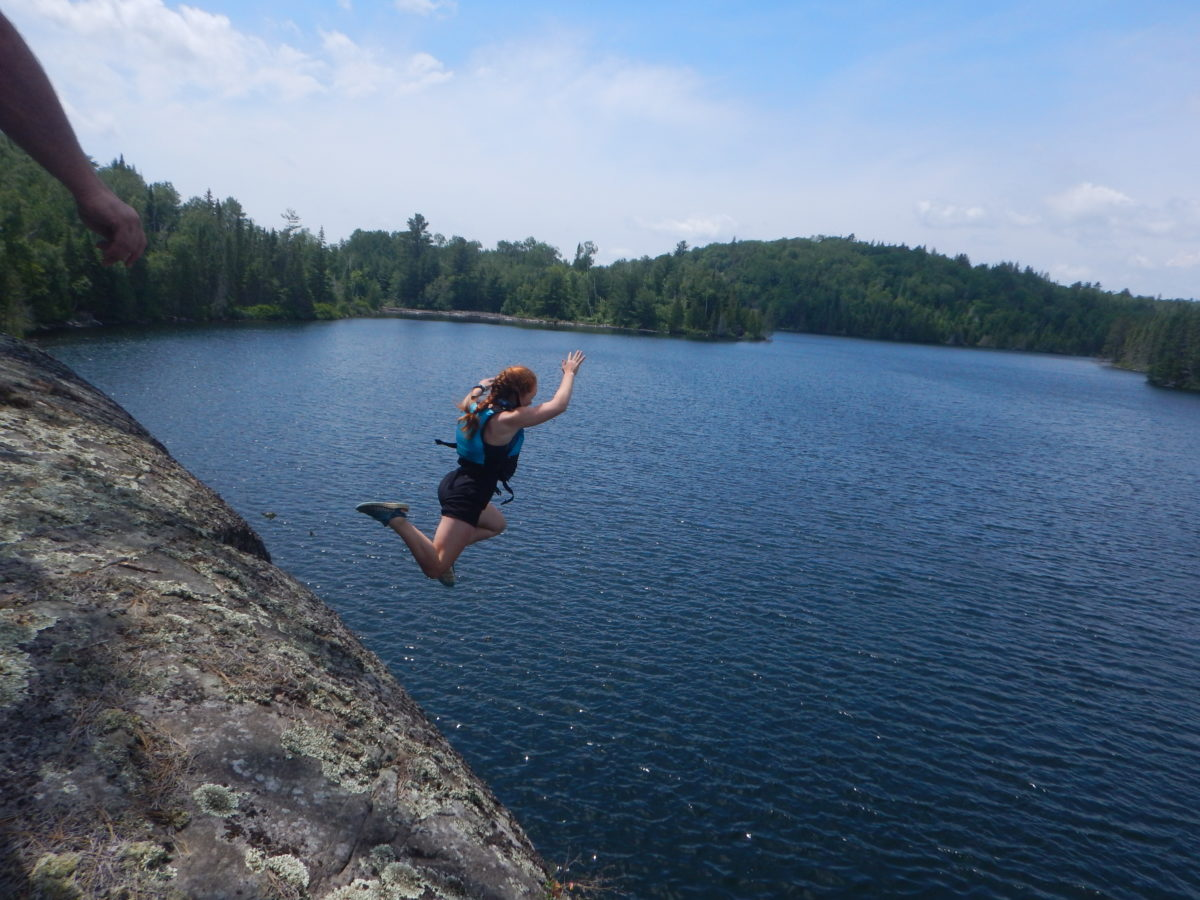
\includegraphics[width=0.62\textwidth]{./Chapter17/Figures/figure-bank-without-attention.jpg}};(1.9,-1.4);
\node[anchor=west] (label1) at ([xshift=-3.5em]input.west) {\begin{tabular}{l}{\normalsize{图片:}}\end{tabular}};
\node[anchor=south] (label2) at ([yshift=-6em]label1.south) {\begin{tabular}{l}{\normalsize{源语言:}}\end{tabular}};
\node[anchor=south] (english1) at ([xshift=-0.28em,yshift=-2.3em]input.south) {\begin{tabular}{l}{\large{A\; girl\; jumps\; off\; a\; {\red{\underline{bank}}}\quad .}}\end{tabular}};

\draw[decorate,decoration={brace,amplitude=4mm},thick] ([xshift=6.3em]input.90) -- ([xshift=0.3em,yshift=-0em]english1.east);

\node[anchor=east,rectangle,thick,rounded corners,minimum width=3.5em,minimum height=2.5em,text centered,draw=black!70,fill=red!25](trans)at ([xshift=7.4em,yshift=5.27em]english1.east){\normalsize{翻译模型}};

\draw[->,thick]([xshift=-1.4em]trans.west) to (trans.west);
\node[anchor=east] (de1) at ([xshift=5.2cm,yshift=-0.1em]trans.east) {\begin{tabular}{l}{\normalsize{目标语言:}}{\normalsize{一个/女孩/从/{\red{河床}}/}}\end{tabular}};
\node[anchor=south] (de2) at ([xshift=1.1em,yshift=-1.5em]de1.south) {\begin{tabular}{l}{\normalsize{上/跳下来/。}} \end{tabular}};
\draw[->,thick](trans.east) to ([xshift=0.5em,yshift=0.1em]de1.west);
\end {scope}
\end{tikzpicture}
    \caption{多模态机器翻译实例}
    \label{fig:17-1}
\end{figure}
%-------------------------------------------
\parinterval {\small\bfnew{模态}}\index{模态}(Modality)\index{Modality}是指某一种信息来源。例如,视觉、听觉、嗅觉、味觉都可以被看作是不同的模态。因此视频、语音、文字等都可以被看作是承载这些模态的媒介。在机器翻译中使用多模态这个概念,是为了区分某些不同于文字的信息。除了图像等视觉模态信息,机器翻译也可以利用听觉模态信息。比如,直接对语音进行翻译,甚至直接用语音表达出翻译结果。

\parinterval 除了不同信息源所引入的上下文,机器翻译也可以利用文字本身的上下文。比如,翻译一篇文章中的某个句子时,可以根据整个篇章的内容进行翻译。显然这种篇章的语境是有助于机器翻译的。在本章接下来的内容中,会对机器翻译中使用不同上下文(多模态和篇章信息)的方法展开讨论。

%----------------------------------------------------------------------------------------
%    NEW SECTION
%----------------------------------------------------------------------------------------
\sectionnewpage
\section{语音翻译}

\parinterval 语音,是人类交流中最常用的一种信息载体。从日常聊天、出国旅游,到国际会议、跨国合作,对于语音翻译的需求不断增加。甚至在有些场景下,用语音进行交互要比用文本进行交互频繁得多。因此,{\small\bfnew{语音翻译}}\index{语音翻译}(Speech Translation)\index{Speech Translation}也成为了语音处理和机器翻译相结合的重要产物。根据目标语言的载体类型,可以将语音翻译分为{\small\bfnew{语音到文本翻译}}\index{语音到文本翻译}(Speech-to-Text Translation)\index{Speech-to-Text Translation}和{\small\bfnew{语音到语音翻译}}\index{语音到语音翻译}(Speech-to-Speech Translation)\index{Speech-to-Speech Translation};基于翻译的实时性,还可以分为{\small\bfnew{实时语音翻译}}\index{实时语音翻译}(即同声传译,Simultaneous Translation)\index{Simultaneous Translation}和{\small\bfnew{离线语音翻译}}(Offline Speech Translation)\index{离线语音翻译}\index{Offline Speech Translation}。本节主要关注离线语音到文本翻译方法(简称为语音翻译),分别从音频处理、级联语音翻译和端到端语音翻译几个角度开展讨论。

%----------------------------------------------------------------------------------------
%    NEW SUB-SECTION
%----------------------------------------------------------------------------------------

\subsection{音频处理}

\parinterval 为了保证对相关内容描述的完整性,这里对语音处理的基本知识作简要介绍。不同于文本,音频本质上是经过若干信号处理之后的{\small\bfnew{波形}}\index{波形}(Waveform)\index{Waveform}。具体来说,声音是一种空气的震动,因此可以被转换为模拟信号。模拟信号是一段连续的信号,经过采样变为离散的数字信号。采样是每隔固定的时间记录一下声音的振幅,采样率表示每秒的采样点数,单位是赫兹(Hz)。采样率越高,采样的结果与原始的语音越相像。通常来说,采样的标准是能够通过离散化的数字信号重现原始语音。日常生活中使用的手机和电脑设备的采样率一般为16kHz,表示每秒16000个采样点;而音频CD的采样率可以达到44.1kHz。 经过进一步的量化,将采样点的值转换为整型数值保存,从而减少占用的存储空间,通常采用的是16位量化。将采样率和量化位数相乘,就可以得到{\small\bfnew{比特率}}\index{比特率}(Bits Per Second,BPS)\index{Bits Per Second},表示音频每秒占用的位数。例如,16kHz采样率和16位量化的音频,比特率为256kb/s。音频处理的整体流程如图\ref{fig:17-2}所示\upcite{洪青阳2020语音识别原理与应用,陈果果2020语音识别实战}。

%----------------------------------------------------------------------------------------------------
\begin{figure}[htp]
\centering
\tikzstyle{process} = [rectangle,very thick,rounded corners,minimum width=4.7cm,minimum height=2.5cm,text centered,draw=black!70,fill=red!20]
\tikzstyle{cir} = [circle,thick,rounded corners,minimum width=0.7cm,text centered,draw=black,fill=green!25]

\begin{tikzpicture}[node distance = 0,scale = 0.7]
\tikzstyle{every node}=[scale=0.7]
\node(voice)[scale=1.0]{声波};
\node(microphone)[rectangle,right of = voice,xshift=1.4cm,yshift=-1cm,minimum width=0.32cm,minimum height=0.35cm,fill=black!85,draw=black!85]{};
\draw[black!85,line width=1.8]([yshift=0.38cm,xshift=-0.4cm]microphone.north)arc(180:360:0.4cm);
\node(microphone_1)[rectangle,minimum width=0.4cm,minimum height=0.8cm,rounded corners=3pt,above of =microphone,yshift=0.75cm,draw=black!85,line width=2.5]{};
\draw[-,black!85,very thick]([yshift=0.4cm,xshift=-0.2cm]microphone.north)--([yshift=0.4cm,xshift=-0cm]microphone.north);
\draw[-,black!85,very thick]([yshift=0.5cm,xshift=-0.2cm]microphone.north)--([yshift=0.5cm,xshift=-0cm]microphone.north);
\draw[-,black!85,very thick]([yshift=0.6cm,xshift=-0.2cm]microphone.north)--([yshift=0.6cm,xshift=-0cm]microphone.north);
\draw[-,black!85,line width=1.8]([yshift=0.6cm,xshift=-0.4cm]microphone.north)--([yshift=0.37cm,xshift=-0.4cm]microphone.north);
\draw[-,black!85,line width=1.8]([yshift=0.6cm,xshift=0.4cm]microphone.north)--([yshift=0.37cm,xshift=0.4cm]microphone.north);
\draw[black!85,line width=1]([yshift=0.8cm,xshift=-0.8cm]microphone.north)arc(-45:45:0.3cm);
\draw[black!85,line width=1]([yshift=0.75cm,xshift=-0.7cm]microphone.north)arc(-45:45:0.4cm);
\draw[black!85,line width=1]([yshift=0.7cm,xshift=-0.6cm]microphone.north)arc(-45:45:0.5cm);

\node(process_1)[process,right of = microphone,xshift=4.7cm,yshift=0.5cm]{};
\node(text_1)[below of = process_1,yshift=-2cm,scale=1.3]{采样};
\draw [very thick,rounded corners=10pt]([xshift=-2.2cm,yshift=-1cm]process_1.center)--([xshift=-1.8cm,yshift=1cm]process_1.center)--([xshift=-1.4cm,yshift=0cm]process_1.center)--([xshift=-1.1cm,yshift=0.8cm]process_1.center)--([xshift=-0.8cm,yshift=-0.4cm]process_1.center)--([xshift=-0.5cm,yshift=0.4cm]process_1.center);
\draw [->,very thick]([xshift=-0.3cm]process_1.center)to([xshift=0.3cm]process_1.center);
\draw [very thick,rounded corners=10pt,densely dotted]([xshift=0.5cm,yshift=-1cm]process_1.center)--([xshift=0.9cm,yshift=1cm]process_1.center)--([xshift=1.3cm,yshift=0cm]process_1.center)--([xshift=1.6cm,yshift=0.8cm]process_1.center)--([xshift=1.9cm,yshift=-0.4cm]process_1.center)--([xshift=2.2cm,yshift=0.4cm]process_1.center);
\node(process_2)[process,fill=blue!20,right of = process_1,xshift=6.6cm]{};
\node(text_2)[below of = process_2,yshift=-2cm,scale=1.3]{量化};
\draw [very thick,rounded corners=10pt,densely dotted]([xshift=-2.2cm,yshift=-1cm]process_2.center)--([xshift=-1.8cm,yshift=1cm]process_2.center)--([xshift=-1.4cm,yshift=0cm]process_2.center)--([xshift=-1.1cm,yshift=0.8cm]process_2.center)--([xshift=-0.8cm,yshift=-0.4cm]process_2.center)--([xshift=-0.5cm,yshift=0.4cm]process_2.center);
\draw [->,very thick]([xshift=-0.3cm]process_2.center)to([xshift=0.3cm]process_2.center);
\draw [very thick,]([xshift=0.5cm,yshift=-0.8cm]process_2.center)--([xshift=0.5cm,yshift=0.3cm]process_2.center)--([xshift=0.7cm,yshift=0.3cm]process_2.center)--([xshift=0.7cm,yshift=0.8cm]process_2.center)--([xshift=1cm,yshift=0.8cm]process_2.center)--([xshift=1cm,yshift=0.2cm]process_2.center)--([xshift=1.3cm,yshift=0.2cm]process_2.center)--([xshift=1.3cm,yshift=0.6cm]process_2.center)--([xshift=1.6cm,yshift=0.6cm]process_2.center)--([xshift=1.6cm,yshift=-0.3cm]process_2.center)--([xshift=1.8cm,yshift=-0.3cm]process_2.center)--([xshift=1.8cm,yshift=0.3cm]process_2.center)--([xshift=2cm,yshift=0.3cm]process_2.center);

\node(text1)[left of = process_1,xshift=-3.2cm,yshift=-0.5cm,align=center]{模拟\\语音信号};
\node(text2)[right of = process_1,xshift=3.3cm,yshift=-0.5cm,align=center]{离散\\时间信号};
\node(text3)[right of = process_2,xshift=3.2cm,yshift=-0.5cm,align=center]{数字离散\\时间信号};

\draw[->,very thick](process_1.east)to(process_2.west);
\draw[->,very thick]([xshift=-1.8cm]process_1.west)to(process_1.west);
\draw[->,very thick](process_2.east)to([xshift=1.8cm]process_2.east);
%%%%音频
\node(signal)[right of = process_2,xshift=5.5cm]{};
\node(text_3)[below of = signal,yshift=-1.98cm,scale=1.3]{语音信号};
\draw[-,thick,]([xshift=-1.2cm]signal.center)--([xshift=1.2cm]signal.center);
\draw[-,thick]([xshift=-1cm,yshift=-0.8cm]signal.center)--([xshift=-0.9cm,yshift=0.4cm]signal.center)--([xshift=-0.8cm,yshift=-0.3cm]signal.center)--([xshift=-0.7cm,yshift=0.7cm]signal.center)--([xshift=-0.6cm,yshift=-0.1cm]signal.center)--([xshift=-0.5cm,yshift=0.3cm]signal.center)--([xshift=-0.4cm,yshift=-0.5cm]signal.center)--([xshift=-0.3cm,yshift=0.7cm]signal.center)--([xshift=-0.2cm,yshift=-0.2cm]signal.center)--([xshift=-0.1cm,yshift=0.4cm]signal.center)--([xshift=0cm,yshift=-0.9cm]signal.center)--([xshift=0.1cm,yshift=0.5cm]signal.center)--([xshift=0.2cm,yshift=-0.4cm]signal.center)--([xshift=0.3cm,yshift=0.3cm]signal.center)--([xshift=0.4cm,yshift=-0.2cm]signal.center)--([xshift=0.5cm,yshift=0.1cm]signal.center)--([xshift=0.6cm,yshift=-0.8cm]signal.center)--([xshift=0.7cm,yshift=0.4cm]signal.center)--([xshift=0.8cm,yshift=-0.6cm]signal.center)--([xshift=0.9cm,yshift=0.7cm]signal.center)--([xshift=1cm,yshift=-0.2cm]signal.center);
\end{tikzpicture}
\caption{音频处理过程}
\label{fig:17-2}
\end{figure}
%----------------------------------------------------------------------------------------------------

\parinterval 经过上面的描述可以看出,音频的表示实际上是一个非常长的采样点序列,这导致了直接使用现有的深度学习技术处理音频序列较为困难。并且,原始的音频信号中可能包含着较多的噪声、环境声或冗余信息,也会对模型产生干扰。因此,一般会对音频序列进行处理来提取声学特征,具体为将长序列的采样点序列转换为短序列的特征向量序列,再用于下游系统。虽然已有一些工作不依赖特征提取,直接在原始的采样点序列上进行声学建模和模型训练\upcite{DBLP:conf/interspeech/SainathWSWV15},但目前的主流方法仍然是基于声学特征进行建模\upcite{DBLP:conf/icassp/MohamedHP12}。

\parinterval 声学特征提取的第一步是预处理。其流程主要是对音频进行{\small\bfnew{预加重}}(Pre-emphasis)\index{预加重}\index{Pre-emphasis}、{\small\bfnew{分帧}}\index{分帧}(Framing)\index{Framing}和{\small\bfnew{加窗}}\index{加窗}(Windowing)\index{Windowing}。预加重是通过增强音频信号中的高频部分来减弱语音中对高频信号的抑制,使频谱更加顺滑。分帧(原理如图\ref{fig:17-3}所示)是基于短时平稳假设,即根据生物学特征,语音信号是一个缓慢变化的过程,10ms$\thicksim$30ms的信号片段是相对平稳的。基于这个假设,一般将每25ms作为一帧来提取特征,这个时间称为{\small\bfnew{帧长}}\index{帧长}(Frame Length)\index{Frame Length}。同时,为了保证不同帧之间的信号平滑性,使每两个相邻帧之间存在一定的重合部分。一般每隔10ms取一帧,这个时长称为{\small\bfnew{帧移}}\index{帧移}(Frame Shift)\index{Frame Shift}。为了缓解分帧带来的频谱泄漏问题,需要对每帧的信号进行加窗处理使其幅度在两端渐变到0,一般采用的是{\small\bfnew{汉明窗}}\index{汉明窗}(Hamming Window)\index{Hamming Window}\upcite{洪青阳2020语音识别原理与应用}。
%----------------------------------------------------------------------------------------------------
\begin{figure}[htp]
\centering
\tikzstyle{process} = [rectangle,very thick,rounded corners,minimum width=5cm,minimum height=2.5cm,text centered,draw=black!70,fill=red!25]
\tikzstyle{cir} = [circle,thick,rounded corners,minimum width=0.7cm,text centered,draw=black,fill=green!25]

\begin{tikzpicture}[node distance = 0,scale = 1]
\tikzstyle{every node}=[scale=1]
\node [anchor=center](ori) at (-0.2,-0.2) {0};
\draw[->,thick](-0.5,0)--(5,0)node[below,scale=0.8]{时间};
\draw[->,thick](0,-2)--(0,2)node[left,scale=0.8]{量化值};
\draw[-,thick](0,0)sin(0.7,1.5)cos(1.4,0)sin(2.1,-1.5)cos(2.8,0)sin(3.5,1.5)cos(4.2,0);
\draw[-,thick,dashed](0.5,-1.8)--(0.5,1.8);
\draw[-](1.2,-1.8)--(1.2,1.8);
\draw[-,thick,dashed](1.9,-1.8)--(1.9,1.8);
\draw[<->,thick](0,-1.1)--(1.2,-1.1)node[left,xshift=-0.05cm,yshift=0.15cm,scale=0.6]{帧长};
\draw[<->,thick](0,-1.4)--(0.5,-1.4)node[left,xshift=0.05cm,yshift=-0.25cm,scale=0.6]{帧移};
%\draw[<->,thick](0.5,-1.4)--(1.9,-1.4);
\end{tikzpicture}
\caption{分帧原理图}
\label{fig:17-3}
\end{figure}
%----------------------------------------------------------------------------------------------------

\parinterval 经过了上述的预处理操作,可以得到音频对应的帧序列,之后通过不同的操作来提取不同类型的声学特征。在语音翻译中,比较常用的声学特征为{\small\bfnew{滤波器组}}\index{滤波器组}(Filter-bank,Fbank)\index{Filter-bank}和{\small\bfnew{Mel频率倒谱系数}}\index{Mel频率倒谱系数}(Mel-frequency Cepstral Coefficient,MFCC)\index{Mel-frequency Cepstral Coefficient}\upcite{洪青阳2020语音识别原理与应用}。实际上,提取到的声学特征可以类比于计算机视觉中的像素特征,或者自然语言处理中的词嵌入表示。不同之处在于,声学特征更加复杂多变,可能存在着较多的噪声和冗余信息。此外,相比对应的文字序列,音频提取到的特征序列长度要大十倍以上。比如,人类正常交流中每秒钟一般可以说2-3个字,而每秒钟的语音可以提取得到100帧的特征序列。巨大的长度比差异也为声学特征建模带来了挑战。

%----------------------------------------------------------------------------------------
%    NEW SUB-SECTION
%----------------------------------------------------------------------------------------

\subsection{级联式语音翻译}
\label{sec:cascaded-speech-translation}

\parinterval 实现语音翻译最简单的思路是基于级联的方式,即:先通过{\small\bfnew{自动语音识别}}\index{自动语音识别}(Automatic Speech Recognition,ASR)\index{Automatic Speech Recognition}系统将语音转化为源语言文本,然后利用机器翻译系统将源语言文本翻译为目标语言文本。这种做法的好处在于语音识别和机器翻译模型可以分别进行训练,有很多数据资源以及成熟技术可以分别运用到两个系统中。因此,级联语音翻译是很长时间以来的主流方法,深受工业界的青睐。级联语音翻译主要的流程如图\ref{fig:17-4}所示。

%----------------------------------------------------------------------------------------------------
\begin{figure}[htp]
\centering
\tikzstyle{process} = [rectangle,very thick,rounded corners,minimum width=3.2cm,minimum height=3cm,text centered,draw=black!70,fill=red!20]
\tikzstyle{cir} = [circle,thick,rounded corners,minimum width=0.7cm,text centered,draw=black,fill=green!25]

\begin{tikzpicture}[node distance = 0,scale = 0.5]
\tikzstyle{every node}=[scale=0.5]
\node(process_1)[process]{};
\draw[-,thick]([xshift=-1.2cm]process_1.center)--([xshift=1.2cm]process_1.center);
\draw[-,thick]([xshift=-1cm,yshift=-0.8cm]process_1.center)--([xshift=-0.9cm,yshift=0.4cm]process_1.center)--([xshift=-0.8cm,yshift=-0.3cm]process_1.center)--([xshift=-0.7cm,yshift=0.7cm]process_1.center)--([xshift=-0.6cm,yshift=-0.1cm]process_1.center)--([xshift=-0.5cm,yshift=0.3cm]process_1.center)--([xshift=-0.4cm,yshift=-0.5cm]process_1.center)--([xshift=-0.3cm,yshift=0.7cm]process_1.center)--([xshift=-0.2cm,yshift=-0.2cm]process_1.center)--([xshift=-0.1cm,yshift=0.4cm]process_1.center)--([xshift=0cm,yshift=-0.9cm]process_1.center)--([xshift=0.1cm,yshift=0.5cm]process_1.center)--([xshift=0.2cm,yshift=-0.4cm]process_1.center)--([xshift=0.3cm,yshift=0.3cm]process_1.center)--([xshift=0.4cm,yshift=-0.2cm]process_1.center)--([xshift=0.5cm,yshift=0.1cm]process_1.center)--([xshift=0.6cm,yshift=-0.8cm]process_1.center)--([xshift=0.7cm,yshift=0.4cm]process_1.center)--([xshift=0.8cm,yshift=-0.6cm]process_1.center)--([xshift=0.9cm,yshift=0.7cm]process_1.center)--([xshift=1cm,yshift=-0.2cm]process_1.center);
\node(text_1)[below of = process_1,yshift=-2cm,scale=1.5]{语音信号};
\node(process_2)[process,fill=blue!20,right of = process_1,xshift=7.0cm,text width=4cm,align=center]{\baselineskip=4pt\LARGE{[[0.2,...,0.3], \qquad ..., \qquad  0.3,...,0.5]]}\par};
\node(text_2)[below of = process_2,yshift=-2cm,scale=1.5]{语音特征};
\node(process_3)[process,fill=orange!20,minimum width=6cm,minimum height=5cm,right of = process_2,xshift=8.2cm,text width=4cm,align=center]{};
\node(text_3)[below of = process_3,yshift=-3cm,scale=1.5]{源语言文本及其词格};
\node(cir_s)[cir,very thick, below of = process_3,xshift=-2.2cm,yshift=1.1cm]{\LARGE S};
\node(cir_a)[cir,right of = cir_s,xshift=1cm,yshift=0.8cm]{\LARGE a};
\node(cir_c)[cir,right of = cir_a,xshift=1.2cm,yshift=0cm]{\LARGE c};
\node(cir_f)[cir,right of = cir_c,xshift=1.2cm,yshift=0cm]{\LARGE f};
\node(cir_E)[cir,very thick,right of = cir_f,xshift=1cm,yshift=-0.8cm]{\LARGE E};
\node(cir_b)[cir,right of = cir_s,xshift=1cm,yshift=-0.8cm]{\Large b};
\node(cir_d)[cir,right of = cir_b,xshift=1cm,yshift=0.6cm]{\Large d};
\node(cir_e)[cir, right of = cir_b,xshift=1cm,yshift=-0.8cm]{\LARGE e};
\node(cir_g)[cir,right of = cir_e,xshift=1cm,yshift=0.8cm]{\LARGE g};
\draw[-latex](cir_s)node[above,xshift=0.3cm,yshift=0.4cm]{0.4}to(cir_a);
\draw[-latex](cir_a)node[above,xshift=0.6cm,yshift=0cm]{1}to(cir_c);
\draw[-latex](cir_c)node[above,xshift=0.6cm,yshift=0cm]{1}to(cir_f);
\draw[-latex](cir_f)node[above,xshift=0.6cm,yshift=-0.3cm]{1}to(cir_E);
\draw[-latex](cir_s)node[above,xshift=0.7cm,yshift=-0.4cm]{0.6}to(cir_b);
\draw[-latex](cir_b)node[above,xshift=0.3cm,yshift=0.3cm]{0.8}to(cir_d);
\draw[-latex](cir_b)node[above,xshift=0.7cm,yshift=-0.4cm]{0.2}to(cir_e);
\draw[-latex](cir_e)node[above,xshift=0.3cm,yshift=0.3cm]{1}to(cir_g);
\draw[-latex](cir_d)node[above,xshift=0.7cm,yshift=0cm]{1}to(cir_f);
\draw[-latex](cir_g)node[above,xshift=0.6cm,yshift=0.3cm]{1}--(cir_E);


\node(text)[below of = process_3,yshift=-1.8cm,scale=1.8]{你是谁};
\node(process_4)[process,fill=ugreen!20,right of = process_3,xshift=8.2cm,text width=4cm,align=center]{\Large\textbf{Who are you?}};
\node(text_4)[below of = process_4,yshift=-2cm,scale=1.5]{翻译结果};

\draw[->,very thick](process_1.east)to(process_2.west);
\draw[->,very thick](process_2.east)to(process_3.west);
\draw[->,very thick](process_3.east)to(process_4.west);
\node(arrow_text1)[right of = process_1,xshift=3.2cm,yshift=0.7cm,scale=1.4,align=center]{音频\\特征提取};
\node(arrow_text2)[right of = process_2,xshift=3.6cm,yshift=0.7cm,scale=1.4,align=center]{语音\\识别系统};
\node(arrow_text3)[right of = process_3,xshift=4.5cm,yshift=0.4cm,scale=1.4]{翻译系统};
\end{tikzpicture}
\caption{级联式语音翻译流程示例}
\label{fig:17-4}
\end{figure}
%----------------------------------------------------------------------------------------------------

\parinterval 由于声学特征提取在上一节中已经进行了描述,而且文本翻译可以直接使用本书介绍的统计机器翻译或者神经机器翻译方法。因此下面简要介绍一下语音识别模型,以便读者对级联式语音翻译系统有一个完整的认识。其中的部分概念在后续介绍的端到端语言翻译中也会有所涉及。

\parinterval 传统的语音识别模型和统计机器翻译相似,需要利用声学模型、语言模型和发音词典联合进行识别,系统较为复杂\upcite{DBLP:journals/ftsig/GalesY07,DBLP:journals/taslp/MohamedDH12,DBLP:journals/spm/X12a}。而近些年来,随着神经网络的发展,基于神经网络的端到端语音识别模型逐渐受到关注,训练流程也大大被简化\upcite{DBLP:conf/nips/ChorowskiBSCB15,DBLP:conf/icassp/ChanJLV16}。目前的端到端语音识别模型主要基于序列到序列结构,编码器根据输入的声学特征进一步提取高级特征,解码器根据编码器提取的特征识别对应的文本。在\ref{end-to-end-speech-translation}小节中介绍的端到端语音翻译模型也是基于十分相似的结构。因此,从某种意义上说,语音识别和翻译所使用的端到端方法与神经机器翻译是一致的。
%----------------------------------------------------------------------------------------------------
\begin{figure}[htp]
\centering
\begin{tikzpicture}
	\tikzstyle{layer}=[draw,rounded corners=2pt,font=\scriptsize,align=center,minimum width=7.1em]
	\tikzstyle{word}=[font=\scriptsize]
%%%%encoder
\node[layer,fill=red!20] (en_sa) at (0,0){Multi-Head \\ Attention};
\node[anchor=south,layer,fill=yellow!20](en_add1) at ([yshift=1.0em]en_sa.north) {Add \& LayerNorm};
\node[layer,anchor=south,fill=green!20] (en_ffn) at ([yshift=1.0em]en_add1.north){Feed Forward \\ Network};
\node[anchor=south,layer,fill=yellow!20](en_add2) at ([yshift=1.0em]en_ffn.north) {Add \& LayerNorm};
\node[draw,circle,inner sep=0pt, minimum size=1em,anchor=north,thick] (en_add) at ([yshift=-1.4em]en_sa.south){};
\draw[thick] (en_add.90) -- (en_add.-90);
\draw[thick] (en_add.0) -- (en_add.180);
\node[layer,anchor=north,fill=yellow!20] (en_cnn) at ([yshift=-1.0em]en_add.south){CNN};
\node[anchor=east,font=\scriptsize,align=center] (en_pos) at ([xshift=-2em]en_add.west){位置编码};
\node[anchor=north,font=\scriptsize,align=center] (en_input) at ([yshift=-1em]en_cnn.south){语音特征\\(FBank/MFCC)};

\draw[->,thick] (en_input.90) -- ([yshift=-0.1em]en_cnn.-90);
\draw[->,thick] ([yshift=0.1em]en_cnn.90) -- ([yshift=-0.1em]en_add.-90);
\draw[->,thick] ([yshift=0.1em]en_add.90) -- ([yshift=-0.1em]en_sa.-90);
\draw[->,thick] ([yshift=0.1em]en_sa.90) -- ([yshift=-0.1em]en_add1.-90);
\draw[->,thick] ([yshift=0.1em]en_add1.90) -- ([yshift=-0.1em]en_ffn.-90);
\draw[->,thick] ([yshift=0.1em]en_ffn.90) --([yshift=-0.1em]en_add2.-90);
\draw[->,rounded corners=2pt,thick] ([yshift=-0.6em]en_sa.south)--([yshift=-0.6em,xshift=-4.0em]en_sa.south)--([xshift=-0.43em]en_add1.west)--(en_add1.west);
\draw[->,rounded corners=2pt,thick] ([yshift=-0.6em]en_ffn.south)--([yshift=-0.6em,xshift=-4.0em]en_ffn.south)--([xshift=-0.43em]en_add2.west)--(en_add2.west);

%%%%decoder
\node[draw,circle,inner sep=0pt, minimum size=1em,anchor=west,thick] (de_add) at ([xshift=9em]en_add.east){};
\draw[thick] (de_add.90) -- (de_add.-90);
\draw[thick] (de_add.0) -- (de_add.180);
\node[layer,anchor=south,fill=red!20] (de_sa) at ([yshift=1.4em]de_add.north){Masked \\Multi-Head\\Attention};
\node[anchor=south,layer,fill=yellow!20](de_add1) at ([yshift=1.0em]de_sa.north) {Add \& LayerNorm};
\node[layer,anchor=south,fill=red!20] (de_ca) at ([yshift=1.0em]de_add1.north){Multi-Head \\ Attention};
\node[anchor=south,layer,fill=yellow!20](de_add2) at ([yshift=1.0em]de_ca.north) {Add \& LayerNorm};
\node[layer,anchor=south,fill=green!20] (de_ffn) at ([yshift=1.0em]de_add2.north){Feed Forward \\ Network};
\node[anchor=south,layer,fill=yellow!20](de_add3) at ([yshift=1.0em]de_ffn.north) {Add \& LayerNorm};
\node[layer,anchor=south,fill=blue!20] (sf) at ([yshift=1.2em]de_add3.north){Softmax};
\node[anchor=north,font=\scriptsize,align=center] (de_input) at ([yshift=-1.1em]de_add.south){标注文本\\编码表示};

\node[anchor=west,font=\scriptsize,align=center] (de_pos) at ([xshift=2em]de_add.east){位置编码};

\draw[->,thick] (de_input.90) -- ([yshift=-0.1em]de_add.-90);
\draw[->,thick] ([yshift=0.1em]de_add.90) -- ([yshift=-0.1em]de_sa.-90);
\draw[->,thick] ([yshift=0.1em]de_sa.90) -- ([yshift=-0.1em]de_add1.-90);
\draw[->,thick] ([yshift=0.1em]de_add1.90) -- ([yshift=-0.1em]de_ca.-90);
\draw[->,thick] ([yshift=0.1em]de_ca.90) -- ([yshift=-0.1em]de_add2.-90);
\draw[->,thick] ([yshift=0.1em]de_add2.90) -- ([yshift=-0.1em]de_ffn.-90);
\draw[->,thick] ([yshift=0.1em]de_ffn.90) -- ([yshift=-0.1em]de_add3.-90);
\draw[->,thick] ([yshift=0.1em]de_add3.90) -- ([yshift=-0.1em]sf.-90);
\draw[->,thick] ([yshift=0.1em]sf.90) -- ([yshift=1.0em]sf.90);
\draw[->,thick] ([xshift=0.1em]en_pos.0) -- ([xshift=-0.1em]en_add.180);
\draw[->,thick] ([xshift=-0.1em]de_pos.180) -- ([xshift=0.1em]de_add.0);
\draw[->,rounded corners=2pt,thick] ([yshift=-0.6em]de_sa.south)--([yshift=-0.6em,xshift=4.0em]de_sa.south)--([xshift=0.43em]de_add1.east)--(de_add1.east);
\draw[->,rounded corners=2pt,thick] ([yshift=-0.6em]de_ca.south)--([yshift=-0.6em,xshift=4.0em]de_ca.south)--([xshift=0.43em]de_add2.east)--(de_add2.east);
\draw[->,rounded corners=2pt,thick] ([yshift=-0.6em]de_ffn.south)--([yshift=-0.6em,xshift=4.0em]de_ffn.south)--([xshift=0.43em]de_add3.east)--(de_add3.east);

\draw[->,rounded corners=2pt,thick] ([yshift=0.1em]en_add2.90) -- ([yshift=1.5em]en_add2.90) -- ([xshift=5.0em,yshift=1.5em]en_add2.90) -- ([xshift=-1.5em]de_ca.west) -- ([xshift=-0.1em]de_ca.west);


\begin{pgfonlayer}{background}
\node[draw=ugreen,rounded corners=2pt,inner xsep=6pt,inner ysep=8pt,dashed,thick,xshift=-0.2em,yshift=-0.2em][fit=(en_add1)(en_add2)(en_sa)(en_ffn)](box1){};
\node[draw=red,rounded corners=2pt,inner xsep=6pt,inner ysep=8pt,dashed,thick,xshift=0.2em,yshift=-0.2em][fit=(de_sa)(de_ca)(de_ffn)(de_add3)](box2){};
\end{pgfonlayer}

\node[anchor=east,font=\scriptsize,text=ugreen] at ([xshift=-0.1em]box1.west){$N \times$};
\node[anchor=west,font=\scriptsize,text=red] at ([xshift=0.1em]box2.east){$\times N$};
\node[anchor=east,font=\scriptsize] at ([xshift=-0.1em]en_cnn.west){$2 \times$};
\node[anchor=east,font=\scriptsize,align=center,text=ugreen] at ([xshift=-0.1em,yshift=3em]box1.west){ASR \\ 编码器};
\node[anchor=west,font=\scriptsize,align=center,text=red] at ([xshift=0.1em,yshift=5em]box2.east){ASR \\ 解码器};
\end{tikzpicture}
\setlength{\abovecaptionskip}{-0.2em}
\caption{基于Transformer的语音识别模型}
\label{fig:17-5}
\end{figure}
%----------------------------------------------------------------------------------------------------

\vspace{-1em}
\parinterval 语音识别目前广泛使用基于Transformer的模型结构(见{\chaptertwelve}),如图\ref{fig:17-5}所示。可以看出,相比文本翻译,语音识别模型结构上唯一的区别在于编码器的输入为声学特征,以及编码器底层会使用额外的卷积层来减小输入序列的长度。这是由于语音对应的特征序列过长,在计算注意力模型的时候,会占用大量的内存和显存,并增加训练时间。因此,一个常用的做法是在语音特征上进行两层步长为2的卷积操作,从而将输入序列的长度缩小为之前的1/4。通过使用大量的语音-标注平行数据对模型进行训练,可以得到高质量的语音识别模型。

\parinterval 为了降低语音识别的错误对下游系统的影响,通常也会用词格来取代One-best语音识别结果。除此之外,另一种思路是通过一个后处理模型修正识别结果中的错误,再送给文本翻译模型进行翻译。也可以进一步对文本做{\small\bfnew{顺滑}}\index{顺滑}(Disfluency Detection\index{Disfluency Detection})处理,使得送给翻译系统的文本更加干净、流畅,比如除去一些导致停顿的语气词。这一做法在工业界得到了广泛应用,但由于每个模型只能串行地计算,也会带来额外的计算代价以及运算时间。第三种思路是训练更加健壮的文本翻译模型,使其可以处理输入中存在的噪声或误差\upcite{DBLP:conf/acl/LiuTMCZ18}。

%----------------------------------------------------------------------------------------
%    NEW SUB-SECTION
%----------------------------------------------------------------------------------------

\subsection{端到端语音翻译}\label{end-to-end-speech-translation}

\parinterval 级联语音翻译模型结构简单、易于实现,但不可避免地存在一些缺陷:

%----------------------------------------------------------------------------------------------------
\begin{itemize}
    \item {\small\bfnew{错误传播问题}}。级联模型导致的一个很严重的问题在于,语音识别模型得到的文本如果存在错误,这些错误很可能在翻译过程中被放大,从而使最后翻译结果出现比较大的偏差。比如识别时在句尾少生成了个“吗”,会导致翻译模型将疑问句翻译为陈述句。
    \vspace{0.5em}
    \item {\small\bfnew{翻译效率问题}}。由于语音识别模型和文本标注模型只能串行地计算,翻译效率相对较低,而实际很多场景中都需要实现低延时的翻译。
    \vspace{0.5em}
    \item {\small\bfnew{语音中的副语言信息丢失}}。将语音识别为文本的过程中,语音中包含的语气、情感、音调等信息会丢失,而同一句话在不同的语气中表达的意思很可能是不同的。尤其是在实际应用中,由于语音识别结果通常并不包含标点,还需要额外的后处理模型将标点还原,也会带来额外的计算代价。
\end{itemize}
%----------------------------------------------------------------------------------------------------

%----------------------------------------------------------------------------------------------------
\begin{figure}[htp]
\centering
\begin{tikzpicture}
	\tikzstyle{layer}=[draw,rounded corners=2pt,font=\scriptsize,align=center,minimum width=7.1em]
	\tikzstyle{word}=[font=\scriptsize]
%%%%encoder
\node[layer,fill=red!20] (en_sa) at (0,0){Multi-Head \\ Attention};
\node[anchor=south,layer,fill=yellow!20](en_add1) at ([yshift=1.0em]en_sa.north) {Add \& LayerNorm};
\node[layer,anchor=south,fill=green!20] (en_ffn) at ([yshift=1.0em]en_add1.north){Feed Forward \\ Network};
\node[anchor=south,layer,fill=yellow!20](en_add2) at ([yshift=1.0em]en_ffn.north) {Add \& LayerNorm};
\node[draw,circle,inner sep=0pt, minimum size=1em,anchor=north,thick] (en_add) at ([yshift=-1.4em]en_sa.south){};
\draw[thick] (en_add.90) -- (en_add.-90);
\draw[thick] (en_add.0) -- (en_add.180);
\node[layer,anchor=north,fill=yellow!20] (en_cnn) at ([yshift=-1.0em]en_add.south){CNN};
\node[anchor=east,font=\scriptsize,align=center] (en_pos) at ([xshift=-2em]en_add.west){位置编码};
\node[anchor=north,font=\scriptsize,align=center] (en_input) at ([yshift=-1em]en_cnn.south){源语言语音特征\\(FBank/MFCC)};

\draw[->,thick] (en_input.90) -- ([yshift=-0.1em]en_cnn.-90);
\draw[->,thick] ([yshift=0.1em]en_cnn.90) -- ([yshift=-0.1em]en_add.-90);
\draw[->,thick] ([yshift=0.1em]en_add.90) -- ([yshift=-0.1em]en_sa.-90);
\draw[->,thick] ([yshift=0.1em]en_sa.90) -- ([yshift=-0.1em]en_add1.-90);
\draw[->,thick] ([yshift=0.1em]en_add1.90) -- ([yshift=-0.1em]en_ffn.-90);
\draw[->,thick] ([yshift=0.1em]en_ffn.90) --([yshift=-0.1em]en_add2.-90);
\draw[->,rounded corners=2pt,thick] ([yshift=-0.6em]en_sa.south)--([yshift=-0.6em,xshift=-4.0em]en_sa.south)--([xshift=-0.43em]en_add1.west)--(en_add1.west);
\draw[->,rounded corners=2pt,thick] ([yshift=-0.6em]en_ffn.south)--([yshift=-0.6em,xshift=-4.0em]en_ffn.south)--([xshift=-0.43em]en_add2.west)--(en_add2.west);

%%%%decoder
\node[draw,circle,inner sep=0pt, minimum size=1em,anchor=west,thick] (de_add) at ([xshift=9em]en_add.east){};
\draw[thick] (de_add.90) -- (de_add.-90);
\draw[thick] (de_add.0) -- (de_add.180);
\node[layer,anchor=south,fill=red!20] (de_sa) at ([yshift=1.4em]de_add.north){Masked \\Multi-Head\\Attention};
\node[anchor=south,layer,fill=yellow!20](de_add1) at ([yshift=1.0em]de_sa.north) {Add \& LayerNorm};
\node[layer,anchor=south,fill=red!20] (de_ca) at ([yshift=1.0em]de_add1.north){Multi-Head \\ Attention};
\node[anchor=south,layer,fill=yellow!20](de_add2) at ([yshift=1.0em]de_ca.north) {Add \& LayerNorm};
\node[layer,anchor=south,fill=green!20] (de_ffn) at ([yshift=1.0em]de_add2.north){Feed Forward \\ Network};
\node[anchor=south,layer,fill=yellow!20](de_add3) at ([yshift=1.0em]de_ffn.north) {Add \& LayerNorm};
\node[layer,anchor=south,fill=blue!20] (sf) at ([yshift=1.2em]de_add3.north){Softmax};
\node[anchor=north,font=\scriptsize,align=center] (de_input) at ([yshift=-1.1em]de_add.south){目标语言文本\\编码表示};

\node[anchor=west,font=\scriptsize,align=center] (de_pos) at ([xshift=2em]de_add.east){位置编码};

\draw[->,thick] (de_input.90) -- ([yshift=-0.1em]de_add.-90);
\draw[->,thick] ([yshift=0.1em]de_add.90) -- ([yshift=-0.1em]de_sa.-90);
\draw[->,thick] ([yshift=0.1em]de_sa.90) -- ([yshift=-0.1em]de_add1.-90);
\draw[->,thick] ([yshift=0.1em]de_add1.90) -- ([yshift=-0.1em]de_ca.-90);
\draw[->,thick] ([yshift=0.1em]de_ca.90) -- ([yshift=-0.1em]de_add2.-90);
\draw[->,thick] ([yshift=0.1em]de_add2.90) -- ([yshift=-0.1em]de_ffn.-90);
\draw[->,thick] ([yshift=0.1em]de_ffn.90) -- ([yshift=-0.1em]de_add3.-90);
\draw[->,thick] ([yshift=0.1em]de_add3.90) -- ([yshift=-0.1em]sf.-90);
\draw[->,thick] ([yshift=0.1em]sf.90) -- ([yshift=1.0em]sf.90);
\draw[->,thick] ([xshift=0.1em]en_pos.0) -- ([xshift=-0.1em]en_add.180);
\draw[->,thick] ([xshift=-0.1em]de_pos.180) -- ([xshift=0.1em]de_add.0);
\draw[->,rounded corners=2pt,thick] ([yshift=-0.6em]de_sa.south)--([yshift=-0.6em,xshift=4.0em]de_sa.south)--([xshift=0.43em]de_add1.east)--(de_add1.east);
\draw[->,rounded corners=2pt,thick] ([yshift=-0.6em]de_ca.south)--([yshift=-0.6em,xshift=4.0em]de_ca.south)--([xshift=0.43em]de_add2.east)--(de_add2.east);
\draw[->,rounded corners=2pt,thick] ([yshift=-0.6em]de_ffn.south)--([yshift=-0.6em,xshift=4.0em]de_ffn.south)--([xshift=0.43em]de_add3.east)--(de_add3.east);

\draw[->,rounded corners=2pt,thick] ([yshift=0.1em]en_add2.90) -- ([yshift=1.5em]en_add2.90) -- ([xshift=5.0em,yshift=1.5em]en_add2.90) -- ([xshift=-1.5em]de_ca.west) -- ([xshift=-0.1em]de_ca.west);


\begin{pgfonlayer}{background}
\node[draw=ugreen,rounded corners=2pt,inner xsep=6pt,inner ysep=8pt,dashed,thick,xshift=-0.2em,yshift=-0.2em][fit=(en_add1)(en_add2)(en_sa)(en_ffn)](box1){};
\node[draw=red,rounded corners=2pt,inner xsep=6pt,inner ysep=8pt,dashed,thick,xshift=0.2em,yshift=-0.2em][fit=(de_sa)(de_ca)(de_ffn)(de_add3)](box2){};
\end{pgfonlayer}

\node[anchor=east,font=\scriptsize,text=ugreen] at ([xshift=-0.1em]box1.west){$N \times$};
\node[anchor=west,font=\scriptsize,text=red] at ([xshift=0.1em]box2.east){$\times N$};
\node[anchor=east,font=\scriptsize] at ([xshift=-0.1em]en_cnn.west){$2 \times$};
\node[anchor=east,font=\scriptsize,align=center,text=ugreen] at ([xshift=-0.1em,yshift=3em]box1.west){ST \\ 编码器};
\node[anchor=west,font=\scriptsize,align=center,text=red] at ([xshift=0.1em,yshift=5em]box2.east){ST \\ 解码器};
\end{tikzpicture}
\setlength{\abovecaptionskip}{-0.2em}
\caption{基于Transformer的端到端语音翻译模型}
\label{fig:17-7}
\end{figure}
%----------------------------------------------------------------------------------------------------

\parinterval 针对级联语音翻译模型存在的缺陷,研究人员提出了{\small\bfnew{端到端的语音翻译模型}}\index{端到端的语音翻译模型}(End-to-End Speech Translation,E2E-ST)\index{End-to-End Speech Translation}\upcite{DBLP:conf/naacl/DuongACBC16,DBLP:conf/interspeech/WeissCJWC17,DBLP:journals/corr/BerardPSB16},也就是模型的输入是源语言语音,输出是对应的目标语言文本。相比级联模型,端到端模型有如下优点:

%----------------------------------------------------------------------------------------------------
\begin{itemize}
    \vspace{0.5em}
    \item 端到端模型不需要多阶段的处理,因此避免了错误传播问题。
    \vspace{0.5em}
    \item 同样地,端到端模型所涉及的模块更少,容易控制模型体积。
    \vspace{0.5em}
    \item 端到端模型语音信号可以直接作用于翻译过程,因此可以使得副语言信息得以体现。
    \vspace{0.5em}
\end{itemize}
%----------------------------------------------------------------------------------------------------

\parinterval 以Transformer模型为例,图\ref{fig:17-7}展示了端到端语音翻译的架构(下文中语音翻译模型均指端到端的模型)。该模型采用的也是序列到序列架构,编码器的输入是从语音中提取的特征(比如FBank特征)。编码器底层采用和语音识别模型相同的卷积结构来降低序列的长度(见\ref{sec:cascaded-speech-translation}节)。之后的流程和标准的神经机器翻译是完全一致的,编码器对语音特征进行编码,解码器根据编码结果生成目标语言的翻译结果。

\parinterval 虽然端到端语音翻译模型解决了级联模型存在的问题,但同时也面临着两个严峻的问题:

%----------------------------------------------------------------------------------------------------
\begin{itemize}
    \vspace{0.5em}
    \item {\small\bfnew{训练数据稀缺}}。虽然语音识别和文本翻译的训练数据都很多,但是直接由源语言语音到目标语言文本的平行数据十分有限,因此端到端语音翻译天然地就是一种低资源翻译任务。
    \vspace{0.5em}
    \item {\small\bfnew{建模复杂度更高}}。在语音识别中,模型需要学习如何生成语音对应的文字序列,而输入和输出的对齐比较简单,并不涉及调序的问题。在文本翻译中,模型要学习如何生成源语言序列对应的目标语言序列,仅需要学习不同语言之间的映射,不涉及到模态的转换。而语音翻译模型需要学习从语音到目标语言文本的生成,任务更加复杂。
    \vspace{0.5em}
\end{itemize}
%----------------------------------------------------------------------------------------------------

\parinterval 针对这两个问题,研究人员们也提出了很多方法进行缓解,包括多任务学习、迁移学习等,主要思想都是利用语音识别或文本翻译数据来指导模型的学习。并且,文本翻译的很多方法对语音翻译技术的发展提供了思路。如何将其他领域现有的工作在语音翻译任务上验证,也是语音翻译研究人员当前所关注的\upcite{DBLP:conf/mtsummit/GangiNCDT19}。

%----------------------------------------------------------------------------------------
%    NEW SUBSUB-SECTION
%----------------------------------------------------------------------------------------
\subsubsection{1. 多任务学习}

\parinterval 一种思路是进行多任务学习,让模型在训练过程中得到更多的监督信息。使用多个任务强化主任务(机器翻译),在本书的{\chapterfifteen}和{\chaptersixteen}也有所涉及。从这个角度说,机器翻译中很多问题的解决手段都是一致的。

\parinterval 语音翻译中多任务学习主要借助语音对应的标注信息,也就是源语言文本。{\small\bfnew{连接时序分类}}\index{连接时序分类}(Connectionist Temporal Classification,CTC)\index{Connectionist Temporal Classification}\upcite{DBLP:conf/icml/GravesFGS06}是语音处理中最简单有效的一种多任务学习方法\upcite{DBLP:journals/jstsp/WatanabeHKHH17,DBLP:conf/icassp/KimHW17},被广泛应用于文本识别任务中\upcite{DBLP:journals/pami/ShiBY17}。CTC可以将输入序列的每一位置都对应到标注文本中,学习语音和文字之间的软对齐关系。如图\ref{fig:17-8} ,对于下面的音频序列,CTC可以将每个位置分别对应到同一个词。需要注意的是,CTC会额外新增一个词$\epsilon$,类似于一个空白词,表示这个位置没有声音或者没有任何对应的预测结果。在对齐完成之后,将相同且连续的词合并,去除$\epsilon$,就可以得到预测结果。

%----------------------------------------------------------------------------------------------------
\begin{figure}[htp]
\centering
\begin{tikzpicture}
\node[draw=white] (input) at (0,0){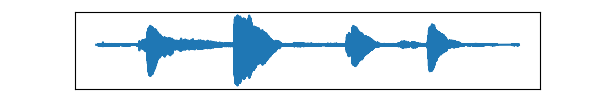
\includegraphics[width=0.62\textwidth]{./Chapter17/Figures/figure-hello-audio.png}};
\node[anchor=east,font=\scriptsize,align=center]  (a1) at  ([xshift=2.0em]input.west) {音频数据输入};
\node[minimum width=17.4em,minimum height=2.9em,draw=white,line width=3pt] at (0.3em,-0.02em){};

\node[anchor=north,draw,rounded corners=2pt,minimum width=16em, minimum height=2.2em,fill=yellow!20] (box) at ([xshift=0.4em]input.south){};
\node[anchor=west,minimum width=1.2em,minimum height=2.2em] (w1) at ([xshift=0.2em]box.west){{h}};
\node[anchor=west,minimum width=1.2em,minimum height=2.2em] (w2) at ([xshift=0.2em]w1.east){{e}};
\node[anchor=west,minimum width=1.2em,minimum height=2.2em] (w3) at ([xshift=0.2em]w2.east){{e}};
\node[anchor=west,minimum width=1.2em,minimum height=2.2em] (w4) at ([xshift=0.2em]w3.east){{$\epsilon$}};
\node[anchor=west,minimum width=1.2em,minimum height=2.2em] (w5) at ([xshift=0.2em]w4.east){{l}};
\node[anchor=west,minimum width=1.2em,minimum height=2.2em] (w6) at ([xshift=0.2em]w5.east){{$\epsilon$}};
\node[anchor=west,minimum width=1.2em,minimum height=2.2em] (w7) at ([xshift=0.2em]w6.east){{l}};
\node[anchor=west,minimum width=1.2em,minimum height=2.2em] (w8) at ([xshift=0.2em]w7.east){{l}};
\node[anchor=west,minimum width=1.2em,minimum height=2.2em] (w9) at ([xshift=0.2em]w8.east){{o}};
\node[anchor=west,minimum width=1.2em,minimum height=2.2em] (w10) at ([xshift=0.2em]w9.east){{o}};
\node[anchor=west,minimum width=1.2em,minimum height=2.2em] (w11) at ([xshift=0.2em]w10.east){{}};

\draw[very thick] (w1.south west) -- (w1.south east);
\draw[very thick] (w2.south west) -- (w2.south east);
\draw[very thick] (w3.south west) -- (w3.south east);
\draw[very thick] (w5.south west) -- (w5.south east);
\draw[very thick] (w7.south west) -- (w7.south east);
\draw[very thick] (w8.south west) -- (w8.south east);
\draw[very thick] (w9.south west) -- (w9.south east);
\draw[very thick] (w10.south west) -- (w10.south east);
%\draw[very thick] (w11.south west) -- (w11.south east);

\node[anchor=north,minimum width=1.2em,minimum height=1.4em,fill=gray!30] (m1) at ([yshift=-1em]w1.south){{h}};
\node[anchor=north,minimum width=2.64em,minimum height=1.4em,fill=gray!30] (m2) at ([yshift=-1em,xshift=0.72em]w2.south){{e}};
\node[anchor=north,minimum width=1.2em,minimum height=1.4em,fill=gray!30] (m3) at ([yshift=-1em]w4.south){};
\node[anchor=north,minimum width=1.2em,minimum height=1.4em,fill=gray!30] (m4) at ([yshift=-1em]w5.south){{l}};
\node[anchor=north,minimum width=1.2em,minimum height=1.4em,fill=gray!30] (m5) at ([yshift=-1em]w6.south){};
\node[anchor=north,minimum width=2.64em,minimum height=1.4em,fill=gray!30] (m6) at ([yshift=-1em,xshift=0.72em]w7.south){{l}};
\node[anchor=north,minimum width=2.64em,minimum height=1.4em,fill=gray!30] (m7) at ([yshift=-1em,xshift=0.72em]w9.south){{o}};
\node[anchor=north,minimum width=1.2em,minimum height=1.4em,fill=gray!30] (m8) at ([yshift=-1em]w11.south){};

\node[anchor=north,minimum width=1.2em,minimum height=1.4em,fill=gray!30] (o1) at ([yshift=-3.8em]w1.south){{h}};
\node[anchor=north,minimum width=1.2em,minimum height=1.4em,fill=gray!30] (o2) at ([yshift=-3.8em]w2.south){{e}};
\node[anchor=north,minimum width=1.2em,minimum height=1.4em,fill=gray!30] (o3) at ([yshift=-3.8em]w3.south){{l}};
\node[anchor=north,minimum width=1.2em,minimum height=1.4em,fill=gray!30] (o4) at ([yshift=-3.8em]w4.south){{l}};
\node[anchor=north,minimum width=1.2em,minimum height=1.4em,fill=gray!30] (o5) at ([yshift=-3.8em]w5.south){{o}};
\node[anchor=north,minimum width=1.2em,minimum height=1.4em,fill=gray!30] (o6) at ([yshift=-3.8em]w6.south){};
\node[anchor=north,minimum width=1.2em,minimum height=1.4em,fill=gray!30] at ([yshift=-3.8em]w7.south){};
\node[anchor=north,minimum width=1.2em,minimum height=1.4em,fill=gray!30] at ([yshift=-3.8em]w8.south){};
\node[anchor=north,minimum width=1.2em,minimum height=1.4em,fill=gray!30] at ([yshift=-3.8em]w9.south){};
\node[anchor=north,minimum width=1.2em,minimum height=1.4em,fill=gray!30] at ([yshift=-3.8em]w10.south){};
\node[anchor=north,minimum width=1.2em,minimum height=1.4em,fill=gray!30] at ([yshift=-3.8em]w11.south){};

\draw[blue!40,fill=blue!30,opacity=0.7] (w1.south west) -- (w1.south east) -- (o1.south east) -- (o1.south west) -- (w1.south west);
\draw[blue!40,fill=blue!30,opacity=0.7] (w2.south west) -- (w3.south east) -- (m2.south east) .. controls ([yshift=-0.3em]m2.south east) and ([yshift=0.3em]o2.north east) .. (o2.north east) -- (o2.south east) -- (o2.south west) -- (w2.south west);
\draw[blue!40,fill=blue!30,opacity=0.7] (w5.south west) -- (w5.south east) -- (m4.south east) .. controls ([yshift=-0.3em]m4.south east) and ([yshift=0.3em]o3.north east) .. (o3.north east) -- (o3.south east) -- (o3.south west) -- (o3.north west) .. controls ([yshift=0.3em]o3.north west) and ([yshift=-0.3em]m4.south west) .. (m4.south west) -- (w5.south west);
\draw[blue!40,fill=blue!30,opacity=0.7] (w7.south west) -- (w8.south east) -- (m6.south east) .. controls ([yshift=-0.3em]m6.south east) and ([yshift=0.3em]o4.north east) .. (o4.north east) -- (o4.south east) -- (o4.south west) -- (o4.north west) .. controls ([yshift=0.3em]o4.north west) and ([yshift=-0.3em]m6.south west) .. (m6.south west) -- (w7.south west);
\draw[blue!40,fill=blue!30,opacity=0.7] (w9.south west) -- (w10.south east) -- (m7.south east) .. controls ([yshift=-0.1em]m7.south east) and ([yshift=0.2em]o5.north east) .. (o5.north east) -- (o5.south east) -- (o5.south west) -- (o5.north west) .. controls ([yshift=0.1em]o5.north west) and ([yshift=-0.5em]m7.south west) .. (m7.south west) -- (w9.south west);
%\draw[blue!40,fill=blue!30,opacity=0.7] (w11.south west) -- (w11.south east) -- (m8.south east) .. controls ([yshift=-0.4em]m8.south east) and ([yshift=0.1em]o6.north east) .. (o6.north east) -- (o6.south east) -- (o6.south west) -- (o6.north west) .. controls ([yshift=0.1em]o6.north west) and ([yshift=-0.5em]m8.south west) .. (m8.south west) -- (w11.south west);

\node[anchor=north,font=\scriptsize,align=center] (a2) at  ([yshift=-1.4em]a1.south) {预测字母序列};
\node[anchor=north,font=\scriptsize,align=center] (a3) at  ([yshift=-1.8em]a2.south) {合并重复字母 \\ 并丢弃$\epsilon$};
\node[anchor=north,font=\scriptsize,align=center] (a4) at  ([yshift=-0.6em]a3.south) {最终结果输出};
\end{tikzpicture}
\caption{CTC预测单词序列示例}
\label{fig:17-8}
\end{figure}
%----------------------------------------------------------------------------------------------------

\parinterval CTC的一些特性使其可以很好的完成输入输出之间的对齐,例如:

%----------------------------------------------------------------------------------------------------
\begin{itemize}
    \vspace{0.5em}
    \item {\small\bfnew{输入和输出之间的对齐是单调的}}。对于音频输入序列$\{ s_1,...,s_m \} $,其对应的预测输出序列为$\{x_1,...,x_n \} $。假设$s_i$对应的预测输出结果为$x_j$,那么$s_{i+1}$相对应的预测结果只能是$x_j$、$x_{j+1}$和$\epsilon$三者中的一个。例如对于图\ref{fig:17-8}中的例子,如果输入的位置$s_i$已经对齐了字符“e”,那么$s_{i+1}$的对齐结果只能是“e”、“l”和$\epsilon$三者中的一个。
    \vspace{0.5em}
    \item {\small\bfnew{输入和输出之间是多对一的关系}}。也就是多个输入会对应到同一个输出上。这对于语音序列来说是非常自然的一件事情,由于输入的每个位置只包含非常短的语音特征,因此多个输入才可以对应到一个输出字符。
    \vspace{0.5em}
\end{itemize}
%----------------------------------------------------------------------------------------------------

\parinterval 将CTC应用到语音翻译中的方法非常简单,只需要在编码器的顶层加上一个额外的输出层即可(图\ref{fig:17-9})。通过这种方式,不需要增加过多的参数,就可以给模型加入一个较强的监督信息。

%----------------------------------------------------------------------------------------------------
\begin{figure}[htp]
\centering
\begin{tikzpicture}
	\tikzstyle{layer}=[draw,rounded corners=2pt,font=\scriptsize,align=center,minimum width=7.1em]
	\tikzstyle{word}=[font=\scriptsize]
%%%%encoder
\node[layer,fill=red!20] (en_sa) at (0,0){Multi-Head \\ Attention};
\node[anchor=south,layer,fill=yellow!20](en_add1) at ([yshift=1.0em]en_sa.north) {Add \& LayerNorm};
\node[layer,anchor=south,fill=green!20] (en_ffn) at ([yshift=1.0em]en_add1.north){Feed Forward \\ Network};
\node[anchor=south,layer,fill=yellow!20](en_add2) at ([yshift=1.0em]en_ffn.north) {Add \& LayerNorm};
\node[layer,anchor=south,fill=blue!20] (en_sf) at ([yshift=2.4em]en_add2.north){Softmax};
\node[draw,circle,inner sep=0pt, minimum size=1em,anchor=north,thick] (en_add) at ([yshift=-1.4em]en_sa.south){};
\draw[thick] (en_add.90) -- (en_add.-90);
\draw[thick] (en_add.0) -- (en_add.180);
\node[layer,anchor=north,fill=yellow!20] (en_cnn) at ([yshift=-1.0em]en_add.south){CNN};
\node[anchor=east,font=\scriptsize,align=center] (en_pos) at ([xshift=-2em]en_add.west){位置编码};
\node[anchor=north,font=\scriptsize,align=center] (en_input) at ([yshift=-1em]en_cnn.south){源语言语音特征\\(FBank/MFCC)};

\draw[->,thick] (en_input.90) -- ([yshift=-0.1em]en_cnn.-90);
\draw[->,thick] ([yshift=0.1em]en_cnn.90) -- ([yshift=-0.1em]en_add.-90);
\draw[->,thick] ([yshift=0.1em]en_add.90) -- ([yshift=-0.1em]en_sa.-90);
\draw[->,thick] ([yshift=0.1em]en_sa.90) -- ([yshift=-0.1em]en_add1.-90);
\draw[->,thick] ([yshift=0.1em]en_add1.90) -- ([yshift=-0.1em]en_ffn.-90);
\draw[->,thick] ([yshift=0.1em]en_ffn.90) --([yshift=-0.1em]en_add2.-90);
\draw[->,thick] ([yshift=0.1em]en_add2.90) -- ([yshift=-0.1em]en_sf.-90);
\draw[->,thick] ([yshift=0.1em]en_sf.90) -- ([yshift=1.5em]en_sf.90)node[left,pos=0.5]{\scriptsize{CTC Loss}};
\draw[->,rounded corners=2pt,thick] ([yshift=-0.6em]en_sa.south)--([yshift=-0.6em,xshift=-4.0em]en_sa.south)--([xshift=-0.43em]en_add1.west)--(en_add1.west);
\draw[->,rounded corners=2pt,thick] ([yshift=-0.6em]en_ffn.south)--([yshift=-0.6em,xshift=-4.0em]en_ffn.south)--([xshift=-0.43em]en_add2.west)--(en_add2.west);

%%%%decoder
\node[draw,circle,inner sep=0pt, minimum size=1em,anchor=west,thick] (de_add) at ([xshift=9em]en_add.east){};
\draw[thick] (de_add.90) -- (de_add.-90);
\draw[thick] (de_add.0) -- (de_add.180);
\node[layer,anchor=south,fill=red!20] (de_sa) at ([yshift=1.4em]de_add.north){Masked \\Multi-Head\\Attention};
\node[anchor=south,layer,fill=yellow!20](de_add1) at ([yshift=1.0em]de_sa.north) {Add \& LayerNorm};
\node[layer,anchor=south,fill=red!20] (de_ca) at ([yshift=1.0em]de_add1.north){Multi-Head \\ Attention};
\node[anchor=south,layer,fill=yellow!20](de_add2) at ([yshift=1.0em]de_ca.north) {Add \& LayerNorm};
\node[layer,anchor=south,fill=green!20] (de_ffn) at ([yshift=1.0em]de_add2.north){Feed Forward \\ Network};
\node[anchor=south,layer,fill=yellow!20](de_add3) at ([yshift=1.0em]de_ffn.north) {Add \& LayerNorm};
\node[layer,anchor=south,fill=blue!20] (sf) at ([yshift=1.2em]de_add3.north){Softmax};
\node[anchor=north,font=\scriptsize,align=center] (de_input) at ([yshift=-1.1em]de_add.south){目标语言文本\\编码表示};

\node[anchor=west,font=\scriptsize,align=center] (de_pos) at ([xshift=2em]de_add.east){位置编码};

\draw[->,thick] (de_input.90) -- ([yshift=-0.1em]de_add.-90);
\draw[->,thick] ([yshift=0.1em]de_add.90) -- ([yshift=-0.1em]de_sa.-90);
\draw[->,thick] ([yshift=0.1em]de_sa.90) -- ([yshift=-0.1em]de_add1.-90);
\draw[->,thick] ([yshift=0.1em]de_add1.90) -- ([yshift=-0.1em]de_ca.-90);
\draw[->,thick] ([yshift=0.1em]de_ca.90) -- ([yshift=-0.1em]de_add2.-90);
\draw[->,thick] ([yshift=0.1em]de_add2.90) -- ([yshift=-0.1em]de_ffn.-90);
\draw[->,thick] ([yshift=0.1em]de_ffn.90) -- ([yshift=-0.1em]de_add3.-90);
\draw[->,thick] ([yshift=0.1em]de_add3.90) -- ([yshift=-0.1em]sf.-90);
\draw[->,thick] ([yshift=0.1em]sf.90) -- ([yshift=1.0em]sf.90);
\draw[->,thick] ([xshift=0.1em]en_pos.0) -- ([xshift=-0.1em]en_add.180);
\draw[->,thick] ([xshift=-0.1em]de_pos.180) -- ([xshift=0.1em]de_add.0);
\draw[->,rounded corners=2pt,thick] ([yshift=-0.6em]de_sa.south)--([yshift=-0.6em,xshift=4.0em]de_sa.south)--([xshift=0.43em]de_add1.east)--(de_add1.east);
\draw[->,rounded corners=2pt,thick] ([yshift=-0.6em]de_ca.south)--([yshift=-0.6em,xshift=4.0em]de_ca.south)--([xshift=0.43em]de_add2.east)--(de_add2.east);
\draw[->,rounded corners=2pt,thick] ([yshift=-0.6em]de_ffn.south)--([yshift=-0.6em,xshift=4.0em]de_ffn.south)--([xshift=0.43em]de_add3.east)--(de_add3.east);

\draw[->,rounded corners=2pt,thick] ([yshift=0.1em]en_add2.90) -- ([yshift=1.5em]en_add2.90) -- ([xshift=5.0em,yshift=1.5em]en_add2.90) -- ([xshift=-1.5em]de_ca.west) -- ([xshift=-0.1em]de_ca.west);


\begin{pgfonlayer}{background}
\node[draw=ugreen,rounded corners=2pt,inner xsep=6pt,inner ysep=8pt,dashed,thick,xshift=-0.2em,yshift=-0.2em][fit=(en_add1)(en_add2)(en_sa)(en_ffn)](box1){};
\node[draw=red,rounded corners=2pt,inner xsep=6pt,inner ysep=8pt,dashed,thick,xshift=0.2em,yshift=-0.2em][fit=(de_sa)(de_ca)(de_ffn)(de_add3)](box2){};
\end{pgfonlayer}

\node[anchor=east,font=\scriptsize,text=ugreen] at ([xshift=-0.1em]box1.west){$N \times$};
\node[anchor=west,font=\scriptsize,text=red] at ([xshift=0.1em]box2.east){$\times N$};
\node[anchor=east,font=\scriptsize] at ([xshift=-0.1em]en_cnn.west){$2 \times$};
\node[anchor=east,font=\scriptsize,align=center,text=ugreen] at ([xshift=-0.1em,yshift=3em]box1.west){ST \\ 编码器};
\node[anchor=west,font=\scriptsize,align=center,text=red] at ([xshift=0.1em,yshift=5em]box2.east){ST \\ 解码器};
\end{tikzpicture}
\caption{基于CTC的语音翻译模型}
\label{fig:17-9}
\end{figure}
%----------------------------------------------------------------------------------------------------

\parinterval 另外一种多任务学习的思想是通过两个解码器,分别预测语音对应的源语言句子和目标语言句子,具体有图\ref{fig:17-10}展示的三种方式\upcite{DBLP:conf/naacl/AnastasopoulosC18,DBLP:conf/asru/BaharBN19}。图\ref{fig:17-10}(a)中采用单编码器-双解码器的方式,两个解码器根据编码器的表示,分别预测源语言句子和目标语言句子,从而使编码器训练地更加充分。这种做法的好处在于源语言的文本生成任务可以辅助翻译过程,相当于为源语言语音提供了额外的“模态”信息。图\ref{fig:17-10}(b)则通过使用两个级联的解码器,先利用第一个解码器生成源语言句子,然后再利用它的表示,通过第二个解码器生成目标语言句子。这种方法通过增加一个中间输出,降低了模型的训练难度,但同时也会带来额外的解码耗时,因为两个解码器需要串行地进行生成。图\ref{fig:17-10}(c)中的模型更进一步利用编码器的输出结果,第二个解码器联合编码器和第一个解码器的表示进行生成,更充分地利用了已有信息。
%----------------------------------------------------------------------------------------------------
\begin{figure}[htp]
\centering
\tikzstyle{coder} = [rectangle,thick,rounded corners,minimum height=2.2em,minimum width=4.3em,text centered,draw=black,fill=red!20]

\begin{tikzpicture}[node distance = 0,scale = 0.75]
\tikzstyle{every node}=[scale=0.75]

\node(encoder)[coder]at (0,0){\large{编码器}};
\node(decoder_1)[coder,above of =encoder,xshift=-1.6cm,yshift=2.8cm,fill=blue!20]{\large{解码器}};
\node(decoder_2)[coder,above of =encoder, xshift=1.6cm,yshift=2.8cm,fill=yellow!20]{\large{解码器}};
\node(s)[below of = encoder,yshift=-1.8cm,scale=1.2]{$s$};
\node(x)[above of = decoder_1,yshift=1.8cm,scale=1.2]{$x$};
\node(y)[above of = decoder_2,yshift=1.8cm,scale=1.2]{$y$};

\draw[->,thick](s.north)to(encoder.south);
\draw[->,thick](decoder_1.north)to(x.south);
\draw[->,thick](decoder_2.north)to(y.south);
\draw[->,thick](encoder.north)--([yshift=0.7cm]encoder.north)--([xshift=-4.16em,yshift=0.7cm]encoder.north)--(decoder_1.south);
\draw[->,thick](encoder.north)--([yshift=0.7cm]encoder.north)--([xshift=4.16em,yshift=0.7cm]encoder.north)--(decoder_2.south);
\node [anchor=north,scale = 1.2](pos1) at (s.south) {(a) 单编码器-双解码器};
\node [anchor=south,scale=1.2] (node1) at ([xshift=-2.0em,yshift=9em]decoder_1.north) {{$x$:源语言文本数据}};
\node [anchor=north,scale=1.2] (node2) at ([xshift=0.63em]node1.south){{$y$:目标语言文本数据}};
\node [anchor=north,scale=1.2] (node3) at ([xshift=-0.57em]node2.south){{$s$:源语言语音数据}};
%%%%%%%%%%%%%%%%%%%%%%%%级联
\node(encoder-2)[coder]at ([xshift=12.0em]encoder.east){\large{编码器}};
\node(decoder_1-2)[coder,above of =encoder-2,yshift=1.4cm,fill=blue!20]{\large{解码器}};
\node(decoder_2-2)[coder,above of =decoder_1-2, yshift=1.4cm,fill=yellow!20]{\large{解码器}};
\node(s-2)[below of = encoder-2,yshift=-1.8cm,scale=1.2]{$s$};
\node(y-2)[above of = decoder_2-2,yshift=1.8cm,scale=1.2]{$y$};

\draw[->,thick](s-2.north)to(encoder-2.south);
\draw[->,thick](encoder-2.north)to(decoder_1-2.south);
\draw[->,thick](decoder_1-2.north)to(decoder_2-2.south);
\draw[->,thick](decoder_2-2.north)to(y-2.south);
\node [anchor=north,scale = 1.2](pos2) at (s-2.south) {(b) 级联解码器};
%%%%%%%%%%%%%%%%%%%%%%%%联合
\node(encoder-3)[coder]at([xshift=10.0em]encoder-2.east){\large{编码器}};
\node(decoder_1-3)[coder,above of =encoder-3,xshift=-1.6cm,yshift=2.8cm,fill=blue!20]{\large{解码器}};
\node(decoder_2-3)[coder,above of =encoder-3, xshift=1.6cm,yshift=2.8cm,fill=yellow!20]{\large{解码器}};
\node(s-3)[below of = encoder-3,yshift=-1.8cm,scale=1.2]{$s$};
\node(y-3)[above of = decoder_2-3,yshift=1.8cm,scale=1.2]{$y$};

\draw[->,thick](s-3.north)to(encoder-3.south);
\draw[->,thick](decoder_1-3.east)to(decoder_2-3.west);
\draw[->,thick](decoder_2-3.north)to(y-3.south);
\draw[->,thick](encoder-3.north)--([yshift=0.7cm]encoder-3.north)--([xshift=-4.16em,yshift=0.7cm]encoder-3.north)--(decoder_1-3.south);
\draw[->,thick](encoder-3.north)--([yshift=0.7cm]encoder-3.north)--([xshift=4.16em,yshift=0.7cm]encoder-3.north)--(decoder_2-3.south);
\node [anchor=north,scale = 1.2](pos3) at (s-3.south) {(c) 联合编解码器};
\end{tikzpicture}
\caption{双解码器进行语音翻译的三种方式}
\label{fig:17-10}
\end{figure}
%----------------------------------------------------------------------------------------------------

%----------------------------------------------------------------------------------------
%    NEW SUBSUB-SECTION
%----------------------------------------------------------------------------------------
\subsubsection{2. 迁移学习}

\parinterval 相比语音识别和文本翻译,端到端语音翻译的训练数据量要小很多,因此,如何利用其它数据来增加可用的数据量是语音翻译的一个重要方向。和文本翻译中的方法相似,一种思路是利用迁移学习或预训练,利用其他语言的双语数据预训练模型参数,然后迁移到生成目标语言的任务上\upcite{DBLP:conf/naacl/BansalKLLG19},或者是利用语音识别数据或文本翻译数据,分别预训练编码器和解码器的参数,用于初始化语音翻译模型的参数\upcite{DBLP:conf/icassp/BerardBKP18}。预训练的编码器对语音翻译模型的学习尤为重要\upcite{DBLP:conf/naacl/BansalKLLG19},相比文本数据,语音数据的复杂性更高,仅使用小规模语音翻译数据很难学习充分。此外,模型对声学特征的学习与语言并不是强相关的,使用其他语种预训练得到的编码器对模型学习也是有帮助的。

%----------------------------------------------------------------------------------------
%    NEW SUBSUB-SECTION
%----------------------------------------------------------------------------------------
\subsubsection{3. 数据增强}

\parinterval 数据增强是增加训练数据最直接的一种方法。不同于文本翻译的回译等方法(见{\chaptersixteen}),语音翻译并不具有直接的“可逆性”。如果要利用回译的思想,需要通过一个模型,将目标语言文本转化为源语言语音,但实际上这种模型是不能直接得到的。因此,一个直接的思路是通过一个反向翻译模型和语音合成模型级联来生成伪数据\upcite{DBLP:conf/icassp/JiaJMWCCALW19}。 另外,正向翻译模型生成的伪数据在文本翻译中也被验证了对模型训练有一定的帮助,因此同样可以利用语音识别和文本翻译模型,将源语言语音翻译成目标语言文本,得到伪平行语料。

%----------------------------------------------------------------------------------------------------

\parinterval 此外,也可以利用在海量的无标注语音数据上预训练的{\small\bfnew{自监督}}\index{自监督}(Self-supervised)\index{Self-supervised}模型作为一个特征提取器,将从语音中提取的特征作为语音翻译模型的输入,可以有效提高模型的性能\upcite{DBLP:conf/interspeech/WuWPG20}。相比语音翻译模型,文本翻译模型任务更加简单,因此一种思想是利用文本翻译模型来指导语音翻译模型,比如,使用知识蒸馏\upcite{DBLP:conf/interspeech/LiuXZHWWZ19}、正则化\upcite{DBLP:conf/emnlp/AlinejadS20}等方法。为了简化语音翻译模型的学习,也可以使用课程学习方法(见{\chapterthirteen})。这样,使模型从语音识别任务,逐渐过渡到语音翻译任务,这种由易到难的训练策略可以使模型训练更加充分\upcite{DBLP:journals/corr/abs-1802-06003,DBLP:conf/acl/WangWLZY20}。

%----------------------------------------------------------------------------------------
%    NEW SECTION
%----------------------------------------------------------------------------------------
\sectionnewpage
\section{图像翻译}

\parinterval 在人类所接受的信息中,视觉信息的比重往往不亚于语音和文本信息,甚至更多。视觉信息通常以图像的形式存在,近几年,结合图像的多模态机器翻译受到了广泛的关注。多模态机器翻译(图\ref{fig:17-11} (a))简单来说就是结合源语言和其他模态(例如图像等)的信息生成目标语言的过程。这种结合图像的机器翻译还是一种狭义上的“翻译”,它本质上还是从源语言到目标语言或者说从文本到文本的翻译。事实上从图像到文本(图\ref{fig:17-11}(b))的转换,即给定图像,生成与图像内容相关的描述,也可以被称为广义上的“翻译”。例如,{\small\bfnew{图片描述生成}}\index{图片描述生成}(Image Captioning)\index{Image Captioning}就是一种典型的图像到文本的翻译。当然,这种广义上的翻译形式不仅仅包括图像到文本的转换,还可以包括从图像到图像的转换(图\ref{fig:17-11}(c)),甚至是从文本到图像的转换(图\ref{fig:17-11}(d))等等。这里将这些与图像相关的翻译任务统称为图像翻译。

%----------------------------------------------------------------------------------------------------
\begin{figure}[htp]
\centering
\begin{tikzpicture}[scale=0.6]
\tikzstyle{every node}=[scale=0.6]
%figure 1
\coordinate (A1) at (0, 0);
\coordinate (B1) at ([xshift=1.5em,yshift=-0.4em]A1);
\coordinate (C1) at ([xshift=0.3em,yshift=-2.6em]A1);
\coordinate (D1) at ([xshift=2.7em,yshift=-2.6em]A1);
\coordinate (E1) at ([xshift=2.4em,yshift=-1.5em]A1);
\coordinate (F1) at ([xshift=0.3em]D1);

\coordinate (G1) at ([xshift=0.3em,yshift=-5em]A1);
\coordinate (H1) at ([xshift=0.4em,yshift=-1.6em]G1);
\coordinate (I1) at ([xshift=0.4em,yshift=-2.0em]G1);
\coordinate (J1) at ([xshift=0.4em,yshift=-2.5em]G1);
\coordinate (K1) at ([xshift=0.4em,yshift=-3.0em]G1);
\coordinate (L1) at ([xshift=0.4em,yshift=-3.5em]G1);

\coordinate (G2) at ([xshift=8em,yshift=-2.5em]A1);
\coordinate (H2) at ([xshift=0.4em,yshift=-1.6em]G2);
\coordinate (I2) at ([xshift=0.4em,yshift=-2.0em]G2);
\coordinate (J2) at ([xshift=0.4em,yshift=-2.5em]G2);
\coordinate (K2) at ([xshift=0.4em,yshift=-3.0em]G2);
\coordinate (L2) at ([xshift=0.4em,yshift=-3.5em]G2);

%figure 2
\coordinate (A2) at ([yshift=-0.5em,xshift=7em]G2);
\coordinate (B2) at ([xshift=1.5em,yshift=-0.4em]A2);
\coordinate (C2) at ([xshift=0.3em,yshift=-2.6em]A2);
\coordinate (D2) at ([xshift=2.7em,yshift=-2.6em]A2);
\coordinate (E2) at ([xshift=2.4em,yshift=-1.5em]A2);
\coordinate (F2) at ([xshift=0.3em]D2);

\coordinate (G3) at ([xshift=8em,yshift=0.5em]A2);
\coordinate (H3) at ([xshift=0.4em,yshift=-1.6em]G3);
\coordinate (I3) at ([xshift=0.4em,yshift=-2.0em]G3);
\coordinate (J3) at ([xshift=0.4em,yshift=-2.5em]G3);
\coordinate (K3) at ([xshift=0.4em,yshift=-3.0em]G3);
\coordinate (L3) at ([xshift=0.4em,yshift=-3.5em]G3);

%figure 3
\coordinate (A3) at ([yshift=-0.5em,xshift=7em]G3);
\coordinate (B3) at ([xshift=1.5em,yshift=-0.4em]A3);
\coordinate (C3) at ([xshift=0.3em,yshift=-2.6em]A3);
\coordinate (D3) at ([xshift=2.7em,yshift=-2.6em]A3);
\coordinate (E3) at ([xshift=2.4em,yshift=-1.5em]A3);
\coordinate (F3) at ([xshift=0.3em]D3);

\coordinate (A4) at ([xshift=8em]A3);
\coordinate (B4) at ([xshift=1.5em,yshift=-0.4em]A4);
\coordinate (C4) at ([xshift=0.3em,yshift=-2.6em]A4);
\coordinate (D4) at ([xshift=2.7em,yshift=-2.6em]A4);
\coordinate (E4) at ([xshift=2.4em,yshift=-1.5em]A4);
\coordinate (F4) at ([xshift=0.3em]D4);

%figure 4
\coordinate (G4) at ([xshift=7.6em,yshift=0.5em]A4);
\coordinate (H4) at ([xshift=0.4em,yshift=-1.6em]G4);
\coordinate (I4) at ([xshift=0.4em,yshift=-2.0em]G4);
\coordinate (J4) at ([xshift=0.4em,yshift=-2.5em]G4);
\coordinate (K4) at ([xshift=0.4em,yshift=-3.0em]G4);
\coordinate (L4) at ([xshift=0.4em,yshift=-3.5em]G4);

\coordinate (A5) at ([yshift=-0.5em,xshift=8em]G4);
\coordinate (B5) at ([xshift=1.5em,yshift=-0.4em]A5);
\coordinate (C5) at ([xshift=0.3em,yshift=-2.6em]A5);
\coordinate (D5) at ([xshift=2.7em,yshift=-2.6em]A5);
\coordinate (E5) at ([xshift=2.4em,yshift=-1.5em]A5);
\coordinate (F5) at ([xshift=0.3em]D5);

\foreach \x in {1,2,3,4,5}{
\draw[-,line width=2pt] (A\x) -- ([xshift=3.6em]A\x) -- ([xshift=3.6em,yshift=-3em]A\x) -- ([yshift=-3em]A\x) -- (A\x) -- ([xshift=1em]A\x);
\draw[-, very thick] (B\x) -- (C\x) -- (D\x) -- (B\x);
\draw[-, very thick,fill=black] ([xshift=-0.6em,yshift=-1.2em]B\x)  -- ([xshift=-0.3em,yshift=-1em]B\x) -- ([yshift=-1.2em]B\x) --([xshift=0.3em,yshift=-1em]B\x) -- ([xshift=0.6em,yshift=-1.2em]B\x) -- (D\x) -- (C\x) -- ([xshift=-0.6em,yshift=-1.2em]B\x);
\draw[-, very thick,fill=black] (E\x) -- ([xshift=0.2em,yshift=0.3em]E\x) -- ([xshift=0.33em]F\x) -- (F\x) -- (E\x);
\node[circle,inner sep=0pt,minimum size=0.4em,fill=black] at ([xshift=-0.7em,yshift=-0.2em]B\x){};
}

\foreach \y in {1,2,3,4}{
\draw[-,line width=2pt] (G\y) -- ([xshift=1.6em]G\y) -- ([xshift=3em,yshift=-1.4em]G\y) -- ([xshift=3em,yshift=-4em]G\y) -- ([yshift=-4em]G\y) -- (G\y) -- ([xshift=1em]G\y);
\draw[-,line width=2pt] ([xshift=1.6em]G\y) -- ([xshift=1.5em,yshift=-1.4em]G\y) -- ([xshift=3em,yshift=-1.4em]G\y) ;
\draw[-,line width=1.6pt] (H\y) -- ([xshift=0.6em]H\y);
\draw[-,line width=1.6pt] (I\y) -- ([xshift=2em]I\y);
\draw[-,line width=1.6pt] (J\y) -- ([xshift=2em]J\y);
\draw[-,line width=1.6pt] (K\y) -- ([xshift=2em]K\y);
\draw[-,line width=1.6pt] (L\y) -- ([xshift=2em]L\y);
}

\draw[-,thick] ([yshift=4em,xshift=5em]G2) -- ([yshift=-8em,xshift=5em]G2);
\draw[-,thick] ([yshift=4em,xshift=5em]G3) -- ([yshift=-8em,xshift=5em]G3);
\draw[-,thick] ([yshift=4.5em,xshift=5.6em]A4) -- ([yshift=-7.5em,xshift=5.6em]A4);

\node [draw,single arrow,minimum height=2.4em,single arrow head extend=0.4em] (arrow1) at ([xshift=-2.4em,yshift=-2em]G2) {};
\node [draw,single arrow,minimum height=2.4em,single arrow head extend=0.4em] (arrow2) at ([xshift=-2.4em,yshift=-2em]G3) {};
\node [draw,single arrow,minimum height=2.4em,single arrow head extend=0.4em] (arrow3) at ([xshift=-2.4em,yshift=-1.5em]A4) {};
\node [draw,single arrow,minimum height=2.4em,single arrow head extend=0.4em] (arrow4) at ([xshift=-2.5em,yshift=-1.5em]A5) {};

\node[anchor=north,font=\small,scale=1.5] at ([yshift=-6em]arrow1.south){(a) 多模态机器翻译};
\node[anchor=north,font=\small,scale=1.5] at ([yshift=-6em]arrow2.south){(b) 图像到文本翻译};
\node[anchor=north,font=\small,scale=1.5] at ([yshift=-6em]arrow3.south){(c) 图像到图像翻译};
\node[anchor=north,font=\small,scale=1.5] at ([yshift=-6em]arrow4.south){(d) 文本到图像翻译};
\end{tikzpicture}
%------------------------------------------------------------------------------------------------------------


\caption{图像翻译任务}
\label{fig:17-11}
\end{figure}
%----------------------------------------------------------------------------------------------------

%----------------------------------------------------------------------------------------
%    NEW SUB-SECTION
%----------------------------------------------------------------------------------------

\subsection{基于图像增强的文本翻译}
\label{sec:image-augmented-translation}

\parinterval 在文本翻译中引入图像信息是最典型的多模态机器翻译任务。虽然多模态机器翻译还是一种从源语言文本到目标语言文本的转换,但是在转换的过程中,融入了其他模态的信息减少了歧义的产生。例如前文提到的通过与源语言相关的图像信息,将“A girl jumps off a bank .”中“bank”翻译为“河岸”而不是“银行”,因为图像中出现了河岸,因此“bank”的歧义大大降低。换句话说,对于同一图像或者视觉场景的描述,源语言和目标语言描述的信息是一致的,只不过,体现在不同语言上会有表达方法上的差异。那么,图像就会存在一些源语言和目标语言的隐含对齐“约束”,而这种“约束”可以捕捉语言中不易表达的隐含信息。

\parinterval 如何融入视觉信息,更好的理解多模态上下文语义是多模态机器翻译研究的重点\upcite{DBLP:conf/wmt/SpeciaFSE16,DBLP:conf/wmt/CaglayanABGBBMH17,DBLP:conf/wmt/LibovickyHTBP16},主要方向包括基于特征融合的方法\upcite{DBLP:conf/emnlp/CalixtoL17,DBLP:journals/corr/abs-1712-03449,DBLP:conf/wmt/HelclLV18}、基于联合模型的方法\upcite{DBLP:conf/ijcnlp/ElliottK17,DBLP:conf/acl/YinMSZYZL20}。下面是具体介绍。

%----------------------------------------------------------------------------------------
%    NEW SUBSUB-SECTION
%----------------------------------------------------------------------------------------

\subsubsection{1. 基于特征融合的方法}

\parinterval 早期,通常将图像信息作为输入句子的一部分\upcite{DBLP:conf/emnlp/CalixtoL17,DBLP:conf/wmt/HuangLSOD16},或者用其对编码器、解码器的状态进行初始化\upcite{DBLP:conf/emnlp/CalixtoL17,Elliott2015MultilingualID,DBLP:conf/wmt/MadhyasthaWS17}。如图\ref{fig:17-12}所示,图中$y_{<}$表示当前时刻之前的单词序列,对图像特征的提取通常是基于卷积神经网络,有关卷积神经网络的内容,可以参考{\chaptereleven}内容。通过卷积神经网络得到全局图像特征,在进行维度变换后,将其作为源语言输入的一部分或者初始化状态引入到模型当中。但是,这种图像信息的引入方式有以下两个缺点:

\begin{itemize}
    \vspace{0.5em}
    \item 图像信息不全都是有用的,往往存在一些与源语言或目标语言无关的信息,作为全局特征会引入噪音。
    \vspace{0.5em}
    \item 图像信息作为源语言的一部分或者初始化状态,间接地参与了译文的生成,在神经网络的计算过程中,图像信息会有一定的损失。
    \vspace{0.5em}
\end{itemize}

%----------------------------------------------------------------------------------------------------
\begin{figure}[htp]
\centering
\begin{tikzpicture}[scale=0.8]
\tikzstyle{every node}=[scale=0.8]
%figure 1
\coordinate (A1) at (0, 0);
\coordinate (B1) at ([xshift=1.5em,yshift=-0.4em]A1);
\coordinate (C1) at ([xshift=0.3em,yshift=-2.6em]A1);
\coordinate (D1) at ([xshift=2.7em,yshift=-2.6em]A1);
\coordinate (E1) at ([xshift=2.4em,yshift=-1.5em]A1);
\coordinate (F1) at ([xshift=0.3em]D1);


%figure 2
\coordinate (A2) at ([xshift=15em]A1);
\coordinate (B2) at ([xshift=1.5em,yshift=-0.4em]A2);
\coordinate (C2) at ([xshift=0.3em,yshift=-2.6em]A2);
\coordinate (D2) at ([xshift=2.7em,yshift=-2.6em]A2);
\coordinate (E2) at ([xshift=2.4em,yshift=-1.5em]A2);
\coordinate (F2) at ([xshift=0.3em]D2);


\foreach \x in {1,2}{
\draw[-,line width=2pt] (A\x) -- ([xshift=3.6em]A\x) -- ([xshift=3.6em,yshift=-3em]A\x) -- ([yshift=-3em]A\x) -- (A\x) -- ([xshift=1em]A\x);
\draw[-, very thick] (B\x) -- (C\x) -- (D\x) -- (B\x);
\draw[-, very thick,fill=black] ([xshift=-0.6em,yshift=-1.2em]B\x)  -- ([xshift=-0.3em,yshift=-1em]B\x) -- ([yshift=-1.2em]B\x) --([xshift=0.3em,yshift=-1em]B\x) -- ([xshift=0.6em,yshift=-1.2em]B\x) -- (D\x) -- (C\x) -- ([xshift=-0.6em,yshift=-1.2em]B\x);
\draw[-, very thick,fill=black] (E\x) -- ([xshift=0.2em,yshift=0.3em]E\x) -- ([xshift=0.33em]F\x) -- (F\x) -- (E\x);
\node[circle,inner sep=0pt,minimum size=0.4em,fill=black] at ([xshift=-0.7em,yshift=-0.2em]B\x){};
\node[draw,rounded corners=2pt,fill=yellow!20,minimum width=4.3em,minimum height=2.2em](cnn\x) at ([xshift=1.8em,yshift=3.6em]A\x){CNN};
}
\node[draw,anchor=south,rounded corners=2pt,minimum width=4.0cm,minimum height=2.2em,fill=red!20](encoder) at ([yshift=2.6em,xshift=2.2em]cnn1.north){编码器};
\node[anchor=north,font=\Large](x) at ([xshift=2.5em,yshift=-3.4em]encoder.south){$\seq{x}$};

\node[draw,anchor=south,rounded corners=2pt,minimum width=4.0cm,minimum height=2.2em,fill=blue!20](decoder) at ([yshift=2.6em,xshift=2.2em]cnn2.north){解码器};
\node[anchor=north,font=\Large](y) at ([xshift=2.5em,yshift=-3.4em]decoder.south){$\seq{y}_{<}$};
\node[anchor=south,font=\Large](y_1) at ([yshift=3em]decoder.north){$\seq{y}$};

\draw[->,thick] ([yshift=-2.1em]cnn1.south) -- ([yshift=-0.1em]cnn1.south);
\draw[->,thick] ([yshift=-2.1em]cnn2.south) -- ([yshift=-0.1em]cnn2.south);
\draw[->,thick] ([yshift=0.1em]cnn1.north) -- ([yshift=2.4em]cnn1.north);
\draw[->,thick] ([yshift=0.1em]cnn2.north) -- ([yshift=2.4em]cnn2.north);
\draw[->,thick] ([yshift=0.3em]x.north) -- ([yshift=4.5em]x.south);
\draw[->,thick] ([yshift=0.3em]y.north) -- ([yshift=4.7em]y.south);
\draw[->,thick] ([xshift=0.1em]encoder.east) -- ([xshift=-0.1em]decoder.west);
\draw[->,thick] ([yshift=0.1em]decoder.north) -- ([yshift=-0.1em]y_1.south);
\node [anchor=south,scale=1.2] (node1) at ([xshift=-0.7em,yshift=4em]encoder.north) {\small{$x$:源语言文本数据}};
\node [anchor=north,scale=1.2] (node2) at ([xshift=0.57em]node1.south){\small{$y$:目标语言文本数据}};
\end{tikzpicture}
%------------------------------------------------------------------------------------------------------------


\caption{基于全局视觉特征的多模态翻译方法}
\label{fig:17-12}
\end{figure}
%----------------------------------------------------------------------------------------------------

\parinterval 说到噪音问题就不得不提到注意力机制的引入,前面章节中提到过这样的一个例子:

\vspace{0.8em}
\centerline{中午/没/吃饭/,/又/刚/打/了/ 一/下午/篮球/,/我/现在/很/饿/ ,/我/想\underline{\quad \quad} 。}
\vspace{0.8em}

\parinterval 想在横线处填写“吃饭”,“吃东西”的原因是在读句子的过程中,关注到了“没/吃饭”,“很/饿”等关键信息。这是在语言生成中注意力机制所解决的问题,即对于要生成的目标语言单词,相关性更高的语言片段应该更加“重要”,而不是将所有单词一视同仁。同样的,注意力机制也应用在多模态机器翻译中,即在生成目标单词时,更应该关注与目标单词相关的图像部分,而弱化对其他部分的关注。另外,注意力机制的引入,也使图像信息更加直接地参与目标语言的生成,解决了在不使用注意力机制的方法中图像信息传递损失的问题。

%----------------------------------------------------------------------------------------------------
\begin{figure}[htp]
\centering
\begin{tikzpicture}[node distance = 0,scale = 0.7]
\tikzstyle{every node}=[scale=0.7]
\node[draw=white] (input) at (0,0){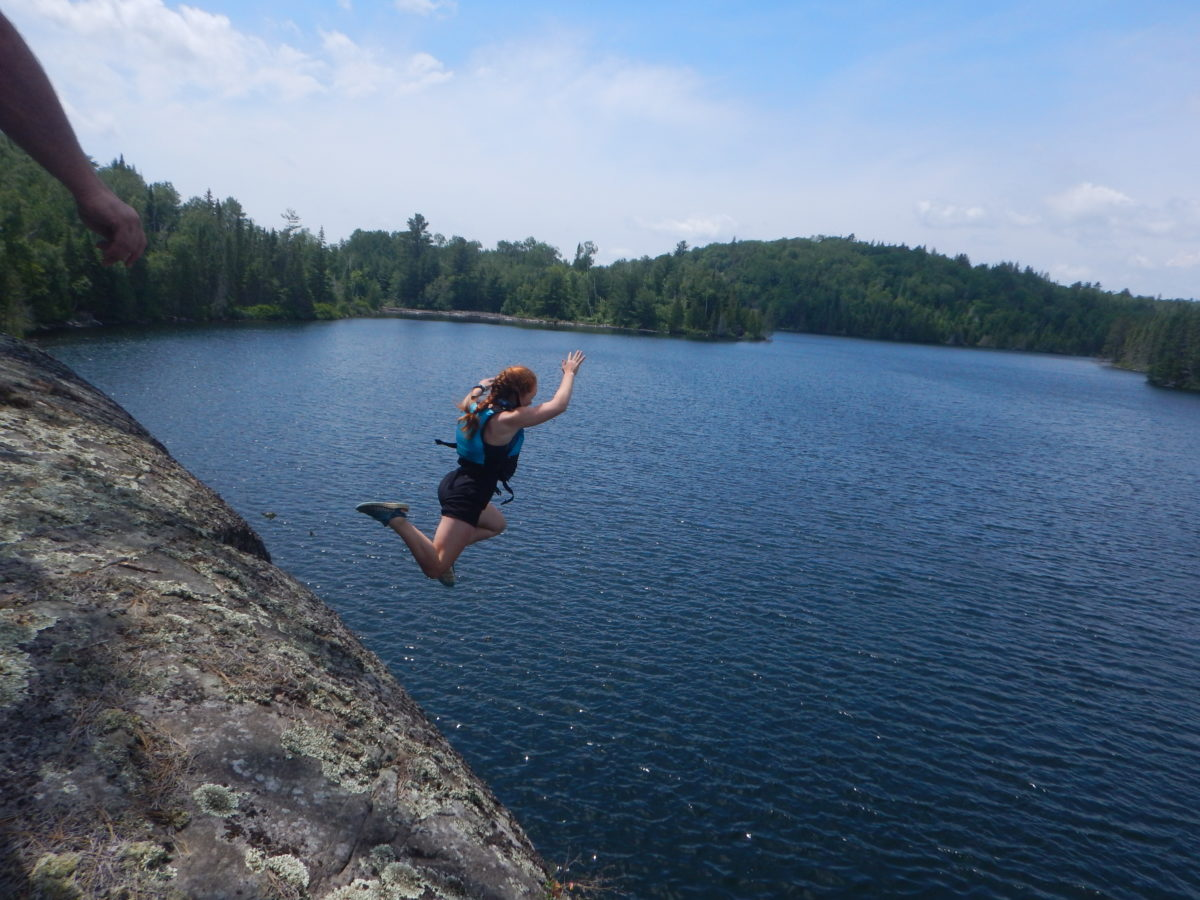
\includegraphics[width=0.62\textwidth]{./Chapter17/Figures/figure-bank-without-attention.jpg}};(1.9,-1.4);
\node[draw=white] (input) at (10,0){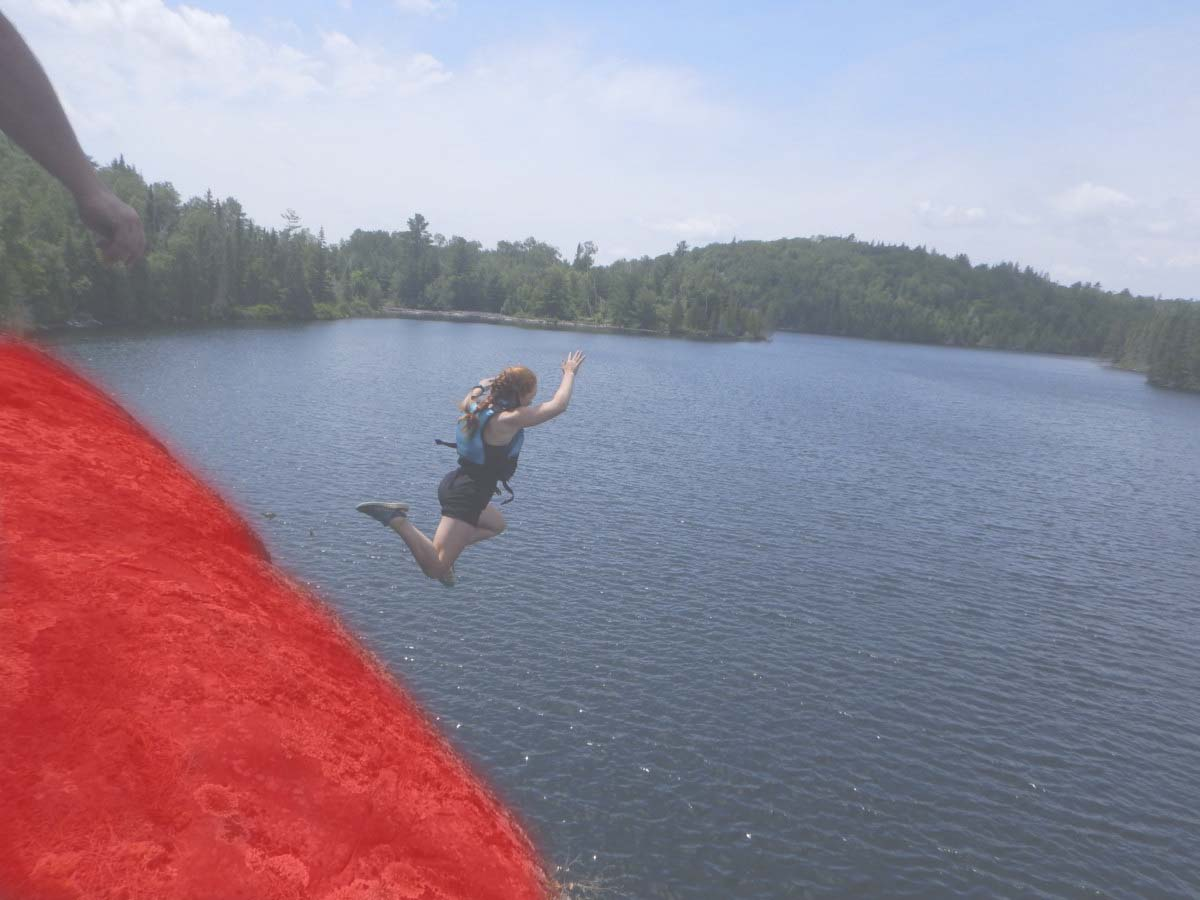
\includegraphics[width=0.62\textwidth]{./Chapter17/Figures/figure-bank-with-attention.jpg}};(1.9,-1.4);
\end{tikzpicture}
\caption{使用注意力机制前后图像中对单词“bank”的关注程度对比}
\label{tab:17-2-3-c}
\end{figure}
%----------------------------------------------------------------------------------------------------

\parinterval 那么,多模态机器翻译是如何计算上下文向量的呢?这里仿照第十章的内容给出描述。假设编码器输出的状态序列为$\{\mathbi{h}_1,...\mathbi{h}_m\}$,需要注意的是,这里的状态序列不是源语言句子的状态序列,而是通过基于卷积等操作提取到的图像的状态序列。假设图像的特征维度是$16 \times 16 \times 512$,其中前两个维度分别表示图像的高和宽,这里会将图像映射为$256 \times 512$ 的状态序列,其中$512$为每个状态的维度。对于目标语言位置$j$,上下文向量$\mathbi{C}_{j}$被定义为对序列的编码器输出进行加权求和,如下:
\begin{eqnarray}
\mathbi{C}_{j}&=& \sum_{i}{{\alpha}_{i,j}{\mathbi{h}}_{i}}
\end{eqnarray}

\noindent 其中,${\alpha}_{i,j}$是注意力权重,它表示目标语言第$j$个位置与图片编码状态序列第$i$个位置的相关性大小,计算方式与{\chapterten}描述的注意力函数一致。

\parinterval 这里,将$\mathbi{h}_{i}$看作图像表示序列位置$i$上的表示结果。图\ref{tab:17-2-3-c}给出了模型在生成目标词“bank”时,图像经过注意力机制对图像区域关注度的可视化效果。可以看到,经过注意力机制后,模型更关注与目标词相关的图像部分。当然,多模态机器翻译的输入还包括源语言文字序列。通常,源语言文字对于翻译的作用比图像更大\upcite{DBLP:conf/acl/YaoW20}。从这个角度说,在当下的多模态翻译任务中,图像信息更多的是作为文字信息的补充,而不是替代。除此之外,注意力机制在多模态机器翻译中也有很多研究,比如,在编码器端将源语言文本与图像信息进行注意力建模,得到更好的源语言的表示结果\upcite{DBLP:journals/corr/abs-1712-03449,DBLP:conf/acl/YaoW20}。

%----------------------------------------------------------------------------------------
%    NEW SUBSUB-SECTION
%----------------------------------------------------------------------------------------

\subsubsection{2. 基于联合模型的方法}

\parinterval 基于联合模型的方法通常是把翻译任务与其他视觉任务结合,进行联合训练。这种方法也可以被看做是一种多任务学习,只不过这里仅关注翻译和视觉任务。一种常见的方法是共享模型的部分参数来学习不同任务之间相似的部分,并通过特定的模块来学习每个任务特有的部分。

\parinterval 如图\ref{fig:17-14}所示,图中$y_{<}$表示当前时刻之前的单词序列,可以将多模态机器翻译任务分解为两个子任务:机器翻译和图片生成\upcite{DBLP:conf/ijcnlp/ElliottK17}。其中机器翻译作为主任务,图片生成作为子任务。这里的图片生成指的是从一个图片描述生成对应图片,对于图片生成任务在后面还会有描述。通过单个编码器对源语言数据进行建模,然后通过两个解码器(翻译解码器和图像解码器)来分别学习翻译任务和图像生成任务。顶层学习每个任务的独立特征,底层共享参数能够学习到更丰富的文本表示。

\parinterval 另外在视觉问答领域有研究表明,在多模态任务中,不宜引入过多层的注意力机制,因为过深的模型会导致多模态模型的过拟合\upcite{DBLP:conf/nips/LuYBP16}。这一方面是由于深层模型本身对数据的拟合能力较强,另一方面也是由于多模态任务的数据普遍较少,容易造成复杂模型的过拟合。从另一角度来说,利用多任务学习的方式,提高模型的泛化能力,也是一种有效防止过拟合现象的方式。类似的思想,也大量使用在多模态自然语言处理任务中,例如图像描述生成、视觉问答等\upcite{DBLP:conf/iccv/AntolALMBZP15}。

%----------------------------------------------------------------------------------------------------
\begin{figure}[htp]
\centering
\tikzstyle{coder} = [rectangle,thick,rounded corners,minimum height=2.2em,minimum width=4.3em,text centered,draw=black,fill=red!20]
\begin{tikzpicture}[node distance = 0,scale = 0.75]
\tikzstyle{every node}=[scale=0.75]
\node(x)[]{$x$};
\node(encoder)[coder, above of = x,yshift=4em]{\large{编码器}};
\node(decoder_left)[coder, above of = encoder, yshift=6em,fill=blue!20]{\large{解码器}};
\node(y_hat)[above of = decoder_left, yshift=4em]{{$y$}};
\node(y)[above of = decoder_left, xshift=-6em]{{$y_{<}$}};
\node(decoder_right)[coder, above of = encoder, xshift=11em,fill=yellow!20]{\large{解码器}};

\node(figure)[draw=white,above of = decoder_right,yshift=6.5em,scale=0.25] {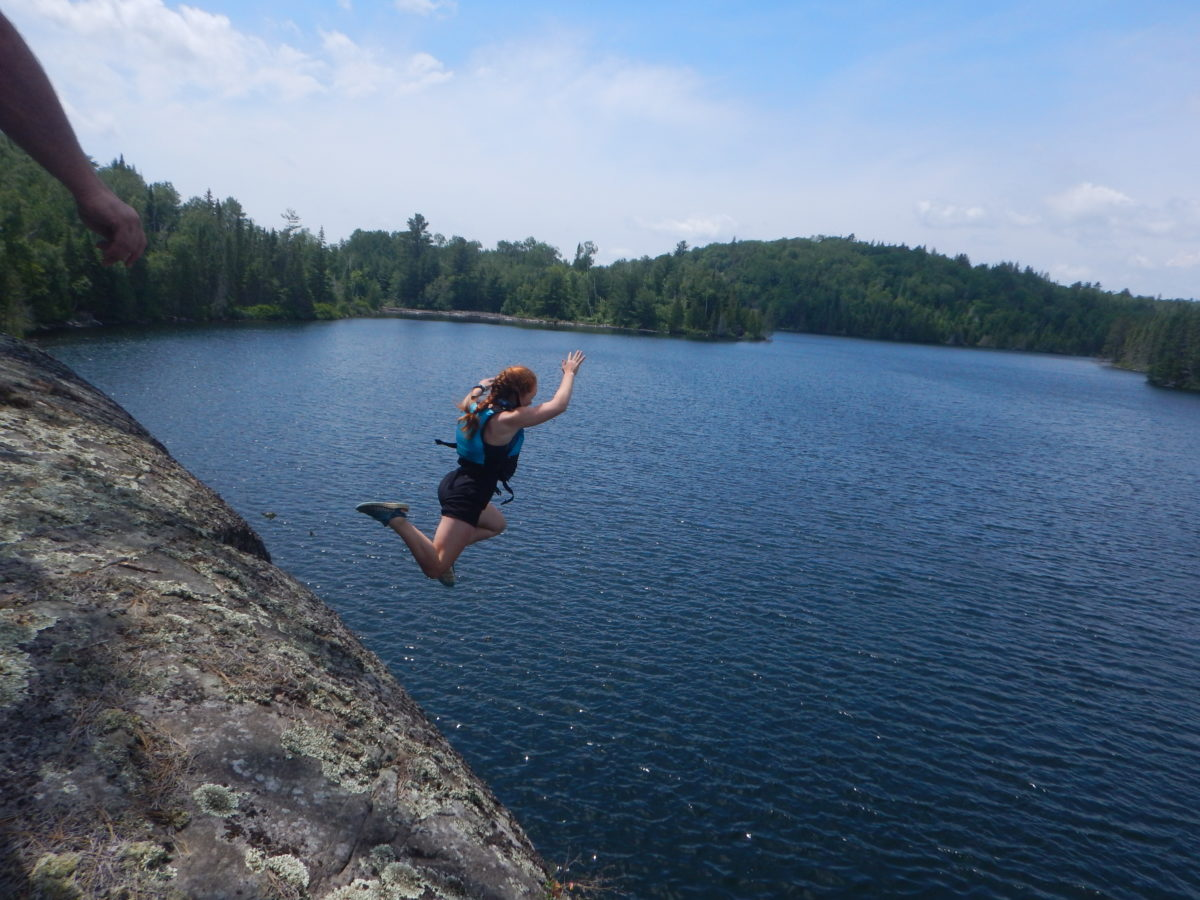
\includegraphics[width=0.62\textwidth]{./Chapter17/Figures/figure-bank-without-attention.jpg}};

\node [anchor=south,scale=1.2] (node1) at ([xshift=-2.5em,yshift=4.5em]y.north) {{$x$:源语言文本数据}};
\node [anchor=north,scale=1.2] (node2) at ([xshift=0.57em]node1.south){{$y$:目标语言文本数据}};

\draw[->,thick](x)to(encoder);
\draw[->,thick](encoder)to(decoder_left)node[right,xshift=-0.1cm,yshift=-1.25cm,scale=1.2]{{翻译}};
\draw[->,thick](decoder_left)to(y_hat);
\draw[->,thick](y)to(decoder_left);
\draw[->,thick](encoder)to(decoder_right)node[left,xshift=-3.1em,yshift=0.25cm,scale=1.2]{{生成图片}};
\draw[->,thick](decoder_right)to(figure);
\end{tikzpicture}
\caption{翻译+图片生成联合学习模型}
\label{fig:17-14}
\end{figure}
%----------------------------------------------------------------------------------------------------

%----------------------------------------------------------------------------------------
%    NEW SUB-SECTION
%----------------------------------------------------------------------------------------

\subsection{图像到文本的翻译}

\parinterval 图像到文本的转换也可以看作是广义上的翻译,简单来说,就是把图像作为唯一的输入,而输出是文本。其中,图像描述生成是最典型的图像到文本的翻译任务\upcite{DBLP:conf/ijcai/BernardiCEEEIKM17}。虽然,这部分内容并不是本书的重点,不过为了保证多模态翻译内容的完整性,这里对相关技术进行简要介绍。图像描述有时也被称看图说话、图像字幕生成,它在图像检索、智能导盲、人机交互等领域有着广泛的应用场景。

%----------------------------------------------------------------------------------------------------
\begin{figure}[htp]
\centering
\definecolor{color_gray}{rgb}{0.278,0.337,0.426}
\definecolor{color_green}{rgb}{0.663,0.82,0.557}
\definecolor{color_orange}{rgb}{0.957,0.694,0.514}
\definecolor{color_blue}{rgb}{0.335,0.708,0.735}
\tikzstyle{description} = [rectangle,rounded corners=1mm, minimum width=3cm,minimum height=0.6cm,text centered,draw,thick]
\begin{tikzpicture}[node distance = 0,scale = 0.8]
\tikzstyle{every node}=[scale=0.8]



\node(figure-1)[draw=white,scale=0.25] at (0,0){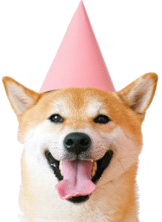
\includegraphics[width=0.62\textwidth]{./Chapter17/Figures/figure-dog-with-hat.png}};
\node(ground-1)[rectangle,rounded corners, minimum width=5cm, minimum height=3.5cm,right of = figure-1, xshift=5cm,fill=gray!10,draw,thick,drop shadow]{};
\node(text-1)[right of = figure-1, xshift=3.6cm,yshift=2.1cm,scale=1.2]{{描述候选池}};
\node(text_1-1)[description, right of = figure-1, xshift=4.2cm,yshift=1.2cm,fill=gray!20]{{天空中有很多鸟。}};
\node(text_2-1)[description, right of = figure-1, xshift=5.3cm,yshift=0.5cm,fill=green!20]{{孩子从河岸上跳下来。}};
\node(text_3-1)[description, right of = figure-1, xshift=4.5cm,yshift=-0.2cm,fill=orange!20]{{狗在吐舌头。}};
\node(surd-1)[right of = text_3-1, xshift=2cm,scale=1.5]{\textcolor{red}{$\surd$}};
\node(text_4-1)[description, right of = figure-1, xshift=5.2cm,yshift=-0.9cm,fill=blue!20]{{男人戴着眼镜。}};
\node(point-1)[right of = figure-1, xshift=5cm,yshift=-1.4cm,scale=1.5]{...};
\draw[->,thick](figure-1)to([xshift=-0.1cm]ground-1.west);

\node(figure)[draw=white,scale=0.25]at ([xshift=20.0em]figure-1.east){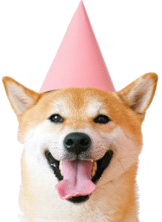
\includegraphics[width=0.62\textwidth]{./Chapter17/Figures/figure-dog-with-hat.png}};
\node(ground)[rectangle,rounded corners, minimum width=5cm, minimum height=1.5cm,right of = figure, xshift=5cm,yshift=-2.6em,fill=gray!10,draw,thick,drop shadow]{\large{图片中有\underline{\textcolor{red}{狗}},\underline{\textcolor{red}{帽子}},\underline{\quad\ }。}};
\node(dog)[rectangle,rounded corners, minimum width=1cm, minimum height=0.7cm,right of = figure, xshift=3cm,yshift=1.5cm,thick, draw,fill=orange!20,thick]{狗};
\node(hat)[rectangle,rounded corners, minimum width=1.5cm, minimum height=0.7cm,right of = figure, xshift=4.5cm,yshift=1.5cm,thick, draw,fill=green!20,thick]{帽子};
\draw[->, thick](figure.east)to([xshift=-0.1cm]dog.west)node[left,xshift=-0.2cm,yshift=-0.1cm,color=black]{图片检测};
\draw[->, thick]([yshift=-0.1cm]hat.south)to([yshift=0.1cm]ground.north)node[right,xshift=-0.2cm,yshift=0.5cm,color=black]{模板填充};

\node [anchor=north](pos1)at ([xshift=-3.8em,yshift=-1em]ground-1.south){(a) 基于检索的图像描述生成};
\node [anchor=north](pos2)at ([xshift=-3.8em,yshift=-1em]ground.south){(b) 基于模板的图像描述生成};

\end{tikzpicture}
\caption{图像描述传统方法}
\label{fig:17-15}
\end{figure}
%----------------------------------------------------------------------------------------------------

\parinterval 传统图像描述生成有两种范式:基于检索的方法和基于模板的方法。其中图\ref{fig:17-15}(a)展示了一个基于检索的图像描述生成实例,这种方法在图像描述的候选中选择一个描述输出。但是,弊端是所选择的句子可能会和图像很大程度上不相符。而\ref{fig:17-15}(b)展示的是一种基于模版的方法,这种方法需要在图像上提取视觉特征,然后把内容填在实现设计好的模板当中,这种方法的缺点是生成的图像描述过于呆板,“像是在一个模子中刻出来的”说的就是这个意思。近几年来 ,受到机器翻译领域等任务的启发,图像描述生成任务也开始大量使用编码器-解码器框架。这里会从基础的图像描述范式编码器-解码器框架展开\upcite{DBLP:conf/cvpr/VinyalsTBE15,DBLP:conf/icml/XuBKCCSZB15},并从编码器的改进和解码器的改进两个方面进行介绍。

%----------------------------------------------------------------------------------------
%    NEW SUBSUB-SECTION
%----------------------------------------------------------------------------------------

\subsubsection{1. 基础框架}

\parinterval 在编码器-解码器框架中,编码器将输入的图像转换为一种新的“表示”形式,这种“表示”包含了输入图像的所有信息。之后解码器把这种“表示”转换为自然语言描述。比如,可以通过卷积神经网络提取图像特征为一个向量表示。然后,利用长短时记忆网络(LSTMs)解码生成文字描述,这个过程中与机器翻译的解码过程类似。这种建模方式存在与\ref{sec:image-augmented-translation}小节描述一样的问题:生成的描述单词不一定需要所有的图像信息,将全局的图像信息送入模型中,可能会引入噪音。这时可以使用注意力机制来缓解该问题\upcite{DBLP:conf/icml/XuBKCCSZB15}。

%----------------------------------------------------------------------------------------
%    NEW SUBSUB-SECTION
%----------------------------------------------------------------------------------------

\subsubsection{2. 编码器的改进}

\parinterval 要想使编码器-解码器框架在图像描述生成中充分发挥作用,编码器也要更好的表示图像信息。对于编码器的改进,通常体现在向编码器中添加图像的语义信息\upcite{DBLP:conf/cvpr/YouJWFL16,DBLP:conf/cvpr/ChenZXNSLC17,DBLP:journals/pami/FuJCSZ17}和位置信息\upcite{DBLP:conf/cvpr/ChenZXNSLC17,DBLP:conf/ijcai/LiuSWWY17}。

\parinterval 图像的语义信息一般是指图像中存在的实体、属性、场景等等。如图\ref{fig:17-17}所示,从图像中利用属性或实体检测器提取出“jump”、“girl”、“river”、“bank”等属性词和实体词,将他们作为图像的语义信息编码的一部分,再利用注意力机制计算目标语言单词与这些属性词或实体词之间的注意力权重\upcite{DBLP:conf/cvpr/YouJWFL16}。当然,除了图像中的实体和属性作为语义信息外,也可以将图片的场景信息加入到编码器当中\upcite{DBLP:journals/pami/FuJCSZ17}。有关如何做属性、实体和场景的检测,涉及到目标检测任务的工作,例如Faster-RCNN\upcite{DBLP:journals/pami/RenHG017}、YOLO\upcite{DBLP:journals/corr/abs-1804-02767,DBLP:journals/corr/abs-2004-10934}等等,这里不再赘述。

%----------------------------------------------------------------------------------------------------
\begin{figure}[htp]
\centering
\tikzstyle{word} = [rectangle,thick,minimum width=2cm,minimum height=0.7cm,text centered,]
\begin{tikzpicture}[node distance = 0,scale = 0.9]
\tikzstyle{every node}=[scale=0.9]
\node(figure)[draw=white,scale=0.4] {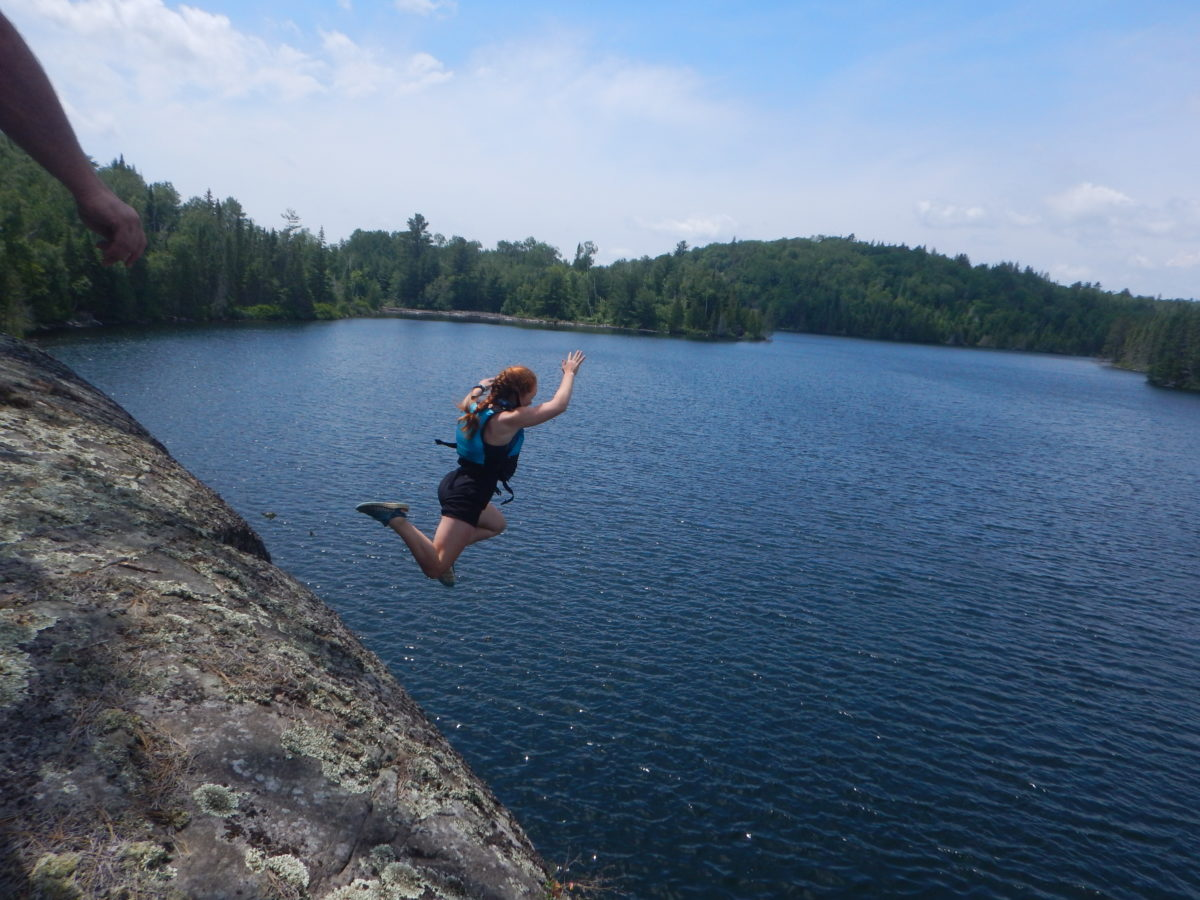
\includegraphics[width=0.62\textwidth]{./Chapter17/Figures/figure-bank-without-attention.jpg}};
\node(river)[word, right of = figure, xshift=5cm, yshift=0.35cm, fill=blue!45]{river};
\node(mountain)[word, above of = river, yshift=0.75cm, fill=blue!45]{mountain};
\node(child)[word, above of = mountain, yshift=0.75cm, fill=blue!15]{child};
\node(woman)[word, above of = child, yshift=0.75cm, fill=blue!25]{girl};
\node(jump)[word, below of = river, yshift=-0.75cm, fill=blue!30]{jump};
\node(bank)[word, below of = jump, yshift=-0.75cm, fill=blue!65]{bank};
\node(sky)[word, below of = bank, yshift=-0.75cm, fill=blue!30]{sky};
\node(tree)[word, below of = sky, yshift=-0.75cm, fill=blue!15]{tree};
\node(cir)[circle,thick, minimum width=0.6cm, xshift=8cm,  draw=black]{};
\node(decoder)[rectangle, rounded corners, minimum height=2.2em,minimum width=4.3em, right of = cir,xshift=3cm, draw=black, fill=blue!25]{\large{解码器}};
\node(yn_1)[below of = decoder,yshift=-2cm,scale=1.2]{$y_{<j}$};
\node(yn_2)[above of = decoder,yshift=2cm,scale=1.2]{$y_{j}$(bank)};

\draw[->, thick]([xshift=0.1cm]figure.east)to([xshift=2cm]figure.east);
\draw[-,thick]([xshift=-0.03cm]cir.east)to([xshift=0.03cm]cir.west);
\draw[-,thick]([yshift=0.03cm]cir.south)to([yshift=-0.03cm]cir.north);
\draw[->, thick]([xshift=0.1cm]cir.east)to([xshift=-0.1cm]decoder.west);
\draw[->, thick](yn_1)to([yshift=-0.1cm]decoder.south);
\draw[->, thick]([yshift=0.1cm]decoder.north)to(yn_2);

\draw[->, thick, color=blue!25]([xshift=0.05cm]woman.east)to([xshift=-0.05cm]cir.north);
\draw[->, thick, color=blue!15]([xshift=0.05cm]child.east)to([yshift=0.7em,xshift=0.4em]cir.west);
\draw[->, thick, color=blue!45]([xshift=0.05cm]mountain.east)to([yshift=0.5em,xshift=0.15em]cir.west);
\draw[->, thick, color=blue!45]([xshift=0.05cm]river.east)to([yshift=0.15em]cir.west);
\draw[->, thick, color=blue!30]([xshift=0.05cm]jump.east)to([yshift=-0.15em]cir.west);
\draw[->, very thick, color=blue!65]([xshift=0.05cm]bank.east)to([yshift=-0.5em,xshift=0.15em]cir.west);
\draw[->, thick, color=blue!30]([xshift=0.05cm]sky.east)to([yshift=-0.7em,xshift=0.4em]cir.west);
\draw[->, thick, color=blue!15]([xshift=0.05cm]tree.east)to([xshift=-0.05em]cir.south);
\end{tikzpicture}
\caption{编码器“显式”融入语义信息}
\label{fig:17-17}
\end{figure}
%----------------------------------------------------------------------------------------------------

\parinterval 以上的方法大都是将图像中的实体、属性、场景等映射到文字上,并把这些信息显式地输入到编码器中。除此之外,一种方法是把图像中的语义特征隐式地引入编码中\upcite{DBLP:conf/cvpr/ChenZXNSLC17}。例如,图像数据可以分解为三个通道(红、绿、蓝),简单来说,就是将图像的每一个像素点按照红色、绿色、蓝色分成三个部分,这样就将图像分成了三个通道。在很多图像中,不同通道伴随的特征是不一样的,可以将其作用于编码器。另外一种方法是基于位置信息的编码增强。位置信息指的是图像中对象(物体)的位置。利用目标检测技术检测系统获得图中的对象和对应的特征,这样就确定了图中的对象位置。显然,这些信息可以加强编码器的表示能力\upcite{DBLP:conf/eccv/YaoPLM18}。

%----------------------------------------------------------------------------------------
%    NEW SUBSUB-SECTION
%----------------------------------------------------------------------------------------

\subsubsection{3. 解码器的改进}

\parinterval 由于解码器输出的是语言文字序列,因此需要考虑语言的特点对其进行改进。 例如,解码过程中, “the”,“on”,“at”这种介词或者冠词与图像的相关性较低\upcite{DBLP:conf/cvpr/LuXPS17}。因此,可以通过门控单元,控制视觉信号作用于文字生成的程度。另外,在解码过程中,生成的每个单词对应着图像的区域可能是不同的。因此也可以设计更为有效的注意力机制来捕捉解码器端对不同图像局部信息的关注程度\upcite{DBLP:conf/cvpr/00010BT0GZ18}。

\parinterval 除了更好地使生成文本与图像特征进行相互作用以外,还有一些改进方法。例如,用卷积神经网络或者Transformer代替解码器所使用的循环神经网络\upcite{DBLP:conf/cvpr/AnejaDS18}。或者使用更深层的神经网络学习动词或者形容词等视觉中不易表现出来的单词\upcite{DBLP:journals/mta/FangWCT18},其思想与深层神经机器翻译模型有相通之处(见{\chapterfifteen})。

%----------------------------------------------------------------------------------------
%    NEW SUB-SECTION
%----------------------------------------------------------------------------------------

\subsection{图像、文本到图像的翻译}

\parinterval 当生成的目标对象是图像时,问题就变为了图像生成任务。虽然,这个领域本身并不属于机器翻译,但是其使用的基本方法与机器翻译有类似之处。二者也可以相互借鉴。

\parinterval 在计算机视觉中,图像风格变换、图像超分辨率重建等任务,都可以被视为{\small\bfnew{图像到图像的翻译}}\index{图像到图像的翻译}(Image-to-Image Translation)\index{Image-to-Image Translation}问题。与机器翻译类似,这些问题的共同目标是学习从一个对象到另一个对象的映射,只不过这里的对象是指图像,而非机器翻译中的文字。例如,给定物体的轮廓生成真实物体图片,或者给定白天照片生成夜晚的照片等。图像到图像的翻译有广阔的应用场景,如图片补全、风格迁移等。{\small\bfnew{文本到图像的翻译}}\index{文本到图像的翻译}(Text-to-Image Translation)\index{Text-to-Image Translation}是指给定描述物体颜色和形状等细节的自然语言文字,生成对应的图像。该任务也可以看作是图像描述生成的逆任务。

\parinterval 无论是图像到图像的生成,还是文本到图像的生成,均可直接使用编码器-解码器框架进行实现。比如,在文本到图像生成中,可以使用机器翻译中的编码器对输入文本进行编码,之后用对抗生成网络将编码结果转化为图像\upcite{DBLP:conf/icml/ReedAYLSL16}。近些年,图像生成类任务也取得了很大的进展,这主要得益于生成对抗网络的使用\upcite{DBLP:conf/nips/GoodfellowPMXWOCB14,DBLP:journals/corr/abs-1908-06616,DBLP:journals/corr/DashGALA17}。在{\chapterthirteen}已经介绍了生成对抗网络,而且图像生成也不是本书的重点,感兴趣的读者可以参考{\chapterthirteen}的内容或者自行查阅相关文献进行了解。

%----------------------------------------------------------------------------------------
%    NEW SECTION
%----------------------------------------------------------------------------------------
\sectionnewpage
\section{篇章级翻译}

\parinterval 目前大多数机器翻译系统是句子级的。由于缺少了对篇章上下文信息的建模,在需要依赖上下文的翻译场景中,模型的翻译效果总是不尽人意。篇章级翻译的目的就是对篇章上下文信息进行建模,进而改善机器翻译在整个篇章上的翻译质量。篇章级翻译的概念在很早就已经出现\upcite{DBLP:journals/ac/Bar-Hillel60},随着近几年神经机器翻译取得了巨大进展,篇章级神经机器翻译也成为了重要的方向\upcite{DBLP:journals/corr/abs-1912-08494,DBLP:journals/corr/abs-1901-09115}。基于此,本节将对篇章级神经机器翻译的若干问题展开讨论。

%----------------------------------------------------------------------------------------
%    NEW SUB-SECTION
%----------------------------------------------------------------------------------------

\subsection{篇章级翻译的挑战}

\parinterval “篇章”在这里是指一系列连续的段落或句子所构成的整体,从形式和内容上,篇章中的各个句子间都具有一定的连贯性和一致性\upcite{jurafsky2000speech}。这些联系主要体现在衔接以及连贯两个方面。其中衔接体现在显性的语言成分和结构上,包括篇章中句子间的语法和词汇的联系,而连贯体现在各个句子之间的逻辑和语义的联系上。因此,篇章级翻译就是要将这些上下文之间的联系考虑在内,从而生成比句子级翻译更连贯和准确的翻译结果。实例\ref{eg:17-1}就展示了一个使用篇章信息进行机器翻译的实例。

\begin{example}
上下文句子:我/上周/针对/这个/问题/做出/解释/并/咨询/了/他的/意见/。

\hspace{2em} 待翻译句子:他/也/同意/我的/看法/。

\hspace{2em} 句子级翻译结果:He also agrees with me .

\hspace{2em} 篇章级翻译结果:{\red{And}} he {\red{agreed}} with me .

\label{eg:17-1}
\end{example}

\parinterval  不过由于不同语言的特性多种多样,上下文信息在篇章级翻译中的作用也不尽相同。比如,在德语中名词是分词性的,因此在代词翻译的过程中需要根据其先行词的词性进行区分,而这种现象在其它不区分名词词性的语言中是不存在的。这意味着篇章级翻译在不同的语种中可能对应不同的上下文现象。

\parinterval 正是这种上下文现象的多样性,使评价篇章级翻译模型的性能变得相对困难。目前篇章级机器翻译主要针对一些常见的上下文现象进行优化,比如代词翻译、省略、连接和词汇衔接等,而{\chapterfour}介绍的BLEU等通用自动评价指标通常对这些上下文依赖现象不敏感,因此篇章级翻译需要采用一些专用方法来对这些具体现象进行评价。

\parinterval 在统计机器翻译时代就已经有大量的研究工作专注于篇章信息的建模,这些工作大多针对某一具体的上下文现象,比如,篇章结构\upcite{DBLP:conf/anlp/MarcuCW00,foster2010translating,DBLP:conf/eacl/LouisW14}、代词回指\upcite{DBLP:conf/iwslt/HardmeierF10,DBLP:conf/wmt/NagardK10,DBLP:conf/eamt/LuongP16,}、词汇衔接\upcite{tiedemann2010context,DBLP:conf/emnlp/GongZZ11,DBLP:conf/ijcai/XiongBZLL13,xiao2011document}和篇章连接词\upcite{DBLP:conf/sigdial/MeyerPZC11,DBLP:conf/hytra/MeyerP12,}等。区别于篇章级统计机器翻译,篇章级神经机器翻译不需要针对某一具体的上下文现象构造相应的特征,而是通过翻译模型从上下文句子中抽取并融合上下文信息。通常情况下,篇章级机器翻译可以采用局部建模的手段将前一句或者周围几句作为上下文送入模型。如果篇章翻译中需要利用长距离的上下文信息,也可以使用全局建模的手段直接从篇章的所有句子中提取上下文信息。近几年多数研究工作都在探索更有效的局部建模或全局建模方法,主要包括改进输入\upcite{DBLP:conf/discomt/TiedemannS17,DBLP:conf/naacl/BawdenSBH18,DBLP:conf/wmt/GonzalesMS17,DBLP:journals/corr/abs-1910-07481}、多编码器结构\upcite{DBLP:journals/corr/JeanLFC17,DBLP:journals/corr/abs-1805-10163,DBLP:conf/emnlp/ZhangLSZXZL18}、层次结构\upcite{DBLP:conf/naacl/MarufMH19,DBLP:conf/acl/HaffariM18,DBLP:conf/emnlp/YangZMGFZ19,DBLP:conf/ijcai/ZhengYHCB20}以及基于缓存的方法\upcite{DBLP:conf/coling/KuangXLZ18,DBLP:journals/tacl/TuLSZ18}等。

\parinterval 此外,篇章级机器翻译面临的另外一个挑战是数据稀缺。篇章级机器翻译所需要的双语数据需要保留篇章边界,数量相比于句子级双语数据要少很多。除了在之前提到的端到端方法中采用预训练或者参数共享的手段(见{\chaptersixteen}),也可以采用新的建模手段来缓解数据稀缺问题。这类方法通常将篇章级翻译流程进行分离:先训练一个句子级的翻译模型,再通过一些额外的模块来引入上下文信息。比如,在句子级翻译模型的推断过程中,通过在目标端结合篇章级语言模型引入上下文信息\upcite{DBLP:conf/discomt/GarciaCE19,DBLP:journals/tacl/YuSSLKBD20,DBLP:journals/corr/abs-2010-12827},或者基于句子级的翻译结果,使用两阶段解码等手段引入上下文信息,进而对句子级翻译结果进行修正\upcite{DBLP:conf/aaai/XiongH0W19,DBLP:conf/acl/VoitaST19,DBLP:conf/emnlp/VoitaST19}。

%----------------------------------------------------------------------------------------
%    NEW SUBSUB-SECTION
%----------------------------------------------------------------------------------------

\subsection{篇章级翻译的评价}\label{sec:17-3-2}

\parinterval BLEU等自动评价指标能够在一定程度上反映译文的整体质量,但是并不能有效地评估篇章级翻译模型的性能。这是由于很多标准测试集中需要篇章上下文的情况相对较少。而且,$n$-gram的匹配很难检测到一些具体的语言现象,这使得研究人员很难通过BLEU得分来判断篇章级翻译模型的效果。

\parinterval 为此,研究人员总结了机器翻译任务中存在的上下文现象,并基于此设计了相应的自动评价指标。比如针对篇章中代词的翻译问题,首先借助词对齐工具确定源语言中的代词在译文和参考答案中的对应位置,然后通过计算译文中代词的准确率和召回率等指标对代词翻译质量进行评价\upcite{DBLP:conf/iwslt/HardmeierF10,DBLP:conf/discomt/WerlenP17}。针对篇章中的词汇衔接,使用{\small\sffamily\bfseries{词汇链}}\index{词汇链}(Lexical Chain\index{Lexical Chain})\footnote{词汇链指篇章中语义相关的词所构成的序列。}来获取能够反映词汇衔接质量的分数,然后通过加权的方式与常规的BLEU或METEOR等指标结合在一起\upcite{DBLP:conf/emnlp/WongK12,DBLP:conf/discomt/GongZZ15}。针对篇章中的连接词,使用候选词典和词对齐工具对源文中连接词的正确翻译结果进行计数,计算其准确率\upcite{DBLP:conf/cicling/HajlaouiP13}。

\parinterval 除了直接对译文打分,也有一些工作针对特有的上下文现象手工构造了相应的测试套件用于评价翻译质量。测试套件中每一个测试样例都包含一个正确翻译的结果,以及多个错误结果,一个理想的翻译模型应该对正确的翻译结果评价最高,排名在所有错误结果之上,此时就可以根据模型是否能挑选出正确翻译结果来评估其性能。这种方法可以很好地衡量翻译模型在某一特定上下文现象上的处理能力,比如词义消歧\upcite{DBLP:conf/wmt/RiosMS18}、代词翻译\upcite{DBLP:conf/naacl/BawdenSBH18,DBLP:conf/wmt/MullerRVS18}和一些衔接问题\upcite{DBLP:conf/acl/VoitaST19}等。但是该方法也存在使用范围受限于测试集的语种和规模的缺点,因此扩展性较差。

%----------------------------------------------------------------------------------------
%    NEW SUB-SECTION
%----------------------------------------------------------------------------------------

\subsection{篇章级翻译的建模}

\parinterval 在理想情况下,篇章级翻译应该以整个篇章为单位作为模型的输入和输出。然而由于现实中篇章对应的序列过长,因此直接建模整个篇章序列难度很大,这使得主流的序列到序列模型很难直接使用。一种思路是采用能够处理超长序列的模型对篇章序列建模,比如,使用{\chapterfifteen}中提到的处理长序列的Transformer模型就是一种的解决方法\upcite{Kitaev2020ReformerTE}。不过,这类模型并不针对篇章级翻译的具体问题,因此并不是篇章级翻译中的主流方法。

\parinterval 现在常见的端到端做法还是从句子级翻译出发,通过额外的模块来对篇章中的上下文句子进行表示,然后提取相应的上下文信息并融入到当前句子的翻译过程中。形式上,篇章级翻译的建模方式如下:
\begin{eqnarray}
\funp{P}(\seq{Y}|\seq{X})&=&\prod_{i=1}^{T}{\funp{P}(Y_i|X_i,D_i)}
\label{eq:17-3-1}
\end{eqnarray}
其中,$\seq{X}$和$\seq{Y}$分别为源语言篇章和目标语言篇章,$X_i$和$Y_i$分别为源语言篇章和目标语言篇章中的第$i$个句子,$T$表示篇章中句子的数目。为了简化问题,这里假设源语言和目标语言具有相同的句子数目$T$,而且两个篇章间句子是顺序对应的。$D_i$表示翻译第$i$个句子时所对应的上下文句子集合,理想情况下,$D_i$中包含源语言篇章和目标语言篇章中所有除第$i$句之外的句子,但实践中通常仅使用其中的部分句子作为上下文。

\parinterval 上下文范围的选取是篇章级神经机器翻译需要着重考虑的问题,比如上下文句子的多少\upcite{agrawal2018contextual,Werlen2018DocumentLevelNM,DBLP:conf/naacl/MarufMH19},是否考虑目标端上下文句子\upcite{DBLP:conf/discomt/TiedemannS17,agrawal2018contextual}等。此外,不同的上下文范围也对应着不同的建模方法,接下来将对一些典型的方法进行介绍,包括改进输入形式\upcite{DBLP:conf/discomt/TiedemannS17,DBLP:conf/naacl/BawdenSBH18,DBLP:conf/wmt/GonzalesMS17,DBLP:journals/corr/abs-1910-07481}、多编码器结构\upcite{DBLP:journals/corr/JeanLFC17,DBLP:journals/corr/abs-1805-10163,DBLP:conf/emnlp/ZhangLSZXZL18}、层次结构模型\upcite{DBLP:conf/emnlp/WangTWL17,DBLP:conf/emnlp/TanZXZ19,Werlen2018DocumentLevelNM}以及基于缓存的方法\upcite{DBLP:conf/coling/KuangXLZ18,DBLP:journals/tacl/TuLSZ18}。

%----------------------------------------------------------------------------------------
%    NEW SUBSUB-SECTION
%----------------------------------------------------------------------------------------

\subsubsection{1. 输入形式}

\parinterval 一种简单的方法是直接复用传统的序列到序列模型,将篇章中待翻译句子与其上下文句子拼接后作为模型输入。如实例\ref{eg:17-3-1}所示,这种做法不需要改动模型结构,操作简单,适用于大多数神经机器翻译系统\upcite{DBLP:conf/discomt/TiedemannS17,agrawal2018contextual,DBLP:conf/discomt/ScherrerTL19}。但是由于过长的序列会导致模型难以训练,通常只会选取局部的上下文句子进行拼接,比如只拼接源语言端前一句或者周围几句\upcite{DBLP:conf/discomt/TiedemannS17}。此外,也可以引入目标语言端的上下文\upcite{DBLP:conf/naacl/BawdenSBH18,agrawal2018contextual,DBLP:conf/discomt/ScherrerTL19},在解码时,将目标语言端的当前句与上下文拼接在一起,同样会带来一定的性能提升。但是过大的窗口会造成推断速度的下降\upcite{agrawal2018contextual},因此通常只考虑前一个目标语言句子。

\begin{example}
传统模型训练输入:

\hspace{10em}源语言:你/看到/了/吗/?

\hspace{10em}目标语言:Do you see them ?

\vspace{0.5em}
\qquad\ 改进后模型训练输入:

\hspace{10em}源语言:{\red{他们/在/哪/?\ <sep>\ }}\ 你/看到/了/吗/?

\hspace{10em}目标语言:Do you see them ?

\label{eg:17-3-1}
\end{example}

\parinterval 其他改进输入的做法相比于拼接的方法要复杂一些,首先需要对篇章进行处理,得到词汇链\footnote{词汇链指篇章中语义相关的词所构成的序列。}或者篇章嵌入等信息\upcite{DBLP:conf/wmt/GonzalesMS17,DBLP:journals/corr/abs-1910-07481},然后将这些信息与当前句子一起送入模型中。目前,这种预先提取篇章信息的方法是否适合机器翻译还有待论证。

%----------------------------------------------------------------------------------------
%    NEW SUBSUB-SECTION
%----------------------------------------------------------------------------------------

\subsubsection{2. 多编码器结构}


\parinterval 另一种思路是对传统的编码器-解码器框架进行更改,引入额外的编码器来对上下文句子进行编码,该结构被称为多编码器结构\upcite{DBLP:conf/acl/LiLWJXZLL20,DBLP:conf/discomt/SugiyamaY19}。这种结构最早被应用在基于循环神经网络的篇章级翻译模型中\upcite{DBLP:journals/corr/JeanLFC17,DBLP:conf/coling/KuangX18,DBLP:conf/naacl/BawdenSBH18,DBLP:conf/pacling/YamagishiK19},后期证明在Transformer模型上同样适用\upcite{DBLP:journals/corr/abs-1805-10163,DBLP:conf/emnlp/ZhangLSZXZL18}。图\ref{fig:17-18}展示了一个基于Transformer模型的多编码器结构,基于源语言当前待翻译句子的编码表示$\mathbi{h}$和上下文句子的编码表示$\mathbi{h}^{\textrm {pre}}$,模型首先通过注意力机制提取句子间上下文信息$\mathbi{d}$:
\begin{eqnarray}
\mathbi{d}&=&\textrm{Attention}(\mathbi{h},\mathbi{h}^{\textrm {pre}},\mathbi{h}^{\textrm {pre}})
\label{eq:17-3-3}
\end{eqnarray}
其中,$\mathbi{h}$为Query(查询),$\mathbi{h}^{\textrm {pre}}$为Key(键)和Value(值)。然后通过门控机制将待翻译句子中每个位置的编码表示和该位置对应的上下文信息进行融合,具体方式如下:
\begin{eqnarray}
\lambda_{t}&=&\sigma([\mathbi{h}_{t};\mathbi{d}_{t}]\mathbi{W}_{\lambda}+\mathbi{b}_{\lambda})
\label{eq:17-3-5}\\
\widetilde{\mathbi{h}_{t}}&=&\lambda_{t}\mathbi{h}_{t}+(1-\lambda_{t})\mathbi{d}_{t}
\label{eq:17-3-4}
\end{eqnarray}
其中,$\widetilde{\mathbi{h}}$为融合了上下文信息的最终序列表示结果,$\widetilde{\mathbi{h}_{t}}$为其第$t$个位置的表示。$\mathbi{W}_{\lambda}$和$\mathbi{b}_{\lambda}$为模型可学习的参数,$\sigma$为Sigmoid函数,用来获取门控权值$\lambda$。除了在编码端融合源语言上下文信息,也可以直接用类似机制在解码器内完成源语言上下文信息的融合\upcite{DBLP:conf/emnlp/ZhangLSZXZL18}。

%----------------------------------------------
\begin{figure}[htp]
    \centering
	\definecolor{color1}{rgb}{1,0.725,0.058}
\tikzstyle{coder} = [rectangle,thick,rounded corners,minimum width=2.8cm,minimum height=1.1cm,text centered,draw=black!,fill=blue!30,drop shadow]
\tikzstyle{attention} = [rectangle,thick,rounded corners,minimum width=2.6cm,minimum height=0.9cm,text centered,draw=black,fill=green!30!white,drop shadow]

\begin{tikzpicture}[node distance = 0,scale = 0.7]
\tikzstyle{every node}=[scale=0.7]
\node(encoder_c)[coder]{\large{编码器}};
\node(encoder_s)[coder, right of = encoder_c, xshift=3.5cm, fill=red!30]{\large{编码器}};
\node(h_pre)[above of = encoder_c, yshift=1.3cm,scale=1.3]{${\mathbi{h}}^{\rm pre}$};
\node(h)[above of = encoder_s, yshift=1.3cm,scale=1.3]{$\mathbi{h}$};
\node(cir)[circle,very thick, right of = h, draw=black!90,minimum width=0.5cm,xshift=1.1cm]{};
\draw[-,very thick,draw=black!90]([xshift=0.04cm]cir.west)--([xshift=-0.04cm]cir.east);
\draw[-,very thick,draw=black!90]([yshift=-0.04cm]cir.north)--([yshift=0.04cm]cir.south);
\node(last)[below of = encoder_c, yshift=-1.3cm]{\large{前一个句子}};
\node(current)[below of = encoder_s, yshift=-1.3cm]{\large{当前句子}};
\node(attention_left)[attention, above of = encoder_c, xshift=2.4cm,yshift=3.1cm]{\large{注意力机制}};
\node(d)[above of = attention_left, yshift=1.1cm,scale=1.3]{$\mathbi{d}$};
\node(ground)[rectangle, thick, rounded corners, minimum width=5cm, minimum height=5.5cm, right of = encoder_s, xshift=4.4cm,yshift=2.2cm, draw=black, fill=gray!10]{};
\node(decoder)[above of = encoder_s, xshift=3.1cm]{\large{解码器}};
\node(attention_right)[attention, right of = attention_left, xshift=5.4cm,yshift=-0.4cm]{\large{注意力机制}};
\node(target)[right of = current, xshift=5.3cm]{\large{目标语言句子(位置$j$之前)}};
\node(point_below)[right of = encoder_s, xshift=5.3cm]{\Huge{...}};
\node(point_above)[above of = attention_right, yshift=1.8cm]{\Huge{...}};
\node(target_above)[above of = attention_right, yshift=3.3cm]{\large{目标语言句子}};

\draw[->,thick](last)to([yshift=-0.05cm]encoder_c.south);
\draw[->,thick](current)to([yshift=-0.05cm]encoder_s.south);
\draw[->,thick](target.north)to([yshift=-0.05cm]point_below.south);
\draw[->,thick]([yshift=0.05cm]encoder_c.north)to([yshift=0.03cm]h_pre.south);
\draw[->,thick]([yshift=0.05cm]encoder_s.north)to(h.south);
\draw[->,thick]([yshift=0cm]h.north)to([yshift=0.95cm]h.north);
\draw[->,thick,in=270,out=90]([yshift=-0.15cm]h_pre.north)to([xshift=1.25cm,yshift=0.9cm]h_pre.north);
\draw[->,thick,in=270,out=80]([yshift=-0.15cm]h_pre.north)to([xshift=2.4cm,yshift=0.9cm]h_pre.north);
\draw[->,thick]([yshift=0.03cm]attention_left.north)to([yshift=0.1cm]d.south);
\draw[->,thick]([xshift=-0.03cm]h.east)to([xshift=-0.03cm]cir.west);
\draw[->,thick](point_below.north)to([yshift=2.03cm]point_below.north);
\draw[->,thick](attention_right.north)to([yshift=-0.03cm]point_above.south);
\draw[->,thick](point_above.north)to([yshift=0.83cm]point_above.north);
\draw[->,thick, in=270,out=0]([xshift=0.2cm]cir.east)to([xshift=3cm,yshift=0.88cm]cir.east);
\draw[->,thick, in=270,out=0]([xshift=0.2cm]cir.east)to([xshift=2cm,yshift=0.88cm]cir.east);
\draw[->,very thick,]([xshift=0.1cm]d.east)to([xshift=1.92cm]d.east)to([yshift=0.03cm]cir.north);
\end{tikzpicture}
    \caption{多编码器结构\upcite{DBLP:conf/acl/LiLWJXZLL20}}
    \label{fig:17-18}
\end{figure}
%----------------------------------------------

\parinterval 此外,由于多编码器结构引入了额外的模块,模型整体参数量大大增加,同时增加了模型训练的难度。为此,一些研究人员提出使用句子级模型预训练的方式来初始化模型参数\upcite{DBLP:journals/corr/JeanLFC17,DBLP:conf/emnlp/ZhangLSZXZL18},或者将两个编码器的参数进行共享来降低模型复杂度\upcite{DBLP:conf/pacling/YamagishiK19,DBLP:conf/coling/KuangX18,DBLP:journals/corr/abs-1805-10163}。

%----------------------------------------------------------------------------------------
%    NEW SUBSUB-SECTION
%----------------------------------------------------------------------------------------

\subsubsection{3. 层次结构模型}


\parinterval 多编码器结构通过额外的编码器对前一句进行编码,但是当处理更多上下文句子的时候仍然面临效率低下的问题。为了捕捉更大范围的上下文,可以采用层次结构来对更多的上下文句子进行建模。层次结构是一种有效的序列表示方法,而且人类语言中天然就具有层次性,比如,句法树、篇章结构树等。类似的思想也成功的应用在基于树的句子级翻译模型中(见{\chaptereight}和{\chapterfifteen})。

\parinterval 图\ref{fig:17-19}描述了一个基于层次注意力的模型结构\upcite{Werlen2018DocumentLevelNM}。首先通过翻译模型的编码器获取前$K$个句子的词序列编码表示$(\mathbi{h}^{\textrm{pre}1},\dots,\mathbi{h}^{\textrm{pre}K})$,然后针对前文每个句子的词序列编码表示$\mathbi{h}^{\textrm{pre}k}$,使用词级注意力提取当前句子内部的注意力信息$\mathbi{s}^{k}$,然后在这$K$个句子级上下文信息$\mathbi{s}=(\mathbi{s}^1,\dots,\mathbi{s}^K)$的基础上,使用句子级注意力提取篇章上下文信息$\mathbi{d}$。由于上下文信息$\mathbi{d}$的获取涉及到词级和句子级两个不同层次的注意力操作,因此将该过程称为层次注意力。实际上,这种方法并没有使用语言学的篇章层次结构。但是,句子级注意力在归纳统计意义上的篇章结构,因此这种方法也可以捕捉不同句子之间的关系。

%----------------------------------------------
\begin{figure}[htp]
    \centering
	
\begin{tikzpicture}[node distance = 0,scale = 0.8]
\tikzstyle{every node}=[scale=0.8]

\foreach \x in {1,2,3,4}
	\node[draw,inner sep=0pt,minimum height=1em,minimum width=1.6em,fill=red!35,rounded corners=1pt] (c1_\x) at (0em+2em*\x, 0em){};
\node[anchor=north] (hpre) at ([yshift=1.8em]c1_1.north) {${\mathbi{h}}^ {\textrm{pre}k}$};
\foreach \x in {1,2,3}
	\node[draw,inner sep=0pt,minimum height=1em,minimum width=1.6em,fill=red!35,rounded corners=1pt] (c2_\x) at (11em+2em*\x, 0em){};
\node[anchor=north] (hpre) at ([yshift=1.8em]c2_1.north) {${\mathbi{h}}^ {\textrm{pre}1}$};
\foreach \x in {1,2,3,4,5}
	\node[draw,inner sep=0pt,minimum height=1em,minimum width=1.6em,fill=red!35,rounded corners=1pt] (c3_\x) at (18.4em+2em*\x, 0em){};,minimum width=1em

\foreach \x in {1,2,3,4,5}
	\node[draw,inner sep=0pt,minimum height=1em,minimum width=1.6em,fill=blue!35,rounded corners=1pt] (c4_\x) at (18.4em+2em*\x, 10.4em){};

%\node[inner sep=0pt,minimum size=1em,fill=ugreen,circle,thick] (c5) at (9em, 7em){};
\node[draw,inner sep=0pt,minimum size=1.2em,fill=green!30!white,circle,thick] (qs) at (18.6em, 6.4em){};
\node[draw,inner sep=0pt,minimum size=1.2em,fill=green!30!white,circle,thick] (qw) at (18.6em, 4.4em){};
\node[anchor=north] (qslab) at ([xshift=-0.8em,yshift=1em]qs.north) {${\mathbi{q}}_s$};
\node[anchor=north] (qwlab) at ([xshift=-0.8em,yshift=1em]qw.north) {${\mathbi{q}}_w$};

\node[draw,thick,inner sep=0pt, minimum size=1.2em, circle,thick] (sigma) at (24.4em, 8em){};
\draw[-,thick] (sigma.0) -- (sigma.180);
\draw[-,thick] (sigma.90) -- (sigma.-90);

\node[draw,fill=orange!35,inner sep=0pt, minimum size=1.2em, circle,thick] (add1) at (5em, 3em){};
\node[draw,fill=orange!35,inner sep=0pt, minimum size=1.2em, circle,thick] (add2) at (15em, 3em){};
\node[draw,fill=orange!35,inner sep=0pt, minimum size=1.2em, circle,thick] (add3) at (10em, 5.2em){};
\node[anchor=north] (cond) at ([xshift=-1.2em,yshift=0.5em]add3.north) {${\mathbi{d}_t}$};
\node[anchor=north] (cons1) at ([xshift=-1em,yshift=0.5em]add2.north) {${\mathbi{s}}^1$};
\node[anchor=north] (consj) at ([xshift=-1em,yshift=0.5em]add1.north) {${\mathbi{s}}^k$};
\begin{pgfonlayer}{background}
\node[draw,rounded corners=2pt,drop shadow,fill=white, minimum width=8.3em,thick][fit=(c1_1)(c1_4)](box1){};
\node[draw,rounded corners=2pt,drop shadow,fill=white,minimum width=6.4em,thick][fit=(c2_1)(c2_3)](box2){};
\node[draw,rounded corners=2pt,drop shadow,fill=white,minimum width=10.5em,thick][fit=(c3_1)(c3_5)](box3){};
\node[draw,rounded corners=2pt,drop shadow,fill=white,minimum width=10.3em,thick][fit=(c4_1)(c4_5)](box4){};
%\node[draw,rounded corners=2pt,inner xsep=6pt,drop shadow,fill=white][fit=(c5)](box5){};
\end{pgfonlayer}

\node[draw=violet,densely dotted,minimum width=1.9em, minimum height=2.1em,very thick] (n1) at (24.4em,0em){};
\node[draw=violet,densely dotted,minimum width=1.8em, minimum height=2em,very thick] (n2) at (24.4em,10.4em){};
%\node[] at (24.4em, -1.5em){$\mathbi{x}_\mathbi{t}$};
\node[text=ublue] at (10.5em, 0em) {\small\bfnew{...}};
\node[text=ublue] (hh) at (-0.8em, 0em) {\small\bfnew{...}};

\draw[->,thick, out=70, in=-120] ([yshift=0.1em]c1_1.90) to ([yshift=-0.1em]add1.-120);
%node[xshift=-0.4em,yshift=1.2em]{$ \mathbi{h}^ {\textrm j}$}
\draw[->,thick, out=80, in=-100] ([yshift=0.1em]c1_2.90) to ([yshift=-0.1em]add1.-100);
\draw[->,thick, out=100, in=-80] ([yshift=0.1em]c1_3.90) to ([yshift=-0.1em]add1.-80);
\draw[->,thick, out=110, in=-60] ([yshift=0.1em]c1_4.90) to ([yshift=-0.1em]add1.-60);

\draw[->,thick, out=70, in=-110] ([yshift=0.1em]c2_1.90) to ([yshift=-0.1em]add2.-110);
\draw[->,thick, out=90, in=-90] ([yshift=0.1em]c2_2.90) to ([yshift=-0.1em]add2.-90);
\draw[->,thick, out=110, in=-70] ([yshift=0.1em]c2_3.90) to ([yshift=-0.1em]add2.-70);


\draw[->,thick, out=30, in=-130] ([yshift=0.1em]add1.90) to ([yshift=-0.1em]add3.-120);
\draw[->,thick, out=150, in=-50] ([yshift=0.1em]add2.90) to ([yshift=-0.1em]add3.-70);
\draw[->,thick, ugreen!60,out=160,in=-10] ([xshift=-0.1em]qs.160) to ([xshift=0.1em]add3.0);
\draw[->,thick, ugreen!60,out=180,in=0] ([xshift=-0.1em]qw.180) to ([xshift=0.1em]add2.0);
\draw[->,thick, ugreen!60,out=170,in=-10] ([xshift=-0.1em]qw.160) to ([xshift=0.1em]add1.0);

\draw[->,thick] ([yshift=0.1em]n1.135) .. controls ([xshift=-2em]n1.130) and ([xshift=2em]qw.0) .. ([xshift=0.1em]qw.0);
\draw[->,thick] ([yshift=0.1em]n1.120) .. controls ([xshift=-2em,yshift=1em]n1.120) and ([xshift=3em]qs.0) .. ([xshift=0.1em]qs.0);
\draw[->,thick] ([yshift=0.1em]n1.90) node[yshift=0.5em,right]{$ {\mathbi{h}}_t$}-- ([yshift=-0.1em]sigma.-90);
\draw[->,thick] ([yshift=0.1em]sigma.90) -- ([yshift=-0.1em]n2.-90);
\draw[->,thick] ([yshift=0.1em]n2.90) -- node[right]{$ \widetilde{\mathbi{h}}_t$}([yshift=2em]n2.90);

\draw[decorate,decoration={brace, mirror},gray, thick] ([yshift=-2em]hh.-180) -- node[font=\footnotesize,text=black,below]{前几个句子}([yshift=-2em]box2.0);
\draw[decorate,decoration={brace, mirror},gray, thick] ([yshift=-2em]box3.-180) -- node[font=\footnotesize,text=black,below]{当前句子}([yshift=-2em]box3.0);
\draw[->, thick, rounded corners=2pt] ([yshift=0.1em]add3.90) -- ([yshift=2.1em]add3.90) -- ([xshift=-0.1em]sigma.180);


%annotation
%\node[fill=red!30,rounded corners=1pt,inner sep=0pt,minimum size=1em] (a1) at (2em,-4.5em) {};
%\node[anchor=west,font=\footnotesize] (w1) at ([xshift=0.4em]a1.east) {编码表示};

%\node[anchor=west,fill=orange!30,rounded corners=1pt,inner sep=0pt,minimum size=1em] (a2) at ([xshift=2em]w1.east) {};
%\node[anchor=west,font=\footnotesize] (w2)at ([xshift=0.4em]a2.east) {层次注意力};

%\node[anchor=west,fill=blue!30,rounded corners=1pt,inner sep=0pt,minimum size=1em] (a3) at ([xshift=2em]w2.east) {};
%\node[anchor=west,font=\footnotesize] at ([xshift=0.4em]a3.east) {融合上下文信息的编码表示};
\end{tikzpicture}





    \caption{层次注意力结构\upcite{Werlen2018DocumentLevelNM}}
    \label{fig:17-19}
\end{figure}
%----------------------------------------------

\parinterval 为了增强模型的表示能力,层次注意力中并未直接使用当前句子第$t$个位置的编码表示$\mathbi{h}_{t}$作为注意力操作的Query(查询),而是通过两个线性变换分别获取词级注意力和句子级注意力的查询$\mathbi{q}_{w}$ 和$\mathbi{q}_{s}$,定义如公式\eqref{eq:17-3-6}\eqref{eq:17-3-8},其中${\mathbi W}_w$、${\mathbi W}_s$、${\mathbi b}_w$、${\mathbi b}_s$分别是两个线性变换的权重和偏置。

\begin{eqnarray}
\mathbi{q}_{w}&=&\mathbi{h}_t{\mathbi W}_w +{\mathbi b}_w
\label{eq:17-3-6}\\
\mathbi{q}_{s}&=&\mathbi{h}_t{\mathbi W}_s +{\mathbi b}_s
\label{eq:17-3-8}
\end{eqnarray}


\noindent 之后,分别计算词级和句子级注意力模型。需要注意的是句子级注意力添加了一个前馈全连接网络子层FFN。其具体计算方式如下:

\begin{eqnarray}
\mathbi{s}^k&=&\textrm{WordAttention}(\mathbi{q}_{w},\mathbi{h}^{\textrm {pre}k},\mathbi{h}^{\textrm{pre}k})
\label{eq:17-3-7}\\
\mathbi{d}_t&=&\textrm{FFN}(\textrm{SentAttention}(\mathbi{q}_{s},\mathbi{s},\mathbi{s}))
\label{eq:17-3-9}
\end{eqnarray}

\noindent 其中,$\textrm{WordAttention}(\cdot)$和$\textrm{SentAttention}(\cdot)$都是标准的自注意力模型。在得到最终的上下文信息$\mathbi{d}$后,模型同样采用门控机制(如公式\eqref{eq:17-3-4} 和公式\eqref{eq:17-3-5})与$\mathbi{h}$进行融合来得到一个上下文相关的当前句子表示$\widetilde{\mathbi{h}}$。

\parinterval 通过层次注意力,模型可以在词级和句子级两个维度从多个句子中提取更充分的上下文信息,除了使用编码器,也可以使用解码器来获取目标语言的上下文信息。为了进一步编码整个篇章的上下文信息,研究人员提出选择性注意力来对篇章的整体上下文有选择地进行信息提取\upcite{DBLP:conf/naacl/MarufMH19}。此外,也有研究人员使用循环神经网络\upcite{DBLP:conf/emnlp/WangTWL17}、 记忆网络\upcite{DBLP:conf/acl/HaffariM18}、胶囊网络\upcite{DBLP:conf/emnlp/YangZMGFZ19}和片段级相对注意力\upcite{DBLP:conf/ijcai/ZhengYHCB20}等结构来对多个上下文句子进行上下文信息提取。

%----------------------------------------------------------------------------------------
%    NEW SUBSUB-SECTION
%----------------------------------------------------------------------------------------

\subsubsection{4. 基于缓存的方法}

\parinterval 除了以上提到的建模方法,还有一类基于缓存的方法\upcite{DBLP:journals/tacl/TuLSZ18,DBLP:conf/coling/KuangXLZ18}。这类方法最大的特点在于将篇章翻译看作一个连续的过程,即依次翻译篇章中的每一个句子,该过程中通过一个额外的缓存来记录一些相关信息,且在每个句子的推断过程中都使用这个缓存来提供上下文信息。图\ref{fig:17-20}描述了一种基于缓存的篇章级翻译模型结构\upcite{DBLP:journals/tacl/TuLSZ18}。 在这里,翻译模型基于循环神经网络(见{\chapterten}),但是这种方法同样适用于包括Transformer在内的其他神经机器翻译模型。

\parinterval 模型中篇章上下文的建模依赖于缓存的读和写操作。缓存的写操作指的是:按照一定规则,将翻译历史中一些译文单词对应的上下文向量作为键,将其解码器端的隐藏状态作为值,共同写入到缓存中。而缓存的读操作是指将待翻译句子中第$t$个单词的上下文向量$\mathbi{C}_t$作为Query(查询),与缓存中的所有键分别进行匹配,并根据其匹配程度进行带权相加,最后得到当前待翻译句子的篇章上下文信息 $\mathbi{d}$。 该方法中,解码器端隐藏状态$\mathbi{s}_t$与对应位置的上下文信息$\mathbi{d}_t$的融合也是基于门控机制。事实上,由于该方法中缓存空间是有限的,其内容的更新也存在一定的规则:在当前句子的翻译结束后,如果单词$y_t$的对应信息未曾写入缓存,则写入其中的空槽或者替换最久未使用的键值对;如果$y_t$ 已作为翻译历史存在于缓存中,则将对应的键值对按照以下规则进行更新:
\begin{eqnarray}
\mathbi{k}_{i}&=&\frac{\mathbi{k}_{i}+\mathbi{c}_{t}}{2}
\label{eq:17-3-10}\\
\mathbi{v}_{i}&=&\frac{\mathbi{v}_{i}+\mathbi{s}_{t}}{2}
\label{eq:17-3-11}
\end{eqnarray}
其中,$i$表示$y_t$在缓存中的位置,$\mathbi{k}_{i}$和$\mathbi{v}_{i}$分别为缓存中对应的键和值。这种方法缓存的都是目标语言历史的词级表示,因此能够解决一些词汇衔接的问题,比如词汇一致性和一些搭配问题,产生更连贯的翻译结果。
%----------------------------------------------
\begin{figure}[htp]
    \centering
	
\begin{tikzpicture}
%\tikzstyle{every node}=[scale=0.8]
	\tikzstyle{prob}=[minimum width=0.4em, fill=blue!20,inner sep=0pt]
\node[draw,fill=yellow!30,inner sep=0pt,minimum width=3em,minimum height=5em](key) at (0,0){};
\draw[] ([yshift=0.5em]key.180) -- ([yshift=0.5em]key.0);
\draw[] ([yshift=1.5em]key.180) -- ([yshift=1.5em]key.0);
\draw[] ([yshift=-0.5em]key.180) -- ([yshift=-0.5em]key.0);
\draw[] ([yshift=-1.5em]key.180) -- ([yshift=-1.5em]key.0);
\node[draw,fill=green!30!white,inner sep=0pt,minimum width=3em,minimum height=5em](value) at (3em,0){};
\draw[] ([yshift=0.5em]value.180) -- ([yshift=0.5em]value.0);
\draw[] ([yshift=1.5em]value.180) -- ([yshift=1.5em]value.0);
\draw[] ([yshift=-0.5em]value.180) -- ([yshift=-0.5em]value.0);
\draw[] ([yshift=-1.5em]value.180) -- ([yshift=-1.5em]value.0);

\node[anchor=south,font=\footnotesize,inner sep=0pt] at ([yshift=0.1em]key.north){键};
\node[anchor=south,font=\footnotesize,inner sep=0pt] at ([yshift=0.1em]value.north){值};
\node[anchor=south,font=\footnotesize,inner sep=0pt] (cache)at ([yshift=2em,xshift=1.5em]key.north){\small\bfnew{缓存}};

\node[draw,anchor=east,thick,minimum size=1.8em,fill=orange!30] (dt) at ([yshift=2.1em,xshift=-4em]key.west){${\mathbi{d}}_{t}$};
\node[anchor=north,font=\footnotesize] (readlab) at ([xshift=2.8em,yshift=0.3em]dt.north){\red{读取}};
\node[draw,anchor=east,thick,minimum size=1.8em,fill=green!30!white] (st) at ([xshift=-3.7em]dt.west){${\mathbi{s}}_{t}$};
\node[draw,anchor=east,thick,minimum size=1.8em,fill=red!30] (st2) at ([xshift=-0.85em,yshift=3.5em]dt.west){$ \widetilde{\mathbi{s}}_{t}$};

%\node[draw,anchor=north,circle,inner sep=0pt, minimum size=1.2em,fill=yellow] (add) at ([yshift=-1em]st2.south){+};
\node[draw,thick,inner sep=0pt, minimum size=1.1em, circle] (add) at ([yshift=-1.5em]st2.south){};
\draw[-,thick] (add.0) -- (add.180);
\draw[-,thick] (add.90) -- (add.-90);

\node[anchor=north,inner sep=0pt,font=\footnotesize,text=red] at ([xshift=-0em,yshift=-0.5em]add.south){融合};

\node[draw,anchor=east,thick,minimum size=1.8em,fill=yellow!30] (ct) at ([xshift=-2em,yshift=-3.5em]st.west){$ {\mathbi{C}}_{t}$};
\node[anchor=north,font=\footnotesize] (matchlab) at ([xshift=6.7em,yshift=-0.1em]ct.north){\red{匹配}};

\node[anchor=east] (y) at ([xshift=-6em,yshift=1em]st.west){$\mathbi{y}_{t-1}$};

\node[draw,anchor=east,minimum width=7em,minimum height=1.4em,fill=blue!30] (output) at ([xshift=-2.6em,yshift=2.6em]st2.west){};

\node[anchor=south] (yt) at ([yshift=4.2em]output.north){$\mathbi{y}_{t}$};
\draw[] ([xshift=-0.7em]output.90) -- ([xshift=-0.7em]output.-90);
\draw[] ([xshift=-2.1em]output.90) -- ([xshift=-2.1em]output.-90);
\draw[] ([xshift=0.7em]output.90) -- ([xshift=0.7em]output.-90);
\draw[] ([xshift=2.1em]output.90) -- ([xshift=2.1em]output.-90);

\foreach \x/\y in {1/2,2/1,3/5,4/1,5/1,6/1,7/3,8/4,9/2,10/3,11/5,12/10,13/2,14/5,15/5,16/5,17/5}
	\node[draw=blue!25,anchor=south,prob,minimum height=0.2em*\y] at ([yshift=1em,xshift=-3.65em+0.4em*\x]output.north){};
	
\begin{pgfonlayer}{background}
\node[inner sep=3pt,draw,dotted,rounded corners=2pt,very thick][fit=(key)(value)(cache)](box){};
\end{pgfonlayer}

\draw[-latex,dashed,very thick,out=-145,in=10] ([yshift=1em]box.180) to (dt.0);
%node[above,font=\footnotesize,text=red,rotate=25]{reading}
\draw[-latex,dashed,very thick,out=-5,in=-170] (ct.0) to ([yshift=-2.5em]box.180);
%node[above,font=\footnotesize,text=red,pos=0.7,rotate=8]{matching}
\draw[-,thick,out=0,in=-135](st.0) to (add.-135);
\draw[-,thick,out=180,in=-45](dt.180) to (add.-45);
\draw[-latex,thick] (add.90) -- (st2.-90);
\draw[-latex,thick,out=100,in=-100] (ct.90) to (output.-90);
\draw[-latex,thick,out=180,in=-100] (st2.180) to (output.-90);
\draw[-latex,thick,out=80,in=-100] (y.90) to (output.-90);
\draw[-latex,thick] (output.90) -- ([yshift=1em]output.90);
\draw[-latex,thick] ([yshift=-1.2em]yt.-90) -- (yt.-90);
\end{tikzpicture}
    \caption{基于缓存的解码器结构\upcite{DBLP:journals/tacl/TuLSZ18}}
    \label{fig:17-20}
\end{figure}
%----------------------------------------------

%----------------------------------------------------------------------------------------
%    NEW SUB-SECTION
%----------------------------------------------------------------------------------------

\subsection{在推断阶段结合篇章上下文}

\parinterval 前面介绍的方法主要是对篇章中待翻译句子的上下文句子进行建模,通过端到端的方式对上下文信息进行提取和融合。由于篇章级双语数据相对稀缺,这种复杂的篇章级翻译模型很难得到充分训练,通常可以采用两阶段训练或参数共享的方式来缓解这个问题。此外,由于句子级双语数据更为丰富,一个自然的想法是以高质量的句子级翻译模型为基础,通过在推断过程中结合上下文信息来构造篇章级翻译模型。

\parinterval 在句子级翻译模型中引入目标语言端的篇章级语言模型是一种结合上下文信息的常用手段\upcite{DBLP:conf/discomt/GarciaCE19,DBLP:journals/tacl/YuSSLKBD20,DBLP:journals/corr/abs-2010-12827}。 相比于篇章级双语数据,篇章级单语数据更容易获取。在双语数据稀缺的情况下,通过引入目标语言端的篇章级语言模型可以更充分的利用这些单语数据,比如,可以把这个语言模型与翻译模型做插值,也可以将其作为重排序阶段的一种特征。
%----------------------------------------------
\begin{figure}[htp]
    \centering
	\tikzstyle{encoder} = [rectangle,thick,rounded corners,minimum width=4.3em,minimum height=2.2em,text centered,draw=black,fill=red!30]
\tikzstyle{decoder} = [rectangle,thick,rounded corners,minimum width=4.3em,minimum height=2.2em,text centered,draw=black,fill=blue!25]
\tikzstyle{attention} = [rectangle,thick,rounded corners,minimum width=2.6cm,minimum height=2.2em,text centered,draw=black,fill=green!25]

\begin{tikzpicture}[node distance = 0,scale = 0.75]
\tikzstyle{every node}=[scale=0.75]
\node(decoder_left)[decoder]{\normalsize{解码器}};
\node(decoder_right)[decoder, right of = decoder_left, xshift=2.2cm]{\normalsize{解码器}};
\node(encoder_left)[encoder, above of = decoder_left, yshift=1.6cm]{\normalsize{编码器}};
\node(encoder_right)[encoder, above of = decoder_right, yshift=1.6cm]{\normalsize{编码器}};
\node(text_left)[below of = encoder_left, yshift=1.5cm]{\normalsize{前文}};
\node(text_right)[below of = encoder_right, yshift=1.5cm]{\normalsize{源语言句子}};
\node(text_top)[above of = decoder_right, yshift=-1.6cm]{\normalsize{句子级翻译结果}};
\node(title_1)[above of = text_left, xshift=1.1cm, yshift=3cm]{\large\bfnew{一阶段翻译}};
\node(ground2)[rectangle,very thick,rounded corners,minimum width=5cm,minimum height=5.8cm,right of = decoder_right,xshift=5.3cm,yshift=1.6cm,draw=black,dashed]{};
\node(ground1)[rectangle,thick,rounded corners,minimum width=3.3cm,minimum height=5cm,right of = decoder_right,xshift=4.8cm,yshift=1.58cm,draw=black,fill=yellow!15]{};
\node(attention_below)[attention, right of = decoder_right, xshift=4.8cm]{\normalsize{注意力机制}};
\node(attention_above)[attention, above of = attention_below, yshift=1.6cm]{\normalsize{注意力机制}};
\node(ffn)[attention, above of = attention_above, yshift=1.6cm, fill=blue!8]{\normalsize{前馈神经网络}};
\node [right of = attention_above, xshift=2.35cm,yshift=2.5cm,scale=1.2]{\footnotesize{解码器}};
\node(n)[right of = attention_above, xshift=2.4cm,scale=1.5]{$\times N$};
\node(text_2)[above of = ffn, yshift=1.9cm]{\normalsize{基于上下文的修正结果}};
\node(title_2)[right of = title_1, xshift=6.3cm]{\large\bfnew{二阶段翻译}};
%\node(text_rright)[right of = text_right, xshift=5.5cm]{\normalsize{句子级翻译结果}};

\draw[->,very thick]([yshift=-0.1cm]text_left.south)to(encoder_left.north);
\draw[->,very thick]([yshift=-0.1cm]text_right.south)to(encoder_right.north);
\draw[->,very thick](encoder_left.south)to(decoder_left.north);
\draw[->,very thick](encoder_right.south)to(decoder_right.north);
\draw[->,very thick](decoder_right.south)to([yshift=0.1cm]text_top.north);
%\draw[->,very thick]([yshift=0.2cm]text_rright.north)to(attention_below.south);
\draw[->,very thick](attention_below.north)to(attention_above.south);
\draw[->,very thick](attention_above.north)to([yshift=-0.05cm]ffn.south);
\draw[->,very thick](ffn.north)to([yshift=-0.05cm]text_2.south);
\draw[->,very thick]([yshift=-0.05em]text_top.south) -- ([yshift=-4.8em]decoder_right.south) -- ([yshift=-4.78em]attention_below.south) --(attention_below.south);
\draw[-,very thick,dashed]([xshift=1.25cm,yshift=-3cm]decoder_right.east)to([xshift=1.25cm,yshift=6.5cm]decoder_right.east);
\draw[->,very thick,draw=gray,rounded corners=2pt] (encoder_left.south)--([yshift=-0.3cm]encoder_left.south)--([yshift=-0.3cm,xshift=3.42cm]encoder_left.south)--([xshift=-2.25cm]attention_above.west)--(attention_above.west);
\draw[->,very thick,draw=gray,rounded corners=2pt] (encoder_right.south)--([yshift=-0.3cm]encoder_right.south)--([yshift=-0.3cm,xshift=3.42cm]encoder_left.south)--([xshift=-2.25cm]attention_above.west)--(attention_above.west);
\draw[->,very thick,draw=gray,rounded corners=2pt](decoder_left.south)--([yshift=-0.3cm]decoder_left.south)--([yshift=-0.3cm,xshift=3.42cm]decoder_left.south)--([xshift=-2.25cm]attention_below.west)--(attention_below.west);
\draw[->,very thick,draw=gray,rounded corners=2pt](decoder_right.south)--([yshift=-0.3cm]decoder_right.south)--([yshift=-0.3cm,xshift=3.42cm]decoder_left.south)--([xshift=-2.25cm]attention_below.west)--(attention_below.west);
\end{tikzpicture}
    \caption{两阶段翻译}
    \label{fig:17-21}
\end{figure}
%----------------------------------------------

\parinterval 另一种方法是两阶段翻译。这种方法不影响句子级翻译模型的推断过程,而是在完成翻译后使用额外的模块进行第二阶段的翻译\upcite{DBLP:conf/aaai/XiongH0W19,DBLP:conf/acl/VoitaST19}。如图\ref{fig:17-21}所示,这种两阶段翻译的做法相当于将篇章级翻译的问题进行了分离和简化:在第一阶段翻译中使用句子级翻译模型完成对篇章中某个句子的翻译,为了进一步地引入篇章上下文信息,第二阶段的翻译过程在第一阶段翻译结果的基础上,利用两次注意力操作,融合并引入源语言和目标语言的篇章上下文信息和当前句子信息。该方法适用于篇章级双语数据稀缺的场景。基于类似的思想,也可以使用后编辑的做法对翻译结果进行修正。区别于两阶段翻译的方法,后编辑的方法无需参考源语言信息,只利用目标语言端的上下文信息对译文结果进行修正\upcite{DBLP:conf/emnlp/VoitaST19}。

%----------------------------------------------------------------------------------------
%    NEW SECTION
%----------------------------------------------------------------------------------------
\sectionnewpage
\section{小结及拓展阅读}

\parinterval 使用更多的上下文进行机器翻译建模是极具潜力的研究方向,在包括多模态翻译在内的多个领域中也非常活跃。有许多问题值得进一步思考与讨论:

\begin{itemize}
\vspace{0.5em}
\item 本章仅对音频处理和语音识别进行了简单的介绍,具体内容可以参考一些经典书籍,比如关于信号处理的基础知识\upcite{Oppenheim2001DiscretetimeSP,Quatieri2001DiscreteTimeSS},以及语音识别的传统方法\upcite{DBLP:books/daglib/0071550,Huang2001SpokenLP}和基于深度学习的最新方法\upcite{benesty2008automatic}。
\vspace{0.5em}
\item 此外,语音翻译的一个重要应用是机器同声传译。机器同声传译的一个难点在于不同语言的文字顺序不同。目前,同声传译的一种思路是基于目前已经说出的语音进行翻译\upcite{DBLP:conf/acl/MaHXZLZZHLLWW19},比如,等待源语$k$个词语,然后再进行翻译,同时改进束搜索方式来预测未来的词序列,从而提升准确度\upcite{DBLP:conf/emnlp/ZhengMZH19}。或者,对当前语音进行翻译,但需要判断翻译的词是否能够作为最终结果,已决定是否根据之后的语音重新进行翻译\upcite{DBLP:conf/naacl/DalviDSV18,DBLP:journals/corr/ChoE16}。第二种思路是动态预测当前时刻是应该继续等待还是开始翻译,这种方式更符合人类进行同传的行为。但是这种策略的难点在于标注每一时刻的决策状态十分耗时且标准难以统一,目前主流的方式是利用强化学习方法\upcite{DBLP:conf/eacl/NeubigCGL17,DBLP:conf/emnlp/GrissomHBMD14},对句子进行不同决策方案采样,最终学到最优的决策方案。此外,还有一些工作设计不同的学习策略\upcite{DBLP:conf/acl/ZhengLZMLH20,DBLP:conf/emnlp/ZhengZMH19,DBLP:conf/acl/ZhengZMH19}或改进注意力机制\upcite{DBLP:conf/acl/ArivazhaganCMCY19}以提升机器同声传译的性能。
\vspace{0.5em}

\item 在多模态机器翻译任务和篇章级机器翻译任务中,数据规模往往受限,导致模型训练困难,很难取得较好的性能。比如在篇章级机器翻译中,一些研究工作对这类模型的上下文建模能力进行了探索\upcite{DBLP:conf/discomt/KimTN19,DBLP:conf/acl/LiLWJXZLL20},发现模型在小数据集上对上下文信息的利用并不能带来明显的性能提升。针对数据稀缺导致的训练问题,一些研究人员通过调整训练策略使得模型更容易捕获上下文信息\upcite{DBLP:journals/corr/abs-1903-04715,DBLP:conf/acl/SaundersSB20,DBLP:conf/mtsummit/StojanovskiF19}。除了训练策略的调整,也可以使用数据增强的方式(例如,构造伪数据)来提升整体数据量\upcite{DBLP:conf/emnlp/GokhaleBBY20,DBLP:conf/eccv/Tang0ZWY20,DBLP:conf/discomt/SugiyamaY19},或者使用预训练的手段来利用额外地单语或图像数据\upcite{DBLP:conf/aaai/ZhouPZHCG20,DBLP:conf/iclr/SuZCLLWD20,DBLP:journals/corr/abs-1911-03110}。
\vspace{0.5em}
\end{itemize}















%% !Mode:: "TeX:UTF-8"
% !TEX encoding = UTF-8 Unicode

%----------------------------------------------------------------------------------------
% 机器翻译:基础与模型
% Machine Translation: Foundations and Models
%
% Copyright 2020
% 肖桐(xiaotong@mail.neu.edu.cn) 朱靖波 (zhujingbo@mail.neu.edu.cn)
%----------------------------------------------------------------------------------------

%----------------------------------------------------------------------------------------
%    CONFIGURATIONS
%----------------------------------------------------------------------------------------

\renewcommand\figurename{图}%将figure改为图
\renewcommand\tablename{表}%将figure改为图
\chapterimage{fig-NEU-8.jpg} % Chapter heading image

%----------------------------------------------------------------------------------------
%	CHAPTER 18
%----------------------------------------------------------------------------------------

\chapter{机器翻译应用技术}

\parinterval 随着机器翻译品质的不断提升,越来越多的应用需求被挖掘出来。但是,一个优秀的机器翻译引擎并不意味着机器翻译可以被成功应用。机器翻译技术落地需要“额外”考虑很多因素,例如,数据处理方式、交互方式、应用的领域等,甚至机器翻译模型也要经过改造才能适应到不同的场景中。

\parinterval 本章将重点介绍机器翻译应用中所面临的一些实际问题,以及解决这些问题可以采用的策略。本章所涉及的内容较为广泛,一方面会大量使用本书前十七章的模型和方法,另一方面也会介绍新的技术手段。最终,本章会结合机器翻译的特点展示一些机器翻译可以应用的场景。

%----------------------------------------------------------------------------------------
%    NEW SECTION
%----------------------------------------------------------------------------------------

\section{机器翻译的应用并不简单}

\parinterval 近几年,无论从评测比赛的结果,还是论文发表数量上看,机器翻译的研究可谓火热。但是,客观的说,我们离机器翻译完美的应用还有相当的距离。这主要是因为,成熟的系统需要很多技术的融合。因此,机器翻译系统研发也是一项复杂的系统工程。而机器翻译研究大多是对局部模型和方法的调整,这也会造成一个现象:很多论文里报道的技术方法可能无法直接应用于真实场景的系统。这里,有几方面挑战:

\begin{itemize}
\vspace{0.5em}
\item 机器翻译模型很脆弱。实验环境下,给定翻译任务,甚至给定训练和测试数据,机器翻译模型可以表现得很好。但是,应用场景是不断变化的。经常会出现训练数据缺乏、应用领域与训练数据不匹配、用户的测试方法与开发者不同等等一系列问题。特别是,对于不同的任务,神经机器翻译模型需要进行非常细致的调整,理想中“一套包打天下”的模型和设置是不存在的。这些都导致一个结果:直接使用既有机器翻译模型很难满足不断变化的应用需求。

\vspace{0.5em}
\item 机器翻译缺少针对场景的应用技术。目前为止,机器翻译的研究进展已经为我们提供很好的机器翻译基础模型。但是,用户并不是简单的与这些模型“打交道”,他们更加关注如何解决自身的业务需求,例如,机器翻译应用的交互方式、系统是否可以自己预估翻译可信度等等。甚至,在某些场景中,用户对翻译模型占用的存储空间和运行速度都有非常严格的要求。

\vspace{0.5em}
\item 优秀系统的研发需要长时间的打磨。工程打磨也是研发优秀机器翻译系统的必备条件,有些时候甚至是决定性的。从科学研究的角度看,我们需要对更本质的科学问题进行探索,而非简单的工程开发与调试。但是,对一个初级的系统进行研究往往会掩盖掉“真正的问题”,因为很多问题在更优秀的系统中并不存在。
\vspace{0.5em}
\end{itemize}

\parinterval 下面本章将重点对机器翻译应用中的若干技术问题展开讨论,旨在给机器翻译应用提供一些可落地的思路。

%----------------------------------------------------------------------------------------
%    NEW SECTION
%----------------------------------------------------------------------------------------

\section{增量式模型优化}

\parinterval 机器翻译的训练数据不是一成不变的。系统研发人员可以使用自有数据训练得到基础的翻译模型(或初始模型)。当应用这个基础模型时,可能会有新的数据出现,例如:

\begin{itemize}
\vspace{0.5em}
\item 应用的目标领域和场景可能是研发系统时无法预见的,但是用户会有一定量的自有数据,可以用于系统优化。
\vspace{0.5em}
\item 系统在应用中会产生新的数据,这些数据经过一些筛选和修改也可以用于模型训练。
\vspace{0.5em}
\end{itemize}

\parinterval 这时就产生一个问题,能否使用新的数据让系统变得更好?简单直接的方式是,将新的数据和原始数据混合重新训练系统,但是使用全量数据训练模型的周期很长,这种方法的成本很高。而且,新的数据可能是不断产生的,甚至是流式的。这时就需要一种快速、低成本的方式对模型进行更新。

\parinterval 增量训练就是满足上述需求的一种方法。{\chapterthirteen}已经就增量训练这个概念展开了一些讨论,这里重点介绍一些具体的实践手段。本质上,神经机器翻译中使用的随机梯度下降方法就是典型的增量训练方法,其基本思想是:每次选择一个样本对模型进行更新,这个过程反复不断执行,每次模型更新都是一次增量训练。当多个样本构成了一个新数据集时,可以把这些新样本作为训练数据,把当前的模型作为初始模型,之后正常执行机器翻译的训练过程即可。如果新增加的数据量不大(比如,几万句对),训练的代价非常低。

\parinterval 这里面的一个问题是,新的数据虽然能代表一部分的翻译现象,但是如果仅仅依赖新数据进行更新,会使模型对新数据过分拟合,从而无法很好地处理新数据之外的样本。这也可以被看做是一种灾难性遗忘的问题\upcite{DBLP:conf/coling/GuF20},即:模型过分注重对新样本的拟合,丧失了旧模型的一部分能力。在实际系统开发中,有几种常用的增量训练方法:

\begin{itemize}
\vspace{0.5em}
\item 数据混合\upcite{DBLP:journals/corr/ChuDK17}。在增量训练时,除了使用新的数据,再混合一定量的旧数据,混合的比例可以根据训练的代价进行调整。这样,模型相当于在全量数据的一个采样结果上进行更新。

\vspace{0.5em}
\item 模型插值\upcite{DBLP:conf/emnlp/WangULCS17}。在增量训练之后,将新模型与旧模型进行插值。

\vspace{0.5em}
\item 多目标训练\upcite{barone2017regularization,DBLP:conf/aclnmt/KhayrallahTDK18,DBLP:conf/naacl/ThompsonGKDK19}。在增量训练时,除了在新数据上定义损失函数之外,可以再定义一个在旧数据上的损失函数,这样确保模型可以在两个数据上都有较好的表现。也可以在损失函数中引入正则化项,使新模型的参数不会偏离旧模型的参数太远。

\vspace{0.5em}
\end{itemize}

\parinterval 图\ref{fig:18-1}给出了上述方法的对比。在实际应用中,还有很多细节会影响增量训练的效果,比如,学习率大小的选择等。另外,新的数据积累到何种规模可以进行增量训练也是实践中需要解决的问题。一般来说,增量训练使用的数据量越大,训练的效果越稳定。但是,这并不是说数据量少就不可以进行增量训练,而是如果数据量过少时,需要考虑训练代价和效果之间的平衡。而且,过于频繁的增量训练也会带来更多的灾难性遗忘的风险,因此合理进行增量训练也是机器翻译应用中需要实践的。

%----------------------------------------------
\begin{figure}[htp]
\centering
\addtolength{\tabcolsep}{-4pt}

\begin{tabular}{c c c}

\begin{tikzpicture}
\begin{scope}
% ,minimum height =1em,minimum width=2em
\tikzstyle{model} = [draw,black,very thick,inner sep=3.5pt,rounded corners=4pt,fill=blue!20,minimum width=4em,minimum height=1.5em,font=\footnotesize]
\tikzstyle{data} = [draw,black,very thick,inner sep=3.5pt,rounded corners=4pt,fill=green!20,minimum width=4em,minimum height=1.5em,font=\footnotesize]
\tikzstyle{data2} = [draw,black,very thick,inner sep=3.5pt,rounded corners=4pt,minimum width=2em,minimum height=1.5em,font=\footnotesize]

\tikzstyle{word} = [inner sep=3.5pt,font=\footnotesize]

\node[data2,fill=green!60] (old) at (0,0) {};
\node[data2,fill=green!20] (old2) at ([xshift=0.9em]old.east) {};
\node[word] at (0.1,0.5) {旧数据};

\node[data] (new) at ([xshift=3em]old2.east) {新数据};
\node[data] (all) at ([xshift=2.55em,yshift=-4em]old.south) {最终数据};
\node[model] (final_model) at ([xshift=0em,yshift=-4em]all.south) {最终模型};

\draw [->,thick] ([yshift=-0.2em]old2.south) .. controls +(south:2.5em) and +(north:2.5em) .. ([xshift=-0.2em,yshift=0.2em]all.north);
\draw [->,thick] ([yshift=-0.2em]new.south) .. controls +(south:2.5em) and +(north:2.5em) .. ([xshift=0.2em,yshift=0.2em]all.north);
\draw [->,thick] ([yshift=-0.2em]all.south) -- ([yshift=0.2em]final_model.north)node[pos=0.5,right,align=center,font=\footnotesize] {训练};

\node[word] at ([yshift=-2em]final_model.south){(a)数据混合};

\begin{pgfonlayer}{background}
\node [rectangle,inner sep=0.5em,rounded corners=1pt,minimum width=4.5em,minimum height=3.2em,draw=red!50,dotted,very thick] at (0.37,0.15) {};

\end{pgfonlayer}

\end{scope}
\end{tikzpicture}
&
\begin{tikzpicture}
\begin{scope}
\tikzstyle{model} = [draw,black,very thick,inner sep=3.5pt,rounded corners=4pt,fill=blue!20,minimum width=4em,minimum height=1.5em,font=\footnotesize]
\tikzstyle{data} = [draw,black,very thick,inner sep=3.5pt,rounded corners=4pt,fill=green!20,minimum width=4em,minimum height=1.5em,font=\footnotesize]
\tikzstyle{word} = [inner sep=3.5pt,font=\footnotesize]

\node[data] (old) at (0,0) {旧数据};
\node[data] (new) at ([xshift=3em]old.east) {新数据};
\node[model] (old_model) at ([yshift=-4em]old.south) {旧模型};
\node[model] (new_model) at ([yshift=-4em]new.south) {新模型};

\node[model] (final_model) at ([xshift=2.55em,yshift=-4em]old_model.south) {最终模型};

\draw [->,thick] ([yshift=-0.2em]old.south) -- ([yshift=0.2em]old_model.north) node[pos=0.5,left,align=center,font=\footnotesize] {训练};
\draw [->,thick] ([yshift=-0.2em]new.south) -- ([yshift=0.2em]new_model.north) node[pos=0.5,right,align=center,font=\footnotesize] {训练};
\draw [->,thick] ([yshift=-0.2em]old_model.south) .. controls +(south:2.5em) and +(north:2.5em) .. ([xshift=-0.2em,yshift=0.2em]final_model.north);
\draw [->,thick] ([yshift=-0.2em]new_model.south) .. controls +(south:2.5em) and +(north:2.5em) .. ([xshift=0.2em,yshift=0.2em]final_model.north);

\node[word] at ([yshift=2em]final_model.north) {插值};


\node[word] at ([yshift=-2em]final_model.south){(b)模型插值};

%空白占位
\node[word] at ([xshift=-3em]old.west) {};
\node[word] at ([xshift=3em]new.east) {};

\end{scope}
\end{tikzpicture}
&
\begin{tikzpicture}
\begin{scope}
\tikzstyle{model} = [draw,black,very thick,inner sep=3.5pt,rounded corners=4pt,fill=blue!20,minimum width=4em,minimum height=1.5em,font=\footnotesize]
\tikzstyle{data} = [draw,black,very thick,inner sep=3.5pt,rounded corners=4pt,fill=green!20,minimum width=4em,minimum height=1.5em,font=\footnotesize]
\tikzstyle{word} = [inner sep=3.5pt,font=\footnotesize]

\node[data] (old) at (0,0) {旧数据};
\node[data] (new) at ([xshift=3em]old.east) {新数据};
\node[model] (final_model) at ([yshift=-8.8em]new.south) {最终模型};

\draw [->,thick] ([yshift=-0.2em]new.south) -- ([xshift=0.2em,yshift=0.2em]final_model.north) node[pos=0.5,right,align=center,font=\footnotesize] {目标\\函数1};
\draw [->,thick,dashed] ([yshift=-0.2em]old.south) .. controls +(south:4.5em) and +(north:4.5em) .. ([xshift=-0.2em,yshift=0.2em]final_model.north) node[align=center,font=\footnotesize] at ([xshift=-0.1em,yshift=-4em]old.south) {目标\\函数2};

\node[word] at ([yshift=-2em,xshift=-2.55em]final_model.south){(c)多目标训练};

\end{scope}
\end{tikzpicture}

\end{tabular}

\addtolength{\tabcolsep}{4pt}
%\setlength{\abovecaptionskip}{-0.2cm}
\caption{增量式模型优化方法}
\label{fig:18-1}
\end{figure}
%----------------------------------------------

\parinterval 需要注意的是,理想状态下,系统使用者会希望系统看到少量句子就可以很好地解决一类翻译问题,即:进行真正的小样本学习。但是,现实的情况是,现在的机器翻译系统还无法很好的做到“举一反三”。增量训练也需要专业人士完成才能得到相对较好的效果。

\parinterval 另一个实际的问题是,当应用场景没有双语句对时是否可以优化系统?这个问题在{\chaptersixteen}的低资源翻译部分进行了一些讨论。一般来说,如果目标任务没有双语数据,仍然可以使用单语数据进行优化。常用的方法有数据增强、基于语言模型的方法等。具体方法可以参考{\chaptersixteen}的内容。

%----------------------------------------------------------------------------------------
%    NEW SECTION
%----------------------------------------------------------------------------------------

\section{交互式机器翻译}

\parinterval 机器翻译的结果会存在错误,因此很多时候需要人工的修改才能被使用。例如,在{\small\bfnew 译后编辑}\index{译后编辑}(Post-editing)\index{Post-editing}中,翻译人员对机器翻译的译文进行修改,最终使译文达到要求。但是,译后编辑的成本仍然很高,因为它需要翻译人员阅读机器翻译的结果,同时做出修改的动作。有时候,由于译文修改的内容较为复杂,译后编辑的时间甚至比人工直接翻译源语言句子的时间都长。因此在机器翻译应用中,需要更高效的方式调整机器翻译的结果,使其达到可用的程度。比如,可以使用质量评估方法(见{\chapterfour}),选择模型置信度较高的译文进行译后编辑,对置信度低的译文直接进行人工翻译。而另一种思路是,让人的行为直接影响机器翻译生成译文的过程,让人和机器翻译系统进行交互,在不断的修正中生成更好的译文。这种方法也被称作{\small\bfnew 交互式机器翻译}\index{交互式机器翻译}(Interactive Machine Translation,IMT)\index{Interactive Machine Translation}。

\parinterval 交互式机器翻译的大致流程如下:机器翻译系统根据用户输入的源语言句子预测出可能的译文交给用户,然后用户在现有翻译的基础上进行接受、修改或者删除等操作,然后翻译系统根据用户的反馈信息再次生成比前一次更好的翻译并提交给用户。以此循环,直到得到最终的译文。

\parinterval 图\ref{fig:18-2}给出了一个使用TranSmart系统进行交互式机器翻译的例子,在这里要将一个汉语句子“疼痛/也/可能/会在/夜间/使/你/醒来。”翻译成英语“Pain may also wake you up during the night .”。在开始交互之前,系统首先推荐一个可能的译文“Pain may also wake you up at night .”。在第一次交互中,用户将单词at替换成during,然后系统根据用户修改后的译文立即给出新的译文候选,提供给用户选择。循环往复,直到用户接受了系统当前推荐的译文。

%----------------------------------------------
\begin{figure}[htp]
\centering
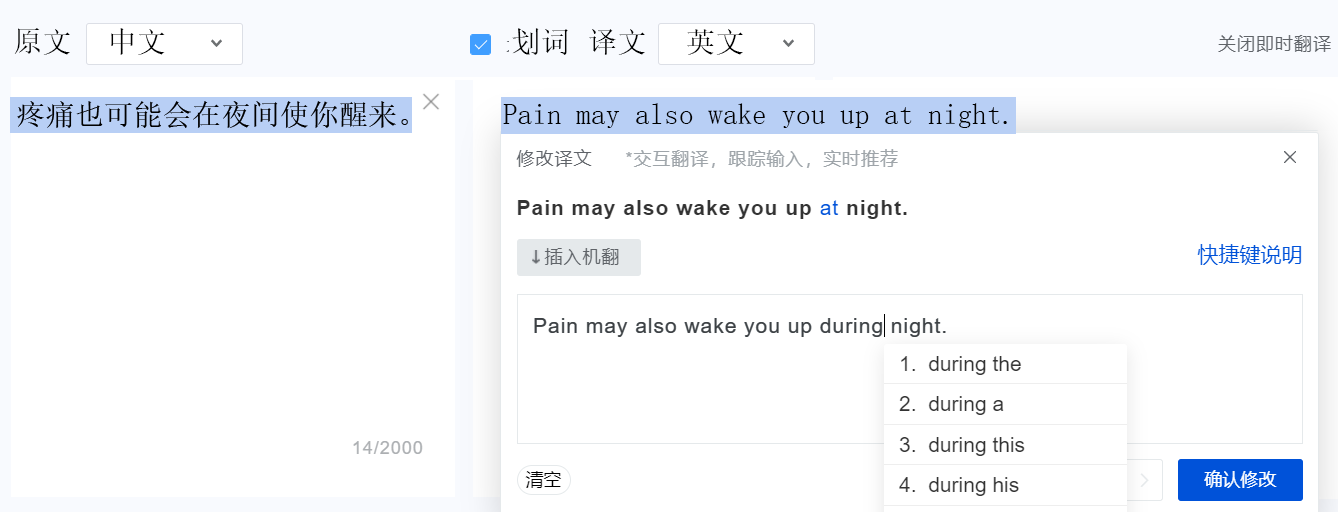
\includegraphics[scale=0.4]{./Chapter18/Figures/figure-transSmart.png}
%\setlength{\abovecaptionskip}{-0.2cm}
\caption{使用TranSmart系统进行交互式翻译的实例}
\label{fig:18-2}
\end{figure}
%----------------------------------------------

\parinterval 交互式机器翻译系统主要通过用户的反馈来提升译文的质量,不同类型的反馈信息则影响着系统最终的性能。根据反馈形式的不同,可以将交互式机器翻译分为以下几种:
\begin{itemize}
\vspace{0.5em}
\item 基于前缀的交互式机器翻译。早期的交互式机器翻译系统都是采用基于前缀的方式。基于翻译系统生成的初始译文,翻译人员从左到右检查翻译的正确性,并在第一个错误的位置进行更正。这为系统提供了一种双重信号:表明该位置上的单词必须是翻译人员修改过后的单词,并且该位置之前的单词都是正确的。之后系统根据已经检查过的前缀再生成后面的译文\upcite{DBLP:conf/acl/WuebkerGDHL16,Zens2003EfficientSF,DBLP:journals/coling/BarrachinaBCCCKLNTVV09,DBLP:journals/csl/PerisC19}。

\vspace{0.5em}
\item 基于片段的交互式机器翻译。根据用户提供的反馈来生成更好的翻译结果是交互式翻译系统的关键。而基于前缀的系统则存在一个严重的缺陷,当翻译系统获得确定的翻译前缀之后,再重新生成译文时会将原本正确的翻译后缀遗漏了,因此会引入新的错误。在基于片段的交互式机器翻译系统中,翻译人员除了纠正第一个错误的单词,还可以指定在未来迭代中保留的单词序列。之后系统根据这些反馈信号再生成新的译文\upcite{Peris2017InteractiveNM,DBLP:journals/mt/DomingoPC17}。

\vspace{0.5em}
\item 基于评分的交互式机器翻译。随着计算机算力的提升,有时会出现“机器等人”的现象,因此需要提升人参与交互的效率也是需要考虑的。与之前的系统不同,基于评分的交互式机器翻译系统不需要翻译人员选择、纠正或删除某个片段,而是使用翻译人员对译文的评分来强化机器翻译的学习\upcite{DBLP:journals/corr/abs-1805-01553,DBLP:conf/emnlp/NguyenDB17}。

\vspace{0.5em}
\end{itemize}

\parinterval 除此之外,基于在线学习的方法也受到了关注,这类方法也可以被看作是交互式翻译与增量训练的一种结合。用户总是希望翻译系统能从反馈中自动纠正以前的错误。当用户最终确认一个修改过后的译文后,翻译系统将源语言句子与该修正后的译文作为训练语料继续训练\upcite{DBLP:conf/acl/DomingoGEBHPCH19}。实际上,交互式机器翻译是机器翻译大规模应用的重要途径之一,它为打通翻译人员和机器翻译系统之间的障碍提供了手段。不过,交互式机器翻译也有许多挑战等待解决。一个是如何设计交互方式?理想的交互方式应该是更加贴近翻译人员输入文字的习惯,比如,利用输入法完成交互;另一个是如何把交互式翻译嵌入到翻译的生产流程里?这本身不完全是一个技术问题,可能需要更多的产品手段来求解。


%----------------------------------------------------------------------------------------
%    NEW SECTION
%----------------------------------------------------------------------------------------

\section{翻译结果的可干预性}

\parinterval 交互式机器翻译体现了一种用户的行为“干预”机器翻译结果的思想。实际上,在机器翻译出现错误时,人们总是希望用一种直接有效的方式“改变”译文,最短时间内达到改善翻译质量的目的。比如,如果机器翻译系统可以输出多个候选译文,用户可以在其中挑选最好的译文进行输出。也就是,人为干预了译文候选的排序过程。另一个例子是{\small\bfnew{翻译记忆}}\index{翻译记忆}(Translation Memory,TM\index{Translation Memory})。翻译记忆记录了高质量的源语言-目标语言句对,有时也可以被看作是一种先验知识或“记忆”。因此,当进行机器翻译时,使用翻译记忆指导翻译过程也可以被看作是一种干预手段\upcite{DBLP:conf/acl/WangZS13,DBLP:conf/aaai/XiaHLS19}。


\parinterval 虽然干预机器翻译系统的方式很多,最常用的还是对源语言特定片段翻译的干预,以期望最终句子的译文满足某些约束。这个问题也被称作{\small\bfnew{基于约束的翻译}}\index{基于约束的翻译} (Constraint-based Translation\index{Constraint-based Translation})。比如,在翻译网页时,需要保持译文中的网页标签与源文一致。另一个典型例子是术语翻译。在实际应用中,经常会遇到公司名称、品牌名称、产品名称等专有名词和行业术语,以及不同含义的缩写,比如,对于“小牛翻译”这个专有名词,不同的机器翻译系统给出的结果不一样:“Maverick translation”、“Calf translation”、“The mavericks translation”等等,而它正确的翻译应该为“NiuTrans”。 对于这些类似的特殊词汇,机器翻译引擎很难翻译得准确。一方面,因为模型大多是在通用数据集上训练出来的,并不能保证数据集能涵盖所有的语言现象。另一方面,即使是这些术语在训练数据中出现,它们通常也是低频的,模型不容易捕捉它们的规律。为了保证翻译的准确性,对术语翻译进行干预是十分有必要的,对领域适应等问题的求解也是非常有意义的。

\parinterval 就{\small\bfnew 词汇约束翻译}\index{词汇约束翻译}(Lexically Constrained Translation)\index{Lexically Constrained Translation}而言,在不干预的情况下让模型直接翻译出正确术语是很难的,因为术语的译文很可能是未登录词,因此必须人为提供额外的术语词典,那么我们的目标就是让模型的翻译输出遵守用户提供的术语约束。这个过程如图\ref{fig:18-3}所示。
%----------------------------------------------
\begin{figure}[htp]
\centering

%%% outline
%-------------------------------------------------------------------------
\begin{tikzpicture}[scale=0.8]
\tikzstyle{diction}=[align=center,rounded corners=2pt, draw,drop shadow,fill=green!20,font=\scriptsize]
\tikzstyle{word}=[align=center,anchor=west]
\begin{scope}

\node[word] (origin) at (0,0) {源文};
\node[word] (n1) at ([xshift=1em]origin.east){{\color{red} 小牛翻译}的总部在哪里?}; 

\node[word] (right) at ([yshift=-6em]origin.south west){译文};
\node[word] (n3) at ([xshift=1em]right.east){Where is the headquarters \\ of {\color{red} NiuTrans}?}; 

%\node[diction] (dic) at ([xshift=2em,yshift=-1.8em]n1.south east) {
%术语词典 \\
%小牛翻译 = NiuTrans \\
%......
%};
%\draw[->,red] ([yshift=-0.2em]dic.west)  .. controls +(west:2em) and +(south:2em) .. ( [xshift=-4em]n1.south) node[above,midway,font=\scriptsize]{};
\node[font=\scriptsize] at ([yshift=-2.3em,xshift=-6em]n1.south) {“小牛翻译”=“NiuTrans”};
\draw[->,very thick] ([yshift=-0.2em,xshift=-0.4em]n1.south) -- ([yshift=0.2em]n3.north);
%\draw[->,very thick] ([yshift=-0.2em,xshift=-0.2em]n2.south) -- ([yshift=0.2em]n3.north);

\end{scope}
\end{tikzpicture}






%\setlength{\abovecaptionskip}{-0.2cm}
\caption{词汇约束翻译过程}
\label{fig:18-3}
\end{figure}
%----------------------------------------------

\parinterval 在统计机器翻译中,翻译本质上是由短语和规则构成的推导,因此修改译文比较容易,比如,可以在一个源语言片段所对应的翻译候选集中添加希望得到的译文。而神经机器翻译是一个端到端模型,翻译过程本质上是连续空间中元素的一系列映射、组合和代数运算。虽然在模型训练阶段仍然可以通过修改损失函数等手段引入约束,但是在推断阶段进行直接干预并不容易,因为我们无法像修改符号系统那样直接修改模型(如短语翻译表)来影响译文生成。实践中主要有两种解决思路:

\begin{itemize}
\vspace{0.5em}
\item 强制生成。这种方法并不改变模型,而是在推断过程中按照一定的策略来实施约束,一般是修改束搜索算法以确保输出必须包含指定的词或者短语\upcite{DBLP:conf/acl/HokampL17,DBLP:conf/naacl/PostV18,DBLP:conf/wmt/ChatterjeeNTFSB17,DBLP:conf/naacl/HaslerGIB18},例如,在获得译文输出后,利用注意力机制获取词对齐,之后通过词对齐得到源语言和目标语言片段的对应关系,最后对指定译文片段进行强制替换。或者,对包含正确术语的翻译候选进行额外的加分,以确保推断时这样的翻译候选的排名足够靠前。

\vspace{0.5em}
\item 数据增强。这类方法通过修改机器翻译模型的训练数据来实现术语约束。通常根据术语词典对训练数据进行一定的修改,例如,将术语的译文添加到源文句子中,之后将原始语料库和合成语料库进行混合训练,期望模型能够学会自动利用术语信息来指导解码,或者是在训练数据中利用占位符来替换术语,待翻译完成后再进行还原\upcite{DBLP:conf/naacl/SongZYLWZ19,DBLP:conf/acl/DinuMFA19,DBLP:journals/corr/abs-1912-00567,DBLP:conf/ijcai/ChenCWL20}。

\vspace{0.5em}
\end{itemize}

\parinterval 强制生成的方法是在搜索策略上进行限制,与模型无关,这类方法能保证输出满足约束,但是会影响翻译速度。数据增强的方法是通过构造特定格式的数据让模型训练,从而让模型具有自动适应术语约束的能力,通常不会影响翻译速度,但并不能保证输出能满足约束。

\parinterval 此外,机器翻译在应用时通常还需要进行译前译后的处理,译前处理指的是在翻译前对源语言句子进行修改和规范,从而能生成比较通顺的译文,提高译文的可读性和准确率。在实际应用时,由于用户输入的形式多样,可能会包含比如术语、缩写、数学公式等,有些甚至可能还包含网页标签,因此对源文进行预处理是很有必要的。常见的处理工作包括格式转换、标点符号检査、术语编辑、标签识别等,待翻译完成后,则需要对机器译文进行进一步的编辑和修正,从而使其符合使用规范,比如进行标点、格式检查,术语、标签还原等,这些过程通常都是按照设定的处理策略自动完成的。另外,译文长度的控制、译文多样性的控制等也可以丰富机器翻译系统干预的手段(见{\chapterfourteen})。

%----------------------------------------------------------------------------------------
%    NEW SECTION
%----------------------------------------------------------------------------------------

\section{小设备机器翻译}

\parinterval 在机器翻译研究中,一般会假设计算资源是充足的。但是,在很多应用场景中,机器翻译使用的计算资源非常有限,比如,一些离线设备上没有GPU,而且CPU的处理能力也很弱,甚至内存也非常有限。这时,让模型变得更小、系统变得更快就成为了重要的需求。

\parinterval 本书中已经讨论了大量的可用于小设备上的机器翻译技术方法,例如:

\begin{itemize}
\vspace{0.5em}
\item 知识蒸馏({\chapterthirteen})。这种方法可以有效地将翻译能力从大模型迁移到小模型。

\vspace{0.5em}
\item 低精度存储及计算({\chapterfourteen})。可以使用量化的方式将模型压缩,同时整型计算也非常适合在CPU等设备上执行。

\vspace{0.5em}
\item 轻量模型结构({\chapterfourteen}和{\chapterfifteen})。对机器翻译模型的局部结构进行优化也是非常有效的手段,比如,使用更加轻量的卷积计算模块,或者使用深编码器-浅解码器等高效的结构。

\vspace{0.5em}
\item 面向设备的模型结构学习({\chapterfifteen})。可以把设备的存储及延时作为目标函数的一部分,自动搜索高效的翻译模型结构。

\vspace{0.5em}
\item 动态适应性模型\upcite{DBLP:conf/emnlp/WangXZ20,DBLP:journals/corr/BolukbasiWDS17,DBLP:conf/iclr/HuangCLWMW18}。模型可以动态调整大小或者计算规模,以达到在不同设备上平衡延时和精度的目的。比如,可以根据延时的要求,动态生成合适深度的神经网络进行翻译。

\vspace{0.5em}
\end{itemize}

\parinterval 此外,机器翻译系统的工程实现方式也是十分重要的,例如,编译器的选择、底层线性代数库的选择等等。有时候,使用与运行设备相匹配的编译器,会带来明显的性能提升\footnote{以神经机器翻译为例,张量计算部分大多使用C++等语言编写,因此编译器与设备的适配程度对程序的执行效率影响很大。}。如果希望追求更加极致的性能,甚至需要对一些热点模块进行修改。例如,在神经机器翻译中,矩阵乘法就是一个非常耗时的部分。但是这部分计算又与设备、矩阵的形状有很大关系。对于不同设备,根据不同的矩阵形状可以设计相应的矩阵乘法算法。不过,这部分工作对系统开发和硬件指令的使用水平要求较高。

\parinterval 另外,在很多系统中,机器翻译模块并不是单独执行,而是与其它的模块并发执行。这时,由于多个计算密集型任务存在竞争,处理器要进行更多的上下文切换,会造成程序变慢。比如,机器翻译和语音识别两个模块一起运行时{\footnote{在一些语音翻译场景中,由于采用了语音识别和翻译异步执行的方式,两个程序可能会并发。}},机器翻译的速度会有较明显的下降。对于这种情况,需要设计更好的调度机制。因此在一些同时具有CPU和GPU的设备上,可以考虑合理调度CPU和GPU的资源,增加两种设备可并行处理的内容,避免在某个处理器上的拥塞。

\parinterval 除了运行速度,模型过大也是限制其在小设备上运行的因素。在模型体积上,神经机器翻译模型具有天然的优势。因此,在对模型规模有苛刻要求的场景中,神经机器翻译是不二的选择。另外通过量化、剪枝、参数共享等方式,可以将模型大幅度压缩。

%----------------------------------------------------------------------------------------
%    NEW SECTION
%----------------------------------------------------------------------------------------

\section{机器翻译系统的部署}

\parinterval 除了在一些离线设备上使用机器翻译,更多时候机器翻译系统会部署在运算能力较强的服务器上。一方面随着神经机器翻译的大规模应用,在GPU服务器上部署机器翻译系统已经成为了常态。另一方面,GPU服务器的成本较高,而且很多应用中需要同时部署多个语言方向的系统。这时如何充分利用设备以满足大规模的翻译需求就成为了不可回避的问题。有几个方向值得尝试:

\begin{itemize}
\vspace{0.5em}
\item 对于多语言翻译的场景,使用多语言单模型翻译系统是一种很好的选择({\chaptersixteen})。当多个语种的数据量有限、使用频度不高时,这种方法可以很有效地解决翻译需求中的长尾部分。例如,一些线上机器翻译服务已经支持超过100种语言的翻译,其中大部分语言之间的翻译需求是相对低频的,因此使用同一个模型进行翻译可以大大节约部署和运维的成本。

\vspace{0.5em}
\item 使用基于枢轴语言的翻译也可以有效的解决多语言翻译问题({\chaptersixteen})。这种方法同时适合统计机器翻译和神经机器翻译,因此很早就使用在大规模机器翻译部署中。

\vspace{0.5em}
\item GPU部署中,由于GPU成本较高,因此可以考虑在单个GPU设备上部署多套不同的系统。如果这些系统之间的并发不频繁,翻译延时不会有明显增加。这种多个模型共享一个设备的方法比较适合翻译请求相对低频但是翻译任务又很多样的情况。

\vspace{0.5em}
\item 机器翻译大规模GPU部署对显存的使用也很严格。由于GPU显存较为有限,因此模型运行的显存消耗也是需要考虑的。一般来说,除了模型压缩和结构优化之外({\chapterfourteen}和{\chapterfifteen}),也需要对模型的显存分配和使用进行单独的优化。例如,使用显存池来缓解频繁申请和释放显存空间造成的延时。另外,也可以尽可能让同一个显存块保存生命期不重叠的数据,避免重复开辟新的存储空间。图\ref{fig:18-4}展示了一个显存复用的示例。

%----------------------------------------------
\begin{figure}[htp]
\centering
\begin{tabular}{c c}

\begin{tikzpicture}
\begin{scope}
% ,minimum height =1em,minimum width=2em
\tikzstyle{memory} = [draw,black,very thick,inner sep=2pt,rounded corners=0pt,fill=blue!20,minimum width=2em,minimum height=1.5em,anchor=west]
\tikzstyle{thread} = [very thick,inner sep=3.5pt,rounded corners=0pt,minimum width=3em,minimum height=1.5em]
\tikzstyle{word} = [inner sep=3.5pt,font=\scriptsize]

\node[thread] (one) at (0,0) {};
\node [word] at (one.north) {\scriptsize 数据1};
\draw[|-|,very thick] (-1.5em,0em) -- (1.6em,0em);

\node[thread,minimum width=5em] (two) at ([yshift=-1em,xshift=2.6em]one.south east) {};
\node [word] at (two.north) {\scriptsize 数据2};
\draw[|-|,very thick] (1.8em,-1.8em) -- (6.5em,-1.8em);

\node[thread,minimum width=4em] (three) at ([yshift=-1em,xshift=0.3em]two.south east) {};
\node [word] at (three.north) {\scriptsize 数据3};
\draw[|-|,very thick] (5em,-1.8*2em) -- (9em,-1.8*2em);

\node[thread,minimum width=2em] (four) at ([yshift=-1em,xshift=1.2em]three.south east) {};
\node [word] at (four.north) {\scriptsize 数据4};
\draw[|-|,very thick] (9.3em,-1.8*3em) -- (11em,-1.8*3em);

\node [memory] (mone) at ([yshift=4em,xshift=1em]one.north) {};
\node [memory] (mtwo) at ([xshift=0em]mone.east) {};
\node [memory] (mthree) at ([xshift=0em]mtwo.east) {};
\node [memory] (mfour) at ([xshift=0em]mthree.east) {};

\draw[->,very thick] (-0.8,-2.5) -- (4.7,-2.5);
\draw[->,very thick] (-0.8,-2.5) -- (-0.8,1);
 
\node [word] (time) at ([yshift=-1.5em,xshift=0.3em]four.south) {\scriptsize 时间线};
\node [word] (time) at ([yshift=1.5em,xshift=-2.2em]one.west) {\scriptsize 数据};

\draw [->,dashed,line width=0.7pt] ([yshift=0.5em]one.north) .. controls +(north:1.5em) and +(south:1.5em) .. ([yshift=-0.2em]mone.south);
\draw [->,dashed,line width=0.7pt] ([yshift=0.5em]two.north) -- ([yshift=-0.2em]mtwo.south);
\draw [->,dashed,line width=0.7pt] ([yshift=0.5em,xshift=0.5em]three.north) .. controls +(north:3.5em) and +(south:4.5em) .. ([yshift=-0.2em]mthree.south);
\draw [->,dashed,line width=0.7pt] ([yshift=0.5em]four.north) .. controls +(north:4.5em) and +(south:4.5em) .. ([yshift=-0.2em]mfour.south);

\node [word] at ([yshift=-6em]two.south) {(a) 显存不复用};

%占位
\node[word] at ([xshift=1em]four.east) {};

\node [word] at ([xshift=1.5em,yshift=5.6em]one.north) {\scriptsize 显存};

\begin{pgfonlayer}{background}
\node [rectangle,inner sep=0.5em,rounded corners=1pt,minimum width=10em,minimum height=3.6em,fill=gray!10,drop shadow] at ([yshift=6.6em,xshift=1em]two.north) {};
\end{pgfonlayer}

\end{scope}
\end{tikzpicture}
&
\begin{tikzpicture}
\begin{scope}
%\tikzstyle{memory} = [draw,black,very thick,inner sep=2pt,rounded corners=0pt,fill=blue!20,minimum width=2em,minimum height=1.5em,anchor=west]
%\tikzstyle{thread} = [draw,black,very thick,inner sep=3.5pt,rounded corners=0pt,fill=green!20,minimum width=3em,minimum height=1.5em]
\tikzstyle{memory} = [draw,black,very thick,inner sep=2pt,rounded corners=0pt,fill=blue!20,minimum width=2em,minimum height=1.5em,anchor=west]
\tikzstyle{thread} = [very thick,inner sep=3.5pt,rounded corners=0pt,minimum width=3em,minimum height=1.5em]
\tikzstyle{word} = [inner sep=3.5pt,font=\scriptsize]

\node[thread] (one) at (0,0) {};
\node [word] at (one.north) {\scriptsize 数据1};
\draw[|-|,very thick] (-1.5em,0em) -- (1.6em,0em);

\node[thread,minimum width=5em] (two) at ([yshift=-1em,xshift=2.6em]one.south east) {};
\node [word] at (two.north) {\scriptsize 数据2};
\draw[|-|,very thick] (1.8em,-1.8em) -- (6.5em,-1.8em);

\node[thread,minimum width=4em] (three) at ([yshift=-1em,xshift=0.3em]two.south east) {};
\node [word] at (three.north) {\scriptsize 数据3};
\draw[|-|,very thick] (5em,-1.8*2em) -- (9em,-1.8*2em);

\node[thread,minimum width=2em] (four) at ([yshift=-1em,xshift=1.2em]three.south east) {};
\node [word] at (four.north) {\scriptsize 数据4};
\draw[|-|,very thick] (9.3em,-1.8*3em) -- (11em,-1.8*3em);

\node [memory] (mone) at ([yshift=4em,xshift=1em]one.north) {};
\node [memory] (mtwo) at ([xshift=0em]mone.east) {};
\node [memory,fill=white,minimum width=4em] (mthree) at ([xshift=0em]mtwo.east) {};
%\node [memory,fill=white] (mfour) at ([xshift=0em]mthree.east) {};

\draw[->,very thick] (-0.8,-2.5) -- (4.7,-2.5);
\draw[->,very thick] (-0.8,-2.5) -- (-0.8,1);

\node [word] (time) at ([yshift=-1.5em,xshift=0.3em]four.south) {\scriptsize 时间线};
\node [word] (time) at ([yshift=1.5em,xshift=-2.2em]one.west) {\scriptsize 数据};

\draw [->,dashed,line width=0.7pt] ([yshift=0.5em]one.north) .. controls +(north:1.5em) and +(south:1.5em) .. ([yshift=-0.2em,xshift=-0.4em]mone.south);
\draw [->,dashed,line width=0.7pt] ([yshift=0.5em]two.north) .. controls +(north:3.5em) and +(south:3.5em) .. ([yshift=-0.2em,xshift=0.4em]mone.south);
\draw [->,dashed,line width=0.7pt] ([yshift=0.5em,xshift=0.5em]three.north) .. controls +(north:3.5em) and +(south:3.5em) .. ([yshift=-0.2em,xshift=-0.4em]mtwo.south);
\draw [->,dashed,line width=0.7pt] ([yshift=0.5em]four.north) .. controls +(north:4.5em) and +(south:3.5em) .. ([yshift=-0.2em,xshift=0.4em]mtwo.south);

\node [word] at ([xshift=1.5em,yshift=5.6em]one.north) {\scriptsize 显存};

\node [word] at ([yshift=-6em]two.south) {(b) 显存复用};

\begin{pgfonlayer}{background}
\node [rectangle,inner sep=0.5em,rounded corners=1pt,minimum width=10em,minimum height=3.6em,fill=gray!10,drop shadow] at ([yshift=6.6em,xshift=1em]two.north) {};
\end{pgfonlayer}


\end{scope}
\end{tikzpicture}

\end{tabular}
%\setlength{\abovecaptionskip}{-0.2cm}
\caption{显存不复用与显存复用的示例}
\label{fig:18-4}
\end{figure}
%----------------------------------------------
\vspace{0.5em}
\item 在翻译请求高并发的场景中,使用批量翻译也是有效利用GPU设备的方式。不过,机器翻译是一个处理不定长序列的任务,输入的句子长度差异较大。而且,由于译文长度无法预知,进一步增加了不同长度的句子所消耗计算资源的不确定性。这时,可以让长度相近的句子在一个批次里处理,减小由于句子长度不统一造成的补全过多、设备利用率低的问题。例如,可以按输入句子长度范围分组。 也可以设计更加细致的方法对句子进行分组,以最大化批量翻译中设备的利用率\upcite{DBLP:journals/corr/abs-2010-05680}。

\vspace{0.5em}
\end{itemize}

\parinterval 除了上述问题,如何对多设备环境下进行负载均衡、容灾处理等都是大规模机器翻译系统部署中需要考虑的。有时候,甚至统计机器翻译系统也可以与神经机器翻译系统混合使用。由于统计机器翻译系统对GPU资源的要求较低,纯CPU部署的方案也相对成熟。因此,可以作为GPU机器翻译服务的灾备。此外,在有些任务,特别是某些低资源翻译任务上,统计机器翻译仍然具有优势。

%----------------------------------------------------------------------------------------
%    NEW SECTION
%----------------------------------------------------------------------------------------

\section{机器翻译的应用场景}

\parinterval 机器翻译有着十分广泛的应用,这里列举了一些常见的应用场景:
\begin{itemize} 
\item {\small\bfnew{网页翻译}}。进入信息爆炸的时代之后,互联网上海量的数据随处可得,然而由于不同国家和地区语言的差异,网络上的数据也呈现出多语言的特性。当人们在遇到包含不熟悉语言的网页时,无法及时有效地获取其中的信息。因此,对不同语言的网页进行翻译是必不可少的一步。由于网络上的网页数不胜数,依靠人工对网页进行翻译是不切实际的,相反,机器翻译十分适合这个任务。目前,市场上有很多浏览器提供网页翻译的服务,极大地降低了人们从网络上获取不同语言信息的难度。

\item {\small\bfnew{科技文献翻译}}。在专利等科技文献翻译中,往往需要将文献翻译为英语或者其他语言,比如摘要翻译。以往这种翻译工作通常由人工来完成。由于对翻译结果的质量要求较高,因此要求翻译人员具有相关专业的背景知识,这导致翻译人员资源稀缺。特别是,近几年国内专利申请数不断增加,这给人工翻译带来了很大的负担。相比于人工翻译,机器翻译可以在短时间内完成大量的专利翻译,同时结合术语词典和人工校对等方式,可以保证专利的翻译质量。另外,以专利为代表的科技文献往往具有很强的领域性,针对各类领域文本进行单独优化,机器翻译的品质可以大大提高。因此,机器翻译在专利翻译等行业有十分广泛的应用前景。

\item {\small\bfnew{视频字幕翻译}}。随着互联网的普及,人们可以通过互联网接触到大量境外影视作品。由于人们可能没有相应的外语能力,通常需要翻译人员对字幕进行翻译。因此,这些境外视频的传播受限于字幕翻译的速度和准确度。现在的一些视频网站在使用语音识别为视频生成源语言字幕的同时,通过机器翻译技术为各种语言的受众提供质量尚可的目标语言字幕,这种方式为人们提供了极大的便利。

\item {\small\bfnew{社交}}。社交是人们的重要社会活动。人们可以通过各种各样的社交软件做到即时通讯,进行协作或者分享自己的观点。然而受限于语言问题,人们的社交范围往往不会超出自己所掌握的语种范围,很难方便地进行跨语言社交。随着机器翻译技术的发展,越来越多的社交软件开始支持自动翻译,用户可以轻易地将各种语言的内容翻译成自己的母语,方便了人们的交流,让语言问题不再成为社交的障碍。

\item {\small\bfnew{同声传译}}。在一些国际会议中,与会者来自许多不同的国家,为了保证会议的流畅,通常需要专业翻译人员进行同声传译。同声传译需要在不打断演讲的同时,不间断地将讲话内容进行口译,对翻译人员的要求极高。现在,一些会议开始采用语音识别来将语音转换成文本,同时使用机器翻译技术进行翻译的方式,达到同步翻译的目的。这项技术已经得到了多个企业的关注,并在很多重要会议上进行尝试,取得了很好的反响。不过同声传译达到可以真正使用的程度还需一定时间的打磨,特别是会议场景下,准确进行语音识别和翻译仍然具有挑战性。

\item {\small\bfnew{中国传统语言文化的翻译}}。中国几千年的历史留下了极为宝贵的文化遗产,而其中,文言文作为古代书面语,具有言文分离、行文简练的特点,易于流传。言文分离的特点使得文言文和现在的标准汉语具有一定的区别。为了更好发扬中国传统文化,需要对文言文进行翻译。而文言文古奥难懂,人们需要具备一定的文言文知识背景才能准确翻译。机器翻译技术也可以帮助人们快速完成文言文的翻译。除此之外,机器翻译技术同样可以用于古诗生成和对联生成等任务。

\item {\small\bfnew{全球化}}。在经济全球化的今天,很多企业都有国际化的需求,企业员工或多或少地会遇到一些跨语言阅读和交流的情况,比如阅读进口产品的说明书,跨国公司之间的邮件、说明文件等等。相比于成本较高的人工翻译,机器翻译往往是一种很好的选择。在一些质量要求不高的翻译场景中,机器翻译可以得到应用。

\item {\small\bfnew{翻译机/翻译笔}}。出于商务、学术交流或者旅游的目的,人们在出国时会面临着跨语言交流的问题。近几年,随着出境人数的增加,不少企业推出了翻译机产品。通过结合机器翻译、语音识别和图像识别技术,翻译机实现了图像翻译和语音翻译的功能。用户可以很便捷地获取一些外语图像文字和语音信息,同时可以通过翻译机进行对话,降低跨语言交流门槛。类似地,翻译笔等应用产品可以通过划词翻译的方式,对打印材料中的外语文字进行翻译。

\item {\small\bfnew{译后编辑}}。翻译结果后编辑是指在机器翻译的结果之上,通过少量的人工编辑来进一步完善机器译文。在传统的人工翻译过程中,翻译人员完全依靠人工的方式进行翻译,这虽然保证了翻译质量,但是时间成本高。相对应地,机器翻译具有速度快和成本低的优势。在一些领域,目前的机器翻译质量已经可以很大程度上减少翻译人员的工作量,翻译人员可以在机器翻译的辅助下,花费相对较小的代价来完成翻译。

\end{itemize}

%----------------------------------------------------------------------------------------
%    NEW SECTION
%----------------------------------------------------------------------------------------

%\section{拓展思考}

%% !Mode:: "TeX:UTF-8"
% !TEX encoding = UTF-8 Unicode

%----------------------------------------------------------------------------------------
% 机器翻译:基础与模型
% Machine Translation: Foundations and Models
%
% Copyright 2020
% 肖桐(xiaotong@mail.neu.edu.cn) 朱靖波 (zhujingbo@mail.neu.edu.cn)
%----------------------------------------------------------------------------------------

%----------------------------------------------------------------------------------------
%    CONFIGURATIONS
%----------------------------------------------------------------------------------------

\renewcommand\figurename{图}%将figure改为图

%----------------------------------------------------------------------------------------
%	postscript
%----------------------------------------------------------------------------------------
\fancyhead[LO]{\sffamily\normalsize\bfseries{随笔 \ \quad 肖桐\ 朱靖波}} % Print the nearest section name on the left side of odd pages
\fancyhead[RE]{\sffamily\normalsize\bfseries{随笔 \ \quad 肖桐\ 朱靖波}} % Print the current chapter name on the right side of even pages
%\chapter*{后记}
\addcontentsline{toc}{chapter}{随笔}

{\color{white} 空}
\vspace{1em}
\begin{center}
{\Huge \bfnew{随\ \ \ 笔}}
\end{center}
\vspace{2em}

\begin{spacing}{1.18}

%\section{随笔}

\parinterval 自计算机诞生,机器翻译,即利用计算机软件技术实现不同语言自动翻译,就是人们首先想到的计算机主要应用。很多人说,人工智能时代是得语言者的天下,并将机器翻译当作认知智能的终极梦想之一。接下来,笔者将分享自己对机器翻译技术和应用的思考,有些想法不一定正确,有些想法也许需要十年或更久才能被验证。

\parinterval 简单来说,机器翻译技术至少可以满足三种用户需求。一是实现外文资料辅助阅读,帮助不同母语的人进行无障碍交流;二是通过计算机辅助翻译,帮助人工翻译降本增效;三是通过大数据分析和处理,实现对多语言文字资料(也可以是图像资料或语音资料)的加工处理。仅凭人工,是无法完成海量数据的翻译工作的,而机器翻译是大数据翻译的唯一有效解决方案。从上述三种需求可以看出,机器翻译和人工翻译在本质上不存在冲突,两者可以和谐共存、相互帮助,处于平行轨道上。对机器翻译来说,至少有两个应用场景是其无法独立胜任的。一是对翻译结果的质量要求高的场景,如诗歌、小说的翻译出版;二是不允许出现低级实时翻译错误的场景,如国际会议的发言。因此,对译文准确性要求很高的应用场景不可能只采用机器翻译,必须有高水平的人工翻译参与。

\parinterval 如何构建一套好的机器翻译系统呢?假设我们需要为用户提供一套翻译品质不错的机器翻译系统,至少需要考虑三个方面:有足够大规模的双语句对集合用于训练、有强大的机器翻译技术和错误驱动的打磨过程。从技术应用和产业化的角度看,对于构建一套好的机器翻译系统来说,上述三个方面缺一不可。仅拥有强大的机器翻译技术是必要条件,但不是充分条件。更具体地:
\begin{itemize}
\item 从数据角度来看,大部分语言对的电子化双语句对集合规模非常小,有的甚至只有一个小规模双语词典。因此,针对资源稀缺语种的机器翻译技术研究也成了学术界的研究热点,相信这个课题的突破能大大推动机器翻译技术落地。早些年,机器翻译市场的规模较小,其主要原因是数据规模有限,同时机器翻译的品质不够理想。就算采用最先进的神经机器翻译技术,在缺乏足够大规模的双语句对集合作为训练数据的情况下,研究人员也是巧妇难为无米之炊。从技术研究和应用可行性的角度看,解决资源稀缺语种的机器翻译问题非常有价值。解决资源稀缺语种机器翻译问题的思路,已经在{\chaptersixteen}进行了详细的介绍,本部分就不再赘述。

\item 从机器翻译技术来看,可实用的机器翻译系统的构建,需要多技术互补融合。做研究可以搞单点突破,但它很难能应对实际问题和改善真实应用中的翻译品质。多技术互补融合有很多研究工作,比如说,有的业内研究人员提出采用知识图谱来改善机器翻译模型性能,并希望用于解决稀缺资源语种机器翻译问题;有的引入语言分析技术来改善机器翻译;有的将基于规则的方法、统计机器翻译技术与神经机器翻译技术互补性融合;有的引入预训练技术来改善机器翻译品质等等。总体来说,这些思路都具有良好的研究价值,但是从应用角度来说,构建可实用的机器翻译系统,还需要考虑技术落地可行性。比如大规模知识图谱构建的代价和语言分析技术的精度如何,预训练技术对富资源场景下机器翻译的价值等。

\item 错误驱动,即根据用户对机器翻译译文的反馈与纠正,完善机器翻译模型的过程。机器翻译一直被诟病:用户不知道如何有效地干预纠错,来帮助机器翻译系统越做越好,毕竟谁都不希望它“屡教不改”。基于规则的方法和统计机器翻译方法相对容易实现人工干预纠错,实现手段也比较丰富,而神经机器翻译方法很多时候被看做是黑箱,其运行机理与离散的符号系统有很大差别,难以用传统方式有效地实现人工干预纠错。目前,有研究人员通过引入外部知识库(用户双语术语库)来实现对未登录词翻译的干预纠错;也有的提出使用增量式训练的方法不断迭代优化模型,取得了一些进展;还有研究人员通过融合不同技术来实现更好的机器翻译效果,如引入基于规则的翻译前处理和后处理,或者引入统计机器翻译技术优化译文选择等。这些方法的代价不低,甚至很高, 并且无法保障对机器翻译性能提升的效果,有时可能会降低翻译品质(有点像“跷跷板”现象)。总体来说,这个方向的研究成果还不够丰富,但对用户体验来说非常重要。如果能采用隐性反馈学习方法,在用户不知不觉中不断改善、优化机器翻译品质,就非常酷了,这也许会成为将来的一个研究热点。
\end{itemize}

\parinterval 除了翻译品质维度以外,机器翻译还可以从以下三个维度来讨论:语种维度、领域维度和应用模式维度。关于语种维度,机器翻译技术应该为全球用户服务,提供所有国家至少一种官方语言到其他国家语言的自动互译功能。该维度面临的最大问题是双语数据稀缺。关于领域维度,通用领域翻译系统的翻译能力,对于垂直领域数据来说是不足的。最典型的问题是不能恰当地翻译垂直领域术语,计算机不能无中生有。比较直接可行的解决方案至少有两个,一是引入垂直领域术语双语词典来改善机器翻译效果;二是收集加工一定规模的垂直领域双语句对来优化翻译模型。这两种工程方法虽然简单,但效果不错,并且两者结合对于翻译模型性能的提升帮助更大。但很多时候垂直领域双语句对的收集代价太高,可行性低,因此垂直领域翻译问题本质上就转换成为垂直领域资源稀缺问题和领域自适应学习问题。除此之外,小样本学习、迁移学习等机器学习技术也被一些研究人员用来解决垂直领域翻译问题。关于应用模式维度,可以从下面几个方面进行讨论:
\begin{itemize}
\item 通常,机器翻译的典型应用包括在线翻译公有云服务,用户接入非常简单,只需要联网使用浏览器就可以自由免费使用。在某些行业,用户对数据翻译安全性和保密性的要求非常高,其中可能还会涉及个性化定制,这是在线翻译公有云服务无法满足的,于是,在本地部署机器翻译私有云,应用离线机器翻译技术和服务成了新的应用模式。在本地部署私有云的问题在于:需要用户自己购买 GPU 服务器并建机房,对硬件的投入高。也许将来机器翻译领域会出现新的应用模式:类似服务托管模式的在线私有云或专有云,以及混合云服务(公有云、私有云和专有云的混合体)。

\item 离线机器翻译技术可以为更小型的智能翻译终端设备提供服务,如大家熟知的翻译机、翻译笔、翻译耳机等智能翻译设备。在不联网的情况下,这些设备能实现高品质机器翻译功能,这类应用模式具有很大的潜力。但这类应用模式需要解决的问题也很多:首先是模型大小、翻译速度和翻译品质的问题;其次,考虑不同操作系统(如Linux、Android Q 和iOS)和不同架构(如x86、MIPS、ARM 等)的CPU 芯片的智能适配兼容问题。将来,离线翻译系统还可以通过芯片安装到办公设备上,如传真机、打印机和复印机等,辅助人们实现支持多语言的智能办公。目前,人工智能芯片发展的速度非常快,而机器翻译芯片研发面临的最大问题是缺少应用场景和上下游的应用支撑,一旦时机成熟,机器翻译芯片的研发和应用也有可能会爆发。

\item 机器翻译可以与文档解析、语音识别、光学字符识别(OCR)和视频字幕提取等技术相结合,丰富机器翻译的应用模式。具体的:
\begin{itemize}
\item 文档解析技术可以实现Word文档翻译、PDF文档翻译、WPS 文档翻译、邮件翻译等更多格式文档自动翻译的目标,也可以作为插件嵌入到各种办公平台中,成为智能办公好助手。

\item 语音识别与机器翻译是绝配,语音翻译用途广泛,比如翻译机、语音翻译APP和会议AI同传应用。但目前存在一些问题,比如很多实际应用场景中语音识别效果欠佳,造成错误蔓延,导致机器翻译结果不够理想;另外就算小语种的语音识别效果很好,但资源稀缺型小语种翻译性能不够好,最终的语音翻译效果就不会好。

\item OCR技术可以帮助实现扫描笔和翻译笔的应用、出国旅游的拍照翻译功能,将来还可以与穿戴式设备相结合,比如智能眼镜等等。视频字幕翻译能够帮助我们观看没有中文字幕的国外电影和电视节目,比如到达任何一个国家,打开电视都能够看到中文字幕,也是非常酷的应用。
\end{itemize}
上面提到的机器翻译技术大多采用串行流水线,只是简单将两个或者多个不同的技术连接在一起,比如语音翻译过程可以分两步:语音识别和机器翻译。其它翻译模式也大同小异。简单的串行流水线技术框架的最大问题是错误蔓延,一旦某个技术环节的准确率不高,最后的结果就不会太好($90\% \times 90\%=81\% $)。并且,后续的技术环节不一定有能力纠正前面技术环节引入的错误,最终导致用户体验不够好。很多人认为,英中AI会议同传用户体验不够好,问题出在机器翻译技术上。其实,问题主要出在语音识别环节。学术界正在研究的端到端的机器翻译技术,不是采用串行流水线技术架构,而是采用一步到位的方式,这理论上能够缓解错误蔓延的问题,但目前的效果还不够理想,期待学术界取得新的突破。

\item 机器翻译技术可以辅助人工翻译。即使双语句对训练集合规模已经非常大、机器翻译技术也在不断优化,但机器翻译的结果仍然不可能完美,出现译文错误是难免的。如果我们想利用机器翻译技术辅助人工翻译,比较常见的方式是译后编辑,即由人对自动译文进行修改(详见{\chapterfour})。这就很自然地产生了两个实际问题:第一个问题是,自动译文是否具有编辑价值?一个简便的计算方法就是编辑距离,即人工需要通过多少次增、删、改动作完成译后编辑。其次数越少,说明机器翻译对人工翻译的帮助越大。编辑距离本质上是一种译文质量评价的方法,可以考虑推荐具有较高译后编辑价值的自动译文给人工译员。第二个问题是,当机器翻译出现错误,且被人工译后编辑修正后,能否通过一种有效的错误反馈机制帮助机器翻译系统提高性能。学术界也有很多人研究这个问题,目前还没有取得令人满意的结果。除此之外,还有一些问题,如人机交互的用户体验,该需求很自然地带起了交互式机器翻译技术(详见{\chaptereighteen})研究的热潮,希望在最大程度上发挥人机协同合作的效果,这个也是值得研究的课题。
\end{itemize}

\parinterval 接下来,简单谈谈笔者对第四代机器翻译技术发展趋势的看法。通常,我们分别将基于规则的方法、统计机器翻译和神经机器翻译称为第一、第二和第三代机器翻译技术。有人说,第四代机器翻译技术会是基于知识的机器翻译技术;也有人说,是无监督机器翻译技术或者新的机器翻译范式,等等。在讨论第四代机器翻译技术这个问题之前,我们先思考一个问题:在翻译品质上,新一代机器翻译技术是否应该比目前的好?现在的实验结果显示,商用的英汉汉英新闻机器翻译系统,经过几亿双语句对的训练学习,机器翻译译文准确率的人工评估得分可以达到$80\%-90\%$($100\%$为满分,值越高说明译文准确率越高),那我们需要回答的一个简单问题是:所谓的第四代机器翻译技术准备在新闻领域翻译达到怎样的准确率呢?只比现在高$2$或$3$个百分点,达到$92\%$或者$93\%$这一结果,估计无法获得新一代机器翻译技术这一称谓。

\parinterval 从历史发展观的维度考虑,新一代的技术必然存在,换句话说,第四代机器翻译技术一定会出现,只是不知道在什么时候而已。神经机器翻译的红利还没有被挖尽,还存在很好的发展空间,在可预期的将来,神经机器翻译技术还属于主流技术,但会产生大量变种。我们愿意把新一代机器翻译技术称为面向具体应用场景的第四代机器翻译技术,它在本质上是针对不同应用条件、不同应用场景提出的能力更强的机器翻译技术。它将不是一个简单的技术,而是一个技术集合,这是完全可能的。从另一方面讲,当前的机器翻译不具有很好的解释性,其与语言学的关系并不明确。那么在第四代机器翻译技术中,是否能让研究人员或使用者更方便地了解它的工作原理,并可以根据其原理对其进行干预。甚至,我们还可以研究更合理的面向机器翻译解释性的方法,笔者相信这也是未来需要突破的点。

\parinterval 最后,简单谈谈笔者对机器翻译市场发展趋势的看法。机器翻译本身是个强刚需,用于解决全球用户多语言交流障碍的问题。机器翻译产业真正热起来,应该归功于神经机器翻译技术的应用,虽然基于规则的方法和统计机器翻译技术也在工业界得到了应用,但翻译品质没有达到用户预期,用户付费欲望比较差,没有良好的商业变  现能力,导致机器翻译产业在早些年有些“鸡肋”。严格来说,近些年神经机器翻译技术在工业界的广泛应用快速激活了用户需求,用户对机器翻译的认可度急剧上升,越来越丰富的应用模式和需求被挖掘出来。除了传统计算机辅助翻译,语音和OCR 与机器翻译技术结合,使得语音翻译 APP、翻译机、翻译笔、会议AI 同传和垂直行业(专利、医药、旅游等)的机器翻译解决方案逐渐得到了广泛应用。总体来说,机器翻译产学研正处于快速上升期,市场规模每年都会有显著增长。随着多模态机器翻译和大数据翻译技术的应用,机器翻译的应用场景会越来越丰富。随着5G ,甚至 6G 技术的发展,视频翻译和电话通信翻译等应用会进一步爆发。另外,随着人工智能芯片领域的发展,机器翻译芯片也会逐渐被广泛应用,如嵌入到手机、打印机、复印机、传真机和电视机等智能终端设备中,实现所有内容皆可翻译,任何场景皆可运行的愿景。机器翻译服务将进入人们的日常生活,无处不在,让生活更加美好!\\

\vspace{8em}

\hfill 朱靖波 \ \ 肖桐

\hfill 2020.12.16

\hfill 于东北大学


\end{spacing}

%% !Mode:: "TeX:UTF-8"
% !TEX encoding = UTF-8 Unicode

%----------------------------------------------------------------------------------------
% 机器翻译:基础与模型
% Machine Translation: Foundations and Models
%
% Copyright 2020
% 肖桐(xiaotong@mail.neu.edu.cn) 朱靖波 (zhujingbo@mail.neu.edu.cn)
%----------------------------------------------------------------------------------------

%----------------------------------------------------------------------------------------
%    CONFIGURATIONS
%----------------------------------------------------------------------------------------

\renewcommand\figurename{图}%将figure改为图

%----------------------------------------------------------------------------------------
%	postscript
%----------------------------------------------------------------------------------------
\fancyhead[LO]{\sffamily\normalsize\bfseries{后记 \ \quad 肖桐\ 朱靖波}} % Print the nearest section name on the left side of odd pages
\fancyhead[RE]{\sffamily\normalsize\bfseries{后记 \ \quad 肖桐\ 朱靖波}} % Print the current chapter name on the right side of even pages
%\chapter*{后记}
\addcontentsline{toc}{chapter}{后记}

{\color{white} 空}
\vspace{1em}
\begin{center}
{\Huge \bfnew{后\ \ \ 记}}
\end{center}
\vspace{5em}

\begin{spacing}{1.18}

\parinterval 我知道这里本应该再写点什么,感慨一下蹉跎岁月,最后致敬所有人。

\vspace{1em}

\parinterval 不过我还是最想说:

\vspace{1em}

\parinterval 谢谢你,我的妻子。没有你的支持与照顾,我应该没有勇气来完成这本书。爱你 $\sim$

\vspace{8em}

\hfill 肖桐

\hfill 2020.12.27


\end{spacing}

%% !Mode:: "TeX:UTF-8"
% !TEX encoding = UTF-8 Unicode

%----------------------------------------------------------------------------------------
% 机器翻译:统计建模与深度学习方法
% Machine Translation: Statistical Modeling and Deep Learning Methods
%
% Copyright 2020
% 肖桐(xiaotong@mail.neu.edu.cn) 朱靖波 (zhujingbo@mail.neu.edu.cn)
%----------------------------------------------------------------------------------------

%----------------------------------------------------------------------------------------
%    CONFIGURATIONS
%----------------------------------------------------------------------------------------

\part{附录}

\renewcommand\figurename{图}%将figure改为图
\renewcommand\tablename{表}%将figure改为图
\chapterimage{../Figures/fig-NEU-1.jpg} % Chapter heading image

%----------------------------------------------------------------------------------------
%	CHAPTER  APPENDIX A
%----------------------------------------------------------------------------------------
\fancyhead[LO]{\rightmark} % Print the nearest section name on the left side of odd pages
\fancyhead[RE]{\leftmark} % Print the current chapter name on the right side of even pages

\begin{appendices}
\chapter{附录A}
\label{appendix-A}
\parinterval  从实践的角度,机器翻译的发展离不开开源系统的推动作用。开源系统通过代码共享的方式使得最新的研究成果可以快速传播,同时实验结果可以复现。此外,开源项目也促进了不同团队之间的协作,让研究人员在同一个平台上集中力量攻关。

%----------------------------------------------------------------------------------------
%    NEW SECTION
%----------------------------------------------------------------------------------------

\section{统计机器翻译开源系统}

\begin{itemize}
\vspace{0.5em}
\item NiuTrans.SMT。NiuTrans\upcite{Tong2012NiuTrans}是由东北大学自然语言处理实验室自主研发的统计机器翻译系统,该系统可支持基于短语的模型、基于层次短语的模型以及基于句法的模型。由于使用C++ 语言开发,所以该系统运行时间快,所占存储空间少。系统中内嵌有$n$-gram语言模型,故无需使用其他的系统即可对完成语言建模。网址:\url{http://opensource.niutrans.com/smt/index.html}
\vspace{0.5em}
\item Moses。Moses\upcite{Koehn2007Moses}是统计机器翻译时代最著名的系统之一,(主要)由爱丁堡大学的机器翻译团队开发。最新的Moses系统支持很多的功能,例如,它既支持基于短语的模型,也支持基于句法的模型。Moses 提供因子化翻译模型(Factored Translation Model),因此该模型可以很容易地对不同层次的信息进行建模。此外,它允许将混淆网络和字格作为输入,可缓解系统的1-best输出中的错误。Moses还提供了很多有用的脚本和工具,被机器翻译研究者广泛使用。网址:\url{http://www.statmt.org/moses/}
\vspace{0.5em}
\item Joshua。Joshua\upcite{Li2010Joshua}是由约翰霍普金斯大学的语言和语音处理中心开发的层次短语翻译系统。由于Joshua是由Java语言开发,所以它在不同的平台上运行或开发时具有良好的可扩展性和可移植性。Joshua也是使用非常广泛的开源机器翻译系统之一。网址:\url{https://cwiki.apache.org/confluence/display/JOSHUA/}
\vspace{0.5em}
\item SilkRoad。SilkRoad是由五个国内机构(中科院计算所、中科院软件所、中科院自动化所、厦门大学和哈尔滨工业大学)联合开发的基于短语的统计机器翻译系统。该系统是中国乃至亚洲地区第一个开源的统计机器翻译系统。SilkRoad支持多种解码器和规则提取模块,这样可以组合成不同的系统,提供多样的选择。网址:\url{http://www.nlp.org.cn/project/project.php?projid=14}
\vspace{0.5em}
\item SAMT。SAMT\upcite{zollmann2007the}是由卡内基梅隆大学机器翻译团队开发的语法增强的统计机器翻译系统。SAMT在解码的时候使用目标树来生成翻译规则,而不严格遵守目标语言的语法。SAMT 的一个亮点是它提供了简单但高效的方式在机器翻译中使用句法信息。由于SAMT在hadoop中实现,它可受益于大数据集的分布式处理。网址:\url{http://www.cs.cmu.edu/zollmann/samt/}
\vspace{0.5em}
\item HiFST。HiFST\upcite{iglesias2009hierarchical}是剑桥大学开发的统计机器翻译系统。该系统完全基于有限状态自动机实现,因此非常适合对搜索空间进行有效的表示。网址:\url{http://ucam-smt.github.io/}
\vspace{0.5em}
\item cdec。cdec\upcite{dyer2010cdec}是一个强大的解码器,是由Chris Dyer 和他的合作者们一起开发。cdec的主要功能是它使用了翻译模型的一个统一的内部表示,并为结构预测问题的各种模型和算法提供了实现框架。所以,cdec也可以被用来做一个对齐系统或者一个更通用的学习框架。此外,由于使用C++语言编写,cdec的运行速度较快。网址:\url{http://cdec-decoder.org/index.php?title=MainPage}
\vspace{0.5em}
\item Phrasal。Phrasal\upcite{Cer2010Phrasal}是由斯坦福大学自然语言处理小组开发的系统。除了传统的基于短语的模型,Phrasal还支持基于非层次短语的模型,这种模型将基于短语的翻译延伸到非连续的短语翻译,增加了模型的泛化能力。网址:\url{http://nlp.stanford.edu/phrasal/}
\vspace{0.5em}
\item Jane。Jane\upcite{vilar2012jane}是一个基于短语和基于层次短语的机器翻译系统,由亚琛工业大学的人类语言技术与模式识别小组开发。Jane提供了系统融合模块,因此可以非常方便的对多个系统进行融合。网址:\url{https://www-i6.informatik.rwth-aachen.de/jane/}
\vspace{0.5em}
\item GIZA++。GIZA++\upcite{och2003systematic}是Franz Och研发的用于训练IBM模型1-5和HMM单词对齐模型的工具包。在早期,GIZA++是所有统计机器翻译系统中词对齐的标配工具。网址:\url{https://github.com/moses-smt/giza-pp}
\vspace{0.5em}
\item FastAlign。FastAlign\upcite{DBLP:conf/naacl/DyerCS13}是一个快速,无监督的词对齐工具,由卡内基梅隆大学开发。网址:\url{https://github.com/clab/fast\_align}
\vspace{0.5em}
\end{itemize}

%----------------------------------------------------------------------------------------
%    NEW SECTION
%----------------------------------------------------------------------------------------
\section{神经机器翻译开源系统}

\begin{itemize}
\vspace{0.5em}
\item GroundHog。GroundHog\upcite{bahdanau2014neural}基于Theano\upcite{al2016theano}框架,由蒙特利尔大学LISA 实验室使用Python语言编写的一个框架,旨在提供灵活而高效的方式来实现复杂的循环神经网络模型。它提供了包括LSTM在内的多种模型。Bahdanau等人在此框架上又编写了GroundHog神经机器翻译系统。该系统也作为了很多论文的基线系统。网址:\url{https://github.com/lisa-groundhog/GroundHog}
\vspace{0.5em}
\item Nematus。Nematus\upcite{DBLP:journals/corr/SennrichFCBHHJL17}是英国爱丁堡大学开发的,基于Theano框架的神经机器翻译系统。该系统使用GRU作为隐层单元,支持多层网络。Nematus 编码端有正向和反向的编码方式,可以同时提取源语言句子中的上下文信息。该系统的一个优点是,它可以支持输入端有多个特征的输入(例如词的词性等)。网址:\url{https://github.com/EdinburghNLP/nematus}
\vspace{0.5em}
\item ZophRNN。ZophRNN\upcite{zoph2016simple}是由南加州大学的Barret Zoph 等人使用C++语言开发的系统。Zoph既可以训练序列表示模型(如语言模型),也可以训练序列到序列的模型(如神经机器翻译模型)。当训练神经机器翻译系统时,ZophRNN也支持多源输入。网址:\url{https://github.com/isi-nlp/Zoph\_RNN}
\vspace{0.5em}
\item Fairseq。Fairseq\upcite{Ottfairseq}是由Facebook开发的,基于PyTorch框架的用以解决序列到序列问题的工具包,其中包括基于卷积神经网络、基于循环神经网络、基于Transformer的模型等。Fairseq是当今使用最广泛的神经机器翻译开源系统之一。网址:\url{https://github.com/facebookresearch/fairseq}
\vspace{0.5em}
\item Tensor2Tensor。Tensor2Tensor\upcite{Vaswani2018Tensor2TensorFN}是由谷歌推出的,基于TensorFlow框架的开源系统。该系统基于Transformer模型,因此可以支持大多数序列到序列任务。得益于Transformer 的网络结构,系统的训练速度较快。现在,Tensor2Tensor也是机器翻译领域广泛使用的开源系统之一。网址:\url{https://github.com/tensorflow/tensor2tensor}
\vspace{0.5em}
\item OpenNMT。OpenNMT\upcite{KleinOpenNMT}系统是由哈佛大学自然语言处理研究组开源的,基于Torch框架的神经机器翻译系统。OpenNMT系统的早期版本使用Lua 语言编写,现在也扩展到了TensorFlow和PyTorch,设计简单易用,易于扩展,同时保持效率和翻译精度。网址:\url{https://github.com/OpenNMT/OpenNMT}
\vspace{0.5em}
\item 斯坦福神经机器翻译开源代码库。斯坦福大学自然语言处理组(Stanford NLP)发布了一篇教程,介绍了该研究组在神经机器翻译上的研究信息,同时实现了多种翻译模型\upcite{luong2016acl_hybrid}。 网址:\url{https://nlp.stanford.edu/projects/nmt/}
\vspace{0.5em}
\item THUMT。清华大学NLP团队实现的神经机器翻译系统,支持Transformer等模型\upcite{ZhangTHUMT}。该系统主要基于TensorFlow和Theano实现,其中Theano版本包含了RNNsearch模型,训练方式包括MLE (Maximum Likelihood Estimate), MRT(Minimum Risk Training), SST(Semi-Supervised Training)。TensorFlow 版本实现了Seq2Seq, RNNsearch, Transformer三种基本模型。网址:\url{https://github.com/THUNLP-MT/THUMT}
\vspace{0.5em}
\item NiuTrans.NMT。由小牛翻译团队基于NiuTensor实现的神经机器翻译系统。支持循环神经网络、Transformer等结构,并支持语言建模、序列标注、机器翻译等任务。支持机器翻译GPU与CPU 训练及解码。其小巧易用,为开发人员提供快速二次开发基础。此外,NiuTrans.NMT已经得到了大规模应用,形成了支持304种语言翻译的小牛翻译系统。网址:\url{https://github.com/NiuTrans/NiuTrans.NMT}
\vspace{0.5em}
\item MARIAN。主要由微软翻译团队搭建\upcite{JunczysMarian},其使用C++实现的用于GPU/CPU训练和解码的引擎,支持多GPU训练和批量解码,最小限度依赖第三方库,静态编译一次之后,复制其二进制文件就能在其他平台使用。网址:\url{https://marian-nmt.github.io/}
\vspace{0.5em}
\item Sockeye。由Awslabs开发的神经机器翻译框架\upcite{hieber2017sockeye}。其中支持RNNsearch、Transformer、CNN等翻译模型,同时提供了从图片翻译到文字的模块以及WMT 德英新闻翻译、领域适应任务、多语言零资源翻译任务的教程。网址:\url{https://awslabs.github.io/sockeye/}
\vspace{0.5em}
\item CytonMT。由NICT开发的一种用C++实现的神经机器翻译开源工具包\upcite{WangCytonMT}。主要支持Transformer模型,并支持一些常用的训练方法以及解码方法。网址:\url{https://github.com/arthurxlw/cytonMt}
\vspace{0.5em}
\item OpenSeq2Seq。由NVIDIA团队开发的\upcite{DBLP:journals/corr/abs-1805-10387}基于TensorFlow的模块化架构,用于序列到序列的模型,允许从可用组件中组装新模型,支持混合精度训练,利用NVIDIA Volta Turing GPU中的Tensor核心,基于Horovod的快速分布式训练,支持多GPU,多节点多模式。网址:\url{https://nvidia.github.io/OpenSeq2Seq/html/index.html}
\vspace{0.5em}
\item NMTPyTorch。由勒芒大学语言实验室发布的基于序列到序列框架的神经网络翻译系统\upcite{nmtpy2017},NMTPyTorch的核心部分依赖于Numpy,PyTorch和tqdm。其允许训练各种端到端神经体系结构,包括但不限于神经机器翻译、图像字幕和自动语音识别系统。网址:\url{https://github.com/lium-lst/nmtpytorch}
\vspace{0.5em}
\end{itemize}

\end{appendices}
%----------------------------------------------------------------------------------------
%	CHAPTER  APPENDIX B
%----------------------------------------------------------------------------------------

\begin{appendices}
\chapter{附录B}
\label{appendix-B}
\parinterval 除了开源系统,机器翻译的发展还离不开评测比赛。评测比赛使得各个研究组织的成果可以进行科学的对比,共同推动机器翻译的发展与进步。另外在构建机器翻译系统的过程中,数据是必不可少的,尤其是现在主流的神经机器翻译系统,系统的性能往往受限于语料库规模和质量。所幸的是,随着语料库语言学的发展,一些主流语种的相关语料资源已经十分丰富。

\parinterval 为了方便读者进行相关研究,我们汇总了几个常见的评测比赛、一些常用的基准数据集和常用的平行语料。

%----------------------------------------------------------------------------------------
%    NEW SECTION
%----------------------------------------------------------------------------------------
\section{公开评测任务}
\parinterval 机器翻译相关评测主要有两种组织形式,一种是由政府及国家相关机构组织,权威性强。如由美国国家标准技术研究所组织的NIST评测、日本国家科学咨询系统中心主办的NACSIS Test Collections for IR(NTCIR)PatentMT、日本科学振兴机构(Japan Science and Technology Agency,简称JST)等组织联合举办的Workshop on Asian Translation(WAT)以及国内由中文信息学会主办的全国机器翻译大会(China Conference on Machine Translation,简称CCMT);另一种是由相关学术机构组织,具有领域针对性的特点,如倾向新闻领域的Conference on Machine Translation(WMT)以及面向口语的International Workshop on Spoken Language Translation(IWSLT)。下面将针对上述评测进行简要介绍。

\begin{itemize}
\vspace{0.5em}
\item CCMT(全国机器翻译大会),前身为CWMT(全国机器翻译研讨会)是国内机器翻译领域的旗舰会议,自2005年起已经组织多次机器翻译评测,对国内机器翻译相关技术的发展产生了深远影响。该评测主要针对汉语、英语以及国内的少数民族语言(蒙古语、藏语、维吾尔语等)进行评测,领域包括新闻、口语、政府文件等,不同语言方向对应的领域也有所不同。评价方式不同届略有不同,主要采用自动评价的方式,自CWMT\ 2013起则针对某些领域增设人工评价。自动评价的指标一般包括BLEU-SBP、BLEU-NIST、TER、METEOR、NIST、GTM、mWER、mPER 以及ICT 等,其中以BLEU-SBP 为主,汉语为目标语言的翻译采用基于字符的评价方式,面向英语的翻译采用基于词的评价方式。每年该评测吸引国内外近数十家企业及科研机构参赛,业内认可度极高。关于CCMT的更多信息可参考中文信息学会机器翻译专业委员会相关页面:\url{http://sc.cipsc.org.cn/mt/index.php/CWMT.html}。
\vspace{0.5em}
\item WMT由Special Interest Group for Machine Translation(SIGMT)主办,会议自2006年起每年召开一次,是一个涉及机器翻译多种任务的综合性会议,包括多领域翻译评测任务、质量评价任务以及其他与机器翻译的相关任务(如文档对齐评测等)。现在WMT已经成为机器翻译领域的旗舰评测会议,很多研究工作都以WMT评测结果作为基准。WMT评测涉及的语言范围较广,包括英语、德语、芬兰语、捷克语、罗马尼亚语等十多种语言,翻译方向一般以英语为核心,探索英语与其他语言之间的翻译性能,领域包括新闻、信息技术、生物医学。最近,也增加了无指导机器翻译等热门问题。WMT在评价方面类似于CCMT,也采用人工评价与自动评价相结合的方式,自动评价的指标一般为BLEU、TER 等。此外,WMT公开了所有评测数据,因此也经常被机器翻译相关人员所使用。更多WMT的机器翻译评测相关信息可参考SIGMT官网:\url{http://www.sigmt.org/}。
\vspace{0.5em}
\item NIST机器翻译评测开始于2001年,是早期机器翻译公开评测中颇具代表性的任务,现在WMT和CCMT很多任务的设置也大量参考了当年NIST评测的内容。NIST评测由美国国家标准技术研究所主办,作为美国国防高级计划署(DARPA)中TIDES计划的重要组成部分。早期,NIST评测主要评价阿拉伯语和汉语等语言到英语的翻译效果,评价方法一般采用人工评价与自动评价相结合的方式。人工评价采用5分制评价。自动评价使用多种方式,包括BLEU,METEOR,TER以及HyTER。此外NIST从2016 年起开始对稀缺语言资源技术进行评估,其中机器翻译作为其重要组成部分共同参与评测,评测指标主要为BLEU。除对机器翻译系统进行评测之外,NIST在2008 和2010年对于机器翻译的自动评价方法(MetricsMaTr)也进行了评估,以鼓励更多研究人员对现有评价方法进行改进或提出更加贴合人工评价的方法。同时NIST评测所提供的数据集由于数据质量较高受到众多科研人员喜爱,如MT04,MT06等(汉英)平行语料经常被科研人员在实验中使用。不过,近几年NIST评测已经停止。更多NIST的机器翻译评测相关信息可参考官网:\url{https://www.nist.gov/programs-projects/machine-translation}。
\vspace{0.5em}
\item 从2004年开始举办的IWSLT也是颇具特色的机器翻译评测,它主要关注口语相关的机器翻译任务,测试数据包括TED talks的多语言字幕以及QED 教育讲座影片字幕等,语言涉及英语、法语、德语、捷克语、汉语、阿拉伯语等众多语言。此外在IWSLT 2016 中还加入了对于日常对话的翻译评测,尝试将微软Skype中一种语言的对话翻译成其他语言。评价方式采用自动评价的模式,评价标准和WMT类似,一般为BLEU 等指标。另外,IWSLT除了对文本到文本的翻译评测外,还有自动语音识别以及语音转另一种语言的文本的评测。更多IWSLT的机器翻译评测相关信息可参考IWSLT\ 2019官网:\url{https://workshop2019.iwslt.org/}。
\vspace{0.5em}
\item 日本举办的机器翻译评测WAT是亚洲范围内的重要评测之一,由日本科学振兴机构(JST)、情报通信研究机构(NICT)等多家机构共同组织,旨在为亚洲各国之间交流融合提供便宜之处。语言方向主要包括亚洲主流语言(汉语、韩语、印地语等)以及英语对日语的翻译,领域丰富多样,包括学术论文、专利、新闻、食谱等。评价方式包括自动评价(BLEU、RIBES以及AMFM 等)以及人工评价,其特点在于对于测试语料以段落为单位进行评价,考察其上下文关联的翻译效果。更多WAT的机器翻译评测相关信息可参考官网:\url{http://lotus.kuee.kyoto-u.ac.jp/WAT/}。
\vspace{0.5em}
\item NTCIR计划是由日本国家科学咨询系统中心策划主办的,旨在建立一个用在自然语言处理以及信息检索相关任务上的日文标准测试集。在NTCIR-9和NTCIR-10中开设的Patent Machine Translation(PatentMT)任务主要针对专利领域进行翻译测试,其目的在于促进机器翻译在专利领域的发展和应用。在NTCIR-9中,评测方式采取人工评价与自动评价相结合,以人工评价为主导。人工评价主要根据准确度和流畅度进行评估,自动评价采用BLEU、NIST等方式进行。NTCIR-10评价方式在此基础上增加了专利审查评估、时间评估以及多语种评估,分别考察机器翻译系统在专利领域翻译的实用性、耗时情况以及不同语种的翻译效果等。更多NTCIR评测相关信息可参考官网:\url{http://research.nii.ac.jp/ntcir/index-en.html}。
\vspace{0.5em}
\end{itemize}

\parinterval 以上评测数据大多可以从评测网站上下载,此外部分数据也可以从LDC(Lingu-istic Data Consortium)上申请,网址为\url{https://www.ldc.upenn.edu/}。ELRA(Euro-pean Language Resources Association)上也有一些免费的语料库供研究使用,其官网为\url{http://www.elra.info/}。从机器翻译发展的角度看,这些评测任务给相关研究提供了基准数据集,使得不同的系统都可以在同一个环境下进行比较和分析,进而建立了机器翻译研究所需的实验基础。此外,公开评测也使得研究者可以第一时间了解机器翻译研究的最新成果,比如,有多篇ACL会议最佳论文的灵感就来自当年参加机器翻译评测任务的系统。

%----------------------------------------------------------------------------------------
%    NEW SECTION
%----------------------------------------------------------------------------------------

\section{基准数据集}
\parinterval 这些数据集已经在机器翻译领域中被广泛使用,有很多之前的相关工作可以进行复现和对比。

%----------------------------------------------
\begin{table}[htp]{
\footnotesize
\begin{center}
\caption{基准数据集}
\label{tab:Reference-data-set}
\begin{tabular}{p{1.6cm} | p{1.2cm} p{1.6cm} p{2.6cm} p{3.9cm}}
{任务} & {语种} &{领域} &{描述} &{数据集地址} \\
\hline
\rule{0pt}{15pt}WMT & En Zh& 新闻、医学 & 以英语为核心的多& {http://www.statmt.org/wmt19/} \\
 & De Ru等 & 、翻译 & 语种机器翻译数据 & \\
 & & & 集,涉及多种任务 & \\
\rule{0pt}{15pt}IWSLT & En De Fr & 口语翻译 & 文本翻译数据集来 & {https://wit3.fbk.eu/} \\
 &  Cs Zh等 &  &自TED演讲,数 & \\
 &  &  & 据规模较小 & \\
\rule{0pt}{15pt}NIST & Zh-En等 & 新闻翻译 & 评测集包括4句参 & {https://www.ldc.upenn.edu/coll} \\
 &  Cs Zh等 &  & 考译文,质量较高 & aborations/evaluations/nist \\
\rule{0pt}{15pt}TVsub & Zh-En & 字幕翻译 & 数据抽取自电视剧 & {https://github.com/longyuewan} \\
 &   &   & 字幕,用于对话中 & gdcu/tvsub \\
 &   &  & 长距离上下文研究 & \\
\rule{0pt}{15pt}Flickr30K & En-De & 多模态翻译 & 31783张图片,每 & {http://shannon.cs.illinois.edu/D} \\
 & &  & 张图片5个语句标 & enotationGraph/ \\
 &   &  & 注 & \\
\rule{0pt}{15pt}Multi30K  & En-De & 多模态翻译 & 31014张图片,每 & {http://www.statmt.org/wmt16/} \\
 &  En-Fr &  & 张图片5个语句标 & multimodal-task.html \\
 &   &  & 注 & \\
\rule{0pt}{15pt}IAPRTC-12 & En-De & 多模态翻译 & 20000张图片及对 & {https://www.imageclef.org} \\
 &   &  & 应标注  & /photodata \\
\rule{0pt}{15pt}IKEA & En-De & 多模态翻译 & 3600张图片及对应  & {https://github.com/sampalomad} \\
 &  En-Fr &  & 标注 & /IKEA-Dataset.git \\
\end{tabular}
\end{center}
}\end{table}
%----------------------------------------------


%----------------------------------------------------------------------------------------
%    NEW SECTION
%----------------------------------------------------------------------------------------

\section{平行语料}
\parinterval 神经机器翻译系统的训练需要大量的双语数据,这里我们汇总了一些公开的平行语料,方便读者获取。
\vspace{0.5em}
\begin{itemize}
\item News Commentary Corpus:包括汉语、英语等12个语种,64个语言对的双语数据,爬取自Project Syndicate网站的政治、经济评论。URL:\url{http://www.casmacat.eu/corpus/news-commentary.html}
\vspace{0.5em}
\item CWMT Corpus:中国计算机翻译研讨会社区收集和共享的中英平行语料,涵盖多种领域,例如新闻、电影字幕、小说和政府文档等。URL:\url{http://nlp.nju.edu.cn/cwmt-wmt/}
\vspace{0.5em}
\item Common Crawl corpus:包括捷克语、德语、俄语、法语4种语言到英语的双语数据,爬取自互联网网页。URL:\url{http://www.statmt.org/wmt13/training-parallel-commoncrawl.tgz}
\vspace{0.5em}
\item Europarl Corpus:包括保加利亚语、捷克语等20种欧洲语言到英语的双语数据,来源于欧洲议会记录。URL:\url{http://www.statmt.org/europarl/}
\vspace{0.5em}
\item ParaCrawl Corpus:包括23种欧洲语言到英语的双语语料,数据来源于网络爬取。URL:\url{https://www.paracrawl.eu/index.php}
\vspace{0.5em}
\item United Nations Parallel Corpus:包括阿拉伯语、英语、西班牙语、法语、俄语、汉语6种联合国正式语言,30种语言对的双语数据,来源自联合国公共领域的官方记录和其他会议文件。URL:\url{https://conferences.unite.un.org/UNCorpus/}
\vspace{0.5em}
\item TED Corpus:TED大会演讲在其网站公布了自2007年以来的演讲字幕,以及超过100种语言的翻译版本。WIT收集整理了这些数据,以方便科研工作者使用,同时,会为每年的IWSLT评测比赛提供评测数据集。URL:\url{https://wit3.fbk.eu/}
\vspace{0.5em}
\item OpenSubtile:由P. Lison和J. Tiedemann收集自opensubtiles电影字幕网站,包含62种语言、1782个语种对的平行语料,资源相对比较丰富。URL:\url{http://opus.nlpl.eu/OpenSubtitles2018.php}
\vspace{0.5em}
\item Wikititles Corpus:包括古吉拉特语等14个语种,11个语言对的双语数据,数据来源自维基百科的标题。URL:\url{http://data.statmt.org/wikititles/v1/}
\vspace{0.5em}
\item CzEng:捷克语和英语的平行语料,数据来源于欧洲法律、信息技术和小说领域。URL:\url{ http://ufal.mff.cuni.cz/czeng/czeng17}
\vspace{0.5em}
\item Yandex Corpus:俄语和英语的平行语料,爬取自互联网网页。URL:\url{https://translate.yandex.ru/corpus}
\vspace{0.5em}
\item Tilde MODEL Corpus:欧洲语言的多语言开放数据,包含多个数据集,数据来自于经济、新闻、政府、旅游等门户网站。URL:\url{https://tilde-model.s3-eu-west-1.amazonaws.com/Tilde_MODEL_Corpus.html}
\vspace{0.5em}
\item Setimes Corpus:包括克罗地亚语、阿尔巴尼亚等9种巴尔干语言,72个语言对的双语数据,来源于东南欧时报的新闻报道。URL:\url{http://www.statmt.org/setimes/}
\vspace{0.5em}
\item TVsub:收集自电视剧集字幕的中英文对话语料库,包含超过200万的句对,可用于对话领域和长距离上下文信息的研究。URL:\url{https://github.com/longyuewangdcu/tvsub}
\vspace{0.5em}
\item Recipe Corpus:由Cookpad公司创建的日英食谱语料库,包含10万多的句对。URL:\url{http://lotus.kuee.kyoto-u.ac.jp/WAT/recipe-corpus/}
\end{itemize}


\end{appendices}

%----------------------------------------------------------------------------------------
%	CHAPTER  APPENDIX C
%----------------------------------------------------------------------------------------

\begin{appendices}
\chapter{附录C}
\label{appendix-C}

%----------------------------------------------------------------------------------------
%    NEW SECTION
%----------------------------------------------------------------------------------------

\section{IBM模型2训练方法}

\parinterval IBM模型2与模型1的训练过程完全一样,本质上都是EM方法,因此可以直接复用{\chapterfive}中训练模型1的流程。对于源语言句子$\seq{s}=\{s_1,\dots,s_m\}$和目标语言句子$\seq{t}=\{t_1,\dots,t_l\}$,E-Step的计算公式如下:

\begin{eqnarray}
c(s_u|t_v;\seq{s},\seq{t}) &=&\sum\limits_{j=1}^{m} \sum\limits_{i=0}^{l} \frac{f(s_u|t_v)a(i|j,m,l) \delta(s_j,s_u)\delta (t_i,t_v) }   {\sum_{k=0}^{l} f(s_u|t_k)a(k|j,m,l)} \\
c(i|j,m,l;\seq{s},\seq{t}) &=&\frac{f(s_j|t_i)a(i|j,m,l)}   {\sum_{k=0}^{l} f(s_j|t_k)a(k,j,m,l)}
\label{eq:append-1}
\end{eqnarray}

\noindent M-Step的计算公式如下:

\begin{eqnarray}
f(s_u|t_v) &=&\frac{c(s_u|t_v;\seq{s},\seq{t}) }    {\sum_{s'_u} c(s'_u|t_v;\seq{s},\seq{t})} \\
a(i|j,m,l) &=&\frac{c(i|j,m,l;\seq{s},\seq{t})}  {\sum_{i'}c(i'|j,m,l;\seq{s},\seq{t})}
\label{eq:append-2}
\end{eqnarray}

\noindent 其中,$f(s_u|t_v)$与IBM模型1 一样表示目标语言单词$t_v$到源语言单词$s_u$的翻译概率,$a(i|j,m,l)$表示调序概率。

\parinterval 对于由$K$个样本组成的训练集$\{(\seq{s}^{[1]},\seq{t}^{[1]}),...,(\seq{s}^{[K]},\seq{t}^{[K]})\}$,可以将M-Step的计算调整为:

\begin{eqnarray}
f(s_u|t_v) &=&\frac{\sum_{k=1}^{K}c(s_u|t_v;\seq{s}^{[k]},\seq{t}^{[k]}) }    {\sum_{s'_u} \sum_{k=1}^{K} c(s'_u|t_v;\seq{s}^{[k]},\seq{t}^{[k]})} \\
a(i|j,m,l) &=&\frac{\sum_{k=1}^{K}c(i|j,m^{[k]},l^{[k]};\seq{s}^{[k]},\seq{t}^{[k]})}  {\sum_{i'}\sum_{k=1}^{K}c(i'|j,m^{[k]},l^{[k]};\seq{s}^{[k]},\seq{t}^{[k]})}
\label{eq:append-3}
\end{eqnarray}

\noindent 其中,$m^{[k]}=|\seq{s}^{[k]}|$,$l^{[k]}=|\seq{t}^{[k]}|$。

%----------------------------------------------------------------------------------------
%    NEW SECTION
%----------------------------------------------------------------------------------------

\section{IBM模型3训练方法}
\parinterval IBM模型3的参数估计与模型1和模型2采用相同的方法,辅助函数被定义如下:
\begin{eqnarray}
h(t,d,n,p, \lambda,\mu, \nu, \zeta) & = &  \funp{P}_{\theta}(\seq{s}|\seq{t})-\sum_{t_v}\lambda_{t_v}\big(\sum_{s_u}t(s_u|t_v)-1\big)  \nonumber \\
& & -\sum_{i}\mu_{iml}\big(\sum_{j}d(j|i,m,l)-1\big) \nonumber \\
& & -\sum_{t_v}\nu_{t_v}\big(\sum_{\varphi}n(\varphi|t_v)-1\big)-\zeta(p_0+p_1-1)
\label{eq:1.1}
\end{eqnarray}

\parinterval 这里略去推导步骤,直接给出不同参数对应的期望频次计算公式,如下:
\begin{eqnarray}
c(s_u|t_v,\seq{s},\seq{t}) & = & \sum_{\seq{a}}\big[\funp{P}_{\theta}(\seq{s},\seq{a}|\seq{t}) \times \sum_{j=1}^{m} (\delta(s_j,s_u) \cdot \delta(t_{a_{j}},t_v))\big] \label{eq:1.2} \\
c(j|i,m,l;\seq{s},\seq{t}) & = & \sum_{\seq{a}}\big[\funp{P}_{\theta}(\seq{s},\seq{a}|\seq{t}) \times \delta(i,a_j)\big] \label{eq:1.3} \\
c(\varphi|t_v;\seq{s},\seq{t}) & = & \sum_{\seq{a}}\big[\funp{P}_{\theta}(\seq{s},\seq{a}|\seq{t}) \times \sum_{i=1}^{l}\delta(\varphi,\varphi_{i})\delta(t_v,t_i)\big] \label{eq:1.4} \\
c(0|\seq{s},\seq{t}) & = & \sum_{\seq{a}}\big[\funp{P}_{\theta}(\seq{s},\seq{a}|\seq{t})  \times (m-2\varphi_0) \big] \label{eq:1.5} \\
c(1|\seq{s},\seq{t}) & = & \sum_{\seq{a}}\big[\funp{P}_{\theta}(\seq{s},\seq{a}|\seq{t}) \times \varphi_0 \big] \label{eq:1.6}
\end{eqnarray}

\parinterval 进一步,对于由$K$个样本组成的训练集,有:
\begin{eqnarray}
t(s_u|t_v) & = & \lambda_{t_v}^{-1} \times \sum_{k=1}^{K}c(s_u|t_v;\seq{s}^{[k]},\seq{t}^{[k]}) \label{eq:1.7} \\
d(j|i,m,l) & = & \mu_{iml}^{-1} \times \sum_{k=1}^{K}c(j|i,m,l;\seq{s}^{[k]},\seq{t}^{[k]}) \label{eq:1.8} \\
n(\varphi|t_v) & = & \nu_{t_v}^{-1} \times \sum_{k=1}^{K}c(\varphi |t_v;\seq{s}^{[k]},\seq{t}^{[k]}) \label{eq:1.9} \\
p_x & = & \zeta^{-1} \sum_{k=1}^{K}c(x;\seq{s}^{[k]},\seq{t}^{[k]}) \label{eq:1.10}
\end{eqnarray}

\parinterval 在模型3中,因为繁衍率的引入,并不能像模型1那样,通过简单的数学技巧加速参数估计的过程(见{\chapterfive})。因此在计算公式\eqref{eq:1.2}-\eqref{eq:1.6}时,我们不得不面对大小为$(l+1)^m$的词对齐空间。遍历所有$(l+1)^m$个词对齐所带来的高时间复杂度显然是不能被接受的。因此就要考虑能否仅利用词对齐空间中的部分词对齐对这些参数进行估计。比较简单的方法是仅使用Viterbi对齐来进行参数估计,这里Viterbi 词对齐可以被简单的看作搜索到的最好词对齐。遗憾的是,在模型3中并没有方法直接获得Viterbi对齐。这样只能采用一种折中的策略,即仅考虑那些使得$\funp{P}_{\theta}(\seq{s},\seq{a}|\seq{t})$ 达到较高值的词对齐。这里把这部分词对齐组成的集合记为$S$。以公式\eqref{eq:1.2}为例,它可以被修改为:
\begin{eqnarray}
c(s_u|t_v,\seq{s},\seq{t}) &\approx & \sum_{\seq{a} \in S}\big[\funp{P}_{\theta}(\seq{s},\seq{a}|\seq{t}) \times \sum_{j=1}^{m}(\delta(s_j,s_u) \cdot \delta(t_{a_{j}},t_v)) \big]
\label{eq:1.11}
\end{eqnarray}

\parinterval 可以以同样的方式修改公式\eqref{eq:1.3}-\eqref{eq:1.6}的修改结果。进一步,在IBM模型3中,可以定义$S$如下:
\begin{eqnarray}
S &=& N(b^{\infty}(V(\seq{s}|\seq{t};2))) \cup (\mathop{\cup}\limits_{ij} N(b_{i \leftrightarrow j}^{\infty}(V_{i \leftrightarrow j}(\seq{s}|\seq{t},2))))
\label{eq:1.12}
\end{eqnarray}

\parinterval 为了理解这个公式,先介绍几个概念。
\begin{itemize}
\item $V(\seq{s}|\seq{t})$表示Viterbi词对齐,$V(\seq{s}|\seq{t},1)$、$V(\seq{s}|\seq{t},2)$和$V(\seq{s}|\seq{t},3)$就分别对应了模型1、2 和3 的Viterbi 词对齐;
\item 把那些满足第$j$个源语言单词对应第$i$个目标语言单词($a_j=i$)的词对齐构成的集合记为$\seq{a}_{i \leftrightarrow j}(\seq{s},\seq{t})$。通常称这些对齐中$j$和$i$被``钉''在了一起。在$\seq{a}_{i \leftrightarrow j}(\seq{s},\seq{t})$中使$\funp{P}(\seq{a}|\seq{s},\seq{t})$达到最大的那个词对齐被记为$V_{i \leftrightarrow j}(\seq{s}|\seq{t})$;
\item 如果两个词对齐,通过交换两个词对齐连接就能互相转化,则称它们为邻居。一个词对齐$\seq{a}$的所有邻居记为$N(\seq{a})$。
\end{itemize}

\vspace{0.5em}
\parinterval 公式\eqref{eq:1.12}中,$b^{\infty}(V(\seq{s}|\seq{t};2))$ 和 $b_{i \leftrightarrow j}^{\infty}(V_{i \leftrightarrow j}(\seq{s}|\seq{t},2))$ 分别是对 $V(\seq{s}|\seq{t};3)$ 和 $V_{i \leftrightarrow j}(\seq{s}|\seq{t},3)$ 的估计。在计算$S$的过程中,需要知道一个对齐$\seq{a}$的邻居$\seq{a}'$的概率,即通过$\funp{P}_{\theta}(\seq{a},\seq{s}|\seq{t})$计算$\funp{P}_{\theta}(\seq{a}',\seq{s}|\seq{t})$。在模型3中,如果$\seq{a}$和$\seq{a}'$仅区别于某个源语单词$s_j$对齐从$a_j$变到$a_{j}'$,且$a_j$和$a'_j$均不为零,令$a_j=i$,$a'_{j}=i'$,那么

\begin{eqnarray}
\funp{P}_{\theta}(\seq{a}',\seq{s}|\seq{t}) & = & \funp{P}_{\theta}(\seq{a},\seq{s}|\seq{t}) \cdot  \nonumber \\
                                                                                   &     & \frac{\varphi_{i'}+1}{\varphi_i} \cdot \frac{n(\varphi_{i'}+1|t_{i'})}{n(\varphi_{i'}|t_{i'})} \cdot \frac{n(\varphi_{i}-1|t_{i})}{n(\varphi_{i}|t_{i})} \cdot \nonumber \\
                                                                                   &     & \frac{t(s_j|t_{i'})}{t(s_{j}|t_{i})} \cdot \frac{d(j|i',m,l)}{d(j|i,m,l)}
\label{eq:1.13}
\end{eqnarray}

\parinterval 如果$\seq{a}$和$\seq{a}'$区别于两个位置$j_1$和$j_2$的对齐,即$a_{j_{1}}=a'_{j_{2}}$且$a_{j_{2}}=a'_{j_{1}}$,那么
\begin{eqnarray}
\funp{P}_{\theta}(\seq{a}',\seq{s}|\seq{t}) &=& \funp{P}_{\theta}(\seq{a},\seq{s}|\seq{t}) \cdot \nonumber \\
                                                                 &  & \frac{t(s_{j_{1}}|t_{a_{j_{2}}})}{t(s_{j_{1}}|t_{a_{j_{1}}})} \cdot \frac{t(s_{j_{2}}|t_{a_{j_{1}}})}{t(s_{j_{2}}|t_{a_{j_{2}}})} \cdot \nonumber \\
                                                                 &  & \frac{d(j_{1}|a_{j_{2}},m,l)}{d(j_{1}|a_{j_{1}},m,l)} \cdot \frac{d(j_{2}|a_{j_{1}},m,l)}{d(j_{2}|a_{j_{2}},m,l)}
\label{eq:1.14}
\end{eqnarray}

\parinterval 相比整个词对齐空间,$S$只是一个非常小的子集,因此计算时间可以被大大降低。可以看到,模型3的参数估计过程是建立在模型1和模型2的参数估计结果上的。这不仅是因为模型3要利用模型2的Viterbi对齐,而且还因为模型3参数的初值也要直接利用模型2的参数。从这个角度说,模型1、2、3是有序的且向前依赖的。单独的对模型3的参数进行估计是较为困难的。实际上IBM的模型4和模型5也具有这样的性质,即它们都可以利用前一个模型参数估计的结果作为自身参数的初始值。

%----------------------------------------------------------------------------------------
%    NEW SECTION
%----------------------------------------------------------------------------------------

\section{IBM模型4训练方法}

\parinterval 模型4的参数估计基本与模型3一致。需要修改的是扭曲度的估计公式,对于目标语言的第$i$个cept.生成的第一单词,可以得到(假设有$K$个训练样本):
\begin{eqnarray}
d_1(\Delta_j|ca,cb) &=& \mu_{1cacb}^{-1} \times \sum_{k=1}^{K}c_1(\Delta_j|ca,cb;\seq{s}^{[k]},\seq{t}^{[k]})
\label{eq:1.15}
\end{eqnarray}

其中,

\begin{eqnarray}
c_1(\Delta_j|ca,cb;\seq{s},\seq{t})           & = & \sum_{\seq{a}}\big[\funp{P}_{\theta}(\seq{s},\seq{a}|\seq{t}) \times z_1(\Delta_j|ca,cb;\seq{a},\seq{s},\seq{t})\big] \label{eq:1.16} \\
z_1(\Delta_j|ca,cb;\rm{a},\seq{s},\seq{t}) & = & \sum_{i=1}^l \big[\varepsilon(\varphi_i) \cdot \delta(\pi_{i1}-\odot _{i},\Delta_j) \cdot \nonumber \\
                                                                           &     & \delta(A(t_{i-1}),ca) \cdot \delta(B(\tau_{i1}),cb) \big] \label{eq:1.17}
\end{eqnarray}

且

\begin{eqnarray}
\varepsilon(x) &=& \begin{cases}
0 & x \leq 0 \\
1 & x > 0
\end{cases}
\label{eq:1.21}
\end{eqnarray}

对于目标语言的第$i$个cept.生成的其他单词(非第一个单词),可以得到:

\begin{eqnarray}
d_{>1}(\Delta_j|cb) &=& \mu_{>1cb}^{-1} \times \sum_{k=1}^{K}c_{>1}(\Delta_j|cb;\seq{s}^{[k]},\seq{t}^{[k]})
\label{eq:1.18}
\end{eqnarray}

其中,

\begin{eqnarray}
c_{>1}(\Delta_j|cb;\seq{s},\seq{t})                  & = & \sum_{\seq{a}}\big[\funp{P}_{\theta}(\seq{s},\seq{a}|\seq{t}) \times z_{>1}(\Delta_j|cb;\seq{a},\seq{s},\seq{t}) \big] \label{eq:1.19} \\
z_{>1}(\Delta_j|cb;\seq{a},\seq{s},\seq{t}) & = & \sum_{i=1}^l \big[\varepsilon(\varphi_i-1)\sum_{k=2}^{\varphi_i}\delta(\pi_{[i]k}-\pi_{[i]k-1},\Delta_j) \cdot \nonumber ß\\
                                                                                  &    & \delta(B(\tau_{[i]k}),cb) \big] \label{eq:1.20}
\end{eqnarray}

\noindent 这里,$ca$和$cb$分别表示目标语言和源语言的某个词类。注意,在公式\eqref{eq:1.17}和\eqref{eq:1.20}中,求和操作$\sum_{i=1}^l$是从$i=1$开始计算,而不是从$i=0$。这实际上跟IBM模型4的定义相关,因为$d_{1}(j-{\odot}_{i-1}|A(t_{[i-1]}),B(s_j))$和$d_{>1}(j-\pi_{[i]k-1}|B(s_j))$是从$[i]>0$开始定义的,详细信息可以参考{\chaptersix}的内容。

\parinterval 模型4 需要像模型3 一样,通过定义一个词对齐集合$S$,使得每次训练迭代都在$S$ 上进行,进而降低运算量。模型4 中$S$的定义为:

\begin{eqnarray}
S &=& N(\tilde{b}^{\infty}(V(\seq{s}|\seq{t};2))) \cup (\mathop{\cup}\limits_{ij} N(\tilde{b}_{i \leftrightarrow j}^{\infty}(V_{i \leftrightarrow j}(\seq{s}|\seq{t},2))))
\label{eq:1.22}
\end{eqnarray}

\parinterval 对于一个对齐$\seq{a}$,可用模型3对它的邻居进行排名,即按$\funp{P}_{\theta}(b(\seq{a})|\seq{s},\seq{t};3)$排序,其中$b(\seq{a})$表示$\seq{a}$的邻居。$\tilde{b}(\seq{a})$ 表示这个排名表中满足$\funp{P}_{\theta}(\seq{a}'|\seq{s},\seq{t};4) > \funp{P}_{\theta}⁡(\seq{a}|\seq{s},\seq{t};4)$的最高排名的$\seq{a}'$。 同理可知$\tilde{b}_{i \leftrightarrow j}^{\infty}(\seq{a})$ 的意义。这里之所以不用模型3中采用的方法直接利用$b^{\infty}(\seq{a})$得到模型4中高概率的对齐,是因为模型4中要想获得某个对齐$\seq{a}$的邻居$\seq{a}'$必须做很大调整,比如:调整$\tau_{[i]1}$和$\odot_{i}$等等。这个过程要比模型3的相应过程复杂得多。因此在模型4中只能借助于模型3的中间步骤来进行参数估计。
\setlength{\belowdisplayskip}{3pt}%调整空白大小

%----------------------------------------------------------------------------------------
%    NEW SECTION
%----------------------------------------------------------------------------------------

\section{IBM模型5训练方法}
\parinterval 模型5的参数估计过程也和模型4的过程基本一致,二者的区别在于扭曲度的估计公式。在模型5中,对于目标语言的第$i$个cept.生成的第一单词,可以得到(假设有$K$个训练样本):

\begin{eqnarray}
d_1(\Delta_j|cb) &=& \mu_{1cb}^{-1} \times \sum_{k=1}^{K}c_1(\Delta_j|cb;\seq{s}^{[k]},\seq{t}^{[k]})
\label{eq:1.23}
\end{eqnarray}

其中,

\begin{eqnarray}
c_1(\Delta_j|cb,v_x,v_y;\seq{s},\seq{t})                   & = & \sum_{\seq{a}}\Big[ \funp{P}(\seq{s},\seq{a}|\seq{t}) \times z_1(\Delta_j|cb,v_x,v_y;\seq{a},\seq{s},\seq{t}) \Big] \label{eq:1.24} \\
z_1(\Delta_j|cb,v_x,v_y;\seq{a},\seq{s},\seq{t}) & = & \sum_{i=1}^l \Big [ \varepsilon(\varphi_i) \cdot \delta(v_{\pi_{i1}},\Delta_j) \cdot \delta(v_{\odot _{i-1}},v_x) \nonumber \\
                                                                                          &    & \cdot \delta(v_m-\varphi_i+1,v_y) \cdot \delta(v_{\pi_{i1}},v_{\pi_{i1}-1} )\Big] \label{eq:1.25}
\end{eqnarray}


对于目标语言的第$i$个cept.生成的其他单词(非第一个单词),可以得到:

\begin{eqnarray}
d_{>1}(\Delta_j|cb,v) &=& \mu_{>1cb}^{-1} \times \sum_{k=1}^{K}c_{>1}(\Delta_j|cb,v;\seq{s}^{[k]},\seq{t}^{[k]})
\label{eq:1.26}
\end{eqnarray}

其中,

\begin{eqnarray}
c_{>1}(\Delta_j|cb,v;\seq{s},\seq{t})                   & =  & \sum_{\seq{a}}\Big[\funp{P}(\seq{a},\seq{s}|\seq{t}) \times z_{>1}(\Delta_j|cb,v;\seq{a},\seq{s},\seq{t}) \Big] \label{eq:1.27} \\
z_{>1}(\Delta_j|cb,v;\seq{a},\seq{s},\seq{t}) & = & \sum_{i=1}^l\Big[\varepsilon(\varphi_i-1)\sum_{k=2}^{\varphi_i} \big[\delta(v_{\pi_{ik}}-v_{\pi_{[i]k}-1},\Delta_j)  \nonumber \\
                                                                                    &     & \cdot \delta(B(\tau_{[i]k}) ,cb) \cdot \delta(v_m-v_{\pi_{i(k-1)}}-\varphi_i+k,v) \nonumber \\
                                                                                    &     & \cdot \delta(v_{\pi_{i1}},v_{\pi_{i1}-1}) \big] \Big] \label{eq:1.28}
\end{eqnarray}

\vspace{0.5em}

\parinterval 从公式\eqref{eq:1.24}中可以看出,因子$\delta(v_{\pi_{i1}},v_{\pi_{i1}-1})$保证了,即使对齐$\seq{a}$不合理(一个源语言位置对应多个目标语言位置)也可以避免在这个不合理的对齐上计算结果。也就是因子$\delta(v_{\pi_{p1}},v_{\pi_{p1-1}})$确保了$\seq{a}$中不合理的部分不产生坏的影响,而$\seq{a}$中其他正确的部分仍会参与迭代。

\parinterval 不过上面的参数估计过程与IBM前4个模型的参数估计过程并不完全一样。IBM前4个模型在每次迭代中,可以在给定$\seq{s}$、$\seq{t}$和一个对齐$\seq{a}$的情况下直接计算并更新参数。但是在模型5的参数估计过程中(如公式\eqref{eq:1.24}),需要模拟出由$\seq{t}$生成$\seq{s}$的过程才能得到正确的结果,因为从$\seq{t}$、$\seq{s}$和$\seq{a}$中是不能直接得到 的正确结果的。具体说,就是要从目标语言句子的第一个单词开始到最后一个单词结束,依次生成每个目标语言单词对应的源语言单词,每处理完一个目标语言单词就要暂停,然后才能计算公式\eqref{eq:1.24}中求和符号里面的内容。

\parinterval 从前面的分析可以看出,虽然模型5比模型4更精确,但是模型5过于复杂以至于给参数估计增加了计算量(对于每组$\seq{t}$、$\seq{s}$和$\seq{a}$都要模拟$\seq{t}$生成$\seq{s}$的翻译过程)。因此模型5的系统实现是一个挑战。

\parinterval 在模型5中同样需要定义一个词对齐集合$S$,使得每次迭代都在$S$上进行。可以对$S$进行如下定义
\begin{eqnarray}
S &=& N(\tilde{\tilde{b}}^{\infty}(V(\seq{s}|\seq{t};2))) \cup (\mathop{\cup}\limits_{ij} N(\tilde{\tilde{b}}_{i \leftrightarrow j}^{\infty}(V_{i \leftrightarrow j}(\seq{s}|\seq{t},2))))
\label{eq:1.29}
\end{eqnarray}
\vspace{0.5em}

\noindent 其中,$\tilde{\tilde{b}}(\seq{a})$借用了模型4中$\tilde{b}(\seq{a})$的概念。不过$\tilde{\tilde{b}}(\seq{a})$表示在利用模型3进行排名的列表中满足$\funp{P}_{\theta}(\seq{a}'|\seq{s},\seq{t};5)$的最高排名的词对齐,这里$\seq{a}'$表示$\seq{a}$的邻居。
\end{appendices}

















%----------------------------------------------------------------------------------------
%	BIBLIOGRAPHY
%----------------------------------------------------------------------------------------
\chapterimage{fig-NEU-10.jpg} % Image of the header
\cleardoublepage % Make sure the index starts on an odd (right side) page
\printbibliography


%----------------------------------------------------------------------------------------
%	INDEX
%----------------------------------------------------------------------------------------
\chapterimage{fig-NEU-10.jpg} % Image of the header
\cleardoublepage % Make sure the index starts on an odd (right side) page
%\phantomsection
%\setlength{\columnsep}{0.75cm} % Space between the 2 columns of the index
%\addcontentsline{toc}{chapter}{\textcolor{ocre}{Index}} % Add an Index heading to the table of contents
\printindex % Show index

%-------------------------

%\end{CJK}
\end{document}
